\documentclass[UTF8,12pt]{ctexbook}

\def\pdftitle{数学笔记}
\def\pdfauthor{KaiserKatze}

\title{\pdftitle}
\author{\pdfauthor}
\date{
Powered by \TeX\\
\today
}

\usepackage{my-math-note}

\usepackage[backend=biber,style=gb7714-2015,sorting=nyvt,sortcase=false]{biblatex}
\addbibresource{math.bib}
\defbibheading{bibheading}{}

\allowdisplaybreaks%

% \includeonly{
% % parts/集合论,
% % parts/初等数学,
% % parts/几何学,
% % parts/线性代数1,
% % parts/组合学,
% % parts/线性代数2,
% % parts/抽象代数,
% % parts/单变量微积分,
% % parts/多变量微积分,
% % parts/拓扑学,
% % parts/测度论,
% % parts/复分析,
% % parts/概率论与数理统计,
% % parts/数值分析,
% % parts/附录,
% }


\begin{document}

\frontmatter%
\pagenumbering{gobble}% 页码:取消页码
\begin{titlepage}
\pagenumbering{gobble} % 禁用页码
\begin{center}
%\maketitle
\scalebox{1.6}{\Huge{\bf\begingroup\setmainfont{Old English Text MT}Mathematics\endgroup}} \\
\vspace{0.5cm}
\Large{\bf\pdftitle} \\
\setmainfont{Times New Roman}

\vfill

\includegraphics[scale=.2]{miskatonic-university.jpg}

\vfill

\Large
Miskatonic University Press
\end{center}

\clearpage
% 联系方式:
\noindent
\qrcode{https://u.wechat.com/MAaZ5G9hz_jDquPtkcXRtts}  % 微信
\hspace{1pt}
\vfill

\begingroup
\def\MyRule{\raggedright\rule{14cm}{1pt}\vspace{5pt}}
\MyRule

\raggedright\noindent%
责任编辑/KaiserKatze \\
出版发行/Miskatonic University Press \\
通信地址/Arkham, Massachusetts, United States \\
网\hspace{2em}址/\url{https://gitee.com/kaiserkatze/mathematical-notes} \\
\hspace{4em}\newlength{\slashlength}\settowidth{\slashlength}{/}\hspace{\slashlength}%
\url{https://github.com/KaiserKatze/mathematical-notes} \\
版\hspace{2em}别/\today\ 第1版 \\
定\hspace{2em}价/無料 \\
\MyRule

\textcopyleft\ ALL WRONGS UNLEASHED.
\endgroup

\end{titlepage}

\pagenumbering{roman}% 页码:用小写罗马数字作页码
\chapter*{写在前面的话}
我在记笔记的时候参考了
% 集合论与数理逻辑
恩德尔顿 编写的《Elements of Set Theory》(ISBN 0-12-238440-7)、
《A Mathematical Introduction to Logic (2nd Edition)》(ISBN 0-12-238452-0),
Gaisi Takeuti、Wilson M. Zaring 编写的
《Introduction to Axiomatic Set Theory (Second Edition)》(ISBN 978-1-4613-8170-9),
% 数论
潘承洞 编写的《初等数论》(ISBN 978-7-301-21612-5),
% 图论
Reinhard Diestel 编写的
《Graph Theory》(ISBN 978-3-662-53621-6),
% 离散数学
邓辉文编写的
《离散数学(第3版)》(ISBN 978-7-302-32827-8),
Ronald L. Graham、Donald E. Knuth、Oren Patashnik 编写的,
张明尧、张凡 翻译的
《具体数学\ 计算机科学基础(第2版)》(ISBN 978-7-115-30810-8),
% 组合数学
曾光、魏福山、杨本朝、王洪、马智 编写的《组合数学及其应用》(ISBN 978-7-03-075081-5),
% 欧氏几何
希尔伯特 编写的《几何基础》,
% 代数学
张慎语、周厚隆 编写的《线性代数》(ISBN 978-7-04-010545-2),
丘维声 编写的
《解析几何(第三版)》(ISBN 978-7-301-25921-4)、
《高等代数(第三版)》(ISBN 978-7-04-041880-4 和 ISBN 978-7-04-042235-1)、
《高等代数学习指导书(第二版)》(ISBN 978-7-302-48367-0 和 ISBN 978-7-302-44604-0)、
《近世代数》(ISBN 978-7-301-25580-3),
盛为民、李方等人 编写的
《高等代数与解析几何(上册)》(ISBN 978-7-03-079037-8)、
《高等代数与解析几何(下册)》(ISBN 978-7-03-079239-6),
谢启鸿、姚慕生 编写的
《高等代数(第四版)》(ISBN 978-7-309-16352-0)、
《高等代数学习指导书(第三版)》(ISBN 978-7-309-11776-9),
Peter D. Lax 编写的《Linear Algebra and Its Applications (Second Edition)》(ISBN 978-0-471-75156-4),
% 数学分析
同济大学数学系 编写的《高等数学(第六版)》(ISBN 978-7-04-020549-7 和 ISBN 978-7-04-021277-8),
李逸 编写的《基本分析讲义》,
辛钦 编写的《数学分析八讲》(ISBN 978-7-115-39747-8),
卓里奇 编写的《数学分析(第7版)》(ISBN 978-7-04-028755-4 和 ISBN 978-7-04-028756-1),
常庚哲、史济怀 编写的《数学分析教程(第3版)》(ISBN 978-7-312-03009-3 和 ISBN 978-7-312-03131-1),
谢惠民、恽自求、易法槐、钱定边 编写的
《数学分析习题课讲义(第2版 上册)》(ISBN 978-7-04-049851-6)、
《数学分析习题课讲义(第2版 下册)》(ISBN 978-7-04-051152-9),
陈纪修 编写的《数学分析(第二版)》(ISBN 978-7-040-13852-8 和 ISBN 978-7-040-15549-5),
邓东皋、尹小玲 编写的《数学分析简明教程(第二版)》(ISBN 7-04-018662-4 和 ISBN 7-04-019954-8),
胡适耕、张显文 编写的《数学分析:原理与方法》(ISBN 978-7-03-021797-4),
裴礼文 编写的《数学分析中的典型问题与方法(第3版)》(ISBN 978-7-04-051151-2),
潘承洞、于秀源 编写的《阶的估计基础》(ISBN 978-7-04-041350-2),
% 点集拓扑学
熊金城 编写的《点集拓扑讲义(第四版)》(ISBN 978-7-04-032237-8),
% 复分析
黄大奎、舒慕曾 编写的《数学物理方法》(ISBN 978-7-04-010326-7),
龚昇 编写的《简明复分析(第2版)》(ISBN 978-7-312-02169-5),
% 测度论
严加安 编写的《测度论讲义(第三版)》(ISBN 978-7-03-067803-4),
% 实分析
周民强 编写的
《数学分析(第1册)》(ISBN 978-7-03-042481-5)、
《数学分析(第2册)》(ISBN 978-7-03-042502-7)、
《数学分析(第3册)》(ISBN 978-7-03-042500-3)、
《实变函数论(第三版)》(ISBN 978-7-301-27647-1),
富兰德 编写的《Real Analysis Modern Techniques and Their Applications Second Edition》(ISBN 0-471-31716-0),
% 概率论与数理统计
陈鸿建、赵永红、翁洋 编写的《概率论与数理统计》(ISBN 978-7-04-024894-4),
施利亚耶夫 编写的《概率论(第3版)》(ISBN 978-7-04-022059-9 和 ISBN 978-7-04-022555-6),
茆诗松 编写的《概率论与数理统计(第二版)》、《概率论与数理统计(第四版)》(ISBN 978-7-5037-9345-5),
薛留根 编写的《概率论解题方法与技巧》(ISBN 7-118-01414-1),
% 数值分析
李庆扬、王能超、易大义 编写的《数值分析(第5版)》(ISBN 978-7-302-18565-9).

在此对先生们表达由衷的感激!

\cleardoublepage
\chapter*{序}
%@see: https://www.gushiwen.cn/shiwenv_c743b1310a1c.aspx
君子曰:学不可以已.

青,取之于蓝,而青于蓝;冰,水为之,而寒于水.
木直中绳,輮以为轮,其曲中规.
虽有槁暴,不复挺者,輮使之然也.
故木受绳则直,金就砺则利,君子博学而日参省乎己,则知明而行无过矣.

吾尝终日而思矣,不如须臾之所学也;吾尝跂而望矣,不如登高之博见也.
登高而招,臂非加长也,而见者远;顺风而呼,声非加疾也,而闻者彰.
假舆马者,非利足也,而致千里;假舟楫者,非能水也,而绝江河.
君子生非异也,善假于物也.

积土成山,风雨兴焉;积水成渊,蛟龙生焉;积善成德,而神明自得,圣心备焉.
故不积跬步,无以至千里;不积小流,无以成江海.
骐骥一跃,不能十步;驽马十驾,功在不舍.
锲而舍之,朽木不折;锲而不舍,金石可镂.
蚓无爪牙之利筋骨之强,上食埃土,下饮黄泉,用心一也.
蟹六跪而二螯,非蛇鳝之穴无可寄托者,用心躁也.


\makeatletter
\def\@tocrmarg{2em}
\def\@pnumwidth{3em}
\tableofcontents% 目录
\makeatother

\mainmatter%
\pagenumbering{arabic}% 页码:用阿拉伯数字作页码

% 每章新起一张
\let\oldchapter\chapter
\renewcommand{\chapter}{\cleardoublepage\oldchapter}
% 每节新起一页
\let\oldsection\section
\renewcommand{\section}{\clearpage\oldsection}

\everymath{\displaystyle}

\chapter{集合论}
%@see: https://plato.stanford.edu/entries/set-theory/ZF.html

\section{类}
公理化集合论的一个目标是规避经典悖论,其中之一就是“罗素悖论”.
这个悖论来源于我们天真地接受了这样一个想法:
任给一个性质,总存在一个集合,它的元素都满足上述性质.
例如,给定一个合式公式\(\phi\),它只含一个自由变元,存在一个集合,
所有满足\(\phi\)的对象都在这个集合里,
而所有不满足\(\phi\)的对象都不在这个集合里,也就是说
\begin{equation}\label{equation:集合论.类的逻辑表示}
	(\forall x)[x \in a \iff \phi(x)].
\end{equation}
这个原则被称为“抽象公理(Abstraction Axiom)”.
它曾在弗雷格于1893年所著的《算术基础(Grundgesetze der Arithmetik)》中出现过.
后来,罗素向弗雷格写信指出,抽象公理会导致悖论.

考虑到\(b \notin b\)是一个合式公式,
我们用受限变元\(x\)代替自由变元\(b\),
代入到“抽象公理”中,作为\(\phi(x)\).
然后,我们假设存在一个集合\(a\)使得\begin{equation*}
	(\forall x)[x \in a \iff x \notin x],
\end{equation*}
那么,特别地,有\begin{equation*}
	a \in a \iff a \notin a.
\end{equation*}
于是我们得到一个逻辑谬误,
这是因为根据排中律\(p \lor \neg p = 1\),
要么有\(a \in a\),要么有\(a \notin a\),不能二者兼得.
这就说明“抽象公理”是一个假命题.

我们想要取得“满足某种特定性质的全部对象的汇集”的愿望难以摈弃,
而如若不拒绝“抽象公理”,则会导致悖论,我们又该怎么办呢?
策梅洛与弗伦克尔提供了以下解决方案:
我们把命题公式 \labelcref{equation:集合论.类的逻辑表示} 中的\(a\)称为%
“具有性质\(\phi\)的各个事物的\DefineConcept{类}%
(the \emph{class} of individuals that have the property \(\phi\))”,
并且将它表示为
\begin{equation}
	\Set{ x \given \phi(x) }.
\end{equation}
以后我们可以证明,类是对集合这一概念的延伸,
每个集合都是一个类,但不是每个类都是一个集合.
这里,其实我们也把用于表示元素与集合之间从属关系的\(\in\)符号的使用范围拓宽到类上了:
“一个对象是某个类\(\Set{ x \given \phi(x) }\)的一个元素”%
当且仅当“这个对象是一个集合,且它具有这个类的定义性质\(\phi\)”.
接下来,要解决罗素悖论,
我们只需证明\(\Set{ x \given x \notin x }\)%
是一个\DefineConcept{真类}(proper class),
也就是证明这个类不是集合.
正因为这个类不是集合,所以它不从属于任何一个类,包括它自己.

现在我们来将形如\begin{equation*}
	\Set{ x \given \phi(x) }
\end{equation*}的符号加入我们的对象语言.
\begin{definition}
%@see: 《Introduction to Axiomatic Set Theory》 P12 Definition 4.1.
我们可以归纳地给出\DefineConcept{广义合式公式}(well-formed formula in the wider sense)的定义:
\begin{enumerate}
	\item 如果\(a\)和\(b\)都是自由变元,那么\(a \in b\)是广义合式公式.

	\item 如果\(\phi\)和\(\psi\)都是广义合式公式,且\(a\)和\(b\)都是自由变元,
	那么\begin{equation*}
		\def\A{\Set{ x \given \psi(x) }}
		\def\B{\Set{ x \given \phi(x) }}
		a \in \A, \qquad
		\B \in b, \qquad
		\B \in \A
	\end{equation*}都是广义合式公式.

	\item 如果\(\phi\)和\(\psi\)都是广义合式公式,
	那么\begin{equation*}
		\neg\phi,
		\qquad
		\phi\land\psi,
		\qquad
		\phi\lor\psi,
		\qquad
		\phi\limp\psi,
		\qquad
		\phi\liff\psi
	\end{equation*}
	都是广义合式公式.

	\item 如果\(\phi\)是广义合式公式,且\(x\)是受限变元,
	那么\begin{equation*}
		(\exists x)\phi(x)
		\quad\text{和}\quad
		(\forall x)\phi(x)
	\end{equation*}都是广义合式公式.
\end{enumerate}
任意一条公式,当且仅当它可以由上述三条规则演绎推得时,我们才称其为广义合式公式.
\end{definition}

\begin{definition}
%@see: 《Introduction to Axiomatic Set Theory》 P12 Definition 4.2.
设\(\phi\)和\(\psi\)都是广义合式公式.
\def\A{\Set{ x \given \phi(x) }}
\def\B{\Set{ x \given \psi(x) }}
那么\begin{enumerate}
	\item \(a \in \A \defiff \phi(a)\).
	\item \(\A \in a \defiff (\exists y)[y \in a \land (\forall z)[z \in y \iff \phi(z)]]\).
	\item \(\A \in \B \defiff (\exists y)[y \in \B \land (\forall z)[z \in y \iff \phi(z)]]\).
\end{enumerate}
\end{definition}

任意一条广义合式公式\(\phi\),
总\DefineConcept{可化简为}(is reducible to)一条唯一确定的合式公式\(\phi^*\).
\begin{definition}\label{definition:集合论.广义合式公式化简为合式公式的方法}
%@see: 《Introduction to Axiomatic Set Theory》 P12 Definition 4.3.
设\(\phi\)和\(\psi\)都是广义合式公式.
\def\A{\Set{ x \given \phi(x) }}
\def\B{\Set{ x \given \psi(x) }}
那么\begin{enumerate}
	\item \([a \in b]^* \defiff a \in b\).
	\item \([a \in \A]^* \defiff \phi^*(a) \defiff [\phi(a)]^*\).
	\item \([\A \in a]^* \defiff (\exists y)[y \in a \land (\forall z)[z \in y \iff \phi^*(z)]]\).
	\item \([\A \in \B]^* \defiff (\exists y)[\psi^*(y) \land (\forall z)[z \in y \iff \phi^*(z)]]\).
	\item \([\neg\phi]^* \defiff \neg\phi^*\).
	\item \([\phi\land\psi]^* \defiff \phi^*\land\psi^*\).
	\item \([(\forall x)\phi(x)]^* \defiff (\forall x)\phi^*(x)\).
\end{enumerate}
\end{definition}

\begin{theorem}
每一条广义合式公式\(\phi\),
总可按\cref{definition:集合论.广义合式公式化简为合式公式的方法} 约定的规则,
化简为唯一确定的合式公式\(\phi^*\).
\end{theorem}

我们把自由变元和类的符号统称为\DefineConcept{项}(term).
\begin{definition}
如果\(A\)和\(B\)是项,那么\begin{equation*}
	A=B \defiff (\forall x)[x \in A \iff x \in B].
\end{equation*}
\end{definition}

\begin{theorem}
\(A \in B \iff (\exists x)[x = A \land x \in B]\).
\end{theorem}

\begin{theorem}
如果\(A,B,C\)都是项,那么\begin{enumerate}
	\item \(A=A\).
	\item \(A=B \implies B=A\).
	\item \(A=B \land B=C \implies A=C\).
\end{enumerate}
\end{theorem}

\begin{theorem}
如果\(A\)和\(B\)是项,且\(\phi\)是广义合式公式,那么\begin{equation*}
	A=B \implies [\phi(A)\iff\phi(B)].
\end{equation*}
\end{theorem}

\begin{theorem}\label{theorem:集合论.集合是类}
\(a=\Set{ x \given x \in a }\).
\end{theorem}
\cref{theorem:集合论.集合是类} 说明“每个集合都是一个类”.
接下来,我们引入两个谓词:
用\(\mathfrak{M}(A)\)表示“\(A\)是集合”,
用\(\mathfrak{Pr}(A)\)表示“\(A\)是真类”,即\begin{equation*}
	\mathfrak{M}(A) \defiff (\exists x)[x = A],
\end{equation*}\begin{equation*}
	\mathfrak{Pr}(A) \defiff \neg\mathfrak{M}(A).
\end{equation*}

\begin{theorem}
设\(a\)是集合,那么\(\mathfrak{M}(a)\).
\end{theorem}

\begin{theorem}
\(A \in \Set{ x \given \phi(x) } \iff \mathfrak{M}(A) \land \phi(A)\).
\end{theorem}

\begin{theorem}
\def\Ru{\mathrm{Ru}}
把\begin{equation*}
	\Ru \defeq \Set{ x \given x \notin x }
\end{equation*}称为{\rm\DefineConcept{罗素类}(Russel class)},
那么\(\mathfrak{Pr}(\Ru)\).
\begin{proof}
由于\(\mathfrak{M}(\Ru)
\implies
[\Ru\in\Ru\iff\Ru\notin\Ru]\)矛盾,
故\(\Ru\)是真类.
\end{proof}
\end{theorem}
鉴于罗素类\(\mathrm{Ru}\)是真类,
罗素悖论旋即得以解决.

\begin{definition}
为了简化符号,
\def\x{x_1,\dotsc,x_n}
定义:\begin{gather}
	(\forall\x)\phi(\x)
	\defiff
	(\forall x_1)\dotso(\forall x_n)\phi(\x), \\
	(\exists\x)\phi(\x)
	\defiff
	(\exists x_1)\dotso(\forall x_n)\phi(\x), \\
	\begin{split}
		&\hspace{-20pt}
		(\forall\x\in A)\phi(\x) \\
		&\defiff
		(\forall\x)[x_1\in A \land \dotsb \land x_n\in A \implies \phi(\x)],
	\end{split} \\
	(\exists\x\in A)\phi(\x)
	\defiff
	(\exists\x)[x_1 \in A \land \dotsb \land x_n\in A \land \phi(\x)], \\
	a_1,\dotsc,a_n\in A \defiff a_1\in A \land \dotsb \land a_n\in A.
\end{gather}
\end{definition}

\begin{definition}
\def\x{x_1,\dotsc,x_n}
设\(\uptau\)是项,且\(\phi\)是合式公式,定义:\begin{equation}
	\Set{ \uptau(\x) \given \phi(\x) }
	\defeq
	\Set{ y \given (\exists\x)[y = \uptau(\x) \land \phi(\x)] }.
\end{equation}
\end{definition}

%@see: https://mathworld.wolfram.com/Zermelo-FraenkelAxioms.html
\section{公理化集合论}
虽然直到19世纪末德国数学家康托才创立了集合论,
但是其实人们很早就开始使用集合的概念并对集合进行运算了.
在《周易·系辞下》中有这么一句话:“上古结绳而治,后世圣人易之以书契.”
于是我们想到,古人在农业生产中始终有着对农产品分类和计数的需要,
即将同类的产品集中地放置,
再用一个符记(例如手势、绳结、算筹、文字)表示这类产品的数量.

在本节我们先来介绍集合和元素的概念、集合存在公理,以及集合的运算法则.

\subsection{外延公理}
要实现对事物的分类,我们应该首先明白这样一点:
在现实世界中,事物之间的差异与矛盾是根本存在的.
我们知道,人对事物的认识,是人脑对客观现实的反映.
如果我们在观测事物时,观测手段十分粗略,
那么想必很难找出事物之间的差异;
如果我们在观测事物时,观测手段十分细致,
那么必然能够找出事物之间的更多差异.

为了解决上述问题,一组相对的哲学概念被提出来了,这就是“逻辑同一性”和“实在同一性”.
简单地说,实在同一性和逻辑同一性都是对事物关系的一种描述,
实在同一性要求被比较的事物无法被区分,
而逻辑同一性是指两个物在部分的属性上具备某种相同、相等或相似的关系.
以实在同一性和逻辑同一性作为分类的标准,
我们就可以区分事物以构建对立关系,又可以混同事物以构建等价关系.

\begin{definition}
如果“\(a\)是\(A\)的元素(\(a\) is a \emph{member} of \(A\),
\(a\) is an \emph{element} of \(A\))”,
或“\(a\) \DefineConcept{属于} \(A\)
(\(a\) \emph{belongs to} \(A\))”,
记作\(a \in A\)
\footnote{
	用来表记“所属关系(membership)”的符号\(\in\)实际上是变形的小写希腊字母\(\epsilon\),
	它是由皮亚诺于 1889 年提出的.
}.
\end{definition}

\begin{definition}
如果“\(b\)不是\(A\)的元素(\(b\) is not an element of \(A\))”,
或“\(b\) \DefineConcept{不属于} \(A\)
(\(b\) does not belong to \(A\))”,
记作\(b \notin A\).
\end{definition}

\begin{axiom}[外延公理I]
%@see: 《Elements of Set Theory》 P17 Extensionality Axiom
如果集合\(A\)与\(B\)具有相同的元素,
则称“\(A\)与\(B\) \DefineConcept{相等}”
或“\(A\) \DefineConcept{等于} \(B\)”,
记作\(A=B\),即
\begin{equation*}
	(\forall A)(\forall B)[
		(\forall x)[x \in A \iff x \in B]
		\defiff
		A=B
	].
\end{equation*}
\end{axiom}
外延公理在英语中称作Extensionality Axiom,在德语中称作Axiom der Bestimmtheit.

我们还可以定义:\begin{equation*}
	[A \neq B] \defiff \neg(A=B).
\end{equation*}

\begin{property}
设\(a,b,c\)是集合.
那么有\begin{enumerate}
	\item\label{item:集合论.集合相等的自反性}
	自反性,即\(a=a\).
	\item\label{item:集合论.集合相等的对称性}
	对称性,即\(a=b \implies b=a\).
	\item\label{item:集合论.集合相等的传递性}
	传递性,即\(a=b \land b=c \implies a=c\).
\end{enumerate}
\begin{proof}
证明如下:
\begin{enumerate}
	\item \((\forall x)[x \in a \iff x \in a]\).
	\item \((\forall x)[x \in a \iff x \in b] \implies (\forall x)[x \in b \iff x \in a]\).
	\item \((\forall x)[x \in a \iff x \in b] \land (\forall x)[x \in b \iff x \in c]
	\implies (\forall x)[x \in a \iff x \in c]\).
	\qedhere
\end{enumerate}
\end{proof}
\end{property}

我们对相等性的直观理解源于同一性.
对于相等性,我们期望的一个基本性质是“两个相等的事物可以用另外两个相等的事物互相替代”.
也就是说,如果\(a=b\),那么对于任意事物,可以断言关于\(a\)的任何事情也可以断言关于\(b\)
特别地,如果某个合式公式对\(a\)成立,那么它也应对\(b\)成立,并且反之亦然,即\begin{equation*}
	(a=b)\implies[\phi(a)\iff\phi(b)],
\end{equation*}
其中\(\phi(a)\)和\(\phi(b)\)是%
用受限变元\(a\)和\(b\)代替合式公式\(\phi\)中的某个相同的自由变元而取得的.

\begin{axiom}[外延公理II]
%@see: 《Introduction to Axiomatic Set Theory》 P8 Extensionality Axiom
设\(A,B,C\)是集合,那么\begin{equation*}
	A=B \land A \in C \implies B \in C.
\end{equation*}
\end{axiom}

\begin{property}
设\(A,B,C\)是集合,那么\begin{equation*}
	A=B \implies [A \in C \iff B \in C].
\end{equation*}
\begin{proof}
根据外延公理II和\hyperref[item:集合论.集合相等的对称性]{集合相等的对称性}易得.
\end{proof}
\end{property}

\begin{theorem}
\(a=b \implies [\phi(a)\iff\phi(b)]\).
\end{theorem}

外延公理说明一个集合完全由它的元素确定.


\subsection{集合存在公理}
让我们想象这样的情景:
你是一个在原始部落中负责管理仓库的工人学徒.
今天,猎人们从森林里带回一些猎物,堆放在地面上,让你把它们先分好类再收进仓库.
今天是你上班的第一天,你不知道这些猎物是什么.
说要分类,你也只能一屁股坐在空地上,面朝这些码放在一起的猎物,一筹莫展.
正在此时,一位老人颤颤巍巍地走了过来,他正是你的师父.
你向他询问这些猎物应当如何分类.

“你应该首先了解这些猎物具有的特征,”
在望了一眼这堆猎物以后,你的师父说道,
“你看,和我们人类一样,这些猎物身上长着眼睛的部位也叫做头部.
在它们的头上也长有和我们的嘴巴一样用来进食的部位.
但是,你要注意,有的猎物的‘嘴’的形状与我们的嘴巴不同,它的‘嘴’是尖尖的,
我们把这类猎物的‘嘴’叫做‘喙’;
此外这类猎物也长着和我们的脚一样用来站立的部位,但它的‘脚’也是尖尖的,
我们把这类猎物的‘脚’叫做‘爪子’;
最后,我们把这类猎物叫做‘鸟’.”
他掏出水壶,喝上一口水以后,继续说:
“今天你就学习怎么把‘鸟’从这堆猎物中筛选出来,放在一起.
其余的猎物我让别人来收拾.”
紧接着,他缓缓蹲下,捡了一只长着尖喙尖爪的猎物,递给你,
“这就是‘鸟’,你照着这个样子分类吧!”
说完这句话,师父站起身来,去其他地方溜达了.

你伸出左手接住师父递给你的那只鸟,
再用空着的右手在猎物堆里扒拉,随意地拎出一只猎物.
你举起双臂,扭动翻转手腕、手肘,
仔细查看这两只猎物,比较它们的特征是否一致.
如果两者不同,右手上的猎物没有尖喙尖爪,
就把它放到身体右侧,和原本堆在地上的猎物隔开一段距离,
再用右手重新抓一只猎物进行下一轮比较;
如果两者相同,右手的猎物也有尖喙尖爪,
就把你左手提着的这只鸟放在身体左侧,也和原本堆在地上的猎物隔开一段距离,
再把右手抓着的鸟转移到左手上,
然后用右手重新抓一只猎物进行下一轮比较.

在过了一会儿后,你发现面前没有需要分类的猎物了,
于是你把左手拎着的那只鸟也放在身体左侧.
就这样,你把猎人们放在地上的那堆猎物分成了两小堆,左边这堆全是鸟.


我们经常会像上面这个故事一样,
把一些事物收集在一起,把这个整体叫做一个\DefineConcept{集合}(set),
简称为\DefineConcept{集};
然后把组成集合的这些事物叫做这个集合的\DefineConcept{元素}(member,或element),
简称为\DefineConcept{元}.
例如,在上面的故事中,在你举起双臂时,
你双手上抓着的两只鸟组成了一个集合,每只鸟都是这个集合的元素.
又例如,在你把猎物分成两堆以后,这两堆猎物中的每一堆都可以看作一个集合.
为了方便讨论,我们用大写拉丁字母(如\(A,B,C,X,Y\)等)表示集合,
用小写拉丁字母(如\(a,b,c,x,y\)等)表示元素.
由此,我们可以给出一个集合的粗糙的定义.

我们可以看出,集合具有三种特性:
\begin{enumerate}
	\item {\rm\bf 确定性},
	即对于任意一个元素,
	要么它属于某个指定集合,
	要么它不属于该集合,
	二者必居其一.

	\item {\rm\bf 互异性},
	即同一个集合中的元素是互不相同的,
	或者说,在以列举法表记的集合中,
	如果表记同一个元素的符号出现了多次,
	那么可以直接去除多余的符号而对集合的描述没有任何影响,即\begin{equation*}
		\Set{ x, x, y } = \Set{ x, y }.
	\end{equation*}

	\item {\rm\bf 无序性},
	即在以列举法表记的集合中,
	任意改变集合中元素的排列次序,
	它们仍然表示同一个集合,即\begin{equation*}
		\Set{ y, x } = \Set{ x, y }.
	\end{equation*}
\end{enumerate}



另外,根据上面这个故事,我们还可以想到:
一方面,原本空地上没有任何我们关心的东西,至少在这里我们并不关心空气和尘土;
另一方面,对于任意两个东西,如果我们觉得这两个东西能分类在一起,就可以把它们分类在一起.
我们可以说空地是一个空着的集合,或者说“空集”.
我们还说两只鸟组成一对鸟,或者说“对集”.

从上述生活经验出发,我们认定“空集”“对集”和“并集”是一定存在的,
于是我们可以给出如下的三个公理.

\begin{axiom}[空集公理]\label{axiom:集合论.空集公理}
%@see: 《Elements of Set Theory》 P18 Empty Set Axiom
总存在这样一个集合\(A\),没有任何元素属于它\footnote{%
我们也可以用命题公式\begin{equation*}
	(\exists A)(\forall x)[x \in A \iff x \neq x]
\end{equation*}表示“没有任何元素的集合”的存在性.
它主要利用了“\((x \neq x)\)一定是假命题”这一点.
},即\begin{equation*}
	(\exists A)(\forall x)[x \notin A].
\end{equation*}
\end{axiom}

\begin{axiom}[对集公理]\label{axiom:集合论.对集公理}
%@see: 《Elements of Set Theory》 P18 Pairing Axiom
对于任意两个元素\(u\)和\(v\),
总存在一个集合\(B\),它的元素只有\(u\)和\(v\),即\begin{equation*}
	(\forall u)(\forall v)(\exists B)(\forall x)
	[x \in B \iff x = u \lor x = v].
\end{equation*}
\end{axiom}

\begin{axiom}[并集公理I]
%@see: 《Elements of Set Theory》 P18 Union Axiom, Preliminary Form
对于任意两个集合\(a\)和\(b\),
总存在一个集合\(B\),它的元素要么属于\(a\),要么属于\(b\),即\begin{equation*}
	\forall a, \forall b, \exists B, \forall x
	\bigl(
		x \in B
		\iff
		x \in a \lor x \in b
	\bigr).
\end{equation*}
\end{axiom}

\begin{axiom}[幂集公理]
对于任意集合\(A\),总存在一个集合\(B\),\(B\)的全部元素恰好是集合\(A\)的全部子集,即\begin{equation*}
	(\forall A)(\exists B)(\forall x)
	[
		x \in B
		\iff
		(\forall t)[t \in x \implies t \in A]
		\defiff
		x \subseteq A
		\defiff
		A \supseteq x
	].
\end{equation*}
\end{axiom}


空集公理在英语中称作Empty Set Axiom.
对集公理在英语中称作Pairing Axiom.
并集公理在英语中称作Union Axiom, Preliminary Form,
在德语中称作Axiom der Vereinigung.
在德语中把对集公理和空集公理并称为Axiom der Elementarmengen.
幂集公理在英语中称作Power Set Axiom,在德语中称作Axiom der Potenzmenge.

下面我们给出我们对“空集”“对集”“并集”和“幂集”的正式定义.

\subsection{空集}
\begin{definition}
不含任何元素的集合称为\DefineConcept{空集}(empty set),
记作\(\emptyset\),即
\begin{equation}
	\emptyset \defeq \Set{},
\end{equation}
或
\begin{equation}
	\emptyset \defeq \Set{ x \given x \neq x }.
\end{equation}
\end{definition}
%定义空集\(\emptyset\)时一定要注意两点:
%一是“空集”是否存在,这已由空集公理确保;
%二是“空集”是否唯一,这则由外延公理确保.
%若是没有这两条公理的帮助,我们就不能说\(\emptyset\)是良定义的.

容易看出,当我们说“集合\(A\)不是空集”或“集合\(A\)是非空集合”时,
\(A\)中必定至少有一个元素,即\begin{equation*}
	(\exists x)[x \in A].
\end{equation*}

\subsection{对集}
\begin{definition}
对于任意给定的元素\(u\)和\(v\),
我们用符号\begin{equation*}
	\Set{ u, v }
\end{equation*}表示只有\(u,v\)元素的集合,
并把这个集合称为“\(u\)和\(v\)的\DefineConcept{对集}(pair set)”,
即\begin{equation*}
	\Set{ u, v } \defeq \Set{ x \given x = u \lor x = v }.
\end{equation*}
\end{definition}
在对集的定义中,我们没有明确说明元素\(u,v\)是否相同.
实际上,当\(u=v\)时,\(u\)和\(v\)的对集成为只含一个元素的集合\begin{equation*}
	\Set{ u } = \Set{ u, v };
\end{equation*}
我们称这种集合为\DefineConcept{单元素集}(singleton)或\DefineConcept{单点集}.
%@see: https://mathworld.wolfram.com/SingletonSet.html
单元素集是最简单的非空集合.

利用对集公理和并集公理,我们可以构造任意有限集合.
例如,给定任意的\(x\),我们可以定义“单元集”如下:\begin{equation*}
\{x\} \defeq \{x, x\}.
\end{equation*}
又例如,给定任意的\(\AutoTuple{x}{3}\),我们可以定义由这三个元素构成的集合
\begin{equation*}
	\{\AutoTuple{x}{3}\} \defeq \{x_1,x_2\}\cup\{x_3\};
\end{equation*}
同样地,我们还可以定义\(\{\AutoTuple{x}{4}\}\),以此类推.

%可以看出,对集公理和并集公理是保障我们采用“列举法”表示集合这一方法论的正当性的基础.

\subsection{并集}
\begin{definition}
称\begin{equation*}
	\Set{ x \given x \in A \lor x \in B }
\end{equation*}为“\(A\)和\(B\)的\DefineConcept{并}(the \emph{union} of \(A\) and \(B\))”,
记作\(A \cup B\)或\(A+B\),即\begin{equation*}
	A \cup B \defeq \Set{ x \given x \in A \lor x \in B }.
\end{equation*}
\end{definition}


\begin{definition}
设系\(A = \Set{\AutoTuple{a}{n}}\).
称集合\(\AutoTuple{a}{n}\)的并\begin{equation*}
	a_1 \cup a_2 \cup \dotsb \cup a_n
\end{equation*}为“\(A\)的\DefineConcept{并}”,
记作\(\bigcup A\)或\(\bigcup_i a_i\),即\begin{equation*}
	\bigcup A
	\defeq
	a_1 \cup a_2 \cup \dotsb \cup a_n
	= \Set*{ x \given (\exists a \in A)[x \in a] }.
\end{equation*}
\end{definition}

为了确保“系的并”这样的集合存在,我们需要改进并集公理,如下:
\begin{axiom}[并集公理II]
对于任意集合\(A\),总存在一个集合\(B\),
使得集合\(B\)中的元素恰好是集合\(A\)中的元素的元素,即\begin{equation*}
	(\forall x)[
		x \in B
		\iff
		(\exists b)[b \in A \implies x \in b]
	].
\end{equation*}
\end{axiom}

我们可以将\(\bigcup A\)的定义表述为如下形式:\begin{equation*}
	x \in \bigcup A
	\defiff
	(\exists b)[b \in A \implies x \in b].
\end{equation*}
原有的对于“集的并”的定义可以修改为\begin{equation*}
	a \cup b \defeq \bigcup\Set{a,b}.
\end{equation*}

\begin{example}
%@see: 《Elements of Set Theory》 P26 Example
如果\(b \in A\),那么必有\(b \subseteq \bigcup A\),
这是因为对于\(\forall x, \forall b\),总有\begin{equation*}
	x \in b \in A
	\implies
	x \in \bigcup A;
\end{equation*}
反之则不然,例如\begin{equation*}
	A = \Set{\Set{1,2,3},\Set{1,4}}
	\implies
	\bigcup A = \Set{1,2,3,4},
\end{equation*}
容易看出\(b = \Set{2,3,4} \subseteq \bigcup A\),但是\(b \notin A\).
\end{example}

\begin{example}\label{example:集合论.有序对各坐标的取值范围}
%@see: 《Elements of Set Theory》 P26 Example
%@see: 《Elements of Set Theory》 P38 Lemma 3D
如果有\(\Set{ \Set{x}, \Set{x,y} } \in A\),
考虑到\(\Set{x,y} \in \Set{ \Set{x}, \Set{x,y} }\),
那么有\begin{equation*}
	\Set{x,y} \in \bigcup A;
\end{equation*}
再考虑到\(x,y \in \Set{x,y}\),
进而有\begin{equation*}
	x,y \in \bigcup\bigcup A.
\end{equation*}
综上所述,我们有
\begin{equation}
	\Set{ \Set{x}, \Set{x,y} } \in A
	\implies
	x,y \in \bigcup\bigcup A.
\end{equation}
\end{example}

例如,
\begin{align*}
	&\bigcup\Set{a,b,c,d} = a \cup b \cup c \cup d. \\
	&\bigcup\Set{a} = a. \\
	&\bigcup\emptyset = \emptyset.
\end{align*}


\subsection{幂集}
\begin{definition}
由集合\(A\)的所有子集(包括空集和集合\(A\)本身)构成的集合,
称作“集合\(A\)的\DefineConcept{幂集}(power set)”,
记作\(\Powerset A\)或\(2^A\)或\(\mathcal{P}A\),
即\begin{equation*}
	\Powerset A
	\defeq
	\Set{ x \given x \subseteq A }.
\end{equation*}
\end{definition}

\begin{example}
%@see: 《Elements of Set Theory》 P26 Exercise 6(a).
证明:对任意集合\(A\),总有
\begin{equation}\label{equation:集合论.集的幂集的并等于集}
	\bigcup \Powerset A = A.
\end{equation}
\begin{proof}
不难得到
\begin{align*}
	x \in \bigcup \Powerset A
	&\iff
	(\exists b \in \Powerset A)
	[x \in b] \\
	&\iff
	(\exists b \subseteq A)
	[x \in b] \\
	&\iff
	x \in A.
	\qedhere
\end{align*}
\end{proof}
\end{example}

\subsection{子集公理}
\begin{axiom}[子集公理]
%@see: 《Elements of Set Theory》 P21 Subset Axiom
对于不涉及\(B\)的每一条命题公式\(\lambda\),命题\begin{equation*}
	(\forall A)(\exists B)(\forall x)
	[x \in B \iff x \in A \land \lambda]
\end{equation*}是一条公理.
\end{axiom}
子集公理有时候也称作\DefineConcept{分离公理},
它在英语中称作Subset Axioms,
在德语中称作Axiom der Aussonderung.
正如其名,该定理的作用就是从集合\(A\)中取出适合命题公式\(\lambda\)的元素,组合成新的集合\(B\).

可以看出,子集公理是保障我们采用“描述法”表示集合这一方法论的正当性的基础.
也就是说,\begin{equation*}
	(\forall A)(\exists B)(\forall x)
	[x \in B \iff x \in A \land \lambda]
	\quad\iff\quad
	B = \Set{ x \in A \given \lambda }.
\end{equation*}

\begin{example}
以空集为元素构成的集合\(\Set{\emptyset}\)不是空集,即\(\Set{\emptyset} \neq \emptyset\).
这是因为\(\emptyset \in \Set{\emptyset}\)但\(\emptyset \notin \emptyset\).
\end{example}

现在我们可以利用子集公理和罗素悖论的论据来证明%
“包括所有集合的类\(V\)本身不是一个集合”.
\begin{theorem}\label{theorem:集合论.以所有集合为元素组成的集合不存在}
%@see: 《Elements of Set Theory》 P22 Theorem 2A
以所有集合为元素组成的集合不存在.
\begin{proof}
设\(A\)是一个集合.
令\begin{equation*}
B = \Set{ x \in A \given x \notin x }.
\end{equation*}那么有\begin{equation*}
B \in B
\iff
B \in A \land B \notin B.
\eqno(1)
\end{equation*}

假设\(B \in A\),那么(1)式化为\begin{equation*}
B \in B \iff B \notin B,
\end{equation*}矛盾,故\(B \notin A\).

综上所述,我们总可构造出一个不属于\(A\)的集合\(B\),因此不存在“以所有集合为元素组成的集合”.
\end{proof}
\end{theorem}
有的人可能会对是否存在以其本身为元素的集合抱有疑问,我们将在后面证明这是不可能的.
而根据这个结论,在上面的证明中,集合\(B\)实际上与集合\(A\)完全相同.

利用子集定理,我们可以进一步定义子集、真子集、交集等概念.
\begin{definition}\label{definition:集合论.子集的定义}
设\(A\)、\(B\)是两个集合,
如果集合\(A\)的元素都是集合\(B\)的元素,
则称“\(A\)是\(B\)的\DefineConcept{子集}(\(A\) is a \emph{subset} of \(B\))”,
记作\(A \subseteq B\)\footnote{读作“\(A\)包含于\(B\)
(\(A\) is included in \(B\))”.},
或记作\(B \supseteq A\)\footnote{读作“\(B\)包含\(A\)
(\(B\) includes \(A\))”.},
即\begin{equation*}
	(\forall x \in A)[x \in B]
	\defiff
	A \subseteq B
	\defiff
	B \supseteq A.
\end{equation*}

若集合\(A \subseteq B\)且\(A \neq B\),
则称“\(A\)是\(B\)的\DefineConcept{真子集}%
(\(A\) is a \emph{proper subset} of \(B\))”,
记作\(A \subset B\)或\(B \supset A\),即\begin{equation*}
	A \subseteq B
	\land
	A \neq B
	\defiff
	A \subset B
	\defiff
	B \supset A.
\end{equation*}
\end{definition}

\begin{theorem}
任意集合都是其本身的子集,即\begin{equation*}
	(\forall A)[A \subseteq A].
\end{equation*}
\end{theorem}

\begin{theorem}
空集\(\emptyset\)是任何集合的子集,即\begin{equation*}
	(\forall A)[\emptyset \subseteq A];
\end{equation*}
还是任何非空集合的真子集,即\begin{equation*}
	(\forall A)[A \neq \emptyset \iff \emptyset \subset A].
\end{equation*}
\end{theorem}

在学习了从属关系(\(\in\))和包含关系(\(\subseteq\))以后,切莫将两者搞混.
在讨论\(A \in B\)是否成立时,我们是将\(A\)作为一个整体,看它是不是\(B\)中的一个元素.
在讨论\(A \subseteq B\)是否成立时,我们要将\(A\)打开,检查它里面的所有元素是不是都是\(B\)中的元素.

\begin{theorem}
如果集合\(A\)与集合\(B\)互为子集,那么集合\(A\)与集合\(B\)相等,即\begin{equation*}
	A \subseteq B \land B \subseteq A
	\iff
	A = B.
\end{equation*}
\end{theorem}

\begin{example}
\(\Powerset \emptyset = \{ \emptyset \},%
\Powerset \Set{ \emptyset } = \{ \emptyset, \{ \emptyset \} \}\).
\end{example}

\begin{example}
对于任意集合\(A,B\),试分析\(\Powerset(A-B)\)与\(\Powerset A - \Powerset B\)是否相等.
\begin{solution}
集合\(\Powerset(A-B)\)包含集合\(A-B\)的所有子集,
那么总有\(\emptyset\in\Powerset(A-B)\).
但是\(\emptyset\notin\Powerset A - \Powerset B\),
所以\(\Powerset(A-B) \neq \Powerset A - \Powerset B\).
\end{solution}
\end{example}

\begin{example}
求非空集合\(S\)的所有单元素子集.
\begin{solution}
我们知道\(\Powerset S\)中的元素是\(S\)的全部子集,
于是我们可以利用子集公理从中找出只有一个元素的集合,将它们重组为一个新的集合\begin{equation*}
	\Set{ a \in \Powerset S \given \text{\(a\)是单元集} }.
\end{equation*}
我们知道,单元素集中有且仅有一个元素,由此可知\begin{equation*}
	a \neq \emptyset
	\land
	\forall u,v \in a \bigl( u = v \bigr).
\end{equation*}
综上所述,非空集合\(S\)的所有单元素子集的集合为\begin{equation*}
	\Set*{ a \in \Powerset S \given a \neq \emptyset
	\land
	\forall u,v \in a \bigl( u = v \bigr) }.
\end{equation*}
\end{solution}
\end{example}


\subsection{交集}
\begin{definition}
称\begin{equation*}
	\Set{ x \given x \in A \land x \in B }
\end{equation*}为“\(A\)和\(B\)的\DefineConcept{交}(the \emph{intersection} of \(A\) and \(B\))”,
记作\(A \cap B\)或\(AB\).
\end{definition}

\begin{definition}
设\(A,B\)都是集合.
定义:\begin{equation*}
	A \cap B \neq \emptyset
	\defiff
	\text{$A$与$B$~\DefineConcept{相交}}.
\end{equation*}
\end{definition}

\begin{definition}
设\(A,B\)都是集合.
定义:\begin{equation*}
	A \cap B = \emptyset
	\defiff
	\text{$A$与$B$~\DefineConcept{互斥}}
	\defiff
	\text{$A$与$B$~\DefineConcept{不相交}}.
\end{equation*}
\end{definition}

\begin{theorem}\label{theorem:集合论.系的交的唯一存在性}
%@see: 《Elements of Set Theory》 P25 Theorem 2B
对于任意非空集合\(A\),存在唯一的集合\(B\),使得\begin{equation*}
	(\forall x)[x \in B \iff (\forall a)[a \in A \implies x \in a]].
\end{equation*}
\begin{proof}
先证集合\(B\)的存在性.
既然\(A\)是非空集,不妨取定\(c \in A\).
那么根据子集公理,存在集合\(B\),使得对于任意\(x\),都有\begin{equation*}
	x \in B
	\iff
	x \in c \land (\forall a)[a \in A \implies x \in a];
\end{equation*}
由于\(c\)是从\(A\)中任意取出的一个元素,所以\begin{equation*}
	(\forall a)[a \in A \implies x \in a]
	\implies
	x \in c,
\end{equation*}
那么就有\begin{equation*}
	x \in B
	\iff
	(\forall a)[a \in A \implies x \in a].
\end{equation*}

根据外延公理不难得出集合\(B\)的唯一性.
\end{proof}
\end{theorem}

\begin{example}
%@see: 《Elements of Set Theory》 P26 Example
因为\begin{equation*}
	\bigcap\Set{\Set{a},\Set{a,b}}
	= \Set{a}\cap\Set{a,b}
	= \Set{a},
\end{equation*}
所以\begin{equation*}
	\bigcup\bigcap\Set{\Set{a},\Set{a,b}}
	= \bigcup\Set{a}
	= a.
\end{equation*}

类似有\begin{equation*}
	\bigcap\bigcup\Set{\Set{a},\Set{a,b}}
	= \bigcap\Set{a,b}
	= a \cap b.
\end{equation*}
\end{example}

\begin{definition}
设系\(A = \Set{\AutoTuple{a}{n}}\).
称集合\(\AutoTuple{a}{n}\)的交\begin{equation*}
	a_1 \cap a_2 \cap \dotsb \cap a_n
\end{equation*}为\(A\)的\DefineConcept{交}\footnote{%
\cref{theorem:集合论.系的交的唯一存在性} 确保了\(\bigcap A\)可以定义为唯一存在的集合\(B\).
},
记作\(\bigcap A\)或\(\bigcap_i a_i\),即\begin{equation*}
	\bigcap A
	\defeq
	\Set*{ x \given (\forall a)[a \in A \implies x \in a] }.
\end{equation*}
\end{definition}

例如,
\begin{align*}
	&\bigcap\Set{a} = a. \\
	&\bigcap\Set{a,b} = a \cap b. \\
	&\bigcap\Set{a,b,c,d} = a \cap b \cap c \cap d.
\end{align*}

\begin{remark}
特别注意到“\(\bigcap\emptyset\)”是未定义的!
\end{remark}

\begin{example}
因为\(\bigcap\Set{ \Set{a}, \Set{a,b} } = \Set{a} \cap \Set{a,b} = \Set{a}\),
所以\begin{gather*}
	\bigcup \bigcap \Set{ \Set{a}, \Set{a,b} } = \bigcup \Set{a} = a; \\
	\bigcap \bigcup \Set{ \Set{a}, \Set{a,b} } = \bigcap \Set{a,b} = a \cap b.
\end{gather*}
\end{example}

\subsection{差集}
\begin{definition}
称集合\begin{equation*}
	\Set{ x \given x \in A \land x \notin B }
\end{equation*}为“\(A\)和\(B\)的\DefineConcept{差集}%
(the \emph{relative complement} of \(B\) in \(A\))”,
记作\(A - B\)或\(A \setminus B\).
\end{definition}

\begin{definition}
设\(A,B\)都是集合.
称\begin{equation*}
	(A-B)\cup(B-A)
\end{equation*}为“\(A\)与\(B\)的\DefineConcept{对称差}(symmetric difference)”,
记作\(A \symdiff B\).
\end{definition}

\begin{theorem}
\(A \symdiff B = (A \cup B)-(A \cap B)\).
\begin{proof}
直接计算得
\begin{align*}
	x\in(A-B)\cup(B-A)
	&\iff x \in A-B \lor x \in B-A \\
	&\iff (x \in A \land x \notin B) \lor (x \in B \land x \notin A) \\
	&\iff (x \in A \lor (x \in B \land x \notin A)) \land (x \notin B \lor (x \in B \land x \notin A)) \\
	&\iff (x \in A \lor x \in B) \land (x \notin A \lor x \notin B) \\
	&\iff (x \in A \lor x \in B) \land \neg(x \in A \land x \in B) \\
	&\iff x \in A \cup B \land x \notin A \cap B \\
	&\iff x\in(A \cup B)-(A \cap B).
	\qedhere
\end{align*}
\end{proof}
\end{theorem}

\begin{definition}[全集、补集]
有时,我们研究某个问题限定在一个大的集合\(U\)中进行,所研究的其他集合都是\(U\)的子集;
此时我们称集合\(U\)为\DefineConcept{全集}(universe)或\DefineConcept{基本集}.

设集合\(A \subseteq U\),
则称\(U-A\)为“\(A\)的\DefineConcept{补集}或\DefineConcept{余集}”,
记作\(\overline{A}\),或\(\complement_U A\).
\end{definition}

\begin{example}
%@see: 《Elements of Set Theory》 P26 Exercise 6(b).
证明:对任意集合\(A\),总有
\begin{equation}\label{equation:集合论.系的并的幂集包含系}
	A \subseteq \Powerset \bigcup A;
\end{equation}
并找出使得\(A = \Powerset \bigcup A\)成立的条件.
\begin{proof}
因为对于\(\forall a\),
总有\begin{equation*}
	a \in A
	\implies
	a \subseteq \bigcup A
	\iff
	a \in \Powerset \bigcup A,
\end{equation*}
所以\(A \subseteq \Powerset \bigcup A\).

从上面的证明过程可以看出,
当\((\forall a)
[a \subseteq \bigcup A \iff a \in A]\)时,
就有\(A = \Powerset \bigcup A\)成立.

在\(a \subseteq \bigcup A \implies a \in A\)的前提下,
由于总有\(\emptyset \subseteq \bigcup A\)成立,
所以\(\emptyset \in A\)恒成立.
考虑当\(A = \Set{\emptyset}\)成立时,
必有\(\bigcup A = \bigcup\Set{\emptyset} = \emptyset\),
因此\(\Powerset \bigcup A = \Powerset \emptyset = \Set{\emptyset} = A\).
%TODO
\end{proof}
\end{example}

\section{集合代数}
\begin{figure}[htb]
	\def\subwidth{.5\linewidth}
	\centering
	\begin{subfigure}[b]{\subwidth}
		\centering
		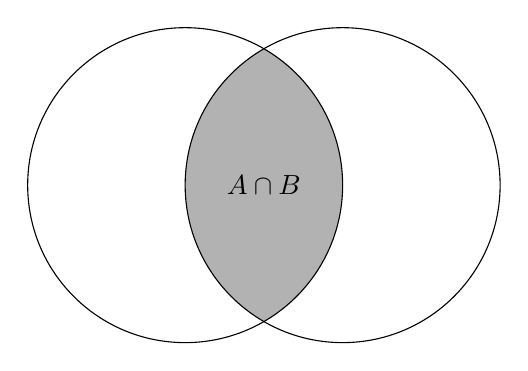
\begin{tikzpicture}
			\path[save path=\pathA](-1,0)circle(2cm);
			\path[save path=\pathB](1,0)circle(2cm);
			\begin{scope}
				\clip[use path=\pathA];
				\fill[black!30][use path=\pathB];
			\end{scope}
			\draw[use path=\pathA];
			\draw[use path=\pathB];
			\draw(0,0)node{\(A \cap B\)};
		\end{tikzpicture}
		\subcaption{集合的交}
	\end{subfigure}%
	\begin{subfigure}[b]{\subwidth}
		\centering
		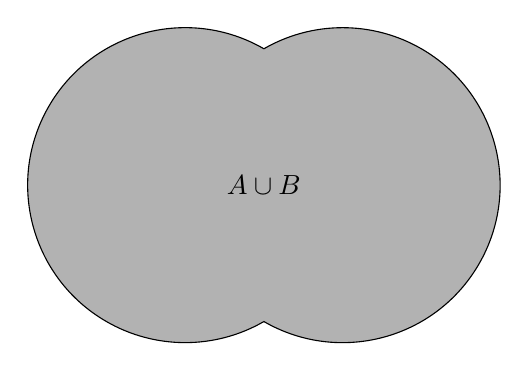
\begin{tikzpicture}
			\filldraw[fill=black!30,draw=black]
				(0,{sqrt(3)})arc[start angle=60,end angle=300,radius=2]
				arc[start angle=240,end angle=480,radius=2];
			\draw(0,0)node{\(A \cup B\)};
			\pgfresetboundingbox
			\path[use as bounding box] (-3,-2)rectangle(3,2);
		\end{tikzpicture}
		\subcaption{集合的并}
	\end{subfigure}%

	\begin{subfigure}[b]{\linewidth}
		\centering
		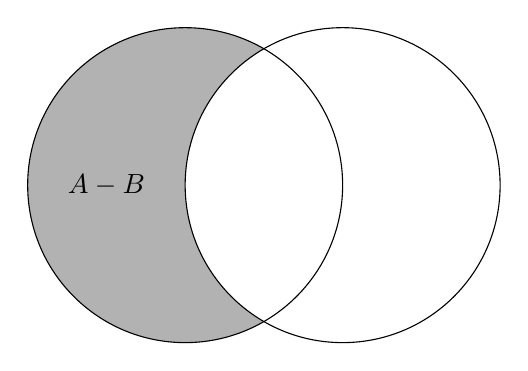
\begin{tikzpicture}
			\fill[black!30](0,{sqrt(3)})arc[start angle=60,end angle=300,radius=2]
				arc[start angle=240,end angle=120,radius=2];
			\draw(-1,0)circle(2cm);
			\draw(1,0)circle(2cm);
			\draw(-2,0)node{\(A-B\)};
			\pgfresetboundingbox
			\path[use as bounding box] (-3,-2)rectangle(3,2);
		\end{tikzpicture}
		\subcaption{集合的差}
	\end{subfigure}%
	\caption{韦恩图}
	\label{figure:集合论.韦恩图}
\end{figure}

\begin{property}
集合的运算满足以下性质:
\begin{enumerate}
\item 幂等律
\begin{gather}
	A \cap A = A, \\
	A \cup A = A.
\end{gather}

\item 交换律({\rm Commutative laws})
\begin{gather}
	A \cap B = B \cap A, \label{equation:集合论.集合代数公式1-1} \\
	A \cup B = B \cup A. \label{equation:集合论.集合代数公式1-2}
\end{gather}

\item 结合律({\rm Associative laws})
\begin{gather}
	(A \cap B) \cap C = A \cap (B \cap C), \label{equation:集合论.集合代数公式2-1} \\
	(A \cup B) \cup C = A \cup (B \cup C), \label{equation:集合论.集合代数公式2-2} \\
	%@see: 《测度论讲义(第三版)》(严加安) P4 习题 1.1.1 (1)
	(A \symdiff B) \symdiff C = A \symdiff (B \symdiff C).
\end{gather}

\item 分配律({\rm Distributive laws})
\begin{gather}
	(A \cap B) \cup C = (A \cup C) \cap (B \cup C), \label{equation:集合论.集合代数公式3-1} \\
	(A \cup B) \cap C = (A \cap C) \cup (B \cap C), \label{equation:集合论.集合代数公式3-2} \\
	A \cup \bigcap \mathscr{B} = \bigcap\Set{A \cup X \given X \in \mathscr{B}}, \quad(\mathscr{B}\neq\emptyset) \label{equation:集合论.集合代数公式3-3} \\
	A \cap \bigcup \mathscr{B} = \bigcup\Set{A \cap X \given X \in \mathscr{B}}, \label{equation:集合论.集合代数公式3-4} \\
	\Powerset (A \cup B) \supseteq \Powerset A \cup \Powerset B, \label{equation:集合论.集合代数公式3-5} \\ %@see: 《Elements of Set Theory》 P26 Exercise 7(b).
	\Powerset (A \cap B) = \Powerset A \cap \Powerset B, \label{equation:集合论.集合代数公式3-6} \\ %@see: 《Elements of Set Theory》 P26 Exercise 7(a)
	%@see: 《测度论讲义(第三版)》(严加安) P4 习题 1.1.1 (2)
	(A \symdiff B) \cap C = (A \cap C) \symdiff (B \cap C).
\end{gather}

%@see: https://mathworld.wolfram.com/deMorgansLaws.html
\item 对偶律({\rm De Morgan's laws})(假设\(\mathscr{A}\neq\emptyset\))
\begin{gather}
	\Omega - (A \cap B)
	= (\Omega - A) \cup (\Omega - B), \label{equation:集合论.集合代数公式4-1} \\
	\Omega - (A \cup B)
	= (\Omega - A) \cap (\Omega - B), \label{equation:集合论.集合代数公式4-2} \\
	\Omega - \bigcup\mathscr{A}
	= \bigcap\Set{\Omega - X \given X\in\mathscr{A}}, \label{equation:集合论.集合代数公式4-3} \\
	\Omega - \bigcap\mathscr{A}
	= \bigcup\Set{\Omega - X \given X\in\mathscr{A}}. \label{equation:集合论.集合代数公式4-4}
\end{gather}

\item 与空集\(\emptyset\)和全集\(\Omega\)的运算(假设\(A \subseteq \Omega\))
\begin{gather}
	A \cup \emptyset = A, \label{equation:集合论.集合代数公式5-1} \\
	A \cap \emptyset = \emptyset, \label{equation:集合论.集合代数公式5-2} \\
	A \cup \Omega = \Omega, \label{equation:集合论.集合代数公式5-3} \\
	A \cap \Omega = A, \label{equation:集合论.集合代数公式5-4} \\
	A \cup (\Omega - A) = \Omega, \label{equation:集合论.集合代数公式5-5} \\
	A \cap (\Omega - A) = \emptyset, \label{equation:集合论.集合代数公式5-6} \\
	A \cup (A \cap B) = A, \\
	A \cap (A \cup B) = A, \\
	\Omega - \emptyset = \Omega, \\
	\Omega - \Omega = \emptyset, \\
	\Omega - (\Omega - A) = A.
\end{gather}

\item 包含关系
\begin{gather}
	A \subseteq B \implies A \cup C \subseteq B \cup C, \label{equation:集合论.集合代数公式6-1} \\
	A \subseteq B \implies A \cap C \subseteq B \cap C, \label{equation:集合论.集合代数公式6-2} \\
	A \subseteq B \implies \bigcup A \subseteq \bigcup B, \label{equation:集合论.集合代数公式6-3} \\
	A \subseteq B \implies (\Omega - B) \subseteq (\Omega - A), \label{equation:集合论.集合代数公式6-4} \\
	\emptyset \neq A \subseteq B \implies \bigcap B \subseteq \bigcap A, \label{equation:集合论.集合代数公式6-5} \\
	A \cap B \subseteq A, \\
	A \subseteq A \cup B, \\
	%@see: 《测度论讲义(第三版)》(严加安) P4 习题 1.1.1 (3)
	(A \cup B) \symdiff (C \cup D) \subseteq (A \symdiff C) \cup (B \symdiff D).
\end{gather}

\item 差集
\begin{gather}
	A - B \subseteq A, \\
	B \subseteq \Omega
	\implies
	A - B = A \cap (\Omega - B), \\
	A \cup B = B
		\iff A \subseteq B
		\iff A \cap B = A
		\iff A - B = \emptyset, \label{equation:集合论.集合代数公式7-3} \\
	A \symdiff B = B \symdiff A, \\
	(A \symdiff B) \symdiff C = A \symdiff (B \symdiff C), \\
	A \symdiff \emptyset = A, \\
	A \symdiff A = \emptyset, \\
	A \symdiff B = A \symdiff C
		\iff B = C.
\end{gather}
\end{enumerate}
\begin{proof}
对\cref{equation:集合论.集合代数公式1-1} 证明如下:
\begin{align*}
	x \in A \cap B
	&\iff x \in A \land x \in B \\
	&\iff x \in B \land x \in A \\
	&\iff x \in B \cap A.
\end{align*}

对\cref{equation:集合论.集合代数公式1-2} 证明如下:
\begin{align*}
	x \in A \cup B
	&\iff x \in A \lor x \in B \\
	&\iff x \in B \lor x \in A \\
	&\iff x \in B \cup A.
\end{align*}

对\cref{equation:集合论.集合代数公式2-1} 证明如下:
\begin{align*}
	x \in (A \cap B) \cap C
	&\iff x \in A \cap B \land x \in C \\
	&\iff (x \in A \land x \in B) \land x \in C \\
	&\iff x \in A \land (x \in B \land x \in C) \\
	&\iff x \in A \land x \in B \cap C \\
	&\iff x \in A \cap (B \cap C).
\end{align*}

对\cref{equation:集合论.集合代数公式2-2} 证明如下:
\begin{align*}
	x \in (A \cup B) \cup C
	&\iff x \in A \cup B \lor x \in C \\
	&\iff (x \in A \lor x \in B) \lor x \in C \\
	&\iff x \in A \lor (x \in B \lor x \in C) \\
	&\iff x \in A \lor x \in B \cup C \\
	&\iff x \in A \cup (B \cup C).
\end{align*}

对\cref{equation:集合论.集合代数公式3-5} 证明如下:
\begin{align*}
	x \in \Powerset A \cup \Powerset B
	&\iff x \in \Powerset A \lor x \in \Powerset B \\
	&\iff x \subseteq A \lor x \subseteq B \\
	&\implies x \subseteq A \cup B \\
	&\iff x \in \Powerset (A \cup B),
\end{align*}
注意到中间步骤的\(\implies\)通常不是可逆的,
这是因为只要取\(a \subseteq A - B, b \subseteq B - A, x = a \cup b\),
就有\(x \subseteq A \cup B\)但是\(x \not\subseteq A \land x \not\subseteq B\),
因此\(x \subseteq A \cup B \notimplies x \subseteq A \lor x \subseteq B\).
%从上面的证明过程可以看出,
%要使\(\Powerset (A \cup B) = \Powerset A \cup \Powerset B\)成立,
%必有\begin{equation*}
%	\forall x \bigl(
%		x \subseteq A \cup B
%		\iff
%		x \subseteq A \lor x \subseteq B
%	\bigr)
%\end{equation*}成立.
%取\(x = A \cup B\),
%由\(x \subseteq A \lor x \subseteq B\)
%可得\begin{equation*}
%	A \cup B = A \lor A \cup B = B.
%\end{equation*}
%因此,当且仅当\(A \cup B \in \Set{A,B}\)时,
%就有\(\Powerset (A \cup B) = \Powerset A \cup \Powerset B\)成立.

对\cref{equation:集合论.集合代数公式3-6} 证明如下:
\begin{align*}
	x \in \Powerset (A \cap B)
	&\iff x \subseteq A \cap B \\
	&\iff x \subseteq A \land x \subseteq B \\
	&\iff x \in \Powerset A \land x \in \Powerset B \\
	&\iff x \in \Powerset A \cap \Powerset B.
\end{align*}

对\cref{equation:集合论.集合代数公式6-5} 证明如下:
\begin{align*}
	A \subseteq B
	&\iff (\forall t)[t \in A \implies t \in B] \\
	&\implies (\forall x)[
		(\forall b)[b \in B \implies x \in b]
		\implies
		(\forall a)[a \in A \implies x \in a]
	] \\
	&\iff (\forall x)[x \in \bigcap B \implies x \in \bigcap A].
	\qedhere
\end{align*}
\end{proof}
\end{property}

\begin{example}
%@see: 《Elements of Set Theory》 P32 Exercise 21.
设\(A,B\)是集合.
证明:\begin{equation}\label{equation:集合论.并集的并等于并的并集}
	\bigcup(A \cup B) = \bigcup A \cup \bigcup B.
\end{equation}
\begin{proof}
直接计算得
\begin{align*}
	x \in \bigcup(A \cup B)
	&\iff
	(\exists t)[t \in A \cup B \implies x \in t] \\
	&\iff
	(\exists t)[t \in A \lor t \in B \implies x \in t] \\
	&\iff
	(\exists t)[t \in A \implies x \in t] \lor (\exists t)[t \in B \implies x \in t] \\
	&\iff
	x \in \bigcup A \lor x \in \bigcup B \\
	&\iff
	x \in \bigcup A \cup \bigcup B.
	\qedhere
\end{align*}
\end{proof}
\end{example}

\begin{example}
%@see: 《Elements of Set Theory》 P32 Exercise 22.
设\(A,B\)是非空集合.
证明:\begin{equation}
	\bigcap(A \cup B) = \bigcap A \cap \bigcap B.
\end{equation}
%\begin{proof}
%直接计算得
%\begin{align*}
%	x \in \bigcap(A \cup B)
%	&\iff
%	x \in \bigcap A \land x \in \bigcap B \\
%	&\iff
%	x \in \bigcap A \cap \bigcap B.
%	\qedhere
%\end{align*}
%\end{proof}
\end{example}

\begin{example}
证明:\begin{equation}
	(A \cup B) - (A \cap B) = (A-B)\cup(B-A).
\end{equation}
\begin{proof}
根据集合交、并、差的定义,有
\begin{align*}
	x \in (A \cup B) - (A \cap B)
	&\iff x \in (A \cup B) \land x \notin (A \cap B) \\
	&\iff (x \in A \lor x \in B) \land \neg(x \in A \land x \in B) \\
	&\iff (x \in A \land \neg(x \in A \land x \in B))
	 \lor (x \in B \land \neg(x \in A \land x \in B)) \\
	&\iff (x \in A \land (x \notin A \lor x \notin B))
	 \lor (x \in B \land (x \notin A \lor x \notin B)) \\
	&\iff (x \in A \land x \notin B) \lor (x \in B \land x \notin A) \\
	&\iff x \in (A-B)\cup(B-A).
\qedhere
\end{align*}
\end{proof}
\end{example}


\chapter{关系和映射}
\section{关系}
\subsection{无序对,有序对}
\begin{definition}
由两个元素\(x_1\)和\(x_2\)组成的集合\begin{equation*}
\Set{x_1, x_2}
\end{equation*}称作\DefineConcept{无序对}(unordered pair).
\end{definition}

\begin{example}
%@see: 《Elements of Set Theory》 P38 Exercise 1.
定义:\begin{equation*}
	\opair{x,y,z}^* = \{\{x\},\{x,y\},\{x,y,z\}\}.
\end{equation*}
找出元素\(u,v,w,x,y,z\)使\begin{equation*}
	\opair{x,y,z}^* = \opair{u,v,w}^*
\end{equation*}成立,
但\(y \neq v\)或\(z \neq w\).
\begin{solution}
取\begin{equation*}
	\opair{1,1,2}^* = \{\{1\},\{1,1\},\{1,1,2\}\} = \{\{1\},\{1,2\}\},
\end{equation*}\begin{equation*}
	\opair{1,2,1}^* = \{\{1\},\{1,2\},\{1,2,1\}\} = \{\{1\},\{1,2\}\},
\end{equation*}
即可满足题设条件.
\end{solution}
\end{example}

\begin{definition}
两个元素\(x_1\)和\(x_2\)按一定顺序形成的排列称为\DefineConcept{有序对},
记作\begin{equation*}
	\opair{x_1,x_2}.
\end{equation*}

我们可以采用多种方式构造集合用于表记有序对\(\opair{x_1,x_2}\),
例如(由Norbert Wiener于1914年构造的)
\begin{equation*}
	\Set{ \Set{ \Set{x_1}, \emptyset }, \Set{ \Set{ x_2 } } }.
\end{equation*}
但我们更常用(由Kazimierz Kuratowski于1921年构造的)以下形式
\begin{equation*}
	\Set{ \Set{x_1}, \Set{x_1, x_2} }.
\end{equation*}
以后我们都采用第二种形式表记有序对,因此\begin{equation*}
	\opair{x_1,x_2}
	\defeq
	\Set{ \Set{x_1}, \Set{x_1, x_2} }.
\end{equation*}
\end{definition}

有序对具有以下性质.
\begin{property}\label{theorem:集合论.有序对的性质1}
%@see: 《Elements of Set Theory》 P36 Theorem 3A
\(\opair{u,v} = \opair{x,y}\)的充分必要条件是:\(u=x\)且\(v=y\).
\begin{proof}
充分性.
这个方向的证明是平凡的;
当\(u=x\)且\(v=y\)时,自然有\begin{equation*}
	\opair{u,v} = \opair{x,y}.
\end{equation*}

必要性.
当\(\opair{u,v} = \opair{x,y}\)时,根据定义有\begin{equation*}
	\Set{ \Set{u}, \Set{u, v} }
	= \Set{ \Set{x}, \Set{x, y} };
\end{equation*}于是\begin{equation*}
	\Set{u} \in \Set{ \Set{x}, \Set{x, y} },
	\eqno(1)
\end{equation*}且\begin{equation*}
	\Set{u,v} \in \Set{ \Set{x}, \Set{x, y} }.
	\eqno(2)
\end{equation*}
从(1)式我们知道,
要么等式\begin{equation*}
	\Set{u} = \Set{x}
	\eqno(3)
\end{equation*}成立,
要么等式\begin{equation*}
	\Set{u} = \Set{x,y}
	\eqno(4)
\end{equation*}成立;
从(2)式我们知道,
要么等式\begin{equation*}
	\Set{u,v} = \Set{x}
	\eqno(5)
\end{equation*}成立,
要么等式\begin{equation*}
	\Set{u,v} = \Set{x,y}
	\eqno(6)
\end{equation*}成立.

首先我们假设(4)式成立,那么有\(u = x = y\);
从而有(5)式等价于(6)式,且\(u = v = x = y\);
在这种情况下,必要性得证.
同理,假设(5)式成立,也可证明必要性.

然后我们假设(3)式、(6)式同时成立.
从(3)式成立我们知道\(u = x\).
从(6)式成立我们知道\(u = y\)或\(v = y\);
第一种情况,即\(u = x\)和\(u = y\)同时成立的情况,已经在(4)式成立时作了讨论.
第二种情况,即\(u = x\)和\(v = y\)同时成立的情况,立即保证了必要性.
\end{proof}
\end{property}
\cref{theorem:集合论.有序对的性质1} 让我们可以不含糊地将有序对\(\opair{x,y}\)
中的\(x\)和\(y\)分别称为%
有序对的\DefineConcept{第一坐标}(first coordinate)%
和\DefineConcept{第二坐标}(second coordinate).

%定义:
%\begin{equation*}
%	%TODO 需要找一个命名方法
%	\Set{ x \given (\exists u)(\exists v)[w=\opair{u,v} \land x \in u] },
%\end{equation*}\begin{equation*}
%	%TODO 需要找一个命名方法
%	\Set{ y \given (\exists u)(\exists v)[w=\opair{u,v} \land y \in v] }.
%\end{equation*}

\subsection{直积}
\begin{definition}\label{definition:集合论.直积}
设\(A,B\)都是集合.
在\(A\)中任取一个元素\(x\),
在\(B\)中任取一个元素\(y\),
组成一个有序对\(\opair{x,y}\),
把这样的有序对作为新的元素,
它们全体组成的类称为
“\(A\)与\(B\)的\DefineConcept{直积}(direct product)”,
或“\(A\)与\(B\)的\DefineConcept{笛卡尔乘积}(Cartesian product)”,
记为\(A \times B\),
即\begin{equation}
	A \times B
	\defeq
	\Set*{ \opair{x,y} \given x \in A \land y \in B }.
\end{equation}
%@see: https://mathworld.wolfram.com/DirectProduct.html
\end{definition}

在宣称\cref{definition:集合论.直积} 合法以前,
我们必须确认它给出的类\(A \times B\)是不是真的是一个集合.
而要证明\(A \times B\)是一个集合,
我们就必须找到一个足够大的集合,
它包括了我们需要的全部有序对,
然后利用子集公理证明\(A \times B\)是这个集合的子集.
为此我们给出下述引理.
\begin{lemma}\label{theorem:集合论.有序对是其坐标元素所在集合的二重幂集的元素}
%@see: 《Elements of Set Theory》 P37 Lemma 3B
如果\(x,y \in A\),那么\(\opair{x,y} \in \Powerset\Powerset A\).
\begin{proof}
由\(x,y \in A\)可知\(\{x\},\{x,y\} \subseteq A\),
即\(\{x\},\{x,y\} \in \Powerset A\),
那么\(\{\{x\},\{x,y\}\} \subseteq \Powerset A\),
进一步可得\(\opair{x,y} = \{\{x\},\{x,y\}\} \in \Powerset\Powerset A\).
\end{proof}
\end{lemma}

\begin{theorem}\label{theorem:集合论.直积存在定理}
%@see: 《Elements of Set Theory》 P38 Corollary 3C
设\(A,B\)都是集合,那么存在这样一个集合\(C\),使得\(C = A \times B\).
\begin{proof}
要使\(C = A \times B\),根据外延公理必有\begin{equation*}
	w \in C \iff w \in A \times B,
\end{equation*}
再根据直积的定义有\begin{equation*}
	w \in C \iff w = \opair{x,y} \land x \in A \land y \in B.
\end{equation*}
根据子集公理,我们可以构造集合\begin{equation*}
	C = \Set*{
		w \in \Powerset\Powerset(A \cup B)
		\given
		w = \opair{x,y} \land x \in A \land y \in B
	}.
\end{equation*}
显然,根据\cref{theorem:集合论.有序对是其坐标元素所在集合的二重幂集的元素},
\(C\)满足定理要求的条件.
\end{proof}
\end{theorem}
\cref{theorem:集合论.直积存在定理} 告诉我们,
任意两个集合\(A\)和\(B\)的直积\(A \times B\)也是集合.

容易发现,对于任意集合\(A\),总有\begin{equation}
	A \times \emptyset
	= \emptyset \times A
	= \emptyset \times \emptyset
	= \emptyset.
\end{equation}
这是因为\((\forall x)[x \notin \emptyset]\).

\begin{example}
设\(A,B,C\)是集合.
证明:\begin{equation}
	A \subseteq B
	\implies
	A \times C \subseteq B \times C.
\end{equation}
\begin{proof}
直接计算得
\begin{align*}
	A \subseteq B
	&\iff [x \in A \implies x \in B] \\
	&\implies [x \in A \land y \in C \implies x \in B \land y \in C] \\
	&\iff [\opair{x,y} \in A \times C \implies \opair{x,y} \in B \times C] \\
	&\iff [A \times C \subseteq B \times C].
	\qedhere
\end{align*}
\end{proof}
\end{example}

\begin{example}
%@see: 《Elements of Set Theory》 P38 Exercise 2.(a)
%@see: 《Elements of Set Theory》 P65 Exercise 54.
设\(A,B,C\)是集合.
证明:\begin{gather}
	A \times (B \cup C) = (A \times B) \cup (A \times C),
	\label{equation:集合论.直积分配律1} \\
	A \times (B \cap C) = (A \times B) \cap (A \times C),
	\label{equation:集合论.直积分配律2} \\
	A \times (B - C) = (A \times B) - (A \times C).
	\label{equation:集合论.直积分配律3}
\end{gather}
\begin{proof}
对\cref{equation:集合论.直积分配律1} 证明如下:
由于对于任意\(w = \opair{x,y}\)总有
\begin{align*}
	w \in A \times (B \cup C)
	&\iff x \in A \land y \in B \cup C \\
	&\iff x \in A \land (y \in B \lor y \in C) \\
	&\iff (x \in A \land y \in B) \lor (x \in A \land y \in C) \\
	&\iff (w \in A \times B) \lor (w \in A \times C),
\end{align*}
那么由外延公理可知\(A \times (B \cup C) = (A \times B) \cup (A \times C)\).

对\cref{equation:集合论.直积分配律2} 证明如下:
由于对于任意\(w = \opair{x,y}\)总有
\begin{align*}
	w \in A \times (B \cap C)
	&\iff x \in A \land y \in B \cap C \\
	&\iff x \in A \land (y \in B \land y \in C) \\
	&\iff (x \in A \land y \in B) \land (x \in A \land y \in C) \\
	&\iff (w \in A \times B) \land (w \in A \times C),
\end{align*}
那么由外延公理可知\(A \times (B \cap C) = (A \times B) \cap (A \times C)\).

对\cref{equation:集合论.直积分配律3} 证明如下:
由于对于任意\(w = \opair{x,y}\)总有
\begin{align*}
	w \in A \times (B - C)
	&\iff x \in A \land y \in (B - C) \\
	&\iff x \in A \land (y \in B \land y \notin C) \\
	&\iff (x \in A \land y \in B \land x \notin A)
		\lor (x \in A \land y \in B \land y \notin C) \\
	&\iff (x \in A \land y \in B) \land (x \notin A \lor y \notin C) \\
	&\iff (x \in A \land y \in B) \land \neg(x \in A \land y \in C) \\
	&\iff w \in A \times B \land w \notin A \times C,
\end{align*}
那么由外延公理可知\(A \times (B - C) = (A \times B) - (A \times C)\).
\end{proof}
\end{example}

\begin{example}
%@see: 《Elements of Set Theory》 P38 Exercise 2.(b)
证明:如果\(A \times B = A \times C\)且\(A \neq \emptyset\),则\(B = C\).
%TODO
\end{example}

\begin{example}
%@see: 《Elements of Set Theory》 P38 Exercise 3.
证明:\(A \times \bigcup B = \bigcup\Set{ A \times X \given X \in B }\).
%TODO
\end{example}

\begin{example}
%@see: 《Elements of Set Theory》 P38 Exercise 5.(a)
设\(A,B\)都是集合,试证:\(\Set{ \{x\} \times B \given x \in A }\)也是集合.
\begin{proof}
由于\(x \in A \implies \{x\} \subseteq A \implies \{x\} \times B \subseteq A \times B\),
所以我们可以利用子集公理构造集合\begin{equation*}
	\Set{ w \in A \times B \given w = \opair{u,v} \land u = x }.
	\qedhere
\end{equation*}
\end{proof}
\end{example}

\subsection{关系}
\begin{definition}
\DefineConcept{关系}(relation)是有序对的集合.
\end{definition}

如果有序对\(\opair{x,y}\)是关系\(\rel{R}\)的元素,即\begin{equation*}
	\opair{x,y} \in \rel{R},
\end{equation*}
那么称“\(x\)与\(y\)有\(\rel{R}\)关系”,
记作\(x\rel{R}y\);
反之,\begin{equation*}
	\opair{x,y} \notin \rel{R},
\end{equation*}
那么称“\(x\)与\(y\)没有\(\rel{R}\)关系”.

给定集合\(X\)和集合\(Y\),
如果关系\(\rel{R}\)满足\begin{equation*}
	\rel{R} \subseteq X \times Y,
\end{equation*}
我们就称“\(\rel{R}\)是\(X\)与\(Y\)之间的\DefineConcept{二元关系}(binary relation)”.
特别地,当\(X = Y\)时,就称“\(\rel{R}\)是\(X\)上的\DefineConcept{二元关系}”.

从关系的定义可以看出,关系是有序对的集合.
即便是看起来毫无意义的,只由一个有序对组成的集合,也可以看成是一个关系.
我们自然会认为有的关系比别的关系更有意义,
例如我们马上会提到的“映射”“等价关系”和“排序关系”.

\begin{definition}\label{definition:集合论.定义域与值域的定义}
设\(R\)是集合.

如果集合\(A\)满足\begin{equation*}
	x \in A \iff (\exists y)[\opair{x,y} \in R],
\end{equation*}
那么称\(A\)为“\(R\)的\DefineConcept{定义域}(domain)”,记作\(\dom R\).

如果集合\(B\)满足\begin{equation*}
	x \in B \iff (\exists t)[\opair{t,x} \in R],
\end{equation*}
那么称\(B\)为“\(R\)的\DefineConcept{值域}(range)”,记作\(\ran R\).

最后,我们把\(R\)的定义域与它的值域的并集称为
“\(R\)的\DefineConcept{域}(field)”,记作\(\fld R\),即\begin{equation*}
	\fld R \defeq \dom R \cup \ran R.
\end{equation*}
\end{definition}

为了正当化\cref{definition:集合论.定义域与值域的定义},
我们必须明确:对于任意集合\(R\),存在这样一个集合,
\(R\)中的有序对的第一坐标和第二坐标都是这个集合的元素.
这个问题类似于我们之前对于直积\(A \times B\)的定义的正当化,
当时我们证明了\cref{theorem:集合论.直积存在定理}.
为此,我们给出下述引理,
可以注意到它与\cref{theorem:集合论.有序对是其坐标元素所在集合的二重幂集的元素} 的关联.

\begin{lemma}
%@see: 《Elements of Set Theory》 P41 Lemma 3D
如果\(\opair{x,y} \in A\),那么\(x,y \in \bigcup\bigcup A\).
\end{lemma}
这条引理已经在\cref{example:集合论.有序对各坐标的取值范围} 得到证明.
利用这条引理,再加上子集公理,我们可以构造集合\(R\)的定义域和值域:
\begin{gather}
	\dom R
	\defeq
	\Set*{ x \in \bigcup\bigcup R \given (\exists y)[\opair{x,y} \in R] }, \\
	\ran R
	\defeq
	\Set*{ x \in \bigcup\bigcup R \given (\exists t)[\opair{t,x} \in R] }.
\end{gather}

\begin{example}
%@see: 《Elements of Set Theory》 P41 Exercise 6.
试证:集合\(A\)是一个关系的充分必要条件是\begin{equation*}
	A \subseteq \dom A \times \ran A.
\end{equation*}
%TODO
\end{example}

\begin{example}
%@see: 《Elements of Set Theory》 P41 Exercise 7.
试证:给定关系\(\rel{R}\),总有\begin{equation*}
	\fld \rel{R} = \bigcup\bigcup \rel{R}.
\end{equation*}
%TODO
\end{example}

\begin{example}
%@see: 《Elements of Set Theory》 P41 Exercise 8.
试证:对于任意集合\(A\),总有\begin{gather}
	\dom\bigcup A = \bigcup\Set{ \dom\rel{R} \given \rel{R} \in A }, \\
	\ran\bigcup A = \bigcup\Set{ \ran\rel{R} \given \rel{R} \in A }.
\end{gather}
%TODO
\end{example}

\subsection{多元关系}
我们可以将“有序对”和“二元关系”的概念分别扩展为“元组”和“多元关系”.

例如定义\begin{equation*}
	\opair{x_1,x_2,x_3}
	\defeq
	\opair{\opair{x_1,x_2},x_3},
\end{equation*}
称之为\DefineConcept{三元组}(triple);
定义\begin{equation*}
	\opair{x_1,x_2,x_3,x_4}
	\defeq
	\opair{\opair{x_1,x_2,x_3},x_4},
\end{equation*}
称之为\DefineConcept{四元组}(quadruple);
定义\begin{equation*}
	\opair{x_1,x_2,x_3,x_4,x_5}
	\defeq
	\opair{\opair{x_1,x_2,x_3,x_4},x_5},
\end{equation*}
称之为\DefineConcept{五元组}(quintuple);
以此类推,对于任意给定\(n\),可以定义\(n\)元组(\(n\)-tuple):\begin{equation*}
	\opair{x_1,x_2,\dotsc,x_n}
	\defeq
	\opair{\opair{x_1,x_2,\dotsc,x_{n-1}},x_n}.
\end{equation*}
为了让我们的定义看起来整齐划一,我们还可以补充定义\begin{equation*}
	\opair{x} \defeq x,
\end{equation*}
称之为\DefineConcept{一元组}(1-tuple).

我们把“在\(A\)上的\(n\)元\DefineConcept{关系}(n-ary \emph{relation} on \(A\))”
定义为由\(n\)元组构成的集合.
由于\(A\)上的二元关系是\(A \times A\)的子集,
以及\(A\)上的三元关系(ternary relation, 3-ary relation)是\((A \times A) \times A\)的子集,
所以三元关系也可归结为一种二元关系;
同理,其他\(n\)元关系,只要\(n>1\),也都可以归结为二元关系.
虽然在上面对\(n\)元关系的定义中,
我们也把由\(A\)中包括的一元组构成的集合称为
“\(A\)上的一元关系(unary relation, 1-ary relation)”,
但它只是\(A\)的一个子集,根本不满足关系的定义.

\section{映射}
\subsection{映射的概念}
\begin{definition}
%@see: 《Elements of Set Theory》 P42 Definition
设\(F\)是关系,如果\[
	(\forall x \in \dom F)(\exists! y)[\opair{x,y} \in F],
\]
则称“关系\(F\)是一个\DefineConcept{映射}(function)”.
\end{definition}
可以从映射的定义中看出,虽然映射也是关系,
但映射有一般的关系所没有的特殊性质:
映射是\DefineConcept{单值的}(single-valued).
换句话说,对于关系\(F\),每个\(x\)可能对应若干个\(y\);
但是,对于映射\(F\),每个\(x\)就只对应一个\(y\).
我们可以把\(x\)与\(y\)这两个元素之间的对应关系记为\(x \mapsto y\).

我们把使得\(xFy\)成立的\(y\)称为“\(x\)(在映射\(F\)下)的\DefineConcept{像}%
(the \emph{value} of \(F\) at \(x\))”,
记为\(F(x)\),即\[
	y = f(x);
\]
称\(x\)为“\(y\)(在映射\(F\)下)的一个\DefineConcept{原像}”.
这里用的\(F(x)\)符号是欧拉提出的,
我们仅当\(F\)是一个映射且\(x\in\dom F\)时使用这个记号.
不过,我们也可以定义:\[
	F(x) \defeq \bigcup\Set{ y \given \opair{x,y} \in F }.
\]
它对于任意\(F\)和\(x\)都有意义.

映射是如此重要,以至于各家对用于描述映射的术语没有达成统一.
以下是两种最常采用的术语.

设\(X,Y\)都是集合,
如果\(f\)是一个映射,且\(\dom f = X\),\(\ran f \subseteq Y\),
则称“\(f\)是从\(X\)到\(Y\)的\DefineConcept{映射}%
(\(f\) is a function \emph{from} \(X\) \emph{into} \(Y\))”,
或称“\(f\)将\(X\)映射到\(Y\)里%
(\(f\) \emph{maps} \(X\) \emph{into} \(Y\))”,
记作\[
	f\colon X \to Y.
\]
如果还有\(\ran f = Y\),
那么称“\(f\)是从\(X\)到\(Y\)上的映射%
(\(f\) is a function from \(X\) \emph{onto} \(Y\))”,
或称“\(f\)将\(X\)映射到\(Y\)上%
(\(f\) \emph{maps} \(X\) \emph{onto} \(Y\))”,
或称“\(f\)是\DefineConcept{满射}(surjective)”.
我们把集合\(Y\)称为“映射\(f\)的\DefineConcept{陪域}(codomain)”.
我们可以说“任意映射总将它的定义域映射到它的值域上”,
还可以说“任意映射总把它的定义域映射到以它的值域为子集的任意集合\(Y\)里”.
注意到两种说法的区别,“上”字和“里”字的选用,
不光取决于映射\(f\)本身,还取决于我们讨论的陪域\(Y\).

如果\[
	(\forall y \in \ran f)
	(\exists! x)
	[\opair{x,y} \in f],
\]
那么称“映射\(f\)是\DefineConcept{一对一的}(one-to-one)”.

有时候我们希望把“一对一的”这个概念套用到一般的关系上,
它们往往不是映射,因此我们类比于“单值的”,创造出“单根的”这个概念.
\begin{definition}
%@see: 《Elements of Set Theory》 P43 Definition
如果集合\(R\)满足\[
	(\forall y \in \ran R)
	(\exists! x)
	[\opair{x,y} \in R],
\]
则称“\(R\)是\DefineConcept{单根的}(single-rooted)”.
\end{definition}

因此,我们可以说,“一个映射是单根的”当且仅当“这个映射是一对一的”.

如果\[
	(\forall x_1, x_2 \in \dom f)
	[x_1 \neq x_2 \implies f(x_1) \neq f(x_2)],
\]
那么称“\(f\)是\DefineConcept{单射}(injective)”.

由于映射本就是单值的,若它还是单根的,那么这个映射就是单射.
换句话说,“一对一的映射”和“单射”是相同的概念.

如果\(f\)既是单射,又是满射,
那么称“\(f\)是\DefineConcept{双射}(bijective)
或\DefineConcept{一一映射}”.

我们可以给出一个最平凡的一一映射.
\begin{definition}
设\(X\)是集合.
我们把\[
	\Set{ \opair{x,x} \given x \in X }
\]称为“(\(X\)上的)\DefineConcept{恒等映射}或\DefineConcept{恒同映射}”,
常记为\(i_X\).
\end{definition}

\begin{definition}
设\(F\)是映射,
集合\(D \subseteq \dom F\),
\(C \in \ran F\).
\begin{itemize}
	\item 如果\[
		(\forall x \in D)[F(x) = C],
	\]
	则称“\(F\)在\(D\)上\DefineConcept{恒等于}~\(C\)”,
	记作\(F(x) \equiv C\ (x \in D)\);
	当\(D=\dom F\)时,
	称“\(F\)~\DefineConcept{恒等于}~\(C\)”,
	记为\(F(x) \equiv C\).
	\item 如果\[
		(\exists x \in D)[F(x) \neq C],
	\]
	则称“\(F\)在\(D\)上\DefineConcept{不恒等于}~\(C\)”,
	记作\(F(x) \not\equiv C\ (x \in D)\);
	当\(D=\dom F\)时,
	称“\(F\)~\DefineConcept{不恒等于}~\(C\)”,
	记为\(F(x) \not\equiv C\).
	\item 如果\[
		(\forall x \in D)[F(x) \neq C],
	\]
	则称“\(F\)在\(D\)上\DefineConcept{恒不等于}~\(C\)”,
	记作\(F(x) \neq C\ (x \in D)\);
	当\(D=\dom F\)时,
	称“\(F\)~\DefineConcept{恒不等于}~\(C\)”,
	记为\(F(x) \neq C\).
\end{itemize}
\end{definition}

\begin{example}
%@see: 《Elements of Set Theory》 P52 Exercise 11
设\(F,G\)都是映射,
\(\dom F = \dom G = X\),且\[
	(\forall x \in X)[F(x) = G(x)].
\]
证明:\(F=G\).
\begin{proof}
显然有
\begin{align*}
	F=G
	&\iff (\forall x \in X)(\exists!y)[
		\opair{x,y} \in F
		\iff
		\opair{x,y} \in G
	] \\
	&\iff (\forall x \in X)(\exists!y)[
		y = F(x) = G(x)
	] \\
	&\iff (\forall x \in X)[F(x) = G(x)].
	\qedhere
\end{align*}
\end{proof}
\end{example}

\begin{example}
%@see: 《Elements of Set Theory》 P52 Exercise 12
设\(f,g\)都是映射.
证明:\[
	f \subseteq g
	\iff
	\dom f \subseteq \dom g
	\land
	(\forall x \in \dom f)
	[f(x) = g(x)].
\]
\begin{proof}
直接有
\begin{align*}
	f \subseteq g
	&\iff (\forall x)(\exists!y)[\opair{x,y} \in f \implies \opair{x,y} \in g] \\
	&\iff (\forall x \in \dom f)[x \in \dom g]\land(\forall x \in \dom f)(\exists!y)[y=f(x)=g(x)] \\
	&\iff [\dom f \subseteq \dom g]\land(\forall x \in \dom f)[f(x)=g(x)].
	\qedhere
\end{align*}
\end{proof}
\end{example}

\begin{example}
%@see: 《Elements of Set Theory》 P53 Exercise 13
设\(f,g\)都是映射,\(f \subseteq g\)且\(\dom g \subseteq \dom f\).
证明:\(f=g\).
%TODO
\end{example}

\begin{example}
%@see: 《Elements of Set Theory》 P53 Exercise 14
设\(f,g\)都是映射.
证明:
\begin{enumerate}
	\item \(f \cap g\)是映射.
	\item \(f \cup g\)是映射的充分必要条件是\[
		(\forall x \in (\dom f)\cap(\dom g))[f(x)=g(x)].
	\]
\end{enumerate}
%TODO
\end{example}

\begin{example}
%@see: 《Elements of Set Theory》 P53 Exercise 15
\def\A{\mathscr{A}}%
设\(\A\)是一组映射,且\[
	(\forall f,g\in\A)[f \subseteq g \lor g \subseteq f].
\]
证明:\(\bigcup\A\)也是映射.
%TODO
\end{example}

\begin{example}
%@see: 《Elements of Set Theory》 P53 Exercise 16
证明:不存在一个集合,使得每个映射都属于它.
%TODO
\end{example}

\begin{example}
%@see: 《实变函数论(第三版)》(周民强) P14 思考题5.
设\(f\colon X \to Y,
g\colon Y \to X\).
证明:若\[
	(\forall x \in X)[g(f(x)) = x],
\]
则\(f\)是单射,\(g\)是满射.
%TODO
\end{example}

\subsection{逆,复合,限制,像,原像}
以下定义的操作通常用在映射上,有时候也用于关系,但也可以用于任意集合.
\begin{definition}\label{definition:映射.逆-复合-限制-像}
设\(A,F,G\)都是集合.
\begin{itemize}
	\item 称集合\[
		\Set*{ \opair{u,v} \given \opair{v,u} \in F }
	\]为“\(F\)的\DefineConcept{逆}%
	(the \emph{inverse} of \(F\))”,
	记作\(F^{-1}\).

	特别地,如果\(F^{-1}\)是映射,
	则称“\(F^{-1}\)是\(F\)的\DefineConcept{逆映射}”.

	\item 称集合\[
		\Set*{ \opair{u,v} \given (\exists t)[\opair{u,t} \in G \land \opair{t,v} \in F] }
	\]为“\(F\)和\(G\)的\DefineConcept{复合}%
	(the \emph{composition} of \(F\) and \(G\))”,
	记作\(F \circ G\).

	\item 称集合\[
		\Set*{ \opair{u,v} \given \opair{u,v} \in F \land u \in A }
	\]为“\(F\)在\(A\)上的\DefineConcept{限制}%
	(the \emph{restriction} of \(F\) to \(A\))”,
	记作\(F \setrestrict A\).
	%\cref{definition:子空间.拓扑子空间中的集族的限制}

	\item 称集合\[
		\Set*{ v \given (\exists u \in A)[\opair{u,v} \in F] }
	\]为“\(A\)在\(F\)下的\DefineConcept{像}%
	(the \emph{image} of \(A\) \emph{under} \(F\))”,
	记作\(F\ImageOfSetUnderRelation{A}\).
\end{itemize}
\end{definition}

当\(F\)是一个映射,且\(A \subseteq \dom F\)时,
\(F\ImageOfSetUnderRelation{A}\)这个概念可能更容易理解,
因为这时候\[
	F\ImageOfSetUnderRelation{A}
	= \Set{ F(u) \given u \in A }.
\]

我们可以利用子集公理构造出上述定义下的所需集合的存在性.
特别地,\[
	F^{-1} \subseteq \ran F \times \dom F, \qquad
	F \circ G \subseteq \dom G \times \ran F,
\]\[
	F \setrestrict A \subseteq F, \qquad
	F\ImageOfSetUnderRelation{A} \subseteq \ran F.
\]

例如,我们可以按如下方法正当化“关系\(F\)的逆”的定义:
根据子集公理,存在集合\(B\),使得对于任意\(x\),总有\begin{align*}
	x \in B
	&\iff
	[x \in \ran F \times \dom F]
	\land
	(\exists u)(\exists v)[x = \opair{u,v} \land \opair{v,u} \in F], \\
	&\iff
	(\exists u)(\exists v)[x = \opair{u,v} \land \opair{v,u} \in F].
\end{align*}
再根据外延公理,可以保证集合\(B\)的唯一性.
因此我们可以将集合\(B\)记为\(F^{-1}\).

\begin{definition}
%@see: 《点集拓扑讲义(第四版)》(熊金城) P22 定义1.5.4
设\(A,B,X\)都是集合,\(A \subset B\).
若映射\(F\colon A \to X\)和\(G\colon B \to X\)满足\(F \subset G\),
则称“\(G\)是\(F\)在\(B\)上的\DefineConcept{扩张}”.
\end{definition}

\begin{theorem}
\(F \setrestrict \emptyset = \emptyset\).
\end{theorem}

\begin{theorem}
\(F\ImageOfSetUnderRelation{A} = \ran(F \setrestrict A)\).
\begin{proof}
根据值域的定义有\begin{align*}
	v \in \ran(F \setrestrict A)
	&\iff
	(\exists u)[\opair{u,v} \in F \setrestrict A] \\
	&\iff
	(\exists u)[\opair{u,v} \in F \land u \in A] \\
	&\iff
	v \in F\ImageOfSetUnderRelation{A}.
	\qedhere
\end{align*}
\end{proof}
\end{theorem}

\begin{example}
%@see: 《Elements of Set Theory》 P53 Exercise 18.
设\[
	R = \Set{
		\opair{0,1},
		\opair{0,2},
		\opair{0,3},
		\opair{1,2},
		\opair{1,3},
		\opair{2,3}
	}.
\]
计算\(R \circ R,
R \setrestrict \{1\},
R^{-1} \setrestrict \{1\},
R\ImageOfSetUnderRelation{\{1\}},
R^{-1}\ImageOfSetUnderRelation{\{1\}}\).
\begin{solution}
由题意有\begin{gather*}
	R \circ R
	= \Set{
		\opair{0,2},
		\opair{0,3},
		\opair{1,3}
	}, \\
	R \setrestrict \{1\}
	= \Set{
		\opair{1,2},
		\opair{1,3}
	}, \\
	R^{-1} \setrestrict \{1\}
	= \Set{
		\opair{1,0}
	}, \\
	R\ImageOfSetUnderRelation{\{1\}}
	= \Set{
		2,
		3
	}, \\
	R^{-1}\ImageOfSetUnderRelation{\{1\}}
	= \Set{
		0
	}.
\end{gather*}
\end{solution}
\end{example}

\begin{definition}
设\(F\)是关系,\(A\)是集合,那么称集合\[
	\Set*{ x \in \dom F \given F(x) \in A }
\]为“集合\(A\)在关系\(F\)下的\DefineConcept{原像}%
(the \emph{inverse image} of \(A\) under \(F\))”,
记作\(F^{-1}\ImageOfSetUnderRelation{A}\).
\end{definition}

一般来说,一个映射的逆不一定是映射.
例如,\(F=\Set{ \opair{1,1},\opair{2,1} }\)是一个映射,
但它的逆\(F^{-1}=\Set{ \opair{1,1},\opair{1,2} }\)不是映射.

\begin{theorem}\label{theorem:集合论.关系的逆的定义域值域以及关系的二重逆}
%@see: 《Elements of Set Theory》 P46 Theorem 3E
设\(F\)是集合,则有\begin{gather}
	\dom F^{-1} = \ran F, \\
	\ran F^{-1} = \dom F.
\end{gather}

如果\(F\)是关系,则有\begin{equation}
	(F^{-1})^{-1} = F.
\end{equation}
\begin{proof}
因为\[
	y \in \dom F^{-1}
	\iff
	(\exists x)[yF^{-1}x]
	\iff
	(\exists x)[xFy]
	\iff
	y \in \ran F,
\]
所以\(\dom F^{-1} = \ran F\).

因为\[
	x \in \ran F^{-1}
	\iff
	(\exists y)[yF^{-1}x]
	\iff
	(\exists y)[xFy]
	\iff
	x \in \dom F,
\]
所以\(\ran F^{-1} = \dom F\).

因为\[
	\opair{x,y} \in (F^{-1})^{-1}
	\iff
	\opair{y,x} \in F^{-1}
	\iff
	\opair{x,y} \in F,
\]
所以\((F^{-1})^{-1} = F\).
\end{proof}
\end{theorem}

\begin{theorem}\label{theorem:集合论.关系及其逆是映射的充分必要条件}
%@see: 《Elements of Set Theory》 P46 Theorem 3F
设\(F\)是集合,则“\(F^{-1}\)是映射”的充分必要条件是:\(F\)是单根的.

设\(F\)是关系,则“\(F\)是映射”的充分必要条件是:\(F^{-1}\)是单根的.
\begin{proof}
容易看出\begin{align*}
	\text{\(F^{-1}\)是映射}
	&\iff
	\text{\(F^{-1}\)是单值的} \\
	&\iff
	(\forall x \in \dom F^{-1})(\exists! y)[xF^{-1}y] \\
	&\iff
	(\forall x \in \ran F)(\exists! y)[yFx] \\
	&\iff
	\text{\(F\)是单根的}, \\
	\text{\(F\)是映射}
	&\iff
	\text{\(F\)是单值的} \\
	&\iff
	(\forall x \in \dom F)(\exists! y)[xFy] \\
	&\iff
	(\forall x \in \ran F^{-1})(\exists! y)[yF^{-1}x] \\
	&\iff
	\text{\(F^{-1}\)是单根的}.
	\qedhere
\end{align*}
\end{proof}
\end{theorem}

\begin{theorem}\label{theorem:集合论.逆映射的计算}
%@see: 《Elements of Set Theory》 P46 Theorem 3G
设\(F\)是单射.
\begin{enumerate}
	\item 如果\(x \in \dom F\),那么\[
		F^{-1}(F(x)) = x.
	\]

	\item 如果\(y \in \ran F\),那么\[
		F(F^{-1}(y)) = y.
	\]
\end{enumerate}
\begin{proof}
假设\(x \in \dom F\),
那么\(\opair{x,F(x)} \in F\),且\(\opair{F(x),x} \in F^{-1}\),
于是\(F(x) \in \dom F^{-1}\).
因为\(F\)是单射,是单根的,
所以由\cref{theorem:集合论.关系及其逆是映射的充分必要条件}
可知\(F^{-1}\)是映射,
从而\(x = F^{-1}(F(x))\).

如果\(y \in \ran F\),
那么根据本定理第1条,以及\((F^{-1})^{-1} = F\),可知\[
	F(F^{-1}(y)) = (F^{-1})^{-1}(F^{-1}(y)) = y.
	\qedhere
\]
\end{proof}
\end{theorem}

\begin{theorem}\label{theorem:集合论.映射的复合也是映射}
%@see: 《Elements of Set Theory》 P47 Theorem 3H
设\(F,G\)都是映射,则\(F \circ G\)是映射,且\[
	\dom(F \circ G)
	= \Set*{ x \in \dom G \given G(x) \in \dom F },
\]\[
	(\forall x \in \dom(F \circ G))
	[(F \circ G)(x) = F(G(x))].
\]
\begin{proof}
要证\(F \circ G\)是一个映射,
假设有\(\opair{x,y} \in F \circ G\)和\(\opair{x,z} \in F \circ G\)同时成立.
那么,\[
	(\exists p)[\opair{x,p} \in G \land \opair{p,y} \in F]
	\quad\text{和}\quad
	(\exists q)[\opair{x,q} \in G \land \opair{q,z} \in F]
\]同时成立.
既然\(G\)是映射,必有\(p = q\).
同理,\(F\)是映射,必有\(y = z\).
因此\(F \circ G\)是映射.

现在再假设\(x \in \dom G\)且\(G(x) \in \dom F\).
我们必须证明\[
	x \in \dom(F \circ G)
	\quad\text{和}\quad
	(F \circ G)(x) = F(G(x)).
\]
我们知道\[
	\opair{x,G(x)} \in G,
	\qquad
	\opair{G(x),F(G(x))} \in F.
\]
因此\(\opair{x,F(G(x))} \in F \circ G\).

反过来说,如果\(x \in \dom(F \circ G)\),
那么就有\[
	(\exists y)(\exists t)
	[\opair{x,t} \in G \land \opair{t,y} \in F].
\]
于是就有\(x \in \dom G\)和\(t = G(x) \in \dom F\).
\end{proof}
\end{theorem}

容易看出,映射的复合是有顺序的,
\(f \circ g\)有意义并不代表\(g \circ f\)也有意义.
即便两者都有意义,它们也未必相同.

\begin{example}
%@see: 《Elements of Set Theory》 P47 Example
假设\(G\)是单射,
那么,根据\cref{theorem:集合论.映射的复合也是映射},
\(G^{-1} \circ G\)也是一个映射,
它的定义域为\[
	\Set{ x \in \dom G \given G(x) \in \dom G^{-1} }
	= \dom G,
\]
并且,对于\(\forall x \in \dom(G^{-1} \circ G)\),
有\begin{align*}
	(G^{-1} \circ G)(x) &= G^{-1}(G(x)) \\
	&= x. \tag{\cref{theorem:集合论.逆映射的计算}}
\end{align*}
因此,\(G^{-1} \circ G\)就是\(I_{\dom G}\),
\(\dom G\)上的恒等映射.
同理,\(G \circ G^{-1}\)是\(I_{\ran G}\),
\(\ran G\)上的恒等映射.
\end{example}

\begin{theorem}
%@see: 《Elements of Set Theory》 P65 Exercise 53.
设\(R,S\)是集合,那么\begin{gather}
	(R \cup S)^{-1} = R^{-1} \cup S^{-1},
	\label{equation:集合论.并的逆等于逆的并} \\
	(R \cap S)^{-1} = R^{-1} \cap S^{-1},
	\label{equation:集合论.交的逆等于逆的交} \\
	(R - S)^{-1} = R^{-1} - S^{-1}.
	\label{equation:集合论.差的逆等于逆的差}
\end{gather}
\begin{proof}
对\cref{equation:集合论.并的逆等于逆的并} 证明如下:
\begin{align*}
	\opair{x,y} \in (R \cup S)^{-1}
	&\iff \opair{y,x} \in R \cup S \\
	&\iff \opair{y,x} \in R \lor \opair{y,x} \in S \\
	&\iff \opair{x,y} \in R^{-1} \lor \opair{x,y} \in S^{-1} \\
	&\iff \opair{x,y} \in R^{-1} \cup S^{-1}.
\end{align*}

对\cref{equation:集合论.交的逆等于逆的交} 证明如下:
\begin{align*}
	\opair{x,y} \in (R \cap S)^{-1}
	&\iff \opair{y,x} \in R \cap S \\
	&\iff \opair{y,x} \in R \land \opair{y,x} \in S \\
	&\iff \opair{x,y} \in R^{-1} \land \opair{x,y} \in S^{-1} \\
	&\iff \opair{x,y} \in R^{-1} \cap S^{-1}.
\end{align*}

对\cref{equation:集合论.差的逆等于逆的差} 证明如下:
\begin{align*}
	\opair{x,y} \in (R - S)^{-1}
	&\iff \opair{y,x} \in R - S \\
	&\iff \opair{y,x} \in R \land \opair{y,x} \notin S \\
	&\iff \opair{x,y} \in R^{-1} \land \opair{x,y} \notin S^{-1} \\
	&\iff \opair{x,y} \in R^{-1} - S^{-1}.
	\qedhere
\end{align*}
\end{proof}
\end{theorem}

\begin{theorem}\label{theorem:集合论.复合的逆}
%@see: 《Elements of Set Theory》 P47 Theorem 3I
设\(F,G\)都是集合,那么\[
	(F \circ G)^{-1} = G^{-1} \circ F^{-1}.
\]
\begin{proof}
易知\((F \circ G)^{-1}\)和\(G^{-1} \circ F^{-1}\)都是关系,且\begin{align*}
	\opair{x,y} \in (F \circ G)^{-1}
	&\iff
	\opair{y,x} \in F \circ G \\
	&\iff
	(\exists t)[\opair{y,t} \in G \land \opair{t,x} \in F] \\
	&\iff
	(\exists t)[\opair{x,t} \in F^{-1} \land \opair{t,y} \in G^{-1}] \\
	&\iff
	\opair{x,y} \in G^{-1} \circ F^{-1}.
	\qedhere
\end{align*}
\end{proof}
\end{theorem}

由\cref{theorem:集合论.复合的逆} 立即可得如下推论.
\begin{proposition}\label{theorem:集合论.复合的逆.推论1}
设\(F\)是集合,那么\[
	(F^{-1} \circ F)^{-1} = F^{-1} \circ F.
\]
\end{proposition}

\begin{axiom}[选择公理(第一种形式)]
%@see: 《Elements of Set Theory》 P49 Axiom of Choice (first form)
对于任意关系\(R\),存在映射\(H\),满足\[
	H \subseteq R,
	\quad\text{且}\quad
	\dom H = \dom R.
\]
\end{axiom}

\begin{theorem}
%@see: 《Elements of Set Theory》 P48 Theorem 3J
设映射\(F\colon A \to B\),其中\(A\)是非空集合.
\begin{enumerate}
	\item “存在映射\(G\colon B \to A\)(称其为\DefineConcept{左逆}),
	使得\(G \circ F\)是\(A\)上的恒等映射\(I_A\)”是“\(F\)是单射”的充分必要条件.

	\item “存在映射\(H\colon B \to A\)(称其为\DefineConcept{右逆}),
	使得\(F \circ H\)是\(B\)上的恒等映射\(I_B\)”是“\(F\)是满射”的充分必要条件.
\end{enumerate}
\begin{proof}
\begin{enumerate}
	\item
	先证充分性.
	我们假设存在映射\(G\)使得\(G \circ F = I_A\).
	如果\(F(x) = F(y)\),那么\[
		x = G(F(x)) = G(F(y)) = y,
	\]
	于是\(F\)是单射.

	再证必要性.
	假设\(F\)是单射,
	那么根据\cref{theorem:集合论.关系的逆的定义域值域以及关系的二重逆,theorem:集合论.关系及其逆是映射的充分必要条件},
	\(F^{-1}\)是一个从\(\ran F\)到\(A\)上的映射.
	现在我们需要将\(F^{-1}\)延拓为以\(B\)为定义域的映射\(G\).
	因为\(A\)是非空集合,
	于是我们可以取定\(a \in A\),
	然后令\[
		G(x) = \left\{ \begin{array}{ll}
			F^{-1}(x), & x \in \ran F, \\
			a, & x \in B - \ran F,
		\end{array} \right.
	\]或者令\[
		G = F^{-1} \cup (B - \ran F) \times \Set{a}.
	\]
	这个构造出来的映射\(G\)是一个从\(B\)到\(A\)里的映射,
	且满足\[
		\dom(G \circ F) = A,
	\]
	以及\[
		(\forall x \in A)[G(F(x)) = F^{-1}(F(x)) = x],
	\]
	于是\(G \circ F = I_A\)成立.

	\item
	我们还是先证充分性.
	假设存在映射\(H\)使得\(F \circ H = I_B\).
	那么\[
		(\forall y \in B)[y = F(H(y))],
	\]
	从而\(y \in \ran F\),
	于是\(\ran F = B\).

	必要性的证明稍显困难.
	我们不能直接取\(H = F^{-1}\),
	因为一般而言\(F\)不会是单射,
	\(F^{-1}\)也不会是一个映射.
	假设\(F\)将\(A\)映射到\(B\)上,\(\ran F = B\).
	现在我们需要为每个\(y \in B\)选择某个\(x\),使得\(F(x) = y\),然后令\(H(y) = x\);
	考虑到\(y \in \ran F\),这样的\(x\)必定存在.
	虽然我们知道对于每个\(y\),存在一个合适的\(x\),
	但是我们无法据此构造所求映射\(H\).
	因此,我们需要引入选择公理.
	借助选择公理,我们可以令映射\(H\)满足\(H \subseteq F^{-1}\)且\(\dom H = \dom F^{-1} = B\).
	于是\(H\)满足\[
		(\forall y \in B)
		[
			\opair{y,H(y)} \in F^{-1}
			\iff
			\opair{H(y),y} \in F
			\iff
			F(H(y)) = y
		].
		\qedhere
	\]
\end{enumerate}
\end{proof}
\end{theorem}

\begin{theorem}
%@see: 《Elements of Set Theory》 P48 Theorem 3K
设\(A,B,F\)都是集合.
\def\F#1{F\ImageOfSetUnderRelation{#1}}
\begin{enumerate}
	\item 并的像是像的并:\begin{gather}
		\F{A \cup B}
		= \F{A} \cup \F{B},
		\label{equation:集合论.并的像与像的并的关系1} \\
		\F{\bigcup A}
		= \bigcup\Set{ \F{a} \given a \in A }.
		\label{equation:集合论.并的像与像的并的关系2}
	\end{gather}

	\item 交的像包含于像的交:\begin{gather}
		\F{A \cap B}
		\subseteq \F{A} \cap \F{B},
		\label{equation:集合论.交的像与像的交的关系1} \\
		\F{\bigcap A}
		\subseteq \bigcap\Set{ \F{a} \given a \in A }.
		\label{equation:集合论.交的像与像的交的关系2}
		\quad(A \neq \emptyset)
	\end{gather}
	若\(F\)是单根的,则以上两式取“=”号.

	\item 差的像包含像的差:\begin{equation}
		\F{A} - \F{B}
		\subseteq \F{A-B}.
		\label{equation:集合论.差的像与像的差的关系}
	\end{equation}
	若\(F\)是单根的,则上式取“=”号.
\end{enumerate}
\begin{proof}
\cref{equation:集合论.并的像与像的并的关系1} 证明如下:
\begin{align*}
	y \in \F{A \cup B}
	&\iff (\exists x \in A \cup B)[\opair{x,y} \in F] \\
	&\iff (\exists x \in A)[\opair{x,y} \in F]
			\lor (\exists x \in B)[\opair{x,y} \in F] \\
	&\iff y \in \F{A} \lor y \in \F{B}.
\end{align*}

\cref{equation:集合论.交的像与像的交的关系1} 证明如下:
\begin{align*}
	y \in \F{A \cap B}
	&\iff (\exists x \in A \cap B)[\opair{x,y} \in F] \\
	&\implies (\exists x \in A)[\opair{x,y} \in F]
		\land (\exists x \in B)[\opair{x,y} \in F] \\
	&\iff y \in \F{A} \land y \in \F{B}.
\end{align*}
注意到中间步骤的\(\implies\)不总是可逆的,
这时因为虽然有\[
	(\exists x_1 \in A)[\opair{x_1,y} \in F], \qquad
	(\exists x_2 \in B)[\opair{x_2,y} \in F],
\]
但是可能\[
	(\forall x \in A \cap B)[\opair{x,y} \notin F].
\]
不过,如果\(F\)是单根的,那么必有\(x_1 = x_2 \in A \cap B\),
这时候中间步骤的\(\implies\)是可逆的,可以改为\(\iff\).

\cref{equation:集合论.并的像与像的并的关系2,equation:集合论.交的像与像的交的关系2} 分别是%
\cref{equation:集合论.并的像与像的并的关系1,equation:集合论.交的像与像的交的关系1} 的简单推广,
故略去证明.

\cref{equation:集合论.差的像与像的差的关系} 证明如下:
\begin{align*}
	y \in \F{A} - \F{B}
	&\iff (\exists x \in A)[\opair{x,y} \in F]
		\land \neg[(\exists t \in B)[\opair{t,y} \in F]] \\
	&\implies (\exists x \in A - B)[\opair{x,y} \in F] \\
	&\iff y \in \F{A - B}.
\end{align*}
若\(F\)是单根的,则\[
	(\exists! x)[\opair{x,y} \in F].
\]
这种情况下,中间步骤的\(\implies\)可以改为\(\iff\).
\end{proof}
\end{theorem}

\begin{corollary}
%@see: 《Elements of Set Theory》 P48 Corollary 3L
设\(G\)是映射,\(A,B\)都是集合.
\def\G#1{G^{-1}\ImageOfSetUnderRelation{#1}}
\begin{gather}
	\G{\bigcup A} = \bigcup\Set*{ \G{a} \given a \in A },
	\label{equation:集合论.并的原像与原像的并的关系} \\
	\G{\bigcap A} = \bigcap\Set*{ \G{a} \given a \in A }, \quad A \neq \emptyset,
	\label{equation:集合论.交的原像与原像的交的关系} \\
	\G{A - B} = \G{A} - \G{B}.
	\label{equation:集合论.差的原像与原像的差的关系}
\end{gather}
\end{corollary}

\begin{example}
%@see: 《Elements of Set Theory》 P53 Exercise 22.(a)
\def\F#1{F\ImageOfSetUnderRelation{#1}}
证明:\begin{equation}
	A \subseteq B \implies \F{A} \subseteq \F{B}.
\end{equation}
\begin{proof}
因为\(A \subseteq B\),所以\(A \cap B = A\),
那么由\cref{equation:集合论.交的像与像的交的关系1} 可知,\[
	\F{A} = \F{A \cap B} \subseteq \F{A} \cap \F{B} \subseteq \F{B}.
	\qedhere
\]
\end{proof}
\end{example}

\begin{example}
%@see: 《Elements of Set Theory》 P53 Exercise 22.(b)
证明:\begin{equation}
	(F \circ G)\ImageOfSetUnderRelation{A}
	= F\ImageOfSetUnderRelation{G\ImageOfSetUnderRelation{A}}.
\end{equation}
%TODO
\end{example}

\begin{example}
%@see: 《Elements of Set Theory》 P53 Exercise 22.(c)
证明:\begin{equation}
	Q \setrestrict (A \cup B)
	= (Q \setrestrict A)\cup(Q \setrestrict B).
\end{equation}
%TODO
\end{example}

\begin{example}
%@see: 《Elements of Set Theory》 P65 Exercise 59.
设\(A,B,Q\)是集合.
证明:\begin{gather}
	Q \setrestrict (A \cap B)
	= (Q \setrestrict A) \cap (Q \setrestrict B), \\
	Q \setrestrict (A - B)
	= (Q \setrestrict A)
	- (Q \setrestrict B).
\end{gather}
%TODO
\end{example}

\begin{example}
%@see: 《Elements of Set Theory》 P65 Exercise 60.
设\(A,R,S\)是集合.
证明:\begin{equation}
	(R \circ S) \setrestrict A = R \circ (S \setrestrict A).
\end{equation}
%TODO
\end{example}

\begin{proposition}\label{theorem:集合论.与逆相等的充分必要条件}
设\(R\)是集合,
则\(R^{-1} \subseteq R
\iff R^{-1} = R
\iff R \subseteq R^{-1}\).
\begin{proof}
容易看出\begin{align*}
	R^{-1} \subseteq R
	&\iff
	(\forall x)(\forall y)[xR^{-1}y \implies xRy] \\
	&\iff
	(\forall x)(\forall y)[yRx \implies xRy] \\
	&\iff
	(\forall u)(\forall v)[uRv \implies vRu] \\
	&\iff
	(\forall u)(\forall v)[uRv \implies uR^{-1}v] \\
	&\iff
	R \subseteq R^{-1},
\end{align*}
再由\(R^{-1} \subseteq R \land R \subseteq R^{-1}\)
便得\(R = R^{-1}\).
\end{proof}
\end{proposition}

\subsection{有标集族,指标集,子集族}\label{section:集合论.指标集}
%@see: https://math.libretexts.org/Bookshelves/Mathematical_Logic_and_Proof/Book%3A_Mathematical_Reasoning__Writing_and_Proof_(Sundstrom)/05%3A_Set_Theory/5.05%3A_Indexed_Families_of_Sets
\begin{definition}
%@see: 《Elements of Set Theory》 P51
设\(F\)是映射,\(I\)是集合,\(\dom F \supseteq I\).

对于\(\forall i \in I\),
把\(i\)在映射\(F\)下的像\(F(i)\)记作\(F_i\),
即\[
	F_i \defeq F(i).
\]

把\(F\)在\(I\)上的限制\(F \setrestrict I\)
称为“一个以\(I\)为指标集的\DefineConcept{有标集族}(an \emph{indexed family of sets} indexed by \(I\))”,
记作\(\{F_i\}_{i \in I}\),
即\[
	\{F_i\}_{i\in I}
	\defeq
	F \setrestrict I.
\]
把\(I\)的每一个元素称为一个\DefineConcept{指标}(index).
把\(I\)称为“\(\{F_i\}_{i \in I}\)的\DefineConcept{指标集}(indexing set)”.
\end{definition}

\begin{example}
当我们谈到有标集族\(\{R\}_{i \in I}\)时,
我们指的就是映射\(F = I \times \{R\}\),
即对于每一个\(i \in I\)都指定同一个集合\(F(i) = R\).
\end{example}

\begin{example}
设\(\mathscr{A}\)是一个集族,
那么恒同映射\(\{A\}_{A \in \mathscr{A}} = \Set{ \opair{A,A} \given A \in \mathscr{A} }\)
就是一个以\(\mathscr{A}\)为指标集的有标集族.
有时候我们会把\(\{A\}_{A \in \mathscr{A}}\)简记为“有标集族\(\mathscr{A}\)”.
\end{example}

\begin{definition}
%@see: 《Elements of Set Theory》 P51
%@see: 《点集拓扑讲义(第四版)》(熊金城) P26 定义1.6.1
设有标集族\(\{F_i\}_{i \in I}\).

定义:\begin{equation}
	\bigcup_{i \in I} F_i
	\defeq
	\bigcup\Set{ F_i \given i \in I },
\end{equation}
把它称为“有标集族\(\{F_i\}_{i \in I}\)的并”.

当指标集\(I\)非空时,定义:
\begin{equation}
	\bigcap_{i \in I} F_i
	\defeq
	\bigcap\Set{ F_i \given i \in I },
\end{equation}
把它称为“有标集族\(\{F_i\}_{i \in I}\)的交”.
\end{definition}
应该注意到:
\(\bigcup_{i \in \emptyset} F_i = \emptyset\),
而\(\bigcap_{i \in \emptyset} F_i\)没有定义.

\begin{theorem}
%@see: 《点集拓扑讲义(第四版)》(熊金城) P26 定理1.6.1
设\(\{A_i\}_{i \in I}\)和\(\{B_j\}_{j \in J}\)是两个非空有标集族.
如果\[
	\Set{ A_i \given i \in I }
	= \Set{ B_j \given j \in J },
\]
则有\begin{gather}
	\bigcup_{i \in I} A_i = \bigcup_{j \in J} B_j, \\
	\bigcap_{i \in I} A_i = \bigcap_{j \in J} B_j.
\end{gather}
%TODO
\end{theorem}

\begin{theorem}
%@see: 《点集拓扑讲义(第四版)》(熊金城) P27 定理1.6.2
设\(\{A_i\}_{i \in I}\)是一个非空有标集族,
\(B\)是一个集合,
则\begin{itemize}
	\item 对于任意\(i_0 \in I\),有\[
		\bigcap_{i \in I} A_i \subseteq A_{i_0} \subseteq \bigcup_{i \in I} A_i;
	\]

	\item {\rm\bf 分配律}\begin{gather*}
		B \cap \left( \bigcup_{i \in I} A_i \right)
		= \bigcup_{i \in I} \left( B \cap A_i \right), \\
		B \cup \left( \bigcap_{i \in I} A_i \right)
		= \bigcap_{i \in I} \left( B \cup A_i \right);
	\end{gather*}

	\item {\rm\bf 对偶律}\begin{gather*}
		B - \left( \bigcup_{i \in I} A_i \right)
		= \bigcap_{i \in I} \left( B - A_i \right), \\
		B - \left( \bigcap_{i \in I} A_i \right)
		= \bigcup_{i \in I} \left( B - A_i \right).
	\end{gather*}
\end{itemize}
%TODO
\end{theorem}

\begin{definition}
%@see: 《点集拓扑讲义(第四版)》(熊金城) P28
设\(X\)是一个集合,
\(\{A_i\}_{i \in I}\)是一个有标集族,
且满足\[
	(\forall i \in I)
	[A_i \subseteq X],
\]
则称“\(\{A_i\}_{i \in I}\)是集合\(X\)的一个\DefineConcept{子集族}”.
\end{definition}

\begin{theorem}
%@see: 《点集拓扑讲义(第四版)》(熊金城) P28 定理1.6.3
设\(R\)是集合\(X\)与集合\(Y\)之间的一个关系,
则对于集合\(X\)的任何一个非空子集族\(\{A_i\}_{i \in I}\),
有\begin{gather*}
	R\left( \bigcup_{i \in I} A_i \right)
	= \bigcup_{i \in I} R(A_i), \\
	R\left( \bigcap_{i \in I} A_i \right)
	\subseteq \bigcap_{i \in I} R(A_i).
\end{gather*}
%TODO
\end{theorem}

\begin{theorem}
%@see: 《点集拓扑讲义(第四版)》(熊金城) P28 定理1.6.4
设\(X\)和\(Y\)是两个集合,映射\(f\colon X \to Y\),
则对于集合\(Y\)的任何一个非空子集族\(\{B_j\}_{j \in J}\),
有\begin{gather*}
	f^{-1}\left( \bigcup_{j \in J} B_j \right)
	= \bigcup_{j \in J} f^{-1}(B_j), \\
	f^{-1}\left( \bigcap_{j \in J} B_j \right)
	= \bigcap_{j \in J} f^{-1}(B_j).
\end{gather*}
%TODO
\end{theorem}

\subsection{映射空间}
对于任意给定的集合\(A,X\),定义:\[
	X^A \defeq \Set{ F \given F\ \text{是从\(A\)到\(X\)的映射} }.
\]
我们把\(X^A\)称为“从\(A\)到\(X\)的\DefineConcept{映射空间}”.

因为\(F\colon A \to X\)必有\(F \subseteq A \times X\),\(F \in \Powerset(A \times X)\),
所以我们可以对集合\(\Powerset(A \times X)\)利用子集公理,构造包括全部从\(A\)到\(X\)的映射的集合.

%之所以采取这种表记方式,
%是因为当\(A\)和\(X\)是有限集,且\(\abs{A}=a,\abs{X}=x\)时,
%\(\abs{X^A}=x^a\).

容易看出,对于非空集合\(A\),总有\(\emptyset^A = \emptyset\);
这是因为没有哪个映射会同时有非空的定义域和空的值域.
另一方面,对于任意集合\(A\),总有\(A^\emptyset = \Set{\emptyset}\);
这是因为“空映射”\(\emptyset\colon \emptyset \to A\)的存在,
空映射是唯一的以空集为定义域的映射.
作为特例,我们还有\(\emptyset^\emptyset=\Set{\emptyset}\).

\subsection{映射的四则运算}
\begin{definition}
设\(F,G\)都是同一个映射空间中的映射,\(k \in \ran F\).
\begin{itemize}
	\item 把\[
		\Set{ \opair{u,kv} \given \opair{u,v} \in F }
	\]称为“\(F\)的\(k\)~\DefineConcept{倍}”,
	记作\(k F\).
	\item 把\[
		\Set{ \opair{u,v+w} \given \opair{u,v} \in F, \opair{u,w} \in G }
	\]称为“\(F\)和\(G\)的\DefineConcept{和}”,
	记作\(F + G\).
	\item 把\[
		\Set{ \opair{u,vw} \given \opair{u,v} \in F, \opair{u,w} \in G }
	\]称为“\(F\)和\(G\)的\DefineConcept{积}”,
	记作\(F G\).
	\item 把\[
		\Set{ \opair{u,v/w} \given \opair{u,v} \in F, \opair{u,w} \in G }
	\]为“\(F\)和\(G\)的\DefineConcept{商}”,
	记作\(F/G\)或\(\frac{F}{G}\).
\end{itemize}
\end{definition}

\section{无穷直积}
%@see: 《Elements of Set Theory》 P54 INFINITE CARTESIAN PRODUCTS
我们在前面学习了有限个集合的直积,
但让我们更好奇的是:
存不存在无限个集合的直积呢?
取集合\(I\)作为指标集,
设\(H\)是一个映射,
\(\dom H \supseteq I\),
那么对于\(I\)中的每个指标\(i\),总可得集合\(H(i)\).
我们定义:\begin{equation*}
	\BigTimes_{i \in I} H(i)
	\defeq
	\Set{
		\text{以\(I\)为定义域的映射}~f
		\given
		(\forall i \in I)
		[f(i) \in H(i)]
	}.
\end{equation*}
易见\(\BigTimes_{i \in I} H(i)\)的元素都是“\(I\)元组(\(I\)-tuples)”(即以\(I\)为定义域的映射),
这些“元组”的“第\(i\)坐标”(即\(i\)在这些映射下的像)是\(H(i)\)中的元素.

注意到\(\BigTimes_{i \in I} H(i)\)的元素都是从\(I\)到\(\bigcup_{i \in I} H(i)\)的映射,
显然这些元素也都是映射空间\begin{equation*}
	\mathcal{H} = \left[ \kern2pt \bigcup_{i \in I} H(i) \right]^I
\end{equation*}的元素,
于是集合\(\BigTimes_{i \in I} H(i)\)可以通过对映射空间\(\mathcal{H}\)使用子集公理构造得到.

\begin{example}
设\(A\)是一个集合,
映射\(H = I \times \{A\}\),
那么\begin{equation*}
	\BigTimes_{i \in I} H(i) = A^I.
\end{equation*}
\end{example}

%@see: 《Elements of Set Theory》 P55
应该注意到,
如果某个\(H(i)\)是空集,
那么无穷直积\(\BigTimes_{i \in I} H(i)\)也将是空集.
反过来说,假设\((\forall i \in I)[H(i) \neq \emptyset]\),
我们能不能说\(\BigTimes_{i \in I} H(i) \neq \emptyset\)呢?
为了得到这个无穷直积的一个元素\(f\),
我们需要从每个\(H(i)\)中选择一些元素,
令\(f(i)\)等于这些选定的元素.
这就需要用到选择公理,
而且实际上这也是选择公理的若干等价表述方式之一.

\begin{axiom}[选择公理(第二种形式)]
%@see: 《Elements of Set Theory》 P55 Axiom of Choice (second form)
对于任意集合\(I\)和任意以\(I\)为定义域的映射\(H\),
如果\((\forall i \in I)[H(i) \neq \emptyset]\),
那么\(\BigTimes_{i \in I} H(i) \neq \emptyset\).
\end{axiom}

\section{选择公理}
\begin{definition}
%@see: 《点集拓扑讲义(第四版)》(熊金城) P36 定义1.8.1
设\(X\)是一个集合.
令\(\tilde{X} \defeq \Powerset X - \{\emptyset\}\).
如果映射\(\epsilon\colon \tilde{X} \to X\)满足\begin{equation*}
	(\forall A \in \tilde{X})
	[\epsilon(A) \in A],
\end{equation*}
则称“映射\(\epsilon\)是集合\(X\)的一个\DefineConcept{选择函数}”.
\end{definition}

\begin{axiom}[选择公理(第三种形式)]
%@see: 《点集拓扑讲义(第四版)》(熊金城) P36 公理1.8.1
%@see: 《Elements of Set Theory》 P151 Theorem 6M (3)
任何一个集合都有选择函数.
\end{axiom}

\begin{theorem}\label{theorem:选择公理.等价形式1}
%@see: 《点集拓扑讲义(第四版)》(熊金城) P37 定理1.8.2
设\(\mathscr{A}\)是一个由非空集合构成的集族,
则存在映射\(\nu\colon \mathscr{A} \to \bigcup \mathscr{A}\)
使得\begin{equation*}
	(\forall A \in \mathscr{A})
	[\nu(A) \in A].
\end{equation*}
\end{theorem}
\cref{theorem:选择公理.等价形式1} 与选择公理是等价的.%TODO proof

\begin{definition}
%@see: 《点集拓扑讲义(第四版)》(熊金城) P37 定义1.8.2
%@see: 《Elements of Set Theory》 P151 Theorem 6M (6) Zorn's lemma
设\(\mathscr{F}\)是一个集族.
如果\begin{equation*}
	(\forall A,B\in\mathscr{F})
	[A \subseteq B \lor B \subseteq A],
\end{equation*}
则称“\(\mathscr{F}\)是一个\DefineConcept{套}(chain)”.
\end{definition}

\begin{theorem}[佐恩引理]
%@see: 《Elements of Set Theory》 P151 Theorem 6M (6) Zorn's lemma
设集族\(\mathscr{A}\)满足
包含于\(\mathscr{A}\)的任意一个套的并属于\(\mathscr{A}\),
即\begin{equation*}
	(\forall \mathscr{B} \subseteq \mathscr{A})
	\left[ \text{$\mathscr{B}$是一个套} \implies \bigcup \mathscr{B} \in \mathscr{A} \right],
\end{equation*}
则\(\mathscr{A}\)中必有关于\(\subseteq\)的最大元.
%@see: https://mathworld.wolfram.com/ZornsLemma.html
\end{theorem}

\begin{definition}
%@see: 《点集拓扑讲义(第四版)》(熊金城) P37 定义1.8.3
%@see: 《Elements of Set Theory》 P151 Theorem 6M (6) Zorn's lemma
设\(\mathscr{F}\)是一个集族.
如果\begin{equation*}
	F \in \mathscr{F}
	\iff
	\text{$F$的每一个有限子集都是$\mathscr{F}$的成员},
\end{equation*}
则称“\(\mathscr{F}\)是一个\DefineConcept{具有有限特征的}集族”.
\end{definition}

\begin{lemma}
%@see: 《点集拓扑讲义(第四版)》(熊金城) P37 引理1.8.3
如果\(\mathscr{F}\)是一个具有有限特征的集族,
则\begin{itemize}
	\item \(\mathscr{F}\)中每一个成员的任何一个子集都是\(\mathscr{F}\)的成员;
	\item \(\mathscr{F}\)中任何一个套的并都是\(\mathscr{F}\)的成员.
\end{itemize}
\end{lemma}

\begin{theorem}[图基引理]
%@see: 《点集拓扑讲义(第四版)》(熊金城) P37 定义1.8.4
%@see: 《点集拓扑讲义(第四版)》(熊金城) P38 定理1.8.4
非空的具有有限特征的集族中必有关于\(\subseteq\)的最大元.
%@see: https://proofwiki.org/wiki/Tukey%27s_Lemma
%@see: https://planetmath.org/tukeyslemma
\end{theorem}

\begin{corollary}
%@see: 《点集拓扑讲义(第四版)》(熊金城) P40 推论1.8.5
若\(\mathscr{F}\)是一个具有有限特征的集族,并且\(A \in \mathscr{F}\),
则\(\mathscr{F}\)中有一个包含\(A\)的关于\(\subseteq\)的最大元.
\end{corollary}

\section{等价关系}
\subsection{关系的性质}
\begin{definition}
%@see: 《Elements of Set Theory》 P56
设\(\rel{R}\)是集合\(A\)上的二元关系.
\begin{enumerate}
	\item 若\begin{equation*}
		(\forall x \in A)
		[x\rel{R}x],
	\end{equation*}
	则称“关系\(\rel{R}\)具有\DefineConcept{自反性}(\(\rel{R}\) is \emph{reflexive})”;
	否则称“关系\(\rel{R}\)不具有自反性(\(\rel{R}\) is \emph{irreflexive})”
	或“关系\(\rel{R}\)具有\DefineConcept{反自反性}”.

	\item 若\begin{equation*}
		(\forall x,y \in A)
		[x\rel{R}y \implies y\rel{R}x],
	\end{equation*}
	则称“关系\(\rel{R}\)具有\DefineConcept{对称性}(\(\rel{R}\) is \emph{symmetric})”.

	\item 若\begin{equation*}
		(\forall x,y \in A)
		[x\rel{R}y \land y\rel{R}x \implies x = y],
	\end{equation*}
	则称“关系\(\rel{R}\)具有\DefineConcept{反对称性}(antisymmetric)”.

	\item 若\begin{equation*}
		(\forall x,y,z \in A)
		[x\rel{R}y \land y\rel{R}z \implies x\rel{R}z],
	\end{equation*}
	则称“关系\(\rel{R}\)具有\DefineConcept{传递性}(\(\rel{R}\) is \emph{transitive})”.
\end{enumerate}
\end{definition}

\begin{proposition}
设集合\(A\)上的二元关系\(\rel{R}\)同时具有对称性和传递性,
则\(\rel{R}\)具有自反性.
\begin{proof}
假设\(x\rel{R}y\).
由于\(\rel{R}\)具有对称性,
所以\(y\rel{R}x\).
又因为\(\rel{R}\)具有传递性,
那么由\(x\rel{R}y\)和\(y\rel{R}x\)可以推得\(x\rel{R}x\),
这就说明\(\rel{R}\)具有自反性.
\end{proof}
\end{proposition}

\begin{example}
%@see: 《Elements of Set Theory》 P61 Exercise 32.
设\(\rel{R}\)是集合\(A\)上的二元关系.
证明:\begin{enumerate}
	\item \(\rel{R}\)具有对称性的充分必要条件是
	\(\rel{R}^{-1} \subseteq \rel{R}\).
	\item \(\rel{R}\)具有传递性的充分必要条件是
	\(\rel{R}\circ\rel{R} \subseteq \rel{R}\).
	%@see: https://math.stackexchange.com/q/1386714/591741
\end{enumerate}
\begin{proof}
易见
\begin{align*}
	\rel{R}^{-1} \subseteq \rel{R}
	&\iff
	(\forall x,y \in A)[
		x\rel{R}^{-1}y \implies x\rel{R}y
	] \\
	&\iff
	(\forall x,y \in A)[
		y\rel{R}x \implies x\rel{R}y
	] \\
	&\iff
	\text{\(\rel{R}\)具有对称性}. \\
	\rel{R}\circ\rel{R} \subseteq \rel{R}
	&\iff
	(\forall x,z \in A)
	[
		x(\rel{R}\circ\rel{R})z
		\implies
		x\rel{R}z
	] \\
	&\iff
	(\forall x,z \in A)
	[
		(\exists y \in A)[x\rel{R}y \land y\rel{R}z]
		\implies
		x\rel{R}z
	] \\
	&\iff%FIXME 这里我还不太理解怎样才能把(\exists y \in A)改写成(\forall y \in A)
	(\forall x,y,z \in A)
	[
		x\rel{R}y \land y\rel{R}z
		\implies
		x\rel{R}z
	] \\
	&\iff
	\text{\(\rel{R}\)具有传递性}.
	\qedhere
\end{align*}
\end{proof}
\end{example}
实际上,由\cref{theorem:集合论.与逆相等的充分必要条件} 可知,
\(\rel{R}^{-1} = \rel{R}\)也是\(\rel{R}\)具有对称性的充分必要条件.

\begin{example}
%@see: 《Elements of Set Theory》 P61 Exercise 33.
设\(\rel{R}\)是集合\(A\)上的二元关系.
证明:\(\rel{R}\)同时具有对称性和传递性的充分必要条件是
\(\rel{R} = \rel{R}^{-1}\circ\rel{R}\).
\begin{proof}
先证充分性.
由\cref{theorem:集合论.复合的逆.推论1}
可知\((\rel{R}^{-1}\circ\rel{R})^{-1}=\rel{R}^{-1}\circ\rel{R}\),
即\(\rel{R}^{-1}\circ\rel{R}\)具有对称性,
那么由\(\rel{R}=\rel{R}^{-1}\circ\rel{R}\)
推得\(\rel{R}\)具有对称性,
从而有\(\rel{R}^{-1}=\rel{R}\),
所以\(\rel{R}=\rel{R}^{-1}\circ\rel{R}
=\rel{R}\circ\rel{R}\),
这就说明\(\rel{R}\)还具有传递性.

再证必要性.
假设\(\rel{R}\)同时具有对称性和传递性,
那么有\(\rel{R}^{-1}=\rel{R}\)且\(\rel{R}\circ\rel{R}\subseteq\rel{R}\),
于是有\(\rel{R}^{-1}\circ\rel{R}\subseteq\rel{R}\).
接下来,任取\(\opair{x,y}\in\rel{R}\).
因为\(\rel{R}\)具有对称性,
所以\(y\rel{R}x\),
从而\(x\rel{R}^{-1}y\).
又因为\(\rel{R}\)具有传递性,
于是\(\rel{R}\)具有自反性,
即\(y\rel{R}y\).
于是由\(x\rel{R}^{-1}y\)和\(y\rel{R}y\)
可得\(x(\rel{R}^{-1}\circ\rel{R})y\).
根据外延公理可知\(\rel{R}\subseteq\rel{R}^{-1}\circ\rel{R}\).
因此\(\rel{R}^{-1}\circ\rel{R}=\rel{R}\).
\end{proof}
%@see: https://math.stackexchange.com/a/3978349/591741
\end{example}

\subsection{等价关系}
\begin{definition}
设\(\rel{R}\)是集合\(A\)上的二元关系,即\(\rel{R} \subseteq A^2\).
如果\(\rel{R}\)同时具有自反性、对称性、传递性,
则称“\(\rel{R}\)是\(A\)上的\DefineConcept{等价关系}(equivalence relation)”.
\end{definition}

\subsection{等价类划分}
\begin{theorem}\label{theorem:集合论.划分集合获得等价关系}
%@see: 《Elements of Set Theory》 P56 Theorem 3M
如果关系\(\rel{R}\)具有对称性和传递性,
那么\(\rel{R}\)是\(\fld \rel{R}\)上的等价关系.
\begin{proof}
任意关系\(\rel{R}\)(不论它是三元的还是四元的)都是它的域上的二元关系,
这是因为\begin{equation*}
	\rel{R}
	\subseteq \dom \rel{R} \times \ran \rel{R}
	\subseteq \fld \rel{R} \times \fld \rel{R}.
\end{equation*}
已知\(\rel{R}\)具有对称性和传递性,
要证\(\rel{R}\)是\(\fld \rel{R}\)上的等价关系,
只需证\(\rel{R}\)在\(\fld \rel{R}\)上具有自反性.
由于\begin{align*}
	x \in \dom \rel{R}
	&\implies
	(\exists y)[x\rel{R}y] \\
	&\implies
	(\exists y)[x\rel{R}y \land y\rel{R}x]
		\tag{对称性} \\
	&\implies
	x \rel{R} x,
		\tag{传递性}
\end{align*}
可知\(\rel{R}\)在\(\dom \rel{R}\)上具有自反性;
同理,\(x \in \ran \rel{R} \implies x \rel{R} x\),
即\(\rel{R}\)在\(\ran \rel{R}\)上具有自反性;
所以,\(\rel{R}\)在\(\dom \rel{R} \cup \ran \rel{R} = \fld \rel{R}\)上具有自反性.
\end{proof}
\end{theorem}
一般而言,如果\(\rel{R}\)是一个在\(A\)上兼具对称性和传递性的关系,
它可能不是在\(A\)上的等价关系.
根据\cref{theorem:集合论.划分集合获得等价关系} 我们知道,
这样的\(\rel{R}\)在\(\fld \rel{R}\)上具有自反性,
但\(\fld \rel{R}\)可能只是\(A\)的一个小小的子集.

利用\cref{theorem:集合论.划分集合获得等价关系},
我们学会通过对集合\(A\)的划分诱导出一个等价关系.
接下来我们来研究怎么逆转这个过程,
也就是说,已知\(A\)上的等价关系,求\(A\)的划分.

\begin{definition}
%@see: 《Elements of Set Theory》 P57 Definition
%@see: [Functional Analysis Lecture Notes - Quotient Spaces - Christopher Heil](https://heil.math.gatech.edu/handouts/quotient.pdf)
已知\(\rel{R}\)是一个等价关系.
对于\(x \in \fld \rel{R}\),集合\begin{equation*}
	\Set{ y \given x \rel{R} y }
\end{equation*}
称为“\(x\)(在关系\(\rel{R}\)下)的\DefineConcept{等价类}%
(the \emph{equivalence class} of \(x\) (under the relation \(\rel{R}\)),
the \emph{equivalence class} of \(x\) (modulo \(\rel{R}\)))”,
记作\(\EquivalenceClassBH{x}[\rel{R}]\)
或\(\EquivalenceClassBT{x}[\rel{R}]\).
把等价类\(\EquivalenceClassBH{x}[\rel{R}]\)中的任意一个元素\(y\)
称为“\(\EquivalenceClassBH{x}[\rel{R}]\)的\DefineConcept{代表}(representative)”.

对不强调关系\(\rel{R}\)时,
也可将上述等价类
简记为\(\EquivalenceClassO{x}\)
或\(\EquivalenceClassB{x}\).
\end{definition}

虽然这里把\(\EquivalenceClassBH{x}[\rel{R}]\)叫做等价“类”,
实际上它是实实在在的集合,
这一地位可以由子集公理确保无虞,
这是因为\(\EquivalenceClassBH{x}[\rel{R}] \subseteq \ran \rel{R}\).

我们还可以进一步构造等价类的集合,例如\begin{equation*}
	\Set{ \EquivalenceClassBH{x}[\rel{R}] \given x \in A },
\end{equation*}
因为这个集合包含于\(\Powerset(\ran \rel{R})\).

根据等价类的定义,容易得到以下性质.
\begin{property}
设\(\rel{R}\)是\(A\)上的一个等价关系,则有:
\begin{enumerate}
	\item \(x \in A
	\implies \EquivalenceClassBH{x}[\rel{R}] \neq \emptyset\).

	\item \(x,y \in A
	\implies \EquivalenceClassBH{x}[\rel{R}] = \rel{R}[y]
	\lor \EquivalenceClassBH{x}[\rel{R}] \cap \rel{R}[y] = \emptyset\).

	\item \((\forall x,y \in A)
	[
		\EquivalenceClassBH{x}[\rel{R}] = \rel{R}[y]
		\implies
		x \rel{R} y
		\iff
		x \in \rel{R}[y] \land y \in \EquivalenceClassBH{x}[\rel{R}]
	]\).

	\item \((\forall x,y \in A)
	[
		\EquivalenceClassBH{x}[\rel{R}] \neq \rel{R}[y]
		\implies
		\EquivalenceClassBH{x}[\rel{R}] \cap \rel{R}[y] = \emptyset
	]\).
\end{enumerate}
\end{property}

\begin{lemma}\label{theorem:集合论.相等的等价类的代表等价}
%@see: 《Elements of Set Theory》 P57 Lemma 3N
设\(\rel{R}\)是\(A\)上的一个等价关系,\(x,y \in A\),
那么\begin{equation*}
	\EquivalenceClassBH{x}[\rel{R}] = \rel{R}[y]
	\iff
	x \rel{R} y.
\end{equation*}
\begin{proof}
先证“\(
	\EquivalenceClassBH{x}[\rel{R}] = \EquivalenceClassBH{y}[\rel{R}]
	\implies
	x \rel{R} y
\)”.
首先,设\(\EquivalenceClassBH{x}[\rel{R}] = \rel{R}[y]\).
由于等价关系\(\rel{R}\)具有自反性,\(y \rel{R} y\),\(y \in \rel{R}[y]\);
那么由\(\EquivalenceClassBH{x}[\rel{R}] = \rel{R}[y]\)就有\(y \in \EquivalenceClassBH{x}[\rel{R}]\);
根据等价类\(\EquivalenceClassBH{x}[\rel{R}]\)的定义,便得\(x \rel{R} y\).

再证“\(
	x \rel{R} y
	\implies
	\EquivalenceClassBH{x}[\rel{R}] = \EquivalenceClassBH{y}[\rel{R}]
\)”.
然后,设\(x \rel{R} y\).
任取\(t\),若有\(t \in \rel{R}[y]\),
根据等价类\(\rel{R}[y]\)的定义,
必有\(y \rel{R} t\);
再根据假设条件\(x \rel{R} y\),以及等价关系\(\rel{R}\)具有传递性,
立即可得\(x \rel{R} t\);
那么根据等价类\(\EquivalenceClassBH{x}[\rel{R}]\)的定义,
就有\(t \in \EquivalenceClassBH{x}[\rel{R}]\);
因此,\(\rel{R}[y] \subseteq \EquivalenceClassBH{x}[\rel{R}]\).
又因为\(\rel{R}\)具有对称性,
从\(x \rel{R} y\)还可得到\(y \rel{R} x\),
参照上面的推导过程,交换\(x\)和\(y\)符号,
不难得到\(\EquivalenceClassBH{x}[\rel{R}] \subseteq \rel{R}[y]\),
所以\(\EquivalenceClassBH{x}[\rel{R}] = \rel{R}[y]\).
\end{proof}
\end{lemma}
从\cref{theorem:集合论.相等的等价类的代表等价} 可以看出,
相等等价类的代表等价,代表等价的等价类相等.

\begin{definition}\label{definition:集合论.划分的定义}
%@see: 《Elements of Set Theory》 P57 Definition
设\(A,\Pi\)都是集合.
若\begin{itemize}
	\item \(\Pi\)中的元素都是\(A\)的非空子集,即\begin{equation*}
		(\forall p \in \Pi)
		[
			p \neq \emptyset
			\land
			p \subseteq A
		];
	\end{equation*}

	\item \(\Pi\)中的元素两两互斥,即\begin{equation*}
		(\forall p,q \in \Pi)
		[
			p \cap q = \emptyset
		];
	\end{equation*}

	\item \(A\)中的元素是\(\Pi\)中某个元素的元素,即\begin{equation*}
		(\forall a \in A)
		(\exists p \in \Pi)
		[
			a \in p
		],
		\quad\text{或}\quad
		\bigcup\Pi = A,
	\end{equation*}
\end{itemize}
则称“\(\Pi\)是\(A\)的一个\DefineConcept{划分}(partition)”.
\end{definition}

\begin{theorem}
%@see: 《Elements of Set Theory》 P57 Theorem 3P
设\(\rel{R}\)是\(A\)上的一个等价关系,
那么由所有等价类组成的集合\begin{equation*}
	\Pi \defeq \Set{ \EquivalenceClassBH{x}[\rel{R}] \given x \in A }
\end{equation*}
就是\(A\)的一个划分.
\begin{proof}
对于任一等价类\(\EquivalenceClassBH{x}[\rel{R}]\),
由于总有\(x \in \EquivalenceClassBH{x}[\rel{R}]\),
它永远不可能是空集;
又因为\(\rel{R}\)是\(A\)上的二元关系,\(\rel{R} \subseteq A^2\),
\(\EquivalenceClassBH{x}[\rel{R}] \subseteq \ran \rel{R}\),
所以\(\EquivalenceClassBH{x}[\rel{R}]\)一定是\(A\)的子集.
因此,\(\Pi\)满足\cref{definition:集合论.划分的定义} 中的第1条和第3条,
也就是说,在这里我们只需要证明第2条:\(\Pi\)中的元素是互不重叠的.
用反证法,设\(\EquivalenceClassBH{x}[\rel{R}] \neq \rel{R}[y]\ (x,y \in A)\),
而且存在\(t \in \EquivalenceClassBH{x}[\rel{R}] \cap \rel{R}[y]\),
于是有\begin{equation*}
	x \rel{R} t \land y \rel{R} t,
	\quad\text{即}\quad
	x \rel{R} y,
\end{equation*}
再根据\cref{theorem:集合论.相等的等价类的代表等价},
必有\(\EquivalenceClassBH{x}[\rel{R}] = \rel{R}[y]\),
即\(\EquivalenceClassBH{x}[\rel{R}],\rel{R}[y]\)是同一个元素,矛盾!
\end{proof}
\end{theorem}

\begin{definition}\label{definition:集合论.商集的定义}
%@see: 《Elements of Set Theory》 P58
设\(\rel{R}\)是\(A\)上的一个等价关系.
集合\begin{equation*}
	\Set{ \EquivalenceClassBH{x}[\rel{R}] \given x \in A }
\end{equation*}
称为“\(A\)在\(\rel{R}\)下的\DefineConcept{划分}”,
或称为“\(A\)对\(\rel{R}\)的\DefineConcept{商集}(quotient set)”,
记作\(A/\rel{R}\),
读作“\(A\)余\(\rel{R}\)
(\(A\) modulo \(\rel{R}\))”.
把映射\begin{equation*}
	\phi\colon A \to A/\rel{R}, x \mapsto \EquivalenceClassBH{x}[\rel{R}]
\end{equation*}
称为\DefineConcept{自然映射}(natural map)
% \DefineConcept{标准映射}
或\DefineConcept{典范映射}(canonical map).
\end{definition}
对于一个非空集合\(A\),通过建立\(A\)上的一个等价关系\(\rel{R}\),
得到\(A\)对于\(\rel{R}\)的商集\(A/\rel{R}\),
进而研究商集\(A/\rel{R}\)的性质,
这就是抽象代数的基本方法之一.

\begin{proposition}\label{theorem:集合论.典范映射是满射}
典范映射是满射.
%TODO proof
\begin{proof}
设\(\rel{R}\)是\(A\)上的一个等价关系.
下面证明典范映射\(
	\phi\colon A \to A/\rel{R}, x \mapsto \EquivalenceClassBH{x}[\rel{R}]
\)是满射.

任取\(y \in A/\rel{R}\).
根据商集的定义,\(A/\rel{R}\)的每一个元素都是\(A\)中某个元素在关系\(\rel{R}\)下的一个等价类.
也就是说,存在\(a \in A\),使得\(y = \EquivalenceClassBH{a}[\rel{R}]\).
由典范映射的定义可知
\(\phi(a) = \EquivalenceClassBH{a}[\rel{R}]\).
因此\begin{equation*}
	\ran\phi
	= \Set{
		y
		\given
		(\exists t)[\opair{t,y} \in \phi]
	}
	= \Set{
		y
		\given
		(\exists t)
		[
			\EquivalenceClassBH{t}[\rel{R}]
			= y
		]
	}
	= A/\rel{R},
\end{equation*}
这就说明,典范映射\(\phi\)是满射.
\end{proof}
\end{proposition}

%@see: 《Elements of Set Theory》 P59
现在我们来研究如何在商集上定义映射.
具体而言,设\(\rel{R}\)是\(A\)上的一个等价关系,
映射\(F\colon A \to A\).
我们想知道是否存在一个对应的映射\(\hat{F}\colon A/\rel{R} \to A/\rel{R}\),
使得对于任意\(x \in A\),总有\begin{equation*}
	\hat{F}(\EquivalenceClassBH{x}[\rel{R}]) = \rel{R}[F(x)].
\end{equation*}
这里我们可以尝试依靠在等价类\(\EquivalenceClassBH{x}[\rel{R}]\)中选择某个特定的元素\(x\),
定义等价类\(\EquivalenceClassBH{x}[\rel{R}]\)在映射\(\hat{F}\)下的值.
不过,假如\(x_1,x_2\)都在同一个等价类中,
那么除非\(F(x_1),F(x_2)\)也都在同一个等价类中,
否则映射\(\hat{F}\)就不是良定的!

%@see: 《Elements of Set Theory》 P60
为了给出一个一般性结论,我们先了解这样一个概念:
如果\begin{equation*}
	(\forall x,y \in A)
	[
		x \rel{R} y
		\implies
		\opair{F(x),F(y)} \in \rel{R}
	],
\end{equation*}
那么我们称“\(F\)和\(\rel{R}\) \DefineConcept{兼容}%
(\(F\) is \emph{compatible} with \(\rel{R}\))”.

\begin{theorem}\label{theorem:集合论.与等价关系兼容的映射的性质}
%@see: 《Elements of Set Theory》 P60 Theorem 3Q
设\(\rel{R}\)是\(A\)上的一个等价关系,映射\(F\colon A \to A\).
如果\(F\)和\(\rel{R}\)兼容,
那么存在一个唯一的映射\(\hat{F}\colon A/\rel{R} \to A/\rel{R}\),使得\begin{equation*}
	(\forall x \in A)
	[
		\hat{F}(\EquivalenceClassBH{x}[\rel{R}]) = \rel{R}[F(x)]
	].
\end{equation*}
如果\(F\)和\(\rel{R}\)不兼容,
那么不存在映射\(\hat{F}\)满足上述条件.
\begin{proof}
首先假设\(F\)和\(\rel{R}\)不兼容,即\begin{equation*}
	(\exists x,y \in A)
	[
		x \rel{R} y
		\land
		\opair{F(x),F(y)} \notin \rel{R}
	],
\end{equation*}
也即\begin{equation*}
	(\exists x,y \in A)
	[
		\EquivalenceClassBH{x}[\rel{R}] = \rel{R}[y]
		\land
		\rel{R}[F(x)] \neq \rel{R}[F(y)]
	].
\end{equation*}
而要使\begin{equation*}
	(\forall x \in A)
	[
		\hat{F}(\EquivalenceClassBH{x}[\rel{R}]) = \rel{R}[F(x)]
	]
\end{equation*}成立,
必须有\begin{equation*}
	\hat{F}(\EquivalenceClassBH{x}[\rel{R}])
	= \rel{R}[F(x)]
	\quad\text{和}\quad
	\hat{F}(\rel{R}[y])
	= \rel{R}[F(y)]
\end{equation*}同时成立,
但这是不可能的,
毕竟上面两式的左边相等而右边不等.

接下来,我们假设\(F\)和\(\rel{R}\)兼容.
由于结论要求\(\opair{\EquivalenceClassBH{x}[\rel{R}],\rel{R}[F(x)]} \in \hat{F}\),
所以我们可以令\begin{equation*}
	\hat{F} = \Set{ \opair{\EquivalenceClassBH{x}[\rel{R}],\rel{R}[F(x)]} \given x \in A }.
\end{equation*}
现在就需要证明关系\(\hat{F}\)是一个映射.
考虑\(\opair{\EquivalenceClassBH{x}[\rel{R}],\rel{R}[F(x)]},
\opair{\rel{R}[y],\rel{R}[F(y)]} \in \hat{F}\),
由于\begin{align*}
	\EquivalenceClassBH{x}[\rel{R}] = \rel{R}[y]
	&\implies
	x \rel{R} y
	\tag{\cref{theorem:集合论.相等的等价类的代表等价}} \\
	&\implies
	\opair{F(x),F(y)} \in \rel{R} \\
	&\implies
	\rel{R}[F(x)] = \rel{R}[F(y)],
	\tag{\cref{theorem:集合论.相等的等价类的代表等价}}
\end{align*}
\(\hat{F}\)是单值的,
可见\(\hat{F}\)确实是一个映射.
显然有\(\dom \hat{F} = A/\rel{R}\),\(\ran \hat{F} \subseteq A/\rel{R}\),
因此\(\hat{F}\)是从\(A/\rel{R}\)到\(A/\rel{R}\)的映射.
%TODO 没有给出唯一性的证明
\end{proof}
\end{theorem}
上述结论还可以推广到映射是\(F\colon A \times A \to A\)的情形.

\section{排序关系}
不同于等价关系,\DefineConcept{排序关系}(ordering relation)具有一些别致的性质.

\subsection{偏序关系}
\begin{definition}
%@see: 《Elements of Set Theory》 P168 Definition
设\(\rel{R}\)是集合\(A\)上的一个二元关系.
如果\(\rel{R}\)具有\emph{自反性}、\emph{反对称性}和\emph{传递性},
那么称“\(\rel{R}\)是\(A\)上的\DefineConcept{偏序关系}(partial ordering)”,
称“\(A\)是\DefineConcept{偏序集}(partially ordered set)”.
% partially ordered set 简称 poset
%@see: https://mathworld.wolfram.com/PartiallyOrderedSet.html
%@see: https://math.berkeley.edu/~wodzicki/H104.F10/OrderedSets.pdf
\end{definition}

\begin{definition}
设\(\rel{R}\)是集合\(A\)上的一个二元关系.
如果\(\rel{R}\)具有\emph{传递性},但不具有\emph{自反性},
那么称“\(\rel{R}\)是\(A\)上的\DefineConcept{严格偏序关系}(strict partial ordering)”,
称“\(A\)是\DefineConcept{严格偏序集}(strictly partially ordered set)”.
\end{definition}

\begin{definition}
设\(\opair{A,\leq}\)是一个偏序集.
若\(x \nleq y\)且\(y \nleq x\),
则称“\(x\)与\(y\)~\DefineConcept{不可比较}(\(x\) and \(y\) are \emph{incomparable})”;
否则称“\(x\)与\(y\)~\DefineConcept{可以比较}(\(x\) and \(y\) are \emph{comparable})”.
%@see: http://www.math.clemson.edu/~macaule/classes/m22_math4190/slides/math4190_lecture-04-03_h.pdf
\end{definition}

\begin{example}
%@see: 《Real Analysis Modern Techniques and Their Applications Second Edition》 P5
设\(A\)是集合,
则\(\subseteq\)是\(\Powerset A\)上的偏序关系.
\end{example}

\subsection{哈斯图}
%@see: 《离散数学及其应用(原书第7版)》 P521
我们可以用有向图描绘有限偏序集,
只需要将每个元素按照偏序关系规定的顺序依次排开,
再用有向弧连接每一对元素.
例如,在集合\(\{1,2,3,4\}\)上定义偏序关系\[
	\Set{\opair{a,b} \given a \leq b}
	= \Set{
		\opair{1,1},
		\opair{2,2},
		\opair{3,3},
		\opair{4,4},
		\opair{1,2},
		\opair{2,3},
		\opair{3,4},
		\opair{1,3},
		\opair{2,4},
		\opair{1,4}
	},
\]
那么可以得到如\cref{figure:偏序关系.有向图1} 所示的有向图.
应该注意到,在这个有向图中,在每一个顶点处都有环,
鉴于它们必定出现,所以我们不必画出这些环.
由于偏序关系具有传递性,所以我们不必画出那些可以利用传递性得到的弧
(例如\(\opair{1,3},
\opair{2,4},
\opair{1,4}\)这三段弧).
如果我们假设所有弧的方向都是大体向上,那么我们也不必标注弧的方向.
通过上述三种手段,我们就能让画面更加简洁,得到\cref{figure:偏序关系.哈斯图1}.

\begin{figure}[hbt]
	\centering
	\tikzset{
		%@see: https://tex.stackexchange.com/a/69225
		on each segment/.style={
			decorate,
			decoration={
				show path construction,
				moveto code={},
				lineto code={
					\path [#1]
					(\tikzinputsegmentfirst) -- (\tikzinputsegmentlast);
				},
				curveto code={
					\path [#1] (\tikzinputsegmentfirst)
					.. controls
					(\tikzinputsegmentsupporta) and (\tikzinputsegmentsupportb)
					..
					(\tikzinputsegmentlast);
				},
				closepath code={
					\path [#1]
					(\tikzinputsegmentfirst) -- (\tikzinputsegmentlast);
				},
			},
		},
		% style to add an arrow in the middle of a path
		mid arrow/.style={postaction={decorate,decoration={
			markings,
			mark=at position .5 with {\arrow[#1]{stealth}}
		}}},
	}
	\def\subwidth{.4\linewidth}
	\begin{subfigure}[b]{\subwidth}
		\centering
		\begin{tikzpicture}
			\tikzstyle{midarrow}=[draw=blue,postaction={on each segment={mid arrow=red}}]
			\draw[midarrow] (0,1)to(0,2);
			\draw[midarrow] (0,2)to(0,3);
			\draw[midarrow] (0,3)to(0,4);
			\draw[midarrow] (0,1)to[out=135,in=225](0,4);
			\draw[midarrow] (0,1)to[out=113,in=247](0,3);
			\draw[midarrow] (0,2)to[out=113,in=247](0,4);
			\draw[midarrow] (0,1)++(.25,0)circle(.25);
			\draw[midarrow] (0,2)++(.25,0)circle(.25);
			\draw[midarrow] (0,3)++(.25,0)circle(.25);
			\draw[midarrow] (0,4)++(.25,0)circle(.25);
			\fill(0,1)circle(2pt)node[right]{1};
			\fill(0,2)circle(2pt)node[right]{2};
			\fill(0,3)circle(2pt)node[right]{3};
			\fill(0,4)circle(2pt)node[right]{4};
		\end{tikzpicture}
		\caption{}
		\label{figure:偏序关系.有向图1}
	\end{subfigure}~\begin{subfigure}[b]{\subwidth}
		\centering
		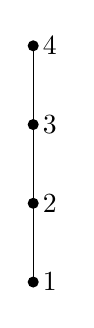
\begin{tikzpicture}
			\fill(0,1)circle(2pt)node[right]{1};
			\fill(0,2)circle(2pt)node[right]{2};
			\fill(0,3)circle(2pt)node[right]{3};
			\fill(0,4)circle(2pt)node[right]{4};
			\draw(0,1)--(0,4);
		\end{tikzpicture}
		\caption{}
		\label{figure:偏序关系.哈斯图1}
	\end{subfigure}
\end{figure}

总结一下,我们可以使用下面的过程
表示一个有限的偏序集\(\opair{S,\leq}\):\begin{enumerate}
	\item 从偏序关系中去掉所有的环
	(即\(\Set{\opair{a,a} \given a \in S}\));
	\item 去掉所有可以利用传递性得到的弧
	(即\(\Set{\opair{a,c} \given (\exists b \in S)[a < b \land b < c]}\);
	\item 排列每条弧,使得它的起点在终点下面,擦除弧上的箭头.
\end{enumerate}
我们把按照上述步骤绘制得到的图称为“偏序集\(\opair{S,\leq}\)的\DefineConcept{哈斯图}”.
它是以德国数学家赫尔姆·哈斯的名字命名的.

\subsection{最大元,最小元,上界,下界}
\begin{definition}
%@see: 《Real Analysis Modern Techniques and Their Applications Second Edition》 P5
设\(X\)是非空集合,
\(x \in X\),
\(E \subseteq X\),
\(\rel{R}\)是\(X\)上的偏序关系.

我们如果把满足\[
	[y \in X \implies x\rel{R}y]
	\implies
	y = x,
\]的\(x\)称为
“\(X\)(关于\(\mathcal{R}\))的\DefineConcept{最大元}”
或“\(\opair{X,\mathcal{R}}\)的\DefineConcept{最大元}(maximal element)”,
那么相应地把满足\[
	[y \in X \implies y\rel{R}x]
	\implies
	y = x,
\]的\(x\)称为
“\(X\)(关于\(\mathcal{R}\))的\DefineConcept{最小元}”
或“\(\opair{X,\mathcal{R}}\)的\DefineConcept{最小元}(minimal element)”.

在上述约定下,
如果\(x\)满足\[
	(\forall y \in E)[y\rel{R}x],
\]
那么称“\(x\)是\(E\)(在\(\opair{X,\mathcal{R}}\)中)的\DefineConcept{上界}(upper bound)”.
如果\(x\)满足\[
	(\forall y \in E)[x\rel{R}y],
\]
那么称“\(x\)是\(E\)(在\(\opair{X,\mathcal{R}}\)中)的\DefineConcept{下界}(lower bound)”.
\end{definition}

\begin{example}
我们知道\(\leq\)是区间\(X=[0,1]\)上的偏序关系.
易见\(1\)既是\(X\)(关于\(\leq\))的最大元,又是\([0,1]\)的上界;
而\(0\)既是\(X\)(关于\(\leq\))的最小元,又是\([0,1]\)的下界.
\end{example}

\subsection{线性序}
\begin{definition}
%@see: 《Elements of Set Theory》 P62 Definition
设\(\rel{R}\)是集合\(A\)上的一个二元关系.
如果\begin{enumerate}
	\item \(\rel{R}\)具有传递性,
	\item \(\rel{R}\)在\(A\)上服从\DefineConcept{三一律}(trichotomy),
	也就是说,对于\(\forall x,y \in A\),
	在以下三个命题中,有且仅有一个是真命题:\[
		x \rel{R} y, \qquad
		x = y, \qquad
		y \rel{R} x;
	\]
	%@see: https://mathworld.wolfram.com/TrichotomyLaw.html
\end{enumerate}
那么称\(\rel{R}\)为
“\(A\)上的\DefineConcept{线性序}(linear ordering)
或\DefineConcept{全序}(total ordering)”.
\end{definition}

应该注意到,当\(x = y\)时,三一律要求\[
	x \rel{R} x, \qquad
	x = x, \qquad
	x \rel{R} x
\]中的一个成立,
考虑到\(x = x\)恒成立,
那么必有\(x \rel{R} x\)恒不成立.
易见当\(x \neq y\)时,必有\(x \rel{R} y\)或\(y \rel{R} x\)之一成立,
都不可能有\(x \rel{R} y\)和\(y \rel{R} x\)都成立.
于是我们证得如下定理.

\begin{theorem}
%@see: 《Elements of Set Theory》 P63 Theorem 3R
设\(\rel{R}\)是集合\(A\)上的线性序.
\begin{enumerate}
	\item \(\rel{R}\)不具有自反性,
	即不存在\(x\)使得\(x \rel{R} x\).

	\item \(\rel{R}\)在\(A\)上是连通的(\(\rel{R}\) is \emph{connected} on \(A\)),
	即对于不同的\(x,y \in A\),要么有\(x \rel{R} y\)成立,要么有\(y \rel{R} x\)成立.
\end{enumerate}
\end{theorem}

值得注意的是,
线性序\(\rel{R}\)永远不会给出如下的环形:
\begin{center}
	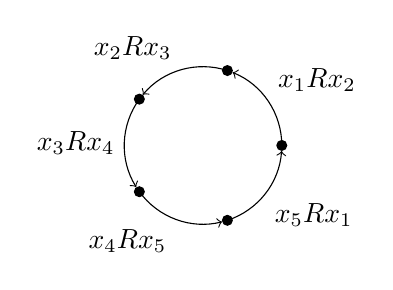
\begin{tikzpicture}
		\fill(1,0)circle(2pt)coordinate(A0);
		\fill({cos(72)},{sin(72)})circle(2pt)coordinate(A1);
		\fill({cos(144)},{sin(144)})circle(2pt)coordinate(A2);
		\fill({cos(216)},{sin(216)})circle(2pt)coordinate(A3);
		\fill({cos(288)},{sin(288)})circle(2pt)coordinate(A4);
		\begin{scope}[->]
			\draw(A0)arc[start angle=0,end angle=68,radius=1]node[midway,above right]{\(x_1 \rel{R} x_2\)};
			\draw(A1)arc[start angle=72,end angle=140,radius=1]node[midway,above left]{\(x_2 \rel{R} x_3\)};
			\draw(A2)arc[start angle=144,end angle=212,radius=1]node[midway,left]{\(x_3 \rel{R} x_4\)};
			\draw(A3)arc[start angle=216,end angle=284,radius=1]node[midway,below left]{\(x_4 \rel{R} x_5\)};
			\draw(A4)arc[start angle=288,end angle=356,radius=1]node[midway,below right]{\(x_5 \rel{R} x_1\)};
		\end{scope}
	\end{tikzpicture}
\end{center}
这是因为,如果我们有这样的环形成立,
那么根据传递性必有\(x_1 \rel{R} x_1\),
而这就与反自反性矛盾!

\begin{example}
设\(\rel{R}\)是\(A\)上的一个线性序,
证明:\(\rel{R}^{-1}\)也是\(A\)上的线性序.
\begin{proof}
由于\[
	\bigl( x \rel{R} y \land y \rel{R} z \implies x \rel{R} z \bigr)
	\iff
	\bigl( y \rel{R}^{-1} x \land z \rel{R}^{-1} y \implies z \rel{R}^{-1} x \bigr),
\]
可知\(\rel{R}^{-1}\)具有传递性.
又因为\(\rel{R}\)是\(A\)上的线性序,
所以对于\(\forall x,y \in A\),以下三个命题\[
	x \rel{R} y, \qquad
	x = y, \qquad
	y \rel{R} x
\]有且仅有一个成立;
换句话说,以下三个命题\[
	y \rel{R}^{-1} x, \qquad
	x = y, \qquad
	x \rel{R}^{-1} y
\]有且仅有一个成立;
可知\(\rel{R}^{-1}\)服从三一律.
综上所述,\(\rel{R}^{-1}\)也是\(A\)上的线性序.
\end{proof}
\end{example}


\part{初等数学}
\chapter{算术与代数}

\section{比}
\subsection{比例数}
\begin{definition}
给定两个数\(a\)和\(b\),
如果数\(c\)满足\(a=b \cdot c\),
则称“\(c\)是\(a\)与\(b\)的\DefineConcept{比例数}(简称\DefineConcept{比})”,
记作\(a \propto b\)或\(a:b=c\)或\(a/b=c\)或\(\frac{a}{b}=c\),
并称\(a\)和\(b\)为这个比的\DefineConcept{项},
称\(a\)为\DefineConcept{前项},
称\(b\)为\DefineConcept{后项}.
\end{definition}

\begin{property}
\(\frac{a}{b} = \frac{ma}{mb}\ (m\neq0)\).
\end{property}

\begin{definition}
相对于比\(a:b\),比\(a^2:b^2\)称为\(a:b\)的\DefineConcept{二次比},
\(a^3:b^3\)称为\(a:b\)的\DefineConcept{三次比},
\(a^{\frac{1}{2}}:b^{\frac{1}{2}}\)称为\(a:b\)的\DefineConcept{平方根比}.
\end{definition}

\begin{example}
设\begin{equation*}
	\frac{a}{b} = \frac{c}{d} = \frac{e}{f} = \dotsb = k,
\end{equation*}
证明:\begin{equation*}
	\left(
		\frac{
			p a^n + q c^n + r e^n + \dotsb
		}{
			p b^n + q d^n + r f^n + \dotsb
		}
	\right)^{\frac1n} = k,
\end{equation*}
其中\(p,q,r,\dotsc\)和\(n\)都是任意常数.
\end{example}

\begin{example}
已知\(\frac{a}{b}=\frac{c}{d}=\frac{e}{f}\),
证明:\(\frac{a^3b+2c^2e-3ae^2f}{b^4+2d^2f-3bf^3} = \frac{ace}{bdf}\).
%TODO
\end{example}

\begin{example}
已知\(\frac{x}{a}=\frac{y}{b}=\frac{z}{c}\),
证明:\begin{equation*}
	\frac{x^2+a^2}{x+a}+\frac{y^2+b^2}{y+b}+\frac{z^2+c^2}{z+c}
	= \frac{(x+y+z)^2+(a+b+c)^2}{x+y+z+a+b+c}.
\end{equation*}
%TODO
\end{example}

\begin{example}
已知方程\(7x=4y+8z, 3z=12x+11y\),求比\(x:y:z\).
\begin{solution}
方程移项,得\begin{gather*}
	7x-4y-8z=0, \\
	12x+11y-3z=0,
\end{gather*}
从每个方程的第二项开始写出系数,并利用“交叉相乘法”
\begin{equation*}
	\begin{array}{*4r}
		-4, & -8, & 7, & -4, \\
		11, & -3, & 12, & 11,
	\end{array}
\end{equation*}
得到\begin{gather*}
	(-4)\times(-3)-11\times(-8)=100, \\
	(-8)\times12-(-3)\times7=-75, \\
	7\times11-12\times(-4)=125,
\end{gather*}
即\begin{equation*}
	\frac{x}{100}=\frac{y}{-75}=\frac{z}{125}
	\quad\text{或}\quad
	\frac{x}{4}=\frac{y}{-3}=\frac{z}{5}.
\end{equation*}
\end{solution}
\end{example}

\subsection{比例}
\begin{definition}
给定四个数\(a,b,c,d\),
如果有\(\frac{a}{b}=\frac{c}{d}\),
则称“\(a,b,c,d\)是\DefineConcept{成比例的}”,
记作\begin{equation*}
	a:b = c:d,
\end{equation*}
并称\(a\)和\(d\)两项为\DefineConcept{外项},
称\(b\)和\(c\)为\DefineConcept{内项}.
\end{definition}

显然,当数\(a,b,c,d\)成比例时,
\(\frac{a}{b}=\frac{c}{d}\),
必有\(b,d\)均不为零,于是\begin{equation*}
	bd \cdot \frac{a}{b} = bd \cdot \frac{c}{d},
\end{equation*}\begin{equation*}
	ad = bc,
\end{equation*}
也就是说,“外项之积等于内项之积.”

\begin{definition}
如果数\(a,b,c,d,\dotsc\)满足\begin{equation*}
	\frac{a}{b} = \frac{b}{c} = \frac{c}{d} = \dotsb,
\end{equation*}
则称“\(a,b,c,d,\dotsc\)成\DefineConcept{连比}”.

特别地,当\(a,b,c\)成连比(即\(a:b = b:c\))时,
称\(b\)为\DefineConcept{比例中项},
称\(c\)为\(a\)与\(b\)的\DefineConcept{第三比例项}.
\end{definition}

我们有以下几个平凡的结论:\begin{enumerate}
	\item 若\(\frac{a}{b} = \frac{b}{c}\),
	则\(\frac{a}{c} = \frac{a^2}{b^2}\).
	\item 若\(\frac{a}{b} = \frac{c}{d}\)
	且\(\frac{e}{f} = \frac{g}{h}\),
	则\(\frac{ae}{bf} = \frac{cg}{dh}\).
	\item {\rm\bf 交等定理}\footnote{%
	交等定理、反比定理、交比定理、合比定理、分比定理和合分比定理
	这几个名称实际上取自欧几里得的《几何原本》.%
	}.
	若\(\frac{a}{b} = \frac{c}{d}\)
	且\(\frac{b}{x} = \frac{d}{y}\),
	则\(\frac{a}{x} = \frac{c}{y}\).
	\item {\rm\bf 反比定理}.
	若\(\frac{a}{b} = \frac{c}{d}\),
	则\(\frac{b}{a} = \frac{d}{c}\).
	\item {\rm\bf 交比定理}.
	若\(\frac{a}{b} = \frac{c}{d}\),
	则\(\frac{a}{c} = \frac{b}{d}\).
	\item {\rm\bf 合比定理}.
	若\(\frac{a}{b} = \frac{c}{d}\),
	则\((a+b):b = (c+d):d\).
	\item {\rm\bf 分比定理}.
	若\(\frac{a}{b} = \frac{c}{d}\),
	则\((a-b):b = (c-d):d\).
	\item {\rm\bf 合分比定理}.
	若\(\frac{a}{b} = \frac{c}{d}\),
	则\(\frac{a+b}{a-b} = \frac{c+d}{c-d}\).
\end{enumerate}

\begin{example}
解方程\begin{equation*}
	\frac{\sqrt{x+1}+\sqrt{x-1}}{\sqrt{x+1}-\sqrt{x-1}} = \frac{4x-1}{2}.
\end{equation*}
\begin{solution}
注意到原方程中\(x\)的取值范围是\(x\geq1\).
利用合分比定理,有\begin{equation*}
	\frac{\sqrt{x+1}}{\sqrt{x-1}} = \frac{4x+1}{4x-3},
\end{equation*}
所以\begin{equation*}
	\frac{x+1}{x-1} = \frac{16x^2+8x+1}{16x^2-24x+9}.
\end{equation*}
再利用合分比定理,有\begin{equation*}
	\frac{2x}{2} = \frac{32x^2-16x+10}{32x-8},
\end{equation*}
即\begin{equation*}
	x = \frac{16x^2-8x+5}{16x-4},
\end{equation*}
解得\(x=\frac{5}{4} \geq1\).
\end{solution}
\end{example}

\subsection{变化率}
\begin{definition}
已知互相关联的两个量\(A\)与\(B\).
如果每当\(B\)变化了,就有\(A\)也随之变化一个相同的比率,
那么称“量\(A\)与量\(B\)成\DefineConcept{正比}”,
记作\(A \propto B\).
\end{definition}

\begin{theorem}
如果\(A\)与\(B\)成正比,那么\(A\)等于\(B\)乘以一个常量.
\begin{proof}
设数\(\AutoTuple{a}{0}\)和\(\AutoTuple{b}{0}\)是\(A\)和\(B\)的对应的取值.
根据定义,有\begin{equation*}
	\def\f#1{%
		\frac{a_#1}{a_1} = \frac{b_#1}{b_1}%
	}
	\f2,\f3,\f4,\dotsc,
\end{equation*}
于是\begin{equation*}
	\def\f#1{\frac{a_#1}{b_#1}}
	\frac{A}{B} = \f1 = \f2 = \f3 = \f4 = \dotsb.
	\qedhere
\end{equation*}
\end{proof}
\end{theorem}

\begin{definition}
已知两个量\(A\)与\(B\).
如果\(A\)与\(B\)的倒数成正比,
那么称“量\(A\)与量\(B\)成\DefineConcept{反比}”.
\end{definition}

结合“正比”与“反比”的定义,如果\(A\)同\(B/C\)成正比,
那么称“\(A\)同\(B\)成正比,而同\(C\)成反比”.

\section{整式}
我们把用运算符号把数和表示数的字母连接而成的式子叫做\DefineConcept{代数式}.
运算符号是指加、减、乘、除、乘方、开方、绝对值、括号等符号.
代数式中不允许出现等号、不等号.

由数与字母的积组成的代数式叫做\DefineConcept{单项式}(monomial).
%@see: https://mathworld.wolfram.com/Monomial.html
例如\begin{equation*}
	1, \qquad
	a, \qquad
	4b^2, \qquad
	7abc
\end{equation*}都是单项式.
单项式中的数叫做这个单项式的\DefineConcept{系数}(coefficient).
例如\(a\)的系数是\(1\),
\(4b^2\)的系数是\(4\),
而\(7abc\)的系数是\(7\).
在一个单项式中,所有字母的次数的和,叫做这个单项式的次数.
上面的四个单项式的次数分别是\(0\)次、\(1\)次、\(2\)次和\(3\)次.

由几个单项式的和组成的代数式叫做\DefineConcept{多项式}(polynomial).
%@see: https://mathworld.wolfram.com/Polynomial.html
多项式中的每个单项式叫做这个多项式的\DefineConcept{项}(term),
其中不含字母的项叫做这个多项式的\DefineConcept{常数项}(constant term).
例如\begin{equation*}
	1+a, \qquad
	b+2c^2+\frac12cde,
\end{equation*}都是多项式.
在一个多项式中,次数最高的项的次数,就是这个多项式的\DefineConcept{次数}.
上面的两个多项式的次数分别是\(1\)次和\(3\)次.

只含一种字母的多项式,叫做\DefineConcept{一元多项式}(univariate polynomial).
%@see: https://mathworld.wolfram.com/UnivariatePolynomial.html
含有两种字母的多项式,叫做\DefineConcept{二元多项式}(bivariate polynomial).
%@see: https://mathworld.wolfram.com/BivariatePolynomial.html
含有两种以上字母的多项式,统称为\DefineConcept{多元多项式}(multivariate polynomial).

系数全是整数的多项式,叫做\DefineConcept{整系数多项式}(integer polynomial).
%@see: https://mathworld.wolfram.com/IntegerPolynomial.html
系数全是有理数的多项式,叫做\DefineConcept{有理系数多项式}(rational polynomial).
%@see: https://mathworld.wolfram.com/RationalPolynomial.html
系数全是实数的多项式,叫做\DefineConcept{实系数多项式}(real polynomial).
%@see: https://mathworld.wolfram.com/RealPolynomial.html
系数全是复数的多项式,叫做\DefineConcept{复系数多项式}(complex polynomial).
%@see: https://mathworld.wolfram.com/ComplexPolynomial.html

我们把单项式和多项式统称为\DefineConcept{整式}.

通常我们会把一个多项式按其中某一字母的次数按从小到大或从大到小的顺序排列起来.
当我们按从小到大的顺序排列时,叫做“把多项式按字母升幂排列”.
当我们按从大到小的顺序排列时,叫做“把多项式按字母降幂排列”.

在多项式中,我们把所含字母相同,且相同字母的次数也相同的项,叫做\DefineConcept{同类项}.
为了简化记号,方便思考,我们常常会把多项式中的同类项合并成一项;
具体来说,就是把同类项的系数相加,所得结果作为新的项的系数,同时保持原来的项的字母及其次数不变.
例如\(1\)和\(4\)是同类项,
\(a\)和\(3a\)是同类项,
\(4b^2\)和\(7b^2\)是同类项,
\(7abc\)和\(13abc\)是同类项.

\section{数的开方}
\subsection{开平方}
如果\(b\)的平方\(b^2\)等于\(a\),
就把\(b\)称为\(a\)的\DefineConcept{平方根}.

因为任何一个有理数的平方根只能等于正数或零,
所以只有非负数(正数和零)才有平方根,而负数没有平方根.

由于不等于零的两个相反数的平方的同一个正数,
所以一个正数一定有两个平方根,且这两个平方根互为相反数.
零只有一个平方根.
零的平方根是零.

假设\(x^2 = a > 0\),
那么\(a\)的平方根\(x\)记作\begin{equation*}
	x = \pm \sqrt{a}.
\end{equation*}
因为\(\pm\sqrt0 = 0\),
所以非负数\(a\)的平方根也可以记作\(\pm\sqrt{a}\).

求一个数的平方根的运算,叫做\DefineConcept{开平方}.
开平方与平方互为逆运算.

一个正数\(a\)的正的平方根,叫做\(a\)的\DefineConcept{算术平方根},记作\(\sqrt{a}\).
规定零的算术平方根是零.
因此非负数\(a\)的算术平方根可以记作\(\sqrt{a}\).

给定式子\(\sqrt{a}\),我们就要注意到两个问题:\begin{itemize}
	\item \(\sqrt{a}\)是一个非负数,即\(\sqrt{a}\geq0\).
	\item \(a\)也是一个非负数,即\(a\geq0\).
\end{itemize}

\subsection{开立方}
如果\(b\)的立方\(b^2\)等于\(a\),
就把\(b\)称为\(a\)的\DefineConcept{立方根}.

不论是正数、负数还是零,都有且仅有一个立方根.
正数的立方根是正数,
负数的立方根是负数,
零的立方根还是零.

假设\(x^3 = a\),
那么\(a\)的立方根记作\begin{equation*}
	x = \sqrt[3]{a}.
\end{equation*}
对于任意有理数\(a\),
都有\begin{equation*}
	\sqrt[3]{-a} = \sqrt[3]{a}.
\end{equation*}

求一个数的立方根的运算,叫做\DefineConcept{开立方}.
开立方与立方互为逆运算.

对于任意正数\(a\),
总有\begin{equation*}
	\sqrt{a}^2
	= a.
\end{equation*}

对于任意有理数\(a\),
总有\begin{equation*}
	\sqrt{a^2}
	= \abs{a}
	= \left\{ \begin{array}{rl}
		a, & a\geq0, \\
		-a, & a<0.
	\end{array} \right.
\end{equation*}
%
\begingroup
\chapter{初等数论}
数论在一些地方总有让人意想不到的妙用.
有这样一种说法:“自然科学的皇后是数学,数学的皇冠是数论,哥德巴赫猜想则是皇冠上的明珠.”
在这一章,我们介绍一些基础的数论理论,供大家参考.

\section{素数与合数}
在正整数集上,由于没有引入负数、分数的概念,
正整数\(x\)与\(y\)相除的结果除了商\(z\)以外,
还经常是带有余数\(r\)的,于是有关系式\[
	x = y z + r.
\]

\begin{definition}
在正整数集上,如果\(x\)与\(y\)相除余\(r=0\),
我们就称“\(y\)可以\DefineConcept{整除} \(x\)”
或“\(x\)可以被\(y\)整除”
或“\(x\)是\(y\)的\DefineConcept{倍数}”
或“\(y\)是\(x\)的\DefineConcept{因子}”,
记作\(\truediv{x}{y}\),
即\[
%@see: 《具体数学 计算机科学基础(第2版)》 P85 (4.1)
	\truediv{x}{y}
	\defiff
	y > 0
	\land
	(\exists z\in\mathbb{Z})
	[x = y z].
\]
\end{definition}

\begin{property}
%@see: 《具体数学 计算机科学基础(第2版)》 P85
没有任何整数可以被\((-1)\)整除.
\end{property}

\begin{definition}
\(a\)与\(b\)的\DefineConcept{最大公约数}(greatest common divisor),
记作\((a,b)\),
即\[
%@see: 《具体数学 计算机科学基础(第2版)》 P85 (4.2)
	(a,b) \defeq \max\Set{ k \given (\truediv{a}{k}), (\truediv{b}{k}) }.
\]
\end{definition}
\begin{definition}
\(a\)与\(b\)的\DefineConcept{最小公倍数}(least common multiple),
记作\([a,b]\),
即\[
%@see: 《具体数学 计算机科学基础(第2版)》 P86 (4.3)
	[a,b] \defeq \min\Set{ k \given k>0, (\truediv{k}{a}), (\truediv{k}{b}) }.
\]
\end{definition}
在本章以外,为了防止最大公约数、最小公倍数记号与开区间、闭区间符号混淆,
分别记作\(\gcd{p,q}\)和\(\lcm{p,q}\).

\begin{property}
%@see: 《具体数学 计算机科学基础(第2版)》 P86 (4.4)
设\(m,n\)都是整数.
\begin{itemize}
	\item 如果\(n>0\),那么\((0,n)=n\).
	\item 如果\(0<m<n\),那么\((m,n) = (n \mod m,m)\).
\end{itemize}
%TODO proof
\end{property}
\begin{remark}
\(0\)与它自身的最大公约数\((0,0)\)是未定义的.
\end{remark}

\begin{theorem}
\(a\)与\(b\)的最大公约数\((a,b)\)和最小公倍数\([a,b]\)的乘积
等于\(a\)与\(b\)之积,
即\begin{equation}
	(a,b) \cdot [a,b] = ab.
\end{equation}
%TODO proof
\end{theorem}

\begin{definition}
如果正整数\(x\)只能被1或它自己整除\footnote{特别地,我们规定1不是素数.},
那么称\(x\)为\DefineConcept{素数}或\DefineConcept{质数}(prime number);
否则称之为\DefineConcept{合数}(composite number).
\end{definition}
这就是说:\[
	\text{$x$是素数}
	\defiff
	(\forall y)(\forall z)
	[y \cdot z=x \implies y=1 \lor z=1].
\]

\begin{definition}
如果正整数\(x\)与\(y\)除了1以外没有其他公因子,
就称“\(x\)与\(y\) \DefineConcept{互素}(或\DefineConcept{互质})”.
\end{definition}

全体素数的集合,
记作\(\mathbb{S}\),
即\[
	\mathbb{S}
	\defeq
	\Set*{
		x\in\mathbb{N}^+-\{1\}
		\given
		(\forall y\in\mathbb{N}^+)
		[y \neq x \implies (x,y)=1]
	}.
\]

\begin{theorem}
如果一个正整数\(a\)能整除正整数的乘积\(bc\),且\(a\)与其中一个因子\(b\)互素,
则\(a\)必能整除另一个因子\(c\).
\end{theorem}
\begin{corollary}
如果素数\(a\)能整除正整数的乘积\(bcd\dotsm\),则\(a\)必能整除该乘积的一个因子.
\end{corollary}
\begin{corollary}
如果素数\(a\)能整除正整数的乘积\(b^n\ (n\in\mathbb{N}^+)\),那么\(a\)必能整除\(b\).
\end{corollary}

\begin{theorem}
如果正整数\(a\)与正整数\(b,c\)均互素,则它必与乘积\(bc\)互素.
\end{theorem}
\begin{corollary}
如果正整数\(a\)与正整数的乘积\(bc\)互素,则\(a\)与正整数\(b,c\)均互素.
\end{corollary}
\begin{corollary}
如果正整数\(a\)与\(b\)互素,则\(a^m\ (m\in\mathbb{N}^+)\)与\(b^n\ (n\in\mathbb{N}^+)\)互素.
\end{corollary}

\begin{theorem}
如果正整数\(a\)与\(b\)互素,则分数\(\frac{a^m}{b^n}\ (m,n\in\mathbb{N}^+)\)均为既约分数.
\end{theorem}
\begin{corollary}
设\(a,b,c,d\in\mathbb{N}^+\).
如果\(\frac{a}{b} = \frac{c}{d}\),
且\(\frac{a}{b}\)是既约分数,
则\[
	(\forall k\in\mathbb{R}^*)
	[c = ka, d = kb].
\]
\end{corollary}

不难发现,第一个素数是2,它也是素数中唯一一个偶数.
第二个素数是3,接下来是5、7、11……
我们不禁发问,素数的个数究竟是有限的,还是无限的.
\begin{theorem}
素数有无穷多个,
即\[
	(\forall x)(\exists y)[y>x \land \text{$y$是素数}].
\]
\begin{proof}
用反证法\footnote{这个证法是由古希腊数学家欧几里得给出的.}.
假设素数只有\(k\)个,分别是\(\AutoTuple{p}{k}\),且\(p_1 < p_2 < \dotsb < p_k\).
显然,数\(\truediv{p_1 p_2 \dotsm p_k}{p_i}\ (i=1,2,\dotsc,k)\).
但数\[
	N = 1 + p_1 p_2 \dotsm p_k
\]与\(p_i\ (i=1,2,\dotsc,k)\)相除总余1,
这就说明数\(N\)要么是一个素数,
要么是一个可以被区间\((p_k,N)\)内的一个正整数\(M\)整除的合数,
总之素数的个数大于\(k\).
以此类推,可知素数必然有无穷多个.
\end{proof}
\end{theorem}
\begin{definition}\label{definition:初等数论.欧几里得数}
%@see: 《具体数学 计算机科学基础(第2版)》 P90 (4.16)
定义\[
	e_n \defeq \left\{ \begin{array}{cl}
		2, & n=1, \\
		e_1 e_2 \dotsm e_{n-1} + 1, & n\geq2,
	\end{array} \right.
\]
把\(e_n\)称为“第\(n\)个\DefineConcept{欧几里得数}(Euclid number)”.
%@see: https://mathworld.wolfram.com/EuclidNumber.html
\end{definition}
\begin{table}[htb]
	\centering
	\begin{tblr}{c|r|l}
		\hline
		\(n\) & \(e_n\) & \\
		\hline
		\(1\) & \(2\) & 素数 \\
		\(2\) & \(3\) & 素数 \\
		\(3\) & \(7\) & 素数 \\
		\(4\) & \(43\) & 素数 \\
		\(5\) & \(1~807\) & 合数,可以分解为\(13\times139\) \\
		\(6\) & \(3~263~443\) & 素数 \\
		\(7\) & \(10~650~056~950~807\) & 合数,可以分解为\(547\times607\times1~033\times31~051\) \\
		\hline
	\end{tblr}
	\caption{前7个欧几里得数}
%@Mathematica: EuclidNumber[n_] := Product[EuclidNumber[k], {k, 1, n - 1}] + 1
%@Mathematica: Table[{n, EuclidNumber[n], PrimeQ[EuclidNumber[n]]}, {n, 1, 9}] // TableForm
\end{table}
\begin{proposition}
%@see: 《具体数学 计算机科学基础(第2版)》 P90
欧几里得数全都是互素的.
\begin{proof}
因为当\(n > m\)时,有\(e_n \mod e_m = 1\),
所以\((e_m,e_n)
= (1,e_n)
= (0,1)
= 1\).
\end{proof}
\end{proposition}
% 于是,如果假设\(q_j\ (j\geq1)\)是\(e_j\)的最小素因子,
% 则素数\(q_1,q_2,q_3,\dotsc\)全都是不相同的,
% 这是一个含有无穷多个素数的序列.

由\cref{definition:初等数论.欧几里得数} 可知
\(e_n = e_1 e_2 \dotsm e_{n-2} e_{n-1} + 1\),
代入\(e_{n-1} - 1 = e_1 e_2 \dotsm e_{n-3} e_{n-2}\),
便得\(e_n = (e_{n-1} - 1) e_{n-1} + 1\),
整理可得欧几里得数的递归定义:\begin{equation}
	e_n = e_{n-1}^2 - e_{n-1} + 1.
\end{equation}

\begin{theorem}
没有任何一个有理代数式能唯一地表示素数.
\begin{proof}
用反证法.
假设有理代数式\[
	p(x) = a_0 + a_1 x + a_2 x^2 + \dotsb
\]唯一地表示素数,
且\[
	p(m) = a_0 + a_1 m + a_2 m^2 + \dotsb = q.
\]
但\begin{align*}
	p(m+nq) &= a_0 + a_1 (m+nq) + a_2 (m+nq)^2 + \dotsb \\
	&= a_0 + a_1 m + a_2 m^2 + \dotsb + \alpha q \quad(\alpha\in\mathbb{Q}) \\
	&= q + \alpha q = (1+\alpha)q,
\end{align*}
即\(\truediv{p(m+nq)}{q}\),说明\(p(m+nq)\)不是一个素数.
\end{proof}
\end{theorem}

\begin{theorem}[算数基本定理]
一个数只能以一种方式分解素因子.
\begin{proof}
设合数\(N\)可以分解为乘积\(abcd\dotsm\),其中\(a,b,c,d,\dotsc\)是素数;
又设\(N = \alpha\beta\gamma\delta\dotsm\),
其中\(\alpha,\beta,\gamma,\delta,\dotsc\)是另一些素数;
那么\[
	abcd\dotsm = \alpha\beta\gamma\delta\dotsm.
\]
显然,数\(\alpha\)可以整除\(abcd\dotsm\),
所以\(\alpha\)至少能整除它们中的一个因子,
不妨设\(\truediv{a}{\alpha}\),
但是由于\(a,b,c,d,\dotsc\)都是素数,
故可知\(a=\alpha\),
因此\[
	bcd\dotsm = \beta\gamma\delta\dotsm.
\]
以此类推,最后得到\(b=\beta,c=\gamma,d=\delta,\dotsc\),
也就是说,任意合数的素因子分解式是唯一的.
\end{proof}
\end{theorem}

\begin{example}
已知合数\(N = a^p b^q c^r \dotsm\),其中\(a,b,c,\dotsc\)是不同的素数,\(p,q,r,\dotsc\)是正整数.
计算\(N\)的因子个数,\(N\)分解成两个因子的方式数,\(N\)分解成两个互素的因子的方式数,\(N\)的所有因子之和.
\begin{solution}
因为乘积\[
(1+a+a^2+\dotsb+a^p)
(1+b+b^2+\dotsb+b^q)
(1+c+c^2+\dotsb+c^r)\dotsm
\]的展开式的每一项都是数\(N\)的一个因子,
所以,\(N\)的因子个数%
\footnote{这里“因子个数”包括了1和合数\(N\)本身.}%
就是上述乘积的项数\((p+1)(q+1)(r+1)\dotsm\).

当\(N\)不是完全平方数时,\(N\)分解成两个因子的方式显然有\[
\frac{1}{2} (p+1)(q+1)(r+1)\dotsm
\]种.

当\(N\)是完全平方数时,\(N = \sqrt{N}\times\sqrt{N}\)也是一种分解方式,但对应于这种分解方式的因子只有一个\(\sqrt{N}\).
如果不计入这种分解方式,那么\(N\)的分解方式有\[
\frac{1}{2} \left[-1 + (p+1)(q+1)(r+1)\dotsm\right]
\]种;再加上刚刚提到的一种特殊分解方式\(N = \sqrt{N}\times\sqrt{N}\),那么\(N\)的分解方式总共有\[
\frac{1}{2} \left[1 + (p+1)(q+1)(r+1)\dotsm\right]
\]种.

在将数\(N\)分解成互素的两个因子\(\alpha,\beta\)时,其中一个必须包含\(a^p\),否则就会有\(a\)的一些幂在一个因子中,\(a\)的另一些幂在在另一个因子中,于是这两个因子就不互素了.
以此类推,可知“\(N\)分解成两个互素的因子的方式数”与“\(abcd\dotsm\)分解成两个因子的方式数”相等,即为\[
\frac{1}{2}(1+1)(1+1)(1+1)\dotsm.
\]若设\(N\)中共有\(n\)个不同的素因子,那么\(N\)分解成两个互素的因子的方式数是\[
\frac{1}{2} \cdot 2^n = 2^{n-1}.
\]

如前所述,由于乘积\[
(1+a+a^2+\dotsb+a^p)
(1+b+b^2+\dotsb+b^q)
(1+c+c^2+\dotsb+c^r)\dotsm
\]展开式的每一项都是一个因子,所以“\(N\)的所有因子之和”就等于这个乘积,由等比数列的求和公式,便得\(N\)的所有因子之和为\[
\frac{1-a^{p+1}}{1-a}\cdot\frac{1-b^{q+1}}{1-b}\cdot\frac{1-c^{r+1}}{1-c}\dotsm.
\]
\end{solution}
\end{example}

\section{费马小定理}
\begin{lemma}\label{theorem:初等数论.费马小定理.引理0}
证明:任意\(r\)个连续正整数的乘积能被\(r!\)整除.
\begin{proof}
设从正整数\(n\)开始的连续\(r\)个正整数的乘积为\(P_n = n(n+1)(n+2)\dotsm(n+r-1)\),那么\[
P_{n+1} = (n+1)(n+2)\dotsm(n+r),
\]\[
n P_{n+1} = (n+r) P_n = n P_n + r P_n,
\]\[
P_{n+1} = P_n + \frac{r}{n} P_n,
\]\[
P_{n+1} - P_n = r \frac{P_n}{n},
\]上式等号右边是\(r-1\)个连续正整数的\(r\)倍.
因此,如果任意\(r-1\)个连续正整数的乘积能被\((r-1)!\)整除,就有\(P_{n+1} - P_n\)能被\(r!\)整除.
因为\(P_1 = 1 \cdot 2 \dotsm r = r!\),所以\(P_2\)必是\(r!\)的倍数,从而\(P_3,P_4,\dotsc\)也都是\(r!\)的倍数.
这样就证明了“如果\(r-1\)个连续正整数的乘积能被\((r-1)!\)整除,那么\(r\)个连续正整数的乘积便能被\(r!\)整除”.
但是由于每两个连续正整数(必有一个奇数和一个偶数)的乘积能被\(2!=2\)整除,所以每三个连续正整数的乘积也能被\(3!\)整除;以此类推,该命题普遍成立.
\end{proof}
\end{lemma}

\begin{lemma}\label{theorem:初等数论.费马小定理.引理1}
设\(p\)是素数.
证明:除了第一项和最后一项以外,\((a+b)^p\)展开式的每一项的系数,都可以被\(p\)整除.
\begin{proof}
除了第一项与最后一项以外的各项系数为\[
C_p^r = \frac{p(p-1)(p-2)\dotsm(p-r+1)}{r!},
\]其中\(r=1,2,\dotsc,p-1\).
因为\(p\)是素数,所以\(r!\)中(除了1以外)没有一个因子可以整除\(p\);
又因为\(p>r\),所以\(p\)也不能整除\(r!\)中的任一因子;
也就是说,\((p-1)(p-2)\dotsm(p-r+1)\)必能被\(r!\)整除,而系数\(C_p^r\)必能被\(p\)整除.
\end{proof}
\end{lemma}

\begin{lemma}\label{theorem:初等数论.费马小定理.引理2}
设\(p\)是素数.
证明:\[
(a+b+c+d+\dotsb)^p = M + a^p + b^p + c^p + d^p + \dotsb,
\]其中\(M\)是\(p\)的倍数.
\begin{proof}
记\(\beta=b+c+\dotsb\),则由\cref{theorem:初等数论.费马小定理.引理1} 可知\[
(a+\beta)^p = a^p + \beta^p + M_1,
\]其中\(M_1\)是\(p\)的倍数.
接下来,记\(\gamma=c+d+\dotsb\),则同样有\[
\beta^p = (b+\gamma)^p = b^p + \gamma^p + M_2,
\]其中\(M_2\)是\(p\)的倍数.
以此类推,便得要证的结果,且\(M = M_1+M_2+\dotsb\).
\end{proof}
\end{lemma}

\begin{theorem}[费马小定理]\label{theorem:初等数论.费马小定理}
如果\(p\)是素数,且正整数\(n\)与\(p\)互素,则\(n^{p-1}-1\)是\(p\)的倍数.
\begin{proof}
根据\cref{theorem:初等数论.费马小定理.引理2},在\(n\)个正整数的和的\(p\)次幂\[
(a+b+c+d+\dotsb)^p = M + a^p + b^p + c^p + d^p + \dotsb
\]中令\(a=b=c=d=\dotsb=1\),那么有\[
n^p = n + M
\quad\text{或}\quad
n^p - n = n(n^{p-1}-1) = M,
\]即\(\truediv{n^{p-1}-1}{p}\).
\end{proof}
\end{theorem}

\begin{corollary}
如果\(p\)是素数,且\(p\neq2\),那么\(p-1\)是偶数,且对于任意正整数\(N\)总有\[
\left(N^{\frac{p-1}{2}}+1\right)
\left(N^{\frac{p-1}{2}}-1\right)
\]是\(p\)的倍数,或者说\[
N^{\frac{p-1}{2}} = Kp\pm1,
\]其中\(K\)是某个正整数.
\end{corollary}

\begin{corollary}[费马小定理']
如果\(p\)是素数,则\(\truediv{n^p-n}{p}\).
\end{corollary}

\begin{example}
设\(p\)是素数,证明:任意两个正整数的\(p\)次幂的差比这两个数的差大\(p\)的倍数.
\end{example}

\begin{example}
证明:任意完全平方数要么等于\(5n\),要么等于\(5n\pm1\),其中\(n\in\mathbb{N}^+\).
\end{example}

\begin{example}[费马猜想]
费马提出过一个错误的猜想:数\(2^{2^n}+1\ (n=0,1,2,\dotsc)\)都是素数.
这个猜想在当\(n=0,1,2,3,4\)时是正确的,但很遗憾的是,数学家欧拉发现,当\(n=5\)时,数\(2^{2^5}+1 = 4294967297 = 641 \times 6700417\)是合数.
%@Mathematica: FactorInteger[2^(2^5)+1]
\end{example}

\section{无理数}
\begin{proposition}
设\(n\in\mathbb{N}^+\),且\(n\)不是完全平方数,则\(\sqrt{n}\)是无理数.
\begin{proof}
用反证法.
假设\(\sqrt{n} = p/q\),其中\(p,q\in\mathbb{N}^+\).
由于\(n\)不是完全平方数,故有\(m\in\mathbb{N}^+\),使得\(m<p/q<m+1\),
从而\(mq<p<mq+q\),\(0<p-mq<q\).
在等式\(p^2=nq^2\)的两边都减去\(mpq\),
得到\(p^2-mpq=nq^2-mpq\),
提取公因式得\(p(p-mq)=q(nq-mp)\),
整理得\[
	\frac{p}{q} = \frac{nq-mp}{p-mq}.
\]
令\(p_1=nq-mp\),\(q_1=p-mq\).
由于\(q_1\in\mathbb{N}^+\)且\(q_1<q\),
所以\(p_1\in\mathbb{N}^+\)且\(p_1<p\).
对等式\[
	\frac{p}{q} = \frac{p_1}{q_1}
\]反复地进行同样的讨论,
可以得出两串递减的正整数列\[
	p>p_1>p_2>p_3>\dotsb
	\quad\text{与}\quad
	q>q_1>q_2>q_3>\dotsb,
\]
使得\[
	\frac{p}{q}=\frac{p_1}{q_1}=\frac{p_2}{q_2}=\frac{p_3}{q_3}=\dotsb.
\]
这是不可能的,因为从\(p\)或\(q\)开始的正整数不可能无止境地递减下去.
这就证明了\(\sqrt{n}\)不可能是有理数.
\end{proof}
\end{proposition}
\endgroup

\chapter{复数概论}
\section{复数的形式与运算}
\subsection{复数的代数形式}
\begin{definition}[虚数单位]
规定:满足\(\iu^2=-1\)的数\(\iu\)称为\DefineConcept{虚数单位}.
\end{definition}

\begin{definition}
把由有序实数对\((x,y)\)作代数组合所确定的数\(z=x+\iu y\)称为代数形式的\DefineConcept{复数}.
实数\(x\)、\(y\)分别称为复数\(z=x+\iu y\)的\DefineConcept{实部}、\DefineConcept{虚部},记作\(x=\Re z\)、\(y=\Im z\).

特别地,当\(\Im z=0\)时,\(z=\Re z=x\)是实数;
当\(\Re z=0\)时,\(z=\iu\Im z=\iu y\),称为\DefineConcept{纯虚数}.
\end{definition}

\begin{definition}[代数形式下复数相等条件]
设\(z_1\)和\(z_2\)都是复数,则当\(\Re z_1 = \Re z_2\)和\(\Im z_1 = \Im z_2\)同时成立时,则称\(z_1 = z_2\).
特别地,对于复数\(z\),则当且仅当\(\Re z=0\)且\(\Im z=0\)时,\(z=0\).
\end{definition}

\begin{definition}[共轭复数]
设\(z=x + \iu y \in\mathbb{C}\),其中\(x,y\in\mathbb{C}\),称复数\(\ComplexConjugate{z}=x - \iu y\)为\(z\)的\DefineConcept{共轭复数}(conjugate).
\end{definition}

\subsection{复数的模}
\begin{definition}[复数的模]
设复数\(z = x + \iu y\),称\begin{equation*}
\abs{z} = \sqrt{x^2 + y^2}
\end{equation*}为\(z\)的\DefineConcept{模}或\DefineConcept{绝对值}.
\end{definition}

\begin{property}
共轭复数以及复数的模具有以下性质:
\begin{gather*}
	\Re \ComplexConjugate{z} = \Re z, \\
	\Im \ComplexConjugate{z} = -\Im z, \\
	\ComplexConjugate{(\ComplexConjugate{z})} = z, \\
	z+\ComplexConjugate{z} = 2 \Re z, \\
	z-\ComplexConjugate{z} = 2\iu \Im z, \\
	z\ComplexConjugate{z} = \abs{z}^2, \\
	\abs{\ComplexConjugate{z}}=\abs{z}, \\
	\abs{z_1 z_2} = \abs{z_1} \abs{z_2}, \\
	\abs{\frac{z_1}{z_2}} = \frac{\abs{z_1}}{\abs{z_2}} \quad(z_2 \neq 0), \\
	\ComplexConjugate{z_1 \pm z_2} = \ComplexConjugate{z_1} \pm \ComplexConjugate{z_2}, \\
	\ComplexConjugate{z_1 z_2} = \ComplexConjugate{z_1} \cdot \ComplexConjugate{z_2}, \\
	\ComplexConjugate{\left(\frac{z_1}{z_2}\right)} = \frac{\ComplexConjugate{z_1}}{\ComplexConjugate{z_2}} \quad (z_2 \neq 0), \\
	-\abs{z} \leq \Re z \leq \abs{z} \leq \abs{\Re z} + \abs{\Im z}, \\
	-\abs{z} \leq \Im z \leq \abs{z} \leq \abs{\Re z} + \abs{\Im z}.
\end{gather*}
\end{property}

\subsection{复数的代数运算}
\begin{definition}[复数加法]
设\(z_1=x_1+\iu y_1\),\(z_2=x_2+\iu y_2\),
定义\begin{equation*}
z_1+z_2=(x_1+x_2)+\iu(y_1+y_2)
\end{equation*}为复数\(z_1\)和\(z_2\)的加法运算.
\end{definition}

\begin{definition}[复数减法]
设\(z_1=x_1+\iu y_1\),\(z_2=x_2+\iu y_2\),定义\begin{equation*}
z_1-z_2=(x_1-x_2)+\iu(y_1-y_2)
\end{equation*}为复数的\(z_1\)和\(z_2\)的减法运算.
显然,复数减法是加法的逆运算.
\end{definition}

\begin{definition}[复数乘法]
设\(z_1 = x_1 + \iu y_1\),\(z_2 = x_2 + \iu y_2\),定义\begin{equation*}
z_1 \cdot z_2
= (x_1 + \iu y_1)(x_2 + \iu y_2)
= (x_1 x_2 - y_1 y_2)+\iu(x_1 y_2 + x_2 y_1)
\end{equation*}为复数\(z_1\)和\(z_2\)的乘法运算.
\end{definition}

\begin{definition}[复数除法]
设\(z_1 = x_1 + \iu y_1\),\(z_2 = x_2 + \iu y_2 \neq 0\),定义满足\begin{equation*}
z_1 = z \cdot z_2
\end{equation*}的复数\(z = x + \iu y\)为复数\(z_1\)和\(z_2\)的商,记作\begin{equation*}
z = \frac{z_1}{z_2},
\end{equation*}称为复数\(z_1\)和\(z_2\)的除法运算.

显然,复数的除法是乘法的逆运算.
\end{definition}

\begin{theorem}
设\(z_1 = x_1 + \iu y_1\),\(z_2 = x_2 + \iu y_2 \neq 0\),则\begin{equation*}
\frac{z_1}{z_2}
= \frac{z_1 \cdot \ComplexConjugate{z_2}}{z_2 \cdot \ComplexConjugate{z_2}}
= \frac{z_1 \cdot \ComplexConjugate{z_2}}{\abs{z_2}^2}
= \frac{x_1 x_2 + y_1 y_2}{x_2^2 + y_2^2}
+ \iu \frac{x_2 y_1 - x_1 y_2}{x_2^2 + y_2^2}.
\end{equation*}
\begin{proof}
设\(z = x + \iu y = \frac{z_1}{z_2}\),则\begin{equation*}
z \cdot z_2 = (x + \iu y)(x_2 + \iu y_2)
= (x_2 x - y_2 y) + \iu(y_2 x + x_2 y)
= x_1 + \iu y_1,
\end{equation*}从而有方程组\begin{equation*}
\left\{ \begin{array}{l}
x_2 x - y_2 y = x_1, \\
y_2 x + x_2 y = y_1,
\end{array} \right.
\end{equation*}解得\begin{equation*}
x = \frac{x_1 x_2 + y_1 y_2}{x_2^2 + y_2^2},
\quad
y = \frac{x_2 y_1 - x_1 y_2}{x_2^2 + y_2^2}.
\end{equation*}
\end{proof}
\end{theorem}

\begin{theorem}
若\(z,w \in \mathbb{C}\),则有\begin{equation}
	\abs{z \pm w}^2
	= \abs{z}^2 + \abs{w}^2 \pm 2 \Re(z \ComplexConjugate{w}).
\end{equation}
\begin{proof}
\(
	\abs{z + w}^2
	= (z + w) (\ComplexConjugate{z + w})
	= z\ComplexConjugate{z}
		+ z\ComplexConjugate{w}
		+ w\ComplexConjugate{z}
		+ w\ComplexConjugate{w}
	= \abs{z}^2 + 2 \Re(z\ComplexConjugate{w}) + \abs{w}^2
\).
\end{proof}
\end{theorem}

\begin{theorem}
若\(z,w \in \mathbb{C}\),则有\begin{equation}
	\abs{z + w}^2 \leq (\abs{z} + \abs{w})^2.
\end{equation}
\begin{proof}
\(
	\abs{z + w}^2
	= \abs{z}^2 + 2 \Re(z \ComplexConjugate{w}) + \abs{w}^2
	\leq \abs{z}^2 + 2 \abs{z}\abs{\ComplexConjugate{w}} + \abs{w}^2
	= (\abs{z} + \abs{w})^2
\).
\end{proof}
\end{theorem}

\begin{theorem}[三角不等式]
若\(z,w \in \mathbb{C}\),则有\begin{equation}
	\abs{\abs{z}-\abs{w}} \leq \abs{z \pm w} \leq \abs{z} + \abs{w}.
\end{equation}
\begin{proof}
因为\begin{equation*}
	\abs{z + w}^2 \leq (\abs{z} + \abs{w})^2,
\end{equation*}
所以\(\abs{z + w} \leq \abs{z} + \abs{w}\).

又因为\begin{equation*}
	\abs{z}
	= \abs{z + w + (-w)} \leq \abs{z+w} + \abs{-w}
	= \abs{z+w} + \abs{w},
\end{equation*}
所以\(\abs{z}-\abs{w} \leq \abs{z+w}\).

同样地,有\(\abs{w}-\abs{z} \leq \abs{z+w}\).

综上所述,\(\abs{\abs{z}-\abs{w}}\leq\abs{z+w}\).
\end{proof}
\end{theorem}

\begin{example}
证明:\(\abs{z_1+z_2}^2 + \abs{z_1-z_2}^2 = 2 (\abs{z_1}^2 + \abs{z_2}^2)\).
\begin{proof}
记\(
	z_1 \defeq x_1 + \iu y_1,
	z_2 \defeq x_2 + \iu y_2
\),
那么有\(z_1+z_2 = (x_1+x_2) + \iu(y_1+y_2)\),
从而有\begin{equation*}
	\abs{z_1+z_2}^2 = (x_1+x_2)^2 + (y_1+y_2)^2;
\end{equation*}
同理\(\abs{z_1-z_2}^2 = (x_1-x_2)^2 + (y_1-y_2)^2\).
那么\begin{align*}
	\abs{z_1+z_2}^2 + \abs{z_1-z_2}^2
	&= (x_1+x_2)^2 + (y_1+y_2)^2
	+ (x_1-x_2)^2 + (y_1-y_2)^2 \\
	&= 2 ( x_1^2 + x_2^2 + y_1^2 + y_2^2 )
	= 2 ( \abs{z_1}^2 + \abs{z_2}^2 ).
	\qedhere
\end{align*}
\end{proof}
\end{example}

\subsection{复数的几何表示}
\begin{definition}[复数在复平面上的几何表示]
在直角坐标系\(xOy\)上可以用点\((x,y)\)表示复数\(z=x+\iu y\),
也可以用向量\((x,y)\)表示复数\(z=x+\iu y\).
与复数建立了这种对应关系的坐标平面\(xOy\)称为\DefineConcept{复平面}(complex plane),
%@see: https://mathworld.wolfram.com/ComplexPlane.html
记作\(C\).
称\(x\)轴为复平面的\DefineConcept{实轴}(real axis).
%@see: https://mathworld.wolfram.com/RealAxis.html
%@see: https://mathworld.wolfram.com/RealLine.html
称\(y\)轴为复平面的\DefineConcept{虚轴}(imaginary axis).
%@see: https://mathworld.wolfram.com/ImaginaryAxis.html
%@see: https://mathworld.wolfram.com/ImaginaryLine.html

显然,表示复数\(z\)的点与表示其共轭复数\(\ComplexConjugate{z}\)的点关于实轴对称.
\end{definition}

\begin{definition}[复数在复球面上的几何表示]
在\(Ox_1x_2x_3\)坐标系下,考虑单位球面\(S\)(即球心位于原点、半径为1的球面):\begin{equation*}
	x_1^2+x_2^2+x_3^2=1
\end{equation*}
点\((0,0,1)\)称为北极,记作\(N\),
同时\(x_1Ox_2\)平面取为复平面\(C\).
复平面\(C\)交球面\(S\)于单位球的赤道.

对于复平面\(C\)上的每一个点\(z\),它与\(N\)连接的直线必与\(S\)交且只交于一点\(Z \neq N\).
若\(\abs{z} < 1\),则点\(Z\)在下半球面上;
若\(\abs{z} > 1\),则点\(Z\)在上半球面上;
若\(\abs{z} = 1\),则点\(Z\)在赤道上.
反之,取球面上任意一点\(Z \neq N\),连接它与\(N\)的直线也只与复平面\(C\)交于一点\(z\).

可见,除北极\(N=(0,0,1)\)以外,复平面\(C\)和球面\(S\)上的点是一一对应的.
并且当\(\abs{z} \to +\infty\)时,\(Z \to N\).
那么可以假想一个模为无穷大的复数,
称作\DefineConcept{无穷远点}(point at infinity),
%@see: https://mathworld.wolfram.com/PointatInfinity.html
%@see: https://mathworld.wolfram.com/ComplexInfinity.html
记作\(z = \infty\),
作为复平面\(C\)上与复球面北极\(N\)对应的点.

加上无穷远点后的复平面称为\DefineConcept{扩充复平面}(extended complex plane),
%@see: https://mathworld.wolfram.com/ExtendedComplexPlane.html
记作\(C_\infty\),即\begin{equation*}
C_\infty = C \cup \{\infty\}.
\end{equation*}
扩充复平面\(C_\infty\)又称为\DefineConcept{闭平面}.
对应地,复平面\(C\)因为不含无穷远点,所以又称为\DefineConcept{开平面}.

复球面\(S\)与扩充复平面\(C_\infty\)上点之间的映射称为\DefineConcept{球极射影}.
\(S\)又称为\DefineConcept{黎曼复球面}(Riemann sphere).
%@see: https://mathworld.wolfram.com/RiemannSphere.html

另外,对于\(\infty\)还有以下几点值得注意:
\begin{enumerate}
\item \(\infty\)的实部\(\Re\infty\)、虚部\(\Im\infty\)、辐角\(\Arg\infty\)均无意义,其模\(\abs{\infty}=+\infty\);
\item 运算\(\infty \pm \infty\)、\(0 \cdot \infty\)、\(\frac{\infty}{\infty}\)均无意义;
\item 设复数\(z \neq \infty\),有\(z \pm \infty = \infty \pm z = \infty\),\(\frac{z}{\infty} = 0\);
\item 设复数\(z \neq 0\),有\(z \cdot \infty = \infty \cdot z = \infty\),\(\frac{z}{0} = \infty\);
\item 设复数\(z \neq 0\)且\(z \neq \infty\),有\(\frac{\infty}{z} = \infty\);
\item 在扩充复平面\(C_\infty\)上,任一直线都是通过无穷远点\(\infty\)的.同时,没有一个半平面包含点\(\infty\).
\end{enumerate}
\end{definition}

\begin{theorem}
设复数\(z=x+\iu y\),其对应的复球面上的点为\(Z=\opair{x_1,x_2,x_3}\),并满足:

当\(z \neq \infty\)时,\(Z\)的坐标为\begin{equation*}
x_1 = \frac{z + \ComplexConjugate{z}}{\abs{z}^2 + 1}, \qquad
x_2 = \iu\frac{\ComplexConjugate{z} - z}{\abs{z}^2 + 1}, \qquad
x_3 = \frac{\abs{z}^2 - 1}{\abs{z}^2 + 1}
\end{equation*}或\begin{equation*}
x_1 = \frac{2x}{x^2+y^2+1}, \quad
x_2 = \frac{2y}{x^2+y^2+1}, \quad
x_3 = \frac{x^2+y^2-1}{x^2+y^2+1}.
\end{equation*}

当\(z = \infty\)时,\(Z\)的坐标为\(N = (0,0,1)\).
\end{theorem}

\begin{theorem}
已知复球面上一点\(Z=(x_1,x_2,x_3)\),则其对应的复平面上的点为\begin{equation*}
z = x+\iu y = \frac{x_1+\iu x_2}{1-x_3}
\end{equation*}
\end{theorem}


\chapter{函数}
\section{函数的概念}
\subsection{一元函数的概念}
设\(D\)是\(\mathbb{R}\)的一个非空子集,
称映射\(f\colon D \to \mathbb{R}\)为
“定义在\(D\)上的一个\DefineConcept{一元函数}(univariate function)”,
%@see: https://mathworld.wolfram.com/UnivariateFunction.html
简称\DefineConcept{函数},通常记为\begin{equation*}
	y = f(x), \qquad x \in D,
\end{equation*}
其中点集\(D\)称为该函数的\DefineConcept{定义域},
\(x\)称为\DefineConcept{自变量},
\(y\)称为\DefineConcept{因变量}.

函数定义中,对每个\(x \in D\),
按对应法则\(f\),总有唯一确定的值\(y\)与之相应,
这个值称为函数\(f\)在\(x\)处的\DefineConcept{函数值},
记作\(f(x)\),即\(y=f(x)\).
因变量\(y\)与自变量\(x\)之间的这种依赖关系,通常称为\DefineConcept{函数关系}.
函数值\(f(x)\)的全体所构成的集合称为函数\(f\)的\DefineConcept{值域},
记作\(R_f\)或\(f\ImageOfSetUnderRelation{D}\),即\begin{equation*}
	R_f = f\ImageOfSetUnderRelation{D} = \Set{ y \given y = f(x) \land x \in D }.
\end{equation*}

函数的定义域通常按以下两种情形来确定:
\begin{itemize}
	\item 一种是对有实际背景的函数,
	根据实际背景中变量的实际意义来确定.
	\item 另一种是对抽象地用算式表达的函数,
	通常约定这种函数的定义域是使得算式有意义的一切实数组成的集合,
	这种定义域称为函数的\DefineConcept{自然定义域}.
\end{itemize}

\begin{example}
函数\(y = \frac{1}{x}\)的自然定义域是
\(\Set{ x \in \mathbb{R} \given x \neq 0 }\).
\end{example}

\begin{example}
函数\(y = \sqrt{x}\)的自然定义域是
\(\Set{ x \in \mathbb{R} \given x \geq 0 }\).
\end{example}

如果给定一个对应法则,按这个法则,
对每个\(x \in D\),总有确定但不唯一的\(y\)与之对应.
这样的不符合函数的定义的对应法则,
习惯上称这种法则确定了一个\DefineConcept{多值函数}.
对于多值函数,如果我们附加一些条件,使得在附加条件之下,按照这个法则,
对每个\(x \in D\),总有唯一确定的实数值\(y\)与之对应,那么这就确定了一个函数.
我们称这样得到的函数为多值函数的\DefineConcept{单值分支}.

\subsection{多元函数的概念}
\begin{definition}
设\(D\)是\(\mathbb{R}^2\)的一个非空子集,
称映射\(f\colon D \to \mathbb{R}\)为
“定义在\(D\)上的\DefineConcept{二元函数}”,
通常记为\begin{equation*}
	z = f(x,y),
	\quad (x,y) \in D
\end{equation*}或\begin{equation*}
	z = f(P),
	\quad P(x,y) \in D
\end{equation*}
其中点集\(D\)称为该函数的\DefineConcept{定义域},
\(x\)、\(y\)称为\DefineConcept{自变量},
\(z\)称为\DefineConcept{因变量}.
\end{definition}

\begin{definition}
类似地,设\(D\)是\(n\)维空间\(\mathbb{R}^n\)的一个非空子集,
称映射\begin{equation*}
	f\colon D \to \mathbb{R}
\end{equation*}
为“定义在\(D\)上的\(n\)元\DefineConcept{函数}”,
通常记为\begin{equation*}
	y = f(\AutoTuple{x}{n}),
	\quad \opair{\AutoTuple{x}{n}} \in D
\end{equation*}或\begin{equation*}
	y = f(\vb{x}),
	\quad \vb{x}=\opair{\AutoTuple{x}{n}} \in D
\end{equation*}
其中点集\(D\)称为“函数\(f\)的\DefineConcept{定义域}”,
\(x\)、\(y\)称为“函数\(f\)的\DefineConcept{自变量}”,
\(z\)称为“函数\(f\)的\DefineConcept{因变量}”.
\end{definition}
%@see: https://mathworld.wolfram.com/MultivariateFunction.html

\section{函数的性质}
\subsection{函数的有界性}
\begin{definition}\label{definition:函数.函数的有界性}
%@see: 《数学分析(第二版 上册)》(陈纪修) P19 定义1.2.3
设\(D\subseteq\mathbb{R}\),
函数\(f\colon D\to\mathbb{R}\),数集\(X \subseteq D\).

如果存在数\(K_1\),使得\(f(x) \leq K_1\)对任一\(x \in X\)都成立,即\begin{equation*}
	(\forall x \in X)
	(\exists K_1 \in \mathbb{R})
	[f(x) \leq K_1],
\end{equation*}
则称“函数\(f\)在\(X\)上\DefineConcept{有上界}”,
称“\(K_1\)是函数\(f\)在\(X\)上的一个\DefineConcept{上界}”.

如果存在数\(K_2\),使得\(f(x) \geq K_2\)对任一\(x \in X\)都成立,即\begin{equation*}
	(\forall x \in X)
	(\exists K_2 \in \mathbb{R})
	[f(x) \geq K_2],
\end{equation*}
则称“函数\(f\)在\(X\)上\DefineConcept{有下界}”,
称“\(K_2\)是函数\(f\)在\(X\)上的一个\DefineConcept{下界}”.

如果存在正数\(M\),使得\(\abs{f(x)} \leq M\)对任一\(x \in X\)都成立,即\begin{equation*}
	(\forall x \in X)
	(\exists M>0)[
		\abs{f(x)} \leq M
	],
\end{equation*}
则称“函数\(f\)在\(X\)上\DefineConcept{有界}”
或“函数\(f\)是\(X\)上的\DefineConcept{有界函数}”.
反之如果这样的\(M\)不存在,即\begin{equation*}
	(\exists x_0 \in X)
	(\forall M>0)[
		\abs{f(x_0)} > M
	],
\end{equation*}
就称“函数\(f\)在\(X\)上\DefineConcept{无界}”.
\end{definition}

应该注意到,当一个函数有界时,它的上界、下界均不唯一.
对于一个上界为\(M\)、下界为\(m\)的函数,
任意小于\(m\)的数都是它的下界,
任意大于\(M\)的数都是它的上界.

\begin{theorem}
设\(D\subseteq\mathbb{R}\),
函数\(f\colon D\to\mathbb{R}\),数集\(X \subseteq D\).
函数\(f\)在\(X\)上有界的充分必要条件是它在\(X\)上既有上界又有下界.
\end{theorem}

\subsection{函数的单调性}
\begin{definition}\label{definition:函数的性质.单调性}
%@see: 《数学分析(第二版 上册)》(陈纪修) P20 定义1.2.4
设\(D\subseteq\mathbb{R}\),
函数\(f\colon D\to\mathbb{R}\),区间\(I \subseteq D\).
\begin{itemize}
	\item 如果\begin{equation*}
		(\forall x_1,x_2\in I)
		[x_1 < x_2 \implies f(x_1) \leq f(x_2)],
	\end{equation*}
	则称“函数\(f\)在区间\(I\)上是\DefineConcept{单调增加的}(monotonically increasing)”
	或“函数\(f\)在区间\(I\)上是\DefineConcept{单调不减的}(monotonically nondecreasing)”,
	同时称“\(I\)是函数\(f\)的一个\DefineConcept{单调增加区间}”.

	\item 如果\begin{equation*}
		(\forall x_1,x_2\in I)
		[x_1 < x_2 \implies f(x_1) < f(x_2)],
	\end{equation*}
	则称“函数\(f\)在区间\(I\)上是\DefineConcept{严格单调增加的}(strictly monotonically increasing)”,
	同时称“\(I\)是函数\(f\)的一个\DefineConcept{严格单调增加区间}”.

	\item 如果\begin{equation*}
		(\forall x_1,x_2\in I)
		[x_1 < x_2 \implies f(x_1) \geq f(x_2)],
	\end{equation*}
	则称“函数\(f\)在区间\(I\)上是\DefineConcept{单调减少的}(monotonically decreasing)”
	或“函数\(f\)在区间\(I\)上是\DefineConcept{单调不增的}(monotonically nonincreasing)”,
	同时称“\(I\)是函数\(f\)的一个\DefineConcept{单调减少区间}”.

	\item 如果\begin{equation*}
		(\forall x_1,x_2\in I)
		[x_1 < x_2 \implies f(x_1) > f(x_2)],
	\end{equation*}
	则称“函数\(f\)在区间\(I\)上是\DefineConcept{严格单调减少的}(strictly monotonically decreasing)”,
	同时称“\(I\)是函数\(f\)的一个\DefineConcept{严格单调减少区间}”.

	\item 如果函数\(f\)在区间\(I\)上是单调增加的,
	或者如果\(f\)在\(I\)上是单调减少的,
	则称“函数\(f\)在区间\(I\)上具有\DefineConcept{单调性}”.

	\item 如果函数\(f\)在区间\(I\)上是严格单调增加的,
	或者如果\(f\)在\(I\)上是严格单调减少的,
	则称函数\(f\)在区间\(I\)上具有\DefineConcept{严格单调性}.
\end{itemize}

单调增加的函数和单调减少的函数统称为\DefineConcept{单调函数}(monotonic function).
函数的单调增加区间和单调减少区间统称为它的\DefineConcept{单调区间}.
%@see: https://mathworld.wolfram.com/MonotonicFunction.html
\end{definition}

\begin{proposition}
“\(f\)是单调函数”是“\(f\)是单射”的充分不必要条件.
\end{proposition}

\subsection{函数的奇偶性}
\begin{definition}\label{definition:函数.函数的奇偶性}
%@see: 《数学分析(第二版 上册)》(陈纪修) P20 定义1.2.5
设\(D\subseteq\mathbb{R}\),
函数\(f\colon D\to\mathbb{R}\)定义域关于原点对称,
即\((\forall x)[x \in D \iff -x \in D]\).
\begin{itemize}
	\item 若\((\forall x \in D)
	[f(-x) = f(x)]\),
	则称“\(f\)是\DefineConcept{偶函数}(even function)”.
	%@see: https://mathworld.wolfram.com/EvenFunction.html

	\item 若\((\forall x \in D)
	[f(-x) = -f(x)]\),
	则称“\(f\)是\DefineConcept{奇函数}(odd function)”.
	%@see: https://mathworld.wolfram.com/OddFunction.html

	\item 若\(f\)既不是奇函数也不是偶函数,
	则称“\(f\)是\DefineConcept{非奇非偶函数}”.
\end{itemize}
\end{definition}
\begin{remark}
应该注意到,在\cref{definition:函数.函数的奇偶性} 中,
从“函数\(f\colon D\to\mathbb{R}\)定义域关于原点对称”这个条件出发,
无法推得函数\(f\)在点\(x=0\)有定义!
但是,如果奇函数\(f\)在点\(x=0\)有定义,
那么必定成立\(f(0) = 0\).
\end{remark}

\begin{property}
偶函数的图形是关于\(y\)轴对称的.
奇函数的图形是关于原点对称的.
\end{property}

\begin{property}
奇函数与奇函数之和、之差均为奇函数.
偶函数与偶函数之和、之差均为偶函数.
\begin{proof}
设\begin{equation*}
	f(-x) = -f(x),
	\qquad
	g(-x) = -g(x).
\end{equation*}
令\(F(x) = f(x) \pm g(x)\),
则\begin{equation*}
	F(-x) = f(-x) \pm g(-x)
	= [-f(x)] \pm [-g(x)]
	= -[f(x) \pm g(x)]
	= -F(x).
	\qedhere
\end{equation*}
\end{proof}
\end{property}

\begin{property}
奇函数与奇函数之积为偶函数.
\begin{proof}
设\begin{equation*}
	f(-x) = -f(x),
	\qquad
	g(-x) = -g(x).
\end{equation*}
令\(F(x) = f(x) \cdot g(x)\),
则\begin{equation*}
	F(-x) = f(-x) \cdot g(-x)
	= [-f(x)] \cdot [-g(x)]
	= f(x) \cdot g(x)
	= F(x).
	\qedhere
\end{equation*}
\end{proof}
\end{property}

\begin{property}
奇函数与偶函数之积为奇函数.
\begin{proof}
设\begin{equation*}
	f(-x) = -f(x),
	\qquad
	g(-x) = g(x).
\end{equation*}
令\(F(x) = f(x) \cdot g(x)\),
则\begin{equation*}
	F(-x) = f(-x) \cdot g(-x)
	= [-f(x)] \cdot g(x)
	= - f(x) \cdot g(x)
	= - F(x).
	\qedhere
\end{equation*}
\end{proof}
\end{property}

\begin{property}
偶函数与偶函数之积为偶函数.
\begin{proof}
设\begin{equation*}
	f(-x) = f(x),
	\qquad
	g(-x) = g(x).
\end{equation*}
令\(F(x) = f(x) \cdot g(x)\),
则\begin{equation*}
	F(-x) = f(-x) \cdot g(-x)
	= f(x) \cdot g(x)
	= F(x).
	\qedhere
\end{equation*}
\end{proof}
\end{property}

\begin{example}\label{example:函数.任一函数可拆为奇偶函数之和}
试证:任意一个非奇非偶函数总可分解为一个奇函数与一个偶函数之和.
\begin{proof}
设函数\(f\colon(-l,l)\to\mathbb{R}\),其中\(l>0\).
假设在\((-l,l)\)上存在偶函数\(g\)和奇函数\(h\),
使得\begin{equation*}
	(\forall x)
	[-l<x<l \implies f(x) = g(x)+h(x)].
\end{equation*}
那么可以建立关于\(g(x),h(x)\)的方程\begin{equation*}
	\left\{ \begin{array}{l}
		f(x) = g(x) + h(x), \\
		f(-x) = g(-x) + h(-x) = g(x) - h(x).
	\end{array} \right.
\end{equation*}
解得\begin{equation*}
	g(x) = \frac12 [f(x) + f(-x)], \qquad
	h(x) = \frac12 [f(x) - f(-x)].
\end{equation*}
可以验证:\begin{equation*}
	g(-x) = \frac12 [f(-x) + f(x)] = g(x), \qquad
	h(-x) = \frac12 [f(-x) - f(x)] = -h(x).
\end{equation*}
也就是说,\(g\)是偶函数,\(h\)是奇函数.
\end{proof}
\end{example}

\begin{example}
设函数\(f\colon\mathbb{R}\to\mathbb{R}\)
满足\((\forall x\in\mathbb{R})[f(x)\neq0]\).
证明:\begin{equation*}
	\frac{f(x)}{f(-x)} = \left\{ \begin{array}{rl}
		-1, & \text{$f$是奇函数}, \\
		1, & \text{$f$是偶函数}.
	\end{array} \right.
\end{equation*}
\begin{proof}
假设\(f\)是奇函数,
即\(f(-x)=-f(x)\),
那么\begin{equation*}
	\frac{f(x)}{f(-x)}
	=\frac{f(x)}{-f(x)}
	=-1.
\end{equation*}

假设\(f\)是偶函数,
即\(f(-x)=f(x)\),
那么\begin{equation*}
	\frac{f(x)}{f(-x)}
	=\frac{f(x)}{f(x)}
	=1.
	\qedhere
\end{equation*}
\end{proof}
\end{example}

\begin{example}
设函数\(f\colon\mathbb{R}\to\mathbb{R}\).
证明:\begin{equation*}
	f(x) \cdot f(-x) = \left\{ \begin{array}{rl}
		f^2(x), & \text{$f$是偶函数}, \\
		-f^2(x), & \text{$f$是奇函数}.
	\end{array} \right.
\end{equation*}
\begin{proof}
假设\(f\)是奇函数,
即\(f(-x)=-f(x)\),
那么\begin{equation*}
	f(x) \cdot f(-x)
	=f(x) \cdot (-f(x))
	=-f^2(x).
\end{equation*}

假设\(f\)是偶函数,
即\(f(-x)=f(x)\),
那么\begin{equation*}
	f(x) \cdot f(-x)
	=f(x) \cdot f(x)
	=f^2(x).
	\qedhere
\end{equation*}
\end{proof}
\end{example}

\subsection{函数的周期性}
\begin{definition}
%@see: 《数学分析(第二版 上册)》(陈纪修) P20 定义1.2.6
设函数\(f\colon D\to\mathbb{R}\).
如果存在一个常数\(T>0\),
使得\begin{equation*}
	(\forall x \in D)
	[x+T \in D \implies f(x+T) = f(x)],
\end{equation*}
则称“\(f\)是一个\DefineConcept{周期函数}(periodic function)”
“\(f\)是一个以\(T\)为周期的函数”
“\(T\)是\(f\)的\DefineConcept{周期}(period)”.
%@see: https://mathworld.wolfram.com/PeriodicFunction.html
\end{definition}

\begin{definition}
设\(f\)是一个以\(T\)为周期的函数.
如果\begin{equation*}
	(\forall a\in\mathbb{R})
	[0<a<T \implies f(x+a) \neq f(x)],
\end{equation*}
则称“\(T\)是\(f\)的\DefineConcept{最小正周期}(least period)”
“\(f\)存在最小正周期”;
否则称“\(f\)不存在最小正周期”.
%@see: https://mathworld.wolfram.com/LeastPeriod.html
\end{definition}

\begin{example}\label{example:函数的性质.周期性.常数函数}
常数函数\(f(x) = 0\)是一个周期函数,它以任意正数为周期.
\end{example}

\begin{example}\label{example:函数的性质.周期性.狄利克雷函数}
狄利克雷函数\begin{equation*}
	D(x) = \left\{ \begin{array}{ll}
		1, & x \in \mathbb{Q}, \\
		0, & x \in \mathbb{R}-\mathbb{Q}.
	\end{array} \right.
\end{equation*}是一个周期函数,任何正有理数\(r\)都是它的周期.
因为不存在最小的正有理数,所以它没有最小正周期.
\end{example}

\begin{remark}
从\cref{example:函数的性质.周期性.常数函数,example:函数的性质.周期性.狄利克雷函数}
可以看出:周期函数不一定存在最小正周期.
\end{remark}

\begin{example}
设函数\(f\colon\mathbb{R}\to\mathbb{R}\)满足\begin{equation*}
	f(x+a) = -f(x),
	\quad a\neq0,
\end{equation*}
证明:函数\(f\)的周期为\(2a\).
\begin{proof}
易见\(f(x+2a)
=f((x+a)+a)
=-f(x+a)
=f(x)\).
\end{proof}
\end{example}

\begin{example}
设函数\(f\colon\mathbb{R}\to\mathbb{R}\)同时满足\begin{equation*}
	f(x)=f(2a-x)
	\quad\text{和}\quad
	f(x)=f(2b-x),
\end{equation*}
证明:函数\(f\)的周期为\(2\abs{a-b}\).
\begin{proof}
易见\(f(x)
=f(2a-x)
=f(2b-x)\).
令\(t=2b-x\),
得\(x=2b-t\),
故\(f(2a-(2b-t))=f(t)\),
即\(f(t)=f(t+2(a-b))\).
\end{proof}
\end{example}

\begin{example}
设函数\(f\colon\mathbb{R}\to\mathbb{R}\)同时满足\begin{equation*}
	f(x)+f(2a-x)=0
	\quad\text{和}\quad
	f(x)=f(2b-x),
\end{equation*}
证明:函数\(f\)的周期为\(4\abs{a-b}\).
\begin{proof}
易见\(f(2b-x)+f(2a-x)=0\).
令\(t=2b-x\),
则\begin{equation*}
	f(t)+f(2a-(2b-t))
	=f(t)+f(t+2(a-b))
	=0.
	\qedhere
\end{equation*}
\end{proof}
\end{example}

\begin{example}
设函数\(f\colon\mathbb{R}\to\mathbb{R}\)满足\begin{equation*}
	f(x+a)=\pm\frac1{f(x)},
\end{equation*}
证明:函数\(f\)的周期为\(2\abs{a}\).
\begin{proof}
易见\(f(x+2a)=\pm\frac1{f(x+a)}=f(x)\).
\end{proof}
\end{example}

\section{反函数与复合函数}
\subsection{反函数}
根据\cref{theorem:集合论.关系及其逆是映射的充分必要条件},
当函数\(f\colon X \to Y\)是单射时,
它有逆映射\(f^{-1}\).
\(f^{-1}\)的定义域和值域分别为\(Z=\ran f\)和\(\dom f=X\).
我们把这个逆映射称为“函数\(f\)的\DefineConcept{反函数}(inverse function)”.

%@see: 《数学分析(第二版 上册)》(陈纪修) P94 定理3.2.1(反函数存在性定理)
若函数\(f\)是定义在\(D\)上的严格单调函数,
则\(f\)一定是单射,
于是\(f\)的反函数\(f^{-1}\)必定存在,
容易证明,\(f^{-1}\)也是定义在\(f\ImageOfSetUnderRelation{D}\)上的严格单调函数.

相对于反函数\(f^{-1}\)来说,
原来的函数\(f\)就称为“\(f^{-1}\)的\DefineConcept{直接函数}”.
把直接函数\(y=f(x)\)和它的反函数\(y=f^{-1}(x)\)的图形画在同一坐标平面上,
如\cref{figure:函数.直接函数与反函数的图形的对称性} 所示,
可以看出这两个图形关于直线\(y=x\)是对称的.
这是因为如果\(P(a,b)\)是\(y=f(x)\)图形上的点,
则有\(b=f(a)\).
按反函数的定义,有\(a=f^{-1}(b)\),
故\(Q(b,a)\)是\(y=f^{-1}(x)\)图形上的点;
反之,若\(Q(b,a)\)是\(y=f^{-1}(x)\)图形上的点,
则\(P(a,b)\)是\(y=f(x)\)图形上的点.
而\(P(a,b)\)与\(Q(b,a)\)是关于直线\(y=x\)对称的.

\begin{figure}[htb]
	\centering
	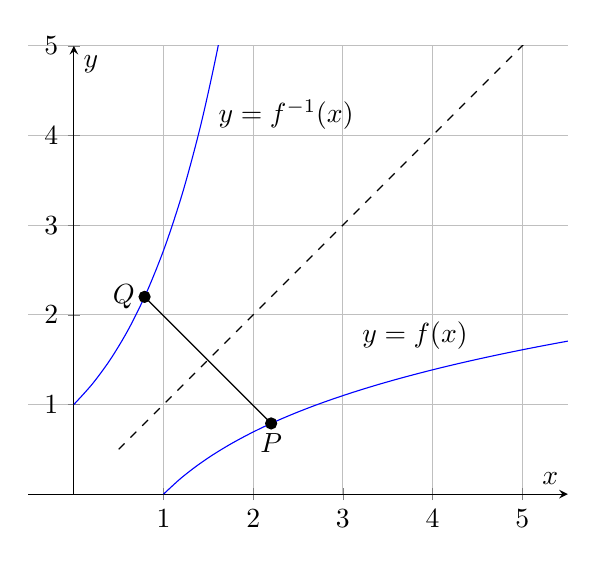
\begin{tikzpicture}
		\begin{axis}[
			xmin=0,xmax=5,
			ymin=0,ymax=5,
			restrict y to domain=0:10,
			grid=both,
			axis equal=true,
			axis lines=middle,
			xlabel=$x$,
			ylabel=$y$,
		]
			\begin{scope}[color=blue,samples=50,smooth]
				\addplot[domain=0:10]{exp(x)};
				\addplot[domain=1:10]{ln(x)};
			\end{scope}
			\addplot[color=black,dashed,domain=.5:8]{x};
			\filldraw(2.2,{ln(2.2)})circle(2pt)node[below]{$P$}
				--({ln(2.2)},2.2)circle(2pt)node[left]{$Q$};
			\draw(4.5,{ln(4.5)})node[above left]{$y=f(x)$}
				({ln(4.5)},4.5)node[below right]{$y=f^{-1}(x)$};
		\end{axis}
	\end{tikzpicture}
	\caption{}\label{figure:函数.直接函数与反函数的图形的对称性}
\end{figure}

\subsection{复合函数}
\begin{definition}
设函数\(y=f(u)\)的定义域为\(D_f\),
函数\(u=g(x)\)的定义域为\(D_g\),
且其值域\(R_g \subseteq D_f\),
则函数\begin{equation*}
	y = f[g(x)],
	\quad x \in D_g
\end{equation*}
称为由函数\(u=g(x)\)与函数\(y=f(u)\)构成的\DefineConcept{复合函数},
它的定义域为\(D_g\),变量\(u\)称为\DefineConcept{中间变量}.

函数\(g\)与函数\(f\)构成的复合函数,
即按“先\(g\)后\(f\)”的次序复合的函数,
通常记为\(f \circ g\),即\begin{equation*}
	(f \circ g)(x) = f[g(x)].
\end{equation*}
\end{definition}

\begin{proposition}
设\(f\)和\(g\)都是奇函数,
则\(f \circ g\)也是奇函数.
\begin{proof}
这是因为\(f[g(-x)]
= f[-g(x)]
= -f[g(x)]\).
\end{proof}
\end{proposition}

\begin{proposition}
设\(f\)和\(g\)都是偶函数,
则\(f \circ g\)也是偶函数.
\begin{proof}
这是因为\(f[g(-x)]
= f[g(x)]\).
\end{proof}
\end{proposition}

\begin{proposition}
设\(f\)是奇函数,\(g\)是偶函数,
则\(f \circ g\)和\(g \circ f\)都是偶函数.
\begin{proof}
这是因为\(f[g(-x)]
= f[g(x)]\),
\(g[f(-x)]
= g[-f(x)]
= g[f(x)]\).
\end{proof}
\end{proposition}

\begin{proposition}
设\(f\)和\(g\)是严格单调增加函数,
则\(f \circ g\)是严格单调增加函数.
\begin{proof}
对于\(\forall x_1,x_2 \in \dom(f \circ g)\),
当\(x_1 < x_2\)时,
有\(g(x_1) < g(x_2)\),
从而有\(f[g(x_1)] < f[g(x_2)]\),
这就说明\(f \circ g\)是严格单调增加函数.
\end{proof}
\end{proposition}

\begin{proposition}\label{theorem:函数.两个严格单调减少函数的复合严格单调增加}
设\(f\)和\(g\)是严格单调减少函数,
则\(f \circ g\)是严格单调增加函数.
\begin{proof}
对于\(\forall x_1,x_2 \in \dom(f \circ g)\),
当\(x_1 < x_2\)时,
有\(g(x_1) > g(x_2)\),
从而有\(f[g(x_1)] < f[g(x_2)]\),
这就说明\(f \circ g\)是严格单调增加函数.
\end{proof}
\end{proposition}

\begin{proposition}
设\(f\)是严格单调增加函数,
\(g\)是严格单调减少函数,
则\(f \circ g\)和\(g \circ f\)都是严格单调减少函数.
\begin{proof}
对于\(\forall x_1,x_2 \in \dom(f \circ g)\),
当\(x_1 < x_2\)时,
有\(g(x_1) > g(x_2)\),
从而有\(f[g(x_1)] > f[g(x_2)]\),
这就说明\(f \circ g\)是严格单调减少函数.
同理可证\(g \circ f\)也是严格单调减少函数.
\end{proof}
\end{proposition}

\section{绝对值函数}
\begin{definition}[绝对值]
设\(x \in \mathbb{R}\),则称函数\begin{equation*}
	f(x) = \left\{ \begin{array}{c}
		x, \quad x \geq 0 \\
		-x, \quad x < 0
	\end{array} \right.
\end{equation*}为\(x\)的绝对值,
记作\(\abs{x}\).
\end{definition}

\begin{figure}[htb]
	\centering
	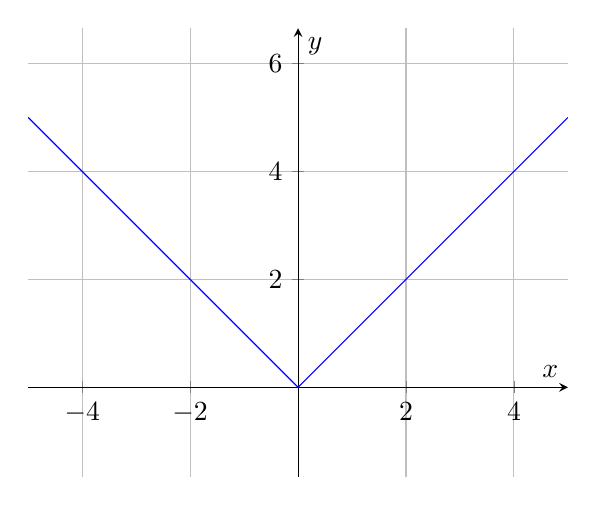
\begin{tikzpicture}
		\begin{axis}[
			xmin=-5,xmax=5,
			ymin=0,ymax=5,
			grid=both,
			axis lines=middle,
			xlabel=$x$,
			ylabel=$y$,
			axis equal=true,
		]
			\addplot[color=blue,samples at={-5,0,5}]{abs(x)};
		\end{axis}
	\end{tikzpicture}
	\caption{绝对值函数\(\abs{x}\)的图形}
\end{figure}

\begin{proposition}
设\(a,b\in\mathbb{R}\),
则\begin{itemize}
	\item \(\abs{a}\geq0\),
	\item \(\abs{a} = \abs{-a}\),
	\item \(\abs{ab} = \abs{a} \abs{b}\),
	\item \(\abs{\frac{a}{b}} = \frac{\abs{a}}{\abs{b}}\ (b\neq0)\),
	\item \(\abs{a}^2 = \abs{a^2}\).
\end{itemize}
\begin{proof}
当\(a=0\)或\(b=0\)时,易见\(\abs{ab} = 0 = \abs{a} \abs{b}\).
当\(a\neq0\)且\(b\neq0\)时,
按照\(a\)和\(b\)的不同取值,列表如下:
\begin{center}
	\begin{tblr}{|*2c|*2{c|}}
		\hline
		&& \(b>0\) & \(b<0\) \\
		&& \(\abs{b}=b\) & \(\abs{b}=-b\) \\ \hline
		\(a>0\) & \(\abs{a}=a\) & \(ab>0,\abs{ab}=ab\) & \(ab<0,\abs{ab}=-ab\) \\ \hline
		\(a<0\) & \(\abs{a}=-a\) & \(ab<0,\abs{ab}=-ab\) & \(ab>0,\abs{ab}=ab\) \\ \hline
	\end{tblr}
\end{center}
由此可知\(\abs{ab} = \abs{a} \abs{b}\)恒成立.
\end{proof}
\end{proposition}

\begin{proposition}
设\(a\)和\(b\)都是实数,
则\begin{gather}
	\min\{a,b\}
	= \frac{a+b}{2}
	- \frac{\abs{a-b}}{2}, \\
	\max\{a,b\}
	= \frac{a+b}{2}
	+ \frac{\abs{a-b}}{2}.
\end{gather}
\begin{proof}
当\(a>b\)时,有\begin{equation*}
	\frac{a+b}{2} - \frac{\abs{a-b}}{2}
	= \frac{a+b}{2} - \frac{a-b}{2}
	= \frac{2b}{2} = b
	= \min\{a,b\},
\end{equation*}\begin{equation*}
	\frac{a+b}{2} + \frac{\abs{a-b}}{2}
	= \frac{a+b}{2} + \frac{a-b}{2}
	= \frac{2a}{2} = a
	= \max\{a,b\}.
\end{equation*}
当\(a \leq b\)时,有\begin{equation*}
	\frac{a+b}{2} - \frac{\abs{a-b}}{2}
	= \frac{a+b}{2} - \frac{b-a}{2}
	= \frac{2a}{2} = a
	= \min\{a,b\},
\end{equation*}\begin{equation*}
	\frac{a+b}{2} + \frac{\abs{a-b}}{2}
	= \frac{a+b}{2} + \frac{b-a}{2}
	= \frac{2b}{2} = b
	= \max\{a,b\}.
	\qedhere
\end{equation*}
\end{proof}
\end{proposition}

\section{符号函数}
\begin{definition}[符号函数]
函数\begin{equation*}
	f(x) = \left\{ \begin{array}{cc}
		1, & x > 0 \\
		0, & x = 0 \\
		-1, & x < 0 \\
	\end{array} \right.
\end{equation*}称为\DefineConcept{符号函数},
记作\(\sgn x\).
\end{definition}

\begin{figure}[htb]
	\centering
	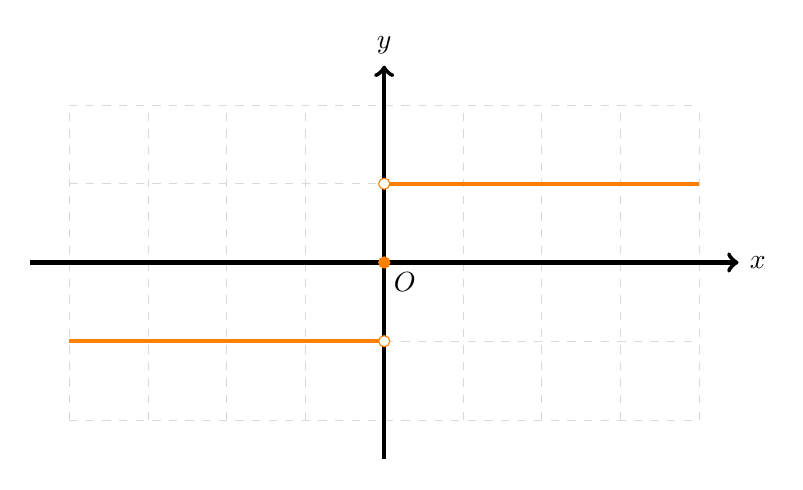
\begin{tikzpicture}
		\draw[help lines, color=gray!30, dashed] (-4,-2) grid (4,2);
		\draw[->, ultra thick] (-4.5,0) -- (4.5,0) node[right]{\(x\)};
		\draw[->, ultra thick] (0,-2.5) -- (0,2.5) node[above]{\(y\)};
		\draw (0,0)node[below right]{\(O\)};
		\draw[orange,ultra thick] (-4,-1)--(0,-1) (0,1)--(4,1);
		\draw[draw=orange,fill=orange] (0,0)circle(2pt);
		\draw[draw=orange,fill=white] (0,1)circle(2pt) (0,-1)circle(2pt);
	\end{tikzpicture}
	\caption{符号函数\(\sgn x\)的图形}
\end{figure}

\section{取整函数}
\begin{definition}[取整函数]
设\(x\in\mathbb{R},
n\in\mathbb{Z}\),
定义:\begin{enumerate}
	\item 如果\(n\)是不大于\(x\)的最大整数,
	即\(x\in[n,n+1)\),
	那么记\(\floor{x}=n\)\footnote{有的书把不大于\(x\)的最大整数
	称为“\(x\)的\DefineConcept{整数部分}”,记作\([x]\);
	把\(x\)与其整数部分之差\(x - [x]\)
	称为“\(x\)的\DefineConcept{小数部分}”,记作\(\{x\}\).}.
	我们把函数\(y=\floor{x}\)称为\DefineConcept{向下取整函数},
	即\begin{equation}
		\floor{x}
		\defeq
		\max\Set{ n\in\mathbb{Z} \given n \leq x }.
	\end{equation}

	\item 如果\(n\)是不小于\(x\)的最小整数,
	即\(x\in(n-1,n]\),
	那么记\(\ceil{x}=n\).
	我们把函数\(y=\ceil{x}\)称为\DefineConcept{向上取整函数},
	即\begin{equation}
		\ceil{x}
		\defeq
		\min\Set{ n\in\mathbb{Z} \given n \geq x }.
	\end{equation}
\end{enumerate}
\end{definition}

\begin{figure}[htb]
	\tikzstyle{sx}=[draw=orange,fill=orange]
	\tikzstyle{kx}=[draw=orange,fill=white]
	\def\subwidth{.45\linewidth}
	\def\subscale{.9}
	\begin{subfigure}[b]{\subwidth}%
		\centering
		\begin{tikzpicture}[scale=\subscale]
			\draw[help lines, color=gray!30, dashed] (-1,-1) grid (4,4);
			\draw[dashed, color=gray] (-1,-1) -- (4,4);
			\draw[->, thick] (-1.5,0) -- (4.5,0) node[right]{\(x\)};
			\draw[->, thick] (0,-1.5) -- (0,4.5) node[above]{\(y\)};
			\foreach \i in {-1,...,3} {
				\draw[ultra thick,orange] (\i,\i)--(\i+1,\i);
				\fill[sx] (\i,\i)circle(2pt);
				\fill[kx] (\i+1,\i)circle(2pt);
				\ifnum\i=0\relax\else
					\draw(\i,0)node[below right]{\i};
					\draw(0,\i)node[above right]{\i};
				\fi
			}
			\draw (0,0)node[above left]{\(O\)};
		\end{tikzpicture}
		\subcaption{向下取整函数\(\floor{x}\)}
	\end{subfigure}
	\begin{subfigure}[b]{\subwidth}%
		\centering
		\begin{tikzpicture}[scale=\subscale]
			\draw[help lines, color=gray!30, dashed] (-1,-1) grid (4,4);
			\draw[dashed, color=gray] (-1,-1) -- (4,4);
			\draw[->, thick] (-1.5,0) -- (4.5,0) node[right]{\(x\)};
			\draw[->, thick] (0,-1.5) -- (0,4.5) node[above]{\(y\)};
			\foreach \i in {-1,...,3} {
				\draw[ultra thick,orange] (\i,\i+1)--(\i+1,\i+1);
				\fill[kx] (\i,\i+1)circle(2pt);
				\fill[sx] (\i+1,\i+1)circle(2pt);
				\ifnum\i=0\relax\else
					\draw(\i,0)node[below right]{\i};
					\draw(0,\i)node[above right]{\i};
				\fi
			}
			\draw (0,0)node[above left]{\(O\)};
		\end{tikzpicture}
		\subcaption{向上取整函数\(\ceil{x}\)}
	\end{subfigure}
	\caption{取整函数的图形}
	\label{figure:取整函数.取整函数的图形}
\end{figure}

\begin{figure}
	\tikzstyle{sx}=[draw=orange,fill=orange]
	\tikzstyle{kx}=[draw=orange,fill=white]
	\def\subwidth{.45\linewidth}
	\def\subscale{.9}
	%@Mathematica: Plot[x - Floor[x], {x, -1, 4}]
	%@Mathematica: Table[{x, x - Floor[x]}, {x, -1, 4, .2}] // TableForm
	\begin{subfigure}[b]{\subwidth}%
		\centering
		\begin{tikzpicture}[scale=\subscale]
			\begin{axis}[
				xmin=-1,xmax=4,
				ymin=-1,ymax=1,
				restrict y to domain=-1:1,
				axis lines=middle,
				axis equal=true,
				xlabel=$x$,
				ylabel=$y$,
				enlarge x limits=0.1,
				enlarge y limits=0.1,
				x label style={at={(ticklabel* cs:1.00)}, inner sep=5pt, anchor=south},
				y label style={at={(ticklabel* cs:1.00)}, inner sep=2pt, anchor=west},
				ytick={-1,1},
			]
				\foreach \i in {-1,...,3} {
					\addplot[color=orange,samples=2,domain={\i}:{\i+1}]{x-\i};
				}
				\fill[kx](-1,1)circle(2pt);
				\fill[kx](0,1)circle(2pt);
				\fill[kx](1,1)circle(2pt);
				\fill[kx](2,1)circle(2pt);
				\fill[kx](3,1)circle(2pt);
				\fill[kx](4,1)circle(2pt);
				\fill[sx](-1,0)circle(2pt);
				\fill[sx](0,0)circle(2pt);
				\fill[sx](1,0)circle(2pt);
				\fill[sx](2,0)circle(2pt);
				\fill[sx](3,0)circle(2pt);
				\fill[sx](4,0)circle(2pt);
			\end{axis}
		\end{tikzpicture}
		\subcaption{函数\(f(x)=x-\floor{x}\)}
	\end{subfigure}
	%@Mathematica: Plot[Ceiling[x] - x, {x, -1, 4}]
	%@Mathematica: Table[{x, Ceiling[x] - x}, {x, -1, 4, .2}] // TableForm
	\begin{subfigure}[b]{\subwidth}%
		\centering
		\begin{tikzpicture}[scale=\subscale]
			\begin{axis}[
				xmin=-1,xmax=4,
				ymin=-1,ymax=1,
				axis lines=middle,
				axis equal=true,
				xlabel=$x$,
				ylabel=$y$,
				enlarge x limits=0.1,
				enlarge y limits=0.1,
				x label style={at={(ticklabel* cs:1.00)}, inner sep=5pt, anchor=south},
				y label style={at={(ticklabel* cs:1.00)}, inner sep=2pt, anchor=west},
				ytick={-1,1},
			]
				\foreach \i in {-1,...,3} {
					\addplot[color=orange,samples=2,domain={\i}:{\i+1}]{\i+1-x};
				}
				\fill[kx](-1,1)circle(2pt);
				\fill[kx](0,1)circle(2pt);
				\fill[kx](1,1)circle(2pt);
				\fill[kx](2,1)circle(2pt);
				\fill[kx](3,1)circle(2pt);
				\fill[kx](4,1)circle(2pt);
				\fill[sx](-1,0)circle(2pt);
				\fill[sx](0,0)circle(2pt);
				\fill[sx](1,0)circle(2pt);
				\fill[sx](2,0)circle(2pt);
				\fill[sx](3,0)circle(2pt);
				\fill[sx](4,0)circle(2pt);
			\end{axis}
		\end{tikzpicture}
		\subcaption{函数\(f(x)=\ceil{x}-x\)}
	\end{subfigure}
	\caption{}
\end{figure}

\begin{property}\label{theorem:取整函数.性质1}
%@see: 《算法导论(原书第3版)》 P31 (3.3)
%@see: 《具体数学 计算机科学基础(第2版)》 P57 (3.3)
一般地,对于\(x\in\mathbb{R}\),总有\begin{equation}
	x - 1 < \floor{x} \leq x \leq \ceil{x} < x + 1.
\end{equation}
当且仅当\(x\)是整数时,
成立\(x = \ceil{x} = \floor{x}\).
%TODO proof
\end{property}

\begin{property}
%@see: 《具体数学 计算机科学基础(第2版)》 P57 (3.4)
设\(x\)是实数,则\begin{gather}
	\floor{-x} = -\ceil{x},
	\label{equation:取整函数.取整函数的对称性1} \\
	\ceil{-x} = -\floor{x}.
	\label{equation:取整函数.取整函数的对称性2}
\end{gather}
%TODO proof
\end{property}
\begin{remark}
从\cref{figure:取整函数.取整函数的图形} 可以看出:
函数\(\ceil{x}\)与\(\floor{x}\)的图形关于坐标原点\(O\)中心对称.
\end{remark}

\begin{property}
%@see: 《具体数学 计算机科学基础(第2版)》 P57 (3.5)
设\(x\)是实数,\(n\)是整数,则\begin{gather}
	\floor{x} = n
	\iff
	n \leq x < n+1
	\iff
	x-1 < n \leq x,
	\label{equation:取整函数.序关系1} \\
	\ceil{x} = n
	\iff
	n-1 < x \leq n
	\iff
	x \leq n < x+1.
	\label{equation:取整函数.序关系2}
\end{gather}
%TODO proof
\end{property}

\begin{example}
设\(x,y\)都是实数.
举例说明:\(\ceil{x} + \ceil{y} \neq \ceil{x+y},
\floor{x} + \floor{y} \neq \floor{x+y}\).
\begin{solution}
%@credit: {6d916ea6-1441-4c5b-9e97-4f834b319710} 说:都取0.5
取\(x = y = \frac12\).
那么\(\ceil{x} = \ceil{y} = \ceil{x+y} = 1\),
但是\(\ceil{x} + \ceil{y} = 2 \neq \ceil{x+y}\).

与此同时,\(\floor{x} = \floor{y} = 0,
\floor{x+y} = 1\),
因此\(\floor{x} + \floor{y} \neq \floor{x+y}\).
\end{solution}
\end{example}
\begin{example}
设\(x,y\)都是实数.
举例说明:\(\ceil{xy} \neq x\ceil{y},
\floor{xy} \neq x\floor{y}\).
\begin{solution}
取\(x=2,y=\frac12\).
那么\(\ceil{xy} = 1 \neq x\ceil{y} = 2,
\floor{xy} = 1 \neq x\ceil{y} = 0\).
\end{solution}
\end{example}

\begin{proposition}
%@see: 《具体数学 计算机科学基础(第2版)》 P58 (3.6)
设\(n\)是整数,\(x\)是实数,则\begin{gather}
	\ceil{n+x} = n + \ceil{x},
	\label{equation:取整函数.取整函数的周期性1} \\
	\floor{n+x} = n + \floor{x}.
	\label{equation:取整函数.取整函数的周期性2}
\end{gather}
%TODO proof
% \begin{proof}
% % 因为\begin{align*}
% % 	\floor{x} = n
% % 	\iff
% % 	n \leq x < n+1
% % 	\iff
% % 	\floor{x}+n \leq x+n < \floor{x}+n+1
% % 	\iff
% % 	\floor{x+n} = \floor{x}+n.
% % \end{align*}
% 由定义可知\begin{align*}
% 	\floor{n+x}
% 	&= \max\Set{ m\in\mathbb{Z} \given m \leq n+x } \\
% 	&= \max\Set{ m\in\mathbb{Z} \given m-n \leq x } \\
% 	&= \max\Set{ m\in\mathbb{Z} \given k=m-n, k \leq x } \\
% 	&= \max\Set{ m\in\mathbb{Z} \given m=n+k, k \leq x } \\
% 	%TODO 这里其实还没有说清楚
% 	&= n + \max\Set{ k\in\mathbb{Z} \given k \leq x } \\
% 	&= n + \floor{x}.
% \end{align*}
% 同理可知\(\ceil{n+x} = n + \ceil{x}\).
% \end{proof}
\end{proposition}

\begin{property}
%@see: 《具体数学 计算机科学基础(第2版)》 P58 (3.7)
设\(x\)是实数,\(n\)是整数,则\begin{gather}
	x < n \iff \floor{x} < n,
	\label{equation:取整函数.序关系3} \\
	n < x \iff n < \ceil{x},
	\label{equation:取整函数.序关系4} \\
	x \leq n \iff \ceil{x} \leq n,
	\label{equation:取整函数.序关系5} \\
	n \leq x \iff n \leq \floor{x}.
	\label{equation:取整函数.序关系6}
\end{gather}
%TODO proof
\begin{proof}
% 证明\(x < n \iff \floor{x} < n\):
证明\cref{equation:取整函数.序关系3}:
当\(x < n\)时,
%\cref{theorem:取整函数.性质1}
由\(\floor{x} \leq x\)
可得\(\floor{x} < n\).
当\(\floor{x} < n\)时,
%\cref{equation:取整函数.序关系1}
由\(x < \floor{x} + 1\)
%@credit: {57e837df-6d92-457b-a5f0-e915ab36f532},{5f4d2f8a-fc8b-4798-85d6-98670f6761e7} 说:
% \(\floor{x}\)作为一个整数,小于另一个整数\(n\),那么必有\(\floor{x} + 1 \leq n\)
和\(\floor{x} + 1 \leq n\)
可得\(x < n\).

% 证明\(n < x \iff n < \ceil{x}\):
证明\cref{equation:取整函数.序关系4}:
当\(n < x\)时,
%\cref{theorem:取整函数.性质1}
由\(x \leq \ceil{x}\)
可得\(n < \ceil{x}\).
当\(n < \ceil{x}\)时,
% \(\ceil{x}\)作为一个整数,大于另一个整数\(n\),那么必有\(n + 1 \leq \ceil{x}\)
由\(n \leq \ceil{x} - 1\)
%\cref{equation:取整函数.序关系2}
和\(\ceil{x} - 1 < x\)
可得\(n < x\).

\cref{equation:取整函数.序关系5} 是\cref{equation:取整函数.序关系4} 的逆否命题.
\cref{equation:取整函数.序关系6} 是\cref{equation:取整函数.序关系3} 的逆否命题.
\end{proof}
\end{property}

\begin{proposition}
%@see: 《具体数学 计算机科学基础(第2版)》 P59
设\(x\)是实数,则\begin{gather*}
	\ceil{\floor{x}} = \floor{x}, \\
	\floor{\floor{x}} = \floor{x}, \\
	\ceil{\ceil{x}} = \ceil{x}, \\
	\floor{\ceil{x}} = \ceil{x}.
\end{gather*}
\begin{proof}
因为\(\floor{x},\ceil{x}\)都是整数,
所以由\cref{theorem:取整函数.性质1} 可知,
对它们两个而言,不论向上取整还是向下取整,都不会发生变化.
\end{proof}
\end{proposition}

\begin{example}\label{example:取整函数.根式函数与取整函数的复合}
%@see: 《具体数学 计算机科学基础(第2版)》 P59 (3.9)
设\(x\)是非负实数.
证明:\begin{gather}
	\floor{\sqrt{\floor{x}}} = \floor{\sqrt{x}}, \\
	\ceil{\sqrt{\ceil{x}}} = \ceil{\sqrt{x}}.
\end{gather}
\begin{proof}
设\(m = \floor{\sqrt{\floor{x}}}\).
由\cref{equation:取整函数.序关系1}
可知\(m \leq \sqrt{\floor{x}} < m+1\).
因为\(m \geq 0\),
%@credit: {3b700f59-6290-449f-8174-9204a938f47c} 帮忙发现了一个 typo
所以\begin{equation*}
	m^2 \leq \floor{x} < (m+1)^2.
\end{equation*}
由\cref{equation:取整函数.序关系6}
可知\(m^2 \leq x\);
由\cref{equation:取整函数.序关系3}
可知\(x < (m+1)^2\);
因此\(m^2 \leq x < (m+1)^2\),
从而有\(m \leq \sqrt{x} < m+1\),
即\(m = \floor{\sqrt{x}}\).
总之,我们有\(\floor{\sqrt{\floor{x}}} = \floor{\sqrt{x}}\).
同理可证\(\ceil{\sqrt{\ceil{x}}} = \ceil{\sqrt{x}}\).
\end{proof}
\end{example}
接下来对\cref{example:取整函数.根式函数与取整函数的复合} 的结论进行推广.
\begin{example}\label{example:取整函数.单调增加函数与取整函数的复合}
%@see: 《具体数学 计算机科学基础(第2版)》 P60 (3.10)
对于任意一个在实数区间内连续的单调增加函数\(f\),
只要它满足\begin{equation*}
	(\forall x)[f(x) \in \mathbb{Z} \implies x \in \mathbb{Z}],
\end{equation*}
那么当\(f(x),f(\floor{x}),f(\ceil{x})\)三者均有定义时,
成立\(\floor{f(x)} = \floor{f(\floor{x})}\)
和\(\ceil{f(x)} = \ceil{f(\ceil{x})}\).
\begin{proof}
当\(x = \ceil{x}\)时,显然成立\(\ceil{f(x)} = \ceil{f(\ceil{x})}\).

当\(x \neq \ceil{x}\)时,
必然成立\(x < \ceil{x}\).
因为函数\(f\)是单调增加的,
所以\(f(x) < f(\ceil{x})\).
因为函数\(x \mapsto \ceil{x}\)单调不减,
所以\(\ceil{f(x)} \leq \ceil{f(\ceil{x})}\).

接下来用反证法,
假设\(\ceil{f(x)} < \ceil{f(\ceil{x})}\).
\begin{figure}
	\tikzstyle{sx}=[draw=orange,fill=orange]
	\tikzstyle{kx}=[draw=orange,fill=white]
	\centering
	\begin{tikzpicture}
		\draw[help lines, color=gray!30, dashed] (0,0) grid (4,4);
		\draw[dashed, color=gray] (0,0) -- (4,4);
		\draw[->, thick] (-.5,0) -- (4.5,0);
		\draw[->, thick] (0,-.5) -- (0,4.5);

		\draw[blue,dashed] (0,2)--(1,2) (0,3)--(2,3);
		\draw[blue,dashed] (1.2,2)--(1.2,0)node[black,below]{\small$f(x)$}
					(2,2)--(2,0)node[black,below]{\small$f(y)$}
					(2.7,3)--(2.7,0)++(8pt,0)node[black,below]{\small$f(\ceil{x})$};
		\draw (0,2)node[left]{\small$\ceil{f(x)}$}
			(0,3)node[left]{\small$\ceil{f(\ceil{x})}$};

		\foreach \i in {0,...,3} {
			\draw[ultra thick,orange] (\i,\i+1)--(\i+1,\i+1);
			\fill[kx] (\i,\i+1)circle(2pt);
			\fill[sx] (\i+1,\i+1)circle(2pt);
		}
		\draw (0,0)node[above left]{\(O\)};
	\end{tikzpicture}
	\caption{}
	\label{figure-example:取整函数.单调增加函数与取整函数的复合}
\end{figure}
由于\(f\)是连续的单调增加函数,
如\cref{figure-example:取整函数.单调增加函数与取整函数的复合} 所示,
那么必定存在实数\(y\)
满足\(x \leq y < \ceil{x}\),
并使得\(f(y) = \ceil{f(x)}\).
因为\(\ceil{f(x)}\)是一个整数,
那么由前提条件\((\forall x)[f(x) \in \mathbb{Z} \implies x \in \mathbb{Z}]\)
可知\(y\)只能是整数.
然而不可能有一个整数严格位于\(\floor{x}\)与\(\ceil{x}\)之间.
这个矛盾说明\(\ceil{f(x)} = \ceil{f(\ceil{x})}\)必定成立.

同理可证\(\floor{f(x)} = \floor{f(\floor{x})}\).
\end{proof}
\end{example}
\begin{example}
%@see: 《具体数学 计算机科学基础(第2版)》 P60 (3.11)
设\(x\)是实数,\(m,n\)都是整数,且\(n>0\),
则\begin{gather}
	\floor*{\frac{x+m}{n}} = \floor*{\frac{\floor{x}+m}{n}}, \\
	\ceil*{\frac{x+m}{n}} = \ceil*{\frac{\ceil{x}+m}{n}}.
\end{gather}
\begin{proof}
令\(f(x) = \frac{x+m}{n}\),
由\cref{example:取整函数.单调增加函数与取整函数的复合} 可得.
\end{proof}
\end{example}
\begin{example}
%@see: 《具体数学 计算机科学基础(第2版)》 P60
设\(x\)是非负实数.
举例说明:\(\ceil{\sqrt{\floor{x}}} \neq \ceil{\sqrt{x}}\).
\begin{solution}
取\(x = \frac{1+\sqrt5}2\).
%@Mathematica: Ceiling[Sqrt[Floor[x]]] /. x -> GoldenRatio
%@Mathematica: Ceiling[Sqrt[x]] /. x -> GoldenRatio
那么\(\ceil{\sqrt{\floor{x}}} = 1 \neq \ceil{\sqrt{x}} = 2\).
\end{solution}
\end{example}
\begin{example}
%@see: 《具体数学 计算机科学基础(第2版)》 P61
设\(x\)是非负实数.
证明:\(\ceil{\sqrt{\floor{x}}} = \ceil{\sqrt{x}}\)
当且仅当\(x\)是整数,或\(\sqrt{\floor{x}}\)是整数.
%TODO proof
\end{example}
\begin{example}
%@see: 《具体数学 计算机科学基础(第2版)》 P61
设\(a,b\)都是整数.
记\(\card_X Y \defeq \card\Set{ x \in X \given x \in Y }\).
证明:\begin{equation*}
	\card_\mathbb{Z} [a,b)
	= \card_\mathbb{Z} (a,b]
	= b-a.
\end{equation*}
%TODO proof
\end{example}
\begin{example}
%@see: 《具体数学 计算机科学基础(第2版)》 P61
设\(a,b\)都是实数.
证明:\begin{gather*}
	\card_\mathbb{Z} [a,b)
	= \ceil{b} - \ceil{a}, \\
	\card_\mathbb{Z} (a,b]
	= \floor{b} - \floor{a}, \\
	\card_\mathbb{Z} [a,b]
	= \floor{b} - \ceil{a} + 1, \\
	\card_\mathbb{Z} (a,b)
	= \ceil{b} - \floor{a} - 1.
\end{gather*}
%TODO proof
\begin{proof}
由\cref{equation:取整函数.序关系6} 可知,
对于任意整数\(n\)和任意实数\(\alpha,\beta\),
有\begin{gather*}
	\alpha \leq n < \beta
	\iff
	\ceil{\alpha} \leq n < \ceil{\beta}, \\
	\alpha < n \leq \beta
	\iff
	\ceil{\alpha} < n \leq \ceil{\beta}.
\end{gather*}
\let\qed\relax
\end{proof}
\end{example}
\begin{definition}
设\(x\)是实数.
把序列\begin{equation*}
	\floor{x},
	\floor{2x},
	\floor{3x},
	\dotsc,
\end{equation*}
称为“\(x\)的\DefineConcept{谱}(Spectrum)”,
%@see: https://mathworld.wolfram.com/SpectrumSequence.html
记作\(\operatorname{Spec} x\).
\end{definition}
\begin{proposition}
任意两个实数的谱不相同.
\end{proposition}

\begin{property}
%@see: 《算法导论(原书第3版)》 P31
对于\(n\in\mathbb{Z}\),总有\begin{equation}
	\ceil{n/2} + \floor{n/2} = n.
\end{equation}
\begin{proof}
%@credit: {8b6edada-f2fd-4ae5-9020-eb533149a54c} 说可以分为n是偶数或n是奇数两种情况讨论
当\(n\)是偶数时,
存在整数\(k\)使得\(n=2k\),
那么\begin{equation*}
	\ceil{n/2} = \floor{n/2} = k,
\end{equation*}
于是\(\ceil{n/2} + \floor{n/2} = 2k = n\).

当\(n\)是奇数时,
存在整数\(k\)使得\(n=2k+1\),
即有\(n/2 = k + 1/2\),
那么\begin{equation*}
	\ceil{n/2} = k+1,
	\qquad
	\floor{n/2} = k,
\end{equation*}
于是\(\ceil{n/2} + \floor{n/2} = 2k+1 = n\).
\end{proof}
\end{property}

\begin{property}
%@see: 《算法导论(原书第3版)》 P31 (3.4)
%@see: 《算法导论(原书第3版)》 P31 (3.5)
%@see: 《算法导论(原书第3版)》 P31 (3.6)
%@see: 《算法导论(原书第3版)》 P31 (3.7)
对于任意实数\(x \geq 0\)和整数\(a,b>0\),总有\begin{gather}
	\ceil*{\frac{\ceil{x/a}}{b}} = \ceil*{\frac{x}{ab}}, \\
	\floor*{\frac{\floor{x/a}}{b}} = \floor*{\frac{x}{ab}}, \\
	\ceil*{\frac{a}{b}} \leq \frac{a+(b-1)}{b}, \\
	\floor*{\frac{a}{b}} \geq \frac{a-(b-1)}{b}.
\end{gather}
%TODO proof
\end{property}

\begin{example}
证明:对于任意整数\(n\),
总有\(\ceil*{\frac{n}2\vphantom{\frac12}} = \floor*{\frac{n+1}2}\).
%TODO proof
\end{example}
\begin{example}
证明:对于任意整数\(n,m\),
总有\(\ceil*{\frac{n}{m}\vphantom{\frac12}} = \floor*{\frac{n+m-1}{m}}\).
%TODO proof
\end{example}

\begin{definition}
%@see: 《具体数学 计算机科学基础(第2版)》 P68
设\(x,y\)都是实数,且\(y\neq0\).
把\(\floor{x/y}\)称为“\(y\)除\(x\)的\DefineConcept{商}”.
把\(x - y \floor{x/y}\)称为“\(y\)除\(x\)的\DefineConcept{余数}”,
记作\(x \mod y\),
即\begin{equation*}
%@see: 《具体数学 计算机科学基础(第2版)》 P68 (3.21)
	x \mod y
	\defeq
	x - y \floor{x/y}.
\end{equation*}
%@see: 《具体数学 计算机科学基础(第2版)》 P69 (3.22)
规定:\(x \mod 0 = x\).
\end{definition}

我们可以直观地理解\(x \mod y\)的意义:
当\(x\)和\(y\)都是正实数时,
想象一个周长为\(y\)的圆,
圆上任意一点可以表示为区间\([0,y)\)中的实数.
如果我们从\(0\)出发,绕着圆行走距离\(x\),
那么我们在路上遇到\(0\)的次数是\(\floor{x/y}\),
最终我们会停止在\(x \mod y\).

\begin{example}
容易看出:\begin{gather*}
	5\mod3
	= 5-3\floor{5/3}
	= 2, \\
	5\mod(-3)
	= 5-(-3)\floor{5/(-3)}
	= -1, \\
	(-5)\mod3
	= (-5)-3\floor{(-5)/3}
	= 1, \\
	(-5)\mod(-3)
	= (-5)-(-3)\floor{(-5)/(-3)}
	= -2.
\end{gather*}
%@Mathematica: Mod[5, 3]
%@Mathematica: Mod[5, -3]
%@Mathematica: Mod[-5, 3]
%@Mathematica: Mod[-5, -3]
\end{example}

\begin{property}
%@see: 《具体数学 计算机科学基础(第2版)》 P69
设\(x,y\)都是实数,且\(y\neq0\).
\begin{itemize}
	\item 当\(y>0\)时,\(0 \leq x \mod y < y\).
	\item 当\(y<0\)时,\(y < x \mod y \leq 0\).
\end{itemize}
\end{property}

\begin{property}
%@see: 《具体数学 计算机科学基础(第2版)》 P69 (3.23)
设\(x,y,c\)都是实数,且\(y\neq0,c\neq0\),
则\begin{equation}
	c (x \mod y)
	= (c x) \mod (c y).
\end{equation}
\begin{proof}
直接计算得\begin{equation*}
	c (x \mod y)
	= c (x - y \floor{x / y})
	= c x - cy \floor{cx / cy}
	= (c x) \mod (c y).
	\qedhere
\end{equation*}
\end{proof}
\end{property}

\begin{theorem}
%@see: 《具体数学 计算机科学基础(第2版)》 P71 (3.24)
%@see: 《具体数学 计算机科学基础(第2版)》 P71 (3.25)
设\(m,n\)都是整数,且\(m\neq0\),
则\begin{gather}
	n = \ceil*{\frac{n\vphantom{1}}{m}}
	+ \ceil*{\frac{n-1}{m}}
	+ \dotsb
	+ \ceil*{\frac{n-m+1}{m}}, \\
	n = \floor*{\frac{n\vphantom{1}}{m}}
	+ \floor*{\frac{n-1}{m}}
	+ \dotsb
	+ \floor*{\frac{n-m+1}{m}}.
\end{gather}
%TODO proof
%\cref{equation:取整函数.取整函数的对称性1}
%\cref{equation:取整函数.取整函数的对称性2}
\end{theorem}

\begin{proposition}
设\(x,y\)都是实数,且\(y\neq0\),
则\((x \pm y) \mod y = x \mod y\).
\begin{proof}
由定义可知\begin{align*}
	(x \pm y) \mod y
	&= (x \pm y) - y \floor*{\frac{x \pm y}{y}} \\
	&= (x \pm y) - y \floor*{\frac{x}{y} \pm 1} \\
	&= (x \pm y) - y (\floor{x/y} \pm 1)
		\tag{\cref{equation:取整函数.取整函数的周期性2}} \\
	&= x - y \floor{x/y}
	= x \mod y.
	\qedhere
\end{align*}
\end{proof}
\end{proposition}

\section{幂函数、指数函数、对数函数}
\begin{definition}
同一个数\(a\ (a\in\mathbb{R})\)连续相乘\(b\ (b\in\mathbb{N})\)次所得的乘积,
称作“\(a\)的\(b\)次方”
或“\(a\)的\(b\)次幂”,
记作\(a^b\),
即\begin{equation*}
	a^b
	\defeq
	\underbrace{a \times a \times \dotsm \times a}_{\text{$b$次}} = \prod_{i=1}^b a.
\end{equation*}

特别地,规定:\begin{gather*}
	a^0 \defeq 1 \quad(a\neq0), \\
	a^{-1} \defeq \frac1a \quad(a\neq0), \\
	a^{-n} \defeq \frac1{a^n} \quad(a\neq0), \\
	a^{1/n} \defeq \sqrt[n]{a} \quad(a\geq0). \\
\end{gather*}
\end{definition}

\begin{figure}[htb]
	\centering
	\begin{tikzpicture}
		\def\r{\textcolor{orange}}
		\def\b{\textcolor{blue}}
		\def\p{\textcolor{purple}}
		\draw(0,0)node{\(\r{a}^{\b{b}} = \p{c} \defiff \log_{\r{a}} \p{c} = \b{b}\)};
		\draw(-2.2,-.5)node{\r{底数}}
			(-2.2,.5)node{\b{指数}}
			(-1,-.5)node{\p{幂}}
			(.3,-.5)node{\r{底数}}
			(1.4,-.5)node{\p{真数}}
			(2.3,.5)node{\b{对数}};
		\draw[->](-1.7,-.3)--(-1.7,-1)--(.84,-1)->(.84,-.3); %a
		\draw[->](-1.55,.3)--(-1.55,1)--(1.7,1)->(1.7,.3); %b
		\draw[->](-.86,.3)--(-.86,.7)--(1.1,.7)->(1.1,.3); %c
	\end{tikzpicture}
	\caption{底数、指数、幂与对数的联系}\label{figure:函数.底数、指数、幂与对数的联系}
\end{figure}

\begin{proposition}
\(1\)的任意次幂还是\(1\),即\(1^n = 1\).
\end{proposition}

\begin{proposition}
\(0\)的任意非零次幂还是\(0\),即\(0^n = 0\ (n\neq0)\).
\end{proposition}

\subsection{幂函数的概念}
\begin{definition}[幂函数]
函数\(f(x)=x^{\mu}\ (\mu \in \mathbb{R})\),
称为\DefineConcept{幂函数}.
\end{definition}

\subsection{幂函数的性质}
\begin{property}
幂函数具有以下性质:
\begin{itemize}
	\item 当\(\mu = 0\)时,
	幂函数\(f(x)=x^{\mu}\)在定义域\((-\infty,+\infty)\)上恒为一,
	是常数函数.

	\item 当\(\mu\)为正奇数时,
	幂函数\(f(x)=x^{\mu}\)为奇函数,
	其定义域、值域均为\((-\infty,+\infty)\),它在定义域内恒单调递增.

	\item 当\(\mu\)为正偶数时,
	幂函数\(f(x)=x^{\mu}\)为偶函数,
	其定义域为\((-\infty,+\infty)\),其值域为\([0,+\infty)\),
	它在\((-\infty,0]\)上单调递减,在\([0,+\infty)\)上单调递增.

	\item 当\(\mu\)为负奇数时,
	幂级数\(y=x^{\mu}\)又称为\DefineConcept{比例函数},
	其定义域、值域为\((-\infty,0)\cup(0,+\infty)\),
	它在区间\((-\infty,0)\)和\((0,+\infty)\)内单调递减.

	若幂函数前有常系数大于零则称之为\DefineConcept{正比例函数}.
	%@Mathematica: Plot[Evaluate[x^-n /. n -> {1, 2, 3, 4, 5}], {x, 0, 2}, PlotRange -> {0, 2}, PlotLegends -> Automatic]

	若幂函数前有常系数小于零则称之为\DefineConcept{反比例函数}.
	%@Mathematica: Plot[Evaluate[x^-n /. n -> {1, 2, 3, 4, 5}], {x, -2, 0}, PlotRange -> {-2, 2}, PlotLegends -> Automatic]

	\item 当\(\mu\)为负偶数时,
	幂函数\(f(x)=x^{\mu}\)为偶函数,
	其定义域为\((-\infty,0)\cup(0,+\infty)\),其值域为\((0,+\infty)\),
	它在\((-\infty,0)\)内单调递增,在\((0,+\infty)\)内单调递减.

	\item 当\(\mu = \pm\frac{m}{n} \in \mathbb{Q}\)(\(m,n>0\)且\(m\)、\(n\)是互素的整数)时,
	幂函数\(f(x)=x^{\mu}=x^{\pm\frac{m}{n}}\)可改写为\(y=\sqrt[n]{x^m}\)(\(\mu>0\)时)
	或\(y=\frac{1}{\sqrt[n]{x^m}}\)(\(\mu<0\)时).
\end{itemize}
\end{property}

\begin{figure}[htb]
	\centering
	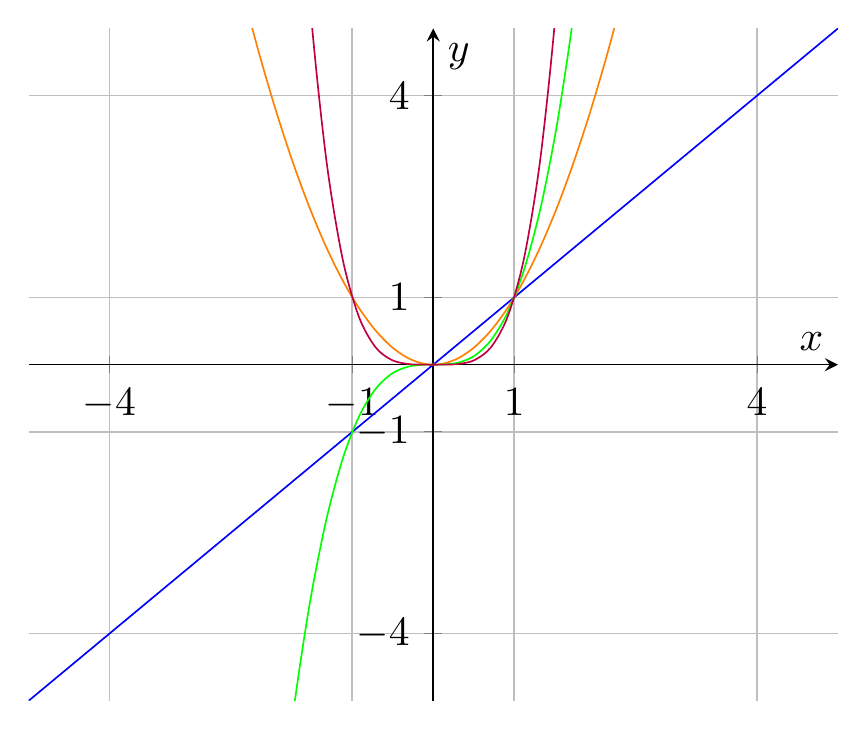
\begin{tikzpicture}[scale=1.5]
		\begin{axis}[
			xmin=-5,xmax=5,
			ymin=-5,ymax=5,
			enlargelimits,
			axis lines=middle,
			xlabel=$x$,
			ylabel=$y$,
			xtick={-4,-1,1,4},
			ytick={-4,-1,1,4},
			grid=major,
		]
			\begin{scope}[samples=50,smooth,domain=-5:5]
				\addplot[color=blue]{x};
				\addplot[color=orange]{x^2};
				\addplot[color=green]{x^3};
				\addplot[color=purple]{x^4};
			\end{scope}
		\end{axis}
	\end{tikzpicture}
	\caption{}
\end{figure}

\begin{figure}
	\centering
	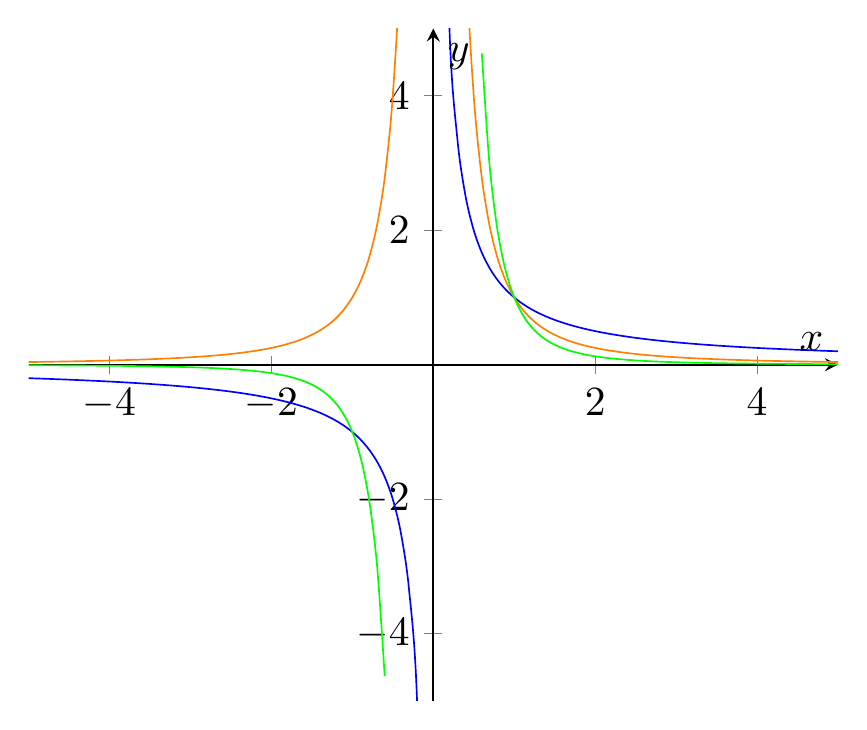
\begin{tikzpicture}[scale=1.5]
		\begin{axis}[
			xmin=-5,xmax=5,
			ymin=-5,ymax=5,
			enlargelimits,
			axis lines=middle,
			xlabel=$x$,
			ylabel=$y$,
		]
			\begin{scope}[samples=50,smooth]
				\begin{scope}[domain=-5:-.1]
					\addplot[color=blue]{1/x};
					\addplot[color=orange]{1/(x^2)};
					\addplot[color=green,domain=-5:-.6]{1/(x^3)};
				\end{scope}
				\begin{scope}[domain=.1:5]
					\addplot[color=blue]{1/x};
					\addplot[color=orange]{1/(x^2)};
					\addplot[color=green,domain=.6:5]{1/(x^3)};
				\end{scope}
			\end{scope}
		\end{axis}
	\end{tikzpicture}
	\caption{}
\end{figure}

\subsection{指数函数的概念}
\begin{definition}
设\(a>0\)且\(a \neq 1\).
把函数\(f(x)=a^x\)
称为“以\(a\)为底的\DefineConcept{指数函数}”.
\end{definition}

\begin{theorem}
设\(f\)是以\(a\)为底的指数函数,
则\(f\)存在反函数.
\begin{proof}
指数函数是单调函数.
\end{proof}
\end{theorem}

\subsection{指数函数的性质}
\begin{property}
\begin{gather}
	a^x a^y = a^{x+y}, \\
	\frac{a^x}{a^y} = a^{x-y}, \\
	(a^x)^y = a^{xy}.
\end{gather}
\end{property}

\subsection{对数函数的概念}
\begin{definition}
设\(a>0\)且\(a\neq1\).
以\(a\)为底的指数函数的反函数,
称为“以\(a\)为底的\DefineConcept{对数函数}”,
记作\(\log_a x\),
即\begin{equation}\label{equation:函数.对数的定义}
	y = \log_a x
	\defiff
	a^y = x.
\end{equation}
%@see: https://mathworld.wolfram.com/Logarithm.html
\end{definition}

以\(10\)为底的对数,称为\DefineConcept{常用对数},记作\(y = \lg x\),
即\begin{equation}
	\lg x \defeq \log_{10} x.
\end{equation}

以常数\(e\)为底的对数,称为\DefineConcept{自然对数},记作\(y = \ln x\),
即\begin{equation}
	\ln x \defeq \log_e x.
\end{equation}

\subsection{对数函数的性质}
\begin{proposition}[对数恒等式]
设\(a>0,a\neq1\),
则对\(\forall x>0\)
有\begin{equation}\label{equation:函数.对数恒等式}
	a^{\log_a x} = x.
\end{equation}
\begin{proof}
根据\hyperref[equation:函数.对数的定义]{对数的定义}有
\(y = \log_a x
\defiff
a^y = x\),
于是\(a^{\log_a x} = a^y = x\).
\end{proof}
\end{proposition}

\begin{theorem}
设\(a>0,a\neq1\),
则\begin{gather}
	\log_a 1 = 0, \\
	\log_a a = 1.
\end{gather}
\end{theorem}

\begin{theorem}[对数的运算法则]
设\(a>0,a\neq1,x>0,y>0\),
则\begin{gather}
	\log_a xy = \log_a x + \log_a y,
		\label{equation:函数.对数的基本运算法则1} \\
	\log_a \frac{x}{y} = \log_a x - \log_a y,
		\label{equation:函数.对数的基本运算法则2} \\
	\log_a x^y = y \log_a x.
		\label{equation:函数.对数的基本运算法则3}
\end{gather}
\end{theorem}

\begin{theorem}[换底公式]
设\(a>0,a\neq1,c>0,c\neq1,b>0\),
则\begin{equation}\label{equation:函数.换底公式}
	\log_a b = \frac{\log_c b}{\log_c a}.
\end{equation}
\begin{proof}
由\hyperref[equation:函数.对数恒等式]{对数恒等式}有\(b = a^{\log_a b}\),
于是\(\log_c b
= \log_c a^{\log_a b}\).
又由有\hyperref[equation:函数.对数的基本运算法则3]{对数的运算法则}有\begin{equation*}
	\log_c a^{\log_a b} = \log_a b \cdot \log_c a,
\end{equation*}
所以\(\log_a b = \frac{\log_c b}{\log_c a}\).
\end{proof}
\end{theorem}

\begin{corollary}
设\(a>0,a\neq1,b>0,b\neq1\),
则\begin{equation}
	\log_a b = \frac1{\log_b a}.
\end{equation}
\begin{proof}
在\hyperref[equation:函数.换底公式]{换底公式}中,令\(c=b\)便得.
\end{proof}
\end{corollary}

\begin{corollary}
设\(a>0,a\neq1,a^x\neq1\)
则\begin{equation}
	\log_{a^x} b^y = \frac{y}{x} \log_a b.
\end{equation}
\end{corollary}

\begin{example}
设\(a>0,b>0\).
证明:\begin{equation}\label{equation:函数.真底互换公式}
	a^{\ln b} = b^{\ln a}.
\end{equation}
\begin{proof}
在\cref{equation:函数.真底互换公式} 等号左右变量分别取对数,
得\begin{equation*}
	\ln(a^{\ln b}) = \ln b \ln a, \qquad
	\ln(b^{\ln a}) = \ln a \ln b,
\end{equation*}
显然两者相等,故\(a^{\ln b} = b^{\ln a}\)成立.
\end{proof}
\end{example}

\subsection{重幂}
设\(a\)是实数,\(b\)是正整数.
定义:\begin{equation*}
	\relax^ba \defeq \underbrace{a^{a^{\iddots^a}}}_{\text{\(b\)个}},
\end{equation*}
我们把\(\relax^ba\)读作“\(a\)的\(b\)~\DefineConcept{重幂}”.

例如,\begin{equation*}
	\relax^23 = 3^3, \qquad
	\relax^33 = 3^{3^3}, \qquad
	\relax^43 = 3^{3^{3^3}}.
\end{equation*}

\section{三角函数}
\subsection{三角函数的概念}
\begin{figure}[htb]
	\centering
	\begin{tikzpicture}[scale=6]
		\draw(1,0)coordinate(A)node[below]{$A$}
			arc[start angle=0,end angle=90,radius=1](0,1)node[left]{$B$};
		\draw(0,0)coordinate(O)node[below left]{$O$}
			--(.866,.5)coordinate(P)node[above]{$P$}
			--(.866,0)coordinate(Q)node[below]{$Q$};
		\draw(P)--(1,.577)coordinate(R)node[right]{$R$}--(A);
		\begin{scope}[->,>=Stealth]
			\draw(0,0)--(1.2,0)node[below]{$x$};
			\draw(0,0)--(0,1.2)node[left]{$y$};
		\end{scope}
		\draw pic["$\theta$",draw=orange,-,angle eccentricity=1.2,angle radius=1cm]{angle=Q--O--P};
		\draw pic[draw=gray,-,angle radius=.5cm]{right angle=P--Q--O};
	\end{tikzpicture}
	\caption{}
	\label{figure:函数.三角函数.三角函数的几何定义}
\end{figure}

如\cref{figure:函数.三角函数.三角函数的几何定义},
首先在平面直角坐标系\(Oxy\)中
画出一个单位圆\(\odot~O\),
分别交\(x\)轴、\(y\)轴于\(A\)、\(B\)两点.
在\(\odot~O\)上任取一点\(P\),过\(P\)作\(OA\)的垂线交\(OA\)于\(Q\).
过点\(A\)作\(OA\)的垂线交射线\(OP\)于\(R\).
记\(\angle POQ = \theta\).
定义:\begin{gather}
	\sin\theta \defeq \abs{\overline{PQ}}, \\
	\cos\theta \defeq \abs{\overline{OQ}}, \\
	\tan\theta \defeq \sin\theta/\cos\theta, \\
	\cot\theta \defeq \cos\theta/\sin\theta, \\
	\sec\theta \defeq 1/\cos\theta, \\
	\csc\theta \defeq 1/\sin\theta.
\end{gather}
我们把\(\sin,\cos,\tan,\cot,\sec,\csc\)
依次称为\DefineConcept{正弦函数}、
\DefineConcept{余弦函数}、
\DefineConcept{正切函数}、
\DefineConcept{余切函数}、
\DefineConcept{正割函数}、
\DefineConcept{余割函数},
统称为\DefineConcept{三角函数}.

不难想象,当\(P\)在圆周上逆时针平移时,
\(\theta\)逐渐增大,
线段\(\overline{OP}\)的长度\(\abs{\overline{OP}}\)始终保持不变,
线段\(\overline{PQ}\)的长度\(\abs{\overline{PQ}}\)逐渐增大,
线段\(\overline{OQ}\)的长度\(\abs{\overline{OQ}}\)逐渐减小.
当\(P\)与\(B\)重合时,
\(\abs{\overline{OP}}
= \abs{\overline{PQ}}
= \abs{\overline{OB}} = 1\)
且\(\abs{\overline{OQ}} = 0\).
当\(P\)在圆周上顺时针平移时,
\(\theta\)逐渐减小,
线段\(\overline{OP}\)的长度\(\abs{\overline{OP}}\)依旧始终保持不变,
线段\(\overline{PQ}\)的长度\(\abs{\overline{PQ}}\)逐渐减小,
线段\(\overline{OQ}\)的长度\(\abs{\overline{OQ}}\)逐渐增大.
当\(P\)与\(A\)重合时,
\(\abs{\overline{OP}}
= \abs{\overline{OA}} = 1\)
且\(\abs{\overline{PQ}} = 0\).

\begin{example}
下面列出一些特殊的正弦函数值:\begin{equation*}
	\sin0 = 0, \quad
	\sin\frac{\pi}{6} = \frac{1}{2}, \quad
	\sin\frac{\pi}{4} = \frac{\sqrt{2}}{2}, \quad
	\sin\frac{\pi}{3} = \frac{\sqrt{3}}{2},
\end{equation*}\begin{equation*}
	\sin\frac{\pi}{2} = 1, \quad
	\sin\pi = 0, \quad
	\sin\frac{3\pi}{2} = -1.
\end{equation*}

\begin{figure}[htb]
	\centering
	\begin{tikzpicture}
		\pgfmathsetmacro{\r}{2}
		\pgfmathsetmacro{\ax}{\r*cos(30)}
		\pgfmathsetmacro{\ay}{\r*sin(30)}
		\pgfmathsetmacro{\b}{\r/sqrt(2)}
		\coordinate (O)at(0,0);
		\draw(O)circle(\r);
		\begin{scope}[dashed,color=gray!50,text=black]
			\draw(O)--(\r,0)node[left]{\(0\)}node[right]{\(0\)}
			(O)--(\ax,\ay)node[below left]{\(\tfrac{\pi}{6}\)}node[right]{\(\tfrac{1}{2}\)}
			(O)--(\b,\b)node[below left]{\(\tfrac{\pi}{4}\)}node[above right]{\(\tfrac{\sqrt2}{2}\)}
			(O)--(\ay,\ax)node[below left]{\(\tfrac{\pi}{3}\)}node[above]{\(\tfrac{\sqrt3}{2}\)}
			(O)--(0,\r)node[below]{\(\tfrac{\pi}{2}\)}node[above]{\(1\)}
			(O)--(-\ay,\ax)node[below right]{\(\tfrac{2\pi}{3}\)}node[above]{\(\tfrac{\sqrt3}{2}\)}
			(O)--(-\b,\b)node[below right]{\(\tfrac{3\pi}{4}\)}node[above left]{\(\tfrac{\sqrt2}{2}\)}
			(O)--(-\ax,\ay)node[below right]{\(\tfrac{5\pi}{6}\)}node[left]{\(\tfrac{1}{2}\)}
			(O)--(-\r,0)node[right]{\(\pi\)}node[left]{\(0\)}
			(O)--(-\ax,-\ay)node[above right]{\(\tfrac{7\pi}{6}\)}node[left]{\(-\tfrac{1}{2}\)}
			(O)--(-\b,-\b)node[above right]{\(\tfrac{5\pi}{4}\)}node[below left]{\(-\tfrac{\sqrt2}{2}\)}
			(O)--(-\ay,-\ax)node[above right]{\(\tfrac{4\pi}{3}\)}node[below]{\(-\tfrac{\sqrt3}{2}\)}
			(O)--(0,-\r)node[above]{\(\tfrac{3\pi}{2}\)}node[below]{\(-1\)}
			(O)--(\ay,-\ax)node[above left]{\(\tfrac{5\pi}{3}\)}node[below]{\(-\tfrac{\sqrt3}{2}\)}
			(O)--(\b,-\b)node[above left]{\(\tfrac{7\pi}{4}\)}node[below right]{\(-\tfrac{\sqrt2}{2}\)}
			(O)--(\ax,-\ay)node[above left]{\(\tfrac{11\pi}{6}\)}node[right]{\(-\tfrac{1}{2}\)}
			;
		\end{scope}
		\begin{scope}[very thick,->]
			\draw(-1,0)--(1,0)node[above left]{\(x\)};
			\draw(0,-1)--(0,1)node[below right]{\(y\)};
		\end{scope}
	\end{tikzpicture}
	\caption{正弦函数\(\sin x\)的辅助圆与特殊值}
\end{figure}

特殊的余弦函数值:\begin{equation*}
	\cos0 = 1, \quad
	\cos\frac{\pi}{6} = \frac{\sqrt{3}}{2}, \quad
	\cos\frac{\pi}{4} = \frac{\sqrt{2}}{2}, \quad
	\cos\frac{\pi}{3} = \frac{1}{2},
\end{equation*}\begin{equation*}
	\cos\frac{\pi}{2} = 0, \quad
	\cos\pi = -1, \quad
	\cos\frac{3\pi}{2} = 0.
\end{equation*}
\end{example}

\subsection{三角函数的性质}
\begin{property}
根据三角函数的定义,显然有\begin{gather}
	\tan\theta = \frac{\sin\theta}{\cos\theta},
	\label{equation:三角函数.正切与正余弦的关系} \\
	\cot\theta = \frac{1}{\tan\theta}, \\
	\sec\theta = \frac{1}{\cos\theta}, \\
	\csc\theta = \frac{1}{\sin\theta}.
\end{gather}
\end{property}

\begin{theorem}[毕达哥拉斯三角恒等式]
\begin{figure}[htb]
	\def\subwidth{.5\linewidth}
	\def\subscale{.8}
		\begin{subfigure}[b]{\subwidth}%
		\centering
		\begin{tikzpicture}[scale=\subscale]
			\draw[help lines, color=gray!30, dashed] (0,0) grid (4,3);
			\coordinate (A) at (0,0);
			\coordinate (B) at (4,0);
			\coordinate (C) at (4,3);
			\draw (A)node[left]{\(A\)} -- (B)node[right]{\(B\)}node[midway,below]{\(\cos\theta\)} -- (C)node[right]{\(C\)}node[midway,right]{\(\sin\theta\)} -- (A)node[midway,above left]{\(1\)} pic["\(\theta\)",draw=orange,-,angle eccentricity=2,angle radius=0.3cm]{angle=B--A--C} pic[draw=gray,-,angle radius=0.3cm]{right angle=C--B--A};
		\end{tikzpicture}
		\subcaption{正弦、余弦辅助三角形}
		\end{subfigure}%
		\begin{subfigure}[b]{\subwidth}%
		\centering
		\begin{tikzpicture}[scale=\subscale]
			\draw[help lines, color=gray!30, dashed] (0,0) grid (4,3);
			\coordinate (A) at (0,0);
			\coordinate (B) at (4,0);
			\coordinate (C) at (4,3);
			\draw (A)node[left]{\(A\)} -- (B)node[right]{\(B\)}node[midway,below]{\(1\)} -- (C)node[right]{\(C\)}node[midway,right]{\(\tan\theta\)} -- (A)node[midway,above left]{\(\sec\theta\)} pic["\(\theta\)",draw=orange,-,angle eccentricity=2,angle radius=0.3cm]{angle=B--A--C} pic[draw=gray,-,angle radius=0.3cm]{right angle=C--B--A};
		\end{tikzpicture}
		\subcaption{正切、正割辅助三角形}
		\end{subfigure}%
	\caption{两种特殊的辅助三角形}
	\label{figure:函数.两种特殊的辅助三角形}
\end{figure}

结合\cref{figure:函数.两种特殊的辅助三角形},根据勾股定理可得
\begin{gather}
	\sin^2 \theta + \cos^2 \theta = 1,
		\label{equation:三角函数.毕达哥拉斯三角恒等式1} \\
	\tan^2 \theta + 1 = \sec^2 \theta,
		\label{equation:三角函数.毕达哥拉斯三角恒等式2} \\
	1 + \cot^2 \theta = \csc^2 \theta.
		\label{equation:三角函数.毕达哥拉斯三角恒等式3}
\end{gather}
\end{theorem}

\begin{figure}[htb]
	\centering
	\begin{tikzpicture}
		\pgfmathsetmacro{\a}{6}
		\coordinate(O)at(0,0);
		\pgfmathsetmacro{\t}{30}
		\draw(O)node[below left]{\(O\)}
			--(\a,0)coordinate(A)node[below right]{\(A\)}
			arc[start angle=0,end angle=\t,radius=\a]coordinate(B)node[right]{\(B\)}
			--(O);
		\draw(B)--(B|-A)coordinate(C)node[below right]{\(C\)};
		\draw(B)--(\a,{\a*tan(\t)})coordinate(D)node[above right]{\(D\)}--(\a,0);
		\pic["\(\theta\)",draw,-,angle eccentricity=1.5,angle radius=6mm]{angle=A--O--B};
		\begin{scope}[|<->|,black!40,every node/.style={black,midway,sloped}]
			\def\mark#1#2#3#4#5{%
				\draw($#1+#4$)--($#2+#4$)node[#3]{$#5$};%
			}%
			\mark{(C)}{(B)}{above}{(-5pt,0)}{\sin\theta}
			\mark{(O)}{(D)}{above}{({(-1em-10pt)*sin(30)},{(1em+10pt)*cos(30)})}{\sec\theta}
			\mark{(O)}{(B)}{above}{({-5pt*sin(30)},{5pt*cos(30)})}{1}
			\mark{(O)}{(C)}{below}{(0,-5pt)}{\cos\theta}
			\mark{(A)}{(D)}{below}{(5pt,0)}{\tan\theta}
			\mark{(O)}{(A)}{below}{(0,-1em-10pt)}{1}
		\end{scope}
	\end{tikzpicture}
	\caption{}
\end{figure}

\begin{figure}[htb]
	\centering
	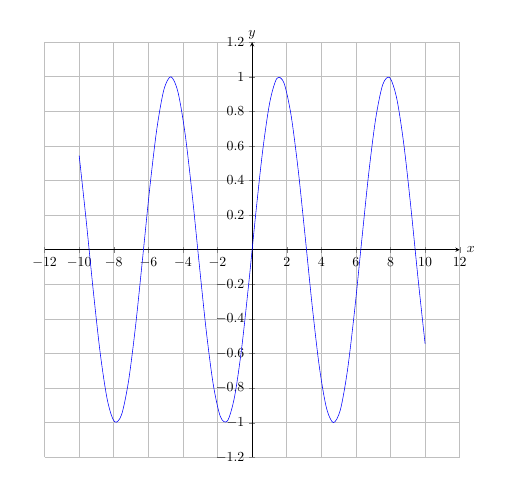
\begin{tikzpicture}[scale=.5]
		\begin{axis}[
			xmin=-10,xmax=10,
			restrict y to domain=-2:2,
			ymin=-1,ymax=1,
			grid=both,width=\textwidth,height=\textwidth,
			axis lines=middle,
			xlabel=$x$,
			ylabel=$y$,
			enlarge x limits=0.1,
			enlarge y limits=0.1,
			x label style={at={(ticklabel* cs:1.00)}, inner sep=5pt, anchor=west},
			y label style={at={(ticklabel* cs:1.00)}, inner sep=2pt, anchor=south},
		]
			\addplot[color=blue,samples=50,smooth,domain=-10:10,variable=\x]{sin(\x r)};
		\end{axis}
	\end{tikzpicture}
	\caption{正弦函数\(y=\sin x\)的图形}
	\label{figure:函数.正弦函数的图形}
\end{figure}

\begin{figure}
	\centering
	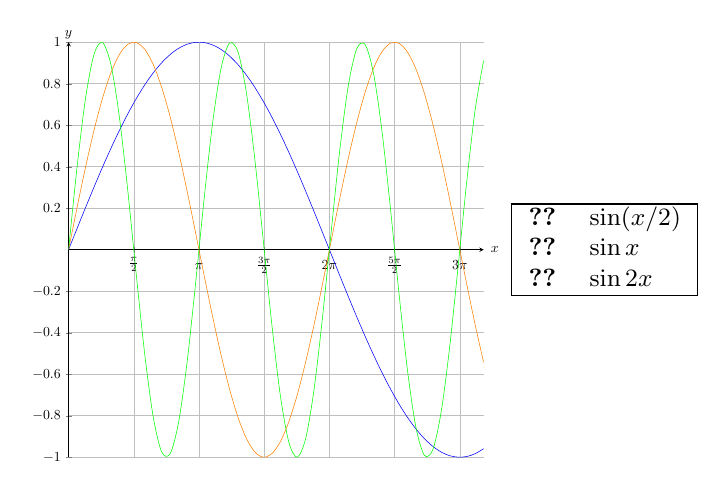
\begin{tikzpicture}[scale=.5]
		\begin{axis}[
			name=Sine,
			xmin=0,xmax=10,
			restrict y to domain=-2:2,
			ymin=-1,ymax=1,
			grid=both,width=\textwidth,height=\textwidth,
			axis lines=middle,
			xlabel=$x$,
			ylabel=$y$,
			x label style={at={(ticklabel* cs:1.00)}, inner sep=5pt, anchor=west},
			y label style={at={(ticklabel* cs:1.00)}, inner sep=2pt, anchor=south},
			xtick={0,1.5708,3.1416,...,10},
			xticklabels={
				$\relax$,
				$\frac{\pi}{2}$,
				$\pi\vphantom{\frac12}$,
				$\frac{3\pi}{2}$,
				$2\pi\vphantom{\frac12}$,
				$\frac{5\pi}{2}$,
				$3\pi\vphantom{\frac12}$,
			},
		]
			\addplot[color=blue,samples=50,smooth,domain=0:10,variable=\x]
				{sin(.5*\x r)};\label{pgfplots:正弦函数.sin(x/2)}
			\addplot[color=orange,samples=50,smooth,domain=0:10,variable=\x]
				{sin(\x r)};\label{pgfplots:正弦函数.sin(x)}
			\addplot[color=green,samples=50,smooth,domain=0:10,variable=\x]
				{sin(2*\x r)};\label{pgfplots:正弦函数.sin(2*x)}
		\end{axis}
		\node[draw,fill=white,inner sep=0pt,right=1em]
		at(Sine.east){\small\begin{tabular}{cl}
			\ref{pgfplots:正弦函数.sin(x/2)} & \(\sin(x/2)\) \\
			\ref{pgfplots:正弦函数.sin(x)} & \(\sin x\) \\
			\ref{pgfplots:正弦函数.sin(2*x)} & \(\sin2x\) \\
		\end{tabular}};
	\end{tikzpicture}
	\caption{}
\end{figure}

\begin{property}
如\cref{figure:函数.正弦函数的图形},
可以观察得出正弦函数的若干性质.
\begin{enumerate}
	\item 正弦函数是周期函数,其周期为\(T = 2\pi\).
	\item 正弦函数在区间\([2k\pi-\frac{\pi}{2},2k\pi+\frac{\pi}{2})\)上单调递增.
	\item 在区间\([2k\pi+\frac{\pi}{2},2k\pi+\frac{3\pi}{2})\)上单调递增.
	\item 当\(x=\frac{\pi}{2}+2k\pi\ (k\in\mathbb{Z})\)时,正弦函数\(y=\sin x\)取得极大值\(1\).
	\item 当\(x=\frac{3\pi}{2}+2k\pi\ (k\in\mathbb{Z})\)时,正弦函数\(y=\sin x\)取得极小值\(-1\).
	\item 正弦函数是奇函数,其图形关于坐标原点\(O\)中心对称,满足\(\sin(-x)=-\sin x\).
\end{enumerate}
\end{property}

\begin{figure}[htb]
	\centering
	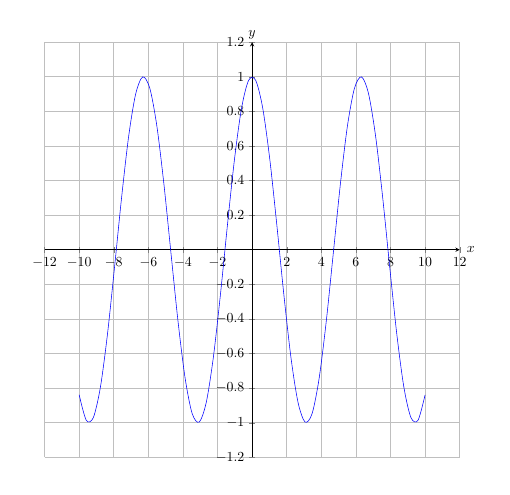
\begin{tikzpicture}[scale=.5]
		\begin{axis}[
			xmin=-10,xmax=10,
			restrict y to domain=-2:2,
			ymin=-1,ymax=1,
			grid=both,width=\textwidth,height=\textwidth,
			axis lines=middle,
			xlabel=$x$,
			ylabel=$y$,
			enlarge x limits=0.1,
			enlarge y limits=0.1,
			x label style={at={(ticklabel* cs:1.00)}, inner sep=5pt, anchor=west},
			y label style={at={(ticklabel* cs:1.00)}, inner sep=2pt, anchor=south},
		]
			\addplot[color=blue,samples=50,smooth,domain=-10:10,variable=\x]{cos(\x r)};
		\end{axis}
	\end{tikzpicture}
	\caption{余弦函数\(y=\cos x\)的图形}
	\label{figure:函数.余弦函数的图形}
\end{figure}

\begin{figure}
	\centering
	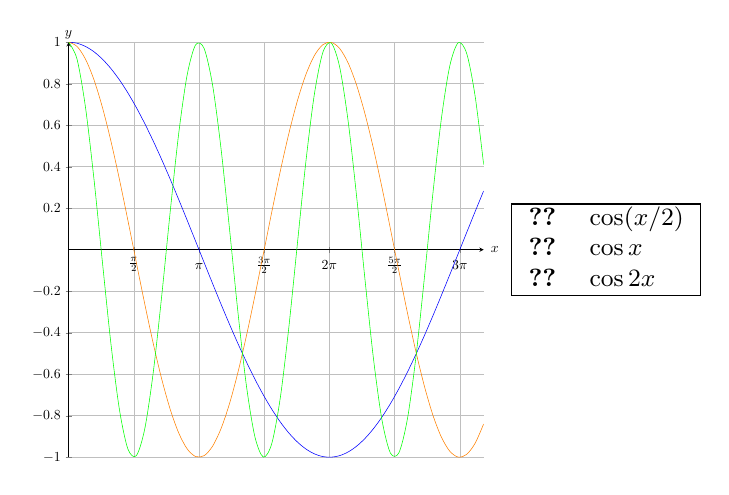
\begin{tikzpicture}[scale=.5]
		\begin{axis}[
			name=Cosine,
			xmin=0,xmax=10,
			restrict y to domain=-2:2,
			ymin=-1,ymax=1,
			grid=both,width=\textwidth,height=\textwidth,
			axis lines=middle,
			xlabel=$x$,
			ylabel=$y$,
			x label style={at={(ticklabel* cs:1.00)}, inner sep=5pt, anchor=west},
			y label style={at={(ticklabel* cs:1.00)}, inner sep=2pt, anchor=south},
			xtick={0,1.5708,3.1416,...,10},
			xticklabels={
				$\relax$,
				$\frac{\pi}{2}$,
				$\pi\vphantom{\frac12}$,
				$\frac{3\pi}{2}$,
				$2\pi\vphantom{\frac12}$,
				$\frac{5\pi}{2}$,
				$3\pi\vphantom{\frac12}$,
			},
		]
			\addplot[color=blue,samples=50,smooth,domain=0:10,variable=\x]
				{cos(.5*\x r)};\label{pgfplots:余弦函数.cos(x/2)}
			\addplot[color=orange,samples=50,smooth,domain=0:10,variable=\x]
				{cos(\x r)};\label{pgfplots:余弦函数.cos(x)}
			\addplot[color=green,samples=50,smooth,domain=0:10,variable=\x]
				{cos(2*\x r)};\label{pgfplots:余弦函数.cos(2*x)}
		\end{axis}
		\node[draw,fill=white,inner sep=0pt,right=1em]
		at(Cosine.east){\small\begin{tabular}{cl}
			\ref{pgfplots:余弦函数.cos(x/2)} & \(\cos(x/2)\) \\
			\ref{pgfplots:余弦函数.cos(x)} & \(\cos x\) \\
			\ref{pgfplots:余弦函数.cos(2*x)} & \(\cos2x\) \\
		\end{tabular}};
	\end{tikzpicture}
	\caption{}
\end{figure}

\begin{property}
如\cref{figure:函数.余弦函数的图形},
可以观察得出余弦函数的若干性质.
\begin{enumerate}
	\item 余弦函数也是周期函数,其周期为\(T = 2\pi\).
	\item 余弦函数在区间\([2k\pi,\pi+2k\pi)\)上单调递减.
	\item 在区间\([\pi+2k\pi,2\pi+2k\pi)\)上单调递增.
	\item 当\(x=2k\pi\ (k\in\mathbb{Z})\)时,余弦函数\(y=\cos x\)取得极大值\(1\).
	\item 当\(x=(2k-1)\pi\ (k\in\mathbb{Z})\)时,余弦函数\(y=\cos x\)取得极小值\(-1\).
	\item 余弦函数是偶函数,其图形关于\(y\)轴对称,满足\(\cos(-x)=\cos x\).
\end{enumerate}
\end{property}

\begin{figure}[htb]
	\centering
	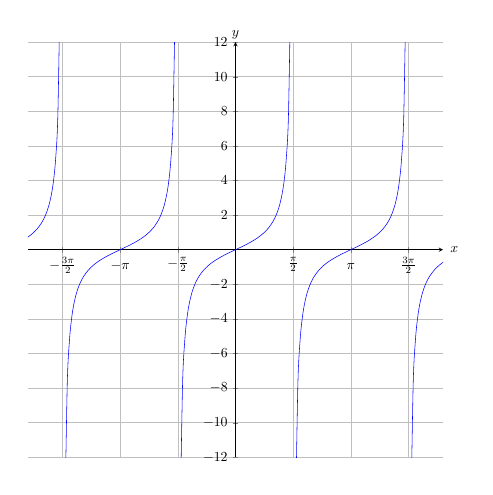
\begin{tikzpicture}[scale=.5]
		\begin{axis}[
			restrict y to domain=-20:20,
			ymin=-10,ymax=10,
			grid=both,width=\textwidth,height=\textwidth,
			axis lines=middle,
			xlabel=$x$,
			ylabel=$y$,
			enlarge x limits=0.1,
			enlarge y limits=0.1,
			x label style={at={(ticklabel* cs:1.00)}, inner sep=5pt, anchor=west},
			y label style={at={(ticklabel* cs:1.00)}, inner sep=2pt, anchor=south},
			xmin=-4.7124, xmax=4.7124,
			xtick={-4.7124,-3.1416,-1.5708,...,10},
			xticklabels={
				$-\frac{3\pi}{2}$,
				$-\pi\vphantom{\frac{1}{2}}$,
				$-\frac{\pi}{2}$,
				$\relax$,%不能去掉\relax
				$\frac{\pi}{2}$,
				$\pi\vphantom{\frac{1}{2}}$,
				$\frac{3\pi}{2}$,
			},
		]
			\foreach \i in {-5,-3,...,3} {
				\addplot[color=blue,samples=50,smooth,domain={\i*pi/2}:{(\i+2)*pi/2},variable=\x]
				{tan(\x r)};
			}
		\end{axis}
	\end{tikzpicture}
	\caption{正切函数\(y=\tan x\)的图形}
	\label{figure:函数.正切函数的图形}
\end{figure}

\begin{property}
如\cref{figure:函数.正切函数的图形},
可以观察得出正切函数的若干性质.
\begin{enumerate}
	\item 正切函数是周期函数,其周期为\(T = \pi\).
	\item 正切函数在区间\((k\pi-\frac{\pi}{2},k\pi+\frac{\pi}{2})\ (k\in\mathbb{Z})\)上单调递增.
	\item 正切函数是奇函数,其图形关于坐标原点\(O\)中心对称,满足\(\tan(-x)=-\tan x\).
\end{enumerate}
\end{property}

\begin{figure}[htb]
	\centering
	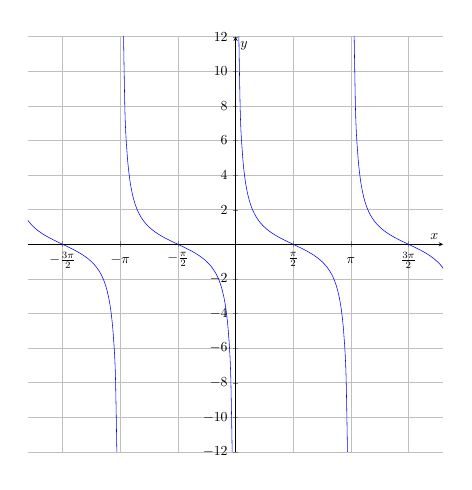
\begin{tikzpicture}[scale=.5]
		\begin{axis}[
			restrict y to domain=-20:20,
			ymin=-10,ymax=10,
			grid=both,width=\textwidth,height=\textwidth,
			axis lines=middle,
			xlabel=$x$,
			ylabel=$y$,
			enlarge x limits=0.1,
			enlarge y limits=0.1,
			xmin=-4.7124, xmax=4.7124,
			xtick={-4.7124,-3.1416,-1.5708,...,10},
			xticklabels={
				$-\frac{3\pi}{2}$,
				$-\pi\vphantom{\frac{1}{2}}$,
				$-\frac{\pi}{2}$,
				$\relax$,%不能去掉\relax
				$\frac{\pi}{2}$,
				$\pi\vphantom{\frac{1}{2}}$,
				$\frac{3\pi}{2}$,
			},
		]
		\foreach \i in {-2,-1,0,1} {
			\addplot[color=blue,samples=50,smooth,domain={\i*pi}:{(\i+1)*pi},variable=\x]
			{cot(\x r)};
		}
		\end{axis}
	\end{tikzpicture}
	\caption{余切函数\(y=\cot x\)的图形}
\end{figure}

\begin{table}[htb]
	\centering
	\begin{tblr}{*2c}
		\hline
		函数 & 周期 \\
		\hline
		\(\sin(\omega x)\) & \(\frac{2\pi}{\omega}\) \\
		\(\cos(\omega x)\) & \(\frac{2\pi}{\omega}\) \\
		\(\tan(\omega x)\) & \(\frac{\pi}{\omega}\) \\
		\(\cot(\omega x)\) & \(\frac{\pi}{\omega}\) \\
		\(\sec(\omega x)\) & \(\frac{2\pi}{\omega}\) \\
		\(\csc(\omega x)\) & \(\frac{2\pi}{\omega}\) \\
		\hline
	\end{tblr}
	\caption{角速度$\omega$与三角函数的周期的关系}
%@Mathematica: Manipulate[Plot[{Tan[x], Tan[w x]}, {x, -2 Pi, 2 Pi}, PlotLegends -> {"Tan[x]", StringForm["Tan[`1`x]", w]}, PlotRange -> {-5, 5}], {w, 2, 5, 1}]
\end{table}

\subsection{和积互化公式}
\begin{theorem}[和积互化公式]
设\(\alpha,\beta\in\mathbb{R}\),则有
\begin{align}
	\sin(\alpha\pm\beta)
	&= \sin\alpha\cos\beta\pm\cos\alpha\sin\beta,
	\label{equation:函数.三角函数.和积互化公式1} \\
	\cos(\alpha\pm\beta)
	&= \cos\alpha\cos\beta\mp\sin\alpha\sin\beta,
	\label{equation:函数.三角函数.和积互化公式2} \\
	\tan(\alpha\pm\beta)
	&= \frac{\tan\alpha\pm\tan\beta}{1\mp\tan\alpha\tan\beta},
	\label{equation:函数.三角函数.和积互化公式3} \\
	\cot(\alpha\pm\beta)
	&= \frac{\cot\alpha\cot\beta\mp 1}{\cot\beta\pm\cot\alpha},
	\label{equation:函数.三角函数.和积互化公式4} \\
	\sec(\alpha\pm\beta)
	&= \frac{\sec\alpha\sec\beta}{1\mp\tan\alpha\tan\beta},
	\label{equation:函数.三角函数.和积互化公式5} \\
	\csc(\alpha\pm\beta)
	&= \frac{\csc\alpha\csc\beta}{\cot\beta\pm\cot\alpha},
	\label{equation:函数.三角函数.和积互化公式6} \\
	\sin \alpha \cos \beta
	&= \frac{\sin (\alpha + \beta) + \sin (\alpha - \beta)}{2},
	\label{equation:函数.三角函数.和积互化公式7} \\
	\cos \alpha \sin \beta
	&= \frac{\sin (\alpha + \beta) - \sin (\alpha - \beta)}{2},
	\label{equation:函数.三角函数.和积互化公式8} \\
	\cos \alpha \cos \beta
	&= \frac{\cos (\alpha + \beta) + \cos (\alpha - \beta)}{2},
	\label{equation:函数.三角函数.和积互化公式9} \\
	\sin \alpha \sin \beta
	&= -\frac{\cos (\alpha + \beta) - \cos (\alpha - \beta)}{2},
	\label{equation:函数.三角函数.和积互化公式10} \\
	\sin \alpha + \sin \beta
	&= 2 \sin \frac{\alpha + \beta}{2} \cos \frac{\alpha - \beta}{2},
	\label{equation:函数.三角函数.和积互化公式11} \\
	\sin \alpha - \sin \beta
	&= 2 \cos \frac{\alpha + \beta}{2} \sin \frac{\alpha - \beta}{2},
	\label{equation:函数.三角函数.和积互化公式12} \\
	\cos \alpha + \cos \beta
	&= 2 \cos \frac{\alpha + \beta}{2} \cos \frac{\alpha - \beta}{2},
	\label{equation:函数.三角函数.和积互化公式13} \\
	\cos \alpha - \cos \beta
	&= -2 \sin \frac{\alpha + \beta}{2} \sin \frac{\alpha - \beta}{2}.
	\label{equation:函数.三角函数.和积互化公式14}
\end{align}
\begin{proof}
\begin{figure}[htb]
	\centering
	\begin{tikzpicture}
		\coordinate(A)at(0.0,0.0);
		\coordinate(B)at(6.4,0.0);
		\coordinate(C)at(6.4,4.8);
		\coordinate(D)at(6.4,6.4);
		\coordinate(E)at(5.2,6.4);
		\draw (A)
			--(B)node[midway,below]{\(\cos\alpha\cos\beta\)}
			--(C)node[midway,right]{\rotatebox{90}{\(\cos\alpha\sin\beta\)}}
			--(D)node[midway,right]{\rotatebox{90}{\(\sin\alpha\cos\beta\)}}
			--(E)node[midway,above]{\(\sin\alpha\sin\beta\)}
			--(C)node[midway,left=2mm,below=-3mm]{\rotatebox{-53.13}{\(\sin\alpha\)}}
			--(A)node[midway,right=1mm,below=-2mm]{\rotatebox{36.87}{\(\cos\alpha\)}}
			--(E)node[midway,left=2mm,above=2mm]{\(1\)};
		\pic["\(\alpha\)",draw=orange,-,angle eccentricity=2,angle radius=0.7cm]{angle=C--A--E};
		\pic["\(\beta\)",draw=blue,-,angle eccentricity=2,angle radius=0.7cm]{angle=B--A--C};
		\pic[draw=blue,-,angle radius=0.5cm]{angle=D--C--E};
		\pic[draw=gray,-,angle radius=0.3cm]{right angle=C--B--A};
		\pic[draw=gray,-,angle radius=0.3cm]{right angle=E--C--A};
		\pic[draw=gray,-,angle radius=0.3cm]{right angle=E--D--C};
	\end{tikzpicture}
	\caption{和积互化公式的辅助三角形}
	\label{figure:函数.和积互化公式的辅助三角形}
\end{figure} %

观察\cref{figure:函数.和积互化公式的辅助三角形} 可知
\begin{align*}
	\sin(\alpha+\beta) &= \sin\alpha\cos\beta+\cos\alpha\sin\beta, \\
	\cos(\alpha+\beta) &= \cos\alpha\cos\beta-\sin\alpha\sin\beta
\end{align*}成立.
又令\(\beta=-\beta\)则可得
\begin{align*}
	\sin(\alpha-\beta) &= \sin\alpha\cos\beta-\cos\alpha\sin\beta, \\
	\cos(\alpha-\beta) &= \cos\alpha\cos\beta+\sin\alpha\sin\beta.
\end{align*}

计算\(\sin(\alpha\pm\beta)\)除以\(\cos(\alpha\pm\beta)\)便得\begin{align*}
	\tan(\alpha\pm\beta)
	&= \frac{\sin(\alpha\pm\beta)}{\cos(\alpha\pm\beta)}
	= \frac{\sin\alpha\cos\beta\pm\cos\alpha\sin\beta}
		{\cos\alpha\cos\beta\mp\sin\alpha\sin\beta} \\
	&\xlongequal{\text{分子分母同除以$\cos\alpha\cos\beta$}}
		\frac{\tan\alpha\pm\tan\beta}{1\mp\tan\alpha\tan\beta}.
\end{align*}

计算\(\cos(\alpha\pm\beta)\)除以\(\sin(\alpha\pm\beta)\)便得\begin{align*}
	\cot(\alpha\pm\beta)
	&= \frac{\cos(\alpha\pm\beta)}{\sin(\alpha\pm\beta)}
	= \frac{\cos\alpha\cos\beta\mp\sin\alpha\sin\beta}
		{\sin\alpha\cos\beta\pm\cos\alpha\sin\beta} \\
	&\xlongequal{\text{分子分母同除以$\sin\alpha\sin\beta$}}
		\frac{\cot\alpha\cot\beta\mp1}{\cot\beta\pm\cot\alpha}.
\end{align*}

计算\(\cos(\alpha\pm\beta)\)的倒数得\begin{equation*}
	\sec(\alpha\pm\beta)
	= \frac1{\cos(\alpha\pm\beta)}
	\xlongequal{\text{分子分母同除以$\cos\alpha\cos\beta$}}
		\frac{\sec\alpha\sec\beta}{1\mp\tan\alpha\tan\beta}.
\end{equation*}

计算\(\sin(\alpha\pm\beta)\)的倒数得\begin{equation*}
	\csc(\alpha\pm\beta)
	= \frac1{\sin(\alpha\pm\beta)}
	\xlongequal{\text{分子分母同除以$\sin\alpha\sin\beta$}}
		\frac{\csc\alpha\csc\beta}{\cot\beta\pm\cot\alpha}.
\end{equation*}

把\(\sin(\alpha+\beta) = \sin\alpha\cos\beta+\cos\alpha\sin\beta\)
与\(\sin(\alpha-\beta) = \sin\alpha\cos\beta-\cos\alpha\sin\beta\)
相加便得\begin{equation*}
	2\sin\alpha\cos\beta = \sin(\alpha+\beta) + \sin(\alpha-\beta),
\end{equation*}
于是\begin{equation*}
	\sin\alpha\cos\beta = \frac{\sin(\alpha+\beta) + \sin(\alpha-\beta)}2.
\end{equation*}

把\(\sin(\alpha+\beta) = \sin\alpha\cos\beta+\cos\alpha\sin\beta\)
与\(\sin(\alpha-\beta) = \sin\alpha\cos\beta-\cos\alpha\sin\beta\)
相减便得\begin{equation*}
	2\cos\alpha\sin\beta = \sin(\alpha+\beta) - \sin(\alpha-\beta),
\end{equation*}
于是\begin{equation*}
	\cos\alpha\sin\beta = \frac{\sin(\alpha+\beta) - \sin(\alpha-\beta)}2.
\end{equation*}

把\(\cos(\alpha+\beta) = \cos\alpha\cos\beta-\sin\alpha\sin\beta\)
与\(\cos(\alpha-\beta) = \cos\alpha\cos\beta+\sin\alpha\sin\beta\)
分别相加、相减便得\begin{gather*}
	2\cos\alpha\cos\beta = \cos(\alpha+\beta) + \cos(\alpha-\beta), \\
	-2\sin\alpha\sin\beta = \cos(\alpha+\beta) - \cos(\alpha-\beta),
\end{gather*}
于是\begin{gather*}
	\cos\alpha\cos\beta = \frac{\cos(\alpha+\beta) + \cos(\alpha-\beta)}2, \\
	\sin\alpha\sin\beta = \frac{\cos(\alpha-\beta) - \cos(\alpha+\beta)}2.
\end{gather*}

在\(2\sin\alpha\cos\beta = \sin(\alpha+\beta) + \sin(\alpha-\beta)\)中
用\(x\)代\(\alpha+\beta\),用\(y\)代\(\alpha-\beta\),
于是\begin{equation*}
	\sin x + \sin y = 2 \sin\frac{x+y}2 \cos\frac{x-y}2.
\end{equation*}

在\(2\cos\alpha\sin\beta = \sin(\alpha+\beta) - \sin(\alpha-\beta)\)中
用\(x\)代\(\alpha+\beta\),用\(y\)代\(\alpha-\beta\),
于是\begin{equation*}
	\sin x - \sin y = 2 \cos\frac{x+y}2 \sin\frac{x-y}2.
\end{equation*}

在\(2\cos\alpha\cos\beta = \cos(\alpha+\beta) + \cos(\alpha-\beta)\)中
用\(x\)代\(\alpha+\beta\),用\(y\)代\(\alpha-\beta\),
于是\begin{equation*}
	\cos x + \cos y = 2 \cos\frac{x+y}2 \cos\frac{x-y}2.
\end{equation*}

在\(-2\sin\alpha\sin\beta = \cos(\alpha+\beta) - \cos(\alpha-\beta)\)中
用\(x\)代\(\alpha+\beta\),用\(y\)代\(\alpha-\beta\),
于是\begin{equation*}
	\cos x - \cos y = -2 \sin\frac{x+y}2 \sin\frac{x-y}2.
	\qedhere
\end{equation*}
\end{proof}
\end{theorem}

特别地,根据和积互化公式有\begin{align}
	\sin(-\alpha)
	&= -\sin\alpha, \\
	\cos(-\alpha)
	&= \cos\alpha, \\
	\tan(-\alpha)
	&= -\tan\alpha, \\
	\sec(-\alpha)
	&= \sec\alpha, \\
	\csc(-\alpha)
	&= -\csc\alpha, \\
	\cot(-\alpha)
	&= -\cot\alpha, \\
	\sin(\alpha+2n\pi)
	&= \sin\alpha, \\
	\cos(\alpha+2n\pi)
	&= \cos\alpha, \\
	\tan(\alpha+n\pi)
	&= \tan\alpha, \\
	\sec(\alpha+2n\pi)
	&= \sec\alpha, \\
	\csc(\alpha+2n\pi)
	&= \csc\alpha, \\
	\cot(\alpha+n\pi)
	&= \cot\alpha, \\
	\sin(\pi+\alpha)
	&= -\sin\alpha,
		\label{equation:函数.三角函数.诱导公式1} \\
	\cos(\pi+\alpha)
	&= -\cos\alpha,
		\label{equation:函数.三角函数.诱导公式2} \\
	\tan(\pi+\alpha)
	&= \tan\alpha,
		\label{equation:函数.三角函数.诱导公式3} \\
	\cot(\pi+\alpha)
	&= \cot\alpha,
		\label{equation:函数.三角函数.诱导公式4} \\
	\sin(\pi-\alpha)
	&= \sin\alpha,
		\label{equation:函数.三角函数.诱导公式5} \\
	\cos(\pi-\alpha)
	&= -\cos\alpha,
		\label{equation:函数.三角函数.诱导公式6} \\
	\tan(\pi-\alpha)
	&= -\tan\alpha,
		\label{equation:函数.三角函数.诱导公式7} \\
	\cot(\pi-\alpha)
	&= -\cot\alpha.
		\label{equation:函数.三角函数.诱导公式8}
\end{align}
还有\begin{align}
	\cos\left(\frac{\pi}{2}-\alpha\right)
	&= \sin\alpha,
		\label{equation:函数.三角函数.诱导公式9} \\
	\sin\left(\frac{\pi}{2}-\alpha\right)
	&= \cos\alpha,
		\label{equation:函数.三角函数.诱导公式10} \\
	\tan\left(\frac{\pi}{2}-\alpha\right)
	&= \cot\alpha,
		\label{equation:函数.三角函数.诱导公式11} \\
	\cot\left(\frac{\pi}{2}-\alpha\right)
	&= \tan\alpha.
		\label{equation:函数.三角函数.诱导公式12}
\end{align}
以上四个公式是当\(\alpha\)为任意角时
\(\left(\frac{\pi}{2}-\alpha\right)\)的诱导公式.
如果把其中的\(\alpha\)换成\((-\alpha)\),
就可得到当\(\alpha\)为任意角时
\(\left(\frac{\pi}{2}+\alpha\right)\)的诱导公式:
\begin{align}
	\cos\left(\frac{\pi}{2}+\alpha\right)
	&= -\sin\alpha,
		\label{equation:函数.三角函数.诱导公式13} \\
	\sin\left(\frac{\pi}{2}+\alpha\right)
	&= \cos\alpha,
		\label{equation:函数.三角函数.诱导公式14} \\
	\tan\left(\frac{\pi}{2}+\alpha\right)
	&= -\cot\alpha,
		\label{equation:函数.三角函数.诱导公式15} \\
	\cot\left(\frac{\pi}{2}+\alpha\right)
	&= -\tan\alpha.
		\label{equation:函数.三角函数.诱导公式16}
\end{align}

%\begin{example}
%\def\s{\sum_{k=1}^n}%
%证明:
%当\(x\neq0\)时,有
%\begin{gather}
%	\s \sin kx
%	= \frac{\sin\frac{nx}{2} \sin\frac{(n+1)x}{2}}{\sin\frac{x}{2}}, \\
%	\s \cos kx
%	= \frac{\sin\frac{nx}{2} \cos\frac{(n+1)x}{2}}{\sin\frac{x}{2}}.
%\end{gather}
%TODO
%\end{example}

\subsection{倍角公式}
\begin{proposition}[二倍角公式]
设\(\alpha\in\mathbb{R}\),则有
\begin{align}
	\sin2\alpha &= 2 \sin\alpha \cos\alpha,
		\label{equation:三角函数.正弦的二倍角公式} \\
	\cos2\alpha &= \cos^2\alpha - \sin^2\alpha
		\label{equation:三角函数.余弦的二倍角公式1} \\
		&= 2 \cos^2\alpha - 1 \\
		&= 1 - 2 \sin^2\alpha, \\
	\tan2\alpha &= \frac{2 \tan\alpha}{1 - \tan^2\alpha}.
		\label{equation:三角函数.正切的二倍角公式}
\end{align}
\begin{proof}
在\cref{equation:函数.三角函数.和积互化公式1,equation:函数.三角函数.和积互化公式2} 中,
令\(\beta=\alpha\),就有\begin{equation*}
	\sin2\alpha
	=\sin(\alpha+\alpha)
	=\sin\alpha\cos\alpha+\cos\alpha\sin\alpha
	=2\sin\alpha\cos\alpha,
	\eqno(1)
\end{equation*}\begin{equation*}
	\cos2\alpha
	=\cos(\alpha+\alpha)
	=\cos\alpha\cos\alpha-\sin\alpha\sin\alpha
	=\cos^2\alpha-\sin^2\alpha.
	\eqno(2)
\end{equation*}
考虑到\cref{equation:三角函数.毕达哥拉斯三角恒等式1},
\(\sin^2\alpha+\cos^2\alpha=1\),
于是(2)又可以化为以下两种形式:\begin{equation*}
	\cos2\alpha
	=(\cos^2\alpha-\sin^2\alpha)+(1-\sin^2\alpha-\cos^2\alpha)
	=1-2\sin^2\alpha,
\end{equation*}\begin{equation*}
	\cos2\alpha
	=(\cos^2\alpha-\sin^2\alpha)+(\sin^2\alpha+\cos^2\alpha-1)
	=2\cos^2\alpha-1.
\end{equation*}
接着只需要将(1)式与(2)式等号两边分别相除,得\begin{equation*}
	\tan2\alpha=\frac{\sin2\alpha}{\cos2\alpha}
	=\frac{2\sin\alpha\cos\alpha}{cos^2\alpha-\sin^2\alpha}
	=\frac{(2\sin\alpha\cos\alpha)/\cos^2\alpha}
		{(\cos^2\alpha-\sin^2\alpha)/\cos^2\alpha}
	=\frac{2\tan\alpha}{1-\tan^2\alpha}.
	\qedhere
\end{equation*}
\end{proof}
\end{proposition}

\begin{proposition}
设\(\alpha\in\mathbb{R}\),则有\begin{align}
	\sin3\alpha &= 3 \sin\alpha - 4 \sin^3\alpha. \\
	\cos3\alpha &= 4 \cos^3\alpha - 3 \cos\alpha. \\
	\tan3\alpha &= \frac{3 \tan\alpha - \tan^3\alpha}{1 - 3\tan^2\alpha}.
\end{align}
\begin{proof}
直接计算得\begin{align*}
	\sin3\alpha &= \sin(\alpha+2\alpha)
	= \sin\alpha\cos2\alpha + \cos\alpha\sin2\alpha \\
	&= \sin\alpha(1-2\sin^2\alpha)
		+ \cos\alpha(2\sin\alpha\cos\alpha) \\
	&= \sin\alpha-2\sin^3\alpha
		+ 2\sin\alpha(1-\sin^2\alpha) \\
	&= 3\sin\alpha-4\sin^3\alpha. \\
	\cos3\alpha &= \cos(\alpha+2\alpha)
	= \cos\alpha\cos2\alpha - \sin\alpha\sin2\alpha \\
	&= \cos\alpha(2\cos^2\alpha-1) - \sin\alpha(2\sin\alpha\cos\alpha) \\
	&= 2\cos^3\alpha - \cos\alpha
		- 2(1-\cos^2\alpha)\cos\alpha \\
	&= 4\cos^3\alpha - 3\cos\alpha.
	\qedhere
\end{align*}
%TODO proof
\end{proof}
\end{proposition}

\begin{proposition}[半倍角公式]
\begin{align}
	\sin\frac\alpha2 &= \pm \sqrt{\frac{1 - \cos\alpha}{2}},
		\label{equation:三角函数.正弦的半倍角公式} \\
	\cos\frac\alpha2 &= \pm \sqrt{\frac{1 + \cos\alpha}{2}}, \\
	\tan\frac\alpha2
	&= \frac{\sin\alpha}{1+\cos\alpha} \\
	&= \frac{1-\cos\alpha}{\sin\alpha} \\
	&= \pm \sqrt{\frac{1 - \cos\alpha}{1 + \cos\alpha}}.
\end{align}
以上公式中的正负号的选择由\(\frac\alpha2\)所在的象限决定.
\begin{proof}
联立\begin{equation*}
	\left\{ \begin{array}{l}
		\cos^2\alpha - \sin^2\alpha = \cos 2\alpha, \\
		\cos^2\alpha + \sin^2\alpha = 1,
	\end{array} \right.
\end{equation*}
整理得\begin{equation*}
	2\cos^2\alpha=1+\cos2\alpha, \qquad
	2\sin^2\alpha=1-\cos2\alpha,
\end{equation*}
即\begin{equation*}
	\cos^2\alpha=\frac{1+\cos2\alpha}{2}, \qquad
	\sin^2\alpha=\frac{1-\cos2\alpha}{2},
\end{equation*}
在等号两边同时开方,得\begin{equation*}
	\cos\alpha = \pm\sqrt{\frac{1+\cos2\alpha}{2}}, \qquad
	\sin\alpha = \pm\sqrt{\frac{1-\cos2\alpha}{2}},
\end{equation*}
再相除可得\begin{equation*}
	\tan\alpha = \frac{\sin\alpha}{\cos\alpha}
	= \pm \sqrt{\frac{1 - \cos2\alpha}{1 + \cos2\alpha}}.
	\qedhere
\end{equation*}
\end{proof}
\end{proposition}

\begin{figure}[htb]
	\centering
	\begin{tikzpicture}[scale=4]
		\pgfmathsetmacro{\t}{60}
		\coordinate(C)at({cos(\t)},{sin(\t)});
		\draw(1,0)coordinate(A)node[right]{\(A\)}
			arc[start angle=0,end angle=180,radius=1]
			coordinate(B)node[left]{\(B\)}--(0,0)coordinate(O)node[below]{\(O\)}
			--(C)node[above right]{\(C\)};
		\draw(C)--(C|-A)coordinate(D)node[below]{\(D\)}
			node[midway,above,rotate=90,orange]{\(\sin\theta\)};
		\draw(O)--(D)node[midway,below,orange]{\(\cos\theta\)}
			--(A)node[midway,below,orange]{\(1-\cos\theta\)}
			--(C)--(B)--(O)node[midway,below,orange]{\(1\)}
			pic[draw=gray,angle radius=0.3cm]{right angle=A--D--C}
			pic[draw=gray,angle radius=0.3cm]{right angle=B--C--A}
			pic["$\frac{\theta}{2}$",draw=cyan,angle eccentricity=1.7,angle radius=5mm]{angle=D--C--A}
			pic["$\frac{\theta}{2}$",draw=cyan,angle eccentricity=1.7,angle radius=5mm]{angle=A--B--C}
			pic["$\theta$",draw=blue,angle eccentricity=1.7,angle radius=5mm]{angle=D--O--C};
	\end{tikzpicture}
	\caption{半角公式的辅助三角形}
	\label{figure:函数.半角公式的辅助三角形}
\end{figure}

\begin{proposition}[万能公式]
\def\HalfAlpha{\frac\alpha2}
设\(\alpha\in\mathbb{R}\),则有
\begin{gather}
	\sin\alpha = \frac{2 \tan\HalfAlpha}{1+\tan^2\HalfAlpha},
		\label{equation:三角函数.万能公式1} \\
	\cos\alpha = \frac{1-\tan^2\HalfAlpha}{1+\tan^2\HalfAlpha},
		\label{equation:三角函数.万能公式2} \\
	\tan\alpha = \frac{2 \tan\HalfAlpha}{1-\tan^2\HalfAlpha}.
		\label{equation:三角函数.万能公式3}
\end{gather}
\begin{proof}
由\cref{equation:三角函数.正切的二倍角公式} 立即可得\begin{equation*}
	\tan\alpha
	=\frac{2\tan\HalfAlpha}{1-\tan^2\HalfAlpha}.
\end{equation*}
由\cref{equation:三角函数.正弦的二倍角公式,equation:三角函数.余弦的二倍角公式1} 可得\begin{equation*}
	\sin\alpha
	=2\sin\HalfAlpha\cos\HalfAlpha
	=\frac{2\sin\HalfAlpha\cos\HalfAlpha}{\cos^2\HalfAlpha+\sin^2\HalfAlpha}
	=\frac{2\tan^2\HalfAlpha}{1+\tan^2\HalfAlpha},
\end{equation*}\begin{equation*}
	\cos\alpha
	=\cos^2\HalfAlpha-\sin^2\HalfAlpha
	=\frac{\cos^2\HalfAlpha-\sin^2\HalfAlpha}{\cos^2\HalfAlpha+\sin^2\HalfAlpha}
	=\frac{1-\tan^2\HalfAlpha}{1+\tan^2\HalfAlpha}.
	\qedhere
\end{equation*}
\end{proof}
\end{proposition}

\subsection{辅助角公式}
\begin{proposition}[辅助角公式]
设\(x\in\mathbb{R}\),
\(a,b\in\mathbb{R}^*\),
成立\begin{equation}
	a \sin x + b \cos x = \sqrt{a^2 + b^2} \sin(x + \phi),
\end{equation}
其中\(tan\phi = \frac{b}{a}\).
\begin{proof}
显然\begin{equation*}
	a \sin x + b \cos x
	= \sqrt{a^2 + b^2} \left(
		\frac{a}{\sqrt{a^2 + b^2}} \sin x
		+ \frac{b}{\sqrt{a^2 + b^2}} \cos x
	\right).
\end{equation*}
令\(\cos\phi = \frac{a}{\sqrt{a^2 + b^2}},
\sin\phi = \frac{b}{\sqrt{a^2 + b^2}}\),
那么\begin{equation*}
	\frac{a}{\sqrt{a^2 + b^2}} \sin x
	+ \frac{b}{\sqrt{a^2 + b^2}} \cos x
	= \cos\phi \sin x + \sin\phi \cos x
	= \sin(x + \phi)
\end{equation*}
并且有\begin{equation*}
	\frac{b}{a}
	= \frac{\sqrt{a^2 + b^2} \sin\phi}{\sqrt{a^2 + b^2} \cos\phi}
	= \tan\phi.
	\qedhere
\end{equation*}
\end{proof}
\end{proposition}

\subsection{正(余)弦函数的一般形式}
\begin{definition}
一般地,把函数\begin{equation*}
F(t) = A \sin(\omega t + \phi) \quad (-\infty<t<+\infty)
\end{equation*}称作正弦函数的一般形式,其中\(A\)称为\DefineConcept{振幅},\(\omega\)称为\DefineConcept{角速度},\(\phi\)称为\DefineConcept{初相},\((\omega t + \phi)\)称为\DefineConcept{相位},\(T = \frac{2\pi}{\omega}\)称为\DefineConcept{最小正周期},\(f = \frac{1}{T}\)称为\DefineConcept{频率}.
\end{definition}
%@Mathematica: Manipulate[Plot[A Sin[\[Omega] x + \[Phi]], {x, 0, 2 \[Pi]}], {A, 1, 5, 1}, {\[Omega], .1, 2, .1}, {\[Phi], 0, 2 \[Pi], \[Pi]/10}]
可以证明,随着\(A\)的增大,函数\(F(t)\)的波峰(或波谷)会变得更高(或更低);而随着\(\omega\)的增大,在固定长度的区间\([0,2\pi]\)上函数\(F(t)\)出现零点的次数会变多,形象地说,就是函数\(F(t)\)的图形变密了;另外,随着\(\phi\)的增大,看起来,函数\(f(t)\)的图形好像沿着\(x\)轴向左移动一样.

\input{初等数学/函数/反三角函数}
\section{双曲函数、反双曲函数}
\begin{definition}[双曲函数]
\begin{gather}
	\sinh x \defeq \frac{e^x - e^{-x}}2. \\
	\cosh x \defeq \frac{e^x + e^{-x}}2. \\
	\tanh x \defeq \frac{\sinh x}{\cosh x}. \\
	\coth x \defeq \frac{\cosh x}{\sinh x}. \\
	\sech x \defeq \frac1{\cosh x}. \\
	\csch x \defeq \frac1{\sinh x}.
\end{gather}
这里,
\(\sinh x\)被称为\DefineConcept{双曲正弦},
\(\cosh x\)被称为\DefineConcept{双曲余弦},
\(\tanh x\)被称为\DefineConcept{双曲正切},
\(\coth x\)被称为\DefineConcept{双曲余切}.
\end{definition}

可以看出\begin{gather*}
	\tanh x = \frac{e^x - e^{-x}}{e^x + e^{-x}}. \\
	\coth x = \frac{e^x + e^{-x}}{e^x - e^{-x}}.
\end{gather*}

\begin{figure}[htb]
	\centering
	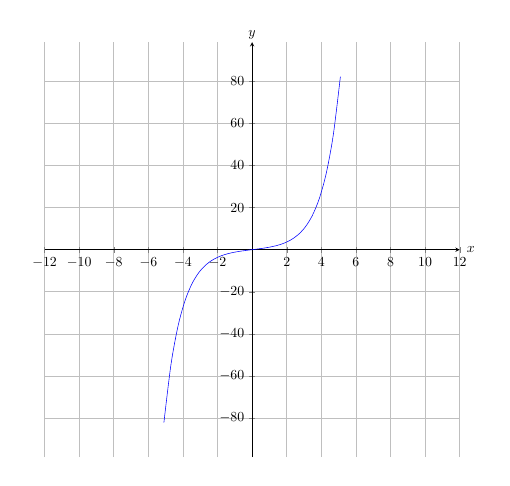
\begin{tikzpicture}[scale=.5]
		\begin{axis}[
			xmin=-10,xmax=10,
			restrict y to domain=-100:100,
			grid=both,width=\textwidth,height=\textwidth,
			axis lines=middle,
			xlabel=$x$,
			ylabel=$y$,
			enlarge x limits=0.1,
			enlarge y limits=0.1,
			x label style={at={(ticklabel* cs:1.00)}, inner sep=5pt, anchor=west},
			y label style={at={(ticklabel* cs:1.00)}, inner sep=2pt, anchor=south},
		]
			\addplot[color=blue,samples=50,smooth,domain=-10:10]{.5*(exp(x)-exp(-x))};
		\end{axis}
	\end{tikzpicture}
	\caption{双曲正弦函数\(\sinh\)的图形}
	\label{figure:函数.双曲正弦函数的图形}
\end{figure}
%@Mathematica: Plot[Sinh[x], {x, -10, 10}]

\begin{figure}[htb]
	\centering
	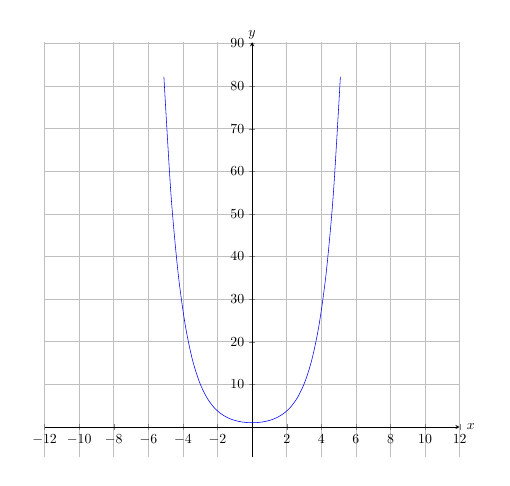
\begin{tikzpicture}[scale=.5]
		\begin{axis}[
			xmin=-10,xmax=10,
			restrict y to domain=-100:100,
			grid=both,width=\textwidth,height=\textwidth,
			axis lines=middle,
			xlabel=$x$,
			ylabel=$y$,
			enlarge x limits=0.1,
			enlarge y limits=0.1,
			x label style={at={(ticklabel* cs:1.00)}, inner sep=5pt, anchor=west},
			y label style={at={(ticklabel* cs:1.00)}, inner sep=2pt, anchor=south},
		]
			\addplot[color=blue,samples=50,smooth,domain=-10:10]{.5*(exp(x)+exp(-x))};
		\end{axis}
	\end{tikzpicture}
	\caption{双曲余弦函数\(\cosh\)的图形}
	\label{figure:函数.双曲余弦函数的图形}
\end{figure}
%@Mathematica: Plot[Cosh[x], {x, -10, 10}]

\begin{figure}[htb]
	\centering
	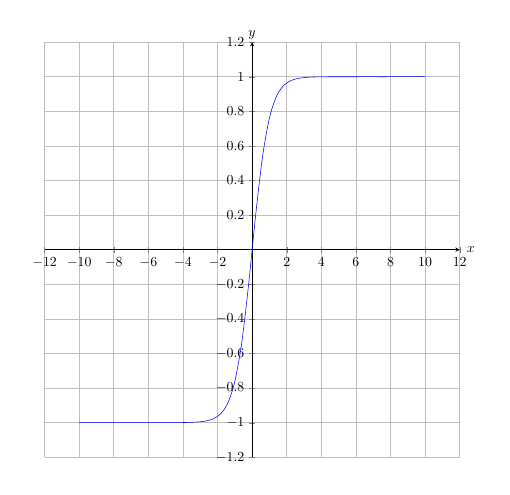
\begin{tikzpicture}[scale=.5]
		\begin{axis}[
			xmin=-10,xmax=10,
			restrict y to domain=-100:100,
			grid=both,width=\textwidth,height=\textwidth,
			axis lines=middle,
			xlabel=$x$,
			ylabel=$y$,
			enlarge x limits=0.1,
			enlarge y limits=0.1,
			x label style={at={(ticklabel* cs:1.00)}, inner sep=5pt, anchor=west},
			y label style={at={(ticklabel* cs:1.00)}, inner sep=2pt, anchor=south},
		]
			\addplot[color=blue,samples=50,smooth,domain=-10:10]{(exp(x)-exp(-x))/(exp(x)+exp(-x))};
		\end{axis}
	\end{tikzpicture}
	\caption{双曲正切函数\(\tanh\)的图形}
	\label{figure:函数.双曲正切函数的图形}
\end{figure}
%@Mathematica: Plot[Tanh[x], {x, -10, 10}]

\begin{figure}[htb]
	\centering
	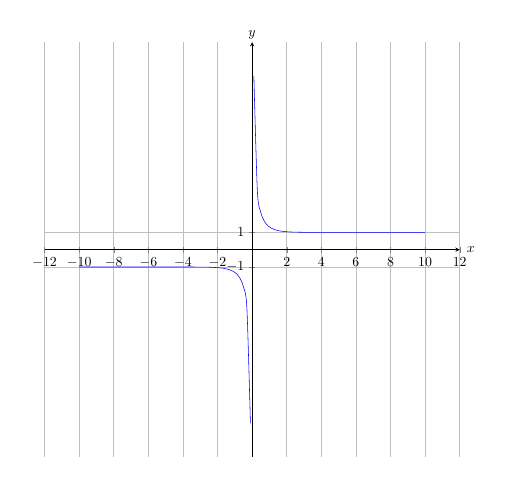
\begin{tikzpicture}[scale=.5]
		\begin{axis}[
			xmin=-10,xmax=10,
			ymin=-10,ymax=10,
			grid=both,width=\textwidth,height=\textwidth,
			axis lines=middle,
			xlabel=$x$,
			ylabel=$y$,
			enlarge x limits=0.1,
			enlarge y limits=0.1,
			x label style={at={(ticklabel* cs:1.00)}, inner sep=5pt, anchor=west},
			y label style={at={(ticklabel* cs:1.00)}, inner sep=2pt, anchor=south},
			ytick={-1,1},
		]
			\addplot[color=blue,samples=50,smooth,domain=-10:-.1]
				{(exp(x)+exp(-x))/(exp(x)-exp(-x))};
			\addplot[color=blue,samples=50,smooth,domain=.1:10]
				{(exp(x)+exp(-x))/(exp(x)-exp(-x))};
		\end{axis}
	\end{tikzpicture}
	\caption{双曲余切函数\(\coth\)的图形}
	\label{figure:函数.双曲余切函数的图形}
\end{figure}
%@Mathematica: Plot[Coth[x], {x, -10, 10}]

\begin{figure}[htb]
	\centering
	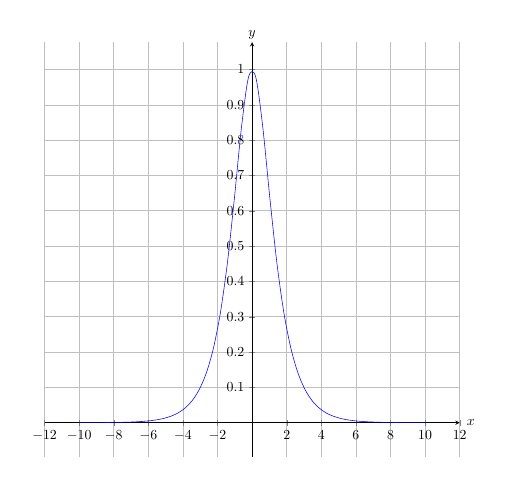
\begin{tikzpicture}[scale=.5]
		\begin{axis}[
			xmin=-10,xmax=10,
			restrict y to domain=-100:100,
			grid=both,width=\textwidth,height=\textwidth,
			axis lines=middle,
			xlabel=$x$,
			ylabel=$y$,
			enlarge x limits=0.1,
			enlarge y limits=0.1,
			x label style={at={(ticklabel* cs:1.00)}, inner sep=5pt, anchor=west},
			y label style={at={(ticklabel* cs:1.00)}, inner sep=2pt, anchor=south},
		]
			\addplot[color=blue,samples=50,smooth,domain=-10:10]{2/(exp(x)+exp(-x))};
		\end{axis}
	\end{tikzpicture}
	\caption{双曲正割函数\(\sech\)的图形}
\end{figure}
%@Mathematica: Plot[Sech[x], {x, -10, 10}]

\begin{figure}[htb]
	\centering
	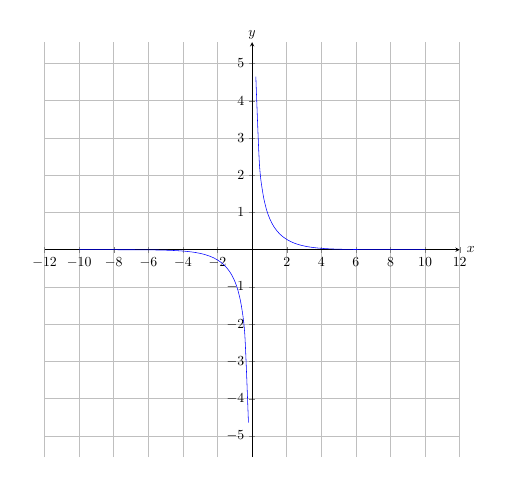
\begin{tikzpicture}[scale=.5]
		\begin{axis}[
			xmin=-10,xmax=10,
			restrict y to domain=-100:100,
			grid=both,width=\textwidth,height=\textwidth,
			axis lines=middle,
			xlabel=$x$,
			ylabel=$y$,
			enlarge x limits=0.1,
			enlarge y limits=0.1,
			x label style={at={(ticklabel* cs:1.00)}, inner sep=5pt, anchor=west},
			y label style={at={(ticklabel* cs:1.00)}, inner sep=2pt, anchor=south},
		]
			\addplot[color=blue,samples=50,smooth,domain=-10:-.01]{2/(exp(x)-exp(-x))};
			\addplot[color=blue,samples=50,smooth,domain=.01:10]{2/(exp(x)-exp(-x))};
		\end{axis}
	\end{tikzpicture}
	\caption{双曲余割函数\(\csch\)的图形}
\end{figure}
%@Mathematica: Plot[Csch[x], {x, -10, 10}]

下面我们研究双曲函数的反函数.

首先讨论双曲正弦\(y=\sinh x\)的反函数.
由\(x=\sinh y\),有\begin{equation*}
	x=\frac{e^y-e^{-y}}{2}.
\end{equation*}
令\(u=e^y\),则有\begin{equation*}
	u^2-2xu-1=0.
\end{equation*}
这是一个关于\(u\)的一元二次方程,解得\begin{equation*}
	u=x\pm\sqrt{x^2+1}.
\end{equation*}
因为\(u=e^y>0\),故上式根号前应取正号,即\begin{equation*}
	u=x+\sqrt{x^2+1}.
\end{equation*}
又由\(y=\ln u\),故得反双曲正弦\begin{equation*}
	\arsinh x
	\defeq
	\ln(x+\sqrt{x^2+1}),
	\quad -\infty<x<+\infty.
\end{equation*}

\begin{figure}[htb]
	\centering
	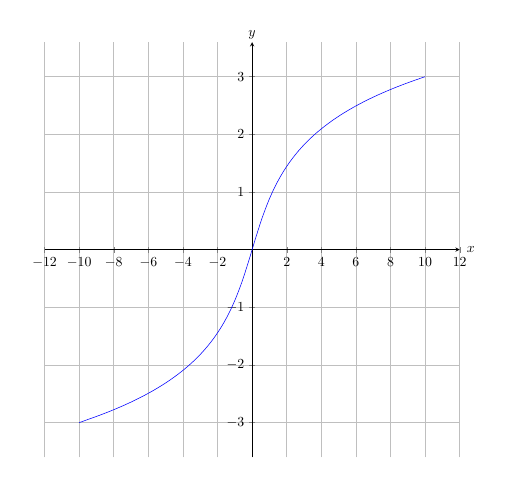
\begin{tikzpicture}[scale=.5]
		\begin{axis}[
			xmin=-10,xmax=10,
			restrict y to domain=-100:100,
			grid=both,width=\textwidth,height=\textwidth,
			axis lines=middle,
			xlabel=$x$,
			ylabel=$y$,
			enlarge x limits=0.1,
			enlarge y limits=0.1,
			x label style={at={(ticklabel* cs:1.00)}, inner sep=5pt, anchor=west},
			y label style={at={(ticklabel* cs:1.00)}, inner sep=2pt, anchor=south},
		]
			\addplot[color=blue,samples=50,smooth,domain=-10:10]{ln(x+sqrt(1+x^2))};
		\end{axis}
	\end{tikzpicture}
	\caption{反双曲正弦函数\(\arsinh\)的图形}
\end{figure}
%@Mathematica: Plot[ArcSinh[x], {x, -10, 10}]

接下来讨论双曲余弦函数\(y=\cosh x\)的反函数.
由\(x=\cosh y\),有\begin{equation*}
	x=\frac{e^y+e^{-y}}{2},
\end{equation*}
显然恒有\(x>0\).
由此得\(e^y=x\pm\sqrt{x^2-1}\ (x\geq1)\),
故\begin{equation*}
	y=\ln(x\pm\sqrt{x^2-1})
	\quad(x\geq1).
\end{equation*}
可见,函数\begin{equation*}
	y=\ln(x+\sqrt{x^2-1})
	\quad(x\geq1)
\end{equation*}是双曲余弦函数右支\(y=\cosh x\ (x\geq0)\)的反函数,
我们把它记作\(\arcosh x\),
即\begin{equation*}
	\arcosh x
	\defeq
	\ln(x + \sqrt{x^2 - 1}),
	\quad 1\leq x<+\infty.
\end{equation*}
而函数\begin{equation*}
	y=\ln(x-\sqrt{x^2-1})
	\quad(x\geq1)
\end{equation*}是双曲余弦函数左支\(y=\cosh x\ (x\leq0)\)的反函数.

\begin{figure}[htb]
	\centering
	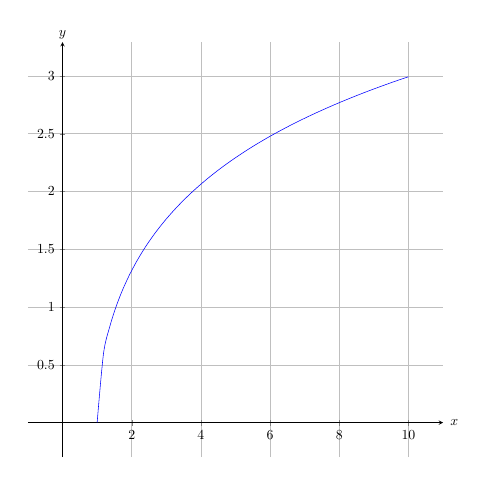
\begin{tikzpicture}[scale=.5]
		\begin{axis}[
			xmin=0,xmax=10,
			restrict y to domain=-100:100,
			grid=both,width=\textwidth,height=\textwidth,
			axis lines=middle,
			xlabel=$x$,
			ylabel=$y$,
			enlarge x limits=0.1,
			enlarge y limits=0.1,
			x label style={at={(ticklabel* cs:1.00)}, inner sep=5pt, anchor=west},
			y label style={at={(ticklabel* cs:1.00)}, inner sep=2pt, anchor=south},
		]
			\addplot[color=blue,samples=50,smooth,domain=1:10]{ln(x+sqrt(x^2-1))};
		\end{axis}
	\end{tikzpicture}
	\caption{反双曲余弦函数\(\arcosh\)的图形}
\end{figure}
%@Mathematica: Plot[ArcCosh[x], {x, 0, 10}]

易见\begin{equation*}
	\ln(x+\sqrt{x^2-1}) + \ln(x-\sqrt{x^2-1}) = 0
	\quad(x\geq1).
\end{equation*}
%@Mathematica: FullSimplify[Log[x + Sqrt[x^2 - 1]] + Log[x - Sqrt[x^2 - 1]], Assumptions -> {x >= 1}]
%@credit: {cee35532-e299-4587-89a0-7b84e7454774}

然后讨论双曲正切函数\(\tanh\)的反函数.
由\begin{equation*}
	x = \tanh y
	= \frac{e^y-e^{-y}}{e^y+e^{-y}}
	= \frac{e^{2y}-1}{e^{2y}+1},
\end{equation*}得\begin{equation*}
	(1-x) e^{2y} = 1+x,
\end{equation*}
解得\(y = \frac12 \ln\frac{1+x}{1-x}\).
要使对数\(\ln\frac{1+x}{1-x}\)有意义,必有\((1+x)(1-x)>0\),
即\(x\in(-1,1)\).
于是反双曲正切函数可以定义为\begin{equation*}
	\artanh x
	\defeq
	\frac12 \ln\frac{1 + x}{1 - x},
	\quad -1<x<1.
\end{equation*}

\begin{figure}[htb]
	\centering
	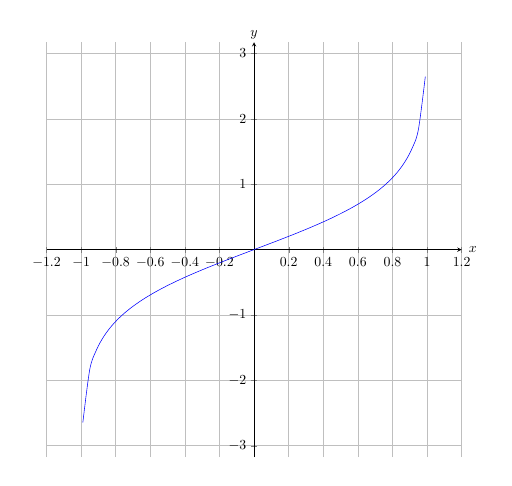
\begin{tikzpicture}[scale=.5]
		\begin{axis}[
			xmin=-1,xmax=1,
			restrict y to domain=-100:100,
			grid=both,width=\textwidth,height=\textwidth,
			axis lines=middle,
			xlabel=$x$,
			ylabel=$y$,
			enlarge x limits=0.1,
			enlarge y limits=0.1,
			x label style={at={(ticklabel* cs:1.00)}, inner sep=5pt, anchor=west},
			y label style={at={(ticklabel* cs:1.00)}, inner sep=2pt, anchor=south},
		]
			\addplot[color=blue,samples=50,smooth,domain=-.99:.99]{.5*ln((1+x)/(1-x))};
		\end{axis}
	\end{tikzpicture}
	\caption{反双曲正切函数\(\artanh\)的图形}
\end{figure}
%@Mathematica: Plot[ArcTanh[x], {x, -1, 1}]

最后讨论双曲余切函数\(\coth\)的反函数.
由\begin{equation*}
	x = \coth y
	= \frac{e^y+e^{-y}}{e^y-e^{-y}}
	= \frac{e^{2y}+1}{e^{2y}-1},
\end{equation*}得\begin{equation*}
	(x-1) e^{2y} = 1+x,
\end{equation*}
解得\(y = \frac12 \ln\frac{x+1}{x-1}\).
要使对数\(\ln\frac{x+1}{x-1}\)有意义,必有\((x+1)(x-1)>0\),
即\(x\in(-\infty,-1)\cup(1,+\infty)\).
于是反双曲余切函数可以定义为\begin{equation*}
	\arcoth x
	\defeq
	\frac12 \ln\frac{x + 1}{x - 1},
	\quad -\infty<x<-1\lor1<x<+\infty.
\end{equation*}

\begin{figure}[htb]
	\centering
	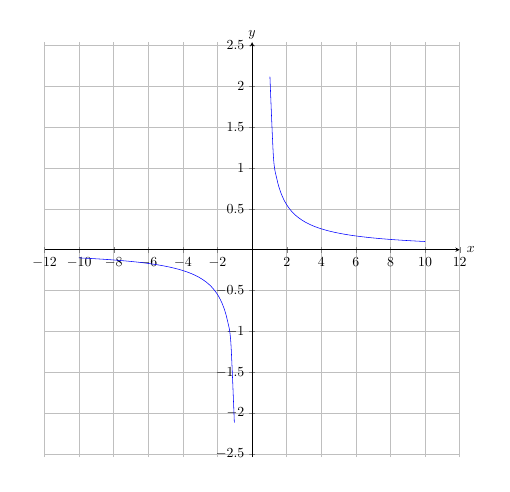
\begin{tikzpicture}[scale=.5]
		\begin{axis}[
			xmin=-10,xmax=10,
			restrict y to domain=-100:100,
			grid=both,width=\textwidth,height=\textwidth,
			axis lines=middle,
			xlabel=$x$,
			ylabel=$y$,
			enlarge x limits=0.1,
			enlarge y limits=0.1,
			x label style={at={(ticklabel* cs:1.00)}, inner sep=5pt, anchor=west},
			y label style={at={(ticklabel* cs:1.00)}, inner sep=2pt, anchor=south},
		]
			\addplot[color=blue,samples=50,smooth,domain=-10:-.01]{.5*ln((x+1)/(x-1))};
			\addplot[color=blue,samples=50,smooth,domain=.01:10]{.5*ln((x+1)/(x-1))};
		\end{axis}
	\end{tikzpicture}
	\caption{反双曲余切函数\(\arcoth\)的图形}
\end{figure}
%@Mathematica: Plot[ArcCoth[x], {x, -10, 10}]

\begin{property}
双曲正弦\(\sinh\)是奇函数.
\end{property}

\begin{property}
双曲余弦\(\cosh\)是偶函数.
\end{property}

\begin{property}
\(\cosh x\)有下界:\begin{equation*}
	\cosh x \geq 1
\end{equation*}
当且仅当\(x=0\)时,上式取等号.
\end{property}

\begin{theorem}
\begin{gather}
	\sinh(x \pm y) = \sinh x\cosh y \pm \cosh x\sinh y, \\
	\cosh(x \pm y) = \cosh x\cosh y \pm \sinh x\sinh y, \\
	\tanh(x + y) = \frac{\tanh x + \tanh y}{1 + \tanh x\tanh y}.
\end{gather}
\begin{proof}
根据双曲函数的定义有
\begin{align*}
	\sinh x\cosh y+\cosh x\sinh y
	&= \frac{e^x - e^{-x}}{2} \frac{e^y + e^{-y}}{2}
		+ \frac{e^x + e^{-x}}{2} \frac{e^y - e^{-y}}{2} \\
	&= \frac{1}{4} (e^x e^y + e^x e^{-y} - e^{-x} e^y - e^{-x} e^{-y} \\
	&\qquad+ e^x e^y - e^x e^{-y} + e^{-x} e^y - e^{-x} e^{-y}) \\
	&= \frac{1}{4} (2 e^x e^y - 2 e^{-x} e^{-y}) \\
	&= \frac12 (e^{x+y} - e^{-x-y}) = \sinh(x+y).
\end{align*}
\begin{align*}
	\cosh x\cosh y+\sinh x\sinh y
	&= \frac{e^x + e^{-1}}{2} \frac{e^y + e^{-y}}{2}
		+ \frac{e^x - e^{-x}}{2} \frac{e^y - e^{-y}}{2} \\
	&= \frac{1}{4} (e^x e^y + e^x e^{-y} + e^{-x} e^y + e^{-x} e^{-y} \\
	&\qquad+ e^x e^y - e^x e^{-y} - e^{-x} e^y + e^{-x} e^{-y}) \\
	&= \frac{1}{4} (2 e^x e^y + 2 e^{-x} e^{-y}) \\
	&= \frac12 (e^{x+y} + e^{-x-y}) = \cosh(x+y).
	\qedhere
\end{align*}
\end{proof}
\end{theorem}

\begin{theorem}
\begin{gather}
	\cosh^2x - \sinh^2x = 1, \\
	\sinh x + \cosh x = e^x, \\
	\cosh x - \sinh x = e^{-x}, \\
	1 - \tanh^2 x = \sech^2 x, \\
	\coth^2 x - 1 = \csch^2 x.
\end{gather}
\begin{proof}
根据双曲函数的定义有
\begin{align*}
	\cosh^2x-\sinh^2x
	&=\left(\frac{e^x + e^{-x}}{2}\right)^2-\left(\frac{e^x - e^{-x}}{2}\right)^2 \\
	&=\frac{e^{2x}+2+e^{-2x}}{4}-\frac{e^{2x}-2+e^{-2x}}{4}
	=1.
	\qedhere
\end{align*}
\end{proof}
\end{theorem}

\begin{theorem}
\begin{gather}
	\sinh2x = 2 \sinh x\cosh x, \\
	\cosh2x = \cosh^2x + \sinh^2x.
\end{gather}
\end{theorem}

\section{幂指函数}
\begin{definition}
形如\begin{equation*}
	y = u(x)^{v(x)},
	\quad u(x) > 0 \land u(x) \not\equiv 1
\end{equation*}的函数称为\DefineConcept{幂指函数}.
\end{definition}
值得注意的是,幂指函数不是初等函数.

\section{其他常见函数}
\subsection{单位阶跃函数}
\begin{definition}
函数\begin{equation*}
f(x) = \left\{ \begin{array}{cc}
0, & x < 0, \\
1, & x \geq 1
\end{array} \right.
\end{equation*}称为\DefineConcept{单位阶跃函数}或\DefineConcept{赫维赛德阶跃函数}.
\end{definition}

\begin{figure}[htb]
	\centering
	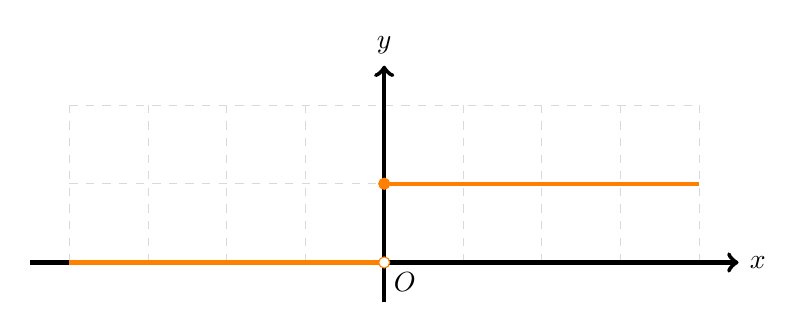
\begin{tikzpicture}
		\draw[help lines,color=gray!30,dashed](-4,0)grid(4,2);
		\draw[->,ultra thick](-4.5,0)--(4.5,0)node[right]{\(x\)};
		\draw[->,ultra thick](0,-.5)--(0,2.5)node[above]{\(y\)};
		\draw (0,0)node[below right]{\(O\)};
		\draw[orange,ultra thick](-4,0)--(0,0) (0,1)--(4,1);
		\draw[draw=orange,fill=orange](0,1)circle(2pt);
		\draw[draw=orange,fill=white](0,0)circle(2pt);
	\end{tikzpicture}
	\caption{单位阶跃函数的图形}
\end{figure}

\subsection{克罗内克\texorpdfstring{\(\delta\)}{\textdelta}函数}
\begin{definition}
%@see: https://mathworld.wolfram.com/KroneckerDelta.html
定义:\begin{equation*}
\delta_K(a,b)
\defeq \left\{ \begin{array}{cl}
	1, & a = b, \\
	0, & a \neq b.
\end{array} \right.
\end{equation*}称其为\DefineConcept{克罗内克\(\delta\)函数}.
\end{definition}

\subsection{狄拉克\texorpdfstring{\(\delta\)}{\textdelta}函数}
\begin{definition}
%@see: https://functions.wolfram.com/GeneralizedFunctions/DiracDelta/02/
%@see: https://functions.wolfram.com/GeneralizedFunctions/DiracDelta2/02/
定义:\begin{equation*}
	\delta_D(x)
	\defeq \frac{1}{\pi}
		\lim_{\epsilon\to0}
		\frac{\epsilon}{x^2+\epsilon^2}
	\quad(x\in\mathbb{R}).
\end{equation*}
称其为\DefineConcept{狄拉克\(\delta\)函数}.
\end{definition}

%@see: https://mathworld.wolfram.com/DeltaFunction.html

\section{隐函数}
\subsection{由参数方程确定的函数}
%@see: https://www.bilibili.com/video/BV1DNsoeAEii
\begin{example}
%@see: 《2023年全国硕士研究生入学统一考试(数学一)》一选择题/第3题
求解由参数方程\begin{equation*}
	\left\{ \begin{array}{l}
		x = 2t + \abs{t}, \\
		y = \abs{t} \sin t
	\end{array} \right.
\end{equation*}确定的函数\(y = f(x)\).
\begin{solution}
当\(t\geq0\)时,\(x = 2t + t = 3t \geq 0\),\(y = t \sin t\).
当\(t<0\)时,\(x = 2t - t = t < 0\),\(y = -t \sin t\).
因此\begin{equation*}
	f(x) = \left\{ \begin{array}{cl}
		\frac{x}{3} \sin \frac{x}{3}, & x\geq0, \\
		-x \sin x, & x<0.
	\end{array} \right.
\end{equation*}
\end{solution}
\end{example}
\begin{example}
求解由参数方程\begin{equation*}
	\left\{ \begin{array}{l}
		x = t \abs{t}, \\
		y = \abs{t} \sin t^2
	\end{array} \right.
\end{equation*}确定的函数\(y = f(x)\).
\begin{solution}
当\(t\geq0\)时,\(x = t^2 \geq 0\),\(t = \sqrt{x}\),\(y = t \sin t^2\).
当\(t<0\)时,\(x = -t^2 < 0\),\(t = -\sqrt{-x}\),\(y = -t \sin t^2\).
因此\begin{equation*}
	f(x) = \left\{ \begin{array}{cl}
		\sqrt{x} \sin x, & x\geq0, \\
		-\sqrt{-x} \sin x, & x<0.
	\end{array} \right.
\end{equation*}
\end{solution}
\end{example}

\section{抽象函数}
%@see: https://mathworld.wolfram.com/CauchyFunctionalEquation.html
%@see: https://math.stackexchange.com/a/423494/591741

% Cauchy's additive functional equation
方程\begin{equation*}
	f(x+y) = f(x) + f(y) + c
\end{equation*}确定的函数\(f\)称为直线型抽象函数,
其中\(c\)是与\(x\)、\(y\)无关的常数.

% Cauchy's multiplicative functional equation
方程\begin{equation*}
	f(xy) = f(x) f(y)
\end{equation*}确定的函数\(f\)称为幂函数型抽象函数.

% Cauchy's exponential functional equation
方程\begin{equation*}
	f(x+y) = f(x) f(y)
\end{equation*}或\begin{equation*}
	f(xy) = [f(x)]^y
\end{equation*}确定的函数\(f\)称为指数函数型抽象函数.

% Cauchy's logarithmic functional equation
方程\begin{equation*}
	f(xy) = f(x) + f(y)
\end{equation*}或\begin{equation*}
	f\left(\frac{x}{y}\right) = f(x) - f(y)
\end{equation*}确定的函数\(f\)称为对数函数型抽象函数.

方程\begin{equation*}
	f(x) + f(y) = 2 f\left(\frac{x+y}{2}\right) f\left(\frac{x-y}{2}\right)
\end{equation*}或\begin{equation*}
	f(x+y) = \frac{f(x) + f(y)}{1 - f(x) f(y)}
\end{equation*}确定的函数\(f\)称为三角函数型抽象函数.

\input{初等数学/函数/初等函数}

\chapter{数列}
\chapter{数列}
\section{数列的概念}
\begin{definition}\label{definition:数列.数列的定义}
一般地,如果\(D \subseteq \mathbb{Z}\),
那么把映射\begin{equation*}
    f\colon D\to\mathbb{R}, n \mapsto a_n
\end{equation*}称为一个\DefineConcept{数列}(sequence,progression),
记作\(\{a_n\}\),即\(\{a_n\} \defeq f\).

数列中的每一个数(例如\(\AutoTuple{a}{0}\))叫做数列的\DefineConcept{项}(term).

把表示第\(n\)个数\(a_n\)的公式称为“数列\(\{a_n\}\)的\DefineConcept{一般项}”.
\end{definition}

应该指出,如果我们说“数列\(\{x_n\}\)在数集\(X\)内”或\(\{x_n\} \subseteq X\),
我们指的是:把数列\(\{x_n\}\)看作一个映射\(f\)时,
这个映射的值域\(\ran f\)是\(X\)的子集,即\(\ran f \subseteq X\).

\begin{definition}
如果数列\(\{x_n\}\)满足条件\begin{equation*}
	x_n \leq x_{n+1}, \quad n=1,2,\dotsc,
\end{equation*}
就称“数列\(\{x_n\}\)是\DefineConcept{单调增加的}”.

如果数列\(\{x_n\}\)满足条件\begin{equation*}
	x_n \geq x_{n+1}, \quad n=1,2,\dotsc,
\end{equation*}
就称“数列\(\{x_n\}\)是\DefineConcept{单调减少的}”.

单调增加数列和单调减少数列统称为\DefineConcept{单调数列}.
如果数列\(\{x_n\}\)是单调数列,则称“\(\{x_n\}\)具有单调性”.
\end{definition}

\begin{definition}
如果数列\(\{x_n\}\)满足\begin{equation*}
	(\forall n \geq N)[x_n \leq x_{n+1}],
\end{equation*}
则称“数列\(\{x_n\}\)从第\(N\)项起单调增加”.

如果数列\(\{x_n\}\)满足\begin{equation*}
	(\forall n \geq N)[x_n \geq x_{n+1}],
\end{equation*}
则称“数列\(\{x_n\}\)从第\(N\)项起单调减少”.
\end{definition}

\begin{proposition}
设数列\(\{x_n\}\)满足\begin{equation*}
	(x_{n+1}-x_n)(x_n-x_{n-1})>0
	\quad(n=2,3,\dotsc),
\end{equation*}
则\(\{x_n\}\)具有单调性.
\end{proposition}

\begin{definition}[数列的有界性]
设数列\(\{x_n\}\).

如果\begin{equation*}
	(\exists M>0)
	(\forall n\in\mathbb{N})
	[\abs{x_n} \leq M],
\end{equation*}
那么称“数列\(\{x_n\}\)是\DefineConcept{有界的}”.

如果这样的正数\(M\)不存在,即\begin{equation*}
	(\forall M>0)
	(\exists n\in\mathbb{N})
	[\abs{x_n} > M],
\end{equation*}
那么称“数列\(\{x_n\}\)是\DefineConcept{无界的}”.
\end{definition}

例如,数列\(x_n = \frac{n}{n+1}\ (n=1,2,\dotsc)\)是有界的,
因为可取\(M=1\),而使\begin{equation*}
	\abs{\frac{n}{n+1}} \leq 1
\end{equation*}对于一切正整数\(n\)都成立.

数列\(x_n = 2^n\ (n=1,2,\dotsc)\)是无界的,因为当\(n\)无限增加时,\(2^n\)可超过任何正数.

\begin{definition}
%@see: 《数学分析(第二版 上册)》(陈纪修) P62 定义2.4.2
设\(\{a_n\}\)是数列,
我们把\(\{a_n\}\)的子集称为“\(\{a_n\}\)的\DefineConcept{子列}”.
\end{definition}
我们常把数列\(\{a_n\}\)的子列记作\(\{a_{n_k}\}\),
这里下标\(n_k\)表示子列中的第\(k\)项恰好是原数列\(\{a_n\}\)中的第\(n_k\)项.
应该注意到,由于子列下标\(n_k\)是严格单调增加的,
所以\begin{equation*}
	(\forall k\in\mathbb{N}^+)
	[n_k \geq k],
\end{equation*}
且\begin{equation*}
	(\forall i,j\in\mathbb{N}^+)
	[i \geq j \implies n_i \geq n_j].
\end{equation*}

\section{数列的连加与连乘}
\subsection{数列的连加}
\begin{definition}[连加]
定义\DefineConcept{连续求和}:\begin{equation*}
	\sum_{i=m}^n a_i
	\defeq
	a_m + a_{m+1} + \dotsb + a_{n-1} + a_n
	\quad(m \leq n),
\end{equation*}
其中符号\(\sum\)称作\DefineConcept{连加号},
符号\(i\)称为\DefineConcept{求和指标}(index of summation),
整数\(m\)称为\DefineConcept{求和下限}(lower bound),
整数\(n\)称为\DefineConcept{求和上限}(upper bound),
符号\(a_i\)称为\DefineConcept{求和通项}(summand).
\end{definition}

\begin{figure}[htb]
	\centering
	\begin{tikzpicture}
		\draw(0,0)node{$\sum_{
			{\textcolor{red}i}
			=
			{\textcolor{blue}m}
		}^{\textcolor{yellow-green}n} x_i$};
		\draw(-.2,1)node{\textcolor{yellow-green}{求和上限}};
		\draw(-1.5,-.5)node{\textcolor{red}{求和指标}};
		\draw(1.1,-.5)node{\textcolor{blue}{求和下限}};
	\end{tikzpicture}
	\caption{}
\end{figure}

有时候也把\(\sum_{i=m}^n\)%
写作\(\sum_{m \leq i \leq n}\).

使用双重连加号求和时,如果两个求和指标独立取值,则连加号\(\sum\)的顺序可以交换.

在不引起误解的情况下,可以省略不写求和指标,
例如用\(\sum a_n\)表示\(\sum_{k=1}^n a_k\).

\subsection{数列的连乘}
\begin{definition}[连乘]
定义\DefineConcept{连续求积}:\begin{equation*}
	\prod_{i=m}^n a_i
	\defeq
	a_m \times a_{m+1} \times \dotsb \times a_{n-1} \times a_n
	\quad(m \leq n),
\end{equation*}
其中符号\(\prod\)称作\DefineConcept{连乘号},
整数\(i\)称为\DefineConcept{求积指标}.
\end{definition}

同样地,有时候也把\(\prod_{i=m}^n\)%
写作\(\prod_{m \leq i \leq n}\).

\begin{definition}\label{definition:数列.阶乘的定义}
给定一个正整数\(n\),
称所有小于或等于\(n\)的正整数的积为“\(n\)的\DefineConcept{阶乘}(factorial)”,
记作\(n!\),即
\begin{equation}
	n!
	\defeq
	\prod_{k=1}^n k
	=
	n \times (n-1) \times (n-2) \times \dotsm \times 2 \times 1.
\end{equation}
特别地,规定\(0! = 1\).
\end{definition}

\begin{table}[htb]
	\centering
	\begin{subtable}[ht]{.3\textwidth}
		\centering
		\begin{tblr}{rcr}
			\hline
			0! & = & 1 \\
			1! & = & 1 \\
			2! & = & 2 \\
			3! & = & 6 \\
			4! & = & 24 \\
			5! & = & 120 \\
			6! & = & 720 \\
			7! & = & 5~040 \\
			8! & = & 40~320 \\
			9! & = & 362~880 \\
			\hline
		\end{tblr}
		\caption{}
	\end{subtable}~\begin{subtable}[ht]{.6\textwidth}
		\centering
		\begin{tblr}{rcr|rcr}
			\hline
			0!! & = & 1 & 1!! & = & 1 \\
			2!! & = & 2 & 3!! & = & 3 \\
			4!! & = & 8 & 5!! & = & 15 \\
			6!! & = & 48 & 7!! & = & 105 \\
			8!! & = & 384 & 9!! & = & 945 \\
			10!! & = & 3~840 & 11!! & = & 10~395 \\
			12!! & = & 46~080 & 13!! & = & 135~135 \\
			14!! & = & 645~120 & 15!! & = & 2~027~025 \\
			16!! & = & 10~321~920 & 17!! & = & 34~459~425 \\
			18!! & = & 185~794~560 & 19!! & = & 654~729~075 \\
			\hline
		\end{tblr}
		\caption{}
	\end{subtable}
	\caption{}
%@Mathematica: Table[{n, n!}, {n, 0, 9}]
%@Mathematica: Table[{n, n!!}, {n, 0, 20, 2}]
%@Mathematica: Table[{n, n!!}, {n, 1, 20, 2}]
\end{table}

\begin{definition}
给定一个正整数\(n\),
称小于或等于\(n\)且与之同奇偶的所有正整数的积为“\(n\)的\DefineConcept{双阶乘}”,
记作\(n!!\),即
\begin{equation}
	n!!
	\defeq
	\begin{cases}
		n \times (n-2) \times (n-4) \times \dotsm \times 3 \times 1, & n\text{是奇数}, \\
		n \times (n-2) \times (n-4) \times \dotsm \times 4 \times 2, & n\text{是偶数}.
	\end{cases}
\end{equation}
特别地,规定\(0!! = 1\).
\end{definition}

需要注意的是,通常来说双阶乘\(n!!\)并不等于“阶乘的阶乘”\((n!)!\),
实际上,\(3!! = 3\)而\((3!)! = 6! = 720\).

\section{等差数列}
一般地,如果一个数列从第2项起,每一项与它的前一项的差等于同一个常数,
这个数列就叫做\DefineConcept{等差数列}(arithmetical progression),
这个常数叫做等差数列的\DefineConcept{公差}(common difference).

如果数列\(\{a_n\}\)是等差数列,它的公差是\(d\),那么\begin{align*}
    a_2 &= a_1 + d, \\
    a_3 &= a_2 + d = (a_1 + d) + d = a_1 + 2d, \\
    a_4 &= a_3 + d = (a_1 + 2d) + d = a_1 + d3.
\end{align*}
以此类推,可知等差数列\(\{a_n\}\)的\DefineConcept{通项公式}是\begin{equation}
    a_n = a_1 + (n-1) d.
\end{equation}

将等差数列中任意两项\begin{equation*}
    a_m = a_1 + (m-1) d
    \quad\text{与}\quad
    a_n = a_1 + (n-1) d
\end{equation*}相减,得到\begin{equation*}
    a_m - a_n = (m-n) d.
\end{equation*}
由此我们也可得到%
等差数列的\DefineConcept{递推公式}:\begin{equation}
    a_{n+1} - a_n = d.
\end{equation}

\begin{property}[等差数列求和]
设数列\(\{a_n\}\)为等差数列,它的通项公式为\begin{equation*}
    a_n = a_1 + (n-1) d,
\end{equation*}
那么它的前\(n\)项和为\begin{equation}\label{equation:数列.等差数列的前n项和1}
    S_n = \frac{n(a_1 + a_n)}{2},
\end{equation}
或\begin{equation}\label{equation:数列.等差数列的前n项和2}
    S_n = n a_1 + \frac{n(n-1)}{2} d.
\end{equation}
\begin{proof}
由\begin{equation*}
    S_n = a_1 + (a_1 + d) + \dotsb + [a_1 + (n-2)d] + [a_1 + (n-1)d],
\end{equation*}\begin{equation*}
    S_n = [a_n - (n-1)d] + [a_n - (n-2)d] + \dotsb + (a_n - d) + a_n,
\end{equation*}相加得\begin{equation*}
    2 S_n = n(a_1 + a_n),
\end{equation*}最终可得\begin{equation*}
    S_n = \frac{n(a_1 + a_n)}{2} = n a_1 + \frac{n(n-1)}{2} d.
    \qedhere
\end{equation*}
\end{proof}
\end{property}

根据\hyperref[equation:数列.等差数列的前n项和1]{等差数列的前\(n\)项和公式},立即有如下结论:
\begin{equation}
    \sum_{k=1}^n k = \frac{1}{2} n(n+1).
\end{equation}

\begin{property}
设数列\(\{a_n\}\)是以\(d\)为公差的等差数列,
\(b\)是常数,
则\(\{b + a_n\}\)也是以\(d\)为公差的等差数列.
\end{property}

\begin{property}
设数列\(\{a_n\}\)是以\(d\)为公差的等差数列,
\(b\)是常数,
则\(\{b \cdot a_n\}\)是以\(b d\)为公差的等差数列.
\end{property}

\begin{example}
设\(\{a_n\}\)是等差数列.
证明:如果正整数\(m,n,p,q\)满足\(m+n=p+q\),
则\begin{equation*}
	a_m+a_n=a_p+a_q.
\end{equation*}
\begin{proof}
设\(\{a_n\}\)的公差是\(d\),
则\(a_m-a_p = (m-p)d\).
由\(m+n=p+q\)
移项得\(m-p=q-n\),
于是\(a_m-a_p = a_q-a_n\),
因此\(a_m+a_n=a_p+a_q\).
\end{proof}
\end{example}

\begin{example}
设\(\{a_n\}\)是公差为\(d\)的等差数列.
证明:\(S_k,S_{2k}-S_k,S_{3k}-S_{2k},\dotsc\)成为等差数列,
它的公差为\(k^2 d\).
\begin{proof}
既然\(S_n = n a_1 + \frac12 n(n-1) d\ (n=1,2,\dotsc)\),
那么\begin{align*}
	&\hspace{-20pt}
	(S_{2k}-S_k) - S_k
	= S_{2k} - 2 S_k \\
	&= 2k a_1 + \frac12 (2k)(2k-1) d
	- 2 k a_1 - k(k-1) d \\
	&= k^2 d, \\
	&\hspace{-20pt}
	[S_{(m+1)k}-S_{mk}] - [S_{mk}-S_{(m-1)k}]
	= S_{(m+1)k} - 2 S_{mk} + S_{(m-1)k} \\
	&= (mk+k) a_1 + \frac12 (mk+k)(mk+k-1) d \\
	&\hspace{20pt}
	- 2 mk a_1 - mk (mk-1) d \\
	&\hspace{20pt}
	+ (mk-k) a_1 + \frac12 (mk-k)(mk-k-1) d \\
	&= k^2 d.
	\qedhere
\end{align*}
\end{proof}
\end{example}

\begin{example}
设数列\(\{a_n\}\)的前\(n\)项和为\(S_n\).
证明:\(\left\{\frac{S_n}{n}\right\}\)是等差数列.
\begin{proof}
设\(\{a_n\}\)的公差是\(d\).
因为\(S_n=\frac{n}2(a_1+a_n)\),
所以\(\frac{S_n}{n}=\frac12(a_1+a_n)\),
从而\begin{equation*}
	\frac{S_{n+1}}{n+1}-\frac{S_n}{n}
	= \frac12(a_1+a_{n+1})-\frac12(a_1+a_n)
	= \frac12(a_{n+1}-a_n)
	= \frac{d}2.
\end{equation*}
这就说明\(\left\{\frac{S_n}{n}\right\}\)是公差为\(\frac{d}2\)的等差数列.
\end{proof}
\end{example}

\begin{example}
设数列\(\{a_n\}\)的前\(n\)项和\(S_n = a_1 + a_2 + \dotsb + a_n\)满足\begin{equation*}
	S_n = A n^2 + B n + C,
\end{equation*}
其中\(A,B,C\)是常数.
证明:\begin{itemize}
	\item 若\(C = 0\),则\(\{a_n\}\)是等差数列.
	\item 若\(C \neq 0\),则\(\{a_n\}\)从第二项起成为等差数列.
\end{itemize}
\begin{proof}
首先\begin{equation*}
	a_1 = S_1 = A + B + C, \qquad
	a_n = 2A n + (B-A), \quad n=2,3,\dotsc,
\end{equation*}
于是\begin{equation*}
	a_2 - a_1
	= 2A - C, \qquad
	a_{n+1} - a_n
	= 2A, \quad n=2,3,\dotsc.
\end{equation*}
因此\begin{equation*}
	\text{\(\{a_n\}\)是等差数列}
	\iff
	a_2 - a_1 = a_3 - a_2
	\iff
	2A - C = 2A
	\iff
	C = 0.
	\qedhere
\end{equation*}
\end{proof}
\end{example}

\begin{example}
设\(\{a_n\},\{b_n\}\)都是等差数列.
证明:\(\{a_{b_n}\}\)也是等差数列.
\begin{proof}
设\(\{a_n\},\{b_n\}\)的公差分别为\(d_1,d_2\),
则\begin{equation*}
	a_{b_{n+1}}-a_{b_n}
	=(b_{n+1}-b_n)d_1
	=d_1 d_2,
\end{equation*}
这就说明\(\{a_{b_n}\}\)是公差为\(d_1 d_2\)的等差数列.
\end{proof}
\end{example}

\begin{example}
设\(\{a_n\},\{b_n\}\)都是等差数列.
证明:\(\{p a_n + q b_n\}\)也是等差数列,其中\(p,q\)是常数.
\begin{proof}
设\(\{a_n\},\{b_n\}\)的公差分别为\(d_1,d_2\),
则\begin{equation*}
	(p a_{n+1} + q b_{n+1})
	- (p a_n + q b_n)
	= p (a_{n+1} - a_n)
	+ q (b_{n+1} - b_n)
	= p d_1 + q d_2,
\end{equation*}
这就说明\(\{a_{b_n}\}\)是公差为\(p d_1 + q d_2\)的等差数列.
\end{proof}
\end{example}

\section{平方数列}
如果数列\(\{a_n\}\)的通项公式是\begin{equation*}
a_n = n^2,
\end{equation*}那么称其为\DefineConcept{平方数列}.

由立方差公式可知
\begin{equation*}\begin{aligned}
n^3 - (n-1)^3
&= [n - (n-1)] \cdot [n^2 + n(n-1) + (n-1)^2] \\
&= 2n^2 + (n-1)^2 - n.
\end{aligned}\end{equation*}于是将\begin{equation*}
\begin{array}{l}
2^3 - 1^3 = 2\times2^2+1^2-2, \\
3^3 - 2^3 = 2\times3^2+2^2-3, \\
\hdotsfor{1} \\
n^3 - (n-1)^3 = 2n^2 + (n-1)^2 - n,
\end{array}
\end{equation*}相加便得\begin{equation*}\begin{aligned}
n^3 - 1^3
&= 2(2^2+3^2+\dotsb+n^2) + [1^2+2^2+\dotsb+(n-1)^2] - (2+3+\dotsb+n) \\
&= 2\left(\sum_{k=1}^n k^2 - 1\right)
    + \left(\sum_{k=1}^n k^2 - n^2\right)
    - \left(\sum_{k=1}^n k - 1\right) \\
&= 3\sum_{k=1}^n k^2 - 2 - n^2 - \frac{n(n+1)}{2} + 1 \\
&= 3\sum_{k=1}^n k^2 - \frac{3}{2} n^2 - \frac{1}{2} n - 1,
\end{aligned}\end{equation*}
移项,得\begin{equation*}
3 \sum_{k=1}^n k^2
= n^3 + \frac{3}{2} n^2 + \frac{1}{2} n
= \frac{1}{2} n (n+1) (2n+1).
\end{equation*}
因此,平方数列的前\(n\)项之和为
\begin{equation}
	\sum_{k=1}^n a_n
	= \sum_{k=1}^n k^2
	= \frac{1}{6} n(n+1)(2n+1).
\end{equation}

\begin{example}
求在正方形底上排成完整棱锥体的小球个数.
\begin{solution}
设底部每边有\(n\)个小球,则最底层小球的个数为\(n^2\)个;
从下往上数,第二层有\((n-1)^2\)个小球,
第三层有\((n-2)^2\)个小球,
以此类推,直至顶层只有一个小球.
因此,棱锥体的小球个数为\begin{equation*}
    S = n^2+(n-1)^2+(n-2)^2+\dotsb+1
    = \frac{n(n+1)(2n+1)}{6}.
\end{equation*}
\end{solution}
\end{example}

\begin{example}
求在等边三角形底上排成完整棱锥体的小球个数.
\begin{solution}
设底部每边有\(n\)个小球,则最底层小球的个数为\begin{equation*}
    n+(n-1)+(n-2)+\dotsb+1
    = \frac{n(n+1)}{2}
    = \frac{1}{2}(n^2+n).
\end{equation*}
在上式中以\((n-1),(n-2),\dotsc\)替代\(n\),
就得到了从下往上数从第二层开始直至最顶层的小球个数.
因此,棱锥体的小球个数为\begin{equation*}
    S = \frac{1}{2} (\sum n^2 + \sum n)
    = \frac{n(n+1)(n+2)}{6}.
\end{equation*}
\end{solution}
\end{example}

\section{立方数列}
如果数列\(\{a_n\}\)的通项公式是\begin{equation*}
a_n = n^3,
\end{equation*}那么称其为\DefineConcept{立方数列}.

由平方差公式可知
\begin{equation*}\begin{aligned}
n^4 - (n-1)^4
&= [n^2 - (n-1)^2] [n^2 + (n-1)^2] \\
&= [n - (n-1)] [n + (n-1)] [n^2 + (n-1)^2] \\
&= (2n-1) (2n^2 - 2n + 1) \\
&= 4n^3 - 6n^2 + 4n - 1.
\end{aligned}\end{equation*}
于是\begin{equation*}
\sum_{k=1}^n [k^4 - (k-1)^4]
= \sum_{k=1}^n (4k^3 - 6k^2 + 4k - 1),
\end{equation*}即\begin{equation*}\begin{aligned}
n^4
&= 4 \sum_{k=1}^n k^3 - 6 \sum_{k=1}^n k^2 + 4 \sum_{k=1}^n k - n \\
&= 4 \sum_{k=1}^n k^3 - n(n+1)(2n+1) + 2n(n+1) - n,
\end{aligned}\end{equation*}
移项,得\begin{equation*}
4 \sum_{k=1}^n k^3
= n^4 + n(n+1)(2n+1) - 2n(n+1) + n
= n^4 + 2n^3 + n^2
= n^2(n+1)^2.
\end{equation*}
因此,立方数列的前\(n\)项之和为
\begin{equation}
\sum_{k=1}^n a_n
= \sum_{k=1}^n k^3
= \left[\frac{n(n+1)}{2}\right]^2.
\end{equation}

\section{等比数列}
\begin{definition}
如果数列\(\{a_n\}\)满足\begin{equation*}
	a_n = a q^{n-1} \quad(a\neq0,q\neq1),
\end{equation*}
则称该数列为\DefineConcept{等比数列}
或\DefineConcept{几何数列}(geometrical progression),
其中\(q\)称作\DefineConcept{公比}.

等比数列的递推公式为\(\frac{a_n}{a_{n-1}} = q\ (n \geq 2)\).
\end{definition}

将等比数列中任意两项\begin{equation*}
    a_m = a_1 q^{m-1}
    \quad\text{与}\quad
    a_n = a_1 q^{n-1}
\end{equation*}相除,
得到\begin{equation*}
    \frac{a_m}{a_n} = q^{m-n}.
\end{equation*}
由此我们也可得到等比数列的\DefineConcept{递推公式}:
\begin{equation}
	a_{n+1} = a_n q.
\end{equation}

\begin{property}[等比数列求和]\label{theorem:等比数列.前n项和}
设数列\(\{a_n\}\)是等比数列,
\(a_n = a q^{n-1}\ (n=1,2,\dotsc)\),
则有\begin{equation}
	\sum_{i=1}^n a_i
	= \left\{ \begin{array}{cl}
		\frac{a (q^n-1)}{q-1}, & q \neq 1, \\
		na, & q = 1.
	\end{array} \right.
\end{equation}
\begin{proof}
记\(S_n = \sum_{k=1}^n a_k
= a + aq + aq^2 + \dotsb + aq^{n-1}\),
于是\begin{equation*}
	S_{n+1} - S_n = aq^n.
	\eqno(1)
\end{equation*}

当\(q = 1\)时,显然有\(S_n = na\).

当\(q \neq 1\)时,有\begin{equation*}
	q S_n
	= aq+aq^2+aq^3+\dotsb+aq^n,
	\eqno(2)
\end{equation*}\begin{equation*}
	S_{n+1}
	= a+aq+aq^2+\dotsb+aq^{n-1}+aq^n,
	\eqno(3)
\end{equation*}
用(3)式减去(2)式便得\begin{equation*}
	S_{n+1} - q S_n
	= a.
	\eqno(4)
\end{equation*}
联立(1)(4)两式,得到关于\(S_n,S_{n+1}\)的二元一次方程组,
解得\begin{equation*}
	S_n = \frac{
		\begin{vmatrix}
			1 & a \\
			1 & a q^n
		\end{vmatrix}
	}{
		\begin{vmatrix}
			1 & -q \\
			1 & -1
		\end{vmatrix}
	}
	= \frac{a(q^n - 1)}{q-1}.
	\qedhere
\end{equation*}
\end{proof}
\end{property}

\begin{property}
设数列\(\{a_n\}\)是以\(d\)为公差的等差数列,
\(b\)是非零常数,
则\(\{b^{a_n}\}\)是等比数列.
\begin{proof}
易见\begin{equation*}
	\frac{b^{a_{n+1}}}{b^{a_n}}
	= b^{a_{n+1}-a_n}
	= b^d,
\end{equation*}
这就说明\(\{b^{a_n}\}\)是以\(b^d\)为公比的等比数列.
\end{proof}
\end{property}

\begin{example}
设\(\{a_n\}\)是等比数列.
证明:如果正整数\(m,n,p,q\)满足\(m+n=p+q\),
则\begin{equation*}
	a_m \cdot a_n = a_p \cdot a_q.
\end{equation*}
\begin{proof}
设\(\{a_n\}\)的公比是\(q\),
则\(a_m / a_p = q^{m-p}\).
由\(m+n=p+q\)
移项得\(m-p=q-n\),
于是\(a_m / a_p = a_q / a_n\),
因此\(a_m \cdot a_n=a_p \cdot a_q\).
\end{proof}
\end{example}

\begin{property}
设数列\(\{a_n\}\)为等比数列,\(b\)为常数,则:
\begin{itemize}
    \item \(\{b \cdot a_n\}\)为等比数列,它的公比与\(\{a_n\}\)的一样;
    \item \(\{b / a_n\}\)为等比数列,它的公比是\(\{a_n\}\)的公比的倒数;
    \item \(\{\log_b a_n\}\)为等差数列.
\end{itemize}
\end{property}

\begin{example}
求级数\begin{equation*}
    a,(a+d)r,(a+2d)r^2,(a+3d)r^3,\dotsc
\end{equation*}的前\(n\)项之和.
\begin{solution}
设所求级数的前\(n\)项之和为\begin{equation*}
    S_n = \sum_{k=0}^{n-1} (a+kd) r^k.
    \eqno(1)
\end{equation*}
那么\begin{equation*}
    r S_n = \sum_{k=0}^{n-1} (a+kd) r^{k+1}.
    \eqno(2)
\end{equation*}
将(1)式与(2)式相减,得\begin{align*}
    S_n(1-r) &= a + (dr + dr^2 + \dotsb + dr^{n-1}) - [a+(n-1)d] r^n \\
    &= a + \frac{dr(1-r^{n-1})}{1-r} - [a+(n-1)d] r^n.
\end{align*}
于是\begin{equation*}
    S_n = \frac{a}{1-r} + \frac{dr(1-r^{n-1})}{(1-r)^2} - \frac{[a+(n-1)d] r^n}{1-r}.
\end{equation*}
\end{solution}
\end{example}

\section{调和数列}
若数列\(\{a_n\}\)每相邻三项满足\begin{equation*}
    \frac{a_{n+1}}{a_{n-1}}
    = \frac{a_{n+1}-a_n}{a_n-a_{n-1}},
\end{equation*}
则称其为\DefineConcept{调和数列}(harmonical progression)\footnote{%
人们对调和数列有兴趣的主要原因是它在几何学与声学中有其重要性.
调和数列的若干项求和无一般公式可循.
通常来说,涉及调和数列的问题的解法都是将它的各项倒转,再利用对应的等差数列的性质.
};
称\(a_n\)为“\(a_{n-1}\)和\(a_{n+1}\)的\DefineConcept{调和中项}或\DefineConcept{调和平均数}”.

\begin{property}\label{theorem:数列.调和数列的性质}
调和数列\(\{a_n\}\)各项的倒数组成的数列\(\{1/a_n\}\)是等差数列.
\begin{proof}
根据调和数列的定义可知,\begin{equation*}
    \frac{a_{n+1}}{a_{n-1}}
    = \frac{a_{n+1}-a_n}{a_n-a_{n-1}},
\end{equation*}整理得\begin{equation*}
    a_{n+1} (a_n - a_{n-1})
    = a_{n-1} (a_{n+1} - a_n),
\end{equation*}再同除以\((a_{n+1} \cdot a_n \cdot a_{n-1})\),得\begin{equation*}
    \frac{1}{a_{n-1}} - \frac{1}{a_n}
    = \frac{1}{a_n} - \frac{1}{a_{n+1}}.
    \qedhere
\end{equation*}
\end{proof}
\end{property}

\begin{example}
求\(a\)与\(b\)的调和平均数.
\begin{solution}
设\(a\)与\(b\)的调和平均数为\(h\).
由\cref{theorem:数列.调和数列的性质} 有\begin{equation*}
    \frac{1}{h} - \frac{1}{a}
    = \frac{1}{b} - \frac{1}{h},
\end{equation*}\begin{equation*}
    \frac{2}{h} = \frac{1}{a} + \frac{1}{b}
    = \frac{a+b}{ab},
\end{equation*}\begin{equation*}
    h = \frac{2ab}{a+b}.
\end{equation*}
\end{solution}
\end{example}

我们知道,两个数\(x\)与\(y\)的算术平均数、几何平均数、调和平均数分别为\begin{equation*}
    A = \frac{x+y}{2}, \qquad
    G = \sqrt{xy}, \qquad
    H = \frac{2xy}{x+y}.
\end{equation*}
由于\begin{equation*}
    A \cdot H = \frac{x+y}{2} \cdot \frac{2xy}{x+y}
    = ab = G^2,
\end{equation*}
所以\(G\)又是\(A\)与\(H\)的几何平均数.
我们还注意到,当\(x,y>0\)且\(x \neq y\)时,\begin{equation*}
    A - G = \frac{x+y}{2} - \sqrt{xy}
    = \frac{x+y-2\sqrt{xy}}{2}
    = \left(\frac{\sqrt{x}-\sqrt{y}}{\sqrt{2}}\right)^2
    > 0,
\end{equation*}
因此我们可以说:
两个正数的算术平均数总大于它们的几何平均数,即\(A > G\).
再考虑到\(G^2 = A H\),\(G\)是介于\(A\)与\(H\)之间的,于是必有\(G > H\).
综上所述,两个正数的算术平均数、几何平均数、调和平均数的大小依次递减,即\(A > G > H\).

\section{斐波那契数列}
如果数列\(\{a_n\}\)满足\(a_1=a_2=1\),且\begin{equation*}
a_n = a_{n-1} + a_{n-2} \quad(n\geq3),
\end{equation*}则称该数列为\DefineConcept{斐波那契数列}.

\section{计算部分和的方法}
\subsection{裂项相消法}
\begin{gather}
	\frac1{n(n+k)}
	= \frac1k \left( \frac1n - \frac1{n+k} \right), \\
	\frac1{\sqrt{n}+\sqrt{n+k}}
	= \frac1k \left( \sqrt{n+k} - \sqrt{n} \right), \\
	\frac1{(2n-1)(2n+1)}
	= \frac12 \left( \frac1{2n-1} - \frac1{2n+1} \right), \\
	\frac1{n(n+1)(n+2)}
	= \frac12 \left[ \frac1{n(n+1)} - \frac1{(n+1)(n+2)} \right], \\
	C_n^{m-1} = C_{n+1}^m - C_n^m, \\
	n \cdot n! = (n+1)! - n!.
\end{gather}

\section{已知递推公式求解通项公式的方法}
\subsection{\texorpdfstring{形如\(a_{n+2}=p a_{n+1} + q a_n\ (q\neq0)\)的递推公式}{第一类递推公式}}
对于形如\(a_{n+2}=p a_{n+1} + q a_n\ (q\neq0)\)的递推公式,我们可以令\begin{equation*}
\vb{X}_n = \begin{bmatrix}
a_{n+1} \\
a_n
\end{bmatrix},
\qquad
\vb{A} = \begin{bmatrix}
p & q \\
1 & 0
\end{bmatrix},
\end{equation*}则\(\vb{X}_{n+1} = \vb{A} \vb{X}_n\),从而\(\vb{X}_n = \vb{A}^{n-1} \vb{X}_1\).
这样就可以求出通项公式.

现在我们来求\(\vb{A}\)的幂.
此时\(\vb{A}\)的特征多项式为\begin{equation*}
f(x) = \begin{vmatrix}
x-p & -q \\
-1 & x
\end{vmatrix} = x^2 - px - q,
\end{equation*}我们也称这个多项式为递推公式的特征方程.

假设我们求得该方程的两个复根为\(\alpha,\beta\),则由韦达定理可知\(p=\alpha+\beta, q=-\alpha\beta\).
注意到\begin{equation*}
\left\{ \begin{array}{l}
a_{n+2} - \alpha a_{n+1} = \beta(a_{n+1}-\alpha a_n), \\
a_{n+2} - \beta a_{n+1} = \alpha(a_{n+1}-\beta a_n)
\end{array} \right.,
\end{equation*}从而\begin{equation*}
\left\{ \begin{array}{l}
a_{n+1} - \alpha a_n = \beta^{n-1} (a_2 - \alpha a_1), \\
a_{n+1} - \beta a_n = \alpha^{n-1} (a_2 - \beta a_1)
\end{array} \right.,
\end{equation*}

若\(\alpha\neq\beta\),解关于\(a_{n+1},a_n\)的线性方程组可得\begin{equation*}
a_n = \frac{\beta^{n-1} (a_2 - \alpha a_1) - a^{n-1} (a_2 - \beta a_1)}{\beta-\alpha};
\end{equation*}
若\(\alpha=\beta\),则\(\alpha=\beta\neq0\),从而\(a_{n+1} = \alpha a_n = \alpha^{n-1} (a_2 - \alpha a_1)\),进而\begin{equation*}
\frac{a_{n+1}}{\alpha^{n+1}} - \frac{a_n}{\alpha^n} = \frac{1}{\alpha^2}(a_2-\alpha a_1),
\end{equation*}最后得到\begin{equation*}
a_n = (2-n)\alpha^{n-1} a_1 + (n-1) \alpha^{n-2} a_2.
\end{equation*}

利用上述结论可以求出斐波那契数列的通项公式为\begin{equation*}
a_n = \frac{1}{\sqrt{5}} \left[
\left(\frac{1+\sqrt{5}}{2}\right)^n
-\left(\frac{1-\sqrt{5}}{2}\right)^n
\right].
\end{equation*}

\subsection{\texorpdfstring{形如\(a_{n+1} = \frac{a a_n + b}{c a_n + d}\ (ad-bc\neq0)\)的递推公式}{第二类递推公式}}
对于形如\(a_{n+1} = \frac{a a_n + b}{c a_n + d}\ (ad-bc\neq0)\)的递推公式\footnote{这里\(ad-bc\neq0\)确保分式不可能恒为常数(即分式不能约分).},首先考虑特征方程\begin{equation*}
x = \frac{ax+b}{cx+d},
\end{equation*}整理得\begin{equation*}
cx^2+(d-a)x-b=0,
\end{equation*}解得\begin{equation*}
\alpha=\frac{(a-d)-\sqrt{(d-a)^2+4bc}}{2c}, \qquad
\beta=\frac{(a-d)+\sqrt{(d-a)^2+4bc}}{2c}.
\end{equation*}由韦达定理,有\begin{equation*}
\alpha+\beta=\frac{a-d}{c}, \qquad
\alpha\beta=-\frac{b}{c};
\end{equation*}因此\begin{equation*}
a_{n+1} = \frac{\left(\alpha+\beta+\frac{d}{c}\right) a_n - \alpha\beta}{a_n + \frac{d}{c}}.
\end{equation*}

接下来分成两种情况讨论:\begin{enumerate}
\item 若\(\alpha\neq\beta\),则\begin{equation*}
\frac{a_{n+1}-\alpha}{a_{n+1}-\beta}
= \frac{\left(\alpha+\beta+\frac{d}{c}\right) a_n - \alpha\beta - \alpha \left(a_n + \frac{d}{c}\right)}{\left(\alpha+\beta+\frac{d}{c}\right) a_n - \alpha\beta - \beta \left(a_n + \frac{d}{c}\right)}
= \frac{c\beta+d}{c\alpha+d} \frac{a_n-\alpha}{a_n-\beta}.
\end{equation*}记\(b_n = \frac{a_n-\alpha}{a_n-\beta}\),则\(b_{n+1} = \frac{c\beta+d}{c\alpha+d} b_n\).

\item 若\(\alpha=\beta=\frac{a-d}{2c}\),则\begin{equation*}
a_{n+1} = \frac{\left(2\alpha+\frac{d}{c}\right) a_n - \alpha^2}{a_n + \frac{d}{c}}
= \frac{(2c\alpha+d)a_n-c\alpha^2}{c a_n+d},
\end{equation*}进而有\begin{equation*}
\frac{1}{a_{n+1}-\alpha}=\frac{1}{a_n-\alpha}+\frac{1}{\alpha+\frac{d}{c}}.
\end{equation*}记\(b_n = \frac{1}{a_n-\alpha}\),则\(b_{n+1} = b_n + \frac{1}{\alpha+\frac{d}{c}}\).
\end{enumerate}


\chapter{初等代数}
\section{二项式定理}
利用乘法分配律,我们能够很轻松地得到\DefineConcept{完全平方和公式}%
\begin{equation}
	(a + b)^2 = a^2 + 2ab + b^2,
\end{equation}
和\DefineConcept{完全立方和公式}%
\begin{equation}
	(a + b)^3 = a^3 + 3 a^2 b + 3 a b^2 + b^3.
\end{equation}

我们不禁想要知道一般的二项式\((a+b)^n\)应该如何展开.

\subsection{正整指数}
我们注意到,利用乘法分配律可以得到\begin{align*}
	(x+a_1)(x+a_2)
	&= x(x+a_2) + a_1(x+a_2) \\
	&= x^2 + a_2x + a_1x + a_1a_2 \\
	&= x^2 + (a_1+a_2)x + a_1a_2;
\end{align*}
类似地,有\begin{equation*}
	(x+a_1)(x+a_2)(x+a_3)
	= x^3 + (a_1+a_2+a_3)x^2 + (a_1a_2+a_1a_3+a_2a_3)x + a_1a_2a_3;
\end{equation*}\begin{align*}
	(x+a_1)(x+a_2)(x+a_3)(x+a_4)
	&= x^4 + (a_1+a_2+a_3+a_4)x^3 \\
		&\hspace{20pt}+ (a_1a_2+a_1a_3+a_1a_4+a_2a_3+a_2a_4+a_3a_4)x^2 \\
		&\hspace{20pt}+ (a_1a_2a_3+a_1a_2a_4+a_1a_3a_4+a_2a_3a_4)x^3 + a_1a_2a_3a_4.
\end{align*}
从这些结果里,我们可以总结出如下经验规律:
\begin{itemize}
	\item 等号右边的项数比左边二项因子的个数多1.
	\item 第一项的\(x\)的指数等于二项因子的个数,
	以后各项\(x\)的指数依次比前面一项小1.
	\item 第一项的系数为1;第二项的系数是数\(a,b,c,\dotsc\)的和;
	第三项的系数是从这\(n\)个数里一次取2个相乘的积的和;
	第四项的系数是从这\(n\)个数里一次取3个相乘的积的和;
	以此类推;最后一项是所有这\(n\)个数的乘积.
\end{itemize}

利用数学归纳法.
假设这些规律在左边有\(n-1\)个二项因子的情况下适用,
即设\begin{equation*}
	(x+a_1)(x+a_2)\dotsm(x+a_{n-1})
	= x^{n-1}+p_1 x^{n-2}+p_2 x^{n-3}+\dotsb+p_{n-1},
\end{equation*}
其中\begin{equation*}
	p_1 = a_1+a_2+\dotsb+a_{n-1},
	p_2 = a_1a_2+\dotsb+a_2a_3+\dotsb,
	\dotsc,
	p_{n-1} = a_1 a_2 \dotsm a_{n-1}.
\end{equation*}
在等式两边再乘以一个因子\(x+a_n\),则有\begin{equation}\label{equation:二项式定理.更一般的二项式的展开式}
	\begin{split}
	(x+a_1)(x+a_2)\dotsm(x+a_{n-1})(x+a_n)
	&= x^n + (p_1+a_n)x^{n-1}
		+ (p_2+p_1a_n)x^{n-2} \\
		&\hspace{20pt}+ (p_3+p_2a_n)x^{n-3}
		+ \dotsb + p_{n-1} a_n.
	\end{split}
\end{equation}
由于\(p_1+a_n = (a_1+a_2+\dotsb+a_{n-1})+a_n\)
是\(n\)个数\(\AutoTuple{a}{n}\)的和,
\(p_2+p_1a_n = p_2+(a_1+a_2+\dotsb+a_{n-1})a_n\)
是\(n\)个数\(\AutoTuple{a}{n}\)一次选两个的乘积的和,
\(p_3+p_2a_n = p_3+(a_1a_2+\dotsb+a_2a_3+\dotsb)a_n\)
是\(n\)个数\(\AutoTuple{a}{n}\)一次选三个的乘积的和;
以此类推;\(p_{n-1} a_n = (a_1 a_2 \dotsm a_{n-1})a_n\)
是所有\(n\)个数\(\AutoTuple{a}{n}\)的乘积.
因此,上述规律对任意多个二项因子的乘积都成立.

在\cref{equation:二项式定理.更一般的二项式的展开式} 中,
它的第一项的系数是\(1 = C_n^0\);
它的第二项系数\(p_1+a_n\)的项数等于\(n\),即从\(n\)个元素中取出一个的取法\(C_n^1\);
它的第三项系数\(p_2+p_1a_n\)的项数等于从\(n\)个元素中取出两个的取法\(C_n^2\);
它的第四项系数\(p_3+p_2a_n\)的项数等于从\(n\)个元素中取出三个的取法\(C_n^3\);
以此类推;最后一项的系数\(p_{n-1} a_n\)只有一项,等于从\(n\)个元素中取出全部\(n\)个的取法\(C_n^n\).
因此,如果我们令\begin{equation*}
	a_1 = a_2 = a_3 = \dotsb = a_{n-1} = a_n = a,
\end{equation*}
那么有
\begin{equation}\label{equation:二项式定理.二项式的展开式}
	(x+a)^n
	= C_n^0 a^0 x^n + C_n^1 a x^{n-1} + C_n^2 a^2 x^{n-2}
	+ \dotsb + C_n^{n-1} a^{n-1} x + C_n^n a^n.
\end{equation}
这就是\DefineConcept{二项式定理}.
我们把\cref{equation:二项式定理.二项式的展开式} 等号右边的部分\begin{equation*}
	\sum_{k=0}^n C_n^k a^k x^{n-k}
\end{equation*}称为“\((x+a)^n\)的展开式”;
把第\(k+1\)项\begin{equation*}
	C_n^k a^k x^{n-k}
\end{equation*}称为“\((x+a)^n\)的\DefineConcept{通项}或\DefineConcept{一般项}”.
可以注意到,在展开式的任意一项\begin{equation*}
	C_n^k a^k x^{n-k}
	\quad(k=0,1,2,\dotsc,n)
\end{equation*}中,\(a\)的指数都等于组合符号\(C_n^k\)的右上标\(k\),
而\(x\)与\(a\)的指数之和等于组合符号\(C_n^k\)的右下标\(n\).

如果我们用\((-a)\)代替\(a\),那么\cref{equation:二项式定理.二项式的展开式} 会变为\begin{equation*}
	(x-a)^n = C_n^0 (-a)^0 x^n + C_n^1 (-a) x^{n-1} + C_n^2 (-a)^2 x^{n-2}
	+ \dotsb + C_n^{n-1} (-a)^{n-1} x + C_n^n (-a)^n.
\end{equation*}
可以看出,\((x+a)^n\)与\((x-a)^n\)的展开式各项在绝对值上是相等的,即\begin{equation*}
	\abs{C_n^k (-a)^k x^{n-k}}
	= \abs{C_n^k a^k x^{n-k}}.
\end{equation*}
但是在\((x-a)^n\)的展开式里,各项依次地正负交错,
最后一项的正负号则依\(n\)为奇数还是偶数确定.

\begin{example}
求\((1+x)^n\)展开式的各项系数之和.
\begin{solution}
由\cref{equation:二项式定理.二项式的展开式} 有,\begin{equation*}
	(1+x)^n = 1+C_n^1 x+C_n^2 x^2+\dotsb+C_n^n x^n.
\end{equation*}
令\(x=1\),上式就变为\begin{equation*}
	1+C_n^1+C_n^2+\dotsb+C_n^n = 2^n.
\end{equation*}
\end{solution}
这也算是对\cref{theorem:组合数性质3} 的另一种证明方法.
\end{example}

\begin{example}
证明:在\((1+x)^n\)的展开式中,奇位项系数之和等于偶位项系数之和.
\begin{proof}
在恒等式\begin{equation*}
	(1+x)^n = 1+C_n^1 x+C_n^2 x^2+C_n^3 x^3+C_n^4 x^4+C_n^5 x^5+\dotsb+C_n^n x^n
\end{equation*}中,取\(x=-1\)得\begin{equation*}
	0 = 1-C_n^1+C_n^2-C_n^3+C_n^4-C_n^5\dotsb+(-1)^n C_n^n;
	\eqno(1)
\end{equation*}
取\(x=1\)得\begin{equation*}
	2^n = 1+C_n^1+C_n^2+C_n^3+C_n^4+C_n^5+\dotsb+C_n^n.
	\eqno(2)
\end{equation*}

将(1)式与(2)式相加,得\begin{equation*}
	2^n = 2(1+C_n^2+C_n^4+\dotsb)
	= 2 \sum_{\substack{
		0 \leq 2k \leq n \\
		k=0,1,2\dotsc
	}} C_n^{2k},
\end{equation*}
于是偶位项系数之和为\begin{equation*}
	1+C_n^2+C_n^4+\dotsb = 2^{n-1}.
\end{equation*}

将(2)式与(1)式相减,得\begin{equation*}
	2^n = 2(C_n^1+C_n^3+C_n^5+\dotsb)
	= 2 \sum_{\substack{
		1 \leq 2k+1 \leq n \\
		k=0,1,2,\dotsc
	}} C_n^{2k+1},
\end{equation*}
于是奇位项系数之和为\begin{equation*}
	C_n^1+C_n^3+C_n^5+\dotsb = 2^{n-1}.
\end{equation*}

综上所述,我们有\begin{equation*}
	1+C_n^2+C_n^4+\dotsb
	= C_n^1+C_n^3+C_n^5+\dotsb
	= 2^{n-1},
\end{equation*}
也就是说,偶位项系数之和、奇位项系数之和两者都等于\(2^{n-1}\).
\end{proof}
\end{example}

\subsection{有理指数}
在上一小节,我们研究了指数为正整数的二项式定理.
现在我们来考虑当指数为负数或分数时,二项式定理是否仍然成立.

设\begin{equation*}
	(1+x)^m
	= 1 + mx + \frac{m(m-1)}{1\cdot2}x^2
	+ \frac{m(m-1)(m-2)}{1\cdot2\cdot3}x^3
	+ \dotsb
\end{equation*}与\begin{equation*}
	(1+x)^n
	= 1 + nx + \frac{n(n-1)}{1\cdot2}x^2
	+ \frac{n(n-1)(n-2)}{1\cdot2\cdot3}x^3
	+ \dotsb
\end{equation*}的乘积为\begin{equation*}
	1 + A_1 x + A_2 x^2 + A_3 x^3 + \dotsb.
\end{equation*}
显然,\(A_1,A_2,A_3,\dotsc\)是\(m\)与\(n\)的函数,
所以,在任何特定的情况下,
\(A_1,A_2,A_3,\dotsc\)的实际取值依赖于\(m\)与\(n\)的值.
但是,在上述两个乘数中,\(x\)的幂的系数结合成\(A_1,A_2,A_3,\dotsc\)的方式,是与\(m,n\)无关的.
换句话说,无论\(m\)与\(n\)取什么值,\(A_1,A_2,A_3,\dotsc\)总保持同样的形式.
所以,如果对任意一组\(m,n\)的值我们能决定\(A_1,A_2,A_3,\dotsc\)的形式,
那么就能做出结论,对于\(m,n\)的所有值,\(A_1,A_2,A_3,\dotsc\)都有同样的形式.

上面阐述的这个原则,作为一个“等价形式的不变性”的例子,经常会被提到.
目前,我们只要承认这样的事实:
在任何代数乘积里,无论所牵涉的量是整数还是分数,是正数还是负数,其结果的形式总不变.
我们将运用这一原理,为有理指数的二项式定理给出一般性的证明.
这一证明是欧拉给出的.

我们先来证明指数为正分数的二项式定理.
%TODO

\section{常见代数公式}

\begin{theorem}[平方差、立方差公式]
\begin{equation*}
a^2 - b^2 = (a-b)(a+b),
\end{equation*}\begin{equation*}
a^3 - b^3 = (a-b)(a^2+ab+b^2),
\end{equation*}

推广一下可得,当\(n \in \mathbb{N}^+\)时,有\begin{equation*}
a^n - b^n = (a-b) \sum_{k=0}^{n-1}{a^{n-1-k} b^k}
= (a-b)(a^{n-1} + a^{n-2} b + \dotsb + b^{n-1}).
\end{equation*}
\end{theorem}

设\(n\)是正整数,则\(x^n-1\)总可被\(x-1\)整除,且\begin{equation*}
	\frac{x^n-1}{x-1}
	= x^{n-1} + \frac{x^{n-1}-1}{x-1}.
\end{equation*}

\section{初等代数方程}
我们在生活中,经常会遇到这样的问题:
一些量的取值已知,而另一些量的取值未知,
这些已知量和未知量的数量关系已知,
求解未知量的取值范围.
例如,已知一个正常人总有两条腿,
假设一群人站在操场上,
你数出他们的腿共有20条,
要求这群人的人数.
那么你可以用字母\(x\)表示这群人的人数,
因为一个正常人有两条腿,所以这群人的腿一共有\(2x\)条,
也就是说\(2x=20\).
于是我们可以计算得出\(x=\frac{20}{2}=10\),
那么操场上有10个人.
像这样,我们就可以把很多问题归结为求解未知量的取值范围的问题.

下面,我们给出“方程”的定义.

我们知道,对于任意一条合式公式\(\phi\),
我们总是可以用受限变元\(x\)代替\(\phi\)中的某个自由变元\(a\),
得到一个新的公式\(\phi(x)\).
我们把\(\phi(x)\)称为“关于未知量\(x\)的\DefineConcept{方程}(algebraic equation)”,
%@see: https://mathworld.wolfram.com/AlgebraicEquation.html
%@see: https://mathworld.wolfram.com/Unknown.html
把类\begin{equation*}
	\Set{ x \given \phi(x) }
\end{equation*}称为“方程\(\phi(x)\)的\DefineConcept{解}”.

特别地,如果\(X\)是集合,那么我们把集合\begin{equation*}
	\Set{ x \in X \given \phi(x) }
\end{equation*}称为“方程\(\phi(x)\)的\(X\)~\DefineConcept{解}”.

例如,对于给定的方程\begin{equation*}
	x(x-1)(x^2-2)(x^2+1)=0,
\end{equation*}
当\(X=\mathbb{Z}^+\)时,我们可以解出它的\emph{正整数}解\(\{1\}\);
当\(X=\mathbb{Q}\)时,我们可以解出它的\emph{有理数}解\(\{0,1\}\);
当\(X=\mathbb{R}\)时,我们可以解出它的\emph{实数}解\(\{0,1,\pm\sqrt2\}\);
当\(X=\mathbb{C}\)时,我们可以解出它的\emph{复数}解\(\{0,1,\pm\sqrt2,\pm\iu\}\).

如果\begin{equation*}
	\Set{ x \in X \given \phi(x) } = \emptyset,
\end{equation*}
那么称“方程\(\phi(x)\)没有\(X\)~\DefineConcept{解}”.

%@see: https://mathworld.wolfram.com/VietasFormulas.html
%@see: https://davidaltizio.web.illinois.edu/Vietas%20Formulas.pdf
\subsection{一元二次方程}
一元二次方程的一般形式为:
\begin{equation}\label[quadratic-equation]{equation:一元二次方程.一元二次方程的一般形式}
	ax^2 + bx + c = 0, \quad a \neq 0,
\end{equation}
其中,\(ax^2\)称为\DefineConcept{二次项},
\(bx\)称为\DefineConcept{一次项},
\(c\)称为\DefineConcept{常数项},
把\(a\)、\(b\)、\(c\)统称为“\cref{equation:一元二次方程.一元二次方程的一般形式} 的\DefineConcept{系数}”.

\cref{equation:一元二次方程.一元二次方程的一般形式} 两端同除以\(a\),得\begin{equation*}
	x^2 + \frac{b}{a} x + \frac{c}{a} = 0,
\end{equation*}
配方,得\begin{equation*}
	\left( x + \frac{b}{2a} \right)^2 + \left( \frac{c}{a} - \frac{b^2}{4a^2} \right) = 0,
\end{equation*}
移项,再开方,得\begin{equation*}
	x = -\frac{b}{2a} \pm \sqrt{\frac{b^2}{4a^2} - \frac{c}{a}}
	= -\frac{b}{2a} \pm \sqrt{\frac{b^2-4ac}{4a^2}}
	= \frac{-b \pm \sqrt{b^2-4ac}}{2a}.
\end{equation*}
于是我们得到一元二次方程\(ax^2 + bx + c = 0\ (a\neq0)\)的两个解\begin{equation*}
	x_1 = \frac{-b + \sqrt{b^2-4ac}}{2a},
	\qquad
	x_2 = \frac{-b - \sqrt{b^2-4ac}}{2a}.
\end{equation*}

\begin{theorem}
记\(\Delta \defeq b^2-4ac\),
称之为\cref{equation:一元二次方程.一元二次方程的一般形式}
的\DefineConcept{判别式}({\rm discriminant}).
\begin{itemize}
	\item 当\(\Delta > 0\)时,它有两个不同的实根\begin{equation*}
		x = \frac{-b \pm \sqrt{\Delta}}{2a}.
	\end{equation*}
	\item 当\(\Delta = 0\)时,它有两个相同的实根\begin{equation*}
		x = -\frac{b}{2a}.
	\end{equation*}
	\item 当\(\Delta < 0\)时,它有一对共轭复根\begin{equation*}
		x = \frac{-b \pm \iu \sqrt{-\Delta}}{2a}.
	\end{equation*}
\end{itemize}
\end{theorem}

\begin{theorem}[韦达定理]\label{theorem:一元二次方程.韦达定理}
设\(x_1,x_2\)是\cref{equation:一元二次方程.一元二次方程的一般形式} 的两个根,
则有\begin{equation*}
	x_1 + x_2 = -\frac{b}{a},
	\qquad
	x_1 \cdot x_2 = \frac{c}{a}.
\end{equation*}
\begin{proof}
因为\(x_1,x_2\)是一元二次方程\(ax^2 + bx + c = 0\)的两个根,
所以原方程可化为\begin{equation*}
	a(x - x_1)(x - x_2) = 0
	\quad\text{或}\quad
	a x^2 - a (x_1 + x_2) x + a x_1 x_2 = 0.
\end{equation*}
将上式与\cref{equation:一元二次方程.一元二次方程的一般形式} 比较可得\begin{equation*}
	b = -a (x_1 + x_2),
	\qquad
	c = a x_1 x_2.
\end{equation*}
整理得\(x_1 + x_2 = -\frac{b}{a}, x_1 \cdot x_2 = \frac{c}{a}\).
\end{proof}
\end{theorem}

\subsection{一元三次方程}
对于一般的一元三次方程\begin{equation}\label[cubic-equation]{equation:一元三次方程.一元三次方程的一般形式}
	ax^3+bx^2+cx+d=0 \quad(a\neq0),
\end{equation}
我们总可通过以下步骤将其化为标准形式.

首先在等号两边同除以\(a\),得\begin{equation*}
	x^3+\frac{b}{a}x^2+\frac{c}{a}x+\frac{d}{a}=0,
\end{equation*}
再令\(x=y-\frac{b}{3a}\),得\begin{equation*}
	\left(y-\frac{b}{3a}\right)^3+\frac{b}{a}\left(y-\frac{b}{3a}\right)^2+\frac{c}{a}\left(y-\frac{b}{3a}\right)+\frac{d}{a}=0,
\end{equation*}
整理得\begin{equation}
	y^3+py+q=0,
\end{equation}
其中\begin{equation*}
	p = \frac{3ac-b^2}{3a^2}, \qquad
	q = \frac{2b^3}{27a^3}-\frac{bc}{3a^2}+\frac{d}{a}.
\end{equation*}

\begin{theorem}[卡丹公式]
\def\a{-\frac{q}{2}}%
\def\d{\frac{q^2}{4}+\frac{p^3}{27}}
\def\b{\sqrt{\d}}%
\def\c#1{\sqrt[3]{\a#1\b}}%
形如\begin{equation*}
	x^3 + px + q = 0 \quad (p,q \in \mathbb{C})
\end{equation*}的一元三次方程的解为\begin{equation*}
	x = \c{+}+\c{-}.
\end{equation*}

令\begin{equation*}
	\alpha=\c{+}, \qquad \beta=\c{-}.
\end{equation*}
总成立\begin{equation*}
	\alpha \beta = -\frac{p}{3}.
\end{equation*}

当\(p,q\in\mathbb{R}\)时,判别式\begin{equation*}
	\Delta \defeq -108\left(\d\right) = -27q^2-4p^3
\end{equation*}的正负号决定了\(x^3+px+q=0\)的根的性质:\begin{enumerate}
	\item 当\(\Delta>0\)时,方程的三个根是各不相同的实根.
	\item 当\(\Delta=0\)时,\begin{enumerate}
		\item 如果\(p=q=0\),则方程有三重实根;
		\item 如果\(p\neq0\)且\(q\neq0\),则方程有一个二重实根和一个与之不同的实根.
		\end{enumerate}
	\item 当\(\Delta<0\)时,方程的三个根各不相同,其中一个是实根,两个是共轭复根.
\end{enumerate}
\end{theorem}

\begin{theorem}[韦达定理]\label{theorem:一元三次方程.韦达定理}
设\(x_1,x_2,x_3\)是\cref{equation:一元三次方程.一元三次方程的一般形式} 的三个根,
则有\begin{equation*}
	x_1 + x_2 + x_3 = -\frac{b}{a},
	\qquad
	x_1 x_2 + x_2 x_3 + x_3 x_1 = \frac{c}{a},
	\qquad
	x_1 x_2 x_3 = -\frac{d}{a}.
\end{equation*}
\end{theorem}


\chapter{不等式}
\section{不等式的概念与性质}
\begin{definition}
设\(a,b\in\mathbb{R}\).

如果\(a-b\)是正数,
则称“\(a\) \DefineConcept{大于} \(b\)”,
记作\(a>b\),
即\begin{equation*}
	a-b>0
	\iff
	a>b.
\end{equation*}

如果\(a-b\)是负数,
则称“\(a\) \DefineConcept{小于} \(b\)”,
记作\(a<b\),
即\begin{equation*}
	a-b<0
	\iff
	a<b.
\end{equation*}

如果\(a-b\)是零,
则称“\(a\) \DefineConcept{等于} \(b\)”,
记作\(a=b\),
即\begin{equation*}
	a-b=0
	\iff
	a=b.
\end{equation*}

如果\(a-b\)是非负数,
则称“\(a\) \DefineConcept{大于或等于} \(b\)”
或“\(a\) \DefineConcept{不小于} \(b\)”,
记作\(a \geq b\)或\(a \nless b\),
即\begin{equation*}
	a-b\geq0
	\iff
	a \geq b
	\iff
	a \nless b.
\end{equation*}

如果\(a-b\)是非正数,
则称“\(a\) \DefineConcept{小于或等于} \(b\)”
或“\(a\) \DefineConcept{不大于} \(b\)”,
记作\(a \leq b\)或\(a \ngtr b\),
即\begin{equation*}
	a-b\leq0
	\iff
	a \leq b
	\iff
	a \ngtr b.
\end{equation*}

如果\(a-b\)不是零,
则称“\(a\) \DefineConcept{不等于} \(b\)”,
记作\(a \neq b\),
即\begin{equation*}
	a-b\neq0
	\iff
	a \neq b.
\end{equation*}

我们把\begin{equation*}
	>, \qquad
	<, \qquad
	\neq, \qquad
	\geq, \qquad
	\leq,
\end{equation*}这五个符号统称为\DefineConcept{不等号}.

用不等号连接两个解析式所得的式子,称为\DefineConcept{不等式}.
\end{definition}
应该注意到:\begin{gather*}
	a \geq b \iff a = b \lor a > b, \\
	a \leq b \iff a = b \lor a < b.
\end{gather*}

\begin{property}\label{theorem:不等式.不等式的对称性和传递性}
不等式具有以下性质:\begin{itemize}
	% 对称性
	\item \(a>b \iff b<a\).
	% 传递性1
	\item \(a>b \land b>c \implies a>c\).
	% 传递性2
	\item \(a<b \land b<c \implies a<c\).
\end{itemize}
\begin{proof}
由于正数的相反数是负数,负数的相反数是正数,得\begin{equation*}
	a > b \iff a-b > 0 \iff -(a-b) < 0 \iff b-a < 0 \iff b < a.
\end{equation*}
根据两个正数的和仍是正数,得\begin{equation*}
	\left. \begin{array}{c}
		a > b \iff a-b > 0 \\
		b > c \iff b-c > 0
	\end{array} \right\}
	\implies (a-b)+(b-c) > 0
	\implies a-c > 0
	\implies a > c.
\end{equation*}
同理可得\(a<b \land b<c \implies a<c\).
\end{proof}
\end{property}
我们为了书写简便,通常会把合取词\(\land\)省略,
把\begin{equation*}
	a>b \land b>c
\end{equation*}写成\(a>b>c\),
把\begin{equation*}
	a<b \land b<c
\end{equation*}写成\(a<b<c\),
把\begin{equation*}
	a=b \land b=c
\end{equation*}写成\(a=b=c\),
把\begin{equation*}
	a \geq b \land b \geq c
\end{equation*}写成\(a \geq b \geq c\),
把\begin{equation*}
	a \leq b \land b \leq c
\end{equation*}写成\(a \leq b \leq c\).

可以证明:\begin{gather*}
	a \leq b \leq c \implies a \leq c, \\
	a \geq b \geq c \implies a \geq c, \\
	a \leq b < c \implies a < c, \\
	a < b \leq c \implies a < c, \\
	a \geq b > c \implies a > c, \\
	a > b \geq c \implies a > c.
\end{gather*}

\begin{theorem}\label{theorem:不等式.加法的单调性}
如果\(a>b\),那么\(a+c>b+c\).
\begin{proof}
显然有\begin{equation*}
	a>b
	\iff a-b>0
	\iff (a+c)-(b+c)>0
	\iff a+c>b+c.
	\qedhere
\end{equation*}
\end{proof}
\end{theorem}

\begin{corollary}
如果\(a+b>c\),那么\(a>c-b\).
\begin{proof}
显然有\begin{equation*}
	a+b>c
	\iff a+b+(-b)>c+(-b)
	\iff a>c-b.
	\qedhere
\end{equation*}
\end{proof}
\end{corollary}
一般地说,不等式中任何一项的符号变成相反的符号后,应把它从一边移到另一边.

\begin{corollary}
如果\(a>b\)且\(c>d\),那么\(a+c>b+d\).
\begin{proof}
显然有\begin{equation*}
	\left. \begin{array}{c}
		a>b \iff a+c>b+c \\
		c>d \iff b+c>b+d
	\end{array} \right\}
	\implies a+c>b+d.
	\qedhere
\end{equation*}
\end{proof}
\end{corollary}
这就是说,若干个同向不等式两边分别相加,所得不等式与原不等式同向.

\begin{example}
证明:如果\(a > b\)且\(c < d\),那么\(a - c > b - d\).
\begin{proof}
因为\(c < d\),所以\(-c > -d\).
又因为\(a > b\),\(a + (-c) > b + (-d)\),所以\(a - c > b - d\).
\end{proof}
\end{example}

\begin{example}
证明:\((n-1)(n+1)<n^2\).
\begin{proof}
因为\((n-1)(n+1)=n^2-1\),
而\(-1<0\),\(n^2-1<n^2\),
所以\((n-1)(n+1)<n^2\).
\end{proof}
\end{example}

\begin{theorem}\label{theorem:不等式.不等式与非零数相乘}
设\(a>b\).
如果\(c>0\),那么\(ac>bc\).
如果\(c<0\),那么\(ac<bc\).
\begin{proof}
根据同号相乘得正,
异号相乘得负,
有\begin{equation*}
	\left. \begin{array}{r}
		a>b \iff a-b>0 \\
		c>0
	\end{array} \right\}
	\implies (a-b)c>0
	\iff ac-bc>0
	\iff ac>bc;
\end{equation*}
同理有\begin{equation*}
	\left. \begin{array}{r}
		a>b \iff a-b> 0 \\
		c<0
	\end{array} \right\}
	\implies (a-b)c<0
	\iff ac-bc<0
	\iff ac<bc.
	\qedhere
\end{equation*}
\end{proof}
\end{theorem}

\begin{corollary}\label{theorem:不等式.不等式与负一相乘}
设\(a>b\),则\(-a<-b\).
\begin{proof}
在\cref{theorem:不等式.不等式与非零数相乘} 中
令\(c = -1\)便得.
\end{proof}
\end{corollary}

\begin{corollary}\label{theorem:不等式.同向不等式相乘}
如果\(a>b>0,c>d>0\),那么\(ac>bd>0\).
\begin{proof}
显然有\begin{equation*}
	\left. \begin{array}{r}
		a>b,c>0 \implies ac>bc \\
		c>d,b>0 \implies bc>bd
	\end{array} \right\}
	\implies ac>bd.
	\qedhere
\end{equation*}
\end{proof}
\end{corollary}
这就是说,若干个两边都是正数的同向不等式两边分别相乘,所得不等式与原不等式同向.

\begin{corollary}
如果\(a>b>0,d>c>0\),那么\(\frac{a}{c}>\frac{b}{d}>0\).
\end{corollary}

\begin{example}
证明:如果\(a > b\)且\(ab > 0\),那么\(\frac1a < \frac1b\).
\begin{proof}
因为\(ab > 0\),\(\frac1{ab} > 0\),
所以\(b \cdot \frac1{ab} < a \cdot \frac1{ab}\),
\(\frac1a < \frac1b\).
\end{proof}
\end{example}

\begin{corollary}
如果\(a>b>0\),那么\(a^n>b^n>0 \quad (n\in\mathbb{N}^+)\).
\begin{proof}
由\cref{theorem:不等式.同向不等式相乘} 归纳可得.
\end{proof}
\end{corollary}
\begin{theorem}
设\(a>b\geq0\).
\begin{itemize}
	\item 若\(c>0\),则\(a^c>b^c\).
	\item 若\(c<0\),则\(a^c<b^c\).
\end{itemize}
%TODO proof
\end{theorem}
\begin{theorem}
设\(x>y\).
\begin{itemize}
	\item 若\(a>1\),
	则\(a^x>a^y\).
	\item 若\(0<a<1\),
	则\(a^x<a^y\).
\end{itemize}
%TODO proof
\end{theorem}
\begin{theorem}
设\(x>y>0\).
\begin{itemize}
	\item 若\(a>1\),则\(\log_a x > \log_a y\).
	\item 若\(0<a<1\),则\(\log_a x < \log_a y\).
\end{itemize}
%TODO proof
\end{theorem}

\begin{example}
证明:如果\(a > b > 0\)且\(c < d < 0\),那么\(ac < bd < 0\).
\begin{proof}
因为\(c < d < 0\),\(-c > -d > 0\),\(a(-c) > b(-d) > 0\),
所以\(ac < bd < 0\).
\end{proof}
\end{example}

\begin{corollary}\label{theorem:不等式.正整数次幂的序}
设\(m,n\in\mathbb{N}^+\)且\(m>n\).
\begin{itemize}
	\item 当\(a>1\)时,\(a^m > a^n \geq a > 1\).
	\item 当\(a=1\)时,\(a^m = a^n = 1\).
	\item 当\(0<a<1\)时,\(0 < a^m < a^n \leq a < 1\).
	\item 当\(a=0\)时,\(a^m = a^n = 0\).
\end{itemize}
\begin{proof}
根据幂的定义,第2、4种情形是显然的.
现在来证第1种情形,因为\begin{equation*}
	a > 1
	\implies
	a^2 = a \cdot a > 1 \cdot a = a
	\implies
	a^3 > a^2 \geq a,
\end{equation*}
运用数学归纳法可得\begin{equation*}
	a>1
	\implies
	(\forall m,n\in\mathbb{N}^+)
	[m>n \implies a^m > a^n \geq a > 1].
\end{equation*}

再证第3种情形,因为\begin{equation*}
	1>a>0
	\implies
	a = 1 \cdot a > a \cdot a = a^2
	\implies
	a \geq a^2 > a^3,
\end{equation*}
运用数学归纳法可得\begin{equation*}
	0<a<1
	\implies
	(\forall m,n\in\mathbb{N}^+)
	[m>n \implies 0 < a^m < a^n \leq a < 1].
	\qedhere
\end{equation*}
\end{proof}
\end{corollary}

\begin{theorem}
如果\(a>b>0\),那么\(\sqrt[n]{a} > \sqrt[n]{b} \quad (n\in\mathbb{N}^+)\).
\begin{proof}
用反证法.
假设当\(a>b>0\)时,\(\sqrt[n]{a} \ngtr \sqrt[n]{b}\),
那么\begin{equation*}
	\sqrt[n]{a} < \sqrt[n]{b}
	\quad\lor\quad
	\sqrt[n]{a} = \sqrt[n]{b}
\end{equation*}成立.
但是\begin{equation*}
	\sqrt[n]{a} < \sqrt[n]{b} \implies a<b,
	\qquad
	\sqrt[n]{a} = \sqrt[n]{b} \implies a=b.
\end{equation*}矛盾!
故\(\sqrt[n]{a}>\sqrt[n]{b}\)成立.
\end{proof}
\end{theorem}

\begin{theorem}
设\(m,n\in\mathbb{N}^+\)且\(m>n\).
\begin{itemize}
	\item 当\(a>1\)时,\(a \geq a^{\frac1n} > a^{\frac1m} > 1\).
	\item 当\(0<a<1\)时,\(0 < a^{\frac1n} < a^{\frac1m} \leq a < 1\).
\end{itemize}
%TODO proof
% \begin{proof}
% 由\(m>n\)得\(1\leq\frac1m<\frac1n\),
% \end{proof}
\end{theorem}

\begin{example}
证明:\(\abs{a} \geq 0\).
\begin{proof}
我们可以按\(a\)的取值分为两种情况讨论:
\begin{itemize}
	\item 当\(a \geq 0\)时,\(\abs{a}=a\),
	原式化为\(a \geq 0\),成立.
	\item 当\(a < 0\)时,\(\abs{a}=-a\),
	原式化为\(-a \geq 0\)即\(a \leq 0\),成立.
	\qedhere
\end{itemize}
\end{proof}
\end{example}
\begin{example}\label{example:不等式.数及其绝对值的序}
证明:\(-\abs{a} \leq a \leq \abs{a}\).
\begin{proof}
我们可以按\(a\)的取值分为两种情况讨论:
\begin{itemize}
	\item 当\(a \geq 0\)时,\(\abs{a}=a\),
	原式化为\(-a \leq a \leq a\),成立.
	\item 当\(a < 0\)时,\(\abs{a}=-a\),
	原式化为\(a \leq a \leq -a\),成立.
	\qedhere
\end{itemize}
\end{proof}
\end{example}
\begin{example}\label{example:不等式.数的绝对值及其上界的关系1}
证明:\(\abs{a} \leq b
\iff
-b \leq a \leq b\).
\begin{proof}
假设\(\abs{a} \leq b\),
那么由\cref{theorem:不等式.不等式与负一相乘}
可得\(-b \leq -\abs{a}\).
又因为 \hyperref[example:不等式.数及其绝对值的序]{\(-\abs{a} \leq a \leq \abs{a}\)},
所以由\hyperref[theorem:不等式.不等式的对称性和传递性]{传递性}可知
\(-b \leq a \leq b\).

假设\(-b \leq a \leq b\).
用反证法.
如果\(\abs{a} > b\),
那么由\cref{theorem:不等式.不等式与负一相乘}
可得\(-\abs{a} < -b\),
于是由\hyperref[theorem:不等式.不等式的对称性和传递性]{传递性}可知\begin{equation*}
	-\abs{a} < a < \abs{a}.
\end{equation*}
当\(a\geq0\)即\(\abs{a} = a\)时,上式化为\(-a < a < a\),不成立;
当\(a<0\)即\(\abs{a} = -a\)时,上式化为\(a < a < -a\),也不成立.
因此\(\abs{a} \leq b\).
\end{proof}
\end{example}
\begin{example}\label{example:不等式.数的绝对值及其上界的关系2}
设\(b>0\).
证明:\(\abs{a} \geq b
\iff
a \geq b \lor a \leq -b\).
\begin{proof}
这是\cref{example:不等式.数的绝对值及其上界的关系1} 的逆否命题.
\end{proof}
\end{example}
\begin{example}\label{example:不等式.数的上下界}
设\(a < x < b\).
证明:\(\abs{x} < \abs{a}\)或\(\abs{x} < \abs{b}\).
%TODO proof
% \begin{proof}
% 用反证法.
% 假设\(\abs{x} \geq \abs{a}\)且\(\abs{x} \geq \abs{b}\),
% 那么
% \end{proof}
\end{example}

\section{不等式的证明}
\subsection{作差比较法}
\begin{theorem}\label{theorem:不等式.作差比较法}
任给两个实数\(a\)和\(b\),有\begin{gather}
	a - b > 0 \iff a > b, \\
	a - b = 0 \iff a = b, \\
	a - b < 0 \iff a < b.
\end{gather}
\end{theorem}
\cref{theorem:不等式.作差比较法} 表述的不等式比较方法称为“作差比较法”.

\begin{example}
证明:若\(x \geq y,
a \geq b\),
则\begin{equation*}
	\frac{ax+by}2 \geq \frac{a+b}2 \cdot \frac{x+y}2.
\end{equation*}
\begin{proof}
作差得\begin{equation*}
	\frac{ax+by}2 - \frac{a+b}2 \cdot \frac{x+y}2
	= \frac14 \left( ax+by-bx-by \right)
	= \frac14 (a-b)(x-y)
	\geq 0.
	\qedhere
\end{equation*}
\end{proof}
\end{example}
\begin{remark}
归纳可证:
若\(x_1 \geq x_2 \geq \dotsb \geq x_n,
a_1 \geq a_2 \geq \dotsb \geq a_n\),
则\begin{equation*}
	\frac{a_1 x_1 + a_2 x_2 + \dotsb + a_n x_n}{n}
	\geq
	\frac{a_1 + a_2 + \dotsb + a_n}{n}
	\cdot
	\frac{x_1 + x_2 + \dotsb + x_n}{n}.
\end{equation*}
\end{remark}

\begin{example}
设\(\frac{a}{b}<\frac{c}{d}\)且\(bd>0\).
证明:\begin{equation*}
	\frac{a}{b} < \frac{a+c}{b+d} < \frac{c}{d}.
\end{equation*}
%TODO proof
\end{example}
\begin{example}\label{example:不等式.糖水不等式}
%@see: https://www.bilibili.com/video/BV1BL4y1j7P9/
设\(b > a > 0\),\(m > 0\).
证明:\(\frac{a}{b} < \frac{a+m}{b+m} < 1\).
%TODO proof
% \begin{proof}
% 因为\begin{equation*}
% 	\frac{a+m}{b+m} - \frac{a}{b}
% 	= \frac{b(a+m) - a(b+m)}{b(b+m)}
% 	= \frac{m(b-a)}{b(b+m)} > 0,
% \end{equation*}
% 所以\begin{equation*}
% 	\frac{a+m}{b+m} > \frac{a}{b}.
% 	\qedhere
% \end{equation*}
% \end{proof}
\end{example}
同理可证,若\(a > b > 0\),\(m > 0\),则\(\frac{a}{b} > \frac{a+m}{b+m}\).

\begin{example}\label{example:不等式.不同浓度的溶液的混合}
如果\(\frac{a_1}{b_1},\frac{a_2}{b_2},\dotsc,\frac{a_n}{b_n}\)是\(n\)个不相等的分数,且它们的分母的符号都相同.
证明:分数\begin{equation*}
	\frac{a_1+a_2+\dotsb+a_n}{b_1+b_2+\dotsb+b_n}
\end{equation*}的值落在上述分数的最大值与最小值之间,
即\begin{equation}
	\min_{1 \leq k \leq n}\left\{ \frac{a_k}{b_k} \right\}
	\leq
	\frac{\sum_{1 \leq k \leq n} a_k}{\sum_{1 \leq k \leq n} b_k}
	\leq
	\max_{1 \leq k \leq n}\left\{ \frac{a_k}{b_k} \right\}.
\end{equation}
\begin{proof}
假设\(p=\frac{a_1}{b_1}<\frac{a_2}{b_2}<\dotsb<\frac{a_n}{b_n}=q\).
当\(b_1,b_2,\dotsc,b_n>0\)时,
有\begin{equation*}
	a_1 = p b_1,
	a_2 > p b_2,
	\dotsc,
	a_n > p b_n,
\end{equation*}
相加得\begin{equation*}
	a_1 + a_2 + \dotsb + a_n > p(b_1 + b_2 + \dotsb + b_n),
\end{equation*}
即\begin{equation*}
	\frac{a_1+a_2+\dotsb+a_n}{b_1+b_2+\dotsb+b_n} > p = \frac{a_1}{b_1}.
\end{equation*}
同理可证\begin{equation*}
	\frac{a_1+a_2+\dotsb+a_n}{b_1+b_2+\dotsb+b_n} < q = \frac{a_n}{b_n}.
\end{equation*}

当\(b_1,b_2,\dotsc,b_n<0\)时,有相同的结论.
\end{proof}
\end{example}
\begin{theorem}
设\(a_k\in\mathbb{R},b_k>0,c_k>0\),
则\begin{equation}
	\min_{1 \leq k \leq n}\left\{ \frac{a_k}{b_k} \right\}
	\leq
	\frac{
		\sum_{1 \leq k \leq n} c_k a_k
	}{
		\sum_{1 \leq k \leq n} c_k b_k
	}
	\leq
	\max_{1 \leq k \leq n}\left\{ \frac{a_k}{b_k} \right\}.
\end{equation}
当且仅当\((\AutoTuple{a}{n})\)与\((\AutoTuple{b}{n})\)成比例时,
上式取“\(=\)”号.

若进一步有\(c_1 > c_2 > \dotsb > c_n > 0\),
则\begin{equation}
	\min_{1 \leq k \leq n}\left\{ \frac{a_k}{b_k} \right\}
	\leq
	\min_{1 \leq k \leq n}\{\sigma_k\}
	\leq
	\frac{
		\sum_{1 \leq k \leq n} c_k a_k
	}{
		\sum_{1 \leq k \leq n} c_k b_k
	}
	\leq
	\max_{1 \leq k \leq n}\{\sigma_k\}
	\leq
	\max_{1 \leq k \leq n}\left\{ \frac{a_k}{b_k} \right\},
\end{equation}
其中\begin{equation*}
	\sigma_k = \frac{
		\sum_{i=1}^k a_i
	}{
		\sum_{i=1}^k b_i
	}.
\end{equation*}
%TODO proof
\end{theorem}
\begin{theorem}
设\(a_k>0,b_k>0\),
则\begin{equation}
	\min_{1 \leq k \leq n}\left\{ \frac{a_k}{b_k} \right\}
	\leq
	\left(
		\frac{
			\prod_{1 \leq k \leq n} a_k
		}{
			\prod_{1 \leq k \leq n} b_k
		}
	\right)^{\frac1n}
	\leq
	\max_{1 \leq k \leq n}\left\{ \frac{a_k}{b_k} \right\}.
\end{equation}
%TODO proof
\end{theorem}

\begin{example}\label{example:不等式.对数糖水不等式}
%@see: https://www.bilibili.com/video/BV1aFbmenEx5
证明:对于任意大于\(1\)的整数\(n\),
有\(\log_n(n+1)>\log_{n+1}(n+2)\).
\begin{proof}
作差得\begin{align*}
	\log_{n+1}(n+2) - \log_n(n+1)
	&= \frac{\ln(n+2)}{\ln(n+1)}-\frac{\ln(n+1)}{\ln n}
		\tag{\hyperref[equation:函数.换底公式]{换底公式}} \\
	&= \frac{\ln(n+2) \cdot \ln n - \ln^2(n+1)}{\ln n \cdot \ln(n+1)}.
\end{align*}
其中\begin{align*}
	\ln(n+2) \cdot \ln n
	&< \left[\frac{\ln(n+2) + \ln n}2\right]^2
		\tag{\hyperref[theorem:不等式.基本不等式2推论2]{基本不等式}} \\%FIXME 运用后续章节的内容,需要调整行文顺序
	&= \left[\frac{\ln(n^2+2n)}2\right]^2
		\tag{\hyperref[equation:函数.对数的基本运算法则1]{对数的运算法则}} \\
	&< \left[\frac{\ln(n^2+2n+1)}2\right]^2
		\tag{函数$\ln$是严格单调增加的} \\
	&= \left[\frac12 \ln(n+1)^2\right]^2
	= \ln^2(n+1).
\end{align*}
于是\begin{equation*}
	\log_{n+1}(n+2) - \log_n(n+1)
	< 0.
	\qedhere
\end{equation*}
\end{proof}
%@Mathematica: Plot[Piecewise[{{Log[x, x + 1], x > 1}, {Log[x, x + 1], 0 < x < 1}}], {x, 0, 10}, PlotRange -> {-10, 10}]
%函数图形在区间\([0,1)\)和\((1,+\infty)\)上分别严格单调减少.
%点\(x=1\)是函数\(f(x) = \log_x(x+1)\)的无穷间断点.
\end{example}

\subsection{作商比较法}
\begin{theorem}\label{theorem:不等式.作商比较法}
任给两个实数\(a\)和\(b\),有\begin{gather}
	\frac{a}{b} > 1 \iff ab > 0 \land \abs{a} > \abs{b}, \\
	\frac{a}{b} = 1 \iff a = b \neq 0, \\
	0 < \frac{a}{b} < 1 \iff ab > 0 \land \abs{a} < \abs{b}, \\
	\frac{a}{b} = 0 \iff a = 0 \land b \neq 0, \\
	-1 < \frac{a}{b} < 0 \iff ab < 0 \land \abs{a} < \abs{b}, \\
	\frac{a}{b} = -1 \iff a = -b \neq 0, \\
	\frac{a}{b} < -1 \iff ab < 0 \land \abs{a} > \abs{b}.
\end{gather}
\end{theorem}
\cref{theorem:不等式.作商比较法} 表述的不等式比较方法称为“作商比较法”.

\subsection{其他方法}
在证明不等式时,
除了利用比较法以外,
还可以利用综合法、分析法、放缩法、反证法、数学归纳法、判别式法、三角代换法、几何法等.

\begin{example}
证明:\begin{equation}\label{equation:不等式.根式差的绝对值的不等式}
	\abs{\sqrt{a}-\sqrt{b}} \leq \sqrt{\abs{a-b}}.
\end{equation}
\begin{proof}
假设\(a,b,c\geq0\)且\(a+c=b\).
因为\(c^2 \leq c^2+2ac = b^2-a^2\),
所以\(b-a = c \leq \sqrt{b^2-a^2}\).
\end{proof}
\end{example}

\section{常见不等式}
\subsection{三角不等式}
\begin{theorem}[三角不等式I]\label{theorem:不等式.三角不等式1}
设\(a,b\in\mathbb{R}\),那么\begin{equation}
	\abs{a \pm b}
	\leq
	\abs{a} + \abs{b}.
\end{equation}
当且仅当\(ab\geq0\)时,
有\(\abs{a+b}=\abs{a}+\abs{b}\).
当且仅当\(ab\leq0\)时,
有\(\abs{a-b}=\abs{a}+\abs{b}\).
\begin{proof}
对于任意实数\(a,b\),总有\[
	-\abs{a} \leq a \leq \abs{a}, \qquad
	-\abs{b} \leq \pm b \leq \abs{b}.
\]
将上述两式相加,得\[
	-(\abs{a}+\abs{b}) \leq a \pm b \leq \abs{a}+\abs{b},
\]
即\(\abs{a \pm b} \leq \abs{a}+\abs{b}\).

下面来研究不等式\(\abs{a \pm b} \leq \abs{a} + \abs{b}\)取等号的充分必要条件.
我们可以按\(a>0,a=0,a<0\)以及\(b>0,b=0,b<0\)来分情况讨论.

当\(b=0\)时,
有\[
	\abs{a \pm b} = \abs{a} = \abs{a} + \abs{b}.
\]
当\(a=0\)时,
有\[
	\abs{a \pm b} = \abs{b} = \abs{a} + \abs{b}.
\]
当\(a>b>0\)时,
有\[
	\abs{a + b} = a + b = \abs{a} + \abs{b}, \qquad
	\abs{a - b} = a - b < a + b = \abs{a} + \abs{b}.
\]
当\(b>a>0\)时,
有\[
	\abs{a + b} = a + b = \abs{a} + \abs{b}, \qquad
	\abs{a - b} = b - a < a + b = \abs{a} + \abs{b}.
\]
当\(a<b<0\)时,
有\[
	\abs{a + b} = -a-b = \abs{a} + \abs{b}, \qquad
	\abs{a - b} = b-a < -a-b = \abs{a} + \abs{b}.
\]
当\(b<a<0\)时,
有\[
	\abs{a + b} = -a-b = \abs{a} + \abs{b}, \qquad
	\abs{a - b} = a-b < -a-b = \abs{a} + \abs{b}.
\]
当\(a>0>b\)时,
有\[
	\abs{a + b} \neq a - b = \abs{a} + \abs{b}, \qquad
	\abs{a - b} = a - b = \abs{a} + \abs{b}.
\]
当\(a<0<b\)时,
有\[
	\abs{a + b} \neq b - a = \abs{a} + \abs{b}, \qquad
	\abs{a - b} = b - a = \abs{a} + \abs{b}.
\]
综上所述,\[
	\abs{a + b} = \abs{a} + \abs{b} \iff ab \geq 0, \qquad
	\abs{a - b} = \abs{a} + \abs{b} \iff ab \leq 0.
	\qedhere
\]
\end{proof}
\end{theorem}

\begin{theorem}[三角不等式II]\label{theorem:不等式.三角不等式2}
设\(a,b\in\mathbb{R}\),那么\begin{equation}
	\abs{\abs{a}-\abs{b}}
	\leq
	\abs{a \pm b}.
\end{equation}
当且仅当\(ab\leq0\)时,
有\(\abs{\abs{a}-\abs{b}}=\abs{a+b}\).
当且仅当\(ab\geq0\)时,
有\(\abs{\abs{a}-\abs{b}}=\abs{a-b}\).
\begin{proof}
由\cref{theorem:不等式.三角不等式1},
有\[
	\abs{a}
	=\abs{(a-b)+b}
	\leq\abs{a-b}+\abs{b},
\]
移项得\[
	\abs{a}-\abs{b}\leq\abs{a-b}.
	\eqno(1)
\]
同理,有\[
	\abs{b}
	=\abs{(b-a)+a}
	\leq\abs{b-a}+\abs{a}
	=\abs{a-b}+\abs{a},
\]
移项得\[
	\abs{b}-\abs{a}\leq\abs{a-b},
\]
也即\[
	-\abs{a-b}\leq\abs{a}-\abs{b}.
	\eqno(2)
\]
因此,我们可以将(1)(2)两式合写为\[
	-\abs{a-b}\leq\abs{a}-\abs{b}\leq\abs{a-b},
\]
也即\[
	\abs{\abs{a}-\abs{b}}\leq\abs{a-b}.
	\eqno(3)
\]

由\cref{theorem:不等式.三角不等式1},
又有\[
	\abs{a}
	=\abs{(a+b)-b}
	\leq\abs{a+b}+\abs{b},
	\qquad
	\abs{b}
	=\abs{(b+a)-a}
	\leq\abs{b+a}+\abs{a},
\]
分别移项得\[
	\abs{a}-\abs{b}\leq\abs{a+b}, \qquad
	\abs{b}-\abs{a}\leq\abs{b+a},
\]
于是\[
	-\abs{a+b}\leq\abs{a}-\abs{b}\leq\abs{a+b},
\]
也即\[
	\abs{\abs{a}-\abs{b}}\leq\abs{a+b}.
	\eqno(4)
\]

最后,我们将(3)(4)两式合写为\[
	\abs{\abs{a}-\abs{b}}\leq\abs{a \pm b}.
	\qedhere
\]

下面来研究不等式\(\abs{\abs{a}-\abs{b}} \leq \abs{a \pm b}\)取等号的充分必要条件.

当\(a=0\)时,有\[
	\abs{\abs{a}-\abs{b}}
	= \abs{b}
	= \abs{a \pm b}.
\]
当\(b=0\)时,有\[
	\abs{\abs{a}-\abs{b}}
	= \abs{a}
	= \abs{a \pm b}.
\]
当\(a>b>0\)时,有\[
	\abs{\abs{a}-\abs{b}}
	= \abs{a-b}
	= a-b
	= \abs{a-b}.
\]
当\(b>a>0\)时,有\[
	\abs{\abs{a}-\abs{b}}
	= \abs{a-b}
	= b-a
	= \abs{a-b}.
\]
当\(a,b<0\)时,有\[
	\abs{\abs{a}-\abs{b}}
	= \abs{-a-(-b)}
	= \abs{b-a}
	= \abs{a-b}
	\neq \abs{a+b}.
\]
当\(a>0>b\)时,有\[
	\abs{\abs{a}-\abs{b}}
	= \abs{a-(-b)}
	= \abs{a+b}.
\]
当\(b>0>a\)时,有\[
	\abs{\abs{a}-\abs{b}}
	= \abs{(-a)-b}
	= \abs{a+b}.
\]
综上所述,\[
	\abs{\abs{a}-\abs{b}}=\abs{a-b} \iff ab \geq 0, \qquad
	\abs{\abs{a}-\abs{b}}=\abs{a+b} \iff ab \leq 0.
	\qedhere
\]
\end{proof}
\end{theorem}

现在我们可以把\cref{theorem:不等式.三角不等式1,theorem:不等式.三角不等式2} 合并写出如下不等式:
\begin{equation}
	\abs{\abs{a}-\abs{b}}\leq\abs{a \pm b}\leq\abs{a}+\abs{b}.
\end{equation}

\begin{corollary}\label{theorem:不等式.三角不等式1.推论1}
设\(\AutoTuple{a}{n}\)是实数,
则\[
	\abs{\sum_{i=1}^n a_i}
	\leq
	\sum_{i=1}^n \abs{a_i}.
\]
当且仅当\(\AutoTuple{a}{n}\)同号时,上式取“=”号.
\begin{proof}
用数学归纳法.
当\(n=1\)时,
\(\abs{\sum_{i=1}^n a_i} = \abs{a_1}\)
而\(\sum_{i=1}^n \abs{a_i} = \abs{a_1}\),
命题成立.
假设当\(n=k\)时,
命题也成立,
即有\[
	\abs{\sum_{i=1}^k a_i}
	\leq
	\sum_{i=1}^k \abs{a_i}.
\]
那么当\(n=k+1\)时,
易得\begin{align*}
	\abs{\sum_{i=1}^{k+1} a_i}
	&= \abs{\left(\sum_{i=1}^k a_i\right) + a_{k+1}} \\
	&\leq \abs{\sum_{i=1}^k a_i} + \abs{a_{k+1}}
		\tag{\hyperref[theorem:不等式.三角不等式1]{三角不等式}} \\
	&\leq \left(\sum_{i=1}^k \abs{a_i}\right) + \abs{a_{k+1}}
		\tag{归纳假设} \\
	&= \sum_{i=1}^{k+1} \abs{a_i}.
\end{align*}
因此,命题对任意正整数均成立.
\end{proof}
\end{corollary}

\subsection{基本不等式}
\begin{theorem}\label{theorem:不等式.基本不等式1}
如果\(a\in\mathbb{R}\),
那么\(a^2\geq0\)
(当且仅当\(a=0\)时取“\(=\)”号).
\begin{proof}
当\(a>0\)时,有\(a^2>0\).
当\(a<0\)时,有\(a^2>0\).
当\(a=0\)时,有\(a^2=0\).
综上所述,有\[
	a\in\mathbb{R}
	\implies
	[
		a^2\geq0
		\land
		[a=0 \iff a^2=0]
	].
	\qedhere
\]
\end{proof}
\end{theorem}

\begin{theorem}\label{theorem:不等式.基本不等式2}
如果\(a,b\in\mathbb{R}\),
那么\(a^2 + b^2 \geq 2ab\)
(当且仅当\(a=b\)时取“\(=\)”号).
\begin{proof}
因为\(a,b\in\mathbb{R}\),
所以\(a-b\in\mathbb{R}\),
\((a-b)^2 = a^2 - 2ab + b^2 \geq 0\),
移项得\[
	a^2 + b^2 \geq 2ab.
	\qedhere
\]
\end{proof}
\end{theorem}

\begin{corollary}\label{theorem:不等式.基本不等式2推论1}
如果\(a,b\in\mathbb{R}^+\),
那么\(\frac{a+b}{2} \geq \sqrt{ab}\)
(当且仅当\(a=b\)时取“\(=\)”号).
\begin{proof}
在\cref{theorem:不等式.基本不等式2} 中,
分别用\(\sqrt{a}\)和\(\sqrt{b}\)代\(a\)和\(b\),
立即可得.
\end{proof}
\end{corollary}

\begin{corollary}\label{theorem:不等式.基本不等式2推论2}
如果\(a,b\in\mathbb{R}^+\),
那么\(\left(\frac{a+b}2\right)^2 \geq ab\)
(当且仅当\(a=b\)时取“\(=\)”号).
\begin{proof}
在\cref{theorem:不等式.基本不等式2推论1} 中的不等式两边同时取平方,立即可得.
\end{proof}
\end{corollary}

类似地,我们还可以得到如下结论.
\begin{theorem}\label{theorem:不等式.基本不等式3}
如果\(a,b,c\in\mathbb{R}^+\),
那么\(a^3 + b^3 + c^3 \geq 3abc\)
(当且仅当\(a=b=c\)时取“\(=\)”号).
\begin{proof}
因为\[
	a^3+b^3+c^3-3abc
	= (a+b+c)(a^2+b^2+c^2-ab-bc-ca),
\]
其中\(a+b+c>0\),
所以\[
	a^3 + b^3 + c^3 \geq 3abc
	\iff
	a^2+b^2+c^2-ab-bc-ca
	= \frac12 \left[
		(a-b)^2+(b-c)^2+(c-a)^2
	\right]
	\geq 0.
\]
显然成立.
\end{proof}
\end{theorem}

\begin{corollary}\label{theorem:不等式.基本不等式3推论}
如果\(a,b,c\in\mathbb{R}^+\),
那么\(\frac{a+b+c}{3} \geq \sqrt[3]{abc}\)
(当且仅当\(a=b=c\)时取“\(=\)”号).
\begin{proof}
在\cref{theorem:不等式.基本不等式3} 中,
我们分别用\(\sqrt[3]{a},\sqrt[3]{b},\sqrt[3]{c}\)代\(a,b,c\),
立即可得.
\end{proof}
\end{corollary}

现在我们对\cref{theorem:不等式.基本不等式2推论1,theorem:不等式.基本不等式3推论} 作进一步推广.
\begin{proposition}\label{theorem:不等式.基本不等式n几何平均数与算术平均数}
设\(\AutoTuple{x}{n}\geq0\),
则\[
	\frac{x_1+\dotsb+x_n}{n} \geq \sqrt[n]{x_1 \dotsm x_n}.
\]
该不等式当且仅当\(x_1=\dotsb=x_n\)时取“\(=\)”号.
\begin{proof}
用向前向后数学归纳法.
记\begin{align*}
	A_n &= \frac{x_1+\dotsb+x_n}{n}, \\
	G_n &= \sqrt[n]{x_1 \dotsm x_n}.
\end{align*}
当\(n=2\)时,
由\cref{theorem:不等式.基本不等式2推论1}
有\(G_2 \leq A_2\).
现在假设当\(n=k\)时,有\(G_k \leq A_k\)成立.
那么当\(n=2k\)时,就有\begin{align*}
	G_{2k}
	&= \sqrt[2k]{x_1 \dotsm x_{2k}} \\
	&= \sqrt[k]{
		\sqrt{x_1 x_2} \dotsm \sqrt{x_{2k-1} x_{2k}}
	} \\
	&\leq \frac1k (
		\sqrt{x_1 x_2} + \dotsb + \sqrt{x_{2k-1} x_{2k}}
	) \\
	&\leq \frac1k \left[
		\frac12(x_1 + x_2) + \dotsb + \frac12(x_{2k-1} + x_{2k})
	\right] \\
	&= \frac{1}{2k} (x_1 + \dotsb + x_{2k})
	= A_{2k}.
\end{align*}
这就是说,当\(n\)是\(2\)的幂时,不等式\(G_n \leq A_n\)成立.

下面证明,当\(n=k\)时,若\(G_k \leq A_k\)成立,则\(G_{k-1} \leq A_{k-1}\)成立.
令\[
	\sqrt[k]{x_1 \dotsm x_{k-1} \cdot t}
	= \sqrt[k-1]{x_1 \dotsm x_{k-1}},
\]
得\(t^{\frac1k}
= (x_1 \dotsm x_{k-1})^{\frac{1}{k(k-1)}}\),
即\(t = \sqrt[k-1]{x_1 \dotsm x_{k-1}}\).
那么根据归纳假设\(G_k \leq A_k\),
就有\[
	t = \sqrt[k]{x_1 \dotsm x_{k-1} \cdot t}
	\leq \frac1k (x_1 + \dotsb + x_{k-1} + t),
\]
移项得\[
	\frac{k-1}{k} t
	= \left(1-\frac1k\right) t
	\leq \frac1k (x_1 + \dotsb + x_{k-1}),
\]
整理得\(\sqrt[k-1]{x_1 \dotsm x_{k-1}}
= t \leq \frac{1}{k-1} (x_1 + \dotsb + x_{k-1})\),
\(G_{k-1} \leq A_{k-1}\)成立.
\end{proof}
\end{proposition}

\begin{corollary}\label{theorem:不等式.基本不等式n几何平均数与调和平均数}
设\(x_1,\dotsc,x_n>0\),
则\[
	\sqrt[n]{x_1 \dotsm x_n}
	\geq n \left(\frac{1}{x_1} + \dotsb + \frac{1}{x_n}\right)^{-1}.
\]
当且仅当\(x_1=\dotsb=x_n\)时,
上式取“\(=\)”号.
\begin{proof}
因为当\(x_1,\dotsc,x_n>0\)时,
有\(x_1^{-1},\dotsc,x_n^{-1}>0\),
那么由\cref{theorem:不等式.基本不等式n几何平均数与算术平均数} 可得\[
	\frac{1}{\sqrt[n]{x_1 \dotsm x_n}}
	= \sqrt[n]{x_1^{-1} \dotsm x_n^{-1}}
	\leq \frac1n (x_1^{-1} + \dotsb + x_n^{-1}),
\]
取倒数得\[
	\sqrt[n]{x_1 \dotsm x_n}
	\geq n \left(\frac{1}{x_1} + \dotsb + \frac{1}{x_n}\right)^{-1}.
	\qedhere
\]
\end{proof}
\end{corollary}

\begin{proposition}\label{theorem:不等式.基本不等式n算术平均数与平方平均数}
设\(\AutoTuple{x}{n}\geq0\),
则\[
	\sqrt{\frac{x_1^2+\dotsb+x_n^2}{n}} \geq \frac{x_1+\dotsb+x_n}{n}.
\]
当且仅当\(x_1=\dotsb=x_n\)时,
上式取“\(=\)”号.
\begin{proof}
由\cref{theorem:不等式.基本不等式2}
可知\(2 x_i x_j \leq x_i^2 + x_j^2\ (i,j=1,2,\dotsc,n)\),
于是\begin{align*}
	\left(\sum_{i=1}^n x_i\right)^2
	&=\sum_{i=1}^n \sum_{j=1}^n x_i x_j
	\leq \sum_{i=1}^n \sum_{j=1}^n \frac{x_i^2+x_j^2}{2} \\
	&= \frac12 \left(
		\sum_{i=1}^n \sum_{j=1}^n x_i^2
		+ \sum_{i=1}^n \sum_{j=1}^n x_j^2
	\right) \\
	&= \frac12 \left(
		\sum_{i=1}^n n x_i^2
		+ \sum_{j=1}^n n x_j^2
	\right)
	= n \sum_{i=1}^n x_i^2,
\end{align*}
在上面的不等式两端同乘\(\frac{1}{n^2}\),得\[
	\frac{1}{n^2} \left(\sum_{i=1}^n x_i\right)^2
	\leq \frac1n \sum_{i=1}^n x_i^2,
\]
再同时开方,得\[
	\frac1n \sum_{i=1}^n x_i
	\leq \sqrt{\frac1n \sum_{i=1}^n x_i^2}.
	\qedhere
\]
\end{proof}
\end{proposition}

现在我们可以把\cref{theorem:不等式.基本不等式n几何平均数与调和平均数,theorem:不等式.基本不等式n几何平均数与算术平均数,theorem:不等式.基本不等式n算术平均数与平方平均数} 合并写出如下不等式:
\begin{theorem}\label{theorem:不等式.均值不等式}
如果\(\AutoTuple{x}{n}\in\mathbb{R}^+\),那么
\begin{equation}
	n \left( \frac{1}{x_1} + \dotsb + \frac{1}{x_n} \right)^{-1}
	\leq \sqrt[n]{x_1 \dotsm x_n}
	\leq \frac{x_1 + \dotsb + x_n}{n}
	\leq \sqrt{\frac{x_1^2 + \dotsb + x_n^2}{n}}.
\end{equation}
当且仅当\(x_1=\dotsb=x_n\)时,
上式取“\(=\)”号.
\rm
上述四个式子依次分别称为\DefineConcept{调和平均数}、\DefineConcept{几何平均数}、\DefineConcept{算术平均数}、\DefineConcept{平方平均数}.
\end{theorem}

\begin{corollary}\label{theorem:不等式.均值不等式推论}
如果\(\AutoTuple{x}{n},\AutoTuple{p}{n}\in\mathbb{R}^+\),那么
\begin{equation}
	x_1^{p_1} \dotsm x_n^{p_n}
	\leq
	\left(
		\frac{p_1 x_1 + \dotsb + p_n x_n}{p_1 + \dotsb + p_n}
	\right)^{p_1 + \dotsb + p_n}.
\end{equation}
\end{corollary}

\subsection{杨格不等式}
\begin{theorem}[杨格不等式]\label{theorem:不等式.杨格不等式}
设\(a,b\geq0\),
正有理数\(p,q\)满足\(\frac1p+\frac1q=1\),
则\begin{equation}
	ab \leq \frac{a^p}{p} + \frac{b^q}{q}.
\end{equation}
\begin{proof}
%@see: https://math.stackexchange.com/a/259837/591741
因为\(\frac1p+\frac1q=1\),
所以不妨设\(p = \frac{m+n}{m},
q = \frac{m+n}{n}\),
其中\(m,n\in\mathbb{N}\).
又设\(c=a^p,
d=b^q\),
于是\[
	\frac{a^p}{p} + \frac{b^q}{q}
	= \frac{c}{\frac{m+n}{m}} + \frac{d}{\frac{m+n}{n}}
	= \frac{cm+dn}{m+n}.
\]
由\hyperref[theorem:不等式.基本不等式n几何平均数与算术平均数]{基本不等式}可知\[
	\frac{cm+dn}{m+n}
	\geq \sqrt[m+n]{c^m d^n}
	= c^{\frac{m}{m+n}} d^{\frac{n}{m+n}}
	= a b.
\]
因此\[
	\frac{a^p}{p} + \frac{b^q}{q}
	\geq a b.
	\qedhere
\]
\end{proof}
%@see: https://mathworld.wolfram.com/YoungsInequality.html
\end{theorem}

\subsection{伯努利不等式}
\begin{theorem}[伯努利不等式]\label{theorem:不等式.伯努利不等式}
\begin{equation}
	(1+x_1)(1+x_2)\dotsm(1+x_n) \geq 1+x_1+x_2+\dotsb+x_n,
\end{equation}
式中\(\AutoTuple{x}{n}\)是符号相同且大于\(-1\)的数.
\begin{proof}
用数学归纳法.
当\(n=1\)时两边相等,故结论成立.现假设\(n=k\)时结论成立,
即\((1+x_1)(1+x_2)\dotsm(1+x_k) \geq 1+x_1+x_2+\dotsb+x_k\).
那么当\(n=k+1\)时,\begin{align*}
	&(1+x_1)(1+x_2)\dotsm(1+x_k)(1+x_{k+1}) \\
	&\geq (1+x_1+x_2+\dotsb+x_k)(1+x_{k+1}) \\
	&= (1+x_1+x_2+\dotsb+x_k+x_{k+1}) + x_{k+1}(x_1+x_2+\dotsb+x_k).
\end{align*}

若\(x_1,x_2,\dotsc,x_{k+1}\)都大于零,
则\(x_{k+1}(x_1+x_2+\dotsb+x_k) > 0\),
\begin{gather}
(1+x_1)(1+x_2)\dotsm(1+x_k)(1+x_{k+1}) \geq 1+x_1+x_2+\dotsb+x_k+x_{k+1}
\tag1
\end{gather}成立.

若\(x_1,x_2,\dotsc,x_{k+1}\)都等于零,
则\(x_{k+1}(x_1+x_2+\dotsb+x_k) = 0\),同样有(1)式成立.

若\(x_1,x_2,\dotsc,x_{k+1}\in(-1,0)\),
则\(x_1+x_2+\dotsb+x_k < 0\),\(x_{k+1}(x_1+x_2+\dotsb+x_k) > 0\),
仍然有(1)式成立.
\end{proof}
\end{theorem}

\begin{example}
证明:当\(x > -1\)时,不等式\begin{equation}
	(1+x)^n \geq 1+nx \quad (n>1)
\end{equation}成立,
当且仅当\(x=0\)时取“\(=\)”.
\begin{proof}
用数学归纳法.
当\(n=2\)时,\((1+x)^2 = 1+2x+x^2 \geq 1+2x\)成立.
假设当\(n=k\)时有\((1+x)^k \geq 1+kx\)成立.
当\(n=k+1\)时,\begin{align*}
	(1+x)^{k+1}
	&= (1+x)^k (1+x) \\
	&\geq (1+kx)(1+x) \\
	&= 1 + (k+1)x + kx^2 \\
	&\geq 1 + (k+1)x.
	\qedhere
\end{align*}
\end{proof}
实际上,当\(-2 \leq x \leq -1\)时,上述不等式仍然成立.

\begin{enumerate}
	\item 当\(x = -1\)时,左边\((1+x)^n \equiv 0\),右边\(1+nx = 1 - n < 0\),上述不等式成立.

	\item 当\(x = -2\)时,左边\((1+x)^n = (-1)^n = \pm1\),右边\[
	1+nx = 1-2n < -1,
	\]即上述不等式成立.

	\item 当\(-2 < x < -1\)时,\(-1 < 1+x < 0\),故\(1+x < (1+x)^n\);
	又因为\(n>1\),\(nx<x\),故\(1+nx < 1+x < (1+x)^n\).
\end{enumerate}
综上所述,不等式\[
	(1+x)^n \geq 1+nx \quad (n>1)
\]当\(-2 \leq x \leq -1\)时仍然成立.
\end{example}

\subsection{柯西不等式}
\begin{theorem}
设\(a,b,c,d\in\mathbb{R}\),
则\begin{equation}
	(ab+cd)^2
	\leq
	(a^2+b^2)(c^2+d^2).
\end{equation}
当且仅当\(ad=bc\)时,上式取“=”号.
\begin{proof}
%@see: https://www.bilibili.com/video/BV1zb411m7rz/
直接计算得\begin{align*}
	(a^2+b^2)(c^2+d^2)
	&= a^2 c^2 + a^2 d^2 + b^2 c^2 + b^2 d^2
	= (a^2 c^2 + b^2 d^2) + (a^2 d^2 + b^2 c^2) \\
	&= (a^2 c^2 + b^2 d^2 + 2abcd)
	+ (a^2 d^2 + b^2 c^2 - 2abcd)
	= (ac+bd)^2 + (ad-bc)^2 \\
	&\geq (ac+bd)^2.
	\qedhere
\end{align*}
\end{proof}
\end{theorem}

\begin{theorem}[柯西不等式]\label{theorem:不等式.柯西不等式}
设\(\AutoTuple{a}{n},\AutoTuple{b}{n}\in\mathbb{R}\),则
\begin{equation}
	(a_1 b_1 + a_2 b_2 + \dotsb + a_n b_n)^2
	\leq
	(a_1^2 + a_2^2 + \dotsb + a_n^2) (b_1^2 + b_2^2 + \dotsb + b_n^2).
\end{equation}
当且仅当\(\frac{a_i}{b_i} = \lambda\ (i=1,2,\dotsc,n)\)
或\(\frac{b_i}{a_i} = \lambda\ (i=1,2,\dotsc,n)\),
上式取“\(=\)”号.
\begin{proof}
记\begin{align*}
	A &= a_1^2 + a_2^2 + \dotsb + a_n^2, \\
	B &= b_1^2 + b_2^2 + \dotsb + b_n^2, \\
	D &= a_1 b_1 + a_2 b_2 + \dotsb + a_n b_n.
\end{align*}
那么,要证\(D^2 \leq AB\),
即证\(D^2 - AB \leq 0\).
这个不等式的左边与二次三项式\(A x^2 + 2D x + B\)的判别式
\(4D^2-4AB=4(D^2-AB)\)只相差一个因子.
因此\begin{align*}
	D^2 - AB \leq 0
	&\iff
	\text{关于\(x\)的方程\(A x^2 + 2D x + B = 0\)要么没有实根,要么只有一个实根} \\
	&\iff
	(\forall x\in\mathbb{R})
	[A x^2 + 2D x + B \geq 0].
\end{align*}

任取\(x\in\mathbb{R}\),
总有\((a_i x + b_i)^2\geq0\ (i=1,2,\dotsc,n)\),
于是\begin{align*}
	\sum_{i=1}^n (a_i x + b_i)^2
	&= x^2 \sum_{i=1}^n a_i^2
	+ 2 x \sum_{i=1}^n a_i b_i
	+ \sum_{i=1}^n b_i^2 \\
	&= A x^2 + 2D x + B
	\geq 0.
\end{align*}

不难看出\begin{align*}
	a_i x + b_i = 0\ (i=1,2,\dotsc,n)
	&\iff A x^2 + 2D x + B = 0 \\
	&\iff \text{方程\(A x^2 + 2D x + B = 0\)只有一个实根} \\
	&\iff D^2 - AB = 0.
\end{align*}
这就是柯西不等式的取等条件.
\end{proof}
%@see: https://en.wikipedia.org/wiki/Cauchy%E2%80%93Schwarz_inequality
\end{theorem}

\begin{example}
证明:\(C_n^k < n^k\).
\begin{proof}
显然有\begin{align*}
	C_n^k &= \frac{n \cdot (n-1) \dotsm (n-k+1)}{k \cdot (k-1) \dotsm 1} \\
	&< n \cdot (n-1) \dotsm (n-k+1) \\
	&< n \cdot n \dotsm n = n^k.
	\qedhere
\end{align*}
\end{proof}
\end{example}


\part{几何学}

\chapter{欧氏几何的五组公理}
古希腊的欧几里得在公元前300年左右写出了旷古烁今的一本书,这就是《几何原本》.
这本书的重要意义不仅体现在它记载了古希腊数学那丰厚的成果,更体现在它提出的欧氏几何公理体系以及其后的公理化方法.

\section{几何元素和五组公理}
\begin{definition}\label{definition:欧氏几何.几何元素.基本几何元素}
在平面几何中,有两种基本研究对象:
\begin{enumerate}
	\item \DefineConcept{点}(我们常用大写拉丁字母\(A,B,C,\dotsc\)表示);
	\item \DefineConcept{直线}(我们常用小写拉丁字母\(a,b,c,\dotsc\)表示).
\end{enumerate}
在空间几何中,除了上述两种以外,还多了一种研究对象:
\begin{enumerate}
\setcounter{enumi}{2}
	\item \DefineConcept{平面}(我们常用小写希腊字母\(\alpha,\beta,\gamma,\dotsc\)表示).
\end{enumerate}
点和直线统称为“平面几何的\emph{元素}”;
点、直线和平面统称为“空间几何的\emph{元素}”.
\end{definition}

我们设想,点、直线、平面这三类几何元素之间总是存在某种关系.
根据这些关系,我们提出以下五组命题,并认定它们恒为真,特别地称它们为“公理(axiom)”.

\section{第一组公理:关联公理}
本组公理是在前面提到的点、直线和平面这三类几何元素之间建立联系,其条文如下.
\begin{axiom}[关联公理]\label{axiom:欧氏几何.关联公理}
点、直线和平面这三类几何元素存在如下的关系:
\begin{enumerate}
\item 对于两点\footnote{%
在本章中,当提到“两点”“两条直线”等时,都是指两个相异的几何元素.%
}\(A\)和\(B\),
恒有一直线\(l\),
它同\(A\)和\(B\)这两点的每一点都相关\footnote{%
同一种关系可能存在多种说法,
例如“直线\(l\)同\(A\)和\(B\)这两点的每一点都相关”
可以说成是“直线\(l\)通过点\(A\)、点\(B\)”
或“直线\(l\)连结点\(A\)和点\(B\)”,
而“点\(A\)与直线\(l\)相关”可以说成是“点\(A\)在直线\(l\)上”
“点\(A\)是直线\(l\)(上)的一点”或“直线\(l\)含有点\(A\)”.%
“点\(P\)既在直线\(a\)上,
又在直线\(b\)上”可以说成是“点\(P\)是直线\(a\)和直线\(b\)的\DefineConcept{交点}或\DefineConcept{公共点}”
或“直线\(a\)、\(b\)相交于点\(P\)”.
}.

\item 对于两点\(A\)和\(B\),
至多有一直线\footnote{%
除了可以用某个小写拉丁字母表示直线以外,与点\(A\)、\(B\)相关的直线还可以记作\(AB\).%
},它同\(A\)和\(B\)这两点的每一点都相关.

\item 一直线上恒至少有两点;至少有三点不在同一直线上.

\item 对于不在同一直线上的任意三点\(A\)、\(B\)和\(C\),恒有一平面\(\gamma\),它同\(A\)、\(B\)和\(C\)这三点的每一点相关;对于任一平面,恒有一点同这平面相关\footnote{%
“点\(A\)与平面\(\gamma\)相关”可以说成是“点\(A\)在\(\gamma\)上”或“点\(A\)是\(\gamma\)的点”.%
}.

\item 对于不在同一直线上的三点\(A\)、\(B\)和\(C\),至多有一平面\footnote{%
除了可以用某个小写希腊字母表示平面以外,由点\(A\)、\(B\)和\(C\)确定的平面还可以记作\(ABC\).%
},它同\(A\)、\(B\)和\(C\)这三点的每一点相关.

\item 若一直线\(l\)的两点\(A\)和\(B\)在一平面\(\gamma\)上,则\(l\)的每一点都在平面\(\gamma\)上\footnote{%
或者说“直线\(l\)在平面\(\gamma\)上”.%
}.

\item 若两平面\(\alpha\)和\(\beta\)有一个公共点\(A\),则它们至少还有一个(与\(A\)相异的)公共点\(B\)\footnote{%
这表明空间的维数不大于3.%
}.

\item 至少有四点不在同一平面上\footnote{%
这表明空间的维数不小于3.%
}.
\end{enumerate}
\end{axiom}
\cref{axiom:欧氏几何.关联公理}
的前3个命题可以统称为{\bf 平面公理},
后5个命题可以统称为{\bf 空间公理}.

依据\cref{axiom:欧氏几何.关联公理} 可以推证出以下两条定理.
\begin{theorem}\label{theorem:欧氏几何.定理1}
一平面上的两直线或有一公共点,或无公共点;
两平面或无公共点,或有一公共直线;
两平面无公共直线时无公共点;
一平面和不在其上的一直线或无公共点,或有一公共点.
\end{theorem}

\begin{theorem}\label{theorem:欧氏几何.定理2}
过一直线和不在这直线上的一点,或过有公共点的两条不同直线,恒有一个而且只有一个平面.
\end{theorem}

\section{第二组公理:顺序公理}
本组公理规定了“介于”(或“在……之间”)这个概念.
根据这个概念,直线上的、平面上的和空间中的点才有顺序可言.
\begin{axiom}[顺序公理I]\label{axiom:欧氏几何.顺序公理1}
在一直线上的点有一定的相互关系.
我们特别用“介于”(或“在……之间”)来描述它.
\begin{enumerate}
	\item 若一点\(B\)在一点\(A\)和一点\(C\)之间
	(如\cref{figure:欧氏几何.直线上点的顺序1}),
	则\(A\)、\(B\)和\(C\)是一直线上的不同的三点,
	同时\(B\)也在\(C\)和\(A\)之间.
	\begin{figure}[htb]
		\centering
		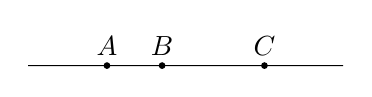
\begin{tikzpicture}
			\draw[fill=black] (0,0)--(1,0)node[above]{\(A\)}circle(1pt)
			--(1.7,0)node[above]{\(B\)}circle(1pt)
			--(3,0)node[above]{\(C\)}circle(1pt)
			--(4,0);
		\end{tikzpicture}
		\caption{直线上点的顺序}
		\label{figure:欧氏几何.直线上点的顺序1}
	\end{figure}

	\item 对于两点\(A\)和\(B\)(如\cref{figure:欧氏几何.直线上点的顺序2}),
	直线\(AB\)上恒至少有一点\(C\),使得\(B\)在\(A\)和\(C\)之间.
	\begin{figure}[htb]
		\centering
		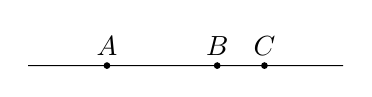
\begin{tikzpicture}
			\draw[fill=black] (0,0)--(1,0)node[above]{\(A\)}circle(1pt)
			--(2.4,0)node[above]{\(B\)}circle(1pt)
			--(3,0)node[above]{\(C\)}circle(1pt)
			--(4,0);
		\end{tikzpicture}
		\caption{直线上点的顺序}
		\label{figure:欧氏几何.直线上点的顺序2}
	\end{figure}

	\item 一直线的任意三点中,至多有一点在其他两点之间.
\end{enumerate}
\end{axiom}

在上述三条{\bf 直线顺序公理}之外,还需要一条{\bf 平面顺序公理}.

\begin{axiom}[顺序公理II]\label{axiom:欧氏几何.顺序公理2}
考虑一直线\(l\)上的两点\(A\)和\(B\).
我们把这一对点\(A\)和\(B\)确定的介于它们的点的集合叫做一条\DefineConcept{线段},记作\(AB\)(或\(BA\)).
在\(A\)和\(B\)之间的点叫做线段\(AB\)的点,或线段\(AB\)的\DefineConcept{内点};
\(A\)和\(B\)叫做线段\(AB\)的\DefineConcept{端点};
直线\(l\)上的其他点叫做线段\(AB\)的\DefineConcept{外点}.
\begin{enumerate}
	\setcounter{enumi}{3}
	\item 设\(A\)、\(B\)和\(C\)是不在同一直线上的三点,
	\(l\)是平面\(ABC\)上的一直线,
	但\(l\)不通过\(A,B,C\)这三点中的任一点
	(如\cref{figure:欧氏几何.平面上点的顺序1}),
	若直线\(l\)通过线段\(AB\)的一点,则它必定也通过线段\(AC\)或线段\(BC\)的一点.
	\begin{figure}[htb]
		\centering
		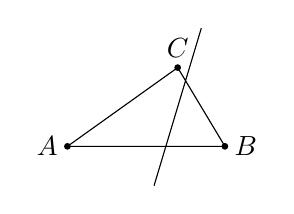
\begin{tikzpicture}
			\draw[fill=black] (-1,0)node[left]{\(A\)}circle(1pt)
			--(1,0)node[right]{\(B\)}circle(1pt)
			--(.4,1)node[above]{\(C\)}circle(1pt)--(-1,0)
			(.1,-.5)--(.7,1.5);
		\end{tikzpicture}
		\caption{平面上点的顺序}
		\label{figure:欧氏几何.平面上点的顺序1}
	\end{figure}
\end{enumerate}
\end{axiom}
直观地说,\cref{axiom:欧氏几何.顺序公理2} 说的就是:
若一直线“冲进”一个三角形的内部,它必定还要再“冲出”这个三角形.
易证:与线段\(AB\)相交的直线\(l\)不同时和\(AC,BC\)这两条线段都相交.

\section{关联公理和顺序公理的推论}
从\cref{axiom:欧氏几何.关联公理,axiom:欧氏几何.顺序公理1,axiom:欧氏几何.顺序公理2} 能推证下列定理.
\begin{theorem}\label{theorem:欧氏几何.定理3}
对于两点\(A\)和\(C\),直线\(AC\)上恒至少有一点\(D\),在\(A\)和\(C\)之间.
\begin{proof}
根据\cref{axiom:欧氏几何.关联公理} 第3条,直线\(AC\)外存在一点\(E\);
根据\cref{axiom:欧氏几何.顺序公理1} 第2条,直线\(AE\)上有一点\(F\),使得\(E\)在线段\(AF\)内.
根据\cref{axiom:欧氏几何.顺序公理1} 第2条、第3条,直线\(FC\)上有一点\(G\),不在线段\(FC\)内.
根据\cref{axiom:欧氏几何.顺序公理2} 第4条,直线\(EG\)必交线段\(AC\)于一点\(D\).
\end{proof}
\end{theorem}

\begin{theorem}\label{theorem:欧氏几何.定理4}
一直线上的任意三点\(A,B,C\)中,必有一点且只有一点在其他两点之间.
\begin{proof}
设\(A\)不在\(B\)和\(C\)之间,而且\(C\)不在\(A\)和\(B\)之间.
用直线连接\(B\)和直线\(AC\)外一点\(D\).
根据\cref{axiom:欧氏几何.顺序公理1} 第2条,能在直线\(BD\)上取一点\(G\),使得\(D\)在\(B\)和\(G\)之间.
对于三角形\(BCG\)和直线\(AD\)应用\cref{axiom:欧氏几何.顺序公理2} 第4条,可知直线\(AD\)通过线段\(CG\)内的一点\(E\);
同理可知直线\(CD\)通过线段\(AG\)内一点\(F\).
对于三角形\(AEG\)和直线\(CF\)应用\cref{axiom:欧氏几何.顺序公理2} 第4条,可知\(D\)在\(A\)和\(E\)之间;
再对于三角形\(AEC\)和直线\(BG\)应用\cref{axiom:欧氏几何.顺序公理2} 第4条,即证得\(B\)在\(A\)和\(C\)之间.
\end{proof}
\end{theorem}

\begin{theorem}\label{theorem:欧氏几何.定理5}
一直线上的任意四点\(A,B,C,D\),使得点\(B\)既在\(A\)和\(C\)之间,又在\(A\)和\(D\)之间;
而且点\(C\)既在\(A\)和\(D\)之间,又在\(B\)和\(D\)之间.
\end{theorem}

\begin{corollary}\label{theorem:欧氏几何.定理6}
一直线上的任意有限个点\(A,B,C,\dotsc,K\),
使得点\(B\)在\(A\)和\(C\),或和\(D\),或和\(E\),……,或和\(K\)之间;
而且点\(C\)在\(A\)(或\(B\))和\(D\),或和\(E\),……,或和\(K\)之间;以此类推.
\end{corollary}

\begin{corollary}\label{theorem:欧氏几何.定理7}
一直线上任意两点之间恒有无限多个点.
\end{corollary}

\begin{theorem}\label{theorem:欧氏几何.定理8}
一平面\(\gamma\)上的任一直线\(l\)将该平面上其余的点分为具有下述性质的两个区域:
一个区域的任一点\(A\)与另一区域的任一点\(B\)所决定的线段\(AB\)内,
必含有直线\(l\)的一点(如\cref{figure:欧氏几何.直线l分平面为两个区域});
而同一个区域的任意两点\(A\)和\(A'\)所决定的线段\(AA'\)内,不含有直线\(l\)的点.
\begin{figure}[htb]
\centering
\begin{tikzpicture}
\draw (-2,0)--(2,0)node[right]{\(l\)}
(.5,-1)node[right]{\(B\)}--(-.5,.5)node[left]{\(A\)}--(.3,1)node[right]{\(A'\)};
\end{tikzpicture}
\caption{直线\(l\)分平面为两个区域}
\label{figure:欧氏几何.直线l分平面为两个区域}
\end{figure}
\end{theorem}

\begin{definition}
我们说\(A\)和\(A'\)这两点在平面\(\gamma\)上直线\(l\)的\DefineConcept{同侧}%
(如\cref{figure:欧氏几何.直线l分平面为两个区域}),
而\(A\)和\(B\)这两点在平面\(\gamma\)上直线\(l\)的\DefineConcept{异侧}.
\end{definition}

\begin{definition}
设\(A,A',O\)和\(B\)是一直线\(l\)上的四点(如\cref{figure:欧氏几何.射线}),
而\(O\)在\(A\)和\(B\)之间,但不在\(A\)和\(A'\)之间.
我们称“\(A\)和\(A'\)这两点在\(l\)上点\(O\)的\DefineConcept{同侧}”,
而称“\(A\)和\(B\)这两点在\(l\)上点\(O\)的\DefineConcept{异侧}”.

直线\(l\)上点\(O\)的同侧的点的全体,叫做从点\(O\)起始的一条\DefineConcept{射线};
因此一直线的每一点把这直线分成两条射线.
\begin{figure}[htb]
\centering
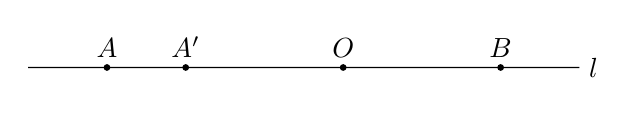
\begin{tikzpicture}
\draw[fill=black] (-3,0)--(-2,0)node[above]{\(A\)}circle(1pt)
--(-1,0)node[above]{\(A'\)}circle(1pt)
--(1,0)node[above]{\(O\)}circle(1pt)
--(3,0)node[above]{\(B\)}circle(1pt)--(4,0)node[right]{\(l\)};
\end{tikzpicture}
\caption{射线}
\label{figure:欧氏几何.射线}
\end{figure}
\end{definition}

\begin{definition}
若干条首尾相连的线段\(AB,BC,CD,\dotsc,KL\)的集合叫做一条\DefineConcept{折线段},
它连结\(A\)和\(L\)这两点.
为求简便,可将这条折线段记为\(ABCD \dotso KL\).
线段\(AB,BC,CD,\dotsc,KL\)的内点和端点都叫做这条折线段的点.
点\(A\)和点\(L\)称为“折线段的\DefineConcept{端点}”.

若折线段\(ABCD \dotso KL\)的顶点\(A,B,C,D,\dotsc,K,L\)都在同一平面上,
且它的端点\(L\)和\(A\)是同一个点,
则这条折线段就叫做一个\DefineConcept{多边形},
记为\(ABCD \dotso K\).
线段\(AB,BC,CD,\dotsc,KA\)叫做“多边形的\DefineConcept{边}”.
点\(A,B,C,D,\dotsc,K\)叫做“多边形的\DefineConcept{顶点}”.

若一个多边形有三个顶点,
则称之为\DefineConcept{三角形}.
设三角形的三个顶点分别为\(A\)、\(B\)、\(C\),
则可将其表记为以下六个符号中的任意一个:
\begin{equation*}
\begin{split}
\triangle ABC, \qquad
\triangle ACB, \qquad
\triangle BAC, \\
\triangle BCA, \qquad
\triangle CAB, \qquad
\triangle CBA.
\end{split}
\end{equation*}

若一个多边形有\(n\ (n>3)\)个顶点,
则称之为\(n\) \DefineConcept{边形}.

若一个多边形的顶点各各不同,
它的任一边内不含有顶点,
且它的任意两边无公共点,
这个多边形就叫做\DefineConcept{简单多边形}.
\end{definition}

根据\cref{theorem:欧氏几何.定理8} 可以推出下列两条推论:
\begin{theorem}\label{theorem:欧氏几何.定理9}
一平面\(\alpha\)上的每一个简单多边形,
把平面\(\alpha\)上其余点%
(即平面\(\alpha\)上的,
而不在这多边形的边上的点)%
分为\DefineConcept{内域}和\DefineConcept{外域}两个区域.
这两个区域具有如下性质:
\begin{enumerate}
	\item 若\(A\)是“内域的一个点(内点)”,
	而且\(B\)是“外域的一个点(外点)”,
	则平面\(\alpha\)上任意一条连接\(A\)和\(B\)的折线段,
	至少和多边形有一公共点.

	\item 若\(A\)和\(C\)是内点,
	而\(B\)和\(D\)是外点,
	则在平面\(\alpha\)上恒有连接\(A\)和\(C\)的折线段,
	和连接\(B\)和\(D\)的折线段,
	它们都和多边形无公共点.

	\item 平面\(\alpha\)上存在全含于外域的直线,
	而不存在全含于内域的直线.
\end{enumerate}
\end{theorem}

\begin{theorem}\label{theorem:欧氏几何.定理10}
每一平面\(\alpha\)把空间中其余点分为具有下述性质的两个区域:
\begin{enumerate}
	\item 一区域的任一点\(A\)和另一区域的任一点\(B\)所决定的线段\(AB\)内,必含有\(\alpha\)的一点.
	\item 同一区域的任意两点\(A\)和\(C\)所决定的线段\(AC\)内,恒不含有\(\alpha\)的点.
\end{enumerate}
\end{theorem}

\begin{definition}
在\cref{theorem:欧氏几何.定理10} 的条件下,
我们说“\(A\)和\(C\)这两点在空间中平面\(\alpha\)的\DefineConcept{同侧}”,
说“\(A\)和\(B\)这两点在空间中平面\(\alpha\)的\DefineConcept{异侧}”.
\end{definition}

\section{第三组公理:合同公理}
本组公理规定“合同”这个概念,利用它就可以规定运动的概念.

我们首先介绍角的概念.
\begin{definition}\label{definition:欧氏几何.几何元素.角}
设\(\alpha\)是任意平面,
而且\(h\)和\(k\)是\(\alpha\)上的、%
从一点\(A\)起始的、%
不属于同一直线的%
两条射线,
我们把这一对射线\(h\)和\(k\)所成的射线组叫做一个\DefineConcept{角},
记作\(\angle(h,k)\)或\(\angle(k,h)\).
称射线\(h\)和\(k\)为这个角的\DefineConcept{边}.
称点\(A\)为这个角的\DefineConcept{顶点}.

如果在\(h\)上任取一点记为\(B\),在\(k\)上任取一点记为\(C\),
那么也称角\(\angle(h,k)\)为\(\angle BAC\)或\(\angle A\).
不致混淆时,也可以用小写希腊字母表记角.

记射线\(h\)所在的直线为\(p\),射线\(k\)所在的直线为\(q\).
射线\(h\)与\(k\)(包括点\(A\))把平面\(\alpha\)上其余点分成两个区域:
在\(q\)的\(h\)侧(即\(h\)的点所在的那一侧)的,且%
在\(p\)的\(k\)侧(即\(k\)的点所在的那一侧)的区域,
叫做“角\(\angle(h,k)\)的\DefineConcept{内部}”,
或者说是在\DefineConcept{角内};
其他区域叫做“角\(\angle(h,k)\)的\DefineConcept{外部}”,
或者说是在\DefineConcept{角外}.
\end{definition}

\begin{property}
根据第一组和第二组公理,
易知任意角(不妨设为交于点\(A\)的射线\(h\)、\(k\)所成的角,即\(\angle(h,k)\))具有以下性质:
\begin{enumerate}
\item 角内、角外两个区域各含有点,连结角内两点的线段完全在角内.
\item 若点\(H\)在射线\(h\)上,点\(K\)在射线\(k\)上,则线段\(HK\)完全在角内.
\item 一条从点\(A\)起始的射线,要么完全在角内,要么完全在角外.
\item 一条完全在角内的射线与线段\(HK\)有交点.
\item 若\(B\)是一个区域的一点,而且\(C\)是另一个区域的一点,
则每一条连接\(B\)和\(C\)的折线段,要么通过点\(A\),要么与\(h\)或\(k\)至少有一个交点;
反之,若\(B\)和\(D\)是同一个区域的两点,则恒有一条连接\(B\)和\(D\)的折线段,
它既不通过点\(A\),又与\(h\)、\(k\)无交点.
\end{enumerate}
\end{property}


\begin{axiom}[合同公理]\label{axiom:欧氏几何.合同公理}
线段与线段之间、角与角之间都有一定的相互关系,我们用“合同”或“相等”这个词来描述.
\begin{enumerate}
\item 设\(A\)和\(B\)是直线\(a\)上的两点,
\(P\)是直线\(b\)上的点,
而且给定了直线\(b\)上\(P\)的一侧,
则在直线\(b\)上\(P\)的这一侧,
恒有一点\(Q\),
使得线段\(AB\)和线段\(PQ\)合同.
我们将上述关系记为\(AB \equiv PQ\).

\item 若两线段\(PQ\)和\(MN\)都和线段\(AB\)合同,
则\(PQ\)和\(MN\)也合同.

\item 设两线段\(AB\)和\(BC\)在同一直线\(a\)上,无公共点,
而且两线段\(PQ\)和\(QR\)在同一直线\(b\)上,亦无公共点.
若\(AB \equiv PQ\)且\(BC \equiv QR\),
则\(AC \equiv PR\).

\item 设给定了一个平面\(\alpha\)上的一个角\(\angle(h,k)\),
一平面\(\beta\)上的一直线\(b\),
和在\(\beta\)上\(b\)的一侧.
设\(p\)是\(b\)上的、从点\(B\)起始的一条射线,
则平面\(\beta\)上恰有一条射线\(q\),
使得\(\angle(h,k)\)与\(\angle(p,q)\)合同,
而且使得\(\angle(p,q)\)的内部在\(b\)的这给定了的一侧.
我们将上述关系记为\(\angle(h,k) \equiv \angle(p,q)\).

\item 若两个三角形\(ABC\)和\(PQR\)有下列合同式
\begin{equation*}
AB \equiv PQ, \qquad
AC \equiv PR, \qquad
\angle BAC \equiv \angle QPR,
\end{equation*}
则也恒有合同式\footnote{%
只需要交换记号,还可以同时得到另一个合同式
\(\angle ACB \equiv \angle PRQ\)
也同时成立.
}
\begin{equation*}
\angle ABC \equiv \angle PQR.
\end{equation*}
\end{enumerate}
\end{axiom}

我们在前面用点\(A\)、\(B\)所成的点组规定一条线段,并用\(AB\)或\(BA\)表示;
我们在线段的定义里,并不考虑这两点的顺序;
因此下列四个合同式的意义相同:
\begin{equation*}
AB \equiv PQ, \qquad
AB \equiv QP, \qquad
BA \equiv PR, \qquad
BA \equiv QP.
\end{equation*}

如同线段我们不考虑它的方向,在角的定义中我们也不考虑旋转方向.
因此下列四个合同式的意义也相同:
\begin{equation*}
\angle(h,k) \equiv \angle(p,q), \qquad
\angle(h,k) \equiv \angle(q,p), \qquad
\angle(k,h) \equiv \angle(p,q), \qquad
\angle(k,h) \equiv \angle(q,p).
\end{equation*}

\cref{axiom:欧氏几何.合同公理} 第3条要求线段能够相加.

\cref{axiom:欧氏几何.合同公理} 第4条可以表述为:
每一个角都能用唯一确定的方式迁移到一个给定了的平面上,
使得它沿着一条给定了的射线,并且在这射线的给定了的一侧.
藉此,我们直接保证了角的迁移的可能性与唯一性.

\cref{axiom:欧氏几何.合同公理} 第1条、第2条、第3条只论及线段的合同,
因此可以叫做“第三组公理中的直线公理”.

\cref{axiom:欧氏几何.合同公理} 第4条论及角的合同.
\cref{axiom:欧氏几何.合同公理} 第5条则把线段的合同和角的合同这两个概念联系起来.
这两条概念论及平面几何的几何元素,
因此可以叫做“第三组公理中的平面公理”.

\cref{axiom:欧氏几何.合同公理} 第1条要求线段平移的可能性,
但它还没有保证这种平移的唯一性.
只有结合\cref{axiom:欧氏几何.合同公理} 第5条,
从角的迁移的唯一性出发予以证明.
具体地,我们应用反证法,
假设把线段\(PQ\)迁移到一条从\(A\)起始的射线上可以得到不同的两点\(B\)、\(D\);
在直线\(AB\)外取一点\(C\),于是有下列合同式
\begin{equation*}
AB \equiv AD, \qquad
AC \equiv AC, \qquad
\angle BAC \equiv \angle DAC;
\end{equation*}
那么根据\cref{axiom:欧氏几何.合同公理} 第5条,得
\begin{equation*}
\angle ACB \equiv \angle ACD;
\end{equation*}
这和\cref{axiom:欧氏几何.合同公理} 第4条中要求的角的迁移的唯一性矛盾,
因此线段平移也是唯一的.

\begin{property}
线段的合同关系具有自反性、对称性和传递性,即
\begin{enumerate}
\item {\rm\bf 自反性},
\(AB \equiv AB\).

\item {\rm\bf 对称性},
\(AB \equiv PQ \implies PQ \equiv AB\)
\footnote{%
正因线段的合同关系具有对称性,
我们才能说“某两条线段互相合同”.
}.

\item {\rm\bf 传递性},
\(AB \equiv PQ \land PQ \equiv MN \implies AB \equiv MN\).
\end{enumerate}
\end{property}

\begin{property}
角的合同关系具有自反性、对称性和传递性,即
\item {\rm\bf 自反性},
\(\angle(h,k) \equiv \angle(h,k)\).

\item {\rm\bf 对称性},
\(\angle(h,k) \equiv \angle(p,q)
\implies
\angle(p,q) \equiv \angle(h,k)\).

\item {\rm\bf 传递性},
\(\angle(h,k) \equiv \angle(m,n)
\land
\angle(m,n) \equiv \angle(p,q)
\implies
\angle(h,k) \equiv \angle(p,q)\).
\end{property}
角的合同关系的自反性是显然的,
至于它的对称性、传递性和可加性,
则留待以后予以证明.

\section{合同公理的推论}
\begin{definition}
两角共顶点,共一边,而且不公共的两边合成一条直线的,叫做\DefineConcept{邻补角}.
\end{definition}
\begin{definition}
两角共顶点,而且它们的边合成两条直线的,叫做\DefineConcept{对顶角}.
\end{definition}
\begin{definition}
一个角和它的邻补角合同的,叫做\DefineConcept{直角}.
\end{definition}

\begin{theorem}\label{theorem:欧氏几何.定理11}
若一个三角形中的两边合同,和这两边相对的两角就也合同\footnote{%
换言之,等腰三角形的底角相等.
}.
\end{theorem}

\begin{definition}
若两个三角形\(ABC\)和\(PQR\)满足下列所有的合同式
\begin{equation*}
\begin{split}
AB \equiv PQ, \qquad
AC \equiv PR, \qquad
BC \equiv QR, \\
\angle A \equiv \angle P, \qquad
\angle B \equiv \angle Q, \qquad
\angle C \equiv \angle R,
\end{split}
\end{equation*}
就说“三角形\(ABC\)合同于三角形\(PQR\)”,
或者说“三角形\(ABC\)和三角形\(PQR\)是全等三角形”,
或者说“三角形\(ABC\)、\(PQR\)全等”,
记为\(\triangle ABC \cong \triangle PQR\).
\end{definition}

\begin{theorem}[三角形的合同定理1]\label{theorem:欧氏几何.定理12}
若两个三角形\(ABC\)、\(PQR\)有下列合同式
\begin{equation*}
AB \equiv PQ, \qquad
AC \equiv PR, \qquad
\angle A \equiv \angle P,
\end{equation*}
则\(\triangle ABC \cong \triangle PQR\).
\end{theorem}

\begin{theorem}[三角形的合同定理2]\label{theorem:欧氏几何.定理13}
若两个三角形\(ABC\)、\(PQR\)有下列合同式
\begin{equation*}
AB \equiv PQ, \qquad
\angle A \equiv \angle P,
\angle B \equiv \angle Q,
\end{equation*}
则\(\triangle ABC \cong \triangle PQR\).
\end{theorem}

\begin{theorem}\label{theorem:欧氏几何.定理14}
设\(\angle ABC\)的邻补角为\(\angle CBD\),
\(\angle PQR\)的邻补角为\(\angle RQS\).
若\(\angle ABC \equiv \angle PQR\),
则\(\angle CBD \equiv \angle RQS\).
\end{theorem}

\begin{corollary}\label{theorem:欧氏几何.对顶角合同}
任意一个角和它的对顶角合同.
\end{corollary}

\begin{corollary}\label{theorem:欧氏几何.直角存在}
直角存在.
\begin{proof}
把任意一个角迁移到沿着一条从点\(O\)起始的射线\(OA\),
而且迁移到这射线的两侧.
在新得到的这两个角的另外两条边上,
取线段\(OB \equiv OC\),
线段\(BC\)交射线\(OA\)于一点\(D\).

若点\(D\)就是点\(O\),
\(\angle BOA\)和\(\angle COA\)是合同的邻补角,所以是直角.

若点\(D\)在射线\(OA\)上,
或在与\(OA\)恰好反向的射线上,
总有\(\angle DOB \equiv \angle DOC\);
根据\cref{axiom:欧氏几何.合同公理} 第2条,
每一条线段都和它自己合同,即\(OD \equiv OD\);
再根据\cref{axiom:欧氏几何.合同公理} 第5条,
就有\(\angle ODB \equiv \angle ODC\).
\end{proof}
\end{corollary}

\begin{theorem}\label{theorem:欧氏几何.定理15}
设\(h\)、\(k\)和\(l\)是一平面\(\alpha\)上的、从一点\(M\)起始的三条射线,
而且\(p\)、\(q\)和\(r\)是一平面\(\beta\)上的、从一点\(N\)起始的三条射线;%
又设\(h\)和\(k\)分别在\(l\)的同侧(或异侧),
且\(p\)和\(q\)也分别在\(r\)的同侧(或异侧).
若
\begin{equation*}
\angle(h,l) \equiv \angle(p,r)
\quad\text{且}\quad
\angle(k,l) \equiv \angle(q,r),
\end{equation*}
则
\begin{equation*}
\angle(h,k) \equiv \angle(p,q).
\end{equation*}
\end{theorem}

\begin{theorem}\label{theorem:欧氏几何.定理16}
设平面\(\alpha\)上的\(\angle(h,k)\)合同于平面\(\beta\)上的\(\angle(p,q)\),
而且\(l\)是平面\(\alpha\)上的、从\(\angle(h,k)\)的顶点起始的、在\(\angle(h,k)\)角内的一条射线.
这时平面\(\beta\)上恒恰有一条从\(\angle(p,q)\)的顶点起始的、在\(\angle(p,q)\)角内的一条射线\(r\),
使得
\begin{equation*}
\angle(h,l) \equiv \angle(p,r), \qquad
\angle(k,l) \equiv \angle(q,r).
\end{equation*}
\end{theorem}

\begin{theorem}\label{theorem:欧氏几何.定理17}
若两点\(C\)和\(D\)在直线\(AB\)的异侧,
而且\(AC \equiv AD\)、\(BC \equiv BD\),
则\(\angle ABC \equiv \angle ABD\).
\end{theorem}

\begin{theorem}[三角形的合同定理3]\label{theorem:欧氏几何.定理18}
若两个三角形\(ABC\)和\(PQR\)的每对对应边合同,即
\begin{equation*}
AB \equiv PQ, \qquad
AC \equiv PR, \qquad
BC \equiv QR,
\end{equation*}
则\(\triangle ABC \cong \triangle PQR\).
\end{theorem}

\begin{theorem}\label{theorem:欧氏几何.定理19}
若两个角\(\angle(a,b)\)和\(\angle(c,d)\)都合同于第三个角\(\angle(e,f)\),
则\(\angle(a,b)\)也合同于\(\angle(c,d)\).
\end{theorem}
由此,我们证明了角的合同关系具有对称性、传递性.

现在我们就可以比较角的大小了.

\begin{theorem}\label{theorem:欧氏几何.定理20}
如\cref{figure:欧氏几何.图20},
给定任意两个角\(\angle(h,k)\)和\(\angle(p,r)\).
设迁移\(\angle(h,k)\)到沿着\(p\),而且在\(p\)的\(r\)侧时,所得到的射线是\(q\);
又迁移\(\angle(p,r)\)到沿着\(h\),而且在\(h\)的\(k\)侧时,所得到的射线是\(l\);
这时,若\(q\)在\(\angle(p,r)\)内,则\(l\)在\(\angle(h,k)\)外.
反之也成立.
\end{theorem}

\begin{figure}[htb]
	\centering
	\begin{tikzpicture}
		\pgfmathsetmacro{\r}{3}
		\begin{scope}
			\draw(0,0)--(\r,0)node[right]{\(h\)};
			\pgfmathsetmacro{\kx}{\r*cos(45)}
			\pgfmathsetmacro{\ky}{\r*sin(45)}
			\draw(0,0)--(\kx,\ky)node[right]{\(k\)};
			\pgfmathsetmacro{\lx}{\r*cos(60)}
			\pgfmathsetmacro{\ly}{\r*sin(60)}
			\draw(0,0)--(\lx,\ly)node[above]{\(l\)};
		\end{scope}
		\begin{scope}[xshift=6cm]
			\draw(0,0)--(\r,0)node[right]{\(p\)};
			\pgfmathsetmacro{\kx}{\r*cos(45)}
			\pgfmathsetmacro{\ky}{\r*sin(45)}
			\draw(0,0)--(\kx,\ky)node[right]{\(q\)};
			\pgfmathsetmacro{\lx}{\r*cos(60)}
			\pgfmathsetmacro{\ly}{\r*sin(60)}
			\draw(0,0)--(\lx,\ly)node[above]{\(r\)};
		\end{scope}
	\end{tikzpicture}
	\caption{}
	\label{figure:欧氏几何.图20}
\end{figure}

\begin{definition}
在\cref{theorem:欧氏几何.定理20} 中,
若\(q\)在\(\angle(p,r)\)内,则称“\(\angle(h,k)\)小于\(\angle(p,r)\)”,记为\(\angle(h,k) < \angle(p,r)\).
若\(q\)在\(\angle(p,r)\)外,则称“\(\angle(h,k)\)大于\(\angle(p,r)\)”,记为\(\angle(h,k) > \angle(p,r)\).
\end{definition}

因此,两个角\(\alpha,\beta\)恒恰适合以下三种情形之一:
\begin{itemize}
	\item \(\alpha<\beta\)和\(\beta>\alpha\).
	\item \(\alpha\equiv\beta\).
	\item \(\alpha>\beta\)和\(\beta<\alpha\).
\end{itemize}

角的大小的比较有传递性.
若有下列三种情形
\begin{itemize}
	\item \(\alpha>\beta,\beta>\gamma\),
	\item \(\alpha>\beta,\beta\equiv\gamma\),
	\item \(\alpha\equiv\beta,\beta>\gamma\),
\end{itemize}
之一,则\begin{equation*}
	\alpha>\gamma.
\end{equation*}

\begin{theorem}\label{theorem:欧氏几何.定理21}
所有的直角都互相合同.
\end{theorem}

\begin{definition}
一个角大于它的邻补角的,也就是大于一直角的,叫做\DefineConcept{钝角};
小于它的邻补角的,也就是小于一直角的,叫做\DefineConcept{锐角}.
\end{definition}

\begin{definition}
\(\triangle ABC\)的\(\angle ABC\)、\(\angle BCA\)和\(\angle CAB\)
叫做这个三角形的\DefineConcept{内角},简称为这个三角形的\DefineConcept{角};
它们的邻补角叫做这个三角形的\DefineConcept{外角}.
\end{definition}

\begin{theorem}[外角定理]\label{theorem:欧氏几何.定理22}
在三角形中,一个外角大于其任一不相邻的内角.
\end{theorem}

下列定理是外角定理的重要推论.

\begin{theorem}\label{theorem:欧氏几何.定理23}
在三角形中,长边所对的角大于短边所对的角.
\end{theorem}

\begin{theorem}\label{theorem:欧氏几何.定理24}
若三角形有两角合同,则有两边合同.
\end{theorem}
这是\cref{theorem:欧氏几何.定理11} 的逆定理,
也是\cref{theorem:欧氏几何.定理23} 的直接推论.

从\cref{theorem:欧氏几何.定理22},
还能很简单地证得下述对三角形的合同定理二的补充.
\begin{theorem}\label{theorem:欧氏几何.定理25}
若\(\triangle ABC\)和\(\triangle DEF\)有下列合同式\begin{equation*}
	AB \equiv DE, \qquad
	\angle A \equiv \angle D, \qquad
	\angle C \equiv \angle F,
\end{equation*}
则这两个三角形合同.
\end{theorem}

\begin{theorem}\label{theorem:欧氏几何.定理26}
每一线段都能二等分.
\end{theorem}

类似地,从\cref{theorem:欧氏几何.定理11} 和\cref{theorem:欧氏几何.定理26},能直接推证下列事实:
\begin{theorem}
每一角都能二等分.
\end{theorem}

合同的概念可以推广应用到任意的图形上去.

\begin{definition}
设\(A,B,C,D,\dotsc,K,L\)是直线\(\alpha\)上的一个点列,
\(A',B',C',D',\dotsc,K',L'\)是直线\(\alpha'\)上的一个点列,
而且所有的对应线段都两两合同,
那么称这两个点列互相合同.
\(A\)和\(A'\)、\(B\)和\(B'\),一直到\(L\)和\(L'\),叫做这\emph{合同点列}的对应点.
\end{definition}

\begin{theorem}\label{theorem:欧氏几何.定理27}
两个合同的点列的点的顺序相同.
\end{theorem}

\begin{definition}
任意有限个点叫做一个\DefineConcept{图形}.
一个图形的点,若都在一个平面上,这图形就叫做一个\DefineConcept{平面图形}.
\end{definition}

两个图形的点之间若有一个一一对应的关系,
使得由此规定的每对对应的线段都互相合同,
且每对对应的角都互相合同,
那么这两个图形合同.

由\cref{theorem:欧氏几何.定理14}
和\cref{theorem:欧氏几何.定理27},
可知合同图形有下述性质:
若一个图形中的三个点在一条直线上,
则每一个和它合同图形中的对应的三个点也在一条直线上.
合同图形中的、对应平面上的对应点,
对于对应直线而言的顺序相同;
对应直线上的对应点顺序也相同.

平面的和空间的最普遍的合同定理如下:
\begin{theorem}\label{theorem:欧氏几何.定理28}
设\((A,B,C,\dotsc,L)\)
和\((A',B',C',\dotsc,L')\)
是两个合同的平面图形.
若\(P\)是第一个图形的平面上的一点,
则第二个图形的平面上恒有一点\(P'\)存在,
使得\((A,B,C,\dotsc,L,P)\)
和\((A',B',C',\dotsc,L',P')\)还是合同的图形.
若\((A,B,C,\dotsc,L)\)至少含有不在同一条直线上的三点,
则\(P'\)只有一个可能的作法.
\end{theorem}

\begin{theorem}\label{theorem:欧氏几何.定理29}
设\((A,B,C,\dotsc,L)\)
和\((A',B',C',\dotsc,L')\)
是两个合同的图形.
若\(P\)是任意一点,
则恒有一点\(P'\)存在,
使得\((A,B,C,\dotsc,L,P)\)
和\((A',B',C',\dotsc,L',P')\)还是合同的图形.
若\((A,B,C,\dotsc,L)\)至少含有不在同一平面上的四点,
则\(P'\)只有一个可能的作法.
\end{theorem}

\cref{theorem:欧氏几何.定理29} 说出了所有关于合同的空间事实,
因此,空间中运动的性质,都是上述的直线的和平面的五条合同公理(结合着第一组和第二组公理)的推论.

\section{第四组公理:平行公理}
设\(\alpha\)是任一平面,
\(a\)是\(\alpha\)上的任一直线,
而且\(A\)是\(\alpha\)上的、但不在\(a\)上的一点,
在\(\alpha\)上作一直线\(c\),
通过\(A\)且和\(a\)相交,
再在\(\alpha\)上作一直线\(b\),通过\(A\),
且使得\(c\)交\(a\)和\(b\)于相等的同位角.
从\hyperref[theorem:欧氏几何.定理22]{外角定理},
易知\(a\)和\(b\)这两直线无公共点,这就是说,
在一平面\(\alpha\)上,而且通过一直线\(a\)外的一点\(A\),
恒有一直线不和\(a\)相交.

现在可将平行公理叙述如下:
\begin{axiom}[平行公理、欧几里得公理]\label{axiom:欧氏几何.平行公理}
设\(a\)是任一直线,\(A\)是\(a\)外的任一点.
在\(a\)和\(A\)所决定的平面上,
至多有一条直线通过\(A\),而且不和\(a\)相交.
\end{axiom}

根据上文和平行公理,我们知道:
在\(a\)和\(A\)所决定的平面上,恰有一直线,通过\(A\)且不和\(a\)相交,
我们把这条直线叫做“通过\(A\)的\(a\)的\DefineConcept{平行直线}”.

平行公理和下述的要求等价:
如果一平面上的\(a\)和\(b\)两直线都不和这平面上的第三条直线\(c\)相交,
那么\(a\)和\(b\)也不相交.

事实上,如果\(a\)和\(b\)有一公共点\(A\),那么在同一平面上,
就有了\(a\)和\(b\)这两条直线,都通过\(A\)而且不和\(c\)相交.
这和平行公理矛盾.
反之,从上述要求,也易推得平行公理.

平行公理是一条平面公理.
它的引入,使得几何的基础大大地简单化了,也使得几何的构造容易得多了.

例如,在合同公理之外,再加上平行公理,不难得到下列熟知的事实:
\begin{theorem}\label{theorem:欧氏几何.定理30}
若两平行直线被第三条直线所截,则同位角合同,内错角也合同;
反之,若同位角合同,或内错角合同,则前两直线平行.
\end{theorem}

\begin{theorem}\label{theorem:欧氏几何.定理31}
三角形的三个内角的和等于两个直角的和.
\end{theorem}
\begin{figure}[htb]
	\centering
	\begin{tikzpicture}
		\coordinate (A) at (0,0);
		\coordinate (B) at (4,0);
		\coordinate (C) at (3,2);
		\coordinate (P) at (2,2);
		\coordinate (Q) at (4,2);
		\draw (A)node[left]{\(A\)}
				-- (B)node[right]{\(B\)}
				-- (C)node[above]{\(C\)} -- (A);
		\draw (P)node[left]{\(P\)} -- (Q)node[right]{\(Q\)};
		\draw pic[draw=blue,angle radius=5mm]{angle=B--A--C}
				pic[draw=blue,angle radius=6mm]{angle=B--A--C}
				pic[draw=blue,angle radius=5mm]{angle=P--C--A}
				pic[draw=blue,angle radius=6mm]{angle=P--C--A}
				pic[draw=orange,angle radius=4mm]{angle=C--B--A}
				pic[draw=orange,angle radius=4mm]{angle=B--C--Q};
	\end{tikzpicture}
	\caption{}
	\label{figure:欧氏几何.三角形内角和等于平角}
\end{figure}

\begin{definition}
设\(M\)是一平面\(\alpha\)上的任一点.
考虑\(\alpha\)上的所有的那些点\(A\),
它们使线段\(MA\)都互相合同的.
这种点\(A\)的全体叫做一个\DefineConcept{圆},
点\(M\)叫做“这个圆的\DefineConcept{中心}”,简称\DefineConcept{圆心}.
\end{definition}

根据这个定义,我们容易从第三组和第四组公理,推证关于圆的若干熟知的定理.
特别是下述的定理:
通过不在同一条直线上的三点,能作一圆;
关于同一条弦上的圆周角合同的定理;
关于内接于圆的一个四边形的角的定理.

\section{第五组公理:连续公理}
\begin{axiom}[连续公理]
关于线段、角的度量,有如下公理:
\begin{enumerate}
	\item (度量公理,阿基米德公理).
	若\(AB\)和\(CD\)是任意两线段,则必存在一个数\(n\)使得沿\(A\)到\(B\)的射线上,
	自\(A\)作首尾相接的\(n\)个线段\(CD\),必将越过\(B\)点.
	\item (直线完备公理).
	一直线上的点集联通其顺序关系与合同关系不可能再这样扩充,
	使得这直线上原来元素之间所具有的关系,
	从第一组、第二组、第三组公理所推出的直线顺序与合同的基本性质\footnote{%
	所谓“基本性质”是指第二组第一至三条公理和\cref{theorem:欧氏几何.定理5} 中所叙述的顺序性质,
	以及第三组第一至第三条公理中所叙述的合同性质连同迁移线段的唯一性.}
	以及度量公理都仍旧保持\footnote{%
	所谓“仍旧保持”是指,当点集扩充后,顺序关系及合同关系也将延续到扩充后的点集中去.
	我们注意到第一组第三条公理在各种扩充后,不言而喻地仍然保持,
	至于在所考虑的扩充下,\cref{theorem:欧氏几何.定理3} 仍能成立,
	则是保持阿基米德公理的结果.}.
\end{enumerate}
\end{axiom}

完备公理中所要求保持的诸公理之一是阿基米德公理,
这时完备公理从本质上能以建立所不可缺少的一个条件.
其实我们能够证明:
若直线上的一个点集能满足上面所列举的关于顺序公理和定理以及合同公理和定理,
这点集就恒能够增加新点,使扩充后的点集还满足这里所提到的诸公理;
也就是说,如果一条完备公理,只要求保持这里所提到的诸公理和定理,
但不要求保持阿基米德公理或一条等价的公理,就要产生矛盾.

这两条连续公理都是直线公理.

下面所述更普遍的定理,主要根据直线完备公理.
\begin{theorem}[完备定理]\label{theorem:欧氏几何.定理32}
几何元素(即点、直线、平面)形成一个集合,
它在保持关联公理、顺序公理、合同公理和阿基米德公理,
从而更不用说,在保持全体公理的条件之下,
不可能经由点、直线和平面再行扩充.
\end{theorem}

完备定理还能表成较强的形式.
也就是在完备定理内缩要求保持的诸公理中,有些并不是绝对需要的,为了定理能够成立,
重要的倒是在所要求保持的诸公理中包含有第一组第七条公理.
其实我们能证明:
对于满足第一至第第五组公理的元素集合,恒能给添加新的点、直线和平面,
使得扩充后的心机和能满足除去第一组第七条公理之外的全体公理;
这就是说,一条完备定理若不包含第一组第七条公理或一条等价的公理,就将引出矛盾.

完备公理不是阿基米德公理的一个推论.
实际上,只有阿基米德公理,连同第一至第四组公理,
并不足以证明我们的几何和通常的笛卡尔解析几何完全相同.
但是加上了完备公理(虽然这条公理并没有直接提到收敛的概念),
就能证明(相当于戴德金分割的)确界的存在,
和关于聚点存在的波尔查诺定理,
从而才证明欧氏几何和笛卡尔几何相同.

从上文可见,连续的要求,在本质上,分成两个不同的部分:
阿基米德公理和完备公理;
前者的作用是替连续的要求做准备,
后者为完成整个公理系统作基础.

在本章后面的研究中,我们主要只用阿基米德公理作根据,而普遍地不假设完备公理.


\chapter{几何空间的线性结构和度量结构}
从本章开始,我们介绍空间解析几何的思想与方法.

古希腊的毕达哥拉斯曾经提出“万物皆数”这一哲学观点,从这一章开始,我们研究如何利用代数方法研究几何问题.

在利用函数图像研究初等函数的性质时,我们产生了这么一个观念:
在平面上建立了平面直角坐标系以后,
平面上的点与数是一一对应的,
或说平面上的点与由实有序对\((x,y)\)一一对应.
几何图形是由点构成的集合,我们自然地想到能不能用数的集合来代表几何图形.
这就是解析几何的思想根源.

\section{向量及其线性运算}
解析几何最基本的方法是坐标法,即建立一个坐标系,使得点可以用有序对或元组来表示,
从而可以用方程表示图形,通过方程来研究图形的性质.
坐标法的优越性在于它利用了数可以进行运算的优点.
那么,能否把代数运算直接引入几何中来呢?什么样的几何对象能够做运算?

\subsection{向量的概念}
既有大小、又有方向的量,称为\DefineConcept{向量}或\DefineConcept{矢量}(vector).

与向量相对的,只有大小,没有方向的量,称为\DefineConcept{标量}(scalar).

我们通常用黑体小写拉丁字母(如\(\vb{a}\)、\(\vb{r}\)、\(\vb{v}\)、\(\vb{F}\)等),
或在小写拉丁字母上面加箭头(如\(\vec{a}\)、\(\vec{r}\)、\(\vec{v}\)、\(\vec{F}\)等)来表记向量.

在几何空间中,我们常用\DefineConcept{有向线段}(directed line segment)表示向量.
如\cref{figure:解析几何.有向线段} 所示,
对于一个给定的向量\(\vb{a}\),
我们可以用有向线段\(\vec{AB}\)来表示它,
其中用这条线段的长度\(\abs{AB}\)表示\(\vb{a}\)的大小,
用点\(A\)到点\(B\)的指向表示\(\vb{a}\)的方向.
我们把点\(A\)称为“有向线段\(\vec{AB}\)的\DefineConcept{起点}(initial point)”,
把点\(B\)称为“有向线段\(\vec{AB}\)的\DefineConcept{终点}(terminal point)”.
\begin{figure}[htb]
\centering
\begin{tikzpicture}[>=Stealth]
	\draw[->] (0,0)node[left]{\(A\)}--(3,1)node[right]{\(B\)}
		node[midway,above]{\(\vb{a}\)};
\end{tikzpicture}
\caption{有向线段}
\label{figure:解析几何.有向线段}
\end{figure}

规定长度相等、方向相同的有向线段表示同一个向量.

如\cref{figure:解析几何.有向线段的平移不变性} 所示,
若有向线段\(\vec{AB}\)表示向量\(\vb{a}\),
则\(\vec{AB}\)经过平行移动得到的有向线段\(\vec{CD}\)仍然表示向量\(\vb{a}\),
即\(\vb{a} = \vec{AB} = \vec{CD}\).
换言之,给定两条有向线段,如果其中一条经过平移可以让这两条有向线段的起点和终点分别完全重合,
那么这两条有向线段表示的是同一个向量.
\begin{figure}[htb]
\centering
\begin{tikzpicture}[>=Stealth]
	\draw[dashed] (0,0)--(5,0) (3,1)--(8,1);
	\draw[->] (0,0)node[left]{\(A\)}--(3,1)node[above left]{\(B\)}node[midway,above left]{\(\vb{a}\)};
	\draw[->] (5,0)node[below right]{\(C\)}--(8,1)node[right]{\(D\)};
\end{tikzpicture}
\caption{}
\label{figure:解析几何.有向线段的平移不变性}
\end{figure}

我们今后把向量的大小称为
“向量的\DefineConcept{长度}(length)”或“向量的\DefineConcept{模}(modulus)”,
记作\(\abs{\vb{a}}\).

如果两个向量\(\vb{a}\)和\(\vb{b}\)的长度相等、方向相同,
我们就说“\(\vb{a}\)和\(\vb{b}\)是\DefineConcept{相等}的”,
或者说“\(\vb{a}\)等于\(\vb{b}\)”,
记作\(\vb{a}=\vb{b}\);
否则,记\(\vb{a}\neq\vb{b}\).

长度为零的向量称为\DefineConcept{零向量}(zero vector),记作\(\vb{0}\).
%@see: https://mathworld.wolfram.com/ZeroVector.html

看作有向线段时,零向量的起点和终点重合,所以它的方向可以看作是任意的、不确定的.

相对地,长度不为零的向量称为\DefineConcept{非零向量}(nonzero vector).

长度为1的向量称为\DefineConcept{单位向量}(unit vector),记作\(\vb{e}\).
%@see: https://mathworld.wolfram.com/UnitVector.html

任意给定一个向量\(\vb{a}\),与\(\vb{a}\)同向的单位向量记作\(\vb{a}^0\),
称其为“\(\vb{a}\)的\DefineConcept{方向}(direction)”.

任意给定一个向量\(\vb{a}\),
如果向量\(\vb{b}\)正好是与\(\vb{a}\)长度相等、方向相反的向量,
那么称“\(\vb{b}\)是\(\vb{a}\)的\DefineConcept{负向量}(negative vector)”,
记作\(-\vb{a}\).
例如,\(\vec{BA}\)是\(\vec{AB}\)的负向量,因此\(\vec{BA} = -\vec{AB}\).

\subsection{向量的加法}
我们知道,将与点\(A\)重合的点\(P\)移动到点\(B\)再移动到点\(C\)的结果是点\(P\)与点\(C\)重合.

\begin{definition}
%@see: 《解析几何》(丘维声) P2 定义1.1
对于向量\(\vb{a},\vb{b}\),
如\cref{figure:解析几何.向量相加的三角形法则} 所示,
作有向线段\(\vec{AB}\)表示\(\vb{a}\),
作有向线段\(\vec{BC}\)表示\(\vb{b}\),
把有向线段\(\vec{AC}\)表示的向量\(\vb{c}\)称为
“向量\(\vb{a}\)与\(\vb{b}\)的\DefineConcept{和}”,
记作\begin{equation*}
	\vec{AB}+\vec{BC}=\vec{AC}
	\quad\text{或}\quad
	\vb{c}=\vb{a}+\vb{b}.
\end{equation*}
\end{definition}
由上述公式表示的向量加法规则通常称为\DefineConcept{三角形法则}(triangle law).
除此以外,我们还有\DefineConcept{平行四边形法则}(parallelogram law),
如\cref{figure:解析几何.向量相加的平行四边形法则}.

\begin{figure}[htb]
	\centering
	\def\subwidth{.4\linewidth}
	\begin{subfigure}[b]{\subwidth}
		\centering
		\begin{tikzpicture}
			\pgfmathsetmacro{\xmax}{5}
			\pgfmathsetmacro{\xmin}{0}
			\pgfmathsetmacro{\ymax}{4}
			\pgfmathsetmacro{\ymin}{0}
			\draw[help lines,color=gray!30,dashed](\xmin,\ymin)grid(\xmax,\ymax);
			\begin{scope}[->,>=Stealth,ultra thick]
				\draw(\xmin,0)--(\xmax,0)node[right]{\(x\)};
				\draw(0,\ymin)--(0,\ymax)node[above]{\(y\)};
			\end{scope}
			\coordinate(A)at(1,1);
			\coordinate(B)at(4,2);
			\coordinate(C)at(3,3);
			\begin{scope}[>=Stealth,->]
				\draw[blue](A)node[black,left]{\(A\)}
					--(B)node[black,right]{\(B\)}node[black,midway,below]{\(\vb{a}\)};
				\draw[blue](B)
					--(C)node[black,above]{\(C\)}node[black,midway,above right]{\(\vb{b}\)};
				\draw[red](A)--(C)node[black,midway,above left]{\(\vb{a}+\vb{b}\)};
			\end{scope}
		\end{tikzpicture}
		\caption{向量加法的三角形法则}
		\label{figure:解析几何.向量相加的三角形法则}
	\end{subfigure}
	\begin{subfigure}[b]{\subwidth}
		\centering
		\begin{tikzpicture}
			\pgfmathsetmacro{\xmax}{6}
			\pgfmathsetmacro{\xmin}{0}
			\pgfmathsetmacro{\ymax}{4}
			\pgfmathsetmacro{\ymin}{0}
			\draw[help lines,color=gray!30,dashed](\xmin,\ymin)grid(\xmax,\ymax);
			\begin{scope}[->,>=Stealth,ultra thick]
				\draw(\xmin,0)--(\xmax,0)node[right]{\(x\)};
				\draw(0,\ymin)--(0,\ymax)node[above]{\(y\)};
			\end{scope}
			\coordinate(A)at(2,1);
			\coordinate(B)at(5,2);
			\coordinate(C)at(4,3);
			\coordinate(D)at(1,2);
			\begin{scope}[>=Stealth,->]
				\draw[blue](A)node[black,below]{\(A\)}
					--(B)node[black,midway,below]{\(\vb{a}\)};
				\draw[blue](A)--(D)node[black,midway,left]{\(\vb{b}\)};
				\draw[red](A)--(C)node[black,midway,above left]{\(\vb{a}+\vb{b}\)};
			\end{scope}
			\draw[dashed](D)node[black,left]{\(D\)}
				--(C)node[black,above]{\(C\)}
				--(B)node[black,right]{\(B\)};
		\end{tikzpicture}
		\caption{向量相加的平行四边形法则}
		\label{figure:解析几何.向量相加的平行四边形法则}
	\end{subfigure}
	\caption{}
\end{figure}

向量的加法服从以下运算律:
\begin{enumerate}
	\item 结合律,即对于\(\forall \vb{a},\vb{b},\vb{c}\),有\begin{equation*}
		(\vb{a}+\vb{b})+\vb{c}
		= \vb{a}+(\vb{b}+\vb{c}).
	\end{equation*}

	\item 交换律,即对于\(\forall \vb{a},\vb{b}\),有\begin{equation*}
		\vb{a}+\vb{b} = \vb{b}+\vb{a}.
	\end{equation*}

	\item 对于\(\forall \vb{a}\),有\begin{equation*}
		\vb{a}+\vb{0}=\vb{a}.
	\end{equation*}

	\item 对于\(\forall \vb{a}\),有\begin{equation*}
		\vb{a}+(-\vb{a})=\vb{0}.
	\end{equation*}
\end{enumerate}
这些运算律都可以利用有向线段作图予以证明.

\begin{definition}
%@see: 《解析几何》(丘维声) P4 定义1.2
对于向量\(\vb{a},\vb{b}\),
称\(\vb{a}\)与\(\vb{b}\)的负向量\(-\vb{b}\)的和\(\vb{a}+(-\vb{b})\)为
“向量\(\vb{a}\)与\(\vb{b}\)的\DefineConcept{差}”,记作\(\vb{a}-\vb{b}\),即\begin{equation*}
	\vb{a}-\vb{b}
	\defeq
	\vb{a}+(-\vb{b}).
\end{equation*}
\end{definition}

\begin{theorem}
%@see: 《解析几何》(丘维声) P10 习题1.1 7.
对任意向量\(\vb{a},\vb{b}\),都有\begin{equation*}
	\abs{\vb{a}+\vb{b}} \leq \vb{a} + \vb{b}.
\end{equation*}
\end{theorem}

\subsection{向量的数量乘法}
\begin{definition}
%@see: 《解析几何》(丘维声) P4 定义1.3
规定:实数\(\lambda\)与向量\(\vb{a}\)的乘积\(\lambda \vb{a}\)还是一个向量,
它的长度为\begin{equation*}
\abs{\lambda\vb{a}}
\defeq
\abs{\lambda} \abs{\vb{a}},
\end{equation*}
它的方向当\(\lambda>0\)时与\(\vb{a}\)相同,
当\(\lambda<0\)时与\(\vb{a}\)相反.
\end{definition}

对于任意向量\(\vb{a}\),
由于\(\abs{0 \vb{a}} = 0 \abs{\vb{a}} = 0\),
所以\(0 \vb{a} = \vb{0}\).
同理,对一切实数\(\lambda\),都有\(\lambda \vb{0} = \vb{0}\).

对于任意非零向量\(\vb{a}\),
因为向量\(\abs{\vb{a}}^{-1} \vb{a}\)与\(\vb{a}\)同向,
且\begin{equation*}
	\abs{\frac{1}{\abs{\vb{a}}} \vb{a}}
	= \frac{1}{\abs{\vb{a}}} \abs{\vb{a}} = 1,
\end{equation*}
所以\(\vb{a}^0 = \abs{\vb{a}}^{-1} \vb{a}\).
像这样,把一个非零向量\(\vb{a}\)乘以它的长度的倒数,
以得到与它同向的单位向量\(\vb{a}^0\)的过程,称为“把\(\vb{a}\) \DefineConcept{单位化}”.

向量的数量乘法服从以下运算律:
对于任意向量\(\vb{a},\vb{b}\)和任意实数\(\lambda,\mu\),有
\begin{enumerate}
	\item \(1 \vb{a} = \vb{a}\);
	\item \((-1) \vb{a} = -\vb{a}\);
	\item \(\lambda(\mu \vb{a}) = (\lambda \mu) \vb{a}\);
	\item \((\lambda+\mu) \vb{a} = \lambda \vb{a} + \mu \vb{a}\);
	\item \(\lambda (\vb{a}+\vb{b}) = \lambda \vb{a} + \lambda \vb{b}\).
\end{enumerate}

\subsection{共线、共面的向量组}
向量的加法和数量乘法统称为向量的\DefineConcept{线性运算}.

设\(\AutoTuple{\vb{a}}{n}\)是一组向量,
\(\AutoTuple{k}{n}\)是一组实数,
则\(k_1 \vb{a}_1 + k_2 \vb{a}_2 + \dotsb + k_n \vb{a}_n\)是一个向量,
我们称其为“向量组\(\AutoTuple{\vb{a}}{n}\)的一个\DefineConcept{线性组合}”,
称\(\AutoTuple{k}{n}\)为这个线性组合的\DefineConcept{系数}.

\begin{definition}
%@see: 《解析几何》(丘维声) P6 定义1.4
若用起点相同的有向线段表示向量组中的向量,
这些向量的终点和它们的公共起点都在同一条直线上,
则称这个向量组是\DefineConcept{共线的}(collinear).

若用起点相同的有向线段表示向量组中的向量,
这些向量的终点和它们的公共起点都在同一个平面上,
则称这个向量组是\DefineConcept{共面的}(coplanar).
\end{definition}

\begin{theorem}
%@see: 《解析几何》(丘维声) P6 命题1.1
若\(\vb{a}\)与\(\vb{b}\)共线,且\(\vb{a}\neq\vb{0}\),
则存在唯一的实数\(\lambda\),使得\(\vb{b} = \lambda \vb{a}\).
\end{theorem}

\begin{theorem}\label{theorem:解析几何.两向量共线的充分必要条件1}
%@see: 《解析几何》(丘维声) P6 命题1.2
\(\vb{a}\)与\(\vb{b}\)共线的充分必要条件是:
存在不全为零的实数\(\lambda\)和\(\mu\),使得\begin{equation*}
	\lambda \vb{a} + \mu \vb{b} = \vb{0}.
\end{equation*}
\begin{proof}
先证必要性.
设\(\vb{a}\)与\(\vb{b}\)共线.
若\(\vb{a}=\vb{b}=\vb{0}\),
则有\(1\vb{a}+1\vb{b}=\vb{0}\).
若\(\vb{a},\vb{b}\)不全为\(\vb{0}\),不妨设\(\vb{a}\neq\vb{0}\),
则存在实数\(\lambda\),使得\(\vb{b}=\lambda\vb{a}\),从而有\begin{equation*}
	\lambda\vb{a}+(-1)\vb{b}=\vb{0}.
\end{equation*}

再证充分性.
若有不全为零的实数\(\lambda,\mu\),使得\(\lambda \vb{a} + \mu \vb{b} = \vb{0}\)成立,
不妨设\(\lambda\neq0\),于是得\(\vb{a}=-\frac{\mu}{\lambda}\vb{b}\),
因此\(\vb{a}\)与\(\vb{b}\)共线.
\end{proof}
\end{theorem}

\begin{corollary}\label{theorem:解析几何.两向量不共线的充分必要条件1}
%@see: 《解析几何》(丘维声) P7 推论1.1
\(\vb{a}\)与\(\vb{b}\)不共线的充分必要条件是:\begin{equation*}
	\lambda \vb{a} + \mu \vb{b} = \vb{0}
	\implies
	\lambda = \mu = 0.
\end{equation*}
\end{corollary}

\begin{theorem}
%@see: 《解析几何》(丘维声) P7 命题1.3
若\(\vb{c} = \lambda \vb{a} + \mu \vb{b}\),
则\(\vb{a},\vb{b},\vb{c}\)共面.
\end{theorem}

\begin{theorem}
%@see: 《解析几何》(丘维声) P7 命题1.4
若\(\vb{a},\vb{b},\vb{c}\)共面,
并且\(\vb{a}\)与\(\vb{b}\)不共线,
则存在唯一的一对实数\(\lambda\)和\(\mu\),使得\begin{equation*}
\vb{c} = \lambda \vb{a} + \mu \vb{b}.
\end{equation*}
\end{theorem}

\begin{theorem}\label{theorem:解析几何.三向量共面的充分必要条件1}
%@see: 《解析几何》(丘维声) P8 命题1.5
\(\vb{a},\vb{b},\vb{c}\)共面的充分必要条件是:
存在不全为零的实数\(\vb{k}_1,\vb{k}_2,\vb{k}_3\),使得\begin{equation*}
	k_1 \vb{a} + k_2 \vb{b} + k_3 \vb{c} = \vb{0}.
\end{equation*}
\end{theorem}

\begin{corollary}\label{theorem:解析几何.三向量不共面的充分必要条件1}
%@see: 《解析几何》(丘维声) P8 推论1.2
\(\vb{a},\vb{b},\vb{c}\)不共面的充分必要条件是:\begin{equation*}
	k_1 \vb{a} + k_2 \vb{b} + k_3 \vb{c} = \vb{0}
	\implies
	k_1 = k_2 = k_3 = 0.
\end{equation*}
\end{corollary}

由于上述命题成立,使得向量的线性运算可以用来解决有关点的共线或共面问题、直线的共点问题
以及线段的定比分割问题;并且这些命题是研究几何空间的线性结构的依据.

\begin{theorem}\label{theorem:解析几何.点在线段上的充分必要条件1}
%@see: 《解析几何》(丘维声) P8 例1.1
点\(M\)在线段\(AB\)上的充分必要条件是:
存在非负实数\(\lambda,\mu\),使得对于任意一点\(P\),总有\(\lambda+\mu=1\),且\begin{equation*}
	\vec{PM} = \lambda \vec{PA} + \mu \vec{PB}.
\end{equation*}
\end{theorem}

\begin{theorem}\label{theorem:解析几何.点在直线上的充分必要条件1}
%@see: 《解析几何》(丘维声) P10 习题1.1 9.
点\(M\)在直线\(AB\)上的充分必要条件是:
存在实数\(\lambda,\mu\),使得对于任意一点\(P\),总有\(\lambda+\mu=1\),且\begin{equation*}
	\vec{PM} = \lambda \vec{PA} + \mu \vec{PB}.
\end{equation*}
\end{theorem}

\begin{theorem}\label{theorem:解析几何.三点共线的充分必要条件1}
%@see: 《解析几何》(丘维声) P9 例1.2
三点\(A,B,C\)共线的充分必要条件是:
存在不全为零的实数\(\lambda,\mu,\nu\),使得对于任意一点\(P\),总有\(\lambda+\mu+\nu=0\),且\begin{equation*}
	\lambda \vec{PA} + \mu \vec{PB} + \nu \vec{PC} = \vb{0}.
\end{equation*}
\end{theorem}

\begin{theorem}\label{theorem:解析几何.四点共面的充分必要条件1}
%@see: 《解析几何》(丘维声) P10 习题1.1 10.
四点\(A,B,C,D\)共面的充分必要条件是:
存在不全为零的实数\(\lambda,\mu,\nu,\omega\),
使得对于任意一点\(P\),总有\(\lambda+\mu+\nu+\omega=0\),且\begin{equation*}
	\lambda \vec{PA} + \mu \vec{PB} + \nu \vec{PC} + \omega \vec{PD} = \vb{0}.
\end{equation*}
\end{theorem}

\begin{theorem}\label{theorem:解析几何.点在平面上的充分必要条件1}
%@see: 《解析几何》(丘维声) P11 习题1.1 11.
设\(A,B,C\)是不在一直线上的三点.
点\(M\)在平面\(ABC\)上的充分必要条件是:
存在实数\(\lambda,\mu,\nu\),使得对于任意一点\(P\),总有\(\lambda+\mu+\nu=1\),且\begin{equation*}
	\vec{PM} = \lambda \vec{PA} + \mu \vec{PB} + \nu \vec{PC}.
\end{equation*}
\end{theorem}

\begin{theorem}
%@see: 《解析几何》(丘维声) P11 习题1.1 12.
点\(M\)在\(\triangle ABC\)内(包括它的三条边)的充分必要条件是:
存在非负实数\(\lambda,\mu\),使得\(\lambda+\mu\leq1\),且\begin{equation*}
	\vec{AM} = \lambda \vec{AB} + \mu \vec{AC}.
\end{equation*}
\end{theorem}

\begin{theorem}\label{theorem:解析几何.点在三角形上的充分必要条件2}
%@see: 《解析几何》(丘维声) P11 习题1.1 13.
点\(M\)在\(\triangle ABC\)内(包括它的三条边)的充分必要条件是:
存在非负实数\(\lambda,\mu,\nu\),使得对于任意一点\(P\),总有\(\lambda+\mu+\nu=1\),且\begin{equation*}
	\vec{PM} = \lambda \vec{PA} + \mu \vec{PB} + \nu \vec{PC}.
\end{equation*}
\end{theorem}

\section{几何空间的线性结构}
几何空间\(V\)是空间中所有的点组成的集合.
取一个点\(O\),以\(O\)为起点的向量称为“定位向量”.
所有的定位向量组成的集合与\(V\)有一个一一对应:\(\vec{OM}\)对应于终点\(M\).
于是\(V\)也可以看成是由所有定位向量组成的集合.
由于向量\(\vec{OM}\)经过平行移动得到的向量与\(\vec{OM}\)相等,
因此\(V\)也可以看成由所有向量组成的集合,
其中经过平行移动得到的向量是相等的向量.
\(V\)中的向量有加法和数量乘法运算,
这使得几何空间\(V\)具有了一个很好的代数结构.

\subsection{向量和点的仿射坐标与直角坐标}
\begin{theorem}\label{theorem:解析几何.向量可由基线性表出}
%@see: 《解析几何》(丘维声) P12 定理2.1
几何空间\(V\)中任意给定三个不共面的向量\(\vb{d}_1,\vb{d}_2,\vb{d}_3\),
则任意一个向量\(\vb{m}\)可以唯一地表示成\(\vb{d}_1,\vb{d}_2,\vb{d}_3\)的线性组合.
\end{theorem}
\cref{theorem:解析几何.向量可由基线性表出} 给出了几何空间\(V\)的线性结构.

\begin{figure}[htb]
	\centering
	\begin{tikzpicture}
		\coordinate(O)at(0,0);
		\coordinate(P)at(-1,-1);
		\coordinate(H)at(-1,1.2);
		\coordinate(N)at(2,-1);
		\coordinate(M)at(2,1.2);
		\coordinate(R)at(0,2.2);
		\coordinate(K)at(3,2.2);
		\coordinate(Q)at(3,0);
		\draw[dashed](O)--(P)
			(O)--(Q)
			(O)--(R);
		\draw(P)--(N)--(M)--(H)--(P)
			(H)--(R)--(K)--(Q)--(N)
			(K)--(M);
		\begin{scope}[->,>=Stealth]
			\draw(P)--+(-.5,-.5)node[below left]{\(x\)};
			\draw(Q)--+(.5,0)node[right]{\(y\)};
			\draw(R)--+(0,.5)node[left]{\(z\)};
			\draw[dashed,red](O)--(M);
		\end{scope}
		\draw(O)node[below]{\(O\)}
			(P)node[below]{\(P\)}
			(H)node[left]{\(H\)}
			(N)node[below]{\(N\)}
			(M)node[right]{\(M\)}
			(R)node[left]{\(R\)}
			(K)node[right]{\(K\)}
			(Q)node[below]{\(Q\)};
	\end{tikzpicture}
	\caption{}
	\label{figure:解析几何.向量的坐标分解}
\end{figure}

\begin{definition}
%@see: 《解析几何》(丘维声) P13 定义2.1
几何空间\(V\)中任意三个有次序的不共面的向量
\(\vb{d}_1,\vb{d}_2,\vb{d}_3\)
称为“\(V\)的一个\DefineConcept{基}”.

对于几何空间中任一向量\(\vb{m}\),若\begin{equation*}
	\vb{m} = x \vb{d}_1 + y \vb{d}_2 + z \vb{d}_3,
\end{equation*}
则把三元组\((x,y,z)\)称为
“\(\vb{m}\)(在基\(\vb{d}_1,\vb{d}_2,\vb{d}_3\)下)的\DefineConcept{坐标}”,记作\begin{equation*}
	\begin{bmatrix} x \\ y \\ z \end{bmatrix}
	\quad\text{或}\quad
	(x,y,z)^T.
\end{equation*}
\end{definition}

我们把\((x,y,z)^T\)称为“向量\(\vb{a}\)的\DefineConcept{分量形式}(component form)”;
相对地,把\(x \vb{d}_1 + y \vb{d}_2 + z \vb{d}_3\)
称为“向量\(\vb{a}\)的\DefineConcept{代数形式}(algebra form)”,
把用来表示它的有向线段称为它的\DefineConcept{几何形式}(geometry form).

在本章当中,我们常把\((x,y,z)^T\)的上标略去不写,只写\((x,y,z)\),这依然表示同一个向量.

向量有了坐标后,我们再对空间中的点也引进坐标.

\begin{definition}
%@see: 《解析几何》(丘维声) P13 定义2.2
几何空间中一个点\(O\)和一个基\(\vb{d}_1,\vb{d}_2,\vb{d}_3\)合在一起,
称为“几何空间的一个\DefineConcept{仿射标架}或\DefineConcept{仿射坐标系}”,
记作\([O;\vb{d}_1,\vb{d}_2,\vb{d}_3]\);
称点\(O\)为\DefineConcept{原点}.
对于几何空间中任意一点\(M\),
把有向线段\(\vec{OM}\)代表的向量称为
“点\(M\)的\DefineConcept{定位向量}或\DefineConcept{向径}或\DefineConcept{位矢}”,
把\(\vec{OM}\)(在基\(\vb{d}_1,\vb{d}_2,\vb{d}_3\)下)的坐标称为
“点\(M\)(在仿射标架\([O;\vb{d}_1,\vb{d}_2,\vb{d}_3]\)中)的坐标”.
\end{definition}

根据定义可知,点与它的定位向量有相同的坐标;
也就是说,点\(M\)在\([O;\vb{d}_1,\vb{d}_2,\vb{d}_3]\)中的坐标为\((x,y,z)^T\)的充分必要条件是:
\(\vec{OM} = x \vb{d}_1 + y \vb{d}_2 + z \vb{d}_3\).
以后我们把向量\(\vb{m}\)(在基\(\vb{d}_1,\vb{d}_2,\vb{d}_3\)下)的坐标也称为
“\(\vb{m}\)(在仿射标架\([O;\vb{d}_1,\vb{d}_2,\vb{d}_3]\)中)的坐标”.

在几何空间中取定了一个仿射标架后,
根据\cref{theorem:解析几何.向量可由基线性表出},
几何空间中全体向量的集合与全体三元组的集合之间就建立了一一对应;
通过定位向量,几何空间中全体点的集合与全体三元组的集合之间也建立了一一对应.

设\([O;\vb{d}_1,\vb{d}_2,\vb{d}_3]\)是几何空间的一个仿射标架.
过原点且分别以\(\vb{d}_1,\vb{d}_2,\vb{d}_3\)为方向的有向直线,
分别称为\(x\)轴(横轴)、\(y\)轴(纵轴)、\(z\)轴(竖轴),
三者统称为\DefineConcept{坐标轴}.
由每两根坐标轴决定的平面称为\DefineConcept{坐标平面}或\DefineConcept{坐标面},
它们分别是\(Oxy\)平面、\(Oyz\)平面和\(Ozx\)平面.
这三个坐标平面把几何空间分成八个部分,称为八个卦限;
在每个卦限中,点的坐标的符号是不变的(见\cref{table:解析几何.几何空间的八个卦限}).
于是我们称\([O;\vb{d}_1,\vb{d}_2,\vb{d}_3]\)
决定了一个\DefineConcept{仿射坐标系},记为\(Oxyz\).
点(或向量)在仿射坐标系中的坐标称为它的\DefineConcept{仿射坐标}.

坐标面上和坐标轴上的点,其坐标各有一定的特征.
例如,
在\(yOz\)面上的点,有\(x=0\);
在\(zOy\)面上的点,有\(y=0\);
在\(xOy\)面上的点,有\(z=0\);
在\(x\)轴上的点,有\(y=z=0\);
在\(y\)轴上的点,有\(z=x=0\);
在\(z\)轴上的点,有\(x=y=0\);
坐标原点\(O\)总有\(x=y=z=0\).

\begin{table}
\centering
\def\guaxian#1#2#3{\Set{ (x,y,z) \given x #1 0, y #2 0, z #3 0 }}%
\def\arraystretch{1.2}%
\begin{tabular}{cl}%
第一卦限 & \(\guaxian{>}{>}{>}\) \\
第二卦限 & \(\guaxian{<}{>}{>}\) \\
第三卦限 & \(\guaxian{<}{<}{>}\) \\
第四卦限 & \(\guaxian{>}{<}{>}\) \\
第五卦限 & \(\guaxian{>}{>}{<}\) \\
第六卦限 & \(\guaxian{<}{>}{<}\) \\
第七卦限 & \(\guaxian{<}{<}{<}\) \\
第八卦限 & \(\guaxian{>}{<}{<}\) \\
\end{tabular}%
\caption{}
\label{table:解析几何.几何空间的八个卦限}
\end{table}

将右手除拇指以外的四指从\(x\)轴方向弯向\(y\)轴方向(转角小于\(\pi\)),
如果拇指所指的方向与\(z\)轴方向在\(Oxy\)面同侧,
则称此坐标系为\DefineConcept{右手坐标系}或\DefineConcept{右手系}
(如\cref{figure:解析几何.右手系});
否则,称之为\DefineConcept{左手坐标系}或\DefineConcept{左手系}
(如\cref{figure:解析几何.左手系}).

\begin{figure}[htb]
	\centering
	\def\subwidth{.4\linewidth}
	\begin{subfigure}[b]{\subwidth}
		\centering
		\begin{tikzpicture}[->]
			\draw(0,0)node[below]{\(O\)} -- (1,0)node[right]{\(y\)};
			\draw(0,0) -- (-.5,-.5)node[below left]{\(x\)};
			\draw(0,0) -- (0,1)node[left]{\(z\)};
		\end{tikzpicture}
		\caption{右手系}
		\label{figure:解析几何.右手系}
	\end{subfigure}
	\begin{subfigure}[b]{\subwidth}
		\centering
		\begin{tikzpicture}[->]
			\draw(0,0)node[below]{\(O\)} -- (1,0)node[right]{\(x\)};
			\draw(0,0) -- (-.5,-.5)node[below left]{\(y\)};
			\draw(0,0) -- (0,1)node[left]{\(z\)};
		\end{tikzpicture}
		\caption{左手系}
		\label{figure:解析几何.左手系}
	\end{subfigure}
	\caption{空间直角坐标系的手性}
\end{figure}

\begin{definition}
%@see: 《解析几何》(丘维声) P15 定义2.3
如果向量\(\vb{e}_1,\vb{e}_2,\vb{e}_3\)两两垂直,并且它们都是单位向量,
则\([O;\vb{e}_1,\vb{e}_2,\vb{e}_3]\)
称为一个\DefineConcept{直角标架}或\DefineConcept{直角坐标系}.
\end{definition}

直角标架的基\(\vb{e}_1,\vb{e}_2,\vb{e}_3\)两两垂直,必不共面,
因此直角标架是一种特殊的仿射标架.

点(或向量)在直角坐标系中的坐标称为它的\DefineConcept{直角坐标}.

类似地,我们还可以讨论平面上的仿射坐标系和直角坐标系.

\subsection{利用坐标实现向量的线性运算}
取定仿射标架\([O;\vb{d}_1,\vb{d}_2,\vb{d}_3]\),
设\(\vb{a}\)的坐标是\((a_1,a_2,a_3)^T\),
\(\vb{b}\)的坐标是\((b_1,b_2,b_3)^T\),则\begin{align*}
\vb{a}+\vb{b}
&= (a_1 \vb{d}_1 + a_2 \vb{d}_2 + a_3 \vb{d}_3)
+ (b_1 \vb{d}_1 + b_2 \vb{d}_2 + b_3 \vb{d}_3) \\
&= (a_1 + b_1) \vb{d}_1 + (a_1 + b_2) \vb{d}_2 + (a_1 + b_3) \vb{d}_3.
\end{align*}
所以\(\vb{a}+\vb{b}\)的坐标是\((a_1+b_1,a_2+b_2,a_3+b_3)^T\).
也就是说,向量和的坐标等于对应坐标的和.

对于任意实数\(\lambda\),有\begin{align*}
	\lambda \vb{a}
	&= \lambda (a_1 \vb{d}_1 + a_2 \vb{d}_2 + a_3 \vb{d}_3) \\
	&= (\lambda a_1) \vb{d}_1 + (\lambda a_2) \vb{d}_2 + (\lambda a_3) \vb{d}_3,
\end{align*}
所以\(\lambda \vb{a}\)的坐标是\((\lambda a_1,\lambda a_2,\lambda a_3)^T\).
也就是说,\(\vb{a}\)乘以实数\(\lambda\),则它的坐标就都乘上同一个实数\(\lambda\).

于是我们又有\(\vb{a}-\vb{b}\)的坐标是\((a_1-b_1,a_2-b_2,a_3-b_3)^T\).

\begin{theorem}
%@see: 《解析几何》(丘维声) P16 定理2.2
向量\(\vb{a}\)的坐标等于表示它的有向线段\(\vec{AB}\)的终点坐标\(\vec{OB}\)减去起点坐标\(\vec{OA}\).
\end{theorem}

点\(M\)的坐标是它的定位向量\(\vec{OM}\)的坐标;
向量的坐标等于其终点坐标减去其起点坐标;
这两句话表明了点的坐标与向量的坐标之间的联系.

必须要注意到:
虽然点\(M\)与其定位向量\(\vec{OM}\)都可以用记号\((x,y,z)^T\)表示,
但是它们终归是两个不同的概念,不可混淆.
因此,在计算前我们必须要注意记号\((x,y,z)^T\)的含义;
当它表示向量时可以进行运算,当它表示点时就不能进行运算.

\subsection{三点共线的条件}
\begin{theorem}\label{theorem:解析几何.平面上两向量共线的充分必要条件}
%@see: 《解析几何》(丘维声) P16 命题2.1
设平面上两个向量\(\vb{a},\vb{b}\)的坐标分别为\((a_1,a_2)^T\)和\((b_1,b_2)^T\),
则\(\vb{a}\)与\(\vb{b}\)共线的充分必要条件是:\begin{equation*}
\begin{vmatrix}
	a_1 & b_1 \\
	a_2 & b_2
\end{vmatrix} = 0.
\end{equation*}
\end{theorem}

\begin{theorem}\label{theorem:解析几何.平面上三点共线的充分必要条件}
%@see: 《解析几何》(丘维声) P16 命题2.2
在三个点\(A,B,C\)所在的平面上取一个仿射标架\([0;\vb{d}_1,\vb{d}_2]\),
设这三个点的坐标分别是\begin{equation*}
	(x_1,y_1)^T, \qquad
	(x_2,y_2)^T, \qquad
	(x_3,y_3)^T,
\end{equation*}
则点\(A,B,C\)共线的充分必要条件是:\begin{equation*}
\begin{vmatrix}
	x_1 & x_2 & x_3 \\
	y_1 & y_2 & y_3 \\
	1 & 1 & 1
\end{vmatrix} = 0.
\end{equation*}
\end{theorem}

\begin{theorem}\label{theorem:解析几何.两向量共线的充分必要条件2}
%@see: 《解析几何》(丘维声) P17 命题2.3
设两向量\(\vb{a},\vb{b}\)在仿射标架\([0;\vb{d}_1,\vb{d}_2,\vb{d}_3]\)中的坐标分别是\begin{equation*}
	(a_1,a_2,a_3)^T, \qquad
	(b_1,b_2,b_3)^T,
\end{equation*}
则\(\vb{a}\)与\(\vb{b}\)共线的充分必要条件是:\begin{equation*}
\begin{vmatrix}
	a_1 & b_1 \\
	a_2 & b_2
\end{vmatrix}
= \begin{vmatrix}
	a_1 & b_1 \\
	a_3 & b_3
\end{vmatrix}
= \begin{vmatrix}
	a_2 & b_2 \\
	a_3 & b_3
\end{vmatrix} = 0.
\end{equation*}
\end{theorem}

\subsection{线段的定比分点}
给定线段\(AB\ (A \neq B)\),如果点\(C\)满足\(\vec{AC} = \lambda \vec{CB}\),
则称“点\(C\)分线段\(AB\)成定比\(\lambda\)”.
当\(\lambda>0\)时,\(\vec{AC}\)与\(\vec{CB}\)同向,
点\(C\)是线段内部的点,称\(C\)为内分点;
当\(\lambda<0\)时,\(\vec{AC}\)与\(\vec{CB}\)反向,
点\(C\)是线段外部的点,称\(C\)为外分点;
当\(\lambda=0\)时,\(C\)与\(A\)重合.
特别注意到,假如\(\lambda=-1\),\(\vec{AC}=-\vec{CB}\),
即\(\vec{AB}=\vb{0}\),矛盾,所以\(\lambda\neq-1\).

\begin{theorem}\label{theorem:解析几何.空间两点的定比分点公式}
%@see: 《解析几何》(丘维声) P18 命题2.4
设\(A,B\)的坐标分别是\begin{equation*}
	(x_1,y_1,z_1)^T, \qquad
	(x_2,y_2,z_2)^T,
\end{equation*}
则分线段\(AB\)成定比\(\lambda\ (\lambda\neq-1)\)的分点\(C\)的坐标为
\begin{equation}
	\left(
		\frac{x_1 + \lambda x_2}{1+\lambda},
		\frac{y_1 + \lambda y_2}{1+\lambda},
		\frac{z_1 + \lambda z_2}{1+\lambda}
	\right)^T.
\end{equation}
\end{theorem}
\begin{remark}
容易看出:
当\(\lambda<-1\)时,点\(C\)在线段\(AB\)的延长线上.
当\(-1<\lambda<0\)时,点\(C\)在线段\(BA\)的延长线上.
当\(\lambda=0\)时,点\(C\)与点\(A\)重合.
当\(0<\lambda<1\)时,点\(C\)在线段\(AB\)的中点和\(A\)之间.
当\(\lambda=1\)时,点\(C\)就是线段\(AB\)的中点.
当\(\lambda>1\)时,点\(C\)在线段\(AB\)的中点和\(B\)之间.
\end{remark}

\begin{corollary}
%@see: 《解析几何》(丘维声) P18 推论2.1
设\(A,B\)的坐标分别是\begin{equation*}
	(x_1,y_1,z_1)^T, \qquad
	(x_2,y_2,z_2)^T,
\end{equation*}
则线段\(AB\)的中点的坐标为
\begin{equation}
	\left(
		\frac{x_1 + x_2}{2},
		\frac{y_1 + y_2}{2},
		\frac{z_1 + z_2}{2}
	\right)^T.
\end{equation}
\end{corollary}

\begin{example}
%@see: 《解析几何》(尤承业) P14 习题1.1 6.
任取四点\(A,B,C,D\),
设\(P,Q\)分别是线段\(AB,CD\)的中点.
证明:\(2 \vec{PQ} = \vec{AC} + \vec{BD}\).
\begin{proof}
因为\(P,Q\)分别是线段\(AB,CD\)的中点,
所以\(
	\vec{AP} = \vec{PB},
	\vec{CQ} = \vec{QD}
\).
因为\begin{equation*}
	\vec{PQ}
	= \vec{AQ} - \vec{AP}
	= \vec{AC} + \vec{CQ} - \vec{AP},
	\qquad
	\vec{PQ}
	= \vec{BQ} - \vec{BP}
	= \vec{BD} + \vec{DQ} - \vec{BP},
\end{equation*}
所以\begin{equation*}
	2 \vec{PQ}
	= (\vec{AC} + \vec{BD})
	+ (\vec{CQ} + \vec{DQ})
	- (\vec{AP} + \vec{BP})
	= \vec{AC} + \vec{BD}.
	\qedhere
\end{equation*}
\end{proof}
\end{example}

\begin{example}
%@see: 《解析几何》(尤承业) P14 习题1.1 7.
任取\(n\)个点\(\AutoTuple{A}{n}\).
证明:\begin{itemize}
	\item 存在唯一点\(M\)使得\(\vec{MA_1} + \dotsb + \vec{MA_n} = 0\);
	\item 对于任意一点\(O\),总有\(\vec{OA_1} + \dotsb + \vec{OA_n} = n \vec{OM}\).
\end{itemize}
\begin{proof}
用数学归纳法.
当\(n=1\)时,
令\(M_1\)与\(A_1\)重合,
则\(\vec{M_1A_1} = 0\)成立,显然\(M_1\)是唯一的.
假设当\(n=k\)时,
存在唯一点\(M_k\)使得\(\vec{M_kA_1} + \dotsb + \vec{M_kA_k} = 0\).
当\(n=k+1\)时,
因为\begin{align*}
	&\vec{MA_1} + \dotsb + \vec{MA_k} + \vec{MA_{k+1}} \\
	&= (\vec{MM_k} + \vec{M_kA_1}) + \dotsb + (\vec{MM_k} + \vec{M_kA_k}) + \vec{MA_{k+1}} \\
	&= k \vec{MM_k} + (\vec{M_kA_1} + \dotsb + \vec{M_kA_k}) + \vec{MA_{k+1}} \\
	&= k \vec{MM_k} + \vec{MA_{k+1}},
\end{align*}
所以,欲使\(\vec{MA_1} + \dotsb + \vec{MA_k} + \vec{MA_{k+1}} = 0\),
必须使\(k \vec{MM_k} + \vec{MA_{k+1}} = 0\)
或\(\vec{A_{k+1}M} = k \vec{MM_k}\),
也就是说,点\(M\)应该分线段\(A_{k+1}M_k\)成定比\(k\),
这样的点\(M\)当然存在且唯一.

对于任意一点\(O\),
显然有\begin{align*}
	\vec{OA_1} + \dotsb + \vec{OA_n}
	&= (\vec{OM} + \vec{MA_1}) + \dotsb + (\vec{OM} + \vec{MA_n}) \\
	&= n \vec{OM} + (\vec{MA_1} + \dotsb + \vec{MA_n})
	= n \vec{OM}.
	\qedhere
\end{align*}
\end{proof}
\end{example}

\begin{definition}
设\(\AutoTuple{A}{n}\)是\(n\)个点.
如果点\(M\)满足\(\vec{MA_1} + \dotsb + \vec{MA_n} = 0\),
则称点\(M\)是“点组\(\AutoTuple{A}{n}\)的\DefineConcept{重心}”.
\end{definition}

\begin{example}
%@see: 《解析几何》(尤承业) P14 习题1.1 8.
设\(A,B,C,D\)是4个点,
\(P,Q\)分别是线段\(AB,CD\)的中点.
证明:线段\(PQ\)的中点\(M\)是点组\(A,B,C,D\)的重心.
\begin{proof}
因为\(P,Q,M\)分别是线段\(AB,CD,PQ\)的中点,
所以\(
	\vec{AP} = \vec{PB},
	\vec{CQ} = \vec{QD},
	\vec{PM} = \vec{MQ}
\),
于是\begin{align*}
	\vec{MA} + \vec{MB} + \vec{MC} + \vec{MD}
	&= (\vec{MP} + \vec{PA}) + (\vec{MP} + \vec{PB})
	+ (\vec{MQ} + \vec{QC}) + (\vec{MQ} + \vec{QD}) \\
	&= 2 (\vec{MP} + \vec{MQ})
	+ (\vec{PA} + \vec{PB})
	+ (\vec{QC} + \vec{QD})
	= 0,
\end{align*}
即\(M\)是\(A,B,C,D\)的重心.
\end{proof}
\end{example}

\begin{example}[门内劳斯定理]
%@see: 《解析几何》(丘维声) P20 例2.2
%@see: 《解析几何》(尤承业) P16 习题1.1 23.
设点\(P,Q,R\)分别分\(\triangle ABC\)的边\(AB,BC,CA\)成定比\(\lambda,\mu,\nu\).
证明:点\(P,Q,R\)共线的充分必要条件是\(\lambda \mu \nu = -1\).
\begin{proof}
取平面仿射标架\([A;\vec{AB},\vec{AC}]\),点\(A,B,C\)的坐标分别为\begin{equation*}
	(0,0)^T, \qquad
	(1,0)^T, \qquad
	(0,1)^T.
\end{equation*}
根据\cref{theorem:解析几何.空间两点的定比分点公式},
点\(P,Q,R\)的坐标分别为\begin{equation*}
	\left(\frac{\lambda}{1+\lambda},0\right)^T, \qquad
	\left(\frac{1}{1+\mu},\frac{\mu}{1+\mu}\right)^T, \qquad
	\left(0,\frac{1}{1+\nu}\right)^T.
\end{equation*}
根据\cref{theorem:解析几何.平面上三点共线的充分必要条件},
点\(P,Q,R\)共线的充分必要条件为\begin{equation*}
	\begin{vmatrix}
		\frac{\lambda}{1+\lambda} & \frac{1}{1+\mu} & 0 \\
		0 & \frac{\mu}{1+\mu} & \frac{1}{1+\nu} \\
		1 & 1 & 1
	\end{vmatrix}
	= \frac{\lambda \mu \nu + 1}{(1+\lambda)(1+\mu)(1+\nu)}
	= 0,
\end{equation*}也即\(\lambda \mu \nu = -1\).
\end{proof}
\end{example}

常见的三线共点问题也可以转化为三点共线问题.

\begin{example}[切瓦定理]
%@see: 《解析几何》(丘维声) P21 例2.3
%@see: 《解析几何》(尤承业) P16 习题1.1 22.(1)
设点\(P,Q,R\)分别内分\(\triangle ABC\)的边\(AB,BC,CA\)成定比\(\lambda,\mu,\nu\).
证明:三线\(AQ,BR,CP\)共点的充分必要条件是\(\lambda \mu \nu = 1\).
\begin{proof}
取平面仿射标架\([A;\vec{AB},\vec{AC}]\),点\(A,B,C\)的坐标分别为\begin{equation*}
	(0,0)^T, \qquad
	(1,0)^T, \qquad
	(0,1)^T;
\end{equation*}
点\(P,Q,R\)的坐标分别为\begin{equation*}
	\left(\frac{\lambda}{1+\lambda},0\right)^T, \qquad
	\left(\frac{1}{1+\mu},\frac{\mu}{1+\mu}\right)^T, \qquad
	\left(0,\frac{1}{1+\nu}\right)^T.
\end{equation*}
设\(AQ\)与\(BR\)相交于点\(M(x,y)^T\),且点\(M\)分别分线段\(AQ,BR\)成定比\(k,l\),
则\begin{equation*}
x = \frac{1}{1+k} \cdot k \cdot \frac{1}{1+\mu}
= \frac{1}{1+l}, \qquad
y = \frac{1}{1+k} \cdot k \cdot \frac{\mu}{1+\mu}
= \frac{1}{1+l} \cdot l \cdot \frac{1}{1+\nu}.
\end{equation*}
将上述两个式子相除,得\begin{equation*}
\frac{1}{\mu}
= \frac{1+\nu}{l},
\end{equation*}于是\(l = \mu(1+\nu)\).
因此\begin{equation*}
	x = \frac{1}{1+\mu(1+\nu)}, \qquad
	y = \frac{\mu}{1+\mu(1+\nu)}.
\end{equation*}
由于\(\mu>0,\nu>0\),因此\(1+\mu(1+\nu)\neq0\),
从而“三线\(AQ,BR,CP\)共点”等价于“三点\(C,M,P\)共线”,
等价于\begin{equation*}
	0 = \def\arraystretch{1.2} \begin{vmatrix}
		0 & \frac{1}{1+\mu(1+\nu)} & \frac{\lambda}{1+\lambda} \\
		1 & \frac{\mu}{1+\mu(1+\nu)} & 0 \\
		1 & 1 & 1
	\end{vmatrix}
	= \frac{\lambda \mu \nu - 1}{(1+\lambda) [1+\mu(1+\nu)]},
\end{equation*}
也即\(\lambda \mu \nu = 1\).
\end{proof}
\end{example}

利用三线共点的判定定理(切瓦定理)可以证明三角形三条中线相交于一点.

\section{向量的内积}
关于角的度量问题如何利用向量来解决?

\subsection{射影与分量}
几何空间\(V\)中,给定一个单位向量\(\vb{e}\),
过点\(O\)作直线\(l\),其方向向量为\(\vb{e}\);
过点\(O\)做一个平面\(\pi\)与\(l\)垂直,
在平面\(\pi\)上取两个互相垂直的单位向量\(\vb{e}_1,\vb{e}_2\),
则\([O;\vb{e}_1,\vb{e}_2,\vb{e}]\)是几何空间\(V\)的一个直角坐标系.
于是,如\cref{figure:解析几何.内射影与外射影},
任给一个向量\(\vb{a}\),它总可唯一地分解成\begin{equation*}
	\vb{a}
	= x \vb{e}_1 + y \vb{e}_2 + z \vb{e}
	= \vb{a}_2 + \vb{a}_1,
\end{equation*}
其中\(\vb{a}_2 = x \vb{e}_1 + y \vb{e}_2\),
\(\vb{a}_1 = z \vb{e}\).

可见\(\vb{a}_2 \perp \vb{e}\),\(\vb{a}_1\)与\(\vb{e}\)共线.
我们把\(\vb{a}_1\)称为“\(\vb{a}\)在方向\(\vb{e}\)上的\DefineConcept{内射影}”
或“\(\vb{a}\)在方向向量为\(\vb{e}\)的轴\(l\)上的\DefineConcept{正投影}”,
记作\(\Prj_{\vb{e}}(\vb{a})\);
把\(\vb{a}_2\)称为“\(\vb{a}\)沿方向\(\vb{e}\)下的\DefineConcept{外射影}”.

\begin{figure}[htb]
	\centering
	\begin{tikzpicture}
		\coordinate(O)at(0,0);
		\coordinate(A)at(2,0);
		\coordinate(B)at(1,2);
		\draw[red,dashed](B)--(O-|B)coordinate(C)
			(B)--(B-|O)coordinate(D);
		\draw pic[draw=gray,-,angle radius=0.2cm]{right angle=A--O--D};
		\begin{scope}[->,>=Stealth]
			\draw[ultra thick](O)--(A)node[right]{\(\vb{e}\)};
			\draw[ultra thick](O)--(B)node[right]{\(\vb{a}\)};
			\draw[red](O)--(C)node[below]{\(\vb{a}_1\)};
			\draw[red](O)--(D)node[left]{\(\vb{a}_2\)};
		\end{scope}
		\fill(O)circle(1pt);
	\end{tikzpicture}
	\caption{}
	\label{figure:解析几何.内射影与外射影}
\end{figure}

\begin{figure}[htb]
	\centering
	\def\subwidth{.4\linewidth}
	\begin{subfigure}[b]{\subwidth}
		\centering
		\begin{tikzpicture}
			\coordinate(O)at(0,0);
			\coordinate(A)at(2,0);
			\coordinate(B)at(1,2);
			\draw[red,dashed](B)--(O-|B)coordinate(C);
			\begin{scope}[->,>=Stealth]
				\draw[ultra thick](O)--(A)node[right]{\(\vb{v}\)};
				\draw[ultra thick](O)--(B)node[left]{\(\vb{u}\)};
				\draw[red](O)--(C)node[below]{\(\Prj_{\vb{v}}\vb{u}\)};
			\end{scope}
			\draw pic["\(\theta\)",draw=orange,-,angle eccentricity=2,angle radius=0.3cm]
				{angle=A--O--B};
			\fill(O)circle(1pt);
		\end{tikzpicture}
		\caption{}
	\end{subfigure}
	\begin{subfigure}[b]{\subwidth}
		\centering
		\begin{tikzpicture}
			\coordinate(O)at(0,0);
			\coordinate(A)at(2,0);
			\coordinate(B)at(-1,2);
			\draw[red,dashed](B)--(O-|B)coordinate(C);
			\begin{scope}[->,>=Stealth]
				\draw[ultra thick](O)--(A)node[right]{\(\vb{v}\)};
				\draw[ultra thick](O)--(B)node[left]{\(\vb{u}\)};
				\draw[red](O)--(C)node[below]{\(\Prj_{\vb{v}}\vb{u}\)};
			\end{scope}
			\draw pic["\(\theta\)",draw=orange,-,angle eccentricity=2,angle radius=0.3cm]
				{angle=A--O--B};
				\fill(O)circle(1pt);
		\end{tikzpicture}
		\caption{}
	\end{subfigure}
	\caption{}
\end{figure}

\begin{theorem}
%@see: 《解析几何》(丘维声) P24 命题3.1
对于几何空间中的任意两个向量\(\vb{a},\vb{b}\),任意实数\(\lambda\),有\begin{gather}
	\Prj_{\vb{e}}(\vb{a}+\vb{b})
	= \Prj_{\vb{e}}(\vb{a})
	+ \Prj_{\vb{e}}(\vb{b}), \\
	\Prj_{\vb{e}}(\lambda \vb{a})
	= \lambda \Prj_{\vb{e}}(\vb{a}).
\end{gather}
\end{theorem}

由于\(\vb{a}\)在方向\(\vb{e}\)上的内射影\(\vb{a}_1\)与\(\vb{e}\)共线,
因此存在唯一的实数\(\mu\),使得\(\vb{a}_1 = \mu \vb{e}\).
把这个实数\(\mu\)称为“\(\vb{a}\)在方向\(\vb{e}\)上的\DefineConcept{分量}(component)”,
记作\((\vb{a})_{\vb{e}}\).

\begin{theorem}
%@see: 《解析几何》(丘维声) P25 命题3.2
几何空间中任一向量\(\vb{a}\)在方向\(\vb{e}\)上的分量为\begin{equation}
	(\vb{a})_{\vb{e}}
	= \VectorLengthA{\vb{a}} \cos\angle(\vb{a},\vb{e}).
\end{equation}
\end{theorem}

从内射影和分量的定义立即得到以下命题:
\begin{theorem}
%@see: 《解析几何》(丘维声) P25 命题3.3
对几何空间中任一向量\(\vb{a}\),有\begin{equation*}
	\Prj_{\vb{e}}(\vb{a})
	= (\vb{a})_{\vb{e}} \vb{e}.
\end{equation*}
\end{theorem}

\begin{theorem}
%@see: 《解析几何》(丘维声) P25 命题3.4
对几何空间中任意两个向量\(\vb{a},\vb{b}\),有\begin{gather}
	(\vb{a}+\vb{b})_{\vb{e}}
	= (\vb{a})_{\vb{e}}
	+ (\vb{a})_{\vb{e}}, \\
	(\lambda \vb{a})_{\vb{e}}
	= \lambda (\vb{a})_{\vb{e}},
	\quad\lambda\in\mathbb{R}.
\end{gather}
\end{theorem}

\subsection{向量的夹角}

\begin{definition}
给定两个非零向量\(\vb{a},\vb{b}\).
如\cref{figure:解析几何.向量的夹角},
任取一点\(O\),作\(\vec{OA}=\vb{a},\vec{OB}=\vb{b}\).
称\(\angle{AOB}\)为“向量\(\vb{a}\)和\(\vb{b}\)的夹角%
\footnote{%
在不强调“由向量\(\vb{a}\)转动到向量\(\vb{b}\)所扫过的角度”时,
也就是说当没有规定角度的正负时,
两向量间夹角\(\theta\)始终是区间\([0,\pi]\)中的一个值,
那么有\(\angle(\vb{a},\vb{b}) \equiv \angle(\vb{b},\vb{a})\);%
否则,规定\(\angle(\vb{a},\vb{b}) \equiv -\angle(\vb{b},\vb{a})\).%
}”,
记作\(\angle(\vb{a},\vb{b})\)或\(\angle(\vb{b},\vb{a})\).

如果\(\angle(\vb{a},\vb{b}) = 0\)或\(\angle(\vb{a},\vb{b}) = \pi\),
就称“向量\(\vb{a}\)与\(\vb{b}\) \DefineConcept{平行}(parallel)”,
记作\(\vb{a}\parallel\vb{b}\).

如果\(\angle(\vb{a},\vb{b}) = \pi/2\),
就称“向量\(\vb{a}\)与\(\vb{b}\) \DefineConcept{垂直}(perpendicular)”,
%@see: https://mathworld.wolfram.com/Perpendicular.html
记作\(\vb{a}\perp\vb{b}\).
\end{definition}

\begin{figure}[htb]
	\centering
	\begin{tikzpicture}
		\pgfmathsetmacro{\by}{sqrt(3)}
		\coordinate (O) at (0,0);
		\coordinate (A) at (2,0);
		\coordinate (B) at (1,\by);
		\draw[->] (O)node[left]{\(O\)}
			-- (A)node[right]{\(A\)}node[midway,below]{\(\vb{a}\)};
		\draw[->] (O) -- (B)node[above]{\(B\)}node[midway,above left]{\(\vb{b}\)};
		\draw pic["\(\theta\)",draw=orange,-,angle eccentricity=1.5,angle radius=4mm]
			{angle=A--O--B};

		\coordinate (O) at (5,0);
		\coordinate (A) at (7,0);
		\coordinate (B) at (4,\by);
		\draw[->] (O)node[left]{\(O\)}
			-- (A)node[right]{\(A\)}node[midway,below]{\(\vb{a}\)};
		\draw[->] (O) -- (B)node[above]{\(B\)}node[midway,left]{\(\vb{b}\)};
		\draw pic["\(\theta\)",draw=orange,-,angle eccentricity=1.7,angle radius=3mm]
			{angle=A--O--B};
	\end{tikzpicture}
	\caption{}
	\label{figure:解析几何.向量的夹角}
\end{figure}

由于零向量与任一向量的夹角\(\theta\)可以在\(0\)到\(\pi\)之间任意取值,
因此可以认为零向量与任何向量都平行,
也可以认为零向量与任何向量都垂直.

\subsection{向量的内积的定义与性质}
\begin{definition}
%@see: 《解析几何》(丘维声) P26 定义3.1
给定两个向量\(\vb{a},\vb{b}\),
称实数\(\VectorLengthA{\vb{a}} \VectorLengthA{\vb{b}} \cos\angle(\vb{a},\vb{b})\)
为“\(\vb{a}\)与\(\vb{b}\)的\DefineConcept{内积}(inner product)”
%@see: https://mathworld.wolfram.com/InnerProduct.html
“\(\vb{a}\)与\(\vb{b}\)的\DefineConcept{数量积}(scalar product)”
或“\(\vb{a}\)与\(\vb{b}\)的\DefineConcept{点乘}(dot product)”,
记作\(\VectorInnerProductDot{\vb{a}}{\vb{b}}\),即
\begin{equation}
	\VectorInnerProductDot{\vb{a}}{\vb{b}}
	\defeq
	\VectorLengthA{\vb{a}} \VectorLengthA{\vb{b}} \cos\angle(\vb{a},\vb{b}).
\end{equation}
\end{definition}

\begin{definition}
若向量\(\vb{a},\vb{b}\)满足\(\VectorInnerProductDot{\vb{a}}{\vb{b}}=0\),
则称“\(\vb{a}\)与\(\vb{b}\) \DefineConcept{正交}(orthogonal)”.
\end{definition}

\begin{proposition}
若零向量\(\vb{0}\)与任意一个\(\vb{a}\)的内积为零,
即\(\VectorInnerProductDot{\vb{0}}{\vb{a}}=0\).
\end{proposition}

若\(\vb{b}\neq\vb{0}\),则有
\begin{equation}
	\VectorInnerProductDot{\vb{a}}{\vb{b}}
	= (\vb{a})_{\vb{b}} \VectorLengthA{\vb{b}},
\end{equation}
若\(\vb{a}\neq\vb{0}\),则有
\begin{equation}
	\VectorInnerProductDot{\vb{a}}{\vb{b}}
	= (\vb{b})_{\vb{a}} \VectorLengthA{\vb{a}},
\end{equation}
由此可见,两向量的内积等于其中一个向量的长度,
和另一个向量在前者方向上的分量的乘积.
这表明了向量的内积与分量的关系.

由向量内积的定义式可得
\begin{gather}
	\VectorInnerProductDot{\vb{a}}{\vb{a}}=\VectorLengthA{\vb{a}}^2, \\
	\VectorLengthA{\vb{a}} = \sqrt{\VectorInnerProductDot{\vb{a}}{\vb{a}}}, \\
	\cos\angle(\vb{a},\vb{b}) = \frac{\VectorInnerProductDot{\vb{a}}{\vb{b}}}{\VectorLengthA{\vb{a}} \VectorLengthA{\vb{b}}},
	\quad \vb{a}\neq\vb{0},\vb{b}\neq\vb{0}.
\end{gather}
以上两式表明,可以利用向量的内积来解决几何上长度和角度的问题.

由向量内积的定义还可得到:
\(\vb{a}\perp\vb{b}\)的充分必要条件是\(\VectorInnerProductDot{\vb{a}}{\vb{b}}=0\).

\begin{theorem}
%@see: 《解析几何》(丘维声) P26 定理3.1
对于任意向量\(\vb{a},\vb{b},\vb{c}\),任意实数\(\lambda\),有\begin{enumerate}
	\item {\rm\bf 对称性},
	即\begin{equation}\label{equation:解析几何.内积的对称性}
		\VectorInnerProductDot{\vb{a}}{\vb{b}} = \VectorInnerProductDot{\vb{b}}{\vb{a}}.
	\end{equation}

	\item {\rm\bf 线性性},
	即\begin{gather}
		\VectorInnerProductDot{(\lambda\vb{a})}{\vb{b}}
		= \lambda(\VectorInnerProductDot{\vb{a}}{\vb{b}}),
			\label{equation:解析几何.内积的线性性1} \\
		\VectorInnerProductDot{(\vb{a}+\vb{c})}{\vb{b}}
		= \VectorInnerProductDot{\vb{a}}{\vb{b}}+\VectorInnerProductDot{\vb{c}}{\vb{b}};
			\label{equation:解析几何.内积的线性性2} \\
	\end{gather}

	\item {\rm\bf 正定性},
	即\begin{equation}\label{equation:解析几何.内积的正定性}
		\VectorInnerProductDot{\vb{a}}{\vb{a}}\geq0,
	\end{equation}
	这里当且仅当\(\vb{a}=\vb{0}\)时有\(\VectorInnerProductDot{\vb{a}}{\vb{a}}=0\)成立.
\end{enumerate}
\end{theorem}

由内积的对称性和线性性还可以得到\begin{gather*}
	\VectorInnerProductDot{\vb{a}}{(\lambda\vb{b})}
	= \lambda(\VectorInnerProductDot{\vb{a}}{\vb{b}}), \\
	\VectorInnerProductDot{\vb{a}}{(\vb{b}+\vb{c})}
	= \VectorInnerProductDot{\vb{a}}{\vb{b}}
	+ \VectorInnerProductDot{\vb{a}}{\vb{c}}.
\end{gather*}

\begin{example}
证明:三角形的三条高线交于一点.
\begin{proof}
设\(\triangle ABC\)的三条高线\(BE,CF\)交于点\(M\),连接\(AM\).
因为\(BE \perp AC\),所以\(\VectorInnerProductDot{\vec{BM}}{\vec{AC}}=0\),即\begin{equation*}
	\VectorInnerProductDot{(\vec{AM}-\vec{AB})}{\vec{AC}}=0,
\end{equation*}
亦即\begin{equation*}
	\VectorInnerProductDot{\vec{AM}}{\vec{AC}}=\VectorInnerProductDot{\vec{AB}}{\vec{AC}}.
\end{equation*}

因为\(CF \perp AB\),所以\(\VectorInnerProductDot{\vec{CM}}{\vec{AB}}=0\),从而\begin{equation*}
	\VectorInnerProductDot{\vec{AM}}{\vec{AB}}=\VectorInnerProductDot{\vec{AC}}{\vec{AB}}.
\end{equation*}
于是有\(\VectorInnerProductDot{\vec{AM}}{\vec{AC}}=\VectorInnerProductDot{\vec{AM}}{\vec{AB}}\),
即\(\VectorInnerProductDot{\vec{AM}}{\vec{BC}}=0\),\(AM \perp BC\).
延长\(AM\)交\(BC\)于点\(D\),则\(AD\)为\(BC\)边上的高.
综上所述,\(\triangle ABC\)的三条高线交于一点\(M\).
\end{proof}
\end{example}

\begin{example}
设\(\triangle ABC\)的三边长分别为\begin{equation*}
	\abs{BC} = a, \qquad
	\abs{CA} = b, \qquad
	\abs{AB} = c.
\end{equation*}
证明\DefineConcept{海伦公式}(Heron's formula):\begin{equation}
	S_{\triangle ABC}
	= \sqrt{p (p-a) (p-b) (p-c)},
\end{equation}
其中\(p = \frac12(a+b+c)\).
\begin{proof}
由余弦定理可知\begin{equation*}
	\cos C = \frac{a^2+b^2-c^2}{2ab},
\end{equation*}
那么\begin{equation*}
	\sin C = \sqrt{1 - \cos^2 C}
	= \frac{\sqrt{4a^2b^2 - (a^2+b^2-c^2)^2}}{2ab}.
\end{equation*}
于是\(\triangle ABC\)的面积为\begin{align*}
	A &= \frac12 a b \sin C \\
	&= \frac14 \sqrt{4a^2b^2 - (a^2+b^2-c^2)^2} \\
	&= \frac14 \sqrt{(a+b+c)(b+c-a)(a+c-b)(a+b-c)} \\
	&= \sqrt{p (p-a) (p-b) (p-c)}.
	\qedhere
\end{align*}
\end{proof}
\end{example}

\subsection{利用坐标计算向量的内积}
首先取一个仿射标架\([O;\vb{d}_1,\vb{d}_2,\vb{d}_3]\),
设\(\vb{a},\vb{b}\)的坐标分别是\begin{equation*}
	(a_1,a_2,a_3)^T, \qquad
	(b_1,b_2,b_3)^T,
\end{equation*}
则\begin{align*}
	\VectorInnerProductDot{\vb{a}}{\vb{b}}
	&= \VectorInnerProductDot{(a_1 \vb{d}_1 + a_2 \vb{d}_2 + a_3 \vb{d}_3)}
			{(b_1 \vb{d}_1 + b_2 \vb{d}_2 + b_3 \vb{d}_3)} \\
	&= (a_1 b_1) \VectorInnerProductDot{\vb{d}_1}{\vb{d}_1}
		+ (a_1 b_2) \VectorInnerProductDot{\vb{d}_1}{\vb{d}_2}
		+ (a_1 b_3) \VectorInnerProductDot{\vb{d}_1}{\vb{d}_3} \\
	&\hspace{20pt}
		+ (a_2 b_1) \VectorInnerProductDot{\vb{d}_2}{\vb{d}_1}
		+ (a_2 b_2) \VectorInnerProductDot{\vb{d}_2}{\vb{d}_2}
		+ (a_2 b_3) \VectorInnerProductDot{\vb{d}_2}{\vb{d}_3} \\
	&\hspace{20pt}
		+ (a_3 b_1) \VectorInnerProductDot{\vb{d}_3}{\vb{d}_1}
		+ (a_3 b_2) \VectorInnerProductDot{\vb{d}_3}{\vb{d}_2}
		+ (a_3 b_3) \VectorInnerProductDot{\vb{d}_3}{\vb{d}_3}.
\end{align*}
可见,只要知道基向量\(\vb{d}_1,\vb{d}_2,\vb{d}_3\)之间的内积
(看起来有9个数,实际上由于内积的对称性,至多有6个不同的数)
就可以求出任意两个向量的内积.
这9个数\begin{equation*}
	\VectorInnerProductDot{\vb{d}_i}{\vb{d}_j}
	\quad(i,j=1,2,3)
\end{equation*}
称为“仿射标架\([O;\vb{d}_1,\vb{d}_2,\vb{d}_3]\)的\DefineConcept{度量参数}”.

如果我们取定的是直角标架\([O;\vb{e}_1,\vb{e}_2,\vb{e}_3]\),
则\begin{equation*}
	\VectorInnerProductDot{\vb{e}_i}{\vb{e}_j}
	= \left\{ \begin{array}{ll}
		1, & i = j, \\
		0, & i \neq j.
	\end{array} \right.
\end{equation*}
于是我们有下述定理.
\begin{theorem}\label{theorem:解析几何.直角坐标系下向量内积的坐标计算式}
%@see: 《解析几何》(丘维声) P28 定理3.2
在直角坐标系中,两个向量的内积等于它们的对应坐标的乘积之和,即
\begin{equation}
	\VectorInnerProductDot{\vb{a}}{\vb{b}}
	= a_1 b_1 y + a_2 b_2 + a_3 b_3,
\end{equation}
其中\(\vb{a}=(a_1,a_2,a_3)^T\),\(\vb{b}=(b_1,b_2,b_3)^T\).
\end{theorem}

由\cref{theorem:解析几何.直角坐标系下向量内积的坐标计算式} 可知,
在直角坐标系下,向量\(\vb{a}=(a_1,a_2,a_3)^T\)的长度为\begin{equation}
	\VectorLengthA{\vb{a}} = \sqrt{a_1^2+a_2^2+a_3^2};
\end{equation}
而两点\(A(x_1,y_1,z_1)^T\)和\(B(x_2,y_2,z_2)^T\)之间的距离为\begin{equation}
	\abs{\vec{AB}} = \sqrt{(x_2-x_1)^2+(y_2-y_1)^2+(z_2-z_1)^2}.
\end{equation}

\subsection{方向角与方向余弦}
在直角坐标系中,还可以用向量\(\vb{a}\)与基向量的内积来计算\(\vb{a}\)的坐标.
设\(\vb{a}\)在直角标架\([O;\vb{e}_1,\vb{e}_2,\vb{e}_3]\)中的坐标为\((a_1,a_2,a_3)^T\),
则有\begin{equation*}
	\vb{a}=a_1 \vb{e}_1 + a_2 \vb{e}_2 + a_3 \vb{e}_3.
\end{equation*}
上式两边用\(\vb{e}_1\)作内积,得\begin{equation*}
	\VectorInnerProductDot{\vb{a}}{\vb{e}_1} = a_1.
\end{equation*}
同理可得\begin{equation*}
	\VectorInnerProductDot{\vb{a}}{\vb{e}_2} = a_2, \qquad
	\VectorInnerProductDot{\vb{a}}{\vb{e}_3} = a_3.
\end{equation*}
这说明向量\(\vb{a}\)与基向量\(\vb{e}_j\)的内积就是
\(\vb{a}\)的第\(j\ (j=1,2,3)\)个直角坐标.

特别地,单位向量\(\vb{a}^0\)的直角坐标为\begin{equation*}
	\left( \cos\angle(\vb{a},\vb{e}_1),
	\cos\angle(\vb{a},\vb{e}_2),
	\cos\angle(\vb{a},\vb{e}_3) \right).
\end{equation*}

我们把一个向量\(\vb{a}\)与直角标架的基向量\(\vb{e}_1,\vb{e}_2,\vb{e}_3\)所成的角\begin{equation*}
	\alpha=\angle(\vb{a},\vb{e}_1), \qquad
	\beta=\angle(\vb{a},\vb{e}_2), \qquad
	\gamma=\angle(\vb{a},\vb{e}_3),
\end{equation*}称为“方向\(\vb{a}\)的\DefineConcept{方向角}”;
把方向角的余弦\(\cos\alpha,\cos\beta,\cos\gamma\)称为
“方向\(\vb{a}\)的\DefineConcept{方向余弦}”.
由上可知,\begin{equation*}
	\cos\alpha
	= \frac{\VectorInnerProductDot{\vb{a}}{\vb{e}_1}}{\VectorLengthA{\vb{a}}\VectorLengthA{\vb{e}_1}}
	= \frac{a_1}{\VectorLengthA{\vb{a}}},
	\qquad
	\cos\beta
	= \frac{\VectorInnerProductDot{\vb{a}}{\vb{e}_2}}{\VectorLengthA{\vb{a}}\VectorLengthA{\vb{e}_2}}
	= \frac{a_2}{\VectorLengthA{\vb{a}}},
	\qquad
	\cos\gamma
	= \frac{\VectorInnerProductDot{\vb{a}}{\vb{e}_3}}{\VectorLengthA{\vb{a}}\VectorLengthA{\vb{e}_3}}
	= \frac{a_3}{\VectorLengthA{\vb{a}}},
\end{equation*}
也就是说\(\vb{a}\)的方向余弦就是与\(\vb{a}\)同向的单位向量\(\vb{a}^0\)的直角坐标,即\begin{equation*}
	(\cos\alpha,\cos\beta,\cos\gamma)^T
	= \frac{1}{\VectorLengthA{\vb{a}}} (a_1,a_2,a_3)^T
	= \frac{1}{\VectorLengthA{\vb{a}}} \vb{a},
\end{equation*}
从而有\begin{equation*}
	\cos^2\alpha+\cos^2\beta+\cos^2\gamma=1.
\end{equation*}

\section{向量的外积}
\subsection{向量的外积的定义}
\begin{definition}
%@see: 《解析几何》(丘维声) P31 定义4.1
给定两个向量\(\vb{a},\vb{b}\).
若向量\(\vb{c}\)满足
\begin{equation}\label{equation:解析几何.向量外积的长度关系}
	\VectorLengthA{\vb{c}}
	= \VectorLengthA{\vb{a}} \VectorLengthA{\vb{b}} \sin\angle(\vb{a},\vb{b}),
\end{equation}
且\(\vb{c}\)与\(\vb{a},\vb{b}\)均垂直,\((\vb{a},\vb{b},\vb{c})\)成右手系,
则称\(\vb{c}\)为“\(\vb{a}\)与\(\vb{b}\)的\DefineConcept{外积}或\DefineConcept{向量积}”,
记作\(\VectorOuterProduct{\vb{a}}{\vb{b}}\).

特别地,若\(\vb{a}\)与\(\vb{b}\)中至少有一个是零向量,则\(\VectorOuterProduct{\vb{a}}{\vb{b}}=\vb{0}\).
\end{definition}

\begin{figure}[htb]
	\centering
	\def\subwidth{.4\textwidth}
	\begin{subfigure}[b]{\subwidth}
		\centering
		\begin{tikzpicture}[scale=.9]
			\coordinate(O)at(0,0);
			\fill[black!30,rotate=-7](-2.5,-2)--++(5,0)--++(2,3.5)--++(-5,0)--(-2.5,-2);
			\begin{scope}[->,>=Stealth,ultra thick]
				\draw(O)--(1.5,-1.5)coordinate(A)node[right]{\(\vb{a}\)};
				\draw(O)--(2,.7)coordinate(B)node[right]{\(\vb{b}\)};
				\draw[red](O)--(0,3)node[black,right]{\(\VectorOuterProduct{\vb{a}}{\vb{b}}\)};
			\end{scope}
			\draw pic["\(\theta\)",draw=orange,->,angle eccentricity=1.5,angle radius=1cm]
				{angle=A--O--B};
		\end{tikzpicture}
		\caption{}
	\end{subfigure}
	\begin{subfigure}[b]{\subwidth}
		\centering
		\begin{tikzpicture}[scale=.9]
			\coordinate(O)at(0,0);
			\fill[black!30,rotate=-7,name path=u]
				(-2.5,-2)--++(5,0)--++(2,3.5)--++(-5,0)--(-2.5,-2);
			\path[name path=v](O)--(0,-3);
			\draw[name intersections={of=u and v}]
				[red,dashed,ultra thick](O)--(intersection-1);
			\begin{scope}[->,>=Stealth,ultra thick]
				\draw(O)--(1.5,-1.5)coordinate(A)node[right]{\(\vb{a}\)};
				\draw(O)--(2,.7)coordinate(B)node[right]{\(\vb{b}\)};
				\draw[red](intersection-1)--(0,-3)node[black,right]{\(\VectorOuterProduct{\vb{b}}{\vb{a}}\)};
			\end{scope}
			\draw pic["\(\theta\)",draw=orange,<-,angle eccentricity=1.5,angle radius=1cm]
				{angle=A--O--B};
		\end{tikzpicture}
		\caption{}
	\end{subfigure}
	\caption{}
\end{figure}

从定义可以看出,\(\VectorOuterProduct{\vb{a}}{\vb{b}}=\vb{0}\)的充分必要条件是\(\vb{a},\vb{b}\)共线.
因此要特别注意:若\(\VectorOuterProduct{\vb{a}}{\vb{b}}=\vb{0}\),
不能断定\(\vb{a},\vb{b}\)中必有一个为\(\vb{0}\).
这是与数的乘法很不一样的地方.

\subsection{向量的外积的几何意义、有向平面}
当向量\(\vb{a}\)与\(\vb{b}\)不共线时,
从\cref{equation:解析几何.向量外积的长度关系} 容易看出\(\VectorOuterProduct{\vb{a}}{\vb{b}}\)的几何意义,
即\(\VectorOuterProduct{\vb{a}}{\vb{b}}\)表示以\(\vb{a},\vb{b}\)为邻边的平行四边形的面积.
但要说明\(\VectorOuterProduct{\vb{a}}{\vb{b}}\)的方向的几何意义,
我们需要先给出所谓的“平面的定向”的概念.

平面的定向,就是平面上的旋转方向.
在平面几何中,常用“逆时针方向”与“顺时针方向”来描述平面上的两个旋转方向.
对于放在三维空间中的平面,这种说法不足以描述平面上的旋转方向.
从一侧看来是逆时针的旋转方向,从另一侧看就成了顺时针的.
因此我们需要采用另外的方法来描述.

我们知道,给定三个不共线的点\(O,A,B\),
我们可以确定一个平面\(OAB\),
且向量\(\vb{a}=\vec{OA},
\vb{b}=\vec{OB}\)不共线.
如果规定了这两个向量的先后顺序,
则从第一个向量到第二个向量的转角小于\(\pi\)的旋转方向,
就称为平面\(OAB\)的一个定向.
例如,如果规定“先\(\vb{a}\)后\(\vb{b}\)”的顺序,
则从\(\vb{a}\)到\(\vb{b}\)的转角小于\(\pi\)的旋转方向是平面\(OAB\)的一个定向;
但是,如果规定“先\(\vb{b}\)后\(\vb{a}\)”的顺序,
则从\(\vb{b}\)到\(\vb{a}\)的转角小于\(\pi\)的旋转方向是平面\(OAB\)的另一个定向,
它与前述方向恰好相反.

平面的两个定向,也可以用平面的两侧来代表.
如果右手四指沿平面上取定的旋转方向弯曲,拇指必指向平面的一侧.
这样,平面的两个定向就对应于平面的两侧,
而平面的两侧又可用垂直于该平面的两个方向(或单位向量)来刻画,
因此通常也用垂直于平面的方向来表示平面的定向.
设\(\vb{e}_1\)是与平面\(OAB\)垂直的单位向量,
如果右手四指从\(\vb{a}\)弯向\(\vb{b}\)(转角小于\(\pi\))时,
右手拇指的指向是\(\vb{e}_1\)的方向,
则\(\vb{e}_1\)表示的平面\(OAB\)的定向就是由\(\vb{a}\)到\(\vb{b}\)的旋转方向.
设单位向量\(\vb{e}_2\)与\(\vb{e}_1\)方向相反,
则\(\vb{e}_2\)表示平面\(OAB\)的定向就是由\(\vb{b}\)到\(\vb{a}\)的旋转方向.

现在再回头来看外积\(\VectorOuterProduct{\vb{a}}{\vb{b}}\)的方向的几何意义.
\(\VectorOuterProduct{\vb{a}}{\vb{b}}\)的方向给出了
以\(\vb{a},\vb{b}\)为邻边的平行四边形的边界的一个绕行方向:
即让右手的拇指指向\(\VectorOuterProduct{\vb{a}}{\vb{b}}\)的方向,
右手其余四指的弯向就是这个方向.
对于一个平行四边形,如果给它的边界指定了一个绕行方向,则称它是\DefineConcept{定向平行四边形}.
因此,\(\VectorOuterProduct{\vb{a}}{\vb{b}}\)的方向的几何意义
就是它给以\(\vb{a},\vb{b}\)为邻边的平行四边形确定了一个定向.

假定我们已经用单位向量\(\vb{e}\)规定了平面\(OAB\)的定向.
对于这个平面上的定向平行四边形,
可以给它的面积赋予一个正号或负号:
如果它的方向与平面的定向一致,则规定它的面积是正的;
如果不一致,则规定它的面积是负的.
这就叫定向平行四边形的\DefineConcept{定向面积}.
以\(\vb{a},\vb{b}\)为邻边,
并且定向为\(\VectorOuterProduct{\vb{a}}{\vb{b}}\)的平行四边形的定向面积
用\(S(\vb{a},\vb{b})\)表示.
于是,当\(\VectorOuterProduct{\vb{a}}{\vb{b}}\)与\(\vb{e}\)同向时,
\(S(\vb{a},\vb{b}) > 0\);
当\(\VectorOuterProduct{\vb{a}}{\vb{b}}\)与\(\vb{e}\)反向时,
\(S(\vb{a},\vb{b}) < 0\).
又因为\(
	\VectorLengthA{\VectorOuterProduct{\vb{a}}{\vb{b}}}
	= \abs{S(\vb{a},\vb{b})}
\),
所以\begin{equation}\label{equation:解析几何.向量外积与定向平行四边形的定向面积之间的关系}
%@see: 《解析几何》(丘维声) P33 (4.2)
	\VectorOuterProduct{\vb{a}}{\vb{b}}
	= S(\vb{a},\vb{b})
	\vb{e}.
\end{equation}

\subsection{向量的外积的运算规则}
\begin{theorem}
%@see: 《解析几何》(丘维声) P33 命题4.1
若\(\vb{a}\neq\vb{0}\),
则\(\VectorOuterProduct{\vb{a}}{\vb{b}}=\VectorOuterProduct{\vb{a}}{\vb{b}_2}\),
其中\(\vb{b}_2\)是\(\vb{b}\)沿方向\(\vb{a}\)下的外射影.
\end{theorem}

\begin{theorem}
%@see: 《解析几何》(丘维声) P33 命题4.2
设\(\vb{e}\)是单位向量,\(\vb{b}\perp\vb{e}\),
则\(\VectorOuterProduct{\vb{e}}{\vb{b}}\)等于
\(\vb{b}\)按右手螺旋法则绕\(\vb{e}\)旋转\(\frac{\pi}{2}\)得到的向量\(\vb{b}_1\).
\end{theorem}

\begin{corollary}
%@see: 《解析几何》(丘维声) P34 推论4.1
若\([O;\vb{e}_1,\vb{e}_2,\vb{e}_3]\)为右手直角坐标系,则有\begin{equation*}
	\VectorOuterProduct{\vb{e}_1}{\vb{e}_2} = \vb{e}_3, \qquad
	\VectorOuterProduct{\vb{e}_2}{\vb{e}_3} = \vb{e}_1, \qquad
	\VectorOuterProduct{\vb{e}_3}{\vb{e}_1} = \vb{e}_2.
\end{equation*}
\end{corollary}

\begin{theorem}
%@see: 《解析几何》(丘维声) P34 定理4.1
对于任意向量\(\vb{a},\vb{b},\vb{c}\),任意实数\(\lambda\),有
\begin{itemize}
	\item 反交换律,即\begin{equation*}
		\VectorOuterProduct{\vb{a}}{\vb{b}}
		= -\VectorOuterProduct{\vb{b}}{\vb{a}};
	\end{equation*}
	\item 线性性,即\begin{equation*}
		\VectorOuterProduct{(\lambda \vb{a})}{\vb{b}}
		= \lambda(\VectorOuterProduct{\vb{a}}{\vb{b}})
		= \VectorOuterProduct{\vb{a}}{(\lambda \vb{b});}
	\end{equation*}
	\item 左分配律,即\begin{equation*}
		\VectorOuterProduct{\vb{a}}{(\vb{b}+\vb{c})}
		= \VectorOuterProduct{\vb{a}}{\vb{b}}
		+ \VectorOuterProduct{\vb{a}}{\vb{c}};
	\end{equation*}
	\item 右分配律,即\begin{equation*}
		\VectorOuterProduct{(\vb{b}+\vb{c})}{\vb{a}}
		= \VectorOuterProduct{\vb{b}}{\vb{a}}
		+ \VectorOuterProduct{\vb{c}}{\vb{a}}.
	\end{equation*}
\end{itemize}
\end{theorem}

\subsection{利用坐标计算向量的外积}
首先取一个仿射标架\([O;\vb{d}_1,\vb{d}_2,\vb{d}_3]\),
设向量\(\vb{a},\vb{b}\)的坐标分别是\begin{equation*}
	(a_1,a_2,a_3)^T, \qquad
	(b_1,b_2,b_3)^T,
\end{equation*}
则\begin{equation}
\begin{split}
	\VectorOuterProduct{\vb{a}}{\vb{b}}
	&= \VectorOuterProduct
		{(a_1 \vb{d}_1 + a_2 \vb{d}_2 + a_3 \vb{d}_3)}
		{(b_1 \vb{d}_1 + b_2 \vb{d}_2 + b_3 \vb{d}_3)} \\
	&= (a_1 b_2 - a_2 b_1) \VectorOuterProduct{\vb{d}_1}{\vb{d}_2}
	+ (a_3 b_1 - a_1 b_3) \VectorOuterProduct{\vb{d}_3}{\vb{d}_1}
	+ (a_2 b_3 - a_3 b_2) \VectorOuterProduct{\vb{d}_2}{\vb{d}_3}.
\end{split}
\end{equation}
由此可见,只要知道基向量之间的外积,就可求出\(\VectorOuterProduct{\vb{a}}{\vb{b}}\).

如果我们取定的是直角标架\([O;\vb{e}_1,\vb{e}_2,\vb{e}_3]\),则
\begin{equation}
	\VectorOuterProduct{\vb{a}}{\vb{b}}
	= \begin{vmatrix}
		a_2 & b_2 \\
		a_3 & b_3
	\end{vmatrix}
	\vb{e}_1
	- \begin{vmatrix}
		a_1 & b_1 \\
		a_3 & b_3
	\end{vmatrix}
	\vb{e}_2
	+ \begin{vmatrix}
		a_1 & b_1 \\
		a_2 & b_2
	\end{vmatrix}
	\vb{e}_3.
\end{equation}

于是我们有下述定理.
\begin{theorem}
%@see: 《解析几何》(丘维声) P36 定理4.2
设\(\vb{a},\vb{b}\)在右手直角坐标系中的坐标分别为\begin{equation*}
	(a_1,a_2,a_3)^T, \qquad
	(b_1,b_2,b_3)^T,
\end{equation*}
则
\begin{equation}
	\VectorOuterProduct{\vb{a}}{\vb{b}}
	= \left( \begin{vmatrix}
		a_2 & b_2 \\
		a_3 & b_3
	\end{vmatrix},
	- \begin{vmatrix}
		a_1 & b_1 \\
		a_3 & b_3
	\end{vmatrix},
	\begin{vmatrix}
		a_1 & b_1 \\
		a_2 & b_2
	\end{vmatrix} \right)^T.
\end{equation}
\end{theorem}
为了便于记忆,我们常常将上式写作\begin{equation}
	\VectorOuterProduct{\vb{a}}{\vb{b}}
	= \begin{vmatrix}
		\vb{e}_1 & \vb{e}_2 & \vb{e}_3 \\
		a_1 & a_2 & a_3 \\
		b_1 & b_2 & b_3
	\end{vmatrix}.
\end{equation}

\subsection{二重外积}
向量的外积是否满足结合律?
首先让我们探索\(\VectorOuterProduct{\vb{a}}{(\VectorOuterProduct{\vb{b}}{\vb{c}})}\)的计算结果.
设\(\vb{b}=\vec{OB},\vb{c}=\vec{OC}\)不共线,
从外积的定义可知,
\(\VectorOuterProduct{\vb{b}}{\vb{c}}\)垂直于由\(\vb{b},\vb{c}\)确定的平面\(OBC\).
又由于\(\VectorOuterProduct{\vb{a}}{(\VectorOuterProduct{\vb{b}}{\vb{c}})}\)与\(\VectorOuterProduct{\vb{b}}{\vb{c}}\)垂直,
因此\(\VectorOuterProduct{\vb{a}}{(\VectorOuterProduct{\vb{b}}{\vb{c}})}\)在平面\(OBC\)内,
从而\(\VectorOuterProduct{\vb{a}}{(\VectorOuterProduct{\vb{b}}{\vb{c}})} = k_1 \vb{b} + k_2 \vb{c}\),
其中\(k_1,k_2\)待定.

\begin{theorem}
%@see: 《解析几何》(丘维声) P37 命题4.3
对任意向量\(\vb{a},\vb{b},\vb{c}\),有
\begin{equation}\label{equation:解析几何.二重外积公式}
	\VectorOuterProduct{\vb{a}}{(\VectorOuterProduct{\vb{b}}{\vb{c}})}
	= (\VectorInnerProductDot{\vb{a}}{\vb{c}}) \vb{b}
	- (\VectorInnerProductDot{\vb{a}}{\vb{b}}) \vb{c}.
\end{equation}
\end{theorem}
\cref{equation:解析几何.二重外积公式}
称为\DefineConcept{二重外积公式}.

由\cref{equation:解析几何.二重外积公式}
和外积的反交换律可以得到\begin{equation*}
	\VectorOuterProduct{(\VectorOuterProduct{\vb{a}}{\vb{b}})}{\vb{c}}
	= -\VectorOuterProduct{\vb{c}}{(\VectorOuterProduct{\vb{a}}{\vb{b}})}
	= -(\VectorInnerProductDot{\vb{c}}{\vb{b}}) \vb{a}
	+ (\VectorInnerProductDot{\vb{c}}{\vb{a}}) \vb{b}.
\end{equation*}
从而在一般情况下,
\(\VectorOuterProduct{\vb{a}}{(\VectorOuterProduct{\vb{b}}{\vb{c}})}
\neq
\VectorOuterProduct{(\VectorOuterProduct{\vb{a}}{\vb{b}})}{\vb{c}}\),
即向量的外积不适合结合律.

容易证明下述\DefineConcept{雅克比等式}:
\begin{equation}\label{equation:解析几何.雅克比等式}
	\VectorOuterProduct{\vb{a}}{(\VectorOuterProduct{\vb{b}}{\vb{c}})}
	+ \VectorOuterProduct{\vb{b}}{(\VectorOuterProduct{\vb{c}}{\vb{a}})}
	+ \VectorOuterProduct{\vb{c}}{(\VectorOuterProduct{\vb{a}}{\vb{b}})}
	= \vb{0}.
\end{equation}

\begin{example}
%@see: 《解析几何》(丘维声) P38 习题1.4 1.
证明:\begin{equation*}
	\abs{\VectorOuterProduct{\vb{a}}{\vb{b}}}^2
	= \VectorLengthA{\vb{a}}^2 \VectorLengthA{\vb{b}}^2 - (\VectorInnerProductDot{\vb{a}}{\vb{b}})^2.
\end{equation*}
\begin{proof}
\def\t{\angle(\vb{a},\vb{b})}%
直接计算得\begin{align*}
	\abs{\VectorOuterProduct{\vb{a}}{\vb{b}}}^2
	&= (\VectorLengthA{\vb{a}}\VectorLengthA{\vb{b}}\sin\t)^2 \\
	&= \VectorLengthA{\vb{a}}^2 \VectorLengthA{\vb{b}}^2 (1-\cos^2\t) \\
	&= \VectorLengthA{\vb{a}}^2 \VectorLengthA{\vb{b}}^2
	- (\VectorLengthA{\vb{a}}\VectorLengthA{\vb{b}}\cos\t)^2 \\
	&= \VectorLengthA{\vb{a}}^2 \VectorLengthA{\vb{b}}^2
	- (\VectorInnerProductDot{\vb{a}}{\vb{b}})^2.
	\qedhere
\end{align*}
\end{proof}
\end{example}

\begin{example}
%@see: 《解析几何》(丘维声) P38 习题1.4 5.
证明:\begin{equation*}
	\VectorOuterProduct{(\vb{a}-\vb{b})}{(\vb{a}+\vb{b})}
	= 2(\VectorOuterProduct{\vb{a}}{\vb{b}}).
\end{equation*}
\begin{proof}
直接计算得\begin{align*}
	\VectorOuterProduct{(\vb{a}-\vb{b})}{(\vb{a}+\vb{b})}
	&= \VectorOuterProduct{(\vb{a}-\vb{b})}{\vb{a}}
		+ \VectorOuterProduct{(\vb{a}-\vb{b})}{\vb{b}} \\
	&= \VectorOuterProduct{\vb{a}}{\vb{a}}-\VectorOuterProduct{\vb{b}}{\vb{a}}
	+ \VectorOuterProduct{\vb{a}}{\vb{b}}-\VectorOuterProduct{\vb{b}}{\vb{b}} \\
	&= \vb{0}+\VectorOuterProduct{\vb{a}}{\vb{b}}
	+ \VectorOuterProduct{\vb{a}}{\vb{b}}-\vb{0} \\
	&= 2(\VectorOuterProduct{\vb{a}}{\vb{b}}).
	\qedhere
\end{align*}
\end{proof}
\end{example}

\section{向量的混合积}
\subsection{向量的混合积的定义、几何意义及性质}
如果利用向量来计算几何体的体积?
由于计算几何体的体积可以归结为计算平行六面体的体积,
因此我们来讨论平行六面体\(ABCD-EFGH\).
设\(\vec{AB}=\vb{a},
\vec{AD}=\vb{b},
\vec{AE}=\vb{c}\),
则底面积为\(\abs{\VectorOuterProduct{\vb{a}}{\vb{b}}}\),
高为\(\abs{\vec{AI}}\),
其中\(\vec{AI}\)是\(\vb{c}\)在方向\(\VectorOuterProduct{\vb{a}}{\vb{b}}\)上的内射影.
因此\begin{equation*}
	\abs{\vec{AI}}
	= \abs{(\vb{c})_{\VectorOuterProduct{\vb{a}}{\vb{b}}}},
\end{equation*}
从而平行六面体的体积为
\begin{align*}
	V &= \abs{\VectorOuterProduct{\vb{a}}{\vb{b}}} \abs{\vec{AI}} \\
	&= \abs{(\VectorOuterProduct{\vb{a}}{\vb{b}}) (\vb{c})_{\VectorOuterProduct{\vb{a}}{\vb{b}}}} \\
	&= \abs{
			\VectorInnerProductDot{(\VectorOuterProduct{\vb{a}}{\vb{b}})}{\vb{c}}
		}.
\end{align*}

\(\VectorMixedProductCD{\vb{a}}{\vb{b}}{\vb{c}}\)
称为“向量\(\vb{a},\vb{b},\vb{c}\)的\DefineConcept{混合积}(mixed product, scalar triple product)”.
%@see: https://mathworld.wolfram.com/ScalarTripleProduct.html
上述计算过程表明,\(\VectorMixedProductCD{\vb{a}}{\vb{b}}{\vb{c}}\)
表示以\(\vb{a},\vb{b},\vb{c}\)为棱的平行六面体的体积.
若\(\VectorMixedProductCD{\vb{a}}{\vb{b}}{\vb{c}}>0\),
则夹角\(\angle(\VectorOuterProduct{\vb{a}}{\vb{b}},\vb{c})\)为锐角,
由于\((\vb{a},\vb{b},\VectorOuterProduct{\vb{a}}{\vb{b}})\)构成右手系,
于是\((\vb{a},\vb{b},\vb{c})\)也构成右手系.
同理可知,若\(\VectorMixedProductCD{\vb{a}}{\vb{b}}{\vb{c}}<0\),
则\((\vb{a},\vb{b},\vb{c})\)构成左手系.
因此我们可以根据\(\VectorMixedProductCD{\vb{a}}{\vb{b}}{\vb{c}}\)的正负性判断
\((\vb{a},\vb{b},\vb{c})\)是右手系还是左手系.
若给平行六面体的同义顶点上的三条棱规定一个顺序\((\vb{a},\vb{b},\vb{c})\),
则称“这个平行六面体是\DefineConcept{定向平行六面体}”,
还称“这个平行六面体的\DefineConcept{定向}为\((\vb{a},\vb{b},\vb{c})\)”.
对于定向平行六面体,
我们可以给它的体积规定一个正负号:
如果它的定向\((\vb{a},\vb{b},\vb{c})\)构成右手系,则它的体积规定为正的;
如果它的定向\((\vb{a},\vb{b},\vb{c})\)构成左手系,则它的体积规定为负的.
这叫做定向平行六面体的\DefineConcept{定向体积}.
于是我们可以说“混合积\(\VectorMixedProductCD{\vb{a}}{\vb{b}}{\vb{c}}\)
表示了定向为\((\vb{a},\vb{b},\vb{c})\)的平行六面体的定向体积”.

由混合积的几何意义立即得到以下定理.
\begin{theorem}
%@see: 《解析几何》(丘维声) P40 命题5.1
三个向量\(\vb{a},\vb{b},\vb{c}\)共面的充分必要条件是\begin{equation*}
	\VectorMixedProductCD{\vb{a}}{\vb{b}}{\vb{c}} = 0.
\end{equation*}
\end{theorem}

混合积有以下两条常用的性质:
\begin{gather}
	\VectorMixedProductCD{\vb{a}}{\vb{b}}{\vb{c}}
	= \VectorMixedProductCD{\vb{b}}{\vb{c}}{\vb{a}}
	= \VectorMixedProductCD{\vb{c}}{\vb{a}}{\vb{b}}, \\
	\VectorMixedProductCD{\vb{a}}{\vb{b}}{\vb{c}}
	= \VectorMixedProductDC{\vb{a}}{\vb{b}}{\vb{c}}.
\end{gather}
第二个性质说明三个向量\(\vb{a},\vb{b},\vb{c}\)的混合积与外积、内积运算符的位置无关,
因此可以把混合积\(\VectorMixedProductCD{\vb{a}}{\vb{b}}{\vb{c}}\)
记作\((\vb{a},\vb{b},\vb{c})\).
但要注意,\(\VectorMixedProductDC{\vb{a}}{\vb{b}}{\vb{c}}\)的运算顺序是
先求外积\(\VectorOuterProduct{\vb{b}}{\vb{c}}\),
再求内积\(\VectorMixedProductDC{\vb{a}}{\vb{b}}{\vb{c}}\),
否则运算就没有意义(绝对不可以先求内积,再求外积).

\begin{example}
%@see: 《解析几何》(丘维声) P46 习题1.5 1.
三个向量\(\vb{a},\vb{b},\vb{c}\)共面
证明:\(
	\abs{\VectorMixedProductCD{\vb{a}}{\vb{b}}{\vb{c}}}
	\leq \VectorLengthA{\vb{a}} \VectorLengthA{\vb{b}} \VectorLengthA{\vb{c}}
\).
%TODO
\end{example}

\begin{example}
%@see: 《解析几何》(丘维声) P46 习题1.5 2.
证明:若\(
	\VectorOuterProduct{\vb{a}}{\vb{b}}
	+ \VectorOuterProduct{\vb{b}}{\vb{c}}
	+ \VectorOuterProduct{\vb{c}}{\vb{a}}
	= \vb{0}
\),
则\(\vb{a},\vb{b},\vb{c}\)共面.
%TODO
\end{example}

\begin{example}
%@see: 《解析几何》(丘维声) P46 习题1.5 4.
证明:\(
	\VectorMixedProductCD
		{(\VectorOuterProduct{\vb{a}}{\vb{b}})}
		{(\VectorOuterProduct{\vb{b}}{\vb{c}})}
		{(\VectorOuterProduct{\vb{c}}{\vb{a}})}
	= (\VectorMixedProductCD{\vb{a}}{\vb{b}}{\vb{c}})^2
\).
%TODO
\end{example}

\begin{example}
%@see: 《解析几何》(丘维声) P46 习题1.5 5.
证明:\(\VectorInnerProductDot{(\VectorOuterProduct{\vb{a}}{\vb{b}})}{(\VectorOuterProduct{\vb{c}}{\vb{d}})}
+ \VectorInnerProductDot{(\VectorOuterProduct{\vb{b}}{\vb{c}})}{(\VectorOuterProduct{\vb{a}}{\vb{d}})}
+ \VectorInnerProductDot{(\VectorOuterProduct{\vb{c}}{\vb{a}})}{(\VectorOuterProduct{\vb{b}}{\vb{d}})}
= 0\).
%TODO
\end{example}

\subsection{利用坐标计算向量的混合积}
首先取一个仿射标架\([O;\vb{d}_1,\vb{d}_2,\vb{d}_3]\),
设向量\(\vb{a},\vb{b},\vb{c}\)的坐标分别为\begin{equation*}
	(a_1,a_2,a_3)^T, \qquad
	(b_1,b_2,b_3)^T, \qquad
	(c_1,c_2,c_3)^T,
\end{equation*}
则\begin{align*}
	&\VectorMixedProductCD{\vb{a}}{\vb{b}}{\vb{c}} \\
	&= \VectorInnerProductDot{
		\left[
			\begin{vmatrix}
				a_1 & b_1 \\
				a_2 & b_2
			\end{vmatrix}
			(\VectorOuterProduct{\vb{d}_1}{\vb{d}_2})
			+ \begin{vmatrix}
				b_1 & a_1 \\
				b_3 & a_3
			\end{vmatrix}
			(\VectorOuterProduct{\vb{d}_3}{\vb{d}_1})
			+ \begin{vmatrix}
				a_2 & b_2 \\
				a_3 & b_3
			\end{vmatrix}
			(\VectorOuterProduct{\vb{d}_2}{\vb{d}_3})
		\right]
	}{
		(c_1 \vb{d}_1 + c_2 \vb{d}_2 + c_3 \vb{d}_3)
	} \\
	&= \begin{vmatrix}
		a_1 & b_1 & c_1 \\
		a_2 & b_2 & c_2 \\
		a_3 & b_3 & c_3
	\end{vmatrix}
	(\VectorMixedProductCD{\vb{d}_1}{\vb{d}_2}{\vb{d}_3}).
\end{align*}
这里\(\vb{d}_1,\vb{d}_2,\vb{d}_3\)不共面,
\(\VectorMixedProductCD{\vb{d}_1}{\vb{d}_2}{\vb{d}_3}\neq0\).

\begin{theorem}
%@see: 《解析几何》(丘维声) P41 命题5.2
任意取定一个仿射标架\([O;\vb{d}_1,\vb{d}_2,\vb{d}_3]\),
设向量\(\vb{a},\vb{b},\vb{c}\)的坐标分别为\begin{equation*}
	(a_1,a_2,a_3)^T, \qquad
	(b_1,b_2,b_3)^T, \qquad
	(c_1,c_2,c_3)^T,
\end{equation*}
则\begin{equation}
	\frac{\VectorMixedProductCD{\vb{a}}{\vb{b}}{\vb{c}}}
		{\VectorMixedProductCD{\vb{d}_1}{\vb{d}_2}{\vb{d}_3}}
	= \begin{vmatrix}
		a_1 & b_1 & c_1 \\
		a_2 & b_2 & c_2 \\
		a_3 & b_3 & c_3
	\end{vmatrix}.
\end{equation}
\end{theorem}

\begin{theorem}
%@see: 《解析几何》(丘维声) P41 定理5.1
任意取定一个右手直角标架\([O;\vb{e}_1,\vb{e}_2,\vb{e}_3]\),
设向量\(\vb{a},\vb{b},\vb{c}\)的坐标分别为\begin{equation*}
	(a_1,a_2,a_3)^T, \qquad
	(b_1,b_2,b_3)^T, \qquad
	(c_1,c_2,c_3)^T,
\end{equation*}
则\begin{equation}
	\VectorMixedProductCD{\vb{a}}{\vb{b}}{\vb{c}}
	= \begin{vmatrix}
		a_1 & b_1 & c_1 \\
		a_2 & b_2 & c_2 \\
		a_3 & b_3 & c_3
	\end{vmatrix}.
\end{equation}
\end{theorem}
这个定理表明,以\(\vb{a},\vb{b},\vb{c}\)
为棱的平行六面体的定向体积等于以这三个向量的右手直角坐标组成的三阶行列式.
这也是3阶行列式的几何意义.

\subsection{四点共面的条件}
\begin{theorem}
%@see: 《解析几何》(丘维声) P41 定理5.2
任意取定一个仿射标架\([O;\vb{d}_1,\vb{d}_2,\vb{d}_3]\),
设向量\(\vb{a},\vb{b},\vb{c}\)的坐标分别为\begin{equation*}
	(a_1,a_2,a_3)^T, \qquad
	(b_1,b_2,b_3)^T, \qquad
	(c_1,c_2,c_3)^T,
\end{equation*}
则\(\vb{a},\vb{b},\vb{c}\)共面的充分必要条件是\begin{equation*}
	\begin{vmatrix}
		a_1 & b_1 & c_1 \\
		a_2 & b_2 & c_2 \\
		a_3 & b_3 & c_3
	\end{vmatrix} = 0.
\end{equation*}
\end{theorem}

\begin{corollary}
%@see: 《解析几何》(丘维声) P42 推论5.1
任意取定一个仿射标架\([O;\vb{d}_1,\vb{d}_2,\vb{d}_3]\),
设四点\(A,B,C,D\)的坐标分别为\begin{equation*}
	(x_i,y_i,z_i)^T,
	\quad i=1,2,3,4,
\end{equation*}
则\(A,B,C,D\)共面的充分必要条件是\begin{equation*}
	\begin{vmatrix}
		x_1 & x_2 & x_3 & x_4 \\
		y_1 & y_2 & y_3 & y_4 \\
		z_1 & z_2 & z_3 & z_4 \\
		1 & 1 & 1 & 1
	\end{vmatrix} = 0.
\end{equation*}
\end{corollary}

\subsection{拉格朗日恒等式及其应用}
\begin{theorem}
%@see: 《解析几何》(丘维声) P42 定理5.3
对任意四个向量\(\vb{a},\vb{b},\vb{c},\vb{d}\),有
\begin{equation}\label{equation:解析几何.拉格朗日恒等式}
	\VectorInnerProductDot{(\VectorOuterProduct{\vb{a}}{\vb{b}})}{(\VectorOuterProduct{\vb{c}}{\vb{d}})}
	= \begin{vmatrix}
		\VectorInnerProductDot{\vb{a}}{\vb{c}} & \VectorInnerProductDot{\vb{a}}{\vb{d}} \\
		\VectorInnerProductDot{\vb{b}}{\vb{c}} & \VectorInnerProductDot{\vb{b}}{\vb{d}}
	\end{vmatrix}.
\end{equation}
\end{theorem}
\cref{equation:解析几何.拉格朗日恒等式}
称为\DefineConcept{拉格朗日恒等式}.

\subsection{向量代数在球面三角中的应用}
设在以\(O\)为球心,\(R\)为半径的球面\(S\)上,
有不在同一大圆弧上的三点\(A,B,C\).
过这三点中每两点作大圆弧段连接,得到\begin{equation*}
	\alpha=\Arc{BC}, \qquad
	\beta=\Arc{CA}, \qquad
	\gamma=\Arc{AB}.
\end{equation*}
这三条大圆弧段围成的球面区域,称为\DefineConcept{球面三角形};
其中点\(A,B,C\)称为它的\DefineConcept{顶点};
大圆弧段\(\alpha,\beta,\gamma\)称为它的\DefineConcept{边},
用它们对应的大圆弧段的弧度来量度.
称由\(\beta\)与\(\gamma\)分别所在的平面组成的二面角为“边\(\beta\)与\(\gamma\)所夹的角”,
记作\(\angle A\)或\(\angle(\beta,\gamma)\);
同理可以定义\(\angle B \equiv \angle(\alpha,\gamma)\)
和\(\angle C \equiv \angle(\alpha,\beta)\);
称这三个角为“球面三角形\(\triangle ABC\)的\DefineConcept{内角}”.

我们可以用向量法证明球面三角的下述公式:
\begin{enumerate}
	\item 余弦公式,即\begin{equation*}
		\cos\alpha = \cos\beta \cos\gamma + \sin\beta \sin\gamma \cos A;
	\end{equation*}
	\item 正弦公式,即\begin{equation*}
		\frac{\sin\alpha}{\sin A}
		= \frac{\sin\beta}{\sin B}
		= \frac{\sin\gamma}{\sin C}.
	\end{equation*}
\end{enumerate}


\chapter{空间的平面和直线}
本章把坐标法和向量法结合起来,研究空间中平面和直线的方程以及它们的性质.

\section{仿射坐标系中平面的方程,两平面的相关位置}
\subsection{平面的参数方程和一般方程}
我们已经知道,确定一个平面的条件是:
不在一直线上的三点;
或者一条直线和此直线外的一点;
或者两条相交直线;
或者两条平行直线.
为了便于应用向量法,我们采用“一个点和两个不共线的向量确定一个平面”作为讨论的出发点.

取定仿射标架\([O;\vb{d}_1,\vb{d}_2,\vb{d}_3]\).
已知一个点\(M_0(x_0,y_0,z_0)\),
向量\(\vb{v}_1(X_1,Y_1,Z_1)\)和\(\vb{v}_2(X_2,Y_2,Z_2)\),
其中\(\vb{v}_1\)与\(\vb{v}_2\)不共线,
我们来求由点\(M_0\)和\(\vb{v}_1,\vb{v}_2\)确定的平面\(\alpha\)的方程.

点\(M(x,y,z)\)在平面\(\alpha\)上的充分必要条件是\(\vec{M_0 M}\)与\(\vb{v}_1,\vb{v}_2\)共面.
因为\(\vb{v}_1\)与\(\vb{v}_2\)不共线,
所以\(\vec{M_0 M},\vb{v}_1,\vb{v}_2\)共面的充分必要条件是:
存在唯一的一对实数\(\lambda,\mu\),使得\begin{equation*}
	\vec{M_0 M} = \lambda \vb{v}_1 + \mu \vb{v}_2.
\end{equation*}
上式用坐标写出,即得
\begin{equation}\label{equation:解析几何.平面的参数方程}
	\left\{ \begin{array}{l}
		x = x_0 + \lambda X_1 + \mu X_2, \\
		y = y_0 + \lambda Y_1 + \mu Y_2, \\
		z = z_0 + \lambda Z_1 + \mu Z_2.
	\end{array} \right.
	\quad(\lambda,\mu\in\mathbb{R})
\end{equation}
\cref{equation:解析几何.平面的参数方程}
称为“平面\(\alpha\)的\DefineConcept{参数方程}”,
其中\(\lambda,\mu\)称为这个方程的\DefineConcept{参数}.

我们可以把\cref{equation:解析几何.平面的参数方程} 改写为
\begin{equation}
	\begin{vmatrix}
		x - x_0 & X_1 & X_2 \\
		y - y_0 & Y_1 & Y_2 \\
		z - z_0 & Z_1 & Z_2
	\end{vmatrix} = 0,
\end{equation}
或\begin{equation}\label{equation:解析几何.平面的一般方程}
	A x + B y + C z + D = 0,
\end{equation}
其中\begin{equation*}
	A = \begin{vmatrix}
		Y_1 & Y_2 \\
		Z_1 & Z_2
	\end{vmatrix},
	\qquad
	B = -\begin{vmatrix}
		X_1 & X_2 \\
		Z_1 & Z_2
	\end{vmatrix},
	\qquad
	C = \begin{vmatrix}
		X_1 & X_2 \\
		Y_1 & Y_2
	\end{vmatrix},
	\qquad
	D = - (A x_0 + B y_0 + C z_0).
\end{equation*}
\cref{equation:解析几何.平面的一般方程}
称为“平面\(\alpha\)的\DefineConcept{一般方程}”.
由于\(\vb{v}_1\)与\(\vb{v}_2\)不共线,
根据\cref{theorem:解析几何.两向量共线的充分必要条件2} 可知,
系数\(A,B,C\)不全为零,
也就是说,平面\(\alpha\)的方程 \labelcref{equation:解析几何.平面的一般方程} 是三元一次方程.

\begin{theorem}
%@see: 《解析几何》(丘维声) P49 定理1.1
在几何空间中取定一个仿射坐标系,则平面的方程必定是三元一次方程;
反之,任意一个三元一次方程表示一个平面.
\end{theorem}

我们来看平面\(\alpha\)的方程 \labelcref{equation:解析几何.平面的一般方程} 中系数的几何意义.

\begin{theorem}
%@see: 《解析几何》(丘维声) P50 定理1.2
设平面\(\alpha\)的方程是 \labelcref{equation:解析几何.平面的一般方程},
则向量\((r,s,t)\)平行于平面\(\alpha\)的充分必要条件是:\begin{equation*}
	Ar+Bs+Ct = 0.
\end{equation*}
\end{theorem}

因为平面\(\alpha\)的方程 \labelcref{equation:解析几何.平面的一般方程} 中,
系数\(A,B,C\)不全为零,不妨设\(A\neq0\),
则可解出\begin{equation*}
	\vb{\omega}_1 \left( -\frac{B}{A},1,0 \right), \qquad
	\vb{\omega}_2 \left( -\frac{C}{A},0,1 \right),
\end{equation*}
于是它们均平行于平面\(\alpha\),
且根据\cref{theorem:解析几何.两向量共线的充分必要条件2} 可知,
这两个向量不共线.
根据立体几何中两个平面平行的判定定理
“如果一个平面内有两条相交直线都平行于另一个平面,那么这两个平面平行”得,
凡是与\(\vb{\omega}_1,\vb{\omega}_2\)平行的平面,
它们彼此平行或重合.
一族平行或重合的平面在几何空间中有相同的方向,
平面方程 \labelcref{equation:解析几何.平面的一般方程} 中的一次项系数\(A,B,C\)决定了这些平面的方向.

\begin{corollary}
设平面\(\alpha\)的方程是 \labelcref{equation:解析几何.平面的一般方程},
则\begin{enumerate}
	\item 平面\(\alpha\)平行于\(x\)轴的充分必要条件是\(A=0\);
	\item 平面\(\alpha\)平行于\(y\)轴的充分必要条件是\(B=0\);
	\item 平面\(\alpha\)平行于\(z\)轴的充分必要条件是\(C=0\);
	\item 平面\(\alpha\)通过原点的充分必要条件是\(D=0\).
\end{enumerate}
\end{corollary}

容易看出,如果平面的方程 \labelcref{equation:解析几何.平面的一般方程} 的系数全不为零,
即\(ABCD\neq0\),则此平面与三根坐标轴均相交,且交点不是原点.

\subsection{平面的截距式方程}
设平面\(\alpha\)与\(x\)、\(y\)、\(z\)轴的交点依次为\begin{equation*}
	P(a,0,0), \qquad
	Q(0,b,0), \qquad
	R(0,0,c)
\end{equation*}三点,且\(abc\neq0\).
若令\begin{equation*}
	\vb{\nu}_1 = \vec{PQ} = (-a,b,0), \qquad
	\vb{\nu}_2 = \vec{PR} = (-a,0,c),
\end{equation*}
则点\(M(x,y,z)\)在平面\(\alpha\)上的充分必要条件是:
存在唯一的一对实数\(\lambda,\mu\),使得\begin{equation*}
	\vec{PM} = \lambda \vb{\nu}_1 + \mu \vb{\nu}_2.
\end{equation*}
上式用坐标写出,即得\begin{equation*}
	\left\{ \begin{array}{l}
		x = a + \lambda (-a) + \mu(-a), \\
		y = 0 + \lambda b + \mu 0, \\
		z = 0 + \lambda 0 + \mu c;
	\end{array} \right.
\end{equation*}然后改写为\begin{equation*}
	\begin{vmatrix}
		x-a & -a & -a \\
		y & b & 0 \\
		z & 0 & c
	\end{vmatrix} = 0;
\end{equation*}也即\begin{equation*}
	bc (x-a) + ca y + ab z = 0;
\end{equation*}或\begin{equation*}
	bc x + ca y + ab z = abc.
\end{equation*}
由于\(abc\neq0\),因此可以将上式进一步化简为
\begin{equation}\label{equation:解析几何.平面的截距式方程}
	\frac{x}{a} + \frac{y}{b} + \frac{z}{c} = 1.
\end{equation}
我们称\cref{equation:解析几何.平面的截距式方程}
为“平面\(\alpha\)的\DefineConcept{截距式方程}”;
非零实数\(a\)、\(b\)、\(c\)依次叫做
“平面\(\alpha\)在\(x\)、\(y\)、\(z\)轴上的\DefineConcept{截距}”.

\begin{example}
%@see: 《解析几何》(丘维声) P54 习题2.1 3.
证明:经过不共线三点\((x_i,y_i,z_i)\ (i=1,2,3)\)的平面的方程为\begin{equation*}
	\begin{vmatrix}
		x & x_1 & x_2 & x_3 \\
		y & y_1 & y_2 & y_3 \\
		z & z_1 & z_2 & z_3 \\
		1 & 1 & 1 & 1
	\end{vmatrix} = 0.
\end{equation*}
%TODO
\end{example}

\subsection{两平面的相关位置}
两平面的相关位置有三种可能情形:
\begin{enumerate}
	\item 相交于一直线;
	\item 平行;
	\item 重合.
\end{enumerate}
如何从两平面的方程判断它们属于何种情形呢?

\begin{theorem}
%@see: 《解析几何》(丘维声) P51 定理1.3
取定一个仿射标架,设两个平面的方程分别是\begin{equation*}
	\begin{split}
		\alpha_1: A_1 x + B_1 y + C_1 z + D_1 = 0, \\
		\alpha_2: A_2 x + B_2 y + C_2 z + D_2 = 0,
	\end{split}
\end{equation*}
则\begin{enumerate}
	\item \(\alpha_1\)与\(\alpha_2\)相交的充分必要条件是:
	两个平面的方程的一次项系数不成比例,即\begin{equation*}
		(\forall k \in \mathbb{R})
		[(A_2,B_2,C_2) \neq k (A_1,B_1,C_1)].
	\end{equation*}
	\item \(\alpha_1\)与\(\alpha_2\)平行的充分必要条件是:
	两个平面的方程的一次项系数成比例,但常数项不与这些系数成比例,即\begin{equation*}
		(\exists k \in \mathbb{R}^*)
		[(A_2,B_2,C_2) = k (A_1,B_1,C_1)
		\land D_2 \neq k D_1].
	\end{equation*}
	\item \(\alpha_1\)与\(\alpha_2\)重合的充分必要条件是:
	两个平面的方程的所有系数成比例,即\begin{equation*}
		(\exists k \in \mathbb{R}^*)
		[(A_2,B_2,C_2,D_2) = k (A_1,B_1,C_1,D_1)].
	\end{equation*}
\end{enumerate}
\end{theorem}

\subsection{三平面恰交于一点的条件}
\begin{theorem}
%@see: 《解析几何》(丘维声) P52 命题1.1
设三个平面在仿射坐标系中的方程分别为\begin{equation*}
	\begin{split}
		\alpha_1: A_1 x + B_1 y + C_1 z + D_1 = 0, \\
		\alpha_2: A_2 x + B_2 y + C_2 z + D_2 = 0, \\
		\alpha_3: A_3 x + B_3 y + C_3 z + D_3 = 0,
	\end{split}
\end{equation*}
则这三个平面恰交于一点的充分必要条件是\begin{equation*}
	\begin{vmatrix}
		A_1 & B_1 & C_1 \\
		A_2 & B_2 & C_2 \\
		A_3 & B_3 & C_3
	\end{vmatrix}
	\neq 0.
\end{equation*}
\end{theorem}

\subsection{有轴平面束}
几何空间中,经过同一条直线\(l\)的所有平面组成的集合,
称为\DefineConcept{有轴平面束},简称\DefineConcept{平面束};
直线\(l\)称为“平面束的\DefineConcept{轴}”.

在仿射坐标系中,设相交于直线\(l\)的两个平面的方程分别为\begin{equation*}
	\begin{split}
		\alpha_1: A_1 x + B_1 y + C_1 z + D_1 = 0, \\
		\alpha_2: A_2 x + B_2 y + C_2 z + D_2 = 0,
	\end{split}
\end{equation*}
现在我们来研究经过直线\(l\)的平面的方程.
假设平面\(\alpha\)是经过直线\(l\)的任意一个平面.
在平面\(\alpha\)上取一个不在直线\(l\)上的点\(P_0(x_0,y_0,z_0)\),
那么有\(\neg(P_0 \in \alpha_1 \land P_0 \in \alpha_2)\)成立,
也就是说\(P_0 \notin \alpha_1 \lor P_0 \notin \alpha_2\),
从而\begin{equation*}
	A_1 x_0 + B_1 y_0 + C_1 z_0 + D_1 \neq 0
	\lor
	A_2 x_0 + B_2 y_0 + C_2 z_0 + D_2 \neq 0.
\end{equation*}
记\begin{equation*}
	\lambda = A_2 x_0 + B_2 y_0 + C_2 z_0 + D_2, \qquad
	\mu = -(A_1 x_0 + B_1 y_0 + C_1 z_0 + D_1),
\end{equation*}
显然\(\lambda,\mu\)不全为零,于是方程
\begin{equation}\label{equation:解析几何.由两个相交平面确定的有轴平面束方程}
	\lambda	(A_1 x + B_1 y + C_1 z + D_1)
	+ \mu	(A_2 x + B_2 y + C_2 z + D_2) = 0
\end{equation}
是三元一次方程,它表示一个平面.
把\(P_0\)的坐标代入方程 \labelcref{equation:解析几何.由两个相交平面确定的有轴平面束方程}
左边可得\(\lambda(-\mu)+\mu\lambda=0\),
因此点\(P_0\)在方程 \labelcref{equation:解析几何.由两个相交平面确定的有轴平面束方程} 表示的平面上.
直线\(l\)上任一点的坐标同时适合\(\alpha_1,\alpha_2\)的方程,
从而也适合方程 \labelcref{equation:解析几何.由两个相交平面确定的有轴平面束方程}.
因此方程 \labelcref{equation:解析几何.由两个相交平面确定的有轴平面束方程}
表示的平面经过直线\(l\).yo
由于直线\(l\)和不在其上的一点\(P_0\)确定一个平面,
因此方程 \labelcref{equation:解析几何.由两个相交平面确定的有轴平面束方程}
表示的平面就是平面\(\alpha\).
这就证明,以相交平面\(\alpha_1\)和\(\alpha_2\)的交线\(l\)为轴的有轴平面束中的任一平面的方程形如 \labelcref{equation:解析几何.由两个相交平面确定的有轴平面束方程},
其中\(\lambda,\mu\)不全为零.

反之,设有一个方程形如 \labelcref{equation:解析几何.由两个相交平面确定的有轴平面束方程},
其中\(\lambda,\mu\)不全为零,则方程 \labelcref{equation:解析几何.由两个相交平面确定的有轴平面束方程}
表示一个平面\(\alpha_3\).
直线\(l\)上任一点的坐标适合\(\alpha_1\)的方程和\(\alpha_2\)的方程,
从而适合方程 \labelcref{equation:解析几何.由两个相交平面确定的有轴平面束方程}.
因此,平面\(\alpha_3\)经过直线\(l\),从而\(\alpha_3\)属于以\(l\)为轴的有轴平面束.

综上所述,我们得到以下定理.
\begin{theorem}
%@see: 《解析几何》(丘维声) P53 定理1.4
在仿射坐标系中,设相交于直线\(l\)的两个平面的方程分别为\begin{equation*}
	\begin{split}
		\alpha_1: A_1 x + B_1 y + C_1 z + D_1 = 0, \\
		\alpha_2: A_2 x + B_2 y + C_2 z + D_2 = 0,
	\end{split}
\end{equation*}
则一个平面属于以\(l\)为轴的有轴平面束的充分必要条件是:
这个平面的方程形如\begin{equation*}
	\lambda	(A_1 x + B_1 y + C_1 z + D_1)
	+ \mu	(A_2 x + B_2 y + C_2 z + D_2) = 0,
\end{equation*}
其中\(\lambda,\mu\)是不全为零的实数.
\end{theorem}

\section{直角坐标系中平面的方程,点到平面的距离}

\subsection{直角坐标系中平面方程的系数的几何意义}
确定一个平面的条件还可以是:
一个点和一个与这个平面垂直的非零向量.
与平面垂直的非零向量称为这个平面的\DefineConcept{法向量}.

取一个直角标架\([O;\vb{e}_1,\vb{e}_2,\vb{e}_3]\).
我们来求经过点\(M_0(x_0,y_0,z_0)\),
且法向量为\(\vb{n}=(a,b,c)\)的平面\(\alpha\)的方程.
点\(M(x,y,z)\)在平面\(\alpha\)上的充分必要条件是\begin{equation*}
	\vec{M_0 M} \perp \vb{n},
\end{equation*}
于是有\(\VectorInnerProductDot{\vec{M_0 M}}{\vb{n}} = 0\),
即\begin{equation}\label{equation:解析几何.平面的点法式方程}
	a(x-x_0) + b(y-y_0) + c(z-z_0) = 0,
\end{equation}
或\begin{equation*}
	a x + b y + c z + h = 0,
\end{equation*}其中\(h=-(a x_0 + b y_0 + c z_0)\).
上式就是所求平面\(\alpha\)的方程.
我们称\cref{equation:解析几何.平面的点法式方程} 为“平面的\DefineConcept{点法式方程}”.

由此可见,在直角坐标系中,
平面方程的一次项系数组成的向量就是这个平面的一个法向量的坐标.

\subsection{点到平面的距离}
\begin{theorem}
%@see: 《解析几何》(丘维声) P56 定理2.1
在直角坐标系中,点\(P_1(x_1,y_1,z_1)\)到平面\begin{equation*}
	\alpha: A x + B y + C z + D = 0
\end{equation*}的距离为
\begin{equation}
	d = \frac{\abs{A x_1 + B y_1 + C z_1 + D}}{\sqrt{A^2 + B^2 + C^2}}.
\end{equation}
\end{theorem}

\subsection{三元一次不等式的几何意义}
取定一个直角坐标系.
我们已经知道,坐标适合方程\begin{equation*}
	A x + B y + C z + D = 0
\end{equation*}的点在此方程表示的平面\(\alpha\)上.
显然,坐标合适不等式
\begin{equation}\label{equation:解析几何.平面的侧1}
	A x + B y + C z + D > 0
\end{equation}
的点\(P(x,y,z)\)就不在平面\(\alpha\)上.
设\(P\)到平面\(\alpha\)引的垂线的垂足为\(P_0\),
则\(\vec{P_0 P}\)与\(\vb{n}=(A,B,c)\)同向.
因此,所有坐标适合不等式 \labelcref{equation:解析几何.平面的侧1} 的点,
都在平面\(\alpha\)的同一侧,即\(\vb{n}\)所指的那一侧.
同理,所有坐标适合不等式
\begin{equation}\label{equation:解析几何.平面的侧2}
	A x + B y + C z + D < 0
\end{equation}
的点,也都在平面\(\alpha\)的同一侧,只不过是\((-\vb{n})\)所指的那一侧.

由上可知,平面\(\alpha\)把空间中的所有不在\(\alpha\)上的点分成了两部分:
一部分点的坐标都适合不等式 \labelcref{equation:解析几何.平面的侧1},
另一部分点的坐标都适合不等式 \labelcref{equation:解析几何.平面的侧2}.

于是,我们可以得到这样的结论:
两个点\(P_1(x_1,y_1,z_1)\)和\(P_2(x_2,y_2,z_2)\)在平面\(\alpha\)同侧的充分必要条件是\begin{equation*}
	(A x_1 + B y_1 + C z_1 + D) (A x_2 + B y_2 + C z_2 + D) > 0.
\end{equation*}
可以证明,这个结论在仿射坐标系中也成立.

\subsection{两个平面的夹角}
两个相交平面的夹角,是指两个平面交成的四个二面角中的任意一个.
易知其中两个等于两个平面的法向量\(\vb{n}_1,\vb{n}_2\)的夹角\(\angle(\vb{n}_1,\vb{n}_2)\),
另外两个等于\(\angle(\vb{n}_1,\vb{n}_2)\)的补角.
规定两个平行或重合平面的夹角为它们的法向量\(\vb{n}_1,\vb{n}_2\)的夹角或其补角,
从而等于\(0\)或\(\pi\).

设在直角坐标系中,两个平面的方程分别是\begin{equation*}
	\alpha_i:
	A_i x + B_i y + C_i z + D_i = 0,
	\quad i=1,2.
\end{equation*}
则\(\alpha_1\)与\(\alpha_2\)的一个夹角满足\begin{equation*}
	\angle(\alpha_1,\alpha_2)
	= \frac{\VectorInnerProductDot{\vb{n}_1}{\vb{n}_2}}{\VectorLengthA{\vb{n}_1} \VectorLengthA{\vb{n}_2}}
	= \frac{A_1 A_2 + B_1 B_2 + C_1 C_2}{\sqrt{A_1^2 + B_1^2 + C_1^2} \sqrt{A_2^2 + B_2^2 + C_2^2}},
\end{equation*}
由此可得,两个平面\(\alpha_1\)与\(\alpha_2\)垂直的充分必要条件是
\begin{equation}
	A_1 A_2 + B_1 B_2 + C_1 C_2 = 0.
\end{equation}

\section{直线的方程,直线与平面的相关位置}

\subsection{直线的方程}
一个点和一个非零向量可以决定一条直线.

给定一条直线\(l\)和一个向量\(\vb{a}\),
如果直线\(l\)与用来表示向量\(\vb{a}\)的有向线段所在的直线平行,
则称“向量\(\vb{a}\)是直线\(l\)的\DefineConcept{方向向量}”.

取一个仿射标架\([O;\vb{d}_1,\vb{d}_2,\vb{d}_3]\).
已知一点\(M_0(x_0,y_0,z_0)\),
非零向量\(\vb{\nu}=(X,Y,Z)\).
现在来求经过点\(M_0\),且方向向量为\(\vb{\nu}\)的直线\(l\)的方程.

点\(M(x,y,z)\)在直线\(l\)上的充分必要条件是\(\vec{M_0 M}\)与\(\vb{\nu}\)共线,
即\(\vec{M_0 M} = t \vb{\nu}\),其中\(t\)是实数.
设\(M_0,M\)的定位向量分别用\(\vb{r}_0,\vb{r}\)表示,
则由上式得
\begin{equation}\label{equation:解析几何.直线的向量式参数方程}
	\vb{r} = \vb{r}_0 + t \vb{\nu}.
\end{equation}
\cref{equation:解析几何.直线的向量式参数方程} 称为“直线的\DefineConcept{向量式参数方程}”,
其中\(t\)是实参数.
我们可以这样考虑参数\(t\)的几何意义:
它表示点\(M\)在直线\(l\)上的仿射标架\([M_0;\vb{\nu}]\)中的坐标.

将\cref{equation:解析几何.直线的向量式参数方程} 用坐标写出,可得
\begin{equation}\label{equation:解析几何.直线的参数方程}
	\left\{ \begin{array}{l}
		x = x_0 + t X, \\
		y = y_0 + t Y, \\
		z = z_0 + t Z.
	\end{array} \right.
\end{equation}
\cref{equation:解析几何.直线的参数方程} 称为“直线的\DefineConcept{参数方程}”,其中\(t\)是实参数.

下面消去参数\(t\).
因为\(\vb{\nu}\neq\vb{0}\),
必有\(X,Y,Z\)不同时为零.
若\(X\neq0\),则\begin{equation*}
	t = \frac{x - x_0}{X};
\end{equation*}
否则\(x - x_0 = 0\).
若\(Y\neq0\),则\begin{equation*}
	t = \frac{y - y_0}{Y};
\end{equation*}
否则\(y - y_0 = 0\).
若\(Z\neq0\),则\begin{equation*}
	t = \frac{z - z_0}{Z};
\end{equation*}
否则\(z - z_0 = 0\).
于是,
若\(X,Y\neq0\),\(Z=0\),则有
\begin{equation}
	\left\{ \begin{array}{l}
		\frac{x - x_0}{X}
		= \frac{y - y_0}{Y}, \\
		z - z_0 = 0;
	\end{array} \right.
\end{equation}
若\(Y,Z\neq0\),\(X=0\),则有
\begin{equation}
	\left\{ \begin{array}{l}
		\frac{y - y_0}{Y}
		= \frac{z - z_0}{Z}, \\
		x - x_0 = 0;
	\end{array} \right.
\end{equation}
若\(Z,X\neq0\),\(Y=0\),则有
\begin{equation}
	\left\{ \begin{array}{l}
		\frac{x - x_0}{X}
		= \frac{z - z_0}{Z}, \\
		y - y_0 = 0;
	\end{array} \right.
\end{equation}
若\(X,Y,Z\neq0\),则有
\begin{equation}\label{equation:解析几何.直线的点向式方程}
	\frac{x - x_0}{X}
	= \frac{y - y_0}{Y}
	= \frac{z - z_0}{Z}.
\end{equation}
\cref{equation:解析几何.直线的点向式方程}
称为“直线的\DefineConcept{点向式方程}”,
或“直线的\DefineConcept{对称式方程}”,
或“直线的\DefineConcept{标准方程}”.
它实际上是联立两个方程而得的方程组.

如果已知直线\(l\)上两点\(M_1(x_1,y_1,z_1)\)和\(M_2(x_2,y_2,z_2)\),
则\(\vec{M_1 M_2}\)是\(l\)的一个方向向量,从而\(l\)的方程为
\begin{equation}\label{equation:解析几何.直线的两点式方程}
	\frac{x - x_1}{x_2 - x_1}
	= \frac{y - y_1}{y_2 - y_1}
	= \frac{z - z_1}{z_2 - z_1}.
\end{equation}
\cref{equation:解析几何.直线的两点式方程}
称为“直线\(l\)的\DefineConcept{两点式方程}”.

任意一条直线可以看成某两个相交平面的交线.
设直线\(l\)是相交平面\(\alpha_1\)和\(\alpha_2\)的交线,它们的方程分别为\begin{equation*}
	A_i x + B_i y + C_i z + D_i = 0
	\quad(i=1,2),
\end{equation*}
这两个方程的一次项系数不成比例,则方程组
\begin{equation}
	\left\{ \begin{array}{l}
		A_1 x + B_1 y + C_1 z + D_1 = 0, \\
		A_2 x + B_2 y + C_2 z + D_2 = 0
	\end{array} \right.
\end{equation}
就是直线\(l\)的方程,称为“直线\(l\)的一般方程”.

由于直角坐标系是特殊的仿射坐标系,
所以上述一切结论在直角坐标系中都成立.
利用右手直角坐标系的特殊性,
由直线的一般方程写出它的标准方程时,
求直线\(l\)的方向向量\(\vb{\nu}\)可以更加直观:
因为\(\vb{\nu}\perp\vb{n}_i\),
其中\(\vb{n}_i\)是\(\alpha_i\ (i=1,2)\)的法向量,
所以可以取\(\vb{\nu}=\VectorOuterProduct{\vb{n}_1}{\vb{n}_2}\).
由于\(\vb{n}_i = (A_i,B_i,C_i)\),
所以\begin{equation*}
	\vb{\nu}
	= \begin{vmatrix}
		\vb{i} & \vb{j} & \vb{k} \\
		A_1 & B_1 & C_1 \\
		A_2 & B_2 & C_2
	\end{vmatrix}.
\end{equation*}

\subsection{两条直线的相关位置}
%@see: 《解析几何》(丘维声) P63
在仿射坐标系中,设直线\(l_i\)经过点\(M_i(x_i,y_i,z_i)\),
方向向量为\(\vb{\nu}=(X_i,Y_i,Z_i)\),\(i=1,2\).

\(l_1\)与\(l_2\)平行的充分必要条件是
\(\vb{\nu}_1\)与\(\vb{\nu}_2\)共线,
但\(\vec{M_1 M_2}\)与\(\vb{\nu}_1\)不共线,
即存在实数\(\lambda\),使得\(\vb{\nu}_2 = \lambda \vb{\nu}_1\);
但对一切实数\(\mu\),都有\(\vec{M_1 M_2} \neq \mu \vb{\nu}_1\).

\(l_1\)与\(l_2\)重合的充分必要条件是
\(\vb{\nu}_1,\vb{\nu}_2,\vec{M_1 M_2}\)三个向量共线,
即存在实数\(\lambda,\mu\),使得\begin{equation*}
	\vb{\nu}_2 = \lambda \vb{\nu}_1,
	\qquad
	\vec{M_1 M_2} = \mu \vb{\nu}_1.
\end{equation*}

\(l_1\)与\(l_2\)相交的充分必要条件是
\(\vb{\nu}_1,\vb{\nu}_2,\vec{M_1 M_2}\)三个向量共面,
且\(\vb{\nu}_1\)与\(\vb{\nu}_2\)不共线,即\begin{equation*}
	\begin{vmatrix}
		x_2 - x_1 & X_1 & X_2 \\
		y_2 - y_1 & Y_1 & Y_2 \\
		z_2 - z_1 & Z_1 & Z_2
	\end{vmatrix} = 0,
\end{equation*}
且对一切实数\(\lambda\),都有\(\vb{\nu}_2 \neq \lambda \vb{\nu_1}\).

\(l_1\)与\(l_2\)异面的充分必要条件是
\(\vb{\nu}_1,\vb{\nu}_2,\vec{M_1 M_2}\)三个向量不共面,即\begin{equation*}
	\begin{vmatrix}
		x_2 - x_1 & X_1 & X_2 \\
		y_2 - y_1 & Y_1 & Y_2 \\
		z_2 - z_1 & Z_1 & Z_2
	\end{vmatrix} \neq 0.
\end{equation*}

\begin{example}
设直线\(l_1: y=k_1 x+b_2\)与\(l_2: y=k_2 x+b_2\)垂直.
证明:\(k_1 \cdot k_2 = -1\).
\begin{proof}
由题意有,直线\(l_1,l_2\)的方向向量分别为\begin{equation*}
	\vb{\nu}_1 = \lambda (1,k_1), \qquad
	\vb{\nu}_2 = \mu (1,k_2),
\end{equation*}
其中\(\lambda,\mu\)取任意实数.
因为直线\(l_1\)与\(l_2\)垂直,所以它们的方向向量垂直,那么\begin{equation*}
	\VectorInnerProductDot{\vb{\nu}_1}{\vb{\nu}_2}
	= (\lambda \cdot 1) \cdot (\mu \cdot 1)
	+ (\lambda \cdot k_1) \cdot (\mu \cdot k_2) = 0,
\end{equation*}
化简得\(k_1 \cdot k_2 = -1\).
\end{proof}
\end{example}

\subsection{直线和平面的相关位置}
在仿射坐标系中,设直线\(l\)经过点\(M_0(x_0,y_0,z_0)\),方向向量为\(\vb{\nu}=(X,Y,Z)\),
平面\(\alpha\)的方程为\(A x + B y + C z + D = 0\).

\(l\)与\(\alpha\)平行的充分必要条件是\(\vb{\nu}\)与\(\alpha\)平行,且\(M_0\)不在\(\alpha\)上,
即\begin{equation*}
	AX+BY+CZ=0
	\quad\land\quad
	Ax_0+By_0+Cz_0+D\neq0.
\end{equation*}

\(l\)在平面\(\alpha\)上的充分必要条件是\(\vb{\nu}\)与\(\alpha\)平行,且\(M_0\)在\(\alpha\)上,
即\begin{equation*}
	AX+BY+CZ=0
	\quad\land\quad
	Ax_0+By_0+Cz_0+D=0.
\end{equation*}

\(l\)与\(\alpha\)相交的充分必要条件是\(\vb{\nu}\)与\(\alpha\)不平行,即\begin{equation*}
	AX+BY+CZ\neq0.
\end{equation*}
此时,将\(l\)的参数方程\begin{equation*}
	\left\{ \begin{array}{l}
		x = x_0 + tX, \\
		y = y_0 + tY, \\
		z = z_0 + tZ
	\end{array} \right.
\end{equation*}
代入\(\alpha\)的方程中,得\begin{equation*}
	A(x_0+tX) + B(y_0+tY) + C(z_0+tZ) + D = 0,
\end{equation*}
解得\begin{equation}
	t = - \frac{Ax_0+By_0+Cz_0+D}{AX+BY+CZ}.
\end{equation}
将\(t\)代回到\(l\)的参数方程中,即可求出\(l\)与\(\alpha\)的交点的坐标.

\section{点、直线和平面之间的度量关系}

\subsection{点到直线的距离}
如\cref{figure:解析几何.点到直线的距离},
设直线\(l\)经过点\(M_0\),方向向量为\(\vb{\nu}\),
则\(l\)外一点\(M\)到直线\(l\)的距离\(d\),
是以\(\vec{M_0 M},\vb{\nu}\)为邻边的平行四边形的底边\(\vb{\nu}\)上的高,
因此有\begin{equation}\label{equation:解析几何.点到直线的距离}
	d = \frac{\abs{\VectorOuterProduct{\vec{M_0 M}}{\vb{\nu}}}}{\abs{\vb{\nu}}}.
\end{equation}

\begin{figure}[htb]
	\centering
	\begin{tikzpicture}
		\draw(-1,0)--(3,0)node[right]{\(l\)};
		\begin{scope}[>=Stealth,->]
			\draw(0,0)node[below]{\(M_0\)}--(1,2)node[above]{\(M\)};
			\draw(0,0)--(2,0)node[below]{\(\vb{\nu}\)};
		\end{scope}
		\draw(2,0)--++(1,2)--(1,2);
		\draw[dashed](1,2)--(1,0)node[midway,right]{\(d\)};
	\end{tikzpicture}
	\caption{}
	\label{figure:解析几何.点到直线的距离}
\end{figure}

\subsection{两条直线的距离}
两条直线上的点之间的最短距离,称为这两条直线的距离.

如果\(l_1 \parallel l_2\),
则\(l_1\)上任意一点到\(l_2\)的距离就是\(l_1\)与\(l_2\)的距离;
如果\(l_1\)与\(l_2\)相交或重合,
则\(l_1\)与\(l_2\)的距离为零.

\begin{figure}[htb]
	\centering
	\begin{tikzpicture}
		\draw(0,0)node[below]{\(P_1\)}--(0,2)node[above]{\(P_2\)}node[midway,left]{\(l\)}
			node[midway,right]{\(\VectorOuterProduct{\vb{\nu}_1}{\vb{\nu}_2}\)};
		\draw[name path=a](0,0)--(5,-1)node[above left]{\(\alpha_1\)}node[below right]{\(l_1\)}
			--++(0,2)--(0,2);
		\path[name path=b](4,1)--++(0,2);
		\draw[dashed][name intersections={of=a and b}]
			(0,0)--(4,1)--(intersection-1);
		\draw(intersection-1)
			--(4,3)node[above right]{\(l_2\)}node[below left]{\(\alpha_2\)}
			--(0,2);
		\begin{scope}[>=Stealth,->]
		\draw(0,0)--(0,1);
		\draw(1,-.2)node[below]{\(M_1\)}--(2,-.4)node[below]{\(\vb{\nu}_1\)};
		\draw(1,2.25)node[above]{\(M_2\)}--(2,2.5)node[above]{\(\vb{\nu}_2\)};
		\end{scope}
		\fill(1,-.2)circle(1pt) (1,2.25)circle(1pt);
	\end{tikzpicture}
	\caption{}
	\label{figure:解析几何.异面直线的公垂线段}
\end{figure}

如\cref{figure:解析几何.异面直线的公垂线段},
设\(l_1\)与\(l_2\)异面,且\(\vb{\nu}_1\)与\(\vb{\nu}_2\)不共线,\(M_1 \neq M_2\).
又设\(l_i\)经过点\(M_i\),方向向量为\(\vb{\nu}_i\ (i=1,2)\).
我们称同时与两条异面直线\(l_1,l_2\)垂直相交的直线\(l\)为\(l_1,l_2\)的\DefineConcept{公垂线},
两个垂足间的线段\(P_1 P_2\)称为\DefineConcept{公垂线段}.

我们首先证明任意两条异面直线的公垂线存在且唯一.
\begin{enumerate}
	\item 因为\(\vb{\nu}_1\)与\(\vb{\nu}_2\)不共线,
	所以\(\vb{\nu}_1\)与\(\VectorOuterProduct{\vb{\nu}_1}{\vb{\nu}_2}\)不共线.
	于是点\(M_1\)与两向量\(\vb{\nu}_1\)、\(\VectorOuterProduct{\vb{\nu}_1}{\vb{\nu}_2}\)决定一个平面\(\alpha_1\).
	同理,\(M_2,\vb{\nu}_2,\VectorOuterProduct{\vb{\nu}_1}{\vb{\nu}_2}\)决定一个平面\(\alpha_2\).
	又因为\(\VectorOuterProduct{\vb{\nu}_1}{(\VectorOuterProduct{\vb{\nu}_1}{\vb{\nu}_2})}\)
	与\(\VectorOuterProduct{\vb{\nu}_2}{(\VectorOuterProduct{\vb{\nu}_1}{\vb{\nu}_2})}\)不共线,
	而这两个向量分别是\(\alpha_1\)和\(\alpha_2\)的法向量,
	于是\(\alpha_1\)与\(\alpha_2\)必相交,记交线为\(l\),其方向向量为\begin{equation*}
		\VectorOuterProduct
		{[\VectorOuterProduct{\vb{\nu}_1}{(\VectorOuterProduct{\vb{\nu}_1}{\vb{\nu}_2})}]}
		{[\VectorOuterProduct{\vb{\nu}_2}{(\VectorOuterProduct{\vb{\nu}_1}{\vb{\nu}_2})}]}
		= \abs{\VectorOuterProduct{\vb{\nu}_1}{\vb{\nu}_2}}^2
			(\VectorOuterProduct{\vb{\nu}_1}{\vb{\nu}_2});
	\end{equation*}
	也就是说,\(\VectorOuterProduct{\vb{\nu}_1}{\vb{\nu}_2}\)是\(l\)的方向向量.
	由于\begin{equation*}
		\VectorOuterProduct{\vb{\nu}_1}{\vb{\nu}_2} \perp \vb{\nu}_i,
		\quad i=1,2,
	\end{equation*}
	所以\(l \perp l_i\ (i=1,2)\).
	因为\(l\)与\(l_i\)都在\(\alpha_i\)内,
	所以\(l\)与\(l_i\)都相交(\(i=1,2\));
	这就是说\(\alpha_1\)与\(\alpha_2\)的交线\(l\)就是\(l_1\)与\(l_2\)的公垂线.

	\item 假设另有一条不同于\(l\)的直线\(l'\)也是\(l_1\)与\(l_2\)的公垂线,
	则\(l'\)的方向向量垂直于\(\vb{\nu}_i\ (i=1,2)\),
	从而\(\VectorOuterProduct{\vb{\nu}_1}{\vb{\nu}_2}\)就是\(l'\)的一个方向向量.
	因为\(l'\)在由\(l_i\)和\(\VectorOuterProduct{\vb{\nu}_1}{\vb{\nu}_2}\)决定的平面\(\alpha_i\ (i=1,2)\)内,
	所以\(l'\)是\(\alpha_1\)与\(\alpha_2\)的交线,即\(l'\)与\(l\)重合,矛盾!
\end{enumerate}

现在我们来证明两条异面直线\(l_1,l_2\)的公垂线段的长就是\(l_1\)与\(l_2\)的距离.
如\cref{figure:解析几何.异面直线的距离就是其公垂线段的长},
在\(l_i\)上任取一点\(Q_i\ (i=1,2)\).
作出由\(M_1,\vb{\nu}_1,\vb{\nu}_2\)决定的平面\(\alpha\),
于是公垂线\(P_1 P_2 \perp \alpha\).
由\(Q_2\)作\(\alpha\)的垂线,设垂足为\(N\).
因为\(l_2 \parallel \alpha\),
所以\(\abs{P_1 P_2} = \abs{Q_2 N}\);
又因为\(\abs{Q_2 Q_1} \geq \abs{Q_2 N}\),
所以\(\abs{P_1 P_2}\)是\(l_1\)与\(l_2\)上的点之间的最短距离,即\(l_1\)与\(l_2\)的距离.

由上可知,我们现在只要计算出公垂线段\(P_1 P_2\)的长,就得到了\(l_1\)与\(l_2\)的距离.
我们已经知道,\(\vec{P_1 P_2}\)与\(\VectorOuterProduct{\vb{\nu}_1}{\vb{\nu}_2}\)共线,
若记\(\vb{e} = (\VectorOuterProduct{\vb{\nu}_1}{\vb{\nu}_2})^0\),则\begin{align*}
	d &= \abs{\vec{P_1 P_2}}
	= \abs{\VectorInnerProductDot{\vec{P_1 P_2}}{\vb{e}}} \\
	&= \abs{
			\VectorInnerProductDot
			{(\vec{P_1 M_1} + \vec{M_1 M_2} + \vec{M_2 P_2})}
			{\vb{e}}
		} \\
	&= \abs{\VectorInnerProductDot{\vec{M_1 M_2}}{\vb{e}}}
	= \abs{
			\VectorInnerProductDot
			{\vec{M_1 M_2}}
			{\frac{\VectorOuterProduct{\vb{\nu}_1}{\vb{\nu}_2}}{\abs{\VectorOuterProduct{\vb{\nu}_1}{\vb{\nu}_2}}}}
		} \\
	&= \frac{
			\abs{
				\VectorMixedProductDC{\vec{M_1 M_2}}{\vb{\nu}_1}{\vb{\nu}_2}
			}
		}{
			\abs{
				\VectorOuterProduct{\vb{\nu}_1}{\vb{\nu}_2}
			}
		}.
\end{align*}
我们可以从上述计算过程了解到其中隐含的几何意义:
两条异面直线\(l_1\)与\(l_2\)的距离\(d\)等于以\(\vec{M_1 M_2},\vb{\nu}_1,\vb{\nu}_2\)为棱的平行六面体的体积除以以\(\vb{\nu}_1,\vb{\nu}_2\)为邻边的平行四边形的面积.

综上所述,\(l_1\)与\(l_2\)的距离为
\begin{equation}
	d = \frac{
			\abs{
				\VectorMixedProductDC{\vec{M_1 M_2}}{\vb{\nu}_1}{\vb{\nu}_2}
			}
		}{
			\abs{
				\VectorOuterProduct{\vb{\nu}_1}{\vb{\nu}_2}
			}
		}.
\end{equation}

\begin{figure}[htb]
	\centering
	\begin{tikzpicture}
		\draw(0,0)--(5,0)node[above left]{\(\alpha\)}--++(1,2)--++(-5,0)--(0,0);
		\filldraw(1,1)--(1.5,1)circle(1pt)node[below]{\(M_1\)}--(2,1)coordinate(P1)node[below]{\(P_1\)}
			--(3.5,1)coordinate(Q1)circle(1pt)node[below]{\(Q_1\)}--(4.5,1)node[right]{\(l_1\)};
		\draw(P1)--++(0,2)coordinate(P2)node[above]{\(P_2\)};
		\filldraw(1,2.6)--(1.5,2.8)circle(1pt)node[above]{\(M_2\)}--(P2)--(3,3.4)coordinate(Q2)node[above]{\(Q_2\)}
			--(4.5,4)node[right]{\(l_2\)};
		\draw(Q1)--(Q2);
		\filldraw(Q2)--++(0,-2)circle(1pt)coordinate(N)node[left]{\(N\)};
		\draw[dashed](N)--++(.3,0)coordinate(N1);
		\draw pic[draw=gray,-,angle radius=0.2cm]{right angle=Q1--P1--P2}
			pic[draw=gray,-,angle radius=0.2cm]{right angle=P1--P2--Q2}
			pic[draw=gray,-,angle radius=0.2cm]{right angle=N1--N--Q2};
		\begin{scope}[>=Stealth,->]
			\draw(3.9,1)--(4,1)node[above]{\(\vb{\nu}_1\)};
			\draw(3.9,3.76)--(4,3.8)node[below]{\(\vb{\nu}_2\)};
		\end{scope}
	\end{tikzpicture}
	\caption{}
	\label{figure:解析几何.异面直线的距离就是其公垂线段的长}
\end{figure}

%@see: 《高等代数与解析几何(上册)》(盛为民、李方) P146 定理5.4.3
设两异面直线\(l_1\)与\(l_2\)的对称式方程为\begin{gather*}
%@see: 《高等代数与解析几何(上册)》(盛为民、李方) P146 (5.4.6)
%@see: 《高等代数与解析几何(上册)》(盛为民、李方) P146 (5.4.7)
	l_1: \frac{x - x_1}{X_1}
	= \frac{y - y_1}{Y_1}
	= \frac{z - z_1}{Z_1}, \\
	l_2: \frac{x - x_2}{X_2}
	= \frac{y - y_2}{Y_2}
	= \frac{z - z_2}{Z_2},
\end{gather*}
则两直线的距离为\begin{equation}
%@see: 《高等代数与解析几何(上册)》(盛为民、李方) P147 (5.4.8)
	d = \frac{
		\abs{
			\begin{vmatrix}
				x_2 - x_1 & y_2 - y_1 & z_2 - z_1 \\
				X_1 & Y_1 & Z_1 \\
				X_2 & Y_2 & Z_2
			\end{vmatrix}
		}
	}{
		\sqrt{
			\begin{vmatrix}
				Y_1 & Z_1 \\
				Y_2 & Z_2
			\end{vmatrix}^2
			+ \begin{vmatrix}
				Z_1 & X_1 \\
				Z_2 & X_2
			\end{vmatrix}^2
			+ \begin{vmatrix}
				X_1 & Y_1 \\
				X_2 & Y_2
			\end{vmatrix}^2
		}
	}.
\end{equation}

\subsection{两条直线所成的角}
我们规定,两条直线所成的角是指它们的方向向量夹角中不大于\(\frac{\pi}{2}\)的那个角.

设空间直线\(l_1\)和\(l_2\)的方向向量分别为\(\vb{\nu}_1\)和\(\vb{\nu}_2\),
那么\(l_1\)和\(l_2\)的夹角等于它们的方向向量的夹角,满足\begin{equation*}
	\cos\angle(l_1,l_2)
	= \cos\angle(\vb{\nu}_1,\vb{\nu}_2)
	= \frac{\abs{\VectorInnerProductDot{\vb{\nu}_1}{\vb{\nu}_2}}}{\abs{\vb{\nu}_1}\abs{\vb{\nu}_2}}.
\end{equation*}

\subsection{直线和平面所成的角}
当直线\(l\)不垂直于平面\(\alpha\)时,
规定它与\(\alpha\)所成的角为\(l\)与它在\(\alpha\)上的射影所成的角;
当它垂直于\(\alpha\)时,
规定它与\(\alpha\)所成的角为\(\frac{\pi}{2}\).

如\cref{figure:解析几何.直线与平面的夹角} 所示,
设\(\vb{n}\)是平面\(\alpha\)的一个法向量,\(\vb{\nu}\)为\(l\)的一个方向向量,
则\(l\)与\(\alpha\)所成的角\(\theta\)满足\begin{equation*}
	\theta = \left\{ \def\arraystretch{2} \begin{array}{ll}
		\frac{\pi}{2} - \angle(\vb{\nu},\vb{n}),
			& 0 \leq \angle(\vb{\nu},\vb{n}) < \frac{\pi}{2}, \\
		\angle(\vb{\nu},\vb{n}) - \frac{\pi}{2},
			& \frac{\pi}{2} \leq \angle(\vb{\nu},\vb{n}) < \pi.
	\end{array} \right.
\end{equation*}
或\begin{equation*}
	\sin\theta = \abs{\cos\angle(\vb{\nu},\vb{n})}.
\end{equation*}

\begin{figure}[hb]
	\centering
	\begin{tikzpicture}
		\path[name path=l](-1,-1)--(0,0);
		\draw[name path=a](-2,-1)--++(4,0)node[above left]{\(\alpha\)}--++(1,2)--++(-4,0)--(-2,-1);
		\draw[name intersections={of=a and l}]
			(-1.3,-1.3)--(intersection-1);
		\draw[dashed](intersection-1)--(0,0);
		\filldraw(0,0)coordinate(O)circle(1pt)--(1.8,1.8)coordinate(L)node[right]{\(l\)};
		\draw(0,0)--++(1.4,0)coordinate(T)node[right]{\(l'\)};
		\begin{scope}[>=Stealth,->]
			\draw(0,0)--++(0,2)node[left]{\(\vb{n}\)};
			\draw(0,0)--++(1.5,1.5)node[left]{\(\vb{\nu}\)};
		\end{scope}
		\draw pic["\(\theta\)",draw=orange,-,angle eccentricity=1.5,angle radius=4mm]{angle=T--O--L};
	\end{tikzpicture}
	\caption{}
	\label{figure:解析几何.直线与平面的夹角}
\end{figure}

\begin{example}
%@see: 《解析几何》(丘维声) P75 习题2.4 7.
设两条异面直线的方程分别为\begin{equation*}
	l_1: \frac{x-x_1}{X_1} = \frac{y-y_1}{Y_1} = \frac{z-z_1}{Z_1},
\end{equation*}\begin{equation*}
	l_2: \frac{x-x_2}{X_2} = \frac{y-y_2}{Y_2} = \frac{z-z_2}{Z_2},
\end{equation*}
求与\(l_1,l_2\)等距离的平面的方程.
\begin{solution}
在\(M_1,\vb{\nu}_1,\vb{\nu}_2\)决定的平面上任取一点\(Q_1\),
在\(M_2,\vb{\nu}_1,\vb{\nu}_2\)决定的平面上任取一点\(Q_2\),
可以证明线段\(Q_1 Q_2\)的中点\(Q\)在所求的与\(l_1,l_2\)等距离的平面\(\alpha\)上.

由题意有,\(l_1,l_2\)分别过点\(M_1(x_1,y_1,z_2)\)和\(M_2(x_2,y_2,z_2)\),
它们的方向向量分别为\begin{equation*}
	\vb{\nu}_1 = (X_1,Y_1,Z_1), \qquad
	\vb{\nu}_2 = (X_2,Y_2,Z_2);
\end{equation*}
那么由\(M_1,M_2\)连线段的中点\(M\left(
	\frac{x_1+x_2}{2},
	\frac{y_1+y_2}{2},
	\frac{z_1+z_2}{2}
\right)\)
和\(\vb{\nu}_1,\vb{\nu}_2\)决定的平面的方程为\begin{equation*}
	\alpha: \begin{vmatrix}
		x - (x_1+x_2)/2 & y - (y_1+y_2)/2 & z - (z_1+z_2)/2 \\
		X_1 & Y_1 & Z_1 \\
		X_2 & Y_2 & Z_2
	\end{vmatrix} = 0.
\end{equation*}
\end{solution}
\end{example}

\begin{example}
%@see: 《解析几何》(丘维声) P75 习题2.4 9.
在给定的直角坐标系中,点\(P\)不在坐标平面上,
从点\(P\)到\(Ozx\)平面、\(Oxy\)平面分别作垂线,垂足为\(M\)和\(N\).
设直线\(OP\)与平面\(OMN,Oxy,Oyz,Ozx\)所成的角分别为\(\theta,\alpha,\beta,\gamma\).
证明:\begin{equation*}
	\csc^2\theta = \csc^2\alpha+\csc^2\beta+\csc^2\gamma.
\end{equation*}
%TODO
\end{example}


\chapter{常见曲面}
本章将介绍一些常见曲面,
一方面了解如何利用曲面的几何特性建立它的方程,
另一方面熟悉如何利用方程研究曲面的几何性质.

\section{球面和旋转面}
\subsection{球面的一般方程}
我们来求球心为\(M_0(x_0,y_0,z_0)\),半径为\(R\)的球面的方程.
点\(M(x,y,z)\)在这个球面上的充分必要条件是\(\abs{\vec{M_0 M}} = R\),即
\begin{equation}\label{equation:解析几何.球面的标准方程}
	(x-x_0)^2+(y-y_0)^2+(z-z_0)^2=R^2,
\end{equation}
展开得
\begin{equation}\label{equation:解析几何.球面的一般方程}
	x^2 + y^2 + z^2 + 2 b_1 x + 2 b_2 y + 2 b_3 z + c = 0,
\end{equation}
其中\(b_1 = -x_0\),
\(b_2 = -y_0\),
\(b_3 = -z_0\),
\(c = x_0^2 + y_0^2 + z_0^2 - R^2\).

\cref{equation:解析几何.球面的标准方程}
和\cref{equation:解析几何.球面的一般方程}
就是所求球面的方程,
它是一个三元二次方程,
没有交叉项(即含\(xy,xz,yz\)的项),
平方项的系数相同.
反之,任一形如\cref{equation:解析几何.球面的一般方程} 的方程也可经过配方得到
\begin{equation}\label{equation:解析几何.形如球面的一般方程的方程经过配方所得方程}
	(x+b_1)^2 + (y+b_2)^2 + (z+b_3)^2 + (c-b_1^2-b_2^2-b_3^2) = 0.
\end{equation}
当\(b_1^2+b_2^2+b_3^2>c\)时,
\cref{equation:解析几何.形如球面的一般方程的方程经过配方所得方程}
表示一个球心在\((-b_1,-b_2,-b_3)\),半径为\(\sqrt{b_1^2+b_2^2+b_3^2-c}\)的球面;
当\(b_1^2+b_2^2+b_3^2=c\)时,
它表示一个点\((-b_1,-b_2,-b_3)\);
当\(b_1^2+b_2^2+b_3^2<c\)时,
它没有轨迹(或者说它表示一个虚球面).

\subsection{球面的参数方程,点的球面坐标}
如果球心在原点,半径为\(R\),在球面上任取一点\(M(x,y,z)\),
从\(M\)作\(Oxy\)平面的垂线,垂足为\(N\),
连接\(OM,ON\),
设\(x\)轴的正半轴到\(\vec{ON}\)的角度为\(\phi\),
\(\vec{ON}\)到\(\vec{OM}\)的角度为\(\theta\)
(\(M\)在\(Oxy\)平面上方时,\(\theta>0\);否则\(\theta<0\)),
则有
\begin{equation}\label{equation:解析几何.球心在原点半径为R的球面的参数方程}
	\left\{ \begin{array}{l}
		x = R \cos\theta \cos\phi, \\
		y = R \cos\theta \sin\phi, \\
		z = R \sin\theta,
	\end{array} \right.
	\quad
	-\frac{\pi}{2} \leq \theta \leq \frac{\pi}{2},
	-\pi < \phi \leq \pi.
\end{equation}
\cref{equation:解析几何.球心在原点半径为R的球面的参数方程}
称为“球心在原点、半径为R的球面的\DefineConcept{参数方程}”;
它有两个参数\(\theta,\phi\),
其中\(\theta\)称为\DefineConcept{纬度},
\(\phi\)称为\DefineConcept{经度}.
球面上的每一个点(除去它与\(z\)轴的交点)对应唯一的实数对\((\theta,\phi)\),
因此\((\theta,\phi)\)称为“球面上的点的\DefineConcept{曲纹坐标}”.

因为几何空间中任一点\(M(x,y,z)\)必在以原点为球心,yi
以\(R=\abs{\vec{OM}}\)为半径的球面上,
而球面上的点(除去它与\(z\)轴的交点外)
又由它的曲纹坐标\((\theta,\phi)\)唯一确定,
因此,除去\(z\)轴外,几何空间中的点\(M\)由有序三元实数组\((R,\theta,\phi)\)唯一确定.
我们把\((R,\theta,\phi)\)称为“几何空间中的点的\DefineConcept{球面坐标}或\DefineConcept{空间极坐标}”,
其中\begin{equation*}
	R \geq 0,
	\qquad
	-\frac{\pi}{2} \leq \theta \leq \frac{\pi}{2},
	\qquad
	-\pi < \phi \leq \pi.
\end{equation*}

\subsection{曲面和曲线的一般方程、参数方程}
从球面的方程 \labelcref{equation:解析几何.球面的一般方程}
和球面的参数方程 \labelcref{equation:解析几何.球心在原点半径为R的球面的参数方程} 看到,
一般来说,曲面的一般方程是一个三元方程
\begin{equation}\label{equation:解析几何.曲面的一般方程}
	F(x,y,z) = 0,
\end{equation}
曲面的参数方程是含两个参数的方程
\begin{equation}\label{equation:解析几何.曲面的参数方程}
	\left\{ \begin{array}{l}
		x = x(u,v), \\
		y = y(u,v), \\
		z = z(u,v),
	\end{array} \right.
	\quad
	a \leq u \leq b,
	c \leq v \leq d.
\end{equation}
对于\((u,v)\)的每一对值,
由方程 \labelcref{equation:解析几何.曲面的参数方程} 确定的点\((x,y,z)\)都在此曲面上;
而此曲面上任一点的坐标都可由\((u,v)\)的某一对值
通过方程 \labelcref{equation:解析几何.曲面的参数方程} 表示.
于是,通过曲面的参数方程 \labelcref{equation:解析几何.曲面的参数方程},
曲面上的点(可能要除去个别点)便可由数对\((u,v)\)来确定,
于是称\((u,v)\)为“曲面上的点的\DefineConcept{曲纹坐标}”.

我们可以给出如下定义.
\begin{definition}
如果曲面\(S\)与三元方程\begin{equation*}
	F(x,y,z)=0
\end{equation*}满足
\begin{enumerate}
	\item 曲面\(S\)上任一点的坐标都满足这个三元方程,
	\item 不在曲面\(S\)上的点的坐标都不满足这个三元方程,
\end{enumerate}
那么,方程\(F(x,y,z)=0\)就叫做“曲面\(S\)的\DefineConcept{方程}”,
而曲面\(S\)就叫做“方程\(F(x,y,z)=0\)的\DefineConcept{图形}”.
\end{definition}

由于几何空间中曲线可以看成两个曲面的交线,
所以它的一般方程就是联立两个三元方程所得的方程组\begin{equation}\label{equation:解析几何.曲线的一般方程}
	\left\{ \begin{array}{l}
		F(x,y,z) = 0, \\
		G(x,y,z) = 0;
	\end{array} \right.
\end{equation}
而它的参数方程则是含有一个参数的方程
\begin{equation}\label{equation:解析几何.曲线的参数方程}
	\left\{ \begin{array}{l}
		x = x(t), \\
		y = y(t), \\
		z = z(t),
	\end{array} \right.
	\quad
	a \leq t \leq b.
\end{equation}
对于\(t\)的每一个值,
由方程 \labelcref{equation:解析几何.曲线的参数方程} 确定的点\((x,y,z)\)都在此曲线上;
而此曲线上任一点的坐标都可由\(t\)的某个值
通过方程 \labelcref{equation:解析几何.曲线的参数方程} 表示.

\subsection{旋转面}
球面可以看成一个半圆绕它的直径旋转一周所形成的曲面.
现在来研究更一般的情形.

我们称一条曲线\(\Gamma\)绕一条直线\(l\)旋转所得的曲面为\DefineConcept{旋转面},
其中\(l\)称为\DefineConcept{轴},\(\Gamma\)称为\DefineConcept{母线}.

母线\(\Gamma\)上的任一点\(M_0\)绕\(l\)旋转会得到一个圆,我们称之为\DefineConcept{纬圆}.
纬圆所在的平面与轴\(l\)垂直.
过\(l\)的半平面与旋转面的交线称为\DefineConcept{经线}.
经线可以作为母线,但母线不一定是经线.

已知轴\(l\)经过点\(M_1(x_1,y_1,z_1)\),
方向向量为\(\vb{\nu}=(A,B,C)\),
母线\(\Gamma\)的方程为\begin{equation*}
	\left\{ \begin{array}{l}
		F(x,y,z) = 0, \\
		G(x,y,z) = 0.
	\end{array} \right.
\end{equation*}
点\(M(x,y,z)\)在旋转面上的充分必要条件是
\(M\)在经过母线\(\Gamma\)上某一点\(M_0(x_0,y_0,z_0)\)的纬圆上,
即有母线\(\Gamma\)上的一点\(M_0\),
使得\(M\)和\(M_0\)到轴\(l\)的距离相等
(或到轴上一点\(M_1\)的距离相等),
并且\(\vec{M_0 M} \perp l\).
因此有\begin{equation*}
	\left\{ \begin{array}{l}
		F(x_0,y_0,z_0) = 0, \\
		G(x_0,y_0,z_0) = 0, \\
		\abs{\VectorOuterProduct{\vec{M M_1}}{\vb{\nu}}} = \abs{\VectorOuterProduct{\vec{M_0 M_1}}{\vb{\nu}}}, \\
		A(x-x_0) + B(y-y_0) + C(z-z_0) = 0.
	\end{array} \right.
\end{equation*}
从这个方程组中消去参数\(x_0,y_0,z_0\),就得到关于\(x,y,z\)的方程,它就是所求旋转面的方程.

现在设旋转面的轴是\(z\)轴,
母线\(\Gamma\)在\(Oyz\)平面上,
其方程为\begin{equation*}
	\left\{ \begin{array}{l}
		f(y,z) = 0, \\
		x = 0,
	\end{array} \right.
\end{equation*}
则点\(M(x,y,z)\)在旋转面上的充分必要条件是\begin{equation*}
	\left\{ \begin{array}{l}
		f(y_0,z_0) = 0, \\
		x_0 = 0, \\
		x^2+y^2=x_0^2+y_0^2, \\
		1\cdot(z-z_0) = 0.
	\end{array} \right.
\end{equation*}
消去参数\(x_0,y_0,z_0\),得
\begin{equation}\label{equation:解析几何.Oyz平面上的曲线绕z轴旋转所得旋转面的方程}
	f(\pm\sqrt{x^2+y^2},z) = 0.
\end{equation}
\cref{equation:解析几何.Oyz平面上的曲线绕z轴旋转所得旋转面的方程} 就是所求旋转面的方程.
由此可见,为了得到由\(Oyz\)平面上的曲线\(\Gamma\)绕\(z\)轴旋转所得旋转面的方程,
只要将母线\(\Gamma\)在\(Oyz\)平面上的方程中的\(y\)改为\(\pm\sqrt{x^2+y^2}\),保持\(z\)不变.
坐标平面上的曲线绕坐标轴旋转所得旋转面的方程都有类似的规律.

\begin{table}[htb]
	\centering
	\begin{tabular}{|c|c|c|}
	\hline
	曲线方程 & 旋转轴 & 旋转曲面方程 \\ \hline
	\multirow{2}{*}{\(f(x,y)=0\)} & \(x\) & \(f(x,\pm\sqrt{y^2+z^2})=0\) \\ \cline{2-3}
		& \(y\) & \(f(\pm\sqrt{x^2+z^2},y)=0\) \\ \hline
	\multirow{2}{*}{\(f(y,z)=0\)} & \(y\) & \(f(y,\pm\sqrt{x^2+z^2})=0\) \\ \cline{2-3}
		& \(z\) & \(f(\pm\sqrt{x^2+y^2},z)=0\) \\ \hline
	\multirow{2}{*}{\(f(x,z)=0\)} & \(x\) & \(f(x,\pm\sqrt{y^2+z^2})=0\) \\ \cline{2-3}
		& \(z\) & \(f(\pm\sqrt{x^2+y^2},z)=0\) \\
	\hline
	\end{tabular}
	\caption{}
\end{table}


\begin{example}
母线\begin{equation*}
	\Gamma: \left\{ \begin{array}{l}
		y^2 = 2pz, \\
		x = 0,
	\end{array} \right.
	\quad p>0
\end{equation*}
绕\(z\)轴旋转所得旋转面的方程为\begin{equation*}
	x^2+y^2=2pz.
\end{equation*}
这个曲面称为\DefineConcept{旋转抛物面}.
\end{example}

\begin{example}
母线\begin{equation*}
	\Gamma: \left\{ \begin{array}{l}
		\frac{x^2}{a^2}-\frac{y^2}{b^2}=1, \\
		z=0
	\end{array} \right.
\end{equation*}
绕\(x\)旋转所得旋转面的方程为\begin{equation*}
	\frac{x^2}{a^2}-\frac{y^2+z^2}{b^2}=1.
\end{equation*}
这个曲面称为\DefineConcept{旋转双叶双曲面}.

母线\(\Gamma\)绕\(y\)轴旋转所得旋转面的方程为\begin{equation*}
	\frac{x^2+z^2}{a^2}-\frac{y^2}{b^2}=1.
\end{equation*}
这个曲面称为\DefineConcept{旋转单叶双曲面}.
\end{example}

\begin{example}
圆\begin{equation*}
	\left\{ \begin{array}{l}
		(x-a)^2+z^2=r^2, \\
		y=0,
	\end{array} \right.
	\quad 0<r<a
\end{equation*}
绕\(z\)轴旋转所得旋转面的方程为\begin{equation*}
	(\pm\sqrt{x^2+y^2}-a)^2+z^2=r^2,
\end{equation*}
即\begin{equation*}
	(x^2+y^2+z^2+a^2-r^2)^2=4a^2(x^2+y^2).
\end{equation*}
这个曲面称为\DefineConcept{环面}.
\end{example}

\section{柱面和锥面}
\subsection{柱面方程的建立}
一条直线\(l\)沿着一条空间曲线\(C\)平行移动时所形成的曲面称为\DefineConcept{柱面},
其中\(l\)称为\DefineConcept{母线},\(C\)称为\DefineConcept{准线}.

由于平面可以看成是由一条直线沿着另一条与之相交的直线平行移动所形成的,故平面也是柱面.

对于任意一个柱面,它的准线和母线都不唯一.
但是,除去平面以外,任意柱面的母线方向是唯一的.
与每一条母线都相交的曲线均可作为准线.

设一个柱面的母线方向为\(\vb{\nu}=(A,B,C)\),
准线的方程为\begin{equation*}
	\left\{ \begin{array}{l}
		F(x,y,z) = 0, \\
		G(x,y,z) = 0.
	\end{array} \right.
\end{equation*}
我们来求这个柱面的方程.

点\(M(x,y,z)\)在此柱面上的充分必要条件是:
\(M\)在某一条母线上,
也就是说,存在准线\(C\)上一点\(M_0(x_0,y_0,z_0)\),
使得\(M\)在经过\(M_0\)且方向向量为\(\vb{\nu}\)的直线上.
因此有\begin{equation*}
	\left\{ \begin{array}{l}
		F(x_0,y_0,z_0) = 0, \\
		G(x_0,y_0,z_0) = 0, \\
		x = x_0 + Au, \\
		y = y_0 + Bu, \\
		z = z_0 + Cu.
	\end{array} \right.
\end{equation*}
消去\(x_0,y_0,z_0\),得\begin{equation*}
	\left\{ \begin{array}{l}
		F(x - Au,y - Bu,z - Cu) = 0, \\
		G(x - Au,y - Bu,z - Cu) = 0.
	\end{array} \right.
\end{equation*}
再消去参数\(u\),得到关于\(x,y,z\)的一个方程,
它就是所求柱面的方程.

如果给定的准线\(C\)的方程是一个参数方程\begin{equation*}
	\left\{ \begin{array}{l}
		x = f(t), \\
		y = g(t), \\
		z = h(t),
	\end{array} \right.
	\quad a \leq t \leq b,
\end{equation*}
则同理可得柱面的参数方程为\begin{equation*}
	\left\{ \begin{array}{l}
		x = f(t) + Au, \\
		y = g(t) + Bu, \\
		z = h(t) + Cu,
	\end{array} \right.
	\quad
	a \leq t \leq b,
	-\infty < u < +\infty.
\end{equation*}

\subsection{圆柱面,点的柱面坐标}
现在来看圆柱面的方程.
圆柱面有一条对称轴\(l\),
圆柱面上每一个点到轴\(l\)的距离都相等,
这个距离称为圆柱面的半径.
圆柱面的准线可取成一个圆\(C\),
它的母线方向与准线圆垂直.
如果知道准线圆的方程和母线方向,
则可用前一目中所述的方法求出圆柱面的方程.
如果知道圆柱面的半径为\(r\),母线方向为\(\vb{\nu}=(A,B,C)\),
以及圆柱面的对称轴\(l\)经过点\(M_0(x,y,z)\),
则点\(M(x,y,z)\)在此圆柱面上充分必要条件是\(M\)到轴\(l\)的距离等于\(r\),即\begin{equation*}
	\frac{\abs{\VectorOuterProduct{\vec{M M_0}}{\vb{\nu}}}}{\abs{\vb{\nu}}} = r.
\end{equation*}
由此出发可求得圆柱面的方程.
特别地,设圆柱面的对称轴为\(z\)轴,
则这个圆柱面的方程为
\begin{equation}\label{equation:解析几何.以z轴为对称轴r为半径的圆柱面的一般方程}
	x^2+y^2=r^2.
\end{equation}

由于几何空间中任意一点\(M(x,y)\)
必在以\(r=\sqrt{x^2+y^2}\)为半径,
\(z\)轴为对称轴的圆柱面上,xi
显然这个圆柱面的参数方程为\begin{equation*}
	\left\{ \begin{array}{l}
		x = r \cos\theta, \\
		y = r \sin\theta, \\
		z = u,
	\end{array} \right.
	\quad 0\leq \theta < 2\pi,
	-\infty < u < +\infty.
\end{equation*}
因此,圆柱面上的点\(M\)可以由数对\((\theta,u)\)所确定,
从而几何空间中任意一点\(M\)被有序三元实数组\((r,\theta,u)\)所确定.
\((r,\theta,u)\)称为点\(M\)的\DefineConcept{柱面坐标}.

\subsection{柱面方程的特点}
从\cref{equation:解析几何.以z轴为对称轴r为半径的圆柱面的一般方程} 看到,
母线平行于\(z\)轴的圆柱面的方程中不含\(z\),或者说\(z\)的系数为零.
这个结论对于一般的柱面也成立.
\begin{theorem}
%@see: 《解析几何》(丘维声) P86 定理2.1
若一个柱面的母线平行于\(x\)轴,则它的方程中不含\(x\);
若它的母线平行于\(y\)轴,则它的方程中不含\(y\);
若它的母线平行于\(z\)轴,则它的方程中不含\(z\).
反之,若一个三元方程不含\(x\),则它一定表示一个母线平行于\(x\)轴的柱面;
若这个方程不含\(y\),则它一定表示一个母线平行于\(y\)轴的柱面;
若这个方程不含\(z\),则它一定表示一个母线平行于\(z\)轴的柱面.
\begin{proof}
设一个柱面的母线平行于\(z\)轴,则这个柱面的每条母线必与\(Oxy\)平面相交,
从而这个柱面与\(Oxy\)平面的交线\(C\)可以作为准线.
设\(C\)的方程是\begin{equation*}
	\left\{ \begin{array}{l}
		f(x,y) = 0, \\
		z = 0.
	\end{array} \right.
\end{equation*}
点\(M\)在此柱面上的充分必要条件是:
存在准线\(C\)上一点\(M_0(x_0,y_0,z_0)\),
使得\(M\)在经过\(M_0\)且方向向量为\(\vb{\nu}=(0,0,1)\)的直线上.
因此有\begin{equation*}
	\left\{ \begin{array}{l}
		f(x_0,y_0) = 0, \\
		z_0 = 0, \\
		x = x_0, \\
		y = y_0, \\
		z = z_0 + u.
	\end{array} \right.
\end{equation*}
消去\(x_0,y_0,z_0\),得\begin{equation*}
	\left\{ \begin{array}{l}
		f(x,y) = 0, \\
		z = u.
	\end{array} \right.
\end{equation*}
由于参数可以取任意实数值,于是得到这个柱面的方程为\begin{equation*}
	f(x,y) = 0.
\end{equation*}

反之,任给一个不含\(z\)的三元方程\(g(x,y)=0\),我们考虑以曲线\begin{equation*}
	D: \left\{ \begin{array}{l}
		g(x,y) = 0, \\
		z = 0
	\end{array} \right.
\end{equation*}
为准线,\(z\)轴方向为母线方向的柱面.
由上述讨论可知,这个柱面的方程为\(g(x,y)=0\).
因此,方程\(g(x,y)=0\)表示一个母线平行于\(z\)轴的柱面.

母线平行于\(x\)轴和\(y\)轴的情形可以类似讨论.
\end{proof}
\end{theorem}

\begin{example}
方程\begin{equation*}
	\frac{x^2}{a^2} + \frac{y^2}{b^2} - 1 = 0
\end{equation*}
表示母线平行于\(z\)轴的柱面,它与\(Oxy\)平面的交线为\begin{equation*}
	\left\{ \begin{array}{l}
		\frac{x^2}{a^2} + \frac{y^2}{b^2} = 1, \\
		z = 0.
	\end{array} \right.
\end{equation*}
这条交线是椭圆,因而这个柱面称为\DefineConcept{椭圆柱面}.

类似地,方程\begin{equation*}
	\frac{x^2}{a^2} - \frac{y^2}{b^2} + 1 = 0
\end{equation*}
表示母线平行于\(z\)轴的双曲柱面;
方程\begin{equation*}
	x^2 + 2py = 0
	\quad(p>0)
\end{equation*}
表示母线平行于\(z\)轴的抛物柱面.
\end{example}

\subsection{锥面方程的建立}
在几何空间中,由曲线\(C\)上的点
与不在\(C\)上的一个定点\(M_0\)的连线组成的曲面称为\DefineConcept{锥面},
其中\(M_0\)称为\DefineConcept{顶点},\(C\)称为\DefineConcept{准线},
\(C\)上的点与\(M_0\)的连线称为\DefineConcept{母线}.

一个锥面的准线不唯一,锥面上与每一条母线都相交的曲线均可作为准线.

设一个锥面的顶点为\(M_0(x_0,y_0,z_0)\),准线\(C\)的方程为\begin{equation*}
	\left\{ \begin{array}{l}
		F(x,y,z) = 0, \\
		G(x,y,z) = 0.
	\end{array} \right.
\end{equation*}
我们来求这个锥面的方程.

点\(M(x,y,z)\neq M_0\)在此锥面上的充分必要条件是:\allowbreak
\(M\)在一条母线上,即准线上存在一点\break
\(M_1(x_1,y_1,z_1)\),
使得\(M_1\)在直线\(M_0 M\)上.
因此有\begin{equation*}
	\left\{ \begin{array}{l}
		F(M_1) = 0, \\
		G(M_1) = 0, \\
		\vec{M_0M_1} = u \vec{M_0M}.
	\end{array} \right.
	\quad\text{即}\quad
	\left\{ \begin{array}{l}
		F(x_1,y_1,z_1) = 0, \\
		G(x_1,y_1,z_1) = 0, \\
		x_1 = x_0 + (x - x_0) u, \\
		y_1 = y_0 + (y - y_0) u, \\
		z_1 = z_0 + (z - z_0) u.
	\end{array} \right.
\end{equation*}
消去\(x_1,y_1,z_1\),得\begin{equation*}
	\left\{ \begin{array}{l}
		F[x_0 + (x-x_0) u,y_0 + (y-y_0) u, z_0 + (z - z_0) u] = 0, \\
		G[x_0 + (x-x_0) u,y_0 + (y-y_0) u, z_0 + (z - z_0) u] = 0.
	\end{array} \right.
\end{equation*}
再消去\(u\),得到关于\(x,y,z\)的一个方程,它就是所求锥面(除去顶点)的方程.

\subsection{圆锥面}
对于圆锥面,它有一根对称轴\(l\),
它的每一条母线与轴\(l\)所成的角都相等,
这个角称为圆锥面的\DefineConcept{半顶角}.
与轴\(l\)垂直的平面截圆锥面所得交线为圆.

如果已知准线圆方程和顶点\(M_0\)的坐标,
则用上一目所述方法可求得圆锥面的方程.

如果已知顶点坐标和轴\(l\)的方向向量\(\vb{\nu}\)以及半顶角\(\alpha\),
则点\(M(x,y,z)\)在圆锥面上的充分必要条件是\begin{equation*}
	\angle(\vec{M_0 M},\vb{\nu}) \in \{ \alpha, \pi - \alpha \}.
\end{equation*}
因此有\begin{equation}
	\abs{\cos\angle(\vec{M_0 M},\vb{\nu})} = \cos\alpha.
\end{equation}
这就是所求圆锥面的方程.

特别地,我们来求以三根坐标轴为母线的圆锥面的方程.
显然可得这个圆锥面的顶点为原点\(O\).
设轴\(l\)的一个方向向量为\(\vb{\nu}\).
因为三根坐标轴是母线,所以\begin{equation*}
	\abs{\cos\angle(\vb{e}_1,\vb{\nu})}
	= \abs{\cos\angle(\vb{e}_2,\vb{\nu})}
	= \abs{\cos\angle(\vb{e}_3,\vb{\nu})}.
\end{equation*}
因此,轴\(l\)的一个方向向量\(\vb{\nu}\)的坐标为
\((1,1,1)\)或\((1,1,-1)\)或\((1,-1,1)\)或\((1,-1,-1)\).
不妨设\(\vb{\nu}=(1,1,1)\),其余三种情形可类似讨论.
因为点\(M(x,y,z)\)在这个圆锥面上的充分必要条件是\begin{equation*}
	\abs{\cos\angle(\vec{OM},\vb{\nu})}
	= \abs{\cos\angle(\vb{e}_1,\vb{\nu})}.
\end{equation*}
即\begin{equation*}
	\frac{\abs{\VectorInnerProductDot{\vec{OM}}{\vb{\nu}}}}{\abs{\vec{OM}}\abs{\vb{\nu}\vphantom{\vec{OM}}}}
	= \frac{\abs{\VectorInnerProductDot{\vb{e}_1}{\vb{\nu}}}}{\abs{\vb{\nu}}},
\end{equation*}
整理得\begin{equation*}
	xy+yz+zx=0.
\end{equation*}
这就是所求的其中一种情形下的圆锥面的方程.

\subsection{锥面方程的特点}
我们可以从上一目的圆锥面的方程可以看出,锥面方程的每一项都是二次的.
可以观察到,若令\(F(x,y,z) = xy+yz+zx\),则有\begin{equation*}
	F(tx,ty,tz) = t^2(xy+yz+zx)
	= t^2 F(x,y,z).
\end{equation*}
一般地,有
\begin{definition}
如果三元函数\(F\colon D \to \mathbb{R}\)满足\begin{equation*}
	(\exists n\in\mathbb{Z})
	(\forall x,y,z \in D)
	(\forall t\in\mathbb{R}^*)
	[F(tx,ty,tz) = t^n F(x,y,z)],
\end{equation*}
则称\(F(x,y,z)\)为“\(x,y,z\)的\(n\)次\DefineConcept{齐次函数}”;
称方程\(F(x,y,z)=0\)为“\(x,y,z\)的\(n\)次\DefineConcept{齐次方程}”.
\end{definition}

由此,我们可以说锥面方程都是二次齐次方程.

\begin{theorem}
\(x,y,z\)的齐次方程表示的曲面(添上原点)一定是以原点为顶点的锥面.
\begin{proof}
设\(F(x,y,z)=0\)是\(n\)次齐次方程,
它表示的曲面添上原点\(O\)后记作\(S\).
在\(S\)上任取一点\(M_0(x_0,y_0,z_0) \neq O\).
于是直线\(O M_0\)上任一点\(M_1(x_1,y_1,z_1) \neq O\)满足\begin{equation*}
	\left\{ \begin{array}{l}
		x_1 = x_0 t, \\
		y_1 = y_0 t, \\
		z_1 = z_0 t,
	\end{array} \right.
	\quad t \neq 0,
\end{equation*}
从而由\begin{equation*}
	F(x_1,y_1,z_1) = F(x_0 t,y_0 t,z_0 t)
	= t^n F(x_0,y_0,z_0) = 0.
\end{equation*}
因此\(M_1\)在\(S\)上.
于是整条直线\(O M_0\)都在\(S\)上,
即\(S\)是由经过原点的一些直线组成的,
\(S\)是锥面.
\end{proof}
\end{theorem}

\begin{theorem}
在以锥面的顶点为原点的直角坐标系中,
锥面可以用\(x,y,z\)的齐次方程表示.
\end{theorem}

\section{二次曲面}
在前面两小节中,我们为几何特征很明显的球面、旋转面、柱面、锥面建立了各自的方程.
本小节则对比较简单的二次方程,从方程出发去研究图形的性质.

我们首先给出“二次曲面”的定义:
\begin{definition}
把三元二次方程\(F(x,y,z)=0\)所表示的曲面称为\DefineConcept{二次曲面}(quadratic surface).
%@see: https://mathworld.wolfram.com/QuadraticSurface.html
\end{definition}

我们已经知道,二次方程\begin{equation*}
	\frac{x^2}{a^2}+\frac{y^2}{b^2}-1=0
\end{equation*}表示椭圆柱面,
\begin{equation*}
	\frac{x^2}{a^2}-\frac{y^2}{b^2}+1=0
\end{equation*}表示双曲柱面,
\begin{equation*}
	x^2+2py=0
\end{equation*}表示抛物柱面,
\begin{equation*}
	\frac{x^2}{a^2}+\frac{y^2}{b^2}-\frac{z^2}{c^2}=0
\end{equation*}表示锥面.
现在我们再来研究几个二次方程表示的图形.

\subsection{椭球面}
方程\begin{equation}\label{equation:解析几何.椭球面的一般方程}
	\frac{x^2}{a^2}+\frac{y^2}{b^2}+\frac{z^2}{c^2}=1,
	\quad a,b,c>0
\end{equation}
表示的曲面称为\DefineConcept{椭球面}(ellipsoid).
它有下述性质:
\begin{enumerate}
	\item 对称性.
	因为方程 \labelcref{equation:解析几何.椭球面的一般方程} 中用\(-x\)代\(x\),方程不变,
	于是若点\(P(x,y,z)\)在此椭球面上,
	则点\(P\)关于\(Oyz\)平面的对称点\((-x,y,z)\)也在此椭球面上,
	即此椭球面关于\(Oyz\)平面对称;
	同理,它也关于\(Oxy\)平面、\(Ozx\)平面对称.
	因为方程 \labelcref{equation:解析几何.椭球面的一般方程} 中同时用\(-x\)代\(x\),用\(-y\)代\(y\),方程不变,
	所以此椭球面关于\(z\)轴对称;
	同理,它也关于\(x\)轴、\(y\)轴对称.
	因为方程 \labelcref{equation:解析几何.椭球面的一般方程} 中同时用\(-x\)代\(x\),用\(-y\)代\(y\),用\(-z\)代\(z\),方程不变,
	所以椭球面关于原点对称.

	\item 范围.
	由方程 \labelcref{equation:解析几何.椭球面的一般方程} 立即看出\begin{equation*}
		\abs{x} \leq a, \qquad
		\abs{y} \leq b, \qquad
		\abs{z} \leq c.
	\end{equation*}

	\item 形状.
	此椭球面与\(Oxy\)平面的交线为\begin{equation*}
		\left\{ \begin{array}{l}
			\frac{x^2}{a^2}+\frac{y^2}{b^2}=1, \\
			z = 0.
		\end{array} \right.
	\end{equation*}
	这时在\(Oxy\)平面上的一个椭圆.
	同理可知,此椭球面与\(Oyz\)平面或\(Oxz\)平面的交线也是椭圆.

	用平行于\(Oxy\)平面的平面\(z = h\)截此椭球面得到的交线(称之为\DefineConcept{截口})的方程为\begin{equation*}
		\left\{ \begin{array}{l}
			\frac{x^2}{a^2}+\frac{y^2}{b^2}=1-\frac{h^2}{c^2}, \\
			z = h.
		\end{array} \right.
	\end{equation*}
	当\(\abs{h} < c\)时,截口是椭圆;
	当\(\abs{h} = c\)时,截口是一个点;
	当\(\abs{h} > c\)时,无轨迹.

	\item 等高线.
	把平行于\(Oxy\)平面的截口投影到\(Oxy\)平面上得到的投影线称为\DefineConcept{等高线}.
\end{enumerate}

\begin{example}
试证:椭球面\begin{equation*}
S: \frac{x^2}{a^2} + \frac{y^2}{b^2} + \frac{z^2}{c^2} = 1.
\end{equation*}在其上任意一点\(P_0(x_0,y_0,z_0)\)处的切面方程为
\begin{equation}\label{equation:解析几何.椭球面的切平面}
	\frac{x_0 x}{a^2} + \frac{y_0 y}{b^2} + \frac{z_0 z}{c^2} = 1.
\end{equation}
%TODO
\end{example}

\subsection{单叶双曲面}
方程\begin{equation}\label{equation:解析几何.单叶双曲面}
	\frac{x^2}{a^2}+\frac{y^2}{b^2}-\frac{z^2}{c^2}=1,
	\quad a,b,c>0
\end{equation}
表示的曲面称为\DefineConcept{单叶双曲面}(one-sheeted elliptic hyperboloid).
% 下面绘出单叶双曲面的图形:
%@Mathematica: RevolutionPlot3D[{Sec[t], Tan[t]}, {t, -Pi, Pi}, PlotRange -> {-5, 5}]
它具有下述性质:
\begin{enumerate}
	\item 对称性.
	三个做表面都是此图形的对称平面,三根坐标轴都是它的对称轴,原点是它的对称中心.

	\item 范围.
	由方程 \labelcref{equation:解析几何.单叶双曲面} 得\begin{equation*}
		\frac{x^2}{a^2}+\frac{y^2}{b^2}=1+\frac{z^2}{c^2}\geq1,
	\end{equation*}
	所以此曲面的全在柱面\begin{equation*}
		\frac{x^2}{a^2}+\frac{y^2}{b^2}=1
	\end{equation*}的外部或柱面上.

	\item 形状.
	此曲面与\(Oxy\)平面的交线为\begin{equation*}
		\left\{ \begin{array}{l}
			\frac{x^2}{a^2}+\frac{y^2}{b^2}=1, \\
			z = 0.
		\end{array} \right.
	\end{equation*}
	这是一个椭圆,我们称其为此单叶双曲面的\DefineConcept{腰椭圆}.

	此曲面与\(Ozx\)平面、\(Oyz\)平面的交线分别为\begin{equation*}
		\left\{ \begin{array}{l}
			\frac{x^2}{a^2}-\frac{z^2}{c^2}=1, \\
			y = 0,
		\end{array} \right.
		\qquad
		\left\{ \begin{array}{l}
			\frac{y^2}{b^2}-\frac{z^2}{c^2}=1, \\
			x = 0.
		\end{array} \right.
	\end{equation*}
	它们都是双曲线.

	此曲面的平行于\(Oxy\)平面的截口为\begin{equation*}
		\left\{ \begin{array}{l}
			\frac{x^2}{a^2}+\frac{y^2}{b^2}=1+\frac{h^2}{c^2}, \\
			z = h.
		\end{array} \right.
	\end{equation*}
	这是一个椭圆;
	并且当\(\abs{h}\)增大时,截口椭圆的长、短半轴长\begin{equation*}
		a' = a \sqrt{1+\frac{h^2}{c^2}}, \qquad
		b' = b \sqrt{1+\frac{h^2}{c^2}}
	\end{equation*}均增大.

	\item 渐进锥面.
	锥面\begin{equation}
		\frac{x^2}{a^2}+\frac{y^2}{b^2}-\frac{z^2}{c^2}=0
	\end{equation}
	称为此单叶双曲面的\DefineConcept{渐进锥面}.

	用平面\(z=h\)截此锥面,截口为椭圆\begin{equation*}
		\left\{ \begin{array}{l}
			\frac{x^2}{a^2}+\frac{y^2}{b^2}=\frac{h^2}{c^2}, \\
			z = h.
		\end{array} \right.
	\end{equation*}
	这个椭圆的长、短半轴长分别为\begin{equation*}
		a'' = a \frac{\abs{h}}{c}, \qquad
		b'' = b \frac{\abs{h}}{c}.
	\end{equation*}
	因为\begin{equation*}
		a' - a'' = \frac{a}{\sqrt{1+\frac{h^2}{c^2}}+\frac{\abs{h}}{c}},
	\end{equation*}
	所以\(\lim_{\abs{h}\to\infty}(a'-a'')=0\).
	同理,\(\lim_{\abs{h}\to\infty}(b'-b'')=0\).
	这说明,当\(\abs{h}\)无限增大时,单叶双曲面的截口椭圆与它的渐进锥面的截口椭圆任意接近,
	即单叶双曲面与它的渐进锥面无限地任意接近.
\end{enumerate}

\subsection{双叶双曲面}
方程\begin{equation}\label{equation:解析几何.双叶双曲面}
	\frac{x^2}{a^2}+\frac{y^2}{b^2}-\frac{z^2}{c^2}=-1,
	\quad a,b,c>0
\end{equation}
表示的曲面称为\DefineConcept{双叶双曲面}(two-sheeted elliptic hyperboloid).
% 下面绘出双叶双曲面的图形:
%@Mathematica: RevolutionPlot3D[{Tan[t], Sec[t]}, {t, -Pi, Pi}, PlotRange -> {-5, 5}]
它具有下述性质:
\begin{enumerate}
	\item 对称性.
	它关于坐标面、坐标轴、原点均对称.

	\item 范围.
	由方程 \labelcref{equation:解析几何.双叶双曲面} 得\(\abs{z} \geq c\).

	\item 形状.
	此曲面与\(Oxy\)平面无交点.
	它与\(Ozx\)平面、\(Oyz\)平面的交线分别为\begin{equation*}
		\left\{ \begin{array}{l}
			\frac{z^2}{c^2}-\frac{x^2}{a^2}=1, \\
			y = 0,
		\end{array} \right.
		\qquad
		\left\{ \begin{array}{l}
			\frac{z^2}{c^2}-\frac{y^2}{b^2}=1, \\
			x = 0.
		\end{array} \right.
	\end{equation*}
	它们都是双曲线.

	用平面\(z=h\ (\abs{h}\geq c)\)去截此曲面得到的截口为\begin{equation*}
		\left\{ \begin{array}{l}
			\frac{x^2}{a^2}+\frac{y^2}{b^2}=\frac{h^2}{c^2}-1, \\
			z = h.
		\end{array} \right.
	\end{equation*}
	这是一个椭圆或一个点.

	\item 渐进锥面.
	锥面\begin{equation*}
		\frac{x^2}{a^2}+\frac{y^2}{b^2}-\frac{z^2}{c^2}=0
	\end{equation*}也是此双叶双曲面的渐进锥面.
\end{enumerate}

\subsection{椭圆抛物面}
方程\begin{equation}\label{equation:解析几何.椭圆抛物面的一般方程}
	\frac{x^2}{p}+\frac{y^2}{q}=2z,
	\quad p,q>0
\end{equation}
表示的曲面称为\DefineConcept{椭圆抛物面}.
它的图形如\cref{figure:解析几何.椭圆抛物面} 所示.
它具有下述性质:
\begin{enumerate}
	\item 对称性.
	\(Ozx\)平面、\(Oyz\)平面是它的对称平面,
	\(z\)轴是它的对称轴.

	\item 范围.
	由方程 \labelcref{equation:解析几何.椭圆抛物面的一般方程} 得\(z \geq 0\).

	\item 形状.
	它与\(Ozx\)平面、\(Oyz\)平面的交线分别为\begin{equation*}
		\left\{ \begin{array}{l}
			x^2 = 2pz, \\
			y = 0,
		\end{array} \right.
		\qquad
		\left\{ \begin{array}{l}
			y^2 = 2qz, \\
			x = 0.
		\end{array} \right.
	\end{equation*}
	它们都是抛物线.

	用平面\(z = h\ (h\geq0)\)去截此曲面得到的截口为\begin{equation*}
		\left\{ \begin{array}{l}
			\frac{x^2}{p} + \frac{y^2}{q} = 2h, \\
			z = h,
		\end{array} \right.
	\end{equation*}
	它是一个椭圆或一个点.
\end{enumerate}

\begin{figure}[htb]%椭圆抛物面
	\centering
	\begin{tikzpicture}[scale=.7]
		\begin{axis}[
			xlabel=$x$,
			ylabel=$y$,
			zlabel=$z$,
			xlabel style={sloped},
			ylabel style={sloped},
		]
			\addplot3[
				surf,
				faceted color=blue,
				samples=15,
				domain=0:1,y domain=-1:1
			]{x^2 + y^2};
		\end{axis}
	\end{tikzpicture}
	\caption{}
	\label{figure:解析几何.椭圆抛物面}
\end{figure}

\subsection{双曲抛物面}
方程\begin{equation}\label{equation:解析几何.双曲抛物面的一般方程}
	\frac{x^2}{p}-\frac{y^2}{q}=2z,
	\quad p,q>0
\end{equation}
表示的曲面称为\DefineConcept{双曲抛物面}或\DefineConcept{马鞍面}.
它的图形如\cref{figure:解析几何.双曲抛物面} 所示.
它具有下述性质:
\begin{enumerate}
	\item 对称性.
	\(Ozx\)平面和\(Oyz\)平面都是双曲抛物面的对称平面,\(z\)轴是它的对称轴.

	\item 形状.
	双曲抛物面与\(Oxy\)平面的交线为\begin{equation*}
		\left\{ \begin{array}{l}
			\frac{x^2}{p} - \frac{y^2}{q} = 0, \\
			z = 0.
		\end{array} \right.
	\end{equation*}
	这时一对经过原点的相交直线.

	双曲抛物面与\(Ozx\)平面、\(Oyz\)平面的交线分别为\begin{equation*}
		\left\{ \begin{array}{l}
			x^2 = 2pz, \\
			y = 0,
		\end{array} \right.
		\qquad
		\left\{ \begin{array}{l}
			y^2 = -2qz, \\
			x = 0;
		\end{array} \right.
	\end{equation*}
	它们都是抛物线.

	用平面\(z=h\ (h\neq0)\)去截此曲面,得到的截口为\begin{equation*}
		\left\{ \begin{array}{l}
			\frac{x^2}{p} - \frac{y^2}{q} = 2h, \\
			z = h.
		\end{array} \right.
	\end{equation*}
	这是一条双曲线;
	当\(h>0\)时,它的实轴平行于\(x\)轴;
	当\(h<0\)时,它的实轴平行于\(y\)轴.

	当平行移动抛物线\begin{equation*}
		\left\{ \begin{array}{l}
			y^2 = -2qz, \\
			x = 0,
		\end{array} \right.
	\end{equation*}
	使得它的顶点沿抛物线\begin{equation*}
		\left\{ \begin{array}{l}
			x^2 = 2pz, \\
			y = 0
		\end{array} \right.
	\end{equation*}移动时,
	便得到马鞍面.
	这是因为,点\(M(x,y,z)\)在此轨迹上的充分必要条件是:
	\(M\)在以抛物线\begin{equation*}
		\left\{ \begin{array}{l}
			x^2 = 2pz, \\
			y = 0
		\end{array} \right.
	\end{equation*}上的一个点\(M_0(x_0,y_0,z_0)\)为顶点,
	且轴平行于\(z\)轴,
	形状、开口与\begin{equation*}
		\left\{ \begin{array}{l}
			y^2 = -2qz, \\
			x = 0
		\end{array} \right.
	\end{equation*}一样的抛物线上,即有\begin{equation*}
		\left\{ \begin{array}{l}
			x_0^2 = 2pz_0, \\
			y_0 = 0, \\
			y^2 = -2q(z-z_0), \\
			x = x_0;
		\end{array} \right.
	\end{equation*}
	消去\(x_0,y_0,z_0\),得到\begin{equation*}
		y^2=-2q\left(z - \frac{x^2}{2p}\right),
	\end{equation*}
	整理得\begin{equation*}
		\frac{x^2}{p} - \frac{y^2}{q} = 2z.
	\end{equation*}
\end{enumerate}

\begin{figure}[htb]%双曲抛物面
	\centering
	\begin{tikzpicture}[scale=.7]
		\begin{axis}[
			xlabel=$x$,
			ylabel=$y$,
			zlabel=$z$,
			xlabel style={sloped},
			ylabel style={sloped},
		]
			\addplot3[
				surf,
				faceted color=blue,
				samples=15,
				domain=0:1,y domain=-1:1
			]{x^2 - y^2};
		\end{axis}
	\end{tikzpicture}
	\caption{}
	\label{figure:解析几何.双曲抛物面}
\end{figure}

\subsection{二次曲面的种类}\label{section:解析几何.二次曲面的种类}
到目前为止,我们学过的二次曲面有以下17种:
\begin{enumerate}[label={\chinese*.}]
	\item 椭球面
	\begin{enumerate}[label={\arabic*.}]
		\item 椭球面:\begin{equation*}
			\frac{x^2}{a^2}+\frac{y^2}{b^2}+\frac{z^2}{c^2}=1;
		\end{equation*}

		\item 虚椭球面:\begin{equation*}
			\frac{x^2}{a^2}+\frac{y^2}{b^2}+\frac{z^2}{c^2}=-1;
		\end{equation*}

		\item 点:\begin{equation*}
			\frac{x^2}{a^2}+\frac{y^2}{b^2}+\frac{z^2}{c^2}=0;
		\end{equation*}
	\end{enumerate}

	\item 双曲面
	\begin{enumerate}[label={\arabic*.}]
		\setcounter{enumii}{3}
		\item 单叶双曲面:\begin{equation*}
			\frac{x^2}{a^2}+\frac{y^2}{b^2}-\frac{z^2}{c^2}=1;
		\end{equation*}

		\item 双叶双曲面:\begin{equation*}
			\frac{x^2}{a^2}+\frac{y^2}{b^2}-\frac{z^2}{c^2}=-1;
		\end{equation*}
	\end{enumerate}

	\item 抛物面
	\begin{enumerate}[label={\arabic*.}]
		\setcounter{enumii}{5}
		\item 椭圆抛物面:\begin{equation*}
			\frac{x^2}{p}+\frac{y^2}{q}=2z;
		\end{equation*}

		\item 双曲抛物面:\begin{equation*}
			\frac{x^2}{p}-\frac{y^2}{q}=2z;
		\end{equation*}
	\end{enumerate}

	\item 二次锥面
	\begin{enumerate}[label={\arabic*.}]
		\setcounter{enumii}{7}
		\item 二次锥面:\begin{equation*}
			\frac{x^2}{a^2}+\frac{y^2}{b^2}-\frac{z^2}{c^2}=0;
		\end{equation*}
	\end{enumerate}

	\item 二次柱面
	\begin{enumerate}[label={\arabic*.}]
		\setcounter{enumii}{8}
		\item 椭圆柱面:\begin{equation*}
			\frac{x^2}{a^2}+\frac{y^2}{b^2}=1;
		\end{equation*}

		\item 虚椭圆柱面:\begin{equation*}
			\frac{x^2}{a^2}+\frac{y^2}{b^2}=-1;
		\end{equation*}

		\item 直线:\begin{equation*}
			\frac{x^2}{a^2}+\frac{y^2}{b^2}=0;
		\end{equation*}

		\item 双曲柱面:\begin{equation*}
			\frac{x^2}{a^2}-\frac{y^2}{b^2}=1;
		\end{equation*}

		\item 一对相交平面:\begin{equation*}
			\frac{x^2}{a^2}-\frac{y^2}{b^2}=0;
		\end{equation*}

		\item 抛物柱面:\begin{equation*}
			x^2=2py;
		\end{equation*}

		\item 一对平行平面:\begin{equation*}
			x^2=a^2;
		\end{equation*}

		\item 一对虚平行平面:\begin{equation*}
			x^2=-a^2;
		\end{equation*}

		\item 一对重合平面:\begin{equation*}
			x^2=0.
		\end{equation*}
	\end{enumerate}
\end{enumerate}
我们可以证明二次曲面只有这17种.

不过有的地方也只考虑以下9种曲面是二次曲面:
\begin{enumerate}
	\item 椭圆锥面
	\item 椭球面
	\item 单叶双曲面
	\item 双叶双曲面
	\item 椭圆抛物面
	\item 双曲抛物面
	\item 椭圆柱面
	\item 双曲柱面
	\item 抛物柱面
\end{enumerate}

\section{直纹面}
我们看到,柱面和锥面都是由直线组成的.
那么有没有别的也由直线组成的曲面呢?

\begin{definition}
给定一个曲面\(S\),如果存在一族直线,使得这一族中的每一条直线都在\(S\)上,
并且\(S\)上的每一个点都在这一族的某一条直线上,
那么我们称曲面\(S\)为\DefineConcept{直纹面}(ruled surface),
%@see: https://mathworld.wolfram.com/RuledSurface.html
%@see: https://mathworld.wolfram.com/DoublyRuledSurface.html
称这一族直线为\(S\)的一族\DefineConcept{直母线}.
\end{definition}

二次曲面中哪些是直纹面呢?
9种二次曲面和1种二次锥面都是直纹面.
3种椭球面不是直纹面,因为它有界.
双叶双曲面不是直纹面,
因为当它由方程 \labelcref{equation:解析几何.双叶双曲面} 给出时,
平行于\(Oxy\)平面的直线不可能全在\(S\)上,
与\(Oxy\)平面相交的直线也不会全在\(S\)上.
同理可知,椭圆抛物面不是直纹面.
剩下的2种二次曲面,单叶双曲面和双曲抛物面,可以证明都是直纹面.

\begin{theorem}
单叶双曲面是直纹面.
\begin{proof}
设单叶双曲面\(S\)的方程是\begin{equation*}
	\frac{x^2}{a^2}+\frac{y^2}{b^2}-\frac{z^2}{c^2}=1.
\end{equation*}
点\(M_0(x_0,y_0,z_0)\)在单叶双曲面\(S\)上的充分必要条件是\begin{equation*}
	\frac{x_0^2}{a^2}+\frac{y_0^2}{b^2}-\frac{z_0^2}{c^2}=1.
\end{equation*}
移项并且分解因式,得\begin{equation*}
	\left(\frac{x_0}{a}+\frac{z_0}{c}\right)
	\left(\frac{x_0}{a}-\frac{z_0}{c}\right)
	= \left(1+\frac{y_0}{b}\right)
	\left(1-\frac{y_0}{b}\right),
\end{equation*}
即\begin{equation*}
	\def\arraystretch{1.5}
	\begin{vmatrix}
		\frac{x_0}{a}+\frac{z_0}{c} & 1+\frac{y_0}{b} \\
		1-\frac{y_0}{b} & \frac{x_0}{a}-\frac{z_0}{c}
	\end{vmatrix} = 0.
\end{equation*}
因为\(1\pm\frac{y_0}{b}\)不全为零,所以方程组\begin{equation*}
	\left\{ \def\arraystretch{1.5} \begin{array}{l}
		\left(\frac{x_0}{a}+\frac{z_0}{c}\right) X
		+ \left(1+\frac{y_0}{b}\right) Y = 0, \\
		\left(1-\frac{y_0}{b}\right) X
		+ \left(\frac{x_0}{a}-\frac{z_0}{c}\right) Y = 0
	\end{array} \right.
\end{equation*}
是\(X,Y\)的一次齐次方程组.
如前所述,它的系数行列式为零,所以它有非零解,
即存在不全为零的实数\(\mu_0,\nu_0\),使得\begin{equation*}
	\left\{ \def\arraystretch{1.5} \begin{array}{l}
		\mu_0 \left(\frac{x_0}{a}+\frac{z_0}{c}\right)
		+ \nu_0 \left(1+\frac{y_0}{b}\right) = 0, \\
		\mu_0 \left(1-\frac{y_0}{b}\right)
		+ \nu_0 \left(\frac{x_0}{a}-\frac{z_0}{c}\right) = 0.
	\end{array} \right.
\end{equation*}
这表明点\(M_0\)在直线\begin{equation*}
	l_0: \left\{ \def\arraystretch{1.5} \begin{array}{l}
		\mu_0 \left(\frac{x}{a}+\frac{z}{c}\right)
		+ \nu_0 \left(1+\frac{y}{b}\right) = 0, \\
		\mu_0 \left(1-\frac{y}{b}\right)
		+ \nu_0 \left(\frac{x}{a}-\frac{z}{c}\right) = 0
	\end{array} \right.
\end{equation*}上.
现在考虑一族直线:\begin{equation*}
	\mathcal{L}:
	\left\{ \def\arraystretch{1.5} \begin{array}{l}
		\mu \left(\frac{x}{a}+\frac{z}{c}\right)
		+ \nu \left(1+\frac{y}{b}\right) = 0, \\
		\mu \left(1-\frac{y}{b}\right)
		+ \nu \left(\frac{x}{a}-\frac{z}{c}\right) = 0,
	\end{array} \right.
\end{equation*}
其中\(\mu,\nu\)取所有不全为零的实数.
若\((\mu_1,\nu_1)\)与\((\mu_2,\nu_2)\)成比例,
则它们确定直线族\(\mathcal{L}\)中的同一条直线;
若它们不成比例,则它们确定不同的直线.
所以直线族\(\mathcal{L}\)实际上只依赖于一个参数,即\(\mu\)与\(\nu\)的比值.
上面就证明了:
单叶双曲面\(S\)上的任一点\(M_0\)在直线族\(\mathcal{L}\)的某一条直线\(l_0\)上.
现在从直线族\(\mathcal{L}\)中任取一条直线\(l_1\),它对应于\((\mu_1,\nu_1)\),
且在\(l_1\)上任取一点\(M_1(x_1,y_1,z_1)\),则有\begin{equation*}
	\left\{ \def\arraystretch{1.5} \begin{array}{l}
		\mu_1 \left(\frac{x_1}{a}+\frac{z_1}{c}\right)
		+ \nu_1 \left(1+\frac{y_1}{b}\right) = 0, \\
		\mu_1 \left(1-\frac{y_1}{b}\right)
		+ \nu_1 \left(\frac{x_1}{a}-\frac{z_1}{c}\right) = 0.
	\end{array} \right.
\end{equation*}
因为\(\mu_1,\nu_1\)不全为零,所以上式说明方程组\begin{equation*}
	\left\{ \def\arraystretch{1.5} \begin{array}{l}
		\left(\frac{x_1}{a}+\frac{z_1}{c}\right) X
		+ \left(1+\frac{y_1}{b}\right) Y = 0, \\
		\left(1-\frac{y_1}{b}\right) X
		+ \left(\frac{x_1}{a}-\frac{z_1}{c}\right) Y = 0
	\end{array} \right.
\end{equation*}有非零解,从而它的系数行列式等于零.
于是可知,\(M_1(x_1,y_1,z_1)\)在单叶双曲面\(S\)上,
也就是说,\(S\)是直纹面,且直线族\(\mathcal{L}\)是它的一族直母线.

考虑到\begin{equation*}
	\def\arraystretch{1.5}
	\begin{vmatrix}
		\frac{x_0}{a}+\frac{z_0}{c} & 1-\frac{y_0}{b} \\
		1+\frac{y_0}{b} & \frac{x_0}{a}-\frac{z_0}{c}
	\end{vmatrix}
	= \begin{vmatrix}
		\frac{x_0}{a}+\frac{z_0}{c} & 1+\frac{y_0}{b} \\
		1-\frac{y_0}{b} & \frac{x_0}{a}-\frac{z_0}{c}
	\end{vmatrix},
\end{equation*}
我们还可以类似地得到\(S\)的另一族直母线\begin{equation*}
	\left\{ \def\arraystretch{1.5} \begin{array}{l}
		\mu \left(\frac{x}{a}+\frac{z}{c}\right)
		+ \nu \left(1-\frac{y}{b}\right) = 0, \\
		\mu \left(1+\frac{y}{b}\right)
		+ \nu \left(\frac{x}{a}-\frac{z}{c}\right) = 0,
	\end{array} \right.
\end{equation*}
其中\(\mu,\nu\)取所有不全为零的实数.
\end{proof}
\end{theorem}

\begin{theorem}
双曲抛物面是直纹面.
\begin{proof}
设双曲抛物面\(S\)的方程是\begin{equation*}
	\frac{x^2}{p}-\frac{y^2}{q}=2z,
\end{equation*}
则它有两族直母线\begin{equation*}
	\left\{ \def\arraystretch{1.5} \begin{array}{l}
		\left(\frac{x}{\sqrt{p}}+\frac{y}{\sqrt{q}}\right)+2\lambda=0, \\
		z+\lambda\left(\frac{x}{\sqrt{p}}-\frac{y}{\sqrt{q}}\right)=0
	\end{array} \right.
	\quad\text{和}\quad
	\left\{ \def\arraystretch{1.5} \begin{array}{l}
		\lambda\left(\frac{x}{\sqrt{p}}+\frac{y}{\sqrt{q}}\right)+z=0, \\
		2\lambda\left(\frac{x}{\sqrt{p}}-\frac{y}{\sqrt{q}}\right)=0,
	\end{array} \right.
\end{equation*}
其中\(\lambda\)取所有实数.
\end{proof}
\end{theorem}

\section{曲面的交线,曲面围成的区域}
\subsection{画空间图形常见的三种方法}
在纸上描绘空间图形时,我们常用以下三种方法:
\begin{enumerate}
	\item 斜二测法(或称斜二等轴测投影法).
	让\(z\)轴垂直向上,\(y\)轴水平向右,
	\(x\)轴与\(y\)轴、\(z\)轴分别成 135\textdegree 角.
	规定\(y\)轴与\(z\)轴的单位长度相等,
	而\(x\)轴的单位长度为\(y\)轴单位长度的一半.

	\item 正等测法(即正等轴测投影法).
	让\(z\)轴垂直向上,
	\(x\)轴、\(y\)轴、\(z\)轴两两成 120\textdegree 角.
	规定三根轴的单位长度相等.

	\item 正二测法(即正二等轴测投影法).
	具体地说,有以下两种作图方案:
	\begin{itemize}
		\item 让\(z\)轴垂直向上,
		\(x\)轴与\(z\)轴的夹角为\(90^\circ + \alpha\),
		其中\(\alpha\)是锐角,且\(\tan\alpha\approx\frac{7}{8}\);
		\(y\)轴与\(z\)轴的夹角为\(90^\circ + \beta\),
		其中\(\beta\)是锐角,且\(\tan\beta\approx\frac{1}{8}\).
		规定\(z\)轴和\(y\)轴的单位长度相等,
		而\(x\)轴的单位长度为\(y\)轴的单位长度的一半.

		\item 仍然让\(z\)轴垂直向上,
		\(x\)轴与\(z\)轴夹角为\(90^\circ + \beta\),
		其中\(\tan\beta\approx\frac{1}{8}\);
		\(y\)轴的负向与\(z\)轴的夹角为\(90^\circ + \alpha\),
		其中\(\tan\alpha\approx\frac{7}{8}\).
		规定\(x\)轴与\(z\)轴的单位长度相等,
		\(y\)轴的单位长度为\(z\)轴的单位长度的一半.
	\end{itemize}
	一般来说,采用正二测法画出的图形较为逼真.
\end{enumerate}

\subsection{曲线在坐标平面上的投影,曲面的交线的画法}
如\cref{figure:解析几何.点在坐标平面上的投影},
对于空间中任一点\(M\)以及它在三个坐标平面上的投影点\(M_1,M_2,M_3\)这四个点,
只要知道了其中两个点就可以画出另外两个点.
譬如,若知道了\(M_2,M_3\)两个点,则只要分别过\(M_2,M_3\)画出投影线(平行于相应坐标轴的直线),
它们的交点就是点\(M\),再过\(M\)画投影线(平行于\(z\)轴),
它与\(Oxy\)平面的交点就是点\(M_1\).

\begin{figure}[htb]
	\centering
	\begin{tikzpicture}
		\def\spacecoordinate(#1,#2,#3,#4){\coordinate(#1)at(#3-#2*0.35355,#4-#2*0.35355);}%
		\spacecoordinate(O,0,0,0)
		\spacecoordinate(A,1,2,3)
		\spacecoordinate(A1,1,2,0)
		\spacecoordinate(A2,0,2,3)
		\spacecoordinate(A3,1,0,3)

		\begin{scope}[->]
			\draw(O)--(3,0)node[right]{\(y\)};
			\draw(O)--(0,4)node[right]{\(z\)};
			\draw(O)--(-1,-1)node[left]{\(x\)};
		\end{scope}
		\filldraw
			(O)node[above right]{\(O\)}
			(A)circle(2pt)node[right]{\(M\)}
			(A1)circle(2pt)node[right]{\(M_1\)}
			(A2)circle(2pt)node[right]{\(M_2\)}
			(A3)circle(2pt)node[left]{\(M_3\)};
		\draw[dashed]
			(A)--(A1)
			(A)--(A2)
			(A)--(A3);
	\end{tikzpicture}
	\caption{}
	\label{figure:解析几何.点在坐标平面上的投影}
\end{figure}

因此,为了画出两个曲面的交线\(\Gamma\),
只需要先画出\(\Gamma\)上每个点在某两个坐标面上的投影.
\(\Gamma\)上所有点在某个平面\(\alpha\)
(这个平面可以是\(Oxy\)平面、\(Oyz\)平面或\(Ozx\)平面)
上的投影组成的曲线,
称为“\(\Gamma\)在\(\alpha\)上的\DefineConcept{投影曲线}”,
简称为“\(\Gamma\)在\(\alpha\)上的\DefineConcept{投影}”.
如果我们把\(\alpha\)的法线记为\(l\),
把以\(\Gamma\)准线、母线平行于\(l\)的柱面记为\(S\),
那么曲线\(\Gamma\)在\(\alpha\)上的投影就是\(S\)与\(\alpha\)的交线,
我们称柱面\(S\)为“\(\Gamma\)沿\(l\)的\DefineConcept{投影柱面}”.

\subsection{曲面所围成的区域的画法}
几个曲面或平面所围成的空间的区域可用几个不等式联立起来表示.
如何画出这个区域呢?
关键是要画出相应曲面的交线,随之可得所求空间区域.


\chapter{坐标变换}
前两章我们在选定的一个坐标系中研究平面、直线和曲面.
但是,在许多情形下,往往在实现给定的坐标系中一个图形的方程比较复杂,
这时我们需要选择领一个合适的坐标系,使这个图形的方程变得比较简单.
为此,就需要研究同一个点在两个坐标系中的坐标之间的关系.
这样的关系式就称为\DefineConcept{坐标变换公式}.
我们在本节来研究坐标变换公式及其应用.

\section{平面的仿射坐标变换}
\subsection{点的仿射坐标变换公式}
平面上给了两个仿射坐标系:
\([O;\vb{d}_1,\vb{d}_2]\)
和\([O';\vb{d}_1',\vb{d}_2']\).
为方便起见,前一个称为旧坐标系,简记为 I;
后一个称为新坐标系,简记为 II.
点或向量在 I 中的坐标称为它的旧坐标,
在 II 中的坐标称为它的新坐标.
为了研究同一个点的新旧坐标的关系,
首先要明确上述两个坐标系的相对位置.

\begin{figure}[hbt]
	\centering
	\begin{tikzpicture}
		\coordinate[label=left:$O$](O)at(0,0);
		\coordinate[label=left:$\vb{d}_2$](d2)at(-.1,1);
		\coordinate[label=right:$\vb{d}_1$](d1)at(1.2,-.3);
		\coordinate[label=above:$M$](M)at(1.5,1.2);
		\coordinate[label=right:$O'$](O')at(3.2,.9);
		\coordinate[label=right:$\vb{d}_1'$](d1')at(3.8,.1);
		\coordinate[label=right:$\vb{d}_2'$](d2')at(3.5,2.1);
		\begin{scope}[-{Latex[length=3mm,width=0pt 10]}]
			\draw(O)--(d2);
			\draw(O)--(d1);
			\draw(O)--(O');
			\draw(O)--(M);
			\draw(O')--(M);
			\draw(O')--(d1');
			\draw(O')--(d2');
		\end{scope}
	\end{tikzpicture}
	\caption{}
	\label{figure:解析几何.平面的仿射坐标变换}
\end{figure}

设 II 的原点\(O'\)的旧坐标是\((x_0,y_0)\),
基向量\(\vb{d}_1',\vb{d}_2'\)的旧坐标分别是\((a_{11},a_{21})\)和\((a_{12},a_{22})\).
现在我们来求某一点\(M\)的旧坐标\((x,y)\)与它的新坐标\((x',y')\)之间的关系.
如\cref{figure:解析几何.平面的仿射坐标变换} 所示,
因为\begin{align*}
	\vec{OM}
	&= \vec{O O'} + \vec{O' M}
	= (x_0 \vb{d}_1 + y_0 \vb{d}_2)
	+ (x' \vb{d}_1' + y' \vb{d}_2') \\
	&= (x_0 \vb{d}_1 + y_0 \vb{d}_2)
	+ x' (a_{11} \vb{d}_1 + a_{21} \vb{d}_2)
	+ y' (a_{12} \vb{d}_1 + a_{22} \vb{d}_2) \\
	&= (a_{11} x' + a_{12} y' + x_0) \vb{d}_1
	+ (a_{21} x' + a_{22} y' + y_0) \vb{d}_2,
\end{align*}
所以有\begin{equation}\label{equation:解析几何.平面坐标系的点的仿射坐标变换公式I到II}
	\left\{ \begin{array}{l}
		x = a_{11} x' + a_{12} y' + x_0, \\
		y = a_{21} x' + a_{22} y' + y_0.
	\end{array} \right.
\end{equation}
\cref{equation:解析几何.平面坐标系的点的仿射坐标变换公式I到II}
称为“平面上坐标系 I 到 II 的点的\DefineConcept{仿射坐标变换公式}”.
它是一个把任意一点\(M\)的旧坐标\(x,y\)表示成它的新坐标\(x',y'\)的一次多项式.

利用矩阵,我们可以将\cref{equation:解析几何.平面坐标系的点的仿射坐标变换公式I到II}
化为\begin{equation}\label{equation:解析几何.平面坐标系的点的仿射坐标变换公式I到II.矩阵形式1}
	\begin{bmatrix}
		x \\ y
	\end{bmatrix}
	= \begin{bmatrix}
		a_{11} & a_{12} \\
		a_{21} & a_{22}
	\end{bmatrix} \begin{bmatrix}
		x' \\ y'
	\end{bmatrix} + \begin{bmatrix}
		x_0 \\ y_0
	\end{bmatrix}.
\end{equation}
我们称矩阵\begin{equation*}
	\vb{A} = \begin{bmatrix}
		a_{11} & a_{12} \\
		a_{21} & a_{22}
	\end{bmatrix}
\end{equation*}为“坐标 I 到 II 的\DefineConcept{过渡矩阵}”,
它的第一列是 II 的第一个基向量\(\vb{d}_1'\)的 I 坐标,
第二列是 II 的第二个基向量\(\vb{d}_2'\)的 I 坐标.

\begin{theorem}
平面上点的仿射坐标变换公式 \labelcref{equation:解析几何.平面坐标系的点的仿射坐标变换公式I到II}
中的系数行列式不等于零,即\begin{equation*}
	\begin{vmatrix}
		a_{11} & a_{12} \\
		a_{21} & a_{22}
	\end{vmatrix} \neq 0.
\end{equation*}
\end{theorem}

根据上述定理,如果我们把\cref{equation:解析几何.平面坐标系的点的仿射坐标变换公式I到II}
看作关于\(x',y'\)的方程组,可以求得唯一解
\begin{equation}\label{equation:解析几何.平面坐标系的点的仿射坐标变换公式II到I}
	\left\{ \begin{array}{l}
		x' = \frac{1}{D} \begin{vmatrix}
			x - x_0 & a_{12} \\
			y - y_0 & a_{22}
		\end{vmatrix}, \\
		y' = \frac{1}{D} \begin{vmatrix}
			a_{11} & x - x_0 \\
			a_{21} & y - y_0
		\end{vmatrix}.
	\end{array} \right.
\end{equation}
其中\begin{equation*}
	D = \begin{vmatrix}
		a_{11} & a_{12} \\
		a_{21} & a_{22}
	\end{vmatrix}.
\end{equation*}
\cref{equation:解析几何.平面坐标系的点的仿射坐标变换公式II到I}
是把平面上任意一点\(M\)的新坐标\(x',y'\)表示成它的旧坐标\(x,y\)的一次多项式,
我们称其为“平面上坐标系 II 到 I 的点的仿射坐标变换公式”.

\subsection{向量的仿射坐标变换公式}
现在我们来看平面上的向量\(\vb{m}\)的旧坐标\((u,v)\)与它的新坐标\((u',v')\)之间的关系.
设\(\vb{m}=\vec{M_1 M_2}\),
其中点\(M_i\)的旧坐标为\((x_i,y_i)\),新坐标为\((x_i',y_i')\ (i=1,2)\),
则有\begin{align*}
	u &= x_2 - x_1
	= (a_{11} x_2' + a_{12} y_2' + x_0)
	- (a_{11} x_1' + a_{12} y_1' + x_0) \\
	&= a_{11} (x_2' - x_1')
	+ a_{12} (y_2' - y_1')
	= a_{11} u' + a_{12} v', \\
	v &= y_2 - y_1
	= (a_{21} x_2' + a_{22} y_2' + y_0)
	- (a_{21} x_1' + a_{22} y_1' + y_0) \\
	&= a_{21} u' + a_{22} v',
\end{align*}
即\begin{equation}\label{equation:解析几何.平面坐标系的向量的仿射坐标变换公式I到II}
	\left\{ \begin{array}{l}
		u = a_{11} u' + a_{12} v', \\
		v = a_{21} u' + a_{22} v'.
	\end{array} \right.
\end{equation}
\cref{equation:解析几何.平面坐标系的向量的仿射坐标变换公式I到II}
称为“平面上坐标系 I 到 II 的向量的仿射坐标变换公式”.
它是把任意一个向量\(\vb{m}\)的旧坐标\(u,v\)表示成它的新坐标\(u',v'\)的一次齐次多项式,
这时与点的坐标变换公式不同的地方.
平面上的点和向量是有本质区别的两种对象,
如果只从一个坐标系来看,
似乎点和向量的坐标都是有序实数对,
看不出它们的区别;
但是,如果取两个原点不重合的仿射坐标系,
通过坐标变换,
就可以看出两者的显著区别:
点的坐标变换公式 \labelcref{equation:解析几何.平面坐标系的点的仿射坐标变换公式I到II} 中有常数项,
而向量的坐标变换公式 \labelcref{equation:解析几何.平面坐标系的向量的仿射坐标变换公式I到II} 中没有常数项.

利用矩阵,我们可以将\cref{equation:解析几何.平面坐标系的向量的仿射坐标变换公式I到II}
化为\begin{equation}\label{equation:解析几何.平面坐标系的向量的仿射坐标变换公式I到II.矩阵形式1}
	\begin{bmatrix}
		u \\ v
	\end{bmatrix}
	= \begin{bmatrix}
		a_{11} & a_{12} \\
		a_{21} & a_{22}
	\end{bmatrix} \begin{bmatrix}
		u' \\ v'
	\end{bmatrix}.
\end{equation}

由于\cref{equation:解析几何.平面坐标系的向量的仿射坐标变换公式I到II}
中的系数行列式仍然不为零,因此可以反解出
\begin{equation}\label{equation:解析几何.平面坐标系的向量的仿射坐标变换公式II到I}
	\left\{ \begin{array}{l}
		u' = \frac{1}{D} \begin{vmatrix}
			u & a_{12} \\
			v & a_{22}
		\end{vmatrix}, \\
		v' = \frac{1}{D} \begin{vmatrix}
			a_{11} & u \\
			a_{21} & v
		\end{vmatrix}.
	\end{array} \right.
\end{equation}
这是“平面上坐标系 II 到 I 的向量的仿射坐标变换公式”.
由\cref{equation:解析几何.平面坐标系的向量的仿射坐标变换公式II到I} 看出,
I 的基向量\(\vb{d}_1,\vb{d}_2\)的 II 坐标分别是\begin{equation*}
	\frac{1}{D} (a_{22},-a_{21}), \qquad
	\frac{1}{D} (-a_{12},a_{11}).
\end{equation*}

\section{平面的直角坐标变换}
设 I \([O;\vb{e}_1,\vb{e}_2]\),II \([O';\vb{e}_1',\vb{e}_2']\)都是直角坐标系.
前一小节关于仿射坐标变换的一般结论和方法对于直角坐标变换都成立,
也就是说我们其实也可以直接应用\cref{%
equation:解析几何.平面坐标系的点的仿射坐标变换公式I到II,%
equation:解析几何.平面坐标系的点的仿射坐标变换公式II到I,%
equation:解析几何.平面坐标系的向量的仿射坐标变换公式I到II,%
equation:解析几何.平面坐标系的向量的仿射坐标变换公式II到I}
进行直角坐标变换.
不过,由于直角坐标系的特殊性,
我们可以对平面上坐标系 II 到 I 的点(或向量)的坐标变换公式进行简化.

\subsection{直角坐标变换公式}
设\(O'\)的 I 坐标为\((x_0,y_0)\),
\(\vb{e}_1',\vb{e}_2'\)的 I 坐标分别为\((a_{11},a_{21}),(a_{12},a_{22})\),
则坐标系 I 到 II 的过渡矩阵是\begin{equation*}
	\vb{A} = \begin{bmatrix}
		a_{11} & a_{12} \\
		a_{21} & a_{22}
	\end{bmatrix}.
\end{equation*}

\begin{theorem}\label{theorem:解析几何.直角坐标变换的过渡矩阵是正交矩阵}
设 I 和 II 都是直角坐标系,
则 I 到 II 的过渡矩阵\(\vb{A}\)是正交矩阵,
并且坐标系 II 到 I 的过渡矩阵是\(\vb{A}^T\).
\begin{proof}
因为\(\abs{\vb{e}_1'}=\abs{\vb{e}_2'}=1\),
\(\vb{e}_1' \perp \vb{e}_2'\),
并且 I 是直角坐标系,
所以有\begin{equation}\label{equation:解析几何.直角坐标变换的过渡矩阵的限定条件}
	\left\{ \begin{array}{l}
		a_{11}^2 + a_{21}^2 = 1, \\
		a_{12}^2 + a_{22}^2 = 1, \\
		a_{11} a_{12} + a_{21} a_{22} = 0.
	\end{array} \right.
\end{equation}
于是\(\vb{A}\)是正交矩阵.
\end{proof}
\end{theorem}

现在依据\cref{theorem:解析几何.直角坐标变换的过渡矩阵是正交矩阵},
我们可以将\cref{equation:解析几何.平面坐标系的点的仿射坐标变换公式II到I,%
equation:解析几何.平面坐标系的向量的仿射坐标变换公式II到I} 改为计算相对简单的以下两个公式:
\begin{gather}
	\begin{bmatrix}
		x' \\ y'
	\end{bmatrix}
	= \begin{bmatrix}
		a_{11} & a_{21} \\
		a_{12} & a_{22}
	\end{bmatrix}
	\begin{bmatrix}
		x - x_0 \\ y - y_0
	\end{bmatrix},
	\label{equation:解析几何.平面坐标系的点的直角坐标变换公式II到I.矩阵形式1} \\
	\begin{bmatrix}
		u' \\ v'
	\end{bmatrix}
	= \begin{bmatrix}
		a_{11} & a_{21} \\
		a_{12} & a_{22}
	\end{bmatrix}
	\begin{bmatrix}
		u \\ v
	\end{bmatrix}.
	\label{equation:解析几何.平面坐标系的向量的直角坐标变换公式II到I.矩阵形式1}
\end{gather}

\subsection{直角坐标变换的过渡矩阵}
直角坐标系 I 到 II 的过渡矩阵\(\vb{A}\)虽然有四个数,
但是由于它是正交矩阵,
满足\cref{equation:解析几何.直角坐标变换的过渡矩阵的限定条件} 中的三个方程,
因此只有一个数是自由的.
下面来详细讨论这一点.

给定平面上的仿射坐标系\([O;\vb{d}_1,\vb{d}_2]\),
如果从\(\vb{d}_1\)逆时针旋转小于 180\textdegree 的角便与\(\vb{d}_2\)重合,
则称这个坐标系为\DefineConcept{右手坐标系},简称\DefineConcept{右手系};
反之,则称之为\DefineConcept{左手坐标系},简称\DefineConcept{左手系}.
特别地,对于直角坐标系\([O;\vb{e}_1,\vb{e}_2]\)来说,
若\(\vb{e}_1\)旋转 90\textdegree 与\(\vb{e}_2\)重合,则为\DefineConcept{右手系};
若\(\vb{e}_1\)旋转 -90\textdegree 与\(\vb{e}_2\)重合,则为\DefineConcept{左手系}.

设 I \([O;\vb{e}_1,\vb{e}_2]\),II \([O';\vb{e}_1',\vb{e}_2']\)都是右手直角坐标系,且\begin{equation*}
	O'(x_0,y_0), \qquad
	\vb{e}_1'(a_{11},a_{21}), \qquad
	\vb{e}_2'(a_{12},a_{22}),
\end{equation*}则有{\def\ExprA#1#2{%
	a_{#1#2}  %
	= \VectorInnerProductDot{\vb{e}_#2'}{\vb{e}_#1}  %
	= \cos\angle(\vb{e}_#2',\vb{e}_#1)  %
}%
\begin{align*}
	\ExprA{1}{1}, \qquad
	\ExprA{2}{1}, \\
	\ExprA{1}{2}, \qquad
	\ExprA{2}{2}.
\end{align*}}

\begin{figure}[htb]
	\centering
	\begin{tikzpicture}[->,scale=2]
		\draw(0,0)node[below left]{\(O\)}--(1,0)node[right]{\(\vb{e}_1\)};
		\draw(0,0)--(0,1)node[left]{\(\vb{e}_2\)};
		\begin{scope}[xshift=1.3cm,yshift=1.3cm]
			\draw[dashed,-](0,1)coordinate(E2)--(0,0)coordinate(O)node[below left]{\(O'\)}--(1,0)coordinate(E1);
			\draw(0,0)--(.866,.5)coordinate(E11)node[above right]{\(\vb{e}_1'\)};
			\draw(0,0)--(-.5,.866)coordinate(E22)node[above left]{\(\vb{e}_2'\)};
			\draw pic["\(\theta\)",draw=orange,-,angle eccentricity=1.7,angle radius=5mm]{angle=E1--O--E11};
			\draw pic[draw=orange,-,angle radius=5mm]{angle=E2--O--E22};
		\end{scope}
	\end{tikzpicture}
	\caption{}
	\label{figure:解析几何.平面坐标变换的过渡矩阵与旋转角的关系}
\end{figure}

如\cref{figure:解析几何.平面坐标变换的过渡矩阵与旋转角的关系},
设\(\vb{e}_1\)逆时针旋转\(\theta\)角便与\(\vb{e}_1'\)重合,
在\begin{equation*}
	0 \leq \theta < \frac{\pi}{2}, \qquad
	\frac{\pi}{2} \leq \theta < \pi, \qquad
	\pi \leq \theta < \frac{3}{2}\pi, \qquad
	\frac{3}{2}\pi \leq \theta < 2\pi
\end{equation*}这四种情况下,总可得\begin{equation*}
	a_{11} = \cos\theta, \qquad
	a_{21} = \sin\theta, \qquad
	a_{12} = -\sin\theta, \qquad
	a_{22} = \cos\theta,
\end{equation*}
那么 I 到 II 的过渡矩阵为\begin{equation*}
	\vb{A} = \begin{bmatrix}
		\cos\theta & -\sin\theta \\
		\sin\theta & \cos\theta
	\end{bmatrix}.
\end{equation*}
应该注意到,\(\abs{\vb{A}}=1\).

类似地,设\(\theta\)仍表示\(\vb{e}_1\)到\(\vb{e}_1'\)的转角,
若 I 是右手直角坐标系,而 II 是左手直角坐标系,
则 I 到 II 的过渡矩阵为\begin{equation*}
	\begin{bmatrix}
		\cos\theta & \sin\theta \\
		\sin\theta & -\cos\theta
	\end{bmatrix};
\end{equation*}
若 I 是左手直角坐标系,而 II 是右手直角坐标系,
则 I 到 II 的过渡矩阵为\begin{equation*}
	\begin{bmatrix}
		\cos\theta & -\sin\theta \\
		-\sin\theta & -\cos\theta
	\end{bmatrix};
\end{equation*}
若 I 和 II 都是左手直角坐标系,
则 I 到 II 的过渡矩阵为\begin{equation*}
	\begin{bmatrix}
		\cos\theta & \sin\theta \\
		-\sin\theta & \cos\theta
	\end{bmatrix}.
\end{equation*}

\begin{definition}
给定平面(或空间)的两个坐标系,
如果它们都是右手系,或者它们都是左手系,
则称它们是\DefineConcept{同定向的};
如果一个是左手系,另一个是右手系,
则称它们是\DefineConcept{反定向的}.
\end{definition}

从上面的讨论可以得到
\begin{theorem}
设 I 和 II 都是平面的直角坐标系,
I 到 II 的过渡矩阵是\(\vb{A}\),
则 I 和 II 同定向的充分必要条件是\(\abs{\vb{A}}=1\),
从而它们反定向的充分必要条件是\(\abs{\vb{A}}=-1\).
\end{theorem}

如无特别声明,今后所取的直角坐标系都是右手系.

\subsection{移轴公式和转轴公式}
设 I \([O;\vb{e}_1,\vb{e}_2]\),II \([O';\vb{e}_1',\vb{e}_2']\)都是右手直角坐标系,
\(O'(x_0,y_0)\),
\(\vb{e}_1\)到\(\vb{e}_1'\)的转角为\(\theta\),
则 I 到 II 的点的坐标变换公式为
\begin{equation}\label{equation:解析几何.平面坐标系的点的右手直角坐标变换公式I到II.矩阵形式1}
%@see: 《解析几何》(丘维声) P133 (3.6)
	\begin{bmatrix}
		x \\ y
	\end{bmatrix}
	= \begin{bmatrix}
		\cos\theta & -\sin\theta \\
		\sin\theta & \cos\theta
	\end{bmatrix}
	\begin{bmatrix}
		x' \\ y'
	\end{bmatrix} + \begin{bmatrix}
		x_0 \\ y_0
	\end{bmatrix}.
\end{equation}

若\(\theta=0\),
则\cref{equation:解析几何.平面坐标系的点的右手直角坐标变换公式I到II.矩阵形式1} 成为
\begin{equation}\label{equation:解析几何.平面坐标系的点的右手直角坐标变换公式I到II.矩阵形式2}
	\begin{bmatrix}
		x \\ y
	\end{bmatrix} = \begin{bmatrix}
		1 & 0 \\
		0 & 1
	\end{bmatrix}
	\begin{bmatrix}
		x' \\ y'
	\end{bmatrix} + \begin{bmatrix}
		x_0 \\ y_0
	\end{bmatrix},
\end{equation}
即\begin{equation}\label{equation:解析几何.平面坐标系的点的右手直角坐标变换公式I到II.代数形式2}
%@see: 《解析几何》(丘维声) P133 (3.7)
	\left\{ \begin{array}{l}
		x = x' + x_0, \\
		y = y' + y_0.
	\end{array} \right.
\end{equation}
\cref{equation:解析几何.平面坐标系的点的右手直角坐标变换公式I到II.矩阵形式2,%
equation:解析几何.平面坐标系的点的右手直角坐标变换公式I到II.代数形式2}
称为\DefineConcept{移轴公式}.

若\(O'\)与\(O\)重合,
则\cref{equation:解析几何.平面坐标系的点的右手直角坐标变换公式I到II.矩阵形式1} 成为
\begin{equation}\label{equation:解析几何.平面坐标系的点的右手直角坐标变换公式I到II.矩阵形式3}
%@see: 《解析几何》(丘维声) P133 (3.8)
	\begin{bmatrix}
		x \\ y
	\end{bmatrix}
	= \begin{bmatrix}
		\cos\theta & -\sin\theta \\
		\sin\theta & \cos\theta
	\end{bmatrix}
	\begin{bmatrix}
		x' \\ y'
	\end{bmatrix}.
\end{equation}
\cref{equation:解析几何.平面坐标系的点的右手直角坐标变换公式I到II.矩阵形式3}
称为\DefineConcept{转轴公式}.

\cref{equation:解析几何.平面坐标系的点的右手直角坐标变换公式I到II.矩阵形式1,%
equation:解析几何.平面坐标系的点的右手直角坐标变换公式I到II.矩阵形式2,%
equation:解析几何.平面坐标系的点的右手直角坐标变换公式I到II.矩阵形式3}
说明,平面上任一右手直角坐标变换可以经过移轴和转轴得到,
即对于右手直角坐标系 I \([O;\vb{e}_1,\vb{e}_2]\) 和 II \([O';\vb{e}_1',\vb{e}_2']\),有\begin{equation*}
	[O;\vb{e}_1,\vb{e}_2]
	\xlongrightarrow{\text{移轴}}
	[O';\vb{e}_1,\vb{e}_2]
	\xlongrightarrow{\text{转轴}}
	[O';\vb{e}_1',\vb{e}_2']
\end{equation*}或\begin{equation*}
	[O;\vb{e}_1,\vb{e}_2]
	\xlongrightarrow{\text{转轴}}
	[O;\vb{e}_1',\vb{e}_2']
	\xlongrightarrow{\text{移轴}}
	[O';\vb{e}_1',\vb{e}_2'].
\end{equation*}

上述结论对于任意两个同定向的直角坐标系仍成立,但对于反定向的两个直角坐标系不成立.

\section{空间的仿射坐标变换}
\begin{theorem}\label{theorem:解析几何.空间的仿射坐标变换公式}
设 I \([O;\vb{d}_1,\vb{d}_2,\vb{d}_3]\)
和 II \([O';\vb{d}_1',\vb{d}_2',\vb{d}_3']\)
都是空间仿射坐标系,
\(O'\)的 I 坐标是\((x_0,y_0,z_0)\),
\(\vb{d}_j'\)的 I 坐标是\((a_{1j},a_{2j},a_{3j})\ (j=1,2,3)\),
则 I 到 II 的点的仿射坐标变换公式为
\begin{equation}
	\begin{bmatrix}
		x \\ y \\ z
	\end{bmatrix} = \begin{bmatrix}
		a_{11} & a_{12} & a_{13} \\
		a_{21} & a_{22} & a_{23} \\
		a_{31} & a_{32} & a_{33}
	\end{bmatrix} \begin{bmatrix}
		x' \\ y' \\ z'
	\end{bmatrix} + \begin{bmatrix}
		x_0 \\ y_0 \\ z_0
	\end{bmatrix},
\end{equation}
I 到 II 的向量的仿射坐标变换公式为
\begin{equation}
	\begin{bmatrix}
		u_1 \\ u_2 \\ u_3
	\end{bmatrix} = \begin{bmatrix}
		a_{11} & a_{12} & a_{13} \\
		a_{21} & a_{22} & a_{23} \\
		a_{31} & a_{32} & a_{33}
	\end{bmatrix} \begin{bmatrix}
		u_1' \\ u_2' \\ u_3'
	\end{bmatrix},
\end{equation}
其中\begin{equation*}
	\vb{A} = \begin{bmatrix}
		a_{11} & a_{12} & a_{13} \\
		a_{21} & a_{22} & a_{23} \\
		a_{31} & a_{32} & a_{33}
	\end{bmatrix}
\end{equation*}称为“I 到 II 的过渡矩阵”,
它的第\(j\)列是\(\vb{d}_j'\ (j=1,2,3)\)的 I 坐标.
\end{theorem}

\begin{theorem}\label{theorem:解析几何.空间仿射坐标系同定向的充分必要条件}
仿射坐标系 I \([O;\vb{d}_1,\vb{d}_2,\vb{d}_3]\)
到 II \([O';\vb{d}_1',\vb{d}_2',\vb{d}_3']\)的过渡矩阵\(\vb{A}\)是非奇异的,
并且 I 与 II 同定向的充分必要条件是\(\abs{A}>0\).
\end{theorem}

\begin{corollary}
平面上的两个仿射坐标系 I \([O;\vb{d}_1,\vb{d}_2]\)
和 II \([O';\vb{d}_1',\vb{d}_2']\)同定向的充分必要条件是:
I 到 II 的过渡矩阵\(\vb{A}\)的行列式\(\abs{A}>0\).
\end{corollary}

\section{空间的直角坐标变换}
\cref{theorem:解析几何.空间的仿射坐标变换公式,%
theorem:解析几何.空间仿射坐标系同定向的充分必要条件}
在直角坐标系中当然也成立,
现在我们进一步研究直角坐标变换的特殊性.

\begin{theorem}
设 I \([O;\vb{e}_1,\vb{e}_2,\vb{e}_3]\)
和 II \([O';\vb{e}_1',\vb{e}_2',\vb{e}_3']\)
都是直角坐标系,
则 I 到 II 的过渡矩阵\(\vb{A}\)是正交矩阵,
从而 II 到 I 的过渡矩阵是\(\vb{A}^T\).
\end{theorem}

由于正交矩阵的行列式等于\(\pm1\),
因此空间的两个直角坐标系同定向的充分必要条件就是它们的过渡矩阵的行列式等于\(+1\).

\section{代数曲面、代数曲线及其次数}
空间(或平面)的任一点对于不同不同坐标系的坐标是不同的,
因而作为点的轨迹的图形在不同坐标系中的方程也就不同,但是有
\begin{theorem}\label{theorem:解析几何.坐标变换时代数图形的不变性}
%@see: 《解析几何》(丘维声) P141 定理4.4
若图形\(S\)在仿射坐标系 I 中的方程\(F(x,y,z)=0\)的左端是关于\(x,y,z\)的\(n\)次多项式,
则\(S\)在任意一个仿射坐标系 II 中的方程\(G(x',y',z')=0\)的左端是关于\(x',y',z'\)的\(n\)次多项式.
\begin{proof}
因为 I 到 II 的点的坐标变换公式中\(x,y,z\)均表示成\(x',y',z'\)的一次多项式,
所以若\(F(x,y,z)\)是多项式,
则用 I 到 II 的坐标变换公式代入\(F(x,y,z)\)中得到的\(G(x',y',z')\)必是\(x',y',z'\)的多项式,
并且\(G(x',y',z')\)的次数\(m\)不超过\(F(x,y,z)\)的次数\(n\).
同理,因为用 II 到 I 的点的坐标变换公式代入\(G(x',y',z')\)中即得\(F(x,y,z)\),
所以\(n \leq m\).
于是\(m = n\).
\end{proof}
\end{theorem}
%@see: 《解析几何》(丘维声) P142
\cref{theorem:解析几何.坐标变换时代数图形的不变性} 说明,
一个图形的方程的左端是否为多项式,以及这个多项式的次数与坐标系的选择无关,
它们都是图形本身的性质.

若图形\(S\)的左端是多项式,则称\(S\)为\DefineConcept{代数曲面},
并且把这个多项式的次数称为这个代数曲面的\DefineConcept{次数}.

平面上的图形有类似的性质.
若平面上图形\(S\)的方程\(F(x,y)=0\)的左端是多项式,
则称\(S\)是\DefineConcept{代数曲线},
并且把这个多项式的次数称为这个代数曲线的\DefineConcept{次数}.
例如,椭圆、双曲线、抛物线在直角坐标系中的标准方程是二次的,
由此可知,它们不论在哪一个仿射坐标系中的方程也都是二次的,
所以它们才都被称为二次曲线.

%@see: 《解析几何》(丘维声) P144 习题4.4 12.
设 I \([O;\vb{e}_1,\vb{e}_2,\vb{e}_3]\)
和 II \([O';\vb{e}_1',\vb{e}_2',\vb{e}_3']\)
是有相同原点的右手直角坐标系,
则 I 到 II 的坐标变换可以分三个阶段来完成:\begin{gather*}
	\left\{ \begin{array}{l}
		x = x'' \cos\psi - y'' \sin\psi, \\
		y = x'' \sin\psi + y'' \cos\psi, \\
		z = z'';
	\end{array} \right. \\
	\left\{ \begin{array}{l}
		x'' = x''', \\
		y'' = y''' \cos\theta - z''' \sin\theta, \\
		z'' = y''' \sin\theta + z''' \cos\theta;
	\end{array} \right. \\
	\left\{ \begin{array}{l}
		x''' = x' \cos\phi - y' \sin\phi, \\
		y''' = x' \sin\phi + y' \cos\phi, \\
		z''' = z',
	\end{array} \right.
\end{gather*}
其中\(\psi,\theta,\phi\)称为\DefineConcept{欧拉角},
它们完全确定了 I 到 II 的坐标变换.
这里,第一步绕\(z\)轴旋转,
使得\(x\)轴转至\(x''\)轴(\(x''\)轴是\(Ox'y'\)平面与\(Oxy\)平面的交线),
旋转角为\(\psi\ (0\leq\psi<2\pi)\);
第二步绕\(x''\)轴旋转,
使得\(z\)轴(即\(z''\)轴)转至\(z'\)轴位置(即\(z'''\)轴与\(z'\)轴重合),
旋转角为\(\theta\ (0\leq\theta<2\pi)\);
第三步绕\(z'\)轴(即\(z'''\)轴)旋转,
使得\(x'''\)轴(即\(x''\)轴)转至\(x'\)轴位置,
旋转角为\(\phi\ (0\leq\phi<2\pi)\).


\chapter{二次曲线方程的化简及其类型和性质}
\begingroup
平面上的二次曲线,除了椭圆(包括圆)、双曲线、抛物线以外,还有没有别的类型?
如果从所给的二次方程判别它代表什么二次曲线?
它的形状和位置如何?
二次曲线有哪些几何性质?
这些就是本章所要研究的问题.
本章所取的坐标系都是右手直角坐标系.

平面上二次曲线的一般方程是\begin{equation}\label{equation:二次曲线方程.平面二次曲线的一般方程}
%@see: 《解析几何》(丘维声) P145 (0.1)
	a_{11} x^2 + 2 a_{12} x y + a_{22} y^2
	+ 2 a_1 x + 2 a_2 y + a_0 = 0,
\end{equation}
其中\(a_{11},a_{12},a_{22}\)不全为零.

方程 \labelcref{equation:二次曲线方程.平面二次曲线的一般方程} 的左边
是关于\(x,y\)的一个二次多项式,
记作\(F(x,y)\).
把\(F(x,y)\)的二次项部分\begin{equation}
%@see: 《解析几何》(丘维声) P145 (0.2)
	a_{11} x^2 + 2 a_{12} x y + a_{22} y^2
\end{equation}
记作\(\phi(x,y)\).
利用矩阵乘法,可以把\(\phi(x,y)\)写成下述形式:\begin{equation}
%@see: 《解析几何》(丘维声) P145 (0.3)
	\phi(x,y)
	= \begin{bmatrix}
		x & y
	\end{bmatrix}
	\begin{bmatrix}
		a_{11} & a_{12} \\
		a_{12} & a_{22}
	\end{bmatrix}
	\begin{bmatrix}
		x \\ y
	\end{bmatrix}.
\end{equation}
把矩阵\begin{equation}
%@see: 《解析几何》(丘维声) P145 (0.4)
	\begin{bmatrix}
		a_{11} & a_{12} \\
		a_{12} & a_{22}
	\end{bmatrix}
\end{equation}
称为“\(\phi(x,y)\)的矩阵”.
可以注意到,\(\phi(x,y)\)的矩阵是一个对称矩阵,
它的主对角元是\(\phi(x,y)\)中\(x^2,y^2\)项的系数,
它的\((1,2)\)元是\(\phi(x,y)\)中\(xy\)项的系数的一半.
利用矩阵乘法,可以\(F(x,y)\)写成如下形式:\begin{equation}
%@see: 《解析几何》(丘维声) P145 (0.5)
	F(x,y)
	= \begin{bmatrix}
		x & y & 1
	\end{bmatrix}
	\begin{bmatrix}
		a_{11} & a_{12} & a_1 \\
		a_{12} & a_{22} & a_2 \\
		a_1 & a_2 & a_0
	\end{bmatrix}
	\begin{bmatrix}
		x \\ y \\ 1
	\end{bmatrix}.
\end{equation}
把\begin{equation}
%@see: 《解析几何》(丘维声) P146 (0.6)
	\begin{bmatrix}
		a_{11} & a_{12} & a_1 \\
		a_{12} & a_{22} & a_2 \\
		a_1 & a_2 & a_0
	\end{bmatrix}
\end{equation}
称为“\(F(x,y)\)的矩阵”.
可以注意到,\(F(x,y)\)的矩阵也是一个对称矩阵.
如果把\(\phi(x,y)\)的矩阵记作\(\vb{A}\),
即\begin{equation*}
	\vb{A} \defeq \begin{bmatrix}
		a_{11} & a_{12} \\
		a_{12} & a_{22}
	\end{bmatrix},
\end{equation*}
把\(F(x,y)\)的矩阵记作\(\vb{P}\),
即\begin{equation*}
	\vb{P} \defeq \begin{bmatrix}
		a_{11} & a_{12} & a_1 \\
		a_{12} & a_{22} & a_2 \\
		a_1 & a_2 & a_0
	\end{bmatrix},
\end{equation*}
又令\(\vb\delta \defeq (a_1,a_2)^T\),
则\(\vb{P}\)可以分块写成\begin{equation*}
%@see: 《解析几何》(丘维声) P146 (0.7)
	\vb{P}
	= \begin{bmatrix}
		\vb{A} & \vb\delta \\
		\vb\delta^T & a_0
	\end{bmatrix}.
\end{equation*}
再令\(\vb\alpha = (x,y)^T\),
则\(F(x,y)\)可以表示成\begin{equation*}
%@see: 《解析几何》(丘维声) P146 (0.8)
	F(x,y)
	= \begin{bmatrix}
		\vb\alpha^T & 1
	\end{bmatrix}
	\begin{bmatrix}
		\vb{A} & \vb\delta \\
		\vb\delta^T & a_0
	\end{bmatrix}
	\begin{bmatrix}
		\vb\alpha \\ 1
	\end{bmatrix}.
\end{equation*}
于是方程 \labelcref{equation:二次曲线方程.平面二次曲线的一般方程} 可以写成
\begin{equation}\label{equation:二次曲线方程.平面二次曲线的一般方程.矩阵形式}
%@see: 《解析几何》(丘维声) P146 (0.9)
	\begin{bmatrix}
		\vb\alpha^T & 1
	\end{bmatrix}
	\begin{bmatrix}
		\vb{A} & \vb\delta \\
		\vb\delta^T & a_0
	\end{bmatrix}
	\begin{bmatrix}
		\vb\alpha \\ 1
	\end{bmatrix}
	= 0.
\end{equation}
\endgroup

\section{二次曲线方程的化简及其类型}
为了判别在右手直角坐标系 I \([O;\vb{e}_1,\vb{e}_2]\)中的
二次方程 \labelcref{equation:二次曲线方程.平面二次曲线的一般方程}
当系数取各种值时,
它能表示哪一种曲线,
容易想到的办法是:
作坐标变换,
使得二次曲线 \labelcref{equation:二次曲线方程.平面二次曲线的一般方程}
在新坐标系中的方程比较简单,易于辨认出它表示的曲线的种类.
由于任意一个直角坐标变换都可以由移轴公式和转轴公式得到,
所以我们首先来研究在转轴时
二次方程 \labelcref{equation:二次曲线方程.平面二次曲线的一般方程} 的系数变化规律.

\subsection{转轴消去交叉项}
设 II \([O';\vb{e}_1',\vb{e}_2']\)是由 I 经过转轴得到的,
转角为\(\theta\),
则 I 到 II 的点的坐标变换公式
就是\cref{equation:解析几何.平面坐标系的点的右手直角坐标变换公式I到II.矩阵形式3},
即\begin{equation}
%@see: 《解析几何》(丘维声) P146 (1.1)
	\begin{bmatrix}
		x \\ y
	\end{bmatrix}
	= \begin{bmatrix}
		\cos\theta & -\sin\theta \\
		\sin\theta & \cos\theta
	\end{bmatrix}
	\begin{bmatrix}
		x' \\ y'
	\end{bmatrix}.
\end{equation}
令\begin{equation*}
	\vb{R} \defeq \begin{bmatrix}
		\cos\theta & -\sin\theta \\
		\sin\theta & \cos\theta
	\end{bmatrix},
	\qquad
	\vb\alpha \defeq \begin{bmatrix}
		x \\ y
	\end{bmatrix},
	\qquad
	\vb\alpha' \defeq \begin{bmatrix}
		x' \\ y'
	\end{bmatrix},
\end{equation*}
则转轴公式 \labelcref{equation:解析几何.平面坐标系的点的右手直角坐标变换公式I到II.矩阵形式3}
可以写成\begin{equation*}
	\vb\alpha = \vb{R} \vb\alpha'.
\end{equation*}

由转轴公式 \labelcref{equation:解析几何.平面坐标系的点的右手直角坐标变换公式I到II.矩阵形式3}
可以得到\begin{equation*}
	\begin{bmatrix}
		x \\ y \\ 1
	\end{bmatrix}
	= \begin{bmatrix}
		\cos\theta & -\sin\theta & 0 \\
		\sin\theta & \cos\theta & 0 \\
		0 & 0 & 1
	\end{bmatrix}
	\begin{bmatrix}
		x' \\ y' \\ 1
	\end{bmatrix},
\end{equation*}
即\begin{equation*}
%@see: 《解析几何》(丘维声) P147 (1.2)
	\begin{bmatrix}
		\vb\alpha \\ 1
	\end{bmatrix}
	= \begin{bmatrix}
		\vb{R} & \vb0 \\
		\vb0 & 1
	\end{bmatrix}
	\begin{bmatrix}
		\vb\alpha' \\ 1
	\end{bmatrix}.
\end{equation*}
把上式代入方程 \labelcref{equation:二次曲线方程.平面二次曲线的一般方程.矩阵形式} 中,
可以得到二次曲线 \labelcref{equation:二次曲线方程.平面二次曲线的一般方程} 的新方程:
\begin{equation}
%@see: 《解析几何》(丘维声) P147 (1.3)
	\begin{bmatrix}
		(\vb\alpha')^T & 1
	\end{bmatrix}
	\begin{bmatrix}
		\vb{R}^T & \vb0 \\
		\vb0 & 1
	\end{bmatrix}
	\begin{bmatrix}
		\vb{A} & \vb\delta \\
		\vb\delta^T & a_0
	\end{bmatrix}
	\begin{bmatrix}
		\vb{R} & \vb0 \\
		\vb0 & 1
	\end{bmatrix}
	\begin{bmatrix}
		\vb\alpha' \\ 1
	\end{bmatrix}
	= 0,
\end{equation}
即\begin{equation*}
%@see: 《解析几何》(丘维声) P147 (1.3)'
	\begin{bmatrix}
		(\vb\alpha')^T & 1
	\end{bmatrix}
	\begin{bmatrix}
		\vb{R}^T \vb{A} \vb{R} & \vb{R}^T \vb\delta \\
		\vb\delta^T \vb{R} & a_0
	\end{bmatrix}
	\begin{bmatrix}
		\vb\alpha' \\ 1
	\end{bmatrix}
	= 0.
\end{equation*}
由于\begin{equation*}
	(\vb{R}^T \vb{A} \vb{R})^T
	= \vb{R}^T \vb{A}^T \vb{R}
	= \vb{R}^T \vb{A} \vb{R},
\end{equation*}
所以\(\vb{R}^T \vb{A} \vb{R}\)仍是对称矩阵.
于是新方程的二次项部分\(\phi'(x',y')\)的矩阵为\(\vb{R}^T \vb{A} \vb{R}\),
一次项系数的一半组成的列是\(\vb{R}^T \vb\delta\),
常数项是\(a_0\).
这说明,经过转轴,
新方程的二次项系数只与原方程的二次项系数及转角\(\theta\)有关,
新方程的一次项系数只与原方程的一次项系数及转角\(\theta\)有关,
常数项不变.

转轴后二次曲线\(S\)的新方程的二次项部分的矩阵为\(\vb{R}^T \vb{A} \vb{R}\).
新方程中不出现交叉项(即\(x' y'\)项),
当且仅当\begin{equation*}
%@see: 《解析几何》(丘维声) P147 (1.4)
	\vb{R}^T \vb{A} \vb{R}
	= \begin{bmatrix}
		a'_{11} & 0 \\
		0 & a'_{22}
	\end{bmatrix}.
\end{equation*}
换句话说,
新方程中不出现交叉项,
当且仅当\(\vb{A}\)可以合同对角化.
%@see: 《解析几何》(丘维声) P149 定理1.1
鉴于\(\vb{A}\)是实对称矩阵,
那么由\cref{theorem:实对称矩阵.实对称矩阵可以正交对角化} 可知,
\(\vb{A}\)一定可以合同对角化.

假设\(\vb{A}\)的两个特征值相同,
那么\(\vb{A}\)的属于特征值\(\lambda\)的特征子空间\(V_\lambda\)就是坐标平面\(\mathbb{R}^2\).

假设\(\lambda_1,\lambda_2\)是\(\vb{A}\)的两个不同的特征值,
\(\vb\gamma_1\)是\(\vb{A}\)的属于特征值\(\lambda_1\)的特征向量,
\(\vb\gamma_2\)是\(\vb{A}\)的属于特征值\(\lambda_2\)的特征向量,
则\begin{equation*}
	\vb{A} \vb\gamma_1 = \lambda_1 \vb\gamma_1,
	\qquad
	\vb{A} \vb\gamma_2 = \lambda_2 \vb\gamma_2,
\end{equation*}
从而有\begin{align*}
	\vb\gamma_1^T \vb{A} \vb\gamma_2 &= \lambda_2 \vb\gamma_1^T \vb\gamma_2, \\
	\vb\gamma_2^T \vb{A} \vb\gamma_1 &= \lambda_1 \vb\gamma_2^T \vb\gamma_1
									= \lambda_1 (\vb\gamma_2^T \vb\gamma_1)^T
									= \lambda_1 \vb\gamma_1^T \vb\gamma_2.
\end{align*}
由于\begin{equation*}
	\vb\gamma_1^T \vb{A} \vb\gamma_2
	= (\vb\gamma_1^T \vb{A} \vb\gamma_2)^T
	= \vb\gamma_2^T \vb{A}^T = \vb\gamma_1
	= \vb\gamma_2^T \vb{A} \vb\gamma_1,
\end{equation*}
因此\(
	\lambda_2 \vb\gamma_1^T \vb\gamma_2
	= \lambda_1 \vb\gamma_1^T \vb\gamma_2
\),
从而有\(
	(\lambda_2 - \lambda_1) \vb\gamma_1^T \vb\gamma_2 = 0
\).
因为\(\lambda_2 \neq \lambda_1\),
所以\(\vb\gamma_1^T \vb\gamma_2 = 0\),
即\(\vb\gamma_1\)与\(\vb\gamma_2\)正交.
显然\(\Span\{\vb\gamma_1,\vb\gamma_2\} = \mathbb{R}^2\).
这就说明\(\vb{A}\)的属于特征值\(\lambda_1\)的特征子空间\(V_{\lambda_1}\)
和\(\vb{A}\)的属于特征值\(\lambda_2\)的特征子空间\(V_{\lambda_2}\)互为正交补.

\section{二次曲线方程的不变量}
在上一节中,我们已经学会通过转轴和移轴,
把二次曲线方程化简成标准形式,由此确定曲线的类型、形状和位置.
但是,在不少问题中,我们常常希望直接从原二次方程的系数来判别它代表的曲线的类型和形状.
本节就来解决这个问题.
解决这个问题的途径是:
先讨论在直角坐标变换下,二次方程的系数(看成参变量)的哪些函数的函数值是保持不变的,
然后我们就能确定原方程的系数与经过转轴、移轴得到的最简方程的系数之间的关系,
从而就可以用原方程的系数来直接判别曲线的类型和形状.

\subsection{二次曲线的不变量和半不变量}
曲线的方程一般是随着坐标系的改变而改变的,
但是既然这些方程都是代表同一条曲线,
它们就应该有某些共性,不随坐标系的变化而变化.
刻画这种共性的量,称为不变量.
确切地说:
\begin{definition}
%@see: 《解析几何》(丘维声) P158 定义5.1
设\(f\colon \mathbb{R}^6 \to \mathbb{R}\)是
关于曲线方程 \labelcref{equation:二次曲线方程.平面二次曲线的一般方程} 的系数的函数.
\begin{itemize}
	\item 如果在任意一个转轴\begin{equation*}
		%\cref{equation:解析几何.平面坐标系的点的右手直角坐标变换公式I到II.矩阵形式3}
		\begin{bmatrix}
			x \\ y
		\end{bmatrix}
		= \begin{bmatrix}
			\cos\theta & -\sin\theta \\
			\sin\theta & \cos\theta
		\end{bmatrix}
		\begin{bmatrix}
			x' \\ y'
		\end{bmatrix}
	\end{equation*}下,
	\(f\)的函数值不变,
	即\begin{equation*}
		f(a_{11},a_{12},a_{22},a_1,a_2,a_0)
		= f(a'_{11},a'_{12},a'_{22},a'_1,a'_2,a'_0),
	\end{equation*}
	%@Mathematica: P = {{Subscript[a, 11], Subscript[a, 12], Subscript[a, 1]}, {Subscript[a, 12], Subscript[a, 22], Subscript[a, 2]}, {Subscript[a, 1], Subscript[a, 2], Subscript[a, 0]}}
	%@Mathematica: R = {{Cos[\[Theta]], -Sin[\[Theta]], 0}, {Sin[\[Theta]], Cos[\[Theta]], 0}, {0, 0, 1}}
	其中\begin{gather*}
		%@Mathematica: (Transpose[R].P.R)[[1, 1]] // Expand
		a'_{11} \defeq a_{11} \cos^2\theta + a_{12} \sin2\theta + a_{22} \sin^2\theta, \\
		%@Mathematica: (Transpose[R].P.R)[[1, 2]] // Expand
		a'_{12} \defeq - a_{11} \cos\theta \sin\theta + a_{12} \cos2\theta + a_{22} \cos\theta \sin\theta, \\
		%@Mathematica: (Transpose[R].P.R)[[2, 2]] // Expand
		a'_{22} \defeq a_{11} \sin^2\theta - 2 a_{12} \cos\theta \sin\theta + a_{22} \cos^2\theta, \\
		%@Mathematica: (Transpose[R].P.R)[[1, 3]] // Expand
		a'_1 \defeq a_1 \cos\theta + a_2 \sin\theta,
		\qquad
		%@Mathematica: (Transpose[R].P.R)[[2, 3]] // Expand
		a'_2 \defeq - a_1 \sin\theta + a_2 \cos\theta,
		\qquad
		%@Mathematica: (Transpose[R].P.R)[[3, 3]] // Expand
		a'_0 \defeq a_0,
	\end{gather*}
	那么称“函数\(f\)是曲线 \labelcref{equation:二次曲线方程.平面二次曲线的一般方程} 的
	一个\DefineConcept{旋转不变量}”.

	\item 如果在任一移轴\begin{equation*}
		%\cref{equation:解析几何.平面坐标系的点的右手直角坐标变换公式I到II.代数形式2}
		\left\{ \begin{array}{l}
			x = x' + x_0, \\
			y = y' + y_0.
		\end{array} \right.
	\end{equation*}下,
	\(f\)的函数值不变,
	即\begin{equation*}
		f(a_{11},a_{12},a_{22},a_1,a_2,a_0)
		= f(a'_{11},a'_{12},a'_{22},a'_1,a'_2,a'_0),
	\end{equation*}
	%@Mathematica: F[x_, y_] := Subscript[a, 11] x^2 + 2 Subscript[a, 12] x y + Subscript[a, 22] y^2 + 2 Subscript[a, 1] x + 2 Subscript[a, 2] y + Subscript[a, 0]
	%@Mathematica: expr = F[Subscript[x, 1] + Subscript[x, 0], Subscript[y, 1] + Subscript[y, 0]] // Expand
	% \begin{align*}
	% 	&
	% 	a_{11} (x')^2
	% 	+ 2 a_{12} x' y'
	% 	+ a_{22} (y')^2 \\
	% 	&
	% 	+ 2 (a_{11} x_0 + a_{12} y_0 + a_1) x' \\
	% 	&
	% 	+ 2 (a_{12} x_0 + a_{22} y_0 + a_2) y' \\
	% 	&
	% 	+ a_{11} x_0^2
	% 	+ 2 a_{12} x_0 y_0
	% 	+ a_{22} y_0^2
	% 	+ 2 a_1 x_0
	% 	+ 2 a_2 y_0
	% 	+ a_0
	% 	= 0,
	% \end{align*}
	其中\begin{gather*}
		%@Mathematica: Coefficient[expr, Subscript[x, 1]^2]
		a'_{11} \defeq a_{11},
		\qquad
		%@Mathematica: Coefficient[expr, Subscript[x, 1] Subscript[y, 1]]/2 // Expand
		a'_{12} \defeq a_{12},
		\qquad
		%@Mathematica: Coefficient[expr, Subscript[y, 1]^2]
		a'_{22} \defeq a_{22}, \\
		%@Mathematica: Coefficient[expr, Subscript[x, 1]]/2 /. Subscript[y, 1] -> 0 // Expand
		a'_1 \defeq a_{11} x_0 + a_{12} y_0 + a_1,
		\qquad
		%@Mathematica: Coefficient[expr, Subscript[y, 1]]/2 /. Subscript[x, 1] -> 0 // Expand
		a'_2 \defeq a_{12} x_0 + a_{22} y_0 + a_2, \\
		%@Mathematica: expr /. {Subscript[x, 1] -> 0, Subscript[y, 1] -> 0}
		a'_0 \defeq a_{11} x_0^2
			+ 2 a_{12} x_0 y_0
			+ a_{22} y_0^2
			+ 2 a_1 x_0
			+ 2 a_2 y_0
			+ a_0
			= F(x_0,y_0),
	\end{gather*}
	那么称“函数\(f\)是曲线 \labelcref{equation:二次曲线方程.平面二次曲线的一般方程} 的
	一个\DefineConcept{平移不变量}”.

	\item 如果在任意一个直角坐标变换(转轴或移轴)下,
	\(f\)的函数值不变,
	即\begin{equation*}
		f(a_{11},a_{12},a_{22},a_1,a_2,a_0)
		= f(a'_{11},a'_{12},a'_{22},a'_1,a'_2,a'_0),
	\end{equation*}
	那么称“函数\(f\)是曲线 \labelcref{equation:二次曲线方程.平面二次曲线的一般方程} 的
	一个\DefineConcept{正交不变量}”,
	简称\DefineConcept{不变量}.

	\item 如果,
		在任意一个转轴下\(f\)的函数值不变,但是在某个移轴下\(f\)的函数值发生变化,
		或者,
		在任意一个移轴下\(f\)的函数值不变,但是在某个转轴下\(f\)的函数值发生变化,
	那么称“函数\(f\)是曲线 \labelcref{equation:二次曲线方程.平面二次曲线的一般方程} 的
	一个\DefineConcept{半不变量}”.
\end{itemize}
\end{definition}

不变量既然与直角坐标系的选择无关,于是它就反映了曲线本身的几何性质.
因此,找出曲线方程的不变量是解析几何研究中的一个重要课题.

由于平面上任意一个右手直角坐标变换可以经过转轴、移轴得到,
因此我们来探索二次曲线\(S\)的方程系数的什么样的函数在转轴时其函数值不改变,在移轴时其函数值也不改变.
根据方程 \labelcref{equation:二次曲线方程的化简及其类型.转轴后所得方程},
\(S\)在经过\cref{equation:二次曲线方程的化简及其类型.转轴变换} 的转轴后,
方程变为\begin{equation*}
%@see: 《解析几何》(丘维声) P159 (2.1)
	\lambda_1 (x')^2 + \lambda_2 (y')^2 + 2 a'_1 x' + 2 a'_2 y' + a_ 0 = 0,
\end{equation*}
其中\(\lambda_1,\lambda_2\)是\(S\)的原方程的二次项部分的矩阵\(\vb{A}\)的两个特征值,
它们是\(\vb{A}\)的特征多项式的两个实根,
%\cref{theorem:矩阵的特征值与特征向量.特征多项式的系数}
于是根据韦达公式得\begin{equation*}
%@see: 《解析几何》(丘维声) P159 (2.2)
	\lambda_1 + \lambda_2 = \tr\vb{A},
	\qquad
	\lambda_1 \lambda_2 = \DeterminantA{\vb{A}}.
\end{equation*}
%@see: 《解析几何》(丘维声) P159 (2.3)
由此,我们猜测:\begin{itemize}
	\item 二次曲线\(S\)的方程的二次项系数之和\begin{equation}
		I_1 \defeq \tr\vb{A}
		= a_{11} + a_{22}
	\end{equation}
	在任一转轴下保持不变,
	\item 二次曲线\(S\)的方程的二次项部分的矩阵\(\vb{A}\)的
	行列式\begin{equation}
		I_2 \defeq \DeterminantA{\vb{A}}
		= \begin{vmatrix}
			a_{11} & a_{12} \\
			a_{12} & a_{22}
		\end{vmatrix}
	\end{equation}
	在任一转轴下保持不变.
\end{itemize}

由于\(I_1,I_2\)这两个量只涉及二次曲线的二次项系数,
因此仅凭\(I_1,I_2\)肯定无法判断\(S\)的类型和形状,
我们应当把一次项系数和常数项也考虑进来.
令\begin{equation}
%@see: 《解析几何》(丘维声) P160 (2.6)
	I_3 \defeq \DeterminantA{\vb{P}}
	= \begin{vmatrix}
		\vb{A} & \vb\delta \\
		\vb\delta^T & a_0
	\end{vmatrix}
	= \begin{vmatrix}
		a_{11} & a_{12} & a_1 \\
		a_{12} & a_{22} & a_2 \\
		a_1 & a_2 & a_0
	\end{vmatrix}.
\end{equation}

现在我们来证明下述定理:
\begin{theorem}
%@see: 《解析几何》(丘维声) P160 定理2.1
\(I_1,I_2,I_3\)都是二次曲线的不变量.
\begin{proof}
作转轴\(\vb\alpha = \vb{R} \vb\alpha'\),
那么二次曲线\(S\)在转轴后的方程为\begin{equation*}
%@see: 《解析几何》(丘维声) P147 (1.3)'
%@see: 《解析几何》(丘维声) P161 (2.7)
	\begin{bmatrix}
		(\vb\alpha')^T & 1
	\end{bmatrix}
	\begin{bmatrix}
		\vb{R}^T \vb{A} \vb{R} & \vb{R}^T \vb\delta \\
		\vb\delta^T \vb{R} & a_0
	\end{bmatrix}
	\begin{bmatrix}
		\vb\alpha' \\ 1
	\end{bmatrix}
	= 0.
\end{equation*}
从而有\begin{align*}
	I_1'
	&= \tr(\vb{R}^T \vb{A} \vb{R})
	= \tr(\vb{A} \vb{R} \vb{R}^T)
	= \tr\vb{A}
	= I_1, \\
	I_2'
	&= \DeterminantA{\vb{R}^T \vb{A} \vb{R}^T}
	= \DeterminantA{\vb{R}^T} \DeterminantA{\vb{A}} \DeterminantA{\vb{R}}
	= \DeterminantA{\vb{A}}
	= I_2, \\
	I_3'
	&= \begin{vmatrix}
		\vb{R}^T \vb{A} \vb{R} & \vb{R}^T \vb\delta \\
		\vb\delta^T \vb{R} & a_0
	\end{vmatrix}
	= \DeterminantA{
		\begin{bmatrix}
			\vb{R}^T & \vb0 \\
			\vb0 & 1
		\end{bmatrix}
		\begin{bmatrix}
			\vb{A} & \vb\delta \\
			\vb\delta^T & a_0
		\end{bmatrix}
		\begin{bmatrix}
			\vb{R} & \vb0 \\
			\vb0 & 1
		\end{bmatrix}
	}
	= \DeterminantA{\vb{R}^T} I_3 \DeterminantA{\vb{R}}
	= I_3.
\end{align*}
因此,在任一转轴下,\(I_1,I_2,I_3\)的值都保持不变.

作任一移轴\(\vb\alpha = \vb\alpha^* + \vb\alpha_0\),
其中\(
	\vb\alpha^* = (x^*,y^*)^T,
	\vb\alpha_0 = (x_0,y_0)^T
\),
则把\(x = x^* + x_0, y = y^* + y_0\)代入\cref{equation:二次曲线方程.平面二次曲线的一般方程}
便可得到二次曲线\(S\)在移轴后的方程为\begin{equation}\label{equation:二次曲线方程的不变量.移轴后的方程}
%@see: 《解析几何》(丘维声) P161 (2.8)
	\begin{array}{r}
		a_{11} (x^* + x_0)^2
		+ 2 a_{12} (x^* + x_0) (y^* + y_0)
		+ a_{22} (y^* + y_0)^2 \\
		+ 2 a_1 (x^* + x_0)
		+ 2 a_2 (y^* + y_0)
		+ a_0
		= 0.
	\end{array}
\end{equation}
只要展开方程 \labelcref{equation:二次曲线方程的不变量.移轴后的方程},
就可以发现它的二次项系数分别为\(a_{11},2 a_{12},a_{22}\),
因此在移轴下\(I_1\)和\(I_2\)的值都保持不变.

方程 \labelcref{equation:二次曲线方程的不变量.移轴后的方程} 可以写成\begin{equation*}
%@see: 《解析几何》(丘维声) P146 (0.9)
	\begin{bmatrix}
		(\vb\alpha^* + \vb\alpha_0)^T & 1
	\end{bmatrix}
	\begin{bmatrix}
		\vb{A} & \vb\delta \\
		\vb\delta^T & a_0
	\end{bmatrix}
	\begin{bmatrix}
		\vb\alpha^* + \vb\alpha_0 \\ 1
	\end{bmatrix}
	= 0,
\end{equation*}
即\begin{equation*}
	\begin{bmatrix}
		(\vb\alpha^* + \vb\alpha_0)^T \vb{A} + \vb\delta^T
		& (\vb\alpha^* + \vb\alpha_0)^T \vb\delta + a_0
	\end{bmatrix}
	\begin{bmatrix}
		\vb\alpha^* + \vb\alpha_0 \\ 1
	\end{bmatrix}
	= 0,
\end{equation*}
即\begin{equation*}
	(\vb\alpha^* + \vb\alpha_0)^T \vb{A} (\vb\alpha^* + \vb\alpha_0)
	+ \vb\delta^T (\vb\alpha^* + \vb\alpha_0)
	+ (\vb\alpha^* + \vb\alpha_0)^T \vb\delta + a_0
	= 0,
\end{equation*}
考虑到\((\vb\alpha^* + \vb\alpha_0)^T \vb\delta\)是一个数,
成立\(
	(\vb\alpha^* + \vb\alpha_0)^T \vb\delta
	= ((\vb\alpha^* + \vb\alpha_0)^T \vb\delta)^T
	= \vb\delta^T (\vb\alpha^* + \vb\alpha_0)
\),
代回上式得\begin{equation*}
%@see: 《解析几何》(丘维声) P161 (2.9)
	(\vb\alpha^* + \vb\alpha_0)^T
	\vb{A}
	(\vb\alpha^* + \vb\alpha_0)
	+ 2 \vb\delta^T
	(\vb\alpha^* + \vb\alpha_0)
	+ a_0
	= 0,
\end{equation*}
展开得\begin{equation*}
%@see: 《解析几何》(丘维声) P161 (2.10)
	(\vb\alpha^*)^T
	\vb{A}
	\vb\alpha^*
	+ (\vb\alpha^*)^T
	\vb{A}
	\vb\alpha_0
	+ \vb\alpha_0^T
	\vb{A}
	\vb\alpha^*
	+ \vb\alpha_0^T
	\vb{A}
	\vb\alpha_0
	+ 2 \vb\delta^T \vb\alpha^*
	+ 2 \vb\delta^T \vb\alpha_0
	+ a_0
	= 0,
\end{equation*}
%@see: 《解析几何》(丘维声) P161 (2.11)
考虑到\((\vb\alpha^*)^T \vb{A} \vb\alpha_0\)也是一个数,
成立\(
	(\vb\alpha^*)^T \vb{A} \vb\alpha_0
	= ((\vb\alpha^*)^T \vb{A} \vb\alpha_0)^T
	= \vb\alpha_0^T \vb{A}^T \vb\alpha^*
\),
再考虑到\(\vb{A}\)是一个对称矩阵,
成立\(\vb{A} = \vb{A}^T\),
故\(
	(\vb\alpha^*)^T \vb{A} \vb\alpha_0
	= \vb\alpha_0^T \vb{A} \vb\alpha^*
\),
代回上式并提取公因式得\begin{equation*}
%@see: 《解析几何》(丘维声) P161 (2.12)
	(\vb\alpha^*)^T
	\vb{A}
	\vb\alpha^*
	+ 2 (\vb\alpha_0^T \vb{A} + \vb\delta^T) \vb\alpha^*
	+ \vb\alpha_0^T
	\vb{A}
	\vb\alpha_0
	+ 2 \vb\delta^T \vb\alpha_0
	+ a_0
	= 0,
\end{equation*}
即\begin{equation*}
	(\vb\alpha^*)^T
	\vb{A}
	\vb\alpha^*
	+ 2 (\vb{A} \vb\alpha_0 + \vb\delta)^T \vb\alpha^*
	+ \vb\alpha_0^T
	\vb{A}
	\vb\alpha_0
	+ 2 \vb\delta^T \vb\alpha_0
	+ a_0
	= 0.
\end{equation*}
于是\begin{align*}
	I_3^*
	&= \begin{vmatrix}
		\vb{A} & \vb{A} \vb\alpha_0 + \vb\delta \\
		\vb\alpha_0^T \vb{A} + \vb\delta^T & \vb\alpha_0^T \vb{A} \vb\alpha_0 + 2 \vb\delta^T \vb\alpha_0 + a_0
	\end{vmatrix} \\
	&= \DeterminantA{
		\begin{bmatrix}
			\vb{E} & 0 \\
			\vb\alpha_0^T & 1
		\end{bmatrix}
		\begin{bmatrix}
			\vb{A} & \vb\delta \\
			\vb\delta^T & a_0
		\end{bmatrix}
		\begin{bmatrix}
			\vb{E} & \vb\alpha_0 \\
			\vb0 & 1
		\end{bmatrix}
	} \\
	&= \DeterminantA{\vb{E}} I_3 \DeterminantA{\vb{E}}
	= I_3.
\end{align*}
因此,在任一移轴下,\(I_3\)的值不改变.

综上所述,\(I_1,I_2,I_3\)都是二次曲线的不变量.
\end{proof}
\end{theorem}

\(I_3\)是二次曲线\(S\)的方程的矩阵\(\vb{P}\)的行列式.
\(I_2\)是\(\vb{P}\)的一个2阶主子式\(\MatrixMinor{\vb{P}}{1,2 \\ 1,2}\).
除了\(I_2\)以外,\(\vb{P}\)还有两个2阶主子式:\begin{equation*}
	\MatrixMinor{\vb{P}}{1,3 \\ 1,3}
	= \begin{vmatrix}
		a_{11} & a_1 \\
		a_1 & a_0
	\end{vmatrix},
	\qquad
	\MatrixMinor{\vb{P}}{2,3 \\ 2,3}
	= \begin{vmatrix}
		a_{22} & a_2 \\
		a_2 & a_0
	\end{vmatrix}.
\end{equation*}
令\begin{equation*}
	K_1 \defeq \MatrixMinor{\vb{P}}{1,3 \\ 1,3} + \MatrixMinor{\vb{P}}{2,3 \\ 2,3}.
\end{equation*}

\begin{theorem}
%@see: 《解析几何》(丘维声) P162 定理2.2
设\cref{equation:二次曲线方程.平面二次曲线的一般方程} 是
二次曲线\(S\)在直角坐标系\(Oxy\)中的方程,
则\begin{itemize}
	\item 在转轴下\(K_1\)不变;
	\item 如果\(S\)满足\(I_2 = I_3 = 0\),\(K_1\)在移轴下也不变.
\end{itemize}
\begin{proof}
作转轴\(\vb\alpha = \vb{R} \vb\alpha'\),
则因为\(\vb\delta' = \vb{R}^T \vb\delta\),
所以有\begin{align*}
	K_1'
	&= \begin{vmatrix}
		a'_{11} & a'_1 \\
		a'_1 & a'_0
	\end{vmatrix}
	+ \begin{vmatrix}
		a'_{22} & a'_2 \\
		a'_2 & a'_0
	\end{vmatrix} \\
	&= (a'_{11} + a'_{22}) a_0 - ((a'_1)^2 + (a'_2)^2)
	= I_1' a_0 - (\vb\delta')^T \vb\delta' \\
	&= I_1 a_0 - (\vb{R}^T \vb\delta)^T (\vb{R}^T \vb\delta)
	= I_1 a_0 - \vb\delta^T \vb{R} \vb{R}^T \vb\delta \\
	&= I_1 a_0 - \vb\delta^T \vb\delta
	= I_1 a_0 - (a_1^2 + a_2^2)
	= K_1.
\end{align*}

对于\(I_2 = I_3 = 0\)的二次曲线,
由\(I_2 = 0\)
得\(a_{11} a_{22} = a_{12}^2\).
此时\(a_{11}\)和\(a_{22}\)至少有一个不为零
(否则会有\(a_{11} = a_{22} = a_{12} = 0\),
与方程 \labelcref{equation:二次曲线方程.平面二次曲线的一般方程}
所要求的前提条件“\(a_{11},a_{12},a_{22}\)不全为零”矛盾).
不妨设\(a_{22} \neq 0\),
于是可以记\(l \defeq a_{12} / a_{22}\).
那么\(a_{12} = l a_{22}\),
从而\(a_{11} a_{22} = (l a_{22})^2 = l^2 a_{22}^2\),
消去\(a_{22}\)得\(a_{11} = l^2 a_{22}\),
因此\begin{align*}
	I_3
	&= \begin{vmatrix}
		a_{11} & a_{12} & a_1 \\
		a_{12} & a_{22} & a_2 \\
		a_1 & a_2 & a_0
	\end{vmatrix}
	% 代入\(a_{12} = l a_{22}\)和\(a_{11} = l^2 a_{22}\)
	= \begin{vmatrix}
		l^2 a_{22} & l a_{22} & a_1 \\
		l a_{22} & a_{22} & a_2 \\
		a_1 & a_2 & a_0
	\end{vmatrix}
	%\cref{theorem:行列式.性质6}
	% 第一行减去第二行的\(l\)倍
	= \begin{vmatrix}
		0 & 0 & a_1 - l a_2 \\
		l a_{22} & a_{22} & a_2 \\
		a_1 & a_2 & a_0
	\end{vmatrix} \\
	%\cref{theorem:行列式.行列式按行展开}
	&= (a_1 - l a_2)
		\begin{vmatrix}
			l a_{22} & a_{22} \\
			a_1 & a_2
		\end{vmatrix}
	%\cref{theorem:行列式.性质6}
	% 第一列减去第二列的\(l\)倍
	= (a_1 - l a_2)
		\begin{vmatrix}
			0 & a_{22} \\
			a_1 - l a_2 & a_2
		\end{vmatrix} \\
	%\cref{theorem:行列式.行列式按行展开}
	&= -a_{22} (a_1 - l a_2)^2.
\end{align*}
因为\(I_3 = 0\)且\(a_{22} \neq 0\),
所以\(a_1 - l a_2 = 0\),
即\(a_1 = l a_2\).
现在作移轴\(\vb\alpha = \vb\alpha^* + \vb\alpha_0\),
由方程 \labelcref{equation:二次曲线方程的不变量.移轴后的方程} 得\begin{align*}
%@see: 《解析几何》(丘维声) P163 (2.14)
	\begin{vmatrix}
		a^*_{11} & a^*_1 \\
		a^*_1 & a^*_0
	\end{vmatrix}
	&= \begin{vmatrix}
		a_{11} & a_{11} x_0 + a_{12} y_0 + a_1 \\
		a_{11} x_0 + a_{12} y_0 + a_1 & F(x_0,y_0)
	\end{vmatrix} \\
	%\cref{theorem:行列式.性质6}
	% 第二列减去第一列的\(x_0\)倍
	&= \begin{vmatrix}
		a_{11} & a_{12} y_0 + a_1 \\
		a_{11} x_0 + a_{12} y_0 + a_1 & a_{12} x_0 y_0 + a_{22} y_0^2 + a_1 x_0 + 2 a_2 y_0 + a_0
	\end{vmatrix} \\
	%\cref{theorem:行列式.性质6}
	% 第二行减去第一行的\(x_0\)倍
	%@Mathematica: MatP13 = {{1, 0}, {-Subscript[x, 0], 1}}.{{Subscript[a, 11], Subscript[a, 11] Subscript[x, 0] + Subscript[a, 12] Subscript[y, 0] + Subscript[a, 1]}, {Subscript[a, 11] Subscript[x, 0] + Subscript[a, 12] Subscript[y, 0] + Subscript[a, 1], F[Subscript[x, 0], Subscript[y, 0]]}}.{{1, -Subscript[x, 0]}, {0, 1}} // Expand
	&= \begin{vmatrix}
		a_{11} & a_{12} y_0 + a_1 \\
		a_{12} y_0 + a_1 & a_{22} y_0^2 + 2 a_2 y_0 + a_0
	\end{vmatrix}.
	\tag1
\end{align*}
若\(l \neq 0\),有\begin{align*}
	\begin{vmatrix}
		a^*_{11} & a^*_1 \\
		a^*_1 & a^*_0
	\end{vmatrix}
	% 代入\(a_{22} = \frac1l a_{12}\)和\(a_{22} = \frac1{l^2} a_{11}\)以及\(a_2 = \frac1l a_1\)
	&= \begin{vmatrix}
		a_{11} & \frac1l a_{11} y_0 + a_1 \\
		\frac1l a_{11} y_0 + a_1 & \frac1{l^2} a_{11} y_0^2 + \frac2l a_1 y_0 + a_0
	\end{vmatrix} \\
	%\cref{theorem:行列式.性质6}
	% 第二列减去第一列的\(y_0/l\)倍
	&= \begin{vmatrix}
		a_{11} & a_1 \\
		\frac1l a_{11} y_0 + a_1 & \frac1l a_1 y_0 + a_0
	\end{vmatrix}
	%\cref{theorem:行列式.性质6}
	% 第二行减去第一行的\(y_0/l\)倍
	= \begin{vmatrix}
		a_{11} & a_1 \\
		a_1 & a_0
	\end{vmatrix};
	%@Mathematica: MatP131 = MatP13 /. {Subscript[a, 12] -> 1/l Subscript[a, 11], Subscript[a, 22] -> 1/l^2 Subscript[a, 11], Subscript[a, 2] -> 1/l Subscript[a, 1]}
	%@Mathematica: {{1, 0}, {-Subscript[y, 0]/l, 1}}.MatP131.{{1, -Subscript[y, 0]/l}, {0, 1}} // Expand
\end{align*}
若\(l = 0\),则\(a_{11} = a_{12} = a_1 = 0\),于是(1)式等于零.
总之,有\begin{equation*}
	\begin{vmatrix}
		a^*_{11} & a^*_1 \\
		a^*_1 & a^*_0
	\end{vmatrix}
	= \begin{vmatrix}
		a_{11} & a_1 \\
		a_1 & a_0
	\end{vmatrix}.
\end{equation*}
类似地,可证\begin{equation*}
	\begin{vmatrix}
		a^*_{22} & a^*_2 \\
		a^*_2 & a^*_0
	\end{vmatrix}
	= \begin{vmatrix}
		a_{22} & a_2 \\
		a_2 & a_0
	\end{vmatrix}.
\end{equation*}
因此\(K_1^* = K_1\).
这表明,对于\(I_2 = I_3 = 0\)的二次曲线,\(K_1\)在移轴下也是不变的.
\end{proof}
\end{theorem}
\begin{remark}
对于任意二次曲线,\(K_1\)在移轴下其函数值可能发生变化.
因此我们把\(K_1\)是一个半不变量.
\end{remark}

\subsection{利用不变量确定二次曲线的类型和形状}
设二次曲线的方程 \labelcref{equation:二次曲线方程.平面二次曲线的一般方程}
经过直角坐标变换化成了最简形式.
\begin{enumerate}
	\item 如果最简形式是椭圆型曲线或双曲型曲线,此时最简方程为\begin{equation*}
		a'_{11} (x^*)^2 + a'_{22} (y^*)^2 + c^*_1 = 0,
	\end{equation*}
	其中\(
		a'_{11} = \lambda_1,
		a'_{22} = \lambda_2
	\).
	当\(a'_{11}\)与\(a'_{22}\)同号时,曲线是椭圆型.
	当\(a'_{11}\)与\(a'_{22}\)异号时,曲线是双曲型.
	由于\(I_1\)和\(I_2\)是不变量,
	所以有\begin{equation*}
	%@see: 《解析几何》(丘维声) P164 (2.15)
		\left\{ \begin{array}{l}
			a'_{11} + a'_{22} = I_1, \\
			a'_{11} a'_{22} = I_2.
		\end{array} \right.
	\end{equation*}
	于是\(a'_{11}\)与\(a'_{22}\)同号的充分必要条件是\(I_2 > 0\).
	这表明,若\(I_2 > 0\),则曲线是椭圆型;
	若\(I_2 < 0\),则曲线是双曲型.

	因为\(I_3\)也是不变量,
	所以\begin{equation*}
		I_3
		= \begin{vmatrix}
			a'_{11} & 0 & 0 \\
			0 & a'_{22} & 0 \\
			0 & 0 & c^*_1
		\end{vmatrix}
		= a'_{11} a'_{22} c^*_1
		= I_2 c^*_1,
	\end{equation*}
	从而有\begin{equation*}
	%@see: 《解析几何》(丘维声) P164 (2.16)
		c^*_1 = \frac{I_3}{I_2}.
	\end{equation*}
	这样,椭圆型或双曲型曲线的
	最简方程 \labelcref{equation:二次曲线方程的化简及其类型.移轴后所得方程1}
	可以写成\begin{equation*}
	%@see: 《解析几何》(丘维声) P164 (2.17)
		\lambda_1 (x^*)^2 + \lambda_2 (y^*)^2 + \frac{I_3}{I_2} = 0.
	\end{equation*}
	由上述方程可以确定二次曲线的形状,并且得出判别曲线所属的类型的方法:
	当\(I_2 > 0\)时,
		若\(I_3\)与\(I_1\)异号,则曲线是椭圆;
		若\(I_3\)与\(I_1\)同号,则曲线是虚椭圆;
		若\(I_3 = 0\),则曲线是一个点.
	当\(I_2 < 0\)时,
		若\(I_3 \neq 0\),则曲线是双曲线;
		若\(I_3 = 0\),则曲线是一对相交直线.

	\item 如果最简形式是抛物型曲线,我们可以再细分为两种情况进行讨论.
	\begin{enumerate}
		\item 曲线是抛物线,其最简方程为\begin{equation*}
			a'_{22} (y^*)^2 + 2 a'_1 x^* = 0,
			\quad a'_{22} \neq 0, a'_1 \neq 0.
		\end{equation*}
		由于\(I_1,I_2,I_3\)是不变量,
		因此有\begin{equation*}
			I_1 = a'_{22},
			\qquad
			I_2 = \begin{vmatrix}
				0 & 0 \\
				0 & a'_{22}
			\end{vmatrix}
			= 0,
			\qquad
			I_3 = \begin{vmatrix}
				0 & 0 & a'_1 \\
				0 & a'_{22} & 0 \\
				a'_1 & 0 & 0
			\end{vmatrix}
			= - a'_{22} (a'_1)^2
			= - I_1 (a'_1)^2.
		\end{equation*}
		于是最简方程 \labelcref{equation:二次曲线方程的化简及其类型.抛物线的标准方程}
		可以写成\begin{equation*}
		%@see: 《解析几何》(丘维声) P165 (2.18)
			I_1 (y^*)^2 \pm 2 \sqrt{-\frac{I_3}{I_1}} x^* = 0.
		\end{equation*}

		\item 曲线不是抛物线,此时最简方程为\begin{equation*}
			a'_{22} (y^*)^2 + c^*_2 = 0,
			\quad a'_{22} \neq 0.
		\end{equation*}
		计算出\begin{equation*}
			I_1 = a'_{22},
			\qquad
			I_2 = 0,
			\qquad
			I_3 = 0.
		\end{equation*}
		由于\(I_2 = I_3 = 0\),
		因此\(K_1\)在转轴和移轴下均不变,
		从而有\begin{equation*}
			K_1
			= \begin{vmatrix}
				0 & 0 \\
				0 & c^*_2
			\end{vmatrix}
			+ \begin{vmatrix}
				a'_{22} & 0 \\
				0 & c^*_2
			\end{vmatrix}
			= a'_{22} c^*_2
			= I_1 c^*_2.
		\end{equation*}
		于是最简方程 \labelcref{equation:二次曲线方程的化简及其类型.先配方再移轴后所得方程}
		可以写成\begin{equation*}
		%@see: 《解析几何》(丘维声) P165 (2.19)
			I_1 (y^*)^2 + \frac{K_1}{I_1} = 0.
		\end{equation*}
	\end{enumerate}

	综上所述,当\(I_2 = 0\)时,曲线是抛物型.
	此时,若\(I_3 \neq 0\),则曲线是抛物线.
	若\(I_3 = 0\),则又分三种情况:
		当\(K_1 < 0\)时,曲线是一对平行直线;
		当\(K_1 > 0\)时,曲线是一对虚平行直线;
		当\(K_1 = 0\)时,曲线是一对重合直线.
\end{enumerate}

从上面看到,利用二次曲线的不变量\(I_1,I_2,I_3\)和半不变量\(K_1\),
就能完全确定曲线的类型和形状.
把上述结果列成一个表,如\cref{table:二次曲线方程的不变量.利用不变量确定二次曲线的类型和形状} 所示.

\begin{table}[hbt]
	\centering
	\begin{tblr}{c*4{|c}}
		\hline
		大类 & 大类判据 & 小类 & 小类判据 & 最简方程 \\
		\hline
		\SetCell[r=3]{c}
		椭圆型
		& \SetCell[r=3]{c} \(I_2 > 0\)
		& 椭圆 & \(I_3 I_1 < 0\)
		& \SetCell[r=5]{l}
			\(\lambda_1 (x^*)^2 + \lambda_2 (y^*)^2 + \frac{I_3}{I_1} = 0\)
		\\ \cline{3-4}
		&& 虚椭圆 & \(I_3 I_1 > 0\) & \\ \cline{3-4}
		&& 一个点 & \(I_3 = 0\) & \\ \hline
		\SetCell[r=2]{c}
		双曲型
		& \SetCell[r=2]{c}
		\(I_2 < 0\)
		& 双曲线 & \(I_3 \neq 0\) & \\ \cline{3-4}
		&& 一对相交直线 & \(I_3 = 0\) & \\ \hline
		\SetCell[r=4]{c}
		抛物型
		& \SetCell[r=4]{c}
		\(I_2 = 0\)
		& 抛物线 & \(I_3 \neq 0\)
		& \(I_1 (y^*)^2 \pm 2 \sqrt{-\frac{I_3}{I_1}} x^* = 0\) \\ \cline{3-5}
		&& 一对平行直线 & \(I_3 = 0, K_1 < 0\)
		& \SetCell[r=3]{c}
			\(I_1 (y^*)^2 + \frac{K_1}{I_1} = 0\) \\ \cline{3-4}
		&& 一对虚平行直线 & \(I_3 = 0, K_1 > 0\) & \\ \cline{3-4}
		&& 一堆重合直线 & \(I_3 = 0, K_1 = 0\) & \\
		\hline
	\end{tblr}
	\caption{}
	\label{table:二次曲线方程的不变量.利用不变量确定二次曲线的类型和形状}
\end{table}

\begin{example}
%@see: 《解析几何》(丘维声) P158 习题5.2 4.
证明:二次方程 \labelcref{equation:二次曲线方程.平面二次曲线的一般方程}
表示一个圆的充分必要条件是
\(I_1^2 = 4 I_2\)
且\(I_1 I_3 < 0\).
%TODO proof
\end{example}

\begin{example}
%@see: 《解析几何》(丘维声) P158 习题5.2 5.
证明:二次方程 \labelcref{equation:二次曲线方程.平面二次曲线的一般方程}
表示等轴双曲线或两条互相垂直的直线的充分必要条件是
\(I_1 = 0\).
\end{example}

\begin{example}
%@see: 《解析几何》(丘维声) P158 习题5.2 6.
设二次方程 \labelcref{equation:二次曲线方程.平面二次曲线的一般方程} 表示一对平行直线.
证明:这对平行直线的距离为\begin{equation*}
	d = \sqrt{-\frac{4 K_1}{I_1^2}}.
\end{equation*}
%TODO proof
\end{example}

\begin{example}
%@see: 《解析几何》(丘维声) P158 习题5.2 7.
证明:抛物线满足\(I_1 I_3 < 0\).
%TODO proof
\end{example}

\section{二次曲线方程的对称中心}
上一节我们利用二次曲线的不变量和半不变量直接从原方程的系数确定了曲线的类型和形状,
那么能否直接从原方程确定曲线的位置呢?
譬如,对于椭圆,只要能从原方程的系数求出它的对称中心和两根对称轴(长轴和短轴),则椭圆的位置就确定了.
因此,从本节开始,我们来讨论如何直接从原方程判别二次曲线有没有对称中心和对称轴,
如果有的话,如何求出它们.
我们还要讨论如何直接从原方程求出二次曲线的切线和法线,求出双曲线的渐近线等.
由于二次曲线的对称轴、切线、渐近线都是直线,因此我们就从讨论直线与二次曲线的相关位置入手.

\subsection{直线与二次曲线的相关位置}
设二次曲线\(S\)的方程是\cref{equation:二次曲线方程.平面二次曲线的一般方程},
直线\(l\)经过点\(M_0(x_0,y_0)\),方向向量是\(\vb{v} = (\mu,\nu)\),
则\(l\)的参数方程为\begin{equation*}
%@see: 《解析几何》(丘维声) P170 (3.1)
	\left\{ \begin{array}{l}
		x = x_0 + \mu t, \\
		y = y_0 + \nu t,
	\end{array} \right.
	\quad -\infty < t < +\infty.
\end{equation*}
为了讨论直线\(l\)与二次曲线\(S\)的相关位置,
我们把上式代入\cref{equation:二次曲线方程.平面二次曲线的一般方程},
%@Mathematica: Collect[F[Subscript[x, 0] + \[Mu] t, Subscript[y, 0] + \[Nu] t] // Expand, {t, \[Mu], \[Nu]}]
整理得\begin{equation}\label{equation:二次曲线方程的对称中心.在曲线方程中代入直线方程}
%@see: 《解析几何》(丘维声) P170 (3.2)
	\phi(\mu,\nu) t^2
	+ 2 (
		F_1(x_0,y_0) \mu
		+ F_2(x_0,y_0) \nu
	) t
	+ F(x_0,y_0)
	= 0,
\end{equation}
其中\(F(x,y)\)是\cref{equation:二次曲线方程.平面二次曲线的一般方程} 中等号左边的多项式,
\(\phi(x,y)\)是\(F(x,y)\)的二次项部分,
而\begin{equation*}
	F_1(x,y) \defeq a_{11} x + a_{12} y + a_1,
	\qquad
	F_2(x,y) \defeq a_{12} x + a_{22} y + a_2.
\end{equation*}

下面我们按\(\phi(\mu,\nu)\)的取值是否为零,分情况讨论.
\begin{enumerate}
	\item 当\(\phi(\mu,\nu) \neq 0\)时,
	\cref{equation:二次曲线方程的对称中心.在曲线方程中代入直线方程} 是
	关于\(t\)的一元二次方程,
	它的判别式为\begin{equation*}
		\Delta \defeq 4 (F_1(x_0,y_0) \mu + F_2(x_0,y_0) \nu)^2 - 4 \phi(\mu,\nu) F(x_0,y_0).
	\end{equation*}
	\begin{enumerate}
		\item 如果\(\Delta > 0\),则\(l\)与\(S\)有两个不同交点;

		\item 如果\(\Delta = 0\),则\(l\)与\(S\)有两个重合交点;

		\item 如果\(\Delta < 0\),则\(l\)与\(S\)没有交点
		(由于此时方程 \labelcref{equation:二次曲线方程的对称中心.在曲线方程中代入直线方程} 有两个共轭复根,
		因此称\(l\)与\(S\)有两个虚交点).
	\end{enumerate}

	\item 当\(\phi(\mu,\nu) = 0\)时,
	我们又可以按照\(F_1(x_0,y_0) \mu + F_2(x_0,y_0) \nu\)是否等于零,分情况讨论.
	\begin{enumerate}
		\item 如果\(F_1(x_0,y_0) \mu + F_2(x_0,y_0) \nu \neq 0\),
		则方程 \labelcref{equation:二次曲线方程的对称中心.在曲线方程中代入直线方程} 是
		关于\(t\)的一元一次方程,
		说明\(l\)与\(S\)有且仅有一个交点;

		\item 如果\(F_1(x_0,y_0) \mu + F_2(x_0,y_0) \nu = 0\),
		我们还可以按照\(F(x_0,y_0)\)是否等于零,分情况讨论.
		\begin{enumerate}
			\item 如果\(F(x_0,y_0) = 0\),
			则方程 \labelcref{equation:二次曲线方程的对称中心.在曲线方程中代入直线方程} 是一个恒等式,有无穷多解,
			任意一个实数\(t\)都是方程 \labelcref{equation:二次曲线方程的对称中心.在曲线方程中代入直线方程} 的一个解,
			说明整条直线\(l\)都在\(S\)上,\(l\)是\(S\)的一个子集;

			\item 如果\(F(x_0,y_0) \neq 0\),
			则方程 \labelcref{equation:二次曲线方程的对称中心.在曲线方程中代入直线方程} 无解,
			说明\(l\)与\(S\)没有交点.
		\end{enumerate}
	\end{enumerate}
\end{enumerate}

\begin{definition}
%@see: 《解析几何》(丘维声) P171 定义3.1
设二次曲线\(S\)的方程为 \labelcref{equation:二次曲线方程.平面二次曲线的一般方程},
\(\vb{v}\)是一个非零向量,
\(\vb{v}\)的坐标是\((\mu,\nu)\).
\begin{itemize}
	\item 如果\(\phi(\mu,\nu) = 0\),
	则称“向量\(\vb{v}\)是曲线\(S\)的\DefineConcept{渐进方向}”.

	\item 如果\(\phi(\mu,\nu) \neq 0\),
	否则称“向量\(\vb{v}\)是曲线\(S\)的\DefineConcept{非渐进方向}”.
\end{itemize}
\end{definition}

\begin{theorem}
%@see: 《解析几何》(丘维声) P171 定理3.1
椭圆型曲线没有渐进方向.
%TODO proof
\end{theorem}

\begin{theorem}
%@see: 《解析几何》(丘维声) P171 定理3.1
双曲型曲线有两个渐进方向.
%TODO proof
\end{theorem}

\begin{theorem}
%@see: 《解析几何》(丘维声) P171 定理3.1
抛物型曲线只有一个渐进方向.
%TODO proof
\end{theorem}

\subsection{二次曲线的对称中心}
我们已经知道,椭圆和双曲线都有一个对称中心,而抛物线没有对称中心.
其中几种二次曲线有没有对称中心?
如果一条二次曲线有对称中心,如何直接从原方程求出它的对称中心?
本小节就来讨论这些问题.

\begin{definition}
%@see: 《解析几何》(丘维声) P172 定义3.2
设\(S\)是一个二次曲线.
如果\(S\)上任意一点\(M_1\)关于定点\(O'\)的对称点\(M_2\)仍在\(S\)上,
则称“点\(O'\)是曲线\(S\)的一个\DefineConcept{对称中心}”.
\end{definition}

\begin{theorem}\label{theorem:二次曲线方程的对称中心.一点是二次曲线方程的对称中心的充分必要条件}
%@see: 《解析几何》(丘维声) P172 定理3.2
点\(O'(x_0,y_0)\)是二次曲线\(S\)的对称中心的充分必要条件
是\begin{equation}\label{equation:二次曲线方程的对称中心.对称中心方程组}
%@see: 《解析几何》(丘维声) P173 (3.4)
	F_1(x_0,y_0) = F_2(x_0,y_0) = 0.
\end{equation}
\begin{proof}
必要性.
设\(O'(x_0,y_0)\)是二次曲线\(S\)的一个对称中心.
任取\(S\)的一个非渐进方向\((\mu,\nu)\),
则经过\(O'\)且方向为\((\mu,\nu)\)的直线\(l\)
与\(S\)一定有两个交点\(M_1(x_1,y_1)\)和\(M_2(x_2,y_2)\).
由于\(O'\)是\(S\)的对称中心,
所以\(O'\)是线段\(M_1 M_2\)的中点.
于是\begin{equation*}
%@see: 《解析几何》(丘维声) P173 (3.5)
	x_0 = \frac{x_1 + x_2}{2},
	\qquad
	y_0 = \frac{y_1 + y_2}{2}.
	\eqno(1)
\end{equation*}
设\(M_i\)对应的参数值为\(t_i\),则有\begin{equation*}
%@see: 《解析几何》(丘维声) P173 (3.6)
	\left\{ \begin{array}{l}
		x_i = x_0 + \mu t_i, \\
		y_i = y_0 + \nu t_i,
	\end{array} \right.
	\quad i=1,2.
	\eqno(2)
\end{equation*}
将(2)式代入(1)式,得\begin{equation*}
	2 x_0 = 2 x_0 + \mu (t_1 + t_2),
	\qquad
	2 y_0 = 2 y_0 + \nu (t_1 + t_2),
\end{equation*}
于是有\begin{equation*}
	\mu (t_1 + t_2) = \nu (t_1 + t_2) = 0.
\end{equation*}
% 由非渐进方向的定义,向量\(\vb{v} = (\mu,\nu)\)不是零向量
由于\(\mu,\nu\)不全为零,
因此\(t_1 + t_2 = 0\).
因为\(M_1,M_2\)是\(l\)与\(S\)的交点,
所以它对应的参数值\(t_1,t_2\)是
关于\(t\)的一元二次方程 \labelcref{equation:二次曲线方程的对称中心.在曲线方程中代入直线方程} 的根.
根据\hyperref[theorem:一元二次方程.韦达定理]{韦达定理},
有\begin{equation*}
	t_1 + t_2
	= \frac{-2}{\phi(\mu,\nu)} (
		F_1(x_0,y_0) \mu
		+ F_2(x_0,y_0) \nu
	).
\end{equation*}
再由\(t_1 + t_2 = 0\)得\begin{equation*}
%@see: 《解析几何》(丘维声) P173 (3.7)
	\mu F_1(x_0,y_0) + \nu F_2(x_0,y_0) = 0.
\end{equation*}
上式对于\(S\)的任意非渐进方向\((\mu,\nu)\)都成立.
取\(S\)的两个不共线的非渐进方向\(\vb{v}_1(\mu_1,\nu_1)\)和\(\vb{v}_2(\mu_2,\nu_2)\),
则有\begin{equation*}
%@see: 《解析几何》(丘维声) P173 (3.8)
	\mu_1 F_1(x_0,y_0) + \nu_1 F_2(x_0,y_0) = 0,
	\qquad
	\mu_2 F_1(x_0,y_0) + \nu_2 F_2(x_0,y_0) = 0.
\end{equation*}
这说明\((F_1(x_0,y_0),F_2(x_0,y_0))\)是关于\(x,y\)的齐次线性方程组\begin{equation*}
%@see: 《解析几何》(丘维声) P173 (3.9)
	\left\{ \begin{array}{l}
		\mu_1 x + \nu_1 y = 0, \\
		\mu_2 x + \nu_2 y = 0
	\end{array} \right.
	\eqno(3)
\end{equation*}的解.
由于\(\vb{v}_1\)与\(\vb{v}_2\)不共线,
因此由\cref{theorem:解析几何.平面上两向量共线的充分必要条件} 可知\begin{equation*}
	\begin{vmatrix}
		\mu_1 & \mu_2 \\
		\nu_1 & \nu_2
	\end{vmatrix}
	\neq 0,
\end{equation*}
从而齐次线性方程组(3)只有零解,
即\begin{equation*}
	F_1(x_0,y_0) = F_2(x_0,y_0) = 0.
\end{equation*}

充分性.
假设点\(O'\)的坐标\((x_0,y_0)\)是方程 \labelcref{equation:二次曲线方程的对称中心.对称中心方程组} 的解,
即\begin{equation*}
	F_1(x_0,y_0) = F_2(x_0,y_0) = 0.
\end{equation*}
作移轴,使\(O'\)为新坐标系的原点,移轴公式为\begin{equation*}
	\left\{ \begin{array}{l}
		x = x' + x_0, \\
		y = y' + y_0.
	\end{array} \right.
\end{equation*}
代入\(S\)的原方程 \labelcref{equation:二次曲线方程.平面二次曲线的一般方程},
得到\(S\)的新方程为\begin{equation*}
%@see: 《解析几何》(丘维声) P174 (3.10)
	a_{11} (x')^2
	+ 2 a_{12} x' y'
	+ a_{22} (y')^2
	+ F(x_0,y_0)
	= 0.
	% 由\(F_1(x_0,y_0) = F_2(x_0,y_0) = 0\)可得\(a'_1 = a'_2 = 0\),
	% 因此新方程中没有一次项,只有二次项和常数项.
\end{equation*}
在此方程中,用\(-x'\)代\(x'\),用\(-y'\)代\(y'\),方程不变,
所以\(O'\)是\(S\)的对称中心.
\end{proof}
\end{theorem}

\begin{theorem}
%@see: 《解析几何》(丘维声) P174 定理3.3
椭圆型或双曲型曲线有唯一的对称中心.
%TODO proof
\end{theorem}

\begin{theorem}
%@see: 《解析几何》(丘维声) P174 定理3.3
\(I_3 = 0\)的抛物型曲线有无穷多个对称中心,
且这些对称中心组成一条直线(方程为\(F_1(x,y) = 0\)或\(F_2(x,y) = 0\)).
%TODO proof
\end{theorem}

\begin{theorem}
%@see: 《解析几何》(丘维声) P174 定理3.3
\(I_3 \neq 0\)的抛物型曲线没有对称中心.
%TODO proof
\end{theorem}

我们把具有唯一对称中心的二次曲线称为\DefineConcept{中心型曲线},
把没有对称中心的二次曲线称为\DefineConcept{无心曲线},
把具有无穷多个对称中心的二次曲线称为\DefineConcept{线心曲线},
把无心曲线和线心曲线统称为\DefineConcept{非中心型曲线}.

我们把线心曲线的全体对称中心组成的直线称为它的\DefineConcept{中心直线}.

椭圆型和双曲型曲线都是中心型曲线,
抛物型曲线都是非中心型曲线,
其中抛物线是无心曲线,一对平行直线、一对虚平行直线、一对重合直线都是线性曲线.

\section{二次曲线方程的直径和对称轴}
我们已经知道,椭圆、双曲线和抛物线都有对称轴.
如何直接从它们的原方程求出它们的对称轴?

\begin{definition}
%@see: 《解析几何》(丘维声) P176 定义4.1
设\(S\)是一个二次曲线.
如果\(S\)上任意一点\(M_1\)关于定直线\(l\)的对称点\(M_2\)仍在\(S\)上,
则称“直线\(l\)是曲线\(S\)的一个\DefineConcept{对称轴}”.
\end{definition}

由定义可知,如果直线\(l\)是二次曲线\(S\)的对称轴,
则\(l\)必定经过\(S\)的某一组平行弦的中点,
并且\(l\)跟这组平行弦方向垂直.
因此,为了研究二次曲线的对称轴,我们首先需要研究它的一组平行弦各自中点所在的直线.

\subsection{二次曲线的直径}
\begin{theorem}\label{theorem:二次曲线方程的直径和对称轴.二次曲线沿非渐进方向的平行弦的中垂线}
%@see: 《解析几何》(丘维声) P176 定理4.1
二次曲线\(S\)的沿非渐进方向\((\mu,\nu)\)的平行弦的中点
都在一条直线\begin{equation}\label{equation:二次曲线方程的直径和对称轴.二次曲线沿非渐进方向的平行弦的中垂线1}
	\mu F_1(x,y) + \nu F_2(x,y) = 0.
\end{equation}上.
\begin{proof}
任取沿非渐进方向\((\mu,\nu)\)的一条弦\(M_1 M_2\).
由\cref{theorem:二次曲线方程的对称中心.一点是二次曲线方程的对称中心的充分必要条件} 的证明可知,
弦\(M_1 M_2\)的中点的坐标满足方程\begin{equation*}
	\mu F_1(x,y) + \nu F_2(x,y) = 0,
\end{equation*}
即\begin{equation}\label{equation:二次曲线方程的直径和对称轴.二次曲线沿非渐进方向的平行弦的中垂线2}
%@see: 《解析几何》(丘维声) P177 (4.2)
	(a_{11} \mu + a_{12} \nu) x
	+ (a_{12} \mu + a_{22} \nu) y
	+ a_1 \mu + a_2 \nu
	= 0.
\end{equation}
方程 \labelcref{equation:二次曲线方程的直径和对称轴.二次曲线沿非渐进方向的平行弦的中垂线2} 的
一次项系数一定不全为零.
事实上,假如\begin{equation*}
	\left\{ \begin{array}{l}
		a_{11} \mu + a_{12} \nu = 0, \\
		a_{12} \mu + a_{22} \nu = 0,
	\end{array} \right.
\end{equation*}
则\begin{equation*}
	\mu (a_{11} \mu + a_{12} \nu) + \nu (a_{12} \mu + a_{22} \nu) = 0,
\end{equation*}
即\begin{equation*}
	a_{11} \mu^2 + 2 a_{12} \mu \nu + a_{22} \nu^2 = 0,
\end{equation*}
亦即\begin{equation*}
	\phi(\mu,\nu) = 0.
\end{equation*}
这说明\((\mu,\nu)\)是\(S\)的渐进方向,矛盾.
因此方程 \labelcref{equation:二次曲线方程的直径和对称轴.二次曲线沿非渐进方向的平行弦的中垂线2}
是关于\(x,y\)的一次方程,它表示一条直线.
于是,沿\((\mu,\nu)\)方向的平行弦的中点都在这条直线上.
\end{proof}
\end{theorem}

\begin{definition}
%@see: 《解析几何》(丘维声) P177 定义4.2
二次曲线\(S\)的沿非渐进方向\((\mu,\nu)\)的平行弦中点所在的直线,
称为“\(S\)的\DefineConcept{共轭于方向\((\mu,\nu)\)的直径}”.
\end{definition}

由\cref{theorem:二次曲线方程的直径和对称轴.二次曲线沿非渐进方向的平行弦的中垂线} 可知,
二次曲线\(S\)的共轭于方向\((\mu,\nu)\)的直径的方程
就是\cref{equation:二次曲线方程的直径和对称轴.二次曲线沿非渐进方向的平行弦的中垂线1},
也可以写成\cref{equation:二次曲线方程的直径和对称轴.二次曲线沿非渐进方向的平行弦的中垂线2} 的形式.

\begin{corollary}
%@see: 《解析几何》(丘维声) P177 推论4.1
中心型曲线、线心曲线的直径一定经过它的对称中心.
%TODO proof
\end{corollary}

从\cref{equation:二次曲线方程的直径和对称轴.二次曲线沿非渐进方向的平行弦的中垂线2} 看出,
二次曲线\(S\)的共轭于非渐进方向\((\mu,\nu)\)的直径\(l\)的方向\((\mu^*,\nu^*)\)为\begin{equation*}
	\begin{bmatrix}
		\mu^* \\ \nu^*
	\end{bmatrix}
	= \vb{B}
	\begin{bmatrix}
		\mu \\ \nu
	\end{bmatrix},
\end{equation*}
其中\begin{equation*}
	\vb{B} \defeq \begin{bmatrix}
		-a_{12} & -a_{22} \\
		a_{11} & a_{12}
	\end{bmatrix}.
\end{equation*}

\begin{proposition}\label{theorem:二次曲线方程的直径和对称轴.直径方向}
%@see: 《解析几何》(丘维声) P177 命题4.1
设二次曲线\(S\)的方程为 \labelcref{equation:二次曲线方程.平面二次曲线的一般方程},
其二次项部分\(\phi(x,y)\)的矩阵为\(\vb{A}\),
\(S\)的共轭于非渐进方向\((\mu,\nu)\)的直径\(l\)的方向为\((\mu^*,\nu^*)\),
则\begin{equation*}
	\phi(\mu^*,\nu^*) = I_2 \phi(\mu,\nu).
\end{equation*}
%TODO proof
\end{proposition}

对于中心型曲线\(S\),
由于\(I_2 \neq 0\),
因此由\cref{theorem:二次曲线方程的直径和对称轴.直径方向} 可得\begin{equation*}
	\phi(\mu^*,\nu^*) = 0
	\iff
	\phi(\mu,\nu) = 0,
\end{equation*}
从而\((\mu^*,\nu^*)\)是\(S\)的非渐进方向,
当且仅当\((\mu,\nu)\)是非渐进方向.
于是,中心型曲线\(S\)的共轭于非渐进方向\((\mu_1,\nu_1)\)的直径\(l_1\)的方向\((\mu^*_1,\nu^*_1)\)必定是非渐进方向.
因此存在共轭于方向\((\mu^*_1,\nu^*_1)\)的直径\(l'\).
我们把\(l\)和\(l'\)称为“曲线\(S\)的一对\DefineConcept{共轭直径}”.

\subsection{圆锥曲线的对称轴}
设\(l\)是圆锥曲线\(S\)的对称轴,根据上述讨论可知,\(l\)是\(S\)的一条直径,
并且\(l\)与它所共轭的非渐进方向\((\mu,\nu)\)垂直.
因此,\(l\)的方程是\cref{equation:二次曲线方程的直径和对称轴.二次曲线沿非渐进方向的平行弦的中垂线1}
或\cref{equation:二次曲线方程的直径和对称轴.二次曲线沿非渐进方向的平行弦的中垂线2}.
因为\(l\)与\((\mu,\nu)\)垂直,
所以有\begin{equation*}
	-\mu (a_{12} \mu + a_{22} \nu) + \nu (a_{11} \mu + a_{12} \nu) = 0.
\end{equation*}

\section{二次曲线方程的切线}


\chapter{正交变换和仿射变换}

\chapter{射影平面和射影变换}

% \section{向量及其线性运算}
解析几何最基本的方法是坐标法,即建立一个坐标系,使得点可以用有序对或元组来表示,
从而可以用方程表示图形,通过方程来研究图形的性质.
坐标法的优越性在于它利用了数可以进行运算的优点.
那么,能否把代数运算直接引入几何中来呢?什么样的几何对象能够做运算?

\subsection{向量的概念}
既有大小、又有方向的量,称为\DefineConcept{向量}或\DefineConcept{矢量}(vector).

与向量相对的,只有大小,没有方向的量,称为\DefineConcept{标量}(scalar).

我们通常用黑体小写拉丁字母(如\(\vb{a}\)、\(\vb{r}\)、\(\vb{v}\)、\(\vb{F}\)等),
或在小写拉丁字母上面加箭头(如\(\vec{a}\)、\(\vec{r}\)、\(\vec{v}\)、\(\vec{F}\)等)来表记向量.

在几何空间中,我们常用\DefineConcept{有向线段}(directed line segment)表示向量.
如\cref{figure:解析几何.有向线段} 所示,
对于一个给定的向量\(\vb{a}\),
我们可以用有向线段\(\vec{AB}\)来表示它,
其中用这条线段的长度\(\abs{AB}\)表示\(\vb{a}\)的大小,
用点\(A\)到点\(B\)的指向表示\(\vb{a}\)的方向.
我们把点\(A\)称为“有向线段\(\vec{AB}\)的\DefineConcept{起点}(initial point)”,
把点\(B\)称为“有向线段\(\vec{AB}\)的\DefineConcept{终点}(terminal point)”.
\begin{figure}[htb]
\centering
\begin{tikzpicture}[>=Stealth]
	\draw[->] (0,0)node[left]{\(A\)}--(3,1)node[right]{\(B\)}
		node[midway,above]{\(\vb{a}\)};
\end{tikzpicture}
\caption{有向线段}
\label{figure:解析几何.有向线段}
\end{figure}

规定长度相等、方向相同的有向线段表示同一个向量.

如\cref{figure:解析几何.有向线段的平移不变性} 所示,
若有向线段\(\vec{AB}\)表示向量\(\vb{a}\),
则\(\vec{AB}\)经过平行移动得到的有向线段\(\vec{CD}\)仍然表示向量\(\vb{a}\),
即\(\vb{a} = \vec{AB} = \vec{CD}\).
换言之,给定两条有向线段,如果其中一条经过平移可以让这两条有向线段的起点和终点分别完全重合,
那么这两条有向线段表示的是同一个向量.
\begin{figure}[htb]
\centering
\begin{tikzpicture}[>=Stealth]
	\draw[dashed] (0,0)--(5,0) (3,1)--(8,1);
	\draw[->] (0,0)node[left]{\(A\)}--(3,1)node[above left]{\(B\)}node[midway,above left]{\(\vb{a}\)};
	\draw[->] (5,0)node[below right]{\(C\)}--(8,1)node[right]{\(D\)};
\end{tikzpicture}
\caption{}
\label{figure:解析几何.有向线段的平移不变性}
\end{figure}

我们今后把向量的大小称为
“向量的\DefineConcept{长度}(length)”或“向量的\DefineConcept{模}(modulus)”,
记作\(\abs{\vb{a}}\).

如果两个向量\(\vb{a}\)和\(\vb{b}\)的长度相等、方向相同,
我们就说“\(\vb{a}\)和\(\vb{b}\)是\DefineConcept{相等}的”,
或者说“\(\vb{a}\)等于\(\vb{b}\)”,
记作\(\vb{a}=\vb{b}\);
否则,记\(\vb{a}\neq\vb{b}\).

长度为零的向量称为\DefineConcept{零向量}(zero vector),记作\(\vb{0}\).
%@see: https://mathworld.wolfram.com/ZeroVector.html

看作有向线段时,零向量的起点和终点重合,所以它的方向可以看作是任意的、不确定的.

相对地,长度不为零的向量称为\DefineConcept{非零向量}(nonzero vector).

长度为1的向量称为\DefineConcept{单位向量}(unit vector),记作\(\vb{e}\).
%@see: https://mathworld.wolfram.com/UnitVector.html

任意给定一个向量\(\vb{a}\),与\(\vb{a}\)同向的单位向量记作\(\vb{a}^0\),
称其为“\(\vb{a}\)的\DefineConcept{方向}(direction)”.

任意给定一个向量\(\vb{a}\),
如果向量\(\vb{b}\)正好是与\(\vb{a}\)长度相等、方向相反的向量,
那么称“\(\vb{b}\)是\(\vb{a}\)的\DefineConcept{负向量}(negative vector)”,
记作\(-\vb{a}\).
例如,\(\vec{BA}\)是\(\vec{AB}\)的负向量,因此\(\vec{BA} = -\vec{AB}\).

\subsection{向量的加法}
我们知道,将与点\(A\)重合的点\(P\)移动到点\(B\)再移动到点\(C\)的结果是点\(P\)与点\(C\)重合.

\begin{definition}
%@see: 《解析几何》(丘维声) P2 定义1.1
对于向量\(\vb{a},\vb{b}\),
如\cref{figure:解析几何.向量相加的三角形法则} 所示,
作有向线段\(\vec{AB}\)表示\(\vb{a}\),
作有向线段\(\vec{BC}\)表示\(\vb{b}\),
把有向线段\(\vec{AC}\)表示的向量\(\vb{c}\)称为
“向量\(\vb{a}\)与\(\vb{b}\)的\DefineConcept{和}”,
记作\[
	\vec{AB}+\vec{BC}=\vec{AC}
	\quad\text{或}\quad
	\vb{c}=\vb{a}+\vb{b}.
\]
\end{definition}
由上述公式表示的向量加法规则通常称为\DefineConcept{三角形法则}(triangle law).
除此以外,我们还有\DefineConcept{平行四边形法则}(parallelogram law),
如\cref{figure:解析几何.向量相加的平行四边形法则}.

\begin{figure}[htb]
	\centering
	\def\subwidth{.4\linewidth}
	\begin{subfigure}[b]{\subwidth}
		\centering
		\begin{tikzpicture}
			\pgfmathsetmacro{\xmax}{5}
			\pgfmathsetmacro{\xmin}{0}
			\pgfmathsetmacro{\ymax}{4}
			\pgfmathsetmacro{\ymin}{0}
			\draw[help lines,color=gray!30,dashed](\xmin,\ymin)grid(\xmax,\ymax);
			\begin{scope}[->,>=Stealth,ultra thick]
				\draw(\xmin,0)--(\xmax,0)node[right]{\(x\)};
				\draw(0,\ymin)--(0,\ymax)node[above]{\(y\)};
			\end{scope}
			\coordinate(A)at(1,1);
			\coordinate(B)at(4,2);
			\coordinate(C)at(3,3);
			\begin{scope}[>=Stealth,->]
				\draw[blue](A)node[black,left]{\(A\)}
					--(B)node[black,right]{\(B\)}node[black,midway,below]{\(\vb{a}\)};
				\draw[blue](B)
					--(C)node[black,above]{\(C\)}node[black,midway,above right]{\(\vb{b}\)};
				\draw[red](A)--(C)node[black,midway,above left]{\(\vb{a}+\vb{b}\)};
			\end{scope}
		\end{tikzpicture}
		\caption{向量加法的三角形法则}
		\label{figure:解析几何.向量相加的三角形法则}
	\end{subfigure}
	\begin{subfigure}[b]{\subwidth}
		\centering
		\begin{tikzpicture}
			\pgfmathsetmacro{\xmax}{6}
			\pgfmathsetmacro{\xmin}{0}
			\pgfmathsetmacro{\ymax}{4}
			\pgfmathsetmacro{\ymin}{0}
			\draw[help lines,color=gray!30,dashed](\xmin,\ymin)grid(\xmax,\ymax);
			\begin{scope}[->,>=Stealth,ultra thick]
				\draw(\xmin,0)--(\xmax,0)node[right]{\(x\)};
				\draw(0,\ymin)--(0,\ymax)node[above]{\(y\)};
			\end{scope}
			\coordinate(A)at(2,1);
			\coordinate(B)at(5,2);
			\coordinate(C)at(4,3);
			\coordinate(D)at(1,2);
			\begin{scope}[>=Stealth,->]
				\draw[blue](A)node[black,below]{\(A\)}
					--(B)node[black,midway,below]{\(\vb{a}\)};
				\draw[blue](A)--(D)node[black,midway,left]{\(\vb{b}\)};
				\draw[red](A)--(C)node[black,midway,above left]{\(\vb{a}+\vb{b}\)};
			\end{scope}
			\draw[dashed](D)node[black,left]{\(D\)}
				--(C)node[black,above]{\(C\)}
				--(B)node[black,right]{\(B\)};
		\end{tikzpicture}
		\caption{向量相加的平行四边形法则}
		\label{figure:解析几何.向量相加的平行四边形法则}
	\end{subfigure}
	\caption{}
\end{figure}

向量的加法服从以下运算律:
\begin{enumerate}
	\item 结合律,即对于\(\forall \vb{a},\vb{b},\vb{c}\),有\[
		(\vb{a}+\vb{b})+\vb{c}
		= \vb{a}+(\vb{b}+\vb{c}).
	\]

	\item 交换律,即对于\(\forall \vb{a},\vb{b}\),有\[
		\vb{a}+\vb{b} = \vb{b}+\vb{a}.
	\]

	\item 对于\(\forall \vb{a}\),有\[
		\vb{a}+\vb{0}=\vb{a}.
	\]

	\item 对于\(\forall \vb{a}\),有\[
		\vb{a}+(-\vb{a})=\vb{0}.
	\]
\end{enumerate}
这些运算律都可以利用有向线段作图予以证明.

\begin{definition}
%@see: 《解析几何》(丘维声) P4 定义1.2
对于向量\(\vb{a},\vb{b}\),
称\(\vb{a}\)与\(\vb{b}\)的负向量\(-\vb{b}\)的和\(\vb{a}+(-\vb{b})\)为
“向量\(\vb{a}\)与\(\vb{b}\)的\DefineConcept{差}”,记作\(\vb{a}-\vb{b}\),即\[
	\vb{a}-\vb{b}
	\defeq
	\vb{a}+(-\vb{b}).
\]
\end{definition}

\begin{theorem}
%@see: 《解析几何》(丘维声) P10 习题1.1 7.
对任意向量\(\vb{a},\vb{b}\),都有\[
	\abs{\vb{a}+\vb{b}} \leq \vb{a} + \vb{b}.
\]
\end{theorem}

\subsection{向量的数量乘法}
\begin{definition}
%@see: 《解析几何》(丘维声) P4 定义1.3
规定:实数\(\lambda\)与向量\(\vb{a}\)的乘积\(\lambda \vb{a}\)还是一个向量,
它的长度为\[
\abs{\lambda\vb{a}}
\defeq
\abs{\lambda} \abs{\vb{a}},
\]
它的方向当\(\lambda>0\)时与\(\vb{a}\)相同,
当\(\lambda<0\)时与\(\vb{a}\)相反.
\end{definition}

对于任意向量\(\vb{a}\),
由于\(\abs{0 \vb{a}} = 0 \abs{\vb{a}} = 0\),
所以\(0 \vb{a} = \vb{0}\).
同理,对一切实数\(\lambda\),都有\(\lambda \vb{0} = \vb{0}\).

对于任意非零向量\(\vb{a}\),
因为向量\(\abs{\vb{a}}^{-1} \vb{a}\)与\(\vb{a}\)同向,
且\[
	\abs{\frac{1}{\abs{\vb{a}}} \vb{a}}
	= \frac{1}{\abs{\vb{a}}} \abs{\vb{a}} = 1,
\]
所以\(\vb{a}^0 = \abs{\vb{a}}^{-1} \vb{a}\).
像这样,把一个非零向量\(\vb{a}\)乘以它的长度的倒数,
以得到与它同向的单位向量\(\vb{a}^0\)的过程,称为“把\(\vb{a}\) \DefineConcept{单位化}”.

向量的数量乘法服从以下运算律:
对于任意向量\(\vb{a},\vb{b}\)和任意实数\(\lambda,\mu\),有
\begin{enumerate}
	\item \(1 \vb{a} = \vb{a}\);
	\item \((-1) \vb{a} = -\vb{a}\);
	\item \(\lambda(\mu \vb{a}) = (\lambda \mu) \vb{a}\);
	\item \((\lambda+\mu) \vb{a} = \lambda \vb{a} + \mu \vb{a}\);
	\item \(\lambda (\vb{a}+\vb{b}) = \lambda \vb{a} + \lambda \vb{b}\).
\end{enumerate}

\subsection{共线、共面的向量组}
向量的加法和数量乘法统称为向量的\DefineConcept{线性运算}.

设\(\AutoTuple{\vb{a}}{n}\)是一组向量,
\(\AutoTuple{k}{n}\)是一组实数,
则\(k_1 \vb{a}_1 + k_2 \vb{a}_2 + \dotsb + k_n \vb{a}_n\)是一个向量,
我们称其为“向量组\(\AutoTuple{\vb{a}}{n}\)的一个\DefineConcept{线性组合}”,
称\(\AutoTuple{k}{n}\)为这个线性组合的\DefineConcept{系数}.

\begin{definition}
%@see: 《解析几何》(丘维声) P6 定义1.4
若用起点相同的有向线段表示向量组中的向量,
这些向量的终点和它们的公共起点都在同一条直线上,
则称这个向量组是\DefineConcept{共线的}.

若用起点相同的有向线段表示向量组中的向量,
这些向量的终点和它们的公共起点都在同一个平面上,
则称这个向量组是\DefineConcept{共面的}(coplanar).
\end{definition}

\begin{theorem}
%@see: 《解析几何》(丘维声) P6 命题1.1
若\(\vb{a}\)与\(\vb{b}\)共线,且\(\vb{a}\neq\vb{0}\),
则存在唯一的实数\(\lambda\),使得\(\vb{b} = \lambda \vb{a}\).
\end{theorem}

\begin{theorem}\label{theorem:解析几何.两向量共线的充分必要条件1}
%@see: 《解析几何》(丘维声) P6 命题1.2
\(\vb{a}\)与\(\vb{b}\)共线的充分必要条件是:
存在不全为零的实数\(\lambda\)和\(\mu\),使得\[
	\lambda \vb{a} + \mu \vb{b} = \vb{0}.
\]
\begin{proof}
先证必要性.
设\(\vb{a}\)与\(\vb{b}\)共线.
若\(\vb{a}=\vb{b}=\vb{0}\),
则有\(1\vb{a}+1\vb{b}=\vb{0}\).
若\(\vb{a},\vb{b}\)不全为\(\vb{0}\),不妨设\(\vb{a}\neq\vb{0}\),
则存在实数\(\lambda\),使得\(\vb{b}=\lambda\vb{a}\),从而有\[
	\lambda\vb{a}+(-1)\vb{b}=\vb{0}.
\]

再证充分性.
若有不全为零的实数\(\lambda,\mu\),使得\(\lambda \vb{a} + \mu \vb{b} = \vb{0}\)成立,
不妨设\(\lambda\neq0\),于是得\(\vb{a}=-\frac{\mu}{\lambda}\vb{b}\),
因此\(\vb{a}\)与\(\vb{b}\)共线.
\end{proof}
\end{theorem}

\begin{corollary}\label{theorem:解析几何.两向量不共线的充分必要条件1}
%@see: 《解析几何》(丘维声) P7 推论1.1
\(\vb{a}\)与\(\vb{b}\)不共线的充分必要条件是:\[
	\lambda \vb{a} + \mu \vb{b} = \vb{0}
	\implies
	\lambda = \mu = 0.
\]
\end{corollary}

\begin{theorem}
%@see: 《解析几何》(丘维声) P7 命题1.3
若\(\vb{c} = \lambda \vb{a} + \mu \vb{b}\),
则\(\vb{a},\vb{b},\vb{c}\)共面.
\end{theorem}

\begin{theorem}
%@see: 《解析几何》(丘维声) P7 命题1.4
若\(\vb{a},\vb{b},\vb{c}\)共面,
并且\(\vb{a}\)与\(\vb{b}\)不共线,
则存在唯一的一对实数\(\lambda\)和\(\mu\),使得\[
\vb{c} = \lambda \vb{a} + \mu \vb{b}.
\]
\end{theorem}

\begin{theorem}\label{theorem:解析几何.三向量共面的充分必要条件1}
%@see: 《解析几何》(丘维声) P8 命题1.5
\(\vb{a},\vb{b},\vb{c}\)共面的充分必要条件是:
存在不全为零的实数\(\vb{k}_1,\vb{k}_2,\vb{k}_3\),使得\[
	k_1 \vb{a} + k_2 \vb{b} + k_3 \vb{c} = \vb{0}.
\]
\end{theorem}

\begin{corollary}\label{theorem:解析几何.三向量不共面的充分必要条件1}
%@see: 《解析几何》(丘维声) P8 推论1.2
\(\vb{a},\vb{b},\vb{c}\)不共面的充分必要条件是:\[
	k_1 \vb{a} + k_2 \vb{b} + k_3 \vb{c} = \vb{0}
	\implies
	k_1 = k_2 = k_3 = 0.
\]
\end{corollary}

由于上述命题成立,使得向量的线性运算可以用来解决有关点的共线或共面问题、直线的共点问题
以及线段的定比分割问题;并且这些命题是研究几何空间的线性结构的依据.

\begin{theorem}\label{theorem:解析几何.点在线段上的充分必要条件1}
%@see: 《解析几何》(丘维声) P8 例1.1
点\(M\)在线段\(AB\)上的充分必要条件是:
存在非负实数\(\lambda,\mu\),使得对于任意一点\(P\),总有\(\lambda+\mu=1\),且\[
	\vec{PM} = \lambda \vec{PA} + \mu \vec{PB}.
\]
\end{theorem}

\begin{theorem}\label{theorem:解析几何.点在直线上的充分必要条件1}
%@see: 《解析几何》(丘维声) P10 习题1.1 9.
点\(M\)在直线\(AB\)上的充分必要条件是:
存在实数\(\lambda,\mu\),使得对于任意一点\(P\),总有\(\lambda+\mu=1\),且\[
	\vec{PM} = \lambda \vec{PA} + \mu \vec{PB}.
\]
\end{theorem}

\begin{theorem}\label{theorem:解析几何.三点共线的充分必要条件1}
%@see: 《解析几何》(丘维声) P9 例1.2
三点\(A,B,C\)共线的充分必要条件是:
存在不全为零的实数\(\lambda,\mu,\nu\),使得对于任意一点\(P\),总有\(\lambda+\mu+\nu=0\),且\[
	\lambda \vec{PA} + \mu \vec{PB} + \nu \vec{PC} = \vb{0}.
\]
\end{theorem}

\begin{theorem}\label{theorem:解析几何.四点共面的充分必要条件1}
%@see: 《解析几何》(丘维声) P10 习题1.1 10.
四点\(A,B,C,D\)共面的充分必要条件是:
存在不全为零的实数\(\lambda,\mu,\nu,\omega\),
使得对于任意一点\(P\),总有\(\lambda+\mu+\nu+\omega=0\),且\[
	\lambda \vec{PA} + \mu \vec{PB} + \nu \vec{PC} + \omega \vec{PD} = \vb{0}.
\]
\end{theorem}

\begin{theorem}\label{theorem:解析几何.点在平面上的充分必要条件1}
%@see: 《解析几何》(丘维声) P11 习题1.1 11.
设\(A,B,C\)是不在一直线上的三点.
点\(M\)在平面\(ABC\)上的充分必要条件是:
存在实数\(\lambda,\mu,\nu\),使得对于任意一点\(P\),总有\(\lambda+\mu+\nu=1\),且\[
	\vec{PM} = \lambda \vec{PA} + \mu \vec{PB} + \nu \vec{PC}.
\]
\end{theorem}

\begin{theorem}
%@see: 《解析几何》(丘维声) P11 习题1.1 12.
点\(M\)在\(\triangle ABC\)内(包括它的三条边)的充分必要条件是:
存在非负实数\(\lambda,\mu\),使得\(\lambda+\mu\leq1\),且\[
	\vec{AM} = \lambda \vec{AB} + \mu \vec{AC}.
\]
\end{theorem}

\begin{theorem}\label{theorem:解析几何.点在三角形上的充分必要条件2}
%@see: 《解析几何》(丘维声) P11 习题1.1 13.
点\(M\)在\(\triangle ABC\)内(包括它的三条边)的充分必要条件是:
存在非负实数\(\lambda,\mu,\nu\),使得对于任意一点\(P\),总有\(\lambda+\mu+\nu=1\),且\[
	\vec{PM} = \lambda \vec{PA} + \mu \vec{PB} + \nu \vec{PC}.
\]
\end{theorem}

\section{几何空间的线性结构}
几何空间\(V\)是空间中所有的点组成的集合.
取一个点\(O\),以\(O\)为起点的向量称为“定位向量”.
所有的定位向量组成的集合与\(V\)有一个一一对应:\(\vec{OM}\)对应于终点\(M\).
于是\(V\)也可以看成是由所有定位向量组成的集合.
由于向量\(\vec{OM}\)经过平行移动得到的向量与\(\vec{OM}\)相等,
因此\(V\)也可以看成由所有向量组成的集合,
其中经过平行移动得到的向量是相等的向量.
\(V\)中的向量有加法和数量乘法运算,
这使得几何空间\(V\)具有了一个很好的代数结构.

\subsection{向量和点的仿射坐标与直角坐标}
\begin{theorem}\label{theorem:解析几何.向量可由基线性表出}
%@see: 《解析几何》(丘维声) P12 定理2.1
几何空间\(V\)中任意给定三个不共面的向量\(\vb{d}_1,\vb{d}_2,\vb{d}_3\),
则任意一个向量\(\vb{m}\)可以唯一地表示成\(\vb{d}_1,\vb{d}_2,\vb{d}_3\)的线性组合.
\end{theorem}
\cref{theorem:解析几何.向量可由基线性表出} 给出了几何空间\(V\)的线性结构.

\begin{figure}[htb]
	\centering
	\begin{tikzpicture}
		\coordinate(O)at(0,0);
		\coordinate(P)at(-1,-1);
		\coordinate(H)at(-1,1.2);
		\coordinate(N)at(2,-1);
		\coordinate(M)at(2,1.2);
		\coordinate(R)at(0,2.2);
		\coordinate(K)at(3,2.2);
		\coordinate(Q)at(3,0);
		\draw[dashed](O)--(P)
			(O)--(Q)
			(O)--(R);
		\draw(P)--(N)--(M)--(H)--(P)
			(H)--(R)--(K)--(Q)--(N)
			(K)--(M);
		\begin{scope}[->,>=Stealth]
			\draw(P)--+(-.5,-.5)node[below left]{\(x\)};
			\draw(Q)--+(.5,0)node[right]{\(y\)};
			\draw(R)--+(0,.5)node[left]{\(z\)};
			\draw[dashed,red](O)--(M);
		\end{scope}
		\draw(O)node[below]{\(O\)}
			(P)node[below]{\(P\)}
			(H)node[left]{\(H\)}
			(N)node[below]{\(N\)}
			(M)node[right]{\(M\)}
			(R)node[left]{\(R\)}
			(K)node[right]{\(K\)}
			(Q)node[below]{\(Q\)};
	\end{tikzpicture}
	\caption{}
	\label{figure:解析几何.向量的坐标分解}
\end{figure}

\begin{definition}
%@see: 《解析几何》(丘维声) P13 定义2.1
几何空间\(V\)中任意三个有次序的不共面的向量
\(\vb{d}_1,\vb{d}_2,\vb{d}_3\)
称为“\(V\)的一个\DefineConcept{基}”.

对于几何空间中任一向量\(\vb{m}\),若\[
	\vb{m} = x \vb{d}_1 + y \vb{d}_2 + z \vb{d}_3,
\]
则把三元组\((x,y,z)\)称为
“\(\vb{m}\)(在基\(\vb{d}_1,\vb{d}_2,\vb{d}_3\)下)的\DefineConcept{坐标}”,记作\[
	\begin{bmatrix} x \\ y \\ z \end{bmatrix}
	\quad\text{或}\quad
	(x,y,z)^T.
\]
\end{definition}

我们把\((x,y,z)^T\)称为“向量\(\vb{a}\)的\DefineConcept{分量形式}(component form)”;
相对地,把\(x \vb{d}_1 + y \vb{d}_2 + z \vb{d}_3\)
称为“向量\(\vb{a}\)的\DefineConcept{代数形式}(algebra form)”,
把用来表示它的有向线段称为它的\DefineConcept{几何形式}(geometry form).

在本章当中,我们常把\((x,y,z)^T\)的上标略去不写,只写\((x,y,z)\),这依然表示同一个向量.

向量有了坐标后,我们再对空间中的点也引进坐标.

\begin{definition}
%@see: 《解析几何》(丘维声) P13 定义2.2
几何空间中一个点\(O\)和一个基\(\vb{d}_1,\vb{d}_2,\vb{d}_3\)合在一起,
称为“几何空间的一个\DefineConcept{仿射标架}或\DefineConcept{仿射坐标系}”,
记作\([O;\vb{d}_1,\vb{d}_2,\vb{d}_3]\);
称点\(O\)为\DefineConcept{原点}.
对于几何空间中任意一点\(M\),
把有向线段\(\vec{OM}\)代表的向量称为
“点\(M\)的\DefineConcept{定位向量}或\DefineConcept{向径}或\DefineConcept{位矢}”,
把\(\vec{OM}\)(在基\(\vb{d}_1,\vb{d}_2,\vb{d}_3\)下)的坐标称为
“点\(M\)(在仿射标架\([O;\vb{d}_1,\vb{d}_2,\vb{d}_3]\)中)的坐标”.
\end{definition}

根据定义可知,点与它的定位向量有相同的坐标;
也就是说,点\(M\)在\([O;\vb{d}_1,\vb{d}_2,\vb{d}_3]\)中的坐标为\((x,y,z)^T\)的充分必要条件是:
\(\vec{OM} = x \vb{d}_1 + y \vb{d}_2 + z \vb{d}_3\).
以后我们把向量\(\vb{m}\)(在基\(\vb{d}_1,\vb{d}_2,\vb{d}_3\)下)的坐标也称为
“\(\vb{m}\)(在仿射标架\([O;\vb{d}_1,\vb{d}_2,\vb{d}_3]\)中)的坐标”.

在几何空间中取定了一个仿射标架后,
根据\cref{theorem:解析几何.向量可由基线性表出},
几何空间中全体向量的集合与全体三元组的集合之间就建立了一一对应;
通过定位向量,几何空间中全体点的集合与全体三元组的集合之间也建立了一一对应.

设\([O;\vb{d}_1,\vb{d}_2,\vb{d}_3]\)是几何空间的一个仿射标架.
过原点且分别以\(\vb{d}_1,\vb{d}_2,\vb{d}_3\)为方向的有向直线,
分别称为\(x\)轴(横轴)、\(y\)轴(纵轴)、\(z\)轴(竖轴),
三者统称为\DefineConcept{坐标轴}.
由每两根坐标轴决定的平面称为\DefineConcept{坐标平面}或\DefineConcept{坐标面},
它们分别是\(Oxy\)平面、\(Oyz\)平面和\(Ozx\)平面.
这三个坐标平面把几何空间分成八个部分,称为八个卦限;
在每个卦限中,点的坐标的符号是不变的(见\cref{table:解析几何.几何空间的八个卦限}).
于是我们称\([O;\vb{d}_1,\vb{d}_2,\vb{d}_3]\)
决定了一个\DefineConcept{仿射坐标系},记为\(Oxyz\).
点(或向量)在仿射坐标系中的坐标称为它的\DefineConcept{仿射坐标}.

坐标面上和坐标轴上的点,其坐标各有一定的特征.
例如,
在\(yOz\)面上的点,有\(x=0\);
在\(zOy\)面上的点,有\(y=0\);
在\(xOy\)面上的点,有\(z=0\);
在\(x\)轴上的点,有\(y=z=0\);
在\(y\)轴上的点,有\(z=x=0\);
在\(z\)轴上的点,有\(x=y=0\);
坐标原点\(O\)总有\(x=y=z=0\).

\begin{table}
\centering
\def\guaxian#1#2#3{\Set{ (x,y,z) \given x #1 0, y #2 0, z #3 0 }}%
\def\arraystretch{1.2}%
\begin{tabular}{cl}%
第一卦限 & \(\guaxian{>}{>}{>}\) \\
第二卦限 & \(\guaxian{<}{>}{>}\) \\
第三卦限 & \(\guaxian{<}{<}{>}\) \\
第四卦限 & \(\guaxian{>}{<}{>}\) \\
第五卦限 & \(\guaxian{>}{>}{<}\) \\
第六卦限 & \(\guaxian{<}{>}{<}\) \\
第七卦限 & \(\guaxian{<}{<}{<}\) \\
第八卦限 & \(\guaxian{>}{<}{<}\) \\
\end{tabular}%
\caption{}
\label{table:解析几何.几何空间的八个卦限}
\end{table}

将右手除拇指以外的四指从\(x\)轴方向弯向\(y\)轴方向(转角小于\(\pi\)),
如果拇指所指的方向与\(z\)轴方向在\(Oxy\)面同侧,
则称此坐标系为\DefineConcept{右手坐标系}或\DefineConcept{右手系}
(如\cref{figure:解析几何.右手系});
否则,称之为\DefineConcept{左手坐标系}或\DefineConcept{左手系}
(如\cref{figure:解析几何.左手系}).

\begin{figure}[htb]
	\centering
	\def\subwidth{.4\linewidth}
	\begin{subfigure}[b]{\subwidth}
		\centering
		\begin{tikzpicture}[->]
			\draw(0,0)node[below]{\(O\)} -- (1,0)node[right]{\(y\)};
			\draw(0,0) -- (-.5,-.5)node[below left]{\(x\)};
			\draw(0,0) -- (0,1)node[left]{\(z\)};
		\end{tikzpicture}
		\caption{右手系}
		\label{figure:解析几何.右手系}
	\end{subfigure}
	\begin{subfigure}[b]{\subwidth}
		\centering
		\begin{tikzpicture}[->]
			\draw(0,0)node[below]{\(O\)} -- (1,0)node[right]{\(x\)};
			\draw(0,0) -- (-.5,-.5)node[below left]{\(y\)};
			\draw(0,0) -- (0,1)node[left]{\(z\)};
		\end{tikzpicture}
		\caption{左手系}
		\label{figure:解析几何.左手系}
	\end{subfigure}
	\caption{空间直角坐标系的手性}
\end{figure}

\begin{definition}
%@see: 《解析几何》(丘维声) P15 定义2.3
如果向量\(\vb{e}_1,\vb{e}_2,\vb{e}_3\)两两垂直,并且它们都是单位向量,
则\([O;\vb{e}_1,\vb{e}_2,\vb{e}_3]\)
称为一个\DefineConcept{直角标架}或\DefineConcept{直角坐标系}.
\end{definition}

直角标架的基\(\vb{e}_1,\vb{e}_2,\vb{e}_3\)两两垂直,必不共面,
因此直角标架是一种特殊的仿射标架.

点(或向量)在直角坐标系中的坐标称为它的\DefineConcept{直角坐标}.

类似地,我们还可以讨论平面上的仿射坐标系和直角坐标系.

\subsection{利用坐标实现向量的线性运算}
取定仿射标架\([O;\vb{d}_1,\vb{d}_2,\vb{d}_3]\),
设\(\vb{a}\)的坐标是\((a_1,a_2,a_3)^T\),
\(\vb{b}\)的坐标是\((b_1,b_2,b_3)^T\),则\begin{align*}
\vb{a}+\vb{b}
&= (a_1 \vb{d}_1 + a_2 \vb{d}_2 + a_3 \vb{d}_3)
+ (b_1 \vb{d}_1 + b_2 \vb{d}_2 + b_3 \vb{d}_3) \\
&= (a_1 + b_1) \vb{d}_1 + (a_1 + b_2) \vb{d}_2 + (a_1 + b_3) \vb{d}_3.
\end{align*}
所以\(\vb{a}+\vb{b}\)的坐标是\((a_1+b_1,a_2+b_2,a_3+b_3)^T\).
也就是说,向量和的坐标等于对应坐标的和.

对于任意实数\(\lambda\),有\begin{align*}
	\lambda \vb{a}
	&= \lambda (a_1 \vb{d}_1 + a_2 \vb{d}_2 + a_3 \vb{d}_3) \\
	&= (\lambda a_1) \vb{d}_1 + (\lambda a_2) \vb{d}_2 + (\lambda a_3) \vb{d}_3,
\end{align*}
所以\(\lambda \vb{a}\)的坐标是\((\lambda a_1,\lambda a_2,\lambda a_3)^T\).
也就是说,\(\vb{a}\)乘以实数\(\lambda\),则它的坐标就都乘上同一个实数\(\lambda\).

于是我们又有\(\vb{a}-\vb{b}\)的坐标是\((a_1-b_1,a_2-b_2,a_3-b_3)^T\).

\begin{theorem}
%@see: 《解析几何》(丘维声) P16 定理2.2
向量\(\vb{a}\)的坐标等于表示它的有向线段\(\vec{AB}\)的终点坐标\(\vec{OB}\)减去起点坐标\(\vec{OA}\).
\end{theorem}

点\(M\)的坐标是它的定位向量\(\vec{OM}\)的坐标;
向量的坐标等于其终点坐标减去其起点坐标;
这两句话表明了点的坐标与向量的坐标之间的联系.

必须要注意到:
虽然点\(M\)与其定位向量\(\vec{OM}\)都可以用记号\((x,y,z)^T\)表示,
但是它们终归是两个不同的概念,不可混淆.
因此,在计算前我们必须要注意记号\((x,y,z)^T\)的含义;
当它表示向量时可以进行运算,当它表示点时就不能进行运算.

\subsection{三点共线的条件}
\begin{theorem}\label{theorem:解析几何.平面上两向量共线的充分必要条件}
%@see: 《解析几何》(丘维声) P16 命题2.1
设平面上两个向量\(\vb{a},\vb{b}\)的坐标分别为\((a_1,a_2)^T\)和\((b_1,b_2)^T\),
则\(\vb{a}\)与\(\vb{b}\)共线的充分必要条件是:\[
\begin{vmatrix}
	a_1 & b_1 \\
	a_2 & b_2
\end{vmatrix} = 0.
\]
\end{theorem}

\begin{theorem}\label{theorem:解析几何.平面上三点共线的充分必要条件}
%@see: 《解析几何》(丘维声) P16 命题2.2
在三个点\(A,B,C\)所在的平面上取一个仿射标架\([0;\vb{d}_1,\vb{d}_2]\),
设这三个点的坐标分别是\[
	(x_1,y_1)^T, \qquad
	(x_2,y_2)^T, \qquad
	(x_3,y_3)^T,
\]
则点\(A,B,C\)共线的充分必要条件是:\[
\begin{vmatrix}
	x_1 & x_2 & x_3 \\
	y_1 & y_2 & y_3 \\
	1 & 1 & 1
\end{vmatrix} = 0.
\]
\end{theorem}

\begin{theorem}\label{theorem:解析几何.两向量共线的充分必要条件2}
%@see: 《解析几何》(丘维声) P17 命题2.3
设两向量\(\vb{a},\vb{b}\)在仿射标架\([0;\vb{d}_1,\vb{d}_2,\vb{d}_3]\)中的坐标分别是\[
	(a_1,a_2,a_3)^T, \qquad
	(b_1,b_2,b_3)^T,
\]
则\(\vb{a}\)与\(\vb{b}\)共线的充分必要条件是:\[
\begin{vmatrix}
	a_1 & b_1 \\
	a_2 & b_2
\end{vmatrix}
= \begin{vmatrix}
	a_1 & b_1 \\
	a_3 & b_3
\end{vmatrix}
= \begin{vmatrix}
	a_2 & b_2 \\
	a_3 & b_3
\end{vmatrix} = 0.
\]
\end{theorem}

\subsection{线段的定比分点}
给定线段\(AB\ (A \neq B)\),如果点\(C\)满足\(\vec{AC} = \lambda \vec{CB}\),
则称“点\(C\)分线段\(AB\)成定比\(\lambda\)”.
当\(\lambda>0\)时,\(\vec{AC}\)与\(\vec{CB}\)同向,
点\(C\)是线段内部的点,称\(C\)为内分点;
当\(\lambda<0\)时,\(\vec{AC}\)与\(\vec{CB}\)反向,
点\(C\)是线段外部的点,称\(C\)为外分点;
当\(\lambda=0\)时,\(C\)与\(A\)重合.
特别注意到,假如\(\lambda=-1\),\(\vec{AC}=-\vec{CB}\),
即\(\vec{AB}=\vb{0}\),矛盾,所以\(\lambda\neq-1\).

\begin{theorem}\label{theorem:解析几何.空间两点的定比分点公式}
%@see: 《解析几何》(丘维声) P18 命题2.4
设\(A,B\)的坐标分别是\[
	(x_1,y_1,z_1)^T, \qquad
	(x_2,y_2,z_2)^T,
\]
则分线段\(AB\)成定比\(\lambda\ (\lambda\neq-1)\)的分点\(C\)的坐标为
\begin{equation}
	\left(
		\frac{x_1 + \lambda x_2}{1+\lambda},
		\frac{y_1 + \lambda y_2}{1+\lambda},
		\frac{z_1 + \lambda z_2}{1+\lambda}
	\right)^T.
\end{equation}
\end{theorem}
\begin{remark}
容易看出:
当\(\lambda<-1\)时,点\(C\)在线段\(AB\)的延长线上.
当\(-1<\lambda<0\)时,点\(C\)在线段\(BA\)的延长线上.
当\(\lambda=0\)时,点\(C\)与点\(A\)重合.
当\(0<\lambda<1\)时,点\(C\)在线段\(AB\)的中点和\(A\)之间.
当\(\lambda=1\)时,点\(C\)就是线段\(AB\)的中点.
当\(\lambda>1\)时,点\(C\)在线段\(AB\)的中点和\(B\)之间.
\end{remark}

\begin{corollary}
%@see: 《解析几何》(丘维声) P18 推论2.1
设\(A,B\)的坐标分别是\[
	(x_1,y_1,z_1)^T, \qquad
	(x_2,y_2,z_2)^T,
\]
则线段\(AB\)的中点的坐标为
\begin{equation}
	\left(
		\frac{x_1 + x_2}{2},
		\frac{y_1 + y_2}{2},
		\frac{z_1 + z_2}{2}
	\right)^T.
\end{equation}
\end{corollary}

\begin{example}[门内劳斯定理]
%@see: 《解析几何》(丘维声) P20 例2.2
设点\(P,Q,R\)分别分\(\triangle ABC\)的边\(AB,BC,CA\)成定比\(\lambda,\mu,\nu\).
证明:点\(P,Q,R\)共线的充分必要条件是\(\lambda \mu \nu = -1\).
\begin{proof}
取平面仿射标架\([A;\vec{AB},\vec{AC}]\),点\(A,B,C\)的坐标分别为\[
	(0,0)^T, \qquad
	(1,0)^T, \qquad
	(0,1)^T.
\]
根据\cref{theorem:解析几何.空间两点的定比分点公式},
点\(P,Q,R\)的坐标分别为\[
	\left(\frac{\lambda}{1+\lambda},0\right)^T, \qquad
	\left(\frac{1}{1+\mu},\frac{\mu}{1+\mu}\right)^T, \qquad
	\left(0,\frac{1}{1+\nu}\right)^T.
\]
根据\cref{theorem:解析几何.平面上三点共线的充分必要条件},
点\(P,Q,R\)共线的充分必要条件为\[
	\begin{vmatrix}
		\frac{\lambda}{1+\lambda} & \frac{1}{1+\mu} & 0 \\
		0 & \frac{\mu}{1+\mu} & \frac{1}{1+\nu} \\
		1 & 1 & 1
	\end{vmatrix}
	= \frac{\lambda \mu \nu + 1}{(1+\lambda)(1+\mu)(1+\nu)}
	= 0,
\]也即\(\lambda \mu \nu = -1\).
\end{proof}
\end{example}

常见的三线共点问题也可以转化为三点共线问题.

\begin{example}[切瓦定理]
%@see: 《解析几何》(丘维声) P21 例2.3
设点\(P,Q,R\)分别内分\(\triangle ABC\)的边\(AB,BC,CA\)成定比\(\lambda,\mu,\nu\).
证明:三线\(AQ,BR,CP\)共点的充分必要条件是\(\lambda \mu \nu = 1\).
\begin{proof}
取平面仿射标架\([A;\vec{AB},\vec{AC}]\),点\(A,B,C\)的坐标分别为\[
	(0,0)^T, \qquad
	(1,0)^T, \qquad
	(0,1)^T;
\]
点\(P,Q,R\)的坐标分别为\[
	\left(\frac{\lambda}{1+\lambda},0\right)^T, \qquad
	\left(\frac{1}{1+\mu},\frac{\mu}{1+\mu}\right)^T, \qquad
	\left(0,\frac{1}{1+\nu}\right)^T.
\]
设\(AQ\)与\(BR\)相交于点\(M(x,y)^T\),且点\(M\)分别分线段\(AQ,BR\)成定比\(k,l\),
则\[
x = \frac{1}{1+k} \cdot k \cdot \frac{1}{1+\mu}
= \frac{1}{1+l}, \qquad
y = \frac{1}{1+k} \cdot k \cdot \frac{\mu}{1+\mu}
= \frac{1}{1+l} \cdot l \cdot \frac{1}{1+\nu}.
\]
将上述两个式子相除,得\[
\frac{1}{\mu}
= \frac{1+\nu}{l},
\]于是\(l = \mu(1+\nu)\).
因此\[
	x = \frac{1}{1+\mu(1+\nu)}, \qquad
	y = \frac{\mu}{1+\mu(1+\nu)}.
\]
由于\(\mu>0,\nu>0\),因此\(1+\mu(1+\nu)\neq0\),
从而“三线\(AQ,BR,CP\)共点”等价于“三点\(C,M,P\)共线”,
等价于\[
	0 = \def\arraystretch{1.2} \begin{vmatrix}
		0 & \frac{1}{1+\mu(1+\nu)} & \frac{\lambda}{1+\lambda} \\
		1 & \frac{\mu}{1+\mu(1+\nu)} & 0 \\
		1 & 1 & 1
	\end{vmatrix}
	= \frac{\lambda \mu \nu - 1}{(1+\lambda) [1+\mu(1+\nu)]},
\]
也即\(\lambda \mu \nu = 1\).
\end{proof}
\end{example}

利用三线共点的判定定理(切瓦定理)可以证明三角形三条中线相交于一点.

\section{向量的内积}
关于角的度量问题如何利用向量来解决?

\subsection{射影与分量}
几何空间\(V\)中,给定一个单位向量\(\vb{e}\),
过点\(O\)作直线\(l\),其方向向量为\(\vb{e}\);
过点\(O\)做一个平面\(\pi\)与\(l\)垂直,
在平面\(\pi\)上取两个互相垂直的单位向量\(\vb{e}_1,\vb{e}_2\),
则\([O;\vb{e}_1,\vb{e}_2,\vb{e}]\)是几何空间\(V\)的一个直角坐标系.
于是,如\cref{figure:解析几何.内射影与外射影},
任给一个向量\(\vb{a}\),它总可唯一地分解成\[
	\vb{a}
	= x \vb{e}_1 + y \vb{e}_2 + z \vb{e}
	= \vb{a}_2 + \vb{a}_1,
\]
其中\(\vb{a}_2 = x \vb{e}_1 + y \vb{e}_2\),
\(\vb{a}_1 = z \vb{e}\).

可见\(\vb{a}_2 \perp \vb{e}\),\(\vb{a}_1\)与\(\vb{e}\)共线.
我们把\(\vb{a}_1\)称为“\(\vb{a}\)在方向\(\vb{e}\)上的\DefineConcept{内射影}”
或“\(\vb{a}\)在方向向量为\(\vb{e}\)的轴\(l\)上的\DefineConcept{正投影}”,
记作\(\Prj_{\vb{e}}(\vb{a})\);
把\(\vb{a}_2\)称为“\(\vb{a}\)沿方向\(\vb{e}\)下的\DefineConcept{外射影}”.

\begin{figure}[htb]
	\centering
	\begin{tikzpicture}
		\coordinate(O)at(0,0);
		\coordinate(A)at(2,0);
		\coordinate(B)at(1,2);
		\draw[red,dashed](B)--(O-|B)coordinate(C)
			(B)--(B-|O)coordinate(D);
		\draw pic[draw=gray,-,angle radius=0.2cm]{right angle=A--O--D};
		\begin{scope}[->,>=Stealth]
			\draw[ultra thick](O)--(A)node[right]{\(\vb{e}\)};
			\draw[ultra thick](O)--(B)node[right]{\(\vb{a}\)};
			\draw[red](O)--(C)node[below]{\(\vb{a}_1\)};
			\draw[red](O)--(D)node[left]{\(\vb{a}_2\)};
		\end{scope}
		\fill(O)circle(1pt);
	\end{tikzpicture}
	\caption{}
	\label{figure:解析几何.内射影与外射影}
\end{figure}

\begin{figure}[htb]
	\centering
	\def\subwidth{.4\linewidth}
	\begin{subfigure}[b]{\subwidth}
		\centering
		\begin{tikzpicture}
			\coordinate(O)at(0,0);
			\coordinate(A)at(2,0);
			\coordinate(B)at(1,2);
			\draw[red,dashed](B)--(O-|B)coordinate(C);
			\begin{scope}[->,>=Stealth]
				\draw[ultra thick](O)--(A)node[right]{\(\vb{v}\)};
				\draw[ultra thick](O)--(B)node[left]{\(\vb{u}\)};
				\draw[red](O)--(C)node[below]{\(\Prj_{\vb{v}}\vb{u}\)};
			\end{scope}
			\draw pic["\(\theta\)",draw=orange,-,angle eccentricity=2,angle radius=0.3cm]
				{angle=A--O--B};
			\fill(O)circle(1pt);
		\end{tikzpicture}
		\caption{}
	\end{subfigure}
	\begin{subfigure}[b]{\subwidth}
		\centering
		\begin{tikzpicture}
			\coordinate(O)at(0,0);
			\coordinate(A)at(2,0);
			\coordinate(B)at(-1,2);
			\draw[red,dashed](B)--(O-|B)coordinate(C);
			\begin{scope}[->,>=Stealth]
				\draw[ultra thick](O)--(A)node[right]{\(\vb{v}\)};
				\draw[ultra thick](O)--(B)node[left]{\(\vb{u}\)};
				\draw[red](O)--(C)node[below]{\(\Prj_{\vb{v}}\vb{u}\)};
			\end{scope}
			\draw pic["\(\theta\)",draw=orange,-,angle eccentricity=2,angle radius=0.3cm]
				{angle=A--O--B};
				\fill(O)circle(1pt);
		\end{tikzpicture}
		\caption{}
	\end{subfigure}
	\caption{}
\end{figure}

\begin{theorem}
%@see: 《解析几何》(丘维声) P24 命题3.1
对于几何空间中的任意两个向量\(\vb{a},\vb{b}\),任意实数\(\lambda\),有\begin{gather}
	\Prj_{\vb{e}}(\vb{a}+\vb{b})
	= \Prj_{\vb{e}}(\vb{a})
	+ \Prj_{\vb{e}}(\vb{b}), \\
	\Prj_{\vb{e}}(\lambda \vb{a})
	= \lambda \Prj_{\vb{e}}(\vb{a}).
\end{gather}
\end{theorem}

由于\(\vb{a}\)在方向\(\vb{e}\)上的内射影\(\vb{a}_1\)与\(\vb{e}\)共线,
因此存在唯一的实数\(\mu\),使得\(\vb{a}_1 = \mu \vb{e}\).
把这个实数\(\mu\)称为“\(\vb{a}\)在方向\(\vb{e}\)上的\DefineConcept{分量}(component)”,
记作\((\vb{a})_{\vb{e}}\).

\begin{theorem}
%@see: 《解析几何》(丘维声) P25 命题3.2
几何空间中任一向量\(\vb{a}\)在方向\(\vb{e}\)上的分量为\begin{equation}
	(\vb{a})_{\vb{e}}
	= \abs{\vb{a}} \cdot \cos\angle(\vb{a},\vb{e}).
\end{equation}
\end{theorem}

从内射影和分量的定义立即得到以下命题:
\begin{theorem}
%@see: 《解析几何》(丘维声) P25 命题3.3
对几何空间中任一向量\(\vb{a}\),有\[
	\Prj_{\vb{e}}(\vb{a})
	= (\vb{a})_{\vb{e}} \vb{e}.
\]
\end{theorem}

\begin{theorem}
%@see: 《解析几何》(丘维声) P25 命题3.4
对几何空间中任意两个向量\(\vb{a},\vb{b}\),有\begin{gather}
	(\vb{a}+\vb{b})_{\vb{e}}
	= (\vb{a})_{\vb{e}}
	+ (\vb{a})_{\vb{e}}, \\
	(\lambda \vb{a})_{\vb{e}}
	= \lambda (\vb{a})_{\vb{e}},
	\quad\lambda\in\mathbb{R}.
\end{gather}
\end{theorem}

\subsection{向量的夹角}

\begin{definition}
给定两个非零向量\(\vb{a},\vb{b}\).
如\cref{figure:解析几何.向量的夹角},
任取一点\(O\),作\(\vec{OA}=\vb{a},\vec{OB}=\vb{b}\).
称\(\angle{AOB}\)为“向量\(\vb{a}\)和\(\vb{b}\)的夹角%
\footnote{%
在不强调“由向量\(\vb{a}\)转动到向量\(\vb{b}\)所扫过的角度”时,
也就是说当没有规定角度的正负时,
两向量间夹角\(\theta\)始终是区间\([0,\pi]\)中的一个值,
那么有\(\angle(\vb{a},\vb{b}) \equiv \angle(\vb{b},\vb{a})\);%
否则,规定\(\angle(\vb{a},\vb{b}) \equiv -\angle(\vb{b},\vb{a})\).%
}”,
记作\(\angle(\vb{a},\vb{b})\)或\(\angle(\vb{b},\vb{a})\).

如果\(\angle(\vb{a},\vb{b}) = 0\)或\(\angle(\vb{a},\vb{b}) = \pi\),
就称“向量\(\vb{a}\)与\(\vb{b}\) \DefineConcept{平行}(parallel)”,
记作\(\vb{a}\parallel\vb{b}\).

如果\(\angle(\vb{a},\vb{b}) = \pi/2\),
就称“向量\(\vb{a}\)与\(\vb{b}\) \DefineConcept{垂直}(perpendicular)”,
%@see: https://mathworld.wolfram.com/Perpendicular.html
记作\(\vb{a}\perp\vb{b}\).
\end{definition}

\begin{figure}[htb]
	\centering
	\begin{tikzpicture}
		\pgfmathsetmacro{\by}{sqrt(3)}
		\coordinate (O) at (0,0);
		\coordinate (A) at (2,0);
		\coordinate (B) at (1,\by);
		\draw[->] (O)node[left]{\(O\)}
			-- (A)node[right]{\(A\)}node[midway,below]{\(\vb{a}\)};
		\draw[->] (O) -- (B)node[above]{\(B\)}node[midway,above left]{\(\vb{b}\)};
		\draw pic["\(\theta\)",draw=orange,-,angle eccentricity=1.5,angle radius=4mm]
			{angle=A--O--B};

		\coordinate (O) at (5,0);
		\coordinate (A) at (7,0);
		\coordinate (B) at (4,\by);
		\draw[->] (O)node[left]{\(O\)}
			-- (A)node[right]{\(A\)}node[midway,below]{\(\vb{a}\)};
		\draw[->] (O) -- (B)node[above]{\(B\)}node[midway,left]{\(\vb{b}\)};
		\draw pic["\(\theta\)",draw=orange,-,angle eccentricity=1.7,angle radius=3mm]
			{angle=A--O--B};
	\end{tikzpicture}
	\caption{}
	\label{figure:解析几何.向量的夹角}
\end{figure}

由于零向量与任一向量的夹角\(\theta\)可以在\(0\)到\(\pi\)之间任意取值,
因此可以认为零向量与任何向量都平行,
也可以认为零向量与任何向量都垂直.

\subsection{向量的内积的定义与性质}
\begin{definition}
%@see: 《解析几何》(丘维声) P26 定义3.1
给定两个向量\(\vb{a},\vb{b}\),
称实数\(\abs{\vb{a}} \abs{\vb{b}} \cos\angle(\vb{a},\vb{b})\)
为“\(\vb{a}\)与\(\vb{b}\)的\DefineConcept{内积}(inner product)”
%@see: https://mathworld.wolfram.com/InnerProduct.html
或“\(\vb{a}\)与\(\vb{b}\)的\DefineConcept{数量积}(scalar product)”,
记作\(\vb{a} \cdot \vb{b}\),即
\begin{equation}
	\vb{a} \cdot \vb{b}
	\defeq
	\abs{\vb{a}} \abs{\vb{b}} \cos\angle(\vb{a},\vb{b}).
\end{equation}
\end{definition}

\begin{definition}
若向量\(\vb{a},\vb{b}\)满足\(\vb{a}\cdot\vb{b}=0\),
则称“\(\vb{a}\)与\(\vb{b}\) \DefineConcept{正交}(orthogonal)”.
\end{definition}

\begin{proposition}
若零向量\(\vb{0}\)与任意一个\(\vb{a}\)的内积为零,
即\(\vb{0}\cdot\vb{a}=0\).
\end{proposition}

若\(\vb{b}\neq\vb{0}\),则有
\begin{equation}
	\vb{a}\cdot\vb{b}
	= (\vb{a})_{\vb{b}} \abs{\vb{b}},
\end{equation}
若\(\vb{a}\neq\vb{0}\),则有
\begin{equation}
	\vb{a}\cdot\vb{b}
	= (\vb{b})_{\vb{a}} \abs{\vb{a}},
\end{equation}
由此可见,两向量的内积等于其中一个向量的长度,
和另一个向量在前者方向上的分量的乘积.
这表明了向量的内积与分量的关系.

由向量内积的定义式可得
\begin{gather}
	\vb{a}\cdot\vb{a}=\abs{\vb{a}}^2, \\
	\abs{\vb{a}} = \sqrt{\vb{a}\cdot\vb{a}}, \\
	\cos\angle(\vb{a},\vb{b}) = \frac{\vb{a}\cdot\vb{b}}{\abs{\vb{a}} \abs{\vb{b}}},
	\quad \vb{a}\neq\vb{0},\vb{b}\neq\vb{0}.
\end{gather}
以上两式表明,可以利用向量的内积来解决几何上长度和角度的问题.

由向量内积的定义还可得到:
\(\vb{a}\perp\vb{b}\)的充分必要条件是\(\vb{a}\cdot\vb{b}=0\).

\begin{theorem}
%@see: 《解析几何》(丘维声) P26 定理3.1
对于任意向量\(\vb{a},\vb{b},\vb{c}\),任意实数\(\lambda\),有\begin{enumerate}
	\item {\rm\bf 对称性},
	即\begin{equation}\label{equation:解析几何.内积的对称性}
		\vb{a}\cdot\vb{b} = \vb{b}\cdot\vb{a}.
	\end{equation}

	\item {\rm\bf 线性性},
	即\begin{gather}
		(\lambda\vb{a})\cdot\vb{b}=\lambda(\vb{a}\cdot\vb{b}),
		\label{equation:解析几何.内积的线性性1} \\
		(\vb{a}+\vb{c})\cdot\vb{b}=\vb{a}\cdot\vb{b}+\vb{c}\cdot\vb{b};
		\label{equation:解析几何.内积的线性性2} \\
	\end{gather}

	\item {\rm\bf 正定性},
	即\begin{equation}\label{equation:解析几何.内积的正定性}
		\vb{a}\cdot\vb{a}\geq0,
	\end{equation}
	这里当且仅当\(\vb{a}=\vb{0}\)时有\(\vb{a}\cdot\vb{a}=0\)成立.
\end{enumerate}
\end{theorem}

由内积的对称性和线性性还可以得到\[
	\vb{a}\cdot(\lambda\vb{b})=\lambda(\vb{a}\cdot\vb{b}),
\]\[
	\vb{a}\cdot(\vb{b}+\vb{c})=\vb{a}\cdot\vb{b}+\vb{a}\cdot\vb{c}.
\]

\begin{example}
证明:三角形的三条高线交于一点.
\begin{proof}
设\(\triangle ABC\)的三条高线\(BE,CF\)交于点\(M\),连接\(AM\).
因为\(BE \perp AC\),所以\(\vec{BM}\cdot\vec{AC}=0\),即\[
	(\vec{AM}-\vec{AB})\cdot\vec{AC}=0,
\]
亦即\[
	\vec{AM}\cdot\vec{AC}=\vec{AB}\cdot\vec{AC}.
\]

因为\(CF \perp AB\),所以\(\vec{CM}\cdot\vec{AB}=0\),从而\[
	\vec{AM}\cdot\vec{AB}=\vec{AC}\cdot\vec{AB}.
\]
于是有\(\vec{AM}\cdot\vec{AC}=\vec{AM}\cdot\vec{AB}\),
即\(\vec{AM}\cdot\vec{BC}=0\),\(AM \perp BC\).
延长\(AM\)交\(BC\)于点\(D\),则\(AD\)为\(BC\)边上的高.
综上所述,\(\triangle ABC\)的三条高线交于一点\(M\).
\end{proof}
\end{example}

\begin{example}
设\(\triangle ABC\)的三边长分别为\[
	\abs{BC} = a, \qquad
	\abs{CA} = b, \qquad
	\abs{AB} = c.
\]
证明\DefineConcept{海伦公式}(Heron's formula):\begin{equation}
	S_{\triangle ABC}
	= \sqrt{p (p-a) (p-b) (p-c)},
\end{equation}
其中\(p = \frac12(a+b+c)\).
\begin{proof}
由余弦定理可知\begin{equation*}
	\cos C = \frac{a^2+b^2-c^2}{2ab},
\end{equation*}
那么\begin{equation*}
	\sin C = \sqrt{1 - \cos^2 C}
	= \frac{\sqrt{4a^2b^2 - (a^2+b^2-c^2)^2}}{2ab}.
\end{equation*}
于是\(\triangle ABC\)的面积为\begin{align*}
	A &= \frac12 a b \sin C \\
	&= \frac14 \sqrt{4a^2b^2 - (a^2+b^2-c^2)^2} \\
	&= \frac14 \sqrt{(a+b+c)(b+c-a)(a+c-b)(a+b-c)} \\
	&= \sqrt{p (p-a) (p-b) (p-c)}.
	\qedhere
\end{align*}
\end{proof}
\end{example}

\subsection{利用坐标计算向量的内积}
首先取一个仿射标架\([O;\vb{d}_1,\vb{d}_2,\vb{d}_3]\),
设\(\vb{a},\vb{b}\)的坐标分别是\[
	(a_1,a_2,a_3)^T, \qquad
	(b_1,b_2,b_3)^T,
\]
则\begin{equation}
	\begin{split}
	\vb{a}\cdot\vb{b}
	&= (a_1 \vb{d}_1 + a_2 \vb{d}_2 + a_3 \vb{d}_3)
	\cdot (b_1 \vb{d}_1 + b_2 \vb{d}_2 + b_3 \vb{d}_3) \\
	&= (a_1 b_1) \vb{d}_1 \cdot \vb{d}_1
	+ (a_1 b_2) \vb{d}_1 \cdot \vb{d}_2
	+ (a_1 b_3) \vb{d}_1 \cdot \vb{d}_3 \\
	&\hspace{20pt}
	+ (a_2 b_1) \vb{d}_2 \cdot \vb{d}_1
	+ (a_2 b_2) \vb{d}_2 \cdot \vb{d}_2
	+ (a_2 b_3) \vb{d}_2 \cdot \vb{d}_3 \\
	&\hspace{20pt}
	+ (a_3 b_1) \vb{d}_3 \cdot \vb{d}_1
	+ (a_3 b_2) \vb{d}_3 \cdot \vb{d}_2
	+ (a_3 b_3) \vb{d}_3 \cdot \vb{d}_3.
	\end{split}
\end{equation}
可见,只要知道基向量\(\vb{d}_1,\vb{d}_2,\vb{d}_3\)之间的内积
(看起来有9个数,实际上由于内积的对称性,至多有6个不同的数)
就可以求出任意两个向量的内积.
这9个数\[
	\vb{d}_i \cdot \vb{d}_j
	\quad(i,j=1,2,3)
\]称为“仿射标架\([O;\vb{d}_1,\vb{d}_2,\vb{d}_3]\)的\DefineConcept{度量参数}”.

如果我们取定的是直角标架\([O;\vb{e}_1,\vb{e}_2,\vb{e}_3]\),则\[
	\vb{e}_i \cdot \vb{e}_j = \left\{ \begin{array}{ll}
		1, & i = j, \\
		0, & i \neq j.
	\end{array} \right.
\]
于是我们有下述定理.
\begin{theorem}\label{theorem:解析几何.直角坐标系下向量内积的坐标计算式}
%@see: 《解析几何》(丘维声) P28 定理3.2
在直角坐标系中,两个向量的内积等于它们的对应坐标的乘积之和,即
\begin{equation}
	\vb{a}\cdot\vb{b}
	= a_1 b_1 y + a_2 b_2 + a_3 b_3,
\end{equation}
其中\(\vb{a}=(a_1,a_2,a_3)^T\),\(\vb{b}=(b_1,b_2,b_3)^T\).
\end{theorem}

由\cref{theorem:解析几何.直角坐标系下向量内积的坐标计算式} 可知,
在直角坐标系下,向量\(\vb{a}=(a_1,a_2,a_3)^T\)的长度为\begin{equation}
	\abs{\vb{a}} = \sqrt{a_1^2+a_2^2+a_3^2};
\end{equation}
而两点\(A(x_1,y_1,z_1)^T\)和\(B(x_2,y_2,z_2)^T\)之间的距离为\begin{equation}
	\abs{\vec{AB}} = \sqrt{(x_2-x_1)^2+(y_2-y_1)^2+(z_2-z_1)^2}.
\end{equation}

\subsection{方向角与方向余弦}
在直角坐标系中,还可以用向量\(\vb{a}\)与基向量的内积来计算\(\vb{a}\)的坐标.
设\(\vb{a}\)在直角标架\([O;\vb{e}_1,\vb{e}_2,\vb{e}_3]\)中的坐标为\((a_1,a_2,a_3)^T\),
则有\[
	\vb{a}=a_1 \vb{e}_1 + a_2 \vb{e}_2 + a_3 \vb{e}_3.
\]
上式两边用\(\vb{e}_1\)作内积,得\[
	\vb{a}\cdot\vb{e}_1 = a_1.
\]
同理可得\[
	\vb{a}\cdot\vb{e}_2 = a_2, \qquad
	\vb{a}\cdot\vb{e}_3 = a_3.
\]
这说明向量\(\vb{a}\)与基向量\(\vb{e}_j\)的内积就是
\(\vb{a}\)的第\(j\ (j=1,2,3)\)个直角坐标.

特别地,单位向量\(\vb{a}^0\)的直角坐标为\[
	\left( \cos\angle(\vb{a},\vb{e}_1),
	\cos\angle(\vb{a},\vb{e}_2),
	\cos\angle(\vb{a},\vb{e}_3) \right).
\]

我们把一个向量\(\vb{a}\)与直角标架的基向量\(\vb{e}_1,\vb{e}_2,\vb{e}_3\)所成的角\[
	\alpha=\angle(\vb{a},\vb{e}_1), \qquad
	\beta=\angle(\vb{a},\vb{e}_2), \qquad
	\gamma=\angle(\vb{a},\vb{e}_3),
\]称为“方向\(\vb{a}\)的\DefineConcept{方向角}”;
把方向角的余弦\(\cos\alpha,\cos\beta,\cos\gamma\)称为
“方向\(\vb{a}\)的\DefineConcept{方向余弦}”.
由上可知,\[
	\cos\alpha
	= \frac{\vb{a}\cdot\vb{e}_1}{\abs{\vb{a}}\abs{\vb{e}_1}}
	= \frac{a_1}{\abs{\vb{a}}},
	\qquad
	\cos\beta
	= \frac{\vb{a}\cdot\vb{e}_2}{\abs{\vb{a}}\abs{\vb{e}_2}}
	= \frac{a_2}{\abs{\vb{a}}},
	\qquad
	\cos\gamma
	= \frac{\vb{a}\cdot\vb{e}_3}{\abs{\vb{a}}\abs{\vb{e}_3}}
	= \frac{a_3}{\abs{\vb{a}}},
\]
也就是说\(\vb{a}\)的方向余弦就是与\(\vb{a}\)同向的单位向量\(\vb{a}^0\)的直角坐标,即\[
	(\cos\alpha,\cos\beta,\cos\gamma)^T
	= \frac{1}{\abs{\vb{a}}} (a_1,a_2,a_3)^T
	= \frac{1}{\abs{\vb{a}}} \vb{a},
\]
从而有\[
	\cos^2\alpha+\cos^2\beta+\cos^2\gamma=1.
\]

\section{向量的外积}
\subsection{向量的外积的定义}
\begin{definition}
%@see: 《解析几何》(丘维声) P31 定义4.1
给定两个向量\(\vb{a},\vb{b}\).
若向量\(\vb{c}\)满足
\begin{equation}\label{equation:解析几何.向量外积的长度关系}
	\abs{\vb{c}}
	= \abs{\vb{a}} \cdot \abs{\vb{b}} \cdot \sin\angle(\vb{a},\vb{b}),
\end{equation}
且\(\vb{c}\)与\(\vb{a},\vb{b}\)均垂直,\((\vb{a},\vb{b},\vb{c})\)成右手系,
则称\(\vb{c}\)为“\(\vb{a}\)与\(\vb{b}\)的\DefineConcept{外积}或\DefineConcept{向量积}”,
记作\(\vb{a}\times\vb{b}\).

特别地,若\(\vb{a}\)与\(\vb{b}\)中至少有一个是零向量,则\(\vb{a}\times\vb{b}=\vb{0}\).
\end{definition}

\begin{figure}[htb]
	\centering
	\def\subwidth{.4\textwidth}
	\begin{subfigure}[b]{\subwidth}
		\centering
		\begin{tikzpicture}[scale=.9]
			\coordinate(O)at(0,0);
			\fill[black!30,rotate=-7](-2.5,-2)--++(5,0)--++(2,3.5)--++(-5,0)--(-2.5,-2);
			\begin{scope}[->,>=Stealth,ultra thick]
				\draw(O)--(1.5,-1.5)coordinate(A)node[right]{\(\vb{a}\)};
				\draw(O)--(2,.7)coordinate(B)node[right]{\(\vb{b}\)};
				\draw[red](O)--(0,3)node[black,right]{\(\vb{a}\times\vb{b}\)};
			\end{scope}
			\draw pic["\(\theta\)",draw=orange,->,angle eccentricity=1.5,angle radius=1cm]
				{angle=A--O--B};
		\end{tikzpicture}
		\caption{}
	\end{subfigure}
	\begin{subfigure}[b]{\subwidth}
		\centering
		\begin{tikzpicture}[scale=.9]
			\coordinate(O)at(0,0);
			\fill[black!30,rotate=-7,name path=u]
				(-2.5,-2)--++(5,0)--++(2,3.5)--++(-5,0)--(-2.5,-2);
			\path[name path=v](O)--(0,-3);
			\draw[name intersections={of=u and v}]
				[red,dashed,ultra thick](O)--(intersection-1);
			\begin{scope}[->,>=Stealth,ultra thick]
				\draw(O)--(1.5,-1.5)coordinate(A)node[right]{\(\vb{a}\)};
				\draw(O)--(2,.7)coordinate(B)node[right]{\(\vb{b}\)};
				\draw[red](intersection-1)--(0,-3)node[black,right]{\(\vb{b}\times\vb{a}\)};
			\end{scope}
			\draw pic["\(\theta\)",draw=orange,<-,angle eccentricity=1.5,angle radius=1cm]
				{angle=A--O--B};
		\end{tikzpicture}
		\caption{}
	\end{subfigure}
	\caption{}
\end{figure}

从定义可以看出,\(\vb{a}\times\vb{b}=\vb{0}\)的充分必要条件是\(\vb{a},\vb{b}\)共线.
因此要特别注意:若\(\vb{a}\times\vb{b}=\vb{0}\),
不能断定\(\vb{a},\vb{b}\)中必有一个为\(\vb{0}\).
这是与数的乘法很不一样的地方.

\subsection{向量的外积的几何意义、有向平面}
当向量\(\vb{a}\)与\(\vb{b}\)不共线时,
从\cref{equation:解析几何.向量外积的长度关系} 容易看出\(\vb{a}\times\vb{b}\)的几何意义,
即\(\vb{a}\times\vb{b}\)表示以\(\vb{a},\vb{b}\)为邻边的平行四边形的面积.
但要说明\(\vb{a}\times\vb{b}\)的方向的几何意义,
我们需要先给出所谓的“平面的定向”的概念.

平面的定向,就是平面上的旋转方向.
在平面几何中,常用“逆时针方向”与“顺时针方向”来描述平面上的两个旋转方向.
对于放在三维空间中的平面,这种说法不足以描述平面上的旋转方向.
从一侧看来是逆时针的旋转方向,从另一侧看就成了顺时针的.
因此我们需要采用另外的方法来描述.

我们知道,给定三个不共线的点\(O,A,B\),
我们可以确定一个平面\(OAB\),
且向量\(\vb{a}=\vec{OA},
\vb{b}=\vec{OB}\)不共线.
如果规定了这两个向量的先后顺序,
则从第一个向量到第二个向量的转角小于\(\pi\)的旋转方向,
就称为平面\(OAB\)的一个定向.
例如,如果规定“先\(\vb{a}\)后\(\vb{b}\)”的顺序,
则从\(\vb{a}\)到\(\vb{b}\)的转角小于\(\pi\)的旋转方向是平面\(OAB\)的一个定向;
但是,如果规定“先\(\vb{b}\)后\(\vb{a}\)”的顺序,
则从\(\vb{b}\)到\(\vb{a}\)的转角小于\(\pi\)的旋转方向是平面\(OAB\)的另一个定向,
它与前述方向恰好相反.

平面的两个定向,也可以用平面的两侧来代表.
如果右手四指沿平面上取定的旋转方向弯曲,拇指必指向平面的一侧.
这样,平面的两个定向就对应于平面的两侧,
而平面的两侧又可用垂直于该平面的两个方向(或单位向量)来刻画,
因此通常也用垂直于平面的方向来表示平面的定向.
设\(\vb{e}_1\)是与平面\(OAB\)垂直的单位向量,
如果右手四指从\(\vb{a}\)弯向\(\vb{b}\)(转角小于\(\pi\))时,
右手拇指的指向是\(\vb{e}_1\)的方向,
则\(\vb{e}_1\)表示的平面\(OAB\)的定向就是由\(\vb{a}\)到\(\vb{b}\)的旋转方向.
设单位向量\(\vb{e}_2\)与\(\vb{e}_1\)方向相反,
则\(\vb{e}_2\)表示平面\(OAB\)的定向就是由\(\vb{b}\)到\(\vb{a}\)的旋转方向.

现在再回头来看外积\(\vb{a}\times\vb{b}\)的方向的几何意义.
\(\vb{a}\times\vb{b}\)的方向给出了
以\(\vb{a},\vb{b}\)为邻边的平行四边形的边界的一个绕行方向:
即让右手的拇指指向\(\vb{a}\times\vb{b}\)的方向,
右手其余四指的弯向就是这个方向.
对于一个平行四边形,如果给它的边界指定了一个绕行方向,则称它是“定向平行四边形”.
因此,\(\vb{a}\times\vb{b}\)的方向的几何意义
就是它给以\(\vb{a},\vb{b}\)为邻边的平行四边形确定了一个定向.

假定我们已经用单位向量\(\vb{e}\)规定了平面\(OAB\)的定向.
对于这个平面上的定向平行四边形,
可以给它的面积赋予一个正号或负号:
如果它的方向与平面的定向一致,则规定它的面积是正的;
如果不一致,则规定它的面积是负的.
这就叫定向平行四边形的“定向面积”.

\subsection{向量的外积的运算规则}
\begin{theorem}
%@see: 《解析几何》(丘维声) P33 命题4.1
若\(\vb{a}\neq\vb{0}\),
则\(\vb{a}\times\vb{b}=\vb{a}\times\vb{b}_2\),
其中\(\vb{b}_2\)是\(\vb{b}\)沿方向\(\vb{a}\)下的外射影.
\end{theorem}

\begin{theorem}
%@see: 《解析几何》(丘维声) P33 命题4.2
设\(\vb{e}\)是单位向量,\(\vb{b}\perp\vb{e}\),
则\(\vb{e}\times\vb{b}\)等于
\(\vb{b}\)按右手螺旋法则绕\(\vb{e}\)旋转\(\frac{\pi}{2}\)得到的向量\(\vb{b}_1\).
\end{theorem}

\begin{corollary}
%@see: 《解析几何》(丘维声) P34 推论4.1
若\([O;\vb{e}_1,\vb{e}_2,\vb{e}_3]\)为右手直角坐标系,则有\[
	\vb{e}_1 \times \vb{e}_2 = \vb{e}_3, \qquad
	\vb{e}_2 \times \vb{e}_3 = \vb{e}_1, \qquad
	\vb{e}_3 \times \vb{e}_1 = \vb{e}_2.
\]
\end{corollary}

\begin{theorem}
%@see: 《解析几何》(丘维声) P34 定理4.1
对于任意向量\(\vb{a},\vb{b},\vb{c}\),任意实数\(\lambda\),有
\begin{enumerate}
	\item 反交换律,即\(\vb{a}\times\vb{b}=-\vb{b}\times\vb{a}\).
	\item 线性性,即\((\lambda \vb{a})\times\vb{b}
	= \lambda(\vb{a}\times\vb{b})
	= \vb{a}\times(\lambda \vb{b})\).
	\item 左分配律,即\(\vb{a}\times(\vb{b}+\vb{c})
	= \vb{a}\times\vb{b} + \vb{a}\times\vb{c}\).
	\item 右分配律,即\((\vb{b}+\vb{c})\times\vb{a}
	= \vb{b}\times\vb{a} + \vb{c}\times\vb{a}\).
\end{enumerate}
\end{theorem}

\subsection{利用坐标计算向量的外积}
首先取一个仿射标架\([O;\vb{d}_1,\vb{d}_2,\vb{d}_3]\),
设向量\(\vb{a},\vb{b}\)的坐标分别是\[
	(a_1,a_2,a_3)^T, \qquad
	(b_1,b_2,b_3)^T,
\]
则\begin{equation}
\begin{split}
	\vb{a}\times\vb{b}
	&= (a_1 \vb{d}_1 + a_2 \vb{d}_2 + a_3 \vb{d}_3)
	\times (b_1 \vb{d}_1 + b_2 \vb{d}_2 + b_3 \vb{d}_3) \\
	&= (a_1 b_2 - a_2 b_1) \vb{d}_1 \times \vb{d}_2
	+ (a_3 b_1 - a_1 b_3) \vb{d}_3 \times \vb{d}_1
	+ (a_2 b_3 - a_3 b_2) \vb{d}_2 \times \vb{d}_3.
\end{split}
\end{equation}
由此可见,只要知道基向量之间的外积,就可求出\(\vb{a}\times\vb{b}\).

如果我们取定的是直角标架\([O;\vb{e}_1,\vb{e}_2,\vb{e}_3]\),则
\begin{equation}
	\vb{a}\times\vb{b}
	= \begin{vmatrix}
		a_2 & b_2 \\
		a_3 & b_3
	\end{vmatrix}
	\vb{e}_1
	- \begin{vmatrix}
		a_1 & b_1 \\
		a_3 & b_3
	\end{vmatrix}
	\vb{e}_2
	+ \begin{vmatrix}
		a_1 & b_1 \\
		a_2 & b_2
	\end{vmatrix}
	\vb{e}_3.
\end{equation}

于是我们有下述定理.
\begin{theorem}
%@see: 《解析几何》(丘维声) P36 定理4.2
设\(\vb{a},\vb{b}\)在右手直角坐标系中的坐标分别为\[
	(a_1,a_2,a_3)^T, \qquad
	(b_1,b_2,b_3)^T,
\]
则
\begin{equation}
	\vb{a}\times\vb{b}
	= \left( \begin{vmatrix}
		a_2 & b_2 \\
		a_3 & b_3
	\end{vmatrix},
	- \begin{vmatrix}
		a_1 & b_1 \\
		a_3 & b_3
	\end{vmatrix},
	\begin{vmatrix}
		a_1 & b_1 \\
		a_2 & b_2
	\end{vmatrix} \right)^T.
\end{equation}
\end{theorem}
为了便于记忆,我们常常将上式写作\begin{equation}
	\vb{a}\times\vb{b}
	= \begin{vmatrix}
		\vb{e}_1 & \vb{e}_2 & \vb{e}_3 \\
		a_1 & a_2 & a_3 \\
		b_1 & b_2 & b_3
	\end{vmatrix}.
\end{equation}

\subsection{二重外积}
向量的外积是否满足结合律?
首先让我们探索\(\vb{a}\times(\vb{b}\times\vb{c})\)的计算结果.
设\(\vb{b}=\vec{OB},\vb{c}=\vec{OC}\)不共线,
从外积的定义可知,
\(\vb{b}\times\vb{c}\)垂直于由\(\vb{b},\vb{c}\)确定的平面\(OBC\).
又由于\(\vb{a}\times(\vb{b}\times\vb{c})\)与\(\vb{b}\times\vb{c}\)垂直,
因此\(\vb{a}\times(\vb{b}\times\vb{c})\)在平面\(OBC\)内,
从而\(\vb{a}\times(\vb{b}\times\vb{c}) = k_1 \vb{b} + k_2 \vb{c}\),
其中\(k_1,k_2\)待定.

\begin{theorem}
%@see: 《解析几何》(丘维声) P37 命题4.3
对任意向量\(\vb{a},\vb{b},\vb{c}\),有
\begin{equation}\label{equation:解析几何.二重外积公式}
	\vb{a}\times(\vb{b}\times\vb{c})
	= (\vb{a}\cdot\vb{c}) \vb{b}
	- (\vb{a}\cdot\vb{b}) \vb{c}.
\end{equation}
\end{theorem}
\cref{equation:解析几何.二重外积公式}
称为\DefineConcept{二重外积公式}.

由\cref{equation:解析几何.二重外积公式}
和外积的反交换律可以得到\[
	(\vb{a}\times\vb{b})\times\vb{c}
	= -\vb{c}\times(\vb{a}\times\vb{b})
	= -(\vb{c}\cdot\vb{b}) \vb{a}
	+ (\vb{c}\cdot\vb{a}) \vb{b}.
\]
从而在一般情况下,
\(\vb{a}\times(\vb{b}\times\vb{c}) \neq (\vb{a}\times\vb{b})\times\vb{c}\),
即向量的外积不适合结合律.

容易证明下述\DefineConcept{雅克比等式}:
\begin{equation}\label{equation:解析几何.雅克比等式}
	\vb{a}\times(\vb{b}\times\vb{c})
	+ \vb{b}\times(\vb{c}\times\vb{a})
	+ \vb{c}\times(\vb{a}\times\vb{b})
	= \vb{0}.
\end{equation}

\begin{example}
%@see: 《解析几何》(丘维声) P38 习题1.4 1.
证明:\[
	\abs{\vb{a}\times\vb{b}}^2
	= \abs{\vb{a}}^2 \abs{\vb{b}}^2 - (\vb{a}\cdot\vb{b})^2.
\]
\begin{proof}
\def\t{\angle(\vb{a},\vb{b})}%
直接计算得\begin{align*}
	\abs{\vb{a}\times\vb{b}}^2
	&= (\abs{\vb{a}}\abs{\vb{b}}\sin\t)^2 \\
	&= \abs{\vb{a}}^2 \abs{\vb{b}}^2 (1-\cos^2\t) \\
	&= \abs{\vb{a}}^2 \abs{\vb{b}}^2
	- (\abs{\vb{a}}\abs{\vb{b}}\cos\t)^2 \\
	&= \abs{\vb{a}}^2 \abs{\vb{b}}^2
	- (\vb{a}\cdot\vb{b})^2.
	\qedhere
\end{align*}
\end{proof}
\end{example}

\begin{example}
%@see: 《解析几何》(丘维声) P38 习题1.4 5.
证明:\[
	(\vb{a}-\vb{b})\times(\vb{a}+\vb{b})
	= 2(\vb{a}\times\vb{b}).
\]
\begin{proof}
直接计算得\begin{align*}
	(\vb{a}-\vb{b})\times(\vb{a}+\vb{b})
	&= (\vb{a}-\vb{b})\times\vb{a}
	+ (\vb{a}-\vb{b})\times\vb{b} \\
	&= \vb{a}\times\vb{a}-\vb{b}\times\vb{a}
	+ \vb{a}\times\vb{b}-\vb{b}\times\vb{b} \\
	&= \vb{0}+\vb{a}\times\vb{b}
	+ \vb{a}\times\vb{b}-\vb{0} \\
	&= 2(\vb{a}\times\vb{b}).
	\qedhere
\end{align*}
\end{proof}
\end{example}

\section{向量的混合积}
\subsection{向量的混合积的定义、几何意义及性质}
如果利用向量来计算几何体的体积?
由于计算几何体的体积可以归结为计算平行六面体的体积,
因此我们来讨论平行六面体\(ABCD-EFGH\).
设\(\vec{AB}=\vb{a},
\vec{AD}=\vb{b},
\vec{AE}=\vb{c}\),
则底面积为\(\abs{\vb{a}\times\vb{b}}\),
高为\(\abs{\vec{AI}}\),
其中\(\vec{AI}\)是\(\vb{c}\)在方向\(\vb{a}\times\vb{b}\)上的内射影.
因此\[
	\abs{\vec{AI}}
	= \abs{(\vb{c})_{\vb{a}\times\vb{b}}},
\]
从而平行六面体的体积为
\begin{align*}
	V &= \abs{\vb{a}\times\vb{b}} \abs{\vec{AI}} \\
	&= \abs{(\vb{a}\times\vb{b}) (\vb{c})_{\vb{a}\times\vb{b}}} \\
	&= \abs{(\vb{a}\times\vb{b})\cdot\vb{c}}.
\end{align*}

\(\vb{a}\times\vb{b}\cdot\vb{c}\)称为“向量\(\vb{a},\vb{b},\vb{c}\)的\DefineConcept{混合积}”.
上述计算过程表明,\(\vb{a}\times\vb{b}\cdot\vb{c}\)
表示以\(\vb{a},\vb{b},\vb{c}\)为棱的平行六面体的体积.
若\(\vb{a}\times\vb{b}\cdot\vb{c}>0\),
则夹角\(\angle(\vb{a}\times\vb{b},\vb{c})\)为锐角,
由于\((\vb{a},\vb{b},\vb{a}\times\vb{b})\)构成右手系,
于是\((\vb{a},\vb{b},\vb{c})\)也构成右手系.
同理可知,若\(\vb{a}\times\vb{b}\cdot\vb{c}<0\),
则\((\vb{a},\vb{b},\vb{c})\)构成左手系.
因此我们可以根据\(\vb{a}\times\vb{b}\cdot\vb{c}\)的正负性判断
\((\vb{a},\vb{b},\vb{c})\)是右手系还是左手系.
若给平行六面体的同义顶点上的三条棱规定一个顺序\((\vb{a},\vb{b},\vb{c})\),
则称“这个平行六面体是\DefineConcept{定向平行六面体}”,
还称“这个平行六面体的\DefineConcept{定向}为\((\vb{a},\vb{b},\vb{c})\)”.
对于定向平行六面体,
我们可以给它的体积规定一个正负号:
如果它的定向\((\vb{a},\vb{b},\vb{c})\)构成右手系,则它的体积规定为正的;
如果它的定向\((\vb{a},\vb{b},\vb{c})\)构成左手系,则它的体积规定为负的.
这叫做定向平行六面体的\DefineConcept{定向体积}.
于是我们可以说“混合积\(\vb{a}\times\vb{b}\cdot\vb{c}\)
表示了定向为\((\vb{a},\vb{b},\vb{c})\)的平行六面体的定向体积”.

由混合积的几何意义立即得到以下定理.
\begin{theorem}
%@see: 《解析几何》(丘维声) P40 命题5.1
三个向量\(\vb{a},\vb{b},\vb{c}\)共面的充分必要条件是\[
	\vb{a}\times\vb{b}\cdot\vb{c} = 0.
\]
\end{theorem}

混合积有以下两条常用的性质:
\begin{gather}
	\vb{a}\times\vb{b}\cdot\vb{c}
	= \vb{b}\times\vb{c}\cdot\vb{a}
	= \vb{c}\times\vb{a}\cdot\vb{b}, \\
	\vb{a}\times\vb{b}\cdot\vb{c}
	= \vb{a}\cdot\vb{b}\times\vb{c}.
\end{gather}
第二个性质说明三个向量\(\vb{a},\vb{b},\vb{c}\)的混合积与外积、内积运算符的位置无关,
因此可以把混合积\(\vb{a}\times\vb{b}\cdot\vb{c}\)记作\((\vb{a},\vb{b},\vb{c})\).
但要注意,\(\vb{a}\cdot\vb{b}\times\vb{c}\)的运算顺序是先求外积\(\vb{b}\times\vb{c}\),
再求内积\(\vb{a}\cdot(\vb{b}\times\vb{c})\),否则运算就没有意义.

\begin{example}
%@see: 《解析几何》(丘维声) P46 习题1.5 1.
三个向量\(\vb{a},\vb{b},\vb{c}\)共面
证明:\(\abs{\vb{a}\times\vb{b}\cdot\vb{c}}
\leq \abs{\vb{a}} \abs{\vb{b}} \abs{\vb{c}}\).
%TODO
\end{example}

\begin{example}
%@see: 《解析几何》(丘维声) P46 习题1.5 2.
证明:若\(\vb{a}\times\vb{b}
+ \vb{b}\times\vb{c}
+ \vb{c}\times\vb{a}
= \vb{0}\),
则\(\vb{a},\vb{b},\vb{c}\)共面.
%TODO
\end{example}

\begin{example}
%@see: 《解析几何》(丘维声) P46 习题1.5 4.
证明:\((\vb{a}\times\vb{b},\vb{b}\times\vb{c},\vb{c}\times\vb{a})
= (\vb{a},\vb{b},\vb{c})^2\).
%TODO
\end{example}

\begin{example}
%@see: 《解析几何》(丘维声) P46 习题1.5 5.
证明:\((\vb{a}\times\vb{b})\cdot(\vb{c}\times\vb{d})
+ (\vb{b}\times\vb{c})\cdot(\vb{a}\times\vb{d})
+ (\vb{c}\times\vb{a})\cdot(\vb{b}\times\vb{d})
= 0\).
%TODO
\end{example}

\subsection{利用坐标计算向量的混合积}
首先取一个仿射标架\([O;\vb{d}_1,\vb{d}_2,\vb{d}_3]\),
设向量\(\vb{a},\vb{b},\vb{c}\)的坐标分别为\[
	(a_1,a_2,a_3)^T, \qquad
	(b_1,b_2,b_3)^T, \qquad
	(c_1,c_2,c_3)^T,
\]
则\begin{equation}
\begin{split}
	\vb{a}\times\vb{b}\cdot\vb{c}
	&= [(a_1 b_2 - a_2 b_1) \vb{d}_1 \times \vb{d}_2
	+ (a_3 b_1 - a_1 b_3) \vb{d}_3 \times \vb{d}_1 \\
	&\hspace{20pt}
	+ (a_2 b_3 - a_3 b_2) \vb{d}_2 \times \vb{d}_3]
	\cdot (c_1 \vb{d}_1 + c_2 \vb{d}_2 + c_3 \vb{d}_3) \\
	&= \begin{vmatrix}
		a_1 & b_1 & c_1 \\
		a_2 & b_2 & c_2 \\
		a_3 & b_3 & c_3
	\end{vmatrix}
	\vb{d}_1 \times \vb{d}_2 \cdot \vb{d}_3.
\end{split}
\end{equation}
这里\(\vb{d}_1,\vb{d}_2,\vb{d}_3\)不共面,
\(\vb{d}_1\times\vb{d}_2\cdot\vb{d}_3\neq0\).

\begin{theorem}
%@see: 《解析几何》(丘维声) P41 命题5.2
任意取定一个仿射标架\([O;\vb{d}_1,\vb{d}_2,\vb{d}_3]\),
设向量\(\vb{a},\vb{b},\vb{c}\)的坐标分别为\[
	(a_1,a_2,a_3)^T, \qquad
	(b_1,b_2,b_3)^T, \qquad
	(c_1,c_2,c_3)^T,
\]
则\begin{equation}
	\frac{\vb{a}\times\vb{b}\cdot\vb{c}}{\vb{d}_1\times\vb{d}_2\cdot\vb{d}_3}
	= \begin{vmatrix}
		a_1 & b_1 & c_1 \\
		a_2 & b_2 & c_2 \\
		a_3 & b_3 & c_3
	\end{vmatrix}.
\end{equation}
\end{theorem}

\begin{theorem}
%@see: 《解析几何》(丘维声) P41 定理5.1
任意取定一个右手直角标架\([O;\vb{e}_1,\vb{e}_2,\vb{e}_3]\),
设向量\(\vb{a},\vb{b},\vb{c}\)的坐标分别为\[
	(a_1,a_2,a_3)^T, \qquad
	(b_1,b_2,b_3)^T, \qquad
	(c_1,c_2,c_3)^T,
\]
则\begin{equation}
	\vb{a}\times\vb{b}\cdot\vb{c}
	= \begin{vmatrix}
		a_1 & b_1 & c_1 \\
		a_2 & b_2 & c_2 \\
		a_3 & b_3 & c_3
	\end{vmatrix}.
\end{equation}
\end{theorem}
这个定理表明,以\(\vb{a},\vb{b},\vb{c}\)
为棱的平行六面体的定向体积等于以这三个向量的右手直角坐标组成的三阶行列式.
这也是3阶行列式的几何意义.

\subsection{四点共面的条件}
\begin{theorem}
%@see: 《解析几何》(丘维声) P41 定理5.2
任意取定一个仿射标架\([O;\vb{d}_1,\vb{d}_2,\vb{d}_3]\),
设向量\(\vb{a},\vb{b},\vb{c}\)的坐标分别为\[
	(a_1,a_2,a_3)^T, \qquad
	(b_1,b_2,b_3)^T, \qquad
	(c_1,c_2,c_3)^T,
\]
则\(\vb{a},\vb{b},\vb{c}\)共面的充分必要条件是\[
	\begin{vmatrix}
		a_1 & b_1 & c_1 \\
		a_2 & b_2 & c_2 \\
		a_3 & b_3 & c_3
	\end{vmatrix} = 0.
\]
\end{theorem}

\begin{corollary}
%@see: 《解析几何》(丘维声) P42 推论5.1
任意取定一个仿射标架\([O;\vb{d}_1,\vb{d}_2,\vb{d}_3]\),
设四点\(A,B,C,D\)的坐标分别为\[
	(x_i,y_i,z_i)^T,
	\quad i=1,2,3,4,
\]
则\(A,B,C,D\)共面的充分必要条件是\[
	\begin{vmatrix}
		x_1 & x_2 & x_3 & x_4 \\
		y_1 & y_2 & y_3 & y_4 \\
		z_1 & z_2 & z_3 & z_4 \\
		1 & 1 & 1 & 1
	\end{vmatrix} = 0.
\]
\end{corollary}

\subsection{拉格朗日恒等式及其应用}
\begin{theorem}
%@see: 《解析几何》(丘维声) P42 定理5.3
对任意四个向量\(\vb{a},\vb{b},\vb{c},\vb{d}\),有
\begin{equation}\label{equation:解析几何.拉格朗日恒等式}
	(\vb{a}\times\vb{b})\cdot(\vb{c}\times\vb{d})
	= \begin{vmatrix}
		\vb{a}\cdot\vb{c} & \vb{a}\cdot\vb{d} \\
		\vb{b}\cdot\vb{c} & \vb{b}\cdot\vb{d}
	\end{vmatrix}.
\end{equation}
\end{theorem}
\cref{equation:解析几何.拉格朗日恒等式}
称为\DefineConcept{拉格朗日恒等式}.

\subsection{向量代数在球面三角中的应用}
设在以\(O\)为球心,\(R\)为半径的球面\(S\)上,
有不在同一大圆弧上的三点\(A,B,C\).
过这三点中每两点作大圆弧段连接,得到\[
	\alpha=\Arc{BC}, \qquad
	\beta=\Arc{CA}, \qquad
	\gamma=\Arc{AB}.
\]
这三条大圆弧段围成的球面区域,称为\DefineConcept{球面三角形};
其中点\(A,B,C\)称为它的\DefineConcept{顶点};
大圆弧段\(\alpha,\beta,\gamma\)称为它的\DefineConcept{边},
用它们对应的大圆弧段的弧度来量度.
称由\(\beta\)与\(\gamma\)分别所在的平面组成的二面角为“边\(\beta\)与\(\gamma\)所夹的角”,
记作\(\angle A\)或\(\angle(\beta,\gamma)\);
同理可以定义\(\angle B \equiv \angle(\alpha,\gamma)\)
和\(\angle C \equiv \angle(\alpha,\beta)\);
称这三个角为“球面三角形\(\triangle ABC\)的\DefineConcept{内角}”.

我们可以用向量法证明球面三角的下述公式:
\begin{enumerate}
	\item 余弦公式,即\[
		\cos\alpha = \cos\beta \cos\gamma + \sin\beta \sin\gamma \cos A;
	\]
	\item 正弦公式,即\[
		\frac{\sin\alpha}{\sin A}
		= \frac{\sin\beta}{\sin B}
		= \frac{\sin\gamma}{\sin C}.
	\]
\end{enumerate}

\section{平面的曲线}
\subsection{极坐标系中曲线的方程}
在平面内取一个定点\(O\),称为\DefineConcept{极点}.
过极点引一条射线\(Ox\),称为\DefineConcept{极轴}.
再选一个长度单位和计算角度的正方向(通常取逆时针方向),
这样的坐标系称为\DefineConcept{极坐标系}.
连接平面内任意一点\(P\)与极点\(O\)所得的线段\(OP\),称为“点\(P\)的\DefineConcept{极径}”.
这条线段\(OP\)与极轴所得的夹角\(\angle POx\),称为“点\(P\)的\DefineConcept{极角}”.

\begin{table}[htb]
	\centering
	\begin{tblr}{c|c|c}
		\hline
		& 直角坐标方程
		& 极坐标方程 \\ \hline
		过极点的直线的方程
			& \(y = x \tan\theta_0\)
			& \(\theta=\theta_0\ (\text{$\theta_0$是常数})\) \\
		垂直于极轴的直线的方程
			& \(x = a\)
			& \(\rho\cos\theta=a\) \\
		平行于极轴的直线的方程
			& \(y = a\)
			& \(\rho\sin\theta=a\) \\
			& \(x + y = a\)
			& \(\rho = \frac{a}{\cos\theta + \sin\theta}\) \\
		中心在极点、半径为\(r\)的圆
			& \(x^2+y^2=r^2\)
			& \(\rho=r\) \\
		中心在\((r,0)\)、半径为\(r\)的圆
			& \((x-r)^2+y^2=r^2\)
			& \(\rho=2r\cos\theta\) \\
		中心在\((r,\pi)\)、半径为\(r\)的圆
			& \((x+r)^2+y^2=r^2\)
			& \(\rho=-2r\cos\theta\) \\
		中心在\((\rho_0,\theta_0)\)、半径为\(r\)的圆
			&
			& \(\rho^2+\rho_0^2-2\rho_0\rho\cos(\theta-\theta_0)=r^2\) \\
		\hline
	\end{tblr}
	\caption{}
\end{table}

\section{空间的平面和直线}
本节把坐标法和向量法结合起来,研究空间中平面和直线的方程以及它们的性质.

\subsection{仿射坐标系中平面的方程、两平面的相关位置}
\subsubsection{平面的参数方程和一般方程}
我们已经知道,确定一个平面的条件是:
不在一直线上的三点;
或者一条直线和此直线外的一点;
或者两条相交直线;
或者两条平行直线.
为了便于应用向量法,我们采用“一个点和两个不共线的向量确定一个平面”作为讨论的出发点.

取定仿射标架\([O;\vb{d}_1,\vb{d}_2,\vb{d}_3]\).
已知一个点\(M_0(x_0,y_0,z_0)\),
向量\(\vb{v}_1(X_1,Y_1,Z_1)\)和\(\vb{v}_2(X_2,Y_2,Z_2)\),
其中\(\vb{v}_1\)与\(\vb{v}_2\)不共线,
我们来求由点\(M_0\)和\(\vb{v}_1,\vb{v}_2\)确定的平面\(\alpha\)的方程.

点\(M(x,y,z)\)在平面\(\alpha\)上的充分必要条件是\(\vec{M_0 M}\)与\(\vb{v}_1,\vb{v}_2\)共面.
因为\(\vb{v}_1\)与\(\vb{v}_2\)不共线,
所以\(\vec{M_0 M},\vb{v}_1,\vb{v}_2\)共面的充分必要条件是:
存在唯一的一对实数\(\lambda,\mu\),使得\[
	\vec{M_0 M} = \lambda \vb{v}_1 + \mu \vb{v}_2.
\]
上式用坐标写出,即得
\begin{equation}\label{equation:解析几何.平面的参数方程}
	\left\{ \begin{array}{l}
		x = x_0 + \lambda X_1 + \mu X_2, \\
		y = y_0 + \lambda Y_1 + \mu Y_2, \\
		z = z_0 + \lambda Z_1 + \mu Z_2.
	\end{array} \right.
	\quad(\lambda,\mu\in\mathbb{R})
\end{equation}
\cref{equation:解析几何.平面的参数方程}
称为“平面\(\alpha\)的\DefineConcept{参数方程}”,
其中\(\lambda,\mu\)称为这个方程的\DefineConcept{参数}.

我们可以把\cref{equation:解析几何.平面的参数方程} 改写为
\begin{equation}
	\begin{vmatrix}
		x - x_0 & X_1 & X_2 \\
		y - y_0 & Y_1 & Y_2 \\
		z - z_0 & Z_1 & Z_2
	\end{vmatrix} = 0,
\end{equation}
或\begin{equation}\label{equation:解析几何.平面的一般方程}
	A x + B y + C z + D = 0,
\end{equation}
其中\[
	A = \begin{vmatrix}
		Y_1 & Y_2 \\
		Z_1 & Z_2
	\end{vmatrix},
	\qquad
	B = -\begin{vmatrix}
		X_1 & X_2 \\
		Z_1 & Z_2
	\end{vmatrix},
	\qquad
	C = \begin{vmatrix}
		X_1 & X_2 \\
		Y_1 & Y_2
	\end{vmatrix},
	\qquad
	D = - (A x_0 + B y_0 + C z_0).
\]
\cref{equation:解析几何.平面的一般方程}
称为“平面\(\alpha\)的\DefineConcept{一般方程}”.
由于\(\vb{v}_1\)与\(\vb{v}_2\)不共线,
根据\cref{theorem:解析几何.两向量共线的充分必要条件2} 可知,
系数\(A,B,C\)不全为零,
也就是说,平面\(\alpha\)的方程 \labelcref{equation:解析几何.平面的一般方程} 是三元一次方程.

\begin{theorem}
%@see: 《解析几何》(丘维声) P49 定理1.1
在几何空间中取定一个仿射坐标系,则平面的方程必定是三元一次方程;
反之,任意一个三元一次方程表示一个平面.
\end{theorem}

我们来看平面\(\alpha\)的方程 \labelcref{equation:解析几何.平面的一般方程} 中系数的几何意义.

\begin{theorem}
%@see: 《解析几何》(丘维声) P50 定理1.2
设平面\(\alpha\)的方程是 \labelcref{equation:解析几何.平面的一般方程},
则向量\((r,s,t)\)平行于平面\(\alpha\)的充分必要条件是:\[
	Ar+Bs+Ct = 0.
\]
\end{theorem}

因为平面\(\alpha\)的方程 \labelcref{equation:解析几何.平面的一般方程} 中,
系数\(A,B,C\)不全为零,不妨设\(A\neq0\),
则可解出\[
	\vb{\omega}_1 \left( -\frac{B}{A},1,0 \right), \qquad
	\vb{\omega}_2 \left( -\frac{C}{A},0,1 \right),
\]
于是它们均平行于平面\(\alpha\),
且根据\cref{theorem:解析几何.两向量共线的充分必要条件2} 可知,
这两个向量不共线.
根据立体几何中两个平面平行的判定定理
“如果一个平面内有两条相交直线都平行于另一个平面,那么这两个平面平行”得,
凡是与\(\vb{\omega}_1,\vb{\omega}_2\)平行的平面,
它们彼此平行或重合.
一族平行或重合的平面在几何空间中有相同的方向,
平面方程 \labelcref{equation:解析几何.平面的一般方程} 中的一次项系数\(A,B,C\)决定了这些平面的方向.

\begin{corollary}
设平面\(\alpha\)的方程是 \labelcref{equation:解析几何.平面的一般方程},
则\begin{enumerate}
	\item 平面\(\alpha\)平行于\(x\)轴的充分必要条件是\(A=0\);
	\item 平面\(\alpha\)平行于\(y\)轴的充分必要条件是\(B=0\);
	\item 平面\(\alpha\)平行于\(z\)轴的充分必要条件是\(C=0\);
	\item 平面\(\alpha\)通过原点的充分必要条件是\(D=0\).
\end{enumerate}
\end{corollary}

容易看出,如果平面的方程 \labelcref{equation:解析几何.平面的一般方程} 的系数全不为零,
即\(ABCD\neq0\),则此平面与三根坐标轴均相交,且交点不是原点.

\subsubsection{平面的截距式方程}
设平面\(\alpha\)与\(x\)、\(y\)、\(z\)轴的交点依次为\[
	P(a,0,0), \qquad
	Q(0,b,0), \qquad
	R(0,0,c)
\]三点,且\(abc\neq0\).
若令\[
	\vb{\nu}_1 = \vec{PQ} = (-a,b,0), \qquad
	\vb{\nu}_2 = \vec{PR} = (-a,0,c),
\]
则点\(M(x,y,z)\)在平面\(\alpha\)上的充分必要条件是:
存在唯一的一对实数\(\lambda,\mu\),使得\[
	\vec{PM} = \lambda \vb{\nu}_1 + \mu \vb{\nu}_2.
\]
上式用坐标写出,即得\[
	\left\{ \begin{array}{l}
		x = a + \lambda (-a) + \mu(-a), \\
		y = 0 + \lambda b + \mu 0, \\
		z = 0 + \lambda 0 + \mu c;
	\end{array} \right.
\]然后改写为\[
	\begin{vmatrix}
		x-a & -a & -a \\
		y & b & 0 \\
		z & 0 & c
	\end{vmatrix} = 0;
\]也即\[
	bc (x-a) + ca y + ab z = 0;
\]或\[
	bc x + ca y + ab z = abc.
\]
由于\(abc\neq0\),因此可以将上式进一步化简为
\begin{equation}\label{equation:解析几何.平面的截距式方程}
	\frac{x}{a} + \frac{y}{b} + \frac{z}{c} = 1.
\end{equation}
我们称\cref{equation:解析几何.平面的截距式方程}
为“平面\(\alpha\)的\DefineConcept{截距式方程}”;
非零实数\(a\)、\(b\)、\(c\)依次叫做
“平面\(\alpha\)在\(x\)、\(y\)、\(z\)轴上的\DefineConcept{截距}”.

\begin{example}
%@see: 《解析几何》(丘维声) P54 习题2.1 3.
证明:经过不共线三点\((x_i,y_i,z_i)\ (i=1,2,3)\)的平面的方程为\[
	\begin{vmatrix}
		x & x_1 & x_2 & x_3 \\
		y & y_1 & y_2 & y_3 \\
		z & z_1 & z_2 & z_3 \\
		1 & 1 & 1 & 1
	\end{vmatrix} = 0.
\]
%TODO
\end{example}

\subsubsection{两平面的相关位置}
两平面的相关位置有三种可能情形:
\begin{enumerate}
	\item 相交于一直线;
	\item 平行;
	\item 重合.
\end{enumerate}
如何从两平面的方程判断它们属于何种情形呢?

\begin{theorem}
%@see: 《解析几何》(丘维声) P51 定理1.3
取定一个仿射标架,设两个平面的方程分别是\[
	\begin{split}
		\alpha_1: A_1 x + B_1 y + C_1 z + D_1 = 0, \\
		\alpha_2: A_2 x + B_2 y + C_2 z + D_2 = 0,
	\end{split}
\]
则\begin{enumerate}
	\item \(\alpha_1\)与\(\alpha_2\)相交的充分必要条件是:
	两个平面的方程的一次项系数不成比例,即\[
		(\forall k \in \mathbb{R})
		[(A_2,B_2,C_2) \neq k (A_1,B_1,C_1)].
	\]
	\item \(\alpha_1\)与\(\alpha_2\)平行的充分必要条件是:
	两个平面的方程的一次项系数成比例,但常数项不与这些系数成比例,即\[
		(\exists k \in \mathbb{R}^*)
		[(A_2,B_2,C_2) = k (A_1,B_1,C_1)
		\land D_2 \neq k D_1].
	\]
	\item \(\alpha_1\)与\(\alpha_2\)重合的充分必要条件是:
	两个平面的方程的所有系数成比例,即\[
		(\exists k \in \mathbb{R}^*)
		[(A_2,B_2,C_2,D_2) = k (A_1,B_1,C_1,D_1)].
	\]
\end{enumerate}
\end{theorem}

\subsubsection{三平面恰交于一点的条件}
\begin{theorem}
%@see: 《解析几何》(丘维声) P52 命题1.1
设三个平面在仿射坐标系中的方程分别为\[
	\begin{split}
		\alpha_1: A_1 x + B_1 y + C_1 z + D_1 = 0, \\
		\alpha_2: A_2 x + B_2 y + C_2 z + D_2 = 0, \\
		\alpha_3: A_3 x + B_3 y + C_3 z + D_3 = 0,
	\end{split}
\]
则这三个平面恰交于一点的充分必要条件是\[
	\begin{vmatrix}
		A_1 & B_1 & C_1 \\
		A_2 & B_2 & C_2 \\
		A_3 & B_3 & C_3
	\end{vmatrix}
	\neq 0.
\]
\end{theorem}

\subsubsection{有轴平面束}
几何空间中,经过同一条直线\(l\)的所有平面组成的集合,
称为\DefineConcept{有轴平面束},简称\DefineConcept{平面束};
直线\(l\)称为“平面束的\DefineConcept{轴}”.

在仿射坐标系中,设相交于直线\(l\)的两个平面的方程分别为\[
	\begin{split}
		\alpha_1: A_1 x + B_1 y + C_1 z + D_1 = 0, \\
		\alpha_2: A_2 x + B_2 y + C_2 z + D_2 = 0,
	\end{split}
\]
现在我们来研究经过直线\(l\)的平面的方程.
假设平面\(\alpha\)是经过直线\(l\)的任意一个平面.
在平面\(\alpha\)上取一个不在直线\(l\)上的点\(P_0(x_0,y_0,z_0)\),
那么有\(\neg(P_0 \in \alpha_1 \land P_0 \in \alpha_2)\)成立,
也就是说\(P_0 \notin \alpha_1 \lor P_0 \notin \alpha_2\),
从而\[
	A_1 x_0 + B_1 y_0 + C_1 z_0 + D_1 \neq 0
	\lor
	A_2 x_0 + B_2 y_0 + C_2 z_0 + D_2 \neq 0.
\]
记\[
	\lambda = A_2 x_0 + B_2 y_0 + C_2 z_0 + D_2, \qquad
	\mu = -(A_1 x_0 + B_1 y_0 + C_1 z_0 + D_1),
\]
显然\(\lambda,\mu\)不全为零,于是方程
\begin{equation}\label{equation:解析几何.由两个相交平面确定的有轴平面束方程}
	\lambda	(A_1 x + B_1 y + C_1 z + D_1)
	+ \mu	(A_2 x + B_2 y + C_2 z + D_2) = 0
\end{equation}
是三元一次方程,它表示一个平面.
把\(P_0\)的坐标代入方程 \labelcref{equation:解析几何.由两个相交平面确定的有轴平面束方程}
左边可得\(\lambda(-\mu)+\mu\lambda=0\),
因此点\(P_0\)在方程 \labelcref{equation:解析几何.由两个相交平面确定的有轴平面束方程} 表示的平面上.
直线\(l\)上任一点的坐标同时适合\(\alpha_1,\alpha_2\)的方程,
从而也适合方程 \labelcref{equation:解析几何.由两个相交平面确定的有轴平面束方程}.
因此方程 \labelcref{equation:解析几何.由两个相交平面确定的有轴平面束方程}
表示的平面经过直线\(l\).yo
由于直线\(l\)和不在其上的一点\(P_0\)确定一个平面,
因此方程 \labelcref{equation:解析几何.由两个相交平面确定的有轴平面束方程}
表示的平面就是平面\(\alpha\).
这就证明,以相交平面\(\alpha_1\)和\(\alpha_2\)的交线\(l\)为轴的有轴平面束中的任一平面的方程形如 \labelcref{equation:解析几何.由两个相交平面确定的有轴平面束方程},
其中\(\lambda,\mu\)不全为零.

反之,设有一个方程形如 \labelcref{equation:解析几何.由两个相交平面确定的有轴平面束方程},
其中\(\lambda,\mu\)不全为零,则方程 \labelcref{equation:解析几何.由两个相交平面确定的有轴平面束方程}
表示一个平面\(\alpha_3\).
直线\(l\)上任一点的坐标适合\(\alpha_1\)的方程和\(\alpha_2\)的方程,
从而适合方程 \labelcref{equation:解析几何.由两个相交平面确定的有轴平面束方程}.
因此,平面\(\alpha_3\)经过直线\(l\),从而\(\alpha_3\)属于以\(l\)为轴的有轴平面束.

综上所述,我们得到以下定理.
\begin{theorem}
%@see: 《解析几何》(丘维声) P53 定理1.4
在仿射坐标系中,设相交于直线\(l\)的两个平面的方程分别为\[
	\begin{split}
		\alpha_1: A_1 x + B_1 y + C_1 z + D_1 = 0, \\
		\alpha_2: A_2 x + B_2 y + C_2 z + D_2 = 0,
	\end{split}
\]
则一个平面属于以\(l\)为轴的有轴平面束的充分必要条件是:
这个平面的方程形如\[
	\lambda	(A_1 x + B_1 y + C_1 z + D_1)
	+ \mu	(A_2 x + B_2 y + C_2 z + D_2) = 0,
\]
其中\(\lambda,\mu\)是不全为零的实数.
\end{theorem}

\subsection{直角坐标系中平面的方程、点到平面的距离}

\subsubsection{直角坐标系中平面方程的系数的几何意义}
确定一个平面的条件还可以是:
一个点和一个与这个平面垂直的非零向量.
与平面垂直的非零向量称为这个平面的\DefineConcept{法向量}.

取一个直角标架\([O;\vb{e}_1,\vb{e}_2,\vb{e}_3]\).
我们来求经过点\(M_0(x_0,y_0,z_0)\),
且法向量为\(\vb{n}=(a,b,c)\)的平面\(\alpha\)的方程.
点\(M(x,y,z)\)在平面\(\alpha\)上的充分必要条件是\[
	\vec{M_0 M} \perp \vb{n},
\]
于是有\(\vec{M_0 M} \cdot \vb{n} = 0\),
即\begin{equation}\label{equation:解析几何.平面的点法式方程}
	a(x-x_0) + b(y-y_0) + c(z-z_0) = 0,
\end{equation}
或\[
	a x + b y + c z + h = 0,
\]其中\(h=-(a x_0 + b y_0 + c z_0)\).
上式就是所求平面\(\alpha\)的方程.
我们称\cref{equation:解析几何.平面的点法式方程} 为“平面的\DefineConcept{点法式方程}”.

由此可见,在直角坐标系中,
平面方程的一次项系数组成的向量就是这个平面的一个法向量的坐标.

\subsubsection{点到平面的距离}
\begin{theorem}
%@see: 《解析几何》(丘维声) P56 定理2.1
在直角坐标系中,点\(P_1(x_1,y_1,z_1)\)到平面\[
	\alpha: A x + B y + C z + D = 0
\]的距离为
\begin{equation}
	d = \frac{\abs{A x_1 + B y_1 + C z_1 + D}}{\sqrt{A^2 + B^2 + C^2}}.
\end{equation}
\end{theorem}

\subsubsection{三元一次不等式的几何意义}
取定一个直角坐标系.
我们已经知道,坐标适合方程\[
	A x + B y + C z + D = 0
\]的点在此方程表示的平面\(\alpha\)上.
显然,坐标合适不等式
\begin{equation}\label{equation:解析几何.平面的侧1}
	A x + B y + C z + D > 0
\end{equation}
的点\(P(x,y,z)\)就不在平面\(\alpha\)上.
设\(P\)到平面\(\alpha\)引的垂线的垂足为\(P_0\),
则\(\vec{P_0 P}\)与\(\vb{n}=(A,B,c)\)同向.
因此,所有坐标适合不等式 \labelcref{equation:解析几何.平面的侧1} 的点,
都在平面\(\alpha\)的同一侧,即\(\vb{n}\)所指的那一侧.
同理,所有坐标适合不等式
\begin{equation}\label{equation:解析几何.平面的侧2}
	A x + B y + C z + D < 0
\end{equation}
的点,也都在平面\(\alpha\)的同一侧,只不过是\((-\vb{n})\)所指的那一侧.

由上可知,平面\(\alpha\)把空间中的所有不在\(\alpha\)上的点分成了两部分:
一部分点的坐标都适合不等式 \labelcref{equation:解析几何.平面的侧1},
另一部分点的坐标都适合不等式 \labelcref{equation:解析几何.平面的侧2}.

于是,我们可以得到这样的结论:
两个点\(P_1(x_1,y_1,z_1)\)和\(P_2(x_2,y_2,z_2)\)在平面\(\alpha\)同侧的充分必要条件是\[
	(A x_1 + B y_1 + C z_1 + D) (A x_2 + B y_2 + C z_2 + D) > 0.
\]
可以证明,这个结论在仿射坐标系中也成立.

\subsubsection{两个平面的夹角}
两个相交平面的夹角,是指两个平面交成的四个二面角中的任意一个.
易知其中两个等于两个平面的法向量\(\vb{n}_1,\vb{n}_2\)的夹角\(\angle(\vb{n}_1,\vb{n}_2)\),
另外两个等于\(\angle(\vb{n}_1,\vb{n}_2)\)的补角.
规定两个平行或重合平面的夹角为它们的法向量\(\vb{n}_1,\vb{n}_2\)的夹角或其补角,
从而等于\(0\)或\(\pi\).

设在直角坐标系中,两个平面的方程分别是\[
	\alpha_i:
	A_i x + B_i y + C_i z + D_i = 0,
	\quad i=1,2.
\]
则\(\alpha_1\)与\(\alpha_2\)的一个夹角满足\[
	\angle(\alpha_1,\alpha_2)
	= \frac{\vb{n}_1 \cdot \vb{n}_2}{\abs{\vb{n}_1} \abs{\vb{n}_2}}
	= \frac{A_1 A_2 + B_1 B_2 + C_1 C_2}{\sqrt{A_1^2 + B_1^2 + C_1^2} \sqrt{A_2^2 + B_2^2 + C_2^2}},
\]
由此可得,两个平面\(\alpha_1\)与\(\alpha_2\)垂直的充分必要条件是
\begin{equation}
	A_1 A_2 + B_1 B_2 + C_1 C_2 = 0.
\end{equation}

\subsection{直线的方程、直线与平面的相关位置}

\subsubsection{直线的方程}
一个点和一个非零向量可以决定一条直线.

给定一条直线\(l\)和一个向量\(\vb{a}\),
如果直线\(l\)与用来表示向量\(\vb{a}\)的有向线段所在的直线平行,
则称“向量\(\vb{a}\)是直线\(l\)的\DefineConcept{方向向量}”.

取一个仿射标架\([O;\vb{d}_1,\vb{d}_2,\vb{d}_3]\).
已知一点\(M_0(x_0,y_0,z_0)\),
非零向量\(\vb{\nu}=(X,Y,Z)\).
现在来求经过点\(M_0\),且方向向量为\(\vb{\nu}\)的直线\(l\)的方程.

点\(M(x,y,z)\)在直线\(l\)上的充分必要条件是\(\vec{M_0 M}\)与\(\vb{\nu}\)共线,
即\(\vec{M_0 M} = t \vb{\nu}\),其中\(t\)是实数.
设\(M_0,M\)的定位向量分别用\(\vb{r}_0,\vb{r}\)表示,
则由上式得
\begin{equation}\label{equation:解析几何.直线的向量式参数方程}
	\vb{r} = r_0 + t \vb{\nu}.
\end{equation}
\cref{equation:解析几何.直线的向量式参数方程} 称为“直线的\DefineConcept{向量式参数方程}”,
其中\(t\)是实参数.
我们可以这样考虑参数\(t\)的几何意义:
它表示点\(M\)在直线\(l\)上的仿射标架\([M_0;\vb{\nu}]\)中的坐标.

将\cref{equation:解析几何.直线的向量式参数方程} 用坐标写出,可得
\begin{equation}\label{equation:解析几何.直线的参数方程}
	\left\{ \begin{array}{l}
		x = x_0 + t X, \\
		y = y_0 + t Y, \\
		z = z_0 + t Z.
	\end{array} \right.
\end{equation}
\cref{equation:解析几何.直线的参数方程} 称为“直线的\DefineConcept{参数方程}”,其中\(t\)是实参数.

下面消去参数\(t\).
因为\(\vb{\nu}\neq\vb{0}\),
必有\(X,Y,Z\)不同时为零.
若\(X\neq0\),则\[
	t = \frac{x - x_0}{X};
\]
否则\(x - x_0 = 0\).
若\(Y\neq0\),则\[
	t = \frac{y - y_0}{Y};
\]
否则\(y - y_0 = 0\).
若\(Z\neq0\),则\[
	t = \frac{z - z_0}{Z};
\]
否则\(z - z_0 = 0\).
于是,
若\(X,Y\neq0\),\(Z=0\),则有
\begin{equation}
	\left\{ \begin{array}{l}
		\frac{x - x_0}{X}
		= \frac{y - y_0}{Y}, \\
		z - z_0 = 0;
	\end{array} \right.
\end{equation}
若\(Y,Z\neq0\),\(X=0\),则有
\begin{equation}
	\left\{ \begin{array}{l}
		\frac{y - y_0}{Y}
		= \frac{z - z_0}{Z}, \\
		x - x_0 = 0;
	\end{array} \right.
\end{equation}
若\(Z,X\neq0\),\(Y=0\),则有
\begin{equation}
	\left\{ \begin{array}{l}
		\frac{x - x_0}{X}
		= \frac{z - z_0}{Z}, \\
		y - y_0 = 0;
	\end{array} \right.
\end{equation}
若\(X,Y,Z\neq0\),则有
\begin{equation}\label{equation:解析几何.直线的点向式方程}
	\frac{x - x_0}{X}
	= \frac{y - y_0}{Y}
	= \frac{z - z_0}{Z}.
\end{equation}
\cref{equation:解析几何.直线的点向式方程}
称为“直线的\DefineConcept{点向式方程}”,
或“直线的\DefineConcept{对称式方程}”,
或“直线的\DefineConcept{标准方程}”.
它实际上是联立两个方程而得的方程组.

如果已知直线\(l\)上两点\(M_1(x_1,y_1,z_1)\)和\(M_2(x_2,y_2,z_2)\),
则\(\vec{M_1 M_2}\)是\(l\)的一个方向向量,从而\(l\)的方程为
\begin{equation}\label{equation:解析几何.直线的两点式方程}
	\frac{x - x_1}{x_2 - x_1}
	= \frac{y - y_1}{y_2 - y_1}
	= \frac{z - z_1}{z_2 - z_1}.
\end{equation}
\cref{equation:解析几何.直线的两点式方程}
称为“直线\(l\)的\DefineConcept{两点式方程}”.

任意一条直线可以看成某两个相交平面的交线.
设直线\(l\)是相交平面\(\alpha_1\)和\(\alpha_2\)的交线,它们的方程分别为\[
	A_i x + B_i y + C_i z + D_i = 0
	\quad(i=1,2),
\]
这两个方程的一次项系数不成比例,则方程组
\begin{equation}
	\left\{ \begin{array}{l}
		A_1 x + B_1 y + C_1 z + D_1 = 0, \\
		A_2 x + B_2 y + C_2 z + D_2 = 0
	\end{array} \right.
\end{equation}
就是直线\(l\)的方程,称为“直线\(l\)的一般方程”.

由于直角坐标系是特殊的仿射坐标系,
所以上述一切结论在直角坐标系中都成立.
利用右手直角坐标系的特殊性,
由直线的一般方程写出它的标准方程时,
求直线\(l\)的方向向量\(\vb{\nu}\)可以更加直观:
因为\(\vb{\nu}\perp\vb{n}_i\),
其中\(\vb{n}_i\)是\(\alpha_i\ (i=1,2)\)的法向量,
所以可以取\(\vb{\nu}=\vb{n}_1\times\vb{n}_2\).
由于\(\vb{n}_i = (A_i,B_i,C_i)\),
所以\[
	\vb{\nu}
	= \begin{vmatrix}
		\vb{i} & \vb{j} & \vb{k} \\
		A_1 & B_1 & C_1 \\
		A_2 & B_2 & C_2
	\end{vmatrix}.
\]

\subsubsection{两条直线的相关位置}
%@see: 《解析几何》(丘维声) P63
在仿射坐标系中,设直线\(l_i\)经过点\(M_i(x_i,y_i,z_i)\),
方向向量为\(\vb{\nu}=(X_i,Y_i,Z_i)\),\(i=1,2\).

\(l_1\)与\(l_2\)平行的充分必要条件是
\(\vb{\nu}_1\)与\(\vb{\nu}_2\)共线,
但\(\vec{M_1 M_2}\)与\(\vb{\nu}_1\)不共线,
即存在实数\(\lambda\),使得\(\vb{\nu}_2 = \lambda \vb{\nu}_1\);
但对一切实数\(\mu\),都有\(\vec{M_1 M_2} \neq \mu \vb{\nu}_1\).

\(l_1\)与\(l_2\)重合的充分必要条件是
\(\vb{\nu}_1,\vb{\nu}_2,\vec{M_1 M_2}\)三个向量共线,
即存在实数\(\lambda,\mu\),使得\[
	\vb{\nu}_2 = \lambda \vb{\nu}_1,
	\qquad
	\vec{M_1 M_2} = \mu \vb{\nu}_1.
\]

\(l_1\)与\(l_2\)相交的充分必要条件是
\(\vb{\nu}_1,\vb{\nu}_2,\vec{M_1 M_2}\)三个向量共面,
且\(\vb{\nu}_1\)与\(\vb{\nu}_2\)不共线,即\[
	\begin{vmatrix}
		x_2 - x_1 & X_1 & X_2 \\
		y_2 - y_1 & Y_1 & Y_2 \\
		z_2 - z_1 & Z_1 & Z_2
	\end{vmatrix} = 0,
\]
且对一切实数\(\lambda\),都有\(\vb{\nu}_2 \neq \lambda \vb{\nu_1}\).

\(l_1\)与\(l_2\)异面的充分必要条件是
\(\vb{\nu}_1,\vb{\nu}_2,\vec{M_1 M_2}\)三个向量不共面,即\[
	\begin{vmatrix}
		x_2 - x_1 & X_1 & X_2 \\
		y_2 - y_1 & Y_1 & Y_2 \\
		z_2 - z_1 & Z_1 & Z_2
	\end{vmatrix} \neq 0.
\]

\begin{example}
设直线\(l_1: y=k_1 x+b_2\)与\(l_2: y=k_2 x+b_2\)垂直.
证明:\(k_1 \cdot k_2 = -1\).
\begin{proof}
由题意有,直线\(l_1,l_2\)的方向向量分别为\[
	\vb{\nu}_1 = \lambda (1,k_1), \qquad
	\vb{\nu}_2 = \mu (1,k_2),
\]
其中\(\lambda,\mu\)取任意实数.
因为直线\(l_1\)与\(l_2\)垂直,所以它们的方向向量垂直,那么\[
	\vb{\nu}_1\cdot\vb{\nu}_2
	= (\lambda \cdot 1) \cdot (\mu \cdot 1)
	+ (\lambda \cdot k_1) \cdot (\mu \cdot k_2) = 0,
\]
化简得\(k_1 \cdot k_2 = -1\).
\end{proof}
\end{example}

\subsubsection{直线和平面的相关位置}
在仿射坐标系中,设直线\(l\)经过点\(M_0(x_0,y_0,z_0)\),方向向量为\(\vb{\nu}=(X,Y,Z)\),
平面\(\alpha\)的方程为\(A x + B y + C z + D = 0\).

\(l\)与\(\alpha\)平行的充分必要条件是\(\vb{\nu}\)与\(\alpha\)平行,且\(M_0\)不在\(\alpha\)上,
即\[
	AX+BY+CZ=0
	\quad\land\quad
	Ax_0+By_0+Cz_0+D\neq0.
\]

\(l\)在平面\(\alpha\)上的充分必要条件是\(\vb{\nu}\)与\(\alpha\)平行,且\(M_0\)在\(\alpha\)上,
即\[
	AX+BY+CZ=0
	\quad\land\quad
	Ax_0+By_0+Cz_0+D=0.
\]

\(l\)与\(\alpha\)相交的充分必要条件是\(\vb{\nu}\)与\(\alpha\)不平行,即\[
	AX+BY+CZ\neq0.
\]
此时,将\(l\)的参数方程\[
	\left\{ \begin{array}{l}
		x = x_0 + tX, \\
		y = y_0 + tY, \\
		z = z_0 + tZ
	\end{array} \right.
\]
代入\(\alpha\)的方程中,得\[
	A(x_0+tX) + B(y_0+tY) + C(z_0+tZ) + D = 0,
\]
解得\begin{equation}
	t = - \frac{Ax_0+By_0+Cz_0+D}{AX+BY+CZ}.
\end{equation}
将\(t\)代回到\(l\)的参数方程中,即可求出\(l\)与\(\alpha\)的交点的坐标.

\subsection{点、直线和平面之间的度量关系}

\subsubsection{点到直线的距离}
如\cref{figure:解析几何.点到直线的距离},
设直线\(l\)经过点\(M_0\),方向向量为\(\vb{\nu}\),
则\(l\)外一点\(M\)到直线\(l\)的距离\(d\),
是以\(\vec{M_0 M},\vb{\nu}\)为邻边的平行四边形的底边\(\vb{\nu}\)上的高,
因此有\begin{equation}\label{equation:解析几何.点到直线的距离}
	d = \frac{\abs{\vec{M_0 M} \times \vb{\nu}}}{\abs{\vb{\nu}}}.
\end{equation}

\begin{figure}[htb]
	\centering
	\begin{tikzpicture}
		\draw(-1,0)--(3,0)node[right]{\(l\)};
		\begin{scope}[>=Stealth,->]
			\draw(0,0)node[below]{\(M_0\)}--(1,2)node[above]{\(M\)};
			\draw(0,0)--(2,0)node[below]{\(\vb{\nu}\)};
		\end{scope}
		\draw(2,0)--++(1,2)--(1,2);
		\draw[dashed](1,2)--(1,0)node[midway,right]{\(d\)};
	\end{tikzpicture}
	\caption{}
	\label{figure:解析几何.点到直线的距离}
\end{figure}

\subsubsection{两条直线的距离}
两条直线上的点之间的最短距离,称为这两条直线的距离.

如果\(l_1 \parallel l_2\),
则\(l_1\)上任意一点到\(l_2\)的距离就是\(l_1\)与\(l_2\)的距离;
如果\(l_1\)与\(l_2\)相交或重合,
则\(l_1\)与\(l_2\)的距离为零.

\begin{figure}[htb]
	\centering
	\begin{tikzpicture}
		\draw(0,0)node[below]{\(P_1\)}--(0,2)node[above]{\(P_2\)}node[midway,left]{\(l\)}
			node[midway,right]{\(\vb{\nu}_1\times\vb{\nu}_2\)};
		\draw[name path=a](0,0)--(5,-1)node[above left]{\(\alpha_1\)}node[below right]{\(l_1\)}
			--++(0,2)--(0,2);
		\path[name path=b](4,1)--++(0,2);
		\draw[dashed][name intersections={of=a and b}]
			(0,0)--(4,1)--(intersection-1);
		\draw(intersection-1)
			--(4,3)node[above right]{\(l_2\)}node[below left]{\(\alpha_2\)}
			--(0,2);
		\begin{scope}[>=Stealth,->]
		\draw(0,0)--(0,1);
		\draw(1,-.2)node[below]{\(M_1\)}--(2,-.4)node[below]{\(\vb{\nu}_1\)};
		\draw(1,2.25)node[above]{\(M_2\)}--(2,2.5)node[above]{\(\vb{\nu}_2\)};
		\end{scope}
		\fill(1,-.2)circle(1pt) (1,2.25)circle(1pt);
	\end{tikzpicture}
	\caption{}
	\label{figure:解析几何.异面直线的公垂线段}
\end{figure}

如\cref{figure:解析几何.异面直线的公垂线段},
设\(l_1\)与\(l_2\)异面,且\(\vb{\nu}_1\)与\(\vb{\nu}_2\)不共线,\(M_1 \neq M_2\).
又设\(l_i\)经过点\(M_i\),方向向量为\(\vb{\nu}_i\ (i=1,2)\).
我们称同时与两条异面直线\(l_1,l_2\)垂直相交的直线\(l\)为\(l_1,l_2\)的\DefineConcept{公垂线},
两个垂足间的线段\(P_1 P_2\)称为\DefineConcept{公垂线段}.

我们首先证明任意两条异面直线的公垂线存在且唯一.
\begin{enumerate}
	\item 因为\(\vb{\nu}_1\)与\(\vb{\nu}_2\)不共线,
	所以\(\vb{\nu}_1\)与\(\vb{\nu}_1\times\vb{\nu}_2\)不共线.
	于是点\(M_1\)与两向量\(\vb{\nu}_1\)、\(\vb{\nu}_1\times\vb{\nu}_2\)决定一个平面\(\alpha_1\).
	同理,\(M_2,\vb{\nu}_2,\vb{\nu}_1\times\vb{\nu}_2\)决定一个平面\(\alpha_2\).
	又因为\(\vb{\nu}_1\times(\vb{\nu}_1\times\vb{\nu}_2)\)
	与\(\vb{\nu}_2\times(\vb{\nu}_1\times\vb{\nu}_2)\)不共线,
	而这两个向量分别是\(\alpha_1\)和\(\alpha_2\)的法向量,
	于是\(\alpha_1\)与\(\alpha_2\)必相交,记交线为\(l\),其方向向量为\[
		[\vb{\nu}_1\times(\vb{\nu}_1\times\vb{\nu}_2)]
		\times[\vb{\nu}_2\times(\vb{\nu}_1\times\vb{\nu}_2)]
		= \abs{\vb{\nu}_1\times\vb{\nu}_2}^2(\vb{\nu}_1\times\vb{\nu}_2);
	\]
	也就是说,\(\vb{\nu}_1\times\vb{\nu}_2\)是\(l\)的方向向量.
	由于\[
		\vb{\nu}_1\times\vb{\nu}_2 \perp \vb{\nu}_i,
		\quad i=1,2,
	\]
	所以\(l \perp l_i\ (i=1,2)\).
	因为\(l\)与\(l_i\)都在\(\alpha_i\)内,
	所以\(l\)与\(l_i\)都相交(\(i=1,2\));
	这就是说\(\alpha_1\)与\(\alpha_2\)的交线\(l\)就是\(l_1\)与\(l_2\)的公垂线.

	\item 假设另有一条不同于\(l\)的直线\(l'\)也是\(l_1\)与\(l_2\)的公垂线,
	则\(l'\)的方向向量垂直于\(\vb{\nu}_i\ (i=1,2)\),
	从而\(\vb{\nu}_1\times\vb{\nu}_2\)就是\(l'\)的一个方向向量.
	因为\(l'\)在由\(l_i\)和\(\vb{\nu}_1\times\vb{\nu}_2\)决定的平面\(\alpha_i\ (i=1,2)\)内,
	所以\(l'\)是\(\alpha_1\)与\(\alpha_2\)的交线,即\(l'\)与\(l\)重合,矛盾!
\end{enumerate}

现在我们来证明两条异面直线\(l_1,l_2\)的公垂线段的长就是\(l_1\)与\(l_2\)的距离.
如\cref{figure:解析几何.异面直线的距离就是其公垂线段的长},
在\(l_i\)上任取一点\(Q_i\ (i=1,2)\).
作出由\(M_1,\vb{\nu}_1,\vb{\nu}_2\)决定的平面\(\alpha\),
于是公垂线\(P_1 P_2 \perp \alpha\).
由\(Q_2\)作\(\alpha\)的垂线,设垂足为\(N\).
因为\(l_2 \parallel \alpha\),
所以\(\abs{P_1 P_2} = \abs{Q_2 N}\);
又因为\(\abs{Q_2 Q_1} \geq \abs{Q_2 N}\),
所以\(\abs{P_1 P_2}\)是\(l_1\)与\(l_2\)上的点之间的最短距离,即\(l_1\)与\(l_2\)的距离.

由上可知,我们现在只要计算出公垂线段\(P_1 P_2\)的长,就得到了\(l_1\)与\(l_2\)的距离.
我们已经知道,\(\vec{P_1 P_2}\)与\(\vb{\nu}_1\times\vb{\nu}_2\)共线,
若记\(\vb{e} = (\vb{\nu}_1\times\vb{\nu}_2)^0\),则\begin{align*}
	d &= \abs{\vec{P_1 P_2}}
	= \abs{\vec{P_1 P_2} \cdot \vb{e}} \\
	&= \abs{(\vec{P_1 M_1} + \vec{M_1 M_2} + \vec{M_2 P_2}) \cdot \vb{e}} \\
	&= \abs{\vec{M_1 M_2} \cdot \vb{e}}
	= \abs{\vec{M_1 M_2} \cdot \frac{\vb{\nu}_1\times\vb{\nu}_2}{\abs{\vb{\nu}_1\times\vb{\nu}_2}}} \\
	&= \frac{\abs{\vec{M_1 M_2} \cdot \vb{\nu}_1\times\vb{\nu}_2}}{\abs{\vb{\nu}_1\times\vb{\nu}_2}}.
\end{align*}
我们可以从上述计算过程了解到其中隐含的几何意义:
两条异面直线\(l_1\)与\(l_2\)的距离\(d\)等于以\(\vec{M_1 M_2},\vb{\nu}_1,\vb{\nu}_2\)为棱的平行六面体的体积除以以\(\vb{\nu}_1,\vb{\nu}_2\)为邻边的平行四边形的面积.

综上所述,\(l_1\)与\(l_2\)的距离为
\begin{equation}
	d = \frac{\abs{\vec{M_1 M_2} \cdot \vb{\nu}_1\times\vb{\nu}_2}}{\abs{\vb{\nu}_1\times\vb{\nu}_2}}.
\end{equation}

\begin{figure}[htb]
	\centering
	\begin{tikzpicture}
		\draw(0,0)--(5,0)node[above left]{\(\alpha\)}--++(1,2)--++(-5,0)--(0,0);
		\filldraw(1,1)--(1.5,1)circle(1pt)node[below]{\(M_1\)}--(2,1)coordinate(P1)node[below]{\(P_1\)}
			--(3.5,1)coordinate(Q1)circle(1pt)node[below]{\(Q_1\)}--(4.5,1)node[right]{\(l_1\)};
		\draw(P1)--++(0,2)coordinate(P2)node[above]{\(P_2\)};
		\filldraw(1,2.6)--(1.5,2.8)circle(1pt)node[above]{\(M_2\)}--(P2)--(3,3.4)coordinate(Q2)node[above]{\(Q_2\)}
			--(4.5,4)node[right]{\(l_2\)};
		\draw(Q1)--(Q2);
		\filldraw(Q2)--++(0,-2)circle(1pt)coordinate(N)node[left]{\(N\)};
		\draw[dashed](N)--++(.3,0)coordinate(N1);
		\draw pic[draw=gray,-,angle radius=0.2cm]{right angle=Q1--P1--P2}
			pic[draw=gray,-,angle radius=0.2cm]{right angle=P1--P2--Q2}
			pic[draw=gray,-,angle radius=0.2cm]{right angle=N1--N--Q2};
		\begin{scope}[>=Stealth,->]
			\draw(3.9,1)--(4,1)node[above]{\(\vb{\nu}_1\)};
			\draw(3.9,3.76)--(4,3.8)node[below]{\(\vb{\nu}_2\)};
		\end{scope}
	\end{tikzpicture}
	\caption{}
	\label{figure:解析几何.异面直线的距离就是其公垂线段的长}
\end{figure}

%@see: 《高等代数与解析几何(上册)》(盛为民、李方) P146 定理5.4.3
设两异面直线\(l_1\)与\(l_2\)的对称式方程为\begin{gather*}
%@see: 《高等代数与解析几何(上册)》(盛为民、李方) P146 (5.4.6)
%@see: 《高等代数与解析几何(上册)》(盛为民、李方) P146 (5.4.7)
	l_1: \frac{x - x_1}{X_1}
	= \frac{y - y_1}{Y_1}
	= \frac{z - z_1}{Z_1}, \\
	l_2: \frac{x - x_2}{X_2}
	= \frac{y - y_2}{Y_2}
	= \frac{z - z_2}{Z_2},
\end{gather*}
则两直线的距离为\begin{equation}
%@see: 《高等代数与解析几何(上册)》(盛为民、李方) P147 (5.4.8)
	d = \frac{
		\abs{
			\begin{vmatrix}
				x_2 - x_1 & y_2 - y_1 & z_2 - z_1 \\
				X_1 & Y_1 & Z_1 \\
				X_2 & Y_2 & Z_2
			\end{vmatrix}
		}
	}{
		\sqrt{
			\begin{vmatrix}
				Y_1 & Z_1 \\
				Y_2 & Z_2
			\end{vmatrix}^2
			+ \begin{vmatrix}
				Z_1 & X_1 \\
				Z_2 & X_2
			\end{vmatrix}^2
			+ \begin{vmatrix}
				X_1 & Y_1 \\
				X_2 & Y_2
			\end{vmatrix}^2
		}
	}.
\end{equation}

\subsubsection{两条直线所成的角}
我们规定,两条直线所成的角是指它们的方向向量夹角中不大于\(\frac{\pi}{2}\)的那个角.

设空间直线\(l_1\)和\(l_2\)的方向向量分别为\(\vb{\nu}_1\)和\(\vb{\nu}_2\),
那么\(l_1\)和\(l_2\)的夹角等于它们的方向向量的夹角,满足\[
	\cos\angle(l_1,l_2)
	= \cos\angle(\vb{\nu}_1,\vb{\nu}_2)
	= \frac{\abs{\vb{\nu}_1 \cdot \vb{\nu}_2}}{\abs{\vb{\nu}_1}\abs{\vb{\nu}_2}}.
\]

\subsubsection{直线和平面所成的角}
当直线\(l\)不垂直于平面\(\alpha\)时,
规定它与\(\alpha\)所成的角为\(l\)与它在\(\alpha\)上的射影所成的角;
当它垂直于\(\alpha\)时,
规定它与\(\alpha\)所成的角为\(\frac{\pi}{2}\).

如\cref{figure:解析几何.直线与平面的夹角} 所示,
设\(\vb{n}\)是平面\(\alpha\)的一个法向量,\(\vb{\nu}\)为\(l\)的一个方向向量,
则\(l\)与\(\alpha\)所成的角\(\theta\)满足\[
	\theta = \left\{ \def\arraystretch{2} \begin{array}{ll}
		\frac{\pi}{2} - \angle(\vb{\nu},\vb{n}),
			& 0 \leq \angle(\vb{\nu},\vb{n}) < \frac{\pi}{2}, \\
		\angle(\vb{\nu},\vb{n}) - \frac{\pi}{2},
			& \frac{\pi}{2} \leq \angle(\vb{\nu},\vb{n}) < \pi.
	\end{array} \right.
\]
或\[
	\sin\theta = \abs{\cos\angle(\vb{\nu},\vb{n})}.
\]

\begin{figure}[hb]
	\centering
	\begin{tikzpicture}
		\path[name path=l](-1,-1)--(0,0);
		\draw[name path=a](-2,-1)--++(4,0)node[above left]{\(\alpha\)}--++(1,2)--++(-4,0)--(-2,-1);
		\draw[name intersections={of=a and l}]
			(-1.3,-1.3)--(intersection-1);
		\draw[dashed](intersection-1)--(0,0);
		\filldraw(0,0)coordinate(O)circle(1pt)--(1.8,1.8)coordinate(L)node[right]{\(l\)};
		\draw(0,0)--++(1.4,0)coordinate(T)node[right]{\(l'\)};
		\begin{scope}[>=Stealth,->]
			\draw(0,0)--++(0,2)node[left]{\(\vb{n}\)};
			\draw(0,0)--++(1.5,1.5)node[left]{\(\vb{\nu}\)};
		\end{scope}
		\draw pic["\(\theta\)",draw=orange,-,angle eccentricity=1.5,angle radius=4mm]{angle=T--O--L};
	\end{tikzpicture}
	\caption{}
	\label{figure:解析几何.直线与平面的夹角}
\end{figure}

\begin{example}
%@see: 《解析几何》(丘维声) P75 习题2.4 7.
设两条异面直线的方程分别为\[
	l_1: \frac{x-x_1}{X_1} = \frac{y-y_1}{Y_1} = \frac{z-z_1}{Z_1},
\]\[
	l_2: \frac{x-x_2}{X_2} = \frac{y-y_2}{Y_2} = \frac{z-z_2}{Z_2},
\]
求与\(l_1,l_2\)等距离的平面的方程.
\begin{solution}
在\(M_1,\vb{\nu}_1,\vb{\nu}_2\)决定的平面上任取一点\(Q_1\),
在\(M_2,\vb{\nu}_1,\vb{\nu}_2\)决定的平面上任取一点\(Q_2\),
可以证明线段\(Q_1 Q_2\)的中点\(Q\)在所求的与\(l_1,l_2\)等距离的平面\(\alpha\)上.

由题意有,\(l_1,l_2\)分别过点\(M_1(x_1,y_1,z_2)\)和\(M_2(x_2,y_2,z_2)\),
它们的方向向量分别为\[
	\vb{\nu}_1 = (X_1,Y_1,Z_1), \qquad
	\vb{\nu}_2 = (X_2,Y_2,Z_2);
\]
那么由\(M_1,M_2\)连线段的中点\(M\left(
	\frac{x_1+x_2}{2},
	\frac{y_1+y_2}{2},
	\frac{z_1+z_2}{2}
\right)\)
和\(\vb{\nu}_1,\vb{\nu}_2\)决定的平面的方程为\[
	\alpha: \begin{vmatrix}
		x - (x_1+x_2)/2 & y - (y_1+y_2)/2 & z - (z_1+z_2)/2 \\
		X_1 & Y_1 & Z_1 \\
		X_2 & Y_2 & Z_2
	\end{vmatrix} = 0.
\]
\end{solution}
\end{example}

\begin{example}
%@see: 《解析几何》(丘维声) P75 习题2.4 9.
在给定的直角坐标系中,点\(P\)不在坐标平面上,
从点\(P\)到\(Ozx\)平面、\(Oxy\)平面分别作垂线,垂足为\(M\)和\(N\).
设直线\(OP\)与平面\(OMN,Oxy,Oyz,Ozx\)所成的角分别为\(\theta,\alpha,\beta,\gamma\).
证明:\[
	\csc^2\theta = \csc^2\alpha+\csc^2\beta+\csc^2\gamma.
\]
%TODO
\end{example}

\section{平面二次曲线及其方程}
\subsection{圆}
\subsubsection{圆的概念与方程}
\begin{definition}
平面内与定点距离等于定长的点的集合是\DefineConcept{圆}.定点称为\DefineConcept{圆心},定长称为\DefineConcept{半径}.
\end{definition}

根据圆的定义,我们来求圆心是\(C(a,b)\),半径是\(r\)的圆的方程.
设点\(P(x,y)\)是圆上任意一点,根据定义,点\(P\)到圆心\(C\)的距离等于\(r\).圆就是点集\[
	\Set{ P \given \abs{PC} = r }.
\]
由两点间的距离公式,\[
	\abs{PC} = \sqrt{(x-a)^2+(y-b)^2} = r.
\]
把上式等号两边分别平方,得\begin{equation}
	(x-a)^2+(y-b)^2 = r^2.
\end{equation}上面这个方程式就是圆心是\(C(a,b)\),半径是\(r\)的圆的方程,我们称之为\DefineConcept{圆的标准方程}.
特别地,如果圆心在坐标原点,即\(a=b=0\)时,那么圆的方程就是\begin{equation}
x^2+y^2 = r^2.
\end{equation}

把圆的标准方程\[
	(x-a)^2+(y-b)^2 = r^2
\]
展开,得\[
	x^2 + y^2 - 2ax - 2by + a^2 + b^2 - r^2 = 0.
\]
可见,任何一个圆的方程都可以写成下面的形式\[
	x^2 + y^2 + Dx + Ey + F = 0.
\]
反过来,我们来研究上式确定的曲线是不是圆,将其配方,得\[
\left(x+\frac{D}{2}\right)^2+\left(y+\frac{E}{2}\right)^2 = \frac{D^2+E^2-4F}{4}.
\]\begin{enumerate}
	\item 当\(D^2+E^2-4F > 0\)时,
	比较上式与圆的标准方程,可知上述曲线是以\((-\frac{D}{2},-\frac{E}{2})\)为圆心、
	\(\frac{1}{2} \sqrt{D^2+E^2-4F}\)为半径的圆;

	\item 当\(D^2+E^2-4F = 0\)时,
	上式只有实数解\(x=-\frac{D}{2}\),\(y=-\frac{E}{2}\),
	所以上述曲线是一个点\((-\frac{D}{2},-\frac{E}{2})\);

	\item 当\(D^2+E^2-4F < 0\)时,
	上式没有实数解,因而它不表示任何图形.
\end{enumerate}
综上所述,方程\begin{equation}
	x^2 + y^2 + Dx + Ey + F = 0,
	\quad
	D^2+E^2-4F > 0
\end{equation}
表示一个圆,叫做\DefineConcept{圆的一般方程}.

方程\begin{equation}
	\left\{ \begin{array}{l}
		x = a + r \cos\theta, \\
		y = b + r \sin\theta
	\end{array} \right.
\end{equation}
表示以\((a,b)\)为圆心、\(r\)为半径的圆,
叫做\DefineConcept{圆的参数方程}.

圆的标准方程的优点在于它明确地指出了圆心和半径,
而一般方程突出了方程形式上的特点:\begin{enumerate}
	\item \(x^2\)和\(y^2\)的系数相同,且均不为零;
	\item 没有\(xy\)这样的二次项.
\end{enumerate}
以上两点是二元二次方程\[
	A x^2 + B xy + C y^2 + D x + E y + F = 0
\]表示圆的必要不充分条件.

\subsubsection{圆与点的位置关系}
已知圆\(C: (x-a)^2+(y-b)^2=r^2\).
任给一点\(P(x_0,y_0)\),令\(z_0 = (x_0-a)^2+(y_0-b)^2\).
若\(z_0 < r^2\),则称点\(P\)在圆\(C\)的内部;
若\(z_0 = r^2\),则称点\(P\)在圆\(C\)上;
若\(z_0 > r^2\),则称点\(P\)在圆\(C\)的外部.

若圆\(C\)的方程是\(x^2+y^2+Dx+Ey+F=0\),则令\(u_0 = x_0^2+y_0^2+Dx_0+Ey_0+F\).
只要\(u_0 < 0\),则称点\(P\)在圆\(C\)内;
只要\(u_0 = 0\),则称点\(P\)在圆\(C\)上;
只要\(u_0 > 0\),则称点\(P\)在圆\(C\)外.

\subsubsection{圆与直线的位置关系}
\begin{example}
已知圆的方程是\(x^2+y^2 = r^2\),求经过圆上一点\(P(x_0,y_0)\)的切线的方程.
\begin{solution}
设切线的斜率为\(k\),半径\(OP\)的斜率为\(k_1\).因为圆的切线垂直于过切点的半径,于是\(k = -\frac{1}{k_1}\).又因为\(k_1 = \frac{y_0}{x_0}\),所以\(k = -\frac{x_0}{y_0}\),那么经过点\(P\)的切线方程是\[
y-y_0 = -\frac{x_0}{y_0} (x-x_0),
\]整理得\[
x_0 x + y_0 y = x_0^2 + y_0^2.
\]因为\(P(x_0,y_0)\)在圆上,所以\(x_0^2 + y_0^2 = r^2\),所求切线方程是\begin{equation}
x_0 x + y_0 y = r^2.
\end{equation}
\end{solution}
\end{example}

\begin{example}
已知平面直线\(l: x + y = a\)与圆\(C: x^2 + y^2 = r^2\).
求当直线\(l\)与圆\(C\)相交、相切或相离时,参数\(a\)与\(r\)的关系.
\end{example}

\subsubsection{圆与圆的位置关系}
已知两个圆:\[
(x-x_1)^2+(y-y_1)^2=R^2
\quad\text{和}\quad
(x-x_2)^2+(y-y_2)^2=r^2,
\]其中\(R \geq r\).
设两圆的圆心距为\(d\).
记方程组\[
M: \begin{cases}
(x-x_1)^2+(y-y_1)^2=R^2, \\
(x-x_2)^2+(y-y_2)^2=r^2.
\end{cases}
\]

\begin{table}[htb]
	\centering
	\begin{tblr}{*3c}
		\hline
		位置关系 & 几何特征 & 代数特征 \\ \hline
		外离 & \(d>R+r\) & \(M\)无实数解 \\
		外切 & \(d=R+r\) & \(M\)有一组实数解 \\
		相交 & \(R-r<d<R+r\) & \(M\)有两组实数解 \\
		内切 & \(d=R-r\) & \(M\)有一组实数解 \\
		内含 & \(d<R-r\) & \(M\)无实数解 \\
		\hline
	\end{tblr}
	\caption{圆与圆的位置关系}
\end{table}

\subsection{椭圆}
\begin{definition}
平面内与两个定点的距离之和等于定长的点的集合是\DefineConcept{椭圆}(ellipse).
这两个定点叫做椭圆的\DefineConcept{焦点}(focus).
两焦点的距离叫做\DefineConcept{焦距}.
\end{definition}

根据椭圆的定义,我们来求椭圆的方程.取过焦点\(F_1\)、\(F_2\)的直线为\(x\)轴,线段\(F_1 F_2\)的垂直平分线为\(y\)轴,建立直角坐标系.

设\(P(x,y)\)是椭圆上任意一点,椭圆的焦距为\(2c\ (c > 0)\),
\(P\)与\(F_1\)和\(F_2\)的距离之和等于正常数\(2a\),
则\(F_1\)、\(F_2\)的坐标分别是\((-c,0)\)和\((c,0)\).
那么根据定义,椭圆就是点集\[
	\Set{ P \given \abs{P F_1} + \abs{P F_2} = 2a }.
\]
由两点间的距离公式,\[
	\abs{P F_1} = \sqrt{(x+c)^2+y^2}, \qquad
	\abs{P F_2} = \sqrt{(x-c)^2+y^2},
\]得\[
	\sqrt{(x+c)^2+y^2} + \sqrt{(x-c)^2+y^2} = 2a,
\]
把这个方程移项,两边平方,得\[
	(x+c)^2+y^2 = 4a^2 - 4a\sqrt{(x-c)^2+y^2} + (x-c)^2+y^2,
\]\[
	a^2 - cx = a\sqrt{(x-c)^2+y^2},
\]两边再平方,得\[
	a^4 - 2 a^2 cx + c^2 x^2 = a^2 [(x-c)^2+y^2],
\]整理得\[
	(a^2 - c^2) x^2 + a^2 y^2 = a^2 (a^2 - c^2).
\]由椭圆定义可知,\(2a > 2c\),\(a > c\),\(a^2 - c^2 > 0\).
设\(b^2 = a^2 - c^2\ (b > 0)\),得\[
	b^2 x^2 + a^2 y^2 = a^2 b^2,
\]
两边除以\(a^2 b^2\),得\begin{equation}\label{equation:解析几何.椭圆的标准方程1}
	\frac{x^2}{a^2} + \frac{y^2}{b^2} = 1,
	\quad a > b > 0.
\end{equation}
方程 \labelcref{equation:解析几何.椭圆的标准方程1} 叫做\DefineConcept{椭圆的标准方程}.
它所表示的椭圆的焦点在\(x\)轴上,
焦点是\(F_1(-c,0)\)和\(F_2(c,0)\),
其中\(c^2 = a^2 - b^2\).

如果椭圆的焦点在\(y\)轴上,焦点是\(F_1(0,-c)\)和\(F_2(0,c)\),
只要将方程 \labelcref{equation:解析几何.椭圆的标准方程1} 中的\(x\)、\(y\)互换,就可以得到它的方程.
这时它的方程为\begin{equation}\label{equation:解析几何.椭圆的标准方程2}
	\frac{y^2}{a^2} + \frac{x^2}{b^2} = 1,
	\quad a > b > 0.
\end{equation}
方程 \labelcref{equation:解析几何.椭圆的标准方程2} 也是椭圆的标准方程.

\begin{figure}[htb]
	\centering
	\begin{tikzpicture}
		%\draw[gray,help lines,dashed] (-5,-3) grid (5,3);
		\draw[thick,->] (-6,0) -- (7,0)node[above]{\(x\)};
		\draw[thick,->] (0,-4) -- (0,4)node[right]{\(y\)};
		\pgfmathsetmacro{\a}{5}
		\pgfmathsetmacro{\b}{3}
		\pgfmathsetmacro{\c}{sqrt(\a*\a-\b*\b)}
		\pgfmathsetmacro{\px}{3}
		\pgfmathsetmacro{\py}{12/5}
		\pgfmathsetmacro{\dx}{\a*\a/\c}  % directrix
		\coordinate (P) at (\px,\py);
		\coordinate (Q) at (\dx,\py);
		\coordinate (R) at (\dx,0);
		\coordinate (M) at (\c,9/5);
		\coordinate (N) at (\c,-9/5);
		\coordinate (F1) at (-\c,0);
		\coordinate (F2) at (\c,0);
		\draw[orange] (0,0)ellipse[x radius=\a,y radius=\b];
		\draw[red] (F1)node[below right,black]{\(F_1\)}
			-- (P)node[above right,black]{\(P\)}
			-- (F2)node[below left,black]{\(F_2\)}
			(P) -- (Q)node[right,black]{\(Q\)}
			pic[draw=gray,-,angle radius=0.3cm]{right angle=P--Q--R}
			pic[draw=gray,-,angle radius=0.3cm]{right angle=N--F2--R};
		\draw[blue] (N)node[right,black]{\(N\)}
			-- (M)node[right,black]{\(M\)};
		\draw[purple] (\dx,-4) -- (\dx,4);
		\draw (-3,2)node[above left]{\(C: \frac{x^2}{a^2}+\frac{y^2}{b^2}=1\)}
			(\dx,-3)node[left]{\(l: x = \frac{a^2}{c}\)};
		\draw (0,0)node[below left]{\(O\)}
			(-5,0)node[above left]{\(A_1\)}
			(5,0)node[above right]{\(A_2\)}
			(0,-3)node[below right]{\(B_1\)}
			(0,3)node[above right]{\(B_2\)};
	\end{tikzpicture}
	\caption{椭圆的图形}
	\label{figure:解析几何.椭圆的图形}
\end{figure}

我们根据椭圆的标准方程\[
	\frac{x^2}{a^2} + \frac{y^2}{b^2} = 1,
	\quad a > b > 0
\]来研究椭圆的几何性质.
\begin{enumerate}
\item 范围

由标准方程可知,椭圆上点的坐标\((x,y)\)都适合不等式\[
\frac{x^2}{a^2} \leq 1, \qquad \frac{y^2}{b^2} \leq 1,
\]即\[
x^2 \leq a^2, \qquad y^2 \leq b^2,
\]\[
\abs{x} \leq a, \qquad \abs{y} \leq b.
\]这说明椭圆位于直线\(x=\pm a\)和\(y=\pm b\)所围成的矩形里.

\item 对称性

在标准方程中,把\(x\)换成\(-x\),或把\(y\)换成\(-y\),或把\(x\)、\(y\)同时换成\(-x\)、\(-y\)时,
方程都不变,所以图形关于\(y\)轴、\(x\)轴和原点都是对称的.
也就是说,坐标轴是椭圆的对称轴,原点是椭圆的对称中心.
椭圆的对称中心叫做椭圆的\DefineConcept{中心}.

\item 顶点

在标注方程中,令\(x=0\),得\(y=\pm b\),
这说明\(B_1(0,-b)\)和\(B_2(0,b)\)是椭圆和\(y\)轴的两个交点.
同理,令\(y=0\),得\(x=\pm a\),
说明\(A_1(-a,0)\)和\(A_2(a,0)\)是椭圆和\(x\)轴的两个交点.
因为\(x\)轴和\(y\)轴是椭圆的对称轴,所以椭圆和它的对称轴共有四个交点.
这四个交点叫做椭圆的\DefineConcept{顶点}.

线段\(A_1 A_2\)和\(B_1 B_2\)分别叫做%
椭圆的\DefineConcept{长轴}(major axis)%
和\DefineConcept{短轴}(minor axis).
它们的长为\[
\abs{A_1 A_2} = 2a, \qquad \abs{B_1 B_2} = 2b.
\]而\(a\)和\(b\)分别叫做椭圆的长半轴长和短半轴长.

\item 离心率

椭圆的焦距与长轴长的比\(e = \frac{c}{a}\)叫做椭圆的\DefineConcept{离心率}(eccentricity).
因为\(a > c > 0\),所以\(0 < e < 1\).

\(e\)越接近\(1\),则\(c\)越接近\(a\),从而\(b = \sqrt{a^2 - c^2}\)越小,因此椭圆越扁;
反之,\(e\)越接近\(0\),\(c\)越接近\(0\),从而\(b\)越接近\(a\),这时椭圆就接近于圆.
如果\(a=b\),则\(c=0\),两个焦点重合,这时椭圆的标准方程成为\[
x^2 + y^2 = a^2,
\]
它的图形就是圆了;
因此可以把圆\(x^2+y^2=a^2\)看作离心率为\(0\)的椭圆.
\end{enumerate}

\begin{example}
我国于1970年4月24日发射的第一颗人造地球卫星(东方红一号卫星)的运行轨道,是以地球的重心为一个焦点的椭圆,近地点\(A\)距离地面439公里,远地点\(B\)距离地面2384公里,地球半径约为6371公里.求卫星的轨道方程.
\begin{solution}
由题可知\[
a - c = 6371 + 439 = 6810,
\]\[
a + c = 6371 + 2384 = 8755.
\]解得\(a=7782.5\),\(c=972.5\),所以\(b=\sqrt{a^2-c^2}=\sqrt{(a+c)(a-c)}=7721.5\).因此,卫星的轨道方程是\[
\frac{x^2}{7783^2}+\frac{y^2}{7722^2}=1.
\]
\end{solution}
\end{example}

\begin{example}
点\(P(x,y)\)与定点\(F(c,0)\)的距离和它到定直线\(l: x = \frac{a^2}{c}\)的距离的比是常数\(\frac{c}{a}\ (a > c > 0)\).求点\(P\)的轨迹.
\begin{solution}
设点\(P\)到直线\(l\)的距离是\(d\),那么所求轨迹就是点集\[
\Set*{ P \given \frac{\abs{PF}}{d} = \frac{c}{a} },
\]由此得\[
\frac{\sqrt{(x-c)^2+y^2}}{\abs{\frac{a^2}{c}-x}} = \frac{c}{a},
\]化简得\[
(a^2-c^2)x^2 + a^2 y^2 = a^2(a^2-c^2).
\]设\(b^2=a^2-c^2\),则可将上式进一步化简为\[
\frac{x^2}{a^2}+\frac{y^2}{b^2}=1.
\]这是椭圆的标准方程,所以点\(P\)的轨迹是椭圆.
\end{solution}

由上例可知,点\(P\)与一个定点的距离和它到一条定直线的距离的比是常数\(e = \frac{c}{a}\ (0 < e < 1)\)时,这个点的轨迹是椭圆.定点是椭圆的焦点,定直线叫做椭圆的\DefineConcept{准线},常数\(e\)是椭圆的离心率.

对于椭圆\(\frac{x^2}{a^2}+\frac{y^2}{b^2}=1\ (a>b>1)\),相应于焦点\(F(c,0)\)的准线方程是\[
x = \frac{a^2}{c}
\quad\text{或}\quad
x = \frac{a}{e}.
\]根据椭圆的对称性,相应于焦点\(F'(-c,0)\)的准线方程是\(x=-\frac{a^2}{c}\),所以椭圆有两条准线.
\end{example}

\begin{example}\label{example:解析几何.椭圆的切线}
平面上任意一条直线\(l\)与椭圆\[
C: \frac{x^2}{a^2} + \frac{y^2}{b^2} = 1 \quad(a>b>1)
\]的位置关系要么是相交于两点(称\(l\)为割线),要么是相切于一点(称\(l\)为切线),要么没有公共点.
请求出椭圆在其上任意一点\(P_0(x_0,y_0)\)处的切线方程.
\begin{solution}
因为点\(P_0(x_0,y_0)\)在椭圆\(C\)上,所以\[
\frac{x_0^2}{a^2} + \frac{y_0^2}{b^2} = 1
\quad\text{即}\quad
b^2 x_0^2 + a^2 y_0^2 = a^2 b^2.
\]

当切线\(l\)与\(x\)轴相垂直时,显然只有\((-a,0)\)和\((a,0)\)两点可能是切点,而它们各自的切线方程分别为\(x=-a\)和\(x=a\).

当切线\(l\)不与\(x\)轴相垂直时,设切线方程为\(l: y = kx + p\),其中\(p = y_0 - k x_0\).
联立方程组,得\[
\begin{cases}
y = kx + p, \\
\frac{x^2}{a^2} + \frac{y^2}{b^2} = 1.
\end{cases}
\]那么有\[
\frac{1}{a^2} x^2 + \frac{1}{b^2} (kx+p)^2 = 1,
\]\[
b^2 x^2 + a^2 (k^2 x^2 + 2kpx + p^2) = a^2 b^2,
\]\[
(a^2 k^2 + b^2) x^2 + 2 a^2 k p x + a^2 (p^2 - b^2) = 0.
\]令判别式\(\Delta_1 = (2 a^2 k p)^2 - 4 (a^2 k^2 + b^2) a^2 (p^2 - b^2) = 0\),得\[
4 a^4 k^2 p^2 = 4 (a^2 k^2 + b^2) a^2 (p^2 - b^2),
\]\[
a^2 k^2 p^2 = (a^2 k^2 + b^2)(p^2 - b^2),
\]\[
[a^2 (p^2 - b^2) - a^2 p^2] k^2 + b^2 (p^2 - b^2) = 0,
\]\[
a^2 b^2 k^2 = b^2 (p^2 - b^2),
\]\[
a^2 k^2 = p^2 - b^2,
\]
代入\(p = y_0 - k x_0\),得\[
a^2 k^2 = (y_0 - k x_0)^2 - b^2,
\]\[
y_0^2 - 2k x_0 y_0 + k^2 x_0^2 - b^2 = a^2 k^2,
\]\[
(x_0^2 - a^2) k^2 - 2 x_0 y_0 k + (y_0^2 - b^2) = 0.
\]上式的判别式\(\Delta_2 = (-2 x_0 y_0)^2 - 4(x_0^2 - a^2)(y_0^2 - b^2)
= 4(a^2 y_0^2 + b^2 x_0^2 - a^2 b^2) = 0\),故可解得\[
k = \frac{2 x_0 y_0}{2 (x_0^2 - a^2)}
= \frac{x_0 y_0}{x_0^2 - a^2}.
\]那么\(l\)的方程为\[
y - y_0 = \frac{x_0 y_0}{x_0^2 - a^2} (x - x_0),
\]\[
(x_0^2 - a^2) y = x_0 y_0 x + (x_0^2 - a^2) y_0 - x_0^2 y_0
= x_0 y_0 x - a^2 y_0,
\]\[
x_0 y_0 x + (a^2 - x_0^2) y = a^2 y_0,
\]\[
\frac{x_0 x}{a^2} + (a^2 - x_0^2) \frac{y_0 y}{a^2 y_0^2} = 1,
\]\[
\frac{x_0 x}{a^2} + (a^2 - x_0^2) \frac{y_0 y}{(a^2 - x_0^2) b^2} = 1,
\]最后化简得\begin{equation}\label{equation:解析几何.椭圆的切线}
\frac{x_0 x}{a^2} + \frac{y_0 y}{b^2} = 1.
\end{equation}
这就是椭圆在其上任意一点\(P_0(x_0,y_0)\)处的切线方程.
\end{solution}
\end{example}

\begin{example}
%@Mathematica: Manipulate[ParametricPlot[{a Cos[t],b Sin[t]},{t,0,2 \[Pi]}],{a,1,100},{b,1,100}]
点\(P(x,y)\)满足参数方程\begin{equation}
\left\{ \begin{array}{l}
x = a \cos\theta, \\
y = b \sin\theta,
\end{array} \right.
\quad a > b > 0, 0 \leq \theta \leq 2\pi.
\end{equation}求点\(P\)的轨迹.
\begin{solution}
对参数方程各式两边平方,得\[
x^2 = a^2 \cos^2\theta,
\qquad
y^2 = b^2 \sin^2\theta.
\]
因为\(\cos^2\theta + \sin^2\theta = 1\),所以\[
\frac{x^2}{a^2} + \frac{y^2}{b^2} = 1.
\]
这是椭圆的标准方程,
所以点\(P\)的轨迹是椭圆(见\cref{figure:解析几何.椭圆的参数方程}).

\begin{figure}[htb]
\centering
\begin{tikzpicture}[scale=.7]
%\draw[gray,help lines,dashed] (-5,-3) grid (5,3);
\draw[thick,->] (-6,0) -- (6,0)node[above]{\(x\)};
\draw[thick,->] (0,-6) -- (0,6)node[right]{\(y\)};
\pgfmathsetmacro{\a}{5}
\pgfmathsetmacro{\b}{3}
\pgfmathsetmacro{\c}{sqrt(\a^2-\b^2)}
\pgfmathsetmacro{\t}{40} % 参数(角度制)
\pgfmathsetmacro{\cost}{cos(\t)}
\pgfmathsetmacro{\sint}{sin(\t)}
\pgfmathsetmacro{\px}{\a*\cost}
\pgfmathsetmacro{\py}{\b*\sint}
\pgfmathsetmacro{\ax}{\a*\cost}
\pgfmathsetmacro{\ay}{\a*\sint}
\pgfmathsetmacro{\bx}{\b*\cost}
\pgfmathsetmacro{\by}{\b*\sint}
\coordinate (O) at (0,0);
\coordinate (P) at (\px,\py);
\coordinate (A) at (\ax,\ay);
\coordinate (B) at (\bx,\by);
\coordinate (F1) at (-\c,0);
\coordinate (F2) at (\c,0);
\draw[blue,dashed] (O)circle(\a)circle(\b);
\draw[orange] (0,0)ellipse[x radius=\a,y radius=\b];
\draw[red] (O) -- (B)node[above,black]{\(B\)}
	-- (P)node[right,black]{\(P\)}
	-- (A)node[right,black]{\(A\)} -- (B);
\fill[red] (B)circle(2pt) (P)circle(2pt) (A)circle(2pt);
\fill (F1)circle(2pt)node[below right,black]{\(F_1\)}
	(F2)circle(2pt)node[below left,black]{\(F_2\)};
\draw pic["\(\theta\)",draw=gray,-,angle eccentricity=1.7,angle radius=5mm]{angle=F2--O--B}
pic[draw=gray,-,angle eccentricity=1.7,angle radius=5mm]{angle=P--B--A};
\draw (O)node[below left]{\(O\)};
\end{tikzpicture}
\caption{椭圆的参数方程}
\label{figure:解析几何.椭圆的参数方程}
\end{figure}
\end{solution}
\end{example}

\begin{example}
设椭圆的方程为\[
	\frac{x^2}{a^2}+\frac{y^2}{b^2}=1,
	\quad a>b>1.
\]
过椭圆的右焦点\(F_2(c,0)\)
(\(c^2=a^2-b^2\))
作\(x\)轴的垂线交椭圆于\(M\)、\(N\)两点,求线段\(MN\)的长.
\begin{solution}
连接左焦点\(F_1(-c,0)\)与点\(M\),则根据椭圆的定义、勾股定理,有\[
	\left\{ \begin{array}{l}
		\abs{F_1 F_2} = 2c, \\
		\abs{F_1 M} + \abs{F_2 M} = 2a, \\
		\abs{F_1 M}^2 = \abs{F_1 F_2}^2 + \abs{F_2 M}^2,
	\end{array} \right.
\]
整理得关于\(\abs{F_2 M}\)的方程\[
	(2a - \abs{F_2 M})^2 = (2c)^2 + \abs{F_2 M}^2,
\]
解得\[
	\abs{F_2 M} = \frac{a^2 - c^2}{a} = \frac{b^2}{a}.
\]
由椭圆的对称性可知,\(\abs{F_2 M} = \abs{F_2 N}\),故\[
	\abs{MN} = 2\abs{F_2 M} = \frac{2 b^2}{a}.
\]
\end{solution}

连接椭圆上任意两点所得的线段叫做椭圆的\DefineConcept{弦}.
若这条弦通过椭圆的焦点,则称之为\DefineConcept{焦点弦}(focal chord).
若焦点弦垂直于椭圆的长轴,则称之为\DefineConcept{通径}(latus rectum);
因为椭圆有两个焦点,所以它有两条通径,通径长总是等于\(\frac{2b^2}{a}\).
\end{example}

\begin{theorem}[椭圆的焦点三角形]
如\cref{figure:解析几何.椭圆的焦点三角形} 所示,
设点\(P\)是椭圆\[
	C: \frac{x^2}{a^2} + \frac{y^2}{b^2} = 1
	\quad(a>b>0)
\]上任一点,
点\(F_1\)、\(F_2\)是\(C\)的焦点,
我们称\(\triangle P F_1 F_2\)为椭圆\(C\)的焦点三角形.
那么焦点三角形\(\triangle P F_1 F_2\)的面积为\[
S_{\triangle P F_1 F_2} = b^2 \tan\frac{\theta}{2},
\]其中\(\theta=\angle{F_1 P F_2}\).

\begin{figure}[htb]
\centering
\begin{tikzpicture}[scale=.7]
%\draw[gray,help lines,dashed] (-5,-3) grid (5,3);
\draw[thick,->] (-6,0) -- (6,0)node[above]{\(x\)};
\draw[thick,->] (0,-4) -- (0,4)node[right]{\(y\)};
\pgfmathsetmacro{\a}{5}
\pgfmathsetmacro{\b}{3}
\pgfmathsetmacro{\c}{sqrt(\a*\a-\b*\b)}
\pgfmathsetmacro{\px}{3}
\pgfmathsetmacro{\py}{12/5}
\coordinate (P) at (\px,\py);
\coordinate (F1) at (-\c,0);
\coordinate (F2) at (\c,0);
\draw[orange] (0,0)ellipse[x radius=\a,y radius=\b];
\draw[red] (F1)node[below right,black]{\(F_1\)}
	-- (P)node[above right,black]{\(P\)}
	-- (F2)node[below left,black]{\(F_2\)};
\draw pic["\(\theta\)",draw=gray,-,angle eccentricity=1.7,angle radius=3mm]{angle=F1--P--F2};
\draw (-3,2)node[above left]{\(C: \frac{x^2}{a^2}+\frac{y^2}{b^2}=1\)};
\draw (0,0)node[below left]{\(O\)};
\end{tikzpicture}
\caption{椭圆的焦点三角形}
\label{figure:解析几何.椭圆的焦点三角形}
\end{figure}
\end{theorem}

\begin{theorem}[椭圆的弦长]
设直线\(l: Ax+By+C=0\)
与椭圆\(C: \frac{x^2}{a^2} + \frac{y^2}{b^2} = 1\ (a>b>0)\)
相交于两点\(M\)和\(N\),那么
\begin{equation}
\abs{MN} = \frac{2ab\sqrt{A^2+B^2}\sqrt{a^2 A^2 + b^2 B^2 - C^2}}{a^2 A^2 + b^2 B^2}.
\end{equation}

特别地,若\(l\)过\(C\)的焦点(即\(MN\)是椭圆\(C\)的焦点弦),那么
\begin{equation}
\abs{MN} = \frac{2ab^2}{a^2 - c^2 \cos^2\theta},
\end{equation}
其中\(\theta\)是\(l\)与\(x\)轴的夹角.
\end{theorem}


\begin{example}
求证两椭圆\(b^2 x^2 + a^2 y^2 - a^2 b^2 = 0\)和\(a^2 x^2 + b^2 y^2 - a^2 b^2 = 0\)的交点在以原点为中心的圆周上,并求解这个圆的方程.
\begin{proof}
将椭圆改写为标准方程,得\begin{gather}
\frac{x^2}{a^2}+\frac{y^2}{b^2}=1, \tag1 \\
\frac{y^2}{a^2}+\frac{x^2}{b^2}=1. \tag2
\end{gather}
若将(1)式、(2)式联立,看作关于变量\(x^2\)和\(y^2\)的非齐次线性方程组,则其系数矩阵为\[
\vb{A} = \def\arraystretch{1.5} \begin{bmatrix}
\frac{1}{a^2} & \frac{1}{b^2} \\
\frac{1}{b^2} & \frac{1}{a^2}
\end{bmatrix}.
\]由椭圆的定义可知,\(a \neq b\),故上述方程的系数行列式为\[
d = \def\arraystretch{1.5} \begin{vmatrix}
\frac{1}{a^2} & \frac{1}{b^2} \\
\frac{1}{b^2} & \frac{1}{a^2}
\end{vmatrix} = \frac{1}{a^4} - \frac{1}{b^4} \neq 0,
\]该方程具有唯一解\[
\left( \def\arraystretch{1.5}
\frac{1}{d} \begin{vmatrix}
1 & \frac{1}{b^2} \\
1 & \frac{1}{a^2}
\end{vmatrix},
\frac{1}{d} \begin{vmatrix}
\frac{1}{a^2} & 1 \\
\frac{1}{b^2} & 1
\end{vmatrix}
\right)^T,
\]即\begin{gather}
x^2 = y^2 = \frac{1}{d} \left(\frac{1}{a^2} - \frac{1}{b^2}\right)
= \frac{a^2 b^2}{a^2 + b^2}. \tag3
\end{gather}题设的两个椭圆的交点可由(3)式确定.

由椭圆的定义可知,\(a>0\),\(b>0\),故\(\frac{a^2 b^2}{a^2 + b^2} > 0\),那么方程\begin{gather}
x^2 + y^2 = \frac{2 a^2 b^2}{a^2 + b^2} \tag4
\end{gather}符合圆的标准方程,说明这两个椭圆的交点在以原点为中心,以\(\sqrt{\frac{2 a^2 b^2}{a^2 + b^2}}\)为半径的圆上.
\end{proof}
\end{example}

\subsection{双曲线}
\begin{definition}
平面内与两定点的距离的差的绝对值是常数(该常数小于两定点的距离)的点的集合叫做\DefineConcept{双曲线}(hyperbola).
这两个定点叫做双曲线的\DefineConcept{焦点},两焦点的距离叫做\DefineConcept{焦距}.
\end{definition}

取过焦点\(F_1\)、\(F_2\)的直线为\(x\)轴,线段\(F_1 F_2\)的垂直平分线为\(y\)轴,建立平面直角坐标系.

设\(P(x,y)\)是双曲线上的任意一点,双曲线的焦距是\(2c\ (c>0)\),
那么\(F_1\)、\(F_2\)的坐标分别是\((-c,0)\)和\((c,0)\).
又设点\(P\)与\(F_1\)和\(F_2\)的距离的差的绝对值等于正常数\(2a\).

由定义可知,双曲线就是点集\[
\Set{ P \given \abs{\abs{P F_1} - \abs{P F_2}} = 2a }.
\]由两点间的距离公式,\[
\abs{P F_1} = \sqrt{(x+c)^2+y^2},
\qquad
\abs{P F_2} = \sqrt{(x-c)^2+y^2},
\]得\[
\abs{\sqrt{(x+c)^2+y^2} - \sqrt{(x-c)^2+y^2}} = 2a,
\]化简,得\[
(c^2-a^2)x^2 - a^2 y^2 = a^2(c^2-a^2).
\]由双曲线的定义,\(2c > 2a\),\(c > a\),\(c^2 - a^2 > 0\).设\(b^2 = c^2 - a^2\ (b > 0)\),代入上式得\[
b^2 x^2 - a^2 y^2 = a^2 b^2,
\]也就是\begin{equation}\label{equation:解析几何.双曲线的标准方程1}
	\frac{x^2}{a^2} - \frac{y^2}{b^2} = 1.
\end{equation}
方程 \labelcref{equation:解析几何.双曲线的标准方程1} 叫做\DefineConcept{双曲线的标准方程},
它所表示的双曲线的焦点在\(x\)轴上,焦点是\[
	F_1(-c,0)
	\quad\text{和}\quad
	F_2(c,0).
\]

如果双曲线的焦点在\(y\)轴上,焦点是\(F_1(0,-c)\)、\(F_2(0,c)\),
只要将上面这个方程中的\(x\)、\(y\)互换,就可以得到它的方程\begin{equation}\label{equation:解析几何.双曲线的标准方程2}
	\frac{y^2}{a^2}-\frac{x^2}{b^2}=1.
\end{equation}
方程 \labelcref{equation:解析几何.双曲线的标准方程2} 也是双曲线的标准方程.

\begin{figure}[htb]
\centering
\begin{tikzpicture}
%\draw[gray,help lines,dashed] (-5,-3) grid (5,3);
\draw[thick,->] (-4,0) -- (4,0)node[above]{\(x\)};
\draw[thick,->] (0,-4) -- (0,4)node[right]{\(y\)};
\draw (-3,2)node[above left]{\(C: \frac{x^2}{a^2}-\frac{y^2}{b^2}=1\)};
\pgfmathsetmacro{\e}{1.8}   % eccentricity
\pgfmathsetmacro{\a}{1}
\pgfmathsetmacro{\b}{(\a*sqrt((\e)^2-1)}
\pgfmathsetmacro{\c}{(sqrt((\a)^2+(\b)^2))}
\pgfmathsetmacro{\px}{2.4}
\pgfmathsetmacro{\py}{sqrt(\b^2*(\px^2/\a^2-1))}
\pgfmathsetmacro{\d}{1.8} % 定义域
\draw[orange] plot[domain=-\d:\d] ({\a*cosh(\x)},{\b*sinh(\x)});
\draw[orange] plot[domain=-\d:\d] ({-\a*cosh(\x)},{\b*sinh(\x)});
\pgfmathsetmacro{\k}{1.8*\d}
\coordinate (F1) at (-\c,0);
\coordinate (F2) at (\c,0);
\coordinate (P) at (\px,\py);
\draw[gray,dashed] (\a,\b) -- (-\a,\b) -- (-\a,-\b) -- (\a,-\b) -- (\a,\b)
	(\k*\a,\k*\b) -- (-\k*\a,-\k*\b)
	(\k*\a,-\k*\b) -- (-\k*\a,\k*\b)
	(-\k*\a/2,-\k*\b/2)node[below right]{\(l_1\)}
	(\k*\a/2,-\k*\b/2)node[below left]{\(l_2\)};
\draw[red] (F1)node[below left,black]{\(F_1\)}
	-- (P)node[right,black]{\(P\)}
	-- (F2)node[below right,black]{\(F_2\)};
\pgfmathsetmacro{\dx}{\a^2/\c}
\draw[blue] (\dx,-4) -- (\dx,4)node[right]{\(l\)}; % 准线
\draw (0,0)node[above right]{\(O\)}
	(-\a,0)node[above right]{\(A_1\)}
	(\a,0)node[above right]{\(A_2\)}
	(0,-\b)node[below left]{\(B_1\)}
	(0,\b)node[above left]{\(B_2\)};
\end{tikzpicture}
\caption{双曲线的图形}
\label{figure:解析几何.双曲线的图形}
\end{figure}

我们根据双曲线的标准方程\[
\frac{x^2}{a^2} - \frac{y^2}{b^2} = 1
\]来研究它的几何性质.
\begin{enumerate}
\item 范围

由标准方程可知,双曲线上的点的坐标\((x,y)\)都适合不等式\(\frac{x^2}{a^2}\geq1\),即\(x^2 \geq a^2\),所以\(x \geq a\)或\(x \leq -a\).这说明双曲线在两条直线\(x = \pm a\)的外侧.

\item 对称性

双曲线关于每条坐标轴和原点都是对称的.这时,坐标轴是双曲线的对称轴,原点是双曲线的对称中心.双曲线的对称中心叫做双曲线的\DefineConcept{中心}.

\item 顶点

在标准方程中,令\(y=0\),得\(x = \pm a\),因此双曲线和\(x\)轴有两个交点\(A_1(-a,0)\)、\(A_2(a,0)\).因为\(x\)轴是双曲线的对称轴,所以双曲线和它的对称轴有两个焦点,它们叫做双曲线的\DefineConcept{顶点}.

令\(x=0\),得\(y^2=-b^2\),这个方程没有实数根,说明双曲线和\(y\)轴没有交点,但我们也把\(B_1(0,-b)\)和\(B_2(0,b)\)画在\(y\)轴上.

线段\(A_1 A_2\)叫做双曲线的\DefineConcept{实轴},它的长等于\(2a\),\(a\)叫做双曲线的实半轴长.
线段\(B_1 B_2\)叫做双曲线的\DefineConcept{虚轴},它的长等于\(2b\),\(b\)叫做双曲线的虚半轴长.

\item 渐近线

经过\(A_2\)、\(A_1\)作\(y\)轴的平行线\(x = \pm a\),经过\(B_2\)、\(B_1\)作\(x\)轴的平行线\(y = \pm b\),四条直线围成一个矩形.矩形的两条对角线所在的直线是\(y = \pm\frac{b}{a}x\).可以看出,双曲线的各支向外延伸时,与这两条直线逐渐接近.我们把这两条直线叫做双曲线的\DefineConcept{渐近线}.

在方程\(\frac{x^2}{a^2}-\frac{y^2}{b^2}=1\)中,如果\(a=b\),那么双曲线方程为\(x^2-y^2=a^2\),它的实轴和虚轴的长都等于\(2a\).这时,四条直线\(x=\pm a\)、\(y=\pm a\)围成正方形;渐近线方程成为\(x=\pm y\),它们互相垂直,并且平分双曲线实轴与虚轴所成的角.像这样,实轴和虚轴等长的双曲线叫做\DefineConcept{等轴双曲线}.

\item 离心率

双曲线的焦距与实轴的比\(e = \frac{c}{a}\),叫做双曲线的\DefineConcept{离心率}.因为\(c > a\),所以双曲线的离心率\(e > 1\).

由等式\(c^2-a^2=b^2\)可得\[
\frac{b}{a} = \frac{\sqrt{c^2-b^2}}{a} = \sqrt{\frac{c^2}{a^2}-1} = \sqrt{e^2-1}.
\]因此\(e\)越大,\(\frac{b}{a}\)也越大,即渐近线\(y = \pm\frac{b}{a}x\)的斜率的绝对值越大,这时双曲线的形状就从褊狭逐渐变得开阔.由此可知,双曲线的离心率越大,它的开口就越开阔.
\end{enumerate}

\begin{example}
以已知双曲线的虚轴为实轴,实轴为虚轴的双曲线叫做原双曲线的\DefineConcept{共轭双曲线}.求证:\begin{enumerate}
\item 双曲线和它的共轭双曲线有共同的渐近线;
\item 双曲线和它的共轭双曲线的四个焦点在同一个圆上.
\end{enumerate}
\begin{proof}
设已知双曲线的方程是\[
	\frac{x^2}{a^2}-\frac{y^2}{b^2}=1.
\]
它的焦点坐标为\(F_1(-c,0)\)和\(F_2(c,0)\)
(\(c^2=a^2+b^2\)).
它的渐近线方程是\(y=\pm\frac{b}{a}x\).

根据定义,其共轭双曲线的方程是\[
\frac{y^2}{a^2}-\frac{x^2}{b^2}=1.
\]它的交点坐标为\(F'_1(0,-c)\)和\(F'_2(0,c)\),
可见四个焦点都在圆\(x^2+y^2=c^2\)上.
它的共轭双曲线的渐近线方程是\(x=\pm\frac{a}{b}y\),
也即\(y=\pm\frac{b}{a}x\),
所以双曲线和它的共轭双曲线具有共同的渐近线.
\end{proof}
\end{example}

\begin{example}
点\(P(x,y)\)与定点\(F(c,0)\)的距离和它到定直线\(l: x = \frac{a^2}{c}\)的距离的比是常数\(\frac{c}{a}\)
(\(c > a > 0\)).
求点\(P\)的轨迹.
\begin{solution}
设点\(P\)到直线\(l\)的距离是\(d\),那么所求轨迹就是点集\[
\Set*{ P \given \frac{\abs{PF}}{d} = \frac{c}{a} },
\]由此得\[
\frac{\sqrt{(x-c)^2+y^2}}{\abs{\frac{a^2}{c}-x}} = \frac{c}{a},
\]化简得\[
(c^2-a^2)x^2 - a^2 y^2 = a^2(c^2-a^2).
\]设\(b^2=c^2-a^2\),则可将上式进一步化简为\[
\frac{x^2}{a^2}-\frac{y^2}{b^2}=1.
\]这是双曲线的标准方程,所以点\(P\)的轨迹是双曲线.
\end{solution}

由上例可知,点\(P\)与一个定点的距离和它到一条定直线的距离的比是常数
\(e = \frac{c}{a} > 1\)时,
这个点的轨迹是双曲线.
定点是双曲线的焦点,定直线叫做双曲线的\DefineConcept{准线},常数\(e\)是双曲线的离心率.

对于双曲线\(\frac{x^2}{a^2}-\frac{y^2}{b^2}=1\),相应于焦点\(F(c,0)\)的准线方程是\[
x = \frac{a^2}{c}
\quad\text{或}\quad
x = \frac{a}{e}.
\]根据双曲线的对称性,相应于焦点\(F'(-c,0)\)的准线方程是\(x=-\frac{a^2}{c}\),所以双曲线有两条准线.
\end{example}

\begin{example}
证明:等轴双曲线的离心率是\(\sqrt2\).
\begin{proof}
由定义,等轴双曲线\(x^2-y^2=a^2\)的实半轴长与虚半轴长相等,即\(a=b>0\),故\(c^2 = a^2 + b^2 = 2 a^2\),\(c = \sqrt2 a\),那么等轴双曲线的离心率为\[
e = \frac{c}{a} = \frac{\sqrt2 a}{a} = \sqrt2.
\qedhere
\]
\end{proof}
\end{example}

\begin{example}
证明:从双曲线的一个焦点到一条渐近线的距离等于虚半轴长.
\begin{proof}
设双曲线方程为\[
	\frac{x^2}{a^2}-\frac{y^2}{b^2}=1,
\]
它的右焦点为\(F(c,0)\)
(\(c^2=a^2+b^2\)),
其中一条渐近线为\(y=\frac{b}{a}x\)或\(bx-ay=0\).
由点到直线的距离公式,焦点\(F\)到上述渐近线的距离为\[
	d = \frac{\abs{b \cdot c - a \cdot 0}}{\sqrt{b^2+(-a)^2}}
	= \frac{bc}{c} = b.
	\qedhere
\]
\end{proof}
\end{example}

\begin{example}
已知双曲线\[
C: \frac{x^2}{a^2} - \frac{y^2}{b^2} = 1 \quad(a>b>1).
\]求双曲线在其上任意一点\(P_0(x_0,y_0)\)处的切线方程.
\begin{solution}
因为点\(P_0(x_0,y_0)\)在双曲线\(C\)上,所以\[
\frac{x_0^2}{a^2} - \frac{y_0^2}{b^2} = 1
\quad\text{即}\quad
b^2 x_0^2 - a^2 y_0^2 = a^2 b^2.
\]

当切线\(l\)与\(x\)轴相垂直时,显然只有\((-a,0)\)和\((a,0)\)两点可能是切点,
而它们各自的切线方程分别为\(x=-a\)和\(x=a\).

当切线\(l\)不与\(x\)轴相垂直时,
设切线方程为\(l: y = kx + p\),其中\(p = y_0 - k x_0\).
联立方程组,得\[
\begin{cases}
y = kx + p, \\
\frac{x^2}{a^2} - \frac{y^2}{b^2} = 1.
\end{cases}
\]那么有\[
\frac{1}{a^2} x^2 - \frac{1}{b^2} (kx+p)^2 = 1,
\]\[
b^2 x^2 - a^2 (k^2 x^2 + 2kpx + p^2) = a^2 b^2,
\]\[
(b^2 - a^2 k^2) x^2 - 2 a^2 k p x - a^2 (p^2 + b^2) = 0.
\]令判别式\(\Delta_1 = (2 a^2 k p)^2 + 4 (b^2 - a^2 k^2) a^2 (p^2 + b^2) = 0\),得\[
4 a^4 k^2 p^2 = 4 (a^2 k^2 - b^2) a^2 (p^2 + b^2),
\]\[
a^2 k^2 p^2 = (a^2 k^2 - b^2)(p^2 + b^2),
\]\[
a^2 b^2 k^2 = b^2(p^2 + b^2),
\]\[
a^2 k^2 = p^2 + b^2,
\]
代入\(p = y_0 - k x_0\),得\[
a^2 k^2 = (y_0 - k x_0)^2 + b^2,
\]\[
y_0^2 - 2k x_0 y_0 + k^2 x_0^2 + b^2 = a^2 k^2,
\]\[
(x_0^2 - a^2) k^2 - 2 x_0 y_0 k + (y_0^2 + b^2) = 0.
\]上式的判别式\(\Delta_2 = (2 x_0 y_0)^2 - 4(x_0^2 - a^2)(y_0^2 + b^2)
= 4(a^2 b^2 + a^2 y_0^2 - b^2 x_0^2) = 0\),故可解得\[
k = \frac{2 x_0 y_0}{2 (x_0^2 - a^2)}
= \frac{x_0 y_0}{x_0^2 - a^2}.
\]那么\(l\)的方程为\[
y - y_0 = \frac{x_0 y_0}{x_0^2 - a^2} (x - x_0),
\]\[
(x_0^2 - a^2) y = x_0 y_0 x + (x_0^2 - a^2) y_0 - x_0^2 y_0
= x_0 y_0 x - a^2 y_0,
\]\[
x_0 y_0 x + (a^2 - x_0^2) y = a^2 y_0,
\]\[
\frac{x_0 x}{a^2} + (a^2 - x_0^2) \frac{y_0 y}{a^2 y_0^2} = 1,
\]\[
\frac{x_0 x}{a^2} + (a^2 - x_0^2) \frac{y_0 y}{(x_0^2 - a^2) b^2} = 1,
\]最后化简得\begin{equation}\label{equation:解析几何.双曲线的切线}
\frac{x_0 x}{a^2} - \frac{y_0 y}{b^2} = 1.
\end{equation}
这就是双曲线在其上任意一点\(P_0(x_0,y_0)\)处的切线方程.
\end{solution}
\end{example}

\begin{theorem}[双曲线的焦点三角形]
设\(P\)是双曲线\(C: \frac{x^2}{a^2} - \frac{y^2}{b^2} = 1\ (a>0,b>0)\)上任一点,
\(F_1\)、\(F_2\)是\(C\)的焦点,那么\[
S_{\triangle P F_1 F_2} = \frac{b^2}{\tan(\theta/2)},
\]其中\(\theta=\angle{F_1 P F_2}\).
\end{theorem}

\subsection{抛物线}
在平面内取一条曲线,
如果这条曲线上的任意一点到某条定直线的距离,
和它到某个定点的距离相等,
就把这条曲线叫做\DefineConcept{抛物线}(parabola).
这个定点叫做这条抛物线的\DefineConcept{焦点}.
这条定直线叫做这条抛物线的\DefineConcept{准线}.

取经过焦点\(F\)且垂直于准线\(l\)的直线为\(x\)轴,
\(x\)轴于\(l\)相交于点\(K\),
以线段\(KF\)的垂直平分线为\(y\)轴.
设\(\abs{KF}=p\),
那么,焦点\(F\)的坐标为\((\frac{p}{2},0)\),
准线\(l\)的方程为\(x=-\frac{p}{2}\).

设抛物线上的点\(P(x,y)\)到\(l\)的距离为\(d(P)\).
抛物线就是点集\[
	\Set*{ P \given \abs{PF} = d(P) }.
\]
因为\(\abs{PF} = \sqrt{\left(x-\frac{p}{2}\right)^2+y^2}\),
\(d = \abs{x+\frac{p}{2}}\),
所以\[
	\sqrt{\left(x-\frac{p}{2}\right)^2+y^2} = \abs{x+\frac{p}{2}}.
\]
将上式两边平方,并化简得\begin{equation}
	y^2 = 2px, \quad p > 0.
\end{equation}
这个方程叫做\DefineConcept{抛物线的标准方程},它所表示的抛物线的焦点在\(x\)轴的正半轴上,
坐标是\((\frac{p}{2},0)\),准线方程是\(x=-\frac{p}{2}\).

一条抛物线,由于它在坐标平面上的位置不同,方程也不同,
所以抛物线的标准方程还有其他几种形式:\begin{gather}
	y^2 = -2px, \\
	x^2 = 2py, \\
	x^2 = -2py.
\end{gather}

\begin{figure}[htb]
\centering
\begin{tikzpicture}
%\draw[gray,help lines,dashed] (-3,-3) grid (3,3);
\draw[thick,->] (-3,0) -> (4,0)node[above]{\(x\)};
\draw[thick,->] (0,-4) -> (0,4)node[right]{\(y\)};
\draw (0,0)node[below left]{\(O\)};
\pgfmathsetmacro{\p}{2}
\pgfmathsetmacro{\x}{3}
\pgfmathsetmacro{\y}{sqrt(2*\p*\x)}
\pgfmathsetmacro{\f}{\p/2}
\coordinate (F)at(\f,0);
\draw[orange] [rotate=-90](0,0)parabola(\y,\x) [rotate=180](0,0)parabola(\y,-\x);
\draw[purple] (-\f,-4)--(-\f,4);
\draw (2,2)node[above right]{\(C: y^2 = 2px\ (p>0)\)}
	(-\f,-1)node[below left]{\(l: x = -\frac{p}{2}\)};
\fill (F)circle(2pt)node[below right]{\(F\)};
\pgfmathsetmacro{\px}{\f/2}
\pgfmathsetmacro{\py}{\p/sqrt(2)}
\coordinate (P)at(\px,\py);
\coordinate (Q)at(-\f,\py);
\coordinate (K)at(-\f,0);
\draw[red] (F)--(P)node[above,black]{\(P\)}--(Q)node[left,black]{\(Q\)}
	pic[draw=gray,-,angle radius=0.3cm]{right angle=P--Q--K};
\draw (K)node[below left]{\(K\)};
\coordinate (M)at(\f,\p);
\coordinate (N)at(\f,-\p);
\draw[blue] (M)node[above,black]{\(M\)}--(N)node[below,black]{\(N\)}
	pic[draw=gray,-,angle radius=0.3cm]{right angle=N--F--K};
\end{tikzpicture}
\caption{抛物线的图形}
\label{figure:解析几何.抛物线的图形}
\end{figure}

我们根据抛物线的标准方程\[
y^2 = 2px, \quad p > 0
\]来研究它的几何性质.
\begin{enumerate}
\item 范围

因为\(p>0\),由标准方程可知,抛物线上的点的坐标\((x,y)\)都适合不等式\(x \geq 0\),所以这条抛物线在\(y\)轴的右侧.当\(x\)的值增大时,\(\abs{y}\)也增大,这说明抛物线向右上方和右下方无限延伸.

\item 对称性

以\(-y\)代\(y\),标准方程形式不变,所以这个抛物线关于\(x\)轴对称,我们把抛物线的对称轴叫做抛物线的\DefineConcept{轴}.

\item 顶点

抛物线和它的轴的交点叫做抛物线的\DefineConcept{顶点}.
在标准方程中,当\(y=0\)时,\(x=0\),因此标准方程所表示的抛物线的顶点就是坐标原点.
焦点到顶点的距离,称为抛物线的\DefineConcept{焦距}.

\item 离心率

抛物线上的点\(P\)与焦点和准线的距离的比,叫做抛物线的\DefineConcept{离心率},用\(e\)表示.
由抛物线的定义,抛物线的离心率为\(e = 1\).
\end{enumerate}

\begin{example}
已知抛物线方程\(C: y^2=2px\ (p>0)\).
下面讨论过焦点\(F(p/2,0)\)的直线\(l\)与抛物线的交点个数.
\begin{enumerate}
	\item 当直线\(l\)的方程为\(y=0\)时,
	代入抛物线方程得\(2px = 0\),解得\(x=0\).
	可见直线\(l\)与抛物线\(C\)只有一个交点,即坐标原点\(O\).

	\item 当直线\(l\)的方程为\(x=p/2\)时,
	代入抛物线方程得\(y^2=2p\cdot(p/2)=p^2\),解得\(y=\pm p\).
	可见直线\(l\)与抛物线\(C\)有两个交点\(P(p/2,p)\)和\(Q(p/2,-p)\).
	焦点弦长为\(\abs{PQ} = 2p\).

	\begin{center}
		\begin{tikzpicture}
			%\draw[gray,help lines,dashed] (-3,-3) grid (3,3);
			\draw[thick,->] (-2,0) -> (4,0)node[above]{\(x\)};
			\draw[thick,->] (0,-4) -> (0,4)node[right]{\(y\)};
			\draw (0,0)node[below left]{\(O\)};
			\pgfmathsetmacro{\p}{2}  % 参数p
			\pgfmathsetmacro{\x}{3}
			\pgfmathsetmacro{\y}{sqrt(2*\p*\x)}
			\pgfmathsetmacro{\f}{\p/2}  % 焦点横坐标
			\coordinate (F)at(\f,0);
			\coordinate (2F)at(2\f,0);
			\draw[orange] [rotate=-90](0,0)parabola(\y,\x) [rotate=180](0,0)parabola(\y,-\x);
			\draw[purple] (-\f,-4)--(-\f,4); % 准线
			\draw (2,-3)node[above right]{\(C: y^2 = 2px\ (p>0)\)};
			\pgfmathsetmacro{\k}{3}  % 焦点弦 斜率
			\pgfmathsetmacro{\a}{\p/(2*\k^2)}
			\pgfmathsetmacro{\b}{\p/\k}
			\pgfmathsetmacro{\c}{sqrt(\k^2+1)}
			\pgfmathsetmacro{\px}{\a*(\c+1)^2}
			\pgfmathsetmacro{\py}{\b*(\c+1)}
			\pgfmathsetmacro{\qx}{\a*(\c-1)^2}
			\pgfmathsetmacro{\qy}{-\b*(\c-1)}
			\coordinate (P)at(\px,\py);
			\coordinate (Q)at(\qx,\qy);
			\coordinate (P1)at(-\f,\py);
			\coordinate (Q1)at(-\f,\qy);
			\coordinate (K)at(-\f,0);
			\fill (P)circle(2pt)node[below right]{\(P\)}
				(F)circle(2pt)node[below right]{\(F\)}
				(Q)circle(2pt)node[right]{\(Q\)};
			\draw[red] (P)--(P1)node[left,black]{\(P_1\)}
				pic[draw=gray,-,angle radius=0.3cm]{right angle=P--P1--K}
				(Q)--(Q1)node[left,black]{\(Q_1\)}
				pic[draw=gray,-,angle radius=0.3cm]{right angle=Q--Q1--K};
			\draw[blue] (P)--(F)--(Q);
			\draw pic["\(\theta\)",draw=gray,-,angle eccentricity=1.7,angle radius=5mm]{angle=2F--F--P};
		\end{tikzpicture}
	\end{center}

	\item 当直线\(l\)的方程为\(y=k\left(x-\frac{p}{2}\right)\ (k\neq0)\)时,代入抛物线方程得\[
		\left[k \left(x-\frac{p}{2}\right)\right]^2 = 2px,
	\]
	化简得\begin{gather}
		k^2 x^2 - (k^2 + 2)px + \frac{1}{4} k^2 p^2 = 0, \tag1
	\end{gather}
	因为这个关于\(x\)的一元二次方程的判别式为\[
		\Delta = [- (k^2 + 2)p]^2 - 4 \cdot k^2 \cdot \frac{1}{4} k^2 p^2
		= 4 p^2 (k^2 + 1) > 0,
	\]
	所以(1)式总有两个实根\[
		x_{1,2} = \frac{(k^2+2)p \pm \sqrt\Delta}{2 k^2}
		= \frac{p}{2 k^2} (\sqrt{k^2+1} \pm 1)^2.
	\]
	可见直线\(l\)与抛物线\(C\)有两个交点\(P(x_1,y_1)\)和\(Q(x_2,y_2)\).
	不妨设\(x_1 > x_2\),即\[
		x_1 = \frac{(k^2+2)p + \sqrt\Delta}{2 k^2}
		= \frac{p}{2 k^2} (\sqrt{k^2+1} + 1)^2,
	\]\[
		x_2 = \frac{(k^2+2)p - \sqrt\Delta}{2 k^2}
		= \frac{p}{2 k^2} (\sqrt{k^2+1} - 1)^2.
	\]
	将\(x_{1,2}\)代入抛物线方程得\[
		y^2 = 2 p^2 \frac{(\sqrt{k^2+1}\pm1)^2}{2 k^2}
		= \frac{p^2}{k^2} (\sqrt{k^2+1}\pm1)^2,
	\]\[
		y = \pm \frac{p}{k} (\sqrt{k^2+1}\pm1).
	\]
	当\(k>0\)时,由\(x_1 > x_2\)可知\(y_1 > 0 > y_2\),那么\[
		y_1 = \frac{p}{k} (\sqrt{k^2+1}+1),
		\qquad
		y_2 = -\frac{p}{k} (\sqrt{k^2+1}-1).
	\]
	由两点间距离公式,焦点弦长为\begin{equation}
		\abs{PQ} = \sqrt{
		\left(\frac{p}{2 k^2} \cdot 4 \sqrt{k^2+1}\right)^2
		+\left(\frac{p}{k} \cdot 2 \sqrt{k^2+1}\right)^2
		} = 2p \left(1+\frac{1}{k^2}\right).
	\end{equation}
	若记\(k=\tan\theta\),则上述弦长公式也可改写为\begin{equation}
		\abs{PQ} = 2p \frac{\tan^2\theta+1}{\tan^2\theta}
		= 2p \frac{\sec^2\theta}{\tan^2\theta}
		= 2p \frac{1}{\sin^2\theta}
		= 2p \csc^2\theta.
	\end{equation}

	现在我们来检验上述弦长公式的正确性.
	根据抛物线的定义,抛物线上一点到焦点与其到准线的距离相等,
	故\(\abs{PF} = \abs{P P_1} = x_1 + \frac{p}{2}\),
	\(\abs{QF} = \abs{Q Q_1} = x_2 + \frac{p}{2}\),
	那么\(\abs{PQ} = \abs{PF}+\abs{QF} = x_1 + x_2 + p\).
	代入\(x_{1,2}\),得\begin{align*}
		\abs{PQ} &= \frac{p}{2 k^2} \left[(\sqrt{k^2+1} + 1)^2 + (\sqrt{k^2+1} - 1)^2\right] + p \\
		&= p\left[\frac{2(k^2 + 1) + 2}{2 k^2} + 1\right]
		= p \frac{4k^2 + 4}{2k^2}
		= 2p \left(1+\frac{1}{k^2}\right).
	\end{align*}
\end{enumerate}

另外,可以注意到,\(P\)、\(Q\)两点的坐标满足\begin{equation}
	x_1 \cdot x_2 = \frac{p^2}{4},
	\qquad
	y_1 \cdot y_2 = -p^2.
\end{equation}

\(P\)、\(Q\)两点的焦半径\(\abs{FP}\)、\(\abs{FQ}\)满足\begin{equation}
	\frac{1}{\abs{FP}} + \frac{1}{\abs{FB}}
	= \frac{2}{p}.
\end{equation}
\end{example}


\section{常见曲面}
本章将介绍一些常见曲面,
一方面了解如何利用曲面的几何特性建立它的方程,
另一方面熟悉如何利用方程研究曲面的几何性质.

\subsection{球面和旋转面}
\subsubsection{球面的一般方程}
我们来求球心为\(M_0(x_0,y_0,z_0)\),半径为\(R\)的球面的方程.
点\(M(x,y,z)\)在这个球面上的充分必要条件是\(\abs{\vec{M_0 M}} = R\),即
\begin{equation}\label{equation:解析几何.球面的标准方程}
	(x-x_0)^2+(y-y_0)^2+(z-z_0)^2=R^2,
\end{equation}
展开得
\begin{equation}\label{equation:解析几何.球面的一般方程}
	x^2 + y^2 + z^2 + 2 b_1 x + 2 b_2 y + 2 b_3 z + c = 0,
\end{equation}
其中\(b_1 = -x_0\),
\(b_2 = -y_0\),
\(b_3 = -z_0\),
\(c = x_0^2 + y_0^2 + z_0^2 - R^2\).

\cref{equation:解析几何.球面的标准方程}
和\cref{equation:解析几何.球面的一般方程}
就是所求球面的方程,
它是一个三元二次方程,
没有交叉项(即含\(xy,xz,yz\)的项),
平方项的系数相同.
反之,任一形如\cref{equation:解析几何.球面的一般方程} 的方程也可经过配方得到
\begin{equation}\label{equation:解析几何.形如球面的一般方程的方程经过配方所得方程}
	(x+b_1)^2 + (y+b_2)^2 + (z+b_3)^2 + (c-b_1^2-b_2^2-b_3^2) = 0.
\end{equation}
当\(b_1^2+b_2^2+b_3^2>c\)时,
\cref{equation:解析几何.形如球面的一般方程的方程经过配方所得方程}
表示一个球心在\((-b_1,-b_2,-b_3)\),半径为\(\sqrt{b_1^2+b_2^2+b_3^2-c}\)的球面;
当\(b_1^2+b_2^2+b_3^2=c\)时,
它表示一个点\((-b_1,-b_2,-b_3)\);
当\(b_1^2+b_2^2+b_3^2<c\)时,
它没有轨迹(或者说它表示一个虚球面).

\subsubsection{球面的参数方程,点的球面坐标}
如果球心在原点,半径为\(R\),在球面上任取一点\(M(x,y,z)\),
从\(M\)作\(Oxy\)平面的垂线,垂足为\(N\),
连接\(OM,ON\),
设\(x\)轴的正半轴到\(\vec{ON}\)的角度为\(\phi\),
\(\vec{ON}\)到\(\vec{OM}\)的角度为\(\theta\)
(\(M\)在\(Oxy\)平面上方时,\(\theta>0\);否则\(\theta<0\)),
则有
\begin{equation}\label{equation:解析几何.球心在原点半径为R的球面的参数方程}
	\left\{ \begin{array}{l}
		x = R \cos\theta \cos\phi, \\
		y = R \cos\theta \sin\phi, \\
		z = R \sin\theta,
	\end{array} \right.
	\quad
	-\frac{\pi}{2} \leq \theta \leq \frac{\pi}{2},
	-\pi < \phi \leq \pi.
\end{equation}
\cref{equation:解析几何.球心在原点半径为R的球面的参数方程}
称为“球心在原点、半径为R的球面的\DefineConcept{参数方程}”;
它有两个参数\(\theta,\phi\),
其中\(\theta\)称为\DefineConcept{纬度},
\(\phi\)称为\DefineConcept{经度}.
球面上的每一个点(除去它与\(z\)轴的交点)对应唯一的实数对\((\theta,\phi)\),
因此\((\theta,\phi)\)称为“球面上的点的\DefineConcept{曲纹坐标}”.

因为几何空间中任一点\(M(x,y,z)\)必在以原点为球心,yi
以\(R=\abs{\vec{OM}}\)为半径的球面上,
而球面上的点(除去它与\(z\)轴的交点外)
又由它的曲纹坐标\((\theta,\phi)\)唯一确定,
因此,除去\(z\)轴外,几何空间中的点\(M\)由有序三元实数组\((R,\theta,\phi)\)唯一确定.
我们把\((R,\theta,\phi)\)称为“几何空间中的点的\DefineConcept{球面坐标}或\DefineConcept{空间极坐标}”,
其中\[
	R \geq 0,
	\qquad
	-\frac{\pi}{2} \leq \theta \leq \frac{\pi}{2},
	\qquad
	-\pi < \phi \leq \pi.
\]

\subsubsection{曲面和曲线的一般方程、参数方程}
从球面的方程 \labelcref{equation:解析几何.球面的一般方程}
和球面的参数方程 \labelcref{equation:解析几何.球心在原点半径为R的球面的参数方程} 看到,
一般来说,曲面的一般方程是一个三元方程
\begin{equation}\label{equation:解析几何.曲面的一般方程}
	F(x,y,z) = 0,
\end{equation}
曲面的参数方程是含两个参数的方程
\begin{equation}\label{equation:解析几何.曲面的参数方程}
	\left\{ \begin{array}{l}
		x = x(u,v), \\
		y = y(u,v), \\
		z = z(u,v),
	\end{array} \right.
	\quad
	a \leq u \leq b,
	c \leq v \leq d.
\end{equation}
对于\((u,v)\)的每一对值,
由方程 \labelcref{equation:解析几何.曲面的参数方程} 确定的点\((x,y,z)\)都在此曲面上;
而此曲面上任一点的坐标都可由\((u,v)\)的某一对值
通过方程 \labelcref{equation:解析几何.曲面的参数方程} 表示.
于是,通过曲面的参数方程 \labelcref{equation:解析几何.曲面的参数方程},
曲面上的点(可能要除去个别点)便可由数对\((u,v)\)来确定,
于是称\((u,v)\)为“曲面上的点的\DefineConcept{曲纹坐标}”.

我们可以给出如下定义.
\begin{definition}
如果曲面\(S\)与三元方程\[
	F(x,y,z)=0
\]满足
\begin{enumerate}
	\item 曲面\(S\)上任一点的坐标都满足这个三元方程,
	\item 不在曲面\(S\)上的点的坐标都不满足这个三元方程,
\end{enumerate}
那么,方程\(F(x,y,z)=0\)就叫做“曲面\(S\)的\DefineConcept{方程}”,
而曲面\(S\)就叫做“方程\(F(x,y,z)=0\)的\DefineConcept{图形}”.
\end{definition}

由于几何空间中曲线可以看成两个曲面的交线,
所以它的一般方程就是联立两个三元方程所得的方程组\begin{equation}\label{equation:解析几何.曲线的一般方程}
	\left\{ \begin{array}{l}
		F(x,y,z) = 0, \\
		G(x,y,z) = 0;
	\end{array} \right.
\end{equation}
而它的参数方程则是含有一个参数的方程
\begin{equation}\label{equation:解析几何.曲线的参数方程}
	\left\{ \begin{array}{l}
		x = x(t), \\
		y = y(t), \\
		z = z(t),
	\end{array} \right.
	\quad
	a \leq t \leq b.
\end{equation}
对于\(t\)的每一个值,
由方程 \labelcref{equation:解析几何.曲线的参数方程} 确定的点\((x,y,z)\)都在此曲线上;
而此曲线上任一点的坐标都可由\(t\)的某个值
通过方程 \labelcref{equation:解析几何.曲线的参数方程} 表示.

\subsubsection{旋转面}
球面可以看成一个半圆绕它的直径旋转一周所形成的曲面.
现在来研究更一般的情形.

我们称一条曲线\(\Gamma\)绕一条直线\(l\)旋转所得的曲面为\DefineConcept{旋转面},
其中\(l\)称为\DefineConcept{轴},\(\Gamma\)称为\DefineConcept{母线}.

母线\(\Gamma\)上的任一点\(M_0\)绕\(l\)旋转会得到一个圆,我们称之为\DefineConcept{纬圆}.
纬圆所在的平面与轴\(l\)垂直.
过\(l\)的半平面与旋转面的交线称为\DefineConcept{经线}.
经线可以作为母线,但母线不一定是经线.

已知轴\(l\)经过点\(M_1(x_1,y_1,z_1)\),
方向向量为\(\vb{\nu}=(A,B,C)\),
母线\(\Gamma\)的方程为\[
	\left\{ \begin{array}{l}
		F(x,y,z) = 0, \\
		G(x,y,z) = 0.
	\end{array} \right.
\]
点\(M(x,y,z)\)在旋转面上的充分必要条件是
\(M\)在经过母线\(\Gamma\)上某一点\(M_0(x_0,y_0,z_0)\)的纬圆上,
即有母线\(\Gamma\)上的一点\(M_0\),
使得\(M\)和\(M_0\)到轴\(l\)的距离相等
(或到轴上一点\(M_1\)的距离相等),
并且\(\vec{M_0 M} \perp l\).
因此有\[
	\left\{ \begin{array}{l}
		F(x_0,y_0,z_0) = 0, \\
		G(x_0,y_0,z_0) = 0, \\
		\abs{\vec{M M_1} \times \vb{\nu}} = \abs{\vec{M_0 M_1} \times \vb{\nu}}, \\
		A(x-x_0) + B(y-y_0) + C(z-z_0) = 0.
	\end{array} \right.
\]
从这个方程组中消去参数\(x_0,y_0,z_0\),就得到关于\(x,y,z\)的方程,它就是所求旋转面的方程.

现在设旋转面的轴是\(z\)轴,
母线\(\Gamma\)在\(Oyz\)平面上,
其方程为\[
	\left\{ \begin{array}{l}
		f(y,z) = 0, \\
		x = 0,
	\end{array} \right.
\]
则点\(M(x,y,z)\)在旋转面上的充分必要条件是\[
	\left\{ \begin{array}{l}
		f(y_0,z_0) = 0, \\
		x_0 = 0, \\
		x^2+y^2=x_0^2+y_0^2, \\
		1\cdot(z-z_0) = 0.
	\end{array} \right.
\]
消去参数\(x_0,y_0,z_0\),得
\begin{equation}\label{equation:解析几何.Oyz平面上的曲线绕z轴旋转所得旋转面的方程}
	f(\pm\sqrt{x^2+y^2},z) = 0.
\end{equation}
\cref{equation:解析几何.Oyz平面上的曲线绕z轴旋转所得旋转面的方程} 就是所求旋转面的方程.
由此可见,为了得到由\(Oyz\)平面上的曲线\(\Gamma\)绕\(z\)轴旋转所得旋转面的方程,
只要将母线\(\Gamma\)在\(Oyz\)平面上的方程中的\(y\)改为\(\pm\sqrt{x^2+y^2}\),保持\(z\)不变.
坐标平面上的曲线绕坐标轴旋转所得旋转面的方程都有类似的规律.

\begin{table}[htb]
	\centering
	\begin{tabular}{|c|c|c|}
	\hline
	曲线方程 & 旋转轴 & 旋转曲面方程 \\ \hline
	\multirow{2}{*}{\(f(x,y)=0\)} & \(x\) & \(f(x,\pm\sqrt{y^2+z^2})=0\) \\ \cline{2-3}
		& \(y\) & \(f(\pm\sqrt{x^2+z^2},y)=0\) \\ \hline
	\multirow{2}{*}{\(f(y,z)=0\)} & \(y\) & \(f(y,\pm\sqrt{x^2+z^2})=0\) \\ \cline{2-3}
		& \(z\) & \(f(\pm\sqrt{x^2+y^2},z)=0\) \\ \hline
	\multirow{2}{*}{\(f(x,z)=0\)} & \(x\) & \(f(x,\pm\sqrt{y^2+z^2})=0\) \\ \cline{2-3}
		& \(z\) & \(f(\pm\sqrt{x^2+y^2},z)=0\) \\
	\hline
	\end{tabular}
	\caption{}
\end{table}


\begin{example}
母线\[
	\Gamma: \left\{ \begin{array}{l}
		y^2 = 2pz, \\
		x = 0,
	\end{array} \right.
	\quad p>0
\]
绕\(z\)轴旋转所得旋转面的方程为\[
	x^2+y^2=2pz.
\]
这个曲面称为\DefineConcept{旋转抛物面}.
\end{example}

\begin{example}
母线\[
	\Gamma: \left\{ \begin{array}{l}
		\frac{x^2}{a^2}-\frac{y^2}{b^2}=1, \\
		z=0
	\end{array} \right.
\]
绕\(x\)旋转所得旋转面的方程为\[
	\frac{x^2}{a^2}-\frac{y^2+z^2}{b^2}=1.
\]
这个曲面称为\DefineConcept{旋转双叶双曲面}.

母线\(\Gamma\)绕\(y\)轴旋转所得旋转面的方程为\[
	\frac{x^2+z^2}{a^2}-\frac{y^2}{b^2}=1.
\]
这个曲面称为\DefineConcept{旋转单叶双曲面}.
\end{example}

\begin{example}
圆\[
	\left\{ \begin{array}{l}
		(x-a)^2+z^2=r^2, \\
		y=0,
	\end{array} \right.
	\quad 0<r<a
\]
绕\(z\)轴旋转所得旋转面的方程为\[
	(\pm\sqrt{x^2+y^2}-a)^2+z^2=r^2,
\]
即\[
	(x^2+y^2+z^2+a^2-r^2)^2=4a^2(x^2+y^2).
\]
这个曲面称为\DefineConcept{环面}.
\end{example}

\subsection{柱面和锥面}
\subsubsection{柱面方程的建立}
一条直线\(l\)沿着一条空间曲线\(C\)平行移动时所形成的曲面称为\DefineConcept{柱面},
其中\(l\)称为\DefineConcept{母线},\(C\)称为\DefineConcept{准线}.

由于平面可以看成是由一条直线沿着另一条与之相交的直线平行移动所形成的,故平面也是柱面.

对于任意一个柱面,它的准线和母线都不唯一.
但是,除去平面以外,任意柱面的母线方向是唯一的.
与每一条母线都相交的曲线均可作为准线.

设一个柱面的母线方向为\(\vb{\nu}=(A,B,C)\),
准线的方程为\[
	\left\{ \begin{array}{l}
		F(x,y,z) = 0, \\
		G(x,y,z) = 0.
	\end{array} \right.
\]
我们来求这个柱面的方程.

点\(M(x,y,z)\)在此柱面上的充分必要条件是:
\(M\)在某一条母线上,
也就是说,存在准线\(C\)上一点\(M_0(x_0,y_0,z_0)\),
使得\(M\)在经过\(M_0\)且方向向量为\(\vb{\nu}\)的直线上.
因此有\[
	\left\{ \begin{array}{l}
		F(x_0,y_0,z_0) = 0, \\
		G(x_0,y_0,z_0) = 0, \\
		x = x_0 + Au, \\
		y = y_0 + Bu, \\
		z = z_0 + Cu.
	\end{array} \right.
\]
消去\(x_0,y_0,z_0\),得\[
	\left\{ \begin{array}{l}
		F(x - Au,y - Bu,z - Cu) = 0, \\
		G(x - Au,y - Bu,z - Cu) = 0.
	\end{array} \right.
\]
再消去参数\(u\),得到关于\(x,y,z\)的一个方程,
它就是所求柱面的方程.

如果给定的准线\(C\)的方程是一个参数方程\[
	\left\{ \begin{array}{l}
		x = f(t), \\
		y = g(t), \\
		z = h(t),
	\end{array} \right.
	\quad a \leq t \leq b,
\]
则同理可得柱面的参数方程为\[
	\left\{ \begin{array}{l}
		x = f(t) + Au, \\
		y = g(t) + Bu, \\
		z = h(t) + Cu,
	\end{array} \right.
	\quad
	a \leq t \leq b,
	-\infty < u < +\infty.
\]

\subsubsection{圆柱面,点的柱面坐标}
现在来看圆柱面的方程.
圆柱面有一条对称轴\(l\),
圆柱面上每一个点到轴\(l\)的距离都相等,
这个距离称为圆柱面的半径.
圆柱面的准线可取成一个圆\(C\),
它的母线方向与准线圆垂直.
如果知道准线圆的方程和母线方向,
则可用前一目中所述的方法求出圆柱面的方程.
如果知道圆柱面的半径为\(r\),母线方向为\(\vb{\nu}=(A,B,C)\),
以及圆柱面的对称轴\(l\)经过点\(M_0(x,y,z)\),
则点\(M(x,y,z)\)在此圆柱面上充分必要条件是\(M\)到轴\(l\)的距离等于\(r\),即\[
	\frac{\abs{\vec{M M_0} \times \vb{\nu}}}{\abs{\vb{\nu}}} = r.
\]
由此出发可求得圆柱面的方程.
特别地,设圆柱面的对称轴为\(z\)轴,
则这个圆柱面的方程为
\begin{equation}\label{equation:解析几何.以z轴为对称轴r为半径的圆柱面的一般方程}
	x^2+y^2=r^2.
\end{equation}

由于几何空间中任意一点\(M(x,y)\)
必在以\(r=\sqrt{x^2+y^2}\)为半径,
\(z\)轴为对称轴的圆柱面上,xi
显然这个圆柱面的参数方程为\[
	\left\{ \begin{array}{l}
		x = r \cos\theta, \\
		y = r \sin\theta, \\
		z = u,
	\end{array} \right.
	\quad 0\leq \theta < 2\pi,
	-\infty < u < +\infty.
\]
因此,圆柱面上的点\(M\)可以由数对\((\theta,u)\)所确定,
从而几何空间中任意一点\(M\)被有序三元实数组\((r,\theta,u)\)所确定.
\((r,\theta,u)\)称为点\(M\)的\DefineConcept{柱面坐标}.

\subsubsection{柱面方程的特点}
从\cref{equation:解析几何.以z轴为对称轴r为半径的圆柱面的一般方程} 看到,
母线平行于\(z\)轴的圆柱面的方程中不含\(z\),或者说\(z\)的系数为零.
这个结论对于一般的柱面也成立.
\begin{theorem}
%@see: 《解析几何》(丘维声) P86 定理2.1
若一个柱面的母线平行于\(x\)轴,则它的方程中不含\(x\);
若它的母线平行于\(y\)轴,则它的方程中不含\(y\);
若它的母线平行于\(z\)轴,则它的方程中不含\(z\).
反之,若一个三元方程不含\(x\),则它一定表示一个母线平行于\(x\)轴的柱面;
若这个方程不含\(y\),则它一定表示一个母线平行于\(y\)轴的柱面;
若这个方程不含\(z\),则它一定表示一个母线平行于\(z\)轴的柱面.
\begin{proof}
设一个柱面的母线平行于\(z\)轴,则这个柱面的每条母线必与\(Oxy\)平面相交,
从而这个柱面与\(Oxy\)平面的交线\(C\)可以作为准线.
设\(C\)的方程是\[
	\left\{ \begin{array}{l}
		f(x,y) = 0, \\
		z = 0.
	\end{array} \right.
\]
点\(M\)在此柱面上的充分必要条件是:
存在准线\(C\)上一点\(M_0(x_0,y_0,z_0)\),
使得\(M\)在经过\(M_0\)且方向向量为\(\vb{\nu}=(0,0,1)\)的直线上.
因此有\[
	\left\{ \begin{array}{l}
		f(x_0,y_0) = 0, \\
		z_0 = 0, \\
		x = x_0, \\
		y = y_0, \\
		z = z_0 + u.
	\end{array} \right.
\]
消去\(x_0,y_0,z_0\),得\[
	\left\{ \begin{array}{l}
		f(x,y) = 0, \\
		z = u.
	\end{array} \right.
\]
由于参数可以取任意实数值,于是得到这个柱面的方程为\[
	f(x,y) = 0.
\]

反之,任给一个不含\(z\)的三元方程\(g(x,y)=0\),我们考虑以曲线\[
	D: \left\{ \begin{array}{l}
		g(x,y) = 0, \\
		z = 0
	\end{array} \right.
\]
为准线,\(z\)轴方向为母线方向的柱面.
由上述讨论可知,这个柱面的方程为\(g(x,y)=0\).
因此,方程\(g(x,y)=0\)表示一个母线平行于\(z\)轴的柱面.

母线平行于\(x\)轴和\(y\)轴的情形可以类似讨论.
\end{proof}
\end{theorem}

\begin{example}
方程\[
	\frac{x^2}{a^2} + \frac{y^2}{b^2} - 1 = 0
\]
表示母线平行于\(z\)轴的柱面,它与\(Oxy\)平面的交线为\[
	\left\{ \begin{array}{l}
		\frac{x^2}{a^2} + \frac{y^2}{b^2} = 1, \\
		z = 0.
	\end{array} \right.
\]
这条交线是椭圆,因而这个柱面称为\DefineConcept{椭圆柱面}.

类似地,方程\[
	\frac{x^2}{a^2} - \frac{y^2}{b^2} + 1 = 0
\]
表示母线平行于\(z\)轴的双曲柱面;
方程\[
	x^2 + 2py = 0
	\quad(p>0)
\]
表示母线平行于\(z\)轴的抛物柱面.
\end{example}

\subsubsection{锥面方程的建立}
在几何空间中,由曲线\(C\)上的点
与不在\(C\)上的一个定点\(M_0\)的连线组成的曲面称为\DefineConcept{锥面},
其中\(M_0\)称为\DefineConcept{顶点},\(C\)称为\DefineConcept{准线},
\(C\)上的点与\(M_0\)的连线称为\DefineConcept{母线}.

一个锥面的准线不唯一,锥面上与每一条母线都相交的曲线均可作为准线.

设一个锥面的顶点为\(M_0(x_0,y_0,z_0)\),准线\(C\)的方程为\[
	\left\{ \begin{array}{l}
		F(x,y,z) = 0, \\
		G(x,y,z) = 0.
	\end{array} \right.
\]
我们来求这个锥面的方程.

点\(M(x,y,z)\neq M_0\)在此锥面上的充分必要条件是:\allowbreak
\(M\)在一条母线上,即准线上存在一点\break
\(M_1(x_1,y_1,z_1)\),
使得\(M_1\)在直线\(M_0 M\)上.
因此有\[
	\left\{ \begin{array}{l}
		F(M_1) = 0, \\
		G(M_1) = 0, \\
		\vec{M_0M_1} = u \vec{M_0M}.
	\end{array} \right.
	\quad\text{即}\quad
	\left\{ \begin{array}{l}
		F(x_1,y_1,z_1) = 0, \\
		G(x_1,y_1,z_1) = 0, \\
		x_1 = x_0 + (x - x_0) u, \\
		y_1 = y_0 + (y - y_0) u, \\
		z_1 = z_0 + (z - z_0) u.
	\end{array} \right.
\]
消去\(x_1,y_1,z_1\),得\[
	\left\{ \begin{array}{l}
		F[x_0 + (x-x_0) u,y_0 + (y-y_0) u, z_0 + (z - z_0) u] = 0, \\
		G[x_0 + (x-x_0) u,y_0 + (y-y_0) u, z_0 + (z - z_0) u] = 0.
	\end{array} \right.
\]
再消去\(u\),得到关于\(x,y,z\)的一个方程,它就是所求锥面(除去顶点)的方程.

\subsubsection{圆锥面}
对于圆锥面,它有一根对称轴\(l\),
它的每一条母线与轴\(l\)所成的角都相等,
这个角称为圆锥面的\DefineConcept{半顶角}.
与轴\(l\)垂直的平面截圆锥面所得交线为圆.

如果已知准线圆方程和顶点\(M_0\)的坐标,
则用上一目所述方法可求得圆锥面的方程.

如果已知顶点坐标和轴\(l\)的方向向量\(\vb{\nu}\)以及半顶角\(\alpha\),
则点\(M(x,y,z)\)在圆锥面上的充分必要条件是\[
	\angle(\vec{M_0 M},\vb{\nu}) \in \{ \alpha, \pi - \alpha \}.
\]
因此有\begin{equation}
	\abs{\cos\angle(\vec{M_0 M},\vb{\nu})} = \cos\alpha.
\end{equation}
这就是所求圆锥面的方程.

特别地,我们来求以三根坐标轴为母线的圆锥面的方程.
显然可得这个圆锥面的顶点为原点\(O\).
设轴\(l\)的一个方向向量为\(\vb{\nu}\).
因为三根坐标轴是母线,所以\[
	\abs{\cos\angle(\vb{e}_1,\vb{\nu})}
	= \abs{\cos\angle(\vb{e}_2,\vb{\nu})}
	= \abs{\cos\angle(\vb{e}_3,\vb{\nu})}.
\]
因此,轴\(l\)的一个方向向量\(\vb{\nu}\)的坐标为
\((1,1,1)\)或\((1,1,-1)\)或\((1,-1,1)\)或\((1,-1,-1)\).
不妨设\(\vb{\nu}=(1,1,1)\),其余三种情形可类似讨论.
因为点\(M(x,y,z)\)在这个圆锥面上的充分必要条件是\[
	\abs{\cos\angle(\vec{OM},\vb{\nu})}
	= \abs{\cos\angle(\vb{e}_1,\vb{\nu})}.
\]
即\[
	\frac{\abs{\vec{OM}\cdot\vb{\nu}}}{\abs{\vec{OM}}\abs{\vb{\nu}\vphantom{\vec{OM}}}}
	= \frac{\abs{\vb{e}_1\cdot\vb{\nu}}}{\abs{\vb{\nu}}},
\]
整理得\[
	xy+yz+zx=0.
\]
这就是所求的其中一种情形下的圆锥面的方程.

\subsubsection{锥面方程的特点}
我们可以从上一目的圆锥面的方程可以看出,锥面方程的每一项都是二次的.
可以观察到,若令\(F(x,y,z) = xy+yz+zx\),则有\[
	F(tx,ty,tz) = t^2(xy+yz+zx)
	= t^2 F(x,y,z).
\]
一般地,有
\begin{definition}
如果三元函数\(F\colon D \to \mathbb{R}\)满足\[
	(\exists n\in\mathbb{Z})
	(\forall x,y,z \in D)
	(\forall t\in\mathbb{R}^*)
	[F(tx,ty,tz) = t^n F(x,y,z)],
\]
则称\(F(x,y,z)\)为“\(x,y,z\)的\(n\)次\DefineConcept{齐次函数}”;
称方程\(F(x,y,z)=0\)为“\(x,y,z\)的\(n\)次\DefineConcept{齐次方程}”.
\end{definition}

由此,我们可以说锥面方程都是二次齐次方程.

\begin{theorem}
\(x,y,z\)的齐次方程表示的曲面(添上原点)一定是以原点为顶点的锥面.
\begin{proof}
设\(F(x,y,z)=0\)是\(n\)次齐次方程,
它表示的曲面添上原点\(O\)后记作\(S\).
在\(S\)上任取一点\(M_0(x_0,y_0,z_0) \neq O\).
于是直线\(O M_0\)上任一点\(M_1(x_1,y_1,z_1) \neq O\)满足\[
	\left\{ \begin{array}{l}
		x_1 = x_0 t, \\
		y_1 = y_0 t, \\
		z_1 = z_0 t,
	\end{array} \right.
	\quad t \neq 0,
\]
从而由\[
	F(x_1,y_1,z_1) = F(x_0 t,y_0 t,z_0 t)
	= t^n F(x_0,y_0,z_0) = 0.
\]
因此\(M_1\)在\(S\)上.
于是整条直线\(O M_0\)都在\(S\)上,
即\(S\)是由经过原点的一些直线组成的,
\(S\)是锥面.
\end{proof}
\end{theorem}

\begin{theorem}
在以锥面的顶点为原点的直角坐标系中,
锥面可以用\(x,y,z\)的齐次方程表示.
\end{theorem}

\subsection{二次曲面}
在前面两小节中,我们为几何特征很明显的球面、旋转面、柱面、锥面建立了各自的方程.
本小节则对比较简单的二次方程,从方程出发去研究图形的性质.

我们首先给出“二次曲面”的定义:
\begin{definition}
把三元二次方程\(F(x,y,z)=0\)所表示的曲面称为\DefineConcept{二次曲面}(quadratic surface).
%@see: https://mathworld.wolfram.com/QuadraticSurface.html
\end{definition}

我们已经知道,二次方程\[
	\frac{x^2}{a^2}+\frac{y^2}{b^2}-1=0
\]表示椭圆柱面,
\[
	\frac{x^2}{a^2}-\frac{y^2}{b^2}+1=0
\]表示双曲柱面,
\[
	x^2+2py=0
\]表示抛物柱面,
\[
	\frac{x^2}{a^2}+\frac{y^2}{b^2}-\frac{z^2}{c^2}=0
\]表示锥面.
现在我们再来研究几个二次方程表示的图形.

\subsubsection{椭球面}
方程\begin{equation}\label{equation:解析几何.椭球面的一般方程}
	\frac{x^2}{a^2}+\frac{y^2}{b^2}+\frac{z^2}{c^2}=1,
	\quad a,b,c>0
\end{equation}
表示的曲面称为\DefineConcept{椭球面}(ellipsoid).
它有下述性质:
\begin{enumerate}
	\item 对称性.
	因为方程 \labelcref{equation:解析几何.椭球面的一般方程} 中用\(-x\)代\(x\),方程不变,
	于是若点\(P(x,y,z)\)在此椭球面上,
	则点\(P\)关于\(Oyz\)平面的对称点\((-x,y,z)\)也在此椭球面上,
	即此椭球面关于\(Oyz\)平面对称;
	同理,它也关于\(Oxy\)平面、\(Ozx\)平面对称.
	因为方程 \labelcref{equation:解析几何.椭球面的一般方程} 中同时用\(-x\)代\(x\),用\(-y\)代\(y\),方程不变,
	所以此椭球面关于\(z\)轴对称;
	同理,它也关于\(x\)轴、\(y\)轴对称.
	因为方程 \labelcref{equation:解析几何.椭球面的一般方程} 中同时用\(-x\)代\(x\),用\(-y\)代\(y\),用\(-z\)代\(z\),方程不变,
	所以椭球面关于原点对称.

	\item 范围.
	由方程 \labelcref{equation:解析几何.椭球面的一般方程} 立即看出\[
		\abs{x} \leq a, \qquad
		\abs{y} \leq b, \qquad
		\abs{z} \leq c.
	\]

	\item 形状.
	此椭球面与\(Oxy\)平面的交线为\[
		\left\{ \begin{array}{l}
			\frac{x^2}{a^2}+\frac{y^2}{b^2}=1, \\
			z = 0.
		\end{array} \right.
	\]
	这时在\(Oxy\)平面上的一个椭圆.
	同理可知,此椭球面与\(Oyz\)平面或\(Oxz\)平面的交线也是椭圆.

	用平行于\(Oxy\)平面的平面\(z = h\)截此椭球面得到的交线(称之为\DefineConcept{截口})的方程为\[
		\left\{ \begin{array}{l}
			\frac{x^2}{a^2}+\frac{y^2}{b^2}=1-\frac{h^2}{c^2}, \\
			z = h.
		\end{array} \right.
	\]
	当\(\abs{h} < c\)时,截口是椭圆;
	当\(\abs{h} = c\)时,截口是一个点;
	当\(\abs{h} > c\)时,无轨迹.

	\item 等高线.
	把平行于\(Oxy\)平面的截口投影到\(Oxy\)平面上得到的投影线称为\DefineConcept{等高线}.
\end{enumerate}

\begin{example}
试证:椭球面\[
S: \frac{x^2}{a^2} + \frac{y^2}{b^2} + \frac{z^2}{c^2} = 1.
\]在其上任意一点\(P_0(x_0,y_0,z_0)\)处的切面方程为
\begin{equation}\label{equation:解析几何.椭球面的切平面}
	\frac{x_0 x}{a^2} + \frac{y_0 y}{b^2} + \frac{z_0 z}{c^2} = 1.
\end{equation}
%TODO
\end{example}

\subsubsection{单叶双曲面}
方程\begin{equation}\label{equation:解析几何.单叶双曲面}
	\frac{x^2}{a^2}+\frac{y^2}{b^2}-\frac{z^2}{c^2}=1,
	\quad a,b,c>0
\end{equation}
表示的曲面称为\DefineConcept{单叶双曲面}(one-sheeted elliptic hyperboloid).
% 下面绘出单叶双曲面的图形:
%@Mathematica: RevolutionPlot3D[{Sec[t], Tan[t]}, {t, -Pi, Pi}, PlotRange -> {-5, 5}]
它具有下述性质:
\begin{enumerate}
	\item 对称性.
	三个做表面都是此图形的对称平面,三根坐标轴都是它的对称轴,原点是它的对称中心.

	\item 范围.
	由方程 \labelcref{equation:解析几何.单叶双曲面} 得\[
		\frac{x^2}{a^2}+\frac{y^2}{b^2}=1+\frac{z^2}{c^2}\geq1,
	\]
	所以此曲面的全在柱面\[
		\frac{x^2}{a^2}+\frac{y^2}{b^2}=1
	\]的外部或柱面上.

	\item 形状.
	此曲面与\(Oxy\)平面的交线为\[
		\left\{ \begin{array}{l}
			\frac{x^2}{a^2}+\frac{y^2}{b^2}=1, \\
			z = 0.
		\end{array} \right.
	\]
	这是一个椭圆,我们称其为此单叶双曲面的\DefineConcept{腰椭圆}.

	此曲面与\(Ozx\)平面、\(Oyz\)平面的交线分别为\[
		\left\{ \begin{array}{l}
			\frac{x^2}{a^2}-\frac{z^2}{c^2}=1, \\
			y = 0,
		\end{array} \right.
		\qquad
		\left\{ \begin{array}{l}
			\frac{y^2}{b^2}-\frac{z^2}{c^2}=1, \\
			x = 0.
		\end{array} \right.
	\]
	它们都是双曲线.

	此曲面的平行于\(Oxy\)平面的截口为\[
		\left\{ \begin{array}{l}
			\frac{x^2}{a^2}+\frac{y^2}{b^2}=1+\frac{h^2}{c^2}, \\
			z = h.
		\end{array} \right.
	\]
	这是一个椭圆;
	并且当\(\abs{h}\)增大时,截口椭圆的长、短半轴长\[
		a' = a \sqrt{1+\frac{h^2}{c^2}}, \qquad
		b' = b \sqrt{1+\frac{h^2}{c^2}}
	\]均增大.

	\item 渐进锥面.
	锥面\begin{equation}
		\frac{x^2}{a^2}+\frac{y^2}{b^2}-\frac{z^2}{c^2}=0
	\end{equation}
	称为此单叶双曲面的\DefineConcept{渐进锥面}.

	用平面\(z=h\)截此锥面,截口为椭圆\[
		\left\{ \begin{array}{l}
			\frac{x^2}{a^2}+\frac{y^2}{b^2}=\frac{h^2}{c^2}, \\
			z = h.
		\end{array} \right.
	\]
	这个椭圆的长、短半轴长分别为\[
		a'' = a \frac{\abs{h}}{c}, \qquad
		b'' = b \frac{\abs{h}}{c}.
	\]
	因为\[
		a' - a'' = \frac{a}{\sqrt{1+\frac{h^2}{c^2}}+\frac{\abs{h}}{c}},
	\]
	所以\(\lim_{\abs{h}\to\infty}(a'-a'')=0\).
	同理,\(\lim_{\abs{h}\to\infty}(b'-b'')=0\).
	这说明,当\(\abs{h}\)无限增大时,单叶双曲面的截口椭圆与它的渐进锥面的截口椭圆任意接近,
	即单叶双曲面与它的渐进锥面无限地任意接近.
\end{enumerate}

\subsubsection{双叶双曲面}
方程\begin{equation}\label{equation:解析几何.双叶双曲面}
	\frac{x^2}{a^2}+\frac{y^2}{b^2}-\frac{z^2}{c^2}=-1,
	\quad a,b,c>0
\end{equation}
表示的曲面称为\DefineConcept{双叶双曲面}(two-sheeted elliptic hyperboloid).
% 下面绘出双叶双曲面的图形:
%@Mathematica: RevolutionPlot3D[{Tan[t], Sec[t]}, {t, -Pi, Pi}, PlotRange -> {-5, 5}]
它具有下述性质:
\begin{enumerate}
	\item 对称性.
	它关于坐标面、坐标轴、原点均对称.

	\item 范围.
	由方程 \labelcref{equation:解析几何.双叶双曲面} 得\(\abs{z} \geq c\).

	\item 形状.
	此曲面与\(Oxy\)平面无交点.
	它与\(Ozx\)平面、\(Oyz\)平面的交线分别为\[
		\left\{ \begin{array}{l}
			\frac{z^2}{c^2}-\frac{x^2}{a^2}=1, \\
			y = 0,
		\end{array} \right.
		\qquad
		\left\{ \begin{array}{l}
			\frac{z^2}{c^2}-\frac{y^2}{b^2}=1, \\
			x = 0.
		\end{array} \right.
	\]
	它们都是双曲线.

	用平面\(z=h\ (\abs{h}\geq c)\)去截此曲面得到的截口为\[
		\left\{ \begin{array}{l}
			\frac{x^2}{a^2}+\frac{y^2}{b^2}=\frac{h^2}{c^2}-1, \\
			z = h.
		\end{array} \right.
	\]
	这是一个椭圆或一个点.

	\item 渐进锥面.
	锥面\[
		\frac{x^2}{a^2}+\frac{y^2}{b^2}-\frac{z^2}{c^2}=0
	\]也是此双叶双曲面的渐进锥面.
\end{enumerate}

\subsubsection{椭圆抛物面}
方程\begin{equation}\label{equation:解析几何.椭圆抛物面的一般方程}
	\frac{x^2}{p}+\frac{y^2}{q}=2z,
	\quad p,q>0
\end{equation}
表示的曲面称为\DefineConcept{椭圆抛物面}.
它的图形如\cref{figure:解析几何.椭圆抛物面} 所示.
它具有下述性质:
\begin{enumerate}
	\item 对称性.
	\(Ozx\)平面、\(Oyz\)平面是它的对称平面,
	\(z\)轴是它的对称轴.

	\item 范围.
	由方程 \labelcref{equation:解析几何.椭圆抛物面的一般方程} 得\(z \geq 0\).

	\item 形状.
	它与\(Ozx\)平面、\(Oyz\)平面的交线分别为\[
		\left\{ \begin{array}{l}
			x^2 = 2pz, \\
			y = 0,
		\end{array} \right.
		\qquad
		\left\{ \begin{array}{l}
			y^2 = 2qz, \\
			x = 0.
		\end{array} \right.
	\]
	它们都是抛物线.

	用平面\(z = h\ (h\geq0)\)去截此曲面得到的截口为\[
		\left\{ \begin{array}{l}
			\frac{x^2}{p} + \frac{y^2}{q} = 2h, \\
			z = h,
		\end{array} \right.
	\]
	它是一个椭圆或一个点.
\end{enumerate}

\begin{figure}[htb]%椭圆抛物面
	\centering
	\begin{tikzpicture}[scale=.7]
		\begin{axis}[
			xlabel=$x$,
			ylabel=$y$,
			zlabel=$z$,
			xlabel style={sloped},
			ylabel style={sloped},
		]
			\addplot3[
				surf,
				faceted color=blue,
				samples=15,
				domain=0:1,y domain=-1:1
			]{x^2 + y^2};
		\end{axis}
	\end{tikzpicture}
	\caption{}
	\label{figure:解析几何.椭圆抛物面}
\end{figure}

\subsubsection{双曲抛物面}
方程\begin{equation}\label{equation:解析几何.双曲抛物面的一般方程}
	\frac{x^2}{p}-\frac{y^2}{q}=2z,
	\quad p,q>0
\end{equation}
表示的曲面称为\DefineConcept{双曲抛物面}或\DefineConcept{马鞍面}.
它的图形如\cref{figure:解析几何.双曲抛物面} 所示.
它具有下述性质:
\begin{enumerate}
	\item 对称性.
	\(Ozx\)平面和\(Oyz\)平面都是双曲抛物面的对称平面,\(z\)轴是它的对称轴.

	\item 形状.
	双曲抛物面与\(Oxy\)平面的交线为\[
		\left\{ \begin{array}{l}
			\frac{x^2}{p} - \frac{y^2}{q} = 0, \\
			z = 0.
		\end{array} \right.
	\]
	这时一对经过原点的相交直线.

	双曲抛物面与\(Ozx\)平面、\(Oyz\)平面的交线分别为\[
		\left\{ \begin{array}{l}
			x^2 = 2pz, \\
			y = 0,
		\end{array} \right.
		\qquad
		\left\{ \begin{array}{l}
			y^2 = -2qz, \\
			x = 0;
		\end{array} \right.
	\]
	它们都是抛物线.

	用平面\(z=h\ (h\neq0)\)去截此曲面,得到的截口为\[
		\left\{ \begin{array}{l}
			\frac{x^2}{p} - \frac{y^2}{q} = 2h, \\
			z = h.
		\end{array} \right.
	\]
	这是一条双曲线;
	当\(h>0\)时,它的实轴平行于\(x\)轴;
	当\(h<0\)时,它的实轴平行于\(y\)轴.

	当平行移动抛物线\[
		\left\{ \begin{array}{l}
			y^2 = -2qz, \\
			x = 0,
		\end{array} \right.
	\]
	使得它的顶点沿抛物线\[
		\left\{ \begin{array}{l}
			x^2 = 2pz, \\
			y = 0
		\end{array} \right.
	\]移动时,
	便得到马鞍面.
	这是因为,点\(M(x,y,z)\)在此轨迹上的充分必要条件是:
	\(M\)在以抛物线\[
		\left\{ \begin{array}{l}
			x^2 = 2pz, \\
			y = 0
		\end{array} \right.
	\]上的一个点\(M_0(x_0,y_0,z_0)\)为顶点,
	且轴平行于\(z\)轴,
	形状、开口与\[
		\left\{ \begin{array}{l}
			y^2 = -2qz, \\
			x = 0
		\end{array} \right.
	\]一样的抛物线上,即有\[
		\left\{ \begin{array}{l}
			x_0^2 = 2pz_0, \\
			y_0 = 0, \\
			y^2 = -2q(z-z_0), \\
			x = x_0;
		\end{array} \right.
	\]
	消去\(x_0,y_0,z_0\),得到\[
		y^2=-2q\left(z - \frac{x^2}{2p}\right),
	\]
	整理得\[
		\frac{x^2}{p} - \frac{y^2}{q} = 2z.
	\]
\end{enumerate}

\begin{figure}[htb]%双曲抛物面
	\centering
	\begin{tikzpicture}[scale=.7]
		\begin{axis}[
			xlabel=$x$,
			ylabel=$y$,
			zlabel=$z$,
			xlabel style={sloped},
			ylabel style={sloped},
		]
			\addplot3[
				surf,
				faceted color=blue,
				samples=15,
				domain=0:1,y domain=-1:1
			]{x^2 - y^2};
		\end{axis}
	\end{tikzpicture}
	\caption{}
	\label{figure:解析几何.双曲抛物面}
\end{figure}

\subsubsection{二次曲面的种类}\label{section:解析几何.二次曲面的种类}
到目前为止,我们学过的二次曲面有以下17种:
\begin{enumerate}[label={\chinese*.}]
	\item 椭球面
	\begin{enumerate}[label={\arabic*.}]
		\item 椭球面:\[
			\frac{x^2}{a^2}+\frac{y^2}{b^2}+\frac{z^2}{c^2}=1;
		\]

		\item 虚椭球面:\[
			\frac{x^2}{a^2}+\frac{y^2}{b^2}+\frac{z^2}{c^2}=-1;
		\]

		\item 点:\[
			\frac{x^2}{a^2}+\frac{y^2}{b^2}+\frac{z^2}{c^2}=0;
		\]
	\end{enumerate}

	\item 双曲面
	\begin{enumerate}[label={\arabic*.}]
		\setcounter{enumii}{3}
		\item 单叶双曲面:\[
			\frac{x^2}{a^2}+\frac{y^2}{b^2}-\frac{z^2}{c^2}=1;
		\]

		\item 双叶双曲面:\[
			\frac{x^2}{a^2}+\frac{y^2}{b^2}-\frac{z^2}{c^2}=-1;
		\]
	\end{enumerate}

	\item 抛物面
	\begin{enumerate}[label={\arabic*.}]
		\setcounter{enumii}{5}
		\item 椭圆抛物面:\[
			\frac{x^2}{p}+\frac{y^2}{q}=2z;
		\]

		\item 双曲抛物面:\[
			\frac{x^2}{p}-\frac{y^2}{q}=2z;
		\]
	\end{enumerate}

	\item 二次锥面
	\begin{enumerate}[label={\arabic*.}]
		\setcounter{enumii}{7}
		\item 二次锥面:\[
			\frac{x^2}{a^2}+\frac{y^2}{b^2}-\frac{z^2}{c^2}=0;
		\]
	\end{enumerate}

	\item 二次柱面
	\begin{enumerate}[label={\arabic*.}]
		\setcounter{enumii}{8}
		\item 椭圆柱面:\[
			\frac{x^2}{a^2}+\frac{y^2}{b^2}=1;
		\]

		\item 虚椭圆柱面:\[
			\frac{x^2}{a^2}+\frac{y^2}{b^2}=-1;
		\]

		\item 直线:\[
			\frac{x^2}{a^2}+\frac{y^2}{b^2}=0;
		\]

		\item 双曲柱面:\[
			\frac{x^2}{a^2}-\frac{y^2}{b^2}=1;
		\]

		\item 一对相交平面:\[
			\frac{x^2}{a^2}-\frac{y^2}{b^2}=0;
		\]

		\item 抛物柱面:\[
			x^2=2py;
		\]

		\item 一对平行平面:\[
			x^2=a^2;
		\]

		\item 一对虚平行平面:\[
			x^2=-a^2;
		\]

		\item 一对重合平面:\[
			x^2=0.
		\]
	\end{enumerate}
\end{enumerate}
我们可以证明二次曲面只有这17种.

不过有的地方也只考虑以下9种曲面是二次曲面:
\begin{enumerate}
	\item 椭圆锥面
	\item 椭球面
	\item 单叶双曲面
	\item 双叶双曲面
	\item 椭圆抛物面
	\item 双曲抛物面
	\item 椭圆柱面
	\item 双曲柱面
	\item 抛物柱面
\end{enumerate}

\subsection{直纹面}
我们看到,柱面和锥面都是由直线组成的.
那么有没有别的也由直线组成的曲面呢?

\begin{definition}
给定一个曲面\(S\),如果存在一族直线,使得这一族中的每一条直线都在\(S\)上,
并且\(S\)上的每一个点都在这一族的某一条直线上,
那么我们称曲面\(S\)为\DefineConcept{直纹面}(ruled surface),
%@see: https://mathworld.wolfram.com/RuledSurface.html
%@see: https://mathworld.wolfram.com/DoublyRuledSurface.html
称这一族直线为\(S\)的一族\DefineConcept{直母线}.
\end{definition}

二次曲面中哪些是直纹面呢?
9种二次曲面和1种二次锥面都是直纹面.
3种椭球面不是直纹面,因为它有界.
双叶双曲面不是直纹面,
因为当它由方程 \labelcref{equation:解析几何.双叶双曲面} 给出时,
平行于\(Oxy\)平面的直线不可能全在\(S\)上,
与\(Oxy\)平面相交的直线也不会全在\(S\)上.
同理可知,椭圆抛物面不是直纹面.
剩下的2种二次曲面,单叶双曲面和双曲抛物面,可以证明都是直纹面.

\begin{theorem}
单叶双曲面是直纹面.
\begin{proof}
设单叶双曲面\(S\)的方程是\[
	\frac{x^2}{a^2}+\frac{y^2}{b^2}-\frac{z^2}{c^2}=1.
\]
点\(M_0(x_0,y_0,z_0)\)在单叶双曲面\(S\)上的充分必要条件是\[
	\frac{x_0^2}{a^2}+\frac{y_0^2}{b^2}-\frac{z_0^2}{c^2}=1.
\]
移项并且分解因式,得\[
	\left(\frac{x_0}{a}+\frac{z_0}{c}\right)
	\left(\frac{x_0}{a}-\frac{z_0}{c}\right)
	= \left(1+\frac{y_0}{b}\right)
	\left(1-\frac{y_0}{b}\right),
\]
即\[
	\def\arraystretch{1.5}
	\begin{vmatrix}
		\frac{x_0}{a}+\frac{z_0}{c} & 1+\frac{y_0}{b} \\
		1-\frac{y_0}{b} & \frac{x_0}{a}-\frac{z_0}{c}
	\end{vmatrix} = 0.
\]
因为\(1\pm\frac{y_0}{b}\)不全为零,所以方程组\[
	\left\{ \def\arraystretch{1.5} \begin{array}{l}
		\left(\frac{x_0}{a}+\frac{z_0}{c}\right) X
		+ \left(1+\frac{y_0}{b}\right) Y = 0, \\
		\left(1-\frac{y_0}{b}\right) X
		+ \left(\frac{x_0}{a}-\frac{z_0}{c}\right) Y = 0
	\end{array} \right.
\]
是\(X,Y\)的一次齐次方程组.
如前所述,它的系数行列式为零,所以它有非零解,
即存在不全为零的实数\(\mu_0,\nu_0\),使得\[
	\left\{ \def\arraystretch{1.5} \begin{array}{l}
		\mu_0 \left(\frac{x_0}{a}+\frac{z_0}{c}\right)
		+ \nu_0 \left(1+\frac{y_0}{b}\right) = 0, \\
		\mu_0 \left(1-\frac{y_0}{b}\right)
		+ \nu_0 \left(\frac{x_0}{a}-\frac{z_0}{c}\right) = 0.
	\end{array} \right.
\]
这表明点\(M_0\)在直线\[
	l_0: \left\{ \def\arraystretch{1.5} \begin{array}{l}
		\mu_0 \left(\frac{x}{a}+\frac{z}{c}\right)
		+ \nu_0 \left(1+\frac{y}{b}\right) = 0, \\
		\mu_0 \left(1-\frac{y}{b}\right)
		+ \nu_0 \left(\frac{x}{a}-\frac{z}{c}\right) = 0
	\end{array} \right.
\]上.
现在考虑一族直线:\[
	\mathcal{L}:
	\left\{ \def\arraystretch{1.5} \begin{array}{l}
		\mu \left(\frac{x}{a}+\frac{z}{c}\right)
		+ \nu \left(1+\frac{y}{b}\right) = 0, \\
		\mu \left(1-\frac{y}{b}\right)
		+ \nu \left(\frac{x}{a}-\frac{z}{c}\right) = 0,
	\end{array} \right.
\]
其中\(\mu,\nu\)取所有不全为零的实数.
若\((\mu_1,\nu_1)\)与\((\mu_2,\nu_2)\)成比例,
则它们确定直线族\(\mathcal{L}\)中的同一条直线;
若它们不成比例,则它们确定不同的直线.
所以直线族\(\mathcal{L}\)实际上只依赖于一个参数,即\(\mu\)与\(\nu\)的比值.
上面就证明了:
单叶双曲面\(S\)上的任一点\(M_0\)在直线族\(\mathcal{L}\)的某一条直线\(l_0\)上.
现在从直线族\(\mathcal{L}\)中任取一条直线\(l_1\),它对应于\((\mu_1,\nu_1)\),
且在\(l_1\)上任取一点\(M_1(x_1,y_1,z_1)\),则有\[
	\left\{ \def\arraystretch{1.5} \begin{array}{l}
		\mu_1 \left(\frac{x_1}{a}+\frac{z_1}{c}\right)
		+ \nu_1 \left(1+\frac{y_1}{b}\right) = 0, \\
		\mu_1 \left(1-\frac{y_1}{b}\right)
		+ \nu_1 \left(\frac{x_1}{a}-\frac{z_1}{c}\right) = 0.
	\end{array} \right.
\]
因为\(\mu_1,\nu_1\)不全为零,所以上式说明方程组\[
	\left\{ \def\arraystretch{1.5} \begin{array}{l}
		\left(\frac{x_1}{a}+\frac{z_1}{c}\right) X
		+ \left(1+\frac{y_1}{b}\right) Y = 0, \\
		\left(1-\frac{y_1}{b}\right) X
		+ \left(\frac{x_1}{a}-\frac{z_1}{c}\right) Y = 0
	\end{array} \right.
\]有非零解,从而它的系数行列式等于零.
于是可知,\(M_1(x_1,y_1,z_1)\)在单叶双曲面\(S\)上,
也就是说,\(S\)是直纹面,且直线族\(\mathcal{L}\)是它的一族直母线.

考虑到\[
	\def\arraystretch{1.5}
	\begin{vmatrix}
		\frac{x_0}{a}+\frac{z_0}{c} & 1-\frac{y_0}{b} \\
		1+\frac{y_0}{b} & \frac{x_0}{a}-\frac{z_0}{c}
	\end{vmatrix}
	= \begin{vmatrix}
		\frac{x_0}{a}+\frac{z_0}{c} & 1+\frac{y_0}{b} \\
		1-\frac{y_0}{b} & \frac{x_0}{a}-\frac{z_0}{c}
	\end{vmatrix},
\]
我们还可以类似地得到\(S\)的另一族直母线\[
	\left\{ \def\arraystretch{1.5} \begin{array}{l}
		\mu \left(\frac{x}{a}+\frac{z}{c}\right)
		+ \nu \left(1-\frac{y}{b}\right) = 0, \\
		\mu \left(1+\frac{y}{b}\right)
		+ \nu \left(\frac{x}{a}-\frac{z}{c}\right) = 0,
	\end{array} \right.
\]
其中\(\mu,\nu\)取所有不全为零的实数.
\end{proof}
\end{theorem}

\begin{theorem}
双曲抛物面是直纹面.
\begin{proof}
设双曲抛物面\(S\)的方程是\[
	\frac{x^2}{p}-\frac{y^2}{q}=2z,
\]
则它有两族直母线\[
	\left\{ \def\arraystretch{1.5} \begin{array}{l}
		\left(\frac{x}{\sqrt{p}}+\frac{y}{\sqrt{q}}\right)+2\lambda=0, \\
		z+\lambda\left(\frac{x}{\sqrt{p}}-\frac{y}{\sqrt{q}}\right)=0
	\end{array} \right.
	\quad\text{和}\quad
	\left\{ \def\arraystretch{1.5} \begin{array}{l}
		\lambda\left(\frac{x}{\sqrt{p}}+\frac{y}{\sqrt{q}}\right)+z=0, \\
		2\lambda\left(\frac{x}{\sqrt{p}}-\frac{y}{\sqrt{q}}\right)=0,
	\end{array} \right.
\]
其中\(\lambda\)取所有实数.
\end{proof}
\end{theorem}


\subsection{曲面的交线,曲面围成的区域}
\subsubsection{画空间图形常见的三种方法}
在纸上描绘空间图形时,我们常用以下三种方法:
\begin{enumerate}
	\item 斜二测法(或称斜二等轴测投影法).
	让\(z\)轴垂直向上,\(y\)轴水平向右,
	\(x\)轴与\(y\)轴、\(z\)轴分别成 135\textdegree 角.
	规定\(y\)轴与\(z\)轴的单位长度相等,
	而\(x\)轴的单位长度为\(y\)轴单位长度的一半.

	\item 正等测法(即正等轴测投影法).
	让\(z\)轴垂直向上,
	\(x\)轴、\(y\)轴、\(z\)轴两两成 120\textdegree 角.
	规定三根轴的单位长度相等.

	\item 正二测法(即正二等轴测投影法).
	具体地说,有以下两种作图方案:
	\begin{itemize}
		\item 让\(z\)轴垂直向上,
		\(x\)轴与\(z\)轴的夹角为\(90^\circ + \alpha\),
		其中\(\alpha\)是锐角,且\(\tan\alpha\approx\frac{7}{8}\);
		\(y\)轴与\(z\)轴的夹角为\(90^\circ + \beta\),
		其中\(\beta\)是锐角,且\(\tan\beta\approx\frac{1}{8}\).
		规定\(z\)轴和\(y\)轴的单位长度相等,
		而\(x\)轴的单位长度为\(y\)轴的单位长度的一半.

		\item 仍然让\(z\)轴垂直向上,
		\(x\)轴与\(z\)轴夹角为\(90^\circ + \beta\),
		其中\(\tan\beta\approx\frac{1}{8}\);
		\(y\)轴的负向与\(z\)轴的夹角为\(90^\circ + \alpha\),
		其中\(\tan\alpha\approx\frac{7}{8}\).
		规定\(x\)轴与\(z\)轴的单位长度相等,
		\(y\)轴的单位长度为\(z\)轴的单位长度的一半.
	\end{itemize}
	一般来说,采用正二测法画出的图形较为逼真.
\end{enumerate}

\subsubsection{曲线在坐标平面上的投影,曲面的交线的画法}
如\cref{figure:解析几何.点在坐标平面上的投影},
对于空间中任一点\(M\)以及它在三个坐标平面上的投影点\(M_1,M_2,M_3\)这四个点,
只要知道了其中两个点就可以画出另外两个点.
譬如,若知道了\(M_2,M_3\)两个点,则只要分别过\(M_2,M_3\)画出投影线(平行于相应坐标轴的直线),
它们的交点就是点\(M\),再过\(M\)画投影线(平行于\(z\)轴),
它与\(Oxy\)平面的交点就是点\(M_1\).

\begin{figure}[htb]
	\centering
	\begin{tikzpicture}
		\def\spacecoordinate(#1,#2,#3,#4){\coordinate(#1)at(#3-#2*0.35355,#4-#2*0.35355);}%
		\spacecoordinate(O,0,0,0)
		\spacecoordinate(A,1,2,3)
		\spacecoordinate(A1,1,2,0)
		\spacecoordinate(A2,0,2,3)
		\spacecoordinate(A3,1,0,3)

		\begin{scope}[->]
			\draw(O)--(3,0)node[right]{\(y\)};
			\draw(O)--(0,4)node[right]{\(z\)};
			\draw(O)--(-1,-1)node[left]{\(x\)};
		\end{scope}
		\filldraw
			(O)node[above right]{\(O\)}
			(A)circle(2pt)node[right]{\(M\)}
			(A1)circle(2pt)node[right]{\(M_1\)}
			(A2)circle(2pt)node[right]{\(M_2\)}
			(A3)circle(2pt)node[left]{\(M_3\)};
		\draw[dashed]
			(A)--(A1)
			(A)--(A2)
			(A)--(A3);
	\end{tikzpicture}
	\caption{}
	\label{figure:解析几何.点在坐标平面上的投影}
\end{figure}

因此,为了画出两个曲面的交线\(\Gamma\),
只需要先画出\(\Gamma\)上每个点在某两个坐标面上的投影.
\(\Gamma\)上所有点在某个平面\(\alpha\)
(这个平面可以是\(Oxy\)平面、\(Oyz\)平面或\(Ozx\)平面)
上的投影组成的曲线,
称为“\(\Gamma\)在\(\alpha\)上的\DefineConcept{投影曲线}”,
简称为“\(\Gamma\)在\(\alpha\)上的\DefineConcept{投影}”.
如果我们把\(\alpha\)的法线记为\(l\),
把以\(\Gamma\)准线、母线平行于\(l\)的柱面记为\(S\),
那么曲线\(\Gamma\)在\(\alpha\)上的投影就是\(S\)与\(\alpha\)的交线,
我们称柱面\(S\)为“\(\Gamma\)沿\(l\)的\DefineConcept{投影柱面}”.

\subsubsection{曲面所围成的区域的画法}
几个曲面或平面所围成的空间的区域可用几个不等式联立起来表示.
如何画出这个区域呢?
关键是要画出相应曲面的交线,随之可得所求空间区域.

\section{坐标变换}
前两节我们再选定的一个坐标系中研究平面、直线和曲面.
但是,在许多情形下,往往在实现给定的坐标系中一个图形的方程比较复杂,
这时我们需要选择领一个合适的坐标系,使这个图形的方程变得比较简单.
为此,就需要研究同一个点在两个坐标系中的坐标之间的关系.
这样的关系式就称为\DefineConcept{坐标变换公式}.
我们在本节来研究坐标变换公式及其应用.

\subsection{平面的仿射坐标变换}
\subsubsection{点的仿射坐标变换公式}
平面上给了两个仿射坐标系:
\([O;\vb{d}_1,\vb{d}_2]\)
和\([O';\vb{d}_1',\vb{d}_2']\).
为方便起见,前一个称为旧坐标系,简记为 I;
后一个称为新坐标系,简记为 II.
点或向量在 I 中的坐标称为它的旧坐标,
在 II 中的坐标称为它的新坐标.
为了研究同一个点的新旧坐标的关系,
首先要明确上述两个坐标系的相对位置.

设 II 的原点\(O'\)的旧坐标是\((x_0,y_0)\),
基向量\(\vb{d}_1',\vb{d}_2'\)的旧坐标分别是\((a_{11},a_{21})\)和\((a_{12},a_{22})\).
现在我们来求某一点\(M\)的旧坐标\((x,y)\)与它的新坐标\((x',y')\)之间的关系.
因为\begin{align*}
	\vec{OM}
	&= \vec{O O'} + \vec{O' M}
	= (x_0 \vb{d}_1 + y_0 \vb{d}_2)
	+ (x' \vb{d}_1' + y' \vb{d}_2') \\
	&= (x_0 \vb{d}_1 + y_0 \vb{d}_2)
	+ x' (a_{11} \vb{d}_1 + a_{21} \vb{d}_2)
	+ y' (a_{12} \vb{d}_1 + a_{22} \vb{d}_2) \\
	&= (a_{11} x' + a_{12} y' + x_0) \vb{d}_1
	+ (a_{21} x' + a_{22} y' + y_0) \vb{d}_2,
\end{align*}
所以有\begin{equation}\label{equation:解析几何.平面坐标系的点的仿射坐标变换公式I到II}
	\left\{ \begin{array}{l}
		x = a_{11} x' + a_{12} y' + x_0, \\
		y = a_{21} x' + a_{22} y' + y_0.
	\end{array} \right.
\end{equation}
\cref{equation:解析几何.平面坐标系的点的仿射坐标变换公式I到II}
称为“平面上坐标系 I 到 II 的点的\DefineConcept{仿射坐标变换公式}”.
它是一个把任意一点\(M\)的旧坐标\(x,y\)表示成它的新坐标\(x',y'\)的一次多项式.

利用矩阵,我们可以将\cref{equation:解析几何.平面坐标系的点的仿射坐标变换公式I到II}
化为\begin{equation}\label{equation:解析几何.平面坐标系的点的仿射坐标变换公式I到II.矩阵形式1}
	\begin{bmatrix}
		x \\ y
	\end{bmatrix}
	= \begin{bmatrix}
		a_{11} & a_{12} \\
		a_{21} & a_{22}
	\end{bmatrix} \begin{bmatrix}
		x' \\ y'
	\end{bmatrix} + \begin{bmatrix}
		x_0 \\ y_0
	\end{bmatrix}.
\end{equation}
我们称矩阵\[
	\vb{A} = \begin{bmatrix}
		a_{11} & a_{12} \\
		a_{21} & a_{22}
	\end{bmatrix}
\]为“坐标 I 到 II 的\DefineConcept{过渡矩阵}”,
它的第一列是 II 的第一个基向量\(\vb{d}_1'\)的 I 坐标,
第二列是 II 的第二个基向量\(\vb{d}_2'\)的 I 坐标.

\begin{theorem}
平面上点的仿射坐标变换公式 \labelcref{equation:解析几何.平面坐标系的点的仿射坐标变换公式I到II}
中的系数行列式不等于零,即\[
	\begin{vmatrix}
		a_{11} & a_{12} \\
		a_{21} & a_{22}
	\end{vmatrix} \neq 0.
\]
\end{theorem}

根据上述定理,如果我们把\cref{equation:解析几何.平面坐标系的点的仿射坐标变换公式I到II}
看作关于\(x',y'\)的方程组,可以求得唯一解
\begin{equation}\label{equation:解析几何.平面坐标系的点的仿射坐标变换公式II到I}
	\left\{ \begin{array}{l}
		x' = \frac{1}{D} \begin{vmatrix}
			x - x_0 & a_{12} \\
			y - y_0 & a_{22}
		\end{vmatrix}, \\
		y' = \frac{1}{D} \begin{vmatrix}
			a_{11} & x - x_0 \\
			a_{21} & y - y_0
		\end{vmatrix}.
	\end{array} \right.
\end{equation}
其中\[
	D = \begin{vmatrix}
		a_{11} & a_{12} \\
		a_{21} & a_{22}
	\end{vmatrix}.
\]
\cref{equation:解析几何.平面坐标系的点的仿射坐标变换公式II到I}
是把平面上任意一点\(M\)的新坐标\(x',y'\)表示成它的旧坐标\(x,y\)的一次多项式,
我们称其为“平面上坐标系 II 到 I 的点的仿射坐标变换公式”.

\subsubsection{向量的仿射坐标变换公式}
现在我们来看平面上的向量\(\vb{m}\)的旧坐标\((u,v)\)与它的新坐标\((u',v')\)之间的关系.
设\(\vb{m}=\vec{M_1 M_2}\),
其中点\(M_i\)的旧坐标为\((x_i,y_i)\),新坐标为\((x_i',y_i')\ (i=1,2)\),
则有\begin{align*}
	u &= x_2 - x_1
	= (a_{11} x_2' + a_{12} y_2' + x_0)
	- (a_{11} x_1' + a_{12} y_1' + x_0) \\
	&= a_{11} (x_2' - x_1')
	+ a_{12} (y_2' - y_1')
	= a_{11} u' + a_{12} v', \\
	v &= y_2 - y_1
	= (a_{21} x_2' + a_{22} y_2' + y_0)
	- (a_{21} x_1' + a_{22} y_1' + y_0) \\
	&= a_{21} u' + a_{22} v',
\end{align*}
即\begin{equation}\label{equation:解析几何.平面坐标系的向量的仿射坐标变换公式I到II}
	\left\{ \begin{array}{l}
		u = a_{11} u' + a_{12} v', \\
		v = a_{21} u' + a_{22} v'.
	\end{array} \right.
\end{equation}
\cref{equation:解析几何.平面坐标系的向量的仿射坐标变换公式I到II}
称为“平面上坐标系 I 到 II 的向量的仿射坐标变换公式”.
它是把任意一个向量\(\vb{m}\)的旧坐标\(u,v\)表示成它的新坐标\(u',v'\)的一次齐次多项式,
这时与点的坐标变换公式不同的地方.
平面上的点和向量是有本质区别的两种对象,
如果只从一个坐标系来看,
似乎点和向量的坐标都是有序实数对,
看不出它们的区别;
但是,如果取两个原点不重合的仿射坐标系,
通过坐标变换,
就可以看出两者的显著区别:
点的坐标变换公式 \labelcref{equation:解析几何.平面坐标系的点的仿射坐标变换公式I到II} 中有常数项,
而向量的坐标变换公式 \labelcref{equation:解析几何.平面坐标系的向量的仿射坐标变换公式I到II} 中没有常数项.

利用矩阵,我们可以将\cref{equation:解析几何.平面坐标系的向量的仿射坐标变换公式I到II}
化为\begin{equation}\label{equation:解析几何.平面坐标系的向量的仿射坐标变换公式I到II.矩阵形式1}
	\begin{bmatrix}
		u \\ v
	\end{bmatrix}
	= \begin{bmatrix}
		a_{11} & a_{12} \\
		a_{21} & a_{22}
	\end{bmatrix} \begin{bmatrix}
		u' \\ v'
	\end{bmatrix}.
\end{equation}

由于\cref{equation:解析几何.平面坐标系的向量的仿射坐标变换公式I到II}
中的系数行列式仍然不为零,因此可以反解出
\begin{equation}\label{equation:解析几何.平面坐标系的向量的仿射坐标变换公式II到I}
	\left\{ \begin{array}{l}
		u' = \frac{1}{D} \begin{vmatrix}
			u & a_{12} \\
			v & a_{22}
		\end{vmatrix}, \\
		v' = \frac{1}{D} \begin{vmatrix}
			a_{11} & u \\
			a_{21} & v
		\end{vmatrix}.
	\end{array} \right.
\end{equation}
这是“平面上坐标系 II 到 I 的向量的仿射坐标变换公式”.
由\cref{equation:解析几何.平面坐标系的向量的仿射坐标变换公式II到I} 看出,
I 的基向量\(\vb{d}_1,\vb{d}_2\)的 II 坐标分别是\[
	\frac{1}{D} (a_{22},-a_{21}), \qquad
	\frac{1}{D} (-a_{12},a_{11}).
\]

\subsection{平面的直角坐标变换}
设 I \([O;\vb{e}_1,\vb{e}_2]\),II \([O';\vb{e}_1',\vb{e}_2']\)都是直角坐标系.
前一小节关于仿射坐标变换的一般结论和方法对于直角坐标变换都成立,
也就是说我们其实也可以直接应用\cref{%
equation:解析几何.平面坐标系的点的仿射坐标变换公式I到II,%
equation:解析几何.平面坐标系的点的仿射坐标变换公式II到I,%
equation:解析几何.平面坐标系的向量的仿射坐标变换公式I到II,%
equation:解析几何.平面坐标系的向量的仿射坐标变换公式II到I}
进行直角坐标变换.
不过,由于直角坐标系的特殊性,
我们可以对平面上坐标系 II 到 I 的点(或向量)的坐标变换公式进行简化.

\subsubsection{直角坐标变换公式}
设\(O'\)的 I 坐标为\((x_0,y_0)\),
\(\vb{e}_1',\vb{e}_2'\)的 I 坐标分别为\((a_{11},a_{21}),(a_{12},a_{22})\),
则坐标系 I 到 II 的过渡矩阵是\[
	\vb{A} = \begin{bmatrix}
		a_{11} & a_{12} \\
		a_{21} & a_{22}
	\end{bmatrix}.
\]

\begin{theorem}\label{theorem:解析几何.直角坐标变换的过渡矩阵是正交矩阵}
设 I 和 II 都是直角坐标系,
则 I 到 II 的过渡矩阵\(\vb{A}\)是正交矩阵,
并且坐标系 II 到 I 的过渡矩阵是\(\vb{A}^T\).
\begin{proof}
因为\(\abs{\vb{e}_1'}=\abs{\vb{e}_2'}=1\),
\(\vb{e}_1' \perp \vb{e}_2'\),
并且 I 是直角坐标系,
所以有\begin{equation}\label{equation:解析几何.直角坐标变换的过渡矩阵的限定条件}
	\left\{ \begin{array}{l}
		a_{11}^2 + a_{21}^2 = 1, \\
		a_{12}^2 + a_{22}^2 = 1, \\
		a_{11} a_{12} + a_{21} a_{22} = 0.
	\end{array} \right.
\end{equation}
于是\(\vb{A}\)是正交矩阵.
\end{proof}
\end{theorem}

现在依据\cref{theorem:解析几何.直角坐标变换的过渡矩阵是正交矩阵},
我们可以将\cref{equation:解析几何.平面坐标系的点的仿射坐标变换公式II到I,%
equation:解析几何.平面坐标系的向量的仿射坐标变换公式II到I} 改为计算相对简单的以下两个公式:
\begin{equation}\label{equation:解析几何.平面坐标系的点的直角坐标变换公式II到I.矩阵形式1}
	\begin{bmatrix}
		x' \\ y'
	\end{bmatrix}
	= \begin{bmatrix}
		a_{11} & a_{21} \\
		a_{12} & a_{22}
	\end{bmatrix} \begin{bmatrix}
		x - x_0 \\ y - y_0
	\end{bmatrix},
\end{equation}
\begin{equation}\label{equation:解析几何.平面坐标系的向量的直角坐标变换公式II到I.矩阵形式1}
	\begin{bmatrix}
		u' \\ v'
	\end{bmatrix}
	= \begin{bmatrix}
		a_{11} & a_{21} \\
		a_{12} & a_{22}
	\end{bmatrix} \begin{bmatrix}
		u \\ v
	\end{bmatrix}.
\end{equation}

\subsubsection{直角坐标变换的过渡矩阵}
直角坐标系 I 到 II 的过渡矩阵\(\vb{A}\)虽然有四个数,
但是由于它是正交矩阵,
满足\cref{equation:解析几何.直角坐标变换的过渡矩阵的限定条件} 中的三个方程,
因此只有一个数是自由的.
下面来详细讨论这一点.

给定平面上的仿射坐标系\([O;\vb{d}_1,\vb{d}_2]\),
如果从\(\vb{d}_1\)逆时针旋转小于 180\textdegree 的角便与\(\vb{d}_2\)重合,
则称这个坐标系为右手坐标系,简称右手系;
反之,则称之为左手坐标系,简称左手系.
特别地,对于直角坐标系\([O;\vb{e}_1,\vb{e}_2]\)来说,
若\(\vb{e}_1\)旋转 90\textdegree 与\(\vb{e}_2\)重合,则为右手系;
若\(\vb{e}_1\)旋转 -90\textdegree 与\(\vb{e}_2\)重合,则为左手系.

设 I \([O;\vb{e}_1,\vb{e}_2]\),II \([O';\vb{e}_1',\vb{e}_2']\)都是右手直角坐标系,且\[
	O'(x_0,y_0), \qquad
	\vb{e}_1'(a_{11},a_{21}), \qquad
	\vb{e}_2'(a_{12},a_{22}),
\]则有{\def\ExprA#1#2{a_{#1#2} = \vb{e}_#2' \cdot \vb{e}_#1 = \cos\angle(\vb{e}_#2',\vb{e}_#1)}
\begin{align*}
	\ExprA{1}{1}, \qquad
	\ExprA{2}{1}, \\
	\ExprA{1}{2}, \qquad
	\ExprA{2}{2}.
\end{align*}}

\begin{figure}[htb]
	\centering
	\begin{tikzpicture}[->,scale=2]
		\draw(0,0)node[below left]{\(O\)}--(1,0)node[right]{\(\vb{e}_1\)};
		\draw(0,0)--(0,1)node[left]{\(\vb{e}_2\)};
		\begin{scope}[xshift=1.3cm,yshift=1.3cm]
			\draw[dashed,-](0,1)coordinate(E2)--(0,0)coordinate(O)node[below left]{\(O'\)}--(1,0)coordinate(E1);
			\draw(0,0)--(.866,.5)coordinate(E11)node[above right]{\(\vb{e}_1'\)};
			\draw(0,0)--(-.5,.866)coordinate(E22)node[above left]{\(\vb{e}_2'\)};
			\draw pic["\(\theta\)",draw=orange,-,angle eccentricity=1.7,angle radius=5mm]{angle=E1--O--E11};
			\draw pic[draw=orange,-,angle radius=5mm]{angle=E2--O--E22};
		\end{scope}
	\end{tikzpicture}
	\caption{}
	\label{figure:解析几何.平面坐标变换的过渡矩阵与旋转角的关系}
\end{figure}

如\cref{figure:解析几何.平面坐标变换的过渡矩阵与旋转角的关系},
设\(\vb{e}_1\)逆时针旋转\(\theta\)角便与\(\vb{e}_1'\)重合,
在\[
	0 \leq \theta < \frac{\pi}{2}, \qquad
	\frac{\pi}{2} \leq \theta < \pi, \qquad
	\pi \leq \theta < \frac{3}{2}\pi, \qquad
	\frac{3}{2}\pi \leq \theta < 2\pi
\]这四种情况下,总可得\[
	a_{11} = \cos\theta, \qquad
	a_{21} = \sin\theta, \qquad
	a_{12} = -\sin\theta, \qquad
	a_{22} = \cos\theta,
\]
那么 I 到 II 的过渡矩阵为\[
	\vb{A} = \begin{bmatrix}
		\cos\theta & -\sin\theta \\
		\sin\theta & \cos\theta
	\end{bmatrix}.
\]
应该注意到,\(\abs{\vb{A}}=1\).

类似地,设\(\theta\)仍表示\(\vb{e}_1\)到\(\vb{e}_1'\)的转角,
若 I 是右手直角坐标系,而 II 是左手直角坐标系,
则 I 到 II 的过渡矩阵为\[
	\begin{bmatrix}
		\cos\theta & \sin\theta \\
		\sin\theta & -\cos\theta
	\end{bmatrix};
\]
若 I 是左手直角坐标系,而 II 是右手直角坐标系,
则 I 到 II 的过渡矩阵为\[
	\begin{bmatrix}
		\cos\theta & -\sin\theta \\
		-\sin\theta & -\cos\theta
	\end{bmatrix};
\]
若 I 和 II 都是左手直角坐标系,
则 I 到 II 的过渡矩阵为\[
	\begin{bmatrix}
		\cos\theta & \sin\theta \\
		-\sin\theta & \cos\theta
	\end{bmatrix}.
\]

\begin{definition}
给定平面(或空间)的两个坐标系,
如果它们都是右手系,或者它们都是左手系,
则称它们是\DefineConcept{同定向的};
如果一个是左手系,另一个是右手系,
则称它们是\DefineConcept{反定向的}.
\end{definition}

从上面的讨论可以得到
\begin{theorem}
设 I 和 II 都是平面的直角坐标系,
I 到 II 的过渡矩阵是\(\vb{A}\),
则 I 和 II 同定向的充分必要条件是\(\abs{\vb{A}}=1\),
从而它们反定向的充分必要条件是\(\abs{\vb{A}}=-1\).
\end{theorem}

如无特别声明,今后所取的直角坐标系都是右手系.

\subsubsection{移轴公式和转轴公式}
设 I \([O;\vb{e}_1,\vb{e}_2]\),II \([O';\vb{e}_1',\vb{e}_2']\)都是右手直角坐标系,
\(O'(x_0,y_0)\),
\(\vb{e}_1\)到\(\vb{e}_1'\)的转角为\(\theta\),
则 I 到 II 的点的坐标变换公式为
\begin{equation}\label{equation:解析几何.平面坐标系的点的右手直角坐标变换公式I到II.矩阵形式1}
	\begin{bmatrix}
		x \\ y
	\end{bmatrix} = \begin{bmatrix}
		\cos\theta & -\sin\theta \\
		\sin\theta & \cos\theta
	\end{bmatrix} \begin{bmatrix}
		x' \\ y'
	\end{bmatrix} + \begin{bmatrix}
		x_0 \\ y_0
	\end{bmatrix}.
\end{equation}

若\(\theta=0\),
则\cref{equation:解析几何.平面坐标系的点的右手直角坐标变换公式I到II.矩阵形式1} 成为
\begin{equation}\label{equation:解析几何.平面坐标系的点的右手直角坐标变换公式I到II.矩阵形式2}
	\begin{bmatrix}
		x \\ y
	\end{bmatrix} = \begin{bmatrix}
		1 & 0 \\
		0 & 1
	\end{bmatrix} \begin{bmatrix}
		x' \\ y'
	\end{bmatrix} + \begin{bmatrix}
		x_0 \\ y_0
	\end{bmatrix},
\end{equation}
即\begin{equation}\label{equation:解析几何.平面坐标系的点的右手直角坐标变换公式I到II.代数形式2}
	\left\{ \begin{array}{l}
		x = x' + x_0, \\
		y = y' + y_0.
	\end{array} \right.
\end{equation}
\cref{equation:解析几何.平面坐标系的点的右手直角坐标变换公式I到II.矩阵形式2,%
equation:解析几何.平面坐标系的点的右手直角坐标变换公式I到II.代数形式2}
称为\DefineConcept{移轴公式}.

若\(O'\)与\(O\)重合,
则\cref{equation:解析几何.平面坐标系的点的右手直角坐标变换公式I到II.矩阵形式1} 成为
\begin{equation}\label{equation:解析几何.平面坐标系的点的右手直角坐标变换公式I到II.矩阵形式3}
	\begin{bmatrix}
		x \\ y
	\end{bmatrix} = \begin{bmatrix}
		1 & 0 \\
		0 & 1
	\end{bmatrix} \begin{bmatrix}
		x' \\ y'
	\end{bmatrix}.
\end{equation}
\cref{equation:解析几何.平面坐标系的点的右手直角坐标变换公式I到II.矩阵形式3}
称为\DefineConcept{转轴公式}.

\cref{equation:解析几何.平面坐标系的点的右手直角坐标变换公式I到II.矩阵形式1,%
equation:解析几何.平面坐标系的点的右手直角坐标变换公式I到II.矩阵形式2,%
equation:解析几何.平面坐标系的点的右手直角坐标变换公式I到II.矩阵形式3}
说明,平面上任一右手直角坐标变换可以经过移轴和转轴得到,
即对于右手直角坐标系 I \([O;\vb{e}_1,\vb{e}_2]\) 和 II \([O';\vb{e}_1',\vb{e}_2']\),有\[
	[O;\vb{e}_1,\vb{e}_2]
	\xlongrightarrow{\text{移轴}}
	[O';\vb{e}_1,\vb{e}_2]
	\xlongrightarrow{\text{转轴}}
	[O';\vb{e}_1',\vb{e}_2']
\]或\[
	[O;\vb{e}_1,\vb{e}_2]
	\xlongrightarrow{\text{转轴}}
	[O;\vb{e}_1',\vb{e}_2']
	\xlongrightarrow{\text{移轴}}
	[O';\vb{e}_1',\vb{e}_2'].
\]

上述结论对于任意两个同定向的直角坐标系仍成立,但对于反定向的两个直角坐标系不成立.

\subsection{空间的仿射坐标变换}
\begin{theorem}\label{theorem:解析几何.空间的仿射坐标变换公式}
设 I \([O;\vb{d}_1,\vb{d}_2,\vb{d}_3]\)
和 II \([O';\vb{d}_1',\vb{d}_2',\vb{d}_3']\)
都是空间仿射坐标系,
\(O'\)的 I 坐标是\((x_0,y_0,z_0)\),
\(\vb{d}_j'\)的 I 坐标是\((a_{1j},a_{2j},a_{3j})\ (j=1,2,3)\),
则 I 到 II 的点的仿射坐标变换公式为
\begin{equation}
	\begin{bmatrix}
		x \\ y \\ z
	\end{bmatrix} = \begin{bmatrix}
		a_{11} & a_{12} & a_{13} \\
		a_{21} & a_{22} & a_{23} \\
		a_{31} & a_{32} & a_{33}
	\end{bmatrix} \begin{bmatrix}
		x' \\ y' \\ z'
	\end{bmatrix} + \begin{bmatrix}
		x_0 \\ y_0 \\ z_0
	\end{bmatrix},
\end{equation}
I 到 II 的向量的仿射坐标变换公式为
\begin{equation}
	\begin{bmatrix}
		u_1 \\ u_2 \\ u_3
	\end{bmatrix} = \begin{bmatrix}
		a_{11} & a_{12} & a_{13} \\
		a_{21} & a_{22} & a_{23} \\
		a_{31} & a_{32} & a_{33}
	\end{bmatrix} \begin{bmatrix}
		u_1' \\ u_2' \\ u_3'
	\end{bmatrix},
\end{equation}
其中\[
	\vb{A} = \begin{bmatrix}
		a_{11} & a_{12} & a_{13} \\
		a_{21} & a_{22} & a_{23} \\
		a_{31} & a_{32} & a_{33}
	\end{bmatrix}
\]称为“I 到 II 的过渡矩阵”,
它的第\(j\)列是\(\vb{d}_j'\ (j=1,2,3)\)的 I 坐标.
\end{theorem}

\begin{theorem}\label{theorem:解析几何.空间仿射坐标系同定向的充分必要条件}
仿射坐标系 I \([O;\vb{d}_1,\vb{d}_2,\vb{d}_3]\)
到 II \([O';\vb{d}_1',\vb{d}_2',\vb{d}_3']\)的过渡矩阵\(\vb{A}\)是非奇异的,
并且 I 与 II 同定向的充分必要条件是\(\abs{A}>0\).
\end{theorem}

\begin{corollary}
平面上的两个仿射坐标系 I \([O;\vb{d}_1,\vb{d}_2]\)
和 II \([O';\vb{d}_1',\vb{d}_2']\)同定向的充分必要条件是:
I 到 II 的过渡矩阵\(\vb{A}\)的行列式\(\abs{A}>0\).
\end{corollary}

\subsection{空间的直角坐标变换}
\cref{theorem:解析几何.空间的仿射坐标变换公式,%
theorem:解析几何.空间仿射坐标系同定向的充分必要条件}
在直角坐标系中当然也成立,
现在我们进一步研究直角坐标变换的特殊性.

\begin{theorem}
设 I \([O;\vb{e}_1,\vb{e}_2,\vb{e}_3]\)
和 II \([O';\vb{e}_1',\vb{e}_2',\vb{e}_3']\)
都是直角坐标系,
则 I 到 II 的过渡矩阵\(\vb{A}\)是正交矩阵,
从而 II 到 I 的过渡矩阵是\(\vb{A}^T\).
\end{theorem}

由于正交矩阵的行列式等于\(\pm1\),
因此空间的两个直角坐标系同定向的充分必要条件就是它们的过渡矩阵的行列式等于\(+1\).

\subsection{代数曲面、代数曲线及其次数}
空间(或平面)的任一点对于不同不同坐标系的坐标是不同的,
因而作为点的轨迹的图形在不同坐标系中的方程也就不同,但是有
\begin{theorem}\label{theorem:解析几何.坐标变换时代数图形的不变性}
若图形\(S\)在仿射坐标系 I 中的方程\(F(x,y,z)=0\)的左端是关于\(x,y,z\)的\(n\)次多项式,
则\(S\)在任意一个仿射坐标系 II 中的方程\(G(x',y',z')=0\)的左端是关于\(x',y',z'\)的\(n\)次多项式.
\end{theorem}
\cref{theorem:解析几何.坐标变换时代数图形的不变性} 说明,
一个图形的方程的左端是否为多项式,以及这个多项式的次数与坐标系的选择无关,
它们都是图形本身的性质.

若图形\(S\)的左端是多项式,则称\(S\)为\DefineConcept{代数曲面},
并且把这个多项式的次数称为这个代数曲面的\DefineConcept{次数}.

平面上的图形有类似的性质.
若平面上图形\(S\)的方程\(F(x,y)=0\)的左端是多项式,
则称\(S\)是\DefineConcept{代数曲线},
并且把这个多项式的次数称为这个代数曲线的\DefineConcept{次数}.
例如,椭圆、双曲线、抛物线在直角坐标系中的标准方程是二次的,
由此可知,它们不论在哪一个仿射坐标系中的方程也都是二次的,
所以它们才都被称为二次曲线.


\section{本章总结}
\subsection*{向量及其运算}
\begin{table}[htb]
	\centering
	\begin{tabular}{|c|c|c|c|}
	\hline
	\multicolumn{2}{|c|}{加法} & \multicolumn{2}{c|}{数乘} \\ \hline
	交换律 & \(\vb{a}+\vb{b}=\vb{b}+\vb{a}\) &
		结合律 & \(\lambda(\mu\vb{a})=\mu(\lambda\vb{a})=(\lambda\mu)\vb{a}\) \\ \hline
	\multirow{2}{*}{结合律} & \multirow{2}{*}{\((\vb{a}+\vb{b})+\vb{c}=\vb{a}+(\vb{b}+\vb{c})\)} &
		\multirow{2}{*}{分配律} & \((\lambda+\mu)\vb{a}=\lambda\vb{a}+\mu\vb{a}\) \\
	 & & & \(\lambda(\vb{a}+\vb{b})=\lambda\vb{a}+\lambda\vb{b}\) \\ \hline
	\multicolumn{2}{|c|}{点乘} & \multicolumn{2}{c|}{叉乘} \\ \hline
	交换律 & \(\vb{a}\cdot\vb{b}=\vb{b}\cdot\vb{a}\) &
		负交换律 & \(\vb{a}\times\vb{b}=-\vb{b}\times\vb{a}\) \\ \hline
	分配律 & \((\vb{a}+\vb{b})\cdot\vb{c}=\vb{a}\cdot\vb{c}+\vb{b}\cdot{c}\) &
		分配律 & \((\vb{a}+\vb{b})\times\vb{c}=\vb{a}\times\vb{c}+\vb{b}\times\vb{c}\) \\ \hline
	\multirow{3}{*}{结合律} & \((\lambda\vb{a})\cdot\vb{b}=\lambda(\vb{a}\cdot\vb{b})\) & \multirow{3}{*}{结合律} & \multirow{3}{*}{\((\lambda\vb{a})\times\vb{b}=\vb{a}\times(\lambda\vb{b})=\lambda(\vb{a}\times\vb{b})\)} \\
		& \(\vb{a}\cdot(\lambda\vb{b})=\lambda(\vb{a}\cdot\vb{b})\) & & \\
		& \((\lambda\vb{a})\cdot(\mu\vb{b})=\lambda\mu(\vb{a}\cdot\vb{b})\) & & \\
	\hline
	\end{tabular}
	\caption{向量的运算法则}
\end{table}

\subsection*{常见的坐标系}
极坐标系是一种平面坐标系.
极坐标系上的点\((\rho,\theta)\)与平面直角坐标系上的点\((x,y)\)存在以下的一一对应关系:\[
\left\{ \begin{array}{l}
x = \rho\cos\theta, \\
y = \rho\sin\theta. \\
\end{array} \right.
\]

柱面坐标系是一种空间坐标系.
柱面坐标系上的点\((\rho,\theta,z)\)与空间直角坐标系上的点\((x,y,z)\)存在以下的一一对应关系:\[
\left\{ \begin{array}{l}
x = \rho\cos\theta, \\
y = \rho\sin\theta, \\
z = z. \\
\end{array} \right.
\]

球极坐标系是一种空间坐标系.
球极坐标系上的点\((r,\theta,\phi)\)与空间直角坐标系上的点\((x,y,z)\)存在以下的一一对应关系:\[
\left\{ \begin{array}{l}
x = r \sin\phi \cos\theta, \\
y = r \sin\phi \sin\theta, \\
z = r \cos\phi. \\
\end{array} \right.
\]

\begin{figure}[h]
	\centering
	\begin{tikzpicture}
		\coordinate (O) at (0,0);
		\coordinate (M) at (2,2);
		\coordinate (P) at (2,-1.2);
		\coordinate (A) at (-0.8,-1.2);
		\coordinate (Z) at (0,1);
		\draw (O)node[left]{\(O\)}
				-- (M)node[right]{\(M\)} node[midway,above]{\(r\)}
				-- (P)node[right]{\(P\)} node[midway,right]{\(z\)}
				-- (A)node[left]{\(A\)} node[midway,below]{\(y\)}
				-- (O)node[midway,left]{\(x\)}
			(O) -- (P)
			pic["\(\phi\)",draw=orange,<-,angle eccentricity=1.3,angle radius=0.6cm]{angle=M--O--Z}
			pic["\(\theta\)",draw=orange,->,angle eccentricity=1.5,angle radius=0.4cm]{angle=A--O--P};
		\begin{scope}[>=Stealth,->,ultra thick]
			\draw(0,0) -- (-1.5,-2.25) node[right]{\(x\)};
			\draw(0,0) -- (3,0) node[right]{\(y\)};
			\draw(0,0) -- (0,3) node[above]{\(z\)};
		\end{scope}
	\end{tikzpicture}
	\caption{球极坐标系}
\end{figure}

\subsection*{常见二次曲面}
具体见\pagecref{section:解析几何.二次曲面的种类}.


\part{组合学}

\chapter{排列与组合}
\section{计数原理与排列组合}
\subsection{排列、组合的基本概念}
从若干个元素中取出几个或全部的一种排法,
称作是一个\DefineConcept{排列}(permutation).
例如,从\(a,b,c,d\)四个字母里一次取出两个的排列数有12个,即\begin{gather*}
%@Mathematica: SolvePermutationProblem[list_, n_] := Module[
%					{results},
%					results = Permutations[list, {n}];
%					Print[StringForm[
%						"从`1`这`2`个字母里一次取出`3`个的排列数有`4`个:\n`5`",
%						list, Length[list], n, Length[results], results
%					]];
%				]
%@Mathematica: SolvePermutationProblem[{a, b, c, d}, 2]
	ab, \quad
	ac, \quad
	ad, \quad
	bc, \quad
	bd, \quad
	cd, \\
	ba, \quad
	ca, \quad
	da, \quad
	cb, \quad
	db, \quad
	dc;
\end{gather*}
其中每一个都代表两个字母的不同的排法.

从若干个元素中取出几个或全部的一种选法,
称作是一个\DefineConcept{组合}(combination).
例如,从\(a,b,c,d\)四个字母里一次取出两个的组合数有6个,即\begin{equation*}
	ab, \quad
	ac, \quad
	ad, \quad
	bc, \quad
	bd, \quad
	cd;
\end{equation*}
其中每一个都代表两个字母的不同的选法.

从这些例子中我们看到,组合仅与每个选法所含元素的个数有关,
而排列还要考虑元素在每一个排法中的次序.
例如,从四个字母\(a,b,c,d\)中选三个字母可以得到\(abc\)这样一种组合,
可以作以下六种不同的排列:\begin{equation*}
	abc, \quad
	acd, \quad
	bca, \quad
	bac, \quad
	cab, \quad
	cba.
\end{equation*}

\subsection{排列组合的基本原理}
在讨论排列与组合的一般性命题之前,我们先通过几个例子来说明两个重要的原则.
\begin{itemize}
	\item \DefineConcept{加法原理}(addition principle):
	如果做一件事,完成它可以有\(n\)类办法,
	在第一类办法中有\(m_1\)种不同的方法,
	在第二类办法中有\(m_2\)种不同的方法,……,
	在第\(n\)类办法中有\(m_n\)种不同的方法,那么完成这件事共有\begin{equation*}
		N = m_1 + m_2 + \dotsb + m_n
	\end{equation*}种不同的方法.

	\item \DefineConcept{乘法原理}(multiplication principle):
	如果做一件事,完成它需要分成\(n\)个步骤,
	做第一步有\(m_1\)种不同的方法,
	做第二步有\(m_2\)种不同的方法,……,
	做第\(n\)步有\(m_n\)种不同的方法,那么完成这件事共有\begin{equation*}
		N = m_1 \times m_2 \times \dotsm \times m_n
	\end{equation*}种不同的方法.
\end{itemize}
我们把加法原理、乘法原理统称为\DefineConcept{计数原理}.
计数原理实际上与\hyperref[definition:基数.基数算术的定义]{基数算术的定义}密切相关.

假设一个班有\(m_1\)个男生、\(m_2\)个女生,
那么根据加法原理可知,
这个班一共有\(m_1 + m_2\)个学生.
像这样,首先将计数的元素划分成若干个不同的类,再分类计数,最后相加,
这种计数方式称为\emph{分类处理}.

假设从地点\(A\)到地点\(B\)有\(m_1\)条路线,
从地点\(B\)到地点\(C\)有\(m_2\)条路线,
那么根据乘法原理可知,
从地点\(A\)先到地点\(B\)再到地点\(C\)就有\(m_1 m_2\)条路线.
像这种,计数时首先分成几个独立的步骤,分别计算每一步的数目,最后相乘,
这种计数方式称为\emph{分步处理}.

在实际运用计数原理时,分类处理、分步处理可能会混合使用.

\begin{example}
有10艘汽艇往返于利物浦与都柏林之间,问某人来回乘坐不同汽艇的方式有多少种?
\begin{solution}
去时有10种方式;对于其中每一种,因为不能乘坐同一条船,回来时有9种方式可选;
因此,一共有\(10 \times 9 = 90\)种方法来完成这两段路程.
\end{solution}
\end{example}

\begin{example}
3个旅行者来到一个小镇,镇上有4家旅店,若他们分别住不同的旅店,问投宿的方式有多少种?
\begin{solution}
第一个人可以有4种选择;
在他选定后,第二个人有3种选择;
从而这两个人共有\(4 \times 3\)种选择,
对于其中每一种选择,第三个人有2家旅店供选择;
所以,投宿的方式共有\(4 \times 3 \times 2 = 24\)种.
\end{solution}
\end{example}

我们现在来求从\(n\)个不同元素中一次取出\(k\)个的排列数.
这可以看成是用我们手上的\(n\)个不同元素去填满\(k\)个空位的不同方式的种数.

填第一个位置有\(n\)种方式,
因为可以取\(n\)个元素中的任意一个.
在这个位置用任意一种方式填好后,
填第二个位置有\(n-1\)种方式.
由于填第一个位置的每一种方式,都可与填第二个位置的每一种方式组合,
所以填前两个位置的方式有\(n(n-1)\)种.
前两个位置以任意一种方式填好后,
填第三个位置有\(n-2\)种方式.
同理,填前三个位置的方式共有\(n(n-1)(n-2)\)种.
继续这样的方法,我们注意到每填一个新的位置,就产生一个新的因子.
而且在每一步上,因子的个数总与剩余位置的个数相同;
于是,我们得出填满\(k\)个位置的方式种数等于\begin{equation*}
	\underbrace{n(n-1)(n-2)\dotsm[n-(k-1)]}_{\text{$k$个因子}}.
\end{equation*}
这就是所求从\(n\)个元素一次取出\(k\)个元素的排列数,
我们可以利用阶乘记号将它表示为\begin{equation*}
	\frac{n!}{(n-k)!}.
\end{equation*}

我们还可以推断出如下结论:
从\(n\)个元素一次取出全部\(n\)个元素的排列数为\(n!\).

以后我们用符号\(A_n^k\)表示从\(n\)个元素一次取出\(k\)个的排列数,即\begin{equation}
	A_n^k \defeq \frac{n!}{(n-k)!}.
\end{equation}
特别地,\(A_n^n \equiv n!\).

从\(n\)个元素一次取出\(k\)个元素的排列数也可用下面的思路求得.
按规定,我们用\(A_n^k\)代表从\(n\)个元素一次取出\(k\)个元素的排列数.
假设我们首先组成\(n\)个元素一次取出\(k-1\)个元素的所有排列,
那么这些排列一共有\(A_n^{k-1}\)种.
在这些排列的每一个的后面,我们放上剩下的\(n-(k-1)\)个元素中的任意一个;
每进行一次这样的操作,我们便得到\(n\)个元素一次取\(k\)个的一种排列,
因此,\(n\)个元素一次取\(k\)个的排列数为\(A_n^{k-1} \times (n-k+1)\)种,即\begin{equation*}
	A_n^k = A_n^{k-1} \times (n-k+1).
\end{equation*}
在上式中用\(k-1\)代替\(k\),我们得\begin{equation*}
	A_n^{k-1} = A_n^{k-2} \times (n-k+2);
\end{equation*}
依次递推,直到\begin{equation*}
	A_n^2 = A_n^1 \times (n-1),
\end{equation*}\begin{equation*}
	A_n^1 = n.
\end{equation*}
将上述各式的等号左右两边分别相乘,且约去两边相同的因子,便得\begin{equation*}
	A_n^k = n(n-1)\dotsm(n-k+2)(n-k+1).
\end{equation*}

接下来我们想求从\(n\)个不同的元素中一次取出\(k\)的组合数.
我们用符号\(C_n^k\)表示所求组合数.
每一个这样的组合都由一组\(k\)个不同的元素组成,
而这组元素本身又可以组成\(k!\)个不同的排列.
因此\(C_n^k \times k!\)便等于\(n\)个元素一次取\(k\)个的排列数,即\begin{equation*}
	C_n^k \times k! \equiv A_n^k
	= n(n-1)(n-2)\dotsm(n-k+2)(n-k+1);
\end{equation*}于是\begin{align}
	C_n^k &= \frac{n(n-1)(n-2)\dotsm(n-k+2)(n-k+1)}{k!} \\
	&= \frac{n!}{k! (n-k)!}.
\end{align}

需要注意到,当\(k=n\)时,有\begin{equation*}
	A_n^n = \frac{n!}{(n-n)!} = \frac{n!}{0!} = n!,
\end{equation*}\begin{equation*}
	C_n^n = \frac{n!}{n! (n-n)!} = \frac{n!}{n! 0!} = \frac{1}{0!} = 1;
\end{equation*}
这说明,符号\(0!\)的取值应该等于\(1\).
这就是为什么我们在\hyperref[definition:数列.阶乘的定义]{阶乘的定义}中特别规定\(0!\equiv1\).
%特别地,规定:当\(n < k\)时,\(C_n^k = 0\).

\begin{example}
将\(m+n\)颗小球分为两袋,一袋含\(m\)颗小球,另一袋含\(n\)颗小球,求可能的分法种数.
\begin{solution}
不难看出,这样的分法种数,等于从\(m+n\)颗小球中一次取\(m\)颗的组合数,
如此,可将取出的\(m\)颗小球装入一袋,将剩下的\((m+n)-m=n\)颗小球装入另一袋.
因此,所求的分法种数为\begin{equation*}
	\frac{(m+n)!}{m! n!}.
\end{equation*}

特别地,当\(m=n\)时,两个袋子中所含小球颗数相同.
如果认为“两个袋子没有次序”或者说“袋子互换,分法种数不变”,那么分法种数为\begin{equation*}
	\frac{(2n)!}{(n!)^2 2!}.
\end{equation*}
\end{solution}
\end{example}

\begin{example}
将\(m+n+p\)颗小球分为三袋,且各袋分别含\(m,n,p\)颗小球,求可能的分法种数.
\begin{solution}
首先将全部小球分到两个口袋里,各袋分别含\(m,n+p\)颗小球,分法种数为\begin{equation*}
	\frac{(m+n+p)!}{m!(n+p)!};
\end{equation*}
然后将第二袋中的\(n+p\)颗小球再分为两袋,各袋分别含\(n,p\)颗小球,分法种数为\begin{equation*}
	\frac{(n+p)!}{n! p!};
\end{equation*}
所以,全部\(m+n+p\)颗小球分成三袋,各袋分别含\(m,n,p\)颗小球的分法种数为\begin{equation*}
	\frac{(m+n+p)!}{m!(n+p)!} \cdot \frac{(n+p)!}{n! p!}
	= \frac{(m+n+p)!}{m! n! p!}.
\end{equation*}

特别地,当\(m=n=p\)时,三个袋子中所含小球颗数相同.
如果认为“三个袋子有次序”或者说“袋子互换,就得到新的分法”,那么分法种类为\begin{equation*}
	\frac{(3n)!}{(n!)^3};
\end{equation*}
反之,如果认为“三个袋子没有次序”,那么分法种类为\begin{equation*}
	\frac{(3n)!}{(n!)^3 3!}.
\end{equation*}
\end{solution}
\end{example}

到目前为止,我们考虑的元素(如小球)常常被看作是不同的;
但有的时候,所给元素中有一部分元素是相同的.
相同的元素是无法区分的,不管怎么排布这些元素,都对排法种数没有影响.

\begin{example}
排列\(n\)颗小球,其中\(p\)颗是红球,\(q\)颗是黄球,\(r\)颗是蓝球,
剩余的\(n-p-q-r\)颗小球具有互不相同的彩色花纹,求可能的排列数.
\begin{solution}
当提到一组小球具有某种特征(如小球是红色的)时,
我们认为这组小球是相同的、无法区分的.
基于这条约定,我们来求解可能的排列数.

设所求排列数为\(x\).
如果用\(p\)颗花纹各异的小球代替上述\(p\)颗红球,
那么对于\(x\)个排列中的任一个,
不改变其他小球的位置,我们可以作\(p!\)个新排列;
于是如果对\(x\)个排列中的每一个,都作这样的替换,
我们就得到\(x \cdot p!\)种排列.
同理,如果在此基础上继续用\(q\)颗花纹各异的小球代替\(q\)颗黄球,会得到\(x \cdot p! \cdot q!\)种排列.
再用\(r\)颗花纹各异的小球代替\(r\)颗蓝球,会得到\(x \cdot p! \cdot q! \cdot r!\)种排列.
现在,这\(n\)颗小球全都互不相同了,它们的全排列数为\(n!\),于是有\begin{equation*}
	n! = x \cdot p! \cdot q! \cdot r!,
\end{equation*}即有\begin{equation*}
	x = \frac{n!}{p! q! r!}.
\end{equation*}
\end{solution}
\end{example}

\begin{example}
用数字\(1,2,3,4,3,2,1\)可以组成多少个七位数,且奇数总在奇数位上.
\begin{solution}
奇数\(1,3,3,1\)有\(\frac{4!}{2! 2!}\)种方式排列在它们的四个位置上;
偶数\(2,4,2\)有\(\frac{3!}{2!}\)种方式排列在它们的三个位置上;
奇数的每一种排列都能与偶数的每一种排列组合,因此,所求排列数为\begin{equation*}
	\frac{4!}{2! 2!} \times \frac{3!}{2!} = 18.
\end{equation*}
\end{solution}
\end{example}

现在我们来求从\(n\)个元素中一次取出\(k\)个的排列数,
其中,取出的元素可以重复任意多次.
我们可以把这个问题考虑为这样的情况:
有\(n\)个不同的元素,去填满\(k\)个位置,并且每一个元素都可以任意次地重复使用.
这样的排列一共有多少种呢?
显而易见的是,填第一个位置有\(n\)种方式.
当第一个位置填好后,第二个位置仍有\(n\)种填法,
这是因为占据第一个位置的那个元素可以在第二个位置上重复使用.
因此,填满前两个位置的方式一共有\(n \times n = n^2\)种.
同理,填第三个位置还是有\(n\)种方式;
所以,填满前三个位置的方式一共有\(n^3\)种.
按这样的方法进行,我们注意到\(n\)的指数总与剩余位置的个数相同;
由此可知,一共有\(n^k\)种方式填满所给的\(k\)个位置.

\begin{example}
将5件奖品颁发给4位选手,如果每位选手都可以得到全部奖品,
问一共有多少种分发方式.
\begin{solution}
第一件奖品可以有4种颁发方式.
第二件奖品仍有4种颁发方式,
这是因为得到第一件奖品的那位选手仍可以获得第二件奖品.
因此,前两件奖品有\(4^2\)种颁发方式,
前三件奖品有\(4^3\)种颁发方式,以此类推,
全部5件奖品有\(4^5=1024\)种颁发方式.
\end{solution}
\end{example}

我们再来求从\(n\)个元素中一次取出若干个以至于全部元素的所有选择方式的种数.

每一个元素都有两种处理方式,要么取出,要么不取.
并且,任意一个元素的每一种处理方式,都可以与任何另外一个元素的每一种处理方式组合,
所以,\(n\)个元素便有\begin{equation*}
	\underbrace{2 \times 2 \times \dotsm \times 2}_{\text{$n$个}}
	= 2^n
\end{equation*}种处理方式.
但是这里包括了“\(n\)个元素都不取”这样一种选择,
除去这种情况,\(n\)个元素的取法共有\(2^n-1\)种.
有时候将这称为“\(n\)个元素的\DefineConcept{全组合数}”.

\begin{example}
某人有6位朋友,如果他要邀请至少一位朋友吃饭,有多少种不同的请法.
\begin{solution}
他必从6位朋友中选部分或全部,故有\(2^6-1=63\)种请法.
\end{solution}
\end{example}

\begin{example}
求从\(p+q+r+\dotsb\)个元素中取出至少一个元素的取法种数,
其中\(p\)个元素是相同的一类,\(q\)个元素是相同的另一类,
\(r\)个元素是相同的第三类,等等.
\begin{solution}
这\(p\)个元素可以有\(p+1\)种处理方式,因为我们可以从中取出\(0,1,2,\dotsc,p\)个;
同理,这\(q\)个元素可以有\(q+1\)种处理方式,这\(r\)个元素可以有\(r+1\)种处理方式;以此类推.
因此,所有的元素便有\begin{equation*}
	(p+1)(q+1)(r+1)\dotsm
\end{equation*}种处理方式.
但这里包括了任何元素都不取的一种选择,
除去这种情况,所求取法种数为\begin{equation*}
	-1+(p+1)(q+1)(r+1)\dotsm.
\end{equation*}
\end{solution}
\end{example}

%\begin{theorem}[抽屉原理]\label{theorem:排列组合.抽屉原理}
%抽屉原理有以下几种形式:
%\begin{enumerate}
%\item 把\(n+1\)个元素放入\(n\)个集合内,则一定有一个集合里有两个或两个以上的元素.
%\item 把\(m\)个元素任意放入\(n\ (n<m)\)个集合里,则一定有一个集合里至少有\(k\)个元素,其中\begin{equation*}
%k = \left\{ \begin{array}{ll}
%m/n, & m \pmod n = 0, \\
%\floor{m/n}+1, & m \pmod n \neq 0.
%\end{array} \right.
%\end{equation*}
%\item 把无穷多个元素放入有限个集合里,则一定有一个集合里含有无穷多个元素.
%\end{enumerate}
%\end{theorem}
%\hyperref[theorem:排列组合.抽屉原理]{抽屉原理}有时候也称作\DefineConcept{鸽巢原理};
%因它最先是由狄利克雷明确地提出来的,因此也可称其为\DefineConcept{狄利克雷原理}.

\begin{example}
将\(n\)个相同的小球,放入\(m\)个不同的袋子中,求可能的放法种数.
\begin{solution}
与其考虑“将\(n\)个相同的小球,放入\(m\)个不同的袋子中”,
不如研究“将\(n\)个相同的球与\(m-1\)个相同的木板排列在一条直线上”,
把\(m-1\)个木板作为分隔,恰能将球分入\(m\)个袋子中,
于是所求可能的方法种数就是\begin{equation*}
	C_{n+m-1}^n
	= \frac{
		(n + m-1)!
	}{
		n! (m-1)!
	}.
\end{equation*}
% 以下是错误解法:
% 与其考虑“将\(n\)个相同的小球,放入\(m\)个不同的袋子中”,
% 不如探究“将\(n\)个球排在一条直线上,形成\(n+1\)个空位
% (每两个球之间有1个空位,最左侧的球的左边、最右侧的球的右边也都各算作1个空位),
% 再将\(m-1\)个木板插入上述\(n+1\)个空位”.
\end{solution}
%@see: https://brilliant.org/wiki/integer-equations-star-and-bars/
%@see: https://artofproblemsolving.com/wiki/index.php/Ball-and-urn
%@see: https://www.geeksforgeeks.org/competitive-programming/stars-and-bars-algorithms-for-competitive-programming/
%@see: https://codeforces.com/blog/entry/143449
\end{example}

\begin{example}
将\(n\)个相同的小球,放入\(m\)个不同的袋子中,每个袋子至少放一个球,求可能的放法种数.
\begin{solution}
假设\(n \geq m\).
“将\(n\)个相同的小球,放入\(m\)个不同的袋子中,每个袋子至少放一个球”
相当于提前从\(n\)个相同的小球中取出\(m\)个,在\(m\)个袋子中各放\(1\)个,
接着考虑“将\(n-m\)个相同的小球,放入\(m\)个不同的袋子中”,
因此可能的方法种数为\(C_{n-1}^{m-1}\).
\end{solution}
\end{example}

\subsection{组合数的性质}
\begin{property}\label{theorem:组合数性质1}
\(C_n^k = C_n^{n-k}\).
\begin{proof}
\(
	C_n^{n-k}
	= \frac{n!}{(n-k)! [n-(n-k)]!}
	= \frac{n!}{k! (n-k)!}
	= C_n^k
\).
\end{proof}
\end{property}
这就是说,从\(n\)个元素中一次取出\(k\)个的组合数,
等于从\(n\)个元素中一次取出\(n-k\)个的组合数.
像这样的两类组合称为\DefineConcept{互补}.

\cref{theorem:组合数性质1} 对于简化运算有很大用处.

可以注意到,如果我们把所有组合数\(C_n^k\)按照\(n\)相同的写成一行,再按\(k\)从小到大排列,
就能得到一个美妙的三角形,如\cref{figure:排列组合.杨辉三角} 所示.
在这个三角形中,在任意一行中,除开两端的数字1以外,所有“中间”数字都是它“肩上”两个数字的和.
像这样表示组合数的关系的图示叫做\DefineConcept{杨辉三角}或\DefineConcept{帕斯卡三角}.
%@Mathematica: Column[Table[Binomial[i, j], {i, 0, 8}, {j, 0, i}]]
\begin{figure}
	\centering
	\begin{tikzpicture}[
		bino/.style={
			% The shape:
			circle,
			% The size:
			minimum size=6mm,
			% The border:
			very thick,
			draw=red!50!black!50, % 50% red and 50% black,
			% and that mixed with 50% white
			% The filling:
			top color=white, % a shading that is white at the top...
			bottom color=red!50!black!20, % and something else at the bottom
			% Font
			%font=\itshape
	}, node distance=5mm]
		\node(C00)[bino]{1};
		\node(C10)[bino,below=of C00]{1};
		\node(C11)[bino,right=of C10]{1};
		\node(C20)[bino,below=of C10]{1};
		\node(C21)[bino,right=of C20]{2};
		\node(C22)[bino,right=of C21]{1};
		\node(C30)[bino,below=of C20]{1};
		\node(C31)[bino,right=of C30]{3};
		\node(C32)[bino,right=of C31]{3};
		\node(C33)[bino,right=of C32]{1};
		\node(C40)[bino,below=of C30]{1};
		\node(C41)[bino,right=of C40]{4};
		\node(C42)[bino,right=of C41]{6};
		\node(C43)[bino,right=of C42]{4};
		\node(C44)[bino,right=of C43]{1};
		\draw(C00)--(C10)--(C20)--(C30)--(C40)
			(C00)--(C11)--(C22)--(C33)--(C44);
		\draw(C10)--(C21)--(C11)
			(C20)--(C31)--(C21)--(C32)--(C22)
			(C30)--(C41)--(C31)--(C42)--(C32)--(C43)--(C33);
	\end{tikzpicture}
	\caption{}
	\label{figure:排列组合.杨辉三角}
\end{figure}

下面我们给出对杨辉三角所指出的经验规律的严格证明.
\begin{property}\label{theorem:组合数性质2}
%@see: 《高等代数与解析几何(第三版 上册)》(孟道骥) P10 习题 1.(2)
\(C_{n-1}^{k-1} + C_{n-1}^k = C_n^k\).
\begin{proof}
直接计算得\begin{align*}
	C_{n-1}^{k-1} + C_{n-1}^k
	&= \frac{(n-1)!}{(k-1)! (n-k)!} + \frac{(n-1)!}{k! (n-k-1)!} \\
	&= \frac{(n-1)!}{(k-1)! (n-k-1)!} \left( \frac{1}{n-k} + \frac{1}{k} \right) \\
	&= \frac{(n-1)!}{(k-1)! (n-k-1)!} \cdot \frac{n}{(n-k)k} \\
	&= \frac{n!}{k! (n-k)!}
	= C_n^k. \qedhere
\end{align*}
\end{proof}
%@Mathematica: Binomial[n - 1, k - 1] + Binomial[n - 1, k] // FullSimplify
\end{property}
\begin{remark}
因此,在\(n\)不太大的时候,我们可以直接画出杨辉三角,从图中找到\(C_n^k\)的数值.
\end{remark}

\begin{property}
\(k C_n^k = n C_{n-1}^{k-1}\).
\begin{proof}
直接计算得\(
	k C_n^k
	= k \frac{n!}{k!(n-k)!}
	= \frac{n!}{(k-1)!(n-k)!}
	= n \frac{(n-1)!}{(k-1)!(n-k)!}
	= n C_{n-1}^{k-1}
\).
\end{proof}
\end{property}

\begin{property}\label{theorem:组合数性质3}
%@see: 《高等代数与解析几何(第三版 上册)》(孟道骥) P10 习题 1.(1)
\(\sum_{i=0}^n C_n^i = 2^n\).
\begin{proof}
当\(n=0\)时,\(\sum_{i=0}^0 C_0^i = C_0^0 = \frac{0!}{0! \cdot 0!} = 1 = 2^0\)成立.
假设\(n=k\)时,结论仍成立,
即\begin{equation*}
	\sum_{i=0}^k C_k^i
	= C_k^0 + C_k^1 + \dotsb + C_k^k = 2^k.
\end{equation*}
那么\begin{equation*}
	\begin{array}{*{14}{c}}
		& C_k^0 &+& C_k^1 &+& \dotsb &+& C_k^{k-1} &+& C_k^k && &=& 2^k \\
		+) & && C_k^0 &+& \dotsb &+& C_k^{k-2} &+& C_k^{k-1} &+& C_k^k &=& 2^k \\ \hline
		& C_k^0 &+& C_{k+1}^1 &+& \dotsb &+& C_{k+1}^{k-1} &+& C_{k+1}^k &+& C_k^k &=& 2 \cdot 2^k
	\end{array}
\end{equation*}
又因为\(C_k^0 = C_{k+1}^0 = C_k^k = C_{k+1}^{k+1} = 1\),
所以\(
	\sum_{i=0}^{k+1} C_{k+1}^i = 2^{k+1}
\)成立.
\end{proof}
%@Mathematica: Sum[Binomial[n, k], {k, 0, n}]
\end{property}

\begin{property}
%@see: 《高等代数与解析几何(第三版 上册)》(孟道骥) P10 习题 1.(3)
\(
	\sum_{i=0}^k C_{n+i}^i
	= C_{n+k+1}^k
\).
%@Mathematica: Sum[Binomial[n + i, i], {i, 0, k}]
\end{property}

\begin{property}\label{theorem:组合数性质4}
\(\sum_{k=0}^n (-1)^k C_n^k = 0\ (n=1,2,\dotsc)\).
%@Mathematica: Sum[(-1)^k Binomial[n, k], {k, 0, n}]
\begin{proof}
由二项式定理可知\(
	(1+x)^n
	= \sum_{k=0}^n C_n^k x^k
\).
当\(n>0\)时,代入\(x = -1\),得\begin{equation*}
	\sum_{k=0}^n (-1)^k C_n^k
	= (1+(-1))^n
	= 0^n
	= 0.
	\qedhere
\end{equation*}
\end{proof}
\end{property}
\begin{remark}
当\(n=0\)时,有\(\sum_{k=0}^n (-1)^k C_n^k = (-1)^0 C_0^0 = \frac{0!}{0!0!} = 1\).
\end{remark}

\begin{property}\label{theorem:组合数性质5}
\(\sum_{k=0}^{\floor{n/2}} C_n^{2k} = 2^{n-1}\).
%@Mathematica: Sum[Binomial[n, 2 k], {k, 0, Floor[n/2]}]
\end{property}
\begin{property}\label{theorem:组合数性质6}
\(\sum_{k=0}^{\floor{(n-1)/2}} C_n^{2k+1} = 2^{n-1}\).
%@Mathematica: Sum[Binomial[n, 2 k + 1], {k, 0, Floor[(n - 1)/2]}]
\end{property}

\begin{property}\label{theorem:组合数性质7}
\(C_{n+m}^k = \sum_{r=0}^{k} C_n^r C_m^{k-r}\).
%@Mathematica: Sum[Binomial[n, r] Binomial[m, k - r], {r, 0, k}]
%TODO Mathematica 计算结果与公式不同
\end{property}

\begin{property}\label{theorem:组合数性质8}
%@see: 《高等代数与解析几何(第三版 上册)》(孟道骥) P10 习题 1.(4)
\(\sum_{k=0}^n (C_n^k)^2 = C_{2n}^n\).
%@Mathematica: Sum[Binomial[n, k]^2, {k, 0, n}]
\end{property}

\begin{property}\label{theorem:组合数性质9}
\(C_n^{r_1} C_{n-r_1}^{r_2} \dotsm C_{n-(r_1+r_2+\dotsb+r_{k-1})}^{r_k}
= \frac{n!}{r_1! r_2! \dotsm r_k!}\).
\end{property}

\begin{example}
求:当\(k\)取何值时,\(C_n^k\)最大.
\begin{solution}
我们首先研究几个特例.
注意到\begin{gather*}
	C_2^0 = 1, \qquad
	C_2^1 = 2, \qquad
	C_2^2 = 1, \\
	C_3^0 = 1, \qquad
	C_3^1 = 3, \qquad
	C_3^2 = 3, \qquad
	C_3^3 = 1,
\end{gather*}
似乎可以总结出如下两条规律:
\begin{itemize}
	\item 随着\(k\)逐渐增加,\(C_n^k\)先逐渐增大,再逐渐减小.
	\item 有的组合数在取邻近的两个不同的\(k\)值时,可能取得同样的最大值.
\end{itemize}
下面我们为这两条经验规律给出严格的证明.

因为\begin{gather*}
	C_n^k = \frac{n(n-1)(n-2)\dotsm(n-k+2)(n-k+1)}{1\cdot2\cdot3\dotsm(k-1)k}, \\
	C_n^{k-1} = \frac{n(n-1)(n-2)\dotsm(n-k+2)}{1\cdot2\cdot3\dotsm(k-1)},
\end{gather*}
所以\begin{equation*}
	C_n^k = C_n^{k-1} \cdot \frac{n-k+1}{k}
	= C_n^{k-1} \cdot \left( \frac{n+1}{k} - 1 \right).
\end{equation*}
令\(C_n^k > C_n^{k-1}\),化简得\begin{equation*}
	\frac{n+1}{k} - 1 > 1,
\end{equation*}
考虑到\(0 \leq k \leq n\),
上式又可化简为\(2k < n+1\),
即\(k < (n+1)/2\).
这就是说,当\(0 \leq k < (n+1)/2\)时,
随着\(k\)逐渐增加,\(C_n^k\)逐渐增加;
当\((n+1)/2 < k \leq n\)时,
随着\(k\)逐渐增加,\(C_n^k\)逐渐减小.
由此可知,当\(k\)取不大于\((n+1)/2\)的最大整数\(\floor{(n+1)/2}\)时,\(C_n^k\)取得最大值.

若\(n\)为偶数,不妨设\(n = 2m\ (m\in\mathbb{N})\),则\begin{equation*}
	\frac{n+1}{2} = \frac{2m+1}{2}
	= m+\frac{1}{2}.
\end{equation*}
于是,只要取\(k = m = n/2\),我们便得\(C_n^k\)的最大值:\begin{equation*}
	C_n^{\frac{n}{2}}.
\end{equation*}

若\(n\)为奇数,不妨设\(n = 2m+1\ (m\in\mathbb{N})\),则\begin{equation*}
	\frac{n+1}{2} = \frac{2m+2}{2} = m+1.
\end{equation*}
于是,只要取\(k = m+1 = (n+1)/2\),我们便得\(C_n^k\)的最大值;
但是,由\cref{theorem:组合数性质1} 可知,\begin{equation*}
	C_n^{\frac{n+1}{2}}
	= C_n^{n-\frac{n+1}{2}}
	= C_n^{\frac{n-1}{2}};
\end{equation*}
于是,在取\(k = (n-1)/2 = m\)时,也可取得\(C_n^k\)的最大值.
也就是说,当\(k\)取\((n\pm1)/2\)时,我们便得\(C_n^k\)的最大值:\begin{equation*}
	C_n^{\frac{n+1}{2}}
	= C_n^{\frac{n-1}{2}}.
\end{equation*}

综上所述,我们有\begin{equation}
	\max_{0 \leq k \leq n} C_n^k = \left\{ \begin{array}{cl}
		C_n^{n/2}, & \text{$n$是偶数}, \\
		C_n^{(n-1)/2} = C_n^{(n+1)/2}, & \text{$n$是奇数}.
	\end{array} \right.
\end{equation}
\end{solution}
\end{example}


\chapter{图论}
\begingroup
\def\degIn{\operatorname{id}}  % 表示顶点的入度
\def\degEx{\operatorname{od}}  % 表示顶点的出度
\def\Ed{\mathfrak{Ed}}  % 表示有向边与两个顶点的关联关系
\def\Eu{\mathfrak{Eu}}  % 表示无向边与两个顶点的关联关系

\section{图的基本概念}
\subsection{图的定义}
在给出图的定义之前,我们要引入两个谓词:
用\(\Ed(e,u,v)\)表示
\(e\)是以\(u\)为\DefineConcept{起点}、\(v\)为\DefineConcept{终点}的\DefineConcept{有向边}(directed edge),
用\(\Eu(e,u,v)\)表示
\(e\)是以\(u\)和\(v\)为\DefineConcept{端点}(endvertex)的\DefineConcept{无向边}(undirected edge).

\begin{definition}
%@see: 《离散数学》(邓辉文) P166
设\(V,E\)都是有限集.
\begin{itemize}
	\item 如果\(E\)的元素都是有向边,即\begin{equation*}
		(\forall e \in E)
		(\exists u,v \in V)
		[\Ed(e,u,v)],
	\end{equation*}
	则称“\((V,E)\)是一个\DefineConcept{有向图}(directed graph,简称 digraph)”.

	\item 如果\(E\)的元素都是无向边,即\begin{equation*}
		(\forall e \in E)
		(\exists u,v \in V)
		[\Eu(e,u,v)],
	\end{equation*}
	则称“\((V,E)\)是一个\DefineConcept{无向图}(undirected graph,简称 graph)”.

	\item 我们把有向图和无向图统称为\DefineConcept{图}(graph).
	% 没有讨论既含无向边,又含有向边的混合图

	\item 我们将有向边和无向边统称为\DefineConcept{边}(edge).
\end{itemize}
\end{definition}

\begin{definition}
%@see: 《离散数学》(邓辉文) P166 定义6-1
设\(G = (V,E)\)是图.
对于\(\forall v \in V\),
称“\(v\)是图\(G\)的一个\DefineConcept{顶点}(vertex)”,
或“\(v\)是图\(G\)的一个\DefineConcept{结点}(node)”.
\end{definition}

\begin{definition}
设\(G = (V,E)\)是有向图.
对于\(\forall e \in E\),
称为“\(e\)是图\(G\)的一条\DefineConcept{弧}(arc)”,
把\(e\)的起点\(v_1\)称为“\(e\)的\DefineConcept{弧尾}(tail)”,
把\(e\)的终点\(v_2\)称为“\(e\)的\DefineConcept{弧头}(head)”,
把\(v_1\)称为“\(v_2\)的\DefineConcept{前趋}”,
把\(v_2\)称为“\(v_1\)的\DefineConcept{后继}”.
\end{definition}
\begin{remark}
有向边的弧尾、弧头,无向边的两个端点,都可以是同一个顶点.
\end{remark}

\begin{definition}
%@see: 《Graph Theory》(Reinhard Diestel) P2
设图\(G = (V,E)\).
\begin{itemize}
	\item 把\(V\)称为“图\((V,E)\)的\DefineConcept{顶点集}”,记作\(V(G)\).
	\item 把\(E\)称为“图\((V,E)\)的\DefineConcept{边集}”,记作\(E(G)\).
\end{itemize}
\end{definition}
\begin{remark}
这里定义\(V(G),E(G)\)两个记号看似画蛇添足多此一举,
实际上它们起到了与\(\dom,\ran\)这两个记号类似的作用.
例如,对于图\(H = (W,F)\),我们可以断言\(V(H) = W,E(H) = F\).
另一方面,我们对于图及其顶点集、边集经常不作严格区分.
例如,我们会说顶点\(v \in G\),而非\(v \in V(G)\);
我们还会说边\(e \in G\),而非\(e \in E(G)\).
\end{remark}

\begin{definition}
%@see: 《离散数学》(邓辉文) P167 定义6-3
设\(G\)是图,
\(e\)是\(G\)的一条边,
\(u,v\)是\(G\)的两个顶点.
如果\begin{equation*}
	\Ed(e,u,v)
	\lor
	\Eu(e,u,v),
\end{equation*}
则称“\(e\)与\(u,v\)是\DefineConcept{关联的}(incident)”,
或“\(u\)和\(v\)是\(e\)的\DefineConcept{关联顶点}%
(\(u\) and \(v\) are \emph{incident vertices} of \(e\))”.
\end{definition}

\begin{definition}
%@see: 《离散数学》(邓辉文) P167 定义6-2
设\(u,v\)是图\((V,E)\)的两个顶点.
\begin{itemize}
	\item 如果\begin{equation*}
		(\exists e \in E)
		[
			\Eu(e,u,v)
			\lor
			\Ed(e,u,v)
		],
	\end{equation*}
	则称“\(u\)与\(v\) \DefineConcept{邻接}%
	(\(u\) is \emph{adjacent to} \(v\),
	\(u\) and \(v\) are \emph{adjacent},
	\(u\) and \(v\) are \emph{neighbours})”;

	%@see: 《Graph Theory》(Reinhard Diestel) P3
	\item 否则称“\(u\)与\(v\) \DefineConcept{独立}%
	(\(u\) and \(v\) are \emph{independent})”.
\end{itemize}
\end{definition}

\begin{definition}
%@see: 《离散数学》(邓辉文) P167
设\(e,f\)是无向图\((V,E)\)的两条边,\(e \neq f\).
\begin{itemize}
	\item 若\(e,f\)有公共端点,即\begin{equation*}
		(\exists u,v,w)
		[
			\Eu(e,u,v)
			\land
			\Eu(f,v,w)
		],
	\end{equation*}
	则称“\(e\)和\(f\)是\DefineConcept{邻接的}%
	(\(e\) and \(f\) are \emph{adjacent})”;

	%@see: 《Graph Theory》(Reinhard Diestel) P3
	\item 否则,称“\(e\)与\(f\) \DefineConcept{独立}%
	(\(e\) and \(f\) are \emph{independent})”.
\end{itemize}
\end{definition}

\begin{definition}
%@see: 《Graph Theory》(Reinhard Diestel) P3
设图\((V,E)\).
\begin{itemize}
	\item 如果\(W \subseteq V\),且\begin{equation*}
		(\forall v_1,v_2 \in W)
		\left[\text{$v_1$与$v_2$独立}\right],
	\end{equation*}
	则称“\(W\)是独立的(\(W\) is \emph{independent})”,
	或称“\(W\)是稳定的(\(W\) is \emph{stable})”.

	\item 如果\(F \subseteq E\),且\begin{equation*}
		(\forall e_1,e_2 \in F)
		\left[\text{$e_1$与$e_2$独立}\right],
	\end{equation*}
	则称“\(F\)是独立的(\(F\) is \emph{independent})”,
	或称“\(F\)是稳定的(\(F\) is \emph{stable})”.
\end{itemize}
\end{definition}

\subsection{图的图形表示}
对于任意一个图\(G\),
我们总可以将它绘制在欧氏空间\(\mathbb{R}^3\)中:
首先将\(G\)的不同顶点画在不同位置;
接下来按照边与顶点的关联关系,用曲线段或有向曲线段连接顶点.
这样画出的图形,
称为“图\(G\)的\DefineConcept{图形表示}”.
\begin{remark}
图具有拓扑不变性质 ---
这就是说,我们讨论的图,不但与顶点的位置无关,而且与边的形状和长短也无关
--- 我们关注的,只有顶点与顶点之间是否通过某几条边直接或间接相连.
\end{remark}

\begin{figure}[hbt]
%@see: 《离散数学》(邓辉文) P165 图6-1(b)
	\centering
	\begin{tikzpicture}
		\fill(0,0)coordinate(A)circle(2pt)node[left]{$A$}
			(5,0)coordinate(B)circle(2pt)node[right]{$B$}
			(0,2)coordinate(C)circle(2pt)node[above]{$C$}
			(0,-2)coordinate(D)circle(2pt)node[below]{$D$};
		\draw(A)--(B)node[midway,above]{$b_3$}
			(A)to[out=45,in=-45]node[midway,right]{$b_4$}(C)
			(A)to[out=135,in=-135]node[midway,left]{$b_5$}(C)
			(A)to[out=-45,in=45]node[midway,right]{$b_6$}(D)
			(A)to[out=-135,in=135]node[midway,left]{$b_7$}(D)
			(C)--(B)node[midway,above]{$b_2$}--(D)node[midway,below]{$b_1$};
	\end{tikzpicture}
	\caption{七桥问题}
	\label{figure:图论.七桥问题}
\end{figure}

如\cref{figure:图论.七桥问题} 所示,
令\begin{equation*}
	V = \{A,B,C,D\},
	\qquad
	E = \{\AutoTuple{b}{7}\},
\end{equation*}
则\((V,E)\)是一个无向图,
\(A,B,C,D\)都是这个图的顶点,
\(\AutoTuple{b}{7}\)都是这个图的边,
\(b_1\)的端点是\(B,D\),
\(b_2\)的端点是\(B,C\),
\(b_3\)的端点是\(A,B\),
\(b_4\)和\(b_5\)的端点都是\(A,C\),
\(b_6\)和\(b_7\)的端点都是\(A,D\).

\begin{example}[过河问题]
%@see: 《离散数学》(邓辉文) P169 习题6.1 6.(过河问题)
某人挑一担菜,带着一条狼和一只羊,要从河的一边到另一边.
由于渡船太小,只能带狼、羊、菜中的一样过河.
当人不在场时,狼要吃羊,羊要吃菜.
请尝试建立图模型,给出解决方法.
\begin{solution}
不妨忽略渡船在河中航行的时间,
那么只要人位于出发地,就不会位于目的地,反之亦然,狼、羊、菜同理,
可以看出人、狼、羊、菜各自所处位置可以用\(0,1\)两个数字表示,
用\(0\)表示“在出发地”,用\(1\)表示“在目的地”.
于是我们可以用4位数字,从高位到低位,依次表示人、狼、羊、菜的状态.
由题意可知,把人、狼、羊、菜看作一个整体,总的状态数是\(2^4 = 16\)种,
其中\(1100,1001,1000,0111,0110,0011\)这6种状态是非法状态,
无法避免狼吃羊或羊吃菜;
在去掉这6种非法状态以后,
合法状态就只剩下\(1111,1110,1101,1011,1010,0101,0100,0010,0001,0000\)这10种.

接下来,我们需要确定各个状态是否可以相互转化.
因为每次只能带狼、羊、菜种的一样过河,
所以每次状态转移都有代表人的数位和狼、羊、菜种某一样对应的数位发生翻转.
于是我们可以得到如下的状态图:
\begin{center}
	\tikzset{every state/.style={minimum size=1cm}}
	% requires `\usetikzlibrary{automata}'
	\begin{tikzpicture}[node distance=2cm]
		\node[state](S00){0000};
		\node[state](S10)[below of=S00]{1010};
		\node[state](S02)[right of=S10]{0010};
		\node[state](S11)[below of=S02]{1011};
		\node[state](S14)[above of=S02]{1110};
		\node[state](S04)[right of=S14]{0100};
		\node[state](S13)[below of=S04]{1101};
		\node[state](S01)[below of=S13]{0001};
		\node[state](S05)[right of=S13]{0101};
		\node[state](S15)[below of=S05]{1111};

		\draw(S00)--(S10)--(S02)--(S14)--(S04)--(S13)--(S01)--(S11)--(S02)
			(S13)--(S05)--(S15);
	\end{tikzpicture}
\end{center}

从图中可以看出,
不论是沿着\(0000,\allowbreak1010,\allowbreak0010,\allowbreak1110,\allowbreak0100,\allowbreak1101,\allowbreak0101,\allowbreak1111\)这条路径
(人羊同行,人独自返回,人狼同行,人羊返回,人菜同行,人独自返回,人羊同行),
还是沿着\(0000,\allowbreak1010,\allowbreak0010,\allowbreak1011,\allowbreak0001,\allowbreak1101,\allowbreak0101,\allowbreak1111\)这条路径
(人羊同行,人独自返回,人菜同行,人羊返回,人狼同行,人独自返回,人羊同行),
均可从初始状态\(0000\)抵达目标状态\(1111\).
\end{solution}
\end{example}

\subsection{图中元素的计数,图的分类}
\begin{definition}
%@see: 《Graph Theory》(Reinhard Diestel) P2
设图\(G = (V,E)\),
定义:\begin{gather*}
	\abs{G} \defeq \card V, \\
	\norm{G} \defeq \card E.
\end{gather*}
把\(\abs{G}\)称为“\(G\)的\DefineConcept{阶数}(order)”
或“\(G\)的\DefineConcept{顶点数}”.
把\(\norm{G}\)称为“\(G\)的\DefineConcept{边数}”.
\end{definition}

\begin{definition}
%@see: 《离散数学》(邓辉文) P166
有\(n\)个顶点的图,
称为 \DefineConcept{\(n\)阶图}.
\end{definition}

\begin{definition}
%@see: 《离散数学》(邓辉文) P166
有\(n\)个顶点、\(m\)条边(弧)的图,
称为 \DefineConcept{\((n,m)\)图}.
\end{definition}

\begin{definition}
%@see: 《离散数学》(邓辉文) P167
若图\(G = (V,E)\)
满足\(V = \emptyset\),
则称“\(G\)是\DefineConcept{空图}(empty graph)”,
记作\(\emptyset\).
\end{definition}

\begin{definition}
%@see: 《离散数学》(邓辉文) P167
若图\(G = (V,E)\)
满足\(V \neq \emptyset,E = \emptyset\),
则称“\(G\)是\DefineConcept{零图}(discrete graph)”.
特别地,\(k\)阶零图记作\(N_k\),
仅有一个顶点的零图称为\DefineConcept{平凡图}(trivial graph).
\end{definition}

\begin{definition}
%@see: 《离散数学》(邓辉文) P171 习题6.2 4.
将有向图\(G\)的有向边都换成无向边,
得到的无向图\(H\)称为“\(G\)的\DefineConcept{基础图}”.
\end{definition}

\begin{definition}
%@see: 《离散数学》(邓辉文) P167
设边\(e\)与顶点\(u,v\)关联.
如果\(u = v\),
则称“\(e\)是一条\DefineConcept{自环}(loop)”.
\end{definition}

如\cref{figure:图论.带有自环的无向图} 所示,顶点\(v_2\)有\(e_1,e_2\)两个自环.

\begin{figure}[hbt]
%@see: 《离散数学》(邓辉文) P166 图6-4(a)
%@see: 《离散数学》(邓辉文) P166 图6-9(a)
	\centering
	\begin{tikzpicture}
		\fill(3,2)coordinate(v1)node[right]{$v_1$}circle(2pt);
		\fill(0,0)coordinate(v2)node[above left]{$v_2$}circle(2pt);
		\fill(0,2)coordinate(v3)node[left]{$v_3$}circle(2pt);
		\draw(v2)++(0,-.5)circle(.5) (v2)++(0,-1)node[below]{$e_1$};
		\draw(v2)++(0,-1)circle(1) (v2)++(0,-2)node[below]{$e_2$};
		\draw(v2)--(v3)node[midway,right]{$e_3$};
		\draw(v1)to[out=-135,in=-45]node[midway,below]{$e_4$}(v3);
		\draw(v1)to[out=135,in=45]node[midway,above]{$e_5$}(v3);
	\end{tikzpicture}
	\caption{}
	\label{figure:图论.带有自环的无向图}
\end{figure}

\begin{definition}
%@see: 《离散数学》(邓辉文) P167
设边\(e_1\)与顶点\(u_1,v_1\)关联,
边\(e_2\)与顶点\(u_2,v_2\)关联.
如果\(u_1 = u_2,
v_1 = v_2\),
则称“\(e_1,e_2\)是一组\DefineConcept{多重边}(multiple edges)”,
或称“\(e_1,e_2\)是一组\DefineConcept{平行边}”.
\end{definition}

如\cref{figure:图论.七桥问题} 所示,
\(b_4,b_5\)是一组多重边,
\(b_6,b_7\)是另一组多重边.

\begin{definition}
%@see: 《离散数学》(邓辉文) P167
给定顶点\(u_0,v_0\),
其多重边的边数\begin{equation*}
	\card\Set{
		e \in E
		\given
		\text{$e$与$u_0,v_0$关联}
	}
\end{equation*}
称为“\(u_0\)与\(v_0\)之间的边的\DefineConcept{重数}(multiplicity)”.
\end{definition}

如\cref{figure:图论.七桥问题} 所示,
顶点\(A,C\)之间的边的重数为\(2\).

\subsection{简单图,完全图,补图}
\begin{definition}
%@see: 《离散数学》(邓辉文) P167 定义6-4
设图\(G\)既没有自环,也没有多重边,
则称“\(G\)是\DefineConcept{简单图}(simple graph)”.
\end{definition}

如\cref{figure:图论.彼得森图} 所示,
彼得森图是简单图.

\begin{definition}
%@see: 《离散数学》(邓辉文) P167 定义6-5
如果\(n\)阶简单无向图\(G\)中任意一个顶点都与其余\(n-1\)个顶点邻接,
则称“\(G\)是\(n\)阶\DefineConcept{完全无向图}(complete graph)”,
记作\(K_n\).
\end{definition}

\begin{figure}[hbt]
%@see: 《离散数学》(邓辉文) P167 图6-5
	\centering
	\begin{tikzpicture}
		\foreach \j in {0,...,4} {
			\fill({cos(\j*72+90)},{sin(\j*72+90)})coordinate(A\j)circle(2pt);
			\fill({2*cos(\j*72+90)},{2*sin(\j*72+90)})coordinate(B\j)circle(2pt);
			\draw(A\j)--(B\j);
		}
		\draw(A0)--(A2) (A1)--(A3) (A2)--(A4) (A3)--(A0) (A4)--(A1);
		\draw(B0)--(B1)--(B2)--(B3)--(B4)--(B0);
	\end{tikzpicture}
	\caption{彼得森图}
	\label{figure:图论.彼得森图}
\end{figure}

\begin{figure}[hbt]
%@see: 《离散数学》(邓辉文) P168 图6-6
	\centering
	\def\subwidth{.3\linewidth}
	\begin{subfigure}[b]{\subwidth}
		\centering
		\def\n{3}  % 控制顶点数
		\def\b{90}  % 控制图像绕其几何中心旋转的角度(相位)
		\begin{tikzpicture}
			\pgfmathsetmacro{\m}{\n-1}
			\pgfmathsetmacro{\a}{360/\n}
			\foreach \j in {0,...,\m} {
				\fill({cos(\j*\a+\b)},{sin(\j*\a+\b)})coordinate(A\j)circle(2pt);
			}
			\foreach \j in {0,...,\m} {
				\foreach \k in {0,...,\m} {
					\ifnum\j<\k\relax
						\draw(A\j)--(A\k);
					\fi
				}
			}
		\end{tikzpicture}
		\caption{\n 阶完全无向图\(K_\n\)}
	\end{subfigure}~\begin{subfigure}[b]{\subwidth}
		\centering
		\def\n{4}
		\def\b{45}
		\begin{tikzpicture}
			\pgfmathsetmacro{\m}{\n-1}
			\pgfmathsetmacro{\a}{360/\n}
			\foreach \j in {0,...,\m} {
				\fill({cos(\j*\a+\b)},{sin(\j*\a+\b)})coordinate(A\j)circle(2pt);
			}
			\foreach \j in {0,...,\m} {
				\foreach \k in {0,...,\m} {
					\ifnum\j<\k\relax
						\draw(A\j)--(A\k);
					\fi
				}
			}
		\end{tikzpicture}
		\caption{\n 阶完全无向图\(K_\n\)}
	\end{subfigure}~\begin{subfigure}[b]{\subwidth}
		\centering
		\def\n{5}
		\def\b{90}
		\begin{tikzpicture}
			\pgfmathsetmacro{\m}{\n-1}
			\pgfmathsetmacro{\a}{360/\n}
			\foreach \j in {0,...,\m} {
				\fill({cos(\j*\a+\b)},{sin(\j*\a+\b)})coordinate(A\j)circle(2pt);
			}
			\foreach \j in {0,...,\m} {
				\foreach \k in {0,...,\m} {
					\ifnum\j<\k\relax
						\draw(A\j)--(A\k);
					\fi
				}
			}
		\end{tikzpicture}
		\caption{\n 阶完全无向图\(K_\n\)}
	\end{subfigure}
	\caption{完全图}
\end{figure}

\begin{proposition}
\(n\)阶完全无向图\(K_n\)的边数为
\(n(n-1)/2\).
\end{proposition}

\begin{definition}
设\(G\)是\(n\)阶简单有向图.
若\(G\)中任意顶点都与其余\(n-1\)个顶点邻接,
则称“\(G\)是\(n\)阶\DefineConcept{完全有向图}”.
\end{definition}

我们将完全无向图、完全有向图统称为\DefineConcept{完全图}.

\begin{definition}
%@see: 《离散数学》(邓辉文) P171 习题6.2 4.
基础图是完全图的有向图,称为\DefineConcept{竞赛图}.
% 另一种表述方式:
% 将\(n\)阶完全无向图\(K_n\)的边
% 任意加一个方向所得到的有向图
% 称为\(n\)阶\DefineConcept{竞赛图}.
\end{definition}


\begin{definition}
%@see: 《离散数学》(邓辉文) P168 定义6-6
设\(G\)是\(n\)阶简单无向图.
由\(G\)的所有顶点
以及能使\(G\)成为\(K_n\)需要添加的边构成的图,
称为“\(G\)的\DefineConcept{补图}(complementary graph)”,
记为\(\overline{G}\).
\end{definition}

\begin{figure}[hbt]
%@see: 《离散数学》(邓辉文) P168 图6-6
%@see: 《离散数学》(邓辉文) P173 图6-16
	\centering
	\def\subwidth{.3\linewidth}
	\begin{subfigure}[b]{\subwidth}
		\centering
		\def\n{5}
		\def\b{90}
		\begin{tikzpicture}
			\pgfmathsetmacro{\m}{\n-1}
			\pgfmathsetmacro{\a}{360/\n}
			\foreach \j in {0,...,\m} {
				\fill({cos(\j*\a+\b)},{sin(\j*\a+\b)})coordinate(A\j)circle(2pt);
				\draw({cos(\j*\a+\b)},{sin(\j*\a+\b)})
					--({cos((\j+1)*\a+\b)},{sin((\j+1)*\a+\b)});
			}
			\draw(A0)node[above]{1}
				(A1)node[left]{2}
				(A2)node[left]{3}
				(A3)node[right]{4}
				(A4)node[right]{5};
		\end{tikzpicture}
		\caption{}
		\label{figure:图论.补图.原图1}
	\end{subfigure}~\begin{subfigure}[b]{\subwidth}
		\centering
		\def\n{5}
		\def\b{90}
		\begin{tikzpicture}
			\pgfmathsetmacro{\m}{\n-1}
			\pgfmathsetmacro{\a}{360/\n}
			\foreach \j in {0,...,\m} {
				\fill({cos(\j*\a+\b)},{sin(\j*\a+\b)})coordinate(A\j)circle(2pt);
				\draw({cos(\j*\a+\b)},{sin(\j*\a+\b)})
					--({cos((\j+2)*\a+\b)},{sin((\j+2)*\a+\b)});
			}
			\draw(A0)node[above]{1}
				(A1)node[left]{2}
				(A2)node[left]{3}
				(A3)node[right]{4}
				(A4)node[right]{5};
		\end{tikzpicture}
		\caption{}
		\label{figure:图论.补图.补图1}
	\end{subfigure}
	\caption{}
\end{figure}

\cref{figure:图论.补图.原图1} 中的图
与\cref{figure:图论.补图.补图1} 中的图
互为补图.

\begin{proposition}
%@see: 《离散数学》(邓辉文) P168
对于任意顶点\(u,v\),
若\(u\)和\(v\)在\(G\)中不邻接,
则\(u\)和\(v\)在\(\overline{G}\)中邻接;
若\(u\)和\(v\)在\(G\)中邻接,
则\(u\)和\(v\)在\(\overline{G}\)中不邻接.
\end{proposition}

\begin{example}
%@see: 《离散数学》(邓辉文) P169 习题6.1 9.
设\(n\)阶简单无向图\(G\)有\(m\)条边,
求\(G\)的补图\(\overline{G}\)的边数.
\begin{solution}
因为\(n\)阶完全图的边数是\(\frac{n(n-1)}2\),
所以\(G\)的补图\(\overline{G}\)的边数为\(\frac{n(n-1)}2-m\).
\end{solution}
\end{example}

\section{顶点的度数}
\begin{definition}
%@see: 《离散数学》(邓辉文) P169 定义6-7
设\(G = (V,E)\)是无向图,\(v \in V\),
把与顶点\(v\)关联的所有边的边数
称为“顶点\(v\)的\DefineConcept{度数}(degree)”,
记为\(\deg v\).
\end{definition}

在\cref{figure:图论.七桥问题} 中,
\(A\)的度数为5,
\(B,C,D\)的度数均为3.

如\cref{figure:图论.带有自环的无向图} 所示,
\(v_1\)的度数为2,
\(v_2\)的度数为5,
\(v_3\)的度数为3.
特别要注意\(v_2\),
它关联的两条自环\(e_1,e_2\),
每一条计入的度数都是2.

\begin{definition}
%@see: 《离散数学》(邓辉文) P169 定义6-8
设\(G = (V,E)\)是有向图,\(v \in V\),
把以\(v\)为起点的边的数目
称为“顶点\(v\)的\DefineConcept{出度}(out-degree)”,
记为\(\degIn v\);
把以\(v\)为终点的边的数目
称为“顶点\(v\)的\DefineConcept{入度}(in-degree)”,
记为\(\degEx v\);
把顶点\(v\)的出度与入度之和
称为“顶点\(v\)的\DefineConcept{度数}(degree)”,
记为\(\deg v\).
\end{definition}

\begin{theorem}\label{theorem:图论.握手定理}
%@see: 《离散数学》(邓辉文) P169 定理6-1(握手定理)
在任何\((n,m)\)图\(G = (V,E)\)中,
其所有顶点度数之和等于边数\(m\)的2倍,
即\[
	\sum_{v \in V} \deg v = 2m.
\]
%TODO proof
\end{theorem}

\begin{corollary}\label{theorem:图论.握手定理.推论}
%@see: 《离散数学》(邓辉文) P170 推论
在任意图中,度数为奇数的顶点个数必定为偶数.
%TODO proof
\end{corollary}

\begin{theorem}
%@see: 《离散数学》(邓辉文) P170 定理6-2
在任意有向图中,所有顶点的出度之和等于入度之和.
\begin{proof}
设\(G = (V,E)\)是\(n\)阶竞赛图,
则其边数为\(\abs{E} = \frac{n(n-1)}2\),
并且,对于任意\(v \in V\),有\[
	\degEx v + \degIn v = n-1.
\]
于是,根据竞赛图的定义可知\[
	\sum_{v \in V} \degEx v
	= \sum_{v \in V} \degIn v
	= \abs{E}.
	\qedhere
\]
\end{proof}
\end{theorem}

\begin{example}
%@see: 《离散数学》(邓辉文) P171 习题6.2 4.
证明:任意一个竞赛图的所有顶点的出度的平方和等于其入度的平方和.
%TODO proof
\end{example}

\begin{example}
%@see: 《离散数学》(邓辉文) P171 习题6.2 2.
无向图\(G\)有6条边,有1个3度顶点、1个5度顶点,剩余的顶点均为2度,求\(G\)的阶数.
\begin{solution}
设2度顶点的个数为\(n_2\),
则由\cref{theorem:图论.握手定理} 可知
\(3 + 5 + 2 n_2 = 12\),
解得\(n_2 = 2\),
于是\(G\)的阶数为\(1 + 1 + n_2 = 4\).
\end{solution}
\end{example}

\begin{definition}
%@see: 《离散数学》(邓辉文) P170
在任意图\(G = (V,E)\)中,
度数为0的顶点
称为\DefineConcept{孤立点}(isolated vertex),
度数为1的顶点
称为\DefineConcept{悬挂点}(pendant vertex).
\end{definition}

\begin{definition}
%@see: 《离散数学》(邓辉文) P170
若简单无向图\(G\)的每个顶点的度数均为\(k\),
则称“\(G\)是一个 \DefineConcept{\(k\)-正则图}(\(k\)-regular graph)”.
\end{definition}

\begin{example}
%@see: 《离散数学》(邓辉文) P170 例6-2
设无向图\(G\)是一个\(3\)-正则\((n,m)\)图,
且\(2n-3=m\).
求\(n,m\).
\begin{solution}
由\cref{theorem:图论.握手定理} 有
\(3n = 2m\).
与\(2n-3=m\)联立方程组,
截得\(n=6,m=9\).
图\(G\)如\cref{figure:图论.正则图1} 所示.
\begin{figure}[hbt]
%@see: 《离散数学》(邓辉文) P173 图6-17(a)
	\centering
	\def\n{3}  % 控制顶点数
	\def\b{90}  % 控制图像绕其几何中心旋转的角度(相位)
	\begin{tikzpicture}
		\pgfmathsetmacro{\m}{\n-1}
		\pgfmathsetmacro{\a}{360/\n}
		\foreach \j in {0,...,\m} {
			\fill({cos(\j*\a+\b)},{sin(\j*\a+\b)})coordinate(A\j)circle(2pt);
			\fill({2*cos(\j*\a+\b)},{2*sin(\j*\a+\b)})coordinate(B\j)circle(2pt);
			\draw(A\j)--(B\j);
		}
		\foreach \j in {0,...,\m} {
			\foreach \k in {0,...,\m} {
				\ifnum\j<\k\relax
					\draw(A\j)--(A\k);
					\draw(B\j)--(B\k);
				\fi
			}
		}
	\end{tikzpicture}
	\caption{$3$-正则$(6,9)$图}
	\label{figure:图论.正则图1}
\end{figure}
\end{solution}
\end{example}

\begin{example}
%@see: 《离散数学》(邓辉文) P171 习题6.2 3.(1)
证明:\(3\)-正则图的阶数必定是偶数.
\begin{proof}
设\(G\)是\(3\)-正则\((n,m)\)图.
根据\cref{theorem:图论.握手定理} 有
\(3 n = 2 m\).
由于\(2 \mid 2 m\),
因此\(2 \mid n\),
即\(n\)必定是偶数.
\end{proof}
\end{example}

\begin{definition}
%@see: 《离散数学》(邓辉文) P170 定义6-9
在任意图\(G = (V,E)\)中,
把\[
	\Delta(G)
	\defeq
	\max_{v \in V} \deg v
\]称为\(G\)的\DefineConcept{最大度},
把\[
	\delta(G)
	\defeq
	\min_{v \in V} \deg v
\]称为\(G\)的\DefineConcept{最小度}.
\end{definition}

在\cref{figure:图论.带有自环的无向图} 中,
\(\Delta(G) = 5,
\delta(G) = 2\).

\begin{proposition}
%@see: 《离散数学》(邓辉文) P171 习题6.2 5.
设\(G\)是\((n,m)\)无向图,
则\[
	\delta(G)
	\leq
	\frac{2m}{n}
	\leq
	\Delta(G).
\]
%TODO proof
\end{proposition}

\begin{proposition}
%@see: 《离散数学》(邓辉文) P171
正则图的最大度\(\Delta(G)\)与最小度\(\delta(G)\)相等.
\end{proposition}

\begin{example}
%@see: 《离散数学》(邓辉文) P171 习题6.2 1.
证明:对于任意\(n\)阶简单图\(G\),
有\(\Delta(G) \leq n-1\).
%TODO proof
\end{example}

\begin{example}
%@see: 《离散数学》(邓辉文) P171 习题6.2 8.
设无向图\(G\)有10条边,
3度和4度顶点各2个,
其余顶点的度数均小于3.
求\(G\)至少有多少个顶点?
在最少顶点的情况下,
求\(G\)的度数序列、最大度\(\Delta(G)\)和最小度\(\delta(G)\).
%TODO \(G\)至少有7个顶点,度数序列是\(4,4,3,3,2,2,2\),最大度\(\Delta(G) = 4\),最小度\(\delta(G) = 2\)
\end{example}

\begin{definition}
%@see: 《离散数学》(邓辉文) P170 定义6-9
在有向图\(G = (V,E)\)中,
把\[
	\Delta^+(G)
	\defeq
	\max_{v \in V} \degEx v
\]称为\(G\)的\DefineConcept{最大出度},
把\[
	\delta^+(G)
	\defeq
	\min_{v \in V} \degEx v
\]称为\(G\)的\DefineConcept{最小出度},
把\[
	\Delta^-(G)
	\defeq
	\max_{v \in V} \degIn v
\]称为\(G\)的\DefineConcept{最大入度},
把\[
	\delta^-(G)
	\defeq
	\min_{v \in V} \degIn v
\]称为\(G\)的\DefineConcept{最小入度}.
\end{definition}

\begin{definition}
%@see: 《离散数学》(邓辉文) P171
对于无向图\(G = (V,E)\),
\(V = \{\AutoTuple{v}{n}\}\),
把\[
	\deg v_1,\dotsc,\deg v_n
\]
称为“\(G\)的\DefineConcept{度数序列}”.
\end{definition}

在\cref{figure:图论.带有自环的无向图} 中,
图的度数序列为\(2,5,3\).

\begin{example}
%@see: 《离散数学》(邓辉文) P171 例6-3
试讨论:是否存在一个无向图,其度数序列分别为
\(7,5,4,2,2,1\)?
\begin{solution}
由于上述度数序列中,
奇数的个数为奇数,
于是由\cref{theorem:图论.握手定理.推论} 可知,
不存在满足条件的图.
\end{solution}
\end{example}

%TODO 思考:对于给定的自然数序列\(\AutoTuple{d}{n}\),存在一个无向图(及简单无向图),其度数序列为\(\AutoTuple{d}{n}\)的充分必要条件是什么?
\begin{example}
%@see: 《离散数学》(邓辉文) P171 习题6.2 9.
证明:对于给定的自然数序列\(\AutoTuple{d}{n}\),
存在一个无向图\(G\),
其度数序列为\(\AutoTuple{d}{n}\)的充分必要条件是\[
	\sum_{i=1}^n d_i \equiv 0\pmod2.
\]
%TODO proof
\end{example}

\section{子图,图的运算,图同构}
\subsection{子图}
\begin{definition}
%@see: 《离散数学》(邓辉文) P171 定义6-10
设\(G = (V,E)\)和\(H = (W,F)\)都是图.
若\(W \subseteq V\)且\(F \subseteq E\),
则称“\(H\)是\(G\)的一个\DefineConcept{子图}(subgraph)”
%@see: 《Graph Theory》(Reinhard Diestel) P3
“\(G\)是\(H\)的一个\DefineConcept{超图}(supergraph)”,
记作\(H \subseteq G\).
\end{definition}

\begin{definition}
%@see: 《Graph Theory》(Reinhard Diestel) P3
设图\(H \subseteq G\)且\(H \neq G\),
则称“\(H\)是\(G\)的一个\DefineConcept{真子图}(\(H\) is a \emph{proper subgraph} of \(G\))”,
记作\(H \subset G\).
\end{definition}

\begin{definition}
%@see: 《离散数学》(邓辉文) P172 定义6-10
设\(H = (W,F)\)是\(G = (V,E)\)的子图.
如果\(W = V\),
则称“\(H\)是\(G\)的一个\DefineConcept{生成子图}(spanning subgraph)”.
\end{definition}

%@see: 《离散数学》(邓辉文) P172
常见的4种产生\(G = (V,E)\)的子图的方式:
\begin{center}
\begin{tblr}{p{2cm}p{13cm}}
	{\(G[W]\)法} &
	设\(W \subseteq V\).
	以\(W\)为顶点集,
	以两端点均属于\(W\)的所有边为边集,
	构成的子图,
	称为\DefineConcept{由\(W\)导出的子图}(induced subgraph by \(W\)),
	记作\(G[W]\).
	\\
	{\(G-W\)法} &
	设\(W \subseteq V\).
	将由\(V-W\)导出的子图\(G[V-W]\)
	记作\(G-W\).
	\\
	{\(G[F]\)法} &
	设\(F \subseteq E\).
	以\(F\)为边集,
	以\(F\)中边的所有端点为顶点集,
	构成的子图,
	称为\DefineConcept{由\(F\)导出的子图}(induced subgraph by \(F\)),
	记作\(G[F]\).
	\\
	{\(G-F\)法} &
	设\(F \subseteq E\).
	将由\(E-F\)导出的子图\(G[E-F]\)
	记作\(G-F\).
	\\
\end{tblr}
\end{center}

\begin{proposition}
%@see: 《离散数学》(邓辉文) P172
设\(G = (V,E)\)是\(n\)阶简单无向图,
则\(G\)的补图为\(\overline{G} = K_n - E\).
\end{proposition}

我们除了可以产生子图以外,还可以反过来,在图\(G = (V,E)\)的基础上,
通过在\(V\)中某些顶点之间增加一些新的边\(U\),得到一个更大的图\(G + U\).

\subsection{图的运算}
图的运算就是通过一些操作,产生新的图.
上一小节讨论的子图的产生方法,在本质上是图的一种运算,但它只涉及一个图.
本章第一节讨论的补图的计算方法,同样在本质上是图的一种运算,而且它涉及两个图.

下面我们来讨论两个图之间的运算.
\begin{definition}
%@see: 《离散数学》(邓辉文) P173 定义6-11
设\(G_1 = (V_1,E_1)\)和\(G_2 = (V_2,E_2)\)都是无向图(或有向图).
\begin{itemize}
	\item 把满足\[
		E = E_1 \cup E_2,
		\qquad
		V = V_1 \cup V_2
	\]的图\(G = (V,E)\)
	称为“\(G_1\)与\(G_2\)的\DefineConcept{并}”,
	记作\(G_1 \cup G_2\).

	\item 把满足\[
		E = E_1 \cap E_2,
		\qquad
		V = V_1 \cap V_2
	\]的图\(G = (V,E)\)
	称为“\(G_1\)与\(G_2\)的\DefineConcept{交}”,
	记作\(G_1 \cap G_2\).

	\item 把满足\[
		E = E_1 - E_2,
		\qquad
		V = V_1
	\]的图\(G = (V,E)\)
	称为“\(G_1\)与\(G_2\)的\DefineConcept{差}”,
	记作\(G_1 - G_2\).

	\item 把满足\[
		E = E_1 \symdiff E_2,
		\qquad
		V = V_1 \cup V_2
	\]的图\(G = (V,E)\)
	称为“\(G_1\)与\(G_2\)的\DefineConcept{对称差}”
	或“\(G_1\)与\(G_2\)的\DefineConcept{环和}(ring sum)”,
	记作\(G_1 \symdiff G_2\).
\end{itemize}
\end{definition}

\subsection{图同构}
由于图的拓扑不变性,
两个看上去不同的图,有可能本质上是同一个图,
这就是图同构的问题.

\begin{definition}
%@see: 《离散数学》(邓辉文) P173 定义6-12
%@see: 《Graph Theory》(Reinhard Diestel) P3
设\(G_1 = (V_1,E_1)\)和\(G_2 = (V_2,E_2)\)都是无向图(或有向图).
如果存在双射\(\rho,\sigma\)满足\begin{equation*}
	(\forall u_1,v_1 \in V_1)
	(\forall e_1 \in E_1)
	\left[
		\text{$e_1$与$u_1,v_1$是关联的}
		\iff
		\text{$\sigma(v_1)$与$\rho(u_1),\rho(v_1)$是关联的}
	\right],
\end{equation*}
则称“图\(G_1\)与\(G_2\) \DefineConcept{同构}%
(\(G_1\) and \(G_2\) are \emph{isomorphic})”,
记作\(G_1 \Isomorphism G_2\).
\end{definition}

由定义可知,两个图同构,当且仅当这两个图的顶点与边分别一一对应,并且保持顶点与边的关联关系.
或者更直观地说,两个图同构,是指其中一个图仅经过顶点的位移和边的形变这两种变换,就可以变为另一个图.

容易看出,
\cref{figure:图论.补图.原图1,figure:图论.补图.补图1} 中的两个图是同构的,
\cref{figure:图论.正则图1,figure:图论.K33} 中的两个图是不同构的.

\begin{figure}[hbt]
%@see: 《离散数学》(邓辉文) P173 图6-17(b)
	\centering
	\begin{tikzpicture}
		\fill(0,0)coordinate(A1)circle(2pt);
		\fill(2,0)coordinate(A2)circle(2pt);
		\fill(4,0)coordinate(A3)circle(2pt);
		\fill(0,2.5)coordinate(B1)circle(2pt);
		\fill(2,2.5)coordinate(B2)circle(2pt);
		\fill(4,2.5)coordinate(B3)circle(2pt);
		\foreach \j in {1,...,3} {
			\foreach \k in {1,...,3} {
				\draw(A\j)--(B\k);
			}
		}
	\end{tikzpicture}
	\caption{}
	\label{figure:图论.K33}
\end{figure}

在判断两个有向图是否同构时,要特别注意边的方向的一致性.

\begin{definition}
%@see: 《离散数学》(邓辉文) P175 习题6.3 7.
若一个简单无向图\(G\)与它的补图\(\overline{G}\)同构,
则称“\(G\)是一个\DefineConcept{自补图}”.
\end{definition}

\begin{example}
%@see: 《离散数学》(邓辉文) P175 习题6.3 7.(2)
设\(G\)是\(n\)阶自补图.
证明:\(K_n\)的边数是偶数.
%TODO proof
\end{example}

\begin{example}
%@see: 《离散数学》(邓辉文) P175 习题6.3 7.(3)
设\(G\)是\(n\ (n\geq2)\)阶自补图.
证明:存在正整数\(k\)使得\(n=4k\)或\(n=4k+1\).
%TODO proof
\end{example}

2015年,芝加哥大学 Babai 教授给出了在拟多项式时间复杂度内判定两个图同构的算法.
%TODO 看一下参考文献

\begin{conjecture}[乌拉姆猜想(1929)]
%@see: 《离散数学》(邓辉文) P174 乌拉姆(Ulam)猜想(1929)
设\(G_1,G_2\)都是简单无向图,
\(V(G_1) = \{\AutoTuple{v}{n}\},
V(G_2) = \{\AutoTuple{w}{n}\}\).
若对于任意\(i=1,2,\dotsc,n\)均有\(G_1 - v_i \Isomorphism G_2 - w_i\),
则\(G_1 \Isomorphism G_2\).
%@see: https://mathworld.wolfram.com/UlamsConjecture.html
\end{conjecture}


\endgroup

\part{线性代数}
\begingroup

%线性代数的核心内容是研究有限维线性空间的结构和线性空间的线性变换.
%由于数域\(K\)上的任意一个\(n\)维线性空间\(V\)都与\(n\)维向量空间\(K^n\)同构,
%\(V\)上的全体线性变换构成的集合\(L(V,V)\)%
%与数域\(K\)上的全体\(n \times n\)矩阵构成的集合\(K^{n \times n}\)同构,
%因此,在本书中线性代数主要研究:
%矩阵理论、\(n\)维向量的线性关系、
%线性方程组、行列式、二次型、矩阵的特征值与特征向量、内积等内容.

\chapter{线性方程组}
\section{线性方程组}
我们把含有\(n\)个未知量\(\AutoTuple{x}{n}\)的一次方程组
\begin{equation}\label[equation-system]{equation:线性方程组.线性方程组的代数形式}
	\left\{ \begin{array}{l}
		a_{11} x_1 + a_{12} x_2 + \dotsb + a_{1n} x_n = b_1, \\
		a_{21} x_1 + a_{22} x_2 + \dotsb + a_{2n} x_n = b_2, \\
		\hdotsfor{1} \\
		a_{s1} x_1 + a_{s2} x_2 + \dotsb + a_{sn} x_n = b_s
	\end{array} \right.
\end{equation}
称为“\(n\)元\DefineConcept{线性方程组}(\emph{linear system of equations} in \(n\) variables)”.
这里,\(s\)为方程的个数\footnote{%
在\cref{equation:线性方程组.线性方程组的代数形式} 中,
方程的数目\(s\)可以等于未知数的数目\(n\),
也可以不相等(即\(s<n\)或\(s>n\)).};
我们把数\[
	a_{ij}
	\quad(i=1,2,\dotsc,s; j=1,2,\dotsc,n)
\]称为“第\(i\)个方程中\(x_j\)的\DefineConcept{系数}(coefficient)”;
把数\[
	b_i
	\quad(i=1,2,\dotsc,s)
\]叫做“第\(i\)个方程的\DefineConcept{常数项}(constant term)”.

\begin{definition}
我们把常数项全为零的线性方程组
称为\DefineConcept{齐次线性方程组}(homogeneous linear systems of equations),
把常数项中有非零数的线性方程组
称为\DefineConcept{非齐次线性方程组}(nonhomogeneous linear systems of equations,
inhomogeneous linear systems of equations).
\end{definition}

\begin{definition}
如果存在\(n\)个数\(\AutoTuple{c}{n}\)满足\cref{equation:线性方程组.线性方程组的代数形式},即\[
	a_{i1} c_1 + a_{12} c_2 + \dotsb + a_{in} c_n \equiv b_i
	\quad(i=1,2,\dotsc,s),
\]
则称“\cref{equation:线性方程组.线性方程组的代数形式} 有解”,
或“\cref{equation:线性方程组.线性方程组的代数形式} 是相容的”;
否则,称“\cref{equation:线性方程组.线性方程组的代数形式} 无解”,
或“\cref{equation:线性方程组.线性方程组的代数形式} 是不相容的”.

称这\(n\)个数\(\AutoTuple{c}{n}\)构成的列向量\((\AutoTuple{c}{n})^T\)为%
\cref{equation:线性方程组.线性方程组的代数形式} 的一个\DefineConcept{解}(solution)%
或\DefineConcept{解向量}(solution vector).
\cref{equation:线性方程组.线性方程组的代数形式} 的解的全体构成的集合,
称为“\cref{equation:线性方程组.线性方程组的代数形式} 的\DefineConcept{解集}”.
\end{definition}

\begin{definition}
元素全为零的解向量称为\DefineConcept{零解}(zero solution).
元素不全为零的解向量称为\DefineConcept{非零解}(nonzero solution).
\end{definition}

\begin{theorem}
任意一个齐次线性方程组都有零解.
\end{theorem}

\begin{definition}
解集相等的两个线性方程组称为\DefineConcept{同解方程组}.
\end{definition}

需要注意的是,线性方程组的解集与数域有关.

\begin{theorem}
\(n\)元线性方程组的解的情况有且只有三种可能:
无解、有唯一解、有无穷多个解.
\end{theorem}

\section{克拉默法则}
首先研究有两个二元一次方程的方程组\begin{equation}\label[equation-system]{equation:克拉默法则.两个二元一次方程}
%@see: 《高等代数(第三版 上册)》(丘维声) P18 (1)
	\left\{ \begin{array}{l}
		a_{11} x_1 + a_{12} x_2 = b_1, \\
		a_{21} x_1 + a_{22} x_2 = b_2,
	\end{array} \right.
\end{equation}
其中\(a_{11},a_{21}\)不全为零.
不妨设\(a_{11}\neq0\).
将这个方程组的增广矩阵经过初等行变换化成阶梯形矩阵:\begin{equation*}
	\begin{bmatrix}
		a_{11} & a_{12} & b_1 \\
		a_{21} & a_{22} & b_2
	\end{bmatrix}
	\to \begin{bmatrix}
		a_{11} & a_{12} & b_1 \\
		0 & a_{22}-\frac{a_{21}}{a_{11}} a_{12} & b_2-\frac{a_{21}}{a_{11}} b_1
	\end{bmatrix}.
\end{equation*}
可以看出:\begin{itemize}
	\item 当\(a_{11} a_{22} - a_{12} a_{21} = 0\)时,
	\begin{itemize}
		\item 如果\(b_2-\frac{a_{21}}{a_{11}} b_1=0\),
		那么\cref{equation:克拉默法则.两个二元一次方程} 有无穷多解;
		\item 如果\(b_2-\frac{a_{21}}{a_{11}} b_1\neq0\),
		那么\cref{equation:克拉默法则.两个二元一次方程} 无解.
	\end{itemize}

	\item 当\(a_{11} a_{22} - a_{12} a_{21} \neq 0\)时,
	\cref{equation:克拉默法则.两个二元一次方程} 有唯一解:\begin{equation*}
	%@see: 《高等代数(第三版 上册)》(丘维声) P18 (2)
		\begin{bmatrix}
			\frac{b_1 a_{22} - b_2 a_{12}}{a_{11} a_{22} - a_{12} a_{21}},
			\frac{a_{11} b_2 - a_{21} b_1}{a_{11} a_{22} - a_{12} a_{21}}
		\end{bmatrix}^T.
	\end{equation*}
\end{itemize}

我们想要知道,上述结论能否推广到
数域\(K\)上由\(n\)个\(n\)元线性方程组成的方程组:
\begin{equation}\label[equation-system]{equation:克拉默法则.线性方程组}
	\left\{ \begin{array}{l}
		a_{11}x_1 + a_{12}x_2 + \dotsb + a_{1n}x_n = b_1, \\
		a_{21}x_1 + a_{22}x_2 + \dotsb + a_{2n}x_n = b_2, \\
		\hdotsfor{1} \\
		a_{n1}x_1 + a_{n2}x_2 + \dotsb + a_{nn}x_n = b_n.
	\end{array} \right.
\end{equation}
我们把\cref{equation:克拉默法则.线性方程组} 的系数矩阵、增广矩阵分别记为\(\vb{A}\)和\(\widetilde{\vb{A}}\).
对增广矩阵\(\widetilde{\vb{A}}\)施行初等行变换,化成阶梯形矩阵\(\widetilde{\vb{J}}\),
则系数矩阵\(\vb{A}\)经过这些初等行变换也被化成阶梯形矩阵\(\vb{J}\).

假设\(\abs{\vb{A}}\neq0\),则\(\abs{\vb{J}}\neq0\),
于是\(\vb{J}\)没有零行,或者说\(\vb{J}\)的每一行都是非零行,因此\(\vb{J}\)有\(n\)个主元.
由于\(\vb{J}\)只有\(n\)列,因此\(\vb{J}\)的\(n\)个主元分别位于第\(1,2,\dotsc,n\)行,
即\begin{equation*}
	\vb{J} = \begin{bmatrix}
		c_{11} & c_{12} & \dots & c_{1n} \\
		0 & c_{22} & \dots & c_{2n} \\
		\vdots & \vdots & & \vdots \\
		0 & 0 & \dots & c_{nn}
	\end{bmatrix},
\end{equation*}
其中\(c_{11} c_{22} \dotsm c_{nn} \neq 0\).
由于\(\widetilde{\vb{J}}\)比\(\vb{J}\)多一列,因此\begin{equation*}
	\widetilde{\vb{J}} = \begin{bmatrix}
		c_{11} & c_{12} & \dots & c_{1n} & d_1 \\
		0 & c_{22} & \dots & c_{2n} & d_2 \\
		\vdots & \vdots & & \vdots & \vdots \\
		0 & 0 & \dots & c_{nn} & d_n
	\end{bmatrix}.
\end{equation*}
由此看出,原\cref{equation:克拉默法则.线性方程组} 有解,
由于\(\widetilde{\vb{J}}\)的非零行数目等于未知量数目,
所以原\cref{equation:克拉默法则.线性方程组} 有唯一解.

假设\(\abs{\vb{A}}=0\),则\(\abs{\vb{J}}=0\),于是我们可以断言\(\vb{J}\)必有零行,
那么\(\vb{J}\)的非零行数目\(r\)必定小于行数\(n\),
% 即\begin{equation*}
% 	\vb{J} = \begin{bmatrix}
% 		c_{11} & \dots & \dots & \dots
% 	\end{bmatrix}
% \end{equation*}
%TODO

\begin{theorem}[克拉默法则]\label{theorem:线性方程组.克拉默法则}
%@see: 《高等代数(第三版 上册)》(丘维声) P46 定理1
%@see: 《高等代数(第三版 上册)》(丘维声) P48 定理3
%@see: https://mathworld.wolfram.com/CramersRule.html
给定一个未知量个数与方程个数相同的\cref{equation:克拉默法则.线性方程组}.
如果它的系数行列式满足\begin{equation*}
	d
	=\begin{vmatrix}
		a_{11} & a_{12} & \dots & a_{1n} \\
		a_{21} & a_{22} & \dots & a_{2n} \\
		\vdots & \vdots & & \vdots \\
		a_{n1} & a_{n2} & \dots & a_{nn}
	\end{vmatrix}
	\neq 0,
\end{equation*}
则线性方程组 \labelcref{equation:克拉默法则.线性方程组} 存在唯一解:
\begin{equation}
	\vb{x}_0
	= \left( \frac{d_1}{d},\frac{d_2}{d},\dotsc,\frac{d_n}{d} \right)^T,
\end{equation}
其中\begin{equation}
	d_k
	= \begin{vmatrix}
		a_{11} & \dots & a_{1\ k-1} & b_1 & a_{1\ k+1} & \dots & a_{1n} \\
		a_{21} & \dots & a_{2\ k-1} & b_2 & a_{2\ k+1} & \dots & a_{2n} \\
		\vdots & & \vdots & \vdots & \vdots & & \vdots \\
		a_{n1} & \dots & a_{n\ k-1} & b_n & a_{n\ k+1} & \dots & a_{nn}
	\end{vmatrix},
	\quad k=1,2,\dotsc,n.
\end{equation}
%TODO 在不借助矩阵记号的情况下可能需要数学归纳法证明?
% \begin{proof}
% 上述原线性方程组可以改写为矩阵形式\(\vb{A} \vb{x} = \vb\beta\).
% 因为\(d = \abs{\vb{A}} \neq 0\),故\(\vb{A}\)可逆,那么线性方程组有唯一解\begin{equation*}
% 	\vb{x}_0 = \vb{A}^{-1} \vb\beta = \frac{1}{d} \vb{A}^* \vb\beta,
% \end{equation*}其中\(\vb{A}^*\)是\(\vb{A}\)的伴随矩阵.
% 设\(A_{ij}\)表示\(\vb{A}\)中元素\(a_{ij}\ (i,j=1,2,\dotsc,n)\)的代数余子式,
% 则行列式\(d_k\)可按第\(k\)列展开,得\begin{equation*}
% 	d_k = b_1 A_{1k} + b_2 A_{2k} + \dotsb + b_n A_{nk},
% 	\quad k=1,2,\dotsc,n,
% \end{equation*}
% 则\begin{equation*}
% 	\vb{x}_0 = \frac{1}{d} \vb{A}^* \vb\beta
% 	= \frac{1}{d} \begin{bmatrix}
% 		A_{11} & A_{21} & \dots & A_{n1} \\
% 		A_{12} & A_{22} & \dots & A_{n2} \\
% 		\vdots & \vdots & \ddots & \vdots \\
% 		A_{1n} & A_{2n} & \dots & A_{nn}
% 	\end{bmatrix} \begin{bmatrix} b_1 \\ b_2 \\ \vdots \\ b_n \end{bmatrix}
% 	= \frac{1}{d} \begin{bmatrix} d_1 \\ d_2 \\ \vdots \\ d_n \end{bmatrix}.
% 	\qedhere
% \end{equation*}
% \end{proof}
\end{theorem}

\section{高斯--若尔当消元法}
\begin{definition}
在数域\(K\)上,
设矩阵\(\vb{A} \in M_{s \times n}(K)\),
向量\(\vb{x} \in K^n\),
\(\vb\beta \in K^s\).
由\(n\)元线性方程组\begin{equation*}
	\vb{A} \vb{x} = \vb\beta
\end{equation*}的系数和常数项按原位置构成的\(s \times (n+1)\)矩阵\((\vb{A},\vb\beta)\),
称为该\(n\)元线性方程组的\DefineConcept{增广矩阵}(augmented matrix),
记作\(\widetilde{\vb{A}}\).
\end{definition}

\begin{theorem}
对线性方程组\(\vb{A} \vb{x} = \vb\beta\)的增广矩阵\(\widetilde{\vb{A}} = (\vb{A},\vb\beta)\)作初等行变换,
变为\(\widetilde{\vb{C}} = (\vb{C},\vb\gamma)\),
则相应的线性方程组\(\vb{C} \vb{x} = \vb\gamma\)与原线性方程组同解.
\begin{proof}
显然存在可逆矩阵\(\vb{P}\),
使得\(\widetilde{\vb{A}} \to \widetilde{\vb{C}} = \vb{P} \widetilde{\vb{A}} = (\vb{P}\vb{A},\vb{P}\vb\beta)\),
\(\vb{C} = \vb{P}\vb{A}\),\(\vb\gamma = \vb{P}\vb\beta\).
如果\(\vb{x}_0\)是原线性方程组的解,即\(\vb{A} \vb{x}_0 = \vb\beta\),
用\(\vb{P}\)左乘等式两端得\(\vb{C} \vb{x}_0 = \vb\gamma\);
反之,若\(\vb{x}_0\)满足\(\vb{C} \vb{x}_0 = \vb\gamma\),
用\(\vb{P}^{-1}\)左乘等式两端得\(\vb{A} \vb{x}_0 = \vb\beta\),
故两方程组同解.
\end{proof}
\end{theorem}
这就是消元法解线性方程组的理论根据.
具体化简\(\widetilde{\vb{A}}\)时,
可用一系列初等行变换将其变成一个较为简单的“阶梯形矩阵”(或更简单的“若尔当阶梯形矩阵”).

\begin{definition}
称如下形式的\(s \times n\)矩阵\begin{equation*}
	\vb{A} = \begin{bmatrix}
		0 & \dots & a_{1 j_1} & \dots & a_{1 j_2} & \dots & a_{1 j_r} & \dots & a_{1n} \\
		0 & \dots & 0 & \dots & a_{2 j_2} & \dots & a_{2 j_r} & \dots & a_{2n} \\
		\vdots & & \vdots & & \vdots & & \vdots & & \vdots \\
		0 & \dots & 0 & \dots & 0 & \dots & a_{r j_r} & \dots & a_{rn} \\
		0 & \dots & 0 & \dots & 0 & \dots & 0 & \dots & 0 \\
		\vdots & & \vdots & & \vdots & & \vdots & & \vdots \\
		0 & \dots & 0 & \dots & 0 & \dots & 0 & \dots & 0 \\
	\end{bmatrix}
\end{equation*}为\DefineConcept{阶梯形矩阵}(echelon form),
%@see: https://mathworld.wolfram.com/EchelonForm.html
其中\(a_{1 j_1},a_{2 j_2},\dotsc,a_{r j_r}\)均不为零,
\(j_1 < j_2 < \dotsb < j_r\),
\(\vb{A}\)的后\(s-r\)行全为零.

元素全为\(0\)的行,称为\DefineConcept{零行}.
元素不全为\(0\)的行,称为\DefineConcept{非零行}.

在非零行中,从左数起,第一个不为\(0\)的元素\(a_{i j_i}\ (i=1,2,\dotsc,r)\),
称为\DefineConcept{主元}(pivot)或\DefineConcept{非零首元}.

以主元为系数的未知量\(x_{j_1},x_{j_2},\dotsc,x_{j_r}\),
称为\DefineConcept{主变量};
不以主元为系数的未知量,称为\DefineConcept{自由未知量}.
\end{definition}

\begin{definition}
若阶梯形矩阵\(\vb{A}\)的非零行的非零首元全为\(1\),
它们所在列的其余元素全为零,
则称\(\vb{A}\)为\DefineConcept{若尔当阶梯形矩阵}或\DefineConcept{行约化矩阵}.
\end{definition}
% 在Mathematica中可以用RowReduce对矩阵进行初等行变换化为若尔当阶梯形矩阵.

\begin{lemma}
任何一个非零矩阵都可经初等行变换化为阶梯形矩阵.
\begin{proof}
设\(\vb{A}_{s \times n} \neq \vb0\),则\(\vb{A}\)经0次或1次交换两行的变换化为\(\vb{B}\),即\begin{equation*}
	\vb{A} \to \vb{B} = \begin{bmatrix}
		0 & \dots & 0 & b_{1 j_1} & \dots & b_{1n} \\
		0 & \dots & 0 & b_{2 j_1} & \dots & b_{2n} \\
		\vdots & & \vdots & \vdots & & \vdots \\
		0 & \dots & 0 & b_{s j_1} & \dots & b_{sn}
	\end{bmatrix},
\end{equation*}
其中\(b_{1 j_1} \neq 0\).
分别将\(\vb{B}\)的第一行的\(-b_{i j_1}/b_{1 j_1}\)倍加到第\(i\ (i=2,3,\dotsc,s)\)行,则\begin{equation*}
	\vb{B} \to \vb{C} = \begin{bmatrix}
		\vb0 & b_{1 j_1} & \vb{B}_1 \\
		\vb0 & \vb0 & \vb{C}_1
	\end{bmatrix},
\end{equation*}
其中\(\vb{C}_1\)是\((s-1)\times(n-j_1)\)矩阵,
再对\(\vb{C}\)的后面\(s-1\)行作类似的初等行变换化简.
因为矩阵行数有限,这样下去,最后总可化为阶梯形矩阵.
\end{proof}
\end{lemma}

\begin{corollary}\label{theorem:线性方程组.非零矩阵可经初等行变换化为若尔当阶梯形矩阵}
任何一个非零矩阵都可经初等行变换化为若尔当阶梯形矩阵.
\end{corollary}

\begin{theorem}
设\(\vb{A}\)为\(n\)阶方阵,
则齐次线性方程组\(\vb{A}\vb{x} = \vb0\)有非零解的充分必要条件是:
\(\abs{\vb{A}} = 0\).
\begin{proof}
必要性.
给定\(\vb{x}_0 \neq \vb0\)满足\(\vb{A} \vb{x}_0 = \vb0\).
假设\(\abs{\vb{A}} \neq 0\),
由克拉默法则可知方程组有唯一解\(\vb{x}_0 = \vb{A}^{-1} \vb0 = \vb0\),
矛盾,故\(\abs{\vb{A}} = 0\).

充分性.
用数学归纳法证明.
给定\(\abs{\vb{A}} = 0\).
当\(n=1\)时,\(\vb{A} = \vb0_{1 \times 1} = 0\),
\(0 \cdot x_1 = 0\)有非零解;
假设当\(n=k-1\geq1\)时,结论成立;
那么当\(n=k\)时,
设\(\vb{A}\)经初等行变换\(\vb{P}\)化为阶梯形矩阵\begin{equation*}
	\vb{B} = \begin{bmatrix}
		b & \vb\gamma \\
		\vb0 & \vb{C} \\
	\end{bmatrix} = \vb{P} \vb{A},
\end{equation*}
其中\(\vb{C}\)是\(n-1\)阶方阵,\(\vb{P}\)是\(n\)阶可逆矩阵.
取行列式得
\begin{equation*}
	\abs{\vb{B}} = \abs{\vb{P}} \abs{\vb{A}} = 0 = b \abs{\vb{C}}.
\end{equation*}
解同解方程组\(\vb{B} \vb{x} = \vb0\).
若\(b = 0\)则\((1,0,\dotsc,0)^T\)是一个非零解;
若\(b \neq 0\),则\(\abs{\vb{C}} = 0\),由归纳假设,齐次线性方程组\begin{equation*}
	\vb{C} \begin{bmatrix} x_2 \\ x_3 \\ \vdots \\ x_n \end{bmatrix} = \vb0
\end{equation*}有非零解\((k_2,k_3,\dotsc,k_n)^T\),
代入\(\vb{B} \vb{x} = \vb0\)的第一个方程,
因为\(x_1\)的系数\(b \neq 0\),可解出\(x_1\).
于是\((\AutoTuple{k}{n})^T\)是\(\vb{A} \vb{x} = \vb0\)的一个非零解.
\end{proof}
\end{theorem}

\begin{corollary}\label{theorem:线性方程组.方程个数少于未知量个数的齐次线性方程组必有非零解}
方程个数少于未知量个数的齐次线性方程组必有非零解.
\begin{proof}
设数域\(K\)上的线性方程组\(\vb{A} \vb{x} = \vb0\),
它的系数矩阵\(\vb{A} \in M_{s \times n}(K)\ (s<n)\).
在原方程组的后面添加\(n-s\)个\(0=0\)的方程,解不变,新方程组的系数矩阵为:
\begin{equation*}
	\vb{B}_n = \begin{bmatrix} \vb{A}_{s \times n} \\ \vb0_{(n-s) \times n} \end{bmatrix},
\end{equation*}
由于\(s < n\),有\(\abs{\vb{B}} = 0\),故\(\vb{B} \vb{x} = \vb0\)有非零解,从而\(\vb{A} \vb{x} = \vb0\)有非零解.
\end{proof}
%\cref{theorem:线性方程组.齐次线性方程组只有零解的充分必要条件}
%\cref{theorem:线性方程组.齐次线性方程组有非零解的充分必要条件}
\end{corollary}
\begin{remark}
\cref{theorem:线性方程组.方程个数少于未知量个数的齐次线性方程组必有非零解} 的逆命题不成立,
即方程组有非零解,不能得出未知量个数与方程个数的关系.
\end{remark}


\chapter{向量、矩阵及其基本运算}
\chapter{向量、矩阵及其基本运算}
\section{矩阵与向量的概念}
\subsection{矩阵与向量的基本概念}
%@see: https://math.stackexchange.com/a/1162585/591741
\begin{definition}
设\(s,n\)都是正整数,\(K\)是数域.
我们把从\(\{1,\dotsc,s\}\times\{1,\dotsc,n\}\)到\(K\)的映射,
称为“数域\(K\)上的\(s \times n\)~\DefineConcept{矩阵}(matrix)”.
%@see: https://mathworld.wolfram.com/Matrix.html
\end{definition}

为了简化描述,我们定义:\[
	M_{s \times n}(K)
	\defeq
	\Set{
		\A \given
		\text{\(\A\)是数域\(K\)上的\(s \times n\)矩阵}
	}.
\]

设\(\A\in M_{s \times n}(K)\).
我们把\(s\)称为“\(\A\)的\DefineConcept{行数}”,
把\(n\)称为“\(\A\)的\DefineConcept{列数}”.
把\[
	\A(i,j)
	\quad(i=1,2,\dotsc,s;j=1,2,\dotsc,n)
\]称为“\(\A\)的\((i,j)\)元素”
或“\(\A\)的第\(i\)行第\(j\)列\DefineConcept{元素}(element)”.
%@see: https://mathworld.wolfram.com/MatrixElement.html

对于任意给定的两个矩阵\(\A\)和\(\B\),
如果它们行数、列数都相同,
则称“\(\A\)与\(\B\) \DefineConcept{同型}”.

如果矩阵\(\A\)的行数\(s\)恰好等于它的列数\(n\),
我们就把它称为“\(n\)阶矩阵”或“\(n\)阶\DefineConcept{方阵}(square matrix)”.
%@see: https://mathworld.wolfram.com/SquareMatrix.html
定义:\[
	M_n(K)
	\defeq
	M_{n \times n}(K).
\]

设\(\A\in M_{s \times n}(K)\).
我们把\[
	\A(k,k)
	\quad(k=1,2,\dotsc,\min\{s,n\})
\]称为“\(\A\)的\DefineConcept{主对角线}(main diagonal)上的元素”.
%@see: https://mathworld.wolfram.com/Diagonal.html
%@see: https://mathworld.wolfram.com/SkewDiagonal.html

我们把行数为\(1\)、列数为\(n\)的矩阵称为“\(n\)维\DefineConcept{行向量}(row vector)”;
%@see: https://mathworld.wolfram.com/RowVector.html
把列数为\(1\)、行数为\(n\)的矩阵称为“\(n\)维\DefineConcept{列向量}(column vector)”.
%@see: https://mathworld.wolfram.com/ColumnVector.html
\(n\)维行向量和\(n\)维列向量统称为“\(n\)维\DefineConcept{向量}(vector)”.
通常用一个黑体小写希腊字母(如\(\a,\b,\g\)等)表示向量.

设\(\a\in M_{s \times 1}(K)\).
我们把\(s\)称为“\(\a\)的\DefineConcept{维数}”.
定义:\[
	\a(i) \defeq \a(i,1).
\]
把\(\a(i)\ (i=1,2,\dotsc,s)\)称为“\(\a\)的第\(i\)个\DefineConcept{分量}”.

设\(\b\in M_{1 \times n}(K)\).
把\(n\)称为“\(\b\)的\DefineConcept{维数}”.
定义:\[
	\b(i) \defeq \b(1,i).
\]
把\(\b(i)\ (i=1,2,\dotsc,n)\)称为“\(\b\)的第\(i\)个\DefineConcept{分量}”.

有时候为了强调矩阵的行数和列数,
我们会在表示矩阵的字母的右下角标注矩阵的形状,例如,
如果\(\A\in M_{s \times n}(K)\),那么我们可以写出\(\A_{s \times n}\);
如果\(\B\in M_n(K)\),那么我们可以写出\(\B_n\).

“矩阵”之所以得名,是因为我们可以把矩阵\(\A\)写成\(s\)行\(n\)列的矩形表,再加上括号:\[
	\begin{bmatrix}
		a_{11} & a_{12} & \dots & a_{1n} \\
		a_{21} & a_{22} & \dots & a_{2n} \\
		\vdots & \vdots & & \vdots \\
		a_{s1} & a_{s2} & \dots & a_{sn}
	\end{bmatrix},
\]
其中\(a_{ij}=\A(i,j)\ (i=1,2,\dotsc,s;j=1,2,\dotsc,n)\).
有时候为了强调矩阵的元素,
我们会把\(\A_{s \times n}\)记作\(\A=(a_{ij})_{s \times n}\).

类似地,我们把行向量表示为\[
	\begin{bmatrix}
		a_1 & a_2 & \dots & a_n
	\end{bmatrix};
\]
把列向量表示为\[
	\begin{bmatrix}
		a_1 \\ a_2 \\ \vdots \\ a_n
	\end{bmatrix}.
\]

\subsection{子矩阵}
\begin{definition}
在矩阵\(\A=(a_{ij})_{s \times n}\)中,
任取\(k\)行\(l\)列,
位于这些行与列交叉处的\(kl\)个元素,按原顺序排成的\(k \times l\)矩阵\[
	\begin{vmatrix}
		a_{i_1,j_1} & a_{i_1,j_2} & \dots & a_{i_1,j_l} \\
		a_{i_2,j_1} & a_{i_2,j_2} & \dots & a_{i_2,j_l} \\
		\vdots & \vdots & & \vdots \\
		a_{i_k,j_1} & a_{i_k,j_2} & \dots & a_{i_k,j_l}
	\end{vmatrix},
	\quad
	\begin{array}{c}
		1 \leq i_1 < i_2 < \dotsb < i_k \leq s; \\
		1 \leq j_1 < j_2 < \dotsb < j_l \leq n
	\end{array}
\]称为“\(\A\)的一个\(k\)阶\DefineConcept{子矩阵}(submatrix)”.
%@see: https://mathworld.wolfram.com/Submatrix.html
\end{definition}

\subsection{矩阵的分块}
\begin{definition}
设\(\A\in M_{s \times n}(K)\);
给定介于\(1\)和\(s\)之间的两个正整数\(a,b\),
以及介于\(1\)和\(n\)之间的两个正整数\(c,d\).
令\[
	X=\Set{ x\in\mathbb{Z}^+ \given 1 \leq a \leq x \leq b \leq s },
	\qquad
	Y=\Set{ y\in\mathbb{Z}^+ \given 1 \leq c \leq y \leq d \leq n }.
\]
我们把映射\(\A\)在\(X \times Y\)上的限制\[
	\A\setrestrict(X \times Y)
\]称为“\(\A\)的\DefineConcept{子块}”.
以子块为元素的矩阵称为\DefineConcept{分块矩阵}.
\end{definition}

我们可以把矩阵\(\A\)分解成如下形式:
\[
	\begin{matrix}
		& \begin{matrix} n_1 & n_2 & \dots & n_r \end{matrix} \\
			\begin{matrix} s_1 \\ s_2 \\ \vdots \\ s_t \end{matrix} & \begin{bmatrix}
			\A_{11} & \A_{12} & \dots & \A_{1r} \\
			\A_{21} & \A_{22} & \dots & \A_{2r} \\
			\vdots & \vdots & \ddots & \vdots \\
			\A_{t1} & \A_{t2} & \dots & \A_{tr}
		\end{bmatrix}.
	\end{matrix}
\]

\subsection{矩阵的行向量组、列向量组}
设\(\A\in M_{s \times n}(K)\).
现在我们以\(\A\)为对象,研究两种特殊的分块方式.

如果我们只把第\(i\ (i=1,2,\dotsc,s)\)行上的元素取出来,
构成一个行向量\[
	\a=\begin{bmatrix}
		a_{i1} & a_{i2} & \dots & a_{in}
	\end{bmatrix},
\]
或者说,我们取\[
	\a=\A\setrestrict(\{i\}\times\{1,\dotsc,n\}),
\]
那么称“\(\a\)是\(\A\)的第\(i\) \DefineConcept{行向量}”,
记作\(\MatrixEntry\A{i,*}\).

如果我们只把第\(j\ (j=1,2,\dotsc,n)\)列上的元素取出来,
构成一个列向量\[
	\b=\begin{bmatrix}
		a_{1j} \\ a_{2j} \\ \vdots \\ a_{sj}
	\end{bmatrix},
\]
或者说,我们取\[
	\b=\A\setrestrict(\{1,\dotsc,s\}\times\{j\}),
\]
那么称“\(\b\)是\(\A\)的第\(j\) \DefineConcept{列向量}”,
记作\(\MatrixEntry\A{*,j}\).

把\(\A\)的全部行向量\[
	\Set{ \a \given \a=\A\setrestrict(\{i\}\times\{1,\dotsc,n\}), i=1,2,\dotsc,s }
\]或者说\[
	\Set{\MatrixEntry\A{1,*},\MatrixEntry\A{2,*},\dotsc,\MatrixEntry\A{s,*}}
\]
称为“\(\A\)的\DefineConcept{行向量组}”.

把\(\A\)的全部列向量\[
	\Set{ \b \given \b=\A\setrestrict(\{1,\dotsc,s\}\times\{j\}), j=1,2,\dotsc,n }
\]或者说\[
	\Set{\MatrixEntry\A{*,1},\MatrixEntry\A{*,2},\dotsc,\MatrixEntry\A{*,n}}
\]
称为“\(\A\)的\DefineConcept{列向量组}”.

\subsection{矩阵的转置}
\begin{definition}
设\(\A\in M_{s \times n}(K),
\B\in M_{n \times s}(K)\).
如果\[
	\B(i,j)=\A(j,i),
	\quad i=1,2,\dotsc,s;j=1,2,\dotsc,n,
\]
那么把\(\B\)称为“\(\A\)的\DefineConcept{转置矩阵}(transpose)”,
记作\(\A^T\).
\end{definition}
\begin{remark}
矩阵的转置运算可以看作一个从\(M_{s \times n}(K)\)到\(M_{n \times s}(K)\)上的映射.
\end{remark}

\begin{property}\label{theorem:矩阵的转置.性质1}
设\(\A \in M_n(K)\),
则\begin{equation}
	(\A^T)^T = \A.
\end{equation}
\end{property}

\begin{property}\label{theorem:矩阵的转置.性质2}
设\(\A,\B \in M_n(K)\),
则\begin{equation}
	(\A+\B)^T = \A^T + \B^T.
\end{equation}
\end{property}

\begin{property}\label{theorem:矩阵的转置.性质3}
设\(\A \in M_n(K)\),\(k \in K\),
则\begin{equation}
	(k \A)^T = k \A^T.
\end{equation}
\end{property}

\begin{definition}
设矩阵\(\A \in M_{s \times n}(\mathbb{C})\).
把对\(\A\)的各元素取共轭得到的矩阵
称为“矩阵\(\A\)的\DefineConcept{共轭矩阵}(conjugate)”,
%@see: https://mathworld.wolfram.com/ConjugateMatrix.html
记作\(\overline{\A}\).
\end{definition}

\begin{definition}
设矩阵\(\A \in M_{s \times n}(\mathbb{C})\).
将\(\A\)转置后,再对各元素取共轭,
把这样的矩阵
称为“矩阵\(\A\)的\DefineConcept{共轭转置矩阵}(conjugate transpose)”,
%@see: https://mathworld.wolfram.com/ConjugateTranspose.html
记作\(\A^H\),即\[
    \A^H \defeq \overline{\A^T} \equiv \overline{\A}^T.
\]
\end{definition}

\begin{property}
设\(\A \in M_{s \times n}(\mathbb{R})\),
则\(\overline{\A} = \A\).
\end{property}

\begin{property}
设\(\A \in M_{s \times n}(\mathbb{R})\),
则\(\A^H = \A^T\).
\end{property}

\section{向量的线性运算}
\begin{definition}
对于\(n\)维向量\(\a = (\AutoTuple{a}{n})\)和\(\b = (\AutoTuple{b}{n})\).
\begin{enumerate}
	\item {\rm\bf 加法}:
	把向量\((a_1+b_1,a_2+b_2,\dotsc,a_n+b_n)\)
	称为“\(\a\)与\(\b\)的\DefineConcept{和}”,记作\[
		\a+\b=(a_1+b_1,a_2+b_2,\dotsc,a_n+b_n)
	\]
	\item {\rm\bf 数量乘法}:
	设\(k\)为数,把向量\((k a_1, k a_2, \dotsc, k a_n)\)
	称为“\(k\)与\(\a\)的\DefineConcept{数乘}”,记作\[
		k\a = (k a_1, k a_2, \dotsc, k a_n)
	\]
	\item 分量全为零的向量\((0,0,\dotsc,0)\)称为\DefineConcept{零向量},记作\(\z\).
	\item 称\((-a_1,-a_2,\dotsc,-a_n)\)为\(\a\)的\DefineConcept{负向量},记作\(-\a\).
\end{enumerate}

向量的加法、数乘统称为向量的\DefineConcept{线性运算}.
\end{definition}

\begin{theorem}
由上述定义可知,向量的线性运算满足下面八条运算规律:
\begin{enumerate}
	\item \(\a + \b = \b + \a\)
	\item \((\a + \b) + \g = \a + (\b + \g)\)
	\item \(\a + \z = \a\)
	\item \(\a + (-\a) = \z\)
	\item \(1 \a = \a\)
	\item \(k(l \a) = (kl) \a\)
	\item \(k(\a + \b) = k\a + k\b\)
	\item \((k+l)\a = k\a + l\a\)
\end{enumerate}
\end{theorem}

\begin{property}
向量的运算还满足以下性质:
\begin{enumerate}
	\item \(0 \a = \z\)
	\item \((-1) \a = -\a\)
	\item \(k \z = \z\)
	\item \(k \a = \z \implies k = 0 \lor \a = \z\)
\end{enumerate}
\end{property}

\begin{definition}
对于\(n\)维向量\(\a = (\AutoTuple{a}{n})\)和\(\b = (\AutoTuple{b}{n})\).
称向量\(\a\)与向量\(\b\)的负向量\(-\b\)的和为向量\(\a\)与向量\(\b\)的\DefineConcept{差},即\[
	\a - \b = \a + (-\b).
\]
\end{definition}

\section{矩阵的线性运算}
\begin{definition}
设\(\A,\B\in M_{s\times n}(K)\),
\(\A=(a_{ij})_{s \times n}\),
\(\B=(b_{ij})_{s \times n}\).
\begin{enumerate}
	\item 称矩阵\[
		(a_{ij} + b_{ij})_{s \times n} = \begin{bmatrix}
			a_{11}+b_{11} & a_{12}+b_{12} & \dots & a_{1n}+b_{1n} \\
			a_{21}+b_{21} & a_{22}+b_{22} & \dots & a_{2n}+b_{2n} \\
			\vdots & \vdots & & \vdots \\
			a_{s1}+b_{s1} & a_{s2}+b_{s2} & \dots & a_{sn}+b_{sn}
		\end{bmatrix}
	\]为“\(\A\)与\(\B\)的\DefineConcept{和}(sum)”,
	记作\(\A+\B\).

	\item 任取\(k\in K\),称矩阵\[
		(ka_{ij})_{s \times n} = \begin{bmatrix}
			ka_{11} & ka_{12} & \dots & ka_{1n} \\
			ka_{21} & ka_{22} & \dots & ka_{2n} \\
			\vdots & \vdots & & \vdots \\
			ka_{s1} & ka_{s2} & \dots & ka_{sn}
		\end{bmatrix}
	\]为“\(k\)与矩阵\(\A\)的\DefineConcept{数乘}”,
	记作\(k\A\).

	\item 称元素全为零的矩阵为\DefineConcept{零矩阵}(zero matrix),记作\(\z\).

	\item 称矩阵\[
		(-a_{ij})_{s \times n}=\begin{bmatrix}
			-a_{11} & -a_{12} & \dots & -a_{1n} \\
			-a_{21} & -a_{22} & \dots & -a_{2n} \\
			\vdots & \vdots & & \vdots \\
			-a_{s1} & -a_{s2} & \dots & -a_{sn}
		\end{bmatrix}
	\]为\(\A\)的\DefineConcept{负矩阵},记作\(-\A\).
\end{enumerate}
\end{definition}

定义\DefineConcept{非零矩阵}:\[
	M_{s \times n}^*(K) \defeq M_{s \times n}(K)-\{\z\},
	\qquad
	M_n^*(K) \defeq M_n(K)-\{\z\}.
\]

\begin{theorem}
矩阵的线性运算满足以下运算规律:
\begin{gather}
	(\forall\A,\B\in M_{s\times n}(K))[\A + \B = \B + \A], \\
	(\forall\A,\B,\C\in M_{s\times n}(K))[(\A + \B) + \C = \A + (\B + \C)], \\
	(\forall\A\in M_{s\times n}(K))[\A + \z = \A], \\
	(\forall\A\in M_{s\times n}(K))[\A + (-\A) = \z], \\
	(\forall\A\in M_{s\times n}(K))[1 \A = \A], \\
	(\forall\A\in M_{s\times n}(K))(\forall k,l\in K)[k(l \A) = (kl) \A], \\
	(\forall\A,\B\in M_{s\times n}(K))(\forall k\in K)[k(\A + \B) = k\A + k\B], \\
	(\forall\A\in M_{s\times n}(K))(\forall k,l\in K)[(k+l)\A = k\A + l\A], \\
	(\forall\A\in M_{s\times n}(K))[0\A = \z], \\
	(\forall\A\in M_{s\times n}(K))[(-1)\A = -\A], \\
	(\forall k\in K)[k\z = \z], \\
	k\A = \z \implies k = 0 \lor \A = \z.
\end{gather}
\end{theorem}

\section{矩阵的乘法}
\subsection{矩阵乘法的概念}
\begin{definition}
设\(\A = (a_{ij})_{s \times n}\),
\(\B = (b_{ij})_{n \times m}\),
\(\C = (c_{ij})_{s \times m}\).
如果满足\[
	c_{ij} = \sum_{k=1}^n {a_{ik} b_{kj}},
	\quad
	i=1,2,\dotsc,s;j=1,2,\dotsc,m,
\]
则称矩阵\(\C\)是“\(\A\)与\(\B\)的\DefineConcept{乘积}”,
记作\(\C = \A \B\).
\end{definition}
\begin{remark}
如果我们分别对\(\A\)和\(\B\)做行分块和列分块,得\begin{equation*}
	\A=(\AutoTuple{\a}{s}[,][T])^T, \qquad
	\B=(\AutoTuple{\b}{m}),
\end{equation*}
那么\begin{itemize}
	%@see: 《Linear Algebra Done Right (Fourth Eidition)》(Sheldon Axler) P75 3.46
	\item \(\A\)与\(\B\)的乘积\(\A\B\)的\((i,j)\)元素,
	等于\(\A\)的第\(i\)行向量\(\a_i^T\)与\(\B\)的第\(j\)列向量\(\b_j\)的乘积,
	即\begin{equation*}
		c_{ij} = \a_i^T \b_j,
		\quad
		i=1,2,\dotsc,s;j=1,2,\dotsc,m;
	\end{equation*}

	%@see: 《Linear Algebra Done Right (Fourth Eidition)》(Sheldon Axler) P75 3.48
	\item \(\A\B\)的第\(k\)列向量,
	等于\(\A\)与\(\B\)的第\(k\)列向量\(\b_k\)的乘积,
	即\begin{equation*}
		\MatrixEntry{(\A\B)}{*,k}
		= \A \MatrixEntry{\B}{*,k},
		\quad k=1,2,\dotsc,m.
	\end{equation*}

	%@see: 《Linear Algebra Done Right (Fourth Eidition)》(Sheldon Axler) P76 3.50
\end{itemize}
\end{remark}
\begin{remark}
如果我们分别对\(\A\)和\(\B\)做列分块和行分块,
\begingroup%
\def\mx{\vb{\xi}}%
\def\mz{\vb{\zeta}}%
得\begin{equation*}
	\A=(\AutoTuple{\mx}{n}), \qquad
	\B=(\AutoTuple{\mz}{n}[,][T])^T,
\end{equation*}
那么有\begin{equation}
	\mx_i \mz_i^T
	= \begin{bmatrix}
		a_{1i} b_{i1} & a_{1i} b_{i2} & \dots & a_{1i} b_{im} \\
		a_{2i} b_{i1} & a_{2i} b_{i2} & \dots & a_{2i} b_{im} \\
		\vdots & \vdots & & \vdots \\
		a_{si} b_{i1} & a_{si} b_{i2} & \dots & a_{si} b_{im} \\
	\end{bmatrix},
	\quad
	i=1,2,\dotsc,n,
\end{equation}
于是\begin{equation*}
	\A\B=\sum_{i=1}^n \mx_i \mz_i^T.
\end{equation*}
\endgroup%
\end{remark}

\begin{proposition}
矩阵乘法不满足交换律.
\end{proposition}

\begin{definition}
设矩阵\(\A,\B \in M_n(K)\).
如果\[
	\A \B = \B \A,
\]
则称“\(\A\)与\(\B\)~\DefineConcept{可交换}”
或“\(\A\)与\(\B\)的乘积服从交换律”.
\end{definition}

\begin{example}
矩阵\[
	\begin{bmatrix}
		1 & 0 & 0 \\
		0 & -1 & 0 \\
		0 & 0 & -1
	\end{bmatrix}
	\quad\text{与}\quad
	\begin{bmatrix}
		1 & 0 & 0 \\
		0 & 0 & 1 \\
		0 & 1 & 0
	\end{bmatrix}
\]可交换,这是因为\[
	\begin{bmatrix}
		1 & 0 & 0 \\
		0 & -1 & 0 \\
		0 & 0 & -1
	\end{bmatrix}
	\begin{bmatrix}
		1 & 0 & 0 \\
		0 & 0 & 1 \\
		0 & 1 & 0
	\end{bmatrix}
	= \begin{bmatrix}
		1 & 0 & 0 \\
		0 & 0 & -1 \\
		0 & -1 & 0
	\end{bmatrix}
	= \begin{bmatrix}
		1 & 0 & 0 \\
		0 & 0 & 1 \\
		0 & 1 & 0
	\end{bmatrix}
	\begin{bmatrix}
		1 & 0 & 0 \\
		0 & -1 & 0 \\
		0 & 0 & -1
	\end{bmatrix}.
\]
\end{example}

\begin{example}
举例说明:非零矩阵的乘积可能是零矩阵.
\begin{solution}
矩阵\[
	\A = \begin{bmatrix}
		0 & 0 & 0 \\
		a_{21} & 0 & 0 \\
		a_{31} & a_{32} & 0 \\
	\end{bmatrix}
	\quad\text{和}\quad
	\B = \begin{bmatrix}
		b_{11} & b_{12} & b_{13} \\
		0 & b_{22} & b_{23} \\
		0 & 0 & b_{33} \\
	\end{bmatrix}
\]可以都不是零矩阵,
但他们的乘积\(\A\B\)一定是零矩阵.
\end{solution}
\end{example}

\begin{example}
举例说明:矩阵乘法不满足消去律,即\[
	\A \B = \A \C
	\notimplies
	\A = \z \lor \B = \C.
\]
\begin{solution}
取\[
	\A = \begin{bmatrix}
		1 & 0 \\
		1 & 0
	\end{bmatrix},
	\qquad
	\B = \begin{bmatrix}
		0 & 0 \\
		0 & 1
	\end{bmatrix},
	\qquad
	\C = \begin{bmatrix}
		0 & 0 \\
		0 & 2
	\end{bmatrix},
\]
显然\[
	\A\B
	= \A\C
	= \begin{bmatrix}
		0 & 0 \\
		0 & 0
	\end{bmatrix},
\]
但是\(\A\neq\vb0\)且\(\B\neq\C\).
\end{solution}
\end{example}

\subsection{矩阵乘法的运算规则}
\begin{theorem}
矩阵乘法满足结合律.
\begin{proof}
设\(\A = (a_{ij})_{s \times n},
\B = (b_{ij})_{n \times m},
\C = (c_{ij})_{m \times r}\).
显然\((\A\B)\C\)与\(\A(\B\C)\)同型,都是\(s \times r\)矩阵.
由于\begin{align*}
	\MatrixEntry{((\A\B)\C)}{i,j}
	&= \sum_{l=1}^m (\MatrixEntry{(\A\B)}{i,l}) \cdot c_{lj} \\
	&= \sum_{l=1}^m \left( \sum_{k=1}^n a_{ik} b_{kl} \right) c_{lj} \\
	&= \sum_{l=1}^m \left( \sum_{k=1}^n a_{ik} b_{kl} c_{lj} \right), \\
	\MatrixEntry{(\A(\B\C))}{i,j}
	&= \sum_{k=1}^n a_{ik} \cdot (\MatrixEntry{(\B\C)}{k,j}) \\
	&= \sum_{k=1}^n a_{ik} \left( \sum_{l=1}^m b_{kl} c_{lj} \right) \\
	&= \sum_{k=1}^n \left( \sum_{l=1}^m a_{ik} b_{kl} c_{lj} \right) \\
	&= \sum_{l=1}^m \left( \sum_{k=1}^n a_{ik} b_{kl} c_{lj} \right),
\end{align*}
于是\((\A\B)\C = \A(\B\C)\).
\end{proof}
\end{theorem}

\begin{definition}
设\(\A\in M_n(K)\).
若有\[
	\A(i,j) = \left\{ \begin{array}{cl}
		1, & i=j, \\
		0, & i\neq j,
	\end{array} \right.
\]
则称“\(\A\)是\DefineConcept{单位矩阵}(identity matrix)”,记作\(\E\).
%@see: https://mathworld.wolfram.com/IdentityMatrix.html
\end{definition}

\begin{property}
矩阵的乘法满足以下性质:
\begin{gather}
	(\forall\A,\B\in M_{s\times n}(K))(\forall k\in K)[k(\A\B) = (k\A)\B = \A(k\B)], \\
	(\forall\A,\B,\C\in M_{s\times n}(K))[\A(\B+\C) = \A\B + \A\C], \label{equation:矩阵的乘法.左分配律} \\
	(\forall\A,\B,\C\in M_{s\times n}(K))[(\A+\B)\C = \A\C + \B\C], \label{equation:矩阵的乘法.右分配律} \\
	(\forall\A\in M_{s\times n}(K))[\z_{q \times s} \A = \z_{q \times n}], \\
	(\forall\A\in M_{s\times n}(K))[\A \z_{n \times p} = \z_{s \times p}], \\
	(\forall\A\in M_{s\times n}(K))[\E_s \A = \A], \\
	(\forall\A\in M_{s\times n}(K))[\A \E_n = \A].
\end{gather}
\end{property}

\subsection{矩阵的幂}
\begin{definition}
设\(\A\in M_n(K)\).
定义:
\begin{align}
	\A^0 &\defeq \E, \\
	\A^k &\defeq \underbrace{\A\A\dotsm\A}_{\text{$k$个}}.
\end{align}
%@see: https://mathworld.wolfram.com/MatrixPower.html
\end{definition}

\begin{theorem}
指数律成立,
即\begin{gather}
	(\forall\A \in M_n(K))
	(k,l \in \mathbb{N})
	[\A^k\A^l = \A^{k+l}], \\
	(\forall\A \in M_n(K))
	(k,l \in \mathbb{N})
	[(\A^k)^l = \A^{kl}].
\end{gather}
\end{theorem}

\begin{proposition}
设\(\A,\B \in M_n(K)\),
则\begin{equation}
	(\A\B)^k = \A(\B\A)^{k-1}\B,
	\quad k=1,2,\dotsc.
\end{equation}
\end{proposition}
\begin{proposition}
设\(\A,\B \in M_n(K)\).
若\(\A\)与\(\B\)可交换,则\begin{equation*}
	(\A\B)^k = \A^k\B^k.
\end{equation*}
\end{proposition}
\begin{remark}
注意,当\(\A\)、\(\B\)不可交换时,通常有\[
	(\A\B)^k \neq \A^k\B^k.
\]
\end{remark}

\begin{example}
设\(\A=\diag(\AutoTuple{a}{n}),
\B=\diag(\AutoTuple{b}{n})\).
那么\[
	\A\B = \diag(a_1b_1,a_2b_2,\dotsc,a_nb_n).
\]
\end{example}
\begin{remark}
如果\(\A\)是一个对角阵,其主对角线上的元素各不相同,
则与\(\A\)可交换的矩阵必定也是一个对角阵.
\end{remark}

\begin{example}
设二阶矩阵\(\A=\begin{bmatrix} 1 & \lambda \\ 0 & 1 \end{bmatrix}\).
试证\(\A^n=\begin{bmatrix} 1 & n\lambda \\ 0 & 1 \end{bmatrix}\).
\begin{proof}
用数学归纳法.
显然\(n=1\)时,命题成立.
接下来我们再验证\(n=2\)时,命题是否成立.
因为\[
	\A^2
	= \begin{bmatrix}
		1 & \lambda \\
		0 & 1
	\end{bmatrix}^2
	= \begin{bmatrix}
		1\cdot0+\lambda\cdot0 & 1\cdot\lambda+\lambda\cdot1 \\
		0\cdot1+1\cdot0 & 0\cdot\lambda+1\cdot1
	\end{bmatrix}
	= \begin{bmatrix}
		1 & 2\lambda \\
		0 & 1
	\end{bmatrix},
\]
于是\(n=2\)时命题成立.

假设\(n=k\ (k\geq1)\)时命题成立,
那么,当\(n=k+1\)时,有\[
	A^{k+1}
	= A A^k
	= \begin{bmatrix}
		1 & \lambda \\
		0 & 1
	\end{bmatrix}
	\begin{bmatrix}
		1 & k\lambda \\
		0 & 1
	\end{bmatrix}
	= \begin{bmatrix}
		1\cdot1+\lambda\cdot0 & 1\cdot k\lambda+\lambda\cdot1 \\
		0\cdot1+1\cdot0 & 0\cdot k\lambda+1\cdot1
	\end{bmatrix}
	= \begin{bmatrix}
		1 & (k+1)\lambda \\
		0 & 1
	\end{bmatrix}.
\]
因此,命题\(\A^n=\begin{bmatrix} 1 & n\lambda \\ 0 & 1 \end{bmatrix}\)
当\(n=1,2,\dotsc\)时总成立.
\end{proof}
\end{example}

\begin{example}
设\(\A,\B,\C \in M_n(K)\),则有\[
	(\A + \B + \C)^2
	= \A^2 + \B^2 + \C^2 + \A\B + \B\A + \A\C + \C\A + \B\C + \C\B.
\]
\end{example}

\begin{theorem}
设矩阵\(\A \in M_n(K)\),
则\begin{itemize}
	\item 对于任意非负整数\(k\),\(\A\)与\(\A^k\)可交换;
	\item 对于数域\(K\)上的任意一个一元多项式\(f(x)\),\(\A\)与\(f(\A)\)可交换.
	\item 对于数域\(K\)上的任意两个一元多项式\(f(x)\)和\(g(x)\),\(f(\A)\)与\(g(\A)\)可交换.
\end{itemize}
\end{theorem}

\begin{theorem}
如果\(g(x)\)和\(h(x)\)是两个多项式,
设\(l(x) = g(x) + h(x)\),\(m(x) = g(x) h(x)\),
则\[
	l(\A) = g(\A) + h(\A),
	\quad
	m(\A) = g(\A) h(\A).
\]
\end{theorem}

\begin{example}
设\[
	\A = \begin{bmatrix}
	\cos t & \sin t \\
	-\sin t & \cos t
	\end{bmatrix}.
\]
令\[
	\B = \begin{bmatrix}
		\cos t & 0 \\
		0 & \cos t
	\end{bmatrix},
	\qquad
	\C = \begin{bmatrix}
		0 & \sin t \\
		-\sin t & 0
	\end{bmatrix},
\]
则\(\A=\B+\C\).
因为\[
	\B\C = \begin{bmatrix}
		\cos t & 0 \\
		0 & \cos t
	\end{bmatrix}
	\begin{bmatrix}
		0 & \sin t \\
		-\sin t & 0
	\end{bmatrix}
	= \begin{bmatrix}
		0 & \cos t \sin t \\
		-\cos t \sin t & 0
	\end{bmatrix},
\]\[
	\C\B = \begin{bmatrix}
		0 & \sin t \\
		-\sin t & 0
	\end{bmatrix}
	\begin{bmatrix}
		\cos t & 0 \\
		0 & \cos t
	\end{bmatrix}
	= \begin{bmatrix}
		0 & \cos t \sin t \\
		-\cos t \sin t & 0
	\end{bmatrix},
\]
所以\(\B\C=\C\B\),\(\B\)与\(\C\)可交换.
由牛顿二项式定理有,\[
	\A^n=(\B+\C)^n
	=\sum_{k=0}^n C_n^k \B^{n-k} \C^k.
\]
\end{example}

\begin{example}
设\(\A,\B,\x \in M_n(K)\).
证明:若\(\A\x=\x\B\),则对任意多项式\[
	f(x) = a_0 + a_1 x + a_2 x^2 + \dotsb + a_k x^k,
	\quad
	a_0,a_1,a_2,\dotsc,a_k \in K,
\]
总有\[
	f(\A) \x = \x f(\B).
\]
\begin{proof}
因为\[
	\A\x = \x\B,
\]
所以\[
	\A^2 \x = \A(\A\x) = \A(\x\B),
	\qquad
	\x \B^2 = (\x\B)\B = (\A\x)\B.
\]
以此类推,可证\[
	\A^n \x = \x \B^n,
	\quad n=1,2,\dotsc.
\]

因为\[
	f(\A) = a_0 \E + a_1 \A + a_2 \A^2 + \dotsb + a_k \A^k,
\]
根据左分配律,有\[
	f(\A) \x = a_0 \x + a_1 \A\x + a_2 \A^2 \x + \dotsb + a_k \A^k \x.
	\eqno(1)
\]
同理,根据右分配律,有\[
	\x f(\B) = a_0 \x + a_1 \x\B + a_2 \x \B^2 + \dotsb + a_k \x \B^k.
	\eqno(2)
\]
因为(1)与(2)中各项逐项相等,
故\(f(\A) \x = \x f(\B)\).
\end{proof}
\end{example}

\subsection{矩阵乘积的转置}
\begin{theorem}\label{theorem:矩阵.矩阵乘积的转置}
设\(\A\in M_{s\times n}(K),
\B\in M_{n \times t}(K)\),
则有\[
	(\A\B)^T = \B^T \A^T.
\]
\begin{proof}
假设\[
	\A=(a_{ij})_{s \times n}
	=(\AutoTuple{\a}{s})^T, \qquad
	\B=(b_{ij})_{n \times t}
	=(\AutoTuple{\b}{t}),
\]
其中\(\a_i\in K^n\ (i=1,2,\dotsc,s)\)是行向量,
\(\b_j\in K^n\ (j=1,2,\dotsc,t)\)是列向量.
又假设\[
	\A\B=(c_{ij})_{s \times t}, \qquad
	\B^T\A^T=(d_{ij})_{t \times s}.
\]
那么\begin{gather*}
	c_{ij}  % \(\A\)的第\(i\)行,\(\B\)的第\(j\)列
	= \VectorInnerProductDot{\vb\alpha_i}{\vb\beta_j}
	= \sum_{k=1}^n a_{ik}b_{kj}, \\
	d_{ij}  % \(\B^T\)的第\(i\)行,\(\A^T\)的第\(j\)列
	= \VectorInnerProductDot{\vb\beta_i}{\vb\alpha_j}  % 相当于\(\B\)的第\(i\)列,\(\A\)的第\(j\)行
	= \sum_{k=1}^n a_{jk}b_{ki},
\end{gather*}
可见\(c_{ij}=d_{ji}\ (i=1,2,\dotsc,s;j=1,2,\dotsc,t)\).
因此,\((\A\B)^T = \B^T \A^T\).
\end{proof}
\end{theorem}

\begin{corollary}
\((\A_1 \A_2 \dotsb \A_n)^T = \A_n^T \dots \A_2^T \A_1^T\).
\end{corollary}

\section{特殊矩阵}
\subsection{基本矩阵}
\begin{definition}
%@see: 《高等代数(第三版 上册)》(丘维声) P117 定义3
只有一个元素是\(1\),其余元素全为\(0\)的矩阵,称为\DefineConcept{基本矩阵}.
\((i,j)\)元素为\(1\)的基本矩阵,记作\(\vb{E}_{ij}\).
\end{definition}
\begin{example}
%@see: 《高等代数(第三版 上册)》(丘维声) P117
对于\(2\times3\)矩阵\(\vb{A}\),有\begin{align*}
	\vb{A}
	&= \begin{bmatrix}
		a_{11} & a_{12} & a_{13} \\
		a_{21} & a_{22} & a_{23}
	\end{bmatrix} \\
	&= a_{11}
	\begin{bmatrix}
		1 & 0 & 0 \\
		0 & 0 & 0
	\end{bmatrix}
	+ a_{12}
	\begin{bmatrix}
		0 & 1 & 0 \\
		0 & 0 & 0
	\end{bmatrix}
	+ a_{13}
	\begin{bmatrix}
		0 & 0 & 1 \\
		0 & 0 & 0
	\end{bmatrix} \\
	&\hspace{20pt}
	+ a_{21}
	\begin{bmatrix}
		0 & 0 & 0 \\
		1 & 0 & 0
	\end{bmatrix}
	+ a_{22}
	\begin{bmatrix}
		0 & 0 & 0 \\
		0 & 1 & 0
	\end{bmatrix}
	+ a_{23}
	\begin{bmatrix}
		0 & 0 & 0 \\
		0 & 0 & 1
	\end{bmatrix} \\
	&=
	a_{11} \vb{E}_{11} + a_{12} \vb{E}_{12} + a_{13} \vb{E}_{13}
	+ a_{21} \vb{E}_{21} + a_{22} \vb{E}_{22} + a_{23} \vb{E}_{23}.
\end{align*}
\end{example}

一般地,
对于任意一个\(s \times n\)矩阵\(\vb{A}\),
有\begin{equation*}
	\vb{A} = \sum_{i=1}^s \sum_{j=1}^n a_{ij} \vb{E}_{ij},
\end{equation*}
其中\(a_{ij}\)是\(\vb{A}\)的\((i,j)\)元素.

\subsection{三角矩阵}
\begin{definition}
设矩阵\(\vb{A}=(a_{ij})_n \in M_n(K)\).
\begin{enumerate}
	\item 如果\(\vb{A}\)左下角的元素全为零,即\begin{equation*}
		a_{ij} = 0
		\quad(i>j),
	\end{equation*}
	则称之为\DefineConcept{上三角形矩阵}(upper triangular matrix),
	%@see: https://mathworld.wolfram.com/UpperTriangularMatrix.html
	简称\DefineConcept{上三角阵}.

	\item 如果\(\vb{A}\)右上角的元素全为零,即\begin{equation*}
		a_{ij} = 0
		\quad(i<j),
	\end{equation*}
	则称之为\DefineConcept{下三角形矩阵}(lower triangular matrix),
	%@see: https://mathworld.wolfram.com/LowerTriangularMatrix.html
	简称\DefineConcept{下三角阵}.
\end{enumerate}
%@see: https://mathworld.wolfram.com/TriangularMatrix.html
\end{definition}

\begin{example}
设\(\vb{A},\vb{B}\)都是\(n\)阶上三角阵,证明:\(\vb{A}\vb{B}\)是上三角阵.
\begin{proof}
利用数学归纳法.
当\(n=1\)时,\(\vb{A}=a\),\(\vb{B}=b\),\(\vb{A}\vb{B} = ab\),结论成立.

假设\(n=k\)时上三角阵的乘积是上三角阵.
当\(n=k+1\)时,对矩阵\(\vb{A}\)和\(b\)分块如下:\begin{equation*}
	\vb{A} = \begin{bmatrix}
		a_{11} & \vb{A}_2 \\
		\vb0 & \vb{A}_4
	\end{bmatrix},
	\qquad
	\vb{B} = \begin{bmatrix}
		b_{11} & \vb{B}_2 \\
		\vb0 & \vb{B}_4
	\end{bmatrix},
\end{equation*}
其中\(\vb{A}_4\)和\(\vb{B}_4\)都是\(k\)阶上三角阵,
由归纳假设,\(\vb{A}_4 \vb{B}_4\)是\(k\)阶上三角阵,
则\begin{equation*}
	\vb{A}\vb{B} = \begin{bmatrix}
		a_{11} b_{11} & a_{11} \vb{B}_2 + \vb{A}_2 \vb{B}_4 \\
		\vb0 & \vb{A}_4 \vb{B}_4
	\end{bmatrix},
\end{equation*}
即\(\vb{A}\vb{B}\)是\(k+1\)阶上三角阵.
\end{proof}
\end{example}

\subsection{对角矩阵}
\begin{definition}
如果矩阵\(\vb{A}=(a_{ij})_n \in M_n(K)\)除对角线以外的元素全为零,即\begin{equation*}
	a_{ij} = 0
	\quad(i \neq j),
\end{equation*}
那么称“\(\vb{A}\)是一个\(n\)阶\DefineConcept{对角矩阵}(diagonal matrix)”,
%@see: https://mathworld.wolfram.com/DiagonalMatrix.html
记作\(\diag(a_{11},a_{22},\dotsc,a_{nn})\).
\end{definition}

\begin{definition}
如果矩阵\(\vb{A}=(a_{ij})_{m \times n} \in M_{m \times n}(K)\)
除对角线以外的元素全为零,即\begin{equation*}
	a_{ij} = 0
	\quad(i \neq j),
\end{equation*}
那么称“\(\vb{A}\)是一个\(m \times n\) \DefineConcept{对角矩阵}”,
记作\(\diag_{m \times n}(a_{11},a_{22},\dotsc,a_{pp})\),
其中\(p = \min\{m,n\}\).
\end{definition}

\subsection{对称矩阵,反对称矩阵}
\begin{definition}
%@see: 《Linear Algebra Done Right (Fourth Eidition)》(Sheldon Axler) P337 9.11
若矩阵\(\vb{A} \in M_n(K)\)满足\begin{equation*}
    \vb{A}^T = \vb{A},
\end{equation*}
那么把\(\vb{A}\)称为\DefineConcept{对称矩阵}(symmetric matrix).
%@see: https://mathworld.wolfram.com/SymmetricMatrix.html
反之,如果\begin{equation*}
	\vb{A}^T \neq \vb{A},
\end{equation*}
那么把\(\vb{A}\)称为\DefineConcept{非对称矩阵}(asymmetric matrix).
%@see: https://mathworld.wolfram.com/AsymmetricMatrix.html
\end{definition}

\begin{definition}
如果矩阵\(\vb{A} \in M_n(K)\)满足\begin{equation*}
	\vb{A}^T = -\vb{A},
\end{equation*}
那么把\(\vb{A}\)称为\DefineConcept{反对称矩阵}(antisymmetric matrix)
%@see: https://mathworld.wolfram.com/AntisymmetricMatrix.html
或\DefineConcept{斜对称矩阵}.
\end{definition}

\begin{definition}
如果矩阵\(\vb{A} \in M_n(K)\)满足\begin{equation*}
    \vb{A}^H = \vb{A},
\end{equation*}
那么把\(\vb{A}\)称为\DefineConcept{厄米矩阵}(Hermitian matrix).
%@see: https://mathworld.wolfram.com/HermitianMatrix.html
\end{definition}

\begin{definition}
如果矩阵\(\vb{A} \in M_n(K)\)满足\begin{equation*}
	\vb{A}^H = -\vb{A},
\end{equation*}
那么把\(\vb{A}\)称为\DefineConcept{反厄米矩阵}(antihermitian matrix).
%@see: https://mathworld.wolfram.com/AntihermitianMatrix.html
\end{definition}

%\cref{theorem:对称矩阵.对称矩阵的合同类}
%\cref{theorem:反对称矩阵.反对称矩阵的合同类}

\begin{example}
设矩阵\(\vb{A} \in M_n(K)\).
试证:\(\vb{A}\vb{A}^T\)为对称矩阵.
\begin{proof}
因为\((\vb{A} \vb{A}^T)^T = (\vb{A}^T)^T \vb{A}^T = \vb{A} \vb{A}^T\),所以\(\vb{A} \vb{A}^T\)是对称矩阵.
\end{proof}
\end{example}
\begin{remark}
容易看出,\(\vb{A}^T\vb{A}\)也是对称矩阵.
\end{remark}

\begin{example}
设\(\vb{A}\)和\(\vb{B}\)是同阶对称矩阵.
试证:\(\vb{A}\vb{B}\)是对称矩阵的充分必要条件是\(\vb{A}\vb{B} = \vb{B}\vb{A}\).
\begin{proof}
因为\(\vb{A}\)和\(\vb{B}\)都是对称矩阵,所以\begin{equation*}
	\vb{A}^T = \vb{A},
	\qquad
	\vb{B}^T = \vb{B}.
\end{equation*}
在此条件下,有\begin{equation*}
	\text{$\vb{A}\vb{B}$是对称矩阵}
	\iff
	(\vb{A}\vb{B})^T
	= \vb{A}\vb{B}
	\iff
	\vb{B}^T\vb{A}^T
	= \vb{A}\vb{B}
	\iff
	\vb{B}\vb{A}
	= \vb{A}\vb{B}.
	\qedhere
\end{equation*}
\end{proof}
\end{example}
\begin{remark}
可以证明:同阶反对称矩阵的乘积是对称矩阵的充分必要条件也是\(\vb{A}\vb{B} = \vb{B}\vb{A}\).
类似地,我们还可以证明:同阶对称矩阵或同阶反对称矩阵的乘积是反对称矩阵的充分必要条件是
\(\vb{A}\vb{B} + \vb{B}\vb{A} = \vb0\).
\end{remark}

\begin{property}
反对称矩阵主对角线上的元素全为零.
\end{property}

\begin{example}
零矩阵\(\vb0\)是唯一一个既是实对称矩阵又是实反对称矩阵的矩阵.
\begin{proof}
\(\vb{A}^T = \vb{A} = -\vb{A} \implies 2\vb{A} = \vb{A}+\vb{A} = \vb0 \implies \vb{A} = \vb0\).
\end{proof}
\end{example}

\begin{example}
设\(\vb{A}\)是一个方阵,证明:\(\vb{A}+\vb{A}^T\)为对称矩阵,\(\vb{A}-\vb{A}^T\)为反对称矩阵.
\begin{proof}
因为\((\vb{A}+\vb{A}^T)^T = \vb{A}^T+\vb{A}\),
而\((\vb{A}-\vb{A}^T)^T = \vb{A}^T - \vb{A} = -(\vb{A}-\vb{A}^T)\),
所以\(\vb{A}+\vb{A}^T\)为对称矩阵,
\(\vb{A}-\vb{A}^T\)为反对称矩阵.
显然有\(\vb{A} = \frac{\vb{A} + \vb{A}^T}{2} + \frac{\vb{A} - \vb{A}^T}{2}\).
\end{proof}
\end{example}

\begin{example}
设\(\vb{A}\)是3阶实对称矩阵,\(\vb{B}\)是3阶实反对称矩阵,\(\vb{A}^2 = \vb{B}^2\).
试证:\(\vb{A} = \vb{B} = \vb0\).
\begin{proof}
设\(\vb{A} = (a_{ij})_n\),\(\vb{B} = (b_{ij})_n\).
因为\(\vb{A} = \vb{A}^T\),\(\vb{A}^2 = \vb{A}^T \vb{A}\),
所以\(\vb{A}^2\)的\(\opair{i,j}\)元素为
\(a_{1i} a_{1j} + a_{2i} a_{2j} + \dotsb + a_{ni} a_{nj}\).
因为\(\vb{B} = -\vb{B}^T\),\(\vb{B}^2 = -\vb{B}^T \vb{B}\),
所以\(\vb{B}^2\)的\(\opair{i,j}\)元素为
\(-(b_{1i} b_{1j} + b_{2i} b_{2j} + \dotsb + b_{ni} b_{nj})\).
因为\(\vb{A}^2 = \vb{B}^2\),
所以\begin{equation*}
	a_{1i} a_{1j} + a_{2i} a_{2j} + \dotsb + a_{ni} a_{nj}
	= -(b_{1i} b_{1j} + b_{2i} b_{2j} + \dotsb + b_{ni} b_{nj}).
\end{equation*}

当\(i=j\)时,上式变为\(a_{1i}^2 + a_{2i}^2 + \dotsb + a_{ni}^2
= -(b_{1i}^2 + b_{2i}^2 + \dotsb + b_{ni}^2)\),
又由\(a_{ij},b_{ij} \in \mathbb{R}\)
可知\(a_{1i}^2 + a_{2i}^2 + \dotsb + a_{ni}^2 \geq 0\),
\(-(b_{1i}^2 + b_{2i}^2 + \dotsb + b_{ni}^2) \leq 0\),
所以\begin{equation*}
	a_{1i}^2 + a_{2i}^2 + \dotsb + a_{ni}^2
	= -(b_{1i}^2 + b_{2i}^2 + \dotsb + b_{ni}^2) = 0,
\end{equation*}
进而有\begin{equation*}
	a_{1i} = a_{2i} = \dotsb = a_{ni} = b_{1i} = b_{2i} = \dotsb = b_{ni} = 0.
	\qedhere
\end{equation*}
\end{proof}
\end{example}

\subsection{幂零矩阵}
%@Mathematica: MatrixPowerTable[A_, n_] := Table[MatrixPower[A, k] // MatrixForm, {k, 1, n}] // DeleteDuplicates

\begin{definition}
设矩阵\(\vb{A} \in M_n(K)\).
若\begin{equation*}
	(\exists m\in\mathbb{N}^+)
	[\vb{A}^m = \vb0],
\end{equation*}
则称“\(\vb{A}\)是\DefineConcept{幂零矩阵}(nilpotent matrix)”.
%@see: https://mathworld.wolfram.com/NilpotentMatrix.html
称使得\(\vb{A}^m = \vb0\)成立的最小正整数\begin{equation*}
    \min\Set{ m\in\mathbb{N}^+ \given \vb{A}^m = \vb0 }
\end{equation*}为“\(\vb{A}\)的\DefineConcept{幂零指数}”.
\end{definition}
%\cref{example:幂零矩阵.幂零矩阵的行列式}
%\cref{example:幂零矩阵.幂零矩阵的特征值的性质}
%\cref{example:幂零矩阵.幂零矩阵的相似类}
%\cref{example:幂零矩阵.非零的幂零矩阵不可以相似对角化}

\begin{example}
%@Mathematica: MatrixPowerTable[{{0, 1, 1}, {0, 0, 1}, {0, 0, 0}}, 5]
矩阵\begin{equation*}
	\begin{bmatrix}
		0 & 1 & 1 \\
		0 & 0 & 1 \\
		0 & 0 & 0
	\end{bmatrix}
\end{equation*}是幂零矩阵,
因为\begin{equation*}
	\begin{bmatrix}
		0 & 1 & 1 \\
		0 & 0 & 1 \\
		0 & 0 & 0
	\end{bmatrix}^2
	=
	\begin{bmatrix}
		0 & 0 & 1 \\
		0 & 0 & 0 \\
		0 & 0 & 0
	\end{bmatrix},
	\qquad
	\begin{bmatrix}
		0 & 1 & 1 \\
		0 & 0 & 1 \\
		0 & 0 & 0
	\end{bmatrix}
	\begin{bmatrix}
		0 & 0 & 1 \\
		0 & 0 & 0 \\
		0 & 0 & 0
	\end{bmatrix}
	=
	\begin{bmatrix}
		0 & 0 & 0 \\
		0 & 0 & 0 \\
		0 & 0 & 0
	\end{bmatrix},
\end{equation*}
%@Mathematica: MatrixPowerTable[{{0, 1, 1}, {0, 0, 1}, {0, 0, 0}}, 5] // Length
它的幂零指数是\(3\).
\end{example}
\begin{example}
%@Mathematica: MatrixPowerTable[{{0, 1, 0, 0}, {0, 0, 1, 0}, {0, 0, 0, 1}, {0, 0, 0, 0}}, 5]
矩阵\(
	\begin{bmatrix}
		0 & 1 & 0 & 0 \\
		0 & 0 & 1 & 0 \\
		0 & 0 & 0 & 1 \\
		0 & 0 & 0 & 0
	\end{bmatrix}
\)是幂零矩阵,
%@Mathematica: MatrixPowerTable[{{0, 1, 0, 0}, {0, 0, 1, 0}, {0, 0, 0, 1}, {0, 0, 0, 0}}, 5] // Length
它的幂零指数是\(4\).
\end{example}

\subsection{幂幺矩阵}
\begin{definition}
设矩阵\(\vb{A} \in M_n(K)\),\(\vb{E}\)是数域\(K\)上的\(n\)阶单位矩阵.
若\begin{equation*}
	(\exists m\in\mathbb{N}^+)
	[(\vb{A}-\vb{E})^m=\vb0],
\end{equation*}
则称“\(\vb{A}\)是\DefineConcept{幂幺矩阵}(unipotent matrix)”.
%@see: https://mathworld.wolfram.com/Unipotent.html
称使得\((\vb{A}-\vb{E})^m=\vb0\)成立的最小正整数\begin{equation*}
    \min\Set{ m\in\mathbb{N}^+ \given (\vb{A}-\vb{E})^m=\vb0 }
\end{equation*}为“\(\vb{A}\)的\DefineConcept{幂幺指数}”.
\end{definition}
%\cref{example:幂幺矩阵.幂幺矩阵的特征值的性质}

\subsection{幂等矩阵}
\begin{definition}\label{definition:幂等矩阵.幂等矩阵的定义}
设矩阵\(\vb{A} \in M_n(K)\).
若\(\vb{A}^2=\vb{A}\),
则称“\(\vb{A}\)是\DefineConcept{幂等矩阵}(idempotent matrix)”.
%@see: https://mathworld.wolfram.com/IdempotentMatrix.html
\end{definition}
%\cref{example:幂等矩阵.幂等矩阵的秩的性质1}
%\cref{example:幂等矩阵.幂等矩阵的特征值的性质}
%\cref{example:幂等矩阵.幂等矩阵的相似类}

\begin{example}
单位矩阵是幂等矩阵.
\end{example}

\begin{example}
%@Mathematica: MatrixPowerTable[{{0, 1, 1}, {0, 1, 1}, {0, 0, 0}}, 5]
矩阵\(
	\begin{bmatrix}
		0 & 1 & 1 \\
		0 & 1 & 1 \\
		0 & 0 & 0
	\end{bmatrix}
\)是一个幂等矩阵.
\end{example}

\subsection{对合矩阵}
\begin{definition}
设矩阵\(\vb{A} \in M_n(K)\),\(\vb{E}\)是数域\(K\)上的\(n\)阶单位矩阵.
若\(\vb{A}^2=\vb{E}\),
则称“\(\vb{A}\)是\DefineConcept{对合矩阵}(involutory matrix)”.
%@see: https://mathworld.wolfram.com/InvolutoryMatrix.html
\end{definition}
%\cref{example:对合矩阵.对合矩阵的秩的性质1}
%\cref{example:对合矩阵.对合矩阵的逆矩阵}
%\cref{example:对合矩阵.对合矩阵的相似类}

\begin{example}
%@Mathematica: MatrixPowerTable[{{0, 1}, {1, 0}}, 5]
矩阵\(
	\begin{bmatrix}
		0 & 1 \\
		1 & 0
	\end{bmatrix}
\)满足\begin{equation*}
	\begin{bmatrix}
		0 & 1 \\
		1 & 0
	\end{bmatrix}^2
	=
	\begin{bmatrix}
		0 & 1 \\
		1 & 0
	\end{bmatrix}
	\begin{bmatrix}
		0 & 1 \\
		1 & 0
	\end{bmatrix}
	= \begin{bmatrix}
		1 & 0 \\
		0 & 1
	\end{bmatrix},
\end{equation*}是一个对合矩阵.
\end{example}
\begin{example}
%@Mathematica: MatrixPowerTable[{{0, I}, {-I, 0}}, 5]
矩阵\(
	\begin{bmatrix}
		0 & \iu \\
		-\iu & 0
	\end{bmatrix},
	\qquad
	\begin{bmatrix}
		0 & -\iu \\
		\iu & 0
	\end{bmatrix}
\)都是对合矩阵.
\end{example}
\begin{example}
%@Mathematica: MatrixPowerTable[{{0, 0, 1}, {0, 1, 0}, {1, 0, 0}}, 5]
%@Mathematica: MatrixPowerTable[{{0, 1, 0}, {1, 0, 0}, {0, 0, 1}}, 5]
矩阵\begin{equation*}
	\begin{bmatrix}
		0 & 0 & 1 \\
		0 & 1 & 0 \\
		1 & 0 & 0
	\end{bmatrix},
	\qquad
	\begin{bmatrix}
		0 & 1 & 0 \\
		1 & 0 & 0 \\
		0 & 0 & 1
	\end{bmatrix}
\end{equation*}都是对合矩阵.
\end{example}

\subsection{周期矩阵}
\begin{definition}
设矩阵\(\vb{A} \in M_n(K)\),
\(\vb{E}\)是数域\(K\)上的\(n\)阶单位矩阵.
若\begin{equation*}
	(\exists m\in\mathbb{N}^+)
	[\vb{A}^m = \vb{E}],
\end{equation*}
则称“\(\vb{A}\)是\DefineConcept{周期矩阵}(periodic matrix)”.
使\(\vb{A}^m = \vb{E}\)成立的最小正整数\begin{equation*}
	\min\Set{ m\in\mathbb{N}^+ \given \vb{A}^m = \vb{E} }
\end{equation*}称为“\(\vb{A}\)的\DefineConcept{周期}”.
%@see: https://mathworld.wolfram.com/PeriodicMatrix.html
\end{definition}

% \subsection{汉克尔矩阵}
%TODO
%@see: https://mathworld.wolfram.com/HankelMatrix.html

\section{向量的内积}
\begin{definition}
设\(\a=(\AutoTuple{a}{n})^T\)和\(\b=(\AutoTuple{b}{n})^T\)都是\(n\)维复向量.
我们把复数\[
	a_1b_1 + a_2b_2 + \dotsb + a_nb_n
\]
称为“\(\a\)与\(\b\)的\DefineConcept{内积}(inner product)”,
记作\(\VectorInnerProductDot{\a}{\b}\).
\end{definition}

\begin{definition}
若向量\(\a\)与\(\b\)满足\(\VectorInnerProductDot{\a}{\b}=0\),
则称\(\a\)与\(\b\)正交(orthogonal),
记作\(\a\perp\b\).
\end{definition}

\begin{property}
向量内积具有以下性质:
\begin{enumerate}
	\item \(\VectorInnerProductDot{\a}{\b} = \VectorInnerProductDot{\b}{\a}\);
	\item \(\VectorInnerProductDot{(\a+\b)}{\g} = \VectorInnerProductDot{\a}{\g} + \VectorInnerProductDot{\b}{\g}\);
	\item \(\VectorInnerProductDot{(k\a)}{\b} = k (\VectorInnerProductDot{\a}{\b})\ (k\in\mathbb{R})\);
	\item \(\a\neq\z \iff \VectorInnerProductDot{\a}{\a} > 0\);\(\a=\z \iff \VectorInnerProductDot{\a}{\a} = 0\);
	\item \(\VectorInnerProductDot{\z}{\a} = 0\);
\end{enumerate}
\end{property}

\subsection{向量的长度(模、范数)与单位向量}
\begin{definition}
设\(n\)维向量\(\a = (\AutoTuple{a}{n})\).
定义向量的\DefineConcept{长度}为\[
	\sqrt{\VectorInnerProductDot{\a}{\a}} = \sqrt{a_1^2+a_2^2+\dotsb+a_n^2}.
\]同样地可以定义\(n\)维列向量的长度.
2维向量、3维向量的长度常被称作向量的\DefineConcept{模}(module),记作\(\abs{\a}\).
高维(\(n > 3\))向量的长度常被称作向量的\DefineConcept{范数}(norm),记作\(\norm{\a}\).
\end{definition}

\begin{property}
显然有向量的长度为非负实数,即\(\abs{\a}\geq0\).
\end{property}

\begin{definition}
长度为1的向量被称为\DefineConcept{单位向量}.
\end{definition}

\begin{definition}
\def\f{\frac{1}{\abs{\a}}}
设\(\a\)满足\(\abs{\a}>0\).
用\(\f\)数乘\(\a\),
称为“将\(\a\) \DefineConcept{单位化}”,
得单位向量\(\f\a\).
\end{definition}

尽管我们通常出于几何(特别是欧氏几何)的考量,
像上面一样将向量\(\a\)的模(或范数)定义为\(\sqrt{\VectorInnerProductDot{\a}{\a}}\),
不过我们还可以定义其他形式的模(或范数).
观察上面的模(或范数)的定义,我们可以发现,
向量的模(或范数)实际上是满足以下3条性质的映射
\begingroup%
\def\x{\vb{x}}%
\def\y{\vb{y}}%
\(f\colon K^n \to K, \x \mapsto m\):
\begin{enumerate}
	\item {\rm\bf 非负性},
	即\((\forall \x \in K^n)[f(\x) \geq 0]\);
	\item {\rm\bf 齐次性},
	即\((\forall \x \in K^n)(\forall c \in K)[f(c \x) = \abs{c} f(\x)]\);
	\item {\rm\bf 三角不等式},
	即\((\forall \x,\y \in K^n)[f(\x+\y) \leq f(\x) + f(\y)]\).
\end{enumerate}

\begin{definition}\label{definition:向量与矩阵.p范数}
形如\[
	f\colon\mathbb{R}^n \to \mathbb{R},
	\x = \opair{\AutoTuple{x}{n}}
	\mapsto
	\sqrt[p]{\abs{x_1}^p + \abs{x_2}^p + \dotsb + \abs{x_n}^p}
\]的这一类映射,
称为 \DefineConcept{\(p\)范数},
记作\(\norm{\x}_p\).
\end{definition}

易见
\begin{gather}
	\norm{\x}_1 = \abs{x_1} + \abs{x_2} + \dotsb + \abs{x_n}, \\
	\norm{\x}_2 = \sqrt{x_1^2 + x_2^2 + \dotsb + x_n^2}, \\
	\norm{\x}_\infty = \max\{\abs{x_1},\abs{x_2},\dotsc,\abs{x_n}\}.
\end{gather}
\endgroup%

\section{分块矩阵的运算}
分块阵的运算服从以下规律:
\begin{enumerate}
	\item {\rm\bf 分块阵的加法}

	设\(\vb{A},\vb{B} \in M_{s \times n}(K)\),
	若将\(\vb{A}\)和\(\vb{B}\)按同样的规则分块为\begin{equation*}
		\vb{A}=(\vb{A}_{ij})_{t \times r}, \qquad
		\vb{B}=(\vb{B}_{ij})_{t \times r},
	\end{equation*}
	其中\(\vb{A}_{ij},\vb{B}_{ij}\in M_{s_i \times n_j}(K)\ (i=1,2,\dotsc,t;j=1,2,\dotsc,r)\),
	则\begin{equation*}
		\vb{A}+\vb{B}=(\vb{A}_{ij}+\vb{B}_{ij})_{t \times r}.
	\end{equation*}

	\item {\rm\bf 分块阵的数乘}

	设\(\vb{A}\in M_{s \times n}(K)\),
	若将\(\vb{A}\)分块为\begin{equation*}
		\vb{A}=(\vb{A}_{ij})_{t \times r},
	\end{equation*}
	其中\(\vb{A}_{ij}\in M_{s_i \times n_j}(K)\ (i=1,2,\dotsc,t;j=1,2,\dotsc,r)\),
	则\begin{equation*}
		k\vb{A}=(k\vb{A}_{ij})_{t \times r}.
	\end{equation*}

	\item {\rm\bf 分块阵的转置}

	设\(\vb{A}\in M_{s \times n}(K)\),
	若将\(\vb{A}\)分块为\begin{equation*}
		\vb{A}=(\vb{A}_{ij})_{t \times r},
	\end{equation*}
	其中\(\vb{A}_{ij}\in M_{s_i \times n_j}(K)\ (i=1,2,\dotsc,t;j=1,2,\dotsc,r)\),
	则\begin{equation*}
		\vb{A}^T=(\vb{A}_{ji}^T)_{r \times t}.
	\end{equation*}
	这就是说,在转置分块阵时,要将每个子块转置.

	\item {\rm\bf 分块阵的乘法}

	设\(\vb{A}\in M_{s \times n}(K),
	\vb{B}\in M_{n \times m}(K)\),
	若将\(\vb{A}\)、\(\vb{B}\)分别分块为\begin{equation*}
		\vb{A}=(\vb{A}_{ij})_{t \times r}, \qquad
		\vb{B}=(\vb{B}_{jk})_{r \times p},
	\end{equation*}
	且\(\vb{A}\)的列的分块法与\(\vb{B}\)的行的分块法一致,即\begin{equation*}
		\vb{A} = \begin{matrix}
			& \begin{matrix} n_1 & n_2 & \dots & n_r \end{matrix} \\
			\begin{matrix} s_1 \\ s_2 \\ \vdots \\ s_t \end{matrix} & \begin{bmatrix}
			\vb{A}_{11} & \vb{A}_{12} & \dots & \vb{A}_{1r} \\
			\vb{A}_{21} & \vb{A}_{22} & \dots & \vb{A}_{2r} \\
			\vdots & \vdots & & \vdots \\
			\vb{A}_{t1} & \vb{A}_{t2} & \dots & \vb{A}_{tr}
			\end{bmatrix}
		\end{matrix},
		\qquad
		\vb{B} = \begin{matrix}
			& \begin{matrix} m_1 & m_2 & \dots & m_p \end{matrix} \\
			\begin{matrix} n_1 \\ n_2 \\ \vdots \\ n_r \end{matrix} & \begin{bmatrix}
			\vb{B}_{11} & \vb{B}_{12} & \dots & \vb{B}_{1p} \\
			\vb{B}_{21} & \vb{B}_{22} & \dots & \vb{B}_{2p} \\
			\vdots & \vdots & & \vdots \\
			\vb{B}_{r1} & \vb{B}_{r2} & \dots & \vb{B}_{rp}
			\end{bmatrix},
		\end{matrix}
	\end{equation*}
	则\begin{equation*}
		\vb{A}\vb{B} = \begin{matrix}
			& \begin{matrix} m_1 & m_2 & \dots & m_p \end{matrix} \\
			\begin{matrix} s_1 \\ s_2 \\ \vdots \\ s_t \end{matrix} & \begin{bmatrix}
			\vb{C}_{11} & \vb{C}_{12} & \dots & \vb{C}_{1p} \\
			\vb{C}_{21} & \vb{C}_{22} & \dots & \vb{C}_{2p} \\
			\vdots & \vdots & & \vdots \\
			\vb{C}_{t1} & \vb{C}_{t2} & \dots & \vb{C}_{tp}
			\end{bmatrix}
		\end{matrix}.
	\end{equation*}
	其中\(\vb{C}_{ij}=\sum_{k=1}^r \vb{A}_{ik} \vb{B}_{kj}\ (i=1,2,\dotsc,t;j=1,2,\dotsc,p)\).
\end{enumerate}
\begin{remark}
下面列举几个十分常用的矩阵乘法运算:\begin{gather*}
	\vb{A} (\AutoTuple{\vb\alpha}{m})
	= (\AutoTuple{\vb{A} \vb\alpha}{m})
	\quad(\vb{A} \in M_{s \times n}(K),\vb\alpha_i \in K^n,i=1,2,\dotsc,m), \\
	(\AutoTuple{\vb\alpha}{m})
	\begin{bmatrix}
		\vb{B}_1 \\
		\vdots \\
		\vb{B}_m
	\end{bmatrix}
	= \sum_{i=1}^m \vb\alpha_i \vb{B}_i
	\quad(\vb{B}_i \in K^t,\vb\alpha_i \in K^n,i=1,2,\dotsc,m), \\
	\begin{bmatrix}
		\vb{A}_1 \\ \vb{A}_2 \\ \vdots \\ \vb{A}_s
	\end{bmatrix}
	\vb{B}
	= \begin{bmatrix}
		\vb{A}_1 \vb{B} \\
		\vb{A}_2 \vb{B} \\
		\vdots \\
		\vb{A}_s \vb{B}
	\end{bmatrix}
	\quad(\text{$\AutoTuple{\vb{A}}{s}$的列数与$\vb{B}$的行数相同}), \\
	\begin{bmatrix}
		\vb{A}_1 & \vb0 \\
		\vb0 & \vb{A}_2
	\end{bmatrix}
	\begin{bmatrix}
		\vb{B}_1 & \vb0 \\
		\vb0 & \vb{B}_2
	\end{bmatrix}
	= \begin{bmatrix}
		\vb{A}_1 \vb{B}_1 & \vb0 \\
		\vb0 & \vb{A}_2 \vb{B}_2
	\end{bmatrix}.
\end{gather*}
\end{remark}

\begin{example}
设\(n\)阶矩阵\(
	\vb{A}_k
	\defeq \begin{bmatrix}
		\vb0 & \vb{E}_{n-k} \\
		0 & \vb0
	\end{bmatrix}
	\ (n>k\geq1)
\),
其中\(\vb{E}_k\)是\(k\)阶单位矩阵.
% 这是一个幂零矩阵
证明:\begin{equation*}
	\vb{A}_1^k
	= \begin{cases}[cl]
		\vb{A}_k,	& 1 \leq k \leq n-1, \\
		\vb0,			& k = n.
	\end{cases}
\end{equation*}
%TODO proof
\end{example}

\section{初等矩阵}
\subsection{初等变换}
对矩阵施行以下变换,称为矩阵的\DefineConcept{初等行变换}(elementary row operation):
\begin{enumerate}
	\item 互换两行的位置;
	\item 用一非零数\(c\)乘以某行;
	\item 将某行的\(k\)倍加到另一行.
\end{enumerate}

类似地,可以定义矩阵的\DefineConcept{初等列变换}(elementary column operation):
\begin{enumerate}
	\item 互换两列的位置;
	\item 用一非零数\(c\)乘以某列;
	\item 将某列的\(k\)倍加到另一列.
\end{enumerate}

矩阵的初等行变换、初等列变换统称为矩阵的\DefineConcept{初等变换}(elementary operation).

%我们约定:
%矩阵\(\vb{A}\)经过一次初等行变换\(\sigma_1\)化为矩阵\(\vb{B}\)的过程
%可以表示为在连接矩阵\(\vb{A}\)和\(\vb{B}\)的箭头上方标记\(\sigma_1\),即\begin{equation*}
%	\vb{A} \xlongrightarrow{\sigma_1} \vb{B};
%\end{equation*}而矩阵\(\vb{A}\)经过一次初等列变换\(\sigma_2\)化为矩阵\(\vb{B}\)的过程
%可以表示为在连接矩阵\(\vb{A}\)和\(\vb{B}\)的箭头下方标记\(\sigma_2\),即\begin{equation*}
%	\vb{A} \xlongrightarrow[\sigma_2]{} \vb{B}.
%\end{equation*}

\subsection{初等矩阵的概念}
若矩阵\(\vb{A}\)可以经过一系列初等变换化为矩阵\(\vb{B}\),
则称“\(\vb{A}\)与\(\vb{B}\)~\DefineConcept{等价}(equivalent)”,
或“\(\vb{A}\)与\(\vb{B}\)~\DefineConcept{相抵}”,
记作\(\vb{A}\cong\vb{B}\).

\begin{definition}
由\(n\)阶单位矩阵\(\vb{E}\)经过\emph{一次}初等变换所得矩阵
称为\(n\)阶\DefineConcept{初等矩阵}(elementary matrix).
\end{definition}

对应于矩阵的三类初等变换,有三种类型的初等矩阵:
\begin{enumerate}
	\item 互换\(\vb{E}\)的\(i\),\(j\)两行(列)所得的矩阵\begin{equation*}
		\vb{P}(i,j) = \begin{bmatrix}
			\vb{E}_{i-1} & & & \\
			& 0 & & 1 & \\
			& & \vb{E}_{j-i-1} & & \\
			& 1 & & 0 & \\
			& & & & \vb{E}_{n-j}
		\end{bmatrix}_n;
	\end{equation*}
	\item 用非零数\(c\)乘以\(\vb{E}\)的第\(i\)行(列)所得的矩阵\begin{equation*}
		\vb{P}(i(c)) = \begin{bmatrix}
			\vb{E}_{i-1} & & \\
			& c & \\
			& & \vb{E}_{n-i}
		\end{bmatrix}_n;
	\end{equation*}
	\item 把\(\vb{E}\)的第\(j\)行(第\(i\)列)的\(k\)倍加到第\(i\)行(第\(j\)列)所得的矩阵\begin{equation*}
		\vb{P}(i,j(k)) = \begin{bmatrix}
			\vb{E}_{i-1} & & & \\
			& 1 & & k & \\
			& & \vb{E}_{j-i-1} & & \\
			& 0 & & 1 & \\
			& & & & \vb{E}_{n-j}
		\end{bmatrix}_n.
	\end{equation*}
\end{enumerate}

\subsection{初等矩阵的性质}
\begin{property}\label{theorem:逆矩阵.初等矩阵的性质1}
初等矩阵具有以下性质:\begin{gather}
	\abs{\vb{P}(i,j)} = -1, \\
	\abs{\vb{P}(i(c))} = c, \\
	\abs{\vb{P}(i,j(k))} = 1, \\
	\vb{P}(i,j)^T = \vb{P}(i,j), \\
	\vb{P}(i(c))^T = \vb{P}(i(c)), \\
	\vb{P}(i,j(k))^T = \vb{P}(j,i(k)), \\
	\vb{P}(i,j)^{-1} = \vb{P}(i,j), \\
	\vb{P}(i(c))^{-1} = \vb{P}(i(c^{-1})), \\
	\vb{P}(i,j(k))^{-1} = \vb{P}(i,j(-k)).
\end{gather}
\end{property}

\begin{property}\label{theorem:逆矩阵.初等矩阵的性质2}
对\(n \times t\)矩阵\(\vb{A}\)施行一次初等行变换,相当于用一个相应的\(n\)阶初等矩阵左乘\(\vb{A}\);
对\(\vb{A}\)施行一次初等列变换,相当于用一个相应的\(t\)阶初等矩阵右乘\(\vb{A}\).
\begin{proof}
用\(n\)阶矩阵\(\vb{P}(i,j)\)左乘\(\vb{A}\),将矩阵\(\vb{A}\)作相应分块,有\begin{equation*}
	\vb{P}(i,j) \vb{A} = \begin{bmatrix}
		\vb{E}_{i-1} \\
		& 0 & & 1 \\
		& & \vb{E}_{j-i-1} \\
		& 1 & & 0 \\
		& & & & \vb{E}_{n-j}
	\end{bmatrix}
	\begin{bmatrix}
		\vb{A}_1 \\ \vb\alpha_i \\ \vb{A}_2 \\ \vb\alpha_j \\ \vb{A}_3
	\end{bmatrix}
	= \begin{bmatrix}
		\vb{A}_1 \\ \vb\alpha_j \\ \vb{A}_2 \\ \vb\alpha_i \\ \vb{A}_3
	\end{bmatrix},
\end{equation*}
即\(\vb{A}\)交换\(i\)、\(j\)两行.

用\(n\)阶矩阵\(\vb{P}(i(c))\)左乘\(\vb{A}\),将矩阵\(\vb{A}\)作相应分块,有\begin{equation*}
	\vb{P}(i(c)) \vb{A} = \begin{bmatrix}
		\vb{E}_{i-1} \\
		& c \\
		& & \vb{E}_{n-i}
	\end{bmatrix}
	\begin{bmatrix}
		\vb{A}_1 \\ \vb\alpha_i \\ \vb{A}_2
	\end{bmatrix}
	= \begin{bmatrix}
		\vb{A}_1 \\ c \vb\alpha_i \\ a_2
	\end{bmatrix},
\end{equation*}
即用一非零数\(c\)乘以第\(i\)行.

用\(n\)阶矩阵\(\vb{P}(i,j(k))\ (i < j)\)左乘\(\vb{A}\),将矩阵\(\vb{A}\)作相应分块,有\begin{equation*}
	\vb{P}(i,j(k)) \vb{A} = \begin{bmatrix}
		\vb{E}_{i-1} \\
		& 1 & & k \\
		& & \vb{E}_{j-i-1} \\
		& 0 & & 1 \\
		& & & & \vb{E}_{n-j}
	\end{bmatrix}
	\begin{bmatrix}
		\vb{A}_1 \\ \vb\alpha_i \\ \vb{A}_2 \\ \vb\alpha_j \\ \vb{A}_3
	\end{bmatrix}
	= \begin{bmatrix}
		\vb{A}_1 \\ \vb\alpha_i + k \vb\alpha_j \\ \vb{A}_2 \\ \vb\alpha_j \\ \vb{A}_3
	\end{bmatrix},
\end{equation*}
即把\(\vb{A}\)第\(j\)行的\(k\)倍加到第\(i\)行.
\end{proof}
\end{property}

\section{广义初等变换}
设\(\vb{A} \in M_{m \times s}(K),
\vb{B} \in M_{m \times t}(K),
\vb{C} \in M_{n \times s}(K),
\vb{D} \in M_{n \times t}(K)\).

\def\OriginalMatrix{
	\begin{bmatrix}
		\vb{A} & \vb{B} \\
		\vb{C} & \vb{D}
	\end{bmatrix}
}
分块矩阵有以下三种\DefineConcept{广义初等行变换}:
\begin{enumerate}
	\item 交换两行,\begin{equation*}
		\OriginalMatrix
		\mapsto \begin{bmatrix}
			\vb{C} & \vb{D} \\
			\vb{A} & \vb{B}
		\end{bmatrix}
		= {\color{red} \begin{bmatrix}
			\vb0 & \vb{E}_n \\
			\vb{E}_m & \vb0
		\end{bmatrix}}
		\OriginalMatrix.
	\end{equation*}

	\item 用一个可逆矩阵\(\vb{P}_m\)左乘某一行,\begin{equation*}
		\OriginalMatrix
		\mapsto \begin{bmatrix}
			\vb{P}\vb{A} & \vb{P}\vb{B} \\
			\vb{C} & \vb{D}
		\end{bmatrix}
		= {\color{red} \begin{bmatrix}
			\vb{P} & \vb0 \\
			\vb0 & \vb{E}_n
		\end{bmatrix}}
		\OriginalMatrix.
	\end{equation*}

	\item 用一个矩阵\(\vb{Q}_{n \times m}\)左乘某一行后加到另一行,\begin{equation*}
		\OriginalMatrix
		\mapsto \begin{bmatrix}
		\vb{A} & \vb{B} \\
		\vb{C}+\vb{Q}\vb{A} & \vb{D}+\vb{Q}\vb{B}
		\end{bmatrix}
		= {\color{red} \begin{bmatrix}
		\vb{E}_m & \vb0 \\
		\vb{Q} & \vb{E}_n
		\end{bmatrix}}
		\OriginalMatrix.
	\end{equation*}
\end{enumerate}

类似地,有\DefineConcept{广义初等列变换}:
\begin{enumerate}
	\item 交换两列,\begin{equation*}
		\OriginalMatrix
		\mapsto \begin{bmatrix}
			\vb{B} & \vb{A} \\
			\vb{D} & \vb{C}
		\end{bmatrix}
		= \OriginalMatrix {\color{red} \begin{bmatrix}
			\vb0 & \vb{E}_s \\
			\vb{E}_t & \vb0
		\end{bmatrix}}.
	\end{equation*}

	\item 用一个可逆矩阵\(\vb{P}_t\)右乘某一列,\begin{equation*}
		\OriginalMatrix
		\mapsto \begin{bmatrix}
			\vb{A} & \vb{B}\vb{P} \\
			\vb{C} & \vb{D}\vb{P}
		\end{bmatrix}
		= \OriginalMatrix {\color{red} \begin{bmatrix}
			\vb{E}_s & \vb0 \\
			\vb0 & \vb{P}
		\end{bmatrix}}.
	\end{equation*}

	\item 用一个矩阵\(\vb{Q}_{t \times s}\)右乘某一列后加到另一列,\begin{equation*}
		\OriginalMatrix
		\mapsto \begin{bmatrix}
			\vb{A} + \vb{B}\vb{Q} & \vb{B} \\
			\vb{C} + \vb{D}\vb{Q} & \vb{D}
		\end{bmatrix}
		= \OriginalMatrix {\color{red} \begin{bmatrix}
			\vb{E}_s & \vb0 \\
			\vb{Q} & \vb{E}_t
		\end{bmatrix}}.
	\end{equation*}
\end{enumerate}

广义初等行变换与广义初等列变换统称为\DefineConcept{广义初等变换}.

类比于初等矩阵,我们定义分块初等矩阵如下:
将\(n\)阶单位矩阵\(\vb{E}\)分为\(m\)块后,
进行\emph{一次}广义初等变换所得的矩阵称为\DefineConcept{分块初等矩阵}.

\begin{property}
分块初等矩阵都是可逆矩阵.
\end{property}

\section{张量积}
\subsection{张量积的定义}
\begin{definition}
%@see: 《矩阵论》(詹兴致) P13
设\(\vb{A} = (a_{ij}) \in M_{m \times n}(\mathbb{C}),
\vb{B} \in M_{s \times t}(\mathbb{C})\).
定义:\begin{equation}
	\MatrixKroneckerTensorProduct{\vb{A}}{\vb{B}}
	\defeq
	\begin{bmatrix}
		a_{11} \vb{B} & a_{12} \vb{B} & \dots & a_{1n} \vb{B} \\
		a_{21} \vb{B} & a_{22} \vb{B} & \dots & a_{2n} \vb{B} \\
		\vdots & \vdots & & \vdots \\
		a_{m1} \vb{B} & a_{m2} \vb{B} & \dots & a_{mn} \vb{B}
	\end{bmatrix}
	\in M_{ms \times nt},
\end{equation}
称之为“矩阵\(\vb{A}\)与矩阵\(\vb{B}\)的\DefineConcept{克罗内克张量积}(Kronecker tensor product)”.
\end{definition}

\begin{property}
%@see: 《矩阵论》(詹兴致) P13
克罗内克张量积具有以下性质:\begin{gather*}
	(\forall \vb{A} \in M_{m \times n}(\mathbb{C}))
	(\forall \vb{B} \in M_{s \times t}(\mathbb{C}))
	(\forall k \in \mathbb{C})
	[
		\MatrixKroneckerTensorProduct{(k\vb{A})}{\vb{B}}
		= \MatrixKroneckerTensorProduct{\vb{A}}{(k\vb{B})}
		= k(\MatrixKroneckerTensorProduct{\vb{A}}{\vb{B}})
	], \\
	(\forall \vb{A} \in M_{m \times n}(\mathbb{C}))
	(\forall \vb{B} \in M_{s \times t}(\mathbb{C}))
	[
		(\MatrixKroneckerTensorProduct{\vb{A}}{\vb{B}})^T
		= \MatrixKroneckerTensorProduct{\vb{A}^T}{\vb{B}^T}
	], \\
	(\forall \vb{A} \in M_{m \times n}(\mathbb{C}))
	(\forall \vb{B} \in M_{s \times t}(\mathbb{C}))
	[
		(\MatrixKroneckerTensorProduct{\vb{A}}{\vb{B}})^H
		= \MatrixKroneckerTensorProduct{\vb{A}^H}{\vb{B}^H}
	], \\
	(\forall \vb{A} \in M_{m \times n}(\mathbb{C}))
	(\forall \vb{B} \in M_{s \times t}(\mathbb{C}))
	(\forall \vb{C} \in M_{p \times q}(\mathbb{C}))
	[
		\MatrixKroneckerTensorProduct{(\MatrixKroneckerTensorProduct{\vb{A}}{\vb{B}})}{\vb{C}}
		= \MatrixKroneckerTensorProduct{\vb{A}}{(\MatrixKroneckerTensorProduct{\vb{B}}{\vb{C}})}
	], \\
	(\forall \vb{A} \in M_{m \times n}(\mathbb{C}))
	(\forall \vb{B},\vb{C} \in M_{s \times t}(\mathbb{C}))
	[
		\MatrixKroneckerTensorProduct{\vb{A}}{(\vb{B}+\vb{C})}
		= (\MatrixKroneckerTensorProduct{\vb{A}}{\vb{B}})
		+ (\MatrixKroneckerTensorProduct{\vb{A}}{\vb{C}})
	], \\
	(\forall \vb{A},\vb{B} \in M_{m \times n}(\mathbb{C}))
	(\forall \vb{C} \in M_{s \times t}(\mathbb{C}))
	[
		\MatrixKroneckerTensorProduct{(\vb{A}+\vb{B})}{\vb{C}}
		= (\MatrixKroneckerTensorProduct{\vb{A}}{\vb{C}})
		+ (\MatrixKroneckerTensorProduct{\vb{B}}{\vb{C}})
	], \\
	(\forall \vb{A} \in M_{m \times n}(\mathbb{C}))
	(\forall \vb{B} \in M_{s \times t}(\mathbb{C}))
	[
		\MatrixKroneckerTensorProduct{\vb{A}}{\vb{B}} = 0
		\iff
		\vb{A} = 0 \lor \vb{B} = 0
	], \\
	(\forall \vb{A} \in M_m(\mathbb{C}))
	(\forall \vb{B} \in M_n(\mathbb{C}))
	[
		\text{$\vb{A},\vb{B}$都是对称矩阵}
		\implies
		\text{$\MatrixKroneckerTensorProduct{\vb{A}}{\vb{B}}$是对称矩阵}
	], \\
	(\forall \vb{A} \in M_m(\mathbb{C}))
	(\forall \vb{B} \in M_n(\mathbb{C}))
	[
		\text{$\vb{A},\vb{B}$都是厄米矩阵}
		\implies
		\text{$\MatrixKroneckerTensorProduct{\vb{A}}{\vb{B}}$是厄米矩阵}
	].
\end{gather*}
\end{property}

\begin{lemma}
%@see: 《矩阵论》(詹兴致) P14 引理2.1
设矩阵\(\vb{A} \in M_{m \times n}(\mathbb{C}),
\vb{B} \in M_{s \times t}(\mathbb{C}),
\vb{C} \in M_{n \times k}(\mathbb{C}),
\vb{D} \in M_{t \times r}(\mathbb{C})\),
则\begin{equation}
	(\MatrixKroneckerTensorProduct{\vb{A}}{\vb{B}})
	(\MatrixKroneckerTensorProduct{\vb{C}}{\vb{D}})
	= \MatrixKroneckerTensorProduct{(\vb{A}\vb{C})}{(\vb{B}\vb{D})}.
\end{equation}
%TODO proof
\end{lemma}

\begin{property}
%@see: 《矩阵论》(詹兴致) P14 定理2.2(i)
设矩阵\(\vb{A} \in M_m(\mathbb{C}),
\vb{B} \in M_n(\mathbb{C})\).
若\(\vb{A},\vb{B}\)都可逆,
则\(\MatrixKroneckerTensorProduct{\vb{A}}{\vb{B}}\)也可逆,
且\begin{equation}
	(\MatrixKroneckerTensorProduct{\vb{A}}{\vb{B}})^{-1}
	= \MatrixKroneckerTensorProduct{\vb{A}^{-1}}{\vb{B}^{-1}}.
\end{equation}
\end{property}

\begin{property}
%@see: 《矩阵论》(詹兴致) P14 定理2.2(ii)
设矩阵\(\vb{A} \in M_m(\mathbb{C}),
\vb{B} \in M_n(\mathbb{C})\).
若\(\vb{A},\vb{B}\)都是正规矩阵,
则\(\MatrixKroneckerTensorProduct{\vb{A}}{\vb{B}}\)也是正规矩阵.
\end{property}

\begin{property}
%@see: 《矩阵论》(詹兴致) P14 定理2.2(iii)
设矩阵\(\vb{A} \in M_m(\mathbb{C}),
\vb{B} \in M_n(\mathbb{C})\).
若\(\vb{A},\vb{B}\)都是酉矩阵,
则\(\MatrixKroneckerTensorProduct{\vb{A}}{\vb{B}}\)也是酉矩阵.
\end{property}

\begin{property}
%@see: 《矩阵论》(詹兴致) P14 定理2.2(iv)
%@see: 《矩阵论》(詹兴致) P14 定理2.2(v)
设矩阵\(\vb{A} \in M_m(\mathbb{C}),
\vb{B} \in M_n(\mathbb{C})\).
若\(\lambda\)是\(\vb{A}\)的一个特征值,
\(\vb{x}\)是\(\vb{A}\)的属于\(\lambda\)的一个特征向量,
\(\mu\)是\(\vb{B}\)的一个特征值,
\(\vb{y}\)是\(\vb{B}\)的属于\(\mu\)的一个特征向量,
则\(\lambda\mu\)是\(\MatrixKroneckerTensorProduct{\vb{A}}{\vb{B}}\)的一个特征值,
\(\MatrixKroneckerTensorProduct{\vb{x}}{\vb{y}}\)是
\(\MatrixKroneckerTensorProduct{\vb{A}}{\vb{B}}\)的
属于\(\lambda\mu\)的特征向量.
\end{property}

\begin{property}
%@see: 《矩阵论》(詹兴致) P14 定理2.2(vi)
设矩阵\(\vb{A} \in M_m(\mathbb{C}),
\vb{B} \in M_n(\mathbb{C})\),
则\begin{equation}
	\det(
		\MatrixKroneckerTensorProduct{\vb{A}}{\vb{B}}
	)
	= (\det\vb{A})^n (\det\vb{B})^m.
\end{equation}
\end{property}

\begin{property}
%@see: 《矩阵论》(詹兴致) P14 定理2.2(vii)
设矩阵\(\vb{A} \in M_m(\mathbb{C}),
\vb{B} \in M_n(\mathbb{C})\).
若\(\lambda\)是\(\vb{A}\)的一个奇异值,
\(\mu\)是\(\vb{B}\)的一个奇异值,
则\(\lambda\mu\)是\(\MatrixKroneckerTensorProduct{\vb{A}}{\vb{B}}\)的一个奇异值.
\end{property}

\begin{property}
%@see: 《矩阵论》(詹兴致) P14 定理2.2(viii)
设矩阵\(\vb{A} \in M_m(\mathbb{C}),
\vb{B} \in M_n(\mathbb{C})\),
则\begin{equation}
	\rank(
		\MatrixKroneckerTensorProduct{\vb{A}}{\vb{B}}
	)
	= (\rank\vb{A}) (\rank\vb{B}).
\end{equation}
\end{property}


\chapter{行列式}
\section{排列与逆序数}
\begin{definition}
\(n\)个不同的自然数按一定顺序排列组成的一个有序数组\begin{equation*}
	(\AutoTuple{k}{n})
\end{equation*}称为一个\(n\)阶\DefineConcept{排列}.

当\(1 \leq i<j \leq n\)时,
如果\(k_i>k_j\),则称“\(k_i,k_j\)构成一个\DefineConcept{逆序}”;
如果\(k_i<k_j\),则称“\(k_i,k_j\)构成一个\DefineConcept{顺序}”.
此排列中的逆序的总数叫它的\DefineConcept{逆序数},记作\(\tau(\AutoTuple{k}{n})\).

逆序数为偶数的排列叫\DefineConcept{偶排列},逆序数为奇数的排列叫\DefineConcept{奇排列}.
\end{definition}

计算一个排列的逆序数时,排列中的逆序不能重复计算,也不能漏掉.
可按公式\begin{equation*}
	\tau(\AutoTuple{k}{n})=m_1+m_2+\dotsb+m_n
\end{equation*}计算,其中\(m_i\)为排列中排在\(k_i\)后面比它小的数的个数.
\begin{example}
在4阶排列2341中,2与3形成的数对\((2,3)\),小的数在前,大的数在后,这一对数构成一个顺序;
而2与1形成的数对\((2,1)\),大的数在前,小的数在后,这一对数构成一个逆序.

\begin{figure}[htb]
	\centering
	\begin{tikzpicture}
		\foreach \j in {0,...,3} {
			\fill[ballblue](\j cm+1pt,1pt)rectangle(\j cm+1cm-1pt,1cm-1pt);
		}
		\foreach \i in {0,...,3} {
			\fill[orangepeel](-1pt,-\i cm-1pt)rectangle(-1cm+1pt,-\i cm-1cm+1pt);
		}
		\tiny
		\draw[black](-.5,5pt)node{\(k_i\)}
				(-5pt,.5)node{\(k_j\)};
		\normalsize
		\draw(-.5,-.5)node{2}
			(-.5,-1.5)node{3}
			(-.5,-2.5)node{4}
			(-.5,-3.5)node{1};
		\draw(.5,.5)node{2}
			(1.5,.5)node{3}
			(2.5,.5)node{4}
			(3.5,.5)node{1};
		\draw[applegreen](1.5,-.5)node{(2,3)}
			(2.5,-.5)node{(2,4)}
			(2.5,-1.5)node{(3,4)};
		\draw[tangelo](3.5,-.5)node{(2,1)}
			(3.5,-1.5)node{(3,1)}
			(3.5,-2.5)node{(4,1)};
		\draw[black!30,dashed](0,0)--(4,-4);
	\end{tikzpicture}
	\caption{}
	\label{figure:行列式.4阶排列2341的所有数对}
\end{figure}

如\cref{figure:行列式.4阶排列2341的所有数对},
构成逆序的数对有\((2,1),(3,1),(4,1)\),
构成顺序的数对有\((2,3),(2,4),(3,4)\),
这个4阶排列的逆序数是3,即\(\tau(2341)=3\),
它是一个奇排列.
\end{example}

\begin{property}
\(n\)阶排列共有\(n!\)个.
\end{property}

\begin{definition}
排列\(1,2,\dotsc,n\)由小到大按自然顺序排列,叫做\(n\)阶\DefineConcept{自然排列}.
\end{definition}

\begin{property}
自然排列中没有逆序,即\begin{equation}
	\tau(1,2,\dotsc,n)=0.
\end{equation}
\end{property}

\begin{example}
证明:\begin{equation}
	\tau(n,n-1,\dotsc,1)=\frac{n(n-1)}{2}.
\end{equation}
\begin{proof}
由于对于排列中的每一个数来说,其后的所有数都比它小,所以\begin{equation*}
	\tau(n,n-1,\dotsc,1)
	= (n-1) + (n-2) + \dotsb + 1 + 0
	= \frac{(n-1)n}{2}.
	\qedhere
\end{equation*}
\end{proof}
\end{example}

\begin{definition}
把排列中的两个数的位置互换,其余数字不动,得到另一个排列;
像这样的变换称为\DefineConcept{对换}.
\end{definition}

\begin{theorem}
排列经一次对换后奇偶性改变.
\begin{proof}
我们首先讨论对换的两个数在\(n\)阶排列中相邻的情形:
排列\(k_1,\dotsc,k_i,k_{i+1},\dotsc,k_n\)
对换\(k_i\)与\(k_{i+1}\)这两个数会得到\(k_1,\dotsc,k_{i+1},k_i,\dotsc,k_n\);
除\(k_i,k_{i+1}\)以外的数构成的数对是顺序还是逆序,
在变换前与变换后是一样的;
\(k_i\)和\(k_{i+1}\)以外的数与\(k_i\)或\(k_{i+1}\)构成的数对是顺序还是逆序,
在变换前后也是一样的.
只有数对\((k_i,k_{i+1})\),
如果它在变换前是顺序,那么它在变换后是逆序,
这时变换后排列的逆序数比变换前排列的逆序数多1,即\begin{equation*}
	\tau(k_1,\dotsc,k_{i+1},k_i,\dotsc,k_n)
	= \tau(k_1,\dotsc,k_i,k_{i+1},\dotsc,k_n) + 1;
\end{equation*}
如果它在变换前是逆序,那么它在变换后是顺序,
这时变换后排列的逆序数比变换前排列的逆序数少1,即\begin{equation*}
	\tau(k_1,\dotsc,k_{i+1},k_i,\dotsc,k_n)
	= \tau(k_1,\dotsc,k_i,k_{i+1},\dotsc,k_n) - 1.
\end{equation*}
因此,在对换的两个数在\(n\)阶排列中相邻的情形下,变换前后排列的奇偶性相反.

再讨论一般情形:
排列\(k_1,\dotsc,k_{i-1},k_i,k_{i+1},\dotsc,k_{j-1},k_j,k_{j+1},\dotsc,k_n\)
对换\(k_i,k_j\)这两个数会得到
\(k_1,\dotsc,k_{i-1},k_j,k_{i+1},\dotsc,k_{j-1},k_i,k_{j+1},\dotsc,k_n\);
由于这次对换可以视作一系列相邻两数的对换,
即“对换\(k_i\)与\(k_{i+1}\)”“对换\(k_{i+1}\)与\(k_{i+2}\)”%
......%
“对换\(k_{j-2}\)与\(k_{j-1}\)”“对换\(k_{j-1}\)与\(k_j\)”,
而这就是作了\(s+1+s=2s+1\)次相邻两数的对换,
像这样奇数次相邻两数的对换回改变排列的奇偶性,也就是说,变换前后排列的奇偶性相反.
\end{proof}
\end{theorem}

\begin{corollary}
排列经奇数次对换后奇偶性改变,经偶数次对换后奇偶性不变.
\end{corollary}
我们可以把这个推论表述为如下形式:
设对换次数为\(s\),变换前后的排列分别为\begin{equation*}
	\AutoTuple{\mu}{n}
	\quad\text{和}\quad
	\AutoTuple{\nu}{n},
\end{equation*}
则\begin{equation*}
	(-1)^{\tau(\AutoTuple{\nu}{n})} = (-1)^s (-1)^{\tau(\AutoTuple{\mu}{n})}.
\end{equation*}

\begin{theorem}\label{theorem:行列式.任意排列可化为自然序}
任意一个\(n\)阶排列\(\AutoTuple{k}{n}\)都可经一系列对换变成自然顺序排列,
且对换的次数\(s\)与\(\tau(\AutoTuple{k}{n})\)同奇偶,即\begin{equation*}
	(-1)^s = (-1)^{\tau(\AutoTuple{k}{n})}.
\end{equation*}
\begin{proof}
设\(n\)阶排列\(\AutoTuple{k}{n}\)经过\(s\)次对换变成\(1,2,\dotsc,n\).
考虑到\(1,2,\dotsc,n\)是偶排列,
因此,如果\(\AutoTuple{k}{n}\)是奇排列,则\(s\)必为奇数,才能把奇排列变成偶排列;
如果\(\AutoTuple{k}{n}\)是偶排列,则\(s\)必为偶数,才能保持排列的奇偶性不变.
显然,如果\(n\)阶排列\(\AutoTuple{k}{n}\)经过\(s\)次对换变成自然排列\(1,2,\dotsc,n\),
那么\(1,2,\dotsc,n\)经过上述\(n\)次对换(次序相反)就变成排列\(\AutoTuple{k}{n}\).
\end{proof}
\end{theorem}

\begin{example}
证明:在全部\(n\)阶排列中,奇偶排列各占一半.
%TODO
\end{example}

\begin{example}
试证:\(\tau(\AutoTuple{i}{n})+\tau(i_n,i_{n-1},\dotsc,i_1)=\frac{n(n-1)}{2}\).
\begin{proof}
记\(I=\Set{i_1,i_2,\dotsc,i_{n-1},i_n}\).
对于\(\forall p,q \in I\),
根据排列的定义必有\(p \neq q\),即有\(p<q\)或\(p>q\)成立.
因此,对于数对\((i_k,i_{k+1})\)和\((i_{k+1},i_k)\),
有且仅有以下两种情况:\begin{itemize}
	\item \(i_k,i_{k+1}\)构成一个顺序,\(i_{k+1},i_k\)构成一个逆序;
	\item \(i_k,i_{k+1}\)构成一个逆序,\(i_{k+1},i_k\)构成一个顺序.
\end{itemize}
不论是哪种情况,都有\(\tau(i_k,i_{k+1})+\tau(i_{k+1},i_k)=1\).

由上可知,排列\((i_1,i_2,\dotsc,i_{n-1},i_n)\)
与\((i_n,i_{n-1},\dotsc,i_2,i_1)\)的逆序数之和
相当于是从集合\(I\)中任取两个数构成一个逆序的取法,
那么\begin{equation*}
	\tau(i_1,i_2,\dotsc,i_{n-1},i_n)+\tau(i_n,i_{n-1},\dotsc,i_2,i_1)
	= C_n^2
	= \frac{n(n-1)}{2}.
	\qedhere
\end{equation*}
\end{proof}
\end{example}

\section{行列式}
\subsection{行列式的概念}
\begin{definition}
设\begin{equation*}
	\vb{A} = \begin{bmatrix}
		a_{11} & a_{12} & \dots & a_{1n} \\
		a_{21} & a_{22} & \dots & a_{2n} \\
		\vdots & \vdots & & \vdots \\
		a_{n1} & a_{n2} & \dots & a_{nn}
	\end{bmatrix}
\end{equation*}是数域\(K\)上的一个\(n\)阶方阵.
从矩阵\(\vb{A}\)中取出不同行又不同列的\(n\)个元素作乘积
\begin{equation}\label{equation:行列式.行列式的项1}
	(-1)^{\tau(\AutoTuple{j}{n})}
	a_{1 j_1} a_{2 j_2} \dotsm a_{n j_n},
\end{equation}
构成一项;%
我们可以像这样构造\(n!\)项,
并且称这\(n!\)项之和\begin{equation*}
	\sum_{\AutoTuple{j}{n}}
	(-1)^{\tau(\AutoTuple{j}{n})}
	a_{1 j_1} a_{2 j_2} \dotsm a_{n j_n}
\end{equation*}为“矩阵\(\vb{A}\)的\DefineConcept{行列式}(determinant)”,
%@see: https://mathworld.wolfram.com/Determinant.html
记作\begin{equation*}
	\begin{vmatrix}
		a_{11} & a_{12} & \dots & a_{1n} \\
		a_{21} & a_{22} & \dots & a_{2n} \\
		\vdots & \vdots & & \vdots \\
		a_{n1} & a_{n2} & \dots & a_{nn}
	\end{vmatrix},
\end{equation*}或\(\det\vb{A}\),或\(\abs{\vb{A}}\);
即
\begin{equation}\label{equation:行列式.行列式的定义式}
	\begin{vmatrix}
		a_{11} & a_{12} & \dots & a_{1n} \\
		a_{21} & a_{22} & \dots & a_{2n} \\
		\vdots & \vdots & & \vdots \\
		a_{n1} & a_{n2} & \dots & a_{nn}
	\end{vmatrix}
	\defeq
	\sum_{\AutoTuple{j}{n}}
	(-1)^{\tau(\AutoTuple{j}{n})}
	a_{1 j_1} a_{2 j_2} \dotsm a_{n j_n}.
\end{equation}
这里,求和指标\(\AutoTuple{j}{n}\)表示遍取所有\(n\)阶排列.

我们称\cref{equation:行列式.行列式的定义式}
为“行列式\(\abs{A}\)的\DefineConcept{完全展开式}”.
\end{definition}

特别地,
一阶行列式为
\begin{equation}
	\begin{vmatrix} a \end{vmatrix} = a.
\end{equation}

二阶行列式为
\begin{equation}
	\begin{vmatrix}
		a_{11} & a_{12} \\
		a_{21} & a_{22}
	\end{vmatrix}
	= a_{11} a_{22} - a_{12} a_{21}.
\end{equation}

三阶行列式为
\begin{equation}
	\begin{vmatrix}
		a_{11} & a_{12} & a_{13} \\
		a_{21} & a_{22} & a_{23} \\
		a_{31} & a_{32} & a_{33}
	\end{vmatrix}
	= \begin{array}[t]{l}
		(a_{11} a_{22} a_{33} + a_{12} a_{23} a_{31} + a_{13} a_{21} a_{32} \\
		\hspace{20pt}
		- a_{13} a_{22} a_{31} - a_{12} a_{21} a_{33} - a_{11} a_{23} a_{32})
	\end{array}.
\end{equation}

我们还可以用数学归纳法证明以下两条公式:
\begin{gather}
	\begin{vmatrix}
		a_{11} & a_{12} & \dots & a_{1n} \\
		& a_{22} & \dots & a_{2n} \\
		& & \ddots & \vdots \\
		& & & a_{nn}
	\end{vmatrix}
	= a_{11} a_{22} \dotsm a_{nn}, \\%
	\begin{vmatrix}
		& & & & a_{1n} \\
		& & & a_{2,n-1} & a_{2n} \\
		& & & \vdots & \vdots \\
		& a_{n-1,2} & \dots & a_{n-1,n-1} & a_{n-1,n} \\
		a_{n1} & a_{n2} & \dots & a_{n,n-1} & a_{nn}
	\end{vmatrix}
	=(-1)^{\frac{1}{2}n(n-1)} a_{1n} a_{2,n-1} \dotsm a_{n-1,2} a_{n1}.
\end{gather}

\begin{lemma}
设\(\vb{A}=(a_{ij})_n\),而\(\AutoTuple{i}{n}\)与\(\AutoTuple{j}{n}\)是两个\(n\)阶排列,则
\begin{equation}\label{equation:行列式.行列式的项2}
	(-1)^{\tau(\AutoTuple{i}{n})+\tau(\AutoTuple{j}{n})}
	a_{i_1j_1} a_{i_2j_2} \dotsm a_{i_nj_n}
\end{equation}
是\(\abs{\vb{A}}\)的项.
\begin{proof}
由乘法交换律,\cref{equation:行列式.行列式的项2} 可以经过\(s\)次互换两个因子的次序写成\begin{equation*}
(-1)^{\tau(\AutoTuple{i}{n})+\tau(\AutoTuple{j}{n})}
	a_{1 l_1} a_{2 l_2} \dotsm a_{n l_n},
\end{equation*}其中,\(\AutoTuple{l}{n}\)是一个\(n\)阶排列.

同时,行标排列\(\AutoTuple{i}{n}\)与列标排列\(\AutoTuple{j}{n}\)
分别经过\(s\)次对换变到\(1,2,\dotsc,n\)与\(\AutoTuple{l}{n}\),
而它们的奇偶性都分别改变了\(s\)次,总共改变了\(2s\)次(偶数次),故\begin{equation*}
	(-1)^{\tau(\AutoTuple{i}{n})+\tau(\AutoTuple{j}{n})}
	= (-1)^{\tau(1,2,\dotsc,n)+\tau(\AutoTuple{l}{n})}
	= (-1)^{\tau(\AutoTuple{l}{n})},
\end{equation*}这说明\cref{equation:行列式.行列式的项2} 是行列式\(\abs{\vb{A}}\)的项.
\end{proof}
\end{lemma}

\begin{corollary}
给定行指标的一个排列\(\AutoTuple{i}{n}\),则\(n\)阶矩阵\(\vb{A}\)的行列式为
\begin{equation}\label{equation:行列式.给定行指标排列下的行列式的完全展开式}
\abs{\vb{A}}
= \sum_{\AutoTuple{j}{n}}
(-1)^{\tau(\AutoTuple{i}{n})+\tau(\AutoTuple{j}{n})}
a_{i_1 j_1} a_{i_2 j_2} \dotsm a_{i_n j_n};
\end{equation}
或者给定列指标的一个排列\(\AutoTuple{j}{n}\),则\(n\)阶矩阵\(\vb{A}\)的行列式为
\begin{equation}\label{equation:行列式.给定列指标排列下的行列式的完全展开式}
	\abs{\vb{A}}
	= \sum_{\AutoTuple{i}{n}}
	(-1)^{\tau(\AutoTuple{i}{n})+\tau(\AutoTuple{j}{n})}
	a_{i_1 j_1} a_{i_2 j_2} \dotsm a_{i_n j_n}.
\end{equation}

特别地,\(n\)阶行列式\(\abs{\vb{A}}\)的每一项可以按列指标成自然序排好位置,
这时用行指标所成排列的奇偶性来决定该项前面所带的符号,即
\begin{equation}\label{equation:行列式.给定列指标为自然序下行列式的完全展开式}
	\abs{\vb{A}} =
	\sum_{\AutoTuple{i}{n}}
	(-1)^{\tau(\AutoTuple{i}{n})}
	a_{i_1 1} a_{i_2 2} \dotsm a_{i_n n}.
\end{equation}
\end{corollary}

\begin{example}
若\(n\)阶行列式\(\det\vb{A}\)中为零的元多于\(n^2-n\)个,证明:\(\det\vb{A}=0\).
%TODO
\end{example}

\begin{example}
证明:如果\(n\ (n\geq2)\)阶矩阵\(\vb{A}\)的元素为\(1\)或\(-1\),则\(\abs{\vb{A}}\)必为偶数.
%TODO
\end{example}

\subsection{行列式的性质}
\begin{property}\label{theorem:行列式.性质1}
设\(\vb{A} \in M_n(K)\),则\(\det\vb{A} = \det\vb{A}^T\).
\begin{proof}
由\cref{equation:行列式.行列式的定义式,equation:行列式.给定列指标为自然序下行列式的完全展开式}
立即可得.
\end{proof}
\end{property}
这就说明,行列互换,行列式的值不变.

\begin{property}\label{theorem:行列式.性质2}
设\(\AutoTuple{\vb\alpha}{n} \in K^n\),\(k \in K\).
那么\begin{equation*}
	\det(\vb\alpha_1,\dotsc,k\vb\alpha_j,\dotsc,\vb\alpha_n)
	= k \cdot \det(\vb\alpha_1,\dotsc,\vb\alpha_j,\dotsc,\vb\alpha_n).
\end{equation*}
\end{property}
这就说明,行列式某一列(或某一行)各元素的公因子可以提到行列式外.

\begin{corollary}\label{theorem:行列式.性质2.推论1}
设\(\AutoTuple{\vb\alpha}{n} \in K^n\),
\(\vb0\)是\(K^n\)的零向量.
那么\begin{equation*}
	\det(\vb\alpha_1,\dotsc,\vb0,\dotsc,\vb\alpha_n) = 0.
\end{equation*}
\end{corollary}
也就是说,如果行列式中某一列(或某一行)元素全为零,则行列式等于零.

\begin{corollary}\label{theorem:行列式.性质2.推论2}
设\(k \in K\),\(\vb{A} \in M_n(K)\).
那么\(\det(k\vb{A}) = k^n \det \vb{A}\).
\end{corollary}

应该注意到,一般说来,\(\det(k\vb{A}) \neq k \det\vb{A}\).

\begin{property}\label{theorem:行列式.性质3}
%@see: 《高等代数(第三版 上册)》(丘维声) P28 性质3
设\(\AutoTuple{\vb\alpha}{n} \in K^n\),且\(\vb\beta,\vb\gamma \in K^n\).
那么\begin{equation*}
	\det(\vb\alpha_1,\dotsc,\vb\beta + \vb\gamma,\dotsc,\vb\alpha_n)
	= \det(\vb\alpha_1,\dotsc,\vb\beta,\dotsc,\vb\alpha_n)
	+ \det(\vb\alpha_1,\dotsc,\vb\gamma,\dotsc,\vb\alpha_n).
\end{equation*}
\begin{proof}
直接计算得
\begin{align*}
	\det(\vb\alpha_1,\dotsc,\vb\beta + \vb\gamma,\dotsc,\vb\alpha_n)
	&= \sum_{\AutoTuple{i}{n}}{
		(-1)^{\tau(\AutoTuple{i}{n})}
		a_{i_1 1} \dotsm (b_{i_j} + c_{i_j}) \dotsm a_{i_n n}
	} \\
	&= \sum_{\AutoTuple{i}{n}}{
		(-1)^{\tau(\AutoTuple{i}{n})}
		a_{i_1 1} \dotsm b_{i_j} \dotsm a_{i_n n}
	} \\
	&\hspace{20pt}+ \sum_{\AutoTuple{i}{n}}{
		(-1)^{\tau(\AutoTuple{i}{n})}
		a_{i_1 1} \dotsm c_{i_j} \dotsm a_{i_n n}
	} \\
	&= \det(\vb\alpha_1,\dotsc,\vb\beta,\dotsc,\vb\alpha_n)
		+ \det(\vb\alpha_1,\dotsc,\vb\gamma,\dotsc,\vb\alpha_n).
	\qedhere
\end{align*}
\end{proof}
\end{property}
注:一般地,\(\det(\vb\alpha_1+\vb\beta_1,\vb\alpha_2+\vb\beta_2,\dotsc,\vb\alpha_n+\vb\beta_n)\)可以拆成\(2^n\)个行列式之和.

\begin{property}\label{theorem:行列式.性质4}
设\(\AutoTuple{\vb\alpha}{n} \in K^n\).
那么\begin{equation*}
	\det(\vb\alpha_1,\dotsc,\vb\alpha_s,\dotsc,\vb\alpha_t,\dotsc,\vb\alpha_n)
	= -\det(\vb\alpha_1,\dotsc,\vb\alpha_t,\dotsc,\vb\alpha_s,\dotsc,\vb\alpha_n).
\end{equation*}
\end{property}
也就是说,交换两列(行),行列式变号.

\begin{property}\label{theorem:行列式.性质5}
设\(\AutoTuple{\vb\alpha}{n} \in K^n\),且\(\vb\alpha \in K^n\),\(k,l \in K\).
那么\begin{equation*}
	\det(\vb\alpha_1,\dotsc,k\vb\alpha,\dotsc,l\vb\alpha,\dotsc,\vb\alpha_n) = 0.
\end{equation*}
\end{property}
这就说明,行列式中若有两列(行)成比例,则行列式等于零.

\begin{property}\label{theorem:行列式.性质6}
设\(\AutoTuple{\vb\alpha}{n} \in K^n\),且\(k \in K\).
那么\begin{equation*}
	\det(\vb\alpha_1,\dotsc,\vb\alpha_s,\dotsc,\vb\alpha_t,\dotsc,\vb\alpha_n)
	= \det(\vb\alpha_1,\dotsc,\vb\alpha_s,\dotsc,\vb\alpha_t + k\vb\alpha_s,\dotsc,\vb\alpha_n).
\end{equation*}
\end{property}
这说明,将一列的\(k\)倍加到另一列,行列式的值不变.

\begin{example}
设\(\vb{A}\)为奇数阶反对称矩阵,即\(\vb{A}^T = -\vb{A}\),则\(\det\vb{A}=0\).
\begin{proof}
假设\(\vb{A} \in M_n(K)\),其中\(n\)是奇数.
因为\(\vb{A}^T = -\vb{A}\),根据行列式的性质,有\begin{equation*}
	\det\vb{A}
	= \det\vb{A}^T
	= \det(-\vb{A})
	= (-1)^n \det\vb{A}
	= -\det\vb{A},
\end{equation*}
于是\(\det\vb{A} = 0\).
\end{proof}
\end{example}

\begin{example}
计算\(n\)阶行列式\begin{equation*}
	D_n = \begin{vmatrix}
		k & \lambda & \lambda & \dots & \lambda \\
		\lambda & k & \lambda & \dots & \lambda \\
		\lambda & \lambda & k & \dots & \lambda \\
		\vdots & \vdots & \vdots & & \vdots \\
		\lambda & \lambda & \lambda & \dots & k
	\end{vmatrix},
	\quad k\neq\lambda.
\end{equation*}
\begin{solution}
当\(n>1\)时,有\begin{align*}
	D_n &= \begin{vmatrix}
		k+(n-1)\lambda & \lambda & \lambda & \dots & \lambda \\
		k+(n-1)\lambda & k & \lambda & \dots & \lambda \\
		k+(n-1)\lambda & \lambda & k & \dots & \lambda \\
		\vdots & \vdots & \vdots & & \vdots \\
		k+(n-1)\lambda & \lambda & \lambda & \dots & k
	\end{vmatrix} \\
	&= [k+(n-1)\lambda] \begin{vmatrix}
		1 & \lambda & \lambda & \dots & \lambda \\
		1 & k & \lambda & \dots & \lambda \\
		1 & \lambda & k & \dots & \lambda \\
		\vdots & \vdots & \vdots & & \vdots \\
		1 & \lambda & \lambda & \dots & k
	\end{vmatrix} \\
	&= [k+(n-1)\lambda] \begin{vmatrix}
		1 & \lambda & \lambda & \dots & \lambda \\
		0 & k-\lambda & 0 & \dots & 0 \\
		0 & 0 & k-\lambda & \dots & 0 \\
		\vdots & \vdots & \vdots & & \vdots \\
		0 & 0 & 0 & \dots & k-\lambda
	\end{vmatrix} \\
	&= [k+(n-1)\lambda] (k-\lambda)^{n-1}.
	\tag1
\end{align*}

当\(n=1\)时,\(D_1 = k\)符合(1)式.
\end{solution}
\end{example}

\begin{example}\label{example:行列式.两个向量的乘积矩阵的行列式}
设\(\vb\alpha=(\AutoTuple{a}{n})^T,
\vb\beta=(\AutoTuple{b}{n})^T\)是\(n\)维列向量.
求:\(\abs{\vb\alpha\vb\beta^T}\).
\begin{solution}
根据\cref{theorem:行列式.性质2},
有\begin{align*}
	\abs{\vb\alpha\vb\beta^T} = \begin{vmatrix}
		a_1 b_1 & a_1 b_2 & \dots & a_1 b_n \\
		a_2 b_1 & a_2 b_2 & \dots & a_2 b_n \\
		\vdots & \vdots & & \vdots \\
		a_n b_1 & a_n b_2 & \dots & a_n b_n
	\end{vmatrix}
	= a_1 a_2 \dotsm a_n \cdot \begin{vmatrix}
		b_1 & b_2 & \dots & b_n \\
		b_1 & b_2 & \dots & b_n \\
		\vdots & \vdots & & \vdots \\
		b_1 & b_2 & \dots & b_n
	\end{vmatrix}.
\end{align*}
而\begin{equation*}
\begin{vmatrix}
	b_1 & b_2 & \dots & b_n \\
	b_1 & b_2 & \dots & b_n \\
	\vdots & \vdots & & \vdots \\
	b_1 & b_2 & \dots & b_n
\end{vmatrix}
\end{equation*}各行成比例,
根据\cref{theorem:行列式.性质5},那么该行列式等于0,可知\(\abs{\vb\alpha\vb\beta^T} = 0\).
\end{solution}
%\cref{theorem:矩阵乘积的秩.多行少列矩阵与少行多列矩阵的乘积的行列式}
\end{example}

\section{行列式按行(或列)展开及其计算}
\subsection{子式}
\begin{definition}
在矩阵\(\A=(a_{ij})_{s \times n}\)中,
任取\(k\)行\(k\)列,
位于这些行与列交叉处的\(k^2\)个元素,按原顺序排成的\(k\)阶矩阵的行列式\[
	\begin{vmatrix}
		a_{i_1,j_1} & a_{i_1,j_2} & \dots & a_{i_1,j_k} \\
		a_{i_2,j_1} & a_{i_2,j_2} & \dots & a_{i_2,j_k} \\
		\vdots & \vdots & & \vdots \\
		a_{i_k,j_1} & a_{i_k,j_2} & \dots & a_{i_k,j_k}
	\end{vmatrix},
	\quad
	\begin{array}{c}
		1 \leq i_1 < i_2 < \dotsb < i_k \leq s; \\
		1 \leq j_1 < j_2 < \dotsb < j_k \leq n
	\end{array}
\]称为“矩阵\(\A\)的一个\(k\)阶\DefineConcept{子式}(minor)”,
%@see: https://mathworld.wolfram.com/Minor.html
记作\[
	\MatrixMinor\A{
		\AutoTuple{i}{k} \\
		\AutoTuple{j}{k}
	}.
\]
如果进一步有\[
	\MatrixMinor\A{
		\AutoTuple{i}{k} \\
		\AutoTuple{j}{k}
	}
	\neq 0,
\]
则称之为“矩阵\(\A\)的一个\(k\)阶\DefineConcept{非零子式}(nonzero minor)”.
\end{definition}

\begin{property}
设矩阵\(\A = (a_{ij})_{s \times n}\).
如果存在\(r < \min\{s,n\}\),
使得所有\(r\)阶子式都等于零,
则对任意\(k > r\)有\(\A\)的所有\(k\)阶子式全为零.
\end{property}

\subsection{主子式,顺序主子式}
\begin{definition}
设\(\A=(a_{ij})_n\),
\(k\)阶子式\[
	\MatrixMinor\A{
		i_1,i_2,\dotsc,i_k \\
		i_1,i_2,\dotsc,i_k
	}
\]
称为“\(\A\)的\(k\)阶\DefineConcept{主子式}(principal minor)”.

\(\A\)位于左上角的\(k\)阶主子式\[
	\MatrixMinor\A{
		1,2,\dotsc,k \\
		1,2,\dotsc,k
	}
\]称为“\(\A\)的\(k\)阶\DefineConcept{顺序主子式}(ordinal principal minor)”.
\end{definition}

\subsection{余子式、代数余子式}
\begin{definition}
在\(n\)阶矩阵\(\A=(a_{ij})_n\)中,
称子式\[
	\MatrixMinor\A{
		\AutoTuple{\mu}{n-k} \\
		\AutoTuple{\nu}{n-k}
	},
\]为“子式\(\MatrixMinor\A{
	\AutoTuple{i}{k} \\
	\AutoTuple{j}{k}
}\)的\DefineConcept{余子式}(cofactor)”,
其中\[
	\Set{ \AutoTuple{\mu}{n-k} } = \Set{ 1,2,\dotsc,n } - \Set{ \AutoTuple{i}{k} },
\]\[
	\Set{ \AutoTuple{\nu}{n-k} } = \Set{ 1,2,\dotsc,n } - \Set{ \AutoTuple{j}{k} },
\]
且\(\mu_1<\mu_2<\dotsb<\mu_{n-k},
\nu_1<\nu_2<\dotsb<\nu_{n-k}\).

把\[
	(-1)^{i_1+\dotsb+i_k+j_1+\dotsb+j_k}
	\MatrixMinor\A{
		\AutoTuple{\mu}{n-k} \\
		\AutoTuple{\nu}{n-k}
	}
\]称作“子式\(\MatrixMinor\A{
	\AutoTuple{i}{k} \\
	\AutoTuple{j}{k}
}\)的\DefineConcept{代数余子式}(algebraic cofactor)”.

特别地,称子式\[
	\MatrixMinor\A{
		1,\dotsc,i-1,i+1,\dotsc,n \\
		1,\dotsc,j-1,j+1,\dotsc,n
	}
\]为“元素\(a_{ij}\)的\DefineConcept{余子式}”,记作\(M_{ij}\).
又称\[
(-1)^{i+j} M_{ij}
\]为“\(a_{ij}\)的\DefineConcept{代数余子式}”,记作\(A_{ij}\).
\end{definition}

\subsection{伴随矩阵}
\begin{definition}\label{definition:伴随矩阵.伴随矩阵的定义}
设\(\A=(a_{ij})_n\),
\(A_{ij}\)为元素\(a_{ij}\ (i,j=1,2,\dotsc,n)\)的代数余子式.
以\(A_{ij}\)作为第\(j\)行第\(i\)列元素构成的\(n\)阶矩阵,
称为“\(\A\)的\DefineConcept{伴随矩阵}(adjoint, adjugate matrix)”,
记为\(\A^*\),即\[
	\A^*
	\defeq
	\begin{bmatrix}
		A_{11} & A_{21} & \dots & A_{n1} \\
		A_{12} & A_{22} & \dots & A_{n2} \\
		\vdots & \vdots & & \vdots \\
		A_{1n} & A_{2n} & \dots & A_{nn}
	\end{bmatrix}.
\]
\end{definition}

\begin{example}
设\(\A=(a_{ij})_n\)的伴随矩阵为\(\A^*\),求\((k\A)^*\).
\begin{solution}
设\(\A\)的元素\(a_{ij}\)的代数余子式是\(A_{ij}\),
那么矩阵\(k\A = (b_{ij})_n\)的元素\(b_{ij} = k a_{ij}\)的代数余子式是\[
	B_{ij}
	= (-1)^{i+j}
	\begin{vmatrix}
		k a_{11} & \dots & k a_{1,j-1} & k a_{1,j+1} & \dots & k a_{1n} \\
		\vdots & & \vdots & \vdots & & \vdots \\
		k a_{i-1,1} & \dots & k a_{i-1,j-1} & k a_{i-1,j+1} & \dots & k a_{i-1,n} \\
		k a_{i+1,1} & \dots & k a_{i+1,j-1} & k a_{i+1,j+1} & \dots & k a_{i+1,n} \\
		\vdots & & \vdots & \vdots & & \vdots \\
		k a_{n1} & \dots & k a_{n,j-1} & k a_{n,j+1} & \dots & k a_{nn} \\
	\end{vmatrix}
	= k^{n-1} A_{ij}.
\]
因此\(k\A\)的伴随矩阵是\((B_{ji})_n\),
即\begin{equation}\label{equation:行列式.伴随矩阵.数与矩阵乘积的伴随}
	(k \A)^* = k^{n-1} \A^*.
\end{equation}
\end{solution}
%\cref{theorem:逆矩阵.数与矩阵乘积的逆}
\end{example}

\begin{example}
证明:对角矩阵的伴随矩阵仍是对角矩阵.
%TODO proof
\end{example}

\subsection{行列式按一行(或一列)展开}
\begin{theorem}\label{theorem:行列式.行列式按行展开}
设\(\A=(a_{ij})_n\),
\(A_{ij}\)为\(a_{ij}\ (i,j=1,2,\dotsc,n)\)的代数余子式.
\begin{enumerate}
	\item 行列式等于它的任一行的各元与其代数余子式乘积之和,
	即\begin{equation}
		\abs{\A} = \sum_{j=1}^n a_{ij} A_{ij}
		\quad(i=1,2,\dotsc,n).
	\end{equation}

	\item 行列式的任一行的各元与另一行对应元素的代数余子式乘积之和为零,
	即\begin{equation}
		\sum_{j=1}^n a_{ij} A_{kj} = 0
		\quad(i \neq k;
		i,k=1,2,\dotsc,n).
	\end{equation}
\end{enumerate}
\begin{proof}
注意\[
	\tau(i,1,2,\dotsc,i-1,i+1,\dotsc,n) = i-1,
\]\[
	\tau(j,j_1,j_2,\dotsc,j_{i-1},j_{i+1},\dotsc,j_n)
	= j-1+\tau(j_1,j_2,\dotsc,j_{i-1},j_{i+1},\dotsc,j_n),
\]于是有\begin{align*}
	\abs{\A}
	&= \sum_{j,j_1,j_2,\dotsc,j_{i-1},j_{i+1},\dotsc,j_n}
		(-1)^{\tau(i,1,2,\dotsc,i-1,i+1,\dotsc,n) + \tau(j,j_1,j_2,\dotsc,j_{i-1},j_{i+1},\dotsc,j_n)}
		a_{ij} \prod_{\substack{k=1 \\ k \neq i}}^n a_{k j_k} \\
	&= \sum_{j=1}^n a_{ij} (-1)^{(i-1)+(j-1)}
		\sum_{j_1,j_2,\dotsc,j_{i-1},j_{i+1},\dotsc,j_n}
			(-1)^{\tau(j_1,j_2,\dotsc,j_{i-1},j_{i+1},\dotsc,j_n)}
				\prod_{\substack{k=1 \\ k \neq i}}^n a_{k j_k} \\
	&= \sum_{j=1}^n a_{ij} (-1)^{i+j} M_{ij}
	= \sum_{j=1}^n a_{ij} A_{ij}.
	\qedhere
\end{align*}
\end{proof}
\end{theorem}

由于行列式中行与列的地位平等,因此又可以行列式按某一列展开.
\begin{theorem}
设\(\A=(a_{ij})_n\),\(A_{ij}\)为\(a_{ij}\ (i,j=1,2,\dotsc,n)\)的代数余子式.
\begin{enumerate}
	\item 行列式等于它的任一列的各元与其代数余子式乘积之和,即\begin{equation}
		\abs{\A} = \sum_{i=1}^n a_{ij} A_{ij}
		\quad(j=1,2,\dotsc,n).
	\end{equation}

	\item 行列式的任一列的各元与另一列对应元素的代数余子式乘积之和为零,即\begin{equation}
		\sum_{i=1}^n a_{ij} A_{ik} = 0
		\quad(j \neq k;
		j,k=1,2,\dotsc,n).
	\end{equation}
\end{enumerate}
\end{theorem}

我们可以将上述两个定理中的公式分别改写成以下形式:
\begin{gather}
	\sum_{j=1}^n a_{ij} A_{kj}
	= \left\{ \begin{array}{cl}
		\abs{\A}, & k = i, \\
		0, & k \neq i,
	\end{array} \right.
	\quad i=1,2,\dotsc,n, \\
	\sum_{i=1}^n a_{ij} A_{ik}
	= \left\{ \begin{array}{cl}
		\abs{\A}, & k = j, \\
		0, & k \neq j,
	\end{array} \right.
	\quad j=1,2,\dotsc,n,
\end{gather}

\begin{theorem}
设方阵\(\A\)的伴随矩阵为\(\A^*\),
则\begin{gather}
	\A \A^* = \A^* \A = \abs{\A} \E, \label{equation:行列式.伴随矩阵.恒等式1} \\
	(\A^*)^T = (\A^T)^*, \label{equation:行列式.伴随矩阵.恒等式2} \\
	(\A \B)^* = \B^* \A^*. \label{equation:行列式.伴随矩阵.恒等式3}
\end{gather}
\begin{proof}
这里只证\cref{equation:行列式.伴随矩阵.恒等式1}.
设\(\A=(a_{ij})_n\),\(\A^*=(\A_{ji})_n\).
那么\begin{align*}
	\A\A^*
	&= \begin{bmatrix}
		a_{11} & a_{12} & \dots & a_{1n} \\
		a_{21} & a_{22} & \dots & a_{2n} \\
		\vdots & \vdots & & \vdots \\
		a_{n1} & a_{n2} & \dots & a_{nn} \\
	\end{bmatrix}
	\begin{bmatrix}
		A_{11} & A_{21} & \dots & A_{n1} \\
		A_{12} & A_{22} & \dots & A_{n2} \\
		\vdots & \vdots & & \vdots \\
		A_{1n} & A_{2n} & \dots & A_{nn}
	\end{bmatrix} \\
	&= \begin{bmatrix}
		\abs{\A} & 0 & \dots & 0 \\
		0 & \abs{\A} & \dots & 0 \\
		\vdots & \vdots & & \vdots \\
		0 & 0 & \dots & \abs{\A}
	\end{bmatrix}
	= \abs{\A} \E.
\end{align*}
利用对称性,立即可得\(\A^*\A\)也等于\(\abs{\A} \E\).
\end{proof}
\end{theorem}

\begin{example}
设\(\A \in M_n(K)\)是对称矩阵,
\(\A^T\)是\(\A\)的转置矩阵.
证明:\(\A\)的伴随矩阵\(\A^*\)也是对称矩阵.
\begin{proof}
因为\(\A^T = \A\),
所以\((\A^T)^* = \A^*\).
又因为 \hyperref[equation:行列式.伴随矩阵.恒等式2]{\((\A^*)^T = (\A^T)^*\)},
所以\(\A^* = (\A^*)^T\).
\end{proof}
\end{example}
\begin{example}
设\(\A \in M_n(K)\)是反对称矩阵,
\(\A^T\)是\(\A\)的转置矩阵.
讨论\(\A\)的伴随矩阵\(\A^*\)的对称性.
\begin{proof}
因为\(\A^T = -\A\),
所以\((\A^T)^* = (-\A)^*\).
由\cref{equation:行列式.伴随矩阵.数与矩阵乘积的伴随} 可知
\((-\A)^* = (-1)^{n-1} \A^*\).
又因为 \hyperref[equation:行列式.伴随矩阵.恒等式2]{\((\A^*)^T = (\A^T)^*\)},
所以\((\A^*)^T = (-1)^{n-1} \A^*\).
因此,当\(n\)是奇数时,\(\A^*\)是对称矩阵;
当\(n\)是偶数时,\(\A^*\)是反对称矩阵.
\end{proof}
\end{example}

\begin{example}
%@see: 《线性代数》(张慎语、周厚隆) P34 例3
试证范德蒙德行列式:
\begin{equation}\label{equation:行列式.范德蒙德行列式}
	V_n = \begin{vmatrix}
		1 & 1 & 1 & \dots & 1 \\
		x_1 & x_2 & x_3 & \dots & x_n \\
		x_1^2 & x_2^2 & x_3^2 & \dots & x_n^2 \\
		\vdots & \vdots & \vdots& & \vdots \\
		x_1^{n-1} & x_2^{n-1} & x_3^{n-1} & \dots & x_n^{n-1}
	\end{vmatrix}
	= \prod_{1 \leq j < i \leq n}(x_i-x_j).
\end{equation}
\begin{proof}
利用数学归纳法.
当\(n=2\)时,\(V_2 = \begin{vmatrix}
	1 & 1 \\ x_1 & x_2
\end{vmatrix} = x_2 - x_1\),结论成立.

假设\(n=k-1\)时,结论成立;
那么当\(n=k\)时,在\(V_k\)中,
依次将第\(k-1\)行的\(-x_1\)倍加到第\(k\)行,
将第\(k-2\)行的\(-x_1\)倍加到第\(k-1\)行,
以此类推,直到最后将第1行的\(-x_1\)倍加到第\(2\)行,得\[
	V_k = \begin{vmatrix}
		1 & 1 & 1 & \dots & 1 \\
		0 & x_2 - x_1 & x_3 - x_1 & \dots & x_k - x_1 \\
		0 & x_2(x_2 - x_1) & x_3(x_3 - x_1) & \dots & x_k(x_k - x_1) \\
		\vdots & \vdots & \vdots & & \vdots \\
		0 & x_2^{k-2}(x_2 - x_1) & x_3^{k-2}(x_3 - x_1) & \dots & x_k^{k-2}(x_k - x_1) \\
	\end{vmatrix};
\]
按第1列展开,得\[
	V_k = 1 \cdot (-1)^{1+1} \cdot \begin{vmatrix}
		x_2 - x_1 & x_3 - x_1 & \dots & x_k - x_1 \\
		x_2(x_2 - x_1) & x_3(x_3 - x_1) & \dots & x_k(x_k - x_1) \\
		\vdots & \vdots & & \vdots \\
		x_2^{k-2}(x_2 - x_1) & x_3^{k-2}(x_3 - x_1) & \dots & x_k^{k-2}(x_k - x_1) \\
	\end{vmatrix};
\]
提取各列公因子,得
\begin{align*}
	V_k &= (x_2 - x_1)(x_3 - x_1)\dotsm(x_k - x_1) \begin{vmatrix}
		1 & 1 & \dots & 1 \\
		x_2 & x_3 & \dots & x_k \\
		\vdots & \vdots & & \vdots \\
		x_2^{k-2} & x_3^{k-2} & \dots & x_k^{k-2} \\
	\end{vmatrix} \\
	&= (x_2 - x_1)(x_3 - x_1)\dotsm(x_k - x_1)
		\prod_{2 \leq j < i \leq k}(x_i - x_j) \\
	&= \prod_{1 \leq j < i \leq k}(x_i - x_j).
	\qedhere
\end{align*}
\end{proof}
\end{example}
我们可以从范德蒙德行列式的表达式 \labelcref{equation:行列式.范德蒙德行列式} 看出,
\(n\)阶范德蒙德行列式\(V_n\)等于零的充分必要条件是:
\(\AutoTuple{x}{n}\)这\(n\)个数中至少有两个相等,即\[
	(\exists b,c\in\Set{\AutoTuple{x}{n}})[b=c].
\]
因此,如果\(\AutoTuple{x}{n}\)两两不等,则范德蒙德行列式不等于零.

\begin{example}\label{example:行列式的展开.三对角行列式}
%@see: 《线性代数》(张慎语、周厚隆) P35 例4
计算\(n\)阶三对角行列式\[
	D_n = \begin{vmatrix}
		a+b & ab & \\
		1 & a+b & ab & \\
		& 1 & a + b & \ddots & \\
		& & \ddots & \ddots & ab \\
		& & & 1 & a+b \\
	\end{vmatrix}_n.
\]
\begin{proof}
将\(D_n\)按第一行展开,得\begin{align*}
	D_n
	= (a+b) D_{n-1} - ab \begin{vmatrix}
		1 & ab \\
		0 & a+b & ab \\
		& 1 & a+b & \ddots \\
		& & \ddots & \ddots & ab \\
		& & & 1 & a+b \\
	\end{vmatrix}_{n-1};
\end{align*}
对于上式等号右边第二项中的行列式,
再按第一列展开,得\begin{equation*}
	\begin{vmatrix}
		1 & ab \\
		0 & a+b & ab \\
		& 1 & a+b & \ddots \\
		& & \ddots & \ddots & ab \\
		& & & 1 & a+b \\
	\end{vmatrix}_{n-1}
	= \begin{vmatrix}
		a+b & ab \\
		1 & a+b & \ddots \\
		& \ddots & \ddots & ab \\
		& & 1 & a+b \\
	\end{vmatrix}_{n-2};
\end{equation*}
于是\begin{equation*}
	D_n
	= (a+b) D_{n-1} - ab D_{n-2}.
\end{equation*}
把上式改写为\(D_n - a D_{n-1} = b(D_{n-1} - a D_{n-2})\),
继续递推下去,得\begin{align*}
	D_n - a D_{n-1} &= b(D_{n-1} - a D_{n-2}) = b^2(D_{n-2} - a D_{n-3}) \\
	&= \dotsb = b^{n-2}(D_2 - a D_1) \\
	&= b^{n-2} [(a^2 + ab + b^2) - a(a+b)] = b^n,
\end{align*}
所以\[
	D_n - a D_{n-1} = b^n,
\]
又由\(a\)和\(b\)的对称性可得\[
	D_n - b D_{n-1} = a^n.
\]

当\(a \neq b\)时,可解得\[
	D_n = \frac{a^{n+1} - b^{n+1}}{a - b}
	= a^n + a^{n-1} b + a^{n-2} b^2 + \dotsb + a b^{n-1} + b^n.
\]
当\(a = b\)时,由\[
	D_n - a D_{n-1} = a^n
\]可继续递推得\begin{align*}
	D_n &= a D_{n-1} + a^n
	= a(a D_{n-2} + a^{n-1}) + a^n
	= a^2 D_{n-2} + 2 a^n \\
	&= a^3 D_{n-3} + 3 a^n
	= \dotsb
	= (n+1) a^n.
\end{align*}
综上所述,对任意\(a,b\in\mathbb{R}\)都有\[
	D_n = a^n + a^{n-1} b + a^{n-2} b^2 + \dotsb + a b^{n-1} + b^n.
	\qedhere
\]
\end{proof}
\end{example}

% \begin{example}
% 设矩阵\(\A = (a_{ij})_n\),\(A_{ij}\)为\(a_{ij}\)的代数余子式.
% 把\(\A\)的每个元素都加上同一个数\(t\),
% 得到的矩阵记作\(\A(t) = (a_{ij} + t)_n\).
% 证明:\[
% 	\abs{\A(t)}
% 	= \abs{\A} + t \sum_{i=1}^n \sum_{j=1}^n A_{ij}.
% \]
% \begin{proof}
% 对\(\A\)列分块得\[
% 	\A = (\AutoTuple{\a}{n}),
% \]
% 又令\(n\)维列向量\(\b=(t,t,\dotsc,t)^T\),
% 那么根据\cref{theorem:行列式.性质3,theorem:行列式.性质5} 有
% \begin{align*}
% 	\abs{\A(t)}
% 	&= \abs{(\a_1+\b,\a_2+\b,\dotsc,\a_n+\b)} \\
% 	&= \abs{(\a_1,\a_2+\b,\dotsc,\a_n+\b)}
% 		+ \abs{(\b,\a_2+\b,\dotsc,\a_n+\b)} \\
% 	&= \dotsb = \abs{(\a_1,\a_2,\dotsc,\a_n)}
% 		\begin{aligned}[t]
% 			&+ \abs{(\b,\a_2,\dotsc,\a_{n-1},\a_n)} \\
% 			&+ \abs{(\a_1,\b,\dotsc,\a_{n-1},\a_n)} \\
% 			&+ \dotsb
% 			+ \abs{(\a_1,\a_2,\dotsc,\a_{n-1},\b)}
% 		\end{aligned}
% 	\qedhere
% \end{align*}
% \end{proof}
% \end{example}

通常在计算行列式时我们常采用各种方法(例如按行或列展开)降低行列式的阶数,
但是有时候我们也可以反其道而行之,适当地增加行、列,反而可以简化问题.
\begin{example}
%@see: 《高等代数(第四版)》(谢启鸿 姚慕生) P27 例1.31
计算\(n\)阶行列式\[
	\abs{\A} = \begin{vmatrix}
		1 + x_1 & 1 + x_1^2 & \dots & 1 + x_1^n \\
		1 + x_2 & 1 + x_2^2 & \dots & 1 + x_2^n \\
		\vdots & \vdots & & \vdots \\
		1 + x_n & 1 + x_n^2 & \dots & 1 + x_n^n
	\end{vmatrix}.
\]
\begin{solution}
增加一列升阶得到\[
	\abs{\A} = \begin{vmatrix}
		1 & 0 & 0 & \dots & 0 \\
		1 & 1 + x_1 & 1 + x_1^2 & \dots & 1 + x_1^n \\
		1 & 1 + x_2 & 1 + x_2^2 & \dots & 1 + x_2^n \\
		\vdots & \vdots & \vdots & & \vdots \\
		1 & 1 + x_n & 1 + x_n^2 & \dots & 1 + x_n^n
	\end{vmatrix}
	= \begin{vmatrix}
		1 & -1 & -1 & \dots & -1 \\
		1 & x_1 & x_1^2 & \dots & x_1^n \\
		1 & x_2 & x_2^2 & \dots & x_2^n \\
		\vdots & \vdots & \vdots & & \vdots \\
		1 & x_n & x_n^2 & \dots & x_n^n
	\end{vmatrix}.
\]
将第一行拆开,可得\[
	\abs{\A} = \begin{vmatrix}
		2 & 0 & 0 & \dots & 0 \\
		1 & x_1 & x_1^2 & \dots & x_1^n \\
		1 & x_2 & x_2^2 & \dots & x_2^n \\
		\vdots & \vdots & \vdots & & \vdots \\
		1 & x_n & x_n^2 & \dots & x_n^n
	\end{vmatrix}
	+ \begin{vmatrix}
		-1 & -1 & -1 & \dots & -1 \\
		1 & x_1 & x_1^2 & \dots & x_1^n \\
		1 & x_2 & x_2^2 & \dots & x_2^n \\
		\vdots & \vdots & \vdots & & \vdots \\
		1 & x_n & x_n^2 & \dots & x_n^n
	\end{vmatrix}.
\]
上式等号右边第二个行列式只要提出公因子\((-1)\)
就变成一个\hyperref[equation:行列式.范德蒙德行列式]{范德蒙德行列式},
从而可得\[
	\abs{\A}
	= \left[ 2 x_1 x_2 \dotsm x_n - (x_1 - 1)(x_2 - 1)\dotsm(x_n - 1) \right]
	\prod_{1 \leq i < j \leq n} (x_j - x_i).
\]
\end{solution}
\end{example}

\begin{example}
%@see: 《2021年全国硕士研究生入学统一考试(数学一)》二填空题/第15题
设\(\A = (a_{ij})\)是3阶矩阵,
\(A_{ij}\)是元素\(a_{ij}\)的代数余子式.
若\(\A\)的每行元素之和均为\(2\),
且\(\abs{\A} = 3\),
计算\(A_{11} + A_{21} + A_{31}\).
\begin{solution}
由\cref{theorem:行列式.行列式按行展开} 可知
\(\abs{\A} = a_{11} A_{11} + a_{21} A_{21} + a_{31} A_{31}\),
那么\begin{equation*}
	A_{11} + A_{21} + A_{31}
	= \begin{vmatrix}
		1 & a_{12} & a_{13} \\
		1 & a_{22} & a_{23} \\
		1 & a_{32} & a_{33}
	\end{vmatrix}.
\end{equation*}
由\hyperref[theorem:行列式.性质6]{行列式的性质}有\begin{align*}
	3 &= \abs{\A} = \begin{vmatrix}
		a_{11} & a_{12} & a_{13} \\
		a_{21} & a_{22} & a_{23} \\
		a_{31} & a_{32} & a_{33}
	\end{vmatrix} \\
	&= \begin{vmatrix}
		a_{11} + a_{12} + a_{13} & a_{12} & a_{13} \\
		a_{21} + a_{22} + a_{23} & a_{22} & a_{23} \\
		a_{31} + a_{32} + a_{33} & a_{32} & a_{33}
	\end{vmatrix}
	= \begin{vmatrix}
		2 & a_{12} & a_{13} \\
		2 & a_{22} & a_{23} \\
		2 & a_{32} & a_{33}
	\end{vmatrix}
	= 2 \begin{vmatrix}
		1 & a_{12} & a_{13} \\
		1 & a_{22} & a_{23} \\
		1 & a_{32} & a_{33}
	\end{vmatrix},
\end{align*}
所以\(A_{11} + A_{21} + A_{31} = \frac32\).
\end{solution}
\end{example}

\subsection{行列式按\texorpdfstring{\(k\)}{k}行(或\texorpdfstring{\(k\)}{k}列)展开}
\begin{theorem}[拉普拉斯定理]\label{theorem:行列式.拉普拉斯定理}
%@see: 《高等代数(大学高等代数课程创新教材 第二版 下册)》(丘维声) P68 定理1(Laplace定理)
在\(n\)阶矩阵\(\A\)中,
取定第\(\AutoTuple{i}{k}\)行
(\(i_1<i_2<\dotsb<i_k\)
且\(1 \leq k < n\)),
则这\(k\)行元素形成的所有\(k\)阶子式与它们自己的代数余子式的乘积之和等于\(\abs{\A}\),
即\begin{equation}
	\abs{\A} =
	\sum_{1 \leq j_1 < j_2 < \dotsb < j_k \leq n}
	\MatrixMinor\A{
		\AutoTuple{i}{k} \\
		\AutoTuple{j}{k}
	}
	(-1)^{(i_1+\dotsb+i_k)+(j_1+\dotsb+j_k)}
	\MatrixMinor\A{
		\AutoTuple{\mu}{n-k} \\
		\AutoTuple{\nu}{n-k}
	},
\end{equation}
其中\[
	\Set{ \AutoTuple{\mu}{n-k} } = \Set{ 1,2,\dotsc,n } - \Set{ \AutoTuple{i}{k} },
\]\[
	\Set{ \AutoTuple{\nu}{n-k} } = \Set{ 1,2,\dotsc,n } - \Set{ \AutoTuple{j}{k} },
\]
且\(\mu_1<\mu_2<\dotsb<\mu_{n-k},
\nu_1<\nu_2<\dotsb<\nu_{n-k}\).
\begin{proof}
根据\cref{equation:行列式.给定行指标排列下的行列式的完全展开式},
给定\(\abs{\A}\)的行指标排列\(\AutoTuple{i}{k},\AutoTuple{\mu}{n-k}\),
\(\abs{\A}\)的表达式为\begin{align*}
	\abs{\A}
	&= \sum_{\AutoTuple{p}{k},\AutoTuple{q}{n-k}}
	(-1)^{\tau(\AutoTuple{i}{k},\AutoTuple{\mu}{n-k}) + \tau(\AutoTuple{p}{k},\AutoTuple{q}{n-k})}
	a_{i_1 p_1} \dotsm a_{i_k p_k}
	a_{\mu_1 q_1} \dotsm a_{\mu_{n-k} q_{n-k}} \\
	&= \sum_{\AutoTuple{p}{k},\AutoTuple{q}{n-k}}
	(-1)^{(i_1+\dotsb+i_k) - \frac{1}{2}k(k+1) + \tau(\AutoTuple{p}{k},\AutoTuple{q}{n-k})}
	a_{i_1 p_1} \dotsm a_{i_k p_k}
	a_{\mu_1 q_1} \dotsm a_{\mu_{n-k} q_{n-k}}.
\end{align*}

通过任意给定\(\AutoTuple{j}{k}\),
其中\(1 \leq j_1 < j_2 < \dotsb < j_k \leq n\),
可以把\(n!\)个\(n\)阶排列分成\(C_n^k\)组,
对应于\(\AutoTuple{j}{k}\)这一组中的\(n\)阶排列形如\(\AutoTuple{p}{k},\AutoTuple{q}{n-k}\),
其中\(\AutoTuple{p}{k}\)是\(\AutoTuple{j}{k}\)形成的\(k\)阶排列,
\(\AutoTuple{q}{n-k}\)是\(\AutoTuple{\mu}{n-k}\)形成的\(n-k\)阶排列.
于是对于第\(\AutoTuple{i}{k}\)行,
通过任意取定\(k\)列,例如第\(\AutoTuple{j}{k}\)列,
可以把\(\abs{\A}\)的表达式中的\(n!\)项分成\(C_n^k\)组;
再根据\cref{theorem:行列式.任意排列可化为自然序} 有
\begin{align*}
	&\hspace{-20pt}
	(-1)^{\tau(\AutoTuple{p}{k},\AutoTuple{q}{n-k})}
	= (-1)^{\tau(\AutoTuple{p}{k})}
	(-1)^{\tau(\AutoTuple{i}{k},\AutoTuple{q}{n-k})} \\
	&= (-1)^{\tau(\AutoTuple{p}{k})}
	(-1)^{[(i_1-1)+(i_2-2)+\dotsb+(i_k-k)] + \tau(\AutoTuple{q}{n-k})} \\
	&= (-1)^{(i_1+\dotsb+i_k) - \frac{1}{2}k(k+1)}
	(-1)^{\tau(\AutoTuple{p}{k}) + \tau(\AutoTuple{q}{n-k})},
\end{align*}
于是\begin{align*}
	\abs{\A}
	&= \sum_{i \leq j_1 < \dotsb < j_k \leq n}
			\sum_{\AutoTuple{p}{k}}
			\sum_{\AutoTuple{q}{n-k}}
			(-1)^{(i_1+\dotsb+i_k) - \frac{1}{2}k(k+1)}
			(-1)^{(j_1+\dotsb+j_k) - \frac{1}{2}k(k+1)} \\
		&\hspace{40pt}\cdot(-1)^{\tau(\AutoTuple{p}{k}) + \tau(\AutoTuple{q}{n-k})}
			a_{i_1 p_1} \dotsm a_{i_k p_k}
			a_{\mu_1 q_1} \dotsm a_{\mu_{n-k} q_{n-k}} \\
	&= \sum_{i \leq j_1 < \dotsb < j_k \leq n}
		(-1)^{(i_1+\dotsb+i_k)+(j_1+\dotsb+j_k)}
		\biggl\{
			\biggl[
				\sum_{\AutoTuple{p}{k}}
				(-1)^{\tau(\AutoTuple{p}{k})}
				a_{i_1 p_1} \dotsm a_{i_k p_k}
			\biggr] \\
			&\hspace{40pt}\cdot\biggl[
				\sum_{\AutoTuple{q}{n-k}}
				(-1)^{\tau(\AutoTuple{q}{n-k})}
				a_{\mu_1 q_1} \dotsm a_{\mu_{n-k} q_{n-k}}
			\biggr]
		\biggr\} \\
	&= \sum_{i \leq j_1 < \dotsb < j_k \leq n}
		(-1)^{(i_1+\dotsb+i_k)+(j_1+\dotsb+j_k)}
		\MatrixMinor\A{
			\AutoTuple{i}{k} \\
			\AutoTuple{j}{k}
		}
		\MatrixMinor\A{
			\AutoTuple{\mu}{n-k} \\
			\AutoTuple{\nu}{n-k}
		}.
	\qedhere
\end{align*}
\end{proof}
\end{theorem}
\cref{theorem:行列式.拉普拉斯定理} 称为“拉普拉斯定理”或“行列式按\(k\)行展开定理”.

由于行列式中行与列的地位平等,因此也有行列式按\(k\)列展开的定理:
\begin{theorem}\label{theorem:行列式.行列式按k列展开}
%@see: 《高等代数(第三版)》(丘维声) P52 定理2
\(n\)阶行列式\(\abs{\A}\)中,取定\(k\ (1 \leq k < n)\)列,
则这\(k\)列元素形成的所有\(k\)阶子式与它们自己的代数余子式的乘积之和等于\(\abs{\A}\).
\end{theorem}

\section{矩阵乘积的行列式}
\begin{lemma}
%@see: 《线性代数》(张慎语、周厚隆) P38 引理
%@see: 《高等代数(第三版 上册)》(丘维声) P52 例1
设\(\vb{A}\in M_n^*(K),
\vb{B}\in M_m^*(K),
\vb{C}\in M_{m\times n}(K),
\vb{D}\in M_{n\times m}(K)\),
则\begin{align}
	\begin{vmatrix}
		\vb{A} & \vb0 \\
		\vb{C} & \vb{B}
	\end{vmatrix}
	&= \begin{vmatrix}
		\vb{A} & \vb{D} \\
		\vb0 & \vb{B}
	\end{vmatrix}
	= \abs{\vb{A}} \abs{\vb{B}}, \label{equation:行列式.广义三角阵的行列式1} \\
	\begin{vmatrix}
		\vb0 & \vb{A} \\
		\vb{B} & \vb{C}
	\end{vmatrix}
	&= \begin{vmatrix}
		\vb{D} & \vb{A} \\
		\vb{B} & \vb0
	\end{vmatrix}
	= (-1)^{mn} \abs{\vb{A}} \abs{\vb{B}}. \label{equation:行列式.广义三角阵的行列式2}
\end{align}
%TODO proof
\end{lemma}

\begin{theorem}[矩阵乘积的行列式定理]\label{theorem:行列式.矩阵乘积的行列式}
%@see: 《线性代数》(张慎语、周厚隆) P39 定理5(矩阵乘积的行列式定理)
%@see: 《高等代数(第三版 上册)》(丘维声) P123 定理3
设\(\vb{A},\vb{B}\in M_n(K)\),
则\begin{equation}
	\abs{\vb{A} \vb{B}} = \abs{\vb{A}} \abs{\vb{B}}.
\end{equation}
%TODO proof
\end{theorem}

\begin{example}\label{example:幂零矩阵.幂零矩阵的行列式}
证明:幂零矩阵的行列式等于\(0\).
\begin{proof}
设\(\vb{A}\)是数域\(K\)上的\(n\)阶幂零矩阵,\(\vb{A}^m = \vb0\ (m\in\mathbb{N}^+)\).
于是由\cref{theorem:行列式.矩阵乘积的行列式} 可知\begin{equation*}
	\abs{\vb{A}}^m
	= \abs{\vb{A}^m}
	= \abs{\vb0}
	= 0,
\end{equation*}
解得\(\abs{\vb{A}} = 0\).
\end{proof}
\end{example}

\begin{example}\label{example:正交矩阵.行列式小于零的正交矩阵与单位矩阵之和的行列式等于零}
%@see: 《线性代数》(张慎语、周厚隆) P39 例1
%@see: 《1995年全国硕士研究生入学统一考试(数学一)》九解答题
设矩阵\(\vb{A} \in M_n(K)\),
\(\vb{E}\)是数域\(K\)上的\(n\)阶单位矩阵,
且\(\vb{A} \vb{A}^T = \vb{E}\),\(\abs{\vb{A}}<0\).
证明:\begin{equation*}
	\abs{\vb{E}+\vb{A}}=0.
\end{equation*}
\begin{proof}
等式\(\vb{A} \vb{A}^T=\vb{E}\)的两端取行列式,得\begin{equation*}
	\abs{\vb{A}} \abs{\vb{A}^T}
	= \abs{\vb{E}}.
\end{equation*}
由\(\abs{\vb{A}} = \abs{\vb{A}^T}\)可知\begin{equation*}
	\abs{\vb{A}} \abs{\vb{A}^T}
	= \abs{\vb{A}}^2,
\end{equation*}
从而有\begin{equation*}
	\abs{\vb{A}}^2 = \abs{\vb{E}}.
\end{equation*}
由于\(\abs{\vb{A}} < 0\),
所以\begin{equation*}
	\abs{\vb{A}} = -1.
\end{equation*}
于是\begin{align*}
	\abs{\vb{E}+\vb{A}}
	&= \abs{(\vb{A} \vb{A}^T)+(\vb{A} \vb{E})}
	= \abs{\vb{A}(\vb{A}^T+\vb{E})}
	= \abs{\vb{A}} \abs{\vb{A}^T+\vb{E}} \\
	&= -1 \cdot \abs{(\vb{A}^T+\vb{E})^T}
	= -\abs{\vb{A}+\vb{E}},
\end{align*}
因此\(\abs{\vb{E}+\vb{A}}=0\).
\end{proof}
\end{example}

\begin{example}
设矩阵\(\vb{A},\vb{B}\)满足\(\abs{\vb{A}}=3,\abs{\vb{B}}=2,\abs{\vb{A}^{-1}+\vb{B}}=2\),
试求\(\abs{\vb{A}+\vb{B}^{-1}}\).
\begin{solution}
由于\(\abs{\vb{E}+\vb{A}\vb{B}} = \abs{\vb{A}(\vb{A}^{-1}+\vb{B})} = \abs{\vb{A}} \abs{\vb{A}^{-1}+\vb{B}} = 6\),
所以\begin{equation*}
	\abs{\vb{A}+\vb{B}^{-1}}
	= \frac{\abs{(\vb{A}+\vb{B}^{-1})\vb{B}}}{\abs{\vb{B}}}
	= \frac{\abs{\vb{A}\vb{B}+\vb{E}}}{\abs{\vb{B}}}
	= 3.
\end{equation*}
\end{solution}
\end{example}

\begin{example}
用\(\abs{\vb{A}}^2 = \abs{\vb{A}} \abs{\vb{A}^T}\)的方法计算行列式\begin{equation*}
	\abs{\vb{A}} = \begin{vmatrix}
		a & b & c & d \\
		-b & a & d & -c \\
		-c & -d & a & b \\
		-d & c & -b & a
	\end{vmatrix}.
\end{equation*}
\begin{solution}
因为\begin{align*}
	\abs{\vb{A}}^2 &= \abs{\vb{A}} \abs{\vb{A}^T} = \abs{\vb{A} \vb{A}^T} \\
	&= \abs{\begin{bmatrix}
		a & b & c & d \\
		-b & a & d & -c \\
		-c & -d & a & b \\
		-d & c & -b & a
	\end{bmatrix}
	\begin{bmatrix}
		a & -b & -c & -d \\
		b & a & -d & c \\
		c & d & a & -b \\
		d & -c & b & a
	\end{bmatrix}} \\
	&= \abs{(a^2+b^2+c^2+d^2) \vb{E}}_4
	= (a^2+b^2+c^2+d^2)^4,
\end{align*}
所以\(\abs{\vb{A}} = \pm(a^2+b^2+c^2+d^2)^2\),
再由\(\abs{\vb{A}}\)中含有项\(a^4\),
得\begin{equation*}
	\abs{\vb{A}} = (a^2+b^2+c^2+d^2)^2.
\end{equation*}
\end{solution}
%@Mathematica: Det[({{a, b, c, d},{-b, a, d, -c},{-c, -d, a, b},{-d, c, -b, a}})] // Factor
\end{example}

\begin{example}
计算:\begin{equation*}
	D = \begin{vmatrix}
		a & a & a & a \\
		a & a & -a & -a \\
		a & -a & a & -a \\
		a & -a & -a & a
	\end{vmatrix}.
\end{equation*}
\begin{solution}
因为\begin{equation*}
	\begin{bmatrix}
		1 & 0 & 0 & 0 \\
		0 & 0 & 1 & 0 \\
		0 & 1 & 0 & 0 \\
		0 & 0 & 0 & 1
	\end{bmatrix} \begin{bmatrix}
		a & a & a & a \\
		a & a & -a & -a \\
		a & -a & a & -a \\
		a & -a & -a & a
	\end{bmatrix}
	= \begin{bmatrix}
		1 & 0 & 0 & 0 \\
		1 & 1 & 0 & 0 \\
		1 & 0 & 1 & 0 \\
		1 & 1 & 1 & 1
	\end{bmatrix} \begin{bmatrix}
		a & a & a & a \\
		0 & -2 a & 0 & -2 a \\
		0 & 0 & -2 a & -2 a \\
		0 & 0 & 0 & 4 a
	\end{bmatrix},
\end{equation*}而\begin{equation*}
	\begin{vmatrix}
		1 & 0 & 0 & 0 \\
		0 & 0 & 1 & 0 \\
		0 & 1 & 0 & 0 \\
		0 & 0 & 0 & 1
	\end{vmatrix} = -1,
	\qquad
	\begin{vmatrix}
		1 & 0 & 0 & 0 \\
		1 & 1 & 0 & 0 \\
		1 & 0 & 1 & 0 \\
		1 & 1 & 1 & 1
	\end{vmatrix} = 1,
\end{equation*}\begin{equation*}
	\begin{vmatrix}
		a & a & a & a \\
		0 & -2 a & 0 & -2 a \\
		0 & 0 & -2 a & -2 a \\
		0 & 0 & 0 & 4 a
	\end{vmatrix}
	= a\cdot(-2a)\cdot(-2a)\cdot(4a) = 16a^2,
\end{equation*}
所以\begin{equation*}
	\begin{vmatrix}
		a & a & a & a \\
		a & a & -a & -a \\
		a & -a & a & -a \\
		a & -a & -a & a
	\end{vmatrix}
	= -16a^2.
\end{equation*}
\end{solution}
\end{example}

\begin{example}
设\(s_k = a_1^k + a_2^k + a_3^k + a_4^k\ (k=1,2,3,4,5,6)\).
计算:\begin{equation*}
	D = \begin{vmatrix}
		4 & s_1 & s_2 & s_3 \\
		s_1 & s_2 & s_3 & s_4 \\
		s_2 & s_3 & s_4 & s_5 \\
		s_3 & s_4 & s_5 & s_6
	\end{vmatrix}.
\end{equation*}
\begin{solution}
令矩阵\begin{equation*}
	\vb{A} = \begin{bmatrix}
		1 & 1 & 1 & 1 \\
		a_1 & a_2 & a_3 & a_4 \\
		a_1^2 & a_2^2 & a_3^2 & a_4^2 \\
		a_1^3 & a_2^3 & a_3^3 & a_4^3
	\end{bmatrix},
\end{equation*}
显然\begin{equation*}
	D = \det(\vb{A} \vb{A}^T) = \abs{\vb{A}}^2.
\end{equation*}
而根据\cref{equation:行列式.范德蒙德行列式},
\(\abs{\vb{A}}
= \prod_{1 \leq j < i \leq n} (a_i - a_j)\),
故\(D = \prod_{1 \leq j < i \leq n} (a_i - a_j)^2\).
\end{solution}
\end{example}

\section{柯西--比内公式}
\begin{theorem}
%@see: 《高等代数(第三版 上册)》(丘维声) P141 定理1
已知数域\(K\).
设矩阵\(\vb{A} \in M_{m \times n}(K),
\vb{B} \in M_{n \times m}(K)\).
如果\(m < n\),
那么\begin{equation}\label{equation:线性方程组.柯西比内公式}
	\abs{\vb{A}\vb{B}}
	= \sum_{1 \leq i_1 < i_2 < \dotsb < i_m \leq n}
	\MatrixMinor{\vb{A}}{
		1,2,\dotsc,m \\
		i_1,i_2,\dotsc,i_m
	}
	\MatrixMinor{\vb{B}}{
		i_1,i_2,\dotsc,i_m \\
		1,2,\dotsc,m
	}.
\end{equation}
\begin{proof}
考虑\(m+n\)阶分块矩阵\[
	\begin{bmatrix}
		\vb{E}_n & \vb{B} \\
		\vb0 & \vb{A}\vb{B}
	\end{bmatrix},
\]
其中\(\vb{E}_n\)是数域\(K\)上的\(n\)阶单位矩阵.
由于\[
	\begin{vmatrix}
		\vb{E}_n & \vb{B} \\
		\vb0 & \vb{A}\vb{B}
	\end{vmatrix}
	= \abs{\vb{E}_n} \abs{\vb{A}\vb{B}}
	= \abs{\vb{A}\vb{B}},
\]
所以\[
	\begin{bmatrix}
		\vb{E}_n & \vb{B} \\
		\vb0 & \vb{A}\vb{B}
	\end{bmatrix}
	\to
	\begin{bmatrix}
		\vb{E}_n & \vb{B} \\
		-\vb{A} & \vb0
	\end{bmatrix}
	= \begin{bmatrix}
		\vb{E}_n & \vb0 \\
		-\vb{A} & \vb{E}_m
	\end{bmatrix} \begin{bmatrix}
		\vb{E}_n & \vb{B} \\
		\vb0 & \vb{A}\vb{B}
	\end{bmatrix},
\]\[
	\begin{vmatrix}
		\vb{E}_n & \vb{B} \\
		-\vb{A} & \vb0
	\end{vmatrix}
	= \begin{vmatrix}
		\vb{E}_n & \vb0 \\
		-\vb{A} & \vb{E}_m
	\end{vmatrix} \begin{vmatrix}
		\vb{E}_n & \vb{B} \\
		\vb0 & \vb{A}\vb{B}
	\end{vmatrix}
	= \begin{vmatrix}
		\vb{E}_n & \vb{B} \\
		\vb0 & \vb{A}\vb{B}
	\end{vmatrix},
\]
其中\(\vb{E}_m\)是数域\(K\)上的\(m\)阶单位矩阵.
利用\hyperref[theorem:行列式.拉普拉斯定理]{拉普拉斯定理}把上式最左端行列式按后\(m\)行展开得\[
	\begin{vmatrix}
		\vb{E}_n & \vb{B} \\
		-\vb{A} & \vb0
	\end{vmatrix}
	= \sum_{1 \leq i_1 < \dotsb < i_m \leq n}
	\MatrixMinor{(-\vb{A})}{
		1,2,\dotsc,m \\
		i_1,i_2,\dotsc,i_m
	}
	(-1)^{[(n+1)+\dotsb+(n+m)]+(i_1+\dotsb+i_m)}
	\abs{(\vb\epsilon_{\mu_1},\dotsc,\vb\epsilon_{\mu_{n-m}},\vb{B})},
\]
其中\(\Set{\mu_1,\dotsc,\mu_{n-m}}
= \Set{1,\dotsc,n}-\Set{i_1,\dotsc,i_s}\),
且\(\mu_1<\dotsb<\mu_{n-m}\).

把\(\abs{(\vb\epsilon_{\mu_1},\dotsc,\vb\epsilon_{\mu_{n-m}},\vb{B})}\)
按前\(n-m\)行展开得\[
	\abs{(\vb\epsilon_{\mu_1},\dotsc,\vb\epsilon_{\mu_{n-m}},\vb{B})}
	= \abs{\vb{E}_{n-m}}
	(-1)^{(\mu_1+\dotsb+\mu_{n-m})+[1+\dotsb+(n-m)]}
	\MatrixMinor{\vb{B}}{
		i_1,i_2,\dotsc,i_m \\
		1,2,\dotsc,m
	}.
\]
因此\begin{align*}
	\begin{vmatrix}
		\vb{E}_n & \vb{B} \\
		-\vb{A} & \vb0
	\end{vmatrix}
	&= \sum_{1 \leq i_1 < \dotsb < i_m \leq n}
	(-1)^{m+m^2+n+n^2}
	\MatrixMinor{\vb{A}}{
		1,2,\dotsc,m \\
		i_1,i_2,\dotsc,i_m
	}
	\MatrixMinor{\vb{B}}{
		i_1,i_2,\dotsc,i_m \\
		1,2,\dotsc,m
	} \\
	&= \sum_{1 \leq i_1 < \dotsb < i_m \leq n}
	\MatrixMinor{\vb{A}}{
		1,2,\dotsc,m \\
		i_1,i_2,\dotsc,i_m
	}
	\MatrixMinor{\vb{B}}{
		i_1,i_2,\dotsc,i_m \\
		1,2,\dotsc,m
	}.
\end{align*}
综上所述,\[
	\abs{\vb{A}\vb{B}}
	= \sum_{1 \leq i_1 \leq i_2 \leq \dotsb \leq i_m \leq n}
	\MatrixMinor{\vb{A}}{
		1,2,\dotsc,m \\
		i_1,i_2,\dotsc,i_m
	}
	\MatrixMinor{\vb{B}}{
		i_1,i_2,\dotsc,i_m \\
		1,2,\dotsc,m
	}.
	\qedhere
\]
\end{proof}
%\cref{theorem:矩阵乘积的秩.多行少列矩阵与少行多列矩阵的乘积的行列式}
\end{theorem}
\cref{equation:线性方程组.柯西比内公式} 称为\DefineConcept{柯西--比内公式}.


\begin{example}
设\(\vb{A} = (\vb{B},\vb{C}) \in M_{n \times m}(\mathbb{R})\),
其中\(\vb{B} \in M_{n \times s}(\mathbb{R})\),
\(\vb{C} \in M_{n \times (m-s)}(\mathbb{R})\).
证明:\begin{equation}
\abs{\vb{A}^T \vb{A}} \leq \abs{\vb{B}^T \vb{B}} \abs{\vb{C}^T \vb{C}}.
\end{equation}
%TODO
\end{example}

\begin{example}
设\(\vb{A} = (a_{ij})_n \in M_n(\mathbb{R})\).
证明:\begin{equation}\label{equation:线性方程组.Hadamard不等式}
	\abs{\vb{A}}^2 \leq \prod_{j=1}^n \sum_{i=1}^n a_{ij}^2.
\end{equation}
%TODO
\end{example}

\begin{example}
设\(\vb{A} = (a_{ij})_n \in M_n(\mathbb{R})\),
且\(\abs{a_{ij}} < M\ (i,j=1,2,\dotsc,n)\).
证明:\begin{equation}
	\abs{\det\vb{A}} \leq M^n n^{n/2}.
\end{equation}
%TODO
\end{example}

\section{本章总结}
\subsection*{行列式的计算方法}
我们可以采用以下方法计算行列式:
\begin{enumerate}
	\item 利用行列式的定义计算.
	\item 利用初等变换,将行列式化为上三角形,如此行列式就等于主对角线上元素之积.
	\item 拆成若干个行列式的和.
	\item 按行(或列)展开.
	\item 数学归纳法.
	\item 递推关系法.
	\item 升阶法.
	\item \hyperref[theorem:逆矩阵.行列式降阶定理]{降阶法}.
	\item 利用矩阵乘法,例如\begin{gather*}
		\abs{\vb{A}}^2 = \abs{\vb{A}} \abs{\vb{A}^T}, \\
		\abs{\vb{A}} = \frac{\abs{\vb{A} \vb{B}}}{\abs{\vb{B}}} \quad(\abs{\vb{B}}\neq0).
	\end{gather*}
	\item 利用\hyperref[equation:行列式.范德蒙德行列式]{范德蒙德行列式}等特殊行列式计算.
\end{enumerate}

\subsection*{重要公式}
\begin{gather*}
	\sum_{j=1}^n a_{ij} A_{kj}
	= \left\{ \begin{array}{cl}
		\abs{\vb{A}}, & k = i, \\
		0, & k \neq i,
	\end{array} \right.
	\quad i=1,2,\dotsc,n, \\
	\sum_{i=1}^n a_{ij} A_{ik}
	= \left\{ \begin{array}{cl}
		\abs{\vb{A}}, & k = j, \\
		0, & k \neq j,
	\end{array} \right.
	\quad j=1,2,\dotsc,n, \\
	\vb{A} \vb{A}^* = \vb{A}^* \vb{A} = \abs{\vb{A}} \vb{E}, \\ %\cref{equation:行列式.伴随矩阵.恒等式1}
	(\vb{A}^*)^T = (\vb{A}^T)^*, \\ %\cref{equation:行列式.伴随矩阵.恒等式2}
	(\vb{A} \vb{B})^* = \vb{B}^* \vb{A}^*, \\ %\cref{equation:行列式.伴随矩阵.恒等式3}
	(k \vb{A})^* = k^{n-1} \vb{A}^*. %\cref{equation:行列式.伴随矩阵.数与矩阵乘积的伴随}
\end{gather*}

\subsection*{重要行列式}
\begin{gather*}
	\begin{vmatrix}
		a_{11} & a_{12} & \dots & a_{1n} \\
		& a_{22} & \dots & a_{2n} \\
		& & \ddots & \vdots \\
		& & & a_{nn}
	\end{vmatrix}
	= a_{11} a_{22} \dotsm a_{nn}, \\%
	\begin{vmatrix}
		& & & & a_{1n} \\
		& & & a_{2,n-1} & a_{2n} \\
		& & & \vdots & \vdots \\
		& a_{n-1,2} & \dots & a_{n-1,n-1} & a_{n-1,n} \\
		a_{n1} & a_{n2} & \dots & a_{n,n-1} & a_{nn}
	\end{vmatrix}
	=(-1)^{\frac{1}{2}n(n-1)} a_{1n} a_{2,n-1} \dotsm a_{n-1,2} a_{n1}. \\
	\begin{vmatrix}
		k & \lambda & \lambda & \dots & \lambda \\
		\lambda & k & \lambda & \dots & \lambda \\
		\lambda & \lambda & k & \dots & \lambda \\
		\vdots & \vdots & \vdots & & \vdots \\
		\lambda & \lambda & \lambda & \dots & k
	\end{vmatrix}_n
	= [k+(n-1)\lambda] (k-\lambda)^{n-1},
	\quad k\neq\lambda,n=1,2,\dotsc. \\
	%\cref{equation:行列式.范德蒙德行列式}
	\begin{vmatrix}
		1 & 1 & 1 & \dots & 1 \\
		x_1 & x_2 & x_3 & \dots & x_n \\
		x_1^2 & x_2^2 & x_3^2 & \dots & x_n^2 \\
		\vdots & \vdots & \vdots& & \vdots \\
		x_1^{n-1} & x_2^{n-1} & x_3^{n-1} & \dots & x_n^{n-1}
	\end{vmatrix}
	= \prod_{1 \leq j < i \leq n}(x_i-x_j). \\
	%\cref{example:行列式的展开.三对角行列式}
	\begin{vmatrix}
		a+b & ab & \\
		1 & a+b & ab & \\
		& 1 & a + b & \ddots & \\
		& & \ddots & \ddots & ab \\
		& & & 1 & a+b \\
	\end{vmatrix}_n
	= a^n + a^{n-1} b + a^{n-2} b^2 + \dotsb + a b^{n-1} + b^n. \\
	\begin{vmatrix}
		a & b & c & d \\
		-b & a & d & -c \\
		-c & -d & a & b \\
		-d & c & -b & a
	\end{vmatrix}
	= (a^2+b^2+c^2+d^2)^2.
\end{gather*}


\chapter{矩阵的逆}
\section{可逆矩阵}
% \begin{lemma}
% 设\(\vb{A},\vb{B}\)是数域\(K\)上的\(n\)阶矩阵,
% \(\vb{E}\)是数域\(K\)上的\(n\)阶单位矩阵.
% 如果\(\vb{A}\vb{B}=\vb{E}\),则\(\vb{B}\vb{A}=\vb{E}\).
% \begin{proof}
% 只要在等式\(\vb{A}\vb{B}=\vb{E}\)等号两边同时左乘\(\vb{B}\)并右乘\(\vb{A}\),
% 就有\[
% 	(\vb{B}\vb{A})(\vb{B}\vb{A})
% 	= \vb{B}(\vb{A}\vb{B})\vb{A}
% 	= \vb{B}\vb{E}\vb{A}
% 	= \vb{B}\vb{A}.
% \]
% 记\(\vb{X}\defeq\vb{B}\vb{A}\),
% 则\(\vb{X}^2=\vb{X}\),
% 整理得\(\vb{X}(\vb{X}-\vb{E})=\vb0\),
% 解得\(\vb{X}=\vb0\)或\(\vb{X}=\vb{E}\).
% 假设\(\vb{B}\vb{A}=\vb0\),
% 于是\(\abs{\vb{B}\vb{A}}=\abs{\vb{B}}\abs{\vb{A}}=0\),
% 这与\(\abs{\vb{A}\vb{B}}=\abs{\vb{A}}\abs{\vb{B}}=1\)矛盾,
% 因此\(\vb{B}\vb{A}=\vb{E}\).
% \end{proof}
% \end{lemma}
%DELETE: 这个引理是错误的!由\(\vb{X}^2=\vb{X}\)只能得到\(\vb{X}\)是幂等矩阵,不能说明它是零矩阵或单位矩阵!

\begin{definition}\label{definition:可逆矩阵.可逆矩阵的定义}
%@see: 《线性代数》(张慎语、周厚隆) P43 定义1
%@see: 《高等代数(第三版 上册)》(丘维声) P128 定义1
设\(\vb{E}\)是数域\(K\)上的\(n\)阶单位矩阵.
对于数域\(K\)上的矩阵\(\vb{A}\),
如果存在数域\(K\)上的矩阵\(\vb{B}\),使得\[
	\vb{A}\vb{B}=\vb{B}\vb{A}=\vb{E},
\]
则称“\(\vb{A}\)是一个\DefineConcept{可逆矩阵}(\(\vb{A}\) is an invertible matrix)”,
%@see: https://mathworld.wolfram.com/InvertibleMatrix.html
或称“\(\vb{A}\) \DefineConcept{可逆}(\(\vb{A}\) is invertible)”;
并称“\(\vb{B}\)是\(\vb{A}\)的\DefineConcept{逆矩阵}(inverse matrix)”,
记作\(\vb{A}^{-1}\),
即\[
	(\forall \vb{A},\vb{B}\in M_n(K))
	[\vb{A}^{-1} = \vb{B} \defiff \vb{A}\vb{B}=\vb{B}\vb{A}=\vb{E}].
\]
\end{definition}

从定义可知,如果矩阵\(\vb{A},\vb{B}\)满足\(\vb{A}\vb{B}=\vb{B}\vb{A}=\vb{E}\),
那么这两个矩阵都是可逆矩阵,且两者互为逆矩阵.

\begin{definition}
设\(\vb{A} \in M_n(K)\).
\begin{itemize}
	\item 若\(\abs{\vb{A}}=0\),
	则称“\(\vb{A}\)是\DefineConcept{奇异矩阵}(singular matrix)”.
	%@see: https://mathworld.wolfram.com/SingularMatrix.html
	\item 若\(\abs{\vb{A}} \neq 0\),
	则称“\(\vb{A}\)是\DefineConcept{非奇异矩阵}(nonsingular matrix)”.
	%@see: https://mathworld.wolfram.com/NonsingularMatrix.html
\end{itemize}
\end{definition}

\begin{definition}
若\(\vb{A}\)是可逆矩阵,那么规定:
对于正整数\(k\),有
\begin{equation}
	\vb{A}^{-k} = (\vb{A}^{-1})^k
	= \underbrace{\vb{A}^{-1}\vb{A}^{-1}\dotsm\vb{A}^{-1}}_{\text{$k$个}}.
\end{equation}
\end{definition}

\begin{theorem}\label{theorem:逆矩阵.矩阵可逆的充分必要条件1}
%@see: 《线性代数》(张慎语、周厚隆) P43 定理1
设\(\vb{A}\)是\(n\)阶方阵,则“\(\vb{A}\)可逆”的充分必要条件是“\(\vb{A}\)是非奇异矩阵”.
\begin{proof}
必要性.
假设矩阵\(\vb{A}\)可逆,那么存在\(n\)阶方阵\(\vb{B}\),使得\(\vb{A}\vb{B}=\vb{E}\),于是\(\abs{\vb{A}\vb{B}}=\abs{\vb{E}}\);
而根据\cref{theorem:行列式.矩阵乘积的行列式},
\(\abs{\vb{A}\vb{B}}=\abs{\vb{A}}\abs{\vb{B}}=1\),\(\abs{\vb{A}}\neq0\).

充分性.
设\(\abs{\vb{A}}\neq0\),\(\vb{A}^*\)是\(\vb{A}\)的伴随矩阵.
根据\cref{equation:行列式.伴随矩阵.恒等式1},
若令\[
	\vb{B}=\frac{1}{\abs{\vb{A}}} \vb{A}^*,
\]
则有\(\vb{A}\vb{B} = \vb{B}\vb{A} = \vb{E}\),
故由可逆矩阵的定义可知,矩阵\(\vb{A}\)可逆,
且有\(\vb{A}^{-1} = \vb{B}\).
\end{proof}
\end{theorem}

\begin{property}\label{theorem:逆矩阵.逆矩阵的唯一性}
设\(\vb{A}\)是可逆矩阵,则它的逆矩阵存在且唯一,
且有\begin{equation}
	\vb{A}^{-1} = \abs{\vb{A}}^{-1} \vb{A}^*.
\end{equation}
\begin{proof}
存在性.
在\cref{theorem:逆矩阵.矩阵可逆的充分必要条件1} 的证明过程中,
我们看到矩阵\(\vb{B}=\abs{\vb{A}}^{-1} \vb{A}^*\)是可逆矩阵\(\vb{A}\)的一个逆矩阵,即\(\vb{A}\vb{B}=\vb{E}\).

唯一性.
设矩阵\(\vb{C}\)也是\(\vb{A}\)的逆矩阵,即\(\vb{C}\vb{A}=\vb{E}\),于是\[
	\vb{C}=\vb{C}\vb{E}=\vb{C}(\vb{A}\vb{B})=(\vb{C}\vb{A})\vb{B}=\vb{E}\vb{B}=\vb{B}.
	\qedhere
\]
\end{proof}
\end{property}

\begin{property}\label{theorem:逆矩阵.单位矩阵可逆}
单位矩阵\(\vb{E}\)可逆,且\(\vb{E}^{-1}=\vb{E}\).
\end{property}

\begin{property}\label{theorem:逆矩阵.逆矩阵的行列式}
%@see: 《线性代数》(张慎语、周厚隆) P44 性质3
设\(\vb{A}\)可逆,则\(\abs{\vb{A}^{-1}} = \abs{\vb{A}}^{-1}\).
\end{property}

\begin{property}\label{theorem:逆矩阵.逆矩阵的逆}
%@see: 《线性代数》(张慎语、周厚隆) P44 性质4
设\(\vb{A}\)可逆,则\(\vb{A}^{-1}\)可逆,且\((\vb{A}^{-1})^{-1} = \vb{A}\).
\end{property}

\begin{property}\label{theorem:逆矩阵.矩阵乘积的逆1}
%@see: 《线性代数》(张慎语、周厚隆) P44 性质5
设\(\vb{A}\)、\(\vb{B}\)都是\(n\)阶可逆矩阵,则\(\vb{A}\vb{B}\)可逆,且\begin{equation}
	(\vb{A} \vb{B})^{-1} = \vb{B}^{-1} \vb{A}^{-1}.
\end{equation}
\begin{proof}
因为\(\vb{A},\vb{B}\)都可逆,可设它们的逆矩阵分别为\(\vb{A}^{-1},\vb{B}^{-1}\),
于是\[
	(\vb{A}\vb{B})(\vb{B}^{-1}\vb{A}^{-1})
	= \vb{A}(\vb{B}\vb{B}^{-1})\vb{A}^{-1}
	= \vb{A}\vb{E}\vb{A}^{-1}
	= \vb{A}\vb{A}^{-1}
	= \vb{E}.
	\qedhere
\]
\end{proof}
\end{property}

\cref{theorem:逆矩阵.矩阵乘积的逆1} 可以推广到有限个\(n\)阶可逆矩阵乘积的情形.
\begin{property}\label{theorem:逆矩阵.矩阵乘积的逆2}
设\(\AutoTuple{\vb{A}}{n}\)都是\(n\)阶可逆矩阵,
则\(\vb{A}_1 \vb{A}_2 \dotsm \vb{A}_{n-1} \vb{A}_n\)可逆,且\begin{equation}
	(\vb{A}_1 \vb{A}_2 \dotsm \vb{A}_{n-1} \vb{A}_n)^{-1}
	= \vb{A}_n^{-1} \vb{A}_{n-1}^{-1} \dotsm \vb{A}_2^{-1} \vb{A}_1^{-1}.
\end{equation}
\end{property}

\begin{property}\label{theorem:逆矩阵.数与矩阵乘积的逆}
%@see: 《线性代数》(张慎语、周厚隆) P44 性质6
设数域\(K\)上的\(n\)阶矩阵\(\vb{A}\)可逆,
\(k \in K-\{0\}\),则\(k\vb{A}\)可逆,且
\begin{equation}
	(k \vb{A})^{-1} = k^{-1} \vb{A}^{-1}.
\end{equation}
\begin{proof}
由\cref{theorem:行列式.性质2.推论2},
\(\abs{k\vb{A}} = k^n\abs{\vb{A}}\).
因为\(\vb{A}\)可逆,所以\(\abs{\vb{A}}\neq0\);
又因为\(k\neq0\),所以\(\abs{k\vb{A}}\neq0\),即\(k\vb{A}\)可逆.
因此\[
	(k^{-1}\vb{A}^{-1})(k\vb{A})
	= (k^{-1} \cdot k)(\vb{A}^{-1}\vb{A})
	= 1 \vb{E} = \vb{E},
\]
也就是说\(k^{-1}\vb{A}^{-1}\)是\(k\vb{A}\)的逆矩阵.
\end{proof}
%\cref{equation:行列式.伴随矩阵.数与矩阵乘积的伴随}
\end{property}

\begin{property}\label{theorem:逆矩阵.转置矩阵的逆与逆矩阵的转置}
%@see: 《线性代数》(张慎语、周厚隆) P44 性质7
设\(\vb{A}\)可逆,则\(\vb{A}^T\)可逆,且\begin{equation}
	(\vb{A}^T)^{-1} = (\vb{A}^{-1})^T.
\end{equation}
\begin{proof}
由\cref{theorem:行列式.性质1},
\(\abs{\vb{A}^T}=\abs{\vb{A}}\neq0\),
于是\(\vb{A}^T\)可逆.
由\cref{theorem:矩阵.矩阵乘积的转置},
\((\vb{A} \vb{A}^{-1})^T = (\vb{A}^{-1})^T \vb{A}^T\).
既然\(\vb{A} \vb{A}^{-1} = \vb{E}, \vb{E}^T = \vb{E}\),
于是\((\vb{A}^{-1})^T \vb{A}^T = \vb{E}\),
那么由逆矩阵的定义可知,
\((\vb{A}^T)^{-1}=(\vb{A}^{-1})^T\).
\end{proof}
\end{property}

\begin{example}
设矩阵\(\vb{A}\)、\(\vb{B}\)可交换,\(\vb{A}\)可逆.
证明:\(\vb{A}^{-1}\)与\(\vb{B}\)可交换.
\begin{proof}
因为\(\vb{A}\vb{B} = \vb{B}\vb{A}\),在等式两边同时左乘\(\vb{A}^{-1}\),得\[
	\vb{B} = (\vb{A}^{-1}\vb{A})\vb{B} = \vb{A}^{-1}(\vb{A}\vb{B}) = \vb{A}^{-1}(\vb{B}\vb{A});
\]
再在等式两边右乘\(\vb{A}^{-1}\),得\[
	\vb{B}\vb{A}^{-1} = (\vb{A}^{-1}\vb{B}\vb{A})\vb{A}^{-1} = \vb{A}^{-1}\vb{B}(\vb{A}\vb{A}^{-1}) = \vb{A}^{-1}\vb{B}.
	\qedhere
\]
\end{proof}
\end{example}

\begin{example}
下面看一些常见矩阵的逆矩阵:\begin{gather*}
	\begin{bmatrix}
		a_{11} & a_{12} \\
		a_{21} & a_{22}
	\end{bmatrix}
	= \begin{vmatrix}
		a_{11} & a_{12} \\
		a_{21} & a_{22}
	\end{vmatrix}^{-1}
	\begin{bmatrix}
		a_{22} & -a_{12} \\
		-a_{21} & a_{11}
	\end{bmatrix}, \\
	\begin{bmatrix}
		\lambda_1 \\
		& \lambda_2 \\
		&& \ddots \\
		&&& \lambda_n
	\end{bmatrix}^{-1}
	= \begin{bmatrix}
		\lambda_1^{-1} \\
		& \lambda_2^{-1} \\
		&& \ddots \\
		&&& \lambda_n^{-1}
	\end{bmatrix}, \\
	\begin{bmatrix}
		& & & & \lambda_1 \\
		& & & \lambda_2 \\
		& & \iddots \\
		& \lambda_{n-1} \\
		\lambda_n
	\end{bmatrix}^{-1}
	= \begin{bmatrix}
		& & & & \lambda_n^{-1} \\
		& & & \lambda_{n-1}^{-1} \\
		& & \iddots \\
		& \lambda_2^{-1} \\
		\lambda_1^{-1}
	\end{bmatrix}.
\end{gather*}
\end{example}

\begin{example}\label{theorem:逆矩阵.伴随矩阵的逆与逆矩阵的伴随}
%@see: 《线性代数》(张慎语、周厚隆) P46 例4
设\(\vb{A}\)可逆.
证明:\(\vb{A}\)的伴随矩阵\(\vb{A}^*\)可逆,
且\begin{equation}
	(\vb{A}^*)^{-1}
	= \abs{\vb{A}}^{-1} \vb{A}
	= (\vb{A}^{-1})^*.
\end{equation}
\begin{proof}
因为\begin{align*}
	(\vb{A}^*)^{-1}
	&= \left( \abs{\vb{A}} \vb{A}^{-1} \right)^{-1}
		\tag{\cref{theorem:逆矩阵.逆矩阵的唯一性}} \\
	&= \abs{\vb{A}}^{-1} (\vb{A}^{-1})^{-1}
		\tag{\cref{theorem:逆矩阵.数与矩阵乘积的逆}} \\
	&= \abs{\vb{A}}^{-1} \vb{A}
		\tag{\cref{theorem:逆矩阵.逆矩阵的逆}} \\
	&= \abs{\vb{A}^{-1}} (\vb{A}^{-1})^{-1}
		\tag{\cref{theorem:逆矩阵.逆矩阵的行列式}} \\
	&= (\vb{A}^{-1})^*,
		\tag{\cref{theorem:逆矩阵.逆矩阵的唯一性}}
\end{align*}
所以\((\vb{A}^*)^{-1}
= \abs{\vb{A}}^{-1} \vb{A}
= (\vb{A}^{-1})^*\).
\end{proof}
\end{example}
\begin{example}
%@see: 《高等代数学习指导书(第三版)》(姚慕生、谢启鸿) P62 例2.23
设\(\vb{A} \in M_n(K)\)满足\(\vb{A}^m = \vb{E}\),
其中\(\vb{E}\)是数域\(K\)上的\(n\)阶单位矩阵.
证明:\((\vb{A}^*)^m = \vb{E}\).
\begin{proof}
由\(\vb{A}^m = \vb{E}\)得\(\abs{\vb{A}}^m = 1\),\(\vb{A}\)可逆,
那么\(\vb{A}^* = \abs{\vb{A}} \vb{A}^{-1}\),
于是\[
	(\vb{A}^*)^m
	= (\abs{\vb{A}} \vb{A}^{-1})^m
	= \abs{\vb{A}}^m (\vb{A}^{-1})^m
	= (\vb{A}^m)^{-1}
	= \vb{E}.
	\qedhere
\]
\end{proof}
\end{example}

\begin{example}\label{example:对合矩阵.对合矩阵的逆矩阵}
设\(\vb{A}\)是数域\(K\)上的\(n\)阶对合矩阵.
证明\(\vb{A}^{-1} = \vb{A}\).
\begin{proof}
假设\(\vb{A}^2=\vb{E}\),
其中\(\vb{E}\)是数域\(K\)上的\(n\)阶单位矩阵,
那么由\cref{theorem:行列式.矩阵乘积的行列式} 可知\[
	\abs{\vb{A}^2}
	= \abs{\vb{A}}^2
	= 1,
\]
从而\(\abs{\vb{A}}\neq0\),
\(\vb{A}\)可逆,
因此\[
	\vb{A}^{-1}
	= \vb{A}^{-1}\vb{E}
	= \vb{A}^{-1}(\vb{A}^2)
	= (\vb{A}^{-1}\vb{A})\vb{A}
	= \vb{E}\vb{A}
	= \vb{A}.
	\qedhere
\]
\end{proof}
\end{example}

\begin{example}\label{example:可逆矩阵.分块上三角矩阵的逆}
%@see: 《线性代数》(张慎语、周厚隆) P46 例5
设\(\vb{A} \in M_s(K),
\vb{B} \in M_n(K),
\vb{C} \in M_{s \times n}(K)\),
\(\vb{A}\)和\(\vb{B}\)都可逆.
证明:矩阵\[
	\vb{M} = \begin{bmatrix}
		\vb{A} & \vb{C} \\
		\vb0 & \vb{B}
	\end{bmatrix}
\]可逆,且\[
	\vb{M}^{-1} = \begin{bmatrix}
		\vb{A}^{-1} & -\vb{A}^{-1} \vb{C} \vb{B}^{-1} \\
		\vb0 & \vb{B}^{-1}
	\end{bmatrix}.
\]
\begin{proof}
因为\(\vb{A}\)、\(\vb{B}\)为可逆矩阵,\(\abs{\vb{A}} \neq 0\),\(\abs{\vb{B}} \neq 0\).
所以\(\abs{\vb{M}}=\abs{\vb{A}}\abs{\vb{B}} \neq 0\),即\(\vb{M}\)可逆.

令\(\vb{M}\vb{x}=\vb{E}\),即\[
	\begin{bmatrix}
		\vb{A} & \vb{C} \\
		\vb0 & \vb{B}
	\end{bmatrix}
	\begin{bmatrix}
		\vb{x}_1 & \vb{x}_2 \\
		\vb{x}_3 & \vb{x}_4
	\end{bmatrix}
	= \begin{bmatrix}
		\vb{E} & \vb0 \\
		\vb0 & \vb{E}
	\end{bmatrix}
\]则\[
	\begin{bmatrix}
		\vb{A}\vb{x}_1+\vb{C}\vb{x}_3 & \vb{A}\vb{x}_2+\vb{C}\vb{x}_4 \\
		\vb{B}\vb{x}_3 & \vb{B}\vb{x}_4
	\end{bmatrix}
	= \begin{bmatrix}
		\vb{E} & \vb0 \\
		\vb0 & \vb{E}
	\end{bmatrix}
\]
进而有\[
	\left\{ \begin{array}{l}
		\vb{A}\vb{x}_1+\vb{C}\vb{x}_3 = \vb{E} \\
		\vb{A}\vb{x}_2+\vb{C}\vb{x}_4 = \vb0 \\
		\vb{B}\vb{x}_3 = \vb0 \\
		\vb{B}\vb{x}_4 = \vb{E}
	\end{array} \right.
\]
由第4式可得\(\vb{x}_4 = \vb{B}^{-1}\).
代入第2式得\(\vb{A}\vb{x}_2=-\vb{C}\vb{B}^{-1}\),
\(\vb{x}_2=-\vb{A}^{-1}\vb{C}\vb{B}^{-1}\).
用\(\vb{B}^{-1}\)左乘第3式左右两端,\(\vb{B}^{-1}\vb{B}\vb{x}_3=\vb{x}_3=\vb0\).
则第1式化为\(\vb{A}\vb{x}_1=\vb{E}\),显然\(\vb{x}_1=\vb{A}^{-1}\),所以\[
	\vb{M}^{-1} = \vb{x} = \begin{bmatrix}
		\vb{A}^{-1} & -\vb{A}^{-1}\vb{C}\vb{B}^{-1} \\
		\vb0 & \vb{B}^{-1}
	\end{bmatrix}.
	\qedhere
\]
\end{proof}
\end{example}

\begin{remark}
从\cref{example:可逆矩阵.分块上三角矩阵的逆} 的结论\[
	\begin{bmatrix}
		\vb{A} & \vb{C} \\
		\vb0 & \vb{B}
	\end{bmatrix}^{-1}
	= \begin{bmatrix}
		\vb{A}^{-1} & -\vb{A}^{-1} \vb{C} \vb{B}^{-1} \\
		\vb0 & \vb{B}^{-1}
	\end{bmatrix}
\]出发,
任取\(\vb{D} \in M_{n \times s}(K)\),
我们还可以得到\[
	\begin{bmatrix}
		\vb{A} & \vb0 \\
		\vb{D} & \vb{B}
	\end{bmatrix}^{-1}
	= \begin{bmatrix}
		\vb{A}^{-1} & \vb0 \\
		-\vb{B}^{-1} \vb{D} \vb{A}^{-1} & \vb{B}^{-1}
	\end{bmatrix},
\]\[
	\begin{bmatrix}
		\vb{C} & \vb{A} \\
		\vb{B} & \vb0
	\end{bmatrix}^{-1}
	= \begin{bmatrix}
		\vb0 & \vb{B}^{-1} \\
		\vb{A}^{-1} & -\vb{A}^{-1}\vb{C}\vb{B}^{-1}
	\end{bmatrix},
\]\[
	\begin{bmatrix}
		\vb0 & \vb{A} \\
		\vb{B} & \vb{D}
	\end{bmatrix}^{-1}
	= \begin{bmatrix}
		-\vb{B}^{-1}\vb{D}\vb{A}^{-1} & \vb{B}^{-1} \\
		\vb{A}^{-1} & \vb0
	\end{bmatrix}.
\]

我们还可以进一步利用\cref{theorem:逆矩阵.逆矩阵的唯一性}
以及\cref{equation:行列式.广义三角阵的行列式1,equation:行列式.广义三角阵的行列式2},
得到\[
	\begin{bmatrix}
		\vb{A} & \vb{C} \\
		\vb0 & \vb{B}
	\end{bmatrix}^*
	= \begin{bmatrix}
		\abs{\vb{B}} \vb{A}^* & -\vb{A}^*\vb{C}\vb{B}^* \\
		\vb0 & \abs{\vb{A}} \vb{B}^*
	\end{bmatrix},
\]\[
	\begin{bmatrix}
		\vb{A} & \vb0 \\
		\vb{D} & \vb{B}
	\end{bmatrix}^*
	= \begin{bmatrix}
		\abs{\vb{B}} \vb{A}^* & \vb0 \\
		-\vb{B}^* \vb{D} \vb{A}^* & \abs{\vb{A}} \vb{B}^*
	\end{bmatrix},
\]\[
	\begin{bmatrix}
		\vb{C} & \vb{A} \\
		\vb{B} & \vb0
	\end{bmatrix}^*
	= (-1)^{sn} \begin{bmatrix}
		\vb0 & \abs{\vb{A}} \vb{B}^* \\
		\abs{\vb{B}} \vb{A}^* & -\vb{A}^*\vb{C}\vb{B}^*
	\end{bmatrix},
\]\[
	\begin{bmatrix}
		\vb0 & \vb{A} \\
		\vb{B} & \vb{D}
	\end{bmatrix}^*
	= (-1)^{sn} \begin{bmatrix}
		-\vb{B}^*\vb{D}\vb{A}^* & \abs{\vb{A}} \vb{B}^* \\
		\abs{\vb{B}} \vb{A}^* & \vb0
	\end{bmatrix}.
\]
\end{remark}

\section{应用初等变换求解逆矩阵}
\begin{property}\label{theorem:逆矩阵.初等矩阵的性质3}
初等矩阵可逆.
\end{property}

\begin{theorem}\label{theorem:逆矩阵.可逆矩阵与初等矩阵的关系}
设\(\vb{A}=(a_{ij})_n\),则\(\vb{A}\)可逆的充分必要条件是:
\(\vb{A}\)可经一系列初等行变换化为单位矩阵\(\vb{E}_n\),
即\(\vb{A} \cong \vb{E}_n\).
\begin{proof}
\def\Ps{\vb{P}_t \vb{P}_{t-1} \dotsm \vb{P}_2 \vb{P}_1}
存在与\(t\)次初等行变换对应的\(t\)个初等矩阵\(\vb{P}_t,\vb{P}_{t-1},\dotsc,\vb{P}_2,\vb{P}_1\),使\[
	\vb{A} \to \vb{E}_n = \Ps \vb{A},
\]
则\(\vb{A}\)可逆且\(\vb{A}^{-1} = \Ps\).

对矩阵\((\vb{A},\vb{E}_n)\)作以上初等行变换,则\begin{align*}
	(\vb{A},\vb{E}_n) \to &\Ps(\vb{A},\vb{E}_n) = \vb{A}^{-1}(\vb{A},\vb{E}_n) \\
	&= (\vb{A}^{-1}\vb{A},\vb{A}^{-1}\vb{E}_n) = (\vb{E}_n,\vb{A}^{-1}).
	\qedhere
\end{align*}
\end{proof}
\end{theorem}

\begin{corollary}\label{theorem:逆矩阵.计算逆矩阵的方法}
如果方阵\(\vb{A}\)经\(t\)次初等行变换为\(\vb{E}_n\),
那么同样的初等行变换会将\(\vb{E}_n\)变为\(\vb{A}^{-1}\).
\end{corollary}

\begin{corollary}
可逆矩阵\(\vb{A}\)可以表示成若干个初等矩阵的乘积.
\end{corollary}

\begin{corollary}
\(n\)阶方阵\(\vb{A}\)可逆的充分必要条件是:
\(\vb{A}\)可经过一系列初等列变换变为\(\vb{E}_n\),
且同样的初等列变换将\(\begin{bmatrix}\vb{A}\\\vb{E}_n\end{bmatrix}\)变为
\(\begin{bmatrix}\vb{E}_n\\\vb{A}^{-1}\end{bmatrix}\).
\end{corollary}

当\(\vb{A}\)可逆时,我们可以利用初等行变换解矩阵方程\(\vb{A} \vb{X} = \vb{B}\):\[
	\vb{A}^{-1} (\vb{A},\vb{B})
	= (\vb{A}^{-1} \vb{A},\vb{A}^{-1} \vb{B})
	= (\vb{E},\vb{A}^{-1} \vb{B}),
\]
其中\(\vb{X} = \vb{A}^{-1} \vb{B}\)就是原方程的解.
\begin{example}
%@see: https://www.bilibili.com/video/BV1qT421275n/
设\[
	\vb{A} = \begin{bmatrix}
		1 & 1 & 1 \\
		2 & 1 & 0 \\
		1 & -1 & 0
	\end{bmatrix},
	\qquad
	\vb{B} = \begin{bmatrix}
		0 & 1 \\
		1 & 2 \\
		-1 & 1
	\end{bmatrix},
\]
解矩阵方程\(\vb{A} \vb{X} = \vb{B}\).
\begin{solution}
对\((\vb{A},\vb{B})\)作初等行变换得\[
	\begin{bmatrix}
		1 & 1 & 1 & 0 & 1 \\
		2 & 1 & 0 & 1 & 2 \\
		1 & -1 & 0 & -1 & 1
	\end{bmatrix}
	\to \begin{bmatrix}
		1 & & & 0 & 1 \\
		& 1 & & 1 & 0 \\
		& & 1 & -1 & 0
	\end{bmatrix},
\]
于是\(\vb{X} = \begin{bmatrix}
	0 & 1 \\
	1 & 0 \\
	-1 & 0
\end{bmatrix}\).
%@Mathematica: RowReduce[{{1, 1, 1, 0, 1}, {2, 1, 0, 1, 2}, {1, -1, 0, -1, 1}}]
\end{solution}
\end{example}

\begin{theorem}
设\(\vb{A}\)与\(\vb{B}\)都是\(s \times n\)矩阵,
则\(\vb{A}\)与\(\vb{B}\)等价的充分必要条件是:
存在\(s\)阶可逆矩阵\(\vb{P}\)与\(n\)阶可逆矩阵\(\vb{Q}\),使得\(\vb{B}=\vb{P}\vb{A}\vb{Q}\).
\end{theorem}

\begin{example}
初等矩阵的逆:\begin{gather*}
	[\vb{P}(i,j)]^{-1}=\vb{P}(i,j), \\
	[\vb{P}(i(c))]^{-1}=\vb{P}(i(c^{-1})), \\
	[\vb{P}(i,j(k))]^{-1}=\vb{P}(i,j(-k)).
\end{gather*}
\end{example}

\section{舒尔定理}
\begin{theorem}\label{theorem:逆矩阵.舒尔定理}
设\(\vb{A}\)是\(m\)阶可逆矩阵,
\(\vb{B},\vb{C},\vb{D}\)分别是\(m \times p, n \times m, n \times p\)矩阵,
则有\begin{gather}
	\begin{bmatrix}
		\vb{E}_m & \vb0 \\
		-\vb{C}\vb{A}^{-1} & \vb{E}_n
	\end{bmatrix}
	\begin{bmatrix}
		\vb{A} & \vb{B} \\
		\vb{C} & \vb{D}
	\end{bmatrix}
	= \begin{bmatrix}
		\vb{A} & \vb{B} \\
		\vb0 & \vb{D} - \vb{C} \vb{A}^{-1} \vb{B}
	\end{bmatrix},
	\\
	\begin{bmatrix}
		\vb{A} & \vb{B} \\
		\vb{C} & \vb{D}
	\end{bmatrix}
	\begin{bmatrix}
		\vb{E}_m & -\vb{A}^{-1} \vb{B} \\
		\vb0 & \vb{E}_p
	\end{bmatrix}
	= \begin{bmatrix}
		\vb{A} & \vb0 \\
		\vb{C} & \vb{D} - \vb{C} \vb{A}^{-1} \vb{B}
	\end{bmatrix},
	\\
	\begin{bmatrix}
		\vb{E}_m & \vb0 \\
		-\vb{C} \vb{A}^{-1} & \vb{E}_n
	\end{bmatrix}
	\begin{bmatrix}
		\vb{A} & \vb{B} \\
		\vb{C} & \vb{D}
	\end{bmatrix}
	\begin{bmatrix}
		\vb{E}_m & -\vb{A}^{-1} \vb{B} \\
		\vb0 & \vb{E}_p
	\end{bmatrix}
	= \begin{bmatrix}
		\vb{A} & \vb0 \\
		\vb0 & \vb{D} - \vb{C} \vb{A}^{-1} \vb{B}
	\end{bmatrix},
\end{gather}
\rm
其中\(\vb{D} - \vb{C} \vb{A}^{-1} \vb{B}\)
称为“矩阵\(\begin{bmatrix}
	\vb{A} & \vb{B} \\
	\vb{C} & \vb{D}
\end{bmatrix}\)
关于\(\vb{A}\)的\DefineConcept{舒尔补}(Schur complement)”.
%TODO proof
\end{theorem}
我们把\cref{theorem:逆矩阵.舒尔定理} 称为“舒尔定理”.

可以看到只要\(\vb{A}\)可逆,
就能通过初等分块矩阵直接对分块矩阵进行分块相似对角化,
而在操作过程中就把一些原本不为0的分块矩阵变成了零矩阵,
这个过程可以形象地称为“矩阵打洞”,
即让矩阵出现尽可能多的0.

利用\hyperref[theorem:逆矩阵.舒尔定理]{舒尔定理}可以证明下述行列式降阶定理:
\begin{theorem}[行列式降阶定理]\label{theorem:逆矩阵.行列式降阶定理}
设\(\vb{M} = \begin{bmatrix}
	\vb{A} & \vb{B} \\
	\vb{C} & \vb{D}
\end{bmatrix}\)是方阵.
\begin{itemize}
	\item 若\(\vb{A}\)可逆,则\begin{equation}\label{equation:逆矩阵.行列式降阶公式1}
		\abs{\vb{M}} = \abs{\vb{A}} \abs{\vb{D} - \vb{C} \vb{A}^{-1} \vb{B}}.
	\end{equation}

	\item 若\(\vb{D}\)可逆,则\begin{equation}\label{equation:逆矩阵.行列式降阶公式2}
		\abs{\vb{M}} = \abs{\vb{D}} \abs{\vb{A} - \vb{B} \vb{D}^{-1} \vb{C}}.
	\end{equation}

	\item 若\(\vb{A},\vb{D}\)均可逆,则\begin{equation}
		\abs{\vb{A}} \abs{\vb{D} - \vb{C} \vb{A}^{-1} \vb{B}}
		= \abs{\vb{D}} \abs{\vb{A} - \vb{B} \vb{D}^{-1} \vb{C}}.
	\end{equation}
\end{itemize}
\begin{proof}
由\cref{theorem:逆矩阵.舒尔定理,equation:行列式.广义三角阵的行列式1} 立即可得.
\end{proof}
\end{theorem}
\begin{remark}
这里给出一个有利于记忆\hyperref[theorem:逆矩阵.行列式降阶定理]{行列式降阶定理}的口诀:
对于\cref{equation:逆矩阵.行列式降阶公式1} 中等号右边的第二个行列式,
我们从\(\vb{D}\)出发,先以顺时针方向依次写出分块矩阵\(\vb{D},\vb{C},\vb{A},\vb{B}\),
再在第一个和第二个分块阵之间插入一个减号,最后取第三个分块阵的逆矩阵.
\cref{equation:逆矩阵.行列式降阶公式2} 也可以相同的记忆方法.
\end{remark}

\begin{example}\label{example:逆矩阵.行列式降阶定理的重要应用1}
设\(\vb{A} \in M_{s \times n}(K),
\vb{B} \in M_{n \times s}(K)\).
证明:\begin{equation*}
	\begin{vmatrix}
		\vb{E}_n & \vb{B} \\
		\vb{A} & \vb{E}_s
	\end{vmatrix}
	= \abs{\vb{E}_s - \vb{A} \vb{B}}
	= \abs{\vb{E}_n - \vb{B} \vb{A}}.
\end{equation*}
\begin{proof}
由于\(\vb{E}_n,\vb{E}_s\)都是单位矩阵,必可逆,
那么由\hyperref[equation:逆矩阵.行列式降阶公式1]{行列式降阶定理}有\begin{equation*}
	\begin{vmatrix}
		\vb{E}_n & \vb{B} \\
		\vb{A} & \vb{E}_s
	\end{vmatrix}
	= \abs{\vb{E}_n} \abs{\vb{E}_s - \vb{A}(\vb{E}_n)^{-1}\vb{B}}
	= \abs{\vb{E}_s - \vb{A} \vb{B}}.
\end{equation*}
同理,由\hyperref[equation:逆矩阵.行列式降阶公式2]{行列式降阶定理}有\begin{equation*}
	\begin{vmatrix}
		\vb{E}_n & \vb{B} \\
		\vb{A} & \vb{E}_s
	\end{vmatrix}
	= \abs{\vb{E}_n - \vb{B} \vb{A}}.
\end{equation*}
因此\(\abs{\vb{E}_s - \vb{A} \vb{B}} = \abs{\vb{E}_n - \vb{B} \vb{A}}\).
\end{proof}
%\cref{example:单位矩阵与两矩阵乘积之差.单位矩阵与两矩阵乘积之差的秩}
%\cref{example:单位矩阵与两矩阵乘积之差.单位矩阵与两矩阵乘积之差的行列式}
\end{example}

\begin{example}
%@see: https://www.bilibili.com/video/BV1ki4y1a7dL/
设\(\vb{A},\vb{B},\vb{C},\vb{D} \in M_n(K)\),
且\(\vb{A} \vb{C} = \vb{C} \vb{A}\),
则\begin{equation*}
	\begin{vmatrix}
		\vb{A} & \vb{B} \\
		\vb{C} & \vb{D}
	\end{vmatrix}
	= \abs{\vb{A} \vb{D} - \vb{C} \vb{B}}.
\end{equation*}
\begin{proof}
当\(\vb{A}\)可逆时,由\hyperref[equation:逆矩阵.行列式降阶公式1]{行列式降阶定理}有\begin{align*}
	\begin{vmatrix}
		\vb{A} & \vb{B} \\
		\vb{C} & \vb{D}
	\end{vmatrix}
	&= \abs{\vb{A}} \abs{\vb{D} - \vb{C} \vb{A}^{-1} \vb{B}} \\
	&= \abs{\vb{A} (\vb{D} - \vb{C} \vb{A}^{-1} \vb{B})} \\
	&= \abs{\vb{A} \vb{D} - \vb{A} \vb{C} \vb{A}^{-1} \vb{B}} \\
	&= \abs{\vb{A} \vb{D} - \vb{C} \vb{A} \vb{A}^{-1} \vb{B}} \\
	&= \abs{\vb{A} \vb{D} - \vb{C} \vb{B}}.
	\qedhere
\end{align*}
%TODO 还没有证明“\(\vb{A}\)不可逆”的情形
%@credit: {1ef6baa6-d8ce-4b2c-97d3-f6156721c52f} 说可以用摄动法
\end{proof}
\end{example}

\begin{example}
\def\M{\vb{M}}
求解行列式\(\det \M\),其中\begin{equation*}
	\M = \begin{bmatrix}
		1+a_1 b_1 & a_1 b_2 & \dots & a_1 b_n \\
		a_2 b_1 & 1+a_2 b_2 & \dots & a_2 b_n \\
		\vdots & \vdots & & \vdots \\
		a_n b_1 & a_n b_2 & \dots & 1+a_n b_n
	\end{bmatrix}.
\end{equation*}
\begin{solution}
记\(\vb\alpha = (\AutoTuple{a}{n})^T,
\vb\beta = (\AutoTuple{b}{n})\),
则\(\M = \vb{E}_n + \vb\alpha\vb\beta\).

注意到\(\M = \vb{E}_n + \vb\alpha\vb\beta\)形似某个矩阵的舒尔补,因此考虑下面的矩阵:\begin{equation*}
	\vb{A} = \begin{bmatrix}
		1 & -\vb\beta \\
		\vb\alpha & \vb{E}_n
	\end{bmatrix}.
\end{equation*}由于\begin{equation*}
	\begin{bmatrix}
		1 & \vb0 \\
		-\vb\alpha & \vb{E}_n
	\end{bmatrix} \vb{A}
	= \begin{bmatrix}
		1 & \vb0 \\
		-\vb\alpha & \vb{E}_n
	\end{bmatrix}
	\begin{bmatrix}
		1 & -\vb\beta \\
		\vb\alpha & \vb{E}_n
	\end{bmatrix}
	= \begin{bmatrix}
		1 & -\vb\beta \\
		\vb0 & \M
	\end{bmatrix},
\end{equation*}
且\begin{equation*}
	\begin{bmatrix}
		1 & \vb\beta \\
		\vb0 & \vb{E}_n
	\end{bmatrix} \vb{A}
	= \begin{bmatrix}
		1 & \vb\beta \\
		\vb0 & \vb{E}_n
	\end{bmatrix}
	\begin{bmatrix}
		1 & -\vb\beta \\
		\vb\alpha & \vb{E}_n
	\end{bmatrix}
	= \begin{bmatrix}
		1+\vb\beta\vb\alpha & \vb0 \\
		\vb\alpha & \vb{E}_n
	\end{bmatrix},
\end{equation*}
所以\begin{equation*}
	\abs{\vb{A}}
	= \abs{\M}
	= \abs{1+\vb\beta\vb\alpha}
	= 1+\vb\beta\vb\alpha
	= 1 + \sum_{k=1}^n a_k b_k.
\end{equation*}
\end{solution}
\end{example}

\section{本章总结}
\subsection*{矩阵可逆的等价条件}
%@see: https://mathworld.wolfram.com/InvertibleMatrixTheorem.html
矩阵\(\vb{A} \in M_n(K)\)可逆的充分必要条件:\begin{itemize}
	\item 矩阵\(\vb{A}\)等价于数域\(K\)上的\(n\)阶单位矩阵.
	\item 存在数域\(K\)上的\(n\)阶矩阵\(\vb{B}\),使得\(\vb{B}\vb{A}\)或\(\vb{A}\vb{B}\)等于数域\(K\)上的\(n\)阶单位矩阵.
	\item 方程\(\vb{A}\vb{x}=\vb0\)只有零解\(\vb{x}=\vb0\).
	\item 矩阵\(\vb{A}\)的列向量线性无关.
	\item 线性变换\(\vb{x} \mapsto \vb{A}\vb{x}\)是双射.
	\item 线性变换\(\vb{x} \mapsto \vb{A}\vb{x}\)是满射.
	\item 对于任意向量\(\vb\beta \in K^n\),方程\(\vb{A}\vb{x}=\vb\beta\)有唯一解.
	\item 矩阵\(\vb{A}\)的行空间是\(K^n\).
	\item 矩阵\(\vb{A}\)的列空间是\(K^n\).
	\item 矩阵\(\vb{A}\)的列向量组是向量空间\(K^n\)的一组基.
	\item 矩阵\(\vb{A}\)的列向量组可以张成向量空间\(K^n\).
	\item 矩阵\(\vb{A}\)的转置矩阵\(\vb{A}^T\)可逆.
	\item 矩阵\(\vb{A}\)的列空间的维数等于\(n\).
	\item 矩阵\(\vb{A}\)的秩等于\(n\).
	\item 矩阵\(\vb{A}\)的零空间是\(\{\vb0\}\).
	\item 矩阵\(\vb{A}\)的零空间的维数等于\(0\).
	\item \(0\)不是矩阵\(\vb{A}\)的特征值.
	\item 矩阵\(\vb{A}\)的行列式不等于零.
	\item 矩阵\(\vb{A}\)是非奇异矩阵.
	% \item 矩阵\(\vb{A}\)的列空间的正交补是\(\{\vb0\}\).
	% \item 矩阵\(\vb{A}\)的零空间的正交补是向量空间\(K^n\).
\end{itemize}

\subsection*{重要公式}
假设\(\vb{A},\vb{B}\)可逆,则\begin{gather*}
	\vb{A}^{-1} = \abs{\vb{A}}^{-1} \vb{A}^*, \\ %\cref{theorem:逆矩阵.逆矩阵的唯一性}
	\abs{\vb{A}^{-1}} = \abs{\vb{A}}^{-1}, \\ %\cref{theorem:逆矩阵.逆矩阵的行列式}
	(\vb{A}^{-1})^{-1} = \vb{A}, \\ %\cref{theorem:逆矩阵.逆矩阵的逆}
	(\vb{A} \vb{B})^{-1} = \vb{B}^{-1} \vb{A}^{-1}, \\ %\cref{theorem:逆矩阵.矩阵乘积的逆1,theorem:逆矩阵.矩阵乘积的逆2}
	(k \vb{A})^{-1} = k^{-1} \vb{A}^{-1}, \\ %\cref{theorem:逆矩阵.数与矩阵乘积的逆}
	(\vb{A}^T)^{-1} = (\vb{A}^{-1})^T, \\ %\cref{theorem:逆矩阵.转置矩阵的逆与逆矩阵的转置}
	\diag(\AutoTuple{\lambda}{n}) = \diag(\AutoTuple{\lambda^{-1}}{n}), \\
	(\vb{A}^*)^{-1}
	= \abs{\vb{A}}^{-1} \vb{A}
	= (\vb{A}^{-1})^*, \\ %\cref{theorem:逆矩阵.伴随矩阵的逆与逆矩阵的伴随}
	%\cref{example:可逆矩阵.分块上三角矩阵的逆}
	\begin{bmatrix}
		\vb{A} & \vb{C} \\
		\vb0 & \vb{B}
	\end{bmatrix}^{-1}
	= \begin{bmatrix}
		\vb{A}^{-1} & -\vb{A}^{-1} \vb{C} \vb{B}^{-1} \\
		\vb0 & \vb{B}^{-1}
	\end{bmatrix}, \\
	\begin{bmatrix}
		\vb{A} & \vb0 \\
		\vb{D} & \vb{B}
	\end{bmatrix}^{-1}
	= \begin{bmatrix}
		\vb{A}^{-1} & \vb0 \\
		-\vb{B}^{-1} \vb{D} \vb{A}^{-1} & \vb{B}^{-1}
	\end{bmatrix}, \\
	\begin{bmatrix}
		\vb{C} & \vb{A} \\
		\vb{B} & \vb0
	\end{bmatrix}^{-1}
	= \begin{bmatrix}
		\vb0 & \vb{B}^{-1} \\
		\vb{A}^{-1} & -\vb{A}^{-1}\vb{C}\vb{B}^{-1}
	\end{bmatrix}, \\
	\begin{bmatrix}
		\vb0 & \vb{A} \\
		\vb{B} & \vb{D}
	\end{bmatrix}^{-1}
	= \begin{bmatrix}
		-\vb{B}^{-1}\vb{D}\vb{A}^{-1} & \vb{B}^{-1} \\
		\vb{A}^{-1} & \vb0
	\end{bmatrix}, \\
	\begin{bmatrix}
		\vb{A} & \vb{C} \\
		\vb0 & \vb{B}
	\end{bmatrix}^*
	= \begin{bmatrix}
		\abs{\vb{B}} \vb{A}^* & -\vb{A}^*\vb{C}\vb{B}^* \\
		\vb0 & \abs{\vb{A}} \vb{B}^*
	\end{bmatrix}, \\
	\begin{bmatrix}
		\vb{A} & \vb0 \\
		\vb{D} & \vb{B}
	\end{bmatrix}^*
	= \begin{bmatrix}
		\abs{\vb{B}} \vb{A}^* & \vb0 \\
		-\vb{B}^* \vb{D} \vb{A}^* & \abs{\vb{A}} \vb{B}^*
	\end{bmatrix}, \\
	\vb{A} \in M_s(K),
	\vb{B} \in M_n(K)
	\implies
	\begin{bmatrix}
		\vb{C} & \vb{A} \\
		\vb{B} & \vb0
	\end{bmatrix}^*
	= (-1)^{sn} \begin{bmatrix}
		\vb0 & \abs{\vb{A}} \vb{B}^* \\
		\abs{\vb{B}} \vb{A}^* & -\vb{A}^*\vb{C}\vb{B}^*
	\end{bmatrix}, \\
	\vb{A} \in M_s(K),
	\vb{B} \in M_n(K)
	\implies
	\begin{bmatrix}
		\vb0 & \vb{A} \\
		\vb{B} & \vb{D}
	\end{bmatrix}^*
	= (-1)^{sn} \begin{bmatrix}
		-\vb{B}^*\vb{D}\vb{A}^* & \abs{\vb{A}} \vb{B}^* \\
		\abs{\vb{B}} \vb{A}^* & \vb0
	\end{bmatrix}. \\
	%\cref{equation:逆矩阵.行列式降阶公式1}
	\text{$\vb{A}$可逆}
	\implies
	\begin{vmatrix}
		\vb{A} & \vb{B} \\
		\vb{C} & \vb{D}
	\end{vmatrix}
	= \abs{\vb{A}} \abs{\vb{D} - \vb{C} \vb{A}^{-1} \vb{B}}, \\
	%\cref{equation:逆矩阵.行列式降阶公式2}
	\text{$\vb{D}$可逆}
	\implies
	\begin{vmatrix}
		\vb{A} & \vb{B} \\
		\vb{C} & \vb{D}
	\end{vmatrix}
	= \abs{\vb{D}} \abs{\vb{A} - \vb{B} \vb{D}^{-1} \vb{C}}. \\
	%\cref{example:逆矩阵.行列式降阶定理的重要应用1}
	\vb{A} \in M_{s \times n}(K),
	\vb{B} \in M_{n \times s}(K)
	\implies
	\begin{vmatrix}
		\vb{E}_n & \vb{B} \\
		\vb{A} & \vb{E}_s
	\end{vmatrix}
	= \abs{\vb{E}_s - \vb{A}\vb{B}}.
\end{gather*}


\chapter{向量空间}
\section{向量空间}
为了直接用线性方程组的系数和常数项判断方程组有没有解,有多少解,
我们在前面给出了用系数行列式判断\(n\)个方程的\(n\)元线性方程组有唯一解的充分必要条件.
这一判定方法只适用于方程数目与未知量数目相等的线性方程组;
而且,当系数行列式等于零时,只能得出方程组无解或有无穷多解的结论,
没有办法区分什么时候无解,什么时候有无穷多解.
对于任意的线性方程组,有没有这样一种判定方法:
直接依据它的系数和常数项,给出它有没有解,有多少解呢?
为此我们需要探讨和建立线性方程组的进一步的理论.
这一理论还将使我们弄清楚线性方程组有无穷多个解时解的结构.

\subsection{向量空间}
设\(K\)是数域,\(n\)是任意给定的一个正整数.
令\[
	K^n \defeq \Set{ (\AutoTuple{a}{n}) \given a_i \in K\ (i=1,2,\dotsc,n) }.
\]

如果\[
	a_i=b_i
	\quad(i=1,2,\dotsc,n),
\]
则称“\(K^n\)中的两个元素\((\AutoTuple{a}{n})\)与\((\AutoTuple{b}{n})\)相等”.

在\(K^n\)中规定“加法”运算如下:
\begin{equation}\label{equation:向量空间.向量的加法.定义式}
	(\AutoTuple{a}{n}) + (\AutoTuple{b}{n})
	\defeq (a_1+b_1,a_2+b_2,\dotsc,a_n+b_n).
\end{equation}

在\(K\)的元素与\(K^n\)的元素之间规定“数量乘法”运算如下:
\begin{equation}\label{equation:向量空间.向量的数量乘法.定义式}
	k (\AutoTuple{a}{n})
	\defeq (k a_1,k a_2,\dotsc,k a_n).
\end{equation}

容易验证,上述加法和数量乘法满足下述8条运算法则:
\begin{enumerate}
	\item 加法交换律,即\((\forall \a,\b \in K^n)[\a+\b=\b+\a]\).

	\item 加法结合律,即\((\forall \a,\b,\g \in K^n)[(\a+\b)+\g=\a+(\b+\g)]\).

	\item 记\(\z=(0,0,\dotsc,0)\),\[
		(\forall\a \in K^n)[\a+\z = \z+\a = \a].
	\]
	称\(\z\)为“\(K^n\)的\DefineConcept{零元}(zero element)”.

	\item \(\forall\a=(\AutoTuple{a}{n}) \in K^n\),令\[
		-\a \defeq (\AutoTuple{-a}{n}),
	\]
	则\(-\a \in K^n\)且\[
		\a+-\a
		= -\a+\a
		= \z;
	\]
	称\(-\a\)为“\(\a\)的\DefineConcept{负元}(negative element)”.

	\item \((\forall \a \in K^n)[1 \a=\a]\).

	\item \((\forall \a \in K^n)(\forall k,l \in K)[k (l \a)=(kl) \a]\).

	\item \((\forall \a \in K^n)(\forall k,l \in K)[(k+l) \a=k \a+l \a]\).

	\item \((\forall \a,\b \in K^n)(\forall k \in K)[k (\a+\b)=k \a+k \b]\).
\end{enumerate}

\begin{definition}
数域\(K\)上全体\(n\)元组组成的集合\(K^n\),
连同定义在它上面的加法运算和数量乘法运算,
及其满足的8条运算法则一起,
称为“数域\(K\)上的一个\(n\)维\DefineConcept{向量空间}(vector space)”.
\(K^n\)的元素称为“\(n\)维\DefineConcept{向量}(vector)”.

对于\(K^n\)中的任意一个向量\(\a=(\AutoTuple{a}{n})\),
称数\[
	a_i\quad(i=1,2,\dotsc,n)
\]为“\(\a\)的第\(i\)个\DefineConcept{分量}”.
\end{definition}

在\(n\)维向量空间\(K^n\)中,我们可以额外定义减法运算如下:
\begin{equation}\label{equation:向量空间.向量的减法.定义式}
	\a-\b \defeq \a+(-\b).
\end{equation}

在\(n\)维向量空间\(K^n\)中,容易验证下述4条性质:
\begin{property}
\((\forall\a \in K^n)[0\cdot\a=\z]\).
\end{property}

\begin{property}
\((\forall\a \in K^n)[(-1)\cdot\a=-\a]\).
\end{property}

\begin{property}
\((\forall k \in K)[k\z=\z]\).
\end{property}

\begin{property}
\(k\a=\z \implies k=0 \lor \a=\z\).
\end{property}

把\(n\)元组写成一行,得\[
	(\AutoTuple{a}{n})
	\quad\text{或}\quad
	\begin{bmatrix}
		a_1 & a_2 & \dots & a_n
	\end{bmatrix},
\]
称之为“\(n\)维\DefineConcept{行向量}(row vector)”.

把\(n\)元组写成一列,得\[
	\begin{bmatrix} a_1 \\ a_2 \\ \vdots \\ a_n \end{bmatrix},
\]
称之为“\(n\)维\DefineConcept{列向量}(column vector)”;
不过,我们有时候会为了方便排版,把列向量写成\[
	(a_1,a_2,\dotsc,a_n)^T.
\]

\(K^n\)可以看成是
全体\(n\)维行向量
组成的向量空间,
也可以看成是
全体\(n\)维列向量
组成的向量空间.
两者并没有本质的区别,
只是它们的元素的写法不同而已.

由有限个\(n\)维行向量构成的集合,
称为“\(n\)维\DefineConcept{行向量组}”.
由有限个\(n\)维列向量构成的集合,
称为“\(n\)维\DefineConcept{列向量组}”.
\(n\)维行向量组和\(n\)维列向量组
统称\(n\)维\DefineConcept{向量组}.
从本质上看,向量组就是\(n\)维向量空间\(K^n\)的有限子集.

称满足
\[
	e_{ij} = \left\{ \begin{array}{ll}
		1, & i=j, \\
		0, & i \neq j
	\end{array} \right.
\]
的向量组
\[
	\e_i = \begin{bmatrix}
		e_{1i} \\ e_{2i} \\ \vdots \\ e_{ni}
	\end{bmatrix}
	\quad(i=1,2,\dotsc,n)
\]为“\(K^n\)的\DefineConcept{基本向量组}”.

\subsection{线性组合,线性表出}
%@see: 《线性代数》(张慎语、周厚隆) P67 定义5
\begin{definition}\label{definition:向量空间.线性组合}
在\(K^n\)中,给定向量组\(A=\{\AutoTuple{\a}{s}\}\).
任给\(K\)中一组数\(\AutoTuple{k}{s}\),
我们把\[
	k_1 \a_1 + k_2 \a_2 + \dotsb + k_s \a_s
\]
称为“向量组\(A\)的一个\DefineConcept{线性组合}(linear combination)”,
把\(\AutoTuple{k}{s}\)称为\DefineConcept{系数}.
\end{definition}

\begin{definition}\label{definition:向量空间.线性表出1}
在\(K^n\)中,给定向量组\(A=\{\AutoTuple{\a}{s}\}\).
对于向量\(\b \in K^n\),
如果存在\(K\)中一组数\(\AutoTuple{c}{s}\),
使得\[
	\b = c_1 \a_1 + c_2 \a_2 + \dotsb + c_s \a_s,
\]
则称“向量\(\b\)可由向量组\(A\)~\DefineConcept{线性表出}”;
否则称“向量\(\b\)不可由向量组\(A\)线性表出”.
\end{definition}

现在,利用向量的加法运算和数量乘法运算,
我们可以把数域\(K\)上\(n\)元线性方程组 \labelcref{equation:线性方程组.线性方程组的代数形式}
写成
\begin{equation}\label{equation:线性方程组.线性方程组的向量形式}
	x_1 \a_1 + x_2 \a_2 + \dotsb + x_n \a_n = \b,
\end{equation}
其中\[
	\a_j=(a_{1j},a_{2j},\dotsc,a_{sj})^T,
	\quad
	j=1,2,\dotsc,n.
\]
于是,\begin{align*}
	&\text{数域\(K\)上线性方程组\(x_1 \a_1 + x_2 \a_2 + \dotsb + x_n \a_n = \b\)有解} \\
	&\iff \text{\(K\)中存在一组数\(\AutoTuple{c}{n}\),使得\(c_1 \a_1 + c_2 \a_2 + \dotsb + c_n \a_n = \b\)成立} \\
	&\iff \text{\(\b\)可以由\(\AutoTuple{\a}{n}\)线性表出}.
\end{align*}
这样我们把线性方程组有没有解的问题归结为:
常数项列向量\(\b\)能不能由系数矩阵的列向量组线性表出.
这个结论有两方面的意义:
一方面,为了从理论上研究线性方程组有没有解,
就需要去研究\(\b\)能否由\(\AutoTuple{\a}{n}\)线性表出;
另一方面,对于\(K^n\)中给定的向量组\(\AutoTuple{\a}{n}\),
以及给定的\(\b\),
为了判断\(\b\)能否由\(\AutoTuple{\a}{n}\)线性表出,
就可以去判断线性方程组\(x_1 \a_1 + x_2 \a_2 + \dotsb + x_n \a_n = \b\)是否有解.

\subsection{线性子空间}
在\(K^n\)中,从理论上如何判断任一向量\(\b\)能否由向量组\(\AutoTuple{\a}{n}\)线性表出?
从线性表出的定义知道,这需要考察\(\b\)是否等于\(\AutoTuple{\a}{n}\)的某一个线性组合.
为此,我们把\(\AutoTuple{\a}{n}\)的所有线性组合组成一个集合\(W\),即\[
	W \defeq \Set{ k_1 \a_1 + k_2 \a_2 + \dotsb + k_s \a_s \given k_i \in K, i=1,2,\dotsc,s }.
\]
如果我们能够把\(W\)的结构研究清楚,那么就比较容易判断\(\b\)是否属于\(W\),
也就是判断\(\b\)能否由\(\AutoTuple{\a}{n}\)线性表出.

现在我们来研究\(W\)的结构.
任取\(\a,\g\in W\),设\[
	\a=a_1\a_1+a_2\a_2+\dotsb+a_s\a_s, \qquad
	\g=b_1\a_1+b_2\a_2+\dotsb+b_s\a_s,
\]
则\begin{align*}
	\a+\g
	&=(a_1\a_1+a_2\a_2+\dotsb+a_s\a_s)+(b_1\a_1+b_2\a_2+\dotsb+b_s\a_s) \\
	&=(a_1+b_1)\a_1+(a_2+b_2)\a_2+\dotsb+(a_s+b_s)\a_s,
\end{align*}
从而\(\a+\g\in W\).

再任取\(k\in W\),则\begin{align*}
	k\a
	&=k(a_1\a_1+a_2\a_2+\dotsb+a_s\a_s) \\
	&=(ka_1)\a_1+(ka_2)\a_2+\dotsb+(ka_s)\a_s,
\end{align*}
从而\(k\a\in W\).

受此启发,我们引出如下概念.
\begin{definition}
\(K^n\)的一个非空子集\(U\)如果满足:
\begin{enumerate}
	\item \(U\)对\(K^n\)的加法封闭,即\[
		(\forall \a,\b \in U)[\a+\b \in U];
	\]
	\item \(U\)对\(K^n\)的数量乘法封闭,即\[
		(\a \in U)(k \in K)[k\a \in U];
	\]
\end{enumerate}
那么称\(U\)是“\(K^n\)的一个\DefineConcept{线性子空间}(linear subspace)”,
简称为\DefineConcept{子空间}(subspace).
\end{definition}
零空间\(\{\vb0\}\)是\(K^n\)的一个子空间,
因此我们又称之为“\(K^n\)的\DefineConcept{零子空间}(zero subspace)”.

类\(\Set{ x \given x\neq\{\vb0\} \land \text{\(x\)是\(K^n\)的子空间} }\)%
中的每一个\(x\)都称为“\(K^n\)的\DefineConcept{非零子空间}”.

\(K^n\)也是其自身的一个子空间.

\begin{proposition}
任意一个线性子空间总含有零向量.
\begin{proof}
假设存在一个线性子空间\(U\),不含有零向量.
由于\(U\)非空,不妨设非零向量\(\a\)是\(U\)的元素,即\(\a \in U\).
那么根据线性子空间的定义,有\[
	(-1)\cdot\a = -\a \in U.
\]
从而\[
	\vb0 = \a+(-\a) \in U.
\]
矛盾!
因此,\((\forall U)[\text{\(U\)是线性子空间} \implies \vb0 \in U]\).
\end{proof}
\end{proposition}

从上面的讨论知道,在\(K^n\)中,
向量组\(A=\{\AutoTuple{\a}{s}\}\)的所有线性组合组成的集合\(W\)是\(K^n\)的一个子空间,
称它为“\(\AutoTuple{\a}{s}\)生成的子空间”,
或“\(\AutoTuple{\a}{s}\)的\DefineConcept{线性生成空间}(linear span)”,
记作\(\opair{\AutoTuple{\a}{s}}\)或\(\Span A\),即\[
	\Span A
	\defeq
	\Set*{
		\sum_{i=1}^s k_i \a_i
		\given
		\AutoTuple{k}{s} \in K
	}.
\]
%@see: https://mathworld.wolfram.com/VectorSpaceSpan.html
%@see: https://math.stackexchange.com/questions/185255/span-of-an-empty-set-is-the-zero-vector/

%@see: 《代数学(一)》(李方、邓少强、冯荣权、刘东文) P102
易见\(\Span\emptyset = \{\vb0\}\).

于是,我们得出结论,以下三个命题等价:
\begin{enumerate}
	\item 数域\(K\)上的\(n\)元线性方程组\(x_1 \a_1 + x_2 \a_2 + \dotsb + x_n \a_n = \b\)有解.
	\item 向量\(\b\)可以由向量组\(A=\{\AutoTuple{\a}{n}\}\)线性表出.
	\item 向量\(\b\in\Span A=\opair{\AutoTuple{\a}{n}}\).
\end{enumerate}

\begin{theorem}\label{theorem:向量空间.任一向量可由基本向量组唯一线性表出}
\(K^n\)中任一向量都可由基本向量组唯一地线性表出.
\begin{proof}
对于任意一个向量\(\a=(\AutoTuple{a}{n})^T\),
线性方程组\(x_1 \e_1 + x_2 \e_2 + \dotsb + x_n \e_n = \a\)的系数行列式为
\[
\begin{vmatrix}
	1 & 0 & \dots & 0 \\
	0 & 1 & \dots & 0 \\
	\vdots & \vdots & & \vdots \\
	0 & 0 & \dots & 1
\end{vmatrix}
= 1 \neq 0,
\]
那么,根据\hyperref[theorem:线性方程组.克拉默法则]{克拉默法则},
上述线性方程组有唯一解.
由此可知,\(K^n\)中任一向量\(\a\)都能由基本向量组线性表出,且表出方式唯一.
事实上,由于\[
	a_1 \begin{bmatrix}
		1 \\ 0 \\ 0 \\ \vdots \\ 0
	\end{bmatrix}
	+ a_2 \begin{bmatrix}
		0 \\ 1 \\ 0 \\ \vdots \\ 0
	\end{bmatrix}
	+ \dotsb + a_n \begin{bmatrix}
		0 \\ 0 \\ 0 \\ \vdots \\ 1
	\end{bmatrix}
	= \begin{bmatrix}
		a_1 \\ a_2 \\ a_3 \\ \vdots \\ a_n
	\end{bmatrix},
\]
因此,用基本向量组标出向量\(\a\)的方式为\[
	\a = a_1 \e_1 + a_2 \e_2 + \dotsb + a_n \e_n.
	\qedhere
\]
\end{proof}
\end{theorem}

\section{向量组的线性相关性}
在上一节,我们把线性方程组有没有解的问题归结为:
常数项列向量\(\vb\beta\)能否由系数矩阵的列向量组\(\AutoTuple{\vb\alpha}{s}\)线性表出.
那么,如何研究\(K^n\)中一个向量能不能由一个向量组线性表出呢?

\subsection{线性相关性的概念}
我们首先回顾\cref{theorem:解析几何.两向量共线的充分必要条件1,%
theorem:解析几何.三向量共面的充分必要条件1},
以及\cref{theorem:解析几何.两向量不共线的充分必要条件1,%
theorem:解析几何.三向量不共面的充分必要条件1}.

受此启发,我们提出以下两个概念.
\begin{definition}\label{definition:线性方程组.线性相关与线性无关的定义}
%@see: 《线性代数》(张慎语、周厚隆) P68 定义6
设\(A=\Set{\AutoTuple{\vb\alpha}{s}}\)是\(n\)维向量空间\(K^n\)中的一个向量组.

如果\(K\)中存在不全为零的数\(\AutoTuple{k}{s}\),使得\begin{equation*}
	k_1 \vb\alpha_1 + k_2 \vb\alpha_2 + \dotsb + k_s \vb\alpha_s = \vb0,
\end{equation*}
则称“向量组\(A\) \DefineConcept{线性相关}(linearly dependent)”;
否则,称“向量组\(A\) \DefineConcept{线性无关}(linearly independent)”.
%@see: https://mathworld.wolfram.com/LinearlyIndependent.html
\end{definition}

显然,从\cref{definition:线性方程组.线性相关与线性无关的定义} 立即可得
\begin{equation*}
	\text{向量组\(A\)线性无关}
	\iff
	[k_1 \vb\alpha_1 + k_2 \vb\alpha_2 + \dotsb + k_s \vb\alpha_s = \vb0
	\implies
	(\AutoTuple{k}{s}) = \vb0].
\end{equation*}

特别地,我们规定:
\begin{axiom}
空集\(\emptyset\)线性无关.
\end{axiom}

\subsection{线性相关性的判定条件}
根据线性相关、线性无关的定义和解析几何的结论,
在几何空间中,共线的两个向量是线性相关的,
共面的三个向量是线性相关的,
不共面的三个向量是线性无关的,
不共线的两个向量是线性无关的.

下面我们再来看几个例子.
\begin{example}\label{example:线性方程组.含有零向量的向量组线性相关}
%@see: 《线性代数》(张慎语、周厚隆) P68 例1
向量空间\(K^n\)中的零向量可以由任意向量组\(\AutoTuple{\vb\beta}{t}\)线性表出,
这是因为恒等式\begin{equation*}
	0\vb\beta_1+0\vb\beta_2+\dotsb+0\vb\beta_t=\vb0.
\end{equation*}
进一步,
含有零向量\(\vb0\)的向量组\begin{equation*}
	\Set{\vb0,\AutoTuple{\vb\alpha}{s}}
\end{equation*}总是线性相关的,
这是因为\begin{equation*}
	1 \vb0 + 0 \vb\alpha_1 + 0 \vb\alpha_2 + \dotsb + 0 \vb\alpha_s = \vb0.
\end{equation*}
\end{example}

\begin{example}\label{example:线性方程组.基本向量组线性无关}
%@see: 《线性代数》(张慎语、周厚隆) P68 例2
\(K^n\)的基本向量组\(\AutoTuple{\vb\epsilon}{n}\)线性无关.
\begin{proof}
令\(k_1 \vb\epsilon_1 + k_2 \vb\epsilon_2 + \dotsb + k_n \vb\epsilon_n = \vb0\),即\begin{equation*}
	k_1 (1,0,\dotsc,0)^T + k_2 (0,1,\dotsc,0)^T + \dotsb k_n (0,0,\dotsc,1)^T = \vb0.
\end{equation*}
进一步,有\begin{equation*}
	(\AutoTuple{k}{n})^T = (0,\dotsc,0)^T,
\end{equation*}
于是\(k_1 = k_2 = \dotsb = k_n = 0\),
因此\(\vb\epsilon_1,\vb\epsilon_2,\dotsc,\vb\epsilon_n\)线性无关.
\end{proof}
\end{example}

\begin{proposition}\label{theorem:线性方程组.单向量组线性相关的充分必要条件}
设\(\vb\alpha \in K^n\),
则\begin{align*}
	\text{向量组\(\{\vb\alpha\}\)线性相关}
	\iff
	\vb\alpha=\vb0, \\
	\text{向量组\(\{\vb\alpha\}\)线性无关}
	\iff
	\vb\alpha\neq\vb0.
\end{align*}
\begin{proof}
必要性.
设\(\{\vb\alpha\}\)线性相关,存在数\(k \neq 0\)使得\(k\vb\alpha = \vb0\),可得\(\vb\alpha = \vb0\).

充分性.
设\(\vb\alpha = \vb0\),则\(1\vb\alpha = \vb0\),而数\(1 \neq 0\),故\(\{\vb\alpha\}\)线性相关.
\end{proof}
\end{proposition}

\begin{theorem}\label{theorem:线性方程组.向量组线性相关的充分必要条件1}
设向量组\(A=\{\AutoTuple{\vb\alpha}{s}\}\ (s>1)\),
则\begin{align*}
	\text{\(A\)线性相关}
	&\iff
	\text{\(A\)中至少有一个向量可由其余\(s-1\)个向量线性表出} \\
	&\iff
	(\exists \vb\alpha\in A)[\vb\alpha \in \Span(A-\{\vb\alpha\})], \\
	\text{\(A\)线性无关}
	&\iff
	\text{\(A\)中每一个向量都不能由其余向量线性表出} \\
	&\iff
	(\forall \vb\alpha\in A)[\vb\alpha \notin \Span(A-\{\vb\alpha\})].
\end{align*}
\begin{proof}
必要性.
\(A\)线性相关,则存在不全为零的数\(\AutoTuple{k}{s}\),使得\begin{equation*}
	k_1 \vb\alpha_1 + k_2 \vb\alpha_2 + \dotsb + k_s \vb\alpha_s = \vb0.
\end{equation*}
设\(k_i\neq0\ (1 \leq i \leq s)\),于是\begin{equation*}
	\vb\alpha_i = -\frac{1}{k_i} (
		k_1 \vb\alpha_1 + k_2 \vb\alpha_2 + \dotsb
		+ k_{i-1} \vb\alpha_{i-1} + k_{i+1} \vb\alpha_{i+1}
		+ \dotsb + k_s \vb\alpha_s
	),
\end{equation*}
即\(\vb\alpha_i\)可由其余\(s-1\)个向量线性表出.

充分性.
若\(\vb\alpha_j \in A\)可由其余\(s-1\)个向量线性表出,即\begin{equation*}
	\vb\alpha_j = l_1 \vb\alpha_1 + \dotsb + l_{j-1} \vb\alpha_{j-1} + l_{j+1} \vb\alpha_{j+1} + \dotsb + l_s \vb\alpha_s,
\end{equation*}
移项得\begin{equation*}
	l_1 \vb\alpha_1 + \dotsb
	+ l_{j-1} \vb\alpha_{j-1} + (-1) \vb\alpha_j + l_{j+1} \vb\alpha_{j+1}
	+ \dotsb + l_s \vb\alpha_s = \vb0,
\end{equation*}
上式等号左边的系数中至少有一个数\(-1\neq0\),
因此\(A\)线性相关.
\end{proof}
\end{theorem}


\begin{theorem}\label{theorem:向量空间.增加一个向量对线性相关性的影响1}
%@see: 《线性代数》(张慎语、周厚隆) P68 例4
%@see: 《高等代数(第三版 上册)》(丘维声) P69 命题1
%@see: 《高等代数(第三版 上册)》(丘维声) P69 推论2
设向量组\(A\)线性无关,
则\begin{align*}
	\text{向量\(\vb\beta\)可以由\(A\)线性表出}
	\iff
	\text{向量组\(B=A\cup\{\vb\beta\}\)线性相关}, \\
	\text{向量\(\vb\beta\)不能由\(A\)线性表出}
	\iff
	\text{向量组\(B=A\cup\{\vb\beta\}\)线性无关}.
\end{align*}
\begin{proof}
先证必要性.
由\cref{theorem:线性方程组.向量组线性相关的充分必要条件1} 可知,
“\(\vb\beta\)可以由\(A\)线性表出”显然蕴含“\(B\)线性相关”.

再证充分性.
由于向量组\(B\)线性相关,
则存在不全为零的数\(\AutoTuple{k}{s},k\)使得\begin{equation*}
	k_1 \vb\alpha_1 + k_2 \vb\alpha_2 + \dotsb + k_s \vb\alpha_s + k \vb\beta = \vb0.
\end{equation*}
用反证法.
假设\(k = 0\),
则\(\AutoTuple{k}{s}\)不全为零,
且有\(k_1 \vb\alpha_1 + k_2 \vb\alpha_2 + \dotsb + k_s \vb\alpha_s = \vb0\),
即\(A\)线性相关,
与题设矛盾,说明\(k \neq 0\).
于是\begin{equation*}
	\vb\beta = -\frac{1}{k} (k_1 \vb\alpha_1 + k_2 \vb\alpha_2 + \dotsb + k_s \vb\alpha_s).
	\qedhere
\end{equation*}
\end{proof}
\end{theorem}

\begin{theorem}\label{theorem:线性方程组.部分组线性相关则全组线性相关}
若向量组\(A\)的一个部分组线性相关,则\(A\)线性相关.
\begin{proof}
设\(A=\{\AutoTuple{\vb\alpha}{s}\}\).
假设\(A\)的部分组\(B=\{\AutoTuple{\vb\alpha}{t}\}\ (t \leq s)\)线性相关,
即存在不全为零的数\(\AutoTuple{k}{t}\)使得\begin{equation*}
	k_1 \vb\alpha_1 + k_2 \vb\alpha_2 + \dotsb + k_t \vb\alpha_t = \vb0;
\end{equation*}
从而有\begin{equation*}
	k_1 \vb\alpha_1 + k_2 \vb\alpha_2 + \dotsb + k_t \vb\alpha_t + 0 \vb\alpha_{t+1} + \dotsb + 0 \vb\alpha_s = \vb0;
\end{equation*}
由于上式等号左边的系数\(\AutoTuple{k}{t},0,\dotsc,0\)不全为零,
因此向量组\(A\)线性相关.
\end{proof}
\end{theorem}

由\cref{theorem:线性方程组.部分组线性相关则全组线性相关} 立即得到:
\begin{corollary}\label{theorem:线性方程组.全组线性无关则任一部分组线性无关}
如果向量组\(A\)线性无关,
那么\(A\)的任意一个部分组也线性无关.
\end{corollary}

%@see: 《高等代数(第三版 上册)》(丘维声) P69
给定\(n\)维向量组\(\AutoTuple{\vb\alpha}{s}\),
为其中的每个向量都添上\(m\)个分量,
所添分量的位置对于每个向量都一样,
把得到的\(n+m\)维向量组\(\AutoTuple{\vb\beta}{s}\)称为
“\(\AutoTuple{\vb\alpha}{s}\)的\DefineConcept{延伸组}”;
反过来,把\(\AutoTuple{\vb\alpha}{s}\)称为
“\(\AutoTuple{\vb\beta}{s}\)的\DefineConcept{缩短组}”.

线性无关向量组的延伸组线性无关.
线性相关向量组的缩短组线性相关.

\begin{theorem}\label{theorem:线性方程组.n个n维向量组线性相关的充分必要条件}
%@see: 《线性代数》(张慎语、周厚隆) P71 性质5
\(n\)个\(n\)维列向量\(\AutoTuple{\vb\alpha}{n}\)线性相关的充分必要条件是:\begin{equation*}
	\det(\AutoTuple{\vb\alpha}{n})=0.
\end{equation*}
\begin{proof}
由\hyperref[theorem:线性方程组.克拉默法则]{克拉默法则}可知\begin{align*}
	\text{\(n\)个\(n\)维列向量\(\AutoTuple{\vb\alpha}{n}\)线性相关}
	&\iff \text{方程\(x_1\vb\alpha_1+\dotsb+x_n\vb\alpha_n=\vb0\)有非零解} \\
	&\iff \text{方程\(x_1\vb\alpha_1+\dotsb+x_n\vb\alpha_n=\vb0\)有无穷多解} \\
	&\iff \det(\AutoTuple{\vb\alpha}{n})=0.
	\qedhere
\end{align*}
\end{proof}
\end{theorem}
\begin{corollary}
\(n\)个\(n\)维列向量\(\AutoTuple{\vb\alpha}{n}\)线性无关的充分必要条件是:\begin{equation*}
	\det(\AutoTuple{\vb\alpha}{n})\neq0.
\end{equation*}
\begin{proof}
这是\cref{theorem:线性方程组.n个n维向量组线性相关的充分必要条件} 的逆否命题.
\end{proof}
\end{corollary}
\begin{remark}
考察\(n\)个\(n\)维行向量的线性相关性时,只需将各个向量转置,化为列向量组即可.
\end{remark}
\begin{remark}
需要注意的是,当\(s \neq n\)时,
\(s\)个\(n\)维向量\(\AutoTuple{\vb\alpha}{s}\)不能构成行列式,
只能用其他方法判断其线性相关性.
\end{remark}

\begin{theorem}[替换定理]
设向量组\(\AutoTuple{\vb\alpha}{s}\)线性无关,
\(\vb\beta=b_1\vb\alpha_1+\dotsb+b_s\vb\alpha_s\).
如果\(b_j\neq0\),
那么用\(\vb\beta\)替换\(\vb\alpha_j\)以后得到的向量组
\(\AutoTuple{\vb\alpha}{j-1},\vb\beta,\AutoTuple{\vb\alpha}[j+1]{s}\)
也线性无关.
%TODO proof
\end{theorem}

\begin{example}
%@see: 《线性代数》(张慎语、周厚隆) P71 性质5
设\(\vb{A}\)是3阶矩阵,\(\vb\alpha_1,\vb\alpha_2,\vb\alpha_3\)为3维列向量组,
若\(\vb{A}\vb\alpha_1,\vb{A}\vb\alpha_2,\vb{A}\vb\alpha_3\)线性无关,
证明:\(\vb\alpha_1,\vb\alpha_2,\vb\alpha_3\)线性无关,且\(\vb{A}\)为可逆矩阵.
\begin{proof}
因为\(\vb{A}\vb\alpha_1,\vb{A}\vb\alpha_2,\vb{A}\vb\alpha_3\)线性无关,所以\begin{equation*}
	\abs{\vb{A}} \cdot \det(\vb\alpha_1,\vb\alpha_2,\vb\alpha_3)
	= \det(\vb{A}\vb\alpha_1,\vb{A}\vb\alpha_2,\vb{A}\vb\alpha_3) \neq 0,
\end{equation*}
从而有\(\abs{\vb{A}} \neq 0\),
且\(\det(\vb\alpha_1,\vb\alpha_2,\vb\alpha_3) \neq 0\),
因此\(\vb{A}\)是可逆矩阵,
而齐次线性方程组\(x_1 \vb\alpha_1 + x_2 \vb\alpha_2 + x_3 \vb\alpha_3 = \vb0\)只有零解,
也即向量组\(\vb\alpha_1,\vb\alpha_2,\vb\alpha_3\)线性无关.
\end{proof}
\end{example}
\begin{remark}
从上例可以看出:如果矩阵\(\vb{A},\vb{B}\)的乘积\(\vb{A} \vb{B}\)的列向量组线性无关,
则\(\vb{A}\)可逆且\(\vb{B}\)的列向量组线性无关.
\end{remark}

\begin{example}
设向量组\(\{\AutoTuple{\vb\alpha}{s}\}\)线性相关,
去掉任一向量后线性无关.
证明:方程\begin{equation*}
	x_1 \vb\alpha_1 + \dotsb + x_s \vb\alpha_s = \vb0
\end{equation*}的解\(\AutoTuple{x}{s}\)要么全为零,要么全不为零.
\begin{proof}
显然方程\(x_1 \vb\alpha_1 + \dotsb + x_s \vb\alpha_s = \vb0\)有零解,
并且由于\(\{\AutoTuple{\vb\alpha}{s}\}\)线性相关,
所以这个方程一定有非零解,于是我们只需证明:
这个方程的非零解向量\((\AutoTuple{x}{s})^T\)的各个分量全不为零.

% 首先证明向量组\(\{\AutoTuple{\vb\alpha}{s}\}\)中每一个向量都不是零向量.
% 用反证法.
% 假设向量组\(\{\AutoTuple{\vb\alpha}{s}\}\)中存在一个向量是零向量,
% 那么由题设可知,去掉这个零向量后,剩下\(s-1\)个向量线性无关,
% 但是,如果去掉的向量不是这个零向量,
% 则剩下的\(s-1\)个向量中含有一个零向量,必定线性相关,与题设矛盾!

用反证法.
假设方程\(x_1 \vb\alpha_1 + \dotsb + x_s \vb\alpha_s = \vb0\)的
非零解\((\AutoTuple{x}{s})^T\)的第\(i\)个分量\(x_i\)等于\(0\),
即\begin{equation*}
	x_1 \vb\alpha_1 + \dotsb + x_{i-1} \vb\alpha_{i-1}
	+ 0 \vb\alpha_i + x_{i+1} \vb\alpha_{i+1} + \dotsb
	+ x_s \vb\alpha_s
	= \vb0.
\end{equation*}
这相当于去掉了\(\vb\alpha_i\),由题设可知,剩下的\(s-1\)个向量
\(\{\vb\alpha_1,\dotsc,\vb\alpha_{i-1},\vb\alpha_{i+1},\dotsc,\vb\alpha_s\}\)线性无关,
那么这个方程只有零解,即\(x_1 = \dotsb = x_s = 0\),矛盾!
因此\((\AutoTuple{x}{s})^T\)的各个分量全不为零.
\end{proof}
\end{example}

%\begin{example}
%证明:\(\mathbb{R}^n\)中的任意正交组线性无关.
%\begin{proof}
%设\(A=\{\AutoTuple{\vb\alpha}{m}\}\)是\(\mathbb{R}^n\)的一个正交组,令\begin{equation*}
%	k_1 \vb\alpha_1 + k_2 \vb\alpha_2 + \dotsb + k_m \vb\alpha_m = \vb0,
%\end{equation*}
%两端分别与\(\vb\alpha_1\)作内积,
%即\begin{equation*}
%	\VectorInnerProductDot{(k_1 \vb\alpha_1 + k_2 \vb\alpha_2 + \dotsb + k_m \vb\alpha_m)}{\vb\alpha_1}
%	= \VectorInnerProductDot{\vb0}{\vb\alpha_1};
%\end{equation*}
%由内积性质,\begin{equation*}
%	k_1 (\VectorInnerProductDot{\vb\alpha_1}{\vb\alpha_1})
%	+ k_2 (\VectorInnerProductDot{\vb\alpha_2}{\vb\alpha_1})
%	+ \dotsb
%	+ k_m (\VectorInnerProductDot{\vb\alpha_m}{\vb\alpha_1})
%	= \VectorInnerProductDot{\vb0}{\vb\alpha_1},
%\end{equation*}
%其中\(\VectorInnerProductDot{\vb0}{\vb\alpha_1} = 0\),
%\(\VectorInnerProductDot{\vb\alpha_j}{\vb\alpha_1} = 0\ (j=2,3,\dotsc,m)\),
%故\(k_1 \VectorInnerProductDot{\vb\alpha_1}{\vb\alpha_1} = 0\),
%而\(\VectorInnerProductDot{\vb\alpha_1}{\vb\alpha_1} > 0\),
%所以\(k_1=0\).
%同理可得\(k_2=k_3=\dotsb=k_m=0\),从而\(A\)线性无关.
%\end{proof}
%\end{example}


最后我们对本节内容作一个小结.
\(K^n\)中线性相关的向量组与线性无关的向量组的本质区别可以从以下几个方面刻画.
\begin{enumerate}
	\item 从线性组合的角度看.
	\begin{enumerate}
		\item \(\begin{aligned}[t]
			&\text{向量组\(\AutoTuple{\vb\alpha}{s}\ (s\geq1)\)线性相关} \\
			&\iff
			\text{它们有系数不全为零的线性组合等于零向量}.
		\end{aligned}\)
		\item \(\begin{aligned}[t]
			&\text{向量组\(\AutoTuple{\vb\alpha}{s}\ (s\geq1)\)线性无关} \\
			&\iff
			\text{它们只有系数全为零的线性组合才会等于零向量}.
		\end{aligned}\)
	\end{enumerate}
	\item 从线性表出的角度看.
	\begin{enumerate}
		\item \(\begin{aligned}[t]
			&\text{向量组\(\AutoTuple{\vb\alpha}{s}\ (s\geq2)\)线性相关} \\
			&\iff
			\text{其中至少有一个向量可以由其余向量线性表出}.
		\end{aligned}\)
		\item \(\begin{aligned}[t]
			&\text{向量组\(\AutoTuple{\vb\alpha}{s}\ (s\geq2)\)线性无关} \\
			&\iff
			\text{其中每一个向量都不能由其余向量线性表出}.
		\end{aligned}\)
	\end{enumerate}
	\item 从齐次线性方程的角度看.
	\begin{enumerate}
		\item \(\begin{aligned}[t]
			&\text{列向量组\(\AutoTuple{\vb\alpha}{s}\ (s\geq1)\)线性相关} \\
			&\iff
			\text{有\(K\)中不全为零的数\(\AutoTuple{k}{s}\)使得\(k_1\vb\alpha_1+\dotsb+k_s\vb\alpha_s=\vb0\)} \\
			&\iff
			\text{齐次线性方程组\(x_1\vb\alpha_1+\dotsb+x_s\vb\alpha_s=\vb0\)有非零解}.
		\end{aligned}\)
		\item \(\begin{aligned}[t]
			&\text{列向量组\(\AutoTuple{\vb\alpha}{s}\ (s\geq1)\)线性无关} \\
			&\iff
			\text{齐次线性方程组\(x_1\vb\alpha_1+\dotsb+x_s\vb\alpha_s=\vb0\)只有零解}.
		\end{aligned}\)
	\end{enumerate}
	\item 从行列式的角度看.
	\begin{enumerate}
		\item \(\begin{aligned}[t]
			&\text{\(n\)个\(n\)维列向量\(\AutoTuple{\vb\alpha}{n}\)线性相关} \\
			&\iff
			\text{以\(\AutoTuple{\vb\alpha}{n}\)为列向量组的矩阵的行列式等于零}. \\
			&\text{\(n\)个\(n\)维行向量\(\AutoTuple{\vb\alpha}{n}[,][T]\)线性相关} \\
			&\iff
			\text{以\(\AutoTuple{\vb\alpha}{n}\)为行向量组的矩阵的行列式等于零}.
		\end{aligned}\)
		\item \(\begin{aligned}[t]
			&\text{\(n\)个\(n\)维列向量\(\AutoTuple{\vb\alpha}{n}\)线性无关} \\
			&\iff
			\text{以\(\AutoTuple{\vb\alpha}{n}\)为列向量组的矩阵的行列式不等于零}. \\
			&\text{\(n\)个\(n\)维行向量\(\AutoTuple{\vb\alpha}{n}[,][T]\)线性无关} \\
			&\iff
			\text{以\(\AutoTuple{\vb\alpha}{n}\)为行向量组的矩阵的行列式不等于零}.
		\end{aligned}\)
	\end{enumerate}
\end{enumerate}

\section{向量组的秩}
\subsection{向量组的等价关系}
\begin{definition}\label{definition:向量空间.线性表出2}
%@see: 《线性代数》(张慎语、周厚隆) P72 定义7
%@see: 《高等代数(第三版 上册)》(丘维声) P72 定义2
在\(K^n\)中,如果向量组\(A\)的每个向量都可由向量组\(B\)线性表出,
即\begin{equation*}
	(\forall \vb\alpha \in A)[\vb\alpha \in \Span B],
\end{equation*}或\begin{equation*}
	A\subseteq\Span B,
\end{equation*}
则称“向量组\(A\)可由向量组\(B\)~\DefineConcept{线性表出}”
或“向量组\(B\)可以\DefineConcept{线性表出}向量组\(A\)”;
否则称“向量组\(A\)不可由向量组\(B\)~线性表出”
或“向量组\(B\)不可以线性表出向量组\(A\)”.
\end{definition}

\begin{proposition}\label{theorem:向量空间.线性表出2的等价条件}
在\(K^n\)中,向量组\(A=\{\AutoTuple{\vb\alpha}{s}\}\)
可由向量组\(B=\{\AutoTuple{\vb\beta}{t}\}\)线性表出,
当且仅当存在矩阵\(\vb{Q} \in M_{t \times s}(K)\),
使得\begin{equation*}
	(\AutoTuple{\vb\alpha}{s}) = (\AutoTuple{\vb\beta}{t})~\vb{Q}.
\end{equation*}
\begin{proof}
假设向量组\(\{\AutoTuple{\vb\alpha}{s}\}\)由向量组\(\{\AutoTuple{\vb\beta}{t}\}\)线性表出,
即存在\begin{equation*}
	x_{ij} \in K\ (i=1,2,\dotsc,s;j=1,2,\dotsc,t),
\end{equation*}
使得\begin{equation*}
	\left\{ \begin{array}{l}
		\vb\alpha_1
		= x_{11} \vb\beta_1 + x_{12} \vb\beta_2 + \dotsb + x_{1t} \vb\beta_t
		= (\AutoTuple{\vb\beta}{t})
		(x_{11},\dotsc,x_{1t})^T, \\
		\vb\alpha_2
		= x_{21} \vb\beta_1 + x_{22} \vb\beta_2 + \dotsb + x_{2t} \vb\beta_t
		= (\AutoTuple{\vb\beta}{t})
		(x_{21},\dotsc,x_{2t})^T, \\
		\hdotsfor{1} \\
		\vb\alpha_s
		= x_{s1} \vb\beta_1 + x_{s2} \vb\beta_2 + \dotsb + x_{st} \vb\beta_t
		= (\AutoTuple{\vb\beta}{t})
		(x_{s1},\dotsc,x_{st})^T,
	\end{array} \right.
\end{equation*}
那么\begin{align*}
	(\AutoTuple{\vb\alpha}{s})
	&= (
		(\AutoTuple{\vb\beta}{t})
		(x_{11},\dotsc,x_{1t})^T,
		\dotsc,
		(\AutoTuple{\vb\beta}{t})
		(x_{s1},\dotsc,x_{st})^T
	) \\
	&= (\AutoTuple{\vb\beta}{t})
	((x_{11},\dotsc,x_{1t})^T,\dotsc,(x_{s1},\dotsc,x_{st})^T),
\end{align*}
这里\(\vb{Q} = ((x_{11},\dotsc,x_{1t})^T,\dotsc,(x_{s1},\dotsc,x_{st})^T)\).
\end{proof}
\end{proposition}
\begin{remark}
%@see: 《Linear Algebra Done Right (Fourth Eidition)》(Sheldon Axler) P76 3.51
\cref{theorem:向量空间.线性表出2的等价条件} 说明:
矩阵\(\vb{A}\)与\(\vb{B}\)的乘积\(\vb{A} \vb{B}\)的列向量组可以由\(\vb{A}\)的列向量组线性表出.
同理可证:
\(\vb{A} \vb{B}\)的行向量组可以由\(\vb{B}\)的行向量组线性表出.
\end{remark}

\begin{proposition}\label{theorem:向量空间.线性表出2的自反性}
非空向量组\(A\)总可由它本身线性表出,
即\begin{equation*}
	A \subseteq \Span A.
\end{equation*}
\begin{proof}
设\(A=\{\AutoTuple{\vb\alpha}{s}\}\ (s\geq1)\),
显然\begin{equation*}
	\vb\alpha_i=0\vb\alpha_1+\dotsb+0\vb\alpha_{i-1}+1\vb\alpha_i+0\vb\alpha_{i+1}+\dotsb+0\vb\alpha_s,
	\quad i=1,2,\dotsc,s;
\end{equation*}
这就是说\(\vb\alpha_i\ (i=1,2,\dotsc,s)\)可由\(A\)线性表出,即\begin{equation*}
	\vb\alpha_i\in\opair{\AutoTuple{\vb\alpha}{s}},
	\quad i=1,2,\dotsc,s.
\end{equation*}
于是\(A\)可由\(A\)线性表出.
\end{proof}
\end{proposition}

\begin{proposition}\label{theorem:向量空间.线性表出2的必要条件}
设\(A,B\)都是向量组,
则\begin{equation*}
	\text{\(A\)可由\(B\)线性表出}
	\implies
	\Span A \subseteq \Span B.
\end{equation*}
\begin{proof}
假设\(A = \{\AutoTuple{\vb\alpha}{s}\},
B = \{\AutoTuple{\vb\beta}{t}\}\).

任意取定\(\vb\alpha\in\Span A\),
那么一定存在\(\AutoTuple{k}{s}\in K\)满足\begin{equation*}
	\vb\alpha = \sum_{i=1}^s k_i \vb\alpha_i;
\end{equation*}
又设\(l_{ij}\in K\ (i=1,2,\dotsc,s;j=1,2,\dotsc,t)\)满足\begin{equation*}
	\vb\alpha_i = \sum_{j=1}^t l_{ij} \vb\beta_j,
	\quad i=1,2,\dotsc,s;
\end{equation*}
那么\begin{equation*}
	\vb\alpha = \sum_{i=1}^s k_i \left(
		\sum_{j=1}^t l_{ij} \vb\beta_j
	\right)
	= \sum_{j=1}^t \left(
		\sum_{i=1}^s k_i l_{ij}
	\right) \vb\beta_j,
\end{equation*}
这就是说\(\vb\alpha\in\Span B\),
于是\(\Span A\subseteq\Span B\).
\end{proof}
\end{proposition}

\begin{proposition}\label{theorem:向量空间.线性表出2的充分条件}
如果\(\Span A\subseteq\Span B\),
那么向量组\(A\)可由\(B\)线性表出.
\begin{proof}
因为\(\Span A\subseteq\Span B\),\(A\subseteq\Span A\),
所以\(A\subseteq\Span B\).
\end{proof}
\end{proposition}

于是,依据\cref{theorem:向量空间.线性表出2的必要条件,%
theorem:向量空间.线性表出2的充分条件},
我们可以说:\begin{equation}
	\text{向量组\(A\)可由\(B\)线性表出}
	\iff
	\Span A\subseteq\Span B.
\end{equation}
从而“线性表出”和集合的“包含”关系一样,具有自反性和传递性:
\begin{enumerate}
	\item \(\Span A\subseteq\Span A\).

	这由\cref{theorem:向量空间.线性表出2的自反性} 立即可得.

	\item \(\Span A\subseteq\Span B\land\Span B\subseteq\Span C\implies\Span A\subseteq\Span C\).

	即便不利用集合的包含关系,我们也可以证明线性表出的传递性.
	具体来说,
	假设向量组\(A=\Set{\AutoTuple{\vb\alpha}{s}}\)可以由向量组\(B=\Set{\AutoTuple{\vb\beta}{r}}\)线性表出,
	且\(B\)可以由向量组\(C=\Set{\AutoTuple{\vb\gamma}{m}}\)线性表出.
	在向量组\(A\)中任取一个向量\(\vb\alpha_i\),则\begin{equation*}
		\vb\alpha_i = \sum_{j=1}^r k_j \vb\beta_j.
	\end{equation*}
	又由于\(\vb\beta_j\)可以由向量组\(C\)线性表出,因此\begin{equation*}
		\vb\beta_j = \sum_{t=1}^m l_{jt} \vb\gamma_t,
		\quad j=1,\dotsc,r.
	\end{equation*}
	从而\begin{equation*}
		\vb\alpha_i = \sum_{j=1}^r k_j \vb\beta_j
		= \sum_{j=1}^r k_j \left(
			\sum_{t=1}^m l_{jt} \vb\gamma_t
		\right)
		= \sum_{t=1}^m \left(
			\sum_{j=1}^r k_j l_{jt}
		\right) \vb\gamma_t.
	\end{equation*}
	于是\(\vb\alpha_i\)可以由\(C\)线性表出,
	从而\(A\)可以由\(C\)线性表出.
\end{enumerate}

\begin{definition}\label{definition:向量空间.向量组等价的定义}
%@see: 《线性代数》(张慎语、周厚隆) P72 定义7
%@see: 《高等代数(第三版 上册)》(丘维声) P72 定义2
如果向量组\(A\)与\(B\)可以相互线性表出,
即\begin{equation*}
	\Span A\subseteq\Span B
	\land
	\Span B\subseteq\Span A,
\end{equation*}
或\begin{equation*}
	\Span A = \Span B,
\end{equation*}
则称“\(A\)与\(B\) \DefineConcept{等价}”,
记作\(A \cong B\).
\end{definition}
\begin{proposition}\label{theorem:向量空间.向量组等价的等价条件}
在\(K^n\)中,向量组\(A=\{\AutoTuple{\vb\alpha}{s}\}\)
与向量组\(B=\{\AutoTuple{\vb\beta}{t}\}\)等价,
当且仅当存在
矩阵\(\vb{P} \in M_{s \times t}(K)\)、
矩阵\(\vb{Q} \in M_{t \times s}(K)\),
使得\begin{equation*}
	(\AutoTuple{\vb\beta}{t}) = (\AutoTuple{\vb\alpha}{s})~\vb{P},
	\quad\text{且}\quad
	(\AutoTuple{\vb\alpha}{s}) = (\AutoTuple{\vb\beta}{t})~\vb{Q}.
\end{equation*}
\begin{proof}
由\cref{theorem:向量空间.线性表出2的等价条件} 易得.
\end{proof}
%@credit: {5f4d2f8a-fc8b-4798-85d6-98670f6761e7} 说
% 不能把上述条件浓缩为“存在一个行满秩矩阵或列满秩矩阵\(\vb{Q}\)使得\((\AutoTuple{\vb\alpha}{s}) = (\AutoTuple{\vb\beta}{t})~\vb{Q}\)”.
% 特别是考虑到向量组\(A\)和向量组\(B\)可能是线性相关的,那样就完全不需要一个满秩过渡矩阵.
\end{proposition}

\begin{property}\label{theorem:向量空间.向量组的等价的性质}
对于任意向量组\(A,B,C\subseteq K^n\)来说,
\begin{itemize}
	\item “向量组的等价”具有自反性,即\(A \cong A\).
	\item “向量组的等价”具有对称性,即\(A \cong B \implies B \cong A\).
	\item “向量组的等价”具有传递性,即\(A \cong B \land B \cong C \implies A \cong C\).
\end{itemize}
\end{property}
“向量组的等价”是向量组之间的一种等价关系.

另外,应该注意到,即便有\begin{equation*}
	A \subseteq \Span A = \Span B \supseteq B,
\end{equation*}成立,不见得就有\(A=B\)一定成立.

\begin{theorem}\label{theorem:线性方程组.部分组可由全组线性表出}
%@see: 《线性代数》(张慎语、周厚隆) P72
部分组可由全组线性表出.
\begin{proof}
设数域\(K\)上一个向量组\(A=\{\AutoTuple{\vb\alpha}{s}\}\),
从中任取\(t\ (t \leq s)\)个向量组成向量组\begin{equation*}
	B=\{\AutoTuple{\vb\alpha}{t}\}.
\end{equation*}
欲证部分组可由全组线性表出,
即证\(\forall \vb\alpha_j \in B\),
\(\exists \AutoTuple{k}{j},\dotsc,k_s \in K\),
使得\begin{equation*}
	\vb\alpha_j = k_1 \vb\alpha_1 + k_2 \vb\alpha_2 + \dotsb + k_j \vb\alpha_j + \dotsb + k_s \vb\alpha_s.
\end{equation*}
显然只要取\begin{equation*}
	k_i = \left\{ \begin{array}{cl}
		1, & i=j, \\
		0, & i \neq j,
	\end{array} \right.
\end{equation*}
便可令上式成立.
\end{proof}
\end{theorem}
对于\cref{theorem:线性方程组.部分组可由全组线性表出},
从\(A \subseteq B\)出发,
我们还可以利用\cref{theorem:向量空间.线性表出2的自反性},
结合\(B \subseteq \Span B\),
根据集合包含关系的传递性,
就可以得到\(A \subseteq \Span B\).
因此\begin{equation*}
	A \subseteq B \implies A \subseteq \Span B.
\end{equation*}

\begin{theorem}
%@see: 《线性代数》(张慎语、周厚隆) P72
设\(A\)是向量组,且\(\card A > 1\).
\(A\)线性相关的充分必要条件是:
\(A\)可由某个部分组线性表出.
\begin{proof}
必要性.
因为\(\card A > 1\),
所以由\cref{theorem:线性方程组.向量组线性相关的充分必要条件1} 可知
\begin{equation*}
	\text{\(A\)线性相关}
	\iff
	(\exists \vb\alpha \in A)[\vb\alpha \in \Span(A-\{\vb\alpha\})].
\end{equation*}
又因为\(\card A > 1\),
所以\((\forall\vb\beta\in A)[\card(A-\{\vb\beta\})>0]\),
那么只要令\(B=A-\{\vb\alpha\}\),
就必然有\begin{equation*}
	\emptyset \neq B \subseteq A = \{\vb\alpha\} \cup B, \qquad
	\{\vb\alpha\}\subseteq\Span B, \qquad
	B \subseteq \Span B
\end{equation*}同时成立.
因此\(A\subseteq\Span B\),
这就是说\(A\)可由\(B\)线性表出.

充分性.
因为\(\card A > 1\),
所以\((\exists B)[\emptyset \neq B \subset A]\).
假设\(B\)是\(A\)的一个非空真子集,且\(A\)可由它线性表出,
即\(\emptyset \neq B \subset A\)且\(\Span A \subseteq \Span B\).
显然\(A-B\neq\emptyset\).
由于\hyperref[theorem:线性方程组.部分组可由全组线性表出]{部分组可由全组线性表出},
所以\begin{equation*}
	A-B \subseteq A
	\implies
	A-B \subseteq \Span A
	\implies
	A-B \subseteq \Span B.
\end{equation*}
我们可以笃定:存在向量\(\vb\gamma \in A-B\),使得\(\vb\gamma\)可由向量组\(B\)线性表出,
即\(\vb\gamma \in \Span B\).
因为\(\vb\gamma \in A-B \implies A-\{\vb\gamma\} \supseteq B\),
所以\(\Span B \subseteq \Span(A-\{\vb\gamma\})\),
那么\(\vb\gamma\)也可由向量组\((A-\{g\})\)线性表出,
即\(\vb\gamma \in \Span(A-\{g\})\).
于是由\cref{theorem:线性方程组.向量组线性相关的充分必要条件1} 可知
向量组\(A\)线性相关.
\end{proof}
\end{theorem}

\begin{theorem}\label{theorem:向量空间.可由比自己基数小的向量组线性表出的向量组线性相关}
%@see: 《线性代数》(张慎语、周厚隆) P72 定理2
%@see: 《高等代数(第三版 上册)》(丘维声) P74 引理1
设向量组\(A=\{\AutoTuple{\vb\alpha}{s}\}\)可由\(B=\{\AutoTuple{\vb\beta}{t}\}\)线性表出.
如果\(s>t\),则\(A\)线性相关.
\begin{proof}
欲证\(A\)线性相关,须找到不全为零的\(s\)个数\(\AutoTuple{k}{s}\)使得\begin{equation*}
	k_1 \vb\alpha_1 + k_2 \vb\alpha_2 + \dotsb + k_s \vb\alpha_s = \vb0.
\end{equation*}
因为向量组\(A\)可由\(B\)线性表出,即有\begin{equation*}
	\left\{ \begin{array}{l}
		\vb\alpha_1 = c_{11} \vb\beta_1 + c_{21} \vb\beta_2 + \dotsb + c_{t1} \vb\beta_t, \\
		\vb\alpha_2 = c_{12} \vb\beta_1 + c_{22} \vb\beta_2 + \dotsb + c_{t2} \vb\beta_t, \\
		\hdotsfor{1} \\
		\vb\alpha_s = c_{1s} \vb\beta_1 + c_{2s} \vb\beta_2 + \dotsb + c_{ts} \vb\beta_t.
	\end{array} \right.
\end{equation*}代入可得\begin{equation*}
	\sum_{j=1}^s k_j \vb\alpha_j
	=\sum_{j=1}^s k_j \sum_{i=1}^t c_{ij} \vb\beta_i
	=\sum_{j=1}^s \sum_{i=1}^t k_j c_{ij} \vb\beta_i
	=\sum_{i=1}^t \vb\beta_i \sum_{j=1}^s k_j c_{ij}
	=\vb0.
\end{equation*}
如此只需证存在不全为零的\(s\)个数\(\AutoTuple{k}{s}\)
使得对于任意\(i=1,2,\dotsc,t\)都有\begin{equation*}
	\sum_{j=1}^s k_j c_{ij} = 0.
\end{equation*}
而关于\(k_i\ (i=1,2,\dotsc,s)\)的齐次线性方程组
\begin{equation*}
	\left\{ \begin{array}{l}
		c_{11} k_1 + c_{12} k_2 + \dotsb + c_{1s} k_s = 0, \\
		c_{21} k_1 + c_{22} k_2 + \dotsb + c_{2s} k_s = 0, \\
		\hdotsfor{1} \\
		c_{t1} k_1 + c_{t2} k_2 + \dotsb + c_{ts} k_s = 0.
	\end{array} \right.
\end{equation*}中方程数\(t\)小于未知量个数\(s\),必有非零解.
\end{proof}
\end{theorem}

\begin{corollary}
%@see: 《线性代数》(张慎语、周厚隆) P73 推论1
任意\(n+1\)个\(n\)维向量线性相关.
\begin{proof}
由\cref{theorem:向量空间.任一向量可由基本向量组唯一线性表出},
\(K^n\)中任意\(n+1\)个\(n\)维向量\(A=\{\AutoTuple{\vb\alpha}{n+1}\}\)
可由基本向量组线性表出;
这两个向量组中的向量个数满足\(n+1>n\),
由\cref{theorem:向量空间.可由比自己基数小的向量组线性表出的向量组线性相关},
向量组\(A\)线性相关.
\end{proof}
\end{corollary}

\begin{corollary}\label{theorem:向量空间.线性无关向量组的基数不大于可以线性表出它的任意向量组的基数}
%@see: 《线性代数》(张慎语、周厚隆) P73 推论2
%@see: 《高等代数(第三版 上册)》(丘维声) P74 推论3
若线性无关向量组\(A=\{\AutoTuple{\vb\alpha}{s}\}\)可由\(B=\{\AutoTuple{\vb\beta}{t}\}\)线性表出,
则\(s \leq t\).
\begin{proof}
用反证法.
假设\(s > t\),
由\cref{theorem:向量空间.可由比自己基数小的向量组线性表出的向量组线性相关},
因为向量组\(A\)可由\(B\)线性表出,
所以向量组\(A\)线性相关,矛盾!
故\(s \leq t\).
\end{proof}
\end{corollary}

\begin{corollary}\label{theorem:向量空间.两个等价的线性无关向量组含有相同的向量个数}
%@see: 《线性代数》(张慎语、周厚隆) P73 推论3
%@see: 《高等代数(第三版 上册)》(丘维声) P74 推论4
两个等价的线性无关向量组含有相同的向量个数,即\begin{equation*}
	A \cong B \implies \card A = \card B.
\end{equation*}
\begin{proof}
设\(A=\{\AutoTuple{\vb\alpha}{s}\}\)%
与\(B=\{\AutoTuple{\vb\beta}{t}\}\)%
都线性无关,且\(A \cong B\).
因为\(A\)可由\(B\)线性表出,
由\cref{theorem:向量空间.线性无关向量组的基数不大于可以线性表出它的任意向量组的基数},
\(s \leq t\);
同理可得\(t \leq s\);
于是\(s = t\).
\end{proof}
\end{corollary}
\begin{remark}
含有相同个数向量的两个向量组不一定等价.
例如,取向量组\(A=\{(0,1)\},
B=\{(1,0)\}\).
易知向量组\(B\)不可以线性表出向量组\(A\),
向量组\(A\)也不可以线性表出向量组\(B\).
\end{remark}

%\begin{example}
%在数域\(K\)上,满足\begin{equation*}
%\abs{a_{ii}} > \sum_{\substack{1 \leq j \leq n \\ j \neq i}} \abs{a_{ij}}
%\quad (i=1,2,\dotsc,n)
%\end{equation*}的\(n\)阶矩阵\(\vb{A} = (a_{ij})_n\)称为\DefineConcept{主对角占优矩阵}.
%证明:\(\vb{A}\)的列向量组\(\AutoTuple{\vb\alpha}{n}\)的秩等于\(n\).
%\begin{proof}
%假设\(\AutoTuple{\vb\alpha}{n}\)线性相关,
%则在\(K\)中有一组不全为0的数\(\AutoTuple{k}{n}\),
%使得\begin{equation*}
%	k_1 \vb\alpha_1 + k_2 \vb\alpha_2 + \dotsb + k_n \vb\alpha_n = \vb0.
%\end{equation*}
%不妨设\(\abs{k_l} = \max\{\abs{k_1},\abs{k_2},\dotsc,\abs{k_n}\}\neq0\).
%由\begin{equation*}
%	k_1 a_{l1} + k_2 a_{l2} + \dotsb + k_l a_{ll} + \dotsb + k_n a_{ln} = 0,
%\end{equation*}
%可得\begin{equation*}
%	a_{ll} = -\frac{1}{k_l} (k_1 a_{l1} + \dotsb + k_{l-1} a_{l,l-1} + k_{l+1} a_{l,l+1} + \dotsb + k_n a_{ln})
%	= - \sum_{\substack{1 \leq j \leq n \\ j \neq l}} \frac{k_j}{k_l} a_{lj},
%\end{equation*}\begin{equation*}
%	\abs{a_{ll}} \leq \sum_{\substack{1 \leq j \leq n \\ j \neq l}} \frac{\abs{k_j}}{\abs{k_l}} \abs{a_{lj}}
%	\leq \sum_{\substack{1 \leq j \leq n \\ j \neq l}} \abs{a_{lj}}.
%\end{equation*}
%这与已知条件矛盾!
%因此\(\AutoTuple{\vb\alpha}{n}\)线性无关,
%\(\rank\{\AutoTuple{\vb\alpha}{n}\} = n\).
%\end{proof}
%\end{example}
%TODO 后移到【向量的秩】

\subsection{极大线性无关组的概念}
\begin{definition}\label{definition:线性方程组.极大线性无关组的定义}
%@see: 《线性代数》(张慎语、周厚隆) P73 定义8
%@see: 《高等代数(第三版 上册)》(丘维声) P72 定义1
在\(K^n\)中,设\(B\)是\(A\)的一个部分组.
如果\begin{itemize}
	\item \(B\)线性无关,
	\item \(A\)可由\(B\)线性表出,
\end{itemize}
则称“\(B\)是\(A\)的一个\DefineConcept{极大线性无关组}(maximally linearly independent subset)”.
%@see: https://mathworld.wolfram.com/MaximallyLinearlyIndependent.html
\end{definition}

\begin{example}\label{example:向量空间.单向量组的极大线性无关组}
求向量组\(\{\vb\alpha\}\)的极大线性无关组.
\begin{solution}
显然有\(\Powerset\{\vb\alpha\} = \{ \emptyset, \{\vb\alpha\} \}\),
也就是说\(\{\vb\alpha\}\)的部分组只有\(\emptyset\)和\(\{\vb\alpha\}\),
于是它的极大线性无关组也只能是这两者中的一个.
因为\(\card\{\vb\alpha\} = 1 > 0 = \card\emptyset\),
所以只需要讨论\(\{\vb\alpha\}\)是不是极大线性无关组.

当\(\vb\alpha=\vb0\)时,\(\{\vb\alpha\}\)线性相关,
不能满足\hyperref[definition:线性方程组.极大线性无关组的定义]{极大线性无关组的定义},
故\(\{\vb\alpha\}\)的极大线性无关组是\(\emptyset\).

当\(\vb\alpha\neq\vb0\)时,\(\{\vb\alpha\}\)线性无关,
所以\(\{\vb\alpha\}\)的极大线性无关组是它本身.
\end{solution}
\end{example}

\begin{theorem}\label{theorem:线性方程组.向量组与其极大线性无关组等价}
%@see: 《高等代数(第三版 上册)》(丘维声) P73 命题1
向量组与其极大线性无关组等价.
\begin{proof}
由\cref{theorem:线性方程组.部分组可由全组线性表出} 可知,
作为部分组,极大线性无关组可由全组线性表出;
再根据\hyperref[definition:线性方程组.极大线性无关组的定义]{极大线性无关组的定义},
全组可由极大线性无关组线性表出;
因此,根据\hyperref[definition:向量空间.向量组等价的定义]{向量组等价的定义},
全组与极大线性无关组等价.
\end{proof}
\end{theorem}
\begin{remark}
\cref{theorem:线性方程组.向量组与其极大线性无关组等价} 说明,
向量组\(\AutoTuple{\vb\alpha}{s}\)可以由它的一个极大线性无关组线性表出.
再根据线性表出的传递性得,
\(W=\opair{\AutoTuple{\vb\alpha}{s}}\)中的每个向量%
可以由\(\AutoTuple{\vb\alpha}{s}\)的一个极大线性无关组线性表出,
此时表出方式就唯一了.
\end{remark}

\begin{corollary}\label{theorem:线性空间.向量组的任意两个极大线性无关组等价且等势}
%@see: 《线性代数》(张慎语、周厚隆) P73 定理3
%@see: 《高等代数(第三版 上册)》(丘维声) P73 推论2
%@see: 《高等代数(第三版 上册)》(丘维声) P75 推论5
向量组的任何两个极大线性无关组等价,
且包含相同个数的向量.
\begin{proof}
设\(A\)与\(B\)是向量组\(C\)的两个极大线性无关组.
根据\cref{theorem:线性方程组.向量组与其极大线性无关组等价},
\(A \cong C\),\(B \cong C\).
再由\cref{theorem:向量空间.向量组的等价的性质},向量组等价具有对称性和传递性,
于是\(A \cong B\).
\end{proof}
\end{corollary}

\begin{theorem}
在\(K^n\)中,任意向量组的极大线性无关组的向量个数不大于\(n\)个.
\begin{proof}
根据定义,任意向量组的极大线性无关组是线性无关的,
而向量个数大于维数的向量组总是线性相关,
故任意向量组的极大线性无关组的向量个数总是不大于其维数\(n\)的.
\end{proof}
\end{theorem}

\subsection{向量组的秩}
\begin{definition}
向量组\(A = \{\AutoTuple{\vb\alpha}{s}\}\)的极大线性无关组所含向量的个数,
称为向量组的\DefineConcept{秩}(rank),
记为\(\rank A\)或\(\rank\{\AutoTuple{\vb\alpha}{s}\}\),
即\begin{equation*}
	\text{\(A'\)是\(A\)的极大线性无关组}
	\implies
	[\rank A = \card A'].
\end{equation*}
\end{definition}

\begin{property}
空集\(\emptyset\)的秩为零,即\(\rank\emptyset = 0\).
\begin{proof}
由于\(A\subseteq\emptyset\iff A=\emptyset\),
所以\(\emptyset\)的极大线性无关组就是它本身,
\(\rank\emptyset=\card\emptyset=0\).
\end{proof}
\end{property}

\begin{property}
零向量组的秩为零,即\(\rank\{\vb0\}=0\).
\begin{proof}
由\cref{example:向量空间.单向量组的极大线性无关组},
\(\{\vb0\}\)的极大线性无关组是\(\emptyset\),
故\(\rank\{\vb0\} = \card\emptyset = 0\).
\end{proof}
\end{property}

\begin{proposition}\label{theorem:向量组的秩.并集的秩}
设\(A\)是\(K^n\)中的向量组.
\begin{itemize}
	\item 如果向量\(\vb\alpha\)可由\(A\)线性表出,
	则\begin{equation*}
		\rank(A \cup \{\vb\alpha\}) = \rank A.
	\end{equation*}

	\item 如果向量\(\vb\alpha\)不可由\(A\)线性表出,
	则\begin{equation*}
		\rank(A \cup \{\vb\alpha\}) = \rank A + 1.
	\end{equation*}
\end{itemize}
\begin{proof}
假设\(A'\)是\(A\)的一个极大线性无关组.

如果向量\(\vb\alpha\)可由\(A\)线性表出,
那么\(\vb\alpha\)可由\(A'\)线性表出,
所以\(A \cup \{\vb\alpha\}\)中的每一个向量都可由\(A'\)线性表出,
于是\begin{equation*}
	\rank(A \cup \{\vb\alpha\})
	= \card A'
	= \rank A.
\end{equation*}

如果向量\(\vb\alpha\)不可由\(A\)线性表出,
那么\(A' \cup \{\vb\alpha\}\)线性无关,
且\(A \cup \{\vb\alpha\}\)可由\(A' \cup \{\vb\alpha\}\)线性表出,
这就说明\(A' \cup \{\vb\alpha\}\)一定是\(A \cup \{\vb\alpha\}\)的一个极大线性无关组.
于是\begin{equation*}
	\rank(A \cup \{\vb\alpha\})
	= \card(A' \cup \{\vb\alpha\})
	= \card A' + 1
	= \rank A + 1.
	\qedhere
\end{equation*}
\end{proof}
\end{proposition}

\begin{corollary}\label{theorem:向量空间.秩与线性相关性的关系}
%@see: 《线性代数》(张慎语、周厚隆) P73 推论4
%@see: 《高等代数(第三版 上册)》(丘维声) P75 命题6
设向量组\(A\).
\begin{itemize}
	\item 如果\(\rank A=\card A\),则向量组\(A\)线性无关.
	\item 如果\(\rank A<\card A\),则向量组\(A\)线性相关.
\end{itemize}
\begin{proof}
\(\text{\(A\)线性无关}
	\iff \text{\(A\)的极大线性无关组是它本身}
	\iff \rank A = \card A\).
\end{proof}
\end{corollary}

\begin{theorem}\label{theorem:向量空间.向量组的秩的比较1}
%@see: 《线性代数》(张慎语、周厚隆) P73 推论5
%@see: 《高等代数(第三版 上册)》(丘维声) P75 命题7
设向量组\(A\)可由\(B\)线性表出,
则\(\rank A \leq \rank B\).
\begin{proof}
设\(A=\{\AutoTuple{\vb\alpha}{s}\}\),
\(B=\{\AutoTuple{\vb\beta}{t}\}\),
\(\rank A = r\),\(\rank B = u\).
因为\(A\)可由\(B\)线性表出,即\begin{equation*}
	\vb\alpha_k = \sum_{i=1}^t l_{ki} \vb\beta_i,
	\quad k=1,2,\dotsc,s.
\end{equation*}
设\(A'=\{\AutoTuple{\vb\alpha}{r}\}\)%
和\(B'=\{\AutoTuple{\vb\beta}{u}\}\)%
分别是\(A\)和\(B\)的极大线性无关组,
则\(B\)可由\(B'\)线性表出,即\begin{equation*}
	\vb\beta_i = \sum_{j=1}^u b_{ij} \vb\beta_j,
	\quad i=1,2,\dotsc,t;
\end{equation*}
所以有\begin{equation*}
	\vb\alpha_k = \sum_{i=1}^t l_{ki} \sum_{j=1}^u b_{ij} \vb\beta_j
	= \sum_{i=1}^t \sum_{j=1}^u l_{ki} b_{ij} \vb\beta_j
	= \sum_{j=1}^u \vb\beta_j \sum_{i=1}^t l_{ki} b_{ij},
	\quad k=1,2,\dotsc,s.
\end{equation*}

特别地,\(A'\)可由\(B'\)线性表出,
由\cref{theorem:向量空间.线性无关向量组的基数不大于可以线性表出它的任意向量组的基数},
则有\(r \leq u\),即\(\rank A \leq \rank B\).
\end{proof}
\end{theorem}
\begin{remark}
我们可以把\cref{theorem:向量空间.向量组的秩的比较1} 的证明思路绘制如下:\begin{equation*}
	\color{gray}
	\left. \begin{array}{r}
		\rank A = \rank A' = \card A' \\
		\left. \begin{array}{r}
			A' \subseteq A \\
			{\color{black} A \subseteq \Span B} \\
			\Span B \subseteq \Span B'
		\end{array} \right\}
		\implies
		A' \subseteq \Span B'
		\implies
		\card A' \leq \card B' \\
		\rank B = \rank B' = \card B'
	\end{array} \right\}
	\implies
	{\color{black} \rank A \leq \rank B}.
\end{equation*}
\end{remark}
\begin{example}
举例说明:纵然向量组\(A,B\)满足\(\rank A \leq \rank B\),也不能断定\(A\)可以由\(\vb{B}\)线性表出.
\begin{solution}
取\(A = \{(1,0,0),(0,1,0)\},
B = \{(0,0,1)\}\),
可见\(\rank A = 2,
\rank B = 1\),
但是\(B\)不能由\(A\)线性表出.
\end{solution}
\end{example}

\begin{corollary}\label{theorem:向量空间.向量组的秩的比较2}
部分组的秩总是小于或等于全组的秩.
\begin{proof}
因为\hyperref[theorem:线性方程组.部分组可由全组线性表出]{部分组总可由全组线性表出},
所以\cref{theorem:向量空间.向量组的秩的比较1} 可知,
部分组的秩总是小于或等于全组的秩.
\end{proof}
\end{corollary}

\begin{theorem}\label{theorem:向量组的秩.等价向量组的秩相等}
%@see: 《线性代数》(张慎语、周厚隆) P74 推论6
%@see: 《高等代数(第三版 上册)》(丘维声) P76 推论8
等价向量组的秩相等.
秩相等的向量组却不一定等价.
\begin{proof}
先证“等价向量组的秩相等”.
设向量组\(A\)与\(B\)等价,
则\(A\)可由\(B\)线性表出,
那么由\cref{theorem:向量空间.向量组的秩的比较1} 可得%
\(\rank A \leq \rank B\);
同理可得\(\rank A \geq \rank B\);
因此,\(\rank A = \rank B\).

再证“秩相等的向量组却不一定等价”.
设\(A=\{(0,1)\},
B=\{(1,0)\}\).
虽然\begin{equation*}
	\rank A = \rank B = 1,
\end{equation*}
但\(A\)与\(B\)显然不等价.
\end{proof}
\end{theorem}

\begin{proposition}\label{theorem:向量组的秩.向量组等价的充分必要条件}
设\(A,B\)都是\(K^n\)中的向量组,
则\(A\)与\(B\)等价的充分必要条件是\begin{equation*}
	\rank A = \rank B = \rank(A \cup B).
\end{equation*}
\begin{proof}
必要性.
假设\(A \cong B\)成立.
因为\hyperref[theorem:向量组的秩.等价向量组的秩相等]{等价向量组的秩相等},
所以\(\rank A = \rank B\).
因为\(A\)和\(B\)均可由\(B\)线性表出,
从而\(A \cup B\)也可由\(B\)线性表出;
同时\(B\)作为\(A \cup B\)的部分组自然可由\(A \cup B\)线性表出,
所以\(A \cup B\)与\(B\)等价,
于是\(\rank(A \cup B) = \rank B\).

充分性.
用反证法.
假设\(\rank A = \rank(A \cup B)\)成立,
但是\(B\)不可由\(A\)线性表出.
因为\(B\)不可由\(A\)线性表出,
所以\begin{equation*}
	(\exists\vb\beta \in B)  		% 向量组 B 中存在向量 \vb\beta
	[\vb\beta \notin \Span A],	% 向量 \vb\beta 不在向量组 A 的线性生成空间中
\end{equation*}
于是根据\cref{theorem:向量组的秩.并集的秩}
可知\(\rank(A \cup B) > \rank A\),
与假设矛盾,
因此\begin{equation*}
	\rank A = \rank(A \cup B)
	\implies
	\text{\(B\)可由\(A\)线性表出}.
\end{equation*}
同理\begin{equation*}
	\rank B = \rank(A \cup B)
	\implies
	\text{\(A\)可由\(B\)线性表出}.
\end{equation*}
综上所述\begin{equation*}
	\rank A = \rank(A \cup B) = \rank B
	\implies
	A \cong B.
	\qedhere
\end{equation*}
\end{proof}
\end{proposition}

\begin{example}\label{example:向量空间.若部分组向量个数多于全组的秩则部分组必线性相关}
证明:在秩为\(r\)的向量组中,任意\(r+1\)个向量必线性相关.
\begin{proof}
设向量组\(\AutoTuple{\vb\alpha}{s}\)的秩为\(r\).
假设部分组\(\AutoTuple{\vb\alpha}{r+1}\)线性无关,
那么由\cref{theorem:向量空间.秩与线性相关性的关系} 得\begin{equation*}
	\rank\{\AutoTuple{\vb\alpha}{r+1}\} = r+1.
\end{equation*}
因为\hyperref[theorem:向量空间.向量组的秩的比较2]{部分组的秩总是小于或等于全组的秩},
而这与\begin{equation*}
	r+1 = \rank\{\AutoTuple{\vb\alpha}{r+1}\} \leq \rank\{\AutoTuple{\vb\alpha}{s}\} = r,
\end{equation*}矛盾,
所以部分组\(\AutoTuple{\vb\alpha}{r+1}\)一定线性相关.
\end{proof}
\end{example}

\begin{example}
设向量组\(\AutoTuple{\vb\alpha}{s}\)的秩为\(r\).
如果\(\AutoTuple{\vb\alpha}{r}\)线性无关,证明:
\(\AutoTuple{\vb\alpha}{r}\)
是\(\AutoTuple{\vb\alpha}{s}\)的一个极大线性无关组.
\begin{proof}
设\begin{equation*}
	A=\{\AutoTuple{\vb\alpha}{s}\},
	\qquad
	B=\{\AutoTuple{\vb\alpha}{r}\}.
\end{equation*}
要证\(B\)是\(A\)的一个极大线性无关组,
须证\(A\)的任意向量可由\(B\)线性表出.

\begin{enumerate}
	\item 显然地,\(\vb\alpha_i\ (i=1,2,\dotsc,r)\)可由\(B\)线性表出.

	\item 根据上例,在秩为\(r\)的向量组中,
	任意\(r+1\)个向量必线性相关,
	那么向量组\begin{equation*}
		A_i = \{\AutoTuple{\vb\alpha}{r},\vb\alpha_i\}\quad(i=r+1,\dotsc,s)
	\end{equation*}必线性相关.

	又因为\(B\)线性无关,
	所以\(\vb\alpha_i\ (i=r+1,\dotsc,s)\)可由\(B\)线性表出.
\end{enumerate}

综上所述,\(A\)的任意向量可由\(B\)线性表出,且\(B\)线性无关,
根据极大线性无关组的定义,\(B\)是\(A\)的一个极大线性无关组.
\end{proof}
\end{example}

\begin{example}
向量组\(\AutoTuple{\vb\alpha}{r+1}\)与部分组\(\AutoTuple{\vb\alpha}{r}\)的秩相等.
证明:\(\vb\alpha_{r+1}\)可由\(\AutoTuple{\vb\alpha}{r}\)线性表出.
\begin{proof}
记\(A=\{\AutoTuple{\vb\alpha}{r+1}\}\),
\(B=\{\AutoTuple{\vb\alpha}{r}\}\).
设\(B\)的极大线性无关组为\begin{equation*}
	B'=\{\AutoTuple{\vb\alpha}{t}\},
	\quad 0 \leq t \leq r.
\end{equation*}
由题意有\(\rank A = \rank B = \rank B' = \card B' = t\).

由上例可知,因为\(\rank A = t\),\(B'\)线性无关,
所以\(B'\)是\(A\)的一个极大线性无关组.
那么向量组\(A\)中的向量\(\vb\alpha_{r+1}\)可以由极大线性无关组\(B'\)线性表出.
又由于\(B'\)是\(B\)的部分组,故\(B'\)可由\(B\)线性表出.
总而言之,\(A\)可由\(B\)线性表出.
\end{proof}
\end{example}

\begin{example}
%@see: https://www.bilibili.com/video/BV19N4y1b7aS/
设向量组\(A = \{\AutoTuple{\vb\alpha}{r}\}\)线性无关,
且可以由向量组\(B = \{\AutoTuple{\vb\beta}{s}\}\ (s>r)\)线性表出.
证明:存在\(\vb\beta \in B\),
使得\begin{equation*}
	\rank(\vb\beta,\AutoTuple{\vb\alpha}[2]{r}) = r.
\end{equation*}
%TODO proof
\end{example}

\subsection{极大线性无关组的求解}
\begin{theorem}\label{theorem:向量空间.利用初等行变换求取列极大线性无关组的依据}
%@see: 《线性代数》(张慎语、周厚隆) P75 定理4
设矩阵\begin{equation*}
	\vb{A}=(\AutoTuple{\vb\alpha}{m})
\end{equation*}
经一系列初等行变换化为矩阵\begin{equation*}
	\vb{B}=(\AutoTuple{\vb\beta}{m}),
\end{equation*}
则\(\vb\alpha_{j1},\vb\alpha_{j2},\dotsc,\vb\alpha_{jk}\)为\(\vb{A}\)的列极大线性无关组的充分必要条件是:
\(\vb\beta_{j1},\vb\beta_{j2},\dotsc,\vb\beta_{jk}\)为\(\vb{B}\)的列极大线性无关组.
\begin{proof}
假设矩阵\(\widetilde{\vb{A}}=(\vb\alpha_{j1},\vb\alpha_{j2},\dotsc,\vb\alpha_{jk},\vb\alpha_l)\)经相同的初等行变换化为\begin{equation*}
	\widetilde{\vb{B}}=(\vb\beta_{j1},\vb\beta_{j2},\dotsc,\vb\beta_{jk},\vb\beta_l) \quad(l=1,2,\dotsc,m).
\end{equation*}
考虑以下四个向量形式的线性方程组
\begin{gather}
	x_1 \vb\alpha_{j1} + x_2 \vb\alpha_{j2} + \dotsb + x_k \vb\alpha_{jk} = \vb0, \tag1 \\
	x_1 \vb\beta_{j1} + x_2 \vb\beta_{j2} + \dotsb + x_k \vb\beta_{jk} = \vb0, \tag2 \\
	y_1 \vb\alpha_{j1} + y_2 \vb\alpha_{j2} + \dotsb + y_k \vb\alpha_{jk} = \vb\alpha_l, \tag3 \\
	y_1 \vb\beta_{j1} + y_2 \vb\beta_{j2} + \dotsb + y_k \vb\beta_{jk} = \vb\beta_l, \tag4
\end{gather}
其中(1)与(2)同解,(3)与(4)同解.

必要性.
当\(\vb\alpha_{j1},\vb\alpha_{j2},\dotsc,\vb\alpha_{jk}\)是\(\vb{A}\)的列极大线性无关组时,
(1)仅有零解,(3)有解.于是(2)仅有零解,(4)有解,
从而\(\vb\beta_{j1},\vb\beta_{j2},\dotsc,\vb\beta_{jk}\)线性无关,
\(\vb\beta_l\ (l=1,2,\dotsc,m)\)可由其线性表出;
由极大线性无关组定义,
\(\vb\beta_{j1},\vb\beta_{j2},\dotsc,\vb\beta_{jk}\)是\(\vb{B}\)的列极大线性无关组.

同理可证充分性.
\end{proof}
\end{theorem}

\cref{theorem:向量空间.利用初等行变换求取列极大线性无关组的依据} 告诉我们,
要想求出一组向量\(\AutoTuple{\vb\alpha}{s}\)的极大线性无关组,
可以构造矩阵\(\vb{A}=(\AutoTuple{\vb\alpha}{s})\),
再利用高斯消元法得到阶梯形矩阵\(\vb{B}\),
找出\(\vb{B}\)的非零首元所在的列\(\vb\beta_{j1},\vb\beta_{j2},\dotsc,\vb\beta_{jk}\),
回过头找出\(\vb{A}\)中对应的列\(\vb\alpha_{j1},\vb\alpha_{j2},\dotsc,\vb\alpha_{jk}\),
那么\(\vb\alpha_{j1},\vb\alpha_{j2},\dotsc,\vb\alpha_{jk}\)就是\(\AutoTuple{\vb\alpha}{s}\)的极大线性无关组.
%@see: https://math.stackexchange.com/a/164021/591741

\begin{example}
求列向量组\begin{equation*}
	\vb\alpha_1 = \begin{bmatrix} -1 \\ 1 \\ 0 \\ 0 \end{bmatrix},
	\vb\alpha_2 = \begin{bmatrix} -1 \\ 2 \\ -1 \\ 1 \end{bmatrix},
	\vb\alpha_3 = \begin{bmatrix} 0 \\ -1 \\ 1 \\ -1 \end{bmatrix},
	\vb\alpha_4 = \begin{bmatrix} 1 \\ -1 \\ 2 \\ 3 \end{bmatrix},
	\vb\alpha_5 = \begin{bmatrix} 2 \\ -6 \\ 4 \\ 1 \end{bmatrix}
\end{equation*}的秩与一个极大线性无关组.
\begin{solution}
对矩阵\(\vb{A} = (\AutoTuple{\vb\alpha}{5})\)作初等行变换化为阶梯形矩阵:
\begin{align*}
	\vb{A} &= \begin{bmatrix}
		-1 & -1 & 0 & 1 & 2 \\
		1 & 2 & -1 & -3 & -6 \\
		0 & -1 & 1 & 2 & 4 \\
		0 & 1 & -1 & 3 & 1 \\
	\end{bmatrix}
	\xlongrightarrow{\begin{array}{c}
		(2\text{行}) \addeq 1 \times (1\text{行}) \\
		(4\text{行}) \addeq (3\text{行})
	\end{array}}
	\begin{bmatrix}
		-1 & -1 & 0 & 1 & 2 \\
		0 & 1 & -1 & -2 & -4 \\
		0 & -1 & 1 & 2 & 4 \\
		0 & 0 & 0 & 5 & 5 \\
	\end{bmatrix} \\
	&\xlongrightarrow{\begin{array}{c}
		(3\text{行}) \addeq (2\text{行}) \\
		(4\text{行}) \diveq 5
	\end{array}}
	\begin{bmatrix}
		-1 & -1 & 0 & 1 & 2 \\
		0 & 1 & -1 & -2 & -4 \\
		0 & 0 & 0 & 0 & 0 \\
		0 & 0 & 0 & 1 & 1 \\
	\end{bmatrix} \\
	&\xlongrightarrow{\begin{array}{c} \text{交换(3行)与(4行)} \end{array}}
	\begin{bmatrix}
		-1 & -1 & 0 & 1 & 2 \\
		0 & 1 & -1 & -2 & -4 \\
		0 & 0 & 0 & 1 & 1 \\
		0 & 0 & 0 & 0 & 0 \\
	\end{bmatrix}
	= \vb{B}.
\end{align*}
若按列分块有\(\vb{B} = (\AutoTuple{\vb\beta}{5})\).
阶梯形矩阵\(\vb{B}\)有3行不为零,故\begin{equation*}
	\rank\{\AutoTuple{\vb\alpha}{5}\}=3.
\end{equation*}
又因为\(\vb{B}\)的非零首元分别位于1、2、4列,
则\(\vb\beta_1,\vb\beta_2,\vb\beta_4\)是\(\vb{B}\)的一个列极大线性无关组,
相应地,\(\vb\alpha_1,\vb\alpha_2,\vb\alpha_4\)是\(\vb{A}\)的一个列极大线性无关组,
即\(\{\AutoTuple{\vb\alpha}{5}\}\)的极大线性无关组.
\end{solution}
\end{example}

\section{向量空间及其子空间的基与维数}
\begin{definition}\label{definition:向量空间.子空间的基的定义}
%@see: 《高等代数(第三版 上册)》(丘维声) P77 定义1
设\(U\)是\(K^n\)的一个子空间.
如果\(U\)的有限子集\(A\)
满足\begin{itemize}
	\item \(A\)线性无关,
	\item \(U\)中的每一个向量都可以由\(A\)线性表出,
\end{itemize}
那么称\(A\)是\(U\)的一个\DefineConcept{基}.
%@see: https://mathworld.wolfram.com/VectorBasis.html
\end{definition}

在\(K^n\)中,基本向量组\(\AutoTuple{\vb\epsilon}{n}\)线性无关,
并且根据\cref{theorem:向量空间.任一向量可由基本向量组唯一线性表出},
每一个向量\(\vb\alpha=(\AutoTuple{a}{n})^T\)可由基本向量组线性表出,
于是基本向量组是\(K^n\)的一个基,
称之为\(K^n\)的\DefineConcept{标准基}.

\begin{theorem}\label{theorem:线性方程组.向量空间1}
%@see: 《高等代数(第三版 上册)》(丘维声) P77 定理1
\(K^n\)的任一非零子空间\(U\)都有一个基.
\begin{proof}
因为\(U\neq\{\vb0\}\),
所以\(U\)中至少有一个非零向量\(\vb\alpha_1\).
由\cref{theorem:线性方程组.单向量组线性相关的充分必要条件} 可知,
向量组\(\{\vb\alpha_1\}\)是线性无关的.
若\(\opair{\vb\alpha_1} \neq U\),
则\((\exists \vb\alpha_2 \in U)[\vb\alpha_2 \notin \opair{\vb\alpha_1}]\).
于是\(\vb\alpha_2\)不能由\(\vb\alpha_1\)线性表出,
由\cref{theorem:向量空间.增加一个向量对线性相关性的影响1},
\(\{\vb\alpha_1,\vb\alpha_2\}\)线性无关.
若\(\opair{\vb\alpha_1,\vb\alpha_2} \neq U\),
则\((\exists \vb\alpha_3 \in U)[\vb\alpha_3 \notin \opair{\vb\alpha_1,\vb\alpha_2}]\).
同理\(\{\vb\alpha_1,\vb\alpha_2,\vb\alpha_3\}\)线性无关.
以此类推,
根据\cref{theorem:向量空间.线性无关向量组的基数不大于可以线性表出它的任意向量组的基数},
由于\(K^n\)的任一线性无关向量组所含向量个数不超过\(n\),
因此上述过程不能无限进行下去,到某一步必定终止.
即将我们得到了\(U\)中一个线性无关向量组\(\{\AutoTuple{\vb\alpha}{s}\}\)以后,
有\(\opair{\AutoTuple{\vb\alpha}{s}} = U\),
则\(\{\AutoTuple{\vb\alpha}{s}\}\)就是\(U\)的一个基.
\end{proof}
\end{theorem}
\cref{theorem:线性方程组.向量空间1} 的证明过程也表明,
从子空间\(U\)的一个非零向量出发,可以扩充成\(U\)的一个基.

\begin{theorem}\label{theorem:线性方程组.向量空间2}
\(K^n\)的非零子空间\(U\)的任意两个基所含向量的个数相等.
\begin{proof}
等价的线性无关的向量组含有相同个数的向量.
\end{proof}
\end{theorem}

\begin{definition}\label{theorem:向量空间.子空间的维数}
%@see: 《高等代数(第三版 上册)》(丘维声) P77 定义2
设\(U\)是\(K^n\)的一个非零子空间.
\(U\)的一个基所含向量的个数
称为“子空间\(U\)的\DefineConcept{维数}(the \emph{dimension} of \(U\))”,
记作\(\dim_K U\),
简记为\(\dim U\).
\end{definition}

由于基本向量组\(\AutoTuple{\vb\epsilon}{n}\)是\(K^n\)的一个基,
所以\(\dim K^n = n\).
这就是为什么我们把\(K^n\)称为“\(n\)维向量空间”.

由于零空间的基是空集,
所以零子空间的维数等于零,
即\begin{equation}
	\dim\{\vb0\}
	= \card\emptyset
	= 0.
\end{equation}

在几何空间中,
任意三个不共面的向量是它的一个基,
因此几何空间是三维的空间.
对于过原点的一个平面,它上面不共线的两个向量是它的一个基,
因此这个平面是二维的子空间.
对于过原点的一条直线,
它的一个方向向量是它的一个基,
因此这条直线是一维的子空间.

为了判断线性方程组有没有解,为了研究解集的结构,
我们就必须研究维数更高的向量空间.
我们会发现,对于子空间的结构,基和维数都起到了决定性作用.

\begin{proposition}
%@see: 《高等代数(第三版 上册)》(丘维声) P78 命题3
设\(U\)是\(K^n\)的一个非零子空间,
\(A\)是\(U\)的一个基,
那么\(U\)中每一个向量\(\vb\alpha\)可以由\(A\)线性表出,
并且表出方式是唯一的.
%TODO
\end{proposition}

\begin{definition}
%@see: 《高等代数(第三版 上册)》(丘维声) P78
设\(\AutoTuple{\vb\alpha}{r}\)是\(K^n\)的子空间\(U\)的一个基,
则\(U\)的每一个向量\(\vb\alpha\)都可以由\(\AutoTuple{\vb\alpha}{r}\)唯一地线性表出:\begin{equation*}
	\vb\alpha = x_1 \vb\alpha_1 + x_2 \vb\alpha_2 + \dotsb + x_r \vb\alpha_r.
\end{equation*}
把数域\(K\)上的\(n\)维向量\((x_1,x_2,\dotsc,x_r)^T\)
称为“向量\(\vb\alpha\)在基\(\AutoTuple{\vb\alpha}{r}\)下的\DefineConcept{坐标}”.
\end{definition}

\begin{proposition}\label{theorem:向量空间.子空间维数.命题4}
%@see: 《高等代数(第三版 上册)》(丘维声) P78 命题4
设\(U\)是\(K^n\)的\(r\)维子空间,
那么\(U\)中任意\(r+1\)个向量都线性相关.
\begin{proof}
在\(U\)中任取\(r+1\)个向量\(B=\{\AutoTuple{\vb\beta}{r+1}\}\).
设\(A=\{\AutoTuple{\vb\alpha}{r}\}\)是\(U\)的一个基,
则\(B\)可以由\(A\)线性表出.
由于\(r+1>r\),
因此根据\cref{theorem:向量空间.可由比自己基数小的向量组线性表出的向量组线性相关},
\(B\)线性相关.
\end{proof}
\end{proposition}

\begin{proposition}\label{theorem:向量空间.子空间维数.r维向量空间中任意r个线性无关向量就是该空间的一个基}
%@see: 《高等代数(第三版 上册)》(丘维声) P78 命题5
设\(U\)是\(K^n\)的\(r\)维子空间,
则\(U\)中任意\(r\)个线性无关的向量都是\(U\)的一个基.
\begin{proof}
设\(A=\{\AutoTuple{\vb\alpha}{r}\}\)是\(U\)中线性无关的向量组.
任意取定\(\vb\beta\in U\).
根据\cref{theorem:向量空间.子空间维数.命题4},
向量组\(\{\AutoTuple{\vb\alpha}{r},\vb\beta\}\)必线性相关.
那么由\cref{theorem:向量空间.增加一个向量对线性相关性的影响1},
\(\vb\beta\)可以由\(A\)线性表出.
因此\(A\)是\(U\)的一个基.
\end{proof}
\end{proposition}

\begin{proposition}\label{theorem:向量空间.两个非零子空间的关系1}
%@see: 《高等代数(第三版 上册)》(丘维声) P78 命题6
设\(U\)和\(W\)都是\(K^n\)的非零子空间.
如果\(U \subseteq W\),那么\(\dim U \leq \dim W\).
\begin{proof}
在\(U\)中取一个基\(A=\{\AutoTuple{\vb\alpha}{r}\}\),
在\(W\)中取一个基\(B=\{\AutoTuple{\vb\beta}{t}\}\).
因为\(U \subseteq W\),
所以\(\{\AutoTuple{\vb\alpha}{r}\}\)可由\(\{\AutoTuple{\vb\beta}{t}\}\)线性表出.
那么由\cref{theorem:向量空间.线性无关向量组的基数不大于可以线性表出它的任意向量组的基数}
可知\(r \leq t\),
即\(\dim U \leq \dim W\).
\end{proof}
\end{proposition}

\begin{proposition}\label{theorem:向量空间.两个非零子空间的关系2}
%@see: 《高等代数(第三版 上册)》(丘维声) P78 命题7
设\(U\)和\(W\)都是\(K^n\)的非零子空间,且\(U \subseteq W\).
若\(\dim U = \dim W\),则\(U = W\).
\begin{proof}
\(U\)中取一个基\(A=\{\AutoTuple{\vb\alpha}{r}\}\).
由于\(U \subseteq W\),因此\(A\)是\(W\)中\(r\)个线性无关的向量.
又由于\(\dim W = \dim U = r\),
因此由\cref{theorem:向量空间.子空间维数.r维向量空间中任意r个线性无关向量就是该空间的一个基}
可知\(A\)又是\(W\)的一个基.
从而\(W\)中任一向量\(\vb\beta\)可由\(A\)线性表出.
于是\(\vb\beta\in U\).
因此\(W \subseteq U\),从而\(W = U\).
\end{proof}
\end{proposition}

\begin{theorem}
%@see: 《高等代数(第三版 上册)》(丘维声) P79 定理8
\(K^n\)中,向量组\(A\)的一个极大线性无关组是这个向量组生成的子空间\(\Span A\)的一个基,
从而
\begin{equation}\label{equation:线性方程组.子空间的维数与向量组的秩的联系}
	\dim(\Span A) = \rank A.
\end{equation}
\begin{proof}
设\(U=\opair{\AutoTuple{\vb\alpha}{s}}\),
\(B=\{\vb\alpha_{i_1},\vb\alpha_{i_2},\dotsc,\vb\alpha_{i_r}\}\)是\(A=\{\AutoTuple{\vb\alpha}{s}\}\)的一个极大线性无关组.
由线性表出的传递性得,\(U\)中任一向量\(\vb\beta\)可由\(B\)线性表出.
因此\(B\)是\(U\)的一个基.
\end{proof}
\end{theorem}
这里要注意区分“子空间的维数\(\dim(\Span A)\)”
和“向量组的秩\(\rank A\)”这两个概念:
维数是对子空间而言,秩是对向量组而言;
在子空间\(\Span A\)这个集合中有无穷多个向量,
而向量组\(A\)这个集合中只有有限的\(s\)个向量.

\begin{example}
%@see: 《高等代数(第三版 上册)》(丘维声) P79 例1
设\(r < n\).
证明:\begin{equation*}
	W = \Set{ (\AutoTuple{a}{r},0,\dotsc,0) \given a_i \in K, i=1,2,\dotsc,r }
\end{equation*}是\(K^n\)的子空间.
\begin{proof}
显然\(\vb0\in W\).
任取\(k\in K\).
再任取两个向量\begin{equation*}
	\vb\alpha = (\AutoTuple{a}{r},0,\dotsc,0), \qquad
	\vb\beta = (\AutoTuple{b}{r},0,\dotsc,0).
\end{equation*}
显然\(\vb\alpha,\vb\beta\in W\),且有\begin{equation*}
	\vb\alpha+\vb\beta = (a_1+b_1,a_2+b_2,\dotsc,a_r+b_r,0,\dotsc,0) \in W,
\end{equation*}\begin{equation*}
	k \vb\alpha = (k a_1,k a_2,\dotsc,k a_r,0,\dotsc,0) \in W;
\end{equation*}
这就是说\(W\)对于加法、数量乘法都封闭.
因此\(W\)是\(K^n\)的一个子空间.
\end{proof}
\end{example}

\begin{example}
%@see: 《高等代数(第三版 上册)》(丘维声) P80 习题3.4 4.
设\(\dim U = r\),且\(\AutoTuple{\vb\alpha}{r} \in U\).
证明:如果\(U\)中每一个向量都可以由\(\AutoTuple{\vb\alpha}{r}\)线性表出,
那么\(\AutoTuple{\vb\alpha}{r}\)是\(U\)的一个基.
\begin{proof}
由\cref{definition:向量空间.子空间的基的定义},
倘若\(U\)中每一个向量都可以由\(\AutoTuple{\vb\alpha}{r}\)线性表出,
那么要证\(\AutoTuple{\vb\alpha}{r}\)是\(U\)的一个基,
就只需证\(\AutoTuple{\vb\alpha}{r}\)线性无关.

用反证法.
假设\(\AutoTuple{\vb\alpha}{r}\)线性相关,
那么由\cref{equation:线性方程组.子空间的维数与向量组的秩的联系,theorem:向量空间.秩与线性相关性的关系},
有\begin{equation*}
	\dim\opair{\AutoTuple{\vb\alpha}{r}}=\rank\{\AutoTuple{\vb\alpha}{r}\}<r=\dim U,
\end{equation*}
于是\(\opair{\AutoTuple{\vb\alpha}{r}} \neq U\),
即存在\(\vb\alpha \in U\),\(\vb\alpha\)无法由\(\AutoTuple{\vb\alpha}{r}\)线性表出,矛盾!
因此\(\AutoTuple{\vb\alpha}{r}\)线性无关,也是\(U\)的一个基.
\end{proof}
\end{example}

\section{矩阵的秩}
\subsection{矩阵的行秩与列秩}
为了求解向量组的秩,我们可以把向量组看成矩阵的行向量组或列向量组,
利用矩阵的性质,得出这个矩阵的行向量组、列向量组的秩,
最后得到所求向量组的秩.

\begin{definition}\label{definition:线性方程组.行秩与列秩的定义}
%@see: 《线性代数》(张慎语、周厚隆) P76 定义11(1)
设\(\vb{A}\)是数域\(K\)上的\(s \times n\)矩阵.
\begin{itemize}
	\item \(\vb{A}\)的列向量组生成的子空间\begin{equation*}
		\Set{
			\vb{A}\vb{x} \given \vb{x}=(x_1,\dotsc,x_n)^T \in K^n
		}
	\end{equation*}
	称为“\(\vb{A}\)的\DefineConcept{列空间}(column space)”,
	记为\(\SpanC\vb{A}\).

	有时候我们把矩阵的列空间称为它的\DefineConcept{像空间},
	记作\(\Img\vb{A}\).

	\item \(\vb{A}\)的行向量组生成的子空间\begin{equation*}
		\Set{
			\vb{x}^T\vb{A} \given \vb{x}=(x_1,\dotsc,x_s)^T \in K^s
		}
	\end{equation*}
	称为“\(\vb{A}\)的\DefineConcept{行空间}(row space)”,
	记为\(\SpanR\vb{A}\).

	\item \(\vb{A}\)的行向量组的秩
	称为“\(\vb{A}\)的\DefineConcept{行秩}(row rank)”,
	记为\(\RankR\vb{A}\).

	\item \(\vb{A}\)的列向量组的秩
	称为“\(\vb{A}\)的\DefineConcept{列秩}(column rank)”,
	记为\(\RankC\vb{A}\).
\end{itemize}
%@see: https://mathworld.wolfram.com/RowSpace.html
%@see: https://mathworld.wolfram.com/ColumnSpace.html
\end{definition}

矩阵\(\vb{A}\)的列空间就是它的转置的行空间,
它的行空间就是它的转置的列空间,
即\begin{equation*}
	\SpanC\vb{A} = \SpanR\vb{A}^T,
	\qquad
	\SpanR\vb{A} = \SpanC\vb{A}^T.
\end{equation*}

矩阵\(\vb{A}\)的列空间不一定与它的行空间相等,
例如,取\(
	\vb{A}
	\defeq
	\begin{bmatrix}
		0 & 1 \\
		0 & 0
	\end{bmatrix}
\),
那么\(
	\SpanC\vb{A}
	= \Span\{(1,0)^T\},
	\SpanR\vb{A}
	= \Span\{(0,1)^T\}
\),
显然\(\SpanC\vb{A} \neq \SpanR\vb{A}\).

矩阵的列秩等于它的列空间的维数,它的行秩等于它的行空间的维数,即\begin{equation*}
	\RankC\vb{A} = \dim(\SpanC\vb{A}),
	\qquad
	\RankR\vb{A} = \dim(\SpanR\vb{A}).
\end{equation*}

\begin{proposition}\label{theorem:向量空间.矩阵的行秩与列秩分别等于它的转置矩阵的列秩与行秩}
设\(\vb{A}\)是矩阵,那么\begin{gather}
	\RankR\vb{A} = \RankC\vb{A}^T, \\
	\RankC\vb{A} = \RankR\vb{A}^T.
\end{gather}
\begin{proof}
显然\begin{gather*}
	\RankR\vb{A}
	= \dim(\SpanR\vb{A})
	= \dim(\SpanC\vb{A}^T)
	= \RankC\vb{A}^T, \\
	\RankC\vb{A}
	= \dim(\SpanC\vb{A})
	= \dim(\SpanR\vb{A}^T)
	= \RankR\vb{A}^T.
	\qedhere
\end{gather*}
\end{proof}
\end{proposition}

当\(K = \mathbb{R}\)时,
于\(\vb{A} \in M_{s \times n}(K)\)而言,
最重要的四个子空间就是:
它的列空间\(\SpanC\vb{A}\)(即\(\Im\vb{A}\)),
它的行空间\(\SpanR\vb{A}\)(即\(\Im\vb{A}^T\)),
它的核空间\(\Ker\vb{A}\),
和它的左核空间\(\Ker\vb{A}^T\).
显然\(
	\Im\vb{A}^T \leq K^n,
	\Ker\vb{A} \leq K^n,
	\Im\vb{A} \leq K^s,
	\Ker\vb{A}^T \leq K^s
\).
相对地,当\(K = \mathbb{C}\)时,
于\(\vb{A} \in M_{s \times n}(K)\)而言,
最重要的四个子空间分别是:
\(\Im\vb{A}\)、
\(\Im\vb{A}^H\)、
\(\Ker\vb{A}\)、
\(\Ker\vb{A}^H\).
显然\(
	\Im\vb{A}^H \leq K^n,
	\Ker\vb{A} \leq K^n,
	\Im\vb{A} \leq K^s,
	\Ker\vb{A}^H \leq K^s
\).

\begin{figure}[hbt]
%@see: https://www.cs.utexas.edu/~flame/laff/alaff-beta/chapter04-four-fundamental-spaces.html
	\centering
	\begin{tikzpicture}
		\begin{scope}[rotate=40]
			\fill[fill=blue!30] (0,0)rectangle(2,3);
			\fill[fill=yellow!30] (0,0)rectangle(-3,-2);
			\coordinate (rsnw) at (0,3);
			\coordinate (rsne) at (2,3);
			\coordinate (nsnw) at (-3,0);
			\coordinate (nssw) at (-3,-2);
			\fill (1,1.5)coordinate(xr)circle(2pt)node[above]{$\vb{x}_1$};
			\fill (-1.8,-.8)coordinate(xn)circle(2pt)node[below]{$\vb{x}_0$};
			\fill (xr|-xn)coordinate(x)circle(2pt)node[below right]{$\vb{x} = \vb{x}_1 + \vb{x}_0$};
			\draw (0,0)node[left]{$\vb0$};
		\end{scope}
		\begin{scope}[rotate=-30,xshift=5cm,yshift=2.5cm]
			\fill[fill=red!30] (0,0)rectangle(-2,3);
			\fill[fill=green!30] (0,0)rectangle(3,-2);
			\coordinate (csnw) at (-2,3);
			\coordinate (csne) at (0,3);
			\coordinate (lsne) at (3,0);
			\coordinate (lsse) at (3,-2);
			\fill (-.6,1.4)coordinate(b)circle(2pt)node[right]{$\vb{b}$};
			\draw (0,0)coordinate(o)node[right]{$\vb0$};
		\end{scope}
		\begin{scope}[-{Stealth[length=4.5mm,width=0pt 8]}]
			\draw (xr)--(b)node[sloped,midway,above]{$\vb{A} \vb{x}_1 = \vb{b}$};
			\draw (x)--(b)node[sloped,pos=.35,above]{$\vb{A} \vb{x} = \vb{b}$};
			\draw (xn)--(o)node[sloped,pos=.55,below]{$\vb{A} \vb{x}_0 = \vb0$};
		\end{scope}
		\draw[white] (rsnw)--(rsne)node[sloped,midway,below,black]{$\Im\vb{A}^T$};
		\draw[white] (nsnw)--(nssw)node[sloped,midway,above,black]{$\Ker\vb{A}$};
		\draw[white] (csnw)--(csne)node[sloped,midway,below,black]{$\Im\vb{A}$};
		\draw[white] (lsne)--(lsse)node[sloped,midway,above,black]{$\Ker\vb{A}^T$};
		\draw[dashed] (xr)--(x)--(xn);
		\draw (-2,0)node{\Huge$\mathbb{R}^n$};
		\draw (7.5,0)node{\Huge$\mathbb{R}^s$};
	\end{tikzpicture}
	% 在图中,我们把\(\Ker\vb{A}\)和\(\Im\vb{A}^T\)都画在左侧,靠近符号\(K^n\),就是表示它们都是向量空间\(K^n\)的子空间;
	% 我们把\(\Ker\vb{A}^T\)和\(\Im\vb{A}\)都画在右侧,靠近符号\(K^s\),就是表示它们都是向量空间\(K^s\)的子空间.
	% 根据\cref{example:齐次线性方程组的解集的结构.矩阵的像空间与它的左核空间互为正交补},
	% 我们把代表\(\Ker\vb{A}\)和\(\Im\vb{A}^T\)的两个矩形的长边画成互相垂直,就是表示这两个子空间中的向量互相正交;
	% 同样地,我们把代表\(\Ker\vb{A}^T\)和\(\Im\vb{A}\)的两个矩形的长边画成互相垂直,就是表示这两个子空间中的向量互相正交.
	\caption{}
\end{figure}

\begin{definition}
设矩阵\(\vb{A} \in M_{s \times n}(K)\).
\begin{itemize}
	\item 若\(\RankR\vb{A} = s\),
	则称“\(\vb{A}\)为\DefineConcept{行满秩矩阵}(row full rank matrix)”
	或“\(\vb{A}\)具有满行秩(\(\vb{A}\) has full row rank)”.
	\item 若\(\RankC\vb{A} = n\),
	则称“\(\vb{A}\)为\DefineConcept{列满秩矩阵}(column full rank matrix)”
	或“\(\vb{A}\)具有满列秩(\(\vb{A}\) has full column rank)”.
\end{itemize}
\end{definition}

现在我们来研究一个问题:矩阵的列秩与行秩之间有什么联系?

\subsection{矩阵的秩}
\begin{definition}\label{definition:线性方程组.矩阵的秩的定义}
%@see: 《线性代数》(张慎语、周厚隆) P76 定义11(2)
数域\(K\)上的\(s \times n\)矩阵\(\vb{A}\)的最高阶非零子式的阶数,
% the highest order of nonzero minor of \(\vb{A}\)
称为“矩阵\(\vb{A}\)的\DefineConcept{秩}(rank)”,
记为\(\rank\vb{A}\).
%@see: https://mathworld.wolfram.com/MatrixRank.html
\end{definition}

\begin{proposition}\label{theorem:向量空间.零矩阵的秩为零}
零矩阵的秩为零,即\(\rank\vb0 = 0\).
\end{proposition}
\begin{proposition}\label{theorem:向量空间.秩为零的矩阵必为零矩阵}
秩为零的矩阵必为零矩阵.
\end{proposition}

\begin{property}\label{theorem:线性方程组.矩阵的秩的性质2}
设\(\vb{A}\)是数域\(K\)上的\(s \times n\)矩阵,则\(0 \leq \rank\vb{A} \leq \min\{s,n\}\).
\end{property}

\begin{property}\label{theorem:线性方程组.矩阵的秩的性质3}
设\(\vb{A}\)是数域\(K\)上的矩阵,\(k \in K-\{0\}\),
则\(\rank(k\vb{A}) = \rank\vb{A}\).
\end{property}

\begin{property}
设矩阵\(\vb{A} \in M_{s \times n}(K)\),
则\begin{equation*}
	\rank(\vb{A},\vb0) = \rank\vb{A}.
\end{equation*}
\end{property}

\begin{theorem}
设\(\vb{A}\in M_{s \times n}(K)\).
如果\(\vb{A}\)有一个\(k\)阶非零子式,那么\(\rank\vb{A}\geq k\).
\begin{proof}
用反证法.
假设\(\rank\vb{A}<k\),
也就是说\(\vb{A}\)的非零子式的最高阶数\(r\)小于\(k\),
但是根据前提条件,\(\vb{A}\)有一个\(k\)阶非零子式,\(k>r\),
这就和\hyperref[definition:线性方程组.矩阵的秩的定义]{矩阵的秩的定义}矛盾!
因此\(\rank\vb{A}\geq k\).
\end{proof}
\end{theorem}
\begin{corollary}
设矩阵\(\vb{A} \in M_{s \times n}(K)\),
\(\vb{E}\)是数域\(K\)上的\(s\)阶单位矩阵,
则\begin{equation*}
	\rank(\vb{A},\vb{E}) = s.
\end{equation*}
\end{corollary}
\begin{corollary}
设矩阵\(\vb{A} \in M_{s \times n}(K)\),
\(\vb{E}\)是数域\(K\)上的\(n\)阶单位矩阵,
则\begin{equation*}
	\rank\begin{bmatrix}
		\vb{A} \\ \vb{E}
	\end{bmatrix}
	= n.
\end{equation*}
\end{corollary}

\begin{example}
求矩阵\(\vb{A} = \begin{bmatrix} 1 & 7 \\ 2 & 6 \\ -3 & 1 \end{bmatrix}\)的秩、行秩与列秩.
\begin{solution}
因为至少存在一个\(\vb{A}\)的二阶子式不为零,即\begin{equation*}
	\begin{vmatrix} 1 & 7 \\ 2 & 6 \end{vmatrix} = -8 \neq 0,
\end{equation*}
且\(\vb{A}\)没有三阶子式,所以\(\rank\vb{A} = 2\).

写出\(\vb{A}\)的行向量组\begin{equation*}
	(1,7), \qquad
	(2,6), \qquad
	(-3,1),
\end{equation*}
分别转置后,列成一个矩阵(显然就是\(\vb{A}^T\)),
作初等行变换化成阶梯形矩阵\begin{equation*}
	\vb{A}^T = \begin{bmatrix}
		1 & 2 & -3 \\
		7 & 6 & 1
	\end{bmatrix} \to \begin{bmatrix}
		1 & 0 & 17/2 \\
		0 & 4 & -11
	\end{bmatrix} = \vb{B}_1.
\end{equation*}阶梯形矩阵\(\vb{B}_1\)有2行不为零,故矩阵\(\vb{A}\)的行秩为2.

写出\(\vb{A}\)的列向量组\begin{equation*}
	(1,2,-3)^T,
	(7,6,1)^T,
\end{equation*}列成一个矩阵(显然就是\(\vb{A}\)本身),
作初等行变换化成阶梯形矩阵\begin{equation*}
	\vb{A} = \begin{bmatrix} 1 & 7 \\ 2 & 6 \\ -3 & 1 \end{bmatrix}
	\to \begin{bmatrix} 1 & 0 \\ 0 & 1 \\ 0 & 0 \end{bmatrix} = \vb{B}_2.
\end{equation*}
阶梯形矩阵\(\vb{B}_2\)有2行不为零,故矩阵\(\vb{A}\)的列秩为2.
\end{solution}
\end{example}
\begin{remark}
从这个例子可以看出,矩阵\(\vb{A} = \begin{bmatrix} 1 & 7 \\ 2 & 6 \\ -3 & 1 \end{bmatrix}\)的秩、行秩与列秩全都相等.
这让我们不禁好奇:是否任意矩阵的秩、行秩与列秩也全都相等?
\end{remark}

\subsection{矩阵的秩、行秩、列秩的关系}
\begin{lemma}\label{theorem:向量空间.矩阵的秩与行秩和列秩的关系.引理}
%@see: 《线性代数》(张慎语、周厚隆) P77 引理
设矩阵\(\vb{A} = (a_{ij})_{s \times n}\)的列秩等于\(\vb{A}\)的列数\(n\),
则\(\vb{A}\)行秩、秩都等于\(n\).
\begin{proof}
对\(\vb{A}\)分别进行列分块与行分块:\begin{equation*}
	\vb{A} = (\AutoTuple{\vb\alpha}{n})
	= (\AutoTuple{\vb{A}}{s}[,][T])^T.
\end{equation*}
根据\cref{theorem:向量空间.秩与线性相关性的关系},
由于\(\RankC\vb{A}=n\),
所以\(\vb{A}\)的列向量组线性无关,
也就是说齐次线性方程组\begin{equation*}
	x_1 \vb\alpha_1 + x_2 \vb\alpha_2 + \dotsb + x_n \vb\alpha_n = \vb0
\end{equation*}只有零解,或者说\(\vb{A}\vb{x}=\vb0\)只有零解.
进而根据\cref{theorem:线性方程组.方程个数少于未知量个数的齐次线性方程组必有非零解},
在\(\vb{A}\vb{x}=\vb0\)中,方程个数\(s\)不少于未知量个数\(n\),即\(s \geq n\).

设\(\RankR\vb{A}=t\).
根据\cref{theorem:向量空间.子空间维数.命题4},
因为\(\vb{A}\)的行向量的维数是\(n\),
所以\(t \leq n\).

设\(\vb{A}\)的行极大线性无关组是
\(\vb{A}_{i_1},\vb{A}_{i_2},\dotsc,\vb{A}_{i_t}\),
其中\(1 \leq i_1 < i_2 < \dotsb < i_t \leq s\).

假设\(t < n\),
则\(\vb{A}\)可通过初等行变换化为\begin{equation*}
	\begin{bmatrix}
		\vb{A}_{i_1} \\ \vb{A}_{i_2} \\ \vdots \\ \vb{A}_{i_t} \\ \vb0_{(s-t) \times n}
	\end{bmatrix},
\end{equation*}
于是,\(\vb{A}\vb{x}=\vb0\)表示的齐次线性方程组中,
非零方程的个数\(t\)小于未知量个数\(n\),
那么根据\cref{theorem:线性方程组.方程个数少于未知量个数的齐次线性方程组必有非零解},
\(\vb{A}\vb{x}=\vb0\)有非零解,
这与我们前面得到的结论“\(\vb{A}\vb{x}=\vb0\)只有零解”矛盾,
所以假设\(t < n\)不成立,
因此\(t = n\).
这就是说\begin{equation*}
	\RankR\vb{A}=\RankC\vb{A}=n.
\end{equation*}

既然\(t=n\),
那么\(\vb{A}\)的行极大线性无关组恰好可以构成一个方阵,
而这个方阵的行列式为\begin{equation*}
	d=\begin{vmatrix} \vb{A}_{i_1} \\ \vb{A}_{i_2} \\ \vdots \\ \vb{A}_{i_n} \end{vmatrix}.
\end{equation*}
根据\cref{theorem:线性方程组.克拉默法则},
因为\(\vb{A}\vb{x}=\vb0\)只有零解作为它的唯一解,
所以\(d\neq0\).
于是\(d\)是\(\vb{A}\)的一个\(n\)阶非零子式.
\(\vb{A}\)是一个\(s \times n\)矩阵,
不可能有阶数大于\(n\)的子式,
因此\(\rank\vb{A} = n\).
\end{proof}
\end{lemma}

\begin{theorem}\label{theorem:向量空间.矩阵的秩与行秩和列秩的关系.定理}
%@see: 《线性代数》(张慎语、周厚隆) P77 定理5
矩阵的行秩、列秩、秩都相等.
\begin{proof}
如果矩阵\(\vb{A} = \vb0\),
则\(\rank\vb{A}=\RankR\vb{A}=\RankC\vb{A}=0\),
结论成立.

当\(\vb{A}\neq\vb0\)时,
设\(\rank\vb{A}=r\),
则根据\hyperref[definition:线性方程组.矩阵的秩的定义]{矩阵的秩的定义},
\(\vb{A}\)的所有\(t\ (t > r)\)阶子式全为零;
且\(\vb{A}\)有一个\(r\)阶子式不为零,
从而该\(r\)阶子式的列向量组线性无关,
它们的延伸组也线性无关,
\(\vb{A}\)有\(r\)列线性无关,
于是\(\RankC\vb{A}=p \geq r\);
由\cref{theorem:向量空间.矩阵的秩与行秩和列秩的关系.引理},
\(\vb{A}\)的列极大线性无关组构成的矩阵有一非零\(p\)阶子式,
也是\(\vb{A}\)的子式,
故\(p \leq r\);
综上得\(p = r\).
因此\(\rank\vb{A}=\RankC\vb{A}\).
同样地,将这一结论用于\(\vb{A}^T\),
得\(\rank\vb{A}^T=\RankC\vb{A}^T=\RankR\vb{A}\).
\end{proof}
\end{theorem}

\begin{theorem}\label{theorem:向量空间.转置不变秩}
%@see: 《高等代数(第三版 上册)》(丘维声) P83 推论6
设\(\vb{A}\)是矩阵,那么\(\rank\vb{A} = \rank\vb{A}^T\).
\begin{proof}
根据\cref{theorem:向量空间.矩阵的秩与行秩和列秩的关系.定理,theorem:向量空间.矩阵的行秩与列秩分别等于它的转置矩阵的列秩与行秩},
有\(\rank\vb{A}=\RankC\vb{A}=\RankR\vb{A}^T=\rank\vb{A}^T\).
\end{proof}
\end{theorem}

\begin{example}
设\(\vb{A},\vb{B} \in M_n(K)\),
则\begin{equation*}
	\rank\begin{bmatrix}
		\vb{A} \\ \vb{B}
	\end{bmatrix}
	= \rank\begin{bmatrix}
		\vb{A} \\ \vb{B}
	\end{bmatrix}^T
	= \rank(\vb{A}^T,\vb{B}^T).
\end{equation*}
\end{example}
\begin{remark}
%@credit: {ba6d5dc2-c9a6-4590-bfd1-1cd33fae3bd3}
需要注意的是,矩阵\((\vb{A},\vb{B})\)与\((\vb{A}^T,\vb{B}^T)\)的秩不一定相等.
例如,取\begin{equation*}
	\vb{A} = \begin{bmatrix}
		1 & 0 \\
		0 & 0
	\end{bmatrix},
	\qquad
	\vb{B} = \begin{bmatrix}
		0 & 1 \\
		0 & 0
	\end{bmatrix},
\end{equation*}
然而\begin{equation*}
	\rank(\vb{A},\vb{B})
	= \rank\begin{bmatrix}
		1 & 0 & 0 & 1 \\
		0 & 0 & 0 & 0
	\end{bmatrix}
	= 1
	\neq
	\rank(\vb{A}^T,\vb{B}^T)
	= \rank\begin{bmatrix}
		1 & 0 & 0 & 0 \\
		0 & 0 & 1 & 0
	\end{bmatrix}
	= 2.
\end{equation*}
\end{remark}

\subsection{初等变换对矩阵的秩的影响}
\begin{theorem}\label{theorem:线性方程组.初等变换不变秩}
%@see: 《高等代数(第三版 上册)》(丘维声) P81 定理2
%@see: 《高等代数(第三版 上册)》(丘维声) P82 定理3
%@see: 《高等代数(第三版 上册)》(丘维声) P83 推论7
初等变换不改变矩阵的秩.
\begin{proof}
由\cref{theorem:向量空间.利用初等行变换求取列极大线性无关组的依据},
初等行变换不改变矩阵的列秩;
同理,初等列变换不改变矩阵的行秩;
再由\cref{theorem:向量空间.矩阵的秩与行秩和列秩的关系.定理},
初等变换不改变矩阵的秩.
\end{proof}
\end{theorem}

\begin{example}
%@see: 《高等代数(第三版 上册)》(丘维声) P86 习题3.5 12.
%@see: 《高等代数学习指导书(第二版 上册)》(丘维声) P115 例8
设\(\vb{A} \in M_{s \times n}(K),
\vb{B} \in M_{l \times m}(K)\).
试证:\begin{equation}
	\rank\begin{bmatrix}
		\vb{A} & \vb0 \\
		\vb0 & \vb{B}
	\end{bmatrix}
	= \rank\vb{A} + \rank\vb{B}.
	\label{equation:矩阵的秩.分块矩阵的秩的等式1}
\end{equation}
\begin{proof}
若\(\vb{A}\)或\(\vb{B}\)是零矩阵,
则必有\(\rank\vb{A}=0\)或\(\rank\vb{B}=0\),
这时候\cref{equation:矩阵的秩.分块矩阵的秩的等式1} 显然成立.
下面我们假设\(\vb{A}\)和\(\vb{B}\)的秩都大于零,
对矩阵\(\begin{bmatrix}
	\vb{A} & \vb0 \\
	\vb0 & \vb{B}
\end{bmatrix}\)的前\(s\)行、后\(l\)行分别作初等行变换,化成\begin{equation*}
	\begin{bmatrix}
		\vb{J}_r & \vb0 \\
		\vb0 & \vb0 \\
		\vb0 & \vb{J}_t \\
		\vb0 & \vb0
	\end{bmatrix},
	\eqno(1)
\end{equation*}
其中\(\vb{J}_r\)是\(r \times n\)阶的阶梯形矩阵,且\(r\)行都是非零行,\(\rank\vb{A}=r\);
\(\vb{J}_t\)是\(t \times m\)阶的阶梯形矩阵,且\(t\)行都是非零行,\(\rank\vb{B}=t\).
对矩阵(1)作一系列的两行互换,化成\begin{equation*}
	\begin{bmatrix}
		\vb{J}_r & \vb0 \\
		\vb0 & \vb{J}_t \\
		\vb0 & \vb0
	\end{bmatrix},
	\eqno(2)
\end{equation*}
矩阵(2)是阶梯形矩阵,它有\(r+t\)个非零行.
因此\begin{equation*}
	\rank\begin{bmatrix}
		\vb{A} & \vb0 \\
		\vb0 & \vb{B}
	\end{bmatrix}
	= r+t
	= \rank\vb{A}+\rank\vb{B}.
	\qedhere
\end{equation*}
\end{proof}
\end{example}

现在我们来对\cref{equation:矩阵的秩.分块矩阵的秩的等式1} 做一番推广,
我们用一个非零矩阵\(\vb{C}\)取代分块对角矩阵\(\begin{bmatrix}
	\vb{A} & \vb0 \\
	\vb0 & \vb{B}
\end{bmatrix}\)的一个副对角,
得到分块上三角矩阵\(\begin{bmatrix}
	\vb{A} & \vb{C} \\
	\vb0 & \vb{B}
\end{bmatrix}\)或分块下三角矩阵\(\begin{bmatrix}
	\vb{A} & \vb0 \\
	\vb{C} & \vb{B}
\end{bmatrix}\),
接下来我们研究这类矩阵的秩的取值范围.
\begin{example}
%@see: 《高等代数(第三版 上册)》(丘维声) P87 习题3.5 13.
%@see: 《高等代数学习指导书(第二版 上册)》(丘维声) P116 例9
%@see: 《高等代数(第四版)》(谢启鸿 姚慕生) P157 例3.62
%@see: 《高等代数(第四版)》(谢启鸿 姚慕生) P170 例3.90
设\(\vb{A} \in M_{s \times n}(K),
\vb{B} \in M_{l \times m}(K),
\vb{C} \in M_{s \times m}(K)\).
试证:\begin{equation}
	\rank\begin{bmatrix}
		\vb{A} & \vb{C} \\
		\vb0 & \vb{B}
	\end{bmatrix} \geq \rank\vb{A} + \rank\vb{B}.
	\label{equation:矩阵的秩.分块矩阵的秩的不等式}
\end{equation}
当且仅当,
关于\(\vb{X} \in M_{n \times m}(K)\)和\(\vb{Y} \in M_{s \times l}(K)\)的矩阵方程
\(\vb{C}=\vb{A}\vb{X}+\vb{Y}\vb{B}\)有解时,
上式取“\(=\)”号.
\begin{proof}
首先证明不等式成立.
设\(\rank\vb{A}=r_1,
\rank\vb{B}=r_2\),
则存在可逆矩阵\(\vb{P}_1,\vb{P}_2,\vb{Q}_1,\vb{Q}_2\),
使得\begin{equation*}
	\vb{P}_1\vb{A}\vb{Q}_1 = \begin{bmatrix}
		\vb{E}_{r_1} & \vb0 \\
		\vb0 & \vb0
	\end{bmatrix},
	\qquad
	\vb{P}_2\vb{B}\vb{Q}_2 = \begin{bmatrix}
		\vb{E}_{r_2} & \vb0 \\
		\vb0 & \vb0
	\end{bmatrix}.
\end{equation*}
于是\begin{equation*}
	\begin{bmatrix}
		\vb{P}_1 & \vb0 \\
		\vb0 & \vb{P}_2
	\end{bmatrix}
	\begin{bmatrix}
		\vb{A} & \vb{C} \\
		\vb0 & \vb{B}
	\end{bmatrix}
	\begin{bmatrix}
		\vb{Q}_1 & \vb0 \\
		\vb0 & \vb{Q}_2
	\end{bmatrix}
	= \begin{bmatrix}
		\vb{P}_1\vb{A}\vb{Q}_1 & \vb{P}_1\vb{C}\vb{Q}_2 \\
		\vb0 & \vb{P}_2\vb{B}\vb{Q}_2
	\end{bmatrix}
	= \begin{bmatrix}
		\vb{E}_{r_1} & \vb0 & \vb{C}_{11} & \vb{C}_{12} \\
		\vb0 & \vb0 & \vb{C}_{21} & \vb{C}_{22} \\
		\vb0 & \vb0 & \vb{E}_{r_2} & \vb0 \\
		\vb0 & \vb0 & \vb0 & \vb0
	\end{bmatrix}.
\end{equation*}
做初等变换,
用\(\vb{E}_{r_1}\)消去同行的矩阵,
用\(\vb{E}_{r_2}\)消去同列的矩阵,
再将\(\vb{C}_{22}\)对换到第二行第二列,
得到:\begin{equation*}
	\begin{bmatrix}
		\vb{E}_{r_1} & \vb0 & \vb{C}_{11} & \vb{C}_{12} \\
		\vb0 & \vb0 & \vb{C}_{21} & \vb{C}_{22} \\
		\vb0 & \vb0 & \vb{E}_{r_2} & \vb0 \\
		\vb0 & \vb0 & \vb0 & \vb0
	\end{bmatrix}
	\to \begin{bmatrix}
		\vb{E}_{r_1} & \vb0 & \vb0 & \vb0 \\
		\vb0 & \vb{C}_{22} & \vb0 & \vb0 \\
		\vb0 & \vb0 & \vb{E}_{r_2} & \vb0 \\
		\vb0 & \vb0 & \vb0 & \vb0
	\end{bmatrix}.
\end{equation*}
于是,由\cref{equation:矩阵的秩.分块矩阵的秩的等式1} 有\begin{equation*}
	\rank\begin{bmatrix}
		\vb{A} & \vb{C} \\
		\vb0 & \vb{B}
	\end{bmatrix}
	= \rank\vb{E}_{r_1} + \rank\vb{C}_{22} + \rank\vb{E}_{r2}
	\geq r_1 + r_2
	= \rank\vb{A} + \rank\vb{B}.
\end{equation*}

然后证明取等条件.
\begin{itemize}
	\item 充分性.
	假设\(\vb{X} = \vb{X}_0, \vb{Y} = \vb{Y}_0\)是矩阵方程\(\vb{A}\vb{X}+\vb{Y}\vb{B}=\vb{C}\)的解,
	则\begin{align*}
		&\begin{bmatrix}
			\vb{E} & -\vb{Y}_0 \\
			\vb0 & \vb{E}
		\end{bmatrix}
		\begin{bmatrix}
			\vb{A} & \vb{C} \\
			\vb0 & \vb{B}
		\end{bmatrix}
		\begin{bmatrix}
			\vb{E} & -\vb{X}_0 \\
			\vb0 & \vb{E}
		\end{bmatrix}
		= \begin{bmatrix}
			\vb{A} & \vb{C}-\vb{Y}_0\vb{B} \\
			\vb0 & \vb{B}
		\end{bmatrix}
		\begin{bmatrix}
			\vb{E} & -\vb{X}_0 \\
			\vb0 & \vb{E}
		\end{bmatrix} \\
		&\hspace{20pt}= \begin{bmatrix}
			\vb{A} & \vb{C}-\vb{Y}_0\vb{B}-\vb{A}\vb{X}_0 \\
			\vb0 & \vb{B}
		\end{bmatrix}
		= \begin{bmatrix}
			\vb{A} & \vb0 \\
			\vb0 & \vb{B}
		\end{bmatrix},
	\end{align*}
	于是\begin{equation*}
		\rank\begin{bmatrix}
			\vb{A} & \vb{C} \\
			\vb0 & \vb{B}
		\end{bmatrix}
		= \rank\begin{bmatrix}
			\vb{A} & \vb0 \\
			\vb0 & \vb{B}
		\end{bmatrix}
		= \rank \vb{A} + \rank \vb{B}.
	\end{equation*}

	\item 必要性.
	假设\(\rank \vb{A}=r_1,
	\rank \vb{B}=r_2\),
	且\begin{equation*}
		\vb{P}_1 \vb{A} \vb{Q}_1
		= \begin{bmatrix}
			\vb{E}_{r_1} & \vb0 \\
			\vb0 & \vb0
		\end{bmatrix},
		\qquad
		\vb{P}_2 \vb{B} \vb{Q}_2
		= \begin{bmatrix}
			\vb{E}_{r_2} & \vb0 \\
			\vb0 & \vb0
		\end{bmatrix},
	\end{equation*}
	其中\(\vb{P}_1,\vb{Q}_1,\vb{P}_2,\vb{Q}_2\)是可逆矩阵.
	注意到问题的条件和结论在等价变换\begin{gather*}
		\vb{A} \mapsto \vb{P}_1 \vb{A} \vb{Q}_1, \qquad
		\vb{B} \mapsto \vb{P}_2 \vb{B} \vb{Q}_2, \qquad
		\vb{C} \mapsto \vb{P}_1 \vb{C} \vb{Q}_2, \\
		\vb{X} \mapsto \vb{Q}_1^{-1} \vb{X} \vb{Q}_2, \qquad
		\vb{Y} \mapsto \vb{P}_1 \vb{Y} \vb{P}_2^{-1},
	\end{gather*}
	下保持不变,
	故不妨从一开始就假设\(\vb{A},\vb{B}\)是等价标准型,
	即\begin{equation*}
		\vb{A} = \begin{bmatrix}
			\vb{E}_{r_1} & \vb0 \\
			\vb0 & \vb0
		\end{bmatrix}, \qquad
		\vb{B} = \begin{bmatrix}
			\vb{E}_{r_2} & \vb0 \\
			\vb0 & \vb0
		\end{bmatrix}.
	\end{equation*}
	再对\(\vb{C},\vb{X},\vb{Y}\)相应地分块,
	得到\begin{equation*}
		\vb{C} = \begin{bmatrix}
			\vb{C}_{11} & \vb{C}_{12} \\
			\vb{C}_{21} & \vb{C}_{22}
		\end{bmatrix},
		\qquad
		\vb{X} = \begin{bmatrix}
			\vb{X}_{11} & \vb{X}_{12} \\
			\vb{X}_{21} & \vb{X}_{22}
		\end{bmatrix},
		\qquad
		\vb{Y} = \begin{bmatrix}
			\vb{Y}_{11} & \vb{Y}_{12} \\
			\vb{Y}_{21} & \vb{Y}_{22}
		\end{bmatrix}.
	\end{equation*}
	作初等变换:\begin{equation*}
		\begin{bmatrix}
			\vb{A} & \vb{C} \\
			\vb0 & \vb{B}
		\end{bmatrix}
		= \begin{bmatrix}
			\vb{E}_{r_1} & \vb0 & \vb{C}_{11} & \vb{C}_{12} \\
			\vb0 & \vb0 & \vb{C}_{21} & \vb{C}_{22} \\
			\vb0 & \vb0 & \vb{E}_{r_2} & \vb0 \\
			\vb0 & \vb0 & \vb0 & \vb0
		\end{bmatrix}
		\to \begin{bmatrix}
			\vb{E}_{r_1} & \vb0 & \vb0 & \vb0 \\
			\vb0 & \vb0 & \vb0 & \vb{C}_{22} \\
			\vb0 & \vb0 & \vb{E}_{r_2} & \vb0 \\
			\vb0 & \vb0 & \vb0 & \vb0
		\end{bmatrix}.
	\end{equation*}
	因为\(\rank\begin{bmatrix}
		\vb{A} & \vb{C} \\
		\vb0 & \vb{B}
	\end{bmatrix}
	= \rank \vb{A} + \rank \vb{B}
	= r_1 + r_2\),
	所以\(\vb{C}_{22}\)必为零矩阵.
	于是矩阵方程\(\vb{A}\vb{X}+\vb{Y}\vb{B}=\vb{C}\)或者说\begin{equation*}
		\vb{C} = \begin{bmatrix}
			\vb{C}_{11} & \vb{C}_{12} \\
			\vb{C}_{21} & \vb0
		\end{bmatrix}
		= \begin{bmatrix}
			\vb{X}_{11} + \vb{Y}_{11} & \vb{X}_{12} \\
			\vb{Y}_{21} & \vb0
		\end{bmatrix}
		= \begin{bmatrix}
			\vb{X}_{11} & \vb{X}_{12} \\
			\vb0 & \vb0
		\end{bmatrix}
		+ \begin{bmatrix}
			\vb{Y}_{11} & \vb0 \\
			\vb{Y}_{21} & \vb0
		\end{bmatrix}
	\end{equation*}有解.
	例如\(\vb{X}_{11} = \vb{C}_{11}, \vb{X}_{12} = \vb{C}_{12}, \vb{Y}_{11} = \vb0, \vb{Y}_{21} = \vb{C}_{21}\).
	\qedhere
\end{itemize}
\end{proof}
%@see: https://math.stackexchange.com/questions/4941561/whats-the-equality-condition-of-inequality-def-rank-operatornamerank-rank
\end{example}

\subsection{满秩矩阵}
\begin{definition}
%@see: 《线性代数》(张慎语、周厚隆) P76
设矩阵\(\vb{A} \in M_n(K)\).
若\(\rank\vb{A} = n\),
则称“\(\vb{A}\)是\DefineConcept{满秩矩阵}(full rank matrix)”,
或“\(\vb{A}\)是\DefineConcept{非退化矩阵}(non-degenerate matrix)”.
\end{definition}

%应该注意到,“可逆矩阵”“非奇异矩阵”“满秩矩阵”“非退化矩阵”是从不同侧重点对同一类矩阵的四种称谓.

\begin{theorem}\label{theorem:向量空间.满秩方阵的行列式非零}
%@see: 《高等代数(第三版 上册)》(丘维声) P84 推论9
设\(\vb{A}\in M_n(K)\).
\(\vb{A}\)是满秩矩阵的充分必要条件是\(\abs{\vb{A}}\neq0\).
\begin{proof}
\(\rank\vb{A}=n
\iff \text{\(A\)的非零子式的最高阶数为\(n\)}
\iff \abs{\vb{A}}\neq0\).
\end{proof}
\end{theorem}

\begin{corollary}
%@see: 《高等代数(第三版 上册)》(丘维声) P84 推论10
设\(\vb{A}\in M_{s \times n}(K)\)且\(\rank\vb{A}=r\).
那么,\(\vb{A}\)的\(r\)阶非零子式
所在的列构成\(\vb{A}\)的列向量组的一个极大线性无关组,
所在的行构成\(\vb{A}\)的行向量组的一个极大线性无关组.
\begin{proof}
将\(\vb{A}\)按列分块为\((\vb\alpha_1,\vb\alpha_2,\dotsc,\vb\alpha_n)\),
并假设\(\rank\vb{A} = r\),
且\begin{equation*}
	\MatrixMinor{\vb{A}}{
		i_1,i_2,\dotsc,i_r \\
		j_1,j_2,\dotsc,j_r
	} \neq 0.
\end{equation*}
于是这个\(r\)阶子式的列向量组线性无关.
那么它的延伸组\(\vb\alpha_{j_1},\vb\alpha_{j_2},\dotsc,\vb\alpha_{j_r}\)线性无关.
由于\(\vb{A}\)的列秩为\(r\),
因此\(\vb\alpha_{j_1},\vb\alpha_{j_2},\dotsc,\vb\alpha_{j_r}\)构成\(\vb{A}\)的列向量组的一个极大线性无关组.
\end{proof}
\end{corollary}

\section{矩阵乘积的秩}
令\[
	\vb{A}=\begin{bmatrix}
		1 & 0 \\
		0 & 0
	\end{bmatrix}, \qquad
	\vb{B}=\begin{bmatrix}
		0 & 0 \\
		1 & 0
	\end{bmatrix}, \qquad
	\vb{C}=\begin{bmatrix}
		1 & 1 \\
		0 & 1
	\end{bmatrix},
\]
则\[
	\vb{A} \vb{B}=\begin{bmatrix}
		1 & 0 \\
		0 & 0
	\end{bmatrix}
	\begin{bmatrix}
		0 & 0 \\
		1 & 0
	\end{bmatrix}
	= \begin{bmatrix}
		0 & 0 \\
		0 & 0
	\end{bmatrix};
\]
于是\(\rank(\vb{A} \vb{B})=0\),而\(\rank\vb{A}=1\),\(\rank\vb{B}=1\).

又\[
	\vb{A}\vb{C}=\begin{bmatrix}
		1 & 0 \\
		0 & 0
	\end{bmatrix}
	\begin{bmatrix}
		1 & 1 \\
		0 & 1
	\end{bmatrix}
	= \begin{bmatrix}
		1 & 1 \\
		0 & 0
	\end{bmatrix};
\]
于是\(\rank(\vb{A}\vb{C})=1\),而\(\rank\vb{A}=1\),\(\rank\vb{C}=2\).

从上述例子,我们猜测:
对于任意矩阵\(\vb{A},\vb{B}\),总有\[
	\rank(\vb{A} \vb{B}) \leq \rank\vb{A}, \qquad
	\rank(\vb{A} \vb{B}) \leq \rank\vb{B}.
\]

\subsection{矩阵乘积的秩}
\begin{theorem}\label{theorem:线性方程组.矩阵乘积的秩}
%@see: 《线性代数》(张慎语、周厚隆) P78 定理7
%@see: 《高等代数(第三版 上册)》(丘维声) P121 定理1
设\(\vb{A} \in M_{s \times t}(K),
\vb{B} \in M_{t \times n}(K)\),
那么\[
	\rank(\vb{A}\vb{B}) \leq \min\{\rank\vb{A},\rank\vb{B}\}.
\]
\begin{proof}
记\(\vb{C} \defeq \vb{A}\vb{B}\).
显然\(\vb{C} \in M_{s \times n}(K)\).
将\(\vb{C}\)、\(\vb{B}\)分别进行列分块得\[
	\vb{C} = (\AutoTuple{\vb\gamma}{n}),
	\qquad
	\vb{B} = (\AutoTuple{\vb\beta}{n}),
\]
其中\(\vb\beta_i \in K^t\ (i=1,2,\dotsc,n)\),
\(\vb\gamma_i \in K^s\ (i=1,2,\dotsc,n)\),
则\[
	(\AutoTuple{\vb\gamma}{n})
	= \vb{A} (\AutoTuple{\vb\beta}{n})
	= (\AutoTuple{\vb{A}\vb\beta}{n}),
\]
于是\(\vb\gamma_i = \vb{A} \vb\beta_i\ (i=1,2,\dotsc,n)\).

假设\(\rank\vb{B} = r\).
由\cref{example:向量空间.若部分组向量个数多于全组的秩则部分组必线性相关},
\(\vb{B}\)的任意\(r+1\)个列向量
\(\vb\beta_{k_1},\vb\beta_{k_2},\dotsc,\vb\beta_{k_{r+1}}\)线性相关,
也就是说,存在不全为零的数\(l_1,l_2,\dotsc,l_{r+1}\in K\),使得\[
	l_1 \vb\beta_{k_1} + l_2 \vb\beta_{k_2} + \dotsb + l_{r+1} \vb\beta_{k_{r+1}} = \vb0,
\]
从而有\[
	l_1 \vb\gamma_{k_1} + l_2 \vb\gamma_{k_2} + \dotsb + l_{r+1} \vb\gamma_{k_{r+1}}
	= \vb{A}(l_1 \vb\beta_{k_1} + l_2 \vb\beta_{k_2} + \dotsb + l_{r+1} \vb\beta_{k_{r+1}})
	= \vb0,
\]
这就是说\(\vb{C}\)的任意\(r+1\)个列向量也线性相关,
那么\(\RankC\vb{C} \ngeq r+1\),
因此\[
	\rank(\vb{A}\vb{B})
	\leq r = \rank\vb{B}.
\]
利用这个结论,我们还可以得到\[
	\rank(\vb{A}\vb{B})
	= \rank(\vb{A}\vb{B})^T
	= \rank(\vb{B}^T \vb{A}^T)
	\leq \rank \vb{A}^T
	= \rank \vb{A}.
\]
综上所述\(\rank(\vb{A}\vb{B}) \leq \min\{\rank\vb{A},\rank\vb{B}\}\).
\end{proof}
\end{theorem}
\begin{remark}
我们可以看出\cref{theorem:向量空间.向量组的秩的比较1}
与\cref{theorem:线性方程组.矩阵乘积的秩} 之间存在内在联系:
由\cref{theorem:向量空间.线性表出2的等价条件} 可知\[
	\rank(\AutoTuple{\vb\alpha}{s})
	= \rank((\AutoTuple{\vb\beta}{t})\vb{Q}),
\]
而由可知\[
	\rank((\AutoTuple{\vb\beta}{t})\vb{Q})
	\leq \rank(\AutoTuple{\vb\beta}{t}),
\]
于是\[
	\rank(\AutoTuple{\vb\alpha}{s})
	\leq \rank(\AutoTuple{\vb\beta}{t}).
\]
\end{remark}

\begin{corollary}\label{theorem:矩阵乘积的秩.与可逆矩阵相乘不变秩}
%@see: 《线性代数》(张慎语、周厚隆) P78 推论1
设矩阵\(\vb{A} \in M_{s \times n}(K)\).
\begin{itemize}
	\item 如果\(\vb{P}\)是数域\(K\)上的\(s\)阶可逆矩阵,则\(\rank\vb{A} = \rank(\vb{P}\vb{A})\).
	\item 如果\(\vb{Q}\)是数域\(K\)上的\(n\)阶可逆矩阵,则\(\rank\vb{A} = \rank(\vb{A}\vb{Q})\).
\end{itemize}
\begin{proof}
因为\(\vb{A} = (\vb{P}^{-1} \vb{P}) \vb{A} = \vb{P}^{-1} (\vb{P} \vb{A})\),
由\cref{theorem:线性方程组.矩阵乘积的秩},
有\[
	\rank\vb{A} = \rank(\vb{P}^{-1}(\vb{P}\vb{A})) \leq \rank(\vb{P}\vb{A}) \leq \rank\vb{A},
\]
所以\(\rank\vb{A} = \rank(\vb{P}\vb{A})\).
同理可得\(\rank\vb{A} = \rank(\vb{A}\vb{Q})\).
\end{proof}
\end{corollary}

\begin{theorem}\label{theorem:矩阵乘积的秩.多行少列矩阵与少行多列矩阵的乘积的行列式}
设矩阵\(\vb{A} \in M_{m \times n}(K),
\vb{B} \in M_{n \times m}(K)\),
\(m > n\),
那么\[
	\abs{\vb{A} \vb{B}} = 0.
\]
\begin{proof}
当\(m>n\)时,
根据\cref{theorem:线性方程组.矩阵的秩的性质2},有\[
	\rank\vb{A},\rank\vb{B} \leq \min\{m,n\} = n;
\]
再根据\cref{theorem:线性方程组.矩阵乘积的秩},有\[
	\rank(\vb{A} \vb{B}) \leq \min\{\rank\vb{A},\rank\vb{B}\} = n < m,
\]
也就是说,矩阵\(\vb{A} \vb{B}\)不满秩;
那么根据\cref{theorem:向量空间.满秩方阵的行列式非零} 可知\(\abs{\vb{A} \vb{B}} = 0\).
\end{proof}
%\cref{equation:线性方程组.柯西比内公式}
\end{theorem}
\begin{remark}
在\cref{example:行列式.两个向量的乘积矩阵的行列式} 我们看到
维数相同的一个列向量与一个行向量的乘积的行列式等于零.
\end{remark}

\subsection{等价标准型}
\begin{definition}
设矩阵\(\vb{A} \in M_{s \times n}(K)\),
\(\rank\vb{A} = r\),
\(\vb{E}_r\)是\(r\)阶单位矩阵.
我们把分块矩阵\[
	\begin{bmatrix}
		\vb{E}_r & \vb0 \\
		\vb0 & \vb0
	\end{bmatrix}
\]
称为“\(\vb{A}\)的\DefineConcept{等价标准型}”.
\end{definition}

下面我们证明任意一个矩阵的等价标准型总是存在.
\begin{theorem}\label{theorem:矩阵乘积的秩.等价标准型的存在性}
矩阵\(\vb{A}\)满足\(\rank\vb{A}=r\)的充分必要条件是:
存在可逆矩阵\(\vb{P},\vb{Q}\),使得\[
	\vb{P} \vb{A} \vb{Q}
	= \begin{bmatrix}
		\vb{E}_r & \vb0 \\
		\vb0 & \vb0
	\end{bmatrix} = \vb{B}.
\]
\begin{proof}
充分性.
如果可逆矩阵\(\vb{P},\vb{Q}\)使得\[
	\vb{P}\vb{A}\vb{Q}
	= \begin{bmatrix}
		\vb{E}_r & \vb0 \\
		\vb0 & \vb0
	\end{bmatrix},
\]
把上式等号左边的可逆矩阵\(\vb{P}\)、\(\vb{Q}\)分别视作对矩阵\(\vb{A}\)的初等行变换和初等列变换,
那么,根据\cref{theorem:线性方程组.初等变换不变秩},
所得矩阵\(\vb{B}\)的秩与原矩阵\(\vb{A}\)相同,
即\[
	\rank\vb{A} = \rank\vb{B} = r.
	\qedhere
\]
%\cref{theorem:线性方程组.非零矩阵可经初等行变换化为若尔当阶梯形矩阵}
%TODO proof 未证明必要性
\end{proof}
\end{theorem}

\begin{theorem}\label{theorem:矩阵乘积的秩.矩阵等价的充分必要条件}
设\(\vb{A}\)与\(\vb{B}\)都是\(s \times n\)矩阵,
则\(\vb{A} \cong \vb{B}\)的充分必要条件是:
\(\rank\vb{A} = \rank\vb{B}\).
\begin{proof}
必要性.
因为\(\vb{A}\)可经一系列初等变换化为\(\vb{B}\),
根据\cref{theorem:线性方程组.初等变换不变秩},初等变换不改变矩阵的秩,
所以\(\rank\vb{A} = \rank\vb{B}\).

充分性.
已知\(\rank\vb{A} = \rank\vb{B} = r\).
对\(\vb{A}\)作初等行变换可将其化简为仅前\(r\)行不为零的阶梯形矩阵\(\vb{C}\),
同样对\(\vb{C}\)作初等列变换可化简为\(\vb{A}\)的等价标准型.
对\(\vb{B}\)也可作初等变换化为等价标准型.
那么存在\(s\)阶可逆矩阵\(\vb{P}_1\)和\(\vb{P}_2\),
存在\(n\)阶可逆矩阵\(\vb{Q}_1\)和\(\vb{Q}_2\),
使得\[
	\vb{P}_1 \vb{A} \vb{Q}_1 = \vb{P}_2 \vb{A} \vb{Q}_2
	= \begin{bmatrix} \vb{E}_r & \vb0 \\ \vb0 & \vb0 \end{bmatrix},
\]
令\(\vb{P} = \vb{P}_2^{-1} \vb{P}_1\),\(\vb{Q} = \vb{Q}_1 \vb{Q}_2^{-1}\),
则\(\vb{P}\)和\(\vb{Q}\)可逆,
\(\vb{P} \vb{A} \vb{Q} = \vb{B}\),
从而\(\vb{A} \cong \vb{B}\).
\end{proof}
\end{theorem}

\begin{example}\label{example:矩阵乘积的秩.可交换矩阵之和的秩}
设\(\vb{A},\vb{B}\in M_n(K)\),
且\(\vb{A} \vb{B}=\vb{B}\vb{A}\).
证明:\[
	\rank(\vb{A}+\vb{B})\leq\rank\vb{A}+\rank\vb{B}-\rank(\vb{A} \vb{B}).
\]
\begin{proof}
考虑\[
	\begin{bmatrix}
		\vb{E} & \vb{E} \\
		\vb0 & \vb{E}
	\end{bmatrix}
	\begin{bmatrix}
		\vb{A} & \vb0 \\
		\vb0 & \vb{B}
	\end{bmatrix}
	\begin{bmatrix}
		\vb{E} & -\vb{B} \\
		\vb{E} & \vb{A}
	\end{bmatrix}
	= \begin{bmatrix}
		\vb{A}+\vb{B} & -\vb{A} \vb{B}+\vb{B}\vb{A} \\
		\vb{B} & \vb{B}\vb{A}
	\end{bmatrix}
	= \begin{bmatrix}
		\vb{A}+\vb{B} & \vb0 \\
		\vb{B} & \vb{A} \vb{B}
	\end{bmatrix}.
\]
由\cref{equation:矩阵的秩.分块矩阵的秩的等式1} 可知\[
	\rank\vb{A}+\rank\vb{B}
	= \rank\begin{bmatrix}
		\vb{A} & \vb0 \\
		\vb0 & \vb{B}
	\end{bmatrix}
	\geq \rank\begin{bmatrix}
		\vb{A}+\vb{B} & \vb0 \\
		\vb{B} & \vb{B}\vb{A}
	\end{bmatrix}
	\geq \rank(\vb{A}+\vb{B}) + \rank(\vb{A} \vb{B}).
	\qedhere
\]
\end{proof}
\end{example}

\begin{example}\label{example:矩阵乘积的秩.两个向量的乘积的秩}
设\(\vb\alpha,\vb\beta\)是\(n\)维非零列向量.
证明:\(\rank(\vb\alpha\vb\beta^T)=1\).
\begin{proof}
因为\(\vb\alpha,\vb\beta\neq\vb0\),
所以\(\rank\vb\alpha=\rank\vb\beta=1\),
且\(\vb\alpha\vb\beta^T\neq\vb0\),
从而\(\rank(\vb\alpha\vb\beta^T)>0\),
再根据\cref{theorem:线性方程组.矩阵乘积的秩} 可知
\(\rank(\vb\alpha\vb\beta^T)
\leq \min\{\rank\vb\alpha,\rank\vb\beta^T\}
= 1\),
因此\(\rank(\vb\alpha\vb\beta^T)=1\).
\end{proof}
\end{example}

\begin{example}\label{example:矩阵乘积的秩.分块矩阵的秩的等式2}
设\(\vb{A} \in M_{s \times n}(K),
\vb{B} \in M_{s \times m}(K)\).
证明:\begin{equation}
	\max\{\rank\vb{A},\rank\vb{B}\} \leq \rank(\vb{A},\vb{B}) \leq \rank\vb{A} + \rank\vb{B}.
\end{equation}
%@credit: {e9b17d8d-3be5-4f44-9c7a-a5e6122a69e2} 提出取等条件如下:
当且仅当\(\vb{A}\)的列空间包含于\(\vb{B}\)的列空间,或\(\vb{B}\)的列空间包含于\(\vb{A}\)的列空间时,成立\begin{equation*}
	\max\{\rank\vb{A},\rank\vb{B}\} = \rank(\vb{A},\vb{B}).
\end{equation*}
当且仅当\((\vb{A},\vb{B})\)的列空间等于\(\vb{A}\)的列空间与\(\vb{B}\)的列空间的直和时,成立\begin{equation*}
	\rank(\vb{A},\vb{B}) = \rank\vb{A} + \rank\vb{B}.
\end{equation*}
%TODO 取等条件留待以后证明
\begin{proof}
\def\as{\AutoTuple{\vb\alpha}{n}}
\def\bs{\AutoTuple{\vb\beta}{m}}
\def\asi{\vb\alpha_{i_1},\dotsc,\vb\alpha_{i_r}}
\def\bsj{\vb\beta_{j_1},\dotsc,\vb\beta_{j_t}}
设\(\rank\vb{A} = r,
\rank\vb{B} = t\).
对\(\vb{A}\)、\(\vb{B}\)分别按列分块得\[
	\vb{A} = (\as),
	\qquad
	\vb{B} = (\bs).
\]
易见\[
	(\vb{A},\vb{B}) = (\as,\bs),
\]且\[
	\rank\{\as\} = r,
	\qquad
	\rank\{\bs\} = t.
\]

假设\(\as\)可由其极大线性无关组\(\asi\)线性表出,
\(\bs\)可由其极大线性无关组\(\bsj\)线性表出,
那么向量组\[
	V_1=\{\as\}\cup\{\bs\}
\]可由向量组\[
	V_2=\{\asi\}\cup\{\bsj\}
\]线性表出,
即\(V_1 \subseteq \Span V_2\),
则由\cref{theorem:向量空间.向量组的秩的比较1} 有\[
	\rank V_1
	\leq
	\rank V_2
	\leq
	r+t;
\]
于是\(\rank(\vb{A},\vb{B}) = \rank V_1 \leq r+t\).

又因为\hyperref[theorem:向量空间.向量组的秩的比较2]{部分组的秩总是小于或等于全组的秩},
而\[
	\{\asi\},\{\bsj\} \subseteq V_1,
\]
所以\[
	\rank\{\asi\},\rank\{\bsj\} \leq \rank V_1,
\]
于是\(\max\{\rank\vb{A},\rank\vb{B}\} \leq \rank(\vb{A},\vb{B})\).
\end{proof}
\end{example}

\begin{example}\label{example:矩阵乘积的秩.任意同型矩阵之和的秩}
%\cref{example:矩阵乘积的秩.可交换矩阵之和的秩}
设\(\vb{A}\)、\(\vb{B}\)都是\(s \times n\)矩阵.
证明:\begin{equation*}
	\rank(\vb{A}+\vb{B}) \leq \rank\vb{A} + \rank\vb{B}.
\end{equation*}
\begin{proof}
\def\asi{\vb\alpha_{i_1},\vb\alpha_{i_2},\dotsc,\vb\alpha_{i_r}}
\def\bsj{\vb\beta_{j_1},\vb\beta_{j_2},\dotsc,\vb\beta_{j_t}}
设\(\rank\vb{A} = r\),\(\rank\vb{B} = t\).
对\(\vb{A}\)、\(\vb{B}\)分别按列分块得\[
	\vb{A} = (\AutoTuple{\vb\alpha}{n}), \qquad
	\vb{B} = (\AutoTuple{\vb\beta}{m}),
\]
则\[
	\vb{A} + \vb{B} = (\vb\alpha_1 + \vb\beta_1,\vb\alpha_2 + \vb\beta_2,\dotsc,\vb\alpha_n + \vb\beta_n).
\]
由于\(\AutoTuple{\vb\alpha}{n}\)可由其极大线性无关组\(\asi\)线性表出,
\(\AutoTuple{\vb\beta}{m}\)可由其极大线性无关组\(\bsj\)线性表出,
故\[
	\vb\alpha_1 + \vb\beta_1,\vb\alpha_2 + \vb\beta_2,\dotsc,\vb\alpha_n + \vb\beta_n
\]可由向量组\[
	\asi,\bsj
\]线性表出,
结论显然成立.
\end{proof}
\end{example}
\begin{remark}
\cref{example:矩阵乘积的秩.任意同型矩阵之和的秩} 的意义在于:
既然由\cref{theorem:线性方程组.矩阵的秩的性质3}
可知一个矩阵乘以非零常数不变秩,
那么对于一个由矩阵构成的一次多项式,
我们可以把其中的某些项消掉,
像这样:\begin{equation*}
	\rank(x_1\vb{A}+x_2\vb{B}) + \rank(y_1\vb{A}+y_2\vb{B})
	\geq
	\max\left\{
		\rank\left( k \vb{A} \right),
		\rank\left( k \vb{B} \right)
	\right\},
\end{equation*}
其中\(k = \begin{vmatrix}
	x_1 & x_2 \\
	y_1 & y_2
\end{vmatrix}\);
如果进一步有\(k \neq 0\),
则有\begin{equation*}
	\rank(x_1\vb{A}+x_2\vb{B}) + \rank(y_1\vb{A}+y_2\vb{B})
	\geq
	\max\left\{
		\rank\vb{A},
		\rank\vb{B}
	\right\}.
\end{equation*}
\end{remark}

\begin{example}\label{example:矩阵乘积的秩.矩阵的一次多项式的秩之和}
%\cref{example:矩阵乘积的秩.矩阵的一次多项式的秩之和.取等条件1}
设\(\vb{A}\)是\(n\)阶矩阵.
证明:\(n \leq \rank(\vb{A} + \vb{E}) + \rank(\vb{A} - \vb{E})\).
\begin{proof}
由于\(\rank(\vb{A} - \vb{E}) = \rank(\vb{E} - \vb{A})\),
所以\[
	\rank(\vb{A} + \vb{E}) + \rank(\vb{A} - \vb{E})
	= \rank(\vb{A} + \vb{E}) + \rank(\vb{E} - \vb{A}).
\]
由\cref{example:矩阵乘积的秩.可交换矩阵之和的秩} 可知\[
	\rank(\vb{A} + \vb{E}) + \rank(\vb{E} - \vb{A})
	\geq \rank(\vb{A} + \vb{E} + \vb{E} - \vb{A})
	= \rank(2\vb{E})
	= \rank\vb{E}
	= n.
\]
因此\(\rank(\vb{A} + \vb{E}) + \rank(\vb{A} - \vb{E}) \geq n\).
\end{proof}
\end{example}
\begin{example}\label{example:矩阵乘积的秩.矩阵的多项式的各个互素因式的秩之和}
设\(n\)阶矩阵\(\vb{A}\)满足\(\vb{A}^2 - 3 \vb{A} - 10 \vb{E} = \vb0\).
证明:\[
	\rank(\vb{A} - 5\vb{E}) + \rank(\vb{A} + 2\vb{E}) = n.
\]
\begin{proof}
因为\(\vb{A}\)满足\(\vb{A}^2 - 3 \vb{A} - 10 \vb{E} = (\vb{A} - 5\vb{E})(\vb{A} + 2\vb{E}) = \vb0\),
所以由\cref{example:矩阵乘积的秩.乘积为零的两个矩阵的秩之和} 可知\[
	\rank(\vb{A} - 5\vb{E}) + \rank(\vb{A} + 2\vb{E}) \leq n.
\]
又因为\begin{align*}
	&\rank(\vb{A} - 5\vb{E}) + \rank(\vb{A} + 2\vb{E}) \\
	&\geq \rank[(5\vb{E} - \vb{A}) + (\vb{A} + 2\vb{E})] \\
	&= \rank(7\vb{E})
	= n,
\end{align*}
所以\(\rank(\vb{A} - 5\vb{E}) + \rank(\vb{A} + 2\vb{E}) = n\).
\end{proof}
\end{example}
\begin{example}
%@credit: {5a781423-ba4e-4629-ac1a-eac743a4d445},{8b6edada-f2fd-4ae5-9020-eb533149a54c}
设数域\(K\)上的一个一元多项式\(f(x)\)可以分解为\(m\)个互素的多项式的乘积,
即\[
	f(x) = p_1(x) \cdot p_2(x) \dotsm p_m(x).
\]
证明:如果矩阵\(\vb{A} \in M_n(K)\)满足\(f(\vb{A}) = \vb0\),
则\[
	\sum_{k=1}^m \rank(p_k(A))
	= (m-1)n.
\]
%TODO proof 具体证明过程参考2024年10月22日凌晨在[小飞机群]的聊天记录
\end{example}

\begin{example}
设\(\vb{A} \in M_{s \times n}(K)\ (s \neq n)\).
证明:\(\det(\vb{A} \vb{A}^T) \det(\vb{A}^T \vb{A}) = 0\).
\begin{proof}
由\cref{theorem:矩阵乘积的秩.多行少列矩阵与少行多列矩阵的乘积的行列式} 可知,
要么成立\(\det(\vb{A} \vb{A}^T) = 0\),
要么成立\(\det(\vb{A}^T \vb{A}) = 0\),
但总归有\[
	\det(\vb{A} \vb{A}^T) \det(\vb{A}^T \vb{A}) = 0.
	\qedhere
\]
\end{proof}
\end{example}

\begin{example}
设\(\vb{A}\)是\(m \times n\)矩阵,
\(\vb{B}\)是\(n \times m\)矩阵,
\(\vb{E}\)是\(m\)阶单位矩阵,
且\(\vb{A} \vb{B} = \vb{E}\).
求\(\vb{A}\)与\(\vb{B}\)的秩.
\begin{solution}
假设\(m > n\),
由\cref{theorem:矩阵乘积的秩.多行少列矩阵与少行多列矩阵的乘积的行列式}
可知\(\abs{\vb{A} \vb{B}} = 0\),
但是由题设条件\(\vb{A} \vb{B} = \vb{E}\)可知\[
	\abs{\vb{A} \vb{B}} = \abs{\vb{E}} = 1 \neq 0,
\]
矛盾,故必有\(m \leq n\).
那么\[
	\rank\vb{A},\rank\vb{B} \leq \min\{m,n\} = m,
\]
从而有\[
	\min\{\rank\vb{A},\rank\vb{B}\} \leq m.
\]
由\cref{theorem:线性方程组.矩阵乘积的秩} 可知\[
	\rank(\vb{A} \vb{B}) \leq \min\{\rank\vb{A},\rank\vb{B}\},
\]
即\(\rank(\vb{A} \vb{B}) \leq m\).
由题设条件\(\vb{A} \vb{B} = \vb{E}\)可知\[
	\rank(\vb{A} \vb{B}) = \rank\vb{E} = m.
\]
那么\[
	m \leq \rank\vb{A} \leq m,
	\qquad
	m \leq \rank\vb{B} \leq m,
\]
于是\(\rank\vb{A} = \rank\vb{B} = m\).
\end{solution}
\end{example}

\begin{example}
计算行列式\(\det\vb{D}\),
其中\[
	\vb{D} = \begin{bmatrix}
		1 & \cos(\alpha_1-\alpha_2) & \cos(\alpha_1-\alpha_3) & \dots & \cos(\alpha_1-\alpha_n) \\
		\cos(\alpha_1-\alpha_2) & 1 & \cos(\alpha_2-\alpha_3) & \dots & \cos(\alpha_2-\alpha_n) \\
		\cos(\alpha_1-\alpha_3) & \cos(\alpha_2-\alpha_3) & 1 & \dots & \cos(\alpha_3-\alpha_n) \\
		\vdots & \vdots & \vdots & & \vdots \\
		\cos(\alpha_1-\alpha_n) & \cos(\alpha_2-\alpha_n) & \cos(\alpha_3-\alpha_n) & \dots & 1
	\end{bmatrix}.
\]
\begin{solution}
记\(\vb{D} = (d_{ij})_n\).
由\cref{equation:函数.三角函数.和积互化公式2} 可知\[
	d_{ij} = \cos(\alpha_i-\alpha_j)
	= \cos\alpha_i\cos\alpha_j+\sin\alpha_i\sin\alpha_j,
	\quad i,j=1,2,\dotsc,n.
\]
记\[
	\vb{A} = \begin{bmatrix}
		\cos\alpha_1 & \cos\alpha_2 & \dots & \cos\alpha_n \\
		\sin\alpha_1 & \sin\alpha_2 & \dots & \sin\alpha_n
	\end{bmatrix},
\]那么\(\vb{D} = \vb{A}^T \vb{A}\).

由\cref{theorem:线性方程组.矩阵的秩的性质2} 可知,
\(\rank\vb{A} = \rank\vb{A}^T \leq \min\{n,2\}\).
由\cref{theorem:线性方程组.矩阵乘积的秩} 可知,\[
	\rank(\vb{A}^T\vb{A}) \leq \min\left\{\rank\vb{A}^T,\rank\vb{A}\right\} = \rank\vb{A}.
\]

当\(n=1\)时,\(\abs{\vb{D}}=1\).

当\(n=2\)时,\[
	\abs{\vb{D}}
	= \begin{vmatrix}
		1 & \cos(\alpha_1-\alpha_2) \\
		\cos(\alpha_1-\alpha_2) & 1
	\end{vmatrix}
	= 1 - \cos^2(\alpha_1-\alpha_2).
\]

当\(n>2\)时,
\(\rank(\vb{A}^T\vb{A}) \leq \rank\vb{A} \leq2\),
\(\vb{D} = \vb{A}^T \vb{A}\)不满秩,
故由\cref{theorem:向量空间.满秩方阵的行列式非零} 有\(\abs{\vb{D}}=0\).
\end{solution}
\end{example}

\begin{example}
设\(\vb\alpha_1=(1,2,-1,0)^T,\vb\alpha_2=(1,1,0,2)^T,\vb\alpha_3=(2,1,1,a)^T\).
若\(\dim\opair{\AutoTuple{\vb\alpha}{3}}=2\),求\(a\).
\begin{solution}
除了利用\cref{equation:线性方程组.子空间的维数与向量组的秩的联系} 在将矩阵\[
	\vb{A} = (\vb\alpha_1,\vb\alpha_2,\vb\alpha_3)
	= \begin{bmatrix}
		1 & 1 & 2 \\
		2 & 1 & 1 \\
		-1 & 0 & 1 \\
		0 & 2 & a
	\end{bmatrix}
\]化为阶梯形矩阵以后,
根据\(\rank\{\AutoTuple{\vb\alpha}{3}\}=2\)求出\(a\)的值这种方法以外,
我们还可以利用本节\hyperref[definition:线性方程组.矩阵的秩的定义]{矩阵的秩的定义},
得出\(\rank\vb{A}=\dim\opair{\AutoTuple{\vb\alpha}{3}}=2\)这一结论,
从而根据\cref{definition:线性方程组.矩阵的秩的定义} 可知,
\(\vb{A}\)中任意3阶子式全都为零.
对于\(\vb{A}\)这么一个\(4\times3\)矩阵,
任意去掉不含\(a\)的一行(不妨去掉第一行)得到一个行列式必为零:\[
	\begin{vmatrix}
	2 & 1 & 1 \\
	-1 & 0 & 1 \\
	0 & 2 & a
	\end{vmatrix}
	= a - 6 = 0,
\]
解得\(a = 6\).
\end{solution}
\end{example}

\section{西尔维斯特不等式}
\begin{theorem}
设\(\A \in M_{s \times n}(K),
\B \in M_{n \times t}(K)\),
则\begin{equation}\label{equation:线性方程组.西尔维斯特不等式}
	\rank\A + \rank\B - n \leq \rank(\A\B).
\end{equation}
当且仅当\[
	\rank\begin{bmatrix}
		\A & \vb0 \\
		\E_n & \B
	\end{bmatrix}
	= \rank\begin{bmatrix}
		\A & \vb0 \\
		\vb0 & \B
	\end{bmatrix}
\]时,
\cref{equation:线性方程组.西尔维斯特不等式} 取“=”号.
\begin{proof}
由\cref{equation:矩阵的秩.分块矩阵的秩的等式1},\[
	\rank\begin{bmatrix}
		\E_n & \z \\
		\z & \A\B
	\end{bmatrix}
	= n + \rank(\A\B).
	\eqno(1)
\]
又因为\[
	\begin{bmatrix}
		\B & \E_n \\
		\z & \A
	\end{bmatrix}
	= \begin{bmatrix}
		\E_n & \z \\
		\A & \E_s
	\end{bmatrix}
	\begin{bmatrix}
		\E_n & \z \\
		\z & \A\B
	\end{bmatrix}
	\begin{bmatrix}
		\E_n & -\B \\
		\z & \E_t
	\end{bmatrix}
	\begin{bmatrix}
		\z & \E_s \\
		-\E_t & \z
	\end{bmatrix},
\]
而\[
	\begin{bmatrix}
		\E_n & \z \\
		\A & \E_s
	\end{bmatrix}, \qquad
	\begin{bmatrix}
		\E_n & -\B \\
		\z & \E_t
	\end{bmatrix},
	\quad\text{和}\quad
	\begin{bmatrix}
		\z & \E_s \\
		-\E_t & \z
	\end{bmatrix}
\]这三个矩阵都是满秩矩阵,
所以\[
	\rank\begin{bmatrix}
		\E_n & \z \\
		\z & \A\B
	\end{bmatrix}
	= \rank\begin{bmatrix}
		\B & \E_n \\
		\z & \A
	\end{bmatrix}.
	\eqno(2)
\]
再由\cref{equation:矩阵的秩.分块矩阵的秩的不等式} 有\[
	\rank\begin{bmatrix}
		\B & \E_n \\
		\z & \A
	\end{bmatrix}
	\geq \rank\A+\rank\B.
	\eqno(3)
\]
因此,\(\rank\A + \rank\B \leq n + \rank(\A\B)\).
%@see: https://math.stackexchange.com/a/2414197/591741
%@see: http://www.m-hikari.com/imf-password2009/33-36-2009/luIMF33-36-2009.pdf
\end{proof}
%@see: https://math.stackexchange.com/questions/872587/equality-case-in-the-frobenius-rank-inequality
\end{theorem}

我们把\cref{equation:线性方程组.西尔维斯特不等式}
称为\DefineConcept{西尔维斯特不等式}(Sylvester rank inequality).

\begin{example}\label{example:西尔维斯特不等式.可逆矩阵的正整数次幂可逆}
设\(\A \in M_n(K)\)是可逆矩阵.
证明:\(\A^m\ (m=2,3,\dotsc)\)都是可逆矩阵.
\begin{proof}
首先证明\(\A^2\)是可逆矩阵.
由\cref{theorem:线性方程组.矩阵乘积的秩} 可知
\(\rank\A^2 \leq \rank\A = n\).
再由\hyperref[equation:线性方程组.西尔维斯特不等式]{西尔维斯特不等式}可知
\(\rank\A^2 \geq 2\rank\A - n = n\).
因此\(\rank\A^2 = n\).
接下来运用数学归纳法容易证得\(\rank\A^m = n\ (m=2,3,\dotsc)\).
\end{proof}
\end{example}

\begin{example}\label{example:矩阵乘积的秩.乘积为零的两个矩阵的秩之和}
%@see: 《高等代数(第三版 上册)》(丘维声) P143 习题4.5 1.
设\(\A \in M_{s \times n}(K),
\B \in M_{n \times m}(K)\).
如果\(\A\B=\vb0\),
那么\[
	\rank\A + \rank\B \leq n.
\]
\begin{proof}
由\hyperref[equation:线性方程组.西尔维斯特不等式]{西尔维斯特不等式}立即可得.
\end{proof}
\end{example}

我们可以利用\hyperref[equation:线性方程组.西尔维斯特不等式]{西尔维斯特不等式}证明一个重要结论:
\begin{proposition}\label{theorem:向量空间.用列满秩矩阵左乘任一矩阵不变秩}
设\(\A \in M_{m \times s}(K),
\B \in M_{s \times n}(K)\).
\begin{itemize}
	\item 如果\(\A\)是列满秩矩阵,则\(\rank(\A\B) = \rank\B\).
	\item 如果\(\B\)是行满秩矩阵,则\(\rank(\A\B) = \rank\A\).
\end{itemize}
\begin{proof}
假设\(\A\)是列满秩矩阵,
即\(\rank\A = s\).
由\hyperref[equation:线性方程组.西尔维斯特不等式]{西尔维斯特不等式}有\[
	\rank(\A\B) \geq \rank\B + \rank\A - s
	= \rank\B. % 代入\(\rank\A = s\)
	\eqno(1)
\]
又由\cref{theorem:线性方程组.矩阵乘积的秩} 可知\[
	\rank(\A\B) \leq \rank\B.
	\eqno(2)
\]
由(1)(2)两式便有\(\rank(\A\B) = \rank\B\).

同理可证:如果\(\B\)是行满秩矩阵,则\(\rank(\A\B) = \rank\A\).
\end{proof}
\end{proposition}
\begin{remark}
\cref{theorem:向量空间.用列满秩矩阵左乘任一矩阵不变秩} 说明:
对于任意一个矩阵,我们用一个列满秩矩阵左乘它,不变秩;
用一个行满秩矩阵右乘它,也不变秩.
%@credit: {439f21f7-fd12-4996-b112-dcbb8b467950} 给出逆命题不成立的反例
但是要注意\cref{theorem:向量空间.用列满秩矩阵左乘任一矩阵不变秩} 的逆命题并不成立,
只要取\(\A = \B = \vb0\),就有\(\rank(\A \B) = \rank\A = \rank\B = 0\),
但是零矩阵\(\A,\B\)显然既不是列满秩矩阵也不是行满秩矩阵.
%@credit: {523653db-1ec1-4b3a-972f-e44311ded599} 给出了条件增强后逆命题仍不成立的反例(\(\A = \B\)是一个幂等矩阵)
%@credit: {de3029b8-10a6-4ae5-8f64-108dae1c10a9} 给出了下面用到的具体的幂等矩阵
即便增加一个条件 --- “\(\rank(\A \B)\neq0\)”,
也不能断定\cref{theorem:向量空间.用列满秩矩阵左乘任一矩阵不变秩} 的逆命题一定成立,
这是因为只要取\(\A = \B
= \begin{bmatrix}
	1 & 0 \\
	0 & 0
\end{bmatrix}\)
(实际上对于任意一个不满秩的\hyperref[definition:幂等矩阵.幂等矩阵的定义]{幂等矩阵}~\(\A\),
逆命题始终不成立),
就有\(\A \B = \A\),
从而有\(\rank(\A \B) = \rank\A = \rank\B\),
但是\(\A,\B\)显然既不是列满秩矩阵也不是行满秩矩阵.
% 我们只要把\cref{theorem:向量空间.用列满秩矩阵左乘任一矩阵不变秩} 中的各个矩阵转置,
% 得到\(\A_1 = \A^T \in M_{n \times s}(K),
% \B_1 = \B^T \in M_{s \times m}(K),
% \A_1\B_1 = \A^T\B^T = (\B\A)^T\),
% 易见\(\B_1\)是行满秩矩阵,且\[
% 	\rank(\A_1\B_1)
% 	= \rank(\B\A)^T
% 	= \rank(\B\A)
% 	= \rank\A
% 	= \rank\A^T.
% \]
\end{remark}
\begin{corollary}\label{theorem:西尔维斯特不等式.分块矩阵的秩的等式3}
%@see: 《2018年全国硕士研究生入学统一考试(数学一)》一选择题/第6题
设\(\A \in M_{m \times n}(K),
\B \in M_{n \times t}(K),
\C \in M_{s \times m}(K)\),
则\begin{gather*}
	\rank\begin{bmatrix}
		\A \\
		\C \A
	\end{bmatrix}
	= \rank\A, \\
	\rank(\A,\A \B)
	= \rank\A.
\end{gather*}
\begin{proof}
由\cref{theorem:向量空间.用列满秩矩阵左乘任一矩阵不变秩} 立即可得.
\end{proof}
\end{corollary}
\begin{example}
设\(\A \in M_{m \times n}(K),
\B \in M_{n \times t}(K)\).
举例说明:\(\rank(\A,\B \A) \neq \rank\A\).
\begin{solution}
取\[
%@Mathematica: A = {{1, 0}, {0, 0}}
	\A = \begin{bmatrix}
		1 & 0 \\
		0 & 0
	\end{bmatrix},
	\qquad
%@Mathematica: B = {{1, 0}, {1, 1}}
	\B = \begin{bmatrix}
		1 & 0 \\
		1 & 1
	\end{bmatrix},
\]
那么\[
%@Mathematica: B.A
	\B \A = \begin{bmatrix}
		1 & 0 \\
		1 & 0
	\end{bmatrix},
	\qquad
%@Mathematica: Join[A, B.A, 2]
	(\A,\B \A) = \begin{bmatrix}
		1 & 0 & 1 & 0 \\
		0 & 0 & 1 & 0
	\end{bmatrix},
\]
%@Mathematica: MatrixRank[Join[A, B.A, 2]]
%@Mathematica: MatrixRank[A]
于是\(\rank(\A,\B \A) = 2 \neq 1 = \rank\A\).
\end{solution}
\end{example}
\begin{example}\label{example:向量空间.等秩矩阵的行向量组的等价性}
设\(\A \in M_{s \times n}(K),
\B \in M_{m \times n}(K)\),
且\(\rank\A
= \rank\begin{bmatrix}
	\A \\ \B
\end{bmatrix}\),
则\(\A\)的行向量组的任意一个极大线性无关组
都是\(\begin{bmatrix}
	\A \\ \B
\end{bmatrix}\)的行向量组的极大线性无关组.
\begin{proof}
\begin{proof}[证法一]
%@credit: {5a781423-ba4e-4629-ac1a-eac743a4d445},{5f4d2f8a-fc8b-4798-85d6-98670f6761e7},{6f21d9e6-edca-4b6f-9dff-364f3d62dcce}
设\(A' = \AutoTuple{\vb\alpha}{r}\)是\(\A\)的行向量组的一个极大线性无关组.
用反证法.
假设\(\B\)的某一个行向量\(\vb\beta\)不可以由\(A'\)线性表出,
即向量组\(A' \cup \{\vb\beta\}\)线性无关,
那么\begin{equation*}
	\rank\begin{bmatrix}
		\A \\ \B
	\end{bmatrix}
	\geq \card(A' \cup \{\vb\beta\})
	= r + 1,
\end{equation*}
与题设矛盾!
因此\(\B\)的行向量组可以由\(A'\)线性表出,
\(A'\)是\(\begin{bmatrix}
	\A \\ \B
\end{bmatrix}\)的极大线性无关组.
\end{proof}
\begin{proof}[证法二]
%@credit: {6c964576-9569-472e-969e-54699e35974b}
显然\(\A\)的行向量组张成的空间\(\SpanR\A\)是\(\begin{bmatrix}
	\A \\ \B
\end{bmatrix}\)的行向量组张成的空间\(\SpanR\begin{bmatrix}
	\A \\ \B
\end{bmatrix}\)的子集.
因为\(\rank\A
= \rank\begin{bmatrix}
	\A \\ \B
\end{bmatrix}\),
所以由\cref{theorem:线性方程组.齐次线性方程组的解向量个数} 可知
\(\dim\SpanR\A
= \dim\SpanR\begin{bmatrix}
	\A \\ \B
\end{bmatrix}\).
再由\cref{theorem:向量空间.两个非零子空间的关系2} 可知
\(\SpanR\A = \SpanR\begin{bmatrix}
	\A \\ \B
\end{bmatrix}\).
\end{proof}\let\qed\relax
\end{proof}
\end{example}

\begin{example}
%@see: 《高等代数(第三版 上册)》(丘维声) P143 习题4.5 2.
设\(\A\)是数域\(K\)上的\(n\)阶非零矩阵.
证明:“存在一个\(n \times m\)非零矩阵\(\B\),使得\(\A\B=\vb0\)”的充分必要条件为
\(\abs{\A}=0\).
\begin{proof}
%@credit: {8b6edada-f2fd-4ae5-9020-eb533149a54c},{c5f76621-34f0-4114-845f-e36475300576},{5f4d2f8a-fc8b-4798-85d6-98670f6761e7},{ce603838-a24d-4616-9395-d7b223e8cb72}
必要性.
假设存在一个\(n \times m\)非零矩阵\(\B\),使得\(\A\B=\vb0\).
那么只要任取\(\B\)的一个非零列向量\(\vb\beta\),
就有\(\A\vb\beta = \vb0\),
即\(\vb\beta\)是齐次方程\(\A\vb{x}=\vb0\)的非零解,
故\(\rank\A<n\),
从而有\(\abs{\A}=0\).

充分性.
假设\(\abs{\A}=0\),
则\(\rank\A = r < n\),
在\(\A\)的核空间\(\Ker\A\)中
任取一个非零向量\(\vb\beta\),
% 从而成立\(\A\vb\beta=\vb0\),
构成一个\(n \times m\)矩阵\(\B\),
使得\(\B\)的每一列都是\(\vb\beta\),
那么\(\A\B=\vb0\).
\end{proof}
\end{example}
\begin{example}
%@see: 《高等代数(第三版 上册)》(丘维声) P143 习题4.5 3.
设\(\A\)是数域\(K\)上的\(n\)阶方阵,
\(\B\)是数域\(K\)上的\(n \times m\)行满秩矩阵,
\(\E\)是数域\(K\)上的\(n\)阶单位矩阵.
证明:\begin{itemize}
	\item 如果\(\A\B=\vb0\),则\(\A=\vb0\).
	\item 如果\(\A\B=\B\),则\(\A=\E\).
\end{itemize}
\begin{proof}
因为\(\B\)是行满秩矩阵,
由\cref{theorem:向量空间.用列满秩矩阵左乘任一矩阵不变秩} 可知,
\(\rank(\A\B) = \rank\A\).
假设\(\A\B=\vb0\),
则\[
	\rank\A=\rank(\A\B)=\rank\vb0=0,
\]
那么由\cref{theorem:向量空间.秩为零的矩阵必为零矩阵} 可知,
\(\A=\vb0\).

假设\(\A\B=\B\),
则\((\A-\E)\B=\vb0\),
那么由上述结论可知\(\A-\E=\vb0\),
因此\(\A=\E\).
\end{proof}
\end{example}

\begin{example}
%@see: 《高等代数(第三版 上册)》(丘维声) P143 习题4.5 9.
设矩阵\(\A \in M_n(K)\ (n\geq2)\),\(\A^*\)是\(\A\)的伴随矩阵.
证明:\begin{equation}\label{equation:伴随矩阵.伴随矩阵的秩}
	\rank\A^* = \left\{ \begin{array}{cl}
		n, & \rank\A=n, \\
		1, & \rank\A=n-1, \\
		0, & \rank\A<n-1.
	\end{array} \right.
\end{equation}
\begin{proof}
根据恒等式 \labelcref{equation:行列式.伴随矩阵.恒等式1} 有\[
	\A \A^* = \abs{\A} \E,
	\eqno(1)
\]
于是\[
	\abs{\A \A^*} = \abs{\abs{\A} \E}.
	\eqno(2)
\]
根据\cref{theorem:行列式.矩阵乘积的行列式},
(2)式左边可以分解为\[
	\abs{\A \A^*} = \abs{\A} \abs{\A^*}.
\]
根据\cref{theorem:行列式.性质2.推论2},
(2)式右边可以分解为\[
	\abs{\abs{\A} \E} = \abs{\A}^n \abs{\E} = \abs{\A}^n.
\]
于是我们得到\[
	\abs{\A} \abs{\A^*} = \abs{\A}^n.
	\eqno(3)
\]

下面我们根据矩阵\(\A\)的秩的取值分类讨论.
\begin{enumerate}
	\item 当\(\rank\A = n\)时,
	由\cref{theorem:向量空间.满秩方阵的行列式非零} 有\(\abs{\A} \neq 0\);
	于是(3)式可化简得\[
		\abs{\A^*}
		= \abs{\A}^{n-1} \neq 0,
	\]
	再次利用\cref{theorem:向量空间.满秩方阵的行列式非零} 便知\(\rank\A^* = n\).

	\item 当\(\rank\A = n-1\)时,
	因为\(\rank\A<n\),
	所以\(\abs{\A} = 0\),
	那么由(1)式可知\(\A \A^* = \z\),
	那么利用\hyperref[equation:线性方程组.西尔维斯特不等式]{西尔维斯特不等式}便得\[
		\rank\A + \rank\A^* \leq n,
	\]
	移项得\[
		\rank\A^*
		\leq n - \rank\A
		= n - (n-1)
		= 1.
	\]
	又因为\(n > 1\),
	\(\rank\A = n-1 > 0\),
	根据矩阵的秩的定义,\(\A\)有一个\(n-1\)阶子式不等于零,
	再根据伴随矩阵的定义,这个子式是\(\A^*\)的一个元素,从而\(\A^*\neq\z\),
	\(\rank\A^*>0\).
	因此\(\rank\A^* = 1\).

	\item 当\(\rank\A < n-1\)时,
	\(\A\)的所有\(n-1\)阶子式全为零,
	也就是说\(\A\)的任意一个元素的代数余子式为零,
	根据伴随矩阵的定义,\(\A^* = \z\),
	因此\(\rank\A^* = 0\).
	\qedhere
\end{enumerate}
\end{proof}
\end{example}
\begin{remark}
从\cref{equation:伴随矩阵.伴随矩阵的秩} 还推导出以下结论:
%@see: 《高等代数(第三版 上册)》(丘维声) P143 习题4.5 8.
%@see: 《高等代数学习指导书(第三版)》(姚慕生、谢启鸿) P63 例2.26
\begin{equation}\label{equation:伴随矩阵.伴随矩阵的行列式}
	\abs{\A^*}
	= \abs{\A}^{n-1}.
\end{equation}
\end{remark}

\begin{example}
%@see: 《高等代数(第三版 上册)》(丘维声) P143 习题4.5 10.
%@see: 《高等代数学习指导书(第三版)》(姚慕生、谢启鸿) P64 例2.27
设矩阵\(\A \in M_n(K)\ (n\geq2)\),\(\A^*\)是\(\A\)的伴随矩阵.
证明:\begin{equation}\label{equation:伴随矩阵.伴随矩阵的伴随}
	(\A^*)^* = \left\{ \begin{array}{cl}
		\abs{\A}^{n-2} \A, & n\geq3, \\
		\A, & n=2.
	\end{array} \right.
\end{equation}
\begin{proof}
当\(n=2\)时,
设\(\A = \begin{bmatrix}
	a_{11} & a_{12} \\
	a_{21} & a_{22}
\end{bmatrix}\),
那么\[
	\A^* = \begin{bmatrix}
		A_{11} & A_{21} \\
		A_{12} & A_{22}
	\end{bmatrix}
	= \begin{bmatrix}
		a_{22} & - a_{12} \\
		- a_{21} & a_{11}
	\end{bmatrix}.
\]
从而\[
	(\A^*)^* = \begin{bmatrix}
		a_{11} & a_{12} \\
		a_{21} & a_{22}
	\end{bmatrix}
	= \A.
\]

下面证明当\(n\geq3\)时,成立\((\A^*)^* = \abs{\A}^{n-2} \A\).

假设\(\A\)可逆.
那么由\cref{theorem:逆矩阵.逆矩阵的唯一性}
可知\(\A^* = \abs{\A} \A^{-1}\).
由\cref{equation:伴随矩阵.伴随矩阵的行列式}
可知\(\abs{\A^*} = \abs{\A}^{n-1}\).
由\cref{theorem:逆矩阵.伴随矩阵的逆与逆矩阵的伴随}
可知\((\A^*)^{-1} = \abs{\A}^{-1} \A\).
于是\begin{align*}
	(\A^*)^*
	&= \abs{\A^*} (\A^*)^{-1} \\
	&= \abs{\A}^{n-1} \cdot \abs{\A}^{-1} \A \\
	&= \abs{\A}^{n-2} \A
	\quad(n\geq2).
\end{align*}

假设\(\A\)不可逆,即\(\rank\A<n\),
那么由\cref{equation:伴随矩阵.伴随矩阵的秩}
可知\(\rank\A^* \leq 1 < 2 \leq n-1\),
从而\(\rank(\A^*)^* = 0\),
即\((\A^*)^* = \vb0\).
这时\(\abs{\A}=0\),
因此\((\A^*)^* = \abs{\A}^{n-2} \A\)仍然成立.
\end{proof}
\end{example}

我们还可以将\hyperref[equation:线性方程组.西尔维斯特不等式]{西尔维斯特不等式}进行如下的推广.
\begin{theorem}
设\(\A \in M_{s \times n}(K),
\B \in M_{n \times m}(K),
\C \in M_{m \times t}(K)\),
则\begin{equation}\label{equation:线性方程组.弗罗贝尼乌斯不等式}
	\rank(\A\B\C) \geq \rank(\A\B) + \rank(\B\C) - \rank\B.
\end{equation}
\begin{proof}
利用初等变换,有\[
	\begin{bmatrix}
		\B & \z \\
		\z & \A\B\C
	\end{bmatrix}
	\to \begin{bmatrix}
		\B & \z \\
		\A\B & \A\B\C
	\end{bmatrix}
	\to \begin{bmatrix}
		\B & -\B\C \\
		\A\B & \z
	\end{bmatrix}
	\to \begin{bmatrix}
		\B\C & \B \\
		\z & \A\B
	\end{bmatrix},
\]
于是\[
	\rank\B + \rank(\A\B\C)
	= \rank\begin{bmatrix}
		\B & \z \\
		\z & \A\B\C
	\end{bmatrix}
	= \rank\begin{bmatrix}
		\B\C & \B \\
		\z & \A\B
	\end{bmatrix}
	\geq \rank(\A\B) + \rank(\B\C).
	\qedhere
\]
\end{proof}
\end{theorem}

我们把\cref{equation:线性方程组.弗罗贝尼乌斯不等式}
称为\DefineConcept{弗罗贝尼乌斯不等式}(Frobenius rank inequality).

\begin{example}
%@see: 《2025年全国硕士研究生入学统一考试(数学一)》一选择题/第7题
设\(n\)阶矩阵\(\A,\B,\C\)满足
\(\rank\A + \rank\B + \rank\C = \rank(\A\B\C) + 2n\).
证明:\begin{gather*}
	\rank(\A\B\C) + n = \rank(\A\B) + \rank\C, \\
	\rank(\A\B) + n = \rank\A + \rank\B.
\end{gather*}
\begin{proof}
由\hyperref[equation:线性方程组.西尔维斯特不等式]{西尔维斯特不等式}
\(\rank\A + \rank\B - n \leq \rank(\A\B)\)可知\begin{gather*}
	\rank(\A\B\C) + n
	\geq \rank(\A\B) + \rank\C, \\
	\rank(\A\B\C) + n
	= (\rank\A + \rank\B - n) + \rank\C
	\leq \rank(\A\B) + \rank\C,
\end{gather*}
从而有\(\rank(\A\B\C) + n = \rank(\A\B) + \rank\C\),
进而有\begin{equation*}
	\rank(\A\B) + n
	= \rank(\A\B\C) + n - \rank\C + n
	= \rank\A + \rank\B.
	\qedhere
\end{equation*}
\end{proof}
\end{example}

\begin{example}\label{example:对合矩阵.对合矩阵的秩的性质1}
%@see: 《高等代数(第三版 上册)》(丘维声) P143 习题4.5 4.
设\(\A\)是数域\(K\)上的\(n\)阶对合矩阵,
即有\(\A^2=\E\),
则\[
	\rank(\E+\A)+\rank(\E-\A)=n.
\]
\begin{proof}
因为利用初等变换可以得到\begin{align*}
	&\hspace{-20pt}
	\begin{bmatrix}
		\E+\A & \z \\
		\z & \E-\A
	\end{bmatrix}
	\to \begin{bmatrix}
		\E+\A & \z \\
		\A(\E+\A) & \E-\A
	\end{bmatrix}
	= \begin{bmatrix}
		\E+\A & \z \\
		\A+\E & \E-\A
	\end{bmatrix} \\
	&\to \begin{bmatrix}
		\E+\A & \E-\A \\
		\z & \z
	\end{bmatrix}
	\to \begin{bmatrix}
		\E+\A & 2\E \\
		\z & \z
	\end{bmatrix}
	\to \begin{bmatrix}
		\E+\A & \E \\
		\z & \z
	\end{bmatrix}
	\to \begin{bmatrix}
		\A & \E \\
		\z & \z
	\end{bmatrix},
\end{align*}
所以\[
	\rank(\E+\A)+\rank(\E-\A)
	=\rank\begin{bmatrix}
		\E+\A & \z \\
		\z & \E-\A
	\end{bmatrix}
	= \rank\begin{bmatrix}
		\A & \E \\
		\z & \z
	\end{bmatrix}
	= n.
	\qedhere
\]
\end{proof}
\end{example}

\begin{example}\label{example:幂等矩阵.幂等矩阵的秩的性质1}
%@see: 《高等代数(第三版 上册)》(丘维声) P143 习题4.5 5.
设\(\A\)是数域\(K\)上的\(n\)阶幂等矩阵,
即有\(\A^2=\A\).
证明:\[
	\rank\A+\rank(\E-\A)=n.
\]
\begin{proof}
由于\[
	\A^2=\A
	\iff
	\A^2-\A=\z
	\iff
	\rank(\A^2-\A)=0.
\]
又因为利用初等变换可以得到\[
	\begin{bmatrix}
		\A & \z \\
		\z & \E_n-\A
	\end{bmatrix}
	\to \begin{bmatrix}
		\A & \z \\
		\A & \E_n-\A
	\end{bmatrix}
	\to \begin{bmatrix}
		\A & \A \\
		\A & \E_n
	\end{bmatrix}
	\to \begin{bmatrix}
		\A-\A^2 & \z \\
		\A & \E_n
	\end{bmatrix}
	\to \begin{bmatrix}
		\A-\A^2 & \z \\
		\z & \E_n
	\end{bmatrix},
\]
所以\(\rank\A+\rank(\E_n-\A)
=\rank(\A-\A^2)+n
=n\).
\end{proof}
\end{example}

\begin{example}\label{example:单位矩阵与两矩阵乘积之差.单位矩阵与两矩阵乘积之差的秩}
设\(\A \in M_{m \times n}(K),
\B \in M_{n \times m}(K)\).
证明:\[
	\rank(\E_m-\A\B)-\rank(\E_n-\B\A)=m-n.
\]
\begin{proof}
因为利用初等变换可以得到\begin{align*}
	\begin{bmatrix}
		\E_m-\A\B & \z \\
		\z & \E_n
	\end{bmatrix}
	&\to \begin{bmatrix}
		\E_m-\A\B & \A \\
		\z & \E_n
	\end{bmatrix}
	\to \begin{bmatrix}
		\E_m & \A \\
		\B & \E_n
	\end{bmatrix} \\
	&\to \begin{bmatrix}
		\E_m & \z \\
		\B & \E_n-\B\A
	\end{bmatrix}
	\to \begin{bmatrix}
		\E_m & \z \\
		\z & \E_n-\B\A
	\end{bmatrix},
\end{align*}
所以\[
	\rank(\E_m-\A\B)+n=m+\rank(\E_n-\B\A),
\]
移项便得\(\rank(\E_m-\A\B)-\rank(\E_n-\B\A)=m-n\).
\end{proof}
%\cref{example:逆矩阵.行列式降阶定理的重要应用1}
%\cref{example:单位矩阵与两矩阵乘积之差.单位矩阵与两矩阵乘积之差的行列式}
\end{example}

\begin{example}
设\(\A,\B,\C \in M_n(K)\),
\(\rank\C=n\),
\(\A(\B\A+\C)=\z\).
证明:\[
	\rank(\B\A+\C)=n-\rank\A.
\]
\begin{proof}
因为\(\A(\B\A+\C)=\z\),
所以根据\cref{equation:线性方程组.西尔维斯特不等式} 有\[
	\rank(\B\A+\C)+\rank\A \leq n.
\]
又利用初等变换可以得到\[
	\begin{bmatrix}
		\B\A+\C & \z \\
		\z & \A
	\end{bmatrix}
	\to \begin{bmatrix}
		\B\A+\C & \B\A \\
		\z & \A
	\end{bmatrix}
	\to \begin{bmatrix}
		\C & \B\A \\
		-\A & \A
	\end{bmatrix},
\]
于是\[
	\rank(\B\C+\C)
	+\rank\A
	= \rank\begin{bmatrix}
		\B\A+\C & \z \\
		\z & \A
	\end{bmatrix}
	= \rank\begin{bmatrix}
		\C & \B\A \\
		-\A & \A
	\end{bmatrix}
	\geq \rank\C = n.
	\qedhere
\]
\end{proof}
\end{example}

\begin{example}
%@see: 《2021年全国硕士研究生入学统一考试(数学一)》一选择题/第7题
设\(\A,\B \in M_n(\mathbb{R})\),
证明:\begin{equation*}
	\rank\begin{bmatrix}
		\A & \vb0 \\
		\vb0 & \A^T \A
	\end{bmatrix}
	= \rank\begin{bmatrix}
		\A & \A \B \\
		\vb0 & \A^T
	\end{bmatrix}
	= \rank\begin{bmatrix}
		\A & \vb0 \\
		\B \A & \A^T
	\end{bmatrix}
	= 2 \rank\A,
\end{equation*}
并举例说明\(\rank\begin{bmatrix}
	\A & \B \A \\
	\vb0 & \A \A^T
\end{bmatrix}
\neq 2 \rank\A\).
\begin{proof}
因为\begin{gather*}
	\rank\begin{bmatrix}
		\A & \vb0 \\
		\vb0 & \A^T \A
	\end{bmatrix}
	= \rank\A + \rank(\A^T \A), \\
	\begin{bmatrix}
		\A & \A \B \\
		\vb0 & \A^T
	\end{bmatrix}
	= \begin{bmatrix}
		\A & \vb0 \\
		\vb0 & \A^T
	\end{bmatrix}
	\begin{bmatrix}
		\E & \B \\
		\vb0 & \E
	\end{bmatrix}
	\implies
	\rank\begin{bmatrix}
		\A & \A \B \\
		\vb0 & \A^T
	\end{bmatrix}
	= \rank\begin{bmatrix}
		\A & \vb0 \\
		\vb0 & \A^T
	\end{bmatrix}
	= \rank\A + \rank\A^T, \\
	\begin{bmatrix}
		\A & \vb0 \\
		\B \A & \A^T
	\end{bmatrix}
	= \begin{bmatrix}
		\E & \vb0 \\
		\B & \E
	\end{bmatrix}
	\begin{bmatrix}
		\A & \vb0 \\
		\vb0 & \A^T
	\end{bmatrix}
	\implies
	\rank\begin{bmatrix}
		\A & \vb0 \\
		\B \A & \A^T
	\end{bmatrix}
	= \rank\begin{bmatrix}
		\A & \vb0 \\
		\vb0 & \A^T
	\end{bmatrix}
	= \rank\A + \rank\A^T,
\end{gather*}
而由\cref{theorem:向量空间.转置不变秩} 可知\(\rank\A = \rank\A^T\),
且由\cref{equation:矩阵乘积的秩.实矩阵及其转置矩阵的乘积的秩} 可知\(\rank(\A^T \A) = \rank\A\),
所以\begin{equation*}
	\rank\begin{bmatrix}
		\A & \vb0 \\
		\vb0 & \A^T \A
	\end{bmatrix}
	= \rank\begin{bmatrix}
		\A & \A \B \\
		\vb0 & \A^T
	\end{bmatrix}
	= \rank\begin{bmatrix}
		\A & \vb0 \\
		\B \A & \A^T
	\end{bmatrix}
	= 2 \rank\A.
\end{equation*}

取\(\A = \begin{bmatrix}
	0 & 1 \\
	0 & 0
\end{bmatrix},
\B = \begin{bmatrix}
	0 & 1 \\
	1 & 0
\end{bmatrix}\),
则\(\rank\A = 1\),
而\begin{equation*}
	\rank\begin{bmatrix}
		\A & \B \A \\
		\vb0 & \A \A^T
	\end{bmatrix}
	= \rank\begin{bmatrix}
		0 & 1 & 0 & 0 \\
		0 & 0 & 0 & 1 \\
		0 & 0 & 1 & 0 \\
		0 & 0 & 0 & 0
	\end{bmatrix}
	= 3 \neq 2,
\end{equation*}
所以\(\rank\begin{bmatrix}
	\A & \B \A \\
	\vb0 & \A \A^T
\end{bmatrix}
\neq 2 \rank\A\).
\end{proof}
\end{example}
\begin{example}
%@see: 《2023年全国硕士研究生入学统一考试(数学一)》一选择题/第5题
\def\M{\vb{M}}
设矩阵\(\A,\B,\C \in M_n(K)\)满足\(\A \B \C = \vb0\),
\(\E\)是数域\(K\)上的\(n\)阶单位矩阵.
试比较以下三个矩阵的秩的序关系:\begin{equation*}
	\M_1 \defeq \begin{bmatrix}
		\vb0 & \A \\
		\B \C & \E
	\end{bmatrix},
	\qquad
	\M_2 \defeq \begin{bmatrix}
		\A \B & \C \\
		\vb0 & \E
	\end{bmatrix},
	\qquad
	\M_3 \defeq \begin{bmatrix}
		\E & \A \B \\
		\A \B & \vb0
	\end{bmatrix}.
\end{equation*}
\begin{solution}
因为\begin{align*}
	\begin{bmatrix}
		\E & -\A \\
		\vb0 & \E
	\end{bmatrix}
	\begin{bmatrix}
		\vb0 & \A \\
		\B \C & \E
	\end{bmatrix}
	&= \begin{bmatrix}
		% 第一行第一列的元素等于\(\vb0 - \A \B \C = \vb0\)
		% 第一行第二列的元素等于\(\A - \A = \vb0\)
		\vb0 & \vb0 \\
		\B \C & \E
	\end{bmatrix}, \\
	\begin{bmatrix}
		\E & -\C \\
		\vb0 & \E
	\end{bmatrix}
	\begin{bmatrix}
		\A \B & \C \\
		\vb0 & \E
	\end{bmatrix}
	&= \begin{bmatrix}
		\A \B & \vb0 \\
		\vb0 & \E
	\end{bmatrix}, \\
	\begin{bmatrix}
		\E & \vb0 \\
		-\A \B & \E
	\end{bmatrix}
	\begin{bmatrix}
		\E & \A \B \\
		\A \B & \vb0
	\end{bmatrix}
	\begin{bmatrix}
		\E & -\A \B \\
		\vb0 & \E
	\end{bmatrix}
	&= \begin{bmatrix}
		\E & \vb0 \\
		\vb0 & -\A \B \A \B
	\end{bmatrix},
\end{align*}
而\begin{align*}
	\rank\M_1
	&= \rank\begin{bmatrix}
		\vb0 & \vb0 \\
		\B \C & \E
	\end{bmatrix}
	= n, \\
	\rank\M_2
	&= \rank\begin{bmatrix}
		\A \B & \vb0 \\
		\vb0 & \E
	\end{bmatrix}
	= \rank(\A\B) + n
	%\cref{theorem:线性方程组.矩阵的秩的性质2}
	\geq n, \\
	\rank\M_3
	&= \rank\begin{bmatrix}
		\E & \vb0 \\
		\vb0 & -\A \B \A \B
	\end{bmatrix}
	= \rank(\A \B \A \B) + n
	%\cref{theorem:线性方程组.矩阵的秩的性质2}
	\geq n,
\end{align*}
%\cref{theorem:线性方程组.矩阵乘积的秩}
这里\(\rank(\A \B) \geq \rank(\A \B \A \B)\),
所以\(\rank\M_2 \geq \rank\M_3 \geq \rank\M_1\).
\end{solution}
\end{example}

\section{线性方程组与向量空间的联系}
我们可以利用向量、矩阵表记线性方程组.

\begin{definition}
将\cref{equation:线性方程组.线性方程组的代数形式} 的系数按原位置构成的\(s \times n\)矩阵\[
	\vb{A} = \begin{bmatrix}
		a_{11} & a_{12} & \dots & a_{1n} \\
		a_{21} & a_{22} & \dots & a_{2n} \\
		\vdots & \vdots & & \vdots \\
		a_{n1} & a_{n2} & \dots & a_{nn}
	\end{bmatrix}
\]叫做\DefineConcept{系数矩阵}(coefficient matrix).

特别地,如果\(s = n\)(即系数矩阵\(\vb{A}\)是一个方阵),
则系数矩阵的行列式\(\abs{\vb{A}}\)叫做\DefineConcept{系数行列式}.
\end{definition}

为使表述简明,常用向量、矩阵表示线性方程组.
若记\[
	\vb{x}=\begin{bmatrix}
		x_1 \\ x_2 \\ \vdots \\ x_n
	\end{bmatrix},
	\quad
	\vb\beta=\begin{bmatrix}
		b_1 \\ b_2 \\ \vdots \\ b_n
	\end{bmatrix},
	\quad
	\vb\alpha_j=\begin{bmatrix}
		a_{1j} \\ a_{2j} \\ \vdots \\ a_{sj}
	\end{bmatrix},
	\quad
	j=1,2,\dotsc,n.
\]
\(\vb{A}\)的列分块阵为\(\vb{A} = (\vb\alpha_1,\vb\alpha_2,\dotsc,\vb\alpha_n)\),
则\cref{equation:线性方程组.线性方程组的代数形式} 有以下两种等价表示:
\begin{enumerate}
	\item {\rm\bf 矩阵形式}:
	\begin{equation}
		\vb{A} \vb{x} = \vb\beta.
	\end{equation}
	\item {\rm\bf 向量形式}:
	\begin{equation}
		x_1 \vb\alpha_1 + x_2 \vb\alpha_2 + \dotsb + x_n \vb\alpha_n = \vb\beta.
	\end{equation}
\end{enumerate}

\section{线性方程组有解的充分必要条件}
现在我们可以来回答直接根据线性方程组的系数和常数项判断方程组有没有解,有多少解的问题.

\begin{theorem}\label{theorem:向量空间.线性方程组有解判别定理}
%@see: 《高等代数(第三版 上册)》(丘维声) P87 定理1
线性方程组\begin{equation*}
	x_1 \vb\alpha_1 + x_2 \vb\alpha_2 + \dotsb + x_n \vb\alpha_n = \vb\beta
\end{equation*}有解的充分必要条件是:
它的系数矩阵与增广矩阵有相同的秩,
即\begin{equation*}
	\rank(\AutoTuple{\vb\alpha}{n})
	= \rank(\AutoTuple{\vb\alpha}{n},\vb\beta).
\end{equation*}
\begin{proof}
记系数矩阵\(\vb{A}=(\AutoTuple{\vb\alpha}{n})\),
增广矩阵\(\widetilde{\vb{A}}=(\vb{A},\vb\beta)\),
那么
\begin{align*}
	&\hspace{-20pt}
	\text{线性方程组\(x_1 \vb\alpha_1 + x_2 \vb\alpha_2 + \dotsb + x_n \vb\alpha_n = \vb\beta\)有解} \\
	&\iff \vb\beta\in\opair{\AutoTuple{\vb\alpha}{n}} \\
	&\iff \opair{\AutoTuple{\vb\alpha}{n},\vb\beta}\subseteq\opair{\AutoTuple{\vb\alpha}{n}} \\
	&\iff \opair{\AutoTuple{\vb\alpha}{n},\vb\beta}=\opair{\AutoTuple{\vb\alpha}{n}} \\
	&\iff \dim\opair{\AutoTuple{\vb\alpha}{n},\vb\beta}=\dim\opair{\AutoTuple{\vb\alpha}{n}} \\
	&\iff \rank\vb{A}=\rank\widetilde{\vb{A}}.
	\qedhere
\end{align*}
\end{proof}
\end{theorem}

从\cref{theorem:向量空间.线性方程组有解判别定理} 看出,
判断线性方程组有没有解,只要去比较它的系数矩阵与增广矩阵的秩是否相等.
这种判别方法有几种优越之处:
首先,求矩阵的秩有多种方法,不一定要把系数矩阵和增广矩阵化成阶梯形矩阵.
其次,有时不用求出系数矩阵的秩和增广矩阵的秩,也能比较它们的秩是否相等.
由于系数矩阵\(\vb{A}\)是增广矩阵\(\widetilde{\vb{A}}\)的子矩阵,总有\(\rank\vb{A}\leq\rank\widetilde{\vb{A}}\),
那么只要能够证明\(\rank\widetilde{\vb{A}}\leq\rank\vb{A}\),就能得出\(\rank\vb{A}=\rank\widetilde{\vb{A}}\).

现在我们想知道,当线性方程组\(x_1 \vb\alpha_1 + x_2 \vb\alpha_2 + \dotsb + x_n \vb\alpha_n = \vb\beta\)有解时,
能不能用系数矩阵的秩去判别它有唯一解,还是有无穷多个解?

\begin{theorem}\label{theorem:向量空间.有解的非齐次线性方程组的解的个数定理}
%@see: 《高等代数(第三版 上册)》(丘维声) P88 定理2
设线性方程组\(x_1 \vb\alpha_1 + x_2 \vb\alpha_2 + \dotsb + x_n \vb\alpha_n = \vb\beta\)有解,
\(\vb{A}=(\AutoTuple{\vb\alpha}{n})\)是它的系数矩阵.
\begin{itemize}
	\item 如果\(\rank\vb{A}=n\),则这个方程组有唯一解.
	\item 如果\(\rank\vb{A}<n\),则这个方程组有无穷多个解.
\end{itemize}
%TODO proof
\end{theorem}

把\cref{theorem:向量空间.有解的非齐次线性方程组的解的个数定理}
应用到齐次线性方程组上,便得出以下两个推论.

\begin{corollary}\label{theorem:线性方程组.齐次线性方程组只有零解的充分必要条件}
齐次线性方程组只有零解的充分必要条件是:它的系数矩阵的秩等于未知量的数目.
%TODO proof
%\cref{theorem:线性方程组.方程个数少于未知量个数的齐次线性方程组必有非零解}
\end{corollary}

\begin{corollary}\label{theorem:线性方程组.齐次线性方程组有非零解的充分必要条件}
%@see: 《高等代数(第三版 上册)》(丘维声) P88 推论3
%@see: 《线性代数》(张慎语、周厚隆) P80 定理8
齐次线性方程组有非零解的充分必要条件是:它的系数矩阵的秩小于未知量的数目.
%TODO proof
%\cref{theorem:线性方程组.方程个数少于未知量个数的齐次线性方程组必有非零解}
\end{corollary}

\begin{table}[hbt]
	\centering
	\begin{tblr}{*5c}
		% 系数矩阵\(\vb{A}\)的秩\(r\)与它的行数\(m\)和列数\(n\)的关系
		\hline
		& \(r = m = n\) & \(r = n < m\) & \(r = m < n\) & \(r < m, r < n\) \\ \hline
		\(\vb{A}\)的行最简形
			& \(\vb{E}\)
			& \(\begin{bmatrix} \vb{E} \\ \vb0 \end{bmatrix}\)
			& \(\begin{bmatrix} \vb{E} & \vb{F} \end{bmatrix} \vb{P}\)
			& \(\begin{bmatrix} \vb{E} & \vb{F} \\ \vb0 & \vb0 \end{bmatrix} \vb{P}\) \\
		解的情况 & 有且仅有1个解 & 有0个或1个解 & 有无穷多解 & 有0个或无穷多解 \\
		\hline
	\end{tblr}
	\caption{非齐次线性方程组$\vb{A} \vb{x} = \vb\beta$的解的情况($\vb{A} \in M_{m \times n}(K)$)}
\end{table}

\begin{example}
%@see: 《1998年全国硕士研究生入学统一考试(数学一)》二选择题/第4题
%@see: 《2020年全国硕士研究生入学统一考试(数学一)》一选择题/第6题
设欧氏空间\(\mathbb{R}^3\)中有两条直线\begin{gather*}
	l_1: \frac{x - x_1}{a_1}
		= \frac{y - y_1}{b_1}
		= \frac{z - z_1}{c_1}, \\
	l_2: \frac{x - x_2}{a_2}
		= \frac{y - y_2}{b_2}
		= \frac{z - z_2}{c_2}.
\end{gather*}
记\begin{equation*}
	\vb\alpha_1 = \begin{bmatrix}
		a_1 \\ b_1 \\ c_1
	\end{bmatrix},
	\qquad
	\vb\alpha_2 = \begin{bmatrix}
		a_2 \\ b_2 \\ c_2
	\end{bmatrix},
	\qquad
	\vb\beta = \begin{bmatrix}
		x_2 - x_1 \\
		y_2 - y_1 \\
		z_2 - z_1
	\end{bmatrix},
\end{equation*}
则这两条直线的位置关系与线性方程\((\vb\alpha_1,\vb\alpha_2) \vb{x} = \vb\beta\)的解的情况
有如下对应关系:\begin{center}
	\begin{tblr}{*3{c|}c}
		\hline
		\(\rank(\vb\alpha_1,\vb\alpha_2)\)
		& \(\rank(\vb\alpha_1,\vb\alpha_2,\vb\beta)\)
		& 解的情况 & 位置关系 \\
		\hline
		1 & 1 & 有无穷多解 & 重合 \\
		1 & 2 & 无解 & 平行 \\
		2 & 2 & 有唯一解 & 相交 \\
		2 & 3 & 无解 & 异面 \\
		\hline
	\end{tblr}
\end{center}
\end{example}

\begin{example}
%@see: 《2024年全国硕士研究生入学统一考试(数学一)》一选择题/第5题
设欧氏空间\(\mathbb{R}^3\)中有三个平面\begin{gather*}
	\Pi_1: A_1 x + B_1 y + C_1 z + D_1 = 0, \\
	\Pi_2: A_2 x + B_2 y + C_2 z + D_2 = 0, \\
	\Pi_3: A_3 x + B_3 y + C_3 z + D_3 = 0.
\end{gather*}
记\begin{equation*}
	\vb{A} = \begin{bmatrix}
		A_1 & B_1 & C_1 \\
		A_2 & B_2 & C_2 \\
		A_3 & B_3 & C_3
	\end{bmatrix},
	\qquad
	\vb\beta = \begin{bmatrix}
		-D_1 \\
		-D_2 \\
		-D_3
	\end{bmatrix},
	\qquad
	\widetilde{\vb{A}} = (\vb{A},\vb\beta),
\end{equation*}
则这三个平面的位置关系与线性方程\(\vb{A}\vb{x}=\vb\beta\)的解的情况
有如下对应关系:\begin{center}
	\begin{tblr}{*3{c|}l}
		\hline
		\(\rank\vb{A}\) & \(\rank\widetilde{\vb{A}}\) & 解的情况 & \SetCell{c} 位置关系 \\
		\hline
		1 & 1 & 有无穷多解 & 三平面重合 \\
		1 & 2 & 无解 & 至少有一个平面不与其他平面重合 \\
		2 & 2 & 有无穷多解 & 三平面相交于一条直线 \\
		2 & 3 & 无解 & 两平面平行,第三个平面与两者相交; \\
				   &&& 三平面两两相交,三条交线相互平行 \\
		3 & 3 & 有唯一解 & 三平面相交于一点 \\
		\hline
	\end{tblr}
\end{center}
\end{example}

\section{齐次线性方程组的解集的结构}
\subsection{解空间的概念}
\begin{proposition}\label{theorem:线性方程组.齐次线性方程组的解的线性组合也是解}
%@see: 《高等代数(第三版 上册)》(丘维声) P90 性质1
%@see: 《高等代数(第三版 上册)》(丘维声) P90 性质2
%@see: 《线性代数》(张慎语、周厚隆) P80 性质1
%@see: 《线性代数》(张慎语、周厚隆) P81 推论
齐次线性方程组\(\vb{A}\vb{x}=\vb0\)的解的任意线性组合也是解.
\begin{proof}
设\(\vb{x}_1\)与\(\vb{x}_2\)是齐次线性方程组\(\vb{A}\vb{x}=\vb0\)的任意两个解,
即\begin{equation*}
	\vb{A}\vb{x}_1=\vb0, \qquad
	\vb{A}\vb{x}_2=\vb0.
\end{equation*}
又设\(k\)是任意常数,那么有\begin{equation*}
	\vb{A} (\vb{x}_1 + \vb{x}_2) = \vb{A} \vb{x}_1 + \vb{A} \vb{x}_2 = \vb0 + \vb0 = \vb0,
\end{equation*}\begin{equation*}
	\vb{A} (k \vb{x}_1) = k (\vb{A} \vb{x}_1) = k \vb0 = \vb0,
\end{equation*}
所以\(\vb{x}_1 + \vb{x}_2\)与\(k \vb{x}_1\)都是\(\vb{A} \vb{x} = \vb0\)的解.
\end{proof}
\end{proposition}

\cref{theorem:线性方程组.齐次线性方程组的解的线性组合也是解} 表明,
\(n\)元齐次线性方程组\(x_1\vb\alpha_1+x_2\vb\alpha_2+\dotsb+x_n\vb\alpha_n=\vb0\)的解集\begin{equation*}
	W = \Set{
		\vb{x} \in K^n
		\given
		\vb{A}\vb{x}=\vb0
	}
\end{equation*}是\(K^n\)的一个子空间.
我们把它称为“方程组\(\vb{A}\vb{x}=\vb0\)的\DefineConcept{解空间}(space of solution)”
或者“矩阵\(\vb{A}\)的\DefineConcept{核空间}(kernel)\footnote{
	有的地方会把核空间称为\DefineConcept{零空间}(null space),
	%@see: https://mathworld.wolfram.com/NullSpace.html
	还特别把核空间的维数称为\DefineConcept{零度}(nullity),
	但是由于这个称谓容易与另一个同样叫做“零空间”
	但涵义是只含零空间的线性空间\(\{\vb0\}\)混淆,
	因此我们不采用这种命名方式.
}”,
并记为\(\Ker\vb{A}\).
如果这个方程组只有零解,那么\(W\)是零子空间.
如果这个方程组有非零解,那么\(W\)是非零子空间,从而\(W\)有基.
%@see: 《高等代数(大学高等代数课程创新教材 第二版 上册)》(丘维声) P120 定义1
%@see: 《线性代数》(张慎语、周厚隆) P83
我们把解空间\(W\)的一个基称为这个方程组的一个\DefineConcept{基础解系}(basic set of solutions).

如果我们找到了齐次线性方程组的一个基础解系\(\{\AutoTuple{\vb{x}}{t}\}\),
\def\tongjie{k_1\vb{x}_1+k_2\vb{x}_2+\dotsb+k_t\vb{x}_t}%
那么这个方程组的解集为\begin{align*}
	W &= \Ker\vb{A}
	= \Span\{\AutoTuple{\vb{x}}{t}\} \\
	&= \Set{ \tongjie \given \AutoTuple{k}{t} \in K }.
\end{align*}
我们把表达式\((\tongjie)\)称为这个方程组的\DefineConcept{通解}(general solution).

\subsection{解空间的维数}
如何找出齐次线性方程组的一个基础解系?
解空间\(W\)的维数是多少?

\begin{theorem}\label{theorem:线性方程组.齐次线性方程组的解向量个数}
%@see: 《高等代数(第三版 上册)》(丘维声) P91 定理1
%@see: 《高等代数(大学高等代数课程创新教材 第二版 上册)》(丘维声) P120 定理1
%@see: 《线性代数》(张慎语、周厚隆) P82 定理9
数域\(K\)上\(n\)元齐次线性方程组\(\vb{A}\vb{x}=\vb0\)的解空间的维数与系数矩阵的秩
满足\begin{equation}
	\rank\vb{A} + \dim\Ker\vb{A} = n.
\end{equation}
当方程组有非零解时,它的每一个基础解系所含的解向量的数目都等于\(\dim W\).
\begin{proof}
首先假设\(\vb{A}\)是可逆矩阵,
那么\(\rank\vb{A} = n\),
方程\(\vb{A} \vb{x} = \vb0\)只有零解,
矩阵\(\vb{A}\)的核空间是零子空间,
从而\(\dim\Ker\vb{A} = 0\),
因此\begin{equation*}
	\rank\vb{A} + \dim\Ker\vb{A}
	= n + 0
	= n.
\end{equation*}

再假设\(\vb{A}\)不是可逆矩阵,
让\(\vb{A}\)经一系列初等行变换化为行约化矩阵\(\vb{B}\),
那么\(\vb{A}\)与\(\vb{B}\)等价,
关于\(\vb{x}\)的齐次线性方程组\(\vb{A} \vb{x} = \vb0\)与\(\vb{B} \vb{x} = \vb0\)同解,
且\(\rank\vb{A} = \rank\vb{B} = r < n\).
显然存在置换矩阵\(\vb{P}\),
使得\begin{equation*}
	\vb{B} \vb{P}
	= \begin{bmatrix}
		\vb{E}_r & \vb{F} \\
		\vb0 & \vb0
	\end{bmatrix},
\end{equation*}
其中\(\vb{E}_r\)是\(r\)阶单位矩阵,
\(\vb{F} \in M_{r\times(n-r)}(K)\).
令\(\vb{x} = \vb{P} \vb{y}\),
则\(\vb{y}_0\)是\((\vb{B} \vb{P}) \vb{y} = \vb0\)的一个解,
当且仅当\(\vb{x}_0 \defeq \vb{P} \vb{y}_0\)是\(\vb{B} \vb{x} = \vb0\)的一个解.
注意到\begin{equation*}
	\vb{B} \vb{P}
	\begin{bmatrix}
		-\vb{F} \\
		\vb{E}_{n-r}
	\end{bmatrix}
	= \begin{bmatrix}
		\vb{E}_r & \vb{F} \\
		\vb0 & \vb0
	\end{bmatrix}
	\begin{bmatrix}
		-\vb{F} \\
		\vb{E}_{n-r}
	\end{bmatrix}
	= \begin{bmatrix}
		\vb{E}_r (-\vb{F}) + \vb{F} \vb{E}_{n-r} \\
		\vb0
	\end{bmatrix}
	= \vb0,
\end{equation*}
其中\(\vb{E}_{n-r}\)是\(n-r\)阶单位矩阵,
因此矩阵\(
	\begin{bmatrix}
		-\vb{F} \\
		\vb{E}_{n-r}
	\end{bmatrix}
\)的每一个列向量都是关于\(\vb{y}\)的齐次线性方程组\((\vb{B} \vb{P}) \vb{y} = \vb0\)的一个解,
换句话说矩阵\(
	\vb{X}
	\defeq
	\vb{P}
	\begin{bmatrix}
		-\vb{F} \\
		\vb{E}_{n-r}
	\end{bmatrix}
\)的每一个列向量都是关于\(\vb{x}\)的齐次线性方程组\(\vb{B} \vb{x} = \vb0\)或\(\vb{A} \vb{x} = \vb0\)的一个解.
由于置换矩阵\(\vb{P}\)是可逆矩阵,
所以\begin{equation*}
	\rank\vb{X}
	= \rank\begin{bmatrix}
		-\vb{F} \\
		\vb{E}_{n-r}
	\end{bmatrix}
	= \rank\vb{E}_{n-r}
	= n-r,
\end{equation*}
从而\(\vb{X}\)的列秩等于\(n-r\),
% 根据\(\RankC\vb{A}=\dim(\SpanC\vb{A})\)
于是\(\vb{X}\)列空间的维数是\(\dim(\SpanC\vb{X}) = n-r\).
假设\(\vb{y}_0 = (\AutoTuple{y}{n})^T\)是\((\vb{B} \vb{P}) \vb{y} = \vb0\)的任意一个解,
那么\begin{equation*}
	\vb{y}_0
	- \begin{bmatrix}
		-\vb{F} \\
		\vb{E}_{n-r}
	\end{bmatrix}
	(y_{r+1},\dotsc,y_n)^T
	= (z_1,\dotsc,z_r,0,\dotsc,0)^T
\end{equation*}
也是\((\vb{B} \vb{P}) \vb{y} = \vb0\)的一个解,
即\begin{equation*}
	\vb{B} \vb{P} (z_1,\dotsc,z_r,0,\dotsc,0)^T
	= z_1 \vb\epsilon_1 + \dotsb + z_r \vb\epsilon_r
	= \vb0,
\end{equation*}
其中\(\AutoTuple{\vb\epsilon}{r}\)是\(\vb{E}_r\)的列向量组,
于是\(z_1 = \dotsb = z_r = 0\),
即\begin{equation*}
	\vb{y}_0
	= \begin{bmatrix}
		-\vb{F} \\
		\vb{E}_{n-r}
	\end{bmatrix}
	(y_{r+1},\dotsc,y_n)^T,
\end{equation*}
这就说明\((\vb{B} \vb{P}) \vb{y} = \vb0\)的任意一个解均可由\(
	\begin{bmatrix}
		-\vb{F} \\
		\vb{E}_{n-r}
	\end{bmatrix}
\)的列向量组线性表出,
继而说明\(\vb{A} \vb{x} = \vb0\)的任意一个解均可由\(\vb{X}\)的列向量组线性表出,
\(\vb{A}\)的核空间就是\(\vb{X}\)的的列空间,
因此\(\dim\Ker\vb{A} =\allowbreak n-r\).
综上所述\begin{equation*}
	\rank\vb{A} + \dim\Ker\vb{A}
	= r + (n-r)
	= n.
	\qedhere
\end{equation*}
\end{proof}
\end{theorem}

\cref{theorem:线性方程组.齐次线性方程组的解向量个数} 的证明过程给出了
求解齐次线性方程组\(\vb{A}\vb{x}=\vb0\)的基础解系的方法:
\begin{algorithm}[求解齐次线性方程组]
\hfill
\begin{enumerate}
	\item 把齐次线性方程组的系数矩阵\(\vb{A}\)经过初等行变换化简成行约化矩阵\(\vb{J}\);

	\item 从\(\vb{J}\)中,找出非零首元对应的列\(\vb\beta_{i_1},\dotsc,\vb\beta_{i_r}\),
	将这些列称为\DefineConcept{主列}(pivot column);

	\item 从\(\vb{J}\)中,找出没有非零首元的列\(\vb\beta_{j_1},\dotsc,\vb\beta_{j_{n-r}}\),
	将这些列称为\DefineConcept{自由列}(free column);

	\item 各个自由列的负向量\(-\vb\beta_{j_1},\dotsc,-\vb\beta_{j_{n-r}}\)
	就是齐次线性方程组\(\vb{A}\vb{x}=\vb0\)的一个基础解系.
\end{enumerate}
\end{algorithm}

\begin{corollary}
%@see: 《线性代数》(张慎语、周厚隆) P83 推论
%@see: 《高等代数(第三版 上册)》(丘维声) P95 习题3.7 3.
设齐次线性方程组\(\vb{A}\vb{x}=\vb0\)的系数矩阵\(\vb{A}\)是\(s \times n\)矩阵.
若\(\rank\vb{A} = r < n\),
则\begin{itemize}
	\item \(\vb{A}\vb{x}=\vb0\)的每个基础解系都含有\(n-r\)个解向量;
	\item \(\vb{A}\vb{x}=\vb0\)的任意\(n-r+1\)个解向量线性相关;
	\item \(\vb{A}\vb{x}=\vb0\)的任意\(n-r\)个线性无关的解都是它的一个基础解系.
\end{itemize}
\end{corollary}

\begin{example}
%@see: 《线性代数》(张慎语、周厚隆) P84 例2
求齐次线性方程组\begin{equation*}
	\left\{ \begin{array}{*{11}{r}}
		x_1 &-& 2 x_2 &-& x_3 &+& 2 x_4 &+& 4 x_5 &=& 0 \\
		2 x_1 &-& 2 x_2 &-& 3 x_3 && &+& 2 x_5 &=& 0 \\
		4 x_1 &-& 2 x_2 &-& 7 x_3 &-& 4 x_4 &-& 2 x_5 &=& 0
	\end{array} \right.
\end{equation*}的通解.
\begin{solution}
写出系数矩阵\(\vb{A}\),并作初等行变换化简
\begin{align*}
	\vb{A} &= \begin{bmatrix}
		1 & -2 & -1 & 2 & 4 \\
		2 & -2 & -3 & 0 & 2 \\
		4 & -2 & -7 & -4 & -2
	\end{bmatrix} \\
	&\xlongrightarrow{\begin{array}{c}
		-2\times\text{(1行)}+\text{(2行)} \\
		-4\times\text{(1行)}+\text{(3行)}
	\end{array}}
	\begin{bmatrix}
		1 & -2 & -1 & 2 & 4 \\
		0 & 2 & -1 & -4 & -6 \\
		0 & 6 & -3 & -12 & -18
	\end{bmatrix} \\
	&\xlongrightarrow{\begin{array}{c}
		-3\times\text{(2行)}+\text{(3行)} \\
		1\times\text{(2行)}+\text{(1行)}
	\end{array}}
	\begin{bmatrix}
		1 & 0 & -2 & -2 & -2 \\
		0 & 2 & -1 & -4 & -6 \\
		0 & 0 & 0 & 0 & 0
	\end{bmatrix}
	= \vb{B},
\end{align*}
因为\(\rank\vb{A}=\rank\vb{B}=2\),所以基础解系含\(5-2=3\)个向量.
分别将\(x_3,x_4,x_5\)的3组值\((2,0,0),(0,1,0),(0,0,1)\)代入\(\vb{B}\vb{x}=\vb0\),
得基础解系:\begin{equation*}
	\vb{x}_1 = (4,1,2,0,0)^T, \quad
	\vb{x}_2 = (2,2,0,1,0)^T, \quad
	\vb{x}_3 = (2,3,0,0,1)^T.
\end{equation*}
原方程组的通解为\(k_1 \vb{x}_1 + k_2 \vb{x}_2 + k_3 \vb{x}_3\),其中\(k_1,k_2,k_3\)为任意常数.
\end{solution}
%@Mathematica: A = {{1, -2, -1, 2, 4}, {2, -2, -3, 0, 2}, {4, -2, -7, -4, -2}}
%@Mathematica: RowReduce[A]
%@Mathematica: MatrixRank[A]
%@Mathematica: NullSpace[A]
\end{example}

\subsection{线性方程有公共解的条件}
\begin{proposition}
%@see: 《线性代数》(张慎语、周厚隆) P85 习题4.5 6(2)
设\(\vb{A},\vb{B} \in M_{s \times n}(K)\),
则\begin{equation*}
	\text{$\vb{A}\vb{x}=\vb0$的解都是$\vb{B}\vb{x}=\vb0$的解}
	\implies
	\rank\vb{A} \geq \rank\vb{B}.
\end{equation*}
\begin{proof}
假设\(\vb{A}\vb{x}=\vb0\)的解都是\(\vb{B}\vb{x}=\vb0\)的解,
即\(\Ker\vb{A} \subseteq \Ker\vb{B} \subseteq K^n\).
由\cref{theorem:向量空间.两个非零子空间的关系1,theorem:线性方程组.齐次线性方程组的解向量个数} 可知\begin{equation*}
	%\rank\vb{A} + \dim\Ker\vb{A} = n.
	n - \rank\vb{A} = \dim\Ker\vb{A} \leq \dim\Ker\vb{B} = n - \rank\vb{B}.
\end{equation*}
即\(\rank\vb{B} \leq \rank\vb{A}\).
\end{proof}
\end{proposition}

%@see: [两个线性方程组的公共解与同解](https://zhuanlan.zhihu.com/p/665121966)
\begin{definition}
设\(\vb{A},\vb{B} \in M_{s \times n}(K)\),
\(\vb\beta_1,\vb\beta_2 \in K^s\).
\begin{itemize}
	\item 如果存在\(\vb{x}_0 \in K^n\),
	使得\begin{equation*}
		\vb{A} \vb{x}_0 = \vb\beta_1
		\quad\text{和}\quad
		\vb{B} \vb{x}_0 = \vb\beta_2
	\end{equation*}同时成立,
	则称“\(\vb{A} \vb{x} = \vb\beta_1\)与\(\vb{B} \vb{x} = \vb\beta_2\)有\DefineConcept{公共解}”
	或者“\(\vb{x}_0\)是\(\vb{A} \vb{x} = \vb\beta_1\)与\(\vb{B} \vb{x} = \vb\beta_2\)的一个\DefineConcept{公共解}”.

	\item 如果存在\(\vb{x}_0 \in K^n-\{\vb0\}\),
	使得\begin{equation*}
		\vb{A} \vb{x}_0 = \vb0
		\quad\text{和}\quad
		\vb{B} \vb{x}_0 = \vb0
	\end{equation*}同时成立,
	则称“\(\vb{A} \vb{x} = \vb0\)与\(\vb{B} \vb{x} = \vb0\)有\DefineConcept{非零公共解}”
	或者“\(\vb{x}_0\)是\(\vb{A} \vb{x} = \vb0\)与\(\vb{B} \vb{x} = \vb0\)的一个\DefineConcept{非零公共解}”.
\end{itemize}
\end{definition}

\begin{proposition}
设\(\vb{A},\vb{B} \in M_{s \times n}(K)\),
则\begin{align*}
	\text{\(\vb{A}\vb{x}=\vb0\)与\(\vb{B}\vb{x}=\vb0\)有非零公共解}
	&\iff
	\text{$\begin{bmatrix}
		\vb{A} \\ \vb{B}
	\end{bmatrix}
	\vb{x}
	= \vb0$有非零解} \\
	&\iff
	\rank\begin{bmatrix}
		\vb{A} \\ \vb{B}
	\end{bmatrix}
	< n.
\end{align*}
\begin{proof}
%@credit: {de3029b8-10a6-4ae5-8f64-108dae1c10a9}
首先,假设\(\vb{A}\vb{x}=\vb0\)与\(\vb{B}\vb{x}=\vb0\)有非零公共解\(\vb{x}_0\),
即成立\(\vb{A}\vb{x}_0=\vb0,
\vb{B}\vb{x}_0=\vb0\),
那么\begin{equation*}
	\begin{bmatrix}
		\vb{A} \\ \vb{B}
	\end{bmatrix}
	\vb{x}_0
	= \begin{bmatrix}
		\vb{A} \vb{x}_0 \\
		\vb{B} \vb{x}_0
	\end{bmatrix}
	= \begin{bmatrix}
		\vb0_{s\times1} \\
		\vb0_{s\times1}
	\end{bmatrix}
	= \vb0_{(2s)\times1}.
\end{equation*}

反过来,假设\(\begin{bmatrix}
	\vb{A} \\ \vb{B}
\end{bmatrix}
\vb{x}
= \vb0_{(2s)\times1}\)有非零解\(\vb{x}_0\),
即\(\begin{bmatrix}
	\vb{A} \\ \vb{B}
\end{bmatrix}
\vb{x}_0
= \vb0_{(2s)\times1}\),
于是\begin{equation*}
	\begin{bmatrix}
		\vb{A} \vb{x}_0 \\
		\vb{B} \vb{x}_0
	\end{bmatrix}
	= \begin{bmatrix}
		\vb0_{s\times1} \\
		\vb0_{s\times1}
	\end{bmatrix}.
	\qedhere
\end{equation*}
\end{proof}
\end{proposition}

\begin{corollary}
设\(\vb{A},\vb{B} \in M_{s \times n}(K)\),
\(\vb\beta_1,\vb\beta_2 \in K^s\),
则\begin{align*}
	\text{$\vb{A}\vb{x}=\vb\beta_1$与$\vb{B}\vb{x}=\vb\beta_2$有公共解}
	&\iff \text{$\begin{bmatrix}
		\vb{A} \\ \vb{B}
	\end{bmatrix}
	\vb{x}
	= \begin{bmatrix}
		\vb\beta_1 \\
		\vb\beta_2
	\end{bmatrix}$有解} \\
	&\iff
	\rank\begin{bmatrix}
		\vb{A} \\ \vb{B}
	\end{bmatrix}
	= \rank\begin{bmatrix}
		\vb{A} & \vb\beta_1 \\
		\vb{B} & \vb\beta_2
	\end{bmatrix}.
\end{align*}
\begin{proof}
%@credit: {de3029b8-10a6-4ae5-8f64-108dae1c10a9}
假设\(\vb{A}\vb{x}=\vb\beta_1\)与\(\vb{B}\vb{x}=\vb\beta_2\)有公共解\(\vb{x}_0\),
即成立\(\vb{A} \vb{x}_0 = \vb\beta_1,
\vb{B} \vb{x}_0 = \vb\beta_2\),
那么\begin{equation*}
	\begin{bmatrix}
		\vb{A} \\ \vb{B}
	\end{bmatrix}
	\vb{x}_0
	= \begin{bmatrix}
		\vb{A} \vb{x}_0 \\
		\vb{B} \vb{x}_0
	\end{bmatrix}
	= \begin{bmatrix}
		\vb\beta_1 \\
		\vb\beta_2
	\end{bmatrix}.
\end{equation*}

假设\(\begin{bmatrix}
	\vb{A} \\ \vb{B}
\end{bmatrix}
\vb{x}
= \begin{bmatrix}
	\vb\beta_1 \\
	\vb\beta_2
\end{bmatrix}\)有解\(\vb{x}_0\),
即\(\begin{bmatrix}
	\vb{A} \\ \vb{B}
\end{bmatrix}
\vb{x}_0
= \begin{bmatrix}
	\vb\beta_1 \\
	\vb\beta_2
\end{bmatrix}\),
于是\(\vb{A} \vb{x}_0 = \vb\beta_1,
\vb{A} \vb{x}_0 = \vb\beta_2\).

由\cref{theorem:向量空间.线性方程组有解判别定理} 可知,
\(\text{$\begin{bmatrix}
	\vb{A} \\ \vb{B}
\end{bmatrix}
\vb{x}
= \begin{bmatrix}
	\vb\beta_1 \\
	\vb\beta_2
\end{bmatrix}$有解}
\iff
\rank\begin{bmatrix}
	\vb{A} \\ \vb{B}
\end{bmatrix}
= \rank\begin{bmatrix}
	\vb{A} & \vb\beta_1 \\
	\vb{B} & \vb\beta_2
\end{bmatrix}\).
\end{proof}
\end{corollary}

\begin{example}
%@see: 《2023年全国硕士研究生入学统一考试(数学一)》一选择题/第7题
已知向量\(\vb\gamma\)既可由\begin{equation*}
	\vb\alpha_1 = (1,2,3)^T,
	\qquad
	\vb\alpha_2 = (2,1,1)^T
\end{equation*}线性表出,
也可由\begin{equation*}
	\vb\beta_1 = (2,5,9)^T,
	\qquad
	\vb\beta_2 = (1,0,1)^T
\end{equation*}线性表出,
求\(\vb\gamma\).
\begin{solution}\let\qed\relax
\begin{proof}[解法一]
由题意有\begin{equation*}
	\vb\gamma = k_1 \vb\alpha_1 + k_2 \vb\alpha_2
	= k_3 \vb\beta_1 + k_4 \vb\beta_2,
\end{equation*}
其中\(\AutoTuple{k}{4}\)是常数.
建立方程\begin{equation*}
	k_1 \vb\alpha_1 + k_2 \vb\alpha_2 + k_3 (-\vb\beta_1) + k_4 (-\vb\beta_2) = 0,
\end{equation*}
写出系数矩阵得\begin{equation*}
	\vb{A} = (\vb\alpha_1,\vb\alpha_2,-\vb\beta_1,-\vb\beta_2)
	= \begin{bmatrix}
		1 & 2 & -2 & -1 \\
		2 & 1 & -5 & 0 \\
		3 & 1 & -9 & -1
	\end{bmatrix}
	\to \begin{bmatrix}
		1 & 0 & 0 & 3 \\
		0 & 1 & 0 & 1 \\
		0 & 0 & 1 & 1
	\end{bmatrix},
\end{equation*}
解得\((k_1,k_2,k_3,k_4)^T = k (3,-1,1,-3)^T\ (\text{$k$是常数})\),
那么\begin{equation*}
	\vb\gamma
	= k_1 \vb\alpha_1 + k_2 \vb\alpha_2
	= k \left( 3 \vb\alpha_1 - \vb\alpha_2 \right)
	= k (1,5,8)^T
	\quad(\text{$k$是常数}).
\end{equation*}
\end{proof}
\begin{proof}[解法二]
在空间解析几何视角下,
向量\(\vb\gamma\)在向量\(\vb\alpha_1,\vb\alpha_2\)张成的平面上,
也在向量\(\vb\beta_1,\vb\beta_2\)张成的平面上,
也就是说向量\(\vb\gamma\)是这两个平面的交线的一个方向向量,
或者说\(\vb\gamma\)同时垂直于这两个平面的法向量,
于是\(\vb\gamma = k(
	\VectorOuterProduct
	{(\VectorOuterProduct{\vb\alpha_1}{\vb\alpha_2})}
	{(\VectorOuterProduct{\vb\beta_1}{\vb\beta_2})}
)
\ (\text{$k$是任意常数})\).
这里\begin{gather*}
	\VectorOuterProduct{\vb\alpha_1}{\vb\alpha_2}
	= \begin{vmatrix}
		\vb{i} & \vb{j} & \vb{k} \\
		1 & 2 & 3 \\
		2 & 1 & 1
	\end{vmatrix}
	= \begin{bmatrix}
		-1 \\
		5 \\
		-3
	\end{bmatrix}, \\
	\VectorOuterProduct{\vb\beta_1}{\vb\beta_2}
	= \begin{vmatrix}
		\vb{i} & \vb{j} & \vb{k} \\
		2 & 5 & 9 \\
		1 & 0 & 1
	\end{vmatrix}
	= \begin{bmatrix}
		5 \\
		7 \\
		-5
	\end{bmatrix},
\end{gather*}
最后得到\begin{equation*}
	\vb\gamma
	= k_1 \begin{vmatrix}
		\vb{i} & \vb{j} & \vb{k} \\
		-1 & 5 & -3 \\
		5 & 7 & -5
	\end{vmatrix}
	= k_1 \begin{bmatrix}
		-4 \\
		-20 \\
		-32
	\end{bmatrix}
	= k \begin{bmatrix}
		1 \\ 5 \\ 8
	\end{bmatrix}.
\end{equation*}
\end{proof}
\end{solution}
\end{example}

\subsection{线性方程同解的条件}
\begin{proposition}\label{theorem:齐次线性方程组的解集的结构.两个方程同解的充分必要条件1}
%@credit: {b8a6b30d-44bc-4d7a-a6b5-574e615c5be0}
设\(\vb{A} \in M_{s \times n}(K), \vb{B} \in M_{t \times n}(K)\),
则\(\vb{A} \vb{x} = \vb0\)的解都是\(\vb{B} \vb{x} = \vb0\)的解,
当且仅当\(\vb{A} \vb{x} = \vb0\)与\(
	\begin{bmatrix}
		\vb{A} \\ \vb{B}
	\end{bmatrix}
	\vb{x}
	= \vb0
\)同解.
\begin{proof}
假设\(\vb{A} \vb{x} = \vb0\)的解都是\(\vb{B} \vb{x} = \vb0\)的解,
即\(
	\Set{
		\vb{x}
		\given
		\vb{A} \vb{x} = \vb0
	}
	\subseteq
	\Set{
		\vb{x}
		\given
		\vb{B} \vb{x} = \vb0
	}
\),
那么由\cref{equation:集合论.集合代数公式7-3} 可知\begin{equation*}
	\Set{
		\vb{x}
		\given
		\vb{A} \vb{x} = \vb0
	}
	=
	\Set{
		\vb{x}
		\given
		\vb{A} \vb{x} = \vb0
	}
	\cap
	\Set{
		\vb{x}
		\given
		\vb{B} \vb{x} = \vb0
	}
	% 交集的定义
	= \Set{
		\vb{x}
		\given
		\vb{A} \vb{x} = \vb0,
		\vb{B} \vb{x} = \vb0
	},
\end{equation*}
这就说明\(\vb{A} \vb{x} = \vb0\)与\(
	\begin{bmatrix}
		\vb{A} \\ \vb{B}
	\end{bmatrix}
	\vb{x}
	= \vb0
\)同解.
\end{proof}
\end{proposition}

\begin{proposition}
设\(\vb{A},\vb{B} \in M_{s \times n}(K)\),
则\begin{align*}
	\text{$\vb{A}\vb{x}=\vb0$与$\vb{B}\vb{x}=\vb0$同解}
	&\iff
	\text{$\vb{A}\vb{x}=\vb0$、
	$\vb{B}\vb{x}=\vb0$
	与$\begin{bmatrix}
		\vb{A} \\ \vb{B}
	\end{bmatrix}
	\vb{x}
	= \vb0$同解} \\
	&\iff
	\rank\vb{A}
	= \rank\vb{B}
	= \rank\begin{bmatrix}
		\vb{A} \\ \vb{B}
	\end{bmatrix} \\
	&\iff
	\text{$\vb{A}$的行向量组与$\vb{B}$的行向量组等价}.
\end{align*}
%TODO proof
\end{proposition}

\begin{proposition}
设\(\vb{A},\vb{B} \in M_{s \times n}(K)\),
\(\vb\beta_1,\vb\beta_2 \in K^s\),
方程\(\vb{A}\vb{x}=\vb\beta_1\)和\(\vb{B}\vb{x}=\vb\beta_2\)都有解,
则\begin{align*}
	&\text{$\vb{A}\vb{x}=\vb\beta_1$与$\vb{B}\vb{x}=\vb\beta_2$同解} \\
	&\iff
	\text{$\vb{A}\vb{x}=\vb0$与$\vb{B}\vb{x}=\vb0$同解,
	且$\vb{A}\vb{x}=\vb\beta_1$与$\vb{B}\vb{x}=\vb\beta_2$有公共解} \\
	&\iff
	\rank\vb{A} = \rank\vb{B}
	= \rank\begin{bmatrix}
		\vb{A} \\ \vb{B}
	\end{bmatrix}
	= \rank\begin{bmatrix}
		\vb{A} & \vb\beta_1 \\
		\vb{B} & \vb\beta_2
	\end{bmatrix} \\
	&\iff
	\text{$(\vb{A},\vb\beta_1)$的行向量组与$(\vb{B},\vb\beta_2)$的行向量组等价}.
\end{align*}
%TODO proof
%\cref{example:向量空间.等秩矩阵的行向量组的等价性}
\end{proposition}

\begin{proposition}\label{theorem:线性方程组.同解方程组的系数矩阵的秩相同}
设\(\vb{A},\vb{B} \in M_{s \times n}(K)\),
则“\(\vb{A}\vb{x}=\vb0\)与\(\vb{B}\vb{x}=\vb0\)同解”
是“\(\rank\vb{A}=\rank\vb{B}\)”的充分不必要条件.
\begin{proof}
假设\(\vb{A}\vb{x}=\vb0\)与\(\vb{B}\vb{x}=\vb0\)同解,
那么方程\(\vb{A}\vb{x}=\vb0\)的解空间与\(\vb{B}\vb{x}=\vb0\)的解空间相同,
那么由\cref{theorem:线性方程组.齐次线性方程组的解向量个数}
有\(n-\rank\vb{A}=n-\rank\vb{B}\),\(\rank\vb{A}=\rank\vb{B}\).

反过来,
取\(\vb{A} = (1,0),
\vb{B} = (0,1)\).
显然\(\rank\vb{A} = \rank\vb{B} = 1\).
但是线性方程组\(\vb{A}\vb{x}=\vb0\)的解是\(k_1(0,1)^T\ (\text{$k_1$是常数})\),
而\(\vb{B}\vb{x}=\vb0\)的解是\(k_2(1,0)^T\ (\text{$k_2$是常数})\).
\end{proof}
\end{proposition}

\begin{example}
%@see: 《2022年全国硕士研究生入学统一考试(数学一)》一选择题/第6题/选项(D)
设矩阵\(\vb{A},\vb{B} \in M_n(K)\).
举例说明:即便方程\(\vb{A} \vb{x} = \vb0\)与\(\vb{B} \vb{x} = \vb0\)同解,
但是方程\(\vb{A} \vb{B} \vb{x} = \vb0\)与\(\vb{B} \vb{A} \vb{x} = \vb0\)不同解.
\begin{solution}
取\(\vb{A} = \begin{bmatrix}
	0 & 1 \\
	0 & 0
\end{bmatrix},
\vb{B} = \begin{bmatrix}
	0 & 1 \\
	0 & 1
\end{bmatrix}\),
则\begin{equation*}
	\vb{A} \vb{B} = \begin{bmatrix}
		0 & 1 \\
		0 & 0
	\end{bmatrix},
	\qquad
	\vb{B} \vb{A} = \begin{bmatrix}
		0 & 0 \\
		0 & 0
	\end{bmatrix},
\end{equation*}
既然\(\rank(\vb{A} \vb{B}) = 1 \neq \rank(\vb{B} \vb{A}) = 0\),
所以方程\(\vb{A} \vb{B} \vb{x} = \vb0\)与\(\vb{B} \vb{A} \vb{x} = \vb0\)不同解.
\end{solution}
\end{example}

\begin{proposition}\label{theorem:线性方程组.同解方程组.特例1}
设\(\vb{A} \in M_{s \times n}(K),
\vb{B} \in M_{n \times m}(K)\),
则\begin{equation*}
	\text{$(\vb{A}\vb{B})\vb{x}=\vb0$与$\vb{B}\vb{x}=\vb0$同解}
	\iff
	\rank(\vb{A}\vb{B})=\rank\vb{B}.
\end{equation*}
\begin{proof}
充分性.
由\cref{theorem:线性方程组.同解方程组的系数矩阵的秩相同} 可知\begin{equation*}
	\text{$(\vb{A}\vb{B})\vb{x}=\vb0$与$\vb{B}\vb{x}=\vb0$同解}
	\implies
	\rank(\vb{A}\vb{B})=\rank\vb{B}.
\end{equation*}

必要性.
设\(\vb\xi\)是\(\vb{B}\vb{x}=\vb0\)的一个解,
即\(\vb{B}\vb\xi=\vb0\),
那么左乘\(\vb{A}\)便得\(\vb{A}\vb{B}\vb\xi=\vb0\),
这就说明\(\vb\xi\)也是\((\vb{A}\vb{B})\vb{x}=\vb0\)的一个解.
由于\(\vb\xi\)的任意性,
所以\(\vb{B}\vb{x}=\vb0\)的解都是\((\vb{A}\vb{B})\vb{x}=\vb0\)的解,
也就是说\begin{equation*}
	\Ker\vb{B}
	\subseteq
	\Ker(\vb{A}\vb{B}).
\end{equation*}
因为\(\rank(\vb{A}\vb{B})=\rank\vb{B}\),
所以由\cref{theorem:线性方程组.齐次线性方程组的解向量个数} 可知\begin{equation*}
	\dim(\Ker(\vb{A}\vb{B}))
	=\dim(\Ker\vb{B}).
\end{equation*}
因此由\cref{theorem:向量空间.两个非零子空间的关系2} 可知\begin{equation*}
	\Ker\vb{B}
	=\Ker(\vb{A}\vb{B}),
\end{equation*}
也就是说\(\vb{A}\vb{B}\vb{x}=\vb0\)与\(\vb{B}\vb{x}=\vb0\)同解.
\end{proof}
\end{proposition}
\begin{remark}
由\cref{theorem:线性方程组.同解方程组.特例1,theorem:向量空间.用列满秩矩阵左乘任一矩阵不变秩} 可知
如果\(\vb{A}\)是列满秩矩阵,
那么\((\vb{A}\vb{B})\vb{x}=\vb0\)与\(\vb{B}\vb{x}=\vb0\)同解.
\end{remark}
%@see: https://www.bilibili.com/video/BV1eYqHYnE7B/

\begin{example}\label{example:线性方程组.左乘系数矩阵的转置矩阵同解}
%@see: 《高等代数(第三版 上册)》(丘维声) P122 命题2
设\(\vb{A}\in M_{s \times n}(\mathbb{R})\).
证明:齐次线性方程组\(\vb{A}\vb{x}=\vb0\)与\((\vb{A}^T\vb{A})\vb{x}=\vb0\)同解.
\begin{proof}
设\(\vb\xi\)是\(\vb{A}\vb{x}=\vb0\)的任意一个解,
则\(\vb{A}\vb\xi=\vb0\),于是\begin{equation*}
	(\vb{A}^T\vb{A})\vb\xi=\vb{A}^T(\vb{A}\vb\xi)=\vb{A}^T\vb0=\vb0,
\end{equation*}
这就是说\(\vb\xi\)是\((\vb{A}^T\vb{A})\vb{x}=\vb0\)的一个解.

又设\(\vb\eta\)是\((\vb{A}^T\vb{A})\vb{x}=\vb0\)的任意一个解,
则\begin{equation*}
	(\vb{A}^T\vb{A})\vb\eta=\vb0.
	\eqno(1)
\end{equation*}
在(1)式等号两边同时左乘\(\vb\eta^T\)得\begin{equation*}
	\vb\eta^T(\vb{A}^T\vb{A})\vb\eta=(\vb{A}\vb\eta)^T(\vb{A}\vb\eta)=0.
	\eqno(2)
\end{equation*}

假设\(\vb{A}\vb\eta=(\AutoTuple{c}{s})^T\in\mathbb{R}^s\).
由(2)式有\begin{equation*}
	(\AutoTuple{c}{s}) (\AutoTuple{c}{s})^T
	= \AutoTuple{c}{n}[+][2]
	= 0.
\end{equation*}
由于\(\AutoTuple{c}{n}\in\mathbb{R}\),
所以\(\AutoTuple{c}{n}[=]=0\),
\(\vb{A}\vb\eta=\vb0\),
这就是说\(\vb\eta\)是\(\vb{A}\vb{x}=\vb0\)的一个解.

综上所述,\((\vb{A}^T\vb{A})\vb{x}=\vb0\)与\(\vb{A}\vb{x}=\vb0\)同解.
\end{proof}
\end{example}
\begin{example}
%@credit: {de3029b8-10a6-4ae5-8f64-108dae1c10a9} 指出\((\vb{A}\vb{A}^T)\vb{x}=\vb0\)与\(\vb{A}\vb{x}=\vb0\)不一定同解
设\(\vb{A} \in M_n(K)\),\(\vb{A}^T\)是\(\vb{A}\)的转置矩阵.
举例说明:\((\vb{A}\vb{A}^T)\vb{x}=\vb0\)与\(\vb{A}\vb{x}=\vb0\)不同解.
\begin{solution}
%@Mathematica: A = {{0, 1}, {0, 0}}
%@Mathematica: Transpose[A]
%@Mathematica: A.Transpose[A]
取\(\vb{A} = \begin{bmatrix}
	0 & 1 \\
	0 & 0
\end{bmatrix}\),
则\(\vb{A}^T = \begin{bmatrix}
	0 & 0 \\
	1 & 0
\end{bmatrix},
\vb{A} \vb{A}^T = \begin{bmatrix}
	1 & 0 \\
	0 & 0
\end{bmatrix}\),
可以解得\begin{gather*}
	\Ker\vb{A} = \Set{ k (1,0)^T \given k \in K }, \\
	\Ker(\vb{A} \vb{A}^T) = \Ker\vb{A}^T = \Set{ k (0,1)^T \given k \in K }.
\end{gather*}
\end{solution}
\end{example}
\begin{example}
%@see: 《高等代数(第三版 上册)》(丘维声) P122 命题2
设\(\vb{A} \in M_{s \times n}(\mathbb{R})\).
求证:\begin{equation}\label{equation:矩阵乘积的秩.实矩阵及其转置矩阵的乘积的秩}
	\rank\vb{A} = \rank(\vb{A} \vb{A}^T) = \rank(\vb{A}^T \vb{A}).
\end{equation}
\begin{proof}
由\cref{example:线性方程组.左乘系数矩阵的转置矩阵同解} 可知
\(\vb{A} \vb{x} = \vb0\)与\((\vb{A}^T \vb{A}) \vb{x} = \vb0\)同解,
所以由\cref{theorem:线性方程组.同解方程组的系数矩阵的秩相同} 可知
\(\rank\vb{A} = \rank(\vb{A}^T \vb{A})\).
又由\cref{theorem:向量空间.转置不变秩} 可知
\(\rank(\vb{A} \vb{A}^T)
= \rank[(\vb{A}^T)^T (\vb{A}^T)]
= \rank\vb{A}^T
= \rank\vb{A}\).
\end{proof}
\end{example}
\begin{remark}
应该注意到\cref{equation:矩阵乘积的秩.实矩阵及其转置矩阵的乘积的秩} 成立的前提条件是:
矩阵\(\vb{A}\)是实矩阵.
如果矩阵\(\vb{A}\)不是实矩阵,\cref{equation:矩阵乘积的秩.实矩阵及其转置矩阵的乘积的秩} 就不一定成立.
例如,取矩阵\(\vb{A} = \begin{bmatrix}
	1 & \iu \\
	0 & 0
\end{bmatrix}
\in M_2(\mathbb{C})\),
易见\(\vb{A} \vb{A}^T = \begin{bmatrix}
	0 & 0 \\
	0 & 0
\end{bmatrix}\),
于是\(\rank\vb{A}=1\)而\(\rank(\vb{A}\vb{A}^T)=0\),
也就是说\(\rank\vb{A}\neq\rank(\vb{A}\vb{A}^T)\).
\end{remark}
\begin{example}
%@see: 《高等代数与解析几何(上册)》(盛为民、李方) P193 本章拓展题 2.
设\(\vb{A} \in M_{s \times n}(\mathbb{C})\).
求证:\begin{equation}
	\rank\vb{A} = \rank(\vb{A} \vb{A}^H) = \rank(\vb{A}^H \vb{A}).
\end{equation}
%TODO
\end{example}

\begin{example}
%@see: 《2025年全国硕士研究生入学统一考试(数学一)》二填空题/第15题
设矩阵\(\vb{A} = \begin{bmatrix}
	4 & 2 & -3 \\
	a & 3 & -4 \\
	b & 5 & -7
\end{bmatrix}\),
且\(\vb{A}^2 \vb{X} = \vb0\)
与\(\vb{A} \vb{X} = \vb0\)不同解.
求\(a-b\).
\begin{solution}
%@Mathematica: A = {{4, 2, -3}, {a, 3, -4}, {b, 5, -7}}
假设\(\rank\vb{A} = 3\),
则由\cref{example:西尔维斯特不等式.可逆矩阵的正整数次幂可逆} 可知
\(\rank\vb{A}^2\)也是满秩矩阵,
从而\(\vb{A}^2 \vb{X} = \vb0\)
与\(\vb{A} \vb{X} = \vb0\)均只有零解,
不满足题目要求.
因此\(\rank\vb{A} < 3\),
那么由\cref{theorem:逆矩阵.矩阵可逆的充分必要条件1} 有\begin{equation*}
	\abs{\vb{A}}
	= \begin{vmatrix}
		4 & 2 & -3 \\
		a & 3 & -4 \\
		b & 5 & -7
	\end{vmatrix}
	= \begin{vmatrix}
		4 & 2 & -3 \\
		a & 3 & -4 \\
		-4-a+b & 0 & 0
	\end{vmatrix}
	= -4 - a + b
	= 0,
\end{equation*}
%@Mathematica: Solve[Det[A] == 0 /. {a -> x + b}, x]
于是\(a-b=-4\).
\end{solution}
\end{example}

\section{非齐次线性方程组的解集的结构}
数域\(K\)上\(n\)元非齐次线性方程组
\begin{equation}\label[equation-system]{equation:向量空间.非齐次线性方程组}
	x_1\vb\alpha_1+x_2\vb\alpha_2+\dotsb+x_n\vb\alpha_n=\vb\beta
\end{equation}
的每一个解都是\(K^n\)中的一个向量,
我们称这个向量为该方程组的一个解向量.
因此这个\(n\)元非齐次线性方程组的解集\(U\)是\(K^n\)的一个子集.
当该方程组无解时,\(U\)是空集.
现在我们想要知道,当该方程组有无穷多个解时,解集\(U\)的结构如何?

我们把齐次线性方程组\(\vb{A} \vb{x} = \vb0\)
称为“非齐次线性方程组\(\vb{A} \vb{x} = \vb\beta\)的\DefineConcept{导出组}”.

\begin{proposition}\label{theorem:非齐次线性方程组的解集的结构.解集的结构1}
%@see: 《高等代数(第三版 上册)》(丘维声) P97 性质1
%@see: 《高等代数(大学高等代数课程创新教材 第二版 上册)》(丘维声) P127 性质1
非齐次线性方程组\(\vb{A} \vb{x} = \vb\beta\)的两个解的差是它的导出组的一个解.
\begin{proof}
设\(\vb{x}_1,\vb{x}_2\)是非齐次线性方程组\(\vb{A} \vb{x} = \vb\beta\)的任意两个解,
即\begin{equation*}
	\vb{A} \vb{x}_1 = \vb\beta,
	\qquad
	\vb{A} \vb{x}_2 = \vb\beta,
\end{equation*}
则\begin{equation*}
	\vb{A}(\vb{x}_1 - \vb{x}_2)
	= \vb{A} \vb{x}_1 - \vb{A} \vb{x}_2
	= \vb\beta - \vb\beta
	= \vb0;
\end{equation*}
所以\(\vb{x}_1 - \vb{x}_2\)是\(\vb{A} \vb{x} = \vb0\)的解.
\end{proof}
\end{proposition}

\begin{proposition}\label{theorem:非齐次线性方程组的解集的结构.解集的结构2}
%@see: 《高等代数(第三版 上册)》(丘维声) P97 性质2
%@see: 《高等代数(大学高等代数课程创新教材 第二版 上册)》(丘维声) P127 性质2
非齐次线性方程组\(\vb{A} \vb{x} = \vb\beta\)的一个解与它的导出组的一个解之和仍是它的一个解.
\begin{proof}
设\(\vb\xi\)是\(\vb{A} \vb{x} = \vb\beta\)的一个解,
\(\vb\zeta\)是\(\vb{A} \vb{x} = \vb0\)的一个解,
即\begin{equation*}
	\vb{A}\vb\xi = \vb\beta,
	\qquad
	\vb{A}\vb\zeta = \vb0,
\end{equation*}
则\begin{equation*}
	\vb{A}(\vb\xi + \vb\zeta)
	= \vb{A}\vb\xi + \vb{A}\vb\zeta
	= \vb\beta + \vb0
	= \vb\beta;
\end{equation*}
所以\(\vb\xi + \vb\zeta\)是\(\vb{A} \vb{x} = \vb\beta\)的解.
\end{proof}
\end{proposition}

\begin{example}
设\(\vb{A} \in M_{s \times n}(K)\).
证明:非齐次线性方程组\(\vb{A} \vb{x} = \vb\beta\)有解的充分必要条件是:
如果矩阵\(\vb{A}\)的行向量组的某个线性组合是零向量,
那么向量\(\vb\beta\)的各个分量的相同线性组合也是零.
\begin{proof}
必要性.
假设\(\vb{x}_0\)是\(\vb{A} \vb{x} = \vb\beta\)的一个解,
即\(\vb{A} \vb{x}_0 = \vb\beta\),
那么\begin{equation*}
	(\AutoTuple{k}{s}) \vb{A} \vb{x}_0
	= (\AutoTuple{k}{s}) \vb\beta,
\end{equation*}
显然当\((\AutoTuple{k}{s}) \vb{A} = \vb0\)时,
\(
	(\AutoTuple{k}{s}) \vb\beta
	= \vb0 \vb{x}_0
	= 0
\).

充分性.
假设\begin{equation*}
	\vb{y}_0^T \vb{A} = \vb0
	\implies
	\vb{y}_0^T \vb\beta = 0,
\end{equation*}
其中\(\vb{y}_0 = (\AutoTuple{y}{s})^T\),
那么由\cref{theorem:齐次线性方程组的解集的结构.两个方程同解的充分必要条件1} 可知,
\(\vb{A}^T \vb{y}_0 = \vb0\)
与\(
	\begin{bmatrix}
		\vb{A}^T \\
		\vb\beta^T
	\end{bmatrix}
	\vb{y}_0 = 0
\)同解,
再由\cref{theorem:齐次线性方程组的解集的结构.两个方程同解的充分必要条件2} 可知\begin{equation*}
	\rank\vb{A}^T
	= \rank\begin{bmatrix}
		\vb{A}^T \\
		\vb\beta^T
	\end{bmatrix}.
\end{equation*}
因为\(
	\rank\vb{A} = \rank\vb{A}^T,
	\rank\begin{bmatrix}
		\vb{A} & \vb\beta
	\end{bmatrix}
	= \rank\begin{bmatrix}
		\vb{A}^T \\
		\vb\beta^T
	\end{bmatrix}
\),
所以\(
	\rank\vb{A}
	= \rank\begin{bmatrix}
		\vb{A} & \vb\beta
	\end{bmatrix}
\),
因此由\cref{theorem:向量空间.线性方程组有解判别定理} 可知,
\(\vb{A} \vb{x} = \vb\beta\)有解.
\end{proof}
\end{example}
\begin{remark}
%@credit: {b8a6b30d-44bc-4d7a-a6b5-574e615c5be0}
上例说明:\(\vb{A} \vb{x} = \vb\beta\)有解,
当且仅当\(\vb{A}^T\)的核空间\(\Ker\vb{A}^T\)中每一个向量都与\(\vb\beta\)正交.
%@credit: {5f4d2f8a-fc8b-4798-85d6-98670f6761e7}
结合\cref{example:齐次线性方程组的解集的结构.矩阵的像空间与它的转置的核空间互为正交补} 给出的结论,
又可以推出:\(\vb{A} \vb{x} = \vb\beta\)有解,
当且仅当\(\vb\beta\)是\(\vb{A}\)的像空间的一个元素.
\end{remark}

\begin{theorem}\label{theorem:向量空间.非齐次线性方程组的解集的结构}
%@see: 《高等代数(第三版 上册)》(丘维声) P97 定理1
%@see: 《高等代数(大学高等代数课程创新教材 第二版 上册)》(丘维声) P127 定理1
数域\(K\)上\(n\)元非齐次线性方程组 \labelcref{equation:向量空间.非齐次线性方程组} 有解,
则它的解集为\begin{equation}
	\vb{x}_0 + W \defeq \Set{ \vb{x}_0+\vb{x} \given \vb{x} \in W },
\end{equation}
其中\(\vb{x}_0\)是\cref{equation:向量空间.非齐次线性方程组} 的一个解,
\(W\)是\cref{equation:向量空间.非齐次线性方程组} 的导出组的解空间.
\begin{proof}
记\(U \defeq \Set{ \vb{x} \given \vb{A} \vb{x} = \vb\beta }\).
由题意有\(\vb{A} \vb{x}_0 = \vb\beta\),即\(\vb{x}_0 \in U\),
并且\(W = \Set{ \vb{x} \given \vb{A} \vb{x} = \vb0 }\).

假设\(\vb\eta \in W\),
由\cref{theorem:非齐次线性方程组的解集的结构.解集的结构2} 得\(\vb{x}_0 + \vb\eta \in U\),
因此\(\vb{x}_0 + W \subseteq U\).

反之,假设\(\vb\gamma \in U\),
由\cref{theorem:非齐次线性方程组的解集的结构.解集的结构1} 得\(\vb\gamma - \vb{x}_0 \in W\).
记\(\vb\eta \defeq \vb\gamma - \vb{x}_0\),
则\(\vb\gamma = \vb{x}_0 + \vb\eta \in \vb{x}_0 + W\),
因此\(\vb{x}_0 + W \supseteq U\).

综上所述,\(U = \vb{x}_0 + W\).
\end{proof}
\end{theorem}

我们把\cref{theorem:向量空间.非齐次线性方程组的解集的结构} 中的解向量\(\vb{x}_0\)
称为“\cref{equation:向量空间.非齐次线性方程组} 的\DefineConcept{特解}(particular solution)”.

\begin{corollary}\label{theorem:向量空间.非齐次线性方程组的解集的结构.推论1}
%@see: 《高等代数(第三版 上册)》(丘维声) P98 推论2
%@see: 《高等代数(大学高等代数课程创新教材 第二版 上册)》(丘维声) P128 推论1
如果\(n\)元非齐次线性方程组 \labelcref{equation:向量空间.非齐次线性方程组} 有解,
则它的解唯一的充分必要条件是它的导出组只有零解.
\begin{proof}
当\(n\)元非齐次线性方程组 \labelcref{equation:向量空间.非齐次线性方程组} 有解时,
有\begin{align*}
	\text{\cref{equation:向量空间.非齐次线性方程组} 有唯一解}
	&\iff
	\text{\cref{equation:向量空间.非齐次线性方程组} 的解集为$U = \vb{x}_0 + W = \{\vb{x}_0\}$} \\
	&\iff
	W = \{\vb0\}.
	\qedhere
\end{align*}
\end{proof}
\end{corollary}

从\cref{theorem:向量空间.非齐次线性方程组的解集的结构.推论1} 立即得出,
当非齐次线性方程组有无穷多个解时,
它的导出组必有非零解.
此时取导出组的一个基础解系\(\AutoTuple{k}{n-r}\),
其中\(r\)是导出组的系数矩阵的秩,
则非齐次线性方程组的解集为\begin{equation*}
	U = \Set{ \vb{x}_0+k_1\vb{x}_1+k_2\vb{x}_2+ \dotsb +k_{n-r}\vb{x}_{n-r} \given \AutoTuple{k}{n-r} \in K },
\end{equation*}
其中\(\vb{x}_0\)是非齐次线性方程组的一个特解.

解集\(U\)的代表元素\begin{equation*}
	\vb{x}_0+k_1\vb{x}_1+k_2\vb{x}_2+ \dotsb +k_{n-r}\vb{x}_{n-r}
	\quad(\AutoTuple{k}{n-r} \in K)
\end{equation*}
称为“\cref{equation:向量空间.非齐次线性方程组} 的\DefineConcept{通解}”.

同\cref{theorem:线性方程组.齐次线性方程组的解向量个数} 的证明过程中给出的
对系数矩阵\(\vb{A}\)进行初等行变换、初等列变换一样,
我们可以对非齐次线性方程组 \labelcref{equation:向量空间.非齐次线性方程组} 的
增广矩阵\((\vb{A},\vb\beta)\)进行类似的初等变换,
将其化为\((\vb{J},\vb\gamma)\),
其中\(
	\vb{J} = \begin{bmatrix}
		\vb{E}_r & \vb{F} \\
		\vb0 & \vb0
	\end{bmatrix}
\),
于是原方程化为\(\vb{J} \vb{x} = \vb\gamma\),
其中\(\vb\gamma = (\AutoTuple{c}{s})\),
从而有\begin{equation*}
	\vb{E}_r
	\begin{bmatrix}
		x_1 \\ \vdots \\ x_r
	\end{bmatrix}
	+ \vb{F}
	\begin{bmatrix}
		x_{r+1} \\ \vdots \\ x_n
	\end{bmatrix}
	= \begin{bmatrix}
		c_1 \\ \vdots \\ c_r
	\end{bmatrix}.
\end{equation*}
令\(x_{r+1} = \dotsb = x_n = 0\),
那么有\(
	x_1 = c_1,
	x_2 = c_2,
	\dotsc,
	x_r = c_r
\).
因此\(\vb{x}_0 \defeq (\AutoTuple{c}{r},0,\dotsc,0)^T\)
是\cref{equation:向量空间.非齐次线性方程组} 的一个特解.
接下来只要加上\cref{equation:向量空间.非齐次线性方程组} 的导出组的通解,
便可得到\cref{equation:向量空间.非齐次线性方程组} 的通解.

根据上述讨论,我们可以总结出
求解非齐次线性方程组\(\vb{A} \vb{x} = \vb\beta\)的基础解系的方法:
\begin{algorithm}[求解非齐次线性方程组]
\hfill
\begin{enumerate}
	\item 把非齐次线性方程组 \labelcref{equation:向量空间.非齐次线性方程组} 的
	系数矩阵\(\vb{A} \in M_{s \times n}(K)\)和常数项\(\vb\beta\)
	组成的增广矩阵\(\widetilde{\vb{A}} \defeq (\vb{A},\vb\beta)\)
	经过初等行变换化简成行约化矩阵\((\vb{J},\vb\gamma)\);

	\item 检查\(\rank\vb{J}\)与\(\rank(\vb{J},\vb\gamma)\)是否相等,
	判断\(\vb{A} \vb{x} = \vb\beta\)是否有解;
	如果无解,停止计算;

	\item 将\(\vb\gamma\)的前\(r = \rank\vb{J}\)个分量\(\AutoTuple{c}{r}\)与\(n-r\)个\(0\)一起,
	组成向量\(\vb{x}_0 \defeq (\AutoTuple{c}{r},0,\dotsc,0)^T\),
	作为\cref{equation:向量空间.非齐次线性方程组} 的一个特解;

	\item 从\(\vb{J}\)中,找出非零首元对应的列\(\vb\beta_{i_1},\dotsc,\vb\beta_{i_r}\),
	将这些列称为\DefineConcept{主列}(pivot column);

	\item 从\(\vb{J}\)中,找出没有非零首元的列\(\vb\beta_{j_1},\dotsc,\vb\beta_{j_{n-r}}\),
	将这些列称为\DefineConcept{自由列}(free column);

	\item 各个自由列的负向量\(-\vb\beta_{j_1},\dotsc,-\vb\beta_{j_{n-r}}\)
	就是导出组\(\vb{A} \vb{x} = \vb0\)的一个基础解系;

	\item 写出\cref{equation:向量空间.非齐次线性方程组} 的通解:\begin{equation*}
		\vb{x}_0 - k_1 \vb\beta_{j_1} - \dotsb - k_{n-r} \vb\beta_{j_{n-r}}.
	\end{equation*}
\end{enumerate}
\end{algorithm}

\begin{example}
%@see: 《线性代数》(张慎语、周厚隆) P87 例1
求线性方程组\begin{equation*}
	\left\{ \begin{array}{*{9}{r}}
		x_1 &-& 2 x_2 &-& x_3 &+& 2 x_4 &=& 4 \\
		2 x_1 &-& 2 x_2 &-& 3 x_3 && &=& 2 \\
		4 x_1 &-& 2 x_2 &-& 7 x_3 &-& 4 x_4 &=& -2
	\end{array} \right.
\end{equation*}的通解.
\begin{solution}
写出增广矩阵\(\widetilde{\vb{A}}\),并作初等行变换化简
\begin{align*}
	\widetilde{\vb{A}}
	&= \begin{bmatrix}
		1 & -2 & -1 & 2 & 4 \\
		2 & -2 & -3 & 0 & 2 \\
		4 & -2 & -7 & -4 & -2
	\end{bmatrix}
	\to \begin{bmatrix}
		1 & -2 & -1 & 2 & 4 \\
		0 & 2 & -1 & -4 & -6 \\
		0 & 6 & -3 & -12 & -18
	\end{bmatrix} \\
	&\to \begin{bmatrix}
		1 & 0 & -2 & -2 & -2 \\
		0 & 1 & -\tfrac12 & -2 & -3 \\
		0 & 0 & 0 & 0 & 0
	\end{bmatrix}
	= \widetilde{\vb{B}}
	= (\vb{B},\vb\gamma),
\end{align*}
故\(\rank\vb{A} = \rank\widetilde{\vb{A}} = \rank\widetilde{\vb{B}} = 2\),于是原方程组有解.

解同解方程组\begin{equation*}
	\left\{ \begin{array}{*{9}{c}}
		x_1 && &-& 2 x_3 &-& 2 x_4 &=& -2 \\
		&& x_2 &-& \frac12 x_3 &-& 2 x_4 &=& -3
	\end{array} \right..
\end{equation*}
令\(x_3 = 0\),\(x_4 = 0\),
解得\(x_1 = -2\),\(x_2 = -3\),
得特解\begin{equation*}
	\vb{x}_0 = (-2,-3,0,0)^T.
\end{equation*}

又因为导出组的基础解系含\(4 - \rank\vb{A} = 2\)个向量.
将\(x_3,x_4\)的两组值\((2,0),(0,1)\)分别代入\begin{equation*}
	\left\{ \begin{array}{*{9}{c}}
		x_1 && &-& 2 x_3 &-& 2 x_4 &=& 0 \\
		&& x_2 &-& \frac12 x_3 &-& 2 x_4 &=& 0
	\end{array} \right.
\end{equation*}
得基础解系
\(\vb{x}_1 = (4,1,2,0)^T,
\vb{x}_2 = (2,2,0,1)^T\).

于是原方程的通解为\begin{equation*}
	\vb{x} = \vb{x}_0 + k_1 \vb{x}_1 + k_2 \vb{x}_2
	= \begin{bmatrix} -2 \\ -3 \\ 0 \\ 0 \end{bmatrix}
	+ k_1 \begin{bmatrix} 4 \\ 1 \\ 2 \\ 0 \end{bmatrix}
	+ k_2 \begin{bmatrix} 2 \\ 2 \\ 0 \\ 1 \end{bmatrix},
\end{equation*}
其中\(k_1,k_2\)是任意常数.
\end{solution}
%@Mathematica: A = RowReduce[({{1, -2, -1, 2, 4}, {2, -2, -3, 0, 2}, {4, -2, -7, -4, -2}})]
%@Mathematica: LinearSolve[A[[All, 1 ;; 4]], A[[All, 5]]]
\end{example}

\begin{example}
%@see: 《线性代数》(张慎语、周厚隆) P88 例2
写出线性方程组\begin{equation*}
	\left\{ \begin{array}{l}
		x_1 - x_2 = a_1, \\
		x_2 - x_3 = a_2, \\
		x_3 - x_4 = a_3, \\
		x_4 - x_1 = a_4
	\end{array} \right.
\end{equation*}有解的充分必要条件,并求解.
\begin{solution}
对增广矩阵\(\widetilde{\vb{A}}\)作初等行变换化简
\begin{align*}
	\widetilde{\vb{A}}
	&= \begin{bmatrix}
		1 & -1 & 0 & 0 & a_1 \\
		0 & 1 & -1 & 0 & a_2 \\
		0 & 0 & 1 & -1 & a_3 \\
		-1 & 0 & 0 & 0 & a_4
	\end{bmatrix} \to \begin{bmatrix}
		1 & -1 & 0 & 0 & a_1 \\
		0 & 1 & -1 & 0 & a_2 \\
		0 & 0 & 1 & -1 & a_3 \\
		0 & 0 & 0 & 0 & \sum_{i=1}^4 a_i
	\end{bmatrix} \\
	&\to \begin{bmatrix}
		1 & 0 & 0 & -1 & a_1 + a_2 + a_3 \\
		0 & 1 & 0 & -1 & a_2 + a_3 \\
		0 & 0 & 1 & -1 & a_3 \\
		0 & 0 & 0 & 0 & \sum_{i=1}^4 a_i
	\end{bmatrix}.
\end{align*}
可见\(\rank\vb{A} = 3\).
方程组有解的充分必要条件是\(\rank\widetilde{\vb{A}} = \rank\vb{A} = 3\),
那么充分必要条件就是\(\sum_{i=1}^4 a_i = 0\).

当方程组有解时,通解为\begin{equation*}
	\begin{bmatrix}
		a_1 + a_2 + a_3 \\ a_2 + a_3 \\ a_3 \\ 0
	\end{bmatrix}
	+ k \begin{bmatrix}
		1 \\ 1 \\ 1 \\ 1
	\end{bmatrix},
\end{equation*}
其中\(k\)为任意常数.
\end{solution}
\end{example}

至此,我们讨论了线性方程组的解的存在性、解的性质、解的结构及求解方法,建立起了线性方程组的完整理论.
解线性方程组是线性代数的基本问题之一,现代科学技术方面用到的数学问题也有很多要归结到解线性方程组.

\begin{example}
%@see: 《线性代数》(张慎语、周厚隆) P89 习题4.6 4.
设\(\vb{x}_0\)是非齐次线性方程组\(\vb{A} \vb{x} = \vb\beta\)的一个解,
\(\AutoTuple{\vb{x}}{n-r}\)是其导出组\(\vb{A} \vb{x} = \vb0\)的一个基础解系.
证明:\(\vb{x}_0,\AutoTuple{\vb{x}}{n-r}\)线性无关.
\begin{proof}
因为\(\AutoTuple{\vb{x}}{n-r}\)是其导出组\(\vb{A} \vb{x} = \vb0\)的一个基础解系,
根据基础解系的定义,显然有\(\AutoTuple{\vb{x}}{n-r}\)线性无关.
假设\(\vb{x}_0,\AutoTuple{\vb{x}}{n-r}\)线性相关,
那么\(\vb{x}_0\)可由\(\AutoTuple{\vb{x}}{n-r}\)线性表出,
即存在数\(k_1,k_2,\dotsc,k_{n-r}\)使得\begin{equation*}
	\vb{x}_0 = k_1 \vb{x}_1 + k_2 \vb{x}_2 + \dotsb + k_{n-r} \vb{x}_{n-r},
\end{equation*}
进而有\begin{align*}
	&\vb{A} \vb{x}_0 = \vb{A}(k_1 \vb{x}_1 + k_2 \vb{x}_2 + \dotsb + k_{n-r} \vb{x}_{n-r}) \\
	&= k_1 \vb{A} \vb{x}_1 + k_2 \vb{A} \vb{x}_2 + \dotsb + k_{n-r} \vb{A} \vb{x}_{n-r}
	= \vb0 + \vb0 + \dotsb + \vb0 = \vb0,
\end{align*}
即\(\vb{x}_0\)是\(\vb{A} \vb{x} = \vb0\)的一个解,
这与\(\vb{x}_0\)是\(\vb{A} \vb{x} = \vb\beta\neq\vb0\)的一个解矛盾,
所以\(\vb{x}_0,\AutoTuple{\vb{x}}{n-r}\)线性无关.
\end{proof}
\end{example}

\begin{example}
%@see: 《线性代数》(张慎语、周厚隆) P89 习题4.6 6.
设线性方程组\(\vb{A} \vb{x} = \vb\beta\)的增广矩阵
\(\widetilde{\vb{A}} = (\vb{A},\vb\beta)\)是一个\(n\)阶可逆矩阵.
证明:方程组无解.
\begin{proof}
因为\(\widetilde{\vb{A}}\)是\(n\)阶方阵,
所以\(\vb{A}\)是\(n \times (n-1)\)矩阵,
从而\(\rank\vb{A} \leq \min\{n-1,n\} = n-1\).
又因为\(\widetilde{\vb{A}}\)可逆,所以\(\rank\widetilde{\vb{A}} = n\).
因为\(\rank\widetilde{\vb{A}} = n > n-1 \geq \rank\vb{A}\),
所以方程组\(\vb{A} \vb{x} = \vb\beta\)无解.
\end{proof}
\end{example}

\begin{example}
%@see: 《2025年全国硕士研究生入学统一考试(数学一)》一选择题/第6题
设\(\AutoTuple{\vb\alpha}{4}\)是\(n\)维向量,
\(\vb\alpha_1,\vb\alpha_2\)线性无关,
\(\vb\alpha_1,\vb\alpha_2,\vb\alpha_3\)线性相关,
且\begin{equation*}
	\vb\alpha_1 + \vb\alpha_2 + \vb\alpha_4 = \vb0.
\end{equation*}
试判别关于\(x,y,z\)的方程组
\(x \vb\alpha_1 + y \vb\alpha_2 + z \vb\alpha_3 = \vb\alpha_4\)的几何图形.
\begin{solution}
由题意有\(\vb\alpha_3,\vb\alpha_4\)可以由\(\vb\alpha_1,\vb\alpha_2\)线性表出.
那么\begin{equation*}
	\rank(\vb\alpha_1,\vb\alpha_2,\vb\alpha_3)
	= \rank(\vb\alpha_1,\vb\alpha_2,\vb\alpha_3,\vb\alpha_4)
	= 2 < 3,
\end{equation*}
%\cref{theorem:线性方程组.齐次线性方程组的解向量个数}
因此\(x \vb\alpha_1 + y \vb\alpha_2 + z \vb\alpha_3 = \vb0\)的基础解系含有\(3-2=1\)个向量,
这就说明该方程组的几何图形是一条直线.

假设方程组\(x \vb\alpha_1 + y \vb\alpha_2 + z \vb\alpha_3 = \vb\alpha_4\)的几何图形是一条经过原点的直线,
则\((0,0,0)\)是该方程组的一个解,
即\begin{equation*}
	\vb\alpha_4
	= 0 \vb\alpha_1 + 0 \vb\alpha_2 + 0 \vb\alpha_3
	= \vb0.
\end{equation*}
再由\(\vb\alpha_1 + \vb\alpha_2 + \vb\alpha_4 = \vb0\)
可知\(\vb\alpha_1 + \vb\alpha_2 = \vb0\),
这说明\(\vb\alpha_1,\vb\alpha_2\)线性相关,矛盾!
因此方程组\(x \vb\alpha_1 + y \vb\alpha_2 + z \vb\alpha_3 = \vb\alpha_4\)的几何图形是一条不经过原点的直线.
\end{solution}
\end{example}
\begin{example}
%@see: 《2016年全国硕士研究生入学统一考试(数学一)》三解答题/第20题
设矩阵\(\vb{A} = \begin{bmatrix}
	1 & -1 & -1 \\
	2 & a & 1 \\
	-1 & 1 & a
\end{bmatrix},
\vb{B} = \begin{bmatrix}
	2 & 2 \\
	1 & a \\
	-a-1 & -2
\end{bmatrix}\).
当\(a\)为何值时,方程\(\vb{A}\vb{X}=\vb{B}\)无解、有唯一解、有无穷多解?
在有解时,求解此方程.
\begin{solution}
%@Mathematica: A = {{1, -1, -1, 2, 2}, {2, a, 1, 1, a}, {-1, 1, a, -a - 1, -2}}
对增广矩阵\((\vb{A},\vb{B})\)作初等行变换,
得\begin{equation*}
	\begin{bmatrix}
		1 & -1 & -1 & 2 & 2 \\
		2 & a & 1 & 1 & a \\
		-1 & 1 & a & -a-1 & -2
	\end{bmatrix}
%@Mathematica: A1 = ({ {1, 0, 0}, {-2, 1, 0}, {1, 0, 1} }).A
	\to \begin{bmatrix}
		1 & -1 & -1 & 2 & 2 \\
		0 & a+2 & 3 & -3 & a-4 \\
		0 & 0 & a-1 & 1-a & 0
	\end{bmatrix}.
\end{equation*}

当\(a+2=0\)即\(a=-2\)时,继续对增广矩阵作初等行变换,
%@Mathematica: A /. a -> -2 // RowReduce // MatrixForm
得\begin{equation*}
	\begin{bmatrix}
		1 & -1 & -1 & 2 & 2 \\
		0 & 0 & 3 & -3 & -6 \\
		0 & 0 & -3 & 3 & 0
	\end{bmatrix}
	\to \begin{bmatrix}
		1 & -1 & 0 & 1 & 0 \\
		0 & 0 & 1 & -1 & 0 \\
		0 & 0 & 0 & 0 & 1
	\end{bmatrix},
\end{equation*}
由于\(\rank\vb{A} = 2 \neq \rank(\vb{A},\vb{B}) = 3\),
所以方程\(\vb{A}\vb{X}=\vb{B}\)无解.

当\(a\neq-2\)时,继续对增广矩阵作初等行变换,
得\begin{equation*}
	\begin{bmatrix}
		1 & -1 & -1 & 2 & 2 \\
		0 & a+2 & 3 & -3 & a-4 \\
		0 & 0 & a-1 & 1-a & 0
	\end{bmatrix}
	\to
%@Mathematica: A2 = ({ {1, 1, 0}, {0, 1, 0}, {0, 0, 1} }).({ {1, 0, 0}, {0, 1/(a + 2), 0}, {0, 0, 1} }).A1 // Factor // Simplify
	\def\arraystretch{1.5}
	\begin{bmatrix}
		1 & 0 & \frac{1-a}{a+2} & \frac{2a+1}{a+2} & \frac{3a}{a+2} \\
		0 & 1 & \frac3{a+2} & -\frac3{a+2} & \frac{a-4}{a+2} \\
		0 & 0 & a-1 & 1-a & 0
	\end{bmatrix}.
\end{equation*}

当\(a-1=0\)即\(a=1\)时,
增广矩阵化为\begin{equation*}
	\begin{bmatrix}
		1 & 0 & 0 & 1 & 1 \\
		0 & 1 & 1 & -1 & -1 \\
		0 & 0 & 0 & 0 & 0
	\end{bmatrix}.
\end{equation*}
由于\(\rank\vb{A} = \rank(\vb{A},\vb{B}) = 2 < 3\),
所以方程\(\vb{A}\vb{X}=\vb{B}\)有无穷多解.
解方程\begin{equation*}
	\begin{bmatrix}
		1 & 0 & 0 \\
		0 & 1 & 1 \\
		0 & 0 & 0 \\
	\end{bmatrix}
	\vb{x}
	= \begin{bmatrix}
		1 \\ -1 \\ 0
	\end{bmatrix}
\end{equation*}
得\begin{equation*}
	\vb{x}
	= \begin{bmatrix}
		1 \\ -1 \\ 0
	\end{bmatrix}
	+ k \begin{bmatrix}
		0 \\ -1 \\ 1
	\end{bmatrix}
	\quad(\text{$k$是任意常数}).
\end{equation*}
于是方程\(\vb{A}\vb{X}=\vb{B}\)的解为\begin{equation*}
	\vb{X} = \begin{bmatrix}
		1 & 1\\
		-1-k_1 & -1-k_2 \\
		k_1 & k_2
	\end{bmatrix}
	\quad(\text{$k_1,k_2$是任意常数}).
\end{equation*}

当\(a\neq1\)且\(a\neq-2\)时,继续对增广矩阵作初等行变换,
得\begin{equation*}
%@Mathematica: ({ {1, 0, (a - 1)/(2 + a)}, {0, 1, -3/(2 + a)}, {0, 0, 1} }).({ {1, 0, 0}, {0, 1, 0}, {0, 0, 1/(a - 1)} }).A2 // Factor // Simplify // MatrixForm
	\def\arraystretch{1.5}
	\begin{bmatrix}
		1 & 0 & 0 & 1 & \frac{3a}{a+2} \\
		0 & 1 & 0 & 0 & \frac{a-4}{a+2} \\
		0 & 0 & 1 & -1 & 0
	\end{bmatrix}.
\end{equation*}
由于\(\rank\vb{A} = \rank(\vb{A},\vb{B}) = 3\),
所以方程\(\vb{A}\vb{X}=\vb{B}\)有唯一解\begin{equation*}
	\def\arraystretch{1.5}
	\vb{X} = \begin{bmatrix}
		1 & \frac{3a}{a+2} \\
		0 & \frac{a-4}{a+2} \\
		-1 & 0
	\end{bmatrix}.
\end{equation*}
\end{solution}
\end{example}

\section{广义逆矩阵}
对于线性方程组\(\vb{A}\vb{x}=\vb\beta\),如果\(\vb{A}\)可逆,那么它有\(\vb{x}=\vb{A}^{-1}\vb\beta\).
如果\(\vb{A}\)不可逆,但\(\vb{A}\vb{x}=\vb\beta\)有解,那么它的解是否也可表达为类似的简洁公式呢?
我们接下来带着这个问题,开始对\(\vb{A}^{-1}\)的性质的分析.

如果\(\vb{A}\)可逆,那么\(\vb{A}\vb{A}^{-1}=\vb{E}\).
显然,只要在等式两端同时右乘\(\vb{A}\),便得\(\vb{A}\vb{A}^{-1}\vb{A}=\vb{A}\).
这就表明:当\(\vb{A}\)可逆时,\(\vb{A}^{-1}\)是矩阵方程\(\vb{A} \vb{X} \vb{A} = \vb{A}\)的一个解.
受此启发,当\(\vb{A}\)不可逆时,为了找到\(\vb{A}^{-1}\)的替代物,应当去找矩阵方程\(\vb{A} \vb{X} \vb{A} = \vb{A}\)的解.

\begin{theorem}[广义逆存在定理]\label{theorem:线性方程组.广义逆1}
设\(\vb{A}\)是数域\(K\)上的\(s \times n\)非零矩阵,
则矩阵方程\begin{equation}\label{equation:线性方程组.广义逆1矩阵方程}
	\vb{A} \vb{X} \vb{A} = \vb{A}
\end{equation}一定有解.
如果\(\rank\vb{A}=r\),并且\[
	\vb{A}
	= \vb{P}
	\begin{bmatrix}
		\vb{E}_r & \vb0 \\
		\vb0 & \vb0
	\end{bmatrix}
	\vb{Q},
\]
其中\(\vb{P},\vb{Q}\)分别是\(K\)上\(s\)阶、\(n\)阶可逆矩阵,
那么矩阵方程 \labelcref{equation:线性方程组.广义逆1矩阵方程} 的通解为
\begin{equation}\label{equation:线性方程组.广义逆1矩阵方程的通解}
	\vb{X} = \vb{Q}^{-1} \begin{bmatrix} \vb{E}_r & \vb{B} \\ \vb{C} & \vb{D} \end{bmatrix} \vb{P}^{-1},
\end{equation}
其中\(\vb{B}\in M_{r\times(s-r)}(K),
\vb{C}\in M_{(n-r)\times r}(K),
\vb{D}\in M_{(n-r)\times(s-r)}(K)\).
\end{theorem}

\begin{definition}
设\(\vb{A}\)是数域\(K\)上的\(s \times n\)矩阵,
矩阵方程\(\vb{A} \vb{X} \vb{A} = \vb{A}\)的每一个解都称为
“\(\vb{A}\)的一个\DefineConcept{广义逆矩阵}(generalized inverse)”,
简称“\(\vb{A}\)的广义逆”,记作\(\vb{A}^-\).
\end{definition}

\begin{property}\label{theorem:线性方程组.广义逆的性质1}
广义逆满足以下性质:\begin{gather}
	\vb{A}\vb{A}^-\vb{A}=\vb{A}, \\
	\vb{A}^-\vb{A}\vb{A}^-=\vb{A}^-, \\
	(\vb{A}\vb{A}^-)^H=\vb{A}\vb{A}^-, \\
	(\vb{A}^-\vb{A})^H=\vb{A}^-\vb{A}.
\end{gather}
\end{property}

\begin{property}\label{theorem:线性方程组.广义逆的性质2}
任意一个\(n \times s\)矩阵都是\(\vb0_{s \times n}\)的广义逆.
\end{property}

\begin{theorem}[非齐次线性方程组的相容性定理]\label{theorem:线性方程组.非齐次线性方程组的相容性定理}
非齐次线性方程组\(\vb{A} \vb{X} = \vb\beta\)有解的充分必要条件是
\(\vb\beta = \vb{A} \vb{A}^- \vb\beta\).
\begin{proof}
必要性.
设\(\vb\alpha\)是\(\vb{A} \vb{X} = \vb\beta\)的一个解,
则\[
	\vb\beta
	= \vb{A} \vb\alpha
	= (\vb{A} \vb{A}^- \vb{A}) \vb\alpha
	= \vb{A} \vb{A}^- \vb\beta.
\]

充分性.
设\(\vb\beta = \vb{A} \vb{A}^- \vb\beta\),
则\(\vb{A}^- \vb\beta\)是\(\vb{A} \vb{X} = \vb\beta\)的解.
\end{proof}
\end{theorem}

\begin{theorem}[非齐次线性方程组的解的结构定理]\label{theorem:线性方程组.非齐次线性方程组的解的结构定理}
非齐次线性方程组\(\vb{A} \vb{X} = \vb\beta\)有解时,
它的通解为\begin{equation}\label{equation:线性方程组.非齐次线性方程组的通解1}
	\vb{X} = \vb{A}^- \vb\beta.
\end{equation}
\end{theorem}
从\cref{theorem:线性方程组.非齐次线性方程组的解的结构定理} 看出,
任意非齐次线性方程组\(\vb{A} \vb{X} = \vb\beta\)有解时,
它的通解有简洁漂亮的形式 \labelcref{equation:线性方程组.非齐次线性方程组的通解1}.

\begin{theorem}[齐次线性方程组的解的结构定理]\label{theorem:线性方程组.齐次线性方程组的解的结构定理}
数域\(K\)上\(n\)元齐次线性方程组\(\vb{A}\vb{X}=\vb0\)的通解为\begin{equation}\label{equation:线性方程组.齐次线性方程组的通解}
	\vb{X}=(\vb{E}_n - \vb{A}^- \vb{A}) \vb{Z},
\end{equation}
其中\(\vb{A}^-\)是\(\vb{A}\)的任意给定的一个广义逆,
\(\vb{Z}\)取遍\(K^n\)中任意列向量.
\end{theorem}

\begin{corollary}\label{theorem:线性方程组.齐次线性方程组的解的结构定理.推论1}
设数域\(K\)上\(n\)元非齐次线性方程组\(\vb{A} \vb{X} = \vb\beta\)有解,则它的通解为\begin{equation}\label{equation:线性方程组.非齐次线性方程组的通解2}
	\vb{X} = \vb{A}^- \vb\beta + (\vb{E}_n - \vb{A}^- \vb{A}) \vb{Z},
\end{equation}
其中\(\vb{A}^-\)是\(\vb{A}\)的任意给定的一个广义逆,\(\vb{Z}\)取遍\(K^n\)中任意列向量.
\end{corollary}

一般情况下,矩阵方程\(\vb{A} \vb{X} \vb{A} = \vb{A}\)的解不唯一,从而\(\vb{A}\)的广义逆不唯一.
但是我们有时候希望\(\vb{A}\)的满足特殊条件的广义逆是唯一的,这就引出以下概念:
\begin{definition}
设\(\vb{A} \in M_{s \times n}(\mathbb{C})\).
关于矩阵\(\vb{X}\)的矩阵方程组\begin{equation}\label{equation:线性方程组.彭罗斯方程组}
	\begin{cases}
		\vb{A} \vb{X} \vb{A} = \vb{A}, \\
		\vb{X}\vb{A}\vb{X}=\vb{X}, \\
		(\vb{A}\vb{X})^H = \vb{A}\vb{X}, \\
		(\vb{X}\vb{A})^H = \vb{X}\vb{A}
	\end{cases}
\end{equation}
称为\(\vb{A}\)的\DefineConcept{彭罗斯方程组},
它的解称为\(\vb{A}\)的\DefineConcept{穆尔--彭罗斯广义逆},记作\(\vb{A}^+\).
%@see: https://mathworld.wolfram.com/Moore-PenroseMatrixInverse.html
\end{definition}

\begin{theorem}[穆尔--彭罗斯广义逆的唯一性]\label{theorem:线性方程组.穆尔--彭罗斯广义逆的唯一性}
如果\(\vb{A} \in M_{s \times n}(\mathbb{C})\),则\(\vb{A}\)的彭罗斯方程组 \labelcref{equation:线性方程组.彭罗斯方程组} 总是有解,并且它的解唯一.

设\(\vb{A}=\vb{B}\vb{C}\),其中\(\vb{B}\)、\(\vb{C}\)分别是列满秩矩阵、行满秩矩阵,则方程组 \labelcref{equation:线性方程组.彭罗斯方程组} 的唯一解是
\begin{equation}\label{equation:线性方程组.彭罗斯方程组的唯一解}
	\vb{X} = \vb{C}^H (\vb{C} \vb{C}^H)^{-1} (\vb{B}^H \vb{B})^{-1} \vb{B}^H.
\end{equation}
\begin{proof}
首先考虑\(\vb{A}\neq\vb0\).
把\cref{equation:线性方程组.彭罗斯方程组的唯一解}
代入彭罗斯方程组 \labelcref{equation:线性方程组.彭罗斯方程组} 的每一个方程,
不难验证每一个方程都将变成恒等式\footnote{由于\(\rank(\vb{C}\vb{C}^H)=\rank\vb{C}=r\),
所以\(\vb{C}\vb{C}^H\)是\(r\)阶满秩矩阵,可逆;
同理\(\vb{B}^H\vb{B}\)也可逆.},
由此可知\cref{equation:线性方程组.彭罗斯方程组的唯一解} 的确是
彭罗斯方程组 \labelcref{equation:线性方程组.彭罗斯方程组} 的解.

要证明这种广义逆的唯一性,
先设\(\vb{X}_1\)和\(\vb{X}_2\)都是
彭罗斯方程组 \labelcref{equation:线性方程组.彭罗斯方程组} 的解,
则\begin{align*}
	\vb{X}_1
	&= \vb{X}_1\vb{A}\vb{X}_1
	= \vb{X}_1(\vb{A}\vb{X}_2\vb{A})\vb{X}_1
	= \vb{X}_1(\vb{A}\vb{X}_2)(\vb{A}\vb{X}_1)
	= \vb{X}_1(\vb{A}\vb{X}_2)^H(\vb{A}\vb{X}_1)^H \\
	&= \vb{X}_1(\vb{A}\vb{X}_1\vb{A}\vb{X}_2)^H
	= \vb{X}_1(\vb{A}\vb{X}_2)^H
	= \vb{X}_1\vb{A}\vb{X}_2
	= \vb{X}_1(\vb{A}\vb{X}_2\vb{A})\vb{X}_2 \\
	&= (\vb{X}_1\vb{A})(\vb{X}_2\vb{A})\vb{X}_2
	= (\vb{X}_1\vb{A})^H(\vb{X}_2\vb{A})^H\vb{X}_2
	= (\vb{X}_2\vb{A}\vb{X}_1\vb{A})^H \vb{X}_2 \\
	&= (\vb{X}_2\vb{A})^H \vb{X}_2
	= \vb{X}_2\vb{A}\vb{X}_2
	= \vb{X}_2.
\end{align*}
这就证明了彭罗斯方程组 \labelcref{equation:线性方程组.彭罗斯方程组} 的解的唯一性.

现在考虑\(\vb{A}=\vb0\).
设\(\vb{X}_0\)是零矩阵\(\vb0\)的穆尔--彭罗斯广义逆,
则\[
	\vb{X}_0 = \vb{X}_0 \vb0 \vb{X}_0 = \vb0.
\]
显然\(\vb0\)是零矩阵的彭罗斯方程组的解,因此零矩阵的穆尔--彭罗斯广义逆是零矩阵本身.

综上,对任意复矩阵\(\vb{A}\),它的穆尔--彭罗斯广义逆存在且唯一.
\end{proof}
\end{theorem}

\section{本章总结}
\begin{gather*}
	%\cref{theorem:线性方程组.矩阵乘积的秩}
	\rank(\vb{A}\vb{B}) \leq \min\{\rank\vb{A},\rank\vb{B}\}. \\
	%\cref{theorem:矩阵乘积的秩.与可逆矩阵相乘不变秩}
	\text{$\vb{P}$可逆} \implies \rank\vb{A} = \rank(\vb{P}\vb{A}). \\
	\text{$\vb{Q}$可逆} \implies \rank\vb{A} = \rank(\vb{A}\vb{Q}). \\
	%\cref{theorem:矩阵乘积的秩.多行少列矩阵与少行多列矩阵的乘积的行列式}
	\vb{A} \in M_{m \times n}(K),
	\vb{B} \in M_{n \times m}(K),
	m>n
	\implies
	\abs{\vb{A}\vb{B}} = 0. \\
	%\cref{example:矩阵乘积的秩.可交换矩阵之和的秩}
	\vb{A}\vb{B}=\vb{B}\vb{A}
	\implies
	\rank(\vb{A}+\vb{B})\leq\rank\vb{A}+\rank\vb{B}-\rank(\vb{A}\vb{B}). \\
	%\cref{example:矩阵乘积的秩.任意同型矩阵之和的秩}
	\rank(\vb{A}+\vb{B}) \leq \rank\vb{A} + \rank\vb{B}. \\
	%\cref{example:矩阵乘积的秩.分块矩阵的秩的等式2}
	\max\{\rank\vb{A},\rank\vb{B}\} \leq \rank(\vb{A},\vb{B}) \leq \rank\vb{A} + \rank\vb{B}. \\
	%\cref{theorem:西尔维斯特不等式.分块矩阵的秩的等式3}
	\rank\begin{bmatrix}
		\vb{A} \\
		\vb{C} \vb{A}
	\end{bmatrix}
	= \rank\vb{A}. \\
	\rank(\vb{A},\vb{A} \vb{B})
	= \rank\vb{A}. \\
	%\cref{example:矩阵乘积的秩.矩阵的一次多项式的秩之和}
	\rank(\vb{A} + \vb{E}) + \rank(\vb{A} - \vb{E}) \geq n. \\
	%\cref{equation:线性方程组.西尔维斯特不等式}
	\rank\vb{A} + \rank\vb{B} - n \leq \rank(\vb{A}\vb{B}), \\
	%\cref{equation:线性方程组.弗罗贝尼乌斯不等式}
	\rank(\vb{A}\vb{B}\vb{C}) \geq \rank(\vb{A}\vb{B}) + \rank(\vb{B}\vb{C}) - \rank\vb{B}, \\
	%\cref{equation:伴随矩阵.伴随矩阵的秩}
	\rank\vb{A}^* = \left\{ \begin{array}{cl}
		n, & \rank\vb{A}=n, \\
		1, & \rank\vb{A}=n-1, \\
		0, & \rank\vb{A}<n-1,
	\end{array} \right. \\
	%\cref{equation:伴随矩阵.伴随矩阵的行列式}
	\abs{\vb{A}^*} = \abs{\vb{A}}^{n-1}, \\
	%\cref{equation:伴随矩阵.伴随矩阵的伴随}
	(\vb{A}^*)^* = \left\{ \begin{array}{cl}
		\abs{\vb{A}}^{n-2} \vb{A}, & n\geq3, \\
		\vb{A}, & n=2.
	\end{array} \right. \\
	%\cref{equation:矩阵乘积的秩.实矩阵及其转置矩阵的乘积的秩}
	\vb{A} \in M_{s \times n}(\mathbb{R})
	\implies
	\rank\vb{A} = \rank(\vb{A}\vb{A}^T) = \rank(\vb{A}^T\vb{A}).
\end{gather*}

% \begin{landscape}
\begin{table}[htb]
	\centering
	\begin{tblr}{cp{11cm}}
		\hline
		几何语言 & \SetCell{c} 代数语言 \\
		\hline
		%\cref{theorem:解析几何.两向量共线的充分必要条件1}
		向量\(\vb{a}\)与\(\vb{b}\)共线 & \(\vb{a},\vb{b}\)线性相关 \\
		%\cref{theorem:解析几何.两向量不共线的充分必要条件1}
		向量\(\vb{a}\)与\(\vb{b}\)不共线 & \(\vb{a},\vb{b}\)线性无关 \\
		%\cref{theorem:解析几何.三向量共面的充分必要条件1}
		向量\(\vb{a},\vb{b},\vb{c}\)共面 & \(\vb{a},\vb{b},\vb{c}\)线性相关 \\
		%\cref{theorem:解析几何.三向量不共面的充分必要条件1}
		向量\(\vb{a},\vb{b},\vb{c}\)不共面 & \(\vb{a},\vb{b},\vb{c}\)线性无关 \\
		%\cref{theorem:解析几何.点在线段上的充分必要条件1}
		点\(M\)在线段\(AB\)上 &
		存在非负实数\(\lambda,\mu\),
		使得对于任意一点\(P\),\newline
		总有\(\lambda+\mu=1\),
		且\(\vec{PM} = \lambda \vec{PA} + \mu \vec{PB}\) \\
		%\cref{theorem:解析几何.点在直线上的充分必要条件1}
		点\(M\)在直线\(AB\)上 &
		存在实数\(\lambda,\mu\),
		使得对于任意一点\(P\),\newline
		总有\(\lambda+\mu=1\),
		且\(\vec{PM} = \lambda \vec{PA} + \mu \vec{PB}\) \\
		%\cref{theorem:解析几何.三点共线的充分必要条件1}
		三点\(A,B,C\)共线 &
		存在不全为零的实数\(\lambda,\mu,\nu\),
		使得对于任意一点\(P\),\newline
		总有\(\lambda+\mu+\nu=0\),
		且\(\lambda \vec{PA} + \mu \vec{PB} + \nu \vec{PC} = \vb{0}\) \\
		%\cref{theorem:解析几何.四点共面的充分必要条件1}
		四点\(A,B,C,D\)共面 &
		存在不全为零的实数\(\lambda,\mu,\nu,\omega\),
		使得对于任意一点\(P\),\newline
		总有\(\lambda+\mu+\nu+\omega=0\),
		且\(\lambda \vec{PA} + \mu \vec{PB} + \nu \vec{PC} + \omega \vec{PD} = \vb{0}\) \\
		%\cref{theorem:解析几何.点在平面上的充分必要条件1}
		点\(M\)在平面\(ABC\)上 &
		存在实数\(\lambda,\mu,\nu\),
		使得对于任意一点\(P\),\newline
		总有\(\lambda+\mu+\nu=1\),
		且\(\vec{PM} = \lambda \vec{PA} + \mu \vec{PB} + \nu \vec{PC}\) \\
		%\cref{theorem:解析几何.点在三角形上的充分必要条件2}
		点\(M\)在\(\triangle ABC\)上 &
		存在非负实数\(\lambda,\mu,\nu\),
		使得对于任意一点\(P\),\newline
		总有\(\lambda+\mu+\nu=1\),
		且\(\vec{PM} = \lambda \vec{PA} + \mu \vec{PB} + \nu \vec{PC}\) \\
		\hline
	\end{tblr}
	\caption{线性代数在空间解析几何中的应用}
\end{table}
% \end{landscape}


\chapter{矩阵的特征值与特征向量}
\section{矩阵的迹}
\begin{definition}
矩阵\(\vb{A}=(a_{ij})_{s \times n}\)
主对角线上元素之和称为\(\vb{A}\)的\DefineConcept{迹}(trace),
%@see: https://mathworld.wolfram.com/MatrixTrace.html
记作\(\tr\vb{A}\),
即\begin{equation*}
	\tr\vb{A}
	\defeq
	\sum_{i=1}^m a_{ii},
\end{equation*}
其中\(m = \min\{s,n\}\).
\end{definition}

\begin{property}\label{theorem:矩阵的迹.性质1}
已知矩阵\(\vb{A},\vb{B} \in M_{s \times n}(K)\),
则\begin{gather}
	%@see: 《高等代数(第三版 上册)》(丘维声) P170 (2)
	\tr(\vb{A}+\vb{B}) = \tr\vb{A} + \tr\vb{B}, \\
	%@see: 《高等代数(第三版 上册)》(丘维声) P170 (3)
	(\forall k \in K)[\tr(k \vb{A}) = k \tr\vb{A}].
\end{gather}
\begin{proof}
设\(\vb{A}=(a_{ij})_{s \times n},
\vb{B}=(b_{ij})_{s \times n}\),
取\(m = \min\{s,n\}\),
那么\begin{equation*}
	\tr(\vb{A}+\vb{B}) = \sum_{i=1}^m (a_{ii}+b_{ii})
	= \sum_{i=1}^m a_{ii}
	+ \sum_{i=1}^m b_{ii}
	= \tr\vb{A} + \tr\vb{B},
\end{equation*}\begin{equation*}
	\tr(k \vb{A}) = \sum_{i=1}^m (k a_{ii})
	= k \sum_{i=1}^m a_{ii}
	= k \tr\vb{A}.
	\qedhere
\end{equation*}
\end{proof}
\end{property}
\begin{remark}
\cref{theorem:矩阵的迹.性质1} 说明:
矩阵的迹具有“线性性”.
\end{remark}

\begin{property}\label{theorem:矩阵的迹.矩阵转置不变迹}
已知矩阵\(\vb{A} \in M_{s \times n}(K)\),
则\begin{equation}
	\tr\vb{A} = \tr(\vb{A}^T).
\end{equation}
%TODO proof
\end{property}

\begin{property}\label{theorem:矩阵的迹.矩阵乘积交换次序不变迹}
%@see: 《高等代数(第三版 上册)》(丘维声) P170 (4)
已知矩阵\(\vb{A},\vb{B} \in M_n(K)\),
则\begin{equation}
	\tr(\vb{A} \vb{B}) = \tr(\vb{B} \vb{A}).
\end{equation}
\begin{proof}
设\(\vb{A} = (a_{ij})_n,
\vb{B} = (b_{ij})_n\),
则\begin{gather*}
	\tr(\vb{A} \vb{B})
	= \sum_{i=1}^n (\vb{A} \vb{B})(i,i)
	= \sum_{i=1}^n \sum_{k=1}^n a_{ik} b_{ki}, \\
	\tr(\vb{B} \vb{A})
	= \sum_{k=1}^n (\vb{B} \vb{A})(k,k)
	= \sum_{k=1}^n \sum_{i=1}^n b_{ki} a_{ik},
\end{gather*}
利用加法结合律可得\begin{equation*}
	\sum_{i=1}^n \sum_{k=1}^n a_{ik} b_{ki}
	= \sum_{k=1}^n \sum_{i=1}^n b_{ki} a_{ik},
\end{equation*}
于是\(\tr(\vb{A} \vb{B}) = \tr(\vb{B} \vb{A})\).
\end{proof}
\end{property}

\begin{example}
举例说明:实矩阵\(\vb{A}\)满足\(\tr(\vb{A}^2)<0\).
\begin{solution}
取\(\vb{A} = \begin{bmatrix}
	0 & 1 \\
	-1 & 0
\end{bmatrix}\),
则\(\vb{A}^2 = \begin{bmatrix}
	-1 & 0 \\
	0 & -1
\end{bmatrix}\),
从而有\(\tr(\vb{A}^2) = -2 < 0\).
\end{solution}
%@Mathematica: Tr[MatrixPower[{{0, 1}, {-1, 0}}, 2]]
\end{example}

\begin{example}
%@see: 《高等代数(第三版 上册)》(丘维声) P171 习题5.4 9.
证明:如果数域\(K\)上的\(n\)阶矩阵\(\vb{A},\vb{B}\)满足\begin{equation*}
	\vb{A} \vb{B} - \vb{B} \vb{A}=\vb{A},
\end{equation*}
则\(\vb{A}\)不可逆.
\begin{proof}
用反证法.
假设\(\vb{A}\)可逆,\(\vb{E}\)是数域\(K\)上的\(n\)阶单位矩阵,
那么\begin{gather*}
	\vb{E} = \vb{A}\vb{A}^{-1}
	= (\vb{A} \vb{B} - \vb{B} \vb{A})\vb{A}^{-1} % 把\(\vb{A} \vb{B} - \vb{B} \vb{A}\)代入\(\vb{A}\)
	= \vb{A} \vb{B} \vb{A}^{-1}-\vb{B},
\end{gather*}
从而有\(\tr(\vb{A} \vb{B} \vb{A}^{-1}-\vb{B}) = \tr\vb{E}\),
但是\begin{align*}
	\tr(\vb{A} \vb{B} \vb{A}^{-1}-\vb{B})
	&= \tr(\vb{A} \vb{B} \vb{A}^{-1})-\tr\vb{B}
		\tag{\cref{theorem:矩阵的迹.性质1}} \\
	&= \tr(\vb{A}^{-1}(\vb{A} \vb{B}))-\tr\vb{B}
		\tag{\cref{theorem:矩阵的迹.矩阵乘积交换次序不变迹}} \\
	&= \tr\vb{B}-\tr\vb{B}
	= 0
	< n = \tr\vb{E},
\end{align*}
所以\(\vb{A}\)不可逆.
\end{proof}
\end{example}

\begin{property}
设\(\vb{A}\)是可逆矩阵,
则\begin{equation}
	\tr(\vb{A}^*) = \abs{\vb{A}}~\tr(\vb{A}^{-1}).
\end{equation}
\begin{proof}
由\cref{theorem:逆矩阵.逆矩阵的唯一性} 可知,
\(\vb{A}^* = \abs{\vb{A}}~\vb{A}^{-1}\).
于是由\cref{theorem:矩阵的迹.性质1} 可知\begin{equation*}
	\tr(\vb{A}^*) = \tr(\abs{\vb{A}}~\vb{A}^{-1}) = \abs{\vb{A}}~\tr(\vb{A}^{-1}).
	\qedhere
\end{equation*}
\end{proof}
\end{property}

\begin{property}
已知矩阵\(\vb{A} \in M_{s \times n}(K)\),
则\begin{equation}
	\tr(\vb{A}\vb{A}^T) = \tr(\vb{A}^T\vb{A}).
\end{equation}
\begin{proof}
在\cref{theorem:矩阵的迹.矩阵乘积交换次序不变迹} 中,用\(\vb{A}^T\)代\(\vb{B}\)便得.
\end{proof}
\end{property}

\begin{property}
已知矩阵\(\vb{A},\vb{B} \in M_n(K)\),
且\(\vb{A},\vb{B}\)均为实对称矩阵,
则\begin{equation}
	\tr(\vb{A} \vb{B})^2 \leq \tr(\vb{A}^2 \vb{B}^2).
\end{equation}
%TODO proof
% \begin{proof}
% %@see: https://www.bilibili.com/video/BV1s12RY9EMx/
% 因为\(\vb{A},\vb{B}\)均是实对称矩阵,
% 所以\begin{equation*}
% 	\vb{A} = \vb{A}^T,
% 	\qquad
% 	\vb{B} = \vb{B}^T.
% \end{equation*}
% 因为\hyperref[theorem:矩阵的迹.矩阵乘积交换次序不变迹]{矩阵乘积交换次序不变迹},
% 所以\begin{equation*}
% 	\tr(\vb{A}^2 \vb{B}^2)
% 	= \tr[(\vb{A} \vb{A} \vb{B}) \vb{B}]
% 	= \tr(\vb{B} \vb{A} \vb{A} \vb{B}).
% 	\qquad
% 	\tr(\vb{B} \vb{A})
% 	= \tr(\vb{A} \vb{B}).
% \end{equation*}
% % 因为\hyperref[theorem:矩阵的迹.矩阵转置不变迹]{矩阵转置不变迹},
% 所以\begin{equation*}
% \end{equation*}
% 由\hyperref[theorem:矩阵的迹.性质1]{迹的线性性}可知,
% 要证\(\tr(\vb{A} \vb{B})^2 \leq \tr(\vb{A}^2 \vb{B}^2)\),
% 即证\(\tr(\vb{A} \vb{A} \vb{B} \vb{B} - \vb{A} \vb{B} \vb{A} \vb{B}) \geq 0\)
% \end{proof}
\end{property}

\begin{example}
设\(\vb{A}\)是数域\(K\)上的\(n\)阶对称矩阵,
\(\vb{B}\)是数域\(K\)上的\(n\)阶反对称矩阵.
证明:\begin{equation}
	\tr(\vb{A} \vb{B}) = 0.
\end{equation}
\begin{proof}
设\(\vb{A}\vb{B}\)的\((i,j)\)元素为\(c_{ij}\),
\(\vb{B}\vb{A}\)的\((i,j)\)元素为\(d_{ij}\),
即\begin{equation*}
	c_{ij} = \sum_{k=1}^n a_{ik} b_{kj},
	\qquad
	d_{ij} = \sum_{k=1}^n b_{ik} a_{kj}.
\end{equation*}
那么由迹的定义有\begin{align*}
	\tr(\vb{A}\vb{B})
	&= \sum_{i=1}^n c_{ii}
	= \sum_{i=1}^n \sum_{j=1}^n a_{ij} b_{ji}, \\
	\tr(\vb{B}\vb{A})
	&= \sum_{i=1}^n d_{ii}
	= \sum_{i=1}^n \sum_{j=1}^n b_{ij} a_{ji}.
\end{align*}
相加得\begin{equation*}
	\tr(\vb{A}\vb{B}) + \tr(\vb{B}\vb{A})
	= \sum_{i=1}^n \sum_{j=1}^n (a_{ij} b_{ji} + b_{ij} a_{ji}).
	\eqno(1)
\end{equation*}
因为\(\vb{A}\)是对称矩阵,所以\(a_{ij} = a_{ji}\).
因为\(\vb{B}\)是反对称矩阵,所以\(b_{ij} = -b_{ji}\).
那么(1)式化为\begin{equation*}
	\tr(\vb{A}\vb{B}) + \tr(\vb{B}\vb{A})
	= \sum_{i=1}^n \sum_{j=1}^n (a_{ij} b_{ji} - b_{ji} a_{ij})
	= 0.
\end{equation*}
因为\(\tr(\vb{A}\vb{B}) = \tr(\vb{B}\vb{A})\),
所以\(\tr(\vb{A}\vb{B}) = 0\).
\end{proof}
\end{example}

\section{矩阵的特征值与特征向量}
首先看一个实际例子.
\begin{example}
%@see: 《线性代数》(张慎语、周厚隆) P91 例1
设点\(M\)在新、旧坐标系的坐标分别为\((x',y',z')^T\)与\((x,y,z)^T\),
则在旋转变换下有\[
	\left\{ \begin{array}{l}
		x' = l_1 x + l_2 y + l_3 z, \\
		y' = m_1 x + m_2 y + m_3 z, \\
		z' = n_1 x + n_2 y + n_3 z
	\end{array} \right.
	\quad\text{或}\quad
	\begin{bmatrix}
		x' \\ y' \\ z'
	\end{bmatrix}
	= \begin{bmatrix}
		l_1 & l_2 & l_3 \\
		m_1 & m_2 & m_3 \\
		n_1 & n_2 & n_3
	\end{bmatrix}
	\begin{bmatrix}
		x \\ y \\ z
	\end{bmatrix},
\]
记\[
	\vb{Y} \defeq \begin{bmatrix}
		x' \\ y' \\ z'
	\end{bmatrix},
	\qquad
	\vb{A} \defeq \begin{bmatrix}
		l_1 & l_2 & l_3 \\
		m_1 & m_2 & m_3 \\
		n_1 & n_2 & n_3
	\end{bmatrix},
	\qquad
	\vb{X} \defeq \begin{bmatrix}
		x \\ y \\ z
	\end{bmatrix},
\]
于是又有\[
	\vb{Y}=\vb{A}\vb{X},
\]
这里\(\vb{A}\)的第一、二、三列分别是坐标轴\(Ox,Oy,Oz\)在\(Ox'y'z'\)的方向余弦,
以后我们会证明\(\vb{A}\)是一个正交矩阵.
可以注意到,如果点\(M\)在\(z\)轴上,当它绕\(z\)轴旋转时,
点\(M\)保持不动,也就是说\(\vb{A}\vb{X}=1\vb{X}\).
\end{example}
从这个例子可以看出,有的时候,一个向量左乘一个矩阵得到的结果,就跟它乘以一个标量一样.

\subsection{特征值,特征向量}
\begin{definition}
%@see: 《高等代数(第三版 上册)》(丘维声) P172 定义1
%@see: 《线性代数》(张慎语、周厚隆) P92 定义1
设矩阵\(\A \in M_n(K)\).
如果\[
	(\exists \lambda \in K)
	(\exists \x \in K^n - \{\vb0\})
	[\A\x = \lambda\x],
\]
则称“数\(\lambda\)是矩阵\(\A\)的一个\DefineConcept{特征值}(eigenvalue)”
%@see: https://mathworld.wolfram.com/Eigenvalue.html
“向量\(\x\)是矩阵\(\A\)的(属于特征值\(\lambda\)的)一个\DefineConcept{特征向量}(eigenvector)”.
%@see: https://mathworld.wolfram.com/Eigenvector.html
\end{definition}
\begin{remark}
零向量不是任何一个矩阵的特征向量.
\end{remark}
\begin{example}
设\[
	\vb{A} = \begin{bmatrix}
		1 & 1 \\ 1 & 1
	\end{bmatrix},
	\qquad
	\vb\alpha = \begin{bmatrix}
		1 \\ 1
	\end{bmatrix}.
\]
由于\[
	\vb{A} \vb\alpha
	= \begin{bmatrix}
		1 & 1 \\ 1 & 1
	\end{bmatrix}
	\begin{bmatrix}
		1 \\ 1
	\end{bmatrix}
	= \begin{bmatrix}
		2 \\ 2
	\end{bmatrix}
	= 2 \begin{bmatrix}
		1 \\ 1
	\end{bmatrix}
	= 2 \vb\alpha,
\]
所以\(2\)是\(\vb{A}\)的一个特征值,
\(\vb\alpha\)是\(\vb{A}\)的属于特征值\(2\)的一个特征向量.
\end{example}
\begin{example}
设\(\vb{E}\)是数域\(K\)上的\(n\)阶单位矩阵,
那么对于\(K^n\)中的任意一个非零向量\(\vb{x}\),
都成立\[
	\vb{E} \vb{x} = 1 \vb{x},
\]
也就是说,\(1\)是单位矩阵的唯一一个特征值,
任意一个非零向量都是单位矩阵的特征向量.
\end{example}

\begin{example}
%@see: 《高等代数(第三版 上册)》(丘维声) P172
根据\cref{equation:解析几何.平面坐标系的点的右手直角坐标变换公式I到II.矩阵形式1},
在平面上绕原点\(O\)的转角为\(\pi/3\)的旋转变换可以表示为实数域上的2阶矩阵\[
	\vb{A}
	= \begin{bmatrix}
		\cos(\pi/3) & -\sin(\pi/3) \\
		\sin(\pi/3) & \cos(\pi/3)
	\end{bmatrix}
	= \begin{bmatrix}
		1/2 & -\sqrt3/2 \\
		\sqrt3/2 & 1/2
	\end{bmatrix}.
\]
显然平面上任一非零向量在旋转一次后都不会变成它的倍数,
因此在\(\mathbb{R}^2\)中不存在非零列向量\(\vb\alpha\)
满足\(\vb{A}\vb\alpha=\lambda\vb\alpha\),
也就是说\(\vb{A}\)没有特征值、特征向量.

这个例子说明:不是所有数域上的矩阵都有特征值、特征向量.
但是我们只要把这个矩阵看成是复数域上的2阶矩阵,
就会发现\(\frac12(1\pm\iu\sqrt3)\)是它的两个特征值.
%@Mathematica: Eigenvalues[{{Cos[Pi/3], -Sin[Pi/3]}, {Sin[Pi/3], Cos[Pi/3]}}]
%@Mathematica: Eigenvectors[{{Cos[Pi/3], -Sin[Pi/3]}, {Sin[Pi/3], Cos[Pi/3]}}]
我们将在下面证明:复数域上的矩阵必定存在特征值、特征向量.
\end{example}

\begin{example}\label{example:特征值与特征向量.各行元素之和相同的矩阵的特征值与特征向量}
设矩阵\(\A \in M_n(K)\),
\(\A\)的各行元素之和均为\(\lambda_0\).
证明:\(\lambda_0\)是矩阵\(\A\)的特征值,
\(n\)维列向量\(\vb{x}_0=(1,\dotsc,1)^T\)是矩阵\(\A\)属于\(\lambda_0\)的特征向量.
\begin{proof}
记\[
	\A
	= \begin{bmatrix}
		a_{11} & a_{12} & \dots & a_{1n} \\
		a_{21} & a_{22} & \dots & a_{2n} \\
		\vdots & \vdots & & \vdots \\
		a_{n1} & a_{n2} & \dots & a_{nn}
	\end{bmatrix},
\]
那么\[
	\A \vb{x}_0
	= \begin{bmatrix}
		a_{11} & a_{12} & \dots & a_{1n} \\
		a_{21} & a_{22} & \dots & a_{2n} \\
		\vdots & \vdots & & \vdots \\
		a_{n1} & a_{n2} & \dots & a_{nn}
	\end{bmatrix}
	\begin{bmatrix}
		1 \\ 1 \\ \vdots \\ 1
	\end{bmatrix}
	= \begin{bmatrix}
		a_{11} + a_{12} + \dotsb + a_{1n} \\
		a_{21} + a_{22} + \dotsb + a_{2n} \\
		\vdots \\
		a_{n1} + a_{n2} + \dotsb + a_{nn}
	\end{bmatrix}
	= \begin{bmatrix}
		\lambda_0 \\ \lambda_0 \\ \vdots \\ \lambda_0
	\end{bmatrix}
	= \lambda_0
	\begin{bmatrix}
		1 \\ 1 \\ \vdots \\ 1
	\end{bmatrix},
\]
由此可见,\(\lambda_0\)是\(\A\)的特征值,
\(n\)维列向量\(\vb{x}_0=(1,\dotsc,1)^T\)是\(\A\)属于\(\lambda_0\)的特征向量.
\end{proof}
\end{example}

\begin{example}\label{example:矩阵的特征值与特征向量.零是奇异矩阵的特征值}
%@see: 《高等代数(第三版 上册)》(丘维声) P179 习题5.5 9.
设\(\A \in M_n(K)\).
证明:\(0\)是\(\A\)的一个特征值当且仅当\(\abs{\A}=0\).
\begin{proof}
由\cref{theorem:矩阵的特征值与特征向量.与特征多项式和特征子空间的联系} 有\begin{align*}
	&\text{\(0\)是\(\A\)的一个特征值} \\
	&\iff
	\abs{0\E-\A}
	= \abs{-\A}
	= (-1)^n \abs{\A}
	= 0 \\
	&\iff
	\abs{\A} = 0.
	\qedhere
\end{align*}
\end{proof}
\end{example}
\begin{remark}
如果\(0\)是矩阵\(\A\)的一个特征值,
那么矩阵\(\A\)的属于特征值\(0\)的每个特征向量都是齐次方程\(\A\x=\vb0\)的解,
这就说明\(\A\x=\vb0\)有非零解,
由\cref{theorem:线性方程组.齐次线性方程组有非零解的充分必要条件} 可知\(\rank\A < n\).
但是,即便一个矩阵的特征值全是零,也不能说明它的秩为零.
例如,幂零矩阵\[
	\begin{bmatrix}
		0 & 1 & 0 & 0 \\
		0 & 0 & 1 & 0 \\
		0 & 0 & 0 & 1 \\
		0 & 0 & 0 & 0
	\end{bmatrix}
\]的特征值全为零(见\cref{example:幂零矩阵.幂零矩阵的特征值的性质}),
但是它有一个三阶非零子式\[
	\begin{vmatrix}
		1 & 0 & 0 \\
		0 & 1 & 0 \\
		0 & 0 & 1
	\end{vmatrix},
\]
所以它的秩为\(3\).
要想保证一个矩阵的秩等于它的非零特征值个数,
需要验证它是否\hyperref[definition:相似对角化.相似对角化]{可以相似对角化},
这是因为\hyperref[theorem:特征值与特征向量.相似矩阵的迹的不变性]{秩是相似不变量}.
如果一个矩阵不可以相似对角化,则我们至多像上面提到的那样,
根据这个矩阵是否存在零特征值,判断它是否不满秩.
\end{remark}
\begin{example}\label{example:矩阵的特征值与特征向量.零不是非奇异矩阵的特征值}
%@see: 《高等代数(第三版 上册)》(丘维声) P179 习题5.5 8.(1)
设\(\A\)是数域\(K\)上一个\(n\)阶可逆矩阵.
证明:如果\(\A\)有特征值,则\(\A\)的特征值不等于\(0\).
\begin{proof}
由\cref{example:矩阵的特征值与特征向量.零是奇异矩阵的特征值} 可知,
\(0\)是奇异矩阵的特征值,
而可逆矩阵必定是非奇异矩阵,
所以\(\A\)的特征值只要存在就不可能等于\(0\).
\end{proof}
\end{example}

\begin{proposition}\label{theorem:矩阵的特征值与特征向量.特征子空间1}
%@see: 《线性代数》(张慎语、周厚隆) P92 性质1
设\(\vb{A} \in M_n(K)\).
如果\(\vb{x}_1,\vb{x}_2\)是\(\vb{A}\)的属于同一个特征值\(\lambda_0\)的特征向量,
且\(\vb{x}_1 + \vb{x}_2 \neq \vb0\),
则\(\vb{x}_1 + \vb{x}_2\)也是\(\vb{A}\)的属于\(\lambda_0\)的特征向量.
\begin{proof}
\(\vb{A} (\vb{x}_1 + \vb{x}_2)
= \vb{A} \vb{x}_1 + \vb{A} \vb{x}_2
= \lambda_0 \vb{x}_1 + \lambda_0 \vb{x}_2
= \lambda_0 (\vb{x}_1 + \vb{x}_2)\).
\end{proof}
\end{proposition}
\begin{proposition}\label{theorem:矩阵的特征值与特征向量.特征子空间2}
%@see: 《线性代数》(张慎语、周厚隆) P92 性质2
设\(\vb{A} \in M_n(K)\).
如果\(\vb{x}_0\)是\(\vb{A}\)的属于特征值\(\lambda_0\)的特征向量,
且\(k \in K-\{0\}\),
则\(k \vb{x}_0\)也是\(\vb{A}\)的属于\(\lambda_0\)的特征向量.
\begin{proof}
\(\vb{A} (k \vb{x}_0)
= k (\vb{A} \vb{x}_0)
= k (\lambda_0 \vb{x}_0)
= \lambda_0 (k \vb{x}_0)\).
\end{proof}
\end{proposition}
\begin{example}\label{example:矩阵的特征值与特征向量.矩阵的多项式的特征值1}
%@see: 《线性代数》(张慎语、周厚隆) P96 例6
%@see: 《高等代数(第三版 上册)》(丘维声) P180 习题5.5 11.(1)
设\(\vb{A} \in M_n(K)\).
证明:如果\(\lambda_0\)是\(\vb{A}\)的特征值,
则对于任意\(k \in K\),
都有\(k\lambda_0\)是\(k\vb{A}\)的特征值.
\begin{proof}
假设\(\vb{A} \vb{x}_0 = \lambda_0 \vb{x}_0\),
则\((k\vb{A}) \vb{x}_0
= k(\vb{A} \vb{x}_0)
= k(\lambda_0 \vb{x}_0)
= (k\lambda_0) \vb{x}_0\).
\end{proof}
\end{example}
\begin{example}\label{example:矩阵的特征值与特征向量.矩阵的多项式的特征值2}
%@see: 《线性代数》(张慎语、周厚隆) P92 性质3
%@see: 《高等代数(第三版 上册)》(丘维声) P180 习题5.5 11.(2)
设\(\vb{A} \in M_n(K)\).
证明:如果\(\lambda_0\)是\(\vb{A}\)的特征值,
则对于任意\(m\in\mathbb{N}\),
都有\(\lambda_0^m\)是\(\vb{A}^m\)的特征值.
\begin{proof}
由定义,存在\(\vb{x}_0\neq\z\),
使得\(\vb{A}\vb{x}_0 = \lambda_0\vb{x}_0\),
则\begin{gather*}
	\vb{A}^0 \vb{x}_0
	= \vb{E} \vb{x}_0
	= 1 \vb{x}_0
	= \lambda_0^0 \vb{x}_0, \\
	\vb{A}^2\vb{x}_0 = \vb{A}(\vb{A}\vb{x}_0)
	= \vb{A}(\lambda_0\vb{x}_0)
	= \lambda_0(\vb{A}\vb{x}_0)
	= \lambda_0(\lambda_0\vb{x}_0)
	= \lambda_0^2\vb{x}_0.
\end{gather*}
用数学归纳法.
假设\(\vb{A}^{m-1}\vb{x}_0 = \lambda_0^{m-1}\vb{x}_0\ (m\geq3)\)成立,
则\[
	\vb{A}^m\vb{x}_0 = \vb{A}(\vb{A}^{m-1}\vb{x}_0)
	= \vb{A}(\lambda_0^{m-1}\vb{x}_0)
	= \lambda_0^{m-1}(\vb{A}\vb{x}_0)
	= \lambda_0^{m-1}(\lambda_0\vb{x}_0)
	= \lambda_0^m\vb{x}_0.
	\qedhere
\]
\end{proof}
\end{example}
\begin{example}\label{example:矩阵的特征值与特征向量.矩阵的多项式的特征值3}
%@see: 《线性代数》(张慎语、周厚隆) P97 习题5.1 4.
%@see: 《高等代数(第三版 上册)》(丘维声) P180 习题5.5 8.(2)
设\(\vb{A}\)是数域\(K\)上的一个可逆矩阵.
证明:如果\(\lambda_0\)是\(\vb{A}\)的一个特征值,
则\(\lambda_0^{-1}\)是\(\vb{A}^{-1}\)的一个特征值.
\begin{proof}
假设非零向量\(\vb{x}_0\)满足
\(\lambda_0 \vb{x}_0 = \vb{A} \vb{x}_0\),
左乘\(\vb{A}^{-1}\)得\begin{equation*}
	\vb{A}^{-1} (\lambda_0 \vb{x}_0)
	= \vb{A}^{-1} (\vb{A} \vb{x}_0),
\end{equation*}
这里\begin{equation*}
	\vb{A}^{-1} (\lambda_0 \vb{x}_0)
	= \lambda_0 (\vb{A}^{-1} \vb{x}_0),
	\qquad
	\vb{A}^{-1} (\vb{A} \vb{x}_0)
	= (\vb{A}^{-1} \vb{A}) \vb{x}_0
	= \E \vb{x}_0
	= \vb{x}_0,
\end{equation*}
于是\(\lambda_0 (\vb{A}^{-1} \vb{x}_0) = \vb{x}_0\),
由\cref{example:矩阵的特征值与特征向量.零不是非奇异矩阵的特征值} 可知
\(\lambda_0 \neq 0\),
那么有\(\vb{A}^{-1} \vb{x}_0 = \lambda_0^{-1} \vb{x}_0\).
\end{proof}
\end{example}
\begin{example}\label{example:矩阵的特征值与特征向量.伴随矩阵的特征值}
设\(\vb{A}\)是数域\(K\)上的一个可逆矩阵.
证明:如果\(\lambda_0\)是\(\vb{A}\)的一个特征值,
\(\vb{x}_0\)是\(\vb{A}\)的属于\(\lambda_0\)的一个特征向量,
则\(\lambda_0^{-1} \abs{\vb{A}}\)是\(\vb{A}^*\)的一个特征值,
\(\vb{x}_0\)是\(\vb{A}^*\)的属于\(\lambda_0^{-1} \abs{\vb{A}}\)的一个特征向量.
\begin{proof}
% 由\cref{example:矩阵的特征值与特征向量.矩阵的多项式的特征值3} 可知
% \(\lambda_0^{-1}\)是\(\vb{A}^{-1}\)的一个特征值.
% 由\cref{example:矩阵的特征值与特征向量.矩阵的多项式的特征值1} 可知,
% 对于任意\(k \in K\),
% \(k \lambda_0^{-1}\)是\(k \vb{A}^{-1}\)的一个特征值.
% 于是由 \hyperref[theorem:逆矩阵.逆矩阵的唯一性]{\(\vb{A}^* = \abs{\vb{A}} \vb{A}^{-1}\)}
% 可知\(\lambda_0^{-1} \abs{\vb{A}}\)是\(\vb{A}^*\)的一个特征值.
在 \hyperref[equation:行列式.伴随矩阵.恒等式1]{\(\vb{A}^* \vb{A} = \abs{\vb{A}} \E\)}
等号两边右乘向量\(\vb{x}_0\),
得\begin{equation*}
	\vb{A}^* \vb{A} \vb{x}_0
	= \abs{\vb{A}} \vb{x}_0.
\end{equation*}
因为\(\vb{A} \vb{x}_0 = \lambda_0 \vb{x}_0\),
所以上式可以化为\begin{equation*}
	\vb{A}^* (\lambda_0 \vb{x}_0)
	= \abs{\vb{A}} \vb{x}_0.
\end{equation*}
由\cref{example:矩阵的特征值与特征向量.零不是非奇异矩阵的特征值} 可知
\(\lambda_0 \neq 0\),
所以上式又可以化为\begin{equation*}
	\vb{A}^* \vb{x}_0
	= \frac{\abs{\vb{A}}}{\lambda_0} \vb{x}_0,
\end{equation*}
这就说明\(\lambda_0^{-1} \abs{\vb{A}}\)是\(\vb{A}^*\)的一个特征值,
\(\vb{x}_0\)是\(\vb{A}^*\)的属于\(\lambda_0^{-1} \abs{\vb{A}}\)的一个特征向量.
\end{proof}
\end{example}
\begin{example}\label{example:矩阵的特征值与特征向量.矩阵的多项式的特征值4}
%@see: 《高等代数(第三版 上册)》(丘维声) P180 习题5.5 11.(3)
%@see: 《矩阵论》(詹兴致) P4 定理1.3(谱映射定理)
设\(\vb{A} \in M_n(K)\),
\(\lambda_0\)是\(\vb{A}\)的一个特征值,
\(f(x)\)是数域\(K\)上的一个一元多项式.
证明:\(f(\lambda_0)\)是\(f(\vb{A})\)的一个特征值.
\begin{proof}
假设\(\vb{A} \vb{x}_0 = \lambda_0 \vb{x}_0\),
那么由\cref{example:矩阵的特征值与特征向量.矩阵的多项式的特征值1,example:矩阵的特征值与特征向量.矩阵的多项式的特征值2}
可知对于任意\(a_n \in K\)和任意\(n\in\mathbb{N}\)总成立\begin{equation*}
	(a_n \vb{A}^n) \vb{x}_0
	= (a_n \lambda_0^n) \vb{x}_0.
\end{equation*}
于是\begin{align*}
	f(\vb{A}) \vb{x}_0
	&= (a_0 \E + a_1 \vb{A} + a_2 \vb{A}^2 + \dotsb + a_m \vb{A}^m) \vb{x}_0 \\
	&= a_0 \E \vb{x}_0 + a_1 \vb{A} \vb{x}_0 + a_2 \vb{A}^2 \vb{x}_0 + \dotsb + a_m \vb{A}^m \vb{x}_0 \\
	&= a_0 \vb{x}_0 + a_1 \lambda_0 \vb{x}_0 + a_2 \lambda_0^2 \vb{x}_0 + \dotsb + a_m \lambda_0^m \vb{x}_0 \\
	&= (a_0 + a_1 \lambda_0 + a_2 \lambda_0^2 + \dotsb + a_m \lambda_0^m) \vb{x}_0 \\
	&= f(\lambda_0) \vb{x}_0.
	\qedhere
\end{align*}
\end{proof}
\end{example}
\begin{example}
%@see: 《高等代数(第三版 上册)》(丘维声) P179 习题5.5 3.
设矩阵\(\A \in M_n(\mathbb{C})\)的各个元素均为实数,
\(\lambda_0\)是\(\A\)的一个特征值,
\(\vb{x}_0\)是\(\A\)的属于特征值\(\lambda_0\)的一个特征向量.
证明:\(\overline{\lambda_0}\)也是\(\A\)的一个特征值,
\(\overline{\vb{x}_0}\)是\(\A\)的属于特征值\(\overline{\lambda_0}\)的一个特征向量.
\begin{proof}
根据定义有\(\overline{\A} = \A\)和\(\A \vb{x}_0 = \lambda_0 \vb{x}_0\),
那么\[
	\A~\overline{\vb{x}_0}
	= \overline{\A~\vb{x}_0}
	= \overline{\lambda_0~\vb{x}_0}
	= \overline{\lambda_0}~\overline{\vb{x}_0}.
	\qedhere
\]
\end{proof}
\end{example}

\begin{example}\label{example:特征值与特征向量.各行元素之和相同的矩阵的伴随矩阵的特征值与特征向量}
设矩阵\(\A \in M_n(K)\),
\(\A\)的各行元素之和均为\(\lambda_0\).
证明:\(\A\)的伴随矩阵\(\A^*\)的各行元素之和等于\(\lambda_0^{-1} \abs{\A}\).
\begin{proof}
由\cref{example:特征值与特征向量.各行元素之和相同的矩阵的特征值与特征向量} 可知,
\(\lambda_0\)是矩阵\(\A\)的特征值,
\(n\)维列向量\(\vb{x}_0=(1,\dotsc,1)^T\)是矩阵\(\A\)属于\(\lambda_0\)的特征向量.
那么由\cref{example:矩阵的特征值与特征向量.伴随矩阵的特征值} 可知,
\(\lambda_0^{-1} \abs{\vb{A}}\)是\(\vb{A}^*\)的一个特征值,
\(\vb{x}_0\)是\(\vb{A}^*\)的属于\(\lambda_0^{-1} \abs{\vb{A}}\)的一个特征向量,
即\begin{equation*}
	\A^*
	\begin{bmatrix}
		1 \\ 1 \\ \vdots \\ 1
	\end{bmatrix}
	= \frac{\abs{\vb{A}}}{\lambda_0}
	\begin{bmatrix}
		1 \\ 1 \\ \vdots \\ 1
	\end{bmatrix}.
\end{equation*}
又因为\begin{equation*}
	\A^*
	\begin{bmatrix}
		1 \\ 1 \\ \vdots \\ 1
	\end{bmatrix}
	= \begin{bmatrix}
		A_{11} & A_{21} & \dots & A_{n1} \\
		A_{12} & A_{22} & \dots & A_{n2} \\
		\vdots & \vdots & & \vdots \\
		A_{1n} & A_{2n} & \dots & A_{nn}
	\end{bmatrix}
	\begin{bmatrix}
		1 \\ 1 \\ \vdots \\ 1
	\end{bmatrix}
	= \begin{bmatrix}
		A_{11} + A_{21} + \dotsb + A_{n1} \\
		A_{12} + A_{22} + \dotsb + A_{n2} \\
		\vdots \\
		A_{1n} + A_{2n} + \dotsb + A_{nn}
	\end{bmatrix},
\end{equation*}
所以\begin{equation*}
	\begin{bmatrix}
		A_{11} + A_{21} + \dotsb + A_{n1} \\
		A_{12} + A_{22} + \dotsb + A_{n2} \\
		\vdots \\
		A_{1n} + A_{2n} + \dotsb + A_{nn}
	\end{bmatrix}
	= \frac{\abs{\vb{A}}}{\lambda_0}
	\begin{bmatrix}
		1 \\ 1 \\ \vdots \\ 1
	\end{bmatrix}
	= \begin{bmatrix}
		\lambda_0^{-1} \abs{\vb{A}} \\ \lambda_0^{-1} \abs{\vb{A}} \\ \vdots \\ \lambda_0^{-1} \abs{\vb{A}}
	\end{bmatrix}.
	\qedhere
\end{equation*}
\end{proof}
\end{example}

\subsection{特征矩阵,特征多项式,特征方程}
\begin{proposition}
设\(\A \in M_n(K)\),
\(\AutoTuple{\lambda}{n}\)都是\(\A\)的特征值,
\(\AutoTuple{\vb{x}}{n}\)分别是\(\A\)的属于特征值\(\AutoTuple{\lambda}{n}\)的特征向量.
记\(\vb{X} = (\AutoTuple{\vb{x}}{n})\),
则\[
	\A \vb{X} = \vb{X} \vb{\Lambda},
\]
其中\(\vb{\Lambda} = \diag(\AutoTuple{\lambda}{n})\).
\end{proposition}

\begin{definition}
%@see: 《线性代数》(张慎语、周厚隆) P93 定义2
%@see: 《高等代数(第三版 上册)》(丘维声) P173
设矩阵\(\A \in M_n(K)\),\(\lambda \in K\),
\(\E\)是数域\(K\)上的\(n\)阶单位矩阵.
把\[
	\lambda\E-\A
\]称为“\(\A\)的属于特征值\(\lambda\)的\DefineConcept{特征矩阵}”.
把\(\A\)的属于特征值\(\lambda\)的特征矩阵的行列式\[
	\abs{\lambda\E-\A}
\]称为“\(\A\)的属于特征值\(\lambda\)的\DefineConcept{特征多项式}(characteristic polynomial)”.
%@see: https://mathworld.wolfram.com/CharacteristicPolynomial.html
把关于\(\lambda\)的方程\[
	\abs{\lambda\E-\A}=0
\]称为“\(\A\)的属于特征值\(\lambda\)的\DefineConcept{特征方程}(characteristic equation)”.
%@see: https://mathworld.wolfram.com/CharacteristicEquation.html
\end{definition}

\begin{theorem}\label{theorem:矩阵的特征值与特征向量.与特征多项式和特征子空间的联系}
%@see: 《高等代数(第三版 上册)》(丘维声) P174 定理1
%@see: 《线性代数》(张慎语、周厚隆) P93 性质4
设矩阵\(\A \in M_n(K)\),\(\lambda_0 \in K\),
\(\E\)是数域\(K\)上的\(n\)阶单位矩阵,
则\begin{align*}
	&\text{\(\lambda_0\)是矩阵\(\A\)的一个特征值} \\
	&\iff \text{\(\lambda_0\)是矩阵\(\A\)的特征多项式\(\abs{\lambda\E-\A}\)在\(K\)中的一个根} \\
	&\iff \abs{\lambda_0 \E - \A} = 0, \\
	&\text{\(\vb{x}_0\)是矩阵\(\A\)的属于特征值\(\lambda_0\)的一个特征向量} \\
	&\iff \text{\(\vb{x}_0\)是齐次线性方程组\((\lambda_0\E-\A)\x=\vb0\)的一个非零解} \\
	&\iff \vb{x}_0 \in \Ker(\lambda_0 \E - \A) - \{\vb0\}.
\end{align*}
%TODO proof
\end{theorem}

\begin{example}\label{example:特征值与特征向量.交换矩阵乘积后非零特征值不变}
%@see: 《高等代数(第三版 上册)》(丘维声) P180 习题5.5 13.
设\(\A \in M_{s \times n}(K),
\B \in M_{n \times s}(K)\).
证明:\(\A \B\)与\(\B \A\)有相同的非零特征值.
\begin{proof}
\begin{proof}[证法一]
%@see: 《高等代数(第三版 上册)》(丘维声) P260 习题5.5 13.
假设\(\lambda\)是\(\A \B\)的一个非零特征值,
即存在非零向量\(\vb\alpha\),
使得\begin{equation*}
	(\A \B) \vb\alpha = \lambda \vb\alpha.
\end{equation*}
左乘\(B\),得\begin{equation*}
	(\B \A) (\B \vb\alpha) = \lambda (B \vb\alpha).
\end{equation*}
因此\(\lambda\)也是\(\B \A\)的非零特征值.
\end{proof}
\begin{proof}[证法二]
%@see: https://www.bilibili.com/video/BV17UDtYrExu/
% 假设\(\lambda=0\),
% 那么\begin{equation*}
% 	\abs{\lambda \E_s - \A \B}
% 	= \abs{\A \B},
% 	\qquad
% 	\abs{\lambda \E_n - \B \A}
% 	= \abs{\B \A}.
% \end{equation*}
假设\(\lambda\neq0\),
那么由\hyperref[theorem:行列式.性质2.推论2]{行列式的性质}有\begin{equation*}
	\abs{\lambda \E_s - \A \B}
	= \abs{\lambda (\E_s - (\lambda^{-1} \A) \B)}
	= \lambda^s \abs{\E_s - (\lambda^{-1} \A) \B},
\end{equation*}
同理可得\begin{equation*}
	\abs{\lambda \E_n - \B \A}
	= \lambda^n \abs{\E_n - \B (\lambda^{-1} \A)}.
\end{equation*}
由\cref{example:逆矩阵.行列式降阶定理的重要应用1} 有\begin{equation*}
	\abs{\E_s - (\lambda^{-1} \A) \B}
	= \abs{\E_n - \B (\lambda^{-1} \A)},
\end{equation*}
那么\begin{equation*}
	\lambda^n \abs{\lambda \E_s - \A \B}
	= \lambda^s \abs{\lambda \E_n - \B \A}.
\end{equation*}
于是\(\abs{\lambda \E_s - \A \B} = 0
\iff
\abs{\lambda \E_n - \B \A} = 0\),
由\cref{theorem:矩阵的特征值与特征向量.与特征多项式和特征子空间的联系} 可知\begin{equation*}
	\text{\(\lambda\)是\(\A \B\)的非零特征值}
	\iff
	\text{\(\lambda\)是\(\B \A\)的非零特征值},
\end{equation*}
即\(\A \B\)与\(\B \A\)有相同的非零特征值,且它们的代数重数相同.
\end{proof}\let\qed\relax
\end{proof}
%\cref{example:单位矩阵与两矩阵乘积之差.单位矩阵与两矩阵乘积之差的行列式}
\end{example}
\begin{example}\label{example:单位矩阵与两矩阵乘积之差.单位矩阵与两矩阵乘积之差的行列式}
设\(\A \in M_{m \times n}(K),
\B \in M_{n \times m}(K)\),
且\(m \geq n\).
求证:\begin{equation}
	\abs{\lambda\E_m-\A\B} = \lambda^{m-n} \abs{\lambda\E_n-\B\A}.
\end{equation}
\begin{proof}
当\(\lambda\neq0\)时,考虑下列分块矩阵:\[
	\begin{bmatrix}
		\lambda\E_m & \A \\
		\B & \E_n
	\end{bmatrix}.
\]
因为\(\lambda\E_m,\E_n\)都是可逆矩阵,
故由\hyperref[theorem:逆矩阵.行列式降阶定理]{降阶公式}可得\[
	\abs{\E_n} \cdot \abs{\lambda\E_m - \A (\E_n)^{-1} \B}
	= \abs{\lambda\E_m} \cdot \abs{\E_n - \B (\lambda\E_m)^{-1} \A},
\]
即有\(\abs{\lambda\E_m-\A\B} = \lambda^{m-n} \abs{\lambda\E_n-\B\A}\)成立.

当\(\lambda=0\)时,若\(m>n\),则\[
	\rank(\A\B) \leq \min\{\rank\A,\rank\B\} \leq \min\{m,n\} < m,
\]
故\(\abs{-\A\B}=0\),结论也成立;
若\(m = n\),则由\cref{theorem:行列式.矩阵乘积的行列式} 可知结论也成立.

事实上,\(\lambda=0\)的情形也可通过摄动法由\(\lambda\neq0\)的情形来得到.
\end{proof}
%\cref{example:逆矩阵.行列式降阶定理的重要应用1}
%\cref{example:单位矩阵与两矩阵乘积之差.单位矩阵与两矩阵乘积之差的秩}
% 本例还有其他证法:
% 你可以将\(\A\)化为等价标准型来证明,
% 或先证\(\A\)非异的情形,再用摄动法进行讨论.
\end{example}

\begin{example}
%@see: https://www.bilibili.com/video/BV1vGmuYkEt3/
设\(\A\)是数域\(K\)上的2阶矩阵,
且\(\A^2 \vb\alpha - (p + q) \A \vb\alpha + p q \vb\alpha = \vb0\).
求\(\A\)的特征值与对应的特征向量.
\begin{solution}
由题意有\[
	(\A - p \E)(\A - q \E) \vb\alpha = \vb0.
	\eqno(1)
\]
% 矩阵\((\A - p \E)\)与\((\A - q \E)\)可交换
根据定义有\(0\)是\(\A - p \E\)的特征值,也是\(\A - q \E\)的特征值,
那么\[
	\abs{\A - p \E}
	= \abs{\A - q \E}
	= 0;
\]
由\cref{theorem:矩阵的特征值与特征向量.与特征多项式和特征子空间的联系}
可知\(p\)和\(q\)都是\(\A\)的特征值.
又因为\begin{gather*}
	(\A - p \E)(\A - q \E) \vb\alpha
	= \A (\A - q \E) \vb\alpha - p (\A - q \E) \vb\alpha
	= \vb0, \\
	\A (\A - q \E) \vb\alpha = p (\A - q \E) \vb\alpha,
\end{gather*}
所以\((\A - q \E) \vb\alpha\)是\(\A\)的属于\(p\)的特征向量.
同理可知\((\A - p \E) \vb\alpha\)是\(\A\)的属于\(q\)的特征向量.
\end{solution}
\end{example}
\begin{remark}
在上例中,可以根据等式\(\A^2 \vb\alpha - (p + q) \A \vb\alpha + p q \vb\alpha = \vb0\)
写出\[
	\A (\vb\alpha,\A \vb\alpha)
	= (\A \vb\alpha,\A^2 \vb\alpha)
	= (\A \vb\alpha,(p+q) \A \vb\alpha - p q \vb\alpha)
	= (\vb\alpha,\A \vb\alpha)
	\begin{bmatrix}
		0 & -p q \\
		1 & p+q
	\end{bmatrix}.
\]
\end{remark}

\begin{example}
%@see: 《高等代数(第三版 上册)》(丘维声) P179 习题5.5 7.
%@see: 《线性代数》(张慎语、周厚隆) P96 例7
设\(\A \in M_n(K)\),
证明:\[
	\text{\(\lambda\)是\(\A\)的特征值}
	\iff
	\text{\(\lambda\)是\(\A^T\)的特征值}.
\]
\begin{proof}
由\cref{theorem:行列式.性质1,theorem:矩阵的转置.性质1,theorem:矩阵的转置.性质2,theorem:矩阵的转置.性质3}
有\[
	\abs{\lambda\E-\A^T}
	= \abs{(\lambda\E-\A^T)^T}
	= \abs{(\lambda\E)^T-(\A^T)^T}
	= \abs{\lambda\E-\A},
\]
因此\(\A\)与\(\A^T\)具有相同的特征值.
\end{proof}
\end{example}
% \begin{example}
% 举例说明:矩阵\(\A \in M_n(K)\)与它的转置矩阵\(\A^T\)的特征向量不同.
% %TODO
% \end{example}
\begin{example}
试讨论:在什么条件下,一个矩阵的任一特征向量总是它的转置矩阵的特征向量.
\begin{solution}
设\(\vb{A} \in M_n(K)\).
假设\(\A\)的特征向量都是\(\A^T\)的特征向量,
即\[
	(\forall\lambda_1 \in K)
	(\forall\vb{x} \in K^n)
	[
		\vb{A} \vb{x} = \lambda_1 \vb{x}
		\implies
		\vb{A}^T \vb{x} = \lambda_2 \vb{x}
	],
\]
那么有\[
	(\A^T\x)^T=(\lambda_2\x)^T
	\implies
	\x^T\A=\lambda_2\x^T
	\implies
	(\x^T\A)\x=(\lambda_2\x^T)\x,
\]\[
	\x^T(\A\x)=\x^T(\lambda_1\x)=\lambda_1\x^T\x=\lambda_2\x^T\x
	\implies
	(\lambda_1-\lambda_2)\x^T\x=0,
\]
因为\(\x\neq\z\),\(\x^T\x\neq0\),
所以\(\lambda_1-\lambda_2=0\),\(\lambda_1=\lambda_2\).
那么\[
	\A\x=\lambda_1\x=\lambda_2\x=\A^T\x,
\]
从而\((\A-\A^T)\x=\z\),\(\A=\A^T\).
也就是说,当且仅当\(\A\)是对称矩阵时,\(\A\)的特征向量都是\(\A^T\)的特征向量.
\end{solution}
\end{example}

\begin{example}
%@see: 《高等代数(第三版 上册)》(丘维声) P175 例2
设\[
	\vb{A} = \begin{bmatrix}
		2 & -2 & 2 \\
		-2 & -1 & 4 \\
		2 & 4 & -1
	\end{bmatrix}
\]是数域\(K\)上的矩阵,
求\(\vb{A}\)的全部特征值和特征向量.
\begin{solution}
因为\[
	\abs{\lambda\vb{E}-\vb{A}}
	= \begin{vmatrix}
		\lambda-2 & 2 & -2 \\
		2 & \lambda+1 & -4 \\
		-2 & -4 & \lambda+1
	\end{vmatrix}
	= (\lambda-3)^2 (\lambda+6),
\]
所以\(\vb{A}\)的全部特征值是
\(3\ (\text{二重}),-6\).

对于特征值\(3\),解齐次线性方程组\((3\vb{E}-\vb{A}) \vb{x} = \vb0\):\[
	\begin{bmatrix}
		1 & 2 & -2 \\
		2 & 4 & -4 \\
		-2 & -4 & 4
	\end{bmatrix}
	\to \begin{bmatrix}
		1 & 2 -2 \\
		0 & 0 & 0 \\
		0 & 0 & 0
	\end{bmatrix},
\]
它的基础解系为\(\vb{x}_1 = (-2,1,0)^T,
\vb{x}_2 = (2,0,1)^T\).
因此\(\vb{A}\)的属于\(3\)的全部特征向量是\[
	\Set{
		k_1 \vb{x}_1 + k_2 \vb{x}_2
		\given
		\text{$k_1,k_2 \in K$且$k_1,k_2$不全为$0$}
	}.
\]

对于特征值\(-6\),解齐次线性方程组\((-6\vb{E}-\vb{A}) \vb{x} = \vb0\)
得它的基础解系为\(\vb{x}_3 = (1,2,-2)^T\).
因此\(\vb{A}\)的属于\(-6\)的全部特征向量是\[
	\Set{
		k_3 \vb{x}_3
		\given
		k_3 \in K-\{0\}
	}.
\]
\end{solution}
\end{example}

\begin{example}
%@see: 《2025年全国硕士研究生入学统一考试(数学一)》三解答题/第21题
设矩阵\(\A = \begin{bmatrix}
	0 & -1 & 2 \\
	-1 & 0 & 2 \\
	-1 & -1 & a
\end{bmatrix}\),
且\(1\)是\(\A\)的特征多项式的重根.
\begin{itemize}
	\item 求\(a\)的值.
	\item 求所有满足\(\A \vb\alpha = \vb\alpha + \vb\beta,
	\A^2 \vb\alpha = \vb\alpha + 2\vb\beta\)的非零列向量\(\vb\alpha,\vb\beta\).
\end{itemize}
\begin{solution}
由题意有\begin{equation*}
	\abs{\lambda\E-\A}
	= \begin{vmatrix}
		\lambda & 1 & -2 \\
		1 & \lambda & -2 \\
		1 & 1 & \lambda-a
	\end{vmatrix}
	%@Mathematica: -CharacteristicPolynomial[{{0, -1, 2}, {-1, 0, 2}, {-1, -1, a}}, \[Lambda]] // Factor
	= (\lambda-1)[\lambda^2+(1-a)\lambda+(4-a)].
\end{equation*}
因为\(1\)是\(\abs{\lambda\E-\A}\)的重根,
所以\(1\)是\(\lambda^2+(1-a)\lambda+(4-a)\)的根,
即\(1^2+(1-a)\cdot1+(4-a)
= 2a-6
= 0\),
解得\(a=3\).

由\(\A \vb\alpha = \vb\alpha + \vb\beta,
\A^2 \vb\alpha = \vb\alpha + 2\vb\beta\)
可得\(\A^2 \vb\alpha - 2 \A \vb\alpha = -\vb\alpha\),
即\((\A-\E)^2 \vb\alpha = \vb0\).
换言之,\(\vb\alpha\)是方程组\((\A-\E)^2 \vb{x} = \vb0\)的非零解.
因为\((\A-\E)^2 = \begin{bmatrix}
	-1 & -1 & 2 \\
	-1 & -1 & 2 \\
	-1 & -1 & 2
\end{bmatrix}^2
= \vb0\),
所以\(\vb\alpha\)可以是任意非零列向量,
即\(\vb\alpha = (k_1,k_2,k_3)^T\),
其中\(k_1,k_2,k_3\)是待定常数.

由\(\A \vb\alpha = \vb\alpha + \vb\beta\)
可得\begin{equation*}
	\vb\beta = (\A-\E) \vb\alpha
	= \begin{bmatrix}
		-1 & -1 & 2 \\
		-1 & -1 & 2 \\
		-1 & -1 & 2
	\end{bmatrix}
	\begin{bmatrix}
		k_1 \\ k_2 \\ k_3
	\end{bmatrix}
	= (2k_3 - k_2 - k_1)
	(1,1,1)^T,
\end{equation*}
其中\(k_1 + k_2 \neq 2 k_3\),且\(k_1,k_2,k_3\)不全为零.
\end{solution}
\end{example}

\subsection{特征子空间}
%\cref{theorem:矩阵的特征值与特征向量.特征子空间1,theorem:矩阵的特征值与特征向量.特征子空间2}
既然\(\A\)的属于\(\lambda_0\)的特征向量\(\vb{x}_0\)
就是齐次线性方程组\((\lambda_0\E-\A)\x=\vb0\)的非零解,
那么由\cref{theorem:线性方程组.齐次线性方程组的解的线性组合也是解} 可知,
\(\A\)的属于同一个特征值\(\lambda_0\)的
特征向量\(\AutoTuple{\x}{t}\)的非零线性组合
\(\sum_{i=1}^t k_i \x_i\)
也是\(\A\)的属于\(\lambda_0\)的特征向量.
于是可知,齐次线性方程组\((\lambda_0\E-\A)\x=\vb0\)的解集是\(K^n\)的子空间.

\begin{definition}
%@see: 《高等代数(第三版 上册)》(丘维声) P174
设\(\lambda \in K\)是矩阵\(\A \in M_n(K)\)的一个特征值,
我们把齐次线性方程\[
	(\lambda\E-\A)\x=\vb0
\]的解空间\(\Ker(\lambda\E-\A)\)
称为“矩阵\(\A\)的属于特征值\(\lambda\)的\DefineConcept{特征子空间}(eigenspace)”.
%@see: https://mathworld.wolfram.com/Eigenspace.html
\end{definition}

\begin{proposition}
%@see: 《高等代数(第三版 上册)》(丘维声) P174
矩阵\(\A\)的属于特征值\(\lambda\)的特征子空间的全体非零向量
恰是矩阵\(\A\)的属于特征值\(\lambda\)的全体特征向量.
\end{proposition}

\begin{proposition}
%@see: 《高等代数(第三版 上册)》(丘维声) P177 命题2
%@see: 《线性代数》(张慎语、周厚隆) P97 习题5.1 5.
设\(\A \in M_n(K)\),
则\(\A\)的特征多项式\(\abs{\lambda\E-\A}\)是\(\lambda\)的\(n\)次多项式,
\(\lambda^n\)的系数是\(1\),
\(\lambda^{n-1}\)的系数等于\(-\tr\A\),
常数项为\((-1)^n \abs{\A}\),
\(\lambda^{n-k}\ (1\leq k<n)\)的系数是\[
	(-1)^k \sum_{1 \leq i_1 < \dotsb < i_k \leq n} \MatrixMinor\A{
		i_1,i_2,\dotsc,i_k \\
		i_1,i_2,\dotsc,i_k
	}.
\]
\begin{proof}
\(\vb{A}\)的特征多项式为\[
	\abs{\lambda\vb{E}-\vb{A}}
	= \begin{vmatrix}
		\lambda-a_{11} & 0-a_{12} & \dots & 0-a_{1n} \\
		0-a_{21} & \lambda-a_{22} & \dots & 0-a_{2n} \\
		\vdots & \vdots && \vdots \\
		0-a_{n1} & 0-a_{n2} & \dots & \lambda-a_{nn}
	\end{vmatrix}.
\]
由\cref{theorem:行列式.性质3} 可知,
\(\vb{A}\)的特征多项式等于\(2^n\)个行列式之和,
其中两个是\[
	\begin{vmatrix}
		\lambda & 0 & \dots & 0 \\
		0 & \lambda & \dots & 0 \\
		\vdots & \vdots && \vdots \\
		0 & 0 & \dots & \lambda
	\end{vmatrix}
	= \lambda^n,
	\qquad
	\begin{vmatrix}
		-a_{11} & -a_{12} & \dots & -a_{1n} \\
		-a_{21} & -a_{22} & \dots & -a_{2n} \\
		\vdots & \vdots && \vdots \\
		-a_{n1} & -a_{n2} & \dots & -a_{nn}
	\end{vmatrix}
	= (-1)^n \abs{\vb{A}},
\]
其余行列式是这样的行列式 --- 它的第\(j_1,j_2,\dotsc,j_{n-k}\)列是含有\(\lambda\)的列,
其余列是不含\(\lambda\)的列(它们是\(-\vb{A}\)的列):\begin{equation*}
	\begin{vmatrix}
		-a_{11} & \dots & 0 & \dots & 0 & \dots & 0 & \dots & -a_{1n} \\
		\vdots & & \vdots & & \vdots & & \vdots & & \vdots \\
		-a_{j_1 1} & \dots & \lambda & \dots & 0 & \dots & 0 & \dots & -a_{j_1 n} \\
		\vdots & & \vdots & & \vdots & & \vdots & & \vdots \\
		-a_{j_2 1} & \dots & 0 & \dots & \lambda & \dots & 0 & \dots & -a_{j_2 n} \\
		\vdots & & \vdots & & \vdots & & \vdots & & \vdots \\
		-a_{j_{n-k} 1} & \dots & 0 & \dots & 0 & \dots & \lambda & \dots & -a_{j_{n-k} n} \\
		\vdots & & \vdots & & \vdots & & \vdots & & \vdots \\
		-a_{n1} & \dots & 0 & \dots & 0 & \dots & 0 & \dots & -a_{nn} \\
	\end{vmatrix}.
	\eqno(1)
\end{equation*}
利用\hyperref[theorem:行列式.拉普拉斯定理]{拉普拉斯定理},
按第\(j_1,j_2,\dotsc,j_{n-k}\)列展开(1)式,
这\(n-k\)列元素组成的\(n-k\)阶子式只有一个不为零,
其余\(n-k\)阶子式全为零(因为它们都含有元素全为零的行).
令\begin{equation*}
	\Set{ j_1',j_2',\dotsc,j_k' }
	= \Set{ 1,2,\dotsc,n } - \Set{ j_1,j_2,\dotsc,j_{n-k} },
\end{equation*}
且\(j_1'<j_2'<\dotsb<j_k'\),
则(1)式等于\begin{align*}
	&\hspace{-20pt}
	\begin{vmatrix}
		\lambda & 0 & \dots & 0 \\
		0 & \lambda & \dots & 0 \\
		\vdots & \vdots & & \vdots \\
		0 & 0 & \dots & \lambda
	\end{vmatrix}
	(-1)^{(j_1+j_2+\dotsb+j_{n-k})+(j_1+j_2+\dotsb+j_{n-k})}
	\MatrixMinor{(-\vb{A})}{
		j_1',j_2',\dotsc,j_k' \\
		j_1',j_2',\dotsc,j_k'
	} \\
	&= \lambda^{n-k} (-1)^k
	\MatrixMinor{\vb{A}}{
		j_1',j_2',\dotsc,j_k' \\
		j_1',j_2',\dotsc,j_k'
	}.
\end{align*}
由于\(1 \leq j_1' < j_2' < \dotsb < j_k' \leq n\),
因此\(\abs{\lambda\E-\A}\)中\(\lambda^{n-k}\)的系数就是
\(\A\)的所有\(k\)阶主子式之和与\((-1)^k\)的乘积\begin{equation*}
	(-1)^k
	\sum_{1 \leq j_1' < j_2' < \dotsb < j_k' \leq n}
	\MatrixMinor{\vb{A}}{
		j_1',j_2',\dotsc,j_k' \\
		j_1',j_2',\dotsc,j_k'
	}.
	\qedhere
\end{equation*}
\end{proof}
\end{proposition}

\begin{example}
%@see: https://www.bilibili.com/video/BV1tz4y177ys/
设矩阵\(\vb{A} \in M_3(K)\),
\(\vb{E}\)是数域\(K\)上的3阶单位矩阵,
且\[
	\abs{\vb{A}-2\vb{E}}
	= \abs{\vb{A}-3\vb{E}}
	= \abs{\vb{A}-4\vb{E}}
	= 3.
\]
求\(\abs{\vb{A}-\vb{E}}\).
\begin{solution}
记\(f(\lambda) = \abs{\vb{A}-\lambda\vb{E}}\),
那么由题意有\[
	f(2) = f(3) = f(4) = 3,
\]
由于\(f(\lambda)\)的变量\(\lambda\)的最高次项\(\lambda^3\)的系数是\(-1\),
所以\[
	f(\lambda) = 3 - (\lambda-2)(\lambda-3)(\lambda-4).
\]
用\(1\)代\(\lambda\)得\[
	\abs{\vb{A}-\vb{E}}
	= f(1)
	= 3 - (1-2)(1-3)(1-4)
	= 9.
\]
\end{solution}
\end{example}
\begin{example}
%@see: https://www.bilibili.com/video/BV1qQymYUEBj/
设矩阵\(\vb{A} \in M_3(K)\),
\(\vb{E}\)是数域\(K\)上的3阶单位矩阵,
且\[
	\abs{\vb{E}-\vb{A}} = 1,
	\qquad
	\abs{-\vb{E}-\vb{A}} = -1,
	\qquad
	\abs{2\vb{E}-\vb{A}} = 2.
\]
求\(\abs{3\vb{E}-\vb{A}}\).
\begin{solution}
记\(f(\lambda) = \abs{\lambda\vb{E}-\vb{A}}\),
那么由题意有\(\lambda=-1,1,2\)是方程\[
	f(\lambda) = \lambda
\]的根,
由于\(f(\lambda)\)的变量\(\lambda\)的最高次项\(\lambda^3\)的系数是\(+1\),
所以\[
	f(\lambda) - \lambda
	= (\lambda+1)(\lambda-1)(\lambda-2).
\]
用\(3\)代\(\lambda\)得\[
	\abs{3\vb{E}-\vb{A}} - 3
	= (3+1)(3-1)(3-2),
\]
整理得\(\abs{3\vb{E}-\vb{A}} = 11\).
\end{solution}
\end{example}

\subsection{求解特征值和特征向量的一般程序}
% 大数学家高斯在1799年证明了以下\DefineConcept{代数基本定理}:
\begin{lemma}[代数基本定理]
任何\(n\ (n>0)\)次多项式有且仅有\(n\)个复根,其中规定\(m\)重根算\(m\)个根.
\end{lemma}
我们将会在\cref{example:留数定理.利用儒歇定理证明代数基本定理} 给出代数基本定理的具体证明过程.

%@see: 《线性代数》(张慎语、周厚隆) P93
求解矩阵\(\A \in M_n(K)\)的特征值和特征向量的一般程序:\begin{enumerate}
	\item 计算特征多项式\(\abs{\lambda\E-\A}\).

	\item 判别多项式\(\abs{\lambda\E-\A}\)(即方程\(\abs{\lambda\E-\A}=0\))
	在数域\(K\)中有没有根.
	\begin{itemize}
		\item 如果它没有根,则没有特征值、特征向量.
		\item 如果它有根,则它在\(K\)中的全部根\(\AutoTuple{\lambda}{n}\)就是\(\A\)的全部特征值.
		\item 如果\(K = \mathbb{C}\),
		那么根据代数基本定理,任意\(n\)阶矩阵的特征多项式有且仅有\(n\)个复根.
	\end{itemize}

	\item 对于每个不同的特征值\(\lambda_j\ (j=1,2,\dotsc,n)\),
	求出齐次线性方程组\((\lambda_j \E - \A)\x = \vb0\)的一个基础解系\(\AutoTuple{\x}{t}\),
	则\(\A\)的属于\(\lambda_j\)的全部特征向量为\(k_1 \x_1 + k_2 \x_2 + \dotsb + k_t \x_t\)
	(其中\(\AutoTuple{k}{t}\)是不全为零的任意常数).
\end{enumerate}

\begin{example}
%@see: 《线性代数》(张慎语、周厚隆) P94 例3
求实数域上的3阶矩阵\[
	\A = \begin{bmatrix}
		2 & -1 & 2 \\
		5 & -3 & 3 \\
		-1 & 0 & -2
	\end{bmatrix}
\]的特征值与对应的特征向量.
\begin{solution}
\(\A\)的特征多项式\begin{align*}
	\abs{\lambda\E-\A}
	&= \begin{vmatrix}
		\lambda-2 & 1 & -2 \\
		-5 & \lambda+2 & -3 \\
		1 & 0 & \lambda+2
	\end{vmatrix} \\
	&= \lambda^3 + 3\lambda^2 + 3\lambda + 1
	= (\lambda+1)^3,
\end{align*}
%@Mathematica: CharacteristicPolynomial[{{2, -1, 2}, {5, -3, 3}, {-1, 0, -2}}, x]
特征值为\(\lambda=-1\ (\text{三重})\).
解方程组\((-\E-\A)\x = \z\),对系数矩阵施行初等行变换:\[
	-\E-\A = \begin{bmatrix}
		-3 & 1 & -2 \\
		-5 & 2 & -3 \\
		1 & 0 & 1
	\end{bmatrix} \to \begin{bmatrix}
		1 & 0 & 1 \\
		5 & 2 & -3 \\
		-3 & 1 & -2
	\end{bmatrix} \to \begin{bmatrix}
		1 & 0 & 1 \\
		0 & 1 & 1 \\
		0 & 0 & 0
	\end{bmatrix}.
\]
可知\(\rank(-\E-\A) = 2\),
\(\dim\Ker(-\E-\A) = 1\).
令\(x_3 = -1\),得基础解系\[
	\x_1 = (1,1,-1)^T,
\]
那么属于\(-1\)的全部特征向量为\(k (1,1,-1)^T\),
\(k\)是非零的任意常数.
\end{solution}
\end{example}

\begin{example}
求实数域上的3阶矩阵\[
	\A = \begin{bmatrix}
		-1 & 0 & 0 \\
		8 & 2 & 4 \\
		8 & 3 & 3
	\end{bmatrix}
\]的特征值与对应的特征向量.
\begin{solution}
\(\A\)的特征多项式\[
	\abs{\lambda\E-\A}
	= \begin{vmatrix}
		\lambda+1 & 0 & 0 \\
		-8 & \lambda-2 & -4 \\
		-8 & -3 & \lambda-3
	\end{vmatrix}
	= (\lambda+1)^2 (\lambda-6),
\]
故\(\A\)的特征值为\(\lambda_1=-1\ (\text{二重}),
\lambda_2=6\).

当\(\lambda=-1\)时,解方程组\((-\E-\A)\x = \z\),\[
	-\E-\A = \begin{bmatrix}
		0 & 0 & 0 \\
		-8 & -3 & -4 \\
		-8 & -3 & -4
	\end{bmatrix} \to \begin{bmatrix}
		-8 & -3 & -4 \\
		0 & 0 & 0 \\
		0 & 0 & 0
	\end{bmatrix},
\]
可知\(\rank(-\E-\A) = 1\),
方程组\((-\E-\A)\x = \z\)的解空间有2个基向量.
分别令\(x_2 = 8, x_3 = 0\)和\(x_2 = 0, x_3 = 2\),得基础解系\[
	\x_1 = \begin{bmatrix} -3 \\ 8 \\ 0 \end{bmatrix},
	\qquad
	\x_2 = \begin{bmatrix} -1 \\ 0 \\ 2 \end{bmatrix},
\]
故属于\(-1\)的全部特征向量为\(k_1 \x_1 + k_2 \x_2\),
\(k_1,k_2\)是不全为零的任意常数.

当\(\lambda=6\)时,解方程组\((6\E-\A)\x = \z\),\[
	6\E-\A = \begin{bmatrix}
		7 & 0 & 0 \\
		-8 & 4 & -4 \\
		-8 & -3 & 3
	\end{bmatrix} \to \begin{bmatrix}
		1 & 0 & 0 \\
		0 & 1 & -1 \\
		0 & 0 & 0
	\end{bmatrix},
\]
可知\(\rank(6\E-\A) = 2\),方程组\((6\E-\A)\x = \z\)的解空间有1个基向量.
令\(x_3 = 1\),得\(x_1 = 0, x_2 = 1\),基础解系\[
	\x_3 = (0,1,1)^T,
\]
故属于\(6\)的全部特征向量为\(k_3 \x_3\),\(k_3\)是任意非零常数.
\end{solution}
\end{example}

从特征值、特征向量的性质可以看出,
矩阵\(\A\)的一个特征值对应若干个线性无关的特征向量;
但反之,一个特征向量只能属于一个特征值.
事实上,设\(\vb{x}_0\)为某个矩阵\(\A\)的特征向量,若有\(\lambda_1,\lambda_2\)满足\[
	\A\vb{x}_0=\lambda_1\vb{x}_0,
	\quad
	\A\vb{x}_0=\lambda_2\vb{x}_0,
\]
则必有\(\lambda_1\vb{x}_0=\lambda_2\vb{x}_0\)或\((\lambda_1-\lambda_2)\vb{x}_0=\z\),
因为\(\vb{x}_0\neq\z\),所以\(\lambda_1-\lambda_2=0\),\(\lambda_1=\lambda_2\).

前面已经知道,
矩阵\(\A\)的同一个特征值\(\lambda_0\)对应的特征向量的非零线性组合
仍为\(\A\)的属于\(\lambda_0\)的特征向量.
那么,\(\A\)的不同特征值对应的特征向量的非零线性组合又如何呢?
\begin{example}
%@see: 《线性代数》(张慎语、周厚隆) P95 例5
设\(\lambda_1,\lambda_2\)是矩阵\(\A\)的两个不同的特征值,
\(\x_1,\x_2\)分别是\(\lambda_1,\lambda_2\)对应的特征向量.
证明:\(\x_1+\x_2\)不是\(\A\)的特征向量.
\begin{proof}
\(\A\x_1 = \lambda_1\x_1\),\(\A\x_2 = \lambda_2\x_2\),
假设\(\A(\x_1+\x_2) = \lambda_0(\x_1+\x_2)\),则\[
	\A\x_1+\A\x_2 =\lambda_1\x_1+\lambda_2\x_2 = \lambda_0\x_1+\lambda_0\x_2,
\]\[
	(\lambda_0-\lambda_1)\x_1+(\lambda_0-\lambda_2)\x_2 = \z,
\]
在上式左右两端同乘\(\A\)和\(\lambda_1\)可得\[
	\left\{ \begin{array}{l}
		(\lambda_0-\lambda_1)\A\x_1+(\lambda_0-\lambda_2)\A\x_2 = (\lambda_0-\lambda_1)\lambda_1\x_1 + (\lambda_0-\lambda_2)\lambda_2\x_2 = \z, \\
		(\lambda_0-\lambda_1)\lambda_1\x_1+(\lambda_0-\lambda_2)\lambda_1\x_2 = \z,
	\end{array} \right.
\]\[
	(\lambda_0-\lambda_2)(\lambda_2-\lambda_1)\x_2 = \z,
\]
因为\(\x_2\neq\z\),所以\((\lambda_0-\lambda_2)(\lambda_2-\lambda_1)=0\);
又因为\(\lambda_2\neq\lambda_1\),所以\(\lambda_0=\lambda_2\).
同理有\[
	(\lambda_0-\lambda_1)\lambda_2\x_1+(\lambda_0-\lambda_2)\lambda_2\x_2 = \z
	\implies
	(\lambda_0-\lambda_1)(\lambda_1-\lambda_2)\x_1 = \z,
\]
因为\(\x_1\neq\z\),所以\(\lambda_0=\lambda_1\).

于是导出\(\lambda_1=\lambda_2\),与题设矛盾,说明\(\x_1+\x_2\)不是\(\A\)的特征向量.
\end{proof}
\end{example}

\begin{example}\label{example:幂零矩阵.幂零矩阵的特征值的性质}
%@see: 《高等代数(第三版 上册)》(丘维声) P179 习题5.5 4.
证明:数域\(K\)上的\(n\)阶幂零矩阵的特征值都是\(0\).
\begin{proof}
设\(\A\)是数域\(K\)上的以正整数\(m\)为幂零指数的\(n\)阶幂零矩阵.
由\cref{example:幂零矩阵.幂零矩阵的行列式} 可知\[
	\abs{0\E-\A}
	= \abs{-\A}
	= (-1)^n \abs{\A}
	= 0,
\]
所以\(0\)是\(\A\)的一个特征值.
假设\(\lambda_0\)是\(\A\)的任意一个特征值,
即存在\(\vb{x}_0 \in K^n-\{\vb0\}\)
使得\[
	\A\vb{x}_0 = \lambda_0\vb{x}_0.
	\eqno(1)
\]
在(1)式等号两边同时左乘\(m-1\)次\(\A\),
便得\[
	\A^m\vb{x}_0 = \lambda_0^m\vb{x}_0.
	\eqno(2)
\]
因为\(\A^m=\vb0\)且\(\vb{x}_0\neq\vb0\),
所以由(2)式解得\(\lambda_0=0\),
这就说明:\(\A\)的特征值都是\(0\).
\end{proof}
\end{example}
\begin{remark}
\cref{example:幂零矩阵.幂零矩阵的特征值的性质} 说明:
特征值全为零的矩阵不一定是零矩阵,还可能是幂零矩阵.
\end{remark}

\begin{example}\label{example:幂幺矩阵.幂幺矩阵的特征值的性质}
证明:数域\(K\)上的\(n\)阶幂幺矩阵的特征值都是\(1\).
\begin{proof}
设\(\E\)是数域\(K\)上的\(n\)阶单位矩阵,
\(\A\)是数域\(K\)上的以正整数\(m\)为幂幺指数的\(n\)阶幂幺矩阵,
等价成立:\((\A-\E)\)是数域\(K\)上的以正整数\(m\)为幂零指数的\(n\)阶幂零矩阵.
由\cref{example:幂零矩阵.幂零矩阵的特征值的性质} 可知\((\A-\E)\)的特征值全为零,
即\(\abs{0\E-(\A-\E)}
= \abs{\E-\A}
= 0\),
可见\(\A\)的特征值都是\(1\).
\end{proof}
\end{example}
\begin{remark}
\cref{example:幂幺矩阵.幂幺矩阵的特征值的性质} 说明:
特征值全为一的矩阵不一定是单位矩阵,还可能是幂幺矩阵.
\end{remark}
%credit: {61d1026b-642e-438a-9506-08e3e7865f96} 说:“任意一个特征值全为0的矩阵,要么是零矩阵,要么是幂零矩阵”和“任意一个特征值全为1的矩阵,要么是单位矩阵,要么是幂幺矩阵”成立
%TODO 这两个命题的证明要用到若尔当标准型的构造或哈密顿--凯莱定理.

\begin{example}\label{example:幂等矩阵.幂等矩阵的特征值的性质}
%@see: 《高等代数(第三版 上册)》(丘维声) P179 习题5.5 5.
%@see: 《线性代数》(张慎语、周厚隆) P96 例8
证明:数域\(K\)上的\(n\)阶幂等矩阵一定有特征值,且其特征值必为0或1.
\begin{proof}
设\(\A\)是幂等矩阵,即有\(\A^2=\A\).
设\(\A\vb{x}_0=\lambda_0\vb{x}_0\ (\vb{x}_0\neq\z)\),
则\[
	\A^2\vb{x}_0
	=\A(\A\vb{x}_0)
	=\A(\lambda_0\vb{x}_0)
	=\lambda_0(\A\vb{x}_0)
	=\lambda_0(\lambda_0\vb{x}_0)
	=\lambda_0^2\vb{x}_0.
\]
因为\[
	\A^2=\A
	\iff
	\A^2-\A=\z
	\implies
	\A^2\vb{x}_0-\A\vb{x}_0
	=(\A^2-\A)\vb{x}_0
	=\z\vb{x}_0
	=\z,
\]
所以\[
	\lambda_0^2\vb{x}_0-\lambda_0\vb{x}_0
	=(\lambda_0^2-\lambda_0)\vb{x}_0
	=\lambda_0(\lambda_0-1)\vb{x}_0
	=\z,
\]
进一步有\(\lambda_0(\lambda_0-1)=0\),
所以\(\lambda_0=0\)或\(\lambda_0=1\).
\end{proof}
\end{example}

\begin{example}
%@see: 《高等代数(第三版 上册)》(丘维声) P179 习题5.5 6.
设数域\(\mathbb{C}\)上的\(n\)阶方阵\(\A\)
与数域\(\mathbb{C}\)上的\(n\)阶单位矩阵\(\E\)
满足\(\A^m=\E\),
其中\(m\)是正整数.
证明:\(\A\)的全体特征值是\(\Set{ z\in\mathbb{R} \given z^m = 1 }\).
%TODO proof
\end{example}

\begin{example}\label{example:矩阵乘积的秩.两个向量的乘积的特征值和特征向量}
设\(\a,\b\)是\(n\)维非零列向量.
证明:求矩阵\(\a\b^T\)的特征值和特征向量.
\begin{proof}
显然有\((\a\b^T)\a = \a(\b^T\a)\),
那么根据定义可知\(\b^T\a\)就是矩阵\(\a\b^T\)的特征值,
而\(\a\)是\(\a\b^T\)属于\(\b^T\a\)的一个特征向量.

又由\cref{example:行列式.两个向量的乘积矩阵的行列式} 可知\(\abs{\a\b^T} = 0\),
所以\(\abs{0\cdot\E-\a\b^T}=0\),
也就是说\(0\)也是矩阵\(\a\b^T\)的特征值.
再由\cref{example:矩阵乘积的秩.两个向量的乘积的秩} 可知\(\rank(\a\b^T) = 1\),
于是根据\cref{theorem:线性方程组.齐次线性方程组的解向量个数} 可知
\((\a\b^T)\x=\vb0\)的解空间的维数为\(n-1\),
这就是说\(0\)是矩阵\(\a\b^T\)的\(n-1\)重特征值.
最后,我们来求\(\a\b^T\)属于\(0\)的特征向量,
解方程组\((\a\b^T)\x=\vb0\),
左乘\(\a^T\)得\(\a^T\a\b^T\x=0\),
由于\(\a\neq\vb0\),\(\a^T\a>0\),
消去便得\(\b^T\x=0\),
因此由\cref{theorem:线性方程组.同解方程组.特例1} 可知
\(\b^T\x=0\)与\((\a\b^T)\x=\vb0\)同解,
\(\b^T\x=0\)的解空间就是\(\a\b^T\)的属于\(0\)的特征子空间.
\end{proof}
\end{example}

\begin{example}
设\(\A = \begin{bmatrix} 2 & -1 & 2 \\ 5 & -3 & 3 \\ -1 & 0 & -2 \end{bmatrix}\),
求\(\A\)的特征值与对应的特征向量.
\begin{solution}
\(\A\)的特征多项式\[
	\abs{\lambda\E-\A}
	= \begin{vmatrix}
		\lambda-2 & 1 & -2 \\
		-5 & \lambda+3 & -3 \\
		1 & 0 & \lambda+2
	\end{vmatrix}
	= (\lambda+1)^3,
\]
解\(\abs{\lambda\E-\A}=0\)得\(\lambda=-1\ (\text{三重})\).

当\(\lambda=-1\)时,解方程组\((-\E-\A)\x=\z\),\[
	-\E-\A = \begin{bmatrix} -3 & 1 & -2 \\ -5 & 2 & -3 \\ 1 & 0 & 1 \end{bmatrix}
	\to \begin{bmatrix} 1 & 0 & 1 \\ 5 & 2 & -3 \\ -3 & 1 & -2 \end{bmatrix}
	\to \begin{bmatrix} 1 & 0 & 1 \\ 0 & 1 & 1 \\ 0 & 0 & 0 \end{bmatrix},
\]
\(\rank(-\E-\A)=2\),
令\(x_3=1\),
得基础解系\[
	\x_1=\begin{bmatrix} -1 \\ -1 \\ 1 \end{bmatrix},
\]
属于\(-1\)的全部特征向量为\(k\x_1\)(\(k\)为非零的任意常数).
\end{solution}
\end{example}

\begin{example}
设\(\A = \begin{bmatrix} -1 & 0 & 0 \\ 8 & 2 & 4 \\ 8 & 3 & 3 \end{bmatrix}\),
求\(\A\)的特征值与对应的特征向量.
\begin{solution}
\(\A\)的特征多项式\[
	\a = \begin{vmatrix}
		\lambda+1 & 0 & 0 \\
		-8 & \lambda-2 & -4 \\
		-8 & -3 & \lambda-3
	\end{vmatrix}
	= (\lambda+1)(\lambda^2-5\lambda-6)
	= (\lambda+1)^2(\lambda-6).
\]
令\(\a = 0\)可得\(\A\)的特征值为\(\lambda_1=-1\ (\text{二重})\),\(\lambda_2=6\).

当\(\lambda=-1\)时,解方程组\((-\E-\A)\x=\z\),\[
	-\E-\A
	= \begin{bmatrix} 0 & 0 & 0 \\ -8 & -3 & -4 \\ -8 & -3 & -4 \end{bmatrix}
	\to \begin{bmatrix} -8 & -3 & -4 \\ 0 & 0 & 0 \\ 0 & 0 & 0 \end{bmatrix}.
\]
分别令\(\left\{ \begin{array}{l} x_2=8 \\ x_3=0 \end{array} \right.\)
和\(\left\{ \begin{array}{l} x_2=0 \\ x_3=2 \end{array} \right.\),
得基础解系\[
	\x_1 = \begin{bmatrix} -3 \\ 8 \\ 0 \end{bmatrix},
	\quad
	\x_2 = \begin{bmatrix} -1 \\ 0 \\ 2 \end{bmatrix},
\]
属于\(-1\)的全部特征向量为\(k_1\x_1+k_2\x_2\)(\(k_1,k_2\)为不全为零的任意常数);

当\(\lambda=6\)时,解方程组\((6\E-\A)\x=\z\),\[
	6\E-\A
	= \begin{bmatrix} 7 & 0 & 0 \\ -8 & 4 & -4 \\ -8 & -3 & 3 \end{bmatrix}
	\to \begin{bmatrix} 1 & 0 & 0 \\ 0 & 1 & -1 \\ 0 & 0 & 0 \end{bmatrix},
\]
令\(x_3=1\)得\(x_1=0\),\(x_2=1\),
基础解系\[
	\x_3 = \begin{bmatrix} 0 \\ 1 \\ 1 \end{bmatrix},
\]
属于\(6\)的全部特征向量为\(k_3\x_3\)(\(k_3\)为任意常数).
\end{solution}
\end{example}

\begin{example}
设矩阵\(\A = (a_{ij})_n \in \mathbb{C}^n\),
但\(a_{ij} \in \mathbb{R}\ (i,j=1,2,\dotsc,n)\).
证明:如果\(\lambda_0\in\mathbb{C}\)是\(\A\)的一个特征值,
\(\vb{x}_0\)是\(\A\)属于\(\lambda_0\)的一个特征向量,
那么\(\ComplexConjugate{\lambda_0}\)也是\(\A\)的一个特征值,
且\(\ComplexConjugate{\vb{x}_0}\)是\(\A\)属于\(\ComplexConjugate{\lambda_0}\)的一个特征向量.
\begin{proof}
在\(\A\vb{x}_0=\lambda_0\vb{x}_0\)两边取共轭得
\(\ComplexConjugate{\A}\ComplexConjugate{\vb{x}_0}
=\ComplexConjugate{\lambda_0}\ComplexConjugate{\vb{x}_0}\).
又因为\(\A=\ComplexConjugate{\A}\),
因此\(\A\ComplexConjugate{\vb{x}_0}=\ComplexConjugate{\lambda_0}\ComplexConjugate{\vb{x}_0}\).
这就表明\(\ComplexConjugate{\lambda_0}\)也是\(\A\)的一个特征值,
\(\ComplexConjugate{\vb{x}_0}\)是\(\A\)的属于\(\ComplexConjugate{\lambda_0}\)的一个特征向量.
\end{proof}
\end{example}

\begin{example}
求复数域上矩阵\[
	\A = \begin{bmatrix}
		4 & 7 & -3 \\
		-2 & -4 & 2 \\
		-4 & -10 & 4
	\end{bmatrix}
\]的全部特征值和特征向量.
\begin{solution}
\(\A\)的特征多项式为\[
	\abs{\lambda\E-\A}
	= \begin{vmatrix}
		\lambda-4 & -7 & 3 \\
		2 & \lambda+4 & -2 \\
		4 & 10 & \lambda-4
	\end{vmatrix}
	= \lambda^3 - 4\lambda^2 + 6\lambda - 4
	= (\lambda-2)(\lambda^2-2\lambda+2).
\]
令\(\abs{\lambda\E-\A}=0\)解得\(\lambda=2,1\pm\iu\).

当\(\lambda=2\)时,解方程组\((2\E-\A)\x=\z\),\[
	2\E-\A = \begin{bmatrix}
		-2 & -7 & 3 \\
		2 & 6 & -2 \\
		4 & 10 & -2
	\end{bmatrix} \to \begin{bmatrix}
		2 & 4 & 0 \\
		0 & 1 & -1 \\
		0 & 0 & 0
	\end{bmatrix}.
\]
令\(x_2=x_3=1\)得\(x_1=-2\),基础解系为\[
	\x_1 = (-2,1,1)^T,
\]
属于\(2\)的全部特征向量为\(k_1\x_1\ (k_1\in\mathbb{C}-\{0\})\).

当\(\lambda=1+\iu\)时,解方程组\([(1+\iu)\E-\A]\x=\z\),\[
	(1+\iu)\E-\A = \begin{bmatrix}
		-3+\iu & -7 & 3 \\
		2 & 5+\iu & -2 \\
		4 & 10 & -3+\iu
	\end{bmatrix}
	\to \def\arraystretch{1.5}\begin{bmatrix}
		1 & 0 & \frac{1}{2}-\iu \\
		0 & 1 & -\frac{1}{2}+\frac{1}{2}\iu \\
		0 & 0 & 0
	\end{bmatrix}.
\]
令\(x_3=-2\)得\(x_1=1-2\iu,x_2=-1+\iu\),
基础解系为\[
	\x_2 = (1-2\iu,-1+\iu,-2)^T,
\]
属于\(1+\iu\)的全部特征向量为\(k_2\x_2\ (k_2\in\mathbb{C}-\{0\})\).

当\(\lambda=1-\iu\)时,
\(\x_2\)也是它的一个特征向量,
那么属于\(1-\iu\)的全部特征向量为\(k_3\x_2\ (k_3\in\mathbb{C}-\{0\})\).
\end{solution}
\end{example}

\section{矩阵的相似}
有时候,我们会遇到这样的问题:
已知\(\vb{A}\)是数域\(K\)上的一个\(n\)阶方阵,求\(\vb{A}^m\).
这时候,如果存在数域\(K\)上的一个\(n\)阶可逆矩阵\(\vb{P}\),
使得\(\vb{P}^{-1}\vb{A}\vb{P} = \vb{B}\),并且\(\vb{B}^m\)容易计算,
那么我们就可以利用矩阵的乘法结合律得到以下结果:\begin{equation*}
	\vb{A}^m
	= (\vb{P}^{-1}\vb{B}\vb{P})^m
	= \underbrace{
			(\vb{P}^{-1}\vb{B}\vb{P})
			(\vb{P}^{-1}\vb{B}\vb{P})
			\dotsm
			(\vb{P}^{-1}\vb{B}\vb{P})
		}_{\text{$m$个}}
	= \vb{P}^{-1}\vb{B}^m\vb{P}.
\end{equation*}

\subsection{矩阵相似的概念}
\begin{definition}
%@see: 《线性代数》(张慎语、周厚隆) P97 定义3
%@see: 《高等代数(第三版 上册)》(丘维声) P169 定义1
设\(\vb{A}\)、\(\vb{B}\)是两个\(n\)阶矩阵.
若存在可逆矩阵\(\vb{P}\),
使得\begin{equation}\label{equation:特征值与特征向量.相似矩阵的定义}
	\vb{P}^{-1} \vb{A} \vb{P} = \vb{B}
\end{equation}
则称“\(\vb{A}\)与\(\vb{B}\)~\DefineConcept{相似}%
(\(\vb{A}\) is \emph{similar} to \(\vb{B}\))”,
%@see: https://mathworld.wolfram.com/SimilarMatrices.html
记作\(\vb{A}\sim\vb{B}\).
\end{definition}
\begin{example}
%@see: 《高等代数(第三版 上册)》(丘维声) P171 习题5.4 6.
证明:单位矩阵只与它本身相似.
\begin{proof}
设\(\vb{A} \in M_n(K)\),
\(\vb{E}\)是数域\(K\)上的\(n\)阶单位矩阵,
且\(\vb{E} \sim \vb{A}\).
根据矩阵相似的定义,
存在可逆\(\vb{P} \in M_n(K)\),
使得\(\vb{P}^{-1} \vb{E} \vb{P} = \vb{A}\).
又因为单位矩阵可以与任意同阶矩阵交换,
所以\(\vb{A}
= \vb{P}^{-1} \vb{E} \vb{P}
= \vb{P}^{-1} \vb{P} \vb{E}
= \vb{E} \vb{E}
= \vb{E}\).
\end{proof}
\end{example}

\begin{example}
%@see: https://www.bilibili.com/video/BV1dA29YeEz8/
设\begin{equation*}
	\vb{A} = \begin{bmatrix}
		1 & 2 & 0 \\
		0 & 1 & 3 \\
		0 & 0 & 1
	\end{bmatrix},
	\qquad
	\vb{B} = \begin{bmatrix}
		1 & -1 & -2 \\
		0 & 1 & 1 \\
		0 & 0 & 1
	\end{bmatrix}.
\end{equation*}
证明:\(\vb{A} \sim \vb{B}\).
\begin{solution}
要想证明\(\vb{A} \sim \vb{B}\),
我们需要找出满足等式\(\vb{P}^{-1} \vb{A} \vb{P} = \vb{B}\)的可逆矩阵\(\vb{P}\),
也就是要解矩阵方程\(\vb{A} \vb{P} = \vb{P} \vb{B}\).
将\(\vb{P}\)按列分块为\((\vb\alpha_1,\vb\alpha_2,\vb\alpha_3)\),
则有\((\vb{A} \vb\alpha_1,\vb{A} \vb\alpha_2,\vb{A} \vb\alpha_3) = (\vb\alpha_1,\vb\alpha_2,\vb\alpha_3) \vb{B}\),
即\begin{gather*}
	\vb{A} \vb\alpha_1 = \vb\alpha_1, \tag1 \\
	\vb{A} \vb\alpha_2 = -\vb\alpha_1 + \vb\alpha_2, \tag2 \\
	\vb{A} \vb\alpha_3 = -2\vb\alpha_1 + \vb\alpha_2 + a_3. \tag3
\end{gather*}

由(1)式有\begin{equation*}
	(\vb{A} - \vb{E}) \vb\alpha_1 = \vb0,
\end{equation*}
它的系数矩阵为\begin{equation*}
	\vb{A} - \vb{E}
	= \begin{bmatrix}
		0 & 2 & 0 \\
		0 & 0 & 3 \\
		0 & 0 & 0
	\end{bmatrix}
	\to \begin{bmatrix}
		0 & 1 & 0 \\
		0 & 0 & 1 \\
		0 & 0 & 0
	\end{bmatrix},
\end{equation*}
所以\(\vb\alpha_1 = \begin{bmatrix}
	k_1 \\
	0 \\
	0
\end{bmatrix}
\ (\text{$k_1$是任意常数})\).

由(2)式有\begin{equation*}
	(\vb{A} - \vb{E}) \vb\alpha_2 = -\vb\alpha_1,
\end{equation*}
它的增广矩阵为\begin{equation*}
	(\vb{A} - \vb{E},-\vb\alpha_1)
	= \begin{bmatrix}
		0 & 2 & 0 & -k_1 \\
		0 & 0 & 3 & 0 \\
		0 & 0 & 0 & 0
	\end{bmatrix},
\end{equation*}
所以\(\vb\alpha_2 = \begin{bmatrix}
	k_2 \\
	-\frac12 k_1 \\
	0
\end{bmatrix}
\ (\text{$k_2$是任意常数})\).

由(3)式有\begin{equation*}
	(\vb{A} - \vb{E}) \vb\alpha_3 = -2\vb\alpha_1 + \vb\alpha_2,
\end{equation*}
它的增广矩阵为\begin{equation*}
	(\vb{A} - \vb{E},-2\vb\alpha_1 + \vb\alpha_2)
	= \begin{bmatrix}
		0 & 2 & 0 & k_2 - 2 k_1 \\
		0 & 0 & 3 & -\frac12 k_1 \\
		0 & 0 & 0 & 0
	\end{bmatrix},
\end{equation*}
所以\(\vb\alpha_3 = \begin{bmatrix}
	k_3 \\
	\frac12 k_2 - k_1 \\
	-\frac16 k_1
\end{bmatrix}
\ (\text{$k_3$是任意常数})\).

于是\begin{equation*}
	\vb{P} = (\vb\alpha_1,\vb\alpha_2,\vb\alpha_3)
	= \begin{bmatrix}
		k_1 & k_2 & k_3 \\
		0 & -\frac12 k_1 & \frac12 k_2 - k_1 \\
		0 & 0 & -\frac16 k_1
	\end{bmatrix}
	\quad(\text{$k_1,k_2,k_3$是任意常数}).
\end{equation*}
由于\(\vb{P}\)是可逆矩阵,
所以\(\abs{\vb{P}} = \frac12 k_1^3 \neq 0\),
说明\(k_1\)必须满足约束性条件\(k_1 \neq 0\),
因此所求可逆矩阵\(\vb{P}\)为\begin{equation*}
	\vb{P} = \begin{bmatrix}
		k_1 & k_2 & k_3 \\
		0 & -\frac12 k_1 & \frac12 k_2 - k_1 \\
		0 & 0 & -\frac16 k_1
	\end{bmatrix}
	\quad(\text{$k_1,k_2,k_3$是任意常数,且$k_1\neq0$}).
\end{equation*}

既然可逆矩阵\(\vb{P}\)存在,
那么\(\vb{A} \sim \vb{B}\).
\end{solution}
\end{example}

\subsection{矩阵相似的性质}
\begin{proposition}
%@see: 《高等代数(第三版 上册)》(丘维声) P169 命题1
%@see: 《线性代数》(张慎语、周厚隆) P97 性质2
设矩阵\(\vb{A}_1,\vb{A}_2,\vb{B}_1,\vb{B}_2,\vb{P} \in M_n(K)\),\(\vb{P}\)可逆,
且\begin{equation*}
	\vb{B}_1=\vb{P}^{-1}\vb{A}_1\vb{P}, \qquad
	\vb{B}_2=\vb{P}^{-1}\vb{A}_2\vb{P},
\end{equation*}
则\begin{gather}
	\vb{B}_1 + \vb{B}_2 = \vb{P}^{-1} (\vb{A}_1 + \vb{A}_2) \vb{P}, \\
	\vb{B}_1 \vb{B}_2 = \vb{P}^{-1} (\vb{A}_1 \vb{A}_2) \vb{P}, \\
	m\in\mathbb{N} \implies \vb{B}_1^m = \vb{P}^{-1}\vb{A}_1^m\vb{P}.
		\label{equation:相似矩阵.利用相似性简化计算}
\end{gather}
\end{proposition}
\begin{corollary}\label{theorem:相似矩阵.相似矩阵的多项式相似}
设\(f(x)\)是数域\(K\)上的一个一元多项式,
矩阵\(\vb{A},\vb{B} \in M_n(K)\),且\(\vb{A} \sim \vb{B}\),
则\begin{equation*}
	f(\vb{A}) \sim f(\vb{B}).
\end{equation*}
\end{corollary}
\begin{example}
举例说明:数域\(K\)上的一个一元多项式\(f(x)\)和矩阵\(\vb{A},\vb{B} \in M_n(K)\)满足\begin{equation*}
	f(\vb{A}) \sim f(\vb{B}),
\end{equation*}
但不满足\(\vb{A} \sim \vb{B}\).
\begin{solution}
%@credit: {0275c083-b4f8-46fa-96e2-cce85388d500}
取\(f(x) = x^2 - x,
\vb{A} = \vb{E},
\vb{B} = \vb0\),
其中\(\vb{E}\)是数域\(K\)上的\(n\)阶单位矩阵.
显然\begin{equation*}
	f(\vb{A}) = \vb{E}^2 - \vb{E} = \vb0,
	\qquad
	f(\vb{B}) = \vb0^2 - \vb0 = \vb0,
\end{equation*}
但是\(\vb{E}\)与\(\vb0\)不相似.
\end{solution}
\end{example}

\begin{property}\label{theorem:特征值与特征向量.矩阵相似的必要条件1}
%@see: 《线性代数》(张慎语、周厚隆) P97 性质1
%@see: 《高等代数(第三版 上册)》(丘维声) P169 1°
相似矩阵的行列式相等.
\begin{proof}
设\(\vb{A},\vb{B} \in M_n(K)\).
假设\(\vb{A}\sim\vb{B}\),
那么存在数域\(K\)上\(n\)阶可逆矩阵\(\vb{P}\),
使得\begin{equation*}
	\vb{P}^{-1}\vb{A}\vb{P}=\vb{B},
\end{equation*}
两端取行列式,得\begin{equation*}
	\abs{\vb{B}} = \abs{\vb{P}^{-1}\vb{A}\vb{P}}
	= \abs{\vb{P}^{-1}}\abs{\vb{A}}\abs{\vb{P}}
	= \abs{\vb{P}}^{-1}\abs{\vb{A}}\abs{\vb{P}}
	= \abs{\vb{A}}.
	\qedhere
\end{equation*}
\end{proof}
\end{property}
\begin{proposition}
%@see: 《高等代数(第三版 上册)》(丘维声) P169 2°
设\(\vb{A},\vb{B} \in M_n(K)\).
若\(\vb{A}\sim\vb{B}\),则\(\vb{A}\)和\(\vb{B}\)同为可逆或不可逆.
\begin{proof}
由\cref{theorem:特征值与特征向量.矩阵相似的必要条件1} 立即可得.
\end{proof}
\end{proposition}
\begin{remark}
如果\(\vb{A},\vb{B}\)可逆,
那么对\begin{equation*}
	\vb{P}^{-1} \vb{A} \vb{P} = \vb{B}
\end{equation*}取逆,
由\cref{theorem:逆矩阵.矩阵乘积的逆2} 得\begin{equation*}
	\vb{P}^{-1} \vb{A}^{-1} \vb{P}
	= (\vb{P}^{-1} \vb{A} \vb{P})^{-1}
	= \vb{B}^{-1},
\end{equation*}
即\(\vb{A}^{-1} \sim \vb{B}^{-1}\),
于是\cref{equation:相似矩阵.利用相似性简化计算}
可以推广为\(m\in\mathbb{Z} \implies \vb{B}^m = \vb{P}^{-1}\vb{A}^m\vb{P}\).
这也说明:
相似矩阵的同次幂也相似.
同理,我们也可以把\cref{theorem:相似矩阵.相似矩阵的多项式相似} 的前提条件
“\(f(x)\)是数域\(K\)上的一个一元多项式”
推广为“\(f(x)\)是数域\(K\)上的一个一元罗朗多项式”.
%@see: https://mathworld.wolfram.com/LaurentPolynomial.html
\end{remark}

\begin{property}\label{theorem:特征值与特征向量.矩阵相似的必要条件3}
%@see: 《线性代数》(张慎语、周厚隆) P97 性质3
相似矩阵有相同的特征多项式,从而有相同的特征值.
\begin{proof}
设\(\vb{A},\vb{B} \in M_n(K)\).
假设\(\vb{A}\sim\vb{B}\),
那么存在数域\(K\)上\(n\)阶可逆矩阵\(\vb{P}\),
使得\begin{equation*}
	\vb{P}^{-1}\vb{A}\vb{P}=\vb{B},
\end{equation*}
于是\begin{equation*}
	\abs{\lambda\vb{E}-\vb{B}}
	=\abs{\vb{P}^{-1}(\lambda\vb{E}-\vb{A})\vb{P}}
	=\abs{\vb{P}^{-1}}\abs{\lambda\vb{E}-\vb{A}}\abs{\vb{P}}
	=\abs{\lambda\vb{E}-\vb{A}}.
	\qedhere
\end{equation*}
\end{proof}
\end{property}
\begin{remark}
\cref{theorem:特征值与特征向量.矩阵相似的必要条件3} 只是矩阵相似的必要不充分条件.
下面我们举出一条反例,不相似的两个矩阵有相同的特征多项式和特征值.
取\begin{equation*}
	\vb{A} = \begin{bmatrix} 2 & 1 \\ 0 & 2 \end{bmatrix},
	\quad\text{和}\quad
	\vb{B} = \begin{bmatrix} 2 & 0 \\ 0 & 2 \end{bmatrix},
\end{equation*}
显然两者的特征多项式相同,都是\((\lambda-2)^2\),
故而两者的特征值也相同,都是\(\lambda=2\ (\text{二重})\).
但\(\vb{A}\)与\(\vb{B}\)不相似,
这是因为\(\vb{B}=2\vb{E}\)是数乘矩阵,可以和所有二阶矩阵交换,
那么对任意二阶可逆矩阵\(\vb{P}\)都有\(\vb{P}^{-1}\vb{B}\vb{P}=\vb{B}\vb{P}^{-1}\vb{P}=\vb{B}\),
即\(\vb{B}\)只能与自身相似,
\(\vb{A}\)与\(\vb{B}\)不相似.
\end{remark}

\begin{property}\label{theorem:特征值与特征向量.相似矩阵的迹的不变性}
%@see: 《高等代数(第三版 上册)》(丘维声) P170 4°
相似矩阵有相同的迹.
\begin{proof}
假设\(\vb{A}\sim\vb{B}\),
那么存在数域\(K\)上\(n\)阶可逆矩阵\(\vb{P}\),
使得\begin{equation*}
	\vb{P}^{-1}\vb{A}\vb{P}=\vb{B},
\end{equation*}
于是由\cref{theorem:矩阵的迹.矩阵乘积交换次序不变迹} 有\begin{equation*}
	\tr\vb{B}
	= \tr(\vb{P}^{-1}\vb{A}\vb{P})
	= \tr(\vb{P}(\vb{P}^{-1}\vb{A}))
	= \tr\vb{A}.
	\qedhere
\end{equation*}
\end{proof}
\end{property}

\begin{property}\label{theorem:特征值与特征向量.相似矩阵的秩的不变性}
%@see: 《高等代数(第三版 上册)》(丘维声) P170 3°
相似矩阵有相同的秩.
\begin{proof}
由\cref{theorem:矩阵乘积的秩.与可逆矩阵相乘不变秩} 可得.
\end{proof}
\end{property}
\begin{example}
%@see: 《2018年全国硕士研究生入学统一考试(数学一)》一选择题/第5题/选项(B)
证明:矩阵\begin{equation*}
	\vb{A} = \begin{bmatrix}
		1 & 1 & 0 \\
		0 & 1 & 1 \\
		0 & 0 & 1
	\end{bmatrix}
	\quad\text{与}\quad
	\vb{B} = \begin{bmatrix}
		1 & 0 & -1 \\
		0 & 1 & 1 \\
		0 & 0 & 1
	\end{bmatrix}
\end{equation*}不相似.
\begin{proof}
%@see: https://www.bilibili.com/video/BV1E9s2eSEYR/
因为\begin{gather*}
	\vb{A}-\vb{E} = \begin{bmatrix}
		0 & 1 & 0 \\
		0 & 0 & 1 \\
		0 & 0 & 0
	\end{bmatrix}
	\qquad
	\vb{B}-\vb{E} = \begin{bmatrix}
		0 & 0 & -1 \\
		0 & 0 & 1 \\
		0 & 0 & 0
	\end{bmatrix}, \\
	\rank(\vb{A}-\vb{E}) = 2
	\neq
	\rank(\vb{B}-\vb{E}) = 1,
\end{gather*}
所以\(\vb{A}-\vb{E} \not\sim \vb{B}-\vb{E}\),
于是\(\vb{A} \not\sim \vb{B}\).
\end{proof}
\end{example}

\begin{property}
相似矩阵与原矩阵等价,即\(\vb{A}\sim\vb{B} \implies \vb{A}\cong\vb{B}\).
\begin{proof}
由于\hyperref[theorem:特征值与特征向量.相似矩阵的秩的不变性]{相似矩阵的秩的不变性},
而\hyperref[theorem:矩阵乘积的秩.矩阵等价的充分必要条件]{秩相等的矩阵等价},
所以相似矩阵必定等价.
\end{proof}
\end{property}

\begin{remark}
由\cref{theorem:特征值与特征向量.矩阵相似的必要条件1,theorem:特征值与特征向量.相似矩阵的迹的不变性,theorem:特征值与特征向量.相似矩阵的秩的不变性} 可知,
数域\(K\)上的\(n\)阶方阵的行列式、秩、迹
都是相似关系下的不变量,
我们把这三个量统称为\DefineConcept{相似不变量}.
\end{remark}

\subsection{相似类}
\begin{property}\label{theorem:特征值与特征向量.相似关系是等价关系}
%@see: 《线性代数》(张慎语、周厚隆) P97
%@see: 《高等代数(第三版 上册)》(丘维声) P169
数域\(K\)上的\(n\)阶矩阵之间的相似关系,
是数域\(K\)上的全体\(n\)阶矩阵\(M_n(K)\)上的等价关系,
因为它满足:\begin{itemize}
	\item {\rm\bf 反身性}:
	\((\forall \vb{A} \in M_n(K))
	[\vb{A}\sim\vb{A}]\).

	\item {\rm\bf 对称性}:
	\((\forall \vb{A},\vb{B} \in M_n(K))
	[\vb{A} \sim \vb{B} \implies \vb{B} \sim \vb{A}]\).

	\item {\rm\bf 传递性}:
	\((\forall \vb{A},\vb{B},\vb{C} \in M_n(K))
	[\vb{A} \sim \vb{B}, \vb{B} \sim \vb{C} \implies \vb{A} \sim \vb{C}]\).
\end{itemize}
\begin{proof}
在\cref{equation:特征值与特征向量.相似矩阵的定义} 中,
令\(\vb{A}=\vb{B}\)、\(\vb{P}=\vb{E}\),得\(\vb{E}\vb{A}\vb{E}=\vb{A}\),
即有相似矩阵的反身性成立.

再在\cref{equation:特征值与特征向量.相似矩阵的定义} 中取\(\vb{Q}=\vb{P}^{-1}\),
得\(\vb{A} = \vb{Q}^{-1}(\vb{P}^{-1}\vb{A}\vb{P})\vb{Q} = \vb{Q}^{-1}\vb{B}\vb{Q}\),即有相似矩阵的对称性成立.

设\(\vb{P}_1^{-1}\vb{A}\vb{P}_1=\vb{B},
\vb{P}_2^{-1}\vb{B}\vb{P}_2=\vb{C}\),
于是\(\vb{P}_2^{-1}(\vb{P}_1^{-1}\vb{A}\vb{P}_1)\vb{P}_2=\vb{C}\).
取\(\vb{Q}=\vb{P}_1\vb{P}_2\),\(\vb{Q}\)是可逆矩阵,且\(\vb{Q}^{-1}\vb{A}\vb{Q}=\vb{C}\),所以\(\vb{A}\sim\vb{C}\),
即有相似矩阵的传递性成立.
\end{proof}
\end{property}

\begin{definition}
%@see: 《高等代数(第三版 上册)》(丘维声) P169
把矩阵\(\vb{A} \in M_n(K)\)在相似关系下的等价类\begin{equation*}
	\Set{ \vb{B} \in M_n(K) \given \vb{A}\sim\vb{B} }
\end{equation*}称为“矩阵\(\vb{A}\)的\DefineConcept{相似类}”.
\end{definition}

\begin{example}
%@see: 《高等代数(第三版 上册)》(丘维声) P171 习题5.4 1.
设矩阵\(\vb{A},\vb{B} \in M_n(K)\).
证明:如果\(\vb{A} \sim \vb{B}\),则\begin{gather}
	(\forall k \in K)
	[k\vb{A} \sim k\vb{B}], \\
	\vb{A}^T \sim \vb{B}^T.
\end{gather}
\begin{proof}
假设可逆矩阵\(\vb{P}\)满足\begin{equation*}
	\vb{P}^{-1}\vb{A}\vb{P} = \vb{B},
\end{equation*}
那么由矩阵运算规律可知,
对于\(\forall k \in K\),
成立\begin{equation*}
	\vb{P}^{-1}(k\vb{A})\vb{P}
	= k(\vb{P}^{-1}\vb{A}\vb{P})
	= k\vb{B},
	\quad\text{和}\quad
	\vb{P}^T\vb{A}^T(\vb{P}^T)^{-1}
	= (\vb{P}^{-1}\vb{A}\vb{P})^T
	= \vb{B}^T,
\end{equation*}
因此\(k\vb{A} \sim k\vb{B}\)且\(\vb{A}^T \sim \vb{B}^T\).
\end{proof}
\end{example}
\begin{example}
举例说明:即使矩阵\(\vb{A},\vb{B} \in M_n(K)\)相似,还是有\(\vb{A} + \vb{A}^T\)与\(\vb{B} + \vb{B}^T\)不相似.
\begin{solution}
取\begin{equation*}
	\vb{A} = \begin{bmatrix}
		1 & 0 \\
		0 & -1
	\end{bmatrix},
	\qquad
	\vb{B} = \begin{bmatrix}
		-3 & -2 \\
		4 & 3
	\end{bmatrix}.
\end{equation*}
\end{solution}
%@Mathematica: A = {{1, 0}, {0, -1}}
%@Mathematica: B = {{-3, -2}, {4, 3}}
%@Mathematica: Eigenvalues[A + Transpose[A]]
%@Mathematica: Eigenvalues[B + Transpose[B]]
\end{example}
\begin{example}
设矩阵\(\vb{A}\)可逆,\(\vb{A}^T\)是\(\vb{A}\)的转置.
证明:\(\vb{A}\vb{A}^T \sim \vb{A}^T\vb{A}\).
\begin{proof}
取\(\vb{P}=\vb{A}^{-1}\),
则\(\vb{P}^{-1}=\vb{A}\),\(\vb{P}\vb{A}=\vb{A}\vb{P}=\vb{E}\),
于是\begin{equation*}
	\vb{P}(\vb{A}\vb{A}^T)\vb{P}^{-1}
	= (\vb{P}\vb{A})(\vb{A}^T\vb{P}^{-1})
	= \vb{A}^T\vb{P}^{-1}
	= \vb{A}^T\vb{A},
\end{equation*}
故\(\vb{A}\vb{A}^T \sim \vb{A}^T\vb{A}\).
\end{proof}
\end{example}
\begin{example}
%@see: 《高等代数(第三版 上册)》(丘维声) P171 习题5.4 2.
%@see: 《线性代数》(张慎语、周厚隆) P105 习题5.2 5.
设矩阵\(\vb{A},\vb{B} \in M_n(K)\).
证明:如果\(\vb{A}\)可逆,则\(\vb{A}\vb{B} \sim \vb{B}\vb{A}\).
\begin{proof}
因为\(\vb{A}^{-1}(\vb{A}\vb{B})\vb{A}
= \vb{B}\vb{A}\),
所以\(\vb{A}\vb{B} \sim \vb{B}\vb{A}\).
\end{proof}
\end{example}
\begin{example}\label{example:相似矩阵.分块对角矩阵的相似性}
%@see: 《高等代数(第三版 上册)》(丘维声) P171 习题5.4 3.
设矩阵\(\vb{A}_1,\vb{B}_1 \in M_s(K),
\vb{A}_2,\vb{B}_2 \in M_n(K)\).
证明:如果\(\vb{A}_1 \sim \vb{B}_1,\vb{A}_2 \sim \vb{B}_2\),
则\begin{equation*}
	\begin{bmatrix}
		\vb{A}_1 & \vb0 \\
		\vb0 & \vb{A}_2
	\end{bmatrix}
	\sim \begin{bmatrix}
		\vb{B}_1 & \vb0 \\
		\vb0 & \vb{B}_2
	\end{bmatrix}.
\end{equation*}
\begin{proof}
假设可逆矩阵\(\vb{P}_1 \in M_s(K)\)
和可逆矩阵\(\vb{P}_2 \in M_n(K)\)满足\begin{equation*}
	\vb{P}_1^{-1} \vb{A}_1 \vb{P}_1 = \vb{B}_1,
	\qquad
	\vb{P}_2^{-1} \vb{A}_2 \vb{P}_2 = \vb{B}_2,
\end{equation*}
那么\begin{equation*}
	\begin{bmatrix}
		\vb{P}_1^{-1} & \vb0 \\
		\vb0 & \vb{P}_2^{-1}
	\end{bmatrix}
	\begin{bmatrix}
		\vb{A}_1 & \vb0 \\
		\vb0 & \vb{A}_2
	\end{bmatrix}
	\begin{bmatrix}
		\vb{P}_1 & \vb0 \\
		\vb0 & \vb{P}_2
	\end{bmatrix}
	= \begin{bmatrix}
		\vb{P}_1^{-1} \vb{A}_1 \vb{P}_1 & \vb0 \\
		\vb0 & \vb{P}_2^{-1} \vb{A}_2 \vb{P}_2
	\end{bmatrix}
	= \begin{bmatrix}
		\vb{B}_1 & \vb0 \\
		\vb0 & \vb{B}_2
	\end{bmatrix}.
	\qedhere
\end{equation*}
\end{proof}
\end{example}
\begin{example}
%@see: 《高等代数(第三版 上册)》(丘维声) P171 习题5.4 7.
证明:数量矩阵只与它本身相似.
\begin{proof}
设\(\vb{A} \in M_n(K)\),
\(\vb{E}\)是数域\(K\)上的\(n\)阶单位矩阵,
\(k \in K\),
且\(k\vb{E} \sim \vb{A}\).
根据矩阵相似的定义,
存在可逆\(\vb{P} \in M_n(K)\),
使得\(\vb{P}^{-1} (k\vb{E}) \vb{P} = \vb{A}\),
于是\(\vb{A} = k\vb{E}\).
\end{proof}
\end{example}
\begin{example}\label{example:幂等矩阵.幂等矩阵的相似类}
%@see: 《高等代数(第三版 上册)》(丘维声) P171 习题5.4 10.
证明:与幂等矩阵相似的矩阵仍是幂等矩阵.
\begin{proof}
假设\(\vb{A}\)是数域\(K\)上的一个\(n\)阶幂等矩阵,
即\(\vb{A}^2=\vb{A}\).
假设\(\vb{A}\)与数域\(K\)上的某个\(n\)阶矩阵\(\vb{B}\)相似,
那么存在可逆矩阵\(\vb{P}\),使得\begin{equation*}
	\vb{P}^{-1}\vb{A}\vb{P} = \vb{B},
\end{equation*}
从而有\begin{equation*}
	\vb{P}\vb{B}^2\vb{P}^{-1}
	= (\vb{P}\vb{B}\vb{P}^{-1})(\vb{P}\vb{B}\vb{P}^{-1})
	= \vb{A}^2
	= \vb{A}
	= \vb{P}\vb{B}\vb{P}^{-1},
\end{equation*}
于是\(\vb{B}^2=\vb{B}\),
即\(\vb{B}\)也是幂等矩阵.
\end{proof}
\end{example}
\begin{example}\label{example:对合矩阵.对合矩阵的相似类}
%@see: 《高等代数(第三版 上册)》(丘维声) P171 习题5.4 11.
证明:与对合矩阵相似的矩阵仍是对合矩阵.
\begin{proof}
假设\(\vb{E}\)是数域\(K\)上的\(n\)阶单位矩阵,
\(\vb{A}\)是数域\(K\)上的一个\(n\)阶对合矩阵,
即\(\vb{A}^2=\vb{E}\).
假设\(\vb{A}\)与数域\(K\)上的某个\(n\)阶矩阵\(\vb{B}\)相似,
那么存在可逆矩阵\(\vb{P}\),使得\begin{equation*}
	\vb{P}^{-1}\vb{A}\vb{P} = \vb{B},
\end{equation*}
从而有\begin{equation*}
	\vb{P}\vb{B}^2\vb{P}^{-1}
	= (\vb{P}\vb{B}\vb{P}^{-1})(\vb{P}\vb{B}\vb{P}^{-1})
	= \vb{A}^2
	= \vb{E},
\end{equation*}
于是\(\vb{B}^2=\vb{E}\),
即\(\vb{B}\)也是对合矩阵.
\end{proof}
\end{example}
\begin{example}\label{example:幂零矩阵.幂零矩阵的相似类}
%@see: 《高等代数(第三版 上册)》(丘维声) P171 习题5.4 12.
证明:与幂零矩阵相似的矩阵仍是幂零矩阵.
\begin{proof}
假设\(\vb{A}\)是数域\(K\)上的一个以\(m\)为幂零指数的\(n\)阶幂零矩阵,
即\(\vb{A}^m=\vb0\).
假设\(\vb{A}\)与数域\(K\)上的某个\(n\)阶矩阵\(\vb{B}\)相似,
那么存在可逆矩阵\(\vb{P}\),使得\begin{equation*}
	\vb{P}^{-1}\vb{A}\vb{P} = \vb{B},
\end{equation*}
从而有\begin{equation*}
	\vb{P}\vb{B}^m\vb{P}^{-1}
	= (\vb{P}\vb{B}\vb{P}^{-1})^m
	= \vb{A}^m
	= \vb0,
\end{equation*}
于是\(\vb{B}^m=\vb0\),
即\(\vb{B}\)也是以\(m\)为幂零指数的幂零矩阵.
\end{proof}
\end{example}

\section{相似对角化}
\begin{definition}\label{definition:相似对角化.相似对角化}
%@see: 《高等代数(第三版 上册)》(丘维声) P171
设矩阵\(\vb{A} \in M_n(K)\).
\begin{itemize}
	\item 如果存在\(n\)阶对角矩阵\(\vb\Lambda\)相似于\(\vb{A}\),
	则称“矩阵\(\vb{A}\)可以\DefineConcept{相似对角化}”
	%@see: https://mathworld.wolfram.com/DiagonalizableMatrix.html
	“矩阵\(\vb\Lambda\)是\(\vb{A}\)的\DefineConcept{相似标准型}”.
	\item 如果不存在\(n\)阶对角矩阵相似于\(\vb{A}\),
	则称“矩阵\(\vb{A}\)不可以{相似对角化}”.
\end{itemize}
%@see: https://mathworld.wolfram.com/MatrixDiagonalization.html
\end{definition}

\begin{theorem}\label{theorem:矩阵相似对角化.矩阵可以相似对角化的充分必要条件}
%@see: 《高等代数(第三版 上册)》(丘维声) P171 定理2
%@see: 《高等代数(第三版 上册)》(丘维声) P180 定理1
矩阵\(\vb{A} \in M_n(K)\)可以相似对角化的充分必要条件是:
\(\vb{A}\)有\(n\)个线性无关的特征向量.
\begin{proof}
必要性.
假设\(\vb{A}\)可以相似对角化,
即存在数域\(K\)上的\(n\)阶可逆矩阵\(\vb{P}=(\AutoTuple{\vb{x}}{n})\)
和数域\(K\)上的\(n\)阶对角阵\(\vb\Lambda=\diag(\AutoTuple{\lambda}{n})\),
使\[
	\vb{P}^{-1}\vb{A}\vb{P}=\vb{\Lambda}.
\]
用\(\vb{P}\)左乘上式两端,得\[
	\vb{A}\vb{P}=\vb{P}\vb{\Lambda}.
\]
由于\(\vb{P}\)可逆,所以\(\AutoTuple{\vb{x}}{n}\)线性无关,有\[
	\vb{A}(\AutoTuple{\vb{x}}{n})
	=(\AutoTuple{\vb{x}}{n})\vb{\Lambda},
\]
由分块矩阵乘法法则,得\[
	(\vb{A}\vb{x}_1,\vb{A}\vb{x}_2,\dotsc,\vb{A}\vb{x}_n)
	=(\lambda_1\vb{x}_1,\lambda_2\vb{x}_2,\dotsc,\lambda_n\vb{x}_n),
\]
于是\[
	\vb{A}\vb{x}_i=\lambda_i\vb{x}_i,
	\quad i=1,2,\dotsc,n,
\]
即\(\AutoTuple{\vb{x}}{n}\)是矩阵\(\vb{A}\)的
分别属于\(\AutoTuple{\lambda}{n}\)的\(n\)个线性无关的特征向量.

同理可证充分性.
\end{proof}
\end{theorem}
\begin{remark}
%@see: 《线性代数》(张慎语、周厚隆) P99
从\cref{theorem:矩阵相似对角化.矩阵可以相似对角化的充分必要条件} 的证明过程可知:
{\color{red}当\(\vb{P}^{-1}\vb{A}\vb{P}=\vb{\Lambda}\)时,
\(\vb{\Lambda}\)的\(n\)个主对角元是\(\vb{A}\)的\(n\)个特征值,
可逆矩阵\(\vb{P}\)的\(n\)个列向量\(\AutoTuple{\vb{x}}{n}\)是
\(\vb{A}\)分别属于\(\lambda_1,\lambda_2,\dotsc,\lambda_n\)的线性无关的特征向量.}
\end{remark}

\begin{example}
设矩阵\(\vb{A} \in M_n(K)\)可以相似对角化.
证明:\(\vb{A}\)的伴随矩阵\(\vb{A}^*\)也可以相似对角化,
且存在可逆矩阵\(\vb{P}\),
使得\begin{equation*}
	\vb{P}^{-1} \vb{A} \vb{P} = \vb\Lambda,
	\qquad
	\vb{P}^{-1} \vb{A}^* \vb{P} = \vb\Lambda^*.
\end{equation*}
\begin{proof}
假设\(\vb{A}\)可以相似对角化,
即存在可逆矩阵\(\vb{P}\)使得\begin{equation*}
	\vb{P}^{-1} \vb{A} \vb{P} = \vb\Lambda,
	\eqno(1)
\end{equation*}
那么\begin{equation*}
	(\vb{P}^{-1} \vb{A} \vb{P})^*
	= \vb{P}^* \vb{A}^* (\vb{P}^{-1})^*.
	\eqno(2)
\end{equation*}
由\cref{theorem:逆矩阵.逆矩阵的唯一性}
可知\begin{equation*}
	\vb{P}^* = \abs{\vb{P}} \vb{P}^{-1},
	\qquad
	(\vb{P}^{-1})^* = \abs{\vb{P}^{-1}} (\vb{P}^{-1})^{-1}
	= \abs{\vb{P}}^{-1} \vb{P},
\end{equation*}
代入(2)式得\begin{equation*}
	(\vb{P}^{-1} \vb{A} \vb{P})^*
	= \vb{P}^{-1} \vb{A}^* \vb{P},
\end{equation*}
再代入(1)式得\begin{equation*}
	\vb\Lambda^*
	= \vb{P}^{-1} \vb{A}^* \vb{P}.
	\qedhere
\end{equation*}
\end{proof}
\end{example}

\begin{example}
%@see: 《2024年全国硕士研究生入学统一考试(数学一)》一选择题/第7题
设\(\vb{A}\)是秩为2的3阶矩阵,
\(\vb\alpha\)是满足\(\vb{A} \vb\alpha = \vb0\)的非零向量,
若对满足\(\vb\beta^T \vb\alpha = 0\)的3维列向量\(\vb\beta\),
均有\(\vb{A} \vb\beta = \vb\beta\),
求\(\tr\vb{A}^3\).
\begin{solution}
由于\(\vb{A} \vb\alpha = \vb0\)且\(\vb\alpha \neq \vb0\),
所以\(\lambda_1 = 0\)是\(\vb{A}\)的一个特征值.
但是\(\vb{A}\)的属于特征值\(\lambda_1\)的特征矩阵的秩为\[
	\rank(0\vb{E}-\vb{A})
	= \rank\vb{A}
	= 2,
\]
其中\(\vb{E}\)是3阶单位矩阵,
故\[
	\dim\Ker(0\vb{E}-\vb{A})
	= 3 - \rank(0\vb{E}-\vb{A})
	= 1,
\]
即\(\vb{A}\)只有1个属于\(\lambda_1\)的特征向量.

%TODO 这里用到正交补的概念,需要进一步阐述
易知子空间\(\Set{\vb\beta \given \vb\beta^T \vb\alpha = 0}\)的维数为\[
	\dim\Set{\vb\beta \given \vb\beta^T \vb\alpha = 0} = 2,
\]
%TODO 还可以这样说:当\(\vb\beta^T \vb\alpha = 0\)时,
% 成立\((\vb\beta^T \vb\alpha)^T = \vb\alpha^T \vb\beta = 0\),
% 又因为\(\rank(\vb\alpha^T) = 1\),
% 所以关于\(\vb\beta\)的方程\(\vb\alpha^T \vb\beta = 0\)有\(3-1=2\)个线性无关的解.
那么在其中必定存在两个线性无关的非零向量\(\vb\beta_1,\vb\beta_2\),
使得\begin{equation*}
	\vb\beta_1^T \vb\alpha
	= \vb\beta_2^T \vb\alpha
	= \vb0,
\end{equation*}
再根据题设条件有\[
	\vb{A}\vb\beta_1 = \vb\beta_1,
	\qquad
	\vb{A}\vb\beta_2 = \vb\beta_2,
\]
于是\(\lambda_2 = 1\ (\text{二重})\)是\(\vb{A}\)的一个特征值.

因此,由\hyperref[theorem:矩阵相似对角化.矩阵可以相似对角化的充分必要条件]{矩阵可以相似对角化的充分必要条件}可知
\(\vb{A} \sim \diag(1,1,0)\),
即存在可逆矩阵\(\vb{P}\),
使得\[
	\vb{P}^{-1} \vb{A} \vb{P}
	= \diag(1,1,0),
\]
于是\[
	\vb{P}^{-1} \vb{A}^n \vb{P}
	= (\vb{P}^{-1} \vb{A} \vb{P})^n
	= \diag(1^n,1^n,0^n)
	= \diag(1,1,0),
\]
即\(\vb{A}^n \sim \diag(1,1,0)\ (n\in\mathbb{N}^+)\),
那么由\hyperref[theorem:特征值与特征向量.相似矩阵的迹的不变性]{相似矩阵的迹的不变性}可知\[
	\tr\vb{A}^3
	= \tr\vb{A}^2
	= \tr\vb{A}
	= 1+1+0
	= 2.
\]
\end{solution}
\end{example}

我们已经知道,方程\((\lambda\vb{E}-\vb{A})\vb{x}=\vb0\)的基础解系是
矩阵\(\vb{A}\)的属于特征值\(\lambda\)的线性无关的特征向量.
于是自然提出问题:不同特征值的线性无关特征向量是否构成线性无关组?
关于这个问题,我们给出如下定理.
\begin{theorem}\label{theorem:矩阵相似对角化.不同特征值的特征向量线性无关}
%@see: 《线性代数》(张慎语、周厚隆) P99 定理2
%@see: 《线性代数》(张慎语、周厚隆) P100 定理3
%@see: 《高等代数(第三版 上册)》(丘维声) P181 定理2
%@see: 《高等代数(第三版 上册)》(丘维声) P181 定理3
%@see: 《高等代数(第三版 上册)》(丘维声) P181 推论4
矩阵的属于不同特征值的特征向量线性无关.
\begin{proof}
设矩阵\(\vb{A} \in M_n(K)\)的\(m\)个不同的特征值\(\lambda_1,\lambda_2,\dotsc,\lambda_m\)
对应的特征向量分别为\(\AutoTuple{\vb{x}}{m}\).

由上述所有特征向量构成的向量组,
记作\(X_m=\{\AutoTuple{\vb{x}}{m}\}\).

当\(m=1\)时,
由于\(\vb{x}_1 \neq 0\),
故向量组\(X_1=\{\vb{x}_1\}\)线性无关.

当\(m>1\)时,用数学归纳法,
假设\(m-1\)个不同特征值对应的特征向量\[
	X_{m-1}=\{\AutoTuple{\vb{x}}{m-1}\}
\]线性无关.
对于\(m\)个不同特征值对应的特征向量组\(X_m\),
考虑方程\[
	k_1\vb{x}_1+k_2\vb{x}_2+\dotsb+k_{m-1}\vb{x}_{m-1}+k_m\vb{x}_m=\vb0,
	\eqno(1)
\]
由于\(\vb{A}\vb{x}_j=\lambda_j\vb{x}_j\),
用\(\vb{A}\)左乘(1)式两端,
得\[
	k_1\lambda_1\vb{x}_1+k_2\lambda_2\vb{x}_2
	+\dotsb+k_{m-1}\lambda_{m-1}\vb{x}_{m-1}+k_m\lambda_m\vb{x}_m=\vb0.
	\eqno(2)
\]
再用\(\lambda_m\)数乘(1)式两端,得\[
	\lambda_mk_1\vb{x}_1+\lambda_mk_2\vb{x}_2
	+\dotsb+\lambda_mk_{m-1}\vb{x}_{m-1}+\lambda_mk_m\vb{x}_m=\vb0,
	\eqno(3)
\]
(2)(3)两式相减,得\[
	(\lambda_1-\lambda_m)k_1\vb{x}_1+(\lambda_2-\lambda_m)k_2\vb{x}_2
	+\dotsb+(\lambda_{m-1}-\lambda_m)k_{m-1}\vb{x}_{m-1}=\vb0.
	\eqno(4)
\]
根据归纳假设,向量组\(X_{m-1}\)线性无关,
则要使(4)式成立,必有\[
	(\lambda_i-\lambda_m)k_i=0\ (i=1,2,\dotsc,m-1).
	\eqno(5)
\]
由于\(\lambda_i\neq\lambda_m\ (i=1,2,\dotsc,m-1)\),
所以要使(5)式成立,必有\[
	k_1=k_2=\dotsb=k_{m-1}=0.
	\eqno(6)
\]
将(6)式代回(1)式得\(k_m\vb{x}_m=\vb0\),
考虑到特征向量\(\vb{x}_m\neq\vb0\),
于是解得\(k_m=0\).
可见方程(1)只有零解,
也就是说特征向量组\(X_m\)线性无关.
\end{proof}
\end{theorem}
\begin{remark}
由\cref{theorem:矩阵相似对角化.不同特征值的特征向量线性无关} 可知\[
	\bigcup\Set{
		\text{$\Ker(\lambda\vb{E}-\vb{A})$的基}
		\given
		\text{$\lambda$是$\vb{A}$的特征值}
	}
\]线性无关.
\end{remark}

\begin{example}
%@see: 《线性代数》(张慎语、周厚隆) P102 例2
设\[
	\vb{A} = \begin{bmatrix}
		1 & 0 & 0 \\
		-2 & 5 & -2 \\
		-2 & 4 & -1
	\end{bmatrix}.
\]
试问:\(\vb{A}\)能否相似对角化?
若能,则求出可逆矩阵\(\vb{P}\),使\(\vb{P}^{-1}\vb{A}\vb{P}\)为对角形矩阵.
\begin{solution}
\(\vb{A}\)的特征多项式为\[
	\abs{\lambda\vb{E}-\vb{A}} = \begin{bmatrix}
		\lambda-1 & 0 & 0 \\
		2 & \lambda-5 & 2 \\
		2 & -4 & \lambda+1
	\end{bmatrix}
	= (\lambda-1)^2 (\lambda-3),
\]
则\(\vb{A}\)的特征值为\(\lambda_1=1\ (\text{二重})\),\(\lambda_2=3\).

当\(\lambda_1=1\)时,解齐次线性方程组\((\vb{E}-\vb{A})\vb{x}=\vb0\),\[
	\vb{E}-\vb{A}=\begin{bmatrix}
		0 & 0 & 0 \\
		2 & -4 & 2 \\
		2 & -4 & 2
	\end{bmatrix}
	\to \begin{bmatrix}
		1 & -2 & 1 \\
		0 & 0 & 0 \\
		0 & 0 & 0
	\end{bmatrix},
\]
基础解系为\(\vb{x}_1 = \begin{bmatrix} 2 \\ 1 \\ 0 \end{bmatrix},
\vb{x}_2 = \begin{bmatrix} -1 \\ 0 \\ 1 \end{bmatrix}\).

对于\(\lambda_2=3\),解方程组\((3\vb{E}-\vb{A})\vb{x}=\vb0\),\[
	3\vb{E}-\vb{A}=\begin{bmatrix}
		2 & 0 & 0 \\
		2 & -2 & 2 \\
		2 & -4 & 4
	\end{bmatrix} \to \begin{bmatrix}
		2 & 0 & 0 \\
		0 & -2 & 2 \\
		0 & 0 & 0
	\end{bmatrix},
\]
基础解系为\(\vb{x}_3 = \begin{bmatrix} 0 \\ 1 \\ 1 \end{bmatrix}\).

特征向量\(\vb{x}_1,\vb{x}_2,\vb{x}_3\)线性无关,所以\(\vb{A}\)可以相似对角化.
令\[
	\vb{P} = \begin{bmatrix} \vb{x}_1 & \vb{x}_2 & \vb{x}_3 \end{bmatrix} = \begin{bmatrix}
		2 & -1 & 0 \\
		1 & 0 & 1 \\
		0 & 1 & 1
	\end{bmatrix},
	\quad\text{则有}\quad
	\vb{P}^{-1} \vb{A} \vb{P} = \begin{bmatrix} 1 \\ & 1 \\ && 3 \end{bmatrix}.
\]
\end{solution}
\end{example}

\begin{example}
%@see: 《线性代数》(张慎语、周厚隆) P102 例3
设\(\vb{A} = \begin{bmatrix}
	2 & 0 & 0 \\
	0 & 2 & 0 \\
	0 & 1 & 2
\end{bmatrix}\).
证明:\(\vb{A}\)不可以相似对角化.
\begin{proof}
\(\vb{A}\)的特征多项式为\[
	\abs{\lambda\vb{E}-\vb{A}} = \begin{vmatrix}
		\lambda-2 & 0 & 0 \\
		0 & \lambda-2 & 0 \\
		0 & -1 & \lambda-2
	\end{vmatrix} = (\lambda-2)^2,
\]
令\(\abs{\lambda\vb{E}-\vb{A}} = 0\)解得特征值\(\lambda_1=2\ (\text{三重})\).
由于\(\rank(\lambda_1\vb{E}-\vb{A})=1\),
那么对应于唯一的特征值\(\lambda_1=2\),
\(\vb{A}\)只有两个线性无关的特征向量,
因而不存在可逆矩阵\(\vb{P}\)使得\(\vb{P}^{-1}\vb{A}\vb{P}\)为对角形矩阵.
\end{proof}
\end{example}

从上述例子可以看出:
当矩阵\(\vb{A}\)的某个特征值\(\lambda_0\)是\(k\)重根时,
矩阵\(\vb{A}\)的属于特征值\(\lambda_0\)的线性无关的特征向量的个数
可能等于\(k\),也可能小于\(k\).
这个规律对于一般的矩阵是成立的.

\begin{definition}
%@see: 《高等代数(第三版 上册)》(丘维声) P183 习题5.6 11.
设\(\lambda \in K\)是矩阵\(\vb{A} \in M_n(K)\)的一个特征值.
\begin{itemize}
	\item 把\(\vb{A}\)的属于\(\lambda\)的特征子空间的维数\(\dim\Ker(\lambda\vb{E}-\vb{A})\)
	称为“\(\lambda\)的\DefineConcept{几何重数}”.
	\item 把\(\lambda\)作为\(\vb{A}\)的特征多项式的根的重数
	称为“\(\lambda\)的\DefineConcept{代数重数}”.
\end{itemize}
\end{definition}
\begin{theorem}\label{theorem:矩阵相似对角化.特征值的几何重数与代数重数的关系}
%@see: 《线性代数》(张慎语、周厚隆) P103 定理4
%@see: 《高等代数(第三版 上册)》(丘维声) P183 习题5.6 11.
矩阵的任意一个特征值的几何重数不大于它的代数重数.
%TODO proof
\end{theorem}
\begin{remark}
\cref{theorem:矩阵相似对角化.特征值的几何重数与代数重数的关系} 说明:
矩阵\(\vb{A}\)的\(k\)重特征值\(\lambda_0\)的线性无关的特征向量最多只有\(k\)个.
\end{remark}

\begin{theorem}\label{theorem:矩阵可以相似对角化的充分必要条件.定理2}
%@see: 《线性代数》(张慎语、周厚隆) P103 定理5
\(n\)阶矩阵\(\vb{A}\)可以相似对角化的充分必要条件是:
对于\(\vb{A}\)的每个\(k_i\)重特征值\(\lambda_i\),
\(\vb{A}\)有\(k_i\)个线性无关的特征向量,
即\[
	\dim\Ker(\lambda_i\vb{E}-\vb{A}) = k_i.
\]
%TODO proof
\end{theorem}
\begin{remark}
\cref{theorem:矩阵可以相似对角化的充分必要条件.定理2} 说明:
矩阵\(\vb{A}\)可以相似对角化当且仅当它的每个特征值的代数重数与几何重数相等.
\end{remark}

\begin{corollary}\label{theorem:矩阵可以相似对角化的充分必要条件.定理3}
%@see: 《线性代数》(张慎语、周厚隆) P103 推论
\(n\)阶矩阵\(\vb{A}\)可以相似对角化的充分必要条件是:
对于\(\vb{A}\)的每个\(k_i\)重特征值\(\lambda_i\),
都有\[
	\rank(\lambda_i\vb{E}-\vb{A}) = n-k_i.
\]
%TODO proof
\end{corollary}

\begin{theorem}\label{theorem:矩阵可以相似对角化的充分必要条件.定理4}
%@see: 《高等代数(第三版 上册)》(丘维声) P182 定理5
矩阵\(\vb{A} \in M_n(K)\)可以相似对角化的充分必要条件是:
\(\vb{A}\)的属于不同特征值的特征子空间的维数之和等于\(n\).
%TODO proof
\end{theorem}

由\cref{theorem:矩阵可以相似对角化的充分必要条件.定理4} 立即得到矩阵可以相似对角化的一个充分不必要条件:
\begin{corollary}\label{theorem:矩阵可以相似对角化的充分条件.定理1}
%@see: 《线性代数》(张慎语、周厚隆) P100 推论
%@see: 《高等代数(第三版 上册)》(丘维声) P182 推论6
设\(\vb{A} \in M_n(K)\).
“矩阵\(\vb{A}\)有\(n\)个不同的特征值”是
“\(\vb{A}\)可以相似对角化”的充分不必要条件.
\begin{proof}
首先证明充分性.
假设矩阵\(\vb{A}\)有\(n\)个不同的特征值\(\AutoTuple{\lambda}{n}\),
而\(\vb{x}_j\ (j=1,2,\dotsc,n)\)是矩阵\(\vb{A}\)的属于特征值\(\lambda_j\)的特征向量.
由\cref{theorem:矩阵相似对角化.不同特征值的特征向量线性无关},
\(\AutoTuple{\vb{x}}{n}\)线性无关.
再由\cref{theorem:矩阵相似对角化.矩阵可以相似对角化的充分必要条件},
\(\vb{A}\)可以相似对角化.

然后证伪必要性.
取\(\vb{A}\)为\(n\)阶单位矩阵,显然\(\vb{A}\)本来就是对角矩阵,当然可以相似对角化,
但是\(\vb{A}\)只有唯一一个特征值\(1\).
\end{proof}
\end{corollary}

\begin{example}
%@see: 《1988年全国硕士研究生入学统一考试(数学一)》八解答题
已知矩阵\(\vb{A} = \begin{bmatrix}
	2 & 0 & 0 \\
	0 & 0 & 1 \\
	0 & 1 & x
\end{bmatrix}\)与\(\vb{B} = \begin{bmatrix}
	2 & 0 & 0 \\
	0 & y & 0 \\
	0 & 0 & -1
\end{bmatrix}\)相似.
求\(x\)与\(y\).
\begin{solution}
因为\(\vb{A}\sim\vb{B}\),所以,由\cref{theorem:特征值与特征向量.矩阵相似的必要条件1},
\[
	\begin{vmatrix}
		2 & 0 & 0 \\
		0 & 0 & 1 \\
		0 & 1 & x
	\end{vmatrix}
	= -2 = -2y =
	\begin{vmatrix}
		2 & 0 & 0 \\
		0 & y & 0 \\
		0 & 0 & -1
	\end{vmatrix}
	\implies y = 1;
\]
又由\hyperref[theorem:特征值与特征向量.相似矩阵的迹的不变性]{相似矩阵的迹的不变性}可知\[
	\tr\vb{A} = 2+x
	= 1+y = \tr\vb{B}
	\implies
	x = 0.
\]
\end{solution}
\end{example}
\begin{example}
%@see: 《1992年全国硕士研究生入学统一考试(数学三)》三解答题/第17题
设矩阵\(\vb{A}\)与\(\vb{B}\)相似,
其中\begin{equation*}
%@Mathematica: A = ({ {-2, 0, 0}, {2, x, 2}, {3, 1, 1} })
%@Mathematica: B = ({ {-1, 0, 0}, {0, 2, 0}, {0, 0, y} })
	\vb{A} = \begin{bmatrix}
		-2 & 0 & 0 \\
		2 & x & 2 \\
		3 & 1 & 1
	\end{bmatrix},
	\qquad
	\vb{B} = \begin{bmatrix}
		-1 & 0 & 0 \\
		0 & 2 & 0 \\
		0 & 0 & y
	\end{bmatrix}.
\end{equation*}
求可逆矩阵\(\vb{P}\),使得\(\vb{P}^{-1} \vb{A} \vb{P} = \vb{B}\).
\begin{solution}
由于\(\vb{A} \sim \vb{B}\),
所以\begin{gather*}
	%\cref{theorem:特征值与特征向量.相似矩阵的迹的不变性}
	\tr\vb{A} = x - 1 = y + 1 = \tr\vb{B}, \\
	% 这里没有列出行列式的相等关系,是因为迹与行列式的相等关系成比例
	%\cref{theorem:特征值与特征向量.矩阵相似的必要条件3}
	\abs{\lambda\vb{E}-\vb{A}}
	= \begin{vmatrix}
		\lambda+2 & 0 & 0 \\
		-2 & \lambda-x & -2 \\
		-3 & -1 & \lambda-1
	\end{vmatrix}
	= \begin{vmatrix}
		\lambda+1 & 0 & 0 \\
		0 & \lambda-2 & 0 \\
		0 & 0 & \lambda-y
	\end{vmatrix}
	= \abs{\lambda\vb{E}-\vb{B}},
\end{gather*}
%@Mathematica: Solve[Tr[A] == Tr[B] && Det[k IdentityMatrix[3] - A] == Det[k IdentityMatrix[3] - B], {x, y}]
故\(x = 0,
y = -2\),
从而有\begin{equation*}
%@Mathematica: A = A /. x -> 0
%@Mathematica: B = B /. y -> -2
	\vb{A} = \begin{bmatrix}
		-2 & 0 & 0 \\
		2 & x & 2 \\
		3 & 1 & 1
	\end{bmatrix},
	\qquad
	\vb{B} = \begin{bmatrix}
		-1 & 0 & 0 \\
		0 & 2 & 0 \\
		0 & 0 & y
	\end{bmatrix}.
\end{equation*}
% 矩阵\(\vb{B}\)的特征值为\(-2,-1,2\).
考虑方程\(\vb{A} \vb{X} = \vb{X} \vb{B}\),
将\(\vb{X}\)按列分块为\(\vb\alpha_1,\vb\alpha_2,\vb\alpha_3\),
则有\begin{gather*}
	\vb{A} \vb\alpha_1 = -\vb\alpha_1, \tag1 \\
	\vb{A} \vb\alpha_2 = 2\vb\alpha_2, \tag2 \\
	\vb{A} \vb\alpha_3 = -2\vb\alpha_3. \tag3
\end{gather*}

由(1)式有\((\vb{A}+\vb{E}) \vb\alpha_1 = \vb0\),
它的系数矩阵为\begin{equation*}
%@Mathematica: A + IdentityMatrix[3] // MatrixForm
%@Mathematica: RowReduce[A + IdentityMatrix[3]] // MatrixForm
	\begin{bmatrix}
		-1 & 0 & 0 \\
		2 & 1 & 2 \\
		3 & 1 & 2
	\end{bmatrix}
	\to \begin{bmatrix}
		1 & 0 & 0 \\
		0 & 1 & 2 \\
		0 & 0 & 0
	\end{bmatrix},
\end{equation*}
所以\(\vb\alpha_1 = \begin{bmatrix}
	0 \\
	2k_1 \\
	-k_1
\end{bmatrix}
\ (\text{$k_1$是任意常数})\).

由(2)式有\((\vb{A}-2\vb{E}) \vb\alpha_2 = \vb0\),
它的系数矩阵为\begin{equation*}
%@Mathematica: A - 2 IdentityMatrix[3] // MatrixForm
%@Mathematica: RowReduce[A - 2 IdentityMatrix[3]] // MatrixForm
	\begin{bmatrix}
		-4 & 0 & 0 \\
		2 & -2 & 2 \\
		3 & 1 & -1
	\end{bmatrix}
	\to \begin{bmatrix}
		1 & 0 & 0 \\
		0 & 1 & -1 \\
		0 & 0 & 0
	\end{bmatrix},
\end{equation*}
所以\(\vb\alpha_2 = \begin{bmatrix}
	0 \\
	k_2 \\
	k_2
\end{bmatrix}
\ (\text{$k_2$是任意常数})\).

由(3)式有\((\vb{A}+2\vb{E}) \vb\alpha_3 = \vb0\),
它的系数矩阵为\begin{equation*}
%@Mathematica: A + 2 IdentityMatrix[3] // MatrixForm
%@Mathematica: RowReduce[A + 2 IdentityMatrix[3]] // MatrixForm
	\begin{bmatrix}
		0 & 0 & 0 \\
		2 & 2 & 2 \\
		3 & 1 & 3
	\end{bmatrix}
	\to \begin{bmatrix}
		1 & 0 & 1 \\
		0 & 1 & 0 \\
		0 & 0 & 0
	\end{bmatrix},
\end{equation*}
所以\(\vb\alpha_3 = \begin{bmatrix}
	k_3 \\
	0 \\
	-k_3
\end{bmatrix}
\ (\text{$k_3$是任意常数})\).

于是\begin{equation*}
	\vb{X} = (\vb\alpha_1,\vb\alpha_2,\vb\alpha_3)
	= \begin{bmatrix}
		0 & 0 & k_3 \\
		2k_1 & k_2 & 0 \\
		-k_1 & k_2 & -k_3
	\end{bmatrix}
	\quad(\text{$k_1,k_2,k_3$是任意常数}).
\end{equation*}
由于要求的是可逆矩阵,
所以\(\abs{\vb{X}} = 2 k_1 k_2 k_3 \neq 0\),
说明\(k_1,k_2,k_3\)全不为零,
那么所求可逆矩阵\(\vb{P}\)为\begin{equation*}
	\vb{P} = \begin{bmatrix}
		0 & 0 & k_3 \\
		2k_1 & k_2 & 0 \\
		-k_1 & k_2 & -k_3
	\end{bmatrix}
	\quad(\text{$k_1,k_2,k_3$是任意常数,$k_1,k_2,k_3$全不为零}).
\end{equation*}
\end{solution}
\end{example}
\begin{example}
%@see: 《2019年全国硕士研究生入学统一考试(数学一)》三解答题/第21题
已知矩阵\(\vb{A} = \begin{bmatrix}
	-2 & -2 & 1 \\
	2 & x & -2 \\
	0 & 0 & -2
\end{bmatrix}\)
与\(\vb{B} = \begin{bmatrix}
	2 & 1 & 0 \\
	0 & -1 & 0 \\
	0 & 0 & y
\end{bmatrix}\)相似.
求可逆矩阵\(\vb{P}\),使得\(\vb{P}^{-1} \vb{A} \vb{P} = \vb{B}\).
\begin{solution}
由于\(\vb{A} \sim \vb{B}\),
所以\begin{gather*}
	%\cref{theorem:特征值与特征向量.相似矩阵的迹的不变性}
	\tr\vb{A} = x - 4 = 1 + y = \tr\vb{B}, \\
	%\cref{theorem:特征值与特征向量.矩阵相似的必要条件1}
	\abs{\vb{A}} = 4(x-2) = -2y = \abs{\vb{B}},
\end{gather*}
解得\(x=3,
y=-2\),
那么\begin{equation*}
	\vb{A} = \begin{bmatrix}
		-2 & -2 & 1 \\
		2 & 3 & -2 \\
		0 & 0 & -2
	\end{bmatrix},
	\qquad
	\vb{B} = \begin{bmatrix}
		2 & 1 & 0 \\
		0 & -1 & 0 \\
		0 & 0 & -2
	\end{bmatrix}.
\end{equation*}
由\(\abs{\lambda\vb{E}-\vb{B}}=0\)解得\(\vb{B}\)的特征值为\(-2,-1,2\),
那么由\cref{theorem:矩阵可以相似对角化的充分条件.定理1} 可知
\(\vb{B}\)可以相似对角化,
%\cref{theorem:特征值与特征向量.矩阵相似的必要条件3}
故存在可逆矩阵\(\vb{P}_1,\vb{P}_2\),
它们的列向量分别是\(\vb{A},\vb{B}\)的特征向量,
使得\begin{equation*}
	\vb{P}_1^{-1} \vb{A} \vb{P}_1 = \vb\Lambda,
	\qquad
	\vb{P}_2^{-1} \vb{B} \vb{P}_2 = \vb\Lambda,
\end{equation*}
其中\(\vb\Lambda\)是某个对角矩阵,
那么\begin{equation*}
	\vb{P}_2 \vb{P}_1^{-1} \vb{A} \vb{P}_1 \vb{P}_2^{-1} = \vb{B},
\end{equation*}
因此所求可逆矩阵\(\vb{P}\)就是\(\vb{P}_1 \vb{P}_2^{-1}\).

计算\(\vb{A}\)的属于特征值\(2\)的特征向量,
解方程\((2\vb{E}-\vb{A}) \vb{x} = \vb0\)得
\(\vb{x}_{11} = (-1,2,0)^T\).

计算\(\vb{A}\)的属于特征值\(-1\)的特征向量,
解方程\((-\vb{E}-\vb{A}) \vb{x} = \vb0\)得
\(\vb{x}_{12} = (-2,1,0)^T\).

计算\(\vb{A}\)的属于特征值\(-2\)的特征向量,
解方程\((-2\vb{E}-\vb{A}) \vb{x} = \vb0\)得
\(\vb{x}_{13} = (-1,2,4)^T\).

因此\(\vb{P}_1\)可以取为\begin{math}
%@Mathematica: P1 = ({ {-1, -2, -1}, {2, 1, 2}, {0, 0, 4} })
	(\vb{x}_{11},\vb{x}_{12},\vb{x}_{13})
	= \begin{bmatrix}
		-1 & -2 & -1 \\
		2 & 1 & 2 \\
		0 & 0 & 4
	\end{bmatrix}.
\end{math}

计算\(\vb{B}\)的属于特征值\(2\)的特征向量,
解方程\((2\vb{E}-\vb{B}) \vb{x} = \vb0\)得
\(\vb{x}_{21} = (1,0,0)^T\).

计算\(\vb{B}\)的属于特征值\(-1\)的特征向量,
解方程\((-\vb{E}-\vb{B}) \vb{x} = \vb0\)得
\(\vb{x}_{22} = (-1,3,0)^T\).

计算\(\vb{B}\)的属于特征值\(-2\)的特征向量,
解方程\((-2\vb{E}-\vb{B}) \vb{x} = \vb0\)得
\(\vb{x}_{23} = (0,0,1)^T\).

因此\(\vb{P}_2\)可以取为\begin{math}
%@Mathematica: P2 = ({ {1, -1, 0}, {0, 3, 0}, {0, 0, 1} })
	(\vb{x}_{21},\vb{x}_{22},\vb{x}_{23})
	= \begin{bmatrix}
		1 & -1 & 0 \\
		0 & 3 & 0 \\
		0 & 0 & 1
	\end{bmatrix}.
\end{math}

接下来计算\(\vb{P} = \vb{P}_1 \vb{P}_2^{-1}\).
因为\begin{equation*}
%@Mathematica: Join[P1, P2, 1].({ {1, 1/3, 0}, {0, 1/3, 0}, {0, 0, 1} }) // MatrixForm
	\begin{bmatrix}
		\vb{P}_1 \\
		\vb{P}_2
	\end{bmatrix}
	= \begin{bmatrix}
		-1 & -2 & -1 \\
		2 & 1 & 2 \\
		0 & 0 & 4 \\
		1 & -1 & 0 \\
		0 & 3 & 0 \\
		0 & 0 & 1
	\end{bmatrix}
	\to \begin{bmatrix}
		-1 & -1 & -1 \\
		2 & 1 & 2 \\
		0 & 0 & 4 \\
		1 & 0 & 0 \\
		0 & 1 & 0 \\
		0 & 0 & 1
	\end{bmatrix}
	= \begin{bmatrix}
		\vb{P}_1 \vb{P}_2^{-1} \\
		\vb{E}
	\end{bmatrix},
\end{equation*}
所以\begin{equation*}
%@Mathematica: P1.Inverse[P2] // MatrixForm
	\vb{P} = \begin{bmatrix}
		-1 & -1 & -1 \\
		2 & 1 & 2 \\
		0 & 0 & 4
	\end{bmatrix}.
\end{equation*}
\end{solution}
\end{example}

\begin{example}
%@see: 《线性代数》(张慎语、周厚隆) P105 习题5.2 6.
设\(\vb{A}\)为可逆矩阵且可以相似对角化,证明:\(\vb{A}^{-1}\)也可以相似对角化.
\begin{proof}
设存在可逆矩阵\(\vb{P}\)使得\[
	\vb{P}^{-1}\vb{A}\vb{P} = \vb{\Lambda},
	\eqno(1)
\]
其中\(\vb{\Lambda}=\diag(\lambda_1,\lambda_2,\dotsc,\lambda_n)\),
\(n\)是矩阵\(\vb{A}\)的阶数,
\(\lambda_1,\lambda_2,\dotsc,\lambda_n\)是矩阵\(\vb{A}\)的特征值.
显然有\[
	\abs{\vb{\Lambda}}
	= \abs{\vb{P}^{-1}\vb{A}\vb{P}}
	= \abs{\vb{P}^{-1}}\abs{\vb{A}}\abs{\vb{P}}
	= (\abs{\vb{P}^{-1}}\abs{\vb{P}})\abs{\vb{A}}
	= 1 \cdot \abs{\vb{A}}
	= \abs{\vb{A}} \neq 0
\]
即\(\vb{\Lambda}\)可逆.
在(1)式两端左乘\(\vb{P}\)得\(\vb{P}(\vb{P}^{-1}\vb{A}\vb{P}) = \vb{P}\vb{\Lambda}\)
即\[
	\vb{A}\vb{P} = \vb{P}\vb{\Lambda}.
	\eqno(2)
\]
在(2)式两端左乘\(\vb{P}^{-1}\vb{A}^{-1}\),
右乘\(\vb{\Lambda}^{-1}\)得\[
	(\vb{P}^{-1}\vb{A}^{-1})(\vb{A}\vb{P})\vb{\Lambda}^{-1} = (\vb{P}^{-1}\vb{A}^{-1})(\vb{P}\vb{\Lambda})\vb{\Lambda}^{-1},
\]
即\(\vb{\Lambda}^{-1} = \vb{P}^{-1}\vb{A}^{-1}\vb{P}\).
\end{proof}
\end{example}

\begin{example}
%@see: 《线性代数》(张慎语、周厚隆) P105 习题5.2 7.
设\(m\)阶矩阵\(\vb{A}\)与\(n\)阶矩阵\(\vb{B}\)都可以相似对角化,证明:\(m+n\)阶矩阵\[
	\begin{bmatrix} \vb{A} & \vb0 \\ \vb0 & \vb{B} \end{bmatrix}
\]可以相似对角化.
\begin{proof}
设\(\vb{A} \sim \vb\Lambda_1,
\vb{B} \sim \vb\Lambda_2\),
那么由\cref{example:相似矩阵.分块对角矩阵的相似性} 可知\begin{equation*}
	\begin{bmatrix}
		\vb{A} & \vb0 \\
		\vb0 & \vb{B}
	\end{bmatrix}
	\sim \begin{bmatrix}
		\vb\Lambda_1 & \vb0 \\
		\vb0 & \vb\Lambda_2
	\end{bmatrix}.
	\qedhere
\end{equation*}
\end{proof}
\end{example}

\begin{example}\label{example:幂零矩阵.非零的幂零矩阵不可以相似对角化}
%@see: 《线性代数》(张慎语、周厚隆) P105 习题5.2 8.
%@see: 《高等代数(第三版 上册)》(丘维声) P183 习题5.6 6.
证明:非零的幂零矩阵不可以相似对角化.
\begin{proof}
用反证法.
假设\(\vb{A}\)可以相似对角化,
即存在可逆矩阵\(\vb{P}\)使得\[
	\vb{P}^{-1}\vb{A}\vb{P} = \diag(\lambda_1,\lambda_2,\dotsc,\lambda_n) = \vb0.
	\eqno(1)
\]
由\cref{example:幂零矩阵.幂零矩阵的特征值的性质}
可知\(\vb{A}\)的特征值全为零,
即\[
	\lambda_1 = \lambda_2 = \dotsb = \lambda_n = 0.
\]
在(1)式两边同时左乘\(\vb{P}\),并右乘\(\vb{P}^{-1}\),得\[
	\vb{A} = \vb{P}(\vb{P}^{-1}\vb{A}\vb{P})\vb{P}^{-1} = \vb{P}\vb0\vb{P}^{-1} = \vb0.
\]
矛盾,故\(\vb{A}\)不可以相似对角化.
\end{proof}
\end{example}
\begin{example}\label{example:幂零矩阵.幂等矩阵一定可以相似对角化}
%@see: 《高等代数(第三版 上册)》(丘维声) P183 习题5.6 7.
证明:幂等矩阵一定可以相似对角化.
\begin{proof}
设\(\vb{A} \in M_n(K)\)满足\(\vb{A}^2=\vb{A}\),且\(\rank\vb{A} = r\).

当\(r=0\)时,\(\vb{A}\)是零矩阵,可以相似对角化.

当\(r=n\)时,\(\vb{A}\)是单位矩阵,也可以相似对角化.

下面假设\(0<r<n\).
由\cref{example:幂等矩阵.幂等矩阵的特征值的性质} 可知\(\vb{A}\)特征值必为0或1.
由\cref{example:幂等矩阵.幂等矩阵的秩的性质1} 可知\[
	\rank\vb{A}+\rank(\vb{E}_n-\vb{A})=n.
\]
其中\(\vb{E}_n\)是数域\(K\)上的\(n\)阶单位矩阵.
由\cref{theorem:线性方程组.齐次线性方程组的解向量个数} 可知\begin{gather*}
	\rank\vb{A} + \dim\Ker\vb{A} = n, \\
	\rank(\vb{E}_n-\vb{A}) + \dim\Ker(\vb{E}_n-\vb{A}) = n,
\end{gather*}
从而有\[
	\dim\Ker\vb{A} + \dim\Ker(\vb{E}_n-\vb{A}) = n.
\]
那么由\cref{theorem:矩阵可以相似对角化的充分必要条件.定理4} 可知\(\vb{A}\)可以相似对角化.
又因为\[
	\dim\Ker(\vb{E}_n-\vb{A}) = \rank\vb{A},
\]
所以特征值\(1\)的代数重数和几何重数都是\(r\),
于是\(\vb{A}\)的相似标准型是分块对角阵\(\diag(\vb{E}_r,\vb0)\),
其中\(\vb{E}_r\)是数域\(K\)上的\(r\)阶单位矩阵.
\end{proof}
\end{example}
\begin{example}
%@see: 《高等代数(第三版 上册)》(丘维声) P183 习题5.6 8.
证明:幂等矩阵的秩等于它的迹.
\begin{proof}
由\cref{example:幂零矩阵.幂等矩阵一定可以相似对角化} 可知
秩为\(r\)的幂等矩阵\(\vb{A}\)的相似标准型是分块对角阵\(\diag(\vb{E}_r,\vb0)\),
其中\(\vb{E}_r\)是数域\(K\)上的\(r\)阶单位矩阵.
因为迹是相似不变量,所以\[
	\tr\vb{A} = \tr\diag(\vb{E}_r,\vb0) = r.
	\qedhere
\]
\end{proof}
\end{example}
\begin{example}
%@see: 《高等代数(第三版 上册)》(丘维声) P183 习题5.6 9.
证明:对合矩阵一定可以相似对角化.
%TODO proof
% \begin{proof}
% 设\(\vb{A} \in M_n(K)\)满足\(\vb{A}^2=\vb{E}\),且\(\rank\vb{A} = r\).

% 当\(\vb{A}\)与数域\(K\)上的\(n\)阶单位矩阵\(\vb{E}_n\)满足\(A = \pm\vb{E}_n\)时,
% 显然\(\vb{A}\)可以相似对角化,且它的相似标准型就是\(\vb{A}\).

% 下面假设\(\vb{A} \neq \pm\vb{E}_n\).
% \end{proof}
\end{example}

\begin{example}
%@see: 《高等代数(第三版 上册)》(丘维声) P171 习题5.4 8.
设矩阵\(\vb{A} \in M_n(K)\).
证明:如果\(\vb{A}\)可以相似对角化,则\(\vb{A} \sim \vb{A}^T\).
%TODO proof
\end{example}

\begin{example}
设\(\vb{A} \in M_n(K)\),
\(\rank\vb{A}=1\).
证明:\[
	\tr\vb{A}\neq0
	\iff
	\text{\(\vb{A}\)可相似对角化}.
\]
\begin{proof}
因为\(\rank\vb{A}=1
\iff
(\exists\vb\alpha,\vb\beta \in K^n-\{\vb0\})[\vb{A}=\vb\alpha\vb\beta^T]\),
所以根据\cref{example:矩阵乘积的秩.两个向量的乘积的特征值和特征向量},
\(\vb{A}\)的特征值为\(\tr\vb{A}\)和\(0\ (\text{$n-1$重})\).
又因为\(\rank(0\vb{E}-\vb{A})=\rank\vb{A}=1\),
所以根据\cref{theorem:矩阵可以相似对角化的充分必要条件.定理3} 可知,
\(\vb{A}\)可以相似对角化.
\end{proof}
\end{example}

\begin{example}
%@see: 《线性代数》(张慎语、周厚隆) P105 习题5.2 9.
形式为\[
	\vb{J}_n = \begin{bmatrix}
		\lambda_0 & 0 & 0 & \dots & 0 & 0 \\
		1 & \lambda_0 & 0 & \dots & 0 & 0 \\
		0 & 1 & \lambda_0 & \dots & 0 & 0 \\
		\vdots & \vdots & \vdots & \ddots & \vdots & \vdots \\
		0 & 0 & 0 & \dots & \lambda_0 & 0 \\
		0 & 0 & 0 & \dots & 1 & \lambda_0
	\end{bmatrix}_n
\]的复数三角形阵称为\DefineConcept{若尔当块}(Jordan block).
%@see: https://mathworld.wolfram.com/JordanBlock.html
%@see: https://mathworld.wolfram.com/JordanCanonicalForm.html
证明:\(n>1\)阶若尔当块不可以相似对角化.
\begin{proof}
令\(\abs{\lambda\vb{E}-\vb{J}_n}=(\lambda-\lambda_0)^n=0\),
解得\(\lambda=\lambda_0\ (\text{$n$重})\),
那么\[
	\lambda_0\vb{E}-\vb{J}_n = \begin{bmatrix}
		0 \\
		-1 & 0 \\
		& -1 & 0 \\
		& & \ddots & \ddots \\
		& & & -1 & 0
	\end{bmatrix}_n,
\]
\(\rank(\lambda_0\vb{E}-\vb{J}_n)=n-1 > 0\),
故当\(n>1\)时\(\vb{J}_n\)不可以相似对角化.
\end{proof}
\end{example}

\begin{definition}
由若干个若尔当块构成的准对角矩阵称为\DefineConcept{若尔当形矩阵}.
\end{definition}

\begin{theorem}
每个\(n\)阶复数矩阵不一定与对角阵相似,但必与一个若尔当形矩阵相似.
\end{theorem}

\begin{example}
%@see: 《2024年全国硕士研究生入学统一考试(数学二)》二填空题/第15题
设\(\vb{A} \in M_3(K)\),\(\vb{A}^*\)是\(\vb{A}\)的伴随矩阵,\(\vb{E}\)是数域\(K\)上的3阶单位矩阵,
且\[
	\rank(2\vb{E}-\vb{A}) = 1,
	\qquad
	\rank(\vb{E}+\vb{A}) = 2.
\]
计算行列式\(\abs{\vb{A}^*}\).
\begin{solution}
%@see: https://www.bilibili.com/video/BV1oR1kYKEkw/
由\(\rank(2\vb{E}-\vb{A}) = 1 < 3\)可知
\(2\)是\(\vb{A}\)的一个特征值,
它的几何重数为\[
	\dim\Ker(2\vb{E}-\vb{A})
	= 3 - \rank(2\vb{E}-\vb{A})
	= 2,
\]
它的代数重数不小于\(2\).

由\(\rank(\vb{E}+\vb{A}) = 2 < 3\)可知
\(-1\)是\(\vb{A}\)的一个特征值,
它的几何重数为\[
	\dim\Ker(\vb{E}+\vb{A})
	= 3 - \rank(\vb{E}+\vb{A})
	= 1,
\]
它的代数重数不小于\(1\).

于是特征值\(-1\)的代数重数是\(1\),
从而特征值\(-1\)的几何重数是\(1\),
特征值\(2\)的几何重数是\(3-1=2\),
故\(\vb{A}\)的相似标准型是\(\diag(2,2,-1)\),
从而有\(\abs{\vb{A}} = -4\),
由\cref{equation:伴随矩阵.伴随矩阵的行列式}
可知\(\abs{\vb{A}^*} = (-4)^{3-1} = 16\).
\end{solution}
\end{example}

\section{正交矩阵}
在平面上取一个直角坐标系\(Oxy\),
设向量\(\vb\alpha,\vb\beta\)的坐标分别是\((a_1,a_2),(b_1,b_2)\).
如果\(\vb\alpha,\vb\beta\)都是单位向量,并且互相垂直,
那么它们的坐标满足:\begin{equation*}
	\begin{split}
		a_1^2+a_2^2=1, \qquad
		a_1b_1+a_2b_2=0, \\
		b_1a_1+b_2a_2=0, \qquad
		b_1^2+b_2^2=1,
	\end{split}
\end{equation*}
这组等式可以写成一个矩阵等式:\begin{equation*}
	\begin{bmatrix}
		a_1 & a_2 \\
		b_1 & b_2
	\end{bmatrix}
	\begin{bmatrix}
		a_1 & b_1 \\
		a_2 & b_2
	\end{bmatrix}
	= \begin{bmatrix}
		1 & 0 \\
		0 & 1
	\end{bmatrix}.
\end{equation*}
如果记\(\vb{A}=(\vb\alpha^T,\vb\beta^T)\),
那么上式又可写为\begin{equation*}
	\vb{A}^T\vb{A}=\vb{E}.
\end{equation*}
根据\(\vb\alpha,\vb\beta\)的几何意义,
我们很自然地把矩阵\(\vb{A}\)称为“正交矩阵”.

这一节我们来研究正交矩阵的性质,尤其是它的行(列)向量组的特性.

\subsection{正交向量组}
\begin{definition}
在欧几里得空间中,如果
\begin{itemize}
	\item 向量组\(A=\{\AutoTuple{\vb\alpha}{m}\}\)不含零向量,即\(\vb0 \notin A\);
	\item \(A\)中向量两两正交,即\(\VectorInnerProductDot{\vb\alpha_i}{\vb\alpha_j} = 0\ (i \neq j)\),
\end{itemize}
则称\(A\)为一个\DefineConcept{正交向量组},简称\DefineConcept{正交组}.
由单位向量构成的正交组叫做\DefineConcept{规范正交组}或\DefineConcept{标准正交组}.
称含有\(n\)个向量的规范正交组
\begin{equation*}
	\AutoTuple{\vb\epsilon}{n}
\end{equation*}
为\(\mathbb{R}^n\)的一个\DefineConcept{规范正交基}%
或\DefineConcept{标准正交基}(orthonormal basis).
%@see: https://mathworld.wolfram.com/OrthonormalBasis.html
\end{definition}

\begin{example}
%@see: 《2023年全国硕士研究生入学统一考试(数学一)》二填空题/第15题
已知向量\(\vb\alpha_1 = \begin{bmatrix}
	1 \\ 0 \\ 1 \\ 1
\end{bmatrix},
\vb\alpha_2 = \begin{bmatrix}
	-1 \\ -1 \\ 0 \\ 1
\end{bmatrix},
\vb\alpha_3 = \begin{bmatrix}
	0 \\ 1 \\ -1 \\ 1
\end{bmatrix},
\vb\beta = \begin{bmatrix}
	1 \\ 1 \\ 1 \\ -1
\end{bmatrix},
\vb\gamma = k_1 \vb\alpha_1 + k_2 \vb\alpha_2 + k_3 \vb\alpha_3\),
若\(\vb\gamma^T \vb\alpha_i = \vb\beta^T \alpha_i\ (i=1,2,3)\),
计算\(k_1^2 + k_2^2 + k_3^2\).
\begin{solution}
注意到\(\vb\alpha_1^T \vb\alpha_2
= \vb\alpha_2^T \vb\alpha_3
= \vb\alpha_3^T \vb\alpha_1
= 0\),
\(\AutoTuple{\vb\alpha}{3}\)是一个正交向量组,
于是\begin{equation*}
	\vb\gamma^T \vb\alpha_i
	= k_i \abs{\vb\alpha_i}^2
	% \(\abs{\vb\alpha_i}^2 = 3\)
	= 3 k_i
	\quad(i=1,2,3).
\end{equation*}
又因为\begin{equation*}
	\vb\beta^T \vb\alpha_1 = 1,
	\qquad
	\vb\beta^T \vb\alpha_2 = -3,
	\qquad
	\vb\beta^T \vb\alpha_3 = -1,
\end{equation*}
所以\(k_1 = \frac13,
k_2 = -1,
k_3 = -\frac13\),
从而有\(k_1^2 + k_2^2 + k_3^2
= \frac{11}9\).
\end{solution}
\end{example}

\subsection{正交矩阵}
\begin{definition}\label{definition:正交矩阵.正交矩阵的定义}
%@see: 《高等代数(第三版 上册)》(丘维声) P145 定义1
%@see: 《线性代数》(张慎语、周厚隆) P107 定义6
设\(\vb{Q} \in M_n(\mathbb{R})\),
\(\vb{E}\)是实数域上的\(n\)阶单位矩阵.
若\(\vb{Q}\)满足\begin{equation}\label{equation:正交矩阵.正交矩阵的定义式}
	\vb{Q}^T \vb{Q} = \vb{E},
\end{equation}
则称“\(\vb{Q}\)是\(n\)阶\DefineConcept{正交矩阵}(orthogonal matrix)”.
%@see: https://mathworld.wolfram.com/OrthogonalMatrix.html
\end{definition}

\begin{example}%\label{example:正交矩阵.二阶旋转矩阵是正交矩阵}
%@see: 《高等代数(第三版 上册)》(丘维声) P145 例1
设\(\theta\)是实数,
判断矩阵\(
	\vb{A} \defeq \begin{bmatrix}
		\cos\theta & -\sin\theta \\
		\sin\theta & \cos\theta
	\end{bmatrix}
\)是否正交矩阵.
\begin{solution}
由于\begin{align*}
	\vb{A} \vb{A}^T
	&= \begin{bmatrix}
		\cos\theta & -\sin\theta \\
		\sin\theta & \cos\theta
	\end{bmatrix}
	\begin{bmatrix}
		\cos\theta & \sin\theta \\
		-\sin\theta & \cos\theta
	\end{bmatrix} \\
	&= \begin{bmatrix}
		\cos^2\theta + \sin^2\theta & \cos\theta \sin\theta - \sin\theta \cos\theta \\
		\sin\theta \cos\theta - \cos\theta \sin\theta & \sin^2\theta + \cos^2\theta
	\end{bmatrix} \\
	&= \begin{bmatrix}
		1 & 0 \\
		0 & 1
	\end{bmatrix},
\end{align*}
所以\(\vb{A}\)是正交矩阵.
\end{solution}
\end{example}

\begin{property}
若\(\vb{A},\vb{B}\)都是\(n\)阶正交矩阵,
则\begin{itemize}
	\item \(\vb{A}\)的行列式\(\det\vb{A}\)的绝对值等于\(1\),
	即\begin{equation}\label{equation:正交矩阵.正交矩阵的行列式}
		\abs{\det\vb{A}}=1.
	\end{equation}

	\item \(\vb{A}\)可逆.

	\item \(\vb{A}\)的转置\(\vb{A}^T\)以及它的逆\(\vb{A}^{-1}\)满足
	\begin{equation}\label{equation:正交矩阵.正交矩阵的转置等于正交矩阵的逆}
		\vb{A}^{-1}=\vb{A}^T.
	\end{equation}

	\item \(\vb{A}\vb{B}\)也是正交矩阵.
\end{itemize}
\begin{proof}
在正交矩阵的定义式 \labelcref{equation:正交矩阵.正交矩阵的定义式} 等号两端分别取行列式,
利用\cref{theorem:行列式.矩阵乘积的行列式,theorem:行列式.性质1} 得\begin{equation*}
	\abs{\det\vb{A}}^2
	=\abs{\det\vb{A}^T} \abs{\det\vb{A}\vphantom{^T}}
	=\abs{\det(\vb{A}^T \vb{A})}
	=\abs{\det\vb{E}}
	=1,
\end{equation*}
开方,得\(\abs{\det\vb{A}}=1\).

因为\(\det\vb{A}\neq0\),
\(\vb{A}\)是非奇异矩阵,
所以由\cref{theorem:逆矩阵.矩阵可逆的充分必要条件1} 可知,正交矩阵\(\vb{A}\)可逆.

由\hyperref[definition:可逆矩阵.可逆矩阵的定义]{可逆矩阵的定义}有\(\vb{A}^{-1}\vb{A}=\vb{E}\),
与\hyperref[equation:正交矩阵.正交矩阵的定义式]{正交矩阵的定义式}
\(\vb{A}^T\vb{A}=\vb{E}\)比较可知\(\vb{A}^{-1}=\vb{A}^T\).

利用矩阵乘法的结合律,
便得\begin{equation*}
	(\vb{A}\vb{B})(\vb{A}\vb{B})^T
	= (\vb{A}\vb{B})(\vb{B}^T\vb{A}^T)
	= \vb{A}(\vb{B}\vb{B}^T)\vb{A}^T
	= \vb{A}\vb{E}\vb{A}^T
	= \vb{A}\vb{A}^T
	= \vb{E}.
	\qedhere
\end{equation*}
\end{proof}
\end{property}

\begin{example}
由于单位矩阵\(\vb{E}\)满足\begin{equation*}
	\vb{E}^T=\vb{E}, \qquad
	\vb{E}^T \vb{E} = \vb{E} \vb{E}^T = \vb{E},
\end{equation*}
因此\(\vb{E}\)也是正交矩阵.
\end{example}

\begin{proposition}
正交矩阵\(\vb{Q}\)的伴随矩阵\(\vb{Q}^*\)满足\begin{equation*}
	\vb{Q}^*
	= \left\{ \begin{array}{rc}
		\vb{Q}^T, & \abs{\vb{Q}}>0, \\
		-\vb{Q}^T, & \abs{\vb{Q}}<0.
	\end{array} \right.
\end{equation*}
\begin{proof}
由\cref{theorem:逆矩阵.逆矩阵的唯一性}
可知\(\vb{Q}^* = \abs{\vb{Q} \vb{Q}^{-1}}\).
再由\cref{equation:正交矩阵.正交矩阵的转置等于正交矩阵的逆}
可知\(\vb{Q}^* = \abs{\vb{Q} \vb{Q}^T}\).
最后由\cref{equation:正交矩阵.正交矩阵的行列式}
就有\(\vb{Q}^* = \pm\vb{Q}^T\).
\end{proof}
\end{proposition}
\begin{example}
%@see: https://www.bilibili.com/video/BV1eG411L7xU/
%@see: 《2013年全国硕士研究生入学统一考试(数学一)》二填空题/第13题
设\(\vb{A}\)是实数域上的\(n\ (n>2)\)阶非零矩阵,
\(\vb{A}^T\)是\(\vb{A}\)的转置矩阵,\(\vb{A}^*\)是\(\vb{A}\)的伴随矩阵.
证明:\begin{itemize}
	\item 如果\(\vb{A}^T=\vb{A}^*\),则\(\vb{A}\)是正交矩阵,且\(\abs{\vb{A}}=1\).
	\item 如果\(\vb{A}^T+\vb{A}^*=0\),则\(\vb{A}\)是正交矩阵,且\(\abs{\vb{A}}=-1\).
\end{itemize}
%TODO proof
% \begin{proof}
% 假设\(\vb{A}^T=\vb{A}^*\),
% 那么\begin{equation*}
% 	\vb{A} \vb{A}^T
% 	= \vb{A} \vb{A}^*
% 	%\cref{equation:行列式.伴随矩阵.恒等式1}
% 	= \abs{\vb{A}} \vb{E}.
% 	\eqno(1)
% \end{equation*}
% 又因为\begin{equation*}
% 	\abs{\vb{A}} \abs{\vb{A}^T}
% 	%\cref{theorem:行列式.性质1}
% 	= \abs{\vb{A}}^2,
% 	\qquad
% 	\abs{\abs{\vb{A}} \vb{E}}
% 	%\cref{theorem:行列式.性质2.推论2}
% 	= \abs{\vb{A}}^n,
% \end{equation*}
% 所以\begin{equation*}
% 	\abs{\vb{A}}^2 (1 - \abs{\vb{A}}^{n-2}) = 0,
% \end{equation*}
% 解得\(\abs{\vb{A}}=0\)或\(\abs{\vb{A}}=1\).
% \end{proof}
\end{example}

\begin{proposition}\label{theorem:正交矩阵.正交矩阵的多项式的行列式1}
行列式小于零的正交矩阵\(\vb{A}\)与单位矩阵\(\vb{E}\)之和的行列式\(\abs{\vb{A}+\vb{E}}\)等于零.
\begin{proof}
见\cref{example:正交矩阵.行列式小于零的正交矩阵与单位矩阵之和的行列式等于零}.
\end{proof}
\end{proposition}
\begin{proposition}\label{theorem:正交矩阵.正交矩阵的多项式的行列式2}
%@see: https://www.bilibili.com/video/BV1eG411L7xU/
设\(\vb{A}\)是\(n\)阶正交矩阵.
证明:\begin{itemize}
	\item 如果\(n\)是偶数,且\(\abs{\vb{A}}<0\),则\(\abs{\vb{A}-\vb{E}} = 0\).
	\item 如果\(n\)是奇数,且\(\abs{\vb{A}}>0\),则\(\abs{\vb{A}-\vb{E}} = 0\).
\end{itemize}
\begin{proof}
由\cref{equation:正交矩阵.正交矩阵的行列式} 可知,
当\(\abs{\vb{A}}<0\)时\(\abs{\vb{A}}=\abs{\vb{A}^T}=-1\),
当\(\abs{\vb{A}}>0\)时\(\abs{\vb{A}}=\abs{\vb{A}^T}=1\).

假设\(\vb{A}\)是偶数阶正交矩阵,且\(\abs{\vb{A}}<0\),
则\begin{align*}
	\abs{\vb{A}^T} \abs{\vb{A}-\vb{E}}
	%\cref{theorem:行列式.矩阵乘积的行列式}
	= \abs{\vb{A}^T (\vb{A}-\vb{E})}
	%\cref{equation:矩阵的乘法.左分配律}
	= \abs{\vb{E}-\vb{A}^T}
	%\cref{theorem:行列式.性质1}
	%\cref{theorem:矩阵的转置.性质2}
	= \abs{\vb{E}-\vb{A}}
	%\cref{theorem:行列式.性质2.推论2}
	= (-1)^n \abs{\vb{A}-\vb{E}}
	= \abs{\vb{A}-\vb{E}};
\end{align*}
又因为\(\abs{\vb{A}^T} \abs{\vb{A}-\vb{E}} = -\abs{\vb{A}-\vb{E}}\),
所以\begin{equation*}
	\abs{\vb{A}-\vb{E}}
	= -\abs{\vb{A}-\vb{E}},
\end{equation*}
于是\(\abs{\vb{A}-\vb{E}} = 0\).

假设\(\vb{A}\)是奇数阶正交矩阵,且\(\abs{\vb{A}}>0\),
则同理可知\(\abs{\vb{A}-\vb{E}} = 0\)成立.
\end{proof}
\end{proposition}
\begin{remark}
由\cref{theorem:正交矩阵.正交矩阵的多项式的行列式1,theorem:正交矩阵.正交矩阵的多项式的行列式2} 可知,
当\(\vb{A}\)是奇数阶正交矩阵时,总有\begin{equation*}
	\abs{\vb{A}+\vb{E}} \abs{\vb{A}-\vb{E}} = 0.
\end{equation*}
另外还可以看出,
行列式小于零的正交矩阵必有一个特征值为\(-1\),
行列式大于零的奇数阶正交矩阵必有一个特征值为\(1\),
行列式小于零的偶数阶正交矩阵必有一个特征值为\(1\).
\end{remark}
\begin{proposition}
%@see: https://www.bilibili.com/video/BV1eG411L7xU/
设\(\vb{A}\)是正交矩阵,\(1\)和\(-1\)都是\(\vb{A}\)的特征值,
则\(\vb{A}\)的属于\(1\)的特征向量都与\(\vb{A}\)的属于\(-1\)的特征向量正交.
\begin{proof}
设\(\vb\alpha\)是\(\vb{A}\)的属于\(1\)的特征向量,
\(\vb\beta\)是\(\vb{A}\)的属于\(-1\)的特征向量,
即\begin{equation*}
	\vb{A} \vb\alpha = \vb\alpha,
	\qquad
	\vb{A} \vb\beta = -\vb\beta.
\end{equation*}
那么\begin{equation*}
	\vb\alpha^T = (\vb{A} \vb\alpha)^T = \vb\alpha^T \vb{A}^T,
	\qquad
	\vb\beta = -A \vb\beta,
\end{equation*}
从而有\begin{equation*}
	\vb\alpha^T \vb\beta
	= (\vb\alpha^T \vb{A}^T) (-A \vb\beta)
	= - \vb\alpha^T (\vb{A}^T \vb{A}) \vb\beta
	= - \vb\alpha^T \vb\beta,
\end{equation*}
因此\(\vb\alpha^T \vb\beta = 0\).
\end{proof}
\end{proposition}

\begin{example}
设\(\vb{Q}=(\AutoTuple{\vb\alpha}{n})\)是\(n\)阶实矩阵,
则\(\vb{Q}\)是正交矩阵的充分必要条件是\(\AutoTuple{\vb\alpha}{n}\)是\(\mathbb{R}^{n \times 1}\)的规范正交基.
\begin{proof}
在\(\vb{Q}\)是\(n\)阶实矩阵的前提下,\begin{align*}
	&\text{\(\vb{Q}\)是正交矩阵}
	\iff \vb{Q}^T\vb{Q} = \vb{Q}\vb{Q}^T = \vb{E} \\
	&\iff \vb{E} = \begin{bmatrix}
		\vb\alpha_1^T \\ \vb\alpha_2^T \\ \vdots \\ \vb\alpha_n^T
	\end{bmatrix} (\AutoTuple{\vb\alpha}{n})
	= \begin{bmatrix}
		\vb\alpha_1^T \vb\alpha_1 & \vb\alpha_1^T \vb\alpha_2 & \dots & \vb\alpha_1^T \vb\alpha_n \\
		\vb\alpha_2^T \vb\alpha_1 & \vb\alpha_2^T \vb\alpha_2 & \dots & \vb\alpha_2^T \vb\alpha_n \\
		\vdots & \vdots & & \vdots \\
		\vb\alpha_n^T \vb\alpha_1 & \vb\alpha_n^T \vb\alpha_2 & \dots & \vb\alpha_n^T \vb\alpha_n
	\end{bmatrix} \\
	&\iff \vb\alpha_i^T \vb\alpha_j = (\vb\alpha_i,\vb\alpha_j)
	= \left\{ \begin{array}{ll}
		1, & i=j, \\
		0, & i \neq j,
	\end{array} \right. i,j=1,2,\dotsc,n \\
	&\iff \text{\(\AutoTuple{\vb\alpha}{n}\)是规范正交基}.
	\qedhere
\end{align*}
\end{proof}
\end{example}

可以看出,正交矩阵是由一系列初等矩阵\(\vb{P}(i,j)\)的乘积.

\begin{example}
%@see: 《高等代数(第三版 上册)》(丘维声) P152 习题4.6 4.
设\(\vb{A}\)是实数域上的\(n\)阶矩阵.
证明:如果\(\vb{A}\)具有\begin{enumerate}
	\item \(\vb{A}\)是正交矩阵,
	\item \(\vb{A}\)是对称矩阵,
	\item \(\vb{A}\)是对合矩阵,
\end{enumerate}
这三个性质中的任意两个性质,
则必有第三个性质.
%TODO
\end{example}

\begin{example}
%@see: 《高等代数(第三版 上册)》(丘维声) P152 习题4.6 5.
证明:如果正交矩阵\(\vb{A}\)是上三角矩阵,
则\(\vb{A}\)一定是对角矩阵,
并且其主对角元是\(\pm1\).
%TODO
\end{example}

\section{幺正矩阵}
\begin{definition}\label{definition:幺正矩阵.幺正矩阵的定义}
设\(\Q \in M_n(\mathbb{C})\),
\(\E\)是复数域上的\(n\)阶单位矩阵.
若\(\Q\)满足\begin{equation}\label{equation:幺正矩阵.幺正矩阵的定义式}
	\Q^H \Q = \E,
\end{equation}
则称“\(\Q\)是\(n\)阶\DefineConcept{幺正矩阵}”
或“\(Q\)是\(n\)阶\DefineConcept{酉矩阵}(unitary matrix)”.
%@see: https://mathworld.wolfram.com/UnitaryMatrix.html
\end{definition}

\begin{property}
设\(\Q \in M_n(\mathbb{C})\),
则\begin{itemize}
	\item \(\A\)的行列式\(\det\A\)的模等于\(1\),
	即\begin{equation}\label{equation:幺正矩阵.幺正矩阵的行列式}
		\abs{\det\A}=1.
	\end{equation}

	\item \(\A\)可逆.

	\item \(\Q\)的共轭转置矩阵\(\Q^H\)和它的逆矩阵\(\Q^{-1}\)
	满足\begin{equation}\label{equation:幺正矩阵.幺正矩阵的转置等于幺正矩阵的逆}
		\Q^H = -\Q^{-1}.
	\end{equation}
\end{itemize}
%TODO proof
\end{property}

\begin{example}
%@see: 《线性代数》(张慎语、周厚隆) P114 第五章综合判断题 (14)
举例说明:元素全是实数的幺正矩阵的特征值不是\(\pm1\).
\begin{solution}
取\(\A
= \begin{bmatrix}
	0 & 1 \\
	-1 & 0
\end{bmatrix} \in M_n(\mathbb{C})\),
显然\(\A^T \A
= \begin{bmatrix}
	0 & -1 \\
	1 & 0
\end{bmatrix}
\begin{bmatrix}
	0 & 1 \\
	-1 & 0
\end{bmatrix}
= \begin{bmatrix}
	1 & 0 \\
	0 & 1
\end{bmatrix}\),
但是由\[
	\abs{\lambda\E-\A}
	= \begin{vmatrix}
		\lambda & -1 \\
		1 & \lambda
	\end{vmatrix}
	= \lambda^2 + 1
	= 0
\]解得\(\lambda=\pm\iu\).
\end{solution}
\end{example}
\begin{remark}
从上面这个例子可以看出:在实数域上,正交矩阵可能没有特征值.
\end{remark}
\begin{example}
%@see: 《线性代数》(张慎语、周厚隆) P114 第五章综合判断题 (15)
%@see: 《高等代数(第三版 上册)》(丘维声) P180 习题5.5 10.(1)
设\(\A\)是幺正矩阵.
证明:\(\A\)的特征值是模为\(1\)的复数.
\begin{proof}
设\(\lambda\)是幺正矩阵\(\vb{A}\)的一个特征值,
\(\vb\alpha\)是\(\vb{A}\)的属于特征值\(\lambda\)的一个特征向量,
即成立\[
	\vb{A} \vb\alpha
	= \lambda \vb\alpha.
	\eqno(1)
\]
对(1)式取转置得\[
	\vb\alpha^T \vb{A}^T
	= \lambda \vb\alpha^T.
	\eqno(2)
\]
将(1)(2)两式相乘,得\[
	(\vb\alpha^T \vb{A}^T) (\vb{A} \vb\alpha)
	= (\lambda \vb\alpha^T) (\lambda \vb\alpha),
\]
再利用矩阵乘法的结合律和幺正矩阵的定义,得\[
	\vb\alpha^T \vb\alpha
	= \lambda^2 \vb\alpha^T \vb\alpha,
\]
移项得\[
	(1-\lambda^2) \vb\alpha^T \vb\alpha = 0.
	\eqno(3)
\]
因为\(\vb\alpha\neq\vb0\),
所以\(\vb\alpha^T \vb\alpha \neq 0\),
那么(3)式可以化为\[
	1-\lambda^2 = 0,
	\quad\text{或}\quad
	\lambda^2 = 1,
\]
因此\(\A\)的特征值只要存在,就一定是模为\(1\)的复数.
\end{proof}
\end{example}
\begin{remark}
从上面这个例子可以看出:在实数域上,正交矩阵的特征值只要存在就只能是\(\pm1\).
\end{remark}

\section{正交规范化方法}
在许多实际问题中,我们需要构造正交矩阵,于是我们要设法求标准正交基.

\begin{figure}[htb]
%@see: 《高等代数(第三版 上册)》(丘维声) P149 图4-2
	\centering
	\begin{tikzpicture}[scale=3,>=Stealth,->]
		\draw(0,0)--(2,1)node[right]{\(\vb\alpha_2\)};
		\draw(0,0)--(0,1)node[left]{\(\vb\beta_2\)};
		\draw(2,1)--(0,1)node[midway,above]{\(k\vb\alpha_1\)};
		\draw(0,0)--(1,0)node[below]{\(\vb\alpha_1=\vb\beta_1\)};
	\end{tikzpicture}
	\caption{}
	\label{figure:正交规范化方法.二维几何空间中两不共线向量的正交规范化}
\end{figure}

平面上给定两个不共线的向量\(\vb\alpha_1,\vb\alpha_2\),
如\cref{figure:正交规范化方法.二维几何空间中两不共线向量的正交规范化},
我们很容易找到一个正交向量组:\begin{align*}
	\vb\beta_1 &= \vb\alpha_1, \\
	\vb\beta_2 &= \vb\alpha_2 + k \vb\beta_1,
\end{align*}
其中\(k\)是待定系数.

为了求出待定系数\(k\),
在上式两边用\(\vb\beta_1\)作内积,得\begin{equation*}
	\VectorInnerProductDot{\vb\beta_2}{\vb\beta_1}
	= \VectorInnerProductDot{(\vb\alpha_2 + k \vb\beta_1)}{\vb\beta_1}.
\end{equation*}
从而\begin{equation*}
	0 = \VectorInnerProductDot{\vb\alpha_2}{\vb\beta_1} + k \VectorInnerProductDot{\vb\beta_1}{\vb\beta_1}.
\end{equation*}
因此\begin{equation*}
%@see: 《高等代数(第三版 上册)》(丘维声) P149 (14)
	k = -\frac{\VectorInnerProductDot{\vb\alpha_2}{\vb\beta_1}}{\VectorInnerProductDot{\vb\beta_1}{\vb\beta_1}}.
\end{equation*}
于是\begin{equation*}
	\vb\beta_2
	= \vb\alpha_2
	- \frac{\VectorInnerProductDot{\vb\alpha_2}{\vb\beta_1}}{\VectorInnerProductDot{\vb\beta_1}{\vb\beta_1}}~\vb\beta_1.
\end{equation*}

从几何上的这个例子受到启发,
对于欧几里得空间\(\mathbb{R}^n\),
我们可以从一个线性无关的向量组出发,
构造一个正交向量组.

\begin{theorem}
%@see: 《高等代数(第三版 上册)》(丘维声) P149 定理4
设\(\vb\alpha_1,\vb\alpha_2,\dotsc,\vb\alpha_m\)是\(\mathbb{R}^n\)中的一个线性无关组,
令\begin{align*}
	\vb\beta_1 &= \vb\alpha_1, \\
	\vb\beta_k &= \vb\alpha_k - \sum_{i=1}^{k-1}
		\frac{\VectorInnerProductDot{\vb\alpha_k}{\vb\beta_i}}{\VectorInnerProductDot{\vb\beta_i}{\vb\beta_i}} \vb\beta_i,
	\quad k=2,3,\dotsc,m,
\end{align*}
则\(\AutoTuple{\vb\beta}{m}\)是一个正交向量组,
且\begin{equation*}
	\{\AutoTuple{\vb\alpha}{j}\}
	\cong
	\{\AutoTuple{\vb\beta}{j}\},
	\quad j=1,2,\dotsc,m.
\end{equation*}
再将之单位化(或规范化)得\begin{equation*}
	\vb\gamma_k = \frac1{\abs{\vb\beta_k}} \vb\beta_k,
	\quad k=1,2,\dotsc,m,
\end{equation*}
则\(\AutoTuple{\vb\gamma}{m}\)是一个规范正交组,且满足\begin{equation*}
	\{\AutoTuple{\vb\alpha}{j}\}
	\cong
	\{\AutoTuple{\vb\gamma}{j}\},
	\quad j=1,2,\dotsc,m.
\end{equation*}
\end{theorem}

\section{正规矩阵}
\begin{definition}
若矩阵\(\vb{A}\)满足\(\vb{A}\vb{A}^H = \vb{A}^H\vb{A}\),则称该矩阵为\DefineConcept{正规矩阵}.
\end{definition}

\begin{property}
实正交矩阵、实对称矩阵、实反对称矩阵都是实正规矩阵.
%TODO proof
\end{property}

\begin{property}
酉矩阵都是正规矩阵.
%TODO proof
\end{property}

\section{实对称矩阵的相似对角化}
由上节讨论我们知道,\(n\)阶矩阵分成可以相似对角化与不可以相似对角化两类.
实际上,矩阵的相似概念与数域有关,矩阵能否相似对角化也与数域有关.
因为一般矩阵的特征值是复数,即使\(\vb{A}\)的元素都是实数,也可能没有实数特征值.
例如,\(\vb{A} = \begin{bmatrix} 0 & -1 \\ 1 & 0 \end{bmatrix}\)是一个二阶实矩阵,
由于\begin{equation*}
	\abs{\lambda\vb{E}-\vb{A}}
	= \begin{vmatrix}
		\lambda & 1 \\
		-1 & \lambda
	\end{vmatrix}
	= (\lambda+\iu)(\lambda-\iu),
\end{equation*}
可以看出\(\vb{A}\)有两个特征值\(\pm\iu\),
其对应的特征向量\((\iu,1)^T\)和\((\iu,-1)^T\)是复向量,
因此\(\vb{A}\)在复数域上可以相似对角化,
但不存在可逆实阵\(\vb{P}\)使得\(\vb{P}^{-1}\vb{A}\vb{P}\)为对角阵.

\begin{theorem}\label{theorem:特征值与特征向量.实对称矩阵1}
%@see: 《线性代数》(张慎语、周厚隆) P109 定理6
实对称矩阵的特征值都是实数.
\begin{proof}
设\(\vb{A} \in M_n(\mathbb{R})\)满足\(\vb{A}^T=\vb{A}\).
显然\(\vb{A}\)的特征多项式\(\abs{\lambda\vb{E}-\vb{A}}\)在复数范围内有\(n\)个根.
假设\(\lambda_0\in\mathbb{C}\)是\(\vb{A}\)的任意一个特征值,
则存在\(n\)维复向量\(\vb{x}_0=(\AutoTuple{c}{n})^T \neq \vb0\),使得
\begin{gather}
	\vb{A}\vb{x}_0 = \lambda_0 \vb{x}_0, \tag1
\end{gather}
用\(\vb{x}_0\)的共轭转置向量\(\overline{\vb{x}_0}^T
=(\overline{c_1},\overline{c_2},\dotsc,\overline{c_n})\)
左乘(1)式两端,
得\begin{gather}
	\overline{\vb{x}_0}^T \vb{A} \vb{x}_0 = \lambda \overline{\vb{x}_0}^T \vb{x}_0, \tag2
\end{gather}
其中\(\vb{A}^T=\vb{A}=\overline{\vb{A}}\),
\(\overline{\vb{x}_0}^T \vb{x}_0
= \overline{c_1}c_1 + \overline{c_2}c_2 + \dotsb + \overline{c_n}{c_n} \in \mathbb{R}^+\).

又因为\(\overline{\vb{x}_0}^T \vb{A} \vb{x}_0 \in \mathbb{C}\)取转置不变,
且实对称矩阵满足\(\vb{A}^T = \vb{A} = \overline{\vb{A}}\),
所以\begin{equation*}
	\overline{\vb{x}_0}^T \vb{A} \vb{x}_0
	= (\overline{\vb{x}_0}^T \vb{A} \vb{x}_0)^T
	= \vb{x}_0^T \vb{A}^T \overline{\vb{x}_0}
	= \overline{\overline{\vb{x}_0}^T} \overline{\vb{A}} \overline{\vb{x}_0}
	= \overline{\overline{\vb{x}_0}^T \vb{A} \vb{x}_0},
\end{equation*}
说明\(\overline{\vb{x}_0}^T \vb{A} \vb{x}_0 \in \mathbb{R}\),进而有\(\lambda_0 \in \mathbb{R}\).
\end{proof}
\end{theorem}

\begin{theorem}\label{theorem:特征值与特征向量.实对称矩阵2}
%@see: 《线性代数》(张慎语、周厚隆) P109 定理7
实对称矩阵的不同特征值所对应的特征向量正交.
\begin{proof}
设\(\vb{A}\)是实对称矩阵,
\(\lambda_1\neq\lambda_2\)是\(\vb{A}\)的两个不同的特征值,
\(\vb{x}_1\neq\vb0\),
\(\vb{x}_2\neq\vb0\)分别是\(\vb{A}\)对应于\(\lambda_1\)、\(\lambda_2\)的特征向量,
则\(\vb{x}_1\)、\(\vb{x}_2\)都是实向量,
\begin{align*}
	\vb{A}\vb{x}_1 &= \lambda_1\vb{x}_1, \tag1 \\
	\vb{A}\vb{x}_2 &= \lambda_2\vb{x}_2. \tag2
\end{align*}
对(1)式左乘\(\vb{x}_2^T\),得\begin{gather}
	\vb{x}_2^T \vb{A} \vb{x}_1 = \lambda_1 \vb{x}_2^T \vb{x}_1, \tag3
\end{gather}
对(2)式左乘\(\vb{x}_1^T\),得\begin{gather}
	\vb{x}_1^T \vb{A} \vb{x}_2 = \lambda_2 \vb{x}_1^T \vb{x}_2, \tag4
\end{gather}
(3)式取转置,
得\(\lambda_1(\vb{x}_2^T \vb{x}_1)^T = (\vb{x}_2^T \vb{A} \vb{x}_1)^T\),
又由\(\vb{A}=\vb{A}^T\),
得\begin{gather}
	\lambda_1 \vb{x}_1^T \vb{x}_2 = \vb{x}_1^T \vb{A}^T \vb{x}_2 = \vb{x}_1^T \vb{A} \vb{x}_2, \tag5
\end{gather}
(5)式减(4)式,得
\begin{gather}
	(\lambda_2-\lambda_1)\vb{x}_1^T\vb{x}_2=0. \tag6
\end{gather}
因为\(\lambda_2 \neq \lambda_1\),
所以\(\vb{x}_1^T \vb{x}_2 = 0\),
即\((\vb{x}_1,\vb{x}_2) = 0\),
也就是\(\vb{x}_1\)与\(\vb{x}_2\)正交.
\end{proof}
\end{theorem}
\begin{remark}
一般地,对于\(n\)阶实对称矩阵\(\vb{A}\),
属于\(\vb{A}\)的同一特征值的一组线性无关的特征向量不一定相互正交,
可用施密特正交化方法将其正交化,得到\(\vb{A}\)的属于该特征值的正交特征向量组.
由以上定理,\(\vb{A}\)的几个属于不同特征值的正交特征向量组仍构成正交组.
特别地,\(\vb{A}\)有\(n\)个正交的特征向量,\(\vb{A}\)相似于对角形矩阵.
\end{remark}

\begin{example}
%@see: 《2022年全国硕士研究生入学统一考试(数学一)》一选择题/第5题/选项(D)
设矩阵\(\vb{A} \in M_n(K)\).
举例说明:“\(\vb{A}\)的属于不同特征值的特征向量相互正交”是
“\(\vb{A}\)可以相似对角化”的既不充分也不必要条件.
\begin{solution}
先证伪必要性.
取\(\vb\xi_1 = (1,0,0)^T,
\vb\xi_2 = (1,1,0)^T,
\vb\xi_3 = (1,0,1)^T\),
则\(\AutoTuple{\vb\xi}{3}\)是两两不正交的线性无关的向量组.
记矩阵\(\vb{P} = (\AutoTuple{\vb\xi}{3})\),
那么\(\vb{P}\)是可逆矩阵.
令\(\vb\Lambda = \diag(1,-1,0)\),
那么矩阵\(\vb{A} = \vb{P} \vb\Lambda \vb{P}^{-1}\)可以相似对角化,
但是\(\vb{A}\)的特征向量\(\AutoTuple{\vb\xi}{3}\)不相互正交.

再证伪充分性.
取\(\vb{A} = \begin{bmatrix}
	1 & 0 & 0 \\
	0 & 0 & 1 \\
	0 & 0 & 0
\end{bmatrix}\),
则\(\vb{A}\)有两个特征值\(1\)和\(0\ (\text{$2$重})\).
由于\(\Ker(0\vb{E}-\vb{A}) = \Ker\vb{A} = 3 - \rank\vb{A} = 1\),
所以由\cref{theorem:矩阵可以相似对角化的充分必要条件.定理3} 可知\(\vb{A}\)不可以相似对角化.
解\((0\vb{E}-\vb{A}) \vb{x} = \vb0\)得
\(\vb\xi_1 = (0,1,0)^T\)是\(\vb{A}\)的属于特征值\(0\)的一个特征向量.
解\((\vb{E}-\vb{A}) \vb{x} = \vb0\)得
\(\vb\xi_2 = (1,0,0)^T\)是\(\vb{A}\)的属于特征值\(1\)的一个特征向量.
显然\(\vb{A}\)的属于不同特征值的特征向量\(\vb\xi_1\)与\(\vb\xi_2\)是相互正交的.
\end{solution}
\end{example}

\begin{example}
%@see: 《1995年全国硕士研究生入学统一考试(数学一)》八解答题
设3阶实对称矩阵\(\vb{A}\)的特征值为
\(\lambda_1=-1,\lambda_2=\lambda_3=1\),
对应于\(\lambda_1\)的特征向量为\(\vb{\xi}_1=(0,1,1)^T\),
求\(\vb{A}\).
\begin{solution}
设属于\(\lambda=1\)的特征向量为\(\vb{\xi}=(x_1,x_2,x_3)^T\),
由于\hyperref[theorem:特征值与特征向量.实对称矩阵2]{实对称矩阵的不同特征值所对应的特征向量相互正交},
故\begin{equation*}
	\vb{\xi}^T \vb{\xi}_1 = x_2+x_3 = 0,
\end{equation*}
于是\(\vb{\xi}_2=(1,0,0)^T,
\vb{\xi}_3=(0,1,-1)^T\)
是属于\(\lambda=1\)的线性无关的特征向量,
也就是说\begin{equation*}
	\vb{A}(\vb{\xi}_1,\vb{\xi}_2,\vb{\xi}_3)
	=(-\vb{\xi}_1,\vb{\xi}_2,\vb{\xi}_3).
\end{equation*}
那么\begin{equation*}
	\vb{A}
	=(-\vb{\xi}_1,\vb{\xi}_2,\vb{\xi}_3)
	(\vb{\xi}_1,\vb{\xi}_2,\vb{\xi}_3)^{-1}
	=\begin{bmatrix}
		0 & 1 & 0 \\
		-1 & 0 & 1 \\
		-1 & 0 & -1
	\end{bmatrix}
	\begin{bmatrix}
		0 & \frac{1}{2} & \frac{1}{2} \\
		1 & 0 & 0 \\
		0 & \frac{1}{2} & -\frac{1}{2}
	\end{bmatrix}
	=\begin{bmatrix}
		1 & 0 & 0 \\
		0 & 0 & -1 \\
		0 & -1 & 0
	\end{bmatrix}.
\end{equation*}
\end{solution}
\end{example}

\begin{theorem}\label{theorem:特征值与特征向量.实对称矩阵3}
%@see: 《线性代数》(张慎语、周厚隆) P110 定理8
若\(\vb{A}\)为\(n\)阶实对称矩阵,则一定存在正交矩阵\(\vb{Q}\),使得\(\vb{\Lambda} = \vb{Q}^{-1}\vb{A}\vb{Q}\)为对角形矩阵.
\begin{proof}
用数学归纳法.
当\(n=1\)时,矩阵\(\vb{A}\)是一个实数\(a_{11}\),定理成立.
假设当\(n=k-1\)时定理成立,下面证明当\(n=k\)时定理也成立.

由\cref{theorem:特征值与特征向量.实对称矩阵1},
\(\vb{A}\)的特征值全为实数.
假设\(\lambda_1\)是\(\vb{A}\)的特征值,
并且相应地存在非零实向量\(\vb{x}_1=(\AutoTuple{c}{n})^T\),
使得\begin{equation*}
	\vb{A}\vb{x}_1=\lambda_1\vb{x}_1.
\end{equation*}
不妨设\(c_1\neq0\),则\(n\)元向量组\begin{equation*}
	\vb{x}_1,\vb{x}_2=(0,1,\dotsc,0)^T,\dotsc,\vb{x}_n=(0,0,\dotsc,1)^T
\end{equation*}线性无关.
对向量组\(X=\{\AutoTuple{\vb{x}}{n}\}\)
用施密特正交规范化方法可得规范正交组\(Y=\{\AutoTuple{\vb{y}}{n}\}\),
则\(\vb{P}=(\AutoTuple{\vb{y}}{n})\)是正交矩阵,
其中\(\vb{y}_1=\abs{\vb{x}_1}^{-1}\vb{x}_1\)是\(\vb{A}\)的特征向量.

因为\(\mathbb{R}^n\)中任意\(n+1\)个向量线性相关,
故任意向量都可由\(Y\)线性表出,
即\begin{align*}
	\vb{A}\vb{y}_1 &= \lambda_1\vb{y}_1 = \lambda_1\vb{y}_1 + 0\vb{y}_2 + \dotsb + 0\vb{y}_n, \\
	\vb{A}\vb{y}_k &= b_{1k}\vb{y}_1 + b_{2k}\vb{y}_2 + \dotsb + b_{nk}\vb{y}_n \quad(k=2,3,\dotsc,n),
\end{align*}
由分块矩阵乘法,\begin{equation*}
	\vb{A}(\AutoTuple{\vb{y}}{n})
	= (\AutoTuple{\vb{y}}{n})
	\begin{bmatrix}
		\lambda_1 & b_{11} & \dots & b_{1n} \\
		0 & b_{22} & \dots & b_{2n} \\
		\vdots & \vdots & & \vdots \\
		0 & b_{n2} & \dots & b_{nn}
	\end{bmatrix},
\end{equation*}
令\(\vb{P}=(\AutoTuple{\vb{y}}{n})\),
显然\(\vb{P}\)是正交阵,
而\(\vb{P}^{-1}\vb{A}\vb{P}=\vb{P}^T\vb{A}\vb{P}=\begin{bmatrix}
	\lambda_1 & \vb\alpha \\
	\vb0 & \vb{B}
\end{bmatrix}\).

由\((\vb{P}^T\vb{A}\vb{P})^T=\vb{P}^T\vb{A}^T\vb{P}=\vb{P}^T\vb{A}\vb{P}\)可知\(\begin{bmatrix}
	\lambda_1 & \vb\alpha \\
	\vb0 & \vb{B}
\end{bmatrix}
= \begin{bmatrix}
	\lambda_1 & \vb0 \\
	\vb\alpha^T & \vb{B}^T
\end{bmatrix}\),
于是\(\vb\alpha=\vb0\),\(\vb{B}=\vb{B}^T\),也就是说\(\vb{B}\)是\(n-1\)阶实对称矩阵.
又由归纳假设,存在\(n-1\)阶正交阵\(\vb{M}\),使得\(\vb{M}^{-1}\vb{B}\vb{M}\)成为对角阵.

令\(\vb{Q}=\vb{P}\begin{bmatrix} 1 & \vb0 \\ \vb0 & \vb{M} \end{bmatrix}\),
因为\(\vb{Q}\vb{Q}^T=\vb{Q}^T\vb{Q}=\vb{E}\),所以\(\vb{Q}\)是正交矩阵,
而\begin{align*}
	\vb{Q}^{-1}\vb{A}\vb{Q}
	&=\begin{bmatrix}
		1 & \vb0 \\
		\vb0 & \vb{M}^{-1}
	\end{bmatrix}\vb{P}^{-1}\vb{A}\vb{P}\begin{bmatrix}
		1 & \vb0 \\
		\vb0 & \vb{M}
	\end{bmatrix}=\begin{bmatrix}
		1 & \vb0 \\
		\vb0 & \vb{M}^{-1}
	\end{bmatrix}\begin{bmatrix}
		\lambda_1 & \vb0 \\
		\vb0 & \vb{B}
	\end{bmatrix}\begin{bmatrix}
		1 & \vb0 \\
		\vb0 & \vb{M}
	\end{bmatrix} \\
	&=\begin{bmatrix}
		\lambda_1 & \vb0 \\
		\vb0 & \vb{M}^{-1}\vb{B}\vb{M}
	\end{bmatrix}
	=\diag(\AutoTuple{\lambda}{n}).
\end{align*}
由上可知当\(n=k\)时定理也成立.
\end{proof}
\end{theorem}

\cref{theorem:特征值与特征向量.实对称矩阵3} 表明,
实对称矩阵总可以相似对角化,
或者说,实对称矩阵总是\DefineConcept{正交相似}({orthogonally similar})于某个对角形矩阵.

从\cref{theorem:特征值与特征向量.矩阵相似的必要条件3} 我们已经知道
\(\vb{A}\sim\vb{B} \implies \abs{\lambda\vb{E}-\vb{A}}=\abs{\lambda\vb{E}-\vb{B}}\).
但对于一般的同阶矩阵\(\vb{A},\vb{B}\),
我们不能肯定\cref{theorem:特征值与特征向量.矩阵相似的必要条件3} 的逆命题一定成立.
但是对于实对称矩阵来说,
只要加上一个额外条件“\(\vb{A}\)与\(\vb{B}\)的特征值相同”,
就可以依靠\cref{theorem:特征值与特征向量.实对称矩阵3} 证明\(\vb{A}\)与\(\vb{B}\)相似.
\begin{corollary}
%@see: 《线性代数》(张慎语、周厚隆) P113 习题5.3 1(2)
%@see: 《线性代数》(张慎语、周厚隆) P113 习题5.3 9(1)
设\(\vb{A},\vb{B}\)是同阶实对称矩阵,
则\begin{equation*}
	\vb{A}\sim\vb{B}
	\iff
	\abs{\lambda\vb{E}-\vb{A}}=\abs{\lambda\vb{E}-\vb{B}}.
\end{equation*}
\end{corollary}

\begin{corollary}
%@see: 《线性代数》(张慎语、周厚隆) P110 推论
\(n\)阶实对称矩阵\(\vb{A}\)存在\(n\)个正交的单位特征向量.
\end{corollary}

\begin{remark}
\color{red}
对于实对称矩阵\(\vb{A}\),求正交矩阵\(\vb{Q}\),使得\(\vb{Q}^{-1}\vb{A}\vb{Q}\)为对角形矩阵的方法:
\begin{enumerate}
	\item 求出\(\vb{A}\)的全部不同的特征值\(\AutoTuple{\lambda}{m}\);
	\item 求出\((\lambda_i\vb{E}-\vb{A})\vb{x}=\vb0\)的基础解系,将其正交化,
	得到\(\vb{A}\)属于\(\lambda_i\ (i=1,2,\dotsc,m)\)的正交特征向量,
	共求出\(\vb{A}\)的\(n\)个正交特征向量;
	\item 将以上\(n\)个正交特征向量单位化,由所得向量作为列构成正交矩阵\(\vb{Q}\),则\begin{equation*}
		\vb{Q}^{-1}\vb{A}\vb{Q} = \vb{Q}^T \vb{A} \vb{Q} = \diag(\AutoTuple{\lambda}{n}).
	\end{equation*}
\end{enumerate}
\end{remark}

\begin{example}
%@see: 《线性代数》(张慎语、周厚隆) P112 例5
设\(\vb{A}\)为\(n\)阶实对称矩阵,\(\vb{A}\)是对合矩阵,证明:存在正交矩阵\(\vb{Q}\),使得\begin{equation*}
	\vb{Q}^{-1}\vb{A}\vb{Q}=\begin{bmatrix} \vb{E}_r \\ & -\vb{E}_{n-r} \end{bmatrix}.
\end{equation*}
\begin{proof}
因为\(\vb{A}\)为\(n\)阶实对称矩阵,
则\(\vb{A}\)有\(n\)个实特征值,
\(\vb{A}\)有\(n\)个正交的单位特征向量,
适当调整它们的顺序,可以构成正交矩阵\(\vb{Q}\),
满足\begin{gather}
	\vb{Q}^{-1}\vb{A}\vb{Q}=\diag(\AutoTuple{\lambda}{n}), \tag1
\end{gather}
其中,\(\lambda_i>0\ (i=1,2,\dotsc,r),
\lambda_i\leq0\ (i=r+1,r+2,\dotsc,n)\).
对(1)式两端分别平方,
又由\(\vb{A}\)是对合矩阵,满足\(\vb{A}^2=\vb{E}\),
得\begin{equation*}
	\vb{Q}^{-1}\vb{A}^2\vb{Q}
	= \vb{Q}^{-1}\vb{E}\vb{Q}
	= \vb{E}
	= \diag(\lambda_1^2,\lambda_2^2,\dotsc,\lambda_n^2),
\end{equation*}
于是\(\lambda_i^2=1\ (i=1,2,\dotsc,n)\),
进而有\begin{equation*}
	\lambda_i= \begin{cases}
		1, & i=1,2,\dotsc,r, \\
		-1, & i=r+1,r+2,\dotsc,n.
	\end{cases}
	\qedhere
\end{equation*}
\end{proof}
\end{example}

\begin{example}
设\(\vb{A}\)是4阶实对称矩阵,且\(\vb{A}^2+\vb{A}=\vb0\).
若\(\rank\vb{A}=3\),求\(\vb{A}\)的特征值以及与\(\vb{A}\)相似的对角阵.
\begin{solution}
\(\vb{A}\)是实对称矩阵,根据\cref{theorem:特征值与特征向量.实对称矩阵3},
\(\vb{A}\)一定可以相似对角化,不妨设\(\vb{A}\vb{x}=\lambda\vb{x}\ (\vb{x}\neq0)\),
那么\(\vb{A}^2\vb{x}=\lambda^2\vb{x}\),\((\vb{A}^2+\vb{A})\vb{x}=(\lambda^2+\lambda)\vb{x}\).
因为\(\vb{A}^2+\vb{A}=\vb0\),所以\((\lambda^2+\lambda)\vb{x}=\vb0\),\(\lambda^2+\lambda=0\),
解得\(\vb{A}\)的特征值为\(\lambda=0,-1\).
又因为\(\rank\vb{A}=3\),所以\(\vb{A}\)具有3个非零特征值,
因此与\(\vb{A}\)相似的对角阵为\(\diag(-1,-1,-1,0)\).
\end{solution}
\end{example}

\begin{example}
设\(\vb{A}\)是特征值仅为1与0的\(n\)阶实对称矩阵,证明:\(\vb{A}\)是幂等矩阵.
\begin{proof}
\def\M{\begin{bmatrix} \vb{E}_r \\ & \vb0_{n-r} \end{bmatrix}}%
因为\(\vb{A}\)是实对称矩阵,所以存在正交矩阵\(\vb{Q}\)使得\begin{equation*}
	\vb{Q}^{-1}\vb{A}\vb{Q} = \M,
\end{equation*}
从而有\begin{equation*}
	\vb{A} = \vb{Q}\M\vb{Q}^{-1},
\end{equation*}
进而有\begin{equation*}
	\vb{A}^2 = \vb{Q}\M\vb{Q}^{-1}\vb{Q}\M\vb{Q}^{-1} = \vb{Q}\M\vb{Q}^{-1} = \vb{A}.
	\qedhere
\end{equation*}
\end{proof}
\end{example}

\begin{example}
%@see: 《线性代数》(张慎语、周厚隆) P113 习题5.3 7.
设\(\vb{A}\)为\(n\)阶实对称矩阵,满足\(\vb{A}^2=\vb0\),证明:\(\vb{A}=\vb0\).
\begin{proof}
因为\(\vb{A}\)是实对称矩阵,所以存在正交矩阵\(\vb{Q}\)使得\begin{equation*}
	\vb{Q}^{-1}\vb{A}\vb{Q} = \diag(\AutoTuple{\lambda}{n}) = \vb{\Lambda},
\end{equation*}
从而有\(\vb{A} = \vb{Q}\vb{\Lambda}\vb{Q}^{-1}\),\(\vb{A}^2 = (\vb{Q}\vb{\Lambda}\vb{Q}^{-1})^2 = \vb{Q}\vb{\Lambda}^2\vb{Q}^{-1} = \vb0\),那么\begin{equation*}
	\vb{\Lambda}^2 = \diag(\lambda_1^2,\lambda_2^2,\dotsc,\lambda_n^2) = \vb{Q}^{-1}\vb0\vb{Q} = \vb0,
\end{equation*}\begin{equation*}
	\lambda_1=\lambda_2=\dotsb=\lambda_n = 0,
\end{equation*}
所以\(\vb{A}=\vb0\).
\end{proof}
\end{example}

\begin{example}
%@see: 《2017年全国硕士研究生入学统一考试(数学一)》一选择题/第5题
设\(\vb\alpha\)是实数域上的\(n\)维单位列向量,
\(\vb{E}\)是实数域上的\(n\)阶单位矩阵.
判断矩阵\begin{equation*}
	\vb{E} - k \vb\alpha \vb\alpha^T
	\quad(k\in\mathbb{R})
\end{equation*}是否可逆.
\begin{solution}
由\cref{theorem:矩阵的迹.矩阵乘积交换次序不变迹} 可知
\(\tr(\vb\alpha \vb\alpha^T)
= \tr(\vb\alpha^T \vb\alpha)\).
因为\(\vb\alpha\)是单位向量,
所以\begin{equation*}
	\tr(\vb\alpha \vb\alpha^T)
	= \vb\alpha^T \vb\alpha
	= 1.
\end{equation*}
由\cref{example:矩阵乘积的秩.两个向量的乘积的秩} 可知\begin{equation*}
	\rank(\vb\alpha \vb\alpha^T) = 1.
\end{equation*}
由于\((\vb\alpha \vb\alpha^T)^T = \vb\alpha \vb\alpha^T\),
\(\vb\alpha \vb\alpha^T\)是实对称矩阵,
所以由\cref{theorem:特征值与特征向量.实对称矩阵3} 可知
\(\vb\alpha \vb\alpha^T\)可以相似对角化.
不妨设\begin{equation*}
	\vb\alpha \vb\alpha^T
	\sim
	\diag(\AutoTuple{\lambda}{n}).
\end{equation*}
由于\(\rank(\vb\alpha \vb\alpha^T) = 1\),
所以\(\AutoTuple{\lambda}{n}\)中必有\(n-1\)个是零,
因此不妨设\(\lambda_1 \neq 0\)
而\(\lambda_2 = \dotsb = \lambda_n = 0\).
又因为\begin{equation*}
	\tr(\vb\alpha \vb\alpha^T)
	= \lambda_1 + \lambda_2 + \dotsb + \lambda_n
	= \lambda_1
	= 1,
\end{equation*}
所以存在正交矩阵\(\vb{P}\)使得\begin{equation*}
	\diag(1,0,\dotsc,0)
	= \vb{P}^{-1} (\vb\alpha \vb\alpha^T) \vb{P}.
\end{equation*}
因为\begin{equation*}
	\vb{P}^{-1} (\vb{E} - k \vb\alpha \vb\alpha^T) \vb{P}
	= \vb{E} - k \diag(1,0,\dotsc,0)
	= \diag(1-k,1,\dotsc,1),
\end{equation*}
所以\begin{equation*}
	\abs{\vb{E} - k \vb\alpha \vb\alpha^T}
	= \abs{\vb{P}^{-1} (\vb{E} - k \vb\alpha \vb\alpha^T) \vb{P}}
	= \abs{\diag(1-k,1,\dotsc,1)}
	= 1-k,
\end{equation*}
因此\begin{equation*}
	\text{矩阵$\vb{E} - k \vb\alpha \vb\alpha^T$可逆}
	\iff
	k\neq1.
\end{equation*}
\end{solution}
\end{example}

\section{实反对称矩阵的相似对角化}
\begin{theorem}
%@see: 《线性代数》(张慎语、周厚隆) P113 习题5.3 6.
实反对称矩阵的特征值为零或纯虚数.
\begin{proof}
设\(\vb{A} \in M_n(\mathbb{R})\)满足\(\vb{A}^T=-\vb{A}\).
又设\(\mathbb{C} \ni \lambda_0 = a_0 + \iu b_0\ (a_0,b_0 \in \mathbb{R})\)是\(\vb{A}\)的任意一个特征值,
\(\mathbb{C}^{n \times 1} \ni \vb{x}_0=(\AutoTuple{c}{n})^T \neq \vb0\)是
\(\vb{A}\)属于特征值\(\lambda_0\)的特征向量,
即\begin{gather}
\vb{A}\vb{x}_0 = \lambda_0\vb{x}_0, \tag1
\end{gather}
在(1)式两端左乘\(\ComplexConjugate{\vb{x}_0}^T\),
得\begin{gather}
	\ComplexConjugate{\vb{x}_0}^T \vb{A} \vb{x}_0
	= \lambda_0\ \ComplexConjugate{\vb{x}_0}^T \vb{x}_0, \tag2
\end{gather}
取共轭转置,得\begin{gather}
\ComplexConjugate{\vb{x}_0}^T \vb{A}^T \vb{x}_0
= \ComplexConjugate{\lambda_0}\ \ComplexConjugate{\vb{x}_0}^T \vb{x}_0, \tag3
\end{gather}
由于\(\vb{A}\)是实反对称矩阵,即\(\vb{A}^T = -\vb{A}\),所以\begin{gather}
	\ComplexConjugate{\vb{x}_0}^T \vb{A} \vb{x}_0
	= -\ComplexConjugate{\lambda_0}\ \ComplexConjugate{\vb{x}_0}^T \vb{x}_0, \tag4
\end{gather}
其中,\(\ComplexConjugate{\vb{x}_0}^T \vb{x}_0
= \ComplexConjugate{c_1}c_1 + \ComplexConjugate{c_2}c_2 + \dotsb + \ComplexConjugate{c_n}{c_n} > 0\).
由(2)式与(4)式,得\begin{equation*}
	\lambda_0\ \ComplexConjugate{\vb{x}_0}^T \vb{x}_0
	= -\ComplexConjugate{\lambda_0}\ \ComplexConjugate{\vb{x}_0}^T \vb{x}_0,
\end{equation*}\begin{equation*}
	\lambda_0 = -\ComplexConjugate{\lambda_0},
\end{equation*}\begin{equation*}
	a_0 + \iu b_0 = -(a_0 - \iu b_0) = -a_0 + \iu b_0,
\end{equation*}\begin{equation*}
	\Re \lambda_0 = a_0 = 0.
\end{equation*}
也就是说\(\lambda_0\)要么为零要么为纯虚数.
\end{proof}
\end{theorem}


\chapter{二次型}
为了研究几何问题(特别是平面二次曲线、空间二次曲面的方程的化简)和物理问题,
我们抽象出“二次型”的概念,
利用代数方法对其进行研究.
\section{二次型的基本概念}
我们首先研究平面解析几何中以坐标原点为中心的二次曲线的方程:
\begin{center}
	\def\arraystretch{1.5}
	\begin{tblr}{cl}
		圆 & \(x^2+y^2=r^2\) \\
		椭圆 & \(\frac{x^2}{a^2}+\frac{y^2}{b^2}=1\) \\
		双曲线 & \(\frac{x^2}{a^2}-\frac{y^2}{b^2}=1\) \\
	\end{tblr}
\end{center}

可以看出,它们都具有\[
	a x^2 + 2b xy + c y^2 = d
\]的形式.
在研究二次曲线时,如果得到的方程不是标准方程,
我们通常希望通过旋转、平移等几何变换将其化为标准方程,
进而判别曲线的形状和几何性质.

\subsection{二次型的基本概念}
\begin{definition}
%@see: 《高等代数(第三版 上册)》(丘维声) P192 定义1
系数在数域\(K\)中的\(n\)个变量的
二次齐次多项式\begin{equation}\label{equation:二次型.二次型}
	f(\AutoTuple{x}{n})
	= \sum_{i=1}^n \sum_{j=1}^n a_{ij} x_i x_j
	\quad(a_{ji}=a_{ij},i,j=1,2,\dotsc,n),
\end{equation}
称为“数域\(K\)上的一个\(n\)元\DefineConcept{二次型}(quadratic form)”.
%@see: https://mathworld.wolfram.com/QuadraticForm.html
%@see: https://mathworld.wolfram.com/DiagonalQuadraticForm.html
%@see: https://mathworld.wolfram.com/SymmetricBilinearForm.html
\end{definition}

数域对于一个二次齐次多项式是否成为二次型是决定性的.
多项式\[
	f(x_1,x_2,x_3) = x_1^2 + 4 x_1 x_2 + 3 x_2^2 + 5 x_2 x_3 - x_3^2
\]和\[
	g(x_1,x_2,x_3) = x_1^2 + 2\sqrt{2} x_1 x_2 + 2 x_1 x_3 + 2 x_2^2 + 4\sqrt{3} x_2 x_3
\]都是实数域上的二次型;
但在有理数域上,只有\(f\)是二次型,\(g\)不是二次型.

本章不作特别声明时,所称“二次型”均指实二次型.

前面提到我们希望将一般方程化为标准方程,现在我们就要定义何种形式的方程应该被称为标准方程.
再次观察平面二次曲线的标准方程可以发现,标准方程的等号左边应该是二次齐次多项式(即若干个变量的平方和),等号右边则应该是任意(非零)常数.

\begin{definition}
若数域\(K\)上的\(n\)阶对称矩阵\(\vb{A}\)
满足\begin{equation}\label{equation:二次型.二次型的矩阵表示}
	f(\AutoTuple{x}{n}) = \vb{x}^T\vb{A}\vb{x},
\end{equation}
其中\(\vb{x} = (\AutoTuple{x}{n})^T\),
则把\cref{equation:二次型.二次型的矩阵表示}
称为“二次型\(f(\AutoTuple{x}{n})\)的\DefineConcept{矩阵表示}”,
把\(\vb{A}\)称为\(f\)的\DefineConcept{矩阵},
把\(\vb{A}\)的秩\(\rank\vb{A}\)称为\(f\)的\DefineConcept{秩}.
\end{definition}

显然,对于任一\(n\)阶矩阵\(\vb{B}\),\(\vb{x}^T\vb{B}\vb{x}\)必定是一个二次型.
需要注意的是,矩阵\(\vb{B}\)不必是对称矩阵,但“二次型\(\vb{x}^T\vb{B}\vb{x}\)的矩阵”必定是一个对称矩阵.

\begin{property}
二次型和它的矩阵是相互唯一确定的.
\begin{proof}
对于二次型\(f(\AutoTuple{x}{n})\),
设非零\(n\)阶对称矩阵\(\vb{A}\)和\(\vb{B}\)都是\(f\)的矩阵,
即\[
	\vb{x}^T\vb{A}\vb{x}
	=\vb{x}^T\vb{B}\vb{x}
	=f(\AutoTuple{x}{n}),
\]
则二次型\(\vb{x}^T\vb{A}\vb{x}\)与\(\vb{x}^T\vb{B}\vb{x}\)中\(x_i x_j\)的
系数\(2 a_{ij}\)与\(2 b_{ij}\ (1 \leq i < j \leq n)\)必相等,
\(x_i^2\)的系数\(a_{ii}\)与\(b_{ii}\ (i=1,2,\dotsc,n)\)必相等,
故\(\vb{A}=\vb{B}\).
\end{proof}
\end{property}

\begin{example}
将\(f(x_1,x_2,x_3) = x_1^2 + 4 x_1 x_2 + 3 x_2^2 + 5 x_2 x_3 - x_3^2\)写成矩阵形式.
\begin{solution}
\(f(x_1,x_2,x_3)
= \begin{bmatrix}
	x_1 & x_2 & x_3
\end{bmatrix}
\begin{bmatrix}
	1 & 2 & 0 \\
	2 & 3 & \frac{5}{2} \\
	0 & \frac{5}{2} & -1
\end{bmatrix}
\begin{bmatrix}
	x_1 \\ x_2 \\ x_3
\end{bmatrix}\).
\end{solution}
\end{example}

\begin{example}
写出二次型\(\begin{bmatrix}
	x_1 & x_2 & x_3
\end{bmatrix}
\begin{bmatrix}
	2 & -3 & 1 \\
	1 & 0 & 1 \\
	2 & 11 & 3
\end{bmatrix}
\begin{bmatrix}
	x_1 \\ x_2 \\ x_3
\end{bmatrix}\)的矩阵.
\begin{solution}
注意到矩阵\(\vb{A} = \begin{bmatrix}
	2 & -3 & 1 \\
	1 & 0 & 1 \\
	2 & 11 & 3
\end{bmatrix}\)不是对称矩阵,
二次型\(\vb{x}^T\vb{A}\vb{x}\)的矩阵应为\[
	\vb{B}
	= \frac{\vb{A}+\vb{A}^T}{2}
	= \begin{bmatrix}
		2 & -1 & \frac{3}{2} \\
		-1 & 0 & 6 \\
		\frac{3}{2} & 6 & 3
	\end{bmatrix}.
\]
\end{solution}
\end{example}

\begin{example}\label{example:二次型.反对称矩阵对应的二次型恒为零}
%@see: 《高等代数(第三版 上册)》(丘维声) P202 习题6.1 5.
设\(\vb{A}\)是数域\(K\)上的\(n\)阶矩阵.
证明:\(\vb{A}\)是反对称矩阵的充分必要条件是
“对于\(K^n\)中任一列向量\(\vb\alpha\),
有\(\vb\alpha^T \vb{A} \vb\alpha = 0\)”.
\begin{proof}
假设\(\vb{A}\)是反对称矩阵,
即\(\vb{A}^T = -\vb{A}\),
那么对于\(K^n\)中任一列向量\(\vb\alpha\),
有\[
	\vb\alpha^T \vb{A} \vb\alpha
	= - \vb\alpha^T \vb{A}^T \vb\alpha
	= - (\vb\alpha^T \vb{A} \vb\alpha)^T
	= - \vb\alpha^T \vb{A} \vb\alpha, % \(\vb\alpha^T \vb{A} \vb\alpha\)是一个数,数的转置还是这个数
\]
于是\(\vb\alpha^T \vb{A} \vb\alpha = 0\).

假设对于\(K^n\)中任一列向量\(\vb\alpha\),
有\(\vb\alpha^T \vb{A} \vb\alpha = 0\),
那么\[
	0 = \vb\alpha^T \vb{A} \vb\alpha
	= (\vb\alpha^T \vb{A} \vb\alpha)^T
	= \vb\alpha^T \vb{A}^T \vb\alpha
	= - (\vb\alpha^T \vb{A} \vb\alpha),
\]
从而有\[
	\vb\alpha^T \vb{A}^T \vb\alpha
	+ \vb\alpha^T \vb{A} \vb\alpha
	= \vb\alpha^T (\vb{A}^T + \vb{A}) \vb\alpha
	= 0,
\]
于是\(\vb{A} + \vb{A}^T = 0\),
\(\vb{A}\)是反对称矩阵.
\end{proof}
\end{example}
\begin{example}
%@see: 《高等代数(第三版 上册)》(丘维声) P202 习题6.1 6.
设\(\vb{A}\)是数域\(K\)上的\(n\)阶对称矩阵.
证明:如果对于\(K^n\)中任一列向量\(\vb\alpha\),
都有\(\vb\alpha^T \vb{A} \vb\alpha = 0\),
则\(\vb{A} = \vb0\).
\begin{proof}
由于对于\(K^n\)中任一列向量\(\vb\alpha\),
都有\[
	\vb\alpha^T \vb{A} \vb\alpha = \vb\alpha^T (0\vb{E}) \vb\alpha,
\]
其中\(\vb{E}\)是数域\(K\)上的\(n\)阶单位矩阵,
所以\[
	\vb\alpha^T \vb{A} \vb\alpha - \vb\alpha^T (0\vb{E}) \vb\alpha
	= \vb\alpha^T (\vb{A} - \vb0) \vb\alpha
	= 0,
\]
于是\(\vb{A} = \vb0\).
\end{proof}
\end{example}
\begin{example}
%@see: 《高等代数(第三版 上册)》(丘维声) P202 习题6.1 7.
证明:秩为\(r\)的对称矩阵可以表示成\(r\)个秩为\(1\)的对称矩阵之和.
%TODO proof
\end{example}
\begin{example}
%@see: 《高等代数(第三版 上册)》(丘维声) P202 习题6.1 9.
证明:数域\(K\)上的反对称矩阵一定合同于下述形式的分块对角矩阵:\[
	\diag\left(
		\begin{bmatrix}
			0 & 1 \\
			-1 & 0
		\end{bmatrix},
		\dotsc,
		\begin{bmatrix}
			0 & 1 \\
			-1 & 0
		\end{bmatrix},
		0,\dotsc,0
	\right).
\]
%TODO proof
\end{example}
\begin{example}
%@see: 《高等代数(第三版 上册)》(丘维声) P202 习题6.1 10.
证明:反对称矩阵的秩一定是偶数.
%TODO proof
\end{example}
\begin{example}\label{example:二次型.瑞利商的取值范围}
%@see: 《高等代数(第三版 上册)》(丘维声) P202 习题6.1 11.
设\(n\)阶实对称矩阵\(\vb{A}\)的全部特征值按大小顺序排成
\(\lambda_1 \geq \lambda_2 \geq \dotsb \geq \lambda_n\).
证明:对于\(\mathbb{R}^n\)中任一非零列向量\(\vb\alpha\),
都有\begin{equation*}
	\lambda_n \leq \frac{\vb\alpha^T \vb{A} \vb\alpha}{\vb\alpha^T \vb\alpha} \leq \lambda_1.
\end{equation*}
\begin{proof}
假设正交矩阵\(\vb{Q}\)满足\begin{equation*}
	\vb{Q}^T \vb{A} \vb{Q} = \vb\Lambda,
\end{equation*}
其中\(\vb\Lambda = \diag(\AutoTuple{\lambda}{n})\),
那么\begin{equation*}
	\vb\alpha^T \vb{A} \vb\alpha
	= \vb\alpha^T (\vb{Q} \vb\Lambda \vb{Q}^T) \vb\alpha
	= (\vb{Q}^T \vb\alpha)^T \vb\Lambda (\vb{Q}^T \vb\alpha)
	= \lambda_1 b_1^2 + \dotsb + \lambda_n b_n^2,
\end{equation*}
其中\(\vb{Q}^T \vb\alpha = (\AutoTuple{b}{n})\).
因为\(\lambda_1 \geq \lambda_2 \geq \dotsb \geq \lambda_n\),
所以\begin{gather*}
	\lambda_1 b_1^2 + \dotsb + \lambda_n b_n^2
	\geq \lambda_n b_1^2 + \dotsb + \lambda_n b_n^2
	= \lambda_n (b_1^2 + \dotsb + b_n^2), \\
	\lambda_1 b_1^2 + \dotsb + \lambda_n b_n^2
	\leq \lambda_1 b_1^2 + \dotsb + \lambda_1 b_n^2
	= \lambda_1 (b_1^2 + \dotsb + b_n^2),
\end{gather*}
又由于\begin{equation*}
	b_1^2 + \dotsb + b_n^2
	= (\vb{Q}^T \vb\alpha)^T (\vb{Q}^T \vb\alpha)
	= \vb\alpha^T (\vb{Q} \vb{Q}^T) \vb\alpha
	= \vb\alpha^T \vb\alpha
	\neq 0,
\end{equation*}
所以\(\lambda_n \vb\alpha^T \vb\alpha
\leq \vb\alpha^T \vb{A} \vb\alpha
\leq \lambda_1 \vb\alpha^T \vb\alpha\),
即\(\lambda_n \leq \frac{\vb\alpha^T \vb{A} \vb\alpha}{\vb\alpha^T \vb\alpha} \leq \lambda_1\).
\end{proof}
\end{example}
\begin{example}
%@see: 《高等代数(第三版 上册)》(丘维声) P202 习题6.1 12.
设\(\vb{A}\)是一个\(n\)阶实对称矩阵.
证明:存在一个正实数\(c\),使得对于\(\mathbb{R}^n\)中任一列向量\(\vb\alpha\),
都有\(\abs{\vb\alpha^T \vb{A} \vb\alpha} \leq c \vb\alpha^T \vb\alpha\).
\begin{proof}
由\cref{example:二次型.瑞利商的取值范围} 可知,
如果\(\vb{A}\)的最大特征值是\(\lambda_1\),最小特征值是\(\lambda_n\),
那么\begin{equation*}
	\lambda_n \vb\alpha^T \vb\alpha
	\leq \vb\alpha^T \vb{A} \vb\alpha
	\leq \lambda_1 \vb\alpha^T \vb\alpha,
\end{equation*}
从而由\cref{example:不等式.数的上下界} 可知,
成立\begin{equation*}
	\abs{\vb\alpha^T \vb{A} \vb\alpha}
	\leq \abs{\lambda_1 \vb\alpha^T \vb\alpha}
	= \abs{\lambda_1} \vb\alpha^T \vb\alpha
	\quad\text{或}\quad
	\abs{\vb\alpha^T \vb{A} \vb\alpha}
	\leq \abs{\lambda_n \vb\alpha^T \vb\alpha}
	= \abs{\lambda_n} \vb\alpha^T \vb\alpha,
\end{equation*}
因此只要取\(c = \max\{\abs{\lambda_1},\abs{\lambda_n}\}\),
那么对于\(\mathbb{R}^n\)中任一列向量\(\vb\alpha\),
便都有\(\abs{\vb\alpha^T \vb{A} \vb\alpha} \leq c \vb\alpha^T \vb\alpha\).
\end{proof}
\end{example}
\begin{example}
%@see: 《高等代数(第三版 上册)》(丘维声) P202 习题6.1 13.
设\(\vb{A},\vb{B}\)都是\(n\)阶实对称矩阵,并且\(\vb{A}\vb{B}=\vb{B}\vb{A}\).
证明:存在一个\(n\)阶正交矩阵\(\vb{Q}\),
使得\(\vb{Q}^T \vb{A} \vb{Q}\)与\(\vb{Q}^T \vb{B} \vb{Q}\)都是对角矩阵.
%TODO proof
\end{example}
\begin{example}
%@see: 《高等代数(第三版 上册)》(丘维声) P202 习题6.1 14.
设\(n\)元实二次型\(\vb{x}^T \vb{A} \vb{x}\)的矩阵\(\vb{A}\)的一个特征值是\(\lambda_i\).
证明:存在\(\mathbb{R}^n\)中非零列向量\(\vb\alpha\)使得\[
	\vb\alpha^T \vb{A} \vb\alpha = \lambda_i \vb\alpha^T \vb\alpha.
\]
%TODO proof
\end{example}

\subsection{线性替换}
\begin{definition}
因为平面二次曲线方程通过旋转变换化为标准方程,
实际上是用新变量的一次式代替原来的变量.
同样地,使用这种基本的方法来化简一般的\(n\)元二次型,
作如下的变量替换:\[
	\left\{ \begin{array}{l}
		x_1 = c_{11}y_1 + c_{12}y_2 + \dotsb + c_{1n}y_n \\
		x_2 = c_{21}y_1 + c_{22}y_2 + \dotsb + c_{2n}y_n \\
		\hdotsfor{1} \\
		x_n = c_{n1}y_1 + c_{n2}y_2 + \dotsb + c_{nn}y_n
	\end{array} \right.
\]
写成矩阵形式\[
	\begin{bmatrix}
		x_1 \\ x_2 \\ \vdots \\ x_n
	\end{bmatrix}
	= \begin{bmatrix}
		c_{11} & c_{12} & \dots & c_{1n} \\
		c_{21} & c_{22} & \dots & c_{2n} \\
		\vdots & \vdots & & \vdots \\
		c_{n1} & c_{n2} & \dots & c_{nn}
	\end{bmatrix}
	\begin{bmatrix}
		y_1 \\ y_2 \\ \vdots \\ y_n
	\end{bmatrix}
	\quad\text{或}\quad
	\vb{x}=\vb{C}\vb{y}.
\]

上述变量之间的替换称为\DefineConcept{线性替换}.

当矩阵\(\vb{C}\)可逆时,
称之为\DefineConcept{可逆线性替换}、\DefineConcept{满秩线性替换}或\DefineConcept{非退化线性替换}.

当矩阵\(\vb{C}\)是正交矩阵时,
称之为\DefineConcept{正交线性替换}.
\end{definition}

\begin{theorem}
对二次型\(f(\AutoTuple{x}{n})=\vb{x}^T\vb{A}\vb{x}\ (\vb{A}=\vb{A}^T)\)作可逆线性替换\(\vb{x}=\vb{C}\vb{y}\),则\(f\)化为新变量的二次型\(g(\AutoTuple{y}{n})=\vb{y}^T\vb{B}\vb{y}\),其中\(\vb{B}=\vb{C}^T\vb{A}\vb{C}\)为\(g\)的矩阵.
\begin{proof}
\(f(\AutoTuple{x}{n}) = \vb{x}^T\vb{A}\vb{x}%
\xlongequal{\vb{x}=\vb{C}\vb{y}} (\vb{C}\vb{y})^T\vb{A}(\vb{C}\vb{y})%
= \vb{y}^T (\vb{C}^T\vb{A}\vb{C}) \vb{y}\),
令\(\vb{B} = \vb{C}^T\vb{A}\vb{C}\),由于\(\vb{B}^T = (\vb{C}^T\vb{A}\vb{C})^T = \vb{C}^T\vb{A}\vb{C} = \vb{B}\),以及\(\vb{C}\)可逆,所以\(\vb{B}\)是对称矩阵.
\(f\)是二次型,它的矩阵\(\vb{A}\neq\vb0\),\(\vb{B}\cong\vb{A}\),故\(\vb{B}\neq\vb0\).
于是,\(g(\AutoTuple{y}{n})=\vb{y}^T\vb{B}\vb{y}\)是二次型,对称矩阵\(\vb{B}\)是\(g\)的矩阵.
\end{proof}
\end{theorem}

\section{矩阵的合同}
\subsection{矩阵合同的概念}
\begin{definition}
%@see: 《线性代数》(张慎语、周厚隆) P118 定义2
%@see: 《高等代数(第三版 上册)》(丘维声) P193 定义3
设\(\vb{A}\)和\(\vb{B}\)是数域\(K\)上的两个\(n\)阶矩阵.
若存在数域\(K\)上的一个可逆矩阵\(\vb{C}\),
使得\[
	\vb{B}=\vb{C}^T\vb{A}\vb{C},
\]
则称“\(\vb{A}\)与\(\vb{B}\)~\DefineConcept{合同}(congruent)”
“\(\vb{B}\)是\(\vb{A}\)的\DefineConcept{合同矩阵}”,
记为\(\vb{A}\simeq\vb{B}\).
\end{definition}

\subsection{矩阵合同的性质}
\begin{property}
合同矩阵与原矩阵等价,即\(\vb{A}\simeq\vb{B} \implies \vb{A}\cong\vb{B}\).
\begin{proof}
由\hyperref[definition:逆矩阵.矩阵等价]{矩阵等价的定义}显然有.
\end{proof}
\end{property}

\begin{property}
%@see: 《线性代数》(张慎语、周厚隆) P119 习题6.1 2(2)选项(A)
合同矩阵有相同的秩.
\begin{proof}
由\cref{theorem:矩阵乘积的秩.与可逆矩阵相乘不变秩} 可得.
\end{proof}
\end{property}

\begin{proposition}\label{theorem:矩阵合同.合同矩阵的行列式的关系}
设数域\(K\)上的\(n\)阶矩阵\(\vb{A},\vb{B}\)
和数域\(K\)上的\(n\)阶可逆矩阵\(\vb{C}\)
满足\(\vb{B} = \vb{C}^T \vb{A} \vb{C}\),
则\[
	\abs{\vb{A}} \abs{\vb{C}}^2
	= \abs{\vb{B}}.
\]
\begin{proof}
根据\cref{theorem:行列式.性质1,theorem:行列式.矩阵乘积的行列式},
必有\[
	\abs{\vb{B}}
	= \abs{\vb{C}^T \vb{A} \vb{C}}
	= \abs{\vb{C}^T} \abs{\vb{A}} \abs{\vb{C}}
	= \abs{\vb{A}} \abs{\vb{C}}^2.
	\qedhere
\]
\end{proof}
\end{proposition}

\begin{proposition}
%@see: 《线性代数》(张慎语、周厚隆) P119 习题6.1 2(2)选项(B)
合同矩阵的行列式同号.
\begin{proof}
设\(\vb{A},\vb{B} \in M_n(K)\).
假设\(\vb{A}\simeq\vb{B}\),
那么存在数域\(K\)上\(n\)阶可逆矩阵\(\vb{C}\),
使得\[
	\vb{C}^T \vb{A} \vb{C} = \vb{B}.
\]
由\cref{theorem:矩阵合同.合同矩阵的行列式的关系} 有\[
	\abs{\vb{A}} \abs{\vb{B}}
	= \abs{\vb{A}} (\abs{\vb{A}} \abs{\vb{C}}^2)
	= \abs{\vb{A}}^2 \abs{\vb{C}}^2
	\geq 0.
	\qedhere
\]
\end{proof}
\end{proposition}

\subsection{相似与合同的联系}
\begin{proposition}
相似的两个矩阵不一定合同.
\begin{proof}
例如,矩阵\(\vb{A}=\begin{bmatrix}
	1 & 1 \\
	0 & 2
\end{bmatrix}\)
和\(\vb{B}=\begin{bmatrix}
	0 & -1 \\
	2 & 3
\end{bmatrix}\)相似,
这是因为可逆矩阵\(\vb{P}=\begin{bmatrix}
	1 & 0 \\
	-1 & -1
\end{bmatrix}\)满足\(\vb{P}^{-1}\vb{A}\vb{P}=\vb{B}\).
%@Mathematica: Inverse[{{1, 0}, {-1, -1}}].{{1, 1}, {0, 2}}.{{1, 0}, {-1, -1}}
现在假设存在矩阵\(\vb{Q}=\begin{bmatrix}
	a & b \\
	c & d
\end{bmatrix}\)使得\(\vb{Q}^T\vb{A}\vb{Q}=\vb{B}\).
那么有\[
	\vb{Q}^T\vb{A}\vb{Q}-\vb{B}
	=\begin{bmatrix}
		a^2+ac+2c^2 & 1+ab+ad+2cd \\
		-2+ab+bc+2cd & -3+b^2+bd+2d^2
	\end{bmatrix}
	=\vb0,
\]
%@Mathematica: Expand[{{a, c}, {b, d}}.{{1, 1}, {0, 2}}.{{a, b}, {c, d}} - {{0, -1}, {2, 3}}]
得到关于\(a,b,c,d\)的方程组
\begin{align*}
	\left\{ \begin{array}{l}
		a^2+ac+2c^2 = 0, \\
		1+ab+ad+2cd = 0, \\
		-2+ab+bc+2cd = 0, \\
		-3+b^2+bd+2d^2 = 0,
	\end{array} \right.
	\tag*{$\begin{matrix}(1)\\(2)\\(3)\\(4)\end{matrix}$}
\end{align*}
(2)式减去(3)式得\[
	3+ad-bc=0,
\]
这就是说\(\abs{\vb{Q}}=-3\).
但是根据\cref{theorem:矩阵合同.合同矩阵的行列式的关系},
因为\(\abs{\vb{A}}=\abs{\vb{B}}=2\),所以\(\abs{\vb{Q}}^2=1\).
矛盾!因此\(\vb{A}\)与\(\vb{B}\)不合同!
\end{proof}
\end{proposition}

\begin{proposition}\label{example:矩阵合同.合同矩阵不一定相似}
合同的两个矩阵不一定相似.
\begin{proof}
例如,矩阵\(\vb{A}=\begin{bmatrix}
	1 & 0 \\
	0 & 1
\end{bmatrix}\)与\(\vb{B}=\begin{bmatrix}
	4 & 0 \\
	0 & 1
\end{bmatrix}\)合同,
这是因为可逆矩阵\(\vb{Q}=\begin{bmatrix}
	2 & 0 \\
	0 & 1
\end{bmatrix}\)满足\(\vb{Q}^T\vb{A}\vb{Q}=\vb{B}\).
%@Mathematica: {{2, 0}, {0, 1}}.{{1, 0}, {0, 1}}.{{2, 0}, {0, 1}}
但是\(\tr\vb{A}=2 \neq \tr\vb{B} = 5\),
根据\hyperref[theorem:特征值与特征向量.相似矩阵的迹的不变性]{相似矩阵的迹的不变性},
\(\vb{A}\)与\(\vb{B}\)必不相似!
\end{proof}
\end{proposition}

\begin{proposition}\label{theorem:二次型.实对称矩阵相似必合同}
设\(\vb{A},\vb{B}\)都是实对称矩阵,
则“\(\vb{A}\)与\(\vb{B}\)相似”是“\(\vb{A}\)与\(\vb{B}\)合同”的充分不必要条件.
\begin{proof}
因为\(\vb{A}\)、\(\vb{B}\)都是实对称矩阵,
\(\vb{A}^T=\vb{A}\),
\(\vb{B}^T=\vb{B}\),
且存在正交矩阵\(\vb{Q}_1,\vb{Q}_2\)使得\[
	\vb{Q}_1^{-1} \vb{A} \vb{Q}_1 = \vb{Q}_1^T \vb{A} \vb{Q}_1 = \vb{\Lambda}_1,
	\qquad
	\vb{Q}_2^{-1} \vb{B} \vb{Q}_2 = \vb{Q}_2^T \vb{B} \vb{Q}_2 = \vb{\Lambda}_2,
\]
其中\(\vb{\Lambda}_1,\vb{\Lambda}_2\)是对角阵.
又因为\(\vb{A}\sim\vb{B}\),
所以\(\vb{A}\)与\(\vb{B}\)有相同的特征多项式、特征值,
即\(\vb{\Lambda}_1=\vb{\Lambda}_2\),
或\[
	\vb{Q}_1^{-1} \vb{A} \vb{Q}_1 = \vb{Q}_2^{-1} \vb{B} \vb{Q}_2,
	\qquad
	(\vb{Q}_2 \vb{Q}_1^{-1}) \vb{A} (\vb{Q}_1 \vb{Q}_2^{-1}) = \vb{B}.
\]
令\(\vb{P} = \vb{Q}_1 \vb{Q}_2^{-1}\),
\(\vb{P}^T = (\vb{Q}_1 \vb{Q}_2^{-1})^T
= (\vb{Q}_2^{-1})^T \vb{Q}_1^T
= \vb{Q}_2 \vb{Q}_1^{-1}
= (\vb{Q}_1 \vb{Q}_2^{-1})^{-1}
= \vb{P}^{-1}\),
那么\[
	\vb{P}^T \vb{A} \vb{P} = \vb{B},
\]
也就是说\(\vb{A}\)与\(\vb{B}\)合同.

再根据\cref{example:矩阵合同.合同矩阵不一定相似},合同的两个实对称矩阵未必相似.
因此,对于实对称矩阵\(\vb{A},\vb{B}\)而言,
“\(\vb{A}\)与\(\vb{B}\)相似”是“\(\vb{A}\)与\(\vb{B}\)合同”的充分不必要条件.
\end{proof}
\end{proposition}

\begin{example}
设\(\AutoTuple{i}{n}\)是\(1,2,\dotsc,n\)的一个排列,
而\[
	\vb{A}=\diag(\AutoTuple{d}{n}),
	\qquad
	\vb{B}=\diag(d_{i_1},d_{i_2},\dotsc,d_{i_n}).
\]
证明:矩阵\(\vb{A},\vb{B}\)合同且相似.
\begin{proof}
显然\(\diag(d_{i_1},d_{i_2},\dotsc,d_{i_n})\)
可由\(\diag(\AutoTuple{d}{n})\)同时左乘和右乘若干个初等矩阵\[
	\vb{P}(i,j) \quad(1 \leq i < j \leq n)
\]得到,
又因为\(\vb{P}(i,j)^T = \vb{P}(i,j)^{-1} = \vb{P}(i,j)\),
所以只要令这些初等矩阵的乘积为\(\vb{P}\),
就有\[
	\vb{P}^{-1} \vb{A} \vb{P} = \vb{B},
	\qquad
	\vb{P}^T \vb{A} \vb{P} = \vb{B}.
\]
也就是说\(\vb{A}\simeq\vb{B}\land\vb{A}\sim\vb{B}\).
\end{proof}
\end{example}

\subsection{合同类}
\begin{property}\label{theorem:矩阵合同.合同关系是等价关系}
%@see: 《线性代数》(张慎语、周厚隆) P118
%@see: 《高等代数(第三版 上册)》(丘维声) P193
矩阵的合同关系是等价关系,
即具备下列三条性质:\begin{itemize}
	\item {\rm\bf 反身性}:
	\(\vb{A}\simeq\vb{A}\);
	\item {\rm\bf 对称性}:
	\(\vb{A}\simeq\vb{B} \implies \vb{B}\simeq\vb{A}\);
	\item {\rm\bf 传递性}:
	\(\vb{A}\simeq\vb{B} \land \vb{B}\simeq\vb{C} \implies \vb{A}\simeq\vb{C}\).
\end{itemize}
\begin{proof}
合同是集合\(M_n(K)\)上的一个二元关系.

由于\[
	\vb{A} = \vb{E}^T \vb{A} \vb{E},
\]
所以\(\vb{A} \simeq \vb{A}\).

假设\(\vb{A} \simeq \vb{B}\),
那么存在可逆矩阵\(\vb{C}\)使得\[
	\vb{B}=\vb{C}^T\vb{A}\vb{C},
\]
于是\[
	\vb{A}=(\vb{C}^T)^{-1}\vb{B}\vb{C}^{-1}
	=(\vb{C}^{-1})^T\vb{B}\vb{C}^{-1},
\]
即\(\vb{B} \simeq \vb{A}\).

假设\(\vb{A} \simeq \vb{B}\)且\(\vb{B} \simeq \vb{C}\),
那么存在可逆矩阵\(\vb{D}_1,\vb{D}_2\)
使得\[
	\vb{B} = \vb{D}_1^T \vb{A} \vb{D}_1, \qquad
	\vb{C} = \vb{D}_2^T \vb{B} \vb{D}_2,
\]
从而有\[
	\vb{C} = \vb{D}_2^T (\vb{D}_1^T \vb{A} \vb{D}_1) \vb{D}_2
	= (\vb{D}_1 \vb{D}_2)^T \vb{A} (\vb{D}_1 \vb{D}_2),
\]
因此\(\vb{A} \simeq \vb{C}\).
\end{proof}
\end{property}

\begin{definition}
%@see: 《高等代数(第三版 上册)》(丘维声) P193
把矩阵\(\vb{A} \in M_n(K)\)在合同关系下的等价类\[
	\Set{ \vb{B} \in M_n(K) \given \vb{A} \simeq \vb{B} }
\]称为“矩阵\(\vb{A}\)的\DefineConcept{合同类}”.
\end{definition}

\begin{proposition}\label{theorem:对称矩阵.对称矩阵的合同类}
对称矩阵的合同矩阵也是对称的,
即\[
	\vb{A}^T = \vb{A}
	\implies
	[\vb{A}\simeq\vb{B} \implies \vb{B}^T = \vb{B}].
\]
\begin{proof}
设可逆矩阵\(\vb{C}\)满足\(\vb{C}^T\vb{A}\vb{C}=\vb{B}\),
那么\[
	\vb{B}^T = (\vb{C}^T\vb{A}\vb{C})^T = \vb{C}^T\vb{A}^T\vb{C} = \vb{C}^T\vb{A}\vb{C} = \vb{B}.
	\qedhere
\]
\end{proof}
\end{proposition}

\begin{proposition}\label{theorem:反对称矩阵.反对称矩阵的合同类}
反对称矩阵的合同矩阵也是反对称的,
即\[
	\vb{A}^T = -\vb{A}
	\implies
	[\vb{A}\simeq\vb{B} \implies \vb{B}^T = -\vb{B}].
\]
\begin{proof}
设可逆矩阵\(\vb{C}\)满足\(\vb{C}^T\vb{A}\vb{C}=\vb{B}\),
那么\[
	\vb{B}^T = (\vb{C}^T\vb{A}\vb{C})^T = \vb{C}^T\vb{A}^T\vb{C} = -\vb{C}^T\vb{A}\vb{C} = -\vb{B}.
	\qedhere
\]
\end{proof}
\end{proposition}

\begin{remark}
从\cref{theorem:对称矩阵.对称矩阵的合同类,theorem:反对称矩阵.反对称矩阵的合同类}
可以看出:对称矩阵不可能与反对称矩阵合同,它们都不可能与非对称矩阵合同.
\end{remark}

\begin{proposition}
设\(\vb{A},\vb{B} \in M_n(K)\).
记\begin{gather*}
	\vb{A}_1 = \frac12 (\vb{A}+\vb{A}^T), \qquad
	\vb{A}_2 = \frac12 (\vb{A}-\vb{A}^T), \\
	\vb{B}_1 = \frac12 (\vb{B}+\vb{B}^T), \qquad
	\vb{B}_2 = \frac12 (\vb{B}-\vb{B}^T),
\end{gather*}
其中\(\vb{A}^T,\vb{B}^T\)分别为\(\vb{A},\vb{B}\)的转置.
那么\[
	\vb{A} \simeq \vb{B} \implies \vb{A}_1 \simeq \vb{B}_1 \land \vb{A}_2 \simeq \vb{B}_2.
\]
\begin{proof}
当\(\vb{A} \simeq \vb{B}\)时,
必存在可逆矩阵\(\vb{C}\),使得\[
	\vb{B}
	=\vb{C}^T\vb{A}\vb{C};
	\eqno(1)
\]
于是\[
	\vb{B}^T
	=(\vb{C}^T\vb{A}\vb{C})^T
	=\vb{C}^T\vb{A}^T\vb{C},
	\eqno(2)
\]
也就是说\(\vb{B}^T \simeq \vb{A}^T\).
由(1)(2)两式不难得到\[
	\vb{B}\pm\vb{B}^T
	=\vb{C}^T(\vb{A}\pm\vb{A}^T)\vb{C},
\]
于是\(\vb{A}_1\simeq\vb{B}_1,
\vb{A}_2\simeq\vb{B}_2\).
\end{proof}
\end{proposition}

\subsection{合同对角化}
\begin{definition}
%@see: 《高等代数(第三版 上册)》(丘维声) P194
设矩阵\(\vb{A} \in M_n(K)\).
如果存在\(n\)阶对角矩阵\(\vb\Lambda\)与\(\vb{A}\)合同,
则称“矩阵\(\vb{A}\)可以\DefineConcept{合同对角化}”
“矩阵\(\vb\Lambda\)是\(\vb{A}\)的\DefineConcept{合同标准型}”.
\end{definition}

\section{二次型化为标准型的三种方法}
二次型的基本问题是研究如何通过非退化的线性替换将一个二次型化简为平方和的形式,从而讨论其性质.

\begin{definition}
%@see: 《线性代数》(张慎语、周厚隆) P120 定义3
如果二次型\(f(\AutoTuple{x}{n})=\vb{x}^T\vb{A}\vb{x}\)
可以经过非退化的线性替换\(\vb{x} = \vb{C} \vb{y}\)化简为\begin{equation*}
	d_1 y_1^2 + d_2 y_2^2 + \dotsb + d_n y_n^2
\end{equation*}的形式,
则称上式为
“二次型\(f\)的\DefineConcept{标准型}”
或“二次型\(f\)的\DefineConcept{规范型}”.
\end{definition}
将二次型化为标准型的问题可以归结为对称矩阵合同于对角阵的问题.
下面介绍三种化二次型为标准型的方法.

\subsection{正交变换法}
根据\cref{theorem:特征值与特征向量.实对称矩阵3},
对于任何一个实对称矩阵\(\vb{A}\),
存在正交矩阵\(\vb{Q}\),
使得\begin{equation*}
	\vb{Q}^{-1}\vb{A}\vb{Q} = \vb{Q}^T\vb{A}\vb{Q} = \diag(\AutoTuple{\lambda}{n}),
\end{equation*}
即实对称矩阵\(\vb{A}\)与对角阵\(\diag(\AutoTuple{\lambda}{n})\)合同且相似.

\begin{theorem}
%@see: 《线性代数》(张慎语、周厚隆) P120 定理3
对于任一\(n\)元实二次型\(f(\AutoTuple{x}{n})=\vb{x}^T\vb{A}\vb{x}\ (\vb{A}=\vb{A}^T)\),
都存在正交矩阵\(\vb{Q}\),
由\(\vb{Q}\)构成的线性替换\(\vb{x}=\vb{Q}\vb{y}\)
(称为\DefineConcept{正交变换},{\rm orthogonal operator})
将\(f\)化为标准型\begin{equation*}
	f(\AutoTuple{x}{n})
	\xlongequal{\vb{x}=\vb{Q}\vb{y}}
	\lambda_1y_1^2+\lambda_2y_2^2+ \dotsb +\lambda_ny_n^2
\end{equation*}
其中\(\lambda_1,\lambda_2,\dotsc,\lambda_n\)是\(\vb{A}\)的全部特征值.
\end{theorem}

\begin{corollary}
%@see: 《线性代数》(张慎语、周厚隆) P120
正交变换的特点之一是保持向量的内积不变,也就是保持向量的长度不变,保持图形的形状不变.
\begin{proof}
设\(\vb{Q}\)为正交矩阵.
令\(\vb{x}_1=\vb{Q}\vb{y}_1\),
\(\vb{x}_2=\vb{Q}\vb{y}_2\),
必有\begin{align*}
	\VectorInnerProductDot{\vb{x}_1}{\vb{x}_2}
	&=\VectorInnerProductDot{(\vb{Q}\vb{y}_1)}{(\vb{Q}\vb{y}_2)}
	=(\vb{Q}\vb{y}_1)^T (\vb{Q}\vb{y}_2)
	=\vb{y}_1^T \vb{Q}^T \vb{Q} \vb{y}_2 \\
	&=\vb{y}_1^T \vb{E} \vb{y}_2
	=\vb{y}_1^T \vb{y}_2
	=\VectorInnerProductDot{\vb{y}_1}{\vb{y}_2},
\end{align*}
又令\(\vb{x}_1=\vb{x}_2=\vb{x}\),
\(\vb{y}_1=\vb{y}_2=\vb{y}\),
则\(\abs{\vb{x}}^2=\abs{\vb{y}}^2\),
\(\abs{\vb{x}}=\abs{\vb{y}}\).
\end{proof}
\end{corollary}

\begingroup
\color{red}
用正交变换法将二次型化为标准型的步骤如下:
\begin{enumerate}
	\item 首先根据\(f\)的表达式写出\(f\)的矩阵\(\vb{A}\);
	\item 写出\(f\)矩阵的特征多项式\(\abs{\lambda\vb{E}-\vb{A}}=0\),
	求解\(\vb{A}\)的特征值\(\AutoTuple{\lambda}{n}\)
	以及对应的特征向量\(\AutoTuple{\vb{x}}{n}\);
	\item 运用施密特规范化方法,
	将\(\vb{A}\)的特征向量正交单位化为\(\AutoTuple{\vb\gamma}{n}\),
	然后写成正交矩阵\(\vb{Q}=(\AutoTuple{\vb\gamma}{n})\);
	\item 计算得出标准型的矩阵
	\(\vb{B}=\vb{Q}^T\vb{A}\vb{Q}=\vb{Q}^{-1}\vb{A}\vb{Q}=\diag(\AutoTuple{\lambda}{n})\).
\end{enumerate}
\endgroup

\begin{example}
%@see: 《线性代数》(张慎语、周厚隆) P121 例1
设\(f(x_1,x_2,x_3) = -x_1^2-x_2^2-7x_3^2-4x_1x_2+8x_1x_3+8x_2x_3\).
利用正交变换将\(f\)化为标准型,并写出所用的正交变换.
\begin{solution}
\(f\)的矩阵为\begin{equation*}
	\vb{A} = \begin{bmatrix}
		-1 & -2 & 4 \\
		-2 & -1 & 4 \\
		4 & 4 & -7
	\end{bmatrix}.
\end{equation*}
令\begin{equation*}
	\abs{\lambda\vb{E}-\vb{A}}
	= \begin{bmatrix}
		\lambda+1 & 2 & -4 \\
		2 & \lambda+1 & -4 \\
		-4 & -4 & \lambda+7
	\end{bmatrix}
	= (\lambda-1)^2 (\lambda+11)
	= 0,
\end{equation*}
解得特征值\(\lambda_1=1\ (\text{二重})\),\(\lambda_2=-11\).

当\(\lambda=1\)时,解方程\((\vb{E}-\vb{A})\vb{x}=\vb0\),\begin{equation*}
	\vb{E}-\vb{A} = \begin{bmatrix}
		2 & 2 & -4 \\
		2 & 2 & -4 \\
		-4 & -4 & 8
	\end{bmatrix}
	\to \begin{bmatrix}
		2 & 2 & -4 \\
		0 & 0 & 0 \\
		0 & 0 & 0
	\end{bmatrix},
\end{equation*}基础解系为\begin{equation*}
	\vb{x}_1 = \begin{bmatrix} -1 \\ 1 \\ 0 \end{bmatrix},
	\qquad
	\vb{x}_2 = \begin{bmatrix} 2 \\ 0 \\ 1 \end{bmatrix}.
\end{equation*}
利用施密特方法将其正交化,得\begin{equation*}
	\vb{y}_1=\vb{x}_1,
	\qquad
	\vb{y}_2=\vb{x}_2-\frac{\vb{x}_2\cdot\vb{y}_1}{\vb{y}_1\cdot\vb{y}_1}\vb{y}_1
	=\begin{bmatrix} 1 \\ 1 \\ 1 \end{bmatrix};
\end{equation*}再将其单位化,得\begin{equation*}
	\vb{Z}_1
	= \frac{1}{\sqrt{2}} \begin{bmatrix} -1 \\ 1 \\ 0 \end{bmatrix},
	\qquad
	\vb{Z}_2
	= \frac{1}{\sqrt{3}} \begin{bmatrix} 1 \\ 1 \\ 1 \end{bmatrix}.
\end{equation*}

当\(\lambda=-11\)时,解方程\((-11\vb{E}-\vb{A})\vb{x}=\vb0\),\begin{equation*}
	-11\vb{E}-\vb{A} = \begin{bmatrix}
		-10 & 2 & -4 \\
		2 & -10 & -4 \\
		-4 & -4 & -4
	\end{bmatrix}
	\to \begin{bmatrix}
		1 & 1 & 1 \\
		0 & 2 & 1 \\
		0 & 0 & 0
	\end{bmatrix},
\end{equation*}
基础解系为\begin{equation*}
	\vb{x}_3 = \begin{bmatrix} 1 \\ 1 \\ -2 \end{bmatrix},
\end{equation*}
单位化得\begin{equation*}
	\vb{Z}_3 = \frac{1}{\sqrt{6}} \begin{bmatrix} 1 \\ 1 \\ -2 \end{bmatrix}.
\end{equation*}

令\begin{equation*}
	\vb{Q} = (\vb{Z}_1,\vb{Z}_2,\vb{Z}_3)
	= \begin{bmatrix}
		-\frac{1}{\sqrt{2}} & \frac{1}{\sqrt{3}} & \frac{1}{\sqrt{6}} \\
		\frac{1}{\sqrt{2}} & \frac{1}{\sqrt{3}} & \frac{1}{\sqrt{6}} \\
		0 & \frac{1}{\sqrt{3}} & -\frac{2}{\sqrt{6}} \\
	\end{bmatrix},
\end{equation*}\(\vb{Q}\)是正交矩阵,满足\(\vb{Q}^T\vb{A}\vb{Q}=\vb{Q}^{-1}\vb{A}\vb{Q}=\diag(1,1,-11)\).
作正交变换\(\vb{x}=\vb{Q}\vb{y}\),于是\(f\)化为标准型\(y_1^2+y_2^2-11y_3^2\).
\end{solution}
\end{example}

\begin{example}
%@see: 《线性代数》(张慎语、周厚隆) P122 例2
设实二次型\begin{equation*}
	f(\AutoTuple{x}{n})=\vb{x}^T\vb{A}\vb{x}
\end{equation*}的矩阵\(\vb{A}\)的特征值为\(\AutoTuple{\lambda}{n}\),
\(c=\max\{\AutoTuple{\lambda}{n}\}\).
证明:对于任意\(n\)维实向量\(\vb{x}\),都有\begin{equation*}
	f(\AutoTuple{x}{n}) \leq c \vb{x}^T\vb{x}.
\end{equation*}
\begin{proof}
因为\(\vb{A}\)是实对称矩阵,
即存在正交矩阵\(\vb{Q}\)
使得\(\vb{Q}^T\vb{A}\vb{Q} = \diag(\AutoTuple{\lambda}{n})\),
作正交变换\(\vb{x}=\vb{Q}\vb{y}\),
则\(f\)化为标准型\begin{align*}
	f(\AutoTuple{x}{n})
	&= \lambda_1 y_1^2 + \lambda_2 y_2^2 + \dotsb + \lambda_n y_n^2 \\
	&\leq c y_1^2 + c y_2^2 + \dotsb + c y_n^2 \\
	&= c \vb{y}^T \vb{y}
	= c \vb{x}^T \vb{x}.
	\qedhere
\end{align*}
\end{proof}
\end{example}

\subsection{拉格朗日配方法}
用正交变换能够化实二次型为标准型,这种方法是根据实对称矩阵的性质,
求出二次型矩阵的特征值和规范正交的特征向量,条件要求较强.
当研究一般数域\(K\)上的二次型(包括实二次型)的标准型时,
可以用\DefineConcept{拉格朗日配方法}.
这种方法不用解矩阵特征值问题,
只需反复利用以下两个初等代数公式\begin{equation*}
	a^2+2ab+b^2=(a+b)^2,
	\quad
	a^2-b^2=(a+b)(a-b)
\end{equation*}就能将二次型化为标准型.

但是在对二次型配方时,应该做到一点:
每配得一个完全平方式,余下的多项式就减少一个变量.
在完成配方以后,还应该写出线性替换矩阵\(\vb{C}\),检验它是不是可逆线性替换.
如果\(\vb{C}\)不是可逆的,那么配方结果就是错误的.
例如二次型\begin{equation*}
	f(x_1,x_2,x_3) = (x_1-x_2)^2 + (x_2-x_3)^2 + (x_3-x_1)^2
\end{equation*}看上去好像已经完成配方了,
但是它对应的线性替换矩阵\begin{equation*}
	\vb{C} = \begin{bmatrix}
		1 & -1 & 0 \\
		0 & 1 & -1 \\
		-1 & 0 & 1 \\
	\end{bmatrix}
	% \to \begin{bmatrix}
	% 	1 & 0 & -1 \\
	% 	0 & 1 & -1 \\
	% 	0 & 0 & 0
	% \end{bmatrix}
\end{equation*}是奇异矩阵,
于是我们只能把原式展开得到\begin{equation*}
	f(x_1,x_2,x_3)
	= 2 x_1^2 + 2 x_2^2 + 2 x_3^2
	- 2 x_1 x_2 - 2 x_1 x_3 - 2 x_2 x_3,
\end{equation*}
写出它的矩阵\begin{equation*}
	\vb{A} = \begin{bmatrix}
		2 & -1 & -1 \\
		-1 & 2 & -1 \\
		-1 & -1 & 2
	\end{bmatrix},
\end{equation*}
求出对应的相似标准型\(\diag(3,3,0)\),
最后写出标准型\begin{equation*}
	g(y_1,y_2,y_3) = 3 y_1^2 + 3 y_2^2.
\end{equation*}

\begin{example}
%@see: 《线性代数》(张慎语、周厚隆) P122 例3
用配方法化二次型\(f(x_1,x_2,x_3)
= x_1^2 + 2 x_1 x_2 + 2 x_2^2 - 3 x_2 x_3\)为标准型,并求出所用的可逆线性替换.
\begin{solution}
首先有\begin{align*}
	f(x_1,x_2,x_3)
	&= x_1^2 + 2 x_1 x_2 + 2 x_2^2 - 3 x_2 x_3 \\
	&= x_1^2 + 2 x_1 x_2 + x_2^2 + x_2^2 - 3 x_2 x_3 \\
	&= (x_1 + x_2)^2 + x_2^2 - 3 x_2 x_3 + \frac{9}{4} x_3^2 - \frac{9}{4} x_3^2 \\
	&= (x_1 + x_2)^2 + \left( x_2 - \frac{3}{2} x_3 \right)^2 - \frac{9}{4} x_3^2,
\end{align*}
令\begin{equation*}
	\left\{ \def\arraystretch{1.5} \begin{array}{*7r}
		y_1 &= &x_1 &+&x_2 \\
		y_2 &= & & & x_2 & -& \frac{3}{2} x_3 \\
		y_3 &= & & & & & x_3
	\end{array} \right.
	\eqno(1)
\end{equation*}
则\begin{equation*}
	\left\{ \def\arraystretch{1.5} \begin{array}{*7r}
	x_1 &= &y_1 &-&y_2 &-&\frac{3}{2} y_3 \\
	x_2 &= & & & y_2 & +& \frac{3}{2} y_3 \\
	x_3 &= & & & & & y_3
	\end{array} \right.
	\eqno(2)
\end{equation*}
(2)是可逆线性替换,使\(f(x_1,x_2,x_3) = y_1^2 + y_2^2 - \frac{9}{4} y_3^2\).
\end{solution}
\end{example}

\begin{theorem}
%@see: 《线性代数》(张慎语、周厚隆) P125 定理4
对于任意一个\(n\)元二次型\(f(\AutoTuple{x}{n})=\vb{x}^T\vb{A}\vb{x}\ (\vb{A}=\vb{A}^T)\),
都存在非退化的线性替换\(\vb{x}=\vb{C}\vb{y}\),
使之成为\begin{equation*}
	f(\AutoTuple{x}{n})=d_1 y_1^2 + d_2 y_2^2 + \dotsb + d_n y_n^2.
\end{equation*}
\begin{proof}
应用数学归纳法.
当\(n=1\)时,\(f(x_1) = a_{11} x_1^2 = d_1 y_1^2\),结论成立.

假设当\(n=k-1\ (k\geq2)\)时结论成立;那么当\(n=k\)时,我们分以下两种情况进行讨论:
\begin{enumerate}
\item 若\(f\)的平方项系数不全为零,不妨设\(a_{11}\neq0\),
从而有\begin{align*}
	f(\AutoTuple{x}{n})
	&= a_{11} x_1^2 + 2 x_1 \sum_{j=2}^n a_{1j} x_j
		+ \sum_{i=2}^n \sum_{j=2}^n a_{ij} x_i x_j \\
	&= a_{11} \left[
		x_1 + \frac{1}{a_{11}} \sum_{j=2}^n a_{1j} x_j
	\right]^2
	- \frac{1}{a_{11}} \left[
		\sum_{j=2}^n a_{1j} x_j
	\right]^2
	+ \sum_{i=2}^n \sum_{j=2}^n a_{ij} x_i x_j,
\end{align*}
令\begin{equation*}
	y_1 = x_1 + \frac{1}{a_{11}} \sum_{j=2}^n a_{1j} x_j, \qquad
	y_2 = x_2, \qquad
	\dotsc, \qquad
	y_n = x_n,
\end{equation*}
则\begin{equation*}
	f(\AutoTuple{x}{n}) = a_{11} y_1^2 + g(\AutoTuple{y}[2]{n}),
\end{equation*}
其中\(g(\AutoTuple{y}[2]{n})
= - \frac{1}{a_{11}} \left[
	\sum_{j=2}^n a_{1j} x_j
\right]^2
+ \sum_{i=2}^n \sum_{j=2}^n a_{ij} x_i x_j\)%
是一个\(n-1\)元二次型或零多项式.
由归纳假设,存在\(n-1\)阶可逆矩阵\(\vb{Q}\),
得到非退化线性变换\((\AutoTuple{y}[2]{n})^T = \vb{Q} (\AutoTuple{z}[2]{n})^T\),
使得\begin{equation*}
	g(\AutoTuple{y}[2]{n})
	= d_2 z_2^2 + d_3 z_3^2 + \dotsb + d_n z_n^2.
\end{equation*}
记\begin{equation*}
	\vb{P} = \begin{bmatrix}
		1 & -a_{11}^{-1} a_{12} & -a_{11}^{-1} a_{13} & \dots & -a_{11}^{-1} a_{1n} \\
		& 1 & 0 & \dots & 0 \\
		& & 1 & \dots & 0 \\
		& & & \ddots & \vdots \\
		& & & & 1
	\end{bmatrix},
\end{equation*}则非退化线性替换\begin{equation*}
	\begin{bmatrix}
		x_1 \\ x_2 \\ \vdots \\ x_n
	\end{bmatrix}
	= \vb{P} \begin{bmatrix}
		y_1 \\ y_2 \\ \vdots \\ y_n
	\end{bmatrix}
	= \vb{P} \begin{bmatrix} 1 & \vb0 \\ \vb0 & \vb{Q} \end{bmatrix} \begin{bmatrix}
		z_1 \\ z_2 \\ \vdots \\ z_n
	\end{bmatrix}
\end{equation*}
使得\(f(\AutoTuple{x}{n}) = a_{11} z_1^2 + d_2 z_2^2 + d_3 z_3^2 + \dotsb + d_n z_n^2\).

\item 若\(f\)不含平方项,则必存在\(1 \leq i < j \leq n\)使得\(a_{ij}\neq0\);
于是\begin{equation*}
	\left\{ \begin{array}{l}
		x_i = y_i + y_j \\
		x_j = y_i - y_j \\
		x_k = y_k\ (1 \leq k \leq n \land k \neq i \land k \neq j)
	\end{array} \right.
\end{equation*}是非退化的线性替换,
使得\begin{equation*}
	f(\AutoTuple{x}{n})
	= g(\AutoTuple{y}{n})
	= a_{ij} y_i^2 - a_{ij} y_j^2 + h(\AutoTuple{y}{n}),
\end{equation*}
其中\(h(\AutoTuple{y}{n})\)是不含平方项的二次型或零多项式,
故\(g(\AutoTuple{y}{n})\)含有平方项,这归结为第一种情形,从而可以化为标准型.
\qedhere
\end{enumerate}
\end{proof}
\end{theorem}

\begin{corollary}
%@see: 《线性代数》(张慎语、周厚隆) P126 推论1
任意\(n\)阶对称矩阵\(\vb{A}\)都与对角形矩阵合同.
\end{corollary}

\begin{example}
%@see: 《2018年全国硕士研究生入学统一考试(数学一)》三解答题/第20题
设实二次型\(f(x_1,x_2,x_3) = (x_1-x_2+x_3)^2 + (x_2+x_3)^2 + (x_1+ax_3)^2\),
其中\(a\)是未知参数.
求\(f(x_1,x_2,x_3)=0\)的解和规范型.
\begin{solution}
记\begin{equation*}
	\vb{C} \defeq \begin{bmatrix}
		1 & -1 & 1 \\
		0 & 1 & 1 \\
		1 & 0 & a
	\end{bmatrix}.
\end{equation*}
作初等行变换得\begin{equation*}
	\vb{C} \to \vb{C}_1 = \begin{bmatrix}
		1 & 0 & 2 \\
		0 & 1 & 1 \\
		0 & 0 & a-2
	\end{bmatrix}.
\end{equation*}

当\(a\neq2\)时,\(\rank\vb{C}=3\),方程\(\vb{C}\vb{x}=\vb0\)只有零解.

当\(a=2\)时,\(\rank\vb{C}=2\),方程\(\vb{C}\vb{x}=\vb0\)
解得\(k (-2,-1,1)^T\ (\text{$k$是任意常数})\).

注意到\(f(x_1,x_2,x_3) = (x_1-x_2+x_3)^2 + (x_2+x_3)^2 + (x_1+ax_3)^2 \geq 0\).

当\(a\neq2\)时,由于方程\(f(x_1,x_2,x_3)=0\)只有零解,\(f\)是正定的.
因此可令\begin{equation*}
	\left\{ \begin{array}{l}
		y_1 = x_1-x_2+x_3, \\
		y_2 = x_2+x_3, \\
		y_3 = x_1+ax_3,
	\end{array} \right.
\end{equation*}
于是\(f\)的规范型为\(g(y_1,y_2,y_3) = y_1^2 + y_2^2 + y_3^2\).

当\(a=2\)时,\(\vb{C}\)不满秩,将\(f\)展开得\begin{align*}
	f(x_1,x_2,x_3) &= (x_1-x_2+x_3)^2 + (x_2+x_3)^2 + (x_1+2x_3)^2 \\
	&= 2 x_1^2 - 2 x_1 x_2 + 2 x_2^2 + 6 x_1 x_3 + 6 x_3^2,
\end{align*}
写出对应的矩阵\begin{equation*}
	\vb{A} = \begin{bmatrix}
		2 & -1 & 3 \\
		-1 & 2 & 0 \\
		3 & 0 & 6
	\end{bmatrix},
\end{equation*}
解\(\vb{A}\)的特征方程\(\abs{\lambda\vb{E}-\vb{A}}=\lambda(\lambda^2-10\lambda+18)=0\)
得\(\lambda\in\Set{0,5\pm\sqrt7}\),
\(f\)的正惯性指数为\(2\),
于是\(f\)的规范型为\(h(z_1,z_2,z_3) = z_1^2+z_2^2\).
\end{solution}
\end{example}

\subsection{初等变换法}
\begin{definition}
%@see: 《线性代数》(张慎语、周厚隆) P126 定义4
设\(\vb{P}\)为初等矩阵.
对于任意矩阵\(\vb{B}\),称变换\(\vb{B} \to \vb{P}^T\vb{B}\vb{P}\)为
对\(\vb{B}\)作一次\DefineConcept{合同变换}.
\end{definition}

\begin{theorem}
因为对于任一对称阵\(\vb{A}\),存在可逆矩阵\(\vb{C}\),使得\begin{equation*}
	\vb{C}^T\vb{A}\vb{C}=\diag(\AutoTuple{d}{n}).
\end{equation*}
又因为存在初等矩阵\(\vb{P}_1,\vb{P}_2,\dotsc,\vb{P}_m\),使得\begin{equation*}
	\vb{C}=\vb{P}_1\vb{P}_2\dotsm\vb{P}_m,
\end{equation*}
那么\begin{equation*}
	\vb{C}^T\vb{A}\vb{C}
	= (\vb{P}_m^T\vb{P}_{m-1}^T\dotsm\vb{P}_1^T)\vb{A}(\vb{P}_1\vb{P}_2\dotsm\vb{P}_m)
	= \diag(\AutoTuple{d}{n}).
\end{equation*}

因为初等矩阵有三类:\begin{itemize}
	\item \(\vb{P}(i,j)^T\vb{B}\vb{P}(i,j)=\vb{P}(i,j)\vb{B}\vb{P}(i,j)\),
	相当于交换\(\vb{B}\)的\(i,j\)两行,再交换\(\vb{P}(i,j)\vb{B}\)的\(i,j\)两列.
	\item \(\vb{P}(i(c))^T\vb{B}\vb{P}(i(c))=\vb{P}(i(c))\vb{B}\vb{P}(i(c))\ (c \neq 0)\),
	相当于用\(c\)乘\(\vb{B}\)的\(i\)行,再用\(c\)乘\(\vb{P}(i(c))\vb{B}\)的\(i\)列.
	\item \(\vb{P}(i,j(k))^T\vb{B}\vb{P}(i,j(k))=\vb{P}(j,i(k))\vb{B}\vb{P}(i,j(k))\),
	相当于将\(\vb{B}\)的\(i\)行的\(k\)倍加到\(j\)行,
	再将\(\vb{P}(j,i(k))\vb{B}\)的\(i\)列的\(k\)倍加到\(j\)列.
\end{itemize}
可见,对称矩阵\(\vb{A}\)可以经过一系列合同变换化为对角形矩阵.
则\begin{equation*}
	\begin{bmatrix} \vb{A} \\ \vb{E} \end{bmatrix}
	\to
	\begin{bmatrix} \vb{C}^T & \vb0 \\ \vb0 & \vb{E} \end{bmatrix}
	\begin{bmatrix} \vb{A} \\ \vb{E} \end{bmatrix}
	\vb{C}
	= \begin{bmatrix} \vb{C}^T\vb{A}\vb{C} \\ \vb{C} \end{bmatrix},
\end{equation*}\begin{equation*}
	(\vb{A},\vb{E})
	\to
	\vb{C}^T (\vb{A},\vb{E}) \begin{bmatrix}
		\vb{C} & \vb0 \\
		\vb0 & \vb{E}
	\end{bmatrix}
	= (\vb{C}^T\vb{A}\vb{C},\vb{C}^T).
\end{equation*}
其中\(\vb{C}=\vb{P}_1\vb{P}_2\dotsm\vb{P}_m\),
即对\(\vb{A}\)作一系列合同变换化为对角阵\(\vb{C}^T\vb{A}\vb{C}\),
只对\(\vb{E}\)进行列变换,将\(\vb{E}\)变成\(\vb{C}\);
或者只对\(\vb{E}\)作其中的行变换,则将\(\vb{E}\)变为\(\vb{C}^T\).
\end{theorem}

\begin{example}
%@see: 《2023年全国硕士研究生入学统一考试(数学一)》三解答题/第21题
设二次型\begin{align*}
	f(x_1,x_2,x_3) &= x_1^2 + 2 x_2^2 + 2 x_3^2 + 2 x_1 x_2 - 2 x_1 x_3, \\
	g(y_1,y_2,y_3) &= y_1^2 + y_2^2 + y_3^2 + 2 y_2 y_3.
\end{align*}
求可逆变换\(\vb{x} = \vb{P} \vb{y}\)将\(f(x_1,x_2,x_3)\)化为\(g(y_1,y_2,y_3)\).
\begin{solution}\let\qed\relax
\begin{proof}[解法一]
配方,得\begin{align*}
	f(x_1,x_2,x_3) &= x_1^2 + 2 x_2^2 + 2 x_3^2 + 2 x_1 x_2 - 2 x_1 x_3 \\
	&= (x_1 + x_2 - x_3)^2 + x_2 + x_3^2 + 2 x_2 x_3 \\
	&= (x_1 + x_2 - x_3)^2 + (x_2 + x_3)^2, \\
	g(y_1,y_2,y_3) &= y_1^2 + y_2^2 + y_3^2 + 2 y_2 y_3 \\
	&= y_1^2 + (y_2 + y_3)^2,
\end{align*}

令\(\left\{ \begin{array}{l}
	z_1 = x_1 + x_2 - x_3, \\
	z_2 = x_2 + x_3, \\
	z_3 = x_3,
\end{array} \right.\)
即\(\begin{bmatrix}
	z_1 \\ z_2 \\ z_3
\end{bmatrix}
= \begin{bmatrix}
	1 & 1 & -1 \\
	0 & 1 & 1 \\
	0 & 0 & 1
\end{bmatrix}
\begin{bmatrix}
	x_1 \\ x_2 \\ x_3
\end{bmatrix}\),
可逆变换\(\vb{x} = \vb{P}_1 \vb{z}\)将\(f(x_1,x_2,x_3)\)化为\(h(z_1,z_2,z_3)\),
其中\begin{equation*}
	\vb{P}_1 = \begin{bmatrix}
		1 & 1 & -1 \\
		0 & 1 & 1 \\
		0 & 0 & 1
	\end{bmatrix}^{-1}.
\end{equation*}

令\(\left\{ \begin{array}{l}
	z_1 = y_1, \\
	z_2 = y_2 + y_3, \\
	z_3 = y_3,
\end{array} \right.\)
即\(\begin{bmatrix}
	z_1 \\ z_2 \\ z_3
\end{bmatrix}
= \begin{bmatrix}
	1 & 0 & 0 \\
	0 & 1 & 1 \\
	0 & 0 & 1
\end{bmatrix}
\begin{bmatrix}
	y_1 \\ y_2 \\ y_3
\end{bmatrix}\),
可逆变换\(\vb{z} = \vb{P}_2 \vb{y}\)将\(h(z_1,z_2,z_3)\)化为\(g(y_1,y_2,y_3)\),
其中\begin{equation*}
	\vb{P}_2 = \begin{bmatrix}
		1 & 0 & 0 \\
		0 & 1 & 1 \\
		0 & 0 & 1
	\end{bmatrix}.
\end{equation*}

因此,若要可逆变换\(\vb{x} = \vb{P} \vb{y}\)将\(f(x_1,x_2,x_3)\)化为\(g(y_1,y_2,y_3)\),
只需令\begin{equation*}
%@Mathematica: Inverse[{{1, 1, -1}, {0, 1, 1}, {0, 0, 1}}] . {{1, 0, 0}, {0, 1, 1}, {0, 0, 1}}
	\vb{P} = \vb{P}_1 \vb{P}_2
	= \begin{bmatrix}
		1 & 1 & -1 \\
		0 & 1 & 1 \\
		0 & 0 & 1
	\end{bmatrix}^{-1}
	\begin{bmatrix}
		1 & 0 & 0 \\
		0 & 1 & 1 \\
		0 & 0 & 1
	\end{bmatrix}
	= \begin{bmatrix}
		1 & -1 & 1 \\
		0 & 1 & 0 \\
		0 & 0 & 1
	\end{bmatrix}.
\end{equation*}
\end{proof}
\begin{proof}[解法二]
二次型\(f(x_1,x_2,x_3)\)的矩阵为\begin{equation*}
	\vb{A} = \begin{bmatrix}
		1 & 1 & -1 \\
		1 & 2 & 0 \\
		-1 & 0 & 2
	\end{bmatrix}.
\end{equation*}
二次型\(g(y_1,y_2,y_3)\)的矩阵为\begin{equation*}
	\vb{B} = \begin{bmatrix}
		1 & 0 & 0 \\
		0 & 1 & 1 \\
		0 & 1 & 1
	\end{bmatrix}.
\end{equation*}
将\(\vb{A}\)的第2行减去第1行,第2列减去第1列,
得到\begin{equation*}
	\vb{A} \to \begin{bmatrix}
		1 & 1 & -1 \\
		0 & 1 & 1 \\
		-1 & 0 & 2
	\end{bmatrix}
	\to \begin{bmatrix}
		1 & 0 & -1 \\
		0 & 1 & 1 \\
		-1 & 1 & 2
	\end{bmatrix};
\end{equation*}
再让第3行加上第1行,第3列加上第1列,
得到\begin{equation*}
	\vb{A} \to \begin{bmatrix}
		1 & 0 & -1 \\
		0 & 1 & 1 \\
		0 & 1 & 1
	\end{bmatrix}
	\to \begin{bmatrix}
		1 & 0 & 0 \\
		0 & 1 & 1 \\
		0 & 1 & 1
	\end{bmatrix}
	= \vb{B}.
\end{equation*}
于是所求可逆矩阵\(\vb{P}\)就是\(\vb{P}_1 = \begin{bmatrix}
	1 & -1 & 0 \\
	0 & 1 & 0 \\
	0 & 0 & 1
\end{bmatrix}\)和\(\vb{P}_2 = \begin{bmatrix}
	1 & 0 & 1 \\
	0 & 1 & 0 \\
	0 & 0 & 1
\end{bmatrix}\)这两个初等矩阵的乘积,
即\begin{equation*}
	\vb{P} = \begin{bmatrix}
		1 & -1 & 1 \\
		0 & 1 & 0 \\
		0 & 0 & 1
	\end{bmatrix}.
\end{equation*}
\end{proof}
\end{solution}
\end{example}

\section{实二次型的分类}
\subsection{实二次型的分类标准}
\begin{definition}\label{definition:实二次型的分类.实二次型的分类}
%@see: 《线性代数》(张慎语、周厚隆) P129 定义5
%@see: 《线性代数》(张慎语、周厚隆) P131 定义7
给定\(n\)元实二次型\(f(\vb{x}) = \vb{x}^T\vb{A}\vb{x}\).
\begin{enumerate}
	\item 如果\begin{equation*}
		(\forall\vb{x}\in\mathbb{R}^n-\{\vb0\})
		[f(\vb{x}) > 0],
	\end{equation*}
	则称“\(f\)是\DefineConcept{正定的}(positive definite)”,
	“\(\vb{A}\)是一个\DefineConcept{正定矩阵}(positive definite matrix)”,
	记为\(\vb{A}\succ\vb0\).

	\item 如果\begin{equation*}
		(\forall\vb{x}\in\mathbb{R}^n-\{\vb0\})
		[f(\vb{x}) \geq 0],
	\end{equation*}
	则称“\(f\)是\DefineConcept{半正定的}(positive semi-definite)”,
	“\(\vb{A}\)是一个\DefineConcept{半正定矩阵}(positive semi-definite matrix)”,
	记为\(\vb{A}\succeq\vb0\).

	\item 如果\begin{equation*}
		(\forall\vb{x}\in\mathbb{R}^n-\{\vb0\})
		[f(\vb{x}) < 0],
	\end{equation*}
	则称“\(f\)是\DefineConcept{负定的}(negative definite)”,
	“\(\vb{A}\)是一个\DefineConcept{负定矩阵}(negative definite matrix)”,
	记为\(\vb{A}\prec\vb0\).

	\item 如果\begin{equation*}
		(\forall\vb{x}\in\mathbb{R}^n-\{\vb0\})
		[f(\vb{x}) \leq 0],
	\end{equation*}
	则称“\(f\)是\DefineConcept{半负定的}(negative semi-definite)”,
	“\(\vb{A}\)是一个\DefineConcept{半负定矩阵}(negative semi-definite matrix)”,
	记为\(\vb{A}\preceq\vb0\).

	\item 否则,称\(f\)是\DefineConcept{不定的}(indefinite).
\end{enumerate}
\end{definition}

\begin{example}
%@see: 《线性代数》(张慎语、周厚隆) P129 例1
\(f(x_1,x_2,x_3) \defeq 3 x_1^2 + x_2^2 + 5 x_3^2\)是正定的.
\end{example}

\begin{example}
%@see: 《线性代数》(张慎语、周厚隆) P129 例1
\(f(x_1,x_2,x_3) \defeq -x_1^2 - x_3^2\)是半负定的.
\end{example}

\begin{example}
%@see: 《线性代数》(张慎语、周厚隆) P129 例1
\(f(x_1,x_2,x_3) \defeq x_1 x_2 + x_2^2 + 5 x_3^2\)是不定的.
\end{example}

\subsection{惯性定理}
\begin{theorem}\label{theorem:二次型.惯性定理}
%@see: 《线性代数》(张慎语、周厚隆) P129 惯性定理(inertial theorem)
\(n\)元实二次型\(f(\vb{x}) = \vb{x}^T\vb{A}\vb{x}\)经过任意满秩线性变换化为标准型,
所得的标准型的正平方项的项数\(p\)及负平方项的项数\(q\)都是唯一确定的.
\begin{proof}
设实二次型的秩为\(r\).
假设\(f\)经过两个不同的可逆线性替换\(\vb{x}=\vb{C}\vb{y},\vb{x}=\vb{D}\vb{z}\)分别化为标准型\begin{equation*}
	f \xlongequal{\vb{x}=\vb{C}\vb{y}}
	c_1 y_1^2 + c_2 y_2^2 + \dotsb + c_p y_p^2 - c_{p+1} y_{p+1}^2 - \dotsb - c_r y_r^2,
	\eqno(1)
\end{equation*}\begin{equation*}
	f \xlongequal{\vb{x}=\vb{D}\vb{z}}
	d_1 z_1^2 + d_2 z_2^2 + \dotsb + d_q z_q^2 - d_{q+1} z_{q+1}^2 - \dotsb - d_r z_r^2,
	\eqno(2)
\end{equation*}
其中\(c_i,d_i>0\ (i=1,2,\dotsc,r)\).

用反证法.
设\(p > q\),由\(\vb{x} = \vb{C}\vb{y} = \vb{D}\vb{z}\),\(\vb{D}\)可逆,得\(\vb{z} = \vb{D}^{-1} \vb{C} \vb{y}\).
\def\zexpr#1{h_{#1 1} y_1 + h_{#1 2} y_2 + \dotsb + h_{#1 n} y_n}%
记\(\vb{H} = (h_{ij})_n = \vb{B}^{-1} \vb{C}\),
则\(\vb{z} = \vb{H}\vb{y}\),
即\begin{equation*}
	z_i = \zexpr{i}
	\quad(i=1,2,\dotsc,n).
\end{equation*}
于是\begin{equation*}
	\begin{aligned}
		&\hspace{-40pt}
		c_1 y_1^2 + c_2 y_2^2 + \dotsb
			+ c_p y_p^2 - c_{p+1} y_{p+1}^2 - \dotsb - c_r y_r^2 \\
		&\hspace{-20pt}= d_1 (\zexpr{1})^2 + d_2 (\zexpr{2})^2 \\
		&+ \dotsb + d_q (\zexpr{q})^2 \\
		&- d_{q+1} (\zexpr{q+1})^2 - \dotsb \\
		&- d_r (\zexpr{r})^2.
	\end{aligned}
	\eqno(3)
\end{equation*}
由此可以构造齐次线性方程组\begin{equation*}
	\begin{cases}
		\zexpr{1} = 0, \\
		\hdotsfor{1} \\
		\zexpr{q} = 0, \\
		y_{p+1} = 0, \\
		\hdotsfor{1} \\
		y_n = 0.
	\end{cases}
	\eqno(4)
\end{equation*}
这个方程组中有\(n\)个未知量,\(q+n-p < n\)个方程,
于是它有非零解\((\AutoTuple{y}{p},0,\dotsc,0)^T\),
代入(3)式两端,得到左边大于零,右边小于等于零,矛盾,因此\(p \leq q\).
同理又有\(q \leq p\),于是\(p = q\).
\end{proof}
%@see: https://mathworld.wolfram.com/SylvestersInertiaLaw.html
\end{theorem}
我们把\cref{theorem:二次型.惯性定理} 称为“惯性定理(Inertial Theorem)”.

\begin{corollary}
%@see: 《线性代数》(张慎语、周厚隆) P130 推论
任意\(n\)元实二次型\(f(\vb{x}) = \vb{x}^T\vb{A}\vb{x}\),
总可经过满秩线性变换,化为以下形式:\begin{equation*}
	y_1^2+y_2^2+ \dotsb +y_p^2
	-y_{p+1}^2-\dotsb-y_r^2.
\end{equation*}
我们将其称为“\(f(\vb{x})\)的\DefineConcept{规范型}({\rm normal form})”,
且规范型是唯一的.
\begin{proof}
根据惯性定理,\(f\)经过可逆线性替换化为标准型:\begin{equation*}
	f \xlongequal{\vb{x}=\vb{D}\vb{z}}
	d_1 z_1^2 + d_2 z_2^2 + \dotsb + d_q z_q^2 - d_{q+1} z_{q+1}^2 - \dotsb - d_r z_r^2,
\end{equation*}
其中\(d_i>0\ (i=1,2,\dotsc,r)\).
令\begin{equation*}
	\vb{C} = \vb{D} \diag(d_1^{-1/2},\dotsc,d_r^{-1/2},1,\dotsc,1),
\end{equation*}
则\(\vb{x} = \vb{D}\vb{z} = \vb{C}\vb{y}\)是可逆线性替换,
使得\begin{equation*}
	f \xlongequal{\vb{x}=\vb{D}\vb{z}} y_1^2 + y_2^2 + \dotsb + y_q^2 - y_{q+1}^2 - \dotsb - y_r^2.
\end{equation*}
二次型的规范型的唯一性可以由惯性定理得到.
\end{proof}
\end{corollary}

\begin{definition}\label{definition:二次型.惯性系数的定义}
%@see: 《线性代数》(张慎语、周厚隆) P131 定义6
在秩为\(r\)的实二次型\(f(\vb{x})\)所化成的标准型(或规范型)中,
\begin{itemize}
	\item 正平方项的项数\(p\)
	称为“\(f\)的\DefineConcept{正惯性指数}(positive index of inertia)”;
	\item 负平方项的项数\(q=r-p\)
	称为“\(f\)的\DefineConcept{负惯性指数}(minus index of inertia)”;
	\item 正、负惯性指数之差\(d=p-q\)
	称为“\(f\)的\DefineConcept{符号差}(signature)”.
\end{itemize}
% 下面是一个数值算法,它的原理是:先计算矩阵的特征值,再分别统计正特征值和负特征值的个数.
%@Mathematica: InertiaIndices[A_?SymmetricMatrixQ] :=
%				Module[{eigvals},
%				eigvals = Eigenvalues[A];        (* 计算所有特征值 *)
%				{Count[eigvals, _?Positive],     (* 正惯性指数 *)
%				Count[eigvals, _?Negative]       (* 负惯性指数 *)}];
\end{definition}
由\hyperref[theorem:二次型.惯性定理]{惯性定理}%
和\cref{definition:二次型.惯性系数的定义} 可知:
可逆线性替换不改变二次型的正、负惯性指数.
因此我们可以根据二次型的正、负惯性指数确定二次型的类型.

\begin{theorem}
设\(\vb{A}\)和\(\vb{B}\)是同阶实对称矩阵.
这两个矩阵合同的充分必要条件是两者的秩、正负惯性指数均相等,
即\begin{equation*}
	\vb{A}\simeq\vb{B}
	\iff
	\rank\vb{A}=\rank\vb{B},
	p_{\vb{A}}=p_{\vb{B}},
	q_{\vb{A}}=q_{\vb{B}}.
\end{equation*}
\end{theorem}

\subsection{正定矩阵的等价条件}
\begin{theorem}
%@see: 《线性代数》(张慎语、周厚隆) P131 定理5
设\(\vb{A}\)为\(n\)阶实对称矩阵,
\(f(\AutoTuple{x}{n}) = \vb{x}^T\vb{A}\vb{x}\),
则下列命题相互等价:\begin{itemize}
	\item \(\vb{A}\)为正定矩阵;
	\item \(\vb{A}\)的特征值全是正实数;
	\item \(f(\AutoTuple{x}{n})\)的正惯性指数\(p=n\);
	\item \(\vb{A} \cong \vb{E}\);
	\item 存在可逆实阵\(\vb{P}\),使得\(\vb{A}=\vb{P}^T\vb{P}\).
\end{itemize}
%TODO proof
\end{theorem}

\begin{corollary}
%@see: 《线性代数》(张慎语、周厚隆) P132 推论1
正定矩阵的行列式大于零.
\begin{proof}
因为\(\vb{A}\)正定,
所以存在可逆实阵\(\vb{P}\),使得\(\vb{A}=\vb{P}^T\vb{P}\),
则\begin{equation*}
	\abs{\vb{A}}
	=\abs{\vb{P}^T\vb{P}}
	=\abs{\vb{P}^T} \abs{\vb{P}\vphantom{\vb{P}^T}}
	=\abs{\vb{P}}^2>0.
	\qedhere
\end{equation*}
\end{proof}
\end{corollary}

\begin{theorem}
%@see: 《线性代数》(张慎语、周厚隆) P132 定理6
\(n\)元实二次型\(f(\AutoTuple{x}{n}) = \vb{x}^T\vb{A}\vb{x}\ (\vb{A}=\vb{A}^T)\)正定的充分必要条件是:
矩阵\(\vb{A}\)的各阶顺序主子式\(\det\vb{A}_k\)均大于零,
即\begin{equation*}
	\det\vb{A}_k > 0
	\quad(k=1,2,\dotsc,n).
\end{equation*}
\begin{proof}
必要性.
对于任意不全为零的\(n\)个实数\(c_1,c_2,\dotsc,c_k,0,\dotsc,0\),
总有\begin{equation*}
	f(c_1,c_2,\dotsc,c_k,0,\dotsc,0)
	= \sum_{i=1}^k \sum_{j=1}^k c_i c_j a_{ij} > 0,
\end{equation*}
从而\(k\)元实二次型\(f_k(x_1,x_2,\dotsc,x_k)
=\sum_{i=1}^k
\sum_{j=1}^k
x_i x_j a_{ij}\)正定,
而\(f_k\)的矩阵为\(\vb{A}_k = (a_{ij})_k\),
那么\(\abs{\vb{A}_k} > 0\ (k=1,2,\dotsc,n)\).

充分性.当\(n=1\)时,\(a_{11} > 0\),\(f_1(x_1) = a_{11} x_1^2\)正定.
设\(n=k-1\)时结论成立,
当\(n=k\)时,
将\(\vb{A}\)分块得\(\vb{A} = \begin{bmatrix}
	\vb{A}_{k-1} & \vb\alpha \\
	\vb\alpha^T & a_{nn}
\end{bmatrix}\),
其中\(\vb{A}_{k-1}\)为各阶顺序主子式都大于零的\(k-1\)阶实对称矩阵.
由归纳假设,\(\vb{A}_{k-1}\)正定,故存在\(k-1\)阶可逆矩阵\(\vb{Q}\),
使得\(\vb{A}_{k-1} = \vb{Q}^T \vb{Q}\),\(\vb{A}_{k-1}\)可逆,
\(\vb{A}_{k-1}^{-1} = \vb{Q}^{-1}(\vb{Q}^{-1})^T\)是对称矩阵.
令\(\vb{P} = \begin{bmatrix}
	\vb{Q}^{-1} & -\vb{A}_{k-1}^{-1} \vb\alpha \\
	\vb0 & 1
\end{bmatrix}\),
则\(\vb{P}\)可逆,
于是\begin{align*}
	\vb{P}^T \vb{A} \vb{P} &= \begin{bmatrix}
		(\vb{Q}^{-1})^T & \vb0 \\
		-\vb\alpha^T \vb{A}_{k-1}^{-1} & 1
	\end{bmatrix}
	\begin{bmatrix}
		\vb{Q}^T \vb{Q} & \vb\alpha \\
		\vb\alpha^T & a_{nn}
	\end{bmatrix}
	\begin{bmatrix}
		\vb{Q}^{-1} & -\vb{A}_{k-1}^{-1} \vb\alpha \\
		\vb0 & 1
	\end{bmatrix} \\
	&= \begin{bmatrix}
		\vb{Q} & (\vb{Q}^{-1})^T \vb\alpha \\
		\vb0 & b
	\end{bmatrix}
	\begin{bmatrix}
		\vb{Q}^{-1} & -\vb{A}_{k-1}^{-1} \vb\alpha \\
		\vb0 & 1
	\end{bmatrix}
	= \begin{bmatrix}
		\vb{E}_{k-1} & \vb0 \\
		\vb0 & b
	\end{bmatrix} = \vb{B},
\end{align*}
其中\(b=a_{nn}-\vb\alpha^T \vb{A}_{k-1}^{-1} \vb\alpha\).
由于\(\vb{A}\)与\(\vb{B}\)合同,\(\abs{\vb{A}} > 0\),
得\(\abs{\vb{B}} = b > 0\),
作可逆线性替换\(\vb{x} = \vb{P}\vb{y}\),则\begin{equation*}
	f \xlongequal{\vb{x}=\vb{Q}\vb{y}} y_1^2 + y_2^2 + \dotsb + y_{n-1}^2 + b y_n^2,
\end{equation*}
故\(f\)的正惯性指数为\(n\),\(f\)正定.
\end{proof}
\end{theorem}

\begin{corollary}
%@see: 《线性代数》(张慎语、周厚隆) P133 推论2
\(n\)元实二次型\(f(\AutoTuple{x}{n}) = \vb{x}^T\vb{A}\vb{x}\ (\vb{A}=\vb{A}^T)\)负定的充分必要条件是:
矩阵\(\vb{A}\)的奇数阶顺序主子式为负,偶数阶顺序主子式为正,
即\begin{equation*}
	(-1)^k \det\vb{A}_k > 0
	\quad(k=1,2,\dotsc,n).
\end{equation*}
\end{corollary}

\begin{proposition}
设\(\vb{A} \in M_{s \times n}(\mathbb{R})\),
则\begin{equation*}
	\text{\(\vb{A}^T\vb{A}\)正定}
	\iff
	\rank\vb{A} = n.
\end{equation*}
\begin{proof}
显然矩阵\(\vb{A}^T\vb{A}\)是\(n\)阶实对称矩阵,
于是\begin{align*}
	&\text{矩阵\(\vb{A}^T\vb{A}\)正定} \\
	&\iff (\forall\vb{x}\in\mathbb{R}^n-\{\vb0\})[\vb{x}^T (\vb{A}^T \vb{A}) \vb{x} > 0]
		\tag{\hyperref[definition:实二次型的分类.实二次型的分类]{正定矩阵的定义}} \\
	&\iff (\forall\vb{x}\in\mathbb{R}^n-\{\vb0\})[\norm{\vb{A}\vb{x}} > 0] \\
	&\iff (\forall\vb{x}\in\mathbb{R}^n-\{\vb0\})[\vb{A}\vb{x}\neq\vb0] \\
	&\iff \text{\(\vb{A}\vb{x}=\vb0\)只有零解} \\
	&\iff \rank\vb{A} = n,
		\tag{\cref{theorem:向量空间.有解的非齐次线性方程组的解的个数定理}}
\end{align*}
也就是说,“矩阵\(\vb{A}^T\vb{A}\)正定”的充分必要条件是“\(\vb{A}\)是列满秩矩阵”.
\end{proof}
\end{proposition}

\begin{example}
设\(\vb{A} \in M_s(\mathbb{R}),
\vb{B} \in M_n(\mathbb{R})\).
证明:
若矩阵\(\begin{bmatrix}
	\vb{A} & \vb0 \\
	\vb0 & \vb{B}
\end{bmatrix}\)是正定矩阵,
则\(\vb{A}\)和\(\vb{B}\)都是正定矩阵.
\begin{proof}
由题意有,
对于\(\forall\vb{x}\in\mathbb{R}^s,
\forall\vb{y}\in\mathbb{R}^n\),
只要\((\vb{x},\vb{y})\neq\vb0\),
就有\begin{equation*}
	\begin{bmatrix}
		\vb{x}^T & \vb{y}^T
	\end{bmatrix}
	\begin{bmatrix}
		\vb{A} & \vb0 \\
		\vb0 & \vb{B}
	\end{bmatrix}
	\begin{bmatrix}
		\vb{x} \\ \vb{y}
	\end{bmatrix}
	= \vb{x}^T \vb{A} \vb{x} + \vb{y}^T \vb{B} \vb{y}
	> 0.
	\eqno(1)
\end{equation*}
当\(\vb{x}\neq\vb0,\vb{y}=\vb0\)时,
由(1)式有\(\vb{x}^T\vb{A}\vb{x}>0\);
这就是说,矩阵\(\vb{A}\)正定.
同理,当\(\vb{x}=\vb0,\vb{y}\neq\vb0\)时,
由(1)式有\(\vb{y}^T\vb{B}\vb{y}>0\);
这就是说,矩阵\(\vb{B}\)正定.
\end{proof}
\end{example}

\begin{example}
%@see: 《线性代数》(张慎语、周厚隆) P134 例4
设\(\vb{A}\)为实对称矩阵.
证明:当实数\(t\)充分大时,\(t\vb{E}+\vb{A}\)是正定矩阵.
\begin{proof}
因为\(\vb{A}\)为实对称矩阵,所以存在正交矩阵\(\vb{Q}\),使得\begin{equation*}
	\vb{Q}^T\vb{A}\vb{Q} = \diag(\AutoTuple{\lambda}{n}).
\end{equation*}
又因为\begin{equation*}
	\vb{Q}^T(t\vb{E}+\vb{A})\vb{Q}
	= \diag(t+\lambda_1,t+\lambda_2,\dotsc,t+\lambda_n),
\end{equation*}
所以当\(t+\lambda_1,t+\lambda_2,\dotsc,t+\lambda_n\)都大于零时,\(t\vb{E}+\vb{A}\)正定.
\end{proof}
\end{example}

\begin{example}
%@see: 《线性代数》(张慎语、周厚隆) P134 习题6.3 3.(1)
%@see: 《线性代数》(张慎语、周厚隆) P134 习题6.3 3.(2)
设\(\vb{A}\)、\(\vb{B}\)是同阶正定矩阵.
证明:\(\vb{A}+\vb{B}\)、\(\vb{A}^{-1}\)、\(\vb{A}^*\)是正定矩阵.
\begin{proof}
根据正定矩阵的定义,因为\(\vb{A}\)是正定矩阵,任取非零列向量\(\vb{x}\),都有\begin{equation*}
	\vb{x}^T\vb{A}\vb{x} > 0;
\end{equation*}
同样地,有\(\vb{x}^T\vb{B}\vb{x} > 0\).

又根据矩阵的乘法分配律,成立\begin{equation*}
	\vb{x}^T(\vb{A}+\vb{B})\vb{x} = \vb{x}^T\vb{A}\vb{x} + \vb{x}^T\vb{B}\vb{x} > 0,
\end{equation*}
即\(\vb{A}+\vb{B}\)是正定矩阵.

因为\(\vb{A}\)是正定矩阵,存在可逆实阵\(\vb{P}\)使得\(\vb{P}^T\vb{A}\vb{P}=\vb{E}\),
所以\begin{equation*}
	\vb{A} = (\vb{P}^T)^{-1}\vb{E}\vb{P}^{-1} = (\vb{P}^T)^{-1}\vb{P}^{-1}
	\implies
	\vb{A}^{-1} = \vb{P}\vb{P}^T,
\end{equation*}
说明\(\vb{A}^{-1}\)是正定矩阵.

由逆矩阵的定义,\(\vb{A}^{-1}=\frac{1}{\abs{\vb{A}}}\vb{A}^*\),
那么\(\vb{A}^*=\abs{\vb{A}}\vb{A}^{-1}\),\(\abs{\vb{A}}>0\),
显然\(\vb{A}^*\)也是正定矩阵.
\end{proof}
\end{example}

\begin{example}
%@see: 《线性代数》(张慎语、周厚隆) P134 习题6.3 3.(3)
设\(\vb{A}\)是正定矩阵.
试证:存在正定矩阵\(\vb{B}\),使得\(\vb{A}=\vb{B}^2\).
\begin{proof}
设\(\vb{A}\)是\(n\)阶正定矩阵,那么存在正交矩阵\(\vb{P}\)满足\begin{equation*}
	\vb{P}^T\vb{A}\vb{P} = \diag(\AutoTuple{\lambda}{n}) = \vb{\Lambda},
\end{equation*}
其中\(\AutoTuple{\lambda}{n} \in \mathbb{R}^+\).
又设矩阵\(\vb{B}\)满足\(\vb{B}^2=\vb{A}\),那么\begin{equation*}
	\vb{P}^T\vb{A}\vb{P} = \vb{P}^T\vb{B}^2\vb{P} = \vb{\Lambda}
	\iff
	\vb{B}^2 = \vb{P}\vb{\Lambda}\vb{P}^T,
\end{equation*}
只需要令\(\vb{B} = \vb{P} \diag(\sqrt{\lambda_1},\sqrt{\lambda_2},\dotsc,\sqrt{\lambda_n}) \vb{P}^T\)即可.
\end{proof}
\end{example}

\begin{theorem}
设\(\vb{A}\)为\(n\)阶实对称矩阵,
\(f(\AutoTuple{x}{n}) = \vb{x}^T\vb{A}\vb{x}\),
则下列命题相互等价:\begin{itemize}
	\item \(\vb{A}\)是半正定矩阵.
	\item \(\vb{A}\)的特征值全是非负实数.
	\item \(f(\AutoTuple{x}{n})\)的正惯性指数\(p\)等于\(\vb{A}\)的秩\(\rank\vb{A}\).
	\item \(\vb{A} \cong \diag(\vb{E}_r,\vb0)\),其中\(\vb{E}_r\)是\(r\)阶单位矩阵.
\end{itemize}
%TODO proof
\end{theorem}

\section{二次型的应用}
下面利用矩阵的运算及二次型理论讨论平面二次曲线、空间二次曲面的分类问题.

\subsection{平面二次曲线的分类问题}
首先考虑一般的二次曲线的方程:\begin{equation}\label{equation:二次型的应用.平面二次曲线的一般方程}
%@see: 《线性代数》(张慎语、周厚隆) P139 (1)
	a_{11} x_1^2
	+ 2 a_{12} x_1 x_2
	+ a_{22} x_2^2
	+ 2 b_1 x_1
	+ 2 b_2 x_2
	+ c
	= 0.
\end{equation}
设\begin{equation*}
	\vb{X}
	\defeq \begin{bmatrix}
		x_1 \\ x_2
	\end{bmatrix},
	\qquad
	\vb{A}
	\defeq \begin{bmatrix}
		a_{11} & a_{12} \\
		a_{12} & a_{22}
	\end{bmatrix},
	\qquad
	\vb{b}
	\defeq \begin{bmatrix}
		b_1 \\ b_2
	\end{bmatrix},
\end{equation*}
于是\cref{equation:二次型的应用.平面二次曲线的一般方程} 可以写成\begin{equation*}
	\vb{X}^T \vb{A} \vb{X}
	+ \vb{b}^T \vb{X}
	+ c
	= 0,
\end{equation*}
或\begin{equation}\label{equation:二次型的应用.平面二次曲线的一般方程.矩阵形式}
%@see: 《线性代数》(张慎语、周厚隆) P139 (2)
	\begin{bmatrix}
		\vb{X}^T & 1
	\end{bmatrix}
	\begin{bmatrix}
		\vb{A} & \vb{b} \\
		\vb{b}^T & c
	\end{bmatrix}
	\begin{bmatrix}
		\vb{X} \\ 1
	\end{bmatrix}
	= 0.
\end{equation}
记\begin{equation*}
	f(\vb{X})
	\defeq
	\begin{bmatrix}
		\vb{X}^T & 1
	\end{bmatrix}
	\begin{bmatrix}
		\vb{A} & \vb{b} \\
		\vb{b}^T & c
	\end{bmatrix}
	\begin{bmatrix}
		\vb{X} \\ 1
	\end{bmatrix}.
\end{equation*}
于是\(\vb{X}^T \vb{A} \vb{X}\)
可以经过正交变换\(\vb{X} = \vb{Q} \vb{Y}\)化为标准型:\begin{equation*}
	\lambda_1 y_1^2 + \lambda_2 y_2^2,
\end{equation*}
其中\(\vb{Q}\)是二阶正交矩阵,
\(\lambda_1,\lambda_2\)是\(\vb{A}\)的两个特征值.
将\(\vb{X} = \vb{Q} \vb{Y}\)
代入\cref{equation:二次型的应用.平面二次曲线的一般方程.矩阵形式} 便得\begin{align*}
	f(\vb{X})
	&\xlongequal{\vb{X} = \vb{Q} \vb{Y}}
	\begin{bmatrix}
		\vb{Y}^T \vb{Q}^T & 1
	\end{bmatrix}
	\begin{bmatrix}
		\vb{A} & \vb{b} \\
		\vb{b}^T & c
	\end{bmatrix}
	\begin{bmatrix}
		\vb{Q} \vb{Y} \\ 1
	\end{bmatrix} \\
	&= \lambda_1 y_1^2 + \lambda_2 y_2^2 + d_1 y_1 + d_2 y_2 + c,
\end{align*}
这里\(\lambda_1,\lambda_2\)不全为零.
对上式非零的平方项与相应的一次项进行配方,
再作平移变换\(\vb{Y} = \vb{Z} + \vb{X}_0\),
其中\(\vb{Z} = \begin{bmatrix}
	z_1 \\ z_2
\end{bmatrix},
\vb{X}_0 = \begin{bmatrix}
	x'_1 \\ x'_2
\end{bmatrix}\),
便可化简得\begin{equation*}
	f(\vb{X})
	= \lambda_1 z_1^2 + \lambda_2 z_2^2 + d,
	\quad\text{或}\quad
	f(\vb{X})
	= \lambda_1 z_1^2 + q z_2.
\end{equation*}
同时\begin{equation*}
	\begin{bmatrix}
		\vb{X} \\ 1
	\end{bmatrix}
	= \begin{bmatrix}
		\vb{Q} (\vb{Z} + \vb{X}_0) \\ 1
	\end{bmatrix}
	= \begin{bmatrix}
		\vb{Q} & \vb\delta \\
		\vb0 & 1
	\end{bmatrix}
	\begin{bmatrix}
		\vb{Z} \\ 1
	\end{bmatrix},
\end{equation*}
其中\(\vb\delta = \vb{Q} \vb{X}_0 \in M_{2\times1}(\mathbb{R})\).
\cref{equation:二次型的应用.平面二次曲线的一般方程.矩阵形式}
化为\begin{equation}\label{equation:二次型的应用.平面二次曲线的一般方程.矩阵标准形式}
%@see: 《线性代数》(张慎语、周厚隆) P140 (3)
	\begin{bmatrix}
		\vb{Z}^T & 1
	\end{bmatrix}
	\begin{bmatrix}
		\vb{A}_1 & \vb{b}_1 \\
		\vb{b}_1^T & c_1
	\end{bmatrix}
	\begin{bmatrix}
		\vb{Z} \\ 1
	\end{bmatrix}
	= 0,
\end{equation}
其中\begin{equation*}
	\begin{bmatrix}
		\vb{A}_1 & \vb{b}_1 \\
		\vb{b}_1^T & c_1
	\end{bmatrix}
	= \begin{bmatrix}
		\vb{Q} & \vb0^T \\
		\vb\delta^T & 1
	\end{bmatrix}
	\begin{bmatrix}
		\vb{A} & \vb{b} \\
		\vb{b}^T & c
	\end{bmatrix}
	\begin{bmatrix}
		\vb{Q} & \vb\delta \\
		\vb0 & 1
	\end{bmatrix},
	\qquad
	\vb{A}_1
	= \vb{Q}^T \vb{A} \vb{Q}
	= \diag(\lambda_1,\lambda_2).
\end{equation*}

\begin{lemma}
%@see: 《线性代数》(张慎语、周厚隆) P140 引理2
经过正交变换\(\vb{X} = \vb{Q} \vb{Y}\)与平移\(\vb{Y} = \vb{Z} + \vb{X}_0\),
平面上任意两点的距离保持不变.
\begin{proof}
设\(\vb{X}_1,\vb{X}_2\)是平面上任意两点,
则它们的距离为\[
	d(\vb{X}_1,\vb{X}_2)
	= \sqrt{(\vb{X}_1-\vb{X}_2)^T(\vb{X}_1-\vb{X}_2)}.
\]
经过正交变换和平移,得到新的两点为\[
	\vb{Z}_1 = \vb{Q}^T \vb{X}_1 - \vb{X}_0,
	\qquad
	\vb{Z}_2 = \vb{Q}^T \vb{X}_2 - \vb{X}_0.
\]
于是\begin{align*}
	d(\vb{Z}_1,\vb{Z}_2)
	&= \sqrt{(\vb{Z}_1-\vb{Z}_2)^T(\vb{Z}_1-\vb{Z}_2)} \\
	&= \sqrt{
		((\vb{Q}^T \vb{X}_1 - \vb{X}_0) - (\vb{Q}^T \vb{X}_2 - \vb{X}_0))^T
		((\vb{Q}^T \vb{X}_1 - \vb{X}_0) - (\vb{Q}^T \vb{X}_2 - \vb{X}_0))
	} \\
	&= \sqrt{
		(\vb{Q}^T \vb{X}_1 - \vb{Q}^T \vb{X}_2)^T
		(\vb{Q}^T \vb{X}_1 - \vb{Q}^T \vb{X}_2)
	} \\
	&= \sqrt{
		(\vb{Q}^T (\vb{X}_1 - \vb{X}_2))^T
		(\vb{Q}^T (\vb{X}_1 - \vb{X}_2))
	} \\
	&= \sqrt{
		(\vb{X}_1 - \vb{X}_2)^T
		\vb{Q} \vb{Q}^T
		(\vb{X}_1 - \vb{X}_2)
	} \\
	&= \sqrt{
		(\vb{X}_1 - \vb{X}_2)^T
		(\vb{X}_1 - \vb{X}_2)
	}
	= d(\vb{X}_1,\vb{X}_2).
	\qedhere
\end{align*}
\end{proof}
\end{lemma}

\begin{theorem}[平面二次曲线的分类定理]
%@see: 《线性代数》(张慎语、周厚隆) P140 定理8
设\(\vb{X} = \begin{bmatrix}
	x_1 \\ x_2
\end{bmatrix},
\vb{A} = \begin{bmatrix}
	a_{11} & a_{12} \\
	a_{12} & a_{22}
\end{bmatrix},
\vb{b} = \begin{bmatrix}
	b_1 \\ b_2
\end{bmatrix}\),
则二次曲线\[
	\begin{bmatrix}
		\vb{X}^T & 1
	\end{bmatrix}
	\begin{bmatrix}
		\vb{A} & \vb{b} \\
		\vb{b}^T & c
	\end{bmatrix}
	\begin{bmatrix}
		\vb{X} \\ 1
	\end{bmatrix}
	= 0
\]可以经过正交变换、平移变换化为\[
	\lambda_1 z_1^2 + \lambda_2 z_2^2 + d = 0,
	\quad\text{或}\quad
	\lambda_1 z_1^2 + q z_2 = 0.
\]
%TODO proof 教材省略了证明过程,只提示应该讨论\(\vb{A}\)、\((\vb{A},\vb{b})\)和\(\begin{bmatrix} \vb{A} & \vb{b} \\ \vb{b}^T & c \end{bmatrix}\)这三个矩阵的秩.
\end{theorem}

记\begin{equation*}
	\Delta = \begin{vmatrix}
		\vb{A} & \vb{b} \\
		\vb{b}^T & c
	\end{vmatrix},
	\qquad
	J \defeq \abs{\vb{A}},
	\qquad
	I \defeq \tr\vb{A},
	\qquad
	K \defeq \begin{vmatrix}
		a_{11} & b_1 \\
		b_1 & c
	\end{vmatrix}
	+ \begin{vmatrix}
		a_{22} & b_2 \\
		b_2 & c
	\end{vmatrix}.
	% \rho_2 \defeq \rank\vb{A},
	% \qquad
	% \rho_3 \defeq \rank\begin{bmatrix}
	% 	\vb{A} & \vb{b} \\
	% 	\vb{b}^T & c
	% \end{bmatrix}.
\end{equation*}
那么我们可以据此对平面二次曲线进行分类,
大致如\cref{table:二次型的应用.平面二次曲线的分类} 所示.


\begin{table}[hbt]
%@see: https://mathworld.wolfram.com/QuadraticCurve.html
	\centering
	\begin{tblr}{c*4{|c}}
		\hline
		曲线 & \(\Delta\) & \(J\) & \(\Delta/I\) & \(K\) \\
		\hline
		% 两条重合直线
		\begin{tblr}{c}
			两条重合直线 \\
			conincident lines \\
		\end{tblr}
		& 0 & 0 & & 0 \\
		% 虚椭圆
		\begin{tblr}{c}
			虚椭圆 \\
			ellipse (imaginary) \\
		\end{tblr}
		& \(\neq0\) & \(>0\) & \(>0\) & \\
		% 椭圆
		\begin{tblr}{c}
			椭圆 \\
			ellipse (real) \\
		\end{tblr}
		& \(\neq0\) & \(>0\) & \(<0\) & \\
		% 双曲线
		\begin{tblr}{c}
			双曲线 \\
			hyperbola \\
		\end{tblr}
		& \(\neq0\) & \(<0\) & & \\
		% 相交虚直线
		\begin{tblr}{c}
			相交虚直线 \\
			intersecting lines (imaginary) \\
		\end{tblr}
		& 0 & \(>0\) & & \\
		% 相交直线
		\begin{tblr}{c}
			相交直线 \\
			intersecting lines (real) \\
		\end{tblr}
		& 0 & \(<0\) & & \\
		% 抛物线
		\begin{tblr}{c}
			抛物线 \\
			parabola \\
		\end{tblr}
		& \(\neq0\) & 0 & & \\
		% 平行虚直线
		\begin{tblr}{c}
			平行虚直线 \\
			parallel lines (imaginary) \\
		\end{tblr}
		& 0 & 0 & & \(>0\) \\
		% 平行直线
		\begin{tblr}{c}
			平行直线 \\
			parallel lines (real) \\
		\end{tblr}
		& 0 & 0 & & \(<0\) \\
		\hline
	\end{tblr}
	\caption{}
	\label{table:二次型的应用.平面二次曲线的分类}
\end{table}

\subsection{空间二次曲面的分类问题}
首先考虑一般的二次曲面的方程:\begin{equation}\label{equation:二次型的应用.空间二次曲面的一般方程}
	a_{11} x_1^2
	+ a_{22} x_2^2
	+ a_{33} x_3^2
	+ 2 a_{12} x_1 x_2
	+ 2 a_{13} x_1 x_3
	+ 2 a_{23} x_2 x_3
	+ 2 b_1 x_1
	+ 2 b_2 x_2
	+ 2 b_3 x_3
	+ c
	= 0.
\end{equation}
设\begin{equation*}
	\vb{X} = \begin{bmatrix}
		x_1 \\ x_2 \\ x_3
	\end{bmatrix},
	\qquad
	\vb{A} = \begin{bmatrix}
		a_{11} & a_{12} & a_{13} \\
		a_{12} & a_{22} & a_{23} \\
		a_{13} & a_{23} & a_{33}
	\end{bmatrix},
	\qquad
	\vb{b} = \begin{bmatrix}
		b_1 \\ b_2 \\ b_3
	\end{bmatrix},
\end{equation*}
于是\cref{equation:二次型的应用.空间二次曲面的一般方程} 可以写成\begin{equation*}
	\vb{X}^T \vb{A} \vb{X}
	+ \vb{b}^T \vb{X}
	+ c
	= 0,
\end{equation*}
或\begin{equation}\label{equation:二次型的应用.空间二次曲面的一般方程.矩阵形式}
	\begin{bmatrix}
		\vb{X}^T & 1
	\end{bmatrix}
	\begin{bmatrix}
		\vb{A} & \vb{b} \\
		\vb{b}^T & c
	\end{bmatrix}
	\begin{bmatrix}
		\vb{X} \\ 1
	\end{bmatrix}
	= 0.
\end{equation}

\begin{theorem}[空间二次曲面的分类定理]
%@see: 《线性代数》(张慎语、周厚隆) P141 定理9
设\(\vb{X} = \begin{bmatrix}
	x_1 \\ x_2 \\ x_3
\end{bmatrix},
\vb{A} = \begin{bmatrix}
	a_{11} & a_{12} & a_{13} \\
	a_{12} & a_{22} & a_{23} \\
	a_{13} & a_{23} & a_{33}
\end{bmatrix},
\vb{b} = \begin{bmatrix}
	b_1 \\ b_2 \\ b_3
\end{bmatrix}\),
则二次曲面\[
	\begin{bmatrix}
		\vb{X}^T & 1
	\end{bmatrix}
	\begin{bmatrix}
		\vb{A} & \vb{b} \\
		\vb{b}^T & c
	\end{bmatrix}
	\begin{bmatrix}
		\vb{X} \\ 1
	\end{bmatrix}
	= 0
\]可以经过正交变换、平移变换化为\[
	\lambda_1 z_1^2 + \lambda_2 z_2^2 + \lambda_3 z_3^2 + d = 0,
	\qquad
	\lambda_1 z_1^2 + \lambda_2 z_2^2 + p z_3 = 0,
	\quad\text{或}\quad
	\lambda_1 z_1^2 + q z_2 + r z_3 = 0.
\]
%TODO proof
%@Mathematica: X = {{x1}, {x2}, {x3}}
%@Mathematica: A = {{a11, a12, a13}, {a12, a22, a23}, {a13, a23, a33}}
%@Mathematica: B = {{b1}, {b2}, {b3}}
%@Mathematica: Xstar = Join[X, {{1}}, 1]
%@Mathematica: Astar = Join[Join[A, B, 2], Join[Transpose[B], {{c}}, 2]]
%@Mathematica: Transpose[Xstar].Astar.Xstar // Expand
\end{theorem}

记\begin{equation*}
	\rho_3 \defeq \rank\vb{A},
	\qquad
	\rho_4 \defeq \rank\begin{bmatrix}
		\vb{A} & \vb{b} \\
		\vb{b}^T & c
	\end{bmatrix}.
\end{equation*}
那么我们可以依据
秩\(\rho_3,\rho_4\)以及正惯性指数\(p\)和负惯性指数\(q\),
对空间二次曲面进行分类,
大致如\cref{table:二次型的应用.空间二次曲面的分类} 所示.

\begin{table}[htb]
%@see: https://mathworld.wolfram.com/QuadraticSurface.html
	\centering
	\begin{tblr}{*5{c|}c}
		\hline
		曲面 & 标准方程 & \(\rho_3\) & \(\rho_4\) & \(p\) & \(q\) \\
		\hline
		% 椭球面
		\begin{tblr}{c}
			椭球面 \\
			ellipsoid \\
		\end{tblr}
		& \(\frac{x^2}{a^2}+\frac{y^2}{b^2}+\frac{z^2}{c^2}=1\)
		& 3 & 4
		& 3 & 0
		\\
		% 双曲面
		\begin{tblr}{c}
			单叶双曲面 \\
			hyperboloid of one sheet \\
		\end{tblr}
		& \(\frac{x^2}{a^2}+\frac{y^2}{b^2}-\frac{z^2}{c^2}=1\)
		& 3 & 4
		& 2 & 1
		\\
		\begin{tblr}{c}
			双叶双曲面 \\
			hyperboloid of two sheets \\
		\end{tblr}
		& \(\frac{x^2}{a^2}+\frac{y^2}{b^2}-\frac{z^2}{c^2}=-1\)
		& 3 & 4
		& 1 & 2
		\\
		% 抛物面
		\begin{tblr}{c}
			椭圆抛物面 \\
			elliptic paraboloid \\
		\end{tblr}
		& \(\frac{x^2}{p}+\frac{y^2}{q}=2z\)
		& 2 & 4
		& 2 & 0
		\\
		\begin{tblr}{c}
			双曲抛物面 \\
			hyperbolic paraboloid \\
		\end{tblr}
		& \(\frac{x^2}{p}-\frac{y^2}{q}=2z\)
		& 2 & 4
		& 1 & 1
		\\
		% 二次锥面
		\begin{tblr}{c}
			椭圆锥面 \\
			elliptic cone \\
		\end{tblr}
		& \(\frac{x^2}{a^2}+\frac{y^2}{b^2}-\frac{z^2}{c^2}=0\)
		& 3 & 3
		& 2 & 1
		\\
		% 二次柱面
		\begin{tblr}{c}
			椭圆柱面 \\
			elliptic cylinder \\
		\end{tblr}
		& \(\frac{x^2}{a^2}+\frac{y^2}{b^2}=1\)
		& 2 & 4
		& 2 & 0
		\\
		\begin{tblr}{c}
			双曲柱面 \\
			hyperbolic cylinder \\
		\end{tblr}
		& \(\frac{x^2}{a^2}-\frac{y^2}{b^2}=1\)
		& 2 & 3
		& 1 & 1
		\\
		\begin{tblr}{c}
			抛物柱面 \\
			parabolic cylinder \\
		\end{tblr}
		& \(x^2=2py\)
		& 1 & 3
		& 1 & 0
		\\
		\hline
	\end{tblr}
	\caption{}
	\label{table:二次型的应用.空间二次曲面的分类}
\end{table}

\begin{example}
%@see: 《2016年全国硕士研究生入学统一考试(数学一)》一选择题/第6题
设二次型\(f(x_1,x_2,x_3) = x_1^2 + x_2^2 + x_3^2 + 4 x_1 x_2 + 4 x_1 x_3 + 4 x_2 x_3\).
试判定\(f(x_1,x_2,x_3) = 2\)在空间直角坐标下表示的二次曲面的类型.
\begin{solution}
二次型的矩阵为\[
	\A = \begin{bmatrix}
		1 & 2 & 2 \\
		2 & 1 & 2 \\
		2 & 2 & 1
	\end{bmatrix}.
\]
它的特征多项式为\begin{align*}
	\abs{\lambda\E-\A}
	&= \begin{vmatrix}
		\lambda-1 & -2 & -2 \\
		-2 & \lambda-1 & -2 \\
		-2 & -2 & \lambda-1
	\end{vmatrix}
	= \begin{vmatrix}
		\lambda-5 & -2 & -2 \\
		\lambda-5 & \lambda-1 & -2 \\
		\lambda-5 & -2 & \lambda-1
	\end{vmatrix}
	= (\lambda-5)
	\begin{bmatrix}
		1 & -2 & -2 \\
		1 & \lambda-1 & -2 \\
		1 & -2 & \lambda-1
	\end{bmatrix} \\
	&= (\lambda-5)
	\begin{vmatrix}
		1 & 0 & 0 \\
		1 & \lambda+1 & 0 \\
		1 & 0 & \lambda+1
	\end{vmatrix}
	= (\lambda-5)(\lambda+1)^2.
\end{align*}
它的特征值就是\(\lambda=5\)和\(\lambda=-1\ (\text{二重})\).
二次型的正惯性指数和负惯性指数分别是\(p=1,q=2\),
查表可知%\cref{table:二次型的应用.空间二次曲面的分类}
\(f(x_1,x_2,x_3) = 2\)在空间直角坐标下表示的二次曲面
是一个双叶双曲面.
\end{solution}
\end{example}

\begin{example}
将曲面方程\(3x^2+3y^2+5z^2+2xy-2yz-2xz+2x+10y+6z+7=0\)化简为标准型,
说明该方程描绘的是哪一类图形.
\begin{solution}
令\begin{equation*}
	\vb{A} \defeq \begin{bmatrix}
		3 & 1 & -1 \\
		1 & 3 & -1 \\
		-1 & -1 & 5
	\end{bmatrix},
	\qquad
	\vb{b} \defeq \begin{bmatrix}
		1 \\ 5 \\ 3
	\end{bmatrix},
	\qquad
	c \defeq 7,
\end{equation*}
则\begin{equation*}
	\rho_3
	= \rank\vb{A}
	= 3,
	\qquad
	\rho_4
	= \rank\begin{bmatrix}
		\vb{A} & \vb{b} \\
		\vb{b}^T & c
	\end{bmatrix}
	= 4,
\end{equation*}
而\(\vb{A}\)的正负惯性指数分别为\(3\)和\(0\),
查\cref{table:二次型的应用.空间二次曲面的分类} 可知,
该方程描绘的是椭球面.
\end{solution}
%@Mathematica: F[x_, y_, z_] := 3 x^2 + 3 y^2 + 5 z^2 + 2 x y - 2 y z - 2 x z + 2 x + 10 y + 6 z + 7
%@Mathematica: GetArgumentCount[func_Symbol] :=  									(* 获取函数的自变量个数 *)
%				Module[{downValues, args}, downValues = DownValues[func];
%				If[downValues === {}, Return[0]];
%				args = Cases[downValues[[1, 1]],
%					Verbatim[Pattern][name_, _] :> name, Infinity];
%				Length[args]];
%@Mathematica: GenerateSubscriptedSequence[start_, stop_] :=						(* 生成一串带有下标的代数符号 *)
%				Module[{n, symbols}, n = stop - start + 1;
%				symbols = Table[Subscript[x, i], {i, start, stop}];
%				Return[symbols]]
%@Mathematica: QuadraticFormMatrix[f_] :=											(* 从函数中获取二次项系数,返回对称矩阵 *)
%				Module[{vars = GenerateSubscriptedSequence[1, GetArgumentCount[f]],
%				coeffs}, coeffs = Normal@CoefficientArrays[f @@ vars, vars][[3]];
%				(coeffs + Transpose[coeffs])/2]
\end{example}

\section{本章总结}

\begin{table}[htb]
	\centering
	\begin{tblr}{*4{|c}|}
		\hline
		& 等价\(\vb{A}\cong\vb{B}\) & 相似\(\vb{A}\sim\vb{B}\) & 合同\(\vb{A}\simeq\vb{B}\) \\ \hline
		秩 & \(\rank\vb{A}=\rank\vb{B}\) & 同左 & 同左 \\ \hline
		行列式 & & \(\abs{\vb{A}}=\abs{\vb{B}}\) & \(\sgn\abs{\vb{A}}=\sgn\abs{\vb{B}}\) \\ \hline
		特征多项式 & & \(\abs{\lambda\vb{E}-\vb{A}}=\abs{\lambda\vb{E}-\vb{B}}\) \\ \hline
		迹 & & \(\tr\vb{A}=\tr\vb{B}\) \\ \hline
		\SetCell[r=4]{c} 三者的关系 & \SetCell[c=3]{c} 相似一定等价,但不一定合同. \\
				& \SetCell[c=3]{c} 合同一定等价,但不一定相似. \\
				& \SetCell[c=3]{c} 等价既不一定相似,也不一定合同. \\
				& \SetCell[c=3]{c} 相似实对称阵必定合同. \\
		\hline
	\end{tblr}
	\caption{}
\end{table}

任给一个二次型\(f(\AutoTuple{x}{n}) = \vb{x}^T\vb{A}\vb{x}\),
我们想要求出正交变换\(\vb{x}=\vb{Q}\vb{y}\),把这个二次型化为它的标准型\(g\),
可以按以下步骤操作:
\begin{enumerate}
	\item 首先写出二次型\(f\)的矩阵\(\vb{A}\).

	\item 写出特征多项式\(\abs{\lambda\vb{E}-\vb{A}}\),
	令\(\abs{\lambda\vb{E}-\vb{A}}=0\),
	求出特征值\(\AutoTuple{\lambda}{n}\).

	\item 建立线性方程\((\lambda\vb{E}-\vb{A})\vb{x}=\vb0\),求出特征向量\(\vb{x}\).

	\item 利用施密特方法,将\(\vb{A}\)的特征向量正交化.

	注意到\(\vb{A}\)作为实对称矩阵,
	它的任意一对不同特征值\(\lambda_1,\lambda_2\)分别对应的特征向量\(\vb{x}_1,\vb{x}_2\)总是正交的,
	所以我们只需要针对它的每一组对应相同特征值的特征向量进行正交化,
	就可以取得\(\vb{A}\)的正交化特征向量组.

	不过,我们也可以将第3步、第4步合并成一个步骤,
	具体来说,就是在解方程\((\lambda\vb{E}-\vb{A})\vb{x}=\vb0\)时,
	只要解得一个解向量\(\vb{x}_0\),就从这个解向量出发,
	考察它的各个坐标,
	构造出一组既可以满足方程\((\lambda\vb{E}-\vb{A})\vb{x}=\vb0\),
	也可以与\(\vb{x}_0\)正交的向量.

	\item 规范化\(\vb{A}\)的全部特征向量,
	得到\(\vb{A}\)的正交规范化特征向量组\(\{\AutoTuple{\vb{\xi}}{n}\}\).

	\item 写出正交矩阵\(\vb{Q}=(\AutoTuple{\vb{\xi}}{n})\),
	还可以写出二次型\(f\)对应的标准型\begin{equation*}
		g(\AutoTuple{y}{n}) = \lambda_1 y_1^2 + \dotsb + \lambda_n y_n^2.
	\end{equation*}
\end{enumerate}


\chapter{矩阵的分解}
%@see: https://mathworld.wolfram.com/MatrixDecomposition.html
%@see: https://reference.wolfram.com/language/guide/MatrixDecompositions.html.zh
%@see: https://blog.csdn.net/Insomnia_X/article/details/126787580
\section{CR分解}
\DefineConcept{CR分解}(column-row factorization)的目的,
是将一个矩阵分解成一个列满秩矩阵和一个行满秩矩阵的乘积.
\begin{theorem}
%@see: 《Linear Algebra Done Right (Fourth Eidition)》(Sheldon Axler) P78 3.56
设\(\vb{A} \in M_{m \times n}(K)\)且\(\rank\vb{A} = c \geq 1\),
那么存在一个矩阵\(\vb{C} \in M_{m \times c}(K)\),
存在一个矩阵\(\vb{R} \in M_{c \times n}(K)\),
使得\(\vb{A} = \vb{C} \vb{R}\).
\begin{proof}
将矩阵\(\vb{A}\)按列分块,
得\(\vb{A} = (\AutoTuple{\alpha}{n})\).
由\cref{theorem:线性空间.生成向量组的约化} 可知
\(\vb{A}\)的列向量组可以约化为它的列空间的一个基,
由列秩与列空间的维数的定义以及两者之间的关系可知,
这个基的基数必定是\(c\).
这个基(不妨记为\(\AutoTuple{\alpha}{c}\))的全部\(c\)个基向量
可以组成一个\(m \times c\)矩阵\(\vb{C} = (\AutoTuple{\alpha}{c})\).

显然\(\vb{A}\)的每一个列向量都可以由\(\vb{C}\)的列向量组线性表出,
即\begin{equation*}
	\alpha_k = x_{1k} \alpha_1 + \dotsb + x_{ck} \alpha_c,
	\quad k=1,2,\dotsc,n.
\end{equation*}
那么只要记\begin{equation*}
	\vb{R} = \begin{bmatrix}
		x_{11} & \dots & x_{1n} \\
		\vdots & & \vdots \\
		x_{c1} & \dots & x_{cn}
	\end{bmatrix},
\end{equation*}
便有\(\vb{A} = \vb{C} \vb{R}\).
\end{proof}
\end{theorem}

%@Mathematica: (* 定义CR分解函数 *)
% CRDecomposition[A_?MatrixQ] := Module[
%     {rank, pivots, Cmatrix, Rmatrix},
%     rank = MatrixRank[A];
%     pivots = {};
%     Cmatrix = {};
%     For[i = 1, i <= Last[Dimensions[A]], i++,
%         col = A[[All, i]];
%         If[MatrixRank[Transpose[Join[Cmatrix, {col}]]] > Length[Cmatrix],
%             AppendTo[pivots, i];
%             AppendTo[Cmatrix, col];
%         ]
%     ];
%     Cmatrix = Transpose[Cmatrix];
%     Rmatrix = PseudoInverse[Cmatrix] . A; (* 最小二乘法求解R *)
%     {Cmatrix, Rmatrix}
% ];
% (* 测试 *)
% A = {{2, 1, 3}, {3, 1, 4}, {5, 7, 12}};
% {C, R} = CRDecomposition[A];
% Print["C = ", C // MatrixForm];
% Print["R = ", R // MatrixForm];
% Print["验证: A - C.R = ", Chop[A - C . R] // MatrixForm];

\section{QR分解}
QR分解的目的,是将一个实满秩矩阵分解成一个正定矩阵和一个主对角元都是正数的上三角矩阵的乘积.

\section{LU分解}
LU分解的目的,是将一个矩阵分解成一个下三角矩阵和一个上三角矩阵的乘积.

\begin{theorem}
设\(\vb{A} = (a_{ij})_n \in M_n(\mathbb{R})\),
存在下三角阵\(\vb{L} = (l_{ij})_n\)和上三角阵\(\vb{U} = (u_{ij})_n\),
使得\(\vb{A} = \vb{L} \vb{U}\),
其中\(l_{ii} = 1\ (i=1,2,\dotsc,n),
l_{ij} = 0\ (i<j),
u_{ij} = 0\ (i>j)\).
\end{theorem}

举例来说,令\begin{equation*}
	\vb{A} = \begin{bmatrix}
		a_{11} & a_{12} \\
		a_{21} & a_{22}
	\end{bmatrix}
	= \begin{bmatrix}
		1 & 0 \\
		l_{21} & 1
	\end{bmatrix}
	\begin{bmatrix}
		u_{11} & u_{12} \\
		0 & u_{22}
	\end{bmatrix}
	= \vb{L} \vb{U},
\end{equation*}
得\begin{equation*}
	\left.\begin{array}{r}
		1 \cdot u_{11} + 0 \cdot 0 = a_{11} \\
		1 \cdot u_{12} + 0 \cdot u_{22} = a_{12} \\
		l_{21} u_{11} + 1 \cdot 0 = a_{21} \\
		l_{21} u_{12} + 1 \cdot u_{22} = a_{22}
	\end{array}\right\}
	\implies
	\left\{\begin{array}{l}
		u_{11} = a_{11}, \\
		u_{12} = a_{12}, \\
		l_{21} = a_{21} / u_{11}, \\
		u_{22} = a_{22} - l_{21} u_{12}.
	\end{array}\right.
\end{equation*}

又令\begin{equation*}
	\vb{A} = \begin{bmatrix}
		a_{11} & a_{12} & a_{13} \\
		a_{21} & a_{22} & a_{23} \\
		a_{31} & a_{32} & a_{33}
	\end{bmatrix}
	= \begin{bmatrix}
		1 & 0 & 0 \\
		l_{21} & 1 & 0 \\
		l_{31} & l_{32} & 1
	\end{bmatrix}
	\begin{bmatrix}
		u_{11} & u_{12} & u_{13} \\
		0 & u_{22} & u_{23} \\
		0 & 0 & u_{33}
	\end{bmatrix} = \vb{L} \vb{U},
\end{equation*}
得\begin{equation*}
	\left\{\begin{array}{l}
		u_{11} = a_{11}, \\
		u_{12} = a_{12}, \\
		u_{13} = a_{13}, \\
		l_{21} = a_{21} / u_{11}, \\
		l_{31} = a_{31} / u_{11}, \\
		u_{22} = a_{22} - l_{21} \cdot u_{12}, \\
		u_{23} = a_{23} - l_{21} \cdot u_{13}, \\
		l_{32} = (a_{32} - l_{31} \cdot u_{12}) / u_{22}, \\
		u_{33} = a_{33} - (l_{31} \cdot u_{13} + l_{32} \cdot u_{23}).
	\end{array}\right.
\end{equation*}


\section{谱分解}
\begin{lemma}\label{theorem:矩阵分解.复方阵酉相似于上三角阵}
%@see: 《矩阵论》(詹兴致) P6 定理1.5(Schur酉三角化)
设矩阵\(\vb{A} \in M_n(\mathbb{C})\),
则\(\vb{A}\)酉相似于某个上三角矩阵.
\begin{proof}
用数学归纳法.
当\(n=1\)时,结论显然成立.
假设当\(n=k-1\ (k\geq2)\)时,结论成立.
当\(n=k\)时,
任取\(\vb{A}\)的某一个特征值\(\lambda_1\),
再任取属于\(\lambda_1\)的某一个单位特征向量\(\vb{x}_1\),
将\(\vb{x}_1\)扩充成\(\mathbb{C}^n\)的一个标准正交基\(\AutoTuple{\vb{x}}{n}\),
然后令\(\vb{U}_1 = (\AutoTuple{\vb{x}}{n})\),
则\(\vb{U}_1\)是酉矩阵,
且\begin{equation*}
	\vb{U}_1^H \vb{A} \vb{U}_1
	= \begin{bmatrix}
		\lambda & \vb{y}^H \\
		\vb0 & \vb{A}_1
	\end{bmatrix},
\end{equation*}
其中\(\vb{A}_1 \in M_{n-1}(\mathbb{C})\).
由归纳假设,
存在酉矩阵\(\vb{U}_2 \in M_{n-1}(\mathbb{C})\)使得\(\vb{U}_2^H \vb{A}_1 \vb{U}_2\)是上三角矩阵.
令\(\vb{U} = \vb{U}_1 \diag(1,\vb{U}_2) \in M_n(\mathbb{C})\),
则\(\vb{U}\)是酉矩阵,
且\begin{equation*}
	\vb{U}^H \vb{A} \vb{U}
	= \begin{bmatrix}
		\lambda & \vb{y}^H \vb{U}_2 \\
		\vb0 & \vb{U}_2^H \vb{A}_1 \vb{U}_2
	\end{bmatrix}
\end{equation*}是上三角矩阵.
\end{proof}
\end{lemma}

\begin{theorem}\label{theorem:矩阵分解.谱分解}
%@see: 《矩阵论》(詹兴致) P2 定理1.1
设\(\vb{A} \in M_n(\mathbb{C})\)是正规矩阵,
则存在酉矩阵\(\vb{U} \in M_n(\mathbb{C})\)满足\begin{equation*}
	\vb{A} = \vb{U} \diag(\AutoTuple{\lambda}{n}) \vb{U}^H,
\end{equation*}
其中\(\AutoTuple{\lambda}{n}\)是\(\vb{A}\)的特征值.
\begin{proof}
根据\cref{theorem:矩阵分解.复方阵酉相似于上三角阵},
存在酉矩阵\(\vb{U}\)和上三角阵\(\vb{T}\)满足\(\vb{A} = \vb{U} \vb{T} \vb{U}^H\).
因为\(\vb{A}\)是正规矩阵,\(\vb{A} \vb{A}^H = \vb{A}^H \vb{A}\),
所以\(\vb{T} \vb{T}^H = \vb{T}^H \vb{T}\).
逐个比较\(\vb{T} \vb{T}^H\)和\(\vb{T}^H \vb{T}\)的主对角线元素,
可以看出\(\vb{T}\)的每一个非主对角线元素都是零,
\(\vb{T}\)是对角阵.
\end{proof}
\end{theorem}
\begin{remark}
\cref{theorem:矩阵分解.谱分解} 说明
每一个正规矩阵都酉相似于一个对角矩阵.
\end{remark}

\section{奇异值分解}
\begin{theorem}
设矩阵\(\vb{A} \in M_{m \times n}(\mathbb{R})\),
则存在\(m\)阶正交矩阵\(\vb{U}\)、\(n\)阶正交矩阵\(\vb{V}\)和\(m \times n\)对角阵\(\vb\Sigma\),
使得\begin{equation*}
	\vb{A} = \vb{U} \vb\Sigma \vb{V}^T,
\end{equation*}
其中\(\vb\Sigma = (\sigma_{ij})_{m \times n}\)的元素\(\sigma_{ij}\)满足\begin{equation*}
	\sigma_{ij} = \left\{ \begin{array}{cc}
	0, & i \neq j, \\
	s_i \geq 0, & i = j.
	\end{array} \right.
\end{equation*}
\rm
这里,矩阵\(\vb\Sigma\)的对角元\(s_i\)
称为\(\vb{A}\)的\DefineConcept{奇异值}(通常按\(s_i \geq s_{i+1}\)排列),
\(\vb{U}\)的列分块向量
称为\(\vb{A}\)的\DefineConcept{左奇异向量},
\(\vb{V}\)的列分块向量
称为\DefineConcept{右奇异向量}.
\begin{proof}
由于\(\vb{A}^T \vb{A} \in M_n(\mathbb{R})\),故可作谱分解,即存在正交矩阵\(\vb{V}\),使得\begin{equation*}
	\vb{V}^{-1}\vb{A}\vb{V} = \vb{V}^T\vb{A}\vb{V} = \diag(\lambda_1,\lambda_2,\dotsc,\lambda_n),
\end{equation*}
其中\(\vb{V}=(\AutoTuple{\vb{v}}{n})\)中的列分块向量\(\vb{v}_i\)是\(\vb{A}^T \vb{A}\)对应于特征值\(\lambda_i\)的特征向量,
而\(\{\AutoTuple{\vb{v}}{n}\}\)构成\(\mathbb{R}^n\)的一组标准正交基.

注意到\(\vb{A}^T \vb{A}\)是半正定矩阵\footnote{当\(\vb{A}^T \vb{A}\)是可逆矩阵时,\(\vb{A}^T \vb{A}\)是正定矩阵.},
故其特征值\(\lambda_i\geq0\).

考虑映射\(\vb{A}_{m \times n}\colon \mathbb{R}^n \to \mathbb{R}^m, \vb{x} \mapsto \vb{A}\vb{x}\),
设\(\rank\vb{A} = r\),
将\(\vb{A}\)作用到\(\mathbb{R}^n\)的标准正交基\(\{\AutoTuple{\vb{v}}{n}\}\)上,
利用维数公式,得\begin{equation*}
\dim(\ker \vb{A}) + \dim(\Img \vb{A}) = n,
\end{equation*}
可知\(\vb{A}\vb{v}_1,\vb{A}\vb{v}_2,\dotsc,\vb{A}\vb{v}_n\)这\(n\)个向量中有\(r\)个向量构成\(\mathbb{R}^m\)的一组部分基,
而\(\vb{A}\vb{v}_{r+1} = \vb{A}\vb{v}_{r+2} = \dotsb = \vb{A}\vb{v}_n = 0\).

有\(\vb{A}^T \vb{A} \vb{v}_j = \lambda_j \vb{v}_j\),又有\begin{equation*}
	\VectorInnerProductDot{\vb{v}_i}{\vb{v}_j}
	= \vb{v}_i^T \vb{v}_j
	= \left\{ \begin{array}{lc}
		1, & i=j, \\
		0, & i \neq j.
	\end{array} \right.
\end{equation*}
所以,当\(i \neq j\)时,\begin{equation*}
	\VectorInnerProductDot{\vb{A} \vb{v}_i}{\vb{A} \vb{v}_j}
	= \vb{v}_i^T \vb{A}^T \vb{A} \vb{v}_j
	= \lambda_j \vb{v}_i^T \vb{v}_j
	= 0;
\end{equation*}
而当\(i = j\)时,\begin{equation*}
	\abs{\vb{A}\vb{v}_i}^2
	= \VectorInnerProductDot{\vb{A} \vb{v}_i}{\vb{A} \vb{v}_j}
	= \lambda_i \vb{v}_i^T \vb{v}_i
	= \lambda_i.
\end{equation*}
也就是说,向量组\(\{\vb{A}\vb{v}_1,\vb{A}\vb{v}_2,\dotsc,\vb{A}\vb{v}_r\}\)是两两正交的.
单位化该向量组,又记\begin{equation*}
	\vb{u}_i = \frac{\vb{A}\vb{v}_i}{\abs{\vb{A}\vb{v}_i}}
	= \frac{\vb{A}\vb{v}_i}{\sqrt{\lambda_i}}
	\vb{v}uad(i=1,2,\dotsc,r),
\end{equation*}
于是\(\vb{A}\vb{v}_i = s_i \vb{u}_i\),其中\(s_i = \sqrt{\lambda_i}\).

将\(\vb{u}_1,\vb{u}_2,\dotsc,\vb{u}_r\)扩充成\(\mathbb{R}^m\)的标准正交基
\(\{\vb{u}_1,\vb{u}_2,\dotsc,\vb{u}_r,\vb{u}_{r+1},\dotsc,\vb{u}_m\}\),
在这组基下,有\begin{equation*}
	\vb{A}\vb{V} = \vb{A}(\AutoTuple{\vb{v}}{n}) = \begin{bmatrix}
		s_1 \vb{u}_1 \\
		& \ddots \\
		& & s_r \vb{u}_r \\
		& & & 0 \\
		& & & & \ddots \\
		& & & & & 0
	\end{bmatrix}
	= \vb{U} \vb\Sigma,
\end{equation*}
其中\(\vb{U} = (\vb{u}_1,\vb{u}_2,\dotsc,\vb{u}_m)\),
\(\vb\Sigma = \diag(s_1,\dotsc,s_r,0,\dotsc,0)\),
将上式两边右乘\(\vb{V}^{-1}\),即得\(\vb{A} = \vb{U}\vb\Sigma\vb{V}^T\).
\end{proof}
\end{theorem}

\begin{example}
对矩阵\(\vb{A} = \begin{bmatrix} 0 & 1 \\ 1 & 1 \\ 1 & 0 \end{bmatrix}\)进行奇异值分解.
\begin{solution}
经计算\begin{equation*}
	\vb{A}^T \vb{A} = \begin{bmatrix} 2 & 1 \\ 1 & 2 \end{bmatrix},
\end{equation*}
其特征值是\(\lambda_1 = 3\)和\(\lambda_2 = 1\).
\(\vb{A}^T \vb{A}\)属于特征值\(\lambda_1\)的特征向量为
\(\vb{v}_1 = \begin{bmatrix} 1/\sqrt{2} \\ 1/\sqrt{2} \end{bmatrix}\);
\(\vb{A}^T \vb{A}\)属于特征值\(\lambda_2\)的特征向量为
\(\vb{v}_2 = \begin{bmatrix} -1/\sqrt{2} \\ 1/\sqrt{2} \end{bmatrix}\).

同时有\begin{equation*}
	\vb{A} \vb{A}^T = \begin{bmatrix} 1 & 1 & 0 \\ 1 & 2 & 1 \\ 0 & 1 & 1 \end{bmatrix},
\end{equation*}
其特征值是\(\mu_1 = 3\)、\(\mu_2 = 1\)、\(\mu_3 = 0\).
\(\vb{A} \vb{A}^T\)属于特征值\(\mu_1\)的特征向量为
\(\vb{u}_1 = \begin{bmatrix} 1/\sqrt{6} \\ 2/\sqrt{6} \\ 1/\sqrt{6} \end{bmatrix}\);
\(\vb{A} \vb{A}^T\)属于特征值\(\mu_2\)的特征向量为
\(\vb{u}_2 = \begin{bmatrix} 1/\sqrt{2} \\ 0 \\ -1/\sqrt{2} \end{bmatrix}\);
\(\vb{A} \vb{A}^T\)属于特征值\(\mu_3\)的特征向量为
\(\vb{u}_3 = \begin{bmatrix} 1/\sqrt{3} \\ -1/\sqrt{3} \\ 1/\sqrt{3} \end{bmatrix}\).

再根据\(s_i = \sqrt{\lambda_i}\)求得奇异值\(s_1 = \sqrt{3}\)和\(s_2 = 1\).

于是\begin{gather*}
	\vb{U} = (\vb{u}_1,\vb{u}_2,\vb{u}_3)
	= \begin{bmatrix}
		1/\sqrt{6} & 1/\sqrt{2} & 1/\sqrt{3} \\
		2/\sqrt{6} & 0 & -1/\sqrt{3} \\
		1/\sqrt{6} & -1/\sqrt{2} & 1/\sqrt{3}
	\end{bmatrix}, \\
	\vb{V} = (\vb{v}_1,\vb{v}_2,\vb{v}_3)
	= \begin{bmatrix}
		1/\sqrt{2} & -1/\sqrt{2} \\
		1/\sqrt{2} & 1/\sqrt{2}
	\end{bmatrix}, \\
	\vb\Sigma = \begin{bmatrix}
		\sqrt{3} & 0 \\
		0 & 1 \\
		0 & 0
	\end{bmatrix}.
\end{gather*}
\end{solution}
\end{example}

\begin{theorem}
%@see: 《矩阵论》(詹兴致) P7 定理1.6(奇异值分解)
设矩阵\(\vb{A} \in M_{m \times n}(\mathbb{C})\),
则存在酉矩阵\(\vb{U} \in M_m(\mathbb{C})\)、酉矩阵\(\vb{V} \in M_n(\mathbb{C})\)使得\begin{equation*}
	\vb{U} \vb{A} \vb{V} = \vb\Sigma,
\end{equation*}
其中\(\vb\Sigma = \diag_{m \times n}(\AutoTuple{s}{p}),
s_1 \geq \dotsb \geq s_p \geq 0,
p = \min\{m,n\}\).
%TODO proof
\end{theorem}

\section{极分解}
\begin{theorem}
任意实方阵\(\vb{A}\)可表为\begin{equation*}
	\vb{A} = \vb{S}\vb\Omega = \vb\Omega_1 \vb{S}_1,
\end{equation*}
其中\(\vb{S}\)和\(\vb{S}_1\)为半正定实对称方阵,
\(\vb\Omega\)与\(\vb\Omega_1\)为实正交方阵,
而且\(\vb{S}\)和\(\vb{S}_1\)都是唯一的.
\begin{proof}
当\(\vb{A}\)可逆时,
\(\vb{A}^T \vb{A}\)是正定阵,
存在正定阵\(\vb{S}_1\),
使得\(\vb{A}^T \vb{A} = \vb{S}_1^2\),
于是\(\vb{A} = \vb{A} \vb{S}_1^{-1} \vb{S}_1\),
注意到\((\vb{A} \vb{S}_1^{-1})^T (\vb{A} \vb{S}_1^{-1})
= (\vb{S}_1^{-1})^T \vb{A}^T \vb{A} \vb{S}_1^{-1} = \vb{E}\),
即\(\vb{A} \vb{S}_1^{-1}\)正交,
那么只需要令\(\vb\Omega_1 = \vb{A} \vb{S}_1^{-1}\)
即有\(\vb{A} = \vb\Omega_1 \vb{S}_1\).

当\(\vb{A}\)不可逆时,可以运用正交相似标准型;
也可以运用扰动法,
即令\(\vb{S}_1(t) = \vb{S}_1 + t\vb{E}\),
则当\(t\)充分大时,
\(\vb{S}_1(t)\)可逆.
\end{proof}
\end{theorem}

%@see: https://mathworld.wolfram.com/QRDecomposition.html
%@see: https://o-o-sudo.github.io/numerical-methods/qr-.html
%@see: https://reference.wolfram.com/language/guide/MatrixDecompositions.html.zh
%@see: https://blog.csdn.net/Insomnia_X/article/details/126787580
%@see: https://mathworld.wolfram.com/SchurDecomposition.html
%@see: https://mathworld.wolfram.com/JordanMatrixDecomposition.html


\chapter{多项式环}
\section{多项式}
\begin{definition}\label{definition:多项式.多项式的定义}
设\(K\)是一个数域,
\(x\)是一个不属于\(K\)的符号.
任意给定一个非负整数\(n\),
在\(K\)中任意取定\(\AutoTuple{a}[0]{n}\),
如果表达式\begin{equation}\label[polynomial]{equation:多项式.多项式}
	a_n x^n + a_{n-1} x^{n-1} + \dotsb + a_1 x + a_0
\end{equation}
满足\begin{enumerate}
	\item 两个这种形式的表达式相等当且仅当它们除了系数为零的项以外含有完全相同的项,
	即\begin{align*}
		&a_n x^n + a_{n-1} x^{n-1} + \dotsb + a_1 x + a_0
		= b_n y^n + b_{n-1} y^{n-1} + \dotsb + b_1 y + b_0 \\
		&\iff
		(\forall i\in\Set{0,1,\dotsc,n})[a_i = b_i = 0 \lor a_i x^i = b_i y^i].
	\end{align*}
	\item 允许从表达式中删去系数为零的项,也允许向表达式中添进系数为零的项,
\end{enumerate}
那么称之为“数域\(K\)上的一个一元\DefineConcept{多项式}(polynomial)”,
把\(x\)称为\DefineConcept{不定元}.
%@see: 《Linear Algebra Done Right (Fourth Eidition)》(Sheldon Axler) P30 2.10
\end{definition}

系数全为零的多项式称为\DefineConcept{零多项式}.
在\cref{equation:多项式.多项式} 中,
把\(a_i x^i\)称为“\(i\)次\DefineConcept{项}”,
把\(a_0\)称为\DefineConcept{零次项}或\DefineConcept{常数项}.

从\cref{definition:多项式.多项式的定义} 知道,
数域\(K\)上两个一元多项式相等当且仅当它们的同次项的系数都相等.

%@see: 《Linear Algebra Done Right (Fourth Eidition)》(Sheldon Axler) P31 2.11
设\(f(x)\)表示\cref{equation:多项式.多项式}.
如果\(a_n\neq0\),
则称“\(a_n x^n\)是多项式\(f(x)\)的\DefineConcept{首项}”;
并称“\(f(x)\)的\DefineConcept{次数}是\(n\)”
或“\(f(x)\)是\(n\)次多项式”,
记作\(\deg f\).

零多项式的次数定义为\(-\infty\),并规定:\begin{gather*}
	(-\infty)+(-\infty)=-\infty, \\
	(-\infty)+n=-\infty, \\
	-\infty<n,
\end{gather*}
其中\(n\)是任意非负整数.

零次多项式总是一个常数\(a\),它满足\(a \in K \land a \neq 0\).

我们把数域\(K\)上的所有一元多项式组成的集合记作\(K[x]\).
我们可以在\(K[x]\)中规定“加法”与“乘法”运算.
设\[
	f(x) = \sum_{i=0}^n a_i x^i, \qquad
	g(x) = \sum_{i=0}^n b_i x^i,
\]
如果\(n \ge m\),那么\begin{gather}
	f(x) + g(x) \defeq \sum_{i=0}^n (a_i+b_i) x^i, \\
	f(x) \cdot g(x) \defeq \sum_{s=0}^{n+m} \left( \sum_{i+j=s} a_i b_j \right) x^s,
\end{gather}
我们把\(f(x)+g(x)\)称为“\(f(x)\)与\(g(x)\)的\DefineConcept{和}”,
把\(f(x) \cdot g(x)\)称为“\(f(x)\)与\(g(x)\)的\DefineConcept{积}”.

容易验证上面所定义的多项式的加法与乘法满足下列运算法则:
\begin{enumerate}
	\item 加法交换律,即\[
		(\forall f,g \in K[x])[f+g=g+f].
	\]

	\item 加法结合律,即\[
		(\forall f,g,h \in K[x])[(f+g)+h=f+(g+h)].
	\]

	\item 零多项式\(0\)是加法单位元,即\[
		(\forall f \in K[x])[0+f=f+0=f].
	\]

	\item \(K[x]\)具有负元.

	设\(f(x)=\sum_{i=0}^n a_i x^i\),
	定义\(-f(x)=\sum_{i=0}^n (-a_i) x^i\),则\[
		f+(-f)=0.
	\]
	称\(-f\)为\(f\)的\DefineConcept{负元}.

	\item 乘法交换律,即\[
		(\forall f,g \in K[x])[fg=gf].
	\]

	\item 乘法结合律,即\[
		(\forall f,g,h \in K[x])[(fg)h=f(gh)].
	\]

	\item 零次多项式\(1\)是乘法单位元,即\[
		1f=f1=f.
	\]

	\item 乘法对加法的分配律,即\[
		(\forall f,g,h \in K[x])[f(g+h)=fg+fh],
	\]\[
		(\forall f,g,h \in K[x])[(g+h)f=gf+hf].
	\]

	\item 乘法消去律,即\[
		fg=fh \land f\neq0 \implies g=h.
	\]
\end{enumerate}

多项式的减法定义如下:\begin{equation}
	f-g \defeq f+(-g).
\end{equation}

%@see: 《Linear Algebra Done Right (Fourth Eidition)》(Sheldon Axler) P31 2.12
我们把数域\(K\)上的所有次数不超过\(m\ (m\geq0)\)的一元多项式组成的集合记作\(K[x]_m\).

\begin{proposition}
%@see: 《高等代数(第三版 下册)》(丘维声) P3 命题1
设\(f,g \in K[x]\),则\begin{gather}
	\deg(f \pm g) \leq \max\{\deg f, \deg g\},
	\label{equation:多项式.和的次数} \\
	\deg(fg) = \deg f + \deg g.
	\label{equation:多项式.积的次数}
\end{gather}
\begin{proof}
如果\(f=0\)或\(g=0\),
则上述两式显然成立.
下面假设\[
	f(x)
	= \sum_{i=0}^n a_i x^i
	\neq0, \qquad
	g(x)
	= \sum_{i=0}^m b_i x^i
	\neq0,
\]
其中\(a_n\neq0,b_m\neq0\).
于是\(\deg f=n,
\deg g=m\).
不妨设\(n \geq m\).
根据定义\[
	f(x) \pm g(x)
	= \sum_{i=0}^n (a_i \pm b_i) x^i,
\]
因此\[
	\deg(f \pm g)
	\leq n
	= \max\{
		\deg f,
		\deg g
	\}.
\]

又因为\(a_n b_m \neq 0\),
因此\(a_n b_m x^{n+m}\)是\(f(x) g(x)\)的首项,
从而\[
	\deg(fg) = n+m = \deg f + \deg g.
	\qedhere
\]
\end{proof}
\end{proposition}

在\(K[x]\)中,我们根据多项式的乘法的定义,以及多项式的加法和乘法满足的运算法则,有
\begin{equation}\label{equation:多项式.示例公式1}
	(2x+3)(x+5)
	=2x^2+10x+3x+15
	=2x^2+13x+15.
\end{equation}

设\(\A \in M_n(K)\),在\(K[\A]\)中,根据矩阵乘法的定义及其分配律等运算法则,有
\begin{equation}\label{equation:多项式.示例公式2}
	(2\A+3\E)(\A+5\E)
	=2\A^2+10\A\E+3\E\A+(3\E)(5\E)
	=2\A^2+13\A+15\E.
\end{equation}

以上两式的计算过程类似.
这促使我们设想:
能不能不必进行\cref{equation:多项式.示例公式2} 的计算过程,
而从\cref{equation:多项式.示例公式1}
的计算结果直接得出\cref{equation:多项式.示例公式2} 呢?

\(K[x]\)中所有零次多项式添上零多项式组成的集合\(S\),
对于多项式的减法与乘法封闭,
因此\(S\)是\(K[x]\)的一个子环.
显然\(K[x]\)的单位元\(1\)属于\(S\),
从而\(1\)也是\(S\)的单位元.
我们可以建立数域\(K\)到\(S\)的一个映射\(\sigma\):
让非零数\(a\)对应于零次多项式\(a\),
让数\(0\)对应到零次多项式,
可以证明\(\sigma\)是一个同构映射.

给定\(\A\in M_n(K)\),
形如\[
	a_m \A^m + a_{m-1} \A^{m-1} + \dotsb + a_1 \A + a_0 \E
\]的表达式称为“数域\(K\)上矩阵\(\A\)的多项式”,
其中\(m\)是非负整数,
\(\E\)是\(n\)阶单位矩阵,
\(a_i \in K\ (i=0,1,\dotsc,m)\).
把数域\(K\)上矩阵\(\A\)的所有多项式组成的集合记作\(K[\A]\),即\[
	K[\A]
	\defeq
	\Set{
		a_m \A^m + a_{m-1} \A^{m-1} + \dotsb + a_1 \A + a_0 \E
		\given
		m \in \mathbb{N}
		\land
		a_i \in K\ (i=0,1,\dotsc,m)
	}.
\]

设\(f(\A)=\sum_{i=0}^m a_i \A^i\),
\(g(\A)=\sum_{i=0}^n b_i \A^i\),
\(m \geq n\).
从矩阵的运算法则可以得到
\begin{gather}
	f(\A)-g(\A)
	= \sum_{i=0}^m (a_i - b_i) \A^i, \\
	f(\A) g(\A)
	= \sum_{s=0}^{m+n} \left( \sum_{i+j=s} a_i b_j \right) \A^s.
	\label{equation:多项式.矩阵多项式.乘法}
\end{gather}
因此\(K[\A]\)是\(M_n(K)\)的一个子环.
从\cref{equation:多项式.矩阵多项式.乘法} 容易看出\[
	f(\A) g(\A) = g(\A) f(\A);
\]
又由于\(\E \in K[\A]\),
所以\(K[\A]\)是有单位元的交换环.

\(K[\A]\)中所有数量矩阵组成的集合\(W\),
对于矩阵的减法与乘法封闭,
因此\(W\)是\(K[\A]\)的一个子环.
显然\(\E \in W\).
我们可以建立数域\(K\)到\(W\)的一个映射\(\tau\colon a \mapsto a \E\).
显然\(\tau\)是同构映射.

现在我们就可以回答前面提出的问题了.
因为\(K\)与\(W\)同构,所以我们可以用矩阵\(\A\)代入\(x\),
再把每一项的系数换成它在\(K\)到\(W\)的环同构映射\(\tau\)下的像,
就直接得到了\cref{equation:多项式.示例公式2}.

\begin{theorem}\label{theorem:多项式.多项式环的同构映射}
%@see: 《高等代数(第三版 下册)》(丘维声) P7 定理4
设\(K\)是一个数域,\(R\)是一个有单位元的交换环,
并且\(K\)到\(R\)的一个子环\(R'\)有一个环同构映射\(\tau\).
对于任意给定\(t \in R\),令\[
	\sigma_t\colon
	K[x] \to R,
	f(x)=\sum_{i=0}^n a_i x^i \mapsto \sum_{i=0}^n \tau(a_i) t^i \defeq f(t),
\]
则\(\sigma_t\)是\(K[x]\)到\(R\)的映射;
并且\(\sigma_t\)保持加法与乘法运算,即\[
	f(x)+g(x)=h(x) \land f(x) g(x) = p(x)
	\implies
	f(t)+g(t)=h(t) \land f(t) g(t) = p(t);
\]
此外,\(\sigma_t(x) = t\).
我们把映射\(\sigma_t\)叫做“\(x\)用\(t\)代入”.
\end{theorem}

我们把\cref{theorem:多项式.多项式环的同构映射}
称为“一元多项式环\(K[x]\)的通用性质”.

\cref{theorem:多项式.多项式环的同构映射} 告诉我们,
如果\(R\)是有单位元的交换环,
且\(R\)有一个子环\(R_1\)满足\cref{theorem:多项式.多项式环的同构映射} 的条件
(这时我们称“\(R\)可看成是\(K\)的一个\DefineConcept{扩环}”),
那么一元多项式环\(K[x]\)中所有通过加法与乘法表示的关系,
在不定元\(x\)用\(R\)的任一元素\(t\)代入后仍然保持.
因此我们只要把一元多项式环\(K[x]\)中有关加法与乘法的等式研究清楚了,
通过不定元\(x\)用环\(R\)中任一元素\(t\)代入,就可以得到环\(R\)中有关加法与乘法的等式.
这就是一元多项式环\(K[x]\)的通用性质的含义.

从前面的讨论知道,
\(K[x],K[\A]\)都可以作为\cref{theorem:多项式.多项式环的同构映射} 中的环\(R\).
因此,不定元\(x\)可以用\(x\)的任一多项式代入,
也可以用矩阵\(\A\)的任一多项式代入,
从\(K[x]\)中已知的有关加法和乘法的等式,
得到\(K[x]\)中另一些有关加法和乘法的等式,
或者得到\(K[\A]\)中一些有关加法和乘法的等式.

\begin{example}
%@see: 《高等代数(第三版 下册)》(丘维声) P8 例1
设\(\B\)是数域\(K\)上的\(n\)阶幂零矩阵,
其幂零指数为\(l\).
令\(\A=\E+k\B\ (k \in K)\).
证明:\(\A\)可逆,并且求\(\A^{-1}\).
\begin{proof}
在\(K[x]\)中直接计算可得\[
	(1-x)(1+x+x^2+\dotsb+x^{l-1})
	=1-x^l.
\]
不定元\(x\)用\(-k\B\)代入,就可以从上式得到\[
	(\E+k\B)[\E+(-k\B)+(-k\B)^2+\dotsb+(-k\B)^{l-1}]
	=\E-(-k\B)^l.
\]
由于\(\B^l=\vb0\),
因此从上式得\[
	(\E+k\B)[\E-k\B+k^2\B^2+\dotsb+(-k)^{l-1}\B^{l-1}]
	=\E.
\]
上式表明\(\E+k\B\)可逆,
并且\[
	(\E+k\B)^{-1}
	= \E-k\B+k^2\B^2+\dotsb+(-k)^{l-1}\B^{l-1}.
	\qedhere
\]
\end{proof}
\end{example}

\section{整除性,带余除法}
从一元多项式环的通用性质看到,
我们应当尽可能多地得到\(K[x]\)中有关加法和乘法的等式,
为此需要研究一元多项式环\(K[x]\)的结构.
从本节开始我们将主要研究\(K[x]\)的结构,其中\(K\)是任一数域.

\subsection{整除}
观察\(K[x]\)中两个多项式\(f(x)\)与\(g(x)\)之间有什么关系:\[
	f(x)=x^2-1, \qquad
	g(x)=x-1.
\]
显然,\[
	f(x)=(x+1) g(x).
\]
由此我们抽象出“整除”的概念.

\begin{definition}
%@see: 《高等代数(第三版 下册)》(丘维声) P10 定义1
设\(f,g \in K[x]\).
如果存在\(h \in K[x]\),使得\[
	f(x) = h(x) g(x),
\]
则称“\(g(x)\) \DefineConcept{整除} \(f(x)\)”,
记作\(g(x) \mid f(x)\),
又称“\(g(x)\)是\(f(x)\)的\DefineConcept{因式}”
“\(f(x)\)是\(g(x)\)的\DefineConcept{倍式}”;
否则称“\(g(x)\)不能整除\(f(x)\)”,
记作\(g(x) \nmid f(x)\).
\end{definition}

容易看出下列事实:
\begin{enumerate}
	\item 零多项式整除一个多项式当且仅当这个多项式是零多项式,
	即\[
		0 \mid f(x)
		\iff
		f(x) = 0.
	\]
	\item 任一多项式整除零多项式,
	即\[
		(\forall f \in K[x])
		[f(x) \mid 0].
	\]
	\item 非零数都是多项式的因式,
	即\[
		(\forall b \in K - \{0\})
		(\forall f \in K[x])
		[b \mid f(x)].
	\]
\end{enumerate}

\begin{proposition}\label{theorem:多项式.整除的序}
设\(f,g\)都是数域\(K\)上的非零多项式.
若\(g \mid f\),
则\(\deg g \leq \deg f\).
\begin{proof}
当\(g \mid f\)时,
根据定义,存在\(h \in K[x]\),
使得\(f = h g\).
于是由\cref{equation:多项式.积的次数} 有\[
	\deg f
	= \deg(hg)
	= \deg h + \deg g.
\]
假设\(h\)是零多项式,
则\(f\)必定也是零多项式,
矛盾!
因此\(\deg h\geq0\),
从而\(\deg f\geq\deg g\).
\end{proof}
\end{proposition}

从\cref{theorem:多项式.整除的序} 可以看出:
一个非零多项式不可能整除比它次数更低的另一个非零多项式.

\begin{example}
%@see: 《高等代数(第三版 下册)》(丘维声) P13 习题7.2 1.
证明:整除关系具有传递性,即在\(K[x]\)中,\[
	(\forall f,g,h \in K[x])
	[
		f(x) \mid g(x) \land g(x) \mid h(x)
		\implies
		f(x) \mid h(x)
	].
\]
\begin{proof}
假设\(f(x) \mid g(x), g(x) \mid h(x)\).
由定义可知,存在\(u,v \in K[x]\),
使得\[
	g(x) = u(x) f(x), \qquad
	h(x) = v(x) g(x),
\]
于是\(h(x) = v(x) u(x) f(x)\),
即\(f(x) \mid h(x)\).
\end{proof}
\end{example}

\subsection{相伴}
\begin{definition}
%@see: 《高等代数(第三版 下册)》(丘维声) P10 定义2
在\(K[x]\)中,如果\(f(x) \mid g(x)\)且\(g(x) \mid f(x)\),
则称“\(f(x)\)与\(g(x)\) \DefineConcept{相伴}”
或“\(f(x)\)是\(g(x)\)的\DefineConcept{相伴元}”,
记作\(f(x) \sim g(x)\).
\end{definition}

\begin{proposition}
%@see: 《高等代数(第三版 下册)》(丘维声) P10 命题1
在\(K[x]\)中,\(f(x) \sim g(x)\)当且仅当存在\(c \in K-\{0\}\),使得\[
	f(x) = c g(x).
\]
\begin{proof}
充分性.
假设\(f(x)=c g(x)\),其中\(c \in K-\{0\}\).
显然有\(g(x) \mid f(x)\).
又因为\(g(x)=\frac1c f(x)\),
所以\(f(x) \mid g(x)\).
因此\(f(x) \sim g(x)\).

必要性.
假设\(f(x) \sim g(x)\).
由定义有\(f(x) \mid g(x)\)和\(g(x) \mid f(x)\).
于是存在\(h_1(x),h_2(x) \in K[x]\),
使得\[
	g(x) = h_1(x) f(x), \qquad
	f(x) = h_2(x) g(x).
\]
于是\[
	f(x) = h_2(x) h_1(x) f(x).
\]
如果\(f(x)=0\),则\(g(x)=0\).
下面假设\(f(x)\neq0\).
运用消去律,
由上式可得\[
	1 = h_2(x) h_1(x).
\]
继而可得\[
	\deg h_2(x) + \deg h_1(x) = 0.
\]
因此\(\deg h_1(x) = \deg h_2(x) = 0\),
从而\(h_2(x)\)等于\(K\)中某个非零常数\(c\),
于是\(f(x) = c g(x)\).
\end{proof}
\end{proposition}

容易看出,两个多项式的相伴关系是多项式环\(K[x]\)上的等价关系.

\subsection{整除的性质}
\begin{proposition}\label{theorem:多项式.整除的线性性}
%@see: 《高等代数(第三版 下册)》(丘维声) P10 命题2
在\(K[x]\)中,如果\(g(x) \mid f_i(x)\ (i=1,2,\dotsc,s)\),
则对于任意\(u_i \in K[x]\ (i=1,2,\dotsc,s)\),有\[
	g(x) \mid (u_1(x) f_1(x) + u_2(x) f_2(x) + \dotsb + u_s(x) f_s(x)).
\]
\begin{proof}
由\(g(x) \mid f_i(x)\)可知,
存在\(h_i(x) \in K[x]\),
使得\(f_i(x) = h_i(x) g(x)\).
因此\begin{align*}
	\sum_{i=1}^s u_i(x) f_i(x)
	&= \sum_{i=1}^s u_i(x) h_i(x) g(x) \\
	&= g(x) \sum_{i=1}^s u_i(x) h_i(x),
\end{align*}
所以\(g(x) \mid (u_1(x) f_1(x) + u_2(x) f_2(x) + \dotsb + u_s(x) f_s(x))\).
\end{proof}
\end{proposition}

\subsection{带余除法}
在\(K[x]\)中,如果\(g(x)\)不能整除\(f(x)\),
那么能有什么样的结论呢?
例如,设\(f(x)=x^2,
g(x)=x-1\),
则\[
	f(x)=x^2-1+1=(x+1)g(x)+1.
\]
由此受到启发,我们可以给出如下结论.
\begin{theorem}\label{theorem:多项式.带余除法}
%@see: 《高等代数(第三版 下册)》(丘维声) P11 定理3
对于\(K[x]\)中任意两个多项式\(f(x)\)与\(g(x)\),其中\(g(x)\neq0\),
则在\(K[x]\)中存在唯一的一对多项式\(h(x),r(x)\),使得\[
	f(x) = h(x) g(x) + r(x),
	\qquad
	\deg r(x) < \deg g(x).
\]
\begin{proof}
存在性.
假设被除式\(f(x)\)的次数为\(n\),
除式\(g(x)\)的次数为\(m\),
即\(\deg f(x)=n\in\mathbb{N}\),
\(\deg g(x)=m\in\mathbb{N}\).
让我们分情况讨论:\begin{enumerate}
	\item[情形1]
	当\(m=0\)时,
	除式\(g(x)\)是零次多项式,
	不妨设\(g(x)\)等于\(K\)中某个非零常数\(b\).
	于是,只要取\(h(x) = \frac1b f(x), r(x) = 0\),
	就有\[
		f(x) = h(x) g(x) + r(x),
		\qquad
		\deg 0 < \deg g(x).
	\]

	\item[情形2]
	当\(m>0\)且\(\deg f(x) = n < m\)时,
	只要取\(h(x) = 0, r(x) = f(x)\)
	就有\[
		f(x) = h(x) g(x) + r(x), \qquad
		\deg f(x) < \deg g(x).
	\]

	\item[情形3]
	当\(m>0\)且\(\deg f(x) = n \geq m\)时,
	对被除式\(f(x)\)的次数\(n\)运用数学归纳法.

	假设对于次数小于\(n\)的被除式,
	命题的存在性部分成立.
	现在来看\(n\)次多项式\(f(x)\).

	设\(f(x),g(x)\)的首项分别是\(a_n x^n,b_m x^m\).
	于是\(a_n b_m^{-1} x^{n-m} g(x)\)的首项是\(a_n x^n\).
	令\(f_1(x) = f(x) - a_n b_m^{-1} x^{n-m} g(x)\),
	则\(\deg f_1(x) < n\).
	根据归纳假设,
	存在\(h_1(x),r_1(x) \in K[x]\),
	使得\[
		f_1(x) = h_1(x) g(x) + r_1(x), \qquad
		\deg r_1(x) < \deg g(x).
	\]
	于是\begin{align*}
		f(x)
		&= f_1(x) + a_n b_m^{-1} x^{n-m} g(x) \\
		&= [h_1(x) + a_n b_m^{-1} x^{n-m}] g(x) + r_1(x).
	\end{align*}
	因此,只需要令\(h(x) = h_1(x) + a_n b_m^{-1} x^{n-m}\),
	就有\[
		f(x) = h(x) g(x) + r_1(x),
		\qquad
		\deg r_1(x) < \deg g(x).
	\]
\end{enumerate}

唯一性.
设\(h(x),r(x),h'(x),r'(x) \in K[x]\),
使得\begin{gather*}
	f(x) = h(x) g(x) + r(x), \qquad \deg r(x) < \deg g(x), \\
	f(x) = h'(x) g(x) + r'(x), \qquad \deg r'(x) < \deg g(x).
\end{gather*}
于是有\[
	h(x) g(x) + r(x)
	= h'(x) g(x) + r'(x),
\]
即\[
	[h(x) - h'(x)] g(x) = r'(x) - r(x).
\]
那么\begin{align*}
	\deg[h(x) - h'(x)] + \deg g(x)
	&= \deg[r'(x) - r(x)] \\
	&\leq \max\{
		\deg r'(x),
		\deg r(x)
	\}
	< \deg g(x).
\end{align*}
假设\(h(x) \neq h'(x)\),
那么由上式可知\[
	\deg[h(x) - h'(x)] < 0,
\]
矛盾!
因此必有\(h(x) = h'(x)\).
从而又有\(r(x) = r'(x)\).
\end{proof}
\end{theorem}

\cref{theorem:多项式.带余除法} 中的
\(f(x)\)称为“\(g(x)\)除\(f(x)\)的\DefineConcept{被除式}(dividend)”,
\(g(x)\)称为“\(g(x)\)除\(f(x)\)的\DefineConcept{除式}(divisor)”,
\(h(x)\)称为“\(g(x)\)除\(f(x)\)的\DefineConcept{商式}(quotient)”,
\(r(x)\)称为“\(g(x)\)除\(f(x)\)的\DefineConcept{余式}(remainder)”.
%@see: https://mathworld.wolfram.com/Dividend.html
%@see: https://mathworld.wolfram.com/Divisor.html

\begin{corollary}\label{theorem:多项式.带余除法.推论}
%@see: 《高等代数(第三版 下册)》(丘维声) P12 推论4
设\(f,g \in K[x]\),且\(g(x) \neq 0\),
则\(g(x) \mid f(x)\)当且仅当\(g(x)\)除\(f(x)\)的余式为零.
\begin{proof}
由\cref{theorem:多项式.带余除法} 立即可得\begin{align*}
	g(x) \mid f(x)
	&\iff
	(\exists h \in K[x])
	[f(x) = h(x) g(x)] \\
	&\iff
	\text{$g(x)$除$f(x)$的余式是$0$}.
	\qedhere
\end{align*}
\end{proof}
\end{corollary}

利用带余除法可以证明:
对于\(K[x]\)中的多项式\(f(x),g(x)\),
如果在\(K[x]\)中,\(g(x)\)不能整除\(f(x)\),
那么把数域\(K\)扩大成数域\(F\)后,
在\(F[x]\)中,\(g(x)\)仍然不能整除\(f(x)\).

\begin{proposition}\label{theorem:多项式.整除性不随数域的扩大而改变}
%@see: 《高等代数(第三版 下册)》(丘维声) P12 命题5
设\(F,K\)都是数域,且\(F \supseteq K\).
如果\(f,g \in K[x]\),那么\[
	\text{在\(K[x]\)中成立\(g(x) \mid f(x)\)}
	\iff
	\text{在\(F[x]\)中成立\(g(x) \mid f(x)\)}.
\]
\begin{proof}
必要性.
假设在\(K[x]\)中,\(g(x) \mid f(x)\),
则存在\(h(x) \in K[x]\),
使得\(f(x) = h(x) g(x)\).
由于\(K \subseteq F\),
因此\(f(x),g(x),h(x) \in K[x]\).
从而在\(F[x]\)中,\(g(x) \mid f(x)\).

充分性.
假设在\(F[x]\)中,\(g(x) \mid f(x)\).
我们分以下两种情况讨论:\begin{enumerate}
	\item 当\(g(x)\neq0\)时,
	在\(K[x]\)中作带余除法,
	有\(h(x),r(x) \in K[x]\),
	使得\[
		f(x) = h(x) g(x) + r(x), \qquad
		\deg r(x) < \deg g(x).
	\]
	由于\(f(x),g(x),h(x),r(x) \in F[x]\),
	因此上式也可以看成是在\(F[x]\)中的带余除法.
	由于在\(F[x]\)中,
	\(g(x) \mid f(x)\),
	因此根据\cref{theorem:多项式.带余除法.推论}
	得\(r(x) = 0\).
	从而在\(K[x]\)中,有\(g(x) \mid f(x)\).

	\item 当\(g(x)=0\)时,
	从\(g(x) \mid f(x)\)得\(f(x)=0\).
	从而在\(K[x]\)中,也有\(g(x) \mid f(x)\).
\end{enumerate}
综上所述,在\(K[x]\)中,总有\(g(x) \mid f(x)\).
\end{proof}
\end{proposition}

\cref{theorem:多项式.整除性不随数域的扩大而改变} 表明,整除性不随数域的扩大而改变.

\begin{example}
%@see: 《高等代数(第三版 下册)》(丘维声) P12 例1
设\(f(x) = 2x^3+3x^2+5\),
\(g(x) = x^2+2x-1\),
求用\(g(x)\)除\(f(x)\)的商式与余式.
\begin{solution}
我们可以参考整数除法的竖式,作出如下计算:
\[
	\begin{array}{r|*4r|l}
		x^2+2x-1 &
		2x^3 & +3x^2 & & +5
		& 2x-1 \\
		& 2x^3 & +4x^2 & -2x & \\ \cline{2-5}
		& & -x^2 & +2x & +5 \\
		& & -x^2 & -2x & +1 \\ \cline{3-5}
		& & & 4x & +4
	\end{array}
\]
因此\[
	2x^3+3x^2+5=(2x-1)(x^2+2x-1)+(4x+4),
\]
即\(g(x)\)除\(f(x)\)的商式是\(2x-1\),余式是\(4x+4\).
\end{solution}
\end{example}

\begin{example}
%@see: 《高等代数(第三版 下册)》(丘维声) P12 例1
设\(f(x) = 2x^4-6x^3+3x^2-2x+5\),
\(g(x) = x-2\),
求用\(g(x)\)除\(f(x)\)的商式与余式.
\begin{solution}我们可以参考整数除法的竖式,作出如下计算:
\[
	\begin{array}{r|*5r|l}
		x{\color{red}-2} &
		2x^4 & -6x^3 & +3x^2 & -2x & +5
		& 2x^3-2x^2-x-4 \\
		& 2x^4 & {\color{red}-4}x^3 &&&& \\ \cline{2-6}
		&& -2x^3 & +3x^2 &&& \\
		&& -2x^3 & {\color{red}+4}x^2 &&& \\ \cline{3-6}
		&&& -x^2 & -2x && \\
		&&& -x^2 & {\color{red}+2}x && \\ \cline{4-6}
		&&&& -4x & +5 & \\
		&&&& -4x & {\color{red}+8} & \\ \cline{5-6}
		&&&&& {\color{red}-3}
	\end{array}
\]
注意到除式是1次多项式,
我们可以采用“综合除法”这种简易计算方法.
首先我们需要把被除式的各项系数写成一行,
再把除式的常数项的相反数写在下一行的最左边,
如下:\[
	\begin{array}{r|*5r}
		& 2 & -6 & 3 & -2 & 5 \\
		{\color{red}2} \\ \cline{2-6}
	\end{array}
\]
接下来把第一行第一列数(即被除式的首项系数)
写到横线下方对应位置,
得到\[
	\begin{array}{r|*5r}
		& 2 & -6 & 3 & -2 & 5 \\
		2 \\ \cline{2-6}
		& {\color{red}2}
	\end{array}
\]
接下来把横线下方当前排在最末的数与竖线左边的数相乘,
写在第二行第二列:\[
	\begin{array}{r|*5r}
		& 2 & -6 & 3 & -2 & 5 \\
		2 && {\color{red}4} \\ \cline{2-6}
		& 2
	\end{array}
\]
然后把第二列第一行、第二行的数字相加,
把结果写到横线下方对应位置:\[
	\begin{array}{r|*5r}
		& 2 & -6 & 3 & -2 & 5 \\
		2 && 4 \\ \cline{2-6}
		& 2 & {\color{red}-2}
	\end{array}
\]
类似地,把横线下方当前排在最末的数与竖线左边的数相乘,
写在第二行第三列:\[
	\begin{array}{r|*5r}
		& 2 & -6 & 3 & -2 & 5 \\
		2 && 4 & {\color{red}-4} \\ \cline{2-6}
		& 2 & -2
	\end{array}
\]
然后又把第三列第一行、第二行的数字相加,
把结果写到横线下方对应位置:\[
	\begin{array}{r|*5r}
		& 2 & -6 & 3 & -2 & 5 \\
		2 && 4 & -4 \\ \cline{2-6}
		& 2 & -2 & {\color{red}-1}
	\end{array}
\]
以此类推,最后我们得到:\[
	\begin{array}{r|*5r}
		& 2 & -6 & 3 & -2 & 5 \\
		2 && 4 & -4 & -2 & -8 \\ \cline{2-6}
		& \color{blue}2 & \color{blue}-2 & \color{blue}-1 & \color{blue}-4
		& {\color{red}-3}
	\end{array}
\]
我们把上式中蓝色的数字
按顺序写成一个3次多项式\(2x^3-2x^2-x-4\)
(这是因为\(\deg f(x)-\deg g(x)=3\)),
这就是\(g(x)\)除\(f(x)\)的商式;
然后我们把上式中红色的数字\(-3\)
作为\(g(x)\)除\(f(x)\)的余式;
也就是说\[
	2x^4-6x^3+3x^2-2x+5
	=(2x^3-2x^2-x-4)(x-2)-3.
\]
\end{solution}
\end{example}

%@see: https://zhuanlan.zhihu.com/p/634579122
%@see: https://mathworld.wolfram.com/LongDivision.html
%@see: https://mathworld.wolfram.com/SyntheticDivision.html
在上面这个例子中,
我们利用\DefineConcept{综合除法}(synthetic division)
求出了用一次多项式\(g(x)=x-c\)
去除任一多项式\(f(x)=a_n x^n+a_{n-1} x^{n-1}+\dotsb+a_1 x+a_0\)的商式和余式.
实际上综合除法是基于带余除法和待定系数法建立了一种简易算法.
不妨设\[
	f(x)=(x-c) q(x)+r,
\]
其中\(q(x)=b_{n-1} x^{n-1}+b_{n-2} x^{n-2}+\dotsb+b_1 x+b_0\).
那么有\[
	f(x)
	=b_{n-1} x^n
	+(b_{n-2}-c b_{n-1}) x^{n-1}
	+(b_{n-3}-c b_{n-2}) x^{n-2}
	+\dotsb
	+(b_0-c b_1) x
	+(r-c b_0).
\]
将上式与\(f(x)=a_n x^n+a_{n-1} x^{n-1}+\dotsb+a_1 x+a_0\)比较可得\[
	\left\{ \begin{array}{l}
		a_n=b_{n-1}, \\
		a_{n-1}=b_{n-2}-c b_{n-1}, \\
		a_{n-2}=b_{n-3}-c b_{n-2}, \\
		\hdotsfor1 \\
		a_1=b_0-c b_1, \\
		a_0=r-c b_0,
	\end{array} \right.
	\quad\text{即}\quad
	\left\{ \begin{array}{l}
		b_{n-1}=a_n, \\
		b_{n-2}=a_{n-1}+c b_{n-1}, \\
		b_{n-3}=a_{n-2}+c b_{n-2}, \\
		\hdotsfor1 \\
		b_0=a_1+c b_1, \\
		r=a_0+c b_0.
	\end{array} \right.
\]
于是我们可以列出下表:\[
	\begin{array}{r|*5c}
		& a_n & a_{n-1} & \dots & a_1 & a_0 \\
		c && c a_n & \dots & c b_1 & c b_0 \\ \cline{2-6}
		& a_n=b_{n-1} & a_{n-1}+c a_n=b_{n-2} & \dots & a_1+c b_1=b_0 & a_0+c b_0=r
	\end{array}
\]
这就是综合除法的原理.

最后,让我们再看一个运用综合除法的例子.
%@see: https://billcookmath.com/sage/algebra/Horners_method.html
设\(f(x) = 3x^5 - 8x^4 - 5x^3 + 26x^2 - 33x + 26\),
\(g(x) = x^3 - 2x^2 - 4x + 8\).
首先把被除式的各项系数写成一行,再把除式的非最高次的各项系数的相反数写成一列,如下:\[
	\begin{array}{r|*6r}
		& 3 & -8 & -5 & 26 & -33 & 26 \\
		2 \\
		4 \\
		-8 \\ \cline{2-7}
	\end{array}
\]
接下来把第一行第一列数(即被除式的首项系数)
写到横线下方对应位置,
得到\[
	\begin{array}{r|*6r}
		& 3 & -8 & -5 & 26 & -33 & 26 \\
		2 \\
		4 \\
		-8 \\ \cline{2-7}
		& \color{red}3
	\end{array}
\]
接下来把横线下方当前排在最末的数与竖线左边的各数依次相乘,
从第二行第二列开始依次写出乘积:\[
	\begin{array}{r|*6r}
		& 3 & -8 & -5 & 26 & -33 & 26 \\
		2 & & \color{red}6 & \color{red}12 & \color{red}-24 \\
		4 \\
		-8 \\ \cline{2-7}
		& 3
	\end{array}
\]
然后把第二列各行的数字相加,
把结果写到横线下方对应位置:\[
	\begin{array}{r|*6r}
		& 3 & -8 & -5 & 26 & -33 & 26 \\
		2 & & 6 & 12 & -24 \\
		4 \\
		-8 \\ \cline{2-7}
		& 3 & \color{red}-2
	\end{array}
\]
类似地,把横线下方当前排在最末的数与竖线左边的各数依次相乘,
从第三行第三列开始依次写出乘积:\[
	\begin{array}{r|*6r}
		& 3 & -8 & -5 & 26 & -33 & 26 \\
		2 && 6 & 12 & -24 \\
		4 &&& \color{red}-4 & \color{red}-8 & \color{red}16 \\
		-8 \\ \cline{2-7}
		& 3 & -2
	\end{array}
\]
然后又把第三列各行的数字相加,
把结果写到横线下方对应位置:\[
	\begin{array}{r|*6r}
		& 3 & -8 & -5 & 26 & -33 & 26 \\
		2 && 6 & 12 & -24 \\
		4 &&& -4 & -8 & 16 \\
		-8 \\ \cline{2-7}
		& 3 & -2 & \color{red}3
	\end{array}
\]
继续把横线下方当前排在最末的数与竖线左边的各数依次相乘,
从第四行第四列开始依次写出乘积:\[
	\begin{array}{r|*6r}
		& 3 & -8 & -5 & 26 & -33 & 26 \\
		2 && 6 & 12 & -24 \\
		4 &&& -4 & -8 & 16 \\
		-8 &&&& \color{red}6 & \color{red}12 & \color{red}-24 \\ \cline{2-7}
		& 3 & -2 & 3
	\end{array}
\]
再把第四列各行的数字相加,
把结果写到横线下方对应位置:\[
	\begin{array}{r|*6r}
		& 3 & -8 & -5 & 26 & -33 & 26 \\
		2 && 6 & 12 & -24 \\
		4 &&& -4 & -8 & 16 \\
		-8 &&&& 6 & 12 & -24 \\ \cline{2-7}
		& 3 & -2 & 3 & \color{red}0
	\end{array}
\]
最后把第五列、第六列的数字相加,
把结果写到横线下方对应位置:\[
	\begin{array}{r|*6r}
		& 3 & -8 & -5 & 26 & -33 & 26 \\
		2 && 6 & 12 & -24 \\
		4 &&& -4 & -8 & 16 \\
		-8 &&&& 6 & 12 & -24 \\ \cline{2-7}
		& \color{blue}3 & \color{blue}-2 & \color{blue}3 & \color{red}0 & \color{red}-5 & \color{red}2
	\end{array}
\]
我们把上式中蓝色的数字
按顺序写成一个2次多项式\(3x^2-2x+3\)
(这是因为\(\deg f(x)-\deg g(x)=2\)),
这就是\(g(x)\)除\(f(x)\)的商式;
然后我们把上式中红色的数字
也按顺序写成一个1次多项式\(-5x+2\),
作为\(g(x)\)除\(f(x)\)的余式;
也就是说\[
	3x^5 - 8x^4 - 5x^3 + 26x^2 - 33x + 26
	=(3x^2-2x+3)(x^3 - 2x^2 - 4x + 8)+(-5x+2).
\]

\section{最大公因式}
\subsection{最大公因式}
从上一节知道,数域\(K\)上的一元多项式环\(K[x]\)具有带余除法,这是\(K[x]\)的一个重要性质.
这一节我们要由此出发推导出\(K[x]\)的另一个重要性质:
\(K[x]\)中任何两个多项式都有最大公因式,
并且\(f(x)\)与\(g(x)\)的最大公因式可以表成\(f(x)\)与\(g(x)\)的倍式和.

\begin{definition}
%@see: 《高等代数(第三版 下册)》(丘维声) P15
在\(K[x]\)中,如果\(c(x)\)既是\(f(x)\)的因式,又是\(g(x)\)的因式,
则称“\(c(x)\)是\(f(x)\)与\(g(x)\)的一个\DefineConcept{公因式}”.
\end{definition}

\begin{definition}
%@see: 《高等代数(第三版 下册)》(丘维声) P15 定义1
设\(f(x),g(x) \in K[x]\),
\(d(x)\)是\(f(x)\)与\(g(x)\)的一个公因式.
如果\(f(x)\)与\(g(x)\)的任一公因式都是\(d(x)\)的因式,
则称“\(d(x)\)是\(f(x)\)与\(g(x)\)的一个\DefineConcept{最大公因式}”.
\end{definition}

对于任意多项式\(f(x)\),由于\(f(x) \mid f(x)\)且\(f(x) \mid 0\),
所以\(f(x)\)是\(f(x)\)与\(0\)的一个公因式.
又由于\(f(x)\)与\(0\)的任一公因式\(c(x)\)总可整除\(f(x)\),
因此\(f(x)\)是\(f(x)\)与\(0\)的一个最大公因式.
特别地,\(0\)是\(0\)与\(0\)的最大公因式.

现在我们想要知道,对于\(K[x]\)中任意两个多项式,是否存在它们的最大公因式?
如果存在,我们又该如何找出它们的最大公因式?
对于给定的两个多项式\(f(x)\)与\(g(x)\),它们的最大公因式是否唯一?
这些就是本节要讨论的问题.

我们先指出几个简单而有用的结论.
\begin{proposition}\label{theorem:多项式.最大公因式.命题1}
%@see: 《高等代数(第三版 下册)》(丘维声) P15 命题1
设\(f,g,p,q \in K[x]\).
如果\begin{equation*}
	\Set{ h(x) \given \text{\(h(x)\)是\(f(x)\)与\(g(x)\)的公因式} }
	= \Set{ r(x) \given \text{\(r(x)\)是\(p(x)\)与\(q(x)\)的公因式} },
\end{equation*}
那么\begin{equation*}
	\Set{ h(x) \given \text{\(h(x)\)是\(f(x)\)与\(g(x)\)的最大公因式} }
	= \Set{ r(x) \given \text{\(r(x)\)是\(p(x)\)与\(q(x)\)的最大公因式} }.
\end{equation*}
\begin{proof}
设\(d(x)\)是\(f(x)\)与\(g(x)\)的一个最大公因式,
则\(d(x)\)是\(p(x)\)与\(q(x)\)的一个公因式.
任取\(p(x)\)与\(q(x)\)的一个公因式\(\phi(x)\),
则\(\phi(x)\)也是\(f(x)\)与\(g(x)\)的一个公因式,
从而\(\phi(x) \mid d(x)\).
所以\(d(x)\)是\(p(x)\)与\(q(x)\)的一个最大公因式.
同理,\(p(x)\)与\(q(x)\)的任一最大公因式也是\(f(x)\)与\(g(x)\)的最大公因式.
\end{proof}
\end{proposition}

\begin{corollary}\label{theorem:多项式.最大公因式.推论2}
%@see: 《高等代数(第三版 下册)》(丘维声) P15 推论2
设\(f,g \in K[x]\),\(a,b \in K-\{0\}\),
则\begin{equation*}
	\Set{ h(x) \given \text{\(h(x)\)是\(f(x)\)与\(g(x)\)的最大公因式} }
	= \Set{ h(x) \given \text{\(h(x)\)是\(a f(x)\)与\(b g(x)\)的最大公因式} }.
\end{equation*}
\begin{proof}
显然\(f(x)\)与\(g(x)\)的任一公因式是\(a f(x)\)与\(b g(x)\)的公因式.
对于\(a f(x)\)与\(b g(x)\)的任一公因式\(c(x)\),
有\(c(x) \mid a f(x)\).
又由于\(a\neq0\),
因此\(a f(x) \mid f(x)\),
从而\(c(x) \mid f(x)\).
同理\(c(x) \mid g(x)\).
因此\(c(x)\)也是\(f(x)\)与\(g(x)\)的公因式.
于是由\cref{theorem:多项式.最大公因式.命题1} 立即得出结论.
\end{proof}
\end{corollary}

\begin{lemma}\label{theorem:多项式.最大公因式.引理1}
%@see: 《高等代数(第三版 下册)》(丘维声) P15 引理1
在\(K[x]\)中,如果多项式\(f,g,h,r\)满足\begin{equation*}
	f(x) = h(x) g(x) + r(x),
\end{equation*}
则被除式\(f\)与除式\(g\)的最大公因式就是除式\(g\)与余式\(r\)的最大公因式,
即\begin{equation*}
	\Set{ u(x) \given \text{\(u(x)\)是\(f(x)\)与\(g(x)\)的最大公因式} }
	= \Set{ u(x) \given \text{\(u(x)\)是\(g(x)\)与\(r(x)\)的最大公因式} }.
\end{equation*}
\begin{proof}
设\(d(x)\)是\(f(x)\)与\(g(x)\)的一个公因式,
则\(d(x) \mid f(x)\)且\(d(x) \mid g(x)\).
因为\begin{equation*}
	f(x) = h(x) g(x) + r(x)
	\implies
	r(x) = f(x) - h(x) g(x),
\end{equation*}
所以由\cref{theorem:多项式.整除的线性性}
得\(d(x) \mid r(x)\),
也就是说\(d(x)\)是\(g(x)\)与\(r(x)\)的一个公因式.
现在任取\(g(x)\)与\(r(x)\)的一个公因式\(c(x)\),
由\(f(x) = h(x) g(x) + r(x)\)得\(c(x) \mid f(x)\),
也就是说\(c(x)\)是\(f(x)\)与\(g(x)\)的一个公因式.
由\cref{theorem:多项式.最大公因式.命题1} 立即得出所要求的结论.
\end{proof}
\end{lemma}

\subsection{辗转相除法}
\begin{flowchart}
	\node (start) [startstop] {开始};
	\node (in1) [io, below of=start] {输入整数$m,n$};
	\node (pro1) [process, below of=in1] {$r \defeq m$除以$n$的余数};
	\node (pro2) [process, below of=pro1] {$m \defeq n$};
	\node (pro3) [process, below of=pro2] {$n \defeq r$};
	\node (dec1) [decision, below of=pro3] {$r=0$?};
	\node (out1) [io, below of=dec1] {输出$m$};
	\node (stop) [startstop, below of=out1] {结束};

	\begin{scope}[arrow]
		\draw (start) -- (in1);
		\draw (in1) -- (pro1);
		\draw (pro1) -- (pro2);
		\draw (pro2) -- (pro3);
		\draw (pro3) -- (dec1);
		\draw (dec1) -- node[anchor=east]{是} (out1);
		\draw (dec1) -- node[anchor=south]{否} ++(3,0) |- (pro1);
		\draw (out1) -- (stop);
	\end{scope}
\end{flowchart}

\begin{theorem}\label{theorem:多项式.辗转相除法}
%@see: 《高等代数(第三版 下册)》(丘维声) P16 定理3
对于\(K[x]\)中任意两个多项式\(f(x)\)与\(g(x)\),
存在它们的一个最大公因式\(d(x)\),
并且\(d(x)\)可以表示成\(f(x)\)与\(g(x)\)的倍式和,即存在\(u,v \in K[x]\),使得\begin{equation*}
	d(x) = u(x) f(x) + v(x) g(x).
\end{equation*}
\begin{proof}
假设\(g(x)=0\),
则\(f(x)\)就是\(f(x)\)与\(g(x)\)的一个最大公因式,
并且\begin{equation*}
	f(x) = 1 \cdot f(x) + 1 \cdot 0.
\end{equation*}

现在设\(g(x)\neq0\).
根据\hyperref[theorem:多项式.带余除法]{带余除法},
存在\(h_1(x),r_1(x) \in K[x]\),
使得\begin{equation*}
	f(x) = h_1(x) g(x) + r_1(x), \qquad
	\deg r_1(x) < \deg g(x).
\end{equation*}
如果\(r_1(x)\neq0\),
则用\(r_1(x)\)去除\(g(x)\),
存在\(h_2(x),r_2(x) \in K[x]\),
使得\begin{equation*}
	g(x) = h_2(x) r_1(x) + r_2(x), \qquad
	\deg r_2(x) < \deg r_1(x).
\end{equation*}
又如果\(r_2\neq0\),
则用\(r_2(x)\)去除\(r_1(x)\),
存在\(h_3(x),r_3(x) \in K[x]\),
使得\begin{equation*}
	r_1(x) = h_3(x) r_2(x) + r_3(x), \qquad
	\deg r_3(x) < \deg r_2(x).
\end{equation*}
如此辗转相除下去,
显然,所得余式的次数不断降低,
因此在有限次之后,必然有余式为零,
即\begin{equation*}\begin{array}{ll}
	r_2(x) = h_4(x) r_3(x) + r_4(x), \qquad
		&\deg r_4(x) < \deg r_3(x), \\
	\hdotsfor{2}, \\
	r_{i-2}(x) = h_i(x) r_{i-1}(x) + r_i(x), \qquad
		&\deg r_i(x) < \deg r_{i-1}(x), \\
	\hdotsfor{2}, \\
	r_{s-3}(x) = h_{s-1}(x) r_{s-2}(x) + r_{s-1}(x), \qquad
		&\deg r_{s-1}(x) < \deg r_{s-2}(x), \\
	r_{s-2}(x) = h_s(x) r_{s-1}(x) + r_s(x), \qquad
		&\deg r_s(x) < \deg r_{s-1}(x), \\
	r_{s-1}(x) = h_{s+1}(x) r_s(x) + 0,
\end{array}\end{equation*}
其中\(h_i(x),r_i(x) \in K[x]\).
由于\(r_s(x)\)是\(r_s(x)\)与\(0\)的一个最大公因式,
因此根据\cref{theorem:多项式.最大公因式.引理1},
从上述等式的最后一个式子得出:
\(r_s(x)\)是\(r_{s-1}(x)\)与\(r_s(x)\)的一个最大公因式.
于是\(r_s(x)\)是\(r_{s-2}(x)\)与\(r_{s-1}(x)\)的一个最大公因式,
从而\(r_s(x)\)是\(r_{s-3}(x)\)与\(r_{s-2}(x)\)的一个最大公因式,
依次递推,
\(r_s(x)\)是\(f(x)\)与\(g(x)\)的一个最大公因式.
这就证明了:
在对\(f(x)\)与\(g(x)\)作辗转相除时,
最后一个不等于零的余式是\(f(x)\)与\(g(x)\)的一个最大公因式.
对上述等式中倒数第二个式子得\begin{equation*}
	r_s(x) = r_{s-2}(x) - h_s(x) r_{s-1}(x),
\end{equation*}
再由倒数第三个式子得\begin{equation*}
	r_{s-1}(x) = r_{s-3}(x) - h_{s-1}(x) r_{s-2}(x),
\end{equation*}
合并以上两式得\begin{equation*}
	r_s(x) = [1 + h_s(x) h_{s-1}(x)] r_{s-2}(x) - h_s(x) r_{s-3}(x).
\end{equation*}
同理用更上面的等式逐个地消去\(r_{s-2}(x),r_{s-3}(x),\dotsc,r_1(x)\),
可得\begin{equation*}
	r_s(x) = u(x) f(x) + v(x) g(x),
\end{equation*}
其中\(u(x),v(x) \in K[x]\).
\end{proof}
\end{theorem}

\cref{theorem:多项式.辗转相除法} 给出了求两个多项式的最大公因式的方法 --- “辗转相除法”.

我们想要知道,
任意给定\(K[x]\)中的两个多项式\(f(x)\)与\(g(x)\),
它们的最大公因式是否唯一?
设\(d_1(x),d_2(x)\)都是\(f(x)\)与\(g(x)\)的最大公因式,
根据定义得\(d_1(x) \mid d_2(x)\)且\(d_2(x) \mid d_1(x)\).
因此\(d_1(x)\)与\(d_2(x)\)相伴,即\(d_1(x)\)与\(d_2(x)\)仅相差一个非零数因子.
这说明:两个多项式的最大公因式在相伴的意义下是唯一确定的.
容易看出,两个不全为零的多项式的最大公因式一定是非零多项式,
在这个情形,我们约定,用\begin{equation*}
	(f(x), g(x))
\end{equation*}表示首项系数是\(1\)的那个最大公因式.

应该注意到,
在\cref{theorem:多项式.辗转相除法} 的证明过程中,
我们证明了\(r_s(x)\)是\(f(x)\)与\(g(x)\)的一个最大公因式,
并且有\(r_s(x) = u(x) f(x) + v(x) g(x)\).
对于\(f(x)\)与\(g(x)\)的任一最大公因式\(d(x)\),
由于\(d(x)\)与\(r_s(x)\)相伴,
因此\(d(x) = c r_s(x)\),
其中\(c\)是\(K\)中某个非零数.
于是有\(d(x) = c u(x) f(x) + c v(x) g(x)\).
这表明\(d(x)\)也可以表示成\(f(x)\)与\(g(x)\)的倍式和.

由\cref{theorem:多项式.最大公因式.推论2} 得出,
当\(f(x),g(x)\)不全为零时,
对于\(a,b \in K-\{0\}\),
有\begin{equation*}
	(f(x),g(x))
	= (a f(x),b g(x)).
\end{equation*}

\begin{example}
设\(f(x)=x^3+x^2-7x+2,
g(x)=3x^2-5x-2\),
求\((f(x),g(x))\),
并且把它表示成\(f(x)\)与\(g(x)\)的倍式和.
\begin{solution}
根据上面的结论,在作辗转相除时,
可以用适当的非零数去乘被除式或者除式,简化计算.
\begin{equation*}
	\def\arraystretch{1.5}
	\begin{array}{r|*3r|*4r|l}
		3x+1 & 3x^2 & -5x & -2 & 3x^3 & +3x^2 & -21x & +6 & x+\frac83 \\
		& 3x^2 & -6x && 3x^3 & -5x^2 & -2x & \\ \cline{2-8}
		&& x & -2 && 8x^2 & -19x & +6 \\
		&& x & -2 && 8x^2 & -\frac{40}3x & -\frac{16}3 \\ \cline{2-8}
		&&& 0 &&& -\frac{17}3x & +\frac{34}3 \\
		&&& &&& x & -2 \\
	\end{array}
\end{equation*}
因为最后一个不等于零的余式是\(r_1(x) = -\frac{17}3x + \frac{34}3\),
所以\begin{equation*}
	(f(x),g(x)) = x-2.
\end{equation*}
把上述辗转相除过程写出来就是\begin{align*}
	3 f(x) = \left(x+\frac83\right) g(x) + r_1(x), \\
	g(x) = (3x+1) \left[-\frac3{17} r_1(x)\right] + 0.
\end{align*}
于是\begin{align*}
	(f(x),g(x))
	&= -\frac3{17} r_1(x) \\
	&= -\frac3{17} \left[3 f(x) - \left(x+\frac83\right) g(x)\right] \\
	&= -\frac9{17} f(x) + \frac1{17} (3x+8) g(x).
\end{align*}
\end{solution}
\end{example}

\subsection{互素}
现在我们来研究两个多项式的最大公因式是零次多项式的情形.

\begin{definition}\label{definition:多项式.互素}
%@see: 《高等代数(第三版 下册)》(丘维声) P18 定义2
设\(f,g \in K[x]\).
如果\((f(x),g(x))=1\),
则称“\(f(x)\)与\(g(x)\) \DefineConcept{互素}”.
\end{definition}

从\cref{definition:多项式.互素} 立即得出,
两个多项式互素当且仅当它们的公因式都是零次多项式,
这是因为它们的任一公因式\(c(x) \mid 1\),
所以\(\deg c(x) = 0\).

下面我们给出两个多项式互素的一个充分必要条件.
\begin{theorem}\label{theorem:多项式.两个多项式互素的充分必要条件}
%@see: 《高等代数(第三版 下册)》(丘维声) P18 定理4
%@see: 《高等代数(大学高等代数课程创新教材 第二版 下册)》(丘维声) P34 例8
设\(f,g \in K[x]\).
\(f(x)\)与\(g(x)\)互素的充分必要条件是:
存在\(u,v \in K[x]\),使得\begin{equation*}
	u(x) f(x) + v(x) g(x) = 1.
\end{equation*}
\begin{proof}
必要性.
由\cref{theorem:多项式.辗转相除法} 立即可得.

充分性.
假设\(u(x) f(x) + v(x) g(x) = 1\)成立.
因为\((f(x),g(x)) \mid f(x)\)且\((f(x),g(x)) \mid g(x)\),
所以\((f(x),g(x)) \mid 1\),
于是\((f(x),g(x)) = 1\).
\end{proof}
\end{theorem}

利用\cref{theorem:多项式.两个多项式互素的充分必要条件} 可以证明关于互素的多项式的一些重要性质.

\begin{property}\label{theorem:多项式.互素.性质1}
%@see: 《高等代数(第三版 下册)》(丘维声) P19 性质1
在\(K[x]\)中,如果\begin{equation*}
	f(x) \mid g(x) h(x)
	\quad\text{且}\quad
	(f(x),g(x))=1,
\end{equation*}
则\begin{equation*}
	f(x) \mid h(x).
\end{equation*}
\begin{proof}
当\(h(x)=0\)时,
有\(f(x) \mid h(x)\).

当\(h(x)\neq0\)时,
因为\((f(x),g(x))=1\),
所以,存在\(u(x),v(x) \in K[x]\),
使得\begin{equation*}
	u(x) f(x) + v(x) g(x) = 1.
\end{equation*}
等式两边同乘\(h(x)\),
得\begin{equation*}
	u(x) f(x) h(x) + v(x) g(x) h(x) = h(x).
\end{equation*}
因为\(f(x) \mid g(x) h(x)\),
所以用\(f(x)\)整除上式左端,
就有\(f(x) \mid h(x)\).
\end{proof}
\end{property}

\begin{property}\label{theorem:多项式.互素.性质2}
%@see: 《高等代数(第三版 下册)》(丘维声) P19 性质2
在\(K[x]\)中,如果\begin{equation*}
	f(x) \mid h(x)
	\quad\text{且}\quad
	g(x) \mid h(x)
	\quad\text{且}\quad
	(f(x),g(x))=1,
\end{equation*}
则\begin{equation*}
	f(x) g(x) \mid h(x).
\end{equation*}
\begin{proof}
因为\(f(x) \mid h(x)\),
所以存在\(p(x) \in K[x]\),
使得\(h(x) = p(x) f(x)\).
因为\(g(x) \mid h(x)\),
所以\(g(x) \mid p(x) f(x)\).
因为\((g(x),f(x))=1\),
所以\(g(x) \mid p(x)\).
因此存在\(q(x) \in K[x]\),
使得\(p(x) = q(x) g(x)\).
于是\(h(x) = q(x) g(x) f(x)\),
那么\(f(x) g(x) \mid h(x)\).
\end{proof}
\end{property}
应该注意到,当\(f(x) \mid h(x)\)、\(g(x) \mid h(x)\)且\(f(x) g(x) \mid h(x)\)时,
不一定有\((f(x),g(x))=1\).
例如,取\(f(x)=g(x)=x,h(x)=x^2\),
就有\((f(x),g(x))=x\).

\begin{property}\label{theorem:多项式.互素.性质3}
%@see: 《高等代数(第三版 下册)》(丘维声) P19 性质3
在\(K[x]\)中,如果\begin{equation*}
	(f(x),h(x))=1
	\quad\text{且}\quad
	(g(x),h(x))=1,
\end{equation*}
则\begin{equation*}
	(f(x) g(x),h(x))=1.
\end{equation*}
\begin{proof}
因为\((f(x),g(x))=1\),
\((g(x),h(x))=1\),
所以存在\(u_1(x),u_2(x),v_1(x),v_2(x) \in K[x]\),
使得\begin{gather*}
	u_1(x) f(x) + v_1(x) h(x) = 1, \\
	u_2(x) g(x) + v_2(x) h(x) = 1.
\end{gather*}
将上面两个等式相乘,
得\begin{equation*}
	u_1(x) u_2(x) f(x) g(x)
	+ [
		u_1(x) f(x) v_2(x)
		+ v_1(x) u_2(x) g(x)
		+ v_1(x) v_2(x) h(x)
	] h(x)
	= 1.
\end{equation*}
根据\cref{theorem:多项式.两个多项式互素的充分必要条件}
得\((f(x) g(x),h(x))=1\).
\end{proof}
\end{property}

\subsection{最大公因式、互素的概念推广}
最大公因式和互素的概念可以推广到\(n>2\)个多项式的情形.
\begin{definition}
%@see: 《高等代数(第三版 下册)》(丘维声) P20 定义3
在\(K[x]\)中,
如果多项式\(c(x)\)能整除多项式\(f_i(x)\ (i=1,2,\dotsc,n)\)的每一个,
那么把\(c(x)\)称为这\(n\)个多项式的一个\DefineConcept{公因式}.
\end{definition}

\begin{definition}
%@see: 《高等代数(第三版 下册)》(丘维声) P20 定义3
在\(K[x]\)中,
设多项式\(d(x)\)是\(f_i(x)\ (i=1,2,\dotsc,n)\)的一个公因式.
如果\(f_i(x)\ (i=1,2,\dotsc,n)\)的每一个公因式都能整除\(d(x)\),
那么把\(d(x)\)称为这\(n\)个多项式的一个\DefineConcept{最大公因式}.
\end{definition}

用数学归纳法可以证明,
在\(K[x]\)中,
任意\(n\geq2\)个多项式
\(f_1(x),\dotsc,f_n(x)\)的最大公因式存在,
并且如果\(d_1(x)\)是\(f_1(x),\dotsc,f_{n-1}(x)\)的一个最大公因式,
则\(d_1(x)\)与\(f_n(x)\)的最大公因式就是\(f_1(x),\dotsc,f_{n-1}(x),f_n(x)\)的最大公因式.
因此我们依然可以逐次使用辗转相除法求出\(n\)个多项式的一个最大公因式.

从定义可知,
\(n\)个多项式\(f_1(x),\dotsc,f_n(x)\)的最大公因式在相伴的意义下是唯一的.
对于\(n\)个不全为零的多项式\(f_1(x),\dotsc,f_n(x)\),
我们约定使用\begin{equation*}
	(f_1(x),\dotsc,f_n(x))
\end{equation*}表示首项系数是\(1\)的那个最大公因式.
于是我们断言\begin{equation*}
%@see: 《高等代数(第三版 下册)》(丘维声) P20 公式(6)
	(f_1(x),\dotsc,f_n(x))
	= ((f_1(x),\dotsc,f_{n-1}(x)),f_n(x)).
\end{equation*}
从上式出发,根据\cref{theorem:多项式.辗转相除法},
存在\(u_1(x),\dotsc,u_n(x) \in K[x]\),
使得\begin{equation*}
%@see: 《高等代数(第三版 下册)》(丘维声) P20 公式(7)
	u_1(x) f_1(x) + \dotsb + u_n(x) f_n(x)
	= (f_1(x),\dotsc,f_n(x)).
\end{equation*}

\begin{definition}
%@see: 《高等代数(第三版 下册)》(丘维声) P20 定义4
如果\(K[x]\)中\(n\geq2\)个多项式\(f_1(x),\dotsc,f_n(x)\)满足\begin{equation*}
	(f_1(x),\dotsc,f_n(x)) = 1,
\end{equation*}
那么称“\(f_1(x),\dotsc,f_n(x)\)~\DefineConcept{互素}”.
\end{definition}

与\cref{theorem:多项式.两个多项式互素的充分必要条件} 一样,
我们可以证明:
在\(K[x]\)中,
\(n\)个多项式\(f_1(x),\dotsc,f_n(x)\)
互素的充分必要条件是
存在\(K[x]\)中多项式\(u_1(x),\dotsc,u_n(x)\)
使得\begin{equation*}
%@see: 《高等代数(第三版 下册)》(丘维声) P20 公式(8)
	u_1(x) f_1(x) + \dotsb + u_n(x) f_n(x) = 1.
\end{equation*}
但要注意点,\(n>2\)个多项式互素时,
它们不一定两两互素.
例如,多项式\begin{equation*}
	f_1(x) = x+1, \qquad
	f_2(x) = x^2+3x+2, \qquad
	f_3(x) = x-1
\end{equation*}满足\begin{equation*}
	(f_1(x),f_2(x))=x+1, \qquad
	(f_1(x),f_2(x),f_3(x))=1,
\end{equation*}
也就是说\(f_1(x),f_2(x),f_3(x)\)互素,
但是\(f_1(x),f_2(x)\)不互素.

\subsection{数域扩张下的不变性}
我们还要指出一点,
设\(K\)与\(F\)都是数域,
并且\(K \subseteq F\).
设\(f(x),g(x) \in K[x]\),
则我们也可以把\(f(x)\)与\(g(x)\)看成是\(F[x]\)中的多项式.
注意\(f(x)\)与\(g(x)\)在\(K[x]\)中的公因式
和它们在\(F[x]\)中的公因式不一定相同.
例如,设\begin{equation*}
	f(x) = x^2+1, \qquad
	g(x) = x^3+x^2+x+1,
\end{equation*}
则\(f(x)\)与\(g(x)\)在\(\mathbb{R}[x]\)中没有一次公因式,
但是它们在\(\mathbb{C}[x]\)中有一次公因式\(x+\iu\)与\(x-\iu\).
容易看出它们在\(\mathbb{R}[x]\)中的最大公因式是\(x^2+1\),
在\(\mathbb{C}[x]\)中的最大公因式也是\(x^2+1\).
一般地,我们有如下结论.

\begin{proposition}
%@see: 《高等代数(第三版 下册)》(丘维声) P20 命题5
设\(F,K\)都是数域,且\(F \supseteq K\),
则对于\(K[x]\)中任意两个多项式\(f(x)\)与\(g(x)\),
它们在\(K[x]\)中的首项系数为\(1\)的最大公因式
与它们在\(F[x]\)中的首项系数为\(1\)的最大公因式相同.
也就是说,当数域扩大时,\(f(x)\)与\(g(x)\)的首项系数为\(1\)的最大公因式不改变.
\begin{proof}
若\(f(x)=g(x)=0\),
则\(f(x)\)与\(g(x)\)在\(K[x]\)中的最大公因式是零多项式,
在\(F[x]\)中的最大公因式也是零多项式.
下面设\(f(x)\)与\(g(x)\)不全为零.
设\(d_1(x)\)是\(f(x)\)与\(g(x)\)在\(K[x]\)中的首项系数为\(1\)的最大公因式,
设\(d_2(x)\)是\(f(x)\)与\(g(x)\)在\(F[x]\)中的首项系数为\(1\)的最大公因式.
在\(K[x]\)中对\(f(x)\)与\(g(x)\)作辗转相除法,
设最后一个不等于零的余式是\(r_s(x)\),
其首项系数为\(c\),
则\(d_1(x) = \frac1c r_s(x)\);
由于每一步带余除法也可看成是在\(F[x]\)中进行的(根据带余除法的唯一性),
因此\(r_s(x)\)也是\(f(x)\)与\(g(x)\)在\(F[x]\)中的一个最大公因式,
从而\begin{equation*}
	d_2(x) = \frac1c r_s(x)
	= d_1(x).
	\qedhere
\end{equation*}
\end{proof}
\end{proposition}

\begin{corollary}
%@see: 《高等代数(第三版 下册)》(丘维声) P21 推论6
设\(F,K\)都是数域,且\(F \supseteq K\),
\(f,g \in K[x]\),
则\(f(x)\)与\(g(x)\)在\(K[x]\)中互素的充分必要条件是:
\(f(x)\)在\(g(x)\)在\(F[x]\)中互素.
也就是说,互素性不随数域的扩大而改变.
\begin{proof}
容易看出\begin{align*}
	&\text{$f(x)$与$g(x)$在$K[x]$中互素} \\
	&\iff \text{在$K[x]$中,$(f(x),g(x))=1$} \\
	&\iff \text{在$F[x]$中,$(f(x),g(x))=1$} \\
	&\iff \text{$f(x)$与$g(x)$在$F[x]$中互素}.
	\qedhere
\end{align*}
\end{proof}
\end{corollary}

\begin{example}
%@see: 《高等代数(第三版 下册)》(丘维声) P21 习题7.3 2.
证明:在\(K[x]\)中,
如果\(d(x)\)既是\(f(x)\)与\(g(x)\)的倍式和,
又是\(f(x)\)与\(g(x)\)的一个公因式,
则\(d(x)\)是\(f(x)\)与\(g(x)\)的一个最大公因式.
\begin{proof}
设\(c(x)\)是\(f(x)\)与\(g(x)\)的一个公因式,
则\(c(x) \mid f(x)\)且\(c(x) \mid g(x)\).
又设\begin{equation*}
	d(x) = u(x) f(x) + v(x) g(x),
\end{equation*}
其中\(u(x),v(x) \in K[x]\).
那么由\cref{theorem:多项式.整除的线性性}
可知\(c(x) \mid d(x)\).
由定义可知\(d(x)\)是\(f(x)\)与\(g(x)\)的一个最大公因式.
\end{proof}
\end{example}

\begin{example}\label{example:最大公因式.最大公因式除多项式的商式互素}
%@see: 《高等代数(第三版 下册)》(丘维声) P21 习题7.3 4.
%@see: 《高等代数(大学高等代数课程创新教材 第二版 下册)》(丘维声) P31 例2
证明:在\(K[x]\)中,
如果\(f(x),g(x)\)不全为零,
则\begin{equation*}
	\left(
		\frac{f(x)}{(f(x),g(x))},
		\frac{g(x)}{(f(x),g(x))}
	\right)=1.
\end{equation*}
\begin{proof}
设\(f(x) = u(x) (f(x),g(x)),
g(x) = v(x) (f(x),g(x))\).
由\cref{theorem:多项式.辗转相除法} 可知\begin{equation*}
	(f(x),g(x)) = p(x) f(x) + q(x) g(x),
\end{equation*}
其中\(p(x),q(x) \in K[x]\).
于是\begin{align*}
	(f(x),g(x))
	&= p(x) u(x) (f(x),g(x)) + q(x) v(x) (f(x),g(x)) \\
	&= [p(x) u(x) + q(x) v(x)] (f(x),g(x)),
\end{align*}
消去\((f(x),g(x))\)得\begin{equation*}
	p(x) u(x) + q(x) v(x) = 1.
\end{equation*}
由\cref{theorem:多项式.两个多项式互素的充分必要条件} 可知
\(u(x)\)与\(v(x)\)互素,
所以\begin{equation*}
	\left(
		\frac{f(x)}{(f(x),g(x))},
		\frac{g(x)}{(f(x),g(x))}
	\right)
	= (u(x),v(x))
	= 1.
	\qedhere
\end{equation*}
\end{proof}
\end{example}

\begin{example}
%@see: 《高等代数(第三版 下册)》(丘维声) P21 习题7.3 5.
证明:在\(K[x]\)中,
如果\(f(x),g(x)\)不全为零,
并且\begin{equation*}
	u(x) f(x) + v(x) g(x) = (f(x),g(x)),
\end{equation*}
则\((u(x),v(x))=1\).
\begin{proof}
设\(f(x) = p(x) (f(x),g(x)),
g(x) = q(x) (f(x),g(x))\),
其中\(p(x),q(x) \in K[x]\).
那么\begin{align*}
	u(x) f(x) + v(x) g(x)
	&= u(x) p(x) (f(x),g(x))
	+ v(x) q(x) (f(x),g(x)) \\
	&= [u(x) p(x) + v(x) q(x)] (f(x),g(x)).
\end{align*}
根据题设有\(u(x) p(x) + v(x) q(x) = 1\),
于是\((u(x),v(x)) = 1\).
\end{proof}
\end{example}

\begin{example}
%@see: 《高等代数(第三版 下册)》(丘维声) P22 习题7.3 6.
%@see: 《高等代数(大学高等代数课程创新教材 第二版 下册)》(丘维声) P32 例4
证明:在\(K[x]\)中,
如果\((f,g)=1\),
那么\((fg,f+g)=1\).
\begin{proof}
设\((f,g)=1\),
由\cref{theorem:多项式.两个多项式互素的充分必要条件}
可知\(uf+vg=1\),
其中\(u,v \in K[x]\).
于是\begin{equation*}
	(u-v)f+v(f+g)=1;
\end{equation*}
再次利用\cref{theorem:多项式.两个多项式互素的充分必要条件}
便知\((f,f+g)=1\).
同理有\begin{equation*}
	(v-u)g+u(f+g)=1,
\end{equation*}
即\((g,f+g)=1\).
由\cref{theorem:多项式.互素.性质3}
可知\((fg,f+g)=1\).
\end{proof}
\end{example}

\begin{example}
%@see: 《高等代数(第三版 下册)》(丘维声) P22 习题7.3 7.
%@see: 《高等代数(大学高等代数课程创新教材 第二版 下册)》(丘维声) P32 例3
设\(f,g \in K[x]\),
并且\(a,b,c,d \in K\)满足\(ad-bc\neq0\).
证明:\((af+bg,cf+dg)=(f,g)\).
\begin{proof}
由\cref{theorem:多项式.整除的线性性}
可知\begin{equation*}
	u \mid f \land u \mid g
	\implies
	u \mid af+bg,
	u \mid cf+dg,
\end{equation*}
于是\begin{equation*}
	\Set{ u \given \text{$u$是$f$与$g$的公因式} }
	\subseteq
	\Set{ u \given \text{$u$是$af+bg$与$cf+dg$的公因式} }.
\end{equation*}
现在来证\begin{equation*}
	\Set{ u \given \text{$u$是$af+bg$与$cf+dg$的公因式} }
	\subseteq
	\Set{ u \given \text{$u$是$f$与$g$的公因式} }.
\end{equation*}
令\begin{equation*}
	p(af+bg)+q(cf+dg)
	= (pa+qc)f+(pb+qd)g
	= f+g,
\end{equation*}
建立关于\(p,q\)的线性方程组\begin{equation*}
	\left\{ \begin{array}{l}
		ap+cq=1, \\
		bp+dq=1.
	\end{array} \right.
\end{equation*}
因为系数行列式\(\begin{vmatrix}
	a & c \\
	b & d
\end{vmatrix}\neq0\),
所以上述线性方程组有唯一解.
这就是说\begin{equation*}
	u \mid af+bg \land u \mid cf+dg
	\implies
	u \mid f \land u \mid g.
\end{equation*}
综上所述,我们有\begin{equation*}
	\Set{ u \given \text{$u$是$af+bg$与$cf+dg$的公因式} }
	= \Set{ u \given \text{$u$是$f$与$g$的公因式} }.
\end{equation*}
那么由\cref{theorem:多项式.最大公因式.命题1}
可知\begin{equation*}
	\Set{ u \given \text{$u$是$af+bg$与$cf+dg$的最大公因式} }
	= \Set{ u \given \text{$u$是$f$与$g$的最大公因式} },
\end{equation*}
因此\((af+bg,cf+dg)=(f,g)\).
\end{proof}
\end{example}

\begin{example}
%@see: 《高等代数(第三版 下册)》(丘维声) P22 习题7.3 8.
%@see: 《高等代数(大学高等代数课程创新教材 第二版 下册)》(丘维声) P32 例5
证明:在\(K[x]\)中,如果\((f(x),g(x))=1\),
则对任意正整数\(m\),
有\((f(x^m),g(x^m))=1\).
\begin{proof}
由于\((f(x),g(x))=1\),
所以存在\(u(x),v(x) \in K[x]\),
使得\(u(x) f(x) + v(x) g(x) = 1\).
由于\(K[x]\)可看成是\(K\)的一个扩环,
因此不定元\(x\)可用\(x^m\)代入,
于是有\(u(x^m) f(x^m) + v(x^m) g(x^m) = 1\).
又因为\(u(x^m),v(x^m) \in K[x]\),
所以\((f(x^m),g(x^m))=1\).
\end{proof}
\end{example}

\begin{example}
%@see: 《高等代数(第三版 下册)》(丘维声) P22 习题7.3 9.
证明:\(K[x]\)中两个非零多项式\(f(x)\)与\(g(x)\)不互素的充分必要条件是
存在两个非零多项式\(u(x),v(x)\)
使得\begin{gather*}
	u(x) f(x) = v(x) g(x), \\
	\deg u(x) < \deg g(x), \\
	\deg v(x) < \deg f(x).
\end{gather*}
\begin{proof}
令\(h=(f,g)\).
设\(f = ph,
g = qh\),
其中\(p,q \in K[x]\).
因为\begin{gather*}
	\text{$f$与$g$互素}
	\iff
	h=1
	\iff
	\deg h=0, \\
	\text{$f,g$是非零多项式}
	\implies
	\deg h\geq0,
\end{gather*}
所以有\([\text{$f$与$g$不互素}
\iff
\deg h>0]\)成立.

先证必要性.
假设\(f\)与\(g\)不互素,
那么\(h\neq0\).
于是可以从方程\(
	uf
	= uph
	= vqh
	= vg
\)中消去\(h\)
得\(up=vq\).
容易看出,当\(u=q,v=p\)时,就有\(uf=vg\)成立.
又因为\(\deg f=\deg(ph)=\deg p+\deg h\),
而\(\deg h>0\),
所以\(\deg v=\deg f-\deg h<\deg f\);
同理\(\deg u<\deg g\).

再证充分性.
% 假设\(uf=vg,\deg u<\deg g,\deg v<\deg f\).
用反证法.
假设\(f\)与\(g\)互素,
且\(uf=vg\).
根据\cref{theorem:多项式.互素.性质1},
由于\(f \mid uf\),
所以\(f \mid vg\),
从而\(f \mid v\),
那么必有\(\deg f \leq \deg v\).
同理可得\(g \mid u\),
继而必有\(\deg g \leq \deg u\).
\end{proof}
\end{example}

\begin{example}
设矩阵\(\vb{A}\)满足\(\vb{A}^3+\vb{E}=2\vb{A}\),其中\(\vb{E}\)是单位矩阵,
证明:\(2\vb{A}^2+\vb{A}-\vb{E}\)可逆.
\begin{proof}
令\(f(x)=x^3-2x+1,
g(x)=2x^2+x-1\),
因式分解可得\begin{equation*}
	f(x) = (x-1)(x^2+x-1),
	\qquad
	g(x) = (2x-1)(x+1).
\end{equation*}
显然\(f(x)\)与\(g(x)\)在\(\mathbb{C}\)上没有公共根,互素.
故根据\cref{theorem:多项式.两个多项式互素的充分必要条件},
存在\(u(x),v(x) \in K[x]\),
使得\begin{equation*}
	u(x) \cdot (x^3-2x+1) + v(x) \cdot (2x^2+x-1) = 1,
\end{equation*}
代入矩阵\(\vb{A}\),并注意到\(\vb{A}^3-2\vb{A}+\vb{E}=\vb0\),得到\begin{equation*}
	v(\vb{A}) \cdot (2\vb{A}^2+\vb{A}-\vb{E}) = \vb{E},
\end{equation*}
也就是说,矩阵\(2\vb{A}^2+\vb{A}-\vb{E}\)可逆,
其逆矩阵为\(v(\vb{A})\),
而\(v(\vb{A})\)可以通过辗转相除法得到.
\end{proof}
\end{example}

\begin{example}\label{example:矩阵乘积的秩.矩阵的一次多项式的秩之和.取等条件1}
%\cref{example:矩阵乘积的秩.矩阵的一次多项式的秩之和}
设\(\vb{A}\)是数域\(K\)上的\(n\)阶方阵.
证明:若\(\vb{A}^2=\vb{E}\),则\begin{equation*}
	\rank(\vb{A}+\vb{E})+\rank(\vb{A}-\vb{E})=n.
\end{equation*}
\begin{proof}
由于\(x+1\)与\(x-1\)互素,
根据\cref{theorem:多项式.两个多项式互素的充分必要条件},
存在\(u(x),v(x) \in K[x]\),
使得\begin{equation*}
	u(x) \cdot (x+1) + v(x) \cdot (x-1) = 1.
\end{equation*}
代入矩阵\(\vb{A}\),
得\begin{equation*}
	u(\vb{A}) (\vb{A}+\vb{E}) + v(\vb{A}) (\vb{A}-\vb{E}) = \vb{E}.
\end{equation*}

考虑\(2n\)阶方阵
\begin{align*}
	\begin{bmatrix}
		\vb{A}+\vb{E} & \vb0 \\
		\vb0 & \vb{A}-\vb{E}
	\end{bmatrix}
	&\to
	\begin{bmatrix}
		\vb{A}+\vb{E} & u(\vb{A}) (\vb{A}+\vb{E}) \\
		\vb0 & \vb{A}-\vb{E}
	\end{bmatrix} \\
	&\to
	\begin{bmatrix}
		\vb{A}+\vb{E} & u(\vb{A}) (\vb{A}+\vb{E}) + v(\vb{A}) (\vb{A}-\vb{E}) \\
		\vb0 & \vb{A}-\vb{E}
	\end{bmatrix}
	=\begin{bmatrix}
		\vb{A}+\vb{E} & \vb{E} \\
		\vb0 & \vb{A}-\vb{E}
	\end{bmatrix} \\
	&\to
	\begin{bmatrix}
		(\vb{A}+\vb{E})-\vb{E}(\vb{A}+\vb{E}) & \vb{E} \\
		\vb0-(\vb{A}-\vb{E})(\vb{A}+\vb{E}) & \vb0
	\end{bmatrix}
	=\begin{bmatrix}
		\vb0 & \vb{E} \\
		\vb0 & \vb0
	\end{bmatrix}.
\end{align*}
于是\(\rank(\vb{A}+\vb{E})+\rank(\vb{A}-\vb{E})=n\).
\end{proof}
\end{example}

\section{最小公倍式}
\begin{definition}
在\(K[x]\)中,如果\(c(x)\)既是\(f(x)\)的倍式,又是\(g(x)\)的倍式,
则称“\(c(x)\)是\(f(x)\)与\(g(x)\)的一个\DefineConcept{公倍式}”.
\end{definition}

\begin{definition}
%@see: 《高等代数(第三版 下册)》(丘维声) P22 习题7.3 10.
设\(f(x),g(x) \in K[x]\),
\(m(x)\)是\(f(x)\)与\(g(x)\)的一个公倍式.
如果\(f(x)\)与\(g(x)\)的任一公倍式都是\(m(x)\)的倍式,
则称“\(m(x)\)是\(f(x)\)与\(g(x)\)的一个\DefineConcept{最小公倍式}”.
\end{definition}

我们约定,用\begin{equation*}
	[f(x), g(x)]
\end{equation*}表示首项系数是\(1\)的那个最小公倍式.

\begin{example}
%@see: 《高等代数(第三版 下册)》(丘维声) P22 习题7.3 10.(1)
%@see: 《高等代数(大学高等代数课程创新教材 第二版 下册)》(丘维声) P35 例10(1)
证明:\(K[x]\)中任意两个多项式都有最小公倍式,
并且在相伴的意义下是唯一的.
\begin{proof}
首先,零多项式的倍式只有零多项式,
从而任一多项式\(f\)与\(0\)的最小公倍式是\(0\).

下面设\(f,g\)都是数域\(K\)上的非零多项式.
令\(d=(f,g)\),
则存在\(u,v \in K[x]\)
使得\(f=ud,g=vd\).
又令\(m=uvd\),
显然\(f \mid m\)且\(g \mid m\),
也就是说\(m\)是\(f\)与\(g\)的一个公倍式.
设\(c \in K[x]\)是\(f\)与\(g\)的一个公倍式,
则存在\(p,q \in K[x]\)
使得\(c=pf,c=qg\).
于是\(pf=qg\),
从而\(pud=qvd\),
消去\(d\)便得\(pu=qv\),
可见\(u \mid qv\);
但是由\cref{example:最大公因式.最大公因式除多项式的商式互素}
有\((u,v)=1\);
因此根据\cref{theorem:多项式.互素.性质1}
必有\(u \mid q\),
从而存在\(h \in K[x]\)
使得\(q=hu\).
于是\(c=hug=hm\),
因此\(m \mid c\),
也就是说\(m\)是\(f\)与\(g\)的最小公倍式.

假设\(m_1,m_2\)都是\(f\)与\(g\)的最小公倍式,
则\(m_1 \mid m_2,
m_2 \mid m_1\),
因此\(m_1 \sim m_2\).
\end{proof}
\end{example}

\begin{example}
%@see: 《高等代数(第三版 下册)》(丘维声) P22 习题7.3 10.(2)
%@see: 《高等代数(大学高等代数课程创新教材 第二版 下册)》(丘维声) P35 例10(2)
证明:如果\(f(x),g(x)\)的首项系数都是\(1\),
则\begin{equation*}
	[f(x),g(x)]
	= \frac{f(x) g(x)}{(f(x),g(x))}.
\end{equation*}
%TODO proof
\end{example}

\section{不可约多项式,唯一因式分解定理}
我们已经知道,数域\(K\)上的一元多项式环\(K[x]\)具有带余除法.
由此推导出,\(K[x]\)中任意两个多项式都有最大公因式.
现在我们利用这些结论来研究\(K[x]\)的结构.
与整数环\(\mathbb{Z}\)类比:
每一个正整数都能表示成有限多个素数的乘积.
我们不禁发问:\(K[x]\)中每一个多项式是否能表示成有限多个具有类似“素数”那样的性质的多项式的乘积?
联系我们对素数的定义,
对于一个大于\(1\)的正整数\(p\),如果它的正因子只有\(1\)和\(p\),那么称其为素数.
我们可以给出如下概念:
\begin{definition}
%@see: 《高等代数(第三版 下册)》(丘维声) P24 定义1
\(K[x]\)中一个次数大于零的多项式\(p(x)\),
如果它在\(K[x]\)中的因式只有零次多项式和\(p(x)\)的相伴元,
则称“\(p(x)\)是数域\(K\)上的一个\DefineConcept{不可约多项式}(irreducible polynomial)”;
否则称“\(p(x)\)是数域\(K\)上的一个\DefineConcept{可约多项式}(reducible polynomial)”.
%@see: https://mathworld.wolfram.com/IrreduciblePolynomial.html
\end{definition}

\begin{property}\label{theorem:多项式.不可约多项式.性质1}
%@see: 《高等代数(第三版 下册)》(丘维声) P24 性质1
\(K[x]\)中不可约多项式\(p(x)\)与任一多项式\(f(x)\)的关系只有两种可能:
\begin{enumerate}
	\item 要么\(p(x) \mid f(x)\).
	\item 要么\(p(x)\)与\(f(x)\)互素.
\end{enumerate}
\begin{proof}
由于\((p(x),f(x))\)是\(p(x)\)的因式,
而\(p(x)\)不可约,
因此\((p(x),f(x))\)是零次多项式,
即\((p(x),f(x)) \sim p(x)\).
从而\((p(x),f(x))=1\),
即\(p(x) \mid (p(x),f(x))\).
利用整除的传递性得出\(p(x) \mid f(x)\).
\end{proof}
\end{property}

\begin{property}\label{theorem:多项式.不可约多项式.性质2}
%@see: 《高等代数(第三版 下册)》(丘维声) P25 性质2
在\(K[x]\)中,如果\(p(x)\)不可约,且\(p(x) \mid f(x) g(x)\),
则\(p(x) \mid f(x)\)或\(p(x) \mid g(x)\).
\begin{proof}
如果\(p(x) \mid f(x)\),
则结论成立.
下面设\(p(x) \nmid f(x)\).
由于\(p(x)\)不可约,
因此根据\cref{theorem:多项式.不可约多项式.性质1}
得\((p(x),f(x))=1\).
于是从\(p(x) \mid f(x) g(x)\)
得出\(p(x) \mid g(x)\).
\end{proof}
\end{property}

利用数学归纳法,\cref{theorem:多项式.不可约多项式.性质2} 可以推广为:
在\(K[x]\)中,如果\(p(x)\)不可约,
且\[
	p(x) \mid f_1(x) f_2(x) \dotsm f_s(x),
\]
则对于某个\(j \in \Set{1,2,\dotsc,s}\),有\(p(x) \mid f_j(x)\).

\begin{property}\label{theorem:多项式.不可约多项式.性质3}
%@see: 《高等代数(第三版 下册)》(丘维声) P25 性质3
\(K[x]\)中,\(p(x)\)不可约,当且仅当\(p(x)\)不能分解成两个次数较\(p(x)\)的次数低的多项式的乘积.
\begin{proof}
必要性.
如果\(p(x)\)不可约,
则\(p(x)\)的因式只有零次多项式和\(p(x)\)的相伴元,
因此\(p(x)\)不能分解成两个次数较\(p(x)\)的次数低的多项式的乘积.

充分性.
用反证法.
假设\(p(x)\)可约,
则\(p(x)\)有因式\(g(x)\)使得\(0<\deg g(x)<\deg p(x)\).
从而存在\(h(x) \in K[x]\)
使得\[
	p(x) = h(x) g(x),
\]
于是\[
	\deg p(x) = \deg h(x) + \deg g(x).
\]
由此推出\(0<\deg h(x)<\deg p(x)\),
这与已知条件矛盾!
\end{proof}
\end{property}

从\cref{theorem:多项式.不可约多项式.性质3} 立即得出,
\(K[x]\)中的每一个\(1\)次多项式一定是不可约多项式.

\begin{theorem}[唯一因式分解定理]\label{theorem:多项式.唯一因式分解定理}
%@see: 《高等代数(第三版 下册)》(丘维声) P25 定理1
\(K[x]\)中每一个次数大于零的多项式\(f(x)\)都能唯一地分解成数域\(K\)上有限多个不可约多项式的乘积.
\begin{proof}
先证分解式\[
	f(x) = p_1(x) p_2(x) \dotsm p_s(x)
\]的存在性.
利用数学归纳法.
因为一次多项式都是不可约的,
所以\(n=1\)时,存在性成立.
假设对于次数小于\(n\)的多项式,存在性成立.
现在来看\(n\)次多项式\(f(x)\).
如果\(f(x)\)是不可约多项式,
则存在性显然成立.
如果\(f(x)\)是可约多项式,
则有\(f(x)=f_1(x) f_2(x)\),
其中\(f_1(x) \in K[x]\),
并且\(\deg f_1(x) < \deg f(x)\),
\(\deg f_2(x) < \deg f(x)\).
由归纳假设,\(f_1(x)\)与\(f_2(x)\)都可以分解成数域\(K\)上有限多个不可约多项式的乘积,
那么只要把\(f_1(x)\)与\(f_2(x)\)的分解式合起来就可以得到\(f(x)\)的一个分解式.
于是由归纳原理,存在性普遍成立.

现在证唯一性.
假设\(f(x)\)有两个分解式:\[
	f(x) = p_1(x) p_2(x) \dotsm p_s(x),
	\quad\text{和}\quad
	f(x) = q_1(x) q_2(x) \dotsm q_t(x),
\]
其中\(p_i(x),q_j(x)\ (i=1,\dotsc,s;j=1,\dotsc,t)\)都是数域\(K\)上的不可约多项式.
我们对第一个分解式中不可约因式个数\(s\)作归纳法.
当\(s=1\)时,
\(f(x) = p_1(x)\),
则\(f(x)\)是不可约多项式.
由于不可约多项式的因式只有它的相伴元和零次多项式,
所以由\(q_1(x) \mid f(x)\)可得\(q_1(x) \sim f(x)\),
从而\(f(x) = c q_1(x)\ (c \in K-\{0\})\).
因此\(t=1\)且\(p_1(x) \sim q_1(x)\).
假设当第一个分解式的不可约因式的个数为\(s-1\)时,唯一性成立.
现在来看第一个分解式的不可约因式的个数为\(s\)的情形.
由于两个分解式相等,我们有\(p_1(x) \mid q_1(x) \dotsm q_t(x)\),
因此\(p_1(x)\)必能整除其中的一个.
不妨设\(p_1(x) \mid q_1(x)\).
因为\(q_1(x)\)也是不可约多项式,
所以\(p_1(x) \sim q_1(x)\),
即\[
	p_1(x) = c_1 q_1(x), \qquad
	c_1 \in K-\{0\},
\]
将上式代入分解式,并在等号两边消去\(q_1(x)\),可得\[
	p_2(x) \dotsm p_s(x) = c_1^{-1} q_2(x) \dotsm q_t(x).
\]
由归纳假设有\(s-1=t-1\),即\(s=t\),
并且我们只要适当排列因式的次序就能发现\[
	p_2(x) \sim c_1^{-1} q_2(x),
	p_3(x) \sim q_3(x),
	\dotsc,
	p_s(x) \sim q_s(x).
\]
也就是说\(p_i(x) \sim q_i(x)\ (i=1,\dotsc,s)\).
因此由归纳原理,唯一性普遍成立.
\end{proof}
\end{theorem}

从\hyperref[theorem:多项式.唯一因式分解定理]{唯一因式分解定理}可以看出,
\(f(x)\)的任一不可约因式一定与\(f(x)\)的分解式中的某一个不可约因式相伴.
因此,\(f(x)\)的分解式给出了它在相伴意义下的全部不可约因式.

\(K[x]\)中的唯一因式分解定理在理论上非常重要,
但是至今仍没有一个统一的方法来做因式分解,
也就是没有统一的方法求出一个次数大于零的多项式的所有不可约因式.

在多项式\(f(x)\)的分解式中,可以把每一个不可约因式的首项系数提出来,
使它们称为首项系数为\(1\)的多项式,再把相同的不可约因式的乘积写成乘幂的形式,
于是\(f(x)\)的分解式成为
\begin{equation}\label{equation:多项式.标准分解式}
	f(x) = c p_1^{r_1}(x) p_2^{r_2}(x) \dotsm p_m^{r_m}(x),
\end{equation}
其中\(c\)是\(f(x)\)的首项系数,
\(p_1(x),p_2(x),\dotsc,p_m(x)\)是不同的首项系数为\(1\)的不可约多项式,
\(\AutoTuple{r}{m}\)是正整数.
我们把分解式 \labelcref{equation:多项式.标准分解式}
称为“\(f(x)\)的\DefineConcept{标准分解式}”.

从理论研究的角度,如果已知两个多项式\(f(x)\)与\(g(x)\)的标准分解式\[
	f(x) = a p_1^{k_1}(x) \dotsm p_l^{k_l}(x) p_{l+1}^{k_{l+1}}(x) \dotsm p_m^{k_m}(x),
\]\[
	g(x) = b p_1^{t_1}(x) \dotsm p_l^{t_l}(x) q_{l+1}^{t_{l+1}}(x) \dotsm q_s^{t_s}(x),
\]
则\(f(x)\)与\(g(x)\)的最大公因式为\[
	(f(x),g(x))
	= p_1^{\min\{k_1,t_1\}}(x) \dotsm p_l^{\min\{k_l,t_l\}}(x).
\]

由于把多项式分解成不可约因式的乘积没有统一的方法,
因此上述最最大公因式的方法不能代替辗转相除法.

\begin{example}
%@see: 《高等代数(第三版 下册)》(丘维声) P27 例1
证明:\(x^2-2\)在有理数域上不可约.
\begin{proof}
若\(x^2-2\)在有理数域\(\mathbb{Q}\)上可约,
则它的标准分解式为\[
	x^2-2=(x+a)(x+b),
	\qquad a,b\in\mathbb{Q}.
\]
由于实数域\(\mathbb{R}\)是有理数域\(\mathbb{Q}\)的一个扩域,
所以上式也可以看成是\(x^2-2\)在实数域\(\mathbb{R}\)上的一个不可约因式分解.
另一方面我们知道\(x^2-2\)在\(\mathbb{R}\)上有如下的不可约因式分解:\[
	x^2-2=(x+\sqrt2)(x-\sqrt2).
\]
由\(\mathbb{R}[x]\)中的唯一因式分解定理得\[
	x+a=x+\sqrt2
	\quad\text{或}\quad
	x+a=x-\sqrt2.
\]
由此推出\(a=\sqrt2\)或\(a=-\sqrt2\),
这与\(a\in\mathbb{Q}\)矛盾!
因此\(x^2-2\)在\(\mathbb{Q}\)上不可约.
\end{proof}
\end{example}

\begin{example}
%@see: 《高等代数(第三版 下册)》(丘维声) P28 习题7.4 5.
证明:数域\(K\)上一个次数大于零的多项式\(f(x)\)
与\(K[x]\)中某一不可约多项式的正整数次幂相伴的充分必要条件是
对于任意\(g(x) \in K[x]\),
必有\((f(x),g(x))=1\),
或者存在一个正整数\(m\),
使得\(f(x) \mid g^m(x)\).
%TODO proof
\end{example}

\begin{example}
%@see: 《高等代数(第三版 下册)》(丘维声) P28 习题7.4 6.
证明:数域\(K\)上一个次数大于零的多项式\(f(x)\)
与\(K[x]\)中某一不可约多项式的正整数次幂相伴的充分必要条件是
对于任意\(g(x),h(x) \in K[x]\),
从\(f(x) \mid g(x) h(x)\)可以推出\(f(x) \mid g(x)\),
或者存在一个正整数\(m\),
使得\(f(x) \mid h^m(x)\).
%TODO proof
\end{example}

\begin{example}
%@see: 《高等代数(第三版 下册)》(丘维声) P28 习题7.4 7.
%@see: 《高等代数(大学高等代数课程创新教材 第二版 下册)》(丘维声) P41 例2
在\(K[x]\)中,设\((f,g_2)=1\),证明:\((fg_1,g_2)=(g_1,g_2)\).
\begin{proof}
易见\((g_1,g_2)\)是\(fg_1\)与\(g_2\)的一个公因式.

若\(c(x) \mid f(x) g_1(x)\)
且\(c(x) \mid g_2(x)\),
由于\((f,g_2)=1\),
因此存在\(u(x),v(x) \in K[x]\),
使得\(u(x) f(x) + v(x) g_2(x) = 1\),
那么当\(g_1(x)\neq0\)时有\[
	u(x) f(x) g_1(x) + v(x) g_1(x) g_2(x) = g_1(x),
\]
因此\(c(x) \mid g_1(x)\),
从而\(c(x) \mid (g_1,g_2)\),
因此\((fg_1,g_2)=(g_1,g_2)\).

若\(g_1(x)=0\),
则\((fg_1,g_2)=(0,g_2)=(g_1,g_2)\).
\end{proof}
\end{example}

\begin{example}
%@see: 《高等代数(大学高等代数课程创新教材 第二版 下册)》(丘维声) P42 习题7.4 4.
证明:在\(K[x]\)中,
对于不全为零的多项式\(f(x)\)与\(g(x)\),
以及任意正整数\(m\),
有\[
	(f^m(x),g^m(x))=(f(x),g(x))^m.
\]
%TODO proof
\end{example}

\section{重因式}
\subsection{重因式}
上一节我们已证明\(K[x]\)中每一个次数大于零的多项式\(f(x)\)能唯一地分解成
数域\(K\)上有限多个不可约多项式的乘积.
如果\(f(x)\)的分解式中每一个不可约因式只出现\(1\)次,
这种情形是特别重要的情形.
这一节我们要给出识别这种情形的一个统一的方法.

\begin{definition}
%@see: 《高等代数(第三版 下册)》(丘维声) P29 定义1
设\(f(x),p(x) \in K[x]\).
如果\begin{enumerate}
	\item \(p(x)\)是不可约多项式,
	\item \(p^k(x) \mid f(x)\),
	\item \(p^{k+1}(x) \nmid f(x)\),
\end{enumerate}
那么称“\(p(x)\)是\(f(x)\)的~\DefineConcept{\(k\)重因式}”.

如果\(k=0\),则\(p(x) \nmid f(x)\),因此\(p(x)\)不是\(f(x)\)的因式.
如果\(k=1\),则把\(p(x)\)称为“\(f(x)\)的\DefineConcept{单因式}”.
如果\(k>1\),则把\(p(x)\)称为“\(f(x)\)的\DefineConcept{重因式}”.
\end{definition}

显然,如果\(f(x)\)的标准分解式为\begin{equation*}
	f(x) = c p_1^{r_1}(x) p_2^{r_2}(x) \dotsm p_m^{r_m}(x),
\end{equation*}
则\(p_i^{r_i}(x)\ (i=1,2,\dotsc,m)\)是\(f(x)\)的\(r_i\)重因式.
指数\(r_i = 1\)的那些不可约因式是单因式,
指数\(r_i > 1\)的那些不可约因式是重因式.
因此,\(f(x)\)的分解式中每一个不可约因式只出现\(1\)的情形也就是\(f(x)\)没有重因式的情形.
如何判别一个多项式有没有重因式呢?
由于没有一般的方法来求一个多项式的标准分解式,
因此我们必须寻找别的方法来判断一个多项式有没有重因式.

\begin{proposition}\label{theorem:多项式.重因式的等价定义}
设\(f(x),p(x) \in K[x]\),
\(p(x)\)是不可约多项式.
\(p(x)\)是\(f(x)\)的\(k\)重因式的充分必要条件是:
存在\(g(x) \in K[x]\),
使得\(f(x) = p^k(x) g(x)\)且\(p(x) \nmid g(x)\).
\begin{proof}
必要性.
假设\(p(x)\)是\(f(x)\)的\(k\)重因式,
由定义可知,\(p^k(x) \mid f(x)\)且\(p^{k+1} \nmid f(x)\).
于是,存在\(g(x) \in K[x]\),使得\(f(x) = p^k(x) g(x)\).
用反证法,假设\(p(x) \mid g(x)\),
那么存在\(h(x) \in K[x]\),使得\(g(x) = p(x) h(x)\).
于是\(f(x) = p^{k+1}(x) h(x)\),从而\(p^{k+1}(x) \mid f(x)\),矛盾!
因此\(p(x) \nmid g(x)\).

充分性.
假设\(f(x) = p^k(x) g(x)\)且\(p(x) \nmid g(x)\),
显然有\(p^k(x) \mid f(x)\).
用反证法,假设\(p^{k+1}(x) \mid f(x)\),
那么存在\(h(x) \in K[x]\),使得\(f(x) = p^{k+1}(x) h(x)\),
于是\(p^{k+1}(x) h(x) = p^k(x) g(x)\).
因为\(p(x)\)是不可约多项式,
所以可以运用消去律得到\(p(x) h(x) = g(x)\),
从而有\(p(x) \mid g(x)\),矛盾!
因此\(p^{k+1}(x) \nmid f(x)\).
\end{proof}
\end{proposition}

\subsection{形式导数}
我们先来看一个简单例子,以便从中受到启发.

设\(f(x) = (x+1)^3 \in \mathbb{R}[x]\),
这时\(f(x)\)有重因式.
如果我们把\(f(x)\)看成数学分析中讨论的多项式函数,
那么对\(f(x)\)可以求导数,得\(f'(x) = 3(x+1)^2\).
于是\((f(x),f'(x)) = (x+1)^2\).
从这个例子受到启发,
有可能运用导数概念以及最大公因式的求法来讨论一个多项式有没有重因式的问题.
由于我们现在讲的多项式是任意数域\(K\)上一个不定元的多项式,
而数学分析中的多项式函数是实变量\(x\)的函数,
其导数概念涉及极限概念,
因此我们不能直接引用数学分析中多项式函数的导数概念,
我们必须给任意数域\(K\)上一元多项式的导数下个定义,
当然这个定义是从数学分析中多项式函数的导数公式得到启发的.

\begin{definition}\label{definition:多项式.导数}
%@see: 《高等代数(第三版 下册)》(丘维声) P30 定义2
对于\(K[x]\)中的多项式\begin{equation*}
	f(x) = a_n x^n + a_{n-1} x^{n-1} + \dotsb + a_1 x + a_0,
\end{equation*}
我们把\(K[x]\)中的多项式\begin{equation*}
	n a_n x^{n-1} + (n-1) a_{n-1} x^{n-2} + \dotsb + a_1
\end{equation*}
叫做“\(f(x)\)的\DefineConcept{一阶导数}”,记作\(f'(x)\).
我们还把\(f'(x)\)的一阶导数称为“\(f(x)\)的\DefineConcept{二阶导数}”,记作\(f''(x)\);
把\(f''(x)\)的一阶导数称为“\(f(x)\)的\DefineConcept{三阶导数}”,记作\(f'''(x)\);
把\(f'''(x)\)的一阶导数称为“\(f(x)\)的\DefineConcept{四阶导数}”,记作\(f^{(4)}(x)\);
以此类推.
\end{definition}
%\cref{example:微分中值定理.一元高次方程的根的存在性}

从\cref{definition:多项式.导数} 立即得出,
一个\(n\)次多项式的导数是一个\(n-1\)次多项式,
它的\(n\)阶导数是\(K\)中一个非零数,
它的\(n+1\)阶导数等于零.
零多项式的导数是零多项式.

根据\cref{definition:多项式.导数},可以验证得到\(K[x]\)中多项式的导数的基本公式:\begin{gather}
	[f(x)+g(x)]' = f'(x) + g'(x), \\
	[c f(x)]' = c f'(x), \quad c \in K, \\
	[f(x) g(x)]' = f'(x) g(x) + f(x) g'(x), \\
	[f^m(x)]' = m f^{m-1}(x) f'(x).
\end{gather}

\subsection{判定多项式有无重因式}
让我们回头再看一遍之前举的简单例子,
不可约多项式\(x+1\)是\(f(x) = (x+1)^3\)的\(3\)重因式.
由于按\cref{definition:多项式.导数} 和上述公式可得出,
\(f'(x) = 3(x+1)^2\),
因此\(x+1\)是\(f'(x)\)的\(2\)重因式.
我们从这个例子得出的结论具有一般性.

\begin{theorem}\label{theorem:多项式.多项式及其导数的重因式}
%@see: 《高等代数(第三版 下册)》(丘维声) P30 定理1
设\(K\)是数域,在\(K[x]\)中,
如果不可约多项式\(p(x)\)是\(f(x)\)的一个\(k\ (k\geq1)\)重因式,
则\(p(x)\)是\(f(x)\)的导数\(f'(x)\)的一个\(k-1\)重因式.
特别地,多项式\(f(x)\)的单因式不是\(f(x)\)的导数\(f'(x)\)的因式.
\begin{proof}
因为\(p(x)\)是\(f(x)\)的\(k\)重因式,
所以由\cref{theorem:多项式.重因式的等价定义} 可知,
存在\(g(x) \in K[x]\),
使得\begin{equation*}
	f(x) = p^k(x) g(x), \qquad
	p(x) \nmid g(x).
\end{equation*}
求\(f(x)\)的导数,
得\begin{equation*}
	f'(x) = p^{k-1}(x) [ k p'(x) g(x) + p(x) g'(x) ].
\end{equation*}
因为根据\cref{theorem:多项式.整除的序},
不可约多项式不能整除它的导数,
即\(p(x) \nmid k p'(x)\),
又因为\(p(x) \nmid g(x)\),
并且\(p(x)\)是不可约多项式,
所以\(p(x) \nmid k p'(x) g(x)\).
但是\(p(x) \mid p(x) g'(x)\),
所以\(p(x) \nmid [k p'(x) g(x) + p(x) g'(x)]\).
因此\(p(x)\)是\(f'(x)\)的\(k-1\)重因式.
\end{proof}
\end{theorem}

\begin{corollary}\label{theorem:多项式.不可约多项式是重因式的充分必要条件}
%@see: 《高等代数(第三版 下册)》(丘维声) P31 推论2
设\(K\)是数域,在\(K[x]\)中,不可约多项式\(p(x)\)是\(f(x)\)的重因式的充分必要条件是:
\(p(x)\)是\(f(x)\)与\(f'(x)\)的公因式.
\begin{proof}
必要性.
设不可约多项式\(p(x)\)是\(f(x)\)的\(k\)重因式,
其中\(k>1\),
则由\cref{theorem:多项式.多项式及其导数的重因式} 可知,
\(p(x)\)是\(f'(x)\)的\(k-1\)重因式,
从而\(p(x)\)是\(f(x)\)与\(f'(x)\)的公因式.

充分性.
设不可约多项式\(p(x)\)是\(f(x)\)与\(f'(x)\)的公因式.
由\cref{theorem:多项式.多项式及其导数的重因式} 可知,
\(p(x)\)不是\(f(x)\)的单因式,
所以\(p(x)\)是\(f(x)\)的重因式.
\end{proof}
\end{corollary}
从\cref{theorem:多项式.不可约多项式是重因式的充分必要条件} 立即得到:
\(K[x]\)中次数大于零的多项式\(f(x)\)有重因式的充分必要条件是\(f(x)\)及其导数\(f'(x)\)
有次数大于零的公因式.
于是我们有下述定理.
\begin{theorem}\label{theorem:多项式.高次多项式没有重因式的充分必要条件}
%@see: 《高等代数(第三版 下册)》(丘维声) P31 定理3
设\(K\)是数域,\(K[x]\)中次数大于零的多项式\(f(x)\)没有重因式的充分必要条件是:
\(f(x)\)与它的导数\(f'(x)\)互素.
\end{theorem}

\cref{theorem:多项式.高次多项式没有重因式的充分必要条件} 表明,
判断数域\(K\)上的一个多项式\(f(x)\)有没有重因式,
只要利用辗转相除法去计算最大公因式\((f(x),f'(x))\).
不仅如此,由于在数域扩大时,两个多项式的互素性不改变,一个多项式的导数也不改变,
因此我们还有下述结论.

\begin{proposition}
%@see: 《高等代数(第三版 下册)》(丘维声) P31 命题4
设\(F,K\)都是数域,\(F \supseteq K\).
对于\(f \in K[x]\),
\(f(x)\)在\(K[x]\)中没有重因式的充分必要条件是:
\(f(x)\)有无重因式不会随数域的扩大而改变,
即当把\(f(x)\)看成\(F[x]\)中的多项式时,
\(f(x)\)在\(F[x]\)中没有重因式.
\end{proposition}

在一些问题中,如果多项式\(f(x)\)有重因式,
我们希望求出一个多项式\(g(x)\),
它没有重因式,
并且在不计重数时,它与\(f(x)\)含有完全相同的不可约因式.
下面我们来讨论如何求解\(g(x)\).

设\(K[x]\)中的多项式\(f(x)\)的标准分解式是\begin{equation*}
	f(x) = c p_1^{r_1}(x) p_2^{r_2}(x) \dotsm p_m^{r_m}(x),
\end{equation*}
根据\cref{theorem:多项式.多项式及其导数的重因式} 得\begin{equation*}
	f'(x) = p_1^{r_1-1}(x) p_2^{r_2-1}(x) \dotsm p_m^{r_m-1}(x) h(x),
\end{equation*}
其中\(h(x)\)不能被\(p_i(x)\ (i=1,2,\dotsc,m)\)整除.
于是我们可以利用辗转相除法求得最大公因式\begin{equation*}
	(f(x),f'(x))
	= p_1^{r_1-1}(x) p_2^{r_2-1}(x) \dotsm p_m^{r_m-1}(x).
\end{equation*}
因此用\((f(x),f'(x))\)除\(f(x)\)所得商式是\begin{equation*}
	c p_1(x) p_2(x) \dotsm p_m(x),
\end{equation*}
把这个商式记作\(g(x)\),
我们便得到一个没有重因式的多项式\(g(x)\),
它与\(f(x)\)含有完全相同的不可约因式(不计重数).

去掉\(f(x)\)的不可约因式的重数有不少好处.
例如,为了求\(f(x)\)的所有不可约因式,
我们可以先用上述方法得到一个没有重因式的多项式\(g(x)\),
它与\(f(x)\)含有完全相同的不可约因式(不计重数),
但由于\(g(x)\)的次数小于\(f(x)\)的次数,
所以\(g(x)\)的不可约因式可能比较容易求得.
如果我们求出了\(g(x)\)的一个不可约因式\(p_i(x)\),
那么用带余除法可求出\(p_i(x)\)在\(f(x)\)中的重数.
又如,在实际问题中常常需要求出一个多项式\(f(x)\)的根,
由于有些求多项式的根的算法只对没有重因式的多项式适用,
因此我们可以先去掉\(f(x)\)的不可约因式的重数,
得到一个没有重因式的多项式\(g(x)\),
而\(g(x)\)与\(f(x)\)有完全相同的根(不计重数).

\begin{example}
证明:\(\mathbb{Q}[x]\)中的多项式\begin{equation*}
	f(x) = 1+x+\frac{x^2}{2!}+\dotsb+\frac{x^n}{n!}
\end{equation*}没有重因式.
\begin{proof}
求\(f(x)\)的导数得\begin{equation*}
	f'(x) = 1+x+\dotsm+\frac{x^{n-1}}{(n-1)!}.
\end{equation*}
于是\begin{equation*}
	f(x) = f'(x) + \frac{x^n}{n!}.
\end{equation*}
那么\begin{equation*}
	(f(x),f'(x))
	= \left(
		f'(x)+\frac{x^n}{n!},
		f'(x)
	\right)
	= \left(
		\frac{x^n}{n!},
		f'(x)
	\right).
\end{equation*}
由于\(\frac{x^n}{n!}\)的不可约因式只有\(x\)(不计重数),
而\(x \nmid f'(x)\),所以\begin{equation*}
	\left(
		\frac{x^n}{n!},
		f'(x)
	\right)
	= 1,
\end{equation*}
从而\((f(x),f'(x))=1\).
因此,\(f(x)\)没有重因式.
\end{proof}
\end{example}

\begin{example}
%@see: 《高等代数(第三版 下册)》(丘维声) P33 习题7.5 2.
设实系数多项式\(f(x)=x^3+2ax+b\).
试问:\(a,b\)应满足什么条件,
\(f(x)\)才能有重因式?
%TODO
\begin{solution}

\end{solution}
\end{example}

\begin{example}
%@see: 《高等代数(第三版 下册)》(丘维声) P33 习题7.5 4.
证明:在\(K[x]\)中,
若不可约多项式\(p(x)\)是\(f(x)\)的导数\(f'(x)\)的\(k-1\ (k\geq1)\)重因式,
并且\(p(x)\)是\(f(x)\)的因式,
则\(p(x)\)是\(f(x)\)的\(k\)重因式.
%TODO proof
\end{example}

\begin{example}
%@see: 《高等代数(第三版 下册)》(丘维声) P33 习题7.5 5.
证明:在\(K[x]\)中,
不可约多项式\(p(x)\)是\(f(x)\)的\(k\ (k\geq1)\)重因式的充分必要条件是:
\(p(x)\)是\(f(x),f'(x),\dotsc,f^{(k-1)}(x)\)的因式,
但不是\(f^{(k)}(x)\)的因式.
%TODO proof
\end{example}

\begin{example}
%@see: 《高等代数(第三版 下册)》(丘维声) P33 习题7.5 7.
证明:\(K[x]\)中一个\(n\ (n\geq1)\)次多项式\(f(x)\)能被它的导数整除的充分必要条件是:
它与一个一次因式的\(n\)次幂相伴.
%TODO proof
\end{example}

\section{多项式的根}\label{section:多项式.多项式的根}
从唯一因式分解定理知道,
\(K[x]\)中每一个次数大于零的多项式都能唯一地分解成数域\(K\)上有限多个不可约多项式的乘积.
由此看出,不可约多项式之于\(K[x]\)正如砖块之于城市,
这促使我们取搞清楚\(K[x]\)中不可约多项式有哪些.
我们已经知道,\(K[x]\)中每一个一次多项式都是不可约的.
于是需要进一步研究的是,
\(K[x]\)中有没有次数大于\(1\)的不可约多项式?
显然,在\(K[x]\)中,如果\(p(x)\)是次数大于\(1\)的不可约多项式,则\(p(x)\)没有一次因式.
从这点受到启发,首先需要研究\(K[x]\)中一个多项式\(f(x)\)有一次因式的充分必要条件.
为此,我们需要用一次多项式去除\(f(x)\),观察它的余式.

\begin{theorem}[余数定理]\label{theorem:多项式.余数定理}
%@see: 《高等代数(第三版 下册)》(丘维声) P33 定理1
在\(K[x]\)中,用\(x-a\)去除\(f(x)\)所得的余式是\(f(a)\).
\begin{proof}
作带余除法,得\begin{equation*}
	f(x) = h(x) (x-a) + r(x), \qquad
	\deg r(x) < \deg(x-a)=1.
\end{equation*}
可见\(r(x)\)要么是零多项式,要么是零次多项式.
不妨设\(r(x)=r \in K\).
于是上式成为\begin{equation*}
	f(x) = h(x) (x-a) + r, \qquad
	r \in K.
\end{equation*}
在上式中,\(x\)用\(a\)代入,得\(f(a) = r\).
因此用\(x-a\)去除\(f(x)\)所得的余式是\(f(a)\).
\end{proof}
\end{theorem}

\begin{corollary}\label{theorem:多项式.余数定理的推论}
%@see: 《高等代数(第三版 下册)》(丘维声) P34 推论2
在\(K[x]\)中,\(x-a\)整除\(f(x)\)当且仅当\(f(a)=0\).
\begin{proof}
由\cref{theorem:多项式.带余除法.推论}
和\cref{theorem:多项式.余数定理}
立即可得.
\end{proof}
\end{corollary}

从\cref{theorem:多项式.余数定理的推论} 受到启发,引出多项式的根的概念.

\begin{definition}\label{theorem:多项式.根的定义}
%@see: 《高等代数(第三版 下册)》(丘维声) P34 定义1
设\(K\)是一个数域,
\(R\)是一个有单位元的交换环,
且\(R\)可看成是\(K\)的一个扩环.
对于\(K[x]\)中一个多项式\(f(x)\),
如果\(R\)中有一个元素\(c\)使得\(f(c)=0\),
则称“\(c\)是\(f(x)\)在\(R\)中的一个\DefineConcept{根}”.
\end{definition}

多项式在复数域中的根称为\DefineConcept{复根}.
实系数多项式在实数域中的根称为\DefineConcept{实根}.
有理系数多项式在有理数域中的根称为\DefineConcept{有理根}.

从\cref{theorem:多项式.根的定义} 和\cref{theorem:多项式.余数定理的推论} 立即得到下述重要结论:
\begin{theorem}[贝祖定理]\label{theorem:多项式.贝祖定理}
%@see: 《高等代数(第三版 下册)》(丘维声) P34 定理3
在\(K[x]\)中,\(x-a\)整除\(f(x)\)当且仅当\(a\)是\(f(x)\)在\(K\)中的一个根.
\end{theorem}

从\cref{theorem:多项式.贝祖定理} 看出,
\(K[x]\)中的多项式\(f(x)\)有一次因式的充分必要条件是\(f(x)\)在\(K\)中有根.

利用根与一次因式的关系,
对于K[x]中的多项式在K中的根,我们可以定义“重根”的概念:
如果\(x-a\)是\(f(x)\)的\(k\)重因式,
那么我们把\(a \in K\)称为“\(f(x) \in K[x]\)的一个\(k\)重根”.
当\(k=1\)时,\(a\)称为\DefineConcept{单根};
当\(k>1\)时,\(a\)称为\DefineConcept{重根}.

另外,再次利用根与一次因式的关系,
我们还可以得到\(K[x]\)中的多项式在\(f(x)\)在\(K\)中的根的数目的一个上界:
\begin{theorem}\label{theorem:多项式.根的数目的上界}
%@see: 《高等代数(第三版 下册)》(丘维声) P34 定理4
\(K[x]\)中的\(n\ (n\geq0)\)次多项式在\(K\)中至多有\(n\)个根(重根按重数计算).
\begin{proof}
零次多项式没有根,因此结论成立.

设多项式\(f(x)\)的次数为\(\deg f(x)=n>0\).
把\(f(x)\)分解成不可约多项式的乘积.
根据\cref{theorem:多项式.贝祖定理} 以及根的重数的定义容易看出,
\(f(x)\)在\(K\)中的根的数目(重根按重数计算)
等于分解式中一次因式的数目(重因式按重数计算),
这个数目当然不超过\(f(x)\)的次数\(n\).
\end{proof}
\end{theorem}

从\cref{theorem:多项式.根的数目的上界} 可以得到一个重要推论:
\begin{corollary}\label{theorem:多项式.根的数目的上界.推论}
%@see: 《高等代数(第三版 下册)》(丘维声) P34 推论5
设\(K[x]\)中两个多项式\(f(x)\)与\(g(x)\)的次数都不超过\(n\).
如果\(K\)中有\(n+1\)个不同元素\(\AutoTuple{a}{n+1}\),
使得\(f(a_i)=g(a_i)\ (i=1,2,\dotsc,n,n+1)\),
则\(f(x)=g(x)\).
\begin{proof}
设\(h(x)=f(x)-g(x)\),
假设\(h(x)\neq0\),
则\begin{equation*}
	0 \leq \deg h \leq \max\{\deg f,\deg g\} \leq n.
\end{equation*}
因为\begin{equation*}
	h(a_i) = f(a_i) - g(a_i) = 0,
	\quad i=1,2,\dotsc,n+1,
\end{equation*}
所以\(h(x)\)在\(K\)中至少有\(n+1\)个不同的根.
这与\cref{theorem:多项式.根的数目的上界} 矛盾.
因此\(h(x)=0\).
于是\(f(x)=g(x)\).
\end{proof}
\end{corollary}

为了研究多项式的根,我们需要多项式函数的概念,并且研究多项式函数与多项式之间的关系.

设\(f \in K[x]\).
对于\(K\)中每一个元素\(a\),
\(x\)用\(a\)代入得\(f(a) \in K\).
于是\(K[x]\)中的一个多项式\(f(x)\)确定了\(K\)到\(K\)的一个映射\begin{equation*}
    f\colon K \to K, a \mapsto f(a).
\end{equation*}
这种由\(K[x]\)中的多项式确定的\(K\)上的函数称为\(K\)上的\DefineConcept{一元多项式函数}.

我们已经知道,\(K[x]\)中的每一个多项式都确定一个\(K\)上的一元多项式函数.
现在要问:给定\(K[x]\)中两个不相等的多项式\(f(x)\)与\(g(x)\),
它们确定的\(K\)上的一元多项式函数\(f\)和\(g\)是否不相等?
\begin{theorem}\label{theorem:多项式.多项式函数是否相等取决于多项式是否相等}
%@see: 《高等代数(第三版 下册)》(丘维声) P35 定理6
数域\(K\)上的两个多项式\(f(x)\)与\(g(x)\)如果不相等,
则它们确定的\(K\)上的一元多项式函数\(f\)与\(g\)也不相等.
\begin{proof}
证逆否命题.
设\(K\)上的一元多项式函数\(f\)与\(g\)相等,
则对\(\forall a \in K\),有\(f(a)=g(a)\).
由于\(K\)是数域,它有无穷多个元素,
于是根据\cref{theorem:多项式.根的数目的上界.推论} 得,
\(f(x)=g(x)\),
即多项式\(f(x)\)与\(g(x)\)相等.
\end{proof}
\end{theorem}

%@see: 《高等代数(第三版 下册)》(丘维声) P36 定理7
我们把数域\(K\)上的所有一元多项式函数组成的集合也记作\(K[x]\).
让一元多项式环\(K[x]\)中的多项式\(f(x)\)对应到它确定的\(K\)上的函数\(f\),
这时从一元多项式环\(K[x]\)到一元多项式函数族\(K[x]\)的一个映射,这里记为\(\sigma\).
显然\(\sigma\)是满射;
根据\cref{theorem:多项式.多项式函数是否相等取决于多项式是否相等},\(\sigma\)又是单射;
因此\(\sigma\)是双射,是一个从一元多项式环\(K[x]\)到一元多项式函数族\(K[x]\)的同构.

\section{实数域上的不可约多项式}
这一节我们要找出实数域上的所有不可约多项式.
由于每一个复数都可以表示成\(a+b\iu\)的形式,
其中\(a,b\)都是实数,
因此我们可以利用复数域上多项式的信息来研究实数域上的不可约多项式.

\begin{theorem}\label{theorem:实数域上的不可约多项式.多项式的复根的共轭也是根}
%@see: 《高等代数(第三版 下册)》(丘维声) P40 定理1
设\(f(x)\)是实系数多项式,
如果\(c\)是\(f(x)\)的一个复根,
则\(c\)的共轭复数\(\overline{c}\)也是\(f(x)\)的一个复根.
\begin{proof}
设\(f(x)=a_n x^n+a_{n-1} x^{n-1}+\dotsb+a_1 x+a_0\),
其中\(a_i\in\mathbb{R}\ (i=0,1,\dotsc,n)\).
因为\(c\)是\(f(x)\)的复根,
所以\begin{equation*}
	f(c)=a_n c^n+a_{n-1} c^{n-1}+\dotsb+a_1 c+a_0=0.
\end{equation*}
在上式两边取共轭,得\begin{equation*}
	a_n \overline{c}^n+a_{n-1} \overline{c}^{n-1}+\dotsb+a_1 \overline{c}+a_0=0,
\end{equation*}
因此\(\overline{c}\)是\(f(x)\)的一个复根.
\end{proof}
\end{theorem}

\begin{theorem}\label{theorem:实数域上的不可约多项式.实数域上的不可约多项式}
%@see: 《高等代数(第三版 下册)》(丘维声) P40 定理2
实数域上的不可约多项式都是一次多项式或判别式小于零的二次多项式.
\begin{proof}
设\(f(x)\in\mathbb{R}[x]\)是不可约的.
把\(f(x)\)看成复系数多项式,
根据代数基本定理,
\(f(x)\)有一个复根\(c\).

如果\(c\)是实数,
则\(f(x)\)是\(\mathbb{R}[x]\)中有一次因式\(x-c\).
因为\(f(x)\)不可约,
所以一定有\(f(x) \sim (x-c)\),
从而有\(f(x)=a(x-c)\),
其中\(a\)是非零实数,
因此\(f(x)\)是一次多项式.

如果\(c\)是虚数,
根据\cref{theorem:实数域上的不可约多项式.多项式的复根的共轭也是根},
\(\overline{c}\)也是\(f(x)\)的一个复根.
由于\(c\neq\overline{c}\),
所以\((x-c,x-\overline{c})=1\).
在\(\mathbb{C}[x]\)中,
\((x-c) \mid f(x),
(x-\overline{c}) \mid f(x)\),
从而根据\cref{theorem:多项式.互素.性质2} 得\begin{equation*}
	(x-c)(x-\overline{c}) \mid f(x).
\end{equation*}
于是\begin{equation*}
	(x-c)(x-\overline{c})
	=x^2-(c+\overline{c})x+c\overline{c},
\end{equation*}
而\(c+\overline{c}\)和\(c\overline{c}\)都是实数.
既然在\(\mathbb{C}[x]\)中
有\([x^2-(c+\overline{c})x+c\overline{c}] \mid f(x)\),
所以在\(\mathbb{R}[x]\)中
也有\([x^2-(c+\overline{c})x+c\overline{c}] \mid f(x)\).
由于\(f(x)\)在\(\mathbb{R}[x]\)中不可约,
因此\(f(x)=a[x^2-(c+\overline{c})x+c\overline{c}]\),
其中\(a\)是非零实数;
又因为\begin{align*}
	&\text{实系数二次多项式$f(x)=ax^2+bx+c$不可约} \\
	&\iff \text{$f(x)$在$\mathbb{R}[x]$中没有一次因式} \\
	&\iff \text{$f(x)$没有实根} \\
	&\iff b^2-4ac<0,
\end{align*}
因此\(f(x)\)是判别式小于零的二次多项式.
\end{proof}
\end{theorem}

\begin{theorem}[实系数多项式唯一因式分解定理]
%@see: 《高等代数(第三版 下册)》(丘维声) P41 定理3
每个次数大于零的实系数多项式
在实数域上都可以唯一地分解成
一次因式与判别式小于零的二次因式的乘积.
\begin{proof}
由\cref{theorem:实数域上的不可约多项式.实数域上的不可约多项式,theorem:多项式.唯一因式分解定理}
立即可得.
\end{proof}
\end{theorem}

\section{有理数域上的不可约多项式}
这一节讨论有理数域上的不可约多项式有哪些,
如何判别一个有理系数多项式是否不可约.
这些问题的回答比复系数多项式和实系数多项式困难得多.

在\cref{section:多项式.多项式的根}的开头,
我们曾指出,
在\(K[x]\)中,
如果一个次数大于1的多项式\(p(x)\)不可约,
则\(p(x)\)没有一次因式,
从而\(p(x)\)在\(K\)中没有根,
这样就可以缩小讨论\(\mathbb{Q}[x]\)中不可约多项式的范围.
那么如何判别\(\mathbb{Q}[x]\)中次数大于1的多项式\(f(x)\)有没有有理根呢?
显然\(f(x)\)有有理根当且仅当\(f(x)\)在\(\mathbb{Q}[x]\)中的相伴元也有有理根.
因此很自然地选取\(f(x)\)在\(\mathbb{Q}[x]\)中的一个最简单的相伴元来研究.
例如,设\(f(x)=\frac12x^4+\frac13x^3-2x+1\),
则\(g(x)=3x^4+2x^3-12x+6\)就是\(f(x)\)的一个相伴元.
注意到\(g(x)\)是整系数多项式,
而它的各项系数的最大公因数只有\(\pm1\).
受此启发,我们可以给出如下概念.

\begin{definition}
%@see: 《高等代数(第三版 下册)》(丘维声) P42 定义1
一个非零的整系数多项式\begin{equation*}
	g(x)=b_n x^n+\dotsb+b_1 x+b_0,
\end{equation*}
如果它的各项系数的最大公因数只有\(\pm1\),
则称“\(g(x)\)是\DefineConcept{本原的}”
或“\(g(x)\)是一个\DefineConcept{本原多项式}”.
\end{definition}

\begin{proposition}
任一非零的有理系数多项式都与一个本原多项式相伴.
\begin{proof}
只需求出有理系数多项式\begin{equation*}
	f(x)=a_n x^n+\dotsb+a_1 x+a_0
\end{equation*}的各项系数的分母的最小公倍数\(m\),
提取公因数\(\frac1m\)得到\begin{equation*}
	f(x)=\frac1m(m a_n x^n+\dotsb+m a_1 x+m a_0);
\end{equation*}
接着求出括号内多项式的各项系数的最大公因数\(c\),
就有\begin{equation*}
	f(x)=\frac{c}{m}(b_n x^n+\dotsb+b_1 x+b_0),
\end{equation*}
其中\(b_i=\frac{m a_i}{c}\ (i=0,1,\dotsc,n)\),
\(g(x)=b_n x^n+\dotsb+b_1 x+b_0\)就是与\(f(x)\)相伴的本原多项式.
\end{proof}
\end{proposition}

我们不禁想要知道,
一个非零的有理系数多项式
可以与几个本原多项式相伴?

\begin{lemma}\label{theorem:多项式.有理数域上的不可约多项式.引理1}
%@see: 《高等代数(第三版 下册)》(丘维声) P42 引理1
两个本原多项式\(f(x)\)和\(g(x)\)在\(Q[x]\)中相伴
当且仅当\(f(x)=\pm g(x)\).
\begin{proof}
充分性是显然的.
下面证必要性.
设\(f(x),g(x)\)是相伴的本原多项式,
则存在\(r\in\mathbb{Q}-\{0\}\),
使得\(f(x)=r g(x)\).
设\begin{equation*}
	f(x)=\sum_{i=0}^n a_i x^i, \qquad
	g(x)=\sum_{i=0}^n b_i x^i,
\end{equation*}
其中\(a_i,b_i\in\mathbb{Z}\ (i=0,1,\dotsc,n)\).
假设\(r\neq\pm1\),
不妨设\(r=\frac{q}{p}\),
其中\((p,q)=1\).
于是\(p,q\)两者中至少有一个不等于\(\pm1\).
不妨设\(p\neq\pm1\),
从而有\(p f(x)=q g(x)\).
比较各项系数可知\(p a_i=q b_i\ (i=0,1,\dotsc,n)\).
于是\(p \mid q b_i\).
因为\((p,q)=1\),
所以根据\cref{theorem:多项式.互素.性质1}
有\(p \mid b_i\),
这与“\(g(x)\)是本原多项式”矛盾.
因此\(r=\pm1\),
\(f(x)=\pm g(x)\).
\end{proof}
\end{lemma}

\cref{theorem:多项式.有理数域上的不可约多项式.引理1}
告诉我们,对于一个非零的有理系数多项式\(f(x)\),
与它在\(\mathbb{Q}[x]\)中相伴的本原多项式有且仅有两个,
它们相差一个正负号.
现在我们来研究本原多项式在\(\mathbb{Q}[x]\)中的不可约性问题.
为此首先介绍本原多项式的一个重要性质.

\begin{lemma}[高斯引理]\label{theorem:多项式.有理数域上的不可约多项式.引理2}
%@see: 《高等代数(第三版 下册)》(丘维声) P43 引理2
两个本原多项式的乘积还是本原多项式.
\begin{proof}
设\(
	f(x)=\sum_{i=0}^n a_i x^i,
	g(x)=\sum_{i=0}^n b_i x^i
\)是两个本原多项式,
又设\(
	h(x) = f(x) g(x) = \sum_{i=0}^{n+m} c_i x^i
\),
其中\(c_k=\sum_{i+j=k} a_i b_j\ (k=0,1,\dotsc,n+m)\).

假如\(h(x)\)不是本原多项式,
那么存在一个素数\(p\),
使得\(p\)是\(h(x)\)各项系数的公因式,
即\(p \mid c_k\ (k=0,1,\dotsc,n+m)\).
因为\(f(x)\)是本原的,
所以\(p\)不能同时整除\(f(x)\)的各项系数,
也就是说,存在\(k\ (0\leq k\leq n)\)满足\begin{equation*}
	p \mid a_0,
	p \mid a_1,
	\dotsc
	p \mid a_{k-1},
	p \nmid a_k.
	\eqno(1)
\end{equation*}
同理,存在\(l\ (0\leq l\leq m)\)满足\begin{equation*}
	p \mid b_0,
	p \mid b_1,
	\dotsc
	p \mid b_{l-1},
	p \nmid b_l.
	\eqno(2)
\end{equation*}

考虑\(h(x)\)的\(k+l\)次项的系数\begin{equation*}
	c_{k+l}
	= a_{k+l} b_0
	+ a_{k+l-1} b_1
	+ \dotsb
	+ a_1 b_{k+l-1}
	+ a_0 b_{k+l}.
\end{equation*}
由(1)(2)两式可知\(p \nmid c_{k+l}\)
(注意从\(p \nmid a_k\)且\(p \nmid b_l\)
可以推出\(p \nmid a_k b_l\)),矛盾!
因此\(h(x)\)是本原多项式.
\end{proof}
\end{lemma}

\begin{theorem}\label{theorem:多项式.有理数域上的不可约多项式.本原多项式的分解}
%@see: 《高等代数(第三版 下册)》(丘维声) P43 定理1
一个次数大于零的本原多项式\(g(x)\)在\(\mathbb{Q}\)可约
当且仅当\(g(x)\)可以分解成两个次数都比\(g(x)\)的次数低的本原多项式的乘积.
\begin{proof}
充分性是显然的.
下面证必要性.

设本原多项式\(g(x)\)在\(\mathbb{Q}\)上可约,
则存在\(g_1(x),g_2(x)\in\mathbb{Q}[x]\),
使得\(g(x) = g_1(x) g_2(x)\),
其中\(\deg g_1(x) < \deg g(x)\),
\(\deg g_2(x) < \deg g(x)\).
设\(g_i(x)=r_i h_i(x)\ (i=1,2)\),
其中\(r_1,r_2\in\mathbb{Q}^*\),
而\(h_1(x),h_2(x)\)是本原多项式,
则\begin{equation*}
	g(x) = r_1 r_2 h_1(x) h_2(x).
\end{equation*}
由于根据\cref{theorem:多项式.有理数域上的不可约多项式.引理2}
两个本原多项式的乘积\(h_1(x) h_2(x)\)也是本原多项式,
因此根据\cref{theorem:多项式.有理数域上的不可约多项式.引理1}
有\(r_1 r_2 = \pm1\).
从而\(g(x)=[\pm h_1(x)]\cdot h_2(x)\).
由于\(\deg(\pm h_1(x))
= \deg g_1(x)
< \deg g(x)\),
\(\deg h_2(x)
= \deg g_2(x)
< \deg g(x)\),
因此\(g(x)\)分解成了两个次数较低的本原多项式的乘积.
\end{proof}
\end{theorem}

\begin{corollary}\label{theorem:多项式.有理数域上的不可约多项式.本原多项式的分解.推论}
%@see: 《高等代数(第三版 下册)》(丘维声) P43 推论2
如果一个次数大于零的整系数多项式在\(\mathbb{Q}\)上可约,
则它可以分解成两个次数比它低的整系数多项式的乘积.
\begin{proof}
设\(f(x)\)是一个次数大于零的整系数多项式,
在\(\mathbb{Q}\)上可约,
则\(f(x)= r g(x)\),
其中\(r\in\mathbb{Z}^*\),
\(g(x)\)是本原多项式.
根据\cref{theorem:多项式.有理数域上的不可约多项式.本原多项式的分解}
可知\(g(x)\)可以分解为\(h_1(x),h_2(x)\)
这两个次数都比\(g(x)\)的次数低的本原多项式,
即\(g(x)=h_1(x) h_2(x)\),
从而\(f(x)=[r h_1(x)] h_2(x)\).
这表明\(f(x)\)分解成了两个次数较低的整系数多项式的乘积.
\end{proof}
\end{corollary}

\begin{theorem}\label{theorem:多项式.有理数域上的不可约多项式.高次本原多项式可唯一分解为不可约本原多项式的乘积}
%@see: 《高等代数(第三版 下册)》(丘维声) P44 定理3
每一个次数大于零的本原多项式\(g(x)\)
可以唯一地分解成\(\mathbb{Q}\)上不可约的本原多项式的乘积.
\begin{proof}
设\(g(x)\)是一个次数大于零的本原多项式.

先证可分解性.
对本原多项式的次数\(n\)作数学归纳法.
当\(n=1\)时,
显然有\(g(x)=g(x)\),
且\(g(x)\)不可约.
假设任一次数小于\(n\)的本原多项式
都可以分解成\(\mathbb{Q}\)上不可约的本原多项式的乘积.
现在来看\(n\)次本原多项式\(g(x)\).
如果\(g(x)\)在\(\mathbb{Q}\)上不可约,
则\(g(x)=g(x)\),
可分解性成立.
如果\(g(x)\)在\(\mathbb{Q}\)上可约,
那么根据\cref{theorem:多项式.有理数域上的不可约多项式.本原多项式的分解} 得,
\(g(x)=g_1(x) g_2(x)\),
其中\(g_1(x),g_2(x)\)是本原多项式,
且\(\deg g_1(x) < \deg g(x),
\deg g_2(x) < \deg g(x)\),
可分解性也成立.

再证唯一性.
根据\(\mathbb{Q}[x]\)的\hyperref[theorem:多项式.唯一因式分解定理]{唯一因式分解定理}得,
\(s=t\),
且只要适当排列因式次序
就有\(p_i(x) \sim q_i(x)\ (i=1,2,\dotsc,s)\).
由于\(p_i(x),q_i(x)\)都是本原多项式,
因此\(p_i(x)=\pm q_i(x)\ (i=1,2,\dotsc,s)\).
\end{proof}
\end{theorem}

\begin{theorem}\label{theorem:多项式.有理数域上的不可约多项式.正次整系数多项式的有理根的分子分母分别整除常数项和首项系数}
%@see: 《高等代数(第三版 下册)》(丘维声) P44 定理4
设\(f(x)=a_n x^n+a_{n-1} x^{n-1}+\dotsb+a_1 x+a_0\)
是一个次数\(n\)大于零的整系数多项式.
如果\(\frac{q}{p}\)是\(f(x)\)的一个有理根,
其中\(p,q\)是互素的整数,
那么\(p \mid a_n,
q \mid a_0\).
\begin{proof}
设\(f(x)=r f_1(x)\),
其中\(r\in\mathbb{Z}^*\),
\(f_1(x)\)是本原多项式.
又设\(\frac{q}{p}\)是\(f(x)\)的一个根,
其中\(p,q\)是互素的整数,
则\(\frac{q}{p}\)是\(f_1(x)\)的一个根.
于是在\(\mathbb{Q}[x]\)中,
有\(\left(x-\frac{q}{p}\right) \mid f_1(x)\),
从而\((px-q) \mid f_1(x)\).
由于\((p,q)=1\),
因此\(px-q\)是本原多项式.
根据\cref{theorem:多项式.有理数域上的不可约多项式.高次本原多项式可唯一分解为不可约本原多项式的乘积}
和\hyperref[theorem:多项式.有理数域上的不可约多项式.引理2]{高斯引理}得\begin{equation*}
	f_1(x)=(px-q) g(x),
\end{equation*}
其中\(g(x)=b_{n-1} x^{n-1}+\dotsb+b_1 x+b_0\)是本原多项式.
于是\begin{equation*}
	f(x)=r(px-q) g(x).
\end{equation*}
分别比较上式等号两边的首项系数与常数项,得\begin{equation*}
	a_n = r p b_{n-1}, \qquad
	a_0 = -r q b_0.
\end{equation*}
因此\(p \mid a_n,
q \mid a_0\).
\end{proof}
\end{theorem}

\cref{theorem:多项式.有理数域上的不可约多项式.正次整系数多项式的有理根的分子分母分别整除常数项和首项系数}
的证明过程表明,
如果由互素整数\(p,q\)构成的\(\frac{q}{p}\)是\(f(x)\)的一个有理根,
则存在一个整系数多项式\(g(x)\)
使得\(f(x)=(px-q) g(x)\).
于是\begin{equation*}
	f(1)=(p-q) g(1), \qquad
	f(-1)=-(p+1) g(-1).
\end{equation*}
当\(\frac{q}{p}\neq\pm1\)时,
有\begin{equation*}
	\frac{f(1)}{p-q}=g(1)\in\mathbb{Z}, \qquad
	\frac{f(-1)}{p+q}=-g(-1)\in\mathbb{Z}.
\end{equation*}
因此,如果计算出
\(\frac{f(1)}{p-q}\notin\mathbb{Z}\)
或\(\frac{f(-1)}{p+q}\notin\mathbb{Z}\),
那么可以断言\(\frac{q}{p}\)不是\(f(x)\)的根.
这个判断方法在求整系数多项式的有理根时有用.

\begin{example}
%@see: 《高等代数(第三版 下册)》(丘维声) P45 例1
判断\(f(x)=x^3+x+1\)在有理数域上是否不可约.
\begin{solution}
如果\(f(x)\)在\(\mathbb{Q}\)上可约,
则\(f(x)\)可以分解成两个次数较低的有理系数多项式的乘积.
由于\(\deg f(x)=3\),
因此\(f(x)\)在\(\mathbb{Q}[x]\)中必有一次因式,
从而\(f(x)\)必有有理根.
由于\(a_3=1,a_0=1\),
因此根据\cref{theorem:多项式.有理数域上的不可约多项式.正次整系数多项式的有理根的分子分母分别整除常数项和首项系数},
\(f(x)\)的有理根只可能是\(\pm1\).
但是\(f(1)=3,
f(-1)=-1\).
因此\(\pm1\)都不是\(f(x)\)的根.
这个矛盾表明\(f(x)\)在\(\mathbb{Q}\)上不可约.
\end{solution}
\end{example}

\begin{remark}
如果整系数多项式\(f(x)\)的次数大于3,
那么不能从“\(f(x)\)没有有理根”
便得出\(f(x)\)在\(\mathbb{Q}\)上不可约的结论.
这是因为“\(f(x)\)没有有理根”
只是说明“\(f(x)\)没有一次因式”,
但是\(f(x)\)可能有次数大于1的因式,
从而\(f(x)\)可能可约.
\end{remark}

\begin{example}
%@see: 《高等代数(第三版 下册)》(丘维声) P45 例2
求\(f(x)=3x^4+8x^3+6x^2+3x-2\)的全部有理根.
\begin{solution}
首项系数\(a_4=3\)的因子只有\(\pm1,\pm3\);
常数项\(a_0=-2\)的因子只有\(\pm1,\pm2\).
根据\cref{theorem:多项式.有理数域上的不可约多项式.正次整系数多项式的有理根的分子分母分别整除常数项和首项系数},
\(f(x)\)的有理根只可能是\(\pm1,\pm2,\pm\frac13,\pm\frac23\).

因为\(f(1)=18\neq0,
f(-1)=-4\neq0\),
所以\(\pm1\)不是\(f(x)\)的根.

因为\(\frac{f(-1)}{p+q}=-\frac43\)不是整数,
所以\(2\)不是\(f(x)\)的根.

因为\(\frac{f(1)}{p-q}=6,
\frac{f(-1)}{p+q}=4\),
无法确定\(-2\)不是\(f(x)\)的根,
所以我们需要用综合除法来进一步判断\(-2\)是不是\(f(x)\)的根:\begin{equation*}
	\begin{array}{r|*5r}
		& 3 & 8 & 6 & 3 & -2 \\
		-2 && -6 & -4 & -4 & 2 \\ \cline{2-6}
		& 3 & 2 & 2 & -1 & 0 \\
		&& -6 & 8 & -20 \\ \cline{2-5}
		& 3 & -4 & 10 & -21
	\end{array}
\end{equation*}
这表明\(-2\)是\(f(x)\)的单根.
于是\begin{equation*}
	f(x)=(x+2)(3x^3+2x^2+2x-1).
\end{equation*}

因为\(\frac{f(1)}{p-q}=9,
\frac{f(-1)}{p+q}=-1\),
无法确定\(\frac13\)不是\(f(x)\)的根,
所以我们需要用综合除法来进一步判断\(\frac13\)是不是\(f(x)\)的根:\begin{equation*}
	\def\arraystretch{1.5}
	\begin{array}{r|*5r}
		& 3 & 2 & 2 & -1 \\
		\frac13 && 1 & 1 & 1 \\ \cline{2-5}
		& 3 & 3 & 3 & 0 \\
		&& 1 & \frac43 \\ \cline{2-4}
		& 3 & 4 & \frac{13}3
	\end{array}
\end{equation*}
这表明\(\frac13\)是\(f(x)\)的单根.
于是\begin{equation*}
	f(x)=(x+2)\left(x-\frac13\right)
	(3x^2+3x+3).
\end{equation*}
由于\(x^2+x+1\)没有有理根,
所以\(f(x)\)的全部有理根是\(-2,\frac13\),
它们都是单根.
\end{solution}
\end{example}

下面来探索次数大于1的整系数多项式在\(\mathbb{Q}\)上不可约的条件.
我们来剖析两个例子:
\(x^2+4x+4=(x+2)^2\),
因此它在\(\mathbb{Q}\)上可约.
\(x^2+4x+6\)的虚根为\(-2\pm\sqrt2\iu\),
因此它没有有理根,在\(\mathbb{Q}\)上不可约.
\(x^2+4x+4\)与\(x^2+4x+6\)的共同点是
有素数2整除常数项和一次项系数,2不能整除首项系数;
不同点是2的平方能整除\(x^2+4x+4\)的常数项4,
2的平方不能整除\(x^2+4x+6\)的常数项6.

\begin{theorem}[艾森斯坦判别法]\label{theorem:多项式.有理数域上的不可约多项式.艾森斯坦判别法}
%@see: 《高等代数(第三版 下册)》(丘维声) P47 定理5
设\begin{equation*}
	f(x)=a_n x^n+\dotsb+a_1 x+a_0
\end{equation*}是一个次数\(n\)大于零的整系数多项式.
如果存在一个素数\(p\),
使得\begin{enumerate}
	\item \(p \mid a_i\ (i=0,1,\dotsc,n-1)\);
	\item \(p \nmid a_n\);
	\item \(p^2 \nmid a_0\),
\end{enumerate}
则\(f(x)\)在\(\mathbb{Q}\)上不可约.
\begin{proof}
用反证法.
假设\(f(x)\)在\(\mathbb{Q}\)上可约,
则根据\cref{theorem:多项式.有理数域上的不可约多项式.本原多项式的分解.推论} 得\begin{equation*}
	f(x)=(b_m x^m+\dotsb+b_1 x+b_0)(c_l x^l+\dotsb+c_1 x+c_0),
	\eqno(1)
\end{equation*}
其中\(b_i,c_j\in\mathbb{Z}\ (i=0,1,\dotsc,m;j=0,1,\dotsc,l),
b_m\neq0,
c_l\neq0,
m<n,
l<n,
m+l=n\).
因此\begin{equation*}
	a_n=b_m c_l, \qquad
	a_0=b_0 c_0.
\end{equation*}
已知\(p \mid a_0\),
所以\(p \mid b_0\)或\(p \mid c_0\).
又因为\(p^2 \nmid a_0\),
所以\(p\)不能同时整除\(b_0\)和\(c_0\).
不妨设\(p \mid b_0\)但\(p \nmid c_0\).
因为\(p \nmid a_n\),
所以\(p \nmid b_m\).
假设\(b_0,b_1,\dotsc,b_m\)中第一个不能被\(p\)整除的是\(b_k\),
即\begin{equation*}
	p \mid b_0,
	p \mid b_1,
	\dotsc,
	p \mid b_{k-1},
	p \nmid b_k,
	\qquad
	0<k\leq m.
	\eqno(2)
\end{equation*}
比较(1)式两边\(x^k\)的系数,
得\begin{equation*}
	a_k=b_k c_0+b_{k-1} c_1+\dotsb+b_1 c_{k-1}+b_0 c_k.
	\eqno(3)
\end{equation*}
因为\(k\leq m<n\),
所以\(p \mid a_k\).
于是从(2)(3)两式得
\(p \mid b_k c_0,
p \mid c_0\),
矛盾!
因此\(f(x)\)在\(\mathbb{Q}\)上不可约.
\end{proof}
%@see: https://brilliant.org/wiki/eisensteins-irreducibility-criterion/
%@see: https://maa.org/sites/default/files/pdf/upload_library/22/Ford/Cox-2012.pdf
\end{theorem}

\begin{corollary}
%@see: 《高等代数(第三版 下册)》(丘维声) P47 推论6
在\(\mathbb{Q}[x]\)中存在任意次数的不可约多项式.
\begin{proof}
对任意的正整数\(n\),
设\(f(x)=x^n+2\).
素数\(2\)满足\cref{theorem:多项式.有理数域上的不可约多项式.艾森斯坦判别法} 的条件,
因此\(f(x)\)在\(\mathbb{Q}\)上不可约.
\end{proof}
\end{corollary}

有时候直接用\hyperref[theorem:多项式.有理数域上的不可约多项式.艾森斯坦判别法]{艾森斯坦判别法}无法
判断\(f(x)\)是否在\(\mathbb{Q}\)上不可约,
我们可以通过不定元\(x\)用\(\mathbb{Q}[x]\)中的元素\(x+b\)代入,
得到另一个多项式\(g(x)=f(x+b)\).
对\(g(x)\)运用艾森斯坦判别法,可以判断它是否不可约.
\begin{proposition}\label{theorem:多项式.有理数域上的不可约多项式.一次代入同不可约}
%@see: 《高等代数(第三版 下册)》(丘维声) P47 命题7
设\(f(x)=a_n x^n+\dotsb+a_1 x+a_0\)是次数\(n\)大于零的整系数多项式,
任意取定\(b\in\mathbb{Z}\),
令\(g(x)=f(x+b)\),
则\(f(x)\)在\(\mathbb{Q}[x]\)上不可约的充分必要条件是
\(g(x)\)在\(\mathbb{Q}[x]\)上不可约.
\begin{proof}
先证充分性.
因为\(g(x)\)的首项是\(a_n x^n\),
所以\(\deg g(x)=n=\deg f(x)\).
假如\(f(x)\)在\(\mathbb{Q}\)上可约,
则\begin{equation*}
	f(x)=f_1(x) f_2(x), \qquad
	\deg f_1 < \deg f,
	\deg f_2 < \deg f.
\end{equation*}
\(x\)用\(x+b\)代入,
从上式得\begin{equation*}
	f(x+b)=f_1(x+b) f_2(x+b).
\end{equation*}
上式表明\(g(x)\)在\(\mathbb{Q}\)上可约.

再证必要性.
\(x\)用\(x-b\)代入,
则由\(g(x)=f(x+b)\)
得\(g(x-b)=f(x)\).
从充分性可知,
如果\(f(x)\)在\(\mathbb{Q}\)上不可约,
则\(g(x)\)在\(\mathbb{Q}\)上也不可约.
\end{proof}
\end{proposition}

\begin{example}
%@see: 《高等代数(第三版 下册)》(丘维声) P48 例3
设\(p\)是素数,
证明:分圆多项式\(f(x)=x^{p-1}+x^{p-2}+\dotsb+x+1\)在\(\mathbb{Q}\)上不可约.
\begin{proof}
我们有\begin{align*}
	(x-1) f(x)
	&= (x-1)(x^{p-1}+x^{p-2}+\dotsb+x+1) \\
	&= x^p-1.
\end{align*}
\(x\)用\(x+1\)代入,
由上式得\begin{equation*}
	x f(x+1)
	=(x+1)^p-1
	=\sum_{k=1}^p C_p^k x^k,
\end{equation*}
从而有\begin{equation*}
	f(x+1)
	=\sum_{k=1}^p C_p^k x^{k-1}.
\end{equation*}
令\(g(x)=f(x+1)\).
因为\begin{equation*}
	C_p^k
	=\frac{p(p-1)\dotsm(p-k+1)}{k!},
	\quad1\leq k<p,
\end{equation*}
并且\((p,k!)=1\),
所以\begin{equation*}
	k! \mid (p-1)\dotsm(p-k+1),
\end{equation*}
从而\(p \mid C_p^k\ (1\leq k<p)\).
于是对于\(g(x)\),
素数\(p\)满足艾森斯坦判别法的条件,
所以\(g(x)\)在\(\mathbb{Q}\)上不可约.
从而\(f(x)\)在\(\mathbb{Q}\)上不可约.
\end{proof}
\end{example}

有些整系数多项式,
即使用\cref{theorem:多项式.有理数域上的不可约多项式.一次代入同不可约}
仍不能用\hyperref[theorem:多项式.有理数域上的不可约多项式.艾森斯坦判别法]{艾森斯坦判别法}判定它是否不可约.
对于二次或三次整系数多项式\(f(x)\),
如果它可约,
则它一定有一次因式,
从而它必定有有理根.
于是,只要考察\(f(x)\)有没有有理根,
那么就可以解决二次或三次整系数多项式是否不可约的问题.
对于大于3次的整系数多项式,
则还需要考虑它是否有大于1次的因式.

\section{多元多项式环}
\subsection{多元多项式}
\begin{definition}
%@see: 《高等代数(第三版 下册)》(丘维声) P50 定义1
设\(K\)是一个数域,
用不属于\(K\)的\(n\)个符号\(\AutoTuple{x}{n}\)作表达式\begin{equation*}
	\sum_{\AutoTuple{i}{n}}
	a_{i_1 \dotsm i_n}
	x_1^{i_1} \dotsm x_n^{i_n},
\end{equation*}
其中\(a_{i_1 \dotsm i_n} \in K\),
\(\AutoTuple{i}{n}\)是非负整数,
上式中的每一项称为一个\DefineConcept{单项式},
上式称为\DefineConcept{数域\(K\)上的\(n\)元多项式}.
如果它具有下述性质:
只有有限多个单项式的系数不为零,
并且两个这种形式的表达式相等当且仅当它们除去系数为零的单项式外含有完全相同的单项式,
而系数为零的单项式允许任意删去或添入.
这时,符号\(\AutoTuple{x}{n}\)称为\(n\)个\DefineConcept{无关不定元}.

在数域\(K\)上的\(n\)元多项式中,
如果两个单项式的幂指数都对应相等,
则称这两个单项式为\DefineConcept{同类项}.
我们约定\(n\)元多项式中的单项式都是不同类的,
即要把同类项合并成一项.

如果数域\(K\)上一个\(n\)元多项式的所有系数全为零,
则称它为\DefineConcept{零多项式},记为\(0\).

我们把\(i_1+\dotsb+i_n\)
称为“单项式\(a_{i_1 \dotsm i_n}
x_1^{i_1} \dotsm x_n^{i_n}\)的\DefineConcept{次数}”.

一个\(n\)元多项式\(f(x_1,\dotsc,x_n)\)的系数不为零的单项式的次数的最大值,
称为“\(f(x_1,\dotsc,x_n)\)的\DefineConcept{次数}”.

零多项式的全次数规定为\(-\infty\).
\end{definition}

\begin{example}
\(5x_1^4+3x_1^3x_2+2x_1x_2x_3^2+x_2^3+x_2x_3\)
是3元4次多项式,
其中单项式\(5x_1^4,3x_1^3x_2,2x_1x_2x_3^2\)的次数都是4.
\end{example}

数域\(K\)上所有\(n\)元多项式组成的集合,
记作\(K[x_1,\dotsc,x_n]\).

在\(K[x_1,\dotsc,x_n]\)中定义加法与乘法如下:
\begin{gather}
	\begin{split}
		&\hspace{-20pt}
		\sum_{\AutoTuple{i}{n}}
		a_{i_1 \dotsm i_n}
		x_1^{i_1} \dotsm x_n^{i_n}
		+
		\sum_{\AutoTuple{i}{n}}
		b_{i_1 \dotsm i_n}
		x_1^{i_1} \dotsm x_n^{i_n} \\
		&\defeq
		\sum_{\AutoTuple{i}{n}}
		(a_{i_1 \dotsm i_n} + b_{i_1 \dotsm i_n})
		x_1^{i_1} \dotsm x_n^{i_n},
	\end{split} \\
	\begin{split}
		&\hspace{-20pt}
		\left(
		\sum_{\AutoTuple{i}{n}}
		a_{i_1 \dotsm i_n}
		x_1^{i_1} \dotsm x_n^{i_n}
		\right) \left(
		\sum_{\AutoTuple{j}{n}}
		b_{j_1 \dotsm j_n}
		x_1^{j_1} \dotsm x_n^{j_n}
		\right) \\
		&\defeq
		\sum_{\AutoTuple{s}{n}}
		c_{s_1 \dotsm s_n}
		x_1^{s_1} \dotsm x_n^{s_n},
	\end{split}
\end{gather}
其中\begin{equation}
	c_{s_1 \dotsm s_n}
	= \sum_{i_1+j_1=s_1}
	\sum_{i_2+j_2=s_2}
	\dotso
	\sum_{i_n+j_n=s_n}
	a_{i_1 \dotsm i_n}
	b_{j_1 \dotsm j_n}.
\end{equation}
不难验证\(K[x_1,\dotsc,x_n]\)对于如上定义的加法与乘法成为一个环.
它的零元是零多项式.
它有单位元,即零次多项式\(1\).
它是交换环.
我们把这个环称为\DefineConcept{数域\(K\)上的\(n\)元多项式环}.

显然有\begin{equation}
	\deg(f+g)
	\leq
	\max\{\deg f,\deg g\}.
\end{equation}

先来对\(n\)元多项式\(f(x_1,\dotsc,x_n)\)的各项规定一个排列顺序,
从而给出首项的概念.

每一类单项式\(a_{i_1 \dotsm i_n} x_1^{i_1} \dotsm x_n^{i_n}\)
对应一个\(n\)元有序非负整数组\((i_1,\dotsc,i_n)\),
这个对应是双射.
为了给出各类单项式之间的一个排列顺序的方法,
就只需要对\(n\)元有序非负整数组定义一个先后顺序.

对于两个\(n\)元有序非负整数组
\((i_1,\dotsc,i_n)\)
和\((j_1,\dotsc,j_n)\),
如果\begin{equation*}
	i_1=j_1,
	i_2=j_2,
	\dotsc,
	i_{s-1}=j_{s-1},
	i_s>j_s
	\quad(1\leq s\leq n)
\end{equation*}
则称“\((i_1,\dotsc,i_n)\)~\DefineConcept{先于}~\((j_1,\dotsc,j_n)\)”,
记作\((i_1,\dotsc,i_n)>(j_1,\dotsc,j_n)\).

由上述定义立即看出,
对于任意两个\(n\)元有序非负整数组
\((i_1,\dotsc,i_n)\)
和\((j_1,\dotsc,j_n)\),
关系\begin{gather*}
	(i_1,\dotsc,i_n)>(j_1,\dotsc,j_n), \\
	(i_1,\dotsc,i_n)=(j_1,\dotsc,j_n), \\
	(j_1,\dotsc,j_n)>(i_1,\dotsc,i_n)
\end{gather*}
中有且仅有一个成立.

这里关系“\(>\)”具有传递性,
即,
如果\((i_1,\dotsc,i_n)>(j_1,\dotsc,j_n)\)
且\((j_1,\dotsc,j_n)>(k_1,\dotsc,k_n)\),
那么\((i_1,\dotsc,i_n)>(k_1,\dotsc,k_n)\).
这是因为\(i_l-k_l=(i_l-j_l)+(j_l-k_l)\).

\begin{example}
由\((4,2,3,3)>(4,2,2,4)\)和\((4,2,2,4)>(4,1,4,3)\)
可得\((4,2,3,3)>(4,1,4,3)\).
\end{example}

这样我们的确给出了\(n\)元有序非负整数组之间的一个顺序.
相应地,\(n\)元各类单项式之间也有了一个先后顺序.
这种排列顺序的方法是模仿字典中单词的排列原则给出的,
因而称之为\DefineConcept{字典排列法}.

\begin{example}
多项式\(2x_1^4x_2x_3+x_1x_2^5x_3+6x_1^3\)
按字典排列法写出来就是
\(2x_1^4x_2x_3+6x_1^3+x_1x_2^5x_3\).
\end{example}

按字典排列法写出来的第一个系数不为零的单项式称为\(n\)元多项式的\DefineConcept{首项}.

\begin{example}
多项式\(2x_1^4x_2x_3+x_1x_2^5x_3+6x_1^3\)的首项
是\(2x_1^4x_2x_3\).
要注意,首项不一定具有最大的次数.
多项式\(2x_1^4x_2x_3+x_1x_2^5x_3+6x_1^3\)的次数是7,
而它的首项的次数是6.
\end{example}

\begin{theorem}\label{theorem:多项式.多元多项式环.两个非零多项式的乘积的首项等于它们的首项的乘积}
%@see: 《高等代数(第三版 下册)》(丘维声) P52 定理1
在\(K[x_1,\dotsc,x_n]\)中两个非零多项式的乘积的首项等于它们的首项的乘积.
\begin{proof}
设\(f(x_1,\dotsc,x_n),g(x_1,\dotsc,x_n)\)是\(K[x_1,\dotsc,x_n]\)中两个非零多项式.
设\(f(x_1,\dotsc,x_n)\)的首项是\(a x_1^{p_1} x_2^{p_2} \dotsm x_n^{p_n}\ (a\neq0)\),
\(g(x_1,\dotsc,x_n)\)的首项是\(b x_1^{q_1} x_2^{q_2} \dotsm x_n^{q_n}\ (b\neq0)\).
为了证明\(fg\)的首项是
\(ab x_1^{p_1+q_1} x_2^{p_2+q_2} \dotsm x_n^{p_n+q_n}\),
只要证明\begin{equation*}
	(p_1+q_1,p_2+q_2,\dotsc,p_n+q_n)
\end{equation*}先于\(fg\)中其他单项式的幂指数组就行了.
\(fg\)的其他单项式的幂指数组只有三种可能情形:\begin{equation*}
	(p_1+j_1,p_2+j_2,\dotsc,p_n+j_n)
\end{equation*}或\begin{equation*}
	(i_1+q_1,i_2+q_2,\dotsc,i_n+q_n)
\end{equation*}或\begin{equation*}
	(i_1+j_1,i_2+j_2,\dotsc,i_n+j_n),
\end{equation*}
其中\begin{equation*}
	(p_1,p_2,\dotsc,p_n)
	>
	(i_1,i_2,\dotsc,i_n), \qquad
	(q_1,q_2,\dotsc,q_n)
	>
	(j_1,j_2,\dotsc,j_n).
\end{equation*}
显然有\begin{gather*}
	(p_1+q_1,p_2+q_2,\dotsc,p_n+q_n)
	>
	(i_1+q_1,i_2+q_2,\dotsc,i_n+q_n), \\
	(i_1+q_1,i_2+q_2,\dotsc,i_n+q_n)
	>
	(i_1+j_1,i_2+j_2,\dotsc,i_n+j_n),
\end{gather*}
于是由传递性得\begin{equation*}
	(p_1+q_1,p_2+q_2,\dotsc,p_n+q_n)
	>
	(i_1+j_1,i_2+j_2,\dotsc,i_n+j_n).
\end{equation*}
这就证明了
\(ab x_1^{p_1+q_1} x_2^{p_2+q_2} \dotsm x_n^{p_n+q_n}\)
不可能与\(fg\)中其他的单项式相消,
而且它先于\(fg\)中其他的单项式,
它就是\(fg\)的首项.
\end{proof}
\end{theorem}

从\cref{theorem:多项式.多元多项式环.两个非零多项式的乘积的首项等于它们的首项的乘积}
可以推得以下三个命题.

\begin{proposition}
%@see: 《高等代数(第三版 下册)》(丘维声) P52 定理1
在\(K[x_1,\dotsc,x_n]\)中两个非零多项式的乘积仍是非零多项式.
\end{proposition}

\begin{proposition}
%@see: 《高等代数(第三版 下册)》(丘维声) P52 定理1
\(K[x_1,\dotsc,x_n]\)是无零因子环.
\end{proposition}

\begin{proposition}
%@see: 《高等代数(第三版 下册)》(丘维声) P52 定理1
在\(K[x_1,\dotsc,x_n]\)中,消去律成立.
\end{proposition}

\begin{corollary}
%@see: 《高等代数(第三版 下册)》(丘维声) P52 推论2
在\(K[x_1,\dotsc,x_n]\)中,
如果\(f_i\neq0\ (i=1,2,\dotsc,m)\),
则\(f_1 f_2 \dotsm f_m\)的首项等于它们的首项的乘积.
\begin{proof}
对\cref{theorem:多项式.多元多项式环.两个非零多项式的乘积的首项等于它们的首项的乘积}
运用数学归纳法可以证得.
\end{proof}
\end{corollary}

\subsection{齐次多项式}
\begin{definition}
%@see: 《高等代数(第三版 下册)》(丘维声) P53 定义2
设\(g(x_1,\dotsc,x_n)\)是数域\(K\)上的\(n\)元多项式.
如果\(g(x_1,\dotsc,x_n)\)的每个系数不为零的单项式都是\(m\)次的,
则称其为~\DefineConcept{\(m\)次齐次多项式}.
\end{definition}

\begin{example}
\(2x_1^4+3x_1^2x_2x_3+x_1x_2x_3^2\)是一个4次齐次多项式.
\end{example}

\begin{proposition}
\(K[x_1,\dotsc,x_n]\)中任意两个齐次多项式的乘积仍是齐次多项式,
它的次数等于这两个多项式的次数的和.
\end{proposition}

对于任何一个\(n\)元多项式\(f(x_1,\dotsc,x_n)\),
如果把\(f\)中所有次数相同的单项式并在一起,
则\(f\)可以唯一地表示成\begin{equation*}
	f(x_1,\dotsc,x_n)
	=\sum_{i=0}^m
	f_i(x_1,\dotsc,x_n),
\end{equation*}
其中\(m=\deg f\),
\(f_i(x_1,\dotsc,x_n)\)是\(i\)次齐次多项式,
它称为“\(f(x_1,\dotsc,x_n)\)的~\DefineConcept{\(i\)次齐次成分}”.

\begin{theorem}
%@see: 《高等代数(第三版 下册)》(丘维声) P53 定理3
设\(f(x_1,\dotsc,x_n),g(x_1,\dotsc,x_n) \in K[x_1,\dotsc,x_n]\),
则\begin{equation}
	\deg(fg)=\deg f+\deg g.
\end{equation}
\begin{proof}
若\(f,g\)中有一个是零多项式,
则\(\deg(fg)=\deg f+\deg g\)成立.

现在设\(f\neq0,g\neq0,\deg f=m,\deg g=s\),
则\begin{equation*}
	f=f_0+f_1+\dotsb+f_m, \qquad
	g=g_0+g_1+\dotsb+g_s,
\end{equation*}
其中\(f_i\)是\(f\)的\(i\)次齐次成分,
\(g_j\)是\(g\)的\(j\)次齐次成分,
\(f_m\neq0\),
\(g_s\neq0\).
我们有\begin{equation*}
	fg
	=(f_0 g_0+\dotsb+f_0 g_s)
	+(f_1 g_0+\dotsb+f_1 g_s)
	+\dotsb
	+(f_m g_0+\dotsb+f_m g_s),
\end{equation*}
其中\(f_i g_j\)是\(i+j\)次齐次多项式.
因为\(f_m\neq0,g_s\neq0\),
所以\(f_m g_s\neq0\).
于是\(f_m g_s\)是\(m+s\)次齐次多项式.
从而有\(\deg(fg)=m+s=\deg f+\deg g\).
\end{proof}
\end{theorem}

\begin{remark}
当\(n>1\)时,
\(K[x_1,\dotsc,x_n]\)中没有带余除法,
但是唯一因式分解定理仍然成立.
\end{remark}

和数域\(K\)上的一元多项式环\(K[x]\)具有通用性质一样,
数域\(K\)上的\(n\)元多项式环\(K[x_1,\dotsc,x_n]\)也具有通用性质:
\begin{theorem}
%@see: 《高等代数(第三版 下册)》(丘维声) P53 定理4
设\(K\)是一个数域,
\(R\)是一个带有单位元\(e\)的交换环,
并且\(R\)有一个子环\(R_1\)(含有\(e\)),
\(\tau\)是\(K\)到\(R_1\)的一个环同构映射,
\(t_1,\dotsc,t_n\)是\(R\)的元素,
令\begin{equation*}
	\sigma_{t_1,\dotsc,t_n}
	\colon
	K[x_1,\dotsc,x_n] \to R,
	f(x_1,\dotsc,x_n) \mapsto f(t_1,\dotsc,t_n),
\end{equation*}
其中\begin{equation*}
	f(x_1,\dotsc,x_n)
	= \sum_{i_1,\dotsc,i_n}
	a_{i_1 \dotsm i_n}
	x_1^{i_1} \dotsm x_n^{i_n},
\end{equation*}
而\begin{equation*}
	f(t_1,\dotsc,t_n)
	= \sum_{i_1,\dotsc,i_n}
	\tau(a_{i_1 \dotsm i_n})
	t_1^{i_1} \dotsm t_n^{i_n},
\end{equation*}
则\(\sigma_{t_1,\dotsc,t_n}\)是\(K[x_1,\dotsc,x_n]\)到\(R\)的一个映射,
它满足\(\sigma_{t_1,\dotsc,t_n}(x_i)=t_i\ (i=1,2,\dotsc,n)\),
且它保持加法、乘法运算,
即\begin{gather*}
	f(x_1,\dotsc,x_n)
	+g(x_1,\dotsc,x_n)
	=h(x_1,\dotsc,x_n), \\
	f(x_1,\dotsc,x_n)
	g(x_1,\dotsc,x_n)
	=p(x_1,\dotsc,x_n),
\end{gather*}
那么\begin{gather*}
	f(t_1,\dotsc,t_n)
	+g(t_1,\dotsc,t_n)
	=h(t_1,\dotsc,t_n), \\
	f(t_1,\dotsc,t_n)
	g(t_1,\dotsc,t_n)
	=p(t_1,\dotsc,t_n).
\end{gather*}
\rm
我们把映射\(\sigma_{t_1,\dotsc,t_n}\)称为
“\(x_1,\dotsc,x_n\)用\(t_1,\dotsc,t_n\)代入”.
\begin{proof}
证明过程参考\cref{theorem:多项式.多项式环的同构映射}.
\end{proof}
\end{theorem}

\(K[x_1,\dotsc,x_n]\)中所有零次多项式
添上零多项式组成的子集是
\(K[x_1,\dotsc,x_n]\)的一个子环,
它与\(K\)是环同构的,
因此\(x_1,\dotsc,x_n\)
可以用\(K[x_1,\dotsc,x_n]\)中任意\(n\)个元素代入,
这种代入是保持加法与乘法运算.

特别重要的一种情形是:
\(x_1,\dotsc,x_n\)
用\(K\)中任意\(n\)个元素
\(c_1,\dotsc,c_n\)代入.
由此我们可引进多元多项式函数的概念.

设\(f(x_1,\dotsc,x_n)\)是数域\(K\)上的一个\(n\)元多项式,
对于\(K\)中任意\(n\)个元素\(c_1,\dotsc,c_n\),
将\(x_1,\dotsc,x_n\)用\(c_1,\dotsc,c_n\)代入,
得\(f(c_1,\dotsc,c_n) \in K\).
于是\(n\)元多项式\(f(x_1,\dotsc,x_n)\)确定了
从\(K^n\)到\(K\)的一个映射
(即\(K\)上的\(n\)元函数),
仍用\(f\)表示,即\begin{equation*}
	f\colon
	K^n \to K,
	(c_1,\dotsc,c_n)
	\mapsto
	f(c_1,\dotsc,c_n).
\end{equation*}
这种由数域\(K\)上的\(n\)元多项式确定的\(K\)上的\(n\)元函数
称为\DefineConcept{数域\(K\)上的\(n\)元多项式函数}.

对于数域\(K\)上的两个\(n\)元多项式
\(f(x_1,\dotsc,x_n)\)和\(g(x_1,\dotsc,x_n)\),
如果它们相等,
则它们确定的\(n\)元多项式函数\(f\)与\(g\)也相等;
反之亦然.

\begin{lemma}\label{theorem:多项式.多元多项式环.引理1}
%@see: 《高等代数(第三版 下册)》(丘维声) P54 引理1
设\(h(x_1,\dotsc,x_n)\)是数域\(K\)上的一个\(n\)元多项式,
如果\(h(x_1,\dotsc,x_n)\neq0\),
则\(h\)不是零函数.
\begin{proof}
对不定元的数目\(n\)运用数学归纳法.
当\(n=1\)时,
由于数域\(K\)上非零的一元多项式\(h(x)\)给出的函数不是零函数,
因此存在\(c \in K\)使得\(h(c)\neq0\).

假设命题对\(K[x_1,\dotsc,x_{n-1}]\)中的多项式成立,
现在看\(K[x_1,\dotsc,x_n]\)中的多项式\(h(x_1,\dotsc,x_n)\).
把\(h(x_1,\dotsc,x_n)\)写成\begin{equation*}
	h(x_1,\dotsc,x_n)
	=u_0(x_1,\dotsc,x_{n-1})
	+u_1(x_1,\dotsc,x_{n-1})
	+\dotsb
	+u_s(x_1,\dotsc,x_{n-1}) x_n^s,
\end{equation*}
其中\(u_i(x_1,\dotsc,x_{n-1}) \in K[x_1,\dotsc,x_{n-1}]\ (i=0,1,\dotsc,s)\),
且\(u_s(x_1,\dotsc,x_{n-1})\neq0\).
根据归纳假设,\(u_s\)不是零函数,
因此存在\(c_1,\dotsc,c_{n-1} \in K\)
使得\(u_s(c_1,\dotsc,c_{n-1})\neq0\).
于是一元多项式环\(K[x_n]\)中的多项式\begin{equation*}
	h(c_1,\dotsc,c_{n-1},x_n)
	=u_0(c_1,\dotsc,c_{n-1})
	+u_1(c_1,\dotsc,c_{n-1}) x_n
	+\dotsb
	+u_s(c_1,\dotsc,c_{n-1}) x_n^s
\end{equation*}是非零多项式,
因此存在\(c_n \in K\),
使得\begin{equation*}
	h(c_1,\dotsc,c_n)
	=u_0(c_1,\dotsc,c_{n-1})
	+u_1(c_1,\dotsc,c_{n-1}) c_n
	+\dotsb
	+u_s(c_1,\dotsc,c_{n-1}) c_n^s
	\neq0.
	\qedhere
\end{equation*}
\end{proof}
\end{lemma}

\begin{theorem}
%@see: 《高等代数(第三版 下册)》(丘维声) P55 定理5
设\(f(x_1,\dotsc,x_n),g(x_1,\dotsc,x_n) \in K[x_1,\dotsc,x_n]\).
如果多项式\(f\)与\(g\)不相等,
则由它们确定的\(n\)元多项式函数\(f\)与\(g\)也不相等.
\begin{proof}
考虑多项式\(
	h(x_1,\dotsc,x_n)
	=f(x_1,\dotsc,x_n)
	-g(x_1,\dotsc,x_n)
\).
如果多项式\(f\)与\(g\)不相等,
则\(h(x_1,\dotsc,x_n)\neq0\).
根据\cref{theorem:多项式.多元多项式环.引理1},
\(h\)不是零函数,
于是存在\(c_1,\dotsc,c_n \in K\)
使得\(h(c_1,\dotsc,c_n)\neq0\).
\(x_1,\dotsc,x_n\)用\(c_1,\dotsc,c_n\)代入,
用上述式子可以推出\(f(c_1,\dotsc,c_n) \neq g(c_1,\dotsc,c_n)\),
所以映射\(f\)与\(g\)不相等.
\end{proof}
\end{theorem}

我们把数域\(K\)所有\(n\)元多项式函数组成的集合记作\(K_{npol}\),
在这个集合中规定加法与乘法如下:
对于\(\forall(c_1,\dotsc,c_n) \in K^n\)有\begin{gather*}
	(f+g)(c_1,\dotsc,c_n)
	\defeq
	f(c_1,\dotsc,c_n)+g(c_1,\dotsc,c_n), \\
	(fg)(c_1,\dotsc,c_n)
	\defeq
	f(c_1,\dotsc,c_n) g(c_1,\dotsc,c_n).
\end{gather*}
容易验证\(K_{npol}\)是一个环,
我们把它称为\DefineConcept{数域\(K\)上的\(n\)元多项式函数环}.
容易证明:
数域\(K\)上的\(n\)元多项式环\(K[x_1,\dotsc,x_n]\)
与\(K\)上的\(n\)元多项式函数环\(K_{npol}\)是同构的.
因此我们可以把数域\(K\)上的\(n\)元多项式
与\(K\)上的\(n\)元多项式函数等同看待.

设\(f(x_1,\dotsc,x_n) \in K[x_1,\dotsc,x_n]\),
对于\(c_1,\dotsc,c_n \in K\),
如果\(f(c_1,\dotsc,c_n)=0\),
则称“\((c_1,\dotsc,c_n)\)是\(f(x_1,\dotsc,x_n)\)的一个\DefineConcept{零点}”.
当\(K\)取实数域时,
若\(n=2\),
则\(f(x,y)\)的零点组成的集合就是平面上的一条\DefineConcept{代数曲线};
若\(n=3\),
则\(f(x,y,z)\)的零点组成的集合就是空间中的一个\DefineConcept{代数曲面}.
研究数域\(K\)上一组\(n\)元多项式的公共零点组成的集合,
就是代数几何的一个基本内容.

利用不定式\(x_1,\dotsc,x_n\)用\(K[x_1,\dotsc,x_n]\)的\(n\)个元素代入是保持运算的,
我们可以得出齐次多项式的一个特征性质.
\begin{theorem}
%@see: 《高等代数(第三版 下册)》(丘维声) P56 定理6
设\(f(x_1,\dotsc,x_n) \in K[x_1,\dotsc,x_n]\)且\(f\neq0\),
\(m\)是一个非负整数,
则\(f(x_1,\dotsc,x_n)\)是\(m\)次齐次多项式的充分必要条件是:
对于\(\forall t \in K\),有\begin{equation*}
	f(t x_1,\dotsc,t x_n)
	= t^m f(x_1,\dotsc,x_n).
\end{equation*}
\begin{proof}
必要性.
设\(f(x_1,\dotsc,x_n)\)是\(m\)次齐次多项式,
即\begin{equation*}
	f(x_1,\dotsc,x_n)
	=\sum_{i_1,\dotsc,i_n}
	a_{i_1 \dotsm i_n}
	x_1^{i_1} \dotsm x_n^{i_n},
	\qquad
	i_1+\dotsb+i_n=m.
\end{equation*}
任取\(t \in K\),
不定元\(x_1,\dotsc,x_n\)用\(t x_1,\dotsc,t x_n\)代入,
从上式得\begin{align*}
	f(t x_1,\dotsc,t x_n)
	&=\sum_{i_1,\dotsc,i_n}
	a_{i_1 \dotsm i_n}
	(t x_1)^{i_1} \dotsm (t x_n)^{i_n} \\
	&=t^{i_1+\dotsb+i_n}
	\sum_{i_1,\dotsc,i_n}
	a_{i_1 \dotsm i_n}
	x_1^{i_1} \dotsm x_n^{i_n} \\
	&=t^m f(x_1,\dotsc,x_n).
\end{align*}

充分性.
设对\(\forall t \in K\),
有\(f(t x_1,\dotsc,t x_n)
= t^m f(x_1,\dotsc,x_n)\).
设\(\deg f=s\),
则可将\(f(x_1,\dotsc,x_n)\)写成\begin{equation*}
	f=f_0+\dotsb+f_s,
\end{equation*}
其中\(f_i\)是\(f\)的\(i\)次齐次成分.
任取\(t \in K\),
\(x_1,\dotsc,x_n\)用\(t x_1,\dotsc,t x_n\)代入,
从上式得出\begin{equation*}
	f(t x_1,\dotsc,t x_n)
	=f_0(t x_1,\dotsc,t x_n)
	+f_1(t x_1,\dotsc,t x_n)
	+\dotsb
	+f_s(t x_1,\dotsc,t x_n),
\end{equation*}
那么由必要性的结论以及充分性的假设得\begin{equation*}
	t^m f(x_1,\dotsc,x_n)
	=f_0(x_1,\dotsc,x_n)
	+t f_1(x_1,\dotsc,x_n)
	+\dotsb
	+t^s f_s(x_1,\dotsc,x_n).
\end{equation*}
于是根据\(K[x_1,\dotsc,x_n]\)中两个多项式相等的规定,
我们得到\begin{equation*}
	t^m f_i(x_1,\dotsc,x_n)
	= t^i f_i(x_1,\dotsc,x_n),
	\quad
	i=0,1,\dotsc,s.
\end{equation*}
对于\(\forall i \in \{0,1,\dotsc,s\}-\{m\}\),
如果\(f_i\neq0\),
则从上式两边消去\(f_i\)得\((\forall t \in K)[t^m=t^i]\).
由\cref{theorem:多项式.多项式函数是否相等取决于多项式是否相等}
得\(x^m=x^i\),
这与\(i \neq m\)矛盾!
因此当\(i \neq m\)时必有\(f_i=0\).
所以\(f=f_m\).
已知\(f\neq0\),
因此\(f\)是\(m\)次齐次多项式.
\end{proof}
\end{theorem}

我们指出,设\(R\)是\(K\)的一个交换扩环,
任取\(R\)中\(n\)个元素\(t_1,\dotsc,t_n\),
对于\(f(x_1,\dotsc,x_n) \in K[x_1,\dotsc,x_n]\),
把\(x_1,\dotsc,x_n\)用\(t_1,\dotsc,t_n\)代入,
得到的\(f(t_1,\dotsc,t_n)\)称为“\(t_1,\dotsc,t_n\)在\(K\)上的一个多项式”.
尽管从形式上看,
\(t_1,\dotsc,t_n\)的多项式\(f(t_1,\dotsc,t_n)\)
与\(n\)元多项式\(f(x_1,\dotsc,x_n)\)类似,
但是它们有本质不同:
\(t_1,\dotsc,t_n\)的一个多项式的表法可能不唯一,
而一个\(n\)元多项式的表法唯一.

\section{对称多项式}
\subsection{对称多项式}
观察下述三元多项式\(f(x_1,x_2,x_3)\)有什么特点?
\begin{equation*}
	f(x_1,x_2,x_3)
	=x_1^3+x_2^3+x_3^3
	+x_1^2x_2
	+x_1^2x_3
	+x_2^2x_3
	+x_1x_2^2
	+x_1x_3^2
	+x_2x_3^2.
\end{equation*}
直观上看,
\(x_1,x_2,x_3\)在\(f(x_1,x_2,x_3)\)中的地位是对称的,
即同时有\(x_1^3,x_2^3,x_3^3\)这三项,
且同时有\(x_1^2x_2,
x_1^2x_3,
x_2^2x_3,
x_1x_2^2,
x_1x_3^2,
x_2x_3^2\)这六项.
由此受到启发,
我们来研究具有这种性质的\(n\)元多项式\(f(x_1,\dotsc,x_n)\):
若\(f(x_1,\dotsc,x_n)\)含有一项\(a x_1^{i_1} \dotsm x_n^{i_n}\),
则它也含有一项\(a x_{j_1}^{i_1} \dotsm x_{j_n}^{i_n}\),
其中\(j_1 \dotso j_n\)是任意一个\(n\)元排列.

于是我们抽象出下述概念.
\begin{definition}
%@see: 《高等代数(第三版 下册)》(丘维声) P57 定义1
设\(f(x_1,\dotsc,x_n)\)是数域\(K\)上的一个\(n\)元多项式.
如果对于任意一个\(n\)元排列\(j_1 \dotso j_n\)都有\begin{equation*}
	f(x_{j_1},\dotsc,x_{j_n})
	=f(x_1,\dotsc,x_n),
\end{equation*}
则称“\(f(x_1,\dotsc,x_n)\)是数域\(K\)上的一个\(n\)元\DefineConcept{对称多项式}”.
\end{definition}

定义表明,
在数域\(K\)上的\(n\)元多项式环\(K[x_1,\dotsc,x_n]\)中,
对于\(f(x_1,\dotsc,x_n)\),
如果任给一个\(n\)元排列\(j_1 \dotso j_n\),
不定元\(x_1,\dotsc,x_n\)用\(x_{j_1},\dotsc,x_{j_n}\)代入,
都有\(f(x_{j_1},\dotsc,x_{j_n})=f(x_1,\dotsc,x_n)\),
那么\(n\)元多项式\(f(x_1,\dotsc,x_n)\)是一个对称多项式.

容易看出,零多项式和零次多项式都是对称多项式.

\subsection{初等对称多项式}
在\(K[x_1,\dotsc,x_n]\)中,
我们来构造含有项\(x_1\)且项数最少的对称多项式.
由定义可知,
\(x_1+\dotsb+x_n\)就是\(n\)元对称多项式,
把它记作\(\sigma_1(x_1,\dotsc,x_n)\),
即\begin{equation*}
	\sigma_1(x_1,\dotsc,x_n)
	=x_1+\dotsb+x_n.
\end{equation*}
我们来构造含有项\(x_1x_2\)且项数最少的对称多项式.
令\begin{align*}
	\sigma_2(x_1,\dotsc,x_n)
	&=\begin{array}[t]{l}
		x_1x_2+x_1x_3+\dotsb+x_1x_n \\
		+x_2x_3+\dotsb+x_2x_n
		+\dotsb
		+x_{n-1}x_n
	\end{array} \\
	&=\sum_{1\leq i<j\leq n} x_i x_j,
\end{align*}
则\(\sigma_2(x_1,\dotsc,x_n)\)是\(n\)元对称多项式.
同理,对于\(\forall k\in\{2,\dotsc,n-1\}\),
我们来构造含有项\(x_1 \dotsm x_k\),
且项数最少得对称多项式.
令\begin{equation*}
	\sigma_k(x_1,\dotsc,x_n)
	=\sum_{1\leq j_1<\dotsb<j_k\leq n}
	x_{j_1} \dotsm x_{j_k},
\end{equation*}
则\(\sigma_k(x_1,\dotsc,x_n)\)是\(n\)元对称多项式.
最后,根据定义有,\begin{equation*}
	\sigma_n(x_1,\dotsc,x_n)
	=x_1 \dotsm x_n
\end{equation*}是\(n\)元对称多项式.

我们把上述\(n\)个\(n\)元对称多项式
\(\sigma_i(x_1,\dotsc,x_n)\ (i=1,\dotsc,n)\)
统称为\(n\)元\DefineConcept{初等对称多项式}.

\subsection{对称多项式环}
下面我们把数域\(K\)上所有\(n\)元对称多项式组成的集合记为\(W\).
我们想要知道\(W\)的结构是怎样的.

\begin{proposition}
%@see: 《高等代数(第三版 下册)》(丘维声) P58 命题1
\(W\)是\(K[x_1,\dotsc,x_n]\)的一个子环.
\begin{proof}
显然\(W\)非空集.
任取\(f(x_1,\dotsc,x_n),g(x_1,\dotsc,x_n) \in W\),
设\begin{gather*}
	h(x_1,\dotsc,x_n)
	=f(x_1,\dotsc,x_n)
	-g(x_1,\dotsc,x_n), \\
	p(x_1,\dotsc,x_n)
	=f(x_1,\dotsc,x_n)
	g(x_1,\dotsc,x_n).
\end{gather*}
任给一个\(n\)元排列\(j_1 j_2 \dotso j_n\),
\(x_1,\dotsc,x_n\)用\(x_{j_1},\dotsc,x_{j_n}\)代入,
从以上两式分别得到\begin{align*}
	h(x_{j_1},\dotsc,x_{j_n})
	&=f(x_{j_1},\dotsc,x_{j_n})
	-g(x_{j_1},\dotsc,x_{j_n}) \\
	&=f(x_1,\dotsc,x_n)
	-g(x_1,\dotsc,x_n) \\
	&=h(x_1,\dotsc,x_n), \\
	p(x_{j_1},\dotsc,x_{j_n})
	&=f(x_{j_1},\dotsc,x_{j_n})
	g(x_{j_1},\dotsc,x_{j_n}) \\
	&=f(x_1,\dotsc,x_n)
	g(x_1,\dotsc,x_n) \\
	&=p(x_1,\dotsc,x_n).
\end{align*}
因此\(h(x_1,\dotsc,x_n),p(x_1,\dotsc,x_n) \in W\).
这就说明\(W\)是\(K[x_1,\dotsc,x_n]\)的一个子环.
\end{proof}
\end{proposition}

\begin{proposition}
%@see: 《高等代数(第三版 下册)》(丘维声) P59 命题2
设\(f_1,\dotsc,f_n \in W\),
则对\(K[x_1,\dotsc,x_n]\)中任意一个多项式\begin{equation*}
	g(x_1,\dotsc,x_n)
	=\sum_{i_1,\dotsc,i_n}
	b_{i_1 \dotso i_n}
	x_1^{i_1} \dotsm x_n^{i_n},
\end{equation*}
有\begin{equation*}
	g(f_1,\dotsc,f_n)
	=\sum_{i_1,\dotsc,i_n}
	b_{i_1 \dotso i_n}
	f_1^{i_1} \dotsm f_n^{i_n}
	\in W.
\end{equation*}
\end{proposition}

\begin{theorem}[对称多项式基本定理]
%@see: 《高等代数(第三版 下册)》(丘维声) P59 定理3
对于\(K[x_1,\dotsc,x_n]\)中任意一个对称多项式\(f(x_1,\dotsc,x_n)\),
都存在\(K[x_1,\dotsc,x_n]\)中唯一的一个多项式\(g(x_1,\dotsc,x_n)\),
使得\(f(x_1,\dotsc,x_n)=g(\sigma_1,\dotsc,\sigma_n)\).
\begin{proof}
存在性.
采取首项消去法.
设对称多项式\(f(x_1,\dotsc,x_n)\)的首项是\(a x_1^{l_1} \dotsm x_n^{l_n}\),
其中\(a\neq0\),且\(l_1 \geq \dotsb \geq l_n\).
为了消去\(f(x_1,\dotsc,x_n)\)的首项,
同时又要出现\(\sigma_1,\dotsc,\sigma_n\),
我们作多项式\begin{equation*}
	\phi_1(x_1,\dotsc,x_n)
	= a_1 \sigma_1^{l_1-l_2} \sigma_2^{l_2-l_3}
	\dotsm \sigma_{n-1}^{l_{n-1}-l_n} \sigma_n^{l_n},
\end{equation*}
其中\(a_1=a\).
因为\(K[x_1,\dotsc,x_n]\)中对称多项式的乘积还是对称多项式,
所以\(\phi_1(x_1,\dotsc,x_n)\)是对称多项式.
又由于多项式的乘积的首项等于它们的首项的乘积,
因此\(\phi_1(x_1,\dotsc,x_n)\)的首项是\begin{align*}
	&a_1 x_1^{l_1-l_2} (x_1 x_2)^{l_2-l_3}
	\dotsm (x_1 x_2 \dotsm x_{n-1})^{l_{n-1}-l_n}
	(x_1 x_2 \dotsm x_{n-1} x_n)^{l_n} \\
	&= a_1 x_1^{l_1} x_2^{l_2} \dotsm x_{n-1}^{l_{n-1}} x_n^{l_n},
\end{align*}
它等于\(f(x_1,\dotsc,x_n)\)的首项.
令\begin{equation*}
	f_1(x_1,\dotsc,x_n)
	=f(x_1,\dotsc,x_n)
	-\phi_1(x_1,\dotsc,x_n),
\end{equation*}
则\(f\)的首项的幂指数组\((l_1,\dotsc,l_n)\)
先于\(f_1\)的首项的幂指数组\((p_{11},\dotsc,p_{1n})\),
并且由于对称多项式的差仍是对称多项式,
所以\(f_1(x_1,\dotsc,x_n)\)是\(K[x_1,\dotsc,x_n]\)中的对称多项式.

对\(f_1(x_1,\dotsc,x_n)\)重复上述做法,
我们又得到\(K[x_1,\dotsc,x_n]\)中的一个对称多项式\begin{equation*}
	f_2(x_1,\dotsc,x_n)
	=f_1(x_1,\dotsc,x_n)
	-\phi_2(x_1,\dotsc,x_n),
\end{equation*}
其中\begin{equation*}
	\phi_2(x_1,\dotsc,x_n)
	=a_2 \sigma_1^{p_{11}-p_{12}} \sigma_2^{p_{12}-p_{13}}
	\dotsm \sigma_{n-1}^{p_{1,n-1}-p_{1n}} \sigma_n^{p_{1n}},
\end{equation*}
%\(\phi_2(x_1,\dotsc,x_n)\)是\(\sigma_1,\dotsc,\sigma_n\)的适当方幂的乘积,
并且其系数\(a_2\)等于\(f_1\)的首项系数,
\(f_1\)的首项的幂指数组\((p_{11},\dotsc,p_{1n})\)
先于\(f_2\)的首项的幂指数组\((p_{21},\dotsc,p_{2n})\).

如此继续下去,我们得到\(K[x_1,\dotsc,x_n]\)中一系列的对称多项式\begin{equation*}
	f,
	f_1=f-\phi_1,
	f_2=f_1-\phi_2,
	\dotsc,
	f_i=f_{i-1}-\phi_i,
	\dotsc,
\end{equation*}
其中\begin{equation*}
	\phi_i(x_1,\dotsc,x_n)
	=a_i \sigma_1^{p_{i1}-p_{i2}} \sigma_2^{p_{i2}-p_{i3}}
	\dotsm \sigma_{n-1}^{p_{i,n-1}-p_{in}} \sigma_n^{p_{in}},
\end{equation*}
%\(\phi_i\)是\(\sigma_1,\dotsc,\sigma_n\)的适当方幂的乘积,
并且其系数\(a_i\)等于\(f_{i-1}\)的首项系数.
容易看出,在上述多项式序列中,它们首项的幂指数组一个比一个小,即\begin{equation*}
	(l_1,\dotsc,l_2)
	>(p_{11},\dotsc,p_{1n})
	>\dotsb
	>(p_{k1},\dotsc,p_{kn})
	>\dotsb,
\end{equation*}
于是\(l_1 \geq p_{11}\).
又因为\(f_i\)是对称多项式,
所以\(p_{11} \geq \dotsb \geq p_n\).
因此\(l_1 \geq p_{11} \geq p_{12} \geq \dotsb p_{1n}\).
满足这个条件的非负整数组\((p_{11},\dotsc,p_{1n})\)只有有限多个,
因此上述对称多项式序列中只能有有限多个\(f_i\)不为零,
换言之,存在正整数\(s\),使得\(f_s=0\).
于是\begin{equation*}
	f_1=f-\phi_1,
	f_2=f_1-\phi_2,
	\dotsc,
	f_{s-1}=f_{s-2}-\phi_{s-1},
	f_s=f_{s-1}-\phi_s=0,
\end{equation*}
从而得到\begin{equation*}
	f=\phi_1+\dotsb+\phi_s.
\end{equation*}

设\(\phi_i(x_1,\dotsc,x_n)
=a_i \sigma_1^{t_{i1}} \dotsm \sigma_n^{t_{in}}\),
令\begin{equation*}
	g(x_1,\dotsc,x_n)
	=\sum_{i=1}^s a_i x_1^{t_{i1}} \dotsm x_n^{t_{in}}
	\in K[x_1,\dotsc,x_n],
\end{equation*}
则\begin{align*}
	g(\sigma_1,\dotsc,\sigma_n)
	&=\sum_{i=1}^s a_i \sigma_1^{t_{i1}} \dotsm \sigma_n^{t_{in}} \\
	&=\sum_{i=1}^s \phi_i(x_1,\dotsc,x_n) \\
	&=f(x_1,\dotsc,x_n).
\end{align*}
存在性成立.

唯一性.
如果\(K[x_1,\dotsc,x_n]\)中有两个不同的多项式
\(g_1(x_1,\dotsc,x_n)\)和\(g_2(x_1,\dotsc,x_n)\),
使得\begin{align*}
	f(x_1,\dotsc,x_n)
	&=g_1(\sigma_1,\dotsc,\sigma_n) \\
	&=g_2(\sigma_1,\dotsc,\sigma_n),
\end{align*}
则\(g_1(\sigma_1,\dotsc,\sigma_n)-g_2(\sigma_1,\dotsc,\sigma_n)=0\).
令\begin{equation*}
	g(x_1,\dotsc,x_n)
	=g_1(x_1,\dotsc,x_n)-g_2(x_1,\dotsc,x_n),
\end{equation*}
则\(g(\sigma_1,\dotsc,\sigma_n)=0\).
由假设可知\(g(x_1,\dotsc,x_n)\neq0\),
于是由\cref{theorem:多项式.多元多项式环.引理1} 可知,
存在\(b_1,\dotsc,b_n \in K\),
使得\(g(b_1,\dotsc,b_n)\neq0\).
令\begin{equation*}
	\phi(x)=x^n-b_1x^{n-1}+\dotsb+(-1)^kb_kx^{n-k}+\dotsb+(-1)^nb_n,
\end{equation*}
设\(\phi(x)\)的\(n\)个复根是\(\alpha_1,\dotsc,\alpha_n\),
则从韦达公式推出\begin{equation*}
	b_k=\sigma_k(\alpha_1,\dotsc,\alpha_n),
	\quad
	k=1,2,\dotsc,n.
\end{equation*}
\(x_1,\dotsc,x_n\)用\(\alpha_1,\dotsc,\alpha_n\)代入,
于是\begin{equation*}
	g(\sigma_1(\alpha_1,\dotsc,\alpha_n),\dotsc,\sigma_n(\alpha_1,\dotsc,\alpha_n))=0,
\end{equation*}
即\(g(b_1,\dotsc,b_n)=0\),矛盾!
唯一性成立.
\end{proof}
\end{theorem}

对称多项式基本定理完全解决了\(K[x_1,\dotsc,x_n]\)中所有对称多项式组成的子环\(W\)的结构问题.
定理中存在性的证明是构造性的,
可以实际地利用它去求多项式\(g(x_1,\dotsc,x_n)\),
使得\begin{equation*}
	f(x_1,\dotsc,x_n)
	=g(\sigma_1,\dotsc,\sigma_n).
\end{equation*}

\begin{example}
%@see: 《高等代数(第三版 下册)》(丘维声) P61 例1
在\(K[x_1,x_2,x_3]\)中,
用初等对称多项式表示出对称多项式\begin{equation*}
	f(x_1,x_2,x_3)
	=x_1^2 x_2^2
	+x_1^2 x_3^2
	+x_2^2 x_3^2.
\end{equation*}
\begin{solution}
\(f(x_1,x_2,x_3)\)的首项是\(x_1^2 x_2^2\),
它的幂指数组为\((2,2,0)\).
作多项式\begin{equation*}
	\phi_1(x_1,x_2,x_3)
	=\sigma_1^{2-2} \sigma_2^{2-0} \sigma_3^0
	=\sigma_2^2,
\end{equation*}
令\begin{align*}
	f_1(x_1,x_2,x_3)
	&= f(x_1,x_2,x_3)
	- \phi_1(x_1,x_2,x_3) \\
	&= -2 \sigma_1 \sigma_3,
\end{align*}
于是\begin{equation*}
	f(x_1,x_2,x_3)
	=\phi_1+f_1
	=\sigma_2^2 - 2 \sigma_1 \sigma_3.
\end{equation*}
\end{solution}
\end{example}

对于较复杂的\(n\)元对称多项式\(f(x_1,\dotsc,x_n)\),
求一个多项式\(g(x_1,\dotsc,x_n)\),
使得\begin{equation*}
	f(x_1,\dotsc,x_n)
	=g(\sigma_1,\dotsc,\sigma_n),
\end{equation*}
采用待定系数法更为简便.
我们举一个例子来说明这种方法.

\begin{example}
%@see: 《高等代数(第三版 下册)》(丘维声) P62 例2
在\(K[x_1,\dotsc,x_3]\)中,
用初等对称多项式表出
含有项\(x_1^2 x_2^2\)的项数最少的
对称多项式\(f(x_1,\dotsc,x_n)\).
%TODO
% \begin{solution}
% \(f\)的首项\(x_1^2\)的幂指数组为\((2,2,0,\dotsc,0)\).
% 所以
% 对称多项式基本定理指出,
% \end{solution}
\end{example}

如果给定的对称多项式不是齐次的,
那么可以把它表示成它的齐次成分的和.
将其中每一个齐次成分看作一个对称多项式,
按照上述做法计算,
最后把所得结果相加即可.

\subsection{复数域上的多项式的重根的存在性}
对称多项式基本定理的一个重要应用是,
研究数域\(K\)上的一个多项式
在复数域中有没有重根.

设数域\(K\)上首项系数为1的多项式\begin{equation*}
	f(x)=x^n+a_{n-1} x^{n-1}+\dotsb+a_1 x+a_0
\end{equation*}在复数域中的\(n\)个根为\(c_1,\dotsc,c_n\).
记\begin{equation*}
	D(c_1,\dotsc,c_n)
	\defeq
	\prod_{1\leq j<i\leq n} (c_i-c_j)^2,
\end{equation*}
容易看出\begin{align*}
	&\text{$f(x)$在复数域中有重根} \\
	&\iff
	D(c_1,\dotsc,c_n)=0.
\end{align*}

\(f(x)\)的\(n\)个复根\(c_1,\dotsc,c_n\)是未知的,
于是我们想用\(f(x)\)的系数来表示\(D(c_1,\dotsc,c_n)\).
根据韦达公式有\begin{equation*}
	\left\{ \begin{array}{l}
		-a_{n-1}
		=c_1+\dotsb+c_n
		=\sigma_1(c_1,\dotsc,c_n), \\
		a_{n-1}
		=\sum_{1\leq i<j\leq n} c_i c_j
		=\sigma_2(c_1,\dotsc,c_n), \\
		\hdotsfor1 \\
		(-1)^n a_0
		=c_1 \dotsm c_n
		=\sigma_n(c_1,\dotsc,c_n).
	\end{array} \right.
\end{equation*}
受此启发,
如果\(D(c_1,\dotsc,c_n)\)能够用\(\sigma_1(c_1,\dotsc,c_n),
\dotsc,
\sigma_n(c_1,\dotsc,c_n)\)表示出来,
那么它就能够用\(f(x)\)的系数\(a_{n-1},a_{n-2},\dotsc,a_0\)表示出来.
注意到\(D(c_1,\dotsc,c_n)\)是关于\(c_1,\dotsc,c_n\)对称的表达式,
因此自然会想到运用对称多项式基本定理.

根据对称多项式基本定理,
数域\(K\)上\(n\)元对称多项式\begin{equation*}
	D(x_1,\dotsc,x_n)
	=\prod_{1\leq j<i\leq n} (x_i-x_j)^2
\end{equation*}
存在\(K[x_1,\dotsc,x_n]\)中唯一的一个多项式\(g(x_1,\dotsc,x_n)\),
使得\begin{equation*}
	D(x_1,\dotsc,x_n)
	=g(\sigma_1,\dotsc,\sigma_n).
\end{equation*}
不定元\(x_1,\dotsc,x_n\)分别用\(c_1,\dotsc,c_n\)代入,
于是有\begin{equation*}
	D(c_1,\dotsc,c_n)
	=g(-a_{n-1},a_{n-2},\dotsc,(-1)^n a_0).
\end{equation*}
因此我们有以下结论.

\begin{proposition}
%@see: 《高等代数(第三版 下册)》(丘维声) P63 命题4
数域\(K\)上首项系数为\(1\)的\(n\)次多项式\begin{equation*}
	f(x)=x^n+a_{n-1} x^{n-1}+\dotsb+a_1 x+a_0
\end{equation*}
在复数域中有重根的充分必要条件为\begin{equation*}
	g(-a_{n-1},a_{n-2},\dotsc,(-1)^n a_0)=0.
\end{equation*}
\end{proposition}

我们把\(f(x)\)的系数\(a_{n-1},a_{n-2},\dotsc,a_0\)的多项式\begin{equation*}
	g(-a_{n-1},a_{n-2},\dotsc,(-1)^n a_0)
\end{equation*}称为“\(f(x)\)的\DefineConcept{判别式}”,
记作\(D(f)\).

现在我们来求\(f(x)\)的判别式\(D(f)\).
\begin{align*}
	D(f)
	&= g(-a_{n-1},a_{n-2},\dotsc,(-1)^n a_0) \\
	&= D(c_1,\dotsc,c_n) \\
	&= \prod_{1\leq j<i\leq n} (c_i-c_j)^2.
\end{align*}
表达式\(\prod_{1\leq j<i\leq n} (c_i-c_j)^2\)使人联想起范德蒙德行列式\begin{equation*}
	\begin{vmatrix}
		1 & 1 & 1 & \dots & 1 \\
		x_1 & x_2 & x_3 & \dots & x_n \\
		x_1^2 & x_2^2 & x_3^2 & \dots & x_n^2 \\
		\vdots & \vdots & \vdots& & \vdots \\
		x_1^{n-1} & x_2^{n-1} & x_3^{n-1} & \dots & x_n^{n-1}
	\end{vmatrix}
	= \prod_{1 \leq j < i \leq n}(x_i-x_j).
\end{equation*}
若记\begin{equation*}
	\vb{V}(x_1,\dotsc,x_n) = \begin{bmatrix}
		1 & 1 & 1 & \dots & 1 \\
		x_1 & x_2 & x_3 & \dots & x_n \\
		x_1^2 & x_2^2 & x_3^2 & \dots & x_n^2 \\
		\vdots & \vdots & \vdots& & \vdots \\
		x_1^{n-1} & x_2^{n-1} & x_3^{n-1} & \dots & x_n^{n-1}
	\end{bmatrix},
\end{equation*}
考虑到\(\abs{\vb{V}(x_1,\dotsc,x_n)}=\abs{\vb{V}^T(x_1,\dotsc,x_n)}\),
于是有\begin{align*}
%@see: 《高等代数(第三版 下册)》(丘维声) P64 公式(26)
	D(f)
	&= \prod_{1\leq j<i\leq n} (c_i-c_j)^2 \\
	&= \abs{\vb{V}(c_1,\dotsc,c_n)} \abs{\vb{V}^T(c_1,\dotsc,c_n)} \\
	&= \abs{\vb{V}(c_1,\dotsc,c_n) \vb{V}^T(c_1,\dotsc,c_n)}.
\end{align*}
于是\begin{align}
%@see: 《高等代数(第三版 下册)》(丘维声) P64 公式(27)
	D(f)
	&= \abs{
		\begin{bmatrix}
			1 & 1 & \dots & 1 \\
			c_1 & c_2 & \dots & c_n \\
			\vdots & \vdots && \vdots \\
			c_1^{n-1} & c_2^{n-1} & \dots & c_n^{n-1}
		\end{bmatrix}
		\begin{bmatrix}
			1 & c_1 & \dots & c_1^{n-1} \\
			1 & c_2 & \dots & c_2^{n-1} \\
			\vdots & \vdots && \vdots \\
			1 & c_n & \dots & c_n^{n-1}
		\end{bmatrix}
	} \notag \\
	&= \begin{vmatrix}
		n & \sum_{i=1}^n c_i & \dots & \sum_{i=1}^n c_i^{n-1} \\
		\sum_{i=1}^n c_i & \sum_{i=1}^n c_i^2 & \dots & \sum_{i=1}^n c_i^n \\
		\vdots & \vdots && \vdots \\
		\sum_{i=1}^n c_i^{n-1} & \sum_{i=1}^n c_i^n & \dots & \sum_{i=1}^n c_i^{2n-2}
	\end{vmatrix}.
	\label{equation:多项式.对称多项式.范德蒙德}
\end{align}
上式表明,
为了求出\(D(f)\),
就需要计算\begin{equation*}
%@see: 《高等代数(第三版 下册)》(丘维声) P64 公式(28)
	\sum_{i=1}^n c_i^k,
	\quad k=0,1,\dotsc,2n-2.
\end{equation*}
由于\(f(x)\)的\(n\)个复根\(c_1,\dotsc,c_n\)是未知的,
因此必须想办法通过\(f(x)\)的系数来计算\(\sum_{i=1}^n c_i^k\).
由于\(\sum_{i=1}^n c_i^k\)是对称多项式,
因此仍然想到运用对称多项式基本定理.
为此我们考虑下列\(n\)元对称多项式\begin{equation*}
%@see: 《高等代数(第三版 下册)》(丘维声) P65 公式(29)
	s_k(x_1,\dotsc,x_n)
	=x_1^k+\dotsb+x_n^k,
	\quad k=0,1,2,\dotsc.
\end{equation*}
这些\(n\)元对称多项式称为\DefineConcept{幂和}.

根据对称多项式基本定理,
幂和\(s_k\)能表示成初等对称多项式的多项式.
具体的表示方法可以用递推公式求出.

当\(1\leq k\leq n\)时,
\begin{equation}\label{equation:多项式.对称多项式.牛顿公式1}
%@see: 《高等代数(第三版 下册)》(丘维声) P65 公式(30)
	s_k
	- \sigma_1 s_{k-1}
	+ \sigma_2 s_{k-2}
	+ \dotsb
	+ (-1)^{k-1} \sigma_{k-1} s_1
	+ (-1)^k k \sigma_k
	=0;
\end{equation}
当\(k>n\)时,
\begin{equation}\label{equation:多项式.对称多项式.牛顿公式2}
%@see: 《高等代数(第三版 下册)》(丘维声) P65 公式(31)
	s_k
	- \sigma_1 s_{k-1}
	+ \sigma_2 s_{k-2}
	+ \dotsb
	+ (-1)^{n-1} \sigma_{n-1} s_{k-n+1}
	+ (-1)^n \sigma_n s_{k-n}
	=0.
\end{equation}
我们把\cref{equation:多项式.对称多项式.牛顿公式1,equation:多项式.对称多项式.牛顿公式2}
并称为\DefineConcept{牛顿公式}.

利用牛顿公式,
可以从\(s_{k-1}(c_1,\dotsc,c_n),\dotsc,s_1(c_1,\dotsc,c_n)\)
以及\(\sigma_1(c_1,\dotsc,c_n),\dotsc,\sigma_n(c_1,\dotsc,c_n)\)
计算出\(s_k(c_1,\dotsc,c_n)\).
再从\cref{equation:多项式.对称多项式.范德蒙德}
就可以求出\(f(x)\)的判别式\(D(f)\).

多项式\(f(x)\)的判别式\(D(f)\)也称为方程\(f(x)=0\)的判别式.

\begin{remark}
在上述讨论中,\(f(x)\)的首项系数是1.
如果\(f(x)\)的首项系数是\(a_n\),
则可以先对\(a_n^{-1} f(x)\)运用上述方法,
求出它的判别式\(D(a_n^{-1} f)\),
然后规定\(f(x)\)的判别式为
\begin{equation}
%@see: 《高等代数(第三版 下册)》(丘维声) P65 公式(32)
	D(f)
	\defeq
	a_n^{2n-2} D(a_n^{-1} f).
\end{equation}
\end{remark}

\begin{example}
%@see: 《高等代数(第三版 下册)》(丘维声) P65 例3
求数域\(K\)上二次方程\(f(x)=x^2+bx+c=0\)的判别式.
\begin{solution}
设\(f(x)\)的复根是\(c_1,c_2\),
则\begin{equation*}
	\sigma_1(c_1,c_2)=-b, \qquad
	\sigma_2(c_1,c_2)=c.
\end{equation*}
根据牛顿公式有\begin{equation*}
	s_1=\sigma_1, \qquad
	s_2=\sigma_1 s_1 - 2\sigma_2
	=\sigma_1^2-2\sigma_2,
\end{equation*}
于是\begin{equation*}
	s_1(c_1,c_2)=-b, \qquad
	s_2(c_1,c_2)=b^2-2c,
\end{equation*}
因此\begin{equation*}
%@see: 《高等代数(第三版 下册)》(丘维声) P65 公式(33)
	D(f)
	=\begin{vmatrix}
		2 & -b \\
		-b & b^2-2c
	\end{vmatrix}
	=b^2-4c.
\end{equation*}
\end{solution}
\end{example}

\begin{example}
%@see: 《高等代数(第三版 下册)》(丘维声) P65 例4
求数域\(K\)上不完全三次方程\(f(x)=x^3+ax+b=0\)的判别式.
\begin{solution}
设\(f(x)\)的复根是\(c_1,c_2,c_3\),
则\begin{equation*}
	\sigma_1(c_1,c_2,c_3)=0, \qquad
	\sigma_2(c_1,c_2,c_3)=a, \qquad
	\sigma_3(c_1,c_2,c_3)=-b.
\end{equation*}
根据牛顿公式有\begin{gather*}
	s_1(c_1,c_2,c_3)=0, \qquad
	s_2(c_1,c_2,c_3)=-2a, \\
	s_3(c_1,c_2,c_3)=-3b, \qquad
	s_4(c_1,c_2,c_3)=2a^2,
\end{gather*}
所以\begin{equation*}
%@see: 《高等代数(第三版 下册)》(丘维声) P66 公式(35)
	D(f)
	=\begin{vmatrix}
		3 & 0 & -2a \\
		0 & -2a & -3b \\
		-2a & -3b & 2a^2
	\end{vmatrix}
	=-4a^3-27b^2.
\end{equation*}
\end{solution}
\end{example}

\section{模m剩余类环}
\subsection{模m同余关系}
\begin{definition}
%@see: 《高等代数(第三版 下册)》(丘维声) P67
设\(a,b,m\)都是整数.
如果\(m\mid(a-b)\),
则称“\(a\)与\(b\) \DefineConcept{模\(m\)同余}”,
记作\(a\equiv b\pmod m\).
\end{definition}
\begin{definition}
%@see: 《高等代数(第三版 下册)》(丘维声) P67
对于给定正整数\(m\ (m>1)\),
在整数集\(\mathbb{Z}\)上定义一个二元关系\begin{equation*}
	a \sim b
	\defiff
	a\equiv b\pmod m,
\end{equation*}
称之为\DefineConcept{模\(m\)同余关系}.
\end{definition}
\begin{theorem}
%@see: 《高等代数(第三版 下册)》(丘维声) P67
模\(m\)同余关系\(\sim\),具有反身性、对称性、传递性,是\(\mathbb{Z}\)上的一个等价关系.
\end{theorem}
\begin{definition}
%@see: 《高等代数(第三版 下册)》(丘维声) P67
对于每一个整数\(x\),
把\(x\)在模\(m\)同余关系\(\sim\)下的等价类,
称为一个\DefineConcept{模\(m\)剩余类},
记为\(\overline{x}\).
\end{definition}
\begin{proposition}
%@see: 《高等代数(第三版 下册)》(丘维声) P67
给定整数\(m\),
则模\(m\)剩余类一共有\(m\)个,
包括\begin{equation*}
	\overline{0}
	= \Set{ x\in\mathbb{Z} \given x\equiv0\pmod m },
	\dotsc,
	\overline{m-1}
	= \Set{ x\in\mathbb{Z} \given x\equiv m-1\pmod m }.
\end{equation*}
\end{proposition}
\begin{definition}
%@see: 《高等代数(第三版 下册)》(丘维声) P67
\(\mathbb{Z}\)对模\(m\)同余关系\(\sim\)的商集,
记作\(\mathbb{Z}_m\).
\end{definition}

\subsection{模m剩余类环}
\begin{proposition}
%@see: 《高等代数(第三版 下册)》(丘维声) P67 命题1
在\(\mathbb{Z}\)中,
若\(a\equiv b\pmod m,
c\equiv d\pmod m\),
则\[
	a+c\equiv b+d\pmod m, \qquad
	ac\equiv bd\pmod m.
\]
\begin{proof}
由已知条件,
\(m\mid(a-b),
m\mid(c-d)\).
从而\(m\mid[(a-b)+(c-d)]\),
即\(m\mid[(a+c)-(b+d)]\).
因此\(a+c\equiv b+d\pmod m\).

由于\(ac-bd
=ac-bc+bc-bd
=(a-b)c+b(c-d)\),
又有\(m\mid[(a-b)c+b(c-d)]\),
因此\(m\mid(ac-bd)\),
从而\(ac\equiv bd\pmod m\).
\end{proof}
\end{proposition}

\begin{proposition}\label{theorem:剩余类环.整数集对模m同余关系的商集对加法和乘法成环}
\(\mathbb{Z}_m\)对于加法、乘法成为一个有单位元的交换环.
\begin{proof}
\(\mathbb{Z}_m\)的加法满足交换律和结合律.
\(\overline{0}\)是零元.
\(\overline{-a}\)是\(\overline{a}\)的负元.
\(\overline{Z}_m\)的乘法满足结合律和交换律,以及对加法的分配律.
\(\overline{1}\)是单位元.
\end{proof}
\end{proposition}

\begin{definition}
% 由于\cref{theorem:剩余类环.整数集对模m同余关系的商集对加法和乘法成环},
把\(\mathbb{Z}_m\)称为\DefineConcept{模\(m\)剩余类环}.
\end{definition}

\subsection{模m剩余类环成为域的条件}
\begin{theorem}
%@see: 《高等代数(第三版 下册)》(丘维声) P69 定理2
若\(p\)是素数,
则模\(p\)剩余类环\(\mathbb{Z}_p\)是一个域.
\begin{proof}
已知\(\mathbb{Z}_p\)是一个有单位元\(\overline1\)的交换环.
任取\(\mathbb{Z}_p\)的一个非零元\(\overline{a}\),
其中\(0<a<p\).
于是\(p \nmid a\).
又由于\(p\)是素数,
因此\((p,a)=1\).
于是存在\(u,v\in\mathbb{Z}\),
使得\(up+va=1\).
因此\[
	\overline1
	=\overline{up+va}
	=\overline{up}
	+\overline{va}
	=\overline{u}~\overline{p}
	+\overline{v}~\overline{a}
	=\overline{v}~\overline{a}.
\]
可见\(\overline{a}\)是可逆元.
所以\(\mathbb{Z}_p\)是一个域.
\end{proof}
\end{theorem}

\begin{theorem}
%@see: 《高等代数(第三版 下册)》(丘维声) P71 习题7.11 2.
若\(p\)是合数,
则模\(p\)剩余类环\(\mathbb{Z}_p\)不是域.
%TODO proof
\end{theorem}

\subsection{模m剩余类域}
\begin{definition}
%@see: 《高等代数(第三版 下册)》(丘维声) P69
给定素数\(p\),
我们把\(\mathbb{Z}_p\)称为\DefineConcept{模\(p\)剩余类域}.
\end{definition}

模\(p\)剩余类域\(\mathbb{Z}_p\)与数域\(K\)有以下两个不同点:
\begin{enumerate}
	\item 数域\(K\)是无限域,
	而模\(p\)剩余类域\(\mathbb{Z}_p\)是有限域.

	\item 在\(\mathbb{Z}_p\)中,
	\(p\overline1
	=\overline{p}
	=\overline0\),
	\(l\overline1
	=\overline{l}
	\neq\overline0\ (0<l<p)\).
	在数域\(K\)中,
	有\((\forall n\in\mathbb{N}^*)[n1=n\neq0]\).
\end{enumerate}

\subsection{域的特征}
\begin{theorem}
%@see: 《高等代数(第三版 下册)》(丘维声) P70 定理3
设\(F\)是一个域,
它的单位元为\(e\),
则\begin{itemize}
	\item 要么\((\forall n\in\mathbb{N}^*)[ne\neq0]\);
	\item 要么存在一个素数\(p\),使得\(pe=0\),
	且当\(0<l<p\)时,有\(le\neq0\).
\end{itemize}
\begin{proof}
设\(n\)是使得\(ne=0\)成立的最小正整数.
假设\(n\)不是素数,
则\[
	n=n_1 n_2,
	\qquad
	0<n_1 \leq n_2<n.
\]
于是%根据习题7.1 11
\[
	(n_1 e)(n_2 e)
	=n_1[e(n_2 e)]
	=n_1[n_2(ee)]
	=n_1(n_2 e)
	=(n_1 n_2)e
	=ne=0.
\]
由于正整数\(n_1,n_2\)都小于\(n\),
因此\(n_1 e\neq0,
n_2 e\neq0\).
由于\(F\)是域,
所以\(n_1 e\)是可逆元.
于是\[
	n_2 e
	=[(n_1 e)^{-1} (n_1 e)](n_2 e)
	=(n_1 e)^{-1}
	[(n_1 e)(n_2 e)]
	=(n_1 e)^{-1} 0,
\]
矛盾!
因此\(n\)是素数.
\end{proof}
\end{theorem}

\begin{definition}\label{definition:域的特征.域的特征}
%@see: 《高等代数(第三版 下册)》(丘维声) P70 定义2
设\(F\)是一个域,
它的单位元为\(e\).
如果对于任一正整数\(n\)都有\(ne\neq0\),
那么称“域\(F\)的\DefineConcept{特征}为0”,
记作\(\FieldChar F=0\);
如果存在一个素数\(p\)使得\(pe=0\),
而当\(0<l<p\)时\(le\neq0\),
那么称“域\(F\)的\DefineConcept{特征}为\(p\)”,
记作\(\FieldChar F=p\).
\end{definition}

%@see: 《高等代数(第三版 下册)》(丘维声) P70
据此定义,域\(F\)的特征要么是零,要么是一个素数.

%@see: 《高等代数(第三版 下册)》(丘维声) P70
具体来说,模\(p\)剩余类域\(\mathbb{Z}_p\)的特征是\(p\).

%@see: 《高等代数(第三版 下册)》(丘维声) P70
任一数域的特征是零.

\begin{corollary}\label{theorem:域的特征.特征为p的域的性质1}
%@see: 《高等代数(第三版 下册)》(丘维声) P70 推论4
如果域\(F\)的特征是素数\(p\),
则\[
	ne=0
	\iff
	p \mid n.
\]
\begin{proof}
充分性.
设\(p \mid n\),
则\(n=lp\).
于是\(ne
=(lp)e
=0\).

必要性.
设\(ne=0\)
且\(n=hp+r,0\leq r<p\),
则\[
	0=ne
	=(hp+r)e
	=hpe+re
	=re.
\]
由于\(\FieldChar F=p\),
且\(r<p\),
所以由上式得\(r=0\).
从而\(n=hp\),
即\(p \mid n\).
\end{proof}
\end{corollary}

\begin{corollary}\label{theorem:域的特征.特征为p的域的性质2}
%@see: 《高等代数(第三版 下册)》(丘维声) P70 推论5
设域\(F\)的特征是素数\(p\),
任取\(a \in F-\{0\}\),
则\[
	na=0
	\iff
	p \mid n.
\]
\begin{proof}
\(na=0
\iff
n(ea)=0
\iff
(ne)a=0
\iff
ne=0
\iff
p \mid n\).
\end{proof}
\end{corollary}

\begin{example}\label{example:域.域上的特征恒等式}
%@see: 《高等代数(第三版 下册)》(丘维声) P71 习题7.11 5.
%@see: 《高等代数(大学高等代数课程创新教材 第二版 下册)》(丘维声) P134 例5
证明:在特征为素数\(p\)的域\(F\)中,成立\begin{equation*}
	(a+b)^p = a^p + b^p.
\end{equation*}
\begin{proof}
由二项式定理有\begin{equation*}
	(a+b)^p
	= \sum_{k=0}^p C_p^k a^{p-k} b^k.
\end{equation*}
由于\begin{equation*}
	C_p^k = \frac{p!}{k!(p-k)!},
	\quad k=0,1,2,\dotsc,p-1,p,
\end{equation*}
那么有\begin{equation*}
	p \mid C_p^k,
	\quad k=1,2,\dotsc,p-1,
\end{equation*}
所以\begin{equation*}
	C_p^k a^{p-k} b^k = 0,
	\quad k=1,2,\dotsc,p-1,
\end{equation*}
从而有\((a+b)^p = a^p + b^p\).
\end{proof}
\end{example}

\subsection{域上的多项式}
类似于数域\(K\)上的多项式,
我们可以定义任一域\(F\)上的多项式,
并且得出域\(F\)上的一元多项式环\(F[x]\)
和多元多项式环\(F[x_1,\dotsc,x_n]\).
不难看出,
有关数域\(K\)上一元多项式环\(K[x]\)的结论,
只要在它的证明中没有用到这个域含有无穷多个元素,
那么它对于任一域\(F\)上的一元多项式环\(F[x]\)也成立.
还需要注意,
如果域\(F\)的特征是素数\(p\),
则\(F\)的任一元素的\(p\)倍等于零.

例如,对于数域\(K\)上的两个一元多项式\(f(x)\)与\(g(x)\),
如果它们不相等,
那么由它们分别确定的多项式函数\(f\)与\(g\)也不相等.
这个结论的证明需要用到数域\(K\)有无穷多个元素.
因此这个结论对于有限域上的多项式就不成立.
譬如,在\(\mathbb{Z}_3[x]\)中,
设\(f(x)=x^3-x,
g(x)=0\).
显然\(f(x) \neq g(x)\).
但是由\(f(x)\)确定的多项式函数\(f\)满足\begin{equation*}
	f(\overline0)=\overline0, \qquad
	f(\overline1)=\overline{1^3}-\overline1=\overline0, \qquad
	f(\overline2)=\overline{2^3}-\overline2=\overline0,
\end{equation*}
因此\(f\)是零函数.
而\(g\)也是零函数.

在任一域\(F\)上的一元多项式环\(F[x]\)中,
也有不可约多项式的概念和唯一因式分解定理,
也有根与一次因式的关系,等等.


\chapter{线性空间}
本章我们将建立一个数学模型 --- 线性空间.
我们将研究线性空间的结构.
它是研究客观世界中线性问题的一个重要理论.
即使对于非线性问题,
经过局部化后,
就可以运用线性空间的理论,
或者用线性空间的理论研究非线性问题的某一侧面.

\section{线性空间的结构}
\subsection{线性空间的概念与性质}
\begin{definition}\label{definition:线性空间.线性空间的结构.线性空间的定义}
%@see: 《高等代数(第三版 下册)》(丘维声) P72 定义1
%@see: 《Linear Algebra and Its Applications (Second Edition)》(Peter D. Lax) P1
设\(V\)是一个非空集合,
\(F\)是一个域,
映射\(g\colon V \times V \to V\),
映射\(h\colon F \times V \to V\).
%@see: 《Linear Algebra Done Right (Fourth Edition)》(Sheldon Axler) P12 1.20
%@see: 《Linear Algebra Done Right (Fourth Edition)》(Sheldon Axler) P15 1.28
\begingroup
\let\labelitemi\relax
\begin{itemize}
		\item
		\vspace{-1.2cm}
		\begin{axiom}[加法交换律]\label{definition:线性空间.运算法则1}
		%@see: 《Linear Algebra and Its Applications (Second Edition)》(Peter D. Lax) P2 (2)
			\begin{equation*}
				(\forall\alpha,\beta\in V)
				[
					g(\alpha,\beta)
					= g(\beta,\alpha)
				].
			\end{equation*}
		\end{axiom}
		\begin{axiom}[加法结合律]\label{definition:线性空间.运算法则2}
		%@see: 《Linear Algebra and Its Applications (Second Edition)》(Peter D. Lax) P2 (3)
			\begin{equation*}
				(\forall\alpha,\beta,\gamma\in V)
				[
					g(g(\alpha,\beta),\gamma)
					= g(\alpha,g(\beta,\gamma))
				].
			\end{equation*}
		\end{axiom}
		\begin{axiom}[零元的存在性]\label{definition:线性空间.运算法则3}
		%@see: 《Linear Algebra and Its Applications (Second Edition)》(Peter D. Lax) P2 (4)
			\begin{equation*}
				(\forall \alpha \in V)
				(\exists \beta \in V)
				[
					g(\alpha,\beta)
					= \alpha
				].
			\end{equation*}

			如果\(\beta \in V\)满足\begin{equation*}
				(\forall \alpha \in V)
				[
					g(\alpha,\beta)
					= \alpha
				],
			\end{equation*}
			则称“\(\beta\)是\(V\)的一个\DefineConcept{零元}(additive identity)”,
			记为\(0\).
		\end{axiom}
		\begin{axiom}[负元的存在性]\label{definition:线性空间.运算法则4}
		%@see: 《Linear Algebra and Its Applications (Second Edition)》(Peter D. Lax) P2 (5)
			\begin{equation*}
				(\forall \alpha \in V)
				(\exists \beta \in V)
				[
					g(\alpha,\beta)
					= 0
				].
			\end{equation*}

			如果\(\alpha,\beta \in V\)满足\begin{equation*}
				g(\alpha,\beta)
				= 0,
			\end{equation*}
			则称“\(\beta\)是\(\alpha\)的一个\DefineConcept{负元}(additive inverse)”,
			记作\((-\alpha)\).
		\end{axiom}
		\begin{axiom}[域的单位元]\label{definition:线性空间.运算法则5}
		%@see: 《Linear Algebra and Its Applications (Second Edition)》(Peter D. Lax) P2 (9)
			设\(1\)是\(F\)的单位元,
			则\begin{equation*}
				(\forall \alpha \in V)
				[
					h(1,\alpha)
					= \alpha
				].
			\end{equation*}
		\end{axiom}
		\begin{axiom}[纯量乘法结合律]\label{definition:线性空间.运算法则6}
		%@see: 《Linear Algebra and Its Applications (Second Edition)》(Peter D. Lax) P2 (6)
			\begin{equation*}
				(\forall \alpha \in V)
				(\forall k,l \in F)
				[
					h(k,h(l,\alpha))
					= h(k l,\alpha)
				].
			\end{equation*}
		\end{axiom}
		\begin{axiom}[纯量乘法对纯量加法的分配律]\label{definition:线性空间.运算法则7}
		%@see: 《Linear Algebra and Its Applications (Second Edition)》(Peter D. Lax) P2 (8)
			\begin{equation*}
				(\forall \alpha \in V)
				(\forall k,l \in F)
				[
					h(k+l,\alpha)
					= g(
						h(k,\alpha)
						+ h(l,\alpha)
					)
				].
			\end{equation*}
		\end{axiom}
		\begin{axiom}[纯量乘法对向量加法的分配律]\label{definition:线性空间.运算法则8}
		%@see: 《Linear Algebra and Its Applications (Second Edition)》(Peter D. Lax) P2 (7)
			\begin{equation*}
				(\forall \alpha,\beta \in V)
				(\forall k\in F)
				[
					h(k,g(\alpha,\beta))
					= g(
						h(k,\alpha),
						h(k,\beta)
					)
				].
			\end{equation*}
		\end{axiom}
\end{itemize}
\endgroup
如果映射\(g\)和映射\(h\)满足上述八条公理,
则称“\((V,F,g,h)\)是一个\DefineConcept{线性空间}%
(\((V,F,g,h)\) is a \emph{linear space})”
或“\(V\)对\(f\)、\(g\)成为域\(F\)上的一个线性空间”,
在不致混淆的情况下简称“\(V\)是域\(F\)上的一个\DefineConcept{线性空间}%
(\(V\) is a \emph{linear space} over field \(F\))”,
或者进一步简称“\(V\)是一个\DefineConcept{线性空间}%
(\(V\) is a \emph{linear space})”;
%@see: 《Linear Algebra Done Right (Fourth Edition)》(Sheldon Axler) P12 1.21
把\(V\)中的每一个元素称为一个\DefineConcept{向量}(vector)或一个\DefineConcept{点}(point),
把\(F\)中的每一个元素称为一个\DefineConcept{标量}(scalar),
%@see: 《Linear Algebra Done Right (Fourth Edition)》(Sheldon Axler) P12 1.19
把映射\(g\)称为\DefineConcept{加法}(addition),
同时把任意两个向量\(\alpha,\beta\)在映射\(g\)下的像\(g(\alpha,\beta)\)记为\(\alpha + \beta\);
把映射\(h\)成为\DefineConcept{纯量乘法}(scalar multiplication)
\footnote{
	当域\(F\)是一个数域(例如\(\mathbb{Q},\mathbb{R},\mathbb{C}\))时,
	纯量乘法又称为\DefineConcept{数量乘法}.
},
同时把任意一个标量\(k\)和任意一个向量\(\alpha\)在映射\(h\)下的像\(h(k,\alpha)\)记为\(k \alpha\);
把加法与纯量乘法统称为\DefineConcept{线性运算}(linear operation).
\end{definition}
\begin{remark}
与我们在初等代数中学习的自然数、整数、有理数、实数的加法、乘法不同,
线性空间的加法、纯量乘法是抽象的,
线性空间的加法可以是映射空间\(V^{V \times V}\)中的任意一个映射,
线性空间的纯量乘法可以是映射空间\(V^{F \times V}\)中的任意一个映射.
另外,向量空间的加法、纯量乘法和域\(F\)的加法、乘法毫无关系.
\end{remark}
\begin{remark}
线性空间\(V\)对加法成群.
\end{remark}

\begin{definition}
设\(V\)是域\(F\)上的一个线性空间.
把映射\begin{equation*}
	t\colon V \times V \to V,
	(\alpha,\beta) \mapsto \alpha + (-\beta)
\end{equation*}
称为\DefineConcept{减法},
同时把任意两个向量\(\alpha,\beta\)在映射\(t\)下的像\(t(\alpha,\beta)\)记为\(\alpha - \beta\).
\end{definition}

\begin{definition}
%@see: 《Linear Algebra Done Right (Fourth Edition)》(Sheldon Axler) P13 1.22
把实数域\(\mathbb{R}\)上的每一个线性空间称为一个\DefineConcept{实线性空间}(real vector space).
\end{definition}

\begin{definition}
把复数域\(\mathbb{C}\)上的每一个线性空间称为一个\DefineConcept{复线性空间}(complex vector space).
\end{definition}

实线性空间与复线性空间,是代数结构完全不同的两个线性空间.

\begin{example}
下面列举一些常见的线性空间.
\begin{itemize}
	\item 只含零元\(0 \in V\)的线性空间\(\{0\}\),
	称为\DefineConcept{零空间}.

	%@see: 《高等代数(第三版 下册)》(丘维声) P73 例4
	\item 复数域\(\mathbb{C}\)
	可以看成是实数域\(\mathbb{R}\)上的一个线性空间,
	其加法是复数的加法,
	其数量乘法是实数与复数的乘法.

	%@see: 《高等代数(第三版 下册)》(丘维声) P73 例5
	\item 任一数域\(K\)都可以看成是自身上的线性空间,
	其加法就是数域\(K\)中的加法,
	其数量乘法就是数域\(K\)中的乘法.

	\item 集合\(\mathbb{R}^{n \times 1}\)关于向量的加法、实数与向量的纯量乘法,构成实线性空间.

	\item 集合\(\mathbb{R}^{s \times n}\)关于矩阵的加法、实数与矩阵的纯量乘法,构成实线性空间.

	\item 域\(F\)上全体\(n\)阶对称矩阵
	关于矩阵的加法、数与矩阵的纯量乘法,
	成为域\(F\)上的一个线性空间.

	\item 域\(F\)上全体\(n\)阶上三角矩阵
	关于矩阵的加法、数与矩阵的纯量乘法,
	成为域\(F\)上的一个线性空间.

	%@see: 《高等代数(第三版 下册)》(丘维声) P73 例2
	%@see: 《Linear Algebra Done Right (Fourth Edition)》(Sheldon Axler) P13 1.24
	\item 设\(F\)是一个域,\(X\)是一个非空集合,
	则映射空间\(F^X\)
	对函数的加法\begin{equation*}
		(f+g)(x) \defeq f(x) + g(x),
		\quad f,g \in F^X, x \in X,
	\end{equation*}
	以及实数与函数的数量乘法\begin{equation*}
		(k f)(x) \defeq k f(x),
		\quad f \in F^X, k \in F, x \in X,
	\end{equation*}
	成为\(F\)上的一个线性空间.
	\(F^X\)的零元是零函数\begin{equation*}
		0(x) = 0,
		\quad x \in X.
	\end{equation*}
	%上式等号左边的0表示零函数,等号右边的0表示域\(F\)的零元

	%@see: 《高等代数(第三版 下册)》(丘维声) P73 例3
	\item 数域\(K\)上的一元多项式环\(K[x]\)
	对多项式的加法,以及数与多项式的乘法,
	成为\(K\)上的一个线性空间.

	\item 数域\(K\)上所有次数小于\(n\)的一元多项式组成的集合\(K[x]_n\)
	对多项式的加法,以及数与多项式的乘法,
	成为\(K\)上的一个线性空间.
\end{itemize}
\end{example}

\begin{example}
数域\(K\)上所有次数等于\(n\)的一元多项式组成的集合
不是线性空间,
因为零多项式不属于这个集合,
它对线性运算不封闭.
\end{example}

上述例子表明,线性空间这一数学模型适用性很广.
从现在开始,我们将从线性空间的定义出发,
作逻辑推理,深入揭示线性空间的性质和结构,
它们对于所有的具体的线性空间都成立.

\begin{property}%\label{theorem:线性空间.线性空间的结构.线性空间的性质1}
%@see: 《高等代数(第三版 下册)》(丘维声) P74
%@see: 《Linear Algebra Done Right (Fourth Edition)》(Sheldon Axler) P14 1.26
线性空间的零元是唯一的.
\begin{proof}
设\(V\)是域\(F\)上的一个线性空间.
假设\(\beta_1,\beta_2\)都是\(V\)的零元,
那么由\cref{definition:线性空间.运算法则1,definition:线性空间.运算法则3}
可得\begin{equation*}
	\beta_1
	% \cref{definition:线性空间.运算法则3}
	= \beta_1 + \beta_2
	% \cref{definition:线性空间.运算法则1}
	= \beta_2 + \beta_1
	% \cref{definition:线性空间.运算法则3}
	= \beta_2.
\end{equation*}
因此\(V\)的零元是唯一的.
\end{proof}
\end{property}

\begin{property}\label{theorem:线性空间.线性空间的结构.线性空间的性质2}
%@see: 《高等代数(第三版 下册)》(丘维声) P74
%@see: 《Linear Algebra Done Right (Fourth Edition)》(Sheldon Axler) P15 1.27
线性空间中每一个向量的负元是唯一的.
\begin{proof}
设\(V\)是域\(F\)上的一个线性空间.
假设\(\beta_1,\beta_2\)都是\(\alpha\)的负元,
那么由\cref{definition:线性空间.运算法则2,definition:线性空间.运算法则3,definition:线性空间.运算法则4}
可得\begin{equation*}
	\beta_1
	% \cref{definition:线性空间.运算法则3}
	= \beta_1 + 0
	% \cref{definition:线性空间.运算法则4}
	= \beta_1 + (\alpha + \beta_2)
	% \cref{definition:线性空间.运算法则2}
	= (\beta_1 + \alpha) + \beta_2
	% \cref{definition:线性空间.运算法则4}
	= 0 + \beta_2
	% \cref{definition:线性空间.运算法则3}
	= \beta_2.
\end{equation*}
因此\(V\)中每个元素的负元是唯一的.
\end{proof}
\end{property}

\begin{property}\label{theorem:线性空间.线性空间的结构.线性空间的性质3}
%@see: 《高等代数(第三版 下册)》(丘维声) P74
%@see: 《Linear Algebra Done Right (Fourth Edition)》(Sheldon Axler) P15 1.30
%@see: 《Linear Algebra and Its Applications (Second Edition)》(Peter D. Lax) P2 (10)
零与任一向量数乘得零向量.
\begin{proof}
设\(V\)是域\(F\)上的一个线性空间.
由\cref{definition:线性空间.运算法则5,definition:线性空间.运算法则7} 可得\begin{equation*}
	0\alpha + \alpha
	% \cref{definition:线性空间.运算法则5}
	= 0\alpha + 1\alpha
	% \cref{definition:线性空间.运算法则7}
	= (0+1)\alpha
	% 域的加法
	= 1\alpha
	% \cref{definition:线性空间.运算法则5}
	= \alpha.
\end{equation*}
上式两边同时加上\((-\alpha)\)得\(
	(0\alpha + \alpha) + (-\alpha)
	= \alpha + (-\alpha)
\).
由\cref{definition:线性空间.运算法则4} 可知\(
	\alpha + (-\alpha)
	= 0
\).
于是\begin{equation*}
	(0\alpha + \alpha) + (-\alpha)
	= 0.
	\eqno(1)
\end{equation*}
由\cref{definition:线性空间.运算法则2,definition:线性空间.运算法则3,definition:线性空间.运算法则4} 可得\begin{equation*}
	(0\alpha + \alpha) + (-\alpha)
	% \cref{definition:线性空间.运算法则2}
	= 0\alpha + (\alpha + (-\alpha))
	% \cref{definition:线性空间.运算法则4}
	= 0\alpha + 0
	% \cref{definition:线性空间.运算法则3}
	= 0\alpha.
	\eqno(2)
\end{equation*}
由(1)(2)两式可得\(0\alpha = 0\).
因此\((\forall\alpha\in V)[0\alpha=0]\).
\end{proof}
\end{property}

\begin{property}\label{theorem:线性空间.线性空间的结构.线性空间的性质4}
%@see: 《高等代数(第三版 下册)》(丘维声) P74
%@see: 《Linear Algebra Done Right (Fourth Edition)》(Sheldon Axler) P16 1.31
任一标量与零向量数乘得零向量.
\begin{proof}
设\(V\)是域\(F\)上的一个线性空间.
由\cref{definition:线性空间.运算法则3,definition:线性空间.运算法则8}
可得\begin{equation*}
	k0 + k0
	% \cref{definition:线性空间.运算法则8}
	= k(0+0)
	% \cref{definition:线性空间.运算法则3}
	= k0.
\end{equation*}
上式两边同时加上\((-k0)\),得\(
	(k0 + k0) + (-k0)
	= k0 + (-k0)
\).
由\cref{definition:线性空间.运算法则4} 可知\(
	k0 + (-k0)
	= 0
\).
于是\begin{equation*}
	(k0 + k0) + (-k0)
	= 0.
	\eqno(1)
\end{equation*}
由\cref{definition:线性空间.运算法则2,definition:线性空间.运算法则3,definition:线性空间.运算法则4}
可得\begin{equation*}
	(k0 + k0) + (-k0)
	% \cref{definition:线性空间.运算法则2}
	= k0 + (k0 + (-k0))
	% \cref{definition:线性空间.运算法则4}
	= k0 + 0
	% \cref{definition:线性空间.运算法则3}
	= k0.
	\eqno(2)
\end{equation*}
由(1)(2)两式可得\begin{equation*}
	k0 = 0.
\end{equation*}
因此\((\forall k\in F)[k0=0]\).
\end{proof}
\end{property}

\begin{property}\label{theorem:线性空间.线性空间的结构.线性空间的性质5}
%@see: 《高等代数(第三版 下册)》(丘维声) P74
%@see: 《Linear Algebra Done Right (Fourth Edition)》(Sheldon Axler) P16 Exercise 1B 2
设\(V\)是域\(F\)上的一个线性空间,
标量\(k \in F\),向量\(\alpha \in V\),
则\begin{equation*}
	k\alpha=0
	\implies
	k=0 \lor \alpha=0.
\end{equation*}
\begin{proof}
由\cref{theorem:线性空间.线性空间的结构.线性空间的性质3}
可知\(k = 0 \implies k\alpha = 0\).
假设\(k\neq0\)且\(k\alpha = 0\),
则由\cref{definition:线性空间.运算法则5,definition:线性空间.运算法则6}
以及\cref{theorem:线性空间.线性空间的结构.线性空间的性质4}
可得\begin{equation*}
	\alpha
	% \cref{definition:线性空间.运算法则5}
	= 1\alpha
	% \(k\neq0\),域的定义(域中每一个非零元都是可逆元)
	= (k^{-1} k) \alpha
	% \cref{definition:线性空间.运算法则6}
	= k^{-1} (k \alpha)
	% \(k\alpha = 0\)
	= k^{-1} 0
	% \cref{theorem:线性空间.线性空间的结构.线性空间的性质4}
	= 0.
	\qedhere
\end{equation*}
\end{proof}
\end{property}

\begin{property}%\label{theorem:线性空间.线性空间的结构.线性空间的性质6}
%@see: 《高等代数(第三版 下册)》(丘维声) P74
%@see: 《Linear Algebra Done Right (Fourth Edition)》(Sheldon Axler) P16 1.32
设\(V\)是域\(F\)上的一个线性空间,
则\((\forall\alpha\in V)[(-1)\alpha=-\alpha]\).
\begin{proof}
由\cref{definition:线性空间.运算法则5,definition:线性空间.运算法则7}
以及\cref{theorem:线性空间.线性空间的结构.线性空间的性质3}
可得\begin{equation*}
	\alpha + (-1)\alpha
	% \cref{definition:线性空间.运算法则5}
	= 1\alpha + (-1)\alpha
	% \cref{definition:线性空间.运算法则7}
	= (1+(-1))\alpha
	% 域的加法
	= 0\alpha
	% \cref{theorem:线性空间.线性空间的结构.线性空间的性质3}
	= 0.
\end{equation*}
再由\hyperref[theorem:线性空间.线性空间的结构.线性空间的性质2]{负元的唯一性}可知\((-1)\alpha = -\alpha\).
\end{proof}
\end{property}

\begin{property}
%@see: 《Linear Algebra Done Right (Fourth Edition)》(Sheldon Axler) P16 Exercise 1B 1
设\(V\)是域\(F\)上的一个线性空间,
\(\alpha \in V\),
则\(-(-\alpha) = \alpha\).
\begin{proof}
由\cref{definition:线性空间.运算法则4}
可知\(\alpha\)是\((-\alpha)\)的负元.
再由\hyperref[theorem:线性空间.线性空间的结构.线性空间的性质2]{负元的唯一性}可知\(\alpha = -(\alpha)\).
\end{proof}
\end{property}

\begin{example}
假设把\cref{definition:线性空间.运算法则5} 修改为\begin{equation*}
	(\exists e \in F)
	(\forall \alpha \in V)
	[
		e \alpha = \alpha
	].
\end{equation*}
试讨论:满足\(
	(\forall \alpha \in V)
	[
		e \alpha = \alpha
	]
\)的\(e \in F\)与\(F\)的单位元\(1\)是否相等.
\begin{solution}
%@credit: {gemini},{8b6edada-f2fd-4ae5-9020-eb533149a54c},{855486ab-2fcf-40c1-b774-09956dfb4012}
假设\(e \in F\)满足
对于任意\(\alpha \in V\)成立\(e \alpha = \alpha\),
那么\(1 (e \alpha) = 1 \alpha\),
再由\cref{definition:线性空间.运算法则6} 可知\begin{equation*}
	(1 e) \alpha = 1 (e \alpha) = 1 \alpha.
\end{equation*}
根据域的单位元的定义,有\(1 e = e 1 = e\),
那么对于任意\(\alpha \in V\),成立\begin{equation*}
	(1 e) \alpha = e \alpha = \alpha.
\end{equation*}
于是对于任意\(\alpha \in V\),成立\begin{equation*}
	1 \alpha = \alpha = e \alpha,
	\eqno(1)
\end{equation*}
从而有\((1-e) \alpha = 0\).

\cref{theorem:线性空间.线性空间的结构.线性空间的性质5} 的证明过程
用到了修改之前的\cref{definition:线性空间.运算法则5},
所以我们不能直接由它得出以下结论:\begin{equation*}
	(\forall k \in F)
	(\forall \alpha \in V)
	[
		k\alpha=0 \implies k=0 \lor \alpha=0
	].
\end{equation*}

如果\(V\)只含零向量,
那么由\cref{theorem:线性空间.线性空间的结构.线性空间的性质4} 可知,
不论\((1-e)\)是否为零,
\((1-e)\alpha\)恒等于零.
这就说明,当\(V = \{0\}\)时,
\(e\)不一定是\(F\)的单位元,
事实上,\(e\)可以是\(F\)中的任意一个元素.

如果\(V\)含有非零向量,
那么,为了证明\(e=1\),只需证\begin{equation*}
	\alpha\neq0, k\alpha = 0 \implies k=0.
\end{equation*}
首先假设\(\alpha\neq0, k\alpha = 0\).
接着用反证法,假设\(k\neq0\).
鉴于域\(F\)中每个非零元\(k\)都有逆元\(k^{-1}\),
在\(k\alpha = 0\)两边同时乘以\(k^{-1}\)得\begin{equation*}
	k^{-1}(k\alpha) = k^{-1}0.
	\eqno(2)
\end{equation*}
由\cref{theorem:线性空间.线性空间的结构.线性空间的性质4} 可知\begin{equation*}
	k^{-1}0 = 0.
	\eqno(3)
\end{equation*}
由\cref{definition:线性空间.运算法则6} 可知\begin{equation*}
	k^{-1}(k\alpha)
	= (k^{-1} k)\alpha,
\end{equation*}
因为\(k^{-1} k = 1\),
所以\begin{equation*}
	(k^{-1} k)\alpha
	= 1\alpha,
\end{equation*}
于是\begin{equation*}
	k^{-1}(k\alpha)
	= 1\alpha,
\end{equation*}
再由(1)式可知\(1\alpha = \alpha\),从而有\begin{equation*}
	k^{-1}(k\alpha)
	= \alpha.
	\eqno(4)
\end{equation*}
由(2)(3)(4)可得\begin{equation*}
	\alpha = 0.
\end{equation*}
这与前提条件“\(\alpha\neq0\)”相矛盾,
因此一定有\(k=0\).
于是由\((1-e)\alpha = 0\)得\(1-e=0\),即\(e=1\).

综上所述,
在将\cref{definition:线性空间.运算法则5} 修改为\begin{equation*}
	(\exists e \in F)
	(\forall \alpha \in V)
	[
		e \alpha = \alpha
	]
\end{equation*}
以后,
要么\(e\)就是域\(F\)的单位元(即\(e = 1\)),
要么\(V\)是只含零向量的线性空间(即\(V = \{0\}\)).
\end{solution}
\end{example}

\begin{example}
%@see: 《高等代数(第三版 下册)》(丘维声) P81 习题8.1 1.(2)
在正实数集\(\mathbb{R}^+\)上定义加法、数量乘法:\begin{gather*}
	\oplus \defeq \Set{
		((a,b),ab)
		\given
		a,b \in \mathbb{R}^+
	}, \\
	\odot \defeq \Set{
		((k,a),a^k)
		\given
		a \in \mathbb{R}^+,
		k \in \mathbb{R}
	}.
\end{gather*}
试判断\((\mathbb{R}^+,\oplus,\odot)\)是不是实数域\(\mathbb{R}\)上的线性空间.
\begin{solution}
显然\(\oplus,\odot\)都是映射.
由于实数的乘法运算适合交换律、结合律,
所以\(\oplus\)也适合交换律、结合律.
正实数\(1\)是\(\mathbb{R}^+\)的零元,
这是因为对于任意\(a \in \mathbb{R}^+\)总有\(1 \oplus a = 1a = a\).
任意一个正实数\(a\)的倒数\(1/a\)就是\(a\)的负元.
实数\(1\)还是\(\mathbb{R}^+\)的单位元,
这是因为\(1 \odot a = a^1 = a\).
对于任意正实数\(a,b\)和任意实数\(k,l\),
显然有\begin{gather*}
	k \odot (l \odot a)
	= (a^l)^k
	= a^{k l}
	= (kl) \odot a, \\
	(k+l) \odot a
	= a^{k+l}
	= a^k a^l
	= (k \odot a) \oplus (l \odot a), \\
	k \odot (a \oplus b)
	= (ab)^k
	= a^k b^k
	= (k \odot a) \oplus (k \odot b).
\end{gather*}
综上所述,\((\mathbb{R}^+,\oplus,\odot)\)确实是实数域\(\mathbb{R}\)上的一个线性空间.
\end{solution}
\end{example}

\subsection{线性空间的线性关系}
域\(F\)上的线性空间\(V\)的有限子集,称为“\(V\)中的一个\DefineConcept{向量组}”.

向量组\(A\)的子集,称为“\(A\)的一个\DefineConcept{部分组}”.

%@see: 《高等代数(第三版 下册)》(丘维声) P75
%@see: 《Linear Algebra and Its Applications (Second Edition)》(Peter D. Lax) P4 Definition
%@see: 《Linear Algebra Done Right (Fourth Edition)》(Sheldon Axler) P28 2.2
设\(\AutoTuple{\alpha}{s}\)是\(V\)中一个向量组,
任给\(F\)中一组元素\(\AutoTuple{k}{s}\),
向量\(k_1\alpha_1+\dotsb+k_s\alpha_s\)
称为“\(\AutoTuple{\alpha}{s}\)的一个\DefineConcept{线性组合}(linear combination)”,
称\(\AutoTuple{k}{s}\)为\DefineConcept{系数}.

%@see: 《高等代数(第三版 下册)》(丘维声) P75
对于\(\beta\in V\),
如果有\(F\)中一组元素\(\AutoTuple{c}{s}\),
使得\(\beta=c_1\alpha_1+\dotsb+c_s\alpha_s\),
则称“\(\beta\)可以由\(\AutoTuple{\alpha}{s}\)~\DefineConcept{线性表出}%
(\(\beta\) can be expressed as a linear combination of \(\AutoTuple{\alpha}{s}\))”.

\begin{definition}
%@see: 《高等代数(第三版 下册)》(丘维声) P75 定义2
%@see: 《Linear Algebra and Its Applications (Second Edition)》(Peter D. Lax) P4 Definition
%@see: 《Linear Algebra and Its Applications (Second Edition)》(Peter D. Lax) P5 Definition
%@see: 《Linear Algebra Done Right (Fourth Edition)》(Sheldon Axler) P32 2.15
%@see: 《Linear Algebra Done Right (Fourth Edition)》(Sheldon Axler) P33 2.17
设\(\AutoTuple{\alpha}{s}\ (s\geq1)\)是\(V\)中一个向量组.
如果有\(F\)中不全为零的元素\(\AutoTuple{k}{s}\),
使得\(k_1\alpha_1+\dotsb+k_s\alpha_s=0\),
则称“\(\AutoTuple{\alpha}{s}\)是\DefineConcept{线性相关的}%
(\(\AutoTuple{\alpha}{s}\) are \emph{linearly dependent})”;
否则称“\(\AutoTuple{\alpha}{s}\)是\DefineConcept{线性无关的}%
(\(\AutoTuple{\alpha}{s}\) are \emph{linearly independent})”.
\end{definition}

%@see: 《Linear Algebra Done Right (Fourth Edition)》(Sheldon Axler) P32 2.15
空向量组\(\emptyset\)是线性无关的.

\begin{definition}
%@see: 《高等代数(第三版 下册)》(丘维声) P75 定义3
设\(W\)是\(V\)的任一无限子集.
如果\(W\)有一个有限子集是线性相关的,
则称“\(W\)是\DefineConcept{线性相关的}%
(\(W\) is \emph{linearly dependent})”;
如果\(W\)的任何有限子集都是线性无关的,
则称“\(W\)是\DefineConcept{线性无关的}%
(\(W\) is \emph{linearly independent})”.
\end{definition}

可以证明,
数域\(K\)上的线性方程组的理论,
和数域\(K\)上的矩阵、行列式理论,
在把数域\(K\)换成任意域\(F\)以后,
仍然成立.
\begin{property}\label{theorem:线性空间.线性相关性1}
%@see: 《高等代数(第三版 下册)》(丘维声) P75 例6
%@see: 《高等代数(第三版 下册)》(丘维声) P75 例7
%@see: 《高等代数(第三版 下册)》(丘维声) P75 命题1
%@see: 《高等代数(第三版 下册)》(丘维声) P75 命题2
%@see: 《Linear Algebra Done Right (Fourth Edition)》(Sheldon Axler) P33 2.19
设\(V\)是域\(F\)上的一个线性空间.
\begin{itemize}
	\item \(\text{$\alpha$线性相关}\iff\alpha=0\).
	\item 包含零向量的向量组一定线性相关.
	\item 基数大于或等于\(2\)的向量组\(W\)线性相关
	当且仅当\(W\)中至少有一个向量可以由其余向量中的有限多个线性表出.
	\item 向量\(\beta\)可以由线性无关向量组\(\AutoTuple{\alpha}{s}\)线性表出的充分必要条件是
	\(\AutoTuple{\alpha}{s},\beta\)线性相关.
\end{itemize}
\end{property}

\begin{definition}
%@see: 《高等代数(第三版 下册)》(丘维声) P76 定义4
设\(W_1,W_2\)都是\(V\)的非空子集,
如果\(W_1\)中每一个向量都可以由\(W_2\)中有限多个向量线性表出,
则称“\(W_1\)可以由\(W_2\)~\DefineConcept{线性表出}”.
如果\(W_1\)与\(W_2\)可以互相线性表出,
则称“\(W_1\)与\(W_2\)是\DefineConcept{等价的}”.
\end{definition}

容易证明,“线性表出”具有传递性,
从而“等价”也具有传递性.
显然,向量组的“等价”具有反身性与对称性.

\begin{property}\label{theorem:线性空间.线性相关性2}
%@see: 《高等代数(第三版 下册)》(丘维声) P76 引理1
%@see: 《高等代数(第三版 下册)》(丘维声) P76 推论3
%@see: 《高等代数(第三版 下册)》(丘维声) P76 推论4
设\(V\)是域\(F\)上的一个线性空间.
\begin{itemize}
	\item 设向量组\(\AutoTuple{\beta}{r}\)
	可以由向量组\(\AutoTuple{\alpha}{s}\)线性表出,则\begin{gather*}
		r>s
		\implies
		\text{$\AutoTuple{\beta}{r}$线性相关}, \\
		\text{$\AutoTuple{\beta}{r}$线性无关}
		\implies
		r\leq s.
	\end{gather*}

	\item 等价的线性无关的向量组所含向量的个数相等.
\end{itemize}
\end{property}

\subsection{向量组的秩}
\begin{definition}
%@see: 《高等代数(第三版 下册)》(丘维声) P76 定义5
设\(V\)是域\(F\)上的一个线性空间,
\(A\)是\(V\)的一个子集,
\(a\)是\(A\)的有限子集.
如果\(a\)是线性无关的,
但是\begin{equation*}
	(\forall\beta \in A-a)
	[\text{$a \cup \{\beta\}$是线性相关的}],
\end{equation*}
则称“\(a\)是\(A\)的一个\DefineConcept{极大线性无关组}”.
\end{definition}

\begin{property}
%@see: 《高等代数(第三版 下册)》(丘维声) P76 推论5
%@see: 《高等代数(第三版 下册)》(丘维声) P76 推论6
设\(V\)是域\(F\)上的一个线性空间.
\begin{itemize}
	\item 向量组与它的极大线性无关组等价.
	\item 向量组的任意两个极大线性无关组的基数相等.
\end{itemize}
\end{property}

\begin{definition}
%@see: 《高等代数(第三版 下册)》(丘维声) P76 定义6
向量组\(A=\{\AutoTuple{\alpha}{s}\}\)的一个极大线性无关组的基数,
称为“向量组\(A\)的\DefineConcept{秩}(rank)”,
记为\(\rank A\)或\(\rank\{\AutoTuple{\alpha}{s}\}\).
\end{definition}

\begin{property}\label{theorem:线性空间.向量组的秩的性质}
%@see: 《高等代数(第三版 下册)》(丘维声) P76 命题8
%@see: 《高等代数(第三版 下册)》(丘维声) P76 命题9
%@see: 《高等代数(第三版 下册)》(丘维声) P76 推论9
设\(V\)是域\(F\)上的一个线性空间.
\begin{itemize}
	\item 全由零向量组成的向量组的秩为零.

	\item 向量组线性无关的充分必要条件是
	它的秩等于它的基数.

	\item 设\(A,B\)都是向量组.
	如果\(A\)可以由\(B\)线性表出,
	则\(\rank A \leq \rank B\).

	\item 等价的向量组有相同的秩.
\end{itemize}
\end{property}

\subsection{线性空间的基}
\begin{definition}\label{definition:线性空间.线性空间的基}
%@see: 《高等代数(第三版 下册)》(丘维声) P76 定义7
%@see: 《Linear Algebra Done Right (Fourth Edition)》(Sheldon Axler) P39 2.26
设\(V\)是域\(F\)上的一个线性空间,\(S \subseteq V\).
如果\begin{itemize}
	\item \(S\)线性无关,
	\item \(V\)中每一个向量都可以由\(S\)中有限多个向量线性表出,
\end{itemize}
则称“\(S\)是\(V\)的一个\DefineConcept{基}%
(\(S\) is a \emph{basis} for \(V\))”.
\end{definition}
\begin{remark}
%@credit: {647826c9-7e2a-49d1-b176-cd39b299b349} 说:除了 Hamel 基以外,还有 Schauder 基等其他定义
%@credit: {85841724-e8e0-4a39-88bf-973ade1b5e13} 说:参考《代数学(一)》(李方、邓少强、冯荣权、刘东文) P101 定义5.1.2
在\hyperref[definition:线性空间.线性空间的基]{基的定义}中,
必须要注意第二个条件中“有限多个”这个限定,
它说明这里定义的基是\emph{哈莫基}(Hamel basis).
%@see: https://zh.wikipedia.org/wiki/%E5%9F%BA_(%E7%B7%9A%E6%80%A7%E4%BB%A3%E6%95%B8)
%@see: https://en.wikipedia.org/wiki/Basis_(linear_algebra)
\end{remark}

\begin{property}\label{theorem:线性空间的结构.零空间的基是空集}
%@see: 《高等代数(第三版 下册)》(丘维声) P77
零空间的基是空集.
%TODO 无法确定这个究竟是定义还是性质
\end{property}

\begin{property}
%@see: 《高等代数(第三版 下册)》(丘维声) P77
%@see: 《Linear Algebra Done Right (Fourth Edition)》(Sheldon Axler) P41 2.31
域\(F\)上的任一线性空间\(V\)都有基.
%TODO proof
\end{property}

\begin{example}
%@see: 《高等代数(第三版 下册)》(丘维声) P77 例8
在数域\(K\)上全体\(s \times n\)矩阵形成的线性空间\(M_{s \times n}(K)\)中,
所有基本矩阵组成的子集\begin{equation*}
	\Set{
		E_{11},E_{12},\dotsc,E_{1n},
		\dotsc,
		E_{s1},E_{s2},\dotsc,E_{sn}
	}
\end{equation*}是\(M_{s \times n}(K)\)的一个基.
\begin{proof}
每个\(s \times n\)矩阵\(A = (a_{ij})_{s \times n}\)都可以表示成\begin{equation*}
	A = \sum_{i=1}^s \sum_{j=1}^n a_{ij} E_{ij}.
\end{equation*}

假设\begin{equation*}
	\sum_{i=1}^s \sum_{j=1}^n a_{ij} E_{ij} = 0,
\end{equation*}
则矩阵\(A = (a_{ij})_{s \times n}\)是零矩阵,
从而\(a_{ij} = 0\ (i=1,2,\dotsc,s;j=1,2,\dotsc,n)\).
因此\begin{equation*}
	\Set{
		E_{11},E_{12},\dotsc,E_{1n},
		\dotsc,
		E_{s1},E_{s2},\dotsc,E_{sn}
	}
\end{equation*}线性无关,
从而说明它是\(M_{s \times n}(K)\)的一个基.
\end{proof}
\end{example}

\begin{example}
%@see: 《高等代数(第三版 下册)》(丘维声) P77 例9
数域\(K\)上所有一元多项式形成的线性空间\(K[x]\)中,
子集\begin{equation*}
	\{1,x,x^2,\dotsc,x^n,\dotsc\}
\end{equation*}是\(K[x]\)的一个基.
\begin{proof}
\(K[x]\)上每一个一元多项式\(f(x)\)
可以写成\(f(x)=a_0+a_1 x+a_2 x^2+\dotsb+a_n x^n\).
任取\(S\)的一个有限子集\(\{x^{i_1},\dotsc,x^{i_m}\}\).
设\(k_1 x^{i_1}+\dotsb+k_m x^{i_m}=0\),
则由一元多项式的定义得
\(k_1=\dotsb=k_m=0\),
从而这个子集线性无关,
因此\(S\)线性无关,
于是\(S\)是\(K[x]\)的一个基.
\end{proof}
\end{example}

\subsection{有限维线性空间,无限维线性空间}
\begin{definition}
%@see: 《高等代数(第三版 下册)》(丘维声) P77 定义8
%@see: 《Linear Algebra and Its Applications (Second Edition)》(Peter D. Lax) P5 Definition
%@see: 《Linear Algebra Done Right (Fourth Edition)》(Sheldon Axler) P31 2.13
设\(V\)是域\(F\)上的一个线性空间,
\(S\)是\(V\)的一个基.
如果\(S\)是有限集,
则称“\(V\)是\DefineConcept{有限维的}(finite-dimensional)”;
否则称“\(V\)是\DefineConcept{无限维的}(infinite-dimensional)”.
\end{definition}

\begin{example}
数域\(K\)上全体\(s \times n\)矩阵\(M_{s \times n}(K)\)是有限维的.
\end{example}

\begin{example}
%@see: 《Linear Algebra Done Right (Fourth Edition)》(Sheldon Axler) P31 2.14
数域\(K\)上全体一元多项式\(K[x]\)是无限维的.
\end{example}

\subsection{有限维线性空间的维数}
\begin{theorem}\label{theorem:线性空间.同一个线性空间的任意两个基的基数相等}
%@see: 《高等代数(第三版 下册)》(丘维声) P77 定理10
%@see: 《Linear Algebra and Its Applications (Second Edition)》(Peter D. Lax) P5 Theorem 3.
%@see: 《Linear Algebra Done Right (Fourth Edition)》(Sheldon Axler) P44 2.34
% 原话是: Any two bases of a finite-dimensional vector space have the same length.
设\(V\)是域\(F\)上的一个线性空间.
如果\(V\)是有限维的,
则\(V\)的任意两个基的基数相等.
\begin{proof}
不妨设\(V\)有一个基包含有限多个向量\(\AutoTuple{\alpha}{n}\).
设\(S\)是\(V\)的另一个基.

假如\(\card S>n\),
则\(S\)中可取出\(n+1\)个向量\(\AutoTuple{\beta}{n+1}\),
它们可以由\(\AutoTuple{\alpha}{n}\)线性表出.
由\cref{theorem:线性空间.线性相关性2},%引理1
可知\(\AutoTuple{\beta}{n+1}\)线性相关.
这与\(S\)线性无关矛盾,
因此\(\card S\leq n\).

设\(S=\{\AutoTuple{\beta}{m}\}\ (m\leq n)\),
由\cref{theorem:线性空间.线性相关性2},%推论4
又可知\(m=n\).
\end{proof}
\end{theorem}

\begin{definition}
%@see: 《高等代数(第三版 下册)》(丘维声) P78 定义9
%@see: 《Linear Algebra Done Right (Fourth Edition)》(Sheldon Axler) P44 2.35
设\(V\)是域\(F\)上的一个有限维线性空间,
则\(V\)的一个基的基数
称为“线性空间\(V\)的\DefineConcept{维数}(the \emph{dimension} of \(V\))”,
记作\(\dim_F V\),
简记为\(\dim V\).
\end{definition}

\begin{property}
零空间的维数为\(0\).
\begin{proof}
由\cref{theorem:线性空间的结构.零空间的基是空集} 立即可得.
\end{proof}
\end{property}

\begin{example}
\(\dim M_{s \times n}(K)=sn\).
\end{example}

\begin{example}
\(\dim M_n(K) = n^2\).
\end{example}

维数对于研究有限维线性空间的结构起着重要的作用.

\begin{property}\label{theorem:线性空间.线性相关性3}
%@see: 《高等代数(第三版 下册)》(丘维声) P78 命题11
%@see: 《高等代数(第三版 下册)》(丘维声) P78 命题12
%@see: 《Linear Algebra and Its Applications (Second Edition)》(Peter D. Lax) P5 Lemma 1.
%@see: 《Linear Algebra Done Right (Fourth Edition)》(Sheldon Axler) P35 2.22
%@see: 《Linear Algebra Done Right (Fourth Edition)》(Sheldon Axler) P45 2.38
设\(V\)是域\(F\)上的一个线性空间.
\begin{itemize}
	\item 如果\(\dim V=n\),
	则\(V\)中任意\(n+1\)个向量都线性无关.

	\item 如果\(\dim V=n\),
	则\(V\)中任意\(n\)个线性无关的向量都是\(V\)的一个基.

	\item 如果\(V\)的有限子集\(\AutoTuple{\alpha}{s}\)是线性无关的,
	则\(s \leq n\).
\end{itemize}
%TODO proof
\end{property}

基对于研究线性空间的结构起着重要的作用.

\begin{property}\label{theorem:线性空间.任一向量可由给定基唯一线性表出}
%@see: 《高等代数(第三版 下册)》(丘维声) P78 命题13
%@see: 《Linear Algebra Done Right (Fourth Edition)》(Sheldon Axler) P39 2.28
设\(V\)是域\(F\)上的一个线性空间,
\(\AutoTuple{\alpha}{n}\)是\(V\)的一个基,
则\(V\)中每一个向量\(\alpha\)
可以唯一地表成\(\AutoTuple{\alpha}{n}\)的线性组合.
\begin{proof}
从基的定义知道,任意一个向量\(\alpha\),均可由\(\AutoTuple{\alpha}{n}\)线性表出.
假设有如下两种表出方式:\begin{gather*}
	\alpha = x_1 \alpha_1 + x_2 \alpha_2 + \dotsb + x_n \alpha_n, \\
	\alpha = y_1 \alpha_1 + y_2 \alpha_2 + \dotsb + y_n \alpha_n.
\end{gather*}
相减得\begin{equation*}
	0 = (x_1 - y_1) \alpha_1 + (x_2 - y_2) \alpha_2 + \dotsb + (x_n - y_n) \alpha_n.
\end{equation*}
由于\(\AutoTuple{\alpha}{n}\)线性无关,
所以\begin{equation*}
	x_1 - y_1
	= x_2 - y_2
	= \dotsb
	= x_n - y_n
	= 0.
\end{equation*}
由此可见表出方式唯一.
\end{proof}
\end{property}

\begin{example}\label{example:线性空间.生成子空间等于线性空间的向量组就是基}
%@see: 《高等代数(第三版 下册)》(丘维声) P82 习题8.1 10.
证明:在数域\(K\)上的\(n\)维线性空间\(V\)中,
如果每一个向量都可以由\(\AutoTuple{\alpha}{n}\)线性表出,
则\(\AutoTuple{\alpha}{n}\)是\(V\)的一个基.
\begin{proof}
在\(V\)中取一个基\(\AutoTuple{\delta}{n}\).
由题设条件可知\(\AutoTuple{\delta}{n}\)可以由\(\AutoTuple{\alpha}{n}\)线性表出,
那么由\cref{theorem:线性空间.向量组的秩的性质} 可知\begin{equation*}
	\rank\{\AutoTuple{\delta}{n}\}
	\leq
	\rank\{\AutoTuple{\alpha}{n}\}.
\end{equation*}
又因为\(\AutoTuple{\alpha}{n}\)可以由\(\AutoTuple{\delta}{n}\)线性表出,
从而\begin{equation*}
	\rank\{\AutoTuple{\alpha}{n}\}
	\leq
	\rank\{\AutoTuple{\delta}{n}\}.
\end{equation*}
于是\(\rank\{\AutoTuple{\alpha}{n}\}
= \rank\{\AutoTuple{\delta}{n}\}
= n\),
那么\(\AutoTuple{\alpha}{n}\)线性无关,
因此\(\AutoTuple{\alpha}{n}\)是\(V\)的一个基.
\end{proof}
%@see: 《高等代数(第三版 上册)》(丘维声) P80 习题3.4 4.
\end{example}

\subsection{向量的坐标,过渡矩阵}\label{section:线性空间.向量的坐标}
%@see: 《高等代数(第三版 下册)》(丘维声) P78
%@see: 《Linear Algebra Done Right (Fourth Edition)》(Sheldon Axler) P88 3.73
我们把向量\(\alpha\)由基\(\AutoTuple{\alpha}{n}\)线性表出的系数
组成的\(n\)元有序组\((\AutoTuple{a}{n})\)
称为“向量\(\alpha\)在基\(\AutoTuple{\alpha}{n}\)下的\DefineConcept{坐标}(coordinate)”,
记作\(\VectorMatrix(\alpha,(\AutoTuple{\alpha}{n}))\),
或在不致混淆的情况下简记为\(\VectorMatrix(\alpha)\).
通常把向量的坐标写成列向量形式,
即\begin{equation*}
	\VectorMatrix(\alpha,(\AutoTuple{\alpha}{n}))
	=
	\begin{bmatrix}
		a_1 \\
		\vdots \\
		a_n
	\end{bmatrix}
	\defiff
	\alpha = a_1 \alpha_1 + \dotsb + a_n \alpha_n.
\end{equation*}

由上可知,有限维线性空间\(V\)中给定一个基,
则\(V\)中每一个向量都可以唯一地表示成这个基的线性组合,
从而\(V\)的结构就很清楚了.
因此,基是研究线性空间的结构的第一条途径.

\(n\)维线性空间\(V\)中给定两个基,
我们想要知道,\(V\)中每一个向量分别在这两个基下的坐标有什么关系.

设\(\AutoTuple{\alpha}{n}\)和\(\AutoTuple{\beta}{n}\)是\(V\)的两个基,
\(V\)中向量\(\alpha\)在这两个基下的坐标分别为\begin{equation*}
	X=(\AutoTuple{x}{n})^T, \qquad
	Y=(\AutoTuple{y}{n})^T.
\end{equation*}
为了求\(X\)与\(Y\)之间的关系,
首先把这两个基之间的关系搞清楚.
由于\(\AutoTuple{\alpha}{n}\)是\(V\)的一个基,
并且\(\AutoTuple{\beta}{n}\)都是\(V\)中的元素,
那么,由\cref{theorem:线性空间.任一向量可由给定基唯一线性表出} 可知,
向量组\(\AutoTuple{\beta}{n}\)中的每一个向量\(\beta_i\)
均可唯一地表示成\(\AutoTuple{\alpha}{n}\)的线性组合,
因此有\begin{equation}\label{equation:线性空间.基变换方程组}
%@see: 《高等代数(第三版 下册)》(丘维声) P79 (2)
	\left\{ \begin{array}{l}
		\beta_1=a_{11} \alpha_1+a_{21} \alpha_2+\dotsb+a_{n1} \alpha_n, \\
		\beta_2=a_{12} \alpha_1+a_{22} \alpha_2+\dotsb+a_{n2} \alpha_n, \\
		\hdotsfor1 \\
		\beta_n=a_{1n} \alpha_1+a_{2n} \alpha_2+\dotsb+a_{nn} \alpha_n.
	\end{array} \right.
\end{equation}
为了使推导过程简洁,
我们引入一种形式写法\footnote{
	这里之所以称之为形式写法,
	是因为我们在先前学习的矩阵乘法运算的定义
	要求参与运算的每一个矩阵、向量的每一个元素都是数域\(K\)中的元素,
	但是这里看似向量的\((\AutoTuple{\alpha}{n}),(\AutoTuple{\beta}{n})\)中的“元素”
	并不是某个域中的元素,而是线性空间\(V\)中的元素.
}\begin{equation*}
%@see: 《高等代数(第三版 下册)》(丘维声) P79 (3)
	x_1 \alpha_1 + \dotsb + x_n \alpha_n
	\defeq
	(\AutoTuple{\alpha}{n})
	\begin{bmatrix}
		x_1 \\
		\vdots \\
		x_n
	\end{bmatrix}.
\end{equation*}
我们可以把\cref{equation:线性空间.基变换方程组} 写成\begin{equation*}
%@see: 《高等代数(第三版 下册)》(丘维声) P79 (5)
	(\AutoTuple{\beta}{n})
	=
	(\AutoTuple{\alpha}{n})
	A,
\end{equation*}
其中\begin{equation*}
	A=\begin{bmatrix}
		a_{11} & a_{12} & \dots & a_{1n} \\
		a_{21} & a_{22} & \dots & a_{2n} \\
		\vdots & \vdots & & \vdots \\
		a_{n1} & a_{n2} & \dots & a_{nn}
	\end{bmatrix}.
\end{equation*}
我们把\(A\)称为
“基\(\AutoTuple{\alpha}{n}\)到基\(\AutoTuple{\beta}{n}\)的\DefineConcept{过渡矩阵}”.
%@see: https://mathworld.wolfram.com/TransitionMatrix.html
%@see: https://mathworld.wolfram.com/ChangeofCoordinatesMatrix.html

像这样的形式写法,是模仿矩阵乘法的定义.
因此,类似于矩阵乘法的结合律、左右分配律、乘法与数量乘法的关系的证明方法,
可以证明形式写法满足以下规则.

设\(\AutoTuple{\alpha}{n}\)与\(\AutoTuple{\beta}{n}\)是\(V\)中的两个向量组,
\(A,B\)是域\(F\)上的两个\(n\)阶矩阵,
数\(k \in F\),
则\begin{gather*}
	%@see: 《高等代数(第三版 下册)》(丘维声) P79 (6)
	[(\AutoTuple{\alpha}{n}) A] B
	= (\AutoTuple{\alpha}{n}) (A B), \\
	%@see: 《高等代数(第三版 下册)》(丘维声) P79 (7)
	(\AutoTuple{\alpha}{n}) A
	+ (\AutoTuple{\alpha}{n}) B
	= (\AutoTuple{\alpha}{n}) (A + B), \\
	%@see: 《高等代数(第三版 下册)》(丘维声) P79 (8)
	(\AutoTuple{\alpha}{n}) A
	+ (\AutoTuple{\beta}{n}) A
	= (\alpha_1+\beta_1,\dotsc,\alpha_n+\beta_n) A, \\
	%@see: 《高等代数(第三版 下册)》(丘维声) P79 (9)
	[k (\AutoTuple{\alpha}{n})] A
	= (\AutoTuple{\alpha}{n}) (k A), \\
	[k (\AutoTuple{\alpha}{n})] A
	= k [(\AutoTuple{\alpha}{n}) A],
\end{gather*}
其中\begin{gather*}
	%@see: 《高等代数(第三版 下册)》(丘维声) P79 (10)
	(\AutoTuple{\alpha}{n})
	+ (\AutoTuple{\beta}{n})
	\defeq
	(\alpha_1+\beta_1,\dotsc,\alpha_n+\beta_n), \\
	%@see: 《高等代数(第三版 下册)》(丘维声) P79 (11)
	k (\AutoTuple{\alpha}{n})
	= (\AutoTuple{k \alpha}{n}).
\end{gather*}

\begin{proposition}\label{theorem:线性空间.命题14}
%@see: 《高等代数(第三版 下册)》(丘维声) P80 命题14
设\(\AutoTuple{\alpha}{n}\)是\(V\)的一个基,
且\((\AutoTuple{\beta}{n})=(\AutoTuple{\alpha}{n})A\),
则\(\AutoTuple{\beta}{n}\)是\(V\)的一个基
当且仅当\(A\)是可逆矩阵.
\begin{proof}
由于\(\AutoTuple{\alpha}{n}\)线性无关,
并且有\begin{align*}
	k_1 \beta_1+\dotsb+k_n \beta_n
	&=(\AutoTuple{\beta}{n}) (\AutoTuple{k}{n})^T \\
	&=(\AutoTuple{\alpha}{n}) A (\AutoTuple{k}{n})^T,
\end{align*}
因此\begin{align*}
	&\text{$\AutoTuple{\beta}{n}$是$V$的一个基}
	\iff \text{$\AutoTuple{\beta}{n}$线性无关} \\
	&\iff
	k_1 \beta_1+\dotsb+k_n \beta_n=0
	\implies
	k_1=\dotsb=k_n=0 \\
	&\iff
	(\AutoTuple{\alpha}{n}) A (\AutoTuple{k}{n})^T=0
	\implies
	(\AutoTuple{k}{n})^T=0 \\
	&\iff
	A (\AutoTuple{k}{n})^T=0
	\implies
	(\AutoTuple{k}{n})^T=0 \\
	&\iff \text{齐次线性方程组$AX=0$只有零解} \\
	&\iff \abs{A}\neq0
	\iff \text{$A$是可逆矩阵}.
	\qedhere
\end{align*}
\end{proof}
\end{proposition}

\cref{theorem:线性空间.命题14} 表明:
基\(\AutoTuple{\alpha}{n}\)到基\(\AutoTuple{\beta}{n}\)的过渡矩阵是可逆矩阵.

现在可以给出向量\(\alpha\)
分别在基\(\AutoTuple{\alpha}{n}\)
与基\(\AutoTuple{\beta}{n}\)下的坐标\(X,Y\)之间的关系.
由于\begin{equation*}
	\alpha
	=(\AutoTuple{\alpha}{n}) X
	=(\AutoTuple{\beta}{n}) Y,
\end{equation*}
并且基\(\AutoTuple{\alpha}{n}\)到基\(\AutoTuple{\beta}{n}\)的过渡矩阵是\(A\),
因此\begin{equation*}
	(\AutoTuple{\alpha}{n}) X
	=(\AutoTuple{\beta}{n}) Y
	=(\AutoTuple{\alpha}{n}) A Y.
\end{equation*}
由于同一个向量由基\(\AutoTuple{\alpha}{n}\)线性表出的方式唯一,
从上式得\begin{equation*}
%@see: 《高等代数(第三版 下册)》(丘维声) P79 (12)
	X=AY,
\end{equation*}
从而\begin{equation*}
%@see: 《高等代数(第三版 下册)》(丘维声) P79 (13)
	Y=A^{-1}X.
\end{equation*}

\begin{example}
设\(\alpha_1,\alpha_2,\alpha_3\)是\(\mathbb{R}^3\)的一组基,
求:基\(\alpha_1,\frac12\alpha_2,\frac13\alpha_3\)
到基\(\alpha_1+\alpha_2,\alpha_2+\alpha_3,\alpha_3+\alpha_1\)的过渡矩阵.
\begin{solution}
设所求过渡矩阵为\(P\),
则根据定义有\begin{equation*}
	\begin{bmatrix}
		\alpha_1 & \frac12\alpha_2 & \frac13\alpha_3
	\end{bmatrix} P
	= \begin{bmatrix}
		\alpha_1+\alpha_2 & \alpha_2+\alpha_3 & \alpha_3+\alpha_1
	\end{bmatrix},
\end{equation*}
即\begin{equation*}
	\begin{bmatrix}
		\alpha_1 & \alpha_2 & \alpha_3
	\end{bmatrix}
	\begin{bmatrix}
		1 \\
		& \frac12 \\
		&& \frac13
	\end{bmatrix} P
	= \begin{bmatrix}
	\alpha_1 & \alpha_2 & \alpha_3
	\end{bmatrix}
	\begin{bmatrix}
		1 & 0 & 1 \\
		1 & 1 & 0 \\
		0 & 1 & 1
	\end{bmatrix},
\end{equation*}
所以\begin{equation*}
	P = \begin{bmatrix}
		1 \\
		& \frac12 \\
		&& \frac13
	\end{bmatrix}^{-1}
	\begin{bmatrix}
		1 & 0 & 1 \\
		1 & 1 & 0 \\
		0 & 1 & 1
	\end{bmatrix}
	= \begin{bmatrix}
		1 \\
		& 2 \\
		&& 3
	\end{bmatrix} \begin{bmatrix}
		1 & 0 & 1 \\
		1 & 1 & 0 \\
		0 & 1 & 1
	\end{bmatrix}
	= \begin{bmatrix}
		1 & 0 & 1 \\
		2 & 2 & 0 \\
		0 & 3 & 3
	\end{bmatrix}.
\end{equation*}
\end{solution}
\end{example}

\begin{example}
在\(K[x]_3\)中取两个基\(
	\alpha_1
	= x^3 + 2x^2 - x,
	\allowbreak
	\alpha_2
	= x^3 - x^2 + x + 1,
	\allowbreak
	\alpha_3
	= -x^3 + 2x^2 + x + 1,
	\allowbreak
	\alpha_4
	= -x^3 - x^2 + 1
\)和\(
	\beta_1
	= 2x^3 + x^2 + 1,
	\allowbreak
	\beta_2
	= x^2 + 2x + 2,
	\allowbreak
	\beta_3
	= -2x^3 + x^2 + x + 2,
	\allowbreak
	\beta_4
	= x^3 + 3x^2 + x + 2
\).
求基\(\AutoTuple{\alpha}{4}\)到基\(\AutoTuple{\beta}{4}\)的过渡矩阵.
\begin{solution}
显然\begin{gather*}
	(\AutoTuple{\alpha}{4})
	= (x^3,x^2,x,1)
	\begin{bmatrix}
		1 & 1 & -1 & -1 \\
		2 & -1 & 2 & -1 \\
		0 & 1 & 1 & 0 \\
		-1 & 1 & 1 & 1
	\end{bmatrix}, \\
	(\AutoTuple{\beta}{4})
	= (x^3,x^2,x,1)
	\begin{bmatrix}
		2 & 0 & -2 & 1 \\
		1 & 1 & 1 & 3 \\
		0 & 2 & 1 & 1 \\
		1 & 2 & 2 & 2
	\end{bmatrix},
\end{gather*}
于是所求过渡矩阵为\begin{equation*}
	\begin{bmatrix}
		1 & 1 & -1 & -1 \\
		2 & -1 & 2 & -1 \\
		0 & 1 & 1 & 0 \\
		-1 & 1 & 1 & 1
	\end{bmatrix}^{-1}
	\begin{bmatrix}
		2 & 0 & -2 & 1 \\
		1 & 1 & 1 & 3 \\
		0 & 2 & 1 & 1 \\
		1 & 2 & 2 & 2
	\end{bmatrix}.
\end{equation*}
由于\begin{equation*}
	\begin{bmatrix}
		1 & 1 & -1 & -1 & 2 & 0 & -2 & 1 \\
		2 & -1 & 2 & -1 & 1 & 1 & 1 & 3 \\
		0 & 1 & 1 & 0 & 0 & 2 & 1 & 1 \\
		-1 & 1 & 1 & 1 & 1 & 2 & 2 & 2
	\end{bmatrix}
	\to \begin{bmatrix}
		1 & 0 & 0 & 0 & \frac{13}{2} & 0 & 0 & \frac{13}{2} \\
		0 & 1 & 0 & 0 & \frac{3}{2} & 1 & 0 & \frac{3}{2} \\
		0 & 0 & 1 & 0 & -\frac{3}{2} & 1 & 1 & -\frac{1}{2} \\
		0 & 0 & 0 & 1 & \frac{15}{2} & 0 & 1 & \frac{15}{2} \\
	\end{bmatrix},
\end{equation*}
因此所求过渡矩阵为\begin{equation*}
	\begin{bmatrix}
		1 & 1 & -1 & -1 \\
		2 & -1 & 2 & -1 \\
		0 & 1 & 1 & 0 \\
		-1 & 1 & 1 & 1
	\end{bmatrix}^{-1}
	\begin{bmatrix}
		2 & 0 & -2 & 1 \\
		1 & 1 & 1 & 3 \\
		0 & 2 & 1 & 1 \\
		1 & 2 & 2 & 2
	\end{bmatrix}
	= \begin{bmatrix}
		\frac{13}{2} & 0 & 0 & \frac{13}{2} \\
		\frac{3}{2} & 1 & 0 & \frac{3}{2} \\
		-\frac{3}{2} & 1 & 1 & -\frac{1}{2} \\
		\frac{15}{2} & 0 & 1 & \frac{15}{2} \\
	\end{bmatrix}.
\end{equation*}
%@Mathematica: A = {{1, 1, -1, -1}, {2, -1, 2, -1}, {0, 1, 1, 0}, {-1, 1, 1, 1}};
%@Mathematica: B = {{2, 0, -2, 1}, {1, 1, 1, 3}, {0, 2, 1, 1}, {1, 2, 2, 2}};
%@Mathematica: Inverse[A].B // MatrixForm
%@Mathematica: Join[A, B, 2] // MatrixForm
%@Mathematica: Join[A, B, 2] // RowReduce // MatrixForm
%@Mathematica: RowReduce[Join[A, B, 2]][[All, 5 ;; 8]] // MatrixForm
\end{solution}
\end{example}

\begin{example}
%@see: 《高等代数(第三版 下册)》(丘维声) P81 习题8.1 4.
把复数域\(\mathbb{C}\)看成实数域\(\mathbb{R}\)上的线性空间,
求它的一个基和维数,
以及每个复数在这个基下的坐标.
\begin{solution}
把复数域看成实数域上的线性空间\(V\),
容易看出,有限集\(S = \{1,\iu\}\)是线性空间\(V\)的一个基,
它的维数为\(\dim V = \card S = 2\),
而每个复数\(z = a + b\iu\)在这个基下的坐标为\((a,b)^T\).
\end{solution}
\end{example}

\begin{example}
%@see: 《高等代数(第三版 下册)》(丘维声) P81 习题8.1 5.
把数域\(K\)看成自身上的线性空间,求它的一个基和维数.
\begin{solution}
把数域\(K\)看成自身上的线性空间\(V\),
容易看出,\(S = \{1\}\)是线性空间\(V\)的一个基,
它的维数为\(\dim V = \card S = 1\).
\end{solution}
\end{example}

\begin{example}
%@see: 《高等代数(第三版 下册)》(丘维声) P81 习题8.1 11.
设\(X = \{\AutoTuple{x}{n}\}\),\(F\)是一个域.
把映射空间\(F^X\)看成域\(F\)上的一个线性空间,
求\(F^X\)的一个基和维数,
再求映射\(f \in F^X\)在这个基下的坐标.
\begin{solution}
任意给定\(f \in F^X\),
必有\(f = \Set{
	(x_1,f(x_1)),
	\dotsc,
	(x_n,f(x_n))
}\).

令\begin{equation*}
	f_i(x_j) \defeq \delta(i,j),
	\quad i,j=1,2,\dotsc,n,
\end{equation*}
其中\(\delta\)是克罗内克\(\delta\)函数,
即\begin{equation*}
	\delta(i,j) = \left\{ \begin{array}{cl}
		1, & i = j, \\
		0, & i \neq j.
	\end{array} \right.
\end{equation*}
那么\begin{equation*}
	f(x) = f(x_1) f_1(x) + \dotsb + f(x_n) f_n(x),
	\quad x \in X,
	\eqno(1)
\end{equation*}
这就说明,\(f\)可以由\(\AutoTuple{f}{n}\)线性表出.

显然\(\AutoTuple{f}{n}\)线性无关,
那么\(\AutoTuple{f}{n}\)是\(F^X\)的一个基,
从而有\(\dim F^X = n\).

由(1)式可知,
函数\(f\)在基\(\AutoTuple{f}{n}\)下的坐标为
\((f(x_1),\dotsc,f(x_n))\).
\end{solution}
\end{example}

\subsection{线性空间的笛卡尔和}
\begin{definition}
%@see: 《Linear Algebra and Its Applications (Second Edition)》(Peter D. Lax) P10 Definition
%@see: 《Linear Algebra Done Right (Fourth Edition)》(Sheldon Axler) P96 3.87
设\(V,W\)都是域\(F\)上的线性空间.
把定义了加法\begin{equation*}
	(v_1,w_1) + (v_2,w_2) \defeq (v_1+v_2,w_1+w_2)
\end{equation*}
和纯量乘法\begin{equation*}
	k (v_1,w_1) \defeq (k v_1,k w_1)
\end{equation*}
的集合\begin{equation*}
	\Set{
		(v,w)
		\given
		v \in V,
		w \in W
	}
\end{equation*}
称为“线性空间\(V\)和\(W\)的\DefineConcept{笛卡尔和}(Cartesian sum)”,
记作\(V \CartesianSum W\).
\end{definition}

\begin{theorem}\label{theorem:线性空间.线性空间的笛卡尔和是线性空间}
%@see: 《Linear Algebra and Its Applications (Second Edition)》(Peter D. Lax) P10
%@see: 《Linear Algebra Done Right (Fourth Edition)》(Sheldon Axler) P96 3.89
设\(V,W\)都是域\(F\)上的线性空间,
则线性空间\(V\)和\(W\)的笛卡尔和\(V \CartesianSum W\)是域\(F\)上的线性空间.
\begin{proof}
由于\(V,W\)都是线性空间,
所以由定义有:
对于\(\forall v_1,v_2,v_3 \in V,
\forall w_1,w_2,w_3 \in W,
\forall k,l \in F\),
有\begin{gather*}
	(v_1,w_1) + (v_2,w_2)
	= (v_1+v_2,w_1+w_2)
	= (v_2+v_1,w_2+w_1)
	= (v_2,w_2)+(v_1,w_1), \\
	\begin{aligned}
		((v_1,w_1) + (v_2,w_2)) + (v_3,w_3)
		&= (v_1+v_2,w_1+w_2) + (v_3,w_3) \\
		&= ((v_1+v_2)+v_3,(w_1+w_2)+w_3) \\
		&= (v_1+(v_2+v_3),w_1+(w_2+w_3)) \\
		&= (v_1,w_1) + (v_2+v_3,w_2+w_3) \\
		&= (v_1,w_1) + ((v_2,w_2) + (v_3,w_3)),
	\end{aligned} \\
	(0,0) \in V \times W
	\land
	(v_1,w_1) + (0,0)
	= (v_1+0,w_1+0)
	= (v_1,w_1), \\
	(v_1,w_1) + (-v_1,-w_1)
	= (v_1+(-v_1),w_1+(-w_1))
	= (0,0), \\
	1(v_1,w_1)
	= (1v_1,1w_1)
	= (v_1,w_1), \\
	k(l(v_1,w_1))
	= k(lv_1,lw_1)
	= (k(lv_1),k(lw_1))
	= ((kl)v_1,(kl)w_1)
	= (kl)(v_1,w_1), \\
	\begin{aligned}
		(k+l)(v_1,w_1)
		&= ((k+l)v_1,(k+l)w_1) \\
		&= (kv_1+lv_1,kw_1+lw_1) \\
		&= (kv_1,kw_1) + (lv_1,lw_1) \\
		&= k(v_1,w_1) + l(v_1,w_1),
	\end{aligned} \\
	\begin{aligned}
		k((v_1,w_1)+(v_2,w_2))
		&= k(v_1+v_2,w_1+w_2) \\
		&= (k(v_1+v_2),k(w_1+w_2)) \\
		&= (kv_1+kv_2,kw_1+kw_2) \\
		&= (kv_1,kw_1)+(kv_2,kw_2) \\
		&= k(v_1,w_1)+k(v_2,w_2).
	\end{aligned}
\end{gather*}
这就说明\(V \times W\)是域\(F\)上的一个线性空间.
\end{proof}
\end{theorem}

\begin{theorem}\label{theorem:线性空间.笛卡尔和的维数公式}
%@see: 《Linear Algebra and Its Applications (Second Edition)》(Peter D. Lax) P11 Exercise 18.
%@see: 《Linear Algebra Done Right (Fourth Edition)》(Sheldon Axler) P97 3.92
设\(V,W\)都是域\(F\)上的线性空间,
则线性空间\(V\)和\(W\)的笛卡尔和\(V \CartesianSum W\)满足\begin{equation*}
	\dim(V \CartesianSum W) = \dim V + \dim W.
\end{equation*}
%TODO proof
\end{theorem}

\section{子空间及其运算}
数域\(K\)上\(n\)元齐次线性方程组\(A X = 0\)的解空间\(W\)是\(K^n\)的子空间,
意思是齐次线性方程组的解集\(W\)对于有序数组的加法与数量乘法封闭.

数域\(K\)上全体\(n\)阶矩阵\(M_n(K)\)对于矩阵的加法与数量乘法形成\(K\)上的一个线性空间.
\(K\)上全体\(n\)阶对称矩阵\(V\)对于矩阵的加法与数量乘法也形成一个线性空间.
显然\(V\)是\(M_n(K)\)的子集,
并且\(V\)的加法就是\(M_n(K)\)的加法,
\(V\)的数量乘法就是\(M_n(K)\)的数量乘法.
我们自然地希望把\(V\)叫做\(M_n(K)\)的一个子空间.

本节将介绍任意线性空间的子空间的概念、子空间的运算,以及研究如何利用子空间来探索线性空间的结构.

\subsection{子空间}
\begin{definition}
%@see: 《高等代数(第三版 下册)》(丘维声) P82 定义1
%@see: 《Linear Algebra and Its Applications (Second Edition)》(Peter D. Lax) P4 Definition
设\(V\)是域\(F\)上的一个线性空间,
\(\emptyset\neq U\subseteq V\).
如果\(U\)对于\(V\)的加法及纯量乘法运算
也形成\(F\)上的线性空间,
则称“\(U\)是\(V\)的一个\DefineConcept{子空间}(subspace)”,
记作\(U \AlgebraSubstructure V\).
% A subset \(U\) of a linear space \(V\) is called a \emph{subspace} if sums and scalar multiples of elements of \(U\) belong to \(U\).
\end{definition}

%@see: 《Linear Algebra and Its Applications (Second Edition)》(Peter D. Lax) P4 Exercise 8.
显然\(\{0\}\)是\(V\)的一个子空间,
%@see: 《Linear Algebra Done Right (Fourth Eidition) P19
% The set \(\{0\}\) is the smallest subspace of V.
同时它也是\(V\)的最小子空间,
称其为“\(V\)的\DefineConcept{零子空间}”,
也记作\(0\).
另外,\(V\)显然也是\(V\)的一个子空间.
%@see: 《Linear Algebra Done Right (Fourth Eidition) P19
% \(V\) itself is the largest subspace of V.
同时它也是\(V\)的最大子空间,
我们把\(0\)和\(V\)统称为“\(V\)的\DefineConcept{平凡子空间}(trivial subspace)\footnote{
	有的书仅仅将\emph{平凡子空间}定义为零子空间.
}”,
把\(V\)的其余子空间称为它的\DefineConcept{非平凡子空间}.

空集\(\emptyset\)不是\(V\)的子空间.

\begin{theorem}\label{theorem:线性空间.子空间的判定}
%@see: 《高等代数(第三版 下册)》(丘维声) P82 定理1
域\(F\)上线性空间\(V\)的非空子集\(U\)是\(V\)的一个子空间
当且仅当\(U\)对于\(V\)的加法与纯量乘法都封闭,
即\begin{itemize}
	\item \((\forall u_1,u_2\in U)[u_1+u_2 \in U]\);
	\item \((\forall u\in U)(\forall k\in F)[ku\in U]\).
\end{itemize}
\begin{proof}
必要性已由子空间的定义直接给出.
下面证明充分性.

由已知条件可知,\(V\)的加法与纯量乘法都是\(U\)的运算.
由于\(V\)是线性空间,
因此\(U\)的加法满足\hyperref[definition:线性空间.运算法则1]{交换律}、\hyperref[definition:线性空间.运算法则2]{结合律},
\(U\)的纯量乘法满足 \labelcref{definition:线性空间.运算法则5,definition:线性空间.运算法则6,definition:线性空间.运算法则7,definition:线性空间.运算法则8} 这4条运算法则.

% \cref{definition:线性空间.运算法则3}
由于\(U\)是非空集,
因此存在\(u \in U\).
由已知条件得\(0 u \in U\).
由于\(V\)是线性空间,因此\(0 u = 0\).
从而\(0 \in U\),
于是\(V\)的零元也是\(U\)的零元.

% \cref{definition:线性空间.运算法则4}
任取\(\alpha \in U\),
由已知条件得\((-1) \alpha \in U\).
由于\(V\)是线性空间,
因此\((-1) \alpha = -\alpha\),
从而\(-\alpha \in U\),
于是\(\alpha\)在\(V\)中的负元\(-\alpha\)也是\(\alpha\)在\(U\)中的负元.

综上所述,
\(U\)的加法、纯量乘法满足线性空间定义所要求的全部运算法则,
\(U\)是\(F\)上一个线性空间,
从而\(U\)是\(V\)的一个子空间.
\end{proof}
\end{theorem}

\begin{example}
%@see: 《高等代数(第三版 下册)》(丘维声) P83 例1
数域\(K\)上所有次数小于\(n\)的一元多项式组成的集合\(K[x]_n\)
是\(K[x]\)的一个子空间.
\begin{proof}
显然\(K[x]_n\)非空集.
由于两个次数小于\(n\)的一元多项式之和的次数仍小于\(n\),
且任一数\(k\)与一个次数小于\(n\)的一元多项式的乘积的次数仍小于\(n\),
因此\(K[x]_n\)对于多项式的加法与数量乘法都封闭,
从而\(K[x]_n\)是\(K[x]\)的一个子空间.
\end{proof}
\end{example}

\begin{proposition}
%@see: 《高等代数(第三版 下册)》(丘维声) P83 命题2
设\(U\)是域\(F\)上\(n\)维线性空间\(V\)的一个子空间,
则\(\dim U\leq\dim V\).
\begin{proof}
由于\(n\)维线性空间\(V\)中任意\(n+1\)个向量都线性相关,
因此\(U\)的一个基所含向量的个数一定小于或等于\(n\),
从而\(\dim U\leq\dim V\).
\end{proof}
\end{proposition}

\begin{proposition}
%@see: 《高等代数(第三版 下册)》(丘维声) P83 命题3
设\(U\)是域\(F\)上\(n\)维线性空间\(V\)的一个子空间.
如果\(\dim U=\dim V\),
则\(U=V\).
\begin{proof}
由于\(\dim U=\dim V=n\),
因此\(U\)的一个基\(\AutoTuple{\delta}{n}\)就是\(V\)的一个基,
从而\(V\)中任一向量\(\alpha=a_1\delta_1+\dotsb+a_n\delta_n\in U\),
因此\(V\subseteq U\).
又因为\(U\subseteq V\),
所以\(U=V\).
\end{proof}
\end{proposition}

\begin{proposition}
%@see: 《高等代数(第三版 下册)》(丘维声) P83 命题4
设\(U\)是域\(F\)上\(n\)维线性空间\(V\)的一个子空间,
则\(U\)的一个基可以扩充成\(V\)的一个基.
\begin{proof}
设\(\AutoTuple{\alpha}{s}\)是\(U\)的一个基,则\(s\leq n\).
如果\(s=n\),则\(\AutoTuple{\alpha}{n}\)是\(V\)的一个基.
下面设\(s<n\).
此时\(\AutoTuple{\alpha}{s}\)不是\(V\)的一个基,
于是\(V\)中至少有一个向量\(\beta_1\)
不能由\(\AutoTuple{\alpha}{s}\)线性表出,
从而\(\AutoTuple{\alpha}{s},\beta_1\)线性无关.
如果\(s+1=n\),
则已得到\(V\)的一个基.
如果\(s+1<n\),
则同理有\(\beta_2\in V\),
使得\(\AutoTuple{\alpha}{s},\beta_1,\beta_2\)线性无关.
依次递推,总能得到\(n\)个线性无关的向量
\(\AutoTuple{\alpha}{s},\AutoTuple{\beta}{r}\),
其中\(s+r=n\),
这就是\(V\)的一个基.
\end{proof}
\end{proposition}

\subsection{生成子空间}
如何构造域\(F\)上线性空间\(V\)的子空间?
在\(V\)中给了向量组\(\AutoTuple{\alpha}{s}\),
由它们的所有线性组合组成的集合\[
	U
	\defeq
	\Set{
		k_1\alpha_1+\dotsb+k_s\alpha_s
		\given
		\AutoTuple{k}{s}\in F
	}
\]是\(V\)的一个子空间,
称“\(U\)是由向量组\(\AutoTuple{\alpha}{s}\)生成的子空间
%@see: 《Linear Algebra and Its Applications (Second Edition)》(Peter D. Lax) P4 Exercise 9.
(\(U\) is the subspace \emph{spanned by} \(\AutoTuple{\alpha}{s}\))”
“向量组\(\AutoTuple{\alpha}{s}\)可以生成空间\(U\)
(\(\AutoTuple{\alpha}{s}\) \emph{span} \(U\))”,
记作\(\opair{\AutoTuple{\alpha}{s}}\)
或\(\Span\{\AutoTuple{\alpha}{s}\}\).

可以证明,由\(\AutoTuple{\alpha}{s}\)生成的子空间\(\opair{\AutoTuple{\alpha}{s}}\)
是包含\(\AutoTuple{\alpha}{s}\)的最小子空间.

\begin{theorem}
%@see: 《高等代数(第三版 下册)》(丘维声) P84 定理5
在域\(F\)上的线性空间\(V\)中,
如果\(U=\opair{\AutoTuple{\alpha}{s}}\),
则向量组\(\AutoTuple{\alpha}{s}\)的一个极大线性无关组是\(U\)的一个基,
从而\(\dim U=\rank\{\AutoTuple{\alpha}{s}\}\).
\end{theorem}

从基的定义容易看出,
如果\(\AutoTuple{\delta}{r}\)是\(V\)的子空间\(U\)的一个基,
则\(U=\opair{\AutoTuple{\delta}{r}}\).
由此看出,\(V\)的任一有限维子空间都是由向量组生成的子空间.

\begin{theorem}
%@see: 《Linear Algebra and Its Applications (Second Edition)》(Peter D. Lax) P6 Theorem 4.
域\(F\)上有限维线性空间\(V\)中的每一个线性无关向量组可以扩充为\(V\)的基.
\begin{proof}
设\(\AutoTuple{\alpha}{s}\)是域\(F\)上有限维线性空间\(V\)中的一个线性无关向量组.
如果\(\AutoTuple{\alpha}{s}\)不可以生成空间\(V\),
那么存在向量\(\beta_1\),不可以由\(\AutoTuple{\alpha}{s}\)线性表出.
记\(\alpha_{s+1} = \beta_1\).
如果\(\AutoTuple{\alpha}{s+1}\)不可以生成空间\(V\),
那么存在向量\(\beta_2\),不可以由\(\AutoTuple{\alpha}{s+1}\)线性表出.
记\(\alpha_{s+2} = \beta_2\).
循此往复,最终必定有\(\AutoTuple{\alpha}{n}\)可以生成空间\(V\),
其中\(n = \dim V\).
\end{proof}
\end{theorem}

\begin{theorem}
%@see: 《Linear Algebra and Its Applications (Second Edition)》(Peter D. Lax) P6 Theorem 5.(a)
有限维线性空间的任意一个子空间都是有限维的.
%TODO proof
\end{theorem}

\subsection{子空间的交}
在几何空间\(V\)中,给定两个过原点的平面\(V_1,V_2\),
易知它们都是\(V\)的子空间,
它们的交线\(L = V_1 \cap V_2\)也是\(V\)的一个子空间.
于是我们大胆推测,在任意一个线性空间中,任意两个子空间的交集也是一个子空间.
\begin{theorem}
%@see: 《高等代数(第三版 下册)》(丘维声) P84 定理6
%@see: 《Linear Algebra and Its Applications (Second Edition)》(Peter D. Lax) P4 Definition
设\(V_1,V_2\)都是域\(F\)上线性空间\(V\)的子空间,
则\(V_1 \cap V_2\)也是\(V\)的子空间.
\begin{proof}
因为\(0\in V_1 \cap V_2\),
所以\(V_1 \cap v_2\)非空集.
设\(\alpha,\beta\in V_1 \cap V_2\),
则\(\alpha,\beta\in V_1\)且\(\alpha,\beta\in V_2\).
于是\(\alpha+\beta\in V_1\)且\(\alpha+\beta\in V_2\),
因此\(\alpha+\beta\in V_1 \cap V_2\),
\(V_1 \cap V_2\)对加法封闭.
同理可证\(V_1 \cap V_2\)对纯量乘法封闭.
综上所述\(V_1 \cap V_2\)是\(V\)的子空间.
\end{proof}
\end{theorem}

子空间的交适合交换律、结合律,
即\[
	V_1 \cap V_2
	=V_2 \cap V_1, \qquad
	(V_1 \cap V_2) \cap V_3
	=V_1 \cap (V_2 \cap V_3).
\]
由结合律,我们知道\(V\)的若干个子空间的交
\(\bigcap_{i=1}^s V_i\)也是\(V\)的一个子空间.

子空间的交满足\[
	W \AlgebraSubstructure V
	\implies
	W \cap V = W.
\]
%@credit: {DeepSeek}
这是因为\(W\)是\(V\)的子空间,从而有\(W \subseteq V\),
于是由\cref{equation:集合论.集合代数公式7-3} 可知\(W \cap V = W\).

\subsection{子空间的和}
现在我们想知道,在任意一个线性空间中,任意两个子空间的并集是不是子空间.
从上述几何空间的例子看出,
如果向量\(\alpha_1\)属于子空间\(V_1\),
向量\(\alpha_2\)属于子空间\(V_2\),
且两个向量都不属于交线\(L\),
则虽然\(\alpha_1,\alpha_2 \in V_1 \cup V_2\),
但是\(\alpha_1 + \alpha_2\)可能不属于\(V_1 \cup V_2\),
或者说\(V_1 \cup V_2\)可能对加法不封闭,
因此\(V_1 \cup V_2\)不是\(V\)的子空间.
下面我们给出严格证明.
\begin{proposition}
设\(V_1,V_2\)都是域\(F\)上线性空间\(V\)的子空间,
则\(V_1 \cup V_2\)不一定是\(V\)的子空间.
\begin{proof}
显然\(V_1=\opair{(1,0,0),(0,1,0)}\)
和\(V_2=\opair{(0,1,0),(0,0,1)}\)
都是几何空间\(V\)的子空间.
我们取\(\alpha=(1,1,0)\in V_1\),
再取\(\beta=(0,1,1)\in V_2\),
容易看出\(\alpha+\beta=(1,2,1)\)
虽然属于\(V\),
但是不属于\(\opair{(1,0,0),(0,1,0)}\),
也不属于\(\opair{(0,1,0),(0,0,1)}\),
即\(\alpha+\beta\notin V_1 \cup V_2\),
这就说明
\(V_1 \cup V_2\)对加法不封闭,
从而说明
\(V_1 \cup V_2\)不是\(V\)的子空间.
\end{proof}
\end{proposition}
那么,如果我们想构造一个包含\(V_1 \cup V_2\)的子空间,
这个子空间就应当含有\(V_1\)中任一向量\(\alpha_1\)与\(V_2\)中任一向量\(\alpha_2\)之和.
受此启发,我们应当考虑集合
\(\Set{ \alpha_1 + \alpha_2 \given \alpha_1 \in V_1,\alpha_2 \in V_2 }\).

\begin{definition}
%@see: 《高等代数(第三版 下册)》(丘维声) P84 定理7
%@see: 《Linear Algebra and Its Applications (Second Edition)》(Peter D. Lax) P4 Definition
设\(V_1,V_2\)都是域\(F\)上线性空间\(V\)的子空间,
把\[
%@see: 《高等代数(第三版 下册)》(丘维声) P84 (1)
	\Set{ \alpha_1+\alpha_2 \given \alpha_1\in V_1,\alpha_2\in V_2 }
\]称为“\(V_1\)与\(V_2\)的\DefineConcept{和}(sum)”,
记作\(V_1+V_2\).
\end{definition}
\begin{theorem}
%@see: 《高等代数(第三版 下册)》(丘维声) P84 定理7
设\(V_1,V_2\)都是域\(F\)上线性空间\(V\)的子空间,
则\(V_1+V_2\)是\(V\)的一个子空间.
\begin{proof}
由于\(0+0=0\),
所以\(0\in V_1+V_2\).
在\(V_1+V_2\)中任取两个向量\(\alpha,\beta\),
则\[
	\alpha=\alpha_1+\alpha_2, \qquad
	\beta=\beta_1+\beta_2,
\]
其中\(\alpha_1,\beta_1\in V_1,
\alpha_2,\beta_2\in V_2\).
于是\(\alpha_1+\beta_1\in V_1,
\alpha_2+\beta_2\in V_2\).
因此\[
	\alpha+\beta
	=(\alpha_1+\alpha_2)+(\beta_1+\beta_2)
	=(\alpha_1+\beta_1)+(\alpha_2+\beta_2)
	\in V_1+V_2,
\]
即\(V_1+V_2\)对于\(V\)的加法封闭.
同理可证\(V_1+V_2\)对于\(V\)的纯量乘法封闭,
因此\(V_1+V_2\)是\(V\)的一个子空间.
\end{proof}
\end{theorem}

\begin{proposition}
%@see: 《高等代数(第三版 下册)》(丘维声) P85
%@see: 《Linear Algebra Done Right (Fourth Eidition) P21 1.40
% \(V_1+V_2\) is the smallest subspace of \(V\) containing \(V_1,V_2\).
\(V_1+V_2\)是\(V\)中包含\(V_1 \cup V_2\)的最小子空间.
\begin{proof}
%@credit: {855486ab-2fcf-40c1-b774-09956dfb4012},{9fe3a491-385e-41e9-97cc-e0e3bc5c3b5b},{3d3dd0d4-9945-42ae-8a73-520c7170c8ac},{0e766461-e697-4ed8-95dd-e744fdd3194f},{a84f055e-f32d-418a-8d8c-0b72a4b2df78}
设\(U\)是\(V\)的子空间,
且\(U \supseteq V_1 \cup V_2\),
那么\[
	(\forall \alpha_1 \in V_1)
	(\forall \alpha_2 \in V_2)
	[
		\alpha_1 \in U
		\land
		\alpha_2 \in U
	].
	\eqno(1)
\]
因为\(U\)是子空间,对加法封闭,
所以由(1)可得\[
	(\forall \alpha_1 \in V_1)
	(\forall \alpha_2 \in V_2)
	[
		\alpha_1 + \alpha_2 \in U
	].
	\eqno(2)
\]
根据定义有\[
	(\forall \alpha \in V_1+V_2)
	(\exists \alpha_1 \in V_1)
	(\exists \alpha_2 \in V_2)
	[
		\alpha = \alpha_1 + \alpha_2
	].
	\eqno(3)
\]
由(2)(3)可知\[
	(\forall \alpha \in V_1+V_2)
	[
		\alpha \in U
	],
\]
则\(U \supseteq V_1+V_2\).
\end{proof}
\end{proposition}

%@see: 《高等代数(第三版 下册)》(丘维声) P85
子空间的和适合交换律、结合律,
即\[
	V_1 + V_2
	=V_2 + V_1, \qquad
	(V_1 + V_2) + V_3
	=V_1 + (V_2 + V_3).
\]
由结合律,我们知道\(V\)的有限个子空间之和\[
%@see: 《高等代数(第三版 下册)》(丘维声) P85 (2)
	\sum_{i=1}^s V_i
	\defeq
	V_1 + \dotsb + V_s
	= \Set{
		\alpha_1 + \dotsb + \alpha_s
		\given
		\alpha_i \in V_i,
		i=1,2,\dotsc,s
	}
\]也是\(V\)的一个子空间.

子空间的和满足\[
	W \AlgebraSubstructure V
	\implies
	W + V = V.
\]
%@credit: {DeepSeek}
这是因为\begin{itemize}
	\item 对于任意\(w \in W\)和\(v \in V\),
	必定有\(w + v \in W + V\);
	由于\(W\)是\(V\)的子空间,
	所以\(w \in V\);
	由于\(V\)对加法封闭,
	所以\(w + v \in V\);
	因此\(W + V \subseteq V\);

	\item 对于任意\(v \in V\),
	只要取\(w = 0 \in W\),
	就有\(v = 0 + v \in W + V\);
	因此\(V \subseteq W + V\);
\end{itemize}
综上所述\(W + V = V\).

\begin{proposition}
%@see: 《高等代数(第三版 下册)》(丘维声) P85 命题8
设\(\AutoTuple{\alpha}{s}\)与\(\AutoTuple{\beta}{r}\)
是域\(F\)上线性空间\(V\)的两个向量组,
则\[
	\opair{\AutoTuple{\alpha}{s}}
	+\opair{\AutoTuple{\beta}{r}}
	=\opair{\AutoTuple{\alpha}{s},\AutoTuple{\beta}{r}}.
\]
\begin{proof}
根据向量组生成的子空间的定义,以及子空间的和的定义,
得到\begin{align*}
	&\opair{\AutoTuple{\alpha}{s}}
	+\opair{\AutoTuple{\beta}{r}} \\
	&=\Set{
		(k_1\alpha_1+\dotsb+k_s\alpha_s)
		+(l_1\beta_1+\dotsb+l_r\beta_r)
		\given
		k_i,l_j\in F,
		1\leq i\leq s,
		1\leq j\leq r
	} \\
	&=\opair{\AutoTuple{\alpha}{s},\AutoTuple{\beta}{r}}.
	\qedhere
\end{align*}
\end{proof}
\end{proposition}

\begin{example}
试讨论:子空间的和、交是否满足分配律.
\begin{solution}
设\(V\)是域\(F\)上的线性空间,
\(V_1,V_2,V_3\)是\(V\)的子空间.

考虑命题\begin{gather*}
	(V_1 + V_2) \cap V_3
	= (V_1 \cap V_3) + (V_2 \cap V_3),
	\tag1 \\
	(V_1 \cap V_2) + V_3
	= (V_1 + V_3) \cap (V_2 + V_3).
	\tag2
\end{gather*}
%@credit: {腾讯元宝}
取\[
	% 坐标平面
	V = \mathbb{R}^2,
	\qquad
	% x轴
	V_1 = \Span\{(1,0)\},  % = \Set{ (x,0) \given x\in\mathbb{R} },
	\qquad
	% y轴
	V_2 = \Span\{(0,1)\},  % = \Set{ (0,y) \given y\in\mathbb{R} },
	\qquad
	% 直线\(y=x\)
	V_3 = \Span\{(1,1)\},  % = \Set{ (x,x) \given x\in\mathbb{R} },
\]
则\begin{gather*}
	V_1 + V_2
	= V_1 + V_3
	= V_2 + V_3
	= V, \\
	V_1 \cap V_2
	= V_1 \cap V_3
	= V_2 \cap V_3
	= \{ (0,0) \}
	= 0, \\
	% (1)式等号左边
	(V_1 + V_2) \cap V_3
	= V \cap V_3
	= V_3, \\
	% (1)式等号右边
	(V_1 \cap V_3) + (V_2 \cap V_3)
	= 0 + 0
	= 0, \\
	% (2)式等号左边
	(V_1 \cap V_2) + V_3
	= 0 + V_3
	= V_3, \\
	% (2)式等号右边
	(V_1 + V_3) \cap (V_2 + V_3)
	= V \cap V
	= V,
\end{gather*}
显然(1)(2)式均不成立,
子空间的和、交不满足分配律!
\end{solution}
\end{example}
\begin{example}
设\(V\)是域\(F\)上的线性空间,
\(V_1,V_2,V_3\)是\(V\)的子空间.
证明:\begin{equation}
	(V_1 \cap V_3) + (V_2 \cap V_3) \subseteq (V_1 + V_2) \cap V_3.
\end{equation}
%TODO 有没有取等条件?
% 当\(V_1 \subseteq V_3\)或\(V_2 \subseteq V_3\)时,取“\(=\)”号.
\begin{proof}
%@credit: {腾讯元宝}
任取\(v \in (V_1 \cap V_3) + (V_2 \cap V_3)\),
必定存在\(v_1 \in V_1 \cap V_3\)和\(v_2 \in V_2 \cap V_3\),
使得\(v = v_1 + v_2\).

由\(v_1 \in V_1 \cap V_3\)可知\(v_1 \in V_1\),
由\(v_2 \in V_2 \cap V_3\)可知\(v_2 \in V_2\),
于是\(v = v_1 + v_2 \in V_1 + V_2\).

%@credit: {6c964576-9569-472e-969e-54699e35974b}
由\(v_1 \in V_1 \cap V_3\)可知\(v_1 \in V_3\),
由\(v_2 \in V_2 \cap V_3\)可知\(v_2 \in V_3\),
于是\(v = v_1 + v_2 \in V_3\).

由\(v \in V_1 + V_2\)
和\(v \in V_3\)
可知\(v \in (V_1 + V_2) \cap V_3\).

综上所述\[
	v \in (V_1 \cap V_3) + (V_2 \cap V_3)
	\implies
	v \in (V_1 + V_2) \cap V_3,
\]
即\((V_1 \cap V_3) + (V_2 \cap V_3) \subseteq (V_1 + V_2) \cap V_3\).
\end{proof}
\end{example}
\begin{example}
设\(V\)是域\(F\)上的线性空间,
\(V_1,V_2,V_3\)是\(V\)的子空间.
证明:\begin{equation}
	(V_1 \cap V_2) + V_3 \subseteq (V_1 + V_3) \cap (V_2 + V_3).
\end{equation}
%TODO 有没有取等条件?
% 当\(V_3 \subseteq V_1\)或\(V_3 \subseteq V_2\)时,取“\(=\)”号.
\begin{proof}
%@credit: {腾讯元宝}
任取\(v \in (V_1 \cap V_2) + V_3\),
必定存在\(v_1 \in V_1 \cap V_2\)和\(v_2 \in V_3\),
使得\(v = v_1 + v_2\).

由\(v_1 \in V_1 \cap V_2\)
可知\(v_1 \in V_1\)且\(v_1 \in V_2\).

由\(v_1 \in V_1\)和\(v_2 \in V_3\)
可知\(v = v_1 + v_2 \in V_1 + V_3\).

由\(v_1 \in V_2\)和\(v_2 \in V_3\)
可知\(v = v_1 + v_2 \in V_2 + V_3\).

由\(v \in V_1 + V_3\)
和\(v \in V_2 + V_3\)
可知\(v \in (V_1 + V_3) \cap (V_2 + V_3)\).

综上所述\[
	v \in (V_1 \cap V_2) + V_3
	\implies
	v \in (V_1 + V_3) \cap (V_2 + V_3),
\]
即\((V_1 \cap V_2) + V_3 \subseteq (V_1 + V_3) \cap (V_2 + V_3)\).
\end{proof}
\end{example}

\subsection{子空间的维数公式}
在几何空间\(V\)中,两个相交平面\(V_1,V_2\)的维数为\(\dim V_1 = \dim V_2 = 2\),
它们的交线的维数为\(\dim(V_1 \cap V_2) = 1\),
它们的和恰好就是\(V\),从而有\(\dim(V_1 + V_2) = 3\),
于是成立\[
	\dim V_1 + \dim V_2
	= \dim(V_1 + V_2) + \dim(V_1 \cap V_2).
\]
这就让人不禁好奇,对于任意一个\(n\)维线性空间,上式是否成立?
回答是肯定的.
\begin{theorem}[子空间的维数公式]\label{theorem:线性空间.子空间.子空间的维数公式}
%@see: 《高等代数(第三版 下册)》(丘维声) P85 定理9
%@see: 《Linear Algebra and Its Applications (Second Edition)》(Peter D. Lax) P10 Theorem 7.
设\(V_1,V_2\)都是域\(F\)上线性空间\(V\)的有限维子空间,
则\(V_1 \cap V_2,V_1+V_2\)也都是有限维的子空间,
并且\[
%@see: 《高等代数(第三版 下册)》(丘维声) P85 (3)
	\dim V_1+\dim V_2
	=\dim(V_1+V_2)
	+\dim(V_1 \cap V_2).
\]
\begin{proof}
由于\(V_1 \cap V_2 \subseteq V_1\),
因此\(\dim(V_1 \cap V_2) \leq \dim V_1\).
设\[
	\dim V_1=n_1, \qquad
	\dim V_2=n_2, \qquad
	\dim(V_1 \cap V_2)=m.
\]
在\(V_1 \cap V_2\)中取一个基\(\AutoTuple{\alpha}{m}\),
把它分别扩充成\(V_1,V_2\)的一个基:\[
	\AutoTuple{\alpha}{m},\AutoTuple{\beta}{n_1-m}, \qquad
	\AutoTuple{\alpha}{m},\AutoTuple{\gamma}{n_2-m},
\]
于是\begin{align*}
	V_1+V_2
	&=\opair{\AutoTuple{\alpha}{m},\AutoTuple{\beta}{n_1-m}}
	+\opair{\AutoTuple{\alpha}{m},\AutoTuple{\gamma}{n_2-m}} \\
	&=\opair{
		\AutoTuple{\alpha}{m},
		\AutoTuple{\beta}{n_1-m},
		\AutoTuple{\gamma}{n_2-m}
	}.
\end{align*}
我们希望证明
\(\AutoTuple{\alpha}{m},
\AutoTuple{\beta}{n_1-m},
\AutoTuple{\gamma}{n_2-m}\)
是\(V_1+V_2\)的一个基,
从而得出\begin{align*}
	\dim(V_1+V_2)
	&=m+(n_1-m)+(n_2-m) \\
	&=n_1+n_2-m \\
	&=\dim V_1+\dim V_2-\dim(V_1 \cap V_2).
\end{align*}
假设等式\[
%@see: 《高等代数(第三版 下册)》(丘维声) P86 (4)
	k_1\alpha_1+\dotsb+k_m\alpha_m
	+p_1\beta_1+\dotsb+p_{n_1-m}\beta_{n_1-m}
	+q_1\gamma_1+\dotsb+q_{n_2-m}\gamma_{n_2-m}
	=0
	\eqno(1)
\]成立,
则\[
%@see: 《高等代数(第三版 下册)》(丘维声) P86 (5)
	q_1\gamma_1+\dotsb+q_{n_2-m}\gamma_{n_2-m}
	=-k_1\alpha_1-\dotsb-k_m\alpha_m
	-p_1\beta_1-\dotsb-p_{n_1-m}\beta_{n_1-m}.
\]
注意到上式左边的向量属于\(V_2\),
右边的向量属于\(V_1\),
从而左边的向量属于\(V_1 \cap V_2\),
因此它可由\(\AutoTuple{\alpha}{m}\)线性表出:\[
	q_1\gamma_1+\dotsb+q_{n_2-m}\gamma_{n_2-m}
	=l_1\alpha_1+\dotsb+l_m\alpha_m,
\]
移项得\[
%@see: 《高等代数(第三版 下册)》(丘维声) P86 (6)
	l_1\alpha_1+\dotsb+l_m\alpha_m
	-q_1\gamma_1-\dotsb-q_{n_2-m}\gamma_{n_2-m}
	=0.
\]
由于\(\AutoTuple{\alpha}{m},\AutoTuple{\gamma}{n_2-m}\)是\(V_2\)的一个基,
因此从上式得出\[
	l_1=\dotsb=l_m=0, \qquad
	q_1=\dotsb=q_{n_2-m}=0.
\]
代入(1)式,得\[
	k_1\alpha_1+\dotsb+k_m\alpha_m
	+p_1\beta_1+\dotsb+p_{n_1-m}\beta_{n_1-m}
	=0.
\]
同理可得\[
	k_1=\dotsb=k_m=0, \qquad
	p_1=\dotsb=p_{n_1-m}=0.
\]
因此
\(\AutoTuple{\alpha}{m},
\AutoTuple{\beta}{n_1-m},
\AutoTuple{\gamma}{n_2-m}\)
线性无关.
\end{proof}
\end{theorem}

\begin{corollary}\label{theorem:线性空间.子空间.子空间的维数公式.推论1}
%@see: 《高等代数(第三版 下册)》(丘维声) P86 推论10
设\(V_1,V_2\)都是域\(F\)上\(n\)维线性空间\(V\)的子空间,
则\[
	\dim(V_1+V_2)=\dim V_1+\dim V_2
	\iff
	V_1 \cap V_2=0.
\]
\end{corollary}

\begin{definition}
%@see: 《Linear Algebra and Its Applications (Second Edition)》(Peter D. Lax) P7 Definition
\(n\)维线性空间\(V\)的每一个\(n-1\)维子空间,
都称为“\(V\)中的一个\DefineConcept{超平面}(hyperplane)”.
\end{definition}

\begin{example}
%@see: 《Linear Algebra and Its Applications (Second Edition)》(Peter D. Lax) P12 Exercise 21.
设\(U,V,W\)都是有限维线性空间\(X\)的子空间.
试判断命题\begin{align*}
	\dim(U+V+W)
	&= \dim U + \dim V + \dim W \\
	&\hspace{20pt} - \dim(U \cap V) - \dim (U \cap W) - \dim(V \cap W) \\
	&\hspace{20pt} + \dim(U \cap V \cap W)
\end{align*}
的真伪,并给出证明或反例.
\begin{solution}
%@credit: {腾讯元宝}
取\[
	% 坐标平面
	X = \mathbb{R}^2,
	\qquad
	% x轴
	U = \Span\{(1,0)\},
	\qquad
	% y轴
	V = \Span\{(0,1)\},
	\qquad
	% 直线\(y=x\)
	W = \Span\{(1,1)\},
\]
则\begin{gather*}
	U + V + W = \mathbb{R}^2, \\
	U \cap V
	= U \cap W
	= V \cap W
	= U \cap V \cap W
	= 0, \\
	\dim(U + V + W) = 2,
	\qquad
	\dim U = \dim V = \dim W = 1, \\
	\dim(U \cap V)
	= \dim(U \cap W)
	= \dim(V \cap W)
	= \dim(U \cap V \cap W)
	= 0,
\end{gather*}
于是\begin{align*}
	\dim(U+V+W)
	&\neq \dim U + \dim V + \dim W \\
	&\hspace{20pt} - \dim(U \cap V) - \dim (U \cap W) - \dim(V \cap W) \\
	&\hspace{20pt} + \dim(U \cap V \cap W).
\end{align*}
\end{solution}
\end{example}

\subsection{子空间的直和、补空间}
假设在几何空间\(V\)中,\(V_1\)是过原点的一个平面,\(V_2\)是过原点的一条直线,
且直线\(V_2\)不在平面\(V_1\)上.
容易看出\(V_1 + V_2 = V\),
且\(V_1 + V_2\)中的每一个向量\(\alpha\)
都能被唯一地表示成\[
	\alpha = \alpha_1 + \alpha_2,
	\quad
	\alpha_1 \in V_1,
	\alpha_2 \in V_2.
\]
受此启发,引出以下概念.
\begin{definition}
%@see: 《高等代数(第三版 下册)》(丘维声) P86 定义2
%@see: 《Linear Algebra and Its Applications (Second Edition)》(Peter D. Lax) P6 Definition
设\(V_1,V_2\)是域\(F\)上线性空间\(V\)的子空间,
\(U = V_1 + V_2\).
如果\[
	(\forall\alpha\in U)
	(\exists!\alpha_1\in V_1)
	(\exists!\alpha_2\in V_2)
	[\alpha=\alpha_1+\alpha_2],
\]
则称“\(U\)是\(V_1\)和\(V_2\)的\DefineConcept{直和}%
(\(U\) is the \emph{direct sum} of \(V_1\) and \(V_2\))”,
记作\(U = V_1 \DirectSum V_2\).
\end{definition}

\begin{example}\label{example:线性空间.子空间.直和.例1}
在实数域上的线性空间\(\mathbb{R}^2\)中,
记\(V_1=\opair{(1,0)},
V_2=\opair{(0,1)},
V_3=\opair{(1,1)}\),
显然\(V_1+V_2\)和\(V_1+V_3\)都是直和.
这也说明:给定一个子空间\(V_1\),
满足条件“\(V_1+V_2\)是直和”的\(V_2\)不是唯一的.
\end{example}

\begin{theorem}\label{theorem:线性空间.子空间.直和的等价命题}
%@see: 《高等代数(第三版 下册)》(丘维声) P86 定理11
设\(V_1,V_2\)是域\(F\)上线性空间\(V\)的有限维子空间,
则下列命题互相等价:\begin{itemize}
	\item \(V_1+V_2\)是直和;
	\item \(V_1+V_2\)中零向量的表示法唯一;
	\item \(V_1 \cap V_2=0\);
	% \(V_1 \cap V_2=0\)中的\(0\)是零子空间
	\item \(\dim(V_1+V_2)=\dim V_1+\dim V_2\);
	\item \(V_1\)的一个基与\(V_2\)的一个基 合起来是\(V_1+V_2\)的一个基.
\end{itemize}
\begin{proof}
% (i) => (ii)
“\(V_1+V_2\)是直和”显然是“\(V_1+V_2\)中零向量的表示法唯一”的充分条件.
%TODO 还不理解
% 假设\(0\)有两种表示方法:\begin{gather*}
% 	0 = \alpha_1 + \alpha_2,
% 	\quad \alpha_1 \in V_1,
% 	\alpha_2 \in V_2, \\
% 	0 = \beta_1 + \beta_2,
% 	\quad \beta_1 \in V_1,
% 	\beta_1 \in V_2,
% \end{gather*}

% (ii) => (iii)
下面证明“\(V_1+V_2\)中零向量的表示法唯一”是“\(V_1 \cap V_2=0\)”的充分条件.
任取\(\alpha \in V_1 \cap V_2\),
于是零向量可以表示成\[
	0 = \alpha + (-\alpha),
	\quad
	\alpha \in V_1,
	-\alpha \in V_2.
\]
由已知条件得\(\alpha = 0\).
因此\(V_1 \cap V_2 = 0\).

% (iii) => (i)
下面证明“\(V_1 \cap V_2=0\)”是“\(V_1+V_2\)是直和”的充分条件.
任取\(\alpha \in V_1 + V_2\),
假设\(\alpha\)有两种表示方法:\begin{gather*}
	\alpha = \alpha_1 + \alpha_2,
	\quad \alpha_1 \in V_1,
	\alpha_2 \in V_2, \\
	\alpha = \beta_1 + \beta_2,
	\quad \beta_1 \in V_1,
	\beta_2 \in V_2,
\end{gather*}
则\(\alpha_1 + \alpha_2
= \beta_1 + \beta_2\),
从而得到\(\alpha_1 - \beta_1
= \beta_2 - \alpha_2
\in V_1 \cap V_2\).
由于\(V_1 \cap V_2 = 0\),
因此\(\alpha_1 = \beta_1,
\alpha_2 = \beta_2\),
从而\(V_1 + V_2\)是直和.

% (iii) <=> (iv)
下面证明“\(V_1 \cap V_2=0\)”是“\(\dim(V_1+V_2)=\dim V_1+\dim V_2\)”的充分必要条件.
由\cref{theorem:线性空间.子空间.子空间的维数公式.推论1} 立即可得.

% (iv) => (v)
下面证明“\(\dim(V_1+V_2)=\dim V_1+\dim V_2\)”是“\(V_1\)的一个基与\(V_2\)的一个基 合起来是\(V_1+V_2\)的一个基”的充分条件.
设\(\AutoTuple{\alpha}{s}\)是\(V_1\)的一个基,
\(\AutoTuple{\beta}{r}\)是\(V_2\)的一个基,
则\begin{align*}
	V_1 + V_2
	&= \opair{\AutoTuple{\alpha}{s}} + \opair{\AutoTuple{\beta}{r}} \\
	&= \opair{\AutoTuple{\alpha}{s},\AutoTuple{\beta}{r}}.
\end{align*}
因为\(\dim(V_1 + V_2)
= \dim V_1 + \dim V_2
= s + r\),
且\(V_1 + V_2\)的每一个向量均可由\(\AutoTuple{\alpha}{s},\AutoTuple{\beta}{r}\)线性表出,
所以由\cref{example:线性空间.生成子空间等于线性空间的向量组就是基} 可知
\(\AutoTuple{\alpha}{s},\AutoTuple{\beta}{r}\)是由\(V_1 + V_2\)的一个基.

% (v) => (iv)
“\(\dim(V_1+V_2)=\dim V_1+\dim V_2\)”显然是“\(V_1\)的一个基与\(V_2\)的一个基 合起来是\(V_1+V_2\)的一个基”的必要条件.
\end{proof}
\end{theorem}

\begin{definition}
%@see: 《高等代数(第三版 下册)》(丘维声) P87
设\(V_1,V_2\)都是线性空间\(V\)的子空间,
如果\(V_1 \DirectSum V_2 = V\),
则称“\(V_1\)是\(V_2\)在\(V\)中的一个\DefineConcept{补空间}%
(\(V_1\) is a \emph{complement} of \(V_2\) in \(V\))”
“\(V_2\)是\(V_1\)在\(V\)中的一个{补空间}”
或“\(V_1,V_2\)互为{补空间}(\(V_1,V_2\) are complements of each other)”,
记\(V=V_1 \DirectSum V_2\).
\end{definition}

\begin{proposition}
%@see: 《高等代数(第三版 下册)》(丘维声) P87 命题12
%@see: 《Linear Algebra and Its Applications (Second Edition)》(Peter D. Lax) P6 Theorem 5.(b)
设\(V\)是域\(F\)上\(n\)维线性空间,
则\(V\)的每一个子空间\(U\)都有补空间.
\begin{proof}
从\(U\)中取一个基\(\AutoTuple{\alpha}{m}\),
把它扩充成\(V\)的一个基\(\AutoTuple{\alpha}{m},
\AutoTuple{\alpha}[m+1]{n}\),
则\[
	V=\opair{\AutoTuple{\alpha}{m},\AutoTuple{\alpha}[m+1]{n}}
	=\opair{\AutoTuple{\alpha}{m}}+\opair{\AutoTuple{\alpha}[m+1]{n}}
	=U+W,
\]
其中\(W=\opair{\AutoTuple{\alpha}[m+1]{n}}\).
由于\(U\)的一个基与\(W\)的一个基合起来是\(V\)的一个基,
因此\(U+W\)是直和,
从\(V=U \DirectSum W\).
于是\(W\)是\(U\)的一个补空间.
\end{proof}
\end{proposition}

\begin{example}
举例说明:域\(F\)上线性空间\(V\)的子空间\(W\)在\(V\)中的补空间不唯一.
\begin{solution}
%@credit: {腾讯元宝}
取\[
	V = \mathbb{R}^3,
	\qquad
	W = \Span\{(1,0,0),(0,1,0)\},
	\qquad
	U_1 = \Span\{(0,0,1)\},
	\qquad
	U_2 = \Span\{(1,1,1)\}.
\]
显然\[
	V
	= W \DirectSum U_1
	= W \DirectSum U_2,
\]
这就说明\(U_1,U_2\)都是\(W\)在\(V\)中的补空间.
由于\(U_1 \neq U_2\),
所以\(W\)在\(V\)中的补空间不唯一.
\end{solution}
\end{example}
\begin{remark}
当\(V\)的子空间\(W\)是\(V\)的平凡子空间时,
\(W\)在\(V\)中的补空间是唯一的,
具体地说:
当\(W = V\)时,\(W\)的补空间是\(0\);
当\(W = 0\)时,\(W\)的补空间是\(V\).
\end{remark}
\begin{remark}
赋范线性空间\(V\)的任意一个子空间的正交补空间存在且唯一.
\end{remark}

\begin{example}
%@see: 《高等代数(第三版 下册)》(丘维声) P88 例2
设\(V=M_n(K)\),
其中\(K\)是数域.
分别用\(V_1,V_2\)表示\(K\)上所有\(n\)阶对称矩阵、反对称矩阵组成的子空间.
证明:\(V_1 \DirectSum V_2=V\).
\begin{proof}
首先证明\(V_1+V_2=V\).
显然有\(V_1+V_2\subseteq V\).
现在来证\(V\subseteq V_1+V_2\).
任取\(A\in V\),
有\[
	A=\frac{A+A^T}2+\frac{A-A^T}2.
\]
容易验证\(\frac{A+A^T}2\)是对称矩阵,
\(\frac{A-A^T}2\)是反对称矩阵,
因此\(A\in V_1+V_2\).
从而\(V\subseteq V_1+V_2\),
所以\(V_1+V_2=V\).

然后证\(V_1+V_2\)是直和,
为此只要证\(V_1 \cap V_2=0\).
任取\(B \in V_1 \cap V_2\),
则\(B^T = B = -B\),
从而\(B = 0\).
因此\(V_1 \cap V_2=0\).

综上所述,\(V=V_1 \DirectSum V_2\).
\end{proof}
\end{example}

子空间的直和的概念可以推广到多个子空间的情形.
\begin{definition}
%@see: 《高等代数(第三版 下册)》(丘维声) P88 定义3
%@see: 《Linear Algebra and Its Applications (Second Edition)》(Peter D. Lax) P6 Definition
设\(\AutoTuple{V}{s}\)都是域\(F\)上线性空间\(V\)的子空间,
\(U\)也是\(V\)的一个子空间.
如果\(U\)中每一个向量\(\alpha\)可唯一地表示成\[
	\alpha = \alpha_1+\dotsb+\alpha_s,
	\quad \alpha_i \in V_i,
\]
则称“\(U\)是\(\AutoTuple{V}{s}\)的\DefineConcept{直和}%
(\(U\) is the \emph{direct sum} of \(\AutoTuple{V}{s}\))”,
记作\(U = \bigoplus_{i=1}^s V_i\).
\end{definition}

\begin{theorem}
%@see: 《高等代数(第三版 下册)》(丘维声) P88 定理13
设\(\AutoTuple{V}{s}\)都是域\(F\)上线性空间\(V\)的有限维子空间,
则下列命题互相等价:\begin{itemize}
	\item \(\sum_{i=1}^s V_i\)是直和;
	\item \(\sum_{i=1}^s V_i\)中零向量的表示法唯一;
	\item \(V_i \cap \sum_{j\neq i} V_j=0\ (i=1,2,\dotsc,s)\);
	\item \(\dim\sum_{i=1}^s V_i=\sum_{i=1}^s\dim V_i\);
	\item \(V_i\ (i=1,2,\dotsc,s)\)的一个基 合起来是\(\sum_{i=1}^s V_i\)的一个基.
\end{itemize}
\end{theorem}

\begin{corollary}
%@see: 《高等代数(第三版 下册)》(丘维声) P88 推论14
设\(\AutoTuple{V}{s}\)都是域\(F\)上\(n\)维线性空间\(V\)的子空间,
则\[
	V=\bigoplus_{i=1}^s V_i
	\iff
	\text{\(V_i\ (i=1,2,\dotsc,s)\)的一个基,合起来是\(V\)的一个基}.
\]
\end{corollary}

这个推论让我们可以利用子空间的运算来研究线性空间的结构,
它是研究线性空间的结构的第二条途径.

\begin{example}
%@see: 《高等代数(第三版 下册)》(丘维声) P89 例3
设\(V=K^4,
V_1=\opair{\AutoTuple\a3},
V_2=\opair{\AutoTuple\b2}\),
其中\[
	\alpha_1=\begin{bmatrix} 1 \\ 2 \\ 1 \\ 0 \end{bmatrix},
	\alpha_2=\begin{bmatrix} -1 \\ 1 \\ 1 \\ 1 \end{bmatrix},
	\alpha_3=\begin{bmatrix} 0 \\ 3 \\ 2 \\ 1 \end{bmatrix},
	\beta_1=\begin{bmatrix} 2 \\ -1 \\ 0 \\ 1 \end{bmatrix},
	\beta_2=\begin{bmatrix} 1 \\ -1 \\ 3 \\ 7 \end{bmatrix},
\]
分别求\(V_1+V_2,V_1 \cap V_2\)的一个基和维数.
\begin{solution}
因为\[
	V_1+V_2
	=\opair{\AutoTuple\a3}+\opair{\AutoTuple\b2}
	=\opair{\AutoTuple\a3,\AutoTuple\b2},
\]
所以向量组\(\AutoTuple\a3,\AutoTuple\b2\)的一个极大线性无关组就是\(V_1+V_2\)的一个基,
这个向量组的秩就是\(V_1+V_2\)的维数.
令\(A=(\AutoTuple\a3,\AutoTuple\b2)\).
对\(A\)作一系列初等行变换,得到\[
	A=\begin{bmatrix}
		1 & -1 & 0 & 2 & 1 \\
		2 & 1 & 3 & -1 & -3 \\
		1 & 1 & 2 & 0 & 3 \\
		0 & 1 & 1 & 1 & 7
	\end{bmatrix}
	\to \begin{bmatrix}
		1 & 0 & 1 & 0 & -1 \\
		0 & 1 & 1 & 0 & 4 \\
		0 & 0 & 0 & 1 & 3 \\
		0 & 0 & 0 & 0 & 0
	\end{bmatrix}.
\]
由此得出,\(\alpha_1,\alpha_2,\beta_1\)是\(V_1+V_2\)的一个基,
\(\dim(V_1+V_2)=3\).
同时也知道,\(\beta_2\)可由\(\alpha_1,\alpha_2,\beta_1\)线性表出,
其系数是线性方程组\(x_1\alpha_1+x_2\alpha_2+x_3\beta_1=\beta_2\)的解\((-1,4,3)^T\),
即\(\beta_2=-\alpha_1+4\alpha_2+3\beta_1\).
从而\(\alpha_1-4\alpha_2=3\beta_1-\beta_2\in V_1 \cap V_2\).
又因为\(\dim V_1=2,
\dim V_2=2\),
所以由子空间的维数公式有
\(\dim(V_1 \cap V_2)
=\dim V_1+\dim V_2-\dim(V_1+V_2)
=2+2-3=1\),
于是\(\alpha_1-4\alpha_2=(5,-2,-3,-4)^T\)是\(V_1 \cap V_2\)的一个基.
\end{solution}
\end{example}

从上例可以看出,
只要对矩阵\(A\)作一系列初等行变换,
把它化为若尔当阶梯形矩阵,
就可以得到子空间的基和维数等信息.

\section{线性空间的同构}
域\(F\)上\(n\)维线性空间\(V\)
与域\(F\)上\(n\)元有序组组成的线性空间\(F^n\)非常相像.
例如,对于\(F^n\)向量组\(\AutoTuple{\alpha}{s}\)生成的子空间\(U=\opair{\AutoTuple{\alpha}{s}}\),
向量组\(\AutoTuple{\alpha}{s}\)的一个极大线性无关组是\(U\)的一个基,
\(\dim U\)等于\(\rank\{\AutoTuple{\alpha}{s}\}\).
对于\(V\)中向量组生成的子空间也有同样的结论.

为什么域\(F\)上的\(n\)维线性空间\(V\)与\(F^n\)这样相像?

\begin{definition}
%@see: 《高等代数(第三版 下册)》(丘维声) P92 定义1
设\(V\)与\(V'\)都是域\(F\)上的线性空间,
\(\sigma\)是一个从\(V\)到\(V'\)的双射.
如果\begin{itemize}
	\item \((\forall\alpha,\beta \in V)
	[\sigma(\alpha+\beta)=\sigma(\alpha)+\sigma(\beta)]\),
	\item \((\forall\alpha \in V)
	(\forall k \in F)
	[\sigma(k\alpha)=k\sigma(\alpha)]\),
\end{itemize}
那么称“\(\sigma\)是从\(V\)到\(V'\)的一个\DefineConcept{同构}(isomorphism)”
“\(V\)与\(V'\)同构(\(V\) is \emph{isomorphic} to \(V'\))”,
记为\(V \Isomorphism V'\).

特别地,当\(V=V'\)且\(V\)和\(V'\)上定义的线性运算相同时,
称“\(\sigma\)是\(V\)上的一个\DefineConcept{自同构}(automorphism)”.
\end{definition}
\begin{remark}
讨论两个线性空间是否同构的前提是这两个线性空间的域相同.
\end{remark}

\begin{property}\label{theorem:线性空间的同构.同构线性空间的性质1}
%@see: 《高等代数(第三版 下册)》(丘维声) P92 性质1
设\(V\)与\(V'\)都是域\(F\)上的线性空间,
\(0\)是\(V\)的零元,
\(0'\)是\(V'\)的零元,
\(\sigma\)是一个从\(V\)到\(V'\)的同构,
则\(\sigma(0)=0'\).
\begin{proof}
\(0\alpha=0 \implies \sigma(0)=\sigma(0\alpha)=0\sigma(\alpha)=0'\).
\end{proof}
\end{property}

\begin{property}\label{theorem:线性空间的同构.同构线性空间的性质2}
%@see: 《高等代数(第三版 下册)》(丘维声) P92 性质2
设\(V\)与\(V'\)都是域\(F\)上的线性空间,
\(\sigma\)是一个从\(V\)到\(V'\)的同构,
则\[
	(\forall\alpha\in V)[\sigma(-\alpha)=-\sigma(\alpha)].
\]
\begin{proof}
\(\sigma(-\alpha)=\sigma((-1)\alpha)=(-1)\sigma(\alpha)=-\sigma(\alpha)\).
\end{proof}
\end{property}

\begin{property}\label{theorem:线性空间的同构.同构线性空间的性质3}
%@see: 《高等代数(第三版 下册)》(丘维声) P92 性质3
设\(V\)与\(V'\)都是域\(F\)上的线性空间,
\(\sigma\)是一个从\(V\)到\(V'\)的同构,
则\[
	(\forall \AutoTuple{\alpha}{s} \in V)
	(\forall \AutoTuple{k}{s} \in F)
	[\sigma(k_1\alpha_1+\dotsb+k_s\alpha_s)=k_1\sigma(\alpha_1)+\dotsb+k_s\sigma(\alpha_s)].
\]
\end{property}

\begin{property}\label{theorem:线性空间的同构.同构线性空间的性质4}
%@see: 《高等代数(第三版 下册)》(丘维声) P92 性质4
设\(V\)与\(V'\)都是域\(F\)上的线性空间,
\(\sigma\)是一个从\(V\)到\(V'\)的同构,
则\(V\)中向量组\(\AutoTuple{\alpha}{s}\)线性相关的充分必要条件是:
\(\sigma(\alpha_1),\dotsc,\sigma(\alpha_s)\)是\(V'\)中线性相关的向量组.
\begin{proof}
因为\(\sigma\)是单射,
所以\(\sigma(\alpha)=\sigma(\beta) \implies \alpha=\beta\),
于是\begin{align*}
	k_1\alpha_1+\dotsb+k_s\alpha_s=0
	&\iff
	\sigma(k_1\alpha_1+\dotsb+k_s\alpha_s)=\sigma(0) \\
	&\iff
	k_1\sigma(\alpha_1)+\dotsb+k_s\sigma(\alpha_s)=0',
\end{align*}
那么\(\AutoTuple{\alpha}{s}\)线性相关
当且仅当\(\sigma(\alpha_1),\dotsc,\sigma(\alpha_s)\)线性相关.
\end{proof}
\end{property}

\begin{property}\label{theorem:线性空间的同构.同构线性空间的性质5}
%@see: 《高等代数(第三版 下册)》(丘维声) P92 性质5
设\(V\)与\(V'\)都是域\(F\)上的线性空间,
\(\sigma\)是一个从\(V\)到\(V'\)的同构.
如果\(\AutoTuple{\alpha}{n}\)是\(V\)的一个基,
则\(\sigma(\alpha_1),\dotsc,\sigma(\alpha_n)\)是\(V'\)的一个基.
\begin{proof}
由\cref{theorem:线性空间的同构.同构线性空间的性质4}
可知\(\sigma(\alpha_1),\dotsc,\sigma(\alpha_n)\)是\(V'\)的一个线性无关的向量组.
任取\(\beta \in V'\),
由于\(\sigma\)是满射,
因此存在\(\alpha \in V\),
使得\(\sigma(\alpha)=\beta\).
设\(\alpha=k_1\alpha_1+\dotsb+k_n\alpha_n\),
则\[
	\beta=\sigma(\alpha)
	=k_1\sigma(\alpha_1)+\dotsb+k_n\sigma(\alpha_n),
\]
因此\(\sigma(\alpha_1),\dotsc,\sigma(\alpha_n)\)是\(V'\)的一个基.
\end{proof}
\end{property}

\begin{theorem}\label{theorem:线性空间的同构.线性空间同构的充分必要条件}
%@see: 《高等代数(第三版 下册)》(丘维声) P92 定理1
设\(V\)与\(V'\)都是域\(F\)上的有限维线性空间,
则\(V \Isomorphism V'\)的充分必要条件是\(\dim V = \dim V'\).
\begin{proof}
必要性.
由\cref{theorem:线性空间的同构.同构线性空间的性质5} 立即得出.

充分性.
设\(\dim V = \dim V' = n\).
在\(V\)中取一个基\(\AutoTuple{\alpha}{n}\).
在\(V'\)中取一个基\(\AutoTuple{\gamma}{n}\).
令\[
	\sigma\colon V \to V',
	\alpha=\sum_{i=1}^n k_i\alpha_i
	\mapsto
	\sum_{i=1}^n k_i\gamma_1.
\]
可以看出,\(\sigma\)是一个从\(V\)到\(V'\)的同构,
\(V \Isomorphism V'\).
\end{proof}
\end{theorem}
从\cref{theorem:线性空间的同构.线性空间同构的充分必要条件} 立即得出,
域\(F\)上任意一个\(n\)维线性空间\(V\)都与\(F^n\)同构,
并且\(V\)中每一个向量\(\alpha\)
对应它在\(V\)的一个基\(\AutoTuple{\alpha}{n}\)下的坐标\((\AutoTuple{k}{n})^T\),
这个对应关系就是从\(V\)到\(F^n\)的一个同构.
正是因为域\(F\)上\(n\)维线性空间\(V\)与\(F^n\)同构,
所以\(V\)与\(F^n\)才这么相像.
虽然它们的元素不同,但是有关线性运算的性质却完全一样.
于是我们可以利用\(F^n\)的性质来研究\(F\)上\(n\)维线性空间的性质.
线性空间的同构,是研究线性空间结构的第三条途径.

\begin{proposition}\label{theorem:线性空间的同构.子空间在同构下的像}
%@see: 《高等代数(第三版 下册)》(丘维声) P93 命题2
设\(V\)是域\(F\)上的\(n\)维线性空间,
\(U\)是\(V\)的一个子空间,
\(\AutoTuple{\alpha}{n}\)的\(V\)的一个基,
\(\sigma\)把\(V\)中每一个向量\(\alpha\)对应到它在基\(\AutoTuple{\alpha}{n}\)下的坐标.
令\[
	\sigma(U) \defeq \Set{ \sigma(\alpha) \given \alpha \in U },
\]
则\(\sigma(U)\)是\(F^n\)的一个子空间,
且\(\dim U = \dim\sigma(U)\).
\begin{proof}
显然\(\sigma(U)\)是非空集,
\(\sigma\)是一个从\(V\)到\(F^n\)的同构,
\(U\)对加法和纯量乘法封闭.
这就说明\(\sigma(U)\)是\(F^n\)的一个子空间.

由于\(U\)与\(\sigma(U)\)都是域\(F\)上有限维线性空间,
且\(\sigma\)在\(U\)上的限制\((\sigma \setrestrict U)\)是从\(U\)到\(\sigma(U)\)的一个同构,
因此\(\dim U = \dim\sigma(U)\).
\end{proof}
\end{proposition}

\begin{example}
%@see: 《高等代数(第三版 下册)》(丘维声) P94 例1
设\(\AutoTuple{\alpha}{n}\)是域\(F\)上线性空间\(V\)的一个基,
\(\AutoTuple{\beta}{s}\)是\(V\)的一个向量组,
并且\[
%@see: 《高等代数(第三版 下册)》(丘维声) P94 (5)
	(\AutoTuple{\beta}{s})
	= (\AutoTuple{\alpha}{n}) A,
\]
其中\(A\)是一个\(n \times s\)矩阵.
证明:\[
%@see: 《高等代数(第三版 下册)》(丘维声) P94 (6)
	\dim\opair{\AutoTuple{\beta}{s}}
	= \rank A.
\]
\begin{proof}
用\(\sigma\)表示从\(V\)到\(F^n\)的一个同构,
它把\(\alpha \in V\)映射为\(\alpha\)在\(\AutoTuple{\alpha}{n}\)下的坐标.
设\(A\)的列向量组是\(\AutoTuple{A}{s}\),那么\[
	\sigma(\beta_j) = A_j,
	\quad j=1,2,\dotsc,s.
\]
由\cref{theorem:线性空间的同构.子空间在同构下的像} 可知\begin{align*}
	&\dim\opair{\AutoTuple{\beta}{s}} \\
	&= \dim\sigma\opair{\AutoTuple{\beta}{s}} \\
	&= \dim\opair{\sigma(\beta_1),\dotsc,\sigma(\beta_s)} \\
	&= \dim\opair{\AutoTuple{A}{s}} \\
	&= \rank A.
	\qedhere
\end{align*}
\end{proof}
\end{example}

同构是域\(F\)上线性空间之间的一个关系.
它具有反身性(因为\(V\)的恒等映射是从\(V\)到\(V\)的一个同构)、
对称性和传递性.
因此同构关系是一个等价关系,
对应的等价类称为\DefineConcept{同构类}.

\cref{theorem:线性空间的同构.线性空间同构的充分必要条件} 表明,
对于域\(F\)上的全体有限维线性空间\[
	S = \Set{ V \given \text{$V$是域$F$上的有限维线性空间} }
\]而言,
域\(F\)上所有维数为\(0\)的线性空间 --- \(\{0\}\) --- 恰好组成一个同构类,
域\(F\)上所有1维线性空间恰好组成一个同构类,
域\(F\)上所有2维线性空间恰好组成一个同构类,
以此类推.
可以看出,
% Two linear spaces over the same field and of the same dimension are isomorphic.
相同域上相同维数的两个线性空间同构,
域和维数决定了同构类.
因此,域\(F\)上有限维线性空间的同构类与自然数之间存在一个一一对应.

\begin{proposition}
%@see: 《高等代数(第三版 下册)》(丘维声) P94 命题3
域\(F\)上线性空间之间的一个同构的逆映射也是同构.
\begin{proof}
设\(V,V'\)都是域\(F\)上的线性空间,
\(\sigma\)是从\(V\)到\(V'\)的一个同构.
显然\(\sigma^{-1}\)是从\(V'\)到\(V\)的一个双射.
任取\(\alpha',\beta' \in V'\),
则存在\(\alpha,\beta \in V\),
使得\(\alpha' = \sigma(\alpha),
\beta' = \sigma(\beta)\).
从而\(\sigma^{-1}(\alpha') = \alpha,
\sigma^{-1}(\beta') = \beta\).
于是\begin{align*}
	\sigma^{-1}(\alpha' + \beta')
	&= \sigma^{-1}(\sigma(\alpha) + \sigma(\beta)) \\
	&= \sigma^{-1}(\sigma(\alpha + \beta)) \\
	&= (\sigma^{-1} \circ \sigma)(\alpha + \beta) \\
	&= 1_V (\alpha + \beta) \\
	% \(1_V\)是\(V\)上的恒等变换
	&= \alpha + \beta \\
	&= \sigma^{-1}(\alpha') + \sigma^{-1}(\beta'), \\
	\sigma^{-1}(k \alpha')
	&= \sigma^{-1}(k \sigma(\alpha)) \\
	&= \sigma^{-1}(\sigma(k \alpha)) \\
	&= \sigma^{-1}(\sigma(k \alpha)) \\
	&= k \alpha
	= k \sigma^{-1}(\alpha').
\end{align*}
因此\(\sigma^{-1}\)是从\(V'\)到\(V\)的一个同构.
\end{proof}
\end{proposition}

\begin{proposition}
%@see: 《高等代数(第三版 下册)》(丘维声) P94 命题3
域\(F\)上线性空间之间的两个同构的复合还是同构.
% 原话是:两个同构映射的乘积还是同构映射.
\begin{proof}
设\(V,V',V''\)都是域\(F\)上的线性空间,
\(\sigma_1\)是从\(V\)到\(V'\)的一个同构,
\(\sigma_2\)是从\(V'\)到\(V''\)的一个同构,
则\(\sigma_2 \circ \sigma_1\)是从\(V\)到\(V''\)的一个双射.
任取\(\alpha,\beta \in V,
k \in F\),
则有\begin{align*}
	(\sigma_2 \circ \sigma_1)(\alpha + \beta)
	&= \sigma_2(\sigma_1(\alpha + \beta)) \\
	&= \sigma_2(\sigma_1(\alpha) + \sigma_1(\beta)) \\
	&= \sigma_2(\sigma_1(\alpha)) + \sigma_2(\sigma_1(\beta)), \\
	(\sigma_2 \circ \sigma_1)(k \alpha)
	&= \sigma_2(\sigma_1(k \alpha)) \\
	&= \sigma_2(k \sigma_1(\alpha)) \\
	&= k (\sigma_2 \circ \sigma_1)(\alpha).
\end{align*}
因此\(\sigma_2 \circ \sigma_1\)是从\(V\)到\(V''\)的一个同构.
\end{proof}
\end{proposition}

\section{商空间}
几何空间可以看成是由原点\(O\)为起点的所有向量组成的\(3\)维实线性空间\(V\).
过原点的一个平面\(W\)是\(V\)的一个\(2\)维子空间.
与\(W\)平行的每一个平面\(\pi\)都不是\(V\)的子空间,
因为\(\pi\)对加法和数量乘法都不封闭.
但是我们还是想问:\(\pi\)具有什么样的结构?\(\pi\)与\(W\)的关系如何?

在\(\pi\)上取定一个向量\(\g_0\),
\(\pi\)上每一个向量\(\g\)可以唯一地表示成\(\g_0\)与\(W\)中一个向量\(\vb\eta\)之和:
\(\g=\g_0+\vb\eta\).

反之,任取\(\vb\eta\in W\),
有\(\g_0+\vb\eta\in\pi\),
因此\(\pi=\Set{ \g_0+\vb\eta \given \vb\eta\in W }\).
我们可以把\(\pi\)记作\(\g_0+W\),
称其为“\(W\)的一个\emph{陪集}”,
把\(\g_0\)称为\emph{陪集代表}.
显然\begin{align*}
	\g\in\g_0+W
	&\iff
	\g=\g_0+\vb\eta,\vb\eta\in W \\
	&\iff
	\g-\g_0=\vb\eta\in W.
\end{align*}
由此看出,
如果在\(V\)上规定一个二元关系\(\sim\)满足\[
	\g\sim\g_0
	\defiff
	\g-\g_0\in W,
\]
那么容易验证关系\(\sim\)具有反身性、对称性和传递性,
这就是说关系\(\sim\)是等价关系,
于是\(\g_0\)所属的等价类\(\overline{\g_0}\)为\begin{align*}
	\overline{\g_0}
	&=\Set{ \g\in V \given \g\sim\g_0 } \\
	&=\Set{ \g\in V \given \g-\g_0\in W } \\
	&=\Set{ \g\in V \given \g=\g_0+\vb\eta,\vb\eta\in W } \\
	&=\Set{ \g_0+\vb\eta \given \vb\eta\in W }
	=\g_0+W.
\end{align*}
这表明陪集\(\g_0+W\)是等价类\(\overline{\g_0}\).
\(W\)本身也是\(W\)的一个陪集\(0+W\).

综上所述,
在几何空间\(V\)中,
与\(W\)平行或重合的每一个平面\(\pi\)是\(W\)的一个陪集,
也是等价关系\(\sim\)下的一个等价类.
所有等价类(即所有与\(W\)平行或重合的平面)组成的集合是几何空间的一个划分.
利用这个划分可以研究几何空间的结构.
受此启发,我们能不能给出线性空间\(V\)的一个划分,
然后利用这个划分来研究线性空间\(V\)的结构呢?
我们已经知道,要想给出线性空间\(V\)的一个划分,
就需要在\(V\)上建立一个二元等价关系,
得到的所有等价类组成的集合就是\(V\)的一个划分.

\subsection{陪集,陪集代表}
设\(V\)是域\(F\)上的一个线性空间,\(W\)是\(V\)的一个子空间.
在\(V\)上定义一个二元关系\(\sim\)满足\[
%@see: 《高等代数(第三版 下册)》(丘维声) P97 (3)
	\a\sim\b
	\defiff
	\a-\b\in W,
\]
则\(\sim\)是一个等价关系.

\(\a\)的等价类\begin{align*}
%@see: 《高等代数(第三版 下册)》(丘维声) P97 (4)
	\overline{\a}
	&=\Set{ \b \in V \given \b \sim \a }
	=\Set{ \b \in V \given \b-\a \in W } \\
	&=\Set{ \b \in V \given \b=\a+\g \land \g \in W } \\
	&=\Set{ \a+\g \given \g \in W }
\end{align*}
可以记作\(\a+W\),称为“\(W\)的一个\DefineConcept{陪集}”,
\(\a\)称为\DefineConcept{陪集代表}.
特别地,可以将\[
	\overline{\vb0}
	= \vb0+W
	= \Set{
		\g \in V
		\given
		\g \in W
	}
\]简记为\(W\).
于是\(\a\)的等价类\(\overline{\a}\)
就是以\(\a\)为代表的\(W\)的一个陪集\(\a+W\).
从而\[
%@see: 《高等代数(第三版 下册)》(丘维声) P98 (5)
	\vb\beta \in \vb\alpha + W
	\iff
	\vb\beta \sim \vb\alpha
	\iff
	\vb\beta - \vb\alpha \in W.
\]

应该注意到\[
%@see: 《高等代数(第三版 下册)》(丘维声) P98 (6)
	\vb\alpha + W = \vb\delta + W
	\iff
	\vb\alpha - \vb\delta \in W.
\]
可以看出,一个陪集的陪集代表不唯一,
只要\(\vb\delta\)满足\(\vb\alpha-\vb\delta \in W\),
那么\(\vb\delta\)也可以作为这个陪集的代表.

\subsection{商集,商空间}
根据\cref{definition:集合论.商集的定义},
\(W\)的全体陪集,就是\(V\)对于关系\(\sim\)的商集\(V/\kern-2pt\sim\).
因为关系\(\sim\)是利用子空间\(W\)确定的,
因此我们又把\(V/\kern-2pt\sim\)称为“线性空间\(V\)对于子空间\(W\)的商集”,
记作\(V/W\),
即\[
	V/W
	\defeq
	\Set{ \a+W \given \a \in V }.
\]

线性空间\(V\)是具有加法与纯量乘法两种运算的集合,
因此我们有理由期望\(V\)对于子空间\(W\)的商集\(V/W\)
也可以定义加法与纯量乘法两种运算.
但是由于\(V/W\)不是\(V\)的子集,
因此不能把\(V\)的两种运算直接搬到\(V/W\)中来.

\begin{theorem}\label{theorem:商空间.商空间的线性运算}
%@see: 《高等代数(第三版 下册)》(丘维声) P98 定理1
设\(W\)是域\(F\)上线性空间\(V\)的一个子空间.
在\(V\)对于子空间\(W\)的商集\(V/W\)规定运算\begin{itemize}
	\item 加法:\begin{equation}\label{equation:商空间.商空间的加法}
		%@see: 《高等代数(第三版 下册)》(丘维声) P98 (8)
		(\forall(\a+W),(\b+W)\in V/W)[(\a+W) + (\b+W) \defeq (\a+\b)+W],
	\end{equation}
	\item 纯量乘法:\begin{equation}\label{equation:商空间.商空间的纯量乘法}
		%@see: 《高等代数(第三版 下册)》(丘维声) P98 (9)
		(\forall(\a+W)\in V/W)(\forall k \in F)[k(\a+W) \defeq k\a+W],
	\end{equation}
\end{itemize}
则\(V/W\)对于这两种运算成为域\(F\)上的一个线性空间,
它的零元是\(0+W\).
\begin{proof}
\cref{equation:商空间.商空间的加法,equation:商空间.商空间的纯量乘法}
分别用到了陪集代表\(\a,\b\),
我们下面说明它们的运算结果不依赖于陪集代表的选择.
设\[
	\a_1 + W = \a + W,
	\qquad
	\b_1 + W = \b + W,
\]
则\[
	\a_1 - \a \in W,
	\qquad
	\b_1 - \b \in W.
\]
从而\begin{gather*}
	(\a_1 + \b_1) - (\a + \b)
	= (\a_1 - \a) + (\b_1 - \b)
	\in W, \\
	k \a_1 - k \a
	= k (\a_1 - \a)
	\in W,
\end{gather*}
因此\[
	(\a_1 + \b_1) + W
	= (\a + \b) + W,
	\qquad
	k \a_1 + W
	= k \a + W.
\]
这就证明上述关于商空间的加法和纯量乘法运算的定义是合理的.

容易验证线性空间定义的8条运算法则在\(V/W\)中都成立.
因此,\(V/W\)成为域\(F\)上的一个线性空间.
\end{proof}
\end{theorem}

既然\(V\)对于子空间\(W\)的商集\(V/W\)对加法和纯量乘法成为域\(F\)上的一个线性空间,
那么我们可以把线性空间\(V\)对于子空间\(W\)的商集\(V/W\)
重新命名为“\(V\)对\(W\)的\DefineConcept{商空间}”.

\subsection{商空间的维数}
\begin{theorem}\label{theorem:商空间.商空间的维数}
%@see: 《高等代数(第三版 下册)》(丘维声) P99 定理2
设\(W\)是域\(F\)上有限维线性空间\(V\)的一个子空间,
则\begin{equation}
%@see: 《高等代数(第三版 下册)》(丘维声) P99 (10)
	\dim(V/W) = \dim V - \dim W.
\end{equation}
\begin{proof}
设\(\dim V = n,
\dim W = s\).
在\(W\)中取一个基\(\AutoTuple{\a}{s}\),
把它扩充成\(V\)的一个基\[
	\AutoTuple{\a}{s},
	\allowbreak
	\AutoTuple{\a}[s+1]{n}.
\]
任取\(\b + W \in V/W\),
令\(\b = b_1 \a_1 + \dotsb + b_n \a_n\),
则\begin{align*}
	%@see: 《高等代数(第三版 下册)》(丘维声) P99 (11)
	\b + W
	&= (b_1 \a_1 + \dotsb + b_n \a_n) + W \\
	% 商空间的加法
	&= (b_1 \a_1 + W) + \dotsb + (b_s \a_s + W)
		+ (b_{s+1} \a_{s+1} + W) + \dotsb + (b_n \a_n + W) \\
	% 因为\(\AutoTuple{\a}{s} \in W\),所以\(b_i \a_i + W = W\ (i=1,2,\dotsc,s)\).
	&= W + \dotsb + W + b_{s+1} (\a_{s+1} + W) + \dotsb + b_n (\a_n + W) \\
	% 商空间的加法
	&= b_{s+1} (\a_{s+1} + W) + \dotsb + b_n (\a_n + W).
\end{align*}
这表明\(V/W\)中任一向量均可表示成\(\a_{s+1} + W,\dotsc,\a_n + W\)的线性组合.
若能证明\(\a_{s+1} + W,\dotsc,\a_n + W\)线性无关,
则它就是\(V/W\)的一个基,
从而\[
	\dim(V/W)
	= n - s
	= \dim V - \dim W.
\]
现在假设\[
%@see: 《高等代数(第三版 下册)》(丘维声) P99 (12)
	k_1 (\a_{s+1} + W)
	+ \dotsb
	+ k_{n-s} (\a_n + W)
	= W,
	% 这里就是在假设\(\a_{s+1} + W,\dotsc,\a_n + W\)的一个线性组合等于零陪集
\]
则\[
	% 商空间的加法
	(k_1 \a_{s+1} + \dotsb + k_{n-s} \a_n) + W = W,
\]
从而\[
	k_1 \a_{s+1} + \dotsb + k_{n-s} \a_n \in W,
\]
于是\[
	k_1 \a_{s+1} + \dotsb + k_{n-s} \a_n
	= l_1 \a_1 + \dotsb + l_s \a_s,
\]
即\[
%@see: 《高等代数(第三版 下册)》(丘维声) P99 (13)
	l_1 \a_1 + \dotsb + l_s \a_s
	- k_1 \a_{s+1} - \dotsb - k_{n-s} \a_n
	= \vb0.
\]
由于\(\AutoTuple{\a}{s},
\allowbreak
\AutoTuple{\a}[s+1]{n}\)线性无关,
所以\[
	l_1 = \dotsb = l_s
	= k_1 = \dotsb = k_{n-s}
	= 0.
\]
这证明了\(\a_{s+1} + W,\dotsc,\a_n + W\)是\(V/W\)中线性无关的向量组.
\end{proof}
\end{theorem}

从这里我们可以看出,
在\(W\)中取一个基\(\AutoTuple{\a}{s}\),
把它扩充成\(V\)的一个基\[
	\AutoTuple{\a}{s},
	\allowbreak
	\AutoTuple{\a}[s+1]{n},
\]
则\(\a_{s+1}+W,\dotsc,\a_n+W\)是商空间\(V/W\)的一个基.
令\(U=\Span\{\a_{s+1},\dotsc,\a_n\}\).
由于\(W\)的一个基\(\AutoTuple{\a}{s}\)
与\(U\)的一个基\(\a_{s+1},\dotsc,\a_n\)合起来是\(V\)的一个基,
因此\(V=W \oplus U\).
这个结论也可以推广到\(V\)及其子空间\(W\)都是无限维的,
而商空间\(V/W\)是有限维的情况:
\begin{theorem}\label{theorem:商空间.商空间的基与它的零元素的补空间的基之间的关系}
%@see: 《高等代数(第三版 下册)》(丘维声) P100 定理3
设\(V\)是域\(F\)上的线性空间,
\(W\)是\(V\)的一个子空间.
如果商空间\(V/W\)的一个基为\[
	\b_1+W,\dotsc,\b_t+W,
\]
令\(U=\Span\{\b_1,\dotsc,\b_t\}\),
那么\(V=W \oplus U\),
并且\(\AutoTuple{\b}{t}\)是\(U\)的一个基.
\begin{proof}
任取\(\a \in V\).
由于\(\b_1+W,\dotsc,\b_t+W\)是商空间\(V/W\)的一个基,
因此存在\(F\)中一组元素\(\AutoTuple{k}{t}\),
使得\begin{align*}
	\a+W
	&= k_1 (\b_1 + W) + \dotsb + k_t (\b_t + W) \\
	&= (k_1 \b_1 + \dotsb k_t \b_t) + W.
\end{align*}
于是\(\a - (k_1 \b_1 + \dotsb k_t \b_t) \in W\).
记\(\b = k_1 \b_1 + \dotsb + k_t \b_t\),
则\(\b \in U\)且\(\a - \b \in W\).
记\(\a - \b = \vb\delta\),
则\(\a = \vb\delta + \b \in W + U\).
于是\(V \subseteq W+U\),
从而\(V = W+U\).

任取\(\g \in W \cap U\),
则\(\g \in W\)且\(\g \in U\),
于是存在\(F\)中一组元素\(\AutoTuple{l}{t}\),
使得\[
	\g = l_1 \b_1 + \dotsb + l_t \b_t,
\]
并且\begin{align*}
	W &= \g + W
	= (l_1 \b_1 + \dotsb + l_t \b_t) + W \\
	&= l_1 (\b_1 + W) + \dotsb + l_t (\b_t + W).
\end{align*}
由于\(\b_1+W,\dotsc,\b_t+W\)线性无关,
因此从上式可知\[
	l_1 = \dotsb = l_t = 0.
\]
于是\(\g = \vb0\),
从而\(W \cap U = 0\).

综上所述,\(V = W \oplus U\).

设\[
	x_1 \b_1 + \dotsb x_t \b_t = 0,
\]
则\[
	(x_1 \b_1 + \dotsb + x_t \b_t) + W
	= 0 + W
	= W.
\]
从上面一段证得的结论可知,
\(x_1 = \dotsb = x_t = 0\).
因此\(\AutoTuple{\b}{t}\)线性无关,
那么\(\AutoTuple{\b}{t}\)是\(U\)的一个基.
\end{proof}
\end{theorem}
\cref{theorem:商空间.商空间的基与它的零元素的补空间的基之间的关系} 表明,
如果线性空间\(V\)对于子空间\(W\)的商空间\(V/W\)是有限维的,
并且我们知道商空间\(V/W\)的一个基,
那么\(V\)就有一个直和分解式.
这是可以利用商空间研究线性空间的结构的原理之一.

从\cref{theorem:商空间.商空间的维数} 看出,
对于\(n\)维线性空间\(V\),
如果它的子空间\(W\)不是零子空间,
那么\[
	\dim(V/W) < \dim V.
\]
于是我们可以利用数学归纳法来证明线性空间中有关被商空间继承的性质的结论.
这是可以利用商空间研究线性空间的结构的原理之二.

综上所述,商空间是研究线性空间结构的第四条途径.

\cref{theorem:商空间.商空间的基与它的零元素的补空间的基之间的关系} 还表明,
对于无限维线性空间\(V\)的无限维子空间\(W\),
如果商空间\(V/W\)是有限维的,
那么\(W\)在\(V\)中也有补空间.

更一般地,可以证明:
无限维线性空间\(V\)的任一子空间\(W\)都有补空间.
% 证明过程在《高等代数(第三版 下册)》(丘维声)参考文献[18]的第8章第4节的命题1

\begin{example}
%@see: 《高等代数(第三版 下册)》(丘维声) P101 习题8.4 1.
设\(U,W\)都是域\(F\)上线性空间\(V\)的子空间.
证明:如果\(V = U \oplus W\),
那么\(V\)对\(U\)的商空间\(V/U\)与\(W\)同构.
%TODO proof
\end{example}

\begin{example}
%@see: 《高等代数(第三版 下册)》(丘维声) P101 习题8.4 4.
设\(U,W\)都是域\(F\)上线性空间\(V\)的子空间.
证明:\[
	(U+W)/W \simeq U/(U \cap W).
\]
%TODO proof
\end{example}

\subsection{余维数}
\begin{definition}
%@see: 《高等代数(第三版 下册)》(丘维声) P101 定义1
设\(W\)是域\(F\)上线性空间\(V\)的一个子空间.
如果\(V\)对\(W\)的商空间\(V/W\)是有限维的,
则\(\dim(V/W)\)称为
“子空间\(W\)在\(V\)中的\DefineConcept{余维数}(codimension)”,
记作\(\codim_V W\),
简记为\(\codim W\).
\end{definition}

\subsection{典范映射}
\begin{definition}
设\(W\)是域\(F\)上线性空间\(V\)的一个子空间,
\(V/W\)是\(V\)对\(W\)的商空间.
把映射\[
	\pi\colon V \to V/W,
	\vb\alpha \mapsto \vb\alpha+W
\]称为\DefineConcept{标准映射}或\DefineConcept{典范映射}.
\end{definition}
\begin{remark}
典范映射\(\pi\)是满射.
\end{remark}


\chapter{线性映射}
我们在上一章研究了域\(F\)上线性空间的结构.
在许多数学分支和实际问题中都会遇到线性空间之间的映射,
并且这种映射保持加法和纯量乘法两个运算,
称其为\emph{线性映射}.
线性代数就是研究线性空间和线性映射的理论.
这一章我们来研究线性映射的理论.

\section{线性映射及其运算}
\subsection{线性映射的概念}
\begin{definition}
%@see: 《高等代数(第三版 下册)》(丘维声) P106 定义1
%@see: 《Linear Algebra Done Right (Fourth Eidition)》(Sheldon Axler) P52 3.1
设\(V\)和\(V'\)都是域\(F\)上的线性空间,
\(\vb{A}\)是从\(V\)到\(V'\)的一个映射.

如果\begin{equation*}
	(\forall\alpha,\beta\in V)
	[\vb{A}(\alpha+\beta)=\vb{A}(\alpha)+\vb{A}(\beta)],
\end{equation*}
则称“\(\vb{A}\)适合\DefineConcept{可加性}(additivity)”.

如果\begin{equation*}
	(\forall\alpha\in V)
	(\forall k\in F)
	[\vb{A}(k\alpha)=k\vb{A}(\alpha)],
\end{equation*}
则称“\(\vb{A}\)适合\DefineConcept{齐次性}(homogeneity)”.

如果\(\vb{A}\)适合可加性、齐次性,
则称“\(\vb{A}\)是从\(V\)到\(V'\)的一个\DefineConcept{线性映射}%
(\(\vb{A}\) is a \emph{linear map} from \(V\) to \(V'\))”.
%@see: https://mathworld.wolfram.com/LinearTransformation.html
\end{definition}

\begin{definition}
如果线性映射\(\vb{A}\)是单射,
则称“\(\vb{A}\)是\DefineConcept{单线性映射}(injective linear map)”.
\end{definition}

\begin{definition}
如果线性映射\(\vb{A}\)是满射,
则称“\(\vb{A}\)是\DefineConcept{满线性映射}(surjective linear map)”.
\end{definition}

\begin{definition}
%@see: 《高等代数(第三版 下册)》(丘维声) P106 定义1
线性空间\(V\)到自身的线性映射称为
“\(V\)上的\DefineConcept{线性变换}”
%@see: 《Linear Algebra Done Right (Fourth Eidition)》(Sheldon Axler) P133 5.1
或“\(V\)上的\DefineConcept{算子}(operator)”.
\end{definition}

\begin{definition}\label{definition:线性映射.线性函数}
%@see: 《Linear Algebra Done Right (Fourth Eidition)》(Sheldon Axler) P105 3.108
%@see: 《高等代数(第三版 下册)》(丘维声) P161 定义1
域\(F\)上的线性空间\(V\)到\(F\)的线性映射称为
“\(V\)上的\DefineConcept{线性函数}(linear functional)”.
\end{definition}

\begin{example}
%@see: 《高等代数(第三版 下册)》(丘维声) P107 例1
设\(V\)和\(V'\)都是域\(F\)上的线性空间,
\(0'\)是\(V'\)的零元,
映射\(\vb{A}=V\times\{0'\}\).
我们把\(\vb{A}\)称为
“从\(V\)到\(V'\)的\DefineConcept{零映射}(zero)”,
记作\(\vb0\).
显然零映射\(\vb0\)是线性映射.
\end{example}

\begin{example}
%@see: 《高等代数(第三版 下册)》(丘维声) P107 例2
设\(V\)是域\(F\)上的线性空间,
映射\(\vb{A}\colon V\to V\)
满足\((\forall\alpha\in V)[\vb{A}(\alpha)=\alpha]\).
我们把\(\vb{A}\)称为
“\(V\)上的\DefineConcept{恒等变换}(the \emph{identity operator} on \(V\))”,
记作\(\vb1_V\)或\(\vb{I}\).
显然恒等变换\(\vb1_V\)是\(V\)上的一个线性变换.
\end{example}

\begin{example}
%@see: 《高等代数(第三版 下册)》(丘维声) P107 例3
给定\(k\in F\),
\(F\)上线性空间\(V\)到自身的一个映射\(\vb{k}(\alpha)=k\alpha\),
称为“\(V\)上由\(k\)决定的\DefineConcept{数乘变换}”,
它是\(V\)上的一个线性变换.
当\(k=0\)时,便得到零变换;
当\(k=1\)时,便得到恒等变换.
\end{example}

\begin{example}\label{example.线性映射.同构是线性映射}
设\(V\)与\(V'\)都是域\(F\)上的线性空间,
\(\sigma\)是从\(V\)到\(V'\)的一个同构.
根据同构的定义,\(\sigma\)是映射,且满足\begin{itemize}
	\item \((\forall\alpha,\beta \in V)
	[\sigma(\alpha+\beta)=\sigma(\alpha)+\sigma(\beta)]\),
	\item \((\forall\alpha \in V)
	(\forall k \in F)
	[\sigma(k\alpha)=k\sigma(\alpha)]\),
\end{itemize}
所以\(\sigma\)是从\(V\)到\(V'\)的一个线性映射.
\end{example}

\begin{example}\label{example:线性映射.左乘矩阵是线性映射}
%@see: 《高等代数(第三版 下册)》(丘维声) P107 例4
设\(A\)是域\(F\)上的一个\(s \times n\)矩阵,
令\begin{equation*}
	\vb{A}(\alpha)
	\defeq A\alpha,
	\quad \forall \alpha \in F^n,
\end{equation*}
则\(\vb{A}\)是从\(F^n\)到\(F^s\)的一个线性映射.
\end{example}

\begin{example}
%@see: 《高等代数(第三版 下册)》(丘维声) P107 例5
区间\((a,b)\)上的\(1\)阶连续可导函数族\(C^1(a,b)\)
是实数域\(\mathbb{R}\)上的线性空间\(\mathbb{R}^{(a,b)}\)的一个子空间.
求导运算\(\vb{D}\)是\(C^1(a,b)\)到\(\mathbb{R}^{(a,b)}\)的一个线性映射.
\end{example}

\begin{example}\label{example:线性映射.给定区间上的定积分是线性函数}
%@see: 《高等代数(第三版 下册)》(丘维声) P106
闭区间\([a,b]\)上全体连续函数\(C[a,b]\)对于函数的加法,以及数与函数的数量乘法,
成为实数域\(\mathbb{R}\)上的线性空间.
函数的定积分是从\(C[a,b]\)到\(\mathbb{R}\)的线性映射,
它具有下列性质:\begin{gather*}
	\int_a^b (f(x) + g(x)) \dd{x}
	= \int_a^b f(x) \dd{x} + \int_a^b f(x) \dd{x}, \\
	\int_a^b k f(x) \dd{x}
	= k \int_a^b f(x) \dd{x}.
\end{gather*}
这就说明函数的定积分保持加法、数量乘法两种运算.
函数的定积分是\(C[a,b]\)上的线性函数.
\end{example}

\begin{example}
%@see: 《高等代数(大学高等代数课程创新教材 第一版 下册)》(丘维声) P227 例8
%@see: 《高等代数(大学高等代数课程创新教材 第二版 下册)》(丘维声) P231 例8
设\(W\)是域\(F\)上线性空间\(V\)的一个子空间,
\(V/W\)是\(V\)对\(W\)的商空间.
从\(V\)到\(V/W\)的标准映射\[
	\vb\pi\colon V \to V/W,
	\alpha \mapsto \alpha+W
\]是一个线性映射,
它具有下列性质:\begin{gather*}
	\vb\pi(\alpha+\beta)
	= (\alpha+\beta)+W
	= (\alpha+W) + (\beta+W)
	= \vb\pi(\alpha) + \vb\pi(\beta), \\
	\vb\pi(k\alpha)
	= (k\alpha)+W
	= k(\alpha+W)
	= k\vb\pi(\alpha).
\end{gather*}
\end{example}

\begin{example}
%@see: 《高等代数(第三版 下册)》(丘维声) P112 习题9.1 1.(1)
判断\(K^3\)上的变换\[
	\vb{A}
	\begin{bmatrix}
		x_1 \\ x_2 \\ x_3
	\end{bmatrix}
	= \begin{bmatrix}
		x_1 - x_2 \\
		x_2 + x_3 \\
		x_3^2
	\end{bmatrix}
\]是不是线性变换.
\begin{solution}
取\(\alpha=(0,0,1),
k=2\),
则\[
	k\vb{A}(\alpha)
	= \begin{bmatrix}
		0 \\ 2 \\ 2
	\end{bmatrix}
	\neq
	\vb{A}(k\alpha)
	= \begin{bmatrix}
		0 \\ 2 \\ 4
	\end{bmatrix},
\]
\(\vb{A}\)不满足线性映射的定义,
于是\(\vb{A}\)不是线性变换.
\end{solution}
\end{example}

\begin{example}\label{example:线性映射.右乘矩阵是线性映射}
%@see: 《高等代数(第三版 下册)》(丘维声) P112 习题9.1 2.(1)
设\(A \in M_n(K)\),
令\[
	\vb{A}(X) \defeq X A,
	\quad \forall X \in M_n(K).
\]
判断\(\vb{A}\)是不是\(M_n(K)\)上的线性变换.
\begin{proof}
任取\(\alpha,\beta \in M_n(K),
k \in K\),
则\begin{gather*}
	\vb{A}(\alpha + \beta)
	= (\alpha + \beta) A
	= \alpha A + \beta A
	= \vb{A}(\alpha) + \vb{A}(\beta), \\
	\vb{A}(k \alpha)
	= k \alpha A
	= k \vb{A}(\alpha),
\end{gather*}
由此可见\(\vb{A}\)是\(M_n(K)\)上的线性变换.
\end{proof}
\end{example}

\begin{example}
%@see: 《高等代数(第三版 下册)》(丘维声) P112 习题9.1 2.(2)
设\(B,C \in M_n(K)\),
令\[
	\vb{A}(X) \defeq B X C,
	\quad \forall X \in M_n(K).
\]
判断\(\vb{A}\)是不是\(M_n(K)\)上的线性变换.
\begin{proof}
任取\(\alpha,\beta \in M_n(K),
k \in K\),
则\begin{gather*}
	\vb{A}(\alpha+\beta)
	= (B(\alpha+\beta))C
	= (B\alpha+B\beta)C
	= B \alpha C + B \beta C
	= \vb{A}\alpha + \vb{A}\beta, \\
	\vb{A}(k \alpha)
	= (B(k\alpha))C
	= k (B \alpha C)
	= k \vb{A}\alpha,
\end{gather*}
由此可见\(\vb{A}\)是\(M_n(K)\)上的线性变换.
\end{proof}
\end{example}

\begin{example}
%@see: 《高等代数(第三版 下册)》(丘维声) P112 习题9.1 3.
设\(a \in K\).
判断\(K[x]\)上的变换\[
	\vb{A} \defeq \Set{
		(f(x),f(x+a))
		\given
		f(x) \in K[x]
	}
\]是不是线性变换.
\begin{solution}
任取\(u(x),v(x) \in K[x]\),
任取\(k \in K\),
则\begin{gather*}
	\vb{A}(u(x)+v(x))
	= u(x+a) + v(x+a)
	= \vb{A}u(x) + \vb{A}v(x), \\
	\vb{A}(k u(x))
	= k u(x+a)
	= k \vb{A}u(x),
\end{gather*}
所以\(\vb{A}\)是\(K[x]\)上的线性变换.
\end{solution}
\end{example}

\begin{example}
%@see: 《高等代数(第三版 下册)》(丘维声) P112 习题9.1 4.
%@see: 《高等代数(大学高等代数课程创新教材 第二版 下册)》(丘维声) P237 例2
在正实数集\(\mathbb{R}^+\)上定义加法、数量乘法:\begin{gather*}
	\oplus \defeq \Set{
		((a,b),ab)
		\given
		a,b \in \mathbb{R}^+
	}, \\
	\odot \defeq \Set{
		((k,a),a^k)
		\given
		a \in \mathbb{R}^+,
		k \in \mathbb{R}
	}.
\end{gather*}
设\(a>0\)且\(a\neq1\).
判断从\(\mathbb{R}^+\)到\(\mathbb{R}\)的映射\[
	\vb{A} \defeq \Set{
		(x,\log_a x)
		\given
		x \in \mathbb{R}^+
	}
\]是不是线性映射.
\begin{solution}
任取\(u,v\in\mathbb{R}^+\),
任取\(k\in\mathbb{R}\),
则\begin{gather*}
	\vb{A}(u \oplus v)
	= \log_a (u v)
	= \log_a u + \log_a v
	= \vb{A}u + \vb{A}v, \\
	\vb{A}(k \odot u)
	= \log_a u^k
	= k \log_a u
	= k \vb{A}u,
\end{gather*}
所以\(\vb{A}\)是从\((\mathbb{R}^+,\oplus,\odot)\)到\((\mathbb{R},+,\cdot)\)的线性映射.
\end{solution}
%@see: 《高等代数(第三版 下册)》(丘维声) P81 习题8.1 1.(2)
\end{example}

\begin{example}
%@see: 《高等代数(第三版 下册)》(丘维声) P113 习题9.1 5.
%@see: 《高等代数(大学高等代数课程创新教材 第二版 下册)》(丘维声) P237 例3
设\(V\)是\(K[x,y]\)中所有\(m\)次齐次多项式组成的集合,
它对于多项式的加法,以及数与多项式的乘法,成为数域\(K\)上的一个线性空间.
给定数域\(K\)上的一个2阶矩阵\begin{equation*}
	A = \begin{bmatrix}
		a_{11} & a_{12} \\
		a_{21} & a_{22}
	\end{bmatrix}.
\end{equation*}
定义:\begin{equation*}
	\vb{A} \defeq \Set{
		(f(x,y),f(a_{11}x+a_{21}y,a_{12}x+a_{22}y))
		\given
		f(x,y) \in V
	}.
\end{equation*}
判断\(\vb{A}\)是不是\(V\)上的一个线性变换.
\begin{solution}
显然\(\vb{A}\)是一个映射.
任取\(u(x,y),v(x,y) \in K[x,y]\),
任取\(k \in K\),
则\begin{align*}
	\vb{A}(u(x,y) + v(x,y))
	&= u(a_{11}x+a_{21}y,a_{12}x+a_{22}y) + v(a_{11}x+a_{21}y,a_{12}x+a_{22}y) \\
	&= \vb{A}u(x,y) + \vb{A}v(x,y), \\
	\vb{A}(k u(x,y))
	&= k u(a_{11}x+a_{21}y,a_{12}x+a_{22}y) \\
	&= k \vb{A}u(x,y),
\end{align*}
所以\(\vb{A}\)是\(V\)上的线性变换.
\end{solution}
\end{example}

\begin{example}
%@see: 《高等代数(第三版 下册)》(丘维声) P113 习题9.1 6.
把\(2^m\)个元素的有限域\(F_{2^m}\)看成\(F_2\)上的线性空间.
定义:\begin{equation*}
	\vb{A} \defeq \Set{
		(x,x^2)
		\given
		x \in F_{2m}
	}.
\end{equation*}
判断\(\vb{A}\)是不是\(F_{2^m}\)上的一个线性变换.
%TODO
\end{example}

\begin{example}
%@see: 《高等代数(第三版 下册)》(丘维声) P113 习题9.1 7.
%@see: 《高等代数(大学高等代数课程创新教材 第二版 下册)》(丘维声) P238 例6
定义:\begin{equation*}
	\vb{A} \defeq \Set{
		(f(x),x f(x))
		\given
		f(x) \in K[x]
	}.
\end{equation*}
证明:\begin{itemize}
	\item \(\vb{A}\)是\(K[x]\)上的一个线性变换;
	\item \(\vb{D}\vb{A}-\vb{A}\vb{D}=\vb{I}\),其中\(\vb{D}\)表示求导数.
\end{itemize}
%TODO
\end{example}

\subsection{线性映射的性质}
由于线性映射只比同构映射少了双射这一条件,
因此同构映射的性质中,
只要它的证明没有用到单射和满射的条件,
那么对于线性映射也成立.
\begin{property}\label{theorem:线性映射.线性映射的性质}
%@see: 《高等代数(第三版 下册)》(丘维声) P107
%@see: 《Linear Algebra Done Right (Fourth Eidition)》(Sheldon Axler) P56 3.10
设\(V,V'\)都是域\(F\)上的线性空间,
\(\vb{A}\)是从\(V\)到\(V'\)的线性映射,
则\(\vb{A}\)有下述性质:
\begin{itemize}
	\item \(\vb{A}(0)=0'\),
	其中\(0\)和\(0'\)分别是\(V\)和\(V'\)的零元.

	\item \((\forall\alpha\in V)[\vb{A}(-\alpha)=-\vb{A}(\alpha)]\).

	\item \(\vb{A}(k_1\alpha_1+\dotsb+k_s\alpha_s)
	=k_1\vb{A}(\alpha_1)+\dotsb+k_s\vb{A}(\alpha_s)\).

	\item 如果\(\AutoTuple{\alpha}{s}\)是\(V\)的一个线性相关的向量组,
	则\(\vb{A}(\alpha_1),\dotsc,\vb{A}(\alpha_s)\)是\(V'\)的一个线性相关的向量组;
	但是反之不成立(线性映射可以把线性无关向量组变为线性相关向量组).

	\item 如果\(V\)是有限维的,
	且\(\AutoTuple{\alpha}{s}\)是\(V\)的一个基,
	则对于\(V\)中任一向量\(\alpha=k_1\alpha_1+\dotsb+k_s\alpha_s\),
	有\[
		\vb{A}(\alpha)
		=k_1\vb{A}(\alpha_1)+\dotsb+k_s\vb{A}(\alpha_s).
	\]
	这表明,只要知道了\(V\)的一个基\(\AutoTuple{k}{s}\)在\(\vb{A}\)下的象,
	那么\(V\)中任一向量在\(\vb{A}\)下的象就都确定了.
	或者说,\(n\)维线性空间\(V\)到\(V'\)的线性映射完全被它在\(V\)的一个基上的作用所决定.
\end{itemize}
\end{property}

\subsection{线性映射的存在性}
给了域\(F\)上任意两个线性空间\(V\)和\(V'\),
是否存在\(V\)到\(V'\)的一个线性映射?
如果\(V\)是有限维的,
那么回答是肯定的,
我们有下述结论.
\begin{theorem}\label{theorem:线性映射.线性映射的存在性}
%@see: 《高等代数(第三版 下册)》(丘维声) P108 定理1
%@see: 《Linear Algebra Done Right (Fourth Eidition)》(Sheldon Axler) P54 3.4
设\(V\)和\(V'\)都是域\(F\)上的线性空间,
\(V\)的维数是\(n\),
\(V\)中取一个基\(\AutoTuple{\alpha}{n}\),
\(V'\)中任意取定\(n\)个向量\(\AutoTuple{\gamma}{n}\),
令\[
	\vb{A}\colon V\to V',
	\alpha=\sum_{i=1}^n k_i\alpha_i
	\mapsto
	\sum_{i=1}^n k_i\gamma_i,
\]
则\(\vb{A}\)是\(V\)到\(V'\)的一个线性映射,
且\(\vb{A}(\alpha_i)=\gamma_i\ (i=1,2,\dotsc,n)\).
\begin{proof}
由于\(\AutoTuple{\alpha}{n}\)是\(V\)的一个基,
因此\(\alpha\)表示成\(\AutoTuple{\alpha}{n}\)的线性组合的方式唯一,
从而\(\vb{A}\)是从\(V\)到\(V'\)的一个映射.
在\(V\)中任取两个向量\[
	\alpha = \sum_{i=1}^n a_i \alpha_i,
	\qquad
	\beta = \sum_{i=1}^n b_i \alpha_i,
\]
则\begin{align*}
	\vb{A}(\alpha + \beta)
	&= \vb{A}\left( \sum_{i=1}^n (a_i + b_i) \alpha_i \right) \\
	&= \sum_{i=1}^n (a_i + b_i) \gamma_i \\
	&= \sum_{i=1}^n a_i \gamma_i
		+ \sum_{i=1}^n b_i \gamma_i \\
	&= \vb{A}(\alpha) + \vb{A}(\beta), \\
	\vb{A}(k \alpha)
	&= \vb{A}\left( \sum_{i=1}^n (k a_i) \alpha_i \right) \\
	&= \sum_{i=1}^n (k a_i) \gamma_i \\
	&= k \sum_{i=1}^n a_i \gamma_i \\
	&= k \vb{A}(\alpha),
	\quad k \in F.
\end{align*}
因此\(\vb{A}\)是从\(V\)到\(V'\)的一个线性映射.
显然有\[
	\vb{A}(\alpha_i)
	= \vb{A}(0\alpha_1 + \dotsb + 0\alpha_{i-1}
		+ 1\alpha_i + 0\alpha_{i+1} + \dotsb + 0\alpha_n)
	= \gamma_i,
\]
其中\(i=1,2,\dotsc,n\).
\end{proof}
\end{theorem}
\begin{remark}
由于\(V\)到\(V'\)的线性映射完全被它在\(V\)上的一个基上的作用所决定,
因此\cref{theorem:线性映射.线性映射的存在性} 中满足\begin{equation*}
	\vb{A}(\alpha_i)=\gamma_i
	\quad(i=1,2,\dotsc,n)
\end{equation*}
的线性映射是唯一的.
\end{remark}

\subsection{投影的概念}
\begin{definition}\label{definition:线性映射.平行于某个子空间在另一个子空间的投影}
%@see: 《高等代数(第三版 下册)》(丘维声) P108 定理2
设\(V\)是域\(F\)上的一个线性空间,
\(U,W\)是\(V\)的两个子空间,
且\(V=U \DirectSum W\).
把\[
	\vb{P}_U
	\defeq
	\Set{
		(\alpha,\alpha_1)
		\given
		\alpha \in V,
		\alpha_1 \in U,
		(\exists \alpha_2 \in W)
		[\alpha=\alpha_1+\alpha_2]
	}
\]
称为“\(V\)平行于\(W\)在\(U\)上的\DefineConcept{投影}”.
\end{definition}
\begin{remark}
\cref{definition:线性映射.平行于某个子空间在另一个子空间的投影}
强调“平行于\(W\)”
是因为从\cref{example:线性空间.子空间.直和.例1}
可以知道\(\alpha_1\)的取值是由\(U,W\)以及\(\alpha\)共同决定的.
\end{remark}
\begin{remark}
类似地,可以定义\[
	\vb{P}_W
	\defeq
	\Set{
		(\alpha,\alpha_2)
		\given
		\alpha \in V,
		\alpha_2 \in W,
		(\exists \alpha_1 \in U)
		[\alpha=\alpha_1+\alpha_2]
	},
\]
并称之为“\(V\)平行于\(U\)在\(W\)上的投影”.
\end{remark}

\begin{theorem}\label{theorem:线性映射.投影是线性变换}
%@see: 《高等代数(第三版 下册)》(丘维声) P108 定理2
设\(V\)是域\(F\)上的一个线性空间,
\(U,W\)是\(V\)的两个子空间,
且\(V=U \DirectSum W\),
则\(V\)平行于\(W\)在\(U\)上的投影
\(\vb{P}_U\)是\(V\)上的一个线性变换,
且满足\[
%@see: 《高等代数(第三版 下册)》(丘维声) P108 (7)
	\vb{P}_U(\alpha)
	=\left\{ \begin{array}{ll}
		\alpha, & \alpha\in U, \\
		0, & \alpha\in W.
	\end{array} \right.
\]
\begin{proof}
由于\(V = U \DirectSum W\),
因此\(V\)中任意一个向量\(\alpha\)表示成\(U\)的一个向量与\(W\)的一个向量之和的方式唯一,
关系\(\vb{P}_U\)是单值的,
于是\(\vb{P}_U\)是从\(V\)到\(V\)的一个映射.
任取\(V\)中两个向量\[
	\alpha = \alpha_1 + \alpha_2,
	\qquad
	\beta = \beta_1 + \beta_2,
\]
其中\(\alpha_1,\beta_1 \in U,
\alpha_2,\beta_2 \in W\),
则\[
	\alpha_1 + \beta_1
	\in U,
	\qquad
	\alpha_2 + \beta_2
	\in W,
\]
从而\begin{align*}
	\vb{P}_U(\alpha + \beta)
	&= \vb{P}_U((\alpha_1 + \beta_1) + (\alpha_2 + \beta_2)) \\
	&= \alpha_1 + \beta_1 \\
	&= \vb{P}_U(\alpha) + \vb{P}_U(\beta), \\
	\vb{P}_U(k \alpha)
	&= \vb{P}_U(k \alpha_1 + k \alpha_2) \\
	&= k \alpha_1 \\
	&= k \vb{P}_U(\alpha),
	\quad k \in F,
\end{align*}
因此\(\vb{P}_U\)是\(V\)上的一个线性变换.

如果\(\alpha \in U\),
则\(\alpha = \alpha + 0\),
从而\(\vb{P}_U(\alpha) = \alpha\).

如果\(\alpha \in W\),
则\(\alpha = 0 + \alpha\),
从而\(\vb{P}_U(\alpha) = 0\).

设\(V\)上的线性变换\(\vb{A}\)也满足投影的定义,
任取\(\alpha \in V\),
设\[
	\alpha = \alpha_1 + \alpha_2,
	\quad
	\alpha_1 \in U,
	\alpha_2 \in W,
\]
则\[
	\vb{A}(\alpha)
	= \vb{A}(\alpha_1 + \alpha_2)
	= \vb{A}(\alpha_1) + \vb{A}(\alpha_2)
	= \alpha_1 + 0
	= \alpha_1
	= \vb{P}_U(\alpha),
\]
因此\(\vb{A} = \vb{P}_U\).
\end{proof}
\end{theorem}

\cref{theorem:线性映射.投影是线性变换} 告诉我们,
如果线性空间\(V\)可以分解成两个子空间的直和\(V = U \DirectSum W\),
那么\(V\)在子空间\(U\)上的投影\(\vb{P}_U\)
和\(V\)在子空间\(W\)上的投影\(\vb{P}_W\)
就都是\(V\)上的线性变换,
并且有\begin{equation*}
	\vb{P}_U(\alpha)
	=\left\{ \begin{array}{ll}
		\alpha, & \alpha\in U, \\
		0, & \alpha\in W,
	\end{array} \right.
	\qquad
	\vb{P}_W(\alpha)
	=\left\{ \begin{array}{ll}
		\alpha, & \alpha\in W, \\
		0, & \alpha\in U.
	\end{array} \right.
\end{equation*}
投影是非常重要的一类线性变换.

为求简便,对于任意一个线性映射\(\vb{A}\),任意一个向量\(\alpha\),
以后我们都用\(\vb{A}\alpha\)代替\(\vb{A}(\alpha)\).

\subsection{幂等变换,正交变换}
\begin{definition}
%@see: 《高等代数(第三版 下册)》(丘维声) P109
线性变换\(\vb{A}\)如果满足\(\vb{A}^2=\vb{A}\),
则称“\(\vb{A}\)是\DefineConcept{幂等变换}”.
\end{definition}

\begin{definition}
%@see: 《高等代数(第三版 下册)》(丘维声) P109
两个线性变换\(\vb{A},\vb{B}\)
如果满足\(\vb{A} \vb{B}=\vb{B} \vb{A}=\vb0\),
则称“\(\vb{A}\)与\(\vb{B}\)是\DefineConcept{正交的}”.
\end{definition}

\subsection{线性映射的加法、纯量乘法}
\begin{definition}
%@see: 《Linear Algebra Done Right (Fourth Eidition)》(Sheldon Axler) P52 3.2
%@see: 《高等代数(第三版 下册)》(丘维声) P110
设\(V,V'\)都是域\(F\)上的线性空间.

\begin{itemize}
	\item 从\(V\)到\(V'\)的所有线性映射组成的集合,
	% 称为“域\(F\)上从线性空间\(V\)到\(V'\)的\DefineConcept{线性映射空间}”,
	记作\(\Hom(V,V')\).

	\item \(V\)上的所有线性变换组成的集合,
	% 称为“域\(F\)上线性空间\(V\)上的\DefineConcept{线性变换空间}”,
	记作\(\Hom(V,V)\)\footnote{
		% 《高等代数(第四版)》(谢启鸿 姚慕生)
		在有的书上,\(\Hom(V,V')\)和\(\Hom(V,V)\)
		分别记作\(\mathcal{L}(V,V')\)和\(\mathcal{L}(V) = \mathcal{L}(V,V)\).
	}.
\end{itemize}
\end{definition}

\begin{definition}
%@see: 《高等代数(第三版 下册)》(丘维声) P110 命题5
%@see: 《Linear Algebra Done Right (Fourth Eidition)》(Sheldon Axler) P55 3.5
设\(V,V'\)都是域\(F\)上的线性空间.
对于\(\forall\vb{A},\vb{B}\in\Hom(V,V'),
\forall\alpha\in V,
\forall k\in F\),
定义:\begin{gather*}
	%@see: 《高等代数(第三版 下册)》(丘维声) P110 (9)
	(\vb{A}+\vb{B})\alpha
	\defeq
	\vb{A}\alpha+\vb{B}\alpha, \\
	%@see: 《高等代数(第三版 下册)》(丘维声) P110 (10)
	(k\vb{A})\alpha
	\defeq
	k(\vb{A}\alpha),
\end{gather*}
把\(\vb{A}+\vb{B}\)称为“\(\vb{A}\)与\(\vb{B}\)的\DefineConcept{和}(sum)”,
把\(k\vb{A}\)称为“\(k\)与\(\vb{A}\)的\DefineConcept{纯量乘积}(product)”.
\end{definition}

\begin{proposition}
%@see: 《高等代数(第三版 下册)》(丘维声) P110 命题5
设\(\vb{A},\vb{B}\)都是域\(F\)上线性空间\(V\)到\(V'\)的线性映射,
\(k\in F\),
则\begin{itemize}
	\item \(\vb{A}\)与\(\vb{B}\)的和\(\vb{A}+\vb{B}\)是\(V\)到\(V'\)的线性映射,
	\item \(k\)与\(\vb{A}\)的纯量乘积\(k\vb{A}\)是\(V\)到\(V'\)的线性映射.
\end{itemize}
\begin{proof}
显然\(\vb{A}+\vb{B}\)是从\(V\)到\(V'\)的一个映射.
对于任意\(\alpha,\beta \in V,
l \in F\),
有\begin{align*}
	(\vb{A}+\vb{B})(\alpha+\beta)
	&= \vb{A}(\alpha+\beta) + \vb{B}(\alpha+\beta) \\
	&= \vb{A}\alpha + \vb{A}\beta + \vb{B}\alpha + \vb{B}\beta \\
	&= (\vb{A}+\vb{B})\alpha + (\vb{A}+\vb{B})\beta, \\
	(\vb{A}+\vb{B})(l\alpha)
	&= \vb{A}(l\alpha) + \vb{B}(l\alpha) \\
	&= l\vb{A}\alpha + l\vb{B}\alpha \\
	&= l(\vb{A}\alpha + \vb{B}\alpha) \\
	&= l(\vb{A}+\vb{B}) \alpha,
\end{align*}
因此\(\vb{A}+\vb{B}\)是从\(V\)到\(V'\)的线性映射.

同理可证\(k\vb{A}\)是从\(V\)到\(V'\)的线性映射.
\end{proof}
\end{proposition}

\begin{proposition}
%@see: 《高等代数(第三版 下册)》(丘维声) P110
%@see: 《Linear Algebra Done Right (Fourth Eidition)》(Sheldon Axler) P55 3.6
设\(V\)和\(V'\)都是域\(F\)上的线性空间,
则从\(V\)到\(V'\)的所有线性映射组成的集合\(\Hom(V,V')\),
对线性映射的加法与纯量乘法,
成为域\(F\)上的一个线性空间.
\end{proposition}
\begin{corollary}
%@see: 《高等代数(第三版 下册)》(丘维声) P111
设\(V\)是域\(F\)上的线性空间,
则在\(V\)上的所有线性变换组成的集合\(\Hom(V,V)\),
对线性映射的加法与纯量乘法,
成为域\(F\)上的一个线性空间.
\end{corollary}

\subsection{线性映射的乘法}
\begin{definition}
%@see: 《Linear Algebra Done Right (Fourth Eidition)》(Sheldon Axler) P55 3.7
设\(V,U,W\)都是域\(F\)上的线性空间.
对于\(\forall\vb{A}\in\Hom(V,U),
\forall\vb{B}\in\Hom(U,W),
\forall\alpha \in V\),
定义:\begin{equation*}
	(\vb{B}\vb{A})\alpha
	\defeq (\vb{B} \circ \vb{A})\alpha
	= \vb{B}(\vb{A}\alpha),
\end{equation*}
把\(\vb{B}\vb{A}\)称为“\(\vb{B}\)与\(\vb{A}\)的\DefineConcept{积}”.
\end{definition}

\begin{proposition}
%@see: 《高等代数(第三版 下册)》(丘维声) P109 命题3
设\(V,U,W\)都是域\(F\)上的线性空间,
\(\vb{A}\)是\(V\)到\(U\)的一个线性映射,
\(\vb{B}\)是\(U\)到\(W\)的一个线性映射,
则\(\vb{B}\vb{A}\)是\(V\)到\(W\)的一个线性映射.
\begin{proof}
显然\(\vb{B}\vb{A}\)是从\(V\)到\(W\)的一个映射.
任取\(\alpha,\beta \in V,
k \in F\),
有\begin{align*}
	(\vb{B}\vb{A})(\alpha+\beta)
	&= \vb{B}(\vb{A}(\alpha+\beta)) \\
	&= \vb{B}(\vb{A}\alpha+\vb{A}\beta), \\
	(\vb{B}\vb{A})(k\alpha)
	&= \vb{B}(\vb{A}(k \alpha)) \\
	&= \vb{B}(k \vb{A}\alpha) \\
	&= k(\vb{B}(\vb{A}\alpha)) \\
	&= k((\vb{B}\vb{A}) \alpha),
\end{align*}
因此\(\vb{B}\vb{A}\)是从\(V\)到\(W\)的一个线性映射.
\end{proof}
\end{proposition}

\begin{proposition}\label{theorem:线性映射.零映射与任意线性映射之积是零映射}
设\(V,W\)都是域\(F\)上的线性空间,
\(\vb{A}\)是从\(V\)到\(W\)的一个线性映射,
则\(\vb{A}\vb0\)和\(\vb0\vb{A}\)都是零映射.
\begin{proof}
对于任意向量\(\alpha\)
和任意向量\(\beta\),
有\begin{gather*}
	(\vb{A}\vb0)(\alpha)
	= \vb{A}(\vb0(\alpha))
	% 利用零映射的定义
	= \vb{A}(0)
	%\cref{theorem:线性映射.线性映射的性质}
	= 0, \\
	(\vb0\vb{A})(\beta)
	= \vb0(\vb{A}(\beta))
	% 利用零映射的定义
	= 0.
	\qedhere
\end{gather*}
\end{proof}
\end{proposition}

\begin{proposition}\label{theorem:线性映射.线性映射的乘法适合结合律}
%@see: 《高等代数(第三版 下册)》(丘维声) P110
%@see: 《Linear Algebra Done Right (Fourth Eidition)》(Sheldon Axler) P56 3.8
线性映射的乘法适合结合律,
即\begin{equation*}
	(\forall\vb{A}\in\Hom(V_2,V_1))
	(\forall\vb{B}\in\Hom(V_3,V_2))
	(\forall\vb{C}\in\Hom(V_4,V_3))
	[
		(\vb{A}\vb{B})\vb{C}
		= \vb{A}(\vb{B}\vb{C})
	].
\end{equation*}
\begin{proof}
因为线性映射是映射,
所以由\cref{example:映射.映射的复合适合结合律} 可知,
映射的乘法适合结合律.
\end{proof}
\end{proposition}
\begin{proposition}\label{theorem:线性映射.线性映射的乘法不适合交换律}
%@see: 《高等代数(第三版 下册)》(丘维声) P110
%@see: 《Linear Algebra Done Right (Fourth Eidition)》(Sheldon Axler) P56 3.9
线性映射的乘法不适合交换律.
\begin{proof}
下面举出反例.
\def\MyPolynomialRing{\mathbb{R}[x]}%
\def\MyLinearMapSpace{\Hom(\MyPolynomialRing,\MyPolynomialRing)}%
设\(\vb{D}\in\MyLinearMapSpace\)表示对多项式求导数,
\(\vb{T}\in\MyLinearMapSpace\)表示给多项式乘以\(x^2\)因式,
那么对于\(\forall p(x) \in \MyPolynomialRing\)
有\begin{equation*}
	(\vb{T}\vb{D})p(x)
	= x^2 p'(x),
	\qquad
	(\vb{D}\vb{T})p(x)
	= x^2 p'(x) + 2x p(x).
\end{equation*}
因此\(\vb{T}\vb{D} \neq \vb{D}\vb{T}\).
\end{proof}
\end{proposition}
\begin{definition}
设\(V\)是域\(F\)上的线性空间,
\(\vb{A},\vb{B}\)都是\(V\)上的线性变换.
如果\(\vb{A}\vb{B}=\vb{B}\vb{A}\),
则称“\(\vb{A}\)与\(\vb{B}\) \DefineConcept{可交换}”.
\end{definition}

由\cref{theorem:线性映射.线性映射的乘法适合结合律} 可知,
线性变换的乘法满足结合律:\begin{equation*}
	(\forall\vb{A},\vb{B},\vb{C}\in\Hom(V,V))
	[
		(\vb{A}\vb{B})\vb{C}
		= \vb{A}(\vb{B}\vb{C})
	].
\end{equation*}
恒等变换\(\vb{I}\)满足\begin{equation*}
	(\forall\vb{A}\in\Hom(V,V))
	[\vb{I}\vb{A}=\vb{A}\vb{I}=\vb{A}].
\end{equation*}
容易验证,线性变换的乘法对于加法还满足左、右分配律:\begin{gather*}
	(\forall\vb{A},\vb{B},\vb{C}\in\Hom(V,V))
	[\vb{A}(\vb{B}+\vb{C})=\vb{A}\vb{B}+\vb{A}\vb{C}], \\
	(\forall\vb{A},\vb{B},\vb{C}\in\Hom(V,V))
	[(\vb{B}+\vb{C})\vb{A}=\vb{B}\vb{A}+\vb{C}\vb{A}].
\end{gather*}
综上所述,\(\Hom(V,V)\)的加法与乘法满足环定义的6条运算法则,
并且\(\vb{I}\)是\(\Hom(V,V)\)的乘法单位元,
因此\(\Hom(V,V)\)对于加法和乘法成为一个有单位元的环.
容易验证,
线性变换的乘法与纯量乘法满足\begin{equation*}
%@see: 《高等代数(第三版 下册)》(丘维声) P111 (11)
	(\forall k\in F)
	(\forall\vb{A},\vb{B}\in\Hom(V,V))
	[
		k(\vb{A}\vb{B})
		=(k\vb{A})\vb{B}
		=\vb{A}(k\vb{B})
	].
\end{equation*}

\begin{definition}
%@see: 《Linear Algebra Done Right (Fourth Eidition)》(Sheldon Axler) P82 3.59
%@see: 《Linear Algebra Done Right (Fourth Eidition)》(Sheldon Axler) P82 3.61
%@see: 《线性代数》(李炯生 查建国) P184
%@see: 《线性代数》(李炯生 查建国) P196
%@see: 《高等代数学(第四版)》(谢启鸿 姚慕生 吴泉水) P184
给定\(\vb{A}\in\Hom(V,W)\).
如果存在\(\vb{B}\in\Hom(W,V)\),
使得\(\vb{B}\vb{A}=\vb{I}_V\)且\(\vb{A}\vb{B}=\vb{I}_W\),
其中\(\vb{I}_V\)是\(V\)上的恒等变换,
\(\vb{I}_W\)是\(W\)上的恒等变换,
则称“\(\vb{A}\) \DefineConcept{可逆}(invertible)”
或“\(\vb{A}\)有\DefineConcept{可逆性}(invertibility)”,
称“\(\vb{B}\)是\(\vb{A}\)一个的\DefineConcept{逆}(\(\vb{B}\) is the \emph{inverse} of \(\vb{A}\))”,
记作\(\vb{A}^{-1}\).
%@see: https://mathworld.wolfram.com/InvertibleLinearMap.html
\end{definition}
\begin{proposition}\label{theorem:线性映射.可逆线性映射有唯一逆}
%@see: 《Linear Algebra Done Right (Fourth Eidition)》(Sheldon Axler) P82 3.60
可逆线性映射有唯一逆.
\begin{proof}
假设\(\vb{B}_1,\vb{B}_2\in\Hom(W,V)\)都是可逆线性映射\(\vb{A}\in\Hom(V,W)\)的逆,
那么\begin{equation*}
	\vb{B}_1 = \vb{B}_1 \vb{I}
	= \vb{B}_1 (\vb{A} \vb{B}_2)
	= (\vb{B}_1 \vb{A}) \vb{B}_2
	= \vb{I} \vb{B}_2
	= \vb{B}_2.
	\qedhere
\end{equation*}
\end{proof}
\end{proposition}

\begin{proposition}\label{theorem:线性映射.零映射不可逆}
零映射不是可逆线性映射.
\begin{proof}
由\cref{theorem:线性映射.零映射与任意线性映射之积是零映射} 可知,
零映射与任意线性映射之积是零映射,而不是恒等变换,
所以零映射不可逆.
\end{proof}
\end{proposition}

\begin{proposition}\label{theorem:线性映射.可逆线性映射是同构}
%@see: 《Linear Algebra Done Right (Fourth Eidition)》(Sheldon Axler) P83 3.63
设\(V,V'\)都是域\(F\)上的线性空间,
映射\(\sigma\colon V \to V'\),
则\[
	\text{$\sigma$是可逆线性映射}
	\iff
	\text{$\sigma$是同构}.
\]
\begin{proof}
假设\(\sigma\)是可逆线性映射,
则存在线性映射\(\rho\colon V' \to V\)使得\(\rho\sigma = \vb{I}_V\).
由\cref{example:映射.可逆映射是双射} 可知
\(\sigma\)是双射,
于是\(\sigma\)是同构.

假设\(\sigma\)是同构,
由于\hyperref[theorem:线性空间.线性空间的同构的逆是同构]{线性空间的同构的逆映射是同构},
所以\(\rho \defeq \sigma^{-1}\)是同构,
%\cref{example.线性映射.同构是线性映射}
从而\(\rho\)是线性映射,
因此\(\sigma\)是可逆线性映射.
\end{proof}
\end{proposition}

\begin{proposition}%\label{theorem:线性映射.可逆线性映射的存在条件}
%@see: 《高等代数(第三版 下册)》(丘维声) P110
%@see: 《线性代数》(李炯生 查建国) P196 定理5.3.2
设\(V,V'\)都是域\(F\)上有限维线性空间.
\(V\)到\(V'\)的可逆线性映射存在的充分必要条件是
\(\dim V=\dim V'\).
\begin{proof}
由\cref{theorem:线性映射.可逆线性映射是同构} 可知,
\(V\)到\(V'\)的可逆线性映射存在,
当且仅当\(V\)与\(V'\)同构.
由\cref{theorem:线性空间的同构.线性空间同构的充分必要条件} 可知,
\(V\)与\(V'\)同构的充分必要条件是它们的维数相同.
\end{proof}
\end{proposition}

\begin{proposition}%\label{theorem:线性映射.可逆线性映射的逆是可逆线性映射}
%@see: 《高等代数(第三版 下册)》(丘维声) P110 命题4
%@see: 《高等代数(第三版 下册)》(丘维声) P107 例6
%@see: 《线性代数》(李炯生 查建国) P196 定理5.3.3
设\(V,W\)都是域\(F\)上的线性空间,
\(\vb{A}\)是从\(V\)到\(W\)的一个线性映射.
如果\(\vb{A}\)可逆,
则\(\vb{A}\)的逆\(\vb{A}^{-1}\)是从\(W\)到\(V\)的一个线性映射.
\begin{proof}
直接有\begin{align*}
	&\text{$\vb{A}$是从$V$到$W$的可逆线性映射} \\
	&\iff \text{$\vb{A}$是从$V$到$W$的同构}
		\tag{\cref{theorem:线性映射.可逆线性映射是同构}} \\
	&\implies \text{$\vb{A}^{-1}$是从$W$到$V$的同构}
		\tag{\cref{theorem:线性空间.线性空间的同构的逆是同构}} \\
	&\implies \text{$\vb{A}^{-1}$是从$W$到$V$的可逆线性映射}.
	\qedhere
\end{align*}
\end{proof}
\end{proposition}

\begin{proposition}%\label{theorem:线性映射.可逆线性映射之积是可逆线性映射}
%@see: 《线性代数》(李炯生 查建国) P196 定理5.3.4
设\(U,V,W\)都是域\(F\)上的线性空间,
\(\vb{A}\colon U \to V,
\vb{B}\colon V \to W\)都是可逆线性映射,
则\(\vb{B}\vb{A}\)可逆.
\begin{proof}
由\cref{theorem:线性空间.线性空间的同构的复合是同构} 立即可得.
\end{proof}
\end{proposition}

\begin{proposition}\label{theorem:线性映射.非零数与可逆线性映射之积是可逆线性映射}
设\(V,W\)都是域\(F\)上的线性空间,
\(\lambda \in F\)且\(\lambda\neq0\).
如果\(\vb{A}\colon V \to W\)是可逆线性映射,
那么\(\lambda\vb{A}\)也是可逆线性映射.
\begin{proof}
设\(\vb{B}\colon W \to V\)是\(\vb{A}\)的逆,
则\(\vb{B}\vb{A} = \vb{I}_V\)且\(\vb{A}\vb{B} = \vb{I}_W\),
易知\((\lambda^{-1}\vb{B})(\lambda\vb{A}) = \vb{I}_V\)且\((\lambda\vb{A})(\lambda^{-1}\vb{B}) = \vb{I}_W\),
因此\(\lambda^{-1}\vb{B}\)是\(\lambda\vb{A}\)的逆,
\(\lambda\vb{A}\)可逆.
\end{proof}
\end{proposition}

\begin{example}
举例说明:两个可逆线性映射之和可能不是可逆线性映射.
\begin{solution}
设\(\vb{A}\)是一个可逆线性映射,
那么,由\cref{theorem:线性映射.非零数与可逆线性映射之积是可逆线性映射} 可知,
\((-\vb{A})\)也是可逆线性映射,
%\cref{theorem:线性映射.零映射不可逆}
但是,\(\vb{A}\)和\((-\vb{A})\)之和\(\vb{A}+(-\vb{A}) = \vb0\)是零映射,而不是可逆线性映射.
\end{solution}
\end{example}

%@see: 《高等代数(第三版 下册)》(丘维声) P111
%@see: 《Linear Algebra Done Right (Fourth Eidition)》(Sheldon Axler) P137 5.13
%@see: 《Linear Algebra Done Right (Fourth Eidition)》(Sheldon Axler) P137 5.14
由于线性变换的乘法满足结合律,
因此可以定义线性变换\(\vb{A}\)的正整数指数幂:\begin{equation*}
%@see: 《高等代数(第三版 下册)》(丘维声) P111 (13)
	\vb{A}^m
	\defeq
	\underbrace{\vb{A}\circ\vb{A}\circ\dotsm\circ\vb{A}}_{\text{$m$个}}.
\end{equation*}
还可以定义\(\vb{A}\)的零次幂:\begin{equation*}
%@see: 《高等代数(第三版 下册)》(丘维声) P111 (14)
	\vb{A}^0
	\defeq
	\vb{I}.
\end{equation*}
容易验证:
对于\(\forall m,n\in\mathbb{N}\),
有\begin{gather*}
%@see: 《高等代数(第三版 下册)》(丘维声) P111 (15)
	\vb{A}^m\vb{A}^n=\vb{A}^{m+n}, \\
	(\vb{A}^m)^n=\vb{A}^{mn}.
\end{gather*}
当\(\vb{A}\)可逆时,可以定义:\begin{equation*}
%@see: 《高等代数(第三版 下册)》(丘维声) P111 (16)
	\vb{A}^{-m}
	\defeq
	(\vb{A}^{-1})^m,
	\quad m\in\mathbb{N}.
\end{equation*}

设\(f(x)=a_0+a_1 x+\dotsb+a_m x^m\)是域\(F\)上的一元多项式,
\(x\)用\(V\)上的线性变换\(\vb{A}\)代入,
得\begin{equation*}
%@see: 《高等代数(第三版 下册)》(丘维声) P111 (17)
	f(\vb{A}) \defeq a_0\vb{I}+a_1\vb{A}+\dotsb+a_m\vb{A}^m.
\end{equation*}
显然,\(f(\vb{A})\)仍是\(V\)上的一个线性变换,
称“\(f(\vb{A})\)是\(\vb{A}\)的一个多项式”.
容易验证:线性变换\(\vb{A}\)的任意两个多项式
\(f(\vb{A})\)与\(g(\vb{B})\)是可交换的,
即\begin{equation*}
%@see: 《高等代数(第三版 下册)》(丘维声) P111 (18)
	f(\vb{A}) g(\vb{A})
	=g(\vb{A}) f(\vb{A}).
\end{equation*}
把\(V\)上线性变换\(\vb{A}\)的所有多项式组成的集合记作\(F[\vb{A}]\).
容易验证:
\begin{itemize}
	\item \(F[\vb{A}]\)对于线性变换的减法、乘法都封闭,
	从而\(F[\vb{A}]\)是环\(\Hom(V,V)\)的一个子环;

	\item \(F[\vb{A}]\)是交换环;

	\item \(\vb{I}\in F[\vb{A}]\).
\end{itemize}
\(F[\vb{A}]\)中所有数乘变换组成的集合是\(F[\vb{A}]\)的一个子环,
并且域\(F\)与这个子环同构,
从而\(F[\vb{A}]\)可看成是\(F\)的一个扩环.
于是根据一元多项式环\(F[x]\)的通用性质,
\(x\)可用\(F[\vb{A}]\)的任一元素代入,
从\(F[x]\)的有关加法和乘法的等式
得到\(F[\vb{A}]\)中有关加法和乘法的相应等式.

\subsection{代数,代数的维数}
\begin{definition}
%@see: 《高等代数(第三版 下册)》(丘维声) P111 定义2
%@see: 《高等代数学(第四版)》(谢启鸿 姚慕生 吴泉水) P189 定义4.2.2
设\(A\)是域\(F\)上的线性空间,
\(A\)对加法和乘法成为一个有单位元的环,
且\[
	% 乘法与数乘的相容性
	(\forall k\in F)
	(\forall\alpha,\beta\in A)
	[
		k(\alpha\beta)
		=(k\alpha)\beta
		=\alpha(k\beta)
	],
\]
则称“\(A\)是域\(F\)上的一个\DefineConcept{代数}”,
把\(A\)的乘法单位元称为“\(A\)的\DefineConcept{恒等元}”,
把\(A\)的维数\(\dim A\)称为“代数\(A\)的\DefineConcept{维数}”.
\end{definition}
\begin{remark}
我们需要注意区分两个概念:代数\(A\)的乘法单位元,域\(F\)的乘法单位元.
\end{remark}

\begin{example}
域\(F\)上线性空间\(V\)上的所有线性变换组成的集合\(\Hom(V,V)\),
对于线性变换的加法、乘法与纯量乘法,
成为域\(F\)上的一个代数.
\end{example}

\begin{example}
域\(F\)上所有\(n\)阶矩阵组成的集合\(M_n(F)\),
对于矩阵的加法、乘法与数量乘法,
成为域\(F\)上的一个代数.
\end{example}

\subsection{线性变换的性质}
利用线性变换的运算,
我们可以研究线性变换的性质.

\begin{proposition}
%@see: 《高等代数(第三版 下册)》(丘维声) P109
设\(V\)是域\(F\)上的一个线性空间,
\(U,W\)是\(V\)的两个子空间,
且\(V=U \DirectSum W\),
则\(V\)平行于\(W\)在\(U\)上的投影\(\vb{P}_U\)
和\(V\)平行于\(U\)在\(W\)上的投影\(\vb{P}_W\)
满足\begin{gather*}
	%@see: 《高等代数(第三版 下册)》(丘维声) P109 (8)
	\vb{P}_U^2
	=\vb{P}_U, \\
	\vb{P}_U \vb{P}_W
	=\vb0, \\
	\vb{P}_W \vb{P}_U
	=\vb0, \\
	\vb{P}_W^2
	=\vb{P}_W.
\end{gather*}
\begin{proof}
\(V\)在子空间\(U\)上的投影\(\vb{P}_U\)
和\(V\)在子空间\(W\)上的投影\(\vb{P}_W\)
都是从\(V\)到\(V\)的映射,
对于\(\forall\alpha_1\in U,
\forall\alpha_2\in W\),
记\(\alpha=\alpha_1+\alpha_2\),
有\begin{gather*}
	\vb{P}_U(\vb{P}_U(\alpha))
	=\vb{P}_U(\alpha_1)
	=\alpha_1
	=\vb{P}_U(\alpha), \\
	\vb{P}_U(\vb{P}_W(\alpha))
	=\vb{P}_U(\alpha_2)
	=0, \\
	\vb{P}_W(\vb{P}_U(\alpha))
	=\vb{P}_W(\alpha_1)
	=0, \\
	\vb{P}_W(\vb{P}_W(\alpha))
	=\vb{P}_W(\alpha_2)
	=\alpha_2
	=\vb{P}_W(\alpha).
	\qedhere
\end{gather*}
\end{proof}
\end{proposition}
\begin{remark}
%@see: 《高等代数(第三版 下册)》(丘维声) P109
这就说明:
% 前提
如果\(V = U \DirectSum W\),
% 结论1
那么\(\vb{P}_U,\vb{P}_W\)都是幂等变换,
% 结论2
而且\(\vb{P}_U\)与\(\vb{P}_W\)是正交的.
\end{remark}

\begin{proposition}
%@see: 《高等代数(第三版 下册)》(丘维声) P112
设\(V\)是域\(F\)上的一个线性空间,
\(U,W\)是\(V\)的两个子空间,
且\(V=U \DirectSum W\),
则\(V\)平行于\(W\)在\(U\)上的投影\(\vb{P}_U\)
和\(V\)平行于\(U\)在\(W\)上的投影\(\vb{P}_W\)
满足\[
%@see: 《高等代数(第三版 下册)》(丘维声) P111 (19)
	\vb{P}_U+\vb{P}_W=\vb{I}.
\]
\begin{proof}
对于\(\forall\alpha_1\in U,
\alpha_2\in W\),
令\(\alpha=\alpha_1+\alpha_2\),
则\[
	(\vb{P}_U+\vb{P}_W)\alpha
	=\vb{P}_U\alpha+\vb{P}_W\alpha
	=\alpha_1+\alpha_2
	=\vb{I}\alpha,
\]
因此\(\vb{P}_U+\vb{P}_W=\vb{I}\).
\end{proof}
\end{proposition}
\begin{remark}
这就说明:
如果\(V=U \DirectSum W\),
则投影\(\vb{P}_U\)与\(\vb{P}_W\)的和等于恒等变换\(\vb{I}\).
\end{remark}

\begin{example}
%@see: 《高等代数(第三版 下册)》(丘维声) P113 习题9.1 8.
%@see: 《高等代数(大学高等代数课程创新教材 第二版 下册)》(丘维声) P238 例7
设\(V\)是域\(F\)上的一个线性空间,
\(\AutoTuple{\alpha}{n}\)是\(V\)的一个基,
\(\vb{A}\)是\(V\)上的一个线性变换.
证明:\(\vb{A}\)可逆,
当且仅当\(\AutoTuple{\vb{A}\alpha}{n}\)是\(V\)的一个基.
\begin{proof}
必要性.
假设\(\vb{A}\)可逆,
那么由\cref{theorem:线性映射.可逆线性映射是同构} 可知\(\vb{A}\)是\(V\)上的自同构.
因为\(\AutoTuple{\alpha}{n}\)是线性空间\(V\)的一个基,
所以由\cref{theorem:线性空间的同构.同构线性空间的性质5} 可知,
向量组\(\AutoTuple{\vb{A}\alpha}{n}\)也是线性空间\(V\)的一个基.

充分性.
假设\(\AutoTuple{\vb{A}\alpha}{n}\)是\(V\)的一个基,
那么由\cref{theorem:线性空间.任一向量可由给定基唯一线性表出} 可知,
\(V\)中任意一个向量\(\beta\)都有唯一的分解式\begin{equation*}
	\beta
	= x_1 \vb{A}\alpha_1 + \dotsb + x_n \vb{A}\alpha_n
	= \vb{A}(x_1 \alpha_1 + \dotsb + x_n \alpha_n),
	\quad \AutoTuple{x}{n} \in F,
\end{equation*}
% 构造逆映射
于是我们可以定义映射\(\vb{B}\colon V \to V\),使之满足\begin{equation*}
	\vb{B}(x_1 \vb{A}\alpha_1 + \dotsb + x_n \vb{A}\alpha_n)
	= x_1 \alpha_1 + \dotsb + x_n \alpha_n,
\end{equation*}
显然\(\vb{B}\)是映射.
由于\begin{align*}
	&\hspace{-20pt}
	\vb{B}(
		(x_1 \vb{A}\alpha_1 + \dotsb + x_n \vb{A}\alpha_n)
		+ (y_1 \vb{A}\alpha_1 + \dotsb + y_n \vb{A}\alpha_n)
	) \\
	&= (x_1 \alpha_1 + \dotsb + x_n \alpha_n)
		+ (y_1 \alpha_1 + \dotsb + y_n \alpha_n) \\
	&= \vb{B}(x_1 \vb{A}\alpha_1 + \dotsb + x_n \vb{A}\alpha_n)
		+ \vb{B}(y_1 \vb{A}\alpha_1 + \dotsb + y_n \vb{A}\alpha_n), \\
	&\hspace{-20pt}
	\vb{B}(k(x_1 \vb{A}\alpha_1 + \dotsb + x_n \vb{A}\alpha_n))
	= \vb{B}(k x_1 \vb{A}\alpha_1 + \dotsb + k x_n \vb{A}\alpha_n) \\
	&= k x_1 \alpha_1 + \dotsb + k x_n \alpha_n
	= k (x_1 \alpha_1 + \dotsb + x_n \alpha_n) \\
	&= k \vb{B}(x_1 \vb{A}\alpha_1 + \dotsb + x_n \vb{A}\alpha_n),
\end{align*}
所以\(\vb{B}\)是线性映射.
又因为\begin{align*}
	(\vb{B}\vb{A})(x_1 \alpha_1 + \dotsb + x_n \alpha_n)
	&= \vb{B}(x_1 \vb{A}\alpha_1 + \dotsb + x_n \vb{A}\alpha_n) \\
	&= x_1 \alpha_1 + \dotsb + x_n \alpha_n, \\
	(\vb{A}\vb{B})(x_1 \vb{A}\alpha_1 + \dotsb + x_n \vb{A}\alpha_n)
	&= \vb{A}(x_1 \alpha_1 + \dotsb + x_n \alpha_n) \\
	&= x_1 \vb{A}\alpha_1 + \dotsb + x_n \vb{A}\alpha_n,
\end{align*}
所以\(\vb{B}\vb{A} = \vb{A}\vb{B} = \vb{I}_V\),
这就说明\(\vb{A}\)可逆,且\(\vb{B}\)就是\(\vb{A}\)的逆.
\end{proof}
\end{example}

\begin{example}\label{example:线性映射.强循环向量组}
%@see: 《高等代数(第三版 下册)》(丘维声) P113 习题9.1 9.
%@see: 《高等代数(大学高等代数课程创新教材 第二版 下册)》(丘维声) P239 例8
设\(V\)是域\(F\)上的线性空间,
\(\vb{A}\)是\(V\)上的一个线性变换,
\(\alpha \in V\).
证明:如果存在正整数\(m\)使得\[
	\vb{A}^{m-1} \alpha \neq 0,
	\qquad
	\vb{A}^m \alpha = 0,
\]
则\(\alpha,\vb{A}\alpha,\vb{A}^2\alpha,\dotsc,\vb{A}^{m-1}\alpha\)线性无关.
\begin{proof}
假设存在正整数\(m\)使得\[
	\vb{A}^{m-1} \alpha \neq 0,
	\qquad
	\vb{A}^m \alpha = 0,
\]
令\begin{equation*}
	x_0 \alpha
	+ x_1 \vb{A}\alpha
	+ x_2 \vb{A}^2\alpha
	+ \dotsb
	+ x_{m-2} \vb{A}^{m-2}\alpha
	+ x_{m-1} \vb{A}^{m-1}\alpha
	= 0.
	\eqno(1)
\end{equation*}
由\(\vb{A}^m \alpha = 0\)可得\begin{equation*}
	\vb{A}^{m-1} (
		x_0 \alpha
		+ x_1 \vb{A}\alpha
		+ x_2 \vb{A}^2\alpha
		+ \dotsb
		+ x_{m-2} \vb{A}^{m-2}\alpha
		+ x_{m-1} \vb{A}^{m-1}\alpha
	)
	= x_0 \vb{A}^{m-1}\alpha
	= 0.
\end{equation*}
由于\(\vb{A}^{m-1}\alpha \neq 0\),
所以\(x_0 = 0\).
将\(x_0 = 0\)代入(1)式,得\begin{equation*}
	x_1 \vb{A}\alpha
	+ x_2 \vb{A}^2\alpha
	+ \dotsb
	+ x_{m-2} \vb{A}^{m-2}\alpha
	+ x_{m-1} \vb{A}^{m-1}\alpha
	= 0.
	\eqno(2)
\end{equation*}
再由\(\vb{A}^m \alpha = 0\)可得\begin{equation*}
	\vb{A}^{m-2} (
		x_1 \vb{A}\alpha
		+ x_2 \vb{A}^2\alpha
		+ \dotsb
		+ x_{m-2} \vb{A}^{m-2}\alpha
		+ x_{m-1} \vb{A}^{m-1}\alpha
	)
	= x_1 \vb{A}^{m-1}\alpha
	= 0.
\end{equation*}
由于\(\vb{A}^{m-1}\alpha \neq 0\),
所以\(x_1 = 0\).
以此类推,可证\[
	x_2 = x_3 = \dotsb = x_{m-1} = 0,
\]
因此\(\alpha,\vb{A}\alpha,\vb{A}^2\alpha,\dotsc,\vb{A}^{m-1}\alpha\)线性无关.
\end{proof}
\end{example}

\begin{example}
%@see: 《高等代数(第三版 下册)》(丘维声) P113 习题9.1 10.
%@see: 《高等代数(大学高等代数课程创新教材 第二版 下册)》(丘维声) P239 例9
设\(\vb{A},\vb{B}\)是\(V\)上的线性变换,
且\(\vb{A}\vb{B}-\vb{B}\vb{A}=\vb{I}\).
证明:存在正整数\(k\),使得\begin{equation*}
	\vb{A}^k\vb{B}-\vb{B}\vb{A}^k = k\vb{A}^{k-1}.
\end{equation*}
%TODO proof
\end{example}

\begin{example}
%@see: 《高等代数(第三版 下册)》(丘维声) P113 习题9.1 11.
%@see: 《高等代数(大学高等代数课程创新教材 第二版 下册)》(丘维声) P239 例10
设\(V\)是域\(F\)上的一个线性空间,\(\FieldChar F \neq 2\),
\(\vb{A},\vb{B}\)是\(V\)上的幂等变换.
证明:\begin{itemize}
	\item \(\vb{A}+\vb{B}\)是幂等变换,当且仅当\(\vb{A}\vb{B}=\vb{B}\vb{A}=\vb0\);
	\item 如果\(\vb{A}\vb{B}=\vb{B}\vb{A}\),则\(\vb{A}+\vb{B}-\vb{A}\vb{B}\)也是幂等变换.
\end{itemize}
%TODO proof
\end{example}

\section{线性映射的核与像}
\subsection{线性映射的核与像}
\begin{definition}
%@see: 《高等代数(第三版 下册)》(丘维声) P113 定义1
%@see: 《Linear Algebra Done Right (Fourth Edition)》(Sheldon Axler) P59 3.11
%@see: 《Linear Algebra Done Right (Fourth Edition)》(Sheldon Axler) P61 3.16
设\(V\)和\(V'\)都是域\(F\)上的线性空间,
\(\vb{A}\)是\(V\)到\(V'\)的一个线性映射.
我们把\(V'\)中零向量\(0'\)在\(\vb{A}\)下的原像集
\(\Set{
	\alpha\in V
	\given
	\vb{A}\alpha=0'
}\)
称为“\(\vb{A}\)的\DefineConcept{核}(kernel, null space)”,
记作\(\Ker\vb{A}\)或\(\operatorname{null}\vb{A}\).
把映射\(\vb{A}\)的值域
\(\Set{
	\beta \in V'
	\given
	\beta = \vb{A}\alpha,
	\alpha \in V
}\)
称为“\(\vb{A}\)的\DefineConcept{像}(image)”,
记作\(\Img\vb{A}\)或\(\vb{A}V\).
\end{definition}
%“核”的概念在群同态中也有定义
%考虑零元是加法群的单位元,
%因此线性映射的核的定义只是群同态的特殊情况
\begin{remark}
线性映射的核有可能含有非零元.
例如,在几何空间\(V\)中,
\(V\)在\(xOy\)平面上的正投影\(\vb{P}_W\)
把\(z\)轴上的每一个向量\(\alpha=(0,0,z)\ (z\in\mathbb{R})\)
映射为零向量\(0=(0,0,0)\);
显然,当\(z\neq0\)时,\(\alpha\)就是一个非零元,
但它又是线性映射\(\vb{P}_W\)的核的一个元素.
\end{remark}

\begin{example}
%@see: 《Linear Algebra Done Right (Fourth Edition)》(Sheldon Axler) P59 3.12
%@see: 《Linear Algebra Done Right (Fourth Edition)》(Sheldon Axler) P61 3.17
设\(V,W\)都是域\(F\)上的线性空间.
从\(V\)到\(W\)的零映射\(\vb0\)的核和像分别为\(\Ker\vb0 = V\)和\(\Img\vb0 = 0\).
\end{example}

\begin{example}
%@see: 《高等代数(第三版 下册)》(丘维声) P116 习题9.2 1.
设\(V\)是域\(F\)上的一个线性空间,
\(U\)和\(W\)都是\(V\)的子空间,
且\(V = U \DirectSum W\),
\(\vb{P}_U\)是\(V\)平行于\(W\)在\(U\)上的投影,
\(\vb{P}_W\)是\(V\)平行于\(U\)在\(W\)上的投影.
求\(\Ker\vb{P}_U,
\Img\vb{P}_U,
\Ker\vb{P}_W,
\Img\vb{P}_W\).
%TODO \(\Ker\vb{P}_U = W\)
%TODO \(\Img\vb{P}_U = U\)
\end{example}

\begin{proposition}\label{theorem:线性映射.线性映射的核空间和像空间分别是定义域和陪域的子空间}
%@see: 《高等代数(第三版 下册)》(丘维声) P113 命题1
%@see: 《Linear Algebra Done Right (Fourth Edition)》(Sheldon Axler) P59 3.13
%@see: 《Linear Algebra Done Right (Fourth Edition)》(Sheldon Axler) P61 3.18
设\(\vb{A}\)是域\(F\)上线性空间\(V\)到\(V'\)的一个线性映射,
则\(\Ker\vb{A}\)是\(V\)的一个子空间,
\(\Img\vb{A}\)是\(V'\)的一个子空间.
\begin{proof}
由于\(\vb{A}(0)=0\),
因此\(0 \in \Ker\vb{A}\).
任取\(\alpha,\beta \in \Ker\vb{A},
k \in F\),
则有\begin{gather*}
	\vb{A}(\alpha+\beta)
	= \vb{A}\alpha + \vb{A}\beta
	= 0 + 0
	= 0, \\
	\vb{A}(k\alpha)
	= k \vb{A}\alpha
	= k0
	= 0,
\end{gather*}
因此\(\Ker\vb{A}\)是\(V\)的一个子空间.

显然\(\Img\vb{A}\)是\(V'\)的一个非空子集.
在\(\Img\vb{A}\)中任取两个元素\(\gamma_1,\gamma_2\),
则存在\(\alpha_1,\alpha_2 \in V\),
使得\begin{gather*}
	\gamma_1 = \vb{A}\alpha_1, \\
	\gamma_2 = \vb{A}\alpha_2,
\end{gather*}
从而\begin{gather*}
	\gamma_1 + \gamma_2
	= \vb{A}\alpha_1 + \vb{A}\alpha_2
	= \vb{A}(\alpha_1 + \alpha_2)
	\in \Img\vb{A}, \\
	k \gamma_1
	= k \vb{A}\alpha_1
	= \vb{A}(k \alpha_1)
	\in \Img\vb{A},
	\quad k \in F,
\end{gather*}
因此\(\Img\vb{A}\)是\(V'\)的一个子空间.
\end{proof}
\end{proposition}

\begin{proposition}
设\(V,V'\)都是域\(F\)上的有限维线性空间,
\(\AutoTuple{\alpha}{n}\)是\(V\)的一个基,
\(\vb{A}\)是\(V\)到\(V'\)的一个线性映射,
则\begin{equation*}
	\Img\vb{A}
	= \Span\{\AutoTuple{\vb{A}\alpha}{n}\}.
\end{equation*}
%TODO proof
\end{proposition}

\subsection{线性映射的单射性与满射性}
\begin{proposition}\label{theorem:线性映射.线性映射是单射或满射的充分必要条件}
%@see: 《高等代数(第三版 下册)》(丘维声) P114 命题2
%@see: 《Linear Algebra Done Right (Fourth Edition)》(Sheldon Axler) P60 3.15
设\(\vb{A}\)是域\(F\)上线性空间\(V\)到\(V'\)的一个线性映射,
则\begin{gather*}
	\text{$\vb{A}$是单射}
	\iff
	\Ker\vb{A}=0, \\
	\text{$\vb{A}$是满射}
	\iff
	\Img\vb{A}=V'.
\end{gather*}
\begin{proof}
首先证明
\(\text{$\vb{A}$是单射}
\iff
\Ker\vb{A}=0\).
\begin{itemize}
	\item 设\(\vb{A}\)是单射.
	任取\(\alpha \in \Ker\vb{A}\),
	则\begin{equation*}
		% 第一个等号是由“核”的定义保证的
		\vb{A}\alpha = 0 = \vb{A}0,
	\end{equation*}
	% 由于\(\vb{A}\)是单射
	从而有\(\alpha = 0\),
	因此\(\Ker\vb{A} = 0\).

	\item 设\(\Ker\vb{A} = 0\).
	设\(\alpha_1,\alpha_2 \in V\)满足\(\vb{A}\alpha_1 = \vb{A}\alpha_2\),
	则\begin{equation*}
		0 = \vb{A}\alpha_2 - \vb{A}\alpha_1 = \vb{A}(\alpha_2 - \alpha_1),
	\end{equation*}
	从而\(\alpha_2 - \alpha_1 \in \Ker\vb{A}\).
	由\(\Ker\vb{A} = 0\)
	可知\(\alpha_2 - \alpha_1 = 0\),
	即\(\alpha_1 = \alpha_2\).
	这就说明\(\vb{A}\)是单射.
\end{itemize}

由满射的定义立即可得
\(\text{$\vb{A}$是满射}
\iff
\Img\vb{A}=V'\).
\end{proof}
\end{proposition}

\begin{example}\label{example:线性空间.笛卡尔和与直和之间的关系}
%@see: 《Linear Algebra Done Right (Fourth Edition)》(Sheldon Axler) P98 3.93
设\(V\)是域\(F\)上的线性空间,
\(\AutoTuple{V}{m}\)都是\(V\)的子空间.
证明:\(\AutoTuple{V}{m}[+]\)是直和,
当且仅当\(\Gamma\colon \AutoTuple{V}{m}[\CartesianSum] \to \AutoTuple{V}{m}[+],
(\AutoTuple{\alpha}{m}) \mapsto \AutoTuple{\alpha}{m}[+]\)是单射.
\begin{proof}
直接有\begin{align*}
	\text{$\Gamma$是单射}
	&\iff \Ker\Gamma = 0
		\tag{\cref{theorem:线性映射.线性映射是单射或满射的充分必要条件}} \\
	&\iff \text{$\AutoTuple{V}{m}[+]$中零向量的表示法唯一} \\
	&\iff \text{$\AutoTuple{V}{m}[+]$是直和}
		\tag{\cref{theorem:线性空间.子空间.直和的等价命题}}.
\end{align*}
\end{proof}
\end{example}
\begin{remark}
根据\hyperref[definition:线性空间.子空间.子空间的和]{子空间的和的定义},
映射\(\Gamma\)必定是满射,
因此\cref{example:线性空间.笛卡尔和与直和之间的关系} 可以改写为:
\(\AutoTuple{V}{m}[+]\)是直和,
当且仅当\(\Gamma\)可逆.
\end{remark}

\begin{definition}
设\(V\)和\(V'\)都是域\(F\)上的线性空间,
且\(V\)是有限维的,
\(\vb{A}\)是\(V\)到\(V'\)的一个线性映射.
我们把\(\vb{A}\)的核\(\Ker\vb{A}\)的维数\(\dim(\Ker\vb{A})\)
称为“\(\vb{A}\)的\DefineConcept{零度}(nullity)”,
%@see: https://mathworld.wolfram.com/Nullity.html
把\(\vb{A}\)的像\(\Img\vb{A}\)的维数\(\dim(\Img\vb{A})\)
称为“\(\vb{A}\)的\DefineConcept{秩}(rank)”.
\end{definition}

\subsection{线性映射基本定理}
\begin{theorem}\label{theorem:线性映射.线性映射基本定理}
%@see: 《高等代数(第三版 下册)》(丘维声) P114 定理3
%@see: 《Linear Algebra Done Right (Fourth Edition)》(Sheldon Axler) P62 3.21 fundamental theorem of linear maps
设\(V\)和\(V'\)都是域\(F\)上的线性空间,
且\(V\)是有限维的,
\(\vb{A}\)是\(V\)到\(V'\)的一个线性映射,
则\(\Ker\vb{A}\)和\(\Img\vb{A}\)都是有限维的,
且\begin{equation*}
%@see: 《高等代数(第三版 下册)》(丘维声) P114 (2)
	\dim(\Ker\vb{A})
	+\dim(\Img\vb{A})
	=\dim V.
\end{equation*}
\begin{proof}
因为\(V\)是有限维的,
%\cref{theorem:线性空间.子空间.有限维线性空间的子空间是有限维的}
%\cref{theorem:线性映射.线性映射的核空间和像空间分别是定义域和陪域的子空间}
所以它的子空间\(\Ker\vb{A}\)是有限维的.

设\(\dim(\Ker\vb{A}) = m,
\dim V = n\).
取\(\Ker\vb{A}\)的一个基\(\AutoTuple{\alpha}{m}\),
把它扩充成\(V\)的一个基\begin{equation*}
	\AutoTuple{\alpha}{m},
	\AutoTuple{\alpha}[m+1]{n}.
\end{equation*}
由核的定义可知,
对于任意一个向量\(\alpha \in V\),
有\begin{equation*}
	% 核空间\(\Ker\vb{A}\)中的任意一个向量\(\alpha\)在线性映射\(\vb{A}\)下的像\(\vb{A}\alpha\)必定等于\(0\)
	\alpha \in \Ker\vb{A}
	\implies
	\vb{A}\alpha = 0,
\end{equation*}
那么\begin{equation*}
	% 核空间\(\Ker\vb{A}\)的每一个基向量都是\(\Ker\vb{A}\)中的向量,自然它在线性映射\(\vb{A}\)下的像\(\vb{A}\alpha\)必定等于\(0\)
	\vb{A}\alpha_i = 0,
	\quad i=1,2,\dotsc,m,
\end{equation*}
于是,
对于任意\(\AutoTuple{x}{m} \in F\),
有\begin{equation*}
	\vb{A} \sum_{i=1}^m x_i \alpha_i
	= \sum_{i=1}^m x_i \vb{A}\alpha_i
	= \sum_{i=1}^m x_i 0
	= 0.
\end{equation*}
在\(\Img\vb{A}\)中任取一个向量\(\vb{A}\alpha\),
其中\(\alpha \in V\).
% \(\alpha\)作为\(V\)中的向量,自然可以由\(V\)的基\(\alpha_1,\dotsc,\alpha_n\)线性表出
设\(\alpha = \sum_{i=1}^n x_i \alpha_i\),
其中\(\AutoTuple{x}{m} \in F\),
则\begin{equation*}
%@see: 《高等代数(第三版 下册)》(丘维声) P114 (3)
	\vb{A}\alpha
	% 在\(\alpha = \sum_{i=1}^n x_i \alpha_i\)等号左右两边同时乘以\(\vb{A}\)便得
	= \sum_{i=1}^n x_i \vb{A} \alpha_i
	% 由上可知\(\sum_{i=1}^m x_i \vb{A} \alpha_i = 0\)
	= \sum_{i=m+1}^n x_i \vb{A} \alpha_i,
\end{equation*}
因此\begin{equation*}
%@see: 《高等代数(第三版 下册)》(丘维声) P114 (4)
	\Img\vb{A} = \Span\{\AutoTuple{\vb{A}\alpha}[m+1]{n}\},
\end{equation*}
从而\(\Img\vb{A}\)是有限维的.

接下来证明\(\AutoTuple{\vb{A}\alpha}[m+1]{n}\)线性无关.
令\begin{equation*}
	y_{m+1} \vb{A} \alpha_{m+1} + \dotsb + y_n \vb{A} \alpha_n = 0,
\end{equation*}
则\begin{equation*}
	\vb{A} (y_{m+1} \alpha_{m+1} + \dotsb + y_n \alpha_n) = 0,
\end{equation*}
于是\begin{equation*}
	\beta
	\defeq
	y_{m+1} \alpha_{m+1} + \dotsb + y_n \alpha_n \in \Ker\vb{A},
\end{equation*}
% 既然\(\beta\)是核空间\(\Ker\vb{A}\)中的向量,
% 那么\(\beta\)肯定可以由\(\Ker\vb{A}\)的基\(\AutoTuple{\alpha}{m}\)线性表出
所以\begin{equation*}
	y_{m+1} \alpha_{m+1} + \dotsb + y_n \alpha_n
	= z_1 \alpha_1 + \dotsb + z_m \alpha_m,
\end{equation*}
即\begin{equation*}
	-z_1 \alpha_1 - \dotsb - z_m \alpha_m + y_{m+1} \alpha_{m+1} + \dotsb + y_n \alpha_n = 0,
\end{equation*}
% 既然\(\AutoTuple{\alpha}{n}\)是\(V\)的一个基,
% 那么\(\AutoTuple{\alpha}{n}\)一定是线性无关的向量组,
% 于是上面这个关于\(z_1,\dotsc,z_m,y_{m+1},\dotsc,y_n\)的线性方程只有零解
从而有\begin{equation*}
	z_1 = \dotsb = z_m = y_{m+1} = \dotsb = y_n = 0.
\end{equation*}
这就说明\(\AutoTuple{\vb{A}\alpha}[m+1]{n}\)线性无关,
于是它是\(\Img\vb{A}\)的一个基.
因此\begin{equation*}
	\dim(\Img\vb{A})
	= \card\{\AutoTuple{\vb{A}\alpha}[m+1]{n}\}
	= n - m
	= \dim V - \dim(\Ker\vb{A}),
\end{equation*}
移项得\(\dim V = \dim(\Ker\vb{A}) + \dim(\Img\vb{A})\).
\end{proof}
\end{theorem}

\begin{corollary}\label{theorem:线性映射.定义域维数大于陪域维数的线性映射不是单射}
%@see: 《Linear Algebra Done Right (Fourth Edition)》(Sheldon Axler) P63 3.22
设\(V,W\)都是域\(F\)上的有限维线性空间,
且\(\dim V > \dim W\),
则\(\Hom(V,W)\)中的每一个线性映射都不是单射.
\begin{proof}
任取线性映射\(\vb{A}\in\Hom(V,W)\),
则\begin{align*}
	\dim(\Ker\vb{A})
	&= \dim V - \dim(\Img\vb{A})
		\tag{\hyperref[theorem:线性映射.线性映射基本定理]{线性映射基本定理}} \\
	&\geq \dim V - \dim W
		\tag{\cref{theorem:线性映射.线性映射的核空间和像空间分别是定义域和陪域的子空间,theorem:线性空间.线性空间及其子空间的维数序关系}} \\
	&> 0.
\end{align*}
既然\(\dim(\Ker\vb{A}) > 0\),
那么由\cref{theorem:线性映射.线性映射是单射或满射的充分必要条件} 可知,
\(\vb{A}\)不是单射.
\end{proof}
\end{corollary}

\begin{corollary}\label{theorem:线性映射.定义域维数小于陪域维数的线性映射不是满射}
%@see: 《Linear Algebra Done Right (Fourth Edition)》(Sheldon Axler) P64 3.24
设\(V,W\)都是域\(F\)上的有限维线性空间,
且\(\dim V < \dim W\),
则\(\Hom(V,W)\)中的每一个线性映射都不是满射.
\begin{proof}
任取线性映射\(\vb{A}\in\Hom(V,W)\),
则\begin{align*}
	\dim(\Img\vb{A})
	&= \dim V - \dim(\Ker\vb{A})
		\tag{\hyperref[theorem:线性映射.线性映射基本定理]{线性映射基本定理}} \\
	&\leq \dim V \\
	&< \dim W,
\end{align*}
这就说明\(\Img\vb{A} \neq W\),
\(\vb{A}\)不是满射.
\end{proof}
\end{corollary}

%@see: 《Linear Algebra Done Right (Fourth Edition)》(Sheldon Axler) P64
\cref{theorem:线性映射.定义域维数大于陪域维数的线性映射不是单射,theorem:线性映射.定义域维数小于陪域维数的线性映射不是满射}
对于线性方程论有很重要的意义.

%@see: 《Linear Algebra Done Right (Fourth Edition)》(Sheldon Axler) P64
给定正整数\(m,n\),
矩阵\(A \in M_{m \times n}(F)\),
考虑关于\(X \in F^n\)的齐次线性方程组\(AX=0\),
显然\(X=0\)是它的一个解,
接下来我们想要知道它还有没有其他解.
定义映射\begin{equation*}
	\vb{A}\colon F^n \to F^m,
	X \mapsto AX.
\end{equation*}
那么\(\vb{A}X = 0\)等价于上述齐次线性方程组\(AX=0\).
可以看出,方程\(AX=0\)有非零解,
当且仅当\(\vb{A}\)的核\(\Ker\vb{A}\)比零子空间“大”(即\(0 \subset \Ker\vb{A}\)),
这又相当于说\(\vb{A}\)不是单射(根据\cref{theorem:线性映射.线性映射是单射或满射的充分必要条件}),
于是可以得到如下结论:
\begin{theorem}\label{theorem:线性映射.线性映射的单射性决定齐次线性方程组是否具有非零解}
%@see: 《Linear Algebra Done Right (Fourth Edition)》(Sheldon Axler) P64
设\(F\)是一个域,
矩阵\(A \in M_{m \times n}(F)\),
线性映射\(\vb{A}\colon F^n \to F^m, X \mapsto AX\),
则\begin{equation*}
	\text{关于$X \in F^n$的齐次线性方程组$AX=0$有非零解}
	\iff
	\text{$\vb{A}$不是单射}.
\end{equation*}
\end{theorem}
\begin{corollary}\label{theorem:线性映射.方程个数少于未知量个数的齐次线性方程组必有非零解}
%@see: 《Linear Algebra Done Right (Fourth Edition)》(Sheldon Axler) P65 3.26
% 原话是: A homogeneous system of linear equations with more variables than equations has nonzero solutions.
方程个数少于未知量个数的齐次线性方程组必有非零解.
\begin{proof}
设\(F\)是一个域,
\(\vb{A}\)是从\(F^n\)到\(F^m\)的一个线性映射.
由\cref{theorem:线性映射.定义域维数大于陪域维数的线性映射不是单射} 可知,
当\(n > m\)时,\(\vb{A}\)不是单射.
再由\cref{theorem:线性映射.线性映射的单射性决定齐次线性方程组是否具有非零解} 可知,
齐次线性方程组\(\LinearMapMatrix(\vb{A})X=0\)有非零解.
\end{proof}
%\cref{theorem:线性方程组.方程个数少于未知量个数的齐次线性方程组必有非零解}
\end{corollary}

%@see: 《Linear Algebra Done Right (Fourth Edition)》(Sheldon Axler) P65
给定正整数\(m,n\),
矩阵\(A \in M_{m \times n}(F)\),
我们想要知道是否存在向量\(B \in F^m\),
使得关于\(X \in F^n\)的非齐次线性方程组\(AX=B\)无解.
定义映射\begin{equation*}
	\vb{A}\colon F^n \to F^m,
	X \mapsto AX.
\end{equation*}
那么\(\vb{A}X=B\)等价于上述非齐次线性方程组\(AX=B\).
可以看出,方程\(AX=B\)无解,
当且仅当\(B \notin \Img\vb{A}\).
于是\(B\)的存在与否,取决于\(\Img\vb{A}\)是不是不等于\(\vb{A}\)的陪域\(F^m\)
(当\(\Img\vb{A} \neq F^m\)时,差集\(F^m - \Img\vb{A}\)中的每一个向量\(B\)都能使方程\(AX=B\)无解).
换言之,\(B\)的存在与否,取决于\(\vb{A}\)是不是不是满射.
于是可以得到如下结论:
\begin{theorem}
%@see: 《Linear Algebra Done Right (Fourth Edition)》(Sheldon Axler) P65
设\(F\)是一个域,
矩阵\(A \in M_{m \times n}(F)\),
线性映射\(\vb{A}\colon F^n \to F^m, X \mapsto AX\),
则\begin{equation*}
	\text{存在向量$B \in F^m$,使得关于$X \in F^n$的齐次线性方程组$AX=B$无解}
	\iff
	\text{$\vb{A}$不是满射}.
\end{equation*}
\end{theorem}
\begin{corollary}
%@see: 《Linear Algebra Done Right (Fourth Edition)》(Sheldon Axler) P65 3.28
% 原话是: An inhomogeneous system of linear equations with more equations than variables has no solution for some choice of the constant terms.
方程个数多于未知量个数的非齐次线性方程组可能无解(具体取决于常数项).
\begin{proof}
设\(F\)是一个域,
\(\vb{A}\)是从\(F^n\)到\(F^m\)的一个线性映射.
由\cref{theorem:线性映射.定义域维数小于陪域维数的线性映射不是满射} 可知,
当\(n < m\)时,\(\vb{A}\)不是满射.
\end{proof}
\end{corollary}

\begin{corollary}
%@see: 《高等代数(第三版 下册)》(丘维声) P115
设\(V\)和\(V'\)都是域\(F\)上的线性空间,
且\(V\)是有限维的,
\(\vb{A}\)是\(V\)到\(V'\)的一个线性映射.
若\(\AutoTuple{\alpha}{n}\)是\(V\)的一个基,
则\begin{equation*}
	\Img\vb{A}=\Span\{\vb{A}\alpha_1,\dotsc,\vb{A}\alpha_n\}.
\end{equation*}
\end{corollary}

\begin{example}\label{example:线性映射.无限维线性空间.单有单射或满射推不出线性映射可逆1}
\def\MyPolynomialRing{\mathbb{R}[x]}%
\def\MyLinearMapSpace{\Hom(\MyPolynomialRing,\MyPolynomialRing)}%
设\(\vb{T}\in\MyLinearMapSpace\)表示给多项式乘以\(x^2\)因式.
虽然\(\vb{T}\)是单射,但它不是满射(这是因为零次多项式\(1\)不属于\(\Img\vb{T}\)),
所以\(\vb{T}\)不是可逆线性映射.
\end{example}
\begin{example}\label{example:线性映射.无限维线性空间.单有单射或满射推不出线性映射可逆2}
\def\MyVectorSpace{F^\infty}
设\(F\)是一个域,
线性变换\(\vb{T}\colon F^\infty \to F^\infty, (x_1,x_2,x_3,\dotsc) \mapsto (x_2,x_3,\dotsc)\)
虽是满射却不是单射(这是因为向量\((1,0,0,0,\dotsc)\)属于\(\Ker\vb{T}\)),
所以\(\vb{T}\)不是可逆线性映射.
\end{example}

\begin{corollary}\label{theorem:线性映射.有限维线性空间.单线性映射是满线性映射}
%@see: 《高等代数(第三版 下册)》(丘维声) P115 推论4
%@see: 《Linear Algebra Done Right (Fourth Edition)》(Sheldon Axler) P84 3.65
设\(V\)和\(V'\)都是域\(F\)上的\(n\)维线性空间,
\(\vb{A}\)是\(V\)到\(V'\)的一个线性映射,
则\begin{equation*}
	\text{$\vb{A}$是单射}
	\iff
	\text{$\vb{A}$是满射}.
\end{equation*}
\begin{proof}
直接有\begin{align*}
	\text{$\vb{A}$是单射}
	&\iff
	\Ker\vb{A} = 0 \\
	&\iff
	\dim(\Img\vb{A})
	= \dim V
	= \dim V' \\
	&\iff
	\Img\vb{A} = V' \\
	&\iff
	\text{$\vb{A}$是满射}.
	\qedhere
\end{align*}
\end{proof}
\end{corollary}
\begin{corollary}
%@see: 《高等代数(第三版 下册)》(丘维声) P115 推论5
设\(\vb{A}\)是域\(F\)上的有限维线性空间\(V\)上的线性变换,
则\begin{equation*}
	\text{$\vb{A}$是单射}
	\iff
	\text{$\vb{A}$是满射}.
\end{equation*}
\end{corollary}
\begin{remark}
\cref{theorem:线性映射.有限维线性空间.单线性映射是满线性映射} 说明:
在有限维线性空间中,
任意一个线性映射只要单有单射性或满射性,便可推出它有可逆性,
而不必像\cref{theorem:线性映射.可逆线性映射是同构} 所要求的那样,
只有双射才能保证可逆性.
\end{remark}

\begin{proposition}
%@see: 《Linear Algebra Done Right (Fourth Edition)》(Sheldon Axler) P85 3.68
设\(V,W\)都是有限维线性空间,且\(\dim V = \dim W\),
\(\vb{A}\in\Hom(V,W),
\vb{B}\in\Hom(W,V)\),
则\begin{equation*}
	\vb{A}\vb{B} = \vb{I}
	\iff
	\vb{B}\vb{A} = \vb{I}.
\end{equation*}
%TODO proof
\end{proposition}

\begin{remark}
对于有限维线性空间\(V\)上的线性变换\(\vb{A}\),
虽然子空间\(\Ker\vb{A}\)与\(\Img\vb{A}\)的维数之和等于\(\dim V\),
但是\(\Ker\vb{A}+\Img\vb{A}\)并不一定是整个空间\(V\).

例如,在线性空间\(K[x]_n\)中,
求导数\(\vb{D}\)的像为
\(\Img\vb{D}=K[x]_{n-1}\),
它的核为\(\Ker\vb{D}=K\).
显然\(K+K[x]_{n-1}\neq K[x]_n\).
\end{remark}

\begin{example}
%@see: 《高等代数(第三版 下册)》(丘维声) P115
%@see: 《Linear Algebra Done Right (Fourth Edition)》(Sheldon Axler) P90 3.78
设矩阵\(A \in M_{s \times n}(F)\).
令\begin{equation*}
	\vb{A}\colon F^n \to F^s, \alpha \mapsto A\alpha.
\end{equation*}
% 由\cref{example:线性映射.左乘矩阵是线性映射} 可知
则\(\vb{A}\)是从\(F^n\)到\(F^s\)的一个线性映射,
% 参考:第4章第7节
且\(\Ker\vb{A}\)是齐次线性方程组\(AX=0\)的解空间,
而\(\Img\vb{A}\)是矩阵\(A\)的列空间.
%TODO proof
\end{example}

\begin{example}
%@see: 《高等代数(第三版 下册)》(丘维声) P116 习题9.2 2.
设\(V\)是域\(F\)上的一个线性空间,
\(\vb{A}\)是\(V\)上的一个线性变换.
证明:如果\(\vb{A}\)是\(V\)上的幂等变换,
则\(V = \Ker\vb{A} \DirectSum \Img\vb{A}\),
且\(\vb{A}\)是\(V\)平行于\(\Ker\vb{A}\)在\(\Img\vb{A}\)上的投影.
%TODO proof
\end{example}

\begin{example}
%@see: 《高等代数(第三版 下册)》(丘维声) P116 习题9.2 3.
设\(V,U,W\)都是域\(F\)上的线性空间,且\(V\)是有限维的,
\(\vb{A}\)是从\(V\)到\(U\)的一个线性映射,
\(\vb{B}\)是从\(U\)到\(W\)的一个线性映射.
证明:\begin{equation*}
	\dim(\Ker(\vb{B}\vb{A}))
	\leq
	\dim(\Ker\vb{A})
	+ \dim(\Ker\vb{B}).
\end{equation*}
%TODO proof
\end{example}

% 西尔维斯特不等式
\begin{example}
%@see: 《高等代数(第三版 下册)》(丘维声) P116 习题9.2 4.
设\(V,U,W\)都是域\(F\)上的线性空间,\(\dim V = n,\dim U = m\),
\(\vb{A}\)是从\(V\)到\(U\)的一个线性映射,
\(\vb{B}\)是从\(U\)到\(W\)的一个线性映射.
证明:\begin{equation*}
	\rank(\vb{B}\vb{A})
	\geq \rank\vb{A} + \rank\vb{B} - m.
\end{equation*}
%TODO proof
\end{example}

\begin{example}
%@see: 《高等代数(第三版 下册)》(丘维声) P116 习题9.2 5.(1)
设\(\vb{A},\vb{B}\)都是域\(F\)上线性空间\(V\)上的幂等变换.
证明:\begin{equation*}
	\Img\vb{A} = \Img\vb{B}
	\iff
	\vb{A}\vb{B} = \vb{B},
	\vb{B}\vb{A} = \vb{A}.
\end{equation*}
%TODO proof
\end{example}

\begin{example}
%@see: 《高等代数(第三版 下册)》(丘维声) P116 习题9.2 5.(2)
设\(\vb{A},\vb{B}\)都是域\(F\)上线性空间\(V\)上的幂等变换.
证明:\begin{equation*}
	\Ker\vb{A} = \Ker\vb{B}
	\iff
	\vb{A}\vb{B} = \vb{A},
	\vb{B}\vb{A} = \vb{B}.
\end{equation*}
%TODO proof
\end{example}

\begin{example}
%@see: 《高等代数(第三版 下册)》(丘维声) P116 习题9.2 6.
设\(V\)和\(V'\)都是域\(F\)上的有限维线性空间,
\(\vb{A}\)是从\(V\)到\(V'\)的一个线性映射.
证明:存在直和分解\(V = U \DirectSum W,
V' = M \DirectSum N\),
使得\(\Ker\vb{A} = U\)且\(W \Isomorphism M\).
%TODO proof
\end{example}

\begin{example}
%@see: 《高等代数(第三版 下册)》(丘维声) P116 习题9.2 7.
设\(V\)是域\(F\)上的一个线性空间,域\(F\)的特征为\(\FieldChar F = 0\).
证明:如果\(\AutoTuple{\vb{A}}{s}\)是\(V\)上\(s\)个两两不同的线性变换,
那么\(V\)中至少有一个向量\(\alpha\),
使得\(\vb{A}_1\alpha,\allowbreak\dotsc,\allowbreak\vb{A}_s\alpha\)两两不同.
%TODO proof
\end{example}

\begin{theorem}
%@see: 《Linear Algebra Done Right (Fourth Edition)》(Sheldon Axler) P102 3.107
\def\T{\vb{T}}%
\def\wT{\widetilde{\T}}
设\(V,W\)都是域\(F\)上的线性空间,
\(\T\)是从\(V\)到\(W\)的一个线性映射,
\(Y = \Ker\T\),
\(\vb\pi\)是从\(V\)到\(V/Y\)的标准映射,
定义\begin{equation*}
	\wT\colon V/Y \to W,
	\alpha+Y \mapsto \T\alpha,
\end{equation*}
则\begin{itemize}
	\item \(\wT \vb\pi = \T\),
	\item \(\wT\)是单射,
	\item \(\Img\wT = \Img\T\),
	\item \(Y \Isomorphism \Img\T\).
\end{itemize}
%TODO proof
\end{theorem}

\section{线性映射的矩阵表示}
在本节,我们学习如何利用矩阵研究线性映射.

\subsection{用矩阵表示一个有限维线性空间上的线性变换}
%@see: 《高等代数(第三版 下册)》(丘维声) P116
%@see: 《Linear Algebra Done Right (Fourth Edition)》(Sheldon Axler) P69 3.31
设\(V\)是域\(F\)上的\(n\)维线性空间,
\(\vb{A}\)是\(V\)上的一个线性变换.
我们知道,\(\vb{A}\)被它在\(V\)上的一个基上的作用所决定.
于是取\(V\)的一个基\(\AutoTuple{\alpha}{n}\).
由于\(\vb{A}\alpha_i\in V\),
因此\(\vb{A}\alpha_i\)可以被\(V\)的这个基唯一地线性表出:\begin{equation*}
%@see: 《高等代数(第三版 下册)》(丘维声) P117 (1)
	\left\{ \begin{array}{l}
		\vb{A}\alpha_1=a_{11}\alpha_1+a_{21}\alpha_2+\dotsb+a_{n1}\alpha_n, \\
		\vb{A}\alpha_2=a_{12}\alpha_1+a_{22}\alpha_2+\dotsb+a_{n2}\alpha_n, \\
		\hdotsfor1 \\
		\vb{A}\alpha_n=a_{1n}\alpha_1+a_{2n}\alpha_2+\dotsb+a_{nn}\alpha_n.
	\end{array} \right.
\end{equation*}
我们可以在形式上把上式写成\begin{equation*}
%@see: 《高等代数(第三版 下册)》(丘维声) P117 (2)
	(\vb{A}\alpha_1,\vb{A}\alpha_2,\dotsc,\vb{A}\alpha_n)
	=(\AutoTuple{\alpha}{n})
	\begin{bmatrix}
		a_{11} & a_{12} & \dots & a_{1n} \\
		a_{21} & a_{22} & \dots & a_{2n} \\
		\vdots & \vdots && \vdots \\
		a_{n1} & a_{n2} & \dots & a_{nn}
	\end{bmatrix}.
\end{equation*}
我们把上式右端的\(n\)阶矩阵\begin{equation*}
	A \defeq \begin{bmatrix}
		a_{11} & a_{12} & \dots & a_{1n} \\
		a_{21} & a_{22} & \dots & a_{2n} \\
		\vdots & \vdots && \vdots \\
		a_{n1} & a_{n2} & \dots & a_{nn}
	\end{bmatrix}
\end{equation*}
称为“线性变换\(\vb{A}\)在基\(\AutoTuple{\alpha}{n}\)下的\DefineConcept{矩阵}”,
记作\(\LinearMapMatrix(\vb{A},(\AutoTuple{\alpha}{n}))\)\footnote{
	应该注意到,这里定义的\(\LinearMapMatrix\)记号,
	与之前在\cref{section:线性空间.向量的坐标}定义
	线性空间中的向量的坐标时
	所采用的记号完全相同.
	这是我们有意为之.
},
或在不致混淆的情况下简记为\(\LinearMapMatrix(\vb{A})\).

\(A\)的第\(j\ (j=1,2,\dotsc,n)\)列是
\(\vb{A}\alpha_j\)在基\(\AutoTuple{\alpha}{n}\)下的坐标.
% 线性变换和它的矩阵一一对应
因此\(A\)由线性变换\(\vb{A}\)唯一决定.

如果我们再把\((\vb{A}\alpha_1,\vb{A}\alpha_2,\dotsc,\vb{A}\alpha_n)\)
简记为\(\vb{A}(\AutoTuple{\alpha}{n})\),
那么上式可以化为\begin{equation*}
%@see: 《高等代数(第三版 下册)》(丘维声) P117 (3)
	\vb{A}(\AutoTuple{\alpha}{n})
	=(\AutoTuple{\alpha}{n})A.
\end{equation*}
这就是一个\(n\)阶矩阵\(A\)
是\(V\)上线性变换\(\vb{A}\)
在基\(\AutoTuple{\alpha}{n}\)下的矩阵的充分必要条件.

\begin{example}
%@see: 《高等代数(第三版 下册)》(丘维声) P117 例1
在\(\mathbb{R}^\mathbb{R}\)中,
设\(V=\Span\{1,\sin x,\cos x\}\),
证明:
导数\(\vb{D}\)是\(V\)上的线性变换,
写出\(\vb{D}\)在基\(1,\sin x,\cos x\)下的矩阵.
\begin{proof}
因为\begin{equation*}
	\vb{D}(k_1\cdot1+k_2\cdot\sin x+k_3\cos x)
	=-k_3\sin x+k_2\cos x
	\in V,
\end{equation*}
所以\(\vb{D}\)是\(V\)上的线性变换.
因为\begin{equation*}
	\left\{ \begin{array}{l}
		\vb{D}1
		=0
		=0\cdot1+0\cdot\sin x+0\cdot\cos x, \\
		\vb{D}\sin x
		=\cos x
		=0\cdot1+0\cdot\sin x+1\cdot\cos x, \\
		\vb{D}\cos x
		=-\sin x
		=0\cdot1+(-1)\cdot\sin x+0\cdot\cos x,
	\end{array} \right.
\end{equation*}
所以\(\vb{D}\)在基\(1,\sin x,\cos x\)下的矩阵是\begin{equation*}
	D=\begin{bmatrix}
		0 & 0 & 0 \\
		0 & 0 & -1 \\
		0 & 1 & 0
	\end{bmatrix}.
	\qedhere
\end{equation*}
\end{proof}
\end{example}

\subsection{用矩阵表示两个有限维线性空间之间的线性映射}
%@see: 《高等代数(第三版 下册)》(丘维声) P117
上例说明,\(n\)维线性空间\(V\)上的线性变换可以用矩阵来表示.
下面我们来讨论两个有限维线性空间之间的线性映射能不能用矩阵来表示.

设\(V\)和\(V'\)分别是域\(F\)上\(n\)维、\(s\)维线性空间,
\(\vb{A}\)是\(V\)到\(V'\)的一个线性映射.
在\(V\)中取一个基\(\AutoTuple{\alpha}{n}\),
在\(V'\)中取一个基\(\AutoTuple{\beta}{s}\),
由于\(\vb{A}\alpha_i\in V'\),
因此\(\vb{A}\alpha_i\)可以
由\(V'\)的基\(\AutoTuple{\beta}{s}\)唯一地线性表出:\begin{equation*}
%@see: 《高等代数(第三版 下册)》(丘维声) P118 (4)
	\left\{ \begin{array}{l}
		\vb{A}\alpha_1=a_{11}\beta_1+a_{21}\beta_2+\dotsb+a_{s1}\beta_s, \\
		\vb{A}\alpha_2=a_{12}\beta_1+a_{22}\beta_2+\dotsb+a_{s2}\beta_s, \\
		\hdotsfor1 \\
		\vb{A}\alpha_n=a_{1n}\beta_1+a_{2n}\beta_2+\dotsb+a_{sn}\beta_s.
	\end{array} \right.
\end{equation*}
我们可以在形式上把上式写成\begin{equation*}
%@see: 《高等代数(第三版 下册)》(丘维声) P118 (5)
	(\vb{A}\alpha_1,\vb{A}\alpha_2,\dotsc,\vb{A}\alpha_n)
	=(\AutoTuple{\beta}{s})
	\begin{bmatrix}
		a_{11} & a_{12} & \dots & a_{1n} \\
		a_{21} & a_{22} & \dots & a_{2n} \\
		\vdots & \vdots && \vdots \\
		a_{s1} & a_{s2} & \dots & a_{sn}
	\end{bmatrix}.
\end{equation*}
我们把上式右端的\(s\times n\)阶矩阵\begin{equation*}
	A \defeq \begin{bmatrix}
		a_{11} & a_{12} & \dots & a_{1n} \\
		a_{21} & a_{22} & \dots & a_{2n} \\
		\vdots & \vdots && \vdots \\
		a_{s1} & a_{s2} & \dots & a_{sn}
	\end{bmatrix}
\end{equation*}
称为“线性映射\(\vb{A}\)
在\(V\)的基\(\AutoTuple{\alpha}{n}\)
和\(V'\)的基\(\AutoTuple{\beta}{s}\)
下的\DefineConcept{矩阵}”,
记作\(\LinearMapMatrix(\vb{A},(\AutoTuple{\alpha}{n}),(\AutoTuple{\beta}{n}))\),
或在不致混淆的情况下简记为\(\LinearMapMatrix(\vb{A})\).

\(A\)的第\(j\ (j=1,2,\dotsc,n)\)列是
\(\vb{A}\alpha_j\)在基\(\AutoTuple{\beta}{s}\)下的坐标.
% 线性映射和它的矩阵一一对应
因此\(A\)由线性映射\(\vb{A}\)唯一决定.
那么上式可以化为\begin{equation*}
%@see: 《高等代数(第三版 下册)》(丘维声) P118 (6)
	\vb{A}(\AutoTuple{\alpha}{n})
	=(\AutoTuple{\beta}{s})A.
\end{equation*}
这就是一个\(s\times n\)矩阵\(A\)
是\(V\)到\(V'\)的线性映射\(\vb{A}\)
在\(V\)的基\(\AutoTuple{\alpha}{n}\)
和\(V'\)的基\(\AutoTuple{\beta}{s}\)下的矩阵的充分必要条件.

\begin{proposition}
%@see: 《Linear Algebra Done Right (Fourth Edition)》(Sheldon Axler) P89 3.75
设\(V,W\)都是域\(F\)上的有限维线性空间,
\(\AutoTuple{\alpha}{n}\)和\(\AutoTuple{\beta}{m}\)分别是\(V\)和\(W\)的基,
\(\vb{T}\in\Hom(V,W)\),
则线性映射\(\vb{T}\)的矩阵的第\(k\)列,
等于向量\(\vb{T}\alpha_k\)的坐标,
即\begin{equation*}
	\MatrixEntry{
		\LinearMapMatrix(\vb{T})
	}{*,k}
	= \VectorMatrix(\vb{T} \alpha_k),
	\quad k=1,2,\dotsc,n.
\end{equation*}
\end{proposition}

\begin{proposition}
设\(V_1\)、\(V_2\)分别是域\(F\)上\(n\)维、\(m\)维线性空间,
\(\vb{A} \in \Hom(V_1,V_2)\),
\(A\)是\(\vb{A}\)在\(V_1\)的基\(\AutoTuple{\alpha}{n}\)和\(V_2\)的基\(\AutoTuple{\beta}{m}\)下的矩阵,
则对于\(V_1\)中任一向量\(\alpha \defeq k_1 \alpha_1 + \dotsb + k_n \alpha_n\),
有\begin{equation*}
	\vb{A}(\alpha)
	= (\alpha_1,\dotsc,\alpha_n) A (k_1,\dotsc,k_n)^T.
\end{equation*}
\begin{proof}
直接计算得\begin{align*}
	\vb{A}(\alpha)
	&= \vb{A}(k_1 \alpha_1 + \dotsb + k_n \alpha_n) \\
	&= k_1 \vb{A}(\alpha_1) + \dotsb + k_n \vb{A}(\alpha_n)
		\tag{线性映射的定义} \\
	&= (\vb{A}(\alpha_1),\dotsc,\vb{A}(\alpha_n)) (k_1,\dotsc,k_n)^T \\
	&= \vb{A}(\alpha_1,\dotsc,\alpha_n) (k_1,\dotsc,k_n)^T \\
	&= (\alpha_1,\dotsc,\alpha_n) A (k_1,\dotsc,k_n)^T.
	\tag*{\qedhere}
\end{align*}
\end{proof}
\end{proposition}

\begin{proposition}
设\(V,V'\)都是域\(F\)上的有限维线性空间,
\(\vb{A}\)是\(V\)到\(V'\)的一个线性映射,
\(A\)是\(\vb{A}\)在\(V\)的基\(\AutoTuple{\alpha}{n}\)和\(V'\)的基\(\AutoTuple{\beta}{m}\)下的矩阵,
记\begin{equation*}
	\LinearMapMatrix(\Img\vb{A},(\AutoTuple{\beta}{m}))
	\defeq
	\Set{
		w' \in F^m
		\given
		w' = \LinearMapMatrix(v',(\AutoTuple{\beta}{m})),
		v' \in \Img\vb{A}
	},
\end{equation*}
则\begin{equation*}
	\LinearMapMatrix(\Img\vb{A},(\AutoTuple{\beta}{m}))
	= \Img A.
\end{equation*}
\begin{proof}
因为\(
	\vb{A}(k_1 \alpha_1 + \dotsb + k_n \alpha_n)
	= (\alpha_1,\dotsc,\alpha_n) A (k_1,\dotsc,k_n)^T
\),
所以\begin{align*}
	&\LinearMapMatrix(\Img\vb{A},(\AutoTuple{\beta}{m})) \\
	&= \Set{
		w' \in F^m
		\given
		w' = \LinearMapMatrix(v',(\AutoTuple{\beta}{m})),
		v' = \vb{A} v,
		v \in V
	} \\
	&= \Set{
		w' \in F^m
		\given
		w' = \LinearMapMatrix(v',(\AutoTuple{\beta}{m})),
		v' = \vb{A}(k_1 \alpha_1 + \dotsb + k_n \alpha_n),
		k_1,\dotsc,k_n \in F
	} \\
	&= \Set{
		w' \in F^m
		\given
		w' = \LinearMapMatrix(v',(\AutoTuple{\beta}{m})),
		v' = (\alpha_1,\dotsc,\alpha_n) A (k_1,\dotsc,k_n)^T,
		k_1,\dotsc,k_n \in F
	} \\
	&= \Set{
		w' \in F^m
		\given
		w' = A (k_1,\dotsc,k_n)^T,
		k_1,\dotsc,k_n \in F
	} \\
	&= \Set{
		w' \in F^m
		\given
		w' = A w,
		w \in F^n
	}
	= \Img A.
	\qedhere
\end{align*}
\end{proof}
\end{proposition}

\begin{proposition}
设\(V,V'\)都是域\(F\)上的有限维线性空间,
\(\vb{A}\)是\(V\)到\(V'\)的一个线性映射,
\(A\)是\(\vb{A}\)在\(V\)的基\(\AutoTuple{\alpha}{n}\)和\(V'\)的基\(\AutoTuple{\beta}{m}\)下的矩阵,
记\begin{equation*}
	\LinearMapMatrix(\Ker\vb{A},(\AutoTuple{\alpha}{n}))
	\defeq
	\Set{
		w \in F^n
		\given
		w = \LinearMapMatrix(v,(\AutoTuple{\alpha}{n})),
		v \in \Ker\vb{A}
	},
\end{equation*}
则\begin{equation*}
	\LinearMapMatrix(\Ker\vb{A},(\AutoTuple{\alpha}{n}))
	= \Ker A.
\end{equation*}
%TODO proof
\end{proposition}

\begin{example}
设线性映射\(T\colon \mathbb{R}^3 \to \mathbb{R}^2\)
在基\(
	\alpha_1 \defeq (-1,1,1)^T,
	\alpha_2 \defeq (1,0,-1)^T,
	\alpha_3 \defeq (0,1,1)^T
\)与\(
	\beta_1 \defeq (1,1)^T,
	\beta_2 \defeq (0,2)^T
\)下的矩阵表示为\begin{equation*}
	A \defeq \begin{bmatrix}
		1 & 1 & -1 \\
		0 & 1 & 2
	\end{bmatrix}
\end{equation*}
求\(T\)的核空间\(\Ker T\)与像空间\(\Img T\).
\begin{solution}
作初等行变换,得\begin{equation*}
	A
	= \begin{bmatrix}
		1 & 1 & -1 \\
		0 & 1 & 2
	\end{bmatrix}
	\to \begin{bmatrix}
		1 & 0 & -3 \\
		0 & 1 & 2
	\end{bmatrix},
\end{equation*}
那么\(\rank A = 2\),
线性方程组\(A (x_1,x_2,x_3)^T = (0,0)^T\)的基础解系是\((3,-2,1)^T\),
所以\(T\)的核空间为\(
	\Ker T
	= \Span\{3 \alpha_1 - 2 \alpha_2 + 1 \alpha_3\}
\),
\(T\)的像空间为\(
	\Img T
	= \Span\{
		\beta_1,
		\beta_1 + \beta_2
	\}
	= \mathbb{R}^2
\).
\end{solution}
\end{example}

\subsection{线性映射空间与矩阵空间同构}
从上面看到,
域\(F\)上\(n\)维线性空间\(V\)到\(s\)维线性空间\(V'\)的
每一个线性映射\(\vb{A}\)可以用一个\(s\times n\)矩阵\(A\)表示.
我们已经知道,\(V\)到\(V'\)的所有线性映射组成的集合\(\Hom(V,V')\)
是域\(F\)上的一个线性空间.
我们又知道,\(F\)上所有\(s\times n\)矩阵组成的集合\(M_{s\times n}(F)\)
也是域\(F\)上的一个线性空间.
容易证明,\(\Hom(V,V')\)与\(M_{s\times n}(F)\)同构.

\begin{theorem}\label{theorem:线性映射.线性映射空间与矩阵空间同构1}
%@see: 《高等代数(第三版 下册)》(丘维声) P119 定理1
%@see: 《Linear Algebra Done Right (Fourth Edition)》(Sheldon Axler) P87 3.71
%@see: 《Linear Algebra Done Right (Fourth Edition)》(Sheldon Axler) P87 3.32
设\(V\)和\(V'\)分别是域\(F\)上\(n\)维、\(s\)维线性空间,
则\begin{gather}
	\Hom(V,V') \Isomorphism M_{s\times n}(F), \\  % 同构
	\dim\Hom(V,V')
	=\dim M_{s\times n}(F)
	=sn.
\end{gather}
\begin{proof}
在\(V\)中取一个基\(\AutoTuple{\alpha}{n}\),
在\(V'\)中取一个基\(\AutoTuple{\beta}{s}\),
令\begin{equation*}
	\sigma \defeq \Set{
		(\vb{A},A)
		\given
		\vb{A} \in \Hom(V,V'),
		A \in M_{s \times n}(F),
		\vb{A}(\AutoTuple{\alpha}{n}) = (\AutoTuple{\beta}{s}) A
	}.
\end{equation*}
显然\(\sigma\)是从\(\Hom(V,V')\)到\(M_{s \times n}(F)\)的一个映射.

任给\(C \in M_{s \times n}(F)\),
令\begin{equation*}
%@see: 《高等代数(第三版 下册)》(丘维声) P118 (7)
	(\AutoTuple{\gamma}{n}) = (\AutoTuple{\beta}{s}) C,
\end{equation*}
显然\(\AutoTuple{\gamma}{n} \in V'\).
由\cref{theorem:线性映射.线性映射的存在性} 可知,
存在从\(V\)到\(V'\)的唯一一个线性映射\(\vb{C}\),
使得\begin{equation*}
	\vb{C} \alpha_j = \gamma_j,
	\quad j=1,2,\dotsc,n,
\end{equation*}
于是\begin{equation*}
%@see: 《高等代数(第三版 下册)》(丘维声) P118 (8)
	\vb{C} (\AutoTuple{\alpha}{n})
	= (\AutoTuple{\gamma}{n})
	= (\AutoTuple{\beta}{s}) C.
\end{equation*}
上式表明,\(C\)是线性映射\(\vb{C}\)的矩阵,
因此\(\sigma(\vb{C}) = C\).
这说明\(\sigma\)既是满射,也是单射.
换言之,\(\sigma\)是双射.

下面验证\(\sigma\)可以保持加法与纯量乘法运算.

设\(\vb{A},\vb{B} \in \Hom(V,V'),
k \in F,
\sigma(\vb{A}) = A,
\sigma(\vb{B}) = B\).
由于\begin{align*}
	(\vb{A}+\vb{B}) (\AutoTuple{\alpha}{n})
	&= (\vb{A}\alpha_1+\vb{B}\alpha_1,\dotsc,\vb{A}\alpha_n+\vb{B}\alpha_n) \\
	&= (\AutoTuple{\vb{A}\alpha}{n}) + (\AutoTuple{\vb{B}\alpha}{n}) \\
	&= (\AutoTuple{\beta}{s}) A + (\AutoTuple{\beta}{s}) B \\
	&= (\AutoTuple{\beta}{s}) (A+B),
\end{align*}
所以线性映射\(\vb{A}+\vb{B}\)的矩阵是\(A+B\),
从而\begin{equation*}
	\sigma(\vb{A}+\vb{B})
	= A+B
	= \sigma(\vb{A}) + \sigma(\vb{B}),
\end{equation*}
这表明\(\sigma\)保持加法运算.
由于\begin{align*}
	(k\vb{A}) (\AutoTuple{\alpha}{n})
	&= (\AutoTuple{k\vb{A}\alpha}{n}) \\
	&= k (\AutoTuple{\vb{A}\alpha}{n}) \\
	&= k ((\AutoTuple{\beta}{s}) A) \\
	&= (\AutoTuple{\beta}{s}) (kA),
\end{align*}
所以线性映射\(k\vb{A}\)的矩阵是\(kA\),
从而\begin{equation*}
	\sigma(k\vb{A})
	= kA
	= k \sigma(\vb{A}),
\end{equation*}
这表明\(\sigma\)保持纯量乘法运算.

综上所述,
\(\sigma\)是从\(\Hom(V,V')\)到\(M_{s \times n}(F)\)的一个同构.
\end{proof}
\end{theorem}

\begin{corollary}\label{theorem:线性映射.线性映射空间与矩阵空间同构2}
%@see: 《高等代数(第三版 下册)》(丘维声) P119 推论2
设\(V\)是域\(F\)上的\(n\)维线性空间,
则\begin{gather}
%@see: 《高等代数(第三版 下册)》(丘维声) P119 (12)
	\Hom(V,V) \Isomorphism M_n(F), \\  % 同构
%@see: 《高等代数(第三版 下册)》(丘维声) P119 (13)
	\dim\Hom(V,V) = \left(\dim V\right)^2.
\end{gather}
\end{corollary}

%@see: 《高等代数(第三版 下册)》(丘维声) P119
%@see: 《Linear Algebra Done Right (Fourth Edition)》(Sheldon Axler) P91 3.81
在\(\Hom(V,V)\)与\(M_n(F)\)中,都有乘法运算.
我们可以进一步证明:
把线性变换\(\vb{A}\)对应到它在\(V\)的基\(\AutoTuple{\alpha}{n}\)下的矩阵\(A\)的映射\(\sigma\)还保持乘法运算.

设线性变换\(\vb{B}\)在\(V\)的基\(\AutoTuple{\alpha}{n}\)下的矩阵是\(B\).
由于\begin{align*}
%@see: 《高等代数(第三版 下册)》(丘维声) P120 (14)
	&\hspace{-20pt}
	(\vb{A}\vb{B})(\AutoTuple{\alpha}{n}) \\
	&=\vb{A}(\vb{B}\alpha_1,\dotsc,\vb{B}\alpha_n) \\
	&=\vb{A}[(\AutoTuple{\alpha}{n})B] \\
	&=\vb{A}(b_{11}\alpha_1+\dotsb+b_{n1}\alpha_n,\dotsc,b_{1n}\alpha_1+\dotsb+b_{nn}\alpha_n) \\
	&=(b_{11}\vb{A}\alpha_1+\dotsb+b_{n1}\vb{A}\alpha_n,\dotsc,b_{1n}\vb{A}\alpha_1+\dotsb+b_{nn}\vb{A}\alpha_n) \\
	&=(\vb{A}\alpha_1,\dotsc,\vb{A}\alpha_n)
		\begin{bmatrix}
			b_{11} & \dots & b_{1n} \\
			\vdots & & \vdots \\
			b_{n1} & \dots & b_{nn}
		\end{bmatrix} \\
	&=[\vb{A}(\AutoTuple{\alpha}{n})]B \\
	&=[(\AutoTuple{\alpha}{n})A]B \\
	&=((\AutoTuple{\alpha}{n}))(AB),
\end{align*}
所以\(\vb{A}\vb{B}\)在基\(\AutoTuple{\alpha}{n}\)下的矩阵是\(AB\).
那么\begin{equation*}
%@see: 《高等代数(第三版 下册)》(丘维声) P120 (15)
	\sigma(\vb{A}\vb{B}) = AB = \sigma(\vb{A}) \sigma(\vb{B}).
\end{equation*}
这表明\(\sigma\)保持乘法运算.

从上述推导过程还可看到:\begin{equation*}
%@see: 《高等代数(第三版 下册)》(丘维声) P120 (16)
	\vb{A}[(\AutoTuple{\alpha}{n})B]
	= [\vb{A}(\AutoTuple{\alpha}{n})]B.
\end{equation*}

显然,\(V\)上的恒等变换\(\vb{I}\)在基\(\AutoTuple{\alpha}{n}\)下的矩阵是单位矩阵\(I\),
因此\(\sigma(\vb{I})=I\).

设\(V\)上线性变换\(\vb{A}\)在基\(\AutoTuple{\alpha}{n}\)下的矩阵是\(A\).
由于\begin{align*}
	&\text{线性变换$\vb{A}$可逆} \\
	&\iff \text{存在$V$上的线性变换$\vb{B}$使得$\vb{A}\vb{B}=\vb{B}\vb{A}=\vb{I}$} \\
	&\iff \text{存在$V$上的线性变换$\vb{B}$使得$\sigma(\vb{A}) \sigma(\vb{B}) = \sigma(\vb{B}) \sigma(\vb{A}) = \sigma(\vb{I})$} \\
	&\iff \text{存在域$F$上$n$阶矩阵$B$使得$AB=BA=I$} \\
	&\iff \text{矩阵$A$可逆},
\end{align*}
所以,\(V\)上线性变换\(\vb{A}\)可逆,
当且仅当它在\(V\)的一个基的矩阵\(A\)可逆.
从上述推导过程还可看到,
对于线性变换\(\vb{A},\vb{B}\),
假设它们在\(V\)的一个基下的矩阵分别是\(A,B\),
则\(\vb{B}\)是可逆线性变换\(\vb{A}\)的逆变换,
当且仅当\(B\)是可逆矩阵\(A\)的逆矩阵.

设\(\vb{A}\)是域\(F\)上\(n\)维线性空间\(V\)上的一个线性变换,
且\(\vb{A}\)在\(V\)的一个基\(\AutoTuple{\alpha}{n}\)下的矩阵是\(A\).
\(V\)中任一向量\(\alpha\)在基\(\AutoTuple{\alpha}{n}\)下的坐标记作\(X\).
由于\(\alpha=(\AutoTuple{\alpha}{n})X\),
所以\begin{align*}
	\vb{A}\alpha
	&= \vb{A}[(\AutoTuple{\alpha}{n})X]
	= [\vb{A}(\AutoTuple{\alpha}{n})]X \\
	&= [(\AutoTuple{\alpha}{n})A]X
	= (\AutoTuple{\alpha}{n})(AX).
\end{align*}
这表明\(\vb{A}\alpha\)在基\(\AutoTuple{\alpha}{n}\)下的坐标是\(AX\),
即\begin{equation*}
%@see: 《Linear Algebra Done Right (Fourth Edition)》(Sheldon Axler) P89 3.76
	\LinearMapMatrix(\vb{T}\alpha)
	= \LinearMapMatrix(\vb{T}) \VectorMatrix(\alpha).
\end{equation*}

由于\(V\)中两个向量相等,
当且仅当它们在\(V\)的一个基下的坐标相等,
因此,如果向量\(\gamma\)在基\(\AutoTuple{\alpha}{n}\)下的坐标是\(Y\),
则\begin{equation*}
%@see: 《高等代数(第三版 下册)》(丘维声) P120 (17)
	\vb{A}\alpha=\gamma
	\iff
	AX=Y.
\end{equation*}

\begin{example}
%@see: 《高等代数(第三版 下册)》(丘维声) P121 习题9.3 1.
设\(\vb{A}\)是\(K^3\)上的一个线性变换:\begin{equation*}
	\vb{A}
	\begin{bmatrix}
		x_1 \\ x_2 \\ x_3
	\end{bmatrix}
	= \begin{bmatrix}
		x_1 + 2x_2 \\
		x_3 - x_2 \\
		x_2 - x_3
	\end{bmatrix}.
\end{equation*}
求\(\vb{A}\)在标准基\(\AutoTuple{\epsilon}{3}\)下的矩阵.
\begin{solution}
注意到\begin{equation*}
	\begin{bmatrix}
		x_1 + 2x_2 \\
		x_3 - x_2 \\
		x_2 - x_3
	\end{bmatrix}
	= \begin{bmatrix}
		1 & 2 & 0 \\
		0 & -1 & 1 \\
		0 & 1 & -1
	\end{bmatrix}
	\begin{bmatrix}
		x_1 \\ x_2 \\ x_3
	\end{bmatrix},
\end{equation*}
于是\(\vb{A}\)在标准基\(\AutoTuple{\epsilon}{3}\)下的矩阵为\begin{equation*}
	A = \begin{bmatrix}
		1 & 2 & 0 \\
		0 & -1 & 1 \\
		0 & 1 & -1
	\end{bmatrix}.
\end{equation*}
\end{solution}
\end{example}

\begin{example}
%@see: 《高等代数(第三版 下册)》(丘维声) P121 习题9.3 2.
在映射空间\(\mathbb{R}^\mathbb{R}\)中,
令\(V \defeq \Span\{f_1,f_2\}\),
其中\(f_1(x) = e^{ax} \cos bx,
f_2(x) = e^{ax} \sin bx\).
%@Mathematica: f1[x_] := Exp[a x] Cos[b x]
%@Mathematica: f2[x_] := Exp[a x] Sin[b x]
证明求导数\(\vb{D}\)是\(V\)上的一个线性变换,
求\(\vb{D}\)在基\(f_1,f_2\)下的矩阵.
\begin{solution}
任取\(u,v \in V\),
其中\(u = p_1 f_1 + p_2 f_2,
v = q_1 f_1 + q_2 f_2\),
任取\(k \in \mathbb{R}\),
则\begin{align*}
%@Mathematica: D[u[x] + v[x], x]
%@Mathematica: D[k u[x], x]
	\vb{D}(u + v)
	&= a e^{a x} p_1 \cos b x
		+ b e^{a x} p_2 \cos b x
		+ a e^{a x} q_1 \cos b x
		+ b e^{a x} q_2 \cos b x \\
	&\hspace{20pt}
		- b e^{a x} p_1 \sin b x
		+ a e^{a x} p_2 \sin b x
		- b e^{a x} q_1 \sin b x
		+ a e^{a x} q_2 \sin b x \\
	&= \vb{D}u + \vb{D}v, \\
	\vb{D}(k u)
	&= k (a e^{a x} p_1 \cos b x + b e^{a x} p_2 \cos b x -
		b e^{a x} p_1 \sin b x + a e^{a x} p_2 \sin b x) \\
	&= k \vb{D}u,
\end{align*}
这就说明\(\vb{D}\)是\(V\)上的线性变换.

因为\begin{gather*}
	\vb{D}f_1 = e^{ax} (a \cos bx - b \sin bx)
	= a f_1 - b f_2, \\
	\vb{D}f_2 = e^{ax} (a \sin bx + b \cos bx)
	= b f_1 + a f_2,
%@Mathematica: D[f1[x], x] // Factor
%@Mathematica: D[f2[x], x] // Factor
\end{gather*}
所以\(\vb{A}\)在基\(f_1,f_2\)下的矩阵为\begin{equation*}
	A = \begin{bmatrix}
		a & b \\
		-b & a
	\end{bmatrix}.
\end{equation*}
\end{solution}
\end{example}

\subsection{线性变换在不同基下的矩阵的关系}
域\(F\)上\(n\)维线性空间\(V\)上的一个线性变换\(\vb{A}\)在\(V\)的不同基下的矩阵有什么关系?

\begin{proposition}
%@see: 《Linear Algebra Done Right (Fourth Edition)》(Sheldon Axler) P92 3.82
设\(V\)是域\(F\)上\(n\)维线性空间,
\(V\)上的恒等变换\(\vb{I}\)在\(V\)的两个基
\(\AutoTuple{\alpha}{n}\)与\(\AutoTuple{\beta}{n}\)下的矩阵分别为\(A,B\),
则\(A,B\)都是可逆矩阵,且\(A,B\)互为逆矩阵.
\end{proposition}

\begin{theorem}\label{theorem:线性映射的矩阵表示.线性变换在不同基下的矩阵相似}
%@see: 《高等代数(第三版 下册)》(丘维声) P120 定理3
%@see: 《Linear Algebra Done Right (Fourth Edition)》(Sheldon Axler) P93 3.84
设\(V\)是域\(F\)上\(n\)维线性空间,
\(V\)上的一个线性变换\(\vb{A}\)在\(V\)的两个基
\(\AutoTuple{\alpha}{n}\)与\(\AutoTuple{\beta}{n}\)下的矩阵分别为\(A,B\).
从基\(\AutoTuple{\alpha}{n}\)到基\(\AutoTuple{\beta}{n}\)的过渡矩阵是\(S\),
%@see: 《高等代数(第三版 下册)》(丘维声) P120 (18)
则\(B = S^{-1} A S\).
\begin{proof}
由已知条件有\begin{gather*}
	\vb{A}(\AutoTuple{\alpha}{n})
	= (\AutoTuple{\alpha}{n}) A, \\
	\vb{A}(\AutoTuple{\beta}{n})
	= (\AutoTuple{\beta}{n}) B, \\
	(\AutoTuple{\beta}{n})
	= (\AutoTuple{\alpha}{n}) S,
\end{gather*}
于是\begin{align*}
	(\AutoTuple{\beta}{n}) S^{-1}
	&= ((\AutoTuple{\alpha}{n}) S) S^{-1} \\
	&= (\AutoTuple{\alpha}{n}) (S S^{-1}) \\
	&= (\AutoTuple{\alpha}{n}),
\end{align*}
从而\begin{align*}
%@see: 《高等代数(第三版 下册)》(丘维声) P120 (19)
	\vb{A}(\AutoTuple{\beta}{n})
	&= \vb{A}((\AutoTuple{\alpha}{n}) S) \\
	&= (\vb{A}(\AutoTuple{\alpha}{n})) S \\
	&= ((\AutoTuple{\alpha}{n}) A) S \\
	&= (\AutoTuple{\alpha}{n}) (A S) \\
	&= ((\AutoTuple{\beta}{n}) S^{-1}) (AS) \\
	&= (\AutoTuple{\beta}{n}) (S^{-1} A S).
\end{align*}
上式表明,\(\vb{A}\)在基\(\AutoTuple{\beta}{n}\)下的矩阵是\(S^{-1} A S\).
由于\(\vb{A}\)在基\(\AutoTuple{\beta}{n}\)下的矩阵是唯一的,
因此\(B = S^{-1} A S\).
\end{proof}
\end{theorem}
可以看出,同一个线性变换\(\vb{A}\)在\(V\)的不同基下的矩阵是相似的.
反之,我们有如下命题:
\begin{proposition}
%@see: 《高等代数(第三版 下册)》(丘维声) P121 命题4
如果域\(F\)上\(n\)阶矩阵\(A\)与\(B\)相似,
那么\(A\)与\(B\)可以看成是域\(F\)上\(n\)维线性空间\(V\)上的
一个线性变换\(\vb{A}\)在\(V\)的不同基下的矩阵.
\begin{proof}
由于\(A\)与\(B\)相似,
因此有可逆矩阵\(S\),
使得\(B = S^{-1} A S\).
设\(V\)是域\(F\)上的\(n\)维线性空间,
在\(V\)中取一个基\(\AutoTuple{\alpha}{n}\).
从\cref{theorem:线性映射.线性映射空间与矩阵空间同构1} 的证明过程中可以看出,
存在\(V\)上唯一一个线性变换\(\vb{A}\),
使得\(\vb{A}\)在\(V\)的基\(\AutoTuple{\alpha}{n}\)下的矩阵为\(A\).
令\begin{equation*}
	(\AutoTuple{\beta}{n}) = (\AutoTuple{\alpha}{n}) S.
\end{equation*}
由\cref{theorem:线性空间.命题14} 可知
\(\AutoTuple{\beta}{n}\)是\(V\)的一个基.
设\(\vb{A}\)在基\(\AutoTuple{\beta}{n}\)下的矩阵为\(C\),
则根据\cref{theorem:线性映射的矩阵表示.线性变换在不同基下的矩阵相似} 得
\(C = S^{-1} A S\),
从而\(C = B\).
因此\(\vb{A}\)在基\(\vb{A}\)在基\(\AutoTuple{\beta}{n}\)下的矩阵为\(B\).
\end{proof}
\end{proposition}

\begin{theorem}\label{theorem:线性映射的矩阵表示.线性映射在不同基下的矩阵等价}
设\(V_1\)、\(V_2\)分别是域\(F\)上\(n\)维、\(m\)维线性空间,
\(\vb{A}\)是\(V_1\)到\(V_2\)的一个线性映射,
\(A\)是\(\vb{A}\)在\(V_1\)的基\(\AutoTuple{\alpha}{n}\)和\(V_2\)的基\(\AutoTuple{\beta}{m}\)下的矩阵,
\(B\)是\(\vb{A}\)在\(V_1\)的基\(\AutoTuple{\alpha'}{n}\)和\(V_2\)的基\(\AutoTuple{\beta'}{m}\)下的矩阵,
从基\(\AutoTuple{\alpha}{n}\)到基\(\AutoTuple{\alpha'}{n}\)的过渡矩阵是\(P\),
从基\(\AutoTuple{\beta}{m}\)到基\(\AutoTuple{\beta'}{m}\)的过渡矩阵是\(Q\),
则\begin{equation*}
	B = Q^{-1} A P.
\end{equation*}
\begin{proof}
由已知条件有\begin{gather*}
	\vb{A}(\AutoTuple{\alpha}{n})
	= (\AutoTuple{\beta}{m}) A, \\
	\vb{A}(\AutoTuple{\alpha'}{n})
	= (\AutoTuple{\beta'}{m}) B, \\
	(\AutoTuple{\alpha'}{n})
	= (\AutoTuple{\alpha}{n}) P, \\
	(\AutoTuple{\beta'}{m})
	= (\AutoTuple{\beta}{m}) Q,
\end{gather*}
于是\begin{align*}
	\vb{A}(\AutoTuple{\alpha'}{n})
	&= \vb{A}((\AutoTuple{\alpha}{n}) P) \\
	&= (\vb{A}(\AutoTuple{\alpha}{n})) P \\
	&= ((\AutoTuple{\beta}{m}) A) P \\
	&= (\AutoTuple{\beta}{m}) (A P) \\
	&= ((\AutoTuple{\beta'}{m}) Q^{-1}) (A P) \\
	&= (\AutoTuple{\beta'}{m}) (Q^{-1} A P),
\end{align*}
上式表明,\(\vb{A}\)在\(V_1\)的基\(\AutoTuple{\alpha'}{n}\)和\(V_2\)的基\(\AutoTuple{\beta'}{m}\)下的矩阵是\(Q^{-1} A P\).
由于\(\vb{A}\)在\(V_1\)的基\(\AutoTuple{\alpha'}{n}\)和\(V_2\)的基\(\AutoTuple{\beta'}{m}\)下的矩阵是唯一的,
因此\(B = Q^{-1} A P\).
\end{proof}
\end{theorem}
\begin{remark}
\cref{theorem:线性映射的矩阵表示.线性映射在不同基下的矩阵等价} 说明:
同一个线性映射\(\vb{A}\)在\(V_1\)、\(V_2\)的不同的两对基下的矩阵是等价的.
\end{remark}

\begin{proposition}
%@see: 《Linear Algebra Done Right (Fourth Edition)》(Sheldon Axler) P93 3.86
设\(V\)是域\(F\)上\(n\)维线性空间,
\(\vb{A}\)是\(V\)上的一个可逆线性变换,
\(\AutoTuple{\alpha}{n}\)的一个基,
则\(\vb{A}\)的逆\(\vb{A}^{-1}\)的矩阵
就是\(\vb{A}\)的矩阵的逆,
即\begin{equation*}
	\LinearMapMatrix(\vb{A}^{-1})
	= (\LinearMapMatrix(\vb{A}))^{-1}.
\end{equation*}
\end{proposition}

\section{线性函数与对偶空间}
%TODO 对偶空间与傅里叶级数、傅里叶变换有密切的联系,详见以下视频:
%@see: https://www.bilibili.com/video/BV1xxivYzEh8/
%@see: https://mathvideos.org/2021/richard-borcherds-rings-and-modules/

本节着重讨论一种特殊的线性映射 --- \hyperref[definition:线性映射.线性函数]{线性函数}.
\subsection{线性函数}
除了\cref{example:线性映射.给定区间上的定积分是线性函数} 中举出的
给定区间上的定积分是线性函数以外,
下面我们额外举几个例子.

\begin{example}
%@see: 《高等代数(第三版 下册)》(丘维声) P160
矩阵的迹,
是\(M_n(F)\)上的一个线性函数,
它把域\(F\)上每一个\(n\)阶矩阵,
对应到\(F\)中的一个元素,
并且保持加法与数量乘法.
\end{example}

\begin{example}
%@see: 《高等代数(第三版 下册)》(丘维声) P161 例1
设\(F\)是一个域,\(\AutoTuple{a}{n} \in F\),
令\begin{equation*}
	f\colon F^n \to F,
	(\AutoTuple{x}{n}) \mapsto a_1 x_1 + \dotsb + a_n x_n,
\end{equation*}
容易验证\(f\)是\(F^n\)上的一个线性函数.
\end{example}

\begin{example}
%@see: 《高等代数(第三版 下册)》(丘维声) P161 例2
\def\Z{\mathbb{Z}_2}
设\(\Z\)是模\(2\)剩余类域.
令\begin{equation*}
	f\colon \Z^2 \to \Z,
	(x_1,x_2) \mapsto x_1^2+x_2^2.
\end{equation*}
试判断\(f\)是不是\(\Z^2\)上的一个线性函数.
\begin{solution}
任取\((x_1,x_2),(y_1,y_2)\in\Z^2\),
有\begin{align*}
	f((x_1,x_2)+(y_1,y_2))
	&= f(x_1+y_1,x_2+y_2) \\  % 剩余类域上线性空间的加法
	&= (x_1+y_1)^2+(x_2+y_2)^2 \\  % 题设
	&= x_1^2+y_1^2+x_2^2+y_2^2
		\tag{\cref{example:域.域上的特征恒等式}} \\
	&= f(x_1,x_2)+f(y_1,y_2), \\  % 题设
	f(1\cdot(x_1,x_2))
	&= f(x_1,x_2)  % 剩余类域上线性空间的纯量乘法
	= 1\cdot f(x_1,x_2), \\  % 剩余类域上的乘法
	f(0\cdot(x_1,x_2))
	&= f(0,0)  % 剩余类域上线性空间的纯量乘法
	= 0 = 0\cdot f(x_1,x_2).
\end{align*}
因此\(f\)是\(\Z^2\)上的一个线性函数.
\end{solution}
\end{example}

\subsection{对偶空间}
\begin{definition}
%@see: 《高等代数(第三版 下册)》(丘维声) P162
%@see: 《Linear Algebra Done Right (Fourth Eidition)》(Sheldon Axler) P105 3.110
设\(V\)是域\(F\)上的一个线性空间,
把\(\Hom(V,F)\)称为“\(V\)上的\DefineConcept{线性函数空间}”
或“\(V\)的\DefineConcept{对偶空间}(dual space)”,
简记为\(V^*\).
\end{definition}

\begin{proposition}\label{theorem:对偶空间.对偶空间的维数}
%@see: 《高等代数(第三版 下册)》(丘维声) P162
%@see: 《Linear Algebra Done Right (Fourth Eidition)》(Sheldon Axler) P105 3.111
设\(V\)是域\(F\)上的\(n\)维线性空间,
\(V^*\)是\(V\)的对偶空间,
%@see: 《高等代数(第三版 下册)》(丘维声) P162 (4)
则\(\dim V^* = n\),
%@see: 《高等代数(第三版 下册)》(丘维声) P162 (5)
且\(V^* \Isomorphism V\).
\begin{proof}
因为\(\dim F = 1\),
所以由\cref{theorem:线性映射.线性映射空间与矩阵空间同构1} 可知
\(\dim V^*
= (\dim V)(\dim F)
= n \cdot 1
= n\).
再由\cref{theorem:线性空间的同构.线性空间同构的充分必要条件} 可知
\(V^* \Isomorphism V\).
\end{proof}
\end{proposition}
\begin{remark}
我们可以在\(V\)与\(V^*\)之间构造一个同构:
在\(V\)中取一个基\(\AutoTuple{\alpha}{n}\),
假设它的对偶基是\(\AutoTuple{\phi}{n}\),
那么映射\begin{equation}\label{equation:对偶空间.线性空间及其对偶空间之间的一个同构}
%@see: 《高等代数(第三版 下册)》(丘维声) P164 (15)
	\sigma\colon V \to V^*,
	\alpha = \sum_{i=1}^n x_i \alpha_i \mapsto \sum_{i=1}^n x_i \phi_i
\end{equation}
就是\(\sigma\)是从\(V\)到\(V^*\)的一个同构.
\end{remark}

\subsection{对偶基}
%\cref{theorem:线性映射.线性映射的存在性}
\begin{definition}
%@see: 《高等代数(第三版 下册)》(丘维声) P162
%@see: 《Linear Algebra Done Right (Fourth Eidition)》(Sheldon Axler) P106 3.112
设\(V\)是域\(F\)上\(n\)维线性空间,
\(\AutoTuple{\alpha}{n}\)是\(V\)的一个基.
定义映射:\begin{gather}
%@see: 《高等代数(第三版 下册)》(丘维声) P162 (6)
	\phi_i(\alpha_j)
	\defeq \left\{ \begin{array}{cl}
		1, & j = i, \\
		0, & j \neq i,
	\end{array} \right.
	\quad i=1,2,\dotsc,n,
		\label{equation:对偶空间.对偶基1} \\
%@see: 《高等代数(第三版 下册)》(丘维声) P162 (7)
	\phi_i(\alpha_j+\alpha_k)
	\defeq \phi_i(\alpha_j) + \phi_i(\alpha_k),
	\quad i=1,2,\dotsc,n,
		\label{equation:对偶空间.对偶基2} \\
	\phi_i(\lambda \alpha_j)
	\defeq \lambda \phi_i(\alpha_j),
	\quad i=1,2,\dotsc,n.
		\label{equation:对偶空间.对偶基3}
\end{gather}
把\(\AutoTuple{\phi}{n}\)
称为“\(\AutoTuple{\alpha}{n}\)的\DefineConcept{对偶基}%
(the \emph{dual basis} of \(\AutoTuple{\alpha}{n}\))”.
\end{definition}

\begin{proposition}\label{theorem:对偶空间.对偶基的性质}
%@see: 《高等代数(第三版 下册)》(丘维声) P162
%@see: 《Linear Algebra Done Right (Fourth Eidition)》(Sheldon Axler) P106 3.112
%@see: 《Linear Algebra Done Right (Fourth Eidition)》(Sheldon Axler) P106 3.114
%@see: 《Linear Algebra Done Right (Fourth Eidition)》(Sheldon Axler) P107 3.116
设\(V\)是域\(F\)上\(n\)维线性空间,
\(V^*\)是\(V\)的对偶空间,
\(\AutoTuple{\alpha}{n}\)是\(V\)的一个基,
\(\AutoTuple{\phi}{n}\)是\(\AutoTuple{\alpha}{n}\)的对偶基,
则\begin{itemize}
	\item \(\AutoTuple{\phi}{n}\)都是\(V\)上的线性函数,
	从而对于\(\forall \AutoTuple{x}{n} \in F\),
	有\begin{equation*}
	%@see: 《高等代数(第三版 下册)》(丘维声) P162 (7)
		\phi_i\left( \sum_{j=1}^n x_j \alpha_j \right)
		= \sum_{j=1}^n x_j \phi_i(\alpha_j)
		= x_i,
		\quad i=1,2,\dotsc,n;
	\end{equation*}

	\item \(\AutoTuple{\phi}{n}\)是\(V^*\)的一个基;

	\item \(V\)中任意一个向量\(\alpha\)
	在基\(\AutoTuple{\alpha}{n}\)下的坐标的第\(i\)个分量,
	等于\(\AutoTuple{\alpha}{n}\)的对偶基的第\(i\)个线性函数\(\phi_i\)
	在\(\alpha\)的值\(\phi_i(\alpha)\),
	即\begin{equation*}
	%@see: 《高等代数(第三版 下册)》(丘维声) P163 (9)
		(\forall \alpha \in V)
		[\alpha = \phi_1(\alpha) \alpha_1 + \dotsb + \phi_n(\alpha) \alpha_n];
	\end{equation*}

	\item \(V^*\)中任意一个线性函数\(\phi\)
	在基\(\AutoTuple{\phi}{n}\)下的坐标的第\(i\)个分量,
	等于\(\phi\)在\(\alpha_i\)的值\(\phi(\alpha_i)\),
	即\begin{equation*}
	%@see: 《高等代数(第三版 下册)》(丘维声) P163 (11)
		(\forall \phi \in V^*)
		[\phi = \phi(\alpha_1) \phi_1 + \dotsb + \phi(\alpha_n) \phi_n].
	\end{equation*}
\end{itemize}
\begin{proof}
由\cref{equation:对偶空间.对偶基2} 可知\(\phi_i\)适合可加性,
由\cref{equation:对偶空间.对偶基3} 可知\(\phi_i\)适合齐次性,
因此\(\phi_i\)是\(V\)上的线性函数.
再由\cref{theorem:线性映射.线性映射的性质} 可知,
对于\(\forall \AutoTuple{x}{n} \in F\),
有\begin{equation*}
%@see: 《高等代数(第三版 下册)》(丘维声) P162 (7)
	\phi_i\left( \sum_{j=1}^n x_j \alpha_j \right)
	= \sum_{j=1}^n x_j \phi_i(\alpha_j)
	= x_i,
	\quad i=1,2,\dotsc,n;
\end{equation*}

令\begin{equation*}
	x_1 \phi_1 + \dotsb + x_n \phi_n = 0,
\end{equation*}
则\begin{eqnarray}
	(x_1 \phi_1 + \dotsb + x_n \phi_n) \alpha_j = 0,
	\quad j=1,2,\dotsc,n.
\end{eqnarray}
根据线性映射的加法、纯量乘法的定义得\begin{equation*}
	x_1 \phi_1(\alpha_j) + \dotsb + x_j \phi_j(\alpha_j) + \dotsb + x_n \phi_n(\alpha_j) = 0,
	\quad j=1,2,\dotsc,n.
\end{equation*}
于是\(x_j = 0\ (j=1,2,\dotsc,n)\),
这就说明\(\AutoTuple{\phi}{n}\)线性无关.
再由\cref{theorem:对偶空间.对偶空间的维数,theorem:线性空间.线性相关性3} 可知
\(\AutoTuple{\phi}{n}\)是\(V^*\)的一个基.

对于任意\(\alpha \in V\),
% 由\cref{theorem:线性空间.任一向量可由给定基唯一线性表出} 可知,
存在\(\AutoTuple{k}{n} \in F\),
使得\begin{equation*}
	\alpha = \sum_{j=1}^n k_j \alpha_j.
\end{equation*}
那么有\begin{equation*}
	\phi_i(\alpha)
	= \phi_i\left( \sum_{j=1}^n k_j \alpha_j \right)
	= k_i,
\end{equation*}
于是\begin{equation*}
	\alpha = \sum_{j=1}^n \phi_j(\alpha) \alpha_j.
\end{equation*}

对于任意\(\phi \in V^*\),
存在\(\AutoTuple{k}{n} \in F\),
使得\begin{equation*}
	\phi = \sum_{j=1}^n k_j \phi_j.
\end{equation*}
那么有\begin{equation*}
	\phi(\alpha_i)
	= \left( \sum_{j=1}^n k_j \phi_j \right)(\alpha_i)
	= \sum_{j=1}^n k_j \phi_j(\alpha_i)
	= k_i,
\end{equation*}
于是\begin{equation*}
	\phi = \sum_{j=1}^n \phi(\alpha_j) \phi_j.
	\qedhere
\end{equation*}
\end{proof}
\end{proposition}

\subsection{不同对偶基之间的过渡矩阵}
\begin{theorem}
%@see: 《高等代数(第三版 下册)》(丘维声) P163 定理1
设\(V\)是域\(F\)上一个\(n\)维线性空间,
在\(V\)中取两个基\(\AutoTuple{\alpha}{n}\)与\(\AutoTuple{\beta}{n}\),
它们的对偶基分别为\(\AutoTuple{\phi}{n}\)与\(\AutoTuple{\psi}{n}\).
如果基\(\AutoTuple{\alpha}{n}\)到基\(\AutoTuple{\beta}{n}\)的过渡矩阵是\(A\),
%@see: 《高等代数(第三版 下册)》(丘维声) P163 (12)
则基\(\AutoTuple{\phi}{n}\)到基\(\AutoTuple{\psi}{n}\)的过渡矩阵为\((A^{-1})^T\).
\begin{proof}
由\((\AutoTuple{\beta}{n}) = (\AutoTuple{\alpha}{n}) A\)得
%@see: 《高等代数(第三版 下册)》(丘维声) P163 (13)
\((\AutoTuple{\alpha}{n}) = (\AutoTuple{\beta}{n}) A^{-1}\),
这就说明\(\alpha_j\)在基\(\AutoTuple{\beta}{n}\)下的坐标是\(A^{-1}\)的第\(j\)列,
从而坐标的第\(i\)个分量为\(\MatrixEntry{A^{-1}}{i,j}\).
由于\(\AutoTuple{\beta}{n}\)的对偶基是\(\AutoTuple{\psi}{n}\),
可知\(\alpha_j\)在基\(\AutoTuple{\beta}{n}\)下的坐标的第\(i\)个分量等于\(\psi_i(\alpha_j)\).
因此\(\MatrixEntry{A^{-1}}{i,j} = \psi_i(\alpha_j)\).

由于\(\AutoTuple{\alpha}{n}\)的对偶基是\(\AutoTuple{\phi}{n}\),
可知\(\psi_i(\alpha_j)\)等于\(\psi_i\)在\(\AutoTuple{\phi}{n}\)下的坐标的第\(j\)个分量.
%@see: 《高等代数(第三版 下册)》(丘维声) P163 (14)
由已知条件可知\((\AutoTuple{\psi}{n}) = (\AutoTuple{\phi}{n}) B\),
这就说明\(\psi_i\)在基\(\AutoTuple{\phi}{n}\)下的坐标的第\(j\)个分量等于\(\MatrixEntry{B}{j,i}\).
因此\(\psi_i(\alpha_j) = \MatrixEntry{B}{j,i}\).

综上所述,有\(\MatrixEntry{A^{-1}}{i,j}
= \psi_i(\alpha_j)
= \MatrixEntry{B}{j,i}
= \MatrixEntry{B^T}{i,j}\),
其中\(i,j=1,2,\dotsc,n\).
因此\(A^{-1} = B^T\),
换言之\(B = (A^{-1})^T\).
\end{proof}
\end{theorem}

\subsection{双重对偶空间}
给定域\(F\)上的一个\(n\)维线性空间\(V\),
我们知道\(V\)的对偶空间\(V^*\)也是域\(F\)上的一个\(n\)维线性空间,
那么我们可以考虑\(V^*\)的对偶空间\((V^*)^*\).

\begin{definition}
%@see: 《高等代数(第三版 下册)》(丘维声) P164
设\(V\)是域\(F\)上的一个线性空间,
\(V^*\)是\(V\)的对偶空间.
把\(V^*\)的对偶空间\((V^*)^*\)
称为“\(V\)的\DefineConcept{双重对偶空间}”,
简记为\(V^{**}\).
\end{definition}

\begin{corollary}
%@see: 《高等代数(第三版 下册)》(丘维声) P164
设\(V\)是域\(F\)上的一个\(n\)维线性空间,
\(V^{**}\)是\(V\)的双重对偶空间,
则\(V \Isomorphism V^{**}\).
\begin{proof}
由\cref{theorem:对偶空间.对偶空间的维数}
可知\(V \Isomorphism V^*,
V^* \Isomorphism V^{**}\),
利用传递性可得\(V \Isomorphism V^{**}\).
\end{proof}
\end{corollary}

给定线性空间\(V\)及其对偶空间\(V^*\)之间的同构\(\sigma\)
(见\cref{equation:对偶空间.线性空间及其对偶空间之间的一个同构}),
对于\(\forall \beta = \sum_{i=1}^n y_i \alpha_i \in V\),
有\begin{equation*}
%@see: 《高等代数(第三版 下册)》(丘维声) P164 (16)
	\sigma(\alpha)(\beta)
	= \left( \sum_{i=1}^n x_i \phi_i \right)(\beta)
	= \sum_{i=1}^n x_i \phi_i(\beta)
	= \sum_{i=1}^n x_i y_i.
\end{equation*}
上式表明,\(\alpha\)在\(\sigma\)下的像\(\sigma(\alpha)\)
在\(\beta\)的值\(\sigma(\alpha)(\beta)\)
等于\(\alpha\)与\(\beta\)的坐标的对应分量乘积之和.

假设\(\rho\)是\(V^*\)及其对偶空间\(V^{**} = \Hom(V^*,F)\)之间的一个同构,
记\(\alpha^{**} \defeq \rho(\sigma(\alpha))\),
那么对于\(V^*\)中任意一个线性函数\(\phi\),
由上述讨论可知,
\(\alpha^{**}(\phi)\)
等于\(\sigma(\alpha)\)与\(\phi\)在基\(\AutoTuple{\phi}{n}\)下的坐标的对应分量乘积之和,
具体地说,鉴于\begin{equation*}
%@see: 《高等代数(第三版 下册)》(丘维声) P164 (18)
	\sigma(\alpha)
	= \sum_{i=1}^n x_i \phi_i,  %\cref{equation:对偶空间.线性空间及其对偶空间之间的一个同构}
	\qquad
	\phi = \sum_{i=1}^n \phi(\alpha_i) \phi_i,  %\cref{theorem:对偶空间.对偶基的性质}
\end{equation*}
便有\begin{equation*}
%@see: 《高等代数(第三版 下册)》(丘维声) P164 (19)
	\alpha^{**}(\phi)
	= \sum_{i=1}^n x_i \phi(\alpha_i)
	= \phi\left( \sum_{i=1}^n x_i \alpha_i \right)
	= \phi(\alpha).
\end{equation*}

记\(\tau \defeq \rho \circ \sigma\),
显然\(\tau\)是从\(V\)到\(V^{**}\)的一个同构.
由\begin{equation*}
%@see: 《高等代数(第三版 下册)》(丘维声) P164 (20)
%@see: 《高等代数(第三版 下册)》(丘维声) P164 (21)
	(\forall \alpha \in V)
	(\forall \phi \in V^*)
	[
		\tau(\alpha)(\phi)
		= \phi(\alpha)
	]
\end{equation*}
可以看出,\(\alpha\)在\(\tau\)下的像\(\tau(\alpha) = \alpha^{**}\)不依赖于\(V\)中基的选择.

\begin{definition}
%@see: 《高等代数(第三版 下册)》(丘维声) P164
设\(V\)是域\(F\)上的一个线性空间,
\(V^*\)是\(V\)的对偶空间,
\(V^{**}\)是\(V\)的双重对偶空间.
如果同构\(\tau\colon V \to V^{**}\)
满足\begin{equation*}
	(\forall \alpha \in V)
	(\forall \phi \in V^*)
	[
		\tau(\alpha)(\phi)
		= \phi(\alpha)
	],
\end{equation*}
则称“\(\tau\)是从\(V\)到\(V^{**}\)的\DefineConcept{标准同构}”
或“\(\tau\)是从\(V\)到\(V^{**}\)的\DefineConcept{自然同构}”.
\end{definition}

由于\(V\)与\(V^{**}\)之间存在自然同构,
因此可以把\(V\)视同\(V^{**}\),
从而把\(V\)看成是\(V^*\)的对偶空间,
这样\(V\)与\(V^*\)就互为对偶空间.
这就是我们把\(V^*\)称为\(V\)的对偶空间的原因.

\subsection{对偶映射}
\begin{definition}
%@see: 《Linear Algebra Done Right (Fourth Eidition)》(Sheldon Axler) P107 3.118
设\(V,W\)都是域\(F\)上线性空间,
\(V^*,W^*\)分别是\(V,W\)的对偶空间,
\(T\)是从\(V\)到\(W\)的一个线性映射,
\(T^*\)是从\(W^*\)到\(V^*\)的映射.
如果对于\(\forall \phi \in W^*\)
都有\begin{equation*}
	T^*(\phi) = \phi \circ T,
\end{equation*}
则称“\(T^*\)是\(T\)的\DefineConcept{对偶映射}(the \emph{dual map} of \(T\))”.
\end{definition}

\begin{proposition}
%@see: 《Linear Algebra Done Right (Fourth Eidition)》(Sheldon Axler) P107
设\(V,W\)都是域\(F\)上线性空间,
\(V^*,W^*\)分别是\(V,W\)的对偶空间,
\(T\)是从\(V\)到\(W\)的一个线性映射,
\(T^*\)是\(T\)的对偶映射,
则\(T^*\)是从\(W^*\)到\(V^*\)的一个线性映射.
\begin{proof}
对于\(\forall \phi,\psi \in W^*\)和\(\forall \lambda \in F\),
有\begin{gather*}
	T^*(\phi+\psi)
	= (\phi+\psi) \circ T
	= \phi \circ T + \psi \circ T
	= T^*(\phi) + T^*(\psi), \\
	T^*(\lambda\phi)
	= (\lambda\phi) \circ T
	= \lambda (\phi \circ T)
	= \lambda T^*(\phi).
	\qedhere
\end{gather*}
\end{proof}
\end{proposition}

\begin{property}
%@see: 《Linear Algebra Done Right (Fourth Eidition)》(Sheldon Axler) P108 3.120
设\(V,W\)都是域\(F\)上线性空间,
\(T\)是从\(V\)到\(W\)的一个线性映射,
则\begin{itemize}
	\item 对于从\(V\)到\(W\)的任意一个线性映射\(S\),有\begin{equation*}
		(S+T)^* = S^* + T^*;
	\end{equation*}
	\item 对于任意\(\lambda \in F\),有\begin{equation*}
		(\lambda T)^* = \lambda T^*;
	\end{equation*}
	\item 对于从\(W\)到\(U\)的任意一个线性映射\(S\),有\begin{equation*}
		(S T)^* = T^* S^*.
	\end{equation*}
\end{itemize}
%TODO proof
\end{property}


\chapter{线性变换的特征值与特征向量}
\begingroup
\NewDocumentCommand\LambdaExp{mo}{(\lambda-\lambda_{#1})\IfValueTF{#2}{^{#2}}{}}%
\NewDocumentCommand\EigenPoly{mmo}{(#1-\lambda_{#2}\vb{I})\IfValueTF{#3}{^{#3}}{}}%
\NewDocumentCommand\RestrictedEigenPoly{mmo}{\EigenPoly{#1 \SetRestrict W_{#2}}{#2}[#3]}%
\NewDocumentCommand\LambdaExpL{m}{\LambdaExp{#1}[l_{#1}]}%
\NewDocumentCommand\EpAj{o}{\EigenPoly{\vb{A}}{j}[#1]}%
\NewDocumentCommand\RepAj{o}{\RestrictedEigenPoly{\vb{A}}{j}[#1]}%
\section{线性变换的特征值与特征向量,线性变换可相似对角化的条件}
\subsection{线性变换的特征值与特征向量}
\cref{theorem:线性映射的矩阵表示.线性变换在不同基下的矩阵相似} 表明,
域\(F\)上\(n\)维线性空间\(V\)上的线性变换\(\vb{A}\)在\(V\)的不同基下的矩阵是相似的.
由于相似的矩阵有相同的行列式、秩、迹、特征多项式、特征值,
因此我们可以把线性变换\(\vb{A}\)在\(V\)的某一个基下的矩阵\(A\)的行列式、秩、迹、特征多项式、特征值,
分别叫做线性变换\(\vb{A}\)的行列式、秩、迹、特征多项式、特征值.

为了更好地理解线性变换的特征值的几何意义,以及对无限维线性空间上的线性变换也考虑它的特征值,
我们给出如下的定义:
\begin{definition}\label{definition:线性变换的特征值和特征向量.线性变换的特征值和特征向量}
%@see: 《高等代数(第三版 下册)》(丘维声) P127 定义1
%@see: 《Linear Algebra Done Right (Fourth Edition)》(Sheldon Axler) P134 5.5
%@see: 《Linear Algebra Done Right (Fourth Edition)》(Sheldon Axler) P135 5.8
设\(\vb{A}\)是域\(F\)上线性空间\(V\)上的一个线性变换.
如果\(V\)中存在一个非零向量\(\xi\),
使得\begin{equation*}
%@see: 《高等代数(第三版 下册)》(丘维声) P127 (1)
	\vb{A}\xi=\lambda_0\xi,
	\quad \lambda_0\in F,
\end{equation*}
则称“\(\lambda_0\)是\(\vb{A}\)的一个\DefineConcept{特征值}%
(\(\lambda_0\) is an \emph{eigenvalue} of \(\vb{A}\))”
“\(\xi\)是\(\vb{A}\)的属于特征值\(\lambda_0\)的一个\DefineConcept{特征向量}%
(\(\xi\) is an \emph{eigenvector} of \(\vb{A}\) corresponding to \(\lambda_0\))”.
\end{definition}
从\cref{definition:线性变换的特征值和特征向量.线性变换的特征值和特征向量} 看出,
线性变换\(\vb{A}\)的特征向量\(\xi\)有这样的“几何意义”:
\(\vb{A}\)对\(\xi\)的作用是把\(\xi\)“拉伸”或“压缩”\(\lambda_0\)倍.
这个倍数\(\lambda_0\)就是\(\vb{A}\)的一个特征值.

现在设\(V\)是域\(F\)上\(n\)维线性空间,
\(V\)中取定一个基\(\AutoTuple{\alpha}{n}\).
\(V\)上的一个线性变换\(\vb{A}\)在基\(\AutoTuple{\alpha}{n}\)下的矩阵是\(A\),
向量\(\xi\)在基\(\AutoTuple{\alpha}{n}\)下的坐标是\(X\),
\(\lambda_0\in F\).
于是\begin{equation}\label{equation:线性变换的特征值和特征向量.与矩阵的特征值和特征向量的联系}
%@see: 《高等代数(第三版 下册)》(丘维声) P127 (2)
	\vb{A}\xi=\lambda_0\xi
	\iff
	AX=\lambda_0X.
\end{equation}
由此得出\begin{align*}
%@see: 《高等代数(第三版 下册)》(丘维声) P127 (3)
	&\text{$\lambda_0$是$\vb{A}$的一个特征值} \\
	&\iff \text{$\lambda_0$是$A$的一个特征值} \\
%@see: 《高等代数(第三版 下册)》(丘维声) P127 (4)
	&\text{$\xi$是$\vb{A}$的属于特征值$\lambda_0$的一个特征向量} \\
	&\iff \text{$\xi$的坐标$X$是$A$的属于特征值$\lambda_0$的一个特征向量}.
\end{align*}
可以看出,对于有限维线性空间,
用线性变换的矩阵的特征值定义线性变换的特征值,与上述定义是一致的.
同时,我们还得到了求有限维线性空间上线性变换\(\vb{A}\)的全部特征值和特征向量的方法:
只要取求\(\vb{A}\)在\(V\)的一个基下的矩阵\(A\)的全部特征值和特征向量.
但是要注意:
矩阵\(A\)的特征向量\(X\)是线性变换\(\vb{A}\)的特征向量\(\xi\)在基\(\AutoTuple{\alpha}{n}\)下的坐标.

\begin{proposition}
%@see: 《Linear Algebra Done Right (Fourth Edition)》(Sheldon Axler) P135 5.7
设\(V\)是域\(F\)上的有限维线性空间,
\(\vb{A}\)是\(V\)上的一个线性变换,
\(\vb{I}\)是\(V\)上的恒等变换,
则下列命题互相等价:\begin{itemize}
	\item \(\lambda\)是\(\vb{A}\)的一个特征值;
	\item \(\lambda\vb{I}-\vb{A}\)不是单射;
	\item \(\lambda\vb{I}-\vb{A}\)不是满射;
	\item \(\lambda\vb{I}-\vb{A}\)不可逆.
\end{itemize}
\begin{proof}
根据定义,
\(\lambda\)是\(\vb{A}\)的一个特征值,
当且仅当关于\(\xi \in V\)的方程\(\vb{A}\xi=\lambda\xi\)或\((\lambda\vb{I}-\vb{A})\xi=\vb0\)有非零解.
根据\cref{theorem:线性映射.线性映射的单射性决定齐次线性方程组是否具有非零解},
\((\lambda\vb{I}-\vb{A})\xi=\vb0\)有非零解,
当且仅当\(\lambda\vb{I}-\vb{A}\)不是单射.
因为\hyperref[theorem:线性映射.有限维线性空间.单线性映射是满线性映射]{在有限维线性空间中单线性映射就是满线性映射},
所以\((\lambda\vb{I}-\vb{A})\xi=\vb0\)有非零解,
当且仅当\(\lambda\vb{I}-\vb{A}\)不是满射.
\end{proof}
\end{proposition}

\begin{example}
%@see: 《高等代数(第三版 下册)》(丘维声) P130 习题9.4 4.
%@see: 《Linear Algebra Done Right (Fourth Edition)》(Sheldon Axler) P136 5.11
设\(V\)是域\(F\)上任意一个线性空间,
\(\vb{A}\)是\(V\)上的一个线性变换.
证明:\(\vb{A}\)的属于不同特征值的特征向量是线性无关的.
\begin{proof}
设\(\lambda_1,\lambda_2\)是\(\vb{A}\)的两个不同特征值,
\(\xi_1\)是\(\vb{A}\)的属于\(\lambda_1\)的一个特征向量,
\(\xi_2\)是\(\vb{A}\)的属于\(\lambda_2\)的一个特征向量.
令\begin{equation*}
	k_1 \xi_1 + k_2 \xi_2 = 0,
	\quad k_1,k_2 \in F.
\end{equation*}
%\(\vb{A} \xi_1 = \lambda_1 \xi_1\)
%\(\vb{A} \xi_2 = \lambda_2 \xi_2\)
那么\begin{gather*}
	\vb{A}(k_1 \xi_1 + k_2 \xi_2)
	= k_1 \lambda_1 \xi_1 + k_2 \lambda_2 \xi_2
	= 0, \tag1 \\
	\lambda_1(k_1 \xi_1 + k_2 \xi_2)
	= k_1 \lambda_1 \xi_1 + k_2 \lambda_1 \xi_2
	= 0, \tag2
\end{gather*}
将(1)(2)两式相减,得\begin{equation*}
	k_2 (\lambda_2 - \lambda_1) \xi_2 = 0.
\end{equation*}
由于\(\xi_2\)是非零向量,
所以\(k_2 (\lambda_2 - \lambda_1) = 0\).
由于\(\lambda_1 \neq \lambda_2\),
所以\(k_2 = 0\).
同理可证\(k_1 = 0\).
因此向量组\(\xi_1,\xi_2\)线性无关.
\end{proof}
%\cref{theorem:矩阵相似对角化.不同特征值的特征向量线性无关}
\end{example}

\begin{example}
%@see: 《高等代数(第三版 下册)》(丘维声) P130 习题9.4 5.
设\(V\)是域\(F\)上任意一个线性空间,
\(\vb{A}\)是\(V\)上的一个线性变换,
\(\lambda_1,\lambda_2\)是\(\vb{A}\)的两个不同特征值,
\(\xi_1,\xi_2\)分别是\(\vb{A}\)的属于\(\lambda_1,\lambda_2\)的特征向量.
证明:\(\xi_1+\xi_2\)不是\(\vb{A}\)的特征向量.
\begin{proof}
由题意有\(\vb{A} \xi_1 = \lambda_1 \xi_1,
\vb{A} \xi_2 = \lambda_2 \xi_2\).
假设\(\xi_1+\xi_2\)是\(\vb{A}\)的属于特征值\(\lambda\)的特征向量,
即\begin{equation*}
	\vb{A} (\xi_1 + \xi_2) = \lambda (\xi_1 + \xi_2),
\end{equation*}
则\begin{gather*}
	\vb{A} \xi_1 + \vb{A} \xi_2
	= \lambda_1 \xi_1 + \lambda_2 \xi_2
	= \lambda \xi_1 + \lambda \xi_2, \\
	(\lambda - \lambda_1) \xi_1 + (\lambda - \lambda_2) \xi_2
	= 0.
\end{gather*}
由于\(\vb{A}\)的属于不同特征值的特征向量是线性无关的,
所以\(\lambda = \lambda_1 = \lambda_2\),矛盾!
这说明\(\xi_1+\xi_2\)不是\(\vb{A}\)的特征向量.
\end{proof}
%@see: 《线性代数》(张慎语、周厚隆) P95 例5
\end{example}

\begin{example}
%@see: 《高等代数(第三版 下册)》(丘维声) P130 习题9.4 6.
设\(V\)是域\(F\)上任意一个线性空间,
\(\vb{A}\)是\(V\)上的一个线性变换.
证明:如果\(V\)中每一个非零向量都是\(\vb{A}\)的特征向量,则\(\vb{A}\)是数乘变换.
\begin{proof}
设\(V\)中每一个非零向量都是\(\vb{A}\)的特征向量.
假设\(\lambda_1,\lambda_2\)是\(\vb{A}\)的两个不同特征值,
\(\xi_1\)是\(\vb{A}\)的属于\(\lambda_1\)的一个特征向量,
\(\xi_2\)是\(\vb{A}\)的属于\(\lambda_2\)的一个特征向量,
那么\(\xi_1+\xi_2\)不是\(\vb{A}\)的特征向量,矛盾!
这说明\(\vb{A}\)有且仅有1个特征值,
\(\vb{A}\)是数乘变换.
\end{proof}
\end{example}

\begin{example}
%@see: 《高等代数(第三版 下册)》(丘维声) P130 习题9.4 7.(1)
设\(V\)是域\(F\)上任意一个线性空间,
\(\vb{A}\)是\(V\)上的一个可逆线性变换.
证明:\(\vb{A}\)的特征值一定不等于\(0\).
\begin{proof}
\begin{proof}[证法一]
用反证法.
假设\(0\)是可逆线性变换\(\vb{A}\)的一个特征值,
那么存在一个非零向量\(\xi\)使得
\(\vb{A}\xi = 0\xi = 0\),
从而有\(\vb{A}(2\xi) = 0(2\xi) = 0\),
显然\(\xi \neq 2\xi\),
这就说明\(\vb{A}\)不是单射.
但是,由\(\vb{A}\)是可逆线性变换可知\(\vb{A}\)是双射,矛盾!
因此\(\vb{A}\)的特征值一定不等于\(0\).
\end{proof}
\begin{proof}[证法二]
设\(A\)是\(\vb{A}\)在\(V\)的某一个基下的矩阵.
既然\(\vb{A}\)是可逆线性变换,那么\(A\)是可逆矩阵.
由\cref{example:矩阵的特征值与特征向量.零不是非奇异矩阵的特征值} 可知,
可逆矩阵\(A\)的特征值一定不等于\(0\),
那么\(\vb{A}\)的特征值也一定不等于\(0\).
\end{proof}\let\qed\relax
\end{proof}
\end{example}

\begin{example}
%@see: 《高等代数(第三版 下册)》(丘维声) P130 习题9.4 7.(2)
设\(V\)是域\(F\)上任意一个线性空间,
\(\vb{A}\)是\(V\)上的一个可逆线性变换.
证明:如果\(\lambda\)是\(\vb{A}\)的特征值,则\(\lambda^{-1}\)是\(\vb{A}^{-1}\)的特征值.
\begin{proof}
\begin{proof}[证法一]
设\(\lambda\neq0\)是\(\vb{A}\)的一个特征值,
\(\xi\)是\(\vb{A}\)的属于\(\lambda\)的一个特征向量,
即\(\vb{A}\xi=\lambda\xi\),
那么\begin{equation*}
	\vb{A}^{-1}(\vb{A}\xi)
	= (\vb{A}^{-1}\vb{A})\xi
	= \vb{I}\xi
	= \xi,
	\qquad
	\vb{A}^{-1}(\lambda\xi)
	= \lambda(\vb{A}^{-1}\xi),
\end{equation*}
于是\(\lambda(\vb{A}^{-1}\xi)=\xi\),
即\(\vb{A}^{-1}\xi=\lambda^{-1}\xi\).
\end{proof}
\begin{proof}[证法二]
设\(A\)是\(\vb{A}\)在\(V\)的某一个基下的矩阵.
既然\(\vb{A}\)是可逆线性变换,那么\(A\)是可逆矩阵.
由\cref{example:矩阵的特征值与特征向量.矩阵的多项式的特征值3} 可知,
如果\(\lambda\)是\(A\)的一个特征值,
那么\(\lambda^{-1}\)就是\(A\)的逆矩阵\(A^{-1}\)的一个特征值,
于是\(\lambda^{-1}\)是\(\vb{A}^{-1}\)的特征值.
\end{proof}\let\qed\relax
\end{proof}
\end{example}

\begin{proposition}
%@see: 《Linear Algebra Done Right (Fourth Edition)》(Sheldon Axler) P136 5.11
设\(V\)是域\(F\)上任意一个线性空间,
\(\vb{A}\)是\(V\)上的一个可逆线性变换,
则\begin{equation*}
	\card\Set{
		\lambda
		\given
		\text{$\lambda$是$\vb{A}$的特征值}
	}
	\leq \dim V.
\end{equation*}
%TODO proof
\end{proposition}

\subsection{线性变换的特征子空间}
设\(\vb{A}\)是域\(F\)上线性空间\(V\)上的一个线性变换,
\(\lambda_0\)是\(\vb{A}\)的一个特征值.
令\begin{equation}\label{equation:线性变换的特征值和特征向量.特征子空间}
%@see: 《高等代数(第三版 下册)》(丘维声) P128 (5)
	V_{\lambda_0}
	\defeq
	\Set{ \alpha \in V \given \vb{A}\alpha=\lambda_0\alpha }.
\end{equation}
可以验证\(V_{\lambda_0}\)是\(V\)的一个子空间,
因此称“\(V_{\lambda_0}\)是\(\vb{A}\)的属于特征值\(\lambda_0\)的\DefineConcept{特征子空间}”.

\(V_{\lambda_0}-\{0\}\)中的全部向量就是\(\vb{A}\)的属于\(\lambda_0\)的全部特征向量.

易知\begin{equation*}
	V_{\lambda_0}
	= \Ker(\lambda_0 \vb{I} - \vb{A}).
\end{equation*}

\subsection{线性变换的根子空间}
%@see: 《高等代数(第三版 下册)》(丘维声) P139 习题9.6 1.
设\(\vb{A}\)是域\(F\)上线性空间\(V\)上的一个线性变换,
\(\lambda_0\)是\(\vb{A}\)的一个特征值.
定义:\begin{equation}
	R_{\lambda_0} \defeq \Set{
		\alpha \in V
		\given
		(\exists r>0)
		[
			(\lambda_0 \vb{I} - \vb{A})^r \alpha = 0
		]
	}.
\end{equation}
可以验证\(R_{\lambda_0}\)是一个线性空间,
因此称“\(R_{\lambda_0}\)是\(\vb{A}\)的属于特征值\(\lambda_0\)的\DefineConcept{根子空间}”.

\subsection{线性变换的几何重数、代数重数}
设\(V\)是域\(F\)上\(n\)维线性空间,
\(V\)上线性变换\(\vb{A}\)在\(V\)的一个基\(\AutoTuple{\alpha}{n}\)下的矩阵为\(A\),
\(\lambda_0\)是\(\vb{A}\)的一个特征值,
由\cref{equation:线性变换的特征值和特征向量.与矩阵的特征值和特征向量的联系,%
equation:线性变换的特征值和特征向量.特征子空间} 可得,
线性变换\(\vb{A}\)的属于\(\lambda_0\)的特征子空间\(V_{\lambda_0}\)的
所有向量的坐标组成的集合是矩阵\(A\)的属于\(\lambda_0\)的特征子空间,
后者就是齐次线性方程组\((\lambda_0 E - A) X = 0\)的解空间,
因此\begin{equation}
	\dim V_{\lambda_0}
	= n - \rank(\lambda_0 E - A).
\end{equation}
\(V_{\lambda_0}\)的维数称为
“\(\vb{A}\)的特征值\(\lambda_0\)的\DefineConcept{几何重数}”,
\(\lambda_0\)作为\(\vb{A}\)的特征多项式的根的重数称为
“\(\lambda_0\)的\DefineConcept{代数重数}”.

\subsection{线性变换可相似对角化的条件}
无论是在理论上,还是在实际应用上,
我们都希望能在\(V\)中找到一个适当的基,
使得预先给定的线性变换\(\vb{A}\)在这个基下的矩阵具有最简单的形式.
由于\(\vb{A}\)在\(V\)的不同基下的矩阵是相似的,
因此这个问题也就转化为,
求\(\vb{A}\)在\(V\)的一个基下的矩阵\(A\)的相似标准型.
之前我们曾经讨论过\(n\)阶矩阵的相似标准型问题,
给出了\(A\)的相似标准型为对角矩阵的充分必要条件.
但是,对于不可以对角化的矩阵\(A\),它的相似标准型是什么?
我们尚未讨论.
接下来,我们就开始研究如何寻找\(V\)的一个恰当的基,
使得线性变换\(\vb{A}\)在这个基下的矩阵具有最简形式.

如果\(V\)中存在一个基,使得线性变换\(\vb{A}\)在这个基下的矩阵是对角矩阵,
则称线性变换\(\vb{A}\)可对角化.

设线性变换\(\vb{A}\)在\(V\)的一个基\(\AutoTuple{\alpha}{n}\)下的矩阵为\(A\),
则\(\vb{A}\)可对角化,当且仅当\(A\)可对角化.
于是从\(n\)阶矩阵\(A\)可对角化的充分必要条件,
以及\(V\)与\(F^n\)同构的性质,
可以得出线性变换\(\vb{A}\)可对角化的充分必要条件:
\begin{theorem}
%@see: 《高等代数(第三版 下册)》(丘维声) P129 定理1
%@see: 《高等代数(第三版 下册)》(丘维声) P131 习题9.4 8.
设\(\vb{A}\)是域\(F\)上\(n\)维线性空间\(V\)上的一个线性变换,
则\begin{align*}
	&\text{$\vb{A}$可对角化} \\
	&\iff \text{$\vb{A}$有$n$个线性无关的特征向量} \\
	&\iff \text{$V$中存在由$\vb{A}$的特征向量组成的一个基} \\
	&\iff \text{$\vb{A}$的属于不同特征值的特征子空间的维数之和等于$n$} \\
	&\iff V = \BigDirectSum_{i=1}^s V_{\lambda_i},
\end{align*}
其中\(\AutoTuple{\lambda}{s}\)是\(\vb{A}\)的所有不同特征值.
\end{theorem}

如果\(\vb{A}\)可对角化,
则\(\vb{A}\)有\(n\)个线性无关的特征向量\(\AutoTuple{\xi}{n}\),
从而有\begin{equation*}
%@see: 《高等代数(第三版 下册)》(丘维声) P129 (7)
	\vb{A} (\AutoTuple{\xi}{n})
	= (\AutoTuple{\xi}{n})
	\diag(\AutoTuple{\lambda}{n}),
\end{equation*}
其中\(\vb{A} \xi_i = \lambda_i \xi_i\ (i=1,2,\dotsc,n)\).
从上式可以看出,等号右端的对角矩阵的主对角元,恰好是\(\vb{A}\)的全部特征值(重根按重数计算).
因此这个对角矩阵除了主对角线上元素的排列次序外,是由线性变换\(\vb{A}\)唯一决定的.
我们把这个对角矩阵称为线性变换\(\vb{A}\)的\DefineConcept{标准型}.

\begin{example}
%@see: 《高等代数(第三版 下册)》(丘维声) P131 习题9.4 9.
设\(\vb{A}\)是域\(F\)上\(n\)维线性空间\(V\)上的一个线性变换.
证明:\(\vb{A}\)可对角化,
当且仅当\(\vb{A}\)的特征多项式\(f(\lambda)\)在\(F[\lambda]\)中的标准分解式为\begin{equation*}
	f(\lambda)
	= (\lambda-\lambda_1)^{r_1} \dotsm (\lambda-\lambda_s)^{r_s},
\end{equation*}
并且\(\vb{A}\)的每一个特征值\(\lambda_i\)的几何重数等于它的代数重数.
%TODO proof
%\cref{theorem:矩阵可以相似对角化的充分必要条件.定理2}
\end{example}

\section{线性变换的不变子空间}
在上一节,我们讨论了可对角化的线性变换的标准型.
本节讨论不可以对角化的线性变换的标准型.

我们首先注意到,
\(\vb{A}\)是可对角化的线性变换,
当且仅当空间\(V\)可以分解成\(\vb{A}\)的特征子空间的直和.
受此启发,我们在研究不可对角化的线性变换\(\vb{B}\)的结构时,
也可以从这里入手,研究如何将空间\(V\)分解成与\(\vb{B}\)有关的某种特殊类型的子空间的直和.

\subsection{线性变换的不变子空间}
\begin{definition}
%@see: 《高等代数(第三版 下册)》(丘维声) P131 定义1
%@see: 《Linear Algebra Done Right (Fourth Edition)》(Sheldon Axler) P133 5.2
设\(\vb{A}\)是域\(F\)上线性空间\(V\)上的线性变换,\(W\)是\(V\)的子空间.
如果\(W\)中的向量在\(\vb{A}\)下的像仍在\(W\)中,
即\((\forall\alpha \in W)[\vb{A}\alpha \in W]\),
或\(\vb{A}W \subseteq W\),
则称“\(W\)是\(\vb{A}\)的一个\DefineConcept{不变子空间}%
(a \emph{invariant} under \(\vb{A}\))”,
简称 \DefineConcept{\(\vb{A}\) - 子空间}.
\end{definition}

显然,对于\(V\)上每一个线性变换\(\vb{A}\)来说,
整个空间\(V\)和零子空间\(0\),
都是\(\vb{A}\)的不变子空间,
因此将它们称为“\(\vb{A}\)的\DefineConcept{平凡不变子空间}”.
如果\(W\)是\(\vb{A}\)的不变子空间,
且\(W\)不是\(\vb{A}\)的平凡不变子空间,
则称“\(W\)是\(\vb{A}\)的一个\DefineConcept{非平凡不变子空间}”.

\begin{definition}
设\(\vb{A}\)是域\(F\)上线性空间\(V\)上的线性变换.
\begin{itemize}
	\item 如果\begin{equation*}
		(\exists W \AlgebraSubstructure V)
		[\text{$W$是$\vb{A}$的非平凡不变子空间}],
	\end{equation*}
	则称“\(\vb{A}\)有非平凡不变子空间”.

	\item 如果\begin{equation*}
		(\forall W \AlgebraSubstructure V)
		[\text{$W$不是$\vb{A}$的非平凡不变子空间}],
	\end{equation*}
	则称“\(\vb{A}\)没有非平凡不变子空间”.
\end{itemize}
\end{definition}

\begin{example}
设\(\vb{I}\)是线性空间\(V\)上的恒等变换,
则\(V\)的每一个子空间\(W\)都是\(\vb{I}\)的一个不变子空间,
并且成立\(\vb{I}W = W\).
\end{example}
\begin{example}
设\(\vb0\)是线性空间\(V\)上的零映射,
则\(V\)的每一个非零子空间\(W\)都是\(\vb0\)的一个不变子空间,
% 本来说\(V\)的每一个子空间(不限定为“非零子空间”)都是零映射的一个不变子空间,
% 但是那样说的话就不能得到“\(\vb0W\)真包含于\(W\)”这个结论了.
并且成立\(\vb0W = 0 \subset W\).
\end{example}

\begin{proposition}%\label{theorem:线性映射.线性变换的不变子空间1}
%@see: 《高等代数(第三版 下册)》(丘维声) P131 命题1
\(V\)上线性变换\(\vb{A}\)的核\(\Ker\vb{A}\)与像\(\Img\vb{A}\),
以及\(\vb{A}\)的所有特征子空间,
都是\(\vb{A}\)的不变子空间.
\begin{proof}
任取\(\alpha \in \Ker\vb{A}\),
因为\(\vb{A}\alpha = 0 \in \Ker\vb{A}\),
所以\(\Ker\vb{A}\)是\(\vb{A}\)的不变子空间.

任取\(\alpha \in \Img\vb{A}\),
因为\(\vb{A}\alpha \in \Img\vb{A}\),
所以\(\Img\vb{A}\)也是\(\vb{A}\)的不变子空间.

任取\(\alpha \in V_\lambda\),
因为\(\vb{A}\alpha = \lambda \alpha \in V_\lambda\),
所以\(V_\lambda\)还是\(\vb{A}\)的不变子空间.
\end{proof}
\end{proposition}

\begin{example}
设\(W\)是线性变换\(\vb{A}\)的一个不变子空间.
证明:\(\vb{A}W\)是\(\vb{A}\)的一个不变子空间.
\begin{proof}
因为\(W\)是线性变换\(\vb{A}\)的一个不变子空间,
所以对于任意\(\alpha \in W\),
有\(\vb{A}\alpha \in W\);
同理,既然\(\vb{A}\alpha \in W\),
那么必有\(\vb{A}(\vb{A}\alpha) \in W\),
也就是说\begin{equation*}
	(\forall \alpha \in W)
	[
		\vb{A}(\vb{A}\alpha) \in W
	].
	\eqno(1)
\end{equation*}
现在要证\(
	\vb{A}W
	= \Set{
		\beta
		\given
		\beta = \vb{A}\alpha,
		\alpha \in W
	}
\)是\(\vb{A}\)的一个不变子空间,
只需证对于任意\(\beta \in \vb{A}W\),
成立\(\vb{A}\beta \in \vb{A}W\).
因为对于任意\(\beta \in \vb{A}W\),
存在\(\alpha \in W\),
使得\(\beta = \vb{A}\alpha\),
所以由命题(1)可知\begin{equation*}
	\vb{A}\beta
	= \vb{A}(\vb{A}\alpha)
	\in W;
\end{equation*}
这就是说\begin{equation*}
	(\forall \beta \in \vb{A}W)
	[
		\vb{A}\beta
		\in W
	].
	\eqno(2)
\end{equation*}
因此\(\vb{A}W\)是\(\vb{A}\)的一个不变子空间.
\end{proof}
\end{example}

\begin{example}
设\(V\)是域\(F\)上的一个线性空间,
\(\vb{A}\)是\(V\)上的线性变换,
取\(\alpha \in V - \{0\}\).
证明:\(\Span\{\alpha\}\)是\(\vb{A}\)的一个不变子空间的充分必要条件是
\(\alpha\)是\(\vb{A}\)的一个特征向量.
\begin{proof}
充分性.
设\(\alpha\)是\(\vb{A}\)的属于特征值\(\lambda\)的一个特征向量,
即\(\vb{A} \alpha = \lambda \alpha\),
所以\(\vb{A}\alpha \in \Span\{\alpha\}\),
这就说明\(\Span\{\alpha\}\)是线性变换\(\vb{A}\)的一个不变子空间.

必要性.
设\(\Span\{\alpha\}\)是线性变换\(\vb{A}\)的一个不变子空间,
那么对于任意\(k \in F - \{0\}\),
有\begin{equation*}
	\vb{A}(k\alpha)
	= k(\vb{A}\alpha)
	\in \Span\{\alpha\},
\end{equation*}
即存在\(l \in F\)使得\begin{equation*}
	\vb{A}(k\alpha)
	= k(\vb{A}\alpha)
	= l \alpha,
	\quad\text{即}\quad
	\vb{A}\alpha
	= k^{-1} l \alpha,
\end{equation*}
若记\(\lambda \defeq k^{-1} l\),
便有\(\vb{A} \alpha = \lambda \alpha\),
这就说明\(\alpha\)是\(\vb{A}\)的属于特征值\(\lambda\)的一个特征向量.
\end{proof}
\end{example}

\begin{proposition}%\label{theorem:线性映射.线性变换的不变子空间2}
%@see: 《高等代数(第三版 下册)》(丘维声) P131 命题2
如果线性变换\(\vb{A},\vb{B}\)可交换,即\(\vb{A}\vb{B} = \vb{B}\vb{A}\),
则\(\Ker\vb{B},
\Img\vb{B}\)
以及\(\vb{B}\)的特征子空间
都是\(\vb{A}\)的不变子空间.
\begin{proof}
任取\(\alpha \in \Ker\vb{B}\),
则\(\vb{B}\alpha = 0\).
于是\begin{equation*}
	\vb{B}(\vb{A}\alpha)
	= (\vb{B}\vb{A})\alpha
	= (\vb{A}\vb{B})\alpha
	= \vb{A}(\vb{B}\alpha)
	= \vb{A}0
	= 0.
\end{equation*}
因此\(\vb{A}\alpha \in \Ker\vb{B}\),
从而\(\Ker\vb{B}\)是\(\vb{A}\)的不变子空间.

同理可证\(\Img\vb{B}\)也是\(\vb{A}\)的不变子空间.

在\(\vb{B}\)的特征子空间\(V_\lambda\)中,任取一个向量\(\alpha\),
则\(\vb{B}\alpha = \lambda \alpha\),
从而\begin{equation*}
	\vb{B}(\vb{A}\alpha)
	= \vb{A}(\vb{B}\alpha)
	= \vb{A}(\lambda\alpha)
	= \lambda(\vb{A}\alpha),
\end{equation*}
因此\(\vb{A}\alpha \in V_\lambda\),
从而\(V_\lambda\)是\(A\)的不变子空间.
\end{proof}
\end{proposition}

\begin{corollary}\label{theorem:线性映射.线性变换的不变子空间3}
%@see: 《高等代数(第三版 下册)》(丘维声) P132 推论3
设\(\vb{A}\)是域\(F\)上线性空间\(V\)上的线性变换,
则对于域\(F\)上任意一个一元多项式\(f(x) \in F[x]\),
都有\(\Ker f(\vb{A}),
\Img f(\vb{A})\)
以及\(f(\vb{A})\)的特征子空间
都是\(\vb{A}\)的不变子空间.
\end{corollary}

\begin{proposition}%\label{theorem:线性映射.线性变换的不变子空间4}
%@see: 《高等代数(第三版 下册)》(丘维声) P132
设\(U_1,U_2\)是域\(F\)上线性空间\(V\)上的线性变换\(\vb{A}\)的两个不变子空间,
则\(U_1 \cap U_2\)和\(U_1 + U_2\)都是\(\vb{A}\)的不变子空间.
\end{proposition}

\begin{proposition}\label{theorem:线性映射.线性变换的不变子空间的基}
%@see: 《高等代数(第三版 下册)》(丘维声) P132 命题4
设\(\vb{A}\)是域\(F\)上线性空间\(V\)上的线性变换,
\(W = \Span\{\AutoTuple{\alpha}{m}\}\)是\(V\)的一个子空间,
则\(W\)是\(\vb{A}\)的不变子空间,
当且仅当\(\vb{A}\alpha_i \in W\ (i=1,2,\dotsc,m)\).
\begin{proof}
由于\(W\)中任意一个向量\(\alpha\)均可表示成\(\AutoTuple{\alpha}{m}\)的一个线性组合,
不妨设\(\alpha = k_1 \alpha_1 + \dotsb + k_m \alpha_m\),
其中\(\AutoTuple{k}{m} \in F\),
那么\begin{align*}
	&\text{$W$是$\vb{A}$的不变子空间} \\
	&\iff \alpha \in W \implies \vb{A}\alpha \in W \\
	&\iff (\forall \AutoTuple{k}{m} \in F)[\vb{A}(k_1 \alpha_1 + \dotsb + k_m \alpha_m) \in W] \\
	&\iff \vb{A}\alpha_i \in W\ (i=1,2,\dotsc,m).
	\qedhere
\end{align*}
\end{proof}
\end{proposition}

\begin{example}
%@see: 《高等代数(第三版 下册)》(丘维声) P136 习题9.5 3.
设\(V\)是复数域上的\(n\)维线性空间,
\(\vb{A},\vb{B}\)都是\(V\)上的线性变换,
且\(\vb{A}\vb{B}=\vb{B}\vb{A}\).
证明:\(\vb{A}\)与\(\vb{B}\)至少有一个公共的特征向量.
%TODO proof
% 取\(\vb{A}\)的一个特征值\(\lambda\),则\(V_\lambda\)是\(\vb{B}\)的一个不变子空间
% 取\(\vb{B} \SetRestrict V_\lambda\)的一个特征值\(\mu\),
% 则存在\(\xi \in V_\lambda\),
% 使得\(\vb{B} \xi = (\vb{B} \SetRestrict V_\lambda) \xi = \mu \xi\)
\end{example}

\begin{example}
%@see: 《高等代数(第三版 下册)》(丘维声) P136 习题9.5 5.
设\(V\)是实数域上\(n\)维线性空间.
证明:\(V\)上的任意一个线性变换\(\vb{A}\)
必有一个1维不变子空间
或者2维不变子空间.
%TODO proof
\end{example}

\begin{example}
%@see: 《高等代数(第三版 下册)》(丘维声) P136 习题9.5 6.
设\(V\)是实数域上的2维线性空间,
\(\vb{A}\)是\(V\)上的一个线性变换,
\(A\)是\(\vb{A}\)在基\(\AutoTuple{\epsilon}{2}\)下的矩阵,
其中\begin{equation*}
	A = \begin{bmatrix}
		\cos\theta & -\sin\theta \\
		\sin\theta & \cos\theta
	\end{bmatrix},
	\quad
	\theta \neq k\pi,
	\quad
	k \in \mathbb{Z}.
\end{equation*}
证明:\(\vb{A}\)没有非平凡不变子空间.
%TODO proof
\end{example}

\begin{example}
%@see: 《高等代数(第三版 下册)》(丘维声) P136 习题9.5 7.
设\(\vb{A}\)是复数域\(\mathbb{C}\)上\(n\)维线性空间\(V\)上的线性变换,
且\(\vb{A}\)有\(n\)个不同的特征值\(\AutoTuple{\lambda}{n}\).
求\(\vb{A}\)的所有不变子空间,
并且求出\(\vb{A}\)的不变子空间的个数.
%TODO
\end{example}

\subsection{线性变换的非平凡不变子空间的存在性}
线性变换不一定有非平凡不变子空间.
例如,取有理数域\(\mathbb{Q}\)上2维线性空间\(V\)上的一个线性变换\(\vb{A}\),
使得它的矩阵为\(A = \begin{bmatrix}
	2 & 1 \\
	3 & 2
\end{bmatrix}\);
考虑到即便\(\vb{A}\)有非平凡不变子空间,
那么\(\vb{A}\)的非平凡不变子空间也一定是1维的,
那么不妨设\(W = \Span\{\alpha_0\}\)是\(\vb{A}\)的一个非平凡不变子空间,
其中向量\(\alpha_0=(x_1,x_2)\neq0\);
%@Mathematica: A = {{2, 1}, {3, 2}}
%@Mathematica: a = {x1, x2}
%@Mathematica: a.A
于是\(\alpha_0\)在\(\vb{A}\)下的像为\begin{equation*}
	\beta
	\defeq \vb{A} \alpha_0
	= \alpha_0 A
	= (2x_1+3x_2,x_1+2x_2);
\end{equation*}
既然\(W\)是不变子空间,
% 不变子空间的定义
自然有\(\beta \in W\),
% \(\beta\)可以由\(\alpha_0\)线性表出
那么必定存在一个有理数\(k\)使得\(\beta = k \alpha_0\),
即\begin{equation*}
	(2x_1+3x_2,x_1+2x_2)=(k x_1,k x_2),
\end{equation*}
将上式看作一个关于\(k\)的线性方程组,
要保证它有解,
必须要有\begin{equation*}
	\rank\begin{bmatrix}
		x_1 \\ x_2
	\end{bmatrix}
	= \rank\begin{bmatrix}
		x_1 & 2x_1+3x_2 \\
		x_2 & x_1+2x_2
	\end{bmatrix}
	% 向量\((x_1,x_2)\)不等于0,因此这里秩一定等于1
	= 1;
\end{equation*}
由于\begin{equation*}
	\rank\begin{bmatrix}
		x_1 & 2x_1+3x_2 \\
		x_2 & x_1+2x_2
	\end{bmatrix}
	< 2,
\end{equation*}
所以\begin{equation*}
	\begin{vmatrix}
		x_1 & 2x_1+3x_2 \\
		x_2 & x_1+2x_2
	\end{vmatrix}
	= x_1^2 - 3x_2^2
	= 0,
\end{equation*}
鉴于\(x_1,x_2 \in \mathbb{Q}\),
上式若要成立,
则必定有\(x_1 = x_2 = 0\),
矛盾!
由此可见\(\beta \notin W\),
根据\cref{theorem:线性映射.线性变换的不变子空间的基},
\(W\)不是\(\vb{A}\)的不变子空间,
因此\(\vb{A}\)没有非平凡不变子空间.

对于域\(F\)上有限维线性空间\(V\)上的线性变换\(\vb{A}\),
它有没有非平凡不变子空间,与它的矩阵表示的形式,有密切关系.
\begin{theorem}
%@see: 《高等代数(第三版 下册)》(丘维声) P132 定理5
设\(\vb{A}\)是域\(F\)上\(n\)维线性空间\(V\)上的线性变换,
则\(\vb{A}\)有非平凡不变子空间,
当且仅当\(V\)中存在一个基,
使得\(\vb{A}\)在这个基下的矩阵是一个分块上三角矩阵.
\begin{proof}
必要性.
设\(W\)是\(\vb{A}\)的非平凡不变子空间,
在\(W\)中取一个基\(\AutoTuple{\alpha}{r}\),
把它扩充成\(V\)的一个基:\begin{equation*}
	\AutoTuple{\alpha}{r},
	\AutoTuple{\alpha}[r+1]{n}.
\end{equation*}
那么\begin{align*}
%@see: 《高等代数(第三版 下册)》(丘维声) P132 (3)
	&\vb{A} (\AutoTuple{\alpha}{r},\AutoTuple{\alpha}[r+1]{n}) \\
	&= (\AutoTuple{\alpha}{r},\AutoTuple{\alpha}[r+1]{n})
	\begin{bmatrix}
		a_{11} & \dots & a_{1r} & a_{1,r+1} & \dots & a_{1n} \\
		\vdots & & \vdots & \vdots & & \vdots \\
		a_{r1} & \dots & a_{rr} & a_{r,r+1} & \dots & a_{rn} \\
		0 & \dots & 0 & a_{r+1,r+1} & \dots & a_{r+1,n} \\
		\vdots & & \vdots & \vdots & & \vdots \\
		0 & \dots & 0 & a_{n,r+1} & \dots & a_{nn}
	\end{bmatrix}.
\end{align*}
因此\(\vb{A}\)在基\(\AutoTuple{\alpha}{r},\AutoTuple{\alpha}[r+1]{n}\)下的矩阵是
一个分块上三角矩阵\(\begin{bmatrix}
	A_1 & A_3 \\
	0 & A_2
\end{bmatrix}\),
其中\(A_1\)是\(A \SetRestrict W\)在\(W\)的一个基\(\AutoTuple{\alpha}{r}\)下的矩阵.

充分性.
设\(\vb{A}\)在\(V\)的一个基\(\AutoTuple{\alpha}{n}\)下的矩阵是
一个分块上三角矩阵\(\begin{bmatrix}
	A_1 & A_3 \\
	0 & A_2
\end{bmatrix}\),
其中\(A_1\)是\(r\)阶矩阵,
且\(0 < r < n\).
%@see: 《高等代数(第三版 下册)》(丘维声) P133 (4)
令\(W = \Span\{\AutoTuple{\alpha}{r}\}\),
则\(\vb{A}\alpha_i \in W\ (i=1,2,\dotsc,r)\).
因此\(W\)是\(\vb{A}\)的不变子空间.
显然\(W\)是非平凡的.
此时\(A_1\)是\(A \SetRestrict W\)在\(W\)的基\(\AutoTuple{\alpha}{r}\)下的矩阵.
\end{proof}
\end{theorem}

\subsection{线性空间的直和分解式}
\begin{theorem}\label{theorem:线性映射.线性空间可以分解为线性变换的一些非平凡不变子空间的直和的充分必要条件}
%@see: 《高等代数(第三版 下册)》(丘维声) P133 定理6
设\(\vb{A}\)是域\(F\)上\(n\)维线性空间\(V\)上的线性变换,
则\(V\)能分解成\(\vb{A}\)的一些非平凡不变子空间的直和,
当且仅当\(V\)中存在一个基,
使得\(\vb{A}\)在这个基下的矩阵是一个分块对角矩阵.
\def\BasisV{\alpha_{11},\dotsc,\alpha_{1 r_1},\dotsc,\alpha_{s1},\dotsc,\alpha_{s r_s}}
\def\BasisWi{\alpha_{i1},\dotsc,\alpha_{ir_i}}
\begin{proof}
必要性.
设\(V\)是\(\vb{A}\)的一些非平凡不变子空间的直和:\begin{equation*}
%@see: 《高等代数(第三版 下册)》(丘维声) P133 (6)
	V = W_1 \DirectSum \dotsb \DirectSum W_s.
\end{equation*}
在每个\(W_i\ (i=1,2,\dotsc,s)\)中取一个基\(\BasisWi\),
由上式可知\begin{equation*}
%@see: 《高等代数(第三版 下册)》(丘维声) P133 (7)
	\BasisV
\end{equation*}是\(V\)的一个基.
由于\(W_i\)是\(\vb{A}\)的不变子空间,
因此\begin{equation*}
%@see: 《高等代数(第三版 下册)》(丘维声) P133 (8)
	\vb{A} (\BasisWi)
	= (\BasisWi) A_i,
	\quad i=1,2,\dotsc,s.
\end{equation*}
从而\(\vb{A}\)在基\(\BasisV\)下的矩阵为\begin{equation*}
%@see: 《高等代数(第三版 下册)》(丘维声) P133 (9)
	\begin{bmatrix}
		A_1 \\
		& A_2 \\
		& & \ddots \\
		& & & A_s
	\end{bmatrix}.
\end{equation*}

充分性.
设\(\vb{A}\)在\(V\)一个基\begin{equation*}
	\BasisV
\end{equation*}下的矩阵\(\vb{A} = \diag(\AutoTuple{A}{s})\),
其中\(A_i\)是\(r_i\)阶方阵,
而\(i=1,2,\dotsc,s\).
令\begin{equation*}
	W_i = \Span\{\BasisWi\}
	\quad(i=1,2,\dotsc,s).
\end{equation*}
由于\begin{equation*}
%@see: 《高等代数(第三版 下册)》(丘维声) P133 (10)
	\vb{A} (\BasisWi) = (\BasisWi) A_i,
	\quad i=1,2,\dotsc,s,
\end{equation*}
所以\(\vb{A}\alpha_{i1},\dotsc,\vb{A}\alpha_{i r_i} \in W_i\),
从而\(W_i\)是\(\vb{A}\)的不变子空间.
显然\(W_i\)是非平凡的.
由于\(W_i\)的一个基\(\BasisWi\ (i=1,2,\dotsc,s)\)合起来\(V\)的一个基,
所以\(V = W_1 \DirectSum \dotsb \DirectSum W_s\).
\end{proof}
\begin{remark}
从\cref{theorem:线性映射.线性空间可以分解为线性变换的一些非平凡不变子空间的直和的充分必要条件} 的证明过程中可以看出,
在线性变换\(\vb{A}\)的矩阵\begin{equation*}
	\begin{bmatrix}
		A_1 \\
		& A_2 \\
		& & \ddots \\
		& & & A_s
	\end{bmatrix}
\end{equation*}中,
\(A_i\)就是\(\vb{A}\)在它的不变子空间\(W_i\)上的限制\(\vb{A} \SetRestrict W_i\)
在\(W_i\)的一个基\(\BasisWi\)下的矩阵,
其中\(i=1,2,\dotsc,s\).
\end{remark}
\end{theorem}

\begin{example}\label{example:线性映射.可逆线性变换在其有限维不变子空间上的限制是可逆线性变换}
%@see: 《高等代数(第三版 下册)》(丘维声) P136 习题9.5 2.(1)
设\(W\)是线性空间\(V\)上可逆线性变换\(\vb{A}\)的有限维不变子空间.
证明:\(\vb{A} \SetRestrict W\)是\(W\)上的可逆线性变换.
%TODO proof
% 先说明\(\vb{A} \SetRestrict W\)是单射
% 再据此结论说明\(\vb{A} \SetRestrict W\)是满射
\end{example}

\begin{example}\label{example:线性映射.可逆线性变换的逆变换的不变子空间}
%@see: 《高等代数(第三版 下册)》(丘维声) P136 习题9.5 2.(2)
设\(W\)是线性空间\(V\)上可逆线性变换\(\vb{A}\)的有限维不变子空间.
证明:\(W\)是\(\vb{A}^{-1}\)的不变子空间,
且\((\vb{A} \SetRestrict W)^{-1}
= \vb{A}^{-1} \SetRestrict W\).
%TODO proof
% 利用【《高等代数(第三版 下册)》(丘维声) P131 习题9.5 2.(1)】的结论
% 根据定义去证\(W\)是\(\vb{A}^{-1}\)的不变子空间
% 任取\(\beta \in W\),
% 令\((\vb{A} \SetRestrict W)^{-1} \beta = \gamma\)
% 则\(\gamma \in W\)
% 最后证明\(\gamma = (\vb{A}^{-1} \SetRestrict W) \beta\)
\end{example}

\subsection{求解非平凡子空间的基本步骤}
虽然我们从\cref{theorem:线性映射.线性空间可以分解为线性变换的一些非平凡不变子空间的直和的充分必要条件} 可以看出,
如果\(n\)维线性空间\(V\)能分解成线性变换\(\vb{A}\)的一些非平凡不变子空间的直和,
那么\(V\)中存在一个基,
使得\(\vb{A}\)在这个基下的矩阵是一个分块对角矩阵,
但是,要如何找出\(\vb{A}\)的所有非平凡不不变子空间呢?
根据\cref{theorem:线性映射.线性变换的不变子空间3},
对于任意一个\(f(x) \in F[x]\)都有\(\Ker f(\vb{A})\)是\(\vb{A}\)的不变子空间.
受此启发,我们希望找到一些多项式\(f_1(x),\dotsc,f_s(x) \in F[x]\),
使得\begin{equation*}
%@see: 《高等代数(第三版 下册)》(丘维声) P134 (11)
	V = \Ker f_1(\vb{A}) \DirectSum \dotsb \DirectSum \Ker f_s(\vb{A}).
\end{equation*}
为此,我们尚需研究:
对于不同的一元多项式\(f_1(x)\)和\(f_2(x)\),
不定元\(x\)用\(\vb{A}\)代入,
得到的\(f_1(\vb{A})\)与\(f_2(\vb{A})\)的核,
\(\Ker f_1(\vb{A})\)与\(\Ker f_2(\vb{A})\)之间,
有什么关系.
\begin{theorem}%\label{theorem:线性映射.线性映射多项式的核空间的直和分解式1}
%@see: 《高等代数(第三版 下册)》(丘维声) P134 定理7
设\(\vb{A}\)是域\(F\)上线性空间\(V\)上的线性变换,
而\(f(x),f_1(x),f_2(x)\)都是域\(F\)上的一元多项式.
如果\begin{equation*}
	f(x) = f_1(x) f_2(x)
	\quad\text{且}\quad
	(f_1(x),f_2(x)) = 1,
\end{equation*}
则\begin{equation*}
%@see: 《高等代数(第三版 下册)》(丘维声) P134 (12)
	\Ker f(\vb{A})
	= \Ker f_1(\vb{A})
	\DirectSum \Ker f_2(\vb{A}).
\end{equation*}
%TODO proof
\end{theorem}

用数学归纳法可以将上述定理推广.
\begin{corollary}\label{theorem:线性映射.线性映射多项式的核空间的直和分解式2}
%@see: 《高等代数(第三版 下册)》(丘维声) P135 推论8
设\(\vb{A}\)是域\(F\)上线性空间\(V\)上的线性变换,
\(f(x)\)以及\(f_1(x),\dotsc,f_s(x)\)都是域\(F\)上的一元多项式.
如果\begin{equation*}
	f(x) = f_1(x) \dotsm f_s(x)
	\quad\text{且}\quad
	\text{$f_1(x),\dotsc,f_s(x)$两两互素},
\end{equation*}
则\begin{equation*}
%@see: 《高等代数(第三版 下册)》(丘维声) P135 (15)
	\Ker f(\vb{A})
	= \Ker f_1(\vb{A})
	\DirectSum
	\dotsb
	\DirectSum \Ker f_s(\vb{A}).
\end{equation*}
\end{corollary}

\subsection{线性变换的零化多项式}
由于\(\Ker\vb0 = V\),
结合\cref{theorem:线性映射.线性映射多项式的核空间的直和分解式2} 给出的暗示,
不难想到,
如果能够找到一个多项式\(f(x)\),
使得\(f(\vb{A}) = \vb0\),
那么空间\(V\)就能分解成\begin{equation*}
%@see: 《高等代数(第三版 下册)》(丘维声) P135 (16)
	V = \Ker f_1(\vb{A})
	\DirectSum
	\dotsb
	\DirectSum \Ker f_s(\vb{A}),
\end{equation*}
其中\(f(x) = f_1(x) \dotsm f_s(x)\),
且\(f_1(x),\dotsc,f_s(x)\)两两互素.

\begin{definition}
%@see: 《高等代数(第三版 下册)》(丘维声) P135 定义2
设\(\vb{A}\)是\(V\)上的线性变换.
如果域\(F\)上的一个一元多项式\(f(x)\)满足\(f(\vb{A}) = \vb0\),
则称“\(f(x)\)是\(\vb{A}\)的一个\DefineConcept{零化多项式}”.
\end{definition}

容易看出,零多项式是任意一个线性变换的零化多项式.
因此,我们通常讨论的零化多项式是“非零的零化多项式”.

\begin{proposition}\label{theorem:线性映射.有限维线性空间上的线性变换都有非零的零化多项式}
%@see: 《高等代数(第三版 下册)》(丘维声) P135
有限维线性空间\(V\)上任意一个线性变换都有非零的零化多项式.
\begin{proof}
设\(\dim V = n\),
则\(\dim\Hom(V,V) = n^2\),
从而\(\vb{I},\vb{A},\vb{A}^2,\dotsc,\vb{A}^{n^2}\)一定线性相关,
于是\(F\)中存在不全为零的元素\(k_0,k_1,k_2,\dotsc,k_{n^2}\),
使得\begin{equation*}
%@see: 《高等代数(第三版 下册)》(丘维声) P135 (17)
	k_0 \vb{I}
	+ k_1 \vb{A}
	+ k_2 \vb{A}^2
	+ \dotsb
	+ k_{n^2} \vb{A}^{n^2}
	= \vb0.
\end{equation*}
令\begin{equation*}
	f(x) \defeq k_0
	+ k_1 x
	+ k_2 x^2
	+ \dotsb
	+ k_{n^2} x^{n^2},
\end{equation*}
则有\(f(\vb{A}) = \vb0\),
即\(f(x)\)是\(\vb{A}\)的一个非零的零化多项式.
\end{proof}
\end{proposition}

\begin{definition}
%@see: 《高等代数(第三版 下册)》(丘维声) P135 定义3
设\(A\)是域\(F\)上的一个\(n\)阶矩阵.
如果域\(F\)上的一个一元多项式\(f(x)\)满足\(f(A) = 0\),
则称“\(f(x)\)是矩阵\(A\)的一个\DefineConcept{零化多项式}”.
\end{definition}

\begin{proposition}
%@see: 《高等代数(第三版 下册)》(丘维声) P135
设\(\vb{A}\)是域\(F\)上\(n\)维线性空间\(V\)上的线性变换,
\(A\)是\(\vb{A}\)在\(V\)的一个基下的矩阵,
则\begin{equation*}
	\text{$f(x)$是$\vb{A}$的零化多项式}
	\iff
	\text{$f(x)$是$A$的零化多项式}.
\end{equation*}
%TODO proof
\end{proposition}

\section{哈密顿--凯莱定理}
设数域\(K\)上的2阶矩阵\(A\)为\begin{equation*}
	A = \begin{bmatrix}
		1 & 2 \\
		0 & -1
	\end{bmatrix},
\end{equation*}
则\begin{equation*}
	A^2
	= \begin{bmatrix}
		1 & 0 \\
		0 & 1
	\end{bmatrix}
	= I,
\end{equation*}
可见\(A^2 - I = 0\),
因此\(f(\lambda) = \lambda^2 - 1\)就是\(A\)的一个零化多项式.
由于\begin{equation*}
	\abs{\lambda I - A}
	= \begin{vmatrix}
		\lambda-1 & -2 \\
		0 & \lambda+1
	\end{vmatrix}
	= (\lambda-1)(\lambda+1)
	= \lambda^2-1,
\end{equation*}
因此\(A\)的特征多项式\(f(\lambda) = \lambda^2-1\)就是\(A\)的一个零化多项式.
我们不禁好奇,是不是域\(F\)上的任意一个\(n\)阶矩阵的特征多项式都是它的零化多项式.
为了讨论这个问题,我们需要首先把域上的矩阵的概念推广维整环上的矩阵.

\subsection{\texorpdfstring{$\lambda$}{\textlambda} - 矩阵}
与域\(F\)上的矩阵类似,
我们也可以为
整环\(R\)上的矩阵
定义加法、纯量乘法、乘法,
而且这三种运算满足与域\(F\)上矩阵一样的运算法则.
类似地,我们也可以定义整环\(R\)上\(n\)阶矩阵的行列式.
而且我们在之前介绍的行列式的性质、行列式展开定理,
对于整环\(R\)上的\(n\)阶矩阵的行列式也成立.
对于整环\(R\)上的\(n\)阶矩阵\(A\),
有\begin{equation*}
	A A^* = A^* A = \abs{A} I,
\end{equation*}
其中\(A^*\)是\(A\)的伴随矩阵.

域\(F\)上的一元多项式环\(F[\lambda]\)是一个整环,
因此可以考虑环\(F[\lambda]\)上的\(n\)阶矩阵.
我们把环\(F[\lambda]\)上的\(n\)阶矩阵
称为 \DefineConcept{\(\lambda\) - 矩阵}.

\begin{example}
给定\(\lambda\) - 矩阵\[
%@see: 《高等代数(第三版 下册)》(丘维声) P138 (1)
	A(\lambda) = \begin{bmatrix}
		2 \lambda^3 + \lambda^2 + 1 & \lambda^2 - 3 \\
		\lambda^3 - 1 & 2 \lambda + 5
	\end{bmatrix},
\]
我们可以按照整环上矩阵的加法、纯量乘法,
将它改写成\begin{align*}
%@see: 《高等代数(第三版 下册)》(丘维声) P138 (2)
	A(\lambda)
	&= \begin{bmatrix}
		2 \lambda^3 & 0 \\
		\lambda^3 & 0
	\end{bmatrix}
	+ \begin{bmatrix}
		\lambda^2 & \lambda^2 \\
		0 & 0
	\end{bmatrix}
	+ \begin{bmatrix}
		0 & 0 \\
		0 & 2 \lambda
	\end{bmatrix}
	+ \begin{bmatrix}
		1 & -3 \\
		-1 & 5
	\end{bmatrix} \\
	&= \lambda^3
	\begin{bmatrix}
		2 & 0 \\
		1 & 0
	\end{bmatrix}
	+ \lambda^2
	\begin{bmatrix}
		1 & 1 \\
		0 & 0
	\end{bmatrix}
	+ \lambda
	\begin{bmatrix}
		0 & 0 \\
		0 & 2
	\end{bmatrix}
	+ \begin{bmatrix}
		1 & -3 \\
		-1 & 5
	\end{bmatrix},
\end{align*}
其中\(\lambda^k\)的系数矩阵\[
	\begin{bmatrix}
		2 & 0 \\
		1 & 0
	\end{bmatrix},
	\qquad
	\begin{bmatrix}
		1 & 1 \\
		0 & 0
	\end{bmatrix},
	\qquad
	\begin{bmatrix}
		0 & 0 \\
		0 & 2
	\end{bmatrix},
	\qquad
	\begin{bmatrix}
		1 & -3 \\
		-1 & 5
	\end{bmatrix}
\]都是域\(F\)上的矩阵.
\end{example}

假设我们把两个\(\lambda\) - 矩阵\(A(\lambda)\)和\(B(\lambda)\)
都展开成\begin{equation*}
	A(\lambda)
	= \sum_{i=0}^m \lambda^i \alpha_i,
	\qquad
	B(\lambda)
	= \sum_{i=0}^m \lambda^i \beta_i,
\end{equation*}
其中\(\alpha_i,\beta_i \in M_n(F)\),
那么根据
两个一元多项式相等的定义
以及两个\(\lambda\) - 矩阵相等的定义,
可以推出,
\(A(\lambda)\)与\(B(\lambda)\)相等,
当且仅当它们系数矩阵对应相等.

\subsection{哈密顿--凯莱定理}
有了上述准备知识以后,
我们就可以着手证明下面的哈密顿--凯莱定理了.
\begin{theorem}
%@see: 《高等代数(第三版 下册)》(丘维声) P138 Hamilton-Cayley定理
设\(A\)是域\(F\)上的\(n\)阶矩阵,
则\(A\)的特征多项式\(f(\lambda)\)是\(A\)的一个零化多项式.
%TODO proof
\end{theorem}

\begin{corollary}
%@see: 《高等代数(第三版 下册)》(丘维声) P139 Hamilton-Cayley定理
设\(\vb{A}\)是域\(F\)上\(n\)维线性空间\(V\)上的一个线性变换,
则\(\vb{A}\)的特征多项式\(f(\lambda)\)是\(\vb{A}\)的一个零化多项式.
\end{corollary}

\begin{example}
%@see: 《高等代数(第三版 下册)》(丘维声) P139 习题9.6 1.
设\(\vb{A}\)是域\(F\)上\(n\)维线性空间\(V\)上的线性变换.
证明:如果\(\vb{A}\)的特征多项式\(f(\lambda)\)在\(F[\lambda]\)中可以分解成\[
	f(\lambda) = (\lambda-\lambda_1)^{r_1} \dotsm (\lambda-\lambda_s)^{r_s},
\]
则\[
	V = \Ker(\lambda_1 \vb{I} - \vb{A})^{r_1} \DirectSum \dotsb \DirectSum \Ker(\lambda_s \vb{I} - \vb{A})^{r_s}.
\]
%TODO proof
\end{example}

\begin{example}
%@see: 《高等代数(第三版 下册)》(丘维声) P139 习题9.6 2.
设\(A\)是域\(F\)上\(n\)阶可逆矩阵,
\(I\)是域\(F\)上\(n\)阶单位矩阵.
证明:存在\(F\)中元素\(k_0,k_1,\dotsc,k_{n-1}\),
使得\[
	A^{-1}
	= k_{n-1} A^{n-1} + k_{n-2} A^{n-2}
	+ \dotsb + k_2 A^2 + k_1 A + k_0 I.
\]
%TODO proof
\end{example}

\begin{example}
%@see: 《高等代数(第三版 下册)》(丘维声) P139 习题9.6 3.
设\(A\)是域\(F\)上的\(n\)阶矩阵,
\(B\)是域\(F\)上的\(m\)阶矩阵.
证明:矩阵方程\(AX-XB=0\)只有零解的充分必要条件是
\(A\)与\(B\)没有公共特征值.
%TODO proof
\end{example}

\section{线性变换的最小多项式}
由哈密顿凯莱定理可知,
有限维线性空间\(V\)上的线性变换\(\vb{A}\)的特征多项式\(f(\lambda)\)是\(\vb{A}\)的一个零化多项式.
在本节我们来讨论\(\vb{A}\)还有没有其他零化多项式.

\subsection{线性变换的最小多项式}
\begin{definition}
%@see: 《高等代数(第三版 下册)》(丘维声) P140 定义1
设\(\vb{A}\)是域\(F\)上线性空间\(V\)上的一个线性变换.
在\(\vb{A}\)的所有非零的零化多项式中,
次数最低的首项系数为\(1\)的多项式,
称为“\(\vb{A}\)的\DefineConcept{最小多项式}”.
\end{definition}

\begin{proposition}
%@see: 《高等代数(第三版 下册)》(丘维声) P140 命题1
线性空间\(V\)上的线性变换\(\vb{A}\)的最小多项式是唯一的.
%TODO proof
\end{proposition}

\begin{proposition}
%@see: 《高等代数(第三版 下册)》(丘维声) P140 命题2
线性空间\(V\)上的线性变换\(\vb{A}\)的
任一零化多项式\(g(\lambda)\)是
\(\vb{A}\)的最小多项式\(m(\lambda)\)的倍式.
%TODO proof
\end{proposition}

\begin{proposition}
%@see: 《高等代数(第三版 下册)》(丘维声) P140 命题3
域\(F\)上有限维线性空间\(V\)上的线性变换\(\vb{A}\)的最小多项式\(m(\lambda)\)
与特征多项式\(f(\lambda)\)
在\(F\)中有相同的根(重数可以不同).
%TODO proof
\end{proposition}

\begin{definition}
%@see: 《高等代数(第三版 下册)》(丘维声) P140 定义2
设\(A\)是域\(F\)上的\(n\)阶矩阵.
在\(A\)的所有非零的零化多项式中,
次数最低的首项系数为\(1\)的多项式,
称为“\(A\)的\DefineConcept{最小多项式}”.
\end{definition}

%@see: 《高等代数(第三版 下册)》(丘维声) P141
设\(n\)维线性空间\(V\)上的线性变换\(\vb{A}\)在\(V\)的一个基下的矩阵是\(A\).
之前我们已经指出,\(g(\lambda)\)是\(\vb{A}\)的零化多项式,
当且仅当\(g(\lambda)\)是\(A\)的零化多项式.
由此可见,\(m(\lambda)\)是\(\vb{A}\)的最小多项式,
当且仅当\(m(\lambda)\)是\(A\)的做小多项式.
于是得出:
\begin{corollary}
%@see: 《高等代数(第三版 下册)》(丘维声) P141 推论4
域\(F\)上\(n\)阶矩阵\(A\)的最小多项式\(m(\lambda)\)
与特征多项式\(f(x)\)
在\(F\)中有相同的根(重数可以不同).
\end{corollary}

%@see: 《高等代数(第三版 下册)》(丘维声) P141
由于相似的矩阵可以看作\(V\)上同一个线性变换\(\vb{A}\)在\(V\)的不同基下的矩阵,
因此有如下结论:
\begin{corollary}
%@see: 《高等代数(第三版 下册)》(丘维声) P141 推论5
相似的矩阵有相同的最小多项式.
\end{corollary}

\subsection{求解最小多项式的基本步骤}
如何求解线性变换或矩阵的最小多项式呢?
一种方法是:
先找出\(\vb{A}\)的一个零化多项式\(g(\lambda)\),
然后分析\(g(\lambda)\)的哪个因式是\(\vb{A}\)的最小多项式.
\begin{definition}%\label{definition:线性映射.幂零变换}
%@see: 《高等代数(第三版 下册)》(丘维声) P141 定义3
设\(\vb{A}\)是域\(F\)上线性空间\(V\)上的线性变换.
如果存在一个正整数\(k\),
使得\(\vb{A}^k = \vb0\),
则称\(\vb{A}\)是\DefineConcept{幂零变换}.
使得\(\vb{A}^k = \vb0\)成立的最小正整数
称为“\(\vb{A}\)的\DefineConcept{幂零指数}”.
\end{definition}

\begin{proposition}%\label{theorem:线性映射.幂零变换的等价命题}
%@see: 《高等代数(第三版 下册)》(丘维声) P141
设\(\vb{A}\)是域\(F\)上线性空间\(V\)上的线性变换,
则\begin{align*}
	&\text{$\vb{A}$是幂零指数为$k$的幂零变换} \\
	&\iff \vb{A}^k = \vb0,
		(\forall r<k)[\vb{A}^r \neq \vb0] \\
	&\iff \text{$\lambda^k$是$\vb{A}$的一个零化多项式},
		(\forall r<k)[\text{$\lambda^k$不是$\vb{A}$的一个零化多项式}] \\
	&\iff \text{$\vb{A}$的最小多项式是$\lambda^k$}.
\end{align*}
如果域\(F\)上\(n\)阶矩阵\(A\)是\(\vb{A}\)在\(V\)的一个基下的矩阵,
则\begin{equation*}
	\text{$A$是幂零指数为$k$的幂零矩阵}
	\iff \text{$A$的最小多项式是$\lambda^k$}.
\end{equation*}
\end{proposition}

\begin{proposition}%\label{theorem:线性映射.幂等变换的等价命题}
%@see: 《高等代数(第三版 下册)》(丘维声) P141
设\(\vb{A}\)是域\(F\)上线性空间\(V\)上的线性变换,
则\begin{align*}
	&\text{$\vb{A}$是幂等变换} \\
	&\iff \vb{A}^2 = \vb{A} \\
	&\iff \text{$\lambda^2 - \lambda$是$\vb{A}$的一个零化多项式} \\
	&\iff \text{$\vb{A}$的最小多项式是$\lambda^2-\lambda$或$\lambda$或$\lambda-1$}.
\end{align*}
如果域\(F\)上\(n\)阶矩阵\(A\)是\(\vb{A}\)在\(V\)的一个基下的矩阵,
则\begin{equation*}
	\text{$A$是幂等变换}
	\iff \text{$A$的最小多项式是$\lambda^2-\lambda$或$\lambda$或$\lambda-1$}.
\end{equation*}
\end{proposition}

\begin{proposition}\label{theorem:线性映射.任意线性变换的最小多项式}
%@see: 《高等代数(第三版 下册)》(丘维声) P141 命题6
设\(V\)是域\(F\)上的一个线性空间,
\(\vb{A}\)是\(V\)上的线性变换,
\(\vb{B}\)是\(V\)上幂零指数为\(k\)的幂零变换,
则\begin{gather*}
	\vb{A} = a \vb{I} + \vb{B}
	\iff \text{$\vb{A}$的最小多项式是$(\lambda-a)^k$}, \\
	\vb{A} = a \vb{I}
	\iff \text{$\vb{A}$的最小多项式是$\lambda-a$}.
\end{gather*}
%TODO proof
\end{proposition}

\begin{definition}%\label{definition:线性映射.若尔当块}
设\(F\)是一个域.
对于\(\forall a \in F\)和\(\forall k \in \mathbb{N}^+\),
定义:\begin{equation}
%@see: 《高等代数(第三版 下册)》(丘维声) P142 (1)
	J_k(a)
	\defeq
	\begin{bmatrix}
		a & 1 & 0 & \dots & 0 & 0 \\
		0 & a & 1 & \dots & 0 & 0 \\
		0 & 0 & a & \dots & 0 & 0 \\
		\vdots & \vdots & \vdots & & \vdots & \vdots \\
		0 & 0 & 0 & \dots & a & 1 \\
		0 & 0 & 0 & \dots & 0 & a
	\end{bmatrix}.
\end{equation}
把\(J_k(a)\)称为一个\(k\)阶\DefineConcept{若尔当块}.
\end{definition}

\begin{example}
%@see: 《高等代数(第三版 下册)》(丘维声) P136 习题9.5 4.
设\(\vb{A}\)是域\(F\)上\(n\)维线性空间\(V\)上的一个线性变换,
\(\vb{A}\)在基\(\AutoTuple{\alpha}{n}\)下的矩阵为\(n\)阶若尔当块\(J_n(a)\).
证明:\begin{itemize}
	\item 如果\(\alpha_n\)属于\(\vb{A}\)的不变子空间\(W\),则\(W = V\);
	\item 基向量\(\alpha_1\)属于\(\vb{A}\)的任意一个非零不变子空间;
	\item \(V\)不能分解成\(\vb{A}\)的两个非平凡不变子空间的直和.
\end{itemize}
%TODO proof
\end{example}

\begin{proposition}
%@see: 《高等代数(第三版 下册)》(丘维声) P142 命题7
设\(\vb{A}\)是域\(F\)上\(k\)维线性空间\(W\)上的线性变换.
若\(\vb{A} = a \vb{I} + \vb{B}\),
其中\(\vb{B}\)是\(W\)上幂零指数为\(k\)的幂零变换,
则\(W\)中有一个基\[
	\vb{B}^{k-1}\alpha,\vb{B}^{k-2}\alpha,\dotsc,\vb{B}\alpha,\alpha,
\]
使得\(\vb{A}\)在这个基下的矩阵为\(J_k(a)\).
%TODO proof
\end{proposition}

\begin{proposition}\label{theorem:线性映射.矩阵的最小多项式}
%@see: 《高等代数(第三版 下册)》(丘维声) P142 命题8
设\(A\)是域\(F\)上的一个\(k\)阶矩阵,
则\(A \sim J_k(a)\)
当且仅当\(A\)的最小多项式是\((\lambda-a)^k\).
%TODO proof
\end{proposition}

%@see: 《高等代数(第三版 下册)》(丘维声) P143
从幂零变换和幂等变换的最小多项式,
以及\cref{theorem:线性映射.任意线性变换的最小多项式},
我们可以看出:
线性变换的最小多项式能够决定这个线性变换是什么样子.
从\cref{theorem:线性映射.矩阵的最小多项式}
可以看出:
矩阵的最小多项式能够决定这个矩阵相似于什么样的形式最简单的矩阵(即若尔当块).
这促使我们利用线性变换的最小多项式来研究线性变换的形式最简的矩阵表示.

\subsection{线性映射在非平凡子空间上的限制的最小多项式}
设\(\vb{A}\)是域\(F\)上\(n\)维线性空间\(V\)上的线性变换.
把\(\vb{A}\)的最小多项式\(m(\lambda)\)在\(F[\lambda]\)中分解成
两两不等的首项系数为\(1\)的不可约多项式方幂的乘积,
则根据\cref{theorem:线性映射.线性映射多项式的核空间的直和分解式2} 可知,
\(V\)可以分解成\(\vb{A}\)的非平凡不变子空间\(\AutoTuple{W}{s}\)的直和:\[
	V = W_1 \DirectSum \dotsb \DirectSum W_s.
\]
在这些非平凡不变子空间中各取一个基,
把它们合起来得到\(V\)的一个基,
则\(\vb{A}\)在\(V\)的这个基下的矩阵\(A\)是一个分块对角矩阵
\(A = \diag\{\AutoTuple{A}{s}\}\),
其中\(A_j\)是\(\vb{A} \setrestrict W_j\)在\(W_j\)的上述基下的矩阵.
为了使\(\vb{A}\)有形式最简单的矩阵表示,
我们自然需要在\(W_j\)中取一个合适的基,
使得\(\vb{A} \setrestrict W_j\)在\(W_j\)的这个基下的矩阵具有最简单的形式.
为此产生一个问题:
\(\vb{A} \setrestrict W_j\)的最小多项式\(m_j(\lambda)\)
与\(\vb{A}\)的最小多项式\(m(\lambda)\)有什么关系?
下面的定义回答了这个问题.
\begin{theorem}
%@see: 《高等代数(第三版 下册)》(丘维声) P143 定理9
设\(\vb{A}\)是域\(F\)上线性空间\(V\)上线性变换.
如果\(V\)能分解成\(\vb{A}\)的一些非平凡不变子空间\(\AutoTuple{W}{s}\)的直和,
即\[
	V = W_1 \DirectSum \dotsb \DirectSum W_s,
\]
则\(\vb{A}\)的最小多项式为\[
	m(\lambda)
	= [m_1(\lambda),\dotsc,m_s(\lambda)],
\]
其中\(m_j(\lambda)\)是\(W_j\)上的线性变换\(\vb{A} \setrestrict W_j\)的最小多项式,
而\([m_1(\lambda),\dotsc,m_s(\lambda)]\)是
\(m_1(\lambda),\dotsc,m_s(\lambda)\)的最小公倍式.
%TODO proof
\end{theorem}

\begin{corollary}
%@see: 《高等代数(第三版 下册)》(丘维声) P144 推论10
设\(A\)是域\(F\)上一个\(n\)阶分块对角矩阵,
即\(A = \diag\{\AutoTuple{A}{s}\}\),
则\(A\)的最小多项式为\[
	m(\lambda)
	= [m_1(\lambda),\dotsc,m_s(\lambda)],
\]
其中\(m_j(\lambda)\)是矩阵\(A_j\)的最小多项式,
而\([m_1(\lambda),\dotsc,m_s(\lambda)]\)是
\(m_1(\lambda),\dotsc,m_s(\lambda)\)的最小公倍式.
%TODO proof
\end{corollary}

\begin{definition}
%@see: 《高等代数(第三版 下册)》(丘维声) P144 定义4
由若干个若尔当块组成的分块对角矩阵
称为\DefineConcept{若尔当形矩阵}.
\end{definition}
\begin{remark}
对角矩阵可以看成是由若干个1阶若尔当块组成的若尔当形矩阵.
\end{remark}

线性变换的最小多项式在研究线性变换的结构中起着十分重要的作用.
现在先利用最小多项式给出线性变换可对角化的一个充分必要条件,
然后用最小多项式研究不可以对角化的线性变换的结构.

\begin{theorem}
%@see: 《高等代数(第三版 下册)》(丘维声) P145 定理11
设\(\vb{A}\)是域\(F\)上\(n\)维线性空间\(V\)上的线性变换,
则\(\vb{A}\)可对角化的充分必要条件是,
\(\vb{A}\)的最小多项式\(m(\lambda)\)在\(F[\lambda]\)中
能分解成不同的一次因式的乘积.
%TODO proof
\end{theorem}

\begin{corollary}
%@see: 《高等代数(第三版 下册)》(丘维声) P145 推论12
域\(F\)上\(n\)阶矩阵\(A\)可对角化的充分必要条件是,
\(A\)的最小多项式在\(F[\lambda]\)中
能分解成不同的一次因式的乘积.
\end{corollary}
\begin{remark}
在一些情形下,
利用最小多项式来判别线性变换或矩阵是否可以对角化,
论证过程往往很简洁.
\end{remark}

利用最小多项式还可以研究不可对角化的线性变换的结构.

设\(\vb{A}\)是域\(F\)上\(n\)维线性空间\(V\)上的线性变换.
如果\(\vb{A}\)的最小多项式\(m(\lambda)\)在\(F[\lambda]\)中
能够分解成一次因式的乘积:\[
%@see: 《高等代数(第三版 下册)》(丘维声) P146 (5)
	m(\lambda)
	= (\lambda-\lambda_1)^{k_1}
	(\lambda-\lambda_2)^{k_2}
	\dotsm
	(\lambda-\lambda_s)^{k_s},
\]
其中\(\AutoTuple{\lambda}{s}\)是\(F\)中两两不同的元素,
则\[
%@see: 《高等代数(第三版 下册)》(丘维声) P146 (6)
	V
	= \Ker(\vb{A} - \lambda_1 \vb{I})^{k_1}
	\DirectSum
	\Ker(\vb{A} - \lambda_2 \vb{I})^{k_2}
	\DirectSum
	\dotsb
	\DirectSum
	\Ker(\vb{A} - \lambda_s \vb{I})^{k_s}.
\]
记\(W_j = \Ker(\vb{A} - \lambda_j \vb{I})^{k_j}\),
那么由\cref{theorem:线性映射.线性变换的不变子空间3} 可知,
\(W_j\)是\(\vb{A}\)的不变子空间.
由上式可知\[
%@see: 《高等代数(第三版 下册)》(丘维声) P146 (7)
	V = W_1 \DirectSum W_2 \DirectSum \dotsb \DirectSum W_s.
\]
在\(W_j\)中取一个基,
把它们合起来得到\(V\)的一个基,
\(\vb{A}\)在\(V\)的这个基下的矩阵\(A\)是一个分块对角矩阵
\(A = \diag\{\AutoTuple{A}{s}\}\),
其中\(A_j\)是\(\vb{A} \setrestrict W_j\)在\(W_j\)的上述基下的矩阵.
既然要最简化矩阵\(A\)的形式,
就应当最简化矩阵\(A_j\)的形式.
为此我们需要研究\(W_j\)上的线性变换\(\vb{A} \setrestrict W_j\).
我们断言\(\vb{A} \setrestrict W_j\)的最小多项式是\((\lambda-\lambda_j)^{k_j}\),
理由如下.

任取\(\alpha_j \in W_j\),
由于\(W_j = \Ker(\vb{A} - \lambda_j \vb{I})^{k_j}\),
所以\[
	(\vb{A} \setrestrict W_j - \lambda_j \vb{I})^{k_j} \alpha_j
	= (\vb{A} - \lambda_j \vb{I})^{k_j} \alpha_j
	= 0,
\]
从而\((\vb{A} \setrestrict W_j - \lambda_j \vb{I})^{k_j} = \vb0\),
于是\((\lambda-\lambda_j)^{k_j}\)是\(\vb{A} \setrestrict W_j\)的一个零化多项式,
因此\(\vb{A} \setrestrict W_j\)的最小多项式为
\(m_j(\lambda) = (\lambda-\lambda_j)^{t_j}\),
其中\(t_j \leq k_j\).
于是\(\vb{A}\)的最小多项式\(m(\lambda)\)为\begin{align*}
%@see: 《高等代数(第三版 下册)》(丘维声) P146 (8)
	m(\lambda)
	&= [(\lambda-\lambda_1)^{t_1},\dotsc,(\lambda-\lambda_s)^{t_s}] \\
	&= (\lambda-\lambda_1)^{t_1} \dotsm (\lambda-\lambda_s)^{t_s}.
\end{align*}
根据\hyperref[theorem:多项式.唯一因式分解定理]{唯一因式分解定理},
立即可得\[
	t_1 = k_1,
	t_2 = k_2,
	\dotsc,
	t_s = k_s.
\]
因此\(\vb{A} \setrestrict W_j\)的最小多项式\(m_j(\lambda) = (\lambda-\lambda_j)^{k_j}\).
根据\cref{theorem:线性映射.任意线性变换的最小多项式} 可知,
\(\vb{A} \setrestrict W_j = \lambda_j \vb{I} + \vb{B}_j\),
其中\(\vb{B}_j\)是\(W_j\)上的幂零变换,且幂零指数为\(k_j\).
由于\(\vb{A} \setrestrict W_j\)在\(W_j\)的上述基下的矩阵是\(A_j\),
因此\(\vb{B}_j = \vb{A} \setrestrict W_j - \lambda_j \vb{I}\)
在\(W_j\)的上述基下的矩阵\(B_j = A_j - \lambda_j I\).
于是为了最简化矩阵\(A_j\),
就应当最简化矩阵\(B_j\).
这里就产生一个问题:
如果\(\vb{B}\)是域\(F\)上\(r\)维线性空间\(W\)上幂零指数为\(k\)的幂零变换,
那么能否在\(W\)中找到一个基,使得\(\vb{B}\)在这个基下的矩阵最简单?
我们将在下一节详细讨论这个问题.

\section{幂零变换的结构}
在上一节的最后,我们指出,研究不可对角化的线性变换\(\vb{A}\)的结构的问题,
只要\(\vb{A}\)的最小多项式\(m(\lambda)\)在\(F[\lambda]\)中可分解成一次因式的乘积,
那么该问题就可以归结为研究幂零变换的结构的问题,
也就是研究域\(F\)上\(r\)维线性空间\(W\)上的幂零变换\(\vb{B}\),
能否在\(W\)中找到一个基,使得\(\vb{B}\)在此基下的矩阵最简单.

\begin{proposition}\label{theorem:线性映射.由幂零变换衍生的线性无关向量组}
%@see: 《高等代数(第三版 下册)》(丘维声) P148 命题1
设\(\vb{B}\)是域\(F\)上\(r\)维线性空间\(W\)上的幂零变换,且幂零指数为\(l\),
则存在\(\xi \in W\),
使得向量组\[
	\vb{B}^{l-1}\xi,
	\vb{B}^{l-2}\xi,
	\dotsc,
	\vb{B}^2\xi,
	\vb{B}\xi,
	\xi
\]线性无关,
从而\(l \leq \dim W\).
%TODO proof
\end{proposition}

\def\BasisL{\vb{B}^{l-1}\xi,\vb{B}^{l-2}\xi,\dotsc,\vb{B}^2\xi,\vb{B}\xi,\xi}
首先讨论幂零指数\(l = \dim W\)的情形.
此时根据\cref{theorem:线性映射.由幂零变换衍生的线性无关向量组} 得,
存在\(\xi \in W\),使得向量组\[
	\BasisL
\]线性无关.
由于\(l = \dim W\),
因此它们就是\(W\)的一个基.
根据\cref{theorem:线性映射.可以JC分解的线性变换在某个基下的矩阵是若尔当块} 得,
\(\vb{B}\)在\(W\)的基\[
	\BasisL
\]下的矩阵为\(J_l(0)\).

接着讨论幂零指数\(l < \dim W\)的情形.
此时,仍由\cref{theorem:线性映射.由幂零变换衍生的线性无关向量组} 得,
存在\(\xi \in W\),使得向量组\[
	\BasisL
\]线性无关.
由于\(l < \dim W\),上述向量组不是\(W\)的一个基.
注意到它们生成的子空间\[
	U \defeq \Span\{\BasisL\}
\]是\(\vb{B}\)的不变子空间,
并且\(\vb{B}\)在这个子空间\(U\)上的限制\(\vb{B} \setrestrict U\)
在基\[
	\BasisL
\]下的矩阵是一个若尔当块\(J_l(0)\).
为此,我们抽象出一个概念:
\begin{definition}\label{definition:线性映射.生成强循环子空间}
%@see: 《高等代数(第三版 下册)》(丘维声) P148 定义1
设\(\vb{B}\)是域\(F\)上\(r\)维线性空间\(W\)上的线性变换,
向量\(\xi \in W\).
记\[
	U \defeq \Span\{\BasisL\}.
\]
如果存在正整数\(t\),
使得\[
	\vb{B}^{t-1} \xi \neq 0,
	\qquad
	\vb{B}^t \xi = 0,
\]
则称“子空间\(U\)是由\(\xi\)生成的 \DefineConcept{\(\vb{B}\) - 强循环子空间}”,
记作\(Z_t(\xi;\vb{B})\).
\end{definition}

显然,\(Z_t(\xi;\vb{B})\)是\(\vb{B}\)的不变子空间.
由\cref{example:线性映射.强循环向量组} 可知,
向量组\begin{equation*}
	\BasisL
\end{equation*}线性无关,
从而它们是\(Z_t(\xi;\vb{B})\)的一个基,
于是\(l\)是\(Z_t(\xi;\vb{B})\)的维数.
由上述讨论可知,
\(\vb{B}\)在\(Z_t(\xi;\vb{B})\)上的限制
\(\vb{B} \setrestrict Z_t(\xi;\vb{B})\)
在这个基下的矩阵是一个\(l\)阶若尔当块\(J_l(0)\).
于是,只要我们能把\(W\)分解成若干个\(\vb{B}\) - 强循环子空间的直和,
那么在每个\(\vb{B}\) - 强循环子空间上选择上述这样的基,
合起来成为\(W\)的一个基,
\(\vb{B}\)在\(W\)的这个基下的矩阵
就是由若干个主对角元为\(0\)的若尔当块组成的分块对角矩阵,即若尔当形矩阵.
我们来探索这个问题.

对于任意\(\alpha \in W\)且\(\alpha\neq0\),
由于\(\vb{B}^l=\vb0\),
因此\(\vb{B}^l\alpha=0\).
设正整数\(t\)使得\(\vb{B}^{t-1}\alpha\neq0\),而\(\vb{B}^t\alpha=0\),
则有一个\(\vb{B}\) - 强循环子空间\(\Span\{\BasisL\}\).
由于\begin{equation*}
	\vb{B}(\vb{B}^{t-1}\alpha)
	= \vb{B}^t\alpha
	= 0
	= 0(\vb{B}^{t-1}\alpha),
\end{equation*}
因此\(\vb{B}^{t-1}\alpha\)是\(\vb{B}\)的属于特征值\(0\)的一个特征向量.
这表明任意一个\(\vb{B}\) - 强循环子空间\(\Span\{\BasisL\}\)的
第一个基向量\(\vb{B}^{t-1}\alpha\)是\(\vb{B}\)的属于特征值\(0\)的一个特征向量.

\(\vb{B}\)是幂零变换,
它的特征值只有\(0\).
我们把\(\vb{B}\)的属于特征值\(0\)的特征子空间记作\(W_0\).
对于任意\(\eta \in W_0\),
由于\(\vb{B}\eta = 0\eta = 0\),
因此\(\Span\{\eta\}\)是一个\(\vb{B}\) - 强循环子空间.
根据上面一段描述,
有可能\(\eta\)是某一个\(\vb{B}\) - 强循环子空间的第一个基向量\(\vb{B}^{t-1}\alpha\).
当\(t=1\)时,这个\(\vb{B}\) - 强循环子空间就是\(\Span\{\eta\}\).

假如\(W\)能分解成若干个\(\vb{B}\) - 强循环子空间的直和:\begin{equation*}
	W = \Span\{\vb{B}^{t_1-1}\alpha_1,\dotsc,\alpha_1\}
		\DirectSum \dotsb
		\DirectSum \Span\{\vb{B}^{t_s-1}\alpha_s,\dotsc,\alpha_s\}
		\DirectSum \Span\{\eta_1\}
		\DirectSum \dotsb
		\DirectSum \Span\{\eta_q\}.
\end{equation*}
于是向量组\begin{equation*}
	\vb{B}^{t_1-1}\alpha_1,
	\vb{B}^{t_2-1}\alpha_2,
	\dotsc,
	\vb{B}^{t_s-1}\alpha_s,
	\eta_1,
	\dotsc,
	\eta_q
\end{equation*}线性无关.
根据上面两段论述可知,它们都属于\(W_0\).
又由于对于任意\(\eta \in W_0\),
\(\eta\)都属于某一个\(\vb{B}\) - 强循环子空间,
因此我们猜测上述向量组是\(W_0\)的一个基.
从而猜测有下述结论:
\begin{theorem}
%@see: 《高等代数(第三版 下册)》(丘维声) P149 定理2
设\(\vb{B}\)是域\(F\)上\(r\)维线性空间\(W\)上的幂零变换,其幂零指数为\(l\),
把\(\vb{B}\)的属于特征值\(0\)的特征子空间记为\(W_0\),
则\(W\)可以分解成\(\dim W_0\)个\(\vb{B}\) - 强循环子空间的直和.
%TODO proof
\end{theorem}

有了上述定理,我们就可以了解幂零变换的结构了.
\begin{theorem}
%@see: 《高等代数(第三版 下册)》(丘维声) P151 定理3
设\(\vb{B}\)是域\(F\)上\(r\)维线性空间\(W\)上的幂零变换,其幂零指数为\(l\),
则\(W\)中存在一个基,使得\(\vb{B}\)在这个基下的矩阵\(B\)为若尔当形矩阵,
其中每个若尔当块的主对角元都是\(0\),且阶数不超过\(l\),
若尔当块的总数等于\(r - \rank\vb{B}\),
\(t\)阶若尔当块的个数为\begin{equation}
%@see: 《高等代数(第三版 下册)》(丘维声) P151 (1)
	N(t) = \rank\vb{B}^{t+1} + \rank\vb{B}^{t-1} - 2 \rank\vb{B}^t.
\end{equation}
\rm
这个若尔当形矩阵\(B\)称为幂零变换\(\vb{B}\)的\DefineConcept{若尔当标准型}.
除去若尔当块的排序次序外,\(\vb{B}\)的若尔当标准型是唯一的.
%TODO proof
\end{theorem}

\begin{corollary}
%@see: 《高等代数(第三版 下册)》(丘维声) P152 推论4
设\(B\)是域\(F\)上的\(r\)阶幂零矩阵,其幂零指数为\(l\),
则\(B\)相似于一个若尔当形矩阵,
其中每个若尔当块的主对角元都是\(0\),且阶数不超过\(l\),
若尔当块的总数等于\(r - \rank b\),
\(t\)阶若尔当块的个数为\begin{equation}
%@see: 《高等代数(第三版 下册)》(丘维声) P152 (10)
	N(t) = \rank B^{t+1} + \rank B^{t-1} - 2 \rank B^t.
\end{equation}
\end{corollary}

\section{线性变换的若尔当标准型}
现在我们利用幂零变换的结构来研究最小多项式可以分解成一次因式乘积的线性变换的结构.
\begin{theorem}
%@see: 《高等代数(第三版 下册)》(丘维声) P153 定理1
设\(\vb{A}\)是域\(F\)上\(n\)维线性空间\(V\)上的线性变换.
如果\(\vb{A}\)的最小多项式\(m(\lambda)\)
在\(F[\lambda]\)中能分解成一次因式的乘积\begin{equation*}
	m(\lambda)
	= (\lambda-\lambda_1)^{l_1}
	(\lambda-\lambda_2)^{l_2}
	\dotsm
	(\lambda-\lambda_s)^{l_s},
\end{equation*}
则\(V\)中存在一个基,
使得\(\vb{A}\)在这个基下的矩阵\(A\)是若尔当形矩阵,其主对角元是\(\vb{A}\)的全部特征值,
主对角元为\(\lambda_j\)的若尔当块的总数为\begin{equation*}
	N_j = \dim V - \rank(\vb{A}-\lambda_j\vb{I}),
	\quad j=1,2,\dotsc,s,
\end{equation*}
且其中每个若尔当块的阶数不超过\(l_j\),
\(t\)阶若尔当块\(J_t(\lambda_j)\)的个数为\begin{equation*}
	N_j(t)
	= \rank(\vb{A}-\lambda_j\vb{I})^{t+1}
	+ \rank(\vb{A}-\lambda_j\vb{I})^{t-1}
	- 2 \rank(\vb{A}-\lambda_j\vb{I})^t.
\end{equation*}
\rm
这个若尔当形矩阵\(A\)称为\(\vb{A}\)的若尔当标准型.
除去若尔当块的排序次序外,\(\vb{A}\)的若尔当标准型是唯一的.
%TODO proof
\end{theorem}

\endgroup

\chapter{内积空间}
迄今为止,我们对于线性空间和线性映射的研究
主要是围绕线性空间的加法、纯量乘法两种运算来进行的.
我们曾经对实数域上的\(n\)维向量空间\(\mathbb{R}^n\)定义了一个内积,
从而在\(\mathbb{R}^n\)中引进了长度、正交等度量概念.
受此启发,我们在本章讨论如何在实数域、复数域以至于任意域上的线性空间中引进度量概念,
然后研究具有度量的线性空间的结构,
并且研究与度量有关的线性变换的性质.

\section{双线性函数}

\section{欧几里得空间}
\subsection{实线性空间上的内积}
\begin{definition}\label{definition:欧几里得空间.实线性空间上的内积}
设\(V\)是实数域\(\mathbb{R}\)上的一个线性空间.
如果映射\(\rho\colon V \times V \to \mathbb{R}\)满足以下性质\begin{itemize}
	\item {\rm\bf 对称性}:\begin{equation*}
		(\forall \alpha,\beta \in V)
		[
			\rho(\alpha,\beta)
			= \rho(\beta,\alpha)
		];
	\end{equation*}

	\item {\rm\bf 线性性}:\begin{gather*}
		(\forall \alpha,\beta,\gamma \in V)
		[
			\rho(\alpha+\beta,\gamma)
			= \rho(\alpha,\gamma) + \rho(\beta,\gamma)
		], \\
		(\forall \alpha,\beta \in V)
		(\forall k \in \mathbb{C})
		[
			\rho(k\alpha,\beta)
			= k\rho(\alpha,\beta)
		];
	\end{gather*}

	\item {\rm\bf 正定性}:\begin{gather*}
		(\forall \alpha \in V)
		[
			\rho(\alpha,\alpha) \geq 0
		], \\
		(\forall \alpha \in V)
		[
			\rho(\alpha,\alpha) = 0
			\iff
			\alpha = 0
		],
	\end{gather*}
\end{itemize}
则称“\(f\)是实线性空间\(V\)上的一个\DefineConcept{内积}(inner product)”.
\end{definition}

虽然在\hyperref[definition:欧几里得空间.实线性空间上的内积]{定义}中,
我们只规定了内积对第一个自变量具有线性性,
但是我们容易证明,内积对第二个自变量也具有线性性:
\begin{property}\label{theorem:实线性空间.实线性空间上内积对第二个自变量具有线性性}
%@see: 《高等代数(第三版 下册)》(丘维声) P193
%@see: 《Linear Algebra Done Right (Fourth Eidition)》(Sheldon Axler) P185 6.6
设\(\rho\)是实线性空间\(V\)上的一个内积,
则内积\(\rho\)对第二个自变量具有线性性,
即\begin{equation}
	\rho(\alpha,k_1\beta_1+k_2\beta_2)
	= k_1 \rho(\alpha,\beta_1)
	+ k_2 \rho(\alpha,\beta_2).
\end{equation}
\begin{proof}
由内积的对称性和它对第一个自变量的线性性,有\begin{align*}
	\rho(\alpha,k_1\beta_1+k_2\beta_2)
	&= \rho(k_1\beta_1+k_2\beta_2,\alpha) \\
	&= k_1 \rho(\beta_1,\alpha)
		+ k_2 \rho(\beta_2,\alpha) \\
	&= k_1 \rho(\alpha,\beta_1)
		+ k_2 \rho(\alpha,\beta_2).
	\qedhere
\end{align*}
\end{proof}
\end{property}

\begin{proposition}\label{theorem:欧几里得空间.实内积空间上的内积的等价定义}
%@see: 《高等代数(第三版 下册)》(丘维声) P174 定义1
设\(V\)是实数域\(\mathbb{R}\)上的一个线性空间,
则“\(f\)是实线性空间\(V\)上的一个内积”的充分必要条件是
“\(f\)是\(V\)上的一个正定对称双线性函数”.
\end{proposition}

\begin{proposition}
%@see: 《高等代数(第三版 下册)》(丘维声) P174 命题1
设\(V\)是\(\mathbb{R}\)上的一个\(n\)维线性空间,
\(f\)是\(V\)上的一个双线性函数,
则\(f\)是正定对称的,
当且仅当\(f\)在\(V\)的某个基下的度量矩阵是正定对称的.
%TODO proof
\end{proposition}

\begin{example}
%@see: 《高等代数(第三版 下册)》(丘维声) P174 例1
在\(V = \mathbb{R}^3\)中,
令\(f(\alpha,\beta) \defeq a_1 b_1 + 2 a_2 b_2 + 3 a_3 b_3\),
其中\(\alpha=(\AutoTuple{a}{3})^T,
\beta=(\AutoTuple{b}{3})^T\).
容易验证,\(f\)是\(V\)上的一个内积.
\end{example}

\begin{example}
%@see: 《高等代数(大学高等代数课程创新教材 第二版 下册)》(丘维声) P461 例1
在\(V = \mathbb{R}^n\)中,
令\(f(\alpha,\beta) \defeq a_1 b_1 + a_2 b_2 + \dotsb + a_n b_n\),
其中\(\alpha=(\AutoTuple{a}{n})^T,
\beta=(\AutoTuple{b}{n})^T\).
容易验证,\(f\)是\(V\)上的一个内积.
我们把这个内积称为 \DefineConcept{\(\mathbb{R}^n\)上的标准内积}.
\end{example}

\begin{example}
%@see: 《高等代数(第三版 下册)》(丘维声) P174 例2
在\(V = M_n(\mathbb{R})\)中,
令\(f(A,B) \defeq \tr(AB^T)\).
容易验证,\(f\)是\(V\)上的一个内积.
\end{example}

\begin{example}
%@see: 《高等代数(第三版 下册)》(丘维声) P174 例3
在\(V = C[a,b]\)中,
令\(\rho(f,g) \defeq \int_a^b f(x) g(x) \dd{x}\).
容易验证,\(\rho\)是\(V\)上的一个内积.
\end{example}

\subsection{实内积空间,欧几里得空间}
\begin{definition}
%@see: 《高等代数(第三版 下册)》(丘维声) P174 定义2
%@see: 《Linear Algebra Done Right (Fourth Eidition)》(Sheldon Axler) P184 6.4
设\(V\)是一个实线性空间,
\(\rho\)是\(V\)上的一个内积,
则称“\((V,\rho)\)是一个\DefineConcept{实内积空间}(real inner product space)”.
\end{definition}

\begin{definition}
%@see: 《高等代数(第三版 下册)》(丘维声) P174 定义2
设\(V\)是一个实内积空间.
如果\(V\)是有限维的,
则称“\(V\)是一个\DefineConcept{欧几里得空间}”;
把线性空间\(V\)的维数称为“欧几里得空间\(V\)的\DefineConcept{维数}”.
\end{definition}

\begin{definition}
%@see: 《高等代数(第三版 下册)》(丘维声) P174 定义3
设\((V,\rho)\)是一个实内积空间,
\(\alpha \in V\).
把非负实数\(\sqrt{\rho(\alpha,\alpha)}\)
称为“向量\(\alpha\)的\DefineConcept{长度}”,
记作\(\VectorLengthA{\alpha}\)或\(\VectorLengthN{\alpha}\).
\end{definition}

\begin{property}\label{theorem:实内积空间.向量的长度具有非负性}
%@see: 《高等代数(第三版 下册)》(丘维声) P175
在实内积空间\(V\)中,
零向量的长度为\(0\),
非零向量的长度是正数.
\end{property}

\begin{property}\label{theorem:实内积空间.向量的长度具有齐次性}
%@see: 《高等代数(第三版 下册)》(丘维声) P175
在实内积空间\((V,\rho)\)中,
对于\(\forall \alpha \in V\)
和\(\forall k \in \mathbb{R}\),
有\(\VectorLengthA{k\alpha} = \abs{k} \VectorLengthA{\alpha}\).
\begin{proof}
\(\VectorLengthA{k\alpha}
= \sqrt{\rho(k\alpha,k\alpha)}
= \sqrt{k^2\rho(\alpha,\alpha)}
= \abs{k} \VectorLengthA{\alpha}\).
\end{proof}
\end{property}

\begin{definition}
%@see: 《高等代数(第三版 下册)》(丘维声) P175
设\((V,\rho)\)是实内积空间,
\(\alpha \in V\).
如果\(\VectorLengthA{\alpha} = 1\),
则称“\(\alpha\)是一个\DefineConcept{单位向量}”.
\end{definition}

\begin{property}
%@see: 《高等代数(第三版 下册)》(丘维声) P175
设\((V,\rho)\)是实内积空间,
\(\alpha \in V\).
如果\(\alpha\neq0\),
则\(\frac1{\VectorLengthA{\alpha}} \alpha\)是一个单位向量.
\end{property}
\begin{remark}
将一个非零向量\(\alpha\)变成单位向量\(\frac1{\VectorLengthA{\alpha}} \alpha\)的过程,
称为\DefineConcept{单位化}.
\end{remark}

\begin{theorem}
%@see: 《高等代数(第三版 下册)》(丘维声) P175 定理2(柯西-布尼亚科夫斯基不等式)
在实内积空间\((V,\rho)\)中,
对于\(\forall \alpha,\beta \in V\),
有\begin{equation}
	\abs{\rho(\alpha,\beta)} \leq \VectorLengthA{\alpha} \VectorLengthA{\beta}.
\end{equation}
当且仅当\(\{\alpha,\beta\}\)线性相关时,上式取“\(=\)”号.
%TODO proof
\end{theorem}

\begin{definition}
%@see: 《高等代数(第三版 下册)》(丘维声) P175 定义4
在实内积空间\((V,\rho)\)中,
\(\alpha,\beta\)是两个非零向量.
把\begin{equation}
%@see: 《高等代数(第三版 下册)》(丘维声) P175 (6)
	\arccos\frac{\rho(\alpha,\beta)}{\VectorLengthA{\alpha} \VectorLengthA{\beta}}
\end{equation}
称为“\(\alpha\)与\(\beta\)的\DefineConcept{夹角}”,
记为\(\VectorAngleA{\alpha}{\beta}\)或\(\VectorAngleP{\alpha}{\beta}\).
\end{definition}

\begin{property}
%@see: 《高等代数(第三版 下册)》(丘维声) P175
设\(\alpha,\beta\)是实内积空间\((V,\rho)\)中的两个非零向量,
则\(\alpha\)与\(\beta\)的夹角\(\theta = \VectorAngleA{\alpha}{\beta}\)
满足\(0 \leq \theta \leq \pi\).
%TODO proof
\end{property}

\begin{property}
%@see: 《高等代数(第三版 下册)》(丘维声) P175
设\(\alpha,\beta\)是实内积空间\((V,\rho)\)中的两个非零向量,
则\(\alpha\)与\(\beta\)的夹角\(\theta = \VectorAngleA{\alpha}{\beta}\)
满足\(\theta = \frac\pi2 \iff \rho(\alpha,\beta) = 0\).
%TODO proof
\end{property}

\begin{definition}
%@see: 《高等代数(第三版 下册)》(丘维声) P175 定义5
设\(\alpha,\beta\)是实内积空间\((V,\rho)\)中的两个非零向量.
如果\(\rho(\alpha,\beta) = 0\),
则称“\(\alpha\)与\(\beta\) \DefineConcept{正交}(orthogonal)”,
记为\(\alpha \perp \beta\).
\end{definition}

\begin{corollary}\label{theorem:实内积空间.三角不等式}
%@see: 《高等代数(第三版 下册)》(丘维声) P175 推论3
在实内积空间\((V,\rho)\)中,
\DefineConcept{三角不等式}(triangle inequality)成立,
即对于\(\forall \alpha,\beta \in V\),
有\begin{equation}
%@see: 《高等代数(第三版 下册)》(丘维声) P175 (7)
	\VectorLengthA{\alpha+\beta} \leq \VectorLengthA{\alpha} + \VectorLengthA{\beta}.
\end{equation}
当且仅当\(\alpha = k\beta\)或\(\beta = k\alpha\)(其中\(k\geq0\))时,上式取“\(=\)”号.
%TODO proof
\end{corollary}

\begin{corollary}\label{theorem:实内积空间.勾股定理}
%@see: 《高等代数(第三版 下册)》(丘维声) P176 推论4
%@see: 《Linear Algebra Done Right (Fourth Eidition)》(Sheldon Axler) P187 6.12
在实内积空间\((V,\rho)\)中,
\DefineConcept{勾股定理}成立,
即对于\(\forall \alpha,\beta \in V\),
如果\(\alpha\)与\(\beta\)正交,
则\begin{equation}
%@see: 《高等代数(第三版 下册)》(丘维声) P176 (8)
	\VectorLengthA{\alpha+\beta}^2 = \VectorLengthA{\alpha}^2 + \VectorLengthA{\beta}^2.
\end{equation}
\begin{proof}
假设\(\alpha\)与\(\beta\)正交,
那么\(\rho(\alpha,\beta) = 0\),
从而\(\VectorLengthA{\alpha+\beta}^2
= \rho(\alpha+\beta,\alpha+\beta)
= \rho(\alpha,\alpha) + \rho(\beta,\beta) + \rho(\alpha,\beta) + \rho(\beta,\alpha)
= \VectorLengthA{\alpha}^2 + \VectorLengthA{\beta}^2\).
\end{proof}
\end{corollary}

\begin{definition}
%@see: 《高等代数(第三版 下册)》(丘维声) P176 定义6
在实内积空间\((V,\rho)\)中,
\(\alpha,\beta \in V\).
把\(\VectorLengthA{\alpha-\beta}\)
称为“\(\alpha\)与\(\beta\)的\DefineConcept{距离}”,
记为\(d(\alpha,\beta)\).
\end{definition}

\begin{property}
%@see: 《高等代数(第三版 下册)》(丘维声) P176
在实内积空间\((V,\rho)\)中,
距离\(d\colon V \times V \to \mathbb{R},
(\alpha,\beta) \mapsto \VectorLengthA{\alpha-\beta}\)
满足以下性质:\begin{itemize}
	\item {\rm\bf 对称性}:\begin{equation*}
		(\forall \alpha,\beta \in V)
		[
			d(\alpha,\beta) = d(\beta,\alpha)
		];
	\end{equation*}

	\item {\rm\bf 正定性}:\begin{equation*}
		(\forall \alpha,\beta \in V)
		[
			d(\alpha,\beta) \geq 0
		];
	\end{equation*}
	当且仅当\(\alpha = \beta\)时,上式取“\(=\)”号;

	\item {\rm\bf 三角不等式}:\begin{equation*}
		(\forall \alpha,\beta,\gamma \in V)
		[
			d(\alpha,\gamma) \leq d(\alpha,\beta) + d(\beta,\gamma)
		].
	\end{equation*}
\end{itemize}
\end{property}

\subsection{欧几里得空间中的基}
我们希望在欧几里得空间\(V\)中找出一类基,
使得在这样的基下容易计算\(V\)中任意两个向量的内积,
从而易于计算长度、角度、距离等.

\begin{definition}
%@see: 《高等代数(第三版 下册)》(丘维声) P176
设\((V,\rho)\)是一个欧几里得空间,
\(A\)是\(V\)中的一个向量组,
如果\begin{equation*}
	(\forall \alpha \in A)
	[\alpha\neq0],
	\qquad
	(\forall \alpha,\beta \in A)
	[\alpha \perp \beta],
\end{equation*}
则称“\(A\)是\((V,\rho)\)中的一个\DefineConcept{正交向量组}”.
\end{definition}

\begin{definition}
%@see: 《高等代数(第三版 下册)》(丘维声) P176
设\((V,\rho)\)是一个欧几里得空间,
\(A\)是\(V\)中的一个向量组,
如果\begin{equation*}
	(\forall \alpha \in A)
	[\VectorLengthA{\alpha} = 1],
	\qquad
	(\forall \alpha,\beta \in A)
	[\alpha \perp \beta],
\end{equation*}
则称“\(A\)是\((V,\rho)\)中的一个\DefineConcept{正交单位向量组}”.
\end{definition}

\begin{proposition}
%@see: 《高等代数(第三版 下册)》(丘维声) P176 命题5
在欧几里得空间\((V,\rho)\)中,
任意一个正交向量组一定线性无关.
%TODO proof
\end{proposition}

\begin{definition}
%@see: 《高等代数(第三版 下册)》(丘维声) P176
%@see: 《Linear Algebra Done Right (Fourth Eidition)》(Sheldon Axler) P199 6.27
设\((V,\rho)\)是\(n\)维欧几里得空间,
\(A\)是\(V\)的一个基.
如果\(A\)是正交向量组,
则称“\(A\)是\((V,\rho)\)的一个\DefineConcept{正交基}(orthonormal basis)”.
\end{definition}

\begin{definition}
%@see: 《高等代数(第三版 下册)》(丘维声) P176
设\((V,\rho)\)是\(n\)维欧几里得空间,
\(A\)是\(V\)的一个基.
如果\(A\)是正交单位向量组,
则称“\(A\)是\((V,\rho)\)的一个\DefineConcept{标准正交基}”
或“\(A\)是\((V,\rho)\)的一个\DefineConcept{规范正交基}”.
\end{definition}

\begin{theorem}\label{theorem:欧几里得空间.欧几里得空间中向量组的施密特正交化}
%@see: 《高等代数(第三版 下册)》(丘维声) P176 定理6
%@see: 《Linear Algebra Done Right (Fourth Eidition)》(Sheldon Axler) P201 6.32
设\((V,\rho)\)是欧几里得空间,
\(\AutoTuple{\alpha}{s}\)是\(V\)中一个向量组,
令\begin{equation*}
%@see: 《高等代数(第三版 下册)》(丘维声) P176 (10)
	\beta_i
	= \alpha_i
		- \sum_{j=1}^{s-1} \frac{\rho(\alpha_i,\beta_j)}{\rho(\beta_j,\beta_j)} \beta_j,
	\quad i=1,2,\dotsc,s,
\end{equation*}
则\(\AutoTuple{\beta}{s}\)是正交向量组,
并且\(\AutoTuple{\alpha}{s}\)与\(\AutoTuple{\beta}{s}\)等价.
\end{theorem}
\begin{remark}
\cref{theorem:欧几里得空间.欧几里得空间中向量组的施密特正交化} 中,
把线性无关向量组\(\AutoTuple{\alpha}{s}\)
变成与它等价的正交向量组\(\AutoTuple{\beta}{s}\)的过程,
称为\DefineConcept{施密特正交化}.
只要再将\(\beta_i\)单位化,
就可以得到一个与\(\AutoTuple{\alpha}{s}\)等价的正交单位向量组\(\AutoTuple{\eta}{s}\).
因此,给定\(n\)维欧几里得空间\(V\)中一个基\(\AutoTuple{\alpha}{n}\),
经过施密特正交化、单位化,就可以得到\(V\)的一个标准正交基\(\AutoTuple{\eta}{n}\).
\end{remark}

在\(n\)维欧几里得空间\(V\)中,取一个基\(\AutoTuple{\alpha}{n}\),
经过施密特正交化把它变成正交基\(\AutoTuple{\beta}{n}\),
再经过单位化把它变成标准正交基\(\AutoTuple{\gamma}{n}\).
这就说明:
\begin{theorem}
%@see: 《Linear Algebra Done Right (Fourth Eidition)》(Sheldon Axler) P202 6.35
欧几里得空间中,一定存在标准正交基.
%TODO proof
\end{theorem}

\begin{proposition}
%@see: 《Linear Algebra Done Right (Fourth Eidition)》(Sheldon Axler) P203 6.36
欧几里得空间\(V\)中的任意一个正交单位向量组
均可以扩充成\(V\)的一个标准正交基.
%TODO proof
\end{proposition}

\subsection{欧几里得空间中向量的内积、傅里叶展开}
\begin{proposition}
%@see: 《高等代数(第三版 下册)》(丘维声) P177
设\((V,\rho)\)是\(n\)维欧几里得空间,
则向量组\(\AutoTuple{\eta}{n}\)是\((V,\rho)\)的一个标准正交基,
当且仅当\begin{equation*}
%@see: 《高等代数(第三版 下册)》(丘维声) P177 (11)
	\rho(\eta_i,\eta_j)
	= \delta(i,j),
	\quad i,j=1,2,\dotsc,n,
\end{equation*}
其中\(\delta\)是克罗内克\(\delta\)函数.
\end{proposition}

利用标准正交基,容易计算向量的内积.

设\((V,\rho)\)是\(n\)维欧几里得空间,
向量\(\alpha,\beta \in V\),
向量组\(\AutoTuple{\eta}{n}\)是\((V,\rho)\)的一个标准正交基,
\(\alpha,\beta\)在基\(\AutoTuple{\eta}{n}\)下的坐标
分别是\(X=(\AutoTuple{x}{n})^T,
Y=(\AutoTuple{y}{n})^T\),
则\begin{equation*}
%@see: 《高等代数(第三版 下册)》(丘维声) P177 (12)
	\rho(\alpha,\beta)
	= \rho\left( \sum_{i=1}^n x_i \eta_i, \sum_{j=1}^n y_j \eta_j \right)
	= \sum_{i=1}^n \sum_{j=1}^n x_i y_j \rho(\eta_i,\eta_j)
	= \sum_{i=1}^n x_i y_i
	= X^T Y.
\end{equation*}

利用标准正交基,可以借助内积,表达向量的坐标分量.

设\(\alpha\)在标准正交基\(\AutoTuple{\eta}{n}\)下的坐标为\(X=(\AutoTuple{x}{n})^T\),
则\begin{equation*}
	\alpha = \sum_{i=1}^n x_i \eta_i;
\end{equation*}
等号两边用\(\eta_j\)作内积,得\begin{equation*}
	\rho(\alpha,\eta_j)
	= \rho\left( \sum_{i=1}^n x_i \eta_i, \eta_j \right)
	= \sum_{i=1}^n x_i \rho(\eta_i,\eta_j)
	= x_j,
\end{equation*}
因此\begin{equation}\label{equation:欧几里得空间.向量的傅里叶展开}
%@see: 《高等代数(第三版 下册)》(丘维声) P177 (13)
	\alpha = \sum_{i=1}^n \rho(\alpha,\eta_i) \eta_i.
\end{equation}
我们把\cref{equation:欧几里得空间.向量的傅里叶展开}
称为“向量\(\alpha\)的\DefineConcept{傅里叶展开}”,
其中系数\(\rho(\alpha,\eta_i)\ (i=1,2,\dotsc,n)\)
称为“向量\(\alpha\)的\DefineConcept{傅里叶系数}”.

\begin{proposition}
%@see: 《高等代数(第三版 下册)》(丘维声) P177 命题7
在欧几里得空间\((V,\rho)\)中,
一个标准正交基到另一个标准正交基的过渡矩阵
一定是正交矩阵.
%TODO proof
\end{proposition}

\begin{proposition}
%@see: 《高等代数(第三版 下册)》(丘维声) P177 命题8
设\((V,\rho)\)是\(n\)维欧几里得空间,
向量组\(\AutoTuple{\eta}{n}\)是\((V,\rho)\)的一个标准正交基,
\(\AutoTuple{\beta}{n}\)是\(V\)中一个向量组.
如果存在正交矩阵\(P \in M_n(\mathbb{R})\),
使得\begin{equation*}
	(\AutoTuple{\beta}{n})
	= (\AutoTuple{\eta}{n}) P,
\end{equation*}
那么\(\AutoTuple{\beta}{n}\)是\(V\)中一个标准正交基.
%TODO proof
\end{proposition}

\begin{definition}
%@see: 《高等代数(第三版 下册)》(丘维声) P180 习题10.2 10.
设\(\AutoTuple{\alpha}{m}\)是\(n\)维欧几里得空间\((V,\rho)\)中一个向量组,
把\begin{equation}
	A \defeq \begin{bmatrix}
		\rho(\alpha_1,\alpha_1) & \rho(\alpha_1,\alpha_2) & \dots & \rho(\alpha_1,\alpha_m) \\
		\rho(\alpha_2,\alpha_1) & \rho(\alpha_2,\alpha_2) & \dots & \rho(\alpha_2,\alpha_m) \\
		\vdots & \vdots & & \vdots \\
		\rho(\alpha_m,\alpha_1) & \rho(\alpha_m,\alpha_2) & \dots & \rho(\alpha_m,\alpha_m) \\
	\end{bmatrix},
\end{equation}
称为“向量组\(\AutoTuple{\alpha}{m}\)的\DefineConcept{格拉姆矩阵}”,
记为\(G(\AutoTuple{\alpha}{m})\).
把\(A\)的行列式\(\abs{A}\)
称为“向量组\(\AutoTuple{\alpha}{m}\)的\DefineConcept{格拉姆行列式}”.
\end{definition}

\begin{example}
%@see: 《高等代数(第三版 下册)》(丘维声) P180 习题10.2 10.
设\(\AutoTuple{\alpha}{m}\)是\(n\)维欧几里得空间\((V,\rho)\)中一个向量组.
证明:\begin{equation*}
	\abs{G(\AutoTuple{\alpha}{m})} \geq 0.
\end{equation*}
当且仅当\(\AutoTuple{\alpha}{m}\)线性相关时,上式取“\(=\)”号.
\end{example}

\subsection{实内积空间之间的同构}
对于同一个实线性空间\(V\),
当指定不同的内积时,
\(V\)便成为不同的实内积空间,
这些实内积空间之间有什么关系?
不同的实线性空间,
各自指定了一个内积,成为实内积空间后,
它们之间又有什么关系?

\begin{definition}
%@see: 《高等代数(第三版 下册)》(丘维声) P178 定义7
设\((V_1,\rho_1),(V_2,\rho_2)\)都是实内积空间.
如果存在从\(V_1\)到\(V_2\)的一个双射\(\sigma\),
使得\begin{gather*}
	(\forall \alpha,\beta \in V_1)
	[
		\sigma(\alpha+\beta)
		= \sigma(\alpha) + \sigma(\beta)
	], \\
	(\forall \alpha \in V_1)
	(\forall k \in \mathbb{R})
	[
		\sigma(k\alpha)
		= k \sigma(\alpha)
	], \\
	(\forall \alpha,\beta \in V_1)
	[
		\rho_2(\sigma(\alpha),\sigma(\beta))
		= \rho_1(\alpha,\beta)
	],
\end{gather*}
则称“\(\sigma\)是从\(V_1\)到\(V_2\)的一个\DefineConcept{同构}”;
并称“\(V_1\)与\(V_2\) \DefineConcept{同构}”,
记为\(V_1 \Isomorphism V_2\).
\end{definition}
\begin{remark}
从上述定义可以看出,
实内积空间之间的一个同构\(\sigma\)
首先是实线性空间之间的一个同构,
其次\(\sigma\)还保持内积,
因此\(\sigma\)既具有线性空间的同构的性质,还具有与内积有关的性质.
\end{remark}

\begin{proposition}\label{theorem:欧几里得空间.实内积空间之间的同构的等价定义}
%@see: 《高等代数(第三版 下册)》(丘维声) P179
设\((V_1,\rho_1),(V_2,\rho_2)\)都是实内积空间.
如果存在从\(V_1\)到\(V_2\)的一个满射\(\sigma\),
使得\begin{gather*}
	(\forall \alpha,\beta \in V_1)
	[
		\sigma(\alpha+\beta)
		= \sigma(\alpha) + \sigma(\beta)
	], \\
	(\forall \alpha \in V_1)
	(\forall k \in \mathbb{R})
	[
		\sigma(k\alpha)
		= k \sigma(\alpha)
	], \\
	(\forall \alpha,\beta \in V_1)
	[
		\rho_2(\sigma(\alpha),\sigma(\beta))
		= \rho_1(\alpha,\beta)
	],
\end{gather*}
则\(\sigma\)是从\(V_1\)到\(V_2\)的一个同构.
\end{proposition}

\begin{property}
%@see: 《高等代数(第三版 下册)》(丘维声) P178
设\((V_1,\rho_1),(V_2,\rho_2)\)都是实内积空间,
\(\sigma\)是从\(V_1\)到\(V_2\)的一个同构,
\(\AutoTuple{\alpha}{n}\)是\(V_1\)的一个标准正交基,
则\(\sigma(\alpha_1),\dotsc,\sigma(\alpha_n)\)是\(V_2\)的一个标准正交基.
% \begin{proof}
% 因为\(\AutoTuple{\alpha}{n}\)是\(V_1\)的一个标准正交基,
% 所以\begin{equation*}
% 	\rho_1(\alpha_i,\alpha_j)
% 	= \delta(i,j),
% 	\quad i,j=1,2,\dotsc,n,
% \end{equation*}
% 其中\(\delta\)是克罗内克\(\delta\)函数;
% 从而有\begin{equation*}
% 	\rho_2(\sigma(\alpha_i),\sigma(\alpha_j))
% 	= \rho_1(\alpha_i,\alpha_j)
% 	= \delta(i,j),
% 	\quad i,j=1,2,\dotsc,n,
% \end{equation*}
% 说明\(\sigma(\alpha_1),\dotsc,\sigma(\alpha_n)\)是\(V_2\)的一个标准正交基.
% \end{proof}
\end{property}

\begin{theorem}\label{theorem:欧几里得空间.两个欧几里得空间同构的充分必要条件}
%@see: 《高等代数(第三版 下册)》(丘维声) P178 定理9
两个欧几里得空间同构的充分必要条件是它们的维数相同.
%TODO proof
\end{theorem}
\begin{remark}
从\cref{theorem:欧几里得空间.两个欧几里得空间同构的充分必要条件} 得出:
任意一个\(n\)维欧几里得空间\(V\)
都与装备了标准内积的欧几里得空间\(\mathbb{R}^n\)同构,
并且\begin{equation*}
	\sigma\colon V \to \mathbb{R}^n,
	\alpha = \sum_{i=1}^n x_i \eta_i \mapsto (\AutoTuple{x}{n})^T
\end{equation*}
就是从\(V\)到\(\mathbb{R}^n\)的一个同构,
其中\(\AutoTuple{\eta}{n}\)是\(V\)的一个标准正交基.
\end{remark}

\begin{property}
%@see: 《高等代数(第三版 下册)》(丘维声) P179
%@see: 《高等代数(第三版 下册)》(丘维声) P181 习题10.2 13.
实内积空间之间的同构关系,具有反身性、对称性、传递性,是一个等价关系.
\end{property}

\section{正交补,正交投影}
\subsection{正交补}
\begin{definition}\label{definition:正交补.利用内积构造的正交补}
%@see: 《高等代数(第三版 下册)》(丘维声) P181 定义1
设\((V,\rho)\)是实内积空间,
\(W\)是\(V\)的一个非空子集.
定义:\begin{equation*}
	W^\perp
	\defeq
	\Set{
		\alpha \in V
		\given
		(\forall \beta \in W)
		[\rho(\alpha,\beta) = 0]
	},
\end{equation*}
称之为“\(W\)的\DefineConcept{正交补}(the \emph{orthogonal complement} of \(W\))”.
\end{definition}
\begin{remark}
\cref{definition:正交补.利用内积构造的正交补} 中的“正交补”
与\cref{definition:双线性函数.利用双线性函数构造的正交补} 中的“正交补”稍微不同,
前者是后者的一个特例.
\end{remark}

\begin{property}
%@see: 《高等代数(第三版 下册)》(丘维声) P181
设\((V,\rho)\)是实内积空间,
\(W\)是\(V\)的一个非空子集,
则\(W\)的正交补\(W^\perp\)是\(V\)的一个子空间.
\begin{proof}
由\cref{theorem:双线性函数.双线性函数取值为零的条件2} 可知\(0 \in W^\perp\).
任取\(\alpha,\beta \in W^\perp\),
任取\(\gamma \in W\),
任取\(k \in \mathbb{R}\),
则\begin{gather*}
	\rho(\alpha+\beta,\gamma)
	= \rho(\alpha,\gamma) + \rho(\beta,\gamma)
	= 0 + 0 = 0, \\
	\rho(k\alpha,\gamma)
	= k\rho(\alpha,\gamma)
	= k0 = 0,
\end{gather*}
即\(W^\perp\)对加法、纯量乘法封闭.
因此\(W^\perp\)是\(V\)的子空间.
\end{proof}
\end{property}

\begin{property}\label{theorem:正交补.利用内积构造的正交补.正交补的对合律}
%@see: 《高等代数(第三版 下册)》(丘维声) P184 习题10.3 3.
%@see: 《高等代数(大学高等代数课程创新教材 第二版 下册)》(丘维声) P481 例2
设\((V,\rho)\)是\(n\)维欧几里得空间,
\(W\)是\(V\)的一个子空间,
则\(W\)的正交补\(W^\perp\)的正交补\((W^\perp)^\perp\)就是\(W\),
即\((W^\perp)^\perp = W\).
\begin{proof}
由于欧几里得空间的内积\(\rho\)是正定的对称双线性函数,
因此\(\rho\)是非退化的对称双线性函数,
由\cref{theorem:双线性函数.利用双线性函数构造的正交补.正交补的对合律} 可知
\((W^\perp)^\perp = W\).
\end{proof}
\end{property}

\begin{property}
%@see: 《高等代数(大学高等代数课程创新教材 第二版 下册)》(丘维声) P481 例3
设\(W_1,W_2\)是\(n\)维欧几里得空间\(V\)的两个子空间,
则\begin{gather}
%@see: 《高等代数(大学高等代数课程创新教材 第二版 下册)》(丘维声) P481 (14)
	(W_1 + W_2)^\perp
	= W_1^\perp \cap W_2^\perp, \\
	(W_1 \cap W_2)^\perp
	= W_1^\perp + W_2^\perp.
\end{gather}
%TODO proof
\end{property}

\begin{theorem}\label{theorem:正交补.实内积空间的正交直和分解}
%@see: 《高等代数(第三版 下册)》(丘维声) P181 定理1
设\(U\)是实内积空间\((V,\rho)\)的一个有限维子空间,
则\begin{equation*}
%@see: 《高等代数(第三版 下册)》(丘维声) P181 (2)
	V = U \DirectSum U^\perp.
\end{equation*}
\begin{proof}
先证\(V = U \DirectSum U^\perp\).
在\(U\)中取一个标准正交基\(\AutoTuple{\epsilon}{n}\).
任取\(\alpha \in V\),
令\begin{align*}
%@see: 《高等代数(第三版 下册)》(丘维声) P181 (3)
	\alpha_1
	&\defeq
	\rho(\alpha,\epsilon_1) \epsilon_1 + \dotsb + \rho(\alpha,\epsilon_m) \epsilon_m, \\
%@see: 《高等代数(第三版 下册)》(丘维声) P182 (4)
	\alpha_2
	&\defeq
	\alpha - \alpha_1.
\end{align*}
显然\(\alpha_1 \in U\)而\(\alpha_2 \in V\).
因为\begin{align*}
	\rho(\alpha_2,\epsilon_j)
	= \rho(\alpha-\alpha_1,\epsilon_j)
	= \rho(\alpha,\epsilon_j)
	- \rho(\alpha_1,\epsilon_j),
\end{align*}
其中\begin{align*}
	\rho(\alpha_1,\epsilon_j)
	&= \rho\left(
			\rho(\alpha,\epsilon_1) \epsilon_1 + \dotsb + \rho(\alpha,\epsilon_m) \epsilon_m,
			\epsilon_j
		\right) \\
	&= \rho(\alpha,\epsilon_1) \rho(\epsilon_1,\epsilon_j)
		+ \dotsb + \rho(\alpha,\epsilon_m) \rho(\epsilon_m,\epsilon_j) \\
	&= \rho(\alpha,\epsilon_j),
\end{align*}
所以\begin{equation*}
	\rho(\alpha_2,\epsilon_j)
	= \rho(\alpha,\epsilon_j) - \rho(\alpha,\epsilon_j)
	= 0,
\end{equation*}
这就说明\(\alpha_2 \in U^\perp\).
既然\(\alpha = \alpha_1 + \alpha_2\),
那么\(V = U + U^\perp\).

再证\(U \cap U^\perp = 0\).
假设\(\gamma \in U \cap U^\perp\),
则\(\gamma \in U\)且\(\gamma \in U^\perp\),
从而\(\rho(\gamma,\gamma) = 0\),
于是\(\gamma = 0\).

综上所述,\(V = U \DirectSum U^\perp\).
\end{proof}
\end{theorem}
\begin{remark}
从\cref{theorem:正交补.实内积空间的正交直和分解} 得到,
对于欧几里得空间\(V\)的任意一个非平凡子空间\(U\),
都有\(V = U \DirectSum U^\perp\),
这就说明\(U\)的一个标准正交基与\(U^\perp\)的一个标准正交基合起来就是\(V\)的一个标准正交基.
\end{remark}

\begin{example}
%@see: 《高等代数(第三版 下册)》(丘维声) P184 习题10.3 4.
证明:欧几里得空间\(\mathbb{R}^n\)(指定标准内积)的
任意一个子空间\(U\)是某一个齐次线性方程组的解空间.
%TODO proof
\end{example}

\subsection{正交投影的概念}
如果\(U\)是实内积空间\(V\)的一个子空间,
且\(V = U \DirectSum U^\perp\),
那么\(V\)中每个向量\(\alpha\)能唯一地表示成\begin{equation*}
%@see: 《高等代数(第三版 下册)》(丘维声) P182 (5)
	\alpha = \alpha_1 + \alpha_2,
	\quad \alpha_1 \in U, \alpha_2 \in U^\perp,
\end{equation*}
我们可以藉此构造一个\(V\)上的线性变换\begin{equation*}
	\vb{P}_U\colon V \to U,
	\alpha \mapsto \alpha_1,
\end{equation*}
并称之为“\(V\)在\(U\)上的\DefineConcept{正交投影}”,	% 这里是指线性变换
把\(\alpha_1\)称为“\(\alpha\)在\(U\)上的\DefineConcept{正交投影}”.	% 这里是指元素

这里可以看出:\(\beta_1 \in U\)是\(\beta\)在\(U\)上的正交投影,
当且仅当\(\beta - \beta_1 \in U^\perp\).

由\cref{theorem:正交补.实内积空间的正交直和分解} 可知,
只要\(U\)是有限维的,那么必定存在\(V\)在\(U\)上的正交投影.

\begin{example}
%@see: 《高等代数(第三版 下册)》(丘维声) P184 习题10.3 5.
设\(U\)是实内积空间\((V,\rho)\)的一个\(m\)维子空间,
在\(U\)中取一个标准正交基\(\AutoTuple{\eta}{m}\).
证明:向量\(\alpha \in V\)在\(U\)上的正交投影为\begin{equation*}
	\alpha_1 = \sum_{i=1}^m \rho(\alpha,\eta_i) \eta_i.
\end{equation*}
%TODO proof
\end{example}

\subsection{正交投影的性质}
向量\(\alpha\)在\(U\)上的正交投影\(\alpha_1\)具有什么性质呢?
从几何学中“垂线段最短”可以得到启发,猜测以下结论:
\begin{theorem}\label{theorem:正交补.垂线段最短}
%@see: 《高等代数(第三版 下册)》(丘维声) P182 定理2
设\(U\)是实内积空间\(V\)的一个有限维子空间,
向量\(\alpha \in V\),向量\(\alpha_1 \in U\),
则\(\alpha_1\)是\(\alpha\)在\(U\)上的正交投影,
当且仅当\begin{equation*}
%@see: 《高等代数(第三版 下册)》(丘维声) P182 (6)
	(\forall \gamma \in U)
	[d(\alpha,\alpha_1) \leq d(\alpha,\gamma)].
\end{equation*}
\begin{proof}
必要性.
设\(\alpha_1 \in U\)是\(\alpha\)在\(U\)上的正交投影,
则\(\alpha - \alpha_1 \in U^\perp\),
那么对于\(\forall \gamma \in U\),
有\begin{equation*}
	(\alpha - \alpha_1) \perp (\alpha_1 - \gamma);
\end{equation*}
由勾股定理有\begin{equation*}
	\VectorLengthA{\alpha - \alpha_1}^2
	+ \VectorLengthA{\alpha_1 - \gamma}^2
	= \VectorLengthA{(\alpha - \alpha_1) + (\alpha_1 - \gamma)}^2
	= \VectorLengthA{\alpha - \gamma}^2;
\end{equation*}
由此得出\(\VectorLengthA{\alpha - \alpha_1} \leq \VectorLengthA{\alpha - \gamma}\),
即\(d(\alpha,\alpha_1) \leq d(\alpha,\gamma)\).

充分性.
假设成立\((\forall \gamma \in U)[d(\alpha,\alpha_1) \leq d(\alpha,\gamma)]\).
同时假设向量\(\delta\)是\(\alpha\)在\(U\)上的正交投影,
从而必有\(\delta \in U\),
那么\(d(\alpha,\alpha_1) \leq d(\alpha,\delta)\).
再根据上述必要性证得的结论可知\(d(\alpha,\delta) \leq d(\alpha,\alpha_1)\).
于是由\(d(\alpha,\delta) \leq d(\alpha,\alpha_1) \leq d(\alpha,\delta)\)
有\(d(\alpha,\delta) = d(\alpha,\alpha_1)\).
由于\((\alpha-\delta) \in U^\perp,
(\delta-\alpha_1) \in U\),
所以\begin{equation*}
	\VectorLengthA{\alpha - \alpha_1}^2
	= \VectorLengthA{(\alpha - \delta) + (\delta - \alpha_1)}^2
	= \VectorLengthA{\alpha - \delta}^2 + \VectorLengthA{\delta - \alpha_1}^2.
\end{equation*}
由此得出\(\VectorLengthA{\delta - \alpha_1}^2 = 0\),
即\(\delta = \alpha_1\).
\end{proof}
\end{theorem}

\begin{example}
%@see: 《高等代数(第三版 下册)》(丘维声) P184 习题10.3 6.
设\(U\)是实内积空间\((V,\rho)\)的一个有限维子空间.
证明:\(V\)在\(U\)上的正交投影\(\vb{P}\)满足\begin{equation*}
	(\forall \alpha,\beta \in V)
	[
		\rho(\vb{P}\alpha,\beta)
		= \rho(\alpha,\vb{P}\beta)
	].
\end{equation*}
%TODO proof
\end{example}

\begin{example}
%@see: 《高等代数(第三版 下册)》(丘维声) P184 习题10.3 8.
%@see: 《Linear Algebra Done Right (Fourth Edition)》(Sheldon Axler) P198 6.26
设\(\AutoTuple{\epsilon}{m}\)是实内积空间\((V,\rho)\)中一个正交单位向量组.
证明:对于任意\(\alpha \in V\),
有\begin{equation}\label{equation:正交补.贝塞尔不等式}
	\sum_{i=1}^m \rho^2(\alpha,\epsilon_i)
	\leq \VectorLengthA{\alpha}^2.
\end{equation}
当且仅当\(\alpha = \sum_{i=1}^m \rho(\alpha,\epsilon_i) \epsilon_i\)时,上式取“\(=\)”号.
\begin{proof}
假设\(\alpha \in V\),
对它进行正交分解,得\(\alpha = \beta + \gamma\),
其中\(\beta = \sum_{i=1}^m \rho(\alpha,\epsilon_i) \epsilon_i,
\gamma = \alpha - \beta\).
注意到\(\rho(\gamma,\epsilon_k)
= \rho(\alpha,\epsilon_k) - \rho(\beta,\epsilon_k)
= \rho(\alpha,\epsilon_k) - \rho(\alpha,\epsilon_k) \rho(\epsilon_k,\epsilon_k)
= 0\),
从而有\(\rho(\gamma,\beta) = 0\),
于是由\hyperref[theorem:实内积空间.勾股定理]{勾股定理}可知
\(\VectorLengthA{\alpha}^2
= \VectorLengthA{\beta}^2 + \VectorLengthA{\gamma}^2
\geq \VectorLengthA{\beta}^2
= \sum_{i=1}^m \rho^2(\alpha,\epsilon_i)\).
\end{proof}
\end{example}
\begin{remark}
我们把\cref{equation:正交补.贝塞尔不等式} 称为\DefineConcept{贝塞尔不等式}(Bessel's inequality).
\end{remark}

\subsection{最佳逼近元}
从\cref{theorem:正交补.垂线段最短} 可以引出下述概念:
\begin{definition}
%@see: 《高等代数(第三版 下册)》(丘维声) P183 定义2
设\(U\)是实内积空间\(V\)的一个子空间,\(\alpha \in V\).
如果存在\(\delta \in U\),
使得对于任意\(\gamma \in U\),
都有\(d(\alpha,\delta) \leq d(\alpha,\gamma)\),
那么称“\(\delta\)是\(\alpha\)在\(U\)上的\DefineConcept{最佳逼近元}”.
\end{definition}

从\cref{theorem:正交补.垂线段最短} 立即可以得出:
\begin{proposition}
%@see: 《高等代数(第三版 下册)》(丘维声) P183
如果\(U\)是实内积空间\(V\)的有限维子空间,
那么\(V\)中任意一个向量\(\alpha\)在\(U\)上的最佳逼近元存在且唯一,
它就是\(\alpha\)在\(U\)上的正交投影.
\end{proposition}

\subsection{正交投影的应用 --- 最小二乘法}
%@see: 《高等代数(第三版 下册)》(丘维声) P183
%@see: 《高等代数》(丁南庆、刘公祥、纪庆忠、郭学军) P338 定义8.5.3
实际问题中,从观测数据列出的线性方程组\(\vb{A} \vb{x} = \vb\beta\)可能无解,
其中\(
	\vb{A} \in M_{s \times n}(\mathbb{R}),
	\vb\beta \in \mathbb{R}^s
\).
当\(\vb{A} \vb{x} = \vb\beta\)无解时,
我们还是想要找出一个向量\(\vb{x} \in \mathbb{R}^n\),
使得\(\vb{A} \vb{x}\)充分接近\(\vb\beta\),
即函数\begin{equation*}
	f(\vb{x})
	\defeq
	\VectorLengthA{\vb{A} \vb{x} - \vb\beta}^2
	=
	(\vb{A} \vb{x} - \vb\beta)^T (\vb{A} \vb{x} - \vb\beta)
\end{equation*}
取最小值,
我们把使\(f(\vb{x})\)取得最小值的向量\(\vb{x}\)
称为“线性方程组\(\vb{A} \vb{x} = \vb\beta\)的\DefineConcept{最小二乘解}(least squares solution)”.
将最小二乘解作为\(\vb{A} \vb{x} = \vb\beta\)的近似解的方法,
称为\DefineConcept{最小二乘法}(method of least squares).

容易看出:\begin{align*}
	&\text{$\vb\eta$是$\vb{A} \vb{x} = \vb\beta$的最小二乘解} \\
	&\iff
	(\forall \vb{x} \in \mathbb{R}^n)
	[f(\vb\eta) \leq f(\vb{x})] \\
	&\iff
	(\forall \vb\gamma \in \Im\vb{A})
	[\VectorLengthA{\vb{A} \vb\eta - \vb\beta} \leq \VectorLengthA{\vb\gamma - \vb\beta}] \\
	&\iff
	(\forall \vb\gamma \in \Im\vb{A})
	[d(\vb{A} \vb\eta,\vb\beta) \leq d(\vb\gamma,\vb\beta)] \\
	&\iff
	\text{$\vb{A} \vb\eta$是$\vb\beta$在$\Im\vb{A}$上的正交投影} \\
	&\iff
	\vb{A} \vb\eta - \vb\beta \in (\Im\vb{A})^\perp \\
	&\iff
	\vb{A} \vb\eta - \vb\beta \in \Ker\vb{A}^T \\
	&\iff
	\vb{A}^T (\vb{A} \vb\eta - \vb\beta) = \vb0 \\
	&\iff
	\vb{A}^T \vb{A} \vb\eta = \vb{A}^T \vb\beta \\
	&\iff
	\text{$\vb\eta$是$\vb{A}^T \vb{A} \vb{x} = \vb{A}^T \vb\beta$的解}.
\end{align*}

因为 \hyperref[example:线性方程组有解的充分必要条件.最小二乘解的存在性]{$\rank(\vb{A}^T \vb{A}, \vb{A}^T \vb\beta) = \rank(\vb{A}^T \vb{A})$},
所以线性方程组\(\vb{A}^T \vb{A} \vb{x} = \vb{A}^T \vb\beta\)有解.
下面来具体求出该方程组的解.

\begingroup  % 线性方程组\(\vb{A}^T \vb{A} \vb{x} = \vb{A}^T \vb\beta\)的解
%@see: 《高等代数》(丁南庆、刘公祥、纪庆忠、郭学军) P338 定理8.5.4
%\cref{theorem:线性方程组.齐次线性方程组的解的结构定理.推论1}
设\(\vb{A}^+\)是\(\vb{A}\)的穆尔--彭罗斯广义逆.
首先有\begin{equation*}
	\vb{A}^T \vb{A} (\vb{A}^+ \vb\beta)
	% 矩阵乘法的结合律
	= \vb{A}^T (\vb{A} \vb{A}^+) \vb\beta
	% \cref{theorem:线性方程组.广义逆的性质1}
	= \vb{A}^T (\vb{A} \vb{A}^+)^H \vb\beta
	% 矩阵乘积的转置
	= (\vb{A} \vb{A}^+ \vb{A})^T \vb\beta
	% \cref{theorem:线性方程组.广义逆的性质1}
	= \vb{A}^T \vb\beta,
\end{equation*}
这就是说\(\vb{A}^+ \vb\beta\)是\(\vb{A}^T \vb{A} \vb{x} = \vb{A}^T \vb\beta\)的一个特解.
其次,对于任意\(\vb{Z} \in \mathbb{R}^n\),有\begin{equation*}
	\vb{A}^T \vb{A} (\vb{E}_n - \vb{A}^+ \vb{A}) \vb{Z}
	= (\vb{A}^T \vb{A} - \vb{A}^T \vb{A} \vb{A}^+ \vb{A}) \vb{Z}
	= (\vb{A}^T \vb{A} - \vb{A}^T \vb{A}) \vb{Z}
	= \vb0,
\end{equation*}
其中\(\vb{E}_n\)是\(n\)阶单位矩阵,
这就说明\(
	\Im(\vb{E}_n - \vb{A}^+ \vb{A})
	\subseteq
	\Ker(\vb{A}^T \vb{A})
\);
再由\(\vb{A} = \vb{A} \vb{A}^+ \vb{A}\)
可知\(
	\vb{A}^+ \vb{A}
	= (\vb{A}^+ \vb{A})^2
\),
说明\(\vb{A}^+ \vb{A}\)是一个幂等矩阵,
并且由\cref{example:矩阵乘积的秩.矩阵相乘不变秩的特例1} 可知\(\rank(\vb{A}^+ \vb{A}) = \rank\vb{A}\),
所以\begin{align*}
	\dim\Im(\vb{E}_n - \vb{A}^+ \vb{A})
	&= \rank(\vb{E}_n - \vb{A}^+ \vb{A})
	% \cref{example:幂等矩阵.幂等矩阵的秩的性质1}
	% \(\rank\vb{A} + \rank(\vb{E} - \vb{A}) = n\)
	% \(\rank(\vb{A}^+ \vb{A}) + \rank(\vb{E}_n - \vb{A}^+ \vb{A}) = n\)
	= n - \rank(\vb{A}^+ \vb{A}) \\
	% \(\rank(\vb{A}^+ \vb{A}) = \rank\vb{A}\)
	&= n - \rank\vb{A}
	% \cref{equation:矩阵乘积的秩.实矩阵及其转置矩阵的乘积的秩}
	% \(\rank\vb{A} = \rank(\vb{A}^T \vb{A})\)
	= n - \rank(\vb{A}^T \vb{A})
	% \cref{theorem:线性方程组.齐次线性方程组的解向量个数}
	= \dim\Ker(\vb{A}^T \vb{A});
\end{align*}
% \cref{theorem:向量空间.两个非零子空间的关系2}
因此\(
	\Im(\vb{E}_n - \vb{A}^+ \vb{A})
	= \Ker(\vb{A}^T \vb{A})
\).
综上所述,\(\vb{A}^T \vb{A} \vb{x} = \vb{A}^T \vb\beta\)的解集是\begin{equation*}
	\Set*{
		\vb{A}^+ \vb\beta
		+ (\vb{E}_n - \vb{A}^+ \vb{A}) \vb{Z}
		\given
		\vb{Z} \in \mathbb{R}^n
	}.
\end{equation*}
\endgroup
容易看出,最小二乘解唯一,当且仅当\(\vb{A}^+ \vb{A} = \vb{E}_n\).
%TODO proof 尚未证明“最小二乘解唯一,当且仅当\(\vb{A}^+ \vb{A} = \vb{E}_n\)”

特别地,当\(\vb{A}\)是列满秩矩阵(即\(\rank\vb{A} = n\))
或\(\vb{A}^T \vb{A}\)是正定矩阵时,
\(\vb{A}^T \vb{A}\)可逆,
于是方程\(\vb{A}^T \vb{A} \vb{x} = \vb{A}^T \vb\beta\)有一个形式更简单的解:\begin{equation*}
	\{
		(\vb{A}^T \vb{A})^{-1} \vb{A}^T \vb\beta
	\}.
\end{equation*}
% 涉及正定矩阵的数值计算非常简便.
% 在计算时,无须交换行,也无须担心主元过小.
% 因此在此特别提及当\(\vb{A}^T \vb{A}\)是正定矩阵时的计算.

\section{正交变换}

\section{对称变换}

\section{酉空间}
%@see: 《高等代数(第三版 下册)》(丘维声) P193
在本节,我们研究在复线性空间中引进内积的概念,使之成为复内积空间.

\subsection{酉空间}
如何在复线性空间\(V\)中引进内积的概念呢?
如果我们照搬实线性空间内积的概念,
考虑复线性空间\(V\)上一个双线性函数\(f\),
那么对于\(V\)中任意一个非零向量\(\alpha\),
有\begin{equation*}
	f(\iu\alpha,\iu\alpha)
	= \iu^2 f(\alpha,\alpha)
	= -f(\alpha,\alpha).
\end{equation*}
若要求\((\forall \alpha \in V)[f(\alpha,\alpha) \in \mathbb{R}]\),
则\(f\)不满足正定性(因为当\(f(\alpha,\alpha) > 0\)时,必有\(f(\iu\alpha,\iu\alpha) < 0\)).
为了使复线性空间\(V\)上的内积仍具有正定性,
就不能要求它是双线性函数,
而只要求它对第一个自变量是线性的.
为了使内积在\(V\)的任意一个向量\(\alpha\)与自身组成的有序对上的函数值为实数,
需要让\(V\)上的内积\(\rho\)具有如下性质:
\begin{equation}\label{equation:酉空间.厄米性}
	(\forall \alpha,\beta \in V)
	[
		\rho(\alpha,\beta)
		= \ComplexConjugate{\rho(\beta,\alpha)}
	].
\end{equation}
我们把\cref{equation:酉空间.厄米性} 描述的性质
称为\DefineConcept{厄米性}或\DefineConcept{共轭对称性}(conjugate symmetry).
于是复线性空间上的内积的概念应当定义如下:
\begin{definition}\label{definition:酉空间.复线性空间上的内积}
%@see: 《高等代数(第三版 下册)》(丘维声) P193 定义1
%@see: 《Linear Algebra Done Right (Fourth Eidition)》(Sheldon Axler) P183 6.2
设\(V\)是复数域\(\mathbb{C}\)上的一个线性空间.
如果映射\(\rho\colon V \times V \to \mathbb{R}\)满足以下性质\begin{itemize}
	\item {\rm\bf 厄米性}:\begin{equation*}
		(\forall \alpha,\beta \in V)
		[
			\rho(\alpha,\beta)
			= \ComplexConjugate{\rho(\beta,\alpha)}
		];
	\end{equation*}

	\item {\rm\bf 线性性}:\begin{gather*}
		(\forall \alpha,\beta,\gamma \in V)
		[
			\rho(\alpha+\beta,\gamma)
			= \rho(\alpha,\gamma) + \rho(\beta,\gamma)
		], \\
		(\forall \alpha,\beta \in V)
		(\forall k \in \mathbb{C})
		[
			\rho(k\alpha,\beta)
			= k\rho(\alpha,\beta)
		];
	\end{gather*}

	\item {\rm\bf 正定性}:\begin{gather*}
		(\forall \alpha \in V)
		[
			\rho(\alpha,\alpha) \geq 0
		], \\
		(\forall \alpha \in V)
		[
			\rho(\alpha,\alpha) = 0
			\iff
			\alpha = 0
		],
	\end{gather*}
\end{itemize}
则称“\(\rho\)是复线性空间\(V\)上的一个\DefineConcept{内积}(inner product)”.
\end{definition}
\begin{remark}
\hyperref[definition:欧几里得空间.实线性空间上的内积]{实线性空间上的内积}%
与\hyperref[definition:酉空间.复线性空间上的内积]{复线性空间上的内积}的
最大“差别”在于前者要求内积具有对称性,后者要求内积具有厄米性.
但是,考虑到实数的共轭就是它本身,
所以复线性空间上的内积也可以用作实线性空间上的内积.
\end{remark}

\begin{definition}
%@see: 《高等代数(第三版 下册)》(丘维声) P193 定义1
%@see: 《Linear Algebra Done Right (Fourth Eidition)》(Sheldon Axler) P184 6.4
设\(V\)是一个复线性空间,\(\rho\)是\(V\)上的一个内积,
则称“\((V,\rho)\)是一个\DefineConcept{复内积空间}(complex inner product space)”
或“\((V,\rho)\)是一个\DefineConcept{酉空间}(unitary space)”.
\end{definition}

\begin{property}
%@see: 《Linear Algebra Done Right (Fourth Eidition)》(Sheldon Axler) P185 6.6
设\((V,\rho)\)是一个酉空间,
则对于任意\(\alpha \in V\),
映射\(x \mapsto \rho(x,\alpha)\)是\(V\)上的线性函数.
\end{property}

\begin{property}
%@see: 《Linear Algebra Done Right (Fourth Eidition)》(Sheldon Axler) P185 6.6
设\((V,\rho)\)是一个酉空间,
则对于任意\(\alpha \in V\),
有\begin{equation*}
	\rho(0,\alpha) = \rho(\alpha,0) = 0.
\end{equation*}
\end{property}

\begin{property}\label{theorem:酉空间.复线性空间上内积对第二个自变量具有半线性性}
%@see: 《高等代数(第三版 下册)》(丘维声) P193
%@see: 《Linear Algebra Done Right (Fourth Eidition)》(Sheldon Axler) P185 6.6
设\((V,\rho)\)是一个酉空间,
则内积\(\rho\)对第二个自变量具有\DefineConcept{半线性性},
即\begin{equation}
	\rho(\alpha,k_1\beta_1+k_2\beta_2)
	= \ComplexConjugate{k_1} \rho(\alpha,\beta_1)
	+ \ComplexConjugate{k_2} \rho(\alpha,\beta_2).
\end{equation}
\begin{proof}
由内积的厄米性和它对第一个自变量的线性性,有\begin{align*}
	\rho(\alpha,k_1\beta_1+k_2\beta_2)
	&= \ComplexConjugate{\rho(k_1\beta_1+k_2\beta_2,\alpha)} \\
	&= \ComplexConjugate{k_1 \rho(\beta_1,\alpha)}
		+ \ComplexConjugate{k_2 \rho(\beta_2,\alpha)} \\
	&= \ComplexConjugate{k_1} \rho(\alpha,\beta_1)
		+ \ComplexConjugate{k_2} \rho(\alpha,\beta_2).
	\qedhere
\end{align*}
\end{proof}
\end{property}
\begin{remark}
注意与\cref{theorem:实线性空间.实线性空间上内积对第二个自变量具有线性性} 进行对比.
\end{remark}

\begin{example}
%@see: 《高等代数(第三版 下册)》(丘维声) P193 例1
在\(V = \mathbb{C}^n\)中,
%@see: 《高等代数(第三版 下册)》(丘维声) P193 (1)
令\(f(X,Y) \defeq x_1 \ComplexConjugate{y_1} + \dotsb + x_n \ComplexConjugate{y_n}\),
其中\(X=(\AutoTuple{x}{n})^T,
Y=(\AutoTuple{y}{n})^T\).
容易验证,\(f\)是\(V\)上的一个内积.
我们把这个内积称为 \DefineConcept{\(\mathbb{C}^n\)上的标准内积}.
\end{example}

\begin{example}
%@see: 《高等代数(第三版 下册)》(丘维声) P194 例2
设\(V = \tilde{C}[a,b]\)表示区间\([a,b]\)上所有连续复值函数组成的线性空间.
%@see: 《高等代数(第三版 下册)》(丘维声) P194 (2)
令\(\rho(f,g) \defeq \int_a^b f(x) \ComplexConjugate{g(x)} \dd{x}\).
容易验证,\(\rho\)是\(V\)上的一个内积.
\end{example}

\begin{example}
%@see: 《高等代数(第三版 下册)》(丘维声) P194 例3
在\(V = M_n(\mathbb{C})\)中,
%@see: 《高等代数(第三版 下册)》(丘维声) P194 (3)
令\(f(A,B) \defeq \tr(A B^H)\).
容易验证,\(f\)是\(V\)上的一个内积.
\end{example}

\begin{definition}
%@see: 《高等代数(第三版 下册)》(丘维声) P194 定义2
%@see: 《Linear Algebra Done Right (Fourth Eidition)》(Sheldon Axler) P186 6.7
设\((V,\rho)\)是一个酉空间,
\(\alpha \in V\).
把非负实数\(\sqrt{\rho(\alpha,\alpha)}\)
称为“向量\(\alpha\)的\DefineConcept{长度}”,
记作\(\VectorLengthA{\alpha}\)或\(\VectorLengthN{\alpha}\).
\end{definition}

\begin{property}\label{theorem:酉空间.向量的长度具有非负性}
%@see: 《高等代数(第三版 下册)》(丘维声) P194
%@see: 《Linear Algebra Done Right (Fourth Eidition)》(Sheldon Axler) P186 6.9
在酉空间\(V\)中,
零向量的长度为\(0\),
非零向量的长度是正数.
\end{property}

\begin{property}\label{theorem:酉空间.向量的长度具有齐次性}
%@see: 《高等代数(第三版 下册)》(丘维声) P194
%@see: 《Linear Algebra Done Right (Fourth Eidition)》(Sheldon Axler) P186 6.9
在酉空间\((V,\rho)\)中,
对于\(\forall \alpha \in V\)
和\(\forall k \in \mathbb{C}\),
有\(\VectorLengthA{k\alpha} = \ComplexLengthA{k} \VectorLengthA{\alpha}\).
\begin{proof}
%@see: 《高等代数(第三版 下册)》(丘维声) P194 (4)
\(\VectorLengthA{k\alpha}
= \sqrt{\rho(k\alpha,k\alpha)}
= \sqrt{k \ComplexConjugate{k} \rho(\alpha,\alpha)}
= \ComplexLengthA{k} \VectorLengthA{\alpha}\).
\end{proof}
\end{property}

\begin{theorem}
%@see: 《高等代数(第三版 下册)》(丘维声) P194 定理1(柯西-布尼亚科夫斯基不等式)
%@see: 《Linear Algebra Done Right (Fourth Eidition)》(Sheldon Axler) P189 6.14
在酉空间\((V,\rho)\)中,
对于\(\forall \alpha,\beta \in V\),
有\begin{equation}
	\abs{\rho(\alpha,\beta)} \leq \VectorLengthA{\alpha} \VectorLengthA{\beta}.
\end{equation}
当且仅当\(\{\alpha,\beta\}\)线性相关时,上式取“\(=\)”号.
%TODO proof
\end{theorem}

\begin{definition}
%@see: 《高等代数(第三版 下册)》(丘维声) P194 定义3
设\(\alpha,\beta\)是酉空间\((V,\rho)\)中的两个非零向量.
把\begin{equation}
%@see: 《高等代数(第三版 下册)》(丘维声) P194 (7)
	\arccos\frac{\abs{\rho(\alpha,\beta)}}{\VectorLengthA{\alpha} \VectorLengthA{\beta}}
\end{equation}
称为“\(\alpha\)与\(\beta\)的\DefineConcept{夹角}”,
记为\(\VectorAngleA{\alpha}{\beta}\)或\(\VectorAngleP{\alpha}{\beta}\).
\end{definition}

\begin{property}
%@see: 《高等代数(第三版 下册)》(丘维声) P194
设\(\alpha,\beta\)是酉空间\((V,\rho)\)中的两个非零向量,
则\(\alpha\)与\(\beta\)的夹角\(\theta = \VectorAngleA{\alpha}{\beta}\)
满足\(0 \leq \theta \leq \pi/2\).
%TODO proof
\end{property}

\begin{property}
%@see: 《高等代数(第三版 下册)》(丘维声) P195
设\(\alpha,\beta\)是酉空间\((V,\rho)\)中的两个非零向量,
则\(\alpha\)与\(\beta\)的夹角\(\theta = \VectorAngleA{\alpha}{\beta}\)
满足\(\theta = \frac\pi2 \iff \rho(\alpha,\beta) = 0\).
%TODO proof
\end{property}

\begin{definition}
%@see: 《高等代数(第三版 下册)》(丘维声) P195 定义4
%@see: 《Linear Algebra Done Right (Fourth Eidition)》(Sheldon Axler) P187 6.10
设\(\alpha,\beta\)是酉空间\((V,\rho)\)中的两个非零向量.
如果\(\rho(\alpha,\beta) = 0\),
则称“\(\alpha\)与\(\beta\) \DefineConcept{正交}(orthogonal)”,
记为\(\alpha \perp \beta\).
\end{definition}

\begin{property}
%@see: 《Linear Algebra Done Right (Fourth Eidition)》(Sheldon Axler) P187 6.11
在酉空间\((V,\rho)\)中,零向量与任意一个向量正交.
\end{property}

\begin{property}\label{theorem:酉空间.酉空间中不存在非零迷向向量}
%@see: 《Linear Algebra Done Right (Fourth Eidition)》(Sheldon Axler) P187 6.11
在酉空间\((V,\rho)\)中,只有零向量与它本身正交.
\end{property}
\begin{remark}
\cref{theorem:酉空间.酉空间中不存在非零迷向向量} 说明:酉空间中不存在非零迷向向量.
\end{remark}

\begin{corollary}\label{theorem:酉空间.三角不等式}
%@see: 《高等代数(第三版 下册)》(丘维声) P195
%@see: 《Linear Algebra Done Right (Fourth Eidition)》(Sheldon Axler) P190 6.17
在酉空间\((V,\rho)\)中,
\DefineConcept{三角不等式}(triangle inequality)成立,
即对于\(\forall \alpha,\beta \in V\),
有\begin{equation}
	\VectorLengthA{\alpha+\beta} \leq \VectorLengthA{\alpha} + \VectorLengthA{\beta}.
\end{equation}
当且仅当\(\alpha = k\beta\)或\(\beta = k\alpha\)(其中\(k\geq0\))时,上式取“\(=\)”号.
%TODO proof
\end{corollary}

\begin{corollary}\label{theorem:酉空间.勾股定理}
%@see: 《高等代数(第三版 下册)》(丘维声) P195
%@see: 《Linear Algebra Done Right (Fourth Eidition)》(Sheldon Axler) P187 6.12
在酉空间\((V,\rho)\)中,
\DefineConcept{勾股定理}成立,
即对于\(\forall \alpha,\beta \in V\),
如果\(\alpha\)与\(\beta\)正交,
则\begin{equation}
	\VectorLengthA{\alpha+\beta}^2 = \VectorLengthA{\alpha}^2 + \VectorLengthA{\beta}^2.
\end{equation}
\begin{proof}
证明过程与\cref{theorem:实内积空间.勾股定理} 相同.
\end{proof}
\end{corollary}

\begin{proposition}\label{theorem:酉空间.平行四边形等式}
%@see: 《Linear Algebra Done Right (Fourth Eidition)》(Sheldon Axler) P191 6.21
在酉空间\((V,\rho)\)中,
\(\alpha,\beta \in V\),
则\begin{equation*}
	\VectorLengthA{\alpha+\beta}^2
	+ \VectorLengthA{\alpha-\beta}^2
	= 2(\VectorLengthA{\alpha}^2+\VectorLengthA{\beta}^2).
\end{equation*}
\begin{proof}
直接有\begin{align*}
	\VectorLengthA{\alpha+\beta}^2
	+ \VectorLengthA{\alpha-\beta}^2
	&= \rho(\alpha+\beta,\alpha+\beta) + \rho(\alpha-\beta,\alpha-\beta) \\
	&= (\VectorLengthA{\alpha}^2+\VectorLengthA{\beta}^2+\rho(\alpha,\beta)+\rho(\beta,\alpha)) \\
	&\hspace{20pt}+(\VectorLengthA{\alpha}^2+\VectorLengthA{\beta}^2-\rho(\alpha,\beta)-\rho(\beta,\alpha)) \\
	&= 2(\VectorLengthA{\alpha}^2+\VectorLengthA{\beta}^2).
	\qedhere
\end{align*}
\end{proof}
\end{proposition}

\begin{proposition}\label{theorem:酉空间.向量的正交分解}
%@see: 《Linear Algebra Done Right (Fourth Eidition)》(Sheldon Axler) P188 6.13
在酉空间\((V,\rho)\)中,
\(\alpha,\beta \in V\),
且\(\beta \neq 0\).
令\begin{equation*}
	k \defeq \frac{\rho(\alpha,\beta)}{\rho(\beta,\beta)},
	\qquad
	\gamma \defeq \alpha - k \beta,
\end{equation*}
则\(\alpha = k\beta + \gamma\)且\(\rho(\beta,\gamma) = 0\).
\end{proposition}
\begin{remark}
将一个向量\(\alpha\)化为两个正交向量之和\(k\beta + \gamma\)的过程,
称为\DefineConcept{正交分解}(orthogonal decomposition).
\end{remark}

\begin{definition}
%@see: 《高等代数(第三版 下册)》(丘维声) P195
在酉空间\((V,\rho)\)中,
\(\alpha,\beta \in V\).
把\(\VectorLengthA{\alpha-\beta}\)
称为“\(\alpha\)与\(\beta\)的\DefineConcept{距离}”,
记为\(d(\alpha,\beta)\).
\end{definition}

\subsection{有限维酉空间中的基}
我们希望在有限维酉空间\(V\)中找出一类基,
使得在这样的基下容易计算\(V\)中任意两个向量的内积,
从而易于计算长度、角度、距离等.

\begin{definition}
%@see: 《高等代数(第三版 下册)》(丘维声) P195
设\((V,\rho)\)是一个有限维酉空间,
\(A\)是\(V\)中的一个向量组,
如果\begin{equation*}
	(\forall \alpha \in A)
	[\alpha\neq0],
	\qquad
	(\forall \alpha,\beta \in A)
	[\alpha \perp \beta],
\end{equation*}
则称“\(A\)是\((V,\rho)\)中的一个\DefineConcept{正交向量组}(orthogonal list)”.
\end{definition}

\begin{definition}
%@see: 《高等代数(第三版 下册)》(丘维声) P195
%@see: 《Linear Algebra Done Right (Fourth Eidition)》(Sheldon Axler) P197 6.22
设\((V,\rho)\)是一个有限维酉空间,
\(A\)是\(V\)中的一个向量组,
如果\begin{equation*}
	(\forall \alpha \in A)
	[\VectorLengthA{\alpha} = 1],
	\qquad
	(\forall \alpha,\beta \in A)
	[\alpha \perp \beta],
\end{equation*}
则称“\(A\)是\((V,\rho)\)中的一个\DefineConcept{正交单位向量组}(orthonormal list)”.
\end{definition}

\begin{proposition}\label{theorem:酉空间.正交向量组的线性组合的长度}
%@see: 《Linear Algebra Done Right (Fourth Eidition)》(Sheldon Axler) P198 6.24
设\(\AutoTuple{\alpha}{s}\)是酉空间\((V,\rho)\)中一个正交向量组,
那么对于\(\forall \AutoTuple{k}{s} \in F\),
有\begin{equation*}
	\VectorLengthA{
		k_1 \alpha_1 + \dotsb + k_s \alpha_s
	}^2
	= \abs{k_1}^2 \VectorLengthA{\alpha_1}^2 + \dotsb + \abs{k_s}^2 \VectorLengthA{\alpha_s}^2.
\end{equation*}
\begin{proof}
由\hyperref[theorem:酉空间.勾股定理]{勾股定理}和\cref{theorem:酉空间.向量的长度具有齐次性} 立即可得.
\end{proof}
\end{proposition}

\begin{proposition}
%@see: 《Linear Algebra Done Right (Fourth Eidition)》(Sheldon Axler) P198 6.25
在酉空间\((V,\rho)\)中,
任意一个正交向量组一定线性无关.
%TODO proof
\end{proposition}

\begin{definition}
%@see: 《高等代数(第三版 下册)》(丘维声) P195
%@see: 《Linear Algebra Done Right (Fourth Eidition)》(Sheldon Axler) P199 6.27
设\((V,\rho)\)是\(n\)维酉空间,
\(A\)是\(V\)的一个基.
如果\(A\)是正交向量组,
则称“\(A\)是\((V,\rho)\)的一个\DefineConcept{正交基}(orthonormal basis)”.
\end{definition}

\begin{definition}
%@see: 《高等代数(第三版 下册)》(丘维声) P195
设\((V,\rho)\)是\(n\)维酉空间,
\(A\)是\(V\)的一个基.
如果\(A\)是正交单位向量组,
则称“\(A\)是\((V,\rho)\)的一个\DefineConcept{标准正交基}”
或“\(A\)是\((V,\rho)\)的一个\DefineConcept{规范正交基}”.
\end{definition}

% 与《高等代数(第三版 上册)》第4章第6节定理4的证明方法完全一样,
在酉空间\(V\)中也有施密特正交化过程,
它可以把一个线性无关向量组变成与之等价的正交向量组.

在\(n\)维酉空间\(V\)中,取一个基\(\AutoTuple{\alpha}{n}\),
经过施密特正交化把它变成正交基\(\AutoTuple{\beta}{n}\),
再经过单位化把它变成标准正交基\(\AutoTuple{\gamma}{n}\).
这就说明:
\begin{theorem}
%@see: 《Linear Algebra Done Right (Fourth Eidition)》(Sheldon Axler) P202 6.35
有限维酉空间中,一定存在标准正交基.
%TODO proof
\end{theorem}

\begin{proposition}
%@see: 《Linear Algebra Done Right (Fourth Eidition)》(Sheldon Axler) P203 6.36
有限维酉空间\(V\)中的任意一个正交单位向量组
均可以扩充成\(V\)的一个标准正交基.
%TODO proof
\end{proposition}

\subsection{酉空间中向量的内积、傅里叶展开}
\begin{proposition}
%@see: 《高等代数(第三版 下册)》(丘维声) P195
设\((V,\rho)\)是\(n\)维酉空间,
则向量组\(\AutoTuple{\eta}{n}\)是\((V,\rho)\)的一个标准正交基,
当且仅当\begin{equation*}
%@see: 《高等代数(第三版 下册)》(丘维声) P195 (8)
	\rho(\eta_i,\eta_j)
	= \delta(i,j),
	\quad i,j=1,2,\dotsc,n,
\end{equation*}
其中\(\delta\)是克罗内克\(\delta\)函数.
\end{proposition}

利用标准正交基,容易计算向量的内积.

设\((V,\rho)\)是\(n\)维酉空间,
向量\(\alpha,\beta \in V\),
向量组\(\AutoTuple{\eta}{n}\)是\((V,\rho)\)的一个标准正交基,
\(\alpha,\beta\)在基\(\AutoTuple{\eta}{n}\)下的坐标
分别是\(X=(\AutoTuple{x}{n})^T,
Y=(\AutoTuple{y}{n})^T\),
则\begin{equation*}
%@see: 《高等代数(第三版 下册)》(丘维声) P195 (9)
	\rho(\alpha,\beta)
	= \rho\left( \sum_{i=1}^n x_i \eta_i, \sum_{j=1}^n y_j \eta_j \right)
	= \sum_{i=1}^n \sum_{j=1}^n x_i \ComplexConjugate{y_j} \rho(\eta_i,\eta_j)
	= \sum_{i=1}^n x_i \ComplexConjugate{y_i}
	= Y^H X.
\end{equation*}
%@see: 《Linear Algebra Done Right (Fourth Eidition)》(Sheldon Axler) P200 6.30(c)
上式还可以写成\begin{equation}
	\rho(\alpha,\beta)
	= \sum_{i=1}^n \rho(\alpha,\eta_i) \ComplexConjugate{\rho(\beta,\eta_i)}.
\end{equation}

利用标准正交基,可以借助内积,表达向量的坐标分量.

设\(\alpha\)在标准正交基\(\AutoTuple{\eta}{n}\)下的坐标为\(X=(\AutoTuple{x}{n})^T\),
则\begin{equation*}
	\alpha = \sum_{i=1}^n x_i \eta_i;
\end{equation*}
等号两边用\(\eta_j\)作内积,得\begin{equation*}
	\rho(\alpha,\eta_j)
	= \rho\left( \sum_{i=1}^n x_i \eta_i, \eta_j \right)
	= \sum_{i=1}^n x_i \rho(\eta_i,\eta_j)
	= x_j,
\end{equation*}
因此\begin{equation}\label{equation:酉空间.向量的傅里叶展开}
%@see: 《高等代数(第三版 下册)》(丘维声) P196 (10)
%@see: 《Linear Algebra Done Right (Fourth Eidition)》(Sheldon Axler) P200 6.30(a)
	\alpha = \sum_{i=1}^n \rho(\alpha,\eta_i) \eta_i.
\end{equation}
我们把\cref{equation:酉空间.向量的傅里叶展开}
称为“向量\(\alpha\)的\DefineConcept{傅里叶展开}”,
其中系数\(\rho(\alpha,\eta_i)\ (i=1,2,\dotsc,n)\)
称为“向量\(\alpha\)的\DefineConcept{傅里叶系数}”.

由\cref{equation:酉空间.向量的傅里叶展开,theorem:酉空间.正交向量组的线性组合的长度} 可得\begin{equation}
%@see: 《Linear Algebra Done Right (Fourth Eidition)》(Sheldon Axler) P200 6.30(b)
	\VectorLengthA{\alpha}^2
	= \sum_{i=1}^n \rho^2(\alpha,\eta_i).
\end{equation}

\begin{proposition}
%@see: 《高等代数(第三版 下册)》(丘维声) P196
在有限维酉空间\((V,\rho)\)中,
一个标准正交基到另一个标准正交基的过渡矩阵
一定是酉矩阵.
%TODO proof
\end{proposition}

\begin{proposition}
%@see: 《高等代数(第三版 下册)》(丘维声) P196
设\((V,\rho)\)是\(n\)维酉空间,
向量组\(\AutoTuple{\eta}{n}\)是\((V,\rho)\)的一个标准正交基,
\(\AutoTuple{\beta}{n}\)是\(V\)中一个向量组.
如果存在酉矩阵\(P \in M_n(\mathbb{C})\),
使得\begin{equation*}
	(\AutoTuple{\beta}{n})
	= (\AutoTuple{\eta}{n}) P,
\end{equation*}
那么\(\AutoTuple{\beta}{n}\)是\(V\)中一个标准正交基.
%TODO proof
\end{proposition}

\subsection{酉空间之间的同构}
\begin{definition}
%@see: 《高等代数(第三版 下册)》(丘维声) P196
设\((V_1,\rho_1),(V_2,\rho_2)\)都是酉空间.
如果存在从\(V_1\)到\(V_2\)的一个双射\(\sigma\),
使得\begin{gather*}
	(\forall \alpha,\beta \in V_1)
	[
		\sigma(\alpha+\beta)
		= \sigma(\alpha) + \sigma(\beta)
	], \\
	(\forall \alpha \in V_1)
	(\forall k \in \mathbb{C})
	[
		\sigma(k\alpha)
		= k \sigma(\alpha)
	], \\
	(\forall \alpha,\beta \in V_1)
	[
		\rho_2(\sigma(\alpha),\sigma(\beta))
		= \rho_1(\alpha,\beta)
	],
\end{gather*}
则称“\(\sigma\)是从\(V_1\)到\(V_2\)的一个\DefineConcept{同构}”;
并称“\(V_1\)与\(V_2\) \DefineConcept{同构}”,
记为\(V_1 \Isomorphism V_2\).
\end{definition}

\begin{theorem}\label{theorem:酉空间.两个酉空间同构的充分必要条件}
%@see: 《高等代数(第三版 下册)》(丘维声) P196
两个酉空间同构的充分必要条件是它们的维数相同.
%TODO proof
\end{theorem}

\subsection{酉变换}
\begin{definition}
%@see: 《高等代数(第三版 下册)》(丘维声) P197 定义6
设\((V,\rho)\)是一个酉空间,
\(\vb{A}\)是一个从\(V\)到\(V\)的满射.
如果\(\vb{A}\)满足\begin{equation}
	(\forall \alpha,\beta \in V)
	[
		\rho(\vb{A}\alpha,\vb{A}\beta)
		= \rho(\alpha,\beta)
	],
\end{equation}
则称“\(\vb{A}\)保持向量的内积不变”
“\(\vb{A}\)是\(V\)上的一个\DefineConcept{酉变换}”.
\end{definition}

\begin{proposition}
%@see: 《高等代数(第三版 下册)》(丘维声) P197 命题2
酉空间上的酉变换一定是可逆线性变换.
%TODO proof
\end{proposition}

\begin{proposition}
%@see: 《高等代数(第三版 下册)》(丘维声) P197 命题3
设\(\vb{A}\)是\(n\)维酉空间\(V\)上的一个线性变换,
则\begin{align*}
	&\text{$\vb{A}$是酉变换} \\
	&\iff \text{$\vb{A}$把$V$的标准正交基映成标准正交基} \\
	&\iff \text{$\vb{A}$在$V$的标准正交基下的矩阵是酉矩阵}.
\end{align*}
\end{proposition}

\begin{proposition}
%@see: 《高等代数(第三版 下册)》(丘维声) P197 命题4
有限维酉空间上的酉变换的特征值的模等于\(1\).
\begin{proof}
由\cref{equation:幺正矩阵.幺正矩阵的行列式} 立即可得.
\end{proof}
\end{proposition}

\begin{proposition}
%@see: 《高等代数(第三版 下册)》(丘维声) P197 命题5
设\(\vb{A}\)是酉空间\((V,\rho)\)上的一个酉变换.
如果\(W\)是\(\vb{A}\)的有限维不变子空间,
则\(W\)的正交补\(W^\perp\)也是\(\vb{A}\)的不变子空间.
\begin{proof}
任取\(\beta \in W^\perp\).
要证\(\vb{A}\beta \in W^\perp\).
任取\(\alpha \in W\),
由于酉变换\(\vb{A}\)是可逆的,
因此由\cref{example:线性映射.可逆线性变换的逆变换的不变子空间} 可知
\(W\)也是\(\vb{A}^{-1}\)的不变子空间,
从而\(\vb{A}^{-1}\alpha \in W\).
于是\begin{equation*}
	\rho(\vb{A}\beta,\alpha)
	= \rho(\vb{A}\beta,\vb{A}\vb{A}^{-1}\alpha)
	= \rho(\beta,\vb{A}^{-1}\alpha)
	= 0,
\end{equation*}
即\(\vb{A}\beta \in W^\perp\),
说明\(W^\perp\)是\(\vb{A}\)的不变子空间.
\end{proof}
\end{proposition}

\begin{theorem}
%@see: 《高等代数(第三版 下册)》(丘维声) P197 定理6
设\(\vb{A}\)是\(n\)维酉空间\(V\)上的酉变换,
则\(V\)中存在一个标准正交基\(S\),
使得\(\vb{A}\)在基\(S\)下的矩阵是对角矩阵,
且主对角元都是模为\(1\)的复数.
%TODO proof
\end{theorem}

\begin{definition}
%@see: 《高等代数(第三版 下册)》(丘维声) P198 推论7
设矩阵\(A,B \in M_n(\mathbb{C})\).
若存在可逆矩阵\(P \in M_n(\mathbb{C})\),
使得\begin{equation}
	P^{-1} A P = B,
\end{equation}
则称“\(A\)与\(B\) \DefineConcept{酉相似}”
或“\(A\) \DefineConcept{酉相似于} \(B\)”.
\end{definition}

\begin{corollary}
%@see: 《高等代数(第三版 下册)》(丘维声) P198 推论7
任意一个\(n\)阶酉矩阵一定酉相似于某个主对角元都是模为\(1\)的复数的对角矩阵.
%TODO proof
\end{corollary}

\subsection{厄米变换}
类比于实内积空间\(V\)上的对称变换,引出酉空间上的下述变换:
\begin{definition}
%@see: 《高等代数(第三版 下册)》(丘维声) P198 定义7
设\(\vb{A}\)是酉空间\((V,\rho)\)上的一个线性变换.
如果\begin{equation*}
	(\forall \alpha,\beta \in V)
	[
		\rho(\vb{A}\alpha,\beta)
		= \rho(\alpha,\vb{A}\beta)
	],
\end{equation*}
则称“\(\vb{A}\)是\(V\)上的一个\DefineConcept{厄米变换}”
或“\(\vb{A}\)是\(V\)上的一个\DefineConcept{自伴随变换}”.
\end{definition}

\begin{proposition}
%@see: 《高等代数(第三版 下册)》(丘维声) P198 命题8
酉空间上的厄米变换一定是线性变换.
%TODO proof
\end{proposition}

\begin{proposition}
%@see: 《高等代数(第三版 下册)》(丘维声) P198 命题9
设\(\vb{A}\)是\(n\)维酉空间\(V\)上的一个线性变换,
则\(\vb{A}\)是厄米变换,
当且仅当\(\vb{A}\)在\(V\)的某个标准正交基下的矩阵是厄米矩阵.
%TODO proof
\end{proposition}

我们来探索\(n\)维酉空间上的厄米变换的最简单形式的矩阵表示.
\begin{proposition}
%@see: 《高等代数(第三版 下册)》(丘维声) P199 命题10
酉空间上的厄米变换的特征值只要存在就一定是实数.
%TODO proof
\end{proposition}

\begin{proposition}
%@see: 《高等代数(第三版 下册)》(丘维声) P199 命题11
设\(\vb{A}\)是酉空间\(V\)上的一个厄米变换.
如果\(W\)是\(\vb{A}\)的一个不变子空间,
则\(W\)的正交补\(W^\perp\)也是\(\vb{A}\)的一个不变子空间.
\end{proposition}

\begin{theorem}
%@see: 《高等代数(第三版 下册)》(丘维声) P199 定理12
设\(\vb{A}\)是酉空间\(V\)上的一个厄米变换,
则\(V\)中存在一个标准正交基\(S\),
使得\(\vb{A}\)在基\(S\)下的矩阵是对角矩阵,
且主对角元都是实数.
%TODO proof
\end{theorem}

\begin{corollary}
%@see: 《高等代数(第三版 下册)》(丘维声) P199 推论13
任意一个\(n\)阶厄米矩阵一定酉相似于某个实对角矩阵.
\end{corollary}

\section{辛空间}


\chapter{仿射几何与射影几何}
\section{仿射空间}
本节利用公理法描述仿射几何中的几何元素.

\subsection{仿射空间}
\begin{definition}
%@see: 《基础代数(第二卷)》(席南华) P161 定义4.1
%@see: 《代数学讲义(下册)》(李文威)
设\(A\)是一个非空集合,
\(V\)是域\(F\)上的一个线性空间.
若映射\(f\colon A \times V \to A\)满足\begin{gather*}
	(\forall p \in A)
	(\forall x,y \in V)
	[
		f(f(p,x),y)
		= f(p,x+y)
	], \\
	(\forall p \in A)
	[
		0 \in V
		\implies
		f(p,0) = p
	], \\
	(\forall p,q \in A)
	(\exists! x \in V)
	[
		f(p,x) = q
	],
\end{gather*}
则称“\((A,f)\)是与线性空间\(V\)关联的\DefineConcept{仿射空间}”.
把\(f\)称为“仿射空间\(A\)的\DefineConcept{加法}”,
在不致混淆的情况下把\(f(p,x)\)记为\(p + x\).
把\(A\)中的每一个元素称为“仿射空间\(A\)中的一个\DefineConcept{点}”.
对于\(A\)中任意两点\(p,q\),把满足\(f(p,x) = q\)的向量\(x \in V\)
称为“连接点\(p\)和点\(q\)的\DefineConcept{向量}”,记作\(\vec{pq}\)或\(q - p\).
把线性空间\(V\)的维数\(\dim V\)称为“仿射空间\(A\)的\DefineConcept{维数}”,记为\(\dim A\).
\end{definition}

\begin{property}%\label{theorem:仿射空间.仿射空间的减法1}
设\((A,f)\)是与线性空间\(V\)关联的仿射空间,
则\(x = \vec{pq}\)当且仅当\(f(p,x) = q\).
\end{property}

\begin{property}%\label{theorem:仿射空间.仿射空间的减法2}
设\((A,f)\)是与线性空间\(V\)关联的仿射空间,
则\(f(p,v_1) = f(p,v_2)\)当且仅当\(v_1 = v_2\).
\end{property}

\begin{proposition}\label{theorem:仿射空间.仿射空间与线性空间等势}
设\(A\)是与线性空间\(V\)关联的仿射空间,
则\(A\)与\(V\)等势.
\begin{proof}
由于仿射空间\(A\)是非空的,我们可以从中任意取定一个点\(o\).
然后构造一个从\(A\)到\(V\)的映射\(\sigma\colon A \to V, p \mapsto \vec{op}\).
根据仿射空间的定义,
对于\(A\)中任意一点\(p\),
满足\(f(o,v) = p\)的向量\(v \in V\)存在且唯一,
由此保证\(\sigma\)是单值的,且\(\ran\sigma \subseteq V\).
由\begin{equation*}
	(\forall p_1,p_2 \in A)
	[
		\sigma(p_1) = \sigma(p_2) = v
		\iff
		\vec{op_1} = \vec{op_2} = v
		\iff
		f(o,v) = p_1 = p_2
	]
\end{equation*}
可知\(\sigma\)是单射.
因为\begin{equation*}
	\sigma(q) = v
	\iff  % 映射\(\sigma\)的定义
	\vec{oq} = v
	\iff  % “连接两点的向量”的定义,\cref{theorem:仿射空间.仿射空间的减法1}
	f(o,v) = q,
\end{equation*}
% 又因为\(f(o,v) = f(o,v)\),
所以\(
	(\forall v \in V)
	[
		\sigma(f(o,v)) = v
	]
\),
可知\(\sigma\)是满射.
因此\(\sigma\)是从\(A\)到\(V\)的双射,
\(A\)与\(V\)等势.
\end{proof}
\end{proposition}

\begin{example}
%@see: 《基础代数(第二卷)》(席南华) P162 例4.2
设\(V\)是域\(F\)上的一个线性空间.
证明:\(V\)是一个仿射空间.
\begin{proof}
任意取定\(p,q \in V\).
对于任意\(x,y \in V\),
利用向量加法的结合律可得\begin{equation*}
	(p + x) + y
	= p + (x + y),
	\qquad
	p + 0
	= p.
\end{equation*}
同时,我们还有\begin{equation*}
	p + x = q
	\iff
	x = q - p \in V,
\end{equation*}
这就说明\(
	(\exists! x \in V)
	[
		f(p,x) = q
	]
\).
综上所述,\((V,+)\)是与\(V\)关联的仿射空间.
\end{proof}
\end{example}

\begin{example}\label{example:仿射空间.仿射空间与仿射几何的联系1}
%@see: 《基础代数(第二卷)》(席南华) P162 例4.3
设\(V\)是域\(F\)上的一个线性空间,\(W\)是\(V\)的一个子空间,
\(S\)是以向量\(\alpha \in V\)为代表、子空间\(W\)的一个陪集.
证明:\((S,+)\)是与\(W\)关联的仿射空间.
\begin{proof}
由题意有\(S = \alpha + W\).
任意取定\(p,q \in S\),
则存在\(w_1,w_2 \in W\)
使得\(p = \alpha + w_1, q = \alpha + w_2\).
由向量加法的封闭性可知\(p,q \in V\).
对于任意\(x,y \in W\),
利用向量加法的结合律可得\begin{equation*}
	(p + x) + y
	= p + (x + y),
	\qquad
	p + 0
	= p.
\end{equation*}
同时,我们还有\begin{equation*}
	p + x = q
	\iff
	x = q - p
	\iff
	x = (\alpha + w_2) - (\alpha + w_1)
	\iff
	x = w_2 - w_1 \in W,
\end{equation*}
这就说明\(
	(\exists! x \in W)
	[
		f(p,x) = q
	]
\).
综上所述,\((S,+)\)是与\(W\)关联的仿射空间.
\end{proof}
\end{example}

\subsection{仿射空间中的仿射映射与仿射同构}
\begin{definition}%\label{definition:仿射空间.仿射映射}
%@see: 《基础代数(第二卷)》(席南华) P163 定义4.4
设\(V,V'\)都是域\(F\)上的线性空间,
\(A,A'\)分别是与线性空间\(V,V'\)关联的仿射空间.
如果存在线性映射\(g \in \Hom(V,V')\)
使得映射\(f\colon A \to A'\)满足\begin{equation*}
%@see: 《基础代数(第二卷)》(席南华) P163 (4.1.1)
	(\forall p \in A)
	(\forall v \in V)
	[
		f(p + v)
		= f(p) + g(v)
	],
\end{equation*}
则称“\(f\)是从\(A\)到\(A'\)的一个\DefineConcept{仿射映射}”;
把\(g\)称为“仿射映射\(f\)的\DefineConcept{线性部分}”
或“仿射映射\(f\)的\DefineConcept{微分}”,
记作\(\dd{f}\).
\end{definition}

\begin{proposition}\label{theorem:仿射空间.仿射映射的微分的唯一性}
%@see: 《基础代数(第二卷)》(席南华) P163
设\(A,A'\)都是域\(F\)上的仿射空间,
\(p,q\)是\(A\)中两点,
\(f\)是从\(A\)到\(A'\)的一个仿射映射,
记\(p' \defeq f(p), q' \defeq f(q)\),
则\(
%@see: 《基础代数(第二卷)》(席南华) P163 (4.1.2)
	\vec{p'q'}
	= \dd{f}(\vec{pq})
\).
\end{proposition}
\begin{remark}
由\cref{theorem:仿射空间.仿射映射的微分的唯一性} 可以看出,
仿射映射的微分存在且唯一.
\end{remark}

\begin{corollary}
%@see: 《基础代数(第二卷)》(席南华) P164 命题4.7
设\(A,A'\)都是域\(F\)上的仿射空间,
\(o,p,q\)是\(A\)中三点,
\(f\)是从\(A\)到\(A'\)的一个仿射映射,
记\(o' \defeq f(o), p' \defeq f(p), q' \defeq f(q)\).
如果\(p \neq q\),
则\(
	\vec{op} \neq \vec{oq},
	\vec{o'p'} \neq \vec{o'q'}
\).
%TODO proof
\end{corollary}

\begin{definition}
设\(V,V'\)都是域\(F\)上的线性空间,
\(A,A'\)分别是与线性空间\(V,V'\)关联的仿射空间.
如果映射\(f\colon A \to A\)是从\(A\)到\(A\)的一个仿射映射,
则称“\(f\)是\(A\)上的一个\DefineConcept{仿射变换}”.
\end{definition}

\begin{definition}%\label{definition:仿射空间.平移变换}
%@see: 《基础代数(第二卷)》(席南华) P162
设\(A\)是与线性空间\(V\)关联的仿射空间,
向量\(\alpha \in V\),
把映射\begin{equation*}
	\tau_\alpha\colon A \to A,
	p \mapsto p + \alpha
\end{equation*}
称为“(仿射空间\(A\)上)由向量\(\alpha\)决定的\DefineConcept{平移变换}”.
\end{definition}

\begin{theorem}%\label{theorem:仿射空间.平移变换对乘法成群}
%@see: 《基础代数(第二卷)》(席南华) P162
设\(V\)是域\(F\)上的一个线性空间,
\(A\)是与线性空间\(V\)关联的仿射空间,
\(\alpha,\beta \in V\),
\(\tau_\alpha,\tau_\beta\)分别是\(A\)上由\(\alpha,\beta\)决定的平移变换,
\(I\)是\(A\)上的恒等映射,
则\begin{gather*}
	\tau_\alpha \tau_\beta = \tau_{\alpha + \beta}, \\
	\tau_{-\alpha} \tau_\alpha = I.
\end{gather*}
\end{theorem}
\begin{remark}
%@see: 《基础代数(第二卷)》(席南华) P162
上述定理说明:
两个平移的复合还是平移,
平移的逆映射也是平移.
全体平移对复合成群,它同构于线性空间\(V\)的加法群.
不难验证:
对于任意\(x,y \in F\),
如果令\begin{equation*}
	x \tau_\alpha + y \tau_\beta
	\defeq \tau_{x \alpha + y \beta},
\end{equation*}
则\(A\)的全体平移就成为一个线性空间(记作\(A^\sharp\)),它与\(V\)同构.
\end{remark}

\begin{definition}%\label{definition:仿射空间.伸缩变换}
%@see: 《基础代数(第二卷)》(席南华) P163 例4.6
设\(V\)是域\(F\)上的一个线性空间,
\(A\)是与线性空间\(V\)关联的仿射空间,
\(o\)是\(A\)中的一个点,
数\(\lambda \in F\),
把映射\begin{equation*}
	\delta_\lambda\colon A \to A,
	p \mapsto o + \lambda\vec{op}
\end{equation*}
称为“(仿射空间\(A\)上)以点\(o\)为中心、\(\lambda\)为伸缩率的\DefineConcept{伸缩变换}(dilatation)”.
\end{definition}

\begin{definition}%\label{definition:仿射空间.常值变换}
%@see: 《基础代数(第二卷)》(席南华) P163 例4.5(1)
设\(A\)是一个仿射空间,
点\(a \in A\).
把映射\(f\colon A \to A, x \mapsto a\)
称为“仿射空间\(A\)上的\DefineConcept{常值变换}”.
\end{definition}

\begin{proposition}%\label{theorem:仿射空间.常值变换的微分是零映射}
%@see: 《基础代数(第二卷)》(席南华) P163 例4.5(1)
仿射空间\(A\)上的常值变换的微分是零映射.
\end{proposition}

\begin{definition}%\label{definition:仿射空间.仿射同构}
%@see: 《基础代数(第二卷)》(席南华) P163 定义4.4
设\(V,V'\)都是域\(F\)上的线性空间,
\(A,A'\)分别是与线性空间\(V,V'\)关联的仿射空间.
如果从\(A\)到\(A'\)的一个仿射映射\(f\)是双射,
则称\(f\)是“从\(A\)到\(A'\)的一个\DefineConcept{仿射同构}”.
如果存在从\(A\)到\(A'\)的一个仿射同构,
则称“仿射空间\(A\)与\(A'\) \DefineConcept{同构}”,
记为\(A \Isomorphism A'\).
\end{definition}

\begin{definition}%\label{definition:仿射空间.仿射自同构}
%@see: 《基础代数(第二卷)》(席南华) P163 定义4.4
设\(V\)都是域\(F\)上的线性空间,
\(A\)分别是与线性空间\(V\)关联的仿射空间,
\(f\)是\(A\)上的一个仿射变换.
如果\(f\)是双射,
则称\(f\)是“\(A\)上的一个\DefineConcept{仿射自同构}”.
\end{definition}

\begin{proposition}%\label{theorem:仿射空间.仿射映射是双射当且仅当它的微分是双射}
%@see: 《基础代数(第二卷)》(席南华) P164 命题4.7
设\(V,V'\)都是域\(F\)上的线性空间,
\(A,A'\)分别是与线性空间\(V,V'\)关联的仿射空间,
映射\(f\colon A \to A'\),
则仿射映射\(f\)是双射,当且仅当\(f\)的微分\(\dd{f}\)是双射.
%TODO proof
\end{proposition}

\begin{proposition}\label{theorem:仿射空间.仿射空间与线性空间同构}
设\(V\)是域\(F\)上的线性空间,
\(A\)是与线性空间\(V\)关联的仿射空间,
则\(A\)与\(V\)同构.
\begin{proof}
在\cref{theorem:仿射空间.仿射空间与线性空间等势} 证明过程中,
我们已经给出了一个双射\(\sigma\colon A \to V, p \mapsto \vec{op}\),
故\(A \Isomorphism V\).
\end{proof}
\end{proposition}

\begin{proposition}%\label{theorem:仿射空间.两个仿射空间同构当且仅当它们的维数相同}
%@see: 《基础代数(第二卷)》(席南华) P164 定理4.8
设\(A\)和\(A'\)是域\(F\)上的两个仿射空间,
则\(A \Isomorphism A'\)当且仅当\(\dim A = \dim A'\).
\begin{proof}
设\(V,V'\)都是域\(F\)上的线性空间,
\(A,A'\)分别是与线性空间\(V,V'\)关联的仿射空间.
由\cref{theorem:仿射空间.仿射空间与线性空间同构} 可知,
\(A\)与\(V\)同构,\(A'\)与\(V'\)同构,
于是\(A\)与\(A'\)同构,当且仅当\(V\)与\(V'\)同构.
由\cref{theorem:线性空间的同构.线性空间同构的充分必要条件} 可知,
\(V\)与\(V'\)同构,当且仅当\(\dim V = \dim V'\).
因此\(A\)与\(A'\)同构,当且仅当\(\dim A = \dim A'\).
\end{proof}
\end{proposition}

\subsection{仿射空间中的坐标}
%@see: 《基础代数(第二卷)》(席南华) P164
把一个点\(o \in A\)与\(V\)的一个基\(\AutoTuple{e}{n}\)合在一起
称为“仿射空间\(A\)的一个\DefineConcept{坐标系}”
或“仿射空间\(A\)的一个\DefineConcept{标架}”,
记作\([o;\AutoTuple{e}{n}]\).
把\(o\)称为“标架\([o;\AutoTuple{e}{n}]\)的\DefineConcept{原点}”.
把向量\(\vec{op}\)在基\(\AutoTuple{e}{n}\)下的坐标
称为“点\(p\)在标架\([o;\AutoTuple{e}{n}]\)下的\DefineConcept{坐标}”.

只要在仿射空间\(A\)中取定一个点\(o\)(称之为原点),
就可以把点\(p\)与向量\(\vec{op}\)等同起来
(正如我们在\cref{theorem:仿射空间.仿射空间与线性空间等势} 证明过程中给出的双射\(\sigma\)那样),
然后把点与向量的加法看作向量的加法.
这种把点视同向量的做法,称为仿射空间的\DefineConcept{向量化}.
当然,这依赖原点的选取.
不过,只要取定\(n\)维仿射空间\(A\)的一个标架,
点与它的坐标的对应就是从仿射空间\(A\)到向量空间\(F^n\)的同构.

\begin{proposition}
%@see: 《基础代数(第二卷)》(席南华) P164 命题4.9
给定仿射空间\(A\)的一个标架\([o;\AutoTuple{e}{n}]\).
\begin{itemize}
	\item 如果\((\AutoTuple{x}{n})\)是点\(p\)的坐标,
	\((\AutoTuple{y}{n})\)是点\(q\)的坐标,
	那么向量\(\vec{pq}\)的坐标就是\((y_1-x_1,\dotsc,y_n-x_n)\).

	\item 给定向量\(v = a_1 e_1 + \dotsb + a_n e_n\),
	如果\((\AutoTuple{x}{n})\)是点\(p\)的坐标,
	那么点\(p + v\)的坐标是\((x_1+a_1,\dotsc,x_n+a_n)\).
\end{itemize}
\end{proposition}

\section{仿射几何}
\subsection{陪集的交与联}
%@see: 《高等代数与解析几何(第三版 下册)》(孟道骥) P435
设\(V\)是域\(F\)上的一个线性空间,
\(\{S_i\}_{i \in I}\)是一个有标集族.
如果\begin{equation*}
	(\forall i \in I)
	(\exists W \AlgebraSubstructure V)
	[
		\text{$S_i$是$W$的一个陪集}
	],
\end{equation*}
则称“\(\{S_i\}_{i \in I}\)是\(V\)的一个\DefineConcept{陪集族}”.

\begin{proposition}
设\(\{S_i\}_{i \in I}\)是域\(F\)上线性空间\(V\)的一个陪集族,
则\(V\)是包含\(\bigcup_{i \in I} S_i\)的一个陪集.
\begin{proof}
因为\(V\)是一个陪集,
并且\((\forall i \in I)[V \supseteq S_i]\),
所以\(V \supseteq \bigcup_{i \in I} S_i\).
\end{proof}
\end{proposition}

\begin{lemma}\label{theorem:线性空间.商空间.陪集.线性空间中全体陪集对联运算封闭}
%@see: 《高等代数与解析几何(第三版 下册)》(孟道骥) P438 定理10.2.1(1)
设\(V\)是域\(F\)上的一个线性空间,
\(W_1,W_2\)是\(V\)的两个子空间,
向量\(\alpha_1,\alpha_2 \in V\),
则\begin{equation*}
	\Gamma
	\defeq
	\bigcap\Set{
		X
		\given
		X \supseteq (\alpha_1 + W_1) \cup (\alpha_2 + W_2),
		\text{$X$是一个陪集}
	}
\end{equation*}
是陪集.
\begin{proof}
设陪集\(\beta + U\)满足\(\beta + U \supseteq (\alpha_1 + W_1) \cup (\alpha_2 + W_2)\).
由\(\beta + U \supseteq \alpha_1 + W_1\)
可得\(\alpha_1 - \beta \in U\)和\(W_1 \subseteq U\),
即\(\Span\{\alpha_1 - \beta\} + W_1 \subseteq U\).
由\(\beta + U \supseteq \alpha_2 + W_2\)
可得\(\alpha_2 - \beta \in U\)和\(W_2 \subseteq U\),
即\(\Span\{\alpha_2 - \beta\} + W_2 \subseteq U\).
%\cref{equation:集合论.集合代数公式6-8}
于是有\begin{equation*}
	\Span\{\alpha_1 - \beta,\alpha_2 - \beta\} + W_1 + W_2 \subseteq U.
\end{equation*}
令\(U_0 \defeq \Span\{\alpha_1 - \alpha_2\} + W_1 + W_2\).
由于\(
	\alpha_1 - \alpha_2
	= (\alpha_1 - \beta) - (\alpha_2 - \beta)
	\in \Span\{\alpha_1 - \beta,\alpha_2 - \beta\}
\),
所以\(
	\Span\{\alpha_1 - \alpha_2\}
	\subseteq
	\Span\{\alpha_1 - \beta,\alpha_2 - \beta\}
\),
从而有\(U \supseteq U_0\).
因此\(
	\alpha_1 + U_0
	\subseteq
	\alpha_1 + U
	= \beta + U
\),
这就说明\(\alpha_1 + U_0\)是包含\((\alpha_1 + W_1) \cup (\alpha_2 + W_2)\)的每一个陪集的子集,
于是由\cref{equation:集合论.集合代数公式6-9}
可知\begin{equation*}
	\alpha_1 + U_0
	\subseteq
	\Gamma.
\end{equation*}

由\(U_0 \supseteq W_1\)
可得\(\alpha_1 + W_1 \subseteq \alpha_1 + U_0\).
由\(U_0 \supseteq \Span\{\alpha_1 - \alpha_2\}\)
可得\(
	\alpha_2
	= \alpha_1 - (\alpha_1 - \alpha_2)
	\in \alpha_1 + \Span\{\alpha_1 - \alpha_2\}
	\subseteq \alpha_1 + U_0
\).
由\(\alpha_2 \in \alpha_1 + U_0\)
可得\(\alpha_2 + U_0 = \alpha_1 + U_0\).
由\(U_0 \supseteq W_2\)
可得\(
	\alpha_2 + W_2
	\subseteq
	\alpha_2 + U_0
	= \alpha_1 + U_0
\).
因此\begin{equation*}
	(\alpha_1 + W_1) \cup (\alpha_2 + W_2)
	\subseteq
	\alpha_1 + U_0.
\end{equation*}
由上可知\(\alpha_1 + U_0\)是包含\((\alpha_1 + W_1) \cup (\alpha_2 + W_2)\)的一个陪集,
即\begin{equation*}
	\alpha_1 + U_0
	\in
	\Set{
		X
		\given
		X \supseteq (\alpha_1 + W_1) \cup (\alpha_2 + W_2),
		\text{$X$是一个陪集}
	},
\end{equation*}
于是由\cref{equation:集合论.集合代数公式6-5}
可知\begin{equation*}
	\Gamma
	\subseteq
	\bigcap\{\alpha_1 + U_0\}
	=
	\alpha_1 + U_0.
\end{equation*}

综上所述,\(\Gamma = \alpha_1 + U_0\).
\end{proof}
\end{lemma}

\begin{definition}
%@see: 《高等代数与解析几何(第三版 下册)》(孟道骥) P436
设\(S_1\)和\(S_2\)是\(V\)中两个陪集.
把包含\(\mathscr{S} \defeq S_1 \cup S_2\)的所有陪集之交\begin{equation*}
	\bigcap\Set{
		X
		\given
		X \supseteq \mathscr{S},
		\text{$X$是一个陪集}
	}
\end{equation*}
称为“陪集\(S_1\)和\(S_2\)的\DefineConcept{联}”,
记作\(S_1 \vee S_2\).
\end{definition}

\begin{definition}
%@see: 《高等代数与解析几何(第三版 下册)》(孟道骥) P436 定义10.1.1
设\(\{S_i\}_{i \in I}\)是\(V\)中一个陪集族.
把包含\(\mathscr{S} \defeq \bigcup_{i \in I} S_i\)的所有陪集之交\begin{equation*}
	\bigcap\Set{
		X
		\given
		X \supseteq \mathscr{S},
		\text{$X$是一个陪集}
	}
\end{equation*}
称为“陪集族\(\{S_i\}_{i \in I}\)的\DefineConcept{联}”,
记作\(\bigvee_{i \in I} S_i\).
\end{definition}

\cref{theorem:线性空间.商空间.陪集.线性空间中全体陪集对联运算封闭} 说明:
线性空间\(V\)中全体陪集\(
	\mathscr{C}
	\defeq
	\Set{
		\alpha + W
		\given
		\alpha \in V,
		W \AlgebraSubstructure V
	}
\)对“陪集的联”运算封闭.

\cref{theorem:线性空间.商空间.陪集.线性空间中全体陪集对联运算封闭} 还说明:\begin{align}
	\bigvee_{i=1}^2 (\alpha_i + W_i)
	&= \alpha_1 + \Span\{\alpha_1 - \alpha_2\} + W_1 + W_2,
		\label{equation:仿射几何.两个陪集的联}
		\\
	\bigvee_{i=1}^3 (\alpha_i + W_i)
	&= \alpha_1 + \Span\{\alpha_1 - \alpha_2,\alpha_1 - \alpha_3\} + W_1 + W_2 + W_3,
		% \label{equation:仿射几何.三个陪集的联}
		\\
	\bigvee_{i=1}^n (\alpha_i + W_i)
	&= \alpha_1 + \Span\{\alpha_1 - \alpha_2,\dotsc,\alpha_1 - \alpha_n\}
		+ \sum_{i=1}^n W_i.
		% \label{equation:仿射几何.n个陪集的联}
\end{align}

\begin{property}
陪集的联运算适合交换律,即对于任意陪集\(x,y\),成立\begin{equation}
	x \vee y = y \vee z.
\end{equation}
\begin{proof}
显然\(
	x \vee y
	= \bigcap\Set{
		c \in \mathscr{C}
		\given
		c \supseteq x \cup y
	}
	= \bigcap\Set{
		c \in \mathscr{C}
		\given
		c \supseteq y \cup x
	}
	= y \vee x
\).
\end{proof}
\end{property}

\begin{property}
%@see: 《高等代数与解析几何(第三版 下册)》(孟道骥) P436
陪集的联运算适合结合律,即对于任意陪集\(x,y,z\),成立\begin{equation}
	(x \vee y) \vee z = x \vee (y \vee z).
\end{equation}
\begin{proof}
任取\(x,y,z \in \mathscr{C}\).
由定义可知\(
	x \vee y
	\supseteq
	x \cup y
\),
于是,对于任意\(c \in \mathscr{C}\),
当\(c \supseteq (x \vee y) \cup z\)时,
必有\(c \supseteq (x \cup y) \cup z\).
因此\begin{equation*}
	(x \vee y) \vee z
	= \bigcap\Set{
		c \in \mathscr{C}
		\given
		c \supseteq (x \vee y) \cup z
	}
	\supseteq
	\bigcap\Set{
		c \in \mathscr{C}
		\given
		c \supseteq (x \cup y) \cup z
	}.
\end{equation*}
与此同时,由\(x \cup y \subseteq (x \cup y) \cup z\)可知,
包含\((x \cup y) \cup z\)的任意一个陪集\(c\)必定包含\(x \cup y\),
由定义可知这样的\(c\)必定包含\(x \vee y\).
于是当\(c \supseteq (x \cup y) \cup z\)时,
必有\(c \supseteq (x \vee y) \cup z\).
因此\begin{equation*}
	(x \vee y) \vee z
	= \bigcap\Set{
		c \in \mathscr{C}
		\given
		c \supseteq (x \vee y) \cup z
	}
	\subseteq
	\bigcap\Set{
		c \in \mathscr{C}
		\given
		c \supseteq (x \cup y) \cup z
	}.
\end{equation*}
综上所述\begin{equation*}
	(x \vee y) \vee z
	= \bigcap\Set{
		c \in \mathscr{C}
		\given
		c \supseteq (x \cup y) \cup z
	}.
\end{equation*}
利用对称性可得\begin{equation*}
	x \vee (y \vee z)
	= \bigcap\Set{
		c \in \mathscr{C}
		\given
		c \supseteq x \cup (y \cup z)
	},
\end{equation*}
于是\((x \vee y) \vee z = x \vee (y \vee z)\).
\end{proof}
\end{property}

通过下面的例子可以看出“陪集的联”这个运算的几何意义.
\begin{example}
%@see: 《高等代数与解析几何(第三版 下册)》(孟道骥) P436 例10.1
设\(P,Q\)是几何空间\(V \defeq \mathbb{R}^3\)中的两个点,它们的坐标向量分别是\(\alpha,\beta\).
显然\(\{\alpha\}\)是以\(\alpha\)为代表的零空间的陪集,
\(\{\beta\}\)是以\(\beta\)为代表的零空间的陪集.
假设\(V\)的子空间\(W\)满足\(
	\{\alpha\} \vee \{\beta\}
	= \alpha + W
	= \beta + W
\),
那么\(\alpha - \beta \in W\).
显然\(U \defeq \Span\{\alpha - \beta\}\)是\(V\)的一个子空间,
并且\(\alpha + U = \beta + U\)就是包含\(\alpha\)和\(\beta\)的一个陪集,
因此\(W = U\).
这表明\(\{\alpha\} \vee \{\beta\}\)是过\(P,Q\)两点的直线.
\end{example}

\begin{example}
%@see: 《高等代数与解析几何(第三版 下册)》(孟道骥) P436 例10.2
%@see: https://math.stackexchange.com/q/5086322/591741
在几何空间\(V \defeq \mathbb{R}^3\)中,
取两个陪集\(
	S_1 \defeq \alpha + 0,
	S_2 \defeq \beta + U
\),
其中\(U\)是\(V\)的一个1维子空间,
且向量\(\alpha,\beta \in V\),
但\(\alpha \notin S_2\).
显然\(S_1\)是一个点,\(S_2\)是一条直线.
假设\(V\)的子空间\(W_1\)满足\(
	S_1 \vee S_2
	= \alpha + W_1
	= \beta + W_1
\),
那么\(\alpha - \beta \in W_1\)
且\(U \subseteq W_1\),
于是\(
	W_2
	\allowbreak
	\defeq \Span\{\alpha - \beta\} + U
	\allowbreak
	\subseteq W_1
\).
显然\(\alpha + W_2 = \beta + W_2\)是包含\(S_1\)和\(S_2\)的一个陪集,
因此\(W_2 = W_1\).
由于\(\alpha \notin S_2\),
所以\(\alpha - \beta \notin U\),
因此\(\dim W_1 = 2\).
这表明\(S_1 \vee S_2\)是过点\(S_1\)与直线\(S_2\)的平面.
\end{example}

\begin{example}
%@see: 《高等代数与解析几何(第三版 下册)》(孟道骥) P437 习题 2.
设\(V\)是域\(F\)上的一个线性空间,\(W\)是\(V\)的一个子空间,
向量\(\alpha \in W\).
证明:\((\alpha + W) \vee \{0\} = \Span\{\alpha\} + W\).
%TODO proof
\end{example}

\subsection{陪集的维数}
\begin{definition}
%@see: 《高等代数与解析几何(第三版 下册)》(孟道骥) P437 定义10.1.2
设\(V\)是域\(F\)上的一个线性空间,\(W\)是\(V\)的一个子空间,
向量\(\alpha \in V\).
定义:\begin{equation}
	\dim(\alpha + W)
	\defeq
	\dim W,
\end{equation}
称之为“陪集\(\alpha + W\)的\DefineConcept{维数}(the \emph{dimension} of \(\alpha + W\))”.
\end{definition}

\begin{example}
零陪集(即域\(F\)上线性空间\(V\)中以零向量\(0\)为代表的零子空间\(0\)的陪集\(0 \defeq 0+0\))的
维数为\(\dim 0 = 0\).
\end{example}

\subsection{仿射几何}
\begin{definition}
%@see: 《高等代数与解析几何(第三版 下册)》(孟道骥) P437 定义10.1.3
设\(V\)是域\(F\)上的一个线性空间,
\(S\)是\(V\)中一个陪集.
把\(S\)中全体陪集\begin{equation*}
	\Set{
		\alpha + W
		\given
		\alpha \in V,
		W \AlgebraSubstructure V,
		\alpha + W \subseteq S
	}
\end{equation*}
称为“(域\(F\)上线性空间\(V\)中)陪集\(S\)上的\DefineConcept{仿射几何}(affine geometry)”,
记作\(\mathcal{A}(S)\);
把陪集\(S\)的维数\(\dim S\)
称为“\(\mathcal{A}(S)\)的\DefineConcept{维数}”,
记作\(\dim\mathcal{A}(S)\);
将\(\mathcal{A}(S)\)中\(0\)维元素称为\DefineConcept{点};
将\(\mathcal{A}(S)\)中\(1\)维元素称为\DefineConcept{直线};
将\(\mathcal{A}(S)\)中\(2\)维元素称为\DefineConcept{平面};
将\(\mathcal{A}(S)\)中\(\dim S-1\)维元素称为\DefineConcept{超平面}.
\end{definition}
\begin{remark}
应该注意到,“线性空间\(V\)中某个陪集的仿射几何”
与“线性空间\(V\)对于某个子空间的商空间”是完全不同的两个概念.
\end{remark}

\begin{definition}
%@see: 《高等代数与解析几何(第三版 下册)》(孟道骥) P437 定义10.1.3
设\(V\)是域\(F\)上的一个线性空间,
\(R\)和\(S\)是\(V\)中两个陪集.
如果\(R \subseteq S\),
则称“\(\mathcal{A}(R)\)是\(\mathcal{A}(S)\)的\DefineConcept{子几何}”.
\end{definition}

\subsection{陪集之间的平行关系}
\begin{definition}
%@see: 《高等代数与解析几何(第三版 下册)》(孟道骥) P437 定义10.2.1
设\(V\)是域\(F\)上的一个线性空间,
\(U\)和\(W\)是\(V\)的两个子空间,
向量\(\alpha,\beta \in V\).
如果\(U \subseteq W\)或\(W \subseteq U\),
则称“陪集\(\alpha + U\)与\(\beta + W\) \DefineConcept{平行}”,
记作\((\alpha + U) \parallel (\beta + W)\);
反之,称“陪集\(\alpha + U\)与\(\beta + W\) \DefineConcept{不平行}”,
记作\((\alpha + U) \nparallel (\beta + W)\).
\end{definition}

\begin{property}
%@see: 《高等代数与解析几何(第三版 下册)》(孟道骥) P437
陪集之间的平行关系具有自反性,
即对于线性空间\(V\)中任意一个陪集\(x\),
有\(x \parallel x\).
\end{property}

\begin{property}
%@see: 《高等代数与解析几何(第三版 下册)》(孟道骥) P437
陪集之间的平行关系具有对称性,
即对于线性空间\(V\)中任意两个陪集\(x\)和\(y\),
当\(x \parallel y\)时,必有\(y \parallel x\).
\end{property}

\begin{property}
%@see: 《高等代数与解析几何(第三版 下册)》(孟道骥) P438
陪集之间的平行关系不具有传递性.
\begin{proof}
设\(V \defeq \mathbb{R}^3\).
取\begin{gather*}
	\alpha_1 \defeq (0,0,1)^T,
	\qquad
	\alpha_2 \defeq (0,0,2)^T, \\
	W_1 \defeq \Span\{(1,0,0)^T\},
	\qquad
	W_2 \defeq \Span\{(0,1,0)^T\},
	\qquad
	W \defeq W_1 + W_2, \\
	S_1 \defeq \alpha_1 + W_1,
	\qquad
	S_2 \defeq \alpha_2 + W_2,
	\qquad
	S_3 \defeq W,
\end{gather*}
则有\(
	S_1 \parallel S_3,
	S_2 \parallel S_3
\),
但是\(S_1 \nparallel S_2\).
\end{proof}
\end{property}

\subsection{仿射性质}
\begin{theorem}\label{theorem:仿射几何.陪集的交非空的充分必要条件1}
%@see: 《高等代数与解析几何(第三版 下册)》(孟道骥) P438 定理10.2.1(2)
设\(V\)是域\(F\)上的一个线性空间,
\(U\)和\(W\)是\(V\)的两个子空间,
向量\(\alpha,\beta \in V\),
则\((\alpha + U) \cap (\beta + W) \neq \emptyset\)
当且仅当\(\alpha - \beta \in U + W\).
\begin{proof}
\((\alpha + U) \cap (\beta + W) \neq \emptyset\)
当且仅当存在\(\gamma \in U\)和\(\delta \in W\),
使得\(\alpha + \gamma = \beta + \delta\),
即\(\beta - \alpha = \gamma - \delta \in U + W\).
\end{proof}
\end{theorem}

\begin{theorem}\label{theorem:仿射几何.陪集的交为空的充分必要条件1}
%@see: 《高等代数与解析几何(第三版 下册)》(孟道骥) P438 定理10.2.1(3)
设\(V\)是域\(F\)上的一个线性空间,
\(U\)和\(W\)是\(V\)的两个子空间,
向量\(\alpha,\beta \in V\),
则\((\alpha + U) \cap (\beta + W) = \emptyset\)
当且仅当\(\dim((\alpha + U) \vee (\beta + W)) = \dim(U + W) + 1\).
\begin{proof}
由\cref{theorem:仿射几何.陪集的交非空的充分必要条件1} 可知
\((\alpha + U) \cap (\beta + W) = \emptyset\)
当且仅当\(\alpha - \beta \notin U + W\),
即\(\Span\{\alpha - \beta\}\)与\(U + W\)的交集是零子空间.
再由 \hyperref[equation:仿射几何.两个陪集的联]{\(
	(\alpha + U) \vee (\beta + W)
	= \alpha + \Span\{\alpha - \beta\} + U + W
\)}、
陪集的维数的定义\(
	\dim(\alpha + \Span\{\alpha - \beta\} + U + W)
	= \dim(\Span\{\alpha - \beta\} + U + W)
\)
以及\hyperref[theorem:线性空间.子空间.子空间的维数公式]{子空间的维数公式}\begin{align*}
	\dim(\Span\{\alpha - \beta\} + U + W)
	&= \dim\Span\{\alpha - \beta\} + \dim(U + W) \\
	&\hspace{20pt}
		- \dim(\Span\{\alpha - \beta\} \cap (U + W)) \\
	&= \dim\Span\{\alpha - \beta\} + \dim(U + W) \\
	&= 1 + \dim(U + W)
\end{align*}
可知\(
	\dim((\alpha + U) \vee (\beta + W))
	= \dim(U + W) + 1
\).
\end{proof}
\end{theorem}

\begin{theorem}\label{theorem:商空间.陪集之间成立包含关系的必要条件2}
%@see: 《高等代数与解析几何(第三版 下册)》(孟道骥) P439 定理10.2.2(1)
设\(V\)是域\(F\)上的一个线性空间,
\(U\)和\(W\)是\(V\)的两个子空间,
向量\(\alpha,\beta \in V\).
如果\(\alpha + U \subseteq \beta + W\),
则\(\dim(\alpha + U) \leq \dim(\beta + W)\).
\begin{proof}
假设\(\alpha + U \subseteq \beta + W\).
由\cref{theorem:商空间.陪集之间成立包含关系的必要条件1}
可知\(U \subseteq W\).
由\cref{theorem:子空间.同一线性空间的两个子空间成立包含关系的必要条件}
可知\(U\)是\(W\)的一个子空间.
由\cref{theorem:线性空间.线性空间及其子空间的维数序关系}
可知\(\dim U \leq \dim W\).
于是\(
	\dim(\alpha + U)
	= \dim U
	\leq \dim W
	= \dim(\beta + W)
\).
\end{proof}
%\cref{theorem:向量空间.两个非零子空间的关系1}
\end{theorem}

\begin{theorem}
%@see: 《高等代数与解析几何(第三版 下册)》(孟道骥) P439 定理10.2.2(1)
设\(V\)是域\(F\)上的一个线性空间,
\(U\)和\(W\)是\(V\)的两个子空间,
向量\(\alpha,\beta \in V\).
如果\(\alpha + U \subseteq \beta + W\),
且\(\dim(\alpha + U) = \dim(\beta + W)\),
则\(\alpha + U = \beta + W\).
\begin{proof}
假设\(\alpha + U \subseteq \beta + W\),
那么从\cref{theorem:商空间.陪集之间成立包含关系的必要条件2} 的证明过程中可以看出
\(U\)是\(W\)的一个子空间.
假设\(\dim(\alpha + U) = \dim(\beta + W)\),
那么由\(
	\dim(\alpha + U) = \dim U,
	\dim(\beta + W) = \dim W
\)
可知\(\dim U = \dim W\).
再由\cref{theorem:子空间.与线性空间维数相等的子空间}
可知\(U = W\).
于是\(\alpha + U = \alpha + W \subseteq \beta + W\).
由\cref{theorem:商空间.陪集之间成立包含关系的必要条件1}
可知\(\alpha - \beta \in W\).
最后由\cref{theorem:商空间.陪集之间成立包含关系的等价条件1}
可知\(\alpha + U = \beta + W\).
\end{proof}
%\cref{theorem:向量空间.两个非零子空间的关系2}
\end{theorem}

\begin{theorem}
%@see: 《高等代数与解析几何(第三版 下册)》(孟道骥) P439 定理10.2.2(2)
设\(V\)是域\(F\)上的一个线性空间,
\(U\)和\(W\)是\(V\)的两个子空间,
向量\(\alpha,\beta \in V\).
如果\((\alpha + U) \cap (\beta + W) \neq \emptyset\),
则\begin{equation*}
	\dim((\alpha + U) \vee (\beta + W))
	+ \dim((\alpha + U) \cap (\beta + W))
	= \dim(\alpha + U)
	+ \dim(\beta + W).
\end{equation*}
\begin{proof}
假设\((\alpha + U) \cap (\beta + W) \neq \emptyset\).
任意取定\(\gamma \in (\alpha + U) \cap (\beta + W)\),
那么有\(\gamma \in \alpha + U\)和\(\gamma \in \beta + W\)同时成立.
由\cref{theorem:商空间.陪集的元素的性质,theorem:商空间.子空间相同的两个陪集相等的等价条件}
可知\(\alpha + U = \gamma + U\)且\(\beta + W = \gamma + W\).
由\cref{theorem:商空间.代表相同的两个陪集的交}
可知\begin{equation*}
	(\alpha + U) \cap (\beta + W)
	= (\gamma + U) \cap (\gamma + W) \\
	= \gamma + (U \cap W).
\end{equation*}
由\cref{equation:仿射几何.两个陪集的联}
可知\begin{equation*}
	(\alpha + U) \vee (\beta + W)
	= (\gamma + U) \vee (\gamma + W)
	= \gamma + (U + W).
\end{equation*}
最后由\hyperref[theorem:线性空间.子空间.子空间的维数公式]{子空间的维数公式}可知\begin{align*}
	&\hspace{-20pt}
	\dim((\alpha + U) \vee (\beta + W))
		+ \dim((\alpha + U) \cap (\beta + W)) \\
	&= \dim(\gamma + (U \cap W))
		+ \dim(\gamma + (U + W)) \\
	&= \dim(U + W)
		+ \dim(U \cap W)
	= \dim U + \dim W \\
	&= \dim(\alpha + U) + \dim(\beta + W).
	\qedhere
\end{align*}
\end{proof}
\end{theorem}

\begin{theorem}
%@see: 《高等代数与解析几何(第三版 下册)》(孟道骥) P439 定理10.2.2(3)
设\(V\)是域\(F\)上的一个线性空间,
\(U\)和\(W\)是\(V\)的两个子空间,
向量\(\alpha,\beta \in V\).
如果\((\alpha + U) \cap (\beta + W) \neq \emptyset\),
则\((\alpha + U) \parallel (\beta + W)\)
当且仅当\(\alpha + U \subseteq \beta + W\)
或\(\alpha + U \supseteq \beta + W\).
\begin{proof}
假设\((\alpha + U) \cap (\beta + W) \neq \emptyset\).
任意取定\(\gamma \in (\alpha + U) \cap (\beta + W)\),
那么有\(\gamma \in \alpha + U\)和\(\gamma \in \beta + W\)同时成立.
由\cref{theorem:商空间.陪集的元素的性质,theorem:商空间.子空间相同的两个陪集相等的等价条件}
可知\(\alpha + U = \gamma + U\)且\(\beta + W = \gamma + W\).
这时\begin{align*}
	&\hspace{-20pt}
	(\alpha + U) \parallel (\beta + W)
	\iff (U \subseteq W) \lor (U \supseteq W)
		\tag{陪集平行的定义} \\
	&\iff (\gamma + U \subseteq \gamma + W) \lor (\gamma + U \supseteq \gamma + W)
		\tag{\cref{theorem:商空间.陪集之间成立包含关系的等价条件1}} \\
	&\iff (\alpha + U \subseteq \beta + W) \lor (\alpha + U \supseteq \beta + W).
	\tag*\qedhere
\end{align*}
\end{proof}
\end{theorem}

\begin{theorem}
%@see: 《高等代数与解析几何(第三版 下册)》(孟道骥) P439 定理10.2.2(3)
设\(V\)是域\(F\)上的一个线性空间,
\(U\)和\(W\)是\(V\)的两个子空间,
向量\(\alpha,\beta \in V\).
如果\((\alpha + U) \cap (\beta + W) = \emptyset\),
则\((\alpha + U) \parallel (\beta + W)\)
当且仅当\begin{equation*}
	\dim((\alpha + U) \vee (\beta + W))
	= \max\{\dim(\alpha + U),\dim(\beta + W)\} + 1.
\end{equation*}
\begin{proof}
假设\((\alpha + U) \cap (\beta + W) = \emptyset\),
那么由\cref{theorem:仿射几何.陪集的交为空的充分必要条件1}
可知\begin{equation*}
	\dim((\alpha + U) \vee (\beta + W)) = \dim(U + W) + 1.
\end{equation*}
由\cref{theorem:线性空间.子空间.子空间的维数公式}
可知\begin{equation*}
	\dim(U + W)
	=  \dim U + \dim W - \dim(U \cap W).
\end{equation*}
于是\begin{align*}
	&\hspace{-20pt}
	\dim((\alpha + U) \vee (\beta + W))
	= \max\{\dim(\alpha + U),\dim(\beta + W)\} + 1 \\
	&\iff
	\dim(U + W)
	% 比较上式和待证的等式可得
	= \max\{\dim(\alpha + U),\dim(\beta + W)\} \\
	&\iff
	\dim(U + W)
	= \max\{\dim U,\dim W\}
		\tag{陪集的维数的定义} \\
	&\iff
	(U \subseteq W) \lor (U \supseteq W)
		\tag{\cref{theorem:子空间.子空间的和的维数等于最大子空间维数的等价条件}} \\
	&\iff	% 陪集平行的定义
	(\alpha + U) \parallel (\beta + W).
	\tag*\qedhere
\end{align*}
\end{proof}
\end{theorem}
\begin{remark}
%@see: 《高等代数与解析几何(第三版 下册)》(孟道骥) P440 推论1
%@see: 《高等代数与解析几何(第三版 下册)》(孟道骥) P440 推论2
从上述定理可以看出:
在2维仿射几何中,
两个不同点的联是一条直线,
两条非平行直线的交是一个点;
在3维仿射几何中,
两个不同点的联是一条直线,
两个非平行平面的交是一条直线,
交于一点的两条直线的联是一个平面,
两条共面的非平行直线的交是一个点,
两条不同的平行直线的联是一个平面,
一个点与不包含它的一条直线的联是一个平面,
一个平面与一个不平行于它的直线的交是一个点.
\end{remark}

\begin{example}
%@see: 《高等代数与解析几何(第三版 下册)》(孟道骥) P441 习题 2.(1)
设\(x\)和\(y\)是3维仿射几何中两条异面直线.
试证:存在唯一的平面\(p\)使得\(x \subseteq p\)且\(y \parallel p\).
%TODO proof
\end{example}

\begin{example}
%@see: 《高等代数与解析几何(第三版 下册)》(孟道骥) P441 习题 2.(2)
设\(x\)和\(y\)是3维仿射几何中两条异面直线.
试证:存在唯一的平面\(p\)使得\(y \subseteq p\)且\(x \parallel p\).
%TODO proof
\end{example}

\begin{example}
%@see: 《高等代数与解析几何(第三版 下册)》(孟道骥) P441 习题 2.(3)
设\(x\)和\(y\)是3维仿射几何中两条异面直线,
平面\(p_x\)满足\(x \subseteq p_x\)且\(y \parallel p_x\),
平面\(p_y\)满足\(y \subseteq p_y\)且\(x \parallel p_y\).
试证:\(p_x \parallel p_y\).
%TODO proof
\end{example}

\subsection{仿射同构}
如同线性空间一样,在仿射几何之间也有同构关系.
两个同构的仿射几何具有相同的性质与结构,
在某种程度上,可以视为同一个仿射几何.

\begin{definition}
%@see: 《高等代数与解析几何(第三版 下册)》(孟道骥) P441 定义10.3.1
设\(A\)与\(A'\)都是仿射几何,
\(\sigma\)是从\(A\)到\(A'\)的一个双射.
如果\begin{equation*}
	(\forall S_1,S_2 \in A)
	[
		\sigma(S_1) \subseteq \sigma(S_2)
		\iff
		S_1 \subseteq S_2
	],
\end{equation*}
那么称“\(\sigma\)是从\(A\)到\(A'\)的一个\DefineConcept{同构}(isomorphism)”
“\(A\)到\(A'\)同构(\(A\) is \emph{isomorphic} to \(A'\))”,
记作\(A \Isomorphism A'\).
\end{definition}

\begin{definition}
设\(A\)都是仿射几何,
\(\sigma\)是从\(A\)到\(A\)的一个双射.
如果\begin{equation*}
	(\forall S_1,S_2 \in A)
	[
		\sigma(S_1) \subseteq \sigma(S_2)
		\iff
		S_1 \subseteq S_2
	],
\end{equation*}
那么称“\(\sigma\)是\(A\)上的一个\DefineConcept{自同构}(automorphism)”.
\end{definition}

%@see: 《高等代数与解析几何(第三版 下册)》(孟道骥) P441
显然,仿射几何的同构关系是一个等价关系.

\begin{property}
%@see: 《高等代数与解析几何(第三版 下册)》(孟道骥) P441 性质1
仿射几何的同构保持交的运算,即\begin{equation*}
	\sigma\left( \bigcap_i S_i \right)
	= \bigcap_i \sigma(S_i).
\end{equation*}
\end{property}

\begin{property}
%@see: 《高等代数与解析几何(第三版 下册)》(孟道骥) P441 性质2
仿射几何的同构保持联的运算,即\begin{equation*}
	\sigma\left( \bigvee_i S_i \right)
	= \bigcap_i \sigma(S_i).
\end{equation*}
\end{property}

\begin{property}
%@see: 《高等代数与解析几何(第三版 下册)》(孟道骥) P441 性质3
仿射几何的同构保持维数不变,即\begin{equation*}
	\dim\sigma(S) = \dim S.
\end{equation*}
\begin{proof}
给定陪集\(S\),
我们可以构造一个陪集族\(\{S_n\}\),
使得\begin{equation}
	S \supseteq S_1 \supseteq S_2 \supseteq \dotsb \supseteq S_k,
\end{equation}
其中\(\dim S_i = \dim S - i\).
显然\(k = \dim S\),并且\begin{equation*}
	\sigma(S) \supseteq \sigma(S_1) \supseteq \sigma(S_2) \supseteq \dotsb \supseteq \sigma(S_k).
\end{equation*}
因而由\(\dim \sigma(S_i) > \dim \sigma(S_{i+1})\)可知\(\dim S \leq \dim \sigma(S)\).
反过来,由于\(\sigma^{-1}\)是从\(A'\)到\(A\)的同构,
所以\(
	\dim \sigma(S) \leq \dim \sigma^{-1}(\sigma(S)) = \dim S.
\)
\end{proof}
\end{property}

\begin{property}
%@see: 《高等代数与解析几何(第三版 下册)》(孟道骥) P441 性质4
仿射几何的同构保持平行关系,即\begin{equation*}
	\sigma(S_1) \parallel \sigma(S_2)
	\iff
	S_1 \parallel S_2.
\end{equation*}
\end{property}

\begin{theorem}
%@see: 《高等代数与解析几何(第三版 下册)》(孟道骥) P442 定理10.3.1
设\(V_1\)和\(V_2\)是域\(F\)上的两个线性空间,
\(S_1\)是\(V_1\)中一个陪集,
\(S_2\)是\(V_2\)中一个陪集,
\(\mathcal{A}(S_1)\)是\(S_1\)上的仿射几何,
\(\mathcal{A}(S_2)\)是\(S_2\)上的仿射几何,
则\(\mathcal{A}(S_1) \Isomorphism \mathcal{A}(S_2)\)的充分必要条件是
\(\dim\mathcal{A}(S_1) = \dim\mathcal{A}(S_2)\).
%TODO proof
\end{theorem}

\begin{example}
%@see: 《高等代数与解析几何(第三版 下册)》(孟道骥) P443 例10.4
设\(V\)是域\(F\)上的一个线性空间,
向量\(\alpha \in V\),
变换\(
	\tau_\alpha\colon \mathcal{A}(V) \to \mathcal{A}(V),
	x \mapsto \alpha + x
\)是由\(\alpha\)决定的平移.
%TODO 定义“由某个向量决定的平移”
证明:\(\tau_\alpha\)是\(\mathcal{A}(V)\)上的自同构.
\begin{proof}
设\(W_1,W_2\)是\(V\)的两个子空间,
向量\(\beta_1,\beta_2 \in V\),
则\begin{align*}
	\beta_1 + W_1 \subseteq \beta_2 + W_2
	&\iff \beta_1 - \beta_2 \in W_2, W_1 \subseteq W_2
		\tag{\cref{theorem:商空间.陪集之间成立包含关系的等价条件1}} \\
	&\iff (\alpha + \beta_1) - (\alpha + \beta_2) \in W_2, W_1 \subseteq W_2 \\
	&\iff \alpha + \beta_1 + W_1 \subseteq \alpha + \beta_2 + W_2 \\
	&\iff \tau_\alpha(\beta_1 + W_1) \subseteq \tau_\alpha(\beta_2 + W_2).
		\tag{变换\(\tau_\alpha\)的定义}
\end{align*}
因此\(\tau_\alpha\)是\(\mathcal{A}(V)\)上的自同构.
\end{proof}
\end{example}

\begin{example}
%@see: 《高等代数与解析几何(第三版 下册)》(孟道骥) P443 例10.5
设\(V\)是域\(F\)上的一个线性空间.
证明:对于\(V\)上的任意一个可逆线性变换\(f\),
变换\begin{equation*}
	\hat{f}\colon \mathcal{A}(V) \to \mathcal{A}(V),
	\alpha + W \mapsto f(\alpha) + f(W)
\end{equation*}
一定是\(\mathcal{A}(V)\)上的自同构.
\begin{proof}
设\(W_1,W_2\)是\(V\)的两个子空间,
向量\(\alpha_1,\alpha_2 \in V\),
则\begin{align*}
	&\hspace{-20pt}
		\alpha_1 + W_1 \subseteq \alpha_2 + W_2 \\
	&\iff \alpha_1 - \alpha_2 \in W_2, W_1 \subseteq W_2
		\tag{\cref{theorem:商空间.陪集之间成立包含关系的等价条件1}} \\
	&\iff f(\alpha_1 - \alpha_2) \in f(W_2),
			f(W_1) \subseteq f(W_2)
		\tag{\cref{example:线性映射.可逆线性变换保持向量与子空间的所属关系,example:线性映射.可逆线性变换保持子空间之间的包含关系}} \\
	&\iff f(\alpha_1) - f(\alpha_2) \in f(W_2),
			f(W_1) \subseteq f(W_2)
		\tag{\hyperref[definition:线性映射.线性映射]{线性映射的可加性}} \\
	&\iff f(\alpha_1) + f(W_1) \subseteq f(\alpha_2) + f(W_2)
		\tag{\cref{theorem:商空间.陪集之间成立包含关系的等价条件1}} \\
	&\iff \hat{f}(\alpha_1 + W_1) \subseteq \hat{f}(\alpha_2 + W_2).
		\tag{变换\(\hat{f}\)的定义}
\end{align*}
因此\(\hat{f}\)是\(\mathcal{A}(V)\)上的自同构.
\end{proof}
\end{example}

\subsection{仿射变换}
\begin{definition}
%@see: 《高等代数与解析几何(第三版 下册)》(孟道骥) P443 定义10.3.2
设\(V,V'\)都是域\(F\)上的线性空间.
对于\(V\)的任意一个子空间\(W\),
\(V'\)的任意一个子空间\(W'\),
任意向量\(\alpha \in V\),
任意向量\(\alpha' \in V'\),
以及从\(W\)到\(W'\)的任意一个同构\(\sigma\),
把\begin{equation*}
	\tau_{\alpha'} ~ \sigma ~ \tau_{-\alpha}
\end{equation*}
称为“从仿射几何\(\mathcal{A}(\alpha + W)\)
到仿射几何\(\mathcal{A}(\alpha' + W')\)的一个\DefineConcept{仿射变换}”.
\end{definition}

\begin{definition}
设\(V\)都是域\(F\)上的线性空间.
对于\(V\)的任意一个子空间\(W\),
任意向量\(\alpha \in V\),
以及\(W\)上的任意一个自同构\(\sigma\),
把\begin{equation*}
	\tau_\alpha ~ \sigma ~ \tau_{-\alpha}
\end{equation*}
称为“仿射几何\(\mathcal{A}(\alpha + W)\)上的一个\DefineConcept{仿射变换}”.
\end{definition}

\begin{property}
%@see: 《高等代数与解析几何(第三版 下册)》(孟道骥) P443
设\(V,V'\)都是域\(F\)上的线性空间,
\(W\)是\(V\)的一个子空间,
\(W'\)是\(V'\)的一个子空间,
向量\(\alpha \in V\),
向量\(\alpha' \in V'\),
\(\sigma\)是从\(W\)到\(W'\)的一个同构,
记\(\hat{\sigma} \defeq \tau_{\alpha'} \sigma \tau_{-\alpha}\),
那么对于任意向量\(\beta \in \alpha + W\),
有\(
	\sigma = \tau_{-\hat{\sigma}(\beta)} \hat{\sigma} \tau_\beta
\).
%TODO proof
\end{property}

\begin{property}
%@see: 《高等代数与解析几何(第三版 下册)》(孟道骥) P443
设\(V,V'\)都是域\(F\)上的线性空间,
\(W\)是\(V\)的一个子空间,
\(W'\)是\(V'\)的一个子空间,
向量\(\alpha \in V\),
向量\(\alpha' \in V'\),
\(\sigma\)是从\(W\)到\(W'\)的一个同构,
记\(\hat{\sigma} \defeq \tau_{\alpha'} \sigma \tau_{-\alpha}\),
那么\((\hat{\sigma})^{-1}\)是
从\(\mathcal{A}(\alpha' + W')\)到\(\mathcal{A}(\alpha + W)\)的一个仿射变换.
%TODO proof
\end{property}

\begin{property}
%@see: 《高等代数与解析几何(第三版 下册)》(孟道骥) P444
设\(\hat{\sigma}_1\colon \mathcal{A}(S_1) \to \mathcal{A}(S_2)\)
和\(\hat{\sigma}_2\colon \mathcal{A}(S_2) \to \mathcal{A}(S_3)\)都是仿射变换,
则\(\hat{\sigma}_2 \hat{\sigma}_1\)是
从\(\mathcal{A}(S_1)\)到\(\mathcal{A}(S_3)\)的一个仿射变换.
%TODO proof
\end{property}

\begin{definition}
%@see: 《高等代数与解析几何(第三版 下册)》(孟道骥) P444 定义10.3.3
设\(A\)是\(n\ (n\geq1)\)维仿射几何,
\(O,\AutoTuple{P}{n}\)是\(n+1\)个点,
且\begin{equation*}
	\dim\left( \bigvee_{i=1}^n P_i \vee O \right) = n,
\end{equation*}
则称\([O;\AutoTuple{P}{n}]\)是
“仿射几何\(A\)的(以\(O\)为原点的)\DefineConcept{标架}”.
\end{definition}
%TODO \DefineConcept{标准标架}

\begin{theorem}
%@see: 《高等代数与解析几何(第三版 下册)》(孟道骥) P444 定理10.3.2
设\([O;\AutoTuple{P}{n}]\)和\([O';\AutoTuple{P'}{n}]\)分别是仿射几何\(A\)和\(A'\)的标架,
那么存在从\(A\)到\(A'\)的唯一的仿射变换\(f\)使得\begin{equation*}
	f(P_i) = P'_i
	\ (i=1,2,\dotsc,n);
	\qquad
	f(O) = O'.
\end{equation*}
%TODO proof
\end{theorem}

\begin{definition}
%@see: 《高等代数与解析几何(第三版 下册)》(孟道骥) P445 定义10.3.4
设\(A\)是域\(F\)上的\(n\)维仿射几何,
把从\(A\)到\(\mathcal{A}(F^n)\)的每一个仿射变换
称为“仿射几何\(A\)的一个\DefineConcept{仿射坐标系}”.
\end{definition}

\begin{example}
%@see: 《高等代数与解析几何(第三版 下册)》(孟道骥) P445 习题 2.
设\(f\colon \mathcal{A}(S) \to \mathcal{A}(S')\)是一个仿射变换,
陪集\(T \subseteq S\).
证明:\(f\)在\(\mathcal{A}(T)\)上的限制\(f \SetRestrict \mathcal{A}(T)\)也是一个仿射变换.
%TODO proof
\end{example}

\begin{example}
%@see: 《高等代数与解析几何(第三版 下册)》(孟道骥) P445 习题 3.
设\(V\)都是域\(F\)上的线性空间.
\(W\)是\(V\)的一个子空间,
向量\(\alpha \in V\),
\(\sigma\)是\(W\)上的一个自同构,
记\(\hat{\sigma} \defeq \tau_\alpha \sigma \tau_{-\alpha}\).
证明:\begin{equation*}
	(\forall S \in \mathcal{A}(\alpha + W))
	[
		f(S) \parallel S
	]
	\iff
	(\forall U \AlgebraSubstructure W)
	[
		f(U) = U
	].
\end{equation*}
%TODO proof
\end{example}

\subsection{仿射几何基本定理}
%@see: 《高等代数与解析几何(第三版 下册)》(孟道骥) P445
设\(\mathcal{A}(V)\)是域\(F\)上的一个\(n\ (n\geq3)\)维仿射几何.
对于\(\mathcal{A}(V)\)中任意一个不含零向量的平面\(S\),
\(S\)中的每一点对应\(V\)的某个非零向量.
设\([O;\AutoTuple{P}{n}]\)是\(\mathcal{A}(V)\)的标架.
对于\(\mathcal{A}(V)\)中任意一点\(P\),
直线\(OP \defeq O \vee P\)是\(V\)的一个1维子空间.
我们把\(OP\)中的每一个非零向量\(p\)
称为“对于点\(P\)的一个\DefineConcept{齐性向量}”.

\begin{property}
%@see: 《高等代数与解析几何(第三版 下册)》(孟道骥) P445
向量\(p\)是对于点\(P\)的一个齐性向量,
当且仅当直线\(OP\)等于由\(p\)生成的子空间.
\end{property}



\endgroup

\part{抽象代数}

\chapter{群}
\section{群}
\subsection{半群}
\begin{definition}\label{definition:抽象代数.半群的定义}
设\(G\)是非空集合,
\(\times\)是定义在\(G\)上的一个二元代数运算.
% \hyperref[definition:集合论.二元代数运算]{二元代数运算}蕴含了“集合\(G\)对\(\times\)运算封闭”这个条件,因此省略
如果\(\times\)满足结合律,即\begin{equation*}
	(\forall a,b,c \in G)
	[(a \times b) \times c = a \times (b \times c)],
\end{equation*}
那么称“定义了\(\times\)运算的\(G\)集\(\opair{G,\times}\)是一个\DefineConcept{半群}(semigroup)”,
或称“集合\(G\)对于\(\times\)运算成半群”.
\end{definition}

由\cref{equation:集合论.自然数加法结合律,equation:集合论.自然数乘法结合律}
以及\cref{equation:集合论.整数加法结合律,equation:集合论.整数乘法结合律},
自然数集\(\omega\)、整数集\(\mathbb{Z}\)对于加法、乘法分别成半群,即\begin{equation*}
	\opair{\omega,+}, \qquad
	\opair{\omega,\times}, \qquad
	\opair{\mathbb{Z},+}, \qquad
	\opair{\mathbb{Z},\times}
\end{equation*}都是半群.

\subsection{单位元,幺半群}
下面我们给出左单位元、右单位元的定义,并证明左单位元、右单位元是同一的.
设\(G\)是非空集合,
\(\times\)是定义在\(G\)上的一个二元代数运算.
把满足\begin{equation*}
	e \in G
	\land
	(\forall a \in G)[e \times a = a]
\end{equation*}的元素\(e\)称为“\(\opair{G,\times}\)的\DefineConcept{左单位元}(left identity)”;
把满足\begin{equation*}
	o \in G
	\land
	(\forall a \in G)[a \times o = a]
\end{equation*}的元素\(o\)称为“\(\opair{G,\times}\)的\DefineConcept{右单位元}(right identity)”.

假设左单位元、右单位元都存在,
那么\begin{equation*}
	e = e \times o = o,
\end{equation*}
这就是说\(\opair{G,\times}\)的左单位元就是它的右单位元;
这时候我们把\(\opair{G,\times}\)的左单位元、右单位元合称为%
“\(\opair{G,\times}\)的\DefineConcept{单位元}(identity)”.

\begin{example}\label{example:抽象代数.单位元.例1}
我们可以构造一个对集\(G = \Set{ a, b }\),其中\(a \neq b\).
再定义:\begin{equation*}
	\times = \Set{
		\opair{\opair{a,b},b},
		\opair{\opair{b,a},a},
		\opair{\opair{a,a},a},
		\opair{\opair{b,b},b}
	}.
\end{equation*}
容易看出\(a,b\)都是\(G\)的左单位元.
由于\begin{align*}
	(a \times a) \times a = a = a \times (a \times a), \\
	(a \times a) \times b = b = a \times (a \times b), \\
	(a \times b) \times a = a = a \times (b \times a), \\
	(b \times a) \times a = a = b \times (a \times a), \\
	(a \times b) \times b = b = a \times (b \times b), \\
	(b \times a) \times b = b = b \times (a \times b), \\
	(b \times b) \times a = a = b \times (b \times a), \\
	(b \times b) \times b = b = b \times (b \times b),
\end{align*}
所以\(\times\)服从结合律.
综上所述,\(\opair{G,\times}\)是一个只有左逆元而没有右逆元的半群.
\end{example}

\begin{example}
我们可以把\cref{example:抽象代数.单位元.例1} 中定义的\(\times\)运算画成一个表格:
\begin{center}
\begin{tabular}{c|cc}
	\(\times\) & \(a\) & \(b\) \\ \hline
	\(a\) & \(a\) & \(b\) \\
	\(b\) & \(a\) & \(b\) \\
\end{tabular}
\end{center}
在阅读时,我们从\(\times\)算符下边任取一个元素,确定一行;
然后再从\(\times\)算符右边任取一个元素,确定一列;
行列相交之处的元素,就是上面我们取得的两个元素的运算结果.
例如,我们先取\(a\),这一行对过来的可能结果有\(a\)、\(b\)两个;
然后取\(b\),这一列对下去的可能结果只有重复的两个\(b\);
那么相交之处就是\(b\),也就是说\(a \times b = b\).
\end{example}

\begin{definition}\label{definition:抽象代数.幺半群的定义}
设\(\opair{G,\times}\)是半群.
如果\(G\)中存在单位元,即\begin{equation*}
	(\exists e \in G)(\forall a \in G)
	[e \times a = a \times e = a].
\end{equation*}
那么称“定义了\(\times\)运算的\(G\)集\(\opair{G,\times}\)是一个\DefineConcept{幺半群}(monoid)”,
或称“集合\(G\)对于\(\times\)运算成幺半群”.
\end{definition}

由于根据\cref{equation:集合论.自然数的加法.性质1,%
equation:集合论.自然数加法交换律,%
equation:集合论.自然数的乘法.性质1,%
equation:集合论.自然数乘法交换律,%
equation:集合论.任意整数加上零不变,%
equation:集合论.整数加法交换律,%
equation:集合论.任意整数乘上一不变,%
equation:集合论.整数乘法交换律},
\(0\)是自然数加法\(\opair{\omega,+}\)、整数加法\(\opair{\mathbb{Z},+}\)的单位元,
\(1\)是自然数乘法\(\opair{\omega,\times}\)、整数乘法\(\opair{\mathbb{Z},\times}\)的单位元,
所以自然数集\(\omega\)、整数集\(\mathbb{Z}\)对于加法、乘法又分别成幺半群.

\begin{theorem}\label{theorem:抽象代数.幺半群的单位元唯一}
幺半群的单位元唯一.
\begin{proof}
假设\(e_1\)和\(e_2\)都是幺半群\(\opair{G,\times}\)的单位元.
根据\hyperref[definition:抽象代数.幺半群的定义]{单位元的定义}有\begin{equation*}
	(\forall a \in G)[
		e_1 = e_1 \times e_2 = e_2 \times e_1 = e_2
	],
\end{equation*}
也就是说,幺半群\(\opair{G,\times}\)的单位元是唯一的.
\end{proof}
\end{theorem}

\subsection{逆元,群}
下面我们给出左逆元、右逆元的定义,并证明幺半群中的左逆元与右逆元是同一的.

设幺半群\(\opair{G,\times}\)的单位元是\(e\),任意取定\(a \in G\).
把满足\begin{equation*}
	b \in G
	\land
	b \times a = e,
\end{equation*}的元素\(b\)称为“\(a\)(在\(G\)中)的\DefineConcept{左逆元}(left inverse)”;
把满足\begin{equation*}
	c \in G
	\land
	a \times c = e,
\end{equation*}的元素\(c\)称为“\(a\)(在\(G\)中)的\DefineConcept{右逆元}(right inverse)”.

因为\(\times\)服从结合律,再根据单位元的定义,可知\begin{equation*}
	b = b \times e = b \times (a \times c) = (b \times a) \times c = e \times c = c,
\end{equation*}
这就是说\(a\)的左逆元就是它的右逆元,

因此我们可以将\(a\)的左、右逆元合称为“\(a\)的\DefineConcept{逆元}(inverse)”,
记作\(a^{-1}\).
%同一个元素在不同集合中、不同运算下可能有不同的逆元

\begin{definition}\label{definition:抽象代数.群的定义}
设\(\opair{G,\times}\)是幺半群.
如果运算\(\times\)可逆,即\begin{equation*}
	(\forall a \in G)(\exists b \in G)
	[b \times a = a \times b = e].
\end{equation*}
那么称“定义了\(\times\)运算的\(G\)集\(\opair{G,\times}\)是一个\DefineConcept{群}(group)”,
或称“集合\(G\)对于\(\times\)运算成群”.
\end{definition}

\begin{theorem}\label{theorem:抽象代数.群内任一元的逆元唯一}
群内任一元素的逆元唯一.
\begin{proof}
假设\(\opair{G,\times}\)是群,\(e\)是它的单位元.
任意取定\(a \in G\).
又假设\(b\)和\(c\)都是\(a\)的逆元.
根据\hyperref[definition:抽象代数.群的定义]{逆元的定义},
有\begin{equation*}
    a \times b = b \times a = e,
\end{equation*}\begin{equation*}
    a \times c = c \times a = e.
\end{equation*}
再根据\hyperref[definition:抽象代数.幺半群的定义]{单位元的定义}和结合律,有\begin{align*}
    b &= b \times e
	= b \times (a \times c) \\
    &= (b \times a) \times c \\
    &= e \times c
	= c.
	\qedhere
\end{align*}
\end{proof}
\end{theorem}

\begin{theorem}\label{theorem:抽象代数.群内任一元的逆的逆是它本身}
设\(\opair{G,\times}\)是群.
那么\begin{equation*}
	(\forall a\in G)[(a^{-1})^{-1}=a].
\end{equation*}
\begin{proof}
设\(e\)是\(\opair{G,\times}\)的单位元.
由逆元的定义,\(a^{-1} \times a = e\),所以\(a^{-1}\)的逆元就是\(a\).
\end{proof}
\end{theorem}

\begin{theorem}\label{theorem:抽象代数.群内元素的乘积的逆}
设\(\opair{G,\times}\)是群.
那么\begin{equation*}
	(\forall a,b\in G)[
		(a \times b)^{-1}
		= b^{-1} \times a^{-1}
	].
\end{equation*}
\begin{proof}
设\(e\)是\(\opair{G,\times}\)的单位元.
因为\begin{equation*}
	(b^{-1} \times a^{-1})\times(a \times b)
	= b^{-1} \times (a^{-1} \times a) \times b
	= b^{-1} \times b
	= e,
\end{equation*}
所以\(b^{-1} \times a^{-1}\)是\(a \times b\)的逆元.
\end{proof}
\end{theorem}

\begin{theorem}\label{theorem:抽象代数.群的运算服从消去律}
群的运算服从消去律.
\begin{proof}
设\(\opair{G,\times}\)是群.
那么\begin{equation*}
	a=a\times(c\times c^{-1})
	=(a\times c)\times c^{-1}=(b\times c)\times c^{-1}
	=b\times(c\times c^{-1})
	=b,
\end{equation*}\begin{equation*}
	a=(c^{-1}\times c)\times a
	= c^{-1}\times(c\times a)
	= c^{-1}\times(c\times b)
	= (c^{-1}\times c)\times b
	= b;
\end{equation*}
因此\begin{equation*}
	(\forall a,b,c\in G)[
		(a\times c=b\times c)\lor(c\times a=c\times b) \implies a=b
	].
	\qedhere
\end{equation*}
\end{proof}
\end{theorem}

由\cref{equation:集合论.整数加法可逆} 可知,
整数集\(\mathbb{Z}\)对于加法成群.

但是,整数集\(\mathbb{Z}\)对于乘法不成群,
这是因为整数乘法不可逆,
也就是说,虽然有\(1\times1=1\),
但是对于任意整数\(a\),只要\(a\neq1\),就不存在整数\(b\),使得\(a \times b = 1\).

同样地,自然数集\(\omega\)对于加法、乘法不成群.

特别地,仅由一个自然数\(0\)组成的集合\(\Set{0}\)对于加法成群,但对乘法不成群;
而仅由一个自然数\(1\)组成的集合\(\Set{1}\)对于乘法成群,但对加法不成群.

一个群的单位元既与构成这个群的集合有关,又与定义在这个集合上的运算有关.
在同一个非空集合上定义的不同的代数运算对应的单位元有可能不同.
例如,对于\(\opair{\omega,+}\),自然数\(0\)是它的单位元;
然而,对于\(\opair{\omega,\times}\),自然数\(1\)是它的单位元.
又例如,对于\(\opair{\mathbb{Z},+}\)和\(\opair{\mathbb{Z},\times}\),
整数\(0\)、整数\(1\)分别是它们的单位元.

\subsection{交换群}
\begin{definition}\label{definition:抽象代数.交换群的定义}
设\(G\)是非空集合,
\(\times\)是定义在\(G\)上的一个二元代数运算,
\(\times\)服从交换律,即\begin{equation*}
	(\forall a,b \in G)[a \times b = b \times a].
\end{equation*}
那么\begin{enumerate}
	\item 如果\(\opair{G,\times}\)是半群,
	那么称“\(\opair{G,\times}\)是\DefineConcept{交换半群}(commutative semigroup)”.
	\item 如果\(\opair{G,\times}\)是群,
	那么称“\(\opair{G,\times}\)是\DefineConcept{交换群}(commutative group)”,
	或称“\(\opair{G,\times}\)是\DefineConcept{阿贝尔群}(Abelian group)”.
\end{enumerate}
\end{definition}

根据\cref{equation:集合论.自然数加法交换律,%
equation:集合论.自然数乘法交换律,%
equation:集合论.整数加法交换律,%
equation:集合论.整数乘法交换律},
自然数、整数的加法、乘法都满足交换律.
但是自然数集\(\omega\)对加法、乘法均不成群;
整数集\(\mathbb{Z}\)对加法成群,对乘法不成群;
因此\begin{equation*}
	\opair{\omega,+}, \qquad
	\opair{\omega,\times}, \qquad
	\opair{\mathbb{Z},\times}
\end{equation*}都是交换半群,
只有\(\opair{\mathbb{Z},+}\)是交换群.

\begin{theorem}
设\(\opair{G,\times}\)是群.
那么\(n\)个元素\(\AutoTuple{a}{n}\)的运算结果\begin{equation*}
	a_1 \times a_2 \times \dotsb \times a_n
\end{equation*}由它们自身以及它们的顺序唯一确定.
\end{theorem}

\begin{corollary}
设\(\opair{G,\times}\)是交换群.
那么\(n\)个元素\(\AutoTuple{a}{n}\)的运算结果\begin{equation*}
	a_1 \times a_2 \times \dotsb \times a_n
\end{equation*}由它们自身唯一确定.
\end{corollary}

\section{子群}
\subsection{子群}
在介绍子群的概念之前,让我们首先回顾\hyperref[definition:集合论.二元代数运算]{二元代数运算的定义}:
任意一个定义在集合\(A\)上的运算,本质上是一个从\(A \times A\)到\(A\)的映射.
现在我们来讨论更一般的情形,
假设我们有一个映射\(f\colon A \times A \to B\),其中\(B \supseteq A\),
如果\[
	(\forall x,y \in A)[f(x,y) \in A],
\]
那么实际上这个映射的值域为\(\ran f = A\);
在这种情况下,我们就说“集合\(A\)对运算\(f\) \DefineConcept{封闭}%
(set \(A\) is \emph{closed} under operation \(f\))”.
回过头来,我们可以看出,二元代数运算的定义保证了它的封闭性.
但是,假如我们从\(A\)中取出一个非空子集\(C\),
我们能否断言\(f\)在直积\(C \times C\)上的限制具有封闭性呢?

\begin{lemma}\label{theorem:抽象代数.群的运算在子集上的限制的不变性}
设\(\times\)是定义在\(G\)上的一个二元代数运算,
\(\emptyset \neq H \subseteq G\),
\(\otimes = (\times \setrestrict(H \times H))\),
则\[
	(\forall a,b \in H)[a \otimes b = a \times b].
\]
\begin{proof}
根据限制的定义可知\[
	(\forall a,b,c)[
		\opair{\opair{a,b},c} \in \otimes
		\iff
		\opair{\opair{a,b},c} \in \times
		\land
		\opair{a,b} \in H \times H
	],
\]
于是\((\forall a,b \in H)[a \otimes b = a \times b]\).
\end{proof}
\end{lemma}
从\cref{theorem:抽象代数.群的运算在子集上的限制的不变性} 我们可以看出,
运算\(\times\)的限制\(\otimes\)在新的定义域\(H \times H\)上仍然具有和原本的运算\(\times\)一样的性质.
如果\(\times\)在\(G \times G\)上服从结合律,那么\(\otimes\)在\(H \times H\)上也服从结合律.
如果\(\times\)在\(G \times G\)上服从交换律,那么\(\otimes\)在\(H \times H\)上也服从交换律.

但是应该注意到,映射的限制只是限定了它的定义域,并没有限定它的值域,
因此我们可能会遇到值\(c\)落在\(H\)之外的情形,
也就是说\(a \otimes b \in(G - H)\)是可能的,
\(a \otimes b \in H\)不一定成立.

\begin{definition}\label{definition:抽象代数.子群的定义}
%@see: 《近世代数》(丘维声,2015) P40 定义1
%@see: https://mathworld.wolfram.com/Subgroup.html
设\(\opair{G,\times}\)是群,
\(H\)是\(G\)的一个非空子集.
又设映射\(\otimes\)是\(\times\)在直积\(H \times H\)上的限制,
即\(\otimes = (\times \setrestrict(H \times H))\).
如果\(H\)对于运算\(\otimes\)也成为一个群\(\opair{H,\otimes}\),
那么称“\(\opair{H,\otimes}\)是\(\opair{G,\times}\)的一个\DefineConcept{子群}(subgroup)”,
记作\(\opair{H,\otimes} \AlgebraSubstructure \opair{G,\times}\).
\end{definition}

鉴于\cref{theorem:抽象代数.群的运算在子集上的限制的不变性}
指出对运算的定义域的限制不会改变运算的性质,
于是,当我们不用特别强调\(\otimes\)是\(\times\)在\(H\times H\)上的限制时,
我们可以把\cref{definition:抽象代数.子群的定义} 中
子群\(\opair{H,\otimes}\)的符号改写为\(\opair{H,\times}\).

现在我们来研究一个子集成为子群的充分必要条件.

由于根据\hyperref[definition:抽象代数.群的定义]{群的定义},
任意一个群一定有单位元,
所以任给一个群的子集,只要它不含单位元,它就一定不对这个群的运算成群.

一方面,仅由群\(\opair{G,\times}\)的单位元\(e\)%
组成的集合\(E=\{e\}\)对于运算\[
	\odot=(\times\setrestrict(E\times E))
	= \Set{\opair{\opair{e,e},e}}
\]
也成为一个群\(\opair{E,\odot}\),
那么它就是\(\opair{G,\times}\)的一个子群.
在这个群中,虽然只有一个元素\(e\),但是它却满足\[
	(\forall a \in E)[a \times e = e \times a = e],
\]
于是\(e\)是\(\opair{E,\odot}\)的单位元.
因此,我们可以说群\(\opair{G,\times}\)和子群\(\opair{E,\odot}\)的单位元相同.

另一方面,\(\opair{G,\times}\)本身也是\(\opair{G,\times}\)的一个子群,
即\(\opair{G,\times}\AlgebraSubstructure\opair{G,\times}\);
同样地,群\(\opair{G,\times}\)和子群\(\opair{G,\times}\)的单位元相同.

我们不禁好奇,任意给定一个群,再从中任取一个子群,
是不是这个群的单位元与它的子群的单位元总是相同的?

\begin{proposition}\label{theorem:抽象代数.子群.群的单位元与其子群的单位元相同}
设\(\opair{G,\times}\)是群,
\(\opair{H,\otimes}\AlgebraSubstructure\opair{G,\times}\).
那么\(\opair{G,\times}\)的单位元与\(\opair{H,\otimes}\)的单位元相同.
\begin{proof}
设\(e'\)是\(\opair{H,\otimes}\)的单位元,
则\[
	e' \otimes e' = e'.
\]
根据子群的定义,\(\otimes = (\times \setrestrict(H \times H))\);
再根据\cref{theorem:抽象代数.群的运算在子集上的限制的不变性},
\((\forall a,b \in H)[a \otimes b = a \times b]\);
于是\[
	e' \times e' = e'.
\]
设\(e\)是\(\opair{G,\times}\)的单位元.
假设\(e'\)在\(G\)中的逆元是\((e')^{-1}\),
即\(e' \times (e')^{-1} = e\),
那么在上式等号两边右乘\((e')^{-1}\),得\[
	(e' \times e') \times (e')^{-1} = (e') \times (e')^{-1};
\]
利用\(\times\)结合律可得\(e' \times e = e\);
又由于\(e' \times e = e'\),因此\(e = e'\);
这就说明,\(e\)是\(\opair{H,\otimes}\)的单位元,
\(\opair{G,\times}\)的单位元与\(\opair{H,\otimes}\)的单位元相同.
\end{proof}
\end{proposition}

\begin{definition}
设\(\opair{G,\times}\)是群,
\(e\)是\(\opair{G,\times}\)的单位元.
我们将\(\opair{\{e\},\times}\)和\(\opair{G,\times}\)
统称为“\(\opair{G,\times}\)的\DefineConcept{平凡子群}(trivial subgroup)”.
\end{definition}

\begin{definition}
设\(\opair{H,\times}\)是群\(\opair{G,\times}\)的子群.
如果\(H \subset G\),
那么称“\(\opair{H,\times}\)是\(\opair{G,\times}\)的\DefineConcept{真子群}(proper subgroup)”,
记作\(\opair{H,\times}\subset\opair{G,\times}\).
\end{definition}

从\cref{definition:抽象代数.子群的定义} 看出,
如果\(\opair{H,\otimes}\)是群\(\opair{G,\times}\)的一个子群,
那么根据群的定义以及二元代数运算的定义可知,
\(H\)对\(\otimes\)封闭,即\[
	(\forall a,b \in H)[a \otimes b \in H].
\]
由\cref{theorem:抽象代数.子群.群的单位元与其子群的单位元相同} 可知,
\(\opair{G,\times}\)的单位元与\(\opair{H,\times}\)的单位元相同,
不妨设它们的单位元为\(e\).
任给\(b \in H\),假设\(b\)在\(H\)中的逆元为\(c\),
则\[
	b \times c = c \times b = e;
\]
又假设\(b\)在\(G\)中的逆元为\(b^{-1}\),
则\[
	b \times b^{-1} = b^{-1} \times b = e;
\]
那么\[
	c = c \times e
	= c \times (b \times b^{-1})
	= (c \times b) \times b^{-1}
	= e \times b^{-1}
	= b^{-1};
\]
因此\(b^{-1} \in H\).
综上所述,如果\(\opair{H,\otimes}\)是群\(\opair{G,\times}\)的一个子群,
那么\[
	a,b \in H
	\implies
	a \times b^{-1} \in H.
\]
下面我们来证明,\([a,b \in H \implies a \times b^{-1} \in H]\)
是“\(\opair{H,\otimes}\)是\(\opair{G,\times}\)的子群”的充分条件.
\begin{theorem}
%@see: 《近世代数》(熊全淹) P41 命题1
设\(\opair{G,\times}\)是群,
\(H\)是\(G\)的一个非空子集,
\(\otimes = (\times \setrestrict(H \times H))\).
那么“\(\opair{H,\otimes}\)是\(\opair{G,\times}\)的子群”的充分必要条件是:\[
	a,b \in H \implies a \times b^{-1} \in H,
\]
其中\(b^{-1}\)是\(b\)在\(G\)中的逆元.
\begin{proof}
我们已经证得必要性,接下来只需证明充分性.
由于\(H\)不是空集,因此存在\(c \in H\).
假设\(e\)是\(\opair{G,\times}\)的单位元,
\(c^{-1}\)是\(c\)在\(G\)中的逆元,
由已知条件有\[
	c \times c^{-1} \in H;
\]
又因为\(c \times c^{-1} = e\),
于是有\(e \in H\).
再次利用已知条件可得\(e \times c^{-1} = c^{-1} \in H\),
这就是说\(H\)中任一元在\(G\)中的逆元实际上也在\(H\)中.

任给\(a,b \in H\),
由上面已证明的结论可知,\(b^{-1} \in H\);
再由已知条件可知,\[
	a \times (b^{-1})^{-1} \in H;
\]
考虑到\((b^{-1})^{-1} = b\),
于是\[
	a \times b = a \otimes b \in H,
\]
这就是说\(H\)对\(\otimes\)封闭,
或者说\(\otimes\)可以看成是定义在\(H\)上的一个二元代数运算.
由于运算\(\times\)服从结合律,
那么作为\(\times\)的限制,
根据\cref{theorem:抽象代数.群的运算在子集上的限制的不变性},
运算\(\otimes\)也服从结合律.
上面已证\(\opair{G,\times}\)的单位元\(e \in H\),
再次利用\cref{theorem:抽象代数.群的运算在子集上的限制的不变性},
就有\[
	(\forall a \in H)[
		a \otimes e = a \times e = a = e \times a = e \otimes a
	],
\]
这就说明\(e\)是\(\opair{H,\otimes}\)的单位元.
由上面已证明的结论可知,\(H\)中任一元\(b\)有逆元\(b^{-1}\).
综上所述,\(H\)是一个群,从而\(H\)是\(G\)的子群.
\end{proof}
\end{theorem}

%\subsection{循环群}
%\begin{definition}
%设\(\opair{G,\times}\)是群,\(H \subseteq G\).
%如果\[
%	(\forall \gamma \in G)
%	(\exists I \subseteq G)
%	[
%		(\gamma=\textstyle\prod_{a \in I} a)
%		\land
%		(\forall a \in I)[a \in H \lor a^{-1} \in H]
%	],
%\]
%那么称“\(H\)生成\(G\)
%(\(H\) generates \(G\))”;
%把\(\opair{G,\times}\)称为\DefineConcept{循环群}(cyclic group);
%把\(H\)的元素称为\(G\)的\DefineConcept{生成元}(generator).
%\end{definition}
%
%
%例如,给定元素\(a\),
%构造集合\(G = \Set{
%	\opair{a,n}
%	\given
%	n\in\mathbb{Z}
%}\),
%定义运算:\[
%	\otimes\colon G \times G \to G,
%	\opair{a,m}\otimes\opair{a,n}\mapsto\opair{a,m+n},
%\]
%并规定\(\opair{a,-n}=\opair{\opair{a,-1},n}\).
%我们已经熟知了整数集\(\mathbb{Z}\)上的加法运算,
%这里可以看出,运算\(\otimes\)与整数的加法一样,也服从结合律;
%\(\opair{a,0}\)是\(G\)的单位元;
%最后对于任意整数\(n\),\(\opair{a,n}\)与\(\opair{a,-n}\)互为逆元;
%由此可知\(G\)对\(\otimes\)成群.
%于是\(G\)是由\(a\)生成的循环群,\(a\)是\(G\)的生成元.
%
%再例如,整数加法\(\opair{\mathbb{Z},+}\)本身就是一个循环群,
%同时它也是唯一一个“无限”循环群.

\section{正规子群}
\subsection{群子集乘积}
我们有时候会研究这样的问题:
从一个群内的不同子集各取一个元素,
观察这两个元素的运算结果具备一些什么性质.

我们以整数乘群\(\opair{\mathbb{Z},\times}\)为例.
取\(H\)为正整数集,\(K\)为负整数集,即\[
	H = \Set{ h \in \mathbb{Z} \given h > 0 }, \qquad
	K = \Set{ k \in \mathbb{Z} \given k < 0 },
\]
由于\[
	(\forall h \in H)(\forall k \in K)[h \times k < 0],
\]
所以我们从\(H\)和\(K\)中各取一个元素,算得的乘积组成的集合恰好就是\(K\),
这就是我们常说的“正负得负”.

\begin{definition}\label{definition:抽象代数.群子集乘积.群子集乘积的定义}
设\(\opair{G,*}\)是群,
\(H \subseteq G,
K \subseteq G\).
我们把集合\[
	\Set{ h * k \given h \in H \land k \in K }
\]
称为“\(H\)与\(K\)的\DefineConcept{乘积}”,
记作\(H * K\).
\end{definition}
必须要说明的是,这里我们没有像之前一样用\(\opair{G,\times}\)表示群,
而是用\(\opair{G,*}\)表示群,
是为了避免把\(H\)与\(K\)的乘积表示成\(H \times K\),
因此这会与集合的笛卡尔积产生符号冲突,而我们总是希望能够尽可能规避符号冲突.

\begin{proposition}
设\(\opair{G,*}\)是群,
\(H \subseteq G,
K \subseteq G\).
那么\(H * K \subseteq G\).
\begin{proof}
根据\hyperref[definition:抽象代数.群子集乘积.群子集乘积的定义]{群子集乘积的定义},有\[
	(\forall h)
	(\forall k)
	[h \in H \land k \in K \iff h * k \in H * K].
	\eqno(1)
\]
再根据\hyperref[definition:集合论.子集的定义]{子集的定义},有\[
	(\forall h)
	[H \subseteq G \iff (h \in H \implies h \in G)],
	\qquad
	(\forall k)
	[K \subseteq G \iff (k \in K \implies k \in G)],
\]
所以\[
	(\forall h)
	(\forall k)
	[h \in H \land k \in K \implies h,k \in G \implies h * k \in G].
	\eqno(2)
\]
于是由(1)(2)两式可知\(a \in h * k \implies a \in G\),\(H * K \subseteq G\).
\end{proof}
\end{proposition}

\begin{proposition}\label{theorem:抽象代数.群子集乘积.群子集乘积满足结合律}
群中子集的乘积满足结合律.
\begin{proof}
设\(\opair{G,*}\)是群,
\(H \subseteq G,
K \subseteq G,
L \subseteq G\).
因为\[
	(\forall h \in H)
	(\forall k \in K)
	(\forall l \in L)
	[h * (k * l) = (h * k) * l],
\]
所以\(H * (K * L) = (H * K) * L\).
\end{proof}
\end{proposition}

\begin{proposition}\label{theorem:抽象代数.群子集乘积.子群与自身的乘积等于自身}
设\(\opair{G,*}\)是群,
\(\opair{H,*} \AlgebraSubstructure \opair{G,*}\).
那么\[
	H * H = H.
\]
\begin{proof}
由于\(\opair{H,*}\AlgebraSubstructure\opair{G,*}\),
所以\(H\)对\(*\)封闭,即\[
	(\forall h,k \in H)
	[h * k \in H];
\]
于是\(H * H \subseteq H\).

设\(e\)是\(\opair{G,*}\)的单位元.
因为\[
	(\forall h \in H)
	[h * e = h],
\]
所以\(H = H * \{e\} \subseteq H * H\).

综上所述,\(H * H = H\).
\end{proof}
\end{proposition}

应该注意到,\cref{theorem:抽象代数.群子集乘积.子群与自身的乘积等于自身} 的逆命题并不成立,
即当\(H * H = H\)时,\(H\)不一定对\(*\)成群.
譬如,在整数加群\(\opair{\mathbb{Z},+}\)中,正整数集\(\mathbb{Z}^+\)对加法\(+\)并不成群.

对于有限子群的乘积我们有如下定理.
\begin{theorem}
%@see: 《近世代数》(熊全淹) P35 定理1
设\(H,K\)是群\(\opair{G,*}\)的有限子群.
那么\[
	\card(H * K)
	= \frac{\card H \cdot \card K}{\card(H \cap K)}.
\]
\begin{proof}
取定\(h_1,h_2 \in H\),\(k_1,k_2 \in K\),
使得\(h_1 * k_1 = h_2 * k_2\),
在等号两边同时左乘\(h_2^{-1}\)并右乘\(k_1^{-1}\),
便有\[
	h_2^{-1} * h_1 = k_2 * k_1^{-1};
\]
令\(d = h_2^{-1} * h_1\),
那么\(d \in H \cap K\).
因此\[
	h_2 = h_1 * d^{-1}, \qquad
	k_2 = d * k_1.
\]

反过来,对于给定的\(h_1 \in H\)和\(k_1 \in K\),
任取\(H \cap K\)中的一个元素\(d\),
设\(h_2 = h_1 * d^{-1},
k_2 = d * k_1\),
就得到\(h_1 * k_1 = h_2 * k_2\),
这就是说,对于任意\(h_1,k_1\),
在\(H * K\)中有\(\card(H \cap K)\)个与\(h_1 * k_1\)相等的元素.
\end{proof}
\end{theorem}

特别地,当\(H \cap K = \{e\}\),即当\(\card(H \cap K) = 1\)时,
\(\card(H * K) = \card H \cdot \card K\).

假设\(H,K\)都是\(\opair{G,*}\)的子群,
\(H\)和\(K\)的乘积\(H * K\)通常不一定成群.
于是我们想要知道,在什么条件下,\(H * K\)也能成群?

\begin{theorem}\label{theorem:群的子集的乘积成群的充分必要条件}
%@see: 《近世代数》(熊全淹) P36 定理2
群\(\opair{G,*}\)的子群\(H,K\)的乘积\(H * K\)成群的充分必要条件是:
\(H\)与\(K\)可交换.
\begin{proof}
首先我们假设\(H * K\)成群,
任取\(h \in H\),任取\(k \in K\),
因为\(K * H\)中的元素\(k * h\)
是\(H * K\)中元素\(h^{-1} * k^{-1}\)的逆元,
所以\(k * h \in H * K\),
因此\(K * H \subseteq H * K\).
哟因为\((h\ otimes k)^{-1} \in H * K\),
于是\(h * k \in K * H\),
所以\(H * K \subseteq K * H\).
综上,\(H * K = K * H\);
也就是说,假如\(H * K\)成群,那么\(H\)与\(K\)可交换.

反过来,假如\(H * K = K * H\),
那么\(H * K\)中任一元\(h * k\)的逆元\(k^{-1} * h^{-1}\)
在\(K * H = H * K\)中,
又因为\[
	H * K * H * K
	= H * H * K * K
	= H * K,
\]
所以\(H * K\)中任意两元的乘积仍然在\(H * K\)中,
于是\(H * K\)成群.
\end{proof}
\end{theorem}

应该注意到,\cref{theorem:群的子集的乘积成群的充分必要条件} 所说的“\(H\)与\(K\)可交换”
指的是\(H * K\)和\(K * H\)这两个集合相等,
即\[
	H * K = K * H,
\]
但是这并不意味着元素的乘积也同样相等,
即\[
	(\exists h \in H)(\exists k \in K)[h * k \neq k * h].
\]

\begin{corollary}
交换群的任意两个子群的乘积仍然是一个子群.
\end{corollary}

我们知道,
\(H * K\)包含在由\(H,K\)生成的群\(\opair{H,K}\)中.
当\(H * K\)成群时,
由\(H,K\)生成的群就是\(H * K\),
即\(\opair{H,K} = H * K\),
也就是说,\(H * K\)是\(\opair{G,*}\)中包含\(H,K\)的最小子群.

假如\(\opair{G,*}\)是加群,
只要\(H,K\)是子群,
自然\(H * K\)也是子群,
这时仍然把\(H * K\)写成\((H,K)\),
叫做“\(H\)和\(K\)的和”.

\subsection{陪集,拉格朗日定理}
\begingroup
\def\RQuotient{G/\kern-2pt\sim}
\def\LQuotient{G/\kern-2pt\backsim}

利用群\(\opair{G,*}\)的子群\(\opair{H,*}\)可以研究群\(\opair{G,*}\)的结构,
这时因为利用子群\(\opair{H,*}\)可以给出集合\(G\)的一个划分.
而为了给出\(G\)的一个划分,需要在\(G\)上建立一个等价关系,于是我们定义:\[
	a \sim b
	\defiff
	a * b^{-1} \in H.
\]
可以验证\(\sim\)是等价关系:
首先,由于\(a * a^{-1} = e \in H\),因此\(a \sim a\);
这就说明\(\sim\)具有自反性.
然后,由\(a \sim b\)可得\(a * b^{-1} \in H\);
那么由\(H \subseteq G\)可知\((a * b^{-1})^{-1} \in H\);
于是\(b * a^{-1} \in H\),从而\(b \sim a\);
这就说明\(\sim\)具有对称性.
最后,由\(a \sim b\)和\(b \sim c\)得\(a * b^{-1} \in H\)和\(b * c^{-1} \in H\);
由于\(H \subseteq G\),因此\((a * b^{-1}) * (b * c^{-1}) \in H\);
于是\(a * c^{-1} \in H\),从而\(a \sim c\);
这就说明\(\sim\)具有传递性.
综上所述,\(\sim\)兼具自反性、对称性、传递性,
所以\(\sim\)是\(G\)上的一个等价关系.

任给\(a \in G\),
它在关系\(\sim\)下的等价类为\begin{align*}
	[a] &= \Set{ x \in G \given x \sim a }
	= \Set{ x \in G \given x * a^{-1} \in H }
	= \Set{ x \in G \given x * a^{-1} = h \land h \in H } \\
	&= \Set{ x \in G \given x = h * a \land h \in H }
	= \Set{ h * a \given h \in H }.
\end{align*}
可以注意到,这里的等价类\([a]\)等于\(H * \{a\}\).
我们称\(H * \{a\}\)为“\(H\)的一个\DefineConcept{右陪集}”;
称\(a\)为它的\DefineConcept{陪集代表}.
于是\(H\)的全体右陪集组成的集合也就是“\(G\)关于子群\(H\)的\DefineConcept{右商集}”,
记为\(\RQuotient\),
它是\(G\)的一个划分.

类似地,我们还可以重新定义:\[
	a \backsim b
	\defiff
	b^{-1} * a \in H.
\]
同理可证\(\backsim\)也是\(G\)上的一个等价关系.
任给\(a \in G\),它在关系\(\backsim\)下的等价类为\begin{align*}
	[a] &= \Set{ x \in G \given x \backsim a }
	= \Set{ x \in G \given a^{-1} * x \in H }
	= \Set{ x \in G \given a^{-1} * x = h \land h \in H } \\
	&= \Set{ x \in G \given x = a * h \land h \in H }
	= \Set{ a * h \given h \in H }.
\end{align*}
可以注意到,这里的等价类\([a]\)等于\(\{a\} * H\).
我们称\(\{a\} * H\)为“\(H\)的一个\DefineConcept{左陪集}”;
称\(a\)为它的\DefineConcept{陪集代表}.
于是\(H\)的全体左陪集组成的集合也就是“\(G\)关于子群\(H\)的\DefineConcept{左商集}”,
记为\(\LQuotient\),
它也是\(G\)的一个划分.

现在定义映射\[
	\sigma\colon (\LQuotient) \to (\RQuotient),
	(\{a\} * H) \mapsto (H * \{a^{-1}\}).
\]
由于\begin{align*}
	\{a\} * H = \{c\} * H
	&\iff
	c^{-1} \times a \in H \\
	&\iff
	c^{-1} \times (a^{-1})^{-1} \in H \\
	&\iff
	H * \{c^{-1}\} = H * \{a^{-1}\},
\end{align*}
因此\(\sigma\)是单射.
任给\(H * \{b\} \in \RQuotient\),
有\[
	\sigma(b^{-1} * H)
	= (H * b^{-1})^{-1}
	= H * \{b\},
\]
因此\(\sigma\)又是满射,
从而\(\sigma\)是双射.
于是左陪集与右陪集的基数相同,即\[
	\card(\LQuotient) = \card(\RQuotient).
\]
由此我们引出下述概念.
\begin{definition}
%@see: 《近世代数》(丘维声,2015) P42 定义2
%@see: 《近世代数》(熊全淹) P38 定义2
设\(H\)是群\(G\)的一个子群,
把\(G\)关于\(H\)的左商集\(\LQuotient\)的基数\(\card(\LQuotient)\)
称为“\(H\)在\(G\)中的\DefineConcept{指数}”,
记作\([G:H]\).
\end{definition}

假设群\(\opair{G,*}\)的子群\(H\)在\(G\)中的指数为\([G:H]=r\),则有
\begin{equation}\label{equation:抽象代数.关于子群的左陪集分解式}
%@see: 《近世代数》(丘维声,2015) P43 公式(1)
	G = H \cup (\{a_1\} * H)
	\cup (\{a_2\} * H)
	\cup \dotsb
	\cup (\{a_{r-1}\} * H),
\end{equation}
其中\(H,(\{a_1\} * H),(\{a_2\} * H),\dotsc,(\{a_{r-1}\} * H)\)两两互斥.

我们把\cref{equation:抽象代数.关于子群的左陪集分解式}
称为“群\(G\)关于子群\(H\)的\DefineConcept{左陪集分解式}”;
把\(\Set{e,\AutoTuple{a}{r-1}}\)称为“\(H\)在\(G\)中的\DefineConcept{左陪集代表系}”.

\begin{lemma}
%@see: 《近世代数》(丘维声,2015) P43
设\(\opair{H,*}\)是群\(\opair{G,*}\)的子群,
那么\begin{enumerate}
	\item 从\(H\)到它的任一左陪集的映射\[
		\tau\colon H \to (\{a\} * H), h \mapsto a * h
	\]是双射.

	\item 子群\(H\)与它的任一左陪集的基数相同,
	即\(\card H = \card(\{a\} * H)\).
\end{enumerate}
\end{lemma}

\begin{theorem}[拉格朗日定理]
%@see: 《近世代数》(丘维声,2015) P43 定理1
设\(\opair{G,*}\)是有限群,\(H\)是\(G\)的任一子群,则\[
	\card G = [G:H] \cdot \card H.
\]
\begin{proof}
设\([G:H]=r\),
则由\cref{equation:抽象代数.关于子群的左陪集分解式} 得\begin{align*}
	\card G
	&= \card H + \card(\{a_1\} * H) + \dotsb + \card(\{a_{r-1}\} * H) \\
	&= \card H + \card H + \dotsb + \card H \\
	&= r \card H.
	\qedhere
\end{align*}
\end{proof}
\end{theorem}
拉格朗日定理说明:
\(G\)的任一子群\(H\)的阶是\(G\)的阶的因数.

\begin{corollary}
设\(G\)是有限群,则\(G\)的任一元素\(a\)的阶是\(G\)的阶的因数,从而\(a^{\card G}=e\).
\end{corollary}


\endgroup%end subsection{陪集,拉格朗日定理}

\subsection{正规子群}
一般地,\(H\)的左陪集不一定是它的右陪集.
假如\(H\)的一个左陪集同时又是它的右陪集,
也就是说对于任一元\(a\),
我们有\(a\)与\(H\)可交换,即\(\{a\} * H = H * \{a\}\).
\begin{definition}
%@see: 《近世代数》(丘维声,2015) P53 定义3
%@see: 《近世代数》(熊全淹) P40 定义3
假如群\(\opair{G,*}\)的子群\(H\)满足:
\(H\)的任一左陪集同时也是它的右陪集,即\[
	(\forall a\in G)[\{a\} * H = H * \{a\}],
\]
那么称“\(H\)是\(G\)的\DefineConcept{正规子群}”,
记作\(H \triangleleft G\).
\end{definition}

设\(e\)是\(G\)的单位元,
那么\(\{e\}\)和\(G\)都是\(G\)的正规子群,
我们称它们为\DefineConcept{平凡正规子群}.

\section{同构}
\subsection{同构}
\begin{definition}
设\(M\)和\(M'\)都是非空集合,
\(\times\)是定义在\(M\)上的运算,
\(\otimes\)是定义在\(M'\)上的运算,
\(\sigma\)是一个从\(M\)到\(M'\)的双射.
如果\[
	(\forall a,b \in M)[\sigma(a \times b) = \sigma(a) \otimes \sigma(b)],
\]
那么称“\(\sigma\)是一个%
从\(\opair{M,\times}\)到\(\opair{M',\otimes}\)的%
\DefineConcept{同构}(isomorphism)”;
还称“\(\opair{M,\times}\)与\(\opair{M',\otimes}\)同构%
(\(\opair{M,\times}\) is \emph{isomorphic} to \(\opair{M',\otimes}\))”,
记为\(\opair{M,\times} \Isomorphism \opair{M',\otimes}\).

特别地,当\(M=M'\)且\(\times=\otimes\)时,
称“\(\sigma\)是一个\(\opair{M,\times}\)的\DefineConcept{自同构}(automorphism)”.
%@see: https://mathworld.wolfram.com/Isomorphism.html
%@see: https://www.britannica.com/science/isomorphism-mathematics
%@see: https://mathworld.wolfram.com/Automorphism.html
\end{definition}

可以注意到,由于双射是等价关系,因此同构也是等价关系.

\begin{example}
设\(\opair{G,\times}\)是群,
\(u\in G\).
定义运算:\[
	(\forall a,b\in G)[
		a \cdot b
		= a \times u^{-1} \times b
	].
\]
证明:
\(\opair{G,\cdot}\)是与\(\opair{G,\times}\)同构的群,
\(u\)是\(\opair{G,\cdot}\)的单位元,
映射\(\sigma(a) = a \times u\)是从\(\opair{G,\times}\)到\(\opair{G,\cdot}\)的同构映射.
%TODO
\end{example}
%上例是1942年汤瑄真(1898--1951)发表的一个定理.

\begin{example}\label{example:抽象代数.恒等映射是自同构}
证明:恒等映射是自同构.
\begin{proof}
设\(M\)是非空集合,\(\times\)是定义在\(M\)上的运算.
因为\(\sigma\)是\(M\)的恒等映射,即\[
	(\forall a\in M)[\sigma(a) = a],
\]
所以\[
	(\forall a,b\in M)[
		\sigma(a \times b) = a \times b = \sigma(a) \times \sigma(b).
	],
\]
因此\(\sigma\)是\(M\)的自同构.
\end{proof}
\end{example}

\begin{definition}
设\(M\)是非空集合,\(\times\)是定义在\(M\)上的运算,
我们把\(M\)的恒等映射\(\sigma\)称为
“\(M\)的\DefineConcept{恒等同构}(identity automorphism)”.
\end{definition}

假如两个群\(\opair{G,\times}\)和\(\opair{G',\otimes}\)同构,
那么对于任意一条命题公式,
如果这条公式只与它们的元素和运算有关,
它们就都满足这条公式,
从而它们在本质上没有区别,
我们只靠群的性质是无法区分它们的,
于是同构的群就可以看成是相同的群.
因此,在研究群\(\opair{G,\times}\)的性质时,
我们可以寻找另一个群\(\opair{G',\otimes}\),
只要能够证明两者同构,
并且研究清楚后者的性质,
那么我们就可以说前者的性质也已经研究清楚了.
同构之所以重要,主要在此.
于是研究一个群时,我们常常把它分成若干个不同构的类来讨论.
但要注意的是,同构的群与相同的群是由区别的;
例如,全体整数的加群\(\opair{\mathbb{Z},+}\)与全体偶数的加群\(\opair{2\mathbb{Z},+}\)同构,
但是后者是前者的真子群.

\begin{example}
设\(\opair{G,\times}\)是交换群,
\(e\)是\(\opair{G,\times}\)的单位元,
映射\(\sigma\colon G\to G, a\mapsto a^{-1}\).
证明:\(\sigma\)是\(\opair{G,\times}\)的自同构.
\begin{proof}
根据\cref{theorem:抽象代数.群内任一元的逆元唯一,theorem:抽象代数.群内任一元的逆的逆是它本身},
可知\(\sigma\)是双射.
任意取定\(a,b\in G\),则有
\begin{align*}
	\sigma(a \times b)
	&= (a \times b)^{-1} \\
	&= b^{-1} \times a^{-1}
		\tag{\cref{theorem:抽象代数.群内元素的乘积的逆}} \\
	&= a^{-1} \times b^{-1}
		\tag{\cref{definition:抽象代数.交换群的定义}} \\
	&= \sigma(a) \times \sigma(b).
\end{align*}
综上所述,\(\sigma\)是\(\opair{G,\times}\)的自同构.
\end{proof}
\end{example}

\subsection{常见的同构}
我们基于集合论构造了自然数集\(\omega\)和整数集\(\mathbb{Z}\),
尽管自然数集\(\omega\)并非整数集\(\mathbb{Z}\)的子集,
但是我们可以在整数集中找到一个子集\(\Set{ x \in \mathbb{Z} \given x \geq 0 }\),
它的行为表现都和\(\omega\)一模一样.
准确地说,我们定义映射\[
	E\colon \omega\to\mathbb{Z}, n\mapsto[\opair{n,0}].
\]
那么我们有\(E(0)=0\),\(E(1)=1\).
我们下面来证明,\(E\)是一个同构嵌入,
它将\(\opair{\omega,+,\times,<}\)嵌入\(\opair{\mathbb{Z},+,\times,<}\).
%@see: https://mathworld.wolfram.com/Embedding.html
\begin{theorem}
%@see: 《Elements of Set Theory》 P100 Theorem 5ZL
设\(E\colon \omega\to\mathbb{Z}\)是单射,
且对\(\forall m,n\in\omega\)总满足
\begin{gather}
	E(m+n)=E(m)+E(n),
	\label{equation:集合论.自然数集到整数集的同构嵌入1} \\
	E(m \times n)=E(m) \times E(n),
	\label{equation:集合论.自然数集到整数集的同构嵌入2} \\
	m<n \iff E(m)<E(n).
	\label{equation:集合论.自然数集到整数集的同构嵌入3}
\end{gather}
\begin{proof}
因为\begin{align*}
	E(m)=E(n)
	&\implies
	[\opair{m,0}]=[\opair{n,0}] \\
	&\implies
	\opair{m,0}\Homomorphism\opair{n,0} \\
	&\implies
	m=n,
\end{align*}
所以\(E\)是单射.

对\cref{equation:集合论.自然数集到整数集的同构嵌入1} 证明如下:
\begin{align*}
	E(m+n)
	&= [\opair{m+n,0}] \\
	&= [\opair{m,0}]+[\opair{n,0}] \\
	&= E(m)+E(n).
\end{align*}

对\cref{equation:集合论.自然数集到整数集的同构嵌入2} 证明如下:
\begin{align*}
	E(m \times n)
	&= [\opair{m \times n,0}] \\
	&= [\opair{m,0}]\times[\opair{n,0}] \\
	&= E(m) \times E(n).
\end{align*}

对\cref{equation:集合论.自然数集到整数集的同构嵌入3} 证明如下:
\begin{align*}
	m<n
	&\iff
	[\opair{m,0}]<[\opair{n,0}] \\
	&\iff
	E(m)<E(n).
	\qedhere
\end{align*}
\end{proof}
\end{theorem}

类似地,尽管整数集\(\mathbb{Z}\)并非有理数集\(\mathbb{Q}\)的子集,
但是我们还是可以在有理数集中找到一个子集,
它的行为表现都和整数集一模一样.
准确地说,我们定义映射\[
	E\colon \mathbb{Z}\to\mathbb{Q}, a\mapsto[\opair{a,1}].
\]
我们下面来证明,\(E\)是一个同构嵌入,
它将\(\opair{\mathbb{Z},+,\times,<}\)嵌入\(\opair{\mathbb{Q},+,\times,<}\).
\begin{theorem}
%@see: 《Elements of Set Theory》 P110 Theorem 5QL
设\(E\colon \mathbb{Z}\to\mathbb{Q}\)是单射,
且对\(\forall a,b,c\in\mathbb{Z}\)总满足\begin{gather}
	E(a+b)=E(a)+E(b),
		\label{equation:集合论.整数集到有理数集的同构嵌入1} \\
	E(a \times b)=E(a) \times E(b),
		\label{equation:集合论.整数集到有理数集的同构嵌入2} \\
	E(0)=0,
		\label{equation:集合论.整数集到有理数集的同构嵌入3} \\
	E(1)=1,
		\label{equation:集合论.整数集到有理数集的同构嵌入4} \\
	a<b \iff E(a)<E(b).
		\label{equation:集合论.整数集到有理数集的同构嵌入5}
\end{gather}
\begin{proof}
首先证明\(E\)是单射:
\begin{align*}
	E(a) = E(b)
	&\implies
	[\opair{a,1}] = [\opair{b,1}] \\
	&\implies
	\opair{a,1} \Homomorphism \opair{b,1} \\
	&\implies
	a = b.
\end{align*}

对\cref{equation:集合论.整数集到有理数集的同构嵌入1} 证明如下:
\begin{align*}
	E(a) + E(b)
	&= [\opair{a,1}] + [\opair{b,1}] \\
	&= [\opair{a+b,1}] \\
	&= E(a+b).
\end{align*}

对\cref{equation:集合论.整数集到有理数集的同构嵌入2} 证明如下:
\begin{align*}
	E(a) \times E(b)
	&= [\opair{a,1}] \times [\opair{b,1}] \\
	&= [\opair{a \times b,1}] \\
	&= E(a \times b).
\end{align*}

对\cref{equation:集合论.整数集到有理数集的同构嵌入5} 证明如下:
\begin{align*}
	E(a) < E(b)
	&\iff
	[\opair{a,1}] < [\opair{b,1}] \\
	&\iff
	a \times 1 < b \times 1 \\
	&\iff
	a < b.
	\qedhere
\end{align*}
\end{proof}
\end{theorem}

\subsection{自同构群}
\begin{theorem}\label{theorem:抽象代数.自同构的复合满足结合律}
自同构的复合满足结合律.
\begin{proof}
设\(G\)是非空集合,
\(\times\)是定义在\(G\)上的一个二元代数运算.
假设\(\rho,\sigma,\tau\)是\(\opair{G,\times}\)的自同构.
因为对于任意\(a\in G\),总有\[
	((\rho\circ\sigma)\circ\tau)(a)
	= (\rho\circ\sigma)(\tau(a))
	= \rho(\sigma(\tau(a)))
	= \rho((\sigma\circ\tau)(a))
	= (\rho\circ(\sigma\circ\tau))(a),
\]
也即\((\rho\circ\sigma)\circ\tau=\rho\circ(\sigma\circ\tau)\),
所以\(\circ\)满足结合律.
\end{proof}
\end{theorem}

\begin{theorem}\label{theorem:抽象代数.两个自同构的复合是自同构}
两个自同构的复合也是自同构.
\begin{proof}
设\(G\)是非空集合,
\(\times\)是定义在\(G\)上的一个二元代数运算.
假设\(\sigma,\tau\)都是\(\opair{G,\times}\)的自同构.
因为对于任意\(a,b\in G\),总有\[
	(\sigma\circ\tau)(a \times b)
	= \sigma(\tau(a \times b))
	= \sigma(\tau(a)\times\tau(b))
	= \sigma(\tau(a))\times\sigma(\tau(b))
	= (\sigma\circ\tau)(a)\times(\sigma\circ\tau)(b),
\]
所以\(\sigma\circ\tau\)是\(\opair{G,\times}\)的自同构.
\end{proof}
\end{theorem}

\begin{theorem}\label{theorem:抽象代数.自同构的逆是自同构}
自同构的逆也是自同构.
\begin{proof}
设\(G\)是非空集合,
\(\times\)是定义在\(G\)上的一个二元代数运算.
假设\(\sigma\)是\(\opair{G,\times}\)的自同构.
因为对于任意\(a,b\in G\),总有\begin{align*}
	\sigma^{-1}(a \times b)
	&= \sigma^{-1}((\sigma\circ\sigma^{-1})(a)\times(\sigma\circ\sigma^{-1})(b)) \\
	&= \sigma^{-1}(\sigma(\sigma^{-1}(a)\times\sigma^{-1}(b))) \\
	&= \sigma^{-1}(a)\times\sigma^{-1}(b),
\end{align*}
所以\(\sigma\)的逆\(\sigma^{-1}\)也是\(\opair{G,\times}\)的自同构.
\end{proof}
\end{theorem}

\begin{theorem}
%@see: 《近世代数》(熊全淹) P49 定理2
自同构对复合成群.
\begin{proof}
设\(G\)是非空集合,
\(\times\)是定义在\(G\)上的一个二元代数运算,\[
	S = \Set{ \sigma \given \text{\(\sigma\)是\(\opair{G,\times}\)的自同构} }.
\]
由\cref{example:抽象代数.恒等映射是自同构},
恒等同构\(i\)是\(\opair{S,\circ}\)的单位元,即对于任意映射\(\sigma\),有\[
	i \circ \sigma = \sigma \circ i = \sigma.
\]
那么根据\cref{theorem:抽象代数.自同构的复合满足结合律,%
theorem:抽象代数.两个自同构的复合是自同构,%
theorem:抽象代数.自同构的逆是自同构},
\(\opair{S,\circ}\)是一个群.
\end{proof}
\end{theorem}

\subsection{内同构,外同构}
下面我们来介绍群的一种重要的自同构.

设\(\opair{G,\times}\)是群,\(a\in G\).
那么映射\(\sigma\colon G\to G, g\mapsto a\times g\times a^{-1}\)
是\(\opair{G,\times}\)的自同构.
这是因为,\(g\)的原像是\(\sigma^{-1}(g)=a^{-1}\times g\times a\).
如果\(a\times g\times a^{-1} = a\times h\times a^{-1}\),
那么\(g=h\),
所以\(\sigma\)是双射.
再从\(\sigma(g)=a\times g\times a^{-1}\),
\(\sigma(h)=a\times h\times a^{-1}\),
我们就有\[
	\sigma(g\times h)
	= a \times g \times h \times a^{-1}
	= (a \times g \times a^{-1}) \times (a \times h \times a^{-1})
	= \sigma(g) \times \sigma(h).
\]

像这样,由一个给定的元\(a\)决定的自同构\(\sigma\),
称为\DefineConcept{内自同构}(inner automorphism),
简称\DefineConcept{内同构}.
不是内自同构的自同构称为\DefineConcept{外自同构}(outer automorphism),
简称\DefineConcept{外同构}.
把\(\sigma(a)\)叫做“\(g\)用\(a\)得到的\DefineConcept{变形}”,
还称“\(g\)与\(\sigma(g)\) \DefineConcept{共轭}”.
%@see: https://mathworld.wolfram.com/InnerAutomorphism.html
%@see: https://mathworld.wolfram.com/OuterAutomorphism.html

\begin{theorem}
两个内同构的复合也是内同构.
\begin{proof}
设\(\opair{G,\times}\)是群,\(a,b\in G\),那么映射\[
	\sigma\colon G\to G, g\mapsto a\times g\times a^{-1}
	\quad\text{和}\quad
	\tau\colon G\to G, g\mapsto b\times g\times b^{-1}
\]是内同构.
因为\begin{align*}
	(\sigma\circ\tau)(g)
	&=\sigma(\tau(g))
	=\sigma(b\times g\times b^{-1}) \\
	&=a\times(b\times g\times b^{-1})\times a^{-1} \\
	&=(a\times b)\times g\times(b^{-1}\times a^{-1}) \\
	&=(a\times b)\times g\times(a\times b)^{-1},
\end{align*}
所以\(\sigma\circ\tau\)也是内同构.
\end{proof}
\end{theorem}

\subsection{内同构群}
\begin{theorem}
群的内同构对复合成群.
%TODO
\end{theorem}

\begin{theorem}
%@see: 《近世代数》(熊全淹) P51 定理3
群的内同构群是它的自同构群的正规子群.
\begin{proof}
设\(\opair{G,\times}\)是群,
\(\sigma\)是\(\opair{G,\times}\)的自同构,
\(\tau\)是\(\opair{G,\times}\)的内同构,
\(a\in G\).
假设\[
	\sigma(g)=h, \qquad
	\tau(g)=a\times g\times a^{-1}.
\]
于是\begin{align*}
	(\sigma\circ\tau\circ\sigma^{-1})(h)
	&= (\sigma\circ\tau)(g) \\
	&= \sigma(a\times g\times a^{-1}) \\
	&= \sigma(a)\times h\times\sigma(a^{-1}) \\
	&= \sigma(a)\times h\times(\sigma(a))^{-1},
\end{align*}
因此\(\sigma\circ\tau\circ\sigma^{-1}\)是内同构.
\end{proof}
\end{theorem}

\section{同态}
如果将上一节介绍的同构的定义中用到的“双射”换成一般的映射,
我们就能得到它的推广.

\begin{definition}
%@see: 《近世代数》(熊全淹) P56 定义
%@see: 《近世代数》(丘维声,2015) P50 定义1
设\(M\)和\(M'\)都是非空集合,
\(\times\)是定义在\(M\)上的运算,
\(\otimes\)是定义在\(M'\)上的运算,
\(\sigma\)是一个从\(M\)到\(M'\)的映射.
如果\begin{equation*}
	(\forall a,b \in M)[
		\sigma(a \times b) = \sigma(a) \otimes \sigma(b)
	],
\end{equation*}
那么称“\(\sigma\)是一个%
从\(\opair{M,\times}\)到\(\opair{M',\otimes}\)的%
\DefineConcept{同态}(homomorphism)”;
还称“\(\opair{M,\times}\)与\(\opair{M',\otimes}\)同态”,
记为\(\opair{M,\times} \Homomorphism \opair{M',\otimes}\).
%@see: https://www.britannica.com/science/homomorphism
%@see: https://math.libretexts.org/Bookshelves/Abstract_and_Geometric_Algebra/Introduction_to_Algebraic_Structures_(Denton)/04%3A_Groups_III/4.01%3A_Homomorphisms
%@see: https://mathworld.wolfram.com/Homomorphism.html
\end{definition}

如果同态\(\sigma\)是满射,
则称“\(\sigma\)是\DefineConcept{满同态}(epimorphism)”.
%@see: https://mathworld.wolfram.com/Epimorphism.html
如果\(\sigma\)是单射,
则称“\(\sigma\)是\DefineConcept{单同态}(monomorphism)”
%@see: https://mathworld.wolfram.com/Monomorphism.html

显然,当\(\sigma\)是双射时,\(\sigma\)就是同构,
因此同构是同态的特例.

同态这个关系具有自反性、传递性;
但它不具有对称性,即\begin{equation*}
	\opair{M,\times}\Homomorphism\opair{M',\otimes}
	\notimplies
	\opair{M',\otimes}\Homomorphism\opair{M,\times}.
\end{equation*}
因此同态不是等价关系.

\begin{property}
%@see: 《近世代数》(丘维声,2015) P51 性质1
设\(\sigma\)是\(G\)到\(G'\)的同态,
\(e,e'\)分别是\(G,G'\)的单位元,
则\(\sigma(e)=e'\).
\end{property}

\begin{property}
%@see: 《近世代数》(丘维声,2015) P51 性质2
设\(\sigma\)是\(G\)到\(G'\)的同态,
则\((\forall a \in G)[\sigma(a^{-1})=(\sigma(a))^{-1}]\).
\end{property}

\begin{property}
%@see: 《近世代数》(丘维声,2015) P51 性质3
设\(\sigma\)是\(G\)到\(G'\)的同态,
则\(G\)的子群\(H\)在\(\sigma\)下的像\(\sigma(H)\)是\(G'\)的子群.
特别地,\(\sigma(G)\)是\(G'\)的子群.
\begin{proof}
设\(e,e'\)分别是\(G,G'\)的单位元.
由于\(\sigma(e)=e'\),因此\(e'\in\sigma(H)\).
从\(\sigma(H)\)中任取\(\sigma(a),\sigma(b)\),其中\(a,b\in H\).
由于\(\sigma(a) \otimes (\sigma(b))^{-1}
= \sigma(a) \otimes \sigma(b^{-1})
= \sigma(a \times b^{-1})\),
且\(a \times b^{-1} \in H\),
因此\(\sigma(a) \otimes (\sigma(b))^{-1} \in \sigma(H)\).
从而\(\sigma(H)\)是\(G'\)的一个子群.
\end{proof}
\end{property}

\begin{property}
%@see: 《近世代数》(丘维声,2015) P51 性质4
设\(\sigma\)是\(G\)到\(G'\)的同态,
\(e,e'\)分别是\(G,G'\)的单位元.
若\(a \in G\)且\(a^n = e\),则\((\sigma(a))^n = e'\).
于是,若\(a\)是\(G\)的\(n\)阶元,则\(\sigma(a)\)的阶是\(n\)的一个因数.
\end{property}

\begin{definition}
%@see: 《近世代数》(丘维声,2015) P51 定义2
设\(\sigma\)是群\(G\)到\(G'\)的一个同态.
我们把\(G'\)的单位元\(e'\)在\(\sigma\)下的原像集,
称为“\(\sigma\)的\DefineConcept{核}(kernel)”,
记作\(\ker\sigma\),即\begin{equation*}
	\ker\sigma \defeq \Set{ a \in G \given \sigma(a) = e' }.
\end{equation*}
\end{definition}

\begin{proposition}
设\(\sigma\)是群\(G\)到\(G'\)的一个同态,
则\(\ker\sigma\)是\(G\)的一个子群.
\begin{proof}
由于\(\sigma(e)=e'\),因此\(e\in\ker\sigma\).
任取\(a,b\in\ker\sigma\),则\(\sigma(a)=\sigma(b)=e'\),从而\begin{equation*}
	\sigma(a \times b^{-1}) = \sigma(a) \times (\sigma(b))^{-1}
	= e' \times (e')^{-1}
	= e';
\end{equation*}
于是\(a \times b^{-1} \in \ker\sigma\),
这就是说,\(\ker\sigma\)是\(G\)的一个子群.
\end{proof}
\end{proposition}

\begin{proposition}
%@see: 《近世代数》(丘维声,2015) P52 命题2
设\(\sigma\)是群\(G\)到\(G'\)的一个同态,
则\begin{equation*}
	\text{\(\sigma\)是单射}
	\iff
	\ker\sigma=\{e\}.
\end{equation*}
\end{proposition}

\begin{proposition}
%@see: 《近世代数》(丘维声,2015) P53 命题3
设\(\sigma\)是群\(G\)到\(G'\)的一个同态,
则子集乘积\((\{a\}\times(\ker\sigma))\)和\(((\ker\sigma)\times\{a\})\)满足:
\begin{equation*}
	(\forall a \in G)[\{a\}\times(\ker\sigma)=(\ker\sigma)\times\{a\}].
\end{equation*}
\begin{proof}
对于任取\(a\in G\)和任给\(x\in\ker\sigma\),有\begin{equation*}
	\sigma(a \times x \times a^{-1})
	= \sigma(a) \otimes \sigma(x) \otimes (\sigma(a))^{-1}
	= \sigma(a) \otimes e' \otimes (\sigma(a))^{-1}
	= e',
\end{equation*}
因此\(a \times x \times a^{-1} \in \ker\sigma\).
从而\(a \times x
= (a \times x \times a^{-1}) \times a \in (\ker\sigma)\times\{a\}\).
于是\begin{equation*}
	\{a\}\times(\ker\sigma) \subseteq \ker\sigma(a).
\end{equation*}

任给\(y\in\ker\sigma\),有\begin{equation*}
	\sigma(a^{-1} \times y \times a)
	= (\sigma(a))^{-1} \otimes \sigma(y) \otimes \sigma(a)
	= (\sigma(a))^{-1} \otimes e' \otimes \sigma(a)
	= e',
\end{equation*}
因此\(a^{-1} \times y \times a \in \ker\sigma\).
从而\(y \times a = a \times (a^{-1} \times y \times a) \in \{a\}\times(\ker\sigma)\).
于是\begin{equation*}
	(\ker\sigma)\times\{a\} \subseteq \{a\}\times(\ker\sigma).
\end{equation*}

综上所述,\(\{a\}\times(\ker\sigma)=(\ker\sigma)\times\{a\}\).
\end{proof}
\end{proposition}

\begin{definition}
设\(\sigma\)是一个从\(\opair{M,\times}\)到\(\opair{M',\otimes}\)的同态.
如果\(M' \subseteq M\),也就是说,\(\sigma\ImageOfSetUnderRelation{M}\subseteq M\),
那么称“\(\sigma\)是\(\opair{M,\times}\)的\DefineConcept{自同态}(endomorphism)”.
%@see: https://mathworld.wolfram.com/Endomorphism.html
\end{definition}

\begin{example}\label{example:抽象代数.零同态}
设\(\opair{G,\times}\)是一个群,\(e\)是它的单位元.
证明:映射\(\sigma\colon\opair{G,\times}\to\opair{\{e\},\times},a\mapsto e\)是一个同态.
\begin{proof}
由于\begin{equation*}
	(\forall a,b\in G)[
		\sigma(a \times b)
		= e
		= e \times e
		= \sigma(a) \times \sigma(b)
	],
\end{equation*}
所以\(\sigma\)是同态.
\end{proof}
\end{example}
我们把\cref{example:抽象代数.零同态} 中的同态称为\DefineConcept{零同态}.

\begin{theorem}\label{theorem:抽象代数.群的同态象是群}
%@see: 《近世代数》(熊全淹) P57 定理1
设\(\opair{G,\times}\)是群,
\(G'\)是非空集合,
\(\otimes\)是定义在\(G'\)上的运算.
如果\(\opair{G,\times}\Homomorphism\opair{G',\otimes}\),
那么\(\opair{G',\otimes}\)也是群.
\begin{proof}
设\(\sigma\)是从\(\opair{G,\times}\)到\(\opair{G',\otimes}\)的同态,
\(e\)是\(\opair{G,\times}\)的单位元.
任意取定\(a,b,c\in G\),
并假设\begin{equation*}
	\sigma(a)=a', \qquad
	\sigma(b)=b', \qquad
	\sigma(c)=c', \qquad
	\sigma(a^{-1})=(a^{-1})', \qquad
	\sigma(e)=e'.
\end{equation*}
那么\begin{equation*}
	(a \times b)\times c = a \times(b \times c)
	\implies
	(a' \otimes b')\otimes c' = a' \otimes(b' \otimes c');
\end{equation*}
可见,在\(G'\)中结合律成立.
又由\(e\times a=a\),
有\(e'\otimes a'=a'\);
再由\(a^{-1}\times a=e\),
有\((a^{-1})'\otimes a'=e'\);
这就是说,\(e'\)是\(\opair{G',\otimes}\)的单位元,
并且运算\(\otimes\)可逆.
综上所述\(\opair{G',\otimes}\)是群.
\end{proof}
\end{theorem}

\begin{theorem}
%@see: 《近世代数》(熊全淹) P57 定理2
设\(\opair{G,\times}\)和\(\opair{G',\otimes}\)都是群,
\(\opair{G,\times}\Homomorphism\opair{G',\otimes}\),
那么\(\opair{G',\otimes}\)的单位元\(e'\)在\(G\)的完全象源\(E\)是\(G\)的正规子群.
\end{theorem}


\chapter{环与体}
\section{环}
\subsection{环的概念}
\begin{definition}\label{definition:抽象代数.环的定义}
设\(R\)是非空集合,
加法\(+\)和乘法\(\times\)是定义在\(R\)上的两个二元代数运算.
如果这两种运算满足下列六条运算法则:
\begin{enumerate}
	\item 加法交换律,即\begin{equation*}
		(\forall a,b \in R)[a+b = b+a].
	\end{equation*}

	\item 加法结合律,即\begin{equation*}
		(\forall a,b,c \in R)[(a+b)+c = a+(b+c)].
	\end{equation*}

	\item \(R\)中存在零元,即\begin{equation*}
		(\exists o \in R)(\forall a \in R)[a+o = o+a = a].
	\end{equation*}

	这里我们把满足\begin{equation*}
		o \in G
		\land
		(\forall a \in R)[a+o = o+a = a]
	\end{equation*}的元素\(o\)称为“\(R\)的\DefineConcept{零元}(additive identity)”.
	%@see: https://mathworld.wolfram.com/AdditiveIdentity.html

	\item 加法可逆,即\begin{equation*}
		(\forall a \in R)(\exists b \in R)[a+b = b+a = o];
	\end{equation*}

	这里我们把满足\begin{equation*}
		b \in R
		\land
		(\forall a \in R)[a+b = b+a = o]
	\end{equation*}的元素\(b\)称为“\(a\)的\DefineConcept{负元}(additive inverse)”,记作\((-a)\).
	%@see: https://mathworld.wolfram.com/AdditiveInverse.html

	\item 乘法结合律,即\begin{equation*}
		(\forall a,b,c \in R)
		[ (a \times b) \times c = a \times (b \times c) ].
	\end{equation*}

	\item 乘法对于加法的左分配律,即\begin{equation*}
		(\forall a,b,c \in R)[ a \times (b+c) = a \times b + a \times c ],
	\end{equation*}
	和乘法对于加法的右分配律,即\begin{equation*}
		(\forall a,b,c \in R)[ (b+c) \times a = b \times a + c \times a ].
	\end{equation*}
\end{enumerate}
那么称“\(\opair{R,+,\times}\)是一个\DefineConcept{环}(ring)”.
\end{definition}

\begin{theorem}
假设在非空集合\(R\)上定义了两种二元运算\(+\)和\(\times\),
且满足\begin{enumerate}
	\item \(\opair{R,+}\)是阿贝尔群.

	\item \(\opair{R,\times}\)是半群.

	\item 对任意\(a,b,c \in R\),对\(+\)和\(\times\)有分配律成立,即\begin{equation*}
		a \times (b + c) = a \times b + a \times c,
	\end{equation*}\begin{equation*}
		(b + c) \times a = b \times a + c \times a.
	\end{equation*}
\end{enumerate}
那么称\(\opair{R,+,\times}\)是环.
\end{theorem}

在环上可以定义二元运算\DefineConcept{减法}如下:\begin{equation*}
	a - b \defeq a + (-b).
\end{equation*}

\begin{example}
整数集\(\mathbb{Z}\)、偶数集\(2\mathbb{Z}\)、任意一个数域\(K\)、
数域\(K\)上一元多项式集\(K[x]\)、
数域\(K\)上\(n\)阶全矩阵集\(M_n(K)\)都是环.
\end{example}

\subsection{环的性质}
\begin{property}
任意一个环的零元唯一.
\begin{proof}
设环\(\opair{R,+,\times}\)中有两个零元\(o_1\)和\(o_2\).
由环的定义,有\begin{equation*}
	o_1 = o_1 + o_2 = o_2 + o_1 = o_2.
\end{equation*}
也就是说,环\(\opair{R,+,\times}\)的零元是唯一的.
\end{proof}
\end{property}

\begin{property}
环中零元的负元是它本身.
\begin{proof}
设环\(\opair{R,+,\times}\)中的零元\(o\)的负元是\(x\).
由环的定义,有\begin{equation*}
	x + o = o + x = x,
\end{equation*}\begin{equation*}
	x + o = o + x = o.
\end{equation*}比较可得\begin{equation*}
	x = o.
\end{equation*}
这就说明,零元的负元总是它本身.
\end{proof}
\end{property}

\begin{property}
两元素各自负元的和等于两元素和的负元.
\begin{proof}
从环\(\opair{R,+,\times}\)中任取两元素\(a\)和\(b\).
由加法交换律和加法结合律,得\begin{equation*}
	[(-a) + (-b)] + [a + b]
	= [(-a) + a] + [(-b) + b]
	= o + o = o,
\end{equation*}
也就是说\((a+b)\)是\((-a) + (-b)\)的负元.
\end{proof}
\end{property}

\begin{property}
任一环中元素的负元唯一.
\begin{proof}
从环\(\opair{R,+,\times}\)中任取一元素\(a\),假设元素\(b\)与元素\(c\)都是\(a\)的负元.
由环的定义,有\begin{equation*}
	b + a = o, \qquad
	c + a = o.
\end{equation*}
而\((-c) + (-a) = -(c + a) = -o = o\),那么\begin{equation*}
	(b + a) + [-(c + a)]
	= o + o = o.
\end{equation*}又因为\begin{equation*}
	(b + a) + [-(c + a)]
	= (b + a) + [(-c) + (-a)]
	= [b + (-c)] + [a + (-a)]
	= b + (-c),
\end{equation*}所以\begin{equation*}
	b + (-c) = o,
\end{equation*}\begin{equation*}
	[b + (-c)] + c = b + [(-c) + c] = b = o + c = c,
\end{equation*}
也就是说,元素\(a\)的负元是唯一的.
\end{proof}
\end{property}

\subsection{交换环,单位元}
\begin{definition}
如果环\(\opair{R,+,\times}\)的乘法\(\times\)满足交换律,即\begin{equation*}
	(\forall a,b \in R)[a \times b = b \times a],
\end{equation*}
那么称\(R\)是\DefineConcept{交换环}(commutative ring).
\end{definition}

\begin{definition}
如果环\(\opair{R,+,\times}\)中有一个元素\(e\)满足\begin{equation*}
	(\forall a \in R)[e \times a = a],
\end{equation*}
那么称“\(e\)是\(R\)的\DefineConcept{左单位元}”;
这时候把\(\opair{R,+,\times}\)称为\DefineConcept{有左单位元的环}.
\end{definition}

\begin{definition}
如果环\(\opair{R,+,\times}\)中有一个元素\(e\)满足\begin{equation*}
	(\forall a \in R)[a \times e = a],
\end{equation*}
那么称“\(e\)是\(R\)的\DefineConcept{右单位元}”;
这时候把\(\opair{R,+,\times}\)称为\DefineConcept{有右单位元的环}.
\end{definition}

\begin{definition}
如果环\(\opair{R,+,\times}\)中有一个元素\(e\)满足\begin{equation*}
	(\forall a \in R)[e \times a = a \times e = a],
\end{equation*}
那么称“\(e\)是\(R\)的\DefineConcept{单位元}”;
这时候把\(\opair{R,+,\times}\)称为\DefineConcept{有单位元的环}.
\end{definition}

\begin{property}
具有单位元的环的单位元唯一.
\begin{proof}
设环\(\opair{R,+,\times}\)具有单位元\(e_1\)和\(e_2\).
根据单位元的定义,对\(\forall a \in R\),有\begin{equation*}
	e_1 = e_1 \times e_2 = e_2 \times e_1 = e_2,
\end{equation*}
也就是说,\(R\)的单位元是唯一的.
\end{proof}
\end{property}

\subsection{乘零定理}
\begin{theorem}[乘零定理]
在环\(\opair{R,+,\times}\)中,零元\(o\)满足\begin{equation*}
	(\forall a \in R)[o \times a = a \times o = o].
\end{equation*}
\begin{proof}
需要利用沟通加法和乘法的桥梁:
乘法对于加法的左、右分配律,即\begin{equation*}
	o \times a = (o + o) \times a = o \times a + o \times a.
\end{equation*}在上式等号两边加上\(o \times a\)的负元\(-o \times a\),得\begin{equation*}
	o \times a + (- o \times a) = (o \times a + o \times a) + (- o \times a),
\end{equation*}\begin{equation*}
	o = o \times a.
\end{equation*}
同理,可证\(a \times o = o\).
\end{proof}
\end{theorem}

\begin{example}
设\(R\)是有单位元\(e(\neq o)\)的环.
证明:单位元的负元\((-e)\)满足\begin{equation*}
	(-e)^2=(-e)\times(-e)=e.
\end{equation*}
\begin{proof}
根据单位元的定义有\begin{equation*}
	e \times (-e) = (-e) \times e = -e.
\end{equation*}
又由负元的定义有\begin{equation*}
	e + (-e) = o,
\end{equation*}
在等号左右两边同时右乘\((-e)\),再由右分配律有\begin{equation*}
	-e + (-e)^2 = e \times (-e) + (-e) \times (-e) = o \times (-e) = o,
\end{equation*}
移项得\((-e)^2 = e\).
\end{proof}
\end{example}

\subsection{可逆元}
\begin{definition}
设\(R\)是有单位元\(e(\neq o)\)的环.
对于\(a \in R\),如果\begin{equation*}
	(\exists b \in R)[a \times b = b \times a = e],
\end{equation*}
那么称“\(a\)是一个\DefineConcept{可逆元}”,
把\(b\)叫做“\(a\)的\DefineConcept{逆元}(multiplicative inverse)”,
记作\(a^{-1}\).
\end{definition}

\begin{proposition}
若\(a\)是可逆元,则\(a\)的逆元唯一.
\begin{proof}
设环\(\opair{R,+,\times}\)具有单位元\(e(\neq o)\).
假设环\(\opair{R,+,\times}\)中的任一可逆元\(a\)的逆元为\(b\)和\(c\).
由可逆元的定义,有\begin{equation*}
	a \times b = b \times a = e,
	\qquad
	a \times c = c \times a = e.
\end{equation*}
又由单位元的定义,有\begin{equation*}
	b = b \times e
	= b \times (a \times c)
	= (b \times a) \times c
	= e \times c
	= c,
\end{equation*}
这就说明,任一可逆元的逆元是唯一的.
\end{proof}
\end{proposition}

\subsection{零因子}
\begin{definition}
设\(R\)是一个环.
对于\(a \in R\),
如果存在\(c \in R\)且\(c \neq o\),
使得\(a \times c = o\)(或\(c \times a = o\)),
那么称“\(a\)是一个\DefineConcept{左零因子}或\DefineConcept{右零因子}”.
左、右零因子统称为\DefineConcept{零因子}.
\end{definition}

\begin{proposition}
在环\(\opair{R,+,\times}\)中,零元\(o\)是一个零因子.
\end{proposition}

\begin{definition}
设\(o\)是环\(\opair{R,+,\times}\)的零元.
我们把\(o\)称为\DefineConcept{平凡零因子},
把其余的零因子称为\DefineConcept{非平凡零因子}.
\end{definition}

\begin{definition}
如果环\(\opair{R,+,\times}\)中不存在非平凡零因子,
那么称“\(\opair{R,+,\times}\)是\DefineConcept{无零因子环}”.
\end{definition}

\begin{definition}
有单位元的无零因子的交换环,
称为\DefineConcept{整环}%
\footnote{整环具有和整数相似的性质,因此得名.}.
\end{definition}

\begin{example}
整数环\(\mathbb{Z}\)、数域\(K\)上一元多项式环\(K[x]\)、数域\(K\)都是整环.
偶数环\(2\mathbb{Z}\)、数域\(K\)上\(n\)阶全矩阵环\(M_n(K)\)不是整环.
\end{example}

\begin{theorem}
设\(R\)是有单位元\(e(\neq o)\)的环,则\(R\)的零因子不是可逆元.
\begin{proof}
设\(a\)是左零因子,则存在\(c \in R\)且\(c \neq o\),使得\begin{equation*}
	a \times c = o.
\end{equation*}

假如\(a\)是可逆元,则在上式两边左乘\(a^{-1}\),再根据乘零定理,得\begin{equation*}
	a^{-1} \times (a \times c) = a^{-1} \times o = o.
\end{equation*}
根据乘法的结合律和逆元的性质,得\begin{equation*}
	a^{-1} \times (a \times c) = (a^{-1} \times a) \times c = e \times c = c.
\end{equation*}
于是\(c = o\),矛盾,故左零因子\(a\)不是可逆元.
同理可得,右零因子不是可逆元.
\end{proof}
\end{theorem}

上述定理的逆否命题是:
\begin{corollary}
设\(R\)是有单位元\(e(\neq o)\)的环,则\(R\)的可逆元不是零因子.
\end{corollary}

\begin{example}
要想让可逆元等于零元,唯一的办法是在由一个元素\(o\)构成的集合\(R\)上定义加法和乘法如下:\begin{equation*}
	o + o \mapsto o,
	\qquad
	o \times o \mapsto o.
\end{equation*}
显然元素\(o\)是环\(\opair{R,+,\times}\)的单位元和零元.
再将原本的可逆元的定义中对环\(\opair{R,+,\times}\)的单位元\(e \neq o\)的约束去掉,
那么对于环\(\opair{R,+,\times}\)上唯一的元素\(o\),有\begin{equation*}
	(\forall x \in R)[x = o \land x \times o = o \times x = o],
\end{equation*}
即元素\(o\)还是环\(\opair{R,+,\times}\)的“可逆元”,它的“逆元”是\(o\)本身.

这就说明,在上面对可逆元的定义中,我们必须强调环\(\opair{R,+,\times}\)上的单位元\(e\)不是零元.
\end{example}

\subsection{子环}
\begin{definition}
%@see: 《高等代数(第三版 下册)》(丘维声) P5 定义4
设\(\opair{R,+,\times}\)是环,
\(S\)是\(R\)的一个非空子集.
如果\(\opair{S,+,\times}\)成环,
那么称“\(S\)是\(R\)的一个\DefineConcept{子环}(subring)”,
记作\(\opair{S,+,\times}\AlgebraSubstructure\opair{R,+,\times}\).
%@see: https://mathworld.wolfram.com/Subring.html
\end{definition}

\begin{proposition}
设\(\opair{R,+,\times}\)是环,
\(\opair{S,+}\)是\(\opair{R,+}\)的一个子群,
\(S\)对乘法\(\times\)封闭,
那么\(S\)是\(R\)的一个子环.
\end{proposition}

\begin{proposition}
%@see: 《高等代数(第三版 下册)》(丘维声) P5 命题2
环\(\opair{R,+,\times}\)的一个非空子集\(S\)成为它的子环的充分必要条件是:
\(S\)对减法和乘法封闭.
\end{proposition}

\begin{proposition}
%@see: 《高等代数(第三版 下册)》(丘维声) P6 命题3
若环\(R\)到环\(R'\)有一个环同构映射\(\sigma\),
并且\(R\)有单位元\(e\),
则\(\sigma(e)\)是环\(R'\)的单位元.
\end{proposition}

\section{除环}
\subsection{除环}
\begin{definition}
设\(\opair{R,+,\times}\)是有单位元的环,
\(e\)是它的单位元,\(o\)是它的零元,
\(e \neq o\).
如果\(R\)中每个非零元都是可逆元,即\begin{equation*}
	(\forall a \in R-\{o\})(\exists b \in R)[a \times b = b \times a = e],
\end{equation*}
那么称“\(\opair{R,+,\times}\)是一个\DefineConcept{除环}(division ring)
或\DefineConcept{体}(skew field)”.
\end{definition}

\(\opair{\mathbb{Z},+,\times}\)不是除环.

%TODO proof 证明:四元数\(\opair{\mathbb{Z},+,\times}\)成环.
\begin{example}
%@see: 《离散数学》(邓辉文) P151 例5-22
证明:四元数环\(\opair{\mathbb{H},+,\times}\)是除环.
\begin{proof}
对于任意\(a+b\iu+c\ju+d\ku\in\mathbb{H}-0\),
其乘法逆元为\begin{equation*}
	(a+b\iu+c\ju+d\ku)^{-1}
	= \frac1{a^2+b^2+c^2+d^2} (a-b\iu-c\ju-d\ku),
\end{equation*}
因此\(\opair{\mathbb{H},+,\times}\)是除环.
\end{proof}
\end{example}
%TODO \(\opair{\mathbb{H},\times}\)不是交换群.

\begin{table}[hbt]
	\centering
	\begin{tabular}{r|*3r}
		\(\times\) & \(\iu\) & \(\ju\) & \(\ku\) \\ \hline
		\(\iu\) & \(-1\) & \(\ku\) & \(-\ju\) \\
		\(\ju\) & \(-\ku\) & \(-1\) & \(\iu\) \\
		\(\ku\) & \(\ju\) & \(-\iu\) & \(-1\) \\
	\end{tabular}
	\caption{四元数的虚数单位的乘法运算}
\end{table}

\subsection{域}
\begin{definition}
%@see: 《高等代数(第三版 下册)》(丘维声) P69 定义1
设\(\opair{F,+,\times}\)是一个除环,
如果\(\times\)满足交换律,
则称“\(\opair{F,+,\times}\)是一个\DefineConcept{域}(field)”.
% 如果\(F\)是一个有单位元\(1(\neq0)\)的交换环,
% 并且\(F\)中每个非零元都是可逆元,
% 那么称\(F\)是一个域.
\end{definition}

有理数环\(\mathbb{Q}\)、实数环\(\mathbb{R}\)和复数环\(\mathbb{C}\)都是域.

有理复数集\(\Set{ a+b\iu \given a,b\in\mathbb{Q} }\)也成为域,
我们特别称其为\DefineConcept{高斯数域}.

只含有限多个元素的域,称为\DefineConcept{有限域};
否则,称为\DefineConcept{无限域}.

\begin{example}
%@see: 《高等代数(第三版 下册)》(丘维声) P71 习题7.11 1.
证明:域\(F\)中没有非平凡的零因子,域一定是整环.
%TODO proof
\end{example}

\section{同构,同态}
\begin{definition}
%@see: 《近世代数》(熊全淹) P77 定义
设\(\opair{R,+,\times}\)和\(\opair{R',\oplus,\otimes}\)都是环,
\(\sigma\)是一个从\(R\)到\(R'\)的映射.
如果\[
	(\forall a,b\in R)[
		\sigma(a+b)=\sigma(a)\oplus\sigma(b)
		\land
		\sigma(a \times b)=\sigma(a)\otimes\sigma(b)
	],
\]
那么称“\(\sigma\)是一个从\(\opair{R,+,\times}\)到\(\opair{R',\oplus,\otimes}\)的同态”;
还称“\(\opair{R,+,\times}\)与\(\opair{R',\oplus,\otimes}\)同态”,
记为\(\opair{R,+,\times} \Homomorphism \opair{R',\oplus,\otimes}\).

如果\(\sigma\)是单射,则称\(\sigma\)是单同态.

如果\(\sigma\)是满射,则称\(\sigma\)是满同态.

如果\(\sigma\)是双射,则称\(\sigma\)是同构,
并记\(\opair{R,+,\times} \Isomorphism \opair{R',\oplus,\otimes}\).
\end{definition}

任意一个环\(R\)都与由零元组成的零环同态,
因为我们把\(R\)中所有元都与零元对应就是零同态.

跟群同态、群同构一样,环同构是等价关系;
环同态不是等价关系,它只满足自反性、传递性,但不满足对称性.

两个同构的环除了记号外,构造完全一样,
也就是说,它保持原来环中用加法、乘法两种运算表示的一切代数性质,
所以我们有时也把同构的环看成是相同的环.
但环同态就不是这样,它不一定保持原有的性质.
譬如,当\(R \Homomorphism R'\)时,假如\(R\)有单位元,那么\(R'\)也有单位元,但反过来就不一定成立.
再假如\(R\)是交换环,那么\(R'\)也是交换环,但反过来也不一定成立.
又假如\(R\)是无零因子环,\(R'\)中可能有零因子;
反过来,假如\(R'\)是无零因子环,\(R\)中也可能有零因子;
因此,\(R\)是整环时,\(R'\)不一定是整环,反过来,\(R'\)是整环时,\(R\)也不一定是整环.

因为环同态是把环看成加群时的同态,
所以它把零元变成零元,把任一元的负元变为这元的像的负元,因此两元的差变为它们的像的差.
又由定义,我们容易得知环同态把幂零元变为幂零元,幂等元变为幂等元.
假如环有单位元,那么单位元也变为单位元,因此,任一元的逆又变为这元的像的逆.

跟群一样,环也有自同态、自同构.
我们容易得知,整数环及有理数域的自同构都只是恒等同构,即任一元与自己对应的同构.
映射\(a+b\iu \mapsto a-b\iu\)是复数域的自同构.
也跟群一样,自同构环也分内自同构和外自同构.

我们把对任意内同构不变的子环,称为\DefineConcept{不变子环}.

\section{连加与连乘}
% 这个小节都是我自己定义的概念,暂未找到其他书上有类似说法
现在我们来尝试重新定义连加号与连乘号.

\begin{definition}
设\(X\)是非空集合,
\(I\in\omega\),
序列\(f\colon I \to X\),
序列\(g\colon I \to X\),
\(+\)是定义在\(X\)上的一个二元代数运算.
如果对于\(\forall i\in I\)有\begin{equation*}
	g(i) = \left\{ \begin{array}{lc}
		f(0), & i=0, \\
		g(i-1) + f(i), & 0<i<I,
	\end{array} \right.
\end{equation*}
则称“\(g\)是\(f\)从\(0\)到\(I\)对\(+\)运算的\DefineConcept{累积}”,
记\begin{equation*}
	\Accumulate_{0 \leq i < I}^+ f(i)
	\defeq
	g(I-1).
\end{equation*}
\end{definition}

我们可以进一步扩展上述定义:
\begin{definition}
设\(X\)是非空集合,
\(I,J\in\omega\)且\(J<I\),
序列\(f\colon I \to X\),
序列\(g\colon I \to X\),
\(+\)是定义在\(X\)上的一个二元代数运算,
\(o\)是\(\opair{X,+}\)的单位元.
如果对于\(\forall i\in I\)有\begin{equation*}
	g(i) = \left\{ \begin{array}{lc}
		o, & i<J, \\
		f(J), & i=J, \\
		g(i-1) + f(i), & J<i<I,
	\end{array} \right.
\end{equation*}
则称“\(g\)是\(f\)从\(J\)到\(I\)对\(+\)运算的\DefineConcept{累积}”,
记\begin{equation*}
	\Accumulate_{J \leq i < I}^+ f(i)
	\defeq
	g(I-1).
\end{equation*}
\end{definition}

\begin{definition}
设\(X\)是数域,
\(\{x_n\}\)是在\(X\)内的一个数列.
定义:\begin{equation*}
	\sum_{i=s}^t x_i
	\defeq
	\Accumulate_{s \leq i < t+1}^+ x_i,
\end{equation*}\begin{equation*}
	\prod_{i=s}^t x_i
	\defeq
	\Accumulate_{s \leq i < t+1}^\times x_i.
\end{equation*}
\end{definition}


\chapter{域}
\section{域}
\begin{definition}
%@see: 《高等代数(第三版 下册)》(丘维声) P69 定义1
设\(\opair{F,+,\times}\)是一个除环,
如果\(\times\)满足交换律,
则称“\(\opair{F,+,\times}\)是一个\DefineConcept{域}(field)”.
\end{definition}

\begin{theorem}
\(F\)是一个域,
当且仅当
\(F\)是一个有单位元\(1(\neq0)\)的交换环,
且\(F\)中每个非零元都是可逆元.
%TODO proof
\end{theorem}

\begin{example}
整数环\(\mathbb{Z}\)不是域.
\end{example}

\begin{example}
有理数环\(\mathbb{Q}\)是域.
\end{example}

\begin{example}
实数环\(\mathbb{R}\)是域.
\end{example}

\begin{example}
复数环\(\mathbb{C}\)是域.
\end{example}

\begin{example}
集合\(
	\mathbb{Q}(\sqrt{2})
	\defeq
	\Set{ a + b \sqrt{2} \given a,b \in \mathbb{Q} }
\)
对于实数的加法、乘法成为一个域.
\end{example}

\begin{example}
集合\(
	\mathbb{Q}(\iu)
	\defeq
	\Set{ a + b \iu \given a,b \in \mathbb{Q} }
\)
对于复数的加法、乘法成为一个域.
我们特别称其为\DefineConcept{高斯数域}.
\end{example}

\begin{definition}
设\(F\)是一个域.
\begin{itemize}
	\item 如果\(F\)是有限集,则称“\(F\)是一个\DefineConcept{有限域}”;
	\item 如果\(F\)是无限集,则称“\(F\)是一个\DefineConcept{无限域}”.
\end{itemize}
\end{definition}

%\begin{theorem}
%有理数域是最小的数域,即任意数域都包含有理数域.
%\begin{proof}
%设\(K\)是一个数域,则\(0,1 \in K\),从而
%\begin{equation*}
%    2 = 1 + 1 \in K,
%    3 = 2 + 1 \in K,
%    \dotsc,
%    n = (n-1) + 1 \in K.
%\end{equation*}
%这就是说,任一正整数\(n \in K\).
%又由于\(-n = 0 - n \in K\),
%因此任一负整数\(-n \in K\).
%由上可知,\(\mathbb{Z} \subseteq K\).
%于是,任一分数\begin{equation*}
%\frac{a}{b} \in K \quad(a,b\in\mathbb{Z} \land b\neq0).
%\end{equation*}
%也就是说,\(\mathbb{Q} \subseteq K\).
%\end{proof}
%\end{theorem}
%
%\begin{theorem}
%复数域是最大的数域,即任意数域都包含于复数域.
%\end{theorem}

\begin{example}
%@see: 《高等代数(第三版 下册)》(丘维声) P71 习题7.11 1.
证明:域\(F\)中没有非平凡的零因子,域一定是整环.
%TODO proof
\end{example}

\begin{definition}
%@see: 《复变函数》(史济怀、刘太顺) P2 定义1.1.1
设\(F\)是一个域,\(<\)是\(F\)上的一个关系.
如果\begin{enumerate}
	\item 关系\(<\)服从三一律;
	\item 关系\(<\)具有传递性;
	\item 对于\(F\)中任意两个元素\(a,b\),只要\(a<b\),那么对于\(F\)中任意一个元素\(c\),有\(a+c<b+c\);
	\item 对于\(F\)中任意三个元素\(a,b,c\),只要\(a<b\)且\(c>0\),那么\(ac<bc\),
\end{enumerate}
则称“\(<\)是\(F\)上的一个\DefineConcept{序关系}”.
\end{definition}

\begin{definition}
%@see: 《复变函数》(史济怀、刘太顺) P2 定义1.1.1
设\(F\)是一个域.
如果存在\(F\)上的一个关系\(<\),
使得\(<\)是\(F\)上的一个序关系,
则称“\(F\)是一个\DefineConcept{有序域}”;
否则称“\(F\)是一个\DefineConcept{无序域}”.
\end{definition}

\begin{theorem}
有理数域\(\mathbb{Q}\)是有序域.
\end{theorem}

\begin{theorem}
实数域\(\mathbb{R}\)是有序域.
\end{theorem}

\begin{theorem}
%@see: 《复变函数》(史济怀、刘太顺) P2 定理1.1.2
复数域\(\mathbb{C}\)是无序域.
\begin{proof}
用反证法.
假设\(\mathbb{C}\)是有序域,
那么因为\(\iu\neq0\),
所以由三一律可知,
要么成立\(\iu>0\),要么成立\(\iu<0\).

假设\(\iu>0\),
那么\(\iu\cdot\iu>\iu\cdot0\),
即\(-1>0\),
从而\(-1+1>0+1\),
即\(0>1\);
另一方面,
由\(-1>0\)
可得\((-1)\cdot(-1)>0\cdot(-1)\),
即\(1>0\),
这与刚刚得到的\(0>1\)矛盾!

同理可知,由\(\iu<0\)也可推出矛盾.

因此\(\mathbb{C}\)是无序域.
\end{proof}
\end{theorem}


\chapter{格论}
\DefineConcept{格论}(lattice theory)
%@see: https://mathworld.wolfram.com/LatticeTheory.html
是戴德金在1935年研究交换环及其理想时提出的,它是一种重要的代数结构.
格论是计算机语言的指称语义的理论基础,
在计算机应用逻辑研究中有着重要作用.

\section{偏序格}
设\(\opair{L,\leq}\)是偏序集,\(\leq\)是\(L\)上的偏序关系,
\(L\)中的两个元素的上确界及下确界不一定存在.
例如,由哈斯图 \labelcref{figure:格论.偏序集1} 可知,
\(\{c,b\}\)无上确界,\(\{a,d\}\)无下确界.

\begin{figure}[htb]
%@see: 《离散数学》(邓辉文) P155 图5-1
	\centering
	\begin{tikzpicture}
		\fill(0,0)circle(2pt);
		\fill(1,-1)circle(2pt);
		\fill(1,-2)circle(2pt);
		\fill(-1,-1)circle(2pt);
		\fill(-1,-2)circle(2pt);
		\fill(0,-3)circle(2pt);
		\draw(0,0)node[above]{$1$}
			--(1,-1)node[right]{$a$}
			--(1,-2)node[right]{$b$}
			--(0,-3)node[below]{$0$}
			--(-1,-2)node[left]{$c$}
			--(-1,-1)node[left]{$d$}--(0,0)
			(-1,-1)--(1,-2) (1,-1)--(-1,-2);
	\end{tikzpicture}
	\caption{}
	\label{figure:格论.偏序集1}
\end{figure}

\begin{definition}
%@see: 《离散数学》(邓辉文) P155 定义5-19
设\(\opair{L,\leq}\)是偏序集.
若\(L\)中任意两个元素都存在上确界和下确界,
则称\(\opair{L,\leq}\)是\DefineConcept{偏序格}(lattice).
%TODO 缺少定义:偏序集中任意两个元素的上确界、下确界
%@see: https://mathworld.wolfram.com/Lattice.html
\end{definition}

\begin{example}
%@see: 《离散数学》(邓辉文) P155 例5-27
设\(X\)是非空集合.
证明:\(\opair{\Powerset X,\subseteq}\)是偏序格.
\begin{proof}
显然\(\opair{\Powerset X,\subseteq}\)是偏序集.
对于任意\(A,B \in \Powerset X\),有\[
	\sup\{A,B\}
	= A \cup B
	\in \Powerset X,
	\qquad
	\inf\{A,B\}
	= A \cap B
	\in \Powerset X,
\]
所以\(\opair{\Powerset X,\subseteq}\)是偏序格.
\end{proof}
\end{example}

\begin{example}
%@see: 《离散数学》(邓辉文) P155
设\(A,B\)都是非空集合,
\(R\)是\(A\)与\(B\)的笛卡尔乘积\(A \times B\).
证明:\(\opair{R,\subseteq}\)是偏序格.
%TODO proof
% \begin{proof}
% 显然\(\opair{R,\subseteq}\)是偏序集.
% 对于任意\(x,y \in R\),有\[
% 	\sup\{x,y\}
% 	=
% \]
% \end{proof}
\end{example}

\begin{example}
%@see: 《离散数学》(邓辉文) P155 例5-28
设\(D_n\)是正整数\(n\)的全体正因数,即\[
	D_n = \Set{ x\in\mathbb{N}^+ \given x \mid n }.
\]
证明:\(\opair{D_n,\mid}\)是偏序格.
\begin{proof}
显然\(\opair{D_n,\mid}\)是偏序集.
对于任意\(x,y \in D_n\),有\[
	\sup\{x,y\}
	= \lcm{x,y}
	\in D_n,
	\qquad
	\inf\{x,y\}
	= \gcd{x,y}
	\in D_n,
\]
所以\(\opair{D_n,\mid}\)是偏序格.
\end{proof}
\end{example}

\begin{example}
%@see: 《离散数学》(邓辉文) P155 例5-29
设\(F\)是全体合式公式,\(\implies\)是逻辑蕴含关系.
证明:\(\opair{F,\implies}\)是偏序格.
\begin{proof}
显然\(\opair{F,\implies}\)是偏序集.

对于任意\(A,B \in F\),
由于\(A \implies A \lor B,
B \implies A \lor B\),
于是\(A \lor B\)是\(\{A,B\}\)的上界.
如果\(A \implies C,
B \implies C\),
那么\(A \lor B \implies C\),
所以\(\sup\{A,B\}
= A \lor B
\in F\).

对于任意\(A,B \in F\),
因为\(A \land B \implies A,
A \land B \implies B\),
于是\(A \land B\)是\(\{A,B\}\)的下界.
如果\(C \implies A,
C \implies B\),
那么\(C \implies A \land B\),
所以\(\inf\{A,B\}
= A \land B
\in F\).
\end{proof}
\end{example}

\begin{definition}
%@see: 《离散数学》(邓辉文) P156 定义5-20
设\(\opair{L,\leq}\)是偏序格.
对于任意\(x,y \in L\),
定义二元代数运算\begin{gather*}
	x + y \defeq \sup\{x,y\}, \\
	x \cdot y \defeq \inf\{x,y\}.
\end{gather*}
把\(+\)称为\DefineConcept{求上确界运算}.
%@see: https://mathworld.wolfram.com/Join.html
把\(\cdot\)称为\DefineConcept{求下确界运算}.
%@see: https://mathworld.wolfram.com/Meet.html
\end{definition}

\begin{theorem}
%@see: 《离散数学》(邓辉文) P156 定理5-7
设\(\opair{L,\leq}\)是偏序格,
则对于任意\(x,y \in L\)有\begin{gather*}
	x \leq x + y, \\
	y \leq x + y, \\
	x \cdot y \leq x, \\
	x \cdot y \leq y.
\end{gather*}
%TODO proof 下界 <= 下确界 <= 上确界 <= 上界
\end{theorem}

\begin{proposition}
%@see: 《离散数学》(邓辉文) P156
设\(\opair{L,\leq}\)是偏序格,
\(\geq\)是\(\leq\)的逆,
则\(\opair{L,\geq}\)也是偏序格.
\end{proposition}

应该注意到,\(\opair{L,\leq}\)和\(\opair{L,\geq}\)具有对称性,
\(\opair{L,\leq}\)中任意两个元素的上确界
就是相同元素在\(\opair{L,\geq}\)中的下确界,
\(\opair{L,\geq}\)中任意两个元素的下确界
就是相同元素在\(\opair{L,\leq}\)中的上确界,
即\[
	\sup_{\opair{L,\leq}}\{x,y\}
	= \inf_{\opair{L,\geq}}\{x,y\},
	\qquad
	\inf_{\opair{L,\leq}}\{x,y\}
	= \sup_{\opair{L,\geq}}\{x,y\}.
\]
若\(\opair{L,\leq}\)存在最大元素(记为\(1\)),则\(\opair{L,\geq}\)有最小元素(记为\(0\));
若\(\opair{L,\leq}\)存在最小元素\(0\),则\(\opair{L,\geq}\)有最大元素\(1\).

\begin{definition}
%@see: 《离散数学》(邓辉文) P157 定义5-21
对于任意关于偏序格\(\opair{L,\leq}\)的命题,
同时完成以下操作:\begin{itemize}
	\item 将\(\leq\)改为\(\geq\),
	\item 将\(+\)改为\(\cdot\),
	\item 将\(\cdot\)改为\(+\),
	\item 将\(0\)改为\(1\),
	\item 将\(1\)改为\(0\),
\end{itemize}
所得到的命题
称为原命题的\DefineConcept{对偶命题}.
\end{definition}

\begin{theorem}
%@see: 《离散数学》(邓辉文) P157 定理5-8
任意关于偏序格\(\opair{L,\leq}\)的真命题的对偶命题也是真命题.
\end{theorem}

\section{分配格}
一般地,偏序格不满足分配律.

例如,由\hyperref[figure:格论.偏序集2]{钻石格的哈斯图}可知\begin{gather*}
	a \cdot (b + c) = a \cdot 1 = a, \\
	(a \cdot b) + (a \cdot c) = 0 + 0 = 0,
\end{gather*}
从而\(a \cdot (b + c) \neq (a \cdot b) + (a \cdot c)\),
即钻石格的\(\cdot\)运算对\(+\)运算不可分配.

\begin{figure}[hbt]
%@see: 《离散数学》(邓辉文) P155 图5-3(a)
	\centering
	\begin{tikzpicture}
		\fill(0,0)circle(2pt)node[above]{$1$};
		\fill(1,-1)circle(2pt)node[right]{$c$};
		\fill(0,-1)circle(2pt)node[right]{$b$};
		\fill(-1,-1)circle(2pt)node[left]{$a$};
		\fill(0,-2)circle(2pt)node[below]{$0$};
		\draw(0,0)--(1,-1)--(0,-2)--(0,0)--(-1,-1)--(0,-2);
	\end{tikzpicture}
	\caption{钻石格的哈斯图}
	\label{figure:格论.偏序集2}
\end{figure}

类似地,由\hyperref[figure:格论.偏序集3]{五角格的哈斯图}可知,
五角格的\(\cdot\)运算对\(+\)运算不可分配.

\begin{figure}[hbt]
%@see: 《离散数学》(邓辉文) P155 图5-3(b)
	\centering
	\begin{tikzpicture}
		\fill(0,0)circle(2pt)node[above]{$1$};
		\fill(1,-.5)circle(2pt)node[right]{$b$};
		\fill(1,-1.5)circle(2pt)node[right]{$c$};
		\fill(0,-2)circle(2pt)node[below]{$0$};
		\fill(-1,-1)circle(2pt)node[left]{$a$};
		\draw(0,0)--(1,-.5)--(1,-1.5)--(0,-2)--(-1,-1)--(0,0);
	\end{tikzpicture}
	\caption{五角格的哈斯图}
	\label{figure:格论.偏序集3}
\end{figure}

\begin{definition}
%@see: 《离散数学》(邓辉文) P158 定义5-23
设\(\opair{L,\leq}\)是偏序格.
若\(L\)的\(\cdot\)运算对\(+\)运算可分配,
或\(L\)的\(+\)运算对\(\cdot\)运算可分配,
则称“\(\opair{L,\leq}\)是\DefineConcept{分配格}(distributive lattice)”.
\end{definition}

\section{有补格}
一般来说,偏序格\(L\)不一定存在最大元与最小元.
例如实数集\(\mathbb{R}\)关于小于等于关系\(\leq\)的偏序格\(\opair{R,\leq}\).

\begin{definition}
%@see: 《离散数学》(邓辉文) P159 定义5-24
设\(\opair{L,\leq}\)是偏序格.
若\(L\)存在最大元和最小元,
则称“\(\opair{L,\leq}\)是\DefineConcept{有界格}(bounded lattice)”.
\end{definition}

按偏序集中的约定:
有界格的最大元记为\(1\),最小元记为\(0\).

由定义可知,在有界格\(\opair{L,\leq}\)中,
对任意\(x \in L\),有\(0 \leq x \leq 1\).
进而有\begin{gather*}
	x + 1 = 1, \\
	x \cdot 1 = x, \\
	x + 0 = x, \\
	x \cdot 0 = 0.
\end{gather*}
于是,\(1\)是\(\opair{L,\cdot}\)的单位元,
\(0\)是\(\opair{L,+}\)的单位元.

\begin{example}
%@see: 《离散数学》(邓辉文) P159 例5-33
设\(X\)是非空集合.
证明:\(\opair{\Powerset X,\subseteq}\)是有界格.
%TODO proof
\end{example}

\begin{proposition}
%@see: 《离散数学》(邓辉文) P159
任意有限格是有界格.
%TODO proof
\end{proposition}

\begin{definition}
%@see: 《离散数学》(邓辉文) P159 定义5-25
设\(\opair{L,+,\cdot}\)是有界格,
\(a \in L\).
若存在\(b \in L\)使得\(a + b = 1\)且\(a \cdot b = 0\),
则称“\(b\)是\(a\)的\DefineConcept{补元}”.
\end{definition}

显然,在任意有界格中,若\(b\)是\(a\)的补元,则\(a\)是\(b\)的补元;
\(0\)与\(1\)互为补元;
但是,不是每个元素都有补元,同一个元素的补元未必唯一.

\begin{example}
%@see: 《离散数学》(邓辉文) P159 例5-34
讨论哈斯图 \labelcref{figure:格论.偏序集4} 所示的偏序格中每个元素的补元.
\begin{figure}[hbt]
%@see: 《离散数学》(邓辉文) P159 图5-6
	\centering
	\begin{tikzpicture}
		\fill(0,0)circle(2pt)node[above]{$1$};
		\fill(1,-1)circle(2pt)node[right]{$c$};
		\fill(1,-3)circle(2pt)node[right]{$d$};
		\fill(0,-4)circle(2pt)node[below]{$0$};
		\fill(-1,-3)circle(2pt)node[left]{$e$};
		\fill(-1,-1)circle(2pt)node[left]{$a$};
		\fill(0,-2)circle(2pt)node[above]{$b$};
		\draw(0,0)--(1,-1)--(1,-3)--(0,-4)--(-1,-3)--(-1,-1)--(0,-2)
			(0,0)--(-1,-1) (0,-4)--(0,-2)--(1,-1);
	\end{tikzpicture}
	\caption{}
	\label{figure:格论.偏序集4}
\end{figure}
\begin{solution}
\(0\)与\(1\)互为补元.
\(a\)的补元是\(d\).
\(b\)的补元不存在.
\(c\)的补元是\(e\).
\(d\)的补元是\(a\)和\(e\).
\(e\)的补元是\(c\)和\(d\).
\end{solution}
\end{example}


\part{单变量微积分}

\chapter{数列极限}
\input{微积分/数列极限/实数公理}
\section{数列极限的概念}
\begin{definition}
%@see: 《高等数学(第六版 上册)》 P26 定义1
%@see: 《数学分析(第二版 上册)》(陈纪修) P34 定义2.2.1
设\(\{x_n\}\)为一数列.
如果存在常数\(a\),
对于任意给定的正数\(\epsilon\)(不论它多么小),
总存在正整数\(N\),
使得当\(n > N\)时,
不等式\(\abs{x_n - a} < \epsilon\)都成立,
那么就称“数列\(\{x_n\}\)是\DefineConcept{收敛的}(convergent)”
“数列\(\{x_n\}\)~\DefineConcept{收敛}(converge)”
“数列\(\{x_n\}\)的极限存在且有限”
“极限\(\lim_{n\to\infty} x_n\)存在且有限”
“常数\(a\)是数列\(\{x_n\}\)的\DefineConcept{极限}(limit)”
“数列\(\{x_n\}\)的极限是\(a\)”
“数列\(\{x_n\}\)~\DefineConcept{收敛于}~\(a\)”,
记为\begin{equation*}
	\lim_{n\to\infty} x_n = a
	\quad\text{或}\quad
	x_n\to a\ (n\to\infty).
\end{equation*}
否则,称“数列\(\{x_n\}\)没有极限”
“数列\(\{x_n\}\)是\DefineConcept{发散的}(divergent)”
“数列\(\{x_n\}\)~\DefineConcept{发散}(diverge)”
“数列\(\{x_n\}\)的极限不存在”
“极限\(\lim_{n\to\infty} x_n\)不存在”.
%@see: https://mathworld.wolfram.com/Limit.html
\end{definition}

%@see: https://mathworld.wolfram.com/Epsilon-DeltaDefinition.html
%@see: https://mathworld.wolfram.com/Epsilon-DeltaProof.html
利用形式逻辑的语言,我们可以将上述定义简化为:
\begin{align*}
	\text{数列\(\{x_n\}\)收敛于\(a\)}
	&\defiff
	\lim_{n\to\infty} x_n = a \\
	&\defiff
	(\forall \epsilon > 0)
	(\exists N\in\mathbb{N})
	(\forall n\in\mathbb{N})
	[
		n > N
		\implies
		\abs{x_n - a} < \epsilon
	]. \\
	\text{数列\(\{x_n\}\)收敛}
	&\defiff
	(\exists a\in\mathbb{R})
	\left[
		\lim_{n\to\infty} x_n = a
	\right]. \\
	\text{数列\(\{x_n\}\)发散}
	&\iff
	(\forall a \in \mathbb{R})
	(\exists\epsilon>0)
	(\forall N\in\mathbb{N})
	(\exists n > N)
	[
		\abs{a_n - a} > \epsilon
	].
\end{align*}

\begin{definition}
%@see: 《数学分析(第五版 上册)》(华东师范大学) P25 定义2
若数列\(\{x_n\}\)满足\(\lim_{n\to\infty} x_n = 0\),
则称“数列\(\{x_n\}\)是\DefineConcept{无穷小}”.
\end{definition}

\begin{definition}
%@see: 《数学分析(第二版 上册)》(陈纪修) P46 定义2.3.1
%@see: 《数学分析(第五版 上册)》(华东师范大学) P25 定义3
若数列\(\{x_n\}\)满足\begin{equation*}
	(\forall G>0)
	(\exists N\in\mathbb{N})
	(\forall n\in\mathbb{N})
	[n > N \implies \abs{x_n} > G],
\end{equation*}
则称“数列\(\{x_n\}\)是\DefineConcept{无穷大}”
“数列\(\{x_n\}\)趋向于极限\(\infty\)”
“数列\(\{x_n\}\)发散到\(\infty\)”,
记作\begin{equation*}
	\lim_{n\to\infty} x_n = \infty
	\quad\text{或}\quad
	x_n\to\infty\ (n\to\infty).
\end{equation*}

若数列\(\{x_n\}\)满足\begin{equation*}
	(\forall G>0)
	(\exists N\in\mathbb{N})
	(\forall n\in\mathbb{N})
	[n > N \implies x_n > G],
\end{equation*}
则称“数列\(\{x_n\}\)是\DefineConcept{正无穷大}”
“数列\(\{x_n\}\)趋向于极限\(+\infty\)”
“数列\(\{x_n\}\)发散到\(+\infty\)”,
记作\begin{equation*}
	\lim_{n\to\infty} x_n = +\infty
	\quad\text{或}\quad
	x_n\to+\infty\ (n\to\infty).
\end{equation*}

若数列\(\{x_n\}\)满足\begin{equation*}
	(\forall G>0)
	(\exists N\in\mathbb{N})
	(\forall n\in\mathbb{N})
	[n > N \implies x_n < -G],
\end{equation*}
则称“数列\(\{x_n\}\)是\DefineConcept{负无穷大}”
“数列\(\{x_n\}\)趋向于极限\(-\infty\)”
“数列\(\{x_n\}\)发散到\(-\infty\)”,
记作\begin{equation*}
	\lim_{n\to\infty} x_n = -\infty
	\quad\text{或}\quad
	x_n\to-\infty\ (n\to\infty).
\end{equation*}

我们把正无穷大和负无穷大统称为\DefineConcept{定号无穷大},
把既非正无穷大又非负无穷大的无穷大称为\DefineConcept{不定号无穷大}.
\end{definition}

\begin{example}
证明数列\begin{equation*}
	2,\frac{1}{2},\frac{4}{3},\frac{3}{4},\dotsc,\frac{n+(-1)^{n-1}}{n},\dotsc
\end{equation*}的极限是1.
\begin{proof}
由于\begin{equation*}
	\abs{x_n - 1}
	= \abs{\frac{n+(-1)^{n-1}}{n}-1}
	= \abs{\frac{(-1)^{n-1}}{n}}
	= \frac{1}{n},
\end{equation*}
所以为使\(\abs{x_n - 1} < \epsilon\),
须取\(\frac{1}{n} < \epsilon\)或\(\frac{1}{\epsilon} < n\).
也就是说,对于\(\forall \epsilon > 0\),
取\(N = \floor*{\frac{1}{\epsilon}}\),
则当\(n > N\)时,就有\(\abs{x_n - a} < \epsilon\),
即\(\lim_{n\to\infty}\frac{n+(-1)^{n-1}}{n}=1\).
\end{proof}
\end{example}

\begin{example}
已知\(x_n = \frac{(-1)^n}{(n+1)^2}\),
证明数列\(\Set{x_n}\)的极限是\(0\).
\begin{proof}
因为\(\abs{x_n - a}
= \abs{\frac{(-1)^n}{(n+1)^2}-0}
= \frac{1}{(n+1)^2}
< \frac{1}{n+1}\),
所以对于\(\forall\epsilon>0\)(设\(\epsilon<1\)),
只要\(\frac{1}{n+1}<\epsilon\)或\(n>\frac{1}{\epsilon}-1\),
不等式\(\abs{x_n-a}<\epsilon\)必定成立.
所以,取\(N=\floor*{\frac{1}{\epsilon}-1}\),
则当\(n>N\)时就有\(\abs{x_n - a}<\epsilon\),
即\(\lim_{n\to\infty}\frac{(-1)^n}{(n+1)^2}=0\).
\end{proof}
\end{example}

在利用数列极限的定义来论证某个数\(a\)是数列\(\{x_n\}\)的极限时,
重要的是对于任意给定的正数\(\epsilon\),要能够指出定义中所说的这种正整数\(N\)确实存在,
但没有必要去求最小的\(N\).
如果知道\(\abs{x_n-a}\)小于某个量(这个量是\(n\)的一个函数),
那么当这个量小于\(\epsilon\)时,\(\abs{x_n-a}<\epsilon\)当然也成立.
若令这个量小于\(\epsilon\)来定出\(N\)比较方便的话,就可采用这种方法.

\begin{example}
%@see: 《数学分析(第二版 上册)》(陈纪修) P36 例2.2.2
设\(\abs{q}<1\),
证明等比数列\begin{equation*}
	1,q,q^2,\dotsc,q^{n-1},\dotsc
\end{equation*}的极限是\(0\).
\begin{proof}
对于\(\forall\epsilon>0\)(设\(\epsilon<1\)),
因为\(\abs{x_n-0}=\abs{q^{n-1}-0}=\abs{q}^{n-1}\),
要使\(\abs{x_n-0}<\epsilon\),
只要\(\abs{q}^{n-1}<\epsilon\).
取自然对数得\((n-1)\ln\abs{q}<\ln\epsilon\).
因为\(\abs{q}<1\),
\(\ln\abs{q}<0\),
故\(n>1+\frac{\ln\epsilon}{\ln\abs{q}}\).
取\(N=\floor*{1+\frac{\ln\epsilon}{\ln\abs{q}}}\),
则当\(n>N\)时,
就有\(\abs{q^{n-1}-0}<\epsilon\),
即
\begin{equation}\label{equation:数列极限.重要极限1}
	\lim_{n\to\infty}q^{n-1}=0
	\quad(\abs{q}<1).
\end{equation}
由此可知,当\(\abs{q}<1\)时,
等比数列\(1,q,q^2,\dotsc,q^{n-1},\dotsc\)的极限是\(0\).
\end{proof}
\end{example}

\begin{example}
%@see: 《数学分析(第二版 上册)》(陈纪修) P46 例2.3.1
设\(\abs{q}>1\),证明\(\{q^n\}\)是无穷大.
\begin{proof}
对\(\forall G>1\),
取\(N=\ceil*{\frac{\ln G}{\ln\abs{q}}}\),
于是对\(\forall n>N\)
有\(\abs{q}^n > \abs{q}^N \geq \abs{q}^{\frac{\ln G}{\ln\abs{q}}} = G\).
因此\(\{q^n\}\)是无穷大.
\end{proof}
\end{example}

\begin{example}\label{example:极限.常数的方根的极限1}
%@see: 《数学分析(第二版 上册)》(陈纪修) P36 例2.2.3
设\(a>1\),证明:\(\lim_{n\to\infty} \sqrt[n]{a} = 1\).
\begin{proof}
记\(y_n=\sqrt[n]{a}-1\).
因为\(a>1\),所以对于\(n\geq1\)总有\(\sqrt[n]{a}>1\),即\(y_n>0\).
应用二项式定理,有\begin{equation*}
	a = (1+y_n)^n
	= 1 + n y_n + \frac{n(n-1)}2 y_n^2 + \dotsb + y_n^n
	> 1 + n y_n,
\end{equation*}
于是\(\abs{\sqrt[n]{a}-1} = \abs{y_n} < \frac{a-1}{n}\).
那么对于\(\forall\epsilon>0\),只要取\(N=\ceil*{\frac{a-1}{\epsilon}}\),
当\(n>N\)时就有\(\abs{\sqrt[n]{a}-1} < \frac{a-1}{n} < \epsilon\)成立.
同理可证当\(0<a<1\)时,也有\(\lim_{n\to\infty} \sqrt[n]{a} = 1\).
\end{proof}
\end{example}
\begin{remark}
在\cref{example:极限.常数的方根的极限2} 中,
我们会把\cref{example:极限.常数的方根的极限1} 的条件减弱为\(a>0\).
\end{remark}

\begin{example}
%@see: 《数学分析(第二版 上册)》(陈纪修) P37 例2.2.4
证明:\begin{equation}\label{equation:数列极限.重要极限2}
	\lim_{n\to\infty} \sqrt[n]{n} = 1.
\end{equation}
\begin{proof}
要证\(\lim_{n\to\infty} \sqrt[n]{n} = 1\),
只需证对于\(\forall\epsilon>0\),
\(\exists N > 0\),
使得当\(n > N\)时,
有\begin{equation*}
	\abs{\sqrt[n]{n} - 1} < \epsilon.
	\eqno(1)
\end{equation*}

因为\(n \geq 1\),
\(\sqrt[n]{n} \geq 1\),
所以(1)式等价于\begin{equation*}
	\abs{\sqrt[n]{n} - 1}
	= \sqrt[n]{n} - 1
	< \epsilon,
\end{equation*}
也即\(\sqrt[n]{n} < 1 + \epsilon\),
取对数得\begin{equation*}
	\frac{1}{n} \ln n < \ln(1+\epsilon);
	\eqno(2)
\end{equation*}
又因为\(\ln n < \sqrt{n}\),
所以只要有\begin{equation*}
	\frac{1}{n} \ln n
	< \frac{1}{n} \sqrt{n}
	= \frac{1}{\sqrt{n}}
	\leq \ln(1+\epsilon)
	\quad\text{或}\quad
	n \geq \left[ \frac1{\ln(1+\epsilon)} \right]^2
	\eqno(3)
\end{equation*}
成立即有(2)式成立,
那么取\begin{equation*}
	N = \ceil*{\frac1{\ln^2(1+\epsilon)}},
\end{equation*}
就对\(\forall\epsilon>0\),
\(\exists N > 0\),
使得当\(n > N\)时,
有\(\abs{\sqrt[n]{n} - 1} < \epsilon\)成立.
\end{proof}
\end{example}

\begin{example}\label{example:极限.数列的算术平均的极限}
%@see: 《数学分析(第二版 上册)》(陈纪修) P37 例2.2.6
设\(\lim_{n\to\infty} a_n = a\).
证明:\(\lim_{n\to\infty} \frac{a_1+a_2+\dotsb+a_n}{n} = a\).
\begin{proof}
下面按\(a\)的不同取值,分两种情况讨论:
\begin{itemize}
	\item 当\(a=0\)时,
	有\begin{equation*}
		\lim_{n\to\infty} a_n = 0
		\iff
		(\forall\epsilon>0)
		(\exists N_1\in\mathbb{N})
		(\forall n\in\mathbb{N})
		\left[n>N_1 \implies \abs{a_n}<\frac\epsilon2\right].
	\end{equation*}
	由于\(a_1 + a_2 + \dotsb + a_{N_1}\)是与\(n\)无关的常量,
	因此\begin{equation*}
		(\forall\epsilon>0)
		(\exists N_2\in\mathbb{N})
		(\forall n\in\mathbb{N})
		\left[
			n>N_2
			\implies
			\abs{\frac{a_1 + a_2 + \dotsb + a_{N_1}}{n}} < \frac\epsilon2
		\right].
	\end{equation*}
	于是利用三角不等式(\cref{theorem:不等式.三角不等式1,theorem:不等式.三角不等式1.推论1})可得,
	对于\(\forall\epsilon>0\),
	当\(n>N=\max\{N_1,N_2\}\)时,
	有\begin{align*}
		\abs{\frac{a_1 + a_2 + \dotsb + a_n}{n}}
		&= \abs{
			\frac{a_1 + a_2 + \dotsb + a_{N_1}}{n}
			+ \frac{a_{N_1+1} + a_{N_1+2} + \dotsb + a_n}{n}
		} \\
		&\leq \abs{\frac{a_1 + a_2 + \dotsb + a_{N_1}}{n}}
		+ \abs{\frac{a_{N_1+1} + a_{N_1+2} + \dotsb + a_n}{n}} \\
		&< \frac\epsilon2 + \frac1n (n-N_1) \frac\epsilon2
		< \frac\epsilon2 + \frac\epsilon2
		= \epsilon.
	\end{align*}

	\item 当\(a\neq0\)时,
	显然\(\lim_{n\to\infty} (a_n - a) = 0\),
	于是\begin{equation*}
		\lim_{n\to\infty} \left(\frac{a_1+a_2+\dotsb+a_n}{n}-a\right)
		= \lim_{n\to\infty} \frac{(a_1-a)+(a_2-a)+\dotsb+(a_n-a)}{n}
		= 0,
	\end{equation*}
	也就是说\(\lim_{n\to\infty} \frac{a_1+a_2+\dotsb+a_n}{n} = a\).
	\qedhere
\end{itemize}
\end{proof}
\end{example}
\begin{remark}
反过来,若已知\(\lim_{n\to\infty} \frac{a_1+a_2+\dotsb+a_n}{n} = a\),
却不一定有\(\lim_{n\to\infty} a_n = a\).
\end{remark}

\begin{proposition}\label{theorem:极限.数列的绝对值的极限}
设数列\(\{x_n\}\)的极限\(\lim_{n\to\infty} x_n\)存在且有限,
则\begin{equation*}
	\lim_{n\to\infty} \abs{x_n} = \abs{\lim_{n\to\infty} x_n}.
\end{equation*}
\begin{proof}
假设\(\lim_{n\to\infty} x_n = a\),
那么\begin{equation*}
	(\forall\epsilon>0)
	(\exists N\in\mathbb{N})
	(\forall n\in\mathbb{N})
	[n>N \implies \abs{x_n - a} < \epsilon].
\end{equation*}
由\hyperref[theorem:不等式.三角不等式2]{三角不等式}有\begin{equation*}
	\abs{\abs{x_n} - \abs{a}} \leq \abs{x_n - a}.
\end{equation*}
于是有\begin{equation*}
	(\forall\epsilon>0)
	(\exists N\in\mathbb{N})
	(\forall n\in\mathbb{N})
	[n>N \implies \abs{\abs{x_n} - \abs{a}} < \epsilon],
\end{equation*}
也就是说\(\lim_{n\to\infty} \abs{x_n} = \abs{a}\).
\end{proof}
\end{proposition}

\begin{example}\label{example:极限.指标变化时数列极限不变}
%@see: 《数学分析(第二版 上册)》(陈纪修) P45 习题 4.
证明:\begin{equation*}
	(\forall k\in\mathbb{N}^+)
	\left[ \lim_{n\to\infty} x_n = a \iff \lim_{n\to\infty} x_{n+k} = a \right].
\end{equation*}
\begin{proof}
假设\(\lim_{n\to\infty} x_n = a\).
根据定义有\begin{equation*}
	(\forall\epsilon>0)
	(\exists N\in\mathbb{N})
	(\forall n\in\mathbb{N})
	[
		n>N
		\implies
		\abs{x_n-a}<\epsilon
	].
\end{equation*}
因为\(n+k>n>N\),所以\(\abs{x_{n+k}-a}<\epsilon\)必然成立,
从而有\(\lim_{n\to\infty} x_{n+k} = a\).

假设\(\lim_{n\to\infty} x_{n+k} = a\).
根据定义有\begin{equation*}
	(\forall\epsilon>0)
	(\exists N\in\mathbb{N})
	(\forall n\in\mathbb{N})
	[
		n>N
		\implies
		m \defeq n+k > N
		\implies
		\abs{x_m-a}<\epsilon
	],
\end{equation*}
于是\(\lim_{m\to\infty} x_m = a\).
\end{proof}
\end{example}

\begin{example}\label{example:数列极限.奇偶子列收敛则数列收敛}
%@see: 《数学分析(第二版 上册)》(陈纪修) P45 习题 5.
%@see: 《高等数学(第六版 上册)》 P31 习题1-2 6.
设\(\lim_{k\to\infty} x_{2k} = \lim_{k\to\infty} x_{2k+1} = a\),
证明:\(\lim_{n\to\infty} x_n = a\).
\begin{proof}
由于\begin{gather*}
	\lim_{k\to\infty} x_{2k} = a
	\iff
	(\forall\epsilon>0)
	(\exists N_1\in\mathbb{N})
	(\forall k\in\mathbb{N})
	[
		k>N_1
		\implies
		\abs{x_{2k}-a}<\epsilon
	], \\
	\lim_{k\to\infty} x_{2k+1} = a
	\iff
	(\forall\epsilon>0)
	(\exists N_2\in\mathbb{N})
	(\forall k\in\mathbb{N})
	[
		k>N_2
		\implies
		\abs{x_{2k+1}-a}<\epsilon
	],
\end{gather*}
所以,只要\(k>N=\max\{N_1,N_2\}\),
就有\(\abs{x_{2k}-a}<\epsilon\)和\(\abs{x_{2k+1}-a}<\epsilon\)同时成立;
这就是说,只要\(n>2N+1\),
就有\(\abs{x_n-a}<\epsilon\)成立;
因此\(\lim_{n\to\infty} x_n = a\).
\end{proof}
\end{example}

\begin{example}\label{example:数列极限的概念.柯西列的等价性}
设数列\(\{x_n\},\{y_n\}\)的极限都存在,
且\(\lim_{n\to\infty} \abs{x_n - y_n} = 0\).
证明:\(\lim_{n\to\infty} x_n = \lim_{n\to\infty} y_n\).
\begin{proof}
%@credit: {腾讯元宝}
设\(\lim_{n\to\infty} x_n = a < \infty\),
那么对于任意\(\epsilon>0\),
存在正整数\(N_1\),
使得当\(n > N_1\)时,
有\(\abs{x_n - a} < \frac\epsilon2\)成立.
同时,由\(\lim_{n\to\infty} \abs{x_n - y_n} = 0\)可知,
对于上述\(\epsilon\),
存在正整数\(N_2\),
使得当\(n > N_2\)时,
有\(\abs{x_n - y_n} < \frac\epsilon2\)成立.
取\(N = \max\{N_1,N_2\}\),
则当\(n > N\)时,
有\begin{equation*}
	\abs{y_n - a}
	= \abs{(y_n - x_n) + (x_n - a)}
	\leq \abs{y_n - x_n} + \abs{x_n - a}
	< \frac\epsilon2 + \frac\epsilon2
	= \epsilon,
\end{equation*}
这就说明\(\lim_{n\to\infty} y_n = a\).

设\(\lim_{n\to\infty} x_n = \infty\),
那么对于任意\(G>0\),
存在正整数\(N_3\),
使得当\(n > N_3\)时,
有\(\abs{x_n} > G\)成立.
同时,由\(\lim_{n\to\infty} \abs{x_n - y_n} = 0\)可知,
对于任意\(\epsilon<0\),
存在正整数\(N_4\),
使得当\(n > N_4\)时,
有\(\abs{x_n - y_n} < \epsilon\)成立.
不妨设\(G > \epsilon\),
取\(N' = \max\{N_3,N_4\}\),
则当\(n > N'\)时,
有\begin{equation*}
	\abs{y_n}
	= \abs{(y_n - x_n) + x_n}
	\geq \abs{
		\abs{x_n} - \abs{y_n - x_n}
	}
	> G - \epsilon,
\end{equation*}
这就说明\(\lim_{n\to\infty} y_n = \infty\).
\end{proof}
\end{example}

\section{数列极限的性质}
\subsection{唯一性}
\begin{theorem}[唯一性]\label{theorem:极限.收敛数列的唯一性}
%@see: 《高等数学(第六版 上册)》 P28 定理1
%@see: 《数学分析(第二版 上册)》(陈纪修) P39 定理2.2.1
如果数列\(\{x_n\}\)收敛,那么它的极限唯一.
\begin{proof}
用反证法.
假设当\(n\to\infty\)时,同时有\(x_n \to a\)及\(x_n \to b\),且\(a < b\).
取\(\epsilon = \frac{b-a}{2}\).
因为\(\lim_{n\to\infty} x_n = a\),所以有
\begin{equation*}
	(\exists N_1\in\mathbb{N})
	(\forall n\in\mathbb{N})
	\left[n > N_1 \implies \abs{x_n - a} < \frac{b-a}{2}\right]
	\eqno(1)
\end{equation*}成立.

同理,因为\(\lim_{n\to\infty} x_n = b\),所以有
\begin{equation*}
	(\exists N_2 \in \mathbb{N})
	(\forall n\in\mathbb{N})
	\left[n > N_2 \implies \abs{x_n - b} < \frac{b-a}{2}\right]
	\eqno(2)
\end{equation*}成立.

取\(N = \max\{N_1,N_2\}\),则当\(n > N\)时,上述两个不等式应同时成立.
但由(1)式有\(x_n<\frac{a+b}{2}\),由(2)式有\(x_n>\frac{a+b}{2}\),
矛盾,故收敛数列的极限必定唯一.
\end{proof}
\end{theorem}

\begin{example}\label{example:极限.振荡数列不存在极限}
证明数列\(x_n=(-1)^{n+1}\ (n=1,2,\dotsc)\)是发散的.
\begin{proof}
假设这级数收敛,则它具有唯一的极限\(\lim_{n\to\infty} x_n = a\).
按数列极限的定义,对于\(\epsilon=1/2\),\(\exists N \in \mathbb{N}^+\),当\(n > N\)时,\(\abs{x_n-a}<1/2\)或\(x_n\in\left(a-\frac{1}{2},a+\frac{1}{2}\right)\)成立.
但这是不可能的,因为\(n\to\infty\)时,\(x_n\)无休止地一再重复取得\(1\)和\(-1\)这两个数,而这两个数不可能同时属于长度为\(1\)的开区间\(\left(a-\frac{1}{2},a+\frac{1}{2}\right)\)内,因此这数列发散.
\end{proof}
\end{example}

\subsection{有界性}
\begin{theorem}[有界性]\label{theorem:极限.收敛数列的有界性}
%@see: 《高等数学(第六版 上册)》 P29 定理2
%@see: 《数学分析(第二版 上册)》(陈纪修) P39 定理2.2.2
如果数列\(\{x_n\}\)收敛,
那么数列\(\{x_n\}\)一定有界.
\begin{proof}
既然数列\(\{x_n\}\)收敛,
不妨设\(\lim_{n\to\infty} x_n = a\).
根据数列极限的定义,
对于\(\epsilon = 1\),
\(\exists N \in \mathbb{N}^+\),
当\(n > N\)时,
不等式\(\abs{x_n - a} < 1\)都成立.
于是,
当\(n > N\)时,
\begin{equation*}
	\abs{x_n} = \abs{(x_n - a) + a} \leq \abs{x_n - a} + \abs{a} < 1 + \abs{a}.
\end{equation*}
取\(M = \max\{\abs{x_1},\abs{x_2},\dotsc,\abs{x_N},1+\abs{a}\}\),
那么数列\(\{x_n\}\)中的一切\(x_n\)都满足不等式\begin{equation*}
	\abs{x_n} \leq M.
\end{equation*}
这就证明了数列\(\{x_n\}\)是有界的.
\end{proof}
\end{theorem}

根据\cref{theorem:极限.收敛数列的有界性} 立即有以下推论.
\begin{corollary}
如果数列\(\{x_n\}\)是无界的,那么数列\(\{x_n\}\)一定发散.
\end{corollary}
但是,如果数列\(\{x_n\}\)有界,却不能断定数列\(\{x_n\}\)一定收敛.
例如,在\cref{example:极限.振荡数列不存在极限} 中,
数列\begin{equation*}
	1,-1,1,\dotsc,(-1)^{n+1},\dotsc
\end{equation*}有界,
但它是发散的.
于是我们可以说:
数列有界是数列收敛的必要不充分条件.

\subsection{保序性}
\begin{theorem}[保序性]\label{theorem:极限.收敛数列的保序性1}
%@see: 《数学分析(第二版 上册)》(陈纪修) P39 定理2.2.3
设数列\(\{x_n\},\{y_n\}\)均收敛.
若\(\lim_{n\to\infty} x_n = a,
\lim_{n\to\infty} y_n = b\),
且\(a < b\),
则存在正整数\(N\),当\(n>N\)时,
有\(x_n < y_n\).
\begin{proof}
取\(\epsilon=\frac{b-a}2>0\),
则\begin{equation*}
	\lim_{n\to\infty} x_n = a
	\implies
	(\exists N_1\in\mathbb{N})(\forall n\in\mathbb{N})
	\left[
		\begin{array}{rl}
			n>N_1
			&\implies
			\abs{x_n - a} < \epsilon = \frac{b-a}2 \\
			&\implies
			x_n < a + \frac{b-a}2 = \frac{a+b}2
		\end{array}
	\right],
\end{equation*}\begin{equation*}
	\lim_{n\to\infty} y_n = b
	\implies
	(\exists N_2\in\mathbb{N})(\forall n\in\mathbb{N})
	\left[
		\begin{array}{rl}
			n>N_2
			&\implies
			\abs{y_n - b} < \epsilon = \frac{b-a}2 \\
			&\implies
			y_n > b - \frac{b-a}2 = \frac{a+b}2
		\end{array}
	\right],
\end{equation*}
于是,取\(N = \max\{N_1,N_2\}\),
则对\(\forall n\in\mathbb{N}\),
只要\(n>N\),
就有\(x_n < \frac{a+b}2 < y_n\).
\end{proof}
\end{theorem}

需要注意到,\cref{theorem:极限.收敛数列的保序性1} 的逆命题不成立,
也就是说,由\begin{equation*}
	\lim_{n\to\infty} x_n = a, \qquad
	\lim_{n\to\infty} y_n = b, \qquad
	(\exists N\in\mathbb{N})
	(\forall n\in\mathbb{N})
	[n>N \implies x_n < y_n]
\end{equation*}这三个条件,
无法推出\(a<b\)的结论.
数列\begin{equation*}
	\{x_n = 0\}, \qquad
	\{y_n = 1/n\},
	\quad\text{和}\quad
	\{z_n = 2/n\}
\end{equation*}就是例子.
因此,我们只能得到如下结论:
\begin{theorem}\label{theorem:极限.收敛数列的保序性2}
%@see: 《数学分析(第二版 上册)》(陈纪修) P41
设\(\lim_{n\to\infty} x_n = a,
\lim_{n\to\infty} y_n = b\).
若\((\exists N\in\mathbb{N})
(\forall n\in\mathbb{N})
[n>N \implies x_n < y_n]\),
则\(a \leq b\).
\end{theorem}

\begin{corollary}[保号性]\label{theorem:极限.收敛数列的保号性1}
%@see: 《高等数学(第六版 上册)》 P29 定理3
%@see: 《数学分析(第二版 上册)》(陈纪修) P40 推论
设\(\lim_{n\to\infty} x_n = a\).
\begin{itemize}
	\item 若\(a > 0\),
	那么\((\exists N\in\mathbb{N})
	(\forall n\in\mathbb{N})
	[n>N \implies x_n > 0]\).

	\item 若\(a < 0\),
	那么\((\exists N\in\mathbb{N})
	(\forall n\in\mathbb{N})
	[n>N \implies x_n < 0]\).
\end{itemize}
\begin{proof}
当\(a > 0\)时,
由数列极限的定义,
对\(\epsilon = \frac{a}{2} > 0\),
\(\exists N \in \mathbb{N}^+\),
当\(n > N\)时,
有\(\abs{x_n - a} < \frac{a}{2}\),
从而\(x_n > a - \frac{a}{2} = \frac{a}{2} > 0\).

同样地,
当\(a < 0\)时,
对\(\epsilon = -\frac{a}{2} > 0\),
\(\exists N \in \mathbb{N}^+\),
当\(n > N\)时,
有\(\abs{x_n - a} < -\frac{a}{2}\),
从而\(x_n < a - \frac{a}{2} = \frac{a}{2} < 0\).
\end{proof}
\end{corollary}

\begin{corollary}\label{theorem:极限.收敛数列的保号性2}
%@see: 《高等数学(第六版 上册)》 P30 推论
设\(\lim_{n\to\infty} x_n = a\).
\begin{itemize}
	\item 若\((\exists N\in\mathbb{N})
	(\forall n\in\mathbb{N})
	[n > N \implies x_n \geq 0]\),
	那么\(a \geq 0\).

	\item 若\((\exists N\in\mathbb{N})
	(\forall n\in\mathbb{N})
	[n > N \implies x_n \leq 0]\),
	那么\(a \leq 0\).
\end{itemize}
\end{corollary}

\begin{example}\label{example:数列极限.有界函数与无穷小的乘积是无穷小}
%@see: 《高等数学(第六版 上册)》 P31 习题1-2 5.
设数列\(\{x_n\}\)有界,又\(\lim_{n\to\infty} y_n = 0\).
证明:\(\lim_{n\to\infty} x_n y_n = 0\).
\begin{proof}
因为\begin{equation*}
	\text{数列\(\{x_n\}\)有界}
	\iff
	(\exists M>0)
	(\forall n\in\mathbb{N})
	[\abs{x_n} \leq M],
\end{equation*}
又因为\(\lim_{n\to\infty} y_n = 0\),
所以\begin{equation*}
	(\forall \epsilon>0)
	(\exists N\in\mathbb{N})
	(\forall n\in\mathbb{N})
	\left[
		\begin{array}{l}
			n>N
			\implies
			\abs{y_n - 0}
				= \abs{y_n}
				< \frac{\epsilon}{M} \\
			\implies
			\abs{x_n y_n - 0}
			= \abs{x_n y_n}
			= \abs{x_n} \abs{y_n}
			< M \cdot \frac{\epsilon}{M}
			= \epsilon
		\end{array}
	\right].
\end{equation*}
因此\(\lim_{n\to\infty} x_n y_n = 0\).
\end{proof}
%@see: https://www.bilibili.com/video/BV1TyszeCE3w/
\end{example}

\begin{example}
%@see: 《数学分析(第二版 上册)》(陈纪修) P45 习题 6.
设\(x_n\geq0\)且\(\lim_{n\to\infty} x_n = a \geq 0\),
证明:\(\lim_{n\to\infty} \sqrt{x_n} = \sqrt{a}\).
\begin{proof}
因为\(\lim_{n\to\infty} x_n = a\),
所以对于任意\(\epsilon>0\),存在正整数\(N\),
使得当\(n > N\)时,成立\begin{equation*}
	\abs{x_n - a} < \epsilon^2.
\end{equation*}
于是由\cref{equation:不等式.根式差的绝对值的不等式} 可知\begin{equation*}
	\abs{\sqrt{x_n} - \sqrt{a}}
	\leq \sqrt{\abs{x_n - a}}
	< \epsilon.
	\qedhere
\end{equation*}
\end{proof}
\end{example}

\subsection{线性性}
\begin{theorem}[线性性]
设\(a,b\)是实常数,对于数列\(\{x_n\}\),
有\begin{equation*}
	\lim_{n\to\infty} x_n = a
	\iff
	\lim_{n\to\infty} (k x_n + b) = k a + b.
\end{equation*}
\begin{proof}
根据数列极限的定义有\begin{align*}
	&\lim_{n\to\infty} x_n = a \\
	&\iff
	(\forall \epsilon > 0)
	(\exists N\in\mathbb{N})
	(\forall n\in\mathbb{N})
	[
		n > N
		\implies
		\abs{k x_n - k a} < k \epsilon
	] \\
	&\iff
	(\forall \epsilon > 0)
	(\exists N\in\mathbb{N})
	(\forall n\in\mathbb{N})
	[
		n > N
		\implies
		\abs{(k x_n + b) - (k a + b)} < k \epsilon
	] \\
	&\iff
	\lim_{n\to\infty} (k x_n + b) = k a + b.
	\qedhere
\end{align*}
\end{proof}
\end{theorem}

\section{夹逼准则}
\begin{theorem}\label{theorem:数列极限.夹逼准则}
%@see: 《数学分析(第二版 上册)》(陈纪修) P41 定理2.2.4
%@see: 《高等数学(第六版 上册)》 P50 准则I
如果数列\(\{x_n\},\{y_n\},\{z_n\}\)满足\begin{itemize}
	\item \((\exists n_0\in\mathbb{N})
	(\forall n\in\mathbb{N})
	[y_n \leq x_n \leq z_n]\),
	\item \(\lim_{n\to\infty} y_n = \lim_{n\to\infty} z_n = a\),
\end{itemize}
那么\(\lim_{n\to\infty} x_n = a\).
\begin{proof}
因为\(\lim_{n\to\infty} y_n = a\),
\(\lim_{n\to\infty} z_n = a\),
根据数列极限的定义,
有\begin{equation*}
	(\forall\epsilon>0)
	(\exists N_1,N_2\in\mathbb{N})
	(\forall n\in\mathbb{N})
	\left[
		\begin{array}{l}
			n > N_1 \implies \abs{y_n - a} < \epsilon, \\
			n > N_2 \implies \abs{z_n - a} < \epsilon
		\end{array}
	\right].
\end{equation*}

现在取\(N = \max\{n_0,N_1,N_2\}\),
那么,当\(n > N\)时,有\begin{equation*}
	\left\{ \begin{array}{l}
		\abs{y_n - a} < \epsilon, \\
		\abs{z_n - a} < \epsilon,
	\end{array} \right.
	\quad\text{或}\quad
	\left\{ \begin{array}{l}
		a - \epsilon < y_n, \\
		z_n < a + \epsilon
	\end{array} \right.
\end{equation*}同时成立.

又因当\(n > N\)时,有\begin{equation*}
	a - \epsilon < y_n \leq x_n \leq z_n < a + \epsilon,
\end{equation*}即\begin{equation*}
	\abs{x_n - a} < \epsilon
\end{equation*}成立.

综上所述,\begin{equation*}
	(\forall\epsilon>0)
	(\exists N\in\mathbb{N})
	(\forall n\in\mathbb{N})
	[
		n > N
		\implies
		\abs{x_n - a} < \epsilon
	];
\end{equation*}
这就证明了\(\lim_{n\to\infty} x_n = a\).
\end{proof}
\end{theorem}

\begin{example}
%@see: 《数学分析(第二版 上册)》(陈纪修) P41 例2.2.7
求数列\(\{\sqrt{n+1}-\sqrt{n}\}\)的极限.
\begin{solution}
首先我们有\begin{equation*}
	\sqrt{n+1}-\sqrt{n}
	= \frac{(\sqrt{n+1}-\sqrt{n})(\sqrt{n+1}+\sqrt{n})}{\sqrt{n+1}+\sqrt{n}}
	= \frac1{\sqrt{n+1}+\sqrt{n}}.
\end{equation*}
由于\begin{equation*}
	0 < \frac1{\sqrt{n+1}+\sqrt{n}} < \frac1{\sqrt{n}}, \qquad
	\lim_{n\to\infty} 0 = \lim_{n\to\infty} \frac1{\sqrt{n}} = 0,
\end{equation*}
所以利用\hyperref[theorem:数列极限.夹逼准则]{夹逼准则}可得
\(\lim_{n\to\infty} (\sqrt{n+1}-\sqrt{n}) = 0\).
\end{solution}
\end{example}

\begin{example}\label{equation:数列极限.重要极限6}
%@see: 《数学分析(第二版 上册)》(陈纪修) P42 例2.2.8
证明:\begin{equation}
	\lim_{n\to\infty} (a_1^n + a_2^n + \dotsb + a_p^n)^{\frac1n}
	= \max_{1\leq i\leq p} \{a_i\},
\end{equation}
其中\(a_i\geq0\ (i=1,2,\dotsc,p)\).
\begin{proof}
不失一般性,设\(a_1 = \max_{1\leq i\leq p} \{a_i\}\),
于是\begin{equation*}
	a_1 \leq (a_1^n + a_2^n + \dotsb + a_p^n)^{\frac1n} \leq a_1 \sqrt[n]{p}.
\end{equation*}
因为~\hyperref[example:极限.常数的方根的极限2]{\(\lim_{n\to\infty} \sqrt[n]{p} = 1\)},
所以利用\hyperref[theorem:数列极限.夹逼准则]{夹逼准则}可得
\(\lim_{n\to\infty} (a_1^n + a_2^n + \dotsb + a_p^n)^{\frac1n} = a_1\).
\end{proof}
\end{example}
\begin{example}
设\(0<a<b\).
求\(\lim_{n\to\infty} \left( \frac1{a^n} + \frac1{b^n} \right)^{\frac1n}\).
\begin{solution}
因为\(0<a<b\),\(0<\frac1b<\frac1a\),
所以由\cref{equation:数列极限.重要极限6} 可知
\(\lim_{n\to\infty} \left( \frac1{a^n} + \frac1{b^n} \right)^{\frac1n} = \frac1a\).
\end{solution}
\end{example}

\begin{example}
证明:\begin{equation}\label{equation:数列极限.重要极限3}
	\lim_{n\to\infty} \sqrt[n]{k n} = 1
	\quad(k>0).
\end{equation}
\begin{proof}
当\(n \geq 3\)时,
将\(\sqrt[n]{k n}\)看作一个\(k\)、两个\(\sqrt{n}\)与\(n-3\)个\(1\)的几何平均值,
则有\begin{equation*}
	1 \leq \sqrt[n]{k n} = (k \cdot \sqrt{n}^2 \cdot 1^{n-3})^{1/n}
	< \frac{k + 2\sqrt{n} + n-3}{n}
	= 1 + \frac{2}{\sqrt{n}} + \frac{k-3}{n}.
\end{equation*}
因为\begin{equation*}
	\lim_{n\to\infty} 1
	= \lim_{n\to\infty} \left(1 + \frac{2}{\sqrt{n}} + \frac{k-3}{n}\right) = 1,
\end{equation*}
由夹逼定理可得\(\lim_{n\to\infty} \sqrt[n]{k n} = 1\).
\end{proof}
\end{example}

\begin{example}
%@see: 《数学分析(第二版 上册)》(陈纪修) P45 习题 8.(4)
求:\(\lim_{n\to\infty} \frac{1 \cdot 3 \cdot 5 \dotsm (2n-1)}{2 \cdot 4 \cdot 6 \dotsm (2n)}\).
\begin{solution}
因为\((2n)^2 = 4n^2 > 4n^2-1 = (2n-1)(2n+1)\),\(2n > \sqrt{(2n-1)(2n+1)}\),
所以\begin{equation*}
	2 > \sqrt{1 \cdot 3},
	4 > \sqrt{3 \cdot 5},
	6 > \sqrt{5 \cdot 7},
	\dotsc,
\end{equation*}
故\begin{equation*}
	0 < \frac{1 \cdot 3 \cdot 5 \dotsm (2n-1)}{2 \cdot 4 \cdot 6 \dotsm (2n)}
	< \frac{1 \cdot 3 \cdot 5 \dotsm (2n-1)}{\sqrt{1 \cdot 3} \sqrt{3 \cdot 5} \sqrt{5 \cdot 7} \dotsm \sqrt{(2n-1)(2n+1)}}
	= \frac{1}{\sqrt{2n+1}}.
\end{equation*}
又因为\(\lim_{n\to\infty} \frac{1}{\sqrt{2n+1}} = 0\),
所以\begin{equation}\label{equation:数列极限.重要极限4}
	\lim_{n\to\infty} \frac{1 \cdot 3 \cdot 5 \dotsm (2n-1)}{2 \cdot 4 \cdot 6 \dotsm (2n)} = 0.
\end{equation}
\end{solution}
\end{example}

\begin{example}
求:\(\lim_{n\to\infty} \frac{2 \cdot 4 \cdot 6 \dotsm (2n)}{1 \cdot 3 \cdot 5 \dotsm (2n+1)}\).
\begin{solution}
因为\begin{equation*}
	2 \cdot 4 < 3^2,
	4 \cdot 6 < 5^2,
	\dotsc,
	(2n-2)(2n) < (2n-1)^2,
	(2n)(2n+2) < (2n+1)^2,
\end{equation*}
所以\begin{gather*}
	2 \cdot [4 \cdot 6 \dotsm \cdot (2n)]^2 \cdot (2n+2)
	< [3 \cdot 5 \dotsm (2n+1)]^2, \\
	[2 \cdot 4 \cdot 6 \dotsm (2n)]^2 \cdot (2n+2)
	< 2 \cdot [3 \cdot 5 \dotsm (2n+1)]^2, \\
	2 \cdot 4 \cdot 6 \dotsm (2n) \cdot \sqrt{2n+2}
	< \sqrt2 \cdot [3 \cdot 5 \dotsm (2n+1)], \\
	\frac{2 \cdot 4 \cdot 6 \dotsm (2n)}{1 \cdot 3 \cdot 5 \dotsm (2n+1)}
	< \frac{\sqrt2}{\sqrt{2n+2}}
	= \frac1{\sqrt{n+1}}.
\end{gather*}
又因为\(\lim_{n\to\infty} \frac1{\sqrt{n+1}} = 0\),
所以\begin{equation}\label{equation:数列极限.重要极限5}
	\lim_{n\to\infty} \frac{2 \cdot 4 \cdot 6 \dotsm (2n)}{1 \cdot 3 \cdot 5 \dotsm (2n+1)} = 0.
\end{equation}
\end{solution}
\end{example}

\begin{proposition}
设数列\(\{x_n\}\)满足\begin{equation*}
	\lim_{n\to\infty} \frac{x_{n+1}}{x_n} = \rho \in (-1,1),
\end{equation*}
那么\(\lim_{n\to\infty} x_n = 0\).
\begin{proof}
因为\(\lim_{n\to\infty} \frac{x_{n+1}}{x_n} = \rho\),
所以根据数列极限的定义,
\(\forall\epsilon>0\),
\(\exists N\in\mathbb{N}\),
\(\forall n\in\mathbb{N}\),
只要\(n > N\),
就有\(\rho-\epsilon < \frac{x_{n+1}}{x_n} < \rho+\epsilon\).
取\(r=\max\{\abs{\rho-\epsilon},\abs{\rho+\epsilon}\}\),
那么有\(\abs{\frac{x_{n+1}}{x_n}} < r\),
即\(\abs{x_{n+1}} < r \abs{x_n}\),
于是\(0 \leq \abs{x_{n+k}} < r^k \abs{x_n}\ (k=1,2,\dotsc)\);
又因为当\(\epsilon\)足够小时,必有\(0<r<1\),
所以\begin{equation*}
	\lim_{k\to\infty} r^k \abs{x_n} = 0;
\end{equation*}
那么由\hyperref[theorem:数列极限.夹逼准则]{夹逼准则}可知\begin{equation*}
	\lim_{k\to\infty} \abs{x_{n+k}} = 0;
\end{equation*}
再由\cref{theorem:极限.数列的绝对值的极限} 可知\begin{equation*}
	\lim_{k\to\infty} x_{n+k} = 0;
\end{equation*}
最后由\cref{example:极限.指标变化时数列极限不变} 可知\(\lim_{n\to\infty} x_n = 0\).
\end{proof}
\end{proposition}

\section{数列极限的四则运算}
\begin{theorem}\label{theorem:极限.数列极限的四则运算法则}
%@see: 《高等数学(第六版 上册)》 P45 定理4
%@see: 《数学分析(第二版 上册)》(陈纪修) P42 定理2.2.5
设数列\(\{x_n\}\)和\(\{y_n\}\)
满足\(\lim_{n\to\infty} x_n = A\)
和\(\lim_{n\to\infty} y_n = B\),
那么\begin{enumerate}
	\item \(\lim_{n\to\infty} (x_n \pm y_n) = A \pm B\);
	\item \(\lim_{n\to\infty} (x_n \cdot y_n) = A \cdot B\);
	\item 当\(y_n \neq 0\ (n=1,2,\dotsc,)\)且\(B \neq 0\)时,
	\(\lim_{n\to\infty}{\frac{x_n}{y_n}}=\frac{A}{B}\).
\end{enumerate}
\end{theorem}

\begin{corollary}
%@see: 《数学分析(第二版 上册)》(陈纪修) P42 定理2.2.5
设\(\lim_{n\to\infty} x_n = A,
\lim_{n\to\infty} y_n = B\),
\(a,b\)是常数,
则\(\lim_{n\to\infty} (a x_n + b y_n) = a A + b B\).
\end{corollary}

\begin{example}\label{example:极限.常数的方根的极限2}
%@see: 《数学分析(第二版 上册)》(陈纪修) P43 例2.2.10
设\(a>0\),证明:\(\lim_{n\to\infty} \sqrt[n]{a} = 1\).
\begin{proof}
在\cref{example:极限.常数的方根的极限1} 中我们已经证明
当\(a>1\)时\(\lim_{n\to\infty} \sqrt[n]{a} = 1\).
当\(a=1\)时,\(\sqrt[n]{a}\)恒等于\(1\),从而也有\(\lim_{n\to\infty} \sqrt[n]{a} = 1\).
现在考虑\(0<a<1\),这时\(\frac1a>1\),从而\(\lim_{n\to\infty} \sqrt[n]{\frac1a} = 1\),
那么利用\hyperref[theorem:极限.数列极限的四则运算法则]{极限的四则运算法则}可得
\(\lim_{n\to\infty} \sqrt[n]{a}
= \lim_{n\to\infty} \frac1{\sqrt[n]{1/a}} = 1\).
\end{proof}
\end{example}

\begin{example}
%@see: 《数学分析(第二版 上册)》(陈纪修) P43 例2.2.11
求极限\(\lim_{n\to\infty} n(\sqrt{n^2+1}-\sqrt{n^2-1})\).
\begin{solution}
直接计算得\begin{align*}
	&\hspace{-20pt}
	\lim_{n\to\infty} n(\sqrt{n^2+1}-\sqrt{n^2-1})
	= \lim_{n\to\infty} \frac{2n}{\sqrt{n^2+1}+\sqrt{n^2-1}} \\ % 分子有理化
	&= \lim_{n\to\infty} \frac2{\sqrt{1+(1/n)^2}+\sqrt{1-(1/n)^2}} % 分子分母同时除以\(n\)
	= 1.
\end{align*}
\end{solution}
\end{example}

\begin{corollary}
%@see: 《数学分析(第二版 上册)》(陈纪修) P43
设\(\lim_{n\to\infty} x_{in} = A_i\ (i=1,2,\dotsc,m)\),
则\begin{equation*}
	\lim_{n\to\infty} \sum_{i=1}^m x_{in} = \sum_{i=1}^m A_i,
\end{equation*}\begin{equation*}
	\lim_{n\to\infty} \prod_{i=1}^m x_{in} = \prod_{i=1}^m A_i.
\end{equation*}
\end{corollary}

\begin{remark}
%@see: 《数学分析(第二版 上册)》(陈纪修) P43
数列极限的四则运算法则只能推广到有限个数列相加或相乘的情况,
不能随意推广到无限个数列上去.
例如,若将\cref{theorem:极限.数列极限的四则运算法则} 随意推广,
可能会得出极限\begin{equation*}
	\lim_{n\to\infty} \left(
		\frac1{\sqrt{n^2+1}}
		+ \frac1{\sqrt{n^2+2}}
		+ \dotsb + \frac1{\sqrt{n^2+n}}
	\right)
\end{equation*}为\(0\)的错误结论;
但是,由于\begin{equation*}
	\frac{n}{\sqrt{n^2+n}}
	< \frac1{\sqrt{n^2+1}}
	+ \frac1{\sqrt{n^2+2}}
	+ \dotsb + \frac1{\sqrt{n^2+n}}
	< \frac{n}{\sqrt{n^2+1}},
\end{equation*}
利用\hyperref[theorem:数列极限.夹逼准则]{夹逼准则}可知该极限其实为\(1\).
\end{remark}

\begin{example}\label{example:极限.收敛数列前n项积的n次方根}
%@see: 《数学分析(第二版 上册)》(陈纪修) P44 例2.2.12
设\(a_n>0\),\(\lim_{n\to\infty} a_n = a\),证明:
\(\lim_{n\to\infty} \sqrt[n]{a_1 a_2 \dotsm a_n} = a\).
\begin{proof}
应用\hyperref[theorem:不等式.均值不等式]{均值不等式}可得\begin{equation*}
	\frac{a_1+a_2+\dotsb+a_n}n
	\geq \sqrt[n]{a_1 a_2 \dotsm a_n}
	\geq n\left(\frac1{a_1}+\frac1{a_2}+\dotsb+\frac1{a_n}\right)^{-1}
	> 0.
\end{equation*}
由\cref{example:极限.数列的算术平均的极限} 我们已经知道
\(\lim_{n\to\infty} \frac{a_1+a_2+\dotsb+a_n}{n} = a\).
要想利用\hyperref[theorem:数列极限.夹逼准则]{夹逼准则}证明上述问题,
就必须证明上面不等式中\(\sqrt[n]{a_1 a_2 \dotsm a_n}\)右边的数列极限也等于\(a\).

下面按\(a\)的不同取值,分两种情况讨论:
\begin{itemize}
	\item 当\(a=0\)时,
	有\(\sqrt[n]{a_1 a_2 \dotsm a_n} > 0 = a\).

	\item 当\(a>0\)时,
	由\hyperref[theorem:极限.数列极限的四则运算法则]{数列极限的四则运算法则}可知
	\(\lim_{n\to\infty} \frac1{a_n} = \frac1a\),
	故\begin{equation*}
		\lim_{n\to\infty} \frac1n \left(\frac1{a_1}+\frac1{a_2}+\dotsb+\frac1{a_n}\right) = \frac1a,
	\end{equation*}
	从而
	\(\lim_{n\to\infty} n\left(\frac1{a_1}+\frac1{a_2}+\dotsb+\frac1{a_n}\right)^{-1} = a\).
\end{itemize}
在上述两种情况下,\(\sqrt[n]{a_1 a_2 \dotsm a_n}\)右边的数列极限都等于\(a\),
所以\(\lim_{n\to\infty} \sqrt[n]{a_1 a_2 \dotsm a_n} = a\).
\end{proof}
\end{example}

\begin{example}
%@see: 《数学分析(第二版 上册)》(陈纪修) P45 习题 8.(1)
求极限\(\lim_{n\to\infty} \sqrt[n]{1+\frac12+\dotsb+\frac1n}\).
\begin{solution}
首先我们有\(1 \leq 1+\frac12+\dotsb+\frac1n \leq n\),
因为\(\lim_{n\to\infty} \sqrt[n]{1} = \lim_{n\to\infty} \sqrt[n]{n} = 1\),
所以\begin{equation*}
	\lim_{n\to\infty} \sqrt[n]{1+\frac12+\dotsb+\frac1n} = 1.
\end{equation*}
\end{solution}
\end{example}

\begin{example}
%@see: 《数学分析(第二版 上册)》(陈纪修) P45 习题 8.(2)
求极限\(\lim_{n\to\infty} \left(\frac1{n+\sqrt1}+\frac1{n+\sqrt2}+\dotsb+\frac1{n+\sqrt{n}}\right)\).
\begin{solution}
首先有\(\frac{n}{n+\sqrt{n}}
\leq \frac1{n+\sqrt1}+\frac1{n+\sqrt2}+\dotsb+\frac1{n+\sqrt{n}}
\leq \frac{n}{n+1}\).
因为\begin{equation*}
	\lim_{n\to\infty} \frac{n}{n+\sqrt{n}}
	= \lim_{n\to\infty} \frac{n}{n+1} = 1,
\end{equation*}
所以\(\lim_{n\to\infty} \left(\frac1{n+\sqrt1}+\frac1{n+\sqrt2}+\dotsb+\frac1{n+\sqrt{n}}\right) = 1\).
\end{solution}
\end{example}

\begin{example}
%@see: 《数学分析(第二版 上册)》(陈纪修) P45 习题 9.(7)
求极限\(\lim_{n\to\infty} \sqrt[n]{\frac1{n!}}\).
\begin{solution}\let\qed\relax
\begin{proof}[解法一]
因为\(\lim_{n\to\infty} \frac1n = 0\),
所以由\cref{example:极限.收敛数列前n项积的n次方根} 可知
\(\lim_{n\to\infty} \sqrt[n]{\frac1{n!}}
= \lim_{n\to\infty} \sqrt[n]{\frac11 \cdot \frac12 \dotsm \frac1n}
= 0\).
\end{proof}
\begin{proof}[解法二]
注意到\begin{equation*}
	\left(\frac1{n!}\right)^2
	= \prod_{k=1}^n \frac1{(n-k+1)k},%首尾相乘
\end{equation*}
而\(\frac1{(n-k+1)k} \leq \frac1n\),
\(\prod_{k=1}^n \frac1{(n-k+1)k} \leq \frac1{n^n}\),
\(\frac1{n!} \leq \sqrt{\frac1{n^n}}\),
\(0 < \sqrt[n]{\frac1{n!}} \leq \frac1{\sqrt{n}}\),
加之\(\lim_{n\to\infty} \frac1{\sqrt{n}} = 0\),
因此根据\hyperref[theorem:数列极限.夹逼准则]{夹逼准则}可得
\(\lim_{n\to\infty} \sqrt[n]{\frac1{n!}} = 0\).
\end{proof}
\end{solution}
\end{example}

\begin{example}
%@see: 《数学分析(第二版 上册)》(陈纪修) P45 习题 9.(8)
求极限\(\lim_{n\to\infty} \left(1-\frac1{2^2}\right) \left(1-\frac1{3^2}\right) \dotsm \left(1-\frac1{n^2}\right)\).
\begin{solution}
直接计算得\begin{align*}
	&\hspace{-20pt}
	\lim_{n\to\infty} \left(1-\frac1{2^2}\right) \left(1-\frac1{3^2}\right) \dotsm \left(1-\frac1{n^2}\right) \\
	&= \lim_{n\to\infty} \frac{1\cdot3}{2^2} \cdot \frac{2\cdot4}{3^2} \cdot \frac{3\cdot5}{4^2} \dotsm \frac{(n-2)n}{(n-1)^2} \cdot \frac{(n-1)(n+1)}{n^2} \\
	&= \lim_{n\to\infty} \frac{2n(n+1)}{2^2 n^2}
	= \lim_{n\to\infty} \frac{n+1}{2n}
	= \frac12.
\end{align*}
\end{solution}
\end{example}

\begin{example}
%@see: 《数学分析(第二版 上册)》(陈纪修) P45 习题 9.(9)
求极限\(\lim_{n\to\infty} \sqrt[n]{n \ln n}\).
\begin{solution}
因为\(n < n \ln n < n^2\ (n\geq3)\),
\(\lim_{n\to\infty} \sqrt[n]{n}
= \lim_{n\to\infty} \sqrt[n]{n^2} = 1\),
所以\(\lim_{n\to\infty} \sqrt[n]{n \ln n} = 1\).
\end{solution}
\end{example}

\begin{theorem}
%@see: 《数学分析(第二版 上册)》(陈纪修) P47 定理2.3.1
设\(x_n\neq0\),
则\(\{x_n\}\)是无穷大的充分必要条件是\(\{1/x_n\}\)是无穷小.
\begin{proof}
设\(\{x_n\}\)是无穷大.
对\(\forall\epsilon>0\),
取\(G = \frac1\epsilon\),
那么\begin{equation*}
	\text{\(\{x_n\}\)是无穷大}
	\implies
	(\exists N\in\mathbb{N})
	(\forall n\in\mathbb{N})
	\left[
		n>N
		\implies
		\abs{x_n} > G = \frac1\epsilon
		\implies
		\abs{\frac1{x_n}} < \epsilon
	\right],
\end{equation*}
即\(\{1/x_n\}\)是无穷小.

反过来,设\(\{1/x_n\}\)是无穷小.
对\(\forall G>0\),
取\(\epsilon = \frac1G\),
那么\begin{equation*}
	\text{\(\{1/x_n\}\)是无穷小}
	\implies
	(\exists N\in\mathbb{N})
	(\forall n\in\mathbb{N})
	\left[
		n>N
		\implies
		\abs{\frac1{x_n}} < \epsilon = \frac1G
		\implies
		\abs{x_n} > G
	\right],
\end{equation*}
即\(\{x_n\}\)是无穷大.
\end{proof}
\end{theorem}

关于无穷大的运算,如下的性质是显然的:
同号无穷大之和仍然是该符号的无穷大,
而异号无穷大之差是与被减无穷大的符号相同的无穷大,
无穷大与有界量之和或之差仍然是无穷大,
同号无穷大之积是正无穷大,
异号无穷大之积是负无穷大,
\begin{gather*}
	(+\infty) + (+\infty) = +\infty, \\
	(-\infty) + (-\infty) = -\infty, \\
	(+\infty) - (-\infty) = +\infty, \\
	(-\infty) - (+\infty) = -\infty, \\
	(+\infty) \cdot (+\infty) = +\infty, \\
	(-\infty) \cdot (-\infty) = +\infty, \\
	(+\infty) \cdot (-\infty) = -\infty, \\
	(-\infty) \cdot (+\infty) = -\infty.
\end{gather*}

\begin{theorem}%无穷大与无界量之积还是无穷大
%@see: 《数学分析(第二版 上册)》(陈纪修) P47 定理2.3.2
设数列\(\{x_n\}\)是无穷大,若当\(n>N\)时\(\abs{y_n}\geq\delta>0\)成立,
则\(\{x_n y_n\}\)是无穷大.
\end{theorem}

\begin{corollary}%无穷大与收敛于非零数的数列之积还是无穷大
%@see: 《数学分析(第二版 上册)》(陈纪修) P48 推论
设\(\{x_n\}\)是无穷大,
\(\lim_{n\to\infty} y_n = b \neq 0\),
则\(\{x_n y_n\}\)与\(\{x_n/y_n\}\)都是无穷大.
\end{corollary}

\section{施托尔茨定理}
\begin{theorem}[施托尔茨定理I]\label{theorem:极限.施托尔茨定理1}
%@see: 《数学分析(第二版 上册)》(陈纪修) P49 定理2.3.3
设数列\(\{x_n\},\{y_n\}\).
若\(\{y_n\}\)是严格单调增加的正无穷大,
且\begin{equation*}
	\lim_{n\to\infty} \frac{x_{n+1}-x_n}{y_{n+1}-y_n}
	= C
	\in[-\infty,+\infty],
\end{equation*}
那么有\begin{equation*}
	\lim_{n\to\infty} \frac{x_n}{y_n}
	= C.
\end{equation*}
%TODO proof
% \begin{proof}
% 设\(\lim_{n\to\infty} \frac{x_{n+1}-x_n}{y_{n+1}-y_n} = C\in(-\infty,+\infty)\),
% 故对\(\forall\epsilon>0\),\(\exists N>0\),当\(n > N\)时,有\begin{equation*}
% \abs{\frac{x_{n+1}-x_n}{y_{n+1}-y_n} - C} < \epsilon
% \end{equation*}成立,即\begin{equation*}
% C - \epsilon < \frac{x_{n+1}-x_n}{y_{n+1}-y_n} < C + \epsilon;
% \end{equation*}
% 由于\begin{equation*}
% \frac{
% (x_{N+1}-x_N)
% + (x_{N+2}-x_{N+1})
% + \dotsb
% + (x_{n+1}-x_n)
% }{
% (y_{N+1}-y_N)
% + (y_{N+2}-y_{N+1})
% + \dotsb
% + (y_{n+1}-y_n)
% }
% = \frac{x_{n+1}-x_N}{y_{n+1}-y_N},
% \end{equation*}再根据\cref{example:不等式.不同浓度的溶液的混合},于是有\begin{equation*}
% C - \epsilon <
% \frac{x_{n+1}-x_N}{y_{n+1}-y_N}
% < C + \epsilon;
% \end{equation*}进而有\begin{equation*}
% \lim_{n\to\infty} \frac{x_{n+1}-x_N}{y_{n+1}-y_N}
% = \lim_{n\to\infty} \frac{\frac{x_{n+1}}{y_{n+1}}-\frac{x_N}{y_{n+1}}}{1-\frac{y_N}{y_{n+1}}}
% = C;
% \end{equation*}又因为\(\lim_{n\to\infty} y_n = +\infty\),
% 注意到\(x_N\)、\(y_N\)是不随\(n\)变化的常数,
% 于是有\(\lim_{n\to\infty} \frac{x_N}{y_{n+1}}
% = \lim_{n\to\infty} \frac{y_N}{y_{n+1}}
% = 0\),从而有\(\lim_{n\to\infty} \frac{x_{n+1}}{y_{n+1}} = C\).
% \end{proof}
\end{theorem}

\begin{theorem}[施托尔茨定理II]\label{theorem:极限.施托尔茨定理2}
设数列\(\{x_n\},\{y_n\}\).
若\(\{x_n\}\)是无穷小,
\(\{y_n\}\)是严格单调减少的无穷小,且\begin{equation*}
	\lim_{n\to\infty} \frac{x_{n+1}-x_n}{y_{n+1}-y_n}
	= C
	\in[-\infty,+\infty],
\end{equation*}
那么有\begin{equation*}
	\lim_{n\to\infty} \frac{x_n}{y_n}
	= C.
\end{equation*}
%TODO proof
\end{theorem}

\begin{remark}
% 在以后我们会觉察到,施托尔茨定理实际上是离散形式的洛必达法则.
可以证明:如果把上述定理中的极限值\(C\)改为不定号无穷大,则结论不成立.
\end{remark}

\begin{example}
%@see: 《数学分析(第二版 上册)》(陈纪修) P50
利用施托尔茨定理重新证明\cref{example:极限.数列的算术平均的极限}.
\begin{proof}
令\(x_n=a_1+a_2+\dotsb+a_n,y_n=n\),
由\cref{theorem:极限.施托尔茨定理1} 有\begin{equation*}
	\lim_{n\to\infty} \frac{x_n}{y_n}
	= \lim_{n\to\infty} \frac{x_{n+1}-x_n}{y_{n+1}-y_n}
	= \lim_{n\to\infty} \frac{a_{n+1}}{1}
	= a.
	\qedhere
\end{equation*}
\end{proof}
\end{example}

\begin{example}
%@see: 《数学分析(第二版 上册)》(陈纪修) P50 例2.3.4
设\(p>-1\).
证明:\begin{equation}\label{equation:数列极限.重要极限X}
	\lim_{n\to\infty} \frac{1^p+2^p+\dotsb+n^p}{n^{p+1}}
	= \frac{1}{p+1}.
\end{equation}
\begin{proof}
令\(x_n=1^p+2^p+\dotsb+n^p,
y_n=n^{p+1}\),
由\cref{theorem:极限.施托尔茨定理1} 有\begin{align*}
	\lim_{n\to\infty} \frac{x_n}{y_n}
	&= \lim_{n\to\infty} \frac{x_{n+1}-x_n}{y_{n+1}-y_n}
	= \lim_{n\to\infty} \frac{(n+1)^p}{(n+1)^{p+1} - n^{p+1}} \\
	&= \lim_{n\to\infty} \frac{n^p + p n^{p-1} + \dotsb + 1}
		{(p+1) n^p + \frac{1}{2} (p+1) p n^{p-1} + \dotsb + 1} \\
	&= \frac{1}{p+1}.
	\qedhere
\end{align*}
\end{proof}
\end{example}

\begin{example}
%@see: 《数学分析(第二版 上册)》(陈纪修) P50 例2.3.5
设\(\lim_{n\to\infty} a_n = a\),
求极限\(\lim_{n\to\infty} \frac{a_1+2a_2+\dotsb+na_n}{n^2}\).
\begin{solution}
令\(x_n=a_1+2a_2+\dotsb+na_n,
y_n=n^2\),
由\cref{theorem:极限.施托尔茨定理1} 有\begin{equation*}
	\lim_{n\to\infty} \frac{x_n}{y_n}
	= \lim_{n\to\infty} \frac{x_{n+1}-x_n}{y_{n+1}-y_n}
	= \lim_{n\to\infty} \frac{(n+1)a_{n+1}}{(n+1)^2-n^2}
	= \lim_{n\to\infty} \frac{(n+1)a_{n+1}}{2n+1}
	= \frac12 a.
\end{equation*}
\end{solution}
\end{example}

\section{收敛准则}
\subsection{单调有界数列收敛定理}
由\cref{theorem:极限.收敛数列的有界性} 可知,收敛的数列一定有界.
但是,我们也知道,有界的数列不一定收敛,例如\begin{equation*}
	\{ x_n = \sin n \}, \qquad
	\{ y_n = (-1)^n \}.
\end{equation*}
于是我们有这样两个问题:
对有界数列加上什么条件,就可以保证它必定收敛?
不对有界数列加任何条件,我们可以得到怎样的(比收敛稍弱一些的)结论?

我们先来回答第一个问题:
如果数列不仅有界,而且是单调的,那么这数列一定收敛,
其极限就是它的值域的上确界或下确界.

\begin{theorem}\label{theorem:极限.数列的单调有界定理}
%@see: 《高等数学(第六版 上册)》 P52 准则II
%@see: 《数学分析(第二版 上册)》(陈纪修) P52 定理2.4.1
%@see: 《数学分析:原理与方法》(胡适耕) P33 4.1.3定理
单调有界数列必有极限.
\begin{proof}
不妨设数列\(\{a_n\}\)是单调增加的,
即\begin{equation*}
	a_n \leq a_{n+1},
	\quad n=1,2,\dotsc;
	\eqno(1)
\end{equation*}
又设\(\{a_n\}\)有界,
且\begin{equation*}
	\abs{a_n} < c,
	\quad n=1,2,\dotsc.
	\eqno(2)
\end{equation*}

现在我们把连续统分成两个集合\(A\)和\(B\),
把大于所有\(a_n\)的任何实数(例如数\(c\))放入集合\(B\),
而把其余的所有实数放入\(A\),即取\begin{equation*}
	B = \Set{ x \in \mathbb{R} \given x > a_n\ (n=1,2,\dotsc) },
	\eqno(3)
\end{equation*}\begin{equation*}
	A = \mathbb{R} - B.
	\eqno(4)
\end{equation*}
显然\(\Set{A,B}\)是\(\mathbb{R}\)的一个分割.
设\(\alpha\)是这个分割的界限,
那么必有\begin{equation*}
	a_n \leq \alpha,
	\quad n=1,2,\dotsc;
	\eqno(5)
\end{equation*}
这是因为假设这个数列的某一项\(a_m\)满足\(a_m > \alpha\),
依照界限的定义会有\(a_m \in B\),而这与\(B\)的定义式(3)矛盾.

假设“\(\alpha\)不是\(\{a_n\}\)的极限”,
根据数列发散的定义,\begin{equation*}
	(\exists\epsilon>0)
	(\forall n\in\mathbb{N}^+)
	(\exists n_0>n)
	[\abs{a_{n_0} - \alpha} > \epsilon]
\end{equation*}成立;
由(5)可知,\(\abs{a_{n_0} - \alpha} = \alpha - a_{n_0}\);
又因为\(\{a_n\}\)是单调增加的,
所以\(a_{n_0} \geq a_n\),
\(-a_{n_0} \leq -a_n\),
\(\alpha - a_{n_0} \leq \alpha - a_n\).
因此,\(\exists\epsilon>0\),对\(\forall n\in\mathbb{N}^+\),都有\begin{equation*}
	\alpha - a_n > \epsilon
	\quad\text{或}\quad
	a_n < \alpha - \epsilon.
	\eqno(6)
\end{equation*}
结合集合\(B\)的定义(3),
由(6)便得\(\alpha - \epsilon \in B\);
但由\(\alpha - \epsilon < \alpha\)可知,应该有\((\alpha - \epsilon) \in A\);
矛盾!因此假设不成立,\(\alpha\)就是数列\(\{a_n\}\)的极限,
即\(\lim_{n\to\infty} a_n = \alpha\).
\end{proof}
\end{theorem}
\begin{remark}
在\cref{theorem:极限.数列的单调有界定理} 的证明中,
我们有\(-c < a_n < c\ (n=1,2,\dotsc)\),
那么根据\cref{theorem:极限.收敛数列的保序性2}
不难得知\begin{equation*}
	-c \leq \lim_{n\to\infty} a_n \leq c.
\end{equation*}
\end{remark}

按极限的定义证明一个数列收敛必须提前知道它的极限是什么.
这个要求对于许多实际情况来说并不现实,
我们往往无法事先得知收敛数列的极限.
\cref{theorem:极限.数列的单调有界定理} 使得我们可以从数列本身出发去研究其敛散性,
在确定数列数列收敛以后,再利用极限运算的性质去求出相应的极限.

\begin{example}
%@see: 《计算机组成原理(第3版)》(唐朔飞) P11
设\(a\geq0\),
数列\(\{x_n\}\)满足\(x_{n+1} = \frac12\left(x_n+\frac{a}{x_n}\right)\ (n=1,2,\dotsc)\).
证明:只要首项\(x_1>0\),数列\(\{x_n\}\)总是收敛,并求它的极限.
\begin{solution}
先设\(x_1=\sqrt{a}\).
于是\begin{equation*}
	x_2 = \frac12 \left(x_1+\frac{a}{x_1}\right)
	= \sqrt{a},
\end{equation*}
利用数学归纳法易证\(x_n = \sqrt{a}\ (n=1,2,\dotsc)\),
于是\(\{x_n\}\)是常数列,
\(\lim_{n\to\infty} x_n = \sqrt{a}\).

再设\(x_1\neq\sqrt{a}\)且\(x_1>0\).
既然\(x_1>0\),利用数学归纳法容易证明\(x_n>0\ (n=1,2,\dotsc)\),
于是可以利用\hyperref[theorem:不等式.基本不等式2推论1]{均值不等式}得到\begin{equation*}
	x_2
	= \frac12\left(x_1+\frac{a}{x_1}\right)
	> \sqrt{x_1 \cdot \frac{a}{x_1}}
	= \sqrt{a},
\end{equation*}
利用数学归纳法易证\(x_n > \sqrt{a}\ (n=2,3,\dotsc)\),
数列\(\{x_n\}\)有界.
又因为\(x_n^2 > a\ (n=2,3,\dotsc)\),
所以\begin{align*}
	x_{n+1}-x_n
	&= \frac12 \left(\frac{a}{x_n}-x_n\right)
	= \frac{a-x_n^2}{2x_n}
	< 0
	\quad(n=2,3,\dotsc).
\end{align*}
数列\(\{x_n\}\)从第二项开始严格单调减少.
由\hyperref[theorem:极限.数列的单调有界定理]{单调有界定理}可知数列\(\{x_n\}\)收敛.
假设\(\lim_{n\to\infty} x_n = x\).
在等式\(x_{n+1} = \frac12\left(x_n+\frac{a}{x_n}\right)\)
两边同时求极限,
得到方程\(x = \frac12\left(x+\frac{a}{x}\right)\),
解得\(x = \sqrt{a}\).
%@credit: {5f4d2f8a-fc8b-4798-85d6-98670f6761e7},{ce603838-a24d-4616-9395-d7b223e8cb72},{6c964576-9569-472e-969e-54699e35974b}
\end{solution}
\end{example}

\begin{example}
%@see: 《数学分析(第二版 上册)》(陈纪修) P53 例2.4.1
设数列\(\{x_n\}\)满足\(x_1>0\),且有递推公式\(x_{n+1}=1+\frac{x_n}{1+x_n}\ (n=1,2,\dotsc)\).
证明:\(\{x_n\}\)收敛,并求它的极限.
\begin{solution}
首先,应用数学归纳法可以直接得到\(1<x_n<2\ (n\geq2)\).
然后由递推公式可得\begin{equation*}
	x_{n+1}-x_n = \frac{x_n-x_{n-1}}{(1+x_n)(1+x_{n-1})}.
\end{equation*}
这说明,对于\(\forall n\geq2\),\(x_{n+1}-x_n\)具有相同的符号,从而\(\{x_n\}\)是单调数列.
由\cref{theorem:极限.数列的单调有界定理} 可知,\(\{x_n\}\)收敛.

设\(\{x_n\}\)的极限是\(a\).
在递推公式等号两边同时求极限,
得到方程\begin{equation*}
	a = 1 + \frac{a}{1+a},
\end{equation*}
解得\(a = \frac{1\pm\sqrt5}2\).
由\(x_n>0\),舍去负值,即有\(\lim_{n\to\infty} x_n = \frac{1+\sqrt5}2\).
\end{solution}
\end{example}

\begin{example}
%@see: 《数学分析(第二版 上册)》(陈纪修) P53 例2.4.2
设数列\(\{x_n\}\)满足\(0<x_1<1\),且有递推公式\(x_{n+1}=x_n(1-x_n)\ (n=1,2,\dotsc)\).
证明:\(\{x_n\}\)收敛,并求它的极限.
\begin{solution}
应用数学归纳法,可以得到\(0<x_n<1\ (n=1,2,\dotsc)\).
然后由递推公式可得\begin{equation*}
	x_{n+1}-x_n = -x_n^2 < 0.
\end{equation*}
这说明\(\{x_n\}\)单调减少有下界.
由\cref{theorem:极限.数列的单调有界定理} 可知,\(\{x_n\}\)收敛.

设\(\{x_n\}\)的极限是\(a\).
在递推公式等号两边同时求极限,
得到方程\begin{equation*}
	a=a(1-a),
\end{equation*}
解得\(a=0\).
于是\(\lim_{n\to\infty} x_n = 0\).
\end{solution}
\end{example}

\begin{example}
%@see: 《数学分析(第二版 上册)》(陈纪修) P54 例2.4.3
设数列\(\{x_n\}\)满足\(x_1=\sqrt2\),且有递推公式\(x_{n+1}=\sqrt{3+2x_n}\ (n=1,2,\dotsc)\).
证明:\(\{x_n\}\)收敛,并求它的极限.
\begin{solution}
对\(0<x_1=\sqrt2<3\)应用数学归纳法可得\(0<x_n<3\ (n=1,2,\dotsc)\).
然后由递推公式可得\begin{equation*}
	x_{n+1}-x_n = \sqrt{3+2x_n} - x_n
	= \frac{(3-x_n)(1+x_n)}{\sqrt{3+2x_n}+x_n}
	> 0,
\end{equation*}
这说明\(\{x_n\}\)单调增加且有上界.
由\cref{theorem:极限.数列的单调有界定理} 可知,\(\{x_n\}\)收敛.
设\(\{x_n\}\)的极限是\(a\).
在递推公式等号两边同时求极限,
得到方程\begin{equation*}
	a=\sqrt{3+2a},
\end{equation*}
解得\(a\in\{3,-1\}\).
由\(x_n>0\),舍去负值,即有\(\lim_{n\to\infty} x_n = 3\).
\end{solution}
\end{example}

\subsection{无理数\texorpdfstring{$\pi$}{\textpi}}\label{section:极限.无理数pi}
设单位圆内接正\(n\)边形的半周长为\(L_n\),
则\(L_n = n \sin\frac{180^\circ}{n}\).
%@see: 《数学分析(第二版 上册)》(陈纪修) P56 例2.4.5
令\(t=\frac{180^\circ}{n(n+1)}\).
当\(n\geq3\)时,\(nt\leq45^\circ\).
于是\begin{equation*}
	\tan nt
	= \frac{\tan(n-1)t + \tan t}{1 - \tan(n-1)t \tan t}
	\geq \tan(n-1)t + \tan t
	\geq \dotsb \geq n \tan t,
\end{equation*}
从而\begin{equation*}
	\sin(n+1)t = \sin nt \cos t + \cos nt \sin t
	= \sin nt \cos t \left(1 + \frac{\tan t}{\tan nt}\right)
	\leq \frac{n+1}n \sin nt.
\end{equation*}
所以,当\(n\geq3\)时,
\(L_n = n \sin\frac{180^\circ}{n}
\leq (n+1) \sin\frac{180^\circ}{n+1} = L_{n+1}\).

另一方面,单位圆内接正\(n\)边形的面积\begin{equation*}
	S_n = n \sin\frac{180^\circ}{n} \cos\frac{180^\circ}{n} < 4.
\end{equation*}
因此,当\(n\geq3\)时,
\(L_n = n \sin\frac{180^\circ}{n}
< 4 \left(\cos\frac{180^\circ}{n}\right)^{-1}
\leq \frac4{\cos60^\circ}
= 8\).

综上所述,数列\(\{L_n\}\)单调增加且有上界,因此收敛.
我们把\(\lim_{n\to\infty} L_n\)称为圆周率,记作\(\pi\),
即\begin{equation*}
	\pi \defeq \lim_{n\to\infty} n \sin\frac{180^\circ}{n}.
\end{equation*}

%证明\(\pi\)是无理数:
%@see: https://mathscholar.org/2018/09/simple-proofs-the-irrationality-of-pi/
%@see: https://math.stackexchange.com/questions/2588293/a-simple-proof-that-pi-is-irrational-by-ivan-niven
%@see: https://proofwiki.org/wiki/Pi_is_Irrational
%@see: https://www.bilibili.com/read/cv7988106/

\subsection{无理数\texorpdfstring{$e$}{e}}\label{section:极限.无理数e}
设\(x_n=\left(1+\frac1n\right)^n,
y_n=\left(1+\frac1n\right)^{n+1}\).
我们接下来证明数列\(\{x_n\}\)单调增加,
数列\(\{y_n\}\)单调减少,
且两者收敛于同一个极限.

由\hyperref[theorem:不等式.基本不等式n几何平均数与算术平均数]{基本不等式}可得\begin{equation*}
	x_n = \left(1+\frac1n\right)^n \cdot 1
	\leq \left[\frac{n\left(1+\frac1n\right)+1}{n+1}\right]^{n+1} = x_{n+1},
\end{equation*}
和\begin{equation*}
	\frac1{y_n} = \left(\frac{n}{n+1}\right)^{n+1} \cdot 1
	\leq \left[\frac{(n+1)\frac{n}{n+1}+1}{n+2}\right]^{n+2} = \frac1{y_{n+1}}.
\end{equation*}
可见\(\{x_n\}\)单调增加,\(\{y_n\}\)单调减少.
又因为\begin{equation*}
	2 = x_1 \leq x_n < y_n \leq y_1 = 4,
\end{equation*}
所以\(\{x_n\},\{y_n\}\)都收敛.
因为\(y_n=x_n\left(1+\frac1n\right)\),
所以\(\{x_n\},\{y_n\}\)具有相同的极限.

我们习惯上用字母\(e\)表记极限\(\lim_{n\to\infty} \left(1+\frac1n\right)^n\),
把它称为\DefineConcept{纳皮尔--欧拉常数}(Napier--Euler Constant).
它在数值上近似等于{2.718~282}.
%@Mathematica: N[E, 7]
%@see: https://mathworld.wolfram.com/e.html

可以验证:\begin{gather}
	e^x = \lim_{n\to\infty} \left(1+\frac{x}{n}\right)^n,
	\label{equation:特殊函数.以e为底的指数函数} \\
	\ln x = \lim_{n\to\infty} n \left( \sqrt[n]{x} - 1 \right).
	\label{equation:特殊函数.以e为底的对数函数}
\end{gather}

\subsection{闭区间套定理}
\begin{definition}\label{definition:极限.闭区间套的定义}
%@see: 《数学分析(第二版 上册)》(陈纪修) P60 定义2.4.1
闭区间序列\(\{[a_n,b_n]\}\)如果满足\begin{itemize}
	\item \([a_{n+1},b_{n+1}] \subseteq [a_n,b_n]\ (n=1,2,\dotsc)\);
	\item \(\lim_{n\to\infty} (b_n - a_n) = 0\),
\end{itemize}
就称该序列为\DefineConcept{闭区间套}(nested intervals).
\end{definition}

\begin{theorem}[闭区间套定理]\label{definition:极限.闭区间套定理}
%@see: 《数学分析(第二版 上册)》(陈纪修) P60 定理2.4.2
如果序列\(\{[a_n,b_n]\}\)是闭区间套,
那么\begin{equation*}
	(\exists!\xi\in\mathbb{R})
	\left[
		\xi \in \bigcap_{i=1}^\infty [a_i,b_i]
		\land
		\lim_{n\to\infty} a_n = \lim_{n\to\infty} b_n = \xi
	\right].
\end{equation*}
\begin{proof}
根据闭区间套的定义,我们有\begin{equation*}
	a_1 \leq a_2 \leq \dotsb \leq a_{n-1} \leq a_n
	< b_n \leq b_{n-1} \leq \dotsb \leq b_2 \leq b_1.
\end{equation*}
显然数列\(\{a_n\}\)单调增加且有上界\(b_1\),
数列\(\{b_n\}\)单调减少而有下界\(\{a_1\}\).
根据\hyperref[theorem:极限.数列的单调有界定理]{数列的单调有界定理},
\(\{a_n\}\)与\(\{b_n\}\)都收敛.

设\(\lim_{n\to\infty} a_n = \xi\),
则\begin{equation*}
	\lim_{n\to\infty} b_n
	= \lim_{n\to\infty} [(b_n - a_n) + a_n]
	= \lim_{n\to\infty} (b_n - a_n) + \lim_{n\to\infty} a_n
	= \xi.
\end{equation*}
由于\(\xi\)是\(\{a_n\}\)的值域的上确界,
也是\(\{b_n\}\)的值域的下确界,
于是有\(a_n \leq \xi \leq b_n\ (n=1,2,\dotsc)\),
即\(\xi\)属于所有的闭区间\([a_n,b_n]\).
假设另有实数\(\eta\)属于所有的闭区间\([a_n,b_n]\),
则也有\(a_n \leq \eta \leq b_n\ (n=1,2,\dotsc)\).
令\(n\to\infty\),
由\hyperref[theorem:数列极限.夹逼准则]{夹逼准则}得到\(\eta=\lim_{n\to\infty} a_n=\xi\).
这就说明满足结论的实数\(\xi\)是唯一的.
\end{proof}
\end{theorem}

需要指出,如果将\cref{definition:极限.闭区间套定理} 条件中的闭区间套改为开区间套,
则数列\(\{a_n\},\{b_n\}\)依然收敛于同一个极限\(\xi\),
但是这个\(\xi\)可能不属于任何一个开区间\((a_n,b_n)\).
例如,令\(a_n = 0, b_n = \frac1n\),
易见\(\lim_{n\to\infty} a_n = \lim_{n\to\infty} b_n = 0\),
但是\(0\)不属于任何一个开区间\((a_n,b_n)\).

\subsection{子列极限}
上、下极限是数列极限的必要组成部分,
它们各有三种等价的描述方式,
或者说三种等价的定义.
给定一种定义后,
其余两种定义的内容可以命题或定理的形式得到证明.

\begin{definition}
若数列\(\{x_n\}\)的子列\(\{x_{n_k}\}\)满足\begin{equation*}
	\lim_{k\to\infty} x_{n_k} = \xi,
\end{equation*}
则称数\(\xi\)为“数列\(\{x_n\}\)的\DefineConcept{子列极限}%
(或\DefineConcept{极限点}(limit point)、\DefineConcept{聚点})”.
\end{definition}

\begin{theorem}\label{theorem:子列极限.数列收敛的充分必要条件}
%@see: 《高等数学(第六版 上册)》 P30 定理4
%@see: 《数学分析(第二版 上册)》(陈纪修) P62 定理2.4.4
如果数列\(\{x_n\}\)收敛于\(a\),
那么它的任一子列也收敛于\(a\).
\begin{proof}
设数列\(\{x_{n_k}\}\)是数列\(\{x_n\}\)的任一子数列.
由于\(\lim_{n\to\infty}x_n = a\),
故\(\forall \epsilon > 0\),
\(\exists N \in \mathbb{N}^+\),
当\(n > N\)时,
\(\abs{x_n - a} < \epsilon\)成立.
取\(K = N\),
则当\(k > K\)时,
由\(n_k > n_K \geq N\)
得\(\abs{x_{n_k} - a} < \epsilon\),
也就是说\(\lim_{k\to\infty}x_{n_k} = a\).
\end{proof}
\end{theorem}

\cref{theorem:子列极限.数列收敛的充分必要条件} 经常被用来判断一个数列是否发散.
\begin{corollary}\label{theorem:子列极限.具有不同子列极限的数列必定发散}
%@see: 《高等数学(第六版 上册)》 P30
%@see: 《数学分析(第二版 上册)》(陈纪修) P62 推论
如果数列\(\{x_n\}\)的两个子列收敛于不同的极限,那么数列\(\{x_n\}\)是发散的.
\end{corollary}

\begin{example}\label{example:极限.负1的次幂组成的数列发散}
%@see: 《高等数学(第六版 上册)》 P30
数列\(\{x_n=(-1)^{n+1}\}\)的子数列\(\{x_{2k-1}\}\)收敛于\(1\),
而其子数列\(\{x_{2k}\}\)收敛于\(-1\),因此数列\(\{x_n\}\)是发散的.
同时这个例子也说明,一个发散的数列也可能有收敛的子数列.
\end{example}

\subsection{上极限与下极限}
我们介绍两种特殊的子列极限.
\begin{definition}
数列\(\{x_n\}\)的最小子列极限称为“数列\(x_n\)的\DefineConcept{下极限}”,
记作\begin{equation*}
	\varliminf_{n\to\infty} x_n
	\quad\text{或}\quad
	\liminf_{n\to\infty} x_n.
\end{equation*}
\end{definition}

\begin{definition}
数列\(\{x_n\}\)的最大子列极限称为“数列\(x_n\)的\DefineConcept{上极限}”,
记作\begin{equation*}
	\varlimsup_{n\to\infty} x_n
	\quad\text{或}\quad
	\limsup_{n\to\infty} x_n.
\end{equation*}
\end{definition}
上面对上下极限的定义可以利用“\(\epsilon-N\)语言”更加简洁精确地重新定义为\begin{align*}
	\varliminf_{n\to\infty} x_n = \alpha
	&\defiff
	(\forall\epsilon>0)
	(\exists N\in\mathbb{N})
	(\forall n\in\mathbb{N})
	[
		n>N
		\implies
		\alpha-\epsilon < x_n
	]; \\
	\varlimsup_{n\to\infty} x_n = \beta
	&\defiff
	(\forall\epsilon>0)
	(\exists N\in\mathbb{N})
	(\forall n\in\mathbb{N})
	[
		n>N
		\implies
		x_n < \beta+\epsilon
	].
\end{align*}

\begin{theorem}\label{theorem:极限.上下极限的等价定义1}
数列\(\{x_n\}\)的上下极限满足:\begin{equation*}
	\varliminf_{n\to\infty} x_n
	= \lim_{n\to\infty} \inf_{k\geq n} x_k
	= \lim_{n\to\infty} \inf\{x_n,x_{n+1},\dotsc\},
\end{equation*}\begin{equation*}
	\varlimsup_{n\to\infty} x_n
	= \lim_{n\to\infty} \sup_{k\geq n} x_k
	= \lim_{n\to\infty} \sup\{x_n,x_{n+1},\dotsc\}.
\end{equation*}
\end{theorem}
\cref{theorem:极限.上下极限的等价定义1}
也是数列的上下极限的一种等价定义.

由\cref{theorem:子列极限.数列收敛的充分必要条件} 立即可得如下结论.
\begin{corollary}
%@see: 《数学分析(第二版 下册)》(陈纪修) P10 定理9.2.2'
对于数列\(\{x_n\}\),
总有\begin{equation*}
	\lim_{n\to\infty} x_n = a
	\iff
	\varliminf_{n\to\infty} x_n
	= \varlimsup_{n\to\infty} x_n
	= a.
\end{equation*}
\end{corollary}

\begin{example}
%@see: 《数学分析(第二版 下册)》(陈纪修) P12 定理9.2.4 (1)
设\(\{a_n\},\{b_n\}\)都是数列.
证明:\begin{gather}
	\varliminf_{n\to\infty} a_n
	+ \varliminf_{n\to\infty} b_n
	\leq \varliminf_{n\to\infty} (a_n + b_n)
	\leq \varliminf_{n\to\infty} a_n
	+ \varlimsup_{n\to\infty} b_n. \\
	\varliminf_{n\to\infty} a_n
	+ \varlimsup_{n\to\infty} b_n
	\leq \varlimsup_{n\to\infty} (a_n + b_n)
	\leq \varlimsup_{n\to\infty} a_n
	+ \varlimsup_{n\to\infty} b_n.
\end{gather}
%TODO proof
%\cref{example:实数.确界的序}
\end{example}

\begin{example}
%@see: 《数学分析(第二版 下册)》(陈纪修) P12 定理9.2.4 (2)
设\(\{a_n\},\{b_n\}\)都是数列,
极限\(\lim_{n\to\infty} a_n\)存在,
则\begin{gather*}
	\varlimsup_{n\to\infty} (a_n + b_n)
	= \lim_{n\to\infty} a_n + \varlimsup_{n\to\infty} b_n, \\
	\varliminf_{n\to\infty} (a_n + b_n)
	= \lim_{n\to\infty} a_n + \varliminf_{n\to\infty} b_n.
\end{gather*}
%TODO proof
\end{example}

\begin{example}
%@see: 《数学分析(第二版 下册)》(陈纪修) P13 定理9.2.5 (1)
设\(\{a_n\},\{b_n\}\)都是数列.
若\(a_n,b_n\geq0\),
则\begin{gather*}
	\varlimsup_{n\to\infty} (a_n b_n)
	\leq \varlimsup_{n\to\infty} a_n \cdot \varlimsup_{n\to\infty} b_n, \\
	\varliminf_{n\to\infty} (a_n b_n)
	\geq \varliminf_{n\to\infty} a_n \cdot \varliminf_{n\to\infty} b_n.
\end{gather*}
%TODO proof
\end{example}

\begin{example}
%@see: 《数学分析(第二版 下册)》(陈纪修) P13 定理9.2.5 (2)
设\(\{a_n\},\{b_n\}\)都是数列.
若\(\lim_{n\to\infty} a_n = a \in (0,+\infty)\),
则\begin{gather*}
	\varlimsup_{n\to\infty} (a_n b_n)
	= \lim_{n\to\infty} a_n \cdot \varlimsup_{n\to\infty} b_n, \\
	\varliminf_{n\to\infty} (a_n b_n)
	= \lim_{n\to\infty} a_n \cdot \varliminf_{n\to\infty} b_n.
\end{gather*}
%TODO proof
\end{example}

\begin{example}
%@see: 《高等数学(第六版 上册)》 P31 习题1-2 4.
若\(\lim_{n\to\infty} u_n = a\),
证明\(\lim_{n\to\infty} \abs{u_n} = \abs{a}\).
并举例说明:
即便数列\(\{\abs{x_n}\}\)有极限,
数列\(\{x_n\}\)也未必有极限.
\begin{proof}
因为\(\lim_{n\to\infty} u_n = a\),
所以\begin{equation*}
	(\forall\epsilon>0)
	(\exists N\in\mathbb{N})
	(\forall n\in\mathbb{N})
	[n>N \implies \abs{u_n-a}<\epsilon].
\end{equation*}
由\hyperref[theorem:不等式.三角不等式2]{三角不等式}有
\(\abs{\abs{u_n}-\abs{a}}\leq\abs{u_n-a}\).
于是当\(n>N\)时,
也有\(\abs{\abs{u_n}-\abs{a}}<\epsilon\)成立,
从而有\(\lim_{n\to\infty} \abs{u_n} = \abs{a}\)成立.

根据\cref{example:极限.负1的次幂组成的数列发散},
数列\(x_n = (-1)^{n+1}\)发散,
但\(\abs{x_n} = \abs{(-1)^{n+1}} = 1\)收敛,
说明如果数列\(\{\abs{x_n}\}\)有极限,
但数列\(\{x_n\}\)未必有极限.
\end{proof}
\end{example}
\begin{remark}
可以证明:当\(a=0\)时,成立\begin{equation*}
	\lim_{n\to\infty} \abs{u_n} = \abs{a}
	\iff
	\lim_{n\to\infty} u_n = a.
\end{equation*}
这是因为,
只要有\(a=0\)且\(\lim_{n\to\infty} \abs{u_n} = 0\),
就有\begin{equation*}
	(\forall\epsilon>0)
	(\exists N\in\mathbb{N})
	(\forall n\in\mathbb{N})
	[n>N \implies \abs{u_n-0}=\abs{\abs{u_n}-0}<\epsilon],
\end{equation*}
所以\(\lim_{n\to\infty} a_n = 0\).
\end{remark}

\subsection{波尔查诺--魏尔斯特拉斯定理}
现在我们来回答本节提出的第二个问题:
如果把单调性这一条件去掉,只考虑数列是有界的,
则只能得到下面这个稍弱的结论.
\begin{theorem}[波尔查诺--魏尔斯特拉斯定理]\label{theorem:极限.波尔查诺--魏尔斯特拉斯定理}
%@see: 《数学分析(第二版 上册)》(陈纪修) P63 定理2.4.5
任何有界数列至少有一个有限的子列极限.
\begin{proof}
设数列\(\{x_n\}\)有界,
那么存在实数\(a_1,b_1\)使得\((\forall n\in\mathbb{N}^+)[a_1 \leq x_n \leq b_1]\).
将闭区间\([a_1,b_1]\)等分为两个小区间\([a_1,c_1]\)和\([c_1,b_1]\),
这里\(c_1=\frac{a_1+b_1}2\),
则其中至少有一个含有数列\(\{x_n\}\)中的无穷多项,把它记为\([a_2,b_2]\).
再把闭区间\([a_2,b_2]\)等分为两个小区间\([a_2,c_2]\)和\([c_2,b_2]\),
这里\(c_2=\frac{a_2+b_2}2\),
同样其中至少有一个含有输了\(\{x_n\}\)中的无穷多项,把它记为\([a_3,b_3]\).
这样的步骤可以一直做下去,于是得到一个闭区间套\(\{[a_k,b_k]\}\),
其中每一个闭区间\([a_k,b_k]\)中都含有数列\(\{x_n\}\)中的无穷多项.

根据\hyperref[definition:极限.闭区间套定理]{闭区间套定理},
存在实数\(\xi\)满足\(\lim_{k\to\infty} a_k = \lim_{k\to\infty} b_k = \xi\).
现在证明数列\(\{x_n\}\)必有一个子列收敛于实数\(\xi\).

首先在\([a_1,b_1]\)中选取\(\{x_n\}\)中的某一项,记为\(x_{n_1}\).
然后在\([a_2,b_2]\)中选取位于\(x_{n_1}\)后的某一项,记为\(x_{n_2}\).
以此类推,我们就得到了数列\(\{x_n\}\)的一个子列\(\{x_{n_k}\}\),
它满足\((\forall k\in\mathbb{N}^+)[a_k \leq x_{n_k} \leq b_k]\).
利用\hyperref[theorem:数列极限.夹逼准则]{夹逼准则}得到\(\lim_{k\to\infty} x_{n_k} = \xi\).
\end{proof}
\end{theorem}

当数列无界时,也有与\cref{theorem:极限.波尔查诺--魏尔斯特拉斯定理} 相对应的结论.
\begin{theorem}
%@see: 《数学分析(第二版 上册)》(陈纪修) P63 定理2.4.6
若\(\{x_n\}\)是一个无界数列,
则存在子列\(\{x_{n_k}\}\),
使得\(\lim_{k\to\infty} x_{n_k} = \infty\).
\begin{proof}
由于\(\{x_n\}\)无界,
因此对于\(\forall M>0\),
\(\{x_n\}\)中必定存在无穷多个\(x_n\),
满足\(\abs{x_n}>M\),
否则可以得出\(\{x_n\}\)有界的结论.

令\(M_1=1\),则存在\(x_{n_1}\),使得\(\abs{x_{n_1}}>1\).
再令\(M_2=1\),因为在\(\{x_n\}\)中有无穷多项满足\(\abs{x_n}>2\),
可以取到排在\(x_{n_1}\)之后的\(x_{n_2}\),使得\(\abs{x_{n_2}}>2\).
以此类推,便可得到\(\{x_n\}\)的一个子列\(\{x_{n_k}\}\),
满足\((\forall k\in\mathbb{N}^+)[\abs{x_{n_k}}>k]\).
由定义可知\(\lim_{k\to\infty} x_{n_k} = \infty\).
\end{proof}
\end{theorem}

\subsection{柯西极限存在准则}
前面已经指出,从数列\(\{x_n\}\)本身的特征直接判断它是否收敛是一个很有意义的重要问题.
但是\hyperref[theorem:极限.数列的单调有界定理]{单调有界定理}只是给出了判断数列收敛的一个充分不必要条件.
但是许多收敛数列并非单调的,所以我们有必要从数列本身出发来寻找其收敛的充分必要条件.

\begin{definition}
%@see: 《数学分析(第二版 上册)》(陈纪修) P64 定义2.4.3
如果数列\(\{x_n\}\)满足\begin{equation*}
	(\forall\epsilon>0)
	(\exists N\in\mathbb{N})
	(\forall n,m\in\mathbb{N})
	[n > N \land m > N \implies \abs{x_n - x_m} < \epsilon],
\end{equation*}
则称“数列\(\{x_n\}\)是一个\DefineConcept{基本数列}”.
\end{definition}

\begin{theorem}[柯西极限存在准则]\label{theorem:极限.数列的柯西极限存在准则}
%@see: 《高等数学(第六版 上册)》 P55 柯西极限存在准则
%@see: 《数学分析(第二版 上册)》(陈纪修) P65 定理2.4.7
数列\(\{x_n\}\)收敛的充分必要条件是:
\(\{x_n\}\)是基本数列.
\begin{proof}
必要性.
设\(\lim_{n\to\infty} x_n = a\).
由数列极限的定义有\begin{equation*}
	(\forall\epsilon>0)
	(\exists N\in\mathbb{N})
	(\forall n,m\in\mathbb{N})
	\left[\def\arraystretch{1.2}
		\begin{array}{c}
			n > N \implies \abs{x_n - a} < \frac\epsilon2 \\
			m > N \implies \abs{x_m - a} < \frac\epsilon2
		\end{array}
	\right],
\end{equation*}
于是\begin{equation*}
	(\forall\epsilon>0)
	(\exists N\in\mathbb{N})
	(\forall n,m\in\mathbb{N})
	[
		n > N \land m > N
		\implies
		\abs{x_m - x_n}
		% = \abs{(x_m - a) - (x_n - a)}
		\leq \abs{x_m - a} + \abs{x_n - a}
		< \epsilon
	].
\end{equation*}

充分性.
取\(\epsilon_0 = 1\),
因为\(\{x_n\}\)是基本数列,
所以\begin{equation*}
	(\exists N_0\in\mathbb{N})
	(\forall n\in\mathbb{N})
	[
		n > N_0
		\implies
		\abs{x_n - x_{N_0+1}} < 1.
	]
\end{equation*}
令\(M = \max\{\abs{x_1},\abs{x_2},\dotsc,\abs{x_{N_0}},\abs{x_{N_0+1}}+1\}\),
则\begin{equation*}
	(\forall n\in\mathbb{N})
	[\abs{x_n} \leq M],
\end{equation*}
这就说明基本数列必定有界.
那么由\hyperref[theorem:极限.波尔查诺--魏尔斯特拉斯定理]{波尔查诺--魏尔斯特拉斯定理},
在数列\(\{x_n\}\)中必有收敛子列\(\{x_{n_k}\}\),使得\begin{equation*}
	\lim_{k\to\infty} x_{n_k} = \xi.
\end{equation*}
因为\(\{x_n\}\)是基本数列,
所以\begin{equation*}
	(\forall\epsilon>0)
	(\exists N\in\mathbb{N})
	(\forall n,m\in\mathbb{N})
	\left[
		n > N \land m > N
		\implies
		\abs{x_n - x_m} < \frac\epsilon2
	\right].
\end{equation*}
在上式中取\(x_m = x_{n_k}\),其中\(k\)充分大,满足\(n_k > N\),
并且令\(k\to\infty\),
于是由\cref{theorem:极限.收敛数列的保序性2} 得到\begin{equation*}
	\abs{x_n - \xi}
	\leq \frac\epsilon2
	< \epsilon,
\end{equation*}
这就说明\(\{x_n\}\)收敛.
\end{proof}
\end{theorem}

\hyperref[theorem:极限.数列的柯西极限存在准则]{柯西极限存在准则}表明,
由实数构成的基本数列\(\{x_n\}\)必存在实数极限,
这一性质称为“实数系的\DefineConcept{完备性}”.
值得注意的是有理数集\(\mathbb{Q}\)不具有完备性.
例如,数列\(\left\{\left(1+\frac1n\right)^n\right\}\)是由有理数构成的基本数列,
但是它的极限\(e\)并不是有理数(我们将在以后给出严格证明).%TODO: 证明e不是有理数

\begin{example}\label{example:收敛准则.压缩映射原理1}
设数列\(\{x_n\}\)从某一项开始满足压缩性条件\begin{equation*}
	\abs{x_{n+1} - a}
	\leq k \abs{x_n - a},
	\quad 0<k<1,
\end{equation*}
证明:\(\lim_{n\to\infty} x_n = a\).
%TODO proof
\end{example}

\begin{example}\label{example:收敛准则.压缩映射原理2}
%@see: 《数学分析(第二版 上册)》(陈纪修) P66 例2.4.14
设数列\(\{x_n\}\)满足压缩性条件\begin{equation*}
	\abs{x_{n+1} - x_n}
	\leq k \abs{x_n - x_{n-1}},
	\quad 0<k<1, n=2,3,\dotsc,
\end{equation*}
证明:\(\{x_n\}\)收敛.
\begin{proof}
对于\(\forall n\in\mathbb{N}^+\),有\begin{equation*}
	\abs{x_{n+1} - x_n}
	\leq k \abs{x_n - x_{n-1}}
	\leq k^2 \abs{x_{n-1} - x_{n-2}}
	\leq \dotsb
	\leq k^{n-1} \abs{x_2 - x_1}.
\end{equation*}
设\(m > n\),
则\begin{align*}
	\abs{x_m - x_n}
	&\leq \abs{x_m - x_{m-1}}
	+ \abs{x_{m-1} - x_{m-2}}
	+ \dotsb + \abs{x_{n+1} - x_n} \\
	&\leq k^{m-2} \abs{x_2 - x_1}
	+ k^{m-3} \abs{x_2 - x_1}
	+ \dotsb + k^{n-1} \abs{x_2 - x_1} \\
	&< \frac{k^{n-1}}{1-k} \abs{x_2 - x_1},
\end{align*}
因为\(0<k<1\),
所以\(\lim_{n\to\infty} \frac{k^{n-1}}{1-k} \abs{x_2 - x_1} = 0\),
于是\(\{x_n\}\)是基本数列,必定收敛.
\end{proof}
\end{example}


\chapter{函数极限}
\input{微积分/函数极限/函数极限的概念}
\section{函数极限与数列极限的关系,海涅定理}
\subsection{海涅定理}
\begin{theorem}[海涅定理]\label{theorem:极限.海涅定理}
%@see: 《数学分析(第二版 上册)》(陈纪修) P78 定理3.1.5
%@see: 《数学分析(第二版 上册)》(陈纪修) P80 定理3.1.5'
%@see: 《数学分析教程(第3版 上册)》(史济怀) P70 定理2.4.1
%@see: 《数学分析(第7版 第一卷)》(卓里奇) P92 命题1
设函数\(f\colon D\to\mathbb{R}\),
则\(\lim_{x \to x_0} f(x) = A\)的充分必要条件是:
任何一个值域为\(D-\{x_0\}\)且收敛于\(x_0\)的数列\(\{x_n\}_{n\geq1}\)
总满足\(\lim_{n\to\infty} f(x_n) = A\).
\begin{proof}
必要性.
由\(\lim_{x \to x_0} f(x) = A\)可知\begin{equation*}
	(\forall\epsilon>0)
	(\exists\delta>0)
	(\forall x\in D)
	[
		0<\abs{x-x_0}<\delta
		\implies
		\abs{f(x)-A}<\epsilon
	].
\end{equation*}
因为\(\lim_{n\to\infty} x_n = x_0\),
且\(x_n \neq x_0\ (n=1,2,\dotsc)\),
所以\begin{equation*}
	(\forall\delta>0)
	(\exists N\in\mathbb{N})
	(\forall n\in\mathbb{N})
	[
		n>N
		\implies
		0<\abs{x_n-x_0}<\delta
		\implies
		\abs{f(x_n)-A}<\epsilon
	],
\end{equation*}
即\(\lim_{n\to\infty} f(x_n) = A\).

充分性.
用反证法.
我们知道,命题“函数\(f\)在点\(x_0\)的极限是\(A\)”可以表述为\begin{equation*}
	(\forall\epsilon>0)
	(\exists\delta>0)
	(\forall x\in D)
	[
		0<\abs{x-x_0}<\delta
		\implies
		\abs{f(x)-A}<\epsilon
	],
\end{equation*}
那么它的否命题“函数\(f\)在点\(x_0\)的极限不是\(A\)”可以表述为\begin{equation*}
	(\exists\epsilon_0>0)
	(\forall\delta>0)
	(\exists x\in D)
	[
		0<\abs{x-x_0}<\delta
		\implies
		\abs{f(x)-A}\geq\epsilon_0
	].
\end{equation*}
于是\begin{equation*}
	(\forall n\in\mathbb{N}^+)
	(\exists x_n\in D)
	\left[
		0<\abs{x_n-x_0}<\frac1n
		\implies
		\abs{f(x_n)-A}\geq\epsilon_0
	\right],
\end{equation*}
如此,我们就找到了一个数列\(\{x_n\}_{n\geq1}\)
满足\(x_n\neq x_0\ (n=1,2,\dotsc)\)且\(\lim_{n\to\infty} x_n = x_0\),
但是\(\{f(x_n)\}\)不可能满足\(\lim_{n\to\infty} f(x_n) = A\).
由此推翻假设,得到\(\lim_{x\to x_0} f(x) = A\).
\end{proof}
\end{theorem}
海涅定理也称作\DefineConcept{归结原则}.

这里要注意定理的条件\(x_n \neq x_0\),
因为只要没有这个条件就不能保证海涅定理的结果成立,下面我们举例说明.
设\begin{equation*}
	f(x) = \left\{ \begin{array}{cl}
		2, & x\neq0, \\
		1, & x=0.
	\end{array} \right.
\end{equation*}
又设点\(x_0\)与数列\(\{x_n\}\)满足\(x_0=x_n=0\ (n=1,2,\dotsc)\).
那么有\begin{equation*}
	\lim_{n\to\infty} x_n = 0,
	\quad\text{和}\quad
	\lim_{x\to0} f(x) = 2,
\end{equation*}
但是\begin{equation*}
	\lim_{n\to\infty} f(x_n) = \lim_{n\to\infty} f(0) = 1.
\end{equation*}这就说明不总有\begin{equation*}
	\lim_{n\to\infty} f(x_n)
	= \lim_{x \to x_0} f(x)
\end{equation*}成立.

\begin{example}
%@see: 《数学分析教程(第3版 上册)》(史济怀) P71 例4
%@see: 《数学分析(第二版 上册)》(陈纪修) P80 例3.1.6
证明:\(\lim_{x\to0} \sin\frac1x\)不存在.
\begin{proof}
令\begin{equation*}
	x_n = \frac1{(2n+1/2)\pi},
	\qquad
	y_n = \frac1{2n\pi}.
\end{equation*}
显然\begin{equation*}
	x_n>0,
	\qquad
	y_n>0,
	\qquad
	\lim_{n\to\infty} x_n = 0,
	\qquad
	\lim_{n\to\infty} y_n = 0.
\end{equation*}
但是\begin{equation*}
	\sin\frac1{x_n}
	= \sin\left(2n+\frac12\right)\pi
	= 1,
	\qquad
	\sin\frac1{y_n}
	= \sin 2n\pi
	= 0,
\end{equation*}
于是\begin{equation*}
	\lim_{n\to\infty} \sin\frac1{x_n} = 1,
	\qquad
	\lim_{n\to\infty} \sin\frac1{y_n} = 0.
\end{equation*}
由\hyperref[theorem:极限.海涅定理]{海涅定理}可知,该极限不存在.
\end{proof}
\end{example}
\begin{example}\label{example:海涅定理.狄利克雷函数在任意一点的极限都不存在}
%@see: 《数学分析教程(第3版 上册)》(史济怀) P71 例5
证明:狄利克雷函数\begin{equation*}
	D(x) = \left\{ \begin{array}{ll}
		1, & x \in \mathbb{Q}, \\
		0, & x \in \mathbb{R}-\mathbb{Q}
	\end{array} \right.
\end{equation*}在任意一点的极限都不存在.
\begin{proof}
对于任意一点\(x_0\in\mathbb{R}\),一定存在全由有理数组成的数列\(\{s_n\}\)
和全由无理数组成的数列\(\{t_n\}\),
使它们都趋向于\(x_0\),
这样就有\begin{equation*}
	\lim_{n\to\infty} D(s_n) = 1,
	\qquad
	\lim_{n\to\infty} D(t_n) = 0.
\end{equation*}
由\hyperref[theorem:极限.海涅定理]{海涅定理}可知
\(\lim_{x \to x_0} D(x)\)不存在.
\end{proof}
\end{example}

\begin{example}
函数\(f\)在\((-\infty,+\infty)\)内单调有界,
数列\(\{x_n\}\)收敛,
但函数列\(\{f(x_n)\}\)不一定收敛.
例如,取函数\begin{equation*}
	f(x) = \left\{ \begin{array}{rl}
		1 & x\geq0, \\
		-1, & x<0,
	\end{array} \right.
\end{equation*}
和数列\(x_n = \frac{(-1)^n}{n}\),
容易看出\(\varlimsup_{n\to\infty} f(x_n) = 1\)
和\(\varliminf_{n\to\infty} f(x_n) = -1\),
于是\(\lim_{n\to\infty} f(x_n)\)发散.
\end{example}

\begin{example}
函数\(f\)在\((-\infty,+\infty)\)内单调有界,
函数列\(\{f(x_n)\}\)单调或收敛,
但数列\(\{x_n\}\)不一定收敛.
例如,取\begin{equation*}
	f(x) = \arctan x,
\end{equation*}
和数列\(x_n = n\),
容易看出\(\{f(x_n)\}\)单调且收敛,
但是\(\{x_n\}\)不收敛.
\end{example}

\begin{example}
证明:函数\(\sin\frac1x\)在点\(x=0\)没有极限.
\begin{proof}
取\(x_n = \frac1{n\pi}\ (n=1,2,\dotsc)\).
显然有\(x_n\neq0\)且\(\lim_{n\to\infty} x_n = 0\).

再取\(y_n = \frac1{2n\pi+\pi/2}\ (n=1,2,\dotsc)\).
显然有\(y_n\neq0\)且\(\lim_{n\to\infty} y_n = 0\).

但是由于\begin{equation*}
	\lim_{n\to\infty} \sin\frac1{x_n} = 0
	\neq 1 = \lim_{n\to\infty} \sin\frac1{y_n},
\end{equation*}
所以根据\cref{theorem:极限.海涅定理} 可知,
函数\(\sin\frac1x\)在点\(x=0\)没有极限.
\end{proof}
\end{example}

\begin{theorem}
%@see: 《数学分析(第二版 上册)》(陈纪修) P88 习题12
设函数\(f\colon (a,+\infty)\to\mathbb{R}\),
则\(\lim_{x\to+\infty} f(x) = -\infty\)的充分必要条件是:
对于任意正无穷大\(\{x_n\}\),成立\(\lim_{n\to\infty} f(x_n) = -\infty\).
%TODO proof
\end{theorem}

\subsection{上极限与下极限}
\begin{definition}
设函数\(f\colon D\to\mathbb{R}\)在点\(x_0\)的某个去心邻域中有定义.
\begin{itemize}
	\item 把\begin{equation*}
		\lim_{\delta\to0^+} \sup_{0<\abs{x-x_0}<\delta} f(x)
	\end{equation*}称为“函数\(f\)在点\(x_0\)的\DefineConcept{上极限}(upper limit)”,
	记为\(\varlimsup_{x \to x_0} f(x)\).
	%@see: https://mathworld.wolfram.com/UpperLimit.html

	\item 把\begin{equation*}
		\lim_{\delta\to0^+} \inf_{0<\abs{x-x_0}<\delta} f(x)
	\end{equation*}称为“函数\(f\)在点\(x_0\)的\DefineConcept{下极限}(lower limit)”,
	记为\(\varliminf_{x \to x_0} f(x)\).
	%@see: https://mathworld.wolfram.com/LowerLimit.html
\end{itemize}
\end{definition}

\begin{property}
设函数\(f\colon D\to\mathbb{R}\)在点\(x_0\)的某个去心邻域中有定义,
则\begin{equation*}
	\varliminf_{x \to x_0} f(x) \leq \varlimsup_{x \to x_0} f(x).
\end{equation*}
\end{property}

\begin{theorem}
设函数\(f\colon D\to\mathbb{R}\)在点\(x_0\)的某个去心邻域中有定义,
则函数\(f\)在点\(x_0\)时极限存在的充分必要条件是:
\(f\)在点\(x_0\)的上、下极限相等,
即\begin{equation*}
	\varlimsup_{x \to x_0} f(x)
	= \varliminf_{x \to x_0} f(x)
	= A
	\iff
	\lim_{x \to x_0} f(x) = A.
\end{equation*}
\end{theorem}

\section{函数极限的性质}
与收敛数列的性质相比较,可得函数极限的一些相应的性质.
它们都可以根据函数极限的定义,运用类似于证明收敛数列性质的方法加以证明.
由于函数极限的定义按自变量的变化过程不同有各种形式,
下面仅以“\(\lim_{x \to x_0}f(x)\)”这种形式为代表给出关于函数极限性质的一些定理,
并就其中的几个给出证明.
至于其他形式的极限的性质及其证明,只要相应地做一些修改即可得出.

\subsection{唯一性}
\begin{theorem}[唯一性]\label{theorem:极限.函数极限的唯一性}
%@see: 《高等数学(第六版 上册)》 P36 定理1
%@see: 《数学分析(第二版 上册)》(陈纪修) P74 定理3.1.1
%@see: 《数学分析教程(第3版 上册)》(史济怀) P71 定理2.4.2(函数极限的唯一性)
如果\(\lim_{x \to x_0} f(x)\)存在,那么这极限唯一.
\end{theorem}

\subsection{局部保序性}
\begin{theorem}[局部保序性]\label{theorem:极限.函数极限的局部保序性1}
%@see: 《数学分析(第二版 上册)》(陈纪修) P74 定理3.1.2
设\(f,g\in\mathbb{R}^D\).
若\(\lim_{x\to x_0} f(x) = A,
\lim_{x\to x_0} g(x) = B\),
且\(A>B\),
则\begin{equation*}
	(\exists\delta>0)
	(\forall x\in D)
	[0<\abs{x-x_0}<\delta \implies f(x)>g(x)].
\end{equation*}
\begin{proof}
取\(\epsilon_0=\frac{A-B}2>0\).
由\(\lim_{x\to x_0} f(x) = A\)有\begin{equation*}
	(\exists\delta_1>0)
	(\forall x\in D)
	\left[
		0<\abs{x - x_0}<\delta_1
		\implies
		\abs{f(x) - A}<\epsilon_0
		\implies
		\frac{A+B}2 < f(x)
	\right];
\end{equation*}
由\(\lim_{x\to x_0} g(x) = B\)有\begin{equation*}
	(\exists\delta_2>0)
	(\forall x\in D)
	\left[
		0<\abs{x - x_0}<\delta_2
		\implies
		\abs{g(x) - B}<\epsilon_0
		\implies
		g(x) < \frac{A+B}2
	\right].
\end{equation*}
取\(\delta=\min\{\delta_1,\delta_2\}\),
当\(0<\abs{x-x_0}<\delta\)时,
有\(g(x) < \frac{A+B}2 < f(x)\).
\end{proof}
\end{theorem}

\begin{remark}
%@see: 《数学分析(第二版 上册)》(陈纪修) P83
当函数极限是不定号无穷大时,局部保序性不成立.
\end{remark}

\begin{corollary}\label{theorem:极限.函数极限的局部保序性1.推论1}
%@see: 《高等数学(第六版 上册)》 P37 定理3'
%@see: 《数学分析(第二版 上册)》(陈纪修) P75 推论1
设\(f\in\mathbb{R}^D\).
若\(\lim_{x\to x_0} f(x) = A \neq 0\),
那么\begin{equation*}
	(\exists \delta>0)
	(\forall x\in D)
	\left[
		0<\abs{x-x_0}<\delta
		\implies
		\abs{f(x)}>\frac12\abs{A}.
	\right].
\end{equation*}
\end{corollary}

\begin{corollary}\label{theorem:极限.函数极限的局部保序性1.推论2}
%@see: 《数学分析(第二版 上册)》(陈纪修) P75 推论2
%@see: 《高等数学(第六版 上册)》 P46 定理5
%@see: 《数学分析教程(第3版 上册)》(史济怀) P73 定理2.4.6
设\(f,g\in\mathbb{R}^D\).
若\(\lim_{x\to x_0} f(x) = A,
\lim_{x\to x_0} g(x) = B\),
且\begin{equation*}
	(\exists\rho>0)[0<\abs{x-x_0}<\rho \implies f(x) \geq g(x)],
\end{equation*}
则\(A \geq B\).
\end{corollary}
\begin{remark}
即使把\cref{theorem:极限.函数极限的局部保序性1.推论2} 的条件
加强为\((\exists\rho>0)[0<\abs{x-x_0}<\rho \implies f(x) > g(x)]\),
也只能得到\(A \geq B\)的结论,而不能得到\(A > B\)的结论.
例如,对于\(\forall\rho>0\),
函数\(f(x) = x^4\)和\(g(x) = x^2\)当\(0<\abs{x}<\rho\)时总满足\(f(x) > g(x)\),
但是\(\lim_{x\to0} f(x) = \lim_{x\to0} g(x) = 0\).
\end{remark}

%TODO: 来源请求
% \begin{theorem}\label{theorem:极限.函数极限的局部保序性2}
% 若函数\(f(x)\)和\(g(x)\)在区间\(I\)上满足\(f(x) \leq g(x)\),那么有\begin{equation*}
% 	\varlimsup_{x \to a} f(x) \leq \varlimsup_{x \to a} g(x),
% \end{equation*}\begin{equation*}
% 	\varliminf_{x \to a} f(x) \leq \varliminf_{x \to a} g(x).
% \end{equation*}
% \end{theorem}

\begin{corollary}[局部保号性]\label{theorem:极限.函数极限的局部保号性1}
%@see: 《高等数学(第六版 上册)》 P37 定理3
设\(\lim_{x \to x_0} f(x) = A\).
\begin{itemize}
	\item 若\(A>0\),
	则\((\exists\delta>0)
	(\forall x\in\mathbb{R})
	[0<\abs{x-x_0}<\delta \implies f(x)>0]\).
	\item 若\(A<0\),
	则\((\exists\delta>0)
	(\forall x\in\mathbb{R})
	[0<\abs{x-x_0}<\delta \implies f(x)<0]\).
\end{itemize}
\end{corollary}

\begin{corollary}\label{theorem:极限.函数极限的局部保号性3}
%@see: 《高等数学(第六版 上册)》 P37 推论
设\(\lim_{x \to x_0} f(x) = A\).
\begin{itemize}
	\item 若\((\forall x\in\mathbb{R})
	[x\in\mathring{U}(x_0) \implies f(x) \geq 0]\),
	则\(A \geq 0\).
	\item 若\((\forall x\in\mathbb{R})
	[x\in\mathring{U}(x_0) \implies f(x) \leq 0]\),
	则\(A \leq 0\).
\end{itemize}
\end{corollary}

\subsection{局部有界性}
\begin{corollary}[局部有界性]\label{theorem:极限.函数极限的局部有界性}
%@see: 《数学分析(第二版 上册)》(陈纪修) P75 推论3
%@see: 《数学分析教程(第3版 上册)》(史济怀) P72 定理2.4.3
如果\(\lim_{x \to x_0} f(x) = A\),
那么\((\exists\delta>0)[\text{函数$f$在$\mathring{U}(x_0,\delta)$中有界}]\).
\end{corollary}

\section{夹逼准则}
\begin{theorem}\label{theorem:函数极限.夹逼准则}
%@see: 《数学分析(第二版 上册)》(陈纪修) P76 定理3.1.3
%@see: 《高等数学(第六版 上册)》 P50 准则I'
%@see: 《数学分析教程(第3版 上册)》(史济怀) P72 定理2.4.5(夹逼原理)
设函数\(f,g,h\in\mathbb{R}^D\)满足\begin{itemize}
	\item \((\exists\rho>0)
	[0<\abs{x-x_0}<\rho \implies g(x) \leq f(x) \leq h(x)]\),
	\item \(\lim_{x \to x_0} g(x) = \lim_{x \to x_0} h(x) = A\),
\end{itemize}
则\(\lim_{x \to x_0} f(x) = A\).
\begin{proof}
对于\(\forall\epsilon>0\),
有\begin{gather*}
	\lim_{x \to x_0} h(x) = A
	\implies
	(\exists\delta_1>0)
	(\forall x\in\mathbb{R})
	\left[
		\begin{array}{rl}
			0<\abs{x-x_0}<\delta_1
			&\implies
			\abs{h(x)-A}<\epsilon \\
			&\implies
			h(x)<A+\epsilon
		\end{array}
	\right], \\
	\lim_{x \to x_0} g(x) = A
	\implies
	(\exists\delta_2>0)
	(\forall x\in\mathbb{R})
	\left[
		\begin{array}{rl}
			0<\abs{x-x_0}<\delta_2
			&\implies
			\abs{h(x)-A}<\epsilon \\
			&\implies
			A-\epsilon<g(x)
		\end{array}
	\right].
\end{gather*}
取\(\delta=\min\{\delta_1,\delta_2,\rho\}\),
则\begin{equation*}
	(\forall x\in\mathbb{R})
	[
		0<\abs{x-x_0}<\delta
		\implies
		A-\epsilon < g(x) \leq f(x) \leq h(x) < A+\epsilon
	],
\end{equation*}
即\(\lim_{x \to x_0} f(x) = A\).
\end{proof}
\end{theorem}

\begin{remark}
%@see: 《数学分析(第二版 上册)》(陈纪修) P83
当函数极限是不定号无穷大时,夹逼定理不成立,即\begin{equation*}
	g(x) \leq f(x) \leq h(x)
	\land
	\lim g(x) = \lim h(x) = \infty
	\notimplies
	\lim f(x) = \infty.
\end{equation*}
\end{remark}

\begin{example}[重要极限I]
%@see: 《高等数学(第六版 上册)》 P51
%@see: 《数学分析(第二版 上册)》(陈纪修) P76 例3.1.4
%@see: 《数学分析教程(第3版 上册)》(史济怀) P76 例6
试证:\begin{equation}\label{equation:函数极限.重要极限1}
	\lim_{x\to0} \frac{\sin x}{x} = 1.
\end{equation}
\begin{proof}
如图所示,
\begin{center}
	\begin{tikzpicture}
		\pgfmathsetmacro{\r}{4}
		\pgfmathsetmacro{\cx}{\r/sqrt(2)}
		\coordinate(O)at(0,0);
		\coordinate(A)at(\r,0);
		\coordinate(B)at(\cx,\cx);
		\coordinate(C)at(\cx,0);
		\coordinate(D)at(\r,\r);
		\draw (O)node[left]{\(O\)}
			--(C)node[below]{\(C\)}node[midway,below]{\(\cos x\)}
			--(A)node[below]{\(A\)}arc[start angle=0,end angle=90,radius=\r] (C)
			--(B)node[above]{\(B\)}node[midway,left]{\(\sin x\)}
			--(O)node[midway,above left]{\(1\)}
			--(0,\r)
			(B)
			--(D)node[right]{\(D\)}
			--(A)node[midway,right]{\(\tan x\)};
	\end{tikzpicture}
\end{center}
由于在\(0 < x < \pi/2\)时,\begin{equation*}
	0 < \sin x < x < \tan x
	\implies
	1 < \frac{x}{\sin x} < \frac{1}{\cos x}
	\implies
	\cos x < \frac{\sin x}{x} < 1.
\end{equation*}
因为\(\lim_{x\to0}\cos x = 1\),%FIXME 这个依据是无根之木,需要加以论述
所以由\hyperref[theorem:数列极限.夹逼准则]{夹逼准则}可知,
\(\lim_{x\to0} \frac{\sin x}{x} = 1\).
\end{proof}
\end{example}

\begin{example}
求\(\lim_{x\to\infty} x \sin\frac1x\).
\begin{solution}
直接计算得\begin{equation*}
	\lim_{x\to\infty} x \sin\frac1x
	= \lim_{x\to\infty} \frac{\sin(1/x)}{1/x}
	\xlongequal{t=1/x} \lim_{t\to0} \frac{\sin t}{t}
	= 1.
\end{equation*}
\end{solution}
\end{example}

\begin{example}\label{example:夹逼准则.不能应用等价无穷小1}
计算极限\begin{equation*}
	\lim_{x\to0} \frac1x \sin\left(x^2 \sin\frac1x\right).
\end{equation*}
\begin{solution}
%@see: https://www.bilibili.com/video/BV1FA4m1N7uv/
因为\(0\leq\abs{\sin x}\leq\abs{x}\ (-\infty<x<+\infty)\),
所以\begin{equation*}
	0 \leq \abs{\sin\left(x^2 \sin\frac1x\right)}
	\leq \abs{x^2 \sin\frac1x}
	\leq \abs{x^2},
\end{equation*}
从而\begin{equation*}
	0 \leq \abs{\frac1x \sin\left(x^2 \sin\frac1x\right)} \leq \abs{x}.
\end{equation*}
因为\(\lim_{x\to0} \abs{x} = 0\),
所以由\hyperref[theorem:数列极限.夹逼准则]{夹逼准则}可知
\(\lim_{x\to0} \abs{\frac1x \sin\left(x^2 \sin\frac1x\right)} = 0\).
\end{solution}
\end{example}
\begin{remark}
在\cref{example:夹逼准则.不能应用等价无穷小1} 中,
虽然\(\lim_{x\to0} x^2 \sin\frac1x = 0\),
但是不可以利用“等价无穷小”
把\(\sin\left(x^2 \sin\frac1x\right)\)替换为\(x^2 \sin\frac1x\).
记\(f(x) = x^2 \sin\frac1x\),
在点\(x=0\)的任意邻域内,
总存在无数个点\(\xi\)使得\(f(\xi) = 0\),
于是分式\begin{equation*}
	\frac{\sin f(x)}{f(x)}
\end{equation*}在点\(x=0\)的任意邻域内有无数个点没有定义,
根本不满足\hyperref[definition:极限.函数极限的定义1]{函数极限的定义}对于
极限\(\lim_{x \to x_0} g(x)\)存在所要求的前提条件
“函数\(g\)在点\(x_0\)的某个去心邻域内有定义”,
自然\(\sin f(x)\)与\(f(x)\)不是等价无穷小.
因此我们在运用等价替换规则时,
必须严格按照\cref{theorem:无穷小与无穷大.等价无穷小的换元法} 的要求考察函数的定义域.
\end{remark}

\begin{example}
%@see: 《高等数学(第六版 上册)》 P56 习题1-6 4. (2)
证明:\(\lim_{n\to\infty} n \left(\frac1{n^2+\pi}+\frac1{n^2+2\pi}+\dotsb+\frac1{n^2+n\pi}\right)=1\).
\begin{proof}
易见\begin{equation*}
	\frac1{n^2+\pi}
	\geq \frac1{n^2+2\pi}
	\geq \dotsb
	\geq \frac1{n^2+n\pi},
\end{equation*}
于是\begin{equation*}
	\frac{n}{n+\pi}
	\leq
	n \left(\frac1{n^2+\pi}+\frac1{n^2+2\pi}+\dotsb+\frac1{n^2+n\pi}\right)
	\leq
	\frac{n^2}{n^2+\pi}.
\end{equation*}
因为\begin{equation*}
	\lim_{n\to\infty} \frac{n}{n+\pi}
	= \lim_{n\to\infty} \frac{n^2}{n^2+\pi}
	= 1,
\end{equation*}
所以\(\lim_{n\to\infty} n \left(\frac1{n^2+\pi}+\frac1{n^2+2\pi}+\dotsb+\frac1{n^2+n\pi}\right)=1\).
\end{proof}
\end{example}

\begin{example}
%@see: 《高等数学(第六版 上册)》 P57 习题1-6 4. (4)
证明:\(\lim_{x\to0} \sqrt[n]{1+x} = 1\).
\begin{proof}
函数\(\sqrt[n]{1+x}\)的定义域是\(\Set{ x \given 1+x\geq 0 } = [-1,+\infty)\).

当\(x > 0\)时,
因为\(1 < \sqrt[n]{1+x} < 1+x\),
且\(\lim_{x\to0^+} 1 = \lim_{x\to0^+}(1+x) = 1\),
所以\begin{equation*}
	\lim_{x\to0^+} \sqrt[n]{1+x} = 1.
\end{equation*}

当\(-1 < x < 0\)时,
因为\(1+x < \sqrt[n]{1+x} < 1\),
且\(\lim_{x\to0^-} 1 = \lim_{x\to0^-}(1+x) = 1\),
所以\begin{equation*}
	\lim_{x\to0^-} \sqrt[n]{1+x} = 1.
\end{equation*}

综上,\(\lim_{x\to0} \sqrt[n]{1+x} = 1\).
\end{proof}
\end{example}

\begin{example}
%@see: 《高等数学(第六版 上册)》 P57 习题1-6 4. (5)
证明:\(\lim_{x\to0^+} x \floor*{\frac1x} = 1\).
\begin{proof}
令\(t=1/x\),
那么\begin{equation*}
	x \floor*{\frac1x} = \frac{1}{t} \floor{t}.
\end{equation*}
又因为\begin{equation*}
	t - 1 < \floor{t} \leq t,
\end{equation*}\begin{equation*}
	1 - \frac{1}{t} < \frac{1}{t} \floor{t} \leq 1;
\end{equation*}
而\begin{equation*}
	\lim_{t\to+\infty} 1 - \frac{1}{t} = 1,
	\quad
	\lim_{t\to+\infty} 1 = 1,
\end{equation*}
所以\begin{equation*}
	\lim_{x\to0^+} x \floor*{\frac1x} = \lim_{t\to+\infty} \frac{1}{t} \floor{t} = 1.
	\qedhere
\end{equation*}
\end{proof}
\end{example}

%TODO: 函数\(\frac{\sin x}{x}\)的图像
% \begin{figure}[htb]
% 	\centering
% 	\begin{tikzpicture}
% 		\begin{axis}[
% 			xmin=-4*pi,xmax=4*pi,
% 			ymin=-.5,ymax=1.2,
% 			width=\textwidth,
% 			height=.3\textheight,
% 			grid=both,
% 			xlabel=$x$,
% 			ylabel=$y$,
% 			enlargelimits,
% 			axis lines=middle,
% 			xtick={3.14,6.28,9.42,-3.14,-6.28,-9.42},
% 			xticklabels={$\pi$,$2\pi$,$3\pi$,$-\pi$,$-2\pi$,$-3\pi$},
% 		]
% 			\begin{scope}[samples=50,thick,red]
% 				\addplot[domain=.01:4*pi]{sin(deg(x))/x};
% 				\addplot[domain=-4*pi:-.01]{sin(deg(x))/x};
% 			\end{scope}
% 			\filldraw[draw=black,fill=white](0,1)circle(1pt);
% 		\end{axis}
% 	\end{tikzpicture}
% 	\caption{函数\(y=\frac{\sin x}{x}\)的图像}
% 	\label{figure:极限.函数[y=sin(x)/x]的图像}
% \end{figure}

\begin{example}[重要极限II]
%@see: 《高等数学(第六版 上册)》 P53
%@see: 《数学分析(第二版 上册)》(陈纪修) P84 例3.1.13
%@see: 《数学分析教程(第3版 上册)》(史济怀) P82 例2
试证:\begin{equation}\label{equation:函数极限.重要极限2}
	\lim_{x\to\infty} \left(1+\frac1x\right)^x = e.
\end{equation}
\begin{figure}[htb]
%@Mathematica: Plot[{E,(1+1/x)^x},{x,-10,10},PlotRange->{0,10},AspectRatio->Automatic,PlotStyle->{{Dashed,Thin},Thin}]
	\centering
	\begin{tikzpicture}[scale=.5]
		\begin{axis}[
			xmin=-10,xmax=10,ymin=0,ymax=10,
			grid=both,width=\textwidth,height=\textwidth,
			xlabel=$x$,
			ylabel=$y$,
			enlarge x limits=0.1,
			enlarge y limits=0.1,
			axis lines=middle,
			xtick={-9,-7,...,9},
			ytick={1,2.718,10},
			yticklabels={$1$,$e$,$10$},
		]
			\begin{scope}[samples=50,thick,red]
				\addplot[domain=-10:-0]{(1+1/x)^x};
				\addplot[domain=+0:+10]{(1+1/x)^x};
			\end{scope}
		\end{axis}
	\end{tikzpicture}
	\caption{函数\(y=\left(1+\tfrac1x\right)^x\)的图像}
\end{figure}
\begin{proof}
在\cref{section:极限.无理数e}我们已经知道,
数列\(x_n = \left(1+\frac1n\right)^n\)单调增加且有上界,收敛于\(e\).

当\(n\geq1\)时,
对于\(\forall x\in[n,n+1)\),
必有\begin{equation*}
	\left(1+\frac1{n+1}\right)^n
	< \left(1+\frac1x\right)^x
	< \left(1+\frac1n\right)^{n+1},
\end{equation*}
且当\(n\to\infty\)时,
\(x\to+\infty\),
而\begin{equation*}
	\lim_{n\to\infty} \left(1+\frac1{n+1}\right)^n
	= \lim_{n\to\infty} \frac{\left(1+\dfrac1{n+1}\right)^{n+1}}{1+\dfrac1{n+1}}
	= \frac{\lim\limits_{n\to\infty} \left(1+\dfrac1{n+1}\right)^{n+1}}{\lim\limits_{n\to\infty} \left(1+\dfrac1{n+1}\right)}
	= \frac{e}1
	= e,
\end{equation*}\begin{equation*}
	\lim_{n\to\infty} \left(1+\frac1n\right)^{n+1}
	= \lim_{n\to\infty} \left[\left(1+\frac1n\right)^n\cdot\left(1+\frac1n\right)\right]
	= \lim_{n\to\infty} \left(1+\frac1n\right)^n \cdot \lim_{n\to\infty} \left(1+\frac1n\right)
	= e \cdot 1
	= e,
\end{equation*}
应用\hyperref[theorem:函数极限.夹逼准则]{夹逼准则}可得\begin{equation*}
	\lim_{x\to+\infty} \left(1+\frac1x\right)^x = e.
\end{equation*}
令\(x=-(t+1)\),
则\(x\to-\infty\)时,
\(t\to+\infty\),
从而\begin{align*}
	\lim_{x\to-\infty} \left(1+\frac1x\right)^x
	&= \lim_{t\to+\infty} \left(1-\frac{1}{t+1}\right)^{-(t+1)}
	= \lim_{t\to+\infty} \left(\frac{t}{t+1}\right)^{-(t+1)} \\
	&= \lim_{t\to+\infty} \left(1+\frac1t\right)^{t+1}
	= \lim_{t\to+\infty} \left[\left(1+\frac1t\right)^t\cdot\left(1+\frac1t\right)\right]
	= e.
\end{align*}

综上所述,根据\cref{theorem:函数极限.极限与单侧极限的关系2},
由于\begin{equation*}
	\lim_{x\to+\infty}\left(1+\frac1x\right)^x
	= \lim_{x\to-\infty}\left(1+\frac1x\right)^x
	= e,
\end{equation*}
所以\begin{equation*}
	\lim_{x\to\infty} \left(1+\frac1x\right)^x = e.
	\qedhere
\end{equation*}
\end{proof}
\end{example}

\section{函数极限的运算}
在下面的讨论中,记号“\(\lim\)”下面没有标明自变量的变化过程,
实际上,下面的定理对\(x \to x_0\)及\(x \to \infty\)都是成立的.
在论证时,我们只证明了\(x \to x_0\)的情形,
只要把\(\delta\)改成\(X\),把\(0<\abs{x-x_0}<\delta\)改成\(\abs{x}>X\),
就可得\(x\to\infty\)情形的证明.

\subsection{函数极限的四则运算}
\begin{theorem}\label{theorem:极限.极限的四则运算法则}
%@see: 《数学分析(第二版 上册)》(陈纪修) P77 定理3.1.4
%@see: 《高等数学(第六版 上册)》 P44 定理3
%@see: 《数学分析教程(第3版 上册)》(史济怀) P72 定理2.4.4
设\(f,g\in\mathbb{R}^X\),\(\mathcal{B}\)是\(X\)中的基.
如果\(\lim_\mathcal{B} f(x) = u,
\lim_\mathcal{B} g(x) = v\),
那么\begin{itemize}
	\item \(\lim_\mathcal{B} [f(x) \pm g(x)]
	= \lim_\mathcal{B} f(x) \pm \lim_\mathcal{B} g(x)
	= u \pm v\);

	\item \(\lim_\mathcal{B} [f(x) \cdot g(x)]
	= \lim_\mathcal{B} f(x) \cdot \lim_\mathcal{B} g(x)
	= u \cdot v\);

	\item 若\(v\neq0\),
	则\(\lim_\mathcal{B} \frac{f(x)}{g(x)} = \frac{u}{v}\).
\end{itemize}
%TODO proof
\end{theorem}
\begin{remark}
如果已知\(\lim_\mathcal{B} \frac{f(x)}{g(x)} = A < \infty\)
且\(\lim_\mathcal{B} g(x) = 0\),
那么一定成立\(\lim_\mathcal{B} f(x) = 0\).
这是因为\begin{equation*}
	\lim_\mathcal{B} f(x)
	= \lim_\mathcal{B} \left[
			g(x) \cdot \frac{f(x)}{g(x)}
		\right]
	= \lim_\mathcal{B} g(x) \cdot \lim_\mathcal{B} \frac{f(x)}{g(x)}
	= 0 \cdot A = 0.
\end{equation*}
在下一节我们会认识到,满足上述条件的\(f\)和\(g\)是同阶无穷小.
\end{remark}
\begin{example}
举例说明:即便\(\lim_\mathcal{B} f(x) \cdot g(x)\)和\(\lim_\mathcal{B} f(x)\)均存在,但是\(\lim_\mathcal{B} g(x)\)不存在.
\begin{solution}
取\(f(x) = 0,
g(x) = \sin x\),
则\(\lim_{x\to\infty} f(x) \cdot g(x)
= \lim_{x\to\infty} f(x)
= 0\),
但是\(\lim_{x\to\infty} g(x)\)不存在.
\end{solution}
\end{example}
\begin{example}
举例说明:纵使\(\lim_\mathcal{B} f(x)\)和\(\lim_\mathcal{B} g(x)\)均不存在,但是\(\lim_\mathcal{B} f(x) \cdot g(x)\)存在.
\begin{solution}
取\(f(x) = \sin x,
g(x) = \frac1{\sin x}\),
则\(\lim_\mathcal{B} f(x)\)和\(\lim_\mathcal{B} g(x)\)均不存在,
但是\(\lim_\mathcal{B} f(x) \cdot g(x) = 1\).
\end{solution}
\end{example}

\begin{corollary}
%@see: 《高等数学(第六版 上册)》 P45 推论1
设\(f\in\mathbb{R}^X\),\(\mathcal{B}\)是\(X\)中的基.
如果\(\lim_\mathcal{B} f(x)\)存在,\(c\)是常数,
则\begin{equation*}
	\lim_\mathcal{B} [c f(x)] = c \lim_\mathcal{B} f(x).
\end{equation*}
\end{corollary}

\begin{corollary}
%@see: 《高等数学(第六版 上册)》 P45 推论2
设\(f\in\mathbb{R}^X\),\(\mathcal{B}\)是\(X\)中的基.
如果\(\lim_\mathcal{B} f(x)\)存在,而\(n\)是正整数,
则\begin{equation*}\lim_\mathcal{B} [f(x)]^n = [\lim_\mathcal{B} f(x)]^n.\end{equation*}
\end{corollary}

\cref{theorem:极限.极限的四则运算法则} 的第1条、第2条可以推广到有限个函数的情形.
\begin{corollary}
%@see: 《高等数学(第六版 上册)》 P45
设\(\lim f_i(x) = A_i\ (i=1,2,\dotsc,n)\),
则\begin{equation*}
	\lim \sum_{i=1}^n c_i f_i(x) = \sum_{i=1}^n c_i A_i
	\quad(c_i\in\mathbb{R}),
\end{equation*}\begin{equation*}
	\lim \prod_{i=1}^n f_i(x) = \prod_{i=1}^n A_i.
\end{equation*}
\end{corollary}
例如,如果\(\lim f(x)\)、\(\lim g(x)\)和\(\lim h(x)\)都存在,
则有\begin{equation*}
	\lim[f(x) + g(x) - h(x)] = \lim f(x) + \lim g(x) - \lim h(x),
\end{equation*}\begin{equation*}
	\lim[f(x) \cdot g(x) \cdot h(x)] = \lim f(x) \cdot \lim g(x) \cdot \lim h(x).
\end{equation*}

\begin{example}
%@see: 《高等数学(第六版 上册)》 P46
设有理整函数\begin{equation*}
	P_n(x) = a_n x^n + a_{n-1} x^{n-1} + \dotsb + a_1 x + a_0.
\end{equation*}
求有理整函数\(P_n\)当\(x\to\xi\)时的极限\(\lim_{x\to\xi} P_n(x)\)时,
只要用\(\xi\)代入\(x\)就行了,
也就是说\begin{equation}\label{equation:函数极限.重要极限3}
	\lim_{x \to \xi} (a_0 x^n + a_1 x^{n-1} + \dotsb + a_{n-1} x + a_n)
	= a_0 \xi^n + a_1 \xi^{n-1} + \dotsb + a_{n-1} \xi + a_n.
\end{equation}
\end{example}

\begin{example}
%@see: 《高等数学(第六版 上册)》 P48
%@see: 《数学分析(第二版 上册)》(陈纪修) P83 例3.1.12
设有理分式函数\begin{equation*}
	F(x)
	= \frac{a_n x^n + a_{n-1} x^{n-1} + \dotsb + a_1 x + a_0}
	{b_n x^m + b_{m-1} x^{m-1} + \dotsb + b_1 x + b_0}.
\end{equation*}
求有理分式函数\(F\)当\(x\to\xi\)时的极限\(\lim_{x\to\xi} F(x)\)时,
只要分母在点\(\xi\)不为零,即\begin{equation*}
	b_n \xi^m + b_{m-1} \xi^{m-1} + \dotsb + b_1 \xi + b_0 \neq 0,
\end{equation*}
就可以直接用\(\xi\)代入\(x\),
得到\begin{equation}\label{equation:函数极限.重要极限4}
	\lim_{x\to\xi} F(x)
	= \frac{a_n \xi^n + a_{n-1} \xi^{n-1} + \dotsb + a_1 \xi + a_0}
	{b_n \xi^m + b_{m-1} \xi^{m-1} + \dotsb + b_1 \xi + b_0}.
\end{equation}
特别地,我们有\begin{equation}\label{equation:函数极限.重要极限5}
	\lim_{x\to0} \frac{a_n x^n + a_{n-1} x^{n-1} + \dotsb + a_p x^p}
	{b_m x^m + b_{m-1} x^{m-1} + \dotsb + a_q x^q}
	= \left\{ \begin{array}{cl}
		a_p/b_p, & p=q, \\
		0, & p>q, \\
		\infty, & p<q.
	\end{array} \right.
\end{equation}

假设\(a_n,b_n\neq0\),
有理分式函数\(F\)当\(x\to\infty\)时的极限为\begin{equation}\label{equation:函数极限.重要极限6}
	\lim_{x\to\infty} F(x)
	= \left\{ \begin{array}{cl}
		a_n/b_n, & m=n, \\
		0, & n<m, \\
		\infty, & n>m.
	\end{array} \right.
\end{equation}
\end{example}

\begin{example}
%@see: 《高等数学(第六版 上册)》 P52 例1
求:\(\lim_{x\to0} \frac{\tan x}{x}\).
\begin{solution}
直接计算得\begin{align*}
	\lim_{x\to0} \frac{\tan x}{x}
	&= \lim_{x\to0} \left(\frac{\sin x}{x} \cdot \frac{1}{\cos x}\right)
		\tag{正切函数的定义} \\
	&= \lim_{x\to0} \frac{\sin x}{x} \cdot \lim_{x\to0} \frac{1}{\cos x},
		\tag{\hyperref[theorem:极限.极限的四则运算法则]{四则运算法则}}
\end{align*}
其中,由\cref{equation:函数极限.重要极限1} 可知\(\lim_{x\to0} \frac{\sin x}{x} = 1\);
又因为\(\lim_{x\to0} \cos x = 1\),
所以\begin{align*}
	\lim_{x\to0} \frac{1}{\cos x}
	&= \left(\lim_{x\to0} \cos x\right)^{-1}
		\tag{\hyperref[theorem:极限.极限的四则运算法则]{四则运算法则}} \\
	&= 1;
\end{align*}
因此\begin{equation}\label{equation:函数极限.重要极限7}
	\lim_{x\to0} \frac{\tan x}{x} = 1.
\end{equation}
\end{solution}
\end{example}

\subsection{复合函数的极限运算法则}
\begin{theorem}\label{theorem:极限.复合函数的极限运算法则1}
%@see: 《高等数学(第六版 上册)》 P48 定理6(复合函数的极限运算法则)
%@see: 《数学分析教程(第3版 上册)》(史济怀) P74 定理2.4.8
设\(f\colon X\to Y\)与\(g\colon Y\to\mathbb{R}\)复合而成的函数\(g \circ f\)
在点\(x_0\)的某个去心邻域内有定义,
即\begin{equation*}
	(\exists\rho>0)[\mathring{U}(x_0,\rho) \subseteq \dom(g \circ f)].
\end{equation*}
如果\(\lim_{x \to x_0} f(x) = u_0\),
\(\lim_{u \to u_0} g(u) = A\),
且\begin{equation*}
	(\exists\delta>0)(\forall x)[x\in\mathring{U}(x_0,\delta) \implies f(x)\neq u_0],
\end{equation*}
则\begin{equation*}
	\lim_{x \to x_0} g(f(x))
	= \lim_{u \to u_0} g(u)
	= A.
\end{equation*}
%TODO proof
\end{theorem}

\begin{remark}
%@see: 《数学分析(第二版 上册)》(陈纪修) P96
应该注意到,
条件“\((\exists\delta>0)(\forall x)[x\in\mathring{U}(x_0,\delta) \implies f(x)\neq u_0]\)”
是不可或缺的!
取\begin{equation*}
	f(x) = \abs{\sgn x}, \qquad
	g(x) = x \sin\frac1x,
\end{equation*}
显然有\begin{equation*}
	\lim_{x\to0} g(x) = 0, \qquad
	\lim_{u\to0} f(u) = 1.
\end{equation*}
但是复合函数\(f \circ g\)在\(x=0\)没有极限.
这是因为当\(x\neq0\)时\begin{equation*}
	g(x) = 0
	\iff
	\sin\frac1x = 0
	\iff
	\frac1x = n\pi
	\iff
	x = \frac1{n\pi},
\end{equation*}
其中\(n\in\mathbb{Z}\),
因此在点\(x=0\)的任意去心邻域内,总有\(g\)的零点,无法满足上述条件.
\end{remark}

\begin{example}
%@see: 《高等数学(第六版 上册)》 P52 例2
%@see: 《数学分析教程(第3版 上册)》(史济怀) P77 例7
求:\(\lim_{x\to0} \frac{1-\cos x}{x^2}\).
\begin{solution}
由\hyperref[equation:三角函数.正弦的半倍角公式]{半倍角公式}可知
\(1 - \cos\alpha = 2\sin^2\frac\alpha2\ (-\infty<\alpha<+\infty)\),
于是\begin{equation*}
	\lim_{x\to0} \frac{1-\cos x}{x^2}
	= 2 \lim_{x\to0} \frac1{x^2} \sin^2\frac{x}2.
\end{equation*}
令\(t=\frac{x}2\),
则\(x=2t\),
且\(t\to0\ (x\to0)\),
于是由复合函数的极限运算法则得\begin{equation*}
	\lim_{x\to0} \frac{1-\cos x}{x^2}
	= 2 \lim_{t\to0} \frac{\sin^2 t}{(2t)^2}
	= \frac12 \lim_{t\to0} \left(\frac{\sin t}{t}\right)^2
	= \frac12 \left(\lim_{t\to0} \frac{\sin t}{t}\right)^2.
\end{equation*}
由\cref{equation:函数极限.重要极限1} 可知\(\lim_{t\to0} \frac{\sin t}{t} = 1\),
因此\begin{equation}\label{equation:函数极限.重要极限8}
	\lim_{x\to0} \frac{1-\cos x}{x^2} = \frac12.
\end{equation}
\end{solution}
\end{example}

\begin{example}
%@see: 《高等数学(第六版 上册)》 P60 习题1-7 3. (2)
求:\(\lim_{x\to0} \frac{\sec x-1}{x^2}\).
\begin{solution}
因为\(\sec x = \frac1{\cos x}\),
所以\begin{equation*}
	\lim_{x\to0} \frac{\sec x-1}{x^2}
	= \lim_{x\to0} \frac{1-\cos x}{x^2} \cdot \frac1{\cos x}
	= \lim_{x\to0} \frac{1-\cos x}{x^2} \cdot \lim_{x\to0} \frac1{\cos x}.
\end{equation*}
又因为\(\lim_{x\to0} \cos x = 1\),
并且由\cref{equation:函数极限.重要极限8} 有
\(\lim_{x\to0} \frac{1-\cos x}{x^2} = \frac12\),
因此\begin{equation}\label{equation:函数极限.重要极限15}
	\lim_{x\to0} \frac{\sec x-1}{x^2} = \frac12.
\end{equation}
\end{solution}
\end{example}

\begin{example}
%@see: 《高等数学(第六版 上册)》 P52 例3
求:\(\lim_{x\to0} \frac{\arcsin x}{x}\).
\begin{solution}
令\(t = \arcsin x\),
则\(x = \sin t\).
当\(x\to0\)时,
有\(t\to0\).
于是由复合函数的极限运算法则得\begin{equation*}
	\lim_{x\to0} \frac{\arcsin x}{x}
	= \lim_{t\to0} \frac{t}{\sin t}
	= \left(\lim_{t\to0} \frac{\sin t}{t}\right)^{-1}.
\end{equation*}
因此\begin{equation}\label{equation:函数极限.重要极限9}
	\lim_{x\to0} \frac{\arcsin x}{x} = 1.
\end{equation}
\end{solution}
\end{example}

\begin{example}
%@see: 《高等数学(第六版 上册)》 P59 习题1-7 3. (1)
计算极限\(\lim_{x\to0} \frac{\arctan x}{x}\).
\begin{solution}
令\(t = \arctan x\),
则\(x = \tan t\),
且\(t\to0(x\to0)\).
于是\begin{equation*}
	\lim_{x\to0} \frac{\arctan x}{x}
	= \lim_{t\to0} \frac{t}{\tan t}.
\end{equation*}
由\cref{equation:函数极限.重要极限7} 可知
\(\lim_{t\to0} \frac{t}{\tan t} = 1\),
因此\begin{equation}\label{equation:函数极限.重要极限10}
	\lim_{x\to0} \frac{\arctan x}{x} = 1.
\end{equation}
\end{solution}
\end{example}

\begin{example}
%@see: 《高等数学(第六版 上册)》 P55
计算极限\(\lim_{x\to0} (1+x)^{\frac1x}\).
\begin{solution}
令\(z = \frac1x\),
则\(z\to\infty\ (x\to0)\),
于是由复合函数的极限运算法则得\begin{equation*}
	\lim_{x\to0} (1+x)^{\frac1x}
	= \lim_{z\to\infty} \left(1+\frac1z\right)^z.
\end{equation*}
由\cref{equation:函数极限.重要极限2} 可知
\(\lim_{z\to\infty} \left(1+\frac1z\right)^z = e\).
因此\begin{equation}\label{equation:函数极限.重要极限11}
	\lim_{x\to0} (1+x)^{\frac1x} = e.
\end{equation}
\end{solution}
\end{example}

\begin{example}
计算极限\(\lim_{x\to0} \frac{\ln(1+x)}{x}\).
\begin{solution}
由\hyperref[equation:函数.对数的基本运算法则3]{对数的运算法则}有
\(\frac{\ln(1+x)}{x} = \ln(1+x)^{\frac1x}\).
记\(u(x) = (1+x)^{\frac1x}\ (-1<x<1,x\neq0)\).
那么显然有\(u(x)>0\),
从而复合函数\(\ln u(x)\)在去心邻域\(\mathring{U}(0,1)\)内有定义.
因为由\cref{equation:函数极限.重要极限11} 可知\(\lim_{x\to0} u(x) = e\),
由\cref{equation:函数极限.重要极限13} 可知\(\lim_{u\to e} \ln u = 1\),
并且在去心邻域\(\mathring{U}(0,1)\)内成立\(u(x)\neq e\),
于是由复合函数的极限运算法则得\begin{equation}\label{equation:函数极限.重要极限12}
	\lim_{x\to0} \frac{\ln(1+x)}{x} = 1.
\end{equation}
\end{solution}
\end{example}

\begin{example}
计算极限\(\lim_{x\to0} \frac{e^x-1}{x}\).
\begin{solution}
令\(x=\ln(1+t)\),
则\(e^x-1=t\),
且\(t\to0\ (x\to0)\),
于是\begin{equation*}
	\lim_{x\to0} \frac{e^x-1}{x}
	= \lim_{t\to0} \frac{t}{\ln(1+t)}.
\end{equation*}
由\cref{equation:函数极限.重要极限12} 可知\(\lim_{t\to0} \frac{\ln(1+t)}{t} = 1\),
因此\begin{equation}\label{equation:函数极限.重要极限14}
	\lim_{x\to0} \frac{e^x-1}{x} = 1.
\end{equation}
\end{solution}
\end{example}

\begin{example}
计算极限\(\lim_{x\to0} \frac{a^x-1}{x}\).
\begin{solution}
令\(t=a^x-1\),
则\(x=\log_a(t+1)\),
且\(t\to0\ (x\to0)\),
于是\begin{equation*}
	\lim_{x\to0} \frac{a^x-1}{x}
	= \lim_{t\to0} \frac{t}{\log_a(t+1)}.
\end{equation*}
利用\hyperref[equation:函数.换底公式]{换底公式}可得
\(\log_a(t+1) = \frac{\ln(t+1)}{\ln a}\),
因此\begin{equation*}
	\lim_{x\to0} \frac{a^x-1}{x}
	= \ln a \cdot \lim_{t\to0} \frac{t}{\ln(t+1)}.
\end{equation*}
由\cref{equation:函数极限.重要极限12} 可知
\(\lim_{t\to0} \frac{\ln(t+1)}{t} = 1\),
因此\begin{equation}\label{equation:函数极限.重要极限17}
	\lim_{x\to0} \frac{a^x-1}{x} = \ln a.
\end{equation}
\end{solution}
\end{example}

\begin{example}
%@see: 《高等数学(第六版 上册)》 P55 例4
计算极限\(\lim_{x\to\infty} \left(1-\frac1x\right)^x\).
\begin{figure}[htb]
%@Mathematica: Plot[{1/E, (1 - 1/x)^x}, {x, -10, 10}, PlotRange -> {0, 1}, PlotStyle -> {{Dashed, Thin}, Thin}]
	\centering
	\begin{tikzpicture}[scale=.5]
		\begin{axis}[
			xmin=-10,xmax=10,
			ymin=0,ymax=1,
			grid=both,
			width=\textwidth,height=\textwidth,
			xlabel=$x$,
			ylabel=$y$,
			axis lines=middle,
			xtick={-9,-7,...,10},
			ytick={.3679,1},
			yticklabels={$\frac1e$,$1$},
		]
			\begin{scope}[samples=50,thick,red]
				\addplot[domain=-10:-0]{(1-1/x)^x};
				\addplot[domain=+1:+10]{(1-1/x)^x};
			\end{scope}
		\end{axis}
	\end{tikzpicture}
	\caption{函数\(y=\left(1-\tfrac1x\right)^x\)的图像}
\end{figure}
\begin{solution}
令\(t = -x\),
则当\(x \to +\infty\)时,
\(t \to -\infty\),
于是\begin{equation*}
	\lim_{x\to+\infty} \left(1-\frac1x\right)^x
	= \lim_{t\to-\infty} \left(1+\frac1t\right)^{-t}
	= \left[\lim_{t\to-\infty} \left(1+\frac1t\right)^t\right]^{-1}
	= \frac1e.
\end{equation*}
\end{solution}
\end{example}

\begin{example}
计算极限\(\lim_{x\to0^-} \left(1-\frac1x\right)^x\).
\begin{solution}
直接计算得\begin{equation*}
	\lim_{x\to0^-} \left(1-\frac1x\right)^x
	\xlongequal{t=-1/x} \lim_{t\to+\infty} \frac{1}{\sqrt[t]{1+t}}
	= \left(\lim_{t\to+\infty} \sqrt[t]{1+t}\right)^{-1}
	= 1.
\end{equation*}
\end{solution}
\end{example}

\begin{theorem}
%@see: 《数学分析(第7版 第一卷)》(卓里奇) P110 定理5(复合函数极限定理)
设\(\mathcal{B}_Y\)是集合\(Y\)中的基,
\(\mathcal{B}_X\)是集合\(X\)中的基,
映射\(g\colon Y\to\mathbb{R}\)在基\(\mathcal{B}_Y\)上有极限,
映射\(f\colon X\to Y\)满足
\((\forall B_Y\in\mathcal{B}_Y)
(\exists B_X\in\mathcal{B}_X)
[f(B_X) \subseteq B_Y]\),
则复合映射\(g \circ f\colon X\to\mathbb{R}\)在基\(\mathcal{B}_X\)上有极限,
且\begin{equation*}
	\lim_{\mathcal{B}_X} (g \circ f)(x)
	= \lim_{\mathcal{B}_X} g(f(x))
	= \lim_{\mathcal{B}_Y} g(y).
\end{equation*}
\begin{proof}
设\(\lim_{\mathcal{B}_Y} g(y) = A\).
我们来证明\(\lim_{\mathcal{B}_X} g(f(x)) = A\).
按照点\(A\)的给定邻域\(V(A)\)求出基\(\mathcal{B}_Y\)的元素\(B_Y\),
使得\(g(B_Y) \subseteq V(A)\).
根据条件,可以求出基\(\mathcal{B}_X\)的元素\(B_X\),
使得\(f(B_X) \subseteq B_Y\).
但此时\((g \circ f)(B_X) = g(f(B_X)) \subseteq g(B_Y) \subseteq V(A)\),
这就说明\(A\)是\(g \circ f\)在基\(\mathcal{B}_X\)上的极限.
\end{proof}
\end{theorem}

\section{无穷小与无穷大}
\subsection{无穷小的概念}
\begin{definition}
%@see: 《高等数学(第六版 上册)》 P39 定义1
%@see: 《数学分析(第二版 上册)》(陈纪修) P100 定义3.3.1
若\(\lim_{x \to x_0} f(x) = 0\),
则称“函数\(f\)是当\(x \to x_0\)时的\DefineConcept{无穷小}(infinitesimal)”.
\end{definition}
这里的极限过程\(x \to x_0\)可以扩充到\(x \to x_0^+\)、\(x \to x_0^-\)、\(x \to \infty\)、\(x \to +\infty\)、\(x \to -\infty\)等情况.

\begin{definition}
设\(f\in\mathbb{R}^X\),\(\mathcal{B}\)是\(X\)中的基.
若\(\lim_\mathcal{B} f(x) = 0\),
则称“函数\(f\)是在基\(\mathcal{B}\)上的\DefineConcept{无穷小}”.
\end{definition}

\begin{theorem}
%@see: 《高等数学(第六版 上册)》 P39 定理1
设\(f\in\mathbb{R}^X\),\(\mathcal{B}\)是\(X\)中的基.
\(\lim_\mathcal{B} f(x) = A \in \mathbb{R}\)的充分必要条件是:\begin{equation*}
	(\exists\alpha\in\mathbb{R}^X)
	\left[
		\lim_\mathcal{B} \alpha(x) = 0
		\land
		f(x) = A + \alpha(x)
	\right].
\end{equation*}
\begin{proof}
这里假设\(f\)在点\(x_0\)的某个去心邻域内有定义,
即\((\exists\rho>0)[\mathring{U}(x_0,\rho) \subseteq X]\),
在此前提下证明\begin{equation*}
	\lim_{x \to x_0} f(x) = A
	\iff
	(\exists\alpha\in\mathbb{R}^X)
	\left[
		\lim_{x \to x_0} \alpha(x) = 0
		\land
		f(x) = A + \alpha(x)
	\right].
\end{equation*}

必要性.
设\(\lim_{x \to x_0} f(x) = A\),
由定义有\begin{equation*}
	(\forall\epsilon>0)
	(\exists\delta>0)
	(\forall x\in X)
	[
		0<\abs{x-x_0}<\delta
		\implies
		\abs{f(x)-A}<\epsilon
	].
\end{equation*}
令\(\alpha(x)=f(x)-A\),
则\begin{equation*}
	(\forall\epsilon>0)
	(\exists\delta>0)
	(\forall x\in X)
	[
		0<\abs{x-x_0}<\delta
		\implies
		\abs{\alpha(x)-0}<\epsilon
	],
\end{equation*}
也就是说函数\(\alpha\)是当\(x \to x_0\)时的无穷小.

充分性.
设\(f(x)=A+\alpha(x)\),其中\(A\)是常数,\(\alpha\)是当\(x \to x_0\)时的无穷小.
由定义有\begin{equation*}
	(\forall\epsilon>0)
	(\exists\delta>0)
	(\forall x\in X)
	[
		0<\abs{x-x_0}<\delta
		\implies
		\abs{\alpha(x)-0}<\epsilon
		\implies
		\abs{f(x)-A}<\epsilon
	],
\end{equation*}
这就说明\(A\)是函数\(f\)当\(x \to x_0\)时的极限.
\end{proof}
\end{theorem}

\subsection{无穷大的概念}
\begin{definition}
%@see: 《数学分析(第二版 上册)》(陈纪修) P103 定义3.3.2
设\(f\in\mathbb{R}^X\).
\begin{itemize}
	\item 若\(\lim_{x\to\infty} f(x) = \infty\),
	则称“函数\(f\)是当\(x\to\infty\)时的\DefineConcept{无穷大}”.

	\item 若\(\lim_{x\to\infty} f(x) = +\infty\),
	则称“函数\(f\)是当\(x\to\infty\)时的\DefineConcept{正无穷大}”.

	\item 若\(\lim_{x\to\infty} f(x) = -\infty\),
	则称“函数\(f\)是当\(x\to\infty\)时的\DefineConcept{负无穷大}”.
\end{itemize}
我们把正无穷大和负无穷大统称为\DefineConcept{定号无穷大},
把既非正无穷大又非负无穷大的无穷大称为\DefineConcept{不定号无穷大}.
\end{definition}
这里的极限过程\(x \to \infty\)可以扩充到\(x \to x_0\)、\(x \to x_0^+\)、\(x \to x_0^-\)、\(x \to +\infty\)、\(x \to -\infty\)等情况.

\begin{definition}
设\(f\in\mathbb{R}^X\),\(\mathcal{B}\)是\(X\)中的基.
\begin{itemize}
	\item 若\(\lim_\mathcal{B} f(x) = \infty\),
	则称“函数\(f\)是在基\(\mathcal{B}\)上的\DefineConcept{无穷大}”.

	\item 若\(\lim_\mathcal{B} f(x) = +\infty\),
	则称“函数\(f\)是在基\(\mathcal{B}\)上的\DefineConcept{正无穷大}”.

	\item 若\(\lim_\mathcal{B} f(x) = -\infty\),
	则称“函数\(f\)是在基\(\mathcal{B}\)上的\DefineConcept{负无穷大}”.
\end{itemize}
\end{definition}

\subsection{无穷小的比较}
现在我们已经知道,
两个无穷小的和、差、积仍旧是无穷小.
但是,两个无穷小的商,却会出现不同的情况.
例如,当\(x\to0\)时,
\(3x\)、\(x^2\)、\(\sin x\)都是无穷小,
而\begin{equation*}
	\lim_{x\to0}\frac{x^2}{3x}=0, \qquad
	\lim_{x\to0}\frac{3x}{x^2}=\infty, \qquad
	\lim_{x\to0}\frac{\sin x}{3x}=\frac{1}{3}.
\end{equation*}
两个无穷小之比的极限的各种不同情况,
反映了不同的无穷小趋于零的“快慢”程度.
就上面几个例子来说,
在\(x\to0\)的过程中,
\(x^2\to0\)比\(3x\to0\)要“快些”,
反过来说\(3x\to0\)比\(x^2\to0\)要“慢些”,
而\(\sin x\to0\)与\(x\to0\)“快慢相仿”.

\begin{definition}\label{definition:无穷小和无穷大.无穷小的比较}
%@see: 《高等数学(第六版 上册)》 P57 定义
设\(\alpha,\beta\in\mathbb{R}^X\),\(\mathcal{B}\)是\(X\)中的基,
\(\alpha\)和\(\beta\)都是在基\(\mathcal{B}\)上的无穷小,
且\(\alpha(x)\neq0\).
\newcommand{\lf}[1][]{\lim_\mathcal{B} \frac{\beta(x)}{\alpha^{#1}(x)}}
\begin{itemize}
	\item 如果\(\lf=0\),
	就说“在基\(\mathcal{B}\)上,\(\beta\)是比\(\alpha\)~\DefineConcept{高阶}的无穷小
	(\(\beta\) is an infinitesimal of higher order than \(\alpha\))”,
	记作\(\beta=o(\alpha)\).

	\item 如果\(\lf=\infty\),
	就说“在基\(\mathcal{B}\)上,\(\beta\)是比\(\alpha\)~\DefineConcept{低阶}的无穷小
	(\(\beta\) is an infinitesimal of lower order than \(\alpha\))”.

	%@see: 《数学分析(第二版 上册)》(陈纪修) P101 (2)
	\item 如果\begin{equation*}
		(\exists A>0)
		(\exists B\in\mathcal{B})
		(\forall x\in B)
		\left[
			\abs{\frac{\beta(x)}{\alpha(x)}} \leq A
		\right],
	\end{equation*}
	就说“\(\frac\beta\alpha\)是在基\(\mathcal{B}\)上的\DefineConcept{有界量}”,
	记为\(\beta = O(\alpha)\).

	\item 如果\begin{equation*}
		(\exists A>0)
		(\exists a>0)
		(\exists B\in\mathcal{B})
		(\forall x\in B)
		\left[
			a \leq \abs{\frac{\beta(x)}{\alpha(x)}} \leq A
		\right],
	\end{equation*}
	就说“\(\alpha\)与\(\beta\)是在基\(\mathcal{B}\)上的\DefineConcept{同阶}无穷小”,
	记作\(\beta = \Theta(\alpha)\).

	\item 如果\(\lf[k]=c\ (\text{$c$是非零常数},\text{$k$是正常数})\),
	就说“\(\beta\)是在基\(\mathcal{B}\)上的关于\(\alpha\)的\(k\)~\DefineConcept{阶}无穷小”.

	\item 如果\(\lf=1\),
	就说“\(\beta\)与\(\alpha\)是在基\(\mathcal{B}\)上的\DefineConcept{等价无穷小}”,
	记作\(\alpha\sim\beta\).
\end{itemize}
%@see: https://encyclopediaofmath.org/wiki/Order
\end{definition}
\begin{remark}
只要我们把无穷小和高阶无穷小两者的定义联系起来,
再结合\begin{equation*}
	\lim_{x\to0} \frac{x}{1} = 0,
	\qquad
	\lim_{n\to\infty} \frac{1/n}{1} = 0
\end{equation*}这两个例子,可以看出:
任意一个无穷小都是常数\(1\)的高阶无穷小.
因此,在不需要强调具体的阶数时,我们常用\(o(1)\)表示某个函数是无穷小.
同理,在不需要强调具体的阶数时,用\(O(1)\)表示某个函数是有界量.
最后,我们用\(\Theta(1)\)表示某个函数是常数函数.
\end{remark}

\begin{proposition}
%@see: 《数学分析(第二版 上册)》(陈纪修) P101 (2)
设\(\alpha,\beta\in\mathbb{R}^X\),\(\mathcal{B}\)是\(X\)中的基,
\(\alpha\)和\(\beta\)都是在基\(\mathcal{B}\)上的无穷小,
且\(\alpha(x)\neq0\).
若\begin{equation*}
	\lim_\mathcal{B} \frac{\beta(x)}{\alpha(x)} = c\ (\text{$c$是非零常数}),
\end{equation*}
则\(\beta\)与\(\alpha\)是同阶无穷小.
\end{proposition}

%@see: 《高等数学(第六版 上册)》 P57
\begin{example}
因为\(\lim_{x\to0} \frac{3x^2}{x} = 0\),
所以当\(x\to0\)时,
\(3x^2\)是比\(x\)高阶的无穷小,
即\(3x^2 = o(x)\ (x\to0)\).
\end{example}

%@see: 《高等数学(第六版 上册)》 P58
\begin{example}
因为\(\lim_{n\to\infty} \frac{1/n}{1/n^2} = \infty\),
所以当\(n\to\infty\)时,
\(\frac{1}{n}\)是比\(\frac{1}{n^2}\)低阶的无穷小.
\end{example}

\begin{example}
因为\(\lim_{x\to3} \frac{x^2-9}{x-3} = 6\),
所以当\(x\to3\)时,
\(x^2-9\)与\(x-3\)是同阶无穷小.
\end{example}

\begin{example}
由\cref{equation:函数极限.重要极限8} 可知
\(\lim_{x\to0} \frac{1-\cos x}{x^2} = \frac12\),
所以当\(x\to0\)时,
\(1-\cos x\)是关于\(x\)的二阶无穷小,
也是关于\(x^2\)的同阶无穷小,
还是关于\(\frac12 x^2\)的等价无穷小.
\end{example}

\begin{example}
因为\(\lim_{x\to0} \frac{\sin x}{x} = 1\),
所以当\(x\to0\)时,
\(\sin x\)与\(x\)是等价无穷小,
即\(\sin x \sim x\ (x\to0)\).
\end{example}

\begin{remark}
记号“\(o\)”、“\(O\)”和“\(\sim\)”都是相对于一定的极限过程的,
一般来说,在使用这些记号时,我们应该附上表示极限过程的记号,例如“\((x \to x_0)\)”.
只有在意义明确,不会发生误解的前提下,才可以省略.
\end{remark}
\begin{remark}
应该注意到,
记号\(o(\alpha)\)实际上是满足\(\lim_\mathcal{B} \frac{\beta(x)}{\alpha(x)} = 0\)的全体函数,
即\begin{equation*}
	o(\alpha) = \Set*{ \beta\in\mathbb{R}^X \given \lim_\mathcal{B} \frac{\beta(x)}{\alpha(x)} = 0 }.
\end{equation*}
当我们说\(\beta = o(\alpha)\)时,
意思其实是“函数\(\beta\)是函数族\(o(\alpha)\)的一个元素”.
当我们说\(\gamma = \beta + o(\alpha)\)时,
意思其实是“存在\(\phi\in o(\alpha)\),使得\(\gamma = \beta + \phi\)”.
由此可知:当\(x\to0\)时,有\begin{equation*}
	o(1)
	\supseteq o(x)
	\supseteq o(x^2)
	\supseteq \dotsb
	\supseteq o(x^n)
	\supseteq \dotsb.
\end{equation*}
换句话说,高阶无穷小是低阶无穷小的子集.

另一方面,我们可以注意到:“\(\beta = \Theta(\alpha)\)”蕴含了“\(\beta = O(\alpha)\)”,
即\(\Theta(\alpha) \subseteq O(\alpha)\).
\end{remark}

\begin{proposition}
设\(\alpha,\beta\in\mathbb{R}^X\),\(\mathcal{B}\)是\(X\)中的基,
\(\alpha\)和\(\beta\)都是在基\(\mathcal{B}\)上的无穷小,
且\(\alpha(x)\neq0\),
则\begin{equation*}
	\text{\(\beta\)是比\(\alpha\)高阶的无穷小}
	\iff
	\text{\(\alpha\)是比\(\beta\)低阶的无穷小}.
\end{equation*}
\end{proposition}

\begin{remark}
显然,等价无穷小是同阶无穷小的特殊情形.
\end{remark}

\begin{definition}
%@see: 《数学分析(第二版 上册)》(陈纪修) P102
设\(f\colon\mathbb{R}\to\mathbb{R}\)是无穷小.
定义\DefineConcept{无穷小的阶}:\begin{gather*}
	\ord_{x \to x_0} f(x) = k
	\defiff
	\lim_{x \to x_0} \frac{f(x)}{(x-x_0)^k} = c < \infty, \\
	\ord_{x \to x_0^+} f(x) = k
	\defiff
	\lim_{x \to x_0^+} \frac{f(x)}{(x-x_0)^k} = c < \infty, \\
	\ord_{x \to x_0^-} f(x) = k
	\defiff
	\lim_{x \to x_0^-} \frac{f(x)}{(x-x_0)^k} = c < \infty, \\
	\ord_{x \to \infty} f(x) = k
	\defiff
	\lim_{x \to \infty} x^k f(x) = c < \infty, \\
	\ord_{x \to +\infty} f(x) = k
	\defiff
	\lim_{x \to +\infty} x^k f(x) = c < \infty, \\
	\ord_{x \to -\infty} f(x) = k
	\defiff
	\lim_{x \to -\infty} x^k f(x) = c < \infty.
\end{gather*}
\end{definition}
\begin{remark}
可以我们可以利用同阶无穷小记号把上述定义简化为:\begin{gather*}
	\ord_{x \to x_0} f(x) = k
	\defiff
	f(x) = \Theta((x-x_0)^k)\ (x \to x_0), \\
	\ord_{x \to x_0^+} f(x) = k
	\defiff
	f(x) = \Theta((x-x_0)^k)\ (x \to x_0^+), \\
	\ord_{x \to x_0^-} f(x) = k
	\defiff
	f(x) = \Theta((x-x_0)^k)\ (x \to x_0^-), \\
	\ord_{x \to \infty} f(x) = k
	\defiff
	f(x) = \Theta(1/x^k)\ (x \to \infty), \\
	\ord_{x \to +\infty} f(x) = k
	\defiff
	f(x) = \Theta(1/x^k)\ (x \to +\infty), \\
	\ord_{x \to -\infty} f(x) = k
	\defiff
	f(x) = \Theta(1/x^k)\ (x \to -\infty).
\end{gather*}
\end{remark}
\begin{example}
幂函数\(f(x) = a x^\mu\ (a\neq0)\)是当\(x\to0\)时的无穷小,
它的阶为\begin{equation*}
	\ord_{x\to0} f(x) = \mu.
\end{equation*}
\end{example}

\subsection{无穷大的比较}
\begin{definition}\label{definition:无穷小和无穷大.无穷大的比较}
设\(\alpha,\beta\in\mathbb{R}^X\),\(\mathcal{B}\)是\(X\)中的基,
\(\alpha\)和\(\beta\)都是在基\(\mathcal{B}\)上的无穷大.
\newcommand{\lf}[1][]{\lim_\mathcal{B} \frac{\beta(x)}{\alpha^{#1}(x)}}
\begin{itemize}
	%@see: 《数学分析(第二版 上册)》(陈纪修) P103 (1)
	\item 如果\(\lf=\infty\),
	就说“\(\beta\)是比\(\alpha\)~\DefineConcept{高阶}的无穷大”.

	\item 如果\(\lf=0\),
	就说“\(\beta\)是比\(\alpha\)~\DefineConcept{低阶}的无穷大”,
	记作\(\beta = o(\alpha)\).

	%@see: 《数学分析(第二版 上册)》(陈纪修) P103 (2)
	\item 如果\begin{equation*}
		(\exists A>0)
		(\exists B\in\mathcal{B})
		(\forall x\in B)
		\left[
			\abs{\frac{\beta(x)}{\alpha(x)}} \leq A
		\right],
	\end{equation*}
	就说“\(\frac\beta\alpha\)是在基\(\mathcal{B}\)上的\DefineConcept{有界量}”,
	记为\(\beta = O(\alpha)\).

	\item 如果\begin{equation*}
		(\exists A>0)
		(\exists a>0)
		(\exists B\in\mathcal{B})
		(\forall x\in B)
		\left[
			a \leq \abs{\frac{\beta(x)}{\alpha(x)}} \leq A
		\right],
	\end{equation*}
	就说“\(\alpha\)与\(\beta\)是\DefineConcept{同阶}无穷大\footnote{在研究算法时,
	我们会说“\(\alpha\)是\(\beta\)的一个\DefineConcept{渐进紧确界}%
	(asymptotically tight bound)”.}”,
	记作\(\beta = \Theta(\alpha)\).

	\item 如果\(\lf=1\),
	就说“\(\beta\)与\(\alpha\)是\DefineConcept{等价无穷大}”,
	记作\(\alpha\sim\beta\).
\end{itemize}
\end{definition}
\begin{remark}
根据\cref{definition:无穷小和无穷大.无穷小的比较,definition:无穷小和无穷大.无穷大的比较},
只要\(\alpha\)是无穷小或无穷大,
就成立\(\lim_\mathcal{B} \frac{o(\alpha)}{\alpha} = 0\).
\end{remark}

\begin{proposition}
设\(\alpha,\beta\in\mathbb{R}^X\),\(\mathcal{B}\)是\(X\)中的基,
\(\alpha\)和\(\beta\)都是在基\(\mathcal{B}\)上的无穷大,
则\begin{equation*}
	\text{\(\beta\)是比\(\alpha\)高阶的无穷大}
	\iff
	\text{\(\alpha\)是比\(\beta\)低阶的无穷大}.
\end{equation*}
\end{proposition}

\begin{proposition}
设\(\alpha,\beta\in\mathbb{R}^X\),\(\mathcal{B}\)是\(X\)中的基,
\(\alpha\)和\(\beta\)都是在基\(\mathcal{B}\)上的无穷大.
若\begin{equation*}
	\lim_\mathcal{B} \frac{\beta(x)}{\alpha(x)} = c\ (\text{$c$是非零常数}),
\end{equation*}
则\(\beta\)与\(\alpha\)是同阶无穷大.
\end{proposition}

\subsection{无穷小与无穷大的关系}
无穷大与无穷小之间有一种简单的关系,即:
\begin{theorem}\label{theorem:极限.无穷大与无穷小的关系}
%@see: 《高等数学(第六版 上册)》 P41 定理2
设\(f\in\mathbb{R}^X\),\(\mathcal{B}\)是\(X\)中的基.
令\(g(x) = \frac1{f(x)}\).
\begin{itemize}
	\item 若\(f\)是在基\(\mathcal{B}\)上的无穷大,
	则\(g\)为无穷小.

	\item 若\(f\)是在基\(\mathcal{B}\)上的无穷小,
	且\((\exists B\in\mathcal{B})(\forall x\in B)[f(x) \neq 0]\),
	则\(g\)为无穷大.
\end{itemize}
\end{theorem}

\begin{proposition}%渐进比较
%@see: 《算法导论(原书第3版)》 P29
%@see: 《阶的估计基础》(潘承洞、于秀源) P7 法则2
设\(\alpha,\beta,\gamma\in\mathbb{R}^X\),\(\mathcal{B}\)是\(X\)中的基,
\(\alpha,\beta,\gamma\)都是在基\(\mathcal{B}\)上的无穷小,
则\begin{itemize}
	\item {\rm\bf 传递性}\begin{gather*}
		\alpha = \Theta(\beta)
		\land
		\beta = \Theta(\gamma)
		\implies
		\alpha = \Theta(\gamma). \\
		\alpha = O(\beta)
		\land
		\beta = O(\gamma)
		\implies
		\alpha = O(\gamma). \\
		\alpha = o(\beta)
		\land
		\beta = o(\gamma)
		\implies
		\alpha = o(\gamma).
	\end{gather*}

	\item {\rm\bf 自反性}\begin{gather*}
		\alpha = \Theta(\alpha). \\
		\alpha = O(\alpha).
	\end{gather*}

	\item {\rm\bf 对称性}\begin{gather*}
		\alpha = \Theta(\beta)
		\iff
		\beta = \Theta(\alpha).
	\end{gather*}
\end{itemize}
\end{proposition}

显然,当一个函数是无穷大时,它必定无界;
但当一个函数无界时,它却不一定是无穷大.
\begin{example}
证明:函数\(f(x) = \frac1x \sin\frac1x\)在区间\((0,1]\)上无界,
但该函数不是\(x\to0^+\)时的无穷大.
\begin{proof}
取数列\(u_n = \frac{\pi}{2} + n\pi\ (n=0,1,2,\dotsc)\),
那么恒有\(\abs{\sin u_n} = 1\)和\begin{equation*}
	0 < \dotsb < \frac1{u_n} < \dotsb < \frac1{u_1} < \frac1{u_0} < 1
\end{equation*}成立.
易见\((\forall M > 0)(\forall n\in\mathbb{N})[n > M/\pi \implies u_n > M]\),
数列\(\{u_n\}\)无界.
由于\begin{equation*}
	\abs{f(x)} = \abs{\frac1x \sin\frac1x}
	= \abs{\frac1x} \abs{\sin\frac1x}
	= \frac1x \abs{\sin\frac1x},
\end{equation*}\begin{equation*}
	\abs{f(1/u_n)}
	= u_n \abs{\sin u_n}
	= u_n,
\end{equation*}
所以函数列\(\{\abs{f(1/u_n)}\}\)也无界,
自然地,函数\(f\)也无界.

用反证法.
假设\(f\)是当\(x\to0^+\)时的无穷大,
即\begin{equation*}
	(\forall M>0)
	(\exists\delta>0)
	(\forall x)
	[
		0<x<\delta
		\implies
		\abs{f(x)}>M
	].
\end{equation*}
取数列\(v_n = n\pi\ (n=1,2,\dotsc)\),
那么\(\sin v_n = 0\)和\(v_n>0\)恒成立,
且\begin{equation*}
	(\forall\delta>0)
	(\forall n\in\mathbb{N})
	\left[n>\ceil*{\frac1{\pi\delta}} \implies 0<\frac1{v_n}<\delta\right].
\end{equation*}
由于\begin{equation*}
	\abs{f\left(\frac1{v_n}\right)}
	= v_n \sin v_n
	= 0,
\end{equation*}
所以函数列\(\{\abs{f(1/v_n)}\}\)恒为零,
与假设矛盾,说明\(f(x)\)不是\(x\to0^+\)时的无穷大.
\end{proof}
\end{example}

\subsection{无穷小与无穷大的运算}
我们不难看出:当\(x\to0\)时,有\begin{gather*}
	x \cdot o(1) = o(x), \qquad
	x \cdot o(x) = o(x^2), \\
	x^{-1} \cdot o(x) = o(1), \qquad
	x^{-1} \cdot o(x^2) = o(x), \qquad
	x^{-2} \cdot o(x^2) = o(1),
\end{gather*}
利用数学归纳法可得以下结论.
\begin{proposition}
当\(x\to0\)时,对于任意整数\(k\),有\begin{gather}
	x^k \cdot o(x^n) = o(x^{n+k})
	\quad(k \geq 0), \\
	x^{-k} \cdot o(x^n) = o(x^{n-k})
	\quad(n \geq k > 0).
\end{gather}
\end{proposition}

\begin{proposition}\label{theorem:函数的无穷小与无穷大.和差取大规则}
设\(\alpha,\beta\in\mathbb{R}^X\),\(\mathcal{B}\)是\(X\)中的基,
\(\alpha\)和\(\beta\)都是在基\(\mathcal{B}\)上的无穷小.
如果\(\beta = o(\alpha)\),
则\begin{equation*}
	\alpha \pm \beta \sim \alpha.
\end{equation*}
%TODO proof
\end{proposition}
\begin{remark}
\cref{theorem:函数的无穷小与无穷大.和差取大规则} 说明,
当高阶无穷小\(\beta\)和低阶无穷小\(\alpha\)相加或相减时,
它们的等价无穷小就是低阶无穷小\(\alpha\).
如\cref{figure:无穷小与无穷大.次数越大的幂函数越贴近横轴} 所示,
因为当自变量变化时,高阶无穷小比低阶无穷小更快地趋于零,
相对而言,低阶无穷小就显得更“大”一些,
因此我们常常把\cref{theorem:函数的无穷小与无穷大.和差取大规则} 称为“和差取大规则”.
\end{remark}
\begin{figure}[htb]
	\centering
	\begin{tikzpicture}[scale=.6]
		\begin{axis}[
			name=Infinitesimal,
			xmin=0,xmax=.8,
			ymin=0,ymax=.8,
			grid=both,width=\textwidth,height=\textwidth,
			axis lines=middle,
			xlabel=$x$,
			ylabel=$y$,
			x label style={at={(ticklabel* cs:1.00)}, inner sep=5pt, anchor=west},
			y label style={at={(ticklabel* cs:1.00)}, inner sep=2pt, anchor=south},
			xtick={.1,.2,...,.8},
			ytick={.1,.2,...,.8},
		]
			\addplot[color=blue,samples=50,smooth,domain=0:.8]
				{x};\label{pgfplots:无穷小与无穷大.幂函数1}
			\addplot[color=orange,samples=50,smooth,domain=0:.8]
				{x^2};\label{pgfplots:无穷小与无穷大.幂函数2}
			\addplot[color=green,samples=50,smooth,domain=0:.8]
				{x^4};\label{pgfplots:无穷小与无穷大.幂函数4}
			\addplot[color=red,samples=50,smooth,domain=0:.8]
				{x^8};\label{pgfplots:无穷小与无穷大.幂函数8}
		\end{axis}
		\node[draw,fill=white,inner sep=0pt,below right=1em]
		at(Infinitesimal.north west){\small\begin{tblr}{cl}
			\ref{pgfplots:无穷小与无穷大.幂函数1} & \(x\) \\
			\ref{pgfplots:无穷小与无穷大.幂函数2} & \(x^2\) \\
			\ref{pgfplots:无穷小与无穷大.幂函数4} & \(x^4\) \\
			\ref{pgfplots:无穷小与无穷大.幂函数8} & \(x^8\) \\
		\end{tblr}};
	\end{tikzpicture}
	\caption{}
	\label{figure:无穷小与无穷大.次数越大的幂函数越贴近横轴}
\end{figure}

特别地,我们可得如下结论.
\begin{corollary}
当\(x\to0\)时,对于非负整数\(m,n\),如果\(m>n\),则\begin{equation*}
	o(x^m) + o(x^n) = o(x^n).
\end{equation*}
\end{corollary}
\begin{remark}
对于上述命题,我们还可以从集合包含关系的角度进行理解:
前面我们提到,高阶无穷小是低阶无穷小的子集,
而当\(x\to0\)时,如果\(m>n\),则\(o(x^n) \supseteq o(x^m)\),
于是\begin{equation*}
	o(x^m) \cup o(x^n) = o(x^n).
\end{equation*}
\end{remark}

\begin{proposition}
%@see: 《阶的估计基础》(潘承洞、于秀源) P7 法则9
设\(\alpha,\beta\in\mathbb{R}^X\),
则\begin{equation*}
	o(\alpha) + o(\beta) = o(\abs{\alpha} + \abs{\beta}).
\end{equation*}
%TODO proof
\end{proposition}
\begin{theorem}
%@see: 《高等数学(第六版 上册)》 P43 定理1
有限个无穷小的和也是无穷小.
\begin{proof}
对\cref{theorem:函数的无穷小与无穷大.和差取大规则} 运用数学归纳法可得.
\end{proof}
\end{theorem}

\begin{proposition}
%@see: 《阶的估计基础》(潘承洞、于秀源) P7 法则1
设\(\alpha,\beta\in\mathbb{R}^X\),
\(\mathcal{B}\)是\(X\)中的基,
\(\alpha\)是基\(\mathcal{B}\)上的无穷大,
\(\beta=O(1)\),
则\begin{equation*}
	\beta = o(\alpha).
\end{equation*}
%TODO proof
\end{proposition}
\begin{proposition}
%@see: 《阶的估计基础》(潘承洞、于秀源) P7 法则6
设\(\alpha\in\mathbb{R}^X\),
则\begin{equation*}
	o(1)~O(\alpha) = o(\alpha).
\end{equation*}
%TODO proof
\end{proposition}
\begin{proposition}
%@see: 《阶的估计基础》(潘承洞、于秀源) P7 法则7
设\(\alpha\in\mathbb{R}^X\),
则\begin{equation*}
	O(1)~o(\alpha) = o(\alpha).
\end{equation*}
%TODO proof
\end{proposition}
\begin{theorem}\label{theorem:函数极限.无穷小.有界函数与无穷小的乘积是无穷小}
%@see: 《高等数学(第六版 上册)》 P43 定理2
有界量与无穷小的乘积是无穷小.
\end{theorem}
%\cref{example:数列极限.有界函数与无穷小的乘积是无穷小}

\begin{corollary}
%@see: 《高等数学(第六版 上册)》 P44 推论1
常数与无穷小的乘积是无穷小.
%TODO proof
\end{corollary}

\begin{proposition}
%@see: 《阶的估计基础》(潘承洞、于秀源) P7 法则10
设\(\alpha,\beta\in\mathbb{R}^X\),
则\begin{equation*}
	o(\alpha)~o(\beta) = o(\alpha \beta).
\end{equation*}
%TODO proof
\end{proposition}
\begin{corollary}
%@see: 《高等数学(第六版 上册)》 P44 推论2
有限个无穷小的乘积也是无穷小.
%TODO proof
\end{corollary}

\begin{proposition}
%@see: 《阶的估计基础》(潘承洞、于秀源) P7 法则3
设\(\alpha,\beta,\gamma\in\mathbb{R}^X\).
如果\(\alpha = O(\beta),
\beta = o(\gamma)\)
则\begin{equation*}
	\alpha = o(\gamma).
\end{equation*}
%TODO proof
\end{proposition}
\begin{proposition}
%@see: 《阶的估计基础》(潘承洞、于秀源) P7 法则4
设\(\alpha,\beta\in\mathbb{R}^X\),
则\begin{equation*}
	O(\alpha) + O(\beta) = O(\alpha + \beta).
\end{equation*}
%TODO proof
\end{proposition}
\begin{proposition}
%@see: 《阶的估计基础》(潘承洞、于秀源) P7 法则5
设\(\alpha,\beta\in\mathbb{R}^X\),
则\begin{equation*}
	O(\alpha)~O(\beta) = O(\alpha \beta).
\end{equation*}
%TODO proof
\end{proposition}
\begin{proposition}
%@see: 《阶的估计基础》(潘承洞、于秀源) P7 法则8
设\(\alpha\in\mathbb{R}^X\),
则\begin{equation*}
	O(\alpha) + o(\alpha) = O(\alpha).
\end{equation*}
%TODO proof
\end{proposition}
\begin{proposition}
%@see: 《阶的估计基础》(潘承洞、于秀源) P7 法则12
设\(\alpha\in\mathbb{R}^X\),
则\begin{equation*}
	(o(\alpha))^k = o(\alpha^k).
\end{equation*}
%TODO proof
\end{proposition}

\begin{example}
%@see: 《高等数学(第六版 上册)》 P48 例8
求\(\lim_{x\to\infty} \frac{\sin x}{x}\).
\begin{solution}
当\(x\to\infty\)时,分子的极限\(\lim_{x\to\infty} \sin x\)不存在,分母\(x\to\infty\),
故\hyperref[theorem:极限.极限的四则运算法则]{关于商的极限的运算法则}不能应用.
但是我们可以把\(\frac{\sin x}{x}\)看作\(\sin x\)与\(\frac1x\)的乘积.
由于\(\frac1x\)是当\(x\to\infty\)时的无穷小,
而\(\sin x\)是有界函数,
那么根据\cref{theorem:函数极限.无穷小.有界函数与无穷小的乘积是无穷小}
有\begin{equation}
	\lim_{x\to\infty} \frac{\sin x}{x} = 0.
\end{equation}
\end{solution}
\end{example}

\begin{example}
求\(\lim_{x\to0} x \sin\frac1x\).
\begin{solution}
当\(x\to0\)时,\(\sin\frac1x\)是有界函数,而\(x\)是无穷小,
那么根据\cref{theorem:函数极限.无穷小.有界函数与无穷小的乘积是无穷小}
有\begin{equation}
	\lim_{x\to0} x \sin\frac1x = 0.
\end{equation}
\end{solution}
\end{example}

\begin{example}
%@see: 《高等数学(第六版 上册)》 P49 习题1-5 3. (2)
计算极限\(\lim_{x\to\infty} \frac{\arctan x}{x}\).
\begin{solution}
令\(t = \arctan x\),
则\(x = \tan t\),
于是根据\cref{theorem:函数极限.无穷小.有界函数与无穷小的乘积是无穷小} 可得\begin{equation*}
	\lim_{x\to+\infty} \frac{\arctan x}{x}
	= \lim_{t\to\frac\pi2^-} \frac{t}{\tan t}
	= 0,
\end{equation*}\begin{equation*}
	\lim_{x\to-\infty} \frac{\arctan x}{x}
	= \lim_{t\to-\frac\pi2^+} \frac{t}{\tan t}
	= 0.
\end{equation*}
因此,根据\cref{theorem:函数极限.极限与单侧极限的关系2} 有\begin{equation}
	\lim_{x\to\infty} \frac{\arctan x}{x} = 0.
\end{equation}
\end{solution}
\end{example}

\subsection{等价替换}
必须指出的是,等价无穷小、等价无穷大都是等价关系.
\begin{property}
%@see: 《高等数学(第六版 上册)》 P60 习题1-7 5.
%@see: 《阶的估计基础》(潘承洞、于秀源) P7 法则13
设\(\mathcal{B}\)是\(X\)中的基,
\(\alpha,\beta,\gamma\in\mathbb{R}^X\)都是在基\(\mathcal{B}\)上的无穷小(或无穷大),
那么\begin{itemize}
	\item {\rm\bf 自反性}:
	\(\alpha \sim \alpha\);

	\item {\rm\bf 对称性}:
	\(\alpha \sim \beta \implies \beta \sim \alpha\);

	\item {\rm\bf 传递性}:
	\(\alpha \sim \beta \land \beta \sim \gamma \implies \alpha \sim \gamma\).
\end{itemize}
\end{property}

与其他等价关系类似,在计算极限时,
我们也可以用一个等价无穷小(或无穷大)去替换另一个无穷小(或无穷大).

\begin{theorem}\label{theorem:极限.无穷小的比较1}
%@see: 《高等数学(第六版 上册)》 P58 定理1
%@see: 《阶的估计基础》(潘承洞、于秀源) P7 法则14
设\(\alpha,\beta\in\mathbb{R}^X\),\(\mathcal{B}\)是\(X\)中的基,
\(\alpha\)和\(\beta\)都是在基\(\mathcal{B}\)上的无穷小,
则\(\beta\)与\(\alpha\)是等价无穷小的充分必要条件是
\(\beta = \alpha + o(\alpha)\).
\begin{proof}
必要性.
设\(\alpha\sim\beta\),
由定义有\(\lim_\mathcal{B} \frac{\beta(x)}{\alpha(x)} = 1\),
则\begin{equation*}
	\lim_\mathcal{B} \frac{\beta(x)-\alpha(x)}{\alpha(x)}
	= \lim_\mathcal{B} \left(\frac{\beta(x)}{\alpha(x)}-1\right)
	= \lim_\mathcal{B} \frac{\beta(x)}{\alpha(x)}-1 = 0,
\end{equation*}
因此\(\beta-\alpha=o(\alpha)\),
即\(\beta=\alpha+o(\alpha)\).

充分性.
设\(\beta=\alpha+o(\alpha)\),
则\begin{equation*}
	\lim_\mathcal{B} \frac{\beta(x)}{\alpha(x)}
	= \lim_\mathcal{B} \frac{\alpha(x)+o(\alpha)}{\alpha(x)}
	= \lim_\mathcal{B} \left(1+\frac{o(\alpha)}{\alpha(x)}\right)
	= 1 + \lim_\mathcal{B} \frac{o(\alpha)}{\alpha(x)}
	= 1,
\end{equation*}
因此\(\alpha\sim\beta\).
\end{proof}
\end{theorem}
\begin{corollary}
设\(\alpha,\beta\in\mathbb{R}^X\),\(\mathcal{B}\)是\(X\)中的基,
\(\alpha\)和\(\beta\)都是在基\(\mathcal{B}\)上的无穷小,
则\(\beta\)与\(\alpha\)是同阶无穷小的充分必要条件是
存在非零实数\(c\)使得
\(\beta = c \alpha + o(\alpha)\).
\end{corollary}

\begin{theorem}\label{theorem:极限.无穷小的比较2}
%@see: 《数学分析(第二版 上册)》(陈纪修) P106 定理3.3.1
%@see: 《高等数学(第六版 上册)》 P59 定理2
设\(\mathcal{B}\)是\(X\)中的基,
\(u,v,w\in\mathbb{R}^X\)在\(x_0 \in X\)的某个去心邻域上有定义,
且\begin{equation*}
	\lim_\mathcal{B} \frac{v(x)}{w(x)} = 1.
\end{equation*}
\begin{itemize}
	\item 当\(\lim_\mathcal{B} u(x) \cdot w(x) = A\)时,
	有\(\lim_\mathcal{B} u(x) \cdot v(x) = A\).

	\item 当\(\lim_\mathcal{B} \frac{u(x)}{w(x)} = A\)时,
	有\(\lim_\mathcal{B} \frac{u(x)}{v(x)} = A\).
\end{itemize}
\begin{proof}
由\hyperref[theorem:极限.极限的四则运算法则]{极限的四则运算法则}直接可得.
\end{proof}
\end{theorem}

\cref{theorem:极限.无穷小的比较2} 表明,
求两个无穷小之比的极限时,
分子及分母都可用等价无穷小来代替.
因此,如果用来代替的无穷小选得适当的话,
可以使计算简化.

\begin{example}
%@see: 《高等数学(第六版 上册)》 P58 例1
证明:当\(x\to0\)时,\begin{equation}
	\sqrt[n]{1+x} - 1 \sim \frac1n x.
\end{equation}
\begin{proof}
因为\begin{align*}
	\frac{\sqrt[n]{1+x} - 1}{\frac1n x}
	&= \frac{(\sqrt[n]{1+x})^n - 1}{\frac1n x \left[ \sqrt[n]{(1+x)^{n-1}} + \sqrt[n]{(1+x)^{n-2}} + \dotsb + 1 \right]} \\
	&= \frac{n}{\sqrt[n]{(1+x)^{n-1}} + \sqrt[n]{(1+x)^{n-2}} + \dotsb + 1},
\end{align*}
而\begin{equation*}
	\lim_{x\to0} \sqrt[n]{(1+x)^m} = 1,
\end{equation*}
所以\begin{equation*}
	\lim_{x\to0} \frac{\sqrt[n]{1+x} - 1}{\frac1n x} = \lim_{x\to0} \frac{n}{1 \cdot n} = 1,
\end{equation*}
也就是说\(\sqrt[n]{1+x} - 1 \sim \frac1n x \quad(x\to0)\).
\end{proof}
\end{example}

\begin{example}
设\(a\neq0\).
计算极限\(\lim_{x\to0} \frac{(1+x)^a-1}x\).
\begin{solution}
%@see: https://www.bilibili.com/video/BV1mG411Z7mV/?t=622
令\(t = (1+x)^a-1\),
则\begin{equation*}
	a \ln(1+x) = \ln(1+t),
	\qquad
	1+x=\exp[\frac1a \ln(1+t)],
	\qquad
	x=\exp[\frac1a \ln(1+t)]-1,
\end{equation*}
且\(t\to0\ (x\to0)\),
于是\begin{equation*}
	\lim_{x\to0} \frac{(1+x)^a-1}x
	= \lim_{t\to0} \frac{t}{\exp[\frac1a \ln(1+t)]-1}.
\end{equation*}
因为\(\ln(1+t)\to0\ (t\to0)\)和\(e^x-1 \sim x\ (x\to0)\),
所以\begin{equation*}
	\lim_{x\to0} \frac{(1+x)^a-1}x
	= \lim_{t\to0} \frac{t}{\frac1a \ln(1+t)}
	= a \lim_{t\to0} \frac{t}{\ln(1+t)}.
\end{equation*}
由\cref{equation:函数极限.重要极限12} 可知
\(\lim_{t\to0} \frac{\ln(1+t)}{t} = 1\),
因此\begin{equation}\label{equation:函数极限.重要极限16}
	\lim_{x\to0} \frac{(1+x)^a-1}x
	= a.
\end{equation}
\end{solution}
\end{example}
\begin{remark}
从\cref{equation:函数极限.重要极限16} 可以看出:
只要\(a\neq0\),就有\((1+x)^a-1 \sim ax\ (x\to0)\).
\end{remark}

\begin{example}
%@see: 《数学分析(第二版 上册)》(陈纪修) P106 例3.3.9
计算极限\(\lim_{x\to0} \frac{\ln(1+x^2)}{(e^{2x}-1) \tan x}\).
\begin{solution}
由于当\(x\to0\)时,
\(\tan x \sim x,
e^{2x}-1 \sim 2x,
\ln(1+x^2) \sim x^2\),
所以\begin{equation*}
	\lim_{x\to0} \frac{\ln(1+x^2)}{(e^{2x}-1) \tan x}
	= \lim_{x\to0} \frac{x^2}{2x \cdot x}
	= \frac12.
\end{equation*}
\end{solution}
\end{example}

\begin{proposition}[等价无穷小的换元法]\label{theorem:无穷小与无穷大.等价无穷小的换元法}
设\(\alpha,\beta,\gamma\)都是当\(x\to0\)时的无穷小,
其中\(\alpha \sim \beta\),
并且有\begin{equation*}
	(\exists\delta>0)
	(\forall x)
	[
		x\in\mathring{U}(0,\delta)
		\implies
		\gamma(x) \neq 0
	],
\end{equation*}
则\begin{equation*}
	\alpha\circ\gamma \sim \beta\circ\gamma.
\end{equation*}
\begin{proof}
记\(f(x) = \frac{\alpha(x)}{\beta(x)}\),
利用\hyperref[theorem:极限.复合函数的极限运算法则1]{复合函数的极限运算法则}立即可得\begin{equation*}
	\lim_{x\to0} f(\gamma(x))
	= \lim_{x\to0} f(x)
	= 1.
	\qedhere
\end{equation*}
\end{proof}
\end{proposition}

\begin{proposition}[和差代替规则]\label{theorem:极限.无穷小的比较4}
设\(\alpha\sim\alpha'\),\(\beta\sim\beta'\),\(\beta\)与\(\alpha\)不是等价无穷小,则\begin{equation*}
	\alpha\pm\beta\sim\alpha'\pm\beta'.
\end{equation*}
\end{proposition}

\begin{proposition}[因式代替规则]\label{theorem:极限.无穷小的比较5}
设\(\alpha\sim\beta\),且函数\(\phi\)有界或\(\lim\phi\)存在,则\begin{equation*}
	\alpha \phi \sim \beta \phi.
\end{equation*}
\end{proposition}

\begin{example}
%@see: https://www.bilibili.com/video/BV1E4iPetEzN/
计算极限\(\lim_{n\to\infty} \left(1+\frac1{n^2}\right)\left(1+\frac2{n^2}\right)\dotsm\left(1+\frac{n}{n^2}\vphantom{\frac1{n^2}}\right)\).
\begin{solution}
%@see: {47583c12-05b9-4815-9975-7962eeb50ede}
因为\begin{equation*}
	\ln\left(1+\frac{k}{n^2}\right)
	\sim \frac{k}{n^2}
	\quad(n\to\infty),
\end{equation*}
所以\begin{align*}
	&\hspace{-20pt}
	\left(1+\frac1{n^2}\right)\left(1+\frac2{n^2}\right)\dotsm\left(1+\frac{n}{n^2}\vphantom{\frac1{n^2}}\right) \\
	&= \exp\sum_{k=1}^n \ln\left(1+\frac{k}{n^2}\right)
	= \exp\left[ \sum_{k=1}^n \left(\frac{k}{n^2} + o\left(\frac1{n^2}\right)\right) \right] \\
	&= \exp\left( \frac{n+1}{2n} + o\left(\frac1n\right) \right)
	\to e^{\frac12}
	\quad(n\to\infty).
\end{align*}
\end{solution}
\end{example}

\section{收敛准则}
\subsection{单调有界函数收敛定理}
相应于\hyperref[theorem:极限.数列的单调有界定理]{单调有界数列收敛定理},函数极限也有类似的收敛准则.
\begin{theorem}\label{theorem:极限.函数的单调有界定理}
%@see: 《高等数学(第六版 上册)》 P55 准则II'
设函数\(f\)在点\(x_0\)的某个左邻域\((x_0-\delta,x_0)\)内单调并且有界,
则\(f\)在\(x_0\)的左极限\(f(x_0^-)\)必定存在.
\end{theorem}

\subsection{柯西极限存在准则}
我们首先研究函数极限存在的一个特殊情况.

\begin{theorem}\label{theorem:极限.函数的柯西极限存在准则}
%@see: 《数学分析(第二版 上册)》(陈纪修) P85 定理3.1.6
%@see: 《数学分析教程 (第3版 上册)》(史济怀) P73 定理2.4.7
设函数\(f\colon D\to\mathbb{R}\).
函数极限\(\lim_{x\to+\infty} f(x)\)存在且有限的充分必要条件是:\begin{equation*}
	(\forall\epsilon>0)
	(\exists X>0)
	(\forall x_1,x_2\in D)\\ \relax
	[
		x_1 > X \land x_2 > X
		\implies
		\abs{f(x_1) - f(x_2)} < \epsilon
	].
\end{equation*}
\begin{proof}
必要性.
假设\(\lim_{x\to+\infty} f(x) = A\),
则\begin{equation*}
	(\forall\epsilon>0)
	(\exists X>0)
	(\forall x_1,x_2\in D)
	\left[
		\begin{array}{l}
			x_1 > X \land x_2 > X \\
			\implies
			\abs{f(x_1) - A} < \frac\epsilon2
			\land
			\abs{f(x_2) - A} < \frac\epsilon2 \\
			\implies
			\abs{f(x_1) - f(x_2)} < \epsilon
		\end{array}
	\right].
\end{equation*}

充分性.
假设\begin{equation*}
	(\forall\epsilon>0)
	(\exists X>0)
	(\forall x_1,x_2\in D)
	[
		x_1 > X \land x_2 > X
		\implies
		\abs{f(x_1) - f(x_2)} < \epsilon
	].
\end{equation*}
任意选取数列\(\{x_n\}\),使得\(\lim_{n\to+\infty} x_n = +\infty\),
则对于上述\(X\)有\begin{equation*}
	(\exists N\in\mathbb{N})
	(\forall n\in\mathbb{N})
	[
		n > N
		\implies
		x_n > X
	].
\end{equation*}
于是根据假设可知,对于上述\(X\)有\begin{equation*}
	(\exists N\in\mathbb{N})
	(\forall m,n\in\mathbb{N})
	\left[
		n > N \land m > N
		\implies
		x_n > X \land x_m > X
		\implies
		\abs{f(x_n) - f(x_m)} < \epsilon
	\right],
\end{equation*}
这说明\(\{f(x_n)\}\)是基本数列,必定收敛.
根据海涅定理,可知\(\lim_{x\to+\infty} f(x)\)存在且有限.
\end{proof}
\end{theorem}

接下来我们研究更一般的滤子极限存在的充分必要条件.

\begin{definition}\label{definition:极限.函数在集合上的振幅}
%@see: 《数学分析(第7版 第一卷)》(卓里奇) P109 定义16
设\(f\in\mathbb{R}^X\),
集合\(E \subseteq X\).
把\begin{equation*}
	\sup_{x_1,x_2 \in E}\abs{f(x_1)-f(x_2)},
\end{equation*}
称为“函数\(f\)在集合\(E\)上的\DefineConcept{振幅}”,
记作\(\amp(f;E)\).
\end{definition}

\begin{theorem}
%@see: 《数学分析(第7版 第一卷)》(卓里奇) P109 定理4(函数极限存在的柯西准则)
设\(\mathcal{B}\)是\(X\)中的基.
函数\(f\in\mathbb{R}^X\)在基\(\mathcal{B}\)上的极限存在且有限 的充分必要条件是:\begin{equation*}
	(\forall\epsilon>0)
	(\exists B\in\mathcal{B})
	[\amp(f;B)<\epsilon].
\end{equation*}
\begin{proof}
必要性.
假设\(\lim_\mathcal{B} f(x) = A \in \mathbb{R}\),
则\begin{equation*}
	(\forall\epsilon>0)
	(\exists B\in\mathcal{B})
	(\forall x\in B)
	[
		\abs{f(x)-A}<\epsilon/3
	].
\end{equation*}
那么\begin{equation*}
	(\forall x_1,x_2\in\mathcal{B})
	\left[
		\abs{f(x_1)-f(x_2)}
		< \abs{f(x_1)-A}+\abs{f(x_2)-A}
		< 2\epsilon/3
	\right],
\end{equation*}
于是\(\amp(f;B)<\epsilon\).

充分性.
假设\begin{equation*}
	(\forall\epsilon>0)
	(\exists B\in\mathcal{B})
	[\amp(f;B)<\epsilon].
\end{equation*}
依次取\(\epsilon=1,\frac12,\dotsc,\frac1n,\dotsc\),
我们得到基\(\mathcal{B}\)的一系列元素\(B_1,B_2,\dotsc,B_n,\dotsc\),
它们满足\begin{equation*}
	\amp(f;B_n)
	=\sup_{b_{n1},b_{n2} \in B_n} \abs{f(b_{n1})-f(b_{n2})}
	<\epsilon=\frac1n.
	\eqno(1)
\end{equation*}
因为由\hyperref[definition:函数极限.滤子基的定义]{基的定义}有
\(B_n\neq\emptyset\),
所以在每个\(B_n\)中可以取一个点\(x_n\),
我们就得到了数列\(\{x_n\}\).
又因为由\hyperref[definition:函数极限.滤子基的定义]{基的定义}有
\(B_n \cap B_m \neq \emptyset\),
所以只要取辅助点\(\xi \in B_n \cap B_m\),
根据\hyperref[theorem:不等式.三角不等式1]{三角不等式},
就有\begin{equation*}
	\abs{f(x_n) - f(x_m)}
	\leq \abs{f(x_n) - f(\xi)} + \abs{f(\xi) - f(x_m)}
	< \frac1n + \frac1m,
	\eqno(2)
\end{equation*}
这就说明数列\(\{f(x_n)\}\)是基本数列.
根据\hyperref[theorem:极限.数列的柯西极限存在准则]{数列的柯西极限存在准则},
数列\(\{f(x_n)\}\)存在极限.
假设\(\lim_{n\to\infty} f(x_n) = A\).
那么根据\cref{theorem:极限.收敛数列的保序性2},
当\(m\to\infty\)时,
从(2)式推出\begin{equation*}
	\abs{f(x_n)-A}\leq\frac1n.
	\eqno(3)
\end{equation*}
于是对于\(\forall x\in B_n\)有\begin{align*}
	\abs{f(x)-A}
	&\leq \abs{f(x)-f(x_n)}+\abs{f(x_n)-A} \\
	&\leq \amp(f;B_n)+\abs{f(x_n)-A} \\
	&< \frac1n+\frac1n
	= \frac2n.
	\tag4
\end{align*}
要证\(\lim_\mathcal{B} f(x) = A\),
需证\begin{equation*}
	(\forall V(A))
	(\exists B\in\mathcal{B})
	[f(B) \subseteq V(A)],
\end{equation*}
或\begin{equation*}
	(\forall\delta>0)
	(\exists B\in\mathcal{B})
	(\forall x\in B)
	[\abs{f(x)-A}<\delta],
\end{equation*}
或\begin{equation*}
	(\forall\delta>0)
	(\exists N\in\mathbb{N})
	(\forall n\in\mathbb{N})
	[
		n>N
		\implies
		(\forall x\in B_n)
		[\abs{f(x)-A}<\delta]
	].
\end{equation*}
现在要使\(\abs{f(x)-A}<\delta\)成立,
由(4)式可知只需\(\frac2n<\delta\)或\(n>\frac2\delta\)成立,
因此,当\(n>N=\ceil*{\frac2\delta}\)时,
就有\((\forall x\in B_n)[\abs{f(x)-A}<\delta]\).
\end{proof}
\end{theorem}


\chapter{连续函数}
\section{连续函数}\label{section:连续函数.函数的连续性与间断点}
\subsection{连续点}
\begin{definition}\label{definition:极限.函数在一点的连续性}
%@see: 《数学分析(第二版 上册)》(陈纪修) P88 定义3.2.1
%@see: 《高等数学(第六版 上册)》 P61 定义
设函数\(f\)在点\(x_0\)的某一邻域内有定义.
如果\begin{equation*}
	\lim_{x \to x_0} f(x) = f(x_0),
\end{equation*}
那么就称“函数\(f\)在点\(x_0\)~\DefineConcept{连续}
(\(f\) is continuous at \(x_0\))”,
称“点\(x_0\)是函数\(f\)的\DefineConcept{连续点}(point of continuity)”.
\end{definition}

上述对函数连续的定义可以简化为:\begin{equation*}
	\text{\(f\)在点\(x_0\)连续}
	\defiff
	(\forall\epsilon>0)
	(\exists\delta>0)
	(\forall x)
	[
		\abs{x - x_0} < \delta
		\implies
		\abs{f(x) - f(x_0)} < \epsilon
	].
\end{equation*}

\begin{proposition}%函数在一点连续的等价定义
设函数\(f\)在点\(x_0\)的某一邻域内有定义.
如果\begin{equation*}
	\lim_{h\to0} (f(x_0+h) - f(x_0)) = 0,
\end{equation*}
则函数\(f\)在点\(x_0\)连续.
%TODO proof
\end{proposition}
\begin{proposition}\label{theorem:连续函数.函数连续点与海涅定理的关系}
%@see: 《数学分析习题课讲义(第2版 上册)》(谢惠民、恽自求、易法槐、钱定边) P49
函数\(f\)在点\(x_0\)连续的充分必要条件是:
对于每个收敛于\(x_0\)的数列\(\{x_n\}_{n\geq1}\),
% 与海涅定理有一点差别,这里不再要求数列\(\{x_n\}_{n\geq1}\)在\(x_0\)的去心邻域内
成立\begin{equation*}
	\lim_{n\to\infty} f(x_n) = f(x_0).
\end{equation*}
\begin{proof}
由\hyperref[theorem:极限.海涅定理]{海涅定理}立即可得.
\end{proof}
\end{proposition}

\begin{definition}\label{definition:极限.函数在一点的左连续性}
%@see: 《数学分析(第二版 上册)》(陈纪修) P89 定义3.2.3
如果函数\(f\)在点\(x_0\)的某一左邻域内有定义,
极限\(f(x_0^-) \defeq \lim_{x \to x_0^-} f(x)\)存在,
且\begin{equation*}
	f(x_0^-) = f(x_0),
\end{equation*}
则称“函数\(f\)在点\(x_0\)~\DefineConcept{左连续}
(\(f\) is left-continuous at \(x_0\))”.
\end{definition}
上述对函数左连续的定义可以简化为:\begin{equation*}
%@see: 《数学分析(第二版 上册)》(陈纪修) P89
	\text{\(f\)在点\(x_0\)左连续}
	\defiff
	(\forall\epsilon>0)
	(\exists\delta>0)
	(\forall x)
	[
		-\delta < x - x_0 \leq 0
		\implies
		\abs{f(x) - f(x_0)} < \epsilon
	].
\end{equation*}

\begin{definition}\label{definition:极限.函数在一点的右连续性}
%@see: 《数学分析(第二版 上册)》(陈纪修) P89 定义3.2.3
如果函数\(f\)在点\(x_0\)的某一右邻域内有定义,
极限\(f(x_0^+) \defeq \lim_{x \to x_0^+} f(x)\)存在,
且\begin{equation*}
	f(x_0^+) = f(x_0),
\end{equation*}
则称“函数\(f\)在点\(x_0\)~\DefineConcept{右连续}
(\(f\) is right-continuous at \(x_0\))”.
\end{definition}
上述对函数右连续的定义可以简化为:\begin{equation*}
%@see: 《数学分析(第二版 上册)》(陈纪修) P89
	\text{\(f\)在点\(x_0\)右连续}
	\defiff
	(\forall\epsilon>0)
	(\exists\delta>0)
	(\forall x)
	[
		0 \leq x - x_0 < \delta
		\implies
		\abs{f(x) - f(x_0)} < \epsilon
	].
\end{equation*}

我们把左连续和右连续这两个概念统称为\DefineConcept{单侧连续}.

\begin{proposition}\label{theorem:极限.函数在一点的连续性及其单侧连续性的关系}
%@see: 《数学分析(第二版 上册)》(陈纪修) P92
函数\(f\)在点\(x_0\)连续的充分必要条件是\begin{equation*}
	f(x_0^-) = f(x_0^+) = f(x_0).
\end{equation*}
\end{proposition}

\subsection{连续区间}
\begin{definition}
%@see: 《数学分析(第二版 上册)》(陈纪修) P89 定义3.2.2
如果函数\(f\)满足\begin{equation*}
	(\forall x_0\in(a,b))
	[\text{\(f\)在点\(x_0\)连续}],
\end{equation*}
那么称“函数\(f\)在开区间\((a,b)\)内连续”.
\end{definition}

\begin{example}
设函数\(f\colon(a,b)\to\mathbb{R}\)在开区间\((a,b)\)内连续,
举例说明:\(f(a^+)\)和\(f(b^-)\)均不存在.
\begin{solution}
%@credit: {61d1026b-642e-438a-9506-08e3e7865f96}
取\(f(x) = \tan x\),
它在\(\left( -\frac\pi2,\frac\pi2 \right)\)内连续,
但\begin{equation*}
	\lim_{x\to-\frac\pi2^-} f(x) = -\infty,
	\qquad
	\lim_{x\to\frac\pi2^+} f(x) = +\infty.
\end{equation*}
\end{solution}
\end{example}
\begin{example}
设函数\(f\)在点\(x_0\)的某个去心邻域内连续,
举例说明:\(f\)在点\(x_0\)的极限不存在.
\begin{solution}
取\(f(x) = \frac1x\),
它在点\(x=0\)的任意去心邻域内连续,
但是\begin{equation*}
	\lim_{x\to0} f(x) = \infty.
\end{equation*}
也可取\(g(x) = \sgn x\),
它也在点\(x=0\)的任意去心邻域内连续,
但是\begin{equation*}
	\lim_{x\to0^-} f(x) = -1,
	\neq
	\lim_{x\to0^+} f(x) = 1,
\end{equation*}
\(g\)在点\(x=0\)的极限不存在.
\end{solution}
\end{example}

\begin{example}\label{example:连续函数.狄利克雷函数处处不连续}
%@see: 《数学分析教程(第3版 上册)》(史济怀) P91 例4(1)
证明:狄利克雷函数\begin{equation*}
	D(x) = \left\{ \begin{array}{ll}
		1, & x \in \mathbb{Q}, \\
		0, & x \in \mathbb{R}-\mathbb{Q}
	\end{array} \right.
\end{equation*}在\((-\infty,\infty)\)上的每一个点都不连续.
\begin{proof}
由\cref{example:海涅定理.狄利克雷函数在任意一点的极限都不存在}
可知狄利克雷函数在任意一点的极限都不存在,
那么它当然在任意一点不连续.
\end{proof}
\end{example}
\begin{example}\label{example:连续函数.狄利克雷函数改1只在一点连续}
%@see: 《数学分析教程(第3版 上册)》(史济怀) P91 例4(2)
证明:函数\(f(x) = x~D(x)\)除了在点\(x=0\)连续之外,在其他各点均不连续.
\begin{proof}
当\(x\to0\)时,\(D(x)\)是一个有界量,
于是由\cref{theorem:函数极限.无穷小.有界函数与无穷小的乘积是无穷小} 可知
\(\lim_{x\to0} f(x) = f(0) = 0\).

取\(x_0\neq0\),有\begin{equation*}
	\lim_{\substack{x \to x_0 \\ x \in \mathbb{Q}}} f(x)
	= x_0
	\neq
	\lim_{\substack{x \to x_0 \\ x \in \mathbb{R}-\mathbb{Q}}} f(x)
	= 0,
\end{equation*}
所以由\hyperref[theorem:极限.海涅定理]{海涅定理}可知\(\lim_{x \to x_0} f(x)\)不存在.
\end{proof}
\end{example}
\begin{remark}
%@see: https://www.bilibili.com/video/BV1Rr421M7T8/
\cref{example:连续函数.狄利克雷函数处处不连续} 说明:
狄利克雷函数处处不连续.
\cref{example:连续函数.狄利克雷函数改1只在一点连续} 说明:
函数在某一点连续是函数在该点的邻域内连续的必要不充分条件.
\end{remark}

\begin{definition}
%@see: 《数学分析(第二版 上册)》(陈纪修) P90 定义3.2.4
如果函数\(f\)不仅在开区间\((a,b)\)内连续,
还在点\(a\)处右连续,且在\(b\)处左连续,
那么称“函数\(f\)在闭区间\([a,b]\)上连续”.
\end{definition}

\begin{remark}
%@see: 《数学分析(第二版 上册)》(陈纪修) P90 注
上述定义可以统一地表示为如下形式:
设函数\(f\)在某区间\(X\)上有定义.
如果\begin{equation*}
	(\forall x_0\in X)
	(\forall\epsilon>0)
	(\exists\delta>0)
	(\forall x\in X)
	[
		\abs{x-x_0}<\delta
		\implies
		\abs{f(x)-f(x_0)}<\epsilon
	],
\end{equation*}
则称“函数\(f\)在区间\(X\)上连续”.
\end{remark}

\begin{example}
根式函数\(\sqrt{x}\)在\([0,+\infty)\)上连续.
%\cref{example:极限.根式函数在某一点的极限}
\end{example}

\begin{example}
有理整函数\begin{equation*}
	P_n(x) = a_0 x^n + a_1 x^{n-1} + \dotsb + a_n
\end{equation*}在\((-\infty,+\infty)\)上连续.
%\cref{equation:函数极限.重要极限3}
\end{example}

\begin{example}
有理分式函数\begin{equation*}
	F(x) = \frac{P_n(x)}{P_m(x)}
\end{equation*}在其定义域\(\Set{ x\in\mathbb{R} \given P_m(x)\neq0 }\)上连续.
\end{example}

\begin{example}\label{example:极限.正弦函数在实数域上连续}
%@see: 《数学分析(第二版 上册)》(陈纪修) P90 例3.2.3
证明:函数\(f(x) = \sin x\)在\((-\infty,+\infty)\)上连续.
\begin{proof}
任取\(x_0\in(-\infty,+\infty)\).
由\hyperref[equation:函数.三角函数.和积互化公式12]{和积互化公式}有\begin{equation*}
	\abs{\sin x - \sin x_0}
	= 2 \abs{\cos\frac{x+x_0}2 \sin\frac{x-x_0}2}
	= 2 \abs{\cos\frac{x+x_0}2} \abs{\sin\frac{x-x_0}2}.
\end{equation*}
因为\((\forall\alpha\in\mathbb{R})[\abs{\cos\alpha}\leq1]\),
所以\begin{equation*}
	\abs{\sin x - \sin x_0} \leq 2 \abs{\sin\frac{x-x_0}2}.
\end{equation*}
又因为当\(\alpha=0\)时有\(0=\sin\alpha=\alpha\),
而当\(\alpha\neq0\)时有\(0\leq\abs{\sin\alpha}<\abs{\alpha}\),
所以\((\forall\alpha\in\mathbb{R})[\abs{\sin\alpha}\leq\abs{\alpha}]\),
于是\begin{equation*}
	\abs{\sin x - \sin x_0}
	\leq 2 \abs{\frac{x-x_0}2}
	= \abs{x-x_0}.
\end{equation*}
对于\(\forall\epsilon>0\),
取\(\delta=\epsilon\),
当\(\abs{x-x_0}<\delta\)时,
就有\(\abs{\sin x-\sin x_0}<\epsilon\),
所以\(\sin x\)在\((-\infty,+\infty)\)上连续.
\end{proof}
\end{example}

类似地可以证明,函数\(f(x) = \cos x\)在区间\((-\infty,+\infty)\)内是连续的.

% \begin{example}
% %@see: 《数学分析(第二版 上册)》(陈纪修) P91 例3.2.4
% 证明:函数\(f(x) = a^x\ (a>0,a\neq1)\)在\((-\infty,+\infty)\)上连续.
% \begin{proof}
% 首先有\begin{equation*}
% 	(\forall x_0\in\mathbb{R})
% 	[a^x-a^{x_0} = a^{x_0}(a^{x-x_0}-1)].
% \end{equation*}
% 因此,证\(\lim_{x\to x_0} a^x = a^{x_0}\)就归结为证\(\lim_{t\to0} a^t = 1\).
% \end{proof}
% \end{example}

\subsection{连续函数族}
\begin{definition}\label{definition:函数族.连续函数族}
由区间\(I\)上全部的连续函数组成的集合,称作\DefineConcept{连续函数族},
记作\(C(I)\),
即\begin{equation*}
	C(I)
	\defeq
	\Set*{
		f\in\mathbb{R}^I
		\given
		(\forall x \in I)
		[\text{\(f\)在点\(x\)连续}]
	}.
\end{equation*}
%@see: https://mathworld.wolfram.com/ContinuousFunction.html
\end{definition}

\subsection{间断点}
\begin{definition}
%@see: 《数学分析(第二版 上册)》(陈纪修) P92
设函数\(f\)在点\(x_0\)的某去心邻域内有定义.
如果函数\(f\)有下列三种情形之一:
\begin{itemize}
	\item 在\(x=x_0\)没有定义;
	\item 虽在\(x=x_0\)有定义,
	但\(\lim_{x \to x_0} f(x)\)不存在;
	\item 虽在\(x=x_0\)有定义,
	且\(\lim_{x \to x_0} f(x)\)存在,
	但\(\lim_{x \to x_0} f(x) \neq f(x_0)\),
\end{itemize}
则称“函数\(f\)在点\(x_0\)不连续”
“点\(x_0\)是函数\(f\)的\DefineConcept{不连续点}”
或“点\(x_0\)是函数\(f\)的\DefineConcept{间断点}(discontinuity)”.
\end{definition}

%@see: 《数学分析教程(第3版 上册)》(史济怀) P94 定义2.7.4
如果\(\lim_{x \to x_0} f(x) = \infty\),
则称点\(x_0\)为“函数\(f\)的\DefineConcept{无穷间断点}(infinite discontinuity)”.
例如,点\(x=0\)是函数\(y=\frac{1}{x}\)的无穷间断点.
%@see: https://mathworld.wolfram.com/InfiniteDiscontinuity.html

如果\(f\)在点\(x_0\)的某一邻域是有界的,
但其左、右极限均不存在,
则称点\(x_0\)为“函数\(f\)的\DefineConcept{振荡间断点}(oscillating discontinuity)”.
% 在 wolfram 网站上没有找到与“振荡间断点”对应的概念,这里的英文单词是我翻译的
例如,点\(x=0\)是函数\(y=\sin\frac{1}{x}\)的振荡间断点.

如果\(\lim_{x \to x_0} f(x) = A < \infty\),
但是\(f\)在点\(x_0\)没有定义,或者\(f(x_0) \neq A\),
% 有的教科书在定义可去间断点时,暗示\(f\)在点\(x_0\)有定义,例如:
% 《数学分析教程(第3版 上册)》(史济怀)
则称点\(x_0\)为“函数\(f\)的\DefineConcept{可去间断点}(removable discontinuity)”.
例如,点\(x=0\)是函数\(y=\frac{\sin x}{x}\)的可去间断点.
%@see: https://mathworld.wolfram.com/RemovableDiscontinuity.html

如果\(f\)在点\(x_0\)的左、右极限均存在且有限但不相等,
即\(\lim_{x \to x_0^-} f(x) \neq \lim_{x \to x_0^+} f(x)\),
则称点\(x_0\)为“函数\(f\)的\DefineConcept{跳跃间断点}(jump discontinuity)”,
把\(\abs{f(x_0^+)-f(x_0^-)}\)称为
“函数\(f\)在点\(x_0\)的\DefineConcept{跳跃}”.
例如,点\(x=0\)是函数\(y=\sgn x\)的跳跃间断点.
%@see: https://mathworld.wolfram.com/JumpDiscontinuity.html

如果\(x_0\)是函数\(f\)的间断点,
但左极限\(f(x_0^-)\)及右极限\(f(x_0^+)\)都存在,
那么\(x_0\)称为“函数\(f\)的\DefineConcept{第一类间断点}(discontinuity of the first kind)”.
不是第一类间断点的间断点,称为\DefineConcept{第二类间断点}(discontinuity of the second kind).
% 有的教科书在定义第二类间断点时,说“如果\(f(x_0^+)\)与\(f(x_0^-)\)二者中至少有一个不存在或者不是有限的数,那么\(x_0\)叫作\(f\)的第二类间断点”,例如:
% 《数学分析教程(第3版 上册)》(史济怀)

显然,可去间断点、跳跃间断点是第一类间断点,
无穷间断点、振荡间断点是第二类间断点.

\begin{example}
%@see: 《数学分析(第二版 上册)》(陈纪修) P93 例3.2.7
\DefineConcept{黎曼函数}\begin{equation*}
	R(x) = \left\{ \begin{array}{cl}
		\frac1p, & \text{$x=\frac{q}{p}$是既约分数}, \\
		1, & x=0, \\
		0, & \text{$x$是无理数}
	\end{array} \right.
\end{equation*}是以\(1\)为周期的周期函数,
它在任意一点\(x_0\)的极限存在且等于\(0\),
一切无理点是\(R\)的连续点,
一切有理点是\(R\)的可去间断点.
%TODO proof
\end{example}

\begin{theorem}
%@see: 《数学分析教程(第3版 上册)》(史济怀) P95 定理2.7.5
%@see: 《数学分析(第二版 上册)》(陈纪修) P94 例3.2.8
设\(f\)是开区间\((a,b)\)上的单调函数,
则\(f\)的间断点一定是跳跃间断点,它的跳跃间断点集至多是可数的.
%TODO proof
\end{theorem}

\begin{example}
已知函数\(f(x) = \frac{x-x^3}{\sin \pi x}\),求该函数的可去间断点的个数.
\begin{solution}
当\(\sin \pi x = 0\)或\(x \in \mathbb{Z}\)时,函数\(f\)无定义;
也就是说,点\(x\in\mathbb{Z}\)都是\(f\)的间断点.
要使点\(x\)成为函数\(f\)的可去间断点,必有\(x-x^3=0\),解得\(x\in\{-1,0,1\}\).
又因为\begin{gather*}
	\lim_{x\to0} \frac{x-x^3}{\sin \pi x}
	= \lim_{x\to0} \frac{x(1-x^2)}{\pi x}
	= \frac1\pi, \\
	\lim_{x\to1} \frac{x-x^3}{\sin \pi x}
	= \lim_{x\to1} \frac{1-3x^2}{\pi \cos \pi x}
	= \frac2\pi, \\
	\lim_{x\to-1} \frac{x-x^3}{\sin \pi x}
	= \lim_{x\to-1} \frac{1-3x^2}{\pi \cos \pi x}
	= \frac2\pi,
\end{gather*}
综上,函数\(f\)共有3个可去间断点.
\end{solution}
\end{example}

\begin{example}
设函数\(f(x) = \frac{x^2-x}{x^2-1}\sqrt{1+\frac{1}{x^2}}\).
试计算\(f\)的间断点种类及其个数.
\begin{solution}
因为\begin{equation*}
	f(x) = \frac{x(x-1)}{(x-1)(x+1)} \frac{\sqrt{x^2+1}}{\abs{x}},
\end{equation*}
所以\(f\)的间断点为\(x\in\{-1,0,1\}\).

又因为\begin{align*}
	&\lim_{x\to1} f(x)
	= \lim_{x\to1} \frac{\sqrt{x^2+1}}{x+1}
	= \frac{\sqrt{2}}{2}, \\
	&\lim_{x\to0^+} f(x)
	= \lim_{x\to0^+} \frac{\sqrt{x^2+1}}{x+1}
	= 1, \\
	&\lim_{x\to0^-} f(x)
	= \lim_{x\to0^-} -\frac{\sqrt{x^2+1}}{x+1}
	= -1, \\
	&\lim_{x\to-1} f(x)
	= \lim_{x\to-1} \frac{\sqrt{x^2+1}}{x+1}
	= \infty,
\end{align*}
所以点\(x=1\)是可去间断点,
点\(x=0\)是跳跃间断点,
点\(x=-1\)是无穷间断点.
那么可去间断点、跳跃间断点和无穷间断点的个数均为1个.
\end{solution}
\end{example}

% \subsection{半连续性}
% \begin{definition}
% 设\(f\colon D\to\mathbb{R}\).
% 规定:\begin{equation*}
% 	\begin{split}
% 		\text{\(f\)在点\(x_0\) \DefineConcept{上半连续}}
% 		\defiff
% 			&\text{\(f\)在\(D\)内有上界} \\
% 			&\land
% 			(\forall\epsilon>0)
% 			(\exists\delta>0)
% 			(\forall x \in D)
% 			[
% 				\abs{x-x_0}<\delta
% 				\implies
% 				f(x)<f(x_0)+\epsilon
% 			]; \\
% 		\text{\(f\)在点\(x_0\) \DefineConcept{下半连续}}
% 		\defiff
% 			&\text{\(f\)在\(D\)内有下界} \\
% 			&\land
% 			(\forall\epsilon>0)
% 			(\exists\delta>0)
% 			(\forall x \in D)
% 			[
% 				\abs{x-x_0}<\delta
% 				\implies
% 				f(x)>f(x_0)-\epsilon
% 			].
% 	\end{split}
% \end{equation*}
% %@see: https://healy.econ.ohio-state.edu/kcb/Ec181/Lecture13.pdf
% \end{definition}

\section{连续函数的运算}
\subsection{连续函数的四则运算}
\begin{theorem}\label{theorem:极限.连续函数的极限1}
%@see: 《高等数学(第六版 上册)》 P66 定理1
%@see: 《数学分析(第二版 上册)》(陈纪修) P91
设函数\(f\)和\(g\)都在点\(x_0\)连续,
则\begin{itemize}
	\item \(f\)和\(g\)的和(差)\(f \pm g\)在点\(x_0\)连续,即\begin{equation*}
		\lim_{x \to x_0} (f(x) + g(x))
		= f(x_0) + g(x_0);
	\end{equation*}
	\item \(f\)和\(g\)的积\(f \cdot g\)在点\(x_0\)连续,即\begin{equation*}
		\lim_{x \to x_0} (f(x) \cdot g(x))
		= f(x_0) \cdot g(x_0);
	\end{equation*}
	\item 如果\(g(x_0)\neq0\),则\(f\)和\(g\)的商\(\frac{f}{g}\)在点\(x_0\)连续,即\begin{equation*}
		\lim_{x \to x_0} \frac{f(x)}{g(x)}
		= \frac{f(x_0)}{g(x_0)}.
	\end{equation*}
\end{itemize}
\end{theorem}

\begin{example}
%@see: 《高等数学(第六版 上册)》 P66 例1
因为\begin{equation*}
	\tan x=\frac{\sin x}{\cos x}, \qquad
	\cot x=\frac{\cos x}{\sin x},
\end{equation*}
而由\cref{example:极限.正弦函数在实数域上连续} 可知,
\(\sin x\)和\(\cos x\)都在区间\((-\infty,+\infty)\)内连续,
故由\cref{theorem:极限.连续函数的极限1} 可知,
\(\tan x\)和\(\cot x\)在它们的定义域内是连续的.
\end{example}

\begin{example}\label{example:连续函数的运算.开区间上的单调函数的间断点必为第一类间断点}
%@see: 《数学分析(第二版 上册)》(陈纪修) P94 例3.2.8
区间\((a,b)\)上单调函数的间断点必为第一类间断点.
\begin{proof}
不妨设\(f\)在\((a,b)\)单调增加.
任取\(x_0\in(a,b)\).
显然集合\(A=\Set{ f(x) \given x\in(a,x_0) }\)有上界.
由\hyperref[theorem:实数.确界原理]{确界存在定理}可知,
\(A\)必定存在上确界\(\alpha=\sup A\).
于是\begin{equation*}
	(\forall x\in(a,x_0))
	[f(x)\leq\alpha]
	\land
	(\forall\epsilon>0)
	(\exists x'\in(a,x_0))
	[f(x')>\alpha-\epsilon].
\end{equation*}
取\(\delta=x_0-x'>0\),
则当\(-\delta<x-x_0<0\)时,
有\(x'<x<x_0\),
于是又有\begin{equation*}
	-\epsilon
	< f(x') - \alpha
	\leq f(x) - \alpha
	\leq 0,
\end{equation*}
这就说明\(\lim_{x \to x_0^-} f(x) = \alpha\).
同理可证\(\lim_{x \to x_0^+} f(x) = \beta\),
其中\(\beta=\inf\Set{ f(x) \given x\in(x_0,b) }\).
\end{proof}
\end{example}

\subsection{反函数的连续性}
\begin{theorem}\label{theorem:极限.连续函数的极限2}
%@see: 《高等数学(第六版 上册)》 P66 定理2
%@see: 《数学分析(第二版 上册)》(陈纪修) P95 定理3.2.2(反函数连续性定理)
如果函数\(f\colon[a,b]\to\mathbb{R}\)在区间\([a,b]\)上连续且严格单调增加,
那么它的反函数\(f^{-1}\)在\([\alpha,\beta]\)上连续且严格单调增加,
其中\(\alpha=f(a),\beta=f(b)\).
\begin{proof}
首先我们利用\cref{example:连续函数的运算.开区间上的单调函数的间断点必为第一类间断点} 的结论来证明\begin{equation*}
	\ran f
	= \dom f^{-1}
	= f([a,b])
	= [\alpha,\beta].
\end{equation*}

显然\(\alpha,\beta \in f([a,b])\).
任取\(\gamma\in(\alpha,\beta)\).
记\begin{equation*}
	S \defeq \Set{ x\in[a,b] \given f(x)<\gamma }.
\end{equation*}
那么集合\(S\)非空且有上界.
由\hyperref[theorem:实数.确界原理]{确界存在定理}可知,
\(S\)必有上确界.
记\(x_0 = \sup S\),
则\(x_0\in(a,b)\).
由于\(f\)严格单调增加,
当\(x<x_0\)时有\(f(x)<\gamma\),
当\(x>x_0\)时有\(f(x)>\gamma\).
于是由\cref{example:连续函数的运算.开区间上的单调函数的间断点必为第一类间断点} 得到\begin{equation*}
	f(x_0^-) \leq \gamma \leq f(x_0^+).
\end{equation*}
由于\(f\)在点\(x_0\)连续,
所以\(f(x_0)
= f(x_0^+)
= f(x_0^-)
= \gamma\).
这就说明\(\ran f = [\alpha,\beta]\).

由于\(f\)严格单调增加,
所以它的反函数\(f^{-1}\)必定存在且同样严格单调增加.

现在只需要证明\(f^{-1}\)在\([\alpha,\beta]\)上连续.

设\(y_0\in(\alpha,\beta)\),
相应地有\(f^{-1}(y_0)=x_0\in(a,b)\).
对于任意给定的\(\epsilon>0\),
要找出\(\delta>0\),
使得当\(\abs{y-y_0}<\delta\)时,
成立\begin{equation*}
	\abs{f^{-1}(y) - f^{-1}(y_0)}
	= \abs{f^{-1}(y) - x_0}
	< \epsilon,
\end{equation*}
即\begin{equation*}
	x_0 - \epsilon < f^{-1}(y) < x_0 + \epsilon.
\end{equation*}
令\(y_1 = f(x_0 - \epsilon),
y_2 = f(x_0 + \epsilon)\).
取\(\delta = \min\{y_0 - y_1, y_2 - y_0\} > 0\).
显然当\(\abs{y - y_0} < \delta\)时,
成立\begin{equation*}
	\abs{f^{-1}(y) - f^{-1}(y_0)} < \epsilon.
\end{equation*}
如果\(y_0 = \alpha\),
则只要证明右连续性.
如果\(y_0 = \beta\),
则只要证明左连续性.
\end{proof}
\end{theorem}

\begin{example}
%@see: 《高等数学(第六版 上册)》 P66 例2
由于\(\sin x\)在闭区间\(\left[-\frac{\pi}{2},\frac{\pi}{2}\right]\)上单调增加且连续,
所以它的反函数\(\arcsin x\)在闭区间\([-1,1]\)上也是单调增加且连续的.
同理可证:
\begin{itemize}
	\item \(\arccos x\)在闭区间\([-1,1]\)上单调减少且连续.
	\item \(\arctan x\)在区间\((-\infty,+\infty)\)内单调增加且连续.
	\item \(\arccot x\)在区间\((-\infty,+\infty)\)内单调减少且连续.
\end{itemize}
总之,反三角函数\(\arcsin x,\arccos x,\arctan x,\arccot x\)在它们的定义域内都是连续的.
\end{example}

\subsection{复合函数的连续性}
\begin{theorem}\label{theorem:极限.连续函数的极限3}
%@see: 《高等数学(第六版 上册)》 P66 定理3
%@see: 《数学分析(第二版 上册)》(陈纪修) P96
设\(f\colon X \to Y\),\(g\colon Y\to\mathbb{R}\),
\((\exists\rho>0)[\mathring{U}(x_0,\rho) \subseteq \dom(g \circ f)]\),
\(\lim_{x \to x_0} f(x) = u_0\),
函数\(g\)在点\(u_0\)连续,
则\begin{equation*}
	\lim_{x \to x_0} g(f(x))
	= \lim_{u \to u_0} g(u)
	= g(u_0).
\end{equation*}
\begin{proof}
在\cref{theorem:极限.复合函数的极限运算法则1} 中,
令\(A = g(u_0)\),
并取消前提条件\footnote{前提条件可以取消的理由是:\begin{equation*}
	(\forall\epsilon>0)
	(\forall x)
	[
		f(x) = u_0
		\implies
		\abs{g(f(x)) - g(u_0)} < \epsilon
	].
\end{equation*}
因此附加\(f(x) \neq u_0\)这个条件就没有必要了.}\begin{equation*}
	(\exists\delta>0)(\forall x)[x\in\mathring{U}(x_0,\delta) \implies f(x)\neq u_0],
\end{equation*}
便得此定理.
\end{proof}
\end{theorem}
\begin{remark}
\cref{theorem:极限.连续函数的极限3} 说明,
在其给定条件下,求复合函数\(g \circ f\)的极限时,
外层函数符号\(g\)与极限号\(\lim\)可以交换次序,即\begin{equation*}
	\lim_{x \to x_0} g(f(x))
	= g\left(\lim_{x \to x_0} f(x)\right).
\end{equation*}
\end{remark}

\begin{theorem}\label{theorem:极限.连续函数的极限4}
%@see: 《高等数学(第六版 上册)》 P66 定理4
%@see: 《数学分析(第二版 上册)》(陈纪修) P96 定理3.2.3
设\(f\colon X \to Y\),\(g\colon Y\to\mathbb{R}\),
\((\exists\rho>0)[U(x_0,\rho) \subseteq \dom(g \circ f)]\),
函数\(f\)在点\(x_0\)连续,
函数\(g\)在点\(u_0 = f(x_0)\)连续,
则函数\(g \circ f\)在点\(x_0\)也连续.
%TODO proof
\end{theorem}

\subsection{初等函数的连续性}
\begin{theorem}
%@see: 《高等数学(第六版 上册)》 P68
基本初等函数在其定义域内都是连续的.
\end{theorem}

\begin{corollary}
%@see: 《高等数学(第六版 上册)》 P68
%@see: 《数学分析教程(第3版 上册)》(史济怀) P94 定理2.7.4
一切初等函数在其定义区间(即包含在定义域内的区间)内都是连续的.
\end{corollary}

\begin{example}
%@see: 《高等数学(第六版 上册)》 P69 例6
求:\(\lim_{x\to0} \frac{\log_a (1+x)}{x}\ (a>0,a\neq1)\).
\begin{solution}
\(\lim_{x\to0} \frac{\log_a (1+x)}{x}
= \lim_{x\to0} \log_a (1+x)^{\frac{1}{x}}
= \log_a \lim_{x\to0} (1+x)^{\frac{1}{x}}
= \log_a e
= \frac{1}{\ln a}\).
\end{solution}
\end{example}

\begin{example}
%@see: 《高等数学(第六版 上册)》 P69 例7
求:\(\lim_{x\to0} \frac{a^x - 1}{x}\ (a>0,a\neq1)\).
\begin{solution}
\(\lim_{x\to0} \frac{a^x - 1}{x}
\xlongequal{t=a^x-1} \lim_{t\to0}\frac{t}{\log_a (1+t)}
= \ln a\).
\end{solution}
\end{example}

\begin{example}
计算极限\(\lim_{x\to0^+} \left(1+\frac1x\right)^x\).
\begin{solution}
直接计算得\begin{equation*}
	\lim_{x\to0^+} \left(1+\frac1x\right)^x
	= \exp\lim_{x\to0^+} x\ln(1+\frac1x) % 连续函数的复合函数
	\xlongequal{t=1/x} \exp\lim_{t\to+\infty} \frac{\ln(1+t)}{t} % 换元
	= \exp\lim_{t\to+\infty} \frac1{1+t} % 洛必达法则
	= 1.
\end{equation*}
\end{solution}
\end{example}

\begin{example}
%@see: https://www.bilibili.com/video/BV1MF4m1L7Jw
计算极限\(\lim_{x\to+\infty} \left[ \frac1e \left(1+\frac1x\right)^x \right]^x\).
\begin{solution}
直接计算得\begin{align*}
	&\lim_{x\to+\infty} \left[ \frac1e \left(1+\frac1x\right)^x \right]^x
	= \lim_{x\to+\infty} \exp[x^2 \ln(1+\frac1x) - x] \\
	&\xlongequal{t=1/x} \exp\lim_{t\to0^+} \left[ \frac1{t^2} \ln(1+t) - \frac1t \right]
	= \exp\lim_{t\to0^+} \frac{\ln(1+t)-t}{t^2} \\
	&= \exp\lim_{t\to0^+} \frac{t-\frac12t^2+o(t^2)-t}{t^2}
	= \exp(-\frac12)
	= \frac1{\sqrt{e}}.
\end{align*}
\end{solution}
%@Mathematica: Limit[((1 + 1/x)^x/E)^x, x -> Infinity]
\end{example}

\begin{example}
设\(x>0\).
证明:\(\lim_{n\to\infty} n \left( \sqrt[n]{x} - 1 \right) = \ln x\).
%@see: \cref{equation:特殊函数.以e为底的对数函数}
\begin{proof}
%@see: https://math.stackexchange.com/a/2021180/591741
直接计算得\begin{align*}
	\lim_{n\to\infty} n \left( \sqrt[n]{x} - 1 \right)
	&\xlongequal{x = e^t} t \lim_{n\to\infty} \frac{e^{t/n} - 1}{t/n} \\
	&\xlongequal{u=t/n} t \lim_{u\to0} \frac{e^u - 1}u \\
	&= t
	= \ln x.
	\qedhere
\end{align*}
\end{proof}
\end{example}

\begin{proposition}
%@see: 《高等数学(第六版 上册)》 P69 习题1-9 2.
设函数\(f\)和\(g\)在点\(x_0\)连续,
则函数\begin{equation*}
	\phi(x) = \max\{f(x),g(x)\}, \qquad
	\psi(x) = \min\{f(x),g(x)\}
\end{equation*}在点\(x_0\)也连续.
\begin{proof}
因为\begin{equation*}
	\phi(x)
	= \frac{f(x)+g(x)}{2}+\frac{\abs{f(x)-g(x)}}{2}, \qquad
	\psi(x)
	= \frac{f(x)+g(x)}{2}-\frac{\abs{f(x)-g(x)}}{2},
\end{equation*}
所以\(\phi(x)\)和\(\psi(x)\)在点\(x_0\)也连续.
\end{proof}
\end{proposition}

\begin{proposition}[幂指函数的极限]\label{theorem:幂指函数.幂指函数的极限}
%@see: 《高等数学(第六版 上册)》 P69
%@see: 《数学分析教程(第3版 上册)》(史济怀) P100
设幂指函数\(f\colon X\to\mathbb{R}\)
满足\(f(x) = u(x)^{v(x)}\),
其中\(u,v\)都是连续函数,
且\begin{equation*}
	(\exists B\in\mathcal{B})
	(\forall x \in B)
	[u(x)>0],
\end{equation*}
而\(\mathcal{B}\)是\(X\)中的基.
\begin{itemize}
	\item 如果\(u(x) \equiv 1\),
	那么\begin{equation*}
		\lim_\mathcal{B} u(x)^{v(x)} = 1.
	\end{equation*}

	\item 如果\begin{equation*}
		(\exists B\in\mathcal{B})
		(\forall x \in B)
		[u(x)\neq1],
	\end{equation*}且\begin{equation*}
		\lim_\mathcal{B} u(x) = a \in (0,+\infty), \qquad
		\lim_\mathcal{B} v(x) = b \in (-\infty,+\infty),
	\end{equation*}
	那么\begin{equation*}
		\lim_\mathcal{B} u(x)^{v(x)} = a^b.
	\end{equation*}

	\item 如果\begin{equation*}
		(\exists B\in\mathcal{B})
		(\forall x \in B)
		[u(x)\neq1],
	\end{equation*}且\begin{equation*}
		\lim_\mathcal{B} u(x) = 1, \qquad
		\lim_\mathcal{B} v(x) = \infty,
	\end{equation*}
	那么\begin{equation*}
		\lim_\mathcal{B} u(x)^{v(x)}
		= \exp\lim_\mathcal{B} (u(x)-1) v(x).
	\end{equation*}
\end{itemize}
\begin{proof}
既然\(u,v\)都是连续函数,
那么由\cref{theorem:极限.连续函数的极限4} 可知
幂指函数\begin{equation*}
	u(x)^{v(x)} = e^{u(x) \ln v(x)}
\end{equation*}也是连续函数.

假设\(u(x) \equiv 1\),
那么\(u(x)^{v(x)} \equiv 1\),
于是\begin{equation*}
	\lim_\mathcal{B} u(x)^{v(x)} = 1.
\end{equation*}

假设\begin{equation*}
	(\exists B\in\mathcal{B})
	(\forall x \in B)
	[u(x)\neq1],
\end{equation*}且\begin{equation*}
	\lim_\mathcal{B} u(x) = a \in (0,+\infty), \qquad
	\lim_\mathcal{B} v(x) = b \in (-\infty,+\infty),
\end{equation*}
那么由\cref{theorem:极限.连续函数的极限3} 有\begin{equation*}
	\lim_\mathcal{B} u(x)^{v(x)} = a^b.
\end{equation*}

假设\begin{equation*}
	(\exists B\in\mathcal{B})
	(\forall x \in B)
	[u(x)\neq1],
\end{equation*}且\begin{equation*}
	\lim_\mathcal{B} u(x) = 1, \qquad
	\lim_\mathcal{B} v(x) = \infty.
\end{equation*}
把幂指函数\(u^v\)改写为\begin{equation*}
	u^v = \left((1+(u-1))^{\frac1{u-1}}\right)^{(u-1)v}.
\end{equation*}
记\(A = u - 1\).
当\(u \to 1\)时,\(A\)是无穷小.
因为\begin{equation*}
	\lim_{A\to0} (1+A)^{\frac1A} = e,
\end{equation*}
故只要极限\(\lim_\mathcal{B} (u-1) v = \lambda\)存在且有限,
那么立即得出\begin{equation*}
	\lim_\mathcal{B} u^v = e^\lambda.
	\qedhere
\end{equation*}
\end{proof}
\end{proposition}

\begin{example}
%@see: 《1996年全国硕士研究生入学统一考试(数学一)》一填空题/第1题
设\(\lim_{x\to\infty} \left( \frac{x+2a}{x-a} \right)^x = 8\),
求\(a\)的取值范围.
\begin{solution}
由于当\(x\to\infty\)时,
\(\frac{x+2a}{x-a} \to 1\),
于是\begin{equation*}
	\lim_{x\to\infty} \left( \frac{x+2a}{x-a} \right)^x
	= \exp\lim_{x\to\infty} \frac{3a}{x-a} \cdot x
	= e^{3a}
	= 8 = e^{\ln8} = e^{3\ln2},
\end{equation*}
易知\(a = \ln2\).
\end{solution}
\end{example}

\begin{example}
%@see: 《数学分析(第二版 上册)》(陈纪修) P107 例3.3.12
计算极限\(\lim_{x\to0} (\cos x)^{\frac1{x^2}}\).
\begin{solution}
由于当\(x\to0\)时,
\(\cos x \to 1\)而\(\frac1{x^2} \to \infty\),
于是\begin{equation*}
	\lim_{x\to0} (\cos x)^{\frac1{x^2}}
	= \exp\lim_{x\to0} (\cos x - 1) \cdot \frac1{x^2}
	%\cref{equation:函数极限.重要极限8}
	= \exp\lim_{x\to0} \left( -\frac12 x^2 \right) \frac1{x^2}
	= e^{-\frac12}.
\end{equation*}
% 直接计算得\begin{equation*}
% 	\lim_{x\to0} (\cos x)^{\frac1{x^2}}
% 	= \lim_{x\to0} [1-(1-\cos x)]^{\frac1{x^2}}
% 	= \lim_{x\to0} \left(1-\frac{x^2}2\right)^{\frac1{x^2}}
% 	= \frac1{\sqrt{e}}.
% \end{equation*}
\end{solution}
\end{example}

\begin{example}
%@see: 《2022年全国硕士研究生入学统一考试(数学二)》二填空题/第11题
计算极限\(\lim_{x\to0} \left( \frac{1+e^x}2 \right)^{\cot x}\).
\begin{solution}
由于当\(x\to0\)时,
\(\frac{1+e^x}2 \to 1\)而\(\cot x \to \infty\),
于是\begin{equation*}
	\lim_{x\to0} \left( \frac{1+e^x}2 \right)^{\cot x}
	= \exp\lim_{x\to0} \frac{e^x-1}2 \cdot \frac1{\tan x}
	= \exp\lim_{x\to0} \frac{x}2 \cdot \frac1x
	= e^{\frac12}.
\end{equation*}
\end{solution}
\end{example}

\begin{example}
%@see: https://www.bilibili.com/video/BV1RGz2YZENV/
计算极限\(\lim_{x\to\infty} \left[ \frac{x^n}{(x+1)(x+2)\dotsm(x+n)} \right]^x\).
\begin{solution}
记\(A \defeq (x+1)(x+2)\dotsm(x+n)\).
当\(x\to\infty\)时,\(\frac{A}{x^n}
= \left( 1+\frac1x \right) \left( 1+\frac2x \right) \dotsm \left( 1+\frac{n}{x} \vphantom{\frac1x} \right)
\to 1\),
于是\begin{align*}
	\lim_{x\to\infty} \left( \frac{x^n}{A} \right)^x
	&= \exp\lim_{x\to\infty} x \left( \frac{x^n}{A} - 1 \right) \\
	&= \exp\lim_{x\to\infty} x \left( -1 \cdot \frac1{x+1} - 2 \cdot \frac1{x+2} - \dotsb - n \frac1{x+n} \right) \\
	&= \exp\left( -1-2-\dotsb-n \right)
	= e^{-\frac12 n(n+1)}.
\end{align*}
\end{solution}
%@Mathematica: Limit[(x^n/Product[x + k, {k, 1, n}])^x, x -> Infinity]
\end{example}
\begin{example}
%@see: https://www.bilibili.com/video/BV1RGz2YZELr/
计算极限\(\lim_{x\to+\infty} \left( \sin\frac1x + \cos\frac1x \right)^x\).
\begin{solution}
由于当\(x\to+\infty\)时,
\(\sin\frac1x \sim \frac1x,
1-\cos\frac1x \sim \frac12 \cdot \frac1{x^2}\),
所以\begin{equation*}
	\lim_{x\to+\infty} \frac{\sin\frac1x + \cos\frac1x - 1}{\frac1x}
	= \lim_{x\to+\infty} \frac{\sin\frac1x}{\frac1x}
	+ \lim_{x\to+\infty} \frac{\cos\frac1x - 1}{\frac1x}
	= 1 + 0
	= 1,
\end{equation*}
于是\(\lim_{x\to+\infty} \left( \sin\frac1x + \cos\frac1x \right)^x
= e\).
\end{solution}
%@Mathematica: Limit[(Sin[1/x] + Cos[1/x])^x, x -> Infinity]
\end{example}

\begin{proposition}\label{theorem:幂指函数.与幂指函数有关的等价无穷小}
设幂指函数\(f\colon X\to\mathbb{R}\)
满足\(f(x) = (1+\alpha(x))^{\beta(x)}\),
其中\(\alpha(x)>-1\ (x \in X)\),
而\(\mathcal{B}\)是\(X\)中的基.
如果\begin{equation*}
	(\exists B\in\mathcal{B})
	(\forall x \in B)
	[\alpha(x)\neq0],
\end{equation*}
且\begin{equation*}
	\lim_\mathcal{B} \alpha(x) = 0,
	\qquad
	\lim_\mathcal{B} \alpha(x) \beta(x) = 0,
\end{equation*}
则\begin{equation*}
	\lim_\mathcal{B} \frac{(1+\alpha(x))^{\beta(x)}-1}{\alpha(x) \beta(x)} = 1.
\end{equation*}
\begin{proof}
由于\(\alpha\to0\),
所以\(\ln(1+\alpha) = \alpha + o(\alpha)\),
从而有\begin{equation*}
	(1+\alpha)^{\beta}
	= \exp[\beta \ln(1+\alpha)]
	= \exp[\beta (\alpha + o(\alpha))].
\end{equation*}
又因为\(\alpha \beta \to 0\),
所以\(o(\alpha) \beta \to 0\),
故有\begin{equation*}
	\exp[\beta (\alpha + o(\alpha))] - 1
	\sim \beta (\alpha + o(\alpha)),
\end{equation*}
于是\begin{align*}
	\lim_\mathcal{B} \frac{(1+\alpha)^{\beta}-1}{\alpha \beta}
	&= \lim_\mathcal{B} \frac{\exp[\beta (\alpha + o(\alpha))]-1}{\alpha \beta} \\
	&= \lim_\mathcal{B} \frac{\beta (\alpha + o(\alpha))}{\alpha \beta} \\
	&= \lim_\mathcal{B} \frac{\alpha + o(\alpha)}{\alpha}
	= 1.
	\qedhere
\end{align*}
\end{proof}
\end{proposition}

\section{闭区间上的连续函数}
在\cref{section:连续函数.函数的连续性与间断点}中已说明了函数在区间上连续的概念,
在闭区间上连续的函数有几个重要的性质,下面予以叙述.

\subsection{有界性与最大值最小值定理}
\begin{definition}
函数\(f\)在区间\(I\)上有定义.

如果有\(x_0 \in I\),使得对于任一\(x \in I\)都有\begin{equation*}
	f(x) \leq f(x_0),
\end{equation*}
则称“\(f(x_0)\)是函数\(f\)在区间\(I\)上的\DefineConcept{最大值}(global maximum)”,
记作\(\max_{x \in I} f(x) = f(x_0)\).

如果有\(x_0 \in I\),使得对于任一\(x \in I\)都有\begin{equation*}
	f(x) \geq f(x_0),
\end{equation*}
则称“\(f(x_0)\)是函数\(f\)在区间\(I\)上的\DefineConcept{最小值}(global minimum)”,
记作\(\min_{x \in I} f(x) = f(x_0)\).
\end{definition}
函数的最大值、最小值,统称为函数的\DefineConcept{最值}(global extremum).
%@see: https://mathworld.wolfram.com/Extremum.html

\begin{theorem}[有界性与最大值最小值定理]\label{theorem:极限.最值定理}
%@see: 《高等数学(第六版 上册)》 P71 定理1
%@see: 《数学分析(第二版 上册)》(陈纪修) P109 定理3.4.1
%@see: 《数学分析(第二版 上册)》(陈纪修) P110 定理3.4.2
在闭区间上连续的函数在该区间上有界且一定能取得它的最大值和最小值.
\begin{proof}
用反证法.
假设连续函数\(f\)在闭区间\([a,b]\)上无界,
那么根据\hyperref[definition:函数.函数的有界性]{有界函数的定义}可知\begin{equation*}
	(\forall M>0)
	(\exists x_n\in[a,b])
	[\abs{f(x_n)} > M],
\end{equation*}
换言之,函数列\(\{f(x_n)\}\)满足\begin{equation*}
	\lim_{n\to\infty} f(x_n) = \infty;
\end{equation*}
但是数列\(\{x_n\}\)有界(即\(a \leq x_n \leq b\)),
因此在闭区间\([a,b]\)内存在收敛子列\(\{x_{n_k}\}\),
不妨设\begin{equation*}
	\lim_{k\to\infty} x_{n_k} = c \in [a,b];
\end{equation*}
然而根据函数\(f\)的连续性可知,\begin{equation*}
	f(c) = \lim_{k\to\infty} f(x_{n_k}),
\end{equation*}
这就和\(f(x_n)\to\infty\ (n\to\infty)\)矛盾,因此函数\(f\)在\([a,b]\)上有界.
\end{proof}
\end{theorem}
我们也把\hyperref[theorem:极限.最值定理]{有界性与最大值最小值定理}称为%
\DefineConcept{魏尔斯特拉斯最值定理}.

注意:如果函数在开区间内连续,或函数在闭区间上有间断点,
那么函数在该区间上不一定有界,也不一定有最大值或最小值.

如果函数在开区间内连续,
或者函数在闭区间上有间断点,
那么这个函数在该区间上不一定有解,
也不一定有最大值或最小值.
例如,函数\(y=\tan x\)在开区间\(\left(-\frac{\pi}{2},\frac{\pi}{2}\right)\)内是连续的,
但它在\(\left(-\frac{\pi}{2},\frac{\pi}{2}\right)\)内是无界的,
且既无最大值又无最小值;
又如,函数\begin{equation*}
	y=\left\{ \begin{array}{ll}
		1-x, & 0\leq x<1, \\
		1, & x=1, \\
		3-x, & 1<x\leq2
	\end{array} \right.
\end{equation*}在闭区间\([0,2]\)上间断点\(x=1\),
它在闭区间\([0,2]\)上虽然有界,
但是既无最大值又无最小值.

\subsection{零点定理与介值定理}
\begin{definition}
如果\(x_0\)使\(f(x_0) = 0\),则\(x_0\)称为函数\(f\)的\DefineConcept{零点}.
\end{definition}

\begin{theorem}[零点定理]\label{theorem:极限.零点定理}
%@see: 《高等数学(第六版 上册)》 P71 定理2
%@see: 《数学分析(第二版 上册)》(陈纪修) P111 定理3.4.3
设函数\(f\)在闭区间\([a,b]\)上连续,
且\(f(a) \cdot f(b)<0\),
那么\begin{equation*}
	(\exists\xi\in(a,b))[f(\xi) = 0].
\end{equation*}
\begin{proof}
用反证法.
假设对\(\forall x\in(a,b)\)都有\(f(x) \neq 0\).

因为\(f(a) \cdot f(b)<0\),
不妨设\(f(a) < 0 < f(b)\).
若\(f\left(\frac{a+b}{2}\right)>0\),取\(a_1=a\)、\(b_1=\frac{a+b}{2}\);
若\(f\left(\frac{a+b}{2}\right)<0\),取\(a_1=\frac{a+b}{2}\)、\(b_1=b\);
总之,在上述两种情形下均有不等式\(f(a_1) < 0 < f(b_1)\)成立.
以此类推,建立闭区间序列\(\{[a_n,b_n]\}\),
可知\begin{equation*}
	[a_{n+1},b_{n+1}] \subseteq [a_n,b_n],
	f(a_n) < 0 < f(b_n),
	\lim_{n\to\infty} (b_n - a_n)
	= \lim_{n\to\infty} \frac{b-a}{2^n}
	= 0.
\end{equation*}
根据\cref{definition:极限.闭区间套定理},
\(\exists\xi\in[a,b]\)
满足\(\lim_{n\to\infty} a_n
= \xi
= \lim_{n\to\infty} b_n\).

由\hyperref[theorem:极限.函数极限的局部保号性3]{函数极限的局部保号性}有\begin{equation*}
	\lim_{n\to\infty} f(a_n) \leq 0,
	\qquad
	\lim_{n\to\infty} f(b_n) \geq 0.
\end{equation*}
又因为\(f \in C[a,b]\),由连续函数的定义可知,\(\lim_{x\to\xi} f(x) = f(\xi)\);
那么由\hyperref[theorem:极限.海涅定理]{海涅定理}可知\begin{equation*}
	\lim_{n\to\infty} f(a_n)
	= \lim_{n\to\infty} f(b_n)
	= f(\xi).
\end{equation*}
再由\hyperref[theorem:函数极限.夹逼准则]{夹逼准则}有\(f(\xi)=0\).
\end{proof}
\end{theorem}
我们也把\hyperref[theorem:极限.零点定理]{零点定理}称为%
\DefineConcept{波尔查诺--柯西中值定理}.

从几何上看,零点定理表示:
如果连续曲线弧\(y = f(x)\)的两个端点位于\(x\)轴的不同侧,
那么这段曲线弧与\(x\)轴至少有一个交点.

\begin{theorem}[介值定理]\label{theorem:极限.闭区间上连续函数的性质.介值定理1}
%@see: 《高等数学(第六版 上册)》 P72 定理3
%@see: 《数学分析(第二版 上册)》(陈纪修) P112 定理3.4.4
设函数\(f\)在闭区间\([a,b]\)上连续,且在这区间的端点取不同的函数值\begin{equation*}
	f(a) = A
	\quad\text{及}\quad
	f(b) = B.
\end{equation*}
那么,对于\(A\)与\(B\)之间的任意一个数\(C\),
在开区间\((a,b)\)内至少有一个点\(\xi\),使得\begin{equation*}
	f(\xi)=C
	\quad(a<\xi<b).
\end{equation*}
\begin{proof}
设\(\phi(x)=f(x)-C\),
则\(\phi(x)\)在闭区间\([a,b]\)上连续,
且\(\phi(a)=A-C\)与\(\phi(b)=B-C\)异号.
根据零点定理,开区间\((a,b)\)内至少有一点\(\xi\)使得\begin{equation*}
	\phi(\xi)=0
	\quad(a<\xi<b).
\end{equation*}
又\(\phi(\xi)=f(\xi)-C\),
因此由上式即得\begin{equation*}
	f(\xi)=C
	\quad(a<\xi<b).
	\qedhere
\end{equation*}
\end{proof}
\end{theorem}
\cref{theorem:极限.闭区间上连续函数的性质.介值定理1} 的几何意义是:
连续曲线弧\(y=f(x)\)与水平直线\(y=C\)至少相交于一点.

\begin{corollary}\label{theorem:极限.闭区间上连续函数的性质.介值定理2}
%@see: 《高等数学(第六版 上册)》 P72 推论
在闭区间上连续的函数必取得介于最大值\(M\)与最小值\(m\)之间的任何值.
\begin{proof}
设函数\(f \in C[a,b]\),取\begin{equation*}
	M=\max_{a \leq x \leq b} f(x), \qquad
	m=\min_{a \leq x \leq b} f(x),
\end{equation*}
假设\(m=f(x_1)\),\(M=f(x_2)\),且\(m \neq M\),\(x_1 \neq x_2\).
在闭区间\([\min\{x_1,x_2\},\max\{x_1,x_2\}]\)上应用介值定理,
于是有\begin{equation*}
	(\forall\mu\in(m,M))(\exists\xi\in(a,b))
	[f(\xi)=\mu].
	\qedhere
\end{equation*}
\end{proof}
\end{corollary}

\begin{corollary}
如果\(I\)是区间,且\(f\in C(I)\),则\(f\ImageOfSetUnderRelation{I}\)也是区间.
\end{corollary}

\begin{corollary}
设函数\(f\)是定义在区间\(I\)上的严格单调函数,
则\(f\)连续当且仅当\(f\ImageOfSetUnderRelation{I}\)也是区间.
\end{corollary}

\begin{corollary}
定义在区间\(I\)上的严格单调连续函数必然可逆,且逆函数也是严格单调连续的.
\end{corollary}

\begin{corollary}
如果\(f \in C(I)\),则\(f\)严格单调当且仅当\(f^{-1}\)存在.
\end{corollary}

\begin{corollary}
如果\(f\colon[a,b]\to[a,b]\)连续,则\(\exists\xi\in[a,b]: f(\xi)=\xi\).
\end{corollary}

\begin{example}
设\(f \in C[a,b]\).
证明:函数\begin{equation*}
	m(x) = \inf_{a \leq y \leq x} f(y), \qquad
	M(x) = \sup_{a \leq y \leq x} f(y)
\end{equation*}都在\([a,b]\)上连续.
\begin{proof}
这里只证\(m\)是连续的.
\begin{enumerate}
	\item 首先证明\(m\)在点\(x=a\)处右连续.
	注意到\(m(a) = f(a)\).
	对\(\forall\epsilon>0\),
	由于\(f\)在\(x=a\)处右连续,
	所以\(\exists\delta>0\)
	使得对\(\forall x\in(a,a+\delta)\)
	都有\(\abs{f(x)-f(a)}<\epsilon\)成立;
	因此\begin{equation*}
	f(x)
	> f(a) - \epsilon
	= m(a) - \epsilon.
	\end{equation*}
	于是,当\(x\in[a,a+\delta)\)时,
	对\(\forall y\in[a,x]\)总有\begin{equation*}
		m(a) - \epsilon < f(y);
	\end{equation*}
	再根据\(m\)的定义有\begin{equation*}
		m(a) - \epsilon \leq m(x) \leq m(a);
	\end{equation*}
	这样就有不等式\(\abs{m(x)-m(a)}<\epsilon\)成立.

	\item 然后证明\(m\)在点\(x=b\)处左连续.
	因为\(f \in C[a,b]\),
	所以由\cref{theorem:极限.闭区间上连续函数的性质.介值定理1} 可知,
	\(\exists\xi\in[a,b]\)
	满足\(f(\xi) = \min_{a \leq x \leq b} f = m(b)\).
		\begin{enumerate}
			\item 首先假设\(\xi=b\),
			即有\(f(b)=m(b)\).
			对\(\forall\epsilon>0\),
			由于\(f\)在\(x=b\)处左连续,
			所以\(\exists\delta>0\)
			使得对\(\forall x\in(b-\delta,b)\)
			都有\(\abs{f(x)-f(b)}<\epsilon\)成立;
			因此\begin{equation*}
				f(x)
				< f(b) + \epsilon
				= m(b) + \epsilon.
			\end{equation*}
			于是,当\(x\in(b-\delta,b)\)时,
			根据\(m\)的定义有\begin{equation*}
				m(x) \leq m(b) + \epsilon,
			\end{equation*}
			即\(\abs{m(x)-m(b)}<\epsilon\),
			也即\(\lim_{x \to b^-} m(x) = m(b)\).

			\item 然后假设\(\xi\in[a,b)\).
			那么对\(\forall x\in(a,b)\)
			有\begin{equation*}
				m(x) = \inf_{a \leq y \leq x} f(y)
				\leq f(\xi)
				= m(b)
				\geq \inf_{a \leq y \leq b} f(y)
				= m(b).
			\end{equation*}
		\end{enumerate}
		由上可知\(m(x) = m(b)\),
		也就是说\(m\)在点\(x=b\)处左连续.

	\item 最后证明\(m\)在\((a,b)\)内连续.
	证明已经蕴含在上述证明\(m\)在点\(x=a\)处右连续和在点\(x=b\)处左连续的过程中.
	\qedhere
\end{enumerate}
\end{proof}
\end{example}

\section{函数的一致连续性}
\subsection{一致连续性的概念}
在\cref{section:连续函数.函数的连续性与间断点}中,
我们已经指出,函数\(f\)在某个区间\(X\)上连续,
是指它在区间\(X\)上的每一点连续(对区间端点是指左连续与右连续).
我们只要观察函数在一点的连续性的定义\begin{equation*}
	(\forall\epsilon>0)
	(\exists\delta>0)
	(\forall x)
	[
		\abs{x - x_0} < \delta
		\implies
		\abs{f(x) - f(x_0)} < \epsilon
	],
\end{equation*}
就可以发现,这里的\(\delta\)与两个因素有关:
它既依赖于\(\epsilon\),也依赖于\(x_0\).
也就是说,\(\delta\)是由\(x_0\)和\(\epsilon\)两个变量决定的函数\(\delta(x_0,\epsilon)\).

这样就产生一个问题:
对于任意给定的\(\epsilon>0\),
能否找到一个只与\(\epsilon\)有关,
而对区间\(X\)上一切点都适用的\(\delta=\delta(\epsilon)\).

这个问题的答案是不一定的.
它不仅与所讨论的函数\(f\)有关,也与所讨论的区间\(X\)有关.

\begin{definition}\label{definition:极限.函数的一致连续性}
%@see: 《数学分析(第二版 上册)》(陈纪修) P113 定理3.4.1
%@see: 《高等数学(第六版 上册)》 P73 定义
设函数\(f\)在区间\(I\)上有定义.
如果对于任意给定的正数\(\epsilon\),
总存在着正数\(\delta\),
使得对于区间\(I\)上的任意两点\(x_1\)、\(x_2\),
当\(\abs{x_1 - x_2} < \delta\)时,就有\begin{equation*}
	\abs{f(x_1) - f(x_2)} < \epsilon,
\end{equation*}
那么称“函数\(f\)在区间\(I\)上是\DefineConcept{一致连续的}(uniformly continuous)”.
\end{definition}
函数的一致连续性表示:
不论在区间\(I\)的任何部分,
只要自变量的两个数值接近到一定程度,
就可使对应的两个函数值达到所指定的接近程度.

需要注意的是,讲述函数的一致连续性时,一定要讲明它是在哪个区间上一致连续.
一个函数虽说在区间\(I_1\)上不是一致连续的,但可以在不同的区间\(I_2\)上一致连续.

\begin{example}
%@see: 《数学分析(第二版 上册)》(陈纪修) P113 例3.4.3
证明:函数\(f(x)=\sin x\)在区间\((-\infty,+\infty)\)上是一致连续的.
\begin{proof}
因为\begin{align*}
	\abs{f(x_1)-f(x_2)}
	&= \abs{\sin x_1 - \sin x_2}
	= 2\abs{\cos\frac{x_1+x_2}{2} \sin\frac{x_1-x_2}{2}} \\
	&\leq 2\abs{\sin\frac{x_1-x_2}{2}},
\end{align*}
而当\(\abs{x_1-x_2} \leq \pi\)时有\begin{equation*}
	\abs{\sin\frac{x_1-x_2}{2}} \leq \abs{\frac{x_1-x_2}{2}}
\end{equation*}成立,
所以\(\forall\epsilon>0\)(设\(\epsilon<\pi\)),
总可取\(\delta=\epsilon\),
对于\(\forall x_1,x_2\in\mathbb{R}\),
当\(0<\abs{x_1-x_2}<\delta=\epsilon\)时,
能使不等式\begin{equation*}
	\abs{f(x_1)-f(x_2)} \leq \abs{x_1-x_2} < \epsilon
\end{equation*}成立,
也就是说\(f(x)\)是一致连续的.
\end{proof}
\end{example}

\begin{example}\label{example:极限.无界函数可以是一致连续的}
证明:函数\(f(x)=x\)在区间\((-\infty,+\infty)\)上是一致连续的.
\begin{proof}
因为\(\abs{f(x_1)-f(x_2)}=\abs{x_1-x_2}\),
所以\(\forall\epsilon>0\),
总可取\(\delta=\epsilon\),
对于\(\forall x_1,x_2\in\mathbb{R}\),
当\(0<\abs{x_1-x_2}<\delta=\epsilon\)时,
能使不等式\begin{equation*}
	\abs{f(x_1)-f(x_2)} = \abs{x_1-x_2} < \epsilon
\end{equation*}成立,
也就是说\(f\)是一致连续的.
\end{proof}
\end{example}
\begin{remark}
\cref{example:极限.无界函数可以是一致连续的} 说明:
无界函数可以是一致连续的.
\end{remark}

\begin{example}\label{example:极限.在半开区间连续的函数不一定在该区间上一致连续}
%@see: 《高等数学(第六版 上册)》 P73 例2
%@see: 《数学分析(第二版 上册)》(陈纪修) P114 例3.4.4
试证:函数\(f(x) = \frac{1}{x}\)在区间\((0,1]\)上是连续的,但不是一致连续的.
\begin{proof}
因为函数\(f(x) = 1/x\)是初等函数,
它在区间\((0,1]\)上有定义,
所以在\((0,1]\)上是连续的.
假定\(f(x) = 1/x\)是\((0,1]\)上一致连续,
那么\(\forall \epsilon \in (0,1)\),
\(\exists \delta > 0\),
使得对于\(\forall x_1,x_2 \in (0,1]\),
当\(\abs{x_1 - x_2} < \delta\)时,
就有\(\abs{f(x_1) - f(x_2)} < \epsilon\).

现在取原点附近的两点\begin{equation*}
	x_1 = \frac{1}{n}, \quad
	x_2 = \frac{1}{n+1},
\end{equation*}
其中\(n\in\mathbb{N}^+\),
显然\(x_1,x_2 \in (0,1]\)上.
因\begin{equation*}
	\abs{x_1 - x_2} = \abs{\frac{1}{n} - \frac{1}{n+1}}
	= \frac{1}{n(n+1)},
\end{equation*}
故只要\(n\)取得足够大,
总能使\(\abs{x_1 - x_2} < \delta\).
但这时有\begin{equation*}
	\abs{f(x_1) - f(x_2)}
	= \abs{\frac{1}{1/n} - \frac{1}{1/(n+1)}}
	= \abs{n - (n+1)}
	= 1 > \epsilon,
\end{equation*}
不符合一致连续的定义,
所以\(f(x) = \frac{1}{x}\)在\((0,1]\)上不是一致连续的.
\end{proof}
\end{example}
\begin{remark}
\cref{example:极限.在半开区间连续的函数不一定在该区间上一致连续} 说明:
在半开区间连续的函数不一定在该区间上一致连续.
\end{remark}

\begin{example}\label{example:极限.在开区间上有界且连续的函数不一定在该区间上一致连续}
证明:函数\(\sin\frac{1}{x}\)在\((0,1)\)上是不一致连续的.
\begin{proof}
取\begin{equation*}
	s_n = \frac{1}{2n\pi+\pi/2},
	\qquad
	t_n = \frac{1}{2n\pi},
\end{equation*}
故\begin{equation*}
	s_n,t_n\in(0,1),
	\quad n\in\mathbb{N}^*.
\end{equation*}我们有\begin{equation*}
	0 < t_n - s_n = \frac{\pi/2}{2n\pi(2n\pi+\pi/2)} < \frac{1}{2n\pi} < \frac{1}{n},
\end{equation*}
但是\begin{equation*}
	\abs{\sin\frac{1}{t_n} - \sin\frac{1}{s_n}}
	= \abs{\sin(2n\pi) - \sin(2n\pi+\frac{\pi}{2})}
	= 1.
\end{equation*}
这就证明了函数\(\sin\frac{1}{x}\)在\((0,1)\)上不是一致连续的.
\end{proof}
\end{example}
\begin{remark}
\cref{example:极限.在开区间上有界且连续的函数不一定在该区间上一致连续} 说明:
在开区间上有界且连续的函数不一定在该区间上一致连续.
\end{remark}

\begin{example}\label{example:极限.两个一致连续函数的乘积不一定一致连续}
证明:函数\(h(x) = x \sin x\)在\((-\infty,+\infty)\)上不是一致连续的.
\end{example}
\begin{remark}
\cref{example:极限.两个一致连续函数的乘积不一定一致连续} 说明:
两个一致连续函数的乘积不一定一致连续.
\end{remark}

\subsection{一致连续性的判别法}
\begin{theorem}
%@see: 《数学分析(第二版 上册)》(陈纪修) P114 定理3.4.5
设函数\(f\)在区间\(X\)上有定义,
则\(f\)在\(X\)上一致连续的充分必要条件是:
对任何点列\(\{a_n\}\ (a_n \in X)\)和\(\{b_n\}\ (b_n \in X)\),
只要满足\(\lim_{n\to\infty} (a_n-b_n) = 0\),
就成立\(\lim_{n\to\infty} (f(a_n)-f(b_n)) = 0\).
\end{theorem}

\begin{example}
%@see: 《数学分析(第二版 上册)》(陈纪修) P115 例3.4.5
证明:函数\(f(x) = x^2\)在\([0,+\infty)\)上不是一致连续的,
但是在\([0,A]\)上一致连续(\(A\)是任意有限正数).
\begin{proof}
取\(a_n = \sqrt{n+1},
b_n = \sqrt{n}
\ (n=1,2,\dotsc)\),
于是\begin{equation*}
	\lim_{n\to\infty} (a_n-b_n)
	= \lim_{n\to\infty} (\sqrt{n+1}-\sqrt{n})
	= \lim_{n\to\infty} \frac1{\sqrt{n+1}+\sqrt{n}}
	= 0,
\end{equation*}
但是\(\lim_{n\to\infty} (f(a_n)-f(b_n)) = 1\),
所以\(f\)在\([0,+\infty)\)上不是一致连续的.

当区间限制在\([0,A]\)时,
有\begin{equation*}
	\abs{x_1^2-x_2^2}
	= \abs{(x_1+x_2)(x_1-x_2)}
	\leq 2A \abs{x_1-x_2}.
\end{equation*}
对于任意给定\(\epsilon>0\),
可以取\(\delta=\frac\epsilon{2A}\),
对任意\(x_1,x_2\in[0,A]\),
只要\(\abs{x_1-x_2}<\delta\),
就成立\(\abs{x_1^2-x_2^2}<\epsilon\),
即\(f\)在\([0,A]\)上一致连续.
\end{proof}
\end{example}

\subsection{一致连续函数族}
\begin{definition}\label{definition:函数族.一致连续函数族}
定义:区间\(I\)上一致连续函数族\begin{equation*}
	C_U(I)
	\defeq
	\Set{
		f\in\mathbb{R}^I
		\given
		\text{\(f\)在区间\(I\)上是一致连续的}
	}.
\end{equation*}
\end{definition}

已知函数\(f\colon I\to\mathbb{R}\).
上述对函数一致连续性的定义可以简化为:\begin{equation*}
	f \in C_U(I)
	\iff
	(\forall\epsilon>0)
	(\exists\delta>0)
	(\forall x_1,x_2 \in I)
	[
		\abs{x_1 - x_2} < \delta
		\implies
		\abs{f(x_1) - f(x_2)} < \epsilon
	];
\end{equation*}
相反地,有\begin{equation*}
	f \notin C_U(I)
	\iff
	(\exists\epsilon_0>0)
	(\forall\delta>0)
	(\exists x_1,x_2 \in I)
	[
		\abs{x_1-x_2}<\delta
		\land
		\abs{f(x_1)-f(x_2)}\geq\epsilon_0
	].
\end{equation*}

\begin{theorem}\label{theorem:极限.闭区间上连续函数的性质.一致连续函数一定连续}
如果函数\(f\)在区间\(I\)上一致连续,那么\(f\)在区间\(I\)上连续.
\begin{proof}
因为函数\(f\)在区间\(I\)上一致连续,
只要任意取定一点\(x_0 \in I\),
就有\begin{equation*}
	(\forall \epsilon > 0)
	(\exists \delta > 0)
	(\forall x,x_0 \in I)
	[
		\abs{x-x_0} < \delta
		\implies
		\abs{f(x)-f(x_0)} < \epsilon
	],
\end{equation*}
这就是说,函数\(f\)在区间\(I\)内任意一点\(x_0\)连续,
因此\(f\)在区间\(I\)上连续.
\end{proof}
\end{theorem}

\begin{theorem}[一致连续函数的四则运算法则]\label{theorem:极限.闭区间上连续函数的性质.一致连续函数的四则运算法则}
设函数\(f,g \in C_U(I)\),则
\begin{enumerate}
	\item 两个一致连续函数的线性组合也是一致连续的,
	即\begin{equation*}
		(\forall\alpha,\beta\in\mathbb{R})
		[\alpha f + \beta g \in C_U(I)].
	\end{equation*}

	\item 如果\(f,g\)在\(I\)上有界,
	则\(f \cdot g \in C_U(I)\).

	\item 如果\(f\)在\(I\)上有界,
	且\((\exists\epsilon_0)
	[x \in I \implies g \geq \epsilon_0]\),
	则\begin{equation*}
		\frac{f}{g} \in C_U(I).
	\end{equation*}
\end{enumerate}
\end{theorem}

\begin{theorem}[一致连续性定理]\label{theorem:极限.一致连续性定理}
如果函数\(f\)在闭区间\([a,b]\)上连续,
那么它在该区间上一致连续,
即\begin{equation*}
	f \in C[a,b]
	\implies
	f \in C_U[a,b].
\end{equation*}
\begin{proof}
用反证法.
假设当\(f \in C[a,b]\)时\(f \notin C_U[a,b]\),那么\begin{equation*}
	(\exists\delta_0>0)
	(\exists\{x_n\},\{y_n\}\subseteq[a,b])
	[
		x_n-y_n\to0
		\land
		\abs{f(x_n)-f(y_n)}\geq\epsilon_0
	].
\end{equation*}

由于\(\{y_n\}\)有界,可以找到收敛子列\(\{y_{n_k}\}\)满足\begin{equation*}
	y_{n_k} \to y_0\in[a,b].
\end{equation*}

取\(x_{n_k} = y_{n_k} + (x_{n_k} - y_{n_k})
\to y_0 + 0 = y_0\),
得到\begin{equation*}
	0 < \epsilon_0 \leq \abs{f(x_{n_k})-f(y_{n_k})}
	\to \abs{f(y_0)-f(y_0)} = 0.
\end{equation*}矛盾,
说明函数\(f\)在\([a,b]\)上定是一致连续的.
\end{proof}
\end{theorem}
我们也把\hyperref[theorem:极限.一致连续性定理]{一致连续性定理}称为\DefineConcept{康托--海涅定理}.

\begin{example}
设函数\(f\)对于\(\forall x,y \in [a,b]\),
恒有\(\abs{f(x) - f(y)} \leq L \abs{x - y}\),
其中常数\(L > 0\),且\(f(a) \cdot f(b) < 0\).
证明:至少有一点\(\xi \in (a,b)\),使得\(f(\xi) = 0\).
\begin{proof}
因为\(\forall x,y \in [a,b] \implies \abs{f(x) - f(y)} \leq L \abs{x - y}\),
对于\(\forall \epsilon > 0\),
为了使当\(\abs{x - y} < \delta\)时不等式\begin{equation*}
\abs{f(x) - f(y)} \leq L \abs{x - y} < \epsilon
\end{equation*}成立,
只要\(L \delta = \epsilon\)或\(\delta = \epsilon / L\)即可.
这说明\(f\)在区间\([a,b]\)上一致连续.
再由零点定理可知命题成立.
\end{proof}
\end{example}

\begin{example}
试证:若\(f\)在\([a,b]\)上连续,
\(a < x_1 < x_2 < \dotsb < x_n < b \ (n \geq 3)\),
则在\((x_1,x_n)\)内至少有一点\(\xi\),使\begin{equation*}
f(\xi) = \frac{1}{n} \bigl[
	f(x_1) + f(x_2) + \dotsb + f(x_n)
\bigr].
\end{equation*}
\begin{proof}
根据有界性与最大值最小值定理,因为\(f\)在\([a,b]\)上连续,所以\begin{equation*}
\forall x \in [a,b] :
	\alpha \leq f(x) \leq \beta,
\end{equation*}其中\(\alpha = \min f(x)\),\(\beta = \max f(x)\);那么\begin{equation*}
n \alpha \leq f(x_1) + f(x_2) + \dotsb + f(x_n) \leq n \beta,
\end{equation*}\begin{equation*}
\alpha \leq \frac{1}{n} \bigl[f(x_1) + f(x_2) + \dotsb + f(x_n)\bigr] \leq \beta.
\end{equation*}根据介值定理,在\([a,b]\)上必存在一点\(\xi\)使得\begin{equation*}
f(\xi) = \frac{1}{n} \bigl[ f(x_1) + f(x_2) + \dotsb + f(x_n) \bigr]
\end{equation*}成立.
\end{proof}
\end{example}

\begin{theorem}\label{theorem:极限.闭区间上连续函数的性质.开区间上的连续函数一致连续的充分必要条件1}
设\(f \in C(a,b)\),
则\(f \in C_U(a,b)\)的充分必要条件是:
极限\(f(a^+)\)和\(f(b^-)\)都存在.
\end{theorem}

\begin{theorem}\label{theorem:极限.闭区间上连续函数的性质.开区间上的连续函数一致连续的充分必要条件2}
设\(f \in C(-\infty,+\infty)\),
则\(f \in C_U(-\infty,+\infty)\)的充分必要条件是:
极限\(f(-\infty)\)和\(f(+\infty)\)都存在.
\end{theorem}

\begin{definition}
对于任意一个函数\(f\colon X\to\mathbb{R}\),
集合\(E \subseteq X\),
我们把\begin{equation*}
	\sup_{\substack{
		\abs{x_1-x_2}<\delta \\
		x_1,x_2 \in E
	}}\abs{f(x_1)-f(x_2)},
\end{equation*}
称为“函数\(f\)的\DefineConcept{连续模}”,
记为\(\amp(f;E;\delta)\).
\end{definition}

我们可以用连续模来度量一个函数的一致连续性.

\section{迭代数列的敛散性}
\begin{definition}\label{definition:迭代数列.不动点}
%@see: 《数学分析习题课讲义(第2版 上册)》(谢惠民、恽自求、易法槐、钱定边) P49 命题2.6.1(第一律)
设函数\(f\colon D\to\mathbb{R}\).
若点\(x_0 \in D\)满足\begin{equation*}
	f(x_0) = x_0,
\end{equation*}
则称“\(x_0\)是\(f\)的\DefineConcept{不动点}”.
\end{definition}
\begin{proposition}\label{theorem:数列极限.迭代数列.第一律}
%@see: 《数学分析习题课讲义(第2版 上册)》(谢惠民、恽自求、易法槐、钱定边) P49 命题2.6.1(第一律)
设数列\(\{x_n\}_{n\geq1}\)满足递推公式\(x_{n+1} = f(x_n)\ (n\in\mathbb{N}^+)\).
若有\begin{equation*}%equation:数列极限.迭代数列.第一律.条件1
	\lim_{n\to\infty} x_n = x_0,
\end{equation*}和\begin{equation}\label{equation:数列极限.迭代数列.第一律.条件2}
	\lim_{n\to\infty} f(x_n) = f(x_0),
\end{equation}
则\(x_0\)是\(f\)的不动点.
\begin{proof}
在递推公式等号两边同时求极限,令\(n\to\infty\),
得\begin{equation*}
	x_0 = \lim_{n\to\infty} x_{n+1} = \lim_{n\to\infty} f(x_n) = f(x_0).
	\qedhere
\end{equation*}
\end{proof}
\end{proposition}
\begin{remark}
\cref{equation:数列极限.迭代数列.第一律.条件2} 可以加强为
“\(f\)在点\(x_0\)~\emph{连续}”
(参考\cref{theorem:连续函数.函数连续点与海涅定理的关系,theorem:连续函数.单调迭代数列收敛定理}).
\cref{theorem:数列极限.迭代数列.第一律} 用处在于:
即便我们不知道数列是否收敛,也可以先去求解方程\(f(x) = x\).
而求出方程的根对于判定数列\(\{x_n\}_{n\geq1}\)的收敛性往往是有帮助的.
例如,如果方程\(f(x) = x\)在实数范围内无解,
就可以直接断定:满足\(x_{n+1} = f(x_n)\)的数列\(\{x_n\}_{n\geq1}\)一定是发散的.
\end{remark}
\begin{proposition}\label{theorem:数列极限.迭代数列.第二律}
%@see: 《数学分析习题课讲义(第2版 上册)》(谢惠民、恽自求、易法槐、钱定边) P49 命题2.6.2(第二律)
设数列\(\{x_n\}_{n\geq1}\)满足\(x_{n+1} = f(x_n)\ (n\in\mathbb{N}^+)\),
其中\(f\colon D\to\mathbb{R}\)是单调函数,
且\(\{x_n\}_{n\geq1}\)的值域为\(D\).
\begin{itemize}
	\item 当\(f\)单调增加时,\(\{x_n\}_{n\geq1}\)是单调数列.
	\item 当\(f\)单调减少时,\(\{x_n\}_{n\geq1}\)不是单调数列,
	但它的奇子列\(\{x_{2k-1}\}_{k\geq1}\)和偶子列\(\{x_{2k}\}_{k\geq1}\)都是单调数列,
	且具有相反的单调性.
\end{itemize}
\begin{proof}
假设\(f\)单调增加.
由给定条件有\(x_n \in D\ (n\geq1)\).
如果\(x_2 \geq x_1\),
那么\begin{equation*}
	x_3 = f(x_2) \geq f(x_1) = x_2,
\end{equation*}
利用数学归纳法可证\(x_{n+1} \geq x_n\)对\(n\geq1\)成立,
数列\(\{x_n\}_{n\geq1}\)单调增加.
同理,如果\(x_2 \leq x_1\),
那么数列\(\{x_n\}_{n\geq1}\)单调减少.

假设\(f\)单调减少.
由\cref{theorem:函数.两个严格单调减少函数的复合严格单调增加} 可知,
复合函数\(f \circ f\)单调增加,
这就是说,只要有\begin{equation*}
	a,b,f(a),f(b) \in D,
	\quad\text{且}\quad
	a<b,
\end{equation*}
就有\begin{equation*}
	f(f(a)) \leq f(f(b)).
\end{equation*}
如果\(x_1 = x_3\),则奇子列\(\{x_{2k-1}\}_{k\geq1}\)是常数列.
如果\(x_1 < x_3\),
由\(f\)单调减少可知\begin{equation*}
	x_2 = f(x_1) \geq f(x_3) = x_4,
\end{equation*}
然后推出\begin{equation*}
	x_3 = f(x_2) \leq f(x_4) = x_5.
\end{equation*}
用数学归纳法可证奇子列\(\{x_{2k-1}\}_{k\geq1}\)单调增加,
偶子列\(\{x_{2k}\}_{k\geq1}\)单调减少.
对于\(x_1>x_3\)的讨论完全类似,从略.
\end{proof}
\end{proposition}
\begin{remark}
从\cref{theorem:数列极限.迭代数列.第二律} 的证明过程中不难看出,
当\(f\)单调增加时,若\(\{x_n\}_{n\geq1}\)单调增加,
只有两种可能情形:
要么\(\{x_n\}_{n\geq1}\)从某项起成为常数列(每一项都是\(f\)的不动点),
要么\(\{x_n\}_{n\geq1}\)是严格单调增加数列.
\(\{x_n\}_{n\geq1}\)单调减少的情况类似.

另外,我们还可以得出结论:
如果数列\(\{x_n\}_{n\geq1}\)的值域包含于函数\(f\)的单调区间\(D\),
即\(x_n \in D\ (n=1,2,\dotsc)\),
且\(\{x_n\}_{n\geq1}\)有界(\(D\)可以是无界的),
那么当\(f\)单调增加时,数列\(\{x_n\}_{n\geq1}\)必定收敛;
当\(f\)单调减少时,数列\(\{x_n\}_{n\geq1}\)可能收敛,也可能发散,
但它的两个子列\(\{x_{2k-1}\}_{k\geq1}\)和\(\{x_{2k}\}_{k\geq1}\)必定收敛,
于是\(\{x_n\}_{n\geq1}\)是否收敛取决于
\(\{x_{2k-1}\}_{k\geq1}\)和\(\{x_{2k}\}_{k\geq1}\)的极限是否相等.
对于数列\(\{x_n\}_{n\geq1}\)无界的情况,可以作出类似的讨论.
%TODO 类似的讨论是什么意思?
\end{remark}
\begin{figure}[htb]
%@see: 《数学分析习题课讲义(第2版 上册)》(谢惠民、恽自求、易法槐、钱定边) P50 图2.4
	\centering
	\pgfplotsset{ticks=none}
	\begin{tikzpicture}
		\begin{axis}[
			xmin=0,xmax=1.5,
			ymin=0,ymax=1.5,
			axis lines=middle,
			axis equal=true,
			xlabel=$x$,
			ylabel=$y$,
			enlarge x limits=0.1,
			enlarge y limits=0.1,
			x label style={at={(ticklabel* cs:1.00)}, inner sep=5pt, anchor=south},
			y label style={at={(ticklabel* cs:1.00)}, inner sep=2pt, anchor=west},
		]
			\addplot[color=black!30,dashed,samples=2,smooth,domain=0:1.5]{x};
			\addplot[color=blue,samples=50,smooth,domain=0:1.5]{ln(x+2)};
			\begin{scope}
				\def\DrawArrow#1#2#3{
					\draw[black!30,dashed](#1,#2)--(#1,0);
					\draw[>=Stealth,->](#1,#2)--(#1,{ln(#1+2)});
					\draw[>=Stealth,->](#1,{ln(#1+2)})--({ln(#1+2)},{ln(#1+2)});
					\draw(#1,0)node[below]{#3};
				}
				\DrawArrow{.1}{0}{$x_1$}
				\DrawArrow{.74}{.74}{$x_2$}
				\DrawArrow{1}{1}{$x_3$}
			\end{scope}
		\end{axis}
	\end{tikzpicture}~\begin{tikzpicture}
		\begin{axis}[
			xmin=0,xmax=1.5,
			ymin=0,ymax=1.5,
			axis lines=middle,
			axis equal=true,
			xlabel=$x$,
			ylabel=$y$,
			enlarge x limits=0.1,
			enlarge y limits=0.1,
			x label style={at={(ticklabel* cs:1.00)}, inner sep=5pt, anchor=south},
			y label style={at={(ticklabel* cs:1.00)}, inner sep=2pt, anchor=west},
		]
			\addplot[color=black!30,dashed,samples=2,smooth,domain=0:1.5]{x};
			\addplot[color=blue,samples=50,smooth,domain=0:1.5]{exp(-x)};
			\begin{scope}
				\def\DrawArrow#1#2#3{
					\draw[black!30,dashed](#1,#2)--(#1,0);
					\draw[>=Stealth,->](#1,#2)--(#1,{exp(-#1)});
					\draw[>=Stealth,->](#1,{exp(-#1)})--({exp(-#1)},{exp(-#1)});
					\draw(#1,0)node[below]{#3};
				}
				\DrawArrow{.1}{0}{$x_1$}
				\DrawArrow{.9048}{.9048}{$x_2$}
				\DrawArrow{.4046}{.4046}{$x_3$}
				\DrawArrow{.6672}{.6672}{$x_4$}
			\end{scope}
		\end{axis}
	\end{tikzpicture}
	\caption{}
\end{figure}
\begin{proposition}\label{theorem:连续函数.单调迭代数列收敛定理}
%@see: 《数学分析习题课讲义(第2版 上册)》(谢惠民、恽自求、易法槐、钱定边) P51 命题2.6.3
%@see: 《数学分析:原理与方法》(胡适耕) P35 4.1.6命题
设\(a\)是函数\(f\)的不动点,
\(f\)在区间\((a-r,a+r)\)内严格单调增加且连续,
并且在区间\((a-r,a)\)内有\(f(x)>x\),
而在区间\((a,a+r)\)内有\(f(x)<x\),
那么只要数列\(\{x_n\}_{n\geq1}\)满足\begin{equation*}
	x_1 \in (a-r,a)\cup(a,a+r),
	\qquad
	x_{n+1} = f(x_n)\ (n=1,2,\dotsc),
\end{equation*}
则\begin{itemize}
	% 数列\(\{x_n\}_{n\geq1}\)以后不会越出区间\((a-r,a+r)\),
	\item \(x_n \in (a-r,a+r)\ (n=1,2,\dotsc)\),
	\item \(x_n \to a\ (n\to\infty)\),
	\item \(\{x_n\}_{n\geq1}\)是严格单调数列.
\end{itemize}
\begin{proof}
从条件可知,\(f\)在点\(a\)的两侧均有\(f(x) \neq x\),
因此\(f\)在区间\((a-r,a+r)\)内只可能有唯一的不动点\(a\).

不妨设\(x_1 \in (a-r,a)\).
从\(f\)的严格单调性和\(a_1 < a\)
得到\(a_2 = f(a_1) < f(a) = a\).
又因为在区间\((a-r,a)\)上满足条件\(f(x) > x\),
就有\(a_2 = f(a_1) > a_1\).
合起来就有\(a_1 < a_2 < a\).

用数学归纳法可以证明数列\(\{x_n\}_{n\geq1}\)完全落在区间\((a-r,a)\)内,
且严格单调增加,
即\begin{equation*}
	x_n < x_{n+1} < a
	\quad(n=1,2,\dotsc).
\end{equation*}
由于它以\(a\)为上界,
因此由\hyperref[theorem:极限.数列的单调有界定理]{单调有界定理}可知收敛.
不妨设\(\lim_{n\to\infty} x_n = b\).
由\cref{theorem:极限.收敛数列的保序性2} 可知\begin{equation*}
	b \in [a_1,a] \subseteq (a-r,a].
\end{equation*}
由\cref{theorem:连续函数.函数连续点与海涅定理的关系} 可知\begin{equation*}
	\lim_{n\to\infty} f(x_n) = f(b).
\end{equation*}
于是\begin{equation*}
	b = \lim_{n\to\infty} x_{n+1}
	= \lim_{n\to\infty} f(x_n)
	= f(b),
\end{equation*}
也就是说\(b\)是\(f\)的不动点.
因为\(a\)是唯一的不动点,
所以\(b = a\),
即\begin{equation*}
	\lim_{n\to\infty} x_n = a.
\end{equation*}

同理可证当\(x_1 \in (a,a+r)\)时,
数列\(\{x_n\}_{n\geq1}\)是以\(a\)为极限的严格单调减少数列.
\end{proof}
\end{proposition}
\begin{remark}
\cref{theorem:连续函数.单调迭代数列收敛定理} 的
条件“\(f\)在区间\((a-r,a+r)\)内连续”
不能弱化为“\(f\)在点\(a\)连续”,
否则无法保证在区间\((a-r,a+r)\)内只有一个不动点.
%@credit: 反例是由 {5f4d2f8a-fc8b-4798-85d6-98670f6761e7} 给出的
取\begin{equation*}
	f(x) = \left\{ \begin{array}{cc}
		\left( x + \frac12 \right)^3 - \frac12, & -1 < x < -\frac12, \\
		x^3, & -\frac12 \leq x < 1.
	\end{array} \right.
\end{equation*}
%@Mathematica: f[x_] := Piecewise[{{(x + 1/2)^3 - 1/2, -1 < x < -1/2}, {x^3, -1/2 <= x < 1}}]
%@Mathematica: Plot[{x, f[x]}, {x, -1, 1}]
%@Mathematica: Limit[f[x], x -> -1/2, Direction -> "FromBelow"]
%@Mathematica: Plot[f[x] - x, {x, -1, 1}]
%@Mathematica: Plot[f'[x] - 1, {x, -1, 1}]
点\(a=0\)是函数\(f\)的不动点,
\(f\)在点\(a\)连续,在\((-1,1)\)上严格单调增加,
并且在区间\((-1,0)\)上有\(f(x)>x\),
在区间\(0,1\)上有\(f(x)<x\).
可以看出点\(a\)是唯一的不动点.
但是由于\(f\)在点\(x=-1/2\)的左极限是\(-1/2\),
也具有类似不动点的性质:
当\(x_1 \in (-1,-1/2)\)时,
由\(x_{n+1} = f(x_n)\)迭代生成的
数列\(\{x_n\}_{n\geq1}\)的极限
就是\(-\frac12\),而不是\(a\).
\end{remark}

\begin{example}
%@see: https://www.bilibili.com/video/BV1hhtHegEnf
设数列\(\{x_n\}\)满足\(x_1=1\),且有递推公式\(x_n=x_{n+1}+2\ln(1+x_{n+1})\ (n=1,2,\dotsc)\).
\begin{itemize}
	\item 证明\(\lim_{n\to\infty} x_n\)存在,并计算它的值.
	\item 证明\(\lim_{n\to\infty} 2^n x_n\)存在,并计算它的值.
\end{itemize}
\begin{solution}
首先利用数学归纳法证明\(\{x_n\}\)有下界.
注意到\(x_1=1>0\).
假设\(x_k>0\ (k=1,2,\dotsc)\).
用反证法,假设\(x_{k+1}\leq0\),则\(\ln(1+x_{k+1})\leq0\),
从而有\(x_k=x_{k+1}+2\ln(1+x_{k+1})\leq0\),矛盾,于是\(x_{k+1}>0\).
由上可知,\(0\)是数列\(\{x_n\}\)的一个下界.
又因为\begin{equation*}
	x_n-x_{n+1}=2\ln(1+x_{n+1})>0
	\quad(n=1,2,\dotsc),
\end{equation*}
数列\(\{x_n\}\)严格单调减少,
所以由单调有界定理可知数列\(\{x_n\}\)收敛.
不妨设\(\lim_{n\to\infty} x_n = x\),
再对递推公式令\(n\to\infty\)
得\(x=x+2\ln(1+x)\),
解得\(x = \lim_{n\to\infty} x_n = 0\).

因为\begin{equation*}
	\frac{2^{n+1} x_{n+1}}{2^n x_n}
	= 2~\frac{x_{n+1}}{x_n} % 代入递推公式
	= 2~\frac{x_{n+1}}{x_{n+1}+2\ln(1+x_{n+1})} % \(\{x_n\}\)是无穷小,可以进行等价替换
	\to \frac23 < 1
	\quad(n\to\infty),
\end{equation*}
所以由\cref{theorem:无穷级数.正项级数的比值审敛法}
可知正项级数\(\sum_{n=1}^\infty 2^n x_n\)收敛,
再由\cref{theorem:无穷级数.级数收敛的必要条件}
可知\(\lim_{n\to\infty} 2^n x_n\)收敛.
\end{solution}
\end{example}

\begin{example}
%@see: https://www.bilibili.com/video/BV1cg2rY3E6L/
设数列\(\{x_n\}\)满足\(\ln x_n + \frac1{x_{n+1}} \leq 1\).
证明:\(\lim_{n\to\infty} x_n\)存在,并计算它的值.
\begin{solution}
记\(f(x) = \ln x + \frac1x\ (x>0)\),
求导得\(f'(x) = \frac1x - \frac1{x^2} = \frac{x-1}{x^2}\),
可见\(f\)在\((0,1)\)上单调减少,在\([1,+\infty)\)上单调增加,
在\(x=1\)取得最小值\(f(1) = 1\),
故对\(\forall x>0\)成立\begin{equation*}
	f(x) \geq 1.
	\eqno(1)
\end{equation*}
在(1)式中用\(x_n\)代\(x\),并由题设可知\begin{equation*}
	\ln x_n + \frac1{x_{n+1}}
	\leq 1
	\leq f(x_n)
	= \ln x_n + \frac1{x_n},
\end{equation*}
在不等号两边消去\(\ln x_n\)得\begin{equation*}
	\frac1{x_{n+1}} \leq \frac1{x_n},
	\quad\text{即}\quad
	x_n \leq x_{n+1},
\end{equation*}
数列\(\{x_n\}\)单调增加.
又因为\begin{equation*}
	\ln x_n
	\leq \ln x_n + \frac1{x_{n+1}}
	\leq 1,
\end{equation*}
所以\(x_n \leq e\),
数列\(\{x_n\}\)有上界.
由单调有界定理可知数列\(\{x_n\}\)收敛.
不妨设\(\lim_{n\to\infty} x_n = A\).
对不等式\(\ln x_n + \frac1{x_{n+1}} \leq 1\)
令\(n\to\infty\)得\begin{equation*}
	1 \leq f(A) = \ln A + \frac1A \leq 1,
\end{equation*}
于是\(f(A) = 1\),而\(A\)只能等于\(1\),
即\(\lim_{n\to\infty} x_n = 1\).
\end{solution}
\end{example}

% \begin{landscape}
% \eject \pdfpagewidth=297mm \pdfpageheight=420mm %把页面设置为A3纸大小
\section{本章总结}
现在总结一下本章介绍的解极限常用公式、方法:
\begin{itemize}
	\item 根式有理化
	\item 计算非零因子
	\item 拆分极限存在的项
	\item 提取公因子
	\item 利用等价无穷小或泰勒公式进行等价替换
	\item \hyperref[theorem:幂指函数.幂指函数的极限]{幂指函数的指数化}
	\item 换元法(如倒代换等)
	\item 洛必达法则
\end{itemize}

重要不等式(可以用于放缩法):
\begin{itemize}
	\item \(\frac{x}{1+x} < \ln(1+x) < x \quad(x>-1)\).%\cref{example:微分中值定理.拉格朗日中值定理.重要不等式1}
	\item \(1+x \leq e^x \quad(-\infty<x<+\infty)\),当且仅当\(x=0\)时取“\(=\)”号.
	\item \(\frac1{n+1} < \ln(1+\frac1n) < \frac1n\).
	\item \(\ln(1+n) < \sum_{k=1}^n \frac1{k} < 1 + \ln n\).
	%\cref{equation:微分中值定理.若尔当不等式}
	%\cref{equation:单调性.正切不等式}
	\item \(\frac2\pi x < \sin x < x < \tan x \quad(0<x<\frac\pi2)\).
\end{itemize}

重要极限公式有:
\begin{itemize}
	\item \(\lim_{n\to\infty} q^n=0\ (\abs{q}<1)\).%\cref{equation:数列极限.重要极限1}
	\item \(\lim_{n\to\infty} \sqrt[n]{n}=1\).%\cref{equation:数列极限.重要极限2}
	\item \(\lim_{n\to\infty} \sqrt[n]{k n} = 1\ (k>0)\).%\cref{equation:数列极限.重要极限3}
	\item \(\lim_{n\to\infty} \frac{1 \cdot 3 \cdot 5 \dotsm (2n-1)}{2 \cdot 4 \cdot 6 \dotsm (2n)} = 0\).%\cref{equation:数列极限.重要极限4}
	\item \(\lim_{n\to\infty} \frac{2 \cdot 4 \cdot 6 \dotsm (2n)}{1 \cdot 3 \cdot 5 \dotsm (2n+1)} = 0\).%\cref{equation:数列极限.重要极限5}
	\item \(\lim_{n\to\infty} (a_1^n + a_2^n + \dotsb + a_p^n)^{\frac1n} = \max_{1\leq i\leq p} \{a_i\}\).%\cref{equation:数列极限.重要极限6}
	\item \(\lim_{x\to0} \frac{\sin x}{x} = 1\).%\cref{equation:函数极限.重要极限1}
	\item \(\lim_{x\to0} \frac{\sin \mu x}{x}=\mu\).
	\item \(\lim_{x\to\infty} \frac{\sin x}{x} = 0\).
	\item \(\lim_{x\to\infty} \left(1+\frac1x\right)^x = e\).%\cref{equation:函数极限.重要极限2}
	\item \(\lim_{n\to\infty} \left(1+\frac{x}{n}\right)^n=e^x\ (x\in\mathbb{R})\).%\cref{equation:特殊函数.以e为底的指数函数}
	\item \(\lim_{n\to\infty} n\left(\sqrt[n]{x}-1\right)=\ln x\ (x>0)\).%\cref{equation:特殊函数.以e为底的对数函数}
	\item \(\lim_{x\to0^+} x^\alpha \ln^\beta x = 0\ (\alpha,\beta > 0)\).%\cref{example:微分中值定理.洛必达法则.零乘无穷大型2}
	\item \(\lim_{x\to+\infty} \frac{\ln^\alpha x}{x^\beta} = 0\ (\alpha,\beta>0)\).%\cref{example:微分中值定理.洛必达法则.无穷大比无穷大型1}
	\item \(\lim_{x\to+\infty} \frac{x^n}{e^{\lambda x}}=0\ (n>0,\lambda>0)\).%\cref{example:微分中值定理.洛必达法则.无穷大比无穷大型2}
	\item \(\lim_{x\to0^+} x^x = 1\).%\cref{example:微分中值定理.洛必达法则.零次方零型1}
\end{itemize}

常见的等价无穷小有:
\begin{itemize}
	\item \(\sin x%\cref{equation:函数极限.重要极限1}
		\sim \tan x%\cref{equation:函数极限.重要极限7}
		\sim \arcsin x%\cref{equation:函数极限.重要极限9}
		\sim \arctan x%\cref{equation:函数极限.重要极限10}
		\sim \ln(1+x)%\cref{equation:函数极限.重要极限12}
		\sim e^x-1%\cref{equation:函数极限.重要极限14}
		\sim x\ (x\to0)\).
	\item \(\sqrt[n]{1+x} - 1 \sim \frac1n x\ (x\to0)\).
	\item 对任意\(a\neq0\)总有\((1+x)^a-1 \sim ax\ (x\to0)\).%\cref{equation:函数极限.重要极限16}
	\item 如果\(\alpha\neq0,\alpha\to0,\alpha\beta\to0\),则\((1+\alpha)^\beta-1 \sim \alpha\beta\).%\cref{theorem:幂指函数.与幂指函数有关的等价无穷小}
	\item \(1-\cos x%\cref{equation:函数极限.重要极限8}
		\sim \sec x-1%\cref{equation:函数极限.重要极限15}
		\sim \frac12 x^2\ (x\to0)\).
	\item \(a^x-1 \sim x \ln a\ (x\to0)\).%\cref{equation:函数极限.重要极限17}
	\item \(x^x-1 \sim x \ln x\ (x\to1)\).%证明:在\cref{equation:函数极限.重要极限14} 中用\(x \ln x\)代\(x\)便得
	%@Mathematica: Series[Tan[x] - Sin[x], {x, 0, 3}]
	\item \(\tan x - \sin x \sim \frac12 x^3\ (x\to0)\).
	%@Mathematica: Series[x - Sin[x], {x, 0, 3}]
	\item \(x - \sin x \sim \frac16 x^3\ (x\to0)\).
	%@Mathematica: Series[Tan[x] - x, {x, 0, 3}]
	\item \(\tan x - x \sim \frac13 x^3\ (x\to0)\).
	%@Mathematica: Series[x - ArcTan[x], {x, 0, 3}]
	\item \(x - \arctan x \sim \frac13 x^3\ (x\to0)\).
	%@Mathematica: Series[ArcSin[x] - x, {x, 0, 3}]
	\item \(\arcsin x - x \sim \frac16 x^3\ (x\to0)\).
	%@Mathematica: Series[Exp[x] - x - 1, {x, 0, 3}]
	\item \(e^x - x - 1 \sim \frac12 x^2\ (x\to0)\).
	%@Mathematica: Series[ArcSin[x] - Sin[x], {x, 0, 3}]
	\item \(\arcsin x - \sin x \sim \frac13 x^3\ (x\to0)\).
	%@Mathematica: Series[Tan[x] - ArcTan[x], {x, 0, 3}]
	\item \(\tan x - \arctan x \sim \frac23 x^3\ (x\to0)\).
	%@Mathematica: Series[Tan[x] - ArcSin[x], {x, 0, 3}]
	\item \(\tan x - \arcsin x \sim \frac16 x^3\ (x\to0)\).
	%@Mathematica: Series[Sin[x] - ArcTan[x], {x, 0, 3}]
	\item \(\sin x - \arctan x \sim \frac16 x^3\ (x\to0)\).
	%@Mathematica: Series[x - Log[1 + x], {x, 0, 5}]
	\item \(x - \ln(1+x) \sim \frac12 x^2\ (x\to0)\).
	\item \(x - \ln(1+x) - \frac12 x^2 \sim -\frac13 x^3\ (x\to0)\).
	%@Mathematica: Series[ArcSin[x] - ArcTan[x], {x, 0, 3}]
	\item \(\arcsin x - \arctan x \sim \frac12 x^3\ (x\to0)\).
\end{itemize}

常见的等价无穷大有:
\begin{itemize}
	%\cref{equation:定积分.伽马函数的斯特林近似}
	\item \(n! \sim \sqrt{2 \pi n} \left( \frac{n}{e} \right)^n\ (n\to\infty)\).
	%@Mathematica: Limit[Sum[1/k, {k, 1, n}]/Log[n], n -> Infinity]
	\item \(1+\frac12+\frac13+\dotsb+\frac1n \sim \ln n\ (n\to\infty)\).
	\item 若\(p>-1\),则\(1^p+2^p+3^p+\dotsb+n^p \sim \frac{n^{p+1}}{p+1}\ (n\to\infty)\).%\cref{equation:数列极限.重要极限X}
	\item \(1+\frac12+\frac13+\dotsb+\frac1n \sim \ln n + \gamma\ (n\to\infty)\),其中\(\gamma\)是欧拉--马歇罗尼常数.%\cref{example:微分中值定理.拉格朗日中值定理.欧拉--马歇罗尼常数}
\end{itemize}

与连续函数有关的问题:
\begin{itemize}
	\item 函数在一点连续、左连续、右连续的定义.
	\item 函数在区间上连续的定义.
	\item \hyperref[example:连续函数.狄利克雷函数处处不连续]{处处不连续的狄利克雷函数}.
	\item 间断点的类型:\begin{enumerate}
		\item 第一类间断点:\begin{enumerate}
			\item 可去间断点
			\item 跳跃间断点
		\end{enumerate}
		\item 第二类间断点:\begin{enumerate}
			\item 无穷间断点
			\item 振荡间断点
		\end{enumerate}
	\end{enumerate}
	\item \hyperref[theorem:极限.连续函数的极限1]{连续函数的四则运算}
	\item \hyperref[theorem:极限.连续函数的极限2]{反函数的连续性}
	\item 复合函数的连续性:\cref{theorem:极限.连续函数的极限3,theorem:极限.连续函数的极限4}
	\item 闭区间上的连续函数的性质:\begin{enumerate}
		\item \hyperref[theorem:极限.最值定理]{最值定理}
		\item \hyperref[theorem:极限.零点定理]{零点定理}
		\item \hyperref[theorem:极限.闭区间上连续函数的性质.介值定理1]{介值定理}
	\end{enumerate}
	\item \hyperref[definition:极限.函数的一致连续性]{一致连续性}
\end{itemize}

% \end{landscape}


% \section{极限存在准则,两个重要极限}
\subsection{单调有界定理}

另外,易证\begin{equation*}
\lim_{x\to1^-} \left(1+\frac1x\right)^x = +\infty.
\end{equation*}

类似地,函数极限也有自己的柯西审敛原理.

% 设变量\(u\)从它的一个初值\(u_1\)变到终值\(u_2\),
终值与初值的差\(u_2 - u_1\)就叫做变量\(u\)的\DefineConcept{增量},
记作\(\increment u\),即\begin{equation*}
	\increment u = u_2 - u_1.
\end{equation*}

在实数域中,增量\(\increment u\)既可以是正的,也可以是负的.
当\(\increment u > 0\)时,变量\(u\)从初值变到终值时是增大的;
当\(\increment u < 0\)时,变量\(u\)从初值变到终值时是减小的.

应该注意到:
记号\(\increment u\)并不表示某个量\(\Delta\)与变量\(u\)的乘积,
而是一个不可分割的符号.

%\subsection{连续曲线}
%\begin{definition}
%设平面曲线\(L\)的参数方程为\begin{equation*}
%	\left\{ \begin{array}{l}
%		x = \phi(t) \\
%		y = \psi(t)
%	\end{array} \right.,
%	\quad
%	t \in [\alpha,\beta].
%\end{equation*}
%如果\(\phi(t)\)、\(\psi(t)\)在\([\alpha,\beta]\)上连续,
%则称曲线\(L\)为\DefineConcept{连续曲线}.
%点\(\opair{\phi(\alpha),\psi(\alpha)}\)称为曲线的\DefineConcept{起点},
%点\(\opair{\phi(\beta),\psi(\beta)}\)称为曲线的\DefineConcept{终点}.
%
%如果存在\(t_1\)、\(t_2\)满足\(\alpha \leq t_1 < t_2 \leq \beta\)
%且\((t_1-\alpha)^2+(t_2-\beta)^2 \neq 0\),使得对应的两点重合,
%即\(\opair{\phi(t_1),\psi(t_1)}=\opair{\phi(t_2),\psi(t_2)}\)成立,
%则称该点为曲线\(L\)的\DefineConcept{重点}.
%
%无重点的连续曲线称为\DefineConcept{若尔当曲线}或\DefineConcept{简单曲线}.
%
%仅起点和终点重合
%(即\(\opair{\phi(\alpha),\psi(\alpha)}
%=\opair{\phi(\beta),\psi(\beta)}\))
%的简单曲线称作\DefineConcept{若尔当闭曲线}或者\DefineConcept{简单闭曲线}.
%\end{definition}


\chapter{导数与微分}\label{chapter:导数}
\section{导数的基本概念}
\subsection{导数的定义}
\begin{definition}\label{definition:导数.函数在一点的可导性}
%@see: 《高等数学(第六版 上册)》 P79 定义
%@see: 《数学分析(第二版 上册)》(陈纪修) P122 定义4.1.2
设\(X\subseteq\mathbb{R}\),
函数\(f\in\mathbb{R}^X\)在点\(x_0\)的某个邻域\(U(x_0)\)内有定义,
\(x_0 + \increment x \in U(x_0)\).
如果函数增量\(\increment y = f(x_0 + \increment x) - f(x_0)\)
与\(\increment x\)之比\(\frac{\increment y}{\increment x}\)
当\(\increment x\to0\)时的极限\[
	\lim_{\increment x \to 0} \frac{\increment y}{\increment x}
\]存在,
则称“函数\(f\)在点\(x_0\)~\DefineConcept{可导}%
(\(f\) is \emph{differentiable} at \(x_0\))”
“\(f\)在点\(x_0\)具有导数”
“\(f\)在点\(x_0\)的导数存在”
“点\(x_0\)是\(f\)的\DefineConcept{可导点}”,
把这个极限称为“函数\(f\)在点\(x_0\)的\DefineConcept{导数}%
(the \emph{derivative} of \(f\) at \(x_0\))”,
记为\[
	f'(x_0), \qquad
	\eval{y'}_{x=x_0}, \qquad
	\eval{\dv{y}{x}}_{x=x_0}, \qquad
	\eval{\dv{f(x)}{x}}_{x=x_0},
	\quad\text{或}\quad
	\dv{f(x_0)}{x},
\]
即\begin{equation}
	f'(x_0)
	\defeq
	\lim_{\increment x\to0} \frac{f(x_0 + \increment x)-f(x_0)}{\increment x}.
\end{equation}

如果极限\[
	\lim_{\increment x \to 0} \frac{\increment y}{\increment x}
\]不存在,
则称“函数\(f\)在点\(x_0\)~\DefineConcept{不可导}”
“点\(x_0\)是\(f\)的\DefineConcept{不可导点}”.
%@see: https://mathworld.wolfram.com/Derivative.html
\end{definition}

\begin{example}\label{example:导数.导数定义式的变形}
%@see: 《数学分析(第二版 上册)》(陈纪修) P131 习题 1.
设函数\(f\)在点\(x_0\)可导.
计算极限\begin{itemize}
	\item \(\lim_{h\to0} \frac{f(x_0 - h) - f(x_0)}{h}\);
	\item \(\lim_{x \to x_0} \frac{f(x) - f(x_0)}{x - x_0}\);
	\item \(\lim_{h\to0} \frac{f(x_0+h) - f(x_0-h)}{h}\).
\end{itemize}
\begin{solution}
直接计算得\begin{gather*}
	\lim_{h\to0} \frac{f(x_0 - h) - f(x_0)}{h}
	= - \lim_{h\to0} \frac{f(x_0 + (-h)) - f(x_0)}{(-h)}
	= - f'(x_0), \\
	\lim_{x \to x_0} \frac{f(x) - f(x_0)}{x - x_0}
	\xlongequal{t = x - x_0}
	\lim_{t \to 0} \frac{f(x_0 + (x - x_0)) - f(x_0)}{t}
	= f'(x_0), \\
	\lim_{h\to0} \frac{f(x_0+h) - f(x_0-h)}{h}
	= \lim_{h\to0} \frac{f(x_0+h) - f(x_0)}{h}
	- \lim_{h\to0} \frac{f(x_0-h) - f(x_0)}{h}
	= 2 f'(x_0).
\end{gather*}
\end{solution}
\end{example}

\begin{proposition}
设\(f\colon\mathbb{R}\to\mathbb{R}\)在点\(x\)可导,
\(\lambda>0\)是常数,
则\[
	\lim_{h\to0} \frac{f(x+\lambda h)-f(x)}{h}
	= \lambda f'(x).
\]
\begin{proof}
直接计算得\begin{align*}
	\lim_{h\to0} \frac{f(x+\lambda h)-f(x)}{h}
	&= \lambda \lim_{h\to0} \frac{f(x+\lambda h)-f(x)}{\lambda h} \\
	&\xlongequal{t=\lambda h}
		\lambda \lim_{t\to0} \frac{f(x+t)-f(x)}{t}
	= \lambda f'(x).
	\qedhere
\end{align*}
\end{proof}
\end{proposition}

\subsection{单侧导数和狄尼导数的定义}
\begin{definition}
%@see: 《数学分析教程(第3版 上册)》(史济怀) P125 定义3.1.2
设\(X\subseteq\mathbb{R}\),
函数\(f\in\mathbb{R}^X\).
\begin{itemize}
	\item 如果\(f\)在点\(x_0\)的某个左邻域内有定义,且极限\[
		\lim_{h\to0^-} \frac{f(x_0+h)-f(x_0)}{h}
	\]存在且有限,
	那么把这个极限称为
	“函数\(f\)在点\(x_0\)的\DefineConcept{左导数}(left-sided derivative)”,
	记作\(f'_-(x_0)\).
	\item 如果\(f\)在点\(x_0\)的某个右邻域内有定义,且极限\[
		\lim_{h\to0^+} \frac{f(x_0+h)-f(x_0)}{h}
	\]存在且有限,
	那么把这个极限称为
	“函数\(f\)在点\(x_0\)的\DefineConcept{右导数}(right-sided derivative)”,
	记作\(f'_+(x_0)\).
\end{itemize}
左导数和右导数统称\DefineConcept{单侧导数}(one-sided derivative).
\end{definition}

\begin{definition}
设函数\(f\colon D\to\mathbb{R}\)在点\(x_0\)的某个去心邻域中有定义.
\begin{itemize}
	\item 把\[
		\lim_{\delta\to0^+} \sup_{0<x-x_0<\delta} f(x)
	\]称为“函数\(f\)在点\(x_0\)的\DefineConcept{右上导数}(upper right Dini derivative)”.
	\item 把\[
		\lim_{\delta\to0^+} \inf_{0<x-x_0<\delta} f(x)
	\]称为“函数\(f\)在点\(x_0\)的\DefineConcept{右下导数}(lower right Dini derivative)”.
	\item 把\[
		\lim_{\delta\to0^+} \sup_{-\delta<x-x_0<0} f(x)
	\]称为“函数\(f\)在点\(x_0\)的\DefineConcept{左上导数}(upper left Dini derivative)”.
	\item 把\[
		\lim_{\delta\to0^+} \inf_{-\delta<x-x_0<0} f(x)
	\]称为“函数\(f\)在点\(x_0\)的\DefineConcept{左下导数}(lower left Dini derivative)”.
\end{itemize}
右上导数、右下导数、左上导数和左下导数统称为\DefineConcept{狄尼导数}(Dini derivative).
%@see: https://mathworld.wolfram.com/DiniDerivative.html
%@see: https://people.math.sc.edu/schep/diffmonotone.pdf
\end{definition}

\begin{theorem}[导数存在的充分必要条件]\label{theorem:导数.函数在一点的可导性及其单侧可导性的关系}
%@see: 《数学分析教程(第3版 上册)》(史济怀) P125
函数\(f\)在点\(x_0\)可导的充分必要条件是:
其左导数\(f'_-(x_0)\)和右导数\(f'_+(x_0)\)都存在且相等.
%TODO proof
%\cref{theorem:函数极限.极限与单侧极限的关系1}
\end{theorem}

\begin{definition}\label{definition:导数.函数在开区间内可导}
%@see: 《数学分析教程(第3版 上册)》(史济怀) P127 定义3.1.3
如果函数\(f\colon(a,b)\to\mathbb{R}\)在开区间\((a,b)\)内的每一个点可导,
就称“函数\(f\)在开区间\((a,b)\)内可导”.
\end{definition}

\begin{definition}\label{definition:导数.函数在闭区间上可导}
%@see: 《数学分析教程(第3版 上册)》(史济怀) P127 定义3.1.3
如果函数\(f\colon[a,b]\to\mathbb{R}\)在开区间\((a,b)\)内可导,
且在点\(a\)的右导数\(f'_+(a)\)及在点\(b\)的左导数\(f'_-(b)\)都存在,
就说“函数\(f\)在闭区间\([a,b]\)上可导”.
\end{definition}

类似地,可以定义\(f\)在\([a,b)\)与\((a,b]\)上可导.

\begin{example}
%@see: 《2016年全国硕士研究生入学统一考试(数学一)》一选择题/第4题
设函数\[
	f(x) = \left\{ \begin{array}{cl}
		x, & x\leq0, \\
		1/n, & 1/(n+1)<x\leq1/n,\,n=1,2,\dotsc.
	\end{array} \right.
\]
考察函数\(f\)在点\(x=0\)的连续性和可导性.
\begin{solution}
显然\(f\)在点\(x=0\)左连续.
对于任意\(\epsilon>0\),存在正整数\(n_0\)满足\(\frac1{n_0}<\epsilon\),
取\(\delta=\frac1{n_0}\),
当\(0 \leq x < \delta\)时,
成立\[
	\abs{f(x) - f(0)}
	= f(x)
	\leq \frac1{n_0}
	< \epsilon,
\]
这就说明函数\(f\)在点\(x=0\)右连续.
由\cref{theorem:极限.函数在一点的连续性及其单侧连续性的关系} 可知\(f\)在点\(x=0\)连续.

显然\(f\)在点\(x=0\)的左导数存在:\[
	f'_-(0) = \lim_{x\to0^-} \frac{f(x) - f(0)}{x - 0}
	= \lim_{x\to0^-} \frac{x}{x}
	= 1.
\]
当\(\frac1{n+1} < x \leq \frac1n\)时,
有\[
	f(x) = \frac1n,
	\qquad
	n \leq \frac1x < n+1,
\]
从而有\[
	1 \leq \frac{f(x)}{x} < \frac{n+1}{n}.
\]
因为当\(n\to\infty\)时有\(x\to0^+\)和\(\frac{n+1}{n}\to1\),
所以由\cref{theorem:数列极限.夹逼准则} 可得\[
	\frac{f(x)}{x} \to 1
	\quad(n\to\infty).
\]
于是\(f\)在点\(x=0\)的右导数为\[
	f'_+(0) = \lim_{x\to0^+} \frac{f(x) - f(0)}{x - 0}
	= \lim_{x\to0^+} \frac{f(x)}{x}
	= 1.
\]
由\cref{theorem:导数.函数在一点的可导性及其单侧可导性的关系} 可知\(f\)在点\(x=0\)可导.
\end{solution}
%@Mathematica: Plot[Piecewise[{{1/Floor[1/x], 1/(Floor[1/x] + 1) < x <= 1/Floor[1/x] && x > 0}, {x, x <= 0}}], {x, -.5, .5}]
\end{example}

\subsection{导函数的定义}
设函数\(f\colon I\to\mathbb{R}\)在区间\(I\)内的每一个点可导,
那么,对于\(\forall x_0 \in I\),
都对应着\(f(x_0)\)的一个确定的导数值\(f'(x_0)\).
这样就构成一个新的函数.

\begin{definition}
设函数\(f\colon I\to\mathbb{R}\)在区间\(I\)内的每一个点可导,
则\(I\)中每一点\(x_0\)与其相应的\(f\)在点\(x_0\)的导数\(f'(x_0)\)的关系\[
	\Set{ (x_0,f'(x_0)) \given x_0 \in I }
\]称为“函数\(f\)的\DefineConcept{导函数}(derivative function)”,
简称\DefineConcept{导数},
记作\(f'\)或\(\dv{f}{x}\)或\(\dv{x} f\).
\end{definition}

\begin{definition}\label{definition:函数族.可导函数族}
由区间\(I\)上全部的可导函数组成的集合,称作\DefineConcept{可导函数族},
记作\(D(I)\)\footnote{当\(I=(a,b)\)时,可将\(D(I)\)改写为\(D(a,b)\).
当\(I=[a,b]\)时,可将\(D(I)\)改写为\(D[a,b]\).
以此类推.},
即\[
	D(I)
	\defeq
	\Set*{
		f\in\mathbb{R}^I
		\given
		(\forall x \in I)
		[\text{\(f\)在点\(x\)可导}]
	}.
\]
\end{definition}

\begin{example}%\label{example:导数.常数函数的导数}
%@see: 《高等数学(第六版 上册)》 P81 例1
求函数\(f(x) = C\)的导数,其中\(C\)为常数.
\begin{solution}
\(f'(x)
= \lim_{h\to0} \frac{f(x+h)-f(x)}{h}
= \lim_{h\to0} \frac{C-C}{h}
= 0\).
\end{solution}
\end{example}

\begin{example}%\label{example:导数.幂函数的导数}
%@see: 《高等数学(第六版 上册)》 P81 例2
求函数\(f(x) = x^n\)在\(x=a\)处的导数,
其中\(a\in\mathbb{R},
n\in\mathbb{N}^+\).
\begin{solution}
\(f'(a)
= \lim_{x \to a} \frac{x^n-a^n}{x-a}
= \lim_{x \to a} (x^{n-1}+ax^{n-2}+\dotsb+a^{n-1})
= na^{n-1}\).
\end{solution}
\end{example}

更一般地,对于幂函数\(y=x^{\mu}\ (\mu\in\mathbb{R})\),
有\begin{equation}
	(x^{\mu})' = \mu x^{\mu-1}.
\end{equation}

\begin{example}%\label{example:导数.正弦函数的导数}
%@see: 《高等数学(第六版 上册)》 P81 例3
求函数\(f(x) = \sin x\)的导数.
\begin{solution}
\(f'(x) = \lim_{h\to0} \frac{\sin(x+h)-\sin x}{h}
= \lim_{h\to0} \cos(x+\frac{h}{2}) \frac{\sin(h/2)}{h/2}
= \cos x\).
\end{solution}
\end{example}

\begin{example}%\label{example:导数.余弦函数的导数}
求函数\(f(x) = \cos x\)的导数.
\begin{solution}
\(f'(x) = \lim_{h\to0} \frac{\cos(x+h)-\cos x}{h}
= - \lim_{h\to0} \sin\left(x+\frac{h}2\right) \frac{\sin(h/2)}{h/2}
= - \sin x\).
\end{solution}
\end{example}

\begin{example}%\label{example:导数.指数函数的导数}
%@see: 《高等数学(第六版 上册)》 P82 例4
求函数\(f(x) = a^x\ (a>0,a\neq1)\)的导数.
\begin{solution}
\(f'(x)
= \lim_{h\to0}\frac{a^{x+h}-a^x}{h}
= a^x \lim_{h\to0}\frac{a^h-1}{h}
= a^x \ln a\).
\end{solution}
\end{example}
\begin{remark}
特别地,当\(a=e\)时,因\(\ln e = 1\),故有\[
	(e^x)' = e^x.
\]
\end{remark}

\begin{example}%\label{example:导数.对数函数的导数}
%@see: 《高等数学(第六版 上册)》 P82 例5
求函数\(f(x) = \log_a x\ (a>0,a\neq1)\)的导数.
\begin{solution}
\(f'(x)
= \lim_{h\to0}\frac{\log_a(x+h)-\log_a x}{h}
= \lim_{h\to0}{\frac{1}{h} \log_a\frac{x+h}{x}}
= \frac{1}{x} \lim_{h\to0}\frac{\log_a(1+h/x)}{h/x}
= \frac{1}{x \ln a}\).
\end{solution}
\end{example}

\begin{example}
%@see: 《高等数学(第六版 上册)》 P82 例6
求函数\(f(x) = \abs{x}\)在\(x=0\)处的导数.
\begin{solution}
\(\frac{f(0+h)-f(0)}{h} = \frac{\abs{h}-0}{h} = \frac{\abs{h}}{h}\).

当\(h < 0\)时,\(\frac{\abs{h}}{h} = -1\),
故\(\lim_{h\to0^-}\frac{f(0+h)-f(0)}{h}
= \lim_{h\to0^-}\frac{\abs{h}}{h} = -1\).

当\(h > 0\)时,\(\frac{\abs{h}}{h} = 1\),
故\(\lim_{h\to0^+}\frac{f(0+h)-f(0)}{h}
= \lim_{h\to0^+}\frac{\abs{h}}{h} = 1\).

综上,\(\lim_{h\to0}\frac{f(0+h)-f(0)}{h}\)不存在,即函数\(f(x) = \abs{x}\)在\(x = 0\)处不可导.
\end{solution}
\end{example}

\subsection{导数的几何意义}
曲线\(y=f(x)\)在点\(M(x_0,y_0)\)处的\DefineConcept{切线方程}为\[
	y-y_0=f'(x_0)(x-x_0).
\]

过切点\(M(x_0,y_0)\)且与切线垂直的直线叫做曲线\(y=f(x)\)在点\(M\)处的\DefineConcept{法线}.
如果\(f'(x_0) \neq 0\),则法线的斜率为\(-\frac{1}{f'(x_0)}\),从而法线方程为\[
	y-y_0=-\frac{1}{f'(x_0)}(x-x_0);
\]
而如果\(f'(x_0) = 0\),则法线方程为\(x = x_0\).

\begin{proposition}\label{theorem:导数与微分.导函数的奇偶性}
设\(R>0\),\(f'\)是函数\(f\colon(-R,R)\to\mathbb{R}\)的导函数.
\begin{itemize}
	\item 如果\(f\)是奇函数,那么\(f'\)是偶函数.
	\item 如果\(f\)是偶函数,那么\(f'\)是奇函数.
\end{itemize}
\begin{proof}
由导数的定义有\begin{equation*}
	f'(-x)
	= \lim_{h\to0} \frac{f(-x+h)-f(-x)}{h}.
	\eqno(1)
\end{equation*}
由\cref{example:导数.导数定义式的变形} 有\begin{equation*}
	-f'(x)
	= \lim_{h\to0} \frac{f(x-h)-f(x)}{h}.
	\eqno(2)
\end{equation*}

假设\(f\)是奇函数,
即\begin{equation*}
	(\forall x)
	[
		-R < x < R
		\implies
		f(-x) = -f(x)
	],
\end{equation*}
那么\(f(-x+h) = -f(x-h)\),
再由(1)(2)两式可知\begin{equation*}
	f'(-x)
	= \lim_{h\to0} \frac{-f(x-h)+f(x)}{h}
	= -\lim_{h\to0} \frac{f(x-h)-f(x)}{h}
	= f'(x).
\end{equation*}
这就说明\(f'\)是偶函数.

假设\(f\)是偶函数,
即\begin{equation*}
	(\forall x)
	[
		-R < x < R
		\implies
		f(-x) = f(x)
	],
\end{equation*}
那么\(f(-x+h) = f(x-h)\),
再由(1)(2)两式可知\[
	f'(-x)
	= \lim_{h\to0} \frac{f(x-h)-f(x)}{h}
	= -f'(x).
\]
这就说明\(f'\)是奇函数.
\end{proof}
\end{proposition}
\begin{proposition}\label{theorem:导数与微分.导函数的周期性}%周期函数的导数也是周期函数且周期相同
以\(T\)为周期的可导函数\(f\colon\mathbb{R}\to\mathbb{R}\)的导函数也是以\(T\)为周期的函数.
\begin{proof}
%@see: https://www.bilibili.com/video/BV1sg4y1i7Ak/
由给定条件有\[
	f(x+T) = f(x),
\]
那么对于\(\forall h\in\mathbb{R}\)成立\[
	f(x+T+h) = f(x+h),
\]
于是\begin{equation*}
	f'(x+T)
	= \lim_{h\to0} \frac{f(x+T+h) - f(x+T)}{h}
	= \lim_{h\to0} \frac{f(x+h) - f(x)}{h}
	= f'(x).
	\qedhere
\end{equation*}
\end{proof}
%\cref{theorem:定积分.周期函数的积分}
\end{proposition}

\subsection{函数可导性与连续性的关系}
\begin{theorem}\label{theorem:导数与微分.函数可导性与连续性的关系}
%@see: 《数学分析教程(第3版 上册)》(史济怀) P125 定理3.1.1
如果函数\(f\)在点\(x_0\)可导,
则\(f\)必定在点\(x_0\)连续.
\begin{proof}
记\(f\)在点\(x_0\)的导数为\(f'(x_0)\),
于是由\begin{align*}
	\lim_{x \to x_0} (f(x) - f(x_0))
	&= \lim_{x \to x_0} \frac{f(x) - f(x_0)}{x - x_0} \cdot (x - x_0) \\
	&= \lim_{x \to x_0} \frac{f(x) - f(x_0)}{x - x_0} \cdot \lim_{x \to x_0} (x - x_0) \\
	&= f'(x_0) \cdot 0
	= 0,
\end{align*}
可知\(\lim_{x \to x_0} f(x) = f(x_0)\),
这就说明\(f\)在点\(x_0\)连续.
\end{proof}
\end{theorem}
借用\cref{definition:函数族.连续函数族} 和\cref{definition:函数族.可导函数族} 的记号,
可以将\cref{theorem:导数与微分.函数可导性与连续性的关系} 描述为:\begin{equation*}
	% f \in D(I) \implies f \in C(I)
	D(I) \subseteq C(I).
\end{equation*}

\begin{example}
设函数\(f\)在点\(x=0\)可导,
且\(f\left( \frac1n \right) = \frac2n\ (n=1,2,\dotsc)\).
求\(f'(0)\).
\begin{solution}
由\cref{theorem:导数与微分.函数可导性与连续性的关系} 可知\(f\)在点\(x=0\)连续,
而\(\lim_{x\to0^+} f(x)
= \lim_{n\to\infty} f\left( \frac1n \right)
= 0\),
%\cref{definition:极限.函数在一点的连续性}
所以\(f(0) = 0\),
%\cref{definition:导数.函数在一点的可导性}
%\cref{theorem:极限.海涅定理}
那么\begin{equation*}
	f'(0) = \lim_{x\to0} \frac{f(x) - f(0)}{x - 0}
	= \lim_{n\to\infty} \frac{f(1/n)}{1/n}
	= \lim_{n\to\infty} \frac{2/n}{1/n}
	= 2.
\end{equation*}
\end{solution}
\end{example}

\begin{example}\label{example:导数.函数在一点的导数是无穷大}
函数\(y=f(x)=\sqrt[3]x\)
在区间\((-\infty,+\infty)\)内连续,
但是在点\(x=0\)处不可导.
这是因为在点\(x=0\)处有\[
	\frac{f(0+h)-f(0)}{h}
	=\frac{\sqrt[3]{h}-0}{h}
	=\frac{1}{h^{2/3}}>0,
\]
因而,
\(\lim_{h\to0} \frac{f(0+h)-f(0)}{h}
=\lim_{h\to0} \frac{1}{h^{2/3}}
=\infty\),
即导数为无穷大(导数不存在).
这事实在图形中表现为:
曲线\(y=\sqrt[3]x\)在原点具有垂直于\(x\)轴的切线\(x=0\).
\end{example}

\begin{example}\label{example:导数.函数在一点的左右导数不相等}
函数\(y=\sqrt{x^2}\)(即\(y=\abs{x}\))
在\((-\infty,+\infty)\)内连续,
但是在\(x=0\)处不可导,
曲线\(y=\sqrt{x^2}\)在原点没有切线.
这是因为\[
	\lim_{x\to0^+} \frac{f(x)-f(0)}{x-0}
	= \lim_{x\to0^+} \frac{x-0}{x-0}
	= 1,
\]
而\[
	\lim_{x\to0^-} \frac{f(x)-f(0)}{x-0}
	= \lim_{x\to0^-} \frac{(-x)-0}{x-0}
	= -1.
\]
\end{example}

\begin{theorem}
“函数\(f\)在点\(x_0\)连续”是“\(f\)在点\(x_0\)可导”的必要不充分条件.
\begin{proof}
由\cref{theorem:导数与微分.函数可导性与连续性的关系} 已知:
如果函数\(f\)在点\(x_0\)可导,则\(f\)必定在点\(x_0\)连续.
由\cref{example:导数.函数在一点的导数是无穷大,example:导数.函数在一点的左右导数不相等} 可知:
纵使函数\(f\)在点\(x_0\)连续,\(f\)在点\(x_0\)也可能不可导.
\end{proof}
\end{theorem}

\begin{example}\label{example:连续函数.狄利克雷函数改2只在一点可导}
%@see: https://www.bilibili.com/video/BV1Rr421M7T8/
证明:函数\(f(x) = x^2 D(x)\)在点\(x=0\)可导,在其他各点既不可导也不连续.
\begin{proof}
由定义有\[
	f'(0) = \lim_{x\to0} \frac{f(x) - f(0)}{x - 0}
	= \lim_{x\to0} \frac{x^2 D(x)}{x}
	= \lim_{x\to0} x D(x)
	= 0,%\cref{example:连续函数.狄利克雷函数改1只在一点连续}
\]
函数\(f\)在点\(x=0\)可导.

当\(x\neq0\)时,有\(D(x) = f(x) / x^2\).
用反证法.
假设\(f\)在点\(x_0\neq0\)连续,那么\[
	\lim_{x \to x_0} D(x)
	= \lim_{x \to x_0} \frac{f(x)}{x^2}
	% 连续性、极限的四则运算
	= \frac{f(x_0)}{x_0^2}
	= D(x_0),
\]
即\(D\)在点\(x_0\)连续,
这与\cref{example:连续函数.狄利克雷函数处处不连续} 的结论矛盾,
从而说明\(f\)在任意一点\(x_0\neq0\)不连续,自然也不可导.
\end{proof}
\end{example}
\begin{remark}
\cref{example:连续函数.狄利克雷函数改2只在一点可导} 说明:
单靠“函数\(f\)在点\(x_0\)可导”这个条件,
既不能推出“\(f\)在点\(x_0\)的邻域可导”,
也不能推出“\(f\)在点\(x_0\)的邻域连续”.
%@credit: {de3029b8-10a6-4ae5-8f64-108dae1c10a9}
由于函数\(f\)在非零点处处不可导,
所以\(f\)不具有二阶导数.
同理可知,对于任意整数\(n\geq3\),
函数\(x \mapsto x^n D(x)\)
只有一阶导数,没有二阶以上导数.
因此得出结论:
即便有\(f(x) = o(x^n)\ (x\to0)\)成立,
也不能推出“\(f\)在点\(x=0\)具有\(n\)阶导数”.
\end{remark}

\begin{example}
\DefineConcept{魏尔斯特拉斯函数}\[
	W(x) = \lim_{n\to\infty} \sum_{k=0}^n a^k \cos(b^k \pi x),
\]在定义域上处处连续而又处处不可导,
其中,参数\(a\)和\(b\)满足\[
	0<a<1,
	\qquad
	b\in\Set{ p \given p = 2q+1, q\in\mathbb{N} },
	\qquad
	ab > 1+\frac{3}{2}\pi.
\]
%TODO proof
\end{example}

\begin{example}
举例说明:可导函数\(f\)满足\(\lim_{x\to+\infty} f(x) < \infty\)和\(\lim_{x\to+\infty} f'(x) = 0\).
\begin{solution}
取\(f(x) = \frac{\sin x}{x}\),
则\(\lim_{x\to+\infty} f(x) = \lim_{x\to+\infty} f'(x) = 0\).
\end{solution}
%Mathematica: Limit[Sin[x]/x, x -> +Infinity]
%Mathematica: Limit[D[Sin[x]/x, x], x -> +Infinity]
\end{example}
\begin{example}
%@see: https://www.bilibili.com/video/BV1My411q7aE/
举例说明:可导函数\(f\)满足\(\lim_{x\to+\infty} f(x) < \infty\),但是不满足\(\lim_{x\to+\infty} f'(x) = 0\).
\begin{solution}
取\(f(x) = \frac{\sin x^2}{x}\),
则\(\lim_{x\to+\infty} f(x) = 0\),
而\[
	f'(x) = 2 \cos x^2 - \frac{\sin x^2}{x^2}.
\]
当\(x\to+\infty\)时,虽然\(\frac{\sin x^2}{x^2} \to 0\),
但是\(\cos x^2\)的极限不存在,
也就是说\(\lim_{x\to+\infty} f'(x)\)不存在.
\end{solution}
%Mathematica: Limit[Sin[x^2]/x, x -> +Infinity]
%Mathematica: D[Sin[x^2]/x, x]
\end{example}

% 考研数学经常考察抽象函数在点\(x=0\)的连续性、可导性
\begin{example}
设函数\(f\)在点\(x=0\)的某个邻域内连续,
函数\(g\)是当\(x\to0\)时的无穷小,
且\(f\)是\(g\)的同阶无穷小或高阶无穷小.
要使\(f\)在点\(x=0\)可导,
\(g\)应该满足什么条件?
\begin{solution}
由于\(f\)是无穷小,
% 即\(\lim_{x\to0} f(x) = 0\),
且\(f\)在点\(x=0\)连续,
% 即\(f(0) = \lim_{x\to0} f(x)\),
所以\(f(0) = 0\).
根据导数的定义,有\[
	f'(0)
	= \lim_{x\to0} \frac{f(x) - f(0)}{x-0} % 函数\(f\)在点\(x=0\)的导数的定义
	= \lim_{x\to0} \frac{f(x)}{x} % 代入\(f\)在点\(x=0\)的函数值\(f(0) = 0\)
	= \lim_{x\to0} \frac{f(x)}{g(x)} \cdot \frac{g(x)}{x}. % 极限的四则运算法则
\]
由此可见,要使\(f\)在点\(x=0\)可导,
只需要极限\(\lim_{x\to0} \frac{g(x)}{x}\)存在且有限,
即\(g\)是\(x\)的同阶无穷小或高阶无穷小.
\end{solution}
\end{example}
\begin{example}
%@see: 《2020年全国硕士研究生入学统一考试(数学一)》一选择题/第2题
设函数\(f\)在点\(x=0\)可导,
且\(\lim_{x\to0} f(x) = 0\).
证明:\(\lim_{x\to0} \frac{f(x)}{\sqrt{\abs{x}}}\)存在且有限.
\begin{proof}
因为函数\(f\)在点\(x=0\)可导,
所以\(f\)在点\(x=0\)连续,
从而\(f(0) = \lim_{x\to0} f(x) = 0\),
于是函数\(f\)在点\(x=0\)的导数为\begin{equation*}
	f'(0)
	= \lim_{x\to0} \frac{f(x) - f(0)}{x - 0}
	= \lim_{x\to0} \frac{f(x)}{x},
\end{equation*}
所以\begin{gather*}
	\lim_{x\to0^+} \frac{f(x)}{\sqrt{\abs{x}}}
	% 当\(x>0\)时,\(\abs{x} = x\)
	= \lim_{x\to0^+} \frac{f(x)}{\sqrt{x}}
	% 当\(x>0\)时,\(\sqrt{x}^2 = x\)
	= \lim_{x\to0^+} \frac{f(x)}{x} \cdot \sqrt{x}
	%\cref{theorem:极限.极限的四则运算法则}
	= \lim_{x\to0^+} \frac{f(x)}{x} \cdot \lim_{x\to0^+} \sqrt{x}
	= 0, \\
	\lim_{x\to0^-} \frac{f(x)}{\sqrt{\abs{x}}}
	% 当\(x<0\)时,\(\abs{x} = -x\)
	= \lim_{x\to0^-} \frac{f(x)}{\sqrt{-x}}
	% 当\(x<0\)时,\(\sqrt{-x}^2 = -x\)
	= \lim_{x\to0^-} \frac{f(x)}{-x} \cdot \sqrt{-x}
	%\cref{theorem:极限.极限的四则运算法则}
	= \lim_{x\to0^-} \frac{f(x)}{-x} \cdot \lim_{x\to0^-} \sqrt{-x}
	= 0,
\end{gather*}
于是由\cref{theorem:函数极限.极限与单侧极限的关系1} 可知
\(\lim_{x\to0} \frac{f(x)}{\sqrt{\abs{x}}} = 0\).
\end{proof}
\end{example}
\begin{example}
%@see: 《2024年全国硕士研究生入学统一考试(数学一)》一选择题/第4题/选项(A)
%@see: 《2024年全国硕士研究生入学统一考试(数学一)》一选择题/第4题/选项(B)
函数\(f\)在区间\((-1,1)\)上有定义,且\(\lim_{x\to0} f(x) = 0\).
举例说明:即便成立\(\lim_{x\to0} \frac{f(x)}{x} = m\)和\(\lim_{x\to0} f'(x) = m\),也不成立\(f'(0) = m\).
\begin{solution}
取\begin{equation*}
	f(x) = \left\{ \begin{array}{cl}
		mx, & x\neq0, \\
		1, & x=0.
	\end{array} \right.
\end{equation*}
易见\(f\)在点\(x=0\)不连续,遑论可导,即\(f'(0)\)不存在.
但是当\(x\neq0\)时成立\(f'(x) = m\),
从而有\(\lim_{x\to0} \frac{f(x)}{x} = m\)和\(\lim_{x\to0} f'(x) = m\).
\end{solution}
\end{example}
\begin{example}
%@see: 《2024年全国硕士研究生入学统一考试(数学一)》一选择题/第4题/选项(D)
函数\(f\)在区间\((-1,1)\)上有定义,且\(\lim_{x\to0} f(x) = 0\).
举例说明:即便成立\(f'(0) = m\),但是不成立\(\lim_{x\to0} f'(x) = m\).
\begin{solution}
取\begin{equation*}
	f(x) = \left\{ \begin{array}{cl}
		mx + x^2 \sin\frac1x, & x\neq0, \\
		0, & x=0.
	\end{array} \right.
\end{equation*}
那么\(f'(0) = \lim_{x\to0} \frac{f(x) - f(0)}{x - 0}
= \lim_{x\to0} \frac{mx + x^2 \sin\frac1x}{x}
= \lim_{x\to0} \left( x + x \sin\frac1x \right)
= m\).
但是当\(x\neq0\)时,
\(f'(x) = m + 2x \sin\frac1x - \cos\frac1x\),
点\(x=0\)是它的一个振荡间断点.
\end{solution}
\end{example}
\begin{remark}
函数\(f\)在点\(x_0\)可导,
无法说明它的导函数\(f'\)在点\(x_0\)的极限\(\lim_{x \to x_0} f'(x)\)存在,
更不能说明\(f'\)在点\(x_0\)连续.
\end{remark}

\subsection{导函数的连续性与间断点}
\begin{definition}
设函数\(f\)在点\(x_0\)的某一邻域内可导.
如果\(f\)的导函数\(f'\)在点\(x_0\)连续,
则称“函数\(f\)在点\(x_0\)~\DefineConcept{连续可导}(continuously differentiable)”
%@see: https://mathworld.wolfram.com/ContinuouslyDifferentiableFunction.html
“函数\(f\)在点\(x_0\)具有\DefineConcept{连续导数}(continuous derivative)”.
\end{definition}

%@see: https://zhuanlan.zhihu.com/p/666265696
让我们首先介绍几个例子,回顾导函数可能具有的间断点的类型.

\begin{example}
对函数\[
	f(x) = \left\{ \begin{array}{cl}
		x+1, & x>0, \\
		x-1, & x\leq0
	\end{array} \right.
\]求导得\[
	f'(x) = 1
	\quad(x\neq0).
\]
显然点\(x=0\)是导函数\(f'\)的可去间断点.
\end{example}

\begin{example}
对函数\[
	f(x) = \abs{x}
\]求导得\[
	f'(x) = \left\{ \begin{array}{cl}
		1, & x>0, \\
		-1, & x<0.
	\end{array} \right.
\]
显然点\(x=0\)是导函数\(f'\)的跳跃间断点.
\end{example}

\begin{example}
对函数\[
	f(x) = \frac1x
\]求导得\[
	f'(x) = -\frac1{x^2}.
\]
显然点\(x=0\)是导函数\(f'\)的无穷间断点.
\end{example}

\begin{example}
对函数\[
	f(x) = \left\{ \begin{array}{cl}
		x^2 \sin\frac1x, & x \neq 0, \\
		0, & x = 0
	\end{array} \right.
\]求导得\[
	f'(x) = \left\{ \begin{array}{cl}
		2x \sin\frac1x - \cos\frac1x, & x \neq 0, \\
		0, & x = 0.
	\end{array} \right.
\]
这就是说,函数\(f\)在\((-\infty,+\infty)\)内处处可导.
但是由于点\(x=0\)是函数\(x \mapsto \cos\frac1x\)的振荡间断点,
而\(\lim_{x\to0} x \sin\frac1x = 0\),
所以点\(x=0\)是导函数\(f'\)的振荡间断点,
自然\(f'\)在点\(x=0\)的极限不存在.
%@Mathematica: Plot[Piecewise[{{x^2 Sin[1/x], x != 0}, {0, x == 0}}], {x, -.5, .5}, PlotRange -> {-.1, .1}]
%@Mathematica: Plot[Piecewise[{{2 x Sin[1/x] - Cos[1/x], x != 0}, {0, x == 0}}], {x, -.5, .5}]
\end{example}

以上四个例子说明:函数的不可导点可能是它的导函数的任意一种类型的间断点.

\section{函数的求导法则}
\subsection{函数的和、差、积、商的求导法则}
\begin{theorem}
%@see: 《高等数学(第六版 上册)》 P88 定理1
%@see: 《数学分析(第二版 上册)》(陈纪修) P134 定理4.3.1
%@see: 《数学分析(第二版 上册)》(陈纪修) P135 定理4.3.2
%@see: 《数学分析(第二版 上册)》(陈纪修) P136 定理4.3.3
%@see: 《数学分析(第二版 上册)》(陈纪修) P137 推论
如果函数\(u\)和\(v\)都在点\(x\)具有导数,
那么它们的和、差、积、商(除分母为零的点外)都在点\(x\)具有导数,
且\begin{itemize}
	\item \((u \pm v)' = u' \pm v'\);
	\item \((uv)' = u'v + uv'\);
	\item \(\left(\frac{u}{v}\right)' = \frac{u'v - uv'}{v^2}\ (v \neq 0)\).
\end{itemize}
\begin{proof}
显然有
\begin{itemize}
\item 函数\(u\)和\(v\)都在\(x\)可导,
也就是说\(u'(x)\)和\(v'(x)\)都存在,
所以利用\cref{theorem:极限.极限的四则运算法则} 便得
\begin{align*}
	&[u(x) \pm v(x)]'
	=\lim_{\increment x\to0}
		\frac{[u(x+\increment x) \pm v(x+\increment x)]-[u(x) \pm v(x)]}{\increment x} \\
	&=\lim_{\increment x\to0} \frac{u(x+\increment x)-u(x)}{\increment x}
		\pm \lim_{\increment x\to0} \frac{v(x+\increment x)-v(x)}{\increment x} \\
	&=u'(x) \pm v'(x).
\end{align*}

\item 因为\(v\)在点\(x\)可导,所以\(v\)在点\(x\)连续,于是\begin{equation*}
	\lim_{\increment x\to0} v(x+\increment x)
	= v\left(x+\lim_{\increment x\to0} \increment x\right)
	= v(x).
\end{equation*}
因此
\begin{align*}
	&[u(x) v(x)]'
	= \lim_{\increment x\to0}
		\frac{u(x+\increment x) v(x+\increment x) - u(x) v(x)}{\increment x} \\
	&= \lim_{\increment x\to0} \left[
		\frac{u(x+\increment x) - u(x)}{\increment x} v(x+\increment x)
		+ u(x) \frac{v(x+\increment x) - v(x)}{\increment x}
	\right] \\
	&= \lim_{\increment x\to0} \frac{u(x+\increment x) - u(x)}{\increment x}
		\lim_{\increment x\to0} v(x+\increment x)
		+ u(x) \lim_{\increment x\to0} \frac{v(x+\increment x)-v(x)}{\increment x} \\
	&= u'(x) v(x) + u(x) v'(x).
\end{align*}

\item 因为函数\(u\)和\(v\)都在\(x\)连续,
所以利用\cref{theorem:极限.连续函数的极限1} 便得
\begin{align*}
	&\left[ \frac{u(x)}{v(x)} \right]'
	= \lim_{\increment x\to0} \frac1{\increment x} \left[
		\frac{u(x+\increment x)}{v(x+\increment x)}
		- \frac{u(x)}{v(x)}
	\right] \\
	&= \lim_{\increment x\to0}
		\frac{u(x+\increment x) v(x) - u(x) v(x+\increment x)}
			{v(x+\increment x) v(x) \increment x} \\
	&= \lim_{\increment x\to0}
		\frac{[u(x+\increment x) - u(x)] v(x) - u(x) [v(x+\increment x) - v(x)]}
			{v(x+\increment x) v(x) \increment x} \\
	&= \lim_{\increment x\to0}
		\frac1{v(x+\increment x) v(x)} \left[
		\frac{u(x+\increment x) - u(x)}{\increment x} v(x)
		- u(x) \frac{v(x+\increment x) - v(x)}{\increment x}
	\right] \\
	&= \frac{u'(x) v(x) - u(x) v'(x)}{v^2(x)}.
	\qedhere
\end{align*}
\end{itemize}
\end{proof}
\end{theorem}

\begin{corollary}
如果函数\(u=u(x)\)在点\(x\)具有导数,
那么\begin{equation*}
	(C u)' = C u'.
\end{equation*}
\end{corollary}

\begin{corollary}
如果函数\(u=u(x)\)、\(v=v(x)\)和\(w=w(x)\)都在点\(x\)具有导数,
那么\begin{equation*}
	(uvw)'
	= [(uv)w]'
	= (uv)'w + (uv)w'
	= u'vw + uv'w + uvw'.
\end{equation*}
\end{corollary}

\begin{example}%\label{example:导数.正切函数的导数}
求正切函数\(y=\tan x\)的导数.
\begin{solution}
\((\tan x)'
= \dv{x}(\frac{\sin x}{\cos x})
= \frac{(\sin x)' \cos x - \sin x (\cos x)'}{(\cos x)^2}
= \frac{\cos^2 x + \sin^2 x}{\cos^2 x}
= \frac1{\cos^2 x}
= \sec^2 x\).
\end{solution}
\end{example}

\begin{example}%\label{example:导数.余切函数的导数}
求余切函数\(y = \cot x\)的导数.
\begin{solution}
\((\cot x)'
= \dv{x}(\frac{\cos x}{\sin x})
= \frac{(\cos x)' \sin x - \cos x (\sin x)'}{(\sin x)^2}
= \frac{-\sin^2 x-\cos^2 x}{\sin^2 x}
= -\frac1{\sin^2 x}
= -\csc^2 x\).
\end{solution}
\end{example}

\begin{example}%\label{example:导数.正割函数的导数}
求正割函数\(y=\sec x\)的导数.
\begin{solution}
\((\sec x)'
= \dv{x}(\frac1{\cos x})
= \frac{-(\cos x)'}{(\cos x)^2}
= \frac{\sin x}{\cos^2 x}
= \sec x \tan x\).
\end{solution}
\end{example}

\begin{example}%\label{example:导数.余割函数的导数}
求余割函数\(y=\csc x\)的导数.
\begin{solution}
\((\csc x)'
= \dv{x}(\frac1{\sin x})
= \frac{-(\sin x)'}{(\sin x)^2}
= \frac{-\cos x}{\sin^2 x}
= -\csc x \cot x\).
\end{solution}
\end{example}

\begin{example}%\label{example:导数.双曲正弦函数的导数}
求双曲正弦函数\(y = \sinh x\)的导数.
\begin{solution}
\((\sinh x)'
= \dv{x}(\frac{e^x - e^{-x}}2)
= \frac{(e^x)' - (e^{-x})'}2
= \frac{e^x + e^{-x}}2
= \cosh x\).
\end{solution}
\end{example}

\begin{example}%\label{example:导数.双曲余弦函数的导数}
求双曲余弦函数\(y = \cosh x\)的导数.
\begin{solution}
\((\cosh x)'
= \dv{x}(\frac{e^x + e^{-x}}2)
= \frac{(e^x)' + (e^{-x})'}2
= \frac{e^x - e^{-x}}2
= \sinh x\).
\end{solution}
\end{example}

\begin{example}%\label{example:导数.双曲正切函数的导数}
求双曲正切函数\(y = \tanh x\)的导数.
\begin{solution}
\((\tanh x)'
= \dv{x}(\frac{\sinh x}{\cosh x})
= \frac{(\sinh x)' \cosh x - \sinh x (\cosh x)'}{(\cosh x)^2}
= \frac{\cosh^2 x - \sinh^2 x}{\cosh^2 x}
= \sech^2 x\).
\end{solution}
\end{example}

\begin{example}%\label{example:导数.双曲余切函数的导数}
求双曲余切函数\(y = \coth x\)的导数.
\begin{solution}
\((\coth x)'
= \dv{x}(\frac{\cosh x}{\sinh x})
= \frac{(\cosh x)' \sinh x - \cosh x (\sinh x)'}{(\sinh x)^2}
= \frac{\sinh^2 x - \cosh^2 x}{\sinh^2 x}
= -\csch^2 x\).
\end{solution}
\end{example}

\begin{example}%\label{example:导数.双曲正割函数的导数}
求双曲正割函数\(y = \sech x\)的导数.
\begin{solution}
\((\sech x)'
= \dv{x}(\frac1{\cosh x})
= -\frac{(\cosh x)'}{(\cosh x)^2}
= -\frac{\sinh x}{\cosh^2 x}
= -\tanh x \sech x\).
\end{solution}
\end{example}

\begin{example}%\label{example:导数.双曲余割函数的导数}
求双曲余割函数\(y = \csch x\)的导数.
\begin{solution}
\((\csch x)'
= \dv{x}(\frac1{\sinh x})
= -\frac{(\sinh x)'}{(\sinh x)^2}
= -\frac{\cosh x}{\sinh^2 x}
= -\coth x \csch x\).
\end{solution}
\end{example}

\subsection{反函数的求导法则}
\begin{theorem}
%@see: 《高等数学(第六版 上册)》 P90 定理2
%@see: 《数学分析(第二版 上册)》(陈纪修) P137 定理4.3.4
如果函数\(f\)在区间\((a,b)\)内连续、严格单调、可导并且\(f'(x)\neq0\),
则它的反函数\(f^{-1}\)在区间\((\alpha,\beta)\)内可导,
且\begin{equation*}
	[f^{-1}(y)]'=\frac1{f'(x)},
\end{equation*}
其中\(\alpha=\min\{f(a^+),f(b^-)\},
\beta=\max\{f(a^+),f(b^-)\}\).
\begin{proof}
因为函数\(f\)在\((a,b)\)上连续且严格单调,
由\hyperref[theorem:极限.连续函数的极限2]{反函数连续性定理}可知,
它的反函数\(f^{-1}\)在\((\alpha,\beta)\)上存在、连续且严格单调.
这时\begin{equation*}
	\increment y = f(x + \increment x) - f(x) \neq 0
	\iff
	\increment x = f^{-1}(y + \increment y) - f^{-1}(y) \neq 0,
\end{equation*}
并且当\(\increment y \to 0\)时有\(\increment x \to 0\).
因此\begin{align*}
	[f^{-1}(y)]'
	&= \lim_{\increment y \to 0}
		\frac{f^{-1}(y + \increment y) - f^{-1}(y)}{\increment y} \\
	&= \lim_{\increment x \to 0}
		\frac{\increment x}{f(x + \increment x) - f(x)} \\
	&= \left[
		\lim_{\increment x \to 0}
		\frac{f(x + \increment x) - f(x)}{\increment x}
	\right]^{-1}
	= \frac1{f'(x)}.
	\qedhere
\end{align*}
\end{proof}
\end{theorem}

简单地说,反函数\(y=f^{-1}(x)\)的导数等于直接函数\(x=f(y)\)导数的倒数.

\begin{example}
%@see: 《高等数学(第六版 上册)》 P91 例6
求\(y=\arcsin x\)的导数.
\begin{solution}
由直接函数\(x=\sin y\),
\(x\)的取值范围是\(-1 \leq x \leq 1\),
求导得\begin{equation*}
	\dv{x}{y}
	= \dv{y} \sin y
	= \cos y,
\end{equation*}
则\begin{equation*}
	\dv{y}{x}
	= \left(\dv{x}{y}\right)^{-1}
	= \frac1{\cos y}.
\end{equation*}
利用三角恒等式得到\begin{equation*}
	\cos^2 y = 1 - \sin^2 y,
\end{equation*}
开方得\begin{equation*}
	\cos y = \pm\sqrt{1 - \sin^2 y}.
\end{equation*}
现在我们要决定\(\cos y\)的符号.
因为反正弦函数\(y = \arcsin x\)的值域为\(-\frac\pi2 \leq y \leq \frac\pi2\),
所以\(0 \leq \cos y \leq 1\),
于是\(\cos y\)是非负的,
即\begin{equation*}
	\cos y
	= \sqrt{1 - \sin^2 y}
	= \sqrt{1 - x^2}.
\end{equation*}
最后,我们还要使\(\cos y\)的倒数有意义,
这就要求\(\sqrt{1-x^2}\neq0\),
即\(x\neq\pm1\)必须成立.
考虑到\(-1 \leq x \leq 1\),
\(x\)的取值范围就只能是\(-1 < x < 1\).
那么\begin{equation*}
	(\arcsin x)' = \frac1{\sqrt{1 - x^2}}
	\quad(-1<x<1).
\end{equation*}
\end{solution}
\end{example}

类似地,可得\begin{equation*}
	(\arccos x)' = \frac{-1}{\sqrt{1 - x^2}}
	\quad(-1<x<1).
\end{equation*}

\begin{example}
%@see: 《高等数学(第六版 上册)》 P91 例7
求反正切函数\(y=\arctan x\)的导数.
\begin{solution}
由直接函数\(x=\tan y\),有\begin{equation*}
	\dv{x}{y}
	= \dv{y} \tan y
	= \sec^2 y
	= 1 + \tan^2 y
	= 1 + x^2,
\end{equation*}
那么\begin{equation*}
	(\arctan x)' = \frac1{1+x^2}.
\end{equation*}
\end{solution}
\end{example}

类似地,可得反余切函数的导数为\begin{equation*}
	(\arccot x)' = -\frac1{1+x^2}.
\end{equation*}

\begin{example}
求反正割函数\(y=\arcsec x\)的导数.
\begin{solution}
由直接函数\(x=\sec y\),有\begin{equation*}
	\dv{x}{y}
	= \sec y \tan y
	= x \sqrt{x^2-1},
\end{equation*}
那么\begin{equation*}
	(\arcsec x)' = \frac1{x \sqrt{x^2-1}}.
\end{equation*}
\end{solution}
\end{example}

类似地,可得反余割函数的导数为\begin{equation*}
	(\arccsc x)' = -\frac1{x \sqrt{x^2-1}}.
\end{equation*}

\begin{example}
%@see: 《高等数学(第六版 上册)》 P92 例8
利用指数函数的导数公式\((a^x)' = a^x \ln a\)
计算对数函数\(y=\log_a x\)的导数,
其中\(a>0,a\neq1\).
\begin{solution}
由直接函数\(x=a^y\),有\begin{equation*}
	\dv{x}{y} = \dv{y} a^y = a^y \ln a \neq 0,
\end{equation*}
那么\begin{equation*}
	(\log_a x)' = \frac1{a^y \ln a} = \frac1{x \ln a}.
\end{equation*}
\end{solution}
\end{example}

\begin{example}
求\(y = \arcsec x\)的导数.
\begin{solution}
由直接函数\(x=\sec y\),有\begin{equation*}
	\dv{x}{y}
	= \sec y \tan y
	= \sec y \sqrt{\sec^2 y-1}
	= x \sqrt{x^2-1},
\end{equation*}
那么\begin{equation*}
	(\arcsec x)'
	= \frac1{x \sqrt{x^2-1}}.
\end{equation*}
\end{solution}
\end{example}

类似地,可得\begin{equation*}
	(\arccsc x)'
	= -\frac1{x \sqrt{x^2-1}}.
\end{equation*}

\begin{example}\label{example:导数.反双曲正弦函数的导数}
求反双曲正弦函数\(y = \arsinh x\)的导数.
\begin{solution}
由直接函数\(x = \sinh y = \frac{e^y - e^{-y}}2\),有\begin{equation*}
	\dv{x}{y}
	= \cosh y
	= \sqrt{1 + \sinh^2 y}
	= \sqrt{1 + x^2}.
\end{equation*}
那么\begin{equation*}
	(\arsinh x)' = \frac1{\sqrt{1+x^2}}.
\end{equation*}
\end{solution}
\end{example}
\begin{remark}
由于\(\arsinh x = \ln(x+\sqrt{x^2+1})\),
所以我们也可以直接求导得\begin{equation*}
	(\arsinh x)' = \frac{1+\frac{2x}{2\sqrt{x^2+1}}}{x+\sqrt{x^2+1}}
	= \frac1{\sqrt{1+x^2}}.
\end{equation*}
%@Mathematica: D[Log[x + Sqrt[1 + x^2]], x] // Simplify
\end{remark}

\begin{example}
求反双曲余弦函数\(y = \arcosh x\)的导数.
\begin{solution}
由直接函数\(x = \cosh y\),有\begin{equation*}
	\dv{x}{y}
	= \sinh y
	= \sqrt{\cosh^2 y - 1}
	= \sqrt{x^2 - 1}
	\quad(x\geq1).
\end{equation*}
那么\begin{equation*}
	(\arcosh x)' = \frac1{\sqrt{x^2-1}}
	\quad(x>1).
\end{equation*}
\end{solution}
\end{example}

\begin{example}
求反双曲正切函数\(y = \artanh x\)的导数.
\begin{solution}
由直接函数\(x = \tanh y\),有\begin{equation*}
	\dv{x}{y}
	= \sech^2 y
	= 1 - \tanh^2 y
	= 1 - x^2.
\end{equation*}
那么\begin{equation*}
	(\artanh x)' = \frac1{1-x^2}
	\quad(\abs{x}<1).
\end{equation*}
\end{solution}
\end{example}

\begin{example}
求反双曲余切函数\(y = \arcoth x\)的导数.
\begin{solution}
由直接函数\(x = \coth y\),有\begin{equation*}
	\dv{x}{y} = -\csch^2 y
	= 1 - \coth^2 y
	= 1 - x^2.
\end{equation*}
那么\begin{equation*}
	(\arcoth x)' = \frac1{1-x^2}
	\quad(\abs{x}>1).
\end{equation*}
\end{solution}
\end{example}

\begin{example}%野题
设函数\begin{equation*}
	f(x) = \frac{\cos x}{3+\sin x}
	\quad(0<x<\pi).
\end{equation*}
求\(f\)的反函数\(f^{-1}\)在点\(x=0\)的导数.
\begin{solution}
首先计算\(f^{-1}(0)\).
解方程\(f(x) = 0\ (0<x<\pi)\)得\(x=\pi/2\).
于是\(f^{-1}\)在点\(x=0\)的导数
就是\(f\)在点\(x=\pi/2\)的导数的倒数,
即\begin{equation*}
	\eval{\dv{f^{-1}}{x}}_{x=0}
	= \left( \eval{\dv{f}{x}}_{x=\pi/2} \right)^{-1},
\end{equation*}
其中\begin{equation*}
	\eval{\dv{f}{x}}_{x=\pi/2}
	= \lim_{x\to\pi/2} \frac{f(x) - f(\pi/2)}{x - \pi/2}
	= \lim_{x\to\pi/2} \frac1{3+\sin x} \cdot \frac{\cos x}{x-\pi/2}
	= \frac14 \lim_{x\to\pi/2} \frac{-\sin x}{1}
	= -\frac14,
\end{equation*}
于是\begin{equation*}
	\eval{\dv{f^{-1}}{x}}_{x=0}
	= -4.
\end{equation*}
\end{solution}
\end{example}

\subsection{复合函数的求导法则}
\begin{theorem}
%@see: 《高等数学(第六版 上册)》 P92 定理3
%@see: 《数学分析(第二版 上册)》(陈纪修) P142 定理4.4.1(复合函数求导法则)
如果函数\(u=g(x)\)在点\(x\)可导,
而函数\(y=f(u)\)在点\(u=g(x)\)可导,
则复合函数\(y=f[g(x)]\)在点\(x\)可导,
且其导数为\begin{equation*}
	\dv{y}{x} = f'(u) \cdot g'(x)
	\quad\text{或}\quad
	\dv{y}{x} = \dv{y}{u} \cdot \dv{u}{x}.
\end{equation*}
\end{theorem}

复合函数的求导法则可以推广到多个中间变量的情形.
设\(y=f(u)\),\(u=\phi(v)\),\(v=\psi(x)\),
则复合函数\(y=f\{\phi[\psi(x)]\}\)的导数为\begin{equation*}
	\dv{y}{x} = \dv{y}{u} \cdot \dv{u}{v} \cdot \dv{v}{x}.
\end{equation*}

上述复合函数的求导公式也称作\DefineConcept{链式法则}(chain rule).

\subsection{行列式函数的求导法则}
\begin{theorem}
\def\f#1{f_{#1}(x)}%
\def\g#1{f_{#1}'(x)}%
设函数\begin{equation*}
	f(x) = \begin{vmatrix}
		\f{11} & \f{12} & \dots & \f{1n} \\
		\vdots & \vdots & & \vdots \\
		\f{i1} & \f{i2} & \dots & \f{in} \\
		\vdots & \vdots & & \vdots \\
		\f{n1} & \f{n2} & \dots & \f{nn}
	\end{vmatrix}
\end{equation*}的任意分量函数都可导(即\(\f{ij}\ (i,j=1,2,\dotsc,n)\)可导),
那么\(f(x)\)可导,
且\begin{equation*}
	\dv{x} f(x)
	= \sum_{i=1}^n \begin{vmatrix}
		\f{11} & \f{12} & \dots & \f{1n} \\
		\vdots & \vdots & & \vdots \\
		\g{i1} & \g{i2} & \dots & \g{in} \\
		\vdots & \vdots & & \vdots \\
		\f{n1} & \f{n2} & \dots & \f{nn}
	\end{vmatrix}.
\end{equation*}
\end{theorem}

\subsection{对数导数}
\begin{definition}
设函数\(f\colon I \to \mathbb{R}, f \in D(I)\),
我们把\begin{equation*}
	\dv{x} \ln f(x)
\end{equation*}称为“函数\(f\)的\DefineConcept{对数导数}(logarithmic derivative)”.
%@see: https://mathworld.wolfram.com/LogarithmicDerivative.html
\end{definition}

\section{高阶导数}
\subsection{函数的\texorpdfstring{\(n\)}{n}阶导数}
%@see: 《高等数学(第六版 上册)》 P99
%@see: 《数学分析(第二版 上册)》(陈纪修) P154
设\(X\subseteq\mathbb{R}\),
函数\(f\colon X\to\mathbb{R}\)在点\(x_0\)可导,
且\(f\)的导数\(f'\)也在\(x_0\)可导,
即极限\[
	\lim_{h\to0} \frac{f'(x_0+h) - f'(x_0)}{h}
\]存在,
则称“函数\(f\)在点\(x_0\)~\DefineConcept{二阶可导}(twice differentiable)”
“\(f\)在点\(x_0\)的二阶导数存在”
“\(f\)在点\(x_0\)具有二阶导数”,
把\(f'\)的导数称为“函数\(f\)的\DefineConcept{二阶导数}(second derivative)”,
记作\[
	y''
	\quad\text{或}\quad
	\dv[2]{y}{x},
\]
即\[
	\dv[2]{y}{x}
	\defeq
	\dv{x}(\dv{f}{x}).
\]
相对地,把\(f\)的导数\(f'\)称为
“函数\(f\)的\DefineConcept{一阶导数}(first derivative)”.

类似地,
如果函数\(f\)的二阶导数\(f''\)在点\(x_0\)可导,
则称“函数\(f\)在点\(x_0\)~\DefineConcept{三阶可导}”
“\(f\)在点\(x_0\)的三阶导数存在”
“\(f\)在点\(x_0\)具有三阶导数”,
把\(f''\)的导数称为“函数\(f\)的\DefineConcept{三阶导数}(third derivative)”,
记作\[
	y'''
	\quad\text{或}\quad
	\dv[3]{y}{x}.
\]

如果函数\(f\)的三阶导数\(f'''\)在点\(x_0\)可导,
则称“函数\(f\)在点\(x_0\)~\DefineConcept{四阶可导}”
“\(f\)在点\(x_0\)的四阶导数存在”
“\(f\)在点\(x_0\)具有四阶导数”,
把\(f'''\)的导数称为“函数\(f\)的\DefineConcept{四阶导数}(fourth derivative)”,
记作\[
	y^{(4)}
	\quad\text{或}\quad
	\dv[4]{y}{x}.
\]

我们把二阶以上的导数统称\DefineConcept{高阶导数}(higher order derivative).

%@see: 《数学分析(第二版 上册)》(陈纪修) P155 定义4.5.1
如果函数\(f\)的\(n-1\)阶导数\(f^{(n-1)}\)在点\(x_0\)可导,
则称“函数\(f\)在点\(x_0\)~\DefineConcept{\(n\)阶可导}”
“\(f\)在点\(x_0\)的\(n\)阶导数存在”
“\(f\)在点\(x_0\)具有\(n\)阶导数”,
把\(f^{(n-1)}\)的导数称为
“函数\(f\)的~\DefineConcept{\(n\)阶导数}(n-th derivative)”,
记作\[
	y^{(n)}
	\quad\text{或}\quad
	\dv[n]{y}{x},
\]
即\begin{equation}\label{equation:高阶导数.高阶导数的递归定义}
	\dv[n]{y}{x}
	\defeq
	\dv[n-1]{y}{x}
	\quad(n\geq2).
\end{equation}
我们把\cref{equation:高阶导数.高阶导数的递归定义} 称为~\DefineConcept{\(n\)阶导数的递归定义}.

由于当函数\(f\)在点\(x_0\)具有\(n\)阶导数时,
它的小于\(n\)阶的导数都存在,
于是称“\(f\)具有直到\(n\)阶导数”.

特别地,规定:\begin{equation}
	f^{(0)}(x) = f(x).
\end{equation}

和\cref{definition:导数.函数在开区间内可导,definition:导数.函数在闭区间上可导} 一样,
我们可以定义函数在某个区间上的可导性:
\begin{definition}
如果函数\(f\colon(a,b)\to\mathbb{R}\)在开区间\((a,b)\)内的每一个点\(n\)阶可导,
就称“函数\(f\)在开区间\((a,b)\)内\(n\)阶可导”.
\end{definition}
\begin{definition}
如果函数\(f\colon[a,b]\to\mathbb{R}\)在开区间\((a,b)\)内\(n\)阶可导,
且在点\(a\)的右\(n\)阶导数\(f^{(n)}_+(a)\)及在点\(b\)的左\(n\)阶导数\(f^{(n)}_-(b)\)都存在,
就说“函数\(f\)在闭区间\([a,b]\)上\(n\)阶可导”.
\end{definition}

\begin{proposition}\label{theorem:高阶导数.在一点高阶可导是在该点某邻域内低阶可导的充分条件}
如果函数\(f\)在点\(x_0\)具有\(n\ (n\geq2)\)阶导数,
则\(f\)在点\(x_0\)的某个邻域内\(n-1\)阶可导.
\begin{proof}
根据定义,函数\(f\)在点\(x_0\)具有\(n\)阶导数,
当且仅当函数\(f\)的\(n-1\)阶导数在点\(x_0\)可导,
即极限\[
	\lim_{h\to0} \frac{f^{(n-1)}(x_0+h) - f^{(n-1)}(x_0)}{h}
\]存在且有限,
这就要求在\(x_0\)的某个邻域内表达式\(f^{(n-1)}(x_0+h)\)是有定义的,
因此\(f\)必定在点\(x_0\)的某个邻域内\(n-1\)阶可导.
\end{proof}
\end{proposition}

\begin{example}
%@see: 《数学分析(第二版 上册)》(陈纪修) P155 例4.5.1
求\(y = e^x\)的\(n\)阶导函数.
\begin{solution}
由于\[
	(e^x)' = e^x,
\]
显然\[
	(e^x)'
	= (e^x)''
	= \dotsb
	= (e^x)^{(n)}
	= e^x.
\]
\end{solution}
\end{example}
类似可以得到\[
	(a^x)^{(n)}
	= a^x \ln^n a.
\]

\begin{example}
%@see: 《数学分析(第二版 上册)》(陈纪修) P155 例4.5.2
求\(y = \sin x\)和\(y = \cos x\)的\(n\)阶导函数.
\begin{solution}
因为\[
	(\sin x)' = \cos x
	= \sin\left(x + \frac\pi2\right),
\]
利用复合函数的求导法则\[
	(\sin x)'' = \dv{x} \sin\left(x+\frac\pi2\right)
	= \cos\left(x+\frac\pi2\right)
	= \sin\left(x+\frac{2\pi}2\right),
\]
以此类推,用数学归纳法容易证明\[
	(\sin x)^{(n)}
	= \sin\left(x+\frac{n\pi}2\right).
\]
\end{solution}
\end{example}
同理,\(y = \cos x\)的\(n\)阶导数为\[
	(\cos x)^{(n)}
	= \cos\left(x+\frac{n\pi}2\right).
\]

\begin{example}
%@see: 《数学分析(第二版 上册)》(陈纪修) P156 例4.5.3
求幂函数\(y = x^m\ (\text{$m$是正整数})\)的\(n\)阶导函数.
\begin{solution}
由幂函数的求导公式可得\[
	(x^m)' = m x^{m-1},
	\qquad
	(x^m)'' = m(m-1) x^{m-2},
\]
递归可得\begin{equation}
	(x^m)^{(n)} = \left\{ \begin{array}{cl}
		m(m-1)\dotsm(m-n+1) x^{m-n}, & n \leq m, \\
		0, & n > m.
	\end{array} \right.
\end{equation}
特别地,成立\begin{equation}
	(x^m)^{(m)} = m!.
\end{equation}
\end{solution}
\end{example}

\begin{example}
%@see: 《数学分析(第二版 上册)》(陈纪修) P156 例4.5.4
求\(y = \ln x\)的\(n\)阶导函数.
\begin{solution}
因为\[
	(\ln x)' = \frac1x = x^{-1},
\]
于是\begin{gather*}
	(\ln x)'' = (x^{-1})' = -x^{-2}, \\
	(\ln x)''' = (-x^{-2})' = 2x^{-3},
\end{gather*}
递归可得\begin{gather}
	(\ln x)^{(n)}
	= (-1)^{n-1} \frac{(n-1)!}{x^n}, \\
	\left(\frac1x\right)^{(n)}
	= (\ln x)^{(n+1)}
	= (-1)^n \frac{n!}{x^{n+1}}.
\end{gather}
\end{solution}
\end{example}

\begin{example}
设函数\(f(x) = \frac1{2^x+1}\).
求\(f^{(4)}(0)\).
\begin{solution}
记\(g(x) = \frac1{2^x+1} - \frac12\),
则\(f(x) = g(x) + \frac12\).
因为\begin{align*}
	g(-x) &= \frac1{2^{-x}+1} - \frac12
	% 通分
	= \frac{2-(2^{-x}+1)}{2(2^{-x}+1)}
	% 减法
	= \frac{1-2^{-x}}{2(1+2^{-x})} \\
	% 分子分母同乘以\(2^x\)
	&= \frac{2^x-1}{2(2^x+1)}
	% 除法
	= \frac{2^x+1-2}{2(2^x+1)}
	= \frac12 - \frac1{2^x+1}
	= g(x),
\end{align*}
也就是说\(g\)是奇函数,
所以由\cref{theorem:导数与微分.导函数的奇偶性} 可知
\(g'\)是偶函数,\(g''\)是奇函数,
\(g'''\)是偶函数,\(g^{(4)}\)是奇函数,
显然\(g\)的各阶导数都在点\(x=0\)连续,
于是\(f^{(4)}(0) = g^{(4)}(0) = 0\).
\end{solution}
\end{example}

\begin{example}
%@credit: {8b6edada-f2fd-4ae5-9020-eb533149a54c},{ce603838-a24d-4616-9395-d7b223e8cb72}
设函数\(f\)在点\(x=0\)具有\(n\)阶导数.
证明:\begin{equation}\label{equation:高阶导数.高阶导数与差分的联系}
	f^{(n)}(0)
	= \lim_{h\to0} \frac1{h^n} \sum_{k=0}^n (-1)^k C_n^k f((n-k)h).
\end{equation}
%TODO proof 狗狗说可以用归纳法证明
% \begin{proof}
% 当\(n=1\)时,\cref{equation:高阶导数.高阶导数与差分的联系} 成为\begin{equation*}
% 	f'(0) = \lim_{h\to0} \frac{f(h) - f(0)}h,
% \end{equation*}
% 它正是函数\(f\)在点\(x=0\)的一阶导数的定义式,自然成立.
% 假设\begin{equation*}
% 	f^{(n-1)}(0)
% 	= \lim_{h\to0} \frac1{h^{n-1}} \sum_{k=0}^{n-1} (-1)^k C_{n-1}^k f((n-1-k)h)
% \end{equation*}成立,
% 那么\begin{align*}
% 	f^{(n)}(0)
% 	% = \lim_{h\to0} \frac1{h^n} \sum_{k=0}^n (-1)^k C_n^k f((n-k)h).
% 	&= \lim_{x\to0} \frac{f^{(n-1)}(x) - f^{(n-1)}(0)}{x}
% \end{align*}
% \end{proof}
\end{example}

\subsection{高阶导数的运算规则}
\begin{theorem}
%@see: 《数学分析(第二版 上册)》(陈纪修) P156 定理4.5.1
设\(f\)和\(g\)都是\(n\)阶可导函数,
则对任意常数\(c_1\)和\(c_2\),
它们的线性组合\(c_1 f + c_2 g\)也是\(n\)阶可导的,
且满足\begin{equation}
	(c_1 f + c_2 g)^{(n)}
	= c_1 f^{(n)} + c_2 f^{(n)}.
\end{equation}
\end{theorem}

这个结论可以推广到有限个函数线性组合的情况:\begin{equation}
	\left[ \sum_{i=1}^n c_i f_i \right]^{(n)}
	= \sum_{i=1}^n c_i f_i^{(n)}.
\end{equation}

\begin{theorem}
%@see: 《数学分析(第二版 上册)》(陈纪修) P157 定理4.5.2(Leibniz公式)
设\(f\)和\(g\)都是\(n\)阶可导函数,
则\begin{equation}\label{equation:导数与微分.莱布尼茨公式}
	(f \cdot g)^{(n)}
	= \sum_{k=0}^n C_n^k f^{(n-k)} g^{(k)},
\end{equation}
其中\(C_n^k \equiv \frac{n!}{k! (n-k)!}\)是组合系数.
%TODO proof
\end{theorem}
\cref{equation:导数与微分.莱布尼茨公式} 称为\DefineConcept{莱布尼茨公式}.

\begin{example}
设\(f(x) = x^2 \ln(2-x)\).
求\(f^{(n)}(0)\ (n\geq3)\).
\begin{solution}
由\cref{equation:导数与微分.莱布尼茨公式} 可知
\(f^{(n)}(0) = -\frac{n!}{2^{n-2} (n-2)}\ (n\geq3)\).
\end{solution}
\end{example}

\subsection{高阶可导函数族}
\begin{definition}\label{definition:函数族.n阶可导函数族}
由区间\(I\)上全部的\(n\)阶可导函数组成的集合,
称作\(n\)阶\DefineConcept{可导函数族},
记作\(D^n(I)\),
即\begin{equation*}
	D^n(I)
	\defeq
	\Set*{
		f\in\mathbb{R}^I
		\given
		f^{(n-1)} \in D(I)
	}.
\end{equation*}
\end{definition}

\begin{definition}\label{definition:函数族.n阶连续可导函数族}
由区间\(I\)上全部的\(n\)阶连续可导函数组成的集合,
称作\(n\)阶\DefineConcept{连续可导函数族},
记作\(C^n(I)\),
即\begin{equation*}
	C^n(I)
	\defeq
	\Set*{
		f\in\mathbb{R}^I
		\given
		[f\in D^n(I)]
		\land
		[f^{(n)}\in C(I)]
	}.
\end{equation*}
%@see: https://mathworld.wolfram.com/C-kFunction.html
\end{definition}

\begin{theorem}
如果函数\(f(x)\)在点\(x\)处具有\(n\)阶导数,
那么\(f(x)\)在点\(x\)的某一邻域内必定具有一切低于\(n\)阶的导数.
\end{theorem}
换句话说,\(C(I) \supseteq
D(I) = D^1(I) \supseteq
C^1(I) \supseteq
D^2(I) \supseteq
C^2(I) \supseteq
D^3(I) \supseteq
\dotsb\).

\subsection{光滑函数}
\begin{definition}\label{definition:函数族.光滑函数族}
定义:\begin{gather*}
	D^\infty (I) \defeq \bigcap_{n\geq1} D^n(I), \\
	C^\infty (I) \defeq \bigcap_{n\geq1} C^n(I).
\end{gather*}

称函数\(f \in C^\infty (I)\)为\(I\)上的\DefineConcept{光滑函数}(smooth function).
\end{definition}

\begin{property}\label{theorem:函数族.光滑函数族的性质1}
\(D^\infty (I) = C^\infty (I)\).
\end{property}

\section{隐函数及由参数方程所确定的函数的导数}\label{section:导数与微分.隐函数及由参数方程所确定的函数的导数}
\subsection{隐函数的导数}
\begin{definition}
形如\(y=f(x)\)的函数,在等号左端是因变量的符号,而右端是含有自变量的式子,当自变量取定义域内任一值时,由这个式子能确定对应的函数.用这种方式表达的函数叫做\DefineConcept{显函数}.
相对地,形如\(g(x,y)=0\)的函数,称为\DefineConcept{隐函数}.
把一个隐函数化为显函数,叫做\DefineConcept{隐函数的显化}.
\end{definition}

\begin{example}
例如从方程\(x+y^3-1=0\)解出\(y=\sqrt[3]{1-x}\),就把隐函数化成了显函数.
\end{example}

\begin{example}
%@see: 《高等数学(第六版 上册)》 P104 例1
求由方程\(e^y + xy - e = 0\)所确定的隐函数的导数\(\displaystyle\dv{y}{x}\).
\begin{solution}
把方程两边分别对\(x\)求导得\begin{equation*}
	\dv{x}(e^y+xy-e) = e^y \dv{y}{x} + y + x \dv{y}{x} = 0,
\end{equation*}
解得\begin{equation*}
	\dv{y}{x} = -\frac{y}{x+e^y},
	\quad x+e^y \neq 0.
\end{equation*}
在这个结果中,分式中的\(y=y(x)\)是由方程\(e^y + xy - e = 0\)所确定的隐函数.
\end{solution}
%@Mathematica: eqn = Exp[y[x]] + x y[x] - E == 0
%@Mathematica: Solve[D[eqn, x], y'[x]]
\end{example}

%@see: 《数学分析(第二版 上册)》(陈纪修) P126 例4.2.1
\begin{example}
%@see: 《高等数学(第六版 上册)》 P105 例3
%@see: 《数学分析(第二版 上册)》(陈纪修) P128 例4.2.2
求椭圆\(\frac{x^2}{16}+\frac{y^2}{9}=1\)在点\(\left(2,\frac32\sqrt3\right)\)处的切线方程.
\begin{solution}
由导数的几何意义可知,所求切线的斜率为\begin{equation*}
	k = \eval{y'}_{x=2}.
\end{equation*}

椭圆方程的两边分别对\(x\)求导,得\begin{equation*}
	\frac{x}{8}+\frac{2}{9}y\dv{y}{x}=0,
\end{equation*}\begin{equation*}
	\dv{y}{x}=-\frac{9x}{16y}.
	\eqno(1)
\end{equation*}

当\(x=2\)时,\(y=\frac{3}{2}\sqrt3\),代入(1)式可得\begin{equation*}
	\eval{\dv{y}{x}}_{x=2}=-\frac{\sqrt3}{4}.
\end{equation*}
于是所求的切线方程为\begin{equation*}
	y-\frac{3}{2}\sqrt3 = -\frac{\sqrt3}{4}(x-2),
\end{equation*}
即\begin{equation*}
	\sqrt3 x + 4 y - 8\sqrt3 = 0.
\end{equation*}
\end{solution}
\end{example}

% \begin{lemma}
% 设函数\(y=\ln\abs{x}\).
% 当\(x\neq0\)时,\(y'=1/x\).
% \end{lemma}

\begin{example}
已知双曲线\(C: y^2 = 2px\ (p>0)\),
过它的焦点弦\(PQ\)的两个端点作它的两条切线,求这两条切线的交点的坐标.
\begin{figure}[htb]
	\centering
	\pgfmathsetmacro{\p}{1}%参数p
	\pgfmathsetmacro{\f}{\p/2}%焦点横坐标
	\pgfmathsetmacro{\k}{3}%焦点弦斜率k
	\pgfmathsetmacro{\a}{\p/(2*\k^2)}
	\pgfmathsetmacro{\b}{\p/\k}
	\pgfmathsetmacro{\c}{sqrt(\k^2+1)}
	\pgfmathsetmacro{\pa}{\a*(\c+1)^2}% x_1
	\pgfmathsetmacro{\pb}{\b*(\c+1)}% y_1
	\pgfmathsetmacro{\qa}{\a*(\c-1)^2}% x_2
	\pgfmathsetmacro{\qb}{-\b*(\c-1)}% y_2
	\pgfmathsetmacro{\sa}{-\p/2}% x_0
	\pgfmathsetmacro{\sb}{\p/\k}% y_0
	\begin{tikzpicture}
		\begin{axis}[
			xmin=-2,xmax=2,
			axis lines=middle,
			xlabel=$x$,
			ylabel=$y$,
		]
			\coordinate(F)at(\f,0);
			\coordinate(X)at(10,0);
			\coordinate(P)at(\pa,\pb);
			\coordinate(Q)at(\qa,\qb);
			\coordinate(S)at(\sa,\sb);
			\draw[purple](-\f,-4)--(-\f,4);%准线
			\draw(2,-3)node[above right]{$C$};
			\begin{scope}[color=orange,samples=100,smooth]
				\addplot[domain=0:10]{sqrt(2*\p*x)};
				\addplot[domain=0:10]{-sqrt(2*\p*x)};
			\end{scope}
			\draw[blue](P)--(F)--(Q);
			\draw(P)--(S)--(Q);
			\draw pic["$\theta$",draw=gray,-,angle eccentricity=1.7,angle radius=5mm]{angle=X--F--P};
			\fill(P)circle(2pt)node[below]{$P$}
				(F)circle(2pt)node[below]{$F$}
				(Q)circle(2pt)node[right]{$Q$}
				(S)circle(2pt)node[left]{$S$};
		\end{axis}
	\end{tikzpicture}
	\caption{}
	\label{figure:导数与微分.抛物线[y^2=2px]的焦点弦与切线}
\end{figure}
\begin{solution}
如\cref{figure:导数与微分.抛物线[y^2=2px]的焦点弦与切线},
设直线\(l: y=k\left(x-\frac{p}{2}\right)\)(不妨设\(k>0\))
与双曲线\(C\)相交于\(P(x_1,y_1)\)和\(Q(x_2,y_2)\)两点.
那么\begin{equation*}
	x_1 = \frac{p}{2 k^2} (\sqrt{k^2+1} + 1)^2,
	\qquad
	y_1 = \frac{p}{k} (1+\sqrt{k^2+1}),
\end{equation*}\begin{equation*}
	x_2 = \frac{p}{2 k^2} (\sqrt{k^2+1} - 1)^2,
	\qquad
	y_2 = \frac{p}{k} (1-\sqrt{k^2+1}).
\end{equation*}

隐函数\(y^2 = 2px\)对\(x\)求导,得\begin{equation*}
	2 y \dv{y}{x} = 2 p,
\end{equation*}
整理得\begin{equation*}
	\dv{y}{x} = \frac{p}{y},
\end{equation*}
所以\begin{equation*}
	k_1 = \eval{\dv{y}{x}}_P
	= \frac{k}{1+\sqrt{k^2+1}},
	\qquad
	k_2 = \eval{\dv{y}{x}}_Q
	= \frac{k}{1-\sqrt{k^2+1}}.
\end{equation*}

那么抛物线过点\(P\)和点\(Q\)的切线的方程为\begin{equation*}
	l_1: y-y_1 = k_1 (x-x_1),
\end{equation*}\begin{equation*}
	l_2: y-y_2 = k_2 (x-x_2).
\end{equation*}
联立切线方程,消去\(y\),得\begin{equation*}
	y_1 + k_1(x - x_1) = y_2 + k_2(x - x_2),
\end{equation*}
移项得\begin{equation*}
	(k_1 - k_2) x = y_2 - y_1 + k_1 x_1 - k_2 x_2,
\end{equation*}
解得\begin{equation*}
	x_0 = \frac{y_2 - y_1 + k_1 x_1 - k_2 x_2}{k_1 - k_2}
	= -\frac{p}{2},
\end{equation*}
代入得\begin{equation*}
	y_0 = y_1 + k_1(x_0 - x_1)
	= \frac{p}{k}.
\end{equation*}
综上所述,所求的交点坐标为\begin{equation*}
	\left(-\frac{p}{2},\frac{p}{k}\right).
\end{equation*}
\end{solution}
\end{example}

\subsection{对数求导法}
在某些场合,利用所谓\emph{对数求导法}求导数比用通常的方法简便些,
它适用于求解函数的积、商,根式形式、幂形式、指数形式或幂指形式的函数.
这种方法是先在\(y=f(x)\)的两边取对数,然后再求出\(y\)的导数\(y'\).
但要注意,因为对数运算要求其真数必须大于零(即\(\log_a x \implies x>0\)),
所以在使用对数求导法时,一定要注意\(f(x)\)的定义域.

\begin{example}
%@see: 《高等数学(第六版 上册)》 P106 例5
求\(y=x^{\sin x}\ (x>0)\)的导数.
\begin{solution}
因为\(x > 0\),
所以\(y=x^{\sin x} > 0\).
对函数等式两边取对数得\begin{equation*}
	\ln y = \sin x \ln x,
\end{equation*}
对上式两边求导得\begin{equation*}
	\frac{y'}{y} = \cos x \ln x + \frac{\sin x}{x},
\end{equation*}
于是\begin{equation*}
	y' = x^{\sin x} \left( \cos x \ln x + \frac{\sin x}{x} \right).
\end{equation*}
\end{solution}
\end{example}

\begin{theorem}
%@see: 《高等数学(第六版 上册)》 P106
对于一般形式的幂指函数\begin{equation*}
	y = u^v
	\quad(u > 0),
\end{equation*}
如果\(u=u(x),v=v(x)\)都可导,
则\begin{equation}
	y' = \dv{x} e^{v \ln u}
	= u^v \left( v' \ln u + \frac{u'v}{u} \right).
\end{equation}
\end{theorem}
这里一定要注意\(u>0\)这个条件,它是函数\(\ln u\)对定义域的要求.

\begin{example}
求\(y=\sqrt{\frac{(x-1)(x-2)}{(x-3)(x-4)}}\)的导数.
\begin{solution}
由\(\frac{(x-1)(x-2)}{(x-3)(x-4)}\geq0\)
得\(x \in (-\infty,1]\cup[2,3)\cup(4,+\infty)\).
这就是函数\(y=y(x)\)的定义域.

当\(x>4\)时,对函数式两边取对数,得\begin{equation*}
	\ln y = \frac{1}{2} \bigl[
		\ln(x-1)+\ln(x-2)-\ln(x-3)-\ln(x-4)
	\bigr],
\end{equation*}
上式两边对\(x\)求导,得\begin{equation*}
	\frac{y'}{y} = \frac{1}{2} \left(
		\frac{1}{x-1} + \frac{1}{x-2} - \frac{1}{x-3} - \frac{1}{x-4}
	\right),
\end{equation*}
于是\begin{equation*}
	y' = \frac{y}{2} \left(
		\frac{1}{x-1} + \frac{1}{x-2} - \frac{1}{x-3} - \frac{1}{x-4}
	\right).
\end{equation*}

当\(x<1\)时,对原函数变形得\(y=\sqrt{\frac{(1-x)(2-x)}{(3-x)(4-x)}}\);
当\(2<x<3\)时,对原函数变形得\(y=\sqrt{\frac{(x-1)(x-2)}{(3-x)(4-x)}}\);
用同样的方法可得与上面相同的结果.
\end{solution}
\end{example}

\subsection{由参数方程所确定的函数的导数}
对于参数方程\begin{equation*}
%@see: 《高等数学(第六版 上册)》 P107 (3)
	\left\{ \begin{array}{l}
		x = \phi(t), \\
		y = \psi(t),
	\end{array} \right.
\end{equation*}
若函数\(x = \phi(t)\)具有单调连续反函数\(t=\phi^{-1}(x)\),
且该反函数可与函数\(y = \psi(t)\)构成复合函数,
那么由上述参数方程所确定的函数可以看成是
由函数\(y=\psi(t)\)、\(t=\phi^{-1}(x)\)复合而成的函数\(y=\psi(\phi^{-1}(x))\).
现在,要计算这个复合函数的导数.
为此再假定函数\(x = \phi(t)\)和\(y = \psi(t)\)都可导,且\(\phi'(t) \neq 0\).
于是根据复合函数的求导法则与反函数的求导法则,就有\begin{equation*}
	\dv{y}{x}
	= \dv{y}{t} \cdot \dv{t}{x},
\end{equation*}
即\begin{equation}\label{equation:导数.参数方程确定的函数的一阶导数}
%@see: 《高等数学(第六版 上册)》 P108 (4)
	\dv{y}{x}
	= \frac{\psi'(t)}{\phi'(t)}.
\end{equation}
这就是上述参数方程所确定的\(x\)的函数的导数公式.

如果函数\(x = \phi(t)\)和\(y = \psi(t)\)还都是二阶可导的,
那么有二阶导数公式\begin{equation*}
	\dv[2]{y}{x}
	= \dv{x}(\dv{y}{x})
	= \dv{t}(\dv{y}{x}) \cdot \dv{t}{x},
\end{equation*}
即\begin{equation}\label{equation:导数.参数方程确定的函数的二阶导数}
%@see: 《高等数学(第六版 上册)》 P108 (5)
	\dv[2]{y}{x}
	= \frac{\psi''(t) \phi'(t) - \psi'(t) \phi''(t)}{(\phi'(t))^3}.
\end{equation}

\begin{example}
%@see: 《数学分析(第二版 上册)》(陈纪修) P149 例4.4.8
计算由摆线的参数方程\begin{equation*}
	\left\{ \begin{array}{l}
		x=a(t-\sin t), \\
		y=a(1-\cos t)
	\end{array} \right.
\end{equation*}所确定的函数\(y=y(x)\)的二阶导数.
\begin{solution}
求导得\begin{equation*}
	\dv{x}{t}=a(1-\cos t), \qquad
	\dv{y}{t}=a\sin t.
\end{equation*}
令\(\dv{x}{t}\neq0\),
得\(a(1-\cos t)\neq0\),
\(\cos t\neq1\),
即\begin{equation*}
	t\neq 2n\pi
	\quad(n\in\mathbb{Z}).
\end{equation*}
因此\begin{equation*}
	\dv{y}{x}
	=\frac{y'(t)}{x'(t)}
	=\frac{a\sin t}{a(1-\cos t)}
	=\frac{\sin t}{1-\cos t}
	=\cot\frac{t}{2}
	\quad(t\neq 2n\pi,n\in\mathbb{Z}).
\end{equation*}
再求导,得\begin{align*}
	\dv[2]{y}{x}
	&=\dv{t}(\cot\frac{t}{2}) \cdot \dv{t}{x}
	=\dv{t}(\cot\frac{t}{2}) \cdot \frac{1}{x'(t)}
	=\frac{-1}{2\sin^2\frac{t}{2}}
	\cdot\frac{1}{a(1-\cos t)} \\
	&=-\frac{1}{a(1-\cos t)^2}
	\quad(t\neq 2n\pi,n\in\mathbb{Z}).
\end{align*}
\end{solution}
\end{example}

\begin{example}
%@see: 《2009年全国硕士研究生入学统一考试(数学二)》二填空题/第9题
求曲线\begin{equation*}
	\left\{ \begin{array}{l}
		x = \int_0^{1-t} e^{-u^2} \dd{u}, \\
		y = t^2 \ln(2-t^2)
	\end{array} \right.
\end{equation*}在点\((0,0)\)处的切线方程.
\begin{solution}
令\(x = 0, y = 0\)得\(t = 1\).
求导得\begin{equation*}
	\dv{x}{t}
	= -e^{-(1-t)^2},
	\qquad
	\dv{y}{t}
	= 2t \ln(2-t^2) - 2\frac{t^3}{2-t^2},
\end{equation*}
于是\begin{equation*}
	\eval{\dv{y}{x}}_{(0,0)}
	= \eval{\frac{y'_t}{x'_t}}_{t=1}
	= \frac{-2}{-1}
	= 2,
\end{equation*}
那么所求切线方程为\(y = 2 x\).
\end{solution}
\end{example}

\subsection{相关变化率}
假设\(x=x(t)\)和\(y=y(t)\)都是可导函数,
而变量\(x\)与\(y\)之间存在某种关系,
从而变化率\(\dv{x}{t}\)与\(\dv{y}{t}\)之间也存在一定关系.
这两个相互依赖的变化率称为\DefineConcept{相关变化率}.
相关变化率问题就是研究这两个变化率之间的关系,
以便从其中一个变化率求出另一个变化率.

\begin{example}
%@see: 《高等数学(第六版 上册)》 P111 例10
一个气球从离开观察员 $\qty{500}{\meter}$ 处离地铅直上升,
当气球高度为 $\qty{500}{\meter}$ 时,
其速率为 $\qty[per-mode=symbol]{140}{\meter\per\minute}$.
求此时观察员视线的仰角增加的速率是多少?
\begin{solution}
设气球上升\(t\)~\unit{\second} 后,其高度为\(h\),观察员的仰角为\(\alpha\),
则\begin{equation*}
	\tan\alpha=\frac{h}{500},
\end{equation*}
其中\(\alpha\)及\(h\)都与\(t\)存在可导的函数关系.
上式两边对\(t\)求导,得\begin{equation*}
	\sec^2\alpha \cdot \dv{\alpha}{t}
	= \frac1{500} \cdot \dv{h}{t}.
\end{equation*}

由已知条件,在某个时刻(\(t=t_0\)时),
有\(\eval{h}_{t=t_0}=\qty{500}{\meter}\),
\(\eval{\dv{h}{t}}=\qty[per-mode=symbol]{140}{\meter\per\minute}\).
可以计算出\(\eval{\tan\alpha}_{t=t_0}=1\),
从而\(\eval{\sec^2\alpha}_{t=t_0}=2\).
代入上式得\begin{equation*}
	2 \eval{\dv{\alpha}{t}}_{t=t_0} = \frac{140}{500},
\end{equation*}
所以\begin{equation*}
	\eval{\dv{\alpha}{t}}_{t=t_0} = \frac{70}{500}
	= \qty[per-mode=symbol]{0.14}{\radian\per\minute},
\end{equation*}
此时观察员视线的仰角增加的速率是 \qty[per-mode=symbol]{0.14}{\radian\per\minute}.
\end{solution}
\end{example}

\section{函数的微分}
\subsection{微分的定义}
\begin{definition}
%@see: 《高等数学(第六版 上册)》 P113 定义
%@see: 《数学分析(第二版 上册)》(陈纪修) P121 定义4.1.1
设函数\(f\in\mathbb{R}^X\)在点\(x_0\)的某个邻域\(U(x_0)\)内有定义,
\(x_0 + \increment x \in U(x_0)\).
如果存在一个只与\(x_0\)有关,但不依赖于\(\increment x\)的常数\(A\),
使得函数增量\begin{equation*}
	\increment y
	= f(x_0 + \increment x) - f(x_0)
\end{equation*}
满足关系式\begin{equation*}
	\increment y
	= A \increment x + o(\increment x),
\end{equation*}
其中\(o(\increment x)\)是当\(\increment x\to0\)时的无穷小,
那么称“函数\(f\)在点\(x_0\)~\DefineConcept{可微}”,
或称“函数\(f\)在\(x_0\)处的微分存在”;
而把\(A\increment x\)叫做
“函数\(f\)在点\(x_0\)相应于自变量增量\(\increment x\)的\DefineConcept{微分}”,
记作\(\dd{y}\),
即\begin{equation*}
	\dd{y}
	\defeq
	A \increment x;
\end{equation*}
称“\(\dd{y}\)是\(\increment y\)的\DefineConcept{主部}”.
又由于\(\dd{y} = f'(x_0)\increment x\)是\(\increment x\)的线性函数,
所以在\(f'(x_0) \neq 0\)的条件下,
称\(\dd{y}\)为“\(\increment y\)的\DefineConcept{线性主部}”.
\end{definition}

\begin{property}
当\(\increment x\to0\)时,
函数增量\(\increment y\)与函数微分\(\dd{y}\)是等价无穷小,
即\begin{equation*}
	\lim_{\increment x\to0} \frac{\increment y}{\dd{y}}
	= \lim_{\increment x\to0} \frac{\increment y}{f'(x_0) \increment x}
	= \frac{1}{f'(x_0)} \lim_{\increment x\to0} \frac{\increment y}{\increment x}
	= 1.
\end{equation*}
\end{property}

\begin{theorem}
函数\(f(x)\)在点\(x_0\)可微的充分必要条件是:
函数\(f(x)\)在点\(x_0\)可导.
当\(f(x)\)在点\(x_0\)可微时,
其微分一定是\begin{equation*}
	\dd{y}=f'(x_0)\increment x.
\end{equation*}
\end{theorem}

\subsection{微分的运算法则}
由函数的微分的表达式\(\dd{y} = f'(x) \dd{x}\)可知,
要计算函数的微分,
只要计算函数的导数,
再乘以自变量的微分\(\dd{x}\)即可.

\begin{theorem}[函数和、差、积、商的微分法则]
\begin{gather}
	\dd(u \pm v) = \dd{u}\pm\dd{v}, \\
	\dd(C u) = C \dd{u}, \\
	\dd(u v) = v \dd{u} + u \dd{v}, \\
	\dd(\frac{u}{v}) = \frac{v \dd{u} - u \dd{v}}{v^2} \quad (v \neq 0).
\end{gather}
\end{theorem}

\begin{theorem}[复合函数的微分法则]
设函数\(y=f(u)\)及\(u=g(x)\)都可导,则复合函数\(y=f[g(x)]\)的微分为\begin{equation*}
\dd{y}=y'_x\dd{x}=f'(u)g'(x)\dd{x}=\dv{y}{u}\dv{u}{x}\dd{x}.
\end{equation*}

由于\(g'(x)\dd{x}=\dd{u}\),所以,复合函数\(y=f[g(x)]\)的微分公式也可以写成\begin{equation*}
\dd{y}=y'_u\dd{u}=f'(u)\dd{u}=\dv{y}{u}\dd{u}.
\end{equation*}由此可见,无论\(u\)是自变量还是中间变量,微分形式\(\dd{y}=f'(u)\dd{u}\)保持不变.这一性质称为\DefineConcept{微分形式不变性}.这性质表明,当变换自变量时,微分形式\(\dd{y}=f'(u)\dd{u}\)并不改变.
\end{theorem}

\subsection{微分在近似计算中的应用}
\subsubsection{函数的近似计算}
在工程问题中,经常会遇到一些复杂的计算公式.如果直接用这些公式进行计算,那是很费力的.利用微分往往可以把一些复杂的计算公式用简单的近似公式来代替.

前面说过,如果\(y=f(x)\)在点\(x_0\)处的导数\(f'(x_0)\neq0\),且\(\abs{\increment x}\)很小时,我们有\begin{equation*}
\increment y \approx\dd{y} = f'(x_0) \increment x.
\end{equation*}这个式子也可以写成\begin{gather}
\increment y = f(x_0 + \increment x) - f(x_0) \approx f'(x_0) \increment x, \tag1
\end{gather}或\begin{gather}
f(x_0 + \increment x) \approx f(x_0) + f'(x_0) \increment x. \tag2
\end{gather}

在上式令\(x = x_0 + \increment x\),即\(\increment x = x - x_0\),那么上式可改写为\begin{gather}
f(x) \approx f(x_0) + f'(x_0) (x - x_0). \tag3
\end{gather}

如果\(f(x_0)\)和\(f'(x_0)\)都容易计算,那么可利用(1)式来近似计算\(\increment y\),利用(2)式来近似计算\(f(x_0 + \increment x)\),或利用(3)式来近似计算\(f(x)\).这种近似计算的实质就是用\(x\)的线性函数\(f(x_0) + f'(x_0) (x - x_0)\)来近似表达函数\(f(x)\).从导数的几何意义可知,这也就是用曲线\(y=f(x)\)在点\(\opair{x_0,f(x_0)}\)处的切线来近似代替该曲线(就切点邻近部分来说).

如果在(3)式中取\(x_0 = 0\),可得\begin{gather}
f(x) \approx f(0) + f'(0) x. \tag4
\end{gather}

运用(4)式可以推得以下几个在工程上常用的近似公式(下面都假定\(\abs{x}\)是较小的数值):
\begin{gather}
	\sqrt[n]{1+x} \approx 1 + \frac{x}{n}, \\
	\sin x \approx x, \\
	\tan x \approx x, \\
	e^x \approx 1 + x, \\
	\ln(1+x) \approx x.
\end{gather}

\subsubsection{误差估计}
在生产实践中,经常要测量各种数据.
但是有的数据不易直接,
这时我们就通过测量其他有关数据后,根据某种公式算出所要的数据.
例如,要计算圆形钢柱的截面积\(A\),可先用卡尺测量其截面的直径\(D\),
然后根据公式\(A = \frac{\pi}{4} D^2\)算出\(A\).

由于测量仪器的精度、测量的条件和测量的方法等各种因素的影响,
测得的数据往往带有误差,
而根据带有误差的数据计算所得的结果也会有误差,我们把它叫做\DefineConcept{间接测量误差}.

下面就讨论怎样利用微分来估计间接测量误差.
先说明什么叫绝对误差、相对误差.

如果某个量的精确值为\(A\),它的测量值(或近似值)为\(a\),那么\(\abs{A-a}\)叫做\(a\)的\DefineConcept{绝对误差},而绝对误差与\(\abs{a}\)的比值\(\frac{\abs{A-a}}{\abs{a}}\)叫做\(a\)的\DefineConcept{相对误差}.

在实际工作中,某个量的精确值往往是无法知道的,于是绝对误差和相对误差也就无法求得.
但是根据测量仪器的精度等因素,有时能够确定误差在某一范围内.
如果某个量的精确值是\(A\),它的测量值(或近似值)是\(a\),又知道它的误差不超过\(\delta_A\),即\begin{equation*}
\abs{A-a} \leq \delta_A,
\end{equation*}那么\(\delta_A\)叫做测量\(A\)的\DefineConcept{绝对误差限},而\(\frac{\delta_A}{\abs{a}}\)叫做测量\(A\)的\DefineConcept{相对误差限}.

\begin{example}
设测得圆钢截面的直径\(D = 60.03\ mm\),测量\(D\)的绝对误差限\(\delta_D = 0.05\ mm\).利用公式\begin{equation*}
A = \frac{\pi}{4} D^2
\end{equation*}计算圆钢的截面积时,试估计面积的误差.
\begin{solution}
我们把测量\(D\)时所产生的误差当做自变量\(D\)的增量\(\increment D\),
那么,利用公式\(A = \frac{\pi}{4} D^2\)来计算\(A\)时所产生的误差
就是函数\(A\)的对应增量\(\increment A\).当\(\abs{\increment D}\)很小时,
可以利用微分\(\dd{A}\)近似地代替增量\(\increment A\),即\begin{equation*}
\increment A \approx \dd{A} = A' \cdot \increment D = \frac{\pi}{2} D \cdot \increment D.
\end{equation*}由于\(D\)的绝对误差限为\(\delta_D = 0.05\ mm\),所以\begin{equation*}
\abs{\increment D} \leq \delta_D = 0.05,
\end{equation*}而\begin{equation*}
\abs{\increment A} \approx \abs{\dd{A}} = \frac{\pi}{2} D \cdot \abs{\increment D} \leq \frac{\pi}{2} D \cdot \delta_D,
\end{equation*}因此得出\(A\)的绝对误差限约为\begin{equation*}
\delta_A = \frac{\pi}{2} D \cdot \delta_D = \frac{\pi}{2} \times 60.03 \times 0.05 \approx 4.715\ (\mathrm{mm}^2);
\end{equation*}\(A\)的相对误差限约为\begin{equation*}
\frac{\delta_A}{A} = \frac{\frac{\pi}{2} D \cdot \delta_D}{\frac{\pi}{4} D^2}
= 2 \frac{\delta_D}{D} = 2 \times \frac{0.05}{60.03} \approx 0.17\%.
\end{equation*}
\end{solution}
\end{example}

一般地,根据直接测量的\(x\)值按公式\(y = f(x)\)计算\(y\)值时,如果已知测量\(x\)的绝对误差限是\(\delta_x\),即\begin{equation*}
\abs{\increment x} \leq \delta_x,
\end{equation*}那么,当\(y' \neq 0\)时,\(y\)的绝对误差\begin{equation*}
\abs{\increment y} \approx \abs{\dd{y}} = \abs{y'} \cdot \abs{\increment x} \leq \abs{y'} \cdot \delta_x,
\end{equation*}即\(y\)的绝对误差限约为\begin{equation*}
\delta_y = \abs{y'} \cdot \delta_x;
\end{equation*}\(y\)的相对误差限约为\begin{equation*}
\frac{\delta_y}{\abs{y}} = \abs{\frac{y'}{y}} \cdot \delta_x.
\end{equation*}

\section{本章总结}
\subsection*{常用结论}
奇函数的导函数是偶函数.

偶函数的导函数是奇函数.

周期函数的导函数是周期函数.

可导一定连续,
连续不一定可导.


\subsection*{显函数的导数公式}
\begin{table}[htb]
	\centering
	\begin{tblr}{*2{p{8cm}}}
		幂函数 \\ \hline
		%\cref{example:导数.常数函数的导数}
		\(C' = 0\ (\text{$C$是常数})\)
		%\cref{example:导数.幂函数的导数}
		& \((x^\mu)'=\mu x^{\mu-1}\) \\
		\((\sqrt{x})' = \frac1{2\sqrt{x}}\)
		& \((\sqrt[n]{x})' = \frac{\sqrt[n]{x}}{n x}\) \\
		\(\left(\frac1x\right)' = -\frac1{x^2}\)
		& \(\left(\frac1{x^n}\right)' = -\frac{n}{x^{n+1}}\) \\
		\SetCell[c=2]{l}
		\((x^\mu)^{(n)}
		= \mu(\mu-1)(\mu-2)\dotsm(\mu-n+1) \cdot x^{\mu-n}
		= x^{\mu-n}\prod_{k=0}^{n-1} {(\mu - k)}\) \\
		\((x^n)^{(n)} = n!\)
		& \((x^n)^{(n+1)} = 0\) \\
	\end{tblr}
\end{table}

\begin{table}[htb]
	\centering
	\begin{tblr}{*2{p{8cm}}}
		指数函数 \\ \hline
		%\cref{example:导数.指数函数的导数}
		\((e^x)' = e^x\)
		& \((a^x)' = a^x \ln a\) \\
		\((e^x)^{(n)} = e^x\)
		& \((a^x)^{(n)} = a^x \ln^n a\) \\
	\end{tblr}
\end{table}

\begin{table}[htb]
	\centering
	\begin{tblr}{*2{p{8cm}}}
		对数函数 \\ \hline
		%\cref{example:导数.对数函数的导数}
		\((\ln x)' = \frac1x\ (x>0)\)
		& \((\ln\abs{x})' = \frac1x\ (x\neq0)\) \\
		\((\log_a x)' = \frac1{x \ln a}\ (x>0)\) \\
		\([\ln(1+x)]^{(n)} = (-1)^{n-1} \frac{(n-1)!}{(1+x)^n}\) \\
	\end{tblr}
\end{table}

\begin{table}[htb]
	\centering
	\begin{tblr}{*2{p{8cm}}}
		三角函数 \\ \hline
		%\cref{example:导数.正弦函数的导数}
		\((\sin x)' = \cos x\)
		%\cref{example:导数.余弦函数的导数}
		& \((\cos x)' = - \sin x\) \\
		%\cref{example:导数.正切函数的导数}
		\((\tan x)' = \sec^2 x\)
		%\cref{example:导数.余切函数的导数}
		& \((\cot x)' = - \csc^2 x\) \\
		%\cref{example:导数.正割函数的导数}
		\((\sec x)' = \sec x \tan x\)
		%\cref{example:导数.余割函数的导数}
		& \((\csc x)' = - \csc x \cot x\) \\
		\((\sin x)^{(n)} = \sin\left(x+\frac{n\pi}2\right)\)
		& \((\cos x)^{(n)} = \cos\left(x+\frac{n\pi}2\right)\) \\
	\end{tblr}
\end{table}

\begin{table}[htb]
	\centering
	\begin{tblr}{*2{p{8cm}}}
		反三角函数 \\ \hline
		\((\arcsin x)' = \frac1{\sqrt{1 - x^2}} \quad (-1<x<1)\)
		& \((\arccos x)' = - \frac1{\sqrt{1 - x^2}} \quad (-1<x<1)\) \\
		\((\arctan x)' = \frac1{1 + x^2}\)
		& \((\arccot x)' = - \frac1{1 + x^2}\) \\
		\((\arcsec x)' = \frac1{\abs{x} \sqrt{x^2-1}}\)
		& \((\arccsc x)' = -\frac1{\abs{x} \sqrt{x^2-1}}\) \\
	\end{tblr}
\end{table}

\begin{table}[htb]
	\centering
	\begin{tblr}{*2{p{8cm}}}
		双曲函数 \\ \hline
		%\cref{example:导数.双曲正弦函数的导数}
		\((\sinh x)' = \cosh x\)
		%\cref{example:导数.双曲余弦函数的导数}
		& \((\cosh x)' = \sinh x\) \\
		%\cref{example:导数.双曲正切函数的导数}
		\((\tanh x)' = \sech^2 x\)
		%\cref{example:导数.双曲余切函数的导数}
		& \((\coth x)' = -\csch^2 x\) \\
		%\cref{example:导数.双曲正割函数的导数}
		\((\sech x)' = -\sech x \tanh x\)
		%\cref{example:导数.双曲余割函数的导数}
		& \((\csch x)' = -\csch x \coth x\) \\
	\end{tblr}
\end{table}

\begin{table}[htb]
	\centering
	\begin{tblr}{*2{p{8cm}}}
		反双曲函数 \\ \hline
		\((\arsinh x)' = \frac1{\sqrt{1 + x^2}}\)
		& \((\arcosh x)' = \frac1{\sqrt{x^2 - 1}} \quad (x > 1)\) \\
		\((\artanh x)' = \frac1{1 - x^2} \quad(\abs{x}<1)\)
		& \((\arcoth x)' = \frac1{1-x^2} \quad(\abs{x}>1)\) \\
	\end{tblr}
\end{table}

\clearpage
\subsection*{隐函数的导数}
幂指函数\[
	y = u^v
	\quad(u > 0),
\]的导数是\[
	\dv{x} e^{v \ln u}
	= u^v \left( v' \ln u + \frac{u'v}{u} \right).
\]

对于参数方程\[
	\left\{ \begin{array}{l}
		x = \phi(t), \\
		y = \psi(t),
	\end{array} \right.
\]
若函数\(x = \phi(t)\)具有单调连续反函数\(t=\phi^{-1}(x)\),
且\(x = \phi(t)\)和\(y = \psi(t)\)都可导,
且\(\phi'(t) \neq 0\),
则\[
	\dv{y}{x}
	= \frac{\psi'(t)}{\phi'(t)};
\]
若\(x = \phi(t)\)和\(y = \psi(t)\)都二阶可导,
则\[
	\dv[2]{y}{x}
	= \frac{\psi''(t)~\phi'(t) - \psi'(t)~\phi''(t)}{(\phi'(t))^3}.
\]


\chapter{微分中值定理}
\section{微分中值定理}
\subsection{费马引理}
\begin{lemma}[费马引理]\label{theorem:微分中值定理.费马引理}
%@see: 《高等数学(第六版 上册)》 P128 费马引理
%@see: 《数学分析(第二版 上册)》(陈纪修) P167 定理5.1.1(Fermat引理)
%@see: 《数学分析教程(第3版 上册)》(史济怀) P144 定理3.4.1(Fermat)
设函数\(f\colon D\to\mathbb{R}\)在点\(x_0\)的某邻域\(U(x_0)\)内有定义,
并且在\(x_0\)可导.
如果\(\exists\delta>0\),
\(\forall x \in U(x_0,\delta)\),
有\(f(x) \leq f(x_0)\)
或\(f(x) \geq f(x_0)\),
那么\(f'(x_0) = 0\).
\begin{proof}
不妨设\(x \in U(x_0)\)时,
\(f(x) \leq f(x_0)\),
于是,对于\(x_0 + \increment x \in U(x_0)\),有\begin{equation*}
    f(x_0 + \increment x) \leq f(x_0),
\end{equation*}
从而当\(\increment x > 0\)时,\begin{equation*}
    \frac{f(x_0 + \increment x) - f(x_0)}{\increment x} \leq 0;
\end{equation*}
当\(\increment x < 0\)时,\begin{equation*}
    \frac{f(x_0 + \increment x) - f(x_0)}{\increment x} \geq 0.
\end{equation*}
根据函数\(f(x)\)在\(x_0\)可导的条件及极限的保号性,便得到\begin{equation*}
    f'(x_0) = f'_+(x_0)
    = \lim_{\increment x\to0^+}
    \frac{f(x_0 + \increment x) - f(x_0)}{\increment x} \leq 0,
\end{equation*}\begin{equation*}
    f'(x_0) = f'_-(x_0)
    = \lim_{\increment x\to0^-}
    \frac{f(x_0 + \increment x) - f(x_0)}{\increment x} \geq 0.
\end{equation*}
所以,\(f'(x_0) = 0\).

同理,对于当\(x \in U(x_0)\)时,
\(f(x) \geq f(x_0)\)的情形,可以类似地证明.
\end{proof}
\end{lemma}

\subsection{罗尔定理}
\begin{figure}[htb]
	\centering
	\begin{tikzpicture}
		\begin{axis}[
			xmin=0,xmax=8,
			ymin=0,ymax=3,
			axis lines=middle,
			xlabel=$x$,
			ylabel=$y$,
			enlarge x limits=0.1,
			enlarge y limits=0.1,
			ticks=none,
		]
			\addplot[domain=1:7.283,color=blue]{.5*sin(deg(x-1))+2};
			\draw(1,2)coordinate(A)node[left]{$A$}
				(1,0)coordinate(a)node[below]{$a$}
				(2.571,2.5)coordinate(C)node[above]{$C$}
				(2.571,0)coordinate(c)node[below]{$\xi$}
				(5.713,1.5)node[below]{$D$}
				(7.283,2)coordinate(B)node[right]{$B$}
				(7.283,0)coordinate(b)node[below]{$b$};
			\draw[dashed,black!30](1,2)--(7.283,2)
				(A)--(a) (C)--(c) (B)--(b);
		\end{axis}
	\end{tikzpicture}
	\caption{}
	\label{figure:微分中值定理.罗尔定理的几何意义}
\end{figure}

观察\cref{figure:微分中值定理.罗尔定理的几何意义},
设曲线弧\(\Arc{AB}\)是函数\(y=f(x)\ (a\leq x\leq b)\)的图形.
这是一条连续的曲线弧,除端点外,处处有不垂直于\(x\)的切线,
且两个端点的纵坐标相等,即\(f(a)=f(b)\).
可以发现在曲线弧的最高点\(C\)处或最低点\(D\)处,曲线有水平的切线.
如果记\(C\)的横坐标为\(\xi\),那么就有\(f'(\xi)=0\).
现在用分析语言把这个几何现象描述出来,就可得下面的罗尔定理.

\begin{theorem}[罗尔定理]\label{theorem:微分中值定理.罗尔定理}
%@see: 《高等数学(第六版 上册)》 P129 罗尔定理
%@see: 《数学分析(第二版 上册)》(陈纪修) P168 定理5.1.2(Rolle定理)
%@see: 《数学分析教程(第3版 上册)》(史济怀) P144 定理3.4.2(Rolle)
如果函数\(f\colon [a,b]\to\mathbb{R}\)
在闭区间\([a,b]\)上连续,在开区间\((a,b)\)内可导,
即\(f \in C[a,b] \cap D(a,b)\),
并且\(f(a)=f(b)\),
那么\(\exists \xi \in (a,b)\),
使得\(f'(\xi) = 0\).
\begin{proof}
由于\(f\)在闭区间\([a,b]\)上连续,
根据闭区间上连续函数的最大值最小值定理,
\(f\)在闭区间\([a,b]\)上必定取得它的最大值\(M\)和最小值\(m\).
这样,只有两种可能情形:
\begin{enumerate}
	\item[情况一] \(M=m\).
		这时\(f\)在区间\([a,b]\)上是常数函数,即\(f(x)=M\).
		由此,\(\forall x\in(a,b)\),有\(f'(x)=0\).
		因此,任取\(\xi\in(a,b)\),有\(f'(\xi)=0\).

	\item[情况二] \(M>m\).
		因为\(f(a)=f(b)\),
		所以\(M\)和\(m\)这两个数中,
		至少有一个不等于\(f(x)\)在区间\([a,b]\)的端点处的函数值.
		不妨设\(M \neq f(a)\),
		那么必定在开区间\((a,b)\)内有一点\(\xi\)使\(f(\xi)=M\).
		因此,\(\forall x\in[a,b]\),
		有\(f(x) \leq f(\xi)\),从而由费马引理可知\(f'(\xi)=0\).
		\qedhere
\end{enumerate}
\end{proof}
\end{theorem}

\begin{example}
% \hyperref[theorem:微分中值定理.罗尔定理]{罗尔定理}的第三个条件是必需的.
设函数\(f\colon[a,b]\to\mathbb{R}\)
满足\(f\in C[a,b]\cap D(a,b)\)
且\((\exists\xi\in(a,b))[f'(\xi)=0]\),
却不一定有\((\exists x_1,x_2\in[a,b])[f(x_1)=f(x_2)]\).
例如,取\(f(x)=x^5\),
它满足\(f\in C[-1,1]\cap D(-1,1)\)和\(f'(0)=0\),
但是它在\([-1,1]\)上函数值处处不相等.
\end{example}

\begin{example}
设函数\(f\colon[a,b]\to\mathbb{R}\)
满足\(f\in C[a,b]\),
\(f(a)=f(b)\),
以及\(f\)在\((a,b)\)内除一点外处处可导,
但是\((\nexists\xi\in(a,b))[f'(\xi)=0]\).
例如,取\begin{equation*}
	f(x) = \left\{ \begin{array}{cl}
		x, & 0\leq x<1, \\
		2-x, & 1\leq x\leq 2.
	\end{array} \right.
\end{equation*}
它满足\(f\in C[0,2]\),\(f(0)=f(2)=0\).
显然除点\(x=1\)以外,\(f\)处处可导,
且\begin{equation*}
	f'(x) = \left\{ \begin{array}{rl}
		1, & 0<x<1, \\
		-1, & 1<x<2.
	\end{array} \right.
\end{equation*}
所以在\((0,2)\)内不存在导数为零的点.
\end{example}

\begin{example}
%@see: 《数学分析(第五版 上册)》(华东师范大学) P112 例1
设\(f \in D(-\infty,+\infty)\).
证明:若方程\(f'(x) = 0\)没有实根,
则方程\(f(x) = 0\)至多只有一个实根.
\begin{proof}
用反证法.
假设方程\(f(x) = 0\)由两个相异实根\(x_1,x_2\)(不妨设\(x_1 < x_2\)),
则函数\(f\)在\([x_1,x_2]\)上满足\hyperref[theorem:微分中值定理.罗尔定理]{罗尔定理}的三个条件,
从而存在\(\xi\in(x_1,x_2)\),使得\(f'(\xi) = 0\),
这与\(f'(x) \neq 0\)的题设矛盾,
因此方程\(f(x) = 0\)至多只有一个实根.
\end{proof}
\end{example}

\begin{corollary}
设函数\(f \in D(a,b)\),且\begin{equation*}
	\lim_{x \to a^+} f(x)
	= \lim_{x \to b^-} f(x),
\end{equation*}
则\(\exists\xi\in(a,b)\),
使得\(f'(\xi) = 0\).
\begin{proof}
令\begin{equation*}
	g(x) = \left\{ \begin{array}{cl}
		f(x), & a < x < b, \\
		A, & x = a \lor x = b,
	\end{array} \right.
\end{equation*}
其中\(A = \lim_{x \to a^+} f(x)\),
那么函数\(g\)在\([a,b]\)上连续,在\((a,b)\)内可导.

由\hyperref[theorem:微分中值定理.罗尔定理]{罗尔定理}可知,
存在\(\xi\in(a,b)\)使得\(g'(\xi) = f'(\xi) = 0\).
\end{proof}
\end{corollary}

\begin{example}\label{example:微分中值定理.一元高次方程的根的存在性}
%@see: 《高等数学(第六版 上册)》 P134 习题3-1 7.
若方程\(a_0 x^n + a_1 x^{n-1} + \dotsb + a_{n-1} x = 0\)有一个正根\(x = x_0\).
证明:方程\begin{equation*}
	a_0 n x^{n-1} + a_1 (n-1) x^{n-2} + \dotsb + a_{n-1} = 0
\end{equation*}必有一个小于\(x_0\)的正根.
\begin{proof}
设\(f(x) = a_0 x^n + a_1 x^{n-1} + \dotsb + a_{n-1} x\),
则\(f(0) = f(x_0) = 0\),
而\begin{equation*}
	f'(x) = a_0 n x^{n-1} + a_1 (n-1) x^{n-2} + \dotsb + a_{n-1}.
\end{equation*}
根据\hyperref[theorem:微分中值定理.罗尔定理]{罗尔定理},
\(\exists \xi \in (0,x_0)\)使得\(f'(\xi) = 0\),
即\(\xi\)就是小于\(x_0\)的正根.
\end{proof}
\end{example}
\begin{example}
%@see: 《高等数学(第六版 上册)》 P134 习题3-1 8.
设函数\(f \in D^2(a,b)\),且\(f(x_1) = f(x_2) = f(x_3)\),其中\(a < x_1 < x_2 < x_3 < b\).
证明:在\(x_1,x_3\)内至少有一点\(\xi\),使得\(f''(\xi) = 0\).
\begin{proof}
由\hyperref[theorem:微分中值定理.罗尔定理]{罗尔定理}可知,
\(\exists y_1\in(x_1,x_2)\)使得\(f'(y_1) = 0\),
\(\exists y_2\in(x_2,x_3)\)使得\(f'(y_2) = 0\).
再次应用\hyperref[theorem:微分中值定理.罗尔定理]{罗尔定理}可知
\(\exists \xi\in(y_1,y_2)\subseteq(x_1,x_3)\)
使得\(f''(\xi) = 0\).
\end{proof}
\end{example}
\begin{example}
%@see: 《数学分析(第二版 上册)》(陈纪修) P183 习题 14.
证明对于每个正整数\(n\ (n\geq2)\),方程\begin{equation*}
	x^n + x^{n-1} + \dotsb + x^2 + x = 1
\end{equation*}在\((0,1)\)内必有唯一的实根\(x_n\),
并计算极限\(\lim_{n\to\infty} x_n\).
%TODO proof
\end{example}

\begin{example}
%@see: 《数学分析(第二版 上册)》(陈纪修) P169 例5.1.1
证明:\(n\)次\DefineConcept{拉格朗日多项式}\begin{equation*}
	p_n(x) = \frac1{2^n n!} \dv[n]{x} (x^2-1)^n
	\quad(n=0,1,2,\dotsc)
\end{equation*}在\((-1,1)\)上恰有\(n\)个不同的根.
%TODO proof
% \begin{proof}
% 由高阶导数的莱布尼茨公式,容易知道
% \end{proof}
\end{example}

\begin{example}
%@see: https://www.bilibili.com/video/BV1XWxreZEGP/
设函数\(f \in C[0,3] \cap D(0,3)\),
且\begin{equation*}
	f(0) + f(1) + f(2) = 3,
	\qquad
	f(3) = 1.
\end{equation*}
证明:存在\(\xi\in(0,3)\)使得\(f'(\xi) = 0\).
\begin{proof}
因为\(f \in C[0,2]\),
所以由\hyperref[theorem:极限.最值定理]{最值定理}可知
函数\(f\)在区间\([0,2]\)上有界,
即\begin{equation*}
	(\forall x\in[0,2])
	[m \leq f(x) \leq M],
\end{equation*}
其中\begin{equation*}
	m = \min\Set{ f(x) \given x\in[0,2] },
	\qquad
	M = \max\Set{ f(x) \given x\in[0,2] },
\end{equation*}
于是\begin{equation*}
	m = \frac{m+m+m}3 \leq \frac{f(0) + f(1) + f(2)}3 = 1 \leq \frac{M+M+M}3 = M,
\end{equation*}
再由\hyperref[theorem:极限.闭区间上连续函数的性质.介值定理2]{介值定理}可知
存在\(c\in[0,2]\)使得\(f(c) = 1\),
那么由\hyperref[theorem:微分中值定理.罗尔定理]{罗尔定理}可知
存在\(\xi\in(c,3)\subseteq(0,3)\)使得\(f'(\xi) = 0\).
\end{proof}
\end{example}

\begin{example}
%@see: https://www.bilibili.com/video/BV1ty4y1w74x/
%@see: https://www.bilibili.com/video/BV1GX4y1R7p9/
在函数\(f\)在\([0,1]\)上二阶可导,
且\(f(0) = f'(0) = 0\).
证明:存在\(\xi\in(0,1)\),
使得\begin{equation*}
	f''(\xi) = \frac{2 f(\xi)}{(1-\xi)^2}.
\end{equation*}
\begin{proof}
注意到\begin{align*}
	&f''(x) = \frac{2 f(x)}{(1-x)^2} \\
	&\iff
	(x-1)^2 f''(x) - 2 f(x) = 0 \\
	&\iff
	(x-1)^2 f''(x) + 2 (x-1) f'(x) - 2 (x-1) f'(x) - 2 f(x) = 0 \\
	&\iff
	[(x-1)^2 f'(x)]' - [2 (x-1) f(x)]' = 0,
\end{align*}
构造辅助函数\(F(x) = (x-1)^2 f'(x) - 2 (x-1) f(x)\),
那么\begin{equation*}
	F(0) = F(1) = 0.
\end{equation*}
由\hyperref[theorem:微分中值定理.罗尔定理]{罗尔定理}可知
\(\exists\xi\in(0,1)\)使得\(F'(\xi) = 0\).
\end{proof}
\end{example}
\begin{remark}
这个例子启发我们,当遇到形如\begin{equation*}
	f(x) g''(x) - f''(x) g(x) = 0
\end{equation*}的关系式时,
可以构造辅助函数\begin{equation*}
	F(x) = f(x) g'(x) - f'(x) g(x).
\end{equation*}
\end{remark}

\begin{example}
%@see: 《2007年全国硕士研究生入学统一考试(数学一)》三解答题/第19题
%@see: https://www.bilibili.com/video/BV1bmyGYvEBc/
设\(f,g \in C[a,b] \cap D^2(a,b)\)且在\((a,b)\)内具有相等的最大值,
而\begin{equation*}
	f(a) = g(a),
	\qquad
	f(b) = g(b).
\end{equation*}
证明:存在\(\xi\in(a,b)\)使得\(f''(\xi) = g''(\xi)\).
\begin{proof}
设\(x_1,x_2\in(a,b)\)满足\begin{equation*}
	f(x_1) = \max_{a<x<b} f(x) = M = \max_{a<x<b} g(x) = g(x_2).
\end{equation*}
令\(F(x) = f(x) - g(x)\),
由题意有\(F(a) = F(b) = 0\).

当\(x_1 = x_2\)时,有\begin{equation*}
	F(x_1) = f(x_1) - g(x_1) = M - M = 0.
	\eqno(1)
\end{equation*}
当\(x_1 \neq x_2\)时,有\begin{equation*}
	F(x_1) = f(x_1) - g(x_1)
	= M - g(x_1)
	\geq 0,
	\qquad
	F(x_2) = f(x_2) - g(x_2)
	= f(x_2) - M
	\leq 0,
\end{equation*}
记\(x_1' = \min\{x_1,x_2\},
x_2' = \max\{x_1,x_2\}\),
那么由\hyperref[theorem:极限.零点定理]{零点定理}可知,
存在\(x_3\in[x_1',x_2']\)使得\begin{equation*}
	F(x_3) = 0.
	\eqno(2)
\end{equation*}
记\begin{equation*}
	c = \left\{ \begin{array}{cl}
		x_1, & x_1 = x_2, \\
		x_3, & x_1 \neq x_2.
	\end{array} \right.
\end{equation*}
由\hyperref[theorem:微分中值定理.罗尔定理]{罗尔定理}可知,
存在\(\xi_1\in(a,c)\),存在\(\xi_2\in(c,b)\),
使得\begin{equation*}
	F'(\xi_1) = F'(\xi_2) = 0.
\end{equation*}
再由\hyperref[theorem:微分中值定理.罗尔定理]{罗尔定理}可知,
存在\(\xi\in(\xi_1,\xi_2)\subseteq(a,b)\)使得\begin{equation*}
	F''(\xi) = f''(\xi) - g''(\xi) = 0.
	\qedhere
\end{equation*}
\end{proof}
\end{example}
\begin{example}
%@see: 《2017年全国硕士研究生入学统一考试(数学一)》三解答题/第18题
设函数\(f\)在区间\([0,1]\)上具有\(2\)阶导数,
且\(f(1) > 0,
\lim_{x\to0^+} \frac{f(x)}{x} < 0\).
证明:\begin{itemize}
	\item 方程\(f(x) = 0\)在区间\((0,1)\)内至少存在一个实根;
	\item 方程\(f(x) f''(x) + (f'(x))^2 = 0\)在区间\((0,1)\)内至少存在两个不同实根.
\end{itemize}
\begin{solution}
因为\(\lim_{x\to0^+} \frac{f(x)}{x} < 0\),
所以\begin{equation*}
	\lim_{x\to0^+} f(x)
	= \lim_{x\to0^+} \frac{f(x)}{x} \cdot x
	= \lim_{x\to0^+} \frac{f(x)}{x} \cdot \lim_{x\to0^+} x
	= 0,
\end{equation*}
从而有\begin{equation*}
	f(0) = \lim_{x\to0^+} f(x) = 0;
	\eqno(1)
\end{equation*}
另外由\hyperref[theorem:极限.函数极限的局部保号性1]{函数极限的局部保号性}可知,
存在\(\delta\in(0,1)\),
当\(0<x<\delta\)时,
成立\begin{equation*}
	\frac{f(x)}{x} < 0.
\end{equation*}
那么,只要任意取定\(x_1\in(0,\delta)\subset(0,1)\),
就有\begin{equation*}
	f(x_1) < 0.
	\eqno(2)
\end{equation*}
因为\(f\)在区间\([0,1]\)上具有\(2\)阶导数,
所以\(f\)在\([0,1]\)上连续.
又因为\(f(1) > 0\),
所以由\hyperref[theorem:极限.零点定理]{零点定理}可知,
存在\(x_2\in(x_1,1)\subset(0,1)\),
使得\begin{equation*}
	f(x_2) = 0.
	\eqno(3)
\end{equation*}
这就是说,点\(x_2\)是方程\(f(x) = 0\)在区间\((0,1)\)内的一个实根.

令\(F(x) = f(x) f'(x)\),
则\(F'(x) = f(x) f''(x) + (f'(x))^2\).
由于\(f(0) = f(x_2) = 0\),
所以由\hyperref[theorem:微分中值定理.罗尔定理]{罗尔定理}可知,
存在\(x_3\in(0,x_2)\),
使得\begin{equation*}
	f'(x_3) = 0.
	\eqno(4)
\end{equation*}
于是\begin{equation*}
	F(0) = F(x_3) = F(x_2) = 0.
	\eqno(5)
\end{equation*}
又由\hyperref[theorem:微分中值定理.罗尔定理]{罗尔定理}可知,
存在\(\xi_1\in(0,x_3)\subset(0,1)\),
存在\(\xi_2\in(x_3,x_2)\subset(0,1)\),
使得\begin{equation*}
	F'(\xi_1) = F'(\xi_2) = 0.
	\qedhere
\end{equation*}
\end{solution}
\end{example}

\subsection{拉格朗日中值定理}
\begin{theorem}[拉格朗日中值定理]\label{theorem:微分中值定理.拉格朗日中值定理}
%@see: 《高等数学(第六版 上册)》 P129 拉格朗日中值定理
%@see: 《数学分析(第二版 上册)》(陈纪修) P170 定理5.1.3(Lagrange中值定理)
%@see: 《数学分析教程(第3版 上册)》(史济怀) P146 定理3.4.3(Lagrange)
如果函数\(f\colon[a,b]\to\mathbb{R}\)
在闭区间\([a,b]\)上连续,在开区间\((a,b)\)内可导,
即\(f \in C[a,b] \cap D(a,b)\),
那么\(\exists \xi \in (a,b)\),
使得\begin{equation}\label{equation:微分中值定理.拉格朗日中值公式}
	f(b) - f(a) = f'(\xi) \cdot (b-a).
\end{equation}
\begin{proof}
令\begin{equation*}
	\phi(x)=f(x)-f(a)-\frac{f(b)-f(a)}{b-a}(x-a).
\end{equation*}
不难得\(\phi(a)=\phi(b)=0\),
\(\phi\in C[a,b]\cap D(a,b)\),
且\begin{equation*}
	\phi'(x)=f'(x)-\frac{f(b)-f(a)}{b-a}.
\end{equation*}
根据\hyperref[theorem:微分中值定理.罗尔定理]{罗尔定理}可知,
在\(\exists\xi\in(a,b)\)使得\(\phi'(\xi)=0\),
即\begin{equation*}
	f'(\xi)-\frac{f(b)-f(a)}{b-a}=0,
	\quad\text{或}\quad
	\frac{f(b)-f(a)}{b-a}=f'(\xi),
\end{equation*}
亦即\begin{equation*}
	f(b)-f(a)=f'(\xi)(b-a).
	\qedhere
\end{equation*}
\end{proof}
\end{theorem}
\cref{equation:微分中值定理.拉格朗日中值公式} 叫做\DefineConcept{拉格朗日中值公式}.

设\(x\)为区间\([a,b]\)内一点,
\(x+\increment x\)为这区间内的另一点(\(\increment x \gtrless 0\)),
则\cref{equation:微分中值定理.拉格朗日中值公式}
在区间\([x,x+\increment x]\)(当\(\increment x>0\)时)
或在区间\([x+\increment x,x]\)(当\(\increment x<0\)时)上
就成为\begin{equation}
	f(x+\increment x) - f(x)
	= f'(x+\theta \increment x) \cdot \increment x
	\quad(0<\theta<1).
\end{equation}

如果记\(f(x)\)为\(y\),\(\increment y = f(x+\increment x) - f(x)\),
则上式又可写成
\begin{equation}\label{equation:微分中值定理.有限增量公式}
	\increment y = f'(x+\theta \increment x) \cdot \increment x
	\quad(0<\theta<1).
\end{equation}
我们知道,函数的微分\(\dd{y} = f'(x) \cdot \increment x\)是
函数的增量\(\increment y\)的近似表达式.
一般说来,以\(\dd{y}\)近似代替\(\increment y\)时所产生的误差
只有当\(\increment x\to0\)时才趋于零;
而\cref{equation:微分中值定理.有限增量公式}
却给出了自变量取得有限增量\(\increment x\)(\(\abs{\increment x}\)不一定很小)时,
函数增量\(\increment y\)的准确表达式.
因此,这个定理也叫做\DefineConcept{有限增量定理},
\cref{equation:微分中值定理.有限增量公式} 称为\DefineConcept{有限增量公式}.

\begin{remark}
对于\hyperref[theorem:微分中值定理.拉格朗日中值定理]{拉格朗日中值定理},
我们需要注意到:
通常来说\(\xi\)不是唯一的.
只有当函数\(f\)是严格单调函数时,\(\xi\)是\(x\)的函数,
例如:\begin{itemize}
	\item 由\(e^x - e^0 = x e^\xi\)可得\(\xi = \ln\frac{e^x-1}{x}\),
	而\(\lim_{x\to0} \frac{\xi}{x} = \frac12\).
	\item 由\(\ln x - \ln1 = (x-1) \frac1\xi\)可得\(\xi = \frac{x-1}{\ln x}\),
	而\(\lim_{x\to0} \frac{\xi}{x} = \infty\).
\end{itemize}
\end{remark}

\begin{example}\label{example:微分中值定理.拉格朗日中值定理.重要不等式1}
证明:当\(x>0\)时,成立不等式\begin{equation*}
	\frac{x}{1+x} < \ln(1+x) < x.
\end{equation*}
\begin{proof}
设\(f(t) = \ln(1+t)\),
显然\(f(t)\)在区间\([0,x]\)上满足拉格朗日中值定理的条件,
那么存在\(\xi\in(0,x)\)
使得\begin{equation*}
	f(x)-f(0)=f'(\xi)\cdot(x-0).
\end{equation*}
由于\(f(0)=0\),
\(f'(\xi)=\frac1{1+\xi}\),
故\begin{equation*}
	\ln(1+x) = \frac{x}{1+\xi}.
\end{equation*}
又由\(0<\xi<x\),
有\begin{equation*}
	\frac{x}{1+x}<\frac{x}{1+\xi}<x,
\end{equation*}
所以\begin{equation*}
	\frac{x}{1+x}<\ln(1+x)<x, \quad x > 0.
	\qedhere
\end{equation*}
\end{proof}
\end{example}
\begin{remark}
同理可证:当\(-1<x<0\)时,
仍有\(\frac{x}{1+x}<\ln(1+x)<x\)成立.
于是\cref{example:微分中值定理.拉格朗日中值定理.重要不等式1} 中
不等式的成立条件可以扩大为\(x>-1\).
\end{remark}

\begin{example}\label{example:微分中值定理.拉格朗日中值定理.欧拉--马歇罗尼常数}
证明:极限\(\lim_{n\to\infty} \left(\sum_{k=1}^n \frac{1}{k} - \ln n\right)\)收敛.
\begin{proof}
记\(x_n = \sum_{k=1}^n \frac{1}{k} - \ln n\).

利用\cref{example:微分中值定理.拉格朗日中值定理.重要不等式1} 的结论,
任取\(n\in\mathbb{N}^+\),
令\(x=\frac{1}{n}\),
则有\begin{equation*}
	\frac{1}{n+1} < \ln(1+\frac{1}{n}) < \frac{1}{n}.
\end{equation*}
因此\begin{equation*}
	x_{n+1} - x_n = \frac{1}{n+1} - \ln\frac{n+1}{n}
	= \frac{1}{n+1} - \ln(1+\frac{1}{n}) < 0,
\end{equation*}
可知\(\{x_n\}\)是单调减少数列.
又因为\begin{align*}
	x_n &= 1 + \frac{1}{2} + \dotsb + \frac{1}{n} - \ln n \\
	&> \ln(1+1) + \ln(1+\frac{1}{2}) + \dotsb + \ln(1+\frac{1}{n}) - \ln n \\
	&= (\ln2-\ln1)+(\ln3-\ln2)+\dotsb+[\ln(n+1)-\ln n] - \ln n \\
	&= \ln(n+1) - \ln n
	= \ln(1+\frac{1}{n})
	> \frac{1}{n+1} > 0,
\end{align*}
可知\(\{x_n\}\)有界.
综上,根据\hyperref[theorem:极限.函数的单调有界定理]{单调有界定理}可知,
数列\(\{x_n\}\)收敛于有限值.
\end{proof}
\end{example}
\begin{remark}
我们把极限\(\lim_{n\to\infty} \left(\sum_{k=1}^n \frac{1}{k} - \ln n\right)\)
称为\DefineConcept{欧拉--马歇罗尼常数}(Euler--Mascheroni Constant),
记作\(\gamma\),
其在数值上近似等于{0.577~216}.
%@Mathematica: N[EulerGamma, 6]
%@see: https://mathworld.wolfram.com/Euler-MascheroniConstant.html
\end{remark}

我们知道,如果函数\(f\)在某一区间上是一个常数,
那么\(f\)在该区间上的导数恒为零.作为拉格朗日中值定理的一个应用,
可以推出以上命题的逆命题也是成立的,即:
\begin{theorem}
%@see: 《高等数学(第六版 上册)》 P131 定理
%@see: 《数学分析(第二版 上册)》(陈纪修) P171 定理5.1.4
如果函数\(f\colon(a,b)\to\mathbb{R}\)在\((a,b)\)上的导数恒为零,
那么\(f\)在\((a,b)\)上恒为常数.
\begin{proof}
设\(x_1,x_2\in(a,b)\)且\(x_1<x_2\),
在\([x_1,x_2]\)上应用\hyperref[theorem:微分中值定理.拉格朗日中值定理]{拉格朗日中值定理},
便知\begin{equation*}
	(\exists\xi\in(x_1,x_2)\subseteq(a,b))
	[f(x_2) - f(x_1) = f'(\xi) (x_2 - x_1)].
\end{equation*}
因为\(f'(\xi) = 0\),
所以\(f(x_1) = f(x_2)\).
考虑到\(x_1,x_2\)的任意性,就知道\(f\)在\((a,b)\)上恒为常数.
\end{proof}
\end{theorem}

\begin{example}
证明恒等式:\begin{equation*}
	\arcsin x + \arccos x = \frac{\pi}{2},
	\quad -1 \leq x \leq 1.
\end{equation*}
\begin{proof}
设\(f(t) = \arcsin t + \arccos t\ (-1 \leq t \leq 1)\),求导得\begin{equation*}
	f'(t) = \dv{t} \arcsin t + \dv{t} \arccos t
	= \frac{1}{\sqrt{1-t^2}} - \frac{1}{\sqrt{1-t^2}} = 0.
\end{equation*}
这说明\(f(t)\)在区间\([-1,1]\)上是常数.

代入\(x=0\)得\(\arcsin 0 = 0\),\(\arccos 0 = \pi/2\),那么\begin{equation*}
	f(x) = f(0) \equiv \arcsin 0 + \arccos 0 = \frac{\pi}{2},
	\quad -1 \leq x \leq 1.
	\qedhere
\end{equation*}
\end{proof}
\end{example}

\begin{example}
计算极限\(\lim_{x\to0} \left[\sin x - \sin(\sin x)\right]\).
\begin{solution}
由\hyperref[theorem:微分中值定理.拉格朗日中值定理]{拉格朗日中值定理},
% 当\(x>0\)时,有\(0 < \sin x < x\);
% 当\(x<0\)是,有\(x < \sin x < 0\).
存在\(\xi\)在\(x\)和\(\sin x\)之间,
使得\begin{equation*}
	\sin x - \sin(\sin x)
	= \cos\xi (x-\sin x).
\end{equation*}
当\(x\to0\)时,\(\sin x\to0\),
故\(\xi\to0\),\(\cos\xi\to1\),那么\begin{equation*}
	\lim_{x\to0} \left[\sin x - \sin(\sin x)\right]
	= \lim_{x\to0} \cos\xi \cdot
		\left(\lim_{x\to0} x - \lim_{x\to0} \sin x\right)
	= 1 \cdot (0-0) = 0.
\end{equation*}
\end{solution}
\end{example}
\begin{remark}
上例也可直接根据\cref{theorem:极限.连续函数的极限3} 得到,
即直接将\(x=0\)代入函数\(f(x) = \sin x - \sin(\sin x)\)中.
\end{remark}
\begin{example}%武忠祥
计算极限\(\lim_{x\to+\infty} x \left( \frac\pi4 - \arctan\frac{x}{x+1} \right)\).
\begin{solution}
注意到\(\arctan1 = \frac\pi4\),
并且当\(x>0\)时,\(\frac{x}{x+1} < 1\)恒成立.
因为\(\arctan\)在\((-\infty,+\infty)\)连续且可导,
所以由\hyperref[theorem:微分中值定理.拉格朗日中值定理]{拉格朗日中值定理}可知
存在\(\xi\in\left( \frac{x}{x+1},1 \right)\)使得\begin{equation*}
	\arctan1 - \arctan\frac{x}{x+1}
	= \eval{(\arctan x)'}_{x=\xi} \cdot \left( 1 - \frac{x}{x+1} \right)
	= \frac1{1+\xi^2} \cdot \left( 1 - \frac{x}{x+1} \right).
\end{equation*}
因为当\(x\to+\infty\)时,有\(\frac{x}{x+1} \to 1\),所以\(\xi \to 1\).
于是\begin{align*}
	\lim_{x\to+\infty} x \left( \frac\pi4 - \arctan\frac{x}{x+1} \right)
	&= \lim_{x\to+\infty} x
		\cdot \frac1{1+\xi^2}
		\cdot \left( 1 - \frac{x}{x+1} \right) \\
	&= \lim_{x\to+\infty} \frac1{1+\xi^2}
		\cdot \lim_{x\to+\infty} \frac{x}{x+1}
	= \frac12.
\end{align*}
\end{solution}
\end{example}
\begin{example}
%@see: https://www.bilibili.com/video/BV1DZ421K7XU/
计算极限\(\lim_{x\to0^+} \frac{(1+x)^{\frac1x} - e}{x}\).
\begin{solution}
我们已经知道\begin{equation*}
	(1+x)^{\frac1x}
	= e^{\frac1x \ln(1+x)}
	\to e^1
	\quad(x\to0^+).
\end{equation*}
因为函数\(x \mapsto e^x\)在\((-\infty,+\infty)\)连续且可导,
所以由\hyperref[theorem:微分中值定理.拉格朗日中值定理]{拉格朗日中值定理}可知,
在\(1\)与\(\frac1x \ln(1+x)\)之间存在\(\xi\),
使得\begin{equation*}
	\frac{(1+x)^{\frac1x} - e}{x}
	= \frac{e^\xi}{x} \left[ \frac{\ln(1+x)}{x} - 1 \right]
	= e^\xi \frac{\ln(1+x) - x}{x^2}.
\end{equation*}
当\(x\to0^+\)时,\(\xi\to1\),从而\(e^\xi \to e\),
另外有\begin{equation*}
	\lim_{x\to0^+} \frac{\ln(1+x) - x}{x^2}
	= \lim_{x\to0^+} \frac{-\frac12 x^2}{x^2}
	= -\frac12.
\end{equation*}
\end{solution}
\end{example}

\begin{example}
%@see: 《高等数学(第六版 上册)》 P134 习题3-1 9.
设\(a>b>0,n>1\).
证明:\begin{equation*}
	n b^{n-1} (a-b) < a^n-b^n < n a^{n-1} (a-b).
\end{equation*}
\begin{proof}
\begin{proof}[证法一]
注意到\begin{equation*}
	a^n-b^n
	= (a-b)(a^{n-1} + a^{n-2} b + \dotsb + a b^{n-2} + b^{n-1}).
\end{equation*}
由于\(a>b>0\),
所以\begin{equation*}
	n b^{n-1} < a^{n-1} + a^{n-2} b + \dotsb + a b^{n-2} + b^{n-1} < n a^{n-1},
\end{equation*}
于是\begin{equation*}
	n b^{n-1} (a-b) < a^n-b^n < n a^{n-1} (a-b).
	\qedhere
\end{equation*}
\end{proof}
\begin{proof}[证法二]
令\(f(x) = x^n\),
显然\(f\)在\((-\infty,+\infty)\)内具有任意阶导数,
并且\begin{equation*}
	f'(x) = n x^{n-1},
	\qquad
	f''(x) = n(n-1) x^{n-2},
\end{equation*}
由拉格朗日中值定理可知\(\exists\xi\in(b,a)\)使得\begin{equation*}
	\frac{a^n-b^n}{a-b}
	= \frac{f(a)-f(b)}{a-b}
	= f'(\xi).
\end{equation*}
注意到当\(x>0\)时\(f''(x)>0\),即\(f'\)在\((0,+\infty)\)上严格单调增加,
于是\begin{equation*}
	n b^{n-1} = f'(b) < f'(\xi) < f'(a) = n a^{n-1}.
\end{equation*}
因此\begin{equation*}
	n b^{n-1} (a-b) < a^n-b^n < n a^{n-1} (a-b).
	\qedhere
\end{equation*}
\end{proof}\let\qed\relax
\end{proof}
\end{example}
\begin{example}
%@see: 《高等数学(第六版 上册)》 P134 习题3-1 10.
设\(a>b>0\).
证明:\begin{equation*}
	\frac{a-b}{a} < \ln\frac{a}{b} < \frac{a-b}{b}.
\end{equation*}
\begin{proof}
由拉格朗日中值定理可知\(\exists\xi\in(b,a)\)使得\begin{equation*}
	\ln\frac{a}{b}
	= \ln a - \ln b
	= \frac1\xi (a-b).
\end{equation*}
又因为函数\(x \mapsto \frac1x\)在\((0,+\infty)\)上严格单调减少,
所以\(\frac1a < \frac1\xi < \frac1b\),
因此\begin{equation*}
	\frac{a-b}{a} < \ln\frac{a}{b} < \frac{a-b}{b}.
	\qedhere
\end{equation*}
\end{proof}
\end{example}
\begin{example}
%@see: 《高等数学(第六版 上册)》 P134 习题3-1 13.
设\(f,g \in C[a,b] \cap D(a,b)\).
证明:\(\exists\xi\in(a,b)\)使得\begin{equation*}
	\begin{vmatrix}
		f(a) & f(b) \\
		g(a) & g(b)
	\end{vmatrix}
	= (b-a) \begin{vmatrix}
		f(a) & f'(\xi) \\
		g(a) & g'(\xi)
	\end{vmatrix}.
\end{equation*}
\begin{proof}
令\begin{equation*}
	F(x) = \begin{vmatrix}
		f(a) & f(x) \\
		g(a) & g(x)
	\end{vmatrix}.
\end{equation*}
显然\(F(a) = 0\).
求导得\begin{equation*}
	F'(x) = \begin{vmatrix}
		f(a) & f'(x) \\
		g(a) & g'(x)
	\end{vmatrix}.
\end{equation*}
由拉格朗日中值定理可知\begin{equation*}
	F(b) - F(a) = F'(\xi) (b-a)
	\quad(a<\xi<b).
	\qedhere
\end{equation*}
\end{proof}
\end{example}
\begin{example}
%@see: 《高等数学(第六版 上册)》 P134 习题3-1 14.
证明:若函数\(f\)在\((-\infty,+\infty)\)内满足关系式\(f'(x) = f(x)\),
且\(f(0) = 1\),则\(f(x) = e^x\).
\begin{proof}
记\(F(x) = e^{-x} f(x)\),
求导得\begin{equation*}
	F'(x) = e^{-x} (f'(x) - f(x))
	= 0.
\end{equation*}
于是由拉格朗日中值定理可知,
如果\(-\infty<a<b<+\infty\),那么\begin{equation*}
	F(b) - F(a)
	= (b-a) F'(\xi)
	= 0
	\quad(a<\xi<b).
\end{equation*}
由此可见\(F\)是常数函数,
那么\begin{equation*}
	f(x) = F(x)~e^x = C~e^x,
\end{equation*}
其中\(C\)是常数.
又因为\(f(0) = C = 1\),
所以\(f(x) = e^x\).
\end{proof}
\end{example}

\begin{example}
%@see: 《2020年全国硕士研究生入学统一考试(数学一)》三解答题/第19题
设函数\(f\)在区间\([0,2]\)上具有连续导数,
\(f(0) = f(2) = 0,
M = \max_{0 \leq x \leq 2} \abs{f(x)}\).
证明:\begin{itemize}
	\item 存在\(\xi\in(0,2)\)使得\(\abs{f'(\xi)} \geq M\);
	\item 若对任意\(x\in(0,2)\)有\(\abs{f'(x)} \leq M\),则\(M = 0\).
\end{itemize}
\begin{proof}
假设\(M = 0\),
则\(f(x)\)恒等于\(0\),\(f'(x)\)也恒等于\(0\),
于是对于任意\(\xi\in(0,2)\),总是成立\(\abs{f'(\xi)} \geq M\).

假设\(M > 0\),
且点\(c\in(0,2)\)满足\(\abs{f(c)} = M\).
% 这里之所以假设\(c\in(0,2)\),是因为\(f(0) = f(2) = 0 < M\)
由拉格朗日中值定理,
存在\(\xi_1\in(0,c)\),
存在\(\xi_2\in(c,2)\),
使得\begin{equation*}
	\abs{f(c)}
	% \(f(0) = f(2) = 0\)
	= \abs{f(c) - f(0)}
	= \abs{f'(\xi_1) \cdot (c - 0)},
	\qquad
	\abs{f(c)}
	% \(f(0) = f(2) = 0\)
	= \abs{f(2) - f(c)}
	= \abs{f'(\xi_2) \cdot (2 - c)},
\end{equation*}
于是\begin{equation*}
	% 代入\(\abs{f(c)} = M\)
	\abs{f'(\xi_1)} = \frac{M}{c},
	\qquad
	\abs{f'(\xi_2)} = \frac{M}{2-c}.
\end{equation*}
当\(0<c<1\)时,\(\abs{f'(\xi_1)} > M\),取\(\xi=\xi_1\);
当\(c=1\)时,\(\abs{f'(\xi_1)} = \abs{f'(\xi_2)} = M\),取\(\xi=\xi_1\);
当\(1<c<2\)时,\(\abs{f'(\xi_2)} > M\),取\(\xi=\xi_2\);
总而言之,\(\abs{f'(\xi)} \geq M\).

假设对任意\(x\in(0,2)\)有\(\abs{f'(x)} \leq M\).
因为当\(c\in(0,1)\cup(1,2)\)时,由上可知,
存在\(\xi\in(0,1)\)使得\(\abs{f'(\xi)} > M\),与假设矛盾,
所以\(c\)只可能等于\(1\),即有\(\abs{f(1)} = M\),
或者说\(x=1\)是\(f\)的极值点,
那么由费马引理可知\(f'(1) = 0\).
\begin{itemize}
	\item 假设\(f(1) = M\).
	令\(g(x) = f(x) - M x\),
	则\begin{equation*}
		g(0) = f(0) - 0 = 0,
		\qquad
		g(1) = f(1) - M = 0,
		\qquad
		g'(x) = f'(x) - M \leq 0,
	\end{equation*}
	所以\(g\)在\((0,1)\)内单调不增,
	可以用反证法证明\(g\)在\((0,1)\)内只能恒等于\(0\).
	于是\(f(x) = M x\),
	那么\(f'_-(1) = M = 0\).

	\item 假设\(f(1) = -M\).
	令\(g(x) = f(x) + M x\),
	则\begin{equation*}
		g(0) = f(0) + 0 = 0,
		\qquad
		g(1) = f(1) + M = 0,
		\qquad
		g'(x) = f'(x) + M \geq 0,
	\end{equation*}
	所以\(g\)在\((0,1)\)内单调不减,
	可以用反证法证明\(g\)在\((0,1)\)内只能恒等于\(0\).
	于是\(f(x) = -M x\),
	那么\(f'_-(1) = -M = 0\),
	即\(M = 0\).
\end{itemize}
综上所述,若对任意\(x\in(0,2)\)有\(\abs{f'(x)} \leq M\),则\(M = 0\).
\end{proof}
\end{example}

\subsection{柯西中值定理}
\begin{theorem}[柯西中值定理]\label{theorem:微分中值定理.柯西中值定理}
%@see: 《高等数学(第六版 上册)》 P133 柯西中值定理
%@see: 《数学分析(第二版 上册)》(陈纪修) P179 定理5.1.9(Cauchy中值定理)
%@see: 《数学分析教程(第3版 上册)》(史济怀) P149 定理3.4.4(Cauchy)
如果函数\(f\colon[a,b]\to\mathbb{R}\)和\(g\colon[a,b]\to\mathbb{R}\)
都在闭区间\([a,b]\)上连续,都在开区间\((a,b)\)内可导,
即\(f,g \in C[a,b] \cap D(a,b)\),
并且\((\forall x\in(a,b))[g'(x) \neq 0]\),
那么\(\exists\xi\in(a,b)\),
使得\begin{equation}
	\frac{f(b)-f(a)}{g(b)-g(a)}=\frac{f'(\xi)}{g'(\xi)}.
\end{equation}
\begin{proof}
因为\(g(b)-g(a)=g'(\eta)(b-a)\ (a<\eta<b)\),
根据假定\(g'(\eta)\neq0\),
又\(b-a\neq0\),
所以\(g(b)-g(a)\neq0\).
令\begin{equation*}
	\phi(x)=f(x)-f(a)-\frac{f(b)-f(a)}{g(b)-g(a)}[g(x)-g(a)].
\end{equation*}
不难得\(\phi(a)=\phi(b)=0\),
\(\phi\in C[a,b]\cap D(a,b)\),
且\begin{equation*}
	\phi'(x)=f'(x)-\frac{f(b)-f(a)}{g(b)-g(a)}\cdot g'(x).
\end{equation*}
根据\hyperref[theorem:微分中值定理.罗尔定理]{罗尔定理}可知,
在\(\exists\xi\in(a,b)\)使得\(\phi'(\xi)=0\),
即\begin{equation*}
	f'(\xi)-\frac{f(b)-f(a)}{g(b)-g(a)}\cdot g'(\xi)=0,
\end{equation*}
亦即\begin{equation*}
	\frac{f(b)-f(a)}{g(b)-g(a)}=\frac{f'(\xi)}{g'(\xi)}.
	\qedhere
\end{equation*}
\end{proof}
\end{theorem}

我们把\hyperref[theorem:微分中值定理.罗尔定理]{罗尔定理}、
\hyperref[theorem:微分中值定理.拉格朗日中值定理]{拉格朗日中值定理}%
和\hyperref[theorem:微分中值定理.柯西中值定理]{柯西中值定理}%
统称为\DefineConcept{微分中值定理}(mean-value theorem).
%@see: https://mathworld.wolfram.com/Mean-ValueTheorem.html
%@see: https://mathworld.wolfram.com/ExtendedMean-ValueTheorem.html

\begin{example}
%@see: 《高等数学(第六版 上册)》 P134 习题3-1 15.
设函数\(f\)在点\(x=0\)的某邻域内具有\(n\)阶导数,
且\begin{equation*}
	f(0) = f'(0) = \dotsb = f^{(n-1)}(0) = 0.
\end{equation*}
利用柯西中值定理证明:\begin{equation*}
	\frac{f(x)}{x^n} = \frac{f^{(n)}(\theta x)}{n!}
	\quad(0<\theta<1).
\end{equation*}
\begin{proof}
记\(g(x) = x^n\).
由柯西中值定理可知\begin{equation*}
	\frac{f(x) - f(0)}{g(x) - g(0)}
	= \frac{f(x)}{g(x)}
	= \frac{f'(\xi_1)}{g'(\xi_1)}
	\quad(\text{$\xi_1$在$0$与$x$之间}),
\end{equation*}
归纳可知\begin{equation*}
	\frac{f^{(k)}(\xi_k)}{g^{(k)}(\xi_k)}
	= \frac{f^{(k+1)}(\xi_{k+1})}{g^{(k+1)}(\xi_{k+1})}
	\quad(\text{$\xi_{k+1}$在$0$与$\xi_k$之间};k=0,1,2,\dotsc,n-1).
\end{equation*}
因此\begin{equation*}
	\frac{f(x)}{g(x)}
	= \frac{f'(\xi_1)}{g'(\xi_1)}
	= \dotsb
	= \frac{f^{(n)}(\xi_n)}{g^{(n)}(\xi_n)},
\end{equation*}
即\begin{equation*}
	\frac{f(x)}{x^n}
	= \frac{f^{(n)}(\xi_n)}{n!}.
	\qedhere
\end{equation*}
\end{proof}
\end{example}

\subsection{达布定理}
一般来说,一个可微函数的导数并不一定连续,
但是导函数却像闭区间上的连续函数一样,
服从自己的“零点定理”和“介值定理”.

\begin{theorem}[达布零点定理]\label{theorem:微分中值定理.达布定理1}
%@see: 《数学分析教程(第3版 上册)》(史济怀) P150 定理3.4.5(1)
设函数\(f \in D(a,b)\),\(a<x_1<x_2<b\).
如果\(f'(x_1) \cdot f'(x_2) < 0\),
那么\begin{equation*}
	(\exists\xi\in(x_1,x_2))
	[f'(\xi) = 0].
\end{equation*}
\begin{proof}
不妨设\(f'(x_1)<0,f'(x_2)>0\).
那么根据\hyperref[theorem:极限.函数极限的局部保号性1]{函数极限的局部保号性},
存在正数\(\delta_1,\delta_2\),
使得\(x_1\)的\(\delta_1\)邻域\(U(x_1,\delta_1)\)
和\(x_2\)的\(\delta_2\)邻域\(U(x_2,\delta_2)\)
都是区间\((a,b)\)的真子集,
且对任意\(x \in U(x_1,\delta_1)\)成立\(\frac{f(x)-f(x_1)}{x-x_1}<0\)
以及对任意\(x \in U(x_2,\delta_2)\)成立\(\frac{f(x)-f(x_2)}{x-x_2}>0\).

任取实数\(\alpha \in U(x_1,\delta_1)\)和\(\beta \in U(x_2,\delta_2)\),
使得\(x_1<\alpha<\beta<x_2\),
由上可知\begin{equation*}
	\begin{split}
		\frac{f(\alpha)-f(x_1)}{\alpha-x_1}<0
		\iff
		f(\alpha)-f(x_1)<0
		\iff
		f(\alpha)<f(x_1), \\
		\frac{f(\beta)-f(x_2)}{\beta-x_2}>0
		\iff
		f(\beta)-f(x_2)<0
		\iff
		f(\beta)<f(x_2).
	\end{split}
\end{equation*}
这就是说\(f(x_1)\)和\(f(x_2)\)都不是\(f\)在\([x_1,x_2]\)上的最小值.

由于\(f \in D(a,b)\)而\([x_1,x_2]\subset(a,b)\),
所以\(f \in D[x_1,x_2]\),
那么根据\cref{theorem:导数与微分.函数可导性与连续性的关系}
有\(f \in C[x_1,x_2]\).
根据\hyperref[theorem:极限.最值定理]{魏尔斯特拉斯最值定理},
有\begin{equation*}
	(\exists\xi\in(x_1,x_2))
	(\forall x\in(x_1,x_2))
	[f(\xi) \leq f(x)].
\end{equation*}
那么利用\hyperref[theorem:微分中值定理.费马引理]{费马引理}可知\(f'(\xi)=0\).
\end{proof}
\end{theorem}

我们可以将\cref{theorem:微分中值定理.达布定理1} 作一番推广.
\begin{theorem}[达布介值定理]\label{theorem:微分中值定理.达布定理2}
%@see: 《数学分析教程(第3版 上册)》(史济怀) P150 定理3.4.5(1)
%@see: 《数学分析(第五版 上册)》(华东师范大学) P115 定理6.5(达布定理,Darboux定理)
设函数\(f \in D[a,b]\),且\(f'(a) < f'(b)\).
那么\(\forall\lambda\in(f'(a),f'(b))\),\(\exists\xi\in(a,b)\),
使得\begin{equation*}
	f'(\xi) = \lambda.
\end{equation*}
\begin{proof}
令\(F(x) = f(x) - \lambda x\ (a \leq x \leq b)\).
那么\(F \in D[a,b]\),且\begin{equation*}
	F'(a) = f'(a) - \lambda < 0, \qquad
	F'(b) = f'(b) - \lambda > 0.
\end{equation*}
根据\cref{theorem:微分中值定理.达布定理1} 就有\(\exists\xi\in[a,b]\)使得\begin{equation*}
	F'(\xi)=0,
\end{equation*}
即\(f'(x) = \lambda\).
\end{proof}
\end{theorem}

\begin{theorem}
%@see: 《数学分析教程(第3版 上册)》(史济怀) P150 定理3.4.5(2)
设\(f \in D[a,b]\),那么导函数\(f'\)没有第一类间断点.
\begin{proof}
用反证法.
设\(x_0\)是\(f'\)的一个第一类间断点,
那么\(f'(x_0^+)\)和\(f'(x_0^-)\)都存在.

因为\(f \in D[a,b]\),
由\hyperref[theorem:微分中值定理.拉格朗日中值定理]{拉格朗日中值定理},
可得\begin{equation*}
	f'(x_0)
	= f'_+(x_0)
	= \lim_{x \to x_0^+} \frac{f(x)-f(x_0)}{x-x_0}
	= \lim_{x \to x_0^+} \frac{f'(\xi) (x-x_0)}{x-x_0}
	= \lim_{x \to x_0^+} f'(\xi)
	\quad(x_0<\xi<x).
\end{equation*}
由于当\(x \to x_0^+\)时,\(\xi \to x_0^+\),
且已知\(f'(x_0^+)\)存在,
所以有\begin{equation*}
	f'(x_0)=f'(x_0^+).
\end{equation*}
同理可证\(f'(x_0)=f'(x_0^-)\).
由此可知\(f'\)在点\(x_0\)连续,
而这与\(x_0\)是\(f'\)的间断点矛盾!
\end{proof}
\end{theorem}
\begin{remark}
%@see: 《数学分析教程(第3版 上册)》(史济怀) P151
如果\(f'\)是\([a,b]\)上的连续函数,
它当然具有\hyperref[theorem:极限.闭区间上连续函数的性质.介值定理1]{介值性}.
达布介值定理的意义在于,即使\(f'\)在\([a,b]\)上不连续,\(f'\)仍然具有介值性,
这是导函数所特有的性质.
从这个性质出发,马上可以断言,不存在可导函数\(f\),使得\begin{equation*}
	f'(x) = D(x)
	\quad\text{或}\quad
	f'(x) = R(x),
\end{equation*}
其中\(D\)是狄利克雷函数,\(R\)是黎曼函数.
\end{remark}

\subsection{导数极限定理}
\begin{theorem}[导数极限定理]\label{theorem:微分中值定理.导数极限定理}
%@see: 《数学分析讲义(第1册)》(程艺) P102 定理3.19
%@see: 《数学分析(第五版 上册)》(华东师范大学) P113 推论3(导数极限定理)
设函数\(f \in C[a,b] \cap D(a,b)\),\(f'\)是\(f\)的导函数.
\begin{itemize}
	\item 若\(f'\)在点\(a\)的右极限\(f'(a^+)\)存在,
	则\(f\)在点\(a\)的右导数\(f'_+(a)\)也存在,
	且\begin{equation*}
		f'_+(a) = f'(a^+).
	\end{equation*}
	\item 若\(f'\)在点\(b\)的左极限\(f'(b^-)\)存在,
	则\(f\)在点\(b\)的左导数\(f'_-(b)\)也存在,
	且\begin{equation*}
		f'_-(b) = f'(b^-).
	\end{equation*}
\end{itemize}
\begin{proof}
对\(\forall x\in(a,b)\),
由\hyperref[theorem:微分中值定理.拉格朗日中值定理]{拉格朗日中值定理}可知,
\(\exists\xi\in(a,x)\),
使得\begin{equation*}
	f'(\xi) = \frac{f(x)-f(a)}{x-a}.
\end{equation*}
令\(x \to a^+\),则\(\xi \to a^+\),
于是\begin{equation*}
	f'_+(a)
	= \lim_{x \to a^+} \frac{f(x)-f(a)}{x-a}
	= \lim_{\xi \to a^+} f'(\xi)
	= f'(a^+).
\end{equation*}

同理,\(\exists\zeta\in(x,b)\),
使得\begin{equation*}
	f'(\zeta) = \frac{f(b)-f(x)}{b-x}.
\end{equation*}
令\(x \to b^-\),则\(\xi \to b^-\),
于是\begin{equation*}
	f'_-(b)
	= \lim_{x \to b^-} \frac{f(x)-f(b)}{x-b}
	= \lim_{\xi \to b^-} f'(\xi)
	= f'(b^-).
	\qedhere
\end{equation*}
\end{proof}
\end{theorem}

%TODO 需要证明、例子
% \cref{theorem:微分中值定理.导数极限定理} 说明:
% 如果函数在区间内处处可导,
% 则在区间内的每一点处,导函数\(f'\)要么连续,要么有第二类间断点,绝不可能有第一类间断点.
% 由此推出,具有第一类间断点的函数(如符号函数\(\sgn\))不能作为某个函数的导函数.

%TODO 需要证明、例子
% 还应该指出:
% 如果函数\(f\)在区间\((a,b)\)内可导,
% 那么\(f\)的导函数\(f'\)在\((a,b)\)内
% 不可能存在可去间断点、跳跃间断点和无穷间断点,
% 只可能存在振荡间断点.

\section{洛必达法则}
如果当\(x \to a\)(或\(x \to \infty\))时,
\(f\)与\(g\)这两个函数都趋于零或都趋于无穷大,
那么极限\(\lim\frac{f(x)}{g(x)}\)可能存在,也可能不存在.
通常把这种极限叫做\DefineConcept{未定式}(indeterminate form),
并简记为\(\frac{0}{0}\)或\(\frac{\infty}{\infty}\).
对于这类极限,即是它存在也不能用“商的极限等于极限的商”这一法则.
下面我们将根据柯西中值定理来推出求这类极限的一种简便且重要的方法.
%@see: https://mathworld.wolfram.com/Indeterminate.html

我们着重讨论\(x \to a^+\)时的未定式\(\frac{0}{0}\)的情形,关于这情形有以下定理:
\begin{theorem}[洛必达法则]\label{theorem:微分中值定理.洛必达法则1}
%@see: 《高等数学(第六版 上册)》 P135 定理1
%@see: 《高等数学(第六版 上册)》 P136 定理2
%@see: 《数学分析教程(第3版 上册)》(史济怀) P173 定理3.6.1
%@see: 《数学分析(第二版 上册)》(陈纪修) P185 定理5.2.1(L'Hospital法则)
%@see: 《数学分析简明教程(第二版 下册)》(邓东皋、尹小玲) P133 定理5.6
%@see: 《数学分析简明教程(第二版 下册)》(邓东皋、尹小玲) P134 定理5.7
%@see: 《数学分析简明教程(第二版 下册)》(邓东皋、尹小玲) P134 定理5.8
设函数\(f\colon(a,b)\to\mathbb{R}\)和\(g\colon(a,b)\to\mathbb{R}\)都在\((a,b)\)内可导.
如果\begin{itemize}
	\item \(\lim_{x \to a^+} f(x) = \lim_{x \to a^+} g(x) = 0\),
	或\(\lim_{x \to a^+} g(x) = \infty\);
	\item \((\forall x \in (a,b))[g'(x) \neq 0]\);
	\item \(\lim_{x \to a^+} \frac{f'(x)}{g'(x)}\)存在且有限,
	或\(\lim_{x \to a^+} \frac{f'(x)}{g'(x)} = \infty\),
\end{itemize}
那么\begin{equation*}
	\lim_{x \to a^+} \frac{f(x)}{g(x)}
	= \lim_{x \to a^+} \frac{f'(x)}{g'(x)}.
\end{equation*}
\begin{proof}
假设\(\lim_{x \to a^+} f(x) = \lim_{x \to a^+} g(x) = 0\),
且\(\lim_{x \to a^+} \frac{f'(x)}{g'(x)}\)存在且有限.
由于函数在点\(x=a\)的值与当\(x \to a^+\)时的极限无关,
因此可以补充定义:\begin{equation*}
	f(a) = g(a) = 0,
\end{equation*}
使得\(f\)和\(g\)在区间\([a,b)\)上连续.
取\(c\in(a,b)\),
则经补充定义后的函数\(f\)和\(g\)在\([a,c]\subset[a,b)\)上
满足\hyperref[theorem:微分中值定理.柯西中值定理]{柯西中值定理}的条件,
因而对于任意\(x\in(a,c)\),存在\(\xi\in(a,c)\),满足\begin{equation*}
	\frac{f(x)}{g(x)}
	= \frac{f(x)-f(a)}{g(x)-g(a)}
	= \frac{f'(\xi)}{g'(\xi)}.
\end{equation*}
当\(x \to a^+\)时显然有\(\xi \to a^+\),
于是\begin{equation*}
	\lim_{x \to a^+} \frac{f(x)}{g(x)}
	= \lim_{\xi \to a^+} \frac{f'(\xi)}{g'(\xi)}
	= \lim_{x \to a^+} \frac{f'(x)}{g'(x)}.
\end{equation*}

假设\(\lim_{x \to a^+} g(x) = \infty\),
且\(\lim_{x \to a^+} \frac{f'(x)}{g'(x)} = A\)存在且有限.
取\(c\in(a,b)\),
则当\(x \neq c\)时,商式\(\frac{f(x)}{g(x)}\)可以改写为\begin{align*}
	\frac{f(x)}{g(x)}
	&= \frac{f(x) - f(c) + f(c)}{g(x)}
	= \frac{f(x) - f(c)}{g(x)} + \frac{f(c)}{g(x)} \\
	&= \frac{g(x) - g(c)}{g(x)} \cdot \frac{f(x) - f(c)}{g(x) - g(c)} + \frac{f(c)}{g(x)} \\
	&= \left[1 - \frac{g(c)}{g(x)}\right] \frac{f(x) - f(c)}{g(x) - g(c)} + \frac{f(c)}{g(x)}.
\end{align*}
于是\begin{align*}
	\abs{\frac{f(x)}{g(x)} - A}
	&= \abs{
		\left[1 - \frac{g(c)}{g(x)}\right] \frac{f(x) - f(c)}{g(x) - g(c)}
		+ \frac{f(c)}{g(x)} - A
	} \\
	&= \abs{
		\left[1 - \frac{g(c)}{g(x)}\right]
		\left[\frac{f(x) - f(c)}{g(x) - g(c)} - A\right]
		+ \left[1 - \frac{g(c)}{g(x)}\right] A
		+ \frac{f(c)}{g(x)} - A
	} \\
	&= \abs{
		\left[1 - \frac{g(c)}{g(x)}\right]
		\left[\frac{f(x) - f(c)}{g(x) - g(c)} - A\right]
		+ \frac{f(c) - A g(c)}{g(x)}
	} \\
	&\leq \abs{1 - \frac{g(c)}{g(x)}}
	\abs{\frac{f(x) - f(c)}{g(x) - g(c)} - A}
	+ \abs{\frac{f(c) - A g(c)}{g(x)}}.
\end{align*}
因为\(\lim_{x \to a^+} \frac{f'(x)}{g'(x)} = A\),
所以对于\(\forall\epsilon>0\),
\(\exists\rho\in(0,b-a)\),
当\(0<x-a<\rho\)时,
成立\begin{equation*}
	\abs{\frac{f'(x)}{g'(x)} - A} < \epsilon.
\end{equation*}
取\(c=a+\rho\),
由\hyperref[theorem:微分中值定理.柯西中值定理]{柯西中值定理},
对于\(\forall x \in (a,c)\),
\(\exists\xi\in(x,c)\subset(a,b)\),
满足\begin{equation*}
	\frac{f(x) - f(c)}{g(x) - g(c)} = \frac{f'(\xi)}{g'(\xi)}.
\end{equation*}
于是得到\begin{equation*}
	\abs{\frac{f(x) - f(c)}{g(x) - g(c)} - A}
	= \abs{\frac{f'(\xi)}{g'(\xi)} - A}
	< \epsilon.
\end{equation*}
又因为\(\lim_{x \to a^+} g(x) = \infty\),
所以\begin{equation*}
	\lim_{x \to a^+} \abs{1 - \frac{g(c)}{g(x)}} = 1,
	\qquad
	\lim_{x \to a^+} \abs{\frac{f(c) - A g(c)}{g(x)}} = 0,
\end{equation*}
也就是说\(\exists\delta\in(0,\rho)\),
当\(0<x-a<\delta\)时,
成立\begin{equation*}
	\abs{1-\frac{g(c)}{g(x)}} < 2, \qquad
	\abs{\frac{f(c) - A g(c)}{g(x)}} < \epsilon.
\end{equation*}
综上所述,对于\(\forall\epsilon>0\),
\(\exists\delta>0\),
当\(0<x-a<\delta\)时,
成立\begin{align*}
	\abs{\frac{f(x)}{g(x)} - A}
	&\leq \abs{1 - \frac{g(c)}{g(x)}}
	\abs{\frac{f(x) - f(c)}{g(x) - g(c)} - A}
	+ \abs{\frac{f(c) - A g(c)}{g(x)}} \\
	&< 2\epsilon + \epsilon = 3\epsilon,
\end{align*}
由定义有\begin{equation*}
	\lim_{x \to a^+} \frac{f(x)}{g(x)}
	= \lim_{x \to a^+} \frac{f'(x)}{g'(x)}
	= A.
	\qedhere
\end{equation*}
\end{proof}
\end{theorem}
像这样,在一定条件下,
通过分子分母分别求导再求极限来确定未定式的值的方法,
称为\DefineConcept{洛必达法则}(L'Hospital's rule).

如果\(\frac{f'(x)}{g'(x)}\)当\(x \to a^+\)时仍属\(\frac{0}{0}\)型,
且这时\(f'(x)\)和\(g'(x)\)能满足定理中\(f(x)\)和\(g(x)\)所要满足的条件,
那么可以继续施用洛必达法则先确定\(\lim_{x \to a^+} \frac{f'(x)}{g'(x)}\),
从而确定\(\lim_{x \to a^+} \frac{f(x)}{g(x)}\),即\begin{equation*}
	\lim_{x \to a^+} \frac{f(x)}{g(x)}
	= \lim_{x \to a^+} \frac{f'(x)}{g'(x)}
	= \lim_{x \to a^+} \frac{f''(x)}{g''(x)};
\end{equation*}
且可以此类推.

洛必达法则只是未定式极限存在的充分不必要条件.
例如,对于极限\begin{equation*}
	\lim_{x\to\infty} \frac{x+\sin x}{x},
\end{equation*}
易见\begin{equation*}
	\lim_{x\to\infty} (x+\sin x)
	= \lim_{x\to\infty} x
	= \infty,
	\qquad
	(x+\sin x)' = 1+\cos x, \qquad
	x' = 1.
\end{equation*}
虽然极限\begin{equation*}
	\lim_{x\to\infty}\frac{(x+\sin x)'}{x'} = \lim_{x\to\infty}(1+\cos x)
\end{equation*}不存在,
但原极限存在:\begin{equation*}
	\lim_{x\to\infty} \frac{x+\sin x}{x}
	= 1 + \lim_{x\to\infty} \frac{\sin x}{x}
	= 1 + 0 = 1.
\end{equation*}

\begin{example}
%@see: https://www.bilibili.com/video/BV1k24y1q7aN/
设函数\(f\)在点\(x=0\)二阶可导,
且\(\lim_{x\to0} \frac{f(x)}{x^\mu} = 1\ (\mu>1)\).
证明:\begin{itemize}
	\item \(f'(0) = 0\);
	\item 当\(\mu=2\)时,成立\(\lim_{x\to0} \frac{f(x)}{x^\mu}
	= \lim_{x\to0} \frac{f'(x)}{\mu x^{\mu-1}}\);
	\item 说明为什么不可以对\(\lim_{x\to0} \frac{f(x)}{x^\mu}\)运用洛必达法则求解极限.
\end{itemize}
\begin{solution}
因为函数\(f\)在点\(x=0\)二阶可导,
所以由\cref{theorem:高阶导数.在一点高阶可导是在该点某邻域内低阶可导的充分条件}
可知\(f\)在点\(x=0\)的某个邻域内连续且可导,
从而有\(f(0) = 0\),
于是\begin{equation*}
	f'(0) = \lim_{x\to0} \frac{f(x) - f(0)}{x}
	= \lim_{x\to0} \frac{f(x)}{x^\mu} \cdot \frac{x^\mu}{x}
	%\cref{theorem:极限.极限的四则运算法则}
	= \lim_{x\to0} \frac{f(x)}{x^\mu} \cdot \lim_{x\to0} \frac{x^\mu}{x}
	= 1 \cdot 0
	= 0.
\end{equation*}

又因为\begin{equation*}
	f''(0) = \lim_{x\to0} \frac{f'(x) - f'(0)}{x}
	= \lim_{x\to0} \frac{f'(x)}{x}
	< \infty,
\end{equation*}
所以当\(\mu=2\)时,
成立\begin{equation*}
	\lim_{x\to0} \frac{f'(x)}{2x}
	= \frac12 f''(0).
\end{equation*}

当\(\mu>2\)时,
由于\(\lim_{x\to0} \frac{x}{\mu x^{\mu-1}}
= \frac1\mu \lim_{x\to0} \frac1{x^{\mu-2}}
= \infty\),
所以不能利用\hyperref[theorem:极限.极限的四则运算法则]{极限的四则运算法则}保证\begin{equation*}
	\lim_{x\to0} \frac{f'(x)}{\mu x^{\mu-1}}
	= \lim_{x\to0} \frac{f'(x)}{x} \cdot \frac{x}{\mu x^{\mu-1}}
	< \infty,
\end{equation*}
当然就不能运用\hyperref[theorem:微分中值定理.洛必达法则1]{洛必达法则}求解\(\lim_{x\to0} \frac{f(x)}{x^\mu}\).
%@credit: {ce603838-a24d-4616-9395-d7b223e8cb72} 指出\(f'\)不一定是\(x\to0\)时的无穷小,所以不能求出\(f''(0)\)
特别地,取\begin{equation*}
	f(x) = \left\{ \begin{array}{cl}
		x^\mu + x^{\mu+1} \sin\frac1x, & x\neq0, \\
		0, & x=0,
	\end{array} \right.
\end{equation*}
则\begin{equation*}
	f'(x) = \left\{ \begin{array}{cl}
		\mu x^{\mu-1} + (\mu+1) x^\mu \sin\frac1x - x^{\mu-1} \cos\frac1x, & x\neq0, \\
		0, & x=0,
	\end{array} \right.
\end{equation*}
那么当\(x\neq0\)时,有\begin{equation*}
	\frac{f'(x)}{\mu x^{\mu-1}}
	= 1 + \frac{\mu+1}\mu x \sin\frac1x - \frac1\mu \cos\frac1x,
\end{equation*}
这里\(\cos\frac1x\)当\(x\to0\)时的极限不存在,
那么\(\frac{f'(x)}{\mu x^{\mu-1}}\)在点\(x=0\)的极限也不存在.
\end{solution}
\end{example}

\begin{example}
%@see: 《高等数学(第六版 上册)》 P136 例1
求\(\lim_{x\to0} \frac{\sin ax}{\sin bx}\ (b \neq 0)\).
\begin{solution}
\(\lim_{x\to0} \frac{\sin ax}{\sin bx}
= \lim_{x\to0} \frac{a \cos ax}{b \cos bx}
= \frac{a}{b}\).
\end{solution}
\end{example}

\begin{example}\label{example:微分中值定理.洛必达法则.零比零型2}
%@see: 《高等数学(第六版 上册)》 P136 例2
求\(\lim_{x\to1} \frac{x^3-3x+2}{x^3-x^2-x+1}\).
\begin{solution}
\(\lim_{x\to1} \frac{x^3-3x+2}{x^3-x^2-x+1}
= \lim_{x\to1} \frac{3x^2-3}{3x^2-2x-1}
= \lim_{x\to1} \frac{6x}{6x-2}
= \frac32\).
\end{solution}
\end{example}
\begin{remark}
在\cref{example:微分中值定理.洛必达法则.零比零型2} 中,
\(\lim_{x\to1} \frac{6x}{6x-2}\)已经不是未定式,
不能再对它应用洛必达法则,否则会导致错误结果.
以后在使用洛必达法则时,一定要时刻注意极限是否还是未定式,
如果不是未定式,就不能应用洛必达法则.
\end{remark}

\begin{example}
%@see: 《高等数学(第六版 上册)》 P136 例3
求\(\lim_{x\to0} \frac{x-\sin x}{x^3}\).
\begin{solution}
\(\lim_{x\to0} \frac{x-\sin x}{x^3}
= \lim_{x\to0} \frac{1-\cos x}{3x^2}
= \lim_{x\to0} \frac{\sin x}{6x}
= \frac16\).
\end{solution}
\end{example}

\begin{example}
求\(\lim_{x\to\pi} (\csc x+\cot x)\).
\begin{solution}
\(\lim_{x\to\pi} (\csc x+\cot x)
= \lim_{x\to\pi} \frac{1+\cos x}{\sin x}
= \lim_{x\to\pi} \frac{-\sin x}{\cos x}
= 0\).
\end{solution}
\end{example}

\begin{example}
%@see: 《高等数学(第六版 上册)》 P136 例4
求\(\lim_{x\to+\infty} \frac{\frac{\pi}{2} - \arctan x}{\frac{1}{x}}\).
\begin{solution}
\(\lim_{x\to+\infty} \frac{\frac{\pi}{2} - \arctan x}{\frac{1}{x}}
= \lim_{x\to+\infty} \frac{-\frac{1}{1+x^2}}{-\frac{1}{x^2}}
= \lim_{x\to+\infty} \frac{x^2}{1+x^2} = 1\).
\end{solution}
\end{example}

\begin{example}\label{example:微分中值定理.洛必达法则.无穷大比无穷大型1}
%@see: 《高等数学(第六版 上册)》 P136 例5
求\(\lim_{x\to+\infty} \frac{\ln x}{x^n}\ (n>0)\).
\begin{solution}
\(\lim_{x\to+\infty} \frac{\ln x}{x^n}
= \lim_{x\to+\infty} \frac{\frac{1}{x}}{n x^{n-1}} % 应用洛必达法则,分子分母同时求导
= \lim_{x\to+\infty} \frac{1}{n x^n} = 0\).
\end{solution}
\end{example}
\begin{example}
求\(\lim_{x\to+\infty} \frac{\ln^\alpha x}{x^\beta}\ (\alpha,\beta>0)\).
\begin{solution}
应用洛必达法则,得\begin{align*}
	\lim_{x\to+\infty} \frac{\ln^\alpha x}{x^\beta}
	&= \lim_{x\to+\infty} \frac{\alpha \ln^{\alpha-1} x}{\beta x^\beta}
	= \lim_{x\to+\infty} \frac{\alpha(\alpha-1) \ln^{\alpha-2} x}{\beta^2 x^\beta} \\
	&= \dotsb
	= \lim_{x\to+\infty} \frac{\alpha(\alpha-1)\dotsm(\alpha-n+1) \ln^{\alpha-n} x}{\beta^n x^\beta},
\end{align*}
当\(n\)足够大时,\(\alpha-n<0\),而\(\lim_{x\to+\infty} \ln^{\alpha-n} x = 0\),
于是\(\lim_{x\to+\infty} \frac{\ln^\alpha x}{x^\beta} = 0\).
\end{solution}
%@Mathematica: Limit[Log[x]^a/x^b, x -> Infinity, Assumptions -> {a > 0, b > 0}]
\end{example}

\begin{example}\label{example:微分中值定理.洛必达法则.无穷大比无穷大型2}
%@see: 《高等数学(第六版 上册)》 P137 例6
求\(\lim_{x\to+\infty} \frac{x^n}{e^{\lambda x}}\ (n>0,\lambda>0)\).
\begin{solution}
相继应用洛必达法则\(n\)次,
得\begin{align*}
	\lim_{x\to+\infty} \frac{x^n}{e^{\lambda x}}
	&= \lim_{x\to+\infty} \frac{n x^{n-1}}{\lambda e^{\lambda x}} % 应用洛必达法则,分子分母同时求导,但是分子求导有限次以后会化为零
	= \lim_{x\to+\infty} \frac{n(n-1) x^{n-2}}{\lambda^2 e^{\lambda x}} \\
	&= \dotsb = \lim_{x\to+\infty} \frac{n!}{\lambda^n e^{\lambda x}}
	= 0.
\end{align*}
\end{solution}
\end{example}

其他还有一些\(0 \cdot \infty\)、\(\infty - \infty\)、\(0^0\)、\(1^\infty\)、\(\infty^0\)型的未定式,也可通过\(\frac{0}{0}\)或\(\frac{\infty}{\infty}\)型的未定式来计算.

形如\(\infty - \infty\)的未定式,
通分为\(\frac{0}{0}\)或\(\frac{\infty}{\infty}\)型.
形如\(0 \cdot \infty\)的未定式,
将其中一个因子取倒数作为分母,
化为\(\frac{0}{0}\)或\(\frac{\infty}{\infty}\)型.
形如\(0^0\)、\(1^\infty\)、\(\infty^0\)的未定式,
先取对数,化为\(0 \cdot \infty\)型.

\begin{example}\label{example:微分中值定理.洛必达法则.零乘无穷大型1}
%@see: 《高等数学(第六版 上册)》 P137 例7
求\(\lim_{x\to0^+} x^n \ln x\ (n > 0)\).
\begin{solution}
这是未定式\(0\cdot\infty\).
因为\(x^n \ln x = \frac{\ln x}{x^{-n}}\),
当\(x\to0^+\)时,上式右端是未定式\(\frac{\infty}{\infty}\),
应用洛必达法则,
得\(\lim_{x\to0^+} x^n \ln x
= \lim_{x\to0^+} \frac{\ln x}{x^{-n}}
= \lim_{x\to0^+} \frac{x^{-1}}{-nx^{-n-1}}
= \lim_{x\to0^+} \frac{-x^n}{n}
= 0\).
\end{solution}
\end{example}
\begin{example}\label{example:微分中值定理.洛必达法则.零乘无穷大型2}
求\(\lim_{x\to0^+} x^\alpha \ln^\beta x\ (\alpha,\beta>0)\).
\begin{solution}
这同样是未定式\(0\cdot\infty\),
应用洛必达法则,得\begin{equation*}
	\lim_{x\to0^+} x^\alpha \ln^\beta x
	= \lim_{x\to0^+} \frac{\beta x^{-1} \ln^{\beta-1} x}{-\alpha x^{-\alpha-1}}
	= \lim_{x\to0^+} \frac{\beta \ln^{\beta-1} x}{-\alpha x^{-\alpha}}.
\end{equation*}
归纳可知,只要继续应用洛必达法则,分子中\(\ln x\)的次数会逐步减\(1\).
如果\(\beta\)是正整数,则一定可以将\(\ln x\)的次数减为\(1\),
把问题化归为\cref{example:微分中值定理.洛必达法则.零乘无穷大型1} 的情形.
如果\(\beta\)不是正整数,
则必能使\(\ln x\)的次数减为某个负数\(\gamma\),
而\(\ln^\gamma x \to 0\ (x\to0^+)\),
%@Mathematica: Limit[Log[x]^c, x -> 0, Assumptions -> {c < 0}]
从而有\(\lim_{x\to0^+} \frac{\ln^\gamma x}{x^{-\alpha}} = 0\).
于是\begin{equation*}
	\lim_{x\to0^+} x^\alpha \ln^\beta x = 0.
\end{equation*}
\end{solution}
%@Mathematica: Limit[x^a Log[x]^b, x -> 0, Direction -> "FromAbove", Assumptions -> {a > 0, b > 0}]
\end{example}

\begin{example}
%@see: 《2025年全国硕士研究生入学统一考试(数学一)》二填空题/第11题
计算极限\(\lim_{x\to0^+} \frac{x^x-1}{\ln x \cdot \ln(1-x)}\).
\begin{solution}
因为\(x \ln x \to 0\ (x\to0^+)\),
所以\(x^x - 1
= e^{x \ln x} - 1
\sim x \ln x
\ (x\to0^+)\),
加之\(\ln(1-x) \sim -x\ (x\to0^+)\),
于是\begin{equation*}
	\lim_{x\to0^+} \frac{x^x-1}{\ln x \cdot \ln(1-x)}
	= \lim_{x\to0^+} \frac{x \ln x}{-x \ln x}
	= \lim_{x\to0^+} \frac{x}{-x}
	= -1.
\end{equation*}
\end{solution}
%@Mathematica: Limit[(x^x - 1)/(Log[x] Log[1 - x]), x -> 0, Direction -> "FromAbove"]
\end{example}

\begin{example}
%@see: 《高等数学(第六版 上册)》 P138 例8
求\(\lim_{x\to\frac\pi2} (\sec x-\tan x)\).
\begin{solution}
这是未定式\(\infty-\infty\).
因为\(\sec x-\tan x = \frac{1-\sin x}{\cos x}\),
当\(x\to\frac\pi2\)时,上式右边是未定式\(\frac00\),
应用洛必达法则,
得\(\lim_{x\to\frac\pi2} (\sec x-\tan x)
= \lim_{x\to\frac\pi2} \frac{1-\sin x}{\cos x}
= \lim_{x\to\frac\pi2} \frac{-\cos x}{-\sin x}
= 0\).
\end{solution}
\end{example}

\begin{example}
求\(\lim_{x\to-\frac\pi2} (\sec x+\tan x)\).
\begin{solution}
\(\lim_{x\to-\frac\pi2} (\sec x+\tan x)
= \lim_{x\to-\frac\pi2} \frac{1+\sin x}{\cos x}
= \lim_{x\to-\frac\pi2} \frac{\cos x}{-\sin x}
= 0\).
\end{solution}
\end{example}

\begin{example}\label{example:微分中值定理.洛必达法则.零次方零型1}
%@see: 《高等数学(第六版 上册)》 P138 例9
求\(\lim_{x\to0^+} x^x\).
\begin{solution}
这是未定式\(0^0\).
设\(y = x^x\),取对数得\(\ln y = x \ln x\).
当\(x\to0^+\)时,上式右端是未定式\(0\cdot\infty\).
应用\cref{example:微分中值定理.洛必达法则.零乘无穷大型1} 的结果,
得\begin{equation*}
	\lim_{x\to0^+} \ln y
	= \lim_{x\to0^+} (x \ln x) = 0.
\end{equation*}
因为\(y = e^{\ln y}\),
而\(\lim_{x\to0^+} y
%\cref{equation:函数.对数恒等式}
= \lim_{x\to0^+} e^{\ln y}
%\cref{theorem:极限.连续函数的极限3}
= \exp\lim_{x\to0^+} \ln y\),
所以\begin{equation*}
	\lim_{x\to0^+} x^x
	= \lim_{x\to0^+} y
	= e^0
	= 1.
\end{equation*}
\end{solution}
\end{example}

洛必达法则是求未定式的一种有效方法,但最好能与其他求极限的方法结合使用.
例如能化简时应尽量先化简,可以应用等价无穷小替代或重要极限时应尽可能应用,这样可以使运算简便.

\begin{example}
%@see: 《高等数学(第六版 上册)》 P138 例10
求\(\lim_{x\to0} \frac{\tan x - x}{x^2 \sin x}\).
\begin{solution}
如果直接用洛必达法则,那么分母的导数(尤其是高阶导数)比较复杂.
如果作一个等价无穷小替代,那么运算就方便得多:
\begin{align*}
	\lim_{x\to0} \frac{\tan x - x}{x^2 \sin x}
	&= \lim_{x\to0} \frac{\tan x - x}{x^3} \cdot \frac{x}{\sin x}
	= \lim_{x\to0} \frac{\tan x - x}{x^3} \\
	&= \lim_{x\to0} \frac{\sec^2 x - 1}{3x^2} \\
	&= \lim_{x\to0} \frac{2\sec^2 x \tan x}{6x} \\
	&= \frac13 \lim_{x\to0} \frac{\tan x}{x} = \frac13.
\end{align*}
\end{solution}
\end{example}

\begin{example}
求\(\lim_{x\to0} \left[ \frac1x - \frac1{\ln(x+\sqrt{1+x^2})} \right]\).
\begin{solution}
直接计算得\begin{align*}
	\lim_{x\to0} \left[ \frac1x - \frac1{\ln(x+\sqrt{1+x^2})} \right]
	% 通分
	&= \lim_{x\to0} \frac{\ln(x+\sqrt{1+x^2}) - x}{x \ln(x+\sqrt{1+x^2})} \\
	% 等价无穷小\(\ln(x+\sqrt{1+x^2}) \sim x\)
	&= \lim_{x\to0} \frac{\ln(x+\sqrt{1+x^2}) - x}{x^2} \\
	% 洛必达法则 \cref{example:导数.反双曲正弦函数的导数}
	&= \lim_{x\to0} \frac{(1+x^2)^{-\frac12}-1}{2x} \\
	% 等价无穷小\((1+x^2)^{-\frac12}-1 \sim -\frac12 x^2\)
	&= \lim_{x\to0} \frac{-\frac12 x^2}{2x}
	= 0.
\end{align*}
\end{solution}
\end{example}
\begin{example}
求\(\lim_{x\to1} \left( \frac{x}{x-1} - \frac1{\ln x} \right)\).
\begin{solution}
直接计算得\begin{align*}
	\lim_{x\to1} \left( \frac{x}{x-1} - \frac1{\ln x} \right)
	% 通分
	&= \lim_{x\to1} \frac{x \ln x - (x-1)}{(x-1) \ln x} \\
	% 等价无穷小\(\ln x = \ln(1 + x-1) \sim x-1\ (x\to1)\)
	&= \lim_{x\to1} \frac{x \ln x - (x-1)}{(x-1)^2} \\
	% 洛必达法则
	&= \lim_{x\to1} \frac{\ln x}{2(x-1)}
	= \lim_{x\to1} \frac1{2x}
	= \frac12.
\end{align*}
\end{solution}
\end{example}

\begin{example}
求\(\lim_{x\to0} \frac{a^{x^2}-b^{x^2}}{(a^x-b^x)^2}\ (0<a<b)\).
\begin{solution}
这里我们先化简,再利用洛必达法则:\begin{align*}
	\lim_{x\to0} \frac{a^{x^2}-b^{x^2}}{(a^x-b^x)^2}
	&= \lim_{x\to0} \frac{a^{x^2}-b^{x^2}}{x^2}
		\cdot \lim_{x\to0} \left(\frac{x}{a^x-b^x}\right)^2 \\
	&= \lim_{x\to0^+} \frac{a^x-b^x}{x}
		\cdot \lim_{x\to0} \left(\frac{x}{a^x-b^x}\right)^2 \\
	&= \lim_{x\to0} \frac{x}{a^x-b^x} \\
	&= \lim_{x\to0} \frac{1}{a^x \ln a - b^x \ln b}
	= \frac{1}{\ln(a/b)}.
\end{align*}
\end{solution}
\end{example}

\section{泰勒公式}\label{section:微分中值定理.泰勒公式}
对于一些较复杂的函数,为了便于研究,往往希望用一些简单的函数来近似表达.
由于用多项式表示的函数,只要对自变量进行有限次加、减、乘三种算术运算,
便能求出它的函数值来,因此我们经常用多项式来近似表达函数.

在微分的应用中已经知道,当\(\abs{x}\)很小时,有如下的近似等式:\begin{equation*}
	e^x \approx 1+x, \qquad
	\ln(1+x) \approx x.
\end{equation*}
这些都是用一次多项式来近似表达函数的例子.
显然,在\(x=0\)处这些一次多项式及其一阶导数的值,
分别等于被近似表达的函数及其导数的相应值.

但是这种近似表达式还存在着不足之处:
首先是精确度不高,它所产生的误差仅是关于\(x\)的高阶无穷小;
其次是用它来作近似计算时,不能具体估算出误差大小.
因此,对于精确度要求较高且需要估计误差的时候,
就必须用高次多项式来近似表达函数,同时给出误差公式.

于是提出如下的问题:
设函数\(f\)在含有\(x_0\)的开区间内具有直到\((n+1)\)阶导数,
试找出一个关于\((x-x_0)\)的\(n\)次多项式\begin{equation*}
%@see: 《高等数学(第六版 上册)》 P140 (1)
	p_n(x)
	= a_0 + a_1 (x-x_0) + a_2 (x-x_0)^2 + \dotsb + a_n (x-x_0)^n
\end{equation*}来近似表达\(f\),
要求\(p_n(x)\)与\(f(x)\)之差是比\((x-x_0)^n\)高阶的无穷小,
并给出误差\(\abs{f(x) - p_n(x)}\)的具体表达式.

下面我们来讨论这个问题.
假设\(p_n\)在\(x_0\)处的函数值及它的直到\(n\)阶导数在\(x_0\)处的值
依次与\(f(x_0),f'(x_0),\dotsc,f^{(n)}(x_0)\)相等,
即满足\begin{equation*}
	p_n(x) = f(x_0),
	p_n'(x) = f'(x_0),
	p_n''(x) = f''(x_0),
	\dotsc,
	p_n^{(n)}(x_0) = f^{(n)}(x_0),
\end{equation*}
按这些等式来确定多项式函数\(p_n\)的系数\(a_0,a_1,a_2,\dotsc,a_n\).
为此,对\(p_n\)求各阶导数,然后分别代入以上等式,得\begin{equation*}
	0! a_0 = f(x_0),
	1! a_1 = f'(x_0),
	2! a_2 = f''(x_0),
	\dotsc,
	n! a_n = f^{(n)}(x_0),
\end{equation*}
即得\begin{equation*}
	a_0 = \frac1{0!} f(x_0),
	a_1 = \frac1{1!} f'(x_0),
	a_2 = \frac1{2!} f''(x_0),
	\dotsc,
	a_n = \frac1{n!} f^{(n)}(x_0).
\end{equation*}

将求得的系数\(a_0,a_1,a_2,\dotsc,a_n\)代回多项式\(p_n\),有\begin{equation*}
%@see: 《高等数学(第六版 上册)》 P140 (2)
	p_n(x) = f(x_0) + f'(x_0) (x-x_0)
	+ \frac{f''(x_0)}{2!} (x-x_0)^2
	+ \dotsb
	+ \frac{f^{(n)}(x_0)}{n!} (x-x_0)^n.
\end{equation*}
下面的定理表明,上述多项式的确是所要找的\(n\)次多项式.

\begin{theorem}[泰勒中值定理]\label{theorem:微分中值定理.泰勒中值定理}
%@see: 《数学分析(第7版 第一卷)》(卓里奇) P184 定理2
%@see: 《高等数学(第六版 上册)》 P140 泰勒中值定理
%@see: 《数学分析教程(第3版 上册)》(史济怀) P199 定理4.3.1
\def\dyy{I}%定义域
\def\Xc{x_0,x}%
\def\Xa{\min\{\Xc\}}%
\def\Xb{\max\{\Xc\}}%
\def\X{\Xa,\Xb}%
设\([a,b] \subseteq \dyy \subseteq \mathbb{R}\),
函数\(f\colon \dyy\to\mathbb{R}\)满足\begin{equation*}
	f \in C^n[a,b] \cap D^{n+1}(a,b).
\end{equation*}
那么对于\(\forall\Xc\in[a,b]\),
记\begin{equation*}
	\alpha=\Xa, \qquad
	\beta=\Xb, \qquad
	X = (\alpha,\beta), \qquad
	\overline{X} = [\alpha,\beta],
\end{equation*}
对于\(\forall\phi \in C(\overline{X}) \cap D(X)
\cap \Set{u \given (\exists x \in X)[u'(x)\neq0]}\),
\(\exists\xi \in X\),
使得
\begin{equation}\label{equation:微分中值定理.泰勒公式1}
%@see: 《数学分析(第7版 第一卷)》(卓里奇) P183 (7)
%@see: 《高等数学(第六版 上册)》 P140 (3)
	f(x) = p_n(x) + R_n(x),
\end{equation}
其中\begin{gather}
%@see: 《数学分析(第7版 第一卷)》(卓里奇) P183 (5)
	p_n(x) = \sum_{k=0}^n \frac{f^{(k)}(x_0)}{k!} (x-x_0)^k,
		\label{equation:微分中值定理.泰勒公式.多项式1} \\
%@see: 《数学分析(第7版 第一卷)》(卓里奇) P184 (8)
	R_n(x) = \frac{\phi(x)-\phi(x_0)}{\phi'(\xi) n!} f^{(n+1)}(\xi) (x-\xi)^n.
		\label{equation:微分中值定理.泰勒公式.余项0}
\end{gather}
\begin{proof}
考虑关于\(t\)的函数\begin{equation*}
%@see: 《数学分析(第7版 第一卷)》(卓里奇) P184 (10)
	F(t) = f(x) - \left[
		\frac{f(t)}{0!} + \frac{f'(t)}{1!} (x-t) + \frac{f''(t)}{2!} (x-t)^2
		+ \dotsb + \frac{f^{(n)}(t)}{n!} (x-t)^n
	\right].
	\eqno(1)
\end{equation*}
可知\(F \in C(\overline{X}) \cap D(X)\),
且\begin{align*}
	\dv{x}\kern-3pt\left[ \frac{f(t)}{0!} \right]
	&= \frac{f'(t)}{0!}, \\
	\dv{x}\kern-3pt\left[ \frac{f^{(k)}(t)}{k!} (x-t)^k \right]
	&= -\frac{f^{(k)}(t)}{(k-1)!} (x-t)^{k-1}
	+ \frac{f^{(k+1)}(t)}{k!} (x-t)^k,
	\quad k=2,3,\dotsc,n,
\end{align*}
从而有\begin{align*}
	F'(t)
	&= -\biggl[
	\frac{f'(t)}{0!} - \frac{f'(t)}{1!} + \frac{f''(t)}{1!} (x-t) - \frac{f''(t)}{1!} (x-t) \\
	&\hspace{25pt}+ \frac{f'''(t)}{2!} (x-t)^2 - \dotsb + \frac{f^{(n+1)}(t)}{n!} (x-t)^n
	\biggr] \\
	&= -\frac{f^{(n+1)}(t)}{n!} (x-t)^n.
\end{align*}
应用\hyperref[theorem:微分中值定理.柯西中值定理]{柯西中值定理},
可知\(\exists\xi\in X\),
使得\begin{equation*}
	\frac{F(\beta) - F(\alpha)}{\phi(\beta) - \phi(\alpha)}
	= \frac{F'(\xi)}{\phi'(\xi)}.
	\eqno(2)
\end{equation*}

把\(F'(\xi)\)的表达式\begin{equation*}
	F'(\xi) = -\frac{f^{(n+1)}(\xi)}{n!} (x-\xi)^n
	\eqno(3)
\end{equation*}代入(2)式,
得\begin{equation*}
	F(\beta) - F(\alpha)
	= -\frac{\phi(\beta) - \phi(\alpha)}{\phi'(\xi) n!} f^{(n+1)}(\xi) (x-\xi)^n.
\end{equation*}
于是\begin{equation*}
	F(x) - F(x_0)
	= -\frac{\phi(x) - \phi(x_0)}{\phi'(\xi) n!} f^{(n+1)}(\xi) (x-\xi)^n.
	\eqno(4)
\end{equation*}
最后,把\(F(x) = 0\)和\(F(x_0) = f(x) - p_n(x)\)代入(4)式,
就可得到\cref{equation:微分中值定理.泰勒公式.余项0}.
\end{proof}
\end{theorem}
多项式 \labelcref{equation:微分中值定理.泰勒公式.多项式1}
称为“函数\(f(x)\)按\((x-x_0)\)的幂展开的\(n\)次\DefineConcept{泰勒多项式}”.

在\cref{equation:微分中值定理.泰勒公式.余项0} 中取\(\phi(t) = (x-t)^{n+1}\),就得到
\begin{equation}\label{equation:微分中值定理.泰勒公式.余项1}
%@see: 《数学分析教程(第3版 上册)》(史济怀) P200 (2)
%@see: 《数学分析(第7版 第一卷)》(卓里奇) P184 (12)
%@see: 《高等数学(第六版 上册)》 P140 (4)
	R_n(x) = \frac{f^{(n+1)}(\xi)}{(n+1)!} (x-x_0)^{n+1}.
\end{equation}
像这样的\(R_n(x)\)的表达式 \labelcref{equation:微分中值定理.泰勒公式.余项1}
称为\DefineConcept{拉格朗日余项}(the Lagrange form of the remainder),
继而公式 \labelcref{equation:微分中值定理.泰勒公式1}
称为“\(f(x)\)按\((x-x_0)\)的幂展开的带有拉格朗日余项的\(n\)阶\DefineConcept{泰勒公式}
(Taylor's formula with the Lagrange form of the remainder)”.

在\cref{equation:微分中值定理.泰勒公式.余项0} 中取\(\phi(t) = x-t\)就得到
\begin{equation}\label{equation:微分中值定理.泰勒公式.余项4}
%@see: 《数学分析教程(第3版 上册)》(史济怀) P200 (3)
%@see: 《数学分析(第7版 第一卷)》(卓里奇) P184 (11)
	R_n(x) = \frac{f^{(n+1)}(\xi)}{n!} (x-\xi)^n (x-x_0).
\end{equation}
像这样的\(R_n(x)\)的表达式 \labelcref{equation:微分中值定理.泰勒公式.余项4}
称为\DefineConcept{柯西余项}(the Cauchy form of the remainder).

当\(n=0\)时,泰勒公式变成\hyperref[equation:微分中值定理.拉格朗日中值公式]{拉格朗日中值公式}:\begin{equation*}
	f(x) = f(x_0) + f'(\xi) (x-x_0), \quad x_0 < \xi < x.
\end{equation*}
因此,泰勒中值定理是拉格朗日中值定理的推广.

由泰勒中值定理可知,以多项式\(p_n(x)\)近似表达函数\(f(x)\)时,
其误差为\(\abs{R_n(x)}\).
如果对于某个固定的\(n\),
当\(x\in(a,b)\)时,
\(\abs{f^{(n+1)}(x)} \leq M\),
则有估计式\begin{equation}\label{equation:微分中值定理.泰勒公式.误差1}
	\abs{R_n(x)}
	= \abs{\frac{f^{(n+1)}(\xi)}{(n+1)!} (x-x_0)^{n+1}}
	\leq \frac{M}{(n+1)!} \abs{x-x_0}^{n+1}
\end{equation}
及\begin{equation*}
	\lim_{x \to x_0} \frac{R_n(x)}{(x-x_0)^n} = 0
\end{equation*}
由此可见,当\(x \to x_0\)时,
误差\(\abs{R_n(x)}\)是比\((x-x_0)^n\)高阶的无穷小,
即\begin{equation}\label{equation:微分中值定理.泰勒公式.余项2}
	R_n(x) = o[(x-x_0)^n].
\end{equation}

在不需要余项的精确表达式时,\(n\)阶泰勒公式也可以写成
\begin{equation}\label{equation:微分中值定理.泰勒公式2}
	f(x) = p_n(x) + o[(x - x_0)^n].
\end{equation}
\(R_n(x)\)的表达式 \labelcref{equation:微分中值定理.泰勒公式.余项2} 称为\DefineConcept{皮亚诺余项}.
\cref{equation:微分中值定理.泰勒公式2} 称为
“\(f(x)\)按\((x-x_0)\)的幂展开的带有皮亚诺余项的\(n\)阶泰勒公式
(Taylor's formula with the Peano form of the remainder)”.

在泰勒公式 \labelcref{equation:微分中值定理.泰勒公式1} 中,
如果取\(x_0 = 0\),则\(\xi\)在\(0\)与\(x\)之间.
因此可以令\(\xi = \theta x\ (0 < \theta < 1)\),从而泰勒公式变成较简单的形式,
即所谓“带有拉格朗日余项的\DefineConcept{麦克劳林公式}
(Maclaurin's formula with the Lagrange form of the remainder)”:
\begin{equation}\label{equation:微分中值定理.泰勒公式3}
	f(x)=\sum_{k=0}^n \frac{f^{(k)}(0)}{k!} x^k
		+ \frac{f^{(n+1)}(\theta x)}{(n+1)!} x^{n+1},
	\quad 0 < \theta < 1.
\end{equation}

在泰勒公式 \labelcref{equation:微分中值定理.泰勒公式2} 中,
如果取\(x_0 = 0\),则有“带有皮亚诺余项的麦克劳林公式
(Maclaurin's formula with the Peano form of the remainder)”:
\begin{equation}\label{equation:微分中值定理.泰勒公式4}
	f(x)=\sum_{k=0}^n \frac{f^{(k)}(0)}{k!} x^k + o(x^n).
\end{equation}

误差估计式 \labelcref{equation:微分中值定理.泰勒公式.误差1} 相应地变成:
\begin{equation}\label{equation:微分中值定理.泰勒公式.误差2}
	\abs{R_n(x)} \leq \frac{M}{(n+1)!} \abs{x}^{n+1}.
\end{equation}

\begin{example}
%@see: 《高等数学(第六版 上册)》 P142 例1
写出函数\(f(x) = e^x\)的带有拉格朗日余项的\(n\)阶麦克劳林公式.
\begin{solution}
因为\(f(x)=f'(x)=f''(x)=\dotsb=f^{(n)}(x)=f^{(n+1)}(x)=e^x\),所以\begin{equation*}
	f(0)=f'(0)=f''(0)=\dotsb=f^{(n)}(0)=1.
\end{equation*}
将这些值代入带有拉格朗日余项的麦克劳林公式,
并注意到\(f^{(n+1)}(\theta x) = e^{\theta x}\)
便得\begin{equation*}%\(e^x\)的泰勒公式
	e^x = 1 + x + \frac{1}{2!} x^2 + \dotsb
	+ \frac{1}{n!} x^n + \frac{e^{\theta x}}{(n+1)!} x^{n+1},
	\quad 0 < \theta < 1.
\end{equation*}

由这个公式可知,若把\(e^x\)用它的\(n\)次泰勒多项式表达为\begin{equation*}
	e^x \approx 1 + x + \frac{x^2}{2!} + \dotsb + \frac{x^n}{n!},
\end{equation*}
这时所产生的误差为\begin{equation*}
	\abs{R_n(x)} = \abs{\frac{e^{\theta x}}{(n+1)!} x^{n+1}}
	< \frac{e^{\abs{x}}}{(n+1)!} \abs{x}^{n+1},
	\quad 0 < \theta < 1.
\end{equation*}

如果取\(x = 1\),则得无理数\(e\)的近似式为\begin{equation*}
	e \approx 1 + 1 + \frac{1}{2!} + \dotsb + \frac{1}{n!},
\end{equation*}
其误差\(\abs{R_n} < \frac{e}{(n+1)!} < \frac{3}{(n+1)!}\).
当\(n=10\)时,可算出\(e \approx 2.718\ 282\),其误差不超过\(10^{-6}\).
\end{solution}
\end{example}

\begin{example}
%@see: 《高等数学(第六版 上册)》 P143 例2
求\(f(x)=\sin x\)的带有拉格朗日余项的\(n\)阶麦克劳林公式.
\begin{solution}
因为\begin{align*}
	f'(x)=\cos x,
	f''(x)=-\sin x,
	f'''(x)=-\cos x, \\
	f^{(4)}(x)=\sin x,
	\dotsc,
	f^{(n)}(x)=\sin\left(x+\frac{n\pi}{2}\right),
\end{align*}
所以\begin{equation*}
	f(0)=0,f'(0)=1,f''(0)=0,f'''(0)=-1,f^{(4)}(0)=0
\end{equation*}等等,
它们依次循环地取四个数\(0,1,0,-1\),
于是按带有拉格朗日余项的麦克劳林公式(令\(n=2m\))得\begin{equation*}
	\sin x = x - \frac{x^3}{3!} + \frac{x^5}{5!} - \dotsb + (-1)^{m-1} \frac{x^{2m-1}}{(2m-1)!} + R_{2m},
\end{equation*}
其中\begin{align*}
	R_{2m}
	&= \frac{1}{(2m+1)!} \sin\left[\theta x + (2m+1)\frac{\pi}{2}\right] x^{2m+1} \\
	&= (-1)^m \frac{\cos \theta x}{(2m+1)!} x^{2m+1},
	\quad 0<\theta<1.
\end{align*}

如果取\(m=1\),则得近似公式\begin{equation*}
	\sin x \approx x,
\end{equation*}
这时误差为\begin{equation*}
	\abs{R_2} = \abs{-\frac{\cos \theta x}{3!} x^3}
	\leq \frac{\abs{x}^3}{6},
	\quad 0<\theta<1.
\end{equation*}
\end{solution}
\end{example}

类似地,还可以得到\begin{equation*}%\(\cos x\)的泰勒公式
	\cos x
	= 1 - \frac{1}{2!} x^2
		+ \frac{1}{4!} x^4 - \dotsb
		+ (-1)^m \frac{1}{(2m)!} x^{2m}
		+ R_{2m+1}(x),
\end{equation*}
其中\begin{align*}%\(\cos x\)的泰勒公式的拉格朗日余项
	R_{2m+1}(x)
	&= \frac{x^{2m+2}}{(2m+2)!} \cos\left[\theta x + (m+1)\pi\right] \\
	&= (-1)^{m+1} \frac{\cos \theta x}{(2m+2)!} x^{2m+2},
	\quad 0<\theta<1;
\end{align*}
以及\begin{equation*}%\(\ln(1+x)\)的泰勒公式
	\ln(1+x)
	= x - \frac{1}{2} x^2 + \frac{1}{3} x^3 - \dotsb
		+ (-1)^{n-1} \frac{1}{n} x^n + R_n(x),
\end{equation*}
其中\begin{equation*}%\(\ln(1+x)\)的泰勒公式的拉格朗日余项
	R_n(x) = \frac{\alpha(\alpha-1)\dotsm(\alpha-n+1)(\alpha-n)}{(n+1)!}
	(1+\theta x)^{\alpha-n-1} x^{n+1}
	\quad(0<\theta<1)
\end{equation*}

\begin{example}
%@see: 《高等数学(第六版 上册)》 P144 例3
求极限\(\lim_{x\to0}\frac{\sin x - x \cos x}{\sin^3 x}\).
\begin{solution}
由于分式的分母\(\sin^3 x \sim x^3\ (x\to0)\),
我们只需将分子中的\(\sin x\)和\(x \cos x\)分别用带有皮亚诺余项的三阶麦克劳林公式表示,
即\begin{equation*}
	\sin x = x - \frac{x^3}{3!} + o(x^3),
	\qquad
	x \cos x = x - \frac{x^3}{2!} + o(x^3).
\end{equation*}
于是\begin{equation*}
	\sin x - x \cos x = \frac{1}{3} x^3 + o(x^3),
\end{equation*}
故\begin{equation*}
	\lim_{x\to0}\frac{\sin x - x \cos x}{\sin^3 x}
	= \lim_{x\to0}\frac{\frac{1}{3} x^3 + o(x^3)}{x^3} = \frac{1}{3}.
\end{equation*}
\end{solution}
\end{example}

\begin{example}
设函数\(f\)具有二阶连续导数,\(\lim_{x\to0} \frac{f(x)}{x} = 0\),\(f''(0)\neq0\),
若\begin{equation*}
	\lim_{x\to0} \frac{e^{f(x)}-ax-b}{x^2} = c \neq 0,
\end{equation*}
求\(a,b,c\).
\begin{solution}
因为\(\lim_{x\to0} \frac{f(x)}{x} = 0\),
所以\(f(x) = o(x)\),
\(\lim_{x\to0} f(x) = 0\).
又因为\(f\)是连续的,
所以\(f(0) = \lim_{x\to0} f(x) = 0\),
从而\begin{equation*}
	f'(0) = \lim_{x\to0} \frac{f(x) - f(0)}{x - 0} = \frac{f(x)}{x} = 0.
\end{equation*}
因此\begin{equation*}
	f(x) = \frac12 f''(0) x^2 + o(x^2),
	\qquad
	[f(x)]^2 = o(x^2).
\end{equation*}

因为\(e^x = 1 + x + \frac{1}{2!} x^2 + o(x^2)\),
所以\begin{equation*}
	e^{f(x)} = 1 + f(x) + \frac{1}{2} [f(x)]^2 + o(x^2)
	= 1 + \frac{1}{2} f''(0) x^2 + o(x^2).
\end{equation*}

因为\begin{equation*}
	\lim_{x\to0} \frac{e^{f(x)} - ax - b}{c x^2} = 1,
\end{equation*}
所以\(e^{f(x)} - ax - b = c x^2 + o(x^2)\),
即\begin{equation*}
	\left[ 1 + \frac{1}{2} f''(0) x^2 + o(x^2) \right] - ax - b = c x^2 + o(x^2).
\end{equation*}
对比得\(a = 0, b = 1, c = \frac{1}{2} f''(0)\).
\end{solution}
\end{example}

\begin{example}
计算极限\begin{equation*}
	\lim_{x\to1} \left(\frac{m}{1-x^m} - \frac{n}{1-x^n}\right).
\end{equation*}
\begin{solution}
直接计算得
\begin{align*}
	&\hspace{-10pt}
	\lim_{x\to1} \left(\frac{m}{1-x^m} - \frac{n}{1-x^n}\right) \\
	&\xlongequal{x-1=t}
	\lim_{t\to0} \left[\frac{m}{1-(1+t)^m}-\frac{n}{1-(1+t)^n}\right] \\
	&=
	\lim_{t\to0} \frac{m[1-(1+t)^n]-n[1-(1+t)^m]}{[1-(1+t)^m][1-(1+t)^n]} \\
	&=
	\lim_{t\to0} \frac{m\left[-nt-\frac{1}{2}n(n-1)t^2+o(t^2)\right]
		-n\left[-mt-\frac{1}{2}m(m-1)t^2+o(t^2)\right]}{[-mt+o(t)][-nt+o(t)]} \\
	&=
	\lim_{t\to0} \frac{\frac{1}{2}mn(m-n)t^2+o(t^2)}{mnt^2+o(t^2)}
	= \frac{m-n}{2}.
\end{align*}
\end{solution}
\end{example}

\begin{example}
计算极限\begin{equation*}
	\lim_{n\to\infty} \frac{1}{e^n} \left(1+\frac{1}{n}\right)^{n^2}.
\end{equation*}
\begin{solution}
注意到当\(n\to\infty\)时,
\(1+\frac1n\to1\)而\(n^2\to\infty\),
可见\(\left(1+\frac{1}{n}\right)^{n^2}\)是\(1^\infty\)型未定式.
于是利用\hyperref[equation:函数.对数恒等式]{对数恒等式}变形得到\begin{equation*}
	\frac{1}{e^n} \left(1+\frac{1}{n}\right)^{n^2}
	= \exp\ln\frac{1}{e^n} \left(1+\frac{1}{n}\right)^{n^2}
	= \exp[ n^2 \ln(1+\frac{1}{n}) - n ].
\end{equation*}
利用\(\ln(1+x)\)的泰勒公式\begin{equation*}
	\ln(1+x)
	= x - \frac{1}{2} x^2 + \frac{1}{3} x^3 - \dotsb
		+ (-1)^{n-1} \frac{1}{n} x^n + o(x^n)
\end{equation*}得到\begin{equation*}
	\ln(1+\frac1n)
	= \frac1n - \frac12\cdot\frac1{n^2} + \frac13\cdot\frac1{n^3}
	+ o\left( \frac1{n^3} \right),
\end{equation*}
那么\begin{equation*}
	\exp[ n^2 \ln(1+\frac{1}{n}) - n ]
	= \exp[
		n - \frac12 + \frac13\cdot\frac1n + o\left( \frac1n \right)
		- n
	]
	\to e^{-\frac12}
	\quad(n\to\infty).
\end{equation*}
\end{solution}
\end{example}
\begin{example}
求\(f(x) = (1+x)^{\frac1x}\)的带有皮亚诺余项的\(n\)阶麦克劳林公式.
\begin{solution}
%@see: https://math.stackexchange.com/a/1975754/591741
利用\hyperref[equation:函数.对数恒等式]{对数恒等式}变形得到\begin{equation*}
	f(x) = (1+x)^{\frac1x}
	= \exp\frac{\ln(1+x)}x.
\end{equation*}
由\(\ln(1+x)\)的泰勒公式\begin{equation*}
	\ln(1+x)
	= x - \frac12 x^2 + \frac13 x^3 - \dotsb
		+ (-1)^{n-1} \frac1n x^n + o(x^n)
\end{equation*}得\begin{align*}
	f(x) &= \exp\left(
		1 - \frac12 x + \frac13 x^2 - \dotsb
		+ (-1)^{n-1} \frac1n x^{n-1} + o(x^n)
	\right) \\
	&= e \cdot \exp(-\frac12 x + \frac13 x^2 - \dotsb + (-1)^{n-1} \frac1n x^{n-1} + o(x^n)).
\end{align*}
记\(g(x) = -\frac12 x + \frac13 x^2 - \dotsb + (-1)^{n-1} \frac1n x^{n-1}\),
则\(f(x) = e \cdot \exp(g(x) + o(x^n))\).
再由\(e^x\)的泰勒公式\begin{equation*}
	e^x = 1 + x + \frac1{2!} x^2 + \dotsb
	+ \frac1{n!} x^n + o(x^n)
\end{equation*}得\begin{equation*}
	f(x)
	= e \left[ 1 + g(x) + \frac1{2!} g^2(x) + \dotsb + \frac1{n!} g^n(x) + o(x^n) \right].
\end{equation*}
特别地,当\(n=4\)时,有\begin{equation*}
	f(x) = e \left( 1 - \frac12 x + \frac{11}{24} x^2 - \frac7{16} x^3 \right) + o(x^4).
\end{equation*}
\end{solution}
%@Mathematica: Series[(1 + x)^(1/x), {x, 0, 3}]
\end{example}

\begin{example}
%@see: 《2023年全国硕士研究生入学统一考试(数学一)》三解答题/第20题
设函数\(f(x)\)在\([-a,a]\)上具有二阶连续导数,证明:
\begin{enumerate}
	\item 若\(f(0)=0\),则存在\(\xi\in(-a,a)\),
	使得\(f''(\xi) = \frac{1}{a^2} [f(a) + f(-a)]\);

	\item 若\(f(x)\)在\((-a,a)\)内取得极值,则存在\(\eta\in(-a,a)\),
	使得\begin{equation*}
		\abs{f''(\eta)}
		\geq
		\frac{1}{2a^2} \abs{f(a) - f(-a)}.
	\end{equation*}
\end{enumerate}
\begin{proof}
假设\(f(0) = 0\).
因为函数\(f\)在\([-a,a]\)上具有二阶连续导数,
由泰勒中值定理可知,
对\(\forall x\in(-a,a)\),有
\begin{align*}
	f(x) &= f(0) + f'(0) x + \frac{1}{2} f''(\xi) x^2 \\
	&= f'(0) x + \frac{1}{2} f''(\xi) x^2,
\end{align*}
其中\(\xi\)是\(0\)与\(x\)之间的某个值.
因此\begin{equation*}
	f(a) = f'(0) a + \frac{1}{2} f''(\xi_1) a^2,
	\quad \xi_1\in(0,a),
	\eqno(1)
\end{equation*}\begin{equation*}
	f(-a) = f'(0) (-a) + \frac{1}{2} f''(\xi_2) (-a)^2,
	\quad \xi_2\in(-a,0).
	\eqno(2)
\end{equation*}
(1)、(2)两式相加得\begin{equation*}
	f(a) + f(-a) = \frac{a^2}{2} [f''(\xi_1) + f''(\xi_2)].
	\eqno(3)
\end{equation*}
又因为\(f''(x)\)在闭区间\([\xi_2,\xi_1]\)上连续,
必有最大值\(M\)和最小值\(m\),即\begin{equation*}
	m \leq f''(\xi_1) \leq M,
	\qquad
	m \leq f''(\xi_2) \leq M,
\end{equation*}
从而\begin{equation*}
	m \leq \frac{f''(\xi_1) + f''(\xi_2)}{2} \leq M.
\end{equation*}
由介值定理得,\(\exists\xi\in[\xi_2,\xi_1]\subseteq(-a,a)\),使得\begin{equation*}
	\frac{f''(\xi_1) + f''(\xi_2)}{2} = f''(\xi).
	\eqno(4)
\end{equation*}
将(4)式代入(3)式,命题1得证.

假设\(f(x)\)在\((-a,a)\)内取得极值.
设\(f\)在点\(x=x_0\in(-a,a)\)处取得极值,由费马引理可知\(f'(x_0)=0\).
于是有函数\(f\)按\(x-x_0\)的幂展开的带有拉格朗日余项的1阶泰勒公式:
\begin{align*}
	f(x) &= f(x_0) + f'(x_0) (x-x_0) + \frac{f''(\gamma)}{2!} (x-x_0)^2 \\
	&= f(x_0) + \frac{f''(\gamma)}{2!} (x-x_0)^2
	\quad(\text{\(\gamma\)介于\(x_0\)与\(x\)之间}),
\end{align*}
则\begin{equation*}
	f(-a) = f(x_0) + \frac{f''(\gamma_1)}{2!}(-a-x_0)^2,
	\quad\gamma_1\in(-a,x_0),
\end{equation*}\begin{equation*}
	f(a) = f(x_0) + \frac{f''(\gamma_2)}{2!} (a-x_0)^2,
	\quad\gamma_2\in(x_0,a),
\end{equation*}
从而
\begin{align*}
	\abs{f(a)-f(-a)}
	&= \abs{\frac{1}{2} (a-x_0)^2 f''(\gamma_2) - \frac{1}{2} (a+x_0)^2 f''(\gamma_1)} \\
	&\leq \frac{1}{2} \abs{(a-x_0)^2 f''(\gamma_2)} + \frac{1}{2} \abs{(a+x_0)^2 f''(\gamma_1)}.
\end{align*}
因为\(\abs{f''(x)}\)连续,
设\(M = \max\{ \abs{f''(\gamma_1)}, \abs{f''(\gamma_2)} \}\),
则\begin{equation*}
	\abs{f(a) - f(-a)}
	\leq \frac{1}{2} M(a+x_0)^2 + \frac{1}{2} M(a-x_0)^2
	= M(a^2 + x_0^2).
\end{equation*}
因为\(x_0\in(-a,a)\),
则\begin{equation*}
	\abs{f(a) - f(-a)} \leq M(a^2+x_0^2) \leq 2 M a^2,
\end{equation*}
则\(M \geq \frac{1}{2 a^2} \abs{f(a) - f(-a)}\),
即存在\(\eta\in\{\gamma_1,\gamma_2\}\subseteq(-a,a)\),
使得\(\abs{f''(\eta)} \geq \frac{1}{2 a^2} \abs{f(a) - f(-a)}\).
命题2得证.
\end{proof}
\end{example}

%积分余项的表达式为\begin{equation}\label{equation:微分中值定理.泰勒公式.余项3}
%R_n = \int_{x_0}^x f^{(n+1)}(t) \frac{(x-t)^n}{n!} \dd{t}.
%\end{equation}
%积分余项的应用条件是:\(f \in C^n\),即\(n\)阶可导且导函数均连续.

\begin{example}
%@see: https://math.stackexchange.com/questions/4829692/what-is-the-limit-of-x-n-x-n1n
%@credit: {8b6edada-f2fd-4ae5-9020-eb533149a54c},{5a781423-ba4e-4629-ac1a-eac743a4d445}
设数列\(\{x_n\}\)满足\(0<x_1<\pi\),且有递推公式\(x_{n+1}=\sin x_n\ (n=1,2,\dotsc)\).
证明以下极限收敛,并进行计算:\begin{equation*}
	\lim_{n\to\infty} x_n,
	\qquad
	\lim_{n\to\infty} \left(\frac{x_{n+1}}{x_n}\right)^{1/x_n^2},
	\qquad
	\lim_{n\to\infty} \left(\frac{x_n}{x_{n+1}}\right)^n.
\end{equation*}
\begin{solution}
令\(f(x) = x - \sin x\ (0<x<\pi)\),
求导得\(f'(x) = 1 - \cos x\).
因为\(-1 < \cos x < 1\ (0<x<\pi)\),
所以\begin{equation*}
	0 < f'(x) < 2
	\quad(0<x<\pi)
\end{equation*}
恒成立,
这就说明函数\(f\)在\((0,\pi)\)严格单调增加.
又因为\(f(0) = 0\),
所以恒成立\begin{equation*}
	f(x) = x - \sin x > 0
	\quad(0<x<\pi).
\end{equation*}
因为\(0<x_1<\pi\),
所以\begin{equation*}
	0<x_2=\sin x_1\leq1<\frac\pi2.
\end{equation*}
利用数学归纳法易证:当\(n\geq2\)时,成立\(0<x_n\leq1\),数列\(\{x_n\}\)有界.
进一步有\begin{equation*}
	0<x_3=\sin x_2<x_2<1.
\end{equation*}
利用数学归纳法易证:当\(n\geq3\)时,成立\(0<x_{n+1}<x_n<1\),数列\(\{x_n\}\)严格单调减少.
根据\hyperref[theorem:极限.数列的单调有界定理]{单调有界定理}可知,数列\(\{x_n\}\)收敛.

假设\(\lim_{n\to\infty} x_n = x\).
对递推公式\(x_{n+1}=\sin x_n\)令\(n\to\infty\)得\(x=\sin x\).
由上可知,方程\(x=\sin x\ (0 \leq x \leq 1)\)有唯一解\(x=0\),
因此\(\lim_{n\to\infty} x_n = 0\).

直接计算\begin{align*}
	\lim_{n\to\infty} \left(\frac{x_{n+1}}{x_n}\right)^{1/x_n^2}
	&= \lim_{x\to0^+} \left(\frac{\sin x}{x}\right)^{1/x^2}
	= \lim_{x\to0^+} \exp\left(\frac1{x^2}\ln\frac{\sin x}{x}\right) \\
	&= \exp\lim_{x\to0^+} \frac1{x^2} \ln\left(1+\frac{\sin x-x}{x}\right) \\
	&= \exp\lim_{x\to0^+} \frac{\sin x-x}{x^3} \\
	&= \exp\lim_{x\to0^+} \frac{-x^3/6}{x^3}
	= e^{-\frac16}.
\end{align*}

令\begin{equation*}
	f(x) = \left\{ \begin{array}{cl}
		\frac{x}{\sin x}, & x\neq0, \\
		1, & x=0.
	\end{array} \right.
\end{equation*}
当\(x\neq0\)时,求导得\begin{equation*}
	f'(x) = \frac{\sin x - x \cos x}{\sin^2 x},
	\qquad
	f''(x) = \frac{x \sin^3 x - 2 \sin^2 x \cos x + 2 x \sin x \cos^2 x}{\sin^4 x}.
\end{equation*}
于是\(f(0) = 1,
f'(0) = 0,% 这里用到了\hyperref[theorem:微分中值定理.导数极限定理]{导数极限定理}
f''(0) = 1/3\),
从而有\begin{equation*}
	f(x) = 1 + \frac16 x^2 + o(x^2).
\end{equation*}
因此\begin{align*}
	\lim_{n\to\infty} \left(\frac{x_n}{x_{n+1}}\right)^n
	&= \lim_{n\to\infty} \left(\frac{x_n}{\sin x_n}\right)^n
	= \lim_{n\to\infty} \left(1+\frac16 x_n^2+o(x_n^2)\right)^n \\
	&= \exp\lim_{n\to\infty} n\ln\left(1+\frac16 x_n^2+o(x_n^2)\right)
	= \exp\lim_{n\to\infty} \frac{n x_n^2}6,
\end{align*}
这里\begin{align*}
	\lim_{n\to\infty} n x_n^2
	&= \lim_{n\to\infty} \frac{n}{x_n^{-2}}
	= \lim_{n\to\infty} \frac1{x_{n+1}^{-2}-x_n^{-2}}
		\tag{\hyperref[theorem:极限.施托尔茨定理1]{施托尔茨定理}} \\
	&= \lim_{n\to\infty} \frac{x_n^2 x_{n+1}^2}{x_n^2-x_{n+1}^2}
	= \lim_{n\to\infty} \frac{x_n^2 \sin^2 x_n}{(x_n-\sin x_n)(x_n+\sin x_n)} \\
	&= \lim_{n\to\infty} \frac{x_n^4}{\frac16 x_n^3 \cdot 2 x_n}
	= 3,
\end{align*}
可知\begin{equation*}
	\lim_{n\to\infty} \left(\frac{x_n}{x_{n+1}}\right)^n
	= e^{\frac12}.
\end{equation*}
\end{solution}
% 利用递推公式定义数列
%@Mathematica: f[1] := 1
%@Mathematica: f[n_] := Sin[f[n - 1]]
% 在指定区间上绘制数列的散点图
%@Mathematica: DiscretePlot[f[n], {n, 1, 20}]
% 定义数列
%@Mathematica: g[n_] := (f[n]/f[n + 1])^n
% 在指定区间上绘制数列的散点图
%@Mathematica: DiscretePlot[g[n], {n, 1, 20}]
\end{example}

\begin{example}
%@see: 《2016年全国硕士研究生入学统一考试(数学一)》二填空题/第12题
设函数\(f(x) = \arctan x - \frac{x}{1 + a x^2}\),
且\(f'''(0) = 1\),
求\(a\)的取值.
\begin{solution}
由于\begin{equation*}
	\arctan x = x - \frac13 x^3 + o(x^3),
	\qquad
	\frac1{1+x} = 1 - x + o(x),
\end{equation*}
而\begin{equation*}
	\frac1{1 + a x^2}
	= 1 - a x^2 + o(x^2),
	\qquad
	\frac{x}{1 + a x^2}
	= x - a x^3 + o(x^3),
\end{equation*}
所以\begin{equation*}
	f(x) = \left( x - \frac13 x^3 + o(x^3) \right)
	- \left( x - a x^3 + o(x^3) \right)
	= \left( a - \frac13 \right) x^3 + o(x^3).
\end{equation*}
又因为\begin{equation*}
	f(x) = f(0) + f'(0) x + \frac{f''(0)}{2!} x^2 + \frac{f'''(0)}{3!} x^3 + o(x^3),
\end{equation*}
所以由泰勒公式的唯一性可知\(\frac{f'''(0)}{3!} = a - \frac13\),
因此\(a = \frac13 + \frac1{3!}
= \frac12\).
\end{solution}
\end{example}

\section{线性插值}
%@see: https://mathworld.wolfram.com/Interpolation.html
%@see: https://math.libretexts.org/Bookshelves/Applied_Mathematics/Numerical_Methods_(Chasnov)/05%3A_Interpolation
在做力学实验时,我们经常会得到一系列实验数据.
要想从杂乱无章的数据中,提取出物理规律,
就需要我们有能力将一个点列\(\{(x_n,y_n)\}\)转化为一个函数关系,
利用这个函数给出预测结果,再用实验证实预测是否正确.
我们把这种能力称为“函数拟合”.
最常见的一种方法,是找出一个多项式函数\(l\),
使得\(l(x_i) = y_i\ (i=0,1,2,\dotsc,n)\)成立.

\subsection{范德蒙德插值法}
我们可以直接假设\begin{equation*}
	P_n(x) = c_0 x^n + c_1 x^{n-1} + \dotsb + c_n.
\end{equation*}
由此得到线性方程组\begin{equation*}
	\left\{ \begin{array}{l}
		y_0 = c_0 x_0^n + c_1 x_0^{n-1} + \dotsb + c_{n-1} x_0 + c_n, \\
		y_1 = c_0 x_1^n + c_1 x_1^{n-1} + \dotsb + c_{n-1} x_1 + c_n, \\
		\hdotsfor{1}, \\
		y_n = c_0 x_n^n + c_1 x_n^{n-1} + \dotsb + c_{n-1} x_n + c_n
	\end{array} \right.
\end{equation*}
或\begin{equation*}
	\begin{bmatrix}
		x_0^n & x_0^{n-1} & \dots & x_0 & 1 \\
		x_1^n & x_1^{n-1} & \dots & x_1 & 1 \\
		\vdots & \vdots && \vdots \\
		x_n^n & x_n^{n-1} & \dots & x_n & 1 \\
	\end{bmatrix}
	\begin{bmatrix}
		c_0 \\ c_1 \\ \vdots \\ c_n
	\end{bmatrix}
	= \begin{bmatrix}
		y_0 \\ y_1 \\ \vdots \\ y_n
	\end{bmatrix}.
\end{equation*}

\subsection{拉格朗日插值法}
\begin{definition}
%@see: 《数学分析教程(第3版 上册)》(史济怀) P201
设函数\(f\colon[a,b]\to\mathbb{R}\).
由两点\((a,f(a))\)和\((b,f(b))\)所决定的线性函数\begin{equation*}
	l(x) = \frac{b-x}{b-a} f(a) + \frac{x-a}{b-a} f(b)
\end{equation*}称为“\(f\)在区间\([a,b]\)上的\DefineConcept{线性插值}”.
\end{definition}

\begin{theorem}\label{theorem:拉格朗日插值.误差估计}
%@see: 《数学分析教程(第3版 上册)》(史济怀) P202 定理4.3.2
设\(f\in C[a,b]\cap D^2(a,b)\),
\(l\)是\(f\)在区间\([a,b]\)上的线性插值.
如果\(\abs{f''}\)在\((a,b)\)上的上界为\(M\),
那么对任意的\(x\in[a,b]\),
有\begin{equation*}
	\abs{f(x)-l(x)}
	\leq \frac{M}8 (b-a)^2.
\end{equation*}
\begin{proof}
由\begin{gather*}
	l(x) = \frac{b-x}{b-a} f(a) + \frac{x-a}{b-a} f(b), \\
	f(x) = \frac{b-x}{b-a} f(x) + \frac{x-a}{b-a} f(x)
\end{gather*}
可得\begin{equation*}
	l(x) - f(x)
	= \frac{b-x}{b-a} (f(a) - f(x))
	+ \frac{x-a}{b-a} (f(b) - f(x)).
\end{equation*}
由\hyperref[equation:微分中值定理.泰勒公式.余项1]{带有拉格朗日余项的泰勒公式}有\begin{gather*}
	f(a) - f(x)
	= (a-x) f'(x) + \frac12 (a-x)^2 f''(\xi)
	\quad(a<\xi<x), \\
	f(b) - f(x)
	= (b-x) f'(x) + \frac12 (b-x)^2 f''(\eta)
	\quad(x<\eta<b).
\end{gather*}
于是\begin{equation*}
	l(x) - f(x)
	= \frac{(b-x)(x-a)}2
	\left(
		\frac{x-a}{b-a} f''(\xi)
		+ \frac{b-x}{b-a} f''(\eta)
	\right).
\end{equation*}
由于\(\frac{x-a}{b-a},\frac{b-x}{b-a}>0\)
且\(\frac{x-a}{b-a}+\frac{b-x}{b-a}=1\),
所以\begin{align*}
	\abs{l(x) - f(x)}
	&\leq
	\frac{(b-x)(x-a)}2
	\left(
		\frac{x-a}{b-a} \abs{f''(\xi)}
		+ \frac{b-x}{b-a} \abs{f''(\eta)}
	\right) \\
	&\leq
	\frac{M}2 (b-x)(x-a)
	\leq
	\frac{M}2 \left(
		\frac{b-x+x-a}2
	\right)^2
	= \frac{M}8 (b-a)^2.
	\qedhere
\end{align*}
\end{proof}
\end{theorem}
\begin{remark}
\cref{theorem:拉格朗日插值.误差估计} 说明,
如果\(M\)越小,那么线性插值的逼近效果就越好.
当\(M\)很小时,曲线\(y=f(x)\)的切线改变得不剧烈.
这也是符合几何直观的.
\end{remark}

我们可以推广到已知\(m\)个点的情形.
\begin{equation}\label{equation:拉格朗日插值.拉格朗日插值公式2}
	\begin{aligned}
		l(x)
		&= y_0 \cdot \frac{(x-x_1)\dotsm(x-x_m)}{(x_0-x_1)\dotsm(x_0-x_m)}
		+ \dotsb \\
		&\hspace{20pt}
		+ y_i \cdot \frac{(x-x_0)\dotsm(x-x_{i-1})(x-x_{i+1})\dotsm(x-x_m)}
		{(x_i-x_0)\dotsm(x_i-x_{i-1})(x_i-x_{i+1})\dotsm(x_i-x_m)} \\
		&\hspace{20pt}
		+ \dotsb
		+ y_m \cdot \frac{(x-x_0)\dotsm(x-x_{m-1})}{(x_m-x_0)\dotsm(x_m-x_{m-1})}.
	\end{aligned}
\end{equation}
若记\begin{equation}
	l_i(x) = \frac{(x-x_0)\dotsm(x-x_{i-1})(x-x_{i+1})\dotsm(x-x_m)}
	{(x_i-x_0)\dotsm(x_i-x_{i-1})(x_i-x_{i+1})\dotsm(x_i-x_m)},
\end{equation}
则\cref{equation:拉格朗日插值.拉格朗日插值公式2} 又可写为\begin{equation}
	l(x) = \sum_{k=0}^m y_k l_k(x).
\end{equation}

插值多项式不仅存在而且唯一.
\begin{theorem}
设\(x_0,\dotsc,x_m\)是任意\(m+1\)个两两不等的实数,
则函数组\begin{equation*}
	l_0(x), l_1(x), \dotsc, l_m(x)
\end{equation*}是多项式函数空间\(\mathbb{P}_m\)的一组基,
即对任意函数\(P\in\mathbb{P}_m\),
总有\(P(x) = \sum_{k=0}^m P(x_k) l_k(x)\).
\end{theorem}

\subsection{牛顿插值法}
牛顿插值法采用的插值多项式是\begin{equation*}
	P_n(x) = c_0 + c_1 (x-x_0) + c_2 (x-x_0)(x-x_1)
	+ \dotsb + c_n (x-x_0)\dotsm(x-x_{n-1}).
\end{equation*}

\subsection{行列式插值法}
%@see: https://www.bilibili.com/video/BV1HE421F7Ew/
如果已知函数\(f \in C[a,b] \cap D^n(a,b)\),
且\(f(x_i) = y_i\ (i=0,1,2,\dotsc,n)\),
其中\(i \neq j \implies x_i \neq x_j\ (i,j=0,1,2,\dotsc,n)\).
可令\begin{equation*}
	F(x) = \begin{vmatrix}
		f(x) & x^n & x^{n-1} & \dots & x & 1 \\
		f(x_0) & x_0^n & x_0^{n-1} & \dots & x_0 & 1 \\
		f(x_1) & x_1^n & x_1^{n-1} & \dots & x_1 & 1 \\
		f(x_2) & x_2^n & x_2^{n-1} & \dots & x_2 & 1 \\
		\vdots & \vdots & \vdots & & \vdots & \vdots \\
		f(x_n) & x_n^n & x_n^{n-1} & \dots & x_n & 1 \\
	\end{vmatrix}_{n+2}.
\end{equation*}
容易验证\(F(x_i) = 0\ (i=0,1,2,\dotsc,n)\).
求导可得\begin{equation*}
	\dv[m]{x} F(x)
	= \dv[m]{x} \left(
		f(x)~A_{11}
		+ x^n A_{12}
		+ x^{n-1} A_{13}
		+ \dotsb
		+ x~A_{1\,n+1}
		+ A_{1\,n+2}
	\right),
	\quad m \leq n,
\end{equation*}
其中\(A_{1j}\ (j=1,2,\dotsc,n+2)\)是行列式\(F(x)\)的\((1,j)\)元素的代数余子式.
由\hyperref[theorem:微分中值定理.罗尔定理]{罗尔定理}可知\begin{equation*}
	(\exists\xi_{1i}\in(x_i,x_{i+1}))
	[F'(\xi_{1i}) = 0],
	\quad i=0,1,2,\dotsc,n-1.
\end{equation*}
继续运用罗尔定理可知\begin{equation*}
	(\exists\xi_{2i}\in(\xi_{1i},\xi_{1\,i+1}))
	[F''(\xi_{2i}) = 0],
	\quad i=0,1,2,\dotsc,n-2.
\end{equation*}
以此类推,成立\begin{equation*}
	(\exists\xi_n\in(\xi_{n-1\,0},\xi_{n-1\,1}))
	[F^{(n)}(\xi_n) = 0].
\end{equation*}

\section{本章总结}
\subsection*{边缘分布,随机变量的独立性}
%\cref{theorem:多维随机变量及其分布.联合密度、边缘密度的关系}
设\(F(x,y)\)为二维随机变量\((X,Y)\)的二维分布函数,
则\(X\)与\(Y\)的边缘分布函数分别为\begin{gather*}
	F_X(x) = F(x,+\infty)
	\quad(-\infty < x < +\infty), \\
	F_Y(y) = F(+\infty,y)
	\quad(-\infty < x < +\infty).
\end{gather*}

%\cref{definition:多维随机变量及其分布.随机变量的独立性}
设\(\AutoTuple{X}{n}\)是\(n\)维随机变量.
若对任意\(n\)个实数\(\AutoTuple{x}{n}\),
\(n\)个事件\((X_1 \leq x_1),\allowbreak\dotsc,\allowbreak(X_n \leq x_n)\)相互独立,
即有\begin{equation*}
	P(X_1 \leq x_1,\dotsc,X_n \leq x_n)
	= \prod_{i=1}^n P(X_i \leq x_i)
	= P(X_1 \leq x_1) \dotsm P(X_n \leq x_n)
\end{equation*}
或\begin{equation*}
	F(x_1,\dotsc,x_n)
	= \prod_{i=1}^n F_i(x_i)
	= F_1(x_1) \dotsm F_n(x_n),
\end{equation*}
其中\(F\)是\(n\)维随机变量\(\AutoTuple{X}{n}\)的联合分布函数,
而\(F_1,\dotsc,F_n\)分别是\(X_1,\dotsc,X_n\)的边缘分布函数,
则称“\(n\)个随机变量\(\AutoTuple{X}{n}\)相互独立”;
否则称“\(n\)个随机变量\(\AutoTuple{X}{n}\)不相互独立”
或“\(n\)个随机变量\(\AutoTuple{X}{n}\)相依”.

\(n\)个事件两两独立是它们相互独立的必要不充分条件.

%\cref{theorem:多维随机变量及其分布.两个离散型随机变量相互独立的充分必要条件}
设\((X,Y)\)是二维离散型随机变量,有二维概率分布\begin{equation*}
	p_{ij} = P(X=x_i,Y=y_j), \quad i,j=1,2,\dotsc,
\end{equation*}
和边缘分布\begin{gather*}
	p_{i*} = \sum_j p_{ij},
	\quad i=1,2,\dotsc; \\
	p_{*j} = \sum_i p_{ij},
	\quad j=1,2,\dotsc,
\end{gather*}
则随机变量\(X\)与\(Y\)相互独立的充分必要条件是:\begin{equation*}
	p_{ij} = p_{i*} p_{*j}, \quad i,j=1,2,\dotsc.
\end{equation*}

%\cref{theorem:多维随机变量及其分布.两个连续型随机变量相互独立的充分必要条件}
设二维连续型随机变量\((X,Y)\)的二维密度为\(f(x,y)\),
\(X\)与\(Y\)的边缘密度分别为\(f_X(x)\)和\(f_Y(y)\),
则\begin{align*}
	f_X(x) = \int_{-\infty}^{+\infty} f(x,y) \dd{y}, \\
	f_Y(y) = \int_{-\infty}^{+\infty} f(x,y) \dd{x}.
\end{align*}
而\(X\)与\(Y\)相互独立的充分必要条件是:\begin{equation*}
	f(x,y) = f_X(x) f_Y(y).
\end{equation*}在三个密度函数的公共连续点上成立.

\subsection*{联合分布、边缘分布与条件分布的联系}
设二维连续型随机变量\((X,Y)\)有二维密度\(f(x,y)\),
从而\(X\)及\(Y\)有边缘密度\(f_X(x),f_Y(y)\),
则\begin{gather*}
	F_{X \vert Y}(x \vert y)
	= \int_{-\infty}^x \frac{f(u,y)}{f_Y(y)}\dd{u}
	\quad(-\infty < x < +\infty), \\
	F_{Y \vert X}(y \vert x)
	= \int_{-\infty}^y \frac{f(x,v)}{f_X(x)}\dd{v}
	(\quad y \in \mathbb{R}).
\end{gather*}
\(X\)关于\(Y\)的条件密度函数为\begin{equation*}
	%\cref{equation:多维随机变量及其分布.条件密度、联合密度、边缘密度的关系1}
	f_{X \vert Y}(x \vert y)
	= \frac{f(x,y)}{f_Y(y)}.
\end{equation*}
\(Y\)关于\(X\)的条件密度函数为\begin{equation*}
	%\cref{equation:多维随机变量及其分布.条件密度、联合密度、边缘密度的关系2}
	f_{Y \vert X}(y \vert x)
	= \frac{f(x,y)}{f_X(x)}.
\end{equation*}
反过来,可以利用边缘密度函数和条件密度函数计算联合密度函数:\begin{equation*}
	f(x,y) = f_Y(y) \cdot f_{X \vert Y}(x \vert y)
	= f_X(x) \cdot f_{Y \vert X}(y \vert x).
\end{equation*}

\subsection*{分布的可加性}
%\cref{theorem:多维随机变量及其分布.二项分布的可加性1}
设\(X \sim B(n,p)\),
\(Y \sim B(m,p)\),
且\(X\)与\(Y\)相互独立,
则\begin{equation*}
	X+Y \sim B(n+m,p).
\end{equation*}

%\cref{theorem:多维随机变量及其分布.泊松分布的可加性1}
设\(X \sim P(\lambda_1)\),
\(Y \sim P(\lambda_2)\),
且\(X\)与\(Y\)相互独立,
则\begin{equation*}
	X+Y \sim P(\lambda_1 + \lambda_2).
\end{equation*}

%\cref{theorem:正态分布与自然指数分布族.正态分布的可加性1}
设\(X \sim N(\mu_1,\sigma_1^2)\),
\(Y \sim N(\mu_2,\sigma_2^2)\),
且\(X\)与\(Y\)相互独立,
则\begin{equation*}
	X+Y \sim N(\mu_1+\mu_2,\sigma_1^2+\sigma_2^2).
\end{equation*}

%\cref{theorem:正态分布与自然指数分布族.正态分布的可加性2}
设随机变量\(\AutoTuple{X}{n}\)相互独立,
且\begin{equation*}
	X_i \sim N(\mu_i,\sigma_i^2),
	\quad i=1,2,\dotsc,n,
\end{equation*}
且\(C_1,C_2,\dotsc,C_n\)为常数,
则\begin{equation*}
	\sum_{i=1}^n {C_i X_i}
	\sim N\left(
	\sum_{i=1}^n {C_i \mu_i},
	\sum_{i=1}^n {C_i^2 \sigma_i^2}
	\right).
\end{equation*}


\chapter{函数图形的绘制}
\section{平面曲线的渐近线}
%@see: https://mathworld.wolfram.com/Asymptote.html
\subsection{水平渐近线、铅直渐近线}
%@see: 《高等数学(第六版 上册)》 P35
如果当\(x\to\infty\)、\(x\to+\infty\)或\(x\to-\infty\)时,有\(f(x) \to A\),
则称“直线\(y = A\)是
函数\(f\)的图形的\DefineConcept{水平渐近线}(horizontal asymptote line)”.

%@see: 《高等数学(第六版 上册)》 P41
如果当\(x \to x_0\)、\(x \to x_0^+\)或\(x \to x_0^-\)时,有\(f(x) \to \infty\),
则称“直线\(x = x_0\)是
函数\(f\)的图形的\DefineConcept{铅直渐近线}(vertical asymptote line)”.

\begin{example}
%@see: 《高等数学(第六版 上册)》 P42 习题1-4 8.
求函数\(f(x)=\frac4{2-x^2}\)的图形的渐近线.
\begin{solution}
因为当\(x\to\sqrt2\)时,\(2-x^2\to0\),\(f(x)\to\infty\),
所以\(x=\sqrt2\)是函数\(f(x)=\frac4{2-x^2}\)的图形的铅直渐近线.
\end{solution}
\end{example}

\subsection{斜渐近线}
如果直线\(L: y = kx+b\ (k \neq 0)\)满足:
当\(x\to\infty\)、\(x\to+\infty\)或\(x\to-\infty\)时,
曲线\(y = f(x)\)上的动点\(M(x,f(x))\)到直线\(L\)的欧氏距离\(d(M,L)\to0\),
则称“直线\(L\)是
曲线\(y = f(x)\)的\DefineConcept{斜渐近线}”.

显然,\(\vb{\nu}=(1,k,0)\)是直线\(L: y=kx+b\)的一个方向向量.
取直线\(L\)上一点\(M_0(0,b,0)\).
根据\cref{equation:解析几何.点到直线的距离},
点\(M(x,f(x),0)\)到直线\(L\)的距离为\[
	d(M,L)=\frac{\abs{\vec{M_0M}\times\vb{\nu}}}{\abs{\vb{\nu}}}
	=\frac{
		\abs{kx-f(x)+b}
	}{
		\sqrt{1+k^2}
	}.
\]
为了使得\[
	\lim_{x\to\infty} \frac{\abs{kx-f(x)+b}}{\sqrt{1+k^2}} = 0
\]成立,
考虑到\(k\)是常数,必有\(\abs{kx-f(x)+b}\)是\(x\to\infty\)时的无穷小,
从而有\[
	\lim_{x\to\infty} (f(x)-kx-b) = 0,
\]
即\[
	\lim_{x\to\infty} (f(x)-kx) = b.
\]
因为\hyperref[theorem:函数极限.无穷小.有界函数与无穷小的乘积是无穷小]{有界函数与无穷小的乘积是无穷小},
所以\[
	\lim_{x\to\infty} \frac{f(x)-kx}{x}
	= \lim_{x\to\infty} \left( \frac{f(x)}x-k \right)
	= 0,
\]
于是\[
	\lim_{x\to\infty} \frac{f(x)}{x} = k.
\]

于是我们得到以下命题.
\begin{proposition}
直线\(L: y = kx+b\)为曲线\(y = f(x)\)的渐近线的充分必要条件是:\[
	k = \lim_{x\to\infty} \frac{f(x)}{x},
	\quad\text{且}\quad
	b = \lim_{x\to\infty} \left( f(x) - kx \right),
\]
或\[
	k = \lim_{x\to+\infty} \frac{f(x)}{x},
	\quad\text{且}\quad
	b = \lim_{x\to+\infty} \left( f(x) - kx \right),
\]
或\[
	k = \lim_{x\to-\infty} \frac{f(x)}{x},
	\quad\text{且}\quad
	b = \lim_{x\to-\infty} \left( f(x) - kx \right).
\]
\end{proposition}

\begin{remark}
在计算函数\(f\)的图形的渐近线方程时,应该注意函数\(f\)的定义域.
例如,当计算定义在\((0,+\infty)\)上的函数\(f\)的水平渐近线时,
极限过程就不可以是\(x\to\infty\)和\(x\to-\infty\);
当计算定义在\((a,b)\)上的函数\(f\)的铅直渐近线时,
极限过程就不可以是\(x \to a\)和\(x \to a^-\)!
\end{remark}

% \begin{example}
% 求出曲线\(C: y = x \ln\left(e+\frac{1}{x-1}\right)\)的渐近线方程.
% \begin{solution}
% 设直线\(L: y = kx+b\)为曲线\(C\)的渐近线,则\begin{align*}
% 	k &= \lim_{x\to\infty} \frac{x \ln\left(e+\frac{1}{x-1}\right)}{x}
% 	= \lim_{x\to\infty} \ln\left(e+\frac{1}{x-1}\right)
% 	= 1, \\
% 	b &= \lim_{x\to\infty} \left[ x \ln\left(e+\frac{1}{x-1}\right) - kx \right]
% 	= \lim_{x\to\infty} x \left[ \ln\left(e+\frac{1}{x-1}\right) - 1 \right] \\
% 	&= \lim_{x\to\infty} x \ln\left[1+\frac{1}{e(x-1)}\right]
% 	= \lim_{x\to\infty} \frac{x}{e(x-1)}
% 	= \frac1e.
% \end{align*}
% 因此,曲线\(C\)的渐近线方程为\(y = x + \frac1e\).
% \end{solution}
% \end{example}

\begin{example}
%@see: 《1998年全国硕士研究生入学统一考试(数学二)》一填空题/第5题
求曲线\(C: y = x \ln(e+\frac1x)\ (x>0)\)的渐近线方程.
\begin{solution}
因为\begin{align*}
	k &= \lim_{x\to\infty} \frac{y}{x}
	= \lim_{x\to\infty} \ln(e+\frac1x)
	= 1, \\
	b &= \lim_{x\to\infty} (y-x)
	= \lim_{x\to\infty} x\left[ \ln(e+\frac1x) - 1 \right] \\
	&= \lim_{t\to0} \frac{\ln(e+t)-1}{t}
	= \lim_{t\to0} \frac1{e+t}
	= \frac1e,
\end{align*}
所以曲线\(C\)的渐近线方程为\(y = x + \frac1e\).
\end{solution}
\end{example}

我们可以观察到,
求解一条曲线\(y = f(x)\)的斜渐近线的本质,
就是将\(f\)展开成\[
	f(x) = x \left( k + \frac{b}{x} + o\left(\frac1x\right) \right)
\]或\[
	f(x) = k x + b + o(1),
\]
其中\(o(1)\)是当\(x\to\infty\)时的无穷小.
于是,我们可以利用泰勒展式求解斜渐近线.

\begin{example}
%@see: https://www.bilibili.com/video/BV1sV4y1h7Q8/
求曲线\(y = e^{\frac1x} \sqrt{1+x^2}\)的斜渐近线.
\begin{solution}
因为当\(x\to\infty\)时\begin{align*}
	y &= e^{\frac1x} \sqrt{1+x^2} \\
	&= \abs{x} \cdot e^{\frac1x} \sqrt{1+\frac1{x^2}} \\
	&= \abs{x} \cdot \left( 1 + \frac1x + o\left(\frac1x\right) \right)
	\left( 1 + \frac12 \frac1{x^2} + o\left(\frac1{x^2}\right) \right) \\
	&= \abs{x} \cdot \left( 1 + \frac1x + o\left(\frac1x\right) \right),
\end{align*}
所以\(y = \pm(x + 1)\)是\(y = e^{\frac1x} \sqrt{1+x^2}\)的斜渐近线.
\end{solution}
\end{example}
\begin{example}
求曲线\(y = \sqrt{4x^2+x} \ln(2+\frac1x)\)的斜渐近线.
\begin{solution}
因为当\(x\to\infty\)时\begin{align*}
	y &= 2 \abs{x} \cdot \sqrt{1 + \frac1{4x}} \left[ \ln2 + \ln(1+\frac1{2x}) \right] \\
	&= 2 \abs{x} \cdot \left( 1 + \frac12 \frac1{4x} + o\left(\frac1x\right) \right)
	\left( \ln 2 + \frac1{2x} + o\left(\frac1x\right) \right) \\
	&= 2 \abs{x} \cdot \left[ \ln2 + \left( \frac{\ln2}8 + \frac12 \right) \frac1x + o\left(\frac1x\right) \right],
\end{align*}
所以\(y = \pm\left( 2x\ln2 + \frac14 \ln2 + 1 \right)\)
是\(y = \sqrt{4x^2+x} \ln(2+\frac1x)\)的斜渐近线.
\end{solution}
\end{example}
\begin{example}
%@see: 《2020年全国硕士研究生入学统一考试(数学二)》三解答题/第15题
求曲线\(y = \frac{x^{1+x}}{(1+x)^x}\ (x>0)\)的斜渐近线.
\begin{solution}
因为当\(x\to+\infty\)时\begin{align*}
	y &= \frac{x^{1+x}}{(1+x)^x}
	= x \cdot \left( 1 + \frac1x \right)^{-x} \\
	&= x \cdot \exp[-x \ln(1 + \frac1x)] \\
	&= x \cdot \exp[-x \left( \frac1x - \frac12 \frac1{x^2} + o\left(\frac1{x^2}\right) \right)] \\
	&= x \cdot \exp\left( -1 + \frac12 \frac1x + o\left(\frac1x\right) \right) \\
	&= x \cdot e^{-1} \left[ 1 + \frac12 \frac1x + o\left(\frac1x\right) \right],
\end{align*}
所以\(y = \frac{x}{e} + \frac1{2e}\)是\(y = \frac{x^{1+x}}{(1+x)^x}\ (x>0)\)的斜渐近线.
\end{solution}
\end{example}

\begin{example}
%@see: https://www.bilibili.com/video/BV1hQ4y1z7TT
求笛卡尔叶形线\(C: x^3+y^3-3axy=0\)的斜渐近线方程.
\begin{solution}
令\(t \defeq \frac{y}{x}\),
则\(y = tx\),
代入笛卡尔叶形线的方程得\[
	x^3+(tx)^3-3ax \cdot tx = 0,
\]
整理得\[
	x^3(1+t^3)-3atx^2=0,
\]
化简得\[
	x = \frac{3at}{1+t^3},
	\qquad
	y = \frac{3at^2}{1+t^3}.
\]
因为当\(t\to-1\)时\(x\to\infty\),
所以笛卡尔叶形线的斜渐近线的斜率\(k\)和截距\(b\)分别为\begin{gather*}
	k = \lim_{x\to\infty} \frac{y}{x}
	= \lim_{t\to-1} t
	= -1, \\
	b = \lim_{x\to\infty} (y-kx)
	= 3a \lim_{t\to-1} \frac{t}{1-t+t^2}
	= -a.
\end{gather*}
因此笛卡尔叶形线的斜渐近线方程为\(x+y+a=0\).
\end{solution}
\end{example}

\begin{example}
%@see: https://www.bilibili.com/video/BV1VF411D7Td
求参数方程\[
	\left\{ \begin{array}{l}
		x = t \ln t, \\
		y = \frac{\ln t}t
	\end{array} \right.
\]确定的曲线\(C\)的渐近线.
%@Mathematica: ParametricPlot[{t Log[t], Log[t]/t}, {t, .1, 2}]
\begin{solution}
首先注意到参数\(t\)的取值范围是\(t>0\).
对参数\(t\)求导得\[
	\left\{ \begin{array}{l}
		x'(t) = \ln t + 1, \\
		y'(t) = \frac{1-\ln t}{t^2}.
	\end{array} \right.
\]
令\(x'(t) \geq 0\)得\(t \geq e^{-1}\),
可知\(x(t)\)在\((0,e^{-1})\)内单调减少,
在\((e^{-1},+\infty)\)内单调增加.
当\(t = e^{-1}\)时,有\(x(t) = -e^{-1}\),
于是\[
	\lim_{t\to0^+} t \ln t
	= \lim_{t\to0^+} \frac{1/t}{-1/t^2}
	= 0,
	\qquad
	\lim_{t\to+\infty} t \ln t
	= +\infty.
\]
令\(y'(t) \geq 0\)得\(t \leq e\),
可知\(y(t)\)在\((0,e)\)内单调增加,
在\((e,+\infty)\)内单调减少.
当\(t = e\)时,有\(y(t) = e^{-1}\),
于是\[
	\lim_{t\to0^+} \frac{\ln t}{t}
	= -\infty,
	\qquad
	\lim_{t\to+\infty} \frac{\ln t}{t}
	= \lim_{t\to+\infty} \frac1t
	= 0.
\]
综上所述,由该参数方程确定的隐函数\(y(x)\)的
定义域是\((-e^{-1},+\infty)\),
值域是\((-\infty,e^{-1})\).

由于\[
	\lim_{x\to+\infty} \frac{y(x)}{x}
	= \lim_{t\to+\infty} \frac{y(t)}{x(t)}
	= \lim_{t\to+\infty} \frac1{t^2}
	= 0,
	\qquad
	\lim_{x\to+\infty} y(x)
	= \lim_{t\to+\infty} y(t)
	= 0,
\]
所以\(y=0\)是曲线\(C\)的一条水平渐近线.

由于\[
	\lim_{y\to-\infty} \frac{x(y)}{y}
	= \lim_{t\to0^+} \frac{x(t)}{y(t)}
	= \lim_{t\to0^+} t^2
	= 0,
	\qquad
	\lim_{y\to-\infty} x(y)
	= \lim_{t\to0^+} x(t)
	= 0,
\]
所以\(x=0\)是曲线\(C\)的一条铅直渐近线.
\end{solution}
\end{example}

\begin{example}
%@see: https://www.bilibili.com/video/BV1mF411f7Zo
求曲线\(C: x^5+x^2y^3=y^4\)的斜渐近线方程.
\end{example}
\begin{example}
%@see: https://www.bilibili.com/video/BV1mF411f7Zo
求曲线\(C: x^5+y^5=y^4\)的斜渐近线方程.
\end{example}

\begin{example}
%@credit: {4dc9721f-7c76-4700-adc0-75d458e212ba}
求曲线\(C: x^3+y^3=y^2\)的斜渐近线方程.
%TODO
% \begin{solution}
% 移项得\(x^3=y^2-y^3\),
% 开方得\(x=\sqrt[3]{y^2-y^3}\),
% 对\(y\)求导得\[
% 	\dv{x}{y} = \frac13 (y^2-y^3)^{-\frac23} (2y-3y^2).
% \]
% 那么\[
% 	\lim_{y\to\infty} \dv{x}{y}
% 	= \lim_{y\to\infty} \frac{2y-3y^2}{3(y^2-y^3)^{\frac23}}
% 	= \lim_{y\to\infty} \frac{(2-3y)y}{3y^2(1/y-1)^{\frac23}}
% 	= \lim_{y\to\infty} \frac{2-3y}{3y(1/y-1)^{\frac23}}
% \]
% \end{solution}
\end{example}

\section{函数的单调性与曲线的凹凸性}
\subsection{函数单调性的判定法}
\begin{theorem}[函数的单调性]\label{theorem:图形绘制.单调性.利用导数判定函数单调性}
%@see: 《数学分析(第二版 上册)》(陈纪修) P172 定理5.1.5(一阶导数与单调性的关系)
%@see: 《高等数学(第六版 上册)》 P146 定理1
设函数\(f\colon X\to\mathbb{R}\)在区间\(X\)上可导.
\begin{itemize}
	\item 函数\(f\)在\(X\)上单调增加的充分必要条件是:
	对于任意\(x \in X\)有\(f'(x) \geq 0\).

	\item 如果对于任意\(x \in X\)有\(f'(x) > 0\),
	则\(f\)在\(X\)上严格单调增加.

	\item 函数\(f\)在\(X\)上单调减少的充分必要条件是:
	对于任意\(x \in X\)有\(f'(x) \leq 0\).

	\item 如果对于任意\(x \in X\)有\(f'(x) < 0\),
	则\(f\)在\(X\)上严格单调减少.
\end{itemize}
%TODO proof
\end{theorem}
\begin{remark}
%@see: 《数学分析(第二版 上册)》(陈纪修) P174
%@see: 《数学分析(第二版 上册)》(陈纪修) P182 习题 11.
可以证明:若将\cref{theorem:图形绘制.单调性.利用导数判定函数单调性} 的条件
“对于任意\(x \in X\)有\(f'(x) > 0\)”
减弱为“在\(X\)中除了有限个点外,都有\(f'(x)>0\)”,
结论“\(f\)在\(X\)上严格单调增加”依然成立.
因此“对于任意\(x \in X\)有\(f'(x) > 0\)”只是“\(f\)在\(X\)上严格单调增加”的充分不必要条件.
\end{remark}
\begin{example}\label{example:图形绘制.单调性.函数在定义域上不单调}
%@see: 《高等数学(第六版 上册)》 P146 例2
讨论函数\(f(x) = e^x - x - 1\)的单调性.
\begin{solution}
函数\(f\)的定义域为\(\dom f = (-\infty,+\infty)\).
因为在\((-\infty,0)\)内\(f'(x)<0\),
所以\(f\)在\((-\infty,0)\)上单调减少.
因为在\((0,+\infty)\)内\(f'(x)>0\),
所以\(f\)在\((0,+\infty)\)上单调增加.
\end{solution}
\end{example}
\begin{example}\label{example:图形绘制.单调性.函数在个别点不可导}
%@see: 《高等数学(第六版 上册)》 P147 例3
讨论函数\(f(x) = \sqrt[3]{x^2}\)的单调性.
\begin{solution}
函数\(f\)的定义域为\(\dom f = (-\infty,+\infty)\).
当\(x\neq0\)时,它的导数为\[
	f'(x) = \frac23 x^{-\frac13}.
\]
当\(x=0\)时,它的导数不存在.
在\((-\infty,0)\)内,\(f'(x)<0\),
因此\(f\)在\((-\infty,0)\)上单调减少.
在\((0,+\infty)\)内,\(f'(x)>0\),
因此\(f\)在\((0,+\infty)\)上单调增加.
\end{solution}
\end{example}
\begin{remark}
%@see: 《高等数学(第六版 上册)》 P147
从\cref{example:图形绘制.单调性.函数在定义域上不单调} 看出,
有些函数在它的定义区间上不是单调的.
从\cref{example:图形绘制.单调性.函数在个别点不可导} 看出,
有些函数在有限个点不可导.
因此,我们可以得出如下结论:
如果函数在定义区间上连续,
除去有限个导数不存在的点外导数存在且连续,
那么只要用方程\(f'(x) = 0\)的根
及\(f'(x)\)不存在的点
来划分函数\(f\)的定义区间,
就能保证\(f'\)在各个部分区间内保持固定符号,
因而函数\(f\)在每个部分区间上单调.
\end{remark}
\begin{example}\label{example:图形绘制.单调性.函数在个别点导数为零}
%@see: 《高等数学(第六版 上册)》 P148 例5
讨论函数\(f(x) = x^3\)的单调性.
\begin{solution}
函数\(f\)的定义域为\(\dom f = (-\infty,+\infty)\).
它的导数为\(f'(x) = 3x^2\).
显然,除了点\(x=0\)使得\(y'(x) = 0\)以外,在其余各点均有\(f'(x)>0\).
因此,函数\(f\)在\((-\infty,0]\)及\([0,\infty)\)上都是单调增加的,
从而它在整个定义域\((-\infty,+\infty)\)内是单调增加的.
\end{solution}
\end{example}
\begin{remark}
%@see: 《高等数学(第六版 上册)》 P148
从\cref{example:图形绘制.单调性.函数在个别点导数为零} 可以看出:
如果\(f'\)在某区间内的有限个点处为零,
在其余各点处均为正(或负)时,
那么\(f\)在该区间上仍旧是单调增加(或单调减少)的.
\end{remark}

\begin{example}
%@see: 《高等数学(第六版 上册)》 P148 例6
证明:当\(x > 1\)时,\(2 \sqrt{x} > 3 - \frac{1}{x}\).
\begin{proof}
令\(f(x) = 2 \sqrt{x} - \left(3 - \frac{1}{x}\right)\),
则\[
	f'(x) = \frac{1}{\sqrt{x}} - \frac{1}{x^2}
	= \frac{1}{x^2} (x \sqrt{x} - 1).
\]

\(f\)在\([1,+\infty)\)上连续,在\((1,+\infty)\)内\(f'(x) > 0\),
因此在\([1,+\infty)\)上\(f\)单调增加,
从而当\(x > 1\)时,\(f(x) > f(1) = 0\),
即\(2 \sqrt{x} - \left(3 - \frac{1}{x}\right) > 0\),
\(2 \sqrt{x} > 3 - \frac{1}{x}\).
\end{proof}
\end{example}

\begin{example}
%@see: 《数学分析(第二版 上册)》(陈纪修) P182 习题 12. (1)
证明\DefineConcept{若尔当不等式}:
当\(0<x<\frac\pi2\)时,
有\begin{equation}\label{equation:微分中值定理.若尔当不等式}
	\frac2\pi < \frac{\sin x}{x} < 1.
\end{equation}
\begin{proof}
设\(f(x) = \frac{\sin x}{x}\ (0<x<\frac\pi2)\),
那么\(f'(x) = \frac{x \cos x - \sin x}{x^2}\).
又设\(g(x) = x \cos x - \sin x\),
那么\[
	g'(x) = \cos x - x \sin x - \cos x = -x \sin x < 0\ (0<x<\frac\pi2),
\]
说明\(g\)是\((0,\frac\pi2)\)上的单调减少函数.
又因为\(g(0) = 0\),
从而\(g(x) < 0\ (0<x<\frac\pi2)\),
所以\(f'(x) < 0\),
\(f\)也是\((0,\frac\pi2)\)上的单调减少函数.
应用洛必达法则,得\[
	\lim_{x\to0^+} f(x)
	= \lim_{x\to0^+} \cos x
	= 1.
\]
再因为\[
	\lim_{x\to\frac\pi2^-} f(x)
	= \frac{\sin(\pi/2)}{\pi/2}
	= \frac2\pi,
\]
所以\[
	\frac2\pi < \frac{\sin x}{x} < 1.
	\qedhere
\]
\end{proof}
\end{example}

\begin{example}
证明:
当\(0<x<\frac\pi2\)时,
有\begin{equation}\label{equation:单调性.正切不等式}
	\tan x > x.
\end{equation}
\begin{proof}
设\(f(x) = \tan x - x\ (0<x<\frac\pi2)\).
求导得\(f'(x) = \sec^2 x - 1 = \tan^2 x\).
显然\(f'(x) > 0\ (0<x<\frac\pi2)\),
\(f\)是\((0,\frac\pi2)\)上的严格单调增加函数.
又因为\(f(0) = \tan0 - 0 = 0\),
所以\(f(x) = \tan x - x > 0\ (0<x<\frac\pi2)\),
即\(\tan x > x\ (0<x<\frac\pi2)\).
\end{proof}
\end{example}

\begin{example}
%@see: 《数学分析(第二版 上册)》(陈纪修) P182 习题 12. (5)
证明不等式\[
	\frac1{2^{p-1}}
	\leq x^p + (1-x)^p
	\leq 1
	\quad(0 \leq x \leq 1, p>1).
\]
%TODO proof
\end{example}
\begin{example}
%@see: 《数学分析(第二版 上册)》(陈纪修) P183 习题 12. (6)
证明不等式\[
	\frac{\tan x}{x} > \frac{x}{\sin x}
	\quad(0 < x < \pi/2).
\]
%TODO proof
\end{example}

\begin{example}
%@see: https://www.bilibili.com/video/BV19YpbepEGF
设数列\(\{x_n\}\)有递推公式\(x_{n+1} = f(x_n)\ (n=1,2,\dotsc)\).
证明:\begin{itemize}
	\item 如果\(f'(x) > 0\),则\(\{x_n\}\)是单调的.
	\item 如果\(f'(x) < 0\),则\(\{x_n\}\)不是单调的.
\end{itemize}
\begin{proof}
假设\(f'(x) > 0\)且\(x_2 \geq x_1\),
那么\(x_3 = f(x_2) \geq f(x_1) = x_2\),
利用数学归纳法可证\(x_{n+1} \geq x_n\)对\(n=1,2,\dotsc\)成立.
因此,当\(f'(x) > 0\)时,\(\{x_n\}\)是单调的.

假设\(f'(x) < 0\)且\(x_2 \geq x_1\),
那么\(x_3 = f(x_2) \leq f(x_1) = x_2\),
显然,当\(f'(x) < 0\)时,\(\{x_n\}\)不是单调的.
\end{proof}
\end{example}

\begin{example}
%@see: 《数学分析(第二版 上册)》(陈纪修) P177 例5.1.5
判别\(e^\pi\)与\(\pi^e\)的大小关系.
\begin{solution}
对于正实数\(a,b\),有\begin{align*}
	a^b > b^a
	&\iff
	b \ln a = \ln a^b > \ln b^a = a \ln b \\
	&\iff
	\frac{\ln a}{a} > \frac{\ln b}{b}.
\end{align*}
下面考察函数\(f(x) = \frac{\ln x}{x}\)的单调性.
求导得\[
	f'(x) = \frac{1 - \ln x}{x^2}.
\]
令\(f'(x) > 0\)得\(0 < x < e\).
由\cref{theorem:图形绘制.单调性.利用导数判定函数单调性} 可知,
函数\(f\)在\((0,e)\)上严格单调增加,在\((e,+\infty)\)上严格单调减少.
由于\(\pi > e\),所以\[
	\frac{\ln e}{e} > \frac{\ln \pi}{\pi},
\]
那么\(e^\pi > \pi^e\).
\end{solution}
\end{example}

\subsection{曲线的凹凸性与拐点}
\begin{definition}\label{definition:函数图像的绘制.凹凸性的定义}
%@see: 《数学分析(第7版 第一卷)》(卓里奇) P202 定义1
%@see: 《数学分析(第7版 第一卷)》(卓里奇) P203 定义2
%@see: 《数学分析(第二版 上册)》(陈纪修) P173 定义5.1.2
设函数\(f\colon D\to\mathbb{R}\),其中\(D=(a,b)\subset\mathbb{R}\).

若\[
	(\forall x_1,x_2 \in D)
	(\forall \lambda \in [0,1])
	[
		f(\lambda x_1 + (1-\lambda) x_2)
		\leq
		\lambda f(x_1) + (1-\lambda) f(x_2)
	],
\]
则称“\(f\)是\(D\)上的\DefineConcept{凹函数}(convex function)”.

若\[
	(\forall x_1,x_2 \in D)
	(\forall \lambda \in [0,1])
	[
		f(\lambda x_1 + (1-\lambda) x_2)
		\geq
		\lambda f(x_1) + (1-\lambda) f(x_2)
	],
\]
则称“\(f\)是\(D\)上的\DefineConcept{凸函数}(concave function)
\footnote{有的书把凹函数称为\DefineConcept{下凸函数},
把凸函数称为\DefineConcept{上凸函数}.
% 例如:
% 《数学分析(第二版 上册)》(陈纪修)
有的书反过来把凹函数称为凸函数,
把凸函数称为凹函数.
% 例如:
% 《数学分析(第7版 第一卷)》(卓里奇)
}”.

若\[
	(\forall x_1,x_2 \in D)
	[
		x_1 \neq x_2
		\implies
		(\forall \lambda \in (0,1))
		[
			f(\lambda x_1 + (1-\lambda) x_2)
			<
			\lambda f(x_1) + (1-\lambda) f(x_2)
		]
	],
\]
则称“\(f\)是\(D\)上的\DefineConcept{严格凹函数}%
(strictly convex function)”.

若\[
	(\forall x_1,x_2 \in D)
	[
		x_1 \neq x_2
		\implies
		(\forall \lambda \in (0,1))
		[
			f(\lambda x_1 + (1-\lambda) x_2)
			>
			\lambda f(x_1) + (1-\lambda) f(x_2)
		]
	],
\]
则称“\(f\)是\(D\)上的\DefineConcept{严格凸函数}%
(strictly concave function)”.
%@see: https://mathworld.wolfram.com/ConvexFunction.html
%@see: https://mathworld.wolfram.com/ConcaveFunction.html
%@see: https://doi.org/10.1007/978-3-030-41804-5
\end{definition}

\begin{definition}
设函数\(f\colon D\to\mathbb{R}\).

若\[
	(\exists\alpha>0)
	[\text{函数\(g(x)=f(x)-\alpha\abs{x}^2\)是凹函数}],
\]
则称“\(f(x)\)是\(D\)上的\DefineConcept{强凹函数}
(strongly convex function)”.

若\[
	(\exists\alpha>0)
	[\text{函数\(g(x)=f(x)-\alpha\abs{x}^2\)是凸函数}],
\]
则称“\(f(x)\)是\(D\)上的\DefineConcept{强凸函数}
(strongly concave function)”.
%@see: https://www.princeton.edu/~aaa/Public/Teaching/ORF523/S16/ORF523_S16_Lec7_gh.pdf
\end{definition}

\begin{proposition}
强凹(凸)函数必定严格凹(凸).
\end{proposition}

\begin{proposition}[延森不等式]
%@see: 《数学分析(第7版 第一卷)》(卓里奇) P207 命题7(延森不等式)
%@see: 《数学分析(第二版 上册)》(陈纪修) P176 定理5.1.8
%@see: 《数学分析(第二版 上册)》(陈纪修) P184 习题 24.(Jensen不等式)
设函数\(f\colon(a,b)\to\mathbb{R}\),
\(\AutoTuple{x}{n}\in(a,b)\),
\(\AutoTuple{k}{n}\in(0,1)\)
且\(\AutoTuple{k}{n}[+]=1\).
\begin{itemize}
	\item 如果\(f\)是凸函数,
	则\[
		%@see: 《数学分析(第7版 第一卷)》(卓里奇) P207 (15)
		f(k_1 x_1 + \dotsb + k_n x_n)
		\geq
		k_1 f(x_1) + \dotsb + k_n f(x_n).
	\]
	\item 如果\(f\)是凹函数,
	则\[
		%@see: 《数学分析(第7版 第一卷)》(卓里奇) P207 (14)
		f(k_1 x_1 + \dotsb + k_n x_n)
		\leq
		k_1 f(x_1) + \dotsb + k_n f(x_n).
	\]
\end{itemize}
如果\(\AutoTuple{k}{n}\)均不为零,
那么上述两条不等式的取等条件就是\(x_1=x_2=\dotsb=x_n\).
\begin{proof}
这里只证“\(f\)是凹函数”的情形.

假设\(f\)是凹函数.
当\(n=2\)时,条件、结论与\cref{definition:函数图像的绘制.凹凸性的定义} 相同,自然成立.

利用数学归纳法.
假设当\(n=m-1\ (m\geq3)\)时结论成立.
当\(n=m\)时,
记\(p = k_2 + \dotsb + k_n\),
则\[
	\frac{k_2}{p} + \dotsb + \frac{k_n}{p} = 1,
\]
于是\begin{align*}
	f(k_1 x_1 + \dotsb + k_n x_n)
	&= f\left( k_1 x_1 + p \left( \frac{k_2}{p} x_2 + \dotsb + \frac{k_n}{p} x_n \right) \right) \\
	&\leq k_1 f(x_1) + p f\left( \frac{k_2}{p} x_2 + \dotsb + \frac{k_n}{p} x_n \right),
\end{align*}
这里\(k_1 + p = 1\)
且\(\frac{k_2}{p} x_2 + \dotsb + \frac{k_n}{p} x_n \in (a,b)\).
再由归纳假设可知\[
	f\left( \frac{k_2}{p} x_2 + \dotsb + \frac{k_n}{p} x_n \right)
	\leq \frac{k_2}{p} f(x_2) + \dotsb + \frac{k_n}{p} f(x_n),
\]
所以\begin{align*}
	f(k_1 x_1 + \dotsb + k_n x_n)
	&\leq k_1 f(x_1) + p f\left( \frac{k_2}{p} x_2 + \dotsb + \frac{k_n}{p} x_n \right) \\
	&\leq k_1 f(x_1) + k_2 f(x_2) + \dotsb + k_n f(x_n).
	\qedhere
\end{align*}
\end{proof}
\end{proposition}

\begin{theorem}[曲线凹凸的判定]\label{theorem:微分中值定理.曲线凹凸的判定}
%@see: 《数学分析(第二版 上册)》(陈纪修) P173 定理5.1.6(二阶导数与凹凸性的关系)
设\(f\colon X\to\mathbb{R}\)在区间\(X\)内具有二阶导数.
\begin{itemize}
	\item 若在\(X\)内\(f''(x)>0\),
	则\(f\)是\(X\)上的严格凹函数.
	\item 若在\(X\)内\(f''(x)<0\),
	则\(f\)是\(X\)上的严格凸函数.
\end{itemize}
\begin{proof}
在情形1,设\(x_1\)和\(x_2\)为\(X\)内任意两点,且\(x_1 < x_2\),
记\(\frac{x_1 + x_2}{2} = x_0\),
并记\(x_2 - x_0 = x_0 - x_1 = h\),
则\(x_1 = x_0 - h\),\(x_2 = x_0 + h\),
由拉格朗日中值公式,
得\begin{gather*}
	f(x_0 + h) - f(x_0) = f'(x_0 + \theta_1 h) h, \\
	f(x_0) - f(x_0 - h) = f'(x_0 - \theta_2 h) h,
\end{gather*}
其中\(0 < \theta_1 < 1\),\(0 < \theta_2 < 1\).
两式相减,即得\[
	f(x_0 + h) + f(x_0 - h) - 2 f(x_0)
	= [ f'(x_0 + \theta_1 h) - f'(x_0 - \theta_2 h) ] h.
\]
对\(f'(x)\)在区间\([x_0 - \theta_2 h,x_0 + \theta_1 h]\)上再利用拉格朗日中值公式,
得\[
	[ f'(x_0 + \theta_1 h) - f'(x_0 - \theta_2 h) ] h
	= f''(\xi) (\theta_1 + \theta_2) h^2,
\]
其中\(x_0 - \theta_2 h < \xi < x_0 + \theta_1 h\).
按情形1的假设,\(f''(\xi) > 0\),
故有\[
	f(x_0 + h) + f(x_0 - h) - 2 f(x_0) > 0,
\]
即\[
	\frac{f(x_0 + h) + f(x_0 - h)}{2} > f(x_0),
\]
亦即\[
	\frac{f(x_1) + f(x_2)}{2} > f\left(\frac{x_1 + x_2}{2}\right),
\]
所以\(f(x)\)在\(X\)上的图形是凹的.

类似地可证情形2.
\end{proof}
\end{theorem}
\begin{remark}
%@see: 《数学分析(第二版 上册)》(陈纪修) P174
可以证明:若将\cref{theorem:微分中值定理.曲线凹凸的判定} 的条件
“在\(X\)内\(f''(x)>0\)”
减弱为“在区间\(X\)中除了有限个点外,都有\(f''(x)>0\)”,
结论“\(f\)是\(X\)上的严格凹函数”依然成立.
因此“在\(X\)内\(f''(x)>0\)”只是“\(f\)是\(X\)上的严格凹函数”的充分不必要条件.
\end{remark}

\begin{definition}\label{definition:单调性和凹凸性.拐点}
%@see: 《数学分析(第二版 上册)》(陈纪修) P175
如果函数\(f\)的凹凸性在点\(x_0\)左邻域、右邻域相反,
那么就称“点\(x_0\)是函数\(f\)的\DefineConcept{拐点}(inflection point)”
%@see: https://mathworld.wolfram.com/InflectionPoint.html
“点\((x_0,f(x_0))\)是曲线\(y=f(x)\)的拐点”.
\end{definition}

\begin{example}
函数\(f(x) = x^3\)以\(x=0\)为拐点.
函数\(g(x) = \abs{x(x-1)}\)以\(x=0\)和\(x=1\)为拐点.
\end{example}

\begin{theorem}\label{theorem:单调性和凹凸性.拐点的判定}
%@see: 《数学分析(第二版 上册)》(陈纪修) P175 定理5.1.7
设\(f\colon X\to\mathbb{R}\)在区间\(X\)上连续,
存在\(\delta>0\)使得\((x_0-\delta,x_0+\delta) \subseteq X\).
\begin{itemize}
	\item 设\(f\)在\((x_0-\delta,x_0)\cup(x_0,x_0+\delta)\)上二阶可导.
	\begin{itemize}
		\item 若\(f''\)在\((x_0-\delta,x_0)\)与\((x_0,x_0+\delta)\)上的符号相反,
		则点\(x_0\)是函数\(f\)的拐点.
		\item 若\(f''\)在\((x_0-\delta,x_0)\)与\((x_0,x_0+\delta)\)上的符号相同,
		则点\(x_0\)不是函数\(f\)的拐点.
	\end{itemize}

	\item 设\(f\)在\((x_0-\delta,x_0+\delta)\)上二阶可导.
	若点\(x_0\)是函数\(f\)的拐点,
	则\(f''(x_0) = 0\).
\end{itemize}
\begin{proof}
假设\(f\)在\((x_0-\delta,x_0+\delta)\)上二阶可导,
且点\(x_0\)是函数\(f\)的拐点.
不妨设\(f\)是\((x_0-\delta,x_0)\)上的凹函数,\((x_0,x_0+\delta)\)上的凸函数.
由\cref{theorem:微分中值定理.曲线凹凸的判定} 可知
在\((x_0-\delta,x_0)\)上\(f''(x)\geq0\),
在\((x_0,x_0+\delta)\)上\(f''(x)\leq0\);
换言之,\(f'\)在\((x_0-\delta,x_0)\)上单调增加,在\((x_0,x_0+\delta)\)上单调减少;
因此点\(x_0\)是\(f'\)的极大值点.
因为\(f''\)在点\(x_0\)有定义,
那么由\hyperref[theorem:微分中值定理.费马引理]{费马引理}可知\(f''(x_0)=0\).
\end{proof}
\end{theorem}
\begin{remark}
“\(f''(x_0) = 0\)”是二阶可导函数曲线拐点的必要不充分条件.
例如,曲线\(y = x^4\)上的点\((0,0)\)就满足条件\(f''(0) = 0\),但它不是拐点.
又例如,曲线\(y = x^{1/3}\)在点\(x=0\)不可导,但是点\((0,0)\)是它的拐点.
\end{remark}

由\cref{theorem:微分中值定理.曲线凹凸的判定} 可知,由\(f''(x)\)的符号可以判定曲线的凹凸性.
因此,如果\(f''(x)\)在\(x_0\)的左右两侧邻近异号,那么点\((x_0,f(x_0))\)就是曲线的一个拐点,
所以,要寻找拐点,只要找出\(f''(x)\)符号发生变化的分界点即可.
如果\(f(x)\)在区间\((a,b)\)内具有二阶连续导数,那么在这样的分界点处必然有\(f''(x)=0\);
除此以外,\(f(x)\)的二阶导数不存在的点,也有可能是\(f''(x)\)的符号发生变化的分界点.

{\color{red}
综合以上分析,我们可以按下列步骤来判定区间\(I\)上的连续曲线\(y=f(x)\)的拐点:
\begin{enumerate}
	\item 求\(f''(x)\);

	\item 令\(f''(x) = 0\),解出这个方程在区间\(I\)内的实根,
	并求出在区间\(I\)内\(f''(x)\)不存在的点;

	\item 对于上一步中求出的每一个实根或二阶导数不存在的点\(x_0\),
	检查\(f''(x)\)在\(x_0\)左右两侧邻近的符号,
	那么当两侧的符号相反时,点\((x_0,f(x_0))\)就是拐点;
	当两侧的符号相同时,点\((x_0,f(x_0))\)不是拐点.
\end{enumerate}}

\begin{example}
证明:当\(x>0\),\(y>0\),\(x \neq y\),且\(n>1\)时,
成立\begin{equation}\label{equation:微分中值定理.平均数的比较1}
	\frac{1}{2} (x^n+y^n) > \left(\frac{x+y}{2}\right)^n.
\end{equation}
\begin{proof}
设\(f(x) = x^n\),那么\(f'(x) = n x^{n-1}\),\(f''(x) = n(n-1) x^{n-2}\).
由指数函数的性质可知,
当\(x > 0\)时,\(\forall \mu \in \mathbb{R}\)都有\(x^{\mu} > 0\)成立,
故当\(n > 1\)时,\(n(n-1)>0\),\(f''(x) = n(n-1) x^{n-1} > 0\)成立,
即\(f(x)\)在\((0,+\infty)\)上是凹函数,
那么\(\forall x,y>0\),
只要\(x \neq y\),
就有\[
	\frac{f(x)+f(y)}{2} = \frac{x^n+y^n}{2}
	> \left(\frac{x+y}{2}\right)^n = f\left(\frac{x+y}{2}\right)
\]成立.
\end{proof}
\end{example}

\begin{example}
证明:当\(x \neq y\)时,有\begin{equation}
	\frac{e^x + e^y}{2} > e^{\frac{x+y}{2}}.
\end{equation}
\begin{proof}
设\(f(x) = e^x\),那么\(f'(x) = f''(x) = e^x > 0\ (x\in\mathbb{R})\),可知\(f(x)\)是凹函数.
因此\[
	f\left(\frac{x+y}{2}\right) = e^{\frac{x+y}{2}}
	< \frac{e^x+e^y}{2} = \frac{f(x)+f(y)}{2}.
	\qedhere
\]
\end{proof}
\end{example}

\begin{example}[杨格不等式]\label{example:函数图像的绘制.杨格不等式}
%@see: 《数学分析(第二版 上册)》(陈纪修) P179 例5.1.8
设\(a,b\geq0\),正数\(p,q\)满足\(\frac1p+\frac1q=1\).
证明:\[
	a b \leq \frac1p a^p + \frac1q b^q.
\]
当且仅当\(a^p = b^q\)时上式取“\(=\)”号.
\begin{proof}
当\(a=0\)或\(b=0\)时,上式显然成立.

下面考虑\(a,b>0\)的情形.
由于函数\(f(x) = \ln x\ (x>0)\)的一阶导数\[
	f'(x) = \frac1x > 0,
\]
二阶导数\[
	f''(x) = -\frac1{x^2} < 0,
\]
所以\(f\)是\((0,+\infty)\)上的严格单调增加的严格凸函数.
那么由\cref{definition:函数图像的绘制.凹凸性的定义} 得\[
	\ln(ab) = \frac1p \ln a^p + \frac1q \ln b^q
	\leq \ln\left( \frac1p a^p + \frac1q b^q \right),
\]
因此\[
	ab \leq \frac1p a^p + \frac1q b^q.
	\qedhere
\]
\end{proof}
\end{example}
\begin{remark}
\cref{example:函数图像的绘制.杨格不等式}
利用微分学重新证明了\hyperref[theorem:不等式.杨格不等式]{杨格不等式}.
\end{remark}
\begin{remark}
类似地可以证明对于任意正数\(x_1,\dotsc,x_n\),成立\[
	\frac{\ln x_1 + \dotsb + \ln x_n}{n}
	\leq \ln\left( \frac{x_1 + \dotsb + x_n}{n} \right),
\]
从而有\[
	\sqrt[n]{x_1 \dotsm x_n}
	\leq \frac{x_1 + \dotsb + x_n}{n}.
\]
\end{remark}

\begin{example}[赫尔德不等式]\label{example:不等式.赫尔德不等式}
%@see: 《数学分析教程 (第3版 上册)》(史济怀) P306 例8
设\(\AutoTuple{x}{n},\AutoTuple{y}{n}\geq0\),\(p,q>1\),
且满足\(\frac{1}{p}+\frac{1}{q}=1\),
则
\def\s{\sum_{i=1}^n}%
\def\sp#1#2#3{\left( \s #1^#2 \right)^{#3/#2}}%
\begin{equation}
	\s x_i y_i
	\leq
	\sp{x_i}{p}{1} \sp{y_i}{q}{1},
\end{equation}
当且仅当存在常数\(\lambda\)使得\(a_i^p = \lambda b_i^q\ (i=1,2,\dotsc,n)\)时取“\(=\)”号.
\begin{proof}
令\[
	a_j = x_j \sp{x_i}{p}{-1}, \qquad
	b_j = y_j \sp{y_i}{q}{-1}.
\]
那么根据\cref{example:函数图像的绘制.杨格不等式} 得到\[
	\s a_i b_i \leq \s \left( \frac{a_i^p}{p} + \frac{b_i}{q} \right)
	\leq \frac{1}{p} + \frac{1}{q} = 1.
	\qedhere
\]
\end{proof}
\end{example}

\begin{example}[闵可夫斯基不等式]\label{example:不等式.闵可夫斯基不等式}
设\(\AutoTuple{x}{n},\AutoTuple{y}{n}\in\mathbb{R}\),\(p\geq1\),则
\def\s{\sum_{i=1}^n}%
\def\sumonly#1{\s \abs{#1}^p}%
\newcommand\sumpower[2][1]{\left( \sumonly{#2} \right)^{\frac{#1}{p}}}%
\begin{equation}
	\sumpower{x_i+y_i} \leq \sumpower{x_i} + \sumpower{y_i}.
\end{equation}
\begin{proof}
利用\cref{example:不等式.赫尔德不等式} 就有\begin{align*}
	&\hspace{-20pt}\sumonly{x_i+y_i}
	= \s \abs{x_i+y_i} \abs{x_i+y_i}^{p-1}
	\leq \s (\abs{x_i}+\abs{y_i}) \abs{x_i+y_i}^{p-1} \\
	&\leq \sumpower{x_i} \sumpower[p-1]{x_i+y_i}
	+ \sumpower{y_i} \sumpower[p-1]{x_i+y_i}.
\end{align*}
整理即得欲证不等式.
\end{proof}
\end{example}

\section{函数的极值与最值}
\subsection{函数的极值及其求法}
\begin{definition}\label{definition:函数的极值与最值.驻点}
设函数\(f\colon[a,b]\to\mathbb{R}\),
\(f \in C[a,b] \cap D(a,b)\).
如果\(f'(x_0)=0\),
则称“\((x_0,f(x_0))\)是\(f\)的\DefineConcept{驻点}(stationary point)”.
%@see: https://mathworld.wolfram.com/StationaryPoint.html
\end{definition}

\begin{figure}[thb]
	\centering
	\begin{tikzpicture}[scale=.7]
		\begin{axis}[
			xmin=0,xmax=2,
			ymin=0,ymax=2,
			axis lines=middle,
			xlabel=$x$,
			ylabel=$y$,
			enlarge x limits=0.1,
			enlarge y limits=0.1,
			x label style={at={(ticklabel* cs:1.00)}, inner sep=5pt, anchor=south},
			y label style={at={(ticklabel* cs:1.00)}, inner sep=2pt, anchor=west},
		]
			\addplot[color=blue,samples=50,smooth,domain=0:2]{(x-1)^2+1};
			\fill(1,1)circle(2pt)node[below]{$f(x)=(x-1)^2+1$};
		\end{axis}
	\end{tikzpicture}~\begin{tikzpicture}[scale=.7]
		\begin{axis}[
			xmin=0,xmax=2,
			ymin=0,ymax=2,
			axis lines=middle,
			xlabel=$x$,
			ylabel=$y$,
			enlarge x limits=0.1,
			enlarge y limits=0.1,
			x label style={at={(ticklabel* cs:1.00)}, inner sep=5pt, anchor=south},
			y label style={at={(ticklabel* cs:1.00)}, inner sep=2pt, anchor=west},
		]
			\addplot[color=blue,samples=50,smooth,domain=0:2]{-(x-1)^2+1};
			\fill(1,1)circle(2pt)node[above]{$f(x)=1-(x-1)^2$};
		\end{axis}
	\end{tikzpicture}~\begin{tikzpicture}[scale=.7]
		\begin{axis}[
			xmin=0,xmax=2,
			ymin=0,ymax=2,
			axis lines=middle,
			xlabel=$x$,
			ylabel=$y$,
			enlarge x limits=0.1,
			enlarge y limits=0.1,
			x label style={at={(ticklabel* cs:1.00)}, inner sep=5pt, anchor=south},
			y label style={at={(ticklabel* cs:1.00)}, inner sep=2pt, anchor=west},
		]
			\addplot[color=blue,samples=50,smooth,domain=0:2]{(x-1)^3+1};
			\fill(1,1)circle(2pt)node[below]{$f(x)=(x-1)^3+1$};
		\end{axis}
	\end{tikzpicture}
	\caption{驻点}
\end{figure}

\begin{definition}\label{definition:函数的极值与最值.极值点}
%@see: 《高等数学(第六版 上册)》 P154 定义
设函数\(f\colon D\to\mathbb{R}\),点\(x_0 \in D\).
\begin{itemize}
	\item 如果\begin{equation*}
		(\exists\delta>0)
		(\forall x \in D)
		\left[
			0<\abs{x-x_0}<\delta
			\implies
			f(x)<f(x_0)
		\right],
	\end{equation*}
	那么称
	“\(x_0\)是函数\(f\)的一个\DefineConcept{极大值点}”
	“\(f(x_0)\)是函数\(f\)的一个\DefineConcept{极大值}(local maximum)”.

	\item 如果\begin{equation*}
		(\exists\delta>0)
		(\forall x \in D)
		\left[
			0<\abs{x-x_0}<\delta
			\implies
			f(x)>f(x_0)
		\right],
	\end{equation*}
	那么称
	“\(x_0\)是函数\(f\)的一个\DefineConcept{极小值点}”
	“\(f(x_0)\)是函数\(f\)的一个\DefineConcept{极小值}(local minimum)”.
\end{itemize}

函数的极大值点、极小值点,统称为\DefineConcept{极值点}.
函数的极大值、极小值,统称为函数的\DefineConcept{极值}(local extremum).
%@see: https://mathworld.wolfram.com/LocalExtremum.html
\end{definition}

\begin{theorem}[函数存在极值的必要条件]\label{theorem:微分中值定理.函数存在极值的必要条件}
设函数\(f\)在点\(x_0\)可导,且在\(x_0\)取得极值,
那么\begin{equation*}
	f'(x_0) = 0.
\end{equation*}
\end{theorem}
由此可见,可导函数\(f\)的极值点必定是它的驻点,然而函数的驻点不一定是极值点.
此外,函数在它的导数不存在的点处也可能取得极值.

\begin{theorem}[函数存在极值的第一充分条件]\label{theorem:微分中值定理.函数存在极值的第一充分条件}
设函数\(f\)在\(x_0\)连续,且在\(x_0\)的某去心邻域内可导.
\begin{itemize}
	\item 若\(x \in (x_0-\delta,x_0)\)时\(f'(x)>0\),
	而\(x \in (x_0,x_0+\delta)\)时\(f'(x)<0\),
	则\(f(x)\)在\(x_0\)处取得极大值.

	\item 若\(x \in (x_0-\delta,x_0)\)时\(f'(x)<0\),
	而\(x \in (x_0,x_0+\delta)\)时\(f'(x)>0\),
	则\(f(x)\)在\(x_0\)处取得极小值.

	\item 若\(x \in \mathring{U}(x_0,\,\delta)\)时,
	\(f'(x)\)的符号保持不变,
	则\(f(x)\)在\(x_0\)处没有极值.
\end{itemize}
\begin{proof}
事实上,就情形1来说,
根据函数单调性的判定法,
函数\(f\)在\((x_0 - \delta,x_0)\)内单调增加,
而在\((x_0,x_0 + \delta)\)内单调减少.
又由于函数\(f\)在\(x_0\)处是连续的,
故当\(x\in\mathring{U}(x_0,\delta)\)时,
总有\(f(x) < f(x_0)\),
所以\(f(x_0)\)是\(f(x)\)的一个极大值.
\begin{figure}[htb]
    \def\subwidth{.5\linewidth}
    \begin{subfigure}[b]{\subwidth}
    \centering
        \begin{tikzpicture}
        \draw[thick,->] (0,0) -> (4,0)node[above]{\(x\)};
        \draw[thick,->] (0,0) -> (0,4)node[right]{\(y\)};
        \draw (0,0)node[below left]{\(O\)};
        \draw (2,2)node[above]{\(y=f(x)\)};
        \draw (2,.5)node[left]{\(f'(x)>0\)}node[right]{\(f'(x)<0\)};
        \draw[thick] (2,2)[rotate=90]arc[start angle=0,end angle=-60,radius=2];
        \draw[thick] (2,2)[rotate=90]arc[start angle=0,end angle=20,radius=5];
        \draw (.5,2)--(3.5,2);
        \draw[dashed] (2,2)--(2,0)node[below]{\(x_0\)};
        \end{tikzpicture}
    \subcaption{}
    \end{subfigure}%
    \begin{subfigure}[b]{\subwidth}
    \centering
        \begin{tikzpicture}
        \draw[thick,->] (0,0) -> (4,0)node[above]{\(x\)};
        \draw[thick,->] (0,0) -> (0,4)node[right]{\(y\)};
        \draw (0,0)node[below left]{\(O\)};
        \draw (2,2)node[above]{\(y=f(x)\)};
        \draw (2,.5)node[left]{\(f'(x)<0\)}node[right]{\(f'(x)>0\)};
        \draw[thick] (2,2)[rotate=-90]arc[start angle=0,end angle=60,radius=2];
        \draw[thick] (2,2)[rotate=-90]arc[start angle=0,end angle=-20,radius=5];
        \draw (.5,2)--(3.5,2);
        \draw[dashed] (2,2)--(2,0)node[below]{\(x_0\)};
        \end{tikzpicture}
    \subcaption{}
    \end{subfigure}%
    \\
    \begin{subfigure}[b]{\subwidth}
    \centering
        \begin{tikzpicture}
        \draw[thick,->] (0,0) -> (4,0)node[above]{\(x\)};
        \draw[thick,->] (0,0) -> (0,4)node[right]{\(y\)};
        \draw (0,0)node[below left]{\(O\)};
        \draw (2,2)node[above]{\(y=f(x)\)};
        \draw (2,.5)node[left]{\(f'(x)>0\)}node[right]{\(f'(x)>0\)};
        \draw[thick] (2,2)[rotate=-90]arc[start angle=0,end angle=60,radius=2];
        \draw[thick] (2,2)[rotate=90]arc[start angle=0,end angle=20,radius=5];
        \draw (.5,2)--(3.5,2);
        \draw[dashed] (2,2)--(2,0)node[below]{\(x_0\)};
        \end{tikzpicture}
    \subcaption{}
    \end{subfigure}%
    \begin{subfigure}[b]{\subwidth}
    \centering
        \begin{tikzpicture}
        \draw[thick,->] (0,0) -> (4,0)node[above]{\(x\)};
        \draw[thick,->] (0,0) -> (0,4)node[right]{\(y\)};
        \draw (0,0)node[below left]{\(O\)};
        \draw (2,2)node[above]{\(y=f(x)\)};
        \draw (2,.5)node[left]{\(f'(x)<0\)}node[right]{\(f'(x)<0\)};
        \draw[thick] (2,2)[rotate=90]arc[start angle=0,end angle=-60,radius=2];
        \draw[thick] (2,2)[rotate=-90]arc[start angle=0,end angle=-20,radius=5];
        \draw (.5,2)--(3.5,2);
        \draw[dashed] (2,2)--(2,0)node[below]{\(x_0\)};
        \end{tikzpicture}
    \subcaption{}
    \end{subfigure}%
    \caption{}
\end{figure}

类似地,可证情形2及情形3.
\end{proof}
%@see: https://mathworld.wolfram.com/FirstDerivativeTest.html
\end{theorem}
上述定理也可简单地表述为:
当\(x\)在\(x_0\)的邻域内由小及大经过\(x_0\)时,
如果\(f'(x)\)的符号由正变负(即\(f'_-(x_0)>0\)且\(f'_+(x_0)<0\)),
那么\(f(x)\)在\(x_0\)处取得极大值;
如果\(f'(x)\)的符号由负变正(即\(f'_-(x_0)<0\)且\(f'_+(x_0)>0\)),
那么\(f(x)\)在\(x_0\)处取得极小值;
如果\(f'(x)\)的符号并不改变,
那么\(f(x)\)在\(x_0\)处没有极值.

根据\cref{theorem:微分中值定理.函数存在极值的必要条件,theorem:微分中值定理.函数存在极值的第一充分条件},
如果函数\(f\)在所讨论的区间内连续,除个别点歪处处可导,
那么就可以按下列步骤来求\(f(x)\)在该区间内的极值点和相应的极值:
\begin{enumerate}
	\item 求出导数\(f'(x)\);
	\item 求出\(f(x)\)的全部驻点与不可导点;
	\item 考察\(f'(x)\)的符号在每个驻点或不可导点的左右邻域的情形,
	以确定该点是否为极值点;
	如果是极值点,
	进一步确定是极大值点还是极小值点;
	\item 求出各极值点的函数值,就得函数\(f\)的全部极值.
\end{enumerate}

\begin{theorem}[函数存在极值的第二充分条件]\label{theorem:微分中值定理.函数存在极值的第二充分条件}
设函数\(f\)在\(x_0\)处具有二阶导数,
且\(f'(x_0)=0\).
\begin{itemize}
	\item 当\(f''(x_0)<0\)时,函数\(f\)在\(x_0\)处取得极大值.
	\item 当\(f''(x_0)>0\)时,函数\(f\)在\(x_0\)处取得极小值.
\end{itemize}
%TODO proof
%@see: https://mathworld.wolfram.com/SecondDerivativeTest.html
\end{theorem}
上述定理表明,如果函数\(f\)在驻点\(x_0\)处的二阶导数\(f''(x_0)\neq0\),
那么该驻点\(x_0\)一定是极值点,
并且可以按二阶导数\(f''(x_0)\)的符号来判定\(f(x_0)\)是极大值还是极小值.
但如果\(f''(x_0)=0\),上述定理就不能应用.
事实上,当\(f'(x_0)=0\)且\(f''(x_0)=0\)时,
\(f(x)\)在\(x_0\)处可能有极大值,也可能有极小值,也可能没有极值;
例如,\(f_1(x) = -x^4\),\(f_2(x) = x^4\)和\(f_3(x) = x^3\)
这三个函数在\(x=0\)处就分别属于这三种情况.
因此,如果函数在驻点处的二阶导数为零,
那么还得用一阶导数在驻点左右邻域的符号来判定.

\begin{example}
设函数\(f(x),g(x)\)都具有二阶导数,
且\(g''(x)<0\),\(g(x_0)=a\)是\(g(x)\)的极值,
证明:“\(f'(a)>0\)”是“\(f[g(x)]\)在\(x_0\)取极大值”的充分条件.
\begin{solution}
因为\(g(x_0)=a\)是\(g(x)\)的极值,
所以根据\cref{theorem:微分中值定理.函数存在极值的必要条件}
必有\(g'(x_0)=0\).

记\(F(x) = f[g(x)]\),则\(F'(x) = \eval{f'(u)}_{u=g(x)} \cdot g'(x)\),
\(F''(x) = \eval{f''(u)}_{u=g(x)} \cdot g'(x) \cdot g'(x)
+ \eval{f'(u)}_{u=g(x)} \cdot g''(x)\).
根据\cref{theorem:微分中值定理.函数存在极值的第二充分条件},
要使“\(F(x)=f[g(x)]\)在\(x_0\)取极大值”,只需令\(F''(x_0) < 0\),
那么有\begin{equation*}
	\eval{f'(u_0)}_{u_0=g(x_0)} \cdot g''(x_0) < 0.
\end{equation*}
由题可知\(g''(x)<0\),
故\(\eval{f'(u_0)}_{u_0=g(x_0)} = f'(a) > 0\),
也就是说“\(f'(a)>0\)”是“\(f[g(x)]\)在\(x_0\)取极大值”的充分条件.
\end{solution}
\end{example}

\begin{example}
%@see: 《2023年全国硕士研究生入学统一考试(数学二)》一选择题/第7题
设函数\(f(x) = (x^2 + a) e^x\),
\(f\)没有极值点,但曲线\(y = f(x)\)有拐点.
求\(a\)的取值范围.
\begin{solution}
%@see: https://www.bilibili.com/video/BV1VGxWeVEy4/
求导得\begin{gather*}
	f'(x) = (x^2 + 2x + a) e^x, \\
	f''(x) = (x^2 + 4x + a + 2) e^x.
\end{gather*}

因为\(f\)没有极值点,
所以\(f'\)不变号,
那么恒成立\(x^2 + 2x + a \geq 0\),
故\(x^2 + 2x + a\)的判别式\(4 - 4a \leq 0\),
即\(a \geq 1\).

因为\(f\)有拐点,
所以\(f''\)在拐点变号,
那么\(x^2 + 4x + a + 2\)必有两个零点,
故\(x^2 + 4x + a + 2\)的判别式\(16 - 4(a+2) > 0\),
即\(a < 2\).

综上所述,\(1 \leq a < 2\).
\end{solution}
\end{example}

\subsection{最大值最小值问题}
假定函数\(f\)在闭区间\([a,b]\)上连续,
在开区间\((a,b)\)内除有限个点外可导,
且至多有有限个驻点.
在上述条件下,我们来讨论\(f(x)\)在\([a,b]\)上的最大值和最小值的求法.

首先由闭区间上连续函数的性质,
可知\(f(x)\)在\([a,b]\)上的最大值和最小值一定存在.

其次,如果最大值(或最小值)\(f(x_0)\)在开区间\((a,b)\)内的点\(x_0\)处取得,
那么,按\(f(x)\)在开区间内除有限个点外可导且至多有有限个驻点的假定,
可知\(f(x_0)\)一定也是\(f(x)\)的极大值(或极小值),
从而\(x_0\)一定是\(f(x)\)的驻点或不可导点.
又\(f(x)\)的最大值和最小值也可能在区间的端点处取得.

可用如下的方法求\(f(x)\)在\([a,b]\)上的最大值和最小值:
\begin{enumerate}
	\item 求出\(f(x)\)在\((a,b)\)内的
	驻点\(\AutoTuple{x}{m}\)和不可导点\(x'_1,x'_2,\dotsc,x'_n\);
	\item 计算\(f(x_i)\ (i=1,2,\dotsc,m)\)
	和\(f(x'_j)\ (j=1,2,\dotsc,n)\),
	以及\(f(a)\)和\(f(b)\);
	\item 比较上一步中求出的各个函数值,
	其中最大的就是\(f(x)\)在\([a,b]\)上的最大值,
	最小的就是\(f(x)\)在\([a,b]\)上的最小值.
\end{enumerate}

在求函数的最大值(或最小值)时,特别值得指出的是下述情形:
\(f(x)\)在一个区间(不论有限区间还是无限区间,开区间或闭区间)内可导,
且只有一个驻点\(x_0\),并且这个驻点\(x_0\)是函数\(f\)的极值点,
那么,当\(f(x_0)\)是极大值时,\(f(x_0)\)就是\(f(x)\)在该区间上的最大值;
当\(f(x_0)\)是极小值时,\(f(x_0)\)就是\(f(x)\)在该区间上的最小值.

\section{曲率}\label{section:微分中值定理.曲率}
\subsection{弧微分}
作为曲率的预备知识,先介绍弧微分的概念.

设函数\(f(x)\)在区间\((a,b)\)内具有连续导数.
在曲线\(y=f(x)\)上取固定点\(M_0(x_0,y_0)\)作为度量弧长的基点,
并规定依\(x\)增大的方向作为曲线的正向.
对曲线上任一点\(M(x,y)\),
规定有向弧段\(\Arc{M_0 M}\)的值\(s\)(简称为弧\(s\))如下:
\(s\)的绝对值等于这弧段的长度,
当有向弧段\(\Arc{M_0 M}\)的方向与曲线的正向一致时\(s>0\),相反时\(s<0\).
显然,弧\(s\)与\(x\)存在函数关系:
\(s = s(x)\),而且\(s(x)\)是\(x\)的单调增加函数.
下面来求\(s(x)\)的导数及微分.

设\(x\)、\(x+\increment x\)为\((a,b)\)内两个邻近的点,
它们在曲线\(y=f(x)\)上的对应点为\(M\)、\(M'\),
并设对应于\(x\)的增量\(\increment x\),
弧\(s\)的增量为\(\increment s\),
那么\begin{equation*}
	\increment s = \Arc{M_0 M'} - \Arc{M_0 M} = \Arc{M M'}.
\end{equation*}
于是\begin{align*}
	\left(\frac{\increment s}{\increment x}\right)^2
	&= \left(\frac{\Arc{M M'}}{\increment x}\right)^2
	= \left(\frac{\Arc{M M'}}{\abs{M M'}}\right)^2
		\cdot \frac{\abs{M M'}^2}{(\increment x)^2} \\
	&= \left(\frac{\Arc{M M'}}{\abs{M M'}}\right)^2
		\cdot \frac{(\increment x)^2 + (\increment y)^2}{(\increment x)^2} \\
	&= \left(\frac{\Arc{M M'}}{\abs{M M'}}\right)^2
		\cdot \left[ 1 + \left(\frac{\increment y}{\increment x}\right)^2 \right],
\end{align*}\begin{equation*}
	\frac{\increment s}{\increment x}
	= \pm \sqrt{\left(\frac{\Arc{M M'}}{\abs{M M'}}\right)^2
	\cdot \left[ 1 + \left(\frac{\increment y}{\increment x}\right)^2 \right]}.
\end{equation*}
令\(\increment x\to0\)取极限,
由于\(\increment x\to0\)时,
\(M' \to M\),
这时弧的长度与弦的长度之比的极限等于1,
即\begin{equation*}
	\lim_{M' \to M} \frac{\abs{\Arc{M M'}}}{\abs{M M'}} = 1,
\end{equation*}
又\begin{equation*}
	\lim_{\increment x\to0} \frac{\increment y}{\increment x} = y',
\end{equation*}
因此得\begin{equation*}
	\dv{s}{x} = \pm \sqrt{1 + (y')^2}.
\end{equation*}
由于\(s = s(x)\)是单调增加函数,从而上式根号前应取正号,
于是有\begin{equation}
	\dd{s} = \sqrt{1 + (y')^2} \dd{x},
\end{equation}
这就是\DefineConcept{弧微分公式}.

弧微分公式也可写作\begin{equation}
	\dd{s} = \sqrt{(\dd{x})^2 + (\dd{y})^2}.
\end{equation}

\subsection{曲率及其计算公式}
设曲线\(C\)是光滑的(即曲线上每一点处都具有切线,且切线随切点的移动而连续转动),
在曲线\(C\)上选定一点\(M_0\)作为度量弧\(s\)的基点.
设曲线上点\(M\)对应于弧\(s\),
在点\(M\)处切线的倾角为\(\alpha\)
(这里假定曲线\(C\)所在的平面上已设立了\(xOy\)坐标系),
曲线上另外一点\(M'\)对应于弧\(s+\increment s\),
在点\(M'\)处切线的倾角为\(\alpha + \increment \alpha\).
那么,弧段\(\Arc{MM'}\)的长度为\(\abs{\increment s}\).
当动点从\(M\)移动到\(M'\)时切线转过的角度为\(\abs{\increment \alpha}\).

我们用比值\(\frac{\abs{\increment\alpha}}{\abs{\increment s}}\),
即单位弧段上切线转过的角度的大小来表达弧段\(\Arc{MM'}\)的平均弯曲程度,
把这比值叫做弧段\(\Arc{MM'}\)的\DefineConcept{平均曲率},
并记作\(\overline{K}\),即\begin{equation*}
	\overline{K} = \abs{\frac{\increment\alpha}{\increment s}}.
\end{equation*}

类似于从平均速度引进瞬时速度的方法,
当\(\increment s\to0\)(即\(M' \to M\))时,
上述平均曲率的极限叫做曲线\(C\)在点\(M\)处的\DefineConcept{曲率}(curvature),
%@see: https://mathworld.wolfram.com/Curvature.html
记作\(K\),
即\begin{equation*}
	K \defeq \lim_{\increment s\to0} \abs{\frac{\increment\alpha}{\increment s}}.
\end{equation*}
在\(\displaystyle \lim_{\increment s\to0} \frac{\increment\alpha}{\increment s}
= \dv{\alpha}{s}\)存在的条件下,
\(K\)也可以表示为\begin{equation*}
	K = \abs{\dv{\alpha}{s}}.
\end{equation*}

对于直线来说,切线与直线本身重合,
当点沿直线移动时,切线的倾角不变,
\(\increment\alpha = 0\),
\(\frac{\increment\alpha}{\increment s} = 0\),
从而\(K = \abs{\displaystyle\dv{\alpha}{s}} = 0\).
这就是说,直线上任意点\(M\)处的曲率都等于零,这与我们直觉认识到的“直线不弯曲”一致.

\begin{figure}%曲率圆
	\centering
	\begin{tikzpicture}
		\draw[thick,->] (0,0) -> (9,0)node[above]{\(x\)};
		\draw[thick,->] (0,0) -> (0,8)node[right]{\(y\)};
		\pgfmathsetmacro{\cx}{4}
		\pgfmathsetmacro{\cy}{4}
		\pgfmathsetmacro{\cr}{3}
		\coordinate(M)at(\cx,\cy);
		\draw (M)circle(\cr);
		\pgfmathsetmacro{\ta}{30}
		\pgfmathsetmacro{\tb}{80}
		\pgfmathsetmacro{\pax}{\cx+\cr*sin(\ta)}
		\pgfmathsetmacro{\pay}{\cy-\cr*cos(\ta)}
		\pgfmathsetmacro{\pbx}{\cx+\cr*sin(\tb)}
		\pgfmathsetmacro{\pby}{\cy-\cr*cos(\tb)}
		\coordinate(P1)at(\pax,\pay);
		\coordinate(P2)at(\pbx,\pby);
		\draw (M)node[left]{\(D\)}--(P1)node[below]{\(M\)}
			(M)--(P2)node[right]{\(M'\)}node[midway,above]{\(a\)};
		\pgfmathsetmacro{\paz}{\pax+\pay*(\cy-\pay)/(\cx-\pax)}
		\pgfmathsetmacro{\pbz}{\pbx+\pby*(\cy-\pby)/(\cx-\pbx)}
		\coordinate(Q1)at(\paz,0);
		\coordinate(Q2)at(\pbz,0);
		\coordinate(X)at(100,0);
		\draw (Q1)--(P1) (Q2)--(P2);

		\draw pic["\(\increment\alpha\)",draw=orange,-,below right]{angle=P1--M--P2};
		\draw pic["\(\alpha\)",draw=orange,-,angle eccentricity=1.5,angle radius=5mm]{angle=X--Q1--P1};
		\draw pic["\(\alpha+\increment\alpha\)",draw=orange,-,angle eccentricity=1,angle radius=3mm,above right]{angle=X--Q2--P2};
		\draw pic[draw=gray,-,angle radius=0.3cm]{right angle=M--P1--Q1};
		\draw pic[draw=gray,-,angle radius=0.3cm]{right angle=M--P2--Q2};
	\end{tikzpicture}
	\caption{曲率圆}
	\label{figure:微分中值定理.曲率圆}
\end{figure}

设圆的半径为\(a\),由\cref{figure:微分中值定理.曲率圆} 可见,
圆在点\(M\)、\(M'\)处的切线所夹的角\(\increment\alpha\)等于中心角,
即\begin{equation*}
	\angle{M D M'} = \increment\alpha.
\end{equation*}
但是\begin{equation*}
	\angle{M D M'} = \frac{\increment s}{a},
\end{equation*}
于是\begin{equation*}
	\frac{\increment\alpha}{\increment s}
	= \frac{\increment s / a}{\increment s}
	= \frac{1}{a},
\end{equation*}
从而\begin{equation*}
	K = \abs{\dv{\alpha}{s}} = \frac{1}{a}.
\end{equation*}
因为点\(M\)是圆上任意取定的一点,
上述结论表示,
圆上各点处的曲率都等于半径\(a\)的倒数\(\frac{1}{a}\),
这就是说,圆的弯曲程度到处一样;
且半径越小的圆,曲率越大,即圆弯曲得越厉害.

设曲线的直角坐标方程为\(y=f(x)\),
且\(f(x)\)具有二阶导数(这时\(f'(x)\)连续,从而曲线是光滑的).
因为\(\tan\alpha = y'\),
所以再在等号两边同时对\(x\)求导便得\begin{equation*}
	\sec^2\alpha \dv{\alpha}{x} = y'',
\end{equation*}
即\begin{equation*}
	\dv{\alpha}{x}
	= \frac{y''}{\sec^2\alpha}
	= \frac{y''}{1 + \tan^2\alpha}
	= \frac{y''}{1 + (y')^2},
\end{equation*}
于是\begin{equation*}
	\dd{\alpha}
	= \frac{y''}{1 + (y')^2} \dd{x}.
\end{equation*}
又因为\(\dd{s} = \sqrt{1+(y')^2} \dd{x}\),
从而有\begin{equation}
	K
	= \abs{\dv{\alpha}{s}}
	= \frac{1}{\sqrt{1+(y')^2}}
	\abs{\frac{y''}{1 + (y')^2}}
	= \frac{\abs{y''}}{(1+(y')^2)^{\frac32}}.
\end{equation}

设曲线由参数方程\(\left\{ \begin{array}{c}
	x = \phi(t) \\
	y = \psi(t)
\end{array} \right.\)给出,
由\cref{equation:导数.参数方程确定的函数的一阶导数,equation:导数.参数方程确定的函数的二阶导数}
可知\begin{equation*}
	y' = \frac{\psi'(t)}{\phi'(t)}, \qquad
	y'' = \frac{\psi''(t) \phi'(t) - \psi'(t) \phi''(t)}{(\phi'(t))^3},
\end{equation*}
那么有\begin{equation}
	K = \frac{
		\abs{\phi'(t)\psi''(t)-\phi''(t)\psi'(t)}
	}{
		[(\phi'(t))^2+(\psi'(t))^2]^{\frac32}
	}.
\end{equation}

在某些实际问题中,
\(\abs{y'}\)同\(1\)比较起来是很小的(即\(\abs{y'} \ll 1\)),可以忽略不计,
这时,由\(1 + (y')^2 \approx 1\),而有曲率的近似计算公式为\begin{equation*}
	K \approx \abs{y''}.
\end{equation*}
这就是说,当\(\abs{y'} \ll 1\)时,
曲率\(K\)近似于\(\abs{y''}\).
经过这样的简化之后,对一些复杂问题的计算和讨论就方便多了.

\subsection{曲率圆与曲率半径}
设曲线\(y=f(x)\)在点\(M(x,y)\)处的曲率为\(K\ (K\neq0)\).
在点\(M\)处的曲线的发现上,在凹的一侧取一点\(D\),使\(\abs{DM} = \frac{1}{K} = \rho\).
以\(D\)为圆心,\(\rho\)为半径作圆,这个圆叫做曲线在点\(M\)处的\DefineConcept{曲率圆},
曲率圆的圆心\(D\)叫做曲线在点\(M\)处的\DefineConcept{曲率中心},
曲率圆的半径\(\rho\)叫做曲线在点\(M\)处的\DefineConcept{曲率半径}.

按上述规定可知,曲率圆与曲线在点\(M\)有相同的切线和曲率,且在点\(M\)邻近有相同的凹向.
因此,在实际问题中,常常用曲率圆在点\(M\)邻近的一段圆弧来近似代替曲线弧,以使问题简化.

按上述规定,曲线在点\(M\)处的曲率\(K\ (K\neq0)\)
与曲线在点\(M\)处的曲率半径\(\rho\)有如下的关系:\begin{equation*}
	\rho = \frac{1}{K}, \qquad
	K = \frac{1}{\rho}.
\end{equation*}
这就是说:曲线上一点处的曲率半径与曲线在该点处的曲率互为倒数.

\begin{example}
求出对数曲线\(y = \ln x\)上曲率半径最小的点.
\begin{solution}
显然有\(y' = \frac{1}{x}\),\(y'' = -\frac{1}{x^2}\),那么曲率为\begin{equation*}
	K = \frac{\abs{y''}}{(1+(y')^2)^{\frac32}}
	= \frac{1/x^2}{(1+1/x^2)^{\frac32}}
	= \frac{x}{(1+x^2)^{\frac32}}.
\end{equation*}
曲率\(K\)对\(x\)求导得\begin{equation*}
	K' = \frac{(1+x^2)^{\frac32} - x \frac32 (1+x^2)^{\frac12} 2x}{(1+x^2)^3}
	= \frac{1 - 2x^2}{(1+x^2)^{\frac52}}.
\end{equation*}
令\(K' = 0\),考虑\(x>0\),
解得\(x_0 = \frac{1}{\sqrt{2}}\).
当\(0<x<x_0\)时,\(K'>0\);
当\(x>x_0\)时,\(K'<0\);
说明\(K'\)在\(x=x_0\)时取得极大值.
而曲率半径最小的点就是曲率最大的点,
即\(x = \frac{1}{\sqrt{2}}\)时,
曲率半径最小值为\(\frac{3\sqrt{3}}{2}\).
\end{solution}
\end{example}

\subsection{曲率中心的计算公式以及渐屈线、渐伸线}
设已知曲线的方程是\(y=f(x)\),
且其二阶导数\(y''\)在点\(x\)不为零.
又设曲线\(y=f(x)\)在点\(M(x,y)\)的曲率为\(K\),
曲率中心为\(D(\alpha,\beta)\),
曲率半径为\(\rho=K^{-1}\),
那么曲率圆的方程为\begin{equation*}
	(\xi-\alpha)^2+(\eta-\beta)^2=\rho^2,
	\quad(\xi,\eta)\in\mathbb{R}^2.
\end{equation*}

因为\(M(x,y)\)在这个曲率圆上,所以满足曲率圆的方程,
有\begin{equation}\label{equation:曲率圆.曲率中心的推导1}
	(x-\alpha)^2+(y-\beta)^2=\rho^2.
\end{equation}
又因为曲线在点\(M\)的切线与曲率圆的半径\(DM\)垂直,
两者的斜率分别为\begin{equation*}
	y'
	\quad\text{和}\quad
	\frac{y-\beta}{x-\alpha},
\end{equation*}
所以\begin{equation*}
	y' \cdot \frac{y-\beta}{x-\alpha} = -1,
\end{equation*}
即\begin{equation}\label{equation:曲率圆.曲率中心的推导2}
	y' = -\frac{x-\alpha}{y-\beta}.
\end{equation}
由\cref{equation:曲率圆.曲率中心的推导1,equation:曲率圆.曲率中心的推导2}
消去\(x-\alpha\),解出\begin{equation*}
	(y-\beta)^2
	=\frac{\rho^2}{1+(y')^2}
	=\frac{(1+(y')^2)^2}{(y'')^2}.
\end{equation*}

由于当\(y''>0\)时,曲线\(y=f(x)\)是凹弧,\(y-\beta<0\);
当\(y''<0\)时,曲线是凸弧,\(y-\beta>0\).
总之,\(y''\)与\(y-\beta\)异号.
因此取上式两边的平方根,得\begin{equation*}
	y-\beta
	=-\frac{1+(y')^2}{y''};
\end{equation*}
于是\begin{equation*}
	x-\alpha
	=-y'(y-\beta)
	=\frac{y'(1+(y')^2)}{y''}.
\end{equation*}

因此,曲线在对应点\(M(x,y)\)的曲率中心\(D(\alpha,\beta)\)的坐标为
\begin{equation}
	\left\{ \def\arraystretch{1.5} \begin{array}{l}
		\alpha = x - y' \frac{1 + (y')^2}{y''}, \\
		\beta = y + \frac{1 + (y')^2}{y''}.
	\end{array} \right.
\end{equation}

当点\((x,f(x))\)沿曲线\(C\)移动时,
相应的曲率中心\(D\)的轨迹曲线\(G\)称为曲线\(C\)的\DefineConcept{渐屈线}(evolute).
%@see: https://mathworld.wolfram.com/Evolute.html
相对地,曲线\(C\)称为曲线\(G\)的\DefineConcept{渐伸线}(involute).
%@see: https://mathworld.wolfram.com/Involute.html

\section{本章总结}
借助一阶导数的符号,可以确定函数图形在哪个区间上上升,在哪个区间上下降,在什么地方有极值点;
借助二阶导数的符号,可以确定函数图形在哪个区间上为凹,在哪个区间上为凸,在什么地方有拐点.
知道了函数图形的升降、凹凸以及极值点和拐点后,也就可以掌握函数的性态,并把函数的图形画得比较准确.

现在,随着现代计算机技术的发展,借助计算机和许多数学软件,可以方便地画出各种函数的图形.
但是,如何识别机器作图中的误差,如何掌握图形上的关键点,如何选择作图的范围等,
从而进行人工干预,仍然需要我们有运用微分学的方法描绘图形的基本知识.

描绘函数图形的一般步骤如下:\begin{enumerate}
	\item 确定函数\(y=f(x)\)的定义域,特别是要找出函数的奇点,
	例如\begin{itemize}
		\item 函数\(x \mapsto 1/x\)的定义域是\(\Set{ x \given x\neq0 }\),
		\item 函数\(x \mapsto \ln x\)的定义域是\(\Set{ x \given x>0 }\),
		\item 函数\(x \mapsto \sqrt{x}\)的定义域是\(\Set{ x \given x\geq0 }\);
	\end{itemize}

	\item 确定函数\(y=f(x)\)的值域,判断该函数是单值的还是多值的;

	\item 发现函数所具有的某些特性,如有界性、奇偶性、周期性等;
	特别是要利用以下几点结论:\begin{itemize}
		\item \hyperref[theorem:导数与微分.导函数的奇偶性]{可导奇函数的导函数是偶函数,可导偶函数的导函数是奇函数};
		\item \hyperref[theorem:导数与微分.导函数的周期性]{周期函数的导数也是周期函数,且周期相同};
		\item \hyperref[theorem:定积分.利用对称性简化计算1]{奇函数在对称区间上的积分等于零,偶函数在对称区间上的积分等于在正半部分上的积分的两倍};
		\item \hyperref[theorem:定积分.积分上限函数的奇偶性]{被积函数是奇函数的积分上限函数是偶函数,被积函数是偶函数的积分上限函数是奇函数};
		\item \hyperref[theorem:定积分.周期函数的积分]{周期函数在长度是周期的整倍数的区间上的积分具有平移对称性};
		\item \hyperref[example:定积分.积分上限函数是周期函数的充分必要条件]{积分上限函数是以\(T\)周期的函数,当且仅当被积函数在任意一个长度为\(T\)的区间上的积分等于零};
	\end{itemize}

	\item 求出函数的一阶导数\(f'(x)\)和二阶导数\(f''(x)\);

	\item 求出函数\(f(x)\)及其一阶导数\(f'(x)\)和二阶导数\(f''(x)\)在函数定义域内的全部零点,
	并求出函数\(f(x)\)的间断点及\(f'(x)\)和\(f''(x)\)不存在的点,
	用这些点把函数的定义域划分成几个部分区间,
	确定在这些区间内\(f'(x)\)和\(f''(x)\)的符号,
	并利用\cref{theorem:图形绘制.单调性.利用导数判定函数单调性,theorem:微分中值定理.曲线凹凸的判定,theorem:单调性和凹凸性.拐点的判定}
	确定函数图形的%
	\hyperref[definition:函数的性质.单调性]{单调性}、%
	\hyperref[definition:函数图像的绘制.凹凸性的定义]{凹凸性}、%
	\hyperref[definition:函数的极值与最值.驻点]{驻点}(导数为零的点)、%
	\hyperref[definition:函数的极值与最值.极值点]{极值点}(函数值严格大于或严格小于其邻域内任意一点函数值的点)、%
	\hyperref[definition:单调性和凹凸性.拐点]{拐点}(凹凸性发生改变的点);

	\item 利用公式\begin{equation*}
		k = \lim_{x\to\infty} \frac{y}{x},
		\quad\text{和}\quad
		b = \lim_{x\to\infty} \left[y - kx\right],
	\end{equation*}确定函数图形的渐近线的斜率\(k\)和截距\(b\);

	\item 利用公式\begin{equation*}
		K = \frac{\abs{y''}}{(1+(y')^2)^{\frac32}}
	\end{equation*}求出函数图形在某一点处的曲率\(K\),
	并进一步确定函数图形在该点的曲率圆、曲率中心;
	确定函数图形的渐屈线和渐伸线,以及其他变化趋势;

	\item 算出\(f(x)\)、\(f'(x)\)和\(f''(x)\)的零点、间断点、驻点、极值点、拐点等
	关键点所对应的函数值或者单侧极限,定出图形上的相应的点;
	要注意一个点可能具有多重身份,也就是说一个点可能既是零点也是驻点,既是极值点也是拐点;
	为了把图形描绘得准确些,有时还需要补充一些点;
	然后结合前两步中得到的结果,联结这些点画出函数\(y=f(x)\)的图形.
\end{enumerate}
我们常常把上述分析过程称为\emph{函数性态分析}.


\chapter{不定积分}\label{chapter:不定积分}
\section{不定积分的概念与性质}
在\cref{chapter:导数}我们已经介绍了求导运算.
现在我们来探索求导运算的逆运算.

\subsection{原函数与不定积分的概念}
\begin{definition}\label{definition:不定积分.原函数}
%@see: 《高等数学(第六版 上册)》 P184 定义1
%@see: 《数学分析(第二版 上册)》(陈纪修) P241 定义6.1.1
如果在区间\(I\)上,
可导函数\(F\)的导函数为\(f\),
即对任一\(x \in I\),
都有\begin{equation*}
	F'(x)=f(x)
	\quad\text{或}\quad
	\dd{F(x)}=f(x) \dd{x},
\end{equation*}
那么称
“\(F\)是\(f\)在区间\(I\)上的一个\DefineConcept{原函数}(primitive)”
“\(f\)在区间\(I\)上具有原函数\(F\)”.
\end{definition}
\begin{remark}
由\cref{definition:不定积分.原函数} 可知:
任一函数只要具有原函数,它的原函数一定可导.
反过来说,如果一个函数在某个区间上不可导,它一定不是定义在这个区间上的任意函数的原函数.
\end{remark}

关于原函数,我们首先要问:
一个函数具备什么条件,才能保证它的原函数一定存在?
这个问题将在下一章中讨论,这里先介绍一个结论.
\begin{theorem}[原函数存在定理]%提前叙述该定理.参见\cref{theorem:定积分.原函数存在定理}
如果函数\(f(x)\)在区间\(I\)上连续,
那么在区间\(I\)上存在可导函数\(F(x)\),使对任一\(x \in I\)都有\begin{equation*}
	F'(x)=f(x).
\end{equation*}
换言之,连续函数一定有原函数.
\end{theorem}
下面还要说明两点.

第一,如果\(f(x)\)在区间\(I\)上有原函数,
即有一个函数\(F(x)\),
使对任一\(x \in I\),
都有\(F'(x) = f(x)\),
那么,对任何常数\(C\),显然也有\begin{equation*}
	[F(x) + C]' = f(x),
\end{equation*}
即对任何常数\(C\),函数\(F(x) + C\)也是\(f(x)\)的原函数.
这说明,如果\(f(x)\)有一个原函数,那么\(f(x)\)就有无限多个原函数.

第二,如果在区间\(I\)上\(F(x)\)是\(f(x)\)的一个原函数,
那么\(f(x)\)的其他原函数与\(F(x)\)有什么关系?

设\(\Phi(x)\)是\(f(x)\)的另一个原函数,
即对任一\(x \in I\)有\begin{equation*}
	\Phi'(x) = f(x),
\end{equation*}
于是\begin{equation*}
	[\Phi(x) - F(x)]' = \Phi'(x) - F'(x) = f(x) - f(x) = 0.
\end{equation*}
在前面章节已经知道,
在一个区间上导数恒为零的函数必为常数,所以\begin{equation*}
	\Phi(x) - F(x) = C_0,
\end{equation*}
其中\(C_0\)是某个常数.这就表明\(\Phi(x)\)与\(F(x)\)只差一个常数.
因此,当\(C\)为任意的常数时,
表达式\(F(x) + C\)就可表示\(f(x)\)的任意一个原函数.
也就是说,\(f(x)\)的全体原函数所组成的集合,就是函数族\begin{equation*}
	\Set{ F(x) + C \given C \in (-\infty,\infty) }.
\end{equation*}

\begin{definition}
%@see: 《高等数学(第六版 上册)》 P185 定义2
%@see: 《数学分析(第二版 上册)》(陈纪修) P242 定义6.1.2
在区间\(I\)上,
函数\(f\)的全体原函数,
称为“\(f\)在区间\(I\)上的\DefineConcept{不定积分}(indefinite integral)”,
记作\begin{equation*}
	\int f(x) \dd{x},
\end{equation*}
即\begin{equation*}
	\int f(x) \dd{x}
	\defeq
	\Set{ F \in \mathbb{R}^I \given (\forall x \in I)[F'(x) = f(x)] },
\end{equation*}
其中记号\(\int\)称为\DefineConcept{积分号},
\(f(x)\)称为\DefineConcept{被积函数},
\(f(x) \dd{x}\)称为\DefineConcept{被积表达式},
\(x\)称为\DefineConcept{积分变量}.
\end{definition}
由此定义及前面的说明可知,
如果\(F(x)\)是\(f(x)\)在区间\(I\)上的一个原函数,
那么\(F(x) + C\)就是\(f(x)\)的不定积分,
即\begin{equation*}
	\int f(x) \dd{x} = F(x) + C.
\end{equation*}
因而不定积分\(\int f(x) \dd{x}\)可以表示\(f(x)\)的任意一个原函数.

对初等函数来说,在其定义区间上,它的原函数一定存在,但原函数不一定都是初等函数,如\begin{equation*}
	\int e^{-x^2} \dd{x}, \qquad
	\int \frac{\sin x}{x} \dd{x}, \qquad
	\int \frac{\dd{x}}{\ln{x}}, \qquad
	\int \frac{\dd{x}}{\sqrt{1+x^4}}
\end{equation*}
等等,它们的原函数就都不是初等函数.

\begin{example}
求\(\int \frac{\dd{x}}{x}\).
\begin{solution}
当\(x > 0\)时,由于\((\ln x)' = \frac{1}{x}\),
所以\(\ln x\)是\(\frac{1}{x}\)在区间\((0,+\infty)\)内的一个原函数.
因此,在\((0,+\infty)\)内,\begin{equation*}
	\int \frac{\dd{x}}{x} = \ln x + C_1.
\end{equation*}

当\(x < 0\)时,
由于\([\ln(-x)]' = \frac{1}{-x} \cdot (-1) = \frac{1}{x}\),
所以\(\ln(-x)\)是\(\frac{1}{x}\)在\((-\infty,0)\)内的一个原函数.
因此,在\((-\infty,0)\)内,\begin{equation*}
	\int \frac{\dd{x}}{x} = \ln(-x) + C_2.
\end{equation*}

把在\(x > 0\)及\(x < 0\)内的结果合起来,
可写作\begin{equation}
	\int \frac{\dd{x}}{x} = \left\{ \begin{array}{lc}
		\ln x + C_1, & x>0, \\
		\ln(-x) + C_2, & x<0.
	\end{array} \right.
\end{equation}
虽然常数\(C_1\)和\(C_2\)的取值可以是独立的,
但在不严谨的情况下,为方便记忆,上式也可写作\begin{equation}
	\int \frac{\dd{x}}{x} = \ln\abs{x} + C.
\end{equation}
\end{solution}
\end{example}

\begin{definition}
函数\(f(x)\)的原函数的图形称为\(f(x)\)的积分曲线.
\end{definition}

从不定积分的定义,即可知以下关系:
\begin{align*}
	\text{\(\int f(x) \dd{x}\)是\(f(x)\)的原函数}
	&\iff
	\dv{x}\relax\left[ \int f(x) \dd{x} \right] = f(x) \\
	&\iff
	\dd\relax\left[\int f(x) \dd{x}\right] = f(x) \dd{x}. \\
	\text{\(F(x)\)是\(F'(x)\)的原函数}
	&\iff
	\int F'(x) \dd{x} = F(x) + C \\
	&\iff
	\int \dd{F(x)} = F(x) + C.
\end{align*}

由此可见,微分运算(以记号\(\dd\relax\)表示)
与求不定积分的运算(简称积分运算,以记号\(\int\)表示)是互逆的;
当记号\(\int\)与\(\dd\relax\)连在一起时,或者抵消,或者抵消后差一个常数.

\subsection{基本积分表}
既然积分运算是微分运算的逆运算,
那么很自然地可以从导数公式得到相应的积分公式.

\subsection{不定积分的性质}
\begin{property}\label{theorem:不定积分.性质1}
%@see: 《高等数学(第六版 上册)》 P189 性质1
%@see: 《数学分析(第二版 上册)》(陈纪修) P243 定理6.1.1(线性性)
设函数\(f\)及\(g\)的原函数存在,
则\begin{equation*}
	\int [f(x) + g(x)] \dd{x}
	= \int f(x) \dd{x}
	+ \int g(x) \dd{x}.
\end{equation*}
\end{property}
\begin{remark}
\cref{theorem:不定积分.性质1} 对于有限个函数都是成立的.
\end{remark}

\begin{property}\label{theorem:不定积分.性质2}
%@see: 《高等数学(第六版 上册)》 P190 性质2
%@see: 《数学分析(第二版 上册)》(陈纪修) P243 定理6.1.1(线性性)
设函数\(f\)的原函数存在,
\(k\)为非零常数,
则\begin{equation*}
	\int k f(x) \dd{x} = k \int f(x) \dd{x}.
\end{equation*}
\end{property}
\begin{remark}
我们在\cref{theorem:不定积分.性质2} 中强调\(k\neq0\),
是因为如果\(k=0\),那么上式右边为\(0 \int f(x) \dd{x} = 0\),
而上式左边\(\int 0 f(x) \dd{x}\)却是全体常数函数的集合,
这就造成了定义上的混乱.
\end{remark}

\begin{example}
%@see: 《高等数学(第六版 上册)》 P191 例11
求\(\int 2^x e^x \dd{x}\).
\begin{solution}
应为\(2^x e^x = (2e)^x\),
所以由基本积分表有\begin{equation*}
	\int 2^x e^x \dd{x}
	= \int (2e)^x \dd{x}
	= \frac{(2e)^x}{\ln(2e)} + C
	= \frac{2^x e^x}{1+\ln2} + C.
\end{equation*}
\end{solution}
\end{example}
\begin{example}
求\(\int \sin^2 x \dd{x}\)和\(\int \cos^2 x \dd{x}\).
\begin{solution}
记\begin{equation*}
	I_1 \defeq \int \sin^2 x \dd{x},
	\qquad
	I_2 \defeq \int \cos^2 x \dd{x}.
\end{equation*}
那么\begin{gather*}
	I_1 + I_2
	= \int (\sin^2 x + \cos^2 x) \dd{x}
	= \int \dd{x}
	= x + C_1, \\
	I_2 - I_1
	= \int (\cos^2 x - \sin^2 x) \dd{x}
	= \int \cos 2x \dd{x}
	= \frac12 \sin 2x + C_2,
\end{gather*}
解得\begin{gather*}
	\int \sin^2 x \dd{x} = \frac{x}2 - \frac14 \sin 2x + C_3, \\
	\int \cos^2 x \dd{x} = \frac{x}2 + \frac14 \sin 2x + C_4.
\end{gather*}
\end{solution}
\end{example}
\begin{example}
%@see: 《高等数学(第六版 上册)》 P191 例12
求\(\int \tan^2 x \dd{x}\).
\begin{solution}
根据\hyperref[equation:三角函数.毕达哥拉斯三角恒等式2]{三角恒等式}
\(\tan^2 x + 1 = \sec^2 x\),
有\begin{equation*}
	\int \tan^2 x \dd{x}
	= \int (\sec^2 x - 1) \dd{x}
	= \int \sec^2 x \dd{x} - \int \dd{x}
	= \tan x - x + C.
\end{equation*}
\end{solution}
\end{example}
\begin{example}
求\(\int \cot^2 x \dd{x}\).
\begin{solution}
根据\hyperref[equation:三角函数.毕达哥拉斯三角恒等式3]{三角恒等式}
\(1 + \cot^2 x = \csc^2 x\),
有\begin{equation*}
	\int \cot^2 x \dd{x}
	= \int (\csc^2 x - 1) \dd{x}
	= -\cot x - x + C.
\end{equation*}
\end{solution}
\end{example}

\section{换元积分法}
利用基本积分表与积分的性质,我们可以计算的不定积分是非常有限的.
因此,有必要进一步来研究不定积分的求法.
本节把复合函数的微分法反过来用于求解不定积分,
利用中间变量的代换,得到复合函数的积分法,
称为\DefineConcept{换元积分法},简称\DefineConcept{换元法}.

\subsection{第一类换元法}
\begin{theorem}
设\(f(u)\)具有原函数,\(u=\phi(x)\)可导,则有换元公式\begin{equation*}
	\int f\bigl[\phi(x)\bigr] \phi'(x) \dd{x}
	= \left[ \int f(u) \dd{u} \right]_{u=\phi(x)}.
\end{equation*}
\begin{proof}
设\(f(u)\)的原函数是\(F(u)\),即\begin{equation*}
	F'(u) = f(u),
	\qquad
	\int f(u) \dd{u} = F(u) + C.
\end{equation*}
因为\(u = \phi(x)\)可导,
那么,根据复合函数微分法,
有\begin{equation*}
	\dd{F\left[\phi(x)\right]} = f\left[\phi(x)\right] \phi'(x) \dd{x},
\end{equation*}
从而根据不定积分的定义有\begin{equation*}
	\int f\bigl[\phi(x)\bigr] \phi'(x) \dd{x}
	= F\bigl[\phi(x)\bigr] + C
	= \left[ \int f(u) \dd{u} \right]_{u=\phi(x)}.
	\qedhere
\end{equation*}
\end{proof}
\end{theorem}

由此定理可见,虽然\(\int f[\phi(x)] \phi'(x) \dd{x}\)是一个整体的记号,
但是从形式上看,被积表达式中的\(\dd{x}\)也可当作\(x\)的微分对待,
从而微分等式\(\phi'(x) \dd{x} = \dd{u}\)可以方便地应用到被积表达式中来,
就像我们把\(\int F'(x) \dd{x}\)记作\(\int \dd{F(x)}\)一样,
就是按微分\(F'(x) \dd{x} = \dd{F(x)}\),
把被积表达式\(F'(x) \dd{x}\)记作\(\dd{F(x)}\).

\begin{example}
求\(\int \frac{\dd{x}}{3+2x}\).
\begin{solution}
令\(u = 3+2x\),
那么被积函数\(\frac{1}{3+2x} = \frac{1}{u}\).
这里缺少\(\displaystyle\dv{u}{x}=2\)这样一个因子,
但由于\(\displaystyle\dv{u}{x}\)是个常数,
故可改变系数凑出这个因子:\begin{equation*}
	\frac{1}{3+2x}
	= \frac{1}{2} \cdot \frac{1}{3+2x} \cdot 2
	= \frac{1}{2} \cdot \frac{1}{3+2x} (3+2x)',
\end{equation*}
从而\begin{align*}
	\int \frac{\dd{x}}{3+2x}
	&= \frac{1}{2} \int \frac{1}{3+2x} (3+2x)' \dd{x}
	= \frac{1}{2} \int \frac{\dd{u}}{u} \\
	&= \frac{1}{2} \ln\abs{u} + C
	= \frac{1}{2} \ln\abs{3+2x} + C.
\end{align*}
\end{solution}
\end{example}

\begin{remark}
%@see: 《高等数学(第六版 上册)》 P195
一般地,对于积分\(\int f(ax+b) \dd{x}\),
总可作变换\(u=ax+b\),
把它化为\begin{align*}
	\int f(ax+b) \dd{x}
	&= \int \frac{1}{a} f(ax+b) \dd(ax+b) \\
	&= \frac{1}{a} \left[ \int f(u) \dd{u} \right]_{u=ax+b}.
\end{align*}
\end{remark}

\begin{example}
求\(\int 2x e^{x^2} \dd{x}\).
\begin{solution}
令\(u=x^2\),
则被积函数\(2x e^{x^2} = e^{x^2} (x^2)' = e^u u'\),
于是\begin{equation*}
	\int 2x e^{x^2} \dd{x}
	= \int e^u \dd{u}
	= e^u + C
	= e^{x^2} + C.
\end{equation*}
\end{solution}
\end{example}

\begin{example}
求\(\int x \sqrt{1-x^2} \dd{x}\).
\begin{solution}
令\(u=1-x^2\),
则\(\dd{u} = -2x\dd{x}\),
\(-\frac{1}{2}\dd{u} = x\dd{x}\),
因此\begin{align*}
	\int x \sqrt{1-x^2} \dd{x}
	&= \int u^{\frac{1}{2}} \left(-\frac{1}{2}\right) \dd{u}
	= -\frac{1}{2} \frac{u^{\frac{3}{2}}}{\frac{3}{2}} + C \\
	&= -\frac{1}{3} u^{\frac{3}{2}} + C
	= -\frac{1}{3} (1-x^2)^{\frac{3}{2}} + C.
\end{align*}
\end{solution}
\end{example}

\begin{example}
求\(\int \frac{\dd{x}}{a^2+x^2}\).
\begin{solution}
令\(u=\frac{x}{a}\),
\(\dd{x}=a\dd{u}\),
\(\frac{1}{a^2+x^2}
= \frac{1}{a^2(1+u^2)}\),
于是\begin{align}
	\int \frac{\dd{x}}{a^2+x^2}
	&= \int \frac{1}{a^2(1+u^2)} \cdot a\dd{u}
		\nonumber \\
	&= \frac{1}{a} \int \frac{\dd{u}}{1+u^2}
		\nonumber \\
	&= \frac{1}{a} \arctan u + C
		\nonumber \\
	&= \frac{1}{a} \arctan\frac{x}{a} + C.
\end{align}
\end{solution}
\end{example}

\begin{example}
求\(\int \frac{\dd{x}}{\sqrt{a^2-x^2}}\ (a>0)\).
\begin{solution}
令\(u=\frac{x}{a}\),
\(\dd{x}=a\dd{u}\),
\(\frac{1}{\sqrt{a^2-x^2}}
= \frac{1}{a\sqrt{1-u^2}}\),
于是\begin{align}
	\int \frac{\dd{x}}{\sqrt{a^2-x^2}}
	&= \int \frac{1}{a\sqrt{1-u^2}} \cdot a\dd{u}
		\nonumber \\
	&= \int \frac{\dd{u}}{\sqrt{1-u^2}}
		\nonumber \\
	&= \arcsin u + C
		\nonumber \\
	&= \arcsin\frac{x}{a} + C.
\end{align}
\end{solution}
\end{example}

\begin{example}
求\(\int \frac{\dd{x}}{x^2 - a^2}\).
\begin{solution}
因为\begin{equation*}
	\frac{1}{x^2 - a^2}
	= \frac{1}{2a} \left(\frac{1}{x-a} - \frac{1}{x+a}\right),
\end{equation*}
所以\begin{align}
	\int \frac{\dd{x}}{x^2 - a^2}
	&= \frac{1}{2a} \int \left(\frac{1}{x-a} - \frac{1}{x+a}\right) \dd{x}
		\nonumber \\
	&= \frac{1}{2a} \left[ \int \frac{\dd(x-a)}{x-a} - \int \frac{\dd(x+a)}{x+a} \right]
		\nonumber \\
	&= \frac{1}{2a} ( \ln\abs{x-a} - \ln\abs{x+a} ) + C
		\nonumber \\
	&= \frac{1}{2a} \ln\abs{\frac{x-a}{x+a}} + C.
\end{align}
\end{solution}
\end{example}

\begin{example}
求\(\int \sin mx \cos nx \dd{x}\ (m \neq n)\).
\begin{solution}
由\cref{equation:函数.三角函数.和积互化公式7},
\begin{equation*}
	\sin mx \cos nx
	= \frac12 [\sin(m+n)x + \sin(m-n)x],
\end{equation*}
于是\begin{align}
	\int \sin mx \cos nx \dd{x}
	&= \frac12 \left[
		\int \sin(m+n)x \dd{x}
		+ \int \sin(m-n)x \dd{x}
	\right]
	\nonumber \\
	&= -\frac{\cos(m+n)x}{2(m+n)}
		- \frac{\cos(m-n)x}{2(m-n)}
		+ C.
\end{align}
\end{solution}
\end{example}

\begin{example}
求\(\int \sin mx \sin nx \dd{x}\ (m \neq n)\).
\begin{solution}
由\cref{equation:函数.三角函数.和积互化公式10},
\begin{equation*}
	\sin mx \sin nx
	= -\frac12 [\cos(m+n)x - \cos(m-n)x],
\end{equation*}
于是\begin{align}
	\int \sin mx \sin nx \dd{x}
	&= -\frac12 \left[
		\int \cos(m+n)x \dd{x}
		- \int \cos(m-n)x \dd{x}
	\right]
	\nonumber \\
	&= \frac{\sin(m-n)x}{2(m-n)}
		- \frac{\sin(m+n)x}{2(m+n)}
		+ C.
\end{align}
\end{solution}
\end{example}

\begin{example}
求\(\int \cos mx \cos nx \dd{x}\ (m \neq n)\).
\begin{solution}
由\cref{equation:函数.三角函数.和积互化公式9},
\begin{equation*}
	\cos mx \cos nx
	= \frac12 [\cos(m+n)x + \cos(m-n)x],
\end{equation*}
于是\begin{align}
	\int \cos mx \cos nx \dd{x}
	&= \frac12 \left[
		\int \cos(m+n)x \dd{x}
		+ \int \cos(m-n)x \dd{x}
	\right]
	\nonumber \\
	&= \frac{\sin(m+n)x}{2(m+n)}
		+ \frac{\sin(m-n)x}{2(m-n)}
		+ C.
\end{align}
\end{solution}
\end{example}

\begin{example}
求\(\int \sin^3 x \dd{x}\).
\begin{solution}
\(\int \sin^3 x \dd{x}
= \int \sin^2 x \cdot \sin x \dd{x}
= -\int (1 - \cos^2 x) \dd(\cos x)
= -\cos x + \frac{1}{3} \cos^3 x + C\).
\end{solution}
\end{example}

\begin{remark}
%@see: 《高等数学(第六版 上册)》 P197
一般地,对于\(\sin^{2k+1} x \cos^n x\)或\(\sin^n x \cos^{2k+1} x\)
(其中\(k\in\mathbb{N}\))型函数的积分,
总可依次作变换\(u = \cos x\)或\(u = \sin x\),求得结果.
\end{remark}

\begin{example}
%@see: 《高等数学(第六版 上册)》 P197 例13
求\(\int \tan x \dd{x}\).
\begin{solution}
由\cref{equation:三角函数.正切与正余弦的关系}
有\(\tan x = \frac{\sin x}{\cos x}\),
所以\begin{align*}
	\int \tan x \dd{x}
	&= \int \frac{\sin x}{\cos x} \dd{x}
	= - \int \frac{1}{\cos x} \dd(\cos x) \\
	&= - \ln\abs{\cos x} + C.
\end{align*}
\end{solution}
\end{example}

%@see: 《高等数学(第六版 上册)》 P198
类似地可得\(\int \cot x \dd{x} = \ln\abs{\sin x} + C\).

\begin{example}
%@see: 《高等数学(第六版 上册)》 P198 例14
求\(\int \cos^2 x \dd{x}\).
\begin{solution}
\(\begin{aligned}[t]
	\int \cos^2 x \dd{x}
	&= \int \frac{1 + \cos 2x}{2} \dd{x}
	= \frac{1}{2} \left( \int \dd{x} + \int \cos 2x \dd{x} \right) \\
	&= \frac{1}{2} \int \dd{x} + \frac{1}{4} \int \cos 2x \dd(2x) \\
	&= \frac{x}{2} + \frac{\sin 2x}{4} + C.
\end{aligned}\)
\end{solution}
\end{example}

\begin{example}
%@see: 《高等数学(第六版 上册)》 P198 例15
求\(\int \sin^2 x \cos^4 x \dd{x}\).
\begin{solution}
\(\begin{aligned}[t]
	\int \sin^2 x \cos^4 x \dd{x}
	&= \frac{1}{8} \int (1 - \cos 2x) (1 + \cos 2x)^2 \dd{x} \\
	&= \frac{1}{8} \int (1 + \cos 2x - \cos^2 2x - \cos^3 2x) \dd{x} \\
	&= \frac{1}{8} \int (\cos 2x - \cos^3 2x) \dd{x}
		+ \frac{1}{8} \int (1 - \cos^2 2x) \dd{x} \\
	&= \frac{1}{8} \int \sin^2 2x \frac{1}{2} \dd(\sin 2x)
		+ \frac{1}{8} \int \frac{1}{2} (1 - \cos 4x) \dd{x} \\
	&= \frac{1}{48} \sin^3 2x + \frac{1}{16} x - \frac{1}{64} \sin 4x + C.
\end{aligned}\)
\end{solution}
\end{example}

\begin{remark}
%@see: 《高等数学(第六版 上册)》 P198
一般地,对于\(\sin^{2k} x \cos^{2l} x\ (k,l\in\mathbb{N})\)型函数,
总可利用\hyperref[equation:三角函数.余弦的二倍角公式1]{三角恒等式}\begin{equation*}
	\sin^2 x = \frac{1}{2} (1 - \cos 2x)
	\quad\text{和}\quad
	\cos^2 x = \frac{1}{2} (1 + \cos 2x)
\end{equation*}把积分函数化为\(\cos 2x\)的多项式.
\end{remark}

\begin{example}
%@see: 《高等数学(第六版 上册)》 P198 例16
求\(\int \sec^6x \dd{x}\).
\begin{solution}
\(\begin{aligned}[t]
	\int \sec^6x \dd{x}
	&= \int (\sec^2x)^2 \sec^2x \dd{x} \\
	&= \int (1+\tan^2x)^2 \dd(\tan x) \\
	&= \int (1+2\tan^2x+\tan^4x) \dd(\tan x) \\
	&= \tan x + \frac23 \tan^3x + \frac15 \tan^5x + C.
\end{aligned}\)
\end{solution}
\end{example}

\begin{remark}
一般的,对于\(\tan^n x \sec^{2k} x\)
或\(\tan^{2k+1} x \sec^n x\ (k \in \mathbb{N}^+)\)型函数的积分,
可依次作变换\(u=\tan x\)或\(u=\sec x\),
利用\hyperref[equation:三角函数.毕达哥拉斯三角恒等式2]{三角恒等式}
\(\sec^2 x = \tan^2 x + 1\)
和微分公式\(\dd(\tan x) = \sec^2 x \dd{x}\),
\(\dd(\sec x) = \sec x \tan x \dd{x}\),
求得结果.
\end{remark}

\begin{example}
%@see: 《高等数学(第六版 上册)》 P199 例18
求\(\int \csc x \dd{x}\).
\begin{solution}
直接计算得
\begin{align*}
	\int \csc x \dd{x}
	&= \int \frac{\dd{x}}{\sin x}
	= \int \frac{\dd{x}}{2 \sin\frac{x}{2} \cos\frac{x}{2}} \\
	&= \int \frac{\dd(\frac{x}{2})}{\tan\frac{x}{2} \cos^2\frac{x}{2}}
	= \int \frac{\dd(\tan\frac{x}{2})}{\tan\frac{x}{2}} \\
	&= \ln\abs{\tan\frac{x}{2}} + C.
\end{align*}
\end{solution}
\end{example}

\begin{example}
%@see: 《高等数学(第六版 上册)》 P199 例19
求\(\int \sec x \dd{x}\).
\begin{solution}
直接计算得\begin{align*}
	\int \sec x \dd{x}
	&= \int \csc\left(x+\frac\pi2\right) \dd(x+\frac\pi2) \\
	&= \ln\abs{\csc\left(x+\frac\pi2\right)-\cot\left(x+\frac\pi2\right)} + C \\
	&= \ln\abs{\sec x+\tan x} + C.
\end{align*}
\end{solution}
\end{example}
\begin{remark}
不定积分\(\int \sec x \dd{x}\)还有其他计算方式:
\begin{itemize}
	\item \(\begin{aligned}[t]
		\int \sec x \dd{x}
		= \int \frac{\sec x (\sec x + \tan x)}{\sec x + \tan x} \dd{x}
		= \int \frac{\dd(\sec x + \tan x)}{\sec x + \tan x}
		= \ln\abs{\sec x + \tan x} + C.
	\end{aligned}\)

	\item \(\begin{aligned}[t]
		\int \sec x \dd{x}
		= \int \frac{\dd{x}}{\cos x}
		= \int \frac{\cos x \dd{x}}{\cos^2x}
		= \int \frac{\dd(\sin x)}{1 - \sin^2x}
		= \frac12 \ln\abs{\frac{1+\sin x}{1-\sin x}} + C.
	\end{aligned}\)
\end{itemize}
\end{remark}

\subsection{第二类换元法}
\begin{theorem}
%@see: 《高等数学(第六版 上册)》 P201 定理2
设\(x = \psi(t)\)是单调的、可导的函数,
并且\(\psi'(t) \neq 0\).又设\(f[\psi(t)] \psi'(t)\)具有原函数,
则有换元公式\begin{equation*}
	\int f(x) \dd{x}
	= \left[ \int f[\psi(t)] \psi'(t) \dd{t} \right]_{t=\psi^{-1}(x)},
\end{equation*}
其中\(t=\psi^{-1}(x)\)是\(x=\psi(t)\)的反函数.
\begin{proof}
设\(f[\psi(t)] \psi'(t)\)的原函数为\(\Phi(t)\),
记\(\Phi[\psi^{-1}(x)] = F(x)\),
利用复合函数及反函数的求导法则,
得到\begin{equation*}
	F'(x) = \dv{\Phi}{t} \cdot \dv{t}{x}
	= f[\psi(t)] \psi'(t) \cdot \frac{1}{\psi'(t)}
	= f[\psi(t)] = f(x),
\end{equation*}
即\(F(x)\)是\(f(x)\)的原函数,
所以有\begin{align*}
	\int f(x) \dd{x} &= F(x) + C
	= \Phi[\psi^{-1}(x)] + C \\
	&= \left[ \int f[\psi(t)] \psi'(t) \dd{t} \right]_{t=\psi^{-1}(x)}.
	\qedhere
\end{align*}
\end{proof}
\end{theorem}

\begin{example}
%@see: 《高等数学(第六版 上册)》 P201 例21
求\(\int \sqrt{a^2 - x^2} \dd{x}\).
\begin{solution}
求这个积分的困难在于根式\(\sqrt{a^2-x^2}\),
但我们可以利用\hyperref[equation:三角函数.毕达哥拉斯三角恒等式1]{三角恒等式}\begin{equation*}
	\sin^2 t + \cos^2 t = 1
\end{equation*}来化去根式.
设\(x = a \sin t\ (-\frac\pi2 < x < \frac\pi2)\),
那么\begin{equation*}
	\sqrt{a^2 - x^2}
	= \sqrt{a^2 - a^2 \sin^2 t}
	= a \cos t,
\end{equation*}\begin{equation*}
	\dd{x}
	= a \cos t \dd{t},
\end{equation*}
于是根式化成了三角式,
所求积分化为\begin{align*}
	\int \sqrt{a^2 - x^2} \dd{x}
	&= \int a \cos t \cdot a \cos t \dd{t}
	= a^2 \int \cos^2 t \dd{t} \\
	&= a^2 \left( \frac{t}{2} + \frac{\sin 2t}{4} \right) + C \\
	&= \frac{1}{2} a^2 t + \frac{1}{2} a^2 \sin t \cos t + C.
\end{align*}
因为\(t = \arcsin\frac{x}{a}\),
\(\cos t
= \sqrt{1-\sin^2 t}
= \sqrt{1-\left(\frac{x}{a}\right)^2}
= \frac{\sqrt{a^2-x^2}}{a}\),
于是所求积分为\begin{equation*}
	\int \sqrt{a^2 - x^2} \dd{x}
	= \frac{1}{2} a^2 \arcsin\frac{x}{a} + \frac{1}{2} x \sqrt{a^2 - x^2} + C.
\end{equation*}
\end{solution}
\end{example}

\begin{example}
%@see: 《高等数学(第六版 上册)》 P202 例22
求\(\int \frac{\dd{x}}{\sqrt{x^2 + a^2}}\ (a>0)\).
\begin{solution}
和上例类似,这里我们可以利用\hyperref[equation:三角函数.毕达哥拉斯三角恒等式2]{三角恒等式}\begin{equation*}
	\tan^2 t + 1 = \sec^2 t
\end{equation*}来化去根式.
注意到被积函数的定义域为\((-\infty,+\infty)\),
故可设\(x = a \tan t\ (-\frac\pi2 < t < \frac\pi2)\),
这时\(\sec t > 0\),
那么\begin{equation*}
	\sqrt{x^2 + a^2}
	= \sqrt{a^2 \tan^2 t + a^2}
	= a \sqrt{\tan^2 t + 1}
	= a \sec t,
\end{equation*}\begin{equation*}
	\dd{x} = a \sec^2 t \dd{t},
\end{equation*}
于是\begin{equation*}
	\int \frac{\dd{x}}{\sqrt{x^2 + a^2}}
	= \int \frac{a \sec^2 t}{a \sec t} \dd{t}
	= \int \sec t \dd{t}
	= \ln\abs{\sec t + \tan t} + C_1.
\end{equation*}
将\(\tan t = \frac{x}{a}\)和\(\sec t = \frac{\sqrt{x^2+a^2}}{a}\)代回上式,
考虑到当\(-\frac\pi2 < t < \frac\pi2\)时有\(\sec t + \tan t > 0\),
所以\begin{align}
	\int \frac{\dd{x}}{\sqrt{x^2 + a^2}}
	&= \ln( \frac{x}{a} + \frac{\sqrt{x^2 + a^2}}{a} ) + C_1 \notag \\
	&= \ln(x + \sqrt{x^2 + a^2}) + C,
\end{align}
其中\(C = C_1 - \ln a\).
\end{solution}
\end{example}
\begin{remark}
%@see: 《高等数学(第六版 上册)》 P204
不定积分\(\int \frac{\dd{x}}{\sqrt{x^2 + a^2}}\ (a>0)\)还有其他计算方式:
设\(x = a \sinh t\),
那么\(\sqrt{x^2+a^2}
=\sqrt{a^2\sinh^2t+a^2}
=a\cosh t\),
\(\dd{x}=a\cosh t\dd{t}\),
于是\begin{align*}
	\int\frac{\dd{x}}{\sqrt{x^2+a^2}}
	&= \int\frac{a\cosh t}{a\cosh t}\dd{t}
	= \int\dd{t}
	= t+C_1 \\
	&= \arsinh\frac{x}{a} + C_1
	= \ln\left[\frac{x}{a}+\sqrt{\left(\frac{x}{a}\right)^2+1}\right] + C_1 \\
	&= \ln(x+\sqrt{x^2+a^2})+C,
\end{align*}
其中\(C=C_1-\ln a\).
\end{remark}

\begin{example}
%@see: 《高等数学(第六版 上册)》 P202 例23
求\(\int \frac{\dd{x}}{\sqrt{x^2 - a^2}}\ (a>0)\).
\begin{solution}
首先要注意被积函数的定义域是\(\Set{ x \given x^2-a^2\geq0 }=(-\infty,-a)\cup(a,+\infty)\),
故须分别在这两个区间求解不定积分.

\begin{itemize}
	\item 当\(x > a\)时,
	设\(x = a \sec t\ (0 < t < \frac\pi2)\),
	那么\begin{equation*}
		\sqrt{x^2 - a^2} = \sqrt{a^2 \sec^2 t - a^2} = a \sqrt{\sec^2 t - 1} = a \tan t,
	\end{equation*}\begin{equation*}
		\dd{x} = a \sec t \tan t \dd{t},
	\end{equation*}
	于是\begin{equation*}
		\int \frac{\dd{x}}{\sqrt{x^2 - a^2}}
		= \int \frac{a \sec t \tan t \dd{t}}{a \tan t}
		= \int \sec t \dd{t}
		= \ln\abs{\sec t + \tan t} + C_3.
	\end{equation*}
	将\(\sec t = \frac{x}{a}\)和\(\tan t = \frac{\sqrt{x^2-a^2}}{a}\)代回上式,
	考虑到当\(0<t<\frac\pi2\)时有\(\sec t + \tan t > 0\),
	所以\begin{equation*}
		\int \frac{\dd{x}}{\sqrt{x^2 - a^2}}
		= \ln( \frac{x}{a} + \frac{\sqrt{x^2 - a^2}}{a} ) + C_3
		= \ln( x + \sqrt{x^2 - a^2} ) + C_1,
	\end{equation*}
	其中\(C_1 = C_3 - \ln a\).

	\item 当\(x < -a\)时,
	令\(x = -u\),
	可得\(u > a\),
	如此便把问题归结为上述第一种情形:\begin{align*}
		\int \frac{\dd{x}}{\sqrt{x^2 - a^2}}
		&= -\int \frac{\dd{u}}{\sqrt{u^2 - a^2}}
		= -\ln(u + \sqrt{u^2 - a^2}) + C_4 \\
		&= -\ln(-x + \sqrt{x^2 - a^2}) + C_4
		= \ln\frac1{-x + \sqrt{x^2 - a^2}} + C_4 \\
		&= \ln\frac{-x - \sqrt{x^2 - a^2}}{a^2} + C_4
		= \ln(-x - \sqrt{x^2 - a^2}) + C_2,
	\end{align*}
	其中\(C_2 = C_4 - 2 \ln a\).
\end{itemize}
综上所述,\begin{equation}
	\int \frac{\dd{x}}{\sqrt{x^2 - a^2}}
	= \left\{ \def\arraystretch{1.2} \begin{array}{cl}
		\ln(x+\sqrt{x^2-a^2}) + C_1, & x>a, \\
		\ln(-x-\sqrt{x^2-a^2}) + C_2, & x<-a.
	\end{array} \right.
\end{equation}
为了方便记忆,我们通常把上面的分段函数简记为\begin{equation}
	\int \frac{\dd{x}}{\sqrt{x^2 - a^2}}
	= \ln\abs{x + \sqrt{x^2 - a^2}} + C.
\end{equation}
\end{solution}
\end{example}

\begin{remark}
%@see: 《高等数学(第六版 上册)》 P202
如果被积函数含有\(\sqrt{a^2 - x^2}\),可以作代换\(x = a \sin t\)化去根式;
如果被积函数含有\(\sqrt{x^2 + a^2}\),可以作代换\(x=a \tan t\)化去根式;
如果被积函数含有\(\sqrt{x^2 - a^2}\),可以作代换\(x=\pm a \sec t\)化去根式.
\end{remark}

\begin{example}
求\(\int \frac{\sqrt{a^2 - x^2}}{x^4} \dd{x}\).
\begin{solution}
令\(x = \frac{1}{t}\),
那么\(\dd{x} = -\frac{\dd{t}}{t^2}\),
于是\begin{align*}
	\int \frac{\sqrt{a^2 - x^2}}{x^4} \dd{x}
	&= \int \frac{\sqrt{a^2 - \frac{1}{t^2}}}{\frac{1}{t^4}}
		\left( -\frac{\dd{t}}{t^2} \right) \\
	&= -\int t^2 \sqrt{a^2 - \frac{1}{t^2}} \dd{t} \\
	&= -\int \abs{t} \sqrt{a^2 t^2 - 1} \dd{t}.
\end{align*}
当\(x > 0\)时,\(t > 0\),
那么\begin{align*}
	\int \frac{\sqrt{a^2 - x^2}}{x^4} \dd{x}
	&= -\frac{1}{2a^2} \int \sqrt{a^2 t^2 - 1} \dd(a^2 t^2 - 1) \\
	&= -\frac{(a^2 t^2 - 1)^{\frac32}}{3 a^2} + C \\
	&= -\frac{(a^2 - x^2)^{\frac32}}{3 a^2 x^3} + C,
\end{align*}
同理,当\(x < 0\)时,有相同的结果.
\end{solution}
\end{example}

\section{分部积分法}
\begin{theorem}[分部积分公式]
设函数\(u=u(x)\)及\(v=v(x)\)具有连续导数,那么\begin{equation*}
	\int u \dd{v} = uv - \int u' \dd{v}.
\end{equation*}
\begin{proof}
因为函数\(u=u(x)\)及\(v=v(x)\)具有连续导数,
那么两个函数乘积的导数公式为\begin{equation*}
	(uv)' = u'v + uv',
\end{equation*}
移项,得\begin{equation*}
	uv' = (uv)' - u'v.
\end{equation*}

对这个等式两边求不定积分,得\begin{equation*}
	\int u v' \dd{x} = \int (uv)' \dd{x} - \int u' v \dd{x}
	= uv - \int u' v \dd{x}.
	\qedhere
\end{equation*}
\end{proof}
\end{theorem}
如果直接求\(\int u v' \dd{x}\)有困难,
而求\(\int u' v \dd{x}\)时比较容易时,
分部积分公式就可以发挥作用了.

\begin{example}
求\(\int x \cos x \dd{x}\).
\begin{solution}
设\(u = x, \dd{v} = \cos x \dd{x}\),
那么\(\dd{u} = \dd{x}, v = \sin x\),得\begin{equation*}
	\int x \cos x \dd{x}
	= x \sin x - \int \sin x \dd{x},
\end{equation*}
而\(\int v \dd{u} = \int \sin x \dd{x}\)容易积出,所以\begin{equation*}
	\int x \cos x \dd{x}
	= x \sin x + \cos x + C.
\end{equation*}

求这个积分的时候,如果设\(u = \cos x, \dd{v} = x \dd{x}\),那么\begin{equation*}
\dd{u} = -\sin x \dd{x}, \qquad v = \frac{x^2}{2}.
\end{equation*}于是\begin{equation*}
\int x \cos x \dd{x} = \frac{x^2}{2} \cos x + \int \frac{x^2}{2} \sin x \dd{x}.
\end{equation*}上式右端的积分比原积分更不容易求出.
\end{solution}
\end{example}
由此可见,如果\(u\)和\(\dd{v}\)选取不当,就求不出结果,所以应用分部积分法时,恰当选取\(u\)和\(\dd{v}\)是一个关键.
选取\(u\)和\(\dd{v}\)一般要考虑下面两点:\begin{enumerate}
\item \(v\)要容易求得;
\item \(\int v \dd{u}\)要比\(\int u \dd{v}\)容易积出.
\end{enumerate}

\begin{example}
求\(\int x e^x \dd{x}\).
\begin{solution}
设\(u = x\),\(\dd{v} = e^x \dd{x}\),那么\(\dd{u} = \dd{x}\),\(v = e^x\),于是\begin{equation*}
\int x e^x \dd{x}
= \int x \dd(e^x)
= x e^x - \int e^x \dd{x}
= x e^x - e^x + C
= e^x (x - 1) + C.
\end{equation*}
\end{solution}
\end{example}

\begin{example}
求\(\int x^2 e^x \dd{x}\).
\begin{solution}
设\(u = x^2\),\(\dd{v} = e^x \dd{x}\),那么\begin{equation*}
\int x^2 e^x \dd{x}
= \int x^2 \dd(e^x)
= x^2 e^x - \int e^x \dd{x^2}
= x^2 e^x - 2 \int x e^x \dd{x}.
\end{equation*}

这里\(\int x e^x \dd{x}\)比\(\int x^2 e^x \dd{x}\)更容易积出,因为被积函数中\(x\)的幂次前者比后者降低了一次.由上例可知,对\(\int x e^x \dd{x}\)再使用一次分部积分就可以了,于是\begin{equation*}
\int x^2 e^x \dd{x} = e^x (x^2 -2x + 2) + C.
\end{equation*}
\end{solution}
\end{example}

\begin{example}
求\(\int x \sin a x \dd{x}\).
\begin{solution}
直接计算得\begin{align*}
	\int x \sin a x \dd{x}
	&= -\frac1a \int x \dd(\cos a x)
	= -\frac1a (x \cos a x - \int \cos a x \dd{x}) \\
	&= -\frac1a x \cos a x + \frac1{a^2} \sin a x + C.
\end{align*}
\end{solution}
%@Mathematica: Integrate[x Sin[a x], x]
\end{example}

\begin{example}
求\(\int x \cos a x \dd{x}\).
\begin{solution}
直接计算得\begin{align*}
	\int x \cos a x \dd{x}
	&= \frac1a \int x \dd(\sin a x)
	= \frac1a (x \sin a x - \int \sin a x \dd{x}) \\
	&= \frac1a x \sin a x + \frac1{a^2} \cos a x.
\end{align*}
\end{solution}
%@Mathematica: Integrate[x Cos[a x], x]
\end{example}

\begin{example}
求\(\int x \ln x \dd{x}\).
\begin{solution}
设\(u=\ln x\),\(\dd{v} = x \dd{x}\),那么\begin{align*}
\int x \ln x \dd{x}
&= \int \ln x \dd(\frac{x^2}{2})
= \frac{x^2}{2} \ln x - \int \frac{x^2}{2} \dd(\ln x) \\
&= \frac{x^2}{2} \ln x - \frac{1}{2} \int x \dd{x}
= \frac{x^2}{2} \ln x - \frac{x^2}{4} + C.
\end{align*}
\end{solution}
\end{example}

\begin{example}
求\(\int \arccos x \dd{x}\).
\begin{solution}
设\(u = \arccos x\),\(\dd{v} = \dd{x}\),那么\begin{equation*}
\int \arccos x \dd{x} = x \arccos x - \int x \dd(\arccos x),
\end{equation*}其中\begin{align*}
\int x \dd(\arccos x)
&= -\int \frac{x}{\sqrt{1-x^2}} \dd{x}
= \frac{1}{2} \int \frac{\dd(1-x^2)}{(1-x^2)^{1/2}} \\
&= \sqrt{1-x^2} + C,
\end{align*}所以\begin{equation*}
\int \arccos x \dd{x} = x \arccos x - \sqrt{1-x^2} + C.
\end{equation*}
\end{solution}
\end{example}

\begin{example}
求\(\int x \arctan x \dd{x}\).
\begin{solution}
设\(u = \arctan x\),\(\dd{v} = x \dd{x}\),那么\begin{equation*}
\int x \arctan x \dd{x}
= \frac{1}{2} \int \arctan x \dd(x^2)
= \frac{1}{2} \left( x^2 \arctan x
	- \int \frac{x^2}{1+x^2} \dd{x} \right),
\end{equation*}其中\begin{equation*}
\int \frac{x^2}{1+x^2} \dd{x}
= \int \left(1-\frac{1}{1+x^2}\right) \dd{x}
= x - \arctan x + C,
\end{equation*}所以\begin{align*}
\int x \arctan x \dd{x}
&= \frac{1}{2} \left[ x^2 \arctan x
	- (x - \arctan x + C) \right] \\
&= \frac{1}{2} (x^2+1) \arctan x - \frac{1}{2} x + C_1.
\end{align*}
\end{solution}
\end{example}

\begin{example}
计算\(I_1 = \int e^x \cos x\dd{x}\)和\(I_2 = \int e^x \sin x\dd{x}\).
\begin{solution}
因为\begin{align*}
I_1 &= \int e^x \cos x\dd{x}
= \int e^x \dd(\sin x) \\
&= e^x \sin x - \int \sin x \dd(e^x)
= e^x \sin x - I_2, \\
I_2 &= \int e^x \sin x\dd{x}
= -\int e^x \dd(\cos x) \\
&= -\left[ e^x \cos x - \int \cos x \dd(e^x) \right]
= I_1 - e^x \cos x.
\end{align*}解得\begin{equation*}
I_1 = \frac{1}{2} e^x (\sin x + \cos x) + C,
\qquad
I_2 = \frac{1}{2} e^x (\sin x - \cos x) + C.
\end{equation*}
\end{solution}
\end{example}

\begin{example}
求\(\int \sec^3 x \dd{x}\).
\begin{solution}
由题有\begin{align*}
\int \sec^3 x \dd{x}
&= \int \sec x \dd(\tan x) \\
&= \sec x \tan x - \int \sec x \tan^2 x \dd{x} \\
&= \sec x \tan x - \int \sec x (\sec^2 x - 1) \dd{x} \\
&= \sec x \tan x - \int \sec^3 x \dd{x} + \int \sec x \dd{x} \\
&= \sec x \tan x + \ln\abs{\sec x + \tan x} - \int \sec^3 x \dd{x},
\end{align*}解得\begin{equation*}
\int \sec^3 x \dd{x}
= \frac{1}{2} \left(
	\sec x \tan x
	+ \ln\abs{\sec x + \tan x}
\right) + C.
\end{equation*}
\end{solution}
\end{example}

\begin{example}
求\(\int e^{\sqrt{x}} \dd{x}\).
\begin{solution}
令\(t = \sqrt{x}\),则\(x = t^2\),\(\dd{x} = 2t\dd{t}\),于是\begin{equation*}
\int e^{\sqrt{x}} \dd{x}
= 2 \int t e^t \dd{t}
= 2 e^t (t-1) + C
= 2 e^{\sqrt{x}} (\sqrt{x}-1) + C.
\end{equation*}
\end{solution}
\end{example}

\begin{example}
计算\(I_1 = \int \sin{\ln{x}} \dd{x}\)和\(I_2 = \int \cos{\ln{x}} \dd{x}\).
\begin{solution}
\begin{align*}
I_1
&= \int \sin{\ln x}\dd{x}
\xlongequal{u = \ln x} \int \sin u \dd(e^u) \\
&= \frac{1}{2} e^u (\sin u - \cos u) + C
= \frac{1}{2} x (\sin{\ln x} - \cos{\ln x}) + C, \\
I_2
&= \int \cos{\ln x}\dd{x}
\xlongequal{u = \ln x} \int \cos u \dd(e^u) \\
&= \frac{1}{2} e^u (\sin u + \cos u) + C
= \frac{1}{2} x (\sin{\ln x} + \cos{\ln x}) + C.
\end{align*}
\end{solution}
\end{example}

\begin{example}
求\(\displaystyle\int \frac{x \cos x}{(x + \cos x)^2}\dd{x}\).
\begin{solution}
因为\begin{align*}
\int \frac{x \cos x}{(x + \cos x)^2}\dd{x}
&= \int \frac{x \cos x}{(x + \cos x)^2} \frac{1 - \sin x}{1 - \sin x}\dd{x} \\
&= \int \frac{x \cos x}{(x + \cos x)^2} \frac{1}{1 - \sin x} \dd(x + \cos x) \\
&= -\int \frac{x \cos x}{1 - \sin x} \dd(\frac{1}{x + \cos x}) \\
&= -\frac{x \cos x}{1 - \sin x} \frac{1}{x + \cos x}
	+\int \frac{1}{x + \cos x} \dd(\frac{x \cos x}{1 - \sin x}),
\end{align*}
其中
\begin{align*}
&\int \frac{1}{x + \cos x} \dd(\frac{x \cos x}{1 - \sin x}) \\
&\qquad= \int \frac{1}{x + \cos x}
	\frac{(\cos x  - x \sin x)(1 - \sin x) - x \cos x (-\cos x)}{(1 - \sin x)^2}\dd{x} \\
&\qquad= \int \frac{1}{x + \cos x}
	\frac{\cos x - \sin x \cos x - x \sin x + x \sin^2 x + x \cos^2 x}{(1 - \sin x)^2}\dd{x} \\
&\qquad= \int \frac{1}{x + \cos x}
	\frac{\cos x - \sin x \cos x - x \sin x + x}{(1 - \sin x)^2}\dd{x} \\
&\qquad= \int \frac{1}{x + \cos x}
	\frac{(\cos x + x)(1 - \sin x)}{(1 - \sin x)^2}\dd{x} \\
&\qquad= \int \frac{1}{1 - \sin x}\dd{x} \\
&\qquad\xlongequal{u=\tan(x/2)}
	\int \frac{1}{1 - \frac{2u}{u^2 + 1}} \frac{2\dd{u}}{u^2 + 1}
= \int \frac{u^2 + 1}{(u - 1)^2} \frac{2\dd{u}}{u^2 + 1} \\
&\qquad= \int \frac{2}{(u - 1)^2}\dd{u}
\xlongequal{v=u-1} 2 \int v^{-2}\dd{v}
= 2 \cdot (-1) v^{-1} + C \\
&\qquad= \frac{2}{-v} + C
= \frac{2}{1 - u} + C
= \frac{2}{1 - \tan(x/2)} + C,
\end{align*}
所以\begin{equation*}
\int \frac{x \cos x}{(x + \cos x)^2}\dd{x}
= -\frac{x \cos x}{1 - \sin x} \frac{1}{x + \cos x}
	+\frac{2}{1 - \tan(x/2)} + C.
\end{equation*}
\end{solution}
\end{example}

\section{有理函数的积分}
两个(不含公因式的)多项式\(P(x)\)和\(Q(x)\)的商\(\frac{P(x)}{Q(x)}\)
称为\DefineConcept{有理函数}(rational function),
又称\DefineConcept{有理分式}.
%@see: https://mathworld.wolfram.com/PolynomialQuotient.html
%@see: https://mathworld.wolfram.com/RationalFunction.html
%@Mathematica: PolynomialQuotient[x^4 + x^3 + x^2 + x + 1, x^2 - 1, x]
%@Mathematica: PolynomialQuotientRemainder[x^4 + x^3 + x^2 + x + 1, x^2 - 1, x]
当分子多项式\(P(x)\)的次数小于分母多项式\(Q(x)\)的次数时,
称这有理函数为\DefineConcept{真分式};
否则称为\DefineConcept{假分式}.

利用多项式的除法,总可以将一个假分式化为一个多项式与一个真分式之和的形式.
例如\[
	\frac{2x^4+x^2+3}{x^2+1}
	= 2x^2-1+\frac{4}{x^2+1}.
%@Mathematica: Apart[(2 x^4 + x^2 + 3)/(x^2 + 1)]
\]

对于真分式\(\frac{P(x)}{Q(x)}\),
如果分母可分解为两个多项式的乘积\[
	Q(x) = Q_1(x)~Q_2(x),
\]
且\(Q_1(x)\)与\(Q_2(x)\)没有公因式,
那么它可分拆成两个真分式之和\[
	\frac{P(x)}{Q(x)} = \frac{P_1(x)}{Q_1(x)} + \frac{P_2(x)}{Q_2(x)},
\]
我们把上述
将真分式化为\DefineConcept{部分分式}(partial fraction)之和的
步骤称为\DefineConcept{部分分式分解}(partial fraction decomposition).
如果部分分式的分母还能再分解成两个没有公因式的多项式的乘积,
那么就可再分拆成更简单的部分分式.
最后,有理函数的分解式中只出现三类函数:
\begin{enumerate}
	\item 多项式\(F(x)\);
	\item 部分分式\(\frac{P_1(x)}{(x-a)^k}\);
	\item 部分分式\(\frac{P_2(x)}{(x^2+px+q)^l}\),
\end{enumerate}
其中\(p^2-4q<0\),
\(P_1(x)\)为小于\(k\)次的多项式,
\(P_2(x)\)为小于\(2l\)次的多项式.

对于部分分式\(\frac{P_1(x)}{(x-a)^k}\),
我们总可运用以下公式:\[
	\int \frac{\dd{x}}{x-a} = \ln\abs{x-a} + C,
\]\[
	\int \frac{\dd{x}}{(x-a)^k} = \frac{(x-a)^{1-k}}{1-k} + C,
	\quad k>1.
\]

现在我们研究如何计算\[
	\int \frac{Ax+B}{(x^2+px+q)^l} \dd{x}.
\]
经过配方,得\[
	x^2+px+q = \left(x+\frac{p}{2}\right)^2 + q-\frac{p^2}{4}.
\]
令\(a^2=q-p^2/4\),利用\(u=x+p/2\)换元,得\[
	\int \frac{Ax+B}{(x^2+px+q)^l} \dd{x}
	= A \int \frac{u \dd{u}}{(a^2+u^2)^l}
	+ \left(B - \frac{Ap}{2}\right) \int \frac{\dd{u}}{(a^2+u^2)^l}.
\]

我们先求上式右边第一个不定积分\[
	J_l = \int \frac{u \dd{u}}{(a^2+u^2)^l}.
\]
当\(l=1\)时,\[
	J_1
	= \int \frac{u \dd{u}}{a^2+u^2}
	= \frac{1}{2} \ln(a^2+u^2) + C;
\]
当\(l>1\)时,\[
	J_l
	= \int \frac{u \dd{u}}{(a^2+u^2)^l}
	= \frac{1}{2(1-l)} (a^2+u^2)^{1-l} + C.
\]

我们再求右边第二个不定积分\[
	I_l = \int \frac{1}{(a^2+u^2)^l} \dd{u}.
\]
作分部积分,得\begin{align*}
	I_l &= \frac{u}{(a^2+u^2)^l} + 2l \int \frac{u^2}{(a^2+u^2)^{l+1}} \dd{u} \\
	&= \frac{u}{(a^2+u^2)^l} + 2l \int \frac{a^2+u^2-a^2}{(a^2+u^2)^{l+1}} \dd{u} \\
	&= \frac{u}{(a^2+u^2)^l} + 2l I_l - 2la^2 I_{l+1},
\end{align*}
由此推出\[
	I_{l+1} = \frac{1}{2la^2} \frac{u}{(a^2+u^2)^l} + \frac{2k-1}{2ka^2} I_l.
\]
这是一个递推公式.
反复利用这个公式可以把指标\(l\)降低,
最后归结为已知的不定积分.
最初的几个是\begin{align*}
	I_1 &= \int \frac{1}{a^2+u^2} \dd{u} = \frac{1}{a} \arctan\frac{u}{a} + C, \\
	I_2 &= \frac{1}{2a^2} \left( \frac{u}{a^2+u^2} + I_1 \right), \\
	I_3 &= \frac{1}{4a^2} \left[ \frac{u}{(a^2+u^2)^2} + 3 I_2 \right].
\end{align*}

\begin{example}
求\(\int \frac{x+1}{x^2-5x+6} \dd{x}\).
\begin{solution}
被积函数的分母可分解成\((x-3)(x-2)\),故可设\[
	\frac{x+1}{x^2-5x+6}
	= \frac{A}{x-3} + \frac{B}{x-2},
\]
其中\(A,B\)为待定系数.上式两端通分后,得\[
	x+1 = A(x-2)+B(x-3),
\]
即\[
	x+1 = (A+B)x -(2A+3B).
\]
比较上式两端同次幂的系数,即有\[
	\left\{ \begin{array}{l}
		A+B = 1, \\
		2A+3B = -1,
	\end{array} \right.
\]
从而解得\(A=4\),\(B=-3\).
于是\[
	\int \frac{x+1}{x^2-5x+6} \dd{x}
	= \int \left(\frac{4}{x-3} - \frac{3}{x-2}\right) \dd{x}
	= 4\ln\abs{x-3} - 3\ln\abs{x-2} + C.
%@Mathematica: Apart[(x + 1)/(x^2 - 5 x + 6)]
%@Mathematica: Integrate[(x + 1)/(x^2 - 5 x + 6), x]
\]
\end{solution}
\end{example}

\begin{example}
计算不定积分\(\int \frac1{(x+1)(x^2-2x+2)} \dd{x}\).
\begin{solution}
设\begin{align*}
	\frac1{(x+1)(x^2-2x+2)}
	&= \frac{A}{x+1} + \frac{Bx+C}{x^2-2x+2} \\
	&= \frac{(A+B)x^2+(B+C-2A)x+(2A+C)}{(x+1)(x^2-2x+2)},
\end{align*}
比较可得\begin{equation*}
	\left\{ \begin{array}{*7r}
		A &+& B && &=& 0, \\
		-2A &+& B &+& C &=& 0, \\
		2A && &+& C &=& 1.
	\end{array} \right.
\end{equation*}
解得\(A=\frac15,
B=-\frac15,
C=\frac35\).
于是\begin{equation*}
	\frac1{(x+1)(x^2-2x+2)}
	= \frac15 \left( \frac1{x+1} - \frac{x-3}{x^2-2x+2} \right).
\end{equation*}
而\begin{align*}
	\int \frac1{x+1} \dd{x}
	&= \ln(x+1) + C_1, \\
	\int \frac{x-3}{x^2-2x+2} \dd{x}
	&= \int \frac{x-1}{(x-1)^2+1} \dd{x}
	- \int \frac{2}{(x-1)^2+1} \dd{x} \\
	&= \frac12 \int \frac{\dd{[(x-1)^2+1]}}{(x-1)^2+1}
	- 2 \int \frac{\dd{(x-1)}}{(x-1)^2+1} \\
	&= \frac12 \ln(x-1)^2
	- 2 \arctan(x-1) + C_2.
\end{align*}
因此\begin{equation*}
	\int \frac1{(x+1)(x^2-2x+2)} \dd{x}
	= \frac15 \left[
		\ln(x+1) + \frac12 \ln(x-1)^2 - 2 \arctan(x-1)
	\right] + C.
\end{equation*}
\end{solution}
\end{example}

\section{本章总结}
\subsection{常见积分表}
\begin{gather*}
	% 幂函数
	\int k \dd{x}
	= kx + C \\
	\int x^\mu \dd{x}
	= \frac{x^{\mu + 1}}{\mu + 1} + C \quad (\mu \neq -1) \\
	\int \frac{\dd{x}}{x}
	= \ln\abs{x} + C \\
	% 分式函数
	\int \frac{\dd{x}}{1 + x^2}
	= \arctan x + C \\
	\int \frac{\dd{x}}{\sqrt{1 - x^2}}
	= \arcsin x + C \\
	\int \frac{\dd{x}}{a^2 + x^2}
	= \frac{1}{a} \arctan\frac{x}{a} + C \\
	\int \frac{\dd{x}}{\sqrt{a^2 - x^2}}
	= \arcsin\frac{x}{a} + C \\
	\int \frac{\dd{x}}{x^2 - a^2}
	= \frac{1}{2a} \ln\abs{\frac{x - a}{x + a}} + C \\
	\int \frac{\dd{x}}{\sqrt{x^2 + a^2}}
	= \ln(x + \sqrt{x^2 + a^2}) + C \\
	\int \frac{\dd{x}}{\sqrt{x^2 - a^2}}
	= \ln\abs{x + \sqrt{x^2 - a^2}} + C \\
	% 根式
	\int \sqrt{a^2 - x^2} \dd{x}
	= \frac12 a^2 \arcsin\frac{x}{a} + \frac12 x \sqrt{a^2 - x^2} + C \\
	% 三角函数1次
	\int \cos x \dd{x}
	= \sin x + C \\
	\int \sin x \dd{x}
	= -\cos x + C \\
	\int \tan x \dd{x}
	= -\ln\abs{\cos x} + C \\
	\int \cot x \dd{x}
	= \ln\abs{\sin x} + C \\
	\int \sec x \dd{x}
	= \ln\abs{\sec x + \tan x} + C \\
	\int \csc x \dd{x}
	= \ln\abs{\csc x - \cot x} + C \\
	% 三角函数2次
	%@Mathematica: Integrate[Sin[x]^2, x]
	\int \sin^2 x \dd{x}
	= \frac{x}2 - \frac14 \sin 2x + C \\
	%@Mathematica: Integrate[Cos[x]^2, x]
	\int \cos^2 x \dd{x}
	= \frac{x}2 + \frac14 \sin 2x + C \\
	%@Mathematica: Integrate[Tan[x]^2, x]
	\int \tan^2 x \dd{x}
	= \tan x - x + C \\
	%@Mathematica: Integrate[Cot[x]^2, x]
	\int \cot^2 x \dd{x}
	= -\cot x - x + C \\
	%@Mathematica: Integrate[Sec[x]^2, x]
	\int \sec^2 x \dd{x}
	= \tan x + C \\
	%@Mathematica: Integrate[Csc[x]^2, x]
	\int \csc^2 x \dd{x}
	= -\cot x + C \\
	%@Mathematica: Integrate[Sec[x] Tan[x], x]
	\int \sec x \tan x \dd{x}
	= \sec x + C \\
	%@Mathematica: Integrate[Csc[x] Cot[x], x]
	\int \csc x \cot x \dd{x}
	= -\csc x + C \\
	% 三角函数3次
	%@Mathematica: Integrate[Sin[x]^3, x] // TrigExpand
	\int \sin^3 x \dd{x}
	= -\cos x + \frac{1}{3} \cos^3 x + C \\
	% 正余弦函数 正交函数列
	\int \sin mx \cos nx \dd{x}
	= -\frac{\cos(m+n)x}{2(m+n)}
		- \frac{\cos(m-n)x}{2(m-n)}
		+ C \\
	\int \sin mx \sin nx \dd{x}
	= \frac{\sin(m-n)x}{2(m-n)}
		- \frac{\sin(m+n)x}{2(m+n)}
		+ C \\
	\int \cos mx \cos nx \dd{x}
	= \frac{\sin(m+n)x}{2(m+n)}
		+ \frac{\sin(m-n)x}{2(m-n)}
		+ C \\
	% 指数函数
	\int e^x \dd{x}
	= e^x + C \\
	\int a^x \dd{x}
	= \frac{a^x}{\ln a} + C \\
	% 对数函数
	%@Mathematica: Integrate[Log[x], x]
	\int \ln x \dd{x}
	= x \ln x - x + C \\
	% 双曲函数
	\int \sinh x \dd{x}
	= \cosh x + C \\
	\int \cosh x \dd{x}
	= \sinh x + C
\end{gather*}

\subsection{积分技巧}
对于积分\(\int f(ax+b) \dd{x}\),总可作变换\(u=ax+b\),把它作为\begin{equation*}
	\int f(ax+b) \dd{x}
	= \int \frac{1}{a} f(ax+b) \dd{(ax+b)} \\
	= \frac{1}{a} \left[ \int f(u) \dd{u} \right]_{u=ax+b}.
\end{equation*}

对于\(\sin^{2k+1} x \cos^n x\)
或\(\sin^n x \cos^{2k+1} x\ (k \in \mathbb{N})\)型函数的积分,
总可依次作变换\(u=\cos x\)或\(u=\sin x\),
利用恒等式\(\sin^2 x + \cos^2 x \equiv 1\)求得结果.
\begin{align*}
	\int \sin^{2k+1} x \cos^n x \dd{x}
	&= - \int \sin^{2k} x \cos^n x \cdot \sin x \dd{x} \\
	&= - \int (1-\cos^2 x)^k \cos^n x \dd(\cos x), \\
	\int \sin^n x \cos^{2k+1} x \dd{x}
	&= \int \sin^n x \cos^{2k} x \cdot \cos x \dd{x} \\
	&= \int \sin^n x (1-\sin^2 x)^k \dd(\sin x).
\end{align*}

对于\(\sin^{2k} x \cos^{2l} x\ (k,l \in \mathbb{N})\)型函数,
总可利用三角恒等式\(\sin^2 x = \frac12(1-\cos 2x)\),
\(\cos^2 x = \frac12(1+\cos 2x)\)化成\(\cos 2x\)的多项式,求得结果.
例如:\begin{equation*}
	\int \sin^{2k} x \cos^{2l} x \dd{x}
	= \int \left[\frac12(1-\cos 2x)\right]^k
		\left[\frac12(1+\cos 2x)\right]^l \dd{x}
	= \int f(\cos 2x) \dd{x}.
\end{equation*}

对于\(\tan^n x \sec^{2k} x\)
或\(\tan^{2k+1} x \sec^n x\ (k \in \mathbb{N}^+)\)型函数的积分,
可依次作变换\(u=\tan x\)或\(u=\sec x\),
利用三角恒等式\(\sec^2 x = \tan^2 x + 1\)
和微分公式\(\dd(\tan x) = \sec^2 x \dd{x}\),
\(\dd(\sec x) = \sec x \tan x \dd{x}\),
求得结果.
\begin{align*}
	\int \tan^n x \sec^{2k} x \dd{x}
	&=\int \tan^n x\sec^{2k-2} x \cdot \sec^2 x \dd{x} \\
	&=\int \tan^n x(1+\tan^2 x)^{k-1} \dd(\tan x), \\
	\int \tan^{2k+1} x \sec^n x \dd{x}
	&=\int \tan^{2k} x \sec^{n-1} x \cdot \sec x\tan x\dd{x} \\
	&=\int (\sec^2 x - 1)^k \sec^{n-1} x \dd(\sec x).
\end{align*}

如果被积函数含有\(\sqrt{a^2 - b^2 x^2}\),可以作代换\(x = \frac{a}{b} \sin t\)化去根式.

如果被积函数含有\(\sqrt{a^2 + b^2 x^2}\),可以作代换\(x = \frac{a}{b} \tan t\)化去根式.

如果被积函数含有\(\sqrt{b^2 x^2 - a^2}\),可以作代换\(x = \frac{a}{b} \sec t\)化去根式.

如果被积函数有高次多项式,可以首先利用平方差公式和平方和公式对其配方.

当被积函数含有\(\sqrt{x^2 \pm a^2}\)时,为了化去根式,
除采用三角代换\(x = a \tan t\)或\(x = \pm a \sec t\)外,
还可利用公式\(\cosh^2 t - \sinh^2 t = 1\),
采用双曲代换\(x = a \sinh t\)和\(x = \pm a \cosh t\)来化去根式.

如果被积函数是分式,
且积分变量在分子中的最高幂次比其在分母中的最高幂次要低2次或3次,
则可利用倒代换技巧,
即令\(t=\frac{1}{x}\).

如果被积函数是幂函数和正(余)弦函数或幂函数和指数函数的乘积,
就可以考虑用分部积分法,
用正(余)弦函数或指数函数凑微分,
即\begin{equation*}
	\sin x \dd{x} = -\dd(\cos x),
	\qquad
	\cos x \dd{x} = \dd(\sin x),
	\qquad
	e^x \dd{x} = \dd(e^x).
\end{equation*}
这样每用一次分部积分法就可使幂次降低一次.

如果被积函数是幂函数和对数函数或幂函数和反三角函数的乘积,
也可以考虑用分部积分法,
用幂函数凑微分,
即\begin{equation*}
	x^\mu \dd{x} = \frac1{\mu+1} \dd(x^{\mu+1}).
\end{equation*}

% 有的老师编了这样一段顺口溜:反对幂指三.

如果被积函数中含有简单根式\(\sqrt[n]{ax+b}\)或\(\sqrt[n]{\frac{ax+b}{cx+d}}\),
可以令这个简单根式为\(u\),
即\begin{align*}
	u=\sqrt[n]{ax+b} &\implies x=\frac{1}{a}(u^n-b) \\
	u=\sqrt[n]{\frac{ax+b}{cx+d}} &\implies x=\frac{u^nd-b}{a-u^nc}
\end{align*}
由于这样的变换具有反函数,且反函数是\(u\)的有理函数,
因此原积分可以化为有理函数的积分.


\chapter{定积分}
\section{定积分的概念与性质}
\subsection{定积分的概念}
\begin{definition}
%@see: 《高等数学(第六版 上册)》 P225 定义
%@see: 《数学分析(第二版 上册)》(陈纪修) P275 定义7.1.1
设函数\(f\colon[a,b]\to\mathbb{R}\)在闭区间\([a,b]\)上有界.
在\([a,b]\)中任意插入若干个分点\begin{equation*}
	a=x_0 < x_1 < x_2 < \dotsb < x_{n-1} < x_n = b,
\end{equation*}
把区间\([a,b]\)分成\(n\)个小区间\begin{equation*}
	[x_0,x_1],[x_1,x_2],\dotsc,[x_{n-1},x_n],
\end{equation*}
各个小区间的长度依次为\begin{equation*}
	\increment x_1=x_1-x_0,
	\increment x_2=x_2-x_1,
	\dotsc,
	\increment x_n=x_n-x_{n-1},
\end{equation*}
在每个小区间\([x_{i-1},x_i]\)上任取一点\(\xi_i\ (x_{i-1} \leq \xi_i \leq x_i)\),
作函数值\(f(\xi_i)\)与小区间长度\(\increment x_i\)的乘积
\(f(\xi_i)\increment x_i\ (i=1,2,\dotsc,n)\),
并求和\begin{equation*}
	S = \sum_{i=1}^n f(\xi_i) \increment x_i,
\end{equation*}
和\(S\)通常称为\DefineConcept{积分和}.
记\(\lambda=\max\{\increment x_1,\increment x_2,\dotsc,\increment x_n\}\).
如果不论对\([a,b]\)怎么划分,
也不论小区间\([x_{i-1},x_i]\)上点\(\xi_i\)怎样选取,
只要当\(\lambda\to0\)时,
和\(S\)总趋于确定的极限\(I\),
那么称这个极限\(I\)为
“函数\(f\)在区间\([a,b]\)上的\DefineConcept{定积分}”,
记作\(\int_a^b f(x) \dd{x}\),
即\begin{equation}
	\int_a^b f(x) \dd{x}
	\defeq
	\lim_{\lambda\to0} \sum_{i=1}^n f(\xi_i)\increment x_i,
\end{equation}
其中\(f(x)\)称为\DefineConcept{被积函数},
\(f(x)\dd{x}\)称为\DefineConcept{被积表达式},
\(x\)称为\DefineConcept{积分变量},
\(a\)称为\DefineConcept{积分下限},
\(b\)称为\DefineConcept{积分上限},
\([a,b]\)称为\DefineConcept{积分区间}.
我们称“函数\(f\)在\([a,b]\)上\DefineConcept{黎曼可积}(integrable)”.
\end{definition}
以上积分定义又称为\DefineConcept{黎曼积分}.

注意:
当和\(\sum_{i=1}^n f(\xi_i) \increment x_i\)的极限
\(\lim_{\lambda\to0} \sum_{i=1}^n f(\xi_i) \increment x_i\)存在时,
其极限\(I\)仅与被积函数\(f\)及积分区间\([a,b]\)有关.
如果既不改变被积函数\(f\),也不改变积分区间\([a,b]\),
而只把积分变量\(x\)改写成其他字母,则和的极限\(I\)不变,也就是定积分的值不变,
即\begin{equation*}
	\int_a^b f(x) \dd{x}
	= \int_a^b f(t) \dd{t}
	= \int_a^b f(u) \dd{u}.
\end{equation*}
换句话说,定积分的值只与被积函数及积分区间有关,而与积分变量的记法无关.

在上面对定积分的定义中,由于\([a,b]\)是区间,所以蕴含了\(a<b\)这一条件,
但是我们有时候需要计算的定积分\(\int_a^b f(x) \dd{x}\)满足\(a \geq b\).
因此,为了以后计算及应用方便起见,对定积分作以下补充规定:
交换定积分的上下限,定积分的绝对值不变而符号相反,即
\begin{equation}\label{equation:定积分.交换上下限改变定积分的符号}
	\int_a^b f(x) \dd{x}
	= - \int_b^a f(x) \dd{x}.
\end{equation}
由此我们得到一个结论:
定积分上下限相等时,定积分为零,即
\begin{equation}\label{equation:定积分.上下限相等的定积分为零}
    \int_a^a f(x) \dd{x} = 0.
\end{equation}

根据定积分定义判定定积分不存在的方法有两种:
\begin{itemize}
	\item 证明存在一种分法使得积分和极限不存在.
	\item 证明存在两种分法使得两个极限不相等.
\end{itemize}

\begin{example}
%@see: 《高等数学(第六版 上册)》 P227 例1
利用定义计算定积分\(\int_0^1 x^2 \dd{x}\).
\begin{solution}
因为被积函数\(f(x) = x^2\)在积分区间\([0,1]\)上连续,而连续函数是可积的,
所以积分与区间\([0,1]\)的分法及点\(\xi_i\)的取法无关.
因此,为了便于计算,不妨把区间\([0,1]\)分成\(n\)等份,
分点为\(x_i = i/n,\,i=1,2,\dotsc,n-1\);
这样,每个小区间\([x_{i-1},x_i]\)的长度\(\increment x_i = 1/n,\,i=1,2,\dotsc,n\);
取\(\xi_i=x_i,\,i=1,2,\dotsc,n\).
于是积分和为\begin{align*}
	\sum_{i=1}^n f(\xi_i) \increment x_i
	&= \sum_{i=1}^n \xi_i^2 \increment x_i
	= \sum_{i=1}^n \left(\frac{i}{n}\right)^2 \frac{1}{n}
	= \frac{1}{n^3} \sum_{i=1}^n i^2 \\
	&= \frac{1}{n^3} \cdot \frac{1}{6} n(n+1)(2n+1) \\
	&= \frac{1}{6} \left(1+\frac{1}{n}\right) \left(2+\frac{1}{n}\right).
\end{align*}
当\(\lambda\to0\)时,\(n\to\infty\),那么有\begin{equation*}
	\int_0^1 x^2 \dd{x}
	= \lim_{\lambda\to0} \sum_{i=1}^n f(\xi_i) \increment x_i
	= \lim_{n\to\infty}
		\frac{1}{6} \left(1+\frac{1}{n}\right) \left(2+\frac{1}{n}\right)
	= \frac{1}{3}.
\end{equation*}
\end{solution}
\end{example}

\subsection{黎曼可积条件}
不是所有的有界函数都是可积的.
考虑狄利克雷函数\begin{equation*}
	D(x) = \left\{ \begin{array}{ll}
		1, & x \in \mathbb{Q}, \\
		0, & x \in \mathbb{R}-\mathbb{Q}.
	\end{array} \right.
\end{equation*}
显然狄利克雷函数是有界的.
由于有理数和无理数在实数域中都是稠密的,
因此不论用区间\([0,1]\)的哪一个划分,在每一个小区间中一定是既有有理数又有无理数.
于是,当\(\xi_i\)全部取为有理数时,积分和等于\(1\);
而当\(\xi_i\)全部取为无理数时,积分和等于\(0\).
两种情况下的积分和的极限虽然存在但是不相同,所以狄利克雷函数不是黎曼可积的.

下面我们来探求有界函数在\([a,b]\)上黎曼可积的充分必要条件.

记\begin{equation*}
	M \defeq \sup\Set{ f(x) \given x\in[a,b] }, \qquad
	m \defeq \inf\Set{ f(x) \given x\in[a,b] }.
\end{equation*}
再记\begin{equation*}
	M_i \defeq \sup\Set{ f(x) \given x\in[x_{i-1},x_i] }, \qquad
	m_i \defeq \inf\Set{ f(x) \given x\in[x_{i-1},x_i] },
	\quad i=1,2,\dotsc,n.
\end{equation*}
设\(P\)是\([a,b]\)的一个划分.
定义:\begin{equation*}
	\overline{S}(P) \defeq \sum_{i=1}^n M_i \increment x_i, \qquad
	\underline{S}(P) \defeq \sum_{i=1}^n m_i \increment x_i.
\end{equation*}
把\(\overline{S}(P)\)与\(\underline{S}(P)\)分别称为
“相应于划分\(P\)的\DefineConcept{达布大和}”
与“相应于划分\(P\)的\DefineConcept{达布小和}”.
那么显然有\begin{equation*}
	\underline{S}(P)
	\leq \sum_{i=1}^n f(\xi_i) \increment x_i
	\leq \overline{S}(P).
\end{equation*}
如果对于任意一种划分\(P\),
当\(\lambda = \max\{\increment x_1,\dotsc,\increment x_n\} \to 0\)时,
\(\overline{S}(P)\)和\(\underline{S}(P)\)的极限都存在并且相等,
那么\(f\)是可积的,反之亦然.
下面我们来严格证明这一结论.

\begin{lemma}
%@see: 《数学分析(第二版 上册)》(陈纪修) P277 引理7.1.1
若在原有划分中加入分点形成新的划分,则大和不增,小和不减.
\end{lemma}

以下用\(\overline{\mathbb{S}}\)表示一切可能的划分所得到的大和的集合,
而\(\underline{\mathbb{S}}\)表示一切可能的划分所得到的小和的集合.
\begin{lemma}
%@see: 《数学分析(第二版 上册)》(陈纪修) P278 引理7.1.2
对于任意\(\overline{S}(P_1) \in \overline{\mathbb{S}}\)
和\(\underline{S}(P_2) \in \underline{\mathbb{S}}\),
总有\begin{equation*}
	m(b-a)
	\leq \underline{S}(P_2)
	\leq \overline{S}(P_1)
	\leq M(b-a).
\end{equation*}
\end{lemma}
可以看出,\(\overline{\mathbb{S}}\)和\(\underline{\mathbb{S}}\)都是有界的,
因此分别有下确界和上确界.
记\begin{equation*}
	L \defeq \inf\Set{ s \given s \in \overline{\mathbb{S}} }, \qquad
	l \defeq \sup\Set{ s \given s \in \underline{\mathbb{S}} },
\end{equation*}
则对任意\(\overline{S}(P_1) \in \overline{\mathbb{S}}\)
和\(\underline{S}(P_2) \in \underline{\mathbb{S}}\),\begin{equation*}
	\underline{S}(P_2)
	\leq l \leq L
	\leq \overline{S}(P_1).
\end{equation*}
下面我们来证明,当\(\lambda\to0\)时,
达布大和与达布小和的极限确实存在,
且分别等于它们各自的下确界和上确界.
\begin{lemma}
%@see: 《数学分析(第二版 上册)》(陈纪修) P279 引理7.1.3(Darboux定理)
对任意在\([a,b]\)上有界的函数\(f\),
恒有\begin{equation*}
	\lim_{\lambda\to0} \overline{S}(P) = L, \qquad
	\lim_{\lambda\to0} \underline{S}(P) = l.
\end{equation*}
\end{lemma}

\begin{theorem}
%@see: 《数学分析(第二版 上册)》(陈纪修) P280 定理7.1.1
有界函数\(f\)在\([a,b]\)上黎曼可积的充分必要条件是:
对于任意划分\(P\),当\(\lambda\to0\)时,
达布大和与达布小和的极限相等.
\end{theorem}

若记\begin{equation*}
	\omega_i \defeq M_i - m_i
\end{equation*}为\(f\)在\([x_{i-1},x_i]\)上的振幅,
则上述定理也可等价地表述为下面的定理.

\begin{theorem}
%@see: 《数学分析(第二版 上册)》(陈纪修) P281 定理7.1.2
有界函数\(f\)在\([a,b]\)上黎曼可积的充分必要条件是:
对于任意划分,当\(\lambda\to0\)时,
成立\begin{equation*}
	\lim_{\lambda\to0} \sum_{i=1}^n \omega_i \increment x_i = 0.
\end{equation*}
\end{theorem}

\begin{corollary}\label{theorem:定积分.黎曼可积条件.闭区间上的连续函数必定可积}
%@see: 《高等数学(第六版 上册)》 P226 定理1
%@see: 《数学分析(第二版 上册)》(陈纪修) P281 推论1
闭区间上的连续函数必定可积.
\end{corollary}

\begin{corollary}
%@see: 《数学分析(第二版 上册)》(陈纪修) P282 推论2
闭区间上的单调函数必定可积.
\end{corollary}

\begin{theorem}
%@see: 《数学分析(第二版 上册)》(陈纪修) P283 定理7.1.3
有界函数\(f\)在\([a,b]\)可积的充分必要条件是:
对于任意给定的\(\epsilon>0\),存在一种划分,使得相应的振幅满足\begin{equation*}
	\sum_{i=1}^n \omega_i \increment x_i < \epsilon.
\end{equation*}
\end{theorem}

\begin{corollary}\label{theorem:定积分.黎曼可积条件.闭区间上只有有限个间断点的有界函数必定可积}
%@see: 《高等数学(第六版 上册)》 P227 定理2
%@see: 《数学分析(第二版 上册)》(陈纪修) P283 推论3
闭区间上只有有限个间断点的有界函数必定可积.
\end{corollary}

\begin{example}
%@see: 《数学分析(第二版 上册)》(陈纪修) P285 习题 6.
设函数\(f\)在区间\([a,b]\)上可积,
且在\([a,b]\)上满足\(\abs{f(x)} \geq m > 0\ (\text{$m$是常数})\).
证明:函数\(x \mapsto [f(x)]^{-1}\)在\([a,b]\)上也可积.
%TODO proof
\end{example}

% \begin{remark}
% 有界函数\(f\)在\([a,b]\)上黎曼可积的充分必要条件是:
% \(f\)的全体间断点是零测度的.
% %TODO
% \end{remark}

\begin{definition}\label{definition:函数族.黎曼可积函数族}
由闭区间\([a,b]\)上全部的黎曼可积函数组成的集合,
称作\DefineConcept{黎曼可积函数族}\footnote{%
不作特别强调时,可以将其简称为\DefineConcept{黎曼可积函数族}.%
},记作\(R[a,b]\).
\end{definition}

\subsection{定积分的几何意义}
在区间\([a,b]\)上\(f(x) \geq 0\)时,
定积分\(\int_a^b f(x) \dd{x}\)在几何上表示
由曲线\(y=f(x)\)、直线\(x=a\)、直线\(x=b\)与\(x\)轴所围成的曲边梯形的面积.
在区间\([a,b]\)上\(f(x) \leq 0\)时,
由曲线\(y=f(x)\)、直线\(x=a\)、直线\(x=b\)与\(x\)轴所围成的曲边梯形在\(x\)轴的下方,
定积分\(\int_a^b f(x) \dd{x}\)在几何上表示上述曲边梯形的面积的负值.

实际上,对于任意黎曼可积函数\(f\colon \mathbb{R} \to \mathbb{R}\),
定积分\(\int_a^b f(x) \dd{x}\)还可以理解为非空集\(R[a,b]\)上的泛函.

\subsection{定积分的性质}
下面讨论定积分的性质.
下列各性质中积分上下限的大小,
如不特别指明,均不加限制;
并假定各性质中所列出的定积分都是存在的.
\begin{property}\label{theorem:定积分.定积分性质1}
%@see: 《高等数学(第六版 上册)》 P231 性质1
%@see: 《数学分析(第二版 上册)》(陈纪修) P286 性质1(线性性质)
\(\int_a^b [f(x) \pm g(x)] \dd{x}
= \int_a^b f(x) \dd{x} \pm \int_a^b g(x) \dd{x}\).
\begin{proof}
显然有\begin{align*}
	\int_a^b [f(x) \pm g(x)] \dd{x}
	&= \lim_{\lambda\to0}
		\sum_{i=1}^n [f(\xi_i) \pm g(\xi_i)] \increment x_i \\
	&= \lim_{\lambda\to0}
		\sum_{i=1}^n f(\xi_i) \increment x_i
		\pm
		\lim_{\lambda\to0}
		\sum_{i=1}^n g(\xi_i) \increment x_i \\
	&= \int_a^b f(x) \dd{x} \pm \int_a^b g(x) \dd{x}.
	\qedhere
\end{align*}
\end{proof}
\end{property}
上述性质对任意有限个函数都是成立的.

\begin{property}\label{theorem:定积分.定积分性质2}
%@see: 《高等数学(第六版 上册)》 P231 性质2
%@see: 《数学分析(第二版 上册)》(陈纪修) P286 性质1(线性性质)
对于任意实数\(k\),
总有\(\int_a^b k f(x) \dd{x}
=k\int_a^b f(x) \dd{x}\).
\begin{proof}
显然有\begin{align*}
	\int_a^b k f(x) \dd{x}
	&= \lim_{\lambda\to0}
		\sum_{i=1}^n k f(\xi_i) \increment x_i \\
	&= k \lim_{\lambda\to0}
		\sum_{i=1}^n f(\xi_i) \increment x_i \\
	&= k \int_a^b f(x) \dd{x}.
	\qedhere
\end{align*}
\end{proof}
\end{property}

\begin{corollary}\label{theorem:定积分.定积分性质2推论1}
\(\int_a^b 0 \dd{x} = 0\).
\begin{proof}
在\cref{theorem:定积分.定积分性质2} 中,令\(k=0\),便得.
\end{proof}
\end{corollary}

\begin{corollary}\label{theorem:定积分.定积分性质2推论2}
%@see: 《数学分析(第二版 上册)》(陈纪修) P286 推论
设\(f\)在\([a,b]\)上黎曼可积,
而\(g\)只在有限个点上与\(f\)的取值不相同,
则\(g\)也在\([a,b]\)上黎曼可积,
并且有\begin{equation*}
	\int_a^b f(x) \dd{x}
	= \int_a^b g(x) \dd{x}.
\end{equation*}
\begin{proof}
取\(h(x) = f(x) - g(x)\),
则\(h\)只在有限个点上不为零,除此以外处处为零.
因为\hyperref[theorem:定积分.黎曼可积条件.闭区间上只有有限个间断点的有界函数必定可积]{闭区间上只有有限个间断点的有界函数必定可积},
所以\(h\)在\([a,b]\)上可积,
且\(\int_a^b h(x) \dd{x} = 0\).
再由定积分的线性性质 \labelcref{theorem:定积分.定积分性质1,theorem:定积分.定积分性质2}
可知\(g\)也在\([a,b]\)上可积,
且\begin{equation*}
	\int_a^b g(x) \dd{x}
	= \int_a^b (f(x) - h(x)) \dd{x}
	= \int_a^b f(x) \dd{x}.
	\qedhere
\end{equation*}
\end{proof}
\end{corollary}
\begin{remark}
\cref{theorem:定积分.定积分性质2推论2} 说明:
在有限个点上改变一个可积函数的函数值,不会改变它的可积性和积分值.
\end{remark}

\begin{property}\label{theorem:定积分.定积分性质4}
%@see: 《高等数学(第六版 上册)》 P232 性质4
\(\int_a^b 1 \dd{x}
= \int_a^b \dd{x}
= b-a\).
%TODO proof
\end{property}

\begin{property}\label{theorem:定积分.乘积可积性}
%@see: 《数学分析(第二版 上册)》(陈纪修) P287 性质2(乘积可积性)
设\(f\)和\(g\)都在\([a,b]\)上黎曼可积,
则\(f \cdot g\)在\([a,b]\)上黎曼可积.
%TODO proof
% \begin{proof}
% 由于\(f\)和\(g\)都在\([a,b]\)上可积,
% 所以它们在\([a,b]\)上有界.
% 因此存在常数\(M>0\),
% 满足\begin{equation*}
% 	\abs{f(x)} \leq M
% 	\quad\text{和}\quad
% 	\abs{g(x)} \leq M,
% 	x\in[a,b].
% \end{equation*}
% 对\([a,b]\)的任意划分\begin{equation*}
% 	a = x_0 < x_1 < x_2 < \dotsb < x_n = b,
% \end{equation*}
% 设
% \end{proof}
\end{property}
\begin{remark}
虽然“\(f\)和\(g\)都在\([a,b]\)上黎曼可积”蕴含“\(f \cdot g\)在\([a,b]\)上黎曼可积”,
但是,一般说来有\begin{equation*}
	\int_a^b f(x) g(x) \dd{x}
	\neq
	\left(
		\int_a^b f(x) \dd{x}
	\right) \cdot \left(
		\int_a^b g(x) \dd{x}
	\right).
\end{equation*}
例如,虽然\begin{equation*}
	\int_a^b 1 \dd{x} = b-a, \qquad
	\int_a^b 2 \dd{x} = 2(b-a),
\end{equation*}
但是\begin{equation*}
	\int_a^b 1\cdot2 \dd{x} = 2(b-a)
	\neq
	2(b-a)^2 = \left(\int_a^b 1 \dd{x}\right) \left(\int_a^b 2 \dd{x}\right).
\end{equation*}
\end{remark}

\begin{property}\label{theorem:定积分.定积分性质3}
%@see: 《高等数学(第六版 上册)》 P231 性质3
%@see: 《数学分析(第二版 上册)》(陈纪修) P288 性质5(区间可加性)
设\(f\)在\([a,b]\)上黎曼可积,
则对任意一点\(c\in(a,b)\)成立\(f\)在\([a,c]\)和\([c,b]\)上都黎曼可积,
反过来\(f\)在\([a,c]\)和\([c,b]\)上都黎曼可积蕴含\(f\)在\([a,b]\)上黎曼可积,
并且\begin{equation}
	\int_a^b f(x) \dd{x}
	= \int_a^c f(x) \dd{x}
	+ \int_c^b f(x) \dd{x}.
\end{equation}
%TODO proof
\end{property}
上述性质表明定积分对于积分区间具有“可加性”.

\begin{example}
%@see: 《2023年全国硕士研究生入学统一考试(数学一)》二填空题/第14题
设连续函数\(f\)满足\(f(x+2)-f(x)=x\),
且\(\int_0^2 f(x) \dd{x} = 0\),
求\(\int_1^3 f(x) \dd{x}\).
\begin{solution}
由\cref{theorem:定积分.定积分性质3} 有\begin{align*}
	\int_1^3 f(x) \dd{x}
	&= \int_0^3 f(x) \dd{x}
	- \int_0^1 f(x) \dd{x} \\
	&= \int_0^2 f(x) \dd{x}
	+ \int_2^3 f(x) \dd{x}
	- \int_0^1 f(x) \dd{x} \\
	% 代入\(\int_0^2 f(x) \dd{x} = 0\)
	&= \int_2^3 f(x) \dd{x}
	- \int_0^1 f(x) \dd{x} \\
	% 代入\(\int_0^1 f(x+2) \dd{x} = \int_2^3 f(x) \dd{x}\)
	&= \int_0^1 f(x+2) \dd{x}
	- \int_0^1 f(x) \dd{x} \\
	%= \int_0^1 (f(x+2)-f(x)) \dd{x} \\
	&= \int_0^1 x \dd{x}
	= \eval{\frac12 x^2}_0^1
	= \frac12.
\end{align*}
\end{solution}
\end{example}

\begin{property}\label{theorem:定积分.定积分性质5}
%@see: 《高等数学(第六版 上册)》 P232 性质5
设\(f\)在\([a,b]\)上黎曼可积.
如果在区间\([a,b]\)上,\(f(x) \geq 0\),
则\(\int_a^b f(x) \dd{x} \geq 0\).
\begin{proof}
因为\(f(x) \geq 0\),
所以在区间\([a,b]\)上任取\(n\)个分点\(\AutoTuple{x}{n}\)使之满足\begin{equation*}
	a = x_0 \leq x_1 \leq x_2 \leq \dotsb \leq x_n \leq x_{n+1} = b,
\end{equation*}
在各个小区间上任取一点\(\xi_i\in[x_i,x_{i+1}]\ (i=0,1,2,\dotsc,n)\),
就有\begin{equation*}
	f(\xi_i)\geq0.
\end{equation*}

又因为小区间\([x_i,x_{i+1}]\)的长度
\(\increment x_i = x_{i+1}-x_i \geq 0\ (i=0,1,2,\dotsc,n)\),
因此\begin{equation*}
	\sum_{i=0}^n f(\xi_i) \increment x_i \geq 0,
\end{equation*}
令\(\lambda = \max\{\increment x_0, \increment x_1, \dotsc, \increment x_n\}\),
则由极限的保号性可得\begin{equation*}
	\int_a^b f(x) \dd{x}
	= \lim_{\lambda\to0} \sum_{i=0}^n f(\xi_i) \increment x_i \geq 0.
	\qedhere
\end{equation*}
\end{proof}
\end{property}
\begin{remark}
\cref{theorem:定积分.定积分性质5} 表明定积分具有“保号性”.
同理可证:如果在区间\([a,b]\)上,黎曼可积函数\(f\)严格大于零,
则\(\int_a^b f(x) \dd{x} > 0\).
\end{remark}

\begin{example}
比较\(\int_0^1 \abs{\ln t} \ln^n(1+t) \dd{t}\)
与\(\int_0^1 t^n \abs{\ln t} \dd{t}\)的大小(\(n=1,2,\dotsc\)).
\begin{solution}
直接相减得
\begin{align*}
	&\hspace{-20pt}
	\int_0^1 \abs{\ln t} \ln^n(1+t) \dd{t} - \int_0^1 t^n \abs{\ln t} \dd{t} \\
	&= \int_0^1 [\abs{\ln t} \ln^n(1+t) - t^n \abs{\ln t}] \dd{t} \\
	&= \int_0^1 \abs{\ln t} [\ln^n(1+t) - t^n] \dd{t}.
\end{align*}
注意到\(\ln t\)的自然定义域为\(t > 0\).
当\(0 < t \leq 1\)时,
\(\ln(1+t) < t\),
\(\ln^n(1+t) < t^n\),
\begin{equation*}
	\abs{\ln t} [\ln^n(1+t) - t^n] < 0,
\end{equation*}\begin{equation*}
	\int_0^1 \abs{\ln t} [\ln^n(1+t) - t^n] \dd{t} < 0,
\end{equation*}\begin{equation*}
	\int_0^1 \abs{\ln t} \ln^n(1+t) \dd{t} < \int_0^1 t^n \abs{\ln t} \dd{t}.
\end{equation*}
\end{solution}
\end{example}

\begin{corollary}\label{theorem:定积分.定积分性质5推论1}
%@see: 《高等数学(第六版 上册)》 P232 推论1
%@see: 《数学分析(第二版 上册)》(陈纪修) P287 性质3(保序性)
设\(f\)和\(g\)都在\([a,b]\)上黎曼可积,
且在\([a,b]\)上恒有\(f(x) \leq g(x)\),
则\begin{equation*}
	\int_a^b f(x) \dd{x} \leq \int_a^b g(x) \dd{x}.
\end{equation*}
\begin{proof}
令\(\phi(x) = g(x) - f(x)\).
因为\(f(x) \leq g(x)\),所以\(\phi(x) \geq 0\).
由\cref{theorem:定积分.定积分性质5} 得\begin{equation*}
	\int_a^b \phi(x) \dd{x} \geq 0,
\end{equation*}
又由\cref{theorem:定积分.定积分性质1} 得\begin{equation*}
	\int_a^b \phi(x) \dd{x}
	= \int_a^b [g(x) - f(x)] \dd{x}
	= \int_a^b g(x) \dd{x} - \int_a^b f(x) \dd{x},
\end{equation*}
所以\begin{equation*}
	\int_a^b g(x) \dd{x} - \int_a^b f(x) \dd{x} \geq 0,
\end{equation*}
从而有\begin{equation*}
	\int_a^b g(x) \dd{x} \geq \int_a^b f(x) \dd{x}.
	\qedhere
\end{equation*}
\end{proof}
\end{corollary}
\begin{remark}
容易看出,\cref{theorem:定积分.定积分性质5} 与\cref{theorem:定积分.定积分性质5推论1} 是等价命题.
而且同样可证:如果在区间\([a,b]\)上\(f(x)\)严格小于\(g(x)\),
则\(\int_a^b f(x) \dd{x} < \int_a^b g(x) \dd{x}\).
\end{remark}

\begin{corollary}\label{theorem:定积分.定积分性质5推论2}
%@see: 《高等数学(第六版 上册)》 P233 推论2
%@see: 《数学分析(第二版 上册)》(陈纪修) P288 性质4(绝对可积性)
设\(f\)在\([a,b]\)上黎曼可积,
则\begin{equation}
	\abs{\int_a^b f(x) \dd{x}} \leq \int_a^b \abs{f(x)} \dd{x}.
\end{equation}
\begin{proof}
因为\begin{equation*}
	-\abs{f(x)} \leq f(x) \leq \abs{f(x)},
\end{equation*}
那么由\cref{theorem:定积分.定积分性质5推论1,theorem:定积分.定积分性质2} 可得\begin{equation*}
	-\int_a^b \abs{f(x)} \dd{x}
	\leq
	\int_a^b f(x) \dd{x}
	\leq
	\int_a^b \abs{f(x)} \dd{x},
\end{equation*}
即\begin{equation*}
	\abs{\int_a^b f(x) \dd{x}} \leq \int_a^b \abs{f(x)} \dd{x}.
	\qedhere
\end{equation*}
\end{proof}
\end{corollary}

\begin{example}
%@see: 《高等数学(第六版 上册)》 P236 习题5-1 12. (1)
设\(f \in C[a,b]\),
在\([a,b]\)上\(f(x)\geq0\),
且\(\int_a^b f(x) \dd{x} = 0\).
证明:在\([a,b]\)上\(f(x)\equiv0\).
\begin{proof}
用反证法.
假设在\([a,b]\)上\(f(x)\not\equiv0\),
不妨设\(f(c)>0\ (a<c<b)\).
由于\(f\)连续,所以由连续性的定义可知\(\lim_{x \to c} f(x) = f(c)\).
再由\cref{theorem:极限.函数极限的局部保序性1.推论1} 可知,
存在\(\delta>0\),使得当\(0<\abs{x-c}<\delta\)时,成立\begin{equation*}
	f(x) > \frac12 f(c).
\end{equation*}
因为\(f(x)\geq0\),
所以由\cref{theorem:定积分.定积分性质5} 可知\begin{equation*}
	\int_a^{c-\delta} f(x) \dd{x} \geq 0,
	\qquad
	\int_{c+\delta}^b f(x) \dd{x} \geq 0.
\end{equation*}
于是\begin{align*}
	\int_a^b f(x) \dd{x}
	&= \left( \int_a^{c-\delta} + \int_{c-\delta}^{c+\delta} + \int_{c+\delta}^b \right) f(x) \dd{x}
	\geq \int_{c-\delta}^{c+\delta} f(x) \dd{x} \\
	&> \frac12 f(c) \int_{c-\delta}^{c+\delta} \dd{x}
	= \frac12 f(c) \cdot 2\delta
	> 0,
\end{align*}
与题设\(\int_a^b f(x) \dd{x} = 0\)矛盾!因此\(f(x)\equiv0\).
\end{proof}
\end{example}
\begin{example}
%@see: 《数学分析(第二版 上册)》(陈纪修) P293 习题 5.
设\(f\)在\([a,b]\)上连续.
如果\(f\)在区间\([a,b]\)上非负且不恒为零,
则\(\int_a^b f(x) \dd{x} > 0\).
\begin{proof}
由于\(f\)在区间\([a,b]\)上非负且不恒为零,
不妨设\(c \in (a,b)\)且\(f(c)>0\),
于是由\hyperref[definition:极限.函数在一点的连续性]{连续函数的定义}有\begin{equation*}
	\lim_{x \to c} f(x) = f(c) > 0.
\end{equation*}
那么由\cref{theorem:极限.函数极限的局部保序性1.推论1} 可知,
存在\(\delta>0\),当\(0 < \abs{x-c} < \delta\)时,满足\begin{equation*}
	f(x) > \frac12 f(c),
\end{equation*}
于是由\cref{theorem:定积分.定积分性质5推论1,theorem:定积分.定积分性质5推论3} 得\begin{equation*}
	\int_a^b f(x) \dd{x}
	\geq \int_{c-\delta}^{c+\delta} f(x) \dd{x}
	\geq \int_{c-\delta}^{c+\delta} \frac12 f(c) \dd{x}
	= \frac12 f(c) \cdot 2 \delta
	> 0.
	\qedhere
\end{equation*}
\end{proof}
\end{example}

\begin{corollary}\label{theorem:定积分.定积分性质5推论3}
设函数\(f\)是区间\([a,b]\)上的非负的黎曼可积函数,
那么对于\(\forall c,d\in(a,b)\),
有\begin{equation*}
	c<d
	\implies
	\int_a^c f(x) \dd{x} \leq \int_a^d f(x) \dd{x}.
\end{equation*}
\begin{proof}
根据\cref{theorem:定积分.定积分性质5},
有\begin{equation*}
	\int_c^d f(x) \dd{x} \geq 0.
\end{equation*}
再根据\cref{theorem:定积分.定积分性质3},
有\begin{equation*}
	\int_a^c f(x) \dd{x}
	+ \int_c^d f(x) \dd{x}
	= \int_a^d f(x) \dd{x}.
\end{equation*}
因此\begin{equation*}
	\int_a^c f(x) \dd{x}
	\leq
	\int_a^d f(x) \dd{x}.
	\qedhere
\end{equation*}
\end{proof}
\end{corollary}

\begin{property}\label{theorem:定积分.定积分性质6}
%@see: 《高等数学(第六版 上册)》 P233 性质6
设\(M\)及\(m\)分别是函数\(f\)在区间\([a,b]\)上的最大值及最小值,
则\begin{equation*}
	m(b-a) \leq \int_a^b f(x) \dd{x} \leq M(b-a).
\end{equation*}
\begin{proof}
因为\(m \leq f(x) \leq M\),
所以由上述推论,
得\begin{equation*}
	m(b-a)
	= \int_a^b m \dd{x}
	\leq \int_a^b f(x) \dd{x}
	\leq \int_a^b M \dd{x}
	= M(b-a).
	\qedhere
\end{equation*}
\end{proof}
\end{property}
上述性质说明,由被积函数在积分区间上的最大值及最小值,可以估计积分值的大致范围.

\subsection{积分中值定理}
\begin{theorem}[积分第一中值定理]\label{theorem:定积分.积分中值定理1}
%@see: 《数学分析(第二版 上册)》(陈纪修) P290 性质6(积分第一中值定理)
设\(f,g \in R[a,b]\),
且\(g\)在\([a,b]\)上不变号,
记\begin{equation*}
	m \defeq \inf\Set{ f(x) \given x \in [a,b] }, \qquad
	M \defeq \sup\Set{ f(x) \given x \in [a,b] },
\end{equation*}
那么\(\exists\mu\in[m,M]\),
使得\begin{equation}
	\int_a^b f(x) g(x) \dd{x} = \mu \int_a^b g(x) \dd{x}.
\end{equation}
\begin{proof}
因为\(g\)在\([a,b]\)上不变号,
不妨设\(g(x)\geq0\).
于是有\begin{equation*}
	m g(x) \leq f(x) g(x) \leq M g(x).
\end{equation*}
由\cref{theorem:定积分.定积分性质5推论1} 可得\begin{equation*}
	m \int_a^b g(x) \dd{x}
	\leq \int_a^b f(x) g(x) \dd{x}
	\leq M \int_a^b g(x) \dd{x}.
\end{equation*}
由于\(\int_a^b f(x) g(x) \dd{x}\)
和\(\int_a^b g(x) \dd{x}\)都是常数,
因而必有某个\(\mu\in[m,M]\),
使得\begin{equation*}
	\int_a^b f(x) g(x) \dd{x}
	= \mu \int_a^b g(x) \dd{x}.
	\qedhere
\end{equation*}
\end{proof}
\end{theorem}

\begin{corollary}\label{theorem:定积分.积分中值定理1推论1}
%@see: 《数学分析(第二版 上册)》(陈纪修) P290 性质6(积分第一中值定理)
设\(f \in C[a,b]\),
\(g \in R[a,b]\),
且\(g\)在\([a,b]\)上不变号,
那么\(\exists\xi\in[a,b]\),
使得\begin{equation}
	\int_a^b f(x) g(x) \dd{x}
	= f(\xi) \int_a^b g(x) \dd{x}.
\end{equation}
\begin{proof}
由\cref{theorem:定积分.积分中值定理1} 可知,
存在\(\mu\in[m,M]\),
使得\begin{equation*}
	\int_a^b f(x) g(x) \dd{x}
	= \mu \int_a^b g(x) \dd{x}.
\end{equation*}
因为\(f\)在\([a,b]\)上连续,
由\hyperref[theorem:极限.闭区间上连续函数的性质.介值定理2]{闭区间上连续函数的介值定理}可知,
存在\(\xi\in[a,b]\)使得\(f(\xi) = \mu\),
因此\begin{equation*}
	\int_a^b f(x) g(x) \dd{x}
	= f(\xi) \int_a^b g(x) \dd{x}.
	\qedhere
\end{equation*}
\end{proof}
\end{corollary}

\begin{figure}[htb]
	\centering
	\begin{tikzpicture}
		\begin{axis}[
			axis lines=middle,
			xlabel=$x$,
			ylabel=$y$,
			xmin=0,xmax=3,
			ymin=0,ymax=3,
			xtick={.5,1.5,2.5},
			xticklabels={$a$,$\xi$,$b$},
			ytick={1.5},
			yticklabels={$f(\xi)$},
		]
			\addplot[domain=.5:2.5]{(x-1.5)^3+1.5};
			\begin{scope}[dashed,black!30]
				\draw(.5,1.5)--(.5,0);
				\draw(2.5,2.5)--(2.5,0);
				\draw(1.5,1.5)--(1.5,0);
				\draw(2.5,1.5)--(0,1.5);
			\end{scope}
			\draw(2.5,2.5)node[left]{$y=f(x)$};
		\end{axis}
	\end{tikzpicture}
	\caption{}
	\label{figure:定积分.积分中值定理的几何意义}
\end{figure}

\begin{corollary}\label{theorem:定积分.积分中值定理1推论2}
%@see: 《高等数学(第六版 上册)》 P233 性质7(定积分中值定理)
%@see: 《数学分析(第二版 上册)》(陈纪修) P290
设函数\(f\)在\([a,b]\)上连续,
则\(\exists\xi\in[a,b]\),
使\begin{equation}
	\int_a^b f(x) \dd{x} = f(\xi) (b-a).
\end{equation}
\begin{proof}
令\(g(x) \equiv 1\),
由\cref{theorem:定积分.积分中值定理1推论1} 立即可得.
\end{proof}
\end{corollary}
\begin{remark}
%@see: 《高等数学(第六版 上册)》 P234
如\cref{figure:定积分.积分中值定理的几何意义} 所示,
\cref{theorem:定积分.积分中值定理1推论2} 的几何意义十分明确:
在区间\([a,b]\)上至少存在一点\(\xi\),
使得以区间\([a,b]\)为底边、以曲线\(y=f(x)\)为曲边的曲边梯形的面积
等于同一底边而高为\(f(\xi)\)的一个矩形的面积.
\end{remark}
\begin{remark}
注意到\cref{theorem:定积分.积分中值定理1推论2} 中\(\xi\)的取值范围是\([a,b]\).
实际上,我们可以舍去端点,让\(\xi\)的取值范围变成\((a,b)\).
在下一节,我们就可以证明这个更强的结论 --- \cref{theorem:定积分.积分中值定理1推论2改进}.
\end{remark}
\begin{remark}
对于\cref{theorem:定积分.积分中值定理1推论2},
我们需要注意到:
通常来说\(\xi\)不是唯一的.
只有当被积函数是严格单调函数时,\(\xi\)是\(x\)的函数,
例如:\begin{itemize}
	\item 由\(\int_0^x e^t \dd{t} = x e^\xi\)可得\(\xi = \ln\frac{e^x-1}{x}\),
	而\(\lim_{x\to0} \frac{\xi}{x} = \frac12\).
	\item 由\(\int_0^x \ln t \dd{t} = x \ln\xi\)可得\(\xi = \frac{x}{e}\),
	而\(\lim_{x\to0} \frac{\xi}{x} = \frac1e\).
\end{itemize}

一般地,假设\(f\)在\([0,x]\)上单调连续,
则\begin{equation*}
	\xi = f^{-1}\kern-2pt\left[ \frac1x \int_0^x f(t) \dd{t} \right].
\end{equation*}
\end{remark}
\begin{definition}
把\begin{equation}
	\frac{1}{b-a} \int_a^b f(x) \dd{x}
\end{equation}
称为“函数\(f\)在区间\([a,b]\)上的\DefineConcept{平均值}”.
\end{definition}

\begin{example}
%@see: https://www.bilibili.com/video/BV1R627YaEom/
设函数\(f \in C[0,1]\).
证明:\(\lim_{n\to\infty} \int_0^1 f(\sqrt[n]{x}) \dd{x} = f(1)\).
\begin{proof}
因为\(f \in C[0,1]\),
所以由\hyperref[theorem:极限.最值定理]{闭区间上的连续函数的有界性与最大值最小值定理}可知\begin{equation*}
	(\exists M>0)
	(\forall x\in[0,1])
	[\abs{f(x)} \leq M].
\end{equation*}
由\hyperref[theorem:定积分.定积分性质5推论2]{绝对可积性}可知\begin{equation*}
	0 \leq \abs{\int_0^{\frac1n} f(\sqrt[n]{x}) \dd{x}}
	\leq \int_0^{\frac1n} \abs{f(\sqrt[n]{x})} \dd{x}
	\leq \int_0^{\frac1n} M \dd{x}
	= \frac{M}{n}
	\to 0\ (n\to\infty),
\end{equation*}
所以由\hyperref[theorem:数列极限.夹逼准则]{夹逼准则}可知
\begin{equation*}
	\lim_{n\to\infty} \int_0^{\frac1n} f(\sqrt[n]{x}) \dd{x} = 0.
\end{equation*}

由\hyperref[theorem:定积分.积分中值定理1推论2]{积分中值定理}可知\begin{equation*}
	\int_{\frac1n}^1 f(\sqrt[n]{x}) \dd{x}
	= f(\sqrt[n]{\xi}) \cdot \left( 1-\frac1n \right),
\end{equation*}
其中\(1/n \leq \xi \leq 1\),
从而有\(\sqrt[n]{1/n} \leq \sqrt[n]{\xi} \leq 1\),
由\cref{equation:数列极限.重要极限2} 有\(\sqrt[n]{1/n} \to 1\ (n\to\infty)\),
所以由\hyperref[theorem:数列极限.夹逼准则]{夹逼准则}可得
\(\sqrt[n]{\xi} \to 1\ (n\to\infty)\),
再由\hyperref[theorem:极限.连续函数的极限3]{连续性}可得
\(f(\sqrt[n]{\xi}) \to f(1)\),
那么\begin{equation*}
	\lim_{n\to\infty} \int_{\frac1n}^1 f(\sqrt[n]{x}) \dd{x}
	= \lim_{n\to\infty} f(\sqrt[n]{\xi})
		\cdot \lim_{n\to\infty} \left( 1-\frac1n \right)
	= f(1).
\end{equation*}

综上所述\begin{equation*}
	\lim_{n\to\infty} \int_0^1 f(\sqrt[n]{x}) \dd{x}
	= \lim_{n\to\infty} \left(
		\int_0^{\frac1n} f(\sqrt[n]{x}) \dd{x}
		+ \int_{\frac1n}^1 f(\sqrt[n]{x}) \dd{x}
	\right)
	= f(1).
	\qedhere
\end{equation*}
\end{proof}
\end{example}

\begin{example}
%@see: https://www.bilibili.com/video/BV11FqSY2Eub/
设函数\(f \in C[0,1]\),且\(\int_0^1 f(x) \dd{x} = 0\).
证明:存在\(\xi\in(0,1)\),使得\(f(\xi) = 2\xi \int_0^\xi f(t) \dd{t}\).
\begin{proof}
记\(F(x) = \int_0^x f(t) \dd{t}\).
%@Mathematica: DSolve[F'[x] == 2 x F[x], F[x], x]
%@Mathematica: DSolve[F'[x] == 2 x F[x] && F[1] == 0, F[x], x]
% 注意到所求结论是一个一阶线性微分方程\(F'(x) = 2x F(x)\).
% 因此可以构造一个辅助函数.
令\(\phi(x) = e^{-x^2} F(x)\).
因为\(\phi(0) = \phi(1) = 0\),
所以由\hyperref[theorem:微分中值定理.罗尔定理]{罗尔定理}可知,
存在\(\xi\in(0,1)\),
使得\(\phi'(\xi)
= e^{-\xi^2} (f(\xi) - 2\xi F(\xi))
= 0\),
即\(f(\xi) = 2\xi \int_0^\xi f(t) \dd{t}\).
\end{proof}
\end{example}

\begin{theorem}[积分第二中值定理]\label{theorem:定积分.积分中值定理2}
%@see: 《数学分析(第二版 上册)》(陈纪修) P373 定理8.2.4(积分第二中值定理)
设\(f,g \in R[a,b]\),
则\begin{itemize}
	\item 若\(f\)在\((a,b)\)上单调,
	则\(\exists \xi \in [a,b]\),
	使得\begin{equation*}
		\int_a^b f(x) g(x) \dd{x}
		= f(a^+) \int_a^{\xi} g(x) \dd{x} + f(b^-) \int_{\xi}^b g(x) \dd{x}.
	\end{equation*}
	\item 若\(f\)在\((a,b)\)上单调递减且\(f(x) \geq 0\),
	则\(\exists \xi \in [a,b]\),
	使得\begin{equation*}
		\int_a^b f(x) g(x) \dd{x}
		= f(a^+) \int_a^{\xi} g(x) \dd{x}.
	\end{equation*}
	\item 若\(f\)在\((a,b)\)上单调递增且\(f(x) \geq 0\),
	则\(\exists \xi \in [a,b]\),
	使得\begin{equation*}
		\int_a^b f(x) g(x) \dd{x}
		= f(b^-) \int_{\xi}^b g(x) \dd{x}.
	\end{equation*}
\end{itemize}
%TODO proof
\end{theorem}

\begin{example}
%@see: 《数学分析(第二版 上册)》(陈纪修) P294 习题 13.
设\(f \in R[a,b]\).
证明:等式\begin{equation*}
	\int_a^b f^2(x) \dd{x} = 0
\end{equation*}成立的充分必要条件是:
对于函数\(f\)在\([a,b]\)上的所有连续点都有\(f(x)=0\).
%TODO proof
\end{example}

\begin{example}
%@see: 《数学分析教程 (第3版 上册)》(史济怀) P248 练习题6.2 8.
设\(f \in C[0,1]\)且\(f(x)>0\).
证明:\begin{equation*}
	\int_0^1 f(x) \dd{x}
	\int_0^1 \frac1{f(x)} \dd{x}
	\geq 1.
\end{equation*}
%TODO proof
\end{example}

\begin{example}
%@see: 《数学分析(第二版 上册)》(陈纪修) P294 习题 8.
设\(\phi\)在\([0,a]\)上连续,\(f\)在\((-\infty,+\infty)\)上二阶可导,且\(f''(x)\geq0\).
证明:\begin{equation*}
	f\left(\frac1a \int_0^a \phi(t) \dd{t}\right)
	\leq \frac1a \int_0^a f(\phi(t)) \dd{t}.
\end{equation*}
%TODO proof
\end{example}

\begin{example}
%@see: 《数学分析(第二版 上册)》(陈纪修) P294 习题 11.
设函数\(f\)在\([a,b]\)上可积,
对于任意给定\(h\in\mathbb{R}\)有\(f_h(x) = f(x+h)\)在\([a,b]\)上可积.
证明:\begin{equation*}
	\lim_{h\to0} \int_a^b \abs{f_h(x)-f(x)} \dd{x} = 0.
\end{equation*}
%TODO proof
\end{example}

\section{微积分基本公式}
\subsection{积分上限的函数及其导数}
\begin{theorem}\label{theorem:定积分.变限积分定理}
%@see: 《高等数学(第六版 上册)》 P237 定理1
%@see: 《数学分析(第二版 上册)》(陈纪修) P296 定理7.3.1
设函数\(f\colon[a,b]\to\mathbb{R}\),
令\(\Phi(x)
= \int_a^x f(t) \dd{t}
\ (a \leq x \leq b)\).
\begin{itemize}
	\item 如果\(f\)在\([a,b]\)上黎曼可积,
	则\(\Phi\)在\([a,b]\)上连续.

	\item 如果\(f\)在\([a,b]\)上连续,
	则\(\Phi\)在\([a,b]\)上可导,
	并且它的导数为\begin{equation*}
		\Phi'(x)
		= \dv{x} \int_a^x f(t) \dd{t}
		= f(x),
		\quad a \leq x \leq b.
	\end{equation*}
\end{itemize}
\begin{proof}
易知\(\Phi\)在整个闭区间\([a,b]\)上有定义.
我们按\(x\)的取值,分为\(x\in(a,b)\)、\(x=a\)、\(x=b\)三种情况讨论.

若\(x\in(a,b)\),
取\(x + \increment x \in (a,b)\),
则\begin{equation*}
	\Phi(x + \increment x) = \int_a^{x+\increment x} f(t) \dd{t},
\end{equation*}
于是\begin{align*}
	\increment\Phi
	&= \Phi(x + \increment x) - \Phi(x) \\
	&= \int_a^{x+\increment x} f(t) \dd{t} - \int_a^x f(t) \dd{t} \\
	&= \int_a^x f(t) \dd{t} + \int_x^{x+\increment x} f(t) \dd{t} - \int_a^x f(t) \dd{t}
		\tag{\cref{theorem:定积分.定积分性质3}} \\
	&= \int_x^{x+\increment x} f(t) \dd{t}.
\end{align*}
记\(m \defeq \min_{a \leq x \leq b} f(x),
M \defeq \max_{a \leq x \leq b} f(x),
\alpha \defeq \min\{x,x+\increment x\},
\beta \defeq \max\{x,x+\increment x\}\).
由\hyperref[theorem:定积分.积分中值定理1]{定积分第一中值定理}可知:
如果\(f\)在\([a,b]\)上黎曼可积,
则\(\exists\mu\in[m,M]\),
使得\(\increment\Phi = \mu \cdot \increment x\);
如果\(f\)在\([a,b]\)上连续,
则\(\exists\xi\in(\alpha,\beta)\),
使得\(\increment\Phi = f(\xi) \cdot \increment x\).
显然,不管在哪种情况下,当\(\increment x\to0\)时,
都有\(\increment\Phi\to0\),
即\(\Phi\)在\([a,b]\)上连续.

如果\(f\)在\([a,b]\)上连续,
当\(\increment x\to0\)时\(\xi \to x\),
因而\(f(\xi) \to f(x)\),
于是当\(x\in(a,b)\)时,成立\begin{equation*}
	\Phi'(x)
	= \lim_{\increment x\to0} \frac{\increment\Phi}{\increment x}
	= \lim_{\increment x\to0} f(\xi)
	= \lim_{\xi \to x} f(\xi)
	= f(x).
\end{equation*}
当\(x = a\)时,取\(\increment x > 0\),则同理可证\begin{equation*}
	\Phi'_+(a) = f(a).
\end{equation*}
当\(x = b\)时,取\(\increment x < 0\),则同理可证\begin{equation*}
	\Phi'_-(b) = f(b).
	\qedhere
\end{equation*}
\end{proof}
\end{theorem}
\cref{theorem:定积分.变限积分定理} 指出了一个重要结论:
连续函数\(f\)取变上限\(x\)的定积分然后求导,其结果还原为\(f\)本身.
联想到原函数的定义,就可以从该定理推知\(\Phi\)是连续函数\(f\)的一个原函数.
因此,我们引出如下的原函数的存在定理:
\begin{theorem}[原函数存在定理]\label{theorem:定积分.原函数存在定理}
%@see: 《高等数学(第六版 上册)》 P238 定理2
设函数\(f\)在区间\([a,b]\)上连续,
则函数\begin{equation*}
	\Phi(x) = \int_a^x f(t) \dd{t}
\end{equation*}就是\(f\)在\([a,b]\)上的一个原函数.
%TODO proof
\end{theorem}
\begin{remark}
\cref{theorem:定积分.原函数存在定理} 为判定一个函数的原函数是否存在,提供了一个充分不必要条件.
例如,虽然函数\(f(x) = \frac1x\)在点\(x=0\)不连续,
但是函数\(g(x) = \ln\abs{x}\)确实是它的一个原函数.
\end{remark}
\begin{remark}
\cref{theorem:定积分.原函数存在定理} 的重要意义是:
一方面肯定了连续函数的原函数是存在的,
另一方面初步地揭示了积分学中的定积分与原函数之间的联系.
因此,我们就有可能通过原函数来计算定积分.
\end{remark}

\begin{example}%野题
设\begin{equation*}
%@Mathematica: f[x_] := Piecewise[{{Sin[x], 0 <= x < \[Pi]}, {2, \[Pi] <= x <= 2 \[Pi]}}]
%@Mathematica: F[x_] := Integrate[f[t], {t, 0, x}, Assumptions -> {x \[Element] Reals}]
%@Mathematica: Plot[{f[x], F[x]}, {x, 0, 2 \[Pi]}, PlotLegends -> "Expressions"]
	f(x) = \left\{ \begin{array}{cl}
		\sin x, & 0 \leq x < \pi, \\
		2, & \pi \leq 2 \leq 2\pi,
	\end{array} \right.
	\qquad
	F(x) = \int_0^x f(t) \dd{t}.
\end{equation*}
考察函数\(F\)在点\(x=\pi\)的连续性和可导性.
\begin{solution}
当\(0 \leq x < \pi\)时,
有\begin{equation*}
	F(x) = \int_0^x f(t) \dd{t}
	= \int_0^x \sin t \dd{t}
	= \eval{\cos t}_x^0
	= 1 - \cos x,
\end{equation*}
%@Mathematica: Limit[F[x], x -> \[Pi], Direction -> "FromBelow"]
故\(\lim_{x\to\pi^-} F(x) = 2\).
当\(\pi \leq x \leq 2\pi\)时,
有\begin{equation*}
	F(x) = \int_0^\pi f(t) \dd{t} + \int_\pi^x f(t) \dd{t}
	= 2(1 + x - \pi),
\end{equation*}
%@Mathematica: Limit[F[x], x -> \[Pi], Direction -> "FromAbove"]
故\(\lim_{x\to\pi^+} F(x) = 2\).
又因为\(F(\pi) = 2\),
所以函数\(F\)在点\(x=\pi\)连续.

因为\begin{align*}
%@Mathematica: Limit[(F[x] - F[\[Pi]])/(x - \[Pi]), x -> \[Pi], Direction -> "FromBelow"]
	F'_-(\pi)
	&= \lim_{x\to\pi^-} \frac{F(x) - F(\pi)}{x - \pi}
	= \lim_{x\to\pi^-} \frac{1 - \cos x - 2}{x - \pi}
	% 洛必达法则
	= 0, \\
%@Mathematica: Limit[(F[x] - F[\[Pi]])/(x - \[Pi]), x -> \[Pi], Direction -> "FromAbove"]
	F'_+(\pi)
	&= \lim_{x\to\pi^+} \frac{F(x) - F(\pi)}{x - \pi}
	= \lim_{x\to\pi^+} \frac{2(1 + x - \pi) - 2}{x - \pi}
	= 2,
\end{align*}
左导数与右导数不相等,
所以函数\(F\)在点\(x=\pi\)不可导.
\end{solution}
\end{example}

\begin{example}
%@credit: {ce603838-a24d-4616-9395-d7b223e8cb72}
举例说明:函数可积但它的原函数不存在.
\begin{solution}
取\begin{equation*}
	f(x) = \sgn x
	\quad(-1 \leq x \leq 1).
\end{equation*}
显然\(f\)在\([-1,1]\)上可积,
且\begin{equation*}
	\int_{-1}^x f(t) \dd{t}
	= \abs{x} - 1.
\end{equation*}
假设\(F\colon[-1,1]\to\mathbb{R}\)是\(f\)的一个原函数.
由定义,对\(\forall x\in[-1,1]\),有\begin{equation*}
	F'(x) = f(x).
\end{equation*}
特别地,有\(F'(0) = f(0) = 0\).
%@credit: {c6cf8893-93b7-42d9-8607-d381c488d453}
现在来检验函数\(F\)在点\(x=0\)的右导数:\begin{equation*}
	F'_+(0)
	= \lim_{h\to0^+} \frac{F(0+h)-F(0)}{h}
	= \lim_{h\to0^+} F'(h)
	= \lim_{h\to0^+} f(h)
	= 1
	\neq F'(0),
\end{equation*}
矛盾!
因此\(f\)的原函数不存在.
\end{solution}
\end{example}

\begin{example}
%@credit: {ce603838-a24d-4616-9395-d7b223e8cb72}
举例说明:函数不可积但它的原函数存在.
\begin{solution}
取\begin{equation*}
	f(x) = 2 x \sin\frac1{x^2} - \frac2x \cos\frac1{x^2}
	\quad(x\neq0).
\end{equation*}
显然\(g(x) = x^2 \sin\frac1{x^2}\)是\(f\)的一个原函数.
但是\(f\)在点\(x=0\)的邻域内无界振荡,不可积.
\end{solution}
\end{example}

\begin{example}
设函数\(f\)在区间\([a,b]\)上连续,函数\(\phi\)和\(\psi\)可导.
证明:\begin{equation*}
	F(x) = \int_{\psi(x)}^{\phi(x)} f(t) \dd{t}
\end{equation*}在\([a,b]\)上可导,
且其导数为\begin{equation}\label{equation:定积分.含参变量积分的导数1}
	F'(x) = \dv{x} \int_{\psi(x)}^{\phi(x)} f(t) \dd{t}
	= f[\phi(x)] \phi'(x) - f[\psi(x)] \psi'(x).
\end{equation}
\begin{proof}
令\(F_1(x) = \int_{\xi}^{\phi(x)} f(t) \dd{t}\),\(u = \phi(x)\),
设函数\(G\)是被积函数\(f\)的一个原函数,
那么\begin{equation*}
	F_1(x) = G[\phi(x)] - G(\xi),
\end{equation*}
从而\begin{align*}
	F'_1(x) = \dv{x} F_1(x)
	&= \dv{x} G[\phi(x)] - \dv{x} G(\xi) = \dv{G}{u} \dv{u}{x} - 0 \\
	&= f(u) \phi'(x) = f[\phi(x)] \phi'(x).
\end{align*}
同样地,令\(F_2(x) = \int_{\psi(x)}^{\xi} f(t) \dd{t}\),\(v = \psi(x)\),
则有\begin{equation*}
	F'_2(x) = \dv{x} F_2(x) = -\dv{x} \int_{\xi}^{\psi(x)} f(x) \dd{t}
	= -f[\psi(x)] \psi'(x).
\end{equation*}
因为\(F(x) = F_1(x) + F_2(x)\),所以\begin{equation*}
	F'(x) = F'_1(x) + F'_2(x)
	= f[\phi(x)] \phi'(x) - f[\psi(x)] \psi'(x).
	\qedhere
\end{equation*}
\end{proof}
\end{example}

\begin{example}
计算极限\begin{equation*}
	\lim_{x \to a} \frac{x}{x-a} \int_a^x f(t) \dd{t}
	\quad(a\neq0),
\end{equation*}
其中\(f\)在点\(a\)的邻域内连续.
\begin{solution}
显然\begin{equation*}
	\frac{x}{x-a} \int_a^x f(t) \dd{t}
	= \frac1{1 - a/x} \int_a^x f(t) \dd{t}.
\end{equation*}

根据\cref{equation:定积分.上下限相等的定积分为零} 有\begin{equation*}
	\lim_{x \to a} \int_a^x f(t) \dd{t} = 0, \qquad
	\lim_{x \to a} \left( 1 - \frac{a}{x} \right) = 0,
\end{equation*}

根据\cref{theorem:定积分.变限积分定理},有\begin{equation*}
	\dv{x} \int_a^x f(t) \dd{t} = f(x);
\end{equation*}
又有\begin{equation*}
	\dv{x}(1 - \frac{a}{x}) = \frac{a}{x^2};
\end{equation*}
那么根据\cref{theorem:微分中值定理.洛必达法则1} 有\begin{equation*}
	\lim_{x \to a} \frac{x}{x-a} \int_a^x f(t) \dd{t}
	= \lim_{x \to a} \frac{f(x)}{a/x^2}
	= a f(a).
\end{equation*}
\end{solution}
\end{example}

\begin{example}
%@see: 《高等数学(第六版 上册)》 P244 习题5-2 10.
设\begin{equation*}
	f(x) = \left\{ \begin{array}{cl}
		x^2, & 0 \leq x < 1, \\
		x, & 1 \leq x \leq 2.
	\end{array} \right.
\end{equation*}
求\(\Phi(x) = \int_0^x f(t) \dd{t}\)
在\([0,2]\)上的表达式,
并讨论\(\Phi\)在\((0,2)\)内的连续性.
\begin{solution}
当\(0 \leq x < 1\)时,有\begin{equation*}
	\Phi(x) = \int_0^x f(t) \dd{t}
	= \int_0^x t^2 \dd{t}
	= \frac13 x^3.
\end{equation*}

当\(1 \leq x \leq 2\)时,有\begin{equation*}
	\Phi(x) = \int_0^x f(t) \dd{t}
	= \int_0^1 t^2 \dd{t}
	+ \int_1^x t \dd{t}
	= \frac13 + \frac12 (x^2-1).
\end{equation*}

因此\begin{equation*}
	\Phi(x) = \left\{ \def\arraystretch{1.5} \begin{array}{cl}
		\frac13 x^3, & 0 \leq x < 1, \\
		\frac13 + \frac12 (x^2-1), & 1 \leq x \leq 2.
	\end{array} \right.
\end{equation*}
易见\begin{equation*}
	\lim_{x\to1^-} \Phi(x)
	= \lim_{x\to1^+} \Phi(x)
	= \Phi(1)
	= \frac13,
\end{equation*}
所以\(\Phi\)在\((0,2)\)内连续.
\end{solution}
\end{example}

\begin{example}
%@see: 《高等数学(第六版 上册)》 P244 习题5-2 12.
设函数\(f \in C[a,b] \cap D(a,b)\),
而\begin{equation*}
	F(x) = \frac1{x-a} \int_a^x f(t) \dd{t}.
\end{equation*}
证明:若在\((a,b)\)内有\(f'(x) \leq 0\),
则在\((a,b)\)内有\(F'(x) \leq 0\).
\begin{proof}
求导得\begin{equation*}
	F'(x) = \frac1{(x-a)^2} \left[ (x-a)~f(x) - \int_a^x f(t) \dd{t} \right].
\end{equation*}
那么\(F'(x) \leq 0\)当且仅当\begin{equation*}
	(x-a)~f(x) - \int_a^x f(t) \dd{t} \leq 0.
\end{equation*}
记\(\phi(x) = (x-a)~f(x) - \int_a^x f(t) \dd{t}\).
显然\(\phi(a) = 0\).
%@credit: {cde036ea-2111-4ff3-b743-6d81e96b49cf},{957ff224-9b08-4ea6-97e8-f592d5fc610b}
求导得\begin{equation*}
	\phi'(x) = f(x) + (x-a)~f'(x) - f(x)
	= (x-a)~f'(x).
\end{equation*}
因为在\((a,b)\)内有\(f'(x) \leq 0\),
所以在\((a,b)\)内有\(\phi'(x) \leq 0\),
即\(\phi\)在\((a,b)\)上严格单调减少,
又因为\(\phi(a) = 0\),
所以在\((a,b)\)内有\(\phi(x) \leq 0\),
从而有\(F'(x) \leq 0\)成立.
\end{proof}
\end{example}
\begin{example}
%@see: 《高等数学(第六版 上册)》 P244 习题5-2 13.
设\(F(x) = \int_0^x \frac{\sin t}{t} \dd{t}\).
求\(F'(0)\).
\begin{solution}
显然\(F(0) = 0\).
注意到点\(x=0\)是\(f(x) = \frac{\sin x}{x}\)的间断点,
不能直接对\(F\)求导,
于是根据导数的定义可知\begin{equation*}
	F'(0) = \lim_{x\to0} \frac{F(x)-F(0)}{x-0}
	= \lim_{x\to0} \frac1x \int_0^x \frac{\sin t}{t} \dd{t}
	= \lim_{x\to0} \frac{\sin x}{x}
	= 1.
\end{equation*}
\end{solution}
\end{example}

\subsection{牛顿--莱布尼茨公式}
现在我们根据\hyperref[theorem:定积分.原函数存在定理]{原函数存在定理}%
来证明一个重要定理,
它给出了用原函数计算定积分的公式.
\begin{theorem}
%@see: 《高等数学(第六版 上册)》 P239 定理3
%@see: 《数学分析(第二版 上册)》(陈纪修) P298 定理7.3.2(微积分基本定理)
设函数\(F\)是连续函数\(f\)在区间\([a,b]\)上的一个原函数,
则\begin{equation}\label{equation:定积分.牛顿--莱布尼茨公式}
	\int_a^b f(x) \dd{x} = F(b) - F(a).
\end{equation}
\begin{proof}
已知函数\(F\)是连续函数\(f\)的一个原函数,
又根据\hyperref[theorem:定积分.原函数存在定理]{原函数存在定理}知道,
积分上限的函数\begin{equation*}
	\Phi(x) = \int_a^x f(t) \dd{t}
\end{equation*}也是\(f\)的一个原函数.
于是这两个原函数之差\(F(x) - \Phi(x)\)在\([a,b]\)上必定是某一个常数\(C\),
即\begin{equation*}
	F(x) - \Phi(x) = C. \eqno(1)
\end{equation*}

在上式中令\(x=a\),得\(F(a) - \Phi(a) = C\).
又由\(\Phi(x)\)的定义式及定积分的补充规定可知\(\Phi(a) = 0\),因此,\(C = F(a)\).
以\(F(a)\)代入(1)式中的\(C\),
以\(\int_a^x f(t) \dd{t}\)代入(1)式中的\(\Phi(x)\),
可得\begin{equation*}
	\int_a^x f(t) \dd{t} = F(x) - F(a).
\end{equation*}
在上式中令\(x=b\),
就得到所要证明的公式,
并称之为\DefineConcept{牛顿--莱布尼茨公式},
或\DefineConcept{微积分基本公式}.
\end{proof}
\end{theorem}
为求简便,可将\(F(b) - F(a)\)记成\(\eval{F(x)}_a^b\),
于是又有\begin{equation*}
	\int_a^b f(x) \dd{x} = \eval{F(x)}_a^b.
\end{equation*}

牛顿--莱布尼茨公式进一步揭示了定积分与被积函数的原函数或不定积分之间的联系.
它表明:一个连续函数在区间\([a,b]\)上的定积分等于
它的任一个原函数在区间\([a,b]\)上的增量.
这就给定积分提供了一个有效而简便的计算方法,大大简化了定积分的计算手续.

\begin{example}
%@see: 《高等数学(第六版 上册)》 P240 例1
计算\(\int_0^1 x^2 \dd{x}\).
\begin{solution}
由于\(F(x) = x^3/3\)是\(x^2\)的一个原函数,所以按牛顿--莱布尼茨公式,有\begin{equation*}
	\int_0^1 x^2 \dd{x} = \left[\frac{x^3}{3}\right]_0^1
	= \frac{1^3}{3} - \frac{0^3}{3} = \frac1{3} - 0 = \frac1{3}.
\end{equation*}
\end{solution}
\end{example}

\begin{example}
%@see: 《高等数学(第六版 上册)》 P240 例2
计算\(\int_{-2}^{-1} \frac{\dd{x}}{x}\).
\begin{solution}
当\(x<0\)时,\(1/x\)的一个原函数是\(\ln\abs{x}\),
现在积分区间是\([-2,-1]\),
这个原函数的形式可以化为\(\ln(-x)\),
所以按牛顿--莱布尼茨公式,有\begin{equation*}
	\int_{-2}^{-1} \frac{\dd{x}}{x}
	= [ \ln\abs{x} ]_{-2}^{-1}
	= \ln1 - \ln2
	= -\ln2.
\end{equation*}
\end{solution}
\end{example}

\begin{proposition}\label{theorem:定积分.积分中值定理1推论2改进}
%@see: 《高等数学(第六版 上册)》 P241 例6
设函数\(f\)在\([a,b]\)上连续,
则\(\exists\xi\in(a,b)\),
使\begin{equation*}
	\int_a^b f(x) \dd{x} = f(\xi) (b-a).
\end{equation*}
\begin{proof}
因\(f\)连续,故它的原函数存在,
设\(F\)为\(f\)的一个原函数,
即在\([a,b]\)上\(F'(x) = f(x)\).
根据\hyperref[equation:定积分.牛顿--莱布尼茨公式]{牛顿--莱布尼茨公式},
有\begin{equation*}
	\int_a^b f(x) \dd{x}
	= F(b) - F(a).
\end{equation*}

由\cref{theorem:定积分.变限积分定理} 可知,
函数\(F\)在区间\([a,b]\)上可导,
满足\hyperref[theorem:微分中值定理.拉格朗日中值定理]{拉格朗日中值定理}的条件,
因此存在实数\(\xi\in(a,b)\),使\begin{equation*}
	F(b) - F(a) = F'(\xi) (b-a),
\end{equation*}
也即\begin{equation*}
	\int_a^b f(x) \dd{x} = f(\xi) (b-a).
	\qedhere
\end{equation*}
\end{proof}
\end{proposition}
\begin{remark}
我们也把\cref{theorem:定积分.积分中值定理1推论2改进} 称为“积分中值定理”.
它正是对\cref{theorem:定积分.积分中值定理1推论2} 的改进.
从证明过程中不难看出积分中值定理
与\hyperref[theorem:微分中值定理.拉格朗日中值定理]{微分中值定理}的联系.
\end{remark}

\begin{example}
%@see: https://www.bilibili.com/video/BV19M411j7uq/
设函数\(f\)在\([0,1]\)上二阶连续可导,
\(f(x)\geq0,
f''(x)<0\),
令\begin{equation*}
	I_n = \int_0^1 f(x^n) \dd{x}
	\quad(n\in\mathbb{N}).
\end{equation*}
\begin{itemize}
	\item 证明:\(I_n \leq f\left( \frac1{n+1} \right)\).
	\item 设\(f(0) = 0\),求极限\(\lim_{n\to\infty} I_n\).
\end{itemize}
\begin{solution}
写出\(f\)的泰勒公式:\begin{equation*}
	f(x) = f(x_0) + f'(x_0) (x-x_0) + \frac1{2!} f''(\xi) (x-x_0)^2
	\quad(\text{$\xi$在$x$与$x_0$之间}).
\end{equation*}
因为\(f''(\xi)<0\),
所以\begin{equation*}
	f(x) \leq f(x_0) + f'(x_0) (x-x_0).
\end{equation*}
用\(x^n\)代\(x\),用\(\frac1{n+1}\)代\(x_0\),得\begin{equation*}
	f(x^n)
	\leq
	f\left(\frac1{n+1}\right) + f'\left(\frac1{n+1}\right) \left(x^n-\frac1{n+1}\right).
\end{equation*}
积分得\begin{equation*}
	I_n = \int_0^1 f(x^n) \dd{x}
	\leq f\left(\frac1{n+1}\right)
	+ f'\left(\frac1{n+1}\right) \int_0^1 \left(x^n-\frac1{n+1}\right) \dd{x}.
\end{equation*}
这里\begin{equation*}
	\int_0^1 \left(x^n-\frac1{n+1}\right) \dd{x} = 0,
\end{equation*}
故\begin{equation*}
	I_n \leq f\left(\frac1{n+1}\right).
\end{equation*}

接下来对不等式\(0 < I_n \leq f\left(\frac1{n+1}\right)\)
令\(n\to\infty\)得\begin{equation*}
	0 \leq \lim_{n\to\infty} I_n \leq f(0) = 0,
\end{equation*}
于是\(\lim_{n\to\infty} I_n = 0\).
\end{solution}
\end{example}

\begin{example}
%@see: 《高等数学(第六版 上册)》 P241 例7
%@see: 《数学分析(第二版 上册)》(陈纪修) P310 习题 3.
\def\fu{\displaystyle \int_0^x t f(t) \dd{t}}
\def\fv{\displaystyle \int_0^x f(t) \dd{t}}
\def\fvv{\left[ \fv \right]^2}
\def\fw{\displaystyle \int_0^x (x-t) f(t) \dd{t}}
设\(f\)在\([0,+\infty)\)内连续且\(f(x) > 0\).
证明:函数\begin{equation*}
	F(x) = \frac{\fu}{\fv}
\end{equation*}在\([0,+\infty)\)内为单调增加函数.
\begin{proof}
因为\begin{equation*}
	\dv{x} \fu = x f(x),
	\qquad
	\dv{x} \fv = f(x),
\end{equation*}
所以\begin{equation*}
	F'(x) = \frac{x f(x) \fv - f(x) \fu}{\fvv}
	= \frac{f(x) \fw}{\fvv}.
\end{equation*}
按假设,当\(0 < t < x\)时,\(f(t) > 0\),\((x-t) f(t) > 0\),
根据\hyperref[theorem:定积分.积分中值定理1推论2改进]{改进后的积分中值定理}可知\begin{equation*}
	\fv > 0, \qquad \fw > 0,
\end{equation*}
所以\(F'(x) > 0\ (x > 0)\),
从而\(F\)在\((0,+\infty)\)内为单调增加函数.
\end{proof}
\end{example}

\begin{example}
%@see: 《高等数学(第六版 上册)》 P241 例8
求\(\lim_{x\to0} \frac1{x^2} \int_{\cos x}^1 \exp(-t^2) \dd{t}\).
\begin{solution}
已知这是一个\(0/0\)型未定式,我们利用洛必达法则来计算.
分子可写成\begin{equation*}
	- \int_1^{\cos x} \exp(-t^2) \dd{t},
\end{equation*}
它是以\(\cos x\)为上限的积分,
作为\(x\)的函数可看成是以\(u = \cos x\)为中间变量的复合函数,
故\begin{align*}
	\dv{x} \int_{\cos x}^1 \exp(-t^2) \dd{t}
	&= -\dv{x} \int_1^{\cos x} \exp(-t^2) \dd{t} \\
	&= -\left[ \dv{u}\int_1^u \exp(-t^2) \dd{t} \right]_{u=\cos x} \cdot (\cos x)' \\
	&= -\exp(-\cos^2 x) \cdot (-\sin x) \\
	&= \sin x \exp(-\cos^2 x).
\end{align*}
因此\begin{equation*}
	\lim_{x\to0} \frac1{x^2} \int_{\cos x}^1 \exp(-t^2) \dd{t}
	= \lim_{x\to0} \frac{\sin x \exp(-\cos^2 x)}{2x}
	= \frac1{2e}.
\end{equation*}
\end{solution}
\end{example}

\begin{example}
%@see: 《数学分析(第二版 上册)》(陈纪修) P299 例7.3.5
计算\(\lim_{n\to\infty} \left(\frac1{n+1}+\frac1{n+2}+\dotsb+\frac1{2n}\right)\).
\begin{solution}
将和式改写为\begin{equation*}
	\frac1{n+1}+\frac1{n+2}+\dotsb+\frac1{2n}
	= \frac1n \left(\frac1{1+1/n}+\frac1{1+2/n}+\dotsb+\frac1{1+n/n}\right),
\end{equation*}
这相当于在\([0,1]\)中对函数\(f(x) = \frac1{1+x}\)作\(\increment x_i = \frac1n\)的等距分割后,
在小区间\([x_{i-1},x_i]\)上将\(\xi_i\)取为\(x_i\ (i=1,2,\dotsc,n)\)的积分和\begin{equation*}
	\sum_{i=1}^n f(\xi_i) \increment x_i.
\end{equation*}
于是\begin{align*}
	\lim_{n\to\infty} \left(\frac1{n+1}+\frac1{n+2}+\dotsb+\frac1{2n}\right)
	&= \lim_{\lambda\to0} \sum_{i=1}^n \frac1{1+\xi_i} \increment x_i \\
	&= \int_0^1 \frac{\dd{x}}{1+x}
	= \eval{\ln(1+x)}_0^1
	= \ln2.
\end{align*}
\end{solution}
\end{example}

\begin{example}
%@see: 《数学分析(第二版 上册)》(陈纪修) P313 习题 21.
设函数\(f\)的导数\(f'\)在\([a,b]\)上连续.
证明:\begin{equation*}
	\max_{a \leq x \leq b} \abs{f(x)}
	\leq \abs{\frac1{b-a} \int_a^b f(x) \dd{x}}
	+ \int_a^b \abs{f'(x)} \dd{x}.
\end{equation*}
\begin{proof}
因为\(f\)在\([a,b]\)上连续,
所以由\hyperref[theorem:极限.最值定理]{最值定理}可知,
\(f\)必能取得它的最大值和最小值,
不妨设\begin{gather*}
	\abs{f(\xi)} = \max_{a \leq x \leq b} \abs{f(x)},
	\quad\xi\in[a,b], \\
	\abs{f(\eta)} = \min_{a \leq x \leq b} \abs{f(x)},
	\quad\xi\in[a,b].
\end{gather*}
于是\begin{align*}
	\max_{a \leq x \leq b} \abs{f(x)} - \min_{a \leq x \leq b} \abs{f(x)}
	&= \abs{f(\xi)} - \abs{f(\eta)} \\
	&\leq \abs{f(\xi) - f(\eta)}
		\tag{\hyperref[theorem:不等式.三角不等式2]{三角不等式}} \\
	&= \abs{\int_\eta^\xi f'(x) \dd{x}}
		\tag{\hyperref[equation:定积分.牛顿--莱布尼茨公式]{牛顿--莱布尼茨公式}} \\
	&\leq \int_\eta^\xi \abs{f'(x)} \dd{x}
		\tag{\hyperref[theorem:定积分.定积分性质5推论2]{绝对可积性}} \\
	&\leq \int_a^b \abs{f'(x)} \dd{x}.
		\tag{\cref{theorem:定积分.定积分性质5推论3}}
\end{align*}

由\hyperref[theorem:定积分.积分中值定理1推论2]{积分中值定理}可知,
存在\(\zeta\in[a,b]\),使得\begin{equation*}
	f(\zeta) = \frac1{b-a} \int_a^b f(x) \dd{x}.
\end{equation*}
于是\begin{equation*}
	\min_{a \leq x \leq b} \abs{f(x)}
	\leq \abs{f(\zeta)}
	= \abs{\frac1{b-a} \int_a^b f(x) \dd{x}}.
\end{equation*}

综上所述,我们有\begin{align*}
	\max_{a \leq x \leq b} \abs{f(x)}
	&= \max_{a \leq x \leq b} \abs{f(x)} - \min_{a \leq x \leq b} \abs{f(x)}
		+ \min_{a \leq x \leq b} \abs{f(x)} \\
	&\leq \int_a^b \abs{f'(x)} \dd{x}
		+ \abs{\frac1{b-a} \int_a^b f(x) \dd{x}}.
	\qedhere
\end{align*}
\end{proof}
\end{example}

\section{定积分的换元积分法}
由上节结果知道,计算定积分\(\int_a^b f(x) \dd{x}\)的简便方法是
把它转化为求\(f(x)\)的原函数的增量.
在\cref{chapter:不定积分}中,
我们知道用换元积分法和分部积分法可以求出一些函数的原函数.
因此,在一定条件下,可以用换元积分法和分部积分法来计算定积分.
下面就来讨论定积分的这两种计算方法.

为了说明如何用换元法来计算定积分,先证明下面的定理.
\begin{theorem}\label{theorem:定积分.定积分的换元法}
%@see: 《数学分析(第二版 上册)》(陈纪修) P303 定理7.3.4
%@see: 《数学分析教程(第3版 上册)》(史济怀) P258 定理6.4.2
设函数\(f \in C[a,b]\),
函数\(\phi \in C^1[\alpha,\beta]\),
\(\ran\phi \subseteq [a,b]\),
\(\phi(\alpha)=a,
\phi(\beta)=b\),
则有\begin{equation}\label{equation:定积分.定积分的换元公式}
	\int_a^b f(x) \dd{x} = \int_\alpha^\beta f[\phi(t)] \phi'(t) \dd{t}.
\end{equation}
\begin{proof}
由假设可知,
被积函数\(f(x)\)和\(f[\phi(t)] \phi'(t)\)都是连续的,
因此不仅\cref{equation:定积分.定积分的换元公式} 两边的定积分都存在,
而且由\hyperref[theorem:定积分.原函数存在定理]{原函数存在定理}知道,
被积函数的原函数也都存在.
所以\cref{equation:定积分.定积分的换元公式} 两边的定积分
都可应用\hyperref[equation:定积分.牛顿--莱布尼茨公式]{牛顿--莱布尼茨公式}.
假设\(F(x)\)是\(f(x)\)的一个原函数,则\begin{equation*}
	\int_a^b f(x) \dd{x} = F(b) - F(a).
\end{equation*}
另一方面,记\(\Phi(t) = F[\phi(t)]\),
它是由\(F(x)\)与\(x=\phi(t)\)复合而成的函数.
由复合函数求导法则,得\begin{equation*}
	\Phi'(t) = \dv{F}{x} \dv{x}{t}
	= f(x) \phi'(t)
	= f[\phi(t)] \phi'(t).
\end{equation*}
这表明\(\Phi(t)\)是\(f[\phi(t)] \phi'(t)\)的一个原函数,
因此有\begin{equation*}
	\int_\alpha^\beta f[\phi(t)] \phi'(t) \dd{t}
	= \Phi(\beta) - \Phi(\alpha).
\end{equation*}
又由\(\Phi(t) = F[\phi(t)]\),
\(\phi(\alpha) = a\),
\(\phi(\beta) = b\),
可得\begin{equation*}
	\Phi(\beta) - \Phi(\alpha)
	= F[\phi(\beta)] - F[\phi(\alpha)]
	= F(b) - F(a).
\end{equation*}
所以\begin{equation*}
	\int_a^b f(x) \dd{x}
	= F(b) - F(a)
	= \Phi(\beta) - \Phi(\alpha)
	= \int_\alpha^\beta f[\phi(t)] \phi'(t) \dd{t}.
	\qedhere
\end{equation*}
\end{proof}
\end{theorem}
在定积分\(\int_a^b f(x) \dd{x}\)中的\(\dd{x}\),本来是整个定积分记号中不可分割的一部分,但由上述定理可知,在一定条件下,它确实可以作为微分记号来对待.
这就是说,应用换元公式时,如果把\(\int_a^b f(x) \dd{x}\)中的\(x\)换成\(\phi(t)\),则\(\dd{x}\)就换成\(\phi'(t) \dd{t}\),这正好是\(x = \phi(t)\)的微分\(\dd{x}\).

应用换元公式时,有两点值得注意:\begin{enumerate}
\item 用\(x = \phi(t)\)把原来变量\(x\)代换成新变量\(t\)时,积分限也要换成相应于新变量\(t\)的积分限;
\item 求出\(f[\phi(t)] \phi'(t)\)的一个原函数\(\Phi(t)\)后,不必像计算不定积分那样再要把\(\Phi(t)\)变换成原来变量\(x\)的函数,而只要把新变量\(t\)的上、下限分别代入\(\Phi(t)\)中然后相减就行了.
\end{enumerate}

\begin{example}
%@see: 《高等数学(第六版 上册)》 P246 例1
计算\(\int_0^a \sqrt{a^2-x^2} \dd{x}\ (a > 0)\).
\begin{solution}
令\(x = a \sin t\ (-\frac\pi2 \leq t \leq \frac\pi2)\),
则\begin{equation*}
	\dd{x} = a \cos t \dd{t}, \qquad
	\sqrt{a^2-x^2} = a \cos t.
\end{equation*}
当\(x = 0\)时,取\(t = 0\).
当\(x = a\)时,取\(t = \frac{\pi}{2}\).
那么有\begin{equation*}
	\int_0^a \sqrt{a^2-x^2} \dd{x}
	= \int_0^{\frac{\pi}{2}} a \cos t \cdot a \cos t \dd{t}
	= \frac{a^2}{2} \int_0^{\frac{\pi}{2}} (1+\cos 2 t) \dd{t}
	= \frac{\pi a^2}{4}.
\end{equation*}
\end{solution}
\end{example}

\begin{example}
%@see: 《高等数学(第六版 上册)》 P246 例2
计算\(\int_0^{\frac\pi2} \cos^5 x \sin x \dd{x}\).
\begin{solution}
设\(t = \cos x\),
则\(\dd{t} = -\sin x \dd{x}\).
当\(x=0\)时,有\(t=1\).
当\(x=\frac\pi2\)时,有\(t=0\).
于是\begin{equation*}
	\int_0^{\frac\pi2} \cos^5 x \sin x \dd{x}
	= -\int_1^0 t^5 \dd{t}
	= \int_0^1 t^5 \dd{t}
	= \eval{\frac{t^6}6}_0^1
	= \frac16.
\end{equation*}
\end{solution}
\end{example}

\begin{example}
%@see: 《高等数学(第六版 上册)》 P246 例3
计算\(\int_0^\pi \sqrt{\sin^3 x - \sin^5 x} \dd{x}\).
\begin{solution}
由于\begin{equation*}
	\sqrt{\sin^3 x - \sin^5 x}
	= \sqrt{\sin^3 x (1 - \sin^2 x)}
	= \sin^{\frac32} x \cdot \abs{\cos x},
\end{equation*}
其中\begin{equation*}
	\abs{\cos x} = \left\{ \begin{array}{rl}
		\cos x, & 0 \leq x \leq \frac\pi2, \\
		-\cos x, & \frac\pi2 < x \leq \pi,
	\end{array} \right.
\end{equation*}
所以\begin{align*}
	\int_0^\pi \sqrt{\sin^3 x - \sin^5 x} \dd{x}
	&= \int_0^{\frac\pi2} \sin^{\frac32} x \cdot \cos x \dd{x}
		+ \int_{\frac\pi2}^\pi \sin^{\frac32} x \cdot (-\cos x) \dd{x} \\
	&= \int_0^{\frac\pi2} \sin^{\frac32} x \dd(\sin x)
		- \int_{\frac\pi2}^\pi \sin^{\frac32} x \dd(\sin x) \\
	&= \frac25 \eval{\sin^{\frac52} x}_0^{\frac\pi2}
		- \frac25 \eval{\sin^{\frac52} x}_{\frac\pi2}^\pi
	= \frac45.
\end{align*}
\end{solution}
\end{example}

\begin{example}
%@see: 《高等数学(第六版 上册)》 P247 例4
计算\(\int_0^4 \frac{x+4}{\sqrt{2x+1}} \dd{x}\).
\begin{solution}
设\(\sqrt{2x+1}=t\),
则\(x=\frac{t^2-1}2\)且\(\dd{x}=t\dd{t}\).
当\(x=0\)时,有\(t=1\).
当\(x=4\)时,有\(t=3\).
于是\begin{align*}
	\int_0^4 \frac{x+2}{\sqrt{2x+1}} \dd{x}
	&= \int_1^3 \left(\frac{t^2-1}2+2\right) \dd{t} \\
	&= \frac12 \int_1^3 (t^2+3) \dd{t} \\
	&= \frac12 \eval{\left(\frac13 t^3 + 3t\right)}_1^3
	= \frac{22}3.
\end{align*}
\end{solution}
\end{example}

\begin{example}
%@see: https://www.bilibili.com/video/BV1TK411k7t6/
计算\(\int_0^1 \floor{e^x+1} \dd{x}\).
\begin{solution}
令\(t = e^x+1\),
得\(x = \ln(t-1),
\dd{x} = \frac{\dd{t}}{t-1}\).
当\(x=0\)时,\(t=2\);
当\(x=1\)时,\(t=e+1\).
于是\begin{equation*}
	I = \int_0^1 \floor{e^x+1} \dd{x}
	= \int_2^{e+1} \floor{t} \cdot \frac{\dd{t}}{t-1}.
\end{equation*}
由于\(2<e<3\),
所以\begin{align*}
	I &= \left( \int_2^3 + \int_3^{e+1} \right) \floor{t} \cdot \frac{\dd{t}}{t-1} \\
	&= \int_2^3 2 \cdot \frac{\dd{t}}{t-1}
	+ \int_3^{e+1} 3 \cdot \frac{\dd{t}}{t-1} \\
	&= 2 \eval{\ln(t-1)}_2^3 + 3 \eval{\ln(t-1)}_3^{e+1}
	= 3 - \ln2.
\end{align*}
\end{solution}
\end{example}
\begin{example}
%@see: https://www.bilibili.com/video/BV16M411V7Ni/
计算\(\int_{1/6}^6 \frac1x \floor*{\frac1{\sqrt{x}}} \dd{x}\).
\begin{solution}
令\(t = 1/\sqrt{x}\),
得\(x = t^{-2},
\dd{x} = -2 t^{-3} \dd{t}\).
当\(x=1/6\)时,\(t=\sqrt6\);
当\(x=6\)时,\(t=1/\sqrt6\).
于是\begin{equation*}
	I = \int_{1/6}^6 \frac1x \floor*{\frac1{\sqrt{x}}} \dd{x}
	= \int_{\sqrt6}^{1/\sqrt6} t^2 \floor{t} \cdot (-2) t^{-3} \dd{t}
	= 2 \int_{1/\sqrt6}^{\sqrt6} \frac{\floor{t}}{t} \dd{t}.
\end{equation*}
由于\(2 = \sqrt4 < \sqrt6 < \sqrt9 = 3,
0 < 1/\sqrt6 < 1/2 < 1\),
所以\begin{align*}
	I &= 2 \left( \int_{1/\sqrt6}^1 + \int_1^2 + \int_2^{\sqrt6} \right) \frac{\floor{t}}{t} \dd{t} \\
	&= 2 \left( \int_{1/\sqrt6}^1 \frac0t \dd{t} + \int_1^2 \frac1t \dd{t} + \int_2^{\sqrt6} \frac2t \dd{t} \right) \\
	&= 2 \left( 0 + \eval{\ln t}_1^2 + 2 \eval{\ln t}_2^{\sqrt6} \right)
	= 2 \ln3.
\end{align*}
\end{solution}
%@Mathematica: Integrate[1/x Floor[1/Sqrt[x]], {x, 1/6, 6}] // FullSimplify
\end{example}

\begin{example}
%@see: 《高等数学(第六版 上册)》 P254 习题5-3 6.
证明:\begin{itemize}
	\item 若\(f\)是连续的奇函数,则\(\int_0^x f(t) \dd{t}\)是偶函数.
	\item 若\(f\)是连续的偶函数,则\(\int_0^x f(t) \dd{t}\)是奇函数.
\end{itemize}
\begin{proof}
设\(F(x) = \int_0^x f(t) \dd{t}\),
那么\begin{equation*}
	F(-x) = \int_0^{-x} f(t) \dd{t}
	\xlongequal{t=-u} \int_0^x f(-u) \dd(-u).
\end{equation*}
\begin{itemize}
	\item 若\(f\)是连续的奇函数,那么\(f(-u) = -f(u)\),所以\begin{equation*}
		F(-x) = \int_0^x f(u) \dd{u} = F(x),
	\end{equation*}
	即\(F\)是偶函数;

	\item 若\(f\)是连续的偶函数,那么\(f(-u) = f(u)\),所以\begin{equation*}
		F(-x) = -\int_0^x f(u) \dd{u} = -F(x),
	\end{equation*}
	即\(F\)是奇函数.
	\qedhere
\end{itemize}
\end{proof}
\end{example}

\begin{proposition}\label{theorem:定积分.利用对称性简化计算0}
设\(f \in R[-a,a]\),
则\begin{equation}
	\int_{-a}^a f(x) \dd{x} = \int_0^a [f(x) + f(-x)] \dd{x}.
\end{equation}
\begin{proof}
由\cref{theorem:定积分.定积分性质3} 有\begin{equation*}
	\int_{-a}^a f(x) \dd{x}
	= \int_{-a}^0 f(x) \dd{x}
	+ \int_0^a f(x) \dd{x};
\end{equation*}
由\cref{equation:定积分.交换上下限改变定积分的符号} 有\begin{equation*}
	\int_{-a}^0 f(x) \dd{x}
	\xlongequal{x=-t} \int_a^0 f(-t) \dd(-t)
	= \int_0^a f(-t) \dd{t}
	= \int_0^a f(-x) \dd{x};
\end{equation*}
故由\cref{theorem:定积分.定积分性质1} 有\begin{equation*}
	\int_{-a}^a f(x) \dd{x}
	= \int_0^a f(-x) \dd{x} + \int_0^a f(x) \dd{x}
	= \int_0^a [f(-x) + f(x)] \dd{x}.
	\qedhere
\end{equation*}
\end{proof}
\end{proposition}

\begin{proposition}\label{theorem:定积分.利用对称性简化计算1}
%@see: 《高等数学(第六版 上册)》 P247 例5
%@see: 《数学分析(第二版 上册)》(陈纪修) P308 定理7.3.5
设\(f \in R[-a,a]\).
\begin{itemize}
	\item 若函数\(f\)在区间\([-a,a]\)上是偶函数,
	则\begin{equation*}
		\int_{-a}^a f(x) \dd{x} = 2 \int_0^a f(x) \dd{x}.
	\end{equation*}

	\item 若函数\(f\)在区间\([-a,a]\)上是奇函数,
	则\begin{equation*}
		\int_{-a}^a f(x) \dd{x} = 0.
	\end{equation*}
\end{itemize}
\begin{proof}
由\cref{theorem:定积分.利用对称性简化计算0} 有\begin{equation*}
	\int_{-a}^a f(x) \dd{x}
	= \int_0^a [f(-x) + f(x)] \dd{x}.
\end{equation*}

接下来我们对函数\(f\)分情况讨论.
\begin{itemize}
	\item 若\(f\)是偶函数,则\begin{equation*}
		f(x) + f(-x) = 2 f(x),
	\end{equation*}
	从而\begin{equation*}
		\int_{-a}^a f(x) \dd{x} = 2 \int_0^a f(x) \dd{x};
	\end{equation*}

	\item 若\(f\)是奇函数,则\begin{equation*}
		f(x) + f(-x) = 0,
	\end{equation*}
	从而\begin{equation*}
		\int_{-a}^a f(x) \dd{x} = 0.
		\qedhere
	\end{equation*}
\end{itemize}
\end{proof}
\end{proposition}
\begin{remark}
常用\cref{theorem:定积分.利用对称性简化计算1} 简化奇、偶函数在对称于原点的区间上的定积分.

当积分区间不是关于原点对称的区间时,
我们可以利用坐标变换公式,
对被积函数换元,
将积分区间平移,把它变成对称于原点的区间:\begin{equation}\label{equation:定积分.区间平移}
	\int_a^b f(x) \dd{x}
	\xlongequal{x=t+(a+b)/2}
	\int_{-\frac{b-a}2}^{\frac{b-a}2} f\left(t+\frac{a+b}2\right) \dd{t}.
\end{equation}

当我们处理非奇非偶函数函数\(f\)时,
可以利用我们从\cref{example:函数.任一函数可拆为奇偶函数之和} 得到的公式\begin{equation*}
	g(x) = \frac{f(x) + f(-x)}{2}, \qquad
	h(x) = \frac{f(x) - f(-x)}{2},
\end{equation*}
将\(f\)中的偶函数\(g\)和奇函数\(h\)分别抽离出,
再利用\cref{theorem:定积分.利用对称性简化计算1} 简化计算.
\end{remark}

\begin{example}
%@see: 《2018年全国硕士研究生入学统一考试(数学一)》一选择题/第4题
设\begin{equation*}
	M = \int_{-\frac\pi2}^{\frac\pi2} \frac{(1+x)^2}{1+x^2} \dd{x},
	\qquad
	N = \int_{-\frac\pi2}^{\frac\pi2} \frac{1+x}{e^x} \dd{x},
	\qquad
	K = \int_{-\frac\pi2}^{\frac\pi2} (1+\sqrt{\cos x}) \dd{x},
\end{equation*}
比较三个积分的大小.
\begin{solution}
%@see: https://www.bilibili.com/video/BV1no23Y4EFu/
注意到第一个定积分的被积函数\begin{equation*}
	\frac{(1+x)^2}{1+x^2}
	= \frac{1+2x+x^2}{1+x^2}
\end{equation*}含有一项关于\(x\)的奇函数\(\frac{x}{1+x^2}\),而积分区间是对称的,
由\cref{theorem:定积分.利用对称性简化计算1} 可知\begin{equation*}
	M = \int_a^b 1 \dd{x}.
\end{equation*}
接下来比较三个定积分的被积函数的大小,可得\begin{equation*}
	\frac{1+x}{e^x} \leq 1 \leq 1 + \sqrt{\cos x},
\end{equation*}
那么由定积分\cref{theorem:定积分.定积分性质5推论1} 可知\begin{equation*}
	N < M < K.
\end{equation*}
\end{solution}
\end{example}

\begin{corollary}\label{theorem:定积分.积分上限函数的奇偶性}
设\(f \in R(-\infty,+\infty)\),
积分上限函数\(g(x) = \int_0^x f(t) \dd{t}\).
\begin{itemize}
	\item 若\(f\)是偶函数,则\(g\)是奇函数;
	\item 若\(f\)是奇函数,则\(g\)是偶函数.
\end{itemize}
\begin{proof}
因为\begin{align*}
	g(-x) &= \int_0^{-x} f(t) \dd{t} \\
	&\xlongequal{t=-u}
	-\int_0^x f(-u) \dd{u},
\end{align*}
所以当\(f\)是偶函数,即\(f(x) = f(-x)\)时,
有\begin{equation*}
	g(-x) = -\int_0^x f(u) \dd{u} = -g(x),
\end{equation*}
即\(g\)是奇函数;
当\(f\)是奇函数,即\(f(-x) = -f(x)\)时,
有\begin{equation*}
	g(-x) = -\int_0^x (-f(u)) \dd{u} = g(x),
\end{equation*}
即\(g\)是偶函数.
\end{proof}
\end{corollary}

\begin{proposition}\label{theorem:定积分.具有轴对称图像的函数的积分}
%@see: 《数学分析(第二版 上册)》(陈纪修) P312 习题 12.
设函数\(f\)在\([a,b]\)上可积,图形\(y=f(x)\)关于\(x=T\)对称,则\begin{equation}
	\int_a^b f(x) \dd{x} = \int_a^{2T-b} f(x) \dd{x} + 2 \int_T^b f(x) \dd{x}.
\end{equation}
\begin{proof}
不妨设\(a < T < b\).
由\hyperref[theorem:定积分.定积分性质3]{区间可加性}有\begin{equation*}
	\int_a^b f(x) \dd{x}
	= \int_a^{2T-b} f(x) \dd{x}
	+ \int_{2T-b}^T f(x) \dd{x}
	+ \int_T^b f(x) \dd{x}.
\end{equation*}
因为\(y=f(x)\)关于\(x=T\)对称,
所以\(f(x) = f(2T-x)\),
那么\begin{equation*}
	\int_{2T-b}^T f(x) \dd{x}
	\xlongequal{y=2T-x}
	\int_b^T f(2T-y) \dd(2T-y)
	= \int_T^b f(y) \dd{y},
\end{equation*}
于是\(\int_a^b f(x) \dd{x} = \int_a^{2T-b} f(x) \dd{x} + 2 \int_T^b f(x) \dd{x}\).
\end{proof}
\end{proposition}
\begin{remark}
根据\cref{theorem:定积分.具有轴对称图像的函数的积分} 的结论,
结合\cref{figure:定积分.具有轴对称图像的函数的积分} 可以看出:
如果一个函数的图像关于直线\(x=T\)对称,
那么对于对称轴两侧的任意两个区间\([p_1,q_1],[p_2,q_2]\),
只要这两个区间也是关于对称轴\(x=T\)对称的,
即成立\(p_1 + q_2 = q_1 + p_2 = 2T\),
那么对应的定积分\begin{equation*}
	\int_{p_1}^{q_1} f(x) \dd{x}
	\quad\text{和}\quad
	\int_{p_2}^{q_2} f(x) \dd{x}
\end{equation*}必定相等.
\end{remark}
\begin{figure}[hbt]
	\centering
	\begin{tikzpicture}
		\begin{axis}[
			xscale=2,
			xmin=4,xmax={3*pi+1},
			domain=5:{3*pi},
			ymin=0,ymax=2.2,
			axis x line=middle,
			axis y line=none,
			xtick={5,2*pi,2.5*pi,3*pi},
			xticklabels={$a\vphantom{T}$,$2T-b$,$T$,$b$},
		]
			\addplot[color=blue,samples=20,smooth]{.5*sin(deg(x))+.7};
			\begin{scope}[dashed]
				\draw(2.5*pi,0)--(2.5*pi,{.5*sin(deg(2.5*pi))+.7});
				\draw(2*pi,0)--(2*pi,.7);
				\draw(3*pi,0)--(3*pi,.7);
				\draw(5,0)--(5,{.7+.5*sin(deg(5))});
			\end{scope}
		\end{axis}
	\end{tikzpicture}
	\caption{}
	\label{figure:定积分.具有轴对称图像的函数的积分}
\end{figure}

\begin{example}
设\(f \in R[0,2a]\).
证明:\begin{equation}\label{equation:定积分.区间折半}
	\int_0^{2a} f(x) \dd{x} = \int_0^a [f(x) + f(2a-x)] \dd{x}.
\end{equation}
\begin{proof}
由\cref{theorem:定积分.定积分性质3} 有\begin{equation*}
	\int_0^{2a} f(x) \dd{x}
	= \int_0^a f(x) \dd{x} + \int_a^{2a} f(x) \dd{x};
\end{equation*}
由\cref{equation:定积分.交换上下限改变定积分的符号} 有\begin{equation*}
	\int_a^{2a} f(x) \dd{x}
	\xlongequal{x=2a-t} \int_a^0 f(2a-t) \dd(2a-t)
	= \int_0^a f(2a-t) \dd{t}
	= \int_0^a f(2a-x) \dd{x};
\end{equation*}
故由\cref{theorem:定积分.定积分性质1} 有\begin{equation*}
	\int_0^{2a} f(x) \dd{x}
	= \int_0^a f(x) \dd{x} + \int_0^a f(2a-x) \dd{x}
	= \int_0^a [f(x) + f(2a-x)] \dd{x}.
	\qedhere
\end{equation*}
\end{proof}
\end{example}

\begin{proposition}\label{theorem:定积分.区间再现}
%@see: 《高等数学(第六版 上册)》 P254 习题5-3 2.
设\(f \in C[a,b]\).
证明:\begin{equation}
	\int_a^b f(x) \dd{x}
	= \int_a^b f(a+b-x) \dd{x}.
\end{equation}
\begin{proof}
令\(x=a+b-t\),
则\(\dd{x} = -\dd{t}\).
当\(x=a\)时,取\(t=b\).
当\(x=b\)时,取\(t=a\).
于是\begin{equation*}
	\int_a^b f(x) \dd{x}
	= \int_b^a f(a+b-t) \dd(-t)
	= \int_a^b f(a+b-t) \dd{t}.
	\qedhere
\end{equation*}
\end{proof}
\end{proposition}

\begin{example}\label{example:欧拉第一型积分.轮换对称性1}
%@see: 《高等数学(第六版 上册)》 P254 习题5-3 4.
证明:\begin{equation}
	\int_0^1 x^m (1-x)^n \dd{x}
	= \int_0^1 x^n (1-x)^m \dd{x}
	\quad(m,n\in\mathbb{N}).
\end{equation}
\begin{proof}
记\(f(x) = x^m (1-x)^n\),
则\(f(1+0-x) = x^n (1-x)^m\).
由\cref{theorem:定积分.区间再现} 可知,上式显然成立.
\end{proof}
\end{example}

\begin{remark}
利用\cref{theorem:定积分.区间再现},
我们可以便捷地换元,而不改变积分区间.
并且,如果换元前后的被积函数的线性组合\begin{equation*}
	k_1 f(x) + k_2 f(a+b-x)
\end{equation*}恒为一个常数,
即\begin{equation*}
	k_1 f(x) + k_2 f(a+b-x) = s,
\end{equation*}
其中\(s\)是常数,
就可以化简被积函数,
得到\begin{equation*}
	(k_1 + k_2) \int_a^b f(x) \dd{x}
	= \int_a^b [k_1 f(x) + k_2 f(a+b-x)] \dd{x}
	= s \int_a^b \dd{x} = s(b-a),
\end{equation*}
于是\begin{equation*}
	\int_a^b f(x) \dd{x}
	= \frac{s(b-a)}{k_1 + k_2}.
\end{equation*}
\end{remark}

\begin{example}
计算定积分\(\int_0^{\frac{\pi}{2}} \frac{\sin x}{\sin x + \cos x} \dd{x}\).
\begin{solution}
因为\begin{equation*}
	\frac{\sin x}{\sin x + \cos x}
	\xlongequal{x=0+\frac\pi2-t}
	\frac{\sin\left(\frac{\pi}{2}-t\right)}
		{\sin\left(\frac{\pi}{2}-t\right) + \cos\left(\frac{\pi}{2}-t\right)}
	= \frac{\cos t}{\cos t + \sin t},
\end{equation*}
而\begin{equation*}
	1 \cdot \frac{\sin x}{\sin x + \cos x}
	+ 1 \cdot \frac{\cos x}{\sin x + \cos x}
	= 1,
\end{equation*}
所以\begin{equation*}
	\int_0^{\frac{\pi}{2}} \frac{\sin x}{\sin x + \cos x} \dd{x}
	= \frac{1}{1+1}\left(\frac\pi2-0\right)
	= \frac\pi4.
\end{equation*}
\end{solution}
\end{example}

\begin{proposition}\label{theorem:定积分.正余弦函数的复合的积分1}
%@see: 《高等数学(第六版 上册)》 P248 例6
%@see: 《数学分析(第二版 上册)》(陈纪修) P311 习题 9. (1)
%@see: 《数学分析(第二版 上册)》(陈纪修) P312 习题 9. (2)
设\(f \in C[0,1]\),
则\begin{gather}
	\int_0^{\frac\pi2} f(\sin x) \dd{x}
	= \int_0^{\frac\pi2} f(\cos x) \dd{x}, \\
	\int_0^\pi x f(\sin x) \dd{x}
	= \frac{\pi}{2} \int_0^\pi f(\sin x) \dd{x}.
\end{gather}
\begin{proof}
显然有\begin{align*}
	\int_0^{\frac\pi2} f(\sin x) \dd{x}
	&\xlongequal{x = \pi/2-t}
		\int_{\frac\pi2}^0 f\left[\sin(\frac{\pi}{2}-t)\right] \dd(\frac{\pi}{2}-t) \\
	&= \int_0^{\frac\pi2} f(\cos x) \dd{x}.
		\tag{\cref{equation:函数.三角函数.诱导公式10}}
\end{align*}

因为\begin{align*}
	\int_0^\pi x f(\sin x) \dd{x}
	&\xlongequal{x = \pi-t}
		\int_{\pi}^0 (\pi-t) f[\sin(\pi-t)] \dd(\pi-t) \\
	&= \int_0^\pi (\pi-x) f(\sin x) \dd{x}
		\tag{\cref{equation:函数.三角函数.诱导公式5}} \\
	&= \pi \int_0^\pi f(\sin x) \dd{x}
		- \int_0^\pi x f(\sin x) \dd{x},
\end{align*}
所以\begin{equation*}
	\int_0^\pi x f(\sin x) \dd{x}
	= \frac{\pi}{2} \int_0^\pi f(\sin x) \dd{x}.
	\qedhere
\end{equation*}
\end{proof}
\end{proposition}
\begin{example}
%@see: https://www.bilibili.com/video/BV1xUimYGE1C/
设\(f \in C[0,1]\).
证明:\begin{equation}
	\int_0^\pi f(\sin x) \dd{x}
	= 2 \int_0^{\frac\pi2} f(\sin x) \dd{x}.
\end{equation}
\begin{proof}
% 区间可加性
因为\(\int_0^\pi f(\sin x) \dd{x}
= \int_0^{\frac\pi2} f(\sin x) \dd{x}
+ \int_{\frac\pi2}^\pi f(\sin x) \dd{x}\),
而\begin{equation*}
	\int_{\frac\pi2}^\pi f(\sin x) \dd{x}
	\xlongequal{x=\pi-t}% 换元
	\int_0^{\frac\pi2} f(\sin(\pi-t)) \dd{t},
\end{equation*}
%\cref{equation:函数.三角函数.诱导公式5}
并且\(\sin(\pi-t) = \sin t\),
所以\(\int_{\frac\pi2}^\pi f(\sin x) \dd{x}
= \int_0^{\frac\pi2} f(\sin t) \dd{t}\),
从而有\begin{equation*}
	\int_0^\pi f(\sin x) \dd{x}
	= 2 \int_0^{\frac\pi2} f(\sin x) \dd{x}.
\end{equation*}
\end{proof}
\end{example}
\begin{remark}
一般地,当\(f \in C[0,1]\)时,有\(\int_0^\pi f(\cos x) \dd{x}
\neq 2 \int_0^{\frac\pi2} f(\cos x) \dd{x}\).
\end{remark}

\begin{example}
%@see: 《高等数学(第六版 上册)》 P249
计算\(\int_0^\pi \frac{x \sin x}{1 + \cos^2 x} \dd{x}\).
\begin{solution}
利用\cref{theorem:定积分.正余弦函数的复合的积分1} 得\begin{align*}
	\int_0^\pi \frac{x \sin x}{1 + \cos^2 x} \dd{x}
	&= \frac\pi2 \int_0^\pi \frac{\sin x}{1 + \cos^2 x} \dd{x} \\
	&= -\frac\pi2 \int_0^\pi \frac{\dd(\cos x)}{1 + \cos^2 x} \\
	&= -\frac\pi2 \eval{[\arctan(\cos x)]}_0^\pi \\
	&= \frac{\pi^2}4.
\end{align*}
\end{solution}
\end{example}

\begin{proposition}\label{theorem:定积分.周期函数的积分}
%@see: 《高等数学(第六版 上册)》 P249 例7
%@see: 《数学分析(第二版 上册)》(陈纪修) P309 定理7.3.6
%@see: 《数学分析教程(第3版 上册)》(史济怀) P259 例4
设函数\(f\)是以\(T\)为周期的黎曼可积函数.
证明:\begin{gather}
	\int_a^{a+T} f(x) \dd{x} = \int_0^T f(x) \dd{x}, \\
	\int_a^{a+nT} f(x) \dd{x} = n\int_0^T f(x) \dd{x}
	\quad(n\in\mathbb{N}).
\end{gather}
\begin{proof}
记\(\Phi(a) = \int_a^{a+T} f(x) \dd{x}\).
利用\cref{theorem:定积分.变限积分定理},
对\(a\)求导得\begin{equation*}
	\dv{a} \Phi(a) = f(a+T) - f(a) = 0,
\end{equation*}
这就是说\(\Phi(a)\)与\(a\)无关,
于是\(\Phi(a) = \Phi(0)\),即\begin{equation*}
	\int_a^{a+T} f(x) \dd{x} = \int_0^T f(x) \dd{x};
\end{equation*}
由此可得\begin{equation*}
	\int_a^{a+nT} f(x) \dd{x}
	= \sum_{k=0}^{n-1} \int_{a+kT}^{(a+kT)+T} f(x) \dd{x}
	= \sum_{k=0}^{n-1} \int_0^T f(x) \dd{x}
	= n \int_0^T f(x) \dd{x}.
	\qedhere
\end{equation*}
\end{proof}
%\cref{theorem:导数与微分.导函数的周期性}
\end{proposition}
\begin{remark}
\cref{theorem:定积分.周期函数的积分} 说明:
周期函数在长度是周期的整倍数的区间上的积分具有平移对称性.
\end{remark}

\begin{example}
%@see: 《高等数学(第六版 上册)》 P249
计算\(\int_0^{n\pi} \sqrt{1 + \sin2x} \dd{x}\).
\begin{solution}
显然被积函数\(x \mapsto \sqrt{1 + \sin2x}\)是以\(\pi\)为周期的连续函数,
利用\cref{theorem:定积分.周期函数的积分} 得\begin{align*}
	\int_0^{n\pi} \sqrt{1 + \sin2x} \dd{x}
	&= n \int_0^\pi \sqrt{1 + \sin2x} \dd{x} \\
	&= n \int_0^\pi \abs{\sin x + \cos x} \dd{x} \\
	&= \sqrt2 n \int_0^\pi \abs{\sin\left(x + \frac\pi4\right)} \dd{x} \\
	&= \sqrt2 n \int_{\frac\pi4}^{\frac{5\pi}4} \abs{\sin t} \dd{t} \\
	&= \sqrt2 n \int_0^\pi \abs{\sin t} \dd{t} \\
	&= \sqrt2 n \int_0^\pi \sin t \dd{t} \\
	&= 2\sqrt2 n.
\end{align*}
\end{solution}
\end{example}

\begin{example}
%@see: 《数学分析(第二版 上册)》(陈纪修) P312 习题 17.
计算\(a_n = \int_0^{n\pi} x \abs{\sin x} \dd{x}\ (n=1,2,\dotsc)\).
\begin{solution}
%@see: https://www.bilibili.com/video/BV1eieAe1ERR
%@credit: https://space.bilibili.com/433361437
由\cref{theorem:定积分.区间再现} 可得\begin{align*}
	\int_0^{n\pi} x \abs{\sin x} \dd{x}
	&= \int_0^{n\pi} (n\pi-x) \abs{\sin(n\pi-x)} \dd{x} \\
	&= n\pi \int_0^{n\pi} \abs{\sin x} \dd{x}
		- \int_0^{n\pi} x \abs{\sin x} \dd{x}.
\end{align*}
因为\(x \mapsto \abs{\sin x}\)是以\(\pi\)为周期的连续函数,
所以由\cref{theorem:定积分.周期函数的积分} 可得\begin{equation*}
	\int_0^{n\pi} \abs{\sin x} \dd{x}
	= n \int_0^\pi \sin x \dd{x}
	= 2n.
\end{equation*}
于是\begin{equation*}
	a_n = \frac{n\pi}2 \int_0^{n\pi} \abs{\sin x} \dd{x}
	= \frac{n\pi}2 \cdot 2n
	= n^2\pi.
\end{equation*}
\end{solution}
\end{example}
\begin{example}
%@see: https://www.bilibili.com/video/BV1LRhSeMEFr/
计算\(\lim_{x\to+\infty} \frac1x \int_0^x \abs{\sin t} \dd{t}\).
\begin{solution}
对于\(\forall x\geq0\),\(\exists n\in\mathbb{N}\),
使得\(n\pi \leq x < (n+1)\pi\),
或者\(\frac1{(n+1)\pi} < \frac1x \leq \frac1{n\pi}\),
于是\begin{equation*}
	\frac1{(n+1)\pi} \int_0^{n\pi} \abs{\sin t} \dd{t}
	\leq \frac1x \int_0^x \abs{\sin t} \dd{t}
	\leq \frac1{n\pi} \int_0^{(n+1)\pi} \abs{\sin t} \dd{t}.
\end{equation*}
因为当\(n\to\infty\)时有\begin{gather*}
	\frac1{(n+1)\pi} \int_0^{n\pi} \abs{\sin t} \dd{t}
	= \frac{n}{(n+1)\pi} \int_0^\pi \abs{\sin t} \dd{t}
	= \frac{2n}{(n+1)\pi}
	\to \frac2\pi, \\
	\frac1{n\pi} \int_0^{(n+1)\pi} \abs{\sin t} \dd{t}
	= \frac{n+1}{n\pi} \int_0^\pi \abs{\sin t} \dd{t}
	= \frac{2(n+1)}{n\pi}
	\to \frac2\pi,
\end{gather*}
所以由\hyperref[theorem:函数极限.夹逼准则]{夹逼准则}可知\begin{equation*}
	\lim_{x\to+\infty} \frac1x \int_0^x \abs{\sin t} \dd{t}
	= \frac2\pi.
\end{equation*}
\end{solution}
\end{example}
\begin{example}
%@see: https://www.bilibili.com/video/BV1SC2wY5EtD/
计算\(\lim_{x\to+\infty} \frac1{x^2} \int_0^x t \abs{\sin t} \dd{t}\).
\begin{solution}
对于\(\forall x\geq0\),\(\exists n\in\mathbb{N}\),
使得\(n\pi \leq x < (n+1)\pi\),
或者\(\frac1{(n+1)\pi} < \frac1x \leq \frac1{n\pi}\),
于是\begin{equation*}
	\frac1{(n+1)^2\pi^2} \int_0^{n\pi} t \abs{\sin t} \dd{t}
	\leq \frac1{x^2} \int_0^x t \abs{\sin t} \dd{t}
	\leq \frac1{n^2\pi^2} \int_0^{(n+1)\pi} t \abs{\sin t} \dd{t}.
\end{equation*}
因为当\(n\to\infty\)时有\begin{gather*}
	\frac1{(n+1)^2\pi^2} \int_0^{n\pi} t \abs{\sin t} \dd{t}
	= \frac{n^2\pi}{(n+1)^2\pi^2}
	\to \frac1\pi, \\
	\frac1{n^2\pi^2} \int_0^{(n+1)\pi} t \abs{\sin t} \dd{t}
	= \frac{(n+1)^2\pi}{n^2\pi^2}
	\to \frac1\pi,
\end{gather*}
所以由\hyperref[theorem:函数极限.夹逼准则]{夹逼准则}可知\begin{equation*}
	\lim_{x\to+\infty} \frac1{x^2} \int_0^x t \abs{\sin t} \dd{t} = \frac1\pi.
\end{equation*}
\end{solution}
\end{example}

\begin{example}
%@see: 《数学分析中的典型问题与方法(第3版)》(裴礼文) P39 例1.3.20
设函数\(f\)是以\(T\)为周期的连续函数,
证明:\begin{equation}\label{equation:定积分.周期函数的平均值的极限}
	\lim_{x\to+\infty} \frac1x \int_0^x f(t) \dd{t}
	= \frac1T \int_0^T f(t) \dd{t}.
\end{equation}
\begin{proof}
首先假设\(f(x)\geq0\ (x\geq0)\),
那么对于\(\forall x\geq0\),\(\exists n\in\mathbb{N}\),
使得\(nT \leq x < (n+1)T\),
于是\begin{equation*}
	\frac1{(n+1)T} \int_0^{nT} f(t) \dd{t}
	\leq \frac1x \int_0^x f(t) \dd{t}
	\leq \frac1{nT} \int_0^{(n+1)T} f(t) \dd{t}.
\end{equation*}
因为当\(n\to\infty\)时有\begin{gather*}
	\frac1{(n+1)T} \int_0^{nT} f(t) \dd{t}
	= \frac{n}{(n+1)T} \int_0^T f(t) \dd{t}
	\to \frac1T \int_0^T f(t) \dd{t}, \\
	\frac1{nT} \int_0^{(n+1)T} f(t) \dd{t}
	= \frac{n+1}{nT} \int_0^T f(t) \dd{t}
	\to \frac1T \int_0^T f(t) \dd{t},
\end{gather*}
所以由\hyperref[theorem:函数极限.夹逼准则]{夹逼准则}可知\begin{equation*}
	\lim_{x\to+\infty} \frac1x \int_0^x f(t) \dd{t}
	= \frac1T \int_0^T f(t) \dd{t}.
\end{equation*}

对于一般情况(无法保证\(f(x)\geq0\ (x\geq0)\)成立),
由于连续周期函数必定有界,不妨设\(m\)是\(f\)在\([0,T]\)上的一个下界,
即\(f(x) \geq m\ (x\geq0)\),
令\(g(x) \defeq f(x) - m\),
则有\(g(x)\geq0\ (x\geq0)\),
于是\begin{equation*}
	\lim_{x\to+\infty} \frac1x \int_0^x g(t) \dd{t}
	= \frac1T \int_0^T g(t) \dd{t},
\end{equation*}
其中\begin{align*}
	\lim_{x\to+\infty} \frac1x \int_0^x g(t) \dd{t}
	&= \lim_{x\to+\infty} \frac1x \int_0^x (f(t) - m) \dd{t} \\
	&= \lim_{x\to+\infty} \left[
		\frac1x \int_0^x f(t) \dd{t}
		- m \cdot \frac1x \int_0^x \dd{t}
	\right] \\
	&= \left[ \lim_{x\to+\infty} \frac1x \int_0^x f(t) \dd{t} \right] - m, \\
	\frac1T \int_0^T g(t) \dd{t}
	&= \frac1T \int_0^T (f(t) - m) \dd{t} \\
	&= \frac1T \left[
		\int_0^T f(t) \dd{t}
		- m \cdot \int_0^T \dd{t}
	\right] \\
	&= \left[ \frac1T \int_0^T f(t) \dd{t} \right] - m,
\end{align*}
因此\begin{equation*}
	\lim_{x\to+\infty} \frac1x \int_0^x f(t) \dd{t}
	= \frac1T \int_0^T f(t) \dd{t}.
	\qedhere
\end{equation*}
%@credit: {fff74d84-2e79-4c04-bec3-8c318cc2293c}
\end{proof}
\end{example}

\begin{proposition}\label{theorem:定积分.正余弦函数的复合的积分2}
%@see: 《高等数学(第六版 上册)》 P254 习题5-3 5.
设\(f \in C[0,1]\),且\(n\in\mathbb{Z}\),则\begin{equation}
	\int_{\frac{n}{2} \pi}^{\frac{n+1}{2} \pi} f(\abs{\sin x}) \dd{x}
	= \int_{\frac{n}{2} \pi}^{\frac{n+1}{2} \pi} f(\abs{\cos x}) \dd{x}
	= \int_0^{\frac{\pi}{2}} f(\sin x) \dd{x}.
\end{equation}
\def\arraystretch{1.5}
\begin{proof}
令\(x = n\pi+\frac{\pi}{2}-t\),
则有\begin{align*}
	\int_{\frac{n}{2} \pi}^{\frac{n+1}{2} \pi} f(\abs{\sin x}) \dd{x}
	&= \int_{\frac{n+1}{2} \pi}^{\frac{n}{2} \pi} f\left[\abs{\pm\sin(\frac{\pi}{2}-t)}\right] \dd(\frac{2n+1}{2}\pi-t) \\
	&= \int_{\frac{n}{2} \pi}^{\frac{n+1}{2} \pi} f(\abs{\cos x}) \dd{x}.
\end{align*}

又令\(x=u+\frac{n}{2} \pi\),
则有\begin{align*}
	\int_{\frac{n}{2} \pi}^{\frac{n+1}{2} \pi} f(\abs{\cos x}) \dd{x}
	&= \int_0^{\frac{1}{2}\pi} f\left[ \abs{\cos(u+\frac{\pi}{2})} \right] \dd(u+\frac{n}{2}\pi) \\
	&= \int_0^{\frac{1}{2}\pi} f\left( \abs{-\sin u} \right) \dd{u} \\
	&= \int_0^{\frac{1}{2}\pi} f(\sin x) \dd{x}.
	\qedhere
\end{align*}
\end{proof}
\end{proposition}

%@see: https://www.bilibili.com/video/BV1fN411y7z1/
\begin{example}\label{example:定积分.积分上限函数是周期函数的充分必要条件}
证明:如果对于某个实数\(a\),
函数\(f\colon\mathbb{R}\to\mathbb{R}\)满足\begin{equation*}
	\int_a^{a+T} f(x) \dd{x} = 0,
\end{equation*}
则函数\(g(x) = \int_0^x f(t) \dd{t}\)是周期函数,且\(T\)是\(g\)的周期.
\begin{proof}
由\cref{theorem:定积分.周期函数的积分} 可知\begin{equation*}
	\int_a^{a+T} f(x) \dd{x} = \int_0^T f(x) \dd{x},
\end{equation*}
于是\begin{equation*}
	g(x+T)
	= \int_0^{x+T} f(t) \dd{t}
	= \int_0^x f(t) \dd{t} + \int_x^{x+T} f(t) \dd{t}
	= g(x) + \int_0^T f(x) \dd{x},
\end{equation*}
因此\begin{equation*}
	g(x+T) = g(x)
	\iff
	\int_0^T f(x) \dd{x} = 0
	\iff
	\int_a^{a+T} f(x) \dd{x} = 0.
	\qedhere
\end{equation*}
\end{proof}
\end{example}
\begin{example}
设函数\(f\colon\mathbb{R}\to\mathbb{R}\)是以\(T\)为周期的连续函数.
证明:函数\begin{equation*}
	g(x) = \int_0^x f(t) \dd{t} - \int_{-x}^0 f(t) \dd{t}
\end{equation*}也是以\(T\)为周期的函数.
\begin{proof}
令\(t=-u\),则\begin{equation*}
	\int_{-x}^0 f(t) \dd{t}
	= \int_0^x f(-u) \dd{u},
\end{equation*}
于是\begin{equation*}
	g(x) = \int_0^x f(t) \dd{t} - \int_0^x f(-u) \dd{u}
	= \int_0^x (f(t) - f(-t)) \dd{t}.
\end{equation*}
记\(\phi(x) \defeq f(x) - f(-x)\),
由于\begin{equation*}
	\phi(-x) + \phi(x)
	= f(-x) - f(x) + f(x) - f(-x)
	= 0,
\end{equation*}
即\(\phi\)是奇函数,
所以\begin{equation*}
	\int_{-T/2}^{T/2} (f(x) - f(-x)) \dd{x}
	= 0.
\end{equation*}
于是由\cref{example:定积分.积分上限函数是周期函数的充分必要条件} 可知
\(g\)是以\(T\)为周期的函数.
\end{proof}
\end{example}

\begin{example}
%@see: 《数学分析教程(第3版 上册)》(史济怀) P261 例7
设函数\(f \in C(a,b)\),\(\alpha,\beta\in(a,b)\).
证明:\begin{equation*}
	\lim_{h\to0} \frac1h \int_\alpha^\beta (f(x+h) - f(x)) \dd{x}
	= f(\beta) - (\alpha).
\end{equation*}
\begin{proof}
令\(t = x + h\),得\begin{equation*}
	\int_\alpha^\beta f(x+h) \dd{x}
	= \int_{\alpha + h}^{\beta + h} f(t) \dd{t}
	= \int_\alpha^\beta f(t) \dd{t}
	+ \int_\beta^{\beta + h} f(t) \dd{t}
	- \int_\alpha^{\alpha + h} f(t) \dd{t}.
\end{equation*}
由\hyperref[theorem:定积分.积分中值定理1推论2]{积分中值定理}得\begin{gather*}
	\int_\beta^{\beta + h} f(t) \dd{t}
	= f(\xi) h
	\quad(\text{$\xi$在$\beta$与$\beta+h$之间}), \\
	\int_\alpha^{\alpha + h} f(t) \dd{t}
	= f(\eta) h
	\quad(\text{$\eta$在$\alpha$与$\alpha+h$之间}).
\end{gather*}
因此\begin{equation*}
	\frac1h \int_\alpha^\beta (f(x + h) - f(x)) \dd{x}
	= f(\xi) - f(\eta).
\end{equation*}
令\(h\to0\),由\(f\)的连续性,可知\begin{equation*}
	\lim_{h\to0} f(\xi) = f(\beta),
	\qquad
	\lim_{h\to0} f(\eta) = \alpha.
	\qedhere
\end{equation*}
\end{proof}
\end{example}

\section{定积分的分部积分法}
\begin{theorem}\label{theorem:定积分.定积分的分部积分法}
%@see: 《高等数学(第六版 上册)》 P251
%@see: 《数学分析(第二版 上册)》(陈纪修) P300 定理7.3.3
若函数\(u,v \in C[a,b] \cap D(a,b)\),
则\begin{equation}
	\int_a^b u(x) v'(x) \dd{x}
	= \eval{[u(x) v(x)]}_a^b
	- \int_a^b v(x) u'(x) \dd{x},
\end{equation}
或\begin{equation}
	\int_a^b u(x) \dd{[v(x)]}
	= \eval{[u(x) v(x)]}_a^b
	- \int_a^b v(x) \dd{[u(x)]}.
\end{equation}
\end{theorem}
公式表明原函数已经积出的部分可以先用上、下限代入.

\begin{example}
%@see: 《高等数学(第六版 上册)》 P251 例10
计算\(\int_0^{\frac12} \arcsin x \dd{x}\).
\begin{solution}
直接计算得\begin{align*}
	\int_0^{\frac12} \arcsin x \dd{x}
	&= \eval{(x \arcsin x)}_0^{\frac12}
		- \int_0^{\frac12} \frac{x}{\sqrt{1-x^2}} \dd{x} \\
	&= \frac12 \cdot \frac\pi6 + \eval{\sqrt{1-x^2}}_0^{\frac12} \\
	&= \frac\pi{12} + \frac{\sqrt3}2 - 1.
\end{align*}
\end{solution}
\end{example}

\begin{example}
%@see: 《高等数学(第六版 上册)》 P251 例11
计算\(\int_0^1 e^{\sqrt{x}} \dd{x}\).
\begin{solution}
先用换元法.
令\(\sqrt{x}=t\),
则\(x=t^2\),
\(\dd{x} = 2t\dd{t}\),
那么\begin{equation*}
	\int_0^1 e^{\sqrt{x}} \dd{x}
	= 2 \int_0^1 t \dd(e^t)
	= 2 (t e^t)_0^1 - 2 \int_0^1 e^t \dd{t}
	= 2.
\end{equation*}
\end{solution}
\end{example}

\begin{example}
计算\(\int_0^1 \frac{\arctan x}{1+x} \dd{x}\).
\begin{solution}
首先有\begin{equation*}
	\int_0^1 \frac{\arctan x}{1+x} \dd{x}
	= \eval{\left[\ln(1+x) \arctan x\right]}_0^1
	- \int_0^1 \frac{\ln(1+x)}{1+x^2} \dd{x},
\end{equation*}
其中\begin{equation*}
	\eval{\left[\ln(1+x) \arctan x\right]}_0^1
	= \ln2 \cdot \frac\pi4 - 0
	= \frac\pi4 \ln2,
\end{equation*}
而\begin{align*}
	\int_0^1 \frac{\ln(1+x)}{1+x^2} \dd{x}
	&\xlongequal{x=\tan t}
	\int_0^{\pi/4} \frac{\ln(1+\tan t)}{1+\tan^2t} \cdot \sec^2t \dd{t} \\
	&= \int_0^{\pi/4} \ln(1+\tan t) \dd{t} \\
	&= \int_0^{\pi/4} \ln\left[1+\tan(\frac\pi4-t)\right] \dd{t}
		\tag{\cref{theorem:定积分.区间再现}} \\
	&= \int_0^{\pi/4} \ln\left[1+\frac{\tan(\pi/4)-\tan t}{1+\tan(\pi/4) \tan t}\right] \dd{t}
		\tag{\hyperref[equation:函数.三角函数.和积互化公式3]{和积互化公式}} \\
	&= \int_0^{\pi/4} \ln\frac2{1+\tan t} \dd{x} \\
	&= \int_0^{\pi/4} [\ln2 - \ln(1+\tan t)] \dd{x}
		\tag{\hyperref[equation:函数.对数的基本运算法则2]{对数运算法则}} \\
	&= \int_0^{\pi/4} \ln2 \dd{x} - \int_0^{\pi/4} \ln(1+\tan t) \dd{t},
		\tag{\hyperref[theorem:定积分.定积分性质1]{定积分的性质}}
\end{align*}
从而\begin{equation*}
	\int_0^1 \frac{\ln(1+x)}{1+x^2} \dd{x}
	= \int_0^{\pi/4} \ln(1+\tan t) \dd{t}
	= \frac12 \int_0^{\pi/4} \ln2 \dd{x}
	= \frac\pi8 \ln2.
\end{equation*}
于是\(\int_0^1 \frac{\arctan x}{1+x} \dd{x}
= \frac\pi4 \ln2 - \frac\pi8 \ln2
= \frac\pi8 \ln2\).
\end{solution}
%TODO 据说还有一种换元方法是令\(t = \frac{1-x}{1+x}\),值得一试.
\end{example}

多次运用分部积分公式可以进一步得到以下结果:
\begin{corollary}
设函数\(u,v \in C^{n+1}[a,b]\),
则\begin{equation*}
	\int_a^b u(x) v^{(n+1)}(x) \dd{x}
	= \eval{\left[
		\sum_{k=0}^n (-1)^k u^{(k)}(x) v^{(n-k)}(x)
	\right]}_a^b
	+ (-1)^{n+1} \int_a^b u^{(n+1)}(x) v(x) \dd{x}
\end{equation*}对\(n=1,2,\dotsc\)均成立.
\end{corollary}

\begin{theorem}\label{theorem:定积分.带有积分余项的泰勒中值定理}
%@see: 《数学分析教程(第3版 上册)》(史济怀) P257 定理6.4.1(Taylor公式的积分余项)
设函数\(f\)在\((a,b)\)上有直到\(n+1\)阶连续导函数,
那么对任意\(x_0\in(a,b)\),
有\begin{equation*}
%\cref{equation:微分中值定理.泰勒公式1}
	f(x) = p_n(x) + R_n(x),
\end{equation*}
其中\begin{gather}
%\cref{equation:微分中值定理.泰勒公式.多项式1}
	p_n(x) = \sum_{k=0}^n \frac{f^{(k)}(x_0)}{k!} (x-x_0)^k, \\
%\cref{equation:微分中值定理.泰勒公式.余项0}
	R_n(x) = \frac1{n!} \int_{x_0}^x (x-t)^n f^{(n+1)}(t) \dd{t}
	\quad(a<x<b).
\end{gather}
%TODO proof
\end{theorem}
\begin{remark}
与\cref{theorem:微分中值定理.泰勒中值定理} 相比,
\cref{theorem:定积分.带有积分余项的泰勒中值定理} 要求的条件稍强,
不仅要求\(f^{(n+1)}\)存在,而且要求它连续.
\end{remark}

\section{正交函数列}
\begin{definition}
%@see: 《数学分析(第二版 上册)》(陈纪修) P300 定义7.3.1
设\(\{g_n\}_{n\geq0}\)是定义在\([a,b]\)上的一列函数.
若对任意\(m,n\in\mathbb{N}\),
函数\(g_m\)和\(g_n\)都在\([a,b]\)上黎曼可积,
且有\begin{equation*}
	\int_a^b g_m(x) g_n(x) \dd{x} = \left\{ \begin{array}{ll}
		0, & m \neq n, \\
		\int_a^b g_n^2(x) \dd{x}, & m = n,
	\end{array} \right.
\end{equation*}
则称\(\{g_n\}_{n\geq0}\)是“区间\([a,b]\)上的\DefineConcept{正交函数列}”.

特别地,当\(g_n\)是\(n\)次多项式时,
称\(\{g_n\}_{n\geq0}\)是“区间\([a,b]\)上的\DefineConcept{正交多项式函数列}”.
\end{definition}

\begin{example}
%@see: 《数学分析(第二版 上册)》(陈纪修) P301 例7.3.7
证明:拉格朗日多项式\begin{equation*}
	p_n(x) = \frac1{2^n n!} \dv[n]{x} (x^2-1)^n
	\quad(n=0,1,2,\dotsc)
\end{equation*}组成的函数列\(\{p_n\}_{n\geq0}\)是\([-1,1]\)上的正交多项式函数列.
\begin{proof}
不妨设\(n \geq m\).
记\begin{align*}
	I(m,n) &\defeq m! ~ n! ~ 2^m ~ 2^n \int_{-1}^1 p_m(x) p_n(x) \dd{x} \\
	&= \int_{-1}^1 \dv[m]{x} (x^2-1)^m \cdot \dv[n]{x} (x^2-1)^n \dd{x}.
\end{align*}
只要我们把\(\dv[m]{x} (x^2-1)^m\)看作\(u(x)\),
把\(\dv[n]{x} (x^2-1)^n\)看作\(v'(x)\),
那么利用分部积分法可得\begin{align*}
	I(m,n) = \dv[m]{x} (x^2-1)^m
		\cdot \eval{\dv[n-1]{x} (x^2-1)^n}_{-1}^1
		- \int_{-1}^1 \dv[m+1]{x} (x^2-1)^m
			\cdot \dv[n-1]{x} (x^2-1)^n \dd{x}.
\end{align*}
我们知道,函数\begin{equation*}
	\dv[n-k]{x} (x^2-1)^n
	\quad(k=1,2,\dotsc,n-1)
\end{equation*}中都含有\((x^2-1)\)因子,
因此\begin{equation*}
	\eval{\dv[n-1]{x} (x^2-1)^n}_{x=1}
	= \eval{\dv[n-1]{x} (x^2-1)^n}_{x=-1}
	= 0,
\end{equation*}
所以\begin{equation*}
	I(m,n) = - \int_{-1}^1 \dv[m+1]{x} (x^2-1)^m
					\cdot \dv[n-1]{x} (x^2-1)^n \dd{x}.
\end{equation*}
反复执行上述过程,最后得到\begin{equation*}
	I(m,n) = (-1)^n \int_{-1}^1 \left[\dv[m+n]{x} (x^2-1)^m\right] \cdot (x^2-1)^n \dd{x}.
\end{equation*}

若\(n>m\),则有\(\dv[m+n]{x} (x^2-1)^m = 0\),
因此\(\int_{-1}^1 p_m(x) p_n(x) \dd{x} = 0\).

若\(n=m\),则有\(\dv[m+n]{x} (x^2-1)^m = (2n)!\),
再次利用分部积分法\begin{align*}
	I(m,n) &= (2n)! \int_{-1}^1 (1-x)^n (1+x)^n \dd{x} \\
	&= \frac{(2n)! n}{n+1} \int_{-1}^1 (1-x)^{n-1} (1+x)^{n+1} \dd{x} \\
	&= \frac{(2n)! n(n-1)}{(n+1)(n+2)} \int_{-1}^1 (1-x)^{n-2} (1+x)^{n+2} \dd{x} \\
	&= \dotsb \\
	&= \frac{(2n)! n(n-1)\dotsm1}{(n+1)(n+2)\dotsm(2n)} \int_{-1}^1 (1+x)^{2n} \dd{x} \\
	&= \frac{(n!)^2 2^{2n+1}}{2n+1}.
\end{align*}
于是便有\begin{equation*}
	\int_{-1}^1 p_n^2(x) \dd{x}
	= \frac1{(n!)^2 2^{2n}} I(m,n)
	= \frac2{2n+1}.
	\qedhere
\end{equation*}
\end{proof}
\end{example}

\begin{example}\label{example:定积分.点火公式}
%@see: 《高等数学(第六版 上册)》 P251 例12
%@see: 《数学分析(第二版 上册)》(陈纪修) P302 例7.3.8
%@see: 《数学分析教程(第3版 上册)》(史济怀) P259 例3
证明:\begin{equation}\label{equation:定积分.点火公式1}
	I_n = \int_0^{\frac{\pi}{2}} \sin^n x \dd{x}
	= \left\{ \def\arraystretch{1.5} \begin{array}{rl}
		\frac{\pi}{2}\frac{(n-1)!!}{n!!},
			& \text{$n$是偶数}, \\
		\frac{(n-1)!!}{n!!},
			& \text{$n$是奇数}.
	\end{array} \right.
\end{equation}
\begin{proof}
由于\begin{align*}
	I_n &= -\int_0^{\frac{\pi}{2}} \sin^{n-1} x \dd(\cos x) \\
	&= \eval{\left[-\cos x \sin^{n-1} x\right]}_0^{\frac\pi2}
		+ (n-1) \int_0^{\frac\pi2} \sin^{n-2} x \cos^2 x \dd{x} \\
	&= (n-1) \int_0^{\frac\pi2} \sin^{n-2} x (1-\sin^2 x) \dd{x} \\
	&= (n-1) I_{n-2} - (n-1) I_n,
	\end{align*}
所以\begin{equation*}
	I_n = \frac{n-1}{n} I_{n-2}.
\end{equation*}
于是对于\(k=1,2,\dotsc\)成立\begin{gather*}
	I_{2k}
	= \frac{2k-1}{2k} \cdot \frac{2k-3}{2k-2}
	\cdot \dotsm \cdot \frac{5}{6} \cdot \frac{3}{4} \cdot \frac{1}{2} \cdot I_0, \\
	I_{2k+1}
	= \frac{2k}{2k+1} \cdot \frac{2k-2}{2k-1}
		\cdot \dotsm \cdot \frac{6}{7} \cdot \frac{4}{5} \cdot \frac{2}{3} \cdot I_1.
\end{gather*}
而\begin{equation*}
	I_0 = \int_0^{\frac{\pi}{2}} \dd{x} = \frac{\pi}{2},
	\qquad
	I_1 = \int_0^{\frac{\pi}{2}} \sin x \dd{x} = 1,
\end{equation*}
因此\begin{gather*}
	I_{2k} = \frac{2k-1}{2k} \cdot \frac{2k-3}{2k-2}
	\cdot \dotsm \cdot \frac{5}{6} \cdot \frac{3}{4}
	\cdot \frac{1}{2} \cdot \frac{\pi}{2}, \\
	I_{2k+1} = \frac{2k}{2k+1} \cdot \frac{2k-2}{2k-1}
		\cdot \dotsm \cdot \frac{6}{7} \cdot \frac{4}{5} \cdot \frac{2}{3}.
	\qedhere
\end{gather*}
\end{proof}
\end{example}
\begin{remark}
由\cref{theorem:定积分.正余弦函数的复合的积分1}
可知\begin{equation}\label{equation:定积分.点火公式2}
	\int_0^{\frac\pi2} \sin^n x \dd{x}
	= \int_0^{\frac\pi2} \cos^n x \dd{x}.
\end{equation}
\end{remark}
\begin{remark}
由诱导公式 \labelcref{equation:函数.三角函数.诱导公式5}
可知\(\sin(\pi-x)=\sin x\),
于是正弦函数\(\sin x\)的正整数次幂的图形
都关于直线\(x=\frac\pi2\)对称
(如\cref{figure:定积分.点火公式}),
那么有\begin{equation*}
	\int_0^{\frac\pi2} \sin^n x \dd{x}
	= \int_{\frac\pi2}^\pi \sin^n x \dd{x},
\end{equation*}
即有\begin{equation}\label{equation:定积分.点火公式3}
	\int_0^\pi \sin^n x \dd{x}
	= 2 \int_0^{\frac\pi2} \sin^n x \dd{x}.
\end{equation}
%\cref{equation:定积分.区间折半}
\begin{figure}[htb]
	\centering
	\begin{tikzpicture}
		\begin{axis}[
			xmin=0,xmax=3.14,
			ymin=0,ymax=1,
			grid=both,
			axis lines=middle,
			xlabel=$x$,
			ylabel=$y$,
			x label style={at={(ticklabel* cs:1.00)}, inner sep=5pt, anchor=north},
			y label style={at={(ticklabel* cs:1.00)}, inner sep=2pt, anchor=east},
			ytick={1},
			yticklabels={\relax},
			xtick={1.5708},
			xticklabels={$\frac{\pi}{2}$},
		]
			\addplot[color=blue,samples=50,smooth,domain=0:3.14,variable=\x]{sin(\x r)};
			\addplot[color=blue,samples=50,smooth,domain=0:3.14,variable=\x]{(sin(\x r))^2};
			\addplot[color=blue,samples=50,smooth,domain=0:3.14,variable=\x]{(sin(\x r))^4};
			\addplot[color=blue,samples=50,smooth,domain=0:3.14,variable=\x]{(sin(\x r))^8};
			\addplot[color=blue,samples=50,smooth,domain=0:3.14,variable=\x]{(sin(\x r))^16};
		\end{axis}
	\end{tikzpicture}
	\caption{}
	\label{figure:定积分.点火公式}
\end{figure}

但是由诱导公式 \labelcref{equation:函数.三角函数.诱导公式6}
可知\(\cos(\pi-x)=-\cos x\),
于是只有余弦函数\(\cos x\)的正偶数次幂的图形
都关于直线\(x=\frac\pi2\)对称,
反之,它的正奇数次幂的图形
都关于点\((\frac\pi2,0)\)中心对称,
那么有\begin{equation}\label{equation:定积分.点火公式4}
	\int_0^\pi \cos^n x \dd{x}
	= \left\{ \begin{array}{cl}
		2 \int_0^{\frac\pi2} \sin^n x \dd{x},
		& \text{$n$是偶数}, \\
		0,
		& \text{$n$是奇数}.
	\end{array} \right.
\end{equation}
\end{remark}

下面特别就\cref{equation:定积分.点火公式1} 做一点点展开.
\begin{example}
证明:\begin{equation}
	\lim_{n\to\infty} \int_0^{\frac\pi2} \sin^n x \dd{x} = 0.
\end{equation}
\begin{proof}
因为\(\sin^n\frac{\pi}{2}=1\),
所以对于任意\(n\)总有函数\(\sin^n x\)在点\(\frac{\pi}{2}\)的左邻域取值接近\(1\).
另一方面,对于固定的\(x\)取值,只要\(x<\frac{\pi}{2}\),
则当\(n\)增加时函数值\(\sin^n x\)就很快趋于\(0\).
接下来我们就采用这样的“分而治之”的方法证明
\(\lim_{n\to\infty} \int_0^{\frac\pi2} \sin^n x \dd{x} = 0\).

当\(0<x<\frac{\pi}{2}\)时,\(0<\sin x<1\).
\(\forall\epsilon>0\)(不妨设\(\epsilon<\pi\)).
因为\(\sin x\)在\([0,\pi/2]\)上单调增加且大于零,
故根据\cref{theorem:定积分.定积分性质6},
有\begin{equation*}
	\int_0^{(\pi-\epsilon)/2} \sin^n x \dd{x}
	\leq
	\int_0^{(\pi-\epsilon)/2} \sin^n\frac{\pi-\epsilon}{2} \dd{x}
	\leq
	\frac{\pi}{2} \sin^n\frac{\pi-\epsilon}{2},
\end{equation*}
因此\begin{equation*}
	0 \leq \int_0^{\frac\pi2} \sin^n x \dd{x}
	= \int_0^{(\pi-\epsilon)/2} \sin^n x \dd{x}
	+ \int_{(\pi-\epsilon)/2}^{\frac\pi2} \sin^n x \dd{x}
	\leq \frac{\pi}{2} \sin^n\frac{\pi-\epsilon}{2} + \frac{\epsilon}{2}.
\end{equation*}
由\(0<\sin\frac{\pi-\epsilon}{2}<1\),
可见\(\lim_{n\to\infty} \sin^n\frac{\pi-\epsilon}{2} = 0\).
从而对于上述\(\epsilon\),有\begin{equation*}
	(\exists N\in\mathbb{N})
	(\forall n\in\mathbb{N})
	\left[
		\begin{array}{ll}
			n>N
			&\implies
			0<\frac{\pi}{2} \sin^n\frac{\pi-\epsilon}{2}<\frac{\epsilon}{2} \\
			&\implies
			0 \leq \int_0^{\frac\pi2} \sin^n x \dd{s} < \epsilon.
		\end{array}
	\right]
\end{equation*}
这就证明了\(\lim_{n\to\infty} \int_0^{\frac\pi2} \sin^n x \dd{x} = 0\).
\end{proof}
\end{example}

可以观察到\cref{example:定积分.点火公式} 中,
\(I_{2k}\)和\(I_{2k+1}\)几乎只差一个系数\(\pi/2\).
我们不禁猜想是否可以利用\cref{equation:定积分.点火公式1} 求出圆周率\(\pi\).
\begin{example}[沃利斯公式]
%@see: 《数学分析教程 (第3版 上册)》(史济怀) P309
证明:\begin{equation}\label{equation:定积分.沃利斯公式}
	\lim_{n\to\infty} \frac{1}{2n+1} \left[
		\frac{(2n)!!}{(2n-1)!!}
	\right]^2
	= \frac{\pi}{2}.
\end{equation}
\begin{proof}
因为当\(0<x<\frac{\pi}{2}\)时有\(0<\sin x<1\),
因此对\(\forall n\in\mathbb{N}^*\)就有\begin{equation*}
	\sin^{2n+2} x < \sin^{2n+1} x < \sin^{2n} x.
\end{equation*}
这样就成立积分不等式\(I_{2n+2} < I_{2n+1} < I_{2n}\),那么\begin{equation*}
	I_{2n+2} = \frac{2n+1}{2n+2} \cdot I_{2n}
	< I_{2n+1} < I_{2n}.
\end{equation*}
在上式两边同时除以\(I_{2n}\),并取极限,
根据\hyperref[theorem:函数极限.夹逼准则]{夹逼准则}有\begin{equation*}
	\lim_{n\to\infty} \frac{I_{2n+1}}{I_{2n}} = 1
\end{equation*}
或\begin{equation*}
	\lim_{n\to\infty} \frac{1}{2n+1} \cdot \left[
		\frac{(2n)!!}{(2n-1)!!}
	\right]^2 \cdot \frac{2}{\pi}
	= 1.
	\qedhere
\end{equation*}
\end{proof}
\end{example}

我们把\cref{equation:定积分.沃利斯公式}
称为\hyperref[equation:定积分.沃利斯公式]{沃利斯公式}(Wallis Formula).
%@see: https://mathworld.wolfram.com/WallisFormula.html
%@see: https://www.statisticshowto.com/wallis-formula-definition-examples/
我们还可以把沃利斯公式写成\begin{equation}
%@see: 《数学分析教程 (第3版 上册)》(史济怀) P309 (1)
	\sqrt\pi
	= \lim_{n\to\infty} \frac{(n!)^2 2^{2n}}{(2n)! \sqrt{n}}.
\end{equation}

\begin{example}
计算\begin{equation*}
	I_n = \int_0^\pi x \sin^n x \dd{x}
	\quad(n\in\mathbb{N}^+).
\end{equation*}
\begin{solution}
直接计算得\begin{align*}
	\int_0^\pi x \sin^n x \dd{x}
	&= \frac\pi2 \int_0^\pi \sin^n x \dd{x}
		\tag{\cref{theorem:定积分.正余弦函数的复合的积分1}} \\
	&= \pi \int_0^{\frac\pi2} \sin^n x \dd{x}.
		\tag{\cref{equation:定积分.点火公式3}}
\end{align*}
\end{solution}
%@Mathematica: Integrate[x Sin[x]^n, {x, 0, Pi}, Assumptions -> {n \[Element] PositiveIntegers}]
\end{example}

\begin{example}
计算:\(\int_0^{2\pi}\left(\int_x^{2\pi}\frac{\sin t}{t}\dd{t}\right)\dd{x}\).
\begin{solution}
这里我们把\(\int_x^{2\pi}\frac{\sin t}{t}\dd{t}\)看成一个整体,
即令\(u = \int_x^{2\pi}\frac{\sin t}{t}\dd{t}\),
那么我们就利用分部积分法,
得到\(\int_0^{2\pi} u \dd{x} = (x u)_0^{2\pi} - \int_0^{2\pi} x \dd{u}\).
按照这个思路,
我们有\begin{align*}
	\int_0^{2\pi}\left(\int_x^{2\pi}\frac{\sin t}{t}\dd{t}\right)\dd{x}
	&= \left(x \int_x^{2\pi}\frac{\sin t}{t}\dd{t}\right)_0^{2\pi}
	- \int_0^{2\pi} x \dd(\int_x^{2\pi}\frac{\sin t}{t}\dd{t}) \\
	&= 0 - \int_0^{2\pi} x \left(-\frac{\sin x}{x}\right) \dd{x} \\
	&= \int_0^{2\pi} \sin x \dd{x} = 0.
\end{align*}
\end{solution}
\end{example}

\section{定积分的应用}
\subsection{直角坐标下的图形面积}
我们已经知道,由曲线\(y=f(x)\ (f(x)\geq0)\)及直线\(x=a\)和\(x=b\ (a<b)\)与\(x\)轴
所围成的曲边梯形的面积\(A\)是定积分\begin{equation*}
	A = \int_a^b f(x) \dd{x},
\end{equation*}
其中被积表达式\(f(x) \dd{x}\)就是直角坐标系下的面积元素,
它表示高为\(f(x)\)、底为\(\dd{x}\)的一个矩形的面积.

应用定积分,不但可以计算曲边梯形面积,还可以计算一些比较复杂的平面图形的面积.

\begin{example}
%@see: 《高等数学(第六版 上册)》 P275 例2
计算抛物线\(y^2=2x\)与直线\(y=x-4\)所围成的图形的面积.
\begin{solution}
先求抛物线和直线的交点,解方程组\begin{equation*}
	\left\{ \begin{array}{l}
		y^2=2x, \\
		y=x-4
	\end{array} \right.
\end{equation*}得交点\((2,-2)\)和\((8,4)\),
从而知道这图形在直线\(y=-2\)和\(y=4\)之间.
现在,选取纵坐标\(y\)为积分变量,
对应的积分区间为\([-2,4]\).
相应于\([-2,4]\)上任一小区间\([y,y+\dd{y}]\)的窄条面积
近似于高为\(\dd{y}\)、底为\((y+4)-\frac12y^2\)的窄矩形的面积,
从而得到面积元素\begin{equation*}
	\dd{A} = \left(y+4-\frac12y^2\right) \dd{y}.
\end{equation*}
把这个面积元素作为被积表达式,在闭区间\([-2,4]\)上作定积分,
便得所求的面积为\begin{align*}
	A &= \int_{-2}^4 \left(y+4-\frac12y^2\right) \dd{y} \\
	&= \eval{\left[\frac12y^2+4y-\frac16y^3\right]}_{-2}^4 \\
	&= 18.
\end{align*}
\end{solution}
\end{example}

\begin{example}
%@see: 《高等数学(第六版 上册)》 P276 例3
%@see: 《数学分析(第二版 上册)》(陈纪修) P315 例7.4.3
求椭圆\(\frac{x^2}{a^2}+\frac{y^2}{b^2}=1\)所围成的图形的面积.
\begin{solution}
这椭圆关于两坐标轴都对称,所以椭圆所围成的图形的面积为\(A=4A_1\),
其中\(A_1\)是该椭圆在第一象限部分与两坐标轴所围图形的面积\begin{equation*}
	A_1 = \int_0^a y \dd{x}.
\end{equation*}
利用椭圆的参数方程\begin{equation*}
	\left\{ \begin{array}{l}
		x = a \cos t, \\
		y = a \sin t,
	\end{array} \right.
	\quad 0 \leq t \leq \frac\pi2,
\end{equation*}
应用定积分换元法,
令\(x = a \cos t\),
则\begin{equation*}
	y = b \sin t, \qquad
	\dd{x} = -a \sin t,
\end{equation*}
且\(t \to \frac\pi2\ (x\to0),
t \to 0\ (x \to a)\),
所以\begin{align*}
	A_1 &= \int_{\frac\pi2}^0 b \sin t (-a \sin t) \dd{t} \\
	&= -ab \int_{\frac\pi2}^0 \sin^2t \dd{t} \\
	&= ab \cdot \frac12 \cdot \frac\pi2
	= \frac14 \pi ab.
\end{align*}
于是\(A = 4 A_1 = \pi ab\).
\end{solution}
\end{example}

% 短摆线(curtate cycloid)
%@see: https://mathworld.wolfram.com/CurtateCycloid.html
% 参数方程:\begin{equation*}
% 	\left\{ \begin{array}{l}
% 		x = a \theta - b \sin\theta, \\
% 		y = a - b \cos\theta
% 	\end{array} \right.
%	\quad(b<a).
% \end{equation*}
% 长摆线(prolate cycloid)
%@see: https://mathworld.wolfram.com/ProlateCycloid.html
% 参数方程:\begin{equation*}
% 	\left\{ \begin{array}{l}
% 		x a \theta - b \sin\theta, \\
% 		y = a - b \cos\theta
% 	\end{array} \right.
% 	\quad(b>a).
% \end{equation*}
\begin{example}
%@see: 《数学分析(第二版 上册)》(陈纪修) P316 例7.4.4
求摆线的一拱\begin{equation*}
	\left\{ \begin{array}{l}
		x = a (t - \sin t), \\
		y = a (1 - \cos t)
	\end{array} \right.
	\quad(0 \leq t \leq 2\pi)
\end{equation*}与\(x\)轴所围区域的面积.
\begin{solution}
所求区域的面积为\begin{equation*}
	S = a^2 \int_0^{2\pi} (1-\cos t)^2 \dd{t}
	= a^2 \int_0^{2\pi} \left(
		1 - 2 \cos t + \frac{1 + \cos2t}2
	\right) \dd{t}
	= 3\pi a^2.
\end{equation*}
\end{solution}
\end{example}

%@see: 《数学分析(第二版 上册)》(陈纪修) P315
若曲线的方程是用参数形式\begin{equation*}
	\left\{ \begin{array}{l}
		x = x(t), \\
		y = y(t)
	\end{array} \right.
	\quad(\alpha \leq t \leq \beta)
\end{equation*}给出的,
\(x(t)\)在\([\alpha,\beta]\)上具有连续导数,
且\(x'(t)\neq0\).
那么曲线与\(x\)轴所围成的曲边梯形的面积为\begin{equation}
	S = \int_\alpha^\beta \abs{y(t) x'(t)} \dd{t}.
\end{equation}

\subsection{极坐标下的图形面积}
某些平面图形,用极坐标来计算它们的面积比较方便.

设由曲线\(\rho = \phi(\theta)\)
及射线\(\theta=\alpha\)、\(\theta=\beta\)围成一个平面图形(特别地,称其为“曲边扇形”),
现在要计算它的面积.
这里,\(\phi(\theta)\)在\([\alpha,\beta]\)上连续,且\(\phi(\theta)\geq0\).

由于当\(\theta\)在\([\alpha,\beta]\)上变动时,
极径\(\rho=\phi(\theta)\)也随之变动,
因此所求图形的面积不能直接利用扇形面积计算公式\begin{equation*}
    A = \frac{1}{2} R^2 \theta
\end{equation*}来计算.

取极角\(\theta\)为积分变量,它的变化区间为\([\alpha,\beta]\).
相应于任一小区间\([\theta,\theta+\dd{\theta}]\)的窄曲边扇形的面积可以用
半径为\(\rho=\phi(\theta)\)、中心角为\(\dd{\theta}\)的扇形的面积来近似代替,
从而得到这窄曲边扇形面积的近似值,即曲边扇形的面积元素\begin{equation}
    \dd{A}
    = \frac{1}{2} [\phi(\theta)]^2 \dd{\theta}.
\end{equation}
考虑到\(A = \int \dd{A}\),
只要以\(\frac{1}{2} [\phi(\theta)]^2 \dd{\theta}\)为被积表达式,
在闭区间\([\alpha,\beta]\)上作定积分,便得所求曲边扇形的面积为\begin{equation}
	A = \int_\alpha^\beta \frac{1}{2} [\phi(\theta)]^2 \dd{\theta}.
\end{equation}

\begin{example}
%@see: 《高等数学(第六版 上册)》 P277 例4
计算阿基米德螺线\begin{equation*}
	\rho = a \theta, \quad a>0
\end{equation*}上相应于\(\theta\)从\(0\)变到\(2\pi\)的一段弧与极轴所围成的图形的面积.
\begin{solution}
在指定的这段罗翔上,\(\theta\)的变化区间为\([0,2\pi]\).
相应于\([0,2\pi]\)上任一小区间\([\theta,\theta+\dd{\theta}]\)的窄曲边扇形的面积
近似于半径为\(a \theta\)、中心角为\(\dd{\theta}\)的圆扇形的面积,
从而得到面积元素\begin{equation*}
	\dd{A} = \frac12 (a \theta)^2 \dd{\theta}.
\end{equation*}
于是所求面积为\begin{equation*}
	A = \int_0^{2\pi} \frac12 (a \theta)^2 \dd{\theta}
	= \eval{\frac16 a^2 \theta^3}_0^{2\pi}
	= \frac43 a^2 \pi^3.
\end{equation*}
\end{solution}
\end{example}

\begin{example}
%@see: 《高等数学(第六版 上册)》 P277 例5
计算心形线\begin{equation*}
	\rho = a (1 + \cos\theta), \quad a>0
\end{equation*}所围成的图形的面积.
\begin{solution}
心形线所围成的图形对称于极轴,
因此所求图形的面积\(A\)是极轴以上部分图形面积\(A_1\)的两倍.
对于极轴以上部分的图形,\(\theta\)的变化区间为\([0,\pi]\).
相应于\([0,\pi]\)上任一小区间\([\theta,\theta+\dd{\theta}]\)的窄曲边扇形的面积
近似于半径为\(a (1 + \cos\theta)\)、中心角为\(\dd{\theta}\)的圆扇形的面积,
从而得到面积元素\begin{equation*}
	\dd{A} = \frac12 a^2 (1 + \cos\theta)^2 \dd{\theta}.
\end{equation*}
于是\begin{align*}
	A_1 &= \int_0^\pi \frac12 a^2 (1 + \cos\theta)^2 \dd{\theta} \\
	&= \frac12 a^2 \int_0^\pi (1 + 2\cos\theta + \cos^2\theta) \dd{\theta} \\
	&= \frac12 a^2 \int_0^\pi \left(\frac32 + 2 \cos\theta + \frac12 \cos2\theta\right) \dd{\theta} \\
	&= \eval{\frac12 a^2 \left[\frac32 \theta + 2 \sin\theta + \frac14 \sin2\theta\right]}_0^\pi
	= \frac34 \pi a^2,
\end{align*}
因而所求面积为\begin{equation*}
	A = 2 A_1 = \frac32 \pi a^2.
\end{equation*}
\end{solution}
\end{example}

\begin{example}
%@see: 《数学分析(第二版 上册)》(陈纪修) P317 例7.4.6
求三叶玫瑰线\(\rho = a \sin3\theta\ (0 \leq \theta \leq \pi)\)所围区域的面积.
\begin{solution}
利用对称性,我们只求半叶“玫瑰”的面积,
这时\(\theta\)的变化范围是\(0 \leq \theta \leq \frac\pi6\).
于是\begin{equation*}
	S = 6 \cdot \frac{a^2}2 \int_0^{\frac\pi6} \sin^23\theta \dd{\theta}
	\xlongequal{\phi=3\theta} a^2 \int_0^{\frac\pi2} \sin^2\phi \dd{\phi}
	= \frac\pi4 a^2.
\end{equation*}
\end{solution}
\end{example}

\begin{example}
求伯努利双纽线\((x^2+y^2)^2 = 2 a^2 x y\)所围成的图形的面积.
\begin{solution}
注意到\(F(x,y) = (x^2+y^2)^2 - 2 a^2 x y\)具有轮换对称性,
即伯努利双纽线\((x^2+y^2)^2 = 2 a^2 x y\)所围成的图形关于直线\(y=x\)对称,
所以它所围成的图形的面积
等于它与\(x\)轴、直线\(y=x\)所围成的图形的面积的4倍.
令\(x = \rho \cos\theta,
y = \rho \sin\theta\),
则曲线方程化为\begin{equation*}
	\rho^4 = 2 a^2 \rho^2 \cos\theta \sin\theta,
\end{equation*}
消去\(\rho^2\)得\begin{equation*}
	\rho^2 = a^2 \sin2\theta.
\end{equation*}
伯努利双纽线\((x^2+y^2)^2 = 2 a^2 x y\)所围成的图形在第一象限部分所占据的角度范围为\begin{equation*}
	\sin2\theta \geq 0,
	\qquad
	0 \leq \theta \leq \frac\pi4,
\end{equation*}
即\begin{equation*}
	0 \leq \theta \leq \frac\pi4.
\end{equation*}
因此伯努利双纽线\((x^2+y^2)^2 = 2 a^2 x y\)所围成的图形的面积为\begin{equation*}
	S = 4 \int_0^{\frac\pi4} \frac12 a^2 \sin2\theta \dd{\theta}
	= a^2.
\end{equation*}
\end{solution}
%@Mathematica: RegionPlot[(x^2 + y^2)^2 <= 2 x y, {x, -1, 1}, {y, -1, 1}]
\end{example}
\begin{example}
求伯努利双纽线\((x^2+y^2)^2 = a^2(x^2-y^2)\)所围成的图形的面积.
\begin{solution}
注意到\(F(x,y) = (x^2+y^2)^2 - a^2(x^2-y^2)\)
既是关于变量\(x\)的偶函数,
也是关于变量\(y\)的偶函数,
所以它所围成的图形的面积
等于它所围成的图形在第一象限部分的面积的4倍.
令\(x = \rho \cos\theta,
y = \rho \sin\theta\),
则曲线方程化为\begin{equation*}
	\rho^4 = a^2 (\rho^2 \cos^2\theta - \rho^2 \sin^2\theta),
\end{equation*}
消去\(\rho^2\)得\begin{equation*}
	\rho^2 = a^2 \cos2\theta.
\end{equation*}
伯努利双纽线\((x^2+y^2)^2 = a^2(x^2-y^2)\)所围成的图形在第一象限部分所占据的角度范围为\begin{equation*}
	\cos2\theta \geq 0,
	\qquad
	0 \leq \theta \leq \frac\pi2,
\end{equation*}
即\begin{equation*}
	0 \leq \theta \leq \frac\pi4.
\end{equation*}
因此伯努利双纽线\((x^2+y^2)^2 = a^2(x^2-y^2)\)所围成的图形的面积为\begin{equation*}
	S = 4 \int_0^{\frac\pi4} \frac12 a^2 \cos2\theta \dd{\theta}
	= a^2.
\end{equation*}
\end{solution}
%@Mathematica: RegionPlot[(x^2 + y^2)^2 <= x^2 - y^2, {x, -1, 1}, {y, -1, 1}]
\end{example}
\begin{example}
%@see: https://www.bilibili.com/video/BV1dbm6YwEBy/
求曲线\((x^2+y^2)^2 = a^2 x^2 - b^2 y^2\)所围成的图形的面积.
\begin{solution}
注意到\(F(x,y) = (x^2+y^2)^2 - a^2(x^2-y^2)\)
既是关于变量\(x\)的偶函数,
也是关于变量\(y\)的偶函数,
所以它所围成的图形的面积
等于它所围成的图形在第一象限部分的面积的4倍.
令\(x = \rho \cos\theta,
y = \rho \sin\theta\),
则曲线方程化为\begin{equation*}
	\rho^4 = a^2 \rho^2 \cos^2\theta - b^2 \rho^2 \sin^2\theta,
\end{equation*}
消去\(\rho^2\)得\begin{equation*}
	\rho^2 = a^2 \cos^2\theta - b^2 \sin^2\theta.
\end{equation*}
曲线\((x^2+y^2)^2 = a^2 x^2 - b^2 y^2\)所围成的图形在第一象限部分所占据的角度范围为\begin{equation*}
	a^2 \cos^2\theta - b^2 \sin^2\theta \geq 0,
	\qquad
	0 \leq \theta \leq \frac\pi2,
\end{equation*}
即\begin{equation*}
	\tan^2\theta \leq \frac{a^2}{b^2}
	\quad\text{或}\quad
	0 \leq \theta \leq c = \arctan\frac{a^2}{b^2}.
\end{equation*}
因此曲线\((x^2+y^2)^2 = a^2 x^2 - b^2 y^2\)所围成的图形的面积为\begin{align*}
	S &= 4 \int_0^c \frac12 (a^2 \cos^2\theta - b^2 \sin^2\theta) \dd{\theta} \\
	% \int \sin^2 x \dd{x} = \frac{x}2 - \frac14 \sin 2x + C_3
	% \int \cos^2 x \dd{x} = \frac{x}2 + \frac14 \sin 2x + C_4
	%@Mathematica: 4 Integrate[1/2 (a^2 Cos[\[Theta]]^2 - b^2 Sin[\[Theta]]^2), {\[Theta], 0, c}] // Simplify
	&= c (a^2 - b^2) + \frac12 \sin2c (a^2 + b^2) \\
	%@Mathematica: % /. c -> ArcTan[a^2/b^2] // Simplify
	&= \frac{a^2 b^2 (a^2 + b^2)}{a^4 + b^4} + (a^2 - b^2) \arctan\frac{a^2}{b^2}.
\end{align*}
\end{solution}
\end{example}

\subsection{旋转体的体积}
\DefineConcept{旋转体}就是由一个平面图形绕着这平面内一条直线旋转一周而成的立体.
这条直线叫做\DefineConcept{旋转轴}.
圆柱可以看成是由矩形绕它的一条边旋转一周而成的立体.
圆锥可以看成是由直角三角形绕它的直角边旋转一周而成的立体.
圆台可以看成是由直角梯形绕它的直角腰旋转一周而成的立体.
球体可以看成是由半圆绕它的直径旋转一周而成的立体.
所以圆柱、圆锥、圆台、球体都是旋转体.

上述旋转体都可以看作是
由连续曲线\(y=f(x)\)、直线\(x=a\)和\(x=b\)及\(x\)轴所围成的曲边梯形
绕\(x\)轴旋转一周而成的立体.
现在我们考虑用定积分来计算这种旋转体的体积.

取横坐标\(x\)为积分变量,它的变化区间为\([a,b]\).
相应于\([a,b]\)上的任一小区间\([x,x+\dd{x}]\)的窄曲边梯形绕\(x\)轴旋转而成的薄片的体积
近似于以\(f(x)\)为底半径、\(\dd{x}\)为高的扁圆柱体的体积,
即体积元素\begin{equation*}
	\dd{V} = \pi [f(x)]^2 \dd{x}.
\end{equation*}
以\(\pi [f(x)]^2 \dd{x}\)为被积表达式,
在闭区间\([a,b]\)上作定积分,
便得所求旋转体体积为\begin{equation}\label{equation:定积分.曲边梯形绕x轴旋转体的体积}
	V = \pi \int_a^b [f(x)]^2 \dd{x}.
\end{equation}

\begin{example}
%@see: 《高等数学(第六版 上册)》 P278 例6
连接坐标原点\(O\)及点\(P(h,r)\)的直线、直线\(x=h\)及\(x\)轴围成一个直角三角形.
将它绕\(x\)轴旋转一周构成一个底半径为\(r\)、高为\(h\)的圆锥体.
计算着圆锥体的体积.
\begin{solution}
过原点\(O\)及点\(P(h,r)\)的直线方程为\begin{equation*}
	y = \frac{r}{h} x.
\end{equation*}
取横坐标\(x\)为积分变量,它的变化区间为\([0,h]\).
圆锥体中相应于\([0,h]\)上任一小区间\([x,x+\dd{x}]\)的薄片的体积
近似于底半径为\(\frac{r}{h} x\)、高为\(\dd{x}\)的扁圆柱体的体积,
即体积元素\begin{equation*}
	\dd{V} = \pi \left(\frac{r}{h} x\right)^2 \dd{x}.
\end{equation*}
于是所求圆锥体的体积为\begin{equation*}
	V = \int_0^h \pi \left(\frac{r}{h} x\right)^2 \dd{x}
	= \eval{\frac{\pi r^2 x^3}{3 h^2}}_0^h
	= \frac\pi3 r^2 h.
\end{equation*}
\end{solution}
\end{example}

\begin{example}
%@see: 《高等数学(第六版 上册)》 P279 例7
计算由椭圆\begin{equation*}
	\frac{x^2}{a^2}+\frac{y^2}{b^2}=1
\end{equation*}所围成的图形绕\(x\)轴旋转一周而成的旋转体的体积.
\begin{solution}
这个旋转椭球体也可以看作是由半个椭圆\(y = \frac{b}{a} \sqrt{a^2-x^2}\)
及\(x\)轴围成的图形
绕\(x\)轴旋转一周而成的立体.

取\(x\)为积分变量,它的变化区间为\([-a,a]\).
旋转椭球体中相应于\([-a,a]\)上任一小区间\([x,x+\dd{x}]\)的薄片的体积,
近似于底半径为\(\frac{b}{a} \sqrt{a^2-x^2}\)、高为\(\dd{x}\)的扁圆柱体的体积,
即体积元素\begin{equation*}
	\dd{V} = \frac{\pi b^2}{a^2} (a^2-x^2) \dd{x}.
\end{equation*}
于是所求旋转椭球体的体积为\begin{equation*}
	V = \int_{-a}^a \pi \frac{b^2}{a^2} (a^2-x^2) \dd{x}
	= \eval{\pi \frac{b^2}{a^2} \left(a^2x-\frac13x^3\right)}_{-a}^a
	= \frac43 \pi a b^2.
\end{equation*}
\end{solution}
\end{example}

\begin{example}
%@see: 《2009年全国硕士研究生入学统一考试(数学一)》三解答题/第17题
椭球面\(S_1\)是椭圆\(\frac{x^2}{a^2} + \frac{y^2}{b^2} = 1\)绕\(x\)轴旋转而成,
圆锥面\(S_2\)是由过点\(M_0(p,0)\)且与上述椭圆相切的直线绕\(x\)轴旋转而成,
其中\(p>a>0,b>0\),
计算\(S_1\)与\(S_2\)之间的立体的体积.
\begin{solution}
椭圆上任意一点\((\xi,\eta)\)的切线方程为\begin{equation*}
	\frac{x\xi}{a^2} + \frac{y\eta}{b^2} = 1.
	\eqno(1)
\end{equation*}
代入点\(M_0\)的坐标得\(\frac{p\xi}{a^2} = 1\),
解得\begin{equation*}
%@Mathematica: Solve[{(x \[Xi])/a^2 + (y \[Eta])/b^2 == 1}, \[Xi]] /. {x -> p, y -> 0}
	\xi = \frac{a^2}{p}.
	\eqno(2)
\end{equation*}
由于\((\xi,\eta)\)同时满足旋转椭球面方程,即\begin{equation*}
	\frac{\xi^2}{a^2} + \frac{\eta^2}{b^2} = 1,
\end{equation*}
解出\(\eta\)的正根,得\begin{equation*}
%@Mathematica: Solve[\[Xi]^2/a^2 + \[Eta]^2/b^2 == 1, \[Eta]] /. %1[[1]]
	\eta = \frac{b}{p} \sqrt{p^2 - a^2}.
	\eqno(3)
\end{equation*}
于是连接\(M\left( \frac{a^2}{p}, \frac{b}{p} \sqrt{p^2 - a^2} \right)\)与\(M_0\)的直线
就是上述椭圆切线\begin{equation*}
	l: y = \frac{\eta}{\xi - p} (x - p),
\end{equation*}
而圆锥面\(S_2\)可以看作切线\(l\)绕\(x\)轴旋转所得.
因此\(S_1\)与\(S_2\)之间的立体的体积为\begin{align*}
%@Mathematica: V1 = Integrate[((\[Eta] (x - p))/(\[Xi] - p))^2, {x, \[Xi], p}]
%@Mathematica: V2 = Integrate[b^2 (1 - x^2/a^2), {x, \[Xi], a}]
	V &= \pi \int_\xi^p \left[ \frac{\eta}{\xi - p} (x - p) \right]^2 \dd{x}
	- \pi \int_\xi^a b^2 \left( 1 - \frac{x^2}{a^2} \right) \dd{x} \\
	&= \pi \left[ \frac{b^2 (a^2-p^2)^2}{3 p^3} - \frac{2 a b^2}{3} - \frac{a^4 b^2}{3 p^3} + \frac{a^2 b^2}{p} \right].
\end{align*}
\end{solution}
\end{example}

由连续曲线\(y=f(x)\)、直线\(x=a\)和\(x=b\)及\(x\)轴所围成的曲边梯形
绕\(y\)轴旋转一周而成的立体的体积为
\begin{equation}\label{equation:定积分.曲边梯形绕y轴旋转体的体积}
	V = 2\pi \int_a^b \abs{x f(x)} \dd{x}.
\end{equation}

\begin{theorem}[古尔丁体积定理]
%@see: http://www.shuxueji.com/w/1063
由平面图形绕与它共面的一条直线旋转一周而成的立体的体积为\begin{equation}
	V = S d,
\end{equation}
其中\(S\)是这个平面图形的面积,
\(d\)是这个平面图形的几何中心到旋转轴的距离.
%TODO proof
\end{theorem}

\subsection{平行截面面积为已知的立体的体积}
从计算旋转体体积的过程中可以看出:
如果一个立体不是旋转体,但我们知道该立体上垂直于某个轴的各个截面的面积,
那么,这个立体的体积也可以用定积分来计算.

取上述定轴为\(x\)轴,
并设该立体在过点\(x=a\)、\(x=b\)且垂直于\(x\)轴的两个平面之间.
以\(A(x)\)表示过点\(x\)且垂直于\(x\)轴的截面面积.
假定\(A(x)\)是\(x\)的连续函数.
这时,取\(x\)为积分变量,它的变化区间为\([a,b]\);
立体中相应于\([a,b]\)上任一小区间\([x,x+\dd{x}]\)的一薄片的体积,
近似于底面积为\(A(x)\)、高为\(\dd{x}\)的扁柱体的体积,
即体积元素\begin{equation*}
	\dd{V} = A(x) \dd{x}.
\end{equation*}
以\(A(x) \dd{x}\)为被积表达式,在闭区间\([a,b]\)上作定积分,
便得所求立体的体积\begin{equation*}
	V = \int_a^b A(x) \dd{x}.
\end{equation*}

\begin{example}
%@see: 《高等数学(第六版 上册)》 P281 例9
一平面经过半径为\(R\)的圆柱体的底圆中心,并与底圆交成角\(\alpha\).
计算这平面截圆柱体所得立体的体积.
\begin{solution}
取这平面与圆柱体的底面的交线为\(x\)轴,
底面上过圆中心且垂直于\(x\)轴的直线为\(y\)轴.
那么,底圆的方程为\(x^2+y^2=R^2\).
立体中过\(x\)轴上的点\(x\)且垂直于\(x\)轴的截面是一个直角三角形.
它的两条直角边的长分别为\(y\)及\(y \tan\alpha\),
即\(\sqrt{R^2-x^2}\)及\(\sqrt{R^2-x^2} \tan\alpha\).
因而截面积为\begin{equation*}
	A(x) = \frac12 (R^2-x^2) \tan\alpha,
\end{equation*}
于是所求立体体积为\begin{equation*}
	V = \int_{-R}^R \frac12 (R^2-x^2) \tan\alpha \dd{x}
	= \frac12 \tan\alpha \eval{\left(R^2x-\frac13x^3\right)}_{-R}^R
	= \frac23 R^3 \tan\alpha.
\end{equation*}
\end{solution}
\end{example}

\begin{example}
%@see: 《高等数学(第六版 上册)》 P281 例10
求以半径为\(R\)的圆为底、平行且等于底圆直径的线段为顶、高为\(h\)的正劈锥体的体积.
\begin{solution}
取底圆所在的平面为\(xOy\)平面,圆心\(O\)为原点,并使\(x\)轴与正劈锥体的顶平行.
底圆的方程为\(x^2+y^2=R^2\).
过\(x\)轴上的点\(x\ (-R \leq x \leq R)\)作垂直于\(x\)轴的平面,
截正劈锥体得等腰三角形,这个截面的面积为\begin{equation*}
	A(x) = h \cdot y = h \sqrt{R^2-x^2},
\end{equation*}
于是所求正劈锥体的体积为\begin{equation*}
	V = \int_{-R}^R A(x) \dd{x}
	= h \int_{-R}^R \sqrt{R^2-x^2} \dd{x}
	= 2 R^2 h \int_0^{\frac\pi2} \sin^2\theta \dd{\theta}
	= \frac{\pi R^2 h}2.
\end{equation*}
由此可见,正劈锥体的体积等于同底同高的圆柱体体积的一半.
\end{solution}
\end{example}

\begin{example}
%@see: https://www.bilibili.com/video/BV1xT42167ni
计算由曲线\(y=\sqrt{x}\)与直线\(y=x\)所围成的图形绕直线\(y=x\)旋转一周而成的旋转体的体积.
\begin{solution}
先求抛物线和直线的交点,解方程组\begin{equation*}
	\left\{ \begin{array}{l}
		y=\sqrt{x}, \\
		y=x
	\end{array} \right.
\end{equation*}得交点\((0,0)\)和\((1,1)\),
从而知道这图形在直线\(x=0\)和\(x=1\)之间.
现在,选取横坐标\(x\)为积分变量,
对应的积分区间为\([0,1]\).
取抛物线上一点\(P(x,\sqrt{x})\),
则点\(P\)到直线\(y=x\)的距离为\begin{equation*}
	r = \frac{\abs{x-\sqrt{x}}}{\sqrt2}.
\end{equation*}
邻近点\(P\)的抛物线弧与直线夹成的窄曲边梯形绕直线旋转而成的薄片的体积
近似于底半径为\(r\)、高为\(\sqrt2 \dd{x}\)的扁圆柱体的体积,
即体积元素\begin{equation*}
	\dd{V} = \frac\pi2 (\sqrt{x}-x)^2 \cdot \sqrt2 \dd{x}.
\end{equation*}
把这个体积元素作为被积表达式,在闭区间\([0,1]\)上作定积分,
便得所求的体积为\begin{equation*}
	V = \int_0^1 \frac\pi2 (\sqrt{x}-x)^2 \cdot \sqrt2 \dd{x}
	= \frac\pi{30\sqrt2}.
\end{equation*}
\end{solution}
\end{example}

\subsection{平面曲线的弧长}
我们知道,圆的周长可以利用圆的内接正多边形(或外切正多边形)的周长在其边数诬陷增多时的极限来确定.
类似地,我们建立平面曲线的弧长的概念,并运用定积分计算平面曲线的弧长.

设\(A\)、\(B\)是平面曲线弧的两个端点.
在弧\(\Arc{AB}\)上依次任取分点\begin{equation*}
	A=M_0,M_1,M_2,\dotsc,M_{n-1},M_n=B,
\end{equation*}并依次连接相邻的分点得一条折线.
当分点的数目无限增加且每个小段\(\Arc{M_{i-1}M_i}\)都缩向一点时,
如果此折线的长\begin{equation*}
	\sum_{i=1}^n \abs{M_{i-1} M_i}
\end{equation*}的极限存在,
则称“极限\(\lim_{n\to\infty} \sum_{i=1}^n \abs{M_{i-1} M_i}\)是
曲线弧\(\Arc{AB}\)的\DefineConcept{弧长}”,
并称“曲线弧\(\Arc{AB}\)是\DefineConcept{可求长的}”.

\begin{theorem}
%@see: 《高等数学(第六版 上册)》 P282 定理
光滑曲线弧是可求长的.
\end{theorem}

下面利用定积分的元素法来讨论平面光滑曲线弧长的计算公式.

设曲线弧由参数方程\begin{equation*}
	\left\{ \begin{array}{l}
	x = \phi(t), \\
	y = \psi(t)
	\end{array} \right.
	\quad(\alpha \leq t \leq \beta)
\end{equation*}给出,
其中\(\phi\)、\(\psi\)在\([\alpha,\beta]\)上具有连续导数,
且\(\phi'\)、\(\psi'\)不同时为零.
现在来计算这曲线弧的长度.

取参数\(t\)为积分变量,它的变化区间为\([\alpha,\beta]\).
相应于\([\alpha,\beta]\)上任一小区间\([t,t+\dd{t}]\)的小弧段的长度\(\increment s\)
近似等于对应的弦的长度\(\sqrt{(\increment x)^2+(\increment y)^2}\),
因为\begin{equation*}
	\increment x
	= \phi(t+\dd{t})-\phi(t)
	\approx \dd{x}
	= \phi'(t) \dd{t},
\end{equation*}\begin{equation*}
	\increment y
	= \psi(t+\dd{t})-\psi(t)
	\approx \dd{y}
	= \psi'(t) \dd{t},
\end{equation*}
所以,\(\increment s\)的近似值(弧微分)即弧长元素为\begin{equation*}
	\dd{s} = \sqrt{(\dd{x})^2 + (\dd{y})^2}
	= \sqrt{(\phi'(t))^2 + (\psi'(t))^2} \dd{t}.
\end{equation*}
于是所求弧长为\begin{equation}
	s = \int_\alpha^\beta \sqrt{(\phi'(t))^2 + (\psi'(t))^2} \dd{t}.
\end{equation}

当曲线弧由直角坐标方程\begin{equation*}
	y = f(x) \quad(a \leq x \leq b)
\end{equation*}给出,
其中\(f(x)\)在\([a,b]\)上具有一阶连续导数,
这时曲线弧有参数方程\begin{equation*}
	\left\{ \begin{array}{l}
		x = x, \\
		y = f(x)
	\end{array} \right.
	\quad(\alpha \leq t \leq \beta),
\end{equation*}
从而所求弧长为\begin{equation}
	s = \int_a^b \sqrt{1+(y')^2} \dd{x}.
\end{equation}

当曲线弧由极坐标方程\begin{equation*}
	\rho=\rho(\theta)
	\quad(\alpha \leq \theta \leq \beta)
\end{equation*}给出,
其中\(\rho(\theta)\)在\([\alpha,\beta]\)上具有连续导数,
则由直角坐标与极坐标的关系可得\begin{equation*}
	\left\{ \begin{array}{c}
		x = \rho(\theta) \cos\theta, \\
		y = \rho(\theta) \sin\theta
	\end{array} \right.
	\quad(\alpha \leq \theta \leq \beta).
\end{equation*}
这就是以极角\(\theta\)为参数的曲线弧的参数方程.
而\begin{gather*}
	x'(\theta) = \rho'(\theta) \cos\theta - \rho(\theta) \sin\theta, \\
	y'(\theta) = \rho'(\theta) \sin\theta + \rho(\theta) \cos\theta.
\end{gather*}
于是,弧长元素为\begin{align*}
	\dd{s}
	&= \sqrt{(x'(\theta))^2 + (y'(\theta))^2} \dd{\theta} \\
	&= \sqrt{(\rho' \cos\theta - \rho \sin\theta)^2
		+ (\rho' \sin\theta + \rho \cos\theta)^2} \dd{\theta} \\
	&= \sqrt{(\rho')^2\cos^2\theta-2\rho'\rho\cos\theta\sin\theta+\rho^2\sin^2\theta
		+ (\rho')^2\sin^2\theta+2\rho'\rho\sin\theta\cos\theta+\rho^2\cos^2\theta} \dd{\theta} \\
	&= \sqrt{\rho^2 + (\rho')^2} \dd{\theta}.
\end{align*}
从而所求弧长为\begin{equation}
	s = \int_\alpha^\beta \sqrt{\rho^2(\theta) + (\rho'(\theta))^2} \dd{\theta}.
\end{equation}

\begin{example}
%@see: 《高等数学(第六版 上册)》 P283 例12
计算摆线的一拱\begin{equation*}
	\left\{ \begin{array}{l}
		x = a (\theta - \sin\theta), \\
		y = a (1 - \cos\theta)
	\end{array} \right.
	\quad(0 \leq \theta \leq 2\pi)
\end{equation*}的长度.
\begin{solution}
弧长元素为\begin{align*}
	\dd{s} &= \sqrt{a^2 (1 - \cos\theta)^2 + a^2 \sin^2\theta} \dd{\theta} \\
	&= a \sqrt{2 (1 - \cos\theta)} \dd{\theta}
	= 2 a \sin\frac\theta2 \dd{\theta}.
\end{align*}
从而,所求弧长\begin{equation*}
	s = \int_0^{2\pi} 2a \sin\frac\theta2 \dd{\theta}
	= -4a \eval{\left(\cos\frac\theta2\right)}_0^{2\pi}
	= 8a.
\end{equation*}
\end{solution}
\end{example}

\begin{example}
%@see: 《高等数学(第六版 上册)》 P283 例13
求阿基米德螺线\(\rho=a\theta\ (a>0)\)相应于\(0\leq\theta\leq2\pi\)一段的弧长.
%@Mathematica: PolarPlot[t, {t, 0, 2 Pi}]
\begin{solution}
弧长元素为\begin{equation*}
	\dd{s} = \sqrt{(a\theta)^2 + a^2} \dd{\theta}
	= a\sqrt{\theta^2+1} \dd{\theta},
\end{equation*}
于是所求弧长为\begin{equation*}
	s = a \int_0^{2\pi} \sqrt{1+\theta^2} \dd{\theta}
	= \frac{a}{2} \left[
	2\pi\sqrt{1+4\pi^2} + \ln(2\pi+\sqrt{1+4\pi^2})
	\right].
\end{equation*}
\end{solution}
\end{example}

\begin{example}
%@see: 《高等数学(第六版 上册)》 P287 习题6-2 28.
求对数螺线\(\rho=e^{\theta}\)相应于\(0\leq\theta\leq\pi\)一段的弧长.
%@Mathematica: PolarPlot[Exp[t], {t, 0, Pi}]
\begin{solution}
弧长元素为\begin{equation*}
	\dd{s} = \sqrt{e^{2\theta}+e^{2\theta}} \dd{\theta}
	= \sqrt{2}e^{\theta} \dd{\theta},
\end{equation*}
于是所求弧长为\begin{equation*}
	s = \sqrt{2} \int_0^\pi e^{\theta} \dd{\theta}
	= \sqrt{2} (e^\pi-1).
\end{equation*}
\end{solution}
\end{example}

\begin{example}
%@see: 《高等数学(第六版 上册)》 P287 习题6-2 30.
求心形线\(\rho=a(1+\cos\theta)\)的全长.
%@Mathematica: PolarPlot[1 + Cos[t], {t, 0, 2 Pi}]
\begin{solution}
弧长元素为\begin{equation*}
	\dd{s} = \sqrt{a^2(1+\cos\theta)^2+a^2\sin^2\theta} \dd{\theta}
	= a \sqrt{2(1+\cos\theta)} \dd{\theta},
\end{equation*}
考虑到心形线\(\rho=a(1+\cos\theta)\)对称于极轴,
于是所求弧长为\begin{equation*}
	s = 2 \int_0^\pi a \sqrt{2(1+\cos\theta)} \dd{\theta}
	= 4a \int_0^\pi \cos\frac\theta2 \dd{\theta}
	= 8a.
\end{equation*}
\end{solution}
\end{example}

\subsection{旋转面的表面积}
%@see: 《数学分析(第二版 上册)》(陈纪修) P324
设参数方程\begin{equation*}
	\left\{ \begin{array}{l}
		x = x(t), \\
		y = y(t)
	\end{array} \right.
	\quad(\alpha \leq t \leq \beta)
\end{equation*}确定平面上一段光滑曲线\(C\),
且在\([\alpha,\beta]\)上\(y(t) \geq 0\),
它绕\(x\)轴旋转一周得到一个旋转曲面.

对区间\([\alpha,\beta]\)作划分:\begin{equation*}
	\alpha = t_0 < t_1 < t_2 < \dotsb < t_{n-1} < t_n = \beta.
\end{equation*}
由此得到曲线上顺次排列的\(n+1\)个点\(P_0,P_1,\dotsc,P_n\).
记\(\increment S_i\)是连接\(P_{i-1}\)和\(P_i\)的直线段
绕\(x\)轴旋转一周得到的圆台的侧面面积,
即\begin{equation*}
	\increment S_i
	\defeq
	\pi [y(t_{i-1} + y(t_i))] \cdot \overline{P_{i-1} P_i}.
\end{equation*}
若当\(\lambda=\max_{1 \leq i \leq n} \increment t_i \to 0\)时,
极限\begin{equation*}
	\lim_{\lambda\to0} \sum_{i=1}^n \increment S_i
\end{equation*}存在,
且极限值与区间\([\alpha,\beta]\)的划分无关,
则称极限值为“曲线\(C\)绕\(x\)轴旋转一周所得旋转曲面的面积”.
可以证明:曲线\(C\)绕\(x\)轴旋转一周所得旋转曲面的面积为\begin{equation}
	S = 2\pi \int_\alpha^\beta y(t) \sqrt{[x'(t)]^2 + [y'(t)]^2} \dd{x}.
\end{equation}

\begin{theorem}[古尔丁表面积定理]
%@see: http://www.shuxueji.com/w/1063
由连续曲线\(y=f(x)\ (a \leq x \leq b)\)
绕\(x\)轴旋转一周而成的旋转面的表面积\begin{equation}
	S = 2\pi \int_a^b y \sqrt{1+\left(\dv{y}{x}\right)^2} \dd{x}.
\end{equation}
%TODO proof
\end{theorem}

\begin{example}
%@see: 《数学分析(第二版 上册)》(陈纪修) P325 例7.4.13
求半径为\(a\)的球的表面积.
\begin{solution}
半径为\(a\)的球的表面积,
就是半径为\(a\)的圆的上半部分\(y=\sqrt{a^2-x^2}\)
绕\(x\)轴旋转一周所得的旋转曲面的面积.
于是球的表面积为\begin{equation*}
	S = 2\pi \int_{-a}^a y \sqrt{1+(y')^2} \dd{x}
	= 2\pi \int_{-a}^a \sqrt{a^2-x^2} \cdot
		\sqrt{1+\left(\frac{-x}{\sqrt{a^2-x^2}}\right)^2} \dd{x}
	= 4\pi a^2.
\end{equation*}
\end{solution}
\end{example}

\begin{example}
%@see: 《数学分析(第二版 上册)》(陈纪修) P325 例7.4.14
求摆线的一拱\begin{equation*}
	\left\{ \begin{array}{l}
		x = a (t - \sin t), \\
		y = a (1 - \cos t)
	\end{array} \right.
	\quad(0 \leq t \leq 2\pi)
\end{equation*}绕\(x\)轴旋转一周所得旋转曲面的面积.
\begin{solution}
将摆线的参数方程代入旋转曲面面积公式,得\begin{align*}
	S &= 2\pi a^2 \int_0^{2\pi} (1-\cos t) \sqrt{(1-\cos t)^2 + \sin^2 t} \dd{t} \\
	&= 2\sqrt2 \pi a^2 \int_0^{2\pi} (1-\cos t) \sqrt{1-\cos t} \dd{t} \\
	&= 16\pi a^2 \int_0^{2\pi} \sin^3 \frac{t}{2} \dd(\frac{t}{2})
	= \frac{64}3 \pi a^2.
\end{align*}
\end{solution}
\end{example}

\section{面积原理}
%@see: 《数学分析教程 (第3版 上册)》(史济怀) P300
在定义积分的时候,我们就把积分解释为曲边梯形的面积.
这样就把“数”与“形”结合了起来.
数与形的恰当的、巧妙的结合,往往给我们带来新的思想和新的发现.
在这一节中,我们研究怎么利用积分估计和式.

\begin{figure}[htb]
%@see: 《数学分析教程 (第3版 上册)》(史济怀) P301 图7.7
	\centering
	\begin{tikzpicture}
		\begin{axis}[
			xmin=.4,xmax=1,
			ymin=0,ymax=1,
			axis x line=middle,
			axis y line=none,
			xtick={.6,.8},
			xticklabels={$k-1$,$k$},
		]
			\addplot[color=blue,samples=50,smooth,domain=.5:.9]{x^2};
			\draw(.6,0)--(.6,.36);
			\draw(.8,0)--(.8,.64);
			\draw[dashed](.6,.36)|-(.8,.64);
			\draw[dashed](.6,.36)--(.8,.36);
		\end{axis}
	\end{tikzpicture}
	\caption{}
	\label{figure:面积原理.定积分与曲边梯形面积的联系}
\end{figure}

\begin{theorem}
%@see: 《数学分析教程 (第3版 上册)》(史济怀) P301 定理7.3.1
设\(m\)是正整数,
\(f\)是在\([m,+\infty)\)上非负的单调增加的函数,
那么当\(\xi \geq m\)时,
有\begin{equation*}
%@see: 《数学分析教程 (第3版 上册)》(史济怀) P301 (1)
	\abs{
		\sum_{k=m}^{\floor{\xi}} f(k)
		- \int_m^\xi f(x) \dd{x}
	} \leq f(\xi).
\end{equation*}
\begin{proof}
由\cref{theorem:定积分.定积分性质3} 可知\begin{equation*}
	\int_m^n f(x) \dd{x}
	= \sum_{k=m+1}^n \int_{k-1}^k f(x) \dd{x}.
\end{equation*}
由\cref{theorem:取整函数.性质1} 可知,
\(\floor{\xi} \leq \xi < \xi + 1\),
于是再次利用\cref{theorem:定积分.定积分性质3} 可得\begin{equation*}
	\int_m^\xi f(x) \dd{x}
	= \int_m^{\floor{\xi}} f(x) \dd{x}
	+ \int_{\floor{\xi}}^\xi f(x) \dd{x}.
\end{equation*}
如\cref{figure:面积原理.定积分与曲边梯形面积的联系},
利用定积分的几何意义,容易看出\begin{equation*}
	f(m) + f(m+1) + \dotsb + f(\floor{\xi}-1)
	\leq \int_m^{\floor{\xi}} f(x) \dd{x}
	\leq f(m+1) + f(m+2) + \dotsb + f(\floor{\xi}).
\end{equation*}
又因为\(f\)是单调增加的,
\(f(\xi)\)是\(f\)在\([m,\xi]\)上的最大值,
由\cref{theorem:定积分.定积分性质6} 有\begin{equation*}
	0 \leq \int_{\floor{\xi}} f(x) \dd{x}
	\leq f(\xi) (\xi - \floor{\xi})
	\leq f(\xi),
\end{equation*}
所以\begin{equation*}
	f(m) + f(m+1) + \dotsb + f(\floor{\xi}-1)
	\leq \int_m^\xi f(x) \dd{x}
	\leq f(m+1) + f(m+2) + \dotsb + f(\floor{\xi}) + f(\xi).
\end{equation*}
在上式等号两边同时减去\(\sum_{k=m}^{\floor{\xi}} f(k)
= f(m) + f(m+1) + \dotsb + f(\floor{\xi})\),
便得\begin{equation*}
	-f(\xi)
	\leq -f(\floor{\xi})
	\leq \int_m^\xi f(x) \dd{x} - \sum_{k=m}^{\floor{\xi}} f(k)
	\leq f(\xi) - f(m)
	\leq f(\xi).
\end{equation*}
于是\begin{equation*}
	\abs{\int_m^\xi f(x) \dd{x} - \sum_{k=m}^{\floor{\xi}} f(k)} \leq f(\xi).
	\qedhere
\end{equation*}
\end{proof}
\end{theorem}

\begin{example}
\(\abs{\sum_{k=1}^n k^p - \int_1^n x^p \dd{x}}
= \abs{1^p+\dotsb+n^p - \frac{n^{p+1}-1}{p+1}}
\leq n^p\).
%TODO 怎么丢掉常数\(\frac1{p+1}\),
%得到\(\abs{1^p+\dotsb+n^p-\frac{n^{p+1}}{p+1}}\)?
%从这里可以进一步得到
%\(\abs{\frac{1^p+\dotsb+n^p}{n^{p+1}}-\frac1{p+1}} \leq \frac1n\).
\end{example}

\begin{example}
\(\abs{\sum_{k=1}^n \ln k - \int_1^n \ln x \dd{x}}
= \abs{\ln n! - \ln\left[\left(\frac{n}{e}\right)^n e\right]}
\leq \ln n\).
\end{example}
\begin{remark}
打开绝对值符号,
立即可以得到\begin{equation*}
	\ln\left[\left(\frac{n}{e}\right)^n \frac{e}{n}\right]
	\leq \ln n!
	\leq \ln\left[\left(\frac{n}{e}\right)^n e n\right],
\end{equation*}
从而有\begin{equation*}
	\left(\frac{n}{e}\right)^n \frac{e}{n}
	\leq n!
	\leq \left(\frac{n}{e}\right)^n e n.
\end{equation*}
\end{remark}

\begin{theorem}
%@see: 《数学分析教程 (第3版 上册)》(史济怀) P302 定理7.3.2
设\(m\)是正整数,
\(f\)是在\([m,+\infty)\)上非负的单调减少的函数,
则极限\begin{equation*}
	\alpha
	\defeq
	\lim_{n\to\infty} \left[
		\sum_{k=m}^n f(k)
		- \int_m^n f(t) \dd{t}
	\right]
\end{equation*}存在,
且\(\alpha\in[0,f(m)]\).
\begin{proof}
记\(g(x)
= \sum_{k=m}^{\floor{x}} f(k)
- \int_m^x f(t) \dd{t}\),
那么\begin{equation*}
	g(n) - g(n+1)
	= -f(n+1)
	+ \int_n^{n+1} f(t) \dd{t}.
\end{equation*}
因为\begin{equation*}
	\int_n^{n+1} f(t) \dd{t}
	\geq
	1 \cdot f(n+1),
\end{equation*}
所以\(g(n) - g(n+1) \geq 0\),\(\{g(n)\}\)单调性得证.

又因为\begin{align*}
	g(n)
	&= \sum_{k=m}^{n-1} f(k) - \int_m^n f(t) \dd{t} \\
	&= \sum_{k=m}^{n-1} \left[
			f(k) - \int_k^{k+1} f(t) \dd{t}
		\right] + f(n) \\
	&\geq \sum_{k=m}^{n-1} [f(k) - f(k)] + f(n)
	= f(n) \geq 0,
\end{align*}
这就是说\(\{g(n)\}\)是非负的单调减少的数列,
从而\(\{g(n)\}\)有界性得证.

因此,根据单调有界定理,\(\alpha = \lim_{n\to\infty} g(n)\)存在.
又由\(0 \leq g(n) \leq g(m) = f(m)\)
可知\(0 \leq \alpha \leq f(m)\).
\end{proof}
%@see: https://encyclopediaofmath.org/wiki/Area_principle
\end{theorem}
\begin{remark}
取\(m=1\)和\(f(x) = \frac1x\),
立即可得\cref{example:微分中值定理.拉格朗日中值定理.欧拉--马歇罗尼常数} 的结论.
\end{remark}

\begin{corollary}
%@see: 《数学分析教程 (第3版 上册)》(史济怀) P302 定理7.3.2
设\(m\)是正整数,
\(f\)是在\([m,+\infty)\)上非负的单调减少的函数,
且\(\lim_{x\to+\infty} f(x) = 0\),
则\begin{equation*}
	\abs{
		\sum_{k=m}^{\floor{\xi}} f(k)
		- \int_m^\xi f(t) \dd{t}
		- \alpha
	}
	\leq
	f(\xi-1),
\end{equation*}
其中\(\alpha = \lim_{n\to\infty} \left[
	\sum_{k=m}^n f(k)
	- \int_m^n f(t) \dd{t}
\right]\).
%TODO proof
\end{corollary}

\begin{proposition}
%@see: 《数学分析教程 (第3版 上册)》(史济怀) P304 例6
设\(0<a<b\),则\begin{equation}
%@see: 《数学分析教程 (第3版 上册)》(史济怀) P304 (9)
	\frac2{a+b}
	< \frac{\ln b - \ln a}{b - a}
	< \frac12 \left(\frac1a + \frac1b\right).
\end{equation}
\begin{proof}
考察函数\(f(x) = \frac1x\).
当\(x>0\)时,它是凸函数.
连接\((a,1/a)\)与\((b,1/b)\)两点的弦必定在相应的曲线段\(y=1/x\ (a \leq x \leq b)\)的上方,
于是由这条弦与直线\(x=a\)、\(x=b\)以及横轴所围成的梯形的面积
大于曲线\(y = f(x)\)与直线\(x=a\)、\(x=b\)以及横轴所围成的曲边梯形的面积,
因此\begin{equation*}
	\int_a^b \frac{\dd{x}}{x}
	< \frac12 \left( \frac1a + \frac1b \right) (b-a),
\end{equation*}
从而有\begin{equation*}
	\frac{\ln b - \ln a}{b - a}
	< \frac12 \left( \frac1a + \frac1b \right).
\end{equation*}

接下来,过曲线\(y = f(x)\)上一点\(\left( \frac{a+b}{2}, \frac{2}{a+b} \right)\)作它的切线,
这条切线与直线\(x=a\)、\(x=b\)以及横轴所围成的梯形的面积正好等于\(2\frac{b-a}{a+b}\),
小于曲线\(y = f(x)\)与直线\(x=a\)、\(x=b\)以及横轴所围成的曲边梯形的面积,
因此\begin{equation*}
	\int_a^b \frac{\dd{x}}{x}
	> 2\frac{b-a}{b+a}.
	\qedhere
\end{equation*}
\end{proof}
\end{proposition}

\begin{proposition}
%@see: 《数学分析教程 (第3版 上册)》(史济怀) P305 例7
设连续函数\(\phi\)在\([0,+\infty)\)上严格单调增加,且\(\phi(0) = 0\),
则\begin{itemize}
	\item \(\phi\)的反函数\(\phi^{-1}\)存在,
	且在\([0,\phi(+\infty)]\)上严格单调增加,
	并且\(\phi^{-1}(0) = 0\).

	\item 对于\(\forall a>0\)和\(\forall b\in(0,\phi(+\infty))\),有\begin{equation}
	%@see: 《数学分析教程 (第3版 上册)》(史济怀) P305 (11)
		a b \leq \int_0^a \phi(x) \dd{x} + \int_0^b \phi^{-1}(y) \dd{y},
	\end{equation}
	当且仅当\(b = \phi(a)\)时取“\(=\)”号.
\end{itemize}
%TODO proof
\end{proposition}

\section{积分不等式}
%@see: https://loss.math.gatech.edu/10springtea/Lecture1.pdf
%@see: https://www2.math.upenn.edu/~brweber/Courses/2011/Math361/Notes/YMandH.pdf
%@see: https://pi.math.cornell.edu/~erin/analysis/lectures.pdf

\subsection{杨格不等式}
\begin{theorem}
%@see: 《数学分析(第二版 上册)》(陈纪修) P294 习题 10.
%@see: 《数学分析教程 (第3版 上册)》(史济怀) P305 例7
设\(f\)是在\([0,+\infty)\)上严格单调增加的连续函数,且\(f(0)=0\),\(f^{-1}\)是\(f\)的反函数,
则对于\(\forall a,b>0\)有\begin{equation}
	\int_0^a f(x) \dd{x} + \int_0^b f^{-1}(y) \dd{y} \geq ab.
\end{equation}
当且仅当\(b = f(a)\)时上式取“\(=\)”号.
\begin{proof}
易知\(f^{-1}\)是在\([0,f(+\infty))\)上严格单调增加的连续函数,且\(f^{-1}(0) = 0\).
\begin{figure}[htb]
	\centering
	\begin{tikzpicture}
		\begin{axis}[
			xmin=0,xmax=2,
			ymin=0,ymax=3,
			axis lines=middle,
			xlabel=$x$,
			ylabel=$y$,
			enlarge x limits=0.1,
			enlarge y limits=0.1,
			x label style={at={(ticklabel* cs:1.00)}, inner sep=5pt, anchor=south},
			y label style={at={(ticklabel* cs:1.00)}, inner sep=2pt, anchor=west},
		]
			\addplot[color=blue,samples=50,smooth,domain=0:2]{x^2};
			\draw(1.5,1)--(0,1);
			\draw[dashed](1,1)--(1,0);
			\draw(1.5,0)--(1.5,2.25);
		\end{axis}
	\end{tikzpicture}\hspace{1cm}\begin{tikzpicture}
		\begin{axis}[
			xmin=0,xmax=2,
			ymin=0,ymax=3,
			axis lines=middle,
			xlabel=$x$,
			ylabel=$y$,
			enlarge x limits=0.1,
			enlarge y limits=0.1,
			x label style={at={(ticklabel* cs:1.00)}, inner sep=5pt, anchor=south},
			y label style={at={(ticklabel* cs:1.00)}, inner sep=2pt, anchor=west},
		]
			\addplot[color=blue,samples=50,smooth,domain=0:2]{x^2};
			\draw[dashed](1,1)--(0,1);
			\draw(0,2)--({sqrt(2)},2);
			\draw(1,2)--(1,0);
		\end{axis}
	\end{tikzpicture}
	\caption{}
	\label{figure:积分不等式.杨格不等式}
\end{figure}
观察\cref{figure:积分不等式.杨格不等式} 中图形的面积关系即可确认不等式的正确性.
\end{proof}
\end{theorem}

\subsection{赫尔德不等式}
\begin{theorem}\label{theorem:定积分.赫尔德不等式}
%@see: 《数学分析(第二版 上册)》(陈纪修) P291 例7.2.2(Holder不等式)
%@see: 《数学分析教程 (第3版 上册)》(史济怀) P307 练习题7.3 3.
设\(f\)和\(g\)都在\([a,b]\)上连续,正数\(p,q\)满足\(\frac1p+\frac1q=1\),
则\begin{equation}
	\int_a^b \abs{f(x)~g(x)} \dd{x}
	\leq \left[\int_a^b \abs{f(x)}^p \dd{x}\right]^{\frac1p}
	\left[\int_a^b \abs{g(x)}^q \dd{x}\right]^{\frac1q},
\end{equation}
当且仅当\(\abs{f}^p = B \abs{g}^q\ (\text{$B$是常数})\)时取“\(=\)”号.
\begin{proof}
当\(f(x) \equiv 0\)或\(g(x) \equiv 0\)时,上式显然成立.

当\(f(x) \not\equiv 0\)且\(g(x) \not\equiv 0\)时,
令\begin{equation*}
	\phi(x) = \frac{\abs{f(x)}}{\left[\int_a^b \abs{f(x)}^p \dd{x}\right]^{\frac1p}},
	\qquad
	\psi(x) = \frac{\abs{g(x)}}{\left[\int_a^b \abs{g(x)}^q \dd{x}\right]^{\frac1q}},
	\quad
	x\in[a,b].
\end{equation*}
由\hyperref[example:函数图像的绘制.杨格不等式]{杨格不等式}可得\begin{equation*}
	\phi(x)~\psi(x)
	\leq \frac1p \phi^p(x) + \frac1q \psi^q(x),
\end{equation*}
即\begin{equation*}
	\frac{\abs{f(x)~g(x)}}{
		\left[\int_a^b \abs{f(x)}^p \dd{x}\right]^{\frac1p}
		\left[\int_a^b \abs{g(x)}^q \dd{x}\right]^{\frac1q}
	}
	\leq \frac{\abs{f(x)}^p}{p \int_a^b \abs{f(x)}^p \dd{x}}
	+ \frac{\abs{g(x)}^q}{q \int_a^b \abs{g(x)}^q \dd{x}},
	\quad x\in[a,b].
\end{equation*}
对上式两边在\([a,b]\)上求积分,利用定积分的性质得\begin{equation*}
	\frac{
		\int_a^b \abs{f(x)~g(x)} \dd{x}
	}{
		\left[\int_a^b \abs{f(x)}^p \dd{x}\right]^{\frac1p}
		\left[\int_a^b \abs{g(x)}^q \dd{x}\right]^{\frac1q}
	}
	\leq \frac{\int_a^b \abs{f(x)}^p \dd{x}}{p \int_a^b \abs{f(x)}^p \dd{x}}
	+ \frac{\int_a^b \abs{g(x)}^q \dd{x}}{q \int_a^b \abs{g(x)}^q \dd{x}}
	= \frac1p + \frac1q = 1.
\end{equation*}
在上式两边同乘以\(\left[\int_a^b \abs{f(x)}^p \dd{x}\right]^{\frac1p}
\left[\int_a^b \abs{g(x)}^q \dd{x}\right]^{\frac1q}\),
便得\begin{equation*}
	\int_a^b \abs{f(x)~g(x)} \dd{x}
	\leq \left[\int_a^b \abs{f(x)}^p \dd{x}\right]^{\frac1p}
	\left[\int_a^b \abs{g(x)}^q \dd{x}\right]^{\frac1q}.
	\qedhere
\end{equation*}
%TODO 没有证明取等条件
\end{proof}
\end{theorem}

\begin{example}
%@see: 《数学分析(第二版 上册)》(陈纪修) P292 例7.2.3
设函数\(f \in D^2[a,b]\),且\(f\left(\frac{a+b}2\right) = 0\).
记\(M = \sup_{a \leq x \leq b} \abs{f''(x)}\).
证明:\begin{equation*}
	\int_a^b f(x) \dd{x}
	\leq \frac{M(b-a)^3}{24}.
\end{equation*}
\begin{proof}
记\(c=\frac{a+b}2\).
函数\(f\)在\(x=c\)的带有拉格朗日余项的泰勒公式为\begin{align*}
	f(x) &= f(c) + f'(c) (x-c) + \frac12 f''(\xi) (x-c)^2 \\
	&= f'(c) (x-c) + \frac12 f''(\xi) (x-c)^2,
\end{align*}
其中\(a \leq \xi \leq b\).
对等式两边求积分,利用\(\int_a^b (x-c) \dd{x} = 0\),得到\begin{align*}
	\int_a^b f(x) \dd{x}
	&= f'(c) \int_a^b (x-c) \dd{x} + \frac12 \int_a^b f''(\xi) (x-c)^2 \dd{x} \\
	&= \frac12 \int_a^b f''(\xi) (x-c)^2 \dd{x},
\end{align*}
于是\begin{align*}
	\abs{\int_a^b f(x) \dd{x}}
	&\leq \frac12 \int_a^b \abs{f''(\xi) (x-c)^2} \dd{x}
		\tag{\cref{theorem:定积分.定积分性质5推论2}} \\
	&\leq \frac{M}2 \int_a^b (x-c)^2 \dd{x}
		\tag{\hyperref[theorem:定积分.赫尔德不等式]{赫尔德不等式}} \\
	&= \frac{M(b-a)^3}{24}.
	\qedhere
\end{align*}
\end{proof}
\end{example}

\subsection{柯西--施瓦茨不等式}
我们首先证明被积函数\(f,g\)都是连续函数的情形.
\begin{theorem}
设函数\(f,g \in C[a,b]\),
则\begin{equation}
	\left[ \int_a^b f(x)~g(x) \dd{x} \right]^2
	\leq
	\int_a^b f^2(x) \dd{x} \int_a^b g^2(x) \dd{x}.
\end{equation}
\begin{proof}
%@see: https://www.bilibili.com/video/BV1t2x4e2Eqw/
令\(F(t) = \int_a^t f^2(x) \dd{x} \int_a^t g^2(x) \dd{x}
- \left[ \int_a^t f(x)~g(x) \dd{x} \right]^2\),
易见\(F(a) = 0\),
且\begin{align*}
	F'(t) &= f^2(t) \int_a^t g^2(x) \dd{x}
	+ g^2(t) \int_a^t f^2(x) \dd{x}
	- 2 f(t)~g(t) \int_a^t f(x)~g(x) \dd{x} \\
	&= \int_a^t (f(t)~g(x)-f(x)~g(t))^2 \dd{x}
	\geq 0
	\quad(t \geq a),
\end{align*}
于是\(F\)在\([a,b]\)上单调增加,且\begin{equation*}
	F(b) = \int_a^b f^2(x) \dd{x} \int_a^b g^2(x) \dd{x}
	- \left[ \int_a^b f(x)~g(x) \dd{x} \right]^2
	\geq F(a) = 0.
	\qedhere
\end{equation*}
\end{proof}
\end{theorem}

接下来我们把条件弱化为被积函数\(f,g\)只是黎曼可积函数.
\begin{theorem}[柯西--施瓦茨不等式]\label{theorem:定积分.柯西--施瓦茨不等式}
%@see: 《数学分析习题课讲义(第2版 上册)》(谢惠民、恽自求、易法槐、钱定边) P346 命题11.2.2
%@see: 《数学分析(第二版 上册)》(陈纪修) P294 习题 12. (1)
%@see: 《数学分析教程 (第3版 上册)》(史济怀) P248 练习题6.2 10.
设函数\(f,g \in R[a,b]\),
则\begin{equation}\label{equation:定积分.柯西--施瓦茨不等式}
	\left[ \int_a^b f(x)~g(x) \dd{x} \right]^2
	\leq
	\int_a^b f^2(x) \dd{x} \int_a^b g^2(x) \dd{x}.
\end{equation}
若函数\(f,g \in C[a,b]\),
则上式“\(=\)”当且仅当“存在不全为零的常数\(\alpha\)和\(\beta\),
使得\(\alpha f(x) = \beta g(x)\)”成立.
\begin{proof}
因为对任意实数\(t\),
总有\begin{align*}
	&\hspace{-20pt}
	\int_a^b f^2(x) \dd{x}
	+ 2t \int_a^b f(x)~g(x) \dd{x}
	+ t^2 \int_a^b g^2(x) \dd{x} \\
	&= \int_a^b [ f(x) + t g(x) ]^2 \dd{x}
	\geq \int_a^b 0 \dd{x}
	= 0
	\tag1
\end{align*}
成立.
将(1)式视作关于\(t\)的一元二次多项式,
假设二次项系数\(\int_a^b g^2(x) \dd{x} > 0\),
由于该多项式是非负的,故其判别式非正,即\begin{equation*}
	\left[ 2 \int_a^b f(x)~g(x) \dd{x} \right]^2
	- 4 \int_a^b g^2(x) \dd{x} \int_a^b f^2(x) \dd{x}
	\leq 0,
\end{equation*}移项并化简,
可得\cref{equation:定积分.柯西--施瓦茨不等式}.
如果二次项系数\(\int_a^b g^2(x) \dd{x} = 0\),
那么\(g\)在其所有连续点上恒等于零.
由于可积函数的连续点稠密,
因此可以推出积分\(\int_a^b f(x)~g(x) \dd{x} = 0\),
从而有\cref{equation:定积分.柯西--施瓦茨不等式} 成立.
\end{proof}
%\cref{theorem:不等式.柯西不等式}
\end{theorem}
\begin{remark}
\cref{theorem:定积分.柯西--施瓦茨不等式}
是\cref{theorem:定积分.赫尔德不等式} 当\(p=q=2\)时的特殊情形.
\end{remark}

\subsection{闵可夫斯基不等式}
\begin{theorem}[闵可夫斯基不等式]\label{theorem:定积分.闵可夫斯基不等式}
%@see: 《数学分析(第二版 上册)》(陈纪修) P294 习题 12. (2)
设函数\(f,g \in C[a,b]\),
则\begin{equation}\label{equation:定积分.闵可夫斯基不等式}
	\sqrt{ \int_a^b [f(x)+g(x)]^2 \dd{x} }
	\leq \sqrt{ \int_a^b [f(x)]^2 \dd{x} }
			+ \sqrt{ \int_a^b [g(x)]^2 \dd{x} }.
\end{equation}
%TODO proof
\end{theorem}

\begin{example}
%@see: 《数学分析(第二版 上册)》(陈纪修) P294 习题 13.
设函数\(f,g\)都在\([a,b]\)上连续,
且\(f(x)\geq0,
g(x)>0\).
证明:\begin{equation*}
	\lim_{n\to\infty} \left[ \int_a^b f^n(x)~g(x) \dd{x} \right]^{\frac1n}
	= \max_{a \leq x \leq b} f(x).
\end{equation*}
%TODO proof
\end{example}

\subsection{欧庇尔不等式}
\begin{theorem}[欧庇尔不等式]\label{theorem:定积分.欧庇尔不等式}
%@see: https://www.bilibili.com/video/BV18a411h7JA/
设函数\(f(x)\)在\([a,b]\)上有连续导数,\(f(a)=f(b)=0\),
则\begin{equation}\label{equation:定积分.欧庇尔不等式}
	\int_a^b \abs{f(x) f'(x)} \dd{x}
	\leq \frac{b-a}{4}
	\int_a^b [f'(x)]^2 \dd{x}.
\end{equation}
\begin{proof}
由于\(f(a)=f(b)=0\),所以\begin{itemize}
	\item 当\(x \in \left[a,c\right]\)时,
	\(\abs{f(x)} = \abs{\int_a^x f'(t) \dd{t}} \leq \int_a^x \abs{f'(t)} \dd{t} = F(x)\);
	\item 当\(x \in \left[c,b\right]\)时,
	\(\abs{f(x)} = \abs{\int_b^x f'(t) \dd{t}} \leq \int_b^x \abs{f'(t)} \dd{t} = G(x)\),
\end{itemize}
其中\(c=\frac{a+b}{2}\).
从而,\begin{align*}
	\int_a^b \abs{f(x) f'(x)} \dd{x}
	&= \int_a^c \abs{f(x) f'(x)} \dd{x}
		+ \int_c^b \abs{f(x) f'(x)} \dd{x} \\
	&\leq \int_a^c F(x) F'(x) \dd{x}
		+ \int_c^b G(x) G'(x) \dd{x} \\
	&= \frac{1}{2} \left[ F^2(c) + G^2(c) \right].
\end{align*}
分别代入\(F(x)\)与\(G(x)\)的表达式,
可得\begin{equation*}
	F^2(c) = \left( \int_a^c \abs{f'(t)} \dd{t} \right)^2,
	\qquad
	G^2(c) = \left( \int_c^b \abs{f'(t)} \dd{t} \right)^2.
\end{equation*}
根据\hyperref[equation:定积分.柯西--施瓦茨不等式]{柯西--施瓦茨不等式},
有\begin{align*}
	&\hspace{-20pt}\int_a^b{\abs{f(x) f'(x)} \dd{x}}
	\leq \frac{1}{2} \left[
		F^2(c)
		+ G^2(c)
		\right] \\
	&= \frac{1}{2} \left[
		\left(\int_a^c{\abs{f'(t)}\dd{t}}\right)^2
		+\left(\int_c^b{\abs{f'(t)}\dd{t}}\right)^2
		\right] \\
	&\leq \frac{1}{2} \left\{
		\int_a^c{1^2 \dd{x}}
		\int_a^c{[f'(x)]^2 \dd{x}}
		+\int_c^b{1^2 \dd{x}}
		\int_c^b{[f'(x)]^2 \dd{x}}
		\right\} \\
	&= \frac{b-a}{4} \int_a^b{[f'(x)]^2 \dd{x}}.
\end{align*}
\cref{equation:定积分.欧庇尔不等式} 当且仅当\begin{equation*}
	f(x) = \left\{ \begin{array}{cl}
		c(x-a), & x\in\left[a,c\right], \\
		-c(x-b), & x\in\left[c,b\right],
	\end{array} \right.
\end{equation*}时取等号,其中\(c\neq0\).
\end{proof}
%@see: https://doi.org/10.1007/978-94-011-3562-7
\end{theorem}

\subsection{贝尔曼--格朗沃尔不等式}
\begin{theorem}[贝尔曼--格朗沃尔不等式]\label{theorem:定积分.贝尔曼--格朗沃尔不等式}
%https://www.sciencedirect.com/topics/engineering/gronwall-bellman-inequality
设\(f(x),g(x),\phi(x)\)为\([a,b]\)上的连续函数,
\(g(x)\)单调递增,
\(\phi(x)\geq0\),
且\begin{equation*}
	(\forall x \in [a,b])
	\left[
		f(x) \leq g(x) + \int_a^x \phi(t) f(t) \dd{t}
	\right],
\end{equation*}
那么\begin{equation*}
	(\forall x \in [a,b])
	\left[
		f(x) \leq g(x) e^{\int_a^x \phi(s) \dd{s}}
	\right].
\end{equation*}
\begin{proof}
设\(F(x) = \int_a^x \phi(t) f(t) \dd{t}\),
则\begin{equation*}
	F'(x) = \phi(x) f(x) \leq \phi(x) g(x) + \phi(x) F(x),
\end{equation*}
移项得\(F'(x) - \phi(x) F(x) \leq \phi(x) g(x)\),于是\begin{equation*}
	\dv{x}\left[F(x) e^{-\int_a^x \phi(t) \dd{t}}\right]
	\leq \phi(x) g(x) e^{-\int_a^x \phi(t) \dd{t}},
\end{equation*}\begin{equation*}
	F(x) \leq \int_a^x \phi(t) g(t) e^{\int_t^x \phi(s) \dd{s}} \dd{t}.
\end{equation*}
由于\(g(x)\)单调递增,
根据\hyperref[theorem:定积分.积分中值定理2]{积分第二中值定理},
有\begin{align*}
	f(x) &\leq g(x) + F(x)
		\leq g(x) + \int_a^x \phi(t) g(t) e^{\int_t^x \phi(s) \dd{s}} \dd{t} \\
	&\leq g(x) + g(x) \int_a^x \phi(t) e^{\int_t^x \phi(s) \dd{s}} \dd{t} \\
	&= g(x) + g(x) \left[-e^{\int_t^ \phi(s) \dd{s}}\right]_a^x \\
	&= g(x) e^{\int_a^x \phi(s) \dd{s}}.
	\qedhere
\end{align*}
\end{proof}
\end{theorem}

\section{本章总结}
\subsection*{边缘分布,随机变量的独立性}
%\cref{theorem:多维随机变量及其分布.联合密度、边缘密度的关系}
设\(F(x,y)\)为二维随机变量\((X,Y)\)的二维分布函数,
则\(X\)与\(Y\)的边缘分布函数分别为\begin{gather*}
	F_X(x) = F(x,+\infty)
	\quad(-\infty < x < +\infty), \\
	F_Y(y) = F(+\infty,y)
	\quad(-\infty < x < +\infty).
\end{gather*}

%\cref{definition:多维随机变量及其分布.随机变量的独立性}
设\(\AutoTuple{X}{n}\)是\(n\)维随机变量.
若对任意\(n\)个实数\(\AutoTuple{x}{n}\),
\(n\)个事件\((X_1 \leq x_1),\allowbreak\dotsc,\allowbreak(X_n \leq x_n)\)相互独立,
即有\begin{equation*}
	P(X_1 \leq x_1,\dotsc,X_n \leq x_n)
	= \prod_{i=1}^n P(X_i \leq x_i)
	= P(X_1 \leq x_1) \dotsm P(X_n \leq x_n)
\end{equation*}
或\begin{equation*}
	F(x_1,\dotsc,x_n)
	= \prod_{i=1}^n F_i(x_i)
	= F_1(x_1) \dotsm F_n(x_n),
\end{equation*}
其中\(F\)是\(n\)维随机变量\(\AutoTuple{X}{n}\)的联合分布函数,
而\(F_1,\dotsc,F_n\)分别是\(X_1,\dotsc,X_n\)的边缘分布函数,
则称“\(n\)个随机变量\(\AutoTuple{X}{n}\)相互独立”;
否则称“\(n\)个随机变量\(\AutoTuple{X}{n}\)不相互独立”
或“\(n\)个随机变量\(\AutoTuple{X}{n}\)相依”.

\(n\)个事件两两独立是它们相互独立的必要不充分条件.

%\cref{theorem:多维随机变量及其分布.两个离散型随机变量相互独立的充分必要条件}
设\((X,Y)\)是二维离散型随机变量,有二维概率分布\begin{equation*}
	p_{ij} = P(X=x_i,Y=y_j), \quad i,j=1,2,\dotsc,
\end{equation*}
和边缘分布\begin{gather*}
	p_{i*} = \sum_j p_{ij},
	\quad i=1,2,\dotsc; \\
	p_{*j} = \sum_i p_{ij},
	\quad j=1,2,\dotsc,
\end{gather*}
则随机变量\(X\)与\(Y\)相互独立的充分必要条件是:\begin{equation*}
	p_{ij} = p_{i*} p_{*j}, \quad i,j=1,2,\dotsc.
\end{equation*}

%\cref{theorem:多维随机变量及其分布.两个连续型随机变量相互独立的充分必要条件}
设二维连续型随机变量\((X,Y)\)的二维密度为\(f(x,y)\),
\(X\)与\(Y\)的边缘密度分别为\(f_X(x)\)和\(f_Y(y)\),
则\begin{align*}
	f_X(x) = \int_{-\infty}^{+\infty} f(x,y) \dd{y}, \\
	f_Y(y) = \int_{-\infty}^{+\infty} f(x,y) \dd{x}.
\end{align*}
而\(X\)与\(Y\)相互独立的充分必要条件是:\begin{equation*}
	f(x,y) = f_X(x) f_Y(y).
\end{equation*}在三个密度函数的公共连续点上成立.

\subsection*{联合分布、边缘分布与条件分布的联系}
设二维连续型随机变量\((X,Y)\)有二维密度\(f(x,y)\),
从而\(X\)及\(Y\)有边缘密度\(f_X(x),f_Y(y)\),
则\begin{gather*}
	F_{X \vert Y}(x \vert y)
	= \int_{-\infty}^x \frac{f(u,y)}{f_Y(y)}\dd{u}
	\quad(-\infty < x < +\infty), \\
	F_{Y \vert X}(y \vert x)
	= \int_{-\infty}^y \frac{f(x,v)}{f_X(x)}\dd{v}
	(\quad y \in \mathbb{R}).
\end{gather*}
\(X\)关于\(Y\)的条件密度函数为\begin{equation*}
	%\cref{equation:多维随机变量及其分布.条件密度、联合密度、边缘密度的关系1}
	f_{X \vert Y}(x \vert y)
	= \frac{f(x,y)}{f_Y(y)}.
\end{equation*}
\(Y\)关于\(X\)的条件密度函数为\begin{equation*}
	%\cref{equation:多维随机变量及其分布.条件密度、联合密度、边缘密度的关系2}
	f_{Y \vert X}(y \vert x)
	= \frac{f(x,y)}{f_X(x)}.
\end{equation*}
反过来,可以利用边缘密度函数和条件密度函数计算联合密度函数:\begin{equation*}
	f(x,y) = f_Y(y) \cdot f_{X \vert Y}(x \vert y)
	= f_X(x) \cdot f_{Y \vert X}(y \vert x).
\end{equation*}

\subsection*{分布的可加性}
%\cref{theorem:多维随机变量及其分布.二项分布的可加性1}
设\(X \sim B(n,p)\),
\(Y \sim B(m,p)\),
且\(X\)与\(Y\)相互独立,
则\begin{equation*}
	X+Y \sim B(n+m,p).
\end{equation*}

%\cref{theorem:多维随机变量及其分布.泊松分布的可加性1}
设\(X \sim P(\lambda_1)\),
\(Y \sim P(\lambda_2)\),
且\(X\)与\(Y\)相互独立,
则\begin{equation*}
	X+Y \sim P(\lambda_1 + \lambda_2).
\end{equation*}

%\cref{theorem:正态分布与自然指数分布族.正态分布的可加性1}
设\(X \sim N(\mu_1,\sigma_1^2)\),
\(Y \sim N(\mu_2,\sigma_2^2)\),
且\(X\)与\(Y\)相互独立,
则\begin{equation*}
	X+Y \sim N(\mu_1+\mu_2,\sigma_1^2+\sigma_2^2).
\end{equation*}

%\cref{theorem:正态分布与自然指数分布族.正态分布的可加性2}
设随机变量\(\AutoTuple{X}{n}\)相互独立,
且\begin{equation*}
	X_i \sim N(\mu_i,\sigma_i^2),
	\quad i=1,2,\dotsc,n,
\end{equation*}
且\(C_1,C_2,\dotsc,C_n\)为常数,
则\begin{equation*}
	\sum_{i=1}^n {C_i X_i}
	\sim N\left(
	\sum_{i=1}^n {C_i \mu_i},
	\sum_{i=1}^n {C_i^2 \sigma_i^2}
	\right).
\end{equation*}


\chapter{反常积分}
有一些实际问题中,常会遇到积分区间为无穷区间\((-\infty,+\infty)\),
或者被积函数为无界函数的积分,它们已经不属于前面所说的定积分了.
因此,我们对定积分作如下两种推广,从而形成反常积分(或广义积分)的概念.
相对地,原本的定积分又称作常义积分.

\section{无穷限的反常积分}
“反常积分(improper integral)”
可以分为“无穷限的反常积分”和“无界函数的反常积分”两大类,
本节讨论第一类反常积分,
即积分区间无界的积分.

\subsection{无穷限的反常积分的概念}
%@see: 《数学分析教程(第3版 上册)》(史济怀) P278
\begin{definition}\label{definition:定积分.无穷限的反常积分的定义1}
%@see: 《数学分析(第二版 上册)》(陈纪修) P358 定义8.1.1
设函数\(f\colon[a,+\infty)\to\mathbb{R}\)在任意有限闭区间上黎曼可积,
即对\(\forall b\in(a,+\infty)\)都有\(f \in R[a,b]\).

如果极限\begin{equation*}
	\lim_{t \to +\infty} \int_a^t f(x) \dd{x}
\end{equation*}存在且有限,
那么称“反常积分\(\int_a^{+\infty} f(x) \dd{x}\)~\DefineConcept{收敛}”
或“函数\(f\)在\([a,+\infty)\)上\DefineConcept{可积}”,
记作\(f \in R[a,+\infty)\);
并把这个极限称为
“函数\(f\)在\([a,+\infty)\)上的\DefineConcept{反常积分}”,
记作\begin{equation*}
%@see: 《数学分析教程(第3版 上册)》(史济怀) P278 (1)
	\int_a^{+\infty} f(x) \dd{x},
\end{equation*}
即\begin{equation*}
	\int_a^{+\infty} f(x) \dd{x}
	\defeq
	\lim_{t \to +\infty} \int_a^t f(x) \dd{x}.
\end{equation*}

如果极限\begin{equation*}
	\lim_{t \to +\infty} \int_a^t f(x) \dd{x}
\end{equation*}不存在,
则称“反常积分\(\int_a^{+\infty} f(x) \dd{x}\)~\DefineConcept{发散}”.
\end{definition}

类似地,
设\(f\colon(-\infty,b]\to\mathbb{R}\)
对\(\forall a\in(-\infty,b)\)都有\(f \in R[a,b]\),
则可以定义反常积分\begin{equation*}
	\int_{-\infty}^b f(x) \dd{x}
	\defeq
	\lim_{t \to -\infty} \int_t^b f(x) \dd{x}.
\end{equation*}

\begin{definition}\label{definition:定积分.无穷限的反常积分的定义3}
设函数\(f\colon\mathbb{R}\to\mathbb{R}\)
在\((-\infty,+\infty)\)内的任意有界闭区间上都是可积的,
即\begin{equation*}
	(\forall a,b\in\mathbb{R})
	[
		[a,b]\subset(-\infty,+\infty)
		\implies
		f \in R[a,b]
	].
\end{equation*}
任取\(a\in\mathbb{R}\),
如果反常积分\begin{equation*}
%@see: 《数学分析教程(第3版 上册)》(史济怀) P279 (2)
	\int_{-\infty}^a f(x) \dd{x}
	\quad\text{和}\quad
	\int_a^{+\infty} f(x) \dd{x}
\end{equation*}都收敛,
那么称“反常积分\(\int_{-\infty}^{+\infty} f(x) \dd{x}\)~\DefineConcept{收敛}”,
并且规定\begin{equation*}
%@see: 《数学分析教程(第3版 上册)》(史济怀) P279 (3)
	\int_{-\infty}^{+\infty} f(x) \dd{x}
	\defeq
	\int_{-\infty}^a f(x) \dd{x} + \int_a^{+\infty} f(x) \dd{x},
\end{equation*}
将其称作“函数\(f(x)\)在无穷区间\((-\infty,\infty)\)上的\DefineConcept{反常积分}”.

反之,如果反常积分\begin{equation*}
	\int_{-\infty}^a f(x) \dd{x}, \qquad
	\int_a^{+\infty} f(x) \dd{x}
\end{equation*}中至少有一个发散,
那么称“反常积分\(\int_{-\infty}^{+\infty} f(x) \dd{x}\)~\DefineConcept{发散}”.
\end{definition}

容易证明,\cref{definition:定积分.无穷限的反常积分的定义3} 实际上与点\(a\)的选取毫无关系.

\cref{definition:定积分.无穷限的反常积分的定义1,%
definition:定积分.无穷限的反常积分的定义3}
定义的反常积分统称为\DefineConcept{无穷限的反常积分}%
或\DefineConcept{第一类反常积分}.

\subsection{无穷限的反常积分的计算法}
由上述定义及牛顿--莱布尼茨公式,可得如下结果.
\begin{theorem}\label{theorem:定积分.利用牛顿莱布尼茨公式计算无穷限的反常积分}
%@see: 《数学分析教程(第3版 上册)》(史济怀) P280 定理6.7.1
如果函数\(f\)在\([a,+\infty)\)上可积,
且函数\(F\)为\(f\)在区间\([a,+\infty)\)上的一个原函数,
那么\begin{equation}\label{equation:定积分.利用牛顿莱布尼茨公式计算无穷限的反常积分1}
	\int_a^{+\infty} f(x) \dd{x}
	= F(+\infty) - F(a).
\end{equation}
%%其中\(F(+\infty) \defeq \lim_{x\to+\infty} F(x)\).
%FIX: 删去“其中...”,原因是我们已经在[函数的极限](definition:极限.函数极限的定义5)处定义过了.

如果函数\(f\)在\((-\infty,a]\)上可积,
且函数\(F\)为\(f\)在区间\((-\infty,a]\)上的一个原函数,
那么\begin{equation}\label{equation:定积分.利用牛顿莱布尼茨公式计算无穷限的反常积分2}
	\int_{-\infty}^a f(x) \dd{x}
	= F(a) - F(-\infty).
\end{equation}
%%其中\(F(-\infty) \defeq \lim_{x\to-\infty} F(x)\).
%FIX: 删去“其中...”,原因是我们已经在[函数的极限](definition:极限.函数极限的定义5)处定义过了.

如果函数\(f\)在\((-\infty,-\infty)\)上可积,
且函数\(F\)为\(f\)在区间\((-\infty,-\infty)\)上的一个原函数,
\begin{equation}\label{equation:定积分.利用牛顿莱布尼茨公式计算无穷限的反常积分3}
	\int_{-\infty}^{+\infty} f(x) \dd{x}
	= F(+\infty) - F(-\infty).
\end{equation}
\begin{proof}
先证\cref{equation:定积分.利用牛顿莱布尼茨公式计算无穷限的反常积分1},
根据定义,\begin{align*}
	\int_a^{+\infty} f(x) \dd{x}
	&= \lim_{b\to+\infty} \int_a^b f(x) \dd{x}
	= \lim_{b\to+\infty} (F(b) - F(a)) \\
	&= \lim_{b\to+\infty} F(b) - F(a)
	= F(+\infty) - F(a).
\end{align*}

同理可证\cref{equation:定积分.利用牛顿莱布尼茨公式计算无穷限的反常积分2,equation:定积分.利用牛顿莱布尼茨公式计算无穷限的反常积分3}.
\end{proof}
\end{theorem}

\begin{example}
%@see: 《高等数学(第六版 上册)》 P256 例1
%@see: 《数学分析(第二版 上册)》(陈纪修) P360 例8.1.4
计算反常积分\(\int_{-\infty}^{+\infty} \frac{\dd{x}}{1+x^2}\).
\begin{solution}
因为\(\arctan x\)是\(\frac{1}{1+x^2}\)的一个原函数,
所以\begin{align*}
	\int_{-\infty}^{+\infty} \frac{\dd{x}}{1+x^2}
	&= \eval{\arctan x}_{-\infty}^{+\infty} \\
	&= \lim_{x\to+\infty} \arctan x
		-\lim_{x\to-\infty} \arctan x \\
	&= \frac{\pi}{2} - \left(-\frac{\pi}{2}\right)
	= \pi.
\end{align*}
\end{solution}
\end{example}

\begin{example}\label{example:反常积分.重要反常积分公式1}
%@see: 《数学分析(第二版 上册)》(陈纪修) P360 例8.1.3
设常数\(a\in\mathbb{R}\),
讨论\(\int_0^{+\infty} e^{-ax} \dd{x}\)的敛散性.
\begin{solution}
当\(a=0\)时,有\(e^{-ax} = 1\),那么\begin{equation*}
	\int_0^t e^{-ax} \dd{x} = t,
	\qquad
	\int_0^{+\infty} e^{-ax} \dd{x}
	= \lim_{t\to+\infty} \int_0^t e^{-ax} \dd{x}
	= +\infty.
\end{equation*}

当\(a\neq0\)时,
\(x \mapsto -\frac1a e^{-ax}\)是\(x \mapsto e^{-ax}\)的一个原函数,
那么有\begin{equation*}
	\int_0^{+\infty} e^{-ax} \dd{x}
	= -\frac1a \eval{e^{-ax}}_0^{+\infty}
	= \left\{ \begin{array}{rl}
		1/a, & a>0, \\
		+\infty, & a < 0.
	\end{array} \right.
\end{equation*}

综上所述,当\(a>0\)时,反常积分\(\int_0^{+\infty} e^{-ax} \dd{x}\)收敛于\(1/a\);
当\(a\leq0\)时,它发散.
\end{solution}
\end{example}

\begin{example}
%@see: 《高等数学(第六版 上册)》 P256 例2
计算反常积分\(\int_0^{+\infty} t e^{-pt} \dd{t}\),其中常数\(p>0\).
\begin{solution}
直接计算得\begin{equation*}
	\int_0^{+\infty} t e^{-pt} \dd{t}
	= -\frac1p \int_0^{+\infty} t \dd(e^{-pt}) % 分部积分法
	= -\frac1p \left[
		\eval{t e^{-pt}}_0^{+\infty}
		- \int_0^{+\infty} e^{-pt} \dd{t}
	\right],
\end{equation*}
其中\(\lim_{t\to0} t e^{-pt} = 0\),% 无穷小与有界量的乘积还是无穷小
\(\lim_{t\to+\infty} t e^{-pt}
= \lim_{t\to+\infty} \frac1{p e^{pt}} % 洛必达法则
= 0\),
从而有\(\eval{t e^{-pt}}_0^{+\infty} = 0\),
那么\begin{equation*}
	\int_0^{+\infty} t e^{-pt} \dd{t}
	= \frac1p \int_0^{+\infty} e^{-pt} \dd{t}.
\end{equation*}
又由\cref{example:反常积分.重要反常积分公式1}
可知\(\int_0^{+\infty} e^{-pt} \dd{t} = \frac1p\),
所以\begin{equation*}
	\int_0^{+\infty} t e^{-pt} \dd{t}
	= \frac1{p^2}.
\end{equation*}
\end{solution}
\end{example}
\begin{remark}
从这个例子中我们可以归纳出一个递推公式:\begin{align*}
	\int_0^{+\infty} t^n e^{-pt} \dd{t}
	&= -\frac1p \int_0^{+\infty} t^n \dd(e^{-pt}) \\
	&= -\frac1p \left[\eval{(t^n e^{-pt})}_0^{+\infty} - \int_0^{+\infty} e^{-pt} \dd(t^n)\right] \\
	&= \frac{n}{p} \int_0^{+\infty} t^{n-1} e^{-pt} \dd{t},
\end{align*}
由此可得\begin{align*}
	\int_0^{+\infty} t^n e^{-pt} \dd{t}
	&= \frac{n}{p} \int_0^{+\infty} t^{n-1} e^{-pt} \dd{t}
	= \frac{n(n-1)}{p^2} \int_0^{+\infty} t^{n-2} e^{-pt} \dd{t} \\
	&= \dotsb = \frac{n!}{p^n} \int_0^{+\infty} e^{-pt} \dd{t}
	= \frac{n!}{p^{n+1}}.
\end{align*}
%@Mathematica: Integrate[t^n Exp[-p t], {t, 0, +Infinity}, Assumptions -> {p > 0, n >= 0}]
\end{remark}

\begin{example}\label{example:反常积分.指数函数与三角函数之积的反常积分}
%@see: 《数学分析教程(第3版 上册)》(史济怀) P280 例2
设\(a>0\).
计算反常积分\begin{equation*}
	\int_0^{+\infty} e^{-ax} \cos bx \dd{x}
	\quad\text{和}\quad
	\int_0^{+\infty} e^{-ax} \sin bx \dd{x}.
\end{equation*}
\begin{solution}
用分部积分法,得\begin{align*}
	\int_0^{+\infty} e^{-ax} \cos bx \dd{x}
	&= \frac1b \int_0^{+\infty} e^{-ax} \dd(\sin bx) \\
	&= \frac1b \left(
		\eval{e^{-ax} \sin bx}_0^{+\infty}
		+ a \int_0^{+\infty} e^{-ax} \sin bx \dd{x}
	\right).
\end{align*}
因为\(\lim_{x\to+\infty} e^{-ax} \sin bx = 0\),
所以\begin{equation*}
	\int_0^{+\infty} e^{-ax} \cos bx \dd{x}
	= \frac{a}{b} \int_0^{+\infty} e^{-ax} \sin bx \dd{x}.
	\eqno(1)
\end{equation*}
再用分部积分法,得\begin{align*}
	\int_0^{+\infty} e^{-ax} \sin bx \dd{x}
	&= -\frac1b \int_0^{+\infty} e^{-ax} \dd(\cos bx) \\
	&= -\frac1b \left(
		\eval{e^{-ax} \cos bx}_0^{+\infty}
		+ a \int_0^{+\infty} e^{-ax} \cos bx \dd{x}
	\right).
\end{align*}
因为\(\lim_{x\to+\infty} e^{-ax} \cos bx = 0\),
所以\begin{equation*}
	\int_0^{+\infty} e^{-ax} \sin bx \dd{x}
	= -\frac1b \left(
		-1
		+ a \int_0^{+\infty} e^{-ax} \cos bx \dd{x}
	\right).
	\eqno(2)
\end{equation*}
联立(1)(2)两式可以解得\begin{gather}
	\int_0^{+\infty} e^{-ax} \cos bx \dd{x} = \frac{a}{a^2+b^2}, \\
	\int_0^{+\infty} e^{-ax} \sin bx \dd{x} = \frac{b}{a^2+b^2}.
\end{gather}
\end{solution}
\end{example}

\begin{example}
%@see: 《数学分析教程(第3版 上册)》(史济怀) P281 例3
计算\(\int_0^{+\infty} \frac{\dd{x}}{(a^2+x^2)^{3/2}}\).
\begin{solution}
不妨设\(a>0\).
令\(x = a \tan t\),
则\(\dd{x} = a \sec^2t \dd{t}\).
于是\begin{equation*}
	\int_0^{+\infty} \frac{\dd{x}}{(a^2+x^2)^{3/2}}
	= \int_0^{\pi/2} \frac{a \sec^2t \dd{t}}{a^3 \sec^3t}
	= \frac1{a^2} \int_0^{\pi/2} \cos t \dd{t}
	= \frac1{a^2}.
\end{equation*}
\end{solution}
\end{example}
\begin{remark}
我们看到,一个反常积分经过换元之后变成了常义积分.
反过来,一个常义积分经过换元以后也可变为反常积分.
这种现象是经常发生的,不足为怪.
\end{remark}

\begin{example}
%@see: 《数学分析(第二版 上册)》(陈纪修) P364 例8.1.10
计算反常积分\(I_n = \int_0^{+\infty} \frac{\dd{x}}{(x^2+a^2)^n}\).
\begin{solution}
当\(n\geq2\)时,有\begin{align*}
	I_n &= \int_0^{+\infty} \frac{\dd{x}}{(x^2+a^2)^n} \\
	&= \frac1{a^2} \int_0^{+\infty} \frac{x^2+a^2-x^2}{(x^2+a^2)^n} \dd{x} \\
	&= \frac1{a^2} \int_0^{+\infty} \left[
		\frac1{(x^2+a^2)^{n-1}}
		+ \frac{-x^2}{(x^2+a^2)^n}
	\right] \dd{x} \\
	&= \frac1{a^2} I_{n-1}
		+ \frac1{a^2} \int_0^{+\infty} \frac{-x^2}{(x^2+a^2)^n} \dd{x},
\end{align*}
其中\begin{align*}
	\int_0^{+\infty} \frac{-x^2}{(x^2+a^2)^n} \dd{x}
	&= \frac1{2(n-1)} \int_0^{+\infty} x \dd{\left[\frac1{(x^2+a^2)^{n-1}}\right]} \\
	&= \frac1{2(n-1)} \left[
		\eval{\frac{x}{(x^2+a^2)^{n-1}}}_0^{+\infty}
		- \int_0^{+\infty} \frac{\dd{x}}{(x^2+a^2)^{n-1}}
	\right] \\
	&= -\frac1{2(n-1)} I_{n-1},
\end{align*}
%@Mathematica: Limit[x/(x^2 + a^2)^(n - 1), x -> Infinity, Assumptions -> {n >= 2, n \[Element] Integers}]
%@Mathematica: Limit[x/(x^2 + a^2)^(n - 1), x -> 0, Assumptions -> {n >= 2, n \[Element] Integers}]
从而有\begin{equation*}
	I_n = \frac1{a^2} I_{n-1} - \frac1{a^2} \cdot \frac1{2(n-1)} I_{n-1},
\end{equation*}
整理得\begin{equation*}
	I_n = \frac1{a^2} \cdot \frac{3-2n}{2-2n} \cdot I_{n-1}.
\end{equation*}
又因为\begin{equation*}
	I_1 = \int_0^{+\infty} \frac{\dd{x}}{x^2+a^2}
	= \eval{\frac1a \arctan\frac{x}{a}}_0^{+\infty}
	= \frac\pi{2a},
\end{equation*}
所以\begin{equation*}
	I_n = \frac\pi{2a^{2n-1}} \cdot \frac{(2n-3)!!}{(2n-2)!!}.
\end{equation*}
\end{solution}
\end{example}

\begin{proposition}[\(p\)积分]\label{example:定积分.p积分}
%@see: 《高等数学(第六版 上册)》 P257 例3
%@see: 《数学分析(第二版 上册)》(陈纪修) P359 例8.1.2
%@see: 《数学分析教程(第3版 上册)》(史济怀) P279 例1
反常积分\begin{equation*}
	\int_a^{+\infty} \frac{\dd{x}}{x^p}
	\quad(a>0)
\end{equation*}当\(p>1\)时收敛,当\(p\leq1\)时发散.
\begin{proof}
当\(p=1\)时,有\begin{equation*}
	\int_a^t \frac{\dd{x}}{x^p}
	= \int_a^t \frac{\dd{x}}{x}
	= \eval{\ln x}_a^t
	= \ln t - \ln a,
\end{equation*}
于是\begin{equation*}
	\int_a^{+\infty} \frac{\dd{x}}{x^p}
	= \lim_{t\to+\infty} \int_a^t \frac{\dd{x}}{x^p}
	= \lim_{t\to+\infty} (\ln t - \ln a)
	= +\infty.
\end{equation*}

当\(p\neq1\)时,有\begin{equation*}
	\int_a^t \frac{\dd{x}}{x^p}
	= \frac{1}{1-p} \int_a^t \dd(x^{1-p})
	= \frac{1}{1-p} \eval{x^{1-p}}_a^t
	= \frac{t^{1-p}-a^{1-p}}{1-p},
\end{equation*}
于是\begin{equation*}
	\int_a^{+\infty} \frac{\dd{x}}{x^p}
	= \lim_{t\to+\infty} \int_a^t \frac{\dd{x}}{x^p}
	= \left\{ \begin{array}{cl}
		\frac{a^{1-p}}{p-1}, & p>1, \\
		+\infty, & p<1.
	\end{array} \right.
\end{equation*}

综上所述,反常积分\begin{equation*}
	\int_a^{+\infty} \frac{\dd{x}}{x^p}
	\quad(a>0)
\end{equation*}当\(p>1\)时收敛于\(\frac{a^{1-p}}{p-1}\),当\(p\leq1\)时发散.
\end{proof}
\end{proposition}

\begin{example}
证明:反常积分\begin{equation*}
	\int_2^{+\infty} \frac{1}{x \ln^p x} \dd{x}
\end{equation*}
当\(p>1\)时收敛,当\(p\leq1\)时发散.
\begin{proof}
应用换元法,令\(t = \ln x\),
则\(t \to \ln2\ (x\to2)\),\(t \to +\infty\ (x\to+\infty)\),
\begin{equation*}
	\int_2^{+\infty} \frac{1}{x \ln^p x} \dd{x}
	= \int_{\ln2}^{+\infty} \frac{\dd{t}}{t^p};
\end{equation*}
与~\hyperref[example:定积分.p积分]{\(p\)积分}作比较即知,
反常积分\(\int_2^{+\infty} \frac{1}{x \ln^p x} \dd{x}\)%
当\(p>1\)时收敛,当\(p\leq1\)时发散.
\end{proof}
\end{example}

\begin{example}
设\(f\colon[0,+\infty)\to\mathbb{R}\)在任意有限闭区间上黎曼可积,
且\(\lim_{x\to+\infty} f(x) = A\).
证明:\begin{equation*}
	\lim_{x\to+\infty} \frac{1}{x} \int_0^x f(t) \dd{t} = A.
\end{equation*}
\begin{proof}
因为\(\frac{1}{x} \int_0^x A \dd{t} = A\),
所以,要证\(\lim_{x\to+\infty} \frac{1}{x} \int_0^x f(t) \dd{t} = A\),
只需证\begin{equation*}
	\lim_{x\to+\infty} \frac{1}{x} \int_0^x [f(t) - A] \dd{t} = 0,
\end{equation*}
即证对\(\forall\epsilon>0,
\exists X>0\),
当\(x>X\)时,成立\begin{equation*}
	\abs{\frac{1}{x} \int_0^x [f(t) - A] \dd{t} - 0} < \epsilon.
	\eqno(1)
\end{equation*}

当\(x>0\)时,
由\cref{theorem:定积分.定积分性质5推论2} 有,
\begin{align*}
	\abs{\frac{1}{x} \int_0^x [f(t) - A] \dd{t}}
	&\leq
		\frac{1}{x} \int_0^x \abs{f(t) - A} \dd{t} \\
	&=
		\frac{1}{x} \int_0^X \abs{f(t) - A} \dd{t}
		+ \frac{1}{x} \int_X^x \abs{f(t) - A} \dd{t}.
	\tag2
\end{align*}
因为\(\int_0^X \abs{f(t) - A} \dd{t}\)是一个与\(x\)无关的常数,
所以\(\lim_{x\to+\infty} \frac{1}{x} \int_0^X \abs{f(t) - A} \dd{t} = 0\),
也就是说,对于\(\forall\epsilon>0,
\exists Y>0\),
当\(x>Y\)时,成立\begin{equation*}
	\abs{\frac{1}{x} \int_0^X \abs{f(t) - A} \dd{t} - 0}
	= \frac{1}{x} \int_0^X \abs{f(t) - A} \dd{t}
	< \frac\epsilon2.
	\eqno(3)
\end{equation*}
由\(\lim_{x\to+\infty} f(x) = A\),故对\(\forall\epsilon>0,
\exists Z>0\),
当\(x>Z\)时,成立\(\abs{f(x) - A} < \frac\epsilon2\),
于是\begin{equation*}
	\frac{1}{x} \int_X^x \abs{f(t) - A} \dd{t}
	< \frac{1}{x} \cdot (x-X) \cdot \frac\epsilon2.
	\eqno(4)
\end{equation*}
因此,由(2)(3)(4)式可知,
对于\(\forall \epsilon>0\),
当\(x > \max\{Y,Z\}\)时,成立\begin{equation*}
	\abs{\frac{1}{x} \int_0^x [f(t) - A] \dd{t}}
	< \frac\epsilon2 + \frac{1}{x} \cdot (x-X) \cdot \frac\epsilon2
	= \frac\epsilon2 \left( 2 - \frac{X}{x} \right)
	< \epsilon.
\end{equation*}
于是,只要取\(X = \max\{Y,Z\}\),
就有(1)式成立.
\end{proof}
%@see: 《数学分析中的典型问题与方法(第3版)》(裴礼文) P39 例1.3.20
\end{example}

\begin{example}
%@see: https://www.bilibili.com/video/BV1VG4y1S7Ym/
计算极限\(\lim_{n\to\infty} \frac1n \left( \floor*{\frac{2n}{k}} - 2 \floor*{\frac{n}{k} \vphantom{\frac{2n}{k}}} \right)\).
\begin{solution}\let\qed\relax
\begin{proof}[解法一]
由积分的定义有\begin{equation*}
	I = \lim_{n\to\infty} \frac1n \left( \floor*{\frac{2n}{k}} - 2 \floor*{\frac{n}{k} \vphantom{\frac{2n}{k}}} \right)
	= \int_0^1 \left( \floor*{\frac2x} - 2 \floor*{\frac1x} \right) \dd{x}.
\end{equation*}
令\(t = 1/x\),
得\(\dd{x} = -\frac{\dd{t}}{t^2}\).
于是\begin{equation*}
	I = \int_1^{+\infty} \frac{\floor{2t} - 2\floor{t}}{t^2} \dd{t}.
\end{equation*}
应该注意到\begin{equation*}
	\int_1^{+\infty} \frac{\floor{2t} - 2\floor{t}}{t^2} \dd{t}
	\neq
	\int_1^{+\infty} \frac{\floor{2t}}{t^2} \dd{t}
	- \int_1^{+\infty} \frac{2\floor{t}}{t^2} \dd{t},
\end{equation*}
这是因为不等号右边的两个反常积分都发散.

对于任意正整数\(n\),
当\(n \leq t < n+1\)时,
有\(2n \leq 2t < 2(n+1) = 2n+2\),
从而有\(\floor{t} = n\),
但是不能确定\(\floor{2t}\)的取值,
这是因为当\(2n \leq 2t < 2n+1\)时\(\floor{2t} = 2n\),
而当\(2n+1 \leq 2t < 2n+2\)时\(\floor{2t} = 2n+1\),
所以需要进一步讨论.
由于\begin{gather*}
	2n \leq 2t < 2n+1
	\iff
	n \leq t < n+\frac12, \\
	2n+1 \leq 2t < 2n+2
	\iff
	n+\frac12 \leq t < n+1,
\end{gather*}
所以\begin{equation*}
	\floor{2t} - 2\floor{t}
	= \left\{ \begin{array}{cl}
		0, & \floor{t} \leq t < \floor{t}+1/2, \\
		1, & \floor{t}+1/2 \leq t < \floor{t}+1.
	\end{array} \right.
\end{equation*}
于是\begin{align*}
	I &= \sum_{n=1}^\infty \int_n^{n+1} \frac{\floor{2t}-2\floor{t}}{t^2} \dd{t} \\
	&= \sum_{n=1}^\infty \left(
		\int_n^{n+\frac12} \frac{0}{t^2} \dd{t}
		+ \int_{n+\frac12}^{n+1} \frac{1}{t^2} \dd{t}
	\right) \\
	&= \sum_{n=1}^\infty \int_{n+\frac12}^{n+1} \dd(-\frac1t) \\
	&= \sum_{n=1}^\infty \eval{\left( -\frac1t \right)}_{n+\frac12}^{n+1} \\
	&= \sum_{n=1}^\infty \left( \frac2{2n+1} - \frac2{2n+2} \right) \\
	&= 2 \left( \frac13 - \frac14 + \frac15 - \frac16 + \dotsb \right) \\
	%\cref{equation:无穷级数.幂级数展开式4}
	&= 2 \left( \ln2 - \frac12 \right)
	= 2\ln2 - 1.
\end{align*}
\end{proof}
\begin{proof}[解法二]
直接计算得\begin{align*}
	I &= \lim_{n\to\infty} \frac1n \left( \floor*{\frac{2n}{k}} - 2 \floor*{\frac{n}{k} \vphantom{\frac{2n}{k}}} \right)
	= \int_0^1 \left( \floor*{\frac2x} - 2 \floor*{\frac1x} \right) \dd{x} \\
	&= \int_0^1 \left( \floor*{\frac2x} - \frac2x + \frac2x - 2 \floor*{\frac1x} \right) \dd{x} \\
	&= \int_0^1 \left( \floor*{\frac2x} - \frac2x \right) \dd{x}
	+ 2 \int_0^1 \left( \frac1x - \floor*{\frac1x} \right) \dd{x} \\
	&\xlongequal{2/x=1/t}
	2 \int_0^1 \left( \frac1x - \floor*{\frac1x} \right) \dd{x}
	- 2 \int_0^{\frac12} \left( \frac1x - \floor*{\frac1x} \right) \dd{x} \\
	&= 2 \int_{\frac12}^1 \left( \frac1x - \floor*{\frac1x} \right) \dd{x} \\
	&= 2 \int_{\frac12}^1 \left( \frac1x - 1 \right) \dd{x} \\
	&= 2 \eval{\ln x}_{\frac12}^1 - 1
	= 2\ln2 - 1.
\end{align*}
\end{proof}
\end{solution}
\end{example}

\section{无界函数的反常积分}
本节我们讨论第二类反常积分 --- “无界函数的反常积分”.

%@see: 《数学分析教程(第3版 上册)》(史济怀) P281
先看一个具体的例子.
表达式\begin{equation*}
	\int_0^1 \frac{\dd{x}}{\sqrt{x}}
\end{equation*}在黎曼积分的意义下是没有意义的,
因为被积函数\(\frac{1}{\sqrt{x}}\)在\(0\)的右邻域无界,
于是我们把点\(x=0\)称为这个积分的“瑕点”.
但是,对于\(\forall\epsilon\in(0,1)\),积分\begin{equation*}
	\int_\epsilon^1 \frac{\dd{x}}{\sqrt{x}}
\end{equation*}是有意义的,
它是一个带有变动下限\(\epsilon\)的积分.
由于极限\begin{equation*}
	\lim_{\epsilon\to0^+} \int_\epsilon^1 \frac{\dd{x}}{\sqrt{x}}
	= \lim_{\epsilon\to0^+} 2\sqrt{x}\eval_\epsilon^1
	= 2 \lim_{\epsilon\to0^+} (1-\sqrt\epsilon)
	= 2
\end{equation*}存在且有限,
我们就定义\begin{equation*}
	\int_0^1 \frac{\dd{x}}{\sqrt{x}}=2.
\end{equation*}
接下来,我们把这个定义推广.

\subsection{无界函数的反常积分的概念}
\begin{definition}\label{definition:定积分.无界函数的反常积分的定义1}
%@see: 《数学分析(第二版 上册)》(陈纪修) P361 定义8.1.2
设函数\(f\colon(a,b]\to\mathbb{R}\).
点\(a\)是\(f\)的\DefineConcept{瑕点},
即\begin{equation*}
	\lim_{x \to a^+} f(x) = \infty.
\end{equation*}
设对于\(\forall\epsilon\in(0,b-a)\),
函数\(f\)在\([a+\epsilon,b]\)上可积.
如果极限\begin{equation*}
	\lim_{\epsilon\to0^+} \int_{a+\epsilon}^b f(x) \dd{x}
\end{equation*}存在且有限,
那么称“反常积分\(\int_a^b f(x) \dd{x}\)~\DefineConcept{收敛}”,
并把这个极限称为
“函数\(f\)在\((a,b]\)上的\DefineConcept{反常积分}”,
记作\begin{equation*}
%@see: 《数学分析教程(第3版 上册)》(史济怀) P282 (5)
	\int_a^b f(x) \dd{x},
\end{equation*}
即\begin{equation*}
	\int_a^b f(x) \dd{x}
	\defeq
	\lim_{\epsilon\to0^+} \int_{a+\epsilon}^b f(x) \dd{x}.
\end{equation*}

如果极限\begin{equation*}
	\lim_{\epsilon\to0^+} \int_{a+\epsilon}^b f(x) \dd{x}
\end{equation*}不存在,
则称“反常积分\(\int_a^b f(x) \dd{x}\)~\DefineConcept{发散}”.
\end{definition}

类似地,当\(b\)是瑕点时,
我们也可以定义反常积分\begin{equation*}
	\int_a^b f(x) \dd{x}
	\defeq
	\lim_{\epsilon\to0^+} \int_a^{b-\epsilon} f(x) \dd{x}.
\end{equation*}
当\(a\)和\(b\)都是瑕点时,
那么任取一点\(c\in(a,b)\),我们定义\begin{align*}
	\int_a^b f(x) \dd{x}
	&\defeq
	\int_a^c f(x) \dd{x}
	+ \int_c^b f(x) \dd{x} \\
	&= \lim_{\epsilon\to0^+} \int_{a+\epsilon}^c f(x) \dd{x}
	+ \lim_{\epsilon\to0^+} \int_c^{b-\epsilon} f(x) \dd{x}.
\end{align*}
当开区间\((a,b)\)内一点\(d\)是瑕点时,
我们定义\begin{align*}
	\int_a^b f(x) \dd{x}
	&\defeq \int_a^d f(x) \dd{x}
		+ \int_d^b f(x) \dd{x} \\
	&= \lim_{\epsilon\to0^+} \int_a^{d-\epsilon} f(x) \dd{x}
		+ \lim_{\epsilon\to0^+} \int_{d+\epsilon}^b f(x) \dd{x}.
\end{align*}

%@see: 《数学分析(第二版 上册)》(陈纪修) P362
容易看出,无穷限的反常积分与无界函数的反常积分是可以互相转换的.
假设\(a>0\),那么\begin{align*}
	\int_a^{+\infty} f(x) \dd{x}
	&\xlongequal{x=1/t}
	-\int_{1/a}^0 \frac1{t^2} f\left(\frac1t\right) \dd{t} \\
	&\xlongequal{g(t) \defeq \frac1{t^2} f\left(\frac1t\right)}
	\int_0^{1/a} g(t) \dd{t},
\end{align*}
这里我们就把无穷限的反常积分化成了无界函数的反常积分.

\subsection{无界函数的反常积分的计算法}
计算无界函数的反常积分,也可借助于牛顿--莱布尼茨公式.
\begin{theorem}\label{theorem:定积分.利用牛顿莱布尼茨公式计算无界函数的反常积分1}
设函数\(f \in C(a,b]\),点\(a\)是\(f\)的瑕点,
函数\(F\)是\(f\)在区间\((a,b]\)上的一个原函数.
若极限\(F(a^+) = \lim_{x \to a^+} F(x)\)存在,
则有
\begin{equation}\label{equation:定积分.利用牛顿莱布尼茨公式计算无界函数的反常积分1'}
	\int_a^b f(x) \dd{x}
	= F(b) - F(a^+);
\end{equation}
若极限\(F(a^+)\)不存在,则反常积分\(\int_a^b f(x) \dd{x}\)发散.
\end{theorem}
我们仍用记号\([F(x)]_a^b\)来表示\(F(b) - F(a^+)\),
这样就可以简化\cref{equation:定积分.利用牛顿莱布尼茨公式计算无界函数的反常积分1'},
从而形式上仍有
\begin{equation}\label{equation:定积分.利用牛顿莱布尼茨公式计算无界函数的反常积分1}
	\int_a^b f(x) \dd{x} = [F(x)]_a^b.
\end{equation}

对于\(f\)在\([a,b)\)上连续、\(b\)为瑕点的反常积分,也有类似的计算公式.
这里不再详述.

\begin{theorem}\label{theorem:定积分.利用牛顿莱布尼茨公式计算无界函数的反常积分2}
设函数\(f \in C[a,b]\),点\(c\in(a,b)\)是\(f\)的瑕点,
函数\(F\)是\(f\)在区间\((a,b]\)上的一个原函数.
若极限\(F(c^+),F(c^-)\)都存在,
则有
\begin{equation}\label{equation:定积分.利用牛顿莱布尼茨公式计算无界函数的反常积分2}
	\int_a^b f(x) \dd{x}
	= [F(b) - F(c^+)] + [F(c^-) - F(a)];
\end{equation}
否则,反常积分\(\int_a^b f(x) \dd{x}\)发散.
\end{theorem}
在\cref{theorem:定积分.利用牛顿莱布尼茨公式计算无界函数的反常积分2} 中,
由于\(F(c^+)\)与\(F(c^-)\)不一定相等(例如,点\(c\)可能是函数\(F\)的跳跃间断点),
所以\begin{equation*}
	\int_a^b f(x) \dd{x}
	\neq [F(x)]_a^b = F(b) - F(a).
\end{equation*}

\begin{example}
%@see: 《高等数学(第六版 上册)》 P258 例4
计算反常积分\begin{equation*}
	\int_0^a \frac{\dd{x}}{\sqrt{a^2-x^2}}
	\quad(a>0).
\end{equation*}
\begin{solution}
因为\begin{equation*}
	\lim_{x \to a^-} \frac{1}{\sqrt{a^2-x^2}} = +\infty,
\end{equation*}
所以点\(a\)是瑕点,于是\begin{equation*}
	\int_0^a \frac{\dd{x}}{\sqrt{a^2-x^2}}
	= \left[ \arcsin\frac{x}{a} \right]_0^a
	= \lim_{x \to a^-} \arcsin\frac{x}{a} - 0 = \frac{\pi}{2}.
\end{equation*}
\end{solution}
\end{example}

\begin{example}
%@see: 《高等数学(第六版 上册)》 P259 例5
讨论反常积分\(\int_{-1}^1 \frac{\dd{x}}{x^2}\)的收敛性.
\begin{solution}
被积函数\(f(x) = \frac{1}{x^2}\)在积分区间\([-1,1]\)上除\(x=0\)外连续,
且\begin{equation*}
	\lim_{x\to0} \frac{1}{x^2} = +\infty.
\end{equation*}

由于\begin{equation*}
	\int_{-1}^0 \frac{\dd{x}}{x^2}
	= \left[-\frac{1}{x}\right]_{-1}^0
	= \lim_{x\to0^-} \left(-\frac{1}{x}\right) - 1
	= +\infty,
\end{equation*}
即反常积分\(\int_{-1}^0 \frac{\dd{x}}{x^2}\)发散,
所以反常积分\(\int_{-1}^1 \frac{\dd{x}}{x^2}\)发散.
\end{solution}
\end{example}
\begin{remark}
如果疏忽了\(x=0\)是被积函数的瑕点,就可能得到以下错误结果:\begin{equation*}
	\int_{-1}^1 \frac{\dd{x}}{x^2}
	= \left[ -\frac{1}{x} \right]_{-1}^1
	= -1 - 1 = -2.
\end{equation*}
\end{remark}

\begin{example}
%@see: 《数学分析(第二版 上册)》(陈纪修) P361 例8.1.6
讨论反常积分\(\int_{-1}^1 \frac{e^{1/x}}{x^2} \dd{x}\)的敛散性.
\begin{solution}
注意到\(x=0\)是被积函数的瑕点,
由于\begin{equation*}
	\int_0^1 \frac{e^{1/x}}{x^2} \dd{x}
	= \eval{-e^{1/x}}_0^1
	= +\infty,
\end{equation*}
所以\(\int_{-1}^1 \frac{e^{1/x}}{x^2} \dd{x}\)发散.
\end{solution}
\end{example}

\begin{proposition}[\(q\)积分]\label{example:定积分.q积分}
%@see: 《高等数学(第六版 上册)》 P259 例6
%@see: 《数学分析(第二版 上册)》(陈纪修) P361 例8.1.5
%@see: 《数学分析教程(第3版 上册)》(史济怀) P282 例4
反常积分\begin{equation*}
	\int_a^b \frac{\dd{x}}{(x-a)^q}
	\quad(a \neq b)
\end{equation*}
当\(0 < q < 1\)时收敛;
当\(q \geq 1\)时发散.
\begin{proof}
当\(q=1\)时,\begin{equation*}
	\int_a^b \frac{\dd{x}}{(x-a)^q}
	= \int_a^b \frac{\dd{x}}{x-a}
	= \eval{\ln(x-a)}_a^b
	= \ln(b-a) - \lim_{x \to a^+} \ln(x-a)
	= +\infty.
\end{equation*}

当\(q\neq1\)时,\begin{equation*}
	\frac{\dd{x}}{(x-a)^q}
	= \frac{1}{1-q} \dd((x-a)^{1-q}),
\end{equation*}
于是,当\(0<q<1\)时,
\(\int_a^b \frac{\dd{x}}{(x-a)^q}
= \frac{(b-a)^{1-q}}{1-q}\);
当\(q>1\)时,
\(\int_a^b \frac{\dd{x}}{(x-a)^q}
= +\infty\).

综上,当\(0<q<1\)时,这反常积分收敛于\(\frac{(b-a)^{1-q}}{1-q}\);
当\(q\geq1\)时,这反常积分发散.
\end{proof}
\end{proposition}

如果收敛的反常积分\(\int_a^b f(x) \dd{x}\)的
被积函数\(f \in C(a,b)\)(\(a\)可以是\(-\infty\),
\(b\)可以是\(+\infty\),\(a\)、\(b\)也可以是\(f(x)\)的瑕点),
且应用的换元函数在\((a,b)\)内单调增加(或减少),
那么可以像定积分一样换元.

\begin{example}
%@see: 《高等数学(第六版 上册)》 P260 例7
求反常积分\(\int_0^{+\infty} \frac{\dd{x}}{\sqrt{x(x+1)^3}}\).
\begin{solution}\let\qed\relax
\begin{proof}[解法一]
这里,积分上限为\(+\infty\),且下限\(x=0\)为被积函数的瑕点.

令\(\sqrt{x} = t\),
则\(x = t^2\),
\(x\to0^+\)时\(t\to0\),
\(x\to+\infty\)时\(t\to+\infty\).
于是\begin{equation*}
	\int_0^{+\infty} \frac{\dd{x}}{\sqrt{x(x+1)^3}}
	= \int_0^{+\infty} \frac{2t\dd{t}}{t(t^2+1)^{\frac32}}
	= 2 \int_0^{+\infty} \frac{\dd{t}}{(t^2+1)^{\frac32}}.
\end{equation*}
再令\(t = \tan u\),
则\(u = \arctan t\),
\(t=0\)时\(u=0\),
\(t\to+\infty\)时,
\(u\to\frac\pi2\).
于是\begin{equation*}
	\int_0^{+\infty} \frac{\dd{x}}{\sqrt{x(x+1)^3}}
	= 2 \int_0^{\frac\pi2} \frac{\sec^2 u \dd{u}}{\sec^3 u}
	= 2 \int_0^{\frac\pi2} \cos u \dd{u}
	= 2.
\end{equation*}
\end{proof}
\begin{proof}[解法二]
令\(t = \frac1x\),则\(x=\frac1t\),\(\dd{x} = -\frac{\dd{t}}{t^2}\).
% 本例也可令\(t = \frac{1}{x+1}\).
当\(x\to0^+\)时\(t\to+\infty\).
当\(x\to+\infty\)时\(t\to0\).
于是\begin{align*}
	\int_0^{+\infty} \frac{\dd{x}}{\sqrt{x(x+1)^3}}
	&= \int_0^{+\infty} \frac1{\sqrt{(1/t)(1/t+1)^3}} \cdot \frac{\dd{t}}{t^2} \\
	&= \int_0^{+\infty} \frac{\dd{t}}{(1+t)^{3/2}} \\
	&= -2 \eval{(1+t)^{-1/2}}_0^{+\infty}
	= 2.
\end{align*}
\end{proof}
\end{solution}
\end{example}

\begin{example}
%@see: 《数学分析教程(第3版 上册)》(史济怀) P283 例5
%@see: 《数学分析(第二版 上册)》(陈纪修) P364 例8.1.9
计算\(\int_0^1 \ln x \dd{x}\).
\begin{solution}
因为\(\lim_{x\to0^+} \ln x = -\infty\),
所以\(x=0\)是一个瑕点.
用分部积分法,
同时利用\cref{example:微分中值定理.洛必达法则.零乘无穷大型1} 的结论\begin{equation*}
	\lim_{x\to0^+} x \ln x = 0,
\end{equation*}
得\begin{equation*}
	\int_0^1 \ln x \dd{x}
	= \eval{x \ln x}_0^1
	- \int_0^1 \dd{x}
	= -1.
\end{equation*}
\end{solution}
\end{example}
\begin{remark}
从这个例子中我们可以归纳出一个结论:\begin{equation}
	\int_0^1 x^n \ln x \dd{x}
	= -\frac1{(n+1)^2}
	\quad(n\geq0).
\end{equation}
%@Mathematica: Integrate[x^n Log[x], {x, 0, 1}, Assumptions -> {n >= 0}]
\end{remark}

\begin{example}
%@see: 《数学分析教程(第3版 上册)》(史济怀) P283 例6
计算\(\int_a^b \frac{\dd{x}}{\sqrt{(x-a)(b-x)}}\).
\begin{solution}
这里\(a\)与\(b\)都是瑕点.
容易看出,这个反常积分是收敛的.
我们用换元法,
考虑到当\(a<x<b\)时,分式\begin{equation*}
	\frac{x-a}{b-a}
	\quad\text{和}\quad
	\frac{b-x}{b-a}
\end{equation*}都是正数,
并且两者之和等于\(1\),
因此可令\begin{equation*}
	\frac{x-a}{b-a} = \sin^2\theta
	\quad(0\leq\theta\leq\pi/2),
\end{equation*}
则\begin{gather*}
	x = a + (b-a) \sin^2\theta
	= a \cos^2\theta + b \sin^2\theta, \\
	\dd{x} = 2(b-a) \cos\theta \sin\theta \dd{\theta}.
\end{gather*}
于是\begin{equation*}
	\int_a^b \frac{\dd{x}}{\sqrt{(x-a)(b-x)}}
	= \int_0^{\pi/2} \frac{2(b-a) \cos\theta \sin\theta \dd{\theta}}
		{\sqrt{(b-a) \sin^2\theta \cdot (b-a) \cos^2\theta}}
	= 2 \int_0^{\pi/2} \dd{\theta}
	= \pi.
\end{equation*}
\end{solution}
\end{example}

\begin{example}
%@see: 《数学分析教程(第3版 上册)》(史济怀) P284 例7
%@see: 《数学分析(第二版 上册)》(陈纪修) P365 例8.1.11
计算反常积分\begin{equation*}
	\int_0^{\pi/2} \ln\sin x \dd{x}
	\quad\text{和}\quad
	\int_0^{\pi/2} \ln\cos x \dd{x}.
\end{equation*}
\begin{solution}
易知点\(x=0\)是瑕点.
令\(x=\pi/2-t\),
那么\begin{equation*}
	\int_0^{\pi/2} \ln\sin x \dd{x}
	= -\int_{\pi/2}^0 \ln\sin\left(\frac\pi2-t\right) \dd{t}
	= \int_0^{\pi/2} \ln\cos t \dd{t}.
\end{equation*}
记\(I \defeq \int_0^{\pi/2} \ln\sin x \dd{x}\).
于是\begin{align*}
	2I &= \int_0^{\pi/2} (\ln\sin x + \ln\cos x) \dd{x} \\
	&= \int_0^{\pi/2} \ln(\sin x \cos x) \dd{x} \\
	&= \int_0^{\pi/2} \ln\left(\frac12 \sin2x\right) \dd{x} \\
	&= -\frac\pi2 \ln2 + \int_0^{\pi/2} \ln\sin2x \dd{x}.
\end{align*}
考虑\begin{align*}
	\int_0^{\pi/2} \ln\sin2x \dd{x}
	&\xlongequal{2x=t}
	\frac12 \int_0^\pi \ln\sin t \dd{t} \\
	&= \frac12 \left(
		\int_0^{\pi/2} \ln\sin t \dd{t}
		+ \int_{\pi/2}^\pi \ln\sin t \dd{t}
	\right) \\
	&= \frac12 I + \frac12 \int_{\pi/2}^\pi \ln\sin t \dd{t},
\end{align*}
其中\begin{align*}
	\int_{\pi/2}^\pi \ln\sin t \dd{t}
	&\xlongequal{t=u+\pi/2}
	\int_0^{\pi/2} \ln\sin\left(u+\frac\pi2\right) \dd{u} \\
	&= \int_0^{\pi/2} \ln\cos u \dd{u}
	= I,
\end{align*}
于是有\begin{equation*}
	2I = -\frac\pi2 \ln2 + \frac12 I + \frac12 I,
\end{equation*}
解得\(I = -\frac\pi2 \ln2\),
也就是说\begin{equation}
	\int_0^{\pi/2} \ln\sin x \dd{x}
	= \int_0^{\pi/2} \ln\cos x \dd{x}
	= -\frac\pi2 \ln2.
\end{equation}
\end{solution}
\end{example}

\section{反常积分的审敛法}
反常积分的收敛性,可以通过求被积函数的原函数,然后按定义取极限,根据极限的存在与否来判定.
但在本节中,我们可以建立不通过被积函数的原函数判定反常积分收敛性的判定法.

\subsection{柯西极限存在准则}
由于反常积分\(\int_a^{+\infty} f(x) \dd{x}\)收敛
即为极限\(\lim_{t\to+\infty} \int_a^t f(x) \dd{x}\)存在,
因此对反常积分收敛性的最本质的刻画,
就是极限论中的\hyperref[theorem:极限.函数的柯西极限存在准则]{柯西极限存在准则},
它可以表述为如下形式:
\begin{theorem}\label{theorem:反常积分.柯西极限存在准则}
%@see: 《数学分析(第二版 上册)》(陈纪修) P370 定理8.2.1(Cauchy收敛原理)
设函数\(f\colon[a,+\infty)\to\mathbb{R}\),
则反常积分\(\int_a^{+\infty} f(x) \dd{x}\)收敛的充分必要条件是:
对任意给定\(\epsilon>0\),存在\(X \geq a\),
使得对任意\(x_1,x_2 \geq X\),
有\begin{equation*}
	\abs{\int_{x_1}^{x_2} f(t) \dd{t}} < \epsilon.
\end{equation*}
\end{theorem}

同样地,由于反常积分\(\int_a^b f(x) \dd{x}\ (\text{$x=a$是瑕点})\)收敛
即为极限\(\lim_{\epsilon\to0^+} \int_{a+\epsilon}^b f(x) \dd{x}\)存在,
因此我们可以把\hyperref[theorem:极限.函数的柯西极限存在准则]{柯西极限存在准则}表述为如下形式:
\begin{theorem}
%@see: 《数学分析(第二版 上册)》(陈纪修) P376 定理8.2.1'(Cauchy收敛原理)
设函数\(f\colon[a,b)\to\mathbb{R}\),
点\(x=b\)是瑕点,
则反常积分\(\int_a^b f(x) \dd{x}\)收敛的充分必要条件是:
对任意给定\(\epsilon>0\),存在\(\delta>0\),
使得对任意\(d_1,d_2\in(0,\delta)\),
有\begin{equation*}
	\abs{\int_{b-d_1}^{b-d_2} f(x) \dd{x}} < \epsilon.
\end{equation*}
\end{theorem}

\subsection{绝对收敛,条件收敛}
\begin{definition}
%@see: 《数学分析(第二版 上册)》(陈纪修) P370 定义8.2.1
设函数\(f\colon[a,+\infty)\to\mathbb{R}\)在任意有限闭区间上黎曼可积.
\begin{itemize}
	\item 如果反常积分\begin{equation*}
		\int_a^{+\infty} \abs{f(x)} \dd{x}
	\end{equation*}收敛,
	则称“反常积分\(\int_a^{+\infty} f(x) \dd{x}\)~\DefineConcept{绝对收敛}”.

	\item 如果反常积分\begin{equation*}
		\int_a^{+\infty} f(x) \dd{x}
	\end{equation*}收敛,
	而\begin{equation*}
		\int_a^{+\infty} \abs{f(x)} \dd{x}
	\end{equation*}不收敛,
	则“反常积分\(\int_a^{+\infty} f(x) \dd{x}\)~\DefineConcept{条件收敛}”.
\end{itemize}
\end{definition}

\begin{theorem}\label{theorem:定积分.绝对收敛的无穷限反常积分必收敛}
%@see: 《高等数学(第六版 上册)》 P264 定理5
%@see: 《数学分析(第二版 上册)》(陈纪修) P370 推论
绝对收敛的反常积分必定收敛.
\begin{proof}
对于任意给定\(\epsilon>0\),
由于\(\int_a^{+\infty} \abs{f(x)} \dd{x}\)收敛,
所以存在\(X \geq a\),
使得对任意\(x_1,x_2 \geq X\),
成立\begin{equation*}
	\int_{x_1}^{x_2} \abs{f(x)} \dd{x} < \epsilon.
\end{equation*}
利用\cref{theorem:定积分.定积分性质5推论2} 可得\begin{equation*}
	\abs{\int_{x_1}^{x_2} f(x) \dd{x}}
	\leq \int_{x_1}^{x_2} f(x) \dd{x}
	< \epsilon,
\end{equation*}
再次运用\hyperref[theorem:反常积分.柯西极限存在准则]{柯西极限存在准则}便知
\(\int_a^{+\infty} f(x) \dd{x}\)收敛.
\end{proof}
\end{theorem}

\begin{example}
%@see: 《高等数学(第六版 上册)》 P268 习题5-5 2.
设反常积分\(\int_1^{+\infty} f^2(x) \dd{x}\)收敛.
证明:反常积分\(\int_1^{+\infty} \frac{f(x)}{x} \dd{x}\)绝对收敛.
\begin{proof}
由\hyperref[theorem:不等式.基本不等式2]{基本不等式}
\(a^2 + b^2 \geq 2ab\ (a,b\in\mathbb{R})\)可得,
在区间\([1,+\infty)\)上有\begin{equation*}
	\abs{\frac{f(x)}{x}}
	= \frac{\abs{f(x)}}{x}
	\leq \frac{1}{2} \left[
		\abs{f(x)}^2 + \frac{1}{x^2}
	\right]
	= \frac{1}{2} f^2(x) + \frac{1}{2x^2}
\end{equation*}成立,
且\(\int_1^{+\infty} f^2(x) \dd{x}\)和\(\int_1^{+\infty} \frac{1}{x^2} \dd{x}\)都收敛,
故\(\int_1^{+\infty} \abs{\frac{f(x)}{x}} \dd{x}\)收敛.
\end{proof}
\end{example}

\subsection{非负函数的反常积分的审敛法}
\begin{theorem}\label{theorem:定积分.无穷限反常积分的审敛法引理}
%@see: 《高等数学(第六版 上册)》 P261 定理1
%@see: 《数学分析教程 (第3版 下册)》(史济怀) P274 定理16.1.1
设函数\(f\colon[a,+\infty)\to\mathbb{R}\)非负,
则反常积分\(\int_a^{+\infty} f(x) \dd{x}\)收敛的充分必要条件是:
函数\begin{equation*}
	F\colon[a,+\infty)\to\mathbb{R},
	x \mapsto \int_a^x f(t) \dd{t}
\end{equation*}在\([a,+\infty)\)上有上界.
\begin{proof}
根据\hyperref[definition:定积分.无穷限的反常积分的定义1]{定义},
反常积分\(\int_a^{+\infty} f(x) \dd{x}\)收敛,
当且仅当极限\(F(+\infty) = \lim_{x\to+\infty} F(x)\)存在且有限.
由于\(f(x)\geq0\),
所以\(F(x) = \int_a^x f(t) \dd{t}\)是单调增加的,
于是由\hyperref[theorem:极限.函数的单调有界定理]{单调有界定理}%
和\hyperref[theorem:极限.函数极限的局部有界性]{局部有界性}可知,
极限\(F(+\infty)\)存在且有限的充分必要条件是\(F\)有界.
\end{proof}
\end{theorem}

根据\cref{theorem:定积分.无穷限反常积分的审敛法引理},
对于非负函数的无穷限的反常积分,有以下的比较审敛原理.
\begin{theorem}[比较审敛原理]\label{theorem:定积分.无穷限反常积分的比较审敛原理}
%@see: 《高等数学(第六版 上册)》 P261 定理2(比较审敛原理)
%@see: 《数学分析(第二版 上册)》(陈纪修) P371 定理8.2.2(比较判别法)
设函数\(f,g\)在区间\([a,+\infty)\)上连续.
\begin{itemize}
	\item 如果\begin{equation*}
		0 \leq f(x) \leq g(x)
		\quad(a \leq x < +\infty),
	\end{equation*}
	并且\(\int_a^{+\infty} g(x) \dd{x}\)收敛,
	则\(\int_a^{+\infty} f(x) \dd{x}\)也收敛.

	\item 如果\begin{equation*}
		0 \leq g(x) \leq f(x)
		\quad(a \leq x < +\infty),
	\end{equation*}
	并且\(\int_a^{+\infty} g(x) \dd{x}\)发散,
	则\(\int_a^{+\infty} f(x) \dd{x}\)也发散.
\end{itemize}
\begin{proof}
任意取定\(t \in (a,+\infty)\).

当有\(0 \leq f(x) \leq g(x)\)且\(\int_a^{+\infty} g(x) \dd{x}\)收敛时,
根据\cref{theorem:定积分.定积分性质5推论1}
得\begin{equation*}
	\int_a^t f(x) \dd{x}
	\leq
	\int_a^t g(x) \dd{x}
	\leq
	\int_a^{+\infty} g(x) \dd{x}.
\end{equation*}
这表明作为积分上限\(t\)的函数\begin{equation*}
	F(t) = \int_a^t f(x) \dd{x}
\end{equation*}
在区间\([a,+\infty)\)上有上界.
由\cref{theorem:定积分.无穷限反常积分的审敛法引理} 可知,
反常积分\(\int_a^{+\infty} f(x) \dd{x}\)也收敛.
\end{proof}
\end{theorem}

\begin{example}
%@credit: {3ba7e116-f533-4966-b9ee-3e553864ebec}
设函数\(f\)在\([0,+\infty)\)上可导,
且\(f'(x)>0,f(0)=1\).
证明:\(\int_0^{+\infty} \frac1{f(x)+f'(x)} \dd{x}\)收敛
是\(\int_0^{+\infty} \frac1{f(x)} \dd{x}\)收敛的充分必要条件.
\begin{proof}
因为\(f'(x)>0\)且\(f(0)=1\),
所以\(f\)在\([0,+\infty)\)上严格单调增加且恒大于或等于\(1\),
从而函数\(x \mapsto \frac1{f(x)}\)在\([0,+\infty)\)上严格单调减少且\(0 < \frac1{f(x)} \leq 1\),
那么由\hyperref[theorem:极限.函数的单调有界定理]{单调有界定理}可知\begin{equation*}
	\lim_{x\to+\infty} \frac1{f(x)} = A < \infty.
\end{equation*}
当\(x\geq0\)时,有\begin{equation*}
	0 < \frac1{f(x)} - \frac1{f(x)+f'(x)}
	= \frac{f'(x)}{f^2(x)+f(x) f'(x)}
	< \frac{f'(x)}{f^2(x)}.
\end{equation*}
又因为\begin{equation*}
	\int_0^{+\infty} \frac{f'(x)}{f^2(x)} \dd{x}
	= \eval{-\frac1{f(x)}}_0^{+\infty}
	= 1 - A,
\end{equation*}
所以由\hyperref[theorem:定积分.无穷限反常积分的比较审敛原理]{比较审敛原理}可知
反常积分\(\int_0^{+\infty} \left( \frac1{f(x)} - \frac1{f(x)+f'(x)} \right) \dd{x}\)收敛.

因此\(\int_0^{+\infty} \frac1{f(x)+f'(x)} \dd{x}\)收敛
是\(\int_0^{+\infty} \frac1{f(x)} \dd{x}\)收敛的充分必要条件.
\end{proof}
\end{example}

\begin{corollary}[比较审敛原理的极限形式]
%@see: 《数学分析(第二版 上册)》(陈纪修) P371 推论(比较判别法的极限形式)
设函数\(f,g\)在\([a,+\infty)\)上非负,
记\begin{equation*}
	\rho \defeq \lim_{x\to+\infty} \frac{f(x)}{g(x)}.
\end{equation*}
\begin{itemize}
	\item 若\(0 \leq \rho < +\infty\),
	则\begin{equation*}
		\text{\(\int_a^{+\infty} g(x) \dd{x}\)收敛}
		\implies
		\text{\(\int_a^{+\infty} f(x) \dd{x}\)收敛}.
	\end{equation*}
	\item 若\(0 < \rho \leq +\infty\),
	则\begin{equation*}
		\text{\(\int_a^{+\infty} g(x) \dd{x}\)发散}
		\implies
		\text{\(\int_a^{+\infty} f(x) \dd{x}\)发散}.
	\end{equation*}
\end{itemize}
\end{corollary}

\begin{theorem}[比较审敛法1]\label{theorem:定积分.无穷限反常积分的比较审敛法}
%@see: 《高等数学(第六版 上册)》 P262 定理3(比较审敛法1)
%@see: 《数学分析(第二版 上册)》(陈纪修) P372 定理8.2.3(Cauchy判别法)
设函数\(f\)在区间\([a,+\infty)\)上非负.
\begin{itemize}
	\item 如果存在常数\(M>0\)及\(p>1\),使得\begin{equation*}
		f(x) \leq \frac{M}{x^p}
		\quad(a \leq x < +\infty),
	\end{equation*}
	则反常积分\(\int_a^{+\infty} f(x) \dd{x}\)收敛.
	\item 如果存在常数\(N>0\),使得\begin{equation*}
		f(x) \geq \frac{N}{x}
		\quad(a \leq x < +\infty),
	\end{equation*}
	则反常积分\(\int_a^{+\infty} f(x) \dd{x}\)发散.
\end{itemize}
\end{theorem}

\begin{theorem}[比较审敛法2]\label{theorem:定积分.无界函数的反常积分的比较审敛法}
%@see: 《高等数学(第六版 上册)》 P265 定理6(比较审敛法2)
%@see: 《数学分析(第二版 上册)》(陈纪修) P376 定理8.2.3'(Cauchy判别法)
设函数\(f\)在区间\((a,b]\)上非负,
点\(x=a\)是瑕点.
\begin{itemize}
	\item 如果存在常数\(M > 0\)及\(q < 1\),使得\begin{equation*}
		f(x) \leq \frac{M}{(x-a)^q}
		\quad(a < x \leq b),
	\end{equation*}
	则反常积分\(\int_a^b f(x) \dd{x}\)收敛.
	\item 如果存在常数\(N > 0\)及\(q \geq 1\),使得\begin{equation*}
		f(x) \geq \frac{N}{(x-a)^q}
		\quad(a < x \leq b),
	\end{equation*}
	则反常积分\(\int_a^b f(x) \dd{x}\)发散.
\end{itemize}
\end{theorem}

\begin{theorem}[极限审敛法1]\label{theorem:定积分.无穷限反常积分的极限审敛法}
%@see: 《高等数学(第六版 上册)》 P262 定理4(极限审敛法1)
%@see: 《数学分析(第二版 上册)》(陈纪修) P373 推论(Cauchy判别法的极限形式)
设函数\(f\)在区间\([a,+\infty)\)上非负,
记\begin{equation*}
	\rho(k) \defeq \lim_{x\to+\infty} x^k f(x).
\end{equation*}
\begin{itemize}
	\item 如果存在常数\(k > 1\),
	使得\(0 \leq \rho(k) < +\infty\),
	则反常积分\(\int_a^{+\infty} f(x) \dd{x}\)收敛.
	\item 如果存在常数\(k \leq 1\),
	使得\(0 < \rho(k) \leq +\infty\),
	则反常积分\(\int_a^{+\infty} f(x) \dd{x}\)发散.
\end{itemize}
\end{theorem}
\begin{remark}
\cref{theorem:定积分.无穷限反常积分的极限审敛法} 说明:
如果\(f\)是当\(x\to+\infty\)时比\(1/x\)高阶的无穷小,
则反常积分\(\int_a^{+\infty} f(x) \dd{x}\)收敛.
如果\(f\)是当\(x\to+\infty\)时与\(1/x\)同阶的无穷小,
或\(f\)是当\(x\to+\infty\)时比\(1/x\)低阶的无穷小,
则反常积分\(\int_a^{+\infty} f(x) \dd{x}\)发散.
\end{remark}

\begin{theorem}[极限审敛法2]\label{theorem:定积分.无界函数的反常积分的极限审敛法}
%@see: 《高等数学(第六版 上册)》 P265 定理7(极限审敛法2)
%@see: 《数学分析(第二版 上册)》(陈纪修) P372 推论'(Cauchy判别法的极限形式)
设函数\(f\)在区间\((a,b]\)上非负,
点\(x=a\)是瑕点,
记\begin{equation*}
	\rho(k) \defeq \lim_{x\to a^+} (x-a)^k f(x).
\end{equation*}
\begin{itemize}
	\item 如果存在常数\(k < 1\),
	使得\(0 \leq \rho(k) < +\infty\),
	则反常积分\(\int_a^b f(x) \dd{x}\)收敛.

	\item 如果存在常数\(k \geq 1\),
	使得\(0 < \rho(k) \leq +\infty\),
	则反常积分\(\int_a^b f(x) \dd{x}\)发散.
\end{itemize}
\end{theorem}
\begin{remark}
\cref{theorem:定积分.无界函数的反常积分的极限审敛法} 说明:
如果\(f\)是当\(x \to a^+\)时比\(1/(x-a)\)低阶的无穷大,
则反常积分\(\int_a^b f(x) \dd{x}\)收敛.
如果\(f\)是当\(x \to a^+\)时与\(1/(x-a)\)同阶的无穷大,
或\(f\)是当\(x \to a^+\)时比\(1/(x-a)\)高阶的无穷大,
则反常积分\(\int_a^b f(x) \dd{x}\)发散.
\end{remark}

\begin{example}\label{example:定积分.高斯积分的收敛性}
证明:高斯积分\begin{equation*}
	\int_0^{+\infty} e^{-x^2} \dd{x}
\end{equation*}收敛.
\begin{proof}
因为在区间\([0,+\infty)\)上被积函数\(f(x) = e^{-x^2} > 0\),
且由\cref{example:微分中值定理.洛必达法则.无穷大比无穷大型2} 可知极限\begin{equation*}
	\lim_{x\to+\infty} x^2 e^{-x^2}
	= \lim_{x\to+\infty} \frac{x^2}{e^{x^2}}
	\xlongequal{u=x^2} \lim_{u\to+\infty} \frac{u}{e^u}
	= 0,
\end{equation*}
那么根据\cref{theorem:定积分.无穷限反常积分的极限审敛法},
高斯积分\(\int_0^{+\infty} e^{-x^2} \dd{x}\)收敛.
\end{proof}
\end{example}
\begin{remark}
同理可知\(\int_{-\infty}^0 e^{-x^2} \dd{x}\)也收敛,
于是高斯积分\begin{equation*}
	\int_{-\infty}^{+\infty} e^{-x^2} \dd{x}
\end{equation*}收敛.
%\cref{example:反常积分.利用伽马函数计算高斯积分}
%\cref{example:二重积分.利用二重积分计算高斯积分}
\end{remark}

\begin{example}
%@see: 《2010年全国硕士研究生入学统一考试(数学一)》一选择题/第3题
设\(m,n\)是正整数,
讨论反常积分\(\int_0^1 \frac{\sqrt[m]{\ln^2(1-x)}}{\sqrt[n]{x}} \dd{x}\)的敛散性.
\begin{proof}
点\(x=0\)和\(x=1\)都可能是被积函数\(\frac{\sqrt[m]{\ln^2(1-x)}}{\sqrt[n]{x}}\)的瑕点.

先考虑\(\int_0^{\frac12} \frac{\sqrt[m]{\ln^2(1-x)}}{\sqrt[n]{x}} \dd{x}\)的敛散性.

因为当\(x\to0^+\)时\(\ln(1-x) \sim -x\),
所以\begin{equation*}
	\lim_{x\to0^+} \frac{\sqrt[m]{\ln^2(1-x)}}{\sqrt[n]{x}}
	= \lim_{x\to0^+} x^{\frac2m-\frac1n}
	= \left\{ \def\arraystretch{1.5} \begin{array}{cl}
		0, & \frac2m-\frac1n>0, \\
		1, & \frac2m-\frac1n=0, \\
		\infty, & \frac2m-\frac1n<0.
	\end{array} \right.
\end{equation*}
由于\(m,n\)都是正整数,所以\(-1<\frac2m-\frac1n<2\).
于是当\(\frac2m-\frac1n\geq0\)时,
点\(x=0\)不是被积函数\(\frac{\sqrt[m]{\ln^2(1-x)}}{\sqrt[n]{x}}\)的瑕点,
定积分\(\int_0^{\frac12} \frac{\sqrt[m]{\ln^2(1-x)}}{\sqrt[n]{x}} \dd{x}\)收敛.
当\(-1<\frac2m-\frac1n<0\)时,
点\(x=0\)是被积函数\(\frac{\sqrt[m]{\ln^2(1-x)}}{\sqrt[n]{x}}\)的瑕点,
只要取\(q=\frac1n-\frac2m\in(0,1)\),
就有\begin{equation*}
	\lim_{x\to0^+} x^q \frac{\sqrt[m]{\ln^2(1-x)}}{\sqrt[n]{x}} = 1.
\end{equation*}
由\cref{theorem:定积分.无界函数的反常积分的极限审敛法} 可知
反常积分\(\int_0^{\frac12} \frac{\sqrt[m]{\ln^2(1-x)}}{\sqrt[n]{x}} \dd{x}\)收敛.
因此,不论\(m,n\)取什么正整数,
积分\(\int_0^{\frac12} \frac{\sqrt[m]{\ln^2(1-x)}}{\sqrt[n]{x}} \dd{x}\)总是收敛.

再考虑\(\int_{\frac12}^1 \frac{\sqrt[m]{\ln^2(1-x)}}{\sqrt[n]{x}} \dd{x}\)的敛散性.
因为\begin{align*}
	\lim_{x\to1^-} \sqrt{1-x} \frac{\sqrt[m]{\ln^2(1-x)}}{\sqrt[n]{x}}
	&= \lim_{x\to1^-} \sqrt{1-x} \ln^{\frac2m}(1-x) \\
	&\xlongequal{u=1-x}
	\lim_{u\to0^+} u^{\frac12} \ln^{\frac2m} u
	= 0, \tag{\cref{example:微分中值定理.洛必达法则.零乘无穷大型2}}
\end{align*}
所以由\cref{theorem:定积分.无界函数的反常积分的极限审敛法} 可知
不论\(m,n\)取什么正整数,
反常积分\(\int_{\frac12}^1 \frac{\sqrt[m]{\ln^2(1-x)}}{\sqrt[n]{x}} \dd{x}\)总是收敛.
\end{proof}
\end{example}
\begin{example}
%@see: 《2016年全国硕士研究生入学统一考试(数学一)》一选择题/第1题
设反常积分\(\int_0^{+\infty} \frac{\dd{x}}{x^a (1+x)^b}\)收敛,
判断\(a,b\)的取值范围.
\begin{solution}
令\(f(x) = \frac1{x^a (1+x)^b}\).
由\cref{theorem:定积分.定积分性质3} 可得\begin{equation*}
	\int_0^{+\infty} \frac{\dd{x}}{x^a (1+x)^b}
	= \int_0^1 \frac{\dd{x}}{x^a (1+x)^b}
	+ \int_1^{+\infty} \frac{\dd{x}}{x^a (1+x)^b}
	= I_1 + I_2.
\end{equation*}

先考虑积分\(I_1\).
\begin{itemize}
	\item 当\(a\leq0\)时,
	\(I_1\)是常义积分.
	\item 当\(a>0\)时,\(x=0\)是瑕点,有\begin{equation*}
		\lim_{x\to0^+} x^a f(x)
		= \lim_{x\to0^+} \frac1{(1+x)^b}
		= 1 > 0,
	\end{equation*}
	由\cref{theorem:定积分.无界函数的反常积分的极限审敛法} 可知,
	当\(0<a<1\)时,积分\(I_1\)收敛;
	当\(a\geq1\)时,积分\(I_1\)发散.
\end{itemize}
因此,要使\(I_1\)收敛,必有\(a < 1\).

再考虑积分\(I_2\).
注意到\begin{equation*}
	\lim_{x\to+\infty} x^{a+b} f(x)
	= \lim_{x\to+\infty} \frac{x^b}{(1+x)^b}
	= 1 > 0,
\end{equation*}
由\cref{theorem:定积分.无穷限反常积分的极限审敛法} 可知,
当\(a+b>1\)时,积分\(I_2\)收敛;
当\(a+b\leq1\)时,积分\(I_2\)发散.

综上所述,反常积分\(\int_0^{+\infty} \frac{\dd{x}}{x^a (1+x)^b}\)收敛,
当且仅当\(a<1\)且\(a+b>1\).
\end{solution}
\end{example}

\subsection{一般函数的反常积分的审敛法}
\begin{theorem}\label{theorem:反常积分.无穷限的反常积分的阿贝尔--狄利克雷审敛法}
%@see: 《数学分析(第二版 上册)》(陈纪修) P374 定理8.2.5
设函数\(f,g\colon[a,+\infty)\to\mathbb{R}\).

若下列两个条件之一满足,
则反常积分\(\int_a^{+\infty} f(x) ~ g(x) \dd{x}\)收敛:\begin{itemize}
	\item {\rm\bf 阿贝尔条件}
	反常积分\(\int_a^{+\infty} f(x) \dd{x}\)收敛,
	函数\(g\)在\([a,+\infty)\)上单调有界;

	\item {\rm\bf 狄利克雷条件}
	函数\(x \mapsto \int_a^x f(t) \dd{t}\)在\([a,+\infty)\)上有界,
	函数\(g\)在\([a,+\infty)\)上单调且\(\lim_{x\to+\infty} g(x) = 0\).
\end{itemize}
%TODO proof
%\cref{theorem:定积分.积分中值定理2}
%\cref{theorem:无穷级数.无穷级数的阿贝尔--狄利克雷审敛法}
\end{theorem}

\begin{example}
%@see: 《数学分析(第二版 上册)》(陈纪修) P375 例8.2.4
证明:反常积分\(\int_1^{+\infty} \frac{\sin x}{x} \dd{x}\)条件收敛.
% 与狄利克雷积分\(\int_0^{+\infty} \frac{\sin x}{x} \dd{x}\)的积分下限不同!
\begin{proof}
显然函数\(x \mapsto \int_1^x \sin t \dd{t}\)有界,
函数\(x \mapsto \frac1x\)在\([1,+\infty)\)上单调减少且\(\lim_{x\to+\infty} \frac1x = 0\),
满足\hyperref[theorem:反常积分.无穷限的反常积分的阿贝尔--狄利克雷审敛法]{狄利克雷条件},
因此反常积分\(\int_1^{+\infty} \frac{\sin x}{x} \dd{x}\)收敛.

但是在\([1,+\infty)\)上,有\begin{equation*}
	\abs{\frac{\sin x}{x}}
	\geq \frac{\sin^2x}{x}
	= \frac1{2x} - \frac{\cos2x}{2x},
\end{equation*}
因反常积分\(\int_1^{+\infty} \frac{\cos2x}{2x} \dd{x}\)收敛
(仿照上面对反常积分\(\int_1^{+\infty} \frac{\sin x}{x} \dd{x}\)的讨论),
而反常积分\(\int_1^{+\infty} \frac{\dd{x}}{2x}\)发散,
所以反常积分\(\int_1^{+\infty} \frac{\sin^2x}{x} \dd{x}\)发散.
再由\hyperref[theorem:定积分.无穷限反常积分的比较审敛原理]{比较审敛原理}可知,
\(\int_1^{+\infty} \abs{\frac{\sin x}{x}} \dd{x}\)发散.

综上所述,\(\int_1^{+\infty} \frac{\sin x}{x} \dd{x}\)条件收敛.
\end{proof}
\end{example}
\begin{example}
%@see: 《数学分析(第二版 上册)》(陈纪修) P375 例8.2.5
证明:反常积分\(\int_1^{+\infty} \frac{\sin x \arctan x}{x} \dd{x}\)条件收敛.
\begin{proof}
由上例可知\(\int_1^{+\infty} \frac{\sin x}{x} \dd{x}\)收敛,
而函数\(x \mapsto \arctan x\)在\([1,+\infty)\)上单调有界,
满足\hyperref[theorem:反常积分.无穷限的反常积分的阿贝尔--狄利克雷审敛法]{阿贝尔条件},
因此\(\int_1^{+\infty} \frac{\sin x \arctan x}{x} \dd{x}\)收敛.

当\(\sqrt3 \leq x < +\infty\)时,有\begin{equation*}
	\abs{\frac{\sin x \arctan x}{x}}
	\geq \abs{\frac{\sin x}{x}}.
\end{equation*}
因为\(\int_1^{+\infty} \abs{\frac{\sin x}{x}} \dd{x}\)发散,
所以由\hyperref[theorem:定积分.无穷限反常积分的比较审敛原理]{比较审敛原理}可知,
\(\int_1^{+\infty} \abs{\frac{\sin x \arctan x}{x}} \dd{x}\)发散.

综上所述,\(\int_1^{+\infty} \frac{\sin x \arctan x}{x} \dd{x}\)条件收敛.
\end{proof}
\end{example}

\begin{theorem}\label{theorem:反常积分.无界函数的反常积分的阿贝尔--狄利克雷审敛法}
%@see: 《数学分析(第二版 上册)》(陈纪修) P376 定理8.2.5'
设函数\(f,g\colon(a,b]\to\mathbb{R}\),
点\(x=a\)是瑕点.

若下列两个条件之一满足,
则反常积分\(\int_a^b f(x) ~ g(x) \dd{x}\)收敛:\begin{itemize}
	\item {\rm\bf 阿贝尔条件}
	反常积分\(\int_a^b f(x) \dd{x}\)收敛,
	函数\(g\)在\((a,b]\)上单调有界.

	\item {\rm\bf 狄利克雷条件}
	函数\(x \mapsto \int_{a+x}^b f(t) \dd{t}\)在\((0,b-a]\)上有界,
	函数\(g\)在\((a,b]\)上单调且\(\lim_{x \to a^+} g(x) = 0\).
\end{itemize}
%TODO proof
\end{theorem}

\subsection{反常积分的重要特性}
%@see: 《数学分析(第二版 上册)》(陈纪修) P362
设函数\(f\colon[a,+\infty)\to\mathbb{R}\).
由\cref{example:定积分.p积分} 可知,
\(\lim_{x\to+\infty} f(x) = 0\)
并不能保证\(\int_a^{+\infty} f(x) \dd{x}\)收敛.
% 反常积分\(\int_0^{+\infty} \sin x^2 \dd{x}\)收敛于\(\sqrt{\frac\pi8}\),但是函数\(x \mapsto \sin x^2\)不是当\(x\to+\infty\)时的无穷小
反过来,若\(\int_a^{+\infty} f(x) \dd{x}\)收敛,
能否保证\(\lim_{x\to+\infty} f(x) = 0\),
或者退一步,至少保证\(f\)在定义域上有界呢?
下面我们用一个例子说明:同样不能!
\begin{example}
%@see: 《数学分析(第二版 上册)》(陈纪修) P362 例8.1.7
设函数\(f\colon[1,+\infty)\to\mathbb{R}\)
满足\begin{equation*}
	f(x) = \left\{ \begin{array}{cl}
		n+1, & n \leq x \leq n+\frac1{n(n+1)^2}, \\
		0, & n+\frac1{n(n+1)^2} < x < n+1,
	\end{array} \right.
	\quad n=1,2,\dotsc.
\end{equation*}
那么对于任意\(t>1\),
总可以取自然数\(n\),
使得\(n \leq t < n+1\).
由于\(f(x)\geq0\),
所以\begin{equation*}
	\int_1^n f(x) \dd{x}
	\leq \int_1^t f(x) \dd{x}
	\leq \int_1^{n+1} f(x) \dd{x}.
\end{equation*}
考虑到\begin{equation*}
	\int_k^{k+1} f(x) \dd{x}
	= \int_k^{k+\frac1{k(k+1)^2}} (k+1) \dd{x}
	= (k+1) \cdot \frac1{k(k+1)^2}
	= \frac1{k(k+1)},
	\quad k=1,2,\dotsc,
\end{equation*}
令\(n\to\infty\),
得\begin{align*}
	\lim_{n\to\infty} \int_1^n f(x) \dd{x}
	&= \lim_{n\to\infty} \left[
		\int_1^2 f(x) \dd{x}
		+ \int_2^3 f(x) \dd{x}
		+ \dotsb
		+ \int_{n-1}^n f(x) \dd{x}
	\right] \\
	&= \lim_{n\to\infty} \left[
		\frac1{1\cdot2}
		+ \frac1{2\cdot3}
		+ \dotsb
		+ \frac1{(n-1)n}
	\right] \\
	&= \lim_{n\to\infty} \left[
		\left(1-\frac12\right)
		+ \left(\frac12-\frac13\right)
		+ \dotsb
		+ \left(\frac1{n-1}-\frac1n\right)
	\right] \\
	&= \lim_{n\to\infty} \left(1-\frac1n\right)
	= 1.
\end{align*}
同理可得\begin{equation*}
	\lim_{n\to\infty} \int_1^{n+1} f(x) \dd{x} = 1.
\end{equation*}
利用\hyperref[theorem:数列极限.夹逼准则]{夹逼准则}便知\begin{equation*}
	\int_1^{+\infty} f(x) \dd{x}
	= \lim_{t\to+\infty} \int_1^t f(x) \dd{x}
	= 1,
\end{equation*}
但是\(f\)显然是无界的.
\end{example}
我们还可以断言,即使\(f\)在\([a,+\infty)\)上连续(甚至\(n\)次可微),
也可仿照上例,构造出使\(\int_a^{+\infty} f(x) \dd{x}\)收敛,
而\(f\)在\([a,+\infty)\)无界的例子.

下面证明,只要把“\(f\)在\([a,+\infty)\)上连续”
或“\(f\)在\([a,+\infty)\)上\(n\)次可微”
改为“\(f\)在\([a,+\infty)\)上一致连续”,
就能得到\(\lim_{x\to+\infty} f(x) = 0\).

\begin{proposition}
%@see: 《数学分析(第二版 上册)》(陈纪修) P379 例8.2.9
设函数\(f\colon[a,+\infty)\to\mathbb{R}\)在\([a,+\infty)\)一致连续,
且反常积分\(\int_a^{+\infty} f(x) \dd{x}\)收敛,
则\(\lim_{x\to+\infty} f(x) = 0\).
%TODO proof
\end{proposition}

\section{柯西主值积分}
\subsection{第一类柯西主值积分}
%@see: https://mathworld.wolfram.com/CauchyPrincipalValue.html
\begin{definition}
%@see: 《数学分析(第二版 上册)》(陈纪修) P366 定义8.1.3
设函数\(f\colon\mathbb{R}\to\mathbb{R}\).
如果极限\begin{equation*}
	\lim_{R\to+\infty} \int_{-R}^R f(x) \dd{x}
\end{equation*}存在且有限,
则称“反常积分\(\int_{-\infty}^{+\infty} f(x) \dd{x}\)~\DefineConcept{在柯西主值意义下收敛}”,
并把这个极限称为
“反常积分\(\int_{-\infty}^{+\infty} f(x) \dd{x}\)
的\DefineConcept{柯西主值}(Cauchy principal value)”
或“函数\(f\)在区间\((-\infty,+\infty)\)上的积分的柯西主值
(the Cauchy principal value of the integral of \(f\) over \((-\infty,+\infty)\))”,
记为\begin{equation*}
	\pvint_{-\infty}^{+\infty} f(x) \dd{x},
\end{equation*}
即\begin{equation*}
	\pvint_{-\infty}^{+\infty} f(x) \dd{x}
	\defeq \lim_{R\to+\infty} \int_{-R}^R f(x) \dd{x}.
\end{equation*}
\end{definition}

若\(\int_{-\infty}^{+\infty} f(x) \dd{x}\)收敛,
则它在柯西主值意义下也收敛,
且\(\int_{-\infty}^{+\infty} f(x) \dd{x}\)的值
与它的柯西主值\(\pvint_{-\infty}^{+\infty} f(x) \dd{x}\)相等.
可是,当柯西主值\(\pvint_{-\infty}^{+\infty} f(x) \dd{x}\)收敛时,
\(\int_{-\infty}^{+\infty} f(x) \dd{x}\)本身未必一定收敛.
例如,\(\pvint_{-\infty}^{+\infty} x \dd{x} = 0\),
而\(\int_{-\infty}^{+\infty} x \dd{x}\)发散.
但在一般给出的问题中,要么只需要求柯西主值,
要么不难预先看出\(\int_{-\infty}^{+\infty} f(x) \dd{x}\)收敛,
因此,只要求出柯西主值\(\pvint_{-\infty}^{+\infty} f(x) \dd{x}\)的值,
也就求出了\(\int_{-\infty}^{+\infty} f(x) \dd{x}\)的值.

\subsection{第二类柯西主值积分}
\begin{definition}
设函数\(f\colon[a,b]\to\mathbb{R}\),点\(c\in(a,b)\)是一个瑕点.
如果极限\begin{equation*}
	\lim_{\epsilon\to0^+} \left[
		\int_a^{c-\epsilon} f(x) \dd{x}
		+ \int_{c+\epsilon}^b f(x) \dd{x}
	\right]
\end{equation*}存在且有限,
则称“反常积分\(\int_a^b f(x) \dd{x}\)~\DefineConcept{在柯西主值意义下收敛}”,
并把这个极限称为
“反常积分\(\int_a^b f(x) \dd{x}\)
的\DefineConcept{柯西主值}(Cauchy principal value)”,
记为\begin{equation*}
	\pvint_a^b f(x) \dd{x},
\end{equation*}
即\begin{equation*}
	\pvint_a^b f(x) \dd{x}
	\defeq \lim_{\epsilon\to0^+} \left[
		\int_a^{c-\epsilon} f(x) \dd{x}
		+ \int_{c+\epsilon}^b f(x) \dd{x}
	\right].
\end{equation*}
\end{definition}

%@Mathematica: Integrate[1/x, {x, -1, 2}, PrincipalValue -> True]

\input{微积分/反常积分/贝塔函数}
\section{伽马函数}
\subsection{伽马函数的历史渊源}
假设函数\(\Gamma\colon\mathbb{R}\to\mathbb{R}\)的值\(\Gamma(n+1)\)
恰好与\(n\)的阶乘\(n!\)满足相等关系\begin{equation*}
	\Gamma(n+1)
	= n!
	\equiv 1 \cdot 2 \cdot 3 \dotsm n
	\quad(n\in\mathbb{N}).
	\eqno(1)
\end{equation*}
又假设函数\(\Gamma\)满足递推公式\begin{equation*}
	\Gamma(z+1) = z \cdot \Gamma(z)
	\quad(z\in\mathbb{R}),
	\eqno(2)
\end{equation*}
那么有\begin{equation*}
	\Gamma(z+n+1)
	= z(z+1)\dotsm(z+n) \cdot \Gamma(z),
\end{equation*}
即有\begin{equation*}
	\Gamma(z) = \frac{\Gamma(z+n+1)}{z(z+1)\dotsm(z+n)}.
	\eqno(3)
\end{equation*}
假设当\(n\to\infty\)时,
\(\Gamma(z+n+1)\)是\((z+n)!\)的等价无穷大,
即\begin{equation*}
	\lim_{n\to\infty} \frac{(z+n)!}{\Gamma(z+n+1)}
	= \lim_{n\to\infty} \frac{1 \cdot 2 \cdot 3 \dotsm n \cdot (n+1) \dotsm (n+z)}{\Gamma(z+n+1)}
	= 1;
\end{equation*}
那么对(3)式取极限就有\begin{align*}
	\Gamma(z)
	\equiv \lim_{n\to\infty} \Gamma(z)
	&= \lim_{n\to\infty}
		\frac{\Gamma(z+n+1)}{z(z+1)\dotsm(z+n)} \\
	&= \lim_{n\to\infty}
		\frac{\Gamma(z+n+1)}{z(z+1)\dotsm(z+n)} \cdot \frac{(z+n)!}{\Gamma(z+n+1)} \\
	&= \lim_{n\to\infty}
		\frac{1 \cdot 2 \cdot 3 \dotsm n}{z(z+1)\dotsm(z+n)} \cdot (n+1) \dotsm (n+z).
	\tag4
\end{align*}
又因为\begin{equation*}
	\lim_{n\to\infty} \frac{(n+1)(n+2)\dotsm(n+z)}{n^z} = 1,
\end{equation*}
所以(4)式化为\begin{equation}\label{equation:特殊函数.伽马函数的极限定义}
	\Gamma(z)
	= \lim_{n\to\infty} \frac{n^z \cdot n!}{z(z+1)\dotsm(z+n)}.
\end{equation}
像这样,我们就得到\(\Gamma\)函数的极限定义.

我们可以验证,根据上述极限定义,有\(\Gamma(1) = 0!\),即\begin{equation*}
	\Gamma(1)
	= \lim_{n\to\infty} \frac{n^1 \cdot 1 \cdot 2 \dotsm n}{1 \cdot 2 \dotsm n \cdot (n+1)}
	= \lim_{n\to\infty} \frac{n}{n+1}
	= 1.
\end{equation*}
而且从\begin{align*}
	\frac{\Gamma(z+1)}{\Gamma(z)}
	&= \left[ \lim_{n\to\infty} \frac{n^{z+1} \cdot n!}{(z+1)(z+2)\dotsm(z+n+1)} \right] \bigg/ \left[ \lim_{n\to\infty} \frac{n^z \cdot n!}{z(z+1)\dotsm(z+n)} \right] \\
	&= \lim_{n\to\infty} \left[ \frac{n^{z+1} \cdot n!}{(z+1)(z+2)\dotsm(z+n+1)} \bigg/ \frac{n^z \cdot n!}{z(z+1)\dotsm(z+n)} \right] \\
	&= \lim_{n\to\infty} \frac{n \cdot z}{z+n+1}
	= z
\end{align*}
也可以看出,函数\(\Gamma\)也确实满足递推公式(2),进而也满足阶乘关系(1).

\subsection{伽马函数的收敛性}
现在我们来讨论含参反常积分\begin{equation*}
	\Gamma\colon(0,+\infty)\to\mathbb{R},
	s \mapsto \int_0^{+\infty} t^{s-1} e^{-t} \dd{t}
\end{equation*}的收敛性问题.
这个积分的积分区间为\([0,+\infty)\),又当\(s-1<0\)时,\(t=0\)是被积函数的瑕点.
为此,分别讨论下列两个积分\begin{equation*}
	I_1 = \int_0^1 t^{s-1} e^{-t} \dd{t},
	\qquad
	I_2 = \int_1^{+\infty} t^{s-1} e^{-t} \dd{t}
\end{equation*}的收敛性.

当\(s \geq 1\)时,
\(I_1\)是定积分;
当\(0 < s < 1\)时,
因为\begin{equation*}
	t^{s-1} \cdot e^{-t}
	= \frac{1}{t^{1-s}} \cdot \frac{1}{e^t} < \frac{1}{t^{1-s}},
\end{equation*}
而\(1-s < 1\),
根据\hyperref[theorem:定积分.无界函数的反常积分的比较审敛法]{无界函数反常积分的比较审敛法},
反常积分\(I_1\)收敛.

又因为\begin{equation*}
	\lim_{t\to+\infty} t^2 (e^{-t} t^{s-1})
	= \lim_{t\to+\infty} \frac{t^{s+1}}{e^t} = 0,
\end{equation*}
根据\hyperref[theorem:定积分.无穷限反常积分的极限审敛法]{无穷限反常积分的极限审敛法},
反常积分\(I_2\)也收敛.

综上所述,反常积分\(\int_0^{+\infty} e^{-t} t^{s-1} \dd{t}\)对\(s > 0\)均收敛.

\subsection{伽马函数的定义}
\begin{definition}
定义\(\Gamma\)函数:
\begin{equation}\label{equation:特殊函数.伽马函数的积分定义}
	\Gamma(s)
	\defeq
	\int_0^{+\infty} t^{s-1} e^{-t} \dd{t}
	\quad(s>0)
\end{equation}
\end{definition}
有时候我们把含参反常积分 \labelcref{equation:特殊函数.伽马函数的积分定义}
称为\DefineConcept{欧拉第二型积分}.

\(\Gamma\)函数的图形如\cref{figure:定积分.伽马函数} 所示.

\begin{figure}%伽马函数
	\centering
	\begin{tikzpicture}
	%@Mathematica: Plot[Gamma[s], {s, 0, 5}, PlotRange -> {0, 6}]
		\begin{axis}[
			xmin=0,xmax=5.1,
			restrict y to domain=-6:6,
			axis lines=middle,
			xlabel=$x$,
			ylabel=$y$,
			enlarge x limits=0.05,
			enlarge y limits=0.1,
			x label style={at={(ticklabel* cs:1.00)}, inner sep=5pt, anchor=north},
			y label style={at={(ticklabel* cs:1.00)}, inner sep=2pt, anchor=south east},
		]
			\addplot[color=blue,samples=222,smooth,domain=0:5]{sqrt(2*pi)*x^(x-0.5)*exp(-x)*exp(1/(12*x))};
		\end{axis}
	\end{tikzpicture}
	\caption{\(\Gamma\)函数的图形}
	\label{figure:定积分.伽马函数}
\end{figure}

特别地,函数\begin{equation*}
	G(s,z) = \int_z^{+\infty} t^{s-1} e^{-t} \dd{t}
\end{equation*}
称为\DefineConcept{不完全伽马函数}.
函数\begin{equation*}
	G(s,z_0,z_1) = \int_{z_0}^{z_1} t^{s-1} e^{-t} \dd{t}
\end{equation*}
称为\DefineConcept{广义不完全伽马函数}.

\subsection{伽马函数与贝塔函数的关系}
\begin{theorem}
%@see: 《概率论与数理统计》(茆诗松、周纪芗、张日权) P89
对任意的\(a,b>0\),
有\begin{equation}\label{equation:定积分.伽马函数与贝塔函数的关系}
	B(a,b) = \frac{\Gamma(a) \Gamma(b)}{\Gamma(a+b)}.
\end{equation}
\begin{proof}
由伽马函数的定义可知\begin{align*}
	\Gamma(a) \Gamma(b)
	&= \int_0^{+\infty} \int_0^{+\infty} x^{a-1} y^{b-1} e^{-(x+y)} \dd{x}\dd{y} \\
	&\xlongequal{x=uv,y=u(1-v)}
	\int_0^{+\infty} \int_0^1 (uv)^{a-1} [u(1-v)]^{b-1} e^{-u} u \dd{x}\dd{y} \\
	&=\int_0^{+\infty} u^{a+b-1} e^{-u} \dd{u}
		\int_0^1 v^{a-1} (1-v)^{b-1} \dd{v} \\
	&= \Gamma(a+b) B(a,b).
	\qedhere
\end{align*}
\end{proof}
\end{theorem}

\subsection{伽马函数的性质}
\begin{property}
对于任意\(s > 0\),总有
\begin{equation}\label{equation:伽马函数.递推公式}
	\Gamma(s+1) = s~\Gamma(s).
\end{equation}
\begin{proof}
应用分部积分法,
有\begin{align*}
	\Gamma(s+1)
	&= \int_0^{+\infty} t^s e^{-t} \dd{t} \\
	&= -\int_0^{+\infty} t^s \dd(e^{-t}) \\
	&= \left[-t^s e^{-t}\right]_0^{+\infty}
		+ s \int_0^{+\infty} t^{s-1} e^{-t} \dd{t} \\
	&= s~\Gamma(s).
	\qedhere
\end{align*}
\end{proof}
\end{property}

\begin{property}
\(\Gamma(1) = 1\).
\begin{proof}
\(\Gamma(1)
= \int_0^{+\infty} e^{-x} \dd{x}
= \left(-e^{-x}\right)_0^{+\infty}
= 1\).
\end{proof}
\end{property}

\begin{property}
对于\(n\in\mathbb{N}\),
有\begin{equation}\label{equation:定积分.伽马函数与阶乘的联系}
	\Gamma(n+1) = n!.
\end{equation}
\begin{proof}
对\hyperref[equation:伽马函数.递推公式]{递推公式}运用数学归纳法即可.
\end{proof}
\end{property}

\begin{proposition}
\(\Gamma\)函数在\(s > 0\)时连续,且有各阶连续导数.
\end{proposition}
\begin{proposition}
伽马函数的导数为\begin{equation}
	\dv{s} \Gamma(s)
	= \int_0^{+\infty} t^{s-1} e^{-t} \ln t \dd{t}.
\end{equation}
\begin{proof}
由导数的定义有\begin{align*}
	\Gamma'(s)
	&= \lim_{h\to0} \frac{\Gamma(s+h)-\Gamma(s)}{h} \\
	&= \lim_{h\to0} \frac1h
		\left[ \int_0^{+\infty} t^{(s+h)-1} e^{-t} \dd{t}
		- \int_0^{+\infty} t^{s-1} e^{-t} \dd{t} \right] \\
	&= \lim_{h\to0}
		\int_0^{+\infty} t^{s-1} \frac{t^h - 1}{h} e^{-t} \dd{t}
		\tag{\hyperref[theorem:定积分.定积分性质1]{线性性}} \\
	&= \int_0^{+\infty} t^{s-1} \lim_{h\to0}\frac{t^h - 1}{h} e^{-t} \dd{t} \\ %TODO 这里是不是运用了什么性质才能交换
	%@see: [Taking the limit inside the integral is not always allowed](https://math.stackexchange.com/a/253697/591741)
	&= \int_0^{+\infty} t^{s-1} e^{-t} \ln t \dd{t}. %\cref{equation:函数极限.重要极限17}
	\qedhere
\end{align*}
\end{proof}
\end{proposition}

\begin{proposition}
\(\Gamma(s) > 0\ (s>0)\).
\end{proposition}

\begin{property}
\(\Gamma(s)\to+\infty\ (s\to0^+)\).
\begin{proof}
因为\begin{equation*}
	\Gamma(s) = \frac{\Gamma(s+1)}{s},
	\qquad
	\Gamma(1) = 1,
\end{equation*}
所以当\(s\to0^+\)时,
\(\Gamma(s)\to+\infty\).
\end{proof}
\end{property}

\begin{property}[余元公式]
\begin{equation}\label{equation:定积分.余元公式}
	\Gamma(s) \cdot \Gamma(1-s)
	= \frac{\pi}{\sin{\pi s}} \quad (0 < s < 1).
\end{equation}
\begin{proof}
由\cref{equation:定积分.伽马函数与贝塔函数的关系} 有\begin{equation*}
	\Gamma(s) \cdot \Gamma(1-s)
	= B(s,1-s)
	= \int_0^1 t^{s-1} (1-t)^{-s} \dd{t}
	= \int_0^1 \frac1t \left(\frac{t}{1-t}\right)^s \dd{t}.
\end{equation*}
令\(x=\frac{t}{1-t}\),
则\(t=\frac{x}{1+x}\),
\(\dd{t}=\frac1{(1+x)^2} \dd{x}\),
于是\begin{equation*}
	\Gamma(s) \cdot \Gamma(1-s)
	= \int_0^{+\infty} \frac{1+x}{x} \cdot x^s \cdot \frac1{(1+x)^2} \dd{x}
	= \int_0^{+\infty} \frac{x^{s-1}}{1+x} \dd{x}.
\end{equation*}
记\(I_1 = \int_0^1 \frac{x^{s-1}}{1+x} \dd{x},
I_2 = \int_1^{+\infty} \frac{x^{s-1}}{1+x} \dd{x}\),
则\(\Gamma(s) \cdot \Gamma(1-s) = I_1 + I_2\).

对于\(I_2 = \int_1^{+\infty} \frac{x^{s-1}}{1+x} \dd{x}\),
可令\(x = \frac1t\),
则\(I_2
= \int_0^1 \frac{t^{-s}}{1+t} \dd{t}
= \int_0^1 \frac{x^{-s}}{1+x} \dd{x}\).
于是\begin{align*}
	I_1 + I_2
	&= \int_0^1 \frac{x^{s-1} + x^{-s}}{1+x} \dd{x}
	= \int_0^1 (x^{s-1} + x^{-s}) \sum_{k=0}^\infty (-x)^k \dd{x} \\%FIXME: 这里用到了函数项级数,但是函数项级数在后续章节,尚未介绍!
	&= \int_0^1 \sum_{k=0}^\infty (-1)^k x^{k+s-1} \dd{x}
	+ \int_0^1 \sum_{k=0}^\infty (-1)^k x^{k-s} \dd{x} \\
	&= \sum_{k=0}^\infty \frac{(-1)^k}{k+s}
	+ \sum_{k=0}^\infty \frac{(-1)^k}{k-s+1} \\
	&= \frac1s
	+ \sum_{k=1}^\infty \frac{(-1)^k}{k+s}
	+ \sum_{k=1}^\infty \frac{(-1)^{k-1}}{k-s} \\
	&= \frac1s + \sum_{k=1}^\infty \frac{(-1)^k \cdot 2s}{s^2-k^2}.
\end{align*}

记\(f(x)=\cos(sx)\).
将\(f\)展开,得\begin{equation*}
	\cos(sx) = \frac{a_0}2 + \sum_{n=1}^\infty (a_n \cos(nx) + b_n \sin(nx)),
\end{equation*}
其中\begin{gather*}
	a_n = \frac1\pi \int_{-\pi}^\pi \cos(sx) \cos(nx) \dd{x}
	= \frac{(-1)^n \cdot 2s \cdot \sin(\pi s)}{\pi(s^2-n^2)}, \\
	b_n = \frac1\pi \int_{-\pi}^\pi \cos(sx) \sin(nx) \dd{x} = 0.
\end{gather*}
于是\begin{equation*}
	\cos(sx) = \frac{\sin(\pi s)}{\pi s}
	+ \sum_{n=1}^\infty \frac{(-1)^n \cdot 2s \cdot \sin(\pi s)}{\pi(s^2-n^2)} \cdot \cos(nx).
\end{equation*}
令\(x=0\),
得\(1 = \frac{\sin(\pi s)}{\pi s}
+ \frac{\sin(\pi s)}{\pi} \sum_{n=1}^\infty \frac{(-1)^n \cdot 2s}{s^2-n^2}\),
即\(\sum_{n=1}^\infty \frac{(-1)^n \cdot 2s}{s^2-n^2} = \frac{\pi}{\sin(\pi s)} - \frac1s\).

由上可知\begin{equation*}
	\Gamma(s) \cdot \Gamma(1-s)
	= \frac{\pi}{\sin(\pi s)}.
	\qedhere
\end{equation*}
%@see: 【余元公式的证明推导过程】https://www.bilibili.com/video/BV17M4m1m7ZH
\end{proof}
\end{property}

\begin{corollary}
\(\Gamma\left(\frac{1}{2}\right) = \sqrt{\pi}\).
\begin{proof}
在\cref{equation:定积分.余元公式} 中取\(s = \frac12\)即得.
\end{proof}
\end{corollary}

\begin{example}\label{example:反常积分.利用伽马函数计算高斯积分}
利用伽马函数计算高斯积分\(\int_0^{+\infty} e^{-u^2} \dd{u}\).
\begin{solution}
在\(\Gamma(s) = \int_0^{+\infty} e^{-x} x^{s-1} \dd{x}\)中,
作代换\(x = u^2\),
有\begin{equation}\label{equation:定积分.伽马函数.中间步骤1}
	\Gamma(s) = 2 \int_0^{+\infty} e^{-u^2} u^{2s-1} \dd{u}.
\end{equation}
再令\(2s-1 = t\)或\(s = \frac{1+t}{2}\),
即有\begin{equation}
	\int_0^{+\infty} e^{-u^2} u^t \dd{u}
	= \frac{1}{2} \Gamma\left(\frac{1+t}{2}\right)
	\quad (t > -1).
\end{equation}

在 \labelcref{equation:定积分.伽马函数.中间步骤1} 中,
令\(s=\frac12\),
得\begin{equation*}
	2\int_0^{+\infty} e^{-u^2} \dd{u}
	= \Gamma\left(\frac{1}{2}\right)
	= \sqrt{\pi},
\end{equation*}
于是我们算得\cref{example:定积分.高斯积分的收敛性} 中的高斯积分的值为\begin{equation}
	\int_0^{+\infty} e^{-u^2} \dd{u} = \frac{\sqrt{\pi}}{2}.
\end{equation}
\end{solution}
%\cref{example:定积分.高斯积分的收敛性}
%\cref{example:二重积分.利用二重积分计算高斯积分}
\end{example}

\begin{example}\label{example:伽马函数.伽马分布服从规范性的依据}
证明:\begin{equation}
	\int_0^{+\infty} x^{\alpha-1} e^{-\beta x} \dd{x}
	= \frac{\Gamma(\alpha)}{\beta^\alpha}.
\end{equation}
\begin{proof}
直接计算得
\begin{align*}
	\int_0^{+\infty} x^{\alpha-1} e^{-\beta x} \dd{x}
	&\xlongequal{u=\beta x}
		\int_0^{+\infty}
			\left(\frac{u}{\beta}\right)^{\alpha-1}
			e^{-u} \dd(\frac{u}{\beta}) \\
	&= \frac{1}{\beta^\alpha} \int_0^{+\infty} u^{\alpha-1} e^{-u} \dd{u}
	= \frac{\Gamma(\alpha)}{\beta^\alpha}.
	\qedhere
\end{align*}
\end{proof}
\end{example}

\begin{example}
证明:\begin{equation*}
	\Gamma\left(\frac{2k+1}{2}\right)
	= \sqrt{\pi} \cdot \frac{(2k-1)!!}{2^k},
\end{equation*}
其中\(k\in\mathbb{N}^+\).
\begin{proof}
由\cref{equation:伽马函数.递推公式} 有\begin{equation*}
	\Gamma\left(\frac{2k+1}{2}\right)
	= \Gamma\left(\frac{2k-1}{2}+1\right)
	= \frac{2k-1}{2} \cdot \Gamma\left(\frac{2k-1}{2}\right),
\end{equation*}
又因为\(\Gamma\left(\frac12\right) = \sqrt{\pi}\),
所以\begin{equation*}
	\Gamma\left(\frac{2k+1}{2}\right)
	= \Gamma\left(\frac12\right) \cdot \prod_{i=1}^k \frac{2i-1}{2}
	= \sqrt{\pi} \cdot \frac{(2k-1)!!}{2^k}.
	\qedhere
\end{equation*}
\end{proof}
\end{example}

\begin{example}
试证:\begin{equation}\label{equation:定积分.伽马函数与双阶乘的联系1}
	(2n)!! = 2^n \cdot \Gamma(n+1).
\end{equation}
\begin{proof}
因为\begin{align*}
	(2n)!!
	&= \prod_{k=1}^n 2k
		\tag{双阶乘的定义} \\
	&= 2^n \cdot \prod_{k=1}^n k \\
	&= 2^n \cdot n!
		\tag{阶乘的定义} \\
	&= 2^n \cdot \Gamma(n+1),
		\tag{\cref{equation:定积分.伽马函数与阶乘的联系}}
\end{align*}
所以\cref{equation:定积分.伽马函数与双阶乘的联系1} 对任意整数\(n\)都成立.
\end{proof}
\end{example}

\begin{example}
试证:\begin{equation}\label{equation:定积分.伽马函数与双阶乘的联系2}
	(2n-1)!! = \frac{\Gamma(2n)}{2^{n-1} \cdot \Gamma(n)}.
\end{equation}
\begin{proof}
由\cref{equation:定积分.伽马函数与阶乘的联系} 有,\begin{equation*}
	(2n)! = \Gamma(2n+1).
\end{equation*}
又因为\begin{align*}
	(2n)!
	&= \prod_{k=1}^{2n} k \\
	&= \left(\prod_{k=1}^n 2k\right)
		\cdot \left[\prod_{k=1}^n (2k-1)\right] \\
	&= (2k)!! \cdot (2n-1)!!
		\tag{双阶乘的定义} \\
	&= 2^n \cdot \Gamma(n+1) \cdot (2n-1)!!,
		\tag{\cref{equation:定积分.伽马函数与双阶乘的联系1}}
\end{align*}
所以\begin{equation*}
	\Gamma(2n+1)
	= 2^n \cdot \Gamma(n+1) \cdot (2n-1)!!,
\end{equation*}
因此\begin{equation*}
	(2n-1)!!
	= \frac{\Gamma(2n+1)}{2^n \cdot \Gamma(n+1)}.
\end{equation*}
也就是说,\cref{equation:定积分.伽马函数与双阶乘的联系2} 对任意整数\(n\)都成立.
\end{proof}
\end{example}

\begin{example}
计算定积分\(\int_0^1 x^m \ln^n x \dd{x}\ (n>-1)\).
\begin{solution}
直接计算得
\begin{align*}
	\int_0^1 x^m \ln^n x \dd{x}
	&\xlongequal{t=\ln x}
	\int_{-\infty}^0 e^{mt} t^n \cdot e^t \dd{t} \\
	&\xlongequal{t=-u}
	\int_{+\infty}^0 e^{-(m+1)u} (-u)^n \cdot (-1) \dd{u} \\
	&\xlongequal{s=(m+1)u}
	\int_0^{+\infty} e^{-s} \left(-\frac{s}{m+1}\right)^n \cdot \frac{1}{m+1} \dd{s} \\
	&=
	\frac{(-1)^n}{(m+1)^{n+1}} \int_0^{+\infty} e^{-s} s^n \dd{s} \\
	&=
	\frac{(-1)^n}{(m+1)^{n+1}} \cdot \Gamma(n+1).
\end{align*}
\end{solution}
\end{example}
我们从这个例子得到以下重要公式
\begin{equation}
	\int_0^1 x^m \ln^n x \dd{x}
	= \frac{(-1)^n}{(m+1)^{n+1}} \cdot \Gamma(n+1)
	\quad(n>-1).
\end{equation}
特别地,有
\begin{equation}
	\int_0^1 \ln^n x \dd{x}
	= (-1)^n \cdot \Gamma(n+1)
	\quad(n>-1).
\end{equation}

\begin{example}
计算极限\(\lim_{n\to\infty} \int_0^{+\infty} e^{-x^n} \dd{x}\).
\begin{solution}
利用换元法,有\begin{align*}
	\int_0^{+\infty} e^{-x^n} \dd{x}
	&\xlongequal{t=x^n}
	\int_0^{+\infty} e^{-t} \cdot \frac{1}{n} t^{\frac{1}{n}-1} \dd{t} \\
	&= \frac{1}{n} \Gamma\left(\frac{1}{n}\right)
	= \Gamma\left(1+\frac{1}{n}\right).
\end{align*}
又因为伽马函数在其定义域上是连续的,所以\begin{equation*}
	\lim_{n\to\infty} \int_0^{+\infty} e^{-x^n} \dd{x}
	= \lim_{n\to\infty} \Gamma\left(1+\frac{1}{n}\right)
	= \Gamma\left(1+\lim_{n\to\infty} \frac{1}{n}\right)
	= \Gamma(1) = 1.
\end{equation*}
\end{solution}
\end{example}

\subsection{勒让德倍量公式}
\begin{theorem}[勒让德倍量公式]
对于\(\forall n\in\mathbb{N}^+\),
总有\begin{equation}\label{equation:定积分.勒让德倍量公式}
\sqrt{\pi} \cdot \Gamma(2n)
= 2^{2n-1} \cdot \Gamma(n) \cdot \Gamma\left(n+\frac{1}{2}\right).
\end{equation}
\end{theorem}

\subsection{伽马函数的斯特林近似}
\begin{lemma}\label{theorem:定积分.伽马函数的斯特灵近似.引理1}
%@see: 《数学分析(第3册)》(徐森林) P229 引理15.4.2
%@see: 《数学分析教程(第3版 下册)》(史济怀) P392 引理18.4.1
对任意的\(x>0\),
有不等式\begin{equation}\label{equation:定积分.伽马函数的斯特灵近似.引理1}
	0 < \left(x+\frac{1}{2}\right) \ln(1+\frac{1}{x}) - 1
	< \frac{1}{12}\left(\frac{1}{x}-\frac{1}{x+1}\right).
\end{equation}
\begin{proof}
由于\begin{equation*}
	\ln\frac{1+x}{1-x}
	= 2 \sum_{k=0}^\infty \frac{x^{2k+1}}{2k+1}
	\quad(-1<x<1),
\end{equation*}
所以\begin{align*}
	\left(x+\frac{1}{2}\right) \ln(1+\frac{1}{x})
	&= \frac{2x+1}{2} \ln\frac{
		1+\frac{1}{2x+1}
	}{
		1-\frac{1}{2x+1}
	} \\
	&= \frac{2x+1}{2} \cdot
	2 \sum_{k=0}^\infty \frac{1}{2k+1} \left(\frac{1}{2x+1}\right)^{2k+1} \\
	&= \sum_{k=0}^\infty \frac{1}{2k+1} \left(\frac{1}{2x+1}\right)^{2k},
\end{align*}
从而\begin{equation*}
	\left(x+\frac{1}{2}\right) \ln(1+\frac{1}{x}) - 1
	= \frac{1}{3} \left(\frac{1}{2x+1}\right)^2
	+ \frac{1}{5} \left(\frac{1}{2x+1}\right)^4
	+ \dotsb.
\end{equation*}
显然上式(当\(x>0\)时)恒大于零;
另外,上式右边小于\begin{align*}
	&\hspace{-20pt}
	\frac{1}{3} \left(\frac{1}{2x+1}\right)^2 \left[
	1 + \left(\frac{1}{2x+1}\right)^2 + \left(\frac{1}{2x+1}\right)^4 + \dotsb
	\right] \\
	&= \frac{1}{3} \left(\frac{1}{2x+1}\right)^2 \left[
	1 - \left(\frac{1}{2x+1}\right)^2
	\right]^{-1}
	= \frac{1}{3} \frac{1}{4x^2 + 4x}
	= \frac{1}{12} \left(\frac{1}{x} - \frac{1}{x+1}\right).
	\qedhere
\end{align*}
\end{proof}
\end{lemma}

\begin{lemma}\label{theorem:定积分.伽马函数的斯特灵近似.引理2}
%@see: 《数学分析教程(第3版 下册)》(史济怀) P393 引理18.4.2
对任意的\(x>0\),
有\begin{equation}\label{equation:定积分.伽马函数的斯特灵近似.引理2}
	0 < \int_0^{+\infty} \frac{\floor{t} - t + 1/2}{t + x} \dd{x} < \frac{1}{12 x}.
\end{equation}
\begin{proof}
计算得\begin{align*}
	\int_0^{+\infty} \frac{\floor{t} - t + 1/2}{t + x} \dd{x}
	&= \sum_{k=0}^\infty \int_k^{k+1} \frac{k - t + 1/2}{t + x} \dd{t} \\
	&= \sum_{k=0}^\infty \left[
	\left(k + \frac{1}{2} + x\right) \ln(1 + \frac{1}{k + x}) - 1
	\right].
\end{align*}
在 \labelcref{equation:定积分.伽马函数的斯特灵近似.引理1} 中,
用\((k+x)\)代替\(x\),
则得\begin{align*}
	0 &< \int_0^{+\infty} \frac{\floor{t} - t + 1/2}{t + x} \dd{x} \\
	&< \frac{1}{12} \sum_{k=0}^\infty \left(\frac{1}{k+x}
		- \frac{1}{k+x+1}\right) \\
	&= \frac{1}{12} \left[
		\left(\frac{1}{x} - \frac{1}{x+1}\right)
		+ \left(\frac{1}{x+1} - \frac{1}{x+2}\right) + \dotsb
	\right]
	= \frac{1}{12x}.
	\qedhere
\end{align*}
\end{proof}
\end{lemma}

\begin{lemma}\label{theorem:定积分.伽马函数的斯特灵近似.引理3}
%@see: 《数学分析教程(第3版 下册)》(史济怀) P394 引理18.4.3
对任意的\(n\in\mathbb{N}^+\)和\(x>0\),
有\begin{equation}\label{equation:定积分.伽马函数的斯特灵近似.引理3}
	\begin{split}
		\int_0^n \frac{\floor{t} - t + 1/2}{t + x} \dd{t}
		&= \left(n+x+\frac{1}{2}\right) \ln(n+x) \\
		&\hspace{20pt}
		- \left(\frac{1}{2}+x\right) \ln x
		- \sum_{k=1}^n \ln(k+x) - n.
	\end{split}
\end{equation}
\begin{proof}
直接计算得\begin{align*}
	&\hspace{-5pt}
		\int_0^n \frac{\floor{t} - t + 1/2}{t + x} \dd{t}
		= \sum_{k=0}^{n-1} \int_k^{k+1} \left(
			\frac{k + 1/2 + x}{t + x} - 1
		\right) \dd{t} \\
	&= \sum_{k=0}^{n-1} \left[
			\left(k + \frac{1}{2} + x\right)
			\left(\ln\overline{k+1+x} - \ln\overline{k+x}\right)
			- 1
		\right] \\
	&= \sum_{k=0}^{n-1} \left(k + \frac{1}{2} + x\right) \ln(k+1+x)
		- \sum_{k=0}^{n-1} \left(k + \frac{1}{2} + x\right) \ln(k+x)
		- n \\
	&= \sum_{k=1}^n \left(k - \frac{1}{2} + x\right) \ln(k+x)
		- \sum_{k=0}^{n-1} \left(k + \frac{1}{2} + x\right) \ln(k+x)
		- n \\
	&= \sum_{k=1}^n \left(k + \frac{1}{2} + x\right) \ln(k+x)
		- \sum_{k=1}^n \ln(k+x)
		- \sum_{k=0}^{n-1} \left(k + \frac{1}{2} + x\right) \ln(k+x)
		- n \\
	&= \left(n + \frac{1}{2} + x\right) \ln(n+x)
		- \left(\frac{1}{2} + x\right) \ln x
		- \sum_{k=1}^n \ln(k+x)
		- n.
	\qedhere
\end{align*}
\end{proof}
\end{lemma}

\begin{lemma}\label{theorem:定积分.伽马函数的斯特灵近似.引理4}
%@see: 《数学分析教程(第3版 下册)》(史济怀) P395 引理18.4.4
\begin{equation}\label{equation:定积分.伽马函数的斯特灵近似.引理4}
	\lim_{n\to\infty} \left[
		\ln n! + n - \left(n+\frac{1}{2}\right) \ln n
	\right]
	= \ln\sqrt{2\pi}.
\end{equation}
\begin{proof}
在斯特林公式\begin{equation*}
	\lim_{n\to\infty} \frac{n!}{(n/e)^n \sqrt{2\pi n}} = 1
\end{equation*}的两边取对数,
即得 \labelcref{equation:定积分.伽马函数的斯特灵近似.引理4}.
\end{proof}
\end{lemma}

\begin{theorem}[\(\Gamma\)函数的斯特林近似公式]
%@see: 《数学分析(第3册)》(徐森林) P231 定理15.4.9
%@see: 《数学分析教程(第3版 下册)》(史济怀) P392 定理18.4.10
对于任意的\(x>0\),
存在\(\theta(x)\in(0,1)\),
使得\begin{equation}\label{equation:定积分.伽马函数的斯特林近似}
	\Gamma(x+1) = \sqrt{2\pi x}
		\left(\frac{x}{e}\right)^x e^{\frac{\theta(x)}{12x}}.
\end{equation}
\begin{proof}
因为\(\Gamma(x+1) = x \Gamma(x)\),
故可证\begin{equation*}
	\Gamma(x) = \frac{1}{x} \sqrt{2\pi x} \left(\frac{x}{e}\right)^x e^{\frac{\theta(x)}{12x}},
\end{equation*}
再两边取对数,
得\begin{equation*}
	\ln \Gamma(x) = \ln\sqrt{2\pi} + \left(x - \frac{1}{2}\right) \ln x - x + \frac{\theta(x)}{12x}.
\end{equation*}

由等式\begin{equation*}
	\ln\frac{n^x n!}{x(x+1)\dotsm(x+n)}
	= \ln n! + x \ln n - \sum_{k=0}^n \ln(k+x)
\end{equation*}
和\cref{theorem:定积分.伽马函数的斯特灵近似.引理3},
可得\begin{align*}
	&\hspace{-5pt}
	\ln\frac{n^x n!}{x(x+1)\dotsm(x+n)}
	- \int_0^n \frac{\floor{t} - t + 1/2}{t + x} \dd{t} \\
	&= \ln n! + x \ln n - \ln x - \left(n+x+\frac{1}{2}\right) \ln(n+x) + \left(\frac{1}{2}+x\right) \ln x + n \\
	&= \ln n! + n + x \ln n - \ln x
	- \left(n+x+\frac{1}{2}\right) \left[\ln n + \ln(1+\frac{x}{n})\right]
	+ \left(\frac{1}{2}+x\right) \ln x \\
	&= \ln n! + n - \left(n+\frac{1}{2}\right) \ln n
	- \left(n+x+\frac{1}{2}\right) \ln(1+\frac{x}{n})
	+ \left(x-\frac{1}{2}\right) \ln x.
\end{align*}
由\cref{theorem:定积分.伽马函数的斯特灵近似.引理4} 可知,
上式右边的前三项之和当\(n\to\infty\)时趋于\(\ln\sqrt{2\pi}\),
上式左边的第一项当\(n\to\infty\)时趋于\(\ln\Gamma(x)\),
而{\def\xn{\left(1+\frac{x}{n}\right)}%
\begin{align*}
	\lim_{n\to\infty} \left(n+x+\frac{1}{2}\right) \ln\xn
	&= \lim_{n\to\infty} \ln\xn^{n+x+\frac{1}{2}} \\
	&= \lim_{n\to\infty} \ln\xn^n \xn^{x+\frac{1}{2}}
	= x.
\end{align*}}
那么只要令\(n\to\infty\),
即得\begin{equation*}
	\ln\Gamma(x) - \int_0^{+\infty} \frac{\floor{t} - t + 1/2}{t + x} \dd{t}
	= \ln\sqrt{2\pi} - x + \left(x - \frac{1}{2}\right) \ln x.
\end{equation*}
若记\begin{equation*}
	\theta(x) = 12 x \int_0^{+\infty} \frac{\floor{t} - t + 1/2}{t + x} \dd{t},
\end{equation*}
则由\cref{theorem:定积分.伽马函数的斯特灵近似.引理3} 可知,
必有\(0<\theta(x)<1\),
如此便得要证的 \labelcref{equation:定积分.伽马函数的斯特林近似}.
\end{proof}
\end{theorem}
\begin{remark}
\cref{equation:定积分.伽马函数的斯特林近似} 说明,
\(\Gamma(x+1)\)与\(\sqrt{2\pi x} \left(\frac{x}{e}\right)^x\)是\(x\to+\infty\)时的等价无穷大.
\end{remark}

\begin{corollary}
%@see: 《数学分析教程(第3版 下册)》(史济怀) P396 推论18.4.1
对任意的实数\(a\),
有\begin{equation}\label{equation:反常积分.伽马函数.极限1}
	\lim_{x\to+\infty} \frac{x^a \Gamma(x)}{\Gamma(x+a)} = 1.
\end{equation}
%TODO proof
\end{corollary}

\section{本章总结}

我们在本章学习了无穷限的反常积分和无界函数的反常积分这两类反常积分的基本概念%
(\cref{definition:定积分.无穷限的反常积分的定义1,%
definition:定积分.无穷限的反常积分的定义3%
},以及\cref{definition:定积分.无界函数的反常积分的定义1}).
它们是对常义积分的定义的扩展.

我们可以利用莱布尼茨公式
\labelcref{equation:定积分.利用牛顿莱布尼茨公式计算无穷限的反常积分1,%
equation:定积分.利用牛顿莱布尼茨公式计算无穷限的反常积分2,%
equation:定积分.利用牛顿莱布尼茨公式计算无穷限的反常积分3,%
equation:定积分.利用牛顿莱布尼茨公式计算无界函数的反常积分1,%
equation:定积分.利用牛顿莱布尼茨公式计算无界函数的反常积分2%
}
计算反常积分.

\begin{table}[hb]
	\centering
	\begin{tblr}{*2cl}
		\hline
		名称 & 表达式 & 敛散条件 \\
		\hline
		{\hyperref[example:定积分.p积分]{p 积分}}
			& \(\int_a^{+\infty} \frac{\dd{x}}{x^p}\ (a>0)\)
			& 当\(p > 1\)时收敛于\(\frac{1}{p-1} a^{1-p}\),当\(p \leq 1\)时发散 \\
		{\hyperref[example:定积分.q积分]{q 积分}}
			& \(\int_a^b \frac{\dd{x}}{(x-a)^q}\ (a<b)\)
			& 当\(0 < q < 1\)时收敛于\(\frac{1}{1-q} (b-a)^{1-q}\),当\(q \geq 1\)时发散 \\
		& \(\int_0^{+\infty} e^{-ax} \dd{x}\) %\cref{example:反常积分.重要反常积分公式1}
			& 当\(a>0\)时收敛于\(\frac1a\),当\(a\leq0\)时发散 \\
		%@see: https://www.bilibili.com/video/BV1pgsteTEBB
		%@see-comment: 这个视频有点问题!反常积分\(\int_0^{+\infty} \frac{\dd{x}}{1-x^n}\)发散,除非明说是柯西主值积分,否则没有意义!
		%TODO 反常积分\(\int_0^{+\infty} \frac{\dd{x}}{1+x^n}\)的收敛性还没有讨论,以后有空再补完吧.
		%@Mathematica: Integrate[1/(1 + x^n), {x, 0, +Infinity}, Assumptions -> {n > 1}]
		& \(\int_0^{+\infty} \frac{\dd{x}}{1+x^n}\)
			& \(n>1\)时收敛于\(\frac\pi{n} \csc\frac\pi{n}\) \\
		\hline
	\end{tblr}
	\caption{重要反常积分及其敛散条件}
\end{table}

常见反常积分:
\begin{gather*}
	%\cref{example:反常积分.指数函数与三角函数之积的反常积分}
	\int_0^{+\infty} e^{-ax} \cos bx \dd{x} = \frac{a}{a^2+b^2}. \\
	\int_0^{+\infty} e^{-ax} \sin bx \dd{x} = \frac{b}{a^2+b^2}.
\end{gather*}

在本章我们还学习了一个特殊函数:
\hyperref[equation:特殊函数.伽马函数的积分定义]{\(\Gamma\)函数}\begin{equation*}
%\cref{equation:特殊函数.伽马函数的积分定义}
	\Gamma(s)
	\defeq
	\int_0^{+\infty} t^{s-1} e^{-t} \dd{t}
	\quad(s>0).
\end{equation*}
它具有几个重要性质:\begin{itemize}
	%\cref{equation:伽马函数.递推公式}
	\item 对于任意\(s > 0\),总有\(\Gamma(s+1) = s~\Gamma(s)\).
	\item \(\Gamma(1) = 1\).
	%\cref{equation:定积分.伽马函数与阶乘的联系}
	\item \(\Gamma(n+1) = n!\ (n\in\mathbb{N})\).
	%\cref{equation:定积分.余元公式}
	\item \(\Gamma(s) \cdot \Gamma(1-s) = \frac{\pi}{\sin{\pi s}} \quad (0 < s < 1)\).
	\item \(\Gamma\left(1/2\right) = \sqrt{\pi}\).
	%\cref{equation:定积分.伽马函数与双阶乘的联系1}
	\item \((2n)!! = 2^n \cdot \Gamma(n+1)\).
	%\cref{equation:定积分.伽马函数与双阶乘的联系2}
	\item \((2n-1)!! = \frac{\Gamma(2n)}{2^{n-1} \cdot \Gamma(n)}\).
\end{itemize}


\chapter{微分方程概论}
函数是客观事物的内部联系在数量方面的反映.
利用函数关系又可以对客观事物的规律性进行研究.
因此如何寻求函数关系,在实践中具有重要的意义.
在许多问题中,往往不能直接找出所需要的函数关系,
但是根据问题所提供的情况,有时可以列出含有要找的函数及其导数的关系式.
这样的关系式就是所谓微分方程.
微分方程建立以后,对它进行研究,找出未知函数来,这就是解微分方程.
本章主要介绍微分方程的一些基本概念和几种常用的微分方程的解法.

\section{微分方程的基本概念}
\subsection{微分方程的基本概念}
一般地,含有自变量、未知函数、未知函数的导数(或偏导数)的方程,
叫做\DefineConcept{微分方程}(differential equation).

如果未知函数是一元函数,
那么我们把这个微分方程称为\DefineConcept{常微分方程}%
(ordinary differential equation).

如果未知函数是多元函数,
那么我们把这个微分方程称为\DefineConcept{偏微分方程}%
(partial differential equation).

未知函数的最高阶导数(或偏导数)的阶数,
称为“微分方程的\DefineConcept{阶}(order)”.

本章主要研究常微分方程.
它的一般形式为:
\begin{equation}\label[differential-equation]{equation:微分方程.微分方程的一般形式}
	F\left( x,y,y',y'',\dotsc,y^{(n)} \right)=0.
\end{equation}
根据定义,
\cref{equation:微分方程.微分方程的一般形式} 中所出现的未知函数
\(y = y(x)\)的最高阶导数\(y^{(n)}\)的阶数\(n\),
就是\cref{equation:微分方程.微分方程的一般形式} 的阶.

如果\cref{equation:微分方程.微分方程的一般形式} 左边是
关于未知函数\(y\)及其导数\(y',y'',\dotsc,y^{(n)}\)的一次有理整式,那么称其为
“\(n\)阶\DefineConcept{线性常微分方程}%
(n-th order linear ordinary differential equation)”;
否则称其为
“\(n\)阶\DefineConcept{非线性常微分方程}%
(n-th order nonlinear ordinary differential equation)”.

如果能从方程 \labelcref{equation:微分方程.微分方程的一般形式} 中解出最高阶导数,则可得微分方程
\begin{equation}\label[differential-equation]{equation:微分方程.分离出最高阶导数}
	y^{(n)} = f\left( x,y,y',y'',\dotsc,y^{(n-1)} \right).
\end{equation}
像\cref{equation:微分方程.分离出最高阶导数} 这样的微分方程称为
“\(n\)阶\DefineConcept{显式常微分方程}%
(n-th order explicit ordinary differential equation)”.
本章讨论的微分方程都是显式常微分方程.

\(n\)阶线性常微分方程的一般形式为
\begin{equation}\label[differential-equation]{equation:微分方程.线性常微分方程的一般形式}
	y^{(n)} + a_1 \cdot y^{(n-1)} + \dotsb + a_{n-1} \cdot y' + a_n \cdot y = f,
\end{equation}
其中\(a_i\ (i=1,2,\dotsc,n)\)和\(f\)是已知函数.
函数\(f\)称为“\cref{equation:微分方程.线性常微分方程的一般形式}
的\DefineConcept{非齐次项}(non-homogeneous term)”.
当\(f(x) \equiv 0\)时,我们称\cref{equation:微分方程.线性常微分方程的一般形式} 为
“\(n\)阶\DefineConcept{线性齐次常微分方程}%
(n-th order linear homogeneous ordinary differential equation)”;
否则,称其为“\(n\)阶\DefineConcept{线性非齐次常微分方程}%
(n-th order linear non-homogeneous ordinary differential equation)”.

当我们需要求解的未知函数是\(\AutoTuple{y}{k}\),且它们都只依赖于一个自变量\(x\)时,
我们要给出关于\(k\)个未知函数的常微分方程,联立为方程组,
于是得到如下的\(n = \max\{\AutoTuple{n}{k}\}\)阶\DefineConcept{常微分方程组}的一般形式:\begin{equation*}
	\def\y#1{y_{#1},y_{#1}',\dotsc,y_{#1}^{(n_#1)}}%
	F_i\left(x,\y{1},\y{2},\dotsc,\y{k}\right)=0
	\quad(i=1,2,\dotsc,k).
\end{equation*}

\subsection{微分方程的解}
\begin{definition}
设函数\(\phi\)在区间\(I\subseteq\mathbb{R}\)上有\(n\)阶连续导数.
如果对于\(\forall x \in I\)有\begin{equation*}
	F\left[x,\phi(x),\phi'(x),\dotsc,\phi^{(n)}(x)\right]\equiv0,
\end{equation*}
那么称函数\(\phi\)为
“\cref{equation:微分方程.微分方程的一般形式}
在区间\(I\)上的\DefineConcept{解}(solution)”.

如果\(n\)阶微分方程的解中含有任意常数\(\AutoTuple{C}{n}\),
且任意常数的个数与微分方程的阶数相同\footnote{%
这里所说的任意常数是相互\DefineConcept{独立的}(independent),
就是说,它们不能合并而使得任意常数的个数减少;
或者说,\(\phi,\phi',\dotsc,\phi^{(n-1)}\)
关于\(\AutoTuple{C}{n}\)的雅克比行列式\begin{equation*}
	\jacobi{\phi,\phi',\dotsc,\phi^{(n-1)}}{\AutoTuple{C}{n}}
\end{equation*}不等于零.},
这样的解\begin{equation*}
	y = \phi(x;\AutoTuple{C}{n})
\end{equation*}叫做微分方程的\DefineConcept{通解}(general solution);
否则称其为微分方程的\DefineConcept{特解}(special solution).
\end{definition}

由于通解中含有任意常数,
所以它还不能完全确定地反映某一客观事物的规律性.
要完全确定地反映客观事物的规律性,
必须确定这些常数的值.
为此,要根据问题的实际情况,提出确定这些常数的条件.

如果微分方程是一阶的,
通常用来确定任意常数的条件是\begin{equation*}
	y(x_0) = y_0,
\end{equation*}
其中\(x_0,y_0\)都是给定的值;
如果微分方程是二阶的,
通常用来确定任意常数的条件是\begin{equation*}
	y(x_0) = y_0,
	\qquad
	y'(x_0) = y'_0,
\end{equation*}
其中\(x_0,y_0,y'_0\)都是给定的值;
以此类推.上述这种条件叫做\DefineConcept{初始条件}.
确定了通解中的任意常数以后,就得到微分方程的\DefineConcept{特解}.

特别地,求一阶微分方程\(y'=f(x,y)\)满足初始条件\(y(x_0) = y_0\)的特解这样一个问题,
叫做一阶微分方程的\DefineConcept{初值问题},记作\begin{equation*}
	\left\{ \begin{array}{l}
		y' = f(x,y), \\
		y(x_0) = y_0.
	\end{array} \right.
\end{equation*}

微分方程\(y'=f(x,y)\)的任意特解在平面上表现为一条曲线,
叫做“微分方程\(y'=f(x,y)\)的\DefineConcept{积分曲线}(integral curve)”
或“微分方程\(y'=f(x,y)\)的\DefineConcept{解曲线}(solution curve)”.
同样地,微分方程\(y'=f(x,y)\)的通解在平面上表现为一族曲线,
叫做“微分方程\(y'=f(x,y)\)的\DefineConcept{积分曲线族}(family of integral curves)”
或“微分方程\(y'=f(x,y)\)的\DefineConcept{解曲线族}(family of solution curves)”.

一阶微分方程的初值问题\begin{equation*}
	\left\{ \begin{array}{l}
		y' = f(x,y), \\
		y(x_0) = y_0
	\end{array} \right.
\end{equation*}的几何意义,
就是求通过点\((x_0,y_0)\)的那条积分曲线.

二阶微分方程的初值问题\begin{equation*}
	\left\{ \begin{array}{l}
		y'' = f(x,y,y'), \\
		y(x_0) = y_0, \\
		y'(x_0) = y'_0
	\end{array} \right.
\end{equation*}的几何意义,
是求微分方程的通过点\((x_0,y_0)\)
且在点\((x_0,y_0)\)的切线斜率为\(y'_0\)的那条积分曲线.

\begin{example}
%@see: 《高等数学(第六版 下册)》 P297 例3
试验证:函数\begin{equation*}
	x = C_1 \cos kt + C_2 \sin kt
\end{equation*}是微分方程\begin{equation*}
	\dv[2]{x}{t} + k^2 x = 0
\end{equation*}的解.
\begin{solution}
求出函数\(x(t)\)的导数,得\begin{gather*}
	\dv{x}{t} = -k C_1 \sin kt + k C_2 \cos kt, \\
	\dv[2]{x}{t} = -k^2 C_1 \cos kt - k^2 C_2 \sin kt.
\end{gather*}
代入微分方程得\begin{equation*}
	-k^2 (C_1 \cos kt + C_2 \sin kt) + k^2 (C_1 \cos kt + C_2 \sin kt)
	\equiv 0.
\end{equation*}
函数\(t \mapsto x(t)\)代入微分方程后成为一个恒等式,因此这个函数就是微分方程的解.
\end{solution}
\end{example}

\section{微分方程的解的存在性和唯一性}
\subsection{微分方程的解的存在性}
\begin{definition}\label{definition:微分方程.函数系的一致有界性}
设函数系\(S\)是由定义在某个区间\(D = [a,b]\)上的一些函数组成的集合.
如果\begin{equation*}
	(\exists M>0)
	(\forall x \in D)
	(\forall F \in S)
	[\abs{F(x)} < M],
\end{equation*}
则称“函数系\(S\)在区间\(D\)上是\DefineConcept{一致有界的}(uniformly bounded)”.
%@see: \cref{definition:微分方程.函数系的一致有界性}
\end{definition}

\begin{definition}\label{definition:微分方程.函数系的等度连续性}
设函数系\(S\)是由定义在某个区间\(D = [a,b]\)上的一些函数组成的集合.
如果\begin{equation*}
	(\forall\epsilon>0)
	(\exists\delta>0)
	(\forall F \in S)
	(\forall x_1,x_2 \in D)
	[\abs{x_1-x_2} < \delta \implies \abs{F(x_1)-F(x_2)} < \epsilon],
\end{equation*}
%@see: https://mathworld.wolfram.com/Equicontinuous.html
则称“函数系\(S\)在区间\(D\)上是\DefineConcept{等度连续的}(equicontinuous)%
\footnote{尽管有很多相似之处,但是一定注意“等度连续”与“一致连续”的区别:
“等度连续”描述的对象是函数系,
“一致连续”描述的对象是函数、函数列或函数项级数
(见\cref{definition:极限.函数的一致连续性} 和
\cref{definition:无穷级数.函数项级数的一致收敛性}).}”;
称\begin{equation*}
	\sup_{F_1,F_2 \in S} \abs{F_1(x)-F_2(x)}
\end{equation*}为“函数系\(S\)在区间\([a,b]\)上的\DefineConcept{宽度}%
\footnote{注意与\hyperref[definition:极限.函数在集合上的振幅]{函数在集合上的振幅}相区别.}”.
\end{definition}

\begin{lemma}[阿斯科拉--阿尔泽拉引理]\label{theorem:微分方程概论.阿斯科拉--阿尔泽拉引理}
任何在区间\([a,b]\)上一致有界且等度连续的函数系\(S\)都包含在此区间上一致收敛的函数列.
\end{lemma}

\begin{theorem}
设函数\(f(x,y)\)在\(Oxy\)平面的某个有界闭区域\(D\)上连续,
那么对于\(D\)中任意一个内点\((x_0,y_0)\),
总存在着函数\(y = \phi(x)\),在点\(x_0\)的某个邻域内满足微分方程\begin{equation*}
	\dv{y}{x} = f(x,y),
\end{equation*}且同时有\(y_0 = \phi(x_0)\).
\end{theorem}

\subsection{微分方程的解的唯一性}
\begin{theorem}
设函数\(f(x,y)\)在区域\(D\)上连续,
且满足“利普希茨条件”,即\begin{equation*}
	(\exists k>0)
	[
		\abs{f(x,y_1) - f(x,y_2)}
		\leq
		k \abs{y_1 - y_2}
	],
\end{equation*}
那么对于\(D\)中任意一个内点\((x_0,y_0)\),
存在唯一的函数\(\phi\)满足微分方程\begin{equation*}
	\dv{y}{x} = f(x,y),
\end{equation*}
且同时有\(y_0 = \phi(x_0)\).
\end{theorem}

\section{可分离变量的微分方程}
我们首先讨论一阶微分方程\begin{equation}\label[first-order-ordinary-differential-equation]{equation:微分方程.一阶微分方程的一般形式}
%@see: 《高等数学(第六版 上册)》 P299 (1)
	y' = f(x,y)
\end{equation}的一些解法.

\cref{equation:微分方程.一阶微分方程的一般形式} 有时也写成如下的
对称形式\begin{equation}\label[differential-equation]{equation:微分方程.一阶微分方程的对称形式}
%@see: 《高等数学(第六版 上册)》 P299 (2)
	P(x,y) \dd{x} + Q(x,y) \dd{y} = 0.
\end{equation}
在\cref{equation:微分方程.一阶微分方程的对称形式} 中,
变量\(x\)与\(y\)对称,
它既可看作是以\(x\)为自变量、\(y\)为因变量的方程\begin{equation*}
	\dv{y}{x} = -\frac{P(x,y)}{Q(x,y)},
	\quad Q(x,y)\neq0,
\end{equation*}
也可看作是以\(y\)为自变量、\(x\)为因变量的方程\begin{equation*}
	\dv{x}{y} = -\frac{Q(x,y)}{P(x,y)},
	\quad P(x,y)\neq0.
\end{equation*}

对于有的一阶微分方程(例如\(\dv{y}{x} = 2x\))可以直接在两端积分得到它的通解.
但是并不是所有的一阶微分方程都能这样求解,
例如,对于一阶微分方程\begin{equation*}
%@see: 《高等数学(第六版 上册)》 P299 (3)
	\dv{y}{x} = 2xy^2
\end{equation*}就不能这样做,
这是因为这个方程的右端含有与\(x\)存在函数关系的变量\(y\),
积分\(\int 2xy^2 \dd{x}\)求不出来.
但如果将这个方程变形为\(\frac{\dd{y}}{y^2}=2x\dd{x}\),
使得变量\(x\)与\(y\)分离在等式的两端,
再两端积分即得\begin{equation*}
%@see: 《高等数学(第六版 上册)》 P299 (4)
	-\frac{1}{y} = x^2+C
	\quad\text{或}\quad
	y = -\frac{1}{x^2+C},
\end{equation*}
其中\(C\)是任意常数.
可以验证上述函数确实满足原来的一阶微分方程\(\dv{y}{x} = 2xy^2\),
且含有一个任意常数,所以它是原方程的通解.

\begin{definition}
如果\cref{equation:微分方程.一阶微分方程的一般形式}
能化成\begin{equation}\label[first-order-ordinary-differential-equation]{equation:微分方程.一阶微分方程的分离变量形式}
%@see: 《高等数学(第六版 上册)》 P300 (5)
	g(y) \dd{y} = f(x) \dd{x}
\end{equation}的形式,
那么称“\cref{equation:微分方程.一阶微分方程的一般形式}
是一个\DefineConcept{可分离变量的微分方程}”.
\end{definition}

假定\cref{equation:微分方程.一阶微分方程的分离变量形式} 中的函数\(g(y)\)和\(f(x)\)是连续的.
设\(y=\phi(x)\)是\cref{equation:微分方程.一阶微分方程的分离变量形式} 的解,
将它代入\cref{equation:微分方程.一阶微分方程的分离变量形式} 中得到恒等式\begin{equation*}
	g[\phi(x)] \phi'(x) \dd{x} = f(x) \dd{x}.
\end{equation*}
将上式两端积分,并由\(y=\phi(x)\)引进变量\(y\),得\begin{equation*}
	\int g(y) \dd{y} = \int f(x) \dd{x}.
\end{equation*}
设\(G(y)\)及\(F(x)\)依次为\(g(y)\)及\(f(x)\)的原函数,
于是有\begin{equation}\label{equation:微分方程.一阶微分方程的分离变量形式.隐式解}
%@see: 《高等数学(第六版 上册)》 P300 (6)
	G(y) = F(x) + C.
\end{equation}
因此\cref{equation:微分方程.一阶微分方程的分离变量形式} 的解
满足\cref{equation:微分方程.一阶微分方程的分离变量形式.隐式解} .
反之,如果\(y = \Phi(x)\)是
由\cref{equation:微分方程.一阶微分方程的分离变量形式.隐式解} 所确定的隐函数,
那么在\(g(y)\neq0\)的条件下,
\(y=\Phi(x)\)也是\cref{equation:微分方程.一阶微分方程的分离变量形式} 的解,
事实上,由\hyperref[theorem:多元函数微分法.隐函数存在定理1]{隐函数的求导法}可知,
当\(g(y)\neq0\)时,\begin{equation*}
	\Phi'(x) = \frac{F'(x)}{G'(y)} = \frac{f(x)}{g(y)},
\end{equation*}
这就表示函数\(y = \Phi(x)\)满足\cref{equation:微分方程.一阶微分方程的分离变量形式}.
所以,如果已分离变量的\cref{equation:微分方程.一阶微分方程的分离变量形式} 中,
\(g(y)\)和\(f(x)\)是连续的,且\(g(y)\neq0\),
那么\cref{equation:微分方程.一阶微分方程的分离变量形式}
两端积分后得到的\cref{equation:微分方程.一阶微分方程的分离变量形式.隐式解} ,
就用隐式给出了\cref{equation:微分方程.一阶微分方程的分离变量形式} 的解,
\cref{equation:微分方程.一阶微分方程的分离变量形式.隐式解} 就叫做
“\cref{equation:微分方程.一阶微分方程的分离变量形式} 的\DefineConcept{隐式解}”.
又由于\cref{equation:微分方程.一阶微分方程的分离变量形式.隐式解} 中含有任意常数,
因此\cref{equation:微分方程.一阶微分方程的分离变量形式.隐式解} 所确定的隐函数
是\cref{equation:微分方程.一阶微分方程的分离变量形式} 的通解,
所以\cref{equation:微分方程.一阶微分方程的分离变量形式.隐式解} 叫做
“\cref{equation:微分方程.一阶微分方程的分离变量形式} 的\DefineConcept{隐式通解}”.
当\(f(x)\neq0\)时,\cref{equation:微分方程.一阶微分方程的分离变量形式.隐式解}
所确定的隐函数\(x=\Psi(y)\)也可认为是\cref{equation:微分方程.一阶微分方程的分离变量形式} 的解.

\begin{example}
%@see: 《高等数学(第六版 上册)》 P301 例2
放射性元素铀由于不断地有原子放射出微粒子而变成其他元素,铀的含量就不断减少,这种现象叫衰变.
由原子物理学知道,铀的衰变速度与当时未衰变的铀原子的含量\(M\)成正比.
已知\(t=0\)时,铀的含量为\(M_0\),求在衰变过程中铀含量\(M(t)\)随时间\(t\)变化的规律.
\begin{solution}
铀的衰变速度就是\(M(t)\)对时间\(t\)的导数\(\dv{M}{t}\).
由于铀的衰变速度与其含量成正比,故得微分方程\begin{equation*}
%@see: 《高等数学(第六版 上册)》 P301 (8)
	\dv{M}{t} = -\lambda M,
\end{equation*}
其中\(\lambda > 0\)是常数,叫做衰变系数,
\(\lambda\)前置负号是由于当\(t\)增加时\(M\)单调减少,
即\(\dv{M}{t} < 0\)的缘故.对这个微分方程分离变量,得\begin{equation*}
	\frac{\dd{M}}{M} = -\lambda \dd{t}.
\end{equation*}两端积分\begin{equation*}
	\int \frac{\dd{M}}{M} = -\lambda \int \dd{t},
\end{equation*}
以\(\ln C\)表示任意常数,考虑到\(M>0\),得\begin{equation*}
	\ln M = -\lambda t + \ln C,
\end{equation*}
即\begin{equation*}
	M = C e^{-\lambda t}.
\end{equation*}
这就是原方程的通解.将初始条件\begin{equation*}
	\eval{M}_{t=0} = M_0
\end{equation*}
代入上式,得\begin{equation*}
	M_0 = C e^0 = C,
\end{equation*}
所以\(M = M_0 e^{-\lambda t}\).
这就是所求铀的衰变规律 --- 铀的含量随时间的增加而按指数规律衰减.
\end{solution}
\end{example}

\begin{example}
%@see: 《高等数学(第六版 上册)》 P315 习题7-4 6.
验证形如\begin{equation*}
	y f(xy) \dd{x} + x g(xy) \dd{y} = 0
\end{equation*}的微分方程,
可经变量代换\(v = xy\)化为可分离变量的方程,并求出其通解.
\begin{solution}
令\(v = xy\),则\(y = v/x\),
\(\dd{y} = \frac{x \dd{v} - v \dd{x}}{x^2}\),
上述微分方程化为\begin{equation*}
	\frac{v}{x} f(v) \dd{x} + x g(v) \frac{x \dd{v} - v \dd{x}}{x^2} = 0,
\end{equation*}
整理得\begin{equation*}
	\frac{\dd{x}}{x}
	= \frac{g(v) \dd{v}}{v (g(v) - f(v))}.
\end{equation*}
积分得\begin{equation*}
	\ln\abs{x}
	= \int \frac{g(v)}{v (g(v) - f(v))} \dd{v} + C_1,
\end{equation*}
即\begin{equation*}
	x = C \exp\int \frac{g(v)}{v (g(v) - f(v))} \dd{v}.
\end{equation*}
最后代回\(v = xy\)即可.
\end{solution}
\end{example}

\begin{example}
%@see: 《2024年全国硕士研究生入学统一考试(数学一)》二填空题/第14题
求微分方程\(y'=\frac1{(x+y)^2}\)满足条件\(y(1)=0\)的解.
\begin{solution}
令\(x+y=u\),
对\(x\)求导得\(u'=1+y'\),
代入原方程并整理得\(\dv{u}{x}=\frac{1+u^2}{u^2}\),
分离变量得\begin{equation*}
	\left( 1-\frac1{1+u^2} \right) \dd{u}
	= \dd{x},
\end{equation*}
积分得\(u-\arctan u=x+C\ (\text{$C$是常数})\),
用\(x+y\)代\(u\)得\(y-\arctan(x+y)=C\).
代入初始条件可得\(C=-\frac\pi4\),
于是原方程的解为\(x=\tan\left(y+\frac\pi4\right)-y\).
\end{solution}
\end{example}

\section{齐次方程}
有的一阶线性齐次微分方程可以化成\begin{equation}\label[differential-equation]{equation:微分方程.一阶齐次方程}
%@see: 《高等数学(第六版 上册)》 P305 (1)
	\dv{y}{x}=\phi\left(\frac{y}{x}\right)
\end{equation}的形式.

在解这类方程的时候,我们可以使用换元法,
在方程中引入新的未知函数\begin{equation}\label[differential-equation]{equation:微分方程.一阶齐次方程.中间步骤1}
%@see: 《高等数学(第六版 上册)》 P305 (2)
	u=\frac{y}{x},
\end{equation}
就可以将其化为可分离变量的方程.
这是因为由\cref{equation:微分方程.一阶齐次方程.中间步骤1} 有\begin{equation*}
	y = ux,
	\qquad
	\dv{y}{x} = u + x \dv{u}{x},
\end{equation*}
代入\cref{equation:微分方程.一阶齐次方程},便得方程\begin{equation*}
	u + x \dv{u}{x} = \phi(u),
\end{equation*}
即\begin{equation*}
	x \dv{u}{x} = \phi(u) - u.
\end{equation*}
分离变量,得\begin{equation*}
	\frac{\dd{u}}{\phi(u) - u} = \frac{\dd{x}}{x}.
\end{equation*}
对两端积分,得\begin{equation*}
	\int \frac{\dd{u}}{\phi(u) - u} = \int \frac{\dd{x}}{x}.
\end{equation*}
求出积分后,再以\(\frac{y}{x}\)代替\(u\),便得齐次方程的通解.

\begin{example}
解方程\begin{equation*}y^2+x^2 \dv{y}{x} = xy \dv{y}{x}.\end{equation*}
\begin{solution}
原方程可写成\begin{equation*}
	\dv{y}{x} = \frac{y^2}{xy-x^2} = \frac{(y/x)^2}{y/x-1},
\end{equation*}
因此原方程是齐次方程.
令\(u=y/x\),
则\begin{equation*}
	y=ux, \qquad \dv{y}{x} = u + x \dv{u}{x},
\end{equation*}
于是原方程变为\begin{equation*}
	u+x \dv{u}{x} = \frac{u^2}{u-1},
\end{equation*}
即\begin{equation*}
	x \dv{u}{x} = \frac{u}{u-1}.
\end{equation*}
分离变量,得\begin{equation*}
	\left(1-\frac{1}{u}\right) \dd{u} = \frac{\dd{x}}{x}.
\end{equation*}
两端积分,得\begin{equation*}
	u - \ln\abs{u} + C = \ln\abs{x},
\end{equation*}或\begin{equation*}
	\ln\abs{xu} = u + C.
\end{equation*}
以\(y/x\)代上式中的\(u\),
便得方程的通解为\begin{equation*}
	\ln\abs{y} = \frac{y}{x} + C.
\end{equation*}
\end{solution}
\end{example}

\begin{example}
设曲线\(y = y(x)\ (x>0)\)经过点\((1,2)\),
该曲线上任一点\(P(x,y)\)到\(y\)轴的距离等于该点处的切线在\(y\)轴上的截距.
求曲线方程\(y(x)\).
\begin{solution}
设\((x,y)\)处的切线方程为\(Y-y=y'(X-x)\),
令\(X=0\)得\(Y=y-y'x\),
这就是切线在\(y\)轴上的截距,
因此得到微分方程\(x = y-y'x\).
整理得\(\frac{y}{x}-1=y'\),
可见这是一个齐次方程,
解得\(y=x(C-\ln x)\ (x>0)\).
代入\(y(1)=2\),
得\(C=2\),
于是曲线方程为\(y=x(2-\ln x)\).
\end{solution}
\end{example}

\begin{example}
探照灯的聚光镜的镜面是一张旋转曲面,
它的形状由\(xOy\)坐标面上的一条曲线\(L\)绕\(x\)轴旋转而成.
按照工程师对聚光镜性能的要求,从点\(O\)处发出的一切光线,经它反射后都与旋转轴平行.
求曲线\(L\)的方程.
\begin{figure}[htb]
	\centering
	\begin{tikzpicture}
		\begin{axis}[
			xmin=-3.5,xmax=5,
			ymin=0,ymax=5,
			axis equal=true,
			axis lines=middle,
			xlabel=$x$,
			ylabel=$y$,
			xtick=\empty,
			ytick=\empty,
		]
			\pgfmathsetmacro{\pMx}{1}
			\pgfmathsetmacro{\pMy}{sqrt(4*(\pMx+1))}
			\pgfmathsetmacro{\pSx}{\pMx+3}
			\pgfmathsetmacro{\dvM}{2*\pMx/sqrt(4*(\pMx+1))}
			\pgfmathsetmacro{\pTx}{4}
			\pgfmathsetmacro{\pTy}{\pMy+\dvM*(\pTx-\pMx)}
			\pgfmathsetmacro{\pAx}{\pMx-\pMy/\dvM}
			\pgfmathsetmacro{\pNx}{\dvM*\pMy+\pMx}
			\draw[red](0,0)node[black,below left]{$O$}coordinate(O)
				--(\pMx,\pMy)node[black,above left]{$M$}coordinate(M)
				--(\pSx,\pMy)coordinate(S)node[black,below]{$S$};
			\draw(4,4)node{$L$};
			\begin{scope}[color=black!30]
				\draw(M)--(\pTx,\pTy)coordinate(T)node[black,above right]{$T$};
				\draw(M)--(\pAx,0)coordinate(A)node[black,below]{$A$};
				\draw(M)--(M|-O)coordinate(P)node[black,below]{$P$};
				\draw(M)--(\pNx,0)coordinate(N)node[black,below]{$N$};
			\end{scope}
			\begin{scope}[angle eccentricity=2,angle radius=.4cm]
				\draw pic["$\alpha$",draw=orange,-]{angle=P--A--M};
				\draw pic["$\alpha$",draw=orange,-]{angle=S--M--T};
				\draw pic["$\alpha$",draw=orange,-]{angle=A--M--O};
				\draw pic[draw=brown,angle radius=.2cm]{right angle=N--P--M};
				\draw pic[draw=brown,angle radius=.2cm]{right angle=N--M--T};
			\end{scope}
			\begin{scope}[color=blue,smooth]
				\addplot[domain=-1:0,samples=100]{sqrt(4*(x+1))};
				\addplot[domain=0:10,samples=50]{sqrt(4*(x+1))};
			\end{scope}
		\end{axis}
	\end{tikzpicture}
	\caption{}
	\label{figure:微分方程.齐次方程.例图1}
\end{figure}
\begin{solution}
如\cref{figure:微分方程.齐次方程.例图1},建立平面直角坐标系.
根据对称性,我们只考虑曲线方程中\(y\geq0\)的部分.
设点\(M(x,y)\)是\(L\)上任意一点,
点\(O\)发出的某条光线经点\(M\)反射后是一条与\(x\)轴平行的直线\(MS\).
又设过点\(M\)的切线\(AT\)与\(x\)轴的夹角为\(\alpha\).
根据题意有,\(\angle SMT = \alpha\).
另一方面,\(\angle OMA\)是入射角的余角,\(\angle SMT\)是反射角的余角,
于是由光学中的反射定律有\(\angle OMA = \angle SMT = \alpha\);
从而\(AO = OM\),但\(AO = AP - OP = PM \cot\alpha - OP = \frac{y}{y'} - x\),
而\(OM = \sqrt{x^2+y^2}\).
于是得微分方程\begin{equation*}
	\frac{y}{y'} - x = \sqrt{x^2+y^2}.
\end{equation*}
当\(y>0\)时,上式即为\begin{equation*}
	\dv{x}{y} = \frac{x}{y} + \sqrt{\left(\frac{x}{y}\right)^2 + 1},
\end{equation*}
这是齐次方程.
令\(v = \frac{x}{y}\),
则\(x = yv\),\(\dv{x}{y} = v + y \dv{v}{y}\),
代入上式,得\begin{equation*}
	v + y \dv{v}{y} = v + \sqrt{v^2 + 1},
\end{equation*}
即\begin{equation*}
	y \dv{v}{y} = \sqrt{v^2 + 1}.
\end{equation*}
分离变量,得\begin{equation*}
	\frac{\dd{v}}{\sqrt{v^2+1}}
	= \frac{\dd{y}}{y}.
\end{equation*}
积分,得\begin{equation*}
	\ln(v+\sqrt{v^2+1}) = \ln y - \ln C,
\end{equation*}
或\begin{equation*}
	v + \sqrt{v^2+1} = \frac{y}{C}.
\end{equation*}

由\begin{equation*}
\left(\frac{y}{C} - v\right)^2 = v^2 + 1,
\end{equation*}得\begin{equation*}
	\frac{y^2}{C^2} - \frac{2yv}{C} = 1,
\end{equation*}
以\(yv=x\)代入上式,得\begin{equation*}
	y^2 = 2C(x+\frac{C}{2}).
\end{equation*}
可以看出,这是以\(x\)轴为对称轴、焦点在原点的抛物线.
\end{solution}
\end{example}

\section{可化为齐次的微分方程}
方程\begin{equation}\label[differential-equation]{equation:微分方程.可化为齐次的方程}
%@see: 《高等数学(第六版 上册)》 P307 (3)
	\dv{y}{x} = \frac{ax + by + c}{a_1 x + b_1 y + c_1}
\end{equation}
当\(c=c_1=0\)时是齐次的,否则不是齐次的.
在非齐次的情形下,可用下列代换把它化为齐次方程:
先令\(x = X + h\),\(y = Y + k\),
其中\(h\)和\(k\)是待定的常数.
于是\(\dd{x}=\dd{X}\),\(\dd{y}=\dd{Y}\),
而原方程化为\begin{equation*}
	\dv{Y}{X} = \frac{aX+bY+(ah+bk+c)}{a_1 X+b_1 Y+(a_1 h+b_1 k+c_1)}.
\end{equation*}

根据\hyperref[theorem:线性方程组.克拉默法则]{克拉默法则},
如果关于\(h,k\)的代数方程组\begin{equation}\label{equation:微分方程.可化为齐次的方程.待定系数的代数方程}
	\left\{ \begin{array}{l}
		ah+bk+c = 0, \\
		a_1 h+b_1 k+c_1 = 0
	\end{array} \right.
\end{equation}的系数行列式\(\begin{vmatrix}
	a & b \\
	a_1 & b_1
\end{vmatrix} \neq 0\),
那么可以解出唯一的\(h\)及\(k\),
即\begin{equation*}
	h = -\frac{\begin{vmatrix}
		c & b \\
		c_1 & b_1
	\end{vmatrix}}{\begin{vmatrix}
		a & b \\
		a_1 & b_1
	\end{vmatrix}},
	\qquad
	k = -\frac{\begin{vmatrix}
		a & c \\
		a_1 & c_1
	\end{vmatrix}}{\begin{vmatrix}
		a & b \\
		a_1 & b_1
	\end{vmatrix}},
\end{equation*}
从而将\cref{equation:微分方程.可化为齐次的方程}
化为齐次方程\begin{equation}\label{equation:微分方程.可化为齐次的方程.换元得到的齐次方程1}
	\dv{Y}{X} = \frac{aX+bY}{a_1 X+b_1 Y}.
\end{equation}
求出齐次方程 \labelcref{equation:微分方程.可化为齐次的方程.换元得到的齐次方程1} 的通解后,
在通解中以\(x-h\)代\(X\),\(y-k\)代\(Y\),
便得\cref{equation:微分方程.可化为齐次的方程} 的通解.

如果代数方程组 \labelcref{equation:微分方程.可化为齐次的方程.待定系数的代数方程} 的
系数行列式\(\begin{vmatrix} a & b \\ a_1 & b_1 \end{vmatrix} = 0\),
那么上述方法不能应用,不过可以令\footnote{这里假设\(a,b \neq 0\).}\begin{equation*}
	\frac{a_1}{a} = \frac{b_1}{b} = \lambda,
\end{equation*}
从而将\cref{equation:微分方程.可化为齐次的方程}
化为\begin{equation}\label{equation:微分方程.可化为齐次的方程.换元得到的齐次方程2}
	\dv{y}{x} = \frac{(ax+by)+c}{\lambda(ax+by)+c_1}.
\end{equation}
引入新变量\(v=ax+by\),则\begin{equation*}
	\dv{v}{x} = a + b \dv{y}{x}
	\quad\text{或}\quad
	\dv{y}{x} = \frac{1}{b} \left(\dv{v}{x} - a\right).
\end{equation*}
于是\cref{equation:微分方程.可化为齐次的方程} 成为可分离变量的微分方程\begin{equation*}
	\frac{1}{b} \left(\dv{v}{x} - a\right)
	= \frac{v + c}{\lambda v + c_1}.
\end{equation*}

上述解法可以应用于更一般的微分方程\begin{equation}
	\dv{y}{x} = f\left(\frac{ax+by+c}{a_1 x+b_1 y+c_1}\right).
\end{equation}

对形如\begin{equation}
	\dv{y}{x} = x f\left(\frac{y}{x^2}\right)
\end{equation}的微分方程,
可令\(u = y/x^2\).

对形如\begin{equation}
	\dv{y}{x} = \frac{1}{x^2} f(xy)
	\quad\text{或}\quad
	\dv{y}{x} = \frac{y}{x} f(xy)
\end{equation}的微分方程,
可令\(u = xy\).

对形如\begin{equation}
	\dv{y}{x} = f(ax+by+c)
\end{equation}的微分方程,
可令\(u = ax+by+c\).

\section{一阶线性微分方程}\label{section:微分方程.一阶线性微分方程}
对于一阶线性非齐次微分方程\begin{equation}\label[first-order-linear-nonhomogeneous-ordinary-differential-equation]{equation:微分方程.一阶线性非齐次微分方程}
%@see: 《高等数学(第六版 上册)》 P310 (1)
	\dv{y}{x} + P(x) y = Q(x),
	\quad Q(x) \not\equiv 0,
\end{equation}
我们有如下的解法.

首先,我们把\(Q(x)\)换成零,
写出方程\begin{equation}\label[first-order-linear-homogeneous-ordinary-differential-equation]{equation:微分方程.一阶线性齐次微分方程}
%@see: 《高等数学(第六版 上册)》 P310 (2)
	\dv{y}{x} + P(x) y = 0.
\end{equation}
\cref{equation:微分方程.一阶线性齐次微分方程}
叫做“对应于\cref{equation:微分方程.一阶线性非齐次微分方程} 的线性齐次方程”.

\cref{equation:微分方程.一阶线性齐次微分方程} 是可分离变量的,分离变量后得\begin{equation*}
	\frac{\dd{y}}{y} = -P(x) \dd{x},
\end{equation*}
两端积分,得\begin{equation*}
	\ln{\abs{y}} = -\int P(x) \dd{x} + C_1,
\end{equation*}
或\begin{equation*}
	y = C e^{ -\int P(x) \dd{x} }
	\quad(C = \pm e^{C_1}),
\end{equation*}
这是\cref{equation:微分方程.一阶线性齐次微分方程} 的通解
\footnote{
	这里记号\(\int P(x) \dd{x}\)表示\(P(x)\)的某个确定的原函数.
}.

现在我们使用所谓“常数变易法”来求\cref{equation:微分方程.一阶线性非齐次微分方程} 的通解.
这方法是把\cref{equation:微分方程.一阶线性齐次微分方程} 的通解中的\(C\)换成\(x\)的未知函数\(u(x)\),
即作变换\begin{equation}\label{equation:微分方程.一阶线性非齐次微分方程.中间步骤1}
%@see: 《高等数学(第六版 上册)》 P310 (3)
	y = u e^{ -\int P(x)\dd{x} },
\end{equation}
于是\begin{equation}\label{equation:微分方程.一阶线性非齐次微分方程.中间步骤2}
%@see: 《高等数学(第六版 上册)》 P311 (4)
	\dv{y}{x} = \dv{u}{x} e^{ -\int P(x) \dd{x} } - u P(x) e^{ -\int P(x) \dd{x} }.
\end{equation}
将\cref{equation:微分方程.一阶线性非齐次微分方程.中间步骤1}
和\cref{equation:微分方程.一阶线性非齐次微分方程.中间步骤2}
代入\cref{equation:微分方程.一阶线性非齐次微分方程}
得\begin{equation*}
	\dv{u}{x} e^{ -\int P(x) \dd{x} }
	- u P(x) e^{ -\int P(x) \dd{x} }
	+ P(x) u e^{ -\int P(x) \dd{x} }
	= Q(x),
\end{equation*}
即\begin{equation*}
	\dv{u}{x} e^{ -\int P(x) \dd{x} } = Q(x),
	\qquad
	\dv{u}{x} = Q(x) e^{ \int P(x) \dd{x} }.
\end{equation*}
两端积分,得\begin{equation*}
	u = \int Q(x) e^{ \int P(x) \dd{x} } \dd{x} + C.
\end{equation*}
将上式代入\cref{equation:微分方程.一阶线性非齐次微分方程.中间步骤1},
便得\cref{equation:微分方程.一阶线性非齐次微分方程} 的通解\begin{equation}\label{equation:微分方程.一阶线性非齐次微分方程的通解}
	y = e^{ -\int P(x) \dd{x} } \left( \int Q(x) e^{ \int P(x) \dd{x} } \dd{x} + C \right).
\end{equation}
上式右端第一项是\cref{equation:微分方程.一阶线性齐次微分方程} 的通解,
第二项是\cref{equation:微分方程.一阶线性非齐次微分方程} 的一个特解.
由此可知,一阶非齐次线性方程的通解等于对应的齐次方程的通解与非齐次方程的一个特解之和.

\begin{example}
%@see: 《高等数学(第六版 上册)》 P311 例1
求方程\begin{equation*}
	\dv{y}{x} - \frac{2y}{x+1} = (x+1)^{5/2}
\end{equation*}的通解.
\begin{solution}
这是一个一阶非齐次线性方程.
先求对应的齐次方程\(\dv{y}{x} - \frac{2}{x+1} y = 0\)的通解.
分离变量得\begin{equation*}
	\frac{\dd{y}}{y} = \frac{2 \dd{x}}{x+1},
\end{equation*}
积分得\begin{equation*}
	\ln\abs{y} = 2\ln\abs{x+1}+ \ln\abs{C_1},
\end{equation*}
即\begin{equation*}
	y = C_1 (x+1)^2.
\end{equation*}

用常数变易法,把\(C_1\)换成\(u\),即令\(y = u(x+1)^2\),那么\begin{equation*}
	\dv{y}{x} = \dv{u}{x} (x+1)^2 + 2u(x+1),
\end{equation*}
代入所给非齐次方程,得\begin{equation*}
	u' = (x+1)^{1/2}.
\end{equation*}
两端积分,得\begin{equation*}
	u = \frac{2}{3} (x+1)^{3/2} + C.
\end{equation*}
故所求方程通解为\begin{equation*}
	y = (x+1)^2 \left[
	\frac{2}{3} (x+1)^{3/2} + C
	\right].
\end{equation*}
\end{solution}
\end{example}

在上一小节中,对于齐次方程\(y' = f(y/x)\),我们通过变量代换\(y = xu\),把它化为变量可分离的方程,然后分离变量,经积分求得通解.
在本小节中,对于一阶非齐次线性方程\begin{equation*}
y' + P(x) y = Q(x),
\end{equation*}我们通过解对应的齐次线性方程找到变量代换\begin{equation*}
y = u e^{- \int P(x) \dd{x}},
\end{equation*}利用这一代换,把非齐次线性方程化为变量可分离的方程,然后经积分求得通解.

利用变量代换(因变量的变量代换或自变量的变量代换),把一个微分方程化为变量可分离的方程,或化为已知其求解步骤的方程,这是解微分方程最常用的方法.

\begin{example}
解方程\begin{equation*}
	x y' + y = x^2 + 3x + 2.
\end{equation*}
\begin{solution}
将原方程变形为\begin{equation*}
	y' + \frac{1}{x} y = x + 3 + \frac{2}{x}.
\end{equation*}
对应的齐次方程\begin{equation*}
	y' + \frac{1}{x} y = 0
\end{equation*}
又可变形为\begin{equation*}
	\frac{\dd{y}}{y} = -\frac{\dd{x}}{x},
\end{equation*}
积分得\begin{equation*}
	\ln\abs{y} = -\ln\abs{x} + C_1
	\quad\text{或}\quad
	y = C_2 e^{-\ln\abs{x}}
	= C_2 \frac{1}{\abs{x}}.
\end{equation*}
应用常数变易法,令\(y = \frac{u}{\abs{x}}\),那么\begin{equation*}
	\dv{y}{x} = \frac{u' \abs{x} - u(\abs{x})'}{x^2}.
\end{equation*}
代回原方程得\begin{equation*}
	\frac{u' \abs{x} - u(\abs{x})'}{x^2}
	+ \frac{1}{x} \frac{u}{\abs{x}}
	= x + 3 + \frac{2}{x},
\end{equation*}
或\begin{equation*}
	\def\arraystretch{1.5}
	\left\{ \begin{array}{cc}
		\frac{u' x - u}{x^2}
		+ \frac{1}{x} \frac{u}{x}
		= x + 3 + \frac{2}{x},
		& x>0, \\
		\frac{u' (-x) + u}{x^2}
		- \frac{1}{x} \frac{u}{x}
		= x + 3 + \frac{2}{x},
		& x<0.
	\end{array} \right.
\end{equation*}
整理得\begin{equation*}
	\def\arraystretch{1.5}
	u' = \left\{ \begin{array}{rc}
		x^2 + 3x + 2,
		& x>0, \\
		-(x^2 + 3x + 2),
		& x<0.
	\end{array} \right.
\end{equation*}
积分得\begin{equation*}
	\def\arraystretch{1.5}
	u = \left\{ \begin{array}{rc}
		\frac{1}{3} x^3 + \frac{3}{2} x^2 + 2x + C_3,
		& x>0, \\
		-(\frac{1}{3} x^3 + \frac{3}{2} x^2 + 2x) + C_4,
		& x<0.
	\end{array} \right.
\end{equation*}
由此,原方程的通解为\begin{equation*}
	y = \frac{1}{3} x^2 + \frac{3}{2} x + 2 + \frac{C}{x}.
\end{equation*}
\end{solution}
\end{example}

\begin{example}
%@see: https://www.bilibili.com/video/BV1ECxGepEAZ/
求方程\begin{equation*}
	\dv{y}{x} = \frac{y}{x + y^4 \ln y}
\end{equation*}的通解.
\begin{solution}
取倒数得\begin{equation*}
	\dv{x}{y} - \frac{x}{y} = y^3 \ln y.
\end{equation*}
由对应的齐次方程\begin{equation*}
	\dv{x}{y} - \frac{x}{y} = 0
\end{equation*}解得\(x = C_1 y\ (\text{$C_1$是常数})\).
用常数变易法,令\(x = u y\),
则\(\dv{x}{y} = u + y \dv{u}{y}\),
代入原方程得\begin{equation*}
	u + y \dv{u}{y} = u + y^3 \ln y,
\end{equation*}
整理得\begin{equation*}
	\dd{u} = y^2 \ln y \dd{y},
\end{equation*}
积分得\begin{equation*}
	u = \frac13 y^3 \ln y - \frac19 y^3 + C.
\end{equation*}
那么原方程的通解为\begin{equation*}
	x = y \left( \frac13 y^3 \ln y - \frac19 y^3 + C \right).
\end{equation*}
%@Mathematica: DSolve[1/D[x[y], y] == y/(x[y] + y^4 Log[y]), x[y], y]
\end{solution}
\end{example}

\begin{example}
%@see: 《2018年全国硕士研究生入学统一考试(数学一)》三解答题/第18题
已知微分方程\(y' + y = f(x)\),
其中\(f\)是\(\mathbb{R}\)上的周期为\(T\)的连续函数.
证明:方程存在唯一的以\(T\)为周期的解.
\begin{proof}
记\(P = 1,
Q = f(x)\),
那么\(y' + y = f(x)\)的通解为\begin{equation*}
	%\cref{equation:微分方程.一阶线性非齐次微分方程的通解}
	Y = e^{-x} \left( \int f(x) e^x \dd{x} + C \right),
\end{equation*}
其中\(C\)是任意常数.
根据题意,我们需要证明通解\(Y\)中存在一个以\(T\)为周期的函数\(y\),即\(y(x+T) = y(x)\).
于是可以假设函数\begin{equation*}
	y(x) = e^{-x} \left( \int_0^x f(t) e^t \dd{t} + C \right)
\end{equation*}是所求的以\(T\)为周期的函数,
其中\(C\)是待定参数.
因为\begin{align*}
	y(x+T) &= e^{-x-T} \left( \int_0^{x+T} f(t) e^t \dd{t} + C \right) \\
	&= e^{-x-T} \left( \int_0^T f(t) e^t \dd{t} + \int_T^{x+T} f(t) e^t \dd{t} + C \right) \\
	&\xlongequal{u=t-T}
	e^{-x-T} \left( \int_0^T f(t) e^t \dd{t} + \int_0^x f(u+T) e^{u+T} \dd{u} + C \right) \\
	% 利用\(f(u+T) = f(u)\)化简,把因子\(e^{-T}\)乘进去
	&= e^{-x} \left( e^{-T} \int_0^T f(t) e^t \dd{t} + \int_0^x f(u) e^u \dd{u} + C e^{-T} \right),
\end{align*}
所以\begin{align*}
	0 &= (y(x+T) - y(x)) e^x \\
	&= \left( e^{-T} \int_0^T f(t) e^t \dd{t} + \int_0^x f(u) e^u \dd{u} + C e^{-T} \right)
	- \left( \int_0^x f(t) e^t \dd{t} + C \right) \\
	&= e^{-T} \int_0^T f(t) e^t \dd{t} + C e^{-T} - C,
\end{align*}
整理得\begin{equation*}
	C (1 - e^{-T}) = e^{-T} \int_0^T f(t) e^t \dd{t},
\end{equation*}
解得\begin{equation*}
	C = \frac{e^{-T}}{1 - e^{-T}} \int_0^T f(t) e^t \dd{t}.
\end{equation*}
注意到线性微分方程的通解包含它的所有解,
故只要\(C\)唯一,则周期解\(y\)唯一.
\end{proof}
\end{example}

\begin{example}
%@see: http://www.youtube.com/watch?v=IZqwi0wJovM
解方程组\begin{equation*}
	\begin{cases}
		u_1' = -u_1 + 2u_2, \\
		u_2' = u_1 - 2u_2,
	\end{cases}
\end{equation*}
其中\(
	u_1(0) = 1,
	u_2(0) = 0
\).
\begin{solution}
这是一个一阶常系数线性方程组.
记\begin{equation*}
	U \defeq \begin{bmatrix}
		u_1 \\ u_2
	\end{bmatrix},
	\qquad
	U' \defeq \begin{bmatrix}
		u_1' \\ u_2'
	\end{bmatrix},
	\qquad
	D \defeq \begin{bmatrix}
		-1 & 2 \\
		1 & -2
	\end{bmatrix},
\end{equation*}
便得\(D' = D U\).
%@Mathematica: A = {{-1, 2}, {1, -2}};
%@Mathematica: Eigenvalues[A]
%@Mathematica: Eigenvectors[A]
易知\(\lambda_1=-3\)和\(\lambda_2=0\)是\(D\)的特征值,
\(x_1=(-1,1)^T\)和\(x_2=(2,1)^T\)是\(D\)的特征向量,
于是所求方程组的通解为\begin{equation*}
	U = C_1 e^{\lambda_1 t} x_1 + C_2 e^{\lambda_2 t} x_2
	= C_1 e^{-3t} \begin{bmatrix}
		-1 \\ 1
	\end{bmatrix}
	+ C_2 \begin{bmatrix}
		2 \\ 1
	\end{bmatrix},
\end{equation*}
其中\(C_1,C_2\)是任意常数.
代入\(U(0) \defeq (1,0)^T\)得\begin{equation*}
	U(0)
	= C_1 \begin{bmatrix}
		-1 \\ 1
	\end{bmatrix}
	+ C_2 \begin{bmatrix}
		2 \\ 1
	\end{bmatrix}
	= \begin{bmatrix}
		-1 & 2 \\
		1 & 1
	\end{bmatrix}
	\begin{bmatrix}
		C_1 \\ C_2
	\end{bmatrix}
	= \begin{bmatrix}
		1 \\ 0
	\end{bmatrix},
\end{equation*}
解得\(
	C_1 = -\frac13,
	C_2 = \frac13
\),
即\(
	U(t)
	= -\frac13 e^{-3t} \begin{bmatrix}
		-1 \\ 1
	\end{bmatrix}
	+ \frac13 \begin{bmatrix}
		2 \\ 1
	\end{bmatrix}
\).
%@Mathematica: DSolve[{u1'[t] == -u1[t] + 2 u2[t], u2'[t] == u1[t] - 2 u2[t], u1[0] == 1, u2[0] == 0}, {u1[t], u2[t]}, t] // FullSimplify
\end{solution}
\end{example}

\section{伯努利方程}
方程\begin{equation}\label[differential-equation]{equation:微分方程.伯努利方程}
%@see: 《高等数学(第六版 上册)》 P314 (10)
	\dv{y}{x} + P(x) y = Q(x) y^n
\end{equation}
叫做\DefineConcept{伯努利方程}.
当\(n=0\)或\(n=1\)时,
\cref{equation:微分方程.伯努利方程} 就是一阶线性微分方程,
可以直接按\cref{section:微分方程.一阶线性微分方程}讲述的步骤解出该方程.
当\(n\neq0,1\)时,这方程不是线性的,
但是通过变量的代换,可以把它化为线性的.
事实上,以\(y^n\)除\cref{equation:微分方程.伯努利方程} 两端,
得\begin{equation}\label[differential-equation]{equation:微分方程.伯努利方程.中间步骤}
%@see: 《高等数学(第六版 上册)》 P314 (11)
	y^{-n} \dv{y}{x} + P(x) y^{1-n} = Q(x),
\end{equation}
容易看出,上式左端第一项与\(\dv{x}(y^{1-n})\)只差一个常数因子\(1-n\),
因此我们引入新的因变量\(z = y^{1-n}\),
那么\begin{equation*}
	\dv{z}{x} = (1-n) y^{-n} \dv{y}{x}.
\end{equation*}
用\((1-n)\)乘\cref{equation:微分方程.伯努利方程.中间步骤} 的两端,
再通过上述代换便得一阶线性微分方程\begin{equation}\label[differential-equation]{equation:微分方程.伯努利方程.换元后得到的方程}
	\dv{z}{x} + (1-n) P(x) z = (1-n) Q(x).
\end{equation}
求出\cref{equation:微分方程.伯努利方程.换元后得到的方程} 的通解后,
以\(y^{1-n}\)代\(z\)便得到伯努利方程的通解.

特别地,当\(n>0\)时,\(y\)可以取为\(0\),
而\(y=0\)恰好也满足\cref{equation:微分方程.伯努利方程} .

\begin{example}
%@see: 《高等数学(第六版 上册)》 P314 例4
求方程\begin{equation*}
	\dv{y}{x} + \frac{y}{x} = a y^2 \ln x
\end{equation*}的通解.
\begin{solution}
以\(y^2\)除方程的两端,得\begin{equation*}
	y^{-2} \dv{y}{x} + \frac{1}{2} y^{-1} = a \ln x,
\end{equation*}
即\begin{equation*}
	- \dv{x}(y^{-1}) + \frac{1}{x} y^{-1} = a \ln x.
\end{equation*}
令\(z = y^{-1}\),则上述方程成为\begin{equation*}
	\dv{z}{x} - \frac{1}{x} z = -a \ln x.
\end{equation*}
这是一个线性方程,它的通解为\begin{equation*}
	z = x \left[ C - \frac{a}{2} \ln^2 x \right].
\end{equation*}
以\(y^{-1}\)代\(z\),得所求方程的通解为\begin{equation*}
	yx \left[ C - \frac{a}{2} \ln^2 x \right] = 1.
\end{equation*}
\end{solution}
\end{example}

% \section{一阶微分方程的幂级数解法}
% 给定一阶微分方程\begin{equation*}
% \def\arraystretch{1.5}
% \left\{ \begin{array}{l}
% \dv{y}{x} = f(x,y) \\
% \eval{y}_{x=x_0} = y_0 \\
% \end{array} \right.
% \end{equation*}其中函数\(f(x,y)\)是\((x-x_0)\)、\((y-y_0)\)的多项式\begin{equation*}
% f(x,y) = a_{00} + a_{10} (x-x_0) + a_{01} (y-y_0) + \dotsb + a_{lm} (x-x_0)^l (y-y_0)^m.
% \end{equation*}那么可以设所求的特解可展开为\((x-x_0)\)的幂级数:\begin{equation*}
% y = y_0 + a_1 (x-x_0) + a_2 (x-x_0)^2 + \dotsb + a_n (x-x_0)^n + \dotsb,
% \end{equation*}其中\(\AutoTuple{a}{n},\dotsc\)是待定系数.把上式代回原微分方程(组)中,
% 便得一恒等式,比较所得恒等式两端\((x-x_0)\)的同次幂的系数,就可确定待定系数取值,即求得原微分方程(组)的特解.

\section{可降阶的高阶微分方程}
从这一节起我们将讨论二阶及二阶以上的微分方程,即所谓的“高阶微分方程”.

对于有些高阶微分方程,我们可以通过代换将它化成较低阶的方程来求解.
以二阶微分方程\begin{equation}\label[differential-equation]{equation:微分方程.二阶微分方程.1111型}
	y'' = f(x,y,y')
\end{equation}而论,
如果我们能设法作代换把它从二阶降为一阶,
那么就有可能应用前面几节中所讲的方法来求出它的解了.

下面介绍三种容易降阶的高阶微分方程的求解方法.

\subsection{\texorpdfstring{形如\(y^{(n)} = f(x)\)}{由自变量确定n阶导数}的微分方程}
微分方程\begin{equation}\label[differential-equation]{equation:微分方程.简单高阶微分方程}
	y^{(n)} = f(x)
\end{equation}的右端仅含有自变量\(x\).
容易看出,只要把\(y^{(n-1)}\)作为新的未知函数,
那么\cref{equation:微分方程.简单高阶微分方程} 就是新未知函数的一阶微分方程.
两边积分,就得到一个\(n-1\)阶的微分方程\begin{equation*}
	y^{(n-1)} = \int f(x) \dd{x} \dd{x} + C_1.
\end{equation*}
同理可得\begin{equation*}
	y^{(n-2)} = \int \left[ \int f(x) \dd{x} + C_1 \right] \dd{x} + C_2.
\end{equation*}
依此法继续进行,接连积分\(n\)次,
便得\cref{equation:微分方程.简单高阶微分方程} 的含有\(n\)个任意常数的通解.

\begin{example}
求微分方程\begin{equation*}
	y''' = e^{2x} - \cos x
\end{equation*}的通解.
\begin{solution}
对所给方程接连积分三次,得\begin{gather*}
	y'' = \frac{1}{2} e^{2x} - \sin x + C, \\
	y' = \frac{1}{4} e^{2x} + \cos x + C x + C_2, \\
	y = \frac{1}{8} e^{2x} + \sin x + C_1 x^2 + C_2 x + C_3.
\end{gather*}
这就是所求的通解.
\end{solution}
\end{example}

\subsection{\texorpdfstring{形如\(y'' = f(x,y')\)}{由自变量与一阶导数确定二阶导数}的微分方程}
微分方程\begin{equation}\label[differential-equation]{equation:微分方程.二阶微分方程.1011型}
	y'' = f(x, y')
\end{equation}的右端不显含未知函数\(y\).
如果设\(y' = p\),那么\begin{equation*}
	y'' = \dv[2]{y}{x} = \dv{p}{x} = p',
\end{equation*}
而\cref{equation:微分方程.二阶微分方程.1011型} 就成为\begin{equation*}
	p' = f(x, p),
\end{equation*}
这是一个关于变量\(x\)、\(p\)的一阶微分方程.
设其通解为\begin{equation*}
	p = \phi(x, C_1),
\end{equation*}
但是\(p = \dv{y}{x}\),因此又得到一个一阶微分方程\begin{equation*}
	\dv{y}{x} = \phi(x, C_1).
\end{equation*}
对它进行积分,便得\cref{equation:微分方程.二阶微分方程.1011型} 的
通解为\begin{equation}\label{equation:微分方程.二阶微分方程.1011型.通解}
	y = \int \phi(x, C_1) \dd{x} + C_2.
\end{equation}

\begin{example}
求微分方程\begin{equation*}
	(1+x^2) y'' = 2xy'
\end{equation*}满足初始条件\begin{equation*}
	\eval{y}_{x=0} = 1,
	\qquad
	\eval{y'}_{x=0} = 3
\end{equation*}的特解.
\begin{solution}
所给方程是\(y'' = f(x, y')\)型的.
设\(y' = p\),代入方程并分离变量后,有\begin{equation*}
	\frac{\dd{p}}{p} = \frac{2x}{1+x^2} \dd{x}.
\end{equation*}
两端积分,得\begin{equation*}
	\ln\abs{p} = \ln(1+x^2) + C,
\end{equation*}
即\(p = y' = C_1(1+x^2)\ (C_1 = \pm e^C)\).
由条件\(\eval{y'}_{x=0}=3\),得\(C_1 = 3\),所以\begin{equation*}
	y' = 3(1+x^2).
\end{equation*}
两端再积分,得\begin{equation*}
	y = x^3 + 3x + C_2.
\end{equation*}
又由条件\(\eval{y}_{x=0}=1\),得\(C_2=1\),于是所求的特解为\begin{equation*}
	y = x^3 + 3x + 1.
\end{equation*}
\end{solution}
\end{example}

\begin{example}
设有一均匀、柔软的绳索,两端固定,绳索仅受重力的作用而下垂.
试问该绳索在平衡状态时是怎样的曲线?
\begin{solution}
设绳索的最低点为\(A\).
取\(y\)轴通过点\(A\)铅直向上,并取\(x\)轴水平向右,且\(\abs{OA}\)等于某个定值.
设绳索曲线的方程为\(y = \phi(x)\).
考察绳索上点\(A\)到另一点\(M(x,y)\)间的一段弧\(\Arc{AM}\),设其长为\(s\).
假定绳索的线密度为\(\rho\),则弧\(\Arc{AM}\)所受重力为\(\rho gs\).
由于绳索是柔软的,因而在点\(A\)处的张力沿水平的切线方向,其大小设为\(H\);
在点\(M\)处的张力沿该点处的切线方向,设其水平倾角为\(\theta\),其大小为\(T\).
因作用于弧段\(\Arc{AM}\)的外力相互平衡,
把作用于弧\(\Arc{AM}\)上的力沿铅直、水平两方向分解,得\begin{equation*}
	T \sin\theta = \rho gs,
	\qquad
	T \cos\theta = H.
\end{equation*}
将此两式相除,得\begin{equation*}
	\tan\theta = \frac{1}{a} s
	\quad(a = \frac{H}{\rho g}).
\end{equation*}
由于\(\tan\theta = y'\),\(s = \int_0^x \sqrt{1+(y')^2} \dd{x}\),代入上式即得\begin{equation*}
	y' = \frac{1}{a} \int_0^x \sqrt{1+(y')^2} \dd{x}.
\end{equation*}
将上式两端对\(x\)求导,便得\(y = \phi(x)\)满足的微分方程\begin{equation*}
	y'' = \frac{1}{a} \sqrt{1+(y')^2}.
\end{equation*}

取原点\(O\)到点\(A\)的距离为定值\(a\),即\(\abs{OA}=a\),那么初始条件为\begin{equation*}
	\eval{y}_{x=0} = a, \qquad \eval{y'}_{x=0} = 0.
\end{equation*}

设\(y' = p\),则\(y'' = \dv{p}{x}\),代回微分方程,并分离变量,得\begin{equation*}
	\frac{\dd{p}}{\sqrt{1+p^2}} = \frac{\dd{x}}{a}.
\end{equation*}
两端积分,得\begin{equation*}
	\ln(p+\sqrt{1+p^2}) = \frac{x}{a} + C_1.
\end{equation*}
把条件\(\eval{y'}_{x=0} = \eval{p}_{x=0} = 0\)代入上式,得\(C_1 = 0\),于是上式成为\begin{equation*}
	\ln(p+\sqrt{1+p^2}) = \frac{x}{a},
\end{equation*}
解得\begin{equation*}
	y' = p = \frac{1}{2} \left( e^{x/a} - e^{-x/a} \right).
\end{equation*}
再积分,便得\begin{equation*}
	y = \frac{a}{2} \left( e^{x/a} + e^{-x/a} \right) + C_2.
\end{equation*}
将条件\(\eval{y}_{x=0} = a\)代入上式,得\(C_2 = 0\).
于是该绳索的形状可由曲线方程
\begin{equation}\label{equation:微分方程.悬链线}
	y = \frac{a}{2} \left( e^{x/a} + e^{-x/a} \right)
	= a \cosh(\frac{x}{a}).
\end{equation}来表示.
这曲线叫做\DefineConcept{悬链线}.
\end{solution}
\end{example}

\subsection{\texorpdfstring{形如\(y'' = f(y,y')\)}{由因变量与一阶导数确定二阶导数}的微分方程}
方程\begin{equation}\label[differential-equation]{equation:微分方程.二阶微分方程.0111型}
	y'' = f(y, y')
\end{equation}
中不显含自变量\(x\).
为了求出它的解,我们令\(y'=p\),并利用复合函数的求导法则把\(y''\)化为对\(y\)的导数,即\begin{equation*}
	y'' = \dv{p}{x} = \dv{p}{y} \cdot \dv{y}{x} = p~\dv{p}{y}.
\end{equation*}
这样,\cref{equation:微分方程.二阶微分方程.0111型} 就成为\begin{equation*}
	p~\dv{p}{y} = f(y, p).
\end{equation*}
这是一个关于变量\(y\)、\(p\)的一阶微分方程.
设它的通解为\begin{equation*}
	y' = p = \phi(y, C_1),
\end{equation*}
分离变量并积分,便得\cref{equation:微分方程.二阶微分方程.0111型} 的
通解为\begin{equation}\label{equation:微分方程.二阶微分方程.0111型.通解}
	\int \frac{\dd{y}}{\phi(y,C_1)} = x + C_2.
\end{equation}

\begin{example}
设有一质量为\(m\)的物体,在空中由静止开始下落,
如果空气阻力为\(R = cv\)(其中\(c\)是常数,\(v\)是物体运动的速度),
试求物体下落的距离\(s\)与时间\(t\)的函数关系.
\begin{solution}
物体的加速度\(\dv{v}{t}\)与速度\(v\)满足\begin{equation*}
	m \dv{v}{t} = mg - cv.
\end{equation*}
当\(mg>cv\)时,有\begin{equation*}
	\frac{m}{mg-cv} \dd{v} = \dd{t},
\end{equation*}
即\begin{equation*}
	-\frac{m}{c} \frac{1}{mg-cv} \dd(mg-cv) = \dd{t},
\end{equation*}
两端积分,得\begin{equation*}
	-\frac{m}{c} \ln(mg-cv) = t + C_1
	\quad\text{或}\quad
	v = \frac{mg}{c} - \frac{1}{c} C_2 e^{-\frac{c}{m} t}.
\end{equation*}
代入初始条件\(\eval{v}_{t=0} = 0\),则有\(C_2 = mg\),那么上式即为\begin{equation*}
	v = \frac{mg}{c} \left( 1 - e^{-\frac{c}{m} t} \right).
\end{equation*}
再积分,得\begin{equation*}
	s(t) = \int_0^t v \dd{t}
	= \int_0^t \frac{mg}{c} \left( 1 - e^{-\frac{c}{m} t} \right) \dd{t} \\
	= \frac{mg}{c} \left( t + \frac{m}{c} e^{-\frac{c}{m} t} \right) + C_3.
\end{equation*}
代入初始条件\(\eval{s}_{t=0} = 0\),
则有\(C_3 = -\frac{m^2}{c^2} g\),
那么上式即为\begin{equation*}
	s(t) = \frac{mg}{c} \left( t + \frac{m}{c} e^{-\frac{c}{m} t} - \frac{m}{c} \right).
\end{equation*}
\end{solution}
\end{example}

\begin{example}
设函数\(y(x)\)具有二阶导数,且曲线\(l: y=y(x)\)与直线\(y=x\)相切于原点.
记\(\alpha\)为曲线\(l\)在点\((x,y)\)处的倾角,
且\(\dv{\alpha}{x}=\dv{y}{x}\),
求\(y(x)\)的表达式.
\begin{solution}
由导数的几何意义可知,\(\tan\alpha=y'\),
那么\(\sec^2\alpha \dv{\alpha}{x} = y''\),
即\begin{equation*}
	\dv{\alpha}{x} = \frac{y''}{\sec^2\alpha}
	= \frac{y''}{1+\tan^2\alpha}
	= \frac{y''}{1+(y')^2}.
\end{equation*}
由题意有,\(\frac{y''}{1+(y')^2} = y'\),
令\(y' = p,
y'' = p\dv{p}{y}\),
得\begin{gather*}
	p\dv{p}{y} = p(1+p^2), \\
	\dv{p}{y} = 1+p^2, \\
	\dd{y} = \frac{\dd{p}}{1+p^2}, \\
	\arctan p = y + C_1, \\
	p = \tan(y+C_1) = y',
\end{gather*}
因为曲线\(l: y=y(x)\)与直线\(y=x\)相切于原点,
\(y(0) = 0\),\(y'(0) = 1\),
代入得\(\tan C_1 = 1\),
那么可取\(C_1 = \pi/4\),
于是\(y' = \tan(y+\pi/4)\).
因此\begin{gather*}
	\cot(y+\frac{\pi}{4}) \dd{y} = \dd{x}, \\
	\ln\abs{\sin(y+\frac{\pi}{4})} = x + C_2, \\
	\sin(y+\frac{\pi}{4}) = C_3 e^x,
\end{gather*}
又因为\(y(0) = 0\),
代入得\(\sqrt{2}/2 = C_3\),
于是\begin{equation*}
	y = \arcsin(\frac{\sqrt{2}}{2} e^x) - \frac{\pi}{4}.
\end{equation*}
\end{solution}
\end{example}

\begin{example}
%@see: 《2025年全国硕士研究生入学统一考试(数学一)》三解答题/第18题
已知函数\(f(u)\)在区间\((0,+\infty)\)内具有二阶导数,
函数\(g(x,y) = f(x/y)\)
满足\(x^2 \pdv[2]{g}{x} + xy \pdv[2]{g}{x}{y} + y^2 \pdv[2]{g}{y} = 1\),
且\(g(x,x) = 1,
\eval{\pdv{g}{x}}_{(x,x)} = \frac2x\).
求\(f(u)\).
\begin{solution}
对\(g\)求导得\begin{gather*}
	\pdv{g}{x}
	= f'\left( \frac{x}{y} \right) \cdot \frac1y, \\
	\pdv{g}{y}
	= -\frac{x}{y^2} f'\left( \frac{x}{y} \right), \\
	\pdv[2]{g}{x}
	= f''\left( \frac{x}{y} \right) \cdot \frac1{y^2}, \\
	\pdv[2]{g}{x}{y}
	= -\frac{x}{y^3} f''\left( \frac{x}{y} \right) - \frac1{y^2} \cdot f'\left( \frac{x}{y} \right), \\
	\pdv[2]{g}{y}
	= \frac{x^2}{y^4} f''\left( \frac{x}{y} \right) + \frac{2x}{y^3} \cdot f'\left( \frac{x}{y} \right),
\end{gather*}
代入\(x^2 \pdv[2]{g}{x} + xy \pdv[2]{g}{x}{y} + y^2 \pdv[2]{g}{y} = 1\),得\begin{equation*}
	\frac{x^2}{y^2} f''(\frac{x}{y}) + \frac{x}{y} f'\left( \frac{x}{y} \right) = 1.
\end{equation*}
令\(u=x/y\),得\(u^2 f''(u) + u f'(u) = 1\).
令\(p=f'(u)\),得\(p' + \frac1u p = \frac1{u^2}\),
这是一个一阶线性微分方程,
解得\(p = \frac1u (\ln u + C_1)\),
其中\(C_1\)是待定常数.

由\(\eval{\pdv{g}{x}}_{(x,x)} = \frac2x\)可得\(f'(1)=2\).
代入\(f'(u) = \frac1u (\ln u + C_1)\),得\(C_1=2\),
于是\begin{equation*}
	f'(u) = \frac1u (\ln u + 2).
\end{equation*}
积分得\(f(u) = \frac12 \ln^2 u + 2 \ln u + C_2\),
其中\(C_2\)是待定常数.

由\(g(x,x) = 1\)可得\(f(1)=1\).
代入\(f(u) = \frac12 \ln^2 u + 2 \ln u + C_2\),得\(C_2=1\),
于是\begin{equation*}
	f(u) = \frac12 \ln^2 u + 2 \ln u + 1.
\end{equation*}
\end{solution}
\end{example}

\section{高阶线性微分方程的解的结构}
本节讨论在实际问题中应用得较多的所谓高阶线性微分方程.

\begin{figure}[htb]
	\centering
	\begin{tikzpicture}
		\draw[ultra thick](-1,0)--(1,0);
		\foreach \i in {-5,...,4} {
			\draw({\i*.2},0)--++(5pt,5pt);
		}
		\pgfmathsetmacro{\b}{2}
		\draw(0,0)--(0,-\b)coordinate(A);
		\pgfmathsetmacro{\c}{.4}
		\foreach \i in {0,...,9} {
			\draw(-\c,-\b*.1*\i)--++(2*\c,-.1)--++(-2*\c,-.1);
		}
		\pgfmathsetmacro{\a}{1}
		\draw(A)--++(.5*\a,0)--++(0,-\a)--++(-\a,0)--++(0,\a)--(A);
		\coordinate(B)at($(A)+(0,-.5*\a)$);
		\fill(B)circle(2pt)node[left]{\(O\)};
		\draw[>=Stealth,->](B)--++(0,-1)node[right]{\(\vb{x}\)};
	\end{tikzpicture}
	\caption{}
	\label{figure:微分方程.重力场中的弹簧振子模型}
\end{figure}
\begin{example}
设有一个弹簧,它的上端固定,下端挂着一个质量为\(m\)的物体.
当物体处于静止状态时,作用在物体上的重力与弹力大小相等、方向相反.
这个位置就是物体的平衡位置.
如\cref{figure:微分方程.重力场中的弹簧振子模型},
取\(x\)轴铅直向下,并取物体的平衡位置为坐标原点.

如果使物体具有一个初始速度\(v_0\neq0\),
那么物体便离开平衡位置,并在平衡位置附近作上下振动.
在振动过程中,物体的位置\(x\)随时间\(t\)变化,
即\(x\)是\(t\)的函数:\(x=x(t)\).
要确定物体的振动规律,就要求出函数\(x=x(t)\).

由力学知道,弹簧使物体回到平衡位置的弹力\(f\)
(它不包括物体在平衡位置时和重力\(mg\)相平衡的那一部分弹力)
和物体离开平衡位置的位移\(x\)成正比:\begin{equation*}
	f = -cx,
\end{equation*}
其中\(c\)是弹簧的弹性系数,
负号表示弹力的方向和物体位移的方向相反.

另外,物体在运动过程中还收到阻尼介质(如空气)的阻力的作用,使得振动逐渐趋向停止.
由实验指导,阻力\(R\)的方向总与运动方向相反,
当运动速度不大时,其大小与物体运动的速度成正比:\begin{equation*}
	R = -\mu \dv{x}{t},
\end{equation*}
其中\(\mu\)是阻尼系数.

根据上述关于物体受力情况的分析,由牛顿第二定律得\begin{equation*}
	m \dv[2]{x}{t} = -cx -\mu \dv{x}{t}.
\end{equation*}
移项,并记\(2n=\frac{\mu}{m},
k^2=\frac{c}{m}\),
则上式化为\begin{equation*}
	\dv[2]{x}{t}+2n\dv{x}{t}+k^2x=0.
\end{equation*}
这就是在有阻尼的情况下,物体自由振动的微分方程.

如果物体在振动过程中,还收到铅直干扰力\begin{equation*}
	F = H \sin pt
\end{equation*}的作用,则有\begin{equation*}
	\dv[2]{x}{t} + 2n \dv{x}{t} + k^2x = h \sin pt,
\end{equation*}
其中\(h=\frac{H}{m}\).
这就是受迫振动的微分方程.
\end{example}

下面来讨论形如
\begin{equation}\label{equation:微分方程.二阶非齐次线性微分方程的一般形式}
	\dv[2]{y}{x} + P(x) \dv{y}{x} + Q(x) y = f(x)
\end{equation}
的二阶线性微分方程的解的一些性质,这些性质可以推广到\(n\)阶线性方程
\begin{equation}\label{equation:微分方程.n阶线性微分方程的一般形式}
	y^{(n)} + a_1(x) y^{(n-1)} + \dotsb + a_{n-1}(x) y' + a_n(x) y = f(x).
\end{equation}

要研究线性微分方程的解的结构,
首先讨论二阶齐次线性方程\begin{equation}\label{equation:微分方程.二阶齐次线性微分方程的一般形式}
	y'' + P(x) y' + Q(x) y = 0.
\end{equation}

\begin{theorem}
%@see: 《高等数学(第六版 上册)》 P325 定理1
如果函数\(y_1(x)\)与\(y_2(x)\)是
二阶齐次线性方程 \labelcref{equation:微分方程.二阶齐次线性微分方程的一般形式} 的两个解,
那么\begin{equation}\label{equation:微分方程.二阶齐次线性微分方程的通解的结构}
	y = C_1 y_1 + C_2 y_2
\end{equation}
也是二阶齐次线性方程 \labelcref{equation:微分方程.二阶齐次线性微分方程的一般形式} 的解,
其中\(C_1\)、\(C_2\)是任意常数.
\begin{proof}
将\cref{equation:微分方程.二阶齐次线性微分方程的通解的结构}
代入\cref{equation:微分方程.二阶齐次线性微分方程的一般形式} 左端,
得\begin{align*}
	&\hspace{-20pt}
	[C_1 y_1'' + C_2 y_2'']
	+ P(x) [C_1 y_1' + C_2 y_2']
	+ Q(x) [C_1 y_1 + C_2 y_2] \\
	&= C_1 [y_1'' + P(x) y_1' + Q(x) y_1]
	+ C_2 [y_2'' + P(x) y_2' + Q(x) y_2].
\end{align*}
由于\(y_1,y_2\)都是二阶齐次线性方程 \labelcref{equation:微分方程.二阶齐次线性微分方程的一般形式} 的解,
上式右端方括号中的表达式都恒等于零,
因而整个式子恒等于零,
所以\cref{equation:微分方程.二阶齐次线性微分方程的通解的结构}
是\cref{equation:微分方程.二阶齐次线性微分方程的一般形式} 的解.
\end{proof}
\end{theorem}
从\cref{equation:微分方程.二阶齐次线性微分方程的通解的结构} 可以看出,
二阶齐次线性方程 \labelcref{equation:微分方程.二阶齐次线性微分方程的一般形式} 的解
成为一个线性空间.

%@see: 《高等数学(第六版 上册)》 P326
解 \labelcref{equation:微分方程.二阶齐次线性微分方程的通解的结构} 从形式上来看
含有\(C_1\)与\(C_2\)两个任意常数,
但它不一定是二阶齐次线性方程 \labelcref{equation:微分方程.二阶齐次线性微分方程的一般形式} 的通解.
例如,设\(y_1(x)\)是 \labelcref{equation:微分方程.二阶齐次线性微分方程的一般形式} 的一个解,
则\(y_2(x)=2 y_1(x)\)也是 \labelcref{equation:微分方程.二阶齐次线性微分方程的一般形式} 的解.
这时解 \labelcref{equation:微分方程.二阶齐次线性微分方程的通解的结构} 成为\(y = C_1 y_1(x) + 2 C_2 y_1(x)\),
可以把它改写成\(y = C y_1(x)\),其中\(C = C_1 + 2 C_2\).
这显然不是 \labelcref{equation:微分方程.二阶齐次线性微分方程的一般形式} 的通解.
那么在什么情况下 \labelcref{equation:微分方程.二阶齐次线性微分方程的通解的结构} 才是%
二阶齐次线性方程 \labelcref{equation:微分方程.二阶齐次线性微分方程的一般形式} 的通解呢?
要解决这个问题,还得引入一个新的概念,即所谓“函数组的线性相关与线性无关”.

\begin{definition}
%@see: 《高等数学(第六版 上册)》 P326
设\(y_1(x),y_2(x),\dotsc,y_n(x)\)为定义在区间\(I\)上的\(n\)个函数.
如果存在\(n\)个不全为零的常数\(\AutoTuple{k}{n}\),
使得当\(x \in I\)时,
有恒等式\begin{equation*}
	k_1 y_1+k_2 y_2+ \dotsb +k_n y_n \equiv 0
\end{equation*}成立,
那么称这\(n\)个函数在区间\(I\)上\DefineConcept{线性相关};
否则称之为\DefineConcept{线性无关}.
\end{definition}

\begin{example}
%@see: 《高等数学(第六版 上册)》 P326
函数\(1,\cos^2 x, \sin^2 x\)在整个数轴上是线性相关的.
因为取\(k_1=1,k_2=k_3=-1\),就有恒等式\begin{equation*}
	1 - \cos^2 x - \sin^2 x \equiv 0.
\end{equation*}

函数\(1,x,x^2\)在任何区间\((a,b)\)内是线性无关的.
因为如果\(k_1,k_2,k_3\)不全为零,
那么在该区间内至多只有两个\(x\)值能使二次三项式\begin{equation*}
	k_1 + k_2 x + k_3 x^2
\end{equation*}为零;而要使它恒等于零,必须\(k_1,k_2,k_3\)全为零.
\end{example}

%@see: 《高等数学(第六版 上册)》 P326
应用上述概念可知,对于两个函数的情形,它们线性相关与否,只要看它们的比是否为常数:
如果比为常数,那么它们就线性相关;否则就线性无关.

有了一组函数线性相关或线性无关的概念后,
我们有如下关于二阶齐次线性微分方程的通解结构的定理.
\begin{theorem}\label{theorem:微分方程.二阶齐次线性微分方程的通解结构}
%@see: 《高等数学(第六版 上册)》 P326 定理2
如果\(y_1(x)\)与\(y_2(x)\)是
二阶齐次线性方程 \labelcref{equation:微分方程.二阶齐次线性微分方程的一般形式} 的
两个线性无关的特解,那么\begin{equation*}
	y = C_1 y_1(x) + C_2 y_2(x)
	\quad\text{\(C_1,C_2\)是任意常数}
\end{equation*}
就是二阶齐次线性方程 \labelcref{equation:微分方程.二阶齐次线性微分方程的一般形式} 的通解.
\end{theorem}

\begin{example}
%@see: 《高等数学(第六版 上册)》 P326
方程\(y'' + y = 0\)是二阶齐次线性方程.
这里\begin{equation*}
	P(x)\equiv0,
	\qquad
	Q(x)\equiv1.
\end{equation*}
容易验证\begin{equation*}
	y_1 = \cos x
	\quad\text{与}\quad
	y_2 = \sin x
\end{equation*}
是所给方程的两个解,
且\begin{equation*}
	\frac{y_2}{y_1}
	= \frac{\sin x}{\cos x}
	= \tan x
\end{equation*}不是常数函数,
即它们是线性无关的.
因此方程\(y'' + y = 0\)的通解为\begin{equation*}
	y = C_1 \cos x + C_2 \sin x.
\end{equation*}
\end{example}
\begin{example}
%@see: 《高等数学(第六版 上册)》 P327
方程\((x-1) y'' - x y' + y = 0\)是二阶齐次线性方程.
这里\begin{equation*}
	P(x)=-\frac{x}{x-1},
	\qquad
	Q(x)=\frac1{x-1}.
\end{equation*}
容易验证\begin{equation*}
	y_1 = x
	\quad\text{与}\quad
	y_2 = e^x
\end{equation*}是所给方程的两个解,
且\begin{equation*}
	\frac{y_2}{y_1}
	= \frac{e^x}{x}
\end{equation*}不是常数函数,
即它们是线性无关的.
因此方程\((x-1) y'' - x y' + y = 0\)的通解为\begin{equation*}
	y = C_1 x + C_2 e^x.
\end{equation*}
\end{example}

\cref{theorem:微分方程.二阶齐次线性微分方程的通解结构} 不难推广到\(n\)阶齐次线性方程.
\begin{corollary}\label{theorem:微分方程.n阶齐次线性微分方程的通解结构}
%@see: 《高等数学(第六版 上册)》 P327 推论
如果\(y_1(x),y_2(x),\dotsc,y_n(x)\)是\(n\)阶齐次线性方程\begin{equation*}
	y^{(n)} + a_1(x) y^{(n-1)} + \dotsb + a_{n-1}(x) y' + a_n(x) y = 0
\end{equation*}的\(n\)个线性无关的解,
那么此方程的通解为\begin{equation*}
	y = C_1 y_1 + C_2 y_2 + \dotsb + C_n y_n,
\end{equation*}
其中\(\AutoTuple{C}{n}\)为任意常数.
\end{corollary}

下面讨论二阶非齐次线性方程 \labelcref{equation:微分方程.二阶非齐次线性微分方程的一般形式}.
我们把二阶齐次线性方程 \labelcref{equation:微分方程.二阶齐次线性微分方程的一般形式} 叫做%
“与非齐次方程 \labelcref{equation:微分方程.二阶非齐次线性微分方程的一般形式} 对应的齐次方程”.


在\cref{section:微分方程.一阶线性微分方程}我们已经看到,一阶非齐次线性微分方程的通解由两部分构成:
一部分是对应的齐次方程的通解;另一部分是非齐次方程本身的一个特解.
实际上,不仅一阶非齐次线性微分方程的通解具有这样的结构,
而且二阶及更高阶的非齐次线性微分方程的特解也具有同样的结构.
\begin{theorem}\label{theorem:微分方程.二阶非齐次线性微分方程的通解结构}
%@see: 《高等数学(第六版 上册)》 P327 定理3
设\(\hat{y}(x)\)是二阶非齐次线性微分方程 \labelcref{equation:微分方程.二阶非齐次线性微分方程的一般形式} 的一个特解,
\(Y(x)\)是与 \labelcref{equation:微分方程.二阶非齐次线性微分方程的一般形式} 对应的
二阶齐次线性方程 \labelcref{equation:微分方程.二阶齐次线性微分方程的一般形式} 的通解,
那么\begin{equation}\label{equation:微分方程.二阶非齐次线性微分方程的通解结构}
	y=Y(x)+\hat{y}(x)
\end{equation}是二阶非齐次线性微分方程的通解.
\begin{proof}
把\cref{equation:微分方程.二阶非齐次线性微分方程的通解结构}
代入\cref{equation:微分方程.二阶非齐次线性微分方程的一般形式} 左端,
得\begin{align*}
	&\hspace{-20pt}
	(Y'' + \hat{y}'')
	+ P(x) (Y' + \hat{y}')
	+ Q(x) (Y + \hat{y}) \\
	&= [Y'' + P(x) Y' + Q(x) Y]
	+ [\hat{y}'' + P(x) \hat{y}' + Q(x) \hat{y}].
\end{align*}
由于\(Y\)是\cref{equation:微分方程.二阶齐次线性微分方程的一般形式} 的解,
\(\hat{y}\)是\cref{equation:微分方程.二阶非齐次线性微分方程的一般形式} 的解,
可知上式右端第一个方括号内表达式恒等于零,第二个恒等于\(f(x)\).
这样,\(y = Y + \hat{y}\)使
\cref{equation:微分方程.二阶非齐次线性微分方程的一般形式} 的两端恒等,
说明\cref{equation:微分方程.二阶非齐次线性微分方程的通解结构}
是\cref{equation:微分方程.二阶非齐次线性微分方程的一般形式} 的解.

由于对应的二阶齐次线性方程 \labelcref{equation:微分方程.二阶齐次线性微分方程的一般形式} 的通解
\(Y = C_1 y_1 + C_2 y_2\)中含有两个任意常数,
所以\(y = Y + \hat{y}\)中也含有两个任意常数,
因此它就是二阶非齐次线性微分方程 \labelcref{equation:微分方程.二阶非齐次线性微分方程的一般形式} 的通解.
\end{proof}
\end{theorem}

\begin{example}
%@see: 《高等数学(第六版 上册)》 P327
方程\(y'' + y = x^2\)是二阶非齐次线性微分方程.
已知\(Y = C_1 \cos x + C_2 \sin x\)是对应的齐次方程\(y'' + y = 0\)的通解.
又容易验证\(\hat{y} = x^2 - 2\)是所给方程的一个特解.
因此\begin{equation*}
	y = C_1 \cos x + C_2 \sin x + x^2 - 2
\end{equation*}是所给方程的通解.
\end{example}

非齐次线性微分方程 \labelcref{equation:微分方程.二阶非齐次线性微分方程的一般形式} 的特解
有时可用下述定理来帮助求出.
\begin{theorem}\label{theorem:微分方程.二阶非齐次线性微分方程的解的叠加原理}
设非齐次线性方程 \labelcref{equation:微分方程.二阶非齐次线性微分方程的一般形式}
的右端\(f(x)\)是两个函数之和,即\begin{equation*}
	y''+P(x)y'+Q(x)y
	=f(x)
	=f_1(x)+f_2(x);
\end{equation*}而\(\hat{y}_1(x)\)与\(\hat{y}_2(x)\)分别是方程\begin{equation*}
	y''+P(x)y'+Q(x)y=f_1(x)
\end{equation*}与\begin{equation*}
	y''+P(x)y'+Q(x)y=f_2(x)
\end{equation*}的特解,那么\(\hat{y}_1(x)+\hat{y}_2(x)\)就是原方程的特解.
\end{theorem}

\cref{theorem:微分方程.二阶非齐次线性微分方程的解的叠加原理}
通常称为线性微分方程的解的\DefineConcept{叠加原理}.

\cref{theorem:微分方程.二阶非齐次线性微分方程的通解结构}
和\cref{theorem:微分方程.二阶非齐次线性微分方程的解的叠加原理}
也可推广到\(n\)阶非齐次线性方程,这里不再赘述.

在\cref{section:微分方程.一阶线性微分方程}为了解一阶非齐次线性方程,我们采用了常数变易法.
该方法的特点是:
如果\(C y_1(x)\)是齐次线性方程的通解,那么,
可以利用变换\(y = u y_1(x)\)(这变换是把齐次方程的通解中的
任意常数\(C\)换成未知函数\(u(x)\)而得到的)去解非齐次线性方程.
这一方法也适用于解高阶线性方程.
下面就二阶线性方程来作讨论.

\begin{enumerate}
	\item%第一种情况
	如果已知二阶齐次线性方程 \labelcref{equation:微分方程.二阶齐次线性微分方程的一般形式} 的通解为\begin{equation*}
		Y(x) = C_1 y_1(x) + C_2 y_2(x),
	\end{equation*}
	那么,可以用如下的“常数变易法”去求非齐次方程 \labelcref{equation:微分方程.二阶非齐次线性微分方程的一般形式} 的通解:
	令\begin{equation}\label{equation:微分方程.二阶非齐次线性微分方程的通解设想}
		y = y_1 v_1 + y_2 v_2,
	\end{equation}
	要确定未知函数\(v_1\)及\(v_2\)
	使函数 \labelcref{equation:微分方程.二阶非齐次线性微分方程的通解设想} 满足
	非齐次方程 \labelcref{equation:微分方程.二阶非齐次线性微分方程的一般形式}.
	为此,对函数 \labelcref{equation:微分方程.二阶非齐次线性微分方程的通解设想} 求导,得\begin{equation*}
		y' = y_1 v_1' + y_2 v_2' + y_1' v_1 + y_2' v_2.
	\end{equation*}
	由于两个未知函数\(v_1,v_2\)
	只需使函数 \labelcref{equation:微分方程.二阶非齐次线性微分方程的通解设想} 满足
	一个关系式 \labelcref{equation:微分方程.二阶非齐次线性微分方程的一般形式},
	所以可规定它们再满足一个关系式.
	从\(y'\)的上述表示式可以看出,
	为了使\(y''\)的表示式中不含\(v_1''\)和\(v_2''\),
	可设\begin{equation}\label{equation:微分方程.二阶非齐次线性微分方程的额外条件1}
		y_1 v_1' + y_2 v_2' = 0,
	\end{equation}
	从而\begin{equation*}
		y' = y_1' v_1 + y_2' v_2,
	\end{equation*}
	再求导,得\begin{equation*}
		y'' = y_1' v_1' + y_2' v_2' + y_1'' v_1 + y_2'' v_2.
	\end{equation*}
	把\(y,y',y''\)代入非齐次方程 \labelcref{equation:微分方程.二阶非齐次线性微分方程的一般形式},
	得\begin{equation*}
		(y_1' v_1' + y_2' v_2' + y_1'' v_1 + y_2'' v_2)
		+P\cdot(y_1' v_1 + y_2' v_2) + Q\cdot(y_1 v_1 + y_2 v_2) = f,
	\end{equation*}
	整理得\begin{equation*}
		y_1' v_1' + y_2' v_2'
		+ (y_1'' + P y_1' + Q y_1) v_1
		+ (y_2'' + P y_2' + Q y_2) v_2
		= f.
	\end{equation*}
	注意到\(y_1,y_2\)是
	二阶齐次线性方程 \labelcref{equation:微分方程.二阶齐次线性微分方程的一般形式} 的解,
	故上式即为
	\begin{equation}\label{equation:微分方程.二阶非齐次线性微分方程的额外条件2}
		y_1' v_1' + y_2' v_2' = f.
	\end{equation}
	联立方程 \labelcref{equation:微分方程.二阶非齐次线性微分方程的额外条件1}
	与 \labelcref{equation:微分方程.二阶非齐次线性微分方程的额外条件2},
	得\begin{equation*}
		\left\{ \begin{array}{l}
			y_1 v_1' + y_2 v_2' = 0, \\
			y_1' v_1' + y_2' v_2' = f,
		\end{array} \right.
		\quad\text{即}\quad
		\begin{bmatrix}
			y_1 & y_2 \\
			y_1' & y_2'
		\end{bmatrix}
		\begin{bmatrix}
			v_1' \\ v_2'
		\end{bmatrix}
		= \begin{bmatrix}
			0 \\ f
		\end{bmatrix},
	\end{equation*}
	在系数行列式\begin{equation*}
		W = \begin{vmatrix} y_1 & y_2 \\ y_1' & y_2' \end{vmatrix}
		= y_1 y_2' - y_1 y_2 \neq0
	\end{equation*}时,
	利用\hyperref[theorem:线性方程组.克拉默法则]{克拉默法则}可解得\begin{equation*}
		v_1'
		= \frac1W \begin{vmatrix}
			0 & y_2 \\
			f & y_2'
		\end{vmatrix}
		= -\frac{y_2 f}{W},
		\qquad
		v_2'
		= \frac1W \begin{vmatrix}
			y_1 & 0 \\
			y_1' & f
		\end{vmatrix}
		= \frac{y_1 f}{W}.
	\end{equation*}
	对上两式积分(假定\(f\)连续),得\begin{equation*}
		v_1 = C_1 + \int \left(-\frac{y_2 f}{W}\right) \dd{x},
		\qquad
		v_2 = C_2 + \int \frac{y_1 f}{W} \dd{x}.
	\end{equation*}

	将\(v_1,v_2\)代回\cref{equation:微分方程.二阶非齐次线性微分方程的通解设想},
	于是得到非齐次方程 \labelcref{equation:微分方程.二阶非齐次线性微分方程的一般形式} 的通解
	\begin{equation}\label{equation:微分方程.二阶非齐次线性微分方程的通解.形式1}
		y = C_1 y_1 + C_2 y_2
		- y_1 \int \frac{y_2 f}{W} \dd{x}
		+ y_2 \int \frac{y_1 f}{W} \dd{x}.
	\end{equation}

	\item%第二种情况
	如果只知齐次方程 \labelcref{equation:微分方程.二阶齐次线性微分方程的一般形式}
	的一个不恒为零的解\(y_1(x)\),
	那么利用变换\(y = u y_1(x)\),
	可把非齐次方程 \labelcref{equation:微分方程.二阶非齐次线性微分方程的一般形式}
	化为一阶线性方程.

	事实上,把\begin{equation*}
		y = y_1 u, \qquad y' = y_1 u' + y_1' u, \qquad y'' = y_1 u'' + 2 y_1' u' + y_1'' u
	\end{equation*}
	代入方程 \labelcref{equation:微分方程.二阶非齐次线性微分方程的一般形式},
	得\begin{equation*}
		(y_1 u'' + 2y_1' u' + y_1'' u) + P\cdot(y_1 u' + y_1' u) + Q \cdot y_1 u = f,
	\end{equation*}
	即\begin{equation*}
		y_1 u'' + (2y_1' + P y_1) u' + (y_1'' + P y_1' + Q y_1) u = f,
	\end{equation*}
	由于\(y_1\)是
	二阶齐次线性方程 \labelcref{equation:微分方程.二阶齐次线性微分方程的一般形式} 的解,
	即有\(y_1'' + P y_1' + Q y_1 \equiv 0\),
	故上式化为\begin{equation*}
		y_1 u'' + (2 y_1' + P y_1) u' = f.
	\end{equation*}
	令\(u' = z\),上式即化为一阶线性方程
	\begin{equation}\label{equation:微分方程.降为一阶的二阶线性微分方程}
		y_1 z' + (2 y_1' + P y_1) z = f.
	\end{equation}

	把二阶非齐次方程 \labelcref{equation:微分方程.二阶非齐次线性微分方程的一般形式}
	化为一阶方程 \labelcref{equation:微分方程.降为一阶的二阶线性微分方程} 以后,
	按\hyperref[section:微分方程.一阶线性微分方程]{一阶线性方程的解法},
	设求得一阶方程 \labelcref{equation:微分方程.降为一阶的二阶线性微分方程} 的通解为\begin{equation*}
		u' = z = C_2 Z(x) + \hat{z}(x),
	\end{equation*}
	积分得\begin{equation*}
		u = C_1 + C_2 U(x) + \hat{u}(x),
	\end{equation*}
	其中\(U'(x) = Z(x), [\hat{u}(x)]' = \hat{z}(x)\).
	上式乘以\(y_1(x)\),便得方程 \labelcref{equation:微分方程.二阶非齐次线性微分方程的一般形式} 的通解
	\begin{equation}\label{equation:微分方程.二阶非齐次线性微分方程的通解.形式2}
		y = C_1 y_1(x) + C_2 U(x) y_1(x) + \hat{u}(x) y_1(x).
	\end{equation}
	上述方法显然也适用于求
	二阶齐次线性方程 \labelcref{equation:微分方程.二阶齐次线性微分方程的一般形式} 的通解.
\end{enumerate}

\begin{example}
%@see: 《高等数学(第六版 上册)》 P329 例3
已知齐次方程\((x-1)y'' - xy' + y = 0\)的通解为
\(Y(x) = C_1 x + C_2 e^x\),
求非齐次方程\((x-1)y'' - xy' + y = (x-1)^2\)的通解.
\begin{solution}
把所给方程写成标准形式\begin{equation*}
	y'' - \frac{x}{x-1} y' + \frac{1}{x-1} y = x-1.
\end{equation*}

应用常数变易法,令\(y = x v_1 + e^x v_2\).由\begin{equation*}
	\left\{ \begin{array}{l}
		x v_1' + e^x v_2' = 0, \\
		v_1' + e^x v_2' = x-1,
	\end{array} \right.
\end{equation*}
解得\(v_1' = -1, v_2' = x e^{-x}\).
再积分,得\(v_1 = C_1 - x, v_2 = C_2 - (x+1) e^{-x}\).
于是所求非齐次方程的通解为\begin{equation*}
	y = C_1 x + C_2 e^x - (x^2+x+1).
\end{equation*}
\end{solution}
\end{example}

\begin{example}
%@see: 《高等数学(第六版 上册)》 P330 例4
已知\(y_1(x) = e^x\)是齐次方程\(y'' - 2y' + y = 0\)的解,
求非齐次方程\(y'' - 2y' + y = x^{-1} e^x\)的通解.
\begin{solution}
令\(y = e^x u\),
则\(y' = e^x (u'+u), y'' = e^x (u''+2u'+u)\).
代入非齐次方程,得\begin{equation*}
	e^x (u''+2u'+u) - 2e^x (u'+u) + e^x u = \frac{1}{x} e^x,
\end{equation*}
即\(e^x u'' = x^{-1} e^x, u'' = x^{-1}\).

这里不需再作变换去化为一阶线性方程,只要直接积分,便得\begin{equation*}
	u' = C + \ln\abs{x},
	\qquad
	u = C_1 + C x + x\ln\abs{x} - x,
\end{equation*}
即\(u = C_1 + C_2 x + x \ln\abs{x}\ (C_2=C-1)\).
\end{solution}
\end{example}

\begin{example}
%@see: 《高等数学(第六版 上册)》 P331 习题7-6 5.
已知\(y_1(x) = e^x\)是齐次线性方程\begin{equation*}
	(2x-1)y'' - (2x+1)y' + 2y = 0
\end{equation*}的一个解,求此方程的通解.
\begin{solution}
将\(y_2(x) = u(x) e^x,
y_2'(x) = (u(x) + u'(x)) e^x,
y_2''(x) = (u(x) + 2 u'(x) + u''(x)) e^x\)代入原方程得\begin{equation*}
	(2x-1) (u(x) + 2 u'(x) + u''(x)) e^x
	- (2x+1) (u(x) + u'(x)) e^x
	+ 2 u(x) e^x
	= 0,
\end{equation*}
整理得\begin{equation*}
	(2x-1)u'' + (2x-3)u' = 0,
\end{equation*}
解得\(u = C_1 e^{-x} (2x+1) + C_2\),
于是原方程的通解为\begin{equation*}
	Y(x) = (C_1 e^{-x} (2x+1) + C_2) e^x
	= C_1 (2x+1) + C_2 e^x.
\end{equation*}
\end{solution}
\end{example}

\section{二阶常系数齐次线性微分方程}\label{section:微分方程.常系数齐次线性微分方程}
先讨论二阶常系数齐次线性微分方程的解法,再把二阶方程的解法推广到\(n\)阶.

\begin{definition}
在二阶齐次线性微分方程 \labelcref{equation:微分方程.二阶齐次线性微分方程的一般形式} 中,
如果\(y'\)、\(y\)的系数\(P(x)\)、\(Q(x)\)均为常数,
即方程 \labelcref{equation:微分方程.二阶齐次线性微分方程的一般形式} 成为
\begin{equation}\label{equation:微分方程.二阶常系数齐次线性微分方程的一般形式}
	y''+py'+qy=0.
\end{equation}
其中\(p\)、\(q\)是常数,
则称方程 \labelcref{equation:微分方程.二阶常系数齐次线性微分方程的一般形式}
为\DefineConcept{二阶常系数齐次线性微分方程}.
如果\(p\)、\(q\)不全为常数,
称方程 \labelcref{equation:微分方程.二阶齐次线性微分方程的一般形式}
为\DefineConcept{二阶变系数齐次线性微分方程}.
\end{definition}

由上节讨论可知,要找微分方程 \labelcref{equation:微分方程.二阶常系数齐次线性微分方程的一般形式} 的通解,
可以先求出它的两个解\(y_1, y_2\),如果\(\frac{y_2}{y_1} \not\equiv \text{常数}\),
即\(y_1\)与\(y_2\)线性无关,
那么\(y = C_1 y_1 + C_2 y_2\)就是方程 \labelcref{equation:微分方程.二阶常系数齐次线性微分方程的一般形式} 的通解.

当\(r\)为常数时,指数函数\(y = e^{r x}\)和它的各阶导数都只相差一个常数因子.
由于指数函数有这个特点,因此我们用\(y = e^{rx}\)来尝试,看能否选取适当的常数\(r\),
使\(y = e^{rx}\)满足方程 \labelcref{equation:微分方程.二阶常系数齐次线性微分方程的一般形式}.

对\(y = e^{rx}\)求导\footnote{当\(r\in\mathbb{C}\),\(x\)为实变数时,
导数公式\(\dv{x} e^{rx} = r e^{rx}\)仍成立.},得到\begin{equation*}
	y' = r e^{rx}, \qquad y'' = r^2 e^{rx}.
\end{equation*}
把\(y,y',y''\)代入方程 \labelcref{equation:微分方程.二阶常系数齐次线性微分方程的一般形式},得\begin{equation*}
	(r^2 + pr + q) e^{rx} = 0.
\end{equation*}
由于\(e^{rx}\neq0\),
所以\begin{equation}\label{equation:微分方程.二阶常系数齐次线性微分方程的特征方程}
	r^2 + pr + q = 0.
\end{equation}

由此可见,只要\(r\)满足代数方程 \labelcref{equation:微分方程.二阶常系数齐次线性微分方程的特征方程},
函数\(y = e^{rx}\)就是微分方程 \labelcref{equation:微分方程.二阶常系数齐次线性微分方程的一般形式} 的解,
我们把代数方程 \labelcref{equation:微分方程.二阶常系数齐次线性微分方程的特征方程} 叫做
“微分方程 \labelcref{equation:微分方程.二阶常系数齐次线性微分方程的一般形式} 的\DefineConcept{特征方程}”.
注意到特征方程 \labelcref{equation:微分方程.二阶常系数齐次线性微分方程的特征方程} 是一个二次代数方程,
其中\(r^2, r\)的系数及常数项恰好依次是
微分方程 \labelcref{equation:微分方程.二阶常系数齐次线性微分方程的一般形式} 中\(y'',y',y\)的系数.

特征方程 \labelcref{equation:微分方程.二阶常系数齐次线性微分方程的特征方程} 的两个根\(r_1,r_2\)可以用公式\begin{equation*}
r_{1,2} = \frac{-p \pm\sqrt{p^2-4q}}{2}
\end{equation*}求出.
它们有三种不同的情形:\begin{enumerate}
	\item 当\(p^2-4q>0\)时,\(r_1,r_2\)是两个不相等的实根:\begin{equation*}
		r_1 = \frac{-p +\sqrt{p^2-4q}}{2}, \qquad
		r_2 = \frac{-p -\sqrt{p^2-4q}}{2};
	\end{equation*}
	\item 当\(p^2-4q=0\)时,\(r_1,r_2\)是两个相等的实根:\begin{equation*}
		r_1 = r_2 = -\frac{p}{2};
	\end{equation*}
	\item 当\(p^2-4q<0\)时,\(r_1,r_2\)是一对共轭复根:\begin{equation*}
		r_1 = \alpha+\iu\beta, \qquad r_2 = \alpha-\iu\beta,
	\end{equation*}
	其中\(\alpha=-p/2\),\(\beta=\sqrt{4q-p^2}/2\).
\end{enumerate}

相应地,微分方程 \labelcref{equation:微分方程.二阶常系数齐次线性微分方程的一般形式} 的通解也有三种不同的情形.
分别讨论如下:\begin{enumerate}
	\item 特征方程有两个不相等的实根:\(r_1 \neq r_2\).

	由上面的讨论知道,\(y_1 = e^{r_1 x}\)和\(y_2 = e^{r_2 x}\)是
	微分方程 \labelcref{equation:微分方程.二阶常系数齐次线性微分方程的一般形式} 的两个解,
	并且\begin{equation*}
		\frac{y_2}{y_1} = \frac{e^{r_2 x}}{e^{r_1 x}} = e^{(r_2-r_1) x}
	\end{equation*}不是常数,
	因此微分方程 \labelcref{equation:微分方程.二阶常系数齐次线性微分方程的一般形式} 的
	通解为\begin{equation}
		y = C_1 e^{r_1 x} + C_2 e^{r_2 x}.
	\end{equation}

	\item 特征方程有两个相等的实根:\(r_1 = r_2\).

	这时,只得到微分方程 \labelcref{equation:微分方程.二阶常系数齐次线性微分方程的一般形式} 的一个解\begin{equation*}
		y_1 = e^{r_1 x}.
	\end{equation*}
	为了得出微分方程 \labelcref{equation:微分方程.二阶常系数齐次线性微分方程的一般形式} 的通解,
	还需求出另一个解\(y_2\),
	并且,根据\cref{theorem:微分方程.二阶齐次线性微分方程的通解结构},
	我们要求这两个解的比\(\frac{y_2}{y_1}\)不是常数.

	设\(\frac{y_2}{y_1} = u(x)\),即\(y_2 = e^{r_1 x} u(x)\).
	下面来求\(u(x)\).

	对\(y_2\)求导,得\begin{equation*}
		y_2' = e^{r_1 x} (u' + r_1 u),
		\qquad
		y_2'' = e^{r_1 x} (u'' + 2 r_1 u' + r_1^2 u),
	\end{equation*}
	将\(y_2,y_2',y_2''\)
	代入微分方程 \labelcref{equation:微分方程.二阶常系数齐次线性微分方程的一般形式},
	得\begin{equation*}
		e^{r_1 x} [(u'' + 2 r_1 u' + r_1^2 u) + p(u' + r_1 u) + qu] = 0,
	\end{equation*}
	约去\(e^{r_1 u}\),
	并以\(u'',u',u\)为准合并同类项,
	得\begin{equation*}
		u'' + (2 r_1 + p) u' + (r_1^2 + p r_1 + q) u = 0.
	\end{equation*}
	由于\(r_1\)是特征方程 \labelcref{equation:微分方程.二阶常系数齐次线性微分方程的特征方程} 的二重根,
	因此\(r_1^2 + p r_1 + q = 0\),且\(2 r_1 + p = 0\),
	于是得\begin{equation*}
		u'' = 0.
	\end{equation*}
	因为这里只要得到一个不为常数的解,所以不妨选取\(u = x\),
	由此得到微分方程 \labelcref{equation:微分方程.二阶常系数齐次线性微分方程的一般形式} 的另一个解\begin{equation*}
		y_2 = x e^{r_1 x}.
	\end{equation*}

	从而微分方程 \labelcref{equation:微分方程.二阶常系数齐次线性微分方程的一般形式} 的
	通解为\begin{equation}
		y = (C_1 + C_2 x) e^{r_1 x}.
	\end{equation}

	\item 特征方程有一对共轭复根:\(r_1 = \alpha+\iu\beta, r_2 = \alpha-\iu\beta \ (\beta\neq0)\).

	这时,\(y_1 = e^{(\alpha+\iu\beta)x}, y_2 = e^{(\alpha-\iu\beta)x}\)是微分方程 \labelcref{equation:微分方程.二阶常系数齐次线性微分方程的一般形式} 的两个解,但它们是复值函数形式.
	为了得出实值函数形式的解,
	先利用\hyperref[equation:复数.欧拉公式]{欧拉公式},
	即\(e^{\iu\theta} \equiv \cos\theta+\iu\sin\theta\),
	把\(y_1,y_2\)改写为\begin{equation*}
		y_1 = e^{(\alpha+\iu\beta)x} = e^{\alpha x} \cdot e^{\iu\beta x}
		= e^{\alpha x} (\cos\beta x + \iu \sin\beta x),
	\end{equation*}\begin{equation*}
		y_2 = e^{(\alpha-\iu\beta)x} = e^{\alpha x} \cdot e^{-\iu\beta x}
		= e^{\alpha x} (\cos\beta x - \iu \sin\beta x),
	\end{equation*}
	由于复值函数\(y_1\)与\(y_2\)之间成共轭关系,
	它们的实部相等,虚部恰好相反,\begin{equation*}
		\Re y_1 = \Re y_2, \qquad
		\Im y_1 = -\Im y_2,
	\end{equation*}
	于是\(y_1,y_2\)可以由它们的实部、虚部线性表出,
	那么根据\hyperref[theorem:微分方程.二阶非齐次线性微分方程的解的叠加原理]{叠加原理},
	它们的实部、虚部\begin{equation*}
		z_1 = \frac{1}{2} (y_1 + y_2) = e^{\alpha x} \cos\beta x,
		\qquad
		z_2 = \frac{1}{2\iu} (y_1 - y_2) = e^{\alpha x} \sin\beta x
	\end{equation*}也是方程 \labelcref{equation:微分方程.二阶常系数齐次线性微分方程的一般形式} 的解.
	又因为\begin{equation*}
		\frac{z_1}{z_2}
		= \frac{e^{\alpha x} \cos\beta x}{e^{\alpha x} \sin\beta x}
		= \cot\beta x
	\end{equation*}不是常数,
	所以微分方程 \labelcref{equation:微分方程.二阶常系数齐次线性微分方程的一般形式} 的
	通解为\begin{equation}
		y = e^{\alpha x} (C_1 \cos\beta x + C_2 \sin\beta x).
	\end{equation}
\end{enumerate}

综上所述,
求二阶常系数齐次线性微分方程 \labelcref{equation:微分方程.二阶常系数齐次线性微分方程的一般形式} 的通解的步骤如下:
\begin{algorithm}[求解二阶常系数齐次线性微分方程]
\hfill
\begin{enumerate}
	\item
	写出微分方程 \labelcref{equation:微分方程.二阶常系数齐次线性微分方程的一般形式} 的
	特征方程 \labelcref{equation:微分方程.二阶常系数齐次线性微分方程的特征方程}.

	\item
	求出特征方程 \labelcref{equation:微分方程.二阶常系数齐次线性微分方程的特征方程} 的
	两个根\(r_1,r_2\).

	\item
	根据特征方程 \labelcref{equation:微分方程.二阶常系数齐次线性微分方程的特征方程} 的两个根的不同情形,
	按照\cref{table:二阶常系数齐次线性微分方程.通解}
	写出微分方程 \labelcref{equation:微分方程.二阶常系数齐次线性微分方程的一般形式} 的通解.
	\begin{table}[htb]
		\centering
		\begin{tblr}{c|c}
			\hline
			特征方程\(r^2+pr+q=0\)的两个根\(r_1,r_2\)
				& 微分方程\(y''+py'+qy = 0\)的通解 \\ \hline
			两个不相等的实根\(r_1,r_2\)
				& \(y = C_1 e^{r_1 x} + C_2 e^{r_2 x}\) \\
			两个相等的实根\(r_1=r_2=r\)
				& \(y = (C_1 + C_2 x) e^{r x}\) \\
			一对共轭复根\(r_{1,2}=\alpha\pm\iu\beta\)
				& \(y = e^{ax} (C_1 \cos{\beta x} + C_2 \sin{\beta x})\) \\ \hline
		\end{tblr}
		\caption{}
		\label{table:二阶常系数齐次线性微分方程.通解}
	\end{table}
\end{enumerate}
\end{algorithm}
\begin{example}
求微分方程\(y'' - 2y' - 3y = 0\)的通解.
\begin{solution}
所给微分方程的特征方程为\(r^2-2r-3=0\),
其根\(r_1=-1, r_2=3\)是两个不同的实根,因此所求通解为\begin{equation*}
	y = C_1 e^{-x} + C_2 e^{3x}.
\end{equation*}
\end{solution}
\end{example}

\begin{example}
%@see: 《2023年全国硕士研究生入学统一考试(数学一)》一选择题/第2题
若微分方程\(y''+ay'+by=0\)的解在\((-\infty,+\infty)\)上有界,求常数\(a,b\)的取值范围.
\begin{solution}
微分方程\(y''+ay'+by=0\)的特征方程为\(\lambda^2 + a\lambda+b = 0\).

当\(\Delta=a^2-4b>0\)时,特征方程有两个不同的实根\(\lambda_1,\lambda_2\),
且\(\lambda_1,\lambda_2\)至少有一个不等于零.
只要常数\(C_1,C_2\)都不为零,
那么微分方程的通解\(y = C_1 e^{\lambda_1 x} + C_2 e^{\lambda_2 x}\)在\((-\infty,+\infty)\)内无界.

当\(\Delta=a^2-4b=0\)时,特征方程有两个相同的实根\(\lambda=-a/2\).
只要常数\(C_2\neq0\),
那么微分方程的通解\(y = C_1 e^{-ax/2} + C_2 x e^{-ax/2}\)在\((-\infty,+\infty)\)内无界.

当\(\Delta=a^2-4b<0\)时,
特征方程有两个共轭复根\(\lambda_{1,2}=-\frac{a}{2}\pm\frac{\sqrt{4b-a^2}}{2}\iu\),
微分方程的通解为\begin{equation*}
	y = e^{-\frac{a}{2}x} \left( C_1 \cos\frac{\sqrt{4b-a^2}}{2}x + C_2 \sin\frac{\sqrt{4b-a^2}}{2}x \right),
\end{equation*}
此时,要使该通解在\((-\infty,+\infty)\)内有界,则必有\(a = 0, b > 0\).
\end{solution}
\end{example}

\begin{example}
%@see: 《2016年全国硕士研究生入学统一考试(数学一)》三解答题/第16题
设函数\(y(x)\)满足方程\(y'' + 2 y' + k y = 0\),
其中\(0<k<1\).
\begin{itemize}
	\item 证明:反常积分\(\int_0^{+\infty} y(x) \dd{x}\)收敛;
	\item 若\(y(0) = 1,
	y'(0) = 1\),
	求\(\int_0^{+\infty} y(x) \dd{x}\)的值.
\end{itemize}
\begin{solution}
写出方程\(y'' + 2 y' + k y = 0\)的特征方程\begin{equation*}
	f(r) = r^2 + 2 r + k = 0,
\end{equation*}
其判别式为\(\Delta = 4 - 4 k = 4 (1-k) > 0\),
故特征方程有两个相异实根\(r_1,r_2\).
将通解\begin{equation*}
	y(x) = C_1 e^{r_1 x} + C_2 e^{r_2 x}\ (\text{$C_1,C_2$是任意常数})
	\eqno(1)
\end{equation*}
代入\(\int_0^{+\infty} y(x) \dd{x}\)得\begin{equation*}
	\int_0^{+\infty} \left( C_1 e^{r_1 x} + C_2 e^{r_2 x} \right) \dd{x}
	= \frac{C_1}{r_1} \eval{e^{r_1 x}}_0^{+\infty}
	+ \frac{C_2}{r_2} \eval{e^{r_2 x}}_0^{+\infty}.
	\eqno(2)
\end{equation*}
因为\(r_1 + r_2 = -2 < 0\)且\(f(0) = k > 0\),
所以\(r_1,r_2\)均小于零,
从而有\begin{equation*}
	\lim_{x\to+\infty} e^{r_1 x}
	= \lim_{x\to+\infty} e^{r_2 x}
	= 0,
	\eqno(3)
\end{equation*}
于是(2)式等于\(-\frac{C_1}{r_1}-\frac{C_2}{r_2}\).

由方程\(y'' + 2 y' + k y = 0\)
得\(y(x) = -\frac1k \left( y''(x) + 2 y'(x) \right)\),
积分得\begin{align*}
	\int_0^{+\infty} y(x) \dd{x}
	&= -\frac1k \int_0^{+\infty} \left( y''(x) + 2 y'(x) \right) \dd{x}
	= -\frac1k \eval{\left( y'(x) + 2 y(x) \right)}_0^{+\infty} \\
	&= -\frac1k \left[
		\lim_{x\to+\infty} \left( y'(x) + 2 y(x) \right)
		- \left( y'(0) + 2 y(0) \right)
	\right].
	\tag4
\end{align*}
由(3)式可知\begin{equation*}
	\lim_{x\to+\infty} y(x)
	= \lim_{x\to+\infty} \left( C_1 e^{r_1 x} + C_2 e^{r_2 x} \right)
	= 0,
	\qquad
	\lim_{x\to+\infty} y'(x)
	= \lim_{x\to+\infty} \left( r_1 C_1 e^{r_1 x} + r_2 C_2 e^{r_2 x} \right)
	= 0,
\end{equation*}
于是,当\(y(0)=y'(0)=1\)时,
(4)式等于\(
	\frac1k (y'(0) + 2 y(0))
	= \frac3k
\).
\end{solution}
\end{example}
\begin{example}
%@see: 《2020年全国硕士研究生入学统一考试(数学一)》二填空题/第11题
设函数\(f\)满足方程\(f''(x) + a f'(x) + f(x) = 0\ (a>0)\),
且\(f(0) = m,
f'(0) = n\).
计算反常积分\(\int_0^{+\infty} f(x) \dd{x}\).
\begin{solution}
由\(f''(x) + a f'(x) + f(x) = 0\)
有\(f(x) = - f''(x) - a f'(x)\),
积分得\begin{align*}
	\int_0^{+\infty} f(x) \dd{x}
	&= \int_0^{+\infty} (- f''(x) - a f'(x)) \dd{x}
	= \eval{(- f'(x) - a f(x))}_0^{+\infty} \\
	&= \lim_{x\to+\infty} (- f'(x) - a f(x))
	- (- f'(0) - a f(0)).
	\tag1
\end{align*}

写出方程\(f''(x) + a f'(x) + f(x) = 0\)的特征方程\begin{equation*}
	f(r) = r^2 + a r + 1 = 0,
\end{equation*}
其判别式为\(\Delta = a^2 - 4\).

当\(\Delta > 0\)即\(a>2\)时,
特征方程有两个实根\(r_1,r_2\),
由韦达定理可知\(r_1 + r_2 = -a < 0\),
又因为\(f(0) = 1 > 0\),所以\(r_1,r_2\)均小于零,
于是通解\(f(x) = C_1 e^{r_1 x} + C_2 e^{r_2 x}\)满足\begin{equation*}
	\lim_{x\to+\infty} f(x)
	= \lim_{x\to+\infty} f'(x)
	= 0.
	\eqno(2)
\end{equation*}

当\(\Delta = 0\)即\(a=2\)时,
特征方程只有一个实根\(r=-1\),
于是通解\(f(x) = (C_1 + C_2 x) e^{-x}\)也满足(2)式.

当\(\Delta < 0\)即\(0<a<2\)时,
特征方程有一对共轭复根\(r_1 = -\frac{a}2 - b \iu,
r_2 = -\frac{a}2 + b \iu\),
于是通解\(f(x) = e^{-\frac{a}2 x} (C_1 \cos b x + C_2 \sin b x)\)也满足(2)式.

综上所述,由(1)式得\begin{equation*}
	\int_0^{+\infty} f(x) \dd{x}
	= f'(0) + a f(0)
	= n + a m.
\end{equation*}
\end{solution}
\end{example}

上面讨论二阶常系数齐次线性微分方程所用的方法以及方程的通解的形式,
可推广到\(n\)阶常系数齐次线性微分方程上去,对此我们不再详细讨论,只简单地叙述于下:

\(n\)阶常系数齐次线性微分方程的一般形式是
\begin{equation}\label{equation:微分方程概论.n阶常系数齐次线性微分方程的一般形式}
	y^{(n)} + p_1 y^{(n-1)} + p_2 y^{(n-2)} + \dotsb + p_{n-1} y' + p_n y = 0,
\end{equation}
其中\(p_1,p_2,\dotsc,p_{n-1},p_n\)都是常数.

有时我们用记号\(D\)(叫做\DefineConcept{微分算子})表示对\(x\)求导的运算\(\dv{x}\),
把\(\dv{y}{x}\)记作\(Dy\),把\(\dv[n]{y}{x}\)记作\(D^n y\),并把上述方程记作
\begin{equation}\label{equation:微分方程概论.n阶常系数齐次线性微分方程的一般形式.用微分算子改写}
	(D^n + p_1 D^{n-1} + p_2 D^{n-2} + \dotsb + p_{n-1} D + p_n) y = 0.
\end{equation}

再记\begin{equation*}
	L(D) \defeq D^n + p_1 D^{n-1} + p_2 D^{n-2} + \dotsb + p_{n-1} D + p_n,
\end{equation*}
称\(L(D)\)为“微分算子\(D\)的\(n\)次多项式”.
于是方程 \labelcref{equation:微分方程概论.n阶常系数齐次线性微分方程的一般形式.用微分算子改写} 又可记作\begin{equation*}
	L(D) y = 0.
\end{equation*}

如同讨论二阶常系数齐次线性微分方程那样,令\(y = e^{rx}\),
由于\begin{equation*}
	D e^{rx} = r e^{rx},\dotsc,D^n e^{rx} = r^n e^{rx},
\end{equation*}
故\(L(D) e^{rx} = L(r) e^{rx}\).
因此把\(y = e^{rx}\)%
代入方程 \labelcref{equation:微分方程概论.n阶常系数齐次线性微分方程的一般形式.用微分算子改写},
得\begin{equation*}
	L(r) e^{rx} = 0.
\end{equation*}
由此可见,如果选取\(r\)是\(n\)次代数方程
\begin{equation}\label{equation:微分方程概论.n阶常系数齐次线性微分方程的一般形式.特征方程}
	L(r) = 0
	\quad\text{即}\quad
	r^n + p_1 r^{n-1} + p_2 r^{n-2} + \dotsb + p_{n-1} r + p_n = 0
\end{equation}的根,
那么作出的函数\(y = e^{rx}\)就是微分方程的一个解.

方程 \labelcref{equation:微分方程概论.n阶常系数齐次线性微分方程的一般形式.特征方程} 叫做
方程 \labelcref{equation:微分方程概论.n阶常系数齐次线性微分方程的一般形式.用微分算子改写} 的特征方程.

如\cref{table:n阶常系数齐次线性微分方程.通解} 所示,
根据特征方程的根,可以写出其对应的微分方程的解.

\begin{table}[htb]
	\centering
	\begin{tblr}{p{3cm}|p{9cm}}
		\hline
		特征方程的根
			& 微分方程通解中的对应项 \\ \hline
		单实根\(r\)
			& 给出一项:\(C e^{rx}\) \\ \hline
		一对单复根\newline\(r_{1,2}=\alpha\pm\iu\beta\)
			& 给出两项:\(e^{\alpha x} (C_1 \cos\beta x + C_2 \sin\beta x)\) \\ \hline
		\(k\)重实根\(r\)
			& 给出\(k\)项:\(e^{rx} (C_1 + C_2 x + \dotsb + C_k x^{k-1})\) \\ \hline
		一对\(k\)重复根\newline\(r_{1,2}=\alpha\pm\iu\beta\)
			& 给出\(2k\)项:
			\(e^{\alpha x} [
				(C_1+C_2 x+\dotsb+C_k x^{k-1}) \cos\beta x
				+ (D_1+D_2 x+\dotsb+D_k x^{k-1})\sin\beta x
			]\)
		\\ \hline
	\end{tblr}
	\caption{}
	\label{table:n阶常系数齐次线性微分方程.通解}
\end{table}

根据代数基本定理,\(n\)次代数方程有\(n\)个根.
而特征方程的每一个根都对应着通解中的一项,且每项各含一个任意常数.
这样就得到\(n\)阶常系数齐次线性微分方程的通解\begin{equation*}
	y = C_1 y_1 + C_2 y_2 + \dotsb + C_n y_n.
\end{equation*}

\section{二阶常系数非齐次线性微分方程}\label{section:微分方程.常系数非齐次线性微分方程}
本节着重讨论二阶常系数非齐次线性微分方程的解法,并对\(n\)阶方程的解法作必要的说明.

二阶常系数非齐次线性微分方程的一般形式是
\begin{equation}\label{equation:微分方程.二阶常系数非齐次线性微分方程的一般形式}
y'' + p y' + q y = f(x),
\end{equation}
其中\(p,q\)是常数.

由\cref{theorem:微分方程.二阶非齐次线性微分方程的通解结构} 可知,求二阶常系数非齐次线性微分方程的通解,
归结为求对应的齐次方程 \labelcref{equation:微分方程.二阶常系数齐次线性微分方程的一般形式} 的通解
和非齐次方程 \labelcref{equation:微分方程.二阶常系数非齐次线性微分方程的一般形式} 本身的一个特解.
由于\hyperref[section:微分方程.常系数齐次线性微分方程]{二阶常系数齐次线性微分方程的通解的求法}已经得到解决,
所以这里只需讨论求二阶常系数非齐次线性微分方程的一个特解\(\hat{y}\)的方法.

本节只介绍当非齐次方程 \labelcref{equation:微分方程.二阶常系数非齐次线性微分方程的一般形式} 中的
\(f(x)\)取两种常见形式时求\(\hat{y}\)的方法.
这种方法的特点是不用积分就可求出\(\hat{y}\)来,它叫做“待定系数法”.
\(f(x)\)的两种形式是\begin{enumerate}
	\item \(f(x) = e^{\lambda x} P_m(x)\),
	其中\(\lambda\)是常数,
	\(P_m(x)\)是一个\(m\)次多项式:\begin{equation*}
		P_m(x) = a_0 x^m + a_1 x^{m-1} + \dotsb + a_{m-1} x + a_m;
	\end{equation*}

	\item \(f(x) = e^{\lambda x} [ \phi_m(x) \cos\omega x + \psi_n(x) \sin \omega x ]\),
	其中\(\lambda,\omega\)是常数,
	\(\phi_m(x),\psi_n(x)\)分别是\(x\)的\(m\)次、\(n\)次多项式,
	且至多有一个为零.
\end{enumerate}

\subsection{\texorpdfstring{\(f(x) = e^{\lambda x} P_m(x)\)型}{第一类:指数函数与多项式函数的乘积}}
我们知道,非齐次方程 \labelcref{equation:微分方程.二阶常系数非齐次线性微分方程的一般形式} 的特解\(\hat{y}\)是
使 \labelcref{equation:微分方程.二阶常系数非齐次线性微分方程的一般形式} 成为恒等式的函数.
怎样的函数能使 \labelcref{equation:微分方程.二阶常系数非齐次线性微分方程的一般形式} 称为恒等式呢?
因为 \labelcref{equation:微分方程.二阶常系数非齐次线性微分方程的一般形式} 右端\(f(x)\)
是多项式\(P_m(x)\)与指数函数\(e^{\lambda x}\)的乘积,
而多项式与指数函数乘积的导数仍然是多项式与指数函数的乘积,
因此,我们推测\(\hat{y} = e^{\lambda x} Q(x)\)(其中\(Q(x)\)是某个多项式)
可能是非齐次方程 \labelcref{equation:微分方程.二阶常系数非齐次线性微分方程的一般形式} 的特解.
把\(\hat{y}, \hat{y}', \hat{y}''\)代入
非齐次方程 \labelcref{equation:微分方程.二阶常系数非齐次线性微分方程的一般形式},
然后考虑能否选取适当的多项式\(Q(x)\),使得\(\hat{y} = e^{\lambda x} Q(x)\)满足
非齐次方程 \labelcref{equation:微分方程.二阶常系数非齐次线性微分方程的一般形式}.
为此,将\begin{align*}
	\hat{y} &= e^{\lambda x} Q(x), \\
	\hat{y}' &= e^{\lambda x} [ \lambda Q(x) + Q'(x) ], \\
	\hat{y}'' &= e^{\lambda x} [ \lambda^2 Q(x) + 2\lambda Q'(x) + Q''(x) ]
\end{align*}
代入非齐次方程 \labelcref{equation:微分方程.二阶常系数非齐次线性微分方程的一般形式}
并消去\(e^{\lambda x}\),
得\begin{equation*}
	[ \lambda^2 Q(x) + 2\lambda Q'(x) + Q''(x) ]
	+ p [ \lambda Q(x) + Q'(x) ]
	+ q Q(x)
	= P_m(x),
\end{equation*}
整理得\begin{equation}\label{equation:微分方程.常系数非齐次线性微分方程.中间步骤1}
	Q''(x) + (2\lambda+p) Q'(x) + (\lambda^2+p\lambda+q) Q(x) = P_m(x).
\end{equation}
\begin{enumerate}
	\item 如果\(\lambda\)不是
	齐次方程 \labelcref{equation:微分方程.二阶常系数齐次线性微分方程的一般形式} 的
	特征方程\(r^2+pr+q=0\)的根,
	那么\(\lambda^2+p\lambda+q\neq0\);
	由于\(P_m(x)\)是一个\(m\)次多项式,
	要使 \labelcref{equation:微分方程.常系数非齐次线性微分方程.中间步骤1} 的两端恒等,
	那么可令\(Q(x)\)为另一个\(m\)次多项式\begin{equation}
		Q_m(x) = b_0 x^m + b_1 x^{m-1} + b_2 x^{m-2}
			+ \dotsb + b_{m-2} x^2 + b_{m-1} x + b_m.
	\end{equation}
	于是\begin{gather*}
		Q_m(x) = (x^m,x^{m-1},x^{m-2},\dotsc,x^2,x,1)
		\begin{bmatrix}
			b_0 \\ b_1 \\ b_2 \\ \vdots \\ b_{m-2} \\ b_{m-1} \\ b_m
		\end{bmatrix}, \\
		Q_m'(x) = (x^m,x^{m-1},x^{m-2},\dotsc,x^2,x,1)
		\begin{bmatrix}
			0 \\ m b_0 \\ (m-1) b_1 \\ \vdots \\
			3 b_{m-3} \\ 2 b_{m-2} \\ b_{m-1}
		\end{bmatrix}, \\
		Q_m''(x) = (x^m,x^{m-1},x^{m-2},\dotsc,x^2,x,1)
		\begin{bmatrix}
			0 \\ 0 \\ m(m-1) b_0 \\ \vdots \\
			4\cdot3 b_{m-4} \\ 3\cdot2 b_{m-3} \\ 2\cdot1 b_{m-2}
		\end{bmatrix}.
	\end{gather*}
	把\(Q_m,Q_m',Q_m''\)
	代入方程 \labelcref{equation:微分方程.常系数非齐次线性微分方程.中间步骤1},
	比较等式两端\(x\)同次幂的系数,
	就得到以\(\lambda,p,q,\AutoTuple{a}[0]{m}\)为已知数、
	\(\AutoTuple{b}[0]{m}\)为未知数的\(m+1\)个方程的联立方程组\begin{equation*}
		\begin{bmatrix}
			0 \\ 0 \\ m(m-1) b_0 \\ \vdots \\
			4\cdot3 b_{m-4} \\ 3\cdot2 b_{m-3} \\ 2\cdot1 b_{m-2}
		\end{bmatrix}
		+ (2\lambda+p)
		\begin{bmatrix}
			0 \\ m b_0 \\ (m-1) b_1 \\ \vdots \\
			3 b_{m-3} \\ 2 b_{m-2} \\ b_{m-1}
		\end{bmatrix}
		+ (\lambda^2+p\lambda+q)
		\begin{bmatrix}
			b_0 \\ b_1 \\ b_2 \\ \vdots \\
			b_{m-2} \\ b_{m-1} \\ b_m
		\end{bmatrix}
		= \begin{bmatrix}
			a_0 \\ a_1 \\ a_2 \\ \vdots \\
			a_{m-2} \\ a_{m-1} \\ a_m
		\end{bmatrix}.
	\end{equation*}
	只要定出这些\(b_i\ (i=0,1,\dotsc,m)\),
	就能得到所求的特解\begin{equation}
		\hat{y} = e^{\lambda x} Q_m(x).
	\end{equation}

	\item 如果\(\lambda\)是特征方程\(r^2+pr+q=0\)的单根,
	即\(\lambda^2+p\lambda+q=0\),
	但\(2\lambda+p\neq0\),
	要使 \labelcref{equation:微分方程.常系数非齐次线性微分方程.中间步骤1} 的两端恒等,
	那么\(Q'(x)\)必须是\(m\)次多项式.
	此时可令\begin{equation*}
		Q(x) = x Q_m(x),
	\end{equation*}
	于是\begin{gather*}
		Q'(x) = Q_m(x) + x Q_m'(x), \\
		Q''(x) = 2 Q_m'(x) + x Q_m''(x),
	\end{gather*}
	代入方程 \labelcref{equation:微分方程.常系数非齐次线性微分方程.中间步骤1},得\begin{equation*}
		(2 Q_m'(x) + x Q_m''(x))
		+ (2\lambda+p) (Q_m(x) + x Q_m'(x))
		= P_m(x),
	\end{equation*}
	即\begin{equation*}
		x Q_m''(x) + [(2\lambda+p)x+2] Q_m'(x)
		+ (2\lambda+p) Q_m(x)
		= P_m(x),
	\end{equation*}
	比较等式两边\(x\)同次幂的系数,就得到方程组\begin{equation*}
		\begin{bmatrix}
			0 \\ m(m-1) b_0 \\ (m-1)(m-2) b_1 \\ \vdots \\
			3\cdot2 b_{m-3} \\ 2\cdot1 b_{m-2} \\ 0
		\end{bmatrix}
		+ (2\lambda+p)
		\begin{bmatrix}
			m b_0 \\ (m-1) b_1 \\ (m-2) b_2 \\ \vdots \\
			2 b_{m-2} \\ b_{m-1} \\ 0
		\end{bmatrix}
		+ 2 \begin{bmatrix}
			0 \\ m b_0 \\ (m-1) b_1 \\ \vdots \\
			3 b_{m-3} \\ 2 b_{m-2} \\ b_{m-1}
		\end{bmatrix}
		= \begin{bmatrix}
			a_0 \\ a_1 \\ a_2 \\ \vdots \\
			a_{m-2} \\ a_{m-1} \\ a_m
		\end{bmatrix}.
	\end{equation*}
	用同样的方法来确定\(b_i\ (i=0,1,\dotsc,m)\).
	于是所求的特解为\begin{equation}
		\hat{y} = x e^{\lambda x} Q_m(x).
	\end{equation}

	\item 如果\(\lambda\)是特征方程\(r^2+pr+q=0\)的重根,
	即\(\lambda^2+p\lambda+q=2\lambda+p=0\),
	要使 \labelcref{equation:微分方程.常系数非齐次线性微分方程.中间步骤1} 的两端恒等,
	那么\(Q''(x)\)必须是\(m\)次多项式.
	此时可令\begin{equation*}
		Q(x) = x^2 Q_m(x),
	\end{equation*}
	并用同样的方法来确定\(Q_m(x)\)中的系数.
	于是所求的特解为\begin{equation}
		\hat{y} = x^2 e^{\lambda x} Q_m(x).
	\end{equation}
\end{enumerate}

综上所述,我们有如下结论:
\begin{proposition}
如果非齐次项\(f(x)\)可以表达为\(P_m(x) e^{\lambda x}\)的形式,
则二阶常系数非齐次线性微分方程 \labelcref{equation:微分方程.二阶常系数非齐次线性微分方程的一般形式}
具有形如\begin{equation}\label{equation:微分方程.二阶常系数齐次线性微分方程.特解1}
	\hat{y} = e^{\lambda x} Q(x)
	= e^{\lambda x} \cdot x^k Q_m(x)
\end{equation}的特解,
其中\(Q_m(x)\)是与\(P_m(x)\)同次(\(m\)次)的多项式,\begin{equation*}
	k = \left\{ \begin{array}{ll}
		0, & \text{\(\lambda\)不是特征方程的根}, \\
		1, & \text{\(\lambda\)是特征方程的单根}, \\
		2, & \text{\(\lambda\)是特征方程的重根}. \\
	\end{array} \right.
\end{equation*}
\end{proposition}

上述结论可推广到\(n\)阶常系数非齐次线性微分方程,
但要注意 \labelcref{equation:微分方程.二阶常系数齐次线性微分方程.特解1} 中的
\(k\)是特征方程含根\(\lambda\)的\emph{重复次数}
(即若\(\lambda\)不是特征方程的根,则\(k=0\);
若\(\lambda\)是特征方程的单根,则\(k=1\);
若\(\lambda\)是特征方程的\(s\)重根,则\(k=s\)).

\begin{example}
%@see: 《高等数学(第六版 上册)》 P342 例1
求微分方程\(y''-2y'-3y=3x+1\)的一个特解.
\begin{solution}
这是二阶常系数非齐次线性微分方程,
且函数\(f\)是\(P_m(x) e^{\lambda x}\)型
(其中\(P_m(x) = 3x+1, \lambda=0\)).

与所给方程对应的齐次方程为\begin{equation*}
	y''-2y'-3y=0,
\end{equation*}
它的特征方程为\begin{equation*}
	r^2-2r-3=0.
\end{equation*}

由于这里\(\lambda=0\)不是特征方程的根,
所以应设特解为\begin{equation*}
	\hat{y} = b_0 x + b_1.
\end{equation*}
将其代入所给方程,得\begin{equation*}
	-3 b_0 x - 2 b_0 - 3 b_1 = 3x+1,
\end{equation*}
比较两端\(x\)同次幂的系数,得\begin{equation*}
	-3 b_0 = 3, \qquad -2 b_0 - 3 b_1 = 1,
\end{equation*}
即\(b_0=-1, b_1=1/3\).
于是求得一个特解为\begin{equation*}
	\hat{y} = -x + \frac{1}{3}.
\end{equation*}
\end{solution}
\end{example}

\begin{example}
求微分方程\(y'' - \lambda^2 y = e^{\lambda x} + e^{-\lambda x}\ (\lambda>0)\)的特解.
\begin{solution}
解齐次方程\(y'' - \lambda^2 y = 0\)的特征方程\(r^2 - \lambda^2 = 0\)
得\(r = \pm\lambda\).

因为\(\lambda\)是特征方程的单根,
那么可以设非齐次方程\(y'' - \lambda^2 y = e^{\lambda x}\)的特解为\begin{equation*}
	\hat{y}_1 = x e^{\lambda x} a,
\end{equation*}
其中\(a\)为常数,且满足\(2\lambda a = 1\)即\(a = \frac{1}{2\lambda}\).

同理可设非齐次方程\(y'' - \lambda^2 y = e^{-\lambda x}\)的特解为\begin{equation*}
	\hat{y}_2 = x e^{-\lambda x} b,
\end{equation*}
其中\(b\)为常数,且满足\(-2\lambda b = 1\)即\(b = -\frac{1}{2\lambda}\).

综上,由\hyperref[theorem:微分方程.二阶非齐次线性微分方程的解的叠加原理]{叠加原理},
微分方程\(y'' - \lambda^2 y = e^{\lambda x} + e^{-\lambda x}\ (\lambda>0)\)的特解为\begin{equation*}
	\hat{y}_1 + \hat{y}_2 = x e^{\lambda x} a + x e^{-\lambda x} b
	= x(a e^{\lambda x} + b e^{-\lambda x}).
\end{equation*}
\end{solution}
\end{example}

\subsection{\texorpdfstring{\(f(x) = e^{\lambda x} [ \phi_m(x) \cos\omega x + \psi_n(x) \sin \omega x ]\)型}{第二类:指数函数与广义三角函数的乘积}}
应用欧拉公式\begin{equation*}
	\cos\theta = \frac{1}{2}(e^{\iu\theta}+e^{-\iu\theta}),
	\qquad
	\sin\theta = \frac{1}{2\iu}(e^{\iu\theta}-e^{-\iu\theta}),
\end{equation*}
把\(f(x)\)表成复变指数函数的形式,有\begin{align*}
	f(x) &= e^{\lambda x} ( \phi_m \cos \omega x + \psi_n \sin \omega x ) \\
	&= e^{\lambda x} \left(
	\phi_m \frac{e^{\iu\omega x}+e^{-\iu\omega x}}{2}
	+ \psi_n \frac{e^{\iu\omega x}-e^{-\iu\omega x}}{2\iu}
	\right) \\
	&= \left(\frac{\phi_m}{2}+\frac{\psi_n}{2\iu}\right) e^{(\lambda+\iu\omega)x}
	+ \left(\frac{\phi_m}{2}-\frac{\psi_n}{2\iu}\right) e^{(\lambda-\iu\omega)x} \\
	&= P e^{(\lambda+\iu\omega)x}
	+ \overline{P} e^{(\lambda-\iu\omega)x},
\end{align*}
其中\begin{equation*}
	P = P(x) = \frac{\phi_m}{2} - \frac{\psi_n}{2}\iu,
	\qquad
	\overline{P} = \overline{P}(x) = \frac{\phi_m}{2}+\frac{\psi_n}{2}\iu
\end{equation*}是互成共轭\footnote{%
如果说两个\(n\)次多项式\(\alpha_n(x) = a_0 x^n + a_1 x^{n-1} + \dotsb + a_n\)
与\(\beta_n(x) = b_0 x^n + b_1 x^{n-1} + \dotsb + b_n\) \DefineConcept{互成共轭},
那么它们的对应项系数是共轭复数,
即\(a_i = \overline{b_i}\ (i=0,1,\dotsc,n)\).}的\(N = \max\{m,n\}\)次多项式.

应用上一目的结果,对于\(f(x)\)中的第一项\(P e^{(\lambda+\iu\omega)x}\),
可求出一个\(N\)次多项式\(Q = Q_N(x)\),
使得\(\hat{y}_1 = x^k Q e^{(\lambda+\iu\omega)x}\)为方程\begin{equation*}
	y'' + p y' + q y = P e^{(\lambda+\iu\omega)x}
\end{equation*}的特解,
其中\(k\)按“\(\lambda+\iu\omega\)不是特征方程的根”
或“\(\lambda+\iu\omega\)是特征方程的单根”依次取0或1.
由于\(f(x)\)的第二项\(\overline{P} e^{(\lambda-\iu\omega)x}\)
与第一项\(P e^{(\lambda+\iu\omega)x}\)成共轭,
所以与\(\hat{y}_1\)成共轭的函数\(\hat{y}_2 = x^k \overline{Q} e^{(\lambda-\iu\omega)x}\)
必然是方程\begin{equation*}
	y'' + p y' + q y = \overline{P}(x) e^{(\lambda-\iu\omega)x}
\end{equation*}的特解,
这里\(\overline{Q}\)表示与\(Q\)成共轭的\(N\)次多项式.

于是,根据\cref{theorem:微分方程.二阶非齐次线性微分方程的解的叠加原理},
非齐次方程 \labelcref{equation:微分方程.二阶常系数非齐次线性微分方程的一般形式} 具有形如\begin{equation*}
\hat{y} = x^k Q e^{(\lambda+\iu\omega)x} + x^k \overline{Q} e^{(\lambda-\iu\omega)x}
\end{equation*}的特解.
因为\(Q e^{(\lambda+\iu\omega)x}\)与\(\overline{Q} e^{(\lambda-\iu\omega)x}\)共轭,
两者相加后虚部为零,
所以上式可写为实函数的形式:
\begin{equation}
\hat{y} = x^k e^{\lambda x} (\Phi \cos\omega x + \Psi \sin\omega x),
\end{equation}
其中\(\Phi,\Psi\)都是\(N\)次多项式.

综上所述,我们有如下的结论:

如果非齐次项\(f(x)\)可以表达为
\(e^{\lambda x} [\phi_m(x) \cos\omega x + \psi_n(x) \sin\omega x]\)
的形式,
则二阶常系数非齐次线性微分方程
\labelcref{equation:微分方程.二阶常系数非齐次线性微分方程的一般形式}
具有形如
\begin{equation}\label{equation:微分方程.二阶常系数齐次线性微分方程.特解2}
\hat{y} = x^k e^{\lambda x} [\Phi_N(x) \cos\omega x + \Psi_N(x) \sin\omega x]
\end{equation}
的特解,
其中\(\Phi_N(x)\)、\(\Psi_N(x)\)是\(N=\max\{m,n\}\)次多项式,
而\(k\)按“\(\lambda\pm\iu\omega\)不是特征方程的根”%
或“\(\lambda\pm\iu\omega\)是特征方程的单根”%
两种情形依次取为0或1.

上述结论可以推广到\(n\)阶常系数非齐次线性微分方程,
但要注意\cref{equation:微分方程.二阶常系数齐次线性微分方程.特解2} 中,
\(k\)是特征方程中含根\(\lambda\pm\iu\omega\)的重复次数.

\begin{example}
%@see: 《高等数学(第六版 上册)》 P345 例3
求微分方程\(y'' + y = x \cos2x\)的一个特解.
\begin{solution}
所给方程是二阶常系数非齐次线性方程,
且非齐次项\(f(x)\)属于\(e^{\lambda x} [\phi_m(x) \cos\omega x + \psi_n(x) \sin\omega x]\)型
(其中\(\lambda=0,
\omega=2,
\phi_m(x) = x,
\psi_n(x) = 0\)).
所给方程对应的齐次方程\(y''+y=0\)的特征方程为\(r^2+1=0\),解得\(r=\pm\iu\).
由于这里\(\lambda+\iu\omega=2\iu\)不是特征方程的根,
所以应设原方程的特解为\begin{equation*}
	\hat{y} = (ax+b) \cos2x + (cx+d) \sin2x.
\end{equation*}
将其代入所给方程,得\begin{equation*}
	(-3ax-3b+4c) \cos2x - (3cx+3d+4a) \sin2x = x \cos2x.
\end{equation*}
比较两端同类项的系数,得线性方程\begin{equation*}
	\left\{ \begin{array}{l}
		-3a=1, \\
		-3b+4c=0, \\
		-3c=0, \\
		-3d-4a=0,
	\end{array} \right.
\end{equation*}
由此解得\begin{equation*}
	a = -1/3, \qquad
	b = 0, \qquad
	c = 0, \qquad
	d = 4/9.
\end{equation*}
于是求得一个特解为\begin{equation*}
	\hat{y} = -\frac{1}{3} x\cos2x + \frac{4}{9} \sin2x.
\end{equation*}
\end{solution}
\end{example}

\begin{example}
%@see: 《高等数学(第六版 上册)》 P345 例4
求微分方程\(y'' - y = e^x \cos2x\)的一个特解.
\begin{solution}
所给方程是二阶常系数非齐次线性方程,
且非齐次项\(f(x)\)属于\(e^{\lambda x} [\phi_m(x) \cos\omega x + \psi_n(x) \sin\omega x]\)型
(其中\(\lambda=1,
\omega=2,
\phi_m(x) = 1,
\psi_n(x) = 0\)).
特征方程为\(r^2-1=0\),解得\(r=\pm1\).
由于\(\lambda+\iu\omega=1+2\iu\)不是特征方程的根,故应设特解为\begin{equation*}
	\hat{y} = e^x (a \cos2x + b \sin2x).
\end{equation*}
求导得\begin{equation*}
	\hat{y}' = e^x [(a+2b) \cos2x + (-2a+b) \sin2x],
\end{equation*}\begin{equation*}
	\hat{y}'' = e^x [(-3a+4b) \cos2x + (-4a-3b) \sin2x].
\end{equation*}
代入所给方程,得\begin{equation*}
	e^x [(-4a+4b) \cos2x + (-4a-4b) \sin2x]
	= e^x \cos2x,
\end{equation*}
比较两端同类项系数,有\begin{equation*}
	\left\{ \begin{array}{l}
		-4a+4b=1, \\
		-4a-4b=0
	\end{array} \right.
	\quad\text{或}\quad
	\left\{ \begin{array}{l}
		-a+b=1/4, \\
		a+b=0,
	\end{array} \right.
\end{equation*}
得\(a = -1/8,
b = 1/8\).
因此,所给方程的一个特解为\begin{equation*}
	\hat{y} = \frac{1}{8} e^x (\sin2x - \cos2x).
\end{equation*}
\end{solution}
\end{example}

\begin{example}
设\(f(x) = \sin x - \int_0^x (x-t) f(t) \dd{t}\),
其中\(f\)是连续函数,求\(f\).
\begin{solution}
对\(f\)求导,得\begin{align*}
	f'(x)
	&= \cos x - \dv{x}\left[ x \int_0^x f(t) \dd{t} \right]
		+ \dv{x}\left[\int_0^x t f(t) \dd{t}\right] \\
	&= \cos x - \int_0^x f(t) \dd{t} - x f(x) + x f(x) \\
	&= \cos x - \int_0^x f(t) \dd{t}.
\end{align*}
令\(y = \int_0^x f(t) \dd{t}\),
得\(y' = f(x)\),
\(y'' = f'(x)\).
于是有微分方程\begin{equation*}
	y'' + y = \cos x.
\end{equation*}
解特征方程\begin{equation*}
	r^2 + 1 = 0
\end{equation*}
得\(r = \pm\iu\).
设原方程的特解为\begin{equation*}
	\hat{y} = x(a \cos x + b \sin x),
\end{equation*}
得\begin{gather*}
	\hat{y}' = (a \cos x + b \sin x)
				+ x(b \cos x - a \sin x), \\
	\hat{y}'' = 2(b \cos x - a \sin x)
				- x(a \cos x + b \sin x).
\end{gather*}
代入原方程,得\begin{equation*}
	2(b \cos x - a \sin x)
	= \cos x,
\end{equation*}
于是\(2b = 1, -2a = 0\),即\(a=0, b=1/2\),
所以特解为\begin{equation*}
	\hat{y} = \frac{1}{2} x \sin x.
\end{equation*}
那么原方程的通解为\begin{equation*}
	y = C_1 \cos x + C_2 \sin x + \frac{1}{2} x \sin x.
\end{equation*}
那么\begin{gather*}
	f(x) = y'
	= \left( C_2 + \frac{1}{2} x \right) \cos x
	+ \left( \frac{1}{2} - C_1 \right) \sin x, \\
	\int_0^x (x-t) f(t) \dd{t}
	= -C_1 x + C_2 - \left(\frac{1}{2}x+C_2\right) \cos x
	+ \left(\frac{1}{2}+C_1\right) \sin x.
\end{gather*}
代回题设条件得\begin{equation*}
	\left( C_2 + \frac{1}{2} x \right) \cos x
	+ \left( \frac{1}{2} - C_1 \right) \sin x
	= C_1 x - C_2 + \left(\frac{1}{2} x + C_2\right) \cos x
	+ \left(\frac{1}{2}-C_1\right) \sin x.
\end{equation*}
于是\(C_1 = C_2 = 0\),因此\begin{equation*}
	f(x) = \frac{1}{2} (x \cos x + \sin x).
\end{equation*}
\end{solution}
\end{example}

\section{欧拉方程}
%@see: 《高等数学(第六版 上册)》 P348
变系数的线性微分方程一般来说都是不容易求解的.
但是有些特殊的变系数线性微分方程则可以通过变量代换化为常系数线性微分方程,因而容易求解,欧拉方程就是其中的一种.

形如\begin{equation}\label{equation:微分方程.欧拉方程的一般形式}
%@see: 《高等数学(第六版 上册)》 P348 (1)
	x^n y^{(n)} + p_1 x^{n-1} y^{(n-1)} + \dotsb + p_{n-1} x y' + p_n y = f(x)
\end{equation}的方程(其中\(p_1,p_2,\dotsc,p_n\)为常数),
叫做\DefineConcept{欧拉方程}.

作变换\begin{equation*}
	x = e^t \quad\text{或}\quad t = \ln x,
\end{equation*}
将自变量\(x\)换成\(t\)\footnote{这里仅在\(x>0\)范围内求解.
如果要在\(x<0\)内求解,则可作变换\(x=-e^t\)或\(t=\ln(-x)\),所得结果与\(x>0\)内的结果相类似.},
我们有\begin{align*}
	\dv{y}{x}
	&= \dv{y}{t} \cdot \dv{t}{x} = \frac{1}{x} \dv{y}{t}, \\
	\dv[2]{y}{x}
	&= \frac{1}{x^2} \left( \dv[2]{y}{t} - \dv{y}{t} \right), \\
	\dv[3]{y}{x}
	&= \frac{1}{x^3} \left( \dv[3]{y}{t} - 3 \dv[2]{y}{t} + 2 \dv{y}{t} \right).
\end{align*}

如果采用记号\(D\)表示对\(t\)求导的运算\(\dv{t}\),
那么上述计算结果可以写成\begin{align*}
	x y' &= Dy, \\
	x^2 y'' &= \dv[2]{y}{t} - \dv{y}{t}
		= \left(\dv[2]{t} - \dv{t}\right)y \\
		&= (D^2 - D)y = D(D-1)y, \\
	x^3 y''' &= \dv[3]{y}{t} - 3 \dv[2]{y}{t} + 2 \dv{y}{t} \\
		&= (D^3-3D^2+2D)y = D(D-1)(D-2)y.
\end{align*}
一般地,有\(x^k y^{(k)} = D(D-1)\dotsm(D-k+1)y\).

把它代入欧拉方程 \labelcref{equation:微分方程.欧拉方程的一般形式},
便得一个以\(t\)为自变量的常系数线性微分方程.
在求出这个方程的解后,把\(t\)换成\(\ln x\),即得原方程的解.

\begin{example}
%@see: 《高等数学(第六版 上册)》 P349 例
求欧拉方程\(x^3 y''' + x^2 y'' - 4 x y' = 3 x^2\)的通解.
\begin{solution}
作变换\(x = e^t\),原方程化为\begin{equation*}
	D(D-1)(D-2)y + D(D-1)y - 4 Dy = 3 e^{2t},
\end{equation*}
即\begin{equation*}
	D^3 y - 2 D^2 y - 3 Dy = 3 e^{2t}.
	\eqno(1)
\end{equation*}
方程(1)对应的齐次方程为\begin{equation*}
	\dv[3]{y}{t} - 2 \dv[2]{y}{t} - 3 \dv{y}{t} = 0,
	\eqno(2)
\end{equation*}
其特征方程为\begin{equation*}
	r^3 - 2 r^2 - 3 r = 0,
\end{equation*}
它有三个根,分别为\begin{equation*}
	r_1 = 0,
	\qquad
	r_2 = -1,
	\qquad
	r_3 = 3.
\end{equation*}
于是方程(2)的通解为\begin{equation*}
	Y = C_1 + C_2 e^{-t} + C_3 e^{3t}.
\end{equation*}
假设方程(1)的特解为\begin{equation*}
	y^* = b e^{2t}
	= b x^2,
\end{equation*}
代入原方程,求得\(b = -\frac12\),
即\begin{equation*}
	y^* = -\frac12 x^2.
\end{equation*}
于是,所给欧拉方程的通解为\begin{equation*}
	y = C_1 + C_2 e^{-t} + C_3 e^{3t} - \frac12 x^2.
\end{equation*}
\end{solution}
%@Mathematica: DSolve[x^3 y'''[x] + x^2 y''[x] - 4 x y'[x] == 3 x^2, y[x], x]
\end{example}

\begin{example}
%@see: 《2004年全国硕士研究生入学统一考试(数学一)》一填空题/第4题
求欧拉方程\(x^2 y'' + 4 x y' + 2 y = 0\ (x>0)\)的通解.
\begin{solution}
作变换\(x = e^t\),原方程化为\begin{equation*}
	D(D-1)y + 4 Dy + 2y = 0,
\end{equation*}
即\(D^2y + 3 Dy + 2y = 0\),
其特征方程为\begin{equation*}
	r^2 + 3r + 2 = 0,
\end{equation*}
它有两个根,分别是\(r_1 = -2,r_2 = -1\).
于是变换后的微分方程的通解为\(y(t) = C_1 e^{-2t} + C_2 e^{-t}\).
把\(t\)换回\(\ln x\),得\begin{equation*}
	y(x) = \frac{C_1}{x^2} + \frac{C_2}{x}.
\end{equation*}
\end{solution}
%@Mathematica: DSolve[x^2 y''[x] + 4 x y'[x] + 2 y[x] == 0, y[x], x]
\end{example}
\begin{example}
%@see: 《2021年全国硕士研究生入学统一考试(数学一)》二填空题/第13题
求欧拉方程\(x^2 y'' + x y' - 4 y = 0\)
满足条件\(y(1) = 1,y'(1) = 2\)的解.
\begin{solution}
作变换\(x = e^t\),原方程化为\begin{equation*}
	D(D-1)y + Dy - 4y = 0,
\end{equation*}
即\begin{equation*}
	D^2y - 4y = 0,
\end{equation*}
其特征方程为\begin{equation*}
	r^2 - 4 = 0,
\end{equation*}
它有两个根,分别为\(r_1 = -2,r_2 = 2\).
于是变换后的微分方程的通解为\(y(t) = C_1 e^{-2t} + C_2 e^{2t}\).
把\(t\)换回\(\ln x\),得\begin{equation*}
	y(x) = C_1 x^{-2} + C_2 x^2.
\end{equation*}
代入条件\(y(1) = 1,y'(1) = 2\)得\begin{equation*}
	C_1 + C_2 = 1,
	\qquad
	-2 C_1 + 2 C_2 = 2,
\end{equation*}
解得\(C_1 = 0,C_2 = 1\),
故所求欧拉方程的解为\(y(x) = x^2\).
\end{solution}
%@Mathematica: DSolve[x^2 y''[x] + x y'[x] - 4 y[x] == 0 && y[1] == 1 && y'[1] == 2, y[x], x]
\end{example}

% \input{微积分/微分方程/常系数线性微分方程组的解法}
% \begin{landscape}
\section{本章总结}

在解微分方程时,我们可以按以下步骤解题:
首先要找出最高阶导数,
确定它是一阶方程、二阶方程,还是三阶以上方程.
然后利用代数方法将最高阶导数的系数化为\(1\).
接下来分情况研究方程,
当它是一阶方程时,
观察它是不是可分离变量,是不是齐次方程,是不是可以化为齐次方程,
是不是线性方程,是不是伯努利方程;
当它是二阶方程时,
观察它是不是\(y'' = f(x,y')\)(缺\(y\))
或\(y'' = f(y,y')\)(缺\(x\))这两类方程,
是不是常系数线性方程;
当它是三阶以上方程时,
观察它是不是欧拉方程.

\begin{table}[!htp]
	\centering
	\begin{tblr}{l|l|l}
		\hline%
		大类 & 小类 & 解法(通解) \\ \hline%
		\begin{tblr}{l}
			一阶微分方程 \\
			\(y'=f(x,y)\) \\
		\end{tblr}
			& \begin{tblr}{l}
				可分离变量的微分方程\\
				\(g(y) \dd{y} = f(x) \dd{x}\) \\
			\end{tblr}
			& \begin{tblr}{l}
				\(\int g(y) \dd{y} = \int f(x) \dd{x}\) \\
			\end{tblr} \\ \cline{2-3}%
			& \begin{tblr}{l}
				齐次方程 \\
				\(\dv{y}{x} = \phi\left(\frac{y}{x}\right)\) \\
			\end{tblr}
			& \begin{tblr}{l}
				计算\(\int \frac{\dd{u}}{\phi(u) - u} = \int \frac{\dd{x}}{x}\), \\
				再换元\(u=\frac{y}{x}\) \\
			\end{tblr} \\ \cline{2-3}%
			& \begin{tblr}{l}
				可化齐次方程 \\
				\(\dv{y}{x} = \frac{ax+by+c}{a_1x+b_1y+c_1}\) \\
			\end{tblr}
			& \begin{tblr}{l}
				化成齐次方程 \\
				%\cref{equation:微分方程.可化为齐次的方程.换元得到的齐次方程1}
				\(\dv{Y}{X} = \frac{aX+bY}{a_1 X+b_1 Y}\); \\
				%\cref{equation:微分方程.可化为齐次的方程.换元得到的齐次方程2}
				或化为\(\dv{y}{x} = \frac{(ax+by)+c}{\lambda(ax+by)+c_1}\) \\
				(再用\(v = a x + b y\)换元) \\
			\end{tblr} \\ \cline{2-3}%
			& \begin{tblr}{l}
				一阶线性微分方程 \\
				\(\dv{y}{x} + P(x) y = Q(x)\) \\ %\cref{equation:微分方程.一阶线性非齐次微分方程}
			\end{tblr}
			& \begin{tblr}{l}
				利用常数变易法 \\
				%\cref{equation:微分方程.一阶线性非齐次微分方程的通解}
				\(y = e^{ -\int P(x) \dd{x} } \left( \int Q(x) e^{ \int P(x) \dd{x} } \dd{x} + C \right)\) \\
			\end{tblr} \\ \cline{2-3}%
			& \begin{tblr}{l}
				伯努利方程 \\
				\(\dv{y}{x} + P(x) y = Q(x) y^n\) \\
			\end{tblr}
			& \begin{tblr}{l}
				用\(z = y^{1-n}\)换元, \\
				解方程\(\dv{z}{x} + (1-n) P(x) z = (1-n) Q(x)\) \\
			\end{tblr}
		\\ \hline
		\SetCell[r=2]{c}
		\begin{tblr}{l}
			二阶微分方程 \\
			\(y'' = f(x,y,y')\) \\ %\cref{equation:微分方程.二阶微分方程.1111型}
		\end{tblr}
			& \begin{tblr}{l}
				\(y'' = f(x,y')\) \\ %\cref{equation:微分方程.二阶微分方程.1011型}
			\end{tblr}
			& \begin{tblr}{l}
				\(y = \int \phi(x, C_1) \dd{x} + C_2\) \\
			\end{tblr} \\ \cline{2-3} %\cref{equation:微分方程.二阶微分方程.1011型.通解}
			& \begin{tblr}{l}
				\(y'' = f(y, y')\) \\ %\cref{equation:微分方程.二阶微分方程.0111型}
			\end{tblr}
			& \begin{tblr}{l}
				\(\int \frac{\dd{y}}{\phi(y,C_1)} = x + C_2\) \\ %\cref{equation:微分方程.二阶微分方程.0111型.通解}
			\end{tblr}
		\\ \hline
		\SetCell[c=2]{l}
		\begin{tblr}{l}
			欧拉方程 \\ %\cref{equation:微分方程.欧拉方程的一般形式}
			\(x^n y^{(n)} + p_1 x^{n-1} y^{(n-1)}\) \\
			\(+ \dotsb + p_{n-1} x y' + p_n y = f(x)\) \\
		\end{tblr}
			&& \begin{tblr}{l}
				依次用\(x=e^t\)和\(x=-e^t\)换元 \\
			\end{tblr}
		\\ \hline
	\end{tblr}
\end{table}
% \end{landscape}


\chapter{常数项级数}
无穷级数是高等数学的一个重要组成部分;
它是表示函数,研究函数性质,以及进行数值计算的一种工具.
本章先讨论常数项级数,介绍无穷级数的一些基本内容,然后讨论函数项级数,
着重讨论如何将函数展开成幂级数和三角级数的问题.

\section{常数项级数的概念和性质}
人们认识事物在数量方面的特性,往往有一个由近似到精确的过程.
在这种认识过程中,会遇到由有限个数量相加到无穷多个数量相加的问题.

例如计算半径为\(R\)的圆面积\(A\),具体做法如下:
如\cref{figure:无穷级数.用内接正多边形覆盖圆},
作圆的内接正六边形,算出这六边形的面积\(a_1\),它是圆面积\(A\)的一个粗糙的近似值.
为了比较准确地计算出\(A\)的值,
我们以这个正六边形的每一边为底分别作一个顶点在圆周上的等腰三角形,
算出这六个等腰三角形的面积之和\(a_2\).
那么\(a_1+a_2\)(即内接正十二边形的面积)就是\(A\)的一个较好的近似值.
同样地,在这正十二边形的每一边上分别作一个顶点在圆周上的等腰三角形,
算出这十二个等腰三角形的面积之和\(a_3\).
那么\(a_1+a_2+a_3\)(即内接正二十四边形的面积)是\(A\)的一个更好的近似值.
如此继续下去,内接\(3\cdot2^n\)边形的面积就逐步逼近圆面积:\begin{equation*}
	A \approx a_1 + a_2 + \dotsb + a_n.
\end{equation*}

\begin{figure}[h]
%@see: 《高等数学(第六版 下册)》 P248 图12-1
	\centering
	\begin{tikzpicture}
		\pgfmathsetmacro{\radius}{4}
		\def\PlotPolygon#1{
			\foreach \i in {1,...,#1}{
				\draw({\radius*cos(\i*360/#1)},{\radius*sin(\i*360/#1)})
				--({\radius*cos((\i-1)*360/#1)},{\radius*sin((\i-1)*360/#1)});
			}
		}
		\begin{scope}
			\PlotPolygon{3}
			\PlotPolygon{6}
			\PlotPolygon{12}
		\end{scope}
		\draw(0,0)circle(\radius)node[left]{\(O\)}
			--(\radius,0)node[midway,above]{\(R\)};
		\fill(0,0)circle(1pt);
	\end{tikzpicture}
	\caption{用内接正多边形覆盖圆}
	\label{figure:无穷级数.用内接正多边形覆盖圆}
\end{figure}

如果内接正多边形的边数无限增多,即\(n\)无限增大,
则和\(a_1+a_2+\dotsb+a_n\)的极限就是所要求的圆面积\(A\).
这时和式中的项数无限增多,于是出现了无穷多个数量依次相加的数学式子.

\subsection{常数项级数的概念}
\begin{definition}\label{definition:无穷级数.常数项级数的定义}
设\(\{u_n\}\)是数列.
定义:\begin{equation*}
	\sum_{n=1}^\infty u_n
	\defeq
	\lim_{n\to\infty} \sum_{k=1}^n u_k,
\end{equation*}
称之为\DefineConcept{常数项无穷级数}(infinite series with constant terms),
简称\DefineConcept{常数项级数},
或者进一步简称为\DefineConcept{级数}.
把\(u_n\)称为
“级数\(\sum_{n=1}^\infty u_n\)的\DefineConcept{一般项}”.
把\(\sum_{k=1}^n u_k\)称为
“级数\(\sum_{n=1}^\infty u_n\)的\DefineConcept{部分和}(partial sum)”.

如果级数\(\sum_{n=1}^\infty u_n\)的
部分和\(\sum_{k=1}^n u_k\)
构成的数列收敛于\(s\),
则称“级数\(\sum_{n=1}^\infty u_n\)~\DefineConcept{收敛}(converge)”,
我们把极限\(s\)叫做“级数\(\sum_{n=1}^\infty u_n\)的\DefineConcept{和}(sum)”.
反之,如果这个级数的部分和数列发散,
则称“级数\(\sum_{n=1}^\infty u_n\)~\DefineConcept{发散}(diverge)”.

当级数收敛时,
我们把收敛级数的和\(s\)与级数的部分和\(\sum_{k=1}^n u_k\)的差值\begin{equation*}
	\sum_{n=1}^\infty u_n - \sum_{k=1}^n u_k
\end{equation*}
叫做“级数\(\sum_{n=1}^\infty u_n\)的\DefineConcept{余项}”.
\end{definition}

\begin{example}\label{example:无穷级数.等比级数的收敛性}
%@see: 《数学分析(第二版 下册)》(陈纪修) P2 例9.1.1
级数\(\sum_{n=0}^\infty q^n\)
叫做\DefineConcept{等比级数}或\DefineConcept{几何级数}(geometric series).
%@see: https://mathworld.wolfram.com/GeometricSeries.html
我们把常数\(q\)叫做“级数\(\sum_{n=0}^\infty q^n\)的\DefineConcept{公比}”.
试讨论上述等比级数的收敛性.
\begin{solution}
根据\(q\)的取值范围,分情况讨论.
\begin{enumerate}
	\item 当\(q = 1\)时,则部分和为\begin{equation*}
		\sum_{i=0}^n q^n
		= n,
	\end{equation*}
	那么\(\lim_{n\to\infty} \sum_{i=0}^n q^n
	= \lim_{n\to\infty} n
	= \infty\),
	即级数发散.

	\item 当\(q \neq 1\),
	根据\cref{theorem:等比数列.前n项和} 有\begin{equation*}
		\sum_{i=0}^n q^n
		= \frac{1-q^n}{1-q}
		= \frac{1}{1-q} - \frac{q^n}{1-q}.
	\end{equation*}
	\begin{enumerate}
		\item 当\(\abs{q} < 1\)时,
		由于\(\lim_{n\to\infty} q^n=0\),
		从而\(\lim_{n\to\infty} \sum_{i=0}^n q^n
		=\frac{a}{1-q}\),
		因此级数收敛,
		其和为\(\frac{a}{1-q}\).

		\item 当\(\abs{q} > 1\)时,
		由于\(\lim_{n\to\infty} q^n=\infty\),
		从而\(\lim_{n\to\infty} \sum_{i=0}^n q^n
		=\infty\),
		级数发散.

		\item 当\(q = -1\)时,部分和为\begin{equation*}
			\sum_{i=0}^n q^n
			= \begin{cases}[cl]
				1, & \text{\(n\)是偶数}, \\
				0, & \text{\(n\)是奇数}.
			\end{cases}
		\end{equation*}
		根据\cref{theorem:子列极限.数列收敛的充分必要条件},
		\(\sum_{i=0}^n q^n\)的极限不存在,级数发散.
	\end{enumerate}
\end{enumerate}

综上所述,{\color{red}当\(\abs{q} < 1\)时,几何级数收敛;
当\(\abs{q} \geq 1\)时,几何级数发散.}
\end{solution}
\end{example}

\begin{example}\label{example:无穷级数.等差级数的收敛性}
试证:\DefineConcept{等差级数}(arithmetic series)\begin{equation*}
	1+2+3+\dotsb+n+\dotsb
\end{equation*}是发散的.
\begin{proof}
级数的部分和为\begin{equation*}
	s_n = 1+2+3+\dotsb+n = \frac{n(n+1)}{2}.
\end{equation*}
显然,\(\lim_{n\to\infty} s_n=\infty\),级数是发散的.
\end{proof}
%@see: https://mathworld.wolfram.com/ArithmeticSeries.html
\end{example}
从上例也可看出:
\begin{proposition}
除非初项\(a_0\)与公差\(d\)都等于\(0\),
否则等差级数\(\sum_{n=0}^\infty(a_0+nd)\)总是发散的.
\end{proposition}

\begin{example}
判定无穷级数\begin{equation*}
	\frac{1}{1\cdot2}+\frac{1}{2\cdot3}+\dotsb+\frac{1}{n(n+1)}+\dotsb
\end{equation*}的收敛性.
\begin{solution}
记\begin{equation*}
	u_n = \frac{1}{n(n+1)} = \frac{1}{n}-\frac{1}{n+1},
\end{equation*}
因此\begin{align*}
	s_n &= \frac{1}{1\cdot2}+\frac{1}{2\cdot3}+\dotsb+\frac{1}{n(n+1)} \\
	&= \left(1-\frac{1}{2}\right)+\left(\frac{1}{2}-\frac{1}{3}\right)
	+\dotsb+\left(\frac{1}{n}-\frac{1}{n+1}\right) \\
	&= 1-\frac{1}{n+1}.
\end{align*}
从而\begin{equation*}
	\lim_{n\to\infty} s_n
	= \lim_{n\to\infty} \left(1-\frac{1}{n+1}\right)
	= 1,
\end{equation*}
即该级数收敛,它的和为\(1\).
\end{solution}
\end{example}

\begin{example}\label{example:无穷级数.与调和数列有关的级数1}
%@see: https://www.bilibili.com/video/BV1c2yBYwEvt/
证明级数\(\sum_{n=1}^\infty \frac1{(n+1)(n+2)} \left( 1+\frac12+\dotsb+\frac1n \right)\)收敛并求和.
\begin{solution}
记\(a_n = 1+\frac12+\dotsb+\frac1n\),
那么\(a_n - a_{n-1} = \frac1n\ (n=2,3,\dotsc)\),
而级数的部分和为\begin{align*}
	S_n &= \sum_{k=1}^n \frac{a_k}{(k+1)(k+2)}
	% 裂项
	= \sum_{k=1}^n \left( \frac{a_k}{k+1} - \frac{a_k}{k+2} \right) \\
	&= \left( \frac{a_1}{2} - \frac{a_1}{3} \right)
	+ \left( \frac{a_2}{3} - \frac{a_2}{4} \right)
	+ \left( \frac{a_3}{4} - \frac{a_3}{5} \right)
	+ \dotsb + \left( \frac{a_{n-1}}{n} - \frac{a_{n-1}}{n+1} \right)
	+ \left( \frac{a_n}{n+1} - \frac{a_n}{n+2} \right) \\
	&= \frac{a_1}{2} + \frac{a_2 - a_1}{3}
	+ \frac{a_3 - a_4}{4} + \frac{a_4 - a_3}{5}
	+ \dotsb + \frac{a_n - a_{n-1}}{n+1}
	- \frac{a_n}{n+2} \\
	&= \frac1{2\cdot1} + \frac1{3\cdot2} + \frac1{4\cdot3} + \frac1{5\cdot4}
	+ \dotsb + \frac1{(n+1)n} - \frac{a_n}{n+2} \\
	% 裂项
	&= \left( 1-\frac12 \right) + \left( \frac12 - \frac13 \right)
	+ \dotsb + \left( \frac1n - \frac1{n+1} \right) - \frac{a_n}{n+2} \\
	&= 1 - \frac1{n+1} - \frac{a_n}{n+2}.
\end{align*}
这里\(\frac1{n+1}\to0\ (n\to\infty)\),
因此,要证部分和\(S_n\)收敛,需证数列\(\frac{a_n}{n+2}\)收敛.
由\cref{example:微分中值定理.拉格朗日中值定理.重要不等式1} 可知,
对于任意正整数\(n\)有\(\frac1{n+1} < \ln(1+\frac1n) < \frac1n\),
所以\begin{align*}
	a_n &= 1+\frac12+\frac13+\dotsb+\frac1n \\
	&< 1+\ln(1+\frac11)+\ln(1+\frac12)+\dotsb+\ln(1+\frac1{n-1}) \\
	&= 1+\ln2+\ln\frac32+\dotsb+\ln\frac{n}{n-1}
	= 1+\ln n,
\end{align*}
从而有\begin{equation*}
	0 < \frac{a_n}{n+2}
	< \frac{1+\ln n}{n+2}
	\to 0
	\quad(n\to\infty),
\end{equation*}
于是\(S_n\to1\ (n\to\infty)\),
即\(\sum_{n=1}^\infty \frac1{(n+1)(n+2)} \left( 1+\frac12+\dotsb+\frac1n \right) = 1\).
\end{solution}
\end{example}

\subsection{级数收敛的必要条件}
\begin{proposition}[级数收敛的必要条件]\label{theorem:无穷级数.级数收敛的必要条件}
%@see: 《高等数学(第六版 上册)》 P253 性质5(级数收敛的必要条件)
%@see: 《数学分析(第二版 上册)》(陈纪修) P3 定理9.1.1(级数收敛的必要条件)
如果级数\(\sum_{n=1}^\infty u_n\)收敛,
则它的一般项\(u_n\)收敛于\(0\),
即\begin{equation*}
	\lim_{n\to\infty} u_n = 0.
\end{equation*}
\begin{proof}
设级数\(\sum_{n=1}^\infty u_n\)的部分和为\(s_n\),
且\(\lim_{n\to\infty} s_n = s\),
则\begin{equation*}
	\lim_{n\to\infty} u_n
	= \lim_{n\to\infty}(s_n - s_{n-1})
	= \lim_{n\to\infty} s_n - \lim_{n\to\infty} s_{n-1}
	= s - s
	= 0.
	\qedhere
\end{equation*}
\end{proof}
\end{proposition}
\begin{remark}
数列\(\{u_n\}\)收敛\(\iff\)级数\(\sum_{n=1}^\infty (u_n - u_{n+1})\)收敛.
\end{remark}

值得注意的是,级数的一般项趋于零并不是级数收敛的充分条件.
有些级数虽然一般项趋于零,但仍然是发散的.
\begin{example}\label{example:无穷级数.调和级数的敛散性}
试证:\DefineConcept{调和级数}(harmonic series)\begin{equation*}
%@see: 《高等数学(第六版 上册)》 P253 (5)
	\sum_{n=1}^\infty u_n
	= 1+\frac12+\frac13+\dotsb+\frac1n+\dotsb
\end{equation*}是发散的.
\begin{proof}
虽然调和级数的一般项\(\lim_{n\to\infty} u_n
= \lim_{n\to\infty} 1/n
= 0\),
但是它是发散的.
现在我们用反证法证明.

假设级数\(\sum_{n=1}^\infty u_n\)收敛.
设级数的部分和为\(s_n\),
且\(\lim_{n\to\infty} s_n
= s\).
显然,对级数\(\sum_{n=1}^\infty u_n\)的部分和\(s_{2n}\)
也有\(\lim_{n\to\infty} s_{2n}
= s\).
于是\begin{equation*}
	\lim_{n\to\infty} (s_{2n}-s_n)
	= \lim_{n\to\infty} s_{2n} - \lim_{n\to\infty} s_n
	= s - s
	= 0.
\end{equation*}
但另一方面\begin{equation*}
	s_{2n} - s_n
	= \frac{1}{n+1}+\frac{1}{n+2}+\dotsb+\frac{1}{2n}
	> \underbrace{\frac{1}{2n}+\frac{1}{2n}+\dotsb+\frac{1}{2n}}_{\text{$n$项}}
	= n \cdot \frac1{2n}
	= \frac12,
\end{equation*}
由\cref{theorem:极限.收敛数列的保序性2} 可知\begin{equation*}
	\lim_{n\to\infty} (s_{2n}-s_n)
	\geq \frac12
	> 0,
\end{equation*}与假设矛盾,说明级数\(\sum_{n=1}^\infty u_n\)必定发散.
\end{proof}
%@see: https://mathworld.wolfram.com/HarmonicSeries.html
%@see: https://math.stackexchange.com/questions/1160527/the-series-sum-n-1-infty-frac1n-diverges
\end{example}

\begin{corollary}\label{theorem:无穷级数.级数收敛的必要条件.推论}
%@see: 《高等数学(第六版 上册)》 P253
%@see: https://mathworld.wolfram.com/DivergenceTests.html
%@see: https://mathworld.wolfram.com/LimitTest.html
如果级数\(\sum_{n=1}^\infty u_n\)的一般项不收敛于\(0\),
即\(u_n \not\to 0\ (n\to\infty)\),
那么\(\sum_{n=1}^\infty u_n\)发散.
\begin{proof}
\cref{theorem:无穷级数.级数收敛的必要条件} 的逆否命题.
\end{proof}
\end{corollary}

\begin{example}
%@see: 《高等数学(第六版 上册)》 P253
级数\begin{equation*}
	\frac12-\frac23+\frac34-\dotsb+(-1)^{n-1}\frac{n}{n+1}+\dotsb,
\end{equation*}的一般项
\(u_n = (-1)^{n-1} \frac{n}{n+1}\)满足\begin{equation*}
	\varlimsup_{n\to\infty} u_n = 1,
	\qquad
	\varliminf_{n\to\infty} u_n = -1,
\end{equation*}
于是\(u_n \not\to 0\ (n\to\infty)\),
由\cref{theorem:无穷级数.级数收敛的必要条件.推论} 可知,该级数是发散的.
\end{example}

即便在“级数的一般项趋于零”之外,再加上条件“级数的部分和数列有界”,也依然无法保证“级数收敛”.
\begin{example}
%@see: https://www.bilibili.com/video/BV1EkiGeJET3/
举例说明:当级数\(\sum_{n=1}^\infty a_n\)的部分和数列\(\{S_n\}\)有界
且\(\lim_{n\to\infty} a_n = 0\)时,
级数\(\sum_{n=1}^\infty a_n\)不收敛.
\begin{solution}
取\begin{equation*}
	a_n = \sin\sqrt{n+1} - \sin\sqrt{n}
	\quad(n=1,2,\dotsc),
\end{equation*}
那么由\hyperref[theorem:微分中值定理.拉格朗日中值定理]{拉格朗日中值定理}可知,
存在实数\(\xi\in(\sqrt{n},\sqrt{n+1})\),
使得\begin{equation*}
	\sin\sqrt{n+1} - \sin\sqrt{n}
	= \cos\xi \cdot (\sqrt{n+1} - \sqrt{n}).
\end{equation*}
由于\(\lim_{n\to\infty} (\sqrt{n+1} - \sqrt{n})
= \lim_{n\to\infty} \frac1{\sqrt{n+1} + \sqrt{n}}
= 0\),
而\(\cos\xi\)是有界量,
所以由\cref{theorem:函数极限.无穷小.有界函数与无穷小的乘积是无穷小}
可知\(\lim_{n\to\infty} a_n = 0\).
另一方面\begin{equation*}
	S_n = a_n + a_{n-1} + \dotsb + a_2 + a_1
	= \sin\sqrt{n+1} - \sin1
	\quad(n=1,2,\dotsc).
\end{equation*}
显然\(\{S_n\}\)有界但不收敛.
\end{solution}
\end{example}

\subsection{收敛级数的基本性质}
%@see: https://mathworld.wolfram.com/ConvergentSeries.html
\begin{property}\label{theorem:无穷级数.收敛级数性质1}
%@see: 《高等数学(第六版 上册)》 P251 性质1
%@see: 《数学分析(第二版 上册)》(陈纪修) P4 定理9.1.2(线性性)
如果级数\(\sum_{n=1}^\infty u_n\)收敛于和\(s\),
则级数\(\sum_{n=1}^\infty k u_n\)收敛于和\(ks\).
\begin{proof}
设级数\(\sum_{n=1}^\infty u_n\)
与级数\(\sum_{n=1}^\infty k u_n\)的
部分和分别为\(s_n\)与\(\sigma_n\),
则\begin{equation*}
	\sigma_n
	= k u_1 + k u_2 + \dotsb + k u_n
	= k(u_1 + u_2 + \dotsb + u_n) = k s_n,
\end{equation*}\begin{equation*}
	\lim_{n\to\infty} \sigma_n
	= \lim_{n\to\infty} k s_n
	= k \lim_{n\to\infty} s_n = ks,
\end{equation*}
也就是说,级数\(\sum_{n=1}^\infty k u_n\)收敛于\(ks\).
\end{proof}
\end{property}
\begin{remark}
由关系式\(\sigma_n = k s_n\)知道,
如果\(\{s_n\}\)没有极限且\(k\neq0\),
那么\(\{\sigma_n\}\)也不可能有极限.
因此我们得到如下结论:
{\color{red}级数的每一项同乘一个非零常数后,它的敛散性不会改变.}
\end{remark}
\begin{remark}
对于任意发散级数\(\sum_{n=1}^\infty u_n\),
级数\(\sum_{n=1}^\infty 0 \cdot u_n\)的每一项都是零,
故级数\(\sum_{n=1}^\infty 0 \cdot u_n\)收敛于\(0\).
\end{remark}

\begin{example}
判断\begin{equation*}
\sin\frac{\pi}{6}+\sin\frac{2\pi}{6}+\dotsb+\sin\frac{n\pi}{6}+\dotsb
\end{equation*}的收敛性.
\begin{solution}
记\(u_n = \sin\frac{n\pi}{6},
v_n = 2\sin\frac{\pi}{12} \cdot u_n\).
因为\begin{equation*}
	v_n = \cos\frac{\pi-2n\pi}{12} - \cos\frac{\pi+2n\pi}{12},
\end{equation*}\begin{equation*}
	\sigma_n
	= v_1 + v_2 + \dotsb + v_n
	= \cos\frac{\pi}{12} - \cos\frac{(2n+1)\pi}{12},
\end{equation*}
所以\begin{equation*}
	s_n
	= \left(2\sin\frac{\pi}{12}\right)^{-1} \cdot \sigma_n
	= 1+\frac{\sqrt{3}}{2} - \frac{\sqrt{2}}{\sqrt{3}-1} \cos\frac{(2n+1)\pi}{12}.
\end{equation*}
可见\(\lim_{n\to\infty} s_n\)不存在,级数发散.
\end{solution}
\end{example}

\begin{property}\label{theorem:无穷级数.收敛级数性质2}
%@see: 《高等数学(第六版 上册)》 P251 性质2
%@see: 《数学分析(第二版 上册)》(陈纪修) P4 定理9.1.2(线性性)
如果级数\(\sum_{n=1}^\infty u_n\)、\(\sum_{n=1}^\infty v_n\)
分别收敛于\(s\)、\(\sigma\),
则级数\(\sum_{n=1}^\infty(u_n \pm v_n)\)收敛于\(s \pm \sigma\).
\begin{proof}
设级数\(\sum_{n=1}^\infty u_n\)与级数\(\sum_{n=1}^\infty v_n\)的部分和
分别为\(s_n\)与\(\sigma_n\),
则级数\(\sum_{n=1}^\infty(u_n \pm v_n)\)的部分和\begin{align*}
	\tau_n &= (u_1 \pm v_1) + (u_2 \pm v_2) + \dotsb + (u_n + v_n) \\
	&= (u_1 + u_2 + \dotsb + u_n) \pm (v_1 + v_2 + \dotsb + v_n) \\
	&= s_n \pm \sigma_n,
\end{align*}
于是\begin{equation*}
	\lim_{n\to\infty} \tau_n
	= \lim_{n\to\infty} (s_n \pm \sigma_n)
	= s + \sigma.
\end{equation*}

这就表明级数\(\sum_{n=1}^\infty(u_n \pm v_n)\)收敛于\(s \pm \sigma\).
\end{proof}
\end{property}
\begin{remark}
从\cref{theorem:无穷级数.收敛级数性质1,theorem:无穷级数.收敛级数性质2} 可以看出:
对收敛级数可以进行加法和数乘运算.
\end{remark}

\begin{example}
设级数\(\sum_{n=1}^\infty u_n\)收敛,\(\sum_{n=1}^\infty v_n\)发散.
试证:级数\(\sum_{n=1}^\infty (u_n + v_n)\)发散.
\begin{proof}
设级数\(\sum_{n=1}^\infty u_n\)与\(\sum_{n=1}^\infty v_n\)的部分和
分别为\(s_n\)和\(\sigma_n\),
又设\begin{equation*}
	\lim_{n\to\infty} s_n = s.
\end{equation*}
用反证法.
假设级数\(\sum_{n=1}^\infty (u_n + v_n)\)收敛于\(s + \sigma\),
即\begin{equation*}
	\lim_{n\to\infty} (s_n + \sigma_n) = s+\sigma,
\end{equation*}
那么根据\hyperref[theorem:极限.极限的四则运算法则]{极限的四则运算法则},
有\begin{equation*}
	\lim_{n\to\infty} \sigma_n
	= \lim_{n\to\infty} [(s_n + \sigma_n) - s_n]
	= \lim_{n\to\infty} (s_n + \sigma_n) - \lim_{n\to\infty} s_n
	= (s + \sigma) - s
	= \sigma,
\end{equation*}
也就是说级数\(\sum_{n=1}^\infty v_n\)的部分和数列\(\{\sigma_n\}\)收敛,
于是级数\(\sum_{n=1}^\infty v_n\)收敛,矛盾!
因此级数\(\sum_{n=1}^\infty (u_n + v_n)\)必定发散.
\end{proof}
\end{example}

从上例我们可以看出:
\begin{proposition}\label{theorem:无穷级数.收敛级数性质2.推论1}
一个收敛级数与一个发散级数相加(或相减)所得级数必定发散.
\end{proposition}

另一方面,任给一个发散级数\(\sum_{n=1}^\infty u_n\),
级数\(\sum_{n=1}^\infty u_n + \sum_{n=1}^\infty u_n
= \sum_{n=1}^\infty 2 u_n\)也是发散的,
而级数\(\sum_{n=1}^\infty u_n - \sum_{n=1}^\infty u_n
= 0\)却是收敛的,
于是我们还可以看出:
{\color{red}两个发散级数相加(或相减)所得级数可能收敛也可能发散.}

\begin{example}
已知级数\(\sum_{n=1}^\infty (-1)^{n-1} a_n = 2,
\sum_{n=1}^\infty a_{2n-1} = 5\),
求\(\sum_{n=1}^\infty a_n\).
\begin{solution}
由于\(\sum_{n=1}^\infty [a_n + (-1)^{n-1} a_n]
= 2 \sum_{n=1}^\infty a_{2n-1}\)收敛,
所以\(\sum_{n=1}^\infty a_n\)收敛,且有
\begin{equation*}
\sum_{n=1}^\infty a_n
= 2 \sum_{n=1}^\infty a_{2n-1}
- \sum_{n=1}^\infty (-1)^{n-1} a_n
= 10 - 2 = 8.
\end{equation*}
\end{solution}
\end{example}

\begin{property}\label{theorem:无穷级数.收敛级数性质3}
%@see: 《高等数学(第六版 上册)》 P252 性质3
在级数中去掉、加上或改变有限项,不会改变级数的收敛性.
\begin{proof}
我们只需证明“在级数的前面部分去掉或加上有限项,不会改变级数的收敛性”,
因为其他情形(即在级数中任意去掉、加上或改变有限项的情形)都可以看成在级数的前面部分先去掉有限项,
然后再加上有限项的结果.

将级数\begin{equation*}
u_1+u_2+\dotsb+u_k+u_{k+1}+\dotsb+u_{k+n}+\dotsb
\end{equation*}的前\(k\)项去掉,则得级数\begin{equation*}
u_{k+1}+u_{k+2}+\dotsb+u_{k+n}+\dotsb.
\end{equation*}于是新得到的级数的部分和为\begin{equation*}
\sigma_n = u_{k+1}+u_{k+2}+\dotsb+u_{k+n} = s_{k+n} - s_k,
\end{equation*}其中\(s_{k+n}\)是原级数的前\(k+n\)项的和.
因为\(s_k\)是常数,所以当\(n\to\infty\)时,
\(\sigma_n\)与\(s_{k+n}\)这两个量,要么同时具有极限,要么同时没有极限.

同理可证在级数的前面加上有限项,不会改变级数的收敛性.
由此可见,在级数中去掉、加上或改变有限项,不会改变级数的收敛性.

另外,我们可以观察到,在收敛级数中去掉、加上或改变有限项,
虽不会改变级数的收敛性,但可能会改变收敛级数的和.
\end{proof}
\end{property}

\begin{property}\label{theorem:无穷级数.收敛级数性质4}
%@see: 《高等数学(第六版 上册)》 P252 性质4
%@see: 《数学分析(第二版 上册)》(陈纪修) P4 定理9.1.3
如果级数\(\sum_{n=1}^\infty u_n\)收敛,
则对这级数的项任意加括号后所成的级数\begin{equation*}
%@see: 《高等数学(第六版 上册)》 P252 (4)
	(u_1+\dotsb+u_{n_1})
	+ (u_{n_1+1}+\dotsb+u_{n_2})
	+ \dotsb
	+ (u_{n_{k-1}+1}+\dotsb+u_{n_k}) + \dotsb
\end{equation*}仍收敛,且其和不变.
\begin{proof}
设\(\sum_{n=1}^\infty u_n\)添加括号后表示为\begin{align*}
	&(u_1 + u_2 + \dotsb + u_{n_1}) \\
	&+ (u_{n_1+1} + u_{n_1+2} + \dotsb + u_{n_2}) \\
	&+ \dotsb + (u_{n_{k-1}+1} + u_{n_{k-1}+2} + \dotsb + u_{n_k}) + \dotsb.
\end{align*}
令\begin{equation*}
	\begin{array}{l}
		v_1 = u_1 + u_2 + \dotsb + u_{n_1}, \\
		v_2 = u_{n_1+1} + u_{n_1+2} + \dotsb + u_{n_2}, \\
		\hdotsfor{1} \\
		v_k = u_{n_{k-1}+1} + u_{n_{k-1}+2} + \dotsb + u_{n_k}, \\
		\hdotsfor{1}
	\end{array}
\end{equation*}
则\(\sum_{n=1}^\infty u_n\)按上面上述方式添加括号后所得的级数为\(\sum_{n=1}^\infty v_n\).

设\(\sum_{n=1}^\infty u_n\)的部分和数列为\(\{S_n\}\),
\(\sum_{n=1}^\infty v_n\)的部分和数列为\(\{S'_n\}\),
则\begin{equation*}
	S'_1 = S_{n_1},
	S'_2 = S_{n_2},
	\dotsc,
	S'_k = S_{n_k},
	\dotsc
\end{equation*}
显然\(\{S'_n\}\)是\(\{S_n\}\)的一个子列,
于是由\(\{S_n\}\)的收敛性可得\(\{S'_n\}\)的收敛性,
且两者极限相同.
\end{proof}
\end{property}
\begin{remark}
\cref{theorem:无穷级数.收敛级数性质4} 说明:
收敛的级数满足加法结合律.
\end{remark}
\begin{remark}
在极限论中我们已经知道,一个数列的某个子列收敛并不能保证数列本身收敛.
因此,相应地,在一个级数的和式中,添加了括号后所得的级数收敛,并不能保证原来的级数收敛.
例如,级数\begin{equation*}
	1-1+1-1+\dotsb
\end{equation*}是发散的,
但是,加上括号以后,级数\begin{equation*}
	(1-1)+(1-1)+\dotsb
\end{equation*}收敛于\(0\),
而级数\begin{equation*}
	1+(-1+1)+(-1+1)+\dotsb
\end{equation*}收敛于\(1\).
这就说明,发散的级数不满足加法结合律.
\end{remark}
\begin{corollary}
如果加括号后所成的级数发散,则原来的级数也发散.
\begin{proof}
用反证法.
倘若原级数收敛,
则根据\cref{theorem:无穷级数.收敛级数性质4} 知道,
加括号后的级数就应该收敛了.
\end{proof}
\end{corollary}

\subsection{柯西审敛原理}
由于无穷级数\(\sum_{n=1}^\infty u_n\)收敛
即为极限\(\lim_{n\to\infty} \sum_{k=1}^n u_k\)存在,
对无穷级数收敛性的最本质的刻画,
就是极限论中的\hyperref[theorem:极限.函数的柯西极限存在准则]{柯西极限存在准则},
它可以表述为如下形式:
\begin{theorem}[柯西审敛原理]\label{theorem:无穷级数.级数的柯西审敛原理}
%@see: 《高等数学(第六版 下册)》 P254 柯西审敛原理
%@see: 《数学分析(第二版 下册)》(陈纪修) P29 定理9.4.1(级数的Cauchy收敛原理)
%@see: 《数学分析教程(第3版 下册)》(史济怀) P180 定理14.4.1(Cauchy收敛原理)
%@see: 《数学分析(第2册)》(周民强) P170 定理9.14
级数\(\sum_{n=1}^\infty u_n\)收敛的充分必要条件为:
对于任意给定的正数\(\epsilon\),
总存在正整数\(N\),
使得当\(n>N\)时,
对于任意的正整数\(m\),
总是成立\begin{equation*}
	\abs{ \sum_{k=1}^m u_{n+k} }
	< \epsilon.
\end{equation*}
\end{theorem}

我们可以利用极限记号,
把\hyperref[theorem:无穷级数.级数的柯西审敛原理]{柯西审敛原理}改写为如下命题.
\begin{proposition}
级数\(\sum_{n=1}^\infty u_n\)收敛的充分必要条件是:
对于任意正整数\(m\),总有\begin{equation*}
	\lim_{n\to\infty} \sum_{k=1}^m u_{n+k} = 0.
\end{equation*}
\end{proposition}

\begin{example}\label{example:无穷级数.zeta2的敛散性}
试求级数\(\sum_{n=1}^\infty \frac{1}{n^2}\)的收敛性.
\begin{solution}
因为对任意正整数\(p\),\begin{align*}
	&\abs{u_{n+1}+u_{n+2}+\dotsb+u_{n+p}} \\
	&=\frac{1}{(n+1)^2}+\frac{1}{(n+2)^2}+\dotsb+\frac{1}{(n+p)^2} \\
	&<\frac{1}{n(n+1)}+\frac{1}{(n+1)(n+2)}+\dotsb+\frac{1}{(n+p-1)(n+p)} \\
	&=\left(\frac{1}{n}-\frac{1}{n+1}\right)
		+\left(\frac{1}{n+1}-\frac{1}{n+2}\right)
		+\dotsb+\left(\frac{1}{n+p-1}-\frac{1}{n+p}\right) \\
	&=\frac{1}{n}-\frac{1}{n+p} < \frac{1}{n},
\end{align*}
所以对于\(\forall \epsilon > 0\),
取正整数\(N \geq \frac{1}{\epsilon}\),
则当\(n > N\)时,
对任何正整数\(p\),
都有\begin{equation*}
	\abs{u_{n+1}+u_{n+2}+\dotsb+u_{n+p}}
	< \frac{1}{n}
	< \frac{1}{N}
	\leq \epsilon
\end{equation*}成立.
按柯西审敛原理,级数\(\sum_{n=1}^\infty \frac{1}{n^2}\)收敛.
\end{solution}
\end{example}

\begin{example}
%@see: 《数学分析(第2册)》(周民强) P171 例1
设\(\{u_n\}\)是单调增加的无界的正数列.
证明:级数\(\sum_{n=1}^\infty \left(1-\frac{u_n}{u_{n+1}}\right)\)发散.
\begin{proof}
显然\(u_n\to+\infty\ (n\to\infty)\),
那么对于任意给定正整数\(N\),
当\(p\)充分大时,
有\begin{equation*}
	u_{N+p} > 2 u_N.
\end{equation*}
从而有\begin{align*}
	&\sum_{n=N}^{N+p} \left(1-\frac{u_n}{u_{n+1}}\right)
	= \sum_{n=N}^{N+p} u_n \left(\frac1{u_n}-\frac1{u_{n+1}}\right) \\
	&\geq u_N \left(\frac1{u_N}-\frac1{u_{N+p+1}}\right)
	= 1-\frac{u_N}{u_{N+p+1}}
	> \frac12.
\end{align*}
于是由{柯西审敛原理}可知级数\(\sum_{n=1}^\infty \left(1-\frac{u_n}{u_{n+1}}\right)\)发散.
\end{proof}
\end{example}

\begin{example}
%@see: 《数学分析(第2册)》(周民强) P171 例2
设\(a_n>0\ (n=1,2,\dotsc)\),\(p>0\),
级数\(\sum_{n=1}^\infty \frac{a_n}{n^p}\)收敛.
证明:\(\lim_{n\to\infty} \sum_{k=1}^n \frac{a_k}{n^p} = 0\).
\begin{proof}
因为级数\(\sum_{n=1}^\infty \frac{a_n}{n^p}\)收敛,
由{柯西审敛原理}可知,
对任意给定\(\epsilon>0\),
存在正整数\(N_1\),
对于任意正整数\(n \geq N_1\),
成立\begin{equation*}
	% N_1 \leq k \leq n
	% \implies
	% 0 < \frac1n \leq \frac1k
	% \implies
	\sum_{k=N_1+1}^n \frac{a_k}{n^p}
	< \sum_{k=N_1+1}^n \frac{a_k}{k^p}
	< \epsilon,
\end{equation*}
又因为\(\lim_{n\to\infty} \sum_{k=1}^{N_1} \frac{a_k}{n^p} = 0\),
故同时存在正整数\(N_2\),
当\(n > N_2\)时,
成立\begin{equation*}
	\sum_{k=1}^{N_1} \frac{a_k}{n^p}
	\leq \frac{N_1}{n^p} \cdot \max_{1 \leq k \leq N_1} a_k
	< \epsilon,
\end{equation*}
于是,当\(n>\max\{N_1,N_2\}\)时,成立\begin{equation*}
	\sum_{k=1}^n \frac{a_k}{n^p}
	= \sum_{k=N_1+1}^n \frac{a_k}{n^p}
	+ \sum_{k=1}^{N_1} \frac{a_k}{n^p}
	< 2\epsilon,
\end{equation*}
这就说明\(\lim_{n\to\infty} \sum_{k=1}^n \frac{a_k}{n^p} = 0\).
\end{proof}
\end{example}

\begin{example}
%@see: 《数学分析(第二版 下册)》(陈纪修) P43 习题 3.
%@see: 《数学分析(第2册)》(周民强) P150 定理9.6(Pringsheim)
设正项级数\(\sum_{n=1}^\infty u_n\)收敛,数列\(\{u_n\}\)单调减少.
利用柯西审敛原理证明:\(\lim_{n\to\infty} n u_n = 0\).
\begin{proof}
由于级数\(\sum_{n=1}^\infty u_n\)收敛,数列\(\{u_n\}\)单调减少,
所以对于任意给定\(\epsilon>0\),
存在正整数\(N\),使得当\(n>N\)时,
对于任意正整数\(m\),总是成立\begin{equation*}
	m \cdot u_{n+m}
	< \abs{\sum_{k=1}^m u_{n+k}}
	= u_{n+1} + u_{n+2} + \dotsb + u_{n+m}
	< \epsilon.
\end{equation*}

令\(m=n\),
则\(n u_{2n} < \epsilon\),
于是\(\lim_{n\to\infty} n u_{2n} = 0\).

又令\(m=n-1\),
则\((n-1) u_{2n-1} < \epsilon\),
于是\(\lim_{n\to\infty} (n-1) u_{2n-1} = 0\).

考虑到\(\lim_{n\to\infty} u_n = 0\),
于是又有\(\lim_{n\to\infty} (2n-1) u_{2n-1} = 0\).

综上所述,\(\lim_{n\to\infty} n u_n = 0\).
\end{proof}
\end{example}

%@see: [19世纪上半叶的无穷级数敛散性判别法(华东师范大学数学系,汪晓勤)](https://faculty.ecnu.edu.cn/picture/article/1284/f3/48/968f8e4243b885767e11fcf63faf/5e2f0d6b-5780-4ad8-92d3-7cf2516e7083.pdf.x)
\section{正项级数及其审敛法}
\subsection{正项级数的概念及其收敛条件}
一般的常数项级数,它的各项可以是正数、负数或零.
现在我们先讨论“正项级数”.
这种级数特别重要,以后将看到许多级数的收敛性问题可归结为正项级数的收敛性问题.

\begin{definition}
%@see: 《数学分析(第二版 下册)》(陈纪修) P16 定义9.3.1
如果级数\(\sum_{n=1}^\infty u_n\)的一般项是非负实数,
即\begin{equation*}
	u_n\geq0\ (n=1,2,\dotsc),
\end{equation*}
则称“级数\(\sum_{n=1}^\infty u_n\)是\DefineConcept{正项级数}(positive term series)”.
\end{definition}

\begin{property}\label{theorem:无穷级数.正项级数部分和数列单调增加}
正项级数的部分和数列是单调增加的.
\begin{proof}
设\(\sum_{n=1}^\infty u_n\)是一个正项级数,
\(\{S_n\}\)是它的部分和数列,
那么\begin{equation*}
	S_{n+1} - S_n = a_{n+1} \geq 0
	\quad(n=1,2,\dotsc),
\end{equation*}
即\(S_{n+1} \geq S_n\ (n=1,2,\dotsc)\),
部分和数列\(\{S_n\}\)是单调增加的.
\end{proof}
\end{property}

\begin{theorem}\label{theorem:无穷级数.正项级数收敛的充分必要条件}
%@see: 《高等数学(第六版 下册)》 P256 定理1
%@see: 《数学分析教程 (第3版 下册)》(史济怀) P163 定理14.2.1
%@see: 《数学分析(第二版 下册)》(陈纪修) P16 定理9.3.1(正项级数的收敛原理)
正项级数收敛的充分必要条件是:它的部分和数列有界.
\begin{proof}
设\(\sum_{n=1}^\infty u_n\)是一个正项级数,
它的部分和数列为\(\{s_n\}\).

假设数列\(\{s_n\}\)有界.
那么由\cref{theorem:无穷级数.正项级数部分和数列单调增加} 可知,
数列\(\{s_n\}\)是一个单调有界数列,
于是根据\hyperref[theorem:极限.数列的单调有界定理]{单调有界定理},
数列\(\{s_n\}\)收敛,
根据\hyperref[definition:无穷级数.常数项级数的定义]{级数的定义},
级数\(\sum_{n=1}^\infty u_n\)收敛.

反之,如果正项级数\(\sum_{n=1}^\infty u_n\)收敛于和\(s\),
由\hyperref[definition:无穷级数.常数项级数的定义]{级数的定义}可知
\(\lim_{n\to\infty} s_n = s\),
根据\hyperref[theorem:极限.收敛数列的有界性]{收敛数列的有界性}可知,
数列\(\{s_n\}\)有界.
\end{proof}
\end{theorem}

\begin{example}
%@see: 《数学分析(第2册)》(周民强) P148 例1
设\(\{u_n\}\)是单调增加的有界的正数列.
证明:级数\(\sum_{n=1}^\infty \left(1-\frac{u_n}{u_{n+1}}\right)\)收敛.
\begin{proof}
不妨设\(0 < u_n \leq M\ (n=1,2,\dotsc)\).
因为\begin{align*}
	0 < S_n &= \sum_{k=1}^n \left(1-\frac{u_n}{u_{n+1}}\right)
	= \sum_{k=1}^n u_k \left(\frac1{u_k} - \frac1{u_{k+1}}\right) \\
	&= M \sum_{k=1}^n \left(\frac1{u_k} - \frac1{u_{k+1}}\right)
	= M \left(\frac1{u_1} - \frac1{u_{n+1}}\right)
	\leq \frac{M}{u_1},
\end{align*}
所以部分和数列\(\{S_n\}\)是有界的,
级数\(\sum_{n=1}^\infty \left(1-\frac{u_n}{u_{n+1}}\right)\)收敛.
\end{proof}
\end{example}
\begin{example}
%@see: 《2019年全国硕士研究生入学统一考试(数学一)》一选择题/第3题/选项(C)
设\(\{u_n\}\)是单调增加的有界数列.
举例说明:级数\(\sum_{n=1}^\infty \left(1-\frac{u_n}{u_{n+1}}\right)\)发散.
\begin{solution}
取\begin{equation*}
	u_n = -\frac1n
	\quad(n=1,2,\dotsc),
\end{equation*}
易见\(u_1 \leq u_n < u_{n+1} < 0\ (n=1,2,\dotsc)\),
\(\{u_n\}\)是单调增加的有界数列,
而级数\begin{equation*}
	\sum_{n=1}^\infty \left(1-\frac{u_n}{u_{n+1}}\right)
	= -\sum_{n=1}^\infty \frac1n
\end{equation*}发散.
\end{solution}
\end{example}

\begin{example}
%@see: 《数学分析(第2册)》(周民强) P148 例2
设\(\{u_n\}\)满足\(u_1 = 1, u_2 = 2\),且有递推公式\(u_n = u_{n-1} + u_{n-2}\ (n=3,4,\dotsc)\).
证明:级数\(\sum_{n=1}^\infty \frac1{u_n}\)收敛.
\begin{proof}
利用数学归纳法可证:\(u_{n+1} > u_n > 0\ (n=1,2,\dotsc)\)
且\(u_{n-2} < u_{n-1} < 2 u_{n-2}\ (n=3,4,\dotsc)\).
于是\begin{equation*}
	u_n > u_{n-1} + \frac12 u_{n-1} = \frac32 u_{n-1}
	\quad(n=2,3,\dotsc).
\end{equation*}
由此可知,\(\{u_n\}\)的前\(n\)项和\(S_n\)满足\begin{equation*}
	S_n - 1 = \sum_{k=2}^n \frac1{u_k}
	< \frac23 \sum_{k=2}^n \frac1{u_{k-1}}
	= \frac23 (S_n - u_n^{-1})
	\quad(n=1,2,\dotsc),
\end{equation*}
即\begin{equation*}
	S_n < 3 - \frac2{u_n} < 3
	\quad(n=1,2,\dotsc),
\end{equation*}
这说明部分和数列\(\{S_n\}\)有上界,级数\(\sum_{n=1}^\infty \frac1{u_n}\)收敛.
\end{proof}
\end{example}

\begin{proposition}
%@see: 《数学分析(第二版 下册)》(陈纪修) P16 定理9.3.1(正项级数的收敛原理)
正项级数发散的充分必要条件是:它的部分和数列无界.
\begin{proof}
\cref{theorem:无穷级数.正项级数收敛的充分必要条件} 的逆否命题.
\end{proof}
\end{proposition}

\begin{proposition}
正项级数发散的充分必要条件是:它的部分和\(S_n\)满足\(\lim_{n\to\infty} S_n = +\infty\).
\end{proposition}

\begin{example}
%@see: 《数学分析教程 (第3版 下册)》(史济怀) P163 例1
%@see: 《数学分析(第二版 下册)》(陈纪修) P29 习题 13
设正项级数\(\sum_{n=1}^\infty a_n\)的部分和是\(S_n\).
证明:\begin{equation*}
	\sum_{n=1}^\infty \frac{a_n}{S_n^2} < +\infty.
\end{equation*}
\begin{proof}
显然\(\sum_{n=1}^\infty \frac{a_n}{S_n^2}\)是正项级数.
根据\cref{theorem:无穷级数.正项级数收敛的充分必要条件},
只需证明它的部分和有界.
由于对于任意正整数\(N\),有\begin{align*}
	\sum_{n=2}^N \frac{a_n}{S_n^2}
	&= \sum_{n=2}^N \frac{S_n-S_{n-1}}{S_n^2}
	\leq \sum_{n=2}^N \frac{S_n-S_{n-1}}{S_{n-1} S_n} \\
	&= \sum_{n=2}^N \left(
			\frac{1}{S_{n-1}} - \frac{1}{S_n}
		\right)
	= \frac{1}{S_1} - \frac{1}{S_N}
	< \frac{1}{a_1},
\end{align*}
也就是说\(\sum_{n=1}^\infty \frac{a_n}{S_n^2}\)的部分和有界,
所以根据\cref{theorem:无穷级数.正项级数收敛的充分必要条件},该级数收敛.
\end{proof}
\end{example}

\subsection{柯西凝聚判别法}
\begin{theorem}\label{theorem:无穷级数.柯西凝聚判别法}
%@see: 《数学分析(第2册)》(周民强) P149 定理9.5
设\(\{a_n\}\)是单调减少的正数列,
则级数\(\sum_{n=1}^\infty a_n\)收敛的充分必要条件是:
级数\begin{equation*}
	\sum_{n=0}^\infty 2^n a_{2^n}
\end{equation*}收敛.
\begin{proof}
记\(S_n \defeq \sum_{k=1}^n a_k,
\sigma_n \defeq \sum_{k=1}^n 2^k a_{2^k}\).

当\(n \leq 2^k\)时,有\begin{align*}
	S_n &\leq a_1 + (a_2 + a_3)
	+ \dotsb + (a_{2^k} + a_{2^k+1} + \dotsb + a_{2^{k+1}-1}) \\
	&= a_1 + 2 a_2 + 4 a_4 + \dotsb + 2^k a_{2^k}
	= \sigma_k.
\end{align*}
若\(\sum_{n=0}^\infty 2^n a_{2^n}\)收敛于\(\sigma\),
则\(S_n \leq \sigma\),
说明\(\{S_n\}\)有界,
级数\(\sum_{n=1}^\infty a_n\)收敛.

当\(n > 2^k\)时,有\begin{align*}
	S_n &\geq a_1 + a_2 + (a_3 + a_4)
	+ \dotsb + (a_{2^{k-1}+1} + \dotsb + a_{2^k}) \\
	&\geq \frac12 a_1 + a_2 + 2 a_4 + \dotsb + 2^{k-1} a_{2^k} \\
	&\geq \frac12 (a_1 + 2 a_2 + 4 a_4 + \dotsb + a^k a_{2^k})
	= \frac12 \sigma_n.
\end{align*}
若\(\sum_{n=1}^\infty a_n\)收敛于\(S\),
则\(\sigma_k \leq 2 S\),
说明\(\{\sigma_k\}\)有界,
级数\(\sum_{n=0}^\infty 2^n a_{2^n}\)收敛.
\end{proof}
\end{theorem}

\subsection{比较审敛法}
利用\cref{theorem:无穷级数.正项级数收敛的充分必要条件} 直接证明某些级数的部分和有界不太容易,
因此我们需要一个判别级数敛散性的更简单的方法.

\begin{theorem}[比较审敛法]\label{theorem:无穷级数.正项级数的比较审敛法}
%@see: 《高等数学(第六版 下册)》 P256 定理2
%@see: 《数学分析教程 (第3版 下册)》(史济怀) P164 定理14.2.2
%@see: 《数学分析(第2册)》(周民强) P151 定理9.7
设\(\sum_{n=1}^\infty u_n\)
和\(\sum_{n=1}^\infty v_n\)都是正项级数,且\begin{equation*}
	u_n \leq v_n
	\quad(n=1,2,\dotsc).
\end{equation*}
若级数\(\sum_{n=1}^\infty v_n\)收敛,
则级数\(\sum_{n=1}^\infty u_n\)收敛;
反之,若级数\(\sum_{n=1}^\infty u_n\)发散,
则级数\(\sum_{n=1}^\infty v_n\)发散.
\begin{proof}
设级数\(\sum_{n=1}^\infty v_n\)收敛于和\(\sigma\),
则级数\(\sum_{n=1}^\infty u_n\)的部分和\begin{equation*}
	s_n = u_1 + u_2 + \dotsb u_n
	\leq
	v_1 + v_2 + \dotsb + v_n \leq \sigma
	\quad(n=1,2,\dotsc),
\end{equation*}
即部分和数列\(\{s_n\}\)有界,
由\cref{theorem:无穷级数.正项级数收敛的充分必要条件} 知级数\(\sum_{n=1}^\infty u_n\)收敛.
\end{proof}
\end{theorem}
\begin{remark}
%@see: 《数学分析教程 (第3版 下册)》(史济怀) P166 练习题14.2 1.
这里不能去掉前提条件“\(\sum_{n=1}^\infty u_n\)
和\(\sum_{n=1}^\infty v_n\)都是正项级数”.
取\begin{equation*}
	u_n = -\frac1n,
	\qquad
	v_n = \frac1{n^2},
\end{equation*}
则级数\(\sum_{n=1}^\infty v_n\)收敛,
而级数\(\sum_{n=1}^\infty u_n\)发散.
\end{remark}

\begin{example}
%@see: 《高等数学(第六版 下册)》 P268 习题12-2 1. (5)
判断级数\(\sum_{n=1}^\infty \frac{1}{1+a^n}\ (a>0)\)的收敛性.
\begin{solution}
显然有\begin{equation*}
	0 < \frac{1}{1+a^n} < \frac{1}{a^n}.
\end{equation*}
根据\hyperref[theorem:无穷级数.正项级数的比较审敛法]{比较审敛法},
如果级数\(\sum_{n=1}^\infty \frac{1}{a^n}\)收敛,
那么级数\(\sum_{n=1}^\infty \frac{1}{1+a^n}\)收敛.
然而,等比级数\(\sum_{n=1}^\infty \frac{1}{a^n}\)收敛
当且仅当\(\abs{\frac{1}{a}} < 1\)或\(a > 1\).

因此,当\(a > 1\)时,级数\(\sum_{n=1}^\infty \frac{1}{1+a^n}\)收敛;
当\(0 < a \leq 1\)时,级数\(\sum_{n=1}^\infty \frac{1}{1+a^n}\)发散.
\end{solution}
\end{example}

注意到级数的每一项同乘不为零的常数\(k\)
以及去掉级数前面部分的有限项不会影响级数的收敛性,
我们可得如下推论:
\begin{corollary}\label{theorem:无穷级数.正项级数的比较审敛法的推论}
%@see: 《高等数学(第六版 下册)》 P257 推论
%@see: 《数学分析(第二版 下册)》(陈纪修) P17 定理9.3.2(比较判别法)
设\(\sum_{n=1}^\infty u_n\)和\(\sum_{n=1}^\infty v_n\)都是正项级数.
\begin{itemize}
	\item 如果级数\(\sum_{n=1}^\infty v_n\)收敛,
	且从某一项开始\(u_n\)小于或等于\(v_n\)的正倍数,
	即\begin{equation*}
		(\exists k>0)
		(\exists N\in\mathbb{N})
		(\forall n\in\mathbb{N})
		[
			n > N
			\implies
			u_n \leq k v_n
		],
	\end{equation*}
	则级数\(\sum_{n=1}^\infty u_n\)收敛.

	\item 如果级数\(\sum_{n=1}^\infty v_n\)发散,
	且从某一项开始\(u_n\)大于或等于\(v_n\)的正倍数,
	即\begin{equation*}
		(\exists k>0)
		(\exists N\in\mathbb{N})
		(\forall n\in\mathbb{N})
		[
			n > N
			\implies
			u_n \geq k v_n
		],
	\end{equation*}
	则级数\(\sum_{n=1}^\infty u_n\)发散.
\end{itemize}
\end{corollary}

\begin{example}\label{example:无穷级数.p级数的收敛性}
%@see: 《高等数学(第六版 下册)》 P257 例1
%@see: 《数学分析(第二版 下册)》(陈纪修) P3 例9.1.3
讨论\(p\)级数\begin{equation*}
	1+\frac{1}{2^p}+\frac{1}{3^p}+\dotsb+\frac{1}{n^p}+\dotsb
\end{equation*}的收敛性,
其中常数\(p>0\).
\begin{solution}
当\(p \leq 1\)时,\(p\)级数各项均不小于调和级数对应项,
即\(\frac{1}{n^p} \geq \frac{1}{n}\),
但调和级数发散,
故根据\cref{theorem:无穷级数.正项级数的比较审敛法} 可知,
当\(p \leq 1\)时\(p\)级数发散.

当\(p > 1\)时,
因为\(k-1
\leq x
\leq k \implies \frac{1}{k}
\leq \frac{1}{x} \implies \frac{1}{k^p}
\leq \frac{1}{x^p}\),
所以\begin{equation*}
	\frac{1}{k^p}
	= \int_{k-1}^k \frac{1}{k^p} \dd{x}
	\leq \int_{k-1}^k \frac{1}{x^p} \dd{x}
	\quad(k=2,3,\dotsc),
\end{equation*}
从而级数的部分和
\begin{align*}
	s_n &= 1 + \sum_{k=2}^n{\frac{1}{k^p}}
	\leq 1 + \sum_{k=2}^n{ \int_{k-1}^k{\frac{1}{x^p}\dd{x}} }
	= 1 + \int_1^n{\frac{1}{x^p}\dd{x}} \\
	&= 1 + \frac{1}{p-1}\left(1-\frac{1}{n^{p-1}}\right)
	< 1 + \frac{1}{p-1}
	\quad(n=2,3,\dotsc),
\end{align*}
这表明数列\(\{s_n\}\)有界,因此\(p\)级数收敛.

综上所述,{\color{red} \(p\)级数\(\sum_{n=1}^\infty \frac{1}{n^p}\)
当\(p > 1\)时收敛,
当\(p \leq 1\)时发散.}
\end{solution}
\end{example}

\begin{example}
%@see: 《数学分析(第2册)》(周民强) P153 例2
设\(\{n a_n\}\)是有界数列,证明:\(\sum_{n=1}^\infty a_n^2\)收敛.
\begin{proof}
设\(\abs{n a_n} \leq M\ (n=1,2,\dotsc)\),
则\(a_n^2 = \frac{(n a_n)^2}{n^2} \leq \frac{M^2}{n^2}\),
由\cref{example:无穷级数.p级数的收敛性} 可知
级数\(\sum_{n=1}^\infty \frac1{n^2}\)收敛,
于是由\hyperref[theorem:无穷级数.正项级数的比较审敛法]{比较审敛法}可知
级数\(\sum_{n=1}^\infty a_n^2\)收敛.
\end{proof}
\end{example}

\begin{example}
%@see: 《高等数学(第六版 下册)》 P257 例2
试证:级数\(\sum_{n=1}^\infty \frac{1}{\sqrt{n(n+1)}}\)是发散的.
\begin{proof}
因为\(n(n+1) < (n+1)^2\),所以\(\frac{1}{\sqrt{n(n+1)}} > \frac{1}{n+1}\),
而级数\(\sum_{n=1}^\infty \frac{1}{n+1}\)是发散的,
根据比较审敛法可知级数\(\sum_{n=1}^\infty \frac{1}{\sqrt{n(n+1)}}\)是发散的.
\end{proof}
\end{example}

\begin{example}
%@see: 《数学分析教程 (第3版 下册)》(史济怀) P163 例1
设正项级数\(\sum_{n=1}^\infty a_n\)的部分和是\(S_n\).
证明:对任意的\(\alpha>1\),有\begin{equation*}
	\sum_{n=1}^\infty \frac{a_n}{S_n^\alpha} < +\infty.
\end{equation*}
\begin{proof}
当\(\alpha>1\)时,
有\begin{align*}
	\sum_{i=2}^n \frac{a_i}{S_i^\alpha}
	&= \sum_{i=2}^n \frac{S_i-S_{i-1}}{S_i^\alpha} \\
	&= \sum_{i=2}^n \frac{1}{S_i^\alpha} \int_{S_{i-1}}^{S_i} \dd{x}
			\tag{\cref{theorem:定积分.定积分性质4}} \\
	&\leq \sum_{i=2}^n \int_{S_{i-1}}^{S_i} \frac{\dd{x}}{x^\alpha}
			\tag{\cref{theorem:定积分.定积分性质6}} \\
	&= \int_{S_1}^{S_n} \frac{\dd{x}}{x^\alpha}
			\tag{\cref{theorem:定积分.定积分性质3}} \\
	&\leq \int_{S_1}^{+\infty} \frac{\dd{x}}{x^\alpha}
	< +\infty,
			\tag{\cref{example:定积分.p积分}}
\end{align*}
可见该级数的部分和有界,因此该级数收敛.
\end{proof}
\end{example}

\begin{example}
设正项级数\(\sum_{n=1}^\infty a_n\)发散.
证明:级数\(\sum_{n=1}^\infty \frac{a_n}{n^3+a_n^2}\)收敛.
\begin{proof}
由\hyperref[theorem:不等式.基本不等式2]{基本不等式}可知\begin{equation*}
	n^3+a_n^2\geq2\sqrt{n^3 a_n^2}=2n^{3/2}a_n,
\end{equation*}
那么\begin{equation*}
	\frac{a_n}{n^3+a_n^2}\leq\frac{a_n}{2n^{3/2}a_n}=\frac{1}{2n^{3/2}}.
\end{equation*}
由\cref{example:无穷级数.p级数的收敛性}
我们知道\(p=\frac{3}{2}>1\)时,\(p\)级数收敛;
那么根据\hyperref[theorem:无穷级数.正项级数的比较审敛法]{比较审敛法}可知
级数\(\sum_{n=1}^\infty \frac{a_n}{n^3+a_n^2}\)收敛.
\end{proof}
\end{example}

\begin{example}
设数列\(\{u_n\},\{v_n\},\{w_n\}\)满足\begin{equation*}
	v_n \leq u_n \leq w_n.
\end{equation*}
证明:如果\(\sum_{n=1}^\infty v_n\)和\(\sum_{n=1}^\infty w_n\)都收敛,
则\(\sum_{n=1}^\infty u_n\)也收敛.
\begin{proof}
由\hyperref[theorem:无穷级数.收敛级数性质2]{收敛级数的性质}可知
级数\(\sum_{n=1}^\infty (w_n - v_n)\)收敛.
由\cref{theorem:不等式.加法的单调性} 可知\begin{equation*}
	0 \leq u_n - v_n \leq w_n - v_n.
\end{equation*}
因此由\hyperref[theorem:无穷级数.正项级数的比较审敛法]{比较审敛法}可知
级数\(\sum_{n=1}^\infty (u_n - v_n)\)收敛.
于是再由\hyperref[theorem:无穷级数.收敛级数性质2]{收敛级数的性质}可知
级数\begin{equation*}
	\sum_{n=1}^\infty u_n
	= \sum_{n=1}^\infty ((u_n - v_n) + v_n)
\end{equation*}收敛.
\end{proof}
\end{example}

\subsection{比较审敛法的比值形式}
\begin{theorem}\label{theorem:无穷级数.比较审敛法的比值形式}
%@see: 《数学分析简明教程(第二版 下册)》(邓东皋、尹小玲) P14 定理10.8(比较判别法的另一形式)
%@see: 《数学分析(第2册)》(周民强) P152 推论9.2
设\(\sum_{n=1}^\infty u_n\)和\(\sum_{n=1}^\infty v_n\)都是正项级数.
设存在正整数\(N\),使得当\(n>N\)时,有\begin{equation*}
	\frac{u_{n+1}}{u_n} \leq \frac{v_{n+1}}{v_n}.
\end{equation*}
\begin{itemize}
	\item 如果\(\sum_{n=1}^\infty v_n\)收敛,则\(\sum_{n=1}^\infty u_n\)收敛.
	\item 如果\(\sum_{n=1}^\infty u_n\)发散,则\(\sum_{n=1}^\infty v_n\)发散.
\end{itemize}
%TODO proof
\end{theorem}

\subsection{比较审敛法的极限形式}
\begin{theorem}[比较审敛法的极限形式]\label{theorem:无穷级数.正项级数的比较审敛法的极限形式}
%@see: 《高等数学(第六版 下册)》 P258 定理3
%@see: 《数学分析(第二版 下册)》(陈纪修) P18 定理9.3.2'(比较判别法的极限形式)
%@see: 《数学分析(第2册)》(周民强) P155 定理9.8
%@see: https://mathworld.wolfram.com/LimitComparisonTest.html
设\(\sum_{n=1}^\infty u_n\)和\(\sum_{n=1}^\infty v_n\)都是正项级数,
记\begin{equation*}
	\rho
	\defeq
	\lim_{n\to\infty} \frac{u_n}{v_n}.
\end{equation*}
\begin{itemize}
	\item 如果\(\rho\in[0,+\infty)\),
	且级数\(\sum_{n=1}^\infty v_n\)收敛,
	则级数\(\sum_{n=1}^\infty u_n\)收敛.

	\item 如果\(\rho\in(0,+\infty]\),
	且级数\(\sum_{n=1}^\infty v_n\)发散,
	则级数\(\sum_{n=1}^\infty u_n\)发散.
\end{itemize}
\begin{proof}
如果\(\rho\in[0,+\infty)\),
那么由极限定义可知,
对\(\epsilon=1\),
存在正整数\(N\),
当\(n>N\)时,
有\begin{equation*}
	\frac{u_n}{v_n} < l+1,
\end{equation*}
即\(u_n < (l+1) v_n\).
而级数\(\sum_{n=1}^\infty v_n\)收敛,
根据\cref{theorem:无穷级数.正项级数的比较审敛法的推论} 可知,
级数\(\sum_{n=1}^\infty u_n\)收敛.

如果\(\rho\in(0,+\infty]\),
那么极限\(\lim_{n\to\infty} \frac{v_n}{u_n}\)存在且有限.
如果级数\(\sum_{n=1}^\infty u_n\)收敛,
那么由上可知,级数\(\sum_{n=1}^\infty v_n\)收敛;
但已知级数\(\sum_{n=1}^\infty v_n\)发散,矛盾!
因此级数\(\sum_{n=1}^\infty u_n\)不可能收敛,
即级数\(\sum_{n=1}^\infty u_n\)发散.
\end{proof}
\end{theorem}

极限形式的比较审敛法,在两个正项级数的一般项均趋于零的情况下,
其实是比较它们的一般项作为无穷小量的阶.
定理表明,当\(n \to \infty\)时,
如果\(u_n\)是与\(v_n\)同阶或是比\(v_n\)高阶的无穷小,
而级数\(\sum_{n=1}^\infty v_n\)收敛,则级数\(\sum_{n=1}^\infty u_n\)收敛;
如果\(u_n\)是与\(v_n\)同阶或是比\(v_n\)低阶的无穷小,
而级数\(\sum_{n=1}^\infty v_n\)发散,则级数\(\sum_{n=1}^\infty u_n\)发散.

\begin{example}
%@see: 《高等数学(第六版 下册)》 P258 例3
判断级数\(\sum_{n=1}^\infty \sin\frac{1}{n}\)的收敛性.
\begin{solution}
因为\begin{equation*}
	\lim_{n\to\infty} \frac{\sin(1/n)}{1/n} = 1 > 0,
\end{equation*}
而级数\(\sum_{n=1}^\infty \frac{1}{n}\)发散,
可知级数\(\sum_{n=1}^\infty \sin\frac{1}{n}\)发散.
\end{solution}
\end{example}

\begin{example}
%@see: 《高等数学(第六版 下册)》 P268 习题12-2 1. (1)
判断级数\begin{equation*}
	1 + \frac{1}{3} + \frac{1}{5} + \dotsb + \frac{1}{2n-1} + \dotsb
\end{equation*}的收敛性.
\begin{solution}
记\(u_n = \frac{1}{2n-1}\),
取\(v_n = \frac{1}{n}\).
因为\begin{equation*}
	\lim_{n\to\infty} \frac{u_n}{v_n}
	= \lim_{n\to\infty} \frac{n}{2n-1}
	= \lim_{n\to\infty} \frac{1}{2-1/n}
	= \frac{1}{2}
	> 0,
\end{equation*}
而级数\(\sum_{n=1}^\infty \frac{1}{n}\)发散,
所以级数\(\sum_{n=1}^\infty \frac{1}{2n-1}\)发散.
\end{solution}
\end{example}

\begin{example}
%@see: 《高等数学(第六版 下册)》 P268 习题12-2 1. (2)
判断级数\begin{equation*}
	1 + \frac{1+2}{1+2^2} + \frac{1+3}{1+3^2} + \dotsb + \frac{1+n}{1+n^2} + \dotsb
\end{equation*}的收敛性.
\begin{solution}
记\(u_n = \frac{1+n}{1+n^2}\),
取\(v_n = \frac{1}{1+n}\).
因为\begin{equation*}
	\lim_{n\to\infty} \frac{u_n}{v_n}
	= \lim_{n\to\infty} \frac{(1+n)^2}{1+n^2}
	= \lim_{n\to\infty} \frac{n^2 + 2n + 1}{n^2 + 1}
	= 1 > 0,
\end{equation*}
而\(\sum_{n=1}^\infty v_n\)发散,
所以级数\(\sum_{n=1}^\infty \frac{1+n}{1+n^2}\)发散.
\end{solution}
\end{example}

\begin{example}
%@see: 《高等数学(第六版 下册)》 P268 习题12-2 1. (3)
判断级数\begin{equation*}
	\frac{1}{2\cdot5} + \frac{1}{3\cdot6} + \dotsb + \frac{1}{(n+1)(n+4)} + \dotsb
\end{equation*}的收敛性.
\begin{solution}
记\(u_n = \frac{1}{(n+1)(n+4)}\),
取\(v_n = \frac{1}{n^2}\).
因为\begin{equation*}
	\lim_{n\to\infty} \frac{u_n}{v_n}
	= \lim_{n\to\infty} \frac{n^2}{(n+1)(n+4)}
	= 1,
\end{equation*}
而级数\(\sum_{n=1}^\infty v_n\)收敛,
所以级数\(\sum_{n=1}^\infty \frac{1+n}{1+n^2}\)收敛.
\end{solution}
\end{example}

\begin{example}
%@see: 《高等数学(第六版 下册)》 P268 习题12-2 1. (4)
\newcommand\sinfrac[1][]{\sin\frac{\pi}{2^{#1}}}
判断级数\begin{equation*}
	\sinfrac + \sinfrac[2] + \sinfrac[3] + \dotsb + \sinfrac[n] + \dotsb
\end{equation*}的收敛性.
\begin{solution}
记\(u_n = \sin\frac{\pi}{2^n}\),
取\(v_n = \frac{\pi}{2^n}\).
因为\begin{equation*}
	\lim_{n\to\infty} \frac{u_n}{v_n}
	= \lim_{n\to\infty} \frac{\sin(\pi/2^n)}{\pi/2^n}
	= 1,
\end{equation*}
而级数\(\sum_{n=1}^\infty v_n\)收敛,
所以级数\(\sum_{n=1}^\infty \sin\frac{\pi}{2^n}\)收敛.
\end{solution}
\end{example}

\begin{example}
%@see: 《数学分析(第二版 下册)》(陈纪修) P19 例9.3.4
判断正项级数\(\sum_{n=1}^\infty \left(\exp\frac1{n^2}-\cos\frac\pi{n}\right)\)的敛散性.
\begin{solution}
因为\begin{align*}
	\exp\frac1{n^2}-\cos\frac\pi{n}
	&= \left[1+\frac1{n^2}+o\left(\frac1{n^2}\right)\right]
	- \left[1-\frac12\left(\frac\pi{n}\right)^2+o\left(\frac1{n^2}\right)\right] \\
	&= \left(1+\frac{\pi^2}2\right) \frac1{n^2} + o\left(\frac1{n^2}\right),
\end{align*}
所以\begin{equation*}
	\lim_{n\to\infty} n^2 \left(\exp\frac1{n^2}-\cos\frac\pi{n}\right)
	= 1+\frac{\pi^2}2.
\end{equation*}
由于\(\sum_{n=1}^\infty \frac1{n^2}\)收敛,
所以\(\sum_{n=1}^\infty \left(\exp\frac1{n^2}-\cos\frac\pi{n}\right)\)收敛.
\end{solution}
\end{example}
\begin{remark}
从这里例子可以看出,对于一般项\(a_n = f(n)\)的形式比较复杂的级数,
可以令\(x = 1/n\)进行倒代换,得到一个函数\(g(x) = f(1/x)\),
首先排查\(x=0\)是不是\(g\)的一个奇点(如果\(x=0\)是\(g\)的一个奇点,那么级数必定发散),
然后求出函数\(g\)的带有拉格朗日余项的麦克劳林公式\begin{equation*}
	g(x) = \sum_{k=0}^n \frac{g^{(k)}(x_0)}{k!} (x-x_0)^k
	+ \frac{g^{(n+1)}(\xi)}{(n+1)!} (x-x_0)^{n+1}.
\end{equation*}
只要在点\(x=0\)的某个邻域内成立\(g(0) + g'(0) x = 0\),
就能证明级数\(\sum_{n=1}^\infty a_n\)收敛.
\end{remark}

\subsection{比值审敛法}
用比较审敛法审敛时,
需要适当地选取一个已知其收敛性的级数\(\sum_{n=1}^\infty v_n\)作为比较的基准.
最常选用作为基准级数的是正项等比级数\(\sum_{n=1}^\infty q^n\ (q>0)\)
和\(p\)级数\(\sum_{n=1}^\infty \frac1{n^p}\).

我们知道,\hyperref[example:无穷级数.等比级数的收敛性]{等比级数}
\(\sum_{n=1}^\infty q^n\)的敛散性只依赖于其相邻两项之比\(q\)是否小于\(1\).
利用\hyperref[theorem:无穷级数.正项级数的比较审敛法]{比较审敛法}可以得出以下结论:
设级数\(\sum_{n=1}^\infty u_n\)的后项与前项之比\(\frac{u_{n+1}}{u_n}\)
或前\(n\)项的“平均公比”\begin{equation*}
	\sqrt[n]{u_n}
	= \sqrt[n]{\frac{u_1}1\cdot\frac{u_2}{u_1}\dotsm\frac{u_n}{u_{n-1}}}
\end{equation*}的极限是\(\rho\),
如果\(\rho<1\),那么级数\(\sum_{n=1}^\infty u_n\)收敛;
如果\(\rho>1\),那么级数\(\sum_{n=1}^\infty u_n\)发散.
正是基于这样的思路,产生了如下的\hyperref[theorem:无穷级数.正项级数的比值审敛法]{比值审敛法}%
和\hyperref[theorem:无穷级数.正项级数的根值审敛法]{根值审敛法}.

\begin{theorem}[比值审敛法,达朗贝尔判别法]\label{theorem:无穷级数.正项级数的比值审敛法}
设\(\sum_{n=1}^\infty u_n\)是正项级数,
记\(\rho \defeq \lim_{n\to\infty} \frac{u_{n+1}}{u_n}\).
\begin{itemize}
	\item 当\(\rho<1\)时,级数\(\sum_{n=1}^\infty u_n\)收敛.
	\item 当\(\rho>1\)时,或当\(\rho=\infty\)时,级数\(\sum_{n=1}^\infty u_n\)发散.
	\item 当\(\rho=1\)时,级数\(\sum_{n=1}^\infty u_n\)可能收敛也可能发散.
\end{itemize}
\begin{proof}
当\(\rho<1\).
取一个适当小的正数\(\epsilon\),
使得\(\rho+\epsilon=r<1\),
根据极限定义,
存在正整数\(m\),
当\(n \geq m\)时有不等式\begin{equation*}
	\frac{u_{n+1}}{u_n} < \rho + \epsilon = r.
\end{equation*}
因此\begin{equation*}
	u_{m+1} < r u_m,
	u_{m+2} < r u_{m+1} < r^2 u_m,
	\dotsc,
	u_{m+k} < r^k u_m,
	\dotsc.
\end{equation*}
而因为公比\(r<1\),
故等比级数\(\sum_{k=1}^\infty r^k u_m\)收敛,
根据\cref{theorem:无穷级数.正项级数的比较审敛法的推论} 可知,
级数\(\sum_{n=1}^\infty u_n\)收敛.

当\(\rho>1\).
取一个适当小的正数\(\epsilon\),
使得\(\rho-\epsilon>1\).
根据极限定义,
当\(n \geq m\)时有不等式\begin{equation*}
	\frac{u_{n+1}}{u_n} > \rho-\epsilon > 1,
\end{equation*}
也就是\(u_{n+1}>u_n\).
所以当\(n \geq m\)时,
级数的一般项\(u_n\)是逐渐增大的,
从而\begin{equation*}
	\lim_{n\to\infty} u_n \neq 0.
\end{equation*}
根据\cref{theorem:无穷级数.级数收敛的必要条件} (即级数收敛的必要条件)可知,
级数\(\sum_{n=1}^\infty u_n\)发散.

类似地,可以证明当\(\lim_{n\to\infty} \frac{u_{n+1}}{u_n} = \infty\)时,
级数\(\sum_{n=1}^\infty u_n\)发散.

当\(\rho = 1\)时,
级数可能收敛也可能发散.
例如\(p\)级数不论\(p\)为何值都有\begin{equation*}
	\lim_{n\to\infty} \frac{u_{n+1}}{u_n}
	= \lim_{n\to\infty} \frac{1/(n+1)^p}{1/n^p} = 1.
\end{equation*}
但我们知道,
当\(p>1\)时\(p\)级数收敛,
当\(p\leq1\)时\(p\)级数发散,
因此只根据\(\rho=1\)不能判定级数的收敛性.
\end{proof}
\end{theorem}

\begin{example}\label{example:无穷级数.常数e的级数表示}
%@see: 《高等数学(第六版 下册)》 P260 例5
证明级数\begin{equation*}
	1+\frac{1}{1}+\frac{1}{1\cdot2}+\frac{1}{1\cdot2\cdot3}+\dotsb+\frac{1}{(n-1)!}+\dotsb
\end{equation*}是收敛的,
并估计以级数的部分和\(s_n\)近似代替和\(s\)所产生的误差.
\begin{solution}
因为\begin{equation*}
	\lim_{n\to\infty} \frac{u_{n+1}}{u_n}
	 \lim_{n\to\infty} \frac{(n-1)!}{n!}
	= \lim_{n\to\infty} \frac{1}{n} = 0 < 1,
\end{equation*}
根据比值审敛法可知,该级数收敛.

以该级数的部分和近似代替和\(s\)所产生的误差为\begin{align*}
	\abs{r_n} &= \frac{1}{n!} + \frac{1}{(n+1)!} + \frac{1}{(n+2)!} + \dotsb \\
	&= \frac{1}{n!} \left[ 1 + \frac{1}{n+1} + \frac{1}{(n+1)(n+2)} + \dotsb \right] \\
	&< \frac{1}{n!} \left( 1 + \frac{1}{n} + \frac{1}{n^2} + \dotsb \right) \\
	&= \frac{1}{n!} \frac{1}{1-1/n}
	= \frac{1}{(n-1)\cdot(n-1)!}.
\end{align*}
\end{solution}
\end{example}

\begin{example}
%@see: 《高等数学(第六版 下册)》 P268 习题12-2 2. (1)
判断级数\begin{equation*}
	\frac{3}{1\cdot2}
	+\frac{3^2}{2\cdot2^2}
	+\frac{3^3}{3\cdot2^3}
	+\dotsb
	+\frac{3^n}{n\cdot2^n}
	+\dotsb
\end{equation*}的收敛性.
\begin{solution}
记\(u_n = \frac{3^n}{n\cdot2^n}\).
因为\begin{equation*}
	\lim_{n\to\infty} \frac{u_{n+1}}{u_n}
	= \lim_{n\to\infty} \frac{3}{2}\cdot\frac{n}{n+1}
	= \frac{3}{2} > 1,
\end{equation*}
所以级数发散.
\end{solution}
\end{example}

\begin{example}
%@see: 《高等数学(第六版 下册)》 P268 习题12-2 2. (2)
判断级数\(\sum_{n=1}^\infty \frac{n^2}{3^n}\)的收敛性.
\begin{solution}
记\(u_n = \frac{n^2}{3^n}\).
因为\begin{equation*}
	\lim_{n\to\infty} \frac{u_{n+1}}{u_n}
	= \lim_{n\to\infty} \frac{1}{3} \cdot \frac{(n+1)^2}{n^2}
	= \frac{1}{3} < 1,
\end{equation*}
所以级数收敛.
\end{solution}
\end{example}

\begin{example}
%@see: 《高等数学(第六版 下册)》 P268 习题12-2 2. (3)
判断级数\(\sum_{n=1}^\infty \frac{2^n \cdot n!}{n^n}\)的收敛性.
\begin{solution}
记\(u_n = \frac{2^n \cdot n!}{n^n}\).
因为\begin{align*}
	\lim_{n\to\infty} \frac{u_{n+1}}{u_n}
	&= \lim_{n\to\infty} 2(n+1) \cdot \frac{n^n}{(n+1)^{n+1}} \\
	&= 2 \cdot \lim_{n\to\infty} \frac{n^n}{(n+1)^n}
	= 2 \cdot \lim_{n\to\infty} \left(1+\frac{1}{n}\right)^{-n}
	= \frac2e < 1,
\end{align*}
所以级数收敛.
\end{solution}
\end{example}

\begin{example}
%@see: 《高等数学(第六版 下册)》 P268 习题12-2 2. (4)
判断级数\(\sum_{n=1}^\infty n \tan\frac{\pi}{2^{n+1}}\)的收敛性.
\begin{solution}
记\(u_n = n \tan\frac{\pi}{2^{n+1}}\).
我们有\begin{equation*}
	\frac{u_{n+1}}{u_n}
	= \frac{n+1}{n} \frac{\tan(\frac{1}{2}\frac{\pi}{2^{n+1}})}{\tan\frac{\pi}{2^{n+1}}}.
\end{equation*}
根据二倍角公式\begin{equation*}
	\tan2\theta = \frac{2\tan\theta}{1-\tan^2\theta},
	\qquad
	\frac{\tan\theta}{\tan2\theta} = \frac{1-\tan^2\theta}{2},
\end{equation*}
有\begin{equation*}
	\frac{\tan(\frac{1}{2}\frac{\pi}{2^{n+1}})}{\tan\frac{\pi}{2^{n+1}}}
	= \frac{1}{2} \left(
		1-\tan^2\frac{\pi}{2^{n+2}}
	\right).
\end{equation*}
于是\begin{align*}
	\lim_{n\to\infty} \frac{u_{n+1}}{u_n}
	&= \lim_{n\to\infty} \frac{n+1}{n} \frac{1}{2} \left(
		1-\tan^2\frac{\pi}{2^{n+2}}
	\right) \\
	&= \frac{1}{2} \cdot \lim_{n\to\infty} \frac{n+1}{n} \cdot \left(
		1 - \lim_{n\to\infty} \tan^2\frac{\pi}{2^{n+2}}
	\right) \\
	&= \frac{1}{2} \cdot 1 \cdot (1 - 0) = \frac{1}{2} < 1.
\end{align*}
所以级数收敛.
\end{solution}
\end{example}

\subsection{比值审敛法的上、下极限形式}
\begin{corollary}[比值审敛法的上、下极限形式]\label{theorem:无穷级数.正项级数的比值审敛法的上下极限形式}
%@see: 《数学分析(第二版 下册)》(陈纪修) P20 定理9.3.4(d'Alembert判别法)
%@see: 《数学分析(第2册)》(周民强) P157 定理9.9
%@see: https://mathworld.wolfram.com/RatioTest.html
\def\orho{\overline{\rho}}
\def\urho{\underline{\rho}}
设\(\sum_{n=1}^\infty u_n\)是正项级数,%正项级数只隐含了\(u_n\geq0\)的条件,不保证\(u_n>0\).
\(u_n > 0\ (n=1,2,\dotsc)\),%保证\(u_n\)作为分母时,分式有意义!
记\begin{equation*}
	\orho
	\defeq
	\varlimsup_{n\to\infty} \frac{u_{n+1}}{u_n},
	\qquad
	\urho
	\defeq
	\varliminf_{n\to\infty} \frac{u_{n+1}}{u_n}.
\end{equation*}
\begin{itemize}
	\item 如果\(\orho < 1\),
	则级数\(\sum_{n=1}^\infty u_n\)收敛.

	\item 如果\(\urho > 1\),
	则级数\(\sum_{n=1}^\infty u_n\)发散.

	\item 如果\(\orho \geq 1\)或\(\urho \leq 1\),
	则级数\(\sum_{n=1}^\infty u_n\)可能收敛也可能发散.
\end{itemize}
%TODO proof
\end{corollary}

\begin{proposition}
%@see: 《数学分析(第2册)》(周民强) P162 引理9.1(对数比值型判别法)
设\(\sum_{n=1}^\infty a_n\)是正项级数,记\begin{equation*}
	\rho \defeq \lim_{n\to\infty} n \ln\frac{a_n}{a_{n+1}}.
\end{equation*}
\begin{itemize}
	\item 若\(\rho>1\),则\(\sum_{n=1}^\infty a_n\)收敛.
	\item 若\(\rho<1\),则\(\sum_{n=1}^\infty a_n\)发散.
\end{itemize}
%TODO proof
\end{proposition}

\subsection{根值审敛法}
\begin{theorem}[柯西根值审敛法]\label{theorem:无穷级数.正项级数的根值审敛法}
%@see: 《高等数学(第六版 下册)》 P260 定理5
%@see: 《数学分析(第二版 下册)》(陈纪修) P19 定理9.3.3(Cauchy判别法)
%@see: 《数学分析(第2册)》(周民强) P159 定理9.10
%@see: https://mathworld.wolfram.com/RootTest.html
设\(\sum_{n=1}^\infty u_n\)是正项级数,
记\(\rho \defeq \varlimsup_{n\to\infty} \sqrt[n]{u_n}\).
\begin{itemize}
	\item 当\(\rho<1\)时,级数\(\sum_{n=1}^\infty u_n\)收敛.
	\item 当\(\rho>1\)时,或当\(\rho=+\infty\)时,级数\(\sum_{n=1}^\infty u_n\)发散.
	\item 当\(\rho=1\)时,级数\(\sum_{n=1}^\infty u_n\)可能收敛也可能发散.
\end{itemize}
%TODO proof
\end{theorem}

\begin{example}
判定级数\(\sum_{n=1}^\infty \frac{2+(-1)^n}{2^n}\)的敛散性.
\begin{solution}
记\begin{equation*}
	u_n = \frac{2+(-1)^n}{2^n},
\end{equation*}
显然有\begin{equation*}
	\lim_{n\to\infty} \sqrt[n]{u_n}
	= \lim_{n\to\infty} \frac{1}{2} \sqrt[n]{2+(-1)^n}
	= \lim_{n\to\infty} \frac{1}{2} \exp{\frac{1}{n} \ln[2+(-1)^n]},
\end{equation*}
因为\(\ln[2+(-1)^n] \in \{ 0, \ln3 \}\)有界,
故\(\lim_{n\to\infty} \frac{1}{n} \ln[2+(-1)^n] = 0\),
从而\begin{equation*}
	\lim_{n\to\infty} \sqrt[n]{u_n} = \frac{1}{2} < 1.
\end{equation*}
根据\hyperref[theorem:无穷级数.正项级数的根值审敛法]{根值审敛法}可知,
级数\(\sum_{n=1}^\infty u_n\)收敛.
\end{solution}
\end{example}

\begin{example}
%@see: 《数学分析(第二版 下册)》(陈纪修) P20 例9.3.5
判定级数\(\sum_{n=1}^\infty \frac{n^3[\sqrt2 + (-1)^n]^n}{3^n}\)的敛散性.
\begin{solution}
由于\begin{equation*}
	\varlimsup_{n\to\infty} \sqrt[n]{
		\frac{n^3[\sqrt2 + (-1)^n]^n}{3^n}
	}
	= \frac{\sqrt2+1}3
	< 1,
\end{equation*}
由\hyperref[theorem:无穷级数.正项级数的根值审敛法]{根值审敛法}可知,
级数\(\sum_{n=1}^\infty \frac{n^3[\sqrt2 + (-1)^n]^n}{3^n}\)收敛.
\end{solution}
\end{example}

\begin{proposition}
%@see: 《数学分析(第2册)》(周民强) P165 定理9.12
设数列\(\{a_n\}\)满足\(a_n > 0\ (n=1,2,\dotsc)\),
记\begin{equation*}
	\rho \defeq \lim_{n\to\infty} \sqrt[\ln n]{a_n}.
\end{equation*}
\begin{itemize}
	\item 若\(\rho < 1/e\),则\(\sum_{n=1}^\infty a_n\)收敛.
	\item 若\(\rho > 1/e\),则\(\sum_{n=1}^\infty a_n\)发散.
\end{itemize}
%TODO proof
\end{proposition}

\subsection{比值审敛法与根值审敛法之间的联系}
\begin{theorem}\label{theorem:无穷级数.比值审敛法与根值审敛法之间的联系}
%@see: 《数学分析(第二版 下册)》(陈纪修) P20 引理9.3.1
设\(\{u_n\}\)是正项数列,
则\begin{equation*}
	\varliminf_{n\to\infty} \frac{u_{n+1}}{u_n}
	\leq
	\varliminf_{n\to\infty} \sqrt[n]{u_n}
	\leq
	\varlimsup_{n\to\infty} \sqrt[n]{u_n}
	\leq
	\varlimsup_{n\to\infty} \frac{u_{n+1}}{u_n}.
\end{equation*}
\end{theorem}
\begin{remark}
\cref{theorem:无穷级数.比值审敛法与根值审敛法之间的联系} 说明:
如果一个正项级数的敛散情况
可以利用\hyperref[theorem:无穷级数.正项级数的比值审敛法]{比值审敛法}判定,
那么它一定也能用\hyperref[theorem:无穷级数.正项级数的根值审敛法]{根值审敛法}判定.
但是,能用\hyperref[theorem:无穷级数.正项级数的根值审敛法]{根值审敛法}判定,
却未必能用\hyperref[theorem:无穷级数.正项级数的比值审敛法]{比值审敛法}判定.
\end{remark}

\begin{example}
%@see: 《数学分析(第二版 下册)》(陈纪修) P21 例9.3.7
考虑级数\begin{equation*}
	\sum_{n=1}^\infty x_n
	= \frac12 + \frac13
	+ \frac1{2^2} + \frac1{3^2}
	+ \frac1{2^3} + \frac1{3^3}
	+ \dotsb,
\end{equation*}
则\begin{align*}
	\varlimsup_{n\to\infty} \sqrt[n]{x_n}
	&= \lim_{n\to\infty} \sqrt[2n-1]{\frac1{2^n}}
	= \frac1{\sqrt2}, \\
	\varlimsup_{n\to\infty} \frac{x_{n+1}}{x_n}
	&= \lim_{n\to\infty} \frac{3^n}{2^{n+1}}
	= +\infty, \\
	\varliminf_{n\to\infty} \frac{x_{n+1}}{x_n}
	&= \lim_{n\to\infty} \frac{2^n}{3^n}
	= 0.
\end{align*}
可以看出,
由\hyperref[theorem:无穷级数.正项级数的根值审敛法]{根值审敛法}可知
级数\(\sum_{n=1}^\infty x_n\)收敛,
但\hyperref[theorem:无穷级数.正项级数的比值审敛法]{比值审敛法}却失效了.
于是我们说\hyperref[theorem:无穷级数.正项级数的根值审敛法]{根值审敛法}的适用范围
比\hyperref[theorem:无穷级数.正项级数的比值审敛法]{比值审敛法}更广泛.
\end{example}

但是,对于某些具体例子而言,虽然根值审敛法和比值审敛法这两种审敛法都适用,
但是比值审敛法比根值审敛法更方便一些,因此我们需要根据级数具体情况来选择合适的审敛法.

比值审敛法和根值审敛法的本质是比较判别法,
用来比较的基准级数是几何级数\(\sum_{n=1}^\infty q^n\):
在判断级数收敛时,要求级数的通项受到\(q^n\ (0<q<1)\)的控制;
而在判断级数发散时,则是依据其一般项不趋于\(0\).
由于这两者相去甚远,因此这两种审敛法在许多情况下会失效,
即便是对\(\sum_{n=1}^\infty \frac1{n^p}\)这样简单的级数,
它们也都无能为力.

\subsection{对数审敛法}
\begin{theorem}\label{theorem:无穷级数.正项级数的对数审敛法}
设\(\sum_{n=1}^\infty u_n\)是正项级数,
记\begin{equation*}
	\rho \defeq \frac{\ln(1/u_n)}{\ln n}.
\end{equation*}
\begin{itemize}
	\item 如果\(\rho>1\),则级数\(\sum_{n=1}^\infty u_n\)收敛.
	\item 如果\(\rho\leq1\),则级数\(\sum_{n=1}^\infty u_n\)发散.
\end{itemize}
\begin{proof}
假设极限\(\rho = \frac{\ln(1/u_n)}{\ln n}\)存在且有限,
那么对于任意给定\(\epsilon>0\),存在正整数\(N\),当\(n>N\)时,有\begin{equation*}
	\abs{\frac{\ln(1/u_n)}{\ln n} - \rho} < \epsilon,
	\quad\text{或}\quad
	\rho - \epsilon < \frac{\ln(1/u_n)}{\ln n} < \rho + \epsilon.
\end{equation*}

当\(0<\rho<1\)时,只要\(\epsilon\)满足\(\rho+\epsilon<1\),
就成立\(u_n > n^{-(\rho+\epsilon)}\).
因为\(\sum_{n=1}^\infty \frac1{n^{\rho+\epsilon}}\)发散,
所以级数\(\sum_{n=1}^\infty u_n\)发散.

当\(\rho>1\)时,只要\(\epsilon\)满足\(\rho-\epsilon>1\),
就成立\(u_n < n^{-(\rho-\epsilon)}\).
因为\(\sum_{n=1}^\infty \frac1{n^{\rho-\epsilon}}\)收敛,
所以级数\(\sum_{n=1}^\infty u_n\)收敛.
\end{proof}
\end{theorem}

\begin{example}
证明:级数\(\sum_{n=2}^\infty \frac1{\ln^{\ln n} n}\)收敛.
\begin{proof}
\begin{proof}[证法一]
易知:存在正整数\(N\),当\(n \geq N\)时,有\(\ln n \geq 3\),
从而有\begin{equation*}
	\ln^{\ln n} n
	\geq 3^{\ln n}
	= n^{\ln3},%\cref{equation:函数.真底互换公式}
	\quad\text{即}\quad
	\frac1{\ln^{\ln n} n} \leq \frac1{n^{\ln3}},
\end{equation*}
而\(\ln3>1\),
故\(\sum_{n=N}^\infty \frac1{n^{\ln3}}\)收敛,
\(\sum_{n=N}^\infty \frac1{\ln^{\ln n} n}\)收敛,
\(\sum_{n=2}^\infty \frac1{\ln^{\ln n} n}\)收敛.
\end{proof}
\begin{proof}[证法二]
因为\begin{equation*}
	\lim_{n\to\infty} \frac{\ln(\ln^{\ln n} n)}{\ln n}
	= \lim_{n\to\infty} \ln n
	= +\infty,
\end{equation*}
所以由\cref{theorem:无穷级数.正项级数的对数审敛法}可知,
\(\sum_{n=2}^\infty \frac1{\ln^{\ln n} n}\)收敛.
\end{proof}\let\qed\relax
\end{proof}
\end{example}

\begin{remark}
设级数\(\sum_{n=1}^\infty u_n\)的一般项是\(u_n = \frac1{n\sqrt[n]{n}}\).
那么\(\lim_{n\to\infty} \frac{\ln(1/u_n)}{\ln n} = 1\),
因此,我们无法利用\cref{theorem:无穷级数.正项级数的对数审敛法} 判别这个级数的敛散性.
\end{remark}

\subsection{极限审敛法}
将\(p\)级数作为基准级数,将所给正项级数与之作比较,
可得在实用上较方便的极限审敛法和拉贝审敛法.
\begin{theorem}[极限审敛法]\label{theorem:无穷级数.正项级数的极限审敛法}
%@see: 《高等数学(第六版 下册)》 P261 定理6
设\(\sum_{n=1}^\infty u_n\)为正项级数,
记\(\rho \defeq \lim_{n\to\infty} n^p u_n\).
\begin{itemize}
	\item 当\(\rho\in[0,+\infty)\)且\(p>1\)时,
	级数\(\sum_{n=1}^\infty u_n\)收敛.

	\item 当\(\rho\in(0,+\infty]\)且\(p\leq1\)时,
	级数\(\sum_{n=1}^\infty u_n\)发散.
\end{itemize}
\end{theorem}

\begin{example}
%@see: 《高等数学(第六版 下册)》 P261 例7
判定级数\(\sum_{n=1}^\infty \ln(1+\frac{1}{n^2})\)的收敛性.
\begin{solution}
因\(\ln(1+\frac{1}{n^2}) \sim \frac{1}{n^2}\ (n\to\infty)\),
故\begin{equation*}
	\lim_{n\to\infty} n^2 u_n
	= \lim_{n\to\infty} n^2 \ln(1+\frac{1}{n^2})
	= \lim_{n\to\infty} n^2 \cdot \frac{1}{n^2}
	= 1,
\end{equation*}
根据\hyperref[theorem:无穷级数.正项级数的极限审敛法]{极限审敛法}可知,所给级数收敛.
\end{solution}
\end{example}

\begin{example}
%@see: 《高等数学(第六版 下册)》 P261 例8
判定级数\(\sum_{n=1}^\infty \sqrt{n+1} \left(1-\cos\frac{\pi}{n}\right)\)的收敛性.
\begin{solution}
因为\(1 - \cos x \sim \frac{1}{2} x^2\ (x\to0)\),
故\begin{equation*}
	\lim_{n\to\infty} n^{\frac32} \sqrt{n+1} \cdot \left(1-\cos\frac{\pi}{n}\right)
	= \lim_{n\to\infty} n^2 \sqrt{\frac{n+1}{n}} \cdot \frac{1}{2} \left(\frac{\pi}{n}\right)^2
	= \frac{1}{2} \pi^2,
\end{equation*}
根据\hyperref[theorem:无穷级数.正项级数的极限审敛法]{极限审敛法}可知,所给级数收敛.
\end{solution}
\end{example}

\begin{example}
%@see: https://www.bilibili.com/video/BV1WQegeUEBc
举例说明:当正项级数\(\sum_{n=1}^\infty a_n\)收敛时,不成立\(\lim_{n\to\infty} n a_n = 0\).
\begin{solution}
取\begin{equation*}
	\def\arraystretch{1.5}
	a_n = \left\{ \begin{array}{cl}
		\frac1{n^2}, & \sqrt{n}\notin\mathbb{N}^+, \\
		\frac1n, & \sqrt{n}\in\mathbb{N}^+.
	\end{array} \right.
\end{equation*}
那么\begin{align*}
	\sum_{n=1}^\infty a_n
	&= \frac11 + \frac1{2^2} + \frac1{3^2}
		+ \frac14 + \frac1{5^2} + \frac1{6^2} + \frac1{7^2} + \frac1{8^2}
		+ \dotsb \\
	&= \left(\frac11 + \frac1{2^2} + \frac1{3^2}\right)
		+ \left(\frac14 + \frac1{5^2} + \frac1{6^2} + \frac1{7^2} + \frac1{8^2}\right)
		+ \dotsb \\
	&= \sum_{k=1}^\infty \left[
		\frac1{k^2}
		+ \sum_{k^2+1 \leq p \leq (k+1)^2-1} \frac1{p^2}
	\right].
\end{align*}
因为级数\(\sum_{k=1}^\infty \frac1{k^2}\)收敛,
所以要证\(\sum_{n=1}^\infty a_n\)收敛,
只需证\begin{equation*}
	\sum_{k=1}^\infty \sum_{k^2+1 \leq p \leq (k+1)^2-1} \frac1{p^2}
	\eqno(1)
\end{equation*}收敛.
因为级数(1)的一般项满足\begin{equation*}
	\sum_{k^2+1 \leq p \leq (k+1)^2-1} \frac1{p^2}
	\leq \left[(k+1)^2-k^2-1\right] \cdot \frac1{(k^2+1)^2}
	= \frac{2k}{(k^2+1)^2},
\end{equation*}
又因为\begin{equation*}
	\lim_{k\to\infty} k^2 \cdot \frac{2k}{(k^2+1)^2}
	= 0,
\end{equation*}
由\hyperref[theorem:无穷级数.正项级数的极限审敛法]{极限审敛法}可知,
级数\(\sum_{k=1}^\infty \frac{2k}{(k^2+1)^2}\)收敛,
再利用\hyperref[theorem:无穷级数.正项级数的比较审敛法]{比较审敛法}可知,
级数(1)收敛.
因此,级数\(\sum_{k=1}^\infty \frac1{k^2}\)收敛.

但是,数列\(\{a_n\}\)有两个子列极限:\begin{equation*}
	\varliminf_{n\to\infty} n a_n
	= \lim_{n\to\infty} n \cdot \frac1{n^2}
	= \lim_{n\to\infty} \frac1n
	= 0,
	\qquad
	\varlimsup_{n\to\infty} n a_n
	= \lim_{n\to\infty} n \cdot \frac1n
	= \lim_{n\to\infty} 1
	= 1.
\end{equation*}
而\hyperref[theorem:子列极限.具有不同子列极限的数列必定发散]{具有不同子列极限的数列必定发散},
于是得到\(\lim_{n\to\infty} n a_n\)不存在.
\end{solution}
\end{example}

\subsection{拉贝审敛法}
对于某些正项级数\(\sum_{n=1}^\infty u_n\),
成立\(\lim_{n\to\infty} \frac{x_{n+1}}{x_n} = 1\),
这时\hyperref[theorem:无穷级数.正项级数的根值审敛法]{根值审敛法}%
和\hyperref[theorem:无穷级数.正项级数的比值审敛法]{比值审敛法}都失效了,
下面给出一种针对这类情况的判别法.

\begin{lemma}\label{theorem:常数项级数的审敛法.拉贝审敛法的引理}
%@see: 《数学分析简明教程(第二版 下册)》(邓东皋、尹小玲) P17 引理
对于任意\(r>p>1\),存在正整数\(N\),当\(n>N\)时,有\begin{equation*}
	1+\frac{r}{n} > \left(1+\frac1n\right)^p.
\end{equation*}
\begin{proof}
因为\begin{equation*}
	\lim_{x\to0} \frac{(1+x)^p-1}x = p,
\end{equation*}
所以\begin{equation*}
	\lim_{n\to\infty} \frac{\left(1+1/n\right)^p-1}{1/n} = p.
\end{equation*}
又因为\(p<r\),
由\hyperref[theorem:极限.收敛数列的保序性1]{收敛数列的保序性} 可知,
存在正整数\(N\),当\(n>N\)时,有\begin{equation*}
	\frac{\left(1+1/n\right)^p-1}{1/n} < r
	\quad\text{或}\quad
	\left(1+\frac1n\right)^p-1
	< \frac{r}{n}.
	\qedhere
\end{equation*}
\end{proof}
\end{lemma}

\begin{theorem}[拉贝审敛法]
%@see: 《数学分析(第二版 下册)》(陈纪修) P22 定理9.3.5(Raabe判别法)
%@see: 《数学分析简明教程(第二版 下册)》(邓东皋、尹小玲) P17 定理10.11(拉阿比(Raabe)判别法)
%@see: 《数学分析(第2册)》(周民强) P164 定理9.11
%@see: 《数学分析:原理与方法》(胡适耕) P293 15.1.10推论 (i)
%@see: https://mathworld.wolfram.com/RaabesTest.html
设\(u_n > 0\),记\begin{equation*}
	\rho \defeq \lim_{n\to\infty} n \left(\frac{u_n}{u_{n+1}} - 1\right).
\end{equation*}
\begin{itemize}
	\item 当\(\rho>1\)时,级数\(\sum_{n=1}^\infty u_n\)收敛.
	\item 当\(\rho<1\)时,级数\(\sum_{n=1}^\infty u_n\)发散.
	\item 当\(\rho=1\)时,级数\(\sum_{n=1}^\infty u_n\)可能收敛也可能发散.
\end{itemize}
\begin{proof}
假设\(\rho>1\).
记\(r \defeq \rho-\epsilon_0\).
那么存在\(\epsilon_0>0\),
使得\(\rho>r=\rho-\epsilon_0>1\).
显然存在正整数\(N_1\),
使得当\(n>N_1\)时,
有\begin{equation*}
	n \left(\frac{u_n}{u_{n+1}}-1\right) > r,
	\quad\text{即}\quad
	\frac{u_n}{u_{n+1}} \geq 1+\frac{r}{n}.
\end{equation*}
取\(p\in(1,r)\),由\cref{theorem:常数项级数的审敛法.拉贝审敛法的引理} 可知,
存在正整数\(N_2\),当\(n>N_2\)时,有\begin{equation*}
	1+\frac{r}{n} \geq \left(1+\frac1n\right)^p.
\end{equation*}
故当\(n>N=\max\{N_1,N_2\}\)时,有\begin{equation*}
	\frac{u_n}{u_{n+1}}
	\geq 1+\frac{r}{n}
	\geq \left(1+\frac1n\right)^p
	= \frac{1/n^p}{1/(n+1)^p}.
\end{equation*}
根据\cref{theorem:无穷级数.比较审敛法的比值形式},
由于级数\(\sum_{n=1}^\infty \frac1{n^p}\ (p>1)\)收敛,
所以级数\(\sum_{n=1}^\infty u_n\)也收敛.

假设\(\rho<1\).
显然存在\(\epsilon_1>0\),
使得\(\rho+\epsilon_1<1\).
这时,存在正整数\(N\),当\(n>N\)时,有\begin{equation*}
	n \left(\frac{u_n}{u_{n+1}}-1\right)
	< \rho+\epsilon_1
	< 1,
\end{equation*}
从而有\begin{equation*}
	\frac{u_n}{u_{n+1}}
	\leq 1+\frac1n
	= \frac{1/n}{1/(n+1)}.
\end{equation*}
根据\cref{theorem:无穷级数.比较审敛法的比值形式},
由于级数\(\sum_{n=1}^\infty \frac1n\)发散,
所以级数\(\sum_{n=1}^\infty u_n\)也发散.
\end{proof}
\end{theorem}

\subsection{积分审敛法}
\begin{theorem}[积分审敛法]\label{theorem:无穷级数.积分审敛法}
%@see: 《数学分析(第二版 下册)》(陈纪修) P24 定理9.3.6(积分判别法)
%@see: 《数学分析教程 (第3版 下册)》(史济怀) P166 定理14.2.4(Cauchy积分判别法)
%@see: 《数学分析(第2册)》(周民强) P166 定理9.13
%@see: 《数学分析简明教程(第二版 下册)》(邓东皋、尹小玲) P19 定理10.12(柯西积分判别法)
%@see: https://mathworld.wolfram.com/IntegralTest.html
设非负函数\(f\colon[a,+\infty)\to\mathbb{R}\)在任意有限闭区间上黎曼可积,
取一个单调增加趋于\(+\infty\)的数列\(\{a_n\}\),
使得\begin{equation*}
	a_1 = a, \qquad
	u_n = \int_{a_n}^{a_{n+1}} f(x) \dd{x}.
\end{equation*}
反常积分\(\int_a^{+\infty} f(x) \dd{x}\)
与正项级数\(\sum_{n=1}^\infty u_n\)同时收敛或同时发散于\(+\infty\),
且\begin{equation*}
	\int_a^{+\infty} f(x) \dd{x}
	= \sum_{n=1}^\infty u_n
	= \sum_{n=1}^\infty \int_{a_n}^{a_{n+1}} f(x) \dd{x}.
\end{equation*}

特别地,若\(f\)单调减少,取\(a_n = n\),
则反常积分\(\int_a^{+\infty} f(x) \dd{x}\)
与正项级数\(\sum_{n=N}^\infty f(n)\)(其中\(N=\floor{a}+1\))
同时收敛或同时发散.
\begin{proof}
设正项级数\(\sum_{n=1}^\infty u_n\)的部分和数列为\(\{S_n\}\),
则对任意实数\(A>a\),
存在正整数\(n\),
成立\(a_n \leq A < a_{n+1}\),
于是\begin{equation*}
	S_{n-1} \leq \int_a^A f(x) \dd{x} \leq S_n.
\end{equation*}

当\(\{S_n\}\)有界,即\(\sum_{n=1}^\infty u_n\)收敛时,
有\(\lim_{A\to+\infty} \int_a^A f(x) \dd{x}\)收敛,
且根据夹逼准则,它们收敛于相同的极限.
当\(\{S_n\}\)无界,即\(\sum_{n=1}^\infty u_n\)发散于\(+\infty\)时,
则同样有\(\lim_{A\to+\infty} \int_a^A f(x) \dd{x} = +\infty\).
由此可得\begin{equation*}
	\int_a^{+\infty} f(x) \dd{x}
	= \sum_{n=1}^\infty u_n
	= \sum_{n=1}^\infty \int_{a_n}^{a_{n+1}} f(x) \dd{x}.
\end{equation*}

特别地,若\(f\)单调减少,取\(a_n = n\),
则当\(n \geq N = \floor{a}+1\)时,有\begin{equation*}
	f(n+1) \leq u_n = \int_n^{n+1} f(x) \dd{x} \leq f(n),
\end{equation*}
由比较审敛法可知\(\sum_{n=N}^\infty f(n)\)与\(\sum_{n=N}^\infty u_n\)同时收敛或同时发散,
从而与\(\int_a^{+\infty} f(x) \dd{x}\)同时收敛或同时发散.
\end{proof}
\end{theorem}

\begin{example}\label{example:无穷级数.对数负次幂级数}
%@see: 《数学分析(第二版 下册)》(陈纪修) P25 例9.3.9
%@see: 《数学分析简明教程(第二版 下册)》(邓东皋、尹小玲) P21 例8
证明:正项级数\(\sum_{n=2}^\infty \frac1{n \ln^q n}\)在\(q>1\)时收敛,在\(q\leq1\)时发散.
\begin{proof}
取\(f(x) = \frac1{x \ln^q x}\),
则在\([2,+\infty)\)上,
函数\(f\)单调减少且恒为正,
另外\begin{equation*}
	\sum_{n=2}^\infty f(n)
	= \sum_{n=2}^\infty \frac1{n \ln^q n}.
\end{equation*}
由\begin{equation*}
	\int_2^A f(x) \dd{x}
	= \left\{ \begin{array}{ll}
		\frac1{1-q} \ln^{1-q} A - \frac1{1-q} \ln^{1-q}2, & q\neq1, \\
		\ln\ln A - \ln\ln 2, & q=1,
	\end{array} \right.
\end{equation*}
令\(A\to+\infty\),可知
积分\(\int_2^{+\infty} f(x) \dd{x}\)在\(q>1\)时收敛,在\(q\leq1\)时发散,
由此得到\(\sum_{n=2}^\infty \frac1{n \ln^q n}\)在\(q>1\)时收敛,在\(q\leq1\)时发散.
\end{proof}
\end{example}

\begin{remark}
在应用\cref{theorem:无穷级数.积分审敛法} 时,
必须注意条件\(f(x)\geq0\).
如果缺少这一个条件,
虽然从反常积分\(\int_a^{+\infty} f(x) \dd{x}\)的收敛性,
仍然可以得到级数\(\sum_{n=1}^\infty u_n\)的收敛性.
但是反过来,结论就不一定成立.
例如,取\(f(x) = \sin x\),
显然\(\int_0^{+\infty} f(x) \dd{x}\)是发散的,
但是若取\(a_n = 2n\pi\),
则\(u_n = \int_{a_n}^{a_{n+1}} f(x) \dd{x} = 0\),
也就是说级数\(\sum_{n=1}^\infty u_n\)居然是收敛的.
\end{remark}

\begin{example}
证明:级数\(\sum_{n=1}^\infty \frac1{n \ln(n+1)}\)发散.
\begin{proof}
%@credit: {6f21d9e6-edca-4b6f-9dff-364f3d62dcce},{4dc9721f-7c76-4700-adc0-75d458e212ba}
由\cref{example:无穷级数.对数负次幂级数} 可知,
级数\(\sum_{n=2}^\infty \frac1{n \ln n}\)发散.
又因为\begin{equation*}
	\frac1{\ln n} \sim \frac1{\ln(n+1)}
	\quad(n\to\infty),
\end{equation*}
所以\(\sum_{n=1}^\infty \frac1{n \ln(n+1)}\)发散.
\end{proof}
\end{example}

\begin{example}
%@see: 《数学分析:原理与方法》(胡适耕) P291
证明:级数\(\sum_{n=3}^\infty \frac1{n \ln^p n (\ln\ln n)^q}\)
在\(p>1\)或\(p=1<q\)时收敛.
%TODO proof
\end{example}

\begin{example}
%@see: 《2019年全国硕士研究生入学统一考试(数学一)》一选择题/第3题/选项(A)
设\(\{u_n\}\)是单调增加的有界数列.
举例说明:级数\(\sum_{n=1}^\infty \frac{u_n}{n}\)发散.
\begin{solution}
取\begin{equation*}
	u_n = -\frac1{\ln(n+1)}
	\quad(n=1,2,\dotsc).
\end{equation*}
显然\(u_n<0\)
且\begin{align*}
	u_{n+1} - u_n
	&= \frac1{\ln(n+1)} - \frac1{\ln(n+2)}
	= \frac{\ln(n+2)-\ln(n+1)}{\ln(n+1) \ln(n+2)} \\
	&= \frac1{\ln(n+1) \ln(n+2)} \ln\left(1+\frac1{n+1}\right)
	> 0,
\end{align*}
即\(u_{n+1} > u_n\).
这就说明\(\{u_n\}\)是单调增加的有界数列.
又因为\begin{equation*}
	\frac{u_n}{n}
	= -\frac1{n \ln(n+1)},
\end{equation*}
所以级数\(\sum_{n=1}^\infty \frac{u_n}{n}\)发散.
\end{solution}
\end{example}

\begin{example}
%@see: 《2019年全国硕士研究生入学统一考试(数学一)》一选择题/第3题/选项(B)
设\(\{u_n\}\)是单调增加的有界数列.
举例说明:级数\(\sum_{n=1}^\infty \frac{(-1)^n}{u_n}\)发散.
\begin{solution}
取\begin{equation*}
	u_n = -\frac1n
	\quad(n=1,2,\dotsc),
\end{equation*}
易见\(u_1 \leq u_n < u_{n+1} < 0\ (n=1,2,\dotsc)\),
\(\{u_n\}\)是单调增加的有界数列,
而级数\begin{equation*}
	\sum_{n=1}^\infty \frac{(-1)^n}{u_n}
	= \sum_{n=1}^\infty (-1)^{n+1} n
\end{equation*}发散.
\end{solution}
\end{example}

\subsection{其他审敛法}
\begin{theorem}
%@see: 《数学分析:原理与方法》(胡适耕) P292 15.1.9定理
设\(a_n>0\),且\begin{equation*}
	\frac{a_{n+1}}{a_n}
	= r - \frac{p}{n} - \frac{q}{n \ln n} + o\left(\frac1{n \ln n}\right).
\end{equation*}
\begin{itemize}
	\item 若\(r<1\),或\(r=1<p\),或\(r=p=1<q\),则级数\(\sum a_n\)收敛.
	\item 若\(r>1\),或\(r=1>p\),或\(r=p=1>q\),则级数\(\sum a_n\)发散.
\end{itemize}
%TODO proof
\end{theorem}

\begin{corollary}[贝特朗审敛法]
%@see: 《数学分析:原理与方法》(胡适耕) P293 15.1.10推论 (ii)
%@see: https://mathworld.wolfram.com/BertrandsTest.html
设\(a_n>0\),记\begin{equation*}
	\rho
	\defeq
	\lim_{n\to\infty} \ln n \left[
		n \left( \frac{a_n}{a_{n+1}} - 1 \right) - 1
	\right].
\end{equation*}
\begin{itemize}
	\item 当\(\rho>1\)时,级数\(\sum a_n\)收敛.
	\item 当\(\rho<1\)时,级数\(\sum a_n\)发散.
\end{itemize}
%TODO proof
\end{corollary}

% \begin{corollary}[高斯审敛法]
% %@see: 《数学分析:原理与方法》(胡适耕) P293 15.1.10推论 (iii)
% %@see: https://mathworld.wolfram.com/GausssTest.html
% %TODO proof
% \end{corollary}

%@see: https://mathworld.wolfram.com/KummersTest.html

%@see: https://mathworld.wolfram.com/ErmakoffsTest.html

\section{交错级数及其审敛法}
\subsection{莱布尼茨定理}
\begin{definition}
%@see: 《数学分析(第二版 下册)》(陈纪修) P29 定义9.4.1
如果级数\(\sum_{n=1}^\infty u_n\)满足\begin{equation*}
	u_n = (-1)^{n+1} \abs{u_n},
	\quad\text{或}\quad
	u_n = (-1)^n \abs{u_n},
\end{equation*}
则称“级数\(\sum_{n=1}^\infty u_n\)是\DefineConcept{交错级数}(alternating series)”.
\end{definition}

从定义可以看出:
交错级数的各项是正负交错的,从而可以写成下面的形式:\begin{equation*}
	u_1 - u_2 + u_3 - u_4 + \dotsb,
\end{equation*}或\begin{equation*}
	-u_1 + u_2 - u_3 + u_4 - \dotsb,
\end{equation*}
其中\(u_1,u_2,\dotsc\)都是正数.

\begin{definition}
%@see: 《数学分析(第二版 下册)》(陈纪修) P29 定义9.4.1
设交错级数\(\sum_{n=1}^\infty u_n\)满足
\(\{\abs{u_n}\}\)单调减少且收敛于0,
则称“级数\(\sum_{n=1}^\infty u_n\)是\DefineConcept{莱布尼茨级数}”.
\end{definition}

\begin{theorem}[莱布尼茨审敛法]\label{theorem:无穷级数.莱布尼茨定理}
%@see: 《数学分析(第二版 下册)》(陈纪修) P30 定理9.4.2(Leibniz判别法)
%@see: 《数学分析教程(第3版 下册)》(史济怀) P181 定理14.4.2(Leibniz判别法)
莱布尼茨级数\(\sum_{n=1}^\infty u_n\)收敛,
它的和\(s\)满足\(\abs{s} \leq \abs{u_1}\),
它的余项\(r_n\)满足\(\abs{r_n} \leq \abs{u_{n+1}}\).
%TODO proof
\end{theorem}

\begin{example}\label{example:无穷级数.交错级数1}
交错级数\begin{equation*}
	1 - \frac{1}{2} + \frac{1}{3} - \frac{1}{4} + \dotsb + (-1)^{n-1} \frac{1}{n} + \dotsb
\end{equation*}
满足条件\begin{itemize}
	\item \(u_n = \frac{1}{n} > \frac{1}{n+1} = u_{n+1}\ (n=1,2,\dotsc)\);
	\item \(\lim_{n\to\infty} u_n = \lim_{n\to\infty} \frac{1}{n} = 0\),
\end{itemize}
所以它是收敛的,且其和\(s < 1\).
如果取前\(n\)项的和\begin{equation*}
	s_n = 1 - \frac{1}{2} + \frac{1}{3} - \dotsb + (-1)^{n-1} \frac{1}{n}
\end{equation*}作为\(s\)的近似值,
所产生的误差\(\abs{r_n} \leq \frac{1}{n+1}\).
\end{example}
\begin{remark}
将\cref{example:无穷级数.交错级数1}
与\cref{example:无穷级数.调和级数的敛散性} 进行比较可以得出结论:
即便级数\(\sum_{n=1}^\infty u_n\)收敛,
级数\(\sum_{n=1}^\infty (-1)^{n+1} u_n\)也可能发散.
\end{remark}

\begin{example}\label{example:无穷级数.交错级数2}
交错级数\begin{equation*}
	\frac{1}{2} - \frac{1}{3}
	+ \frac{1}{2^2} - \frac{1}{3^2}
	+ \dotsm + \frac{1}{2^n} - \frac{1}{3^n}
\end{equation*}是收敛的,
这是因为它的前\(2n\)项和\begin{align*}
	s_{2n} &= \frac{1}{2} - \frac{1}{3}
	+ \frac{1}{2^2} - \frac{1}{3^2}
	+ \dotsm + \frac{1}{2^n} - \frac{1}{3^n} \\
	&= \left(\frac{1}{2} + \frac{1}{2^2} + \dotsm + \frac{1}{2^n}\right)
	- \left(\frac{1}{3} + \frac{1}{3^2} + \dotsm + \frac{1}{3^n}\right) \\
	&= \left(1 - \frac{1}{2^n}\right)
	- \left(\frac{1}{2} - \frac{1}{2\cdot3^n}\right),
\end{align*}
从而\begin{equation*}
	\lim_{n\to\infty} s_{2n} = \frac{1}{2}.
\end{equation*}
但是这级数在\(n>1\)时总有\begin{equation*}
	u_{2n} = \frac{1}{3^n} < \frac{1}{2^{n+1}} = u_{2n+1},
\end{equation*}不符合\cref{theorem:无穷级数.莱布尼茨定理} 的条件.
\end{example}
\begin{remark}
\cref{example:无穷级数.交错级数2} 说明:
\cref{theorem:无穷级数.莱布尼茨定理} 是判断交错级数收敛性的一个充分不必要定理.
\end{remark}

\begin{example}
设数列\(\{u_n\}\)满足\(u_n = (-1)^n \frac1{\ln(n+1)}\ (n=1,2,\dotsc)\).
因为\(\ln\)是\((0,+\infty)\)上的严格单调增加函数,
对于\(n=1,2,\dotsc\)总有\(\ln(n+1) < \ln(n+2)\),
继而有\(\frac1{\ln(n+1)} > \frac1{\ln(n+2)}\),
且有\(\lim_{n\to\infty} \frac1{\ln(n+1)} = 0\),
所以交错级数\(\sum_{n=1}^\infty u_n\)是莱布尼茨级数.
但是\(\sum_{n=1}^\infty (-1)^n \frac{u_n}{n}
= \sum_{n=1}^\infty \frac1{n \ln(n+1)}\)发散.
\end{example}

\begin{example}
设级数\(\sum_{n=1}^\infty u_n\)收敛.
举例说明:\(\sum_{n=1}^\infty u_n u_{n+1}\)发散.
\begin{solution}
取\begin{equation*}
	u_n = \frac{(-1)^n}{\sqrt{n}}
	\quad(n=1,2,\dotsc),
\end{equation*}
则\begin{equation*}
	u_n u_{n+1}
	= -\frac1{\sqrt{n(n+1)}},
\end{equation*}
显然\(\sum_{n=1}^\infty u_n u_{n+1}\)发散.
%@see: 《高等数学(第六版 下册)》 P257 例2
\end{solution}
\end{example}

\begin{example}
设级数\(\sum_{n=1}^\infty u_n\)收敛.
举例说明:级数\(\sum_{n=1}^\infty (u_{2n-1} - u_{2n})\)发散.
\begin{solution}
取\begin{equation*}
	u_n = (-1)^{n+1} \frac1n
	\quad(n=1,2,\dotsc),
\end{equation*}
则\begin{equation*}
	u_{2n-1} - u_{2n}
	= (-1)^{2n} \frac1{2n-1} - (-1)^{2n+1} \frac1{2n}
	= \frac1{2n-1} + \frac1{2n},
\end{equation*}
显然\(\sum_{n=1}^\infty (u_{2n-1} - u_{2n})\)是调和级数,自然是发散的.
\end{solution}
\end{example}

\begin{example}
设级数\(\sum_{n=1}^\infty u_n\)收敛.
举例说明:级数\(\sum_{k=1}^\infty u_{2k-1}\)和\(\sum_{k=1}^\infty u_{2k}\)发散.
\begin{solution}
取\begin{equation*}
	u_n = (-1)^{n+1} \frac1n
	\quad(n=1,2,\dotsc),
\end{equation*}
则级数\begin{equation*}
	\sum_{k=1}^\infty u_{2k}
	= \sum_{k=1}^\infty \frac1{2k}
\end{equation*}显然发散.
因为\begin{equation*}
	\frac1{2k-1} > \frac1{2k},
	\quad k=1,2,\dotsc,
\end{equation*}
所以级数\begin{equation*}
	\sum_{k=1}^\infty u_{2k-1}
	= -\sum_{k=1}^\infty \frac1{2k-1}
\end{equation*}也发散.
\end{solution}
\end{example}

\subsection{由两个级数的一般项之积构成的级数的敛散性}
\begin{example}\label{example:交错级数.逐项平方以后发散的特例}
设\(u_n = \frac{(-1)^n}{\sqrt{n}}\).
试讨论级数\(\sum_{n=1}^\infty u_n\)和\(\sum_{n=1}^\infty u_n^2\)的敛散性.
\begin{proof}
因为\(u_n u_{n+1} < 0\),
\(\abs{u_n} > \abs{u_{n+1}}\),
\(\lim_{n\to\infty} \abs{u_n} = 0\),
那么根据\hyperref[theorem:无穷级数.莱布尼茨定理]{莱布尼茨定理}可知
\(\sum_{n=1}^\infty u_n\)收敛.
但是\(\sum_{n=1}^\infty u_n^2
= \sum_{n=1}^\infty \frac{1}{n}\)是调和级数,发散.
\end{proof}
\end{example}

从\cref{example:无穷级数.调和级数的敛散性,example:无穷级数.zeta2的敛散性} 可以看出,
虽然调和级数\(\sum_{n=1}^\infty \frac1n\)是发散的,
但是由它的一般项的平方构成的级数\(\sum_{n=1}^\infty \frac1{n^2}\)是收敛的,
并且由\cref{example:无穷级数.p级数的收敛性} 可知
\(\sum_{n=1}^\infty \frac1{\sqrt{n}}\)是发散的,
而\(\sum_{n=1}^\infty \frac1{n^3}\)
和\(\sum_{n=1}^\infty \frac1{n^4}\)是收敛的.
这就说明,由两个发散级数的一般项之积构成的级数可能是收敛的也可能是发散的,
由一个收敛级数与一个发散级数的一般项之积构成的级数可能是收敛的,
由两个收敛级数的一般项之积构成的级数可能是收敛的.

从\cref{example:交错级数.逐项平方以后发散的特例} 可以看出,
虽然级数\(\sum_{n=1}^\infty \frac{(-1)^n}{\sqrt{n}}\)是收敛的,
但是由它的一般项的平方构成的级数是调和级数,是发散的.
这就说明,由两个收敛级数的一般项之积构成的级数可能是发散的.

由\cref{example:无穷级数.等比级数的收敛性} 可知,
级数\(\sum_{n=1}^\infty 2^n\)是发散的,
又因为\(\lim_{n\to\infty} \frac{2^n}{n^2} = +\infty\),
所以\(\sum_{n=1}^\infty \frac{2^n}{n^2}\)是发散的.
这就说明,由一个收敛级数与一个发散级数的一般项之积构成的级数可能是发散的.

于是我们可以得出以下结论:
\begin{proposition}
对于\(\sum_{n=1}^\infty u_n\)和\(\sum_{n=1}^\infty v_n\)这两个级数,
不论它们是都收敛,还是都发散,还是一个收敛一个发散,
将它们的一般项对应相乘所得的级数\(\sum_{n=1}^\infty u_n v_n\)既可能收敛,也可能发散.
\end{proposition}

\section{阿贝尔--狄利克雷审敛法}
\begin{lemma}[阿贝尔变换]
%@see: 《数学分析(第二版 下册)》(陈纪修) P31 引理9.4.1(Abel变换)
%@see: 《数学分析教程(第3版 下册)》(史济怀) P182 引理14.4.1(Abel分部求和公式)
设\(\{a_n\},\{b_n\}\)是两个数列,
记\(B_n \defeq \sum_{k=1}^n b_k\ (n=1,2,\dotsc)\),
则\begin{equation}\label{equation:无穷级数.阿贝尔的分部求和公式}
	\sum_{k=1}^p a_k b_k
	= a_p B_p - \sum_{k=1}^{p-1} (a_{k+1} - a_k) B_k.
\end{equation}
\begin{proof}
直接计算得\begin{align*}
	\sum_{k=1}^p a_k b_k
	&= a_1 B_1 + \sum_{k=2}^p a_k (B_k - B_{k-1}) \\
	&= a_1 B_1 + \sum_{k=2}^p a_k B_k - \sum_{k=2}^p a_k B_{k-1} \\
	&= \sum_{k=1}^{p-1} a_k B_k - \sum_{k=1}^{p-1} a_{k+1} B_k + a_p B_p \\
	&= a_p B_p - \sum_{k=1}^{p-1} (a_{k+1} - a_k) B_k.
	\qedhere
\end{align*}
\end{proof}
\end{lemma}
我们把\cref{equation:无穷级数.阿贝尔的分部求和公式} 称为\DefineConcept{分部求和公式}.
事实上,阿贝尔变换就是离散形式的分部积分公式.
我们只要把数列的通项类比于被积函数
(\(a_n\)对应于\(u(x)\),\(b_n\)对应于\(v(x)\)),
求和类比于求积分,
求差类比于求微分
(\(a_{k+1} - a_k\)对应于函数的微分\(\dd{[u(x)]}\)),
那么两条公式就是一致的.

\begin{example}
%@see: https://www.bilibili.com/video/BV1JW4y1U7NF/
利用阿贝尔变换证明\cref{example:无穷级数.与调和数列有关的级数1} 中的级数收敛并求和.
\begin{solution}
记\(a_n = \frac1{n+1},
b_n = \frac1n,
B_n = \sum_{k=1}^n \frac1k\),
那么由\cref{equation:无穷级数.阿贝尔的分部求和公式} 有\begin{align*}
	&\sum_{n=1}^m \frac1{(n+1)(n+2)} \sum_{k=1}^n \frac1k
	= \sum_{n=1}^m \left( a_n - a_{n+1} \right) B_n
	= \sum_{n=1}^{m+1} a_n b_n - a_{m+1} B_{m+1} \\
	&= \sum_{n=1}^{m+1} \frac1{n+1} \cdot \frac1n - \frac1{m+2} \sum_{k=1}^{m+1} \frac1k
	= 1 - \frac1{m+2} - \frac1{m+2} \sum_{k=1}^{m+1} \frac1k.
\end{align*}
令\(m\to\infty\),
由\(\frac1{m+2} \to 0,
\frac1{m+2} \sum_{k=1}^{m+1} \frac1k \to 0\)可知
\(\sum_{n=1}^m \frac1{(n+1)(n+2)} \sum_{k=1}^n \frac1k \to 1\).
\end{solution}
\end{example}

\begin{lemma}[阿贝尔引理]\label{theorem:无穷级数.阿贝尔引理}
%@see: 《数学分析(第二版 下册)》(陈纪修) P32 引理9.4.2(Abel引理)
%@see: 《数学分析教程(第3版 下册)》(史济怀) P182 引理14.4.2(Abel引理)
设\begin{itemize}
	\item \(\{a_n\}\)是单调数列,
	\item 数列\(\{b_n\}\)的部分和数列\(\{B_n\}\)
	(其中\(B_n = \sum_{k=1}^n b_k\ (n=1,2,\dotsc)\))有界,
	即存在\(M>0\),成立\(\abs{B_n} \leq M\ (n=1,2,\dotsc)\),
\end{itemize}
则\begin{equation*}
	\abs{\sum_{k=1}^p a_k b_k}
	\leq M(\abs{a_1} + 2 \abs{a_p}).
\end{equation*}
\begin{proof}
由\hyperref[equation:无穷级数.阿贝尔的分部求和公式]{阿贝尔变换}得\begin{align*}
	\abs{\sum_{k=1}^p a_k b_k}
	&\leq \abs{a_p} \abs{B_p} + \sum_{k=1}^{p-1} \abs{a_{k+1} - a_k} \abs{B_k} \\
	&\leq M \left(
		\abs{a_p}
		+ \sum_{k=1}^{p-1} \abs{a_{k+1} - a_k}
	\right).
\end{align*}
由于\(\{a_n\}\)单调,
所以\begin{equation*}
	\sum_{k=1}^{p-1} \abs{a_{k+1} - a_k}
	= \abs{\sum_{k=1}^{p-1} (a_{k+1} - a_k)}
	= \abs{a_p - a_1}
	\leq \abs{a_p} + \abs{a_1},
\end{equation*}
于是\begin{equation*}
	\abs{\sum_{k=1}^p a_k b_k}
	\leq M(\abs{a_1} + 2 \abs{a_p}).
	\qedhere
\end{equation*}
\end{proof}
\end{lemma}

\begin{theorem}\label{theorem:无穷级数.无穷级数的阿贝尔--狄利克雷审敛法}
%@see: 《数学分析(第二版 下册)》(陈纪修) P33 定理9.4.3(级数的A-D判别法)
%@see: 《数学分析教程(第3版 下册)》(史济怀) P183 定理14.4.3(Dirichlet判别法)
%@see: 《数学分析教程(第3版 下册)》(史济怀) P184 定理14.4.4(Abel判别法)
设\(\{a_n\},\{b_n\}\)是两个数列.

若下列两个条件之一满足,
则级数\(\sum_{n=1}^\infty a_n b_n\)收敛:\begin{itemize}
	\item {\rm\bf 阿贝尔条件}
	数列\(\{a_n\}\)单调有界,
	级数\(\sum_{n=1}^\infty b_n\)收敛;

	\item {\rm\bf 狄利克雷条件}
	数列\(\{a_n\}\)单调趋于\(0\),
	级数\(\sum_{n=1}^\infty b_n\)的部分和数列有界.
	%@see: https://mathworld.wolfram.com/DirichletsTest.html
\end{itemize}
\begin{proof}
假设满足阿贝尔条件,
设\(\abs{a_n} \leq M\),
由于\(\sum_{n=1}^\infty b_n\)收敛,
则对于任意给定\(\epsilon>0\),
存在正整数\(N\),
使得对于一切\(n>N\)和一切正整数\(p\),
成立\begin{equation*}
	\abs{\sum_{k=n+1}^{n+p} b_k} < \epsilon.
\end{equation*}
对\(\sum_{k=n+1}^{n+p} a_k b_k\)应用\hyperref[theorem:无穷级数.阿贝尔引理]{阿贝尔引理},即得\begin{equation*}
	\abs{\sum_{k=n+1}^{n+p} a_k b_k}
	< \epsilon (\abs{a_{n+1} + 2 \abs{a_{n+p}}})
	\leq 3 M \epsilon.
\end{equation*}
根据\hyperref[theorem:无穷级数.级数的柯西审敛原理]{柯西审敛原理}便知
级数\(\sum_{n=1}^\infty a_n b_n\)收敛.

假设满足狄利克雷条件.
由于\(\lim_{n\to\infty} a_n = 0\),
因此对于任意给定\(\epsilon>0\),
存在正整数\(N\),
使得对于一切\(n>N\),
成立\begin{equation*}
	\abs{a_n} < \epsilon.
\end{equation*}
又设\(\abs{\sum_{k=1}^n b_k} \leq M\),
令\(B_p = \sum_{k=n+1}^{n+p} b_k\ (p=1,2,\dotsc)\),
则\begin{equation*}
	\abs{B_p}
	= \abs{\sum_{k=1}^{n+p} b_k - \sum_{k=1}^n b_k}
	\leq \abs{\sum_{k=1}^{n+p} b_k} + \abs{\sum_{k=1}^n b_k}
	= 2 M.
\end{equation*}
应用\hyperref[theorem:无穷级数.阿贝尔引理]{阿贝尔引理},同样可得\begin{equation*}
	\abs{\sum_{k=n+1}^{n+p} a_k b_k}
	\leq 2 M (\abs{a_{n+1}} + 2 \abs{a_{n+p}})
	< 6 M \epsilon
\end{equation*}对一切\(n>N\)与一切正整数\(p\)成立.
根据\hyperref[theorem:无穷级数.级数的柯西审敛原理]{柯西审敛原理}便知
级数\(\sum_{n=1}^\infty a_n b_n\)收敛.
\end{proof}
%\cref{theorem:反常积分.无穷限的反常积分的阿贝尔--狄利克雷审敛法}
\end{theorem}
\begin{remark}
在狄利克雷条件中,取\(b_n = (-1)^{n-1}\),
则级数\(\sum_{n=1}^\infty b_n\)的部分和数列有界,
那么当数列\(\{a_n\}\)单调趋于\(0\)时,
级数\(\sum_{n=1}^\infty (-1)^{n-1} a_n\)收敛.
这就是前面已经证明过的\hyperref[theorem:无穷级数.莱布尼茨定理]{莱布尼茨审敛法}.
可见莱布尼茨审敛法只是狄利克雷审敛法的特殊情形.

在阿贝尔条件中,由于数列\(\{a_n\}\)单调有界,不妨设\(\lim_{n\to\infty} a_n = a\),
则数列\(\{a_n - a\}\)单调趋于\(0\).
又因为级数\(\sum_{n=1}^\infty b_n\)收敛,
所以它的部分和数列必定有界,根据狄利克雷审敛法,
级数\(\sum_{n=1}^\infty (a_n - a) b_n\)收敛,
从而级数\(\sum_{n=1}^\infty a_n b_n\)收敛.
这就说明:阿贝尔审敛法是狄利克雷审敛法的特殊情形.
\end{remark}

\begin{example}\label{example:无穷级数.单调收敛数列与正弦函数列的乘积的级数收敛}
%@see: 《数学分析(第二版 下册)》(陈纪修) P34 例9.4.3
设数列\(\{a_n\}\)单调趋于\(0\),
则对一切实数\(x\),级数\(\sum_{n=1}^\infty a_n \sin n x\)收敛.
\begin{proof}
当\(x=2k\pi\)时,
有\(\sum_{n=1}^\infty a_n \sin n x = 0\),
于是对于一切实数\(x\),
级数\(\sum_{n=1}^\infty a_n \sin n x\)收敛.

当\(x\neq2k\pi\)时,有\begin{equation*}
	2\sin\frac{x}{2} \cdot \sum_{k=1}^n \sin kx
	= \cos\frac{x}{2} - \cos\frac{2n+1}{2}x,
\end{equation*}
于是对一切正整数\(n\)有\begin{equation*}
	\abs{\sum_{k=1}^n \sin k x}
	\leq \frac1{\abs{\sin(x/2)}},
\end{equation*}
由\hyperref[theorem:无穷级数.无穷级数的阿贝尔--狄利克雷审敛法]{狄利克雷审敛法}可知
级数\(\sum_{n=1}^\infty a_n \sin n x\)收敛.
\end{proof}
\end{example}

\section{绝对收敛与条件收敛}
\subsection{绝对收敛与条件收敛的概念}
\begin{definition}
%@see: 《高等数学(第六版 下册)》 P263
%@see: 《数学分析(第二版 下册)》(陈纪修) P35 定义9.4.2
设级数\(\sum_{n=1}^\infty u_n\)的各项为任意实数.
\begin{itemize}
	\item 如果级数\(\sum_{n=1}^\infty \abs{u_n}\)收敛,
	则称“级数\(\sum_{n=1}^\infty u_n\)~\DefineConcept{绝对收敛}”.
	\item 如果级数\(\sum_{n=1}^\infty u_n\)收敛,
	而级数\(\sum_{n=1}^\infty \abs{u_n}\)发散,
	则称“级数\(\sum_{n=1}^\infty u_n\)~\DefineConcept{条件收敛}”.
\end{itemize}
\end{definition}

\begin{example}
%@see: 《数学分析(第二版 下册)》(陈纪修) P35
\(\sum_{n=1}^\infty \frac{(-1)^{n+1}}n\)是一个条件收敛级数.
\end{example}

\begin{theorem}\label{theorem:无穷级数.绝对收敛级数必定收敛}
%@see: 《高等数学(第六版 下册)》 P263 定理8
%@see: 《数学分析教程 (第3版 下册)》(史济怀) P188 定理14.5.1
%@see: 《数学分析(第二版 下册)》(陈纪修) P36 定理9.4.4
设\(\{u_n\}\)是实数列,
令\(v_n \defeq \frac12 (u_n + \abs{u_n}),
w_n \defeq \frac12 (\abs{u_n} - u_n)
\ (n=1,2,\dotsc)\).
\begin{itemize}
	\item 如果级数\(\sum_{n=1}^\infty u_n\)绝对收敛,
	则级数\(\sum_{n=1}^\infty u_n\)、\(\sum_{n=1}^\infty v_n\)和\(\sum_{n=1}^\infty w_n\)都收敛.

	\item 如果级数\(\sum_{n=1}^\infty u_n\)条件收敛,
	则级数\(\sum_{n=1}^\infty v_n\)和\(\sum_{n=1}^\infty w_n\)都发散.
\end{itemize}
\begin{proof}
可见级数\(\sum_{n=1}^\infty v_n\)是
级数\(\sum_{n=1}^\infty u_n\)中的全体正项所构成的级数,
而级数\(\sum_{n=1}^\infty w_n\)是
级数\(\sum_{n=1}^\infty u_n\)中全体负项的绝对值所构成的级数.
级数\(\sum_{n=1}^\infty v_n\)和\(\sum_{n=1}^\infty w_n\)都是正项级数.

先设级数\(\sum_{n=1}^\infty u_n\)绝对收敛,
由于\begin{equation*}
	0 \leq v_n \leq \abs{u_n},
	0 \leq w_n \leq \abs{u_n},
	\quad n=1,2,\dotsc,
\end{equation*}
所以由\hyperref[theorem:无穷级数.正项级数的比较审敛法]{比较审敛法}可知
级数\(\sum_{n=1}^\infty v_n\)和\(\sum_{n=1}^\infty w_n\)都收敛.
又因为\begin{equation*}
	u_n = v_n - w_n,
\end{equation*}
所以由\hyperref[theorem:无穷级数.收敛级数性质2]{收敛级数的基本性质}可知\begin{equation*}
	\sum_{n=1}^\infty u_n
	= \sum_{n=1}^\infty v_n
	- \sum_{n=1}^\infty w_n,
\end{equation*}
那么级数\(\sum_{n=1}^\infty u_n\)收敛.

再设级数\(\sum_{n=1}^\infty u_n\)条件收敛.
用反证法,假设级数\(\sum_{n=1}^\infty v_n\)也收敛,
则由\begin{equation*}
	w_n = \frac12 (\abs{u_n} - u_n)
	= \frac12 (u_n + \abs{u_n} - 2 u_n)
	= v_n - u_n,
\end{equation*}可知\begin{equation*}
	\sum_{n=1}^\infty w_n
	= \sum_{n=1}^\infty v_n
	- \sum_{n=1}^\infty u_n,
\end{equation*}
所以级数\(\sum_{n=1}^\infty w_n\)也收敛,
于是级数\begin{equation*}
	\sum_{n=1}^\infty \abs{u_n}
	= \sum_{n=1}^\infty v_n
	+ \sum_{n=1}^\infty w_n
\end{equation*}也收敛,与假设矛盾!
因此级数\(\sum_{n=1}^\infty v_n\)必定发散.
同理级数\(\sum_{n=1}^\infty w_n\)也必定发散.
\end{proof}
\end{theorem}

建立\cref{theorem:无穷级数.绝对收敛级数必定收敛} 以后,
我们就把一大类级数的收敛性判定问题,
转化成为正项级数的收敛性判定问题.

一般说来,
如果级数\(\sum_{n=1}^\infty \abs{u_n}\)发散,
我们不能断定级数\(\sum_{n=1}^\infty u_n\)也发散.
正如我们在\cref{example:无穷级数.交错级数1} 看到的那样,
虽然\(\sum_{n=1}^\infty \frac{1}{n}\)发散,
但是\(\sum_{n=1}^\infty \frac{(-1)^{n+1}}{n}\)收敛.
但是,如果我们用比值审敛法或根值审敛法,
根据\(\lim_{n\to\infty} \abs{\frac{u_{n+1}}{u_n}} > 1\)
或\(\lim_{n\to\infty} \sqrt[n]{\abs{u_n}} > 1\)
判定级数\(\sum_{n=1}^\infty \abs{u_n}\)发散,
那么我们可以断定级数\(\sum_{n=1}^\infty u_n\)必然发散.

\begin{theorem}\label{theorem:无穷级数.绝对发散的特殊情况}
%@see: 《高等数学(第六版 下册)》 P264
当级数\(\sum_{n=1}^\infty u_n\)满足\begin{equation*}
	\lim_{n\to\infty} \abs{\frac{u_{n+1}}{u_n}} = \rho > 1
	\quad\text{或}\quad
	\lim_{n\to\infty} \sqrt[n]{\abs{u_n}} = \rho > 1
\end{equation*}时,
这个级数必定发散.
\begin{proof}
这是因为从\(\rho > 1\)可推知\(\abs{u_n} \not\to 0\ (n\to\infty)\),
从而\(u_n \not\to 0\ (n\to\infty)\),
因此级数\(\sum_{n=1}^\infty u_n\)是发散的.
\end{proof}
\end{theorem}

\begin{example}
设级数\(\sum_{n=1}^\infty u_n\)条件收敛,
且极限\(r \defeq \lim_{n\to\infty} \frac{u_{n+1}}{u_n}\)存在且有限.
证明:\(r = -1\).
\begin{proof}
易知\(\lim_{n\to\infty} \abs{\frac{u_{n+1}}{u_n}} = \abs{r}\).

假设\(\abs{r} < 1\),
则由\cref{theorem:无穷级数.正项级数的比值审敛法} 可知,
级数\(\sum_{n=1}^\infty \abs{u_n}\)收敛,
级数\(\sum_{n=1}^\infty u_n\)绝对收敛,矛盾!

假设\(\abs{r} > 1\),
则由\cref{theorem:无穷级数.绝对发散的特殊情况} 可知,
级数\(\sum_{n=1}^\infty u_n\)发散,矛盾!

假设\(r = 1\),
那么存在正整数\(N\),当\(n>N\)时,有\(\frac{u_{n+1}}{u_n} > 0\),
即\(u_{n+1}\)和\(u_n\)同号,
级数\(\sum_{n=N+1}^\infty u_n\)是正项级数或负项级数,
但凡收敛必定是绝对收敛,而不可能条件收敛.

综上所述,\(r\)只可能等于\(-1\).
\end{proof}
\end{example}

\begin{example}
%@see: 《高等数学(第六版 下册)》 P265 例9
判断级数\(\sum_{n=1}^\infty \frac{\sin n\alpha}{n^2}\)的敛散性.
\begin{solution}
因为\begin{equation*}
	\abs{\frac{\sin n\alpha}{n^2}}
	\leq \frac1{n^2},
\end{equation*}
而级数\(\sum_{n=1}^\infty \frac1{n^2}\)收敛,
所以级数\(\sum_{n=1}^\infty \abs{\frac{\sin n\alpha}{n^2}}\)收敛,
由\cref{theorem:无穷级数.绝对收敛级数必定收敛} 可知,
级数\(\sum_{n=1}^\infty \frac{\sin n\alpha}{n^2}\)收敛.
\end{solution}
\end{example}

\begin{example}
%@see: 《数学分析(第二版 下册)》(陈纪修) P35 例9.4.4
判断级数\(\sum_{n=1}^\infty \frac{x^n}{n^p}\)的敛散性.
\begin{solution}
对\(\sum_{n=1}^\infty \abs{\frac{x^n}{n^p}}
= \sum_{n=1}^\infty \frac{\abs{x}^n}{n^p}\)
应用\hyperref[theorem:无穷级数.正项级数的根值审敛法]{柯西审敛法},有\begin{equation*}
	\lim_{n\to\infty} \sqrt[n]{\frac{\abs{x}^n}{n^p}}
	= \abs{x}.
\end{equation*}
由此可知:\begin{itemize}
	\item 当\(\abs{x}<1\)时,对于任意实数\(p\),
	总有级数\(\sum_{n=1}^\infty \frac{x^n}{n^p}\)绝对收敛;

	\item 当\(\abs{x}>1\)时,对于任意实数\(p\),
	总有级数\(\sum_{n=1}^\infty \frac{x^n}{n^p}\)发散;

	\item 当\(x=1\)时,
	若\(p>1\)则级数\(\sum_{n=1}^\infty \frac{x^n}{n^p}\)收敛,
	若\(p\leq1\)则级数\(\sum_{n=1}^\infty \frac{x^n}{n^p}\)发散;

	\item 当\(x=-1\)时,
	若\(p>1\)则级数\(\sum_{n=1}^\infty \frac{x^n}{n^p}\)绝对收敛,
	若\(0<p\leq1\)则级数\(\sum_{n=1}^\infty \frac{x^n}{n^p}\)条件收敛,
	若\(p\leq0\)则级数\(\sum_{n=1}^\infty \frac{x^n}{n^p}\)发散.
\end{itemize}
\end{solution}
\end{example}

\begin{example}
%@see: 《数学分析(第二版 下册)》(陈纪修) P36 例9.4.5
判断级数\(\sum_{n=1}^\infty \frac{\sin nx}{n^p}\ (0<x<\pi)\)的敛散性.
\begin{solution}
当\(p>1\)时,由\(\frac{\abs{\sin nx}}{n^p} \leq \frac1{n^p}\),
可知级数\(\sum_{n=1}^\infty \frac{\sin nx}{n^p}\)绝对收敛.

当\(0<p\leq1\)时,
由\cref{example:无穷级数.单调收敛数列与正弦函数列的乘积的级数收敛} 可知
级数\(\sum_{n=1}^\infty \frac{\sin nx}{n^p}\)收敛,
进而有\begin{equation*}
	\frac{\abs{\sin nx}}{n^p}
	\geq \frac{\sin^2nx}{n^p}
	= \frac1{2n^p} - \frac{\cos2nx}{2n^p},
\end{equation*}
因为级数\(\sum_{n=1}^\infty \frac1{2n^p}\)发散,
所以级数\(\sum_{n=1}^\infty \frac{\abs{\sin nx}}{n^p}\)发散,
级数\(\sum_{n=1}^\infty \frac{\sin nx}{n^p}\)条件收敛.

当\(p\leq0\)时,由于级数的一般项不趋于\(0\),
级数\(\sum_{n=1}^\infty \frac{\sin nx}{n^p}\)发散.
\end{solution}
\end{example}

\begin{example}
%@see: 《高等数学(第六版 下册)》 P265 例10
判断级数\(\sum_{n=1}^\infty (-1)^n \frac1{2^n} \left(1+\frac1n\right)^{n^2}\)的敛散性.
\begin{solution}
记\(u_n = \frac1{2^n} \left(1+\frac1n\right)^{n^2}\),
有\begin{equation*}
	\sqrt[n]{u_n}
	= \frac12 \left(1+\frac1n\right)^n
	\to \frac12 e \quad(n\to\infty),
\end{equation*}
而\(e/2>1\),所以\(u_n \not\to 0\ (n\to\infty)\),
那么级数\(\sum_{n=1}^\infty (-1)^n \frac1{2^n} \left(1+\frac1n\right)^{n^2}\)发散.
\end{solution}
\end{example}

\begin{example}
%@see: 《2023年全国硕士研究生入学统一考试(数学一)》一选择题/第4题
已知\(a_n < b_n\ (n=1,2,\dotsc)\),
若级数\(\sum_{n=1}^\infty a_n\)与\(\sum_{n=1}^\infty b_n\)均收敛,
证明:“\(\sum_{n=1}^\infty a_n\)绝对收敛”是
“\(\sum_{n=1}^\infty b_n\)绝对收敛”的充分必要条件.
\begin{proof}
由题可知级数\(\sum_{n=1}^\infty (b_n - a_n)\)是收敛的正项级数,因而绝对收敛.

当级数\(\sum_{n=1}^\infty a_n\)绝对收敛时,
由\hyperref[theorem:不等式.三角不等式1]{三角不等式}有\begin{equation*}
	\abs{b_n} = \abs{(b_n - a_n) + a_n}
	\leq \abs{b_n - a_n} + \abs{a_n},
\end{equation*}
那么由\hyperref[theorem:无穷级数.正项级数的比较审敛法]{比较审敛法}可知,
\(\sum_{n=1}^\infty \abs{b_n}\)收敛,
\(\sum_{n=1}^\infty b_n\)绝对收敛.

同理,当级数\(\sum_{n=1}^\infty b_n\)绝对收敛时,
亦有\(\sum_{n=1}^\infty a_n\)绝对收敛.
\end{proof}
\end{example}

\begin{example}
%@see: 《1994年全国硕士研究生入学统一考试(数学一)》二选择题/第3题
设常数\(\lambda>0\),级数\(\sum_{n=1}^\infty a_n^2\)收敛,
考察级数\(\sum_{n=1}^\infty (-1)^n \frac{\abs{a_n}}{\sqrt{n^2+\lambda}}\)的敛散性.
\begin{solution}
由于\begin{equation*}
	\abs{(-1)^n \frac{\abs{a_n}}{\sqrt{n^2+\lambda}}}
	= \frac{\abs{a_n}}{\sqrt{n^2+\lambda}}
	\leq \frac{1}{2} \left( a_n^2 + \frac{1}{n^2+\lambda} \right)
	\leq \frac{1}{2} \left( a_n^2 + \frac{1}{n^2} \right),
\end{equation*}
并且级数\(\sum\limits_{n=1}^\infty a_n^2\)
和级数\(\sum\limits_{n=1}^\infty \frac{1}{n^2}\)收敛,
那么由\hyperref[theorem:无穷级数.收敛级数性质2]{收敛级数的性质}%
以及\hyperref[theorem:无穷级数.正项级数的比较审敛法的推论]{正项级数的比较判别法}可知,
级数\(\sum\limits_{n=1}^\infty (-1)^n \frac{\abs{a_n}}{\sqrt{n^2+\lambda}}\)绝对收敛.
\end{solution}
\end{example}
\begin{example}
%@see: 《2025年全国硕士研究生入学统一考试(数学一)》一选择题/第2题
考察级数\(\sum_{n=1}^\infty \sin\frac{n^3\pi}{n^2+1}\)的敛散性.
\begin{solution}
由\cref{equation:函数.三角函数.和积互化公式1} 可得\begin{equation*}
	\sin\frac{n^3\pi}{n^2+1}
	= \sin\left( \frac{n^3\pi}{n^2+1} - n\pi + n\pi \right)
	% \sin(n\pi) = 0
	% \cos(n\pi) = (-1)^n
	= (-1)^{n+1} \sin\frac{n\pi}{n^2+1},
\end{equation*}
加之\(\sin\frac{n\pi}{n^2+1}\to0\ (n\to\infty)\),
故由\hyperref[theorem:无穷级数.莱布尼茨定理]{莱布尼茨定理}可知
级数\(\sum_{n=1}^\infty \sin\frac{n^3\pi}{n^2+1}\)收敛.

但是因为\(\sin\frac{n\pi}{n^2+1}
\sim \frac{n\pi}{n^2+1}
\sim \frac\pi{n}\),
所以由\cref{theorem:无穷级数.正项级数的比较审敛法的极限形式} 可知
级数\(\sum_{n=1}^\infty \sin\frac{n^3\pi}{n^2+1}\)不绝对收敛.

综上所述,级数\(\sum_{n=1}^\infty \sin\frac{n^3\pi}{n^2+1}\)条件收敛.
\end{solution}
\end{example}
\begin{example}
%@see: 《2025年全国硕士研究生入学统一考试(数学一)》一选择题/第2题
考察级数\(\sum_{n=1}^\infty (-1)^n \left( \frac1{\sqrt[3]{n^2}} - \tan\frac1{\sqrt[3]{n^2}} \right)\)的敛散性.
\begin{solution}
当\(n\to\infty\)时,\(\frac1{\sqrt[3]{n^2}}\to0\).
令\(x=\frac1{\sqrt[3]{n^2}}\),
则\(x - \tan x \sim -\frac13 x^2\ (x\to0)\).
这就说明\begin{equation*}
	\abs{(-1)^n \left( \frac1{\sqrt[3]{n^2}} - \tan\frac1{\sqrt[3]{n^2}} \right)} \sim \frac13 \frac1{n^2}.
\end{equation*}
由\cref{theorem:无穷级数.正项级数的比较审敛法的极限形式} 可知
级数\(\sum_{n=1}^\infty (-1)^n \left( \frac1{\sqrt[3]{n^2}} - \tan\frac1{\sqrt[3]{n^2}} \right)\)绝对收敛.
\end{solution}
\end{example}

\subsection{绝对收敛级数的性质}
绝对收敛级数有很多性质是条件收敛级数所没有的.

%@see: 《数学分析(第二版 上册)》(陈纪修) P37 加法交换律
\cref{theorem:无穷级数.收敛级数性质4} 表明:收敛级数保持结合律.
那么,收敛级数是否也保持交换律呢?
也就是说,将一个收敛级数\(\sum_{n=1}^\infty u_n\)的项任意重新排列,
得到一个新级数\(\sum_{n=1}^\infty v_n\)
(我们把级数\(\sum_{n=1}^\infty v_n\)
称为“级数\(\sum_{n=1}^\infty u_n\)的\DefineConcept{更序级数}”),
这个新级数是否仍然收敛?如果这个新级数收敛,其和是否保持不变,即是否有\begin{equation*}
	\sum_{n=1}^\infty v_n = \sum_{n=1}^\infty u_n
\end{equation*}成立?
遗憾的是,答案是否定的.

%@see: 《数学分析(第二版 上册)》(陈纪修) P37 例9.4.6
考虑莱布尼茨级数\begin{equation*}
	\sum_{n=1}^\infty \frac{(-1)^{n+1}}n.
\end{equation*}
这是一个条件收敛级数,可以证明它的和为\(\ln2\).
现在重新排列这个级数的项,依次在每一个正项后面接两个负项,即\begin{equation*}
	\sum_{n=1}^\infty u'_n
	= 1 - \frac12 - \frac14
	+ \frac13 - \frac16 - \frac18
	+ \dotsb
	+ \frac1{2n-1} - \frac1{4n-2} - \frac1{4n}
	+ \dotsb.
\end{equation*}
设\(\sum_{n=1}^\infty \frac{(-1)^{n+1}}n\)的部分和数列为\(\{S_n\}\),
\(\sum_{n=1}^\infty u'_n\)的部分和数列为\(\{S'_n\}\),
则\begin{align*}
	S'_{3n}
	&= \sum_{k=1}^n \left(
		\frac1{2k-1} - \frac1{4k-2} - \frac1{4k}
	\right) \\
	&= \sum_{k=1}^n \left(
		\frac1{4k-2} - \frac1{4k}
	\right) \\
	&= \frac12 \sum_{k=1}^n \left(
		\frac1{2k-1} - \frac1{2k}
	\right)
	= \frac12 S_{2n},
\end{align*}
于是\begin{equation*}
	\lim_{n\to\infty} S'_{3n}
	= \frac12 \lim_{n\to\infty} S_{2n}
	= \frac12 \ln 2.
\end{equation*}
%@credit: {ce603838-a24d-4616-9395-d7b223e8cb72}
% 下面之所以要研究\(S'_{3n-1}\)和\(S'_{3n+1}\),
% 是因为\(S'_{3n}\)只是\(n=3k\)(模3得0)情况下的部分和.
% 要想进一步证明\(S'_n\)收敛于0,还要考虑模3得1或2的形式,
% 也就是要论证\(S'_{3n-1}\)和\(S'_{3n+1}\)也同样收敛于0.
% 下面两条等式说明当\(n\to\infty\)时,\(S'_{3n-1}\)和\(S'_{3n+1}\)两者与\(S'_{3n}\)相比,只是多了一个无穷小.
% 具体思路可以参考\cref{example:数列极限.奇偶子列收敛则数列收敛}.
由于\begin{equation*}
	S'_{3n-1} = S'_{3n} + \frac1{4n},
	\qquad
	S'_{3n+1} = S'_{3n} + \frac1{2n+1},
\end{equation*}
最终得到\begin{equation*}
	\sum_{n=1}^\infty u'_n
	= \lim_{n\to\infty} S'_n
	= \frac12 \ln 2.
\end{equation*}
也就是说,尽管级数\(\sum_{n=1}^\infty \frac{(-1)^{n+1}}n\)收敛,但它不保持交换律.

这个例子告诉我们,要使一个级数保持加法交换律,仅有收敛性是不够的.
事实上,是否保持加法交换律,是绝对收敛级数与条件收敛级数的一个本质区别.

\begin{theorem}[绝对收敛级数的可交换性]\label{theorem:无穷级数.绝对收敛级数的可交换性}
%@see: 《数学分析(第二版 上册)》(陈纪修) P38 定理9.4.5
%@see: 《高等数学(第六版 下册)》 P265 定理9
%@see: 《数学分析教程 (第3版 下册)》(史济怀) P189 定理14.5.2
绝对收敛级数的更序级数也绝对收敛,两者的和相同.
\begin{proof}
设级数\(\sum_{n=1}^\infty u_n\)绝对收敛,
级数\(\sum_{n=1}^\infty u'_n\)是它的更序级数.
接下来我们分两步证明这个定理.

首先假设\(\sum_{n=1}^\infty u_n\)是正项级数,
则对一切正整数\(n\),有\begin{equation*}
	\sum_{k=1}^n u'_k
	\leq \sum_{n=1}^\infty u_n,
\end{equation*}
于是级数\(\sum_{n=1}^\infty u'_n\)收敛,
且\begin{equation*}
	\sum_{n=1}^\infty u'_n
	\leq \sum_{n=1}^\infty u_n.
\end{equation*}
反过来,也可以将\(\sum_{n=1}^\infty u_n\)
看成是\(\sum_{n=1}^\infty u'_n\)的更序级数,
从而又有\begin{equation*}
	\sum_{n=1}^\infty u_n
	\leq \sum_{n=1}^\infty u'_n.
\end{equation*}
因此\begin{equation*}
	\sum_{n=1}^\infty u_n
	= \sum_{n=1}^\infty u'_n.
\end{equation*}

然后假设\(\sum_{n=1}^\infty u_n\)是任意级数,
则由\cref{theorem:无穷级数.绝对收敛级数必定收敛} 可知,
正项级数\(\sum_{n=1}^\infty v_n\)和\(\sum_{n=1}^\infty w_n\)都收敛,
且\begin{equation*}
	\sum_{n=1}^\infty u_n
	= \sum_{n=1}^\infty v_n
	- \sum_{n=1}^\infty w_n,
	\qquad
	\sum_{n=1}^\infty \abs{u_n}
	= \sum_{n=1}^\infty v_n
	+ \sum_{n=1}^\infty w_n.
\end{equation*}
对于更序级数\(\sum_{n=1}^\infty u'_n\),
同样可以构造对应的正项级数\(\sum_{n=1}^\infty v'_n\)和\(\sum_{n=1}^\infty w'_n\).
由于\(\sum_{n=1}^\infty v'_n\)和\(\sum_{n=1}^\infty v_n\)、
\(\sum_{n=1}^\infty w'_n\)和\(\sum_{n=1}^\infty w_n\)互为更序级数,
那么由前面的结论可知\begin{equation*}
	\sum_{n=1}^\infty v'_n
	= \sum_{n=1}^\infty v_n,
	\qquad
	\sum_{n=1}^\infty w'_n
	= \sum_{n=1}^\infty w_n.
\end{equation*}
于是级数\begin{equation*}
	\sum_{n=1}^\infty \abs{u'_n}
	= \sum_{n=1}^\infty v'_n
	+ \sum_{n=1}^\infty w'_n
\end{equation*}收敛,
即级数\(\sum_{n=1}^\infty u'_n\)绝对收敛,
且\begin{equation*}
	\sum_{n=1}^\infty u'_n
	= \sum_{n=1}^\infty v'_n
	- \sum_{n=1}^\infty w'_n
	= \sum_{n=1}^\infty v_n
	- \sum_{n=1}^\infty w_n
	= \sum_{n=1}^\infty u_n.
	\qedhere
\end{equation*}
\end{proof}
\end{theorem}

从\cref{theorem:无穷级数.绝对收敛级数的可交换性} 的证明过程中,
我们还可以看出如下命题也成立.
\begin{proposition}
若正项级数\(\sum_{n=1}^\infty u_n\)的更序级数\(\sum_{n=1}^\infty u'_n\)收敛,
则\(\sum_{n=1}^\infty u_n\)也收敛.
%@credit: {5a781423-ba4e-4629-ac1a-eac743a4d445}
\end{proposition}

\begin{theorem}[条件收敛级数的黎曼定理]
%@see: 《数学分析(第二版 上册)》(陈纪修) P39 定理9.4.6(Riemann)
%@see: 《数学分析教程 (第3版 下册)》(史济怀) P190 定理14.5.3(Riemann定理)
%@see: https://mathworld.wolfram.com/RiemannSeriesTheorem.html
若级数\(\sum_{n=1}^\infty u_n\)条件收敛,
则只要适当交换各项的次序,
就可使其收敛到任意一个有限实数,
也可以使其发散到\(+\infty\)或\(-\infty\).
% By a suitable rearrangement of terms, a conditionally convergent series may be made to converge to any desired value, or to diverge.
\begin{proof}
假设\(a\)是一个有限实数.
由于\(\sum_{n=1}^\infty u_n\)条件收敛,
由\cref{theorem:无穷级数.绝对收敛级数必定收敛} 可知\begin{equation*}
	\sum_{n=1}^\infty v_n = +\infty,
	\qquad
	\sum_{n=1}^\infty w_n = +\infty.
\end{equation*}
依次计算\(\sum_{n=1}^\infty v_n\)的部分和,
必定存在最小的正整数\(n_1\)满足\begin{equation*}
	\sum_{k=1}^{n_1} v_k > a.
\end{equation*}
再依次计算\(\sum_{n=1}^\infty w_n\)的部分和,
也必定存在最小的正整数\(m_1\)满足\begin{equation*}
	\sum_{k=1}^{n_1} v_k
	- \sum_{k=1}^{m_1} w_k
	< a.
\end{equation*}
类似地可以找到最小的正整数\(n_2>n_1\)和最小的正整数\(m_2>m_1\)满足\begin{equation*}
	\sum_{k=1}^{n_1} v_k
	- \sum_{k=1}^{m_1} w_k
	+ \sum_{k=n_1+1}^{n_2} v_k
	> a
\end{equation*}和\begin{equation*}
	\sum_{k=1}^{n_1} v_k
	- \sum_{k=1}^{m_1} w_k
	+ \sum_{k=n_1+1}^{n_2} v_k
	- \sum_{k=m_1+1}^{m_2} w_k
	< a.
\end{equation*}
这样的步骤可以一直继续下去,
由此得到\(\sum_{k=1}^\infty u_n\)的一个更序级数\(\sum_{n=1}^\infty u'_n\),
它的部分和在\(a + v_{n_k}\)与\(a - w_{m_k}\)之间振荡.
由于\(\sum_{k=1}^\infty u_n\)收敛,
可知\begin{equation*}
	\lim_{n\to\infty} v_n
	= \lim_{n\to\infty} w_n
	= 0,
\end{equation*}
于是\begin{equation*}
	\sum_{n=1}^\infty u'_n = a.
\end{equation*}
这就说明,只要适当交换\(\sum_{k=1}^\infty u_n\)各项的次序,
就可使其收敛到任意一个有限实数\(a\).
\end{proof}
\end{theorem}

%@see: 《数学分析(第二版 上册)》(陈纪修) P40 级数的乘法
有限和式\(\sum_{k=1}^n a_k\)和\(\sum_{k=1}^m b_k\)的乘积是
所有诸如\begin{equation*}
	a_i b_j\ (i=1,2,\dotsc,n;j=1,2,\dotsc,m)
\end{equation*}项的和,
显然,其最终结果与它们相加的次序、方式无关.

类似地,对于两个收敛的级数\(\sum_{k=1}^\infty a_k\)和\(\sum_{k=1}^\infty b_k\),
可以同样写出所有诸如\begin{equation*}
	a_i b_j\ (i=1,2,\dotsc;j=1,2,\dotsc)
\end{equation*}项,
再讲它们排列成如\cref{figure:无穷级数.无穷级数乘积各项的矩阵} 所示的无穷矩阵的形式.
\begin{figure}[htb]
	\centering
	\def\term#1#2{\draw({\number#2-1},{1-\number#1})node{$a_#1 b_#2$};}
	\begin{tikzpicture}
		\term11
		\term12
		\term13
		\term14
		\draw(4,0)node{$\dotso$};
		\term21
		\term22
		\term23
		\term24
		\draw(4,-1)node{$\dotso$};
		\term31
		\term32
		\term33
		\term34
		\draw(4,-2)node{$\dotso$};
		\term41
		\term42
		\term43
		\term44
		\draw(4,-3)node{$\dotso$};
		\draw(0,-4)node{$\vdots$};
		\draw(1,-4)node{$\vdots$};
		\draw(2,-4)node{$\vdots$};
		\draw(3,-4)node{$\vdots$};
		\draw(4,-4)node{$\ddots$};
	\end{tikzpicture}
	\caption{}
	\label{figure:无穷级数.无穷级数乘积各项的矩阵}
\end{figure}

由于级数运算一般不满足交换律和结合律,这就有一个排列的次序与方式的问题.
尽管排列的次序与方式多种多样,
但是最常用的最具应用价值的方式是“对角线”排列与“正方形”排列.

\begin{definition}\label{definition:无穷级数.绝对收敛级数的柯西乘积}
%@see: 《高等数学(第六版 下册)》 P267 定理10
定义级数\(\sum_{n=1}^\infty u_n\)
和\(\sum_{n=1}^\infty v_n\)的\DefineConcept{柯西乘积}为\begin{equation*}
	\left( \sum_{n=1}^\infty u_n \right)
	\cdot
	\left( \sum_{n=1}^\infty v_n \right)
	\defeq
	\sum_{n=1}^\infty \sum_{k=1}^n u_k v_{n-k+1}.
\end{equation*}
\end{definition}

%@see: 《数学分析(第二版 上册)》(陈纪修) P42
对于正方形排列所得的乘积,
只要\(\sum_{n=1}^\infty u_n\)和\(\sum_{n=1}^\infty v_n\)都收敛,
那么它们的乘积\(\sum_{n=1}^\infty w_n\)总是收敛的.

但是,仅有\(\sum_{n=1}^\infty u_n\)和\(\sum_{n=1}^\infty v_n\)的收敛性,
不足以保证它们的柯西乘积的收敛性.
%@see: 《数学分析(第二版 上册)》(陈纪修) P42 例9.4.7
例如,取\begin{equation*}
	a_n = b_n = \frac{(-1)^{n+1}}{\sqrt{n}}
	\quad(n=1,2,\dotsc),
\end{equation*}
则级数\(\sum_{n=1}^\infty a_n\)和\(\sum_{n=1}^\infty b_n\)都是条件收敛的,
它们的柯西乘积的一般项为\begin{equation*}
	c_n = (-1)^{n+1} \sum_{i+j=n+1} \frac1{\sqrt{ij}},
\end{equation*}
注意上面\(c_n\)的表达式中共有\(n\)项,
在每一项中都有\(i+j = n+1\),
因而\begin{equation*}
	\sqrt{ij} \leq \frac{i+j}2 = \frac{n+1}2,
\end{equation*}
于是得到\begin{equation*}
	\abs{c_n} \geq n \cdot \frac2{n+1},
\end{equation*}
因此\(\abs{c_n}\)不是无穷小,
级数\(\sum_{n=1}^\infty a_n\)和\(\sum_{n=1}^\infty b_n\)的
柯西乘积\(\sum_{n=1}^\infty c_n\)发散.

\begin{theorem}\label{theorem:无穷级数.绝对收敛级数的柯西乘积必收敛}
%@see: 《数学分析(第二版 上册)》(陈纪修) P42 定理9.4.7
%@see: 《高等数学(第六版 下册)》 P267 定理10
设级数\(\sum_{n=1}^\infty u_n\)和\(\sum_{n=1}^\infty v_n\)都绝对收敛,
其和分别为\(s\)和\(\sigma\),
则将\begin{equation*}
	a_i b_j
	\quad(i=1,2,\dotsc;j=1,2,\dotsc)
\end{equation*}按任意方式排列求和而成的级数也绝对收敛,
且其和为\(s \cdot \sigma\).
%TODO proof
\end{theorem}

\begin{proposition}\label{theorem:绝对收敛.命题1}
若级数\(\sum_{n=1}^\infty u_n\)绝对收敛,
级数\(\sum_{n=1}^\infty v_n\)条件收敛,
则级数\(\sum_{n=1}^\infty (u_n \pm v_n)\)条件收敛.
\begin{proof}
\begin{proof}[证法一]
因为级数\(\sum_{n=1}^\infty u_n\)和\(\sum_{n=1}^\infty v_n\)都收敛,
所以,由\cref{theorem:无穷级数.收敛级数性质2} 可知,
它们相加或相减所得级数\(\sum_{n=1}^\infty (u_n \pm v_n)\)一定收敛.

因为级数\(\sum_{n=1}^\infty v_n\)条件收敛,
所以级数\(\sum_{n=1}^\infty \abs{v_n}\)发散;
由\hyperref[theorem:不等式.三角不等式1]{三角不等式}有\begin{align*}
	\abs{v_n}
	= \abs{(v_n + u_n) - u_n}
	\leq \abs{u_n + v_n} + \abs{u_n}, \\
	\abs{v_n}
	= \abs{(v_n - u_n) + u_n}
	\leq \abs{u_n - v_n} + \abs{u_n};
\end{align*}
于是由\hyperref[theorem:无穷级数.正项级数的比较审敛法]{比较审敛法}可知
级数\(\sum_{n=1}^\infty \left( \abs{u_n \pm v_n} + \abs{u_n} \right)\)发散.

又因为级数\(\sum_{n=1}^\infty u_n\)绝对收敛,
也就是说级数\(\sum_{n=1}^\infty \abs{u_n}\)收敛.
那么由\cref{theorem:无穷级数.收敛级数性质2.推论1} 可知,
级数\begin{equation*}
	\sum_{n=1}^\infty \left[
		\left( \abs{u_n \pm v_n} + \abs{u_n} \right) - \abs{u_n}
	\right]
	= \sum_{n=1}^\infty \abs{u_n \pm v_n}
\end{equation*}发散.

综上所述,级数\(\sum_{n=1}^\infty (u_n \pm v_n)\)条件收敛.
\end{proof}
\begin{proof}[证法二]
用反证法.
假设级数\(\sum_{n=1}^\infty (u_n \pm v_n)\)绝对收敛,
故级数\(\sum_{n=1}^\infty \abs{u_n \pm v_n}\)收敛.
因为级数\(\sum_{n=1}^\infty u_n\)绝对收敛,
级数\(\sum_{n=1}^\infty \abs{u_n}\)收敛,
所以由\cref{theorem:无穷级数.收敛级数性质2} 可知,
级数\(\sum_{n=1}^\infty (\abs{u_n + v_n} + \abs{u_n})\)收敛.
又因为\begin{equation*}
	\abs{v_n}
	= \abs{(v_n + u_n) - u_n}
	\leq \abs{u_n + v_n} + \abs{u_n},
\end{equation*}
所以由\hyperref[theorem:无穷级数.正项级数的比较审敛法]{比较审敛法}可知,
级数\(\sum_{n=1}^\infty \abs{v_n}\)收敛,
也就是说级数\(\sum_{n=1}^\infty v_n\)绝对收敛,矛盾!
因此级数\(\sum_{n=1}^\infty (u_n \pm v_n)\)条件收敛.
\end{proof}\let\qed\relax
\end{proof}
\end{proposition}

\begin{proposition}\label{theorem:绝对收敛.命题2}
设正项级数\(\sum_{n=1}^\infty u_n\)收敛,
数列\(\{v_n\}\)有界,
则级数\(\sum_{n=1}^\infty u_n v_n\)绝对收敛.
\begin{proof}
设\(\abs{v_n} < M\ (n=1,2,\dotsc)\),
那么\begin{equation*}
	\abs{u_n v_n}
	= \abs{u_n} \abs{v_n}
	< M \abs{u_n}
	= M u_n
	\quad(n=1,2,\dotsc),
\end{equation*}
于是根据\hyperref[theorem:无穷级数.正项级数的比较审敛法的推论]{正项级数的比较审敛法}可知,
级数\(\sum_{n=1}^\infty u_n v_n\)绝对收敛.
\end{proof}
\end{proposition}

\begin{proposition}\label{theorem:绝对收敛.命题3}
设级数\(\sum_{n=1}^\infty u_n\)绝对收敛,
\(\lim_{n\to\infty} v_n = 0\),
则级数\(\sum_{n=1}^\infty u_n v_n\)绝对收敛.
\begin{proof}
根据\cref{theorem:极限.收敛数列的有界性},
数列\(\{v_n\}\)有界.
又因为\(\sum_{n=1}^\infty \abs{u_n}\)收敛,
那么根据\cref{theorem:绝对收敛.命题2} 可知
级数\(\sum_{n=1}^\infty u_n v_n\)绝对收敛.
\end{proof}
\end{proposition}

\begin{proposition}\label{theorem:绝对收敛.命题4}
设\(\sum_{n=1}^\infty u_n\)和\(\sum_{n=1}^\infty v_n\)这两个正项级数都收敛,
则正项级数\(\sum_{n=1}^\infty u_n v_n\)收敛.
\begin{proof}
因为\(\sum_{n=1}^\infty v_n\)收敛,
根据\hyperref[theorem:无穷级数.级数收敛的必要条件]{级数收敛的必要条件},
必有\(\lim_{n\to\infty} v_n = 0\).
于是,根据\cref{theorem:绝对收敛.命题3} 便有
级数\(\sum_{n=1}^\infty u_n v_n\)绝对收敛.
\end{proof}
\end{proposition}

\begin{proposition}\label{theorem:绝对收敛.命题5}
设级数\(\sum_{n=1}^\infty u_n\)绝对收敛,
级数\(\sum_{n=1}^\infty v_n\)条件收敛,
则级数\(\sum_{n=1}^\infty u_n v_n\)绝对收敛.
\begin{proof}
因为级数\(\sum_{n=1}^\infty u_n\)绝对收敛,
所以级数\(\sum_{n=1}^\infty \abs{u_n}\)收敛.
又因为级数\(\sum_{n=1}^\infty v_n\)条件收敛,
所以根据\hyperref[theorem:无穷级数.级数收敛的必要条件]{级数收敛的必要条件}有
\(\lim_{n\to\infty} v_n = 0\).
因此,根据\cref{theorem:绝对收敛.命题3},
级数\(\sum_{n=1}^\infty \abs{u_n} v_n\)绝对收敛,
也就是说,级数\begin{equation*}
	\sum_{n=1}^\infty \abs{\abs{u_n} v_n}
	= \sum_{n=1}^\infty \abs{u_n v_n}
\end{equation*}收敛,
级数\(\sum_{n=1}^\infty u_n v_n\)绝对收敛.
\end{proof}
\end{proposition}

\begin{example}
设级数\(\sum_{n=1}^\infty u_n^2\)收敛.
证明:级数\(\sum_{n=1}^\infty u_n^3\)绝对收敛.
\begin{proof}
因为级数\(\sum_{n=1}^\infty u_n^2\)收敛,
所以根据\hyperref[theorem:无穷级数.级数收敛的必要条件]{级数收敛的必要条件}有
\(\lim_{n\to\infty} u_n^2 = 0\),
于是\(\lim_{n\to\infty} u_n = 0\).
因此,根据\cref{theorem:绝对收敛.命题3},
级数\(\sum_{n=1}^\infty u_n^2 \cdot u_n
= \sum_{n=1}^\infty u_n^3\)绝对收敛.
\end{proof}
\end{example}
从这个例子出发,我们可以做一些推广.
例如,当级数\(\sum_{n=1}^\infty u_n^3\)收敛时,
级数\(\sum_{n=1}^\infty u_n^4\)未必收敛.
但是,当级数\(\sum_{n=1}^\infty u_n^3\)绝对收敛时,
级数\(\sum_{n=1}^\infty u_n^4\)必定收敛.
还有,当正项级数\(\sum_{n=1}^\infty u_n\)收敛时,
级数\(\sum_{n=1}^\infty \sqrt{u_n}\)未必收敛.
% 例如\(\sum_{n=1}^\infty \frac1{n^2}\)收敛,但\(\sum_{n=1}^\infty \frac1n\)发散.

\begin{example}
设级数\(\sum_{n=1}^\infty u_n^2\)收敛,
证明:级数\(\sum_{n=1}^\infty \frac{u_n}{n}\)绝对收敛.
\begin{proof}
因为\begin{equation*}
	\abs{\frac{u_n}{n}}
	= \abs{u_n} \cdot \frac{1}{n}
	\leq \frac12 \left( u_n^2 + \frac{1}{n^2} \right),
\end{equation*}
加之级数\(\sum_{n=1}^\infty \frac{1}{n^2}\)收敛,
所以级数\(\sum_{n=1}^\infty \abs{\frac{u_n}{n}}\)收敛.
\end{proof}
\end{example}

\section{无穷乘积}
\subsection{无穷乘积的概念}
\begin{definition}
%@see: 《数学分析(第二版 下册)》(陈纪修) P45 定义9.5.1
设\(\{p_n\}\)是数列.
定义:\begin{equation*}
	\prod_{n=1}^\infty p_n
	\defeq
	\lim_{n\to\infty} \prod_{k=1}^n p_k,
\end{equation*}
称之为\DefineConcept{无穷乘积}.
把\(\prod_{k=1}^n p_k\)称为“无穷乘积\(\prod_{n=1}^\infty p_n\)的\DefineConcept{部分积}”.
把\(p_n\)称为“无穷乘积\(\prod_{n=1}^\infty p_n\)的\DefineConcept{一般项}”.

设\(\{P_n\}\)是无穷乘积\(\prod_{n=1}^\infty p_n\)的部分积数列,
这里\begin{equation*}
	P_n = \prod_{k=1}^n p_k
	\quad(n=1,2,\dotsc).
\end{equation*}
如果\(\{P_n\}\)收敛于一个非零有限数\(P\),
则称“无穷乘积\(\prod_{n=1}^\infty p_n\)~\DefineConcept{收敛}”,
并且称“\(P\)是无穷乘积\(\prod_{n=1}^\infty p_n\)的\DefineConcept{积}”,
“无穷乘积\(\prod_{n=1}^\infty p_n\)收敛于\(P\)”.
如果\(\{P_n\}\)发散,或者\(\{P_n\}\)收敛于\(0\),
则称“无穷乘积\(\prod_{n=1}^\infty p_n\)~\DefineConcept{发散}”.
\end{definition}

\begin{theorem}\label{theorem:无穷乘积.无穷乘积收敛的必要条件}
%@see: 《数学分析(第二版 下册)》(陈纪修) P46 定理9.5.1
如果无穷乘积\(\prod_{n=1}^\infty p_n\)收敛,则\begin{itemize}
	\item \(\lim_{n\to\infty} p_n = 1\);
	\item \(\lim_{m\to\infty} \prod_{n=m+1}^\infty p_n = 1\).
\end{itemize}
%TODO proof
\end{theorem}

\subsection{无穷乘积与无穷级数的联系}
\cref{theorem:无穷乘积.无穷乘积收敛的必要条件} 告诉我们,
无穷乘积\(\prod_{n=1}^\infty p_n\)收敛的必要条件是\(\lim_{n\to\infty} p_n = 1\),
因此必定存在正整数\(N\),当\(n>N\)时,成立\(p_n>0\).
由于无穷乘积的敛散性与它的前\(N\)项非零因子无关,
所以在讨论无穷乘积\(\prod_{n=1}^\infty p_n\)的敛散性问题时,我们都假定\(p_n>0\),
如此,我们便可以对\(p_n\)取对数.
\begin{theorem}\label{theorem:无穷乘积.无穷乘积收敛性与无穷级数收敛性的联系}
%@see: 《数学分析(第二版 下册)》(陈纪修) P48 定理9.5.2
无穷乘积\(\prod_{n=1}^\infty p_n\)收敛的充分必要条件是
常数项无穷级数\(\sum_{n=1}^\infty \ln p_n\)收敛.
%TODO proof
\end{theorem}

\begin{corollary}\label{theorem:无穷乘积.无穷乘积收敛性与无穷级数收敛性的联系.推论1}
%@see: 《数学分析(第二版 下册)》(陈纪修) P49 推论1
设\(a_n>0\)(或\(a_n<0\)),
则无穷乘积\(\prod_{n=1}^\infty (1+a_n)\)收敛的充分必要条件是
常数项无穷级数\(\sum_{n=1}^\infty a_n\)收敛.
%TODO proof
\end{corollary}
\begin{remark}
如果\(\{a_n\}\)不保持定号,
则常数项无穷级数\(\sum_{n=1}^\infty a_n\)的收敛性
并不能保证无穷乘积\(\prod_{n=1}^\infty (1+a_n)\)的收敛性.
\end{remark}

\begin{corollary}\label{theorem:无穷乘积.无穷乘积收敛性与无穷级数收敛性的联系.推论2}
%@see: 《数学分析(第二版 下册)》(陈纪修) P49 推论2
设常数项无穷级数\(\sum_{n=1}^\infty a_n\)收敛,
则无穷乘积\(\prod_{n=1}^\infty (1+a_n)\)收敛的充分必要条件是
常数项无穷级数\(\sum_{n=1}^\infty a_n^2\)收敛.
%TODO proof
\end{corollary}
\begin{remark}
%@see: 《数学分析(第二版 下册)》(陈纪修) P50
\cref{theorem:无穷乘积.无穷乘积收敛性与无穷级数收敛性的联系.推论2} 的叙述不能改为
“无穷乘积\(\prod_{n=1}^\infty (1+a_n)\)收敛的充分必要条件是
常数项无穷级数\(\sum_{n=1}^\infty a_n\)
与\(\sum_{n=1}^\infty a_n^2\)收敛”.
%@see: 《数学分析(第二版 下册)》(陈纪修) P54 习题 7.
实际上,只要取\begin{equation*}
	\def\arraystretch{1.5}
	a_n = \left\{ \begin{array}{cl}
		-\frac1{\sqrt{n}}, & \text{$n$是奇数}, \\
		\frac1{\sqrt{n}}+\frac1n\left(1+\frac1{\sqrt{n}}\right), & \text{$n$是偶数},
	\end{array} \right.
\end{equation*}
就能看出,虽然无穷乘积\(\prod_{n=1}^\infty\)收敛,
但是\(\sum_{n=1}^\infty a_n\)
与\(\sum_{n=1}^\infty a_n^2\)却都是发散的.
\end{remark}
\begin{proposition}
%@see: 《数学分析(第二版 下册)》(陈纪修) P50
设常数项无穷级数\(\sum_{n=1}^\infty a_n\)收敛,
而\(\sum_{n=1}^\infty a_n^2 = +\infty\),
则无穷乘积\(\prod_{n=1}^\infty (1+a_n)\)发散于\(0\).
%TODO proof 证明需利用\cref{theorem:无穷乘积.无穷乘积收敛性与无穷级数收敛性的联系.推论2}
\end{proposition}

\subsection{无穷乘积绝对收敛的概念}
\begin{definition}
%@see: 《数学分析(第二版 下册)》(陈纪修) P50 定义9.5.2
如果常数项无穷级数\(\sum_{n=1}^\infty p_n\)绝对收敛,
则称“无穷乘积\(\prod_{n=1}^\infty p_n\)~\DefineConcept{绝对收敛}”.
\end{definition}

%@see: 《数学分析(第二版 下册)》(陈纪修) P50
显然,绝对收敛的无穷乘积必定收敛.

由于绝对收敛级数具有可交换性,
可知绝对收敛的无穷乘积也具有可交换性.
然而,收敛但非绝对收敛的无穷乘积,不一定具有可交换性.

\begin{theorem}
%@see: 《数学分析(第二版 下册)》(陈纪修) P50 定理9.5.3
设\(a_n>-1\ (n=1,2,\dotsc)\),
则下列三个命题等价:\begin{itemize}
	\item 无穷乘积\(\prod_{n=1}^\infty (1+a_n)\)绝对收敛,
	\item 无穷乘积\(\prod_{n=1}^\infty (1+\abs{a_n})\)收敛,
	\item 常数项无穷级数\(\sum_{n=1}^\infty \abs{a_n}\)收敛.
\end{itemize}
%TODO proof
\end{theorem}

\begin{example}\label{example:无穷乘积.斯特林公式}
%@see: 《数学分析(第二版 下册)》(陈纪修) P51 例9.5.5
证明斯特林公式\begin{equation}
	n! \sim \sqrt{2\pi n} \left( \frac{n}{e} \right)^n
	\quad(n\to\infty).
\end{equation}
%TODO proof
\end{example}

\section{本章总结}
\subsection*{边缘分布,随机变量的独立性}
%\cref{theorem:多维随机变量及其分布.联合密度、边缘密度的关系}
设\(F(x,y)\)为二维随机变量\((X,Y)\)的二维分布函数,
则\(X\)与\(Y\)的边缘分布函数分别为\begin{gather*}
	F_X(x) = F(x,+\infty)
	\quad(-\infty < x < +\infty), \\
	F_Y(y) = F(+\infty,y)
	\quad(-\infty < x < +\infty).
\end{gather*}

%\cref{definition:多维随机变量及其分布.随机变量的独立性}
设\(\AutoTuple{X}{n}\)是\(n\)维随机变量.
若对任意\(n\)个实数\(\AutoTuple{x}{n}\),
\(n\)个事件\((X_1 \leq x_1),\allowbreak\dotsc,\allowbreak(X_n \leq x_n)\)相互独立,
即有\begin{equation*}
	P(X_1 \leq x_1,\dotsc,X_n \leq x_n)
	= \prod_{i=1}^n P(X_i \leq x_i)
	= P(X_1 \leq x_1) \dotsm P(X_n \leq x_n)
\end{equation*}
或\begin{equation*}
	F(x_1,\dotsc,x_n)
	= \prod_{i=1}^n F_i(x_i)
	= F_1(x_1) \dotsm F_n(x_n),
\end{equation*}
其中\(F\)是\(n\)维随机变量\(\AutoTuple{X}{n}\)的联合分布函数,
而\(F_1,\dotsc,F_n\)分别是\(X_1,\dotsc,X_n\)的边缘分布函数,
则称“\(n\)个随机变量\(\AutoTuple{X}{n}\)相互独立”;
否则称“\(n\)个随机变量\(\AutoTuple{X}{n}\)不相互独立”
或“\(n\)个随机变量\(\AutoTuple{X}{n}\)相依”.

\(n\)个事件两两独立是它们相互独立的必要不充分条件.

%\cref{theorem:多维随机变量及其分布.两个离散型随机变量相互独立的充分必要条件}
设\((X,Y)\)是二维离散型随机变量,有二维概率分布\begin{equation*}
	p_{ij} = P(X=x_i,Y=y_j), \quad i,j=1,2,\dotsc,
\end{equation*}
和边缘分布\begin{gather*}
	p_{i*} = \sum_j p_{ij},
	\quad i=1,2,\dotsc; \\
	p_{*j} = \sum_i p_{ij},
	\quad j=1,2,\dotsc,
\end{gather*}
则随机变量\(X\)与\(Y\)相互独立的充分必要条件是:\begin{equation*}
	p_{ij} = p_{i*} p_{*j}, \quad i,j=1,2,\dotsc.
\end{equation*}

%\cref{theorem:多维随机变量及其分布.两个连续型随机变量相互独立的充分必要条件}
设二维连续型随机变量\((X,Y)\)的二维密度为\(f(x,y)\),
\(X\)与\(Y\)的边缘密度分别为\(f_X(x)\)和\(f_Y(y)\),
则\begin{align*}
	f_X(x) = \int_{-\infty}^{+\infty} f(x,y) \dd{y}, \\
	f_Y(y) = \int_{-\infty}^{+\infty} f(x,y) \dd{x}.
\end{align*}
而\(X\)与\(Y\)相互独立的充分必要条件是:\begin{equation*}
	f(x,y) = f_X(x) f_Y(y).
\end{equation*}在三个密度函数的公共连续点上成立.

\subsection*{联合分布、边缘分布与条件分布的联系}
设二维连续型随机变量\((X,Y)\)有二维密度\(f(x,y)\),
从而\(X\)及\(Y\)有边缘密度\(f_X(x),f_Y(y)\),
则\begin{gather*}
	F_{X \vert Y}(x \vert y)
	= \int_{-\infty}^x \frac{f(u,y)}{f_Y(y)}\dd{u}
	\quad(-\infty < x < +\infty), \\
	F_{Y \vert X}(y \vert x)
	= \int_{-\infty}^y \frac{f(x,v)}{f_X(x)}\dd{v}
	(\quad y \in \mathbb{R}).
\end{gather*}
\(X\)关于\(Y\)的条件密度函数为\begin{equation*}
	%\cref{equation:多维随机变量及其分布.条件密度、联合密度、边缘密度的关系1}
	f_{X \vert Y}(x \vert y)
	= \frac{f(x,y)}{f_Y(y)}.
\end{equation*}
\(Y\)关于\(X\)的条件密度函数为\begin{equation*}
	%\cref{equation:多维随机变量及其分布.条件密度、联合密度、边缘密度的关系2}
	f_{Y \vert X}(y \vert x)
	= \frac{f(x,y)}{f_X(x)}.
\end{equation*}
反过来,可以利用边缘密度函数和条件密度函数计算联合密度函数:\begin{equation*}
	f(x,y) = f_Y(y) \cdot f_{X \vert Y}(x \vert y)
	= f_X(x) \cdot f_{Y \vert X}(y \vert x).
\end{equation*}

\subsection*{分布的可加性}
%\cref{theorem:多维随机变量及其分布.二项分布的可加性1}
设\(X \sim B(n,p)\),
\(Y \sim B(m,p)\),
且\(X\)与\(Y\)相互独立,
则\begin{equation*}
	X+Y \sim B(n+m,p).
\end{equation*}

%\cref{theorem:多维随机变量及其分布.泊松分布的可加性1}
设\(X \sim P(\lambda_1)\),
\(Y \sim P(\lambda_2)\),
且\(X\)与\(Y\)相互独立,
则\begin{equation*}
	X+Y \sim P(\lambda_1 + \lambda_2).
\end{equation*}

%\cref{theorem:正态分布与自然指数分布族.正态分布的可加性1}
设\(X \sim N(\mu_1,\sigma_1^2)\),
\(Y \sim N(\mu_2,\sigma_2^2)\),
且\(X\)与\(Y\)相互独立,
则\begin{equation*}
	X+Y \sim N(\mu_1+\mu_2,\sigma_1^2+\sigma_2^2).
\end{equation*}

%\cref{theorem:正态分布与自然指数分布族.正态分布的可加性2}
设随机变量\(\AutoTuple{X}{n}\)相互独立,
且\begin{equation*}
	X_i \sim N(\mu_i,\sigma_i^2),
	\quad i=1,2,\dotsc,n,
\end{equation*}
且\(C_1,C_2,\dotsc,C_n\)为常数,
则\begin{equation*}
	\sum_{i=1}^n {C_i X_i}
	\sim N\left(
	\sum_{i=1}^n {C_i \mu_i},
	\sum_{i=1}^n {C_i^2 \sigma_i^2}
	\right).
\end{equation*}


\chapter{函数项级数}
\section{函数项级数}
\subsection{函数项级数的概念}
\begin{definition}\label{definition:无穷级数.实函数项级数的概念}
%@see: 《数学分析(第二版 下册)》(陈纪修) P55 定义10.1.1
%@see: 《数学分析(第7版 第二卷)》(卓里奇) P299 定义1
%@see: 《数学分析(第7版 第二卷)》(卓里奇) P299 定义2
%@see: 《数学分析(第7版 第二卷)》(卓里奇) P299 定义4
给定一个定义在区间\(I \subseteq \mathbb{R}\)上的函数列\begin{equation*}
	u_1,u_2,\dotsc,u_n,\dotsc,
\end{equation*}
则由该函数列构成的表达式\begin{equation*}
	u_1(x)+u_2(x)+\dotsb+u_n(x)+\dotsb
\end{equation*}
称为“定义在区间\(I\)上的\DefineConcept{函数项无穷级数}
(infinite series with function terms)”,
简称\DefineConcept{函数项级数},
或者进一步简称为\DefineConcept{级数},
记作\begin{equation*}
	x \mapsto \sum_{n=1}^\infty u_n(x),
\end{equation*}
或\begin{equation*}
	\sum_{n=1}^\infty u_n.
\end{equation*}
\end{definition}
\begin{remark}
函数项无穷级数本质上是一个映射.
它的定义域是各项函数\(u_k\)的共同定义域\begin{equation*}
	I \subseteq \bigcap\Set{ \dom u_k \given k=1,2,\dotsc }.
\end{equation*}
于是,对于每一个确定的值\(x_0 \in I\),
只要在函数项无穷级数的表达式\(\sum_{n=1}^\infty u_n(x)\)中,用\(x_0\)代入\(x\),
就能得到一个常数项无穷级数\(\sum_{n=1}^\infty u_n(x_0)\).
只不过,并非所有\(x_0\)都能保证
常数项无穷级数\(\sum_{n=1}^\infty u_n(x_0)\)是收敛的.
\end{remark}

\begin{definition}
如果常数项无穷级数\(\sum_{n=1}^\infty u_n(x_0)\)收敛,
则称“函数项级数\(\sum_{n=1}^\infty u_n\)在点\(x_0\)收敛”
或“点\(x_0\)是函数项级数\(\sum_{n=1}^\infty u_n\)的\DefineConcept{收敛点}
(point of convergence)”.

如果常数项无穷级数\(\sum_{n=1}^\infty u_n(x_0)\)发散,
就称“函数项级数\(\sum_{n=1}^\infty u_n\)在点\(x_0\)发散”
或“点\(x_0\)是函数项级数\(\sum_{n=1}^\infty u_n\)的\DefineConcept{发散点}
(point of divergence)”.

函数项级数\(\sum_{n=1}^\infty u_n\)的收敛点的全体称为
“函数项级数\(\sum_{n=1}^\infty u_n\)的\DefineConcept{收敛域}(domain of convergence)”,
记作\(\dom \sum_{n=1}^\infty u_n\).

函数项级数\(\sum_{n=1}^\infty u_n\)的发散点的全体称为
“函数项级数\(\sum_{n=1}^\infty u_n\)的\DefineConcept{发散域}(domain of divergence)”.
\end{definition}

\begin{definition}
记\(D \defeq \dom\sum_{n=1}^\infty u_n\).
把函数\begin{equation*}
	S\colon D\to\mathbb{R},
	x \mapsto \sum_{n=1}^\infty u_n(x),
\end{equation*}称为“函数项级数\(\sum_{n=1}^\infty u_n\)的\DefineConcept{和函数}”.

由于这个函数是通过逐点定义的方式得到的,
因此我们称“函数项级数\(\sum_{n=1}^\infty u_n\)在\(D\)上
具有\DefineConcept{点态收敛性}(pointwise convergence)”,
“函数项级数\(\sum_{n=1}^\infty u_n\)在\(D\)上\DefineConcept{点态收敛}于\(S\)”.

把函数\begin{equation*}
	S_n\colon I\to\mathbb{R},
	x \mapsto \sum_{k=1}^n u_k(x)
\end{equation*}称为“函数项级数\(\sum_{n=1}^\infty u_n\)的\DefineConcept{部分和函数}(partial sum)”.
\end{definition}

\begin{definition}
当函数项级数\(\sum_{n=1}^\infty u_n\)收敛时,
把函数\begin{equation*}
	R_n\colon D\to\mathbb{R},
	x \mapsto S(x) - S_n(x),
\end{equation*}称为“函数项级数\(\sum_{n=1}^\infty u_n\)的\DefineConcept{余项函数}”.
\end{definition}

\begin{definition}
%@see: 《数学分析(第7版 第二卷)》(卓里奇) P299 定义3
设函数列\(\{S_n\}\)在集合\(D\)上点态收敛于函数\(S\),
即对任意\(x \in D\)成立\begin{equation*}
	\lim_{n\to\infty} S_n(x) = S(x),
\end{equation*}
则把\(S\)称为“函数列\(\{S_n\}\)的\DefineConcept{极限函数}”,
记作\begin{equation*}
	S_n \to S\ (n\to\infty,x \in D)
	\quad\text{或}\quad
	S_n \overset{D}\to S,
\end{equation*}
不强调区间\(D\)时,也可以记作\(S_n \to S\).
\end{definition}

\begin{proposition}
%@see: 《数学分析(第二版 下册)》(陈纪修) P56
设\(\{S_n\}\)是函数项级数\(\sum_{n=1}^\infty u_n\)的部分和函数列,
则\begin{equation*}
	\Set{ x \given \text{数列$\{S_n(x)\}$收敛} } = D.
\end{equation*}
\end{proposition}
\begin{proposition}
%@see: 《数学分析(第二版 下册)》(陈纪修) P56
设\(S\)是函数项级数\(\sum_{n=1}^\infty u_n\)的和函数,
\(S_n\)是函数项级数\(\sum_{n=1}^\infty u_n\)的部分和函数,
则在收敛域\(D\)上有\begin{equation*}
	\lim_{n\to\infty} S_n(x) = S(x).
\end{equation*}
\end{proposition}
\begin{proposition}
设\(R_n\)是函数项级数\(\sum_{n=1}^\infty u_n\)的余项函数,
则在收敛域\(D\)上有\begin{equation*}
	\lim_{n\to\infty} R_n(x) = 0.
\end{equation*}
\end{proposition}
\begin{remark}
可以看出,函数项级数\(\sum_{n=1}^\infty u_n\)与函数列\(\{S_n\}\)的收敛性在本质上完全是一回事.
\end{remark}

\begin{example}
%@see: 《数学分析(第二版 下册)》(陈纪修) P55 例10.1.1
利用常数项无穷级数审敛法和\cref{definition:无穷级数.实函数项级数的概念},可知下述结论:
\begin{itemize}
	\item \(\sum_{n=1}^\infty x^n\)的收敛域为\((-1,1)\),
	和函数为\(S(x) = \frac{x}{1-x}\).
	\item \(\sum_{n=1}^\infty \frac{x^n}{n}\)的收敛域为\([-1,1)\).
	\item \(\sum_{n=1}^\infty \frac{x^n}{n^2}\)的收敛域为\([-1,1]\).
	\item \(\sum_{n=1}^\infty \frac{x^n}{n!}\)的收敛域是\((-\infty,+\infty)\).
	\item \(\sum_{n=1}^\infty n! x^n\)的收敛域是\(\{0\}\).
	\item \(\sum_{n=1}^\infty e^{-nx}\)的收敛域为\((0,+\infty)\),
	和函数为\(S(x) = \frac1{e^x-1}\).
\end{itemize}
\end{example}

\begin{example}
%@see: 《数学分析教程(第3版 上册)》(史济怀) P213 问题15.1 1.
设函数项级数\(\sum_{n=1}^\infty u_n(x)\)在有界闭区间\([a,b]\)上收敛于\(S(x)\),
且\(u_n\ (n=1,2,\dotsc)\)都是\([a,b]\)上的非负连续函数.
证明:\(S\)必在\([a,b]\)上有最小值.
\begin{proof}
记\(S_n(x) = \sum_{k=1}^n u_k(x)\),
则有\begin{equation*}
	0 \leq S_n(x) \leq S_{n+1}(x) \leq S(x),
\end{equation*}
所以\(S\)在\([a,b]\)上有下确界\(\alpha\).
于是对于每个正整数\(n\),
存在\(x_n\in[a,b]\),
使得\begin{equation*}
	\alpha \leq S(x_n) < \alpha + \frac1n,
\end{equation*}
即\begin{equation*}
	\lim_{n\to\infty} S(x_n) = \alpha.
\end{equation*}
因为\(x_n\in[a,b]\),
所以存在子列\(\{x_{n_k}\}\)使得\begin{equation*}
	\lim_{k\to\infty} x_{n_k} = x_0 \in [a,b].
\end{equation*}
我们要证明\(S(x_0) = \alpha\).
对任意的正整数\(m\),
有\begin{equation*}
	S_m(x_{n_k})
	\leq S(x_{n_k})
	< \alpha + \frac1{n_k}.
\end{equation*}
令\(n\to\infty\),
由于\(S_m\)在点\(x_0\)连续,
所以\begin{equation*}
	S_m(x_0) \leq \alpha.
\end{equation*}
再令\(m\to\infty\),
便得\begin{equation*}
	S(x_0) \leq \alpha.
\end{equation*}
但是\(S(x_0) \geq \alpha\),
所以\(S(x_0) = \alpha\).
\end{proof}
\end{example}

\subsection{函数项级数和函数列的基本问题}
%@see: 《数学分析(第二版 下册)》(陈纪修) P56
通过前面的学习我们已经知道,
若有限个函数\(u_1,u_2,\dotsc,u_n\)在\(D\)上有定义且具有某种分析性质,
如连续性、可导性和黎曼可积性,
则它们的和函数\begin{equation*}
	u_1(x) + u_2(x) + \dotsb + u_n(x)
\end{equation*}在\(D\)上仍保持同样的分析性质,
且其和函数的极限、导数或黎曼积分
可以通过对每个函数分别求极限、导数或黎曼积分后再求和来得到,
即\begin{gather*}
	\lim_{x \to x_0} [u_1(x) + u_2(x) + \dotsb + u_n(x)]
	= \lim_{x \to x_0} u_1(x)
	+ \lim_{x \to x_0} u_2(x)
	+ \dotsb
	+ \lim_{x \to x_0} u_n(x), \\
	\dv{x} [u_1(x) + u_2(x) + \dotsb + u_n(x)]
	= \dv{x} u_1(x)
	+ \dv{x} u_2(x)
	+ \dotsb
	+ \dv{x} u_n(x), \\
	\int_a^b [u_1(x) + u_2(x) + \dotsb + u_n(x)] \dd{x}
	= \int_a^b u_1(x) \dd{x}
	+ \int_a^b u_2(x) \dd{x}
	+ \dotsb
	+ \int_a^b u_n(x) \dd{x}.
\end{gather*}

在研究函数项级数时,我们面对的是无限个函数之和.
它们的和函数\(S\)大多是未知的,也就是说,
我们只能借助函数\(u_n\)的分析性质来间接地获得\(S\)的分析性质.
那么我们自然希望上述运算法则可以在一定条件下推广到无限个函数求和的情况.

这个问题是函数项级数和函数列研究中的基本问题,
其实质是极限、求导、求积分运算与无限求和运算在什么条件下可以交换次序.
由于求导、求积分与无限求和均可看作特殊的极限运算,因此更一般地,
可以将其统一视为两种极限运算的交换次序.
下面我们将会看到,仅要求\(\sum_{n=1}^\infty u_n(x)\)在\(D\)上点态收敛是不够的.

\begin{definition}
%@see: 《数学分析(第二版 下册)》(陈纪修) P57
设\(S\)是函数项级数\(\sum_{n=1}^\infty u_n\)的和函数.
如果当\(u_n\)在\(D\)上连续时,函数\(S\)也在\(D\)上连续,
并且成立\begin{equation*}
	\lim_{x \to x_0} \sum_{n=1}^\infty u_n(x)
	= \sum_{n=1}^\infty \lim_{x \to x_0} u_n(x),
\end{equation*}
则称“极限运算与无限求和运算可以交换次序”
或“函数项级数\(\sum_{n=1}^\infty u_n\)可以\DefineConcept{逐项求极限}”.
\end{definition}
对于函数列\(\{S_n\}\)而言,相应的结论是
极限函数\(S(x) = \lim_{n\to\infty} S_n(x)\)也在\(D\)上连续,
并且成立\begin{equation*}
	\lim_{x \to x_0} \lim_{n\to\infty} S_n(x)
	= \lim_{n\to\infty} \lim_{x \to x_0} S_n(x),
\end{equation*}
即两种极限运算可以交换次序.

下面的例子说明,在点态收敛的情况下,函数项级数不一定可以逐项求极限.
\begin{example}\label{example:函数项级数.点态收敛情况下和函数可能不连续}
%@see: 《数学分析(第二版 下册)》(陈纪修) P58 例10.1.2
%@see: 《数学分析(第7版 第二卷)》(卓里奇) P299 例1
设\(S_n(x) = x^n\),
则函数列\(\{S_n\}\)在区间\((-1,1]\)上收敛,
极限函数为\begin{equation*}
	S(x) = \lim_{n\to\infty} S_n(x)
	= \left\{ \begin{array}{ll}
		0, & -1<x<1, \\
		1, & x=1.
	\end{array} \right.
\end{equation*}
虽然对于任意正整数\(n\),函数\(S_n\)在\((-1,1]\)上连续(也是可导的),
但极限函数\(S\)在\(x=1\)不连续(当然更谈不上在\(x=1\)可导).
\end{example}

\begin{definition}
%@see: 《数学分析(第二版 下册)》(陈纪修) P58
设\(S\)是函数项级数\(\sum_{n=1}^\infty u_n\)的和函数.
如果当\(u_n\)在\(D\)上可导时,函数\(S\)也在\(D\)上可导,
并且成立\begin{equation*}
	\dv{x} \sum_{n=1}^\infty u_n(x)
	= \sum_{n=1}^\infty \dv{x} u_n(x),
\end{equation*}
则称“求导运算与无限求和运算可以交换次序”
或“函数项级数\(\sum_{n=1}^\infty u_n\)可以\DefineConcept{逐项求导}”.
\end{definition}
对于函数列\(\{S_n\}\)而言,相应的结论是
极限函数\(S(x) = \lim_{n\to\infty} S_n(x)\)也在\(D\)上可导,
并且成立\begin{equation*}
	\dv{x} \lim_{n\to\infty} S_n(x)
	= \lim_{n\to\infty} \dv{x} S_n(x),
\end{equation*}
即求导运算与极限运算可以交换次序.

\cref{example:函数项级数.点态收敛情况下和函数可能不连续} 已说明:
在点态收敛情况下,和函数(或极限函数)可能不可导.
下面将看到,即使和函数(或极限函数)可导,上述两个等式也不一定成立.
\begin{example}
%@see: 《数学分析(第二版 下册)》(陈纪修) P58 例10.1.3
设\(S_n(x) = \frac{\sin nx}{\sqrt{n}}\),
则函数列\(\{S_n\}\)在区间\((-\infty,+\infty)\)上收敛,
极限函数为\(S(x) = 0\),从而导函数\(S'(x) = 0\).
由于\begin{equation*}
	S_n'(x) = \sqrt{n} \cos nx,
\end{equation*}
因此\(S_n\)的导函数所构成的序列\(\{S_n'\}\)并不收敛于\(S'\),
例如当\(x=0\)时\begin{equation*}
	S_n'(0) = \sqrt{n}\to+\infty\ (n\to\infty).
\end{equation*}
\end{example}

\begin{definition}
%@see: 《数学分析(第二版 下册)》(陈纪修) P58
设\(S\)是函数项级数\(\sum_{n=1}^\infty u_n\)的和函数.
如果当\(u_n\)在闭区间\([a,b] \subseteq D\)上黎曼可积时,函数\(S\)也在\([a,b]\)上黎曼可积,
并且成立\begin{equation*}
	\int_a^b \sum_{n=1}^\infty u_n(x) \dd{x}
	= \sum_{n=1}^\infty \int_a^b u_n(x) \dd{x},
\end{equation*}
则称“求积分运算与无限求和运算可以交换次序”
或“函数项级数\(\sum_{n=1}^\infty u_n\)可以\DefineConcept{逐项求积分}”.
\end{definition}
对于函数列\(\{S_n\}\)而言,相应的结论是
极限函数\(S(x) = \lim_{n\to\infty} S_n(x)\)也在闭区间\([a,b]\)上黎曼可积,
并且成立\begin{equation*}
	\int_a^b \lim_{n\to\infty} S_n(x) \dd{x}
	= \lim_{n\to\infty} \int_a^b S_n(x) \dd{x},
\end{equation*}
即求积分运算与极限运算可以交换次序.

下面将看到,在点态收敛情况下,
和函数(或极限函数)可能不可积;
即使黎曼可积,上述两个等式也不一定成立.
\begin{example}
%@see: 《数学分析(第二版 下册)》(陈纪修) P59 例10.1.4
设函数\(S_n\colon[0,1]\to\{0,1\}\)满足\begin{equation*}
	S_n(x) = \left\{ \begin{array}{cl}
		1, & \text{$n! \cdot x$是整数},  \\
		0, & \text{其他}.
	\end{array} \right.
\end{equation*}
显然,对于每一个正整数\(n\),函数\(S_n\)在\([0,1]\)上有界,
至多只有有限个不连续点,因而是可积的.

但是,当\(x\)是无理数时,对一切正整数\(n\),有\(S_n(x) = 0\),
因此\(S(x) = \lim_{n\to\infty} S_n(x) = 0\);
当\(x\)是有理数时,不妨设\(x\)等于既约分数\(q/p\),
即\(p\in\mathbb{N}^+,
q\in\mathbb{N},
q \leq p\),
那么对于\(n \geq p\),有\(S_n(x) = 1\),
因此\(S(x) = \lim_{n\to\infty} S_n(x) = 1\).
所以\(\{S_n\}\)的极限函数\(S\)就是我们熟知的狄利克雷函数,
它在\([0,1]\)上是不可积的.
\end{example}
\begin{example}
%@see: 《数学分析(第二版 下册)》(陈纪修) P59 例10.1.5
设\(S_n(x) = nx(1-x^2)^n\),
则\(\{S_n\}\)在区间\([0,1]\)上收敛于极限函数\(S(x) = 0\).
但是\begin{align*}
	\int_0^1 S_n(x) \dd{x}
	&= \int_0^1 n x (1-x^2)^n \dd{x}
	= -\frac{n}{2} \int_0^1 (1-x^2)^n \dd(1-x^2) \\
	&= \frac{n}{2(n+1)}
	\not\to \int_0^1 S(x) \dd{x}
	\quad(n\to\infty).
\end{align*}
\end{example}
这些例子说明,为了解决这类交换运算次序问题,
需要引进比“点态收敛”要求更强的新的收敛概念.

\subsection{函数项级数或函数列的一致收敛性}
%@see: 《数学分析(第二版 下册)》(陈纪修) P59
\begin{definition}\label{definition:无穷级数.函数项级数的一致收敛性}
%@see: 《数学分析(第二版 下册)》(陈纪修) P60 定义10.1.2
%@see: 《高等数学(第六版 上册)》 P294 定义
设定义在区间\(D\)上的函数列\(\{S_n\}\).
若对任意给定\(\epsilon>0\),
存在仅与\(\epsilon\)有关的正整数\(N\),
当\(n>N\)时,
对\(D\)上的一切\(x\),
成立\begin{equation*}
	\abs{S(x) - S_n(x)} < \epsilon,
\end{equation*}
则称“函数列\(\{S_n\}\)在\(D\)上
具有\DefineConcept{一致收敛性}(uniform convergence)”,
%@see: https://mathworld.wolfram.com/UniformConvergence.html
“函数列\(\{S_n\}\)在\(D\)上\DefineConcept{一致收敛}于\(S\)
(\(\{S_n\}\) \emph{converges uniformly} to \(S\) on \(D\))”,
记为\begin{equation*}
	S_n \UniformlyConverge S\ (n\to\infty,x \in D)
	\quad\text{或}\quad
	S_n \UniformlyConverge[D] S,
\end{equation*}
不强调区间\(D\)时,也可以记为\(S_n \UniformlyConverge S\).

若函数项级数\(\sum_{n=1}^\infty u_n(x)\ (x \in D)\)的
部分和函数列\(S_n = \sum_{k=1}^n u_k(x)\)在\(D\)上一致收敛于\(S\),
则称“函数项级数\(\sum_{n=1}^\infty u_n\)在\(D\)上一致收敛于\(S\)”.
\end{definition}
我们可以用“\(\epsilon-\delta\)”语言将上述定义表述为\begin{equation*}
	S_n \UniformlyConverge[D] S
	\defiff
	(\forall\epsilon>0)
	(\exists N\in\mathbb{N})
	(\forall n\in\mathbb{N})
	[
		n>N
		\implies
		(\forall x \in D)
		[\abs{S_n(x) - S(x)} < \epsilon]
	].
\end{equation*}

如\cref{figure:无穷级数.函数项级数一致收敛的几何解释},
以上函数项级数和函数列一致收敛的定义在几何上可解释为:
对于任意给定\(\epsilon>0\),存在正整数\(N\),
当\(n>N\)时,函数\(y = S_n(x)\ (x \in D)\)的图像
都落在带状区域\begin{equation*}
	\Set{ (x,y) \given x \in D, S(x) - \epsilon < y < S(x) + \epsilon }
\end{equation*}之中.

\begin{figure}[htb]
	\centering
	\begin{tikzpicture}
		\draw[->](0,0)node[below left]{\(O\)} -- (7,0)node[below]{\(x\)};
		\draw[->](0,0) -- (0,4)node[left]{\(y\)};
		\draw[dashed](1,0) -- (1,3) (6,0) -- (6,3);
		\draw(1,1)--+(-.4,0);
		\draw(1,2)--+(-.4,0);
		\draw(1,3)--+(-.4,0);
		\begin{scope}[<->,xshift=-.2cm]
			\draw(1,1) -- (1,2)node[midway,left]{\(\epsilon\)};
			\draw(1,2) -- (1,3)node[midway,left]{\(\epsilon\)};
		\end{scope}
		\begin{scope}[blue]
			\draw[dashed] (1,1) .. controls (2,2) and (3,0) .. (4,1) .. controls (5,2) and (6,1) .. (6,1);
			\draw[yshift=1cm] (1,1) .. controls (2,2) and (3,0) .. (4,1) .. controls (5,2) and (6,1) .. (6,1)node[right]{\(y = S(x)\)};
			\draw[yshift=2cm,dashed] (1,1) .. controls (2,2) and (3,0) .. (4,1) .. controls (5,2) and (6,1) .. (6,1);
			\draw(3.3,3.5)node{\(y = S(x) + \epsilon\)};
			\draw(3.3,0.4)node{\(y = S(x) - \epsilon\)};
		\end{scope}
		\draw(1,1.5) .. controls (1.7,5) and (2.5,0) .. (3,2) .. controls (3.3,3.5) and (4.2,1) .. (6,2.6)node[right]{\(y = S_n(x)\)};
	\end{tikzpicture}
	\caption{函数项级数一致收敛的几何解释}
	\label{figure:无穷级数.函数项级数一致收敛的几何解释}
\end{figure}

\begin{proposition}
%@see: 《数学分析(第二版 下册)》(陈纪修) P60 推论10.1.1
若函数项级数\(\sum_{n=1}^\infty u_n\)在\(D\)上一致收敛,
则函数列\(\{u_n\}\)在\(D\)上一致收敛于\(u(x) \equiv 0\).
\begin{proof}
由\cref{definition:无穷级数.函数项级数的一致收敛性} 立即可得.
\end{proof}
\end{proposition}

由于函数项级数的一致收敛性本质上就是部分和函数列的一致收敛性,
所以下面我们仅对函数列举例讨论.

\begin{example}
%@see: 《高等数学(第六版 上册)》 P295 例2
设\(S_n(x) = \frac1{x+n}\).
研究\(\{S_n\}\)在区间\([0,+\infty)\)上的一致收敛性.
\begin{solution}
显然\(S(x) = \lim_{n\to\infty} S_n(x) = 0\).
对于\(\forall\epsilon>0\),
要使\begin{equation*}
	\abs{S(x) - S_n(x)}
	= \frac1{x+n}
	\leq \frac1{n}
	< \epsilon,
\end{equation*}
可以取\(N \geq \ceil*{\frac1{\epsilon}}\),
当\(n>N\)时,
就有\begin{equation*}
	\abs{S(x) - S_n(x)}
	< \epsilon
\end{equation*}对一切\(x\in[0,+\infty)\)成立,
因此\(\{S_n\}\)在\([0,+\infty)\)上一致收敛于\(S(x)\equiv0\).
\end{solution}
\end{example}

\begin{example}\label{example:函数项级数.一致收敛的函数列2}
%@see: 《数学分析(第二版 下册)》(陈纪修) P60 例10.1.6
设\(S_n(x) = \frac{x}{1+n^2x^2}\),
则\(\{S_n\}\)在\((-\infty,+\infty)\)上收敛于极限函数\(S(x) = 0\).
这是因为\begin{equation*}
	\abs{S_n(x) - S(x)}
	= \frac{\abs{x}}{1+n^2x^2}
	\leq \frac1{2n},%TODO QUESTION: 怎么放缩成这个只与\(n\)有关的分式的?
\end{equation*}
所以对任意给定的\(\epsilon>0\),只要取\(N = \floor*{\frac1{2\epsilon}}\),
当\(n>N\)时,就有\begin{equation*}
	\abs{S_n(x) - S(x)} \leq \frac1{2n} < \epsilon
\end{equation*}对一切\(x\in(-\infty,+\infty)\)成立.

\begin{figure}[htb]
%@see: 《数学分析(第二版 下册)》(陈纪修) P61 图10.1.2
	\centering
	\begin{tikzpicture}
		\begin{axis}[
			name=Plt,
			xscale=1.5,
			xmin=-2.2,xmax=2.2,
			ymin=-.6,ymax=.6,
			axis lines=middle,
			xlabel=$x$,
			ylabel=$y$,
		]
			\addplot[color=red,samples=50,smooth,domain=-2:2]
				{x/(1+x^2)};\label{pgfplots:函数项级数.函数图像1}
			\addplot[color=orange,samples=50,smooth,domain=-2:2]
				{x/(1+4*x^2)};\label{pgfplots:函数项级数.函数图像2}
			\addplot[color=green,samples=50,smooth,domain=-2:2]
				{x/(1+9*x^2)};\label{pgfplots:函数项级数.函数图像3}
			\addplot[color=blue,samples=50,smooth,domain=-2:2]
				{x/(1+25*x^2)};\label{pgfplots:函数项级数.函数图像4}
		\end{axis}
		\node[draw,fill=white,inner sep=0pt,right=1em]
		at(Plt.east){
			\small\begin{tblr}{cl}
				\ref{pgfplots:函数项级数.函数图像1} & \(n=1\) \\
				\ref{pgfplots:函数项级数.函数图像2} & \(n=2\) \\
				\ref{pgfplots:函数项级数.函数图像3} & \(n=3\) \\
				\ref{pgfplots:函数项级数.函数图像4} & \(n=5\) \\
			\end{tblr}
		};
	\end{tikzpicture}
	\caption{}
	\label{figure:函数项级数.图1}
\end{figure}

从几何上看(\cref{figure:函数项级数.图1}),
对任意给定\(\epsilon>0\),只要取\(N = \floor*{\frac1{2\epsilon}}\),
当\(n>N\)时,函数\(S_n\)的图像都落在带状区域\begin{equation*}
	\Set{ (x,y) \given \abs{y} < \epsilon }
\end{equation*}中,这正是一致收敛的几何描述.
\end{example}

\begin{example}\label{example:函数项级数.不一致收敛的函数列1}
%@see: 《数学分析(第二版 下册)》(陈纪修) P62 例10.1.7
%@see: 《高等数学(第六版 上册)》 P295 例3
设\(S_n(x) = x^n\),
考察\(\{S_n\}\)在区间\([0,1)\)上的一致收敛性.
显然\(S(x) = \lim_{n\to\infty} S_n(x) = 0\).
对任意给定\(\epsilon\in(0,1)\),
要使\begin{equation*}
	\abs{S_n(x) - S(x)} = x^n < \epsilon,
\end{equation*}
必须\begin{equation*}
	n > \frac{\ln\epsilon}{\ln x},
\end{equation*}
因此\(N = N(x,\epsilon)\)至少应该取\(\floor*{\frac{\ln\epsilon}{\ln x}}\).
由于当\(x\to1^-\)时,\(\frac{\ln\epsilon}{\ln x}\to+\infty\),
因此不可能找到对一切\(x\in[0,1)\)都适用的\(N = N(\epsilon)\),
换言之,\(\{S_n\}\)在\([0,1)\)上不是一致收敛的.

\begin{figure}[htb]
%@see: 《数学分析(第二版 下册)》(陈纪修) P62 图10.1.3
	\centering
	\begin{tikzpicture}
		\begin{axis}[
			name=Plt,
			xmin=0,xmax=1.2,
			ymin=0,ymax=1.2,
			axis equal=true,
			axis lines=middle,
			xlabel=$x$,
			ylabel=$y$,
		]
			\addplot[color=red,samples=50,smooth,domain=0:1]
				{x};\label{pgfplots:函数项级数.函数图像5}
			\addplot[color=orange,samples=50,smooth,domain=0:1]
				{x^2};\label{pgfplots:函数项级数.函数图像6}
			\addplot[color=green,samples=50,smooth,domain=0:1]
				{x^3};\label{pgfplots:函数项级数.函数图像7}
			\addplot[color=blue,samples=50,smooth,domain=0:1]
				{x^4};\label{pgfplots:函数项级数.函数图像8}
			\draw[dashed,black!30](0,1)--(1,1)--(1,0);
		\end{axis}
		\node[draw,fill=white,inner sep=0pt,right=1em]
		at(Plt.east){
			\small\begin{tblr}{cl}
				\ref{pgfplots:函数项级数.函数图像5} & \(n=1\) \\
				\ref{pgfplots:函数项级数.函数图像6} & \(n=2\) \\
				\ref{pgfplots:函数项级数.函数图像7} & \(n=3\) \\
				\ref{pgfplots:函数项级数.函数图像8} & \(n=4\) \\
			\end{tblr}
		};
	\end{tikzpicture}
	\caption{}
	\label{figure:函数项级数.图2}
\end{figure}

从几何上看(\cref{figure:函数项级数.图2}),
对于每个正整数\(n\),函数\(x \mapsto x^n\)的取值范围(即它的值域)都是\([0,1]\),
因此它们的图像不可能落在带状区域\begin{equation*}
	\Set{ (x,y) \given x\in[0,1), 0<y<\epsilon }
\end{equation*}中.
\end{example}

\begin{definition}
%@see: 《数学分析(第二版 下册)》(陈纪修) P62 定义10.1.3
若对于任意给定闭区间\([a,b] \subseteq D\),
函数列\(\{S_n\}\)在\([a,b]\)上一致收敛于\(S\),
则称“\(\{S_n\}\)在\(D\)上\DefineConcept{内闭一致收敛}于\(S\)”.
\end{definition}
显然,在\(D\)上一致收敛的函数列必定在\(D\)上内闭一致收敛,
但其逆命题不成立.
例如,将\cref{example:函数项级数.不一致收敛的函数列1} 中
考察的区间\([0,1)\)缩小为\([0,\rho]\),
其中\(0<\rho<1\)是任意的,
则由\begin{equation*}
	\abs{S_n(x) - S(x)} = x^n < \rho^n,
\end{equation*}
只要取\(N = N(\epsilon) = \floor*{\frac{\ln\epsilon}{\ln\rho}}\),
当\(n>N\)时,就有\begin{equation*}
	\abs{S_n(x) - S(x)} < \rho^n < \epsilon
\end{equation*}对一切\(x\in[0,\rho]\)成立,
即\(\{S_n\}\)在\([0,\rho]\ (\rho<1)\)上是一致收敛的.
也就是说,尽管\(\{S_n\}\)在\([0,1)\)上不是一致收敛的,
但是它是内闭一致收敛的.

这个例子也说明:函数项级数与函数列的一致收敛性与我们考察的区间有关.

下面我们建立关于一致收敛的两个充分必要条件,它们将有助于对一致收敛性进行判断.
\begin{theorem}\label{theorem:函数项级数.一致收敛的充分必要条件1}
%@see: 《数学分析(第二版 下册)》(陈纪修) P63 定理10.1.1
设函数列\(\{S_n\}\)在集合\(D\)上点态收敛于函数\(S\),
则\(\{S_n\}\)在\(D\)上一致收敛于\(S\)的充分必要条件是:
把\begin{equation*}
	\lim_{n\to\infty} \sup_{x \in D} \abs{S_n(x) - S(x)} = 0.
\end{equation*}
\begin{proof}
假设\(\{S_n\}\)在集合\(D\)上点态收敛于函数\(S\),
那么对任意给定\(\epsilon>0\),存在正整数\(N = N(\epsilon)\),当\(n>N\)时,有\begin{equation*}
	\abs{S_n(x) - S(x)} < \frac\epsilon2
\end{equation*}对一切\(x \in D\)成立,
于是\begin{equation*}
	\sup_{x \in D} \abs{S_n(x) - S(x)} \leq \frac\epsilon2 < \epsilon,
\end{equation*}
这就说明\(\lim_{n\to\infty} \sup_{x \in D} \abs{S_n(x) - S(x)} = 0\).

反过来,假设\(\lim_{n\to\infty} \sup_{x \in D} \abs{S_n(x) - S(x)} = 0\),
则对任意给定\(\epsilon>0\),存在正整数\(N = N(\epsilon)\),当\(n>N\)时,有\begin{equation*}
	\sup_{x \in D} \abs{S_n(x) - S(x)} < \epsilon,
\end{equation*}
于是\begin{equation*}
	\abs{S_n(x) - S(x)} < \epsilon
\end{equation*}对一切\(x \in D\)成立,
即\(\{S_n\}\)在\(D\)上一致收敛于\(S\).
\end{proof}
\end{theorem}
回过头来,对于\cref{example:函数项级数.一致收敛的函数列2} 中的
\(S_n(x) = \frac{x}{1+n^2x^2}\ (-\infty < x < +\infty)\),
由于\begin{equation*}
	\abs{S_n(x) - S(x)}
	= \frac{\abs{x}}{1+n^2x^2}
	\leq \frac1{2n}
\end{equation*}等号成立当且仅当\(x=\pm\frac1n\),
可知\begin{equation*}
	\sup_{-\infty < x < +\infty} \abs{S_n(x) - S(x)}
	= \frac1{2n}
	\to 0
	\quad(n\to\infty),
\end{equation*}
因此\(\{S_n\}\)在\((-\infty,+\infty)\)上一致收敛于\(S(x)\equiv0\).

对于\cref{example:函数项级数.不一致收敛的函数列1} 中的
\(S_n(x) = x^n\ (0 \leq x < 1)\),
由于\begin{equation*}
	\sup_{0 \leq x < 1} \abs{S_n(x) - S(x)}
	= \sup_{0 \leq x < 1} x^n
	= 1
	\not\to 0
	\quad(n\to\infty),
\end{equation*}
所以\(\{S_n\}\)在\([0,1)\)上不是一致收敛的.

\begin{example}\label{example:函数项级数.不一致收敛的函数列2}
%@see: 《数学分析(第二版 下册)》(陈纪修) P64 例10.1.8
设\(S_n(x) = \frac{nx}{1+n^2x^2}\),
则\(\{S_n\}\)在\((0,+\infty)\)上收敛于\(S(x)=0\).
由于\begin{equation*}
	\abs{S_n(x) - S(x)}
	= \frac{nx}{1+n^2x^2}
	\leq \frac12
\end{equation*}等号成立当且仅当\(x=\frac1n\),
可知\begin{equation*}
	\sup_{0 < x < +\infty} \abs{S_n(x) - S(x)}
	= \frac12
	\not\to 0
	\quad(n\to\infty),
\end{equation*}
因此\(\{S_n\}\)在\((0,+\infty)\)上不是一致收敛的.

\begin{figure}[htb]
%@see: 《数学分析(第二版 下册)》(陈纪修) P64 图10.1.4
	\centering
	\begin{tikzpicture}
		\begin{axis}[
			name=Plt,
			xscale=1.5,
			xmin=0,xmax=4.4,
			ymin=0,ymax=.6,
			axis lines=middle,
			xlabel=$x$,
			ylabel=$y$,
		]
			\addplot[color=red,samples=50,smooth,domain=0:4]
				{x/(1+x^2)};\label{pgfplots:函数项级数.函数图像9}
			\addplot[color=orange,samples=50,smooth,domain=0:4]
				{2*x/(1+4*x^2)};\label{pgfplots:函数项级数.函数图像10}
			\addplot[color=green,samples=50,smooth,domain=0:4]
				{4*x/(1+16*x^2)};\label{pgfplots:函数项级数.函数图像11}
			\addplot[color=blue,samples=50,smooth,domain=0:4]
				{8*x/(1+64*x^2)};\label{pgfplots:函数项级数.函数图像12}
		\end{axis}
		\node[draw,fill=white,inner sep=0pt,right=1em]
		at(Plt.east){
			\small\begin{tblr}{cl}
				\ref{pgfplots:函数项级数.函数图像9} & \(n=1\) \\
				\ref{pgfplots:函数项级数.函数图像10} & \(n=2\) \\
				\ref{pgfplots:函数项级数.函数图像11} & \(n=4\) \\
				\ref{pgfplots:函数项级数.函数图像12} & \(n=8\) \\
			\end{tblr}
		};
	\end{tikzpicture}
	\caption{}
	\label{figure:函数项级数.图3}
\end{figure}

从几何上看(\cref{figure:函数项级数.图3}),
对于每个正整数\(n\),
函数\(x \mapsto \frac{nx}{1+n^2x^2}\)在\(x=\frac1n\)取到最大值\(\frac12\).
因此它们的图像不可能落在带状区域\begin{equation*}
	\Set{ (x,y) \given 0<x<+\infty, \abs{y}<\epsilon<1/2 }
\end{equation*}中.
事实上,\(\{S_n\}\)在任意包含\(x=0\)或以\(x=0\)为端点的区间上都不是一致收敛的.

若将\(\{S_n\}\)限制在任意有限闭区间\([\rho,A]\ (0<\rho<A<+\infty)\)上,
则由\begin{equation*}
	\abs{S_n(x) - S(x)} = \frac{nx}{1+n^2x^2}
\end{equation*}及\begin{equation*}
	\dv{x} \left(\frac{nx}{1+n^2x^2}\right)
	= \frac{n(1-n^2x^2)}{(1+n^2x^2)^2},
\end{equation*}
可以知道当\(n>\frac1\rho\)时,\(\abs{S_n(x) - S(x)}\)在\([\rho,A]\)单调减少,
从而\begin{equation*}
	\sup_{\rho \leq x \leq A} \abs{S_n(x) - S(x)}
	= \frac{n\rho}{1+n^2\rho^2}
	\to 0
	\quad(n\to\infty),
\end{equation*}
即\(\{S_n\}\)在\([\rho,A]\)上一致收敛于\(S(x)=0\),
或者说\(\{S_n\}\)在\((0,+\infty)\)上内闭一致收敛.
\end{example}

\begin{theorem}\label{theorem:函数项级数.一致收敛的充分必要条件2}
%@see: 《数学分析(第二版 下册)》(陈纪修) P66 定理10.1.2
设函数列\(\{S_n\}\)在集合\(D\)上点态收敛于函数\(S\),
则\(\{S_n\}\)在\(D\)上一致收敛于\(S\)的充分必要条件是:
对任意一个数列\(\{x_n\}\ (x_n \in D)\),
成立\begin{equation*}
	\lim_{n\to\infty} (S_n(x_n) - S(x_n)) = 0.
\end{equation*}
%TODO proof
\end{theorem}
\cref{theorem:函数项级数.一致收敛的充分必要条件2}
常用于判断函数列的不一致收敛.

\begin{example}
%@credit: {e9b17d8d-3be5-4f44-9c7a-a5e6122a69e2} 提出问题
函数\(f\)在区间\(D\)上一致连续的充分必要条件是:
对于任意一个数列\(\{a_n\}\),
只要\(\lim_{n\to\infty} a_n = 0\),
就有函数列\(\{f(x-a_n)\}\)在\(D\)上一致收敛于\(f\).
\begin{proof}
%@credit: {5a781423-ba4e-4629-ac1a-eac743a4d445} 提供了证明必要性的思路,不用反证法就证明了充分性
%@see: https://math.stackexchange.com/a/4967991/591741 利用反证法,证明充分性
必要性.
假设函数\(f\)在区间\(D\)上一致连续,
则对任意给定\(\epsilon>0\),
存在\(\delta>0\),
对于区间\(D\)上的任意两点\(x_1,x_2\),
当\(\abs{x_1-x_2}<\delta\)时,
有\begin{equation*}
	\abs{f(x_1)-f(x_2)}<\epsilon.
\end{equation*}
再假设数列\(\{a_n\}\)是任意一个无穷小,
那么对于任意给定\(\delta>0\),
存在正整数\(N\),
当\(n>N\)时,
有\begin{equation*}
	\abs{a_n} < \delta.
\end{equation*}
于是,对任意给定\(\epsilon>0\),
存在正整数\(N\),
当\(n>N\)时,
对区间\(D\)上的任意一点\(x\),
有\begin{equation*}
	\abs{f(x)-f(x-a_n)}<\epsilon.
\end{equation*}
这就说明函数列\(\{f(x-a_n)\}\)在\(D\)上一致收敛于\(f\).

充分性.
用反证法.
假设\(f\)在区间\(D\)上不一致连续,
那么存在\(\epsilon_0>0\),
对于任意\(\delta>0\),
存在\(x,y \in D\),
满足\begin{equation*}
	\abs{x-y}<\delta
	\quad\land\quad
	\abs{f(x)-f(y)}\geq\epsilon_0.
\end{equation*}
于是对于任意正整数\(n\),
存在实数\(x_n,y_n \in D\),
使得\begin{equation*}
	\abs{x_n-y_n}<\frac1n
	\quad\land\quad
	\abs{f(x_n)-f(y_n)}\geq\epsilon_0.
\end{equation*}
记\(a_n \defeq y_n - x_n\).
显然\(\lim_{n\to\infty} a_n = 0\).
然而,如若假设函数列\(\{f(x-a_n)\}\)在\(D\)上一致收敛于\(f\)成立,
则必定存在正整数\(N\),
当\(n>N\)时,
有\begin{equation*}
	\abs{f(y_n)-f(y_n-a_n)}
	=\abs{f(x_n)-f(y_n)}
	<\epsilon_0,
\end{equation*}
这与假设矛盾!
这就说明,如果对于任意一个收敛于\(0\)的数列\(\{a_n\}\),
总是成立函数列\(\{f(x-a_n)\}\)在\(D\)上一致收敛于\(f\),
那么函数\(f\)必定在区间\(D\)上一致连续.
\end{proof}
\end{example}

\section{函数项级数的一致收敛性,一致收敛级数的基本性质}

\subsection{一致收敛的判别}
\begin{theorem}
%@see: 《数学分析(第二版 下册)》(陈纪修) P69 定理10.2.1(函数项级数一致收敛的Cauchy收敛原理)
%@see: 《数学分析(第7版 第二卷)》(卓里奇) P304 定理(一致收敛性的柯西准则)
函数项级数\(\sum_{n=1}^\infty u_n\)在\(D\)上一致收敛的充分必要条件是:
对于任意给定的\(\epsilon>0\),存在正整数\(N = N(\epsilon)\),
使得当\(n>N\)时,对于任意正整数\(m\)与一切\(x \in D\)成立
\begin{equation*}
	\abs{\sum_{k=1}^m u_{n+k}(x)} < \epsilon.
\end{equation*}
%TODO proof
\end{theorem}

\subsection{魏尔斯特拉斯判别法}
以上两例都是直接根据定义来判定级数的一致收敛性的,现在介绍一个在实用上较方便的判别法.
\begin{theorem}[魏尔斯特拉斯判别法]\label{theorem:无穷级数.魏尔斯特拉斯判别法}
%@see: 《数学分析(第二版 下册)》(陈纪修) P70 定理10.2.2(Weierstrass判别法)
如果函数项级数\(\sum_{n=1}^\infty u_n\)在区间\(I\)上满足条件\begin{itemize}
	\item \(\abs{u_n(x)} \leq a_n \quad(n=1,2,\dotsc)\);
	\item 正项级数\(\sum_{n=1}^\infty a_n\)收敛,
\end{itemize}
则函数项级数\(\sum_{n=1}^\infty u_n\)在区间\(I\)上一致收敛且绝对收敛.
% \(\sum_{n=1}^\infty u_n\) converges uniformly and absolutely on \(I\).
\begin{proof}
假设正项级数\(\sum_{n=1}^\infty a_n\)收敛,
那么根据\hyperref[theorem:无穷级数.级数的柯西审敛原理]{柯西审敛原理},
\(\forall\epsilon>0\),\(\exists N \in \mathbb{N}^+\),
使得当\(n > N\)时,\(\forall p \in \mathbb{N}^+\),都有\begin{equation*}
	a_{n+1} + a_{n+2} + \dotsb + a_{n+p} < \frac{\epsilon}{2}.
\end{equation*}

再假设\(\abs{u_n(x)} \leq a_n \quad(n=1,2,\dotsc)\),
那么对于\(\forall x \in I\),都有\begin{align*}
	&\hspace{-20pt}\abs{u_{n+1}(x) + u_{n+2}(x) + \dotsb + u_{n+p}(x)} \\
	&\leq \abs{u_{n+1}(x)} + \abs{u_{n+2}(x)} + \dotsb + \abs{u_{n+p}(x)} \\
	&\leq a_{n+1} + a_{n+2} + \dotsb + a_{n+p} < \frac{\epsilon}{2},
\end{align*}
令\(p\to\infty\),则由上式得\begin{equation*}
	\abs{r_n(x)} \leq \frac{\epsilon}{2} < \epsilon.
\end{equation*}

因此函数项级数\(\sum_{n=1}^\infty u_n\)在区间\(I\)上一致收敛.
%TODO proof 尚未证明:函数项级数\(\sum_{n=1}^\infty u_n\)在区间\(I\)上绝对收敛.
\end{proof}
\end{theorem}

\begin{example}
证明级数\begin{equation*}
	\frac{\sin x}{1^2}
	+ \frac{\sin 2^2 x}{2^2}
	+ \dotsb
	+ \frac{\sin n^2 x}{n^2}
	+ \dotsb
\end{equation*}在区间\((-\infty,+\infty)\)内一致收敛.
\begin{proof}
因为在\((-\infty,+\infty)\)内\begin{equation*}
	\abs{\frac{\sin n^2 x}{n^2}} \leq \frac{1}{n^2}
	\quad(n=1,2,\dotsc),
\end{equation*}
而\(\sum_{n=1}^\infty \frac{1}{n^2}\)收敛,
故由\hyperref[theorem:无穷级数.魏尔斯特拉斯判别法]{魏尔斯特拉斯判别法},
所给级数在\((-\infty,+\infty)\)内一致收敛.
\end{proof}
\end{example}

\subsection{阿贝尔--狄利克雷审敛法}
\begin{definition}\label{definition:函数项级数.函数列的一致有界性}
设函数列\(\{u_n\}\)满足\begin{equation*}
	(\exists M>0)
	(\forall x \in D)
	(\forall n\in\mathbb{N})
	[\abs{u_n(x)} \leq M],
\end{equation*}
则称“函数列\(\{u_n\}\)在\(D\)上\DefineConcept{一致有界}”.
%@see: \cref{definition:微分方程.函数系的一致有界性}
\end{definition}

\begin{theorem}\label{theorem:函数项级数.函数项级数的阿贝尔--狄利克雷审敛法}
%@see: 《数学分析(第二版 下册)》(陈纪修) P72 定理10.2.3
设\(\{a_n\},\{b_n\}\)是两个函数列.

若下列两个条件之一满足,
则函数项级数\(\sum_{n=1}^\infty a_n(x) b_n(x)\)收敛:\begin{itemize}
	\item {\rm\bf 阿贝尔条件}
	对于每一个固定的\(x \in D\)总有数列\(\{a_n(x)\}\)是单调的,
	函数列\(\{a_n\}\)在\(D\)上一致有界,
	函数项级数\(\sum_{n=1}^\infty b_n\)收敛;

	\item {\rm\bf 狄利克雷条件}
	对于每一个固定的\(x \in D\)总有数列\(\{a_n(x)\}\)是单调的,
	函数列\(\{a_n\}\)在\(D\)上一致收敛于\(0\),
	函数项级数\(\sum_{n=1}^\infty b_n(x)\)的部分和函数列在\(D\)上一致有界.
\end{itemize}
%TODO proof
\end{theorem}

\begin{example}
%@see: 《数学分析(第二版 下册)》(陈纪修) P83 习题 8.
设函数项级数\(\sum_{n=1}^\infty u_n\)在点\(a\)与点\(b\)收敛,
且函数\(u_n\ (n=1,2,\dotsc)\)在闭区间\([a,b]\)上单调增加.
证明:函数项级数\(\sum_{n=1}^\infty u_n\)在\([a,b]\)上一致收敛.
%TODO proof
\end{example}
\begin{example}
%@see: 《数学分析(第二版 下册)》(陈纪修) P83 习题 9.
设函数\(u_n\ (n=1,2,\dotsc)\)在点\(a\)右连续,
且函数项级数\(\sum_{n=1}^\infty u_n\)在点\(a\)发散.
证明:对于\(\forall\delta>0\)都有
函数项级数\(\sum_{n=1}^\infty u_n\)在\((a,a+\delta)\)上必定不一致收敛.
%TODO proof
\end{example}

\subsection{一致收敛级数的性质}
现在我们可以来回答之前提出的
关于函数项级数或函数列的基本问题,
即在什么条件下,
和函数或极限函数仍然保持连续性、可导性、可积性等分析性质.

\begin{theorem}\label{theorem:函数项级数.连续函数列的一致收敛性保证极限函数的连续性}
%@see: 《数学分析(第二版 下册)》(陈纪修) P74 定理10.2.4(连续性定理)
设函数列\(\{S_n\}\)满足\begin{itemize}
	\item 各项\(S_n\)在区间\([a,b]\)上连续,
	\item 函数列\(\{S_n\}\)在区间\([a,b]\)上一致收敛于函数\(S\),
\end{itemize}
则函数\(S\)在区间\([a,b]\)上也连续.
此时,两种极限运算可以交换次序,即\begin{equation*}
	\lim_{x \to x_0} \lim_{n\to\infty} S_n(x)
	= \lim_{n\to\infty} \lim_{x \to x_0} S_n(x).
\end{equation*}
\begin{proof}
设\(x_0\)是\([a,b]\)上任意两点.

因为\(\{S_n\}\)在区间\([a,b]\)上一致收敛于\(S\),
所以对任意给定\(\epsilon>0\),
存在正整数\(N = N(\epsilon)\),
使得当\(n>N\)时,
有\begin{equation*}
	\abs{S_n(x) - S(x)} < \frac\epsilon3
\end{equation*}对一切\(x\in[a,b]\)成立.
特别地,有\begin{equation*}
	\abs{S_n(x_0) - S(x_0)} < \frac\epsilon3.
\end{equation*}
对于每一个固定的大于\(N\)的\(n\),函数\(S_n\)是有限项连续函数之和,
故\(S_n(x)\)在区间\([a,b]\)上连续,
所以存在\(\delta>0\),
当\(\abs{x - x_0} < \delta\)时,
有\begin{equation*}
	\abs{S_n(x) - S_n(x_0)} < \frac\epsilon3.
\end{equation*}
于是有\begin{equation*}
	\abs{S(x) - S(x_0)}
	\leq \abs{S_n(x) - S(x)}
		+ \abs{S_n(x_0) - S(x_0)}
		+ \abs{S_n(x) - S_n(x_0)}
	< \epsilon,
\end{equation*}
即\(S\)在点\(x_0\)连续.
由\(x_0\)在区间\([a,b]\)中的任意性,就得到\(S\)在区间\([a,b]\)上连续.
\end{proof}
\end{theorem}
\begin{theorem}\label{theorem:函数项级数.连续函数项级数的一致收敛性保证和函数的连续性}
%@see: 《数学分析(第二版 下册)》(陈纪修) P75 定理10.2.4'
%@see: 《高等数学(第六版 上册)》 P297 定理1
设函数项级数\(\sum_{n=1}^\infty u_n\)满足\begin{itemize}
	\item 各项\(u_n\)在区间\([a,b]\)上连续,
	\item 函数项级数\(\sum_{n=1}^\infty u_n\)在区间\([a,b]\)上一致收敛于函数\(S\),
\end{itemize}
则函数\(S\)在区间\([a,b]\)上连续.
此时,极限运算与无限求和运算可以交换次序,
即对任意\(x_0\in[a,b]\)成立\begin{equation*}
	\lim_{x \to x_0} \sum_{n=1}^\infty u_n(x)
	= \sum_{n=1}^\infty \lim_{x \to x_0} u_n(x).
\end{equation*}
\end{theorem}
%@see: 《数学分析(第二版 下册)》(陈纪修) P75 注
由于连续性是函数的一种局部性质,它是逐点定义的,
因此,我们可以把“在闭区间\([a,b]\)上一致收敛”这个条件
修改为“在开区间\((a,b)\)上内闭一致收敛”,
就足以保证函数\(S\)在开区间\((a,b)\)上连续.
于是我们有下述两个命题:
\begin{proposition}\label{theorem:函数项级数.连续函数列的内闭一致收敛性保证极限函数的连续性}
%@see: 《数学分析(第二版 下册)》(陈纪修) P75 注
设函数列\(\{S_n\}\)满足\begin{itemize}
	\item 各项\(S_n\)在区间\((a,b)\)上连续,
	\item 函数列\(\{S_n\}\)在区间\((a,b)\)上内闭一致收敛于函数\(S\),
\end{itemize}
则函数\(S\)在\((a,b)\)上也连续.
\end{proposition}
\begin{proposition}\label{theorem:函数项级数.连续函数项级数的内闭一致收敛性保证和函数的连续性}
%@see: 《数学分析(第二版 下册)》(陈纪修) P75 注
设函数项级数\(\sum_{n=1}^\infty u_n\)满足\begin{itemize}
	\item 各项\(u_n\)在区间\((a,b)\)上连续,
	\item 函数项级数\(\sum_{n=1}^\infty u_n\)在区间\((a,b)\)上内闭一致收敛于函数\(S\),
\end{itemize}
则函数\(S\)在区间\((a,b)\)上连续.
\end{proposition}

\begin{example}
%@credit: {fc98e9bc-61fa-4633-8839-1ace1db0f985}
设函数项级数\(\sum_{n=1}^\infty u_n\)满足\begin{itemize}
	\item 各项\(u_n\)在区间\([a,b]\)上非负连续,
	\item 函数项级数\(\sum_{n=1}^\infty u_n\)在区间\([a,b]\)上点态收敛于函数\(S\).
\end{itemize}
证明:函数\(S\)在区间\([a,b]\)上也连续.
%TODO proof 要用到{控制收敛定理}吗?
%@see: https://www.maths.tcd.ie/~richardt/MA2224/MA2224-ch4.pdf
\end{example}

\begin{example}
%@see: 《数学分析(第二版 下册)》(陈纪修) P83 习题 7.
设\(u_n,v_n\)在区间\((a,b)\)上连续,
且\begin{equation*}
	(\forall n\in\mathbb{N}^+)
	(\forall x\in(a,b))
	[\abs{u_n(x)} \leq v_n(x)].
\end{equation*}
证明:若\(\sum_{n=1}^\infty v_n(x)\)在\((a,b)\)上点态收敛于一个连续函数,
则\(\sum_{n=1}^\infty u_n(x)\)也必然收敛于一个连续函数.
%TODO proof
\end{example}

\begin{theorem}\label{theorem:函数项级数.连续函数列的一致收敛性保证极限函数的可积性}
%@see: 《数学分析(第二版 下册)》(陈纪修) P75 定理10.2.5
设函数列\(\{S_n\}\)满足\begin{itemize}
	\item 各项\(S_n\)在区间\([a,b]\)上连续,
	\item 函数列\(\{S_n\}\)在区间\([a,b]\)上一致收敛于函数\(S\),
\end{itemize}
则函数\(S\)在区间\([a,b]\)上可积,
且\begin{equation*}
	\int_a^b S(x) \dd{x}
	= \lim_{n\to\infty} \int_a^b S_n(x) \dd{x}.
\end{equation*}
此时,求积分运算与极限运算可以交换次序,
即\begin{equation*}
	\int_a^b \lim_{n\to\infty} S_n(x) \dd{x}
	= \lim_{n\to\infty} \int_a^b S_n(x) \dd{x}.
\end{equation*}
\begin{proof}
由\cref{theorem:函数项级数.连续函数列的一致收敛性保证极限函数的连续性} 可知
函数\(S\)在区间\([a,b]\)上连续,
再由\cref{theorem:定积分.黎曼可积条件.闭区间上的连续函数必定可积} 可知
函数\(S\)在区间\([a,b]\)上可积.
由于函数列\(\{S_n\}\)在区间\([a,b]\)上一致收敛于函数\(S\),
所以对任意给定\(\epsilon>0\),
存在正整数\(N\),
当\(n>N\)时,
有\begin{equation*}
	\abs{S_n(x) - S(x)} < \epsilon
\end{equation*}对一切\(x\in[a,b]\)成立,
于是有\begin{equation*}
	\abs{\int_a^b S(x) \dd{x} - \int_a^b S_n(x) \dd{x}}
	\leq \int_a^b \abs{S(x) - S_n(x)} \dd{x}
	< (b-a) \epsilon.
	\qedhere
\end{equation*}
\end{proof}
\end{theorem}
\begin{theorem}\label{theorem:函数项级数.连续函数项级数的一致收敛性保证和函数的可积性}
%@see: 《数学分析(第二版 下册)》(陈纪修) P76 定理10.2.5'(逐项积分定理)
%@see: 《高等数学(第六版 上册)》 P298 定理2
设函数项级数\(\sum_{n=1}^\infty u_n\)满足\begin{itemize}
	\item 各项\(u_n\)在区间\([a,b]\)上连续,
	\item 函数项级数\(\sum_{n=1}^\infty u_n\)在区间\([a,b]\)上一致收敛于函数\(S\),
\end{itemize}
则函数\(S\)在区间\([a,b]\)上可积.
此时,求积分运算与无限求和运算可以交换次序,
即\begin{equation*}
	\int_a^b S(x) \dd{x}
	= \int_a^b \sum_{n=1}^\infty u_n(x) \dd{x}
	= \sum_{n=1}^\infty \int_a^b u_n(x) \dd{x}.
\end{equation*}
\end{theorem}
\begin{proposition}
%@see: 《数学分析(第二版 下册)》(陈纪修) P76 注
设函数列\(\{S_n\}\)满足\begin{itemize}
	\item 各项\(S_n\)在区间\([a,b]\)上连续,
	\item 函数列\(\{S_n\}\)在区间\([a,b]\)上一致收敛于\(S\),
\end{itemize}
则对于任意固定\(x_0\in[a,b]\),
函数列\begin{equation*}
	\left\{x \mapsto \int_{x_0}^x S_n(t) \dd{t}\right\}
\end{equation*}在区间\([a,b]\)上一致收敛于函数\(x \mapsto \int_{x_0}^x S(t) \dd{t}\).
%TODO proof
\end{proposition}
\begin{proposition}
%@see: 《数学分析(第二版 下册)》(陈纪修) P76 注
设函数项级数\(\sum_{n=1}^\infty u_n\)满足\begin{itemize}
	\item 各项\(u_n\)在区间\([a,b]\)上连续,
	\item 函数项级数\(\sum_{n=1}^\infty u_n\)在区间\([a,b]\)上一致收敛于函数\(S\),
\end{itemize}
则对于任意固定\(x_0\in[a,b]\),
函数项级数\begin{equation*}
	x \mapsto \sum_{n=1}^\infty \int_{x_0}^x u_n(t) \dd{t}
\end{equation*}在区间\([a,b]\)上一致收敛于函数\(x \mapsto \int_{x_0}^x S(t) \dd{t}\).
%TODO proof
\end{proposition}

\begin{theorem}\label{theorem:函数项级数.连续可导函数列的点态收敛性及其导函数列的一致收敛性保证极限函数的可微性}
%@see: 《数学分析(第二版 下册)》(陈纪修) P77 定理10.2.6
设函数列\(\{S_n\}\)满足\begin{itemize}
	\item 各项\(S_n\)在区间\([a,b]\)上连续可导,
	\item 函数列\(\{S_n\}\)在区间\([a,b]\)上点态收敛于函数\(S\),
	\item 导函数列\(\{S_n'\}\)在区间\([a,b]\)上一致收敛于函数\(\sigma\),
\end{itemize}
则
%@see: 《数学分析(第二版 下册)》(陈纪修) P78 注(1)
函数列\(\{S_n\}\)在区间\([a,b]\)上一致收敛于\(S\),
函数\(S\)在区间\([a,b]\)上可导,
且\begin{equation*}
	\dv{x} S(x) = \sigma(x).
\end{equation*}
此时,求导运算与极限运算可以交换次序,
即\begin{equation*}
	\dv{x} \lim_{n\to\infty} S_n(x)
	= \lim_{n\to\infty} \dv{x} S_n(x).
\end{equation*}
\begin{proof}
由\cref{theorem:函数项级数.连续函数列的一致收敛性保证极限函数的连续性,theorem:函数项级数.连续函数列的一致收敛性保证极限函数的可积性} 可知
函数\(\sigma\)在区间\([a,b]\)上连续,
且\begin{equation*}
	\int_a^x \sigma(t) \dd{t}
	= \lim_{n\to\infty} \int_a^x S_n'(t) \dd{t}
	= \lim_{n\to\infty} [S_n(x) - S_n(a)]
	= S(x) - S(a).
\end{equation*}
根据\cref{theorem:定积分.变限积分定理},
函数\(x \mapsto \int_a^x \sigma(t) \dd{t}\)可导,
所以函数\(S\)也可导,
且\(S'(x) = \sigma(x)\).
\end{proof}
\end{theorem}
\begin{theorem}
%@see: 《数学分析(第二版 下册)》(陈纪修) P77 定理10.2.6'(逐项求导定理)
设函数项级数\(\sum_{n=1}^\infty u_n\)满足\begin{itemize}
	\item 各项\(u_n\)在区间\([a,b]\)上具有连续导函数\(u_n'\),
	\item 函数项级数\(\sum_{n=1}^\infty u_n\)在区间\([a,b]\)上点态收敛于\(S\),
	\item 函数项级数\(\sum_{n=1}^\infty u_n'(x)\)在区间\([a,b]\)上一致收敛于\(\sigma\),
\end{itemize}
则
%@see: 《数学分析(第二版 下册)》(陈纪修) P78 注(1)
函数项级数\(\sum_{n=1}^\infty u_n\)在区间\([a,b]\)上一致收敛于\(S\),
函数\(S\)在区间\([a,b]\)上可导,
且求导运算与无限求和运算可以交换次序,
即\begin{equation*}
	\dv{x} \sum_{n=1}^\infty u_n(x)
	= \sum_{n=1}^\infty \dv{x} u_n(x).
\end{equation*}
\end{theorem}
与连续性类似,可导性也是函数的一种局部性质,它也是逐点定义的,
因此我们可以把“在闭区间\([a,b]\)上一致收敛”这个条件
修改为“在开区间\((a,b)\)上内闭一致收敛”,
就足以保证函数\(S\)在开区间\((a,b)\)上可导.
于是我们有下述两个命题:
\begin{proposition}
%@see: 《数学分析(第二版 下册)》(陈纪修) P78 注(2)
设函数列\(\{S_n\}\)满足\begin{itemize}
	\item 各项\(u_n\)在区间\((a,b)\)上具有连续导函数\(u_n'\),
	\item 函数列\(\{S_n\}\)在区间\((a,b)\)上点态收敛于\(S\),
	\item 导函数列\(\{S_n'\}\)在区间\((a,b)\)上内闭一致收敛于\(\sigma\),
\end{itemize}
则函数\(S\)在区间\((a,b)\)上可导.
\end{proposition}
\begin{proposition}
%@see: 《数学分析(第二版 下册)》(陈纪修) P78 注(2)
设函数项级数\(\sum_{n=1}^\infty u_n\)满足\begin{itemize}
	\item 各项\(u_n\)在区间\((a,b)\)上具有连续导函数\(u_n'\),
	\item 函数项级数\(\sum_{n=1}^\infty u_n\)在区间\((a,b)\)上点态收敛于\(S\),
	\item 函数项级数\(\sum_{n=1}^\infty u_n'(x)\)在区间\((a,b)\)上内闭一致收敛于\(\sigma\),
\end{itemize}
则函数\(S\)在区间\((a,b)\)上可导.
\end{proposition}

\begin{example}
%@see: 《数学分析(第二版 下册)》(陈纪修) P78 例10.2.9
证明:对于一切\(x\in(-1,1)\),成立\begin{equation*}
	\sum_{n=1}^\infty n x^n
	= x + 2x^2 + 3x^3 + \dotsb
	= \frac{x}{(1-x)^2}.
\end{equation*}
\begin{proof}
我们已经知道函数项级数\(\sum_{n=0}^\infty x^n\)在\((-1,1)\)上
点态收敛于函数\(S(x) = \frac1{1-x}\),
而\(\sum_{n=0}^\infty x^n\)经过逐项求导,
得到\(\sum_{n=1}^\infty n x^{n-1}\).
对于任意\(\rho\in(0,1)\),
当\(x\in[-\rho,\rho]\)时,
有\begin{equation*}
	\abs{n x^{n-1}} \leq n \rho^{n-1}.
\end{equation*}
应用\hyperref[theorem:无穷级数.魏尔斯特拉斯判别法]{魏尔斯特拉斯判别法}可知
\(\sum_{n=1}^\infty n x^{n-1}\)在\([-\rho,\rho]\)上一致收敛,
换言之,\(\sum_{n=1}^\infty n x^{n-1}\)在\((-1,1)\)上内闭一致收敛.
%TODO ref 定理10.2.6'
对\(\sum_{n=0}^\infty x^n = \frac1{1-x}\)进行逐项求导,
得到\begin{equation*}
	\sum_{n=1}^\infty n x^{n-1}
	= \frac1{(1-x)^2},
\end{equation*}
两边同时乘上\(x\),就得到\begin{equation*}
	\sum_{n=1}^\infty n x^n
	= \frac{x}{(1-x)^2}.
\end{equation*}
\end{proof}
\end{example}

需要指出的是,
\cref{theorem:函数项级数.连续函数列的一致收敛性保证极限函数的连续性,%
theorem:函数项级数.连续函数列的一致收敛性保证极限函数的可积性,%
theorem:函数项级数.连续可导函数列的点态收敛性及其导函数列的一致收敛性保证极限函数的可微性}
中的条件都是充分而不必要的.
对于\cref{theorem:函数项级数.连续函数列的一致收敛性保证极限函数的连续性,%
theorem:函数项级数.连续函数列的一致收敛性保证极限函数的可积性},
我们可以考虑\cref{example:函数项级数.不一致收敛的函数列2} 中的
函数\begin{equation*}
	S_n(x) = \frac{nx}{1+n^2x^2},
\end{equation*}
函数列\(\{S_n\}\)在\([0,1]\)上收敛于\(S(x)=0\),
但是它不是一致收敛的,
然而\(S\)在\([0,1]\)上连续且可积,
并且\begin{align*}
	\int_0^1 S_n(x) \dd{x}
	&= \frac1{2n} \int_0^1 \frac{\dd(1+n^2x^2)}{1+n^2x^2} \\
	&= \frac1{2n} \eval{\ln(1+n^2x^2)}_0^1
	= \frac1{2n} \ln(1+n^2) \\
	&\to 0 = \int_0^1 S(x) \dd{x}
	\quad(n\to\infty).
\end{align*}
对于\cref{theorem:函数项级数.连续可导函数列的点态收敛性及其导函数列的一致收敛性保证极限函数的可微性},
可以考虑函数\begin{equation*}
	\sigma_n(x) = \frac1{2n} \ln(1+n^2x^2),
\end{equation*}
函数列\(\{\sigma_n\}\)在\([0,1]\)上收敛于\(\sigma(x)=0\).
由于\begin{equation*}
	\sigma_n'(x)
	= S_n(x)
	= \frac{nx}{1+n^2x^2},
\end{equation*}
导函数列\(\{\sigma_n'\}\)在\([0,1]\)上收敛于\(S(x)=0\),
但并非一致收敛.
虽然\(\{\sigma_n\}\)不满足\cref{theorem:函数项级数.连续可导函数列的点态收敛性及其导函数列的一致收敛性保证极限函数的可微性} 的条件,
但仍然有\(\sigma'(x) = S(x)\)的结论.

经过上面的讨论,我们知道\cref{theorem:函数项级数.连续函数列的一致收敛性保证极限函数的连续性}
的逆命题一般来说不成立,
即区间\([a,b]\)上连续的函数序列\(\{S_n\}\)收敛于连续函数\(S\)
并不意味着收敛在\([a,b]\)具有一致性.
但是在一定的条件下,我们还是可以得到这个结论,这就是下面的定理.
\begin{theorem}[狄尼定理]\label{theorem:函数项级数.狄尼定理}
%@see: 《数学分析(第二版 下册)》(陈纪修) P79 定理10.2.7(Dini定理)
设函数列\(\{S_n\}\)在闭区间\([a,b]\)上点态收敛于函数\(S\).
如果\begin{itemize}
	\item 各项\(S_n\)在\([a,b]\)上连续,
	\item 函数\(S\)在\([a,b]\)上连续,
	\item 对任意固定的\(x\in[a,b]\),数列\(\{S_n(x)\}\)是单调的,
\end{itemize}
则函数列\(\{S_n\}\)在\([a,b]\)上一致收敛于\(S\).
%TODO proof
\end{theorem}
\begin{remark}
%@see: 《数学分析(第二版 下册)》(陈纪修) P80
\hyperref[theorem:函数项级数.狄尼定理]{狄尼定理}中
\(x\)的取值范围 --- 闭区间\([a,b]\) --- 不能换成开区间\((a,b)\).
\end{remark}
\begin{theorem}
%@see: 《数学分析(第二版 下册)》(陈纪修) P80 定理10.2.7'
设函数项级数\(\sum_{n=1}^\infty u_n\)在闭区间\([a,b]\)上点态收敛于函数\(S\).
如果\begin{itemize}
	\item 各项\(u_n\)在\([a,b]\)上连续,
	\item 函数\(S\)在\([a,b]\)上连续,
	\item 对任意固定的\(x\in[a,b]\),级数\(\sum_{n=1}^\infty u_n(x)\)是正项级数或负项级数,
\end{itemize}
则函数项级数\(\sum_{n=1}^\infty u_n\)在\([a,b]\)上一致收敛于\(S\).
%TODO proof
\end{theorem}

\subsection{处处不可导的连续函数}
一般说来,分析学所研究的连续函数在其绝大部分连续点上总是可导得.
因此在分析学的发展历史上,数学家们一只猜测:
连续函数在其定义区间中,至多除去可列个点外,都是可导的.
换言之,连续函数的不可导点至多是可列集.

后来,随着级数理论的发展,魏尔斯特拉斯利用函数项级数
构造出了第一个处处连续而处处不可导的函数,为上述猜测做了一个否定的终结.
下面我们叙述一个相对简易的反例,它是由荷兰数学家 范·德·瓦尔登 于1930年给出的.

设\(\phi(x)\)表示\(x\)与最邻近的整数之间的距离,
例如当\(x=1.26\)时有\(\phi(x)=0.26\),当\(x=3.67\)时有\(\phi(x)=0.33\).
显然\begin{equation*}
	\phi(x) = \min\{\abs{x-\floor{x}},\abs{x-\ceil{x}}\}
\end{equation*}是周期为\(1\)的连续函数,且\(\abs{\phi(x)}\leq1/2\).
%@Mathematica: Plot[Min[Abs[x - Floor[x]], Abs[x - Ceiling[x]]], {x, -5, 5}]
又令\begin{equation*}
	f(x) = \sum_{n=0}^\infty \frac{\phi(10^n x)}{10^n}.
\end{equation*}
由于\begin{equation*}
	\abs{\frac{\phi(10^n x)}{10^n}} \leq \frac1{2\cdot10^n},
\end{equation*}
级数\(\sum_{n=0}^\infty \frac1{2\cdot10^n}\)收敛,
应用\hyperref[theorem:无穷级数.魏尔斯特拉斯判别法]{魏尔斯特拉斯判别法}可知
函数项级数\(\sum_{n=0}^\infty \frac{\phi(10^n x)}{10^n}\)
在\((-\infty,+\infty)\)上一致收敛.
再由\(\phi\)的连续性,
应用\cref{theorem:函数项级数.连续函数项级数的一致收敛性保证和函数的连续性},
可知\(f\)在\((-\infty,+\infty)\)上连续.

现在考虑\(f\)在任意一点\(x\)的可导性.

\section{幂级数}
我们在本节学习函数项级数中简单而常见的一类函数项级数级数 --- “幂级数”.

\subsection{幂级数的概念}
\begin{definition}\label{definition:无穷级数.幂级数}
各项均是幂函数的函数项级数,
称为\DefineConcept{幂级数}(power series).

称级数\begin{equation*}
	\sum_{n=0}^\infty a_n (x-x_0)^n
\end{equation*}为“幂级数的\DefineConcept{一般形式}”.

称级数\begin{equation*}
	\sum_{n=0}^\infty a_n x^n
\end{equation*}为“幂级数的\DefineConcept{标准形式}”.

这里,我们把常数\(\AutoTuple{a}[0]{n},\dotsc\)称为
“幂级数的\DefineConcept{系数}”.
\end{definition}

由于幂级数的一般形式只要作变量代换\(t = x - x_0\)就可化为它的标准形式,
因此,即便我们取标准形式来讨论,也并不影响一般性.

\subsection{幂级数的收敛半径}
现在我们来讨论:
对于一个给定的幂级数,
它的收敛域与发散域是怎样的?
即\(x\)取数轴上哪些点时幂级数收敛,
取哪些点时幂级数发散?
这就是幂级数的收敛性问题.

先看一个例子.
考察幂级数\begin{equation*}
	1+x^2+x^3+\dotsb+x^n+\dotsb
\end{equation*}的收敛性.
我们已经知道,
当\(\abs{x}<1\)时,
该级数收敛于\(\frac{1}{1-x}\);
当\(\abs{x}\geq1\)时,
该级数发散.
因此,这个幂级数的收敛域是开区间\((-1,1)\),
发散域是\((-\infty,-1]\cup[1,+\infty)\),
并有\begin{equation*}
	\frac{1}{1-x} = 1+x+x^2+\dotsb+x^n+\dotsb
	\quad(-1<x<1).
\end{equation*}

在这个例子中我们看到,这个幂级数的收敛域是一个区间.
事实上,这个结论对于一般的幂级数也是成立的.
我们有如下的定理.

\begin{theorem}[阿贝尔第一定理]\label{theorem:无穷级数.阿贝尔定理1}
%@see: 《高等数学(第六版 下册)》 P271 定理1
%@see: 《数学分析(第二版 下册)》(陈纪修) P86 阿贝尔第一定理
%@see: 《数学分析教程(第3版 上册)》(史济怀) P234 定理15.4.1
如果级数\(\sum_{n=0}^\infty a_n x^n\)当\(x=x_0\neq0\)时收敛,
则满足\(\abs{x}<\abs{x_0}\)的一切\(x\)使之绝对收敛.
反之,如果级数\(\sum_{n=0}^\infty a_n x^n\)当\(x=x_0\)时发散,
则满足\(\abs{x}>\abs{x_0}\)的一切\(x\)使之发散.
\begin{proof}
先设\(x_0\)是幂级数\(\sum_{n=0}^\infty a_n x^n\)的收敛点,
即常数项级数\begin{equation*}
	a_0 + a_1 x_0 + a_2 x_0^2 + \dotsb + a_n x_0^n + \dotsb
\end{equation*}收敛.
根据级数收敛的必要条件,
这时有\begin{equation*}
	\lim_{n\to\infty} a_n x_0^n = 0;
\end{equation*}
于是\(\exists M > 0\),使得\begin{equation*}
	\abs{a_n x_0^n} \leq M
	\quad(n=0,1,2,\dotsc).
\end{equation*}
这样幂级数\(\sum_{n=0}^\infty a_n x^n\)的一般项的绝对值\begin{equation*}
	\abs{a_n x^n} = \abs{a_n x_0^n \cdot \frac{x^n}{x_0^n}}
	= \abs{a_n x_0^n} \cdot \abs{\frac{x}{x_0}}^n
	\leq M \abs{\frac{x}{x_0}}^n.
\end{equation*}
因为当\(\abs{x}<\abs{x_0}\)时,
等比级数\(\sum_{n=0}^\infty M \abs{\frac{x}{x_0}}^n\)收敛,
所以级数\(\sum_{n=1}^\infty \abs{a_n x^n}\)收敛,
也就是级数\(\sum_{n=0}^\infty a_n x^n\)绝对收敛.

定理的第二部分可用反证法证明.
假设幂级数当\(x=x_0\)时发散而有一点\(x_1\)适合\(\abs{x_1}>\abs{x_0}\)使级数收敛,
则根据本定理的第一部分,当\(x=x_0\)时级数应收敛,这与假设矛盾.
\end{proof}
\end{theorem}

\cref{theorem:无穷级数.阿贝尔定理1} 表明,
如果幂级数在\(x=x_0\)处收敛,
则对\(\forall x\in(-\abs{x_0},\abs{x_0})\),
幂级数都收敛;
如果幂级数在\(x=x_0\)处发散,
则对\(\forall x\in(-\infty,-\abs{x_0})\cup(\abs{x_0},+\infty)\),
幂级数都发散.

设已给幂级数在数轴上既有收敛点(不仅是原点)也有发散点.
现在从原点出发沿数轴正方向走,最初只遇到收敛点,然后就只遇到发散点.
这两部分的界点可能是收敛点,也可能是发散点.
从原点出发沿数轴负方向走,情形相同.
利用\cref{theorem:无穷级数.阿贝尔定理1} 可以证明:原点两侧的两个界点到原点的距离是相等的.
像这样,我们就得到以下重要推论.
\begin{corollary}[柯西--阿达玛定理]\label{theorem:无穷级数.阿贝尔定理1推论}
%@see: 《数学分析教程(第3版 上册)》(史济怀) P235 定理15.4.2
%@see: 《高等数学(第六版 下册)》 P271 推论
%@see: 《数学分析(第二版 下册)》(陈纪修) P84 定理10.3.1(Cauchy-Hadamard定理)
给定幂级数\(\sum_{n=0}^\infty a_n x^n\),
记\begin{equation*}
	\rho \defeq \varlimsup_{n\to\infty} \sqrt[n]{\abs{a_n}},
	\qquad
	R \defeq \frac1\rho,
\end{equation*}
那么\begin{itemize}
	\item 当\(R = 0\)时,级数\(\sum_{n=0}^\infty a_n x^n\)只在点\(x=0\)收敛;
	\item 当\(R = +\infty\)时,级数\(\sum_{n=0}^\infty a_n x^n\)在\((-\infty,+\infty)\)上绝对收敛;
	\item 当\(0 < R < +\infty\)时,级数\(\sum_{n=0}^\infty a_n x^n\)在\((-R,R)\)内绝对收敛,在\((-\infty,-R)\cup(R,+\infty)\)上发散.
\end{itemize}
%TODO proof
% \begin{proof}
% 当\(R=0\)时,

% 那么\begin{equation*}
% 	\varlimsup_{n\to\infty} \sqrt[n]{\abs{a_n x^n}}
% 	= \varlimsup_{n\to\infty} \sqrt[n]{\abs{a_n}} \cdot \abs{x}
% 	= \rho \abs{x}.
% 	\eqno(1)
% \end{equation*}

% 根据\hyperref[theorem:无穷级数.正项级数的根值审敛法]{正项级数的根值审敛法},
% 当极限(1)取值小于\(1\),
% 即\begin{equation*}
% 	\abs{x} < \frac1\rho
% \end{equation*}时,
% 级数\(\sum_{n=0}^\infty a_n x^n\)绝对收敛.

% 根据\cref{theorem:无穷级数.绝对发散的特殊情况},
% 当极限(1)取值大于\(1\),
% 即\begin{equation*}
% 	\abs{x} > \frac1\rho
% \end{equation*}时,
% 级数\(\sum_{n=0}^\infty a_n x^n\)发散.

% \begin{equation*}
% 	R = \left\{ \def\arraystretch{1.5} \begin{array}{cl}
% 		\frac1\rho, & 0<\rho<+\infty, \\
% 		+\infty, & \rho = 0, \\
% 		0, & \rho = +\infty \\
% 	\end{array} \right.
% \end{equation*}
% \end{proof}
\end{corollary}

对于\(\sum_{n=0}^\infty a_n (x-x_0)^n\),我们有平行的结论:
如果幂级数\(\sum_{n=0}^\infty a_n (x-x_0)^n\)不是仅在\(x=x_0\)一点收敛,
也不是在整个数轴上都收敛,
则必定存在正数\(R\),
使得幂级数\(\sum_{n=0}^\infty a_n (x-x_0)^n\)
在以\(x_0\)为中心、\(R\)为半径的对称区间\((x_0-R,x_0+R)\)内绝对收敛,
而在\((-\infty,x_0-R)\cup(x_0+R,+\infty)\)上发散.

我们把\cref{theorem:无穷级数.阿贝尔定理1推论} 中提到的正数\(R\)
称为“幂级数\(\sum_{n=0}^\infty a_n x^n\)的\DefineConcept{收敛半径}”.
把开区间\((-R,R)\)称为“幂级数\(\sum_{n=0}^\infty a_n x^n\)的\DefineConcept{收敛区间}”.

在已知幂级数的收敛半径或收敛区间的情况下,
我们可以根据幂级数在点\(x = \pm R\)处的收敛性,
就可以决定其收敛域是\((-R,R)\)、\([-R,R)\)、\((-R,R]\)或\([-R,R]\)四个区间之一.

如果幂级数只在\(x=0\)处收敛,这时收敛域为\(\{0\}\),规定收敛半径\(R=0\).
如果幂级数对任意实数都收敛,则规定收敛半径\(R=+\infty\),收敛域为\((-\infty,+\infty)\).

从\cref{theorem:无穷级数.阿贝尔定理1推论} 可以看出:
给定两个幂级数\(\sum_{n=0}^\infty a_n x^n\)和\(\sum_{n=0}^\infty b_n x^n\),
假设它们的收敛半径分别是\(R_1\)和\(R_2\),
如果\(\abs{a_n} \leq \abs{b_n}\ (n=1,2,\dotsc)\),
那么必有\(\sqrt[n]{\abs{a_n}} \leq \sqrt[n]{\abs{b_n}}\),
从而有\(R_1 \geq R_2\).
这体现了极限的保序性.

\begin{example}
%@see: 《数学分析(第二版 下册)》(陈纪修) P85 例10.3.2
考察幂级数\(\sum_{n=1}^\infty \frac{[2+(-1)^n]^n}{n} \left(x-\frac12\right)^n\)的敛散性.
\begin{solution}
因为\begin{equation*}
	\varlimsup_{n\to\infty} \sqrt[n]{\frac{[2+(-1)^n]^n}n} = 3,
\end{equation*}
所以收敛半径为\(R=\frac13\).
当\(x=\frac12+R=\frac56\)时,
级数\(\sum_{n=1}^\infty \frac{[2+(-1)^n]^n}{3^n n}\)是发散的.
当\(x=\frac12-R=\frac16\)时,
级数\(\sum_{n=1}^\infty \frac{[2+(-1)^n]^n}{6^n n}\)是发散的.
因此幂级数\(\sum_{n=1}^\infty \frac{[2+(-1)^n]^n}{n} \left(x-\frac12\right)^n\)的收敛域是
\(\left(\frac16,\frac56\right)\).
\end{solution}
\end{example}

\begin{theorem}\label{theorem:无穷级数.幂级数的收敛半径的求法2}
%@see: 《高等数学(第六版 下册)》 P272 定理2
%@see: 《数学分析(第二版 下册)》(陈纪修) P85 定理10.3.2(d'Alembert判别法)
如果\begin{equation*}
	\lim_{n\to\infty} \abs{\frac{a_{n+1}}{a_n}} = \rho,
\end{equation*}
则幂级数\(\sum_{n=0}^\infty a_n x^n\)的收敛半径为\begin{equation*}
	R = \left\{ \def\arraystretch{1.5} \begin{array}{cl}
		\frac1\rho, & 0<\rho<+\infty, \\
		+\infty, & \rho = 0, \\
		0, & \rho = +\infty. \\
	\end{array} \right.
\end{equation*}
\begin{proof}
考察幂级数\(\sum_{n=0}^\infty a_n x^n\)的各项取绝对值所成的级数\begin{equation*}
	\sum_{n=1}^\infty \abs{a_n x^n}
	= \abs{a_0} + \abs{a_1 x} + \abs{a_2 x^2} + \dotsb + \abs{a_n x^n} + \dotsb.
\end{equation*}
这级数相邻两项之比为\begin{equation*}
	\frac{\abs{a_{n+1} x^{n+1}}}{\abs{a_n x^n}}
	= \abs{\frac{a_{n+1}}{a_n}} \abs{x}.
\end{equation*}

\begin{enumerate}
	\item 如果极限\(\lim_{n\to\infty} \abs{\frac{a_{n+1}}{a_n}} = \rho\neq0\)存在,
	根据\hyperref[theorem:无穷级数.正项级数的比值审敛法]{比值审敛法},
	则当\(\rho \abs{x} < 1\)即\(\abs{x} < \frac1\rho\)时,
	级数\(\sum_{n=1}^\infty \abs{a_n x^n}\)收敛,
	从而级数\(\sum_{n=0}^\infty a_n x^n\)绝对收敛;
	再根据\cref{theorem:无穷级数.绝对发散的特殊情况},
	当\(\rho \abs{x} > 1\)即\(\abs{x} > \frac1\rho\)时,
	级数\(\sum_{n=1}^\infty \abs{a_n x^n}\)发散,
	并且\begin{equation*}
		(\exists N\in\mathbb{N})
		(\forall n\in\mathbb{N})
		[
			n > N
			\implies
			\abs{a_{n+1} x^{n+1}} > \abs{a_n x^n}
		].
	\end{equation*}

	\item 如果\(\rho=0\),
	则对\(\forall x\neq0\),
	有\(\lim_{n\to\infty} \abs{\frac{a_{n+1} x^{n+1}}{a_n x^n}} = 0\),
	所以级数\(\sum_{n=1}^\infty \abs{a_n x^n}\)收敛,
	从而级数\(\sum_{n=0}^\infty a_n x^n\)绝对收敛.
	于是\(R=+\infty\).
		\item 如果\(\rho=+\infty\),
	则对\(\forall x\neq0\),
	级数\(\sum_{n=0}^\infty a_n x^n\)必发散,
	否则由\cref{theorem:无穷级数.阿贝尔定理1} 知道,
	\(\exists x\neq0\)使得\(\sum_{n=1}^\infty \abs{a_n x^n}\)收敛.
	于是\(R=0\).
	\qedhere
\end{enumerate}
\end{proof}
\end{theorem}
\begin{remark}
当级数缺项(即某些项取值为零)时,
不能直接运用\cref{theorem:无穷级数.幂级数的收敛半径的求法2} 求解幂级数的收敛半径,
可以把\(x\)看成常数,把\(\sum_{n=0}^\infty a_n x^n\)看成常数项级数,
使用合适的审敛法(例如\hyperref[theorem:无穷级数.正项级数的比值审敛法]{比值审敛法},
或\hyperref[theorem:无穷级数.正项级数的根值审敛法]{根值审敛法}),
或者对幂级数使用换元法.
\end{remark}

\begin{example}
%@see: 《数学分析(第二版 下册)》(陈纪修) P86 例10.3.3
考察幂级数\(\sum_{n=0}^\infty \frac{n^n}{n!} x^n\)的收敛情况.
\begin{solution}
因为\begin{equation*}
	\lim_{n\to\infty} \abs{\frac{a_{n+1}}{a_n}}
	= \lim_{n\to\infty} \frac{(n+1)^{n+1} / (n+1)!}{n^n / n!}
	= e,
\end{equation*}
所以收敛半径为\(R=1/e\).

当\(x=1/e\)时,
\(\sum_{n=0}^\infty \frac{n^n}{n!} x^n\)是正项级数,
由\hyperref[example:无穷乘积.斯特林公式]{斯特林公式}
\(n! \sim \sqrt{2\pi n} (n/e)^n\ (n\to\infty)\)有\begin{equation*}
	\frac{n^n}{n!} x^n
	\sim
	\frac{n^n}{\sqrt{2\pi} n^{n+1/2} e^{-n}} \cdot \frac1{e^n}
	= \frac1{\sqrt{2\pi n}}
	\quad(n\to\infty),
\end{equation*}
可知\(\sum_{n=0}^\infty \frac{n^n}{n!} x^n\)在点\(x=1/e\)发散.

当\(x=-1/e\)时,
\(\sum_{n=0}^\infty \frac{n^n}{n!} x^n\)是交错级数,
由于\begin{equation*}
	\abs{\frac{(n+1)^{n+1} x^{n+1} / (n+1)!}{n^n x^n / n!}}
	= \frac1e \left( 1 + \frac1n \right)^n
	< 1,
\end{equation*}
且\begin{equation*}
	\abs{\frac{n^n}{n!} x^n}
	\sim
	\frac1{\sqrt{2\pi n}}
	\to 0
	\quad(n\to\infty),
\end{equation*}
可知\(\sum_{n=0}^\infty \frac{n^n}{n!} x^n\)
在点\(x=-1/e\)成为莱布尼茨级数,必定收敛.

综上所述,
\(\sum_{n=0}^\infty \frac{n^n}{n!} x^n\)的收敛域是\([-1/e,1/e)\).
\end{solution}
\end{example}

\begin{example}
%@see: 《高等数学(第六版 下册)》 P273 例1
求幂级数\begin{equation*}
	x-\frac{x^2}{2}+\frac{x^3}{3}-\dotsb+(-1)^{n-1}\frac{x^n}{n}+\dotsb
\end{equation*}的收敛半径与收敛域.
\begin{solution}
因为\begin{equation*}
	\rho = \lim_{n\to\infty} \abs{\frac{a_{n+1}}{a_n}}
	= \lim_{n\to\infty} \frac{n}{n+1} = 1,
\end{equation*}
所以收敛半径\begin{equation*}
	R = \frac1\rho = 1.
\end{equation*}

对于端点\(x=1\),级数成为交错级数\begin{equation*}
	1-\frac{1}{2}+\frac{1}{3}-\dotsb+(-1)^{n-1}\frac{1}{n}+\dotsb,
\end{equation*}
由\cref{example:无穷级数.交错级数1} 可知,此级数收敛;
对于端点\(x=-1\),级数成为\begin{equation*}
	-1-\frac{1}{2}-\frac{1}{3}-\dotsb-\frac{1}{n}-\dotsb,
\end{equation*}
此级数发散.
综上所述,收敛域是\((-1,1]\).
\end{solution}
\end{example}
利用上例的结果可以计算出交错级数\begin{equation*}
	1-\frac{1}{2}+\frac{1}{3}-\dotsb+(-1)^{n-1}\frac{1}{n}+\dotsb.
\end{equation*}
显然有\begin{align*}
	\sum_{n=1}^\infty (-1)^{n-1} \frac{1}{n}
	&= \eval{\sum_{n=1}^\infty (-1)^{n-1} \frac{x^n}{n}}_{x=1} \\
	&= \eval{\sum_{n=1}^\infty (-1)^{n-1} \int_0^x \left(\frac{x^n}{n}\right)' \dd{x}}_{x=1} \\
	&= \eval{\sum_{n=1}^\infty (-1)^{n-1} \int_0^x x^{n-1} \dd{x}}_{x=1} \\
	&= \eval{\int_0^x \sum_{n=1}^\infty (-1)^{n-1} x^{n-1} \dd{x}}_{x=1} \\
	&= \eval{\int_0^x \frac{1}{1+x} \dd{x}}_{x=1} \\
	&= \eval{\ln(1+x)}_{x=1} = \ln2.
\end{align*}
\begin{example}
%@see: 《2009年全国硕士研究生入学统一考试(数学一)》三解答题/第16题
设\(a_n\)是曲线\(y=x^n\)与\(y=x^{n+1}\)所围成区域的面积,
计算级数\(\sum_{n=1}^\infty a_{2n-1}\).
\begin{solution}
因为\(y = x^n\)与\(y = x^{n+1}\)只交于\((0,0)\)和\((1,1)\)两点,
且当\(0 < x < 1\)时总有\(x^n > x^{n+1}\),
所以\begin{equation*}
	a_n = \int_0^1 (x^n - x^{n+1}) \dd{x}
	= \frac1{n+1} - \frac1{n+2},
\end{equation*}
于是\begin{equation*}
	\sum_{n=1}^\infty a_{2n-1}
	= \frac12 - \frac13 + \frac14 - \frac15 + \dotsb.
\end{equation*}
而\begin{equation*}
	1 - \left(\frac12 - \frac13 + \frac14 - \frac15 + \dotsb\right)
	= \ln2,
\end{equation*}
因此\(\sum_{n=1}^\infty a_{2n-1} = 1 - \ln2\).
\end{solution}
\end{example}

\begin{example}
%@see: 《高等数学(第六版 下册)》 P273 例2
求幂级数\begin{equation*}
	1+x+\frac{1}{2!}x^2+\dotsb+\frac{1}{n!}x^n+\dotsb
\end{equation*}的收敛域.
\begin{solution}
因为\begin{equation*}
	\rho = \lim_{n\to\infty} \abs{\frac{a_{n+1}}{a_n}}
	= \lim_{n\to\infty} \frac{n!}{(n+1)!}
	= \lim_{n\to\infty} \frac{1}{n+1}
	= 0,
\end{equation*}
所以收敛半径\(R = +\infty\),从而收敛域是\((-\infty,+\infty)\).
\end{solution}
\end{example}

\begin{example}
%@see: 《高等数学(第六版 下册)》 P273 例3
求幂级数\(\sum_{n=0}^\infty n! x^n\)的收敛半径.
\begin{solution}
因为\begin{equation*}
	\rho
	= \lim_{n\to\infty} \abs{\frac{a_{n+1}}{a_n}}
	= \lim_{n\to\infty} \frac{(n+1)!}{n!}
	= \lim_{n\to\infty} (n+1)
	= +\infty,
\end{equation*}
所以收敛半径\(R = 0\),
即级数仅在点\(x = 0\)处收敛.
\end{solution}
\end{example}

\begin{example}
%@see: 《高等数学(第六版 下册)》 P274 例4
求幂级数\(\sum_{n=0}^\infty \frac{(2n)!}{(n!)^2} x^{2n}\)的收敛半径.
\begin{solution}
级数缺少奇次幂的项,\cref{theorem:无穷级数.幂级数的收敛半径的求法2} 不能直接应用,
我们根据\cref{theorem:无穷级数.正项级数的比值审敛法的上下极限形式} 来求收敛半径:
\begin{equation*}
	\lim_{n\to\infty} \abs{
		{\frac{[2(n+1)]!}{[(n+1)!]^2} x^{2(n+1)}}
		\Bigg/
		{\frac{(2n)!}{(n!)^2} x^{2n}}
	}
	= \lim_{n\to\infty} \abs{\frac{(2n+2)(2n+1)}{(n+1)^2} x^2}
	= 4 x^2.
\end{equation*}

当\(4 x^2 < 1\)即\(\abs{x} < 1/2\)时级数收敛;
当\(4 x^2 > 1\)即\(\abs{x} > 1/2\)时级数发散.
所以收敛半径\(R = 1/2\).
\end{solution}
\end{example}

\begin{example}
%@see: 《高等数学(第六版 下册)》 P274 例4
求幂级数\(\sum_{n=1}^\infty \frac{(x-1)^n}{2^n \cdot n}\)的收敛域.
\begin{solution}
令\(t = x-1\),上述级数变为\begin{equation*}
	\sum_{n=1}^\infty \frac{t^n}{2^n \cdot n}.
\end{equation*}
因为\begin{equation*}
	\rho
	= \lim_{n\to\infty} \abs{\frac{a_{n+1}}{a_n}}
	= \lim_{n\to\infty} \frac{2^n \cdot n}{2^{n+1} \cdot (n+1)}
	= \frac{1}{2},
\end{equation*}
所以收敛半径\(R_t = 2\),而原级数的收敛区间为\(-1<x<3\).

当\(x=3\)时,级数成为\(\sum_{n=1}^\infty \frac{1}{n}\),这级数发散;
当\(x=-1\)时,级数成为\(\sum_{n=1}^\infty \frac{(-1)^n}{n}\),这级数收敛.
因此原级数的收敛域为\([-1,3)\).
\end{solution}
\end{example}

\begin{example}
%@see: 《数学分析(第二版 下册)》(陈纪修) P94 习题 8.
设正项级数\(\sum_{n=1}^\infty a_n\)发散,
\(A_n = \sum_{k=1}^n a_k\),
且\(\lim_{n\to\infty} \frac{a_n}{A_n} = 0\).
求幂级数\(\sum_{n=1}^\infty a_n x^n\)的收敛半径.
\begin{solution}
设\(\sum_{n=1}^\infty a_n x^n\)的收敛半径为\(R_1\),
\(\sum_{n=1}^\infty A_n x^n\)的收敛半径为\(R_2\).

由于\(a_n\geq0\ (n=1,2,\dotsc)\),
所以\(a_n \leq A_n\),
从而有\(R_1 \geq R_2\).

又因为\(\sum_{n=1}^\infty a_n\)发散,
由\cref{theorem:无穷级数.正项级数的比值审敛法} 可知
\(\lim_{n\to\infty} \frac{a_{n+1}}{a_n} \geq 1\),
所以\(R_1 \leq 1\).

由于\begin{equation*}
	\lim_{n\to\infty} \frac{A_n}{A_{n+1}}
	= \lim_{n\to\infty} \frac{A_{n+1} - a_{n+1}}{A_{n+1}}
	= 1,
\end{equation*}
所以\(R_2=1\).

综上所述,既然\(1 \leq R_1 \leq 1\),则必有\(R_1=1\).
\end{solution}
\end{example}

\subsection{幂级数的性质}
\begin{theorem}[阿贝尔第二定理]\label{theorem:无穷级数.阿贝尔定理2}
%@see: 《数学分析(第二版 下册)》(陈纪修) P87 定理10.3.3(Abel第二定理)
设幂级数\(\sum_{n=0}^\infty a_n x^n\)的收敛半径为\(R\),
则\begin{itemize}
	\item \(\sum_{n=0}^\infty a_n x^n\)在\((-R,R)\)上内闭一致收敛;
	\item \(\sum_{n=0}^\infty a_n x^n\)在包含于它的收敛域的任意闭区间上一致收敛,
	即\begin{itemize}
		\item 若\(\sum_{n=0}^\infty a_n x^n\)在点\(x=R\)收敛,
		则它在任意闭区间\([a,R]\subseteq(-R,R]\)上一致收敛;
		\item 若\(\sum_{n=0}^\infty a_n x^n\)在点\(x=-R\)收敛,
		则它在任意闭区间\([-R,b]\subseteq[-R,R)\)上一致收敛;
		\item 若\(\sum_{n=0}^\infty a_n x^n\)在点\(x=\pm R\)都收敛,
		则它在闭区间\([-R,R]\)上一致收敛.
	\end{itemize}
\end{itemize}
%TODO proof
\end{theorem}
\begin{remark}
我们可以把\hyperref{theorem:无穷级数.阿贝尔定理2}{阿贝尔第二定理}的结论推广为:
幂级数在它的收敛域上内闭一致收敛.
\end{remark}

根据\hyperref[theorem:无穷级数.阿贝尔定理2]{阿贝尔第二定理},
我们可以得到幂级数的如下几个性质.
%\cref{theorem:无穷级数.幂级数的和函数的性质1}
%\cref{theorem:无穷级数.幂级数的和函数的性质2}
%\cref{theorem:无穷级数.幂级数的和函数的性质3}

\begin{property}\label{theorem:无穷级数.幂级数的和函数的性质1}
%@see: 《数学分析(第二版 下册)》(陈纪修) P87 定理10.3.4
%@see: 《高等数学(第六版 下册)》 P276 性质1
幂级数\(\sum_{n=0}^\infty a_n x^n\)的和函数在其收敛域上连续.
\begin{proof}
幂级数的一般项是幂函数,显然是连续函数.
由\hyperref[theorem:无穷级数.阿贝尔定理2]{阿贝尔第二定理},
\(\sum_{n=0}^\infty a_n x^n\)在其收敛域上内闭一致收敛.
根据\hyperref[theorem:函数项级数.连续函数项级数的内闭一致收敛性保证和函数的连续性]{一致收敛函数项级数的和函数的连续性},
\(\sum_{n=0}^\infty a_n x^n\)在包含于收敛域中的任意闭区间上连续,
因而在它的整个收敛域上连续.
\end{proof}
\end{property}

\begin{property}\label{theorem:无穷级数.幂级数的和函数的性质2}
%@see: 《数学分析(第二版 下册)》(陈纪修) P87 定理10.3.5
%@see: 《高等数学(第六版 下册)》 P276 性质2
幂级数\(\sum_{n=0}^\infty a_n x^n\)
在包含于其收敛域中的任意闭区间上
可以逐项求积分,
即对于其收敛域内的任意两点\(a,b\),
有\begin{equation}
	\int_a^b \sum_{n=0}^\infty a_n x^n \dd{x}
	= \sum_{n=0}^\infty \int_a^b a_n x^n \dd{x};
\end{equation}
特别地,有\begin{equation}
	\int_0^x \sum_{n=0}^\infty a_n t^n \dd{t}
	= \sum_{n=0}^\infty \frac{a_n}{n+1} x^{n+1},
\end{equation}
且逐项积分所得到的幂级数\(\sum_{n=0}^\infty \frac{a_n}{n+1} x^{n+1}\)
和原幂级数\(\sum_{n=0}^\infty a_n x^n\)
具有相同的收敛半径.
\begin{proof}
由\hyperref[theorem:无穷级数.阿贝尔定理2]{阿贝尔第二定理},
\(\sum_{n=0}^\infty a_n x^n\)在其收敛域上内闭一致收敛.
应用\hyperref[theorem:函数项级数.连续函数项级数的一致收敛性保证和函数的可积性]{一致收敛函数项级数的逐项积分定理},
就得到幂级数的逐项可积性.

由于\begin{equation*}
	\varlimsup_{n\to\infty} \sqrt[n+1]{\frac{\abs{a_n}}{n+1}}
	= \varlimsup_{n\to\infty} \sqrt[n]{\abs{a_n}},
\end{equation*}
所以\(\sum_{n=0}^\infty \frac{a_n}{n+1} x^{n+1}\)
与\(\sum_{n=0}^\infty a_n x^n\)具有相同的收敛半径.
\end{proof}
\end{property}
\begin{remark}
虽然逐项积分所得的幂级数\(\sum_{n=0}^\infty \frac{a_n}{n+1} x^{n+1}\)
和原幂级数\(\sum_{n=0}^\infty a_n x^n\)收敛半径相同,
但是它的收敛域相比于原幂级数可能扩大.

%@see: 《数学分析(第二版 下册)》(陈纪修) P89 例10.3.4
例如,幂级数\begin{equation*}
	\sum_{n=1}^\infty (-1)^{n-1} x^{2n-2}
\end{equation*}的收敛域是\((-1,1)\),
但逐项积分所得的幂级数\begin{equation*}
	\sum_{n=1}^\infty \frac{(-1)^{n-1}}{2n-1} x^{2n-1}
\end{equation*}的收敛域是\([-1,1]\).

%@see: 《数学分析(第二版 下册)》(陈纪修) P89 例10.3.5
又例如,幂级数\begin{equation*}
	\sum_{n=1}^\infty (-1)^{n-1} x^{n-1}
\end{equation*}的收敛域是\((-1,1)\),
但逐项积分所得的幂级数\begin{equation*}
	\sum_{n=1}^\infty \frac{(-1)^{n-1}}{n} x^n
\end{equation*}的收敛域是\((-1,1]\).
\end{remark}

\begin{property}\label{theorem:无穷级数.幂级数的和函数的性质3}
%@see: 《数学分析(第二版 下册)》(陈纪修) P89 定理10.3.6
%@see: 《高等数学(第六版 下册)》 P276 性质3
幂级数\(\sum_{n=0}^\infty a_n x^n\)
在其收敛区间上可以逐项求导,
即\begin{equation}
	\dv{x} \sum_{n=0}^\infty a_n x^n
	= \sum_{n=0}^\infty \dv{x} a_n x^n
	= \sum_{n=1}^\infty n a_n x^{n-1}
	\quad(-R<x<R),
\end{equation}
其中\(R\)是\(\sum_{n=0}^\infty a_n x^n\)的收敛半径,
且逐项求导所得的幂级数\(\sum_{n=1}^\infty n a_n x^{n-1}\)的收敛半径也是\(R\).
\end{property}
\begin{remark}
虽然逐项积分所得的幂级数\(\sum_{n=1}^\infty n a_n x^{n-1}\)
和原幂级数\(\sum_{n=0}^\infty a_n x^n\)收敛半径相同,
但是它的收敛域相比于原幂级数可能缩小.

例如,幂级数\begin{equation*}
	\sum_{n=1}^\infty \frac{(-1)^{n-1}}{2n-1} x^{2n-1}
\end{equation*}的收敛域是\([-1,1]\),
但逐项求导所得的幂级数\begin{equation*}
	\sum_{n=1}^\infty (-1)^{n-1} x^{2n-2}
\end{equation*}的收敛域是\((-1,1)\).
\end{remark}

反复利用\cref{theorem:无穷级数.幂级数的和函数的性质3} 可得以下结论.
\begin{proposition}
幂级数\(\sum_{n=0}^\infty a_n x^n\)的和函数
在其收敛区间\((-R,R)\)内具有任意阶导数.
\end{proposition}

\begin{example}
%@see: 《高等数学(第六版 下册)》 P276 例6
求幂级数\(\sum_{n=0}^\infty \frac{x^n}{n+1}\)的和函数.
\begin{solution}
先求收敛域.
由\begin{equation*}
	\lim_{n\to\infty} \abs{\frac{a_{n+1}}{a_n}}
	= \lim_{n\to\infty} \frac{n+1}{n+2}
	= 1,
\end{equation*}
得收敛半径\(R=1\).

当\(x = -1\)时,
幂级数成为\(\sum_{n=0}^\infty \frac{(-1)^n}{n+1}\),
是莱布尼茨级数,收敛.
当\(x = 1\)时,
幂级数成为\(\sum_{n=0}^\infty \frac{1}{n+1}\),
是发散的.
因此收敛域是\(I = [-1,1)\).

设和函数为\(s(x)\),即\begin{equation*}
	s(x) = \sum_{n=0}^\infty \frac{x^n}{n+1},
	\quad x\in[-1,1).
\end{equation*}
于是\begin{equation*}
	x \cdot s(x) = \sum_{n=0}^\infty \frac{x^{n+1}}{n+1}.
\end{equation*}

利用\cref{theorem:无穷级数.幂级数的和函数的性质3},逐项求导,并由\begin{equation*}
	\frac{1}{1-x} = 1+x+x^2+\dotsb+x^n+\dotsb
	\quad(-1<x<1),
\end{equation*}
得\begin{equation*}
	[x \cdot s(x)]'
	= \sum_{n=0}^\infty \left( \frac{x^{n+1}}{n+1} \right)'
	= \sum_{n=0}^\infty x^n
	= \frac{1}{1-x}
	\quad(\abs{x}<1).
\end{equation*}
对上式积分,
得\begin{equation*}
	x \cdot s(x) = \int_0^x \frac{1}{1-x} \dd{x} = -\ln(1-x)
	\quad(-1 \leq x < 1).
\end{equation*}
于是,当\(x\neq0\)时,有\(s(x) = -\frac{1}{x} \ln(1-x)\).

而\(s(0)\)可由\(s(0) = a_0 = 1\)得出,
或者由和函数的连续性得到,即\begin{equation*}
	s(0)
	= \lim_{x\to0} s(x)
	= \lim_{x\to0} \left[ -\frac{1}{x} \ln(1-x) \right]
	= 1.
\end{equation*}
故\begin{equation*}
	s(x) = \left\{ \begin{array}{cl}
		-\frac{1}{x} \ln(1-x), & x\in[-1,0)\cup(0,1), \\
		1, & x=0.
	\end{array} \right.
\end{equation*}
\end{solution}
%@Mathematica: Sum[x^n/(n + 1), {n, 0, Infinity}]
%@Mathematica: SumConvergence[x^n/(n + 1), n]
\end{example}

\begin{example}
%@see: 《2012年全国硕士研究生入学统一考试(数学一)》三解答题/第17题
求幂级数\(\sum_{n=0}^\infty \frac{4n^2+4n+3}{2n+1} x^{2n}\)的和函数.
%TODO
%@Mathematica: Sum[(4 n^2 + 4 n + 3)/(2 n + 1) x^(2 n), {n, 0, Infinity}] // FullSimplify
%@Mathematica: SumConvergence[(4 n^2 + 4 n + 3)/(2 n + 1) x^(2 n), n]
\end{example}
\begin{example}
%@see: 《2017年全国硕士研究生入学统一考试(数学一)》二填空题/第12题
求幂级数\(\sum_{n=1}^\infty (-1)^{n-1} n x^{n-1}\)的和函数.
%TODO
% 和函数为\(S(x) = \frac1{(1+x)^2}\ (-1<x<1)\).
%@Mathematica: Sum[(-1)^(n - 1) n x^(n - 1), {n, 0, Infinity}]
%@Mathematica: SumConvergence[(-1)^(n - 1) n x^(n - 1), n]
\end{example}

\begin{example}
%@see: 《2020年全国硕士研究生入学统一考试(数学一)》三解答题/第17题
设数列\(\{a_n\}\)满足\(a_1 = 1,
(n+1) a_{n+1} = \left( n + \frac12 \right) a_n\).
求幂级数\(\sum_{n=1}^\infty a_n x^n\)的收敛半径与和函数.
\begin{solution}
幂级数\(\sum_{n=1}^\infty a_n x^n\)的收敛半径为
\(\lim_{n\to\infty} \abs{\frac{a_n}{a_{n+1}}} = 1\).

假设它的和函数为\(S(x)\),
那么\begin{align*}
	S'(x)
	&= \sum_{n=1}^\infty \dv{x} a_n x^n \\
	&= \sum_{n=1}^\infty n a_n x^{n-1}
	= \sum_{n=0}^\infty (n+1) a_{n+1} x^n \\
	&= 1 + \sum_{n=1}^\infty (n+1) a_{n+1} x^n \\
	% 代入\((n+1) a_{n+1} = \left( n + \frac12 \right) a_n\)
	&= 1 + \sum_{n=1}^\infty \left( n + \frac12 \right) a_n x^n \\
	&= 1 + \sum_{n=1}^\infty n a_n x^n + \frac12 \sum_{n=1}^\infty a_n x^n.
\end{align*}
于是得到一个一阶微分方程\begin{equation*}
	S'(x) = 1 + x S'(x) + \frac12 S(x),
\end{equation*}
整理得\begin{equation*}
	S'(x) - \frac1{2(1-x)} S(x) = \frac1{1-x},
\end{equation*}
其通解为\begin{equation*}
	S(x) = e^{\int \frac1{2(1-x)} \dd{x}}
	\left[ C + \int \frac1{1-x} e^{-\int \frac1{2(1-x)} \dd{x}} \dd{x} \right]
	% 由于收敛区间为\(-1<x<1\),所以\(\ln\abs{1-x} = \ln(1-x)\).
	= \frac{C}{\sqrt{1-x}} - 2,
\end{equation*}
其中\(C\)是任意常数.
因为\(S(0) = \frac{C}{\sqrt{1-0}} - 2 = 0\),
所以\(C = 2\),
即\begin{equation*}
	S(x) = \frac2{\sqrt{1-x}} - 2
	\quad(-1<x<1).
\end{equation*}
\end{solution}
\end{example}
\begin{example}
%@see: 《2021年全国硕士研究生入学统一考试(数学一)》三解答题/第18题
设\(u_n(x) = e^{-nx} + \frac{x^{n+1}}{n(n+1)}\ (n=1,2,\dotsc)\).
求级数\(\sum_{n=1}^\infty u_n(x)\)的收敛域及和函数.
\begin{solution}
记\(S(x) = \sum_{n=1}^\infty u_n(x),
S_1(x) = \sum_{n=1}^\infty e^{-nx},
S_2(x) = \sum_{n=1}^\infty \frac{x^{n+1}}{n(n+1)}\).

我们知道,等比级数\(\sum_{n=1}^\infty e^{-nx}\)收敛当且仅当其公比的绝对值小于\(1\),
即\(\abs{e^{-x}} < 1\),
这就说明级数\(\sum_{n=1}^\infty e^{-nx}\)的收敛域为\((0,+\infty)\).
再由\cref{theorem:无穷级数.幂级数的收敛半径的求法2} 可知,
级数\(\sum_{n=1}^\infty \frac{x^{n+1}}{n(n+1)}\)的收敛半径为\begin{equation*}
	R = \lim_{n\to\infty} \abs{\frac{a_n}{a_{n+1}}}
	= \lim_{n\to\infty} \abs{\frac{(n+1)(n+2)}{n(n+1)}}
	= 1;
\end{equation*}
当\(x=1\)时,级数\(\sum_{n=1}^\infty \frac{x^{n+1}}{n(n+1)}\)成为
\(p\)级数\(\sum_{n=1}^\infty \frac1{n(n+1)}\),
由\cref{example:无穷级数.p级数的收敛性} 可知该级数收敛.
于是级数\(\sum_{n=1}^\infty u_n(x)\)的收敛域为
\((0,+\infty) \cap (-1,1] = (0,1]\).

由\cref{example:无穷级数.等比级数的收敛性} 可知\begin{equation*}
	S_1(x) = \frac1{e^x-1}.
\end{equation*}
特别地,有\begin{equation*}
	S_1(1) = \frac1{e-1}.
\end{equation*}

当\(0<x<1\)时,
有\begin{align*}
	S_2(x) &= \sum_{n=1}^\infty \left( \frac{x^{n+1}}{n} - \frac{x^{n+1}}{n+1} \right) \\
	&= x \sum_{n=1}^\infty \frac{x^n}{n} - \sum_{n=2}^\infty \frac{x^n}{n} \\
	&= x + (x-1) \sum_{n=1}^\infty \frac{x^n}{n} \\
	&= x + (x-1) \int_0^x \sum_{n=1}^\infty \dv{t}(\frac{t^n}{n}) \dd{t} \\
	&= x + (1-x) \ln(1-x).
\end{align*}
注意到在上式中函数\(S_2\)在收敛域的端点\(x=1\)没有定义,需要另行计算.
由于\hyperref[theorem:无穷级数.幂级数的和函数的性质1]{幂级数的和函数在收敛域上连续},
所以\begin{equation*}
	S_2(1) = \lim_{x\to1^-} S_2(x)
	= \lim_{x\to1^-} [x + (1-x) \ln(1-x)]
	%\cref{example:微分中值定理.洛必达法则.零乘无穷大型2}
	= 1.
\end{equation*}

综上所述,级数\(\sum_{n=1}^\infty u_n(x)\)的和函数为\begin{equation*}
	S(x)
	= S_1(x) + S_2(x) \\
	= \left\{ \begin{array}{cl}
		\frac1{e^x-1} + x + (1-x) \ln(1-x),
			& 0<x<1, \\
		\frac{e}{e-1},
			& x=1.
	\end{array} \right.
\end{equation*}
\end{solution}
\end{example}

\subsection{幂级数的运算}
\begin{definition}
设幂级数\(\sum_{n=0}^\infty a_n x^n\)
和\(\sum_{n=0}^\infty b_n x^n\)
分别在区间\((-R,R)\)和\((-R',R')\)内收敛.
定义:
\begin{gather}
	\left(\sum_{n=0}^\infty a_n x^n\right)
	+ \left(\sum_{n=0}^\infty b_n x^n\right)
	\defeq
	\sum_{n=0}^\infty (a_n+b_n) x^n, \\
	\left(\sum_{n=0}^\infty a_n x^n\right)
	- \left(\sum_{n=0}^\infty b_n x^n\right)
	\defeq
	\sum_{n=0}^\infty (a_n-b_n) x^n, \\
	\left(\sum_{n=0}^\infty a_n x^n\right)
	\cdot \left(\sum_{n=0}^\infty b_n x^n\right)
	\defeq
	\sum_{n=0}^\infty \left(
		\sum_{i=0}^n a_i b_{n-i}
	\right) x^n.
\end{gather}
\end{definition}

\begin{definition}
设幂级数\(\sum_{n=0}^\infty a_n x^n\)
和\(\sum_{n=0}^\infty b_n x^n\)
分别在区间\((-R,R)\)和\((-R',R')\)内收敛.

记\begin{equation*}
	\frac{
		\sum_{n=0}^\infty a_n x^n
	}{
		\sum_{n=0}^\infty b_n x^n
	}
	= \sum_{n=0}^\infty c_n x^n,
\end{equation*}
假设\(b_0 \neq 0\).
为了决定系数\(c_0,c_1,\dotsc,c_n,\dotsc\),
可以将级数\(\sum_{n=0}^\infty b_n x^n\)
与\(\sum_{n=0}^\infty c_n x^n\)相乘,
并令乘积中各项的系数分别等于级数\(\sum_{n=0}^\infty a_n x^n\)中同次幂的系数,
即得\begin{equation*}
	\begin{cases}
		a_0 = b_0 c_0, \\
		a_1 = b_1 c_0 + b_0 c_1, \\
		a_2 = b_2 c_0 + b_1 c_1 + b_0 c_2, \\
		\hdotsfor{1} \\
	\end{cases}
\end{equation*}
由这些方程就可以顺序地求出\(c_0,c_1,\dotsc,c_n,\dotsc\).

相除后所得的幂级数\(\sum_{n=0}^\infty c_n x^n\)的收敛区间可能比原来的两级数的收敛区间小得多.
\end{definition}

例如,级数\begin{equation*}
	\sum_{n=0}^\infty a_n x^n
	= 1 + 0x + \dotsb + 0x^n + \dotsb
\end{equation*}与\begin{equation*}
	\sum_{n=0}^\infty b_n x^n
	= 1 - x + 0x^2 + \dotsb + 0x^n + \dotsb
\end{equation*}在整个数轴上收敛,
但是这两个级数的商\(\sum_{n=0}^\infty c_n x^n
= \sum_{n=0}^\infty x^n\)仅在区间\((-1,1)\)内收敛.

\section{函数展开成幂级数}
前面讨论了幂级数的收敛域及其和函数的性质.
但在许多应用中,我们遇到的却是相反的问题:
给定函数\(f(x)\),
要考虑它是否能在某个区间内“展开成幂级数”,
就是说,是否能找到这样一个幂级数,它在某区间内收敛,且其和恰好就是给定的函数\(f(x)\).
如果能找到这样的幂级数,我们就说“函数\(f(x)\)在该区间内能展开成幂级数”,
也说“这个幂级数在该区间内表达了函数\(f(x)\)”.

\subsection{泰勒展式}
\begin{definition}
设函数\(f\colon D\to\mathbb{R}\).
如果在区间\(I \subseteq D\)内,
存在收敛的幂级数\(\sum_{n=0}^\infty a_n x^n\)使得\begin{equation*}
	f(x) = \sum_{n=0}^\infty a_n x^n
	\quad(x \in I)
\end{equation*}成立,
则称“函数\(f(x)\)在区间\(I\)内能展开成幂级数”.
\end{definition}

\begin{definition}
级数\begin{equation*}
	\sum_{n=0}^\infty \frac{1}{n!} f^{(n)}(x_0) (x-x_0)^n
\end{equation*}
为“函数\(f(x)\)在点\(x_0\)处的\DefineConcept{泰勒级数}(Taylor series)”.
%@see: https://mathworld.wolfram.com/TaylorSeries.html

等式\begin{equation*}
	f(x) = \sum_{n=0}^\infty {\frac{1}{n!} f^{(n)}(x_0) (x-x_0)^n},
	\quad x \in U(x_0).
\end{equation*}
称为“函数\(f(x)\)在点\(x_0\)处的\DefineConcept{泰勒展开式}”.
\end{definition}

可以看出,函数\(f(x)\)在\(U(x_0)\)内能展开成幂级数的充分必要条件为:
泰勒级数\begin{equation*}
	\sum_{n=0}^\infty {\frac{1}{n!} f^{(n)}(x_0) (x-x_0)^n}
\end{equation*}在\(U(x_0)\)内收敛,
且收敛到\(f(x)\).
但是“泰勒级数收敛到函数\(f(x)\)”这一叙述非常模糊,所以我们有以下定理:
\begin{theorem}
设函数\(f(x)\)在点\(x_0\)的某一邻域\(U(x_0)\)内具有各阶导数,
则\(f(x)\)在该邻域内能展开成泰勒级数的充分必要条件是:
在该邻域内\(f(x)\)的泰勒公式中的余项\(R_n(x)\)满足\begin{equation*}
	\lim_{n\to\infty} R_n(x) = 0,
	\quad x \in U(x_0).
\end{equation*}
\end{theorem}

\begin{definition}
级数\begin{equation*}
	\sum_{n=0}^\infty \frac{1}{n!} f^{(n)}(0) x^n
\end{equation*}
称为函数\(f(x)\)的\DefineConcept{麦克劳林级数}.

等式\begin{equation*}
	f(x) = \sum_{n=0}^\infty {\frac{1}{n!} f^{(n)}(0) x^n}
	\quad(\abs{x} < r)
\end{equation*}
称为函数\(f(x)\)的\DefineConcept{麦克劳林展开式}.
\end{definition}

\begin{theorem}
若函数\(f(x)\)在区间\(I\)内能展开成幂级数,
则它的幂级数展开式是唯一的.
\end{theorem}

要把函数\(f(x)\)展开成麦克劳林级数,可以按照下列步骤进行:
\begin{algorithm}[麦克劳林展开]\label{algorithm:函数项级数.麦克劳林展开}
\hfill
\begin{enumerate}
	\item 从一阶导数\(f'(x)\)开始,
	由低阶导数到高阶导数,
	逐个计算函数\(f(x)\)在点\(x=0\)的各阶导数\begin{equation*}
		f'(0),f''(0),\dotsc,f^{(n)}(0),\dotsc.
	\end{equation*}
	在上述计算过程中,
	\begin{itemize}
		\item 如果在\(x=0\)处某阶导数不存在,就停止展开,因为这就说明函数\(f(x)\)不能展开为麦克劳林级数;

		\item 如果各阶倒数在点\(x=0\)都存在,就继续展开.
	\end{itemize}

	\item 写出幂级数\begin{equation*}
		f(0) + f'(0) x + \frac{f''(0)}{2!} x^2 + \dotsb + \frac{f^{(n)}(0)}{n!} x^n + \dotsb,
	\end{equation*}
	并求出收敛半径\(R\).

	\item 利用余项\(R_n(x)\)的表达式\begin{equation*}
		R_n(x) = \frac{1}{(n+1)!} f^{(n+1)}(\theta x) x^{n+1}
		\quad(0 < \theta < 1),
	\end{equation*}
	考察当\(x\)在区间\((-R,R)\)内时余项的极限\(\lim_{n\to\infty} R_n(x)\)是否为零.
	\begin{itemize}
		\item 如果\(\lim_{n\to\infty} R_n(x) \neq 0\),则函数\(f(x)\)不能展开为麦克劳林级数.

		\item 如果\(\lim_{n\to\infty} R_n(x) = 0\),
		则函数\(f(x)\)在区间\((-R,R)\)内的麦克劳林展开式为\begin{equation*}
			f(x) = \sum_{n=0}^\infty \frac{1}{n!} f^{(n)}(0) x^n
			\quad(-R < x < R).
		\end{equation*}
	\end{itemize}
\end{enumerate}
\end{algorithm}

需要注意的是,不要错误地认为“如果一个函数的泰勒级数在点\(x_0\)处收敛,那么该级数就一定收敛到这个函数”.
\begin{example}\label{example:无穷级数.函数的泰勒级数不一定收敛到函数}
最常见的例子是:\begin{equation*}
	f(x) = \left\{ \begin{array}{ll}
		e^{-1/x^2}, & x\neq0, \\
		0, & x=0.
	\end{array} \right.
\end{equation*}
根据导数的定义,以及\(\forall k\in\mathbb{R}: x^k e^{-1/x^2} \to 0\ (x\to0)\),
可知\(f^{(n)}(0) = 0\ (n=0,1,2,\dotsc)\).
于是,函数\(f\)在点\(x=0\)处的泰勒级数的每一项都是零,其和恒等于零;
只不过,当\(x\neq0\)时,\(f(x)\neq0\).
\end{example}

\begin{example}
将函数\(f(x) = e^x\)展开成\(x\)的幂级数.
\begin{solution}
所给函数的各阶导数为\begin{equation*}
	f^{(n)}(x) = e^x
	\quad(n=1,2,\dotsc),
\end{equation*}
因此\begin{equation*}
	f^{(n)}(x) = 1
	\quad(n=0,1,2,\dotsc).
\end{equation*}
于是得级数\begin{equation*}
	1+x+\frac{x^2}{2!}+\dotsb+\frac{x^n}{n!}+\dotsb,
\end{equation*}它的收敛半径\(R = +\infty\).

对于任何有限的数\(x\)和\(\xi\)(\(\xi\)在\(0\)与\(x\)之间),
余项的绝对值为\begin{equation*}
	\abs{R_n(x)} = \abs{\frac{e^{\xi}}{(n+1)!} x^{n+1}}
	< e^{\abs{x}} \cdot \frac{\abs{x}^{n+1}}{(n+1)!}.
\end{equation*}
因为\(e^{\abs{x}}\)有限,
而\(\frac{\abs{x}^{n+1}}{(n+1)!}\)是
收敛级数\(\sum_{n=0}^\infty \frac{\abs{x}^{n+1}}{(n+1)!}\)的一般项,
所以当\(n\to\infty\)时,\(e^{\abs{x}} \cdot \frac{\abs{x}^{n+1}}{(n+1)!}\to0\),
即\begin{equation*}
	\lim_{n\to\infty} \abs{R_n(x)} = 0.
\end{equation*}
于是得展开式\begin{equation*}
	e^x = 1+x+\frac{x^2}{2!}+\dotsb+\frac{x^n}{n!}+\dotsb
	\quad(-\infty<x<+\infty).
\end{equation*}
\end{solution}
\end{example}

\begin{example}
将函数\(f(x) = \sin x\)展开成\(x\)的幂级数.
\begin{solution}
所给函数的各阶导数为\begin{equation*}
	f^{(n)}(x) = \sin\left(x + n\cdot\frac{\pi}{2}\right)
	\quad(n=1,2,\dotsc),
\end{equation*}
易见\(f^{(n)}(0)\)依顺序循环地取\(0,1,0,-1,\dotsc\),于是得级数\begin{equation*}
	x-\frac{x^3}{3!}+\frac{x^5}{5!}-\dotsb+(-1)^k \frac{x^{2k+1}}{(2k+1)!}+\dotsb,
\end{equation*}
它的收敛半径\(R=+\infty\).

对于任何有限的数\(x\)和\(\xi\)(\(\xi\)在\(0\)与\(x\)之间),余项的绝对值为\begin{equation*}
	\abs{R_n(x)}
	= \abs{ \frac{x^{n+1}}{(n+1)!} \sin\left[\xi+\frac{n+1}{2}\pi\right] }
	\leq \frac{\abs{x}^{n+1}}{(n+1)!}.
\end{equation*}
而\begin{equation*}
	\lim_{n\to\infty} \frac{\abs{x}^{n+1}}{(n+1)!} = 0.
\end{equation*}
因而得展开式\begin{equation*}
	\sin x = x-\frac{x^3}{3!}+\frac{x^5}{5!}-\dotsb+(-1)^k \frac{x^{2k+1}}{(2k+1)!}+\dotsb
	\quad(-\infty<x<+\infty).
\end{equation*}
\end{solution}
\end{example}

以上将函数展开成幂级数的例子,是直接按公式\begin{equation*}
a_n = \frac{1}{n!} f^{(n)}(0)
\end{equation*}计算幂级数的系数,最后考察余项\(R_n(x)\)是否趋于零.
这种直接展开的方法计算量较大,而且研究余项即使在初等函数中也不是一件容易的事.
下面介绍间接展开的方法,这就是利用一些已知的函数展开式,通过幂级数的运算(如四则运算、逐项求导、逐项积分)以及变量代换等,将所给函数展开成幂级数.
这样做不但计算简单,而且可以避免研究余项.

前面我们已经求得的幂级数展开式有\begin{gather}
	e^x = \sum_{n=0}^\infty \frac{x^n}{n!}
		\quad(-\infty<x<+\infty), \label{equation:无穷级数.幂级数展开式1} \\
	\sin x = \sum_{k=0}^\infty \frac{(-1)^k}{(2k+1)!} x^{2k+1}
		\quad(-\infty<x<+\infty), \label{equation:无穷级数.幂级数展开式2} \\
	\frac{1}{1+x} = \sum_{n=0}^\infty (-1)^n x^n
		\quad(-1<x<1). \label{equation:无穷级数.幂级数展开式3}
\end{gather}
利用这三个展开式,可以求得许多函数的幂级数展开式.
例如对\cref{equation:无穷级数.幂级数展开式3} 两边从\(0\)到\(x\)积分,可得
\begin{equation}\label{equation:无穷级数.幂级数展开式4}
	\ln(1+x) = \sum_{n=0}^\infty \frac{(-1)^n}{n+1} x^{n+1}
	= \sum_{n=1}^\infty \frac{(-1)^{n-1}}{n} x^n
	\quad(-1<x\leq1);
\end{equation}

对\cref{equation:无穷级数.幂级数展开式2} 两边求导,即得
\begin{equation}\label{equation:无穷级数.幂级数展开式5}
	\cos x = \sum_{k=0}^\infty \frac{(-1)^k}{(2k)!} x^{2k}
	\quad(-\infty<x<+\infty);
\end{equation}

把\cref{equation:无穷级数.幂级数展开式1} 中的\(x\)换成\(x \ln a\),可得
\begin{equation}\label{equation:无穷级数.幂级数展开式6}
	a^x = e^{x \ln a} = \sum_{n=0}^\infty \frac{\ln^n a}{n!} x^n
	\quad(-\infty<x<+\infty);
\end{equation}

把\cref{equation:无穷级数.幂级数展开式3} 中的\(x\)换成\(x^2\),可得
\begin{equation}\label{equation:无穷级数.幂级数展开式7}
	\frac{1}{1+x^2} = \sum_{n=0}^\infty (-1)^n x^{2n}
	\quad(-1<x<1);
\end{equation}

对\cref{equation:无穷级数.幂级数展开式7} 从\(0\)到\(x\)积分,可得
\begin{equation}
	\arctan x = \sum_{n=0}^\infty \frac{(-1)^n}{2n+1} x^{2n+1}
	\quad(-1 \leq x \leq 1).
\end{equation}

下面再举几个用间接法把函数展开成幂级数的例子.

\begin{example}
把函数\(f(x) = (1-x) \ln(1+x)\)展开成\(x\)的幂级数.
\begin{solution}
由\cref{equation:无穷级数.幂级数展开式4}
得\begin{align*}
	f(x) &= (1-x) \sum_{n=1}^\infty \frac{(-1)^{n-1}}{n} x^n \\
	&= \sum_{n=1}^\infty \frac{(-1)^{n-1}}{n} x^n
		- \sum_{n=1}^\infty \frac{(-1)^{n-1}}{n} x^{n+1} \\
	&= \sum_{n=1}^\infty \frac{(-1)^{n-1}}{n} x^n
		- \sum_{n=2}^\infty \frac{(-1)^n}{n-1} x^n \\
	&= x + \sum_{n=2}^\infty \frac{(-1)^{n-1} (2n-1)}{n(n-1)} x^n
	\quad(-1 < x \leq 1).
\end{align*}
\end{solution}
\end{example}

\begin{example}
将函数\(\sin x\)展开成\(\left(x-\frac{\pi}{4}\right)\)的幂级数.
\begin{solution}
因为\begin{align*}
	\sin x &= \sin\left[\frac{\pi}{4}+\left(x-\frac{\pi}{4}\right)\right] \\
	&= \sin\frac{\pi}{4} \cos\left(x-\frac{\pi}{4}\right) + \cos\frac{\pi}{4} \sin\left(x-\frac{\pi}{4}\right) \\
	&= \frac{1}{\sqrt{2}} \left[\cos\left(x-\frac{\pi}{4}\right) + \sin\left(x-\frac{\pi}{4}\right)\right],
\end{align*}
又由\begin{gather*}
	\cos\left(x-\frac{\pi}{4}\right)
	= 1 - \frac{1}{2!} \left(x-\frac{\pi}{4}\right)^2 + \frac{1}{4!} \left(x-\frac{\pi}{4}\right)^4 - \dotsb
	\quad(-\infty < x < +\infty), \\
	\sin\left(x-\frac{\pi}{4}\right)
	= \left(x-\frac{\pi}{4}\right) - \frac{1}{3!} \left(x-\frac{\pi}{4}\right)^3 + \frac{1}{5!} \left(x-\frac{\pi}{4}\right)^5 - \dotsb
	\quad(-\infty < x < +\infty),
\end{gather*}
所以\begin{equation*}
	\sin x = \frac{1}{\sqrt{2}} \left[
	1 + \left(x-\frac{\pi}{4}\right)
	- \frac{1}{2!} \left(x-\frac{\pi}{4}\right)^2
	- \frac{1}{3!} \left(x-\frac{\pi}{4}\right)^3
	+ \dotsb
	\right]
	\quad(-\infty < x < +\infty).
\end{equation*}
\end{solution}
\end{example}

\begin{example}
将函数\(f(x) = \frac{1}{x^2+4x+3}\)展开成\((x-1)\)的幂级数.
\begin{solution}
因为\begin{align*}
	f(x) &= \frac{1}{x^2+4x+3}
	= \frac{1}{(x+1)(x+3)} \\
	&= \frac{1}{2(1+x)} - \frac{1}{2(3+x)} \\
	&= \frac{1}{4\left(1+\frac{x-1}{2}\right)}
	- \frac{1}{8\left(1+\frac{x-1}{4}\right)},
\end{align*}
而\begin{gather*}
	\frac{1}{4\left(1+\frac{x-1}{2}\right)}
	= \frac{1}{4} \sum_{n=0}^\infty \frac{(-1)^n}{2^n} (x-1)^n
	\quad(-1<x<3), \\
	\frac{1}{8\left(1+\frac{x-1}{4}\right)}
	= \frac{1}{8} \sum_{n=0}^\infty \frac{(-1)^n}{4^n} (x-1)^n
	\quad(-3<x<5),
\end{gather*}
所以\begin{equation*}
	f(x) = \frac{1}{x^2+4x+3}
	= \sum_{n=0}^\infty (-1)^n \left(\frac{1}{2^{n+2}}-\frac{1}{2^{2n+3}}\right) (x-1)^n
	\quad(-1<x<3).
\end{equation*}
\end{solution}
\end{example}

\begin{example}
将函数\(\sinh x = \frac{e^x - e^{-x}}{2}\)展开成\(x\)的幂级数,并求展开式成立的区间.
\begin{solution}
由\cref{equation:无穷级数.幂级数展开式1} 可知,\begin{equation*}
	\sinh x
	= \frac{e^x - e^{-x}}{2}
	= \frac{1}{2} \left[
	\sum_{n=0}^\infty \frac{1}{n!} x^n
	- \sum_{n=0}^\infty \frac{1}{n!} (-x)^n
	\right].
\end{equation*}
因为\begin{equation*}
	(-x)^n = \left\{ \begin{array}{cl}
		x^n, & n=2k, \\
		-x^n, & n=2k+1,
	\end{array} \right.
	\quad(k\in\mathbb{N}),
\end{equation*}
所以\begin{equation*}
	\sinh x
	= \sum_{k=0}^\infty \frac{x^{2k+1}}{(2k+1)!}
	\quad(-\infty<x<+\infty).
\end{equation*}
\end{solution}
\end{example}

最后,再举一个用直接法展开的例子.

\begin{example}
将函数\(f(x) = (1+x)^m\)展开成\(x\)的幂级数,其中\(m\)为任意实数.
\begin{solution}
\(f(x)\)的各阶导数为\begin{align*}
	&f'(x) = m (1+x)^{m-1},
	f''(x) = m(m-1) (1+x)^{m-2},
	\dotsc, \\
	&f^{(n)}(x) = m(m-1)(m-2)\dotsm(m-n+1) (1+x)^{m-n},
	\dotsc,
\end{align*}
所以\begin{align*}
	&f(0) = 1,
	f'(0) = m,
	f''(0) = m(m-1),
	\dotsc, \\
	&f^{(n)}(0) = m(m-1)\dotsm(m-n+1),\dotsc,
\end{align*}
于是得级数\begin{equation*}
	1+mx+\frac{m(m-1)}{2!}x^2+\dotsb+\frac{m(m-1)\dotsm(m-n+1)}{n!}x^n+\dotsb.
\end{equation*}
这级数相邻的系数之比的绝对值\begin{align*}
	\abs{\frac{a_{n+1}}{a_n}}
	&= \abs{ \frac{m(m-1)\dotsm(m-n)}{(n+1)!} \Bigg/ \frac{m(m-1)\dotsm(m-n+1)}{n!} } \\
	&= \abs{ \frac{m-n}{n+1} }
	\to 1 \quad(n\to\infty),
\end{align*}
因此,对于任何实数\(m\)这级数在开区间\((-1,1)\)内收敛.

为了避免直接研究余项,设这级数在开区间\((-1,1)\)内收敛到函数\(F(x)\):\begin{align*}
	F(x)
	&= 1+mx+\frac{m(m-1)}{2!}x^2+\dotsb \\
	&\hspace{20pt}+\frac{m(m-1)\dotsm(m-n+1)}{n!}x^n+\dotsb
	\quad(-1<x<1),
\end{align*}
下面证明\(F(x) = (1+x)^m\ (-1<x<1)\).

逐项求导,得\begin{equation*}
	F'(x) = m \left[
		1+\frac{m-1}{1}x+\dotsb+\frac{(m-1)\dotsm(m-n+1)}{(n-1)!}x^{n-1}+\dotsb
	\right],
\end{equation*}
两边各乘以\((1+x)\),并把含有\(x^n\ (n=1,2,\dotsc)\)的两项合并起来.
根据\cref{theorem:组合数性质2}
\begin{align*}
	&\frac{(m-1)\dotsm(m-n+1)}{(n-1)!}
		+ \frac{(m-1)\dotsm(m-n)}{n!} \\
	&= \frac{m(m-1)\dotsm(m-n+1)}{n!}
		\quad(n=1,2,\dotsc),
\end{align*}
可得\begin{align*}
	(1+x) F'(x)
	&= m \Biggl[
	1+mx+\frac{m(m-1)}{2!}x^2+\dotsb \\
	&\hspace{30pt} +\frac{m(m-1)\dotsm(m-n+1)}{n!}x^n+\dotsb
	\Biggr] \\
	&= m F(x)
	\quad(-1<x<1).
\end{align*}

现在令\(\phi(x) = \frac{F(x)}{(1+x)^m}\),
于是\(\phi(0) = F(0) = 1\),
且\begin{align*}
	\phi'(x)
	&= \frac{(1+x)^m F'(x) - m(1+x)^{m-1} F(x)}{(1+x)^{2m}} \\
	&= \frac{(1+x)^{m-1} [(1+x) F'(x) - m F(x)]}{(1+x)^{2m}}
	= 0,
\end{align*}
所以\(\phi(x)\)是常数函数.
又因为\(\phi(0) = 1\),
所以\(\phi(x) = 1\),
即\begin{equation*}
	F(x) = (1+x)^m.
\end{equation*}
因此原级数在区间\((-1,1)\)内有展开式
\begin{equation}\label{equation:无穷级数.二项展开式}
\begin{split}
	(1+x)^m
	&= 1+mx+\frac{m(m-1)}{2!}x^2+\dotsb \\
	&\hspace{20pt} +\frac{m(m-1)\dotsm(m-n+1)}{n!}x^n+\dotsb
	\quad(-1<x<1).
\end{split}
\end{equation}
在区间的端点,展开式是否成立要看\(m\)的数值而定.
\end{solution}
\end{example}

特殊地,当\(m\)为正整数时,级数为\(x\)的\(m\)次多项式,这就是代数学中的二项式定理.

对应于\(m=\pm1/2\)的二项展开式分别为\begin{gather*}
	\sqrt{1+x}
	= 1+\frac{1}{2}x-\frac{1}{2\cdot4}x^2+\frac{1\cdot3}{2\cdot4\cdot6}x^3-\frac{1\cdot3\cdot5}{2\cdot4\cdot6\cdot8}x^4+\dotsb
	\quad(-1 \leq x \leq 1), \\
	\frac{1}{\sqrt{1+x}}
	= 1-\frac{1}{2}x+\frac{1\cdot3}{2\cdot4}x^2-\frac{1\cdot3\cdot5}{2\cdot4\cdot6}x^3+\frac{1\cdot3\cdot5\cdot7}{2\cdot4\cdot6\cdot8}x^4-\dotsb
	\quad(-1 < x \leq 1).
\end{gather*}

现在我们可以利用幂级数展开式计算定积分.
\begin{example}
计算\begin{equation*}
	\int_0^1 \frac{\sin\ln x}{\ln x} \dd{x}.
\end{equation*}
\begin{solution}
由\cref{equation:无穷级数.幂级数展开式2} \begin{equation*}
	\sin x = \sum_{k=0}^\infty \frac{(-1)^k}{(2k+1)!} x^{2k+1}
	\quad(-\infty<x<+\infty),
\end{equation*}
有\begin{equation*}
	\frac{\sin\ln x}{\ln x} = \sum_{k=0}^\infty \frac{(-1)^k}{(2k+1)!} (\ln x)^{2k},
\end{equation*}
那么\begin{align*}
	\int_0^1 \frac{\sin\ln x}{\ln x} \dd{x}
	&= \int_0^1 \sum_{k=0}^\infty \frac{(-1)^k}{(2k+1)!} (\ln x)^{2k} \dd{x} \\
	&= \sum_{k=0}^\infty \frac{(-1)^k}{(2k+1)!} \int_0^1 (\ln x)^{2k} \dd{x} \\
	&\xlongequal{\ln x = -t}
		\sum_{k=0}^\infty \frac{(-1)^k}{(2k+1)!}
		\int_{+\infty}^0 (-t)^{2k} \cdot (-e^{-t}) \dd{t} \\
	&= \sum_{k=0}^\infty \frac{(-1)^k}{(2k+1)!}
		\int^{+\infty}_0 e^{-t} t^{2k} \dd{t} \\
	&= \sum_{k=0}^\infty \frac{(-1)^k}{(2k+1)!} \Gamma(2k+1) \\
	&= \sum_{k=0}^\infty \frac{(-1)^k}{(2k+1)!} (2k)! \\
	&= \sum_{k=0}^\infty (-1)^k \frac{1}{2k+1} \\
	&= \sum_{k=0}^\infty (-1)^k \int_0^1 u^{2k} \dd{u} \\
	&= \int_0^1 \sum_{k=0}^\infty (-u^2)^k \dd{u} \\
	&= \int_0^1 \frac{1}{1-(-u^2)} \dd{u} \\
	&= \left(\arctan u\right)_0^1
	= \frac{\pi}{4}.
\end{align*}
\end{solution}
\end{example}

\begin{example}
求幂级数\(\sum_{n=1}^\infty \frac{(-1)^{n-1}}{2n-1} x^{2n}\)的收敛域及和函数.
%TODO
\end{example}

\section{函数的幂级数展开式的应用}
\subsection{微分方程的幂级数解法}
这里,我们简单介绍一阶微分方程和二阶齐次线性微分方程的幂级数解法.

\subsubsection{一阶微分方程的幂级数解法}
为求一阶微分方程\begin{equation*}
\dv{y}{x} = f(x,y)
\end{equation*}满足初始条件\(\eval{y}_{x=x_0} = y_0\)的特解,如果其中函数\(f(x,y)\)是\((x-x_0),(y-y_0)\)的多项式\begin{equation*}
f(x,y) = a_{00} + a_{10} (x-x_0) + a_{01} (y-y_0) + \dotsb + a_{lm} (x-x_0)^l (y-y_0)^m.
\end{equation*}那么可以设所求特解可展开为\((x-x_0)\)的幂级数:\begin{equation*}
y = y_0 + a_1 (x-x_0) + a_2 (x-x_0)^2 + \dotsb + a_n (x-x_0)^n + \dotsb,
\end{equation*}其中\(a_1,a_2,\dotsc\)是待定系数.
把上式代入微分方程中,便得一恒等式,比较所得恒等式两端\((x-x_0)\)的同次幂的系数,就可定出常数\(a_1,a_2,\dotsc\),以这些常数为系数的级数在其收敛区间内就是所求一阶微分方程满足初始条件的通解.

\begin{example}
求方程\(\dv{y}{x} = x + y^2\)满足\(\eval{y}_{x=0}=0\)的特解.
\begin{solution}
这时\(x_0=y_0=0\),故设\begin{equation*}
y = a_1 x + a_2 x^2 + a_3 x^3 + a_4 x^4 + \dotsb,
\end{equation*}把\(y\)及\(y'\)的幂级数展开式代入原方程,得\begin{align*}
a_1 + 2a_2 x + 3a_3 x^2 + 4a_4 x^3 + \dotsb
&= x + (a_1 x + a_2 x^2 + a_3 x^3 + a_4 x^4 + \dotsb)^2 \\
&= x + a_1^2 x^2 + 2a_1a_2 x^3 + (a_2^2 + 2a_1a_3) x^4 + \dotsb,
\end{align*}
比较上式两边\(x\)的同次幂的系数,得\begin{equation*}
a_1 = 0, \qquad
a_2 = \frac{1}{2}, \qquad
a_3 = 0, \qquad
a_4 = 0, \qquad
a_5 = \frac{1}{20},
\end{equation*}于是\begin{equation*}
y = \frac{1}{2} x^2 + \frac{1}{20} x^5 + \dotsb.
\end{equation*}
\end{solution}
\end{example}

\subsubsection{二阶齐次线性微分方程的幂级数解法}
关于二阶齐次线性方程\begin{equation*}
	y'' + P(x) y' + Q(x) y = 0
\end{equation*}用幂级数求解的问题,我们先叙述一个定理:
\begin{theorem}
如果二阶齐次线性方程中的系数\(P(x)\)与\(Q(x)\)
可在\(-R<x<R\)内展开为\(x\)的幂级数,
那么在\(-R<x<R\)内方程必有形如\begin{equation*}
	y = \sum_{n=0}^\infty a_n x^n
\end{equation*}的解.
\end{theorem}

\begin{example}
求微分方程\(y''-xy=0\)满足初始条件\(\eval{y}_{x=0}=0\)和\(\eval{y'}_{x=0}=1\)的特解.
\begin{solution}
这里\(P(x)=0, Q(x)=-x\)在整个数轴上满足定理的条件.
因此不妨设所求的解\(y(x)\)展开成\(x\)的幂级数为\begin{equation*}
	y = \sum_{n=0}^\infty a_n x^n.
\end{equation*}
由条件\(\eval{y}_{x=0}=0\),
得\(a_0=0\).
对幂级数逐项求导,有\begin{equation*}
	y' = \sum_{n=1}^\infty n a_n x^{n-1},
\end{equation*}
由条件\(\eval{y'}_{x=0}=1\),
得\(a_1=1\).
于是所求特解\(y\)及\(y'\)的展开式成为\begin{equation*}
	y = x + \sum_{n=2}^\infty a_n x^n,
\end{equation*}\begin{equation*}
	y' = 1 + \sum_{n=2}^\infty n a_n x^{n-1}.
\end{equation*}
再次逐项求导,得\begin{equation*}
	y'' = \sum_{n=2}^\infty n(n-1) a_n x^{n-2}.
\end{equation*}
将\(y,y',y''\)代入原方程,
得\begin{equation*}
	\sum_{n=2}^\infty n(n-1) a_n x^{n-2}
	- x \left( x + \sum_{n=2}^\infty a_n x^n \right)
	= 0,
\end{equation*}
按\(x\)的升幂顺序,合并同类项,得\begin{equation*}
	2 a_2 + 3\cdot2 a_3 x + (4\cdot3 a_4 - 1) x^2
	+ (5\cdot4 a_5 - a_2) x^3 + (6\cdot5 a_6 - a_3) x^4
	+ \dotsb + [(n+2)(n+1) a_{n+2} - a_{n-1}] x^n + \dotsb
	= 0.
\end{equation*}
因为上式是恒等式,
所以上式左端各项的系数必全为零,
于是又\begin{equation*}
	a_2 = 0,
	a_3 = 0,
	a_4 = \frac{1}{4\cdot3},
	a_5 = 0,
	a_6 = 0,
	\dotsc,
\end{equation*}
一般地,\begin{equation*}
	a_{n+2} = \frac{a_{n-1}}{(n+2)(n+1)}
	\quad(n=3,4,\dotsc).
\end{equation*}
可以推得\begin{equation*}
	a_{3m+1} = \frac{1}{(3m+1)(3m) \dotsm 7\cdot6\cdot4\cdot3}
	\quad(m=1,2,\dotsc).
\end{equation*}
于是所求特解为\begin{equation*}
	y = x + \frac{x^4}{4\cdot3} + \frac{x^7}{7\cdot6\cdot4\cdot3}
	+ \frac{x^{10}}{10\cdot9\cdot7\cdot6\cdot4\cdot3}
	+ \dotsb
	+ \frac{x^{3m+1}}{(3m+1)(3m) \dotsm 7\cdot6\cdot4\cdot3}
	+ \dotsb.
\end{equation*}
\end{solution}
\end{example}

\subsection{重新定义三角函数}
尽管我们是从三角函数的几何定义出发,
计算得到三角函数的幂级数展开式,
但是我们也可以反其道行之,将三角函数(特别是正、余弦函数)定义为对应的幂级数,
重新建立三角学的基础.

我们将\cref{equation:无穷级数.幂级数展开式2,equation:无穷级数.幂级数展开式5}
分别作为正弦函数和余弦函数的定义式:
\begin{equation*}
	\sin x \defeq \sum_{k=0}^\infty \frac{(-1)^k}{(2k+1)!} x^{2k+1}
	\quad(-\infty<x<+\infty),
\end{equation*}\begin{equation*}
	\cos x \defeq \sum_{k=0}^\infty \frac{(-1)^k}{(2k)!} x^{2k}
	\quad(-\infty<x<+\infty).
\end{equation*}

容易验证:
\((\sin x)' = \cos x\),
\((\cos x)' = - \sin x\),
\(\sin 0 = 0\),
\(\cos 0 = 1\).

现在我们来证明恒等式\(\sin^2 x + \cos^2 x \equiv 1\).
由于\(\sin^2 0 + \cos^2 0 = 0^2 + 1^2 = 1\),
所以只需证函数\(f(x) = \sin^2 x + \cos^2 x\)在\((-\infty,+\infty)\)上是常数函数,
即证\(f'(x) = 0\ (-\infty<x<+\infty)\)恒成立;
由于\(f'(x) = 2 \sin x \cos x - 2 \cos x \sin x \equiv 0\),
自然就有恒等式\(\sin^2 x + \cos^2 x \equiv 1\)成立.

现在我们来证明和积互化公式.
这里我们只挑出两个最基本的和差化积公式作出证明.
对于其他和积互化公式,我们只需应用初等的代数方法就可以证得.
例如,要证\begin{equation*}
\sin(x+y) \equiv \sin x \cos y + \cos x \sin y,
\qquad
\cos(x+y) \equiv \cos x \cos y - \sin x \sin y
\end{equation*}成立,
只需构造辅助函数\begin{equation*}
\phi(x)
= \sin(x+y) - (\sin x \cos y + \cos x \sin y),
\end{equation*}\begin{equation*}
\psi(x)
= \cos(x+y) - (\cos x \cos y - \sin x \sin y),
\end{equation*}再证明\(\phi(x),\psi(x) \equiv 0\).
令\begin{equation*}
\rho(x)
= [\phi(x)]^2 + [\psi(x)]^2.
\end{equation*}
并注意到\(\phi'(x) = \psi(x)\),
\(\psi'(x) = -\phi'(x)\),
就有\(\rho'(x) \equiv 0\),
也就是说\(\rho(x)\)也是常值函数.
由于\begin{equation*}
\rho(0) = [\phi(0)]^2 + [\psi(0)]^2 = 0,
\end{equation*}
所以\(\rho(x) \equiv 0\);
又因为\(\phi(x),\psi(x) \in \mathbb{R}\),
所以\(\phi(x),\psi(x) \equiv 0\),
也就是说,和积互化公式成立.

\section{傅里叶级数}
从本节开始,我们讨论由三角函数组成的函数项级数,
即所谓\DefineConcept{三角级数}(trigonometric series)\[
	\sum_{n=0}^\infty (a_n \cos nx + b_n \sin nx),
	\quad a_n,b_n\in\mathbb{R}.
\]
考虑到\(\cos0x=1,\sin0x=0\),
于是我们总是把三角级数表示成\begin{equation}\label[trigonometric-series]{equation:三角级数.三角级数}
	a_0 + \sum_{n=1}^\infty (a_n \cos nx + b_n \sin nx).
\end{equation}
着重研究如何把函数展开成三角级数.

\subsection{三角级数,三角函数系的正交性}
我们希望将周期为\(T = \frac{2\pi}{\omega}\)的周期函数用一系列以\(T\)为周期的正弦函数\[
	t \mapsto A_n \sin(n \omega t + \phi_n)
\]组成的级数来表示,
记为\begin{equation}
	f(t) = A_0 + \sum_{n=1}^\infty A_n \sin(n \omega t + \phi_n),
\end{equation}
其中\(A_n\ (n=0,1,2,\dotsc)\)和\(\phi_n\ (n=1,2,\dotsc)\)都是常数.

将周期函数按上述方式展开,它的物理意义是很明确的.
这就是把一个比较复杂的周期运动看成是许多不同频率的简谐运动的叠加.
在电学上,这种展开被称为\emph{谐波分析}.
这里的常数项\(A_0\)称为“函数\(f\)的\emph{直流分量}”;
函数\(t \mapsto A_1 \sin(\omega t+\phi_1)\)
称为“函数\(f\)的\emph{一次谐波}”或“函数\(f\)的\emph{基波}”;
函数\(t \mapsto A_2 \sin(\omega t+\phi_2)\)
称为“函数\(f\)的\emph{二次谐波}”;
以此类推.

为了以后讨论方便起见,
我们将正弦函数\(A_n \sin(n \omega t + \phi_n)\)按三角公式变形,得\[
A_n \sin(n \omega t + \phi_n)
= A_n \sin\phi_n \cos(n \omega t) + A_n \cos\phi_n \sin(n \omega t),
\]并且令\(\frac{a_0}{2} = A_0\),
\(a_n = A_n \sin\phi_n\),
\(b_n = A_n \cos\phi_n\),
\(\omega = \frac{\pi}{l}\)(即\(T = 2l\)),
则(1)式右端的级数就可以改写为
\[
	\frac{a_0}{2}
	+ \sum_{n=1}^\infty
		\left( a_n \cos{\frac{n \pi t}{l}} + b_n \sin{\frac{n \pi t}{l}} \right)
	\eqno(2)
\]
形如(2)式的级数称为“以\(2l\)为周期的\DefineConcept{三角级数}”,
其中\(a_0,a_n,b_n\ (n=1,2,\dotsc)\)都是常数.

令\(x = \frac{\pi t}{l}\),则(2)式称为
\[
	\frac{a_0}{2} + \sum_{n=1}^\infty ( a_n \cos{n x} + b_n \sin{n x} ),
	\eqno(3)
\]
这就把“以\(2l\)为周期的三角级数”转换成“以\(2\pi\)为周期的三角级数”.

下面我们讨论以\(2\pi\)为周期的三角级数(3).

如同讨论幂级数时一样,
我们必须讨论三角级数(3)的收敛问题,
以及给定周期为\(2\pi\)的周期函数%
如何把它展开成三角级数(3).
为此,我们首先介绍三角函数系的正交性.

\begin{definition}
所谓\DefineConcept{三角函数系}\[
1, \cos x, \sin x, \cos 2x, \sin 2x, \dotsc, \cos nx, \sin nx, \dotsc
\]在区间\([-\pi,\pi]\)上\DefineConcept{正交},
是指三角函数系中任意两个不同的函数的乘积在区间\([-\pi,\pi]\)上的积分等于零,
即\begin{gather*}
	\int_{-\pi}^\pi \cos{nx} \dd{x} = 0 \quad(n=1,2,\dotsc), \\
	\int_{-\pi}^\pi \sin{nx} \dd{x} = 0 \quad(n=1,2,\dotsc), \\
	\int_{-\pi}^\pi \sin{mx}\cos{nx} \dd{x} = 0 \quad(m,n=1,2,\dotsc), \\
	\int_{-\pi}^\pi \cos{mx}\cos{nx} \dd{x} = 0 \quad(m,n=1,2,\dotsc; m \neq n), \\
	\int_{-\pi}^\pi \sin{mx}\sin{nx} \dd{x} = 0 \quad(m,n=1,2,\dotsc; m \neq n).
\end{gather*}

在三角函数系中,两个相同函数的乘积在区间\([-\pi,\pi]\)的积分不等于零,即
\begin{gather*}
\int_{-\pi}^\pi 1^2 \dd{x} = 2\pi, \\
\int_{-\pi}^\pi \sin^2 nx \dd{x} = \int_{-\pi}^\pi \cos^2 nx \dd{x} = \pi \quad(n=1,2,\dotsc).
\end{gather*}
\end{definition}

\subsection{三角级数的性质}
\begin{property}\label{theorem:三角级数.具有绝对收敛系数的三角级数一致收敛且绝对收敛}
如果常数项级数\(\sum_{n=1}^\infty a_n\)和\(\sum_{n=1}^\infty b_n\)绝对收敛,
那么\cref{equation:三角级数.三角级数} 在区间\((-\infty,+\infty)\)上一致收敛且绝对收敛.
\begin{proof}
由\hyperref[theorem:无穷级数.魏尔斯特拉斯判别法]{魏尔斯特拉斯判别法}立即可得.
%TODO proof 需要细说
\end{proof}
\end{property}

\begin{property}
如果常数项级数\(\sum_{n=1}^\infty a_n\)和\(\sum_{n=1}^\infty b_n\)绝对收敛,
那么\cref{equation:三角级数.三角级数} 的和函数在区间\((-\infty,+\infty)\)上连续.
\begin{proof}
三角级数的各项是正弦函数或余弦函数,
它们都在区间\((-\infty,+\infty)\)上连续,
于是三角级数的部分和函数也在区间\((-\infty,+\infty)\)上连续.
根据\cref{theorem:三角级数.具有绝对收敛系数的三角级数一致收敛且绝对收敛},
\cref{equation:三角级数.三角级数} 在区间\((-\infty,+\infty)\)上一致收敛且绝对收敛.
那么由\cref{theorem:函数项级数.连续函数项级数的内闭一致收敛性保证和函数的连续性} 可知,
\cref{equation:三角级数.三角级数} 的和函数在区间\((-\infty,+\infty)\)上连续.
\end{proof}
\end{property}

\subsection{函数展开成傅里叶级数}
\begin{definition}\label{definition:无穷级数.傅里叶级数}
%@see: https://mathworld.wolfram.com/FourierSeries.html
设\(f\)是周期为\(2 \pi\)的周期函数.
如果积分\[
	a_n = \frac{1}{\pi} \int_{-\pi}^\pi f(x) \cos nx \dd{x} \quad(n=0,1,2,\dotsc)
\]和\[
	b_n = \frac{1}{\pi} \int_{-\pi}^\pi f(x) \sin nx \dd{x} \quad(n=1,2,3,\dotsc)
\]都存在,
那么它们定出的系数\(a_0,a_1,\dotsc,b_1,b_2,\dotsc\)叫做%
“函数\(f\)的\DefineConcept{傅里叶系数}(Fourier coefficient)”,
根据这些系数确定的三角级数\[
	\frac{a_0}{2} + \sum_{k=1}^\infty (a_k \cos{kx} + b_k \sin kx)
\]称为“函数\(f\)的\DefineConcept{傅里叶级数}(Fourier series)”
或“函数\(f\)的\DefineConcept{傅里叶展开}(Fourier expansion)”.
\end{definition}

一个定义在\((-\infty,+\infty)\)上周期为\(2\pi\)的函数\(f\),
如果它在一个周期上可积,
则一定可以作出\(f\)的傅里叶级数.
然而函数\(f\)的傅里叶级数是否一定收敛?
如果它收敛,它是否一定收敛于函数\(f\)?
一般说来,这两个问题的答案都不是肯定的.
那么,\(f\)在怎样的条件下,它的傅里叶级数不仅收敛,而且收敛于\(f\)?
也就是说,\(f\)满足什么条件可以展开成傅里叶级数?
这是我们面临的一个基本问题.

下面我们叙述一个收敛定理,它给出了上述问题的一个重要结论.
\begin{theorem}[收敛定理,狄利克雷充分条件]\label{theorem:无穷级数.傅里叶级数收敛的狄利克雷充分条件}
设\(f\)是周期为\(2 \pi\)的周期函数,如果它满足:\begin{itemize}
	\item 在一个周期内连续或只有有限个第一类间断点,
	\item 在一个周期内至多只有有限个极值点,
\end{itemize}
则\(f\)的傅里叶级数收敛,并且\begin{itemize}
	\item 当\(x\)是\(f\)的连续点时,
	级数收敛于\(f\).

	\item 当\(x\)是\(f\)的间断点时,
	级数收敛于\(\frac{1}{2} [ f(x^-) + f(x^+) ]\)\footnote{%
	函数\(f\)的傅里叶级数在点\(x=\pm\pi\)处收敛于%
	区间端点\(-\pi\)的右极限和\(\pi\)的左极限的算术平均值%
	\(\frac{1}{2} [ f(\pi^-) + f(-\pi^+) ]\).}.
\end{itemize}
\end{theorem}

收敛定理告诉我们:
只要函数在\([-\pi,\pi]\)上至多有有限个第一类间断点,
并且不作无限次振动,
函数的傅里叶级数在连续点处就收敛于该点的函数值,
在间断点处收敛于该点左、右极限的算术平均值.
可见,函数展开成傅里叶级数的条件比展开成幂级数的条件低得多.
记
\begin{equation}
	C = \Set*{
		x \in \mathbb{R}
		\given
		f(x) = \frac{1}{2} [ f(x^-) + f(x^+) ]
	},
\end{equation}
那么在\(C\)上就成立\(f\)的傅里叶级数展开式\[
	f(x) = \frac{a_0}{2} + \sum_{k=1}^\infty (a_k \cos{kx} + b_k \sin kx),
	\quad x \in C.
\]

\begin{theorem}
设以\(2\pi\)为周期的函数\(f\)的傅里叶系数为\(a_n,b_n\),
那么函数\(f(x+h)\ (h\text{是常数})\)的傅里叶系数为\[
	\alpha_n
	= a_n \cos nh + b_n \sin nh,
	\qquad
	\beta_n
	= b_n \cos nh - a_n \sin nh.
\]
\end{theorem}

\begin{example}[矩形波的谐波分析]
设\(f\)是周期为\(2\pi\)的周期函数,它在\([-\pi,\pi)\)上的表达式为\[
	f(x) = \left\{ \begin{array}{cc}
		-1, & -\pi \leq x < 0, \\
		1, & 0 \leq x < \pi.
	\end{array} \right.
\]将\(f\)展开成傅里叶级数.
\begin{solution}
所给函数满足\hyperref[theorem:无穷级数.傅里叶级数收敛的狄利克雷充分条件]{收敛定理}的条件,
它在点\(x = k\pi\ (k=0,\pm1,\pm2,\dotsc)\)处不连续,在其他点处连续;
从而由收敛定理知道\(f\)的傅里叶级数收敛,
并且当\(x = k\pi\)时,级数收敛于\(0\);
当\(x \neq k\pi\)时,级数收敛于\(f\).

计算傅里叶系数如下:
\begin{align*}
	a_n &= \frac{1}{\pi} \int_{-\pi}^\pi f(x) \cos nx \dd{x} \\
		&= \frac{1}{\pi} \int_{-\pi}^0 (-1) \cos nx \dd{x}
			+ \frac{1}{\pi} \int_0^\pi 1 \cdot \cos nx \dd{x} \\
		&= 0 \quad(n=0,1,2,\dotsc); \\
	b_n &= \frac{1}{\pi} \int_{-\pi}^\pi f(x) \sin nx \dd{x} \\
		&= \frac{1}{\pi} \int_{-\pi}^0 (-1) \sin nx \dd{x}
			+ \frac{1}{\pi} \int_0^\pi 1 \cdot \sin nx \dd{x} \\
		&= \frac{2}{n\pi} [1-(-1)^n]
		= \left\{ \begin{array}{cl}
			\frac{4}{n\pi}, & n=1,3,5,\dotsc, \\
			0, & n=2,4,6,\dotsc.
		\end{array} \right.
\end{align*}
所以\(f\)的傅里叶展开式为\[
	f(x) = \frac{4}{\pi} \sum_{k=1}^\infty \frac{1}{2k-1} \sin(2k-1) x
	\quad(-\infty<x<+\infty;x\neq0,\pm\pi,\pm2\pi,\dotsc).
\]
\end{solution}
\end{example}
如果把上例中的函数理解为矩形波的波形函数%
(周期\(T=2\pi\),振幅\(E=1\),自变量\(x\)表示时间),
那么上面所得到的展开式表明:
矩形波是由一系列不同频率的正弦波叠加而成的,
这些正弦波的频率依次为基波频率的奇数倍.

\begin{example}
设\(f\)是周期为\(2\pi\)的周期函数,它在\([-\pi,\pi)\)上的表达式为\[
f(x) = \left\{ \begin{array}{cc}
x, & -\pi \leq x < 0, \\
0, & 0 \leq x < \pi.
\end{array} \right.
\]
将\(f\)展成傅里叶级数.
\begin{solution}
所给函数满足\hyperref[theorem:无穷级数.傅里叶级数收敛的狄利克雷充分条件]{收敛定理}的条件.
它在点\(x=(2k+1)\pi\ (k=0,\pm1,\pm2,\dotsc)\)处不连续.
因此,\(f\)的傅里叶级数在\(x=(2k+1)\pi\)处收敛于\[
\frac{f(\pi^-)+f(-\pi^+)}{2} = \frac{0-\pi}{2} = -\frac{\pi}{2},
\]在连续点\(x\ (x\neq(2k+1)\pi)\)处收敛于\(f\).

计算傅里叶系数如下:\begin{align*}
	a_n &= \frac{1}{\pi} \int_{-\pi}^\pi f(x) \cos nx \dd{x}
	= \frac{1}{\pi} \int_{-\pi}^0 x \cos nx \dd{x} \\
	&= \frac{1}{\pi} \left[ \frac{x \sin nx}{n} + \frac{\cos nx}{n^2} \right]_{-\pi}^0 \\
	&= \frac{1}{n^2 \pi} (1-\cos nx) \\
	&= \left\{ \begin{array}{cc}
	\frac{2}{n^2 \pi}, & n=1,3,5,\dotsc, \\
	0, & n=2,4,6,\dotsc;
	\end{array} \right. \\
	a_0 &= \frac{1}{\pi} \int_{-\pi}^\pi f(x) \dd{x}
	= \frac{1}{\pi} \int_{-\pi}^0 x \dd{x}
	= \frac{1}{\pi} \left[ \frac{x^2}{2} \right]_{-\pi}^0 = -\frac{\pi}{2}; \\
	b_n &= \frac{1}{\pi} \int_{-\pi}^\pi f(x) \sin nx \dd{x}
	= \frac{1}{\pi} \int_{-\pi}^0 x \sin nx \dd{x} \\
	&= \frac{1}{\pi} \left[ -\frac{x \cos nx}{n} + \frac{\sin nx}{n^2} \right]_{-\pi}^0 \\
	&= -\frac{\cos n\pi}{n} = \frac{(-1)^{n+1}}{n}.
\end{align*}
得到\(f\)的傅里叶级数展开式为\begin{align*}
	f(x) &= -\frac{\pi}{4} + \left(\frac{2}{\pi} \cos x + \sin x\right) \\
	&\hspace{20pt}-\frac{1}{2}\sin 2x + \left(\frac{2}{3^2\pi}\cos 3x + \frac{1}{3}\sin 3x\right) \\
	&\hspace{20pt}-\frac{1}{4}\sin 4x + \left(\frac{2}{5^2\pi}\cos 5x + \frac{1}{5}\sin 5x\right)
	-\dotsb \\
	&= -\frac{\pi}{4} + \frac{2}{\pi} \sum_{k=1}^\infty \frac{1}{(2k-1)^2} \cos(2k-1)x \\
	&\hspace{20pt}+\sum_{n=1}^\infty \frac{(-1)^{n-1}}{n} \sin nx
		\qquad(-\infty<x<+\infty; x\neq\pm\pi,\pm3\pi,\dotsc).
\end{align*}
\end{solution}
\end{example}

\subsection{周期延拓}
应注意,如果函数\(f\)只在\([-\pi,\pi]\)上有定义,
并且满足收敛定理的条件,那么\(f\)也可以展开成傅里叶级数.
事实上,我们可在\([-\pi,\pi)\)或\((-\pi,\pi]\)外补充函数\(f\)的定义,
使它拓广成周期为\(2\pi\)的周期函数\(F\).
按这种方式拓广函数的定义域的过程称为\DefineConcept{周期延拓}(periodic extension).
再将\(F\)展开成傅里叶级数.
最后限制\(x\)在\((-\pi,\pi)\)内,此时\(F(x) \equiv f(x)\),
这样便得到\(f\)的傅里叶级数展开式.
根据\hyperref[theorem:无穷级数.傅里叶级数收敛的狄利克雷充分条件]{收敛定理},
这级数在区间端点\(x=\pm\pi\)处收敛于\(\frac{1}{2} [f(\pi^-) + f(-\pi^+)]\).

\subsection{正弦级数和余弦级数}
一般说来,一个函数的傅里叶级数既含有正弦项,又含有余弦项.
但是,也有一些函数的傅里叶级数只含有正弦项或或者只含有常数项和余弦项.
这是什么原因呢?实际上这些情况是与所给函数\(f\)的奇偶性有密切关系的.
对于周期为\(2\pi\)的函数\(f\),
它的傅里叶系数计算公式为\[
	a_n = \frac{1}{\pi} \int_{-\pi}^\pi f(x) \cos nx \dd{x} \quad(n=0,1,2,\dotsc),
\]\[
	b_n = \frac{1}{\pi} \int_{-\pi}^\pi f(x) \sin nx \dd{x} \quad(n=1,2,3,\dotsc).
\]
由于奇函数在对称区间上的积分为零,偶函数在对称区间上的积分等于半区间上积分的两倍,因此:

当\(f\)为奇函数时,
\(x \mapsto f(x) \cos nx\)是奇函数,
\(x \mapsto f(x) \sin nx\)是偶函数,
故\[
	\begin{array}{ll}
		a_n = 0 & (n=0,1,2,\dotsc), \\
		b_n = \frac{2}{\pi} \int_0^\pi f(x) \sin nx \dd{x} & (n=1,2,3,\dotsc).
	\end{array}
\]
即知奇函数的傅里叶级数是
只含有正弦项的\DefineConcept{正弦级数}(sine series)\[
	\sum_{n=1}^\infty b_n \sin nx.
\]

当\(f\)为偶函数时,
\(x \mapsto f(x) \cos nx\)是偶函数,
\(x \mapsto f(x) \sin nx\)是奇函数,
故\[
	\begin{array}{ll}
		a_n = \frac{2}{\pi} \int_0^\pi f(x) \cos nx \dd{x} & (n=0,1,2,\dotsc), \\
		b_n = 0 & (n=1,2,3,\dotsc).
	\end{array}
\]
即知偶函数的傅里叶级数是
只含有常数项和余弦项的\DefineConcept{余弦级数}(cosine series)\[
	\frac{a_0}{2} + \sum_{n=1}^\infty a_n \cos{nx}.
\]

\begin{example}
%@see: 《2023年全国硕士研究生入学统一考试(数学一)》二填空题/第13题
设\(f\)是周期为2的周期函数,且\begin{equation*}
	f(x) = 1-x
	\quad(0 \leq x \leq 1).
\end{equation*}
若\(f(x) = \frac{a_0}2 + \sum_{n=1}^\infty a_n \cos n\pi x\),
计算\(\sum_{n=1}^\infty a_{2n}\).
\begin{solution}
由于函数\(f\)的傅里叶级数只含常数项和余弦项,
所以\(f\)一定是偶函数,
那么当\(n\geq1\)时,有\begin{equation*}
	a_n = 2 \int_0^1 f(x) \cos n\pi x \dd{x}
	= 2 \int_0^1 \cos n\pi x \dd{x}
	- 2 \int_0^1 x \cos n\pi x \dd{x}
	= \frac2{n^2\pi^2} (1 - \cos n\pi).
\end{equation*}
% 对于任意整数\(n\)总成立\(\cos 2n\pi = 1\).
于是\(a_{2n} = \frac2{n^2\pi^2} (1 - \cos 2n\pi) = 0\),
从而有\(\sum_{n=1}^\infty a_{2n} = 0\).
\end{solution}
%@Mathematica: a[n_] := 2 Integrate[(1 - x) Cos[n Pi x], {x, 0, 1}]
\end{example}

\subsection{奇延拓与偶延拓}
在实际应用(如研究某种波动问题,热的传导、扩散问题)中,
有时还需要把定义在区间\([0,\pi]\)上的函数\(f\)展开成正弦级数或余弦级数.
根据前面讨论的结果,这类展开问题可以按如下的方法解决:
\begin{enumerate}
	\item 设函数\(f\)定义在区间\([0,\pi]\)上
	并且满足\hyperref[theorem:无穷级数.傅里叶级数收敛的狄利克雷充分条件]{收敛定理}的条件,
	我们在区间\([-\pi,0)\)内补充函数\(f\)的定义,
	得到定义在\([-\pi,\pi]\)上的函数\(F\).
	我们可以采用以下两种延拓方式:
	\begin{itemize}
		\item 令\[
			F_1(x)
			\defeq
			\left\{ \begin{array}{cl}
				f(-x), & -\pi \leq x < 0, \\
				f(x), & 0 \leq x \leq \pi.
			\end{array} \right.
		\]
		我们把这种延拓函数定义域的方式称为\DefineConcept{偶延拓}(even extension).

		\item 令\[
			F_2(x)
			\defeq
			\left\{ \begin{array}{cl}
				-f(-x), & -\pi \leq x < 0, \\
				0, & x = 0, \\
				f(x), & 0 < x \leq \pi.
			\end{array} \right.
		\]
		我们把这种延拓函数定义域的方式称为\DefineConcept{奇延拓}(odd extension).
	\end{itemize}

	\item 然后将奇延拓(或偶延拓)后的函数展开成傅里叶级数,这个级数必定是正弦级数(或余弦级数).

	\item 再限制\(x\)在\((0,\pi]\)上,
	此时\(F(x)\equiv f(x)\),这样便得到\(f\)的正弦级数(或余弦级数)展开式.
\end{enumerate}
%@see: https://math24.net/even-odd-extensions.html

\begin{figure}[htb]
	\centering
	\begin{subfigure}[b]{.4\textwidth}
		\centering
		\begin{tikzpicture}[scale=.9]
			\begin{axis}[
				enlargelimits=.2,
				xmin=-pi,xmax=pi,
				ymin=-1,ymax=1,
				axis lines=middle,
				xlabel=$x$,
				ylabel=$y$,
				xtick={-pi,-.5*pi,.5*pi,pi},
				xticklabels={$-\pi\vphantom{\frac12}$,$-\frac12\pi$,$\frac12\pi$,$\pi\vphantom{\frac12}$},
			]
				\begin{scope}[color=blue,samples=50,smooth]
					\addplot[domain=0:{.5*pi}]{cos(deg(x))};
					\addplot[domain={.5*pi}:{pi}]{0};

					\addplot[domain=0:{-.5*pi}]{cos(deg(x))};
					\addplot[domain={-.5*pi}:{-pi}]{0};
				\end{scope}
			\end{axis}
		\end{tikzpicture}
		\caption{}
		\label{figure:傅里叶级数.偶延拓1}
	\end{subfigure}~\begin{subfigure}[b]{.4\textwidth}
		\centering
		\begin{tikzpicture}[scale=.9]
			\begin{axis}[
				enlargelimits=.2,
				xmin=-pi,xmax=pi,
				ymin=-1,ymax=1,
				axis lines=middle,
				xlabel=$x$,
				ylabel=$y$,
				xtick={-pi,-.5*pi,.5*pi,pi},
				xticklabels={$-\pi\vphantom{\frac12}$,$-\frac12\pi$,$\frac12\pi$,$\pi\vphantom{\frac12}$},
			]
				\begin{scope}[color=blue,samples=50,smooth]
					\addplot[domain=0:{.5*pi}]{cos(deg(x))};
					\addplot[domain={.5*pi}:{pi}]{0};

					\addplot[domain=0:{-.5*pi}]{-cos(deg(x))};
					\addplot[domain={-.5*pi}:{-pi}]{0};
				\end{scope}
			\end{axis}
		\end{tikzpicture}
		\caption{}
		\label{figure:傅里叶级数.奇延拓1}
	\end{subfigure}
	\caption{}
\end{figure}

\begin{example}
将函数\[
	f(x) = \left\{ \begin{array}{cc}
		\cos x, & 0 \leq x < \frac{\pi}{2}, \\
		0, & \frac{\pi}{2} \leq x \leq \pi
	\end{array} \right.
\]分别展开成正弦级数和余弦级数.
\begin{solution}
先展开成正弦级数.
为此对函数\(f\)作奇延拓,
如\cref{figure:傅里叶级数.奇延拓1},
那么傅里叶系数为\begin{align*}
	b_n &= \frac{2}{\pi} \int_0^\pi f(x) \sin nx \dd{x}
	= \frac{2}{\pi}
		\int_0^{\frac{\pi}{2}} \cos x \sin nx \dd{x} \\
	&= \frac{1}{\pi}
		\int_0^{\frac{\pi}{2}} [\sin(n-1)x + \sin(n+1)x] \dd{x} \\
	&= \frac{1}{\pi}
		\left[
			-\frac{1}{n-1} \cos(n-1)x - \frac{1}{n+1} \cos(n+1)x
		\right]_0^{\frac{\pi}{2}} \\
	&= \frac{1}{\pi}
		\left(
			\frac{1}{n-1}
			+ \frac{1}{n+1}
			- \frac{1}{n-1} \cos\frac{n-1}{2}\pi
			- \frac{1}{n+1} \cos\frac{n+1}{2}\pi
		\right) \\
	&= \frac{1}{\pi}
		\left(
			\frac{2n}{n^2-1}
			- \frac{1}{n-1}
			\sin\frac{n\pi}{2}
			+ \frac{1}{n+1}\sin\frac{n\pi}{2}
		\right) \\
	&= \frac{2}{\pi(n^2-1)} \left(n-\sin\frac{n\pi}{2}\right)
		\quad(n=2,3,\dotsc); \\
	b_1 &= \frac{2}{\pi} \int_0^\pi f(x) \sin x \dd{x}
	= \frac{2}{\pi} \int_0^\pi \cos x \sin x \dd{x} = \frac{1}{\pi}.
\end{align*}
从而\(f\)的正弦级数展开式为\[
f(x) = \frac{1}{\pi} \left[
		\sin x
		+ 2\sum_{n=2}^\infty
			\frac{1}{n^2-1} \left(n-\sin\frac{n\pi}{2}\right) \sin nx
	\right]
	\quad(0 < x \leq \pi).
\]
在端点\(x=0\)处级数收敛到令,它不等于\(f(0)\).

再展开成余弦级数.
为此对函数\(f\)作偶延拓,
如\cref{figure:傅里叶级数.偶延拓1},
那么傅里叶系数为\begin{align*}
	a_n &= \frac{2}{\pi} \int_0^\pi f(x) \cos nx \dd{x}
	= \frac{2}{\pi} \int_0^{\frac{\pi}{2}} \cos x \cos nx \dd{x} \\
	&= \frac{1}{\pi} \int_0^{\frac{\pi}{2}} [\cos(n-1)x + \cos(n+1)x] \dd{x} \\
	&= \frac{1}{\pi} \left[
			\frac{1}{n-1} \sin\frac{n-1}{2}\pi
			+ \frac{1}{n+1} \sin\frac{n+1}{2}\pi
		\right] \\
	&= \frac{2}{\pi(n^2-1)} \sin\frac{n-1}{2}\pi \\
	&= \left\{ \begin{array}{cl}
		0, & n=2k-1 \land n\neq1, \\
		\frac{2(-1)^{k-1}}{\pi(4k^2-1)}, & n=2k;
	\end{array} \right. \\
	a_1 &= \frac{2}{\pi} \int_0^{\frac{\pi}{2}} \cos^2 x \dd{x}
	= \frac{1}{\pi} \int_0^{\frac{\pi}{2}} (1+\cos 2x) \dd{x}
	= \frac{1}{2}.
\end{align*}
从而\(f\)的余弦级数展开式为\[
	f(x) = \frac{1}{\pi} + \frac{1}{2} \cos x + \frac{2}{\pi}
		\sum_{k=1}^\infty \frac{(-1)^k-1}{4k^2-1} \cos 2kx
	\quad(0 \leq x \leq \pi).
\]
\end{solution}
\end{example}

\begin{example}
设周期函数\(f\)的周期为\(2\pi\),
证明:\begin{enumerate}
\item 如果\(f(x-\pi) = -f(x)\),
则\(f\)的傅里叶系数满足\[
	a_0 = 0,
	a_{2k} = 0,
	b_{2k} = 0
	\quad(k=1,2,\dotsc);
\]
\item 如果\(f(x-\pi) = f(x)\),
则\(f\)的傅里叶系数满足\[
	a_{2k+1} = 0,
	b_{2k+1} = 0
	\quad(k=0,1,2,\dotsc).
\]
\end{enumerate}
\begin{proof}
写出函数\(f\)的傅里叶级数如下:\[
	f(x) = \frac{a_0}{2}
	+ \sum_{k=1}^\infty \left(
		a_k \cos kx
		+ b_k \sin kx
	\right).
\]

还要注意到,当\(k\in\mathbb{Z}\)时,有以下恒等式成立:\[
	\sin(x+2k\pi) \equiv \sin x, \qquad
	\cos(x+2k\pi) \equiv \cos x,
\]\[
	\sin(x+\overline{2k+1}\pi) \equiv -\sin x, \qquad
	\cos(x+\overline{2k+1}\pi) \equiv -\cos x.
\]

如果\(f(x-\pi) = -f(x)\),
那么\[
	\frac{a_0}{2} + \sum_{k=1}^\infty \left[
		a_k \cos k(x-\pi)
		+ b_k \sin k(x-\pi)
	\right]
	=
	-\frac{a_0}{2} - \sum_{k=1}^\infty \left(
		a_k \cos kx
		+ b_k \sin kx
	\right),
\]
即\[
	\left\{ \begin{array}{ll}
		\frac{a_0}{2} = -\frac{a_0}{2}, \\
		a_k \cos k(x-\pi) = - a_k \cos kx, &(k=1,2,\dotsc) \\
		b_k \sin k(x-\pi) = - b_k \sin kx, &(k=1,2,\dotsc)
	\end{array} \right.
\]
解得\[
	a_0 = 0, \qquad
	a_{2k} = 0, \qquad
	b_{2k} = 0
	\quad(k=1,2,\dotsc).
\]

如果\(f(x-\pi) = f(x)\),那么\[
	\frac{a_0}{2} + \sum_{k=1}^\infty \left[
		a_k \cos k(x-\pi)
		+ b_k \sin k(x-\pi)
	\right]
	=
	\frac{a_0}{2} + \sum_{k=1}^\infty \left(
		a_k \cos kx
		+ b_k \sin kx
	\right),
\]
即\[
	\left\{ \begin{array}{ll}
		\frac{a_0}{2} = \frac{a_0}{2}, \\
		a_k \cos k(x-\pi) = a_k \cos kx, &(k=1,2,\dotsc) \\
		b_k \sin k(x-\pi) = b_k \sin kx, &(k=1,2,\dotsc)
	\end{array} \right.
\]
解得\[
	a_{2k+1} = 0, \qquad
	b_{2k+1} = 0
	\quad(k=0,1,2,\dotsc).
	\qedhere
\]
\end{proof}
\end{example}

\section{一般周期函数的傅里叶级数}
\subsection{周期为2\texorpdfstring{\(l\)}{l}的周期函数的傅里叶级数}
\begin{theorem}
\def\f{\frac{n \pi x}{l}}
设周期为\(2l\)的周期函数\(f(x)\)满足\hyperref[theorem:无穷级数.傅里叶级数收敛的狄利克雷充分条件]{收敛定理}的条件,
则它的傅里叶级数展开式为\begin{equation*}
f(x) = \frac{a_0}{2} + \sum_{n=1}^\infty \left( a_n \cos\f + b_n \sin\f \right)
\quad(x \in C),
\end{equation*}其中\begin{gather*}
a_n = \frac{1}{l} \int_{-l}^{l} f(x) \cos\f \dd{x}
\quad(n=0,1,2,\dotsc), \\
b_n = \frac{1}{l} \int_{-1}^{l} f(x) \sin\f \dd{x}
\quad(n=1,2,3,\dotsc), \\
C = \Set*{ x \in \mathbb{R} \given f(x) = \frac{1}{2} [ f(x^-) + f(x^+) ] }.
\end{gather*}

特别地,当\(f(x)\)是奇函数时,\begin{equation*}
f(x) = \sum_{n=1}^\infty b_n \sin\frac{n \pi x}{l}
\quad(x \in C),
\end{equation*}其中\begin{equation*}
b_n = \frac{2}{l} \int_0^l f(x) \sin\f \dd{x}
\quad(n=1,2,3,\dotsc).
\end{equation*}

当\(f(x)\)是偶函数时,\begin{equation*}
f(x) = \frac{a_0}{2} + \sum_{n=1}^\infty a_n \cos\f
\quad(x \in C),
\end{equation*}其中\begin{equation*}
a_n = \frac{2}{l} \int_0^l f(x) \cos\f \dd{x}
\quad(n=0,1,2,\dotsc).
\end{equation*}
\begin{proof}
作变量代换\(z = \frac{\pi x}{l}\),于是区间\(-l \leq x \leq l\)就变换成\(-\pi \leq z \leq \pi\).
设函数\(f(x) = f\left(\frac{lz}{\pi}\right) = F(z)\),从而\(F(z)\)是周期为\(2\pi\)的周期函数,并且它满足\hyperref[theorem:无穷级数.傅里叶级数收敛的狄利克雷充分条件]{收敛定理}的条件,将\(F(z)\)展开成傅里叶级数\begin{equation*}
F(z) = \frac{a_0}{2} + \sum_{n=1}^\infty (a_n \cos nz + b_n \sin nz),
\end{equation*}其中\(a_n = \frac{1}{\pi} \int_{-\pi}^\pi F(z) \cos nz \dd{z},\ b_n = \frac{1}{\pi} \int_{-\pi}^\pi F(z) \sin nz \dd{z}\).

在以上式子中令\(z=\frac{\pi x}{l}\),并注意到\(F(z) = f(x)\),于是有\begin{equation*}
f(x) = \frac{a_0}{2} + \sum_{n=1}^\infty \left( a_n \cos\frac{n\pi x}{l} + b_n \sin\frac{n\pi x}{l} \right),
\end{equation*}而且\begin{equation*}
a_n = \frac{1}{l} \int_{-l}^l f(x) \cos\frac{n\pi x}{l} \dd{x},
\qquad
b_n = \frac{1}{l} \int_{-l}^l f(x) \sin\frac{n\pi x}{l} \dd{x}.
\end{equation*}

类似地,可以证明定理的其余部分.
\end{proof}
\end{theorem}

要将定义在非对称区间\([a,b]\)上的函数\(f(x)\)展开成傅里叶级数,
既可以先作变换\(x = z + \frac{b+a}{2}\),
使得\(z \in \left[-\frac{b-a}{2},\frac{b-a}{2}\right]\),再进行周期延拓;
也可以先做变换\(x = z + a\),使得\(z \in [0,b-a]\),再进行奇延拓(或偶延拓).

\begin{example}
设周期函数\(f(x)\)的周期为\(2\),且\(f(x) = 1-x\ (0 \leq x \leq 1)\).
若\(f(x)\)可展为傅里叶级数\(\frac{a_0}{2} + \sum_{n=1}^\infty a_n \cos n\pi x\),求\(\sum_{n=1}^\infty a_{2n}\).
\begin{solution}
观察\(f(x)\)的傅里叶级数的形式可知,它是余弦级数,函数\(f(x)\)是偶函数,那么\begin{align*}
\frac{a_n}{2} &= \int_0^1 (1-x) \cos n\pi x \dd{x} \\
&= \int_0^1 \cos n\pi x \dd{x}
- \frac{1}{n\pi} \int_0^1 x \dd(\sin n\pi x) \\
&= \frac{1}{\pi} \int_0^\pi \cos nt \dd{t}
- \frac{1}{n\pi} \left[
(x \sin n\pi x)_0^1
- \frac{1}{\pi} \int_0^\pi \sin nt \dd{t}
\right] \\
&= \frac{1}{n^2\pi^2} \int_0^\pi \sin nt \dd(nt) \\
&= \frac{1}{n^2\pi^2} \left( 1 - \cos n\pi \right),
\end{align*}
于是\(a_{2n} = \frac{2}{n^2\pi^2} \left( 1 - \cos 2n\pi \right) = 0\),从而\(\sum_{n=1}^\infty a_{2n} = 0\).
\end{solution}
\end{example}

\subsection{傅里叶级数的复数形式}
\begingroup
\def\f{\frac{n \pi x}{l}}
\def\eif#1{e^{#1\iu\f}}

傅里叶级数还可以用复数形式表示.
在电子技术中,经常应用这种形式.

设周期为\(2l\)的周期函数\(f(x)\)的傅里叶级数为\begin{equation*}
	\frac{a_0}{2} + \sum_{n=1}^\infty \left( a_n \cos\f + b_n \sin\f \right),
\end{equation*}
其中系数\(a_n,b_n\)为\begin{gather*}
	a_n = \frac{1}{l} \int_{-l}^{l} f(x) \cos\f \dd{x}
	\quad(n=0,1,2,\dotsc), \\
	b_n = \frac{1}{l} \int_{-1}^{l} f(x) \sin\f \dd{x}
	\quad(n=1,2,3,\dotsc).
\end{gather*}
利用欧拉公式\begin{equation*}
	\cos t = \frac{e^{\iu t}+e^{-\iu t}}{2},
	\qquad
	\sin t = \frac{e^{\iu t}-e^{-\iu t}}{2\iu},
\end{equation*}
可将上述傅里叶级数化为\begin{equation*}
	\begin{split}
		&\frac{a_0}{2} + \sum_{n=1}^\infty \left[
			\frac{a_n}{2} \left( \eif{} + \eif- \right)
			-\frac{\iu b_n}{2} \left( \eif{} - \eif- \right)
		\right] \\
		&= \frac{a_0}{2} + \sum_{n=1}^\infty \left[
			\frac{a_n - \iu b_n}{2} \eif{}
			+ \frac{a_n + \iu b_n}{2} \eif-
		\right].
	\end{split}
\end{equation*}
记\begin{equation*}
	\frac{a_0}{2} = c_0,
	\qquad
	\frac{a_n-\iu b_n}{2} = c_n,
	\qquad
	\frac{a_n+\iu b_n}{2} = c_{-n},
\end{equation*}
其中\(n=1,2,\dotsc\),
则可进一步将傅里叶级数化为\begin{equation*}
	\begin{split}
		&c_0 + \sum_{n=1}^\infty \left(
			c_n \eif{} + c_{-n} \eif-
		\right) \\
		&= (c_n \eif{})_{n=0}
		+ \sum_{n=1}^\infty \left(
			c_n \eif{} + c_{-n} \eif-
	\right).
\end{split}
\end{equation*}
即得\DefineConcept{傅里叶级数的复数形式}\footnote{这是一个罗朗级数.}为
\begin{equation}\label{equation:无穷级数.傅里叶级数的复数形式}
	\sum_{n=-\infty}^{+\infty} c_n \eif{}.
\end{equation}
可以求出系数满足
\begin{equation}\label{equation:无穷级数.傅里叶系数的复数形式}
	c_n = \frac{1}{2l} \int_{-l}^l f(x) \eif- \dd{x}
	\quad(n=0,\pm1,\pm2,\dotsc).
\end{equation}
这就是\DefineConcept{傅里叶系数的复数形式}.

傅里叶级数的两种形式,本质上是一样的,但复数形式比较简洁,且只用一个算式计算系数.
\endgroup

\section{本章总结}

我们在本章学习了无穷级数的基本概念.

依据级数的一般项是不是常数,我们将无穷级数分类为%
\hyperref[definition:无穷级数.常数项级数的定义]{常数项级数}%
和\hyperref[definition:无穷级数.实函数项级数的概念]{函数项级数}.

常数项级数具有许多重要的历史意义与应用价值.
一方面,
很多常数(例如圆周率\(\pi\))的严格定义就是依靠级数理论建立的.
另一方面,
由于一个函数项级数\(\sum_{n=1}^\infty u_n\)%
在给定自变量\(x=x_0\)时会成为一个常数项级数\(\sum_{n=1}^\infty a_n
= \sum_{n=1}^\infty u_n(x_0)\),
所以常数项级数又是我们研究函数项级数的基础.

\begin{table}[h]
	\centering
	\begin{tabular}{*3l}
		\hline
		名称 & 一般项 & 收敛条件 \\ \hline
		几何级数 & \(a_n = a q^n\ (a\neq0)\) & \(\abs{q}<1\) \\ %\cref{example:无穷级数.等比级数的收敛性}
		等差级数 & \(a_n = a + n d\) & \(a = d = 0\) \\ %\cref{example:无穷级数.等差级数的收敛性}
		调和级数 & \(a_n = 1/n\) & 不收敛 \\ %\cref{example:无穷级数.调和级数的敛散性}
		\(p\)级数 & \(a_n = 1/n^p\) & \(p > 1\) \\ %\cref{example:无穷级数.p级数的收敛性}
		& \(a_n = 1/(n \ln^q n)\) & \(q > 1\) \\ %\cref{example:无穷级数.对数负次幂级数}
		\hline
	\end{tabular}
	\caption{常见的常数项级数及其收敛条件}
\end{table}

\subsection*{收敛级数的性质}
收敛的常数项级数具有下述美妙性质:
\begin{enumerate}
	\item 由\cref{theorem:无穷级数.收敛级数性质1} 我们知道,
	任意一个级数的每一项同乘以一个非零常数后,所得级数的敛散性与原级数一致;
	任意一个级数的每一项同乘以零后,所得级数收敛于零.

	\item 由\cref{theorem:无穷级数.收敛级数性质2} 我们知道,
	任意两个收敛级数相加(或相减),所得级数也收敛;
	一个收敛级数与一个发散级数相加(或相减),所得级数必发散;
	两个发散级数相加(或相减),所得级数可能收敛也可能发散.

	\item 由\cref{theorem:无穷级数.收敛级数性质3} 我们知道,
	在级数中去掉、加上或改变有限项,不会改变级数的收敛性.

	\item 由\cref{theorem:无穷级数.收敛级数性质4} 我们知道,
	对收敛级数的项任意加括号后所成的级数仍收敛,且其和不变;
	如果加括号后所成的级数收敛,则原级数可能收敛也可能发散;
	如果加括号后所成的级数发散,则原级数必定发散.

	\item 由\cref{theorem:无穷级数.级数收敛的必要条件} 我们知道,
	收敛级数的一般项必定收敛于零,一般项不收敛于零的级数必定发散.
\end{enumerate}

\subsection*{常数项级数的审敛法}
在判断一个常数项级数是否收敛时,我们有许多工具可供利用:
\begin{enumerate}
	\item “级数\(\sum_{n=1}^\infty u_n\)收敛”的等价命题%
	就是“部分和数列\(\left\{ S_n = \sum_{i=1}^n u_i \right\}\)收敛”.

	\item
	对于一般的级数,我们可以利用\hyperref[theorem:无穷级数.级数的柯西审敛原理]{柯西审敛原理}.

	\item
	对于正项级数,我们知道,“正项级数收敛”的充分必要条件是“它的部分和数列有界”(\cref{theorem:无穷级数.正项级数收敛的充分必要条件}).
	除此以外,我们还有比较审敛法(\cref{theorem:无穷级数.正项级数的比较审敛法}、%
	\cref{theorem:无穷级数.正项级数的比较审敛法的推论}、%
	\cref{theorem:无穷级数.正项级数的比较审敛法的极限形式}),
	比值审敛法(\cref{theorem:无穷级数.正项级数的比值审敛法}、%
	\cref{theorem:无穷级数.正项级数的比值审敛法的上下极限形式}),
	根值审敛法(\cref{theorem:无穷级数.正项级数的根值审敛法}),
	极限审敛法(\cref{theorem:无穷级数.正项级数的极限审敛法})等方法,
	可以用于判断正项级数是否收敛.

	\item
	对于交错级数,我们可以利用\hyperref[theorem:无穷级数.莱布尼茨定理]{莱布尼茨定理}判断级数的敛散性.

	\item
	在某些情况下,为了判断一个常数项级数\(\sum_{n=0}^\infty u_n\)是否收敛,
	我们会首先研究这个级数各项的绝对值所构成的正项级数\(\sum_{n=0}^\infty \abs{u_n}\)是否收敛.
	这是因为%
	“级数\(\sum_{n=0}^\infty u_n\)绝对收敛”%
	(或者说“级数\(\sum_{n=0}^\infty \abs{u_n}\)收敛”)%
	必定有“级数\(\sum_{n=0}^\infty u_n\)收敛”(\cref{theorem:无穷级数.绝对收敛级数必定收敛});
	尽管反之不然(\cref{theorem:无穷级数.绝对发散的特殊情况}).
	此外,我们还可以利用两条绝对收敛级数具有的、条件收敛级数不具有的性质,即%
	“绝对收敛级数具有可交换性”(\cref{theorem:无穷级数.绝对收敛级数的可交换性})%
	和“两个绝对收敛级数的柯西乘积也是绝对收敛的”(\cref{theorem:无穷级数.绝对收敛级数的柯西乘积必收敛}),
	帮助我们构造辅助级数,用来证明给定的级数是否收敛.
\end{enumerate}

\subsection*{函数项级数的基本问题}
在研究完常数项级数以后,我们就可以着手研究函数项级数了.
常见的函数项级数按形式可以分为幂级数和三角级数.
对于函数项级数,我们最关心的是:
\begin{enumerate}
	\item 任给一个函数,能否将它展开成函数项级数?
	展得的级数的收敛域是什么?
	\item 任给一个函数项级数,能否求出它的和函数?
	和函数的定义域是什么?
\end{enumerate}

\subsection*{一致收敛级数的性质}
\begin{table}[htb]
	\centering
	% \scalebox{.8}{
	\begin{tblr}{*5c||c}
		\hline
		依据 & 考察区间 & 各项\(S_n\) & 函数列\(\{S_n\}\) & 导函数列\(\{S_n'\}\) & 极限函数\(S\) \\
		\hline
		\cref{theorem:函数项级数.连续函数列的一致收敛性保证极限函数的连续性}
		& \([a,b]\)
		& 连续
		& 一致收敛于\(S\)
		&& 连续 \\
		\cref{theorem:函数项级数.连续函数列的内闭一致收敛性保证极限函数的连续性}
		& \((a,b)\)
		& 连续
		& 内闭一致收敛于\(S\)
		&& 连续 \\
		\cref{theorem:函数项级数.连续函数列的一致收敛性保证极限函数的可积性}
		& \([a,b]\)
		& 连续
		& 一致收敛于\(S\)
		&& 可积 \\
		\cref{theorem:函数项级数.连续可导函数列的点态收敛性及其导函数列的一致收敛性保证极限函数的可微性}
		& \([a,b]\)
		& 连续可导
		& 点态收敛于\(S\)
		& 一致收敛于\(S'\)
		& 可导 \\
		\hline
	\end{tblr}
	% }
	\caption{}
\end{table}

\subsection*{计算函数的泰勒展开式}
要把函数\(f(x)\)展开成幂级数(麦克劳林级数),可以按照下列步骤进行:
\begin{enumerate}
	\item 求出函数\(f(x)\)的各阶导数\begin{equation*}
		f'(x),f''(x),\dotsc,f^{(n)}(x),\dotsc.
	\end{equation*}
	如果在\(x=0\)处某阶导数不存在,就停止展开,
	因为这就说明函数\(f(x)\)不能展开为麦克劳林级数.

	\item 求出函数及其各阶导数在\(x=0\)处的值:\begin{equation*}
		f(0),f'(0),f''(0),\dotsc,f^{(n)}(0),\dotsc.
	\end{equation*}

	\item 写出幂级数\begin{equation*}
		f(0) + f'(0) x + \frac{f''(0)}{2!} x^2
		+ \dotsb + \frac{f^{(n)}(0)}{n!} x^n + \dotsb,
	\end{equation*}
	并求出收敛半径\(R\).

	\item 利用余项\(R_n(x)\)的表达式\begin{equation*}
		R_n(x) = \frac{1}{(n+1)!} f^{(n+1)}(\theta x) x^{n+1}
		\quad(0 < \theta < 1),
	\end{equation*}
	考察当\(x\)在区间\((-R,R)\)内时余项的极限\(\lim_{n\to\infty} R_n(x)\)是否为零.
	\begin{enumerate}
		\item 如果\(\lim_{n\to\infty} R_n(x) = 0\),
		则函数\(f(x)\)在区间\((-R,R)\)内的麦克劳林展开式为
		\begin{equation*}
			f(x) = \sum_{n=0}^\infty \frac{1}{n!} f^{(n)}(0) x^n
			\quad(-R < x < R).
		\end{equation*}

		\item 如果\(\lim_{n\to\infty} R_n(x) \neq 0\),
		则函数\(f(x)\)不能展开为麦克劳林级数
		(以后在学习了复变函数的级数表示之后,我们可以将这类函数展开为罗朗级数).
	\end{enumerate}
\end{enumerate}

\subsection*{求解幂级数的和函数}
求解幂级数的和函数的具体思路如下:
\begin{enumerate}
	\item 首先判断幂级数的形式是不是标准形式.
	如果给定的幂级数是\begin{equation*}
		\sum_{n=0}^\infty a_n (t-t_0)^n,
	\end{equation*}
	则应先尝试运用“换元法”,
	令\(x=t-t_0\),
	将其化为标准形式\begin{equation*}
		\sum_{n=0}^\infty a_n x^n.
	\end{equation*}

	\item 利用\cref{theorem:无穷级数.阿贝尔定理1推论,theorem:无穷级数.幂级数的收敛半径的求法2}%
	(或\hyperref[theorem:无穷级数.正项级数的比值审敛法]{比值审敛法},
	或\hyperref[theorem:无穷级数.正项级数的根值审敛法]{根值审敛法})%
	求出幂级数的收敛半径\(R\),
	研究幂级数在点\(\pm R\)处的收敛性,
	定出幂级数的收敛域\(C\subseteq[-R,R]\).

	\item 最后我们要写出幂级数的和函数\(s(x)\)的解析式.
	这里我们要灵活地应用以下几种方法:\begin{enumerate}
		\item 比照已知的初等函数的幂级数(列举如下),写出幂级数的和函数.
		\begin{gather*}
			%@Mathematica: Sum[x^n/n!, {n, 0, Infinity}]
			e^x = \sum_{n=0}^\infty \frac{x^n}{n!}
				\quad(-\infty<x<+\infty), \\
			%@Mathematica: Sum[(-1)^k x^(2 k + 1)/(2 k + 1)!, {k, 0, Infinity}]
			\sin x = \sum_{k=0}^\infty \frac{(-1)^k}{(2k+1)!} x^{2k+1}
				\quad(-\infty<x<+\infty), \\
			%@Mathematica: Sum[(-1)^k x^(2 k)/(2 k)!, {k, 0, Infinity}]
			\cos x = \sum_{k=0}^\infty \frac{(-1)^k}{(2k)!} x^{2k}
				\quad(-\infty<x<+\infty), \\
			%@Mathematica: Sum[x^n, {n, 0, Infinity}]
			\frac{1}{1-x} = \sum_{n=0}^\infty x^n
				\quad(-1<x<1), \\
			%@Mathematica: Sum[(n + 1) x^n, {n, 0, Infinity}]
			\frac{1}{(1-x)^2} = \sum_{n=0}^\infty (n+1) x^n
				\quad(-1<x<1), \\
			%@Mathematica: Sum[(n + 2) (n + 1) x^n, {n, 0, Infinity}]
			\frac{2}{(1-x)^3} = \sum_{n=0}^\infty (n+2)(n+1) x^n
				\quad(-1<x<1), \\
			%@Mathematica: Sum[(-1)^n x^n, {n, 0, Infinity}]
			\frac{1}{1+x} = \sum_{n=0}^\infty (-1)^n x^n
				\quad(-1<x<1), \\
			%@Mathematica: Sum[(-1)^n/(n + 1) x^(n + 1), {n, 0, Infinity}]
			\ln(1+x) = \sum_{n=0}^\infty \frac{(-1)^n}{n+1} x^{n+1}
				\quad(-1<x\leq1), \\
			%@Mathematica: -Sum[1/n x^n, {n, 1, Infinity}]
			\ln(1-x) = -\sum_{n=1}^\infty \frac{x^n}{n}
				\quad(-1\leq x<1), \\
			%@Mathematica: Sum[x^(2 n + 1)/(2 n + 1), {n, 0, Infinity}]
			\artanh x = \sum_{n=0}^\infty \frac{x^{2n+1}}{2n+1}
				\quad(-1<x<1), \\
			%@Mathematica: Sum[(-1)^n x^(2 n), {n, 0, Infinity}]
			\frac{1}{1+x^2} = \sum_{n=0}^\infty (-1)^n x^{2n}
				\quad(-1<x<1), \\
			%@Mathematica: Sum[(-1)^n/(2 n + 1) x^(2 n + 1), {n, 0, Infinity}]
			\arctan x = \sum_{n=0}^\infty \frac{(-1)^n}{2n+1} x^{2n+1}
				\quad(-1 \leq x \leq 1), \\
			%@Mathematica: Sum[x^(2 k + 1)/(2 k + 1)!, {k, 0, Infinity}]
			\sinh x = \sum_{k=0}^\infty \frac{x^{2k+1}}{(2k+1)!}
				\quad(-\infty<x<+\infty), \\
			%@Mathematica: Sum[x^(2 k)/(2 k)!, {k, 0, Infinity}]
			\cosh x = \sum_{k=0}^\infty \frac{x^{2k}}{(2k)!}
				\quad(-\infty<x<+\infty), \\
			%@Mathematica: Sum[Gamma[m + 1]/(n! Gamma[m - n + 1]) x^n, {n, 0, Infinity}]
			%@Mathematica: Sum[Product[k, {k, m - n + 1, m}]/n! x^n, {n, 0, Infinity}]
			(1+x)^m = \sum_{n=0}^\infty \frac{m(m-1)\dotsm(m-n+1)}{n!} x^n
				\quad(-1<x<1,m\in\mathbb{R}).
		\end{gather*}

		\item 改变幂级数的求和指标,从而舍弃(或添加)有限项,
		即\begin{equation*}
			\sum_{k=0}^{m-1} b_k x^k + \sum_{n=m}^\infty a_n x^n
			= \sum_{n=0}^\infty a_n x^n + \sum_{k=0}^{m-1} (b_k-a_k) x^k.
		\end{equation*}

		\item 对幂级数进行适当的拆分,
		即\begin{equation*}
			\sum_{n=0}^\infty (a_n + b_n) x^n
			= \sum_{n=0}^\infty a_n x^n
			+ \sum_{n=0}^\infty b_n x^n.
		\end{equation*}
		特别是当幂级数的系数是关于\(n\)的有理分式函数时,
		更应该运用多项式的带余除法把系数拆成一个多项式与一个真分式之和.

		\item 对幂级数进行若干次逐项求导(或逐项积分),
		再按其他几种方法变换幂级数,
		最后进行若干次逐项积分(或逐项求导),
		即\begin{align*}
			s(x) &= \dv{x} \sum_{n=0}^\infty \int_0^x a_n t^n \dd{t}, \\
			s(x) &= s(0) + \int_0^x \left(\sum_{n=0}^\infty a_n \dv{t} t^n\right) \dd{t},
		\end{align*}
		其中\(s(0) = \eval{\sum_{n=0}^\infty a_n x^n}_{x=0}\).

		\item 对于形如\(\sum_{n=0}^\infty a_n x^{kn+b}\ (\text{$k,b$是常数})\),
		可以先求出级数\(\sum_{n=0}^\infty a_n y^n\)的和函数\(\sigma\),
		那么原级数的和函数就是\(x \mapsto x^b \cdot \sigma(x^k)\).

		\item 当系数\(a_n\)中存在形如\(\frac{1}{n+p}\)或\(n+q\)这样的因子时,
		构造辅助函数\begin{equation*}
			g(x) = x^m \cdot s(x) = \sum_{n=0}^\infty a_n x^{n+m}
			\quad(m=\pm1,\pm2,\dotsc),
		\end{equation*}
		使得我们在对新的幂级数\(\sum_{n=0}^\infty a_n x^{n+m}\)逐项求导(或逐项积分)后,
		系数\(a_n\)中的因子与\(x^{n+m}\)在求导(或积分)时带出的因子\(n+m\)(或\(\frac{1}{n+m+1}\))恰好消去;
		像这样,只要求出\(g(x)\),就有\begin{equation*}
			s(x) = x^{-m} \cdot g(x);
		\end{equation*}
		这里要注意辅助函数中\(m\)的取值,如果\(m>0\),那么上式隐含\(x\neq0\)这一限定条件.
	\end{enumerate}
	在运用上述方法时,需要注意函数解析式是否存在奇点(例如点\(x=0\));
	在发现奇点后,可以将奇点\(x=x_0\)代入幂级数\(\sum_{n=0}^\infty a_n x^n\),
	求出特殊值\(s(x_0) = \sum_{n=0}^\infty a_n x_0^n\);
	最后把和函数写成分段函数的形式.
\end{enumerate}

\subsection*{计算函数的傅里叶展开式}
求解任意函数的傅里叶级数展开式的具体思路如下:
\begin{enumerate}
	\item 对于任意一个周期为\(2\pi\)的函数\(f(x)\),
	我们只要利用积分表,
	例如\begin{gather*}
		\int_{-\pi}^\pi \cos{nx} \dd{x} = 0 \quad(n=1,2,\dotsc), \\
		\int_{-\pi}^\pi \sin{nx} \dd{x} = 0 \quad(n=1,2,\dotsc), \\
		\int_{-\pi}^\pi \sin{mx}\cos{nx} \dd{x} = 0 \quad(m,n=1,2,\dotsc), \\
		\int_{-\pi}^\pi \cos{mx}\cos{nx} \dd{x} = 0 \quad(m,n=1,2,\dotsc; m \neq n), \\
		\int_{-\pi}^\pi \sin{mx}\sin{nx} \dd{x} = 0 \quad(m,n=1,2,\dotsc; m \neq n),
	\end{gather*}
	和\begin{gather*}
		\int x \sin ax \dd{x}
		= \frac{1}{a^2} \sin ax - \frac{1}{a} x \cos ax + C, \\
		\int x^2 \sin ax \dd{x}
		= -\frac{1}{a} x^2\cos ax + \frac{2}{a^2} x\sin ax + \frac{2}{a^3} \cos ax + C, \\
		\int x \cos ax \dd{x}
		= \frac{1}{a^2} \cos ax + \frac{1}{a} x \sin ax + C, \\
		\int x^2 \cos ax \dd{x}
		= \frac{1}{a} x^2 \sin ax + \frac{2}{a^2} x \cos ax - \frac{2}{a^3} \sin ax + C, \\
		\int e^{ax} \sin bx \dd{x}
		= \frac{1}{a^2+b^2} e^{ax} (a \sin bx - b \cos bx) + C, \\
		\int e^{ax} \cos bx \dd{x}
		= \frac{1}{a^2+b^2} e^{ax} (b \sin bx + a \cos bx) + C,
	\end{gather*}
	计算出它的傅里叶系数\begin{equation*}
		a_n = \frac{1}{\pi} \int_{-\pi}^\pi f(x) \cos nx \dd{x}
		\quad(n=0,1,2,\dotsc),
	\end{equation*}\begin{equation*}
		b_n = \frac{1}{\pi} \int_{-\pi}^\pi f(x) \sin nx \dd{x}
		\quad(n=1,2,3,\dotsc),
	\end{equation*}
	就可以写出它的傅里叶级数\begin{equation*}
		\frac{a_0}{2} + \sum_{n=1}^\infty (a_n \cos nx + b_n \sin nx)
		\quad(x \in C).
	\end{equation*}
	这里,函数\(f(x)\)的傅里叶级数的收敛域\(C = \Set*{
		x \given
		f(x) = \frac{1}{2} [ f(x^-) + f(x^+) ]
	}\).

	\item 对于任意一个周期为\(2l\ (l\neq\pi,l>0)\)的函数\(\phi(t)\),
	令\(\frac{x}{\pi} = \frac{t}{l}\),
	得到函数\(f(x) = \phi(xl/\pi)\),
	再按上述步骤将\(f(x)\)展开成傅里叶级数,
	最后利用变量代换得到\(\phi(t)\)的傅里叶级数.

	\item 对于只在闭区间\([-\pi,\pi]\)上有定义的函数\(f(x)\),
	我们可以应用周期延拓方法,在原有的定义域以外补充函数定义,
	再将其展开成傅里叶级数,
	最后将定义域限制为开区间\((-\pi,\pi)\).

	\item 对于只在闭区间\([0,\pi]\)上有定义的函数\(f(x)\),
	我们可以应用奇延拓(或偶延拓)方法,在区间\((-\pi,0)\)内补充函数定义,
	得到定义在\((-\pi,\pi]\)上的函数\(F(x)\)(注意要令\(F(0) = 0\)),
	使得它在\((-\pi,\pi)\)上成为奇函数(或偶函数),
	然后将\(F(x)\)展开成傅里叶级数,
	最后将定义域限制为\((0,\pi]\).

	\item 对于定义在非对称区间\([a,b]\)上的函数\(f(x)\),
	可以采用以下两种方法之一展成傅里叶级数:
		\begin{enumerate}
			\item 先作变换\(x = z + \frac{b+a}{2}\),
			记\(c = (b-a)/2\),
			使得\(z\in[-c,c]\),再进行周期延拓,展成傅里叶级数.
			\item 先作变换\(x = z + a\),
			使得\(z\in[0,b-a]\),再进行奇延拓或偶延拓,展成正弦级数或余弦级数.
		\end{enumerate}
\end{enumerate}


\chapter{积分变换}
\section{傅里叶变换}
\subsection{对连续函数的傅里叶变换}
\begin{definition}
设函数\(f(x)\)是可积函数,则广义积分\begin{equation*}
	\int_{-\infty}^{+\infty}
	f(x) e^{-2 \pi i x \xi}
	\dd{x},
	\quad \xi \in \mathbb{R}
\end{equation*}
称为“对函数\(f(x)\)的\DefineConcept{傅里叶变换}”,
通常记为\(\hat{f}(\xi)\),
即\begin{equation*}
	\hat{f}(\xi)
	= \int_{-\infty}^{+\infty} f(x) e^{-2 \pi i x \xi} \dd{x},
	\quad \xi \in \mathbb{R}.
\end{equation*}
\end{definition}

\begin{theorem}
设函数\(\hat{f}(x)\)是对函数\(f(x)\)的傅里叶变换,
则有\begin{equation*}
	f(x)
	= \int_{-\infty}^{+\infty}
	\hat{f}(\xi) e^{2 \pi i \xi x} \dd{\xi},
	\quad x \in \mathbb{R}.
\end{equation*}
\end{theorem}

\section{拉普拉斯变换}
\subsection{对周期函数的拉普拉斯变换}
\begin{definition}
设\(f\colon[0,+\infty)\to\mathbb{C}\),
\(D\subseteq\mathbb{C}\).
若对\(\forall p \in D\),
都有含参反常积分\(F(p)=\int_0^{+\infty} f(t) e^{-pt} \dd{t}\)收敛,
则把\(F(p)\)称为“\(f(t)\)的\DefineConcept{拉普拉斯变换}”,
记作\(\lt f(p)\);
同时,相对地,把\(f(t)\)称为“\(F(p)\)的\DefineConcept{拉普拉斯逆变换}”,
记作\(\lt^{-1} F(t)\).
%@see: https://ins.sjtu.edu.cn/people/songtingli/resources/slides/MathPhysics/Lecture11.pdf
%@see: https://www.lamda.nju.edu.cn/yehj/dsp2021/09.pdf
\end{definition}

\begin{theorem}
设函数\(f(x)\)是周期为\(T\)的连续函数,
\(s>0\),
则\begin{equation*}
	\int_0^{+\infty} f(x) e^{-sx} \dd{x}
	= \frac1{1-e^{-sT}}
	\int_0^T f(x) e^{-sx} \dd{x}.
\end{equation*}
%@see: https://www.bilibili.com/video/BV1ja4y1Q7eF
\end{theorem}


\chapter{卷积分}

\section{卷积的概念与性质}
\begin{definition}
设函数\(f(x)\)、\(g(x)\)都是可积函数,则广义积分\begin{equation*}
\int_{-\infty}^{+\infty} f(\tau) g(x - \tau) \dd{\tau}
\end{equation*}称为\(f\)和\(g\)的卷积,记作\((f * g)(x)\),简记为\(f*g\).
\end{definition}

\begin{property}[交换律]
\(f*g = g*f\).
\end{property}

\begin{property}[结合律 I]
\(f*(g*h) = (f*g)*h\).
\end{property}

\begin{property}[结合律 II]
\(a (f*g) = (a f)*g = f*(a g), \quad a \in \mathbb{R}\).
\end{property}

\begin{property}[分配律]
\(f*(g+h)=(f*g)+(f*h)\).
\end{property}

\section{微分定理}
\begin{theorem}
设函数\(f\)和\(g\)都是可积函数,则它们的微分满足关系\begin{equation*}
\dd(f*g) = \dd{f}*g = g*\dd{f}.
\end{equation*}
\end{theorem}

\section{卷积定理}
\begin{theorem}
设函数\(f\)和\(g\)都是可积函数,则它们的傅里叶变换满足关系\begin{equation*}
\ft(f*g) = \ft(f) \cdot \ft(g).
\end{equation*}
\end{theorem}


\include{parts/多变量微积分}
\part{拓扑学}
%@see: https://math.berkeley.edu/~ltomczak/notes/Mich2022/AlgTop_Notes.pdf
\chapter{拓扑空间与连续映射}
%@see: 《基础拓扑学讲义》(尤承业) P1
% 拓扑学是一种几何学,
% 它是研究几何图形的.
% 但是拓扑学所研究的并不是图形的几何性质,而是所谓“拓扑性质”.

% 例如,让我们考虑“平面上,由曲线段构成的一个图形,能否一笔画成,保证线段不重复?”这个“一笔画”问题.
% 汉字“中”“日”都是可以一笔写出来的,
% 而“目”“田”则不能一笔写成.

%@see: 《点集拓扑讲义(第四版)》(熊金城) P45
% 拓扑学是分析学中极限这一概念的推广,通常分为点集拓扑学和代数拓扑学.
% 本章主要介绍点集拓扑学,它为几何学提供了基本语言.
在这一章中,我们首先将连续函数的定义域和值域的主要特征抽象出来用以定义度量空间,
将连续函数的主要特征抽象出来用以定义度量空间之间的连续映射.
然后将两者再度抽象,给出拓扑空间和拓扑空间之间的连续映射.
随后再逐步提出拓扑空间中的一些基本问题,
如邻域、闭包、内部、边界、基、子基、序列等.

\section{度量空间}
根据\cref{definition:极限.函数在一点的连续性} 我们知道,
“函数\(f\colon\mathbb{R}\to\mathbb{R}\)在点\(x_0\in\mathbb{R}\)连续”
当且仅当\begin{equation*}
	(\forall\epsilon>0)
	(\exists\delta>0)
	(\forall x\in\mathbb{R})
	[
		\abs{x - x_0}<\delta
		\implies
		\abs{f(x) - f(x_0)} < \epsilon
	].
\end{equation*}
在这个定义中只涉及两个实数之间的距离(即两个实数之差的绝对值)这个概念.
为了验证一个函数在某点处的连续性往往只要用到关于上述距离的最基本的性质,而与实数的其他性质无关.
关于多元函数的连续性情形也完全类似.
在此之前,我们一直是依靠几何直觉理解“距离”的概念,从现在开始,我们要抽象出度量和度量空间的概念.

\subsection{度量与度量空间的概念}
\begin{definition}
%@see: 《点集拓扑讲义(第四版)》(熊金城) P45 定义2.1.1
设\(X\)是一个集合,映射\(\rho\colon X \times X \to \mathbb{R}\).
如果对于\(\forall x,y \in X\),
有\(\rho(x,y) \geq 0\)和\(\rho(x,y) = 0 \iff x = y\),
则称“映射\(\rho\)具有\DefineConcept{正定性}”.
\end{definition}
\begin{definition}
%@see: 《点集拓扑讲义(第四版)》(熊金城) P45 定义2.1.1
设\(X\)是一个集合,映射\(\rho\colon X \times X \to \mathbb{R}\).
如果对于\(\forall x,y \in X\),
有\(\rho(x,y) = \rho(y,x)\),
则称“映射\(\rho\)具有\DefineConcept{对称性}”.
\end{definition}
\begin{definition}
%@see: 《点集拓扑讲义(第四版)》(熊金城) P45 定义2.1.1
设\(X\)是一个集合,映射\(\rho\colon X \times X \to \mathbb{R}\).
如果对于\(\forall x,y,z \in X\),
有\(\rho(x,z) \leq \rho(x,y) + \rho(y,z)\),
则称“映射\(\rho\)满足\DefineConcept{三角不等式}”.
\end{definition}
\begin{definition}
%@see: 《数学分析(第7版 第二卷)》(卓里奇) P1 定义1
%@see: 《点集拓扑讲义(第四版)》(熊金城) P45 定义2.1.1
设\(X\)是一个集合.
如果映射\(\rho\colon X \times X\to\mathbb{R}\)具有正定性、对称性,满足三角不等式,
那么称“映射\(\rho\)是集合\(X\)的一个\DefineConcept{度量}(metric)”.
\end{definition}
\begin{definition}
%@see: 《点集拓扑讲义(第四版)》(熊金城) P45 定义2.1.1
设\(\rho\)是集合\(X\)的一个度量,
则称“\((X,\rho)\)是一个\DefineConcept{度量空间}(metric space)”
或“集合\(X\)是一个{对于度量\(\rho\)而言的度量空间}”.
如果前文已经说明了度量\(\rho\),省略它不至于引起混淆,那么可以简称“\(X\)是一个度量空间”.
%@see: https://mathworld.wolfram.com/MetricSpace.html
\end{definition}
\begin{definition}
%@see: 《点集拓扑讲义(第四版)》(熊金城) P45 定义2.1.1
设\((X,\rho)\)是一个度量空间,
那么把实数\(\rho(x,y)\)
称为“在度量空间\((X,\rho)\)中,从点\(x\)到点\(y\)的\DefineConcept{距离}(distance)”
或“对于度量\(\rho\)而言,从点\(x\)到点\(y\)的距离”,
在不致混淆的情况下简称为“从点\(x\)到点\(y\)的距离”.
\end{definition}
%TODO 注意将“度量”与“测度(measure)”作区别
%@see: https://math.stackexchange.com/questions/1402847/
%@see: https://mathworld.wolfram.com/Measure.html
%@see: https://math.hws.edu/eck/metric-spaces/

\begin{remark}
假设一个映射\(f\)既具有对称性,又满足三角不等式,
并且对于\(\forall x,y \in X\)有\(\rho(x,y) = 0 \allowbreak\iff x = y\),
那就不必明说对于\(\forall x,y \in X\)有\(\rho(x,y) \geq 0\),
这是因为只要在三角不等式中,取\(x=z\),
便可得到\(
	0
	= \rho(x,x)
	\leq \rho(x,y) + \rho(y,x)
	= 2 \rho(x,y)
\),
即\(\rho(x,y)\geq0\).
\end{remark}

\begin{remark}
任意给定一个集合,我们总可以给出无穷多个度量.
例如,给定集合\(X\),对于\(x,y \in X\),
只要任意取定\(c\in\mathbb{R}^+\),
然后令\begin{equation*}
	d(x,y) \defeq \left\{ \begin{array}{cl}
		c, & x \neq y, \\
		0, & x=y,
	\end{array} \right.
\end{equation*}
那么映射\(d\)就是集合\(X\)的一个度量.
\end{remark}

\begin{example}
%@see: 《点集拓扑讲义(第四版)》(熊金城) P54 习题 1.
证明:映射\(
	\rho\colon \mathbb{R}\times\mathbb{R} \to \mathbb{R},
	(x,y) \mapsto (x-y)^2
\)不是\(\mathbb{R}\)的度量.
\begin{proof}
显然\(\rho(x,y) = (x-y)^2\)具有对称性和半正定性,
这是因为\begin{gather*}
	\rho(y,x)
	= (y-x)^2
	= (x-y)^2
	= \rho(x,y)
	\geq 0, \\
	\rho(x,y) = (x-y)^2 = 0 \iff x-y = 0 \iff x=y.
\end{gather*}
不过,只要取\(x=-1,y=0,z=1\),
就有\(
	\rho(x,z)
	% = (x-z)^2 = (-1-1)^2 = (-2)^2
	= 4,
	\rho(x,y)
	% = (x-y)^2 = (-1-0)^2 = (-1)^2
	= 1,
	\rho(y,z)
	% = (y-z)^2 = (0-1)^2 = (-1)^2
	= 1
\),
从而\(\rho(x,z) >\allowbreak \rho(x,y) +\allowbreak \rho(y,z)\),
所以\(\rho\)不满足三角不等式,
因此\(\rho\)不是\(\mathbb{R}\)的度量.
\end{proof}
\end{example}

\begin{example}
%@see: 《点集拓扑讲义(第四版)》(熊金城) P54 习题 1.
证明:映射\(
	\rho\colon \mathbb{R}\times\mathbb{R} \to \mathbb{R},
	(x,y) \mapsto \abs{x^2-y^2}
\)不是\(\mathbb{R}\)的度量.
\begin{proof}
显然\(\rho(x,y) = \abs{x^2-y^2}\)满足对称性和三角不等式,
这是因为\begin{gather*}
	\rho(y,x)
	= \abs{y^2-x^2}
	= \abs{x^2-y^2}
	= \rho(x,y), \\
	\rho(x,z)
	= \abs{x^2-z^2}
	= \abs{(x^2-y^2)-(z^2-y^2)}
	\leq \abs{x^2-y^2} + \abs{y^2-z^2}
	= \rho(x,y) + \rho(y,z).
\end{gather*}
不过,只要取\(x=1,y=-1\),
就有\(x \neq y\)
和\(
	\rho(x,y)
	% = \abs{x^2-y^2} = \abs{1^2-(-1)^2} = \abs{1-1}
	= 0
\),
所以\(\rho\)不满足半正定性,
因此\(\rho\)不是\(\mathbb{R}\)的度量.
\end{proof}
\end{example}

\subsection{常见的度量空间}
\begin{example}[实数空间\(\mathbb{R}\)]
%@see: 《点集拓扑讲义(第四版)》(熊金城) P46 例2.1.1
%@see: 《数学分析(第7版 第二卷)》(卓里奇) P2 例1
对于实数集\(\mathbb{R}\),
定义映射\(\rho\colon\mathbb{R}\times\mathbb{R}\to\mathbb{R}\)如下:\begin{equation*}
	\rho(x,y)
	\defeq
	\abs{x-y},
	\quad x,y\in\mathbb{R}.
\end{equation*}
显然\(\rho\)是\(\mathbb{R}\)的一个度量,
因此\((\mathbb{R},\rho)\)是一个度量空间.
特别地,这个度量空间被称为\DefineConcept{实数空间}或\DefineConcept{直线},
称度量\(\rho\)为“\(\mathbb{R}\)的\DefineConcept{通常度量}(usual metric)”.
\end{example}

%@see: 《数学分析(第7版 第二卷)》(卓里奇) P2 例2
我们可以假设一个定义在\([0,+\infty)\)上的非负函数\(f(x)\),
当且仅当\(x=0\)时\(f(x)=0\).
如果函数\(f(x)\)严格上凸,
则对于\(\forall x,y\in\mathbb{R}\),只要取\begin{equation*}
%@see: 《数学分析(第7版 第二卷)》(卓里奇) P2 (2)
	d(x,y)
	\defeq
	f(\abs{x-y}),
\end{equation*}
就得到\(\mathbb{R}\)的一个度量.

\begin{example}
%@see: 《数学分析(第7版 第二卷)》(卓里奇) P2
映射\(d(x,y) \defeq \sqrt{\abs{x-y}}\)是\(\mathbb{R}\)的一个度量.
\end{example}

\begin{example}
%@see: 《数学分析(第7版 第二卷)》(卓里奇) P2
映射\(d(x,y) \defeq \frac{\abs{x-y}}{1+\abs{x-y}}\)是\(\mathbb{R}\)的一个度量.
\end{example}

\begin{example}[欧氏空间\(\mathbb{R}^n\)]\label{example:度量空间.欧氏空间}
%@see: 《点集拓扑讲义(第四版)》(熊金城) P46 例2.1.2
对于实数集\(\mathbb{R}\)的\(n\)重笛卡尔积\(\mathbb{R}^n\),
定义映射\(\rho\colon\mathbb{R}^n\times\mathbb{R}^n\to\mathbb{R}\)如下:\begin{equation*}
	\rho(x,y)
	\defeq \sqrt{\sum_{i=1}^n (x_i-y_i)^2},
	\quad x=(\AutoTuple{x}{n}),y=(\AutoTuple{y}{n})\in\mathbb{R}^n.
\end{equation*}
显然\(\rho\)是\(\mathbb{R}^n\)的一个度量,
因此\((\mathbb{R}^n,\rho)\)是一个度量空间.
特别地,这个度量空间被称为(\(n\)维)\DefineConcept{欧氏空间},
称度量\(\rho\)为\(\mathbb{R}^n\)的\DefineConcept{通常度量}.
2维欧氏空间通常称为欧氏平面.
%@see: https://mathworld.wolfram.com/EuclideanSpace.html
\end{example}

\begin{example}
%@see: 《数学分析(第7版 第二卷)》(卓里奇) P2 例3
%@see: 《数学分析(第7版 第二卷)》(卓里奇) P3 例5
对于\(\mathbb{R}^n\),除了通常度量以外,我们还可以定义\begin{equation*}
%@see: 《数学分析(第7版 第二卷)》(卓里奇) P2 (4)
	d_p(x,y)
	\defeq \left(\sum_{i=1}^n \abs{x_i-y_i}^p\right)^{\frac{1}{p}},
	\quad x=(\AutoTuple{x}{n}),y=(\AutoTuple{y}{n})\in\mathbb{R}^n,
\end{equation*}
其中\(p\geq1\).
利用\hyperref[example:不等式.闵可夫斯基不等式]{闵可夫斯基不等式}%
可以证明\(d_p\)是\(\mathbb{R}^n\)的一个度量,
因此\((\mathbb{R}^n,d_p)\)也是一个度量空间,
把\(d_p\)称为\(\mathbb{R}^n\)的\DefineConcept{闵氏度量}.

%@see: 《数学分析(第7版 第二卷)》(卓里奇) P3 例6
特别地,如果取\(p\to+\infty\),则\begin{equation*}
%@see: 《数学分析(第7版 第二卷)》(卓里奇) P3 (5)
	d_\infty(x,y)
	\defeq \lim_{p\to+\infty} \left(\sum_{i=1}^n \abs{x_i-y_i}^p\right)^{\frac{1}{p}}
	= \max_{1 \leq i \leq n} \abs{x_i-y_i}.
\end{equation*}
\end{example}

\begin{example}
%@see: 《数学分析(第7版 第二卷)》(卓里奇) P3 例7
对于闭区间上的连续函数族\(C[a,b]\),任给其中两个函数\(f,g\),
定义:\begin{equation*}
%@see: 《数学分析(第7版 第二卷)》(卓里奇) P3 (6)
	d(f,g) \defeq \max_{a \leq x \leq b} \abs{f(x)-g(x)}.
\end{equation*}
我们把\(d\)称为\(C[a,b]\)的\DefineConcept{一致度量}%
或\DefineConcept{一致收敛性度量}%
或\DefineConcept{切比雪夫度量}.
在利用多项式代替任意给定函数以所需精度进行近似计算时,
可以用度量\(d\)刻画近似计算的精度.

%@see: 《数学分析(第7版 第二卷)》(卓里奇) P3 例8
对于闭区间上的连续函数族\(C[a,b]\),任给其中两个函数\(f,g\),
我们还可以定义:\begin{equation*}
	d_p(f,g) \defeq \left(
		\int_a^b \abs{f-g}^p(x) \dd{x}
	\right)^{\frac{1}{p}},
	\quad p\geq1.
\end{equation*}
当\(p=1\)时,我们把\(d_p\)称为\DefineConcept{积分度量}.
当\(p=2\)时,我们把\(d_p\)称为\DefineConcept{均方差度量}.
可以证明,当\(p\to+\infty\)时,\(d_\infty\)就是\(C[a,b]\)的一致度量,即\(d = d_\infty\).

我们常把度量空间\((C[a,b],d_p)\)简记为\(C_p[a,b]\),
把度量空间\((C[a,b],d)\)简记为\(C_\infty[a,b]\).
\end{example}

\begin{example}[希尔伯特空间\(\mathbb{H}\)]
%@see: 《点集拓扑讲义(第四版)》(熊金城) P47 例2.1.3
构造由所有的平方收敛的实数序列构成的集合,并记为\begin{equation*}
	\mathbb{H}
	\defeq \Set*{
		x=(\AutoTuple{x}{0})
		\given
		x_i\in\mathbb{R},
		i\in\mathbb{N}^+;
		\sum_{i=1}^\infty x_i^2<\infty
	}.
\end{equation*}
定义映射\(\rho\colon\mathbb{H}\times\mathbb{H}\to\mathbb{R}\)如下:\begin{equation*}
	\rho(x,y) \defeq \sqrt{\sum_{i=1}^\infty (x_i-y_i)^2},
	\quad x=(\AutoTuple{x}{0}),y=(\AutoTuple{y}{0})\in\mathbb{H}.
\end{equation*}
可以证明\(\rho\)是\(\mathbb{H}\)的一个度量,
因此\((\mathbb{H},\rho)\)是一个度量空间.
特别地,这个度量空间被称为\DefineConcept{希尔伯特空间},
称度量\(\rho\)为\(\mathbb{H}\)的\DefineConcept{通常度量}.
%@see: https://mathworld.wolfram.com/HilbertSpace.html
\end{example}

\begin{definition}
%@see: 《点集拓扑讲义(第四版)》(熊金城) P47 例2.1.4
设\((X,\rho)\)是一个度量空间.
如果总有\begin{equation*}
	(\forall x \in X)
	(\exists \delta_x > 0)
	(\forall y \in X - \{x\})
	[\rho(x,y) > \delta_x]
\end{equation*}成立,
则称“度量空间\((X,\rho)\)是\DefineConcept{离散的}”.
\end{definition}
\begin{example}
%@see: 《点集拓扑讲义(第四版)》(熊金城) P47 例2.1.4
设\(X\)是任意一个集合,映射\(\rho\colon X \times X\to\mathbb{R}\)满足\begin{equation*}
	\rho(x,y) \defeq \left\{ \begin{array}{ll}
		0, & x=y, \\
		1, & x\neq y.
	\end{array} \right.
\end{equation*}
容易验证:\(\rho\)是\(X\)的一个离散的度量,度量空间\((X,\rho)\)是离散的.
\end{example}

\begin{example}
%@see: 《点集拓扑讲义(第四版)》(熊金城) P54 习题 2.
证明:只含有限个点的度量空间一定是离散的.
\begin{proof}
设集合\(X\)含有\(n\)个点,
那么\(X\)中一定存在距离最短的两个点,
记\begin{equation*}
	\delta \defeq \min\Set{
		\rho(x_i,x_j)
		\given
		x_i,x_j \in X,
		x_i \neq x_j
	},
\end{equation*}
显然\begin{equation*}
	(\forall x \in X)
	(\exists \epsilon > 0)
	(\forall y \in X - \{x\})
	[
		\rho(x,y) > \delta - \epsilon > 0
	].
\end{equation*}
由此可见,只含有限个点的度量空间一定是离散的.
\end{proof}
\end{example}

\subsection{球形邻域的概念与性质}
\begin{definition}\label{definition:度量空间.球形邻域的概念}
%@see: 《点集拓扑讲义(第四版)》(熊金城) P47 定义2.1.2
%@see: 《数学分析(第7版 第二卷)》(卓里奇) P4 定义2
设\((X,\rho)\)是一个度量空间,\(x \in X\),\(\epsilon > 0\),
那么把集合\begin{equation*}
	\Set{ y \in X \given \rho(x,y) < \epsilon }
\end{equation*}
称为“在度量空间\((X,\rho)\)中,一个以\(x\)为\DefineConcept{中心}、
以\(\epsilon\)为\DefineConcept{半径}的\DefineConcept{球形邻域}%
(a \emph{ball} of \emph{radius} \(\epsilon\) about \(x\))”
或“点\(x\)对于度量\(\rho\)而言的一个\(\epsilon\)-邻域”,
记作\(B(x,\epsilon)\)
或\(B_{\epsilon}(x)\);
不特别强调度量\(\rho\)时,
可以简称为“一个以\(x\)为中心、以\(\epsilon\)为半径的球形邻域”
或“点\(x\)的一个\(\epsilon\)-邻域”;
进一步,不特别强调球形邻域的半径\(\epsilon\)时,
可以简称为“点\(x\)的一个球形邻域”,并简记为\(B(x)\).
\end{definition}

\begin{theorem}\label{theorem:度量空间.球形邻域的性质}
%@see: 《点集拓扑讲义(第四版)》(熊金城) P48 定理2.1.1
设\((X,\rho)\)是一个度量空间,
则\(x\)的球形邻域具有以下基本性质:
\begin{enumerate}
	\item 每一点\(x \in X\)至少有一个球形邻域,
	并且点\(x\)属于它的每一个球形邻域;

	\item 对于点\(x \in X\)的任意两个球形邻域,
	存在\(x\)的球形邻域同时包含于两者;

	\item 如果\(y \in X\)属于\(x \in X\)的某一个球形邻域,
	则\(y\)有一个球形邻域包含于\(x\)的这个球形邻域.
\end{enumerate}
\begin{proof}
\begin{enumerate}
	\item 设\(x \in X\).
	对于每一个实数\(\epsilon>0\),
	\(B(x,\epsilon)\)是\(x\)的一个球形邻域,
	所以\(x\)至少有一个球形邻域.
	由于\(\rho(x,x)=0\),
	所以\(x\)属于它的每一个球形邻域.

	\item 如果\(B(x,\epsilon_1)\)和\(B(x,\epsilon_2)\)是\(x \in X\)的两个球形邻域,
	任意选取实数\(\epsilon>0\),使得\(\epsilon<\min\{\epsilon_1,\epsilon_2\}\),
	则\begin{equation*}
		B(x,\epsilon)
		\subseteq
		B(x,\epsilon_1) \cap B(x,\epsilon_2).
	\end{equation*}

	\item 设\(y \in B(x,\epsilon)\).
	令\(\epsilon_1 = \epsilon - \rho(x,y)\).
	显然\(\epsilon_1>0\).
	如果\(z \in B(y,\epsilon_1)\),
	则\begin{equation*}
		\rho(z,x)
		\leq \rho(z,y) + \rho(y,x)
		< \epsilon_1 + \rho(y,x)
		= \epsilon,
	\end{equation*}
	所以\(z \in B(x,\epsilon)\).
	这证明\(B(y,\epsilon_1) \subseteq B(x,\epsilon)\).
	\qedhere
\end{enumerate}
\end{proof}
\end{theorem}

\begin{theorem}
%@see: 《基础拓扑学讲义》(尤承业) P14 引理
度量空间\((X,\rho)\)的任意两个球形邻域的交集是若干个球形邻域的并集.
\begin{proof}
只要任意取定\(X\)中两点\(x_1\)和\(x_2\),
并任意取定两个正数\(\epsilon_1\)和\(\epsilon_2\),
就可得到两个球形邻域\(B(x_1,\epsilon_1)\)和\(B(x_2,\epsilon_2)\),
再令\(U \defeq B(x_1,\epsilon_1) \cap B(x_2,\epsilon_2)\),
那么对于任意\(x \in U\),
根据\hyperref[definition:度量空间.球形邻域的概念]{球形邻域的定义}有\(
	\epsilon_1 > \rho(x,x_1),
	\epsilon_2 > \rho(x,x_2)
\),
若记\(
	\epsilon_x \defeq \min\{
		\epsilon_1 - \rho(x,x_1),
		\epsilon_2 - \rho(x,x_2)
	\}
\),
则有\(B(x,\epsilon_x) \subseteq U\).
于是\begin{equation*}
	U = \bigcup_{x \in U} B(x,\epsilon_x).
	\qedhere
\end{equation*}
\end{proof}
\end{theorem}

\subsection{度量空间与极限的联系}
\begin{definition}
%@see: 《Real Analysis Modern Techniques and Their Applications Second Edition》(Folland) P14
设\(\{x_n\}\)是度量空间\((X,\rho)\)中的一个序列.
若\begin{equation*}
	\lim_{n\to\infty} \rho(x_n,x) = 0,
\end{equation*}
则称“在度量空间\((X,\rho)\)中,序列\(\{x_n\}\) \DefineConcept{收敛于} 点\(x\)%
(\(\{x_n\}\) \emph{converges} to \(x\))”,
记作\(\lim_{n\to\infty} x_n = x\);
不特别强调度量\(\rho\)时,可以简称为“\(\{x_n\}\)收敛于\(x\)”.
\end{definition}

\subsection{开集的概念与性质}
\begin{definition}\label{definition:度量空间.开集的概念}
%@see: 《点集拓扑讲义(第四版)》(熊金城) P48 定义2.1.3
%@see: 《数学分析(第7版 第二卷)》(卓里奇) P5 定义3
设\(A\)是度量空间\(X\)的一个子集.
如果\(A\)中的每一个点都有一个球形邻域包含于\(A\),
即\begin{equation*}
	(\forall a \in A)
	(\exists\epsilon>0)
	[B(a,\epsilon) \subseteq A],
\end{equation*}
则称“\(A\)是度量空间\(X\)中的一个\DefineConcept{开集}(open set)”.
\end{definition}

\begin{definition}
%@see: 《数学分析(第7版 第二卷)》(卓里奇) P5 定义4
设\(A\)是度量空间\(X\)的一个子集.
如果\(A\)的补集\(X-A\)是度量空间\(X\)中的一个开集,
则称“\(A\)是度量空间\(X\)中的一个\DefineConcept{闭集}”.
\end{definition}

\begin{example}
%@see: 《点集拓扑讲义(第四版)》(熊金城) P48 例2.1.5
实数空间\(\mathbb{R}\)中,所有的开区间,不论是有限的还是无限的,都是开集;
闭区间或半开半闭区间都不是\(\mathbb{R}\)中的开集.
\end{example}

\begin{theorem}\label{theorem:度量空间.开集的性质}
%@see: 《点集拓扑讲义(第四版)》(熊金城) P49 定理2.1.2
%@see: 《数学分析(第7版 第二卷)》(卓里奇) P5 命题1
度量空间\(X\)中的开集具有以下性质:
\begin{enumerate}
	\item 集合\(X\)本身和空集\(\emptyset\)都是开集;
	\item 任意两个开集的交也是一个开集;
	\item 任意一个开集族的并是一个开集;
	\item 任意一个球形邻域都是开集.
\end{enumerate}
\begin{proof}
\begin{enumerate}
	\item 根据\cref{theorem:度量空间.球形邻域的性质},
	\(X\)中的每一个元素\(x\)都有一个球形邻域,
	这个球形邻域当然包含在\(X\)中,
	所以\(X\)满足开集的条件.
	空集\(\emptyset\)中不含任何点,
	也自然地可以认为它满足开集的条件.

	\item 设\(U,V\)都是\(X\)中的开集.
	如果\(x \in U \cap V\),
	则存在\(x\)的一个球形邻域\(B(x,\epsilon_1)\)包含于\(U\),
	也存在\(x\)的一个球形邻域\(B(x,\epsilon_2)\)包含于\(V\).
	根据\cref{theorem:度量空间.球形邻域的性质},
	\(x\)有一个球形邻域\(B(x,\epsilon)\)
	同时包含于\(B(x,\epsilon_1)\)和\(B(x,\epsilon_2)\),
	因此\begin{equation*}
		B(x,\epsilon)
		\subseteq
		B(x,\epsilon_1) \cap B(x,\epsilon_2)
		\subseteq
		U \cap V.
	\end{equation*}
	由于\(U \cap V\)中的每一点都是一个球形邻域包含于\(U \cap V\),
	所以\(U \cap V\)是一个开集.

	\item 设\(\sfA\)是一个由\(X\)中的开集构成的子集族.
	如果\(x \in \bigcup \sfA\),
	则存在\(A \in \sfA\)使得\(x \in A\).
	由于\(A\)是一个开集,
	所以\(x\)有一个球形邻域包含于\(A\),
	显然这个球形邻域也包含于\(\bigcup \sfA\).
	这证明\(\bigcup \sfA\)是\(X\)中的一个开集.
	\qedhere
\end{enumerate}
\end{proof}
\end{theorem}

根据\cref{theorem:度量空间.球形邻域的性质} 可以得知,
每一个球形邻域都是开集.

有时候为了方便讨论问题,我们将球形邻域的概念稍稍作一点推广.
\begin{definition}\label{definition:度量空间.邻域的概念}
%@see: 《点集拓扑讲义(第四版)》(熊金城) P50 定义2.1.4
设\(x\)是度量空间\(X\)中的一个点,集合\(U \subseteq X\).
如果存在一个开集\(V\)满足条件\(x \in V \subseteq U\),
就称“\(U\)是点\(x\)(在度量空间\(X\)中)的一个\DefineConcept{邻域}”.
%@see: 《数学分析(第7版 第二卷)》(卓里奇) P5 定义5
%@see: 《数学分析(第7版 第二卷)》(卓里奇) P5 定义6
\end{definition}

下面这个定理为邻域的定义提供了一个等价的说法,并且表明从球形邻域推广到邻域是自然的事情.
\begin{theorem}\label{theorem:度量空间.邻域的判定}
%@see: 《点集拓扑讲义(第四版)》(熊金城) P50 定理2.1.3
设\(x\)是度量空间\(X\)中的一个点,
则“\(X\)的子集\(U\)是\(x\)的一个邻域”的充分必要条件是:
\(x\)有某一个球形邻域包含于\(U\).
\begin{proof}
如果\(U\)是点\(x\)的一个邻域,
根据邻域的定义,存在开集\(V\),使得\(x \in V \subseteq U\).
又根据开集的定义,\(x\)有一个球形邻域包含于\(V\),
从而这个球形邻域也就包含于\(U\).
这证明\(U\)满足定理的条件.

反之,如果\(U\)满足定理中的条件,
由于球形邻域都是开集,
因此\(U\)是\(x\)的邻域.
\end{proof}
\end{theorem}

\subsection{集合的直径,集合的有界性}
\begin{definition}
%@see: 《数学分析(第7版 第一卷)》(卓里奇) P343 定义9
%@see: 《数学分析(第7版 第一卷)》(卓里奇) P343 定义10
%@see: 《点集拓扑讲义(第四版)》(熊金城) P219 定义7.5.1
设\((X,\rho)\)是一个度量空间,\(A \subseteq X\).
定义:\begin{equation*}
	\diam A \defeq \sup_{x,y \in A} \rho(x,y),
\end{equation*}
称其为“集合\(A\)(在度量空间\((X,\rho)\)中)的\DefineConcept{直径}(diameter)”.
\end{definition}
\begin{definition}
设\((X,\rho)\)是一个度量空间,\(A \subseteq X\).
若\begin{equation*}
	(\exists M>0)
	(\forall x,y \in A)
	[\rho(x,y) < M],
\end{equation*}
则称“集合\(A\)(在度量空间\((X,\rho)\)中)是\DefineConcept{有界的}(bounded)”,
记作\(\diam A < \infty\).
\end{definition}
\begin{definition}
设\((X,\rho)\)是一个度量空间,\(A \subseteq X\).
若\begin{equation*}
	(\forall M>0)
	(\exists x,y \in A)
	[\rho(x,y) > M],
\end{equation*}
则称“集合\(A\)(在度量空间\((X,\rho)\)中)是\DefineConcept{无界的}(unbounded)”,
记作\(\diam A = \infty\).
\end{definition}

\subsection{度量空间之间的连续映射}
现在我们把分析学中的连续函数的概念推广为度量空间之间的连续映射.

\begin{definition}
%@see: 《点集拓扑讲义(第四版)》(熊金城) P50 定义2.1.5
设\(X,Y\)都是度量空间,
映射\(f\colon X \to Y\),
点\(x_0 \in X\).
如果对于\(f(x_0)\)的任何一个球形邻域\(B(f(x_0),\epsilon)\),
存在\(x_0\)的某一个球形邻域\(B(x_0,\delta)\),
使得\begin{equation*}
	f(B(x_0,\delta))
	\subseteq
	B(f(x_0),\epsilon),
\end{equation*}
则称“映射\(f\)在点\(x_0\) \DefineConcept{连续}”.
\end{definition}

\begin{definition}\label{definition:度量空间.连续映射的概念}
%@see: 《点集拓扑讲义(第四版)》(熊金城) P50 定义2.1.5
设\(X,Y\)都是度量空间,
映射\(f\colon X \to Y\).
如果\begin{equation*}
	(\forall x \in X)
	[\text{$f$在点$x$连续}],
\end{equation*}
则称“\(f\)是一个\DefineConcept{连续映射}”.
\end{definition}

\begin{remark}
\cref{definition:度量空间.连续映射的概念} 是分析学中函数连续性定义的纯粹形式推广.
之所以这样说,是因为如果\(\rho\)和\(\sigma\)分别是\(X\)和\(Y\)的度量,
则“映射\(f\)在点\(x_0\)连续”可以说成是\begin{equation*}
	(\forall\epsilon>0)
	(\exists\delta>0)
	(\forall x \in X)
	[
		\rho(x,x_0)<\delta
		\implies
		\sigma(f(x),f(x_0))<\epsilon
	].
\end{equation*}
\end{remark}

下面这个定理是把度量空间和度量空间之间的连续映射的概念
推广为拓扑空间和拓扑空间之间的连续映射的出发点.
\begin{theorem}\label{theorem:度量空间.度量空间下的连续映射与邻域的联系}
%@see: 《点集拓扑讲义(第四版)》(熊金城) P50 定理2.1.4
设\(X\)、\(Y\)是两个度量空间.
映射\(f\colon X \to Y\).
取\(x_0 \in X\).
那么\begin{equation*}
	\text{\(f\)在点\(x_0\)连续}
	\iff
	\text{\(f(x_0)\)的每一个邻域的原像是\(x_0\)的一个邻域},
\end{equation*}\begin{equation*}
	\text{\(f\)是连续映射}
	\iff
	\text{\(Y\)中的每一个开集的原像是\(X\)中的一个开集}.
\end{equation*}
\begin{proof}
先证“\(\text{\(f\)在点\(x_0\)连续}
\implies
\text{\(f(x_0)\)的每一个邻域的原像是\(x_0\)的一个邻域}\)”.
假设\(f\)在点\(x_0\)连续.
令\(U\)为\(f(x_0)\)的一个邻域.
根据\cref{theorem:度量空间.邻域的判定},
\(f(x_0)\)有一个球形邻域\(B(f(x_0),\epsilon)\)包含于\(U\).
由于\(f\)在点\(x_0\)连续,
所以\(x_0\)有一个球形邻域\(B(x_0,\delta)\)
使得\(f(B(x_0,\delta)) \subseteq B(f(x_0),\epsilon)\).
然而,\(f^{-1}(B(f(x_0),\epsilon)) \subseteq f^{-1}(U)\),
所以\(B(x_0,\delta) \subseteq f^{-1}(U)\).
这证明\(f^{-1}(U)\)是\(x_0\)的一个邻域.

再证“\(\text{\(f(x_0)\)的每一个邻域的原像是\(x_0\)的一个邻域}
\implies
\text{\(f\)在点\(x_0\)连续}\)”.
假设\(f(x_0)\)的每一个邻域的原像是\(x_0\)的一个邻域.
任意给定\(f(x_0)\)的一个邻域\(B(f(x_0),\epsilon)\),
则\(f^{-1}(B(f(x_0),\epsilon))\)是\(x_0\)的一个邻域.
根据\cref{theorem:度量空间.邻域的判定},
\(x_0\)有一个球形邻域\(B(x_0,\delta)\)
包含于\(f^{-1}(B(f(x_0),\epsilon))\).
因此\(f(B(x_0,\delta)) \subseteq B(f(x_0),\epsilon)\).
这就证明\(f\)在点\(x_0\)连续.

接下来证“\(\text{\(f\)是连续映射}
\implies
\text{\(Y\)中的每一个开集的原像是\(X\)中的一个开集}\)”.
假设\(f\)是连续映射.
令\(V\)是\(Y\)中的一个开集,
又令\(U = f^{-1}(V)\).
对于每一个\(x \in U\),我们有\(f(x) \in V\).
由于\(V\)是一个开集,
所以\(V\)是\(f(x)\)的一个邻域.
由于\(f\)在每一点处都连续,
故根据本定理第一个结论,
\(U\)是\(x\)的一个邻域.
于是有包含\(x\)的某一个开集\(U_x\)使得\(U_x \subseteq U\).
易见\(U = \bigcup_{x \in U} U_x\).
由于每一个\(U_x\)都是开集,
根据\cref{theorem:度量空间.开集的性质},
\(U\)是一个开集.

最后证“\(\text{\(Y\)中的每一个开集的原像是\(X\)中的一个开集}
\implies
\text{\(f\)是连续映射}\)”.
假设\(Y\)中的每一个开集的原像是\(X\)中的一个开集.
对于任意\(x \in X\),
设\(U\)是\(f(x)\)的一个邻域,
即存在包含\(f(x)\)的一个开集\(V \subseteq U\).
从而\(x \in f^{-1}(V) \subseteq f^{-1}(U)\).
根据假设,\(f^{-1}(V)\)是一个开集,
所以\(f^{-1}(U)\)是\(x\)的一个邻域,
因此对于\(x\)而言,
\(f(x)\)的每一个邻域的原像是\(x\)的一个邻域,
因此根据本定理第一个结论可知,
\(f\)在点\(x\)连续.
由于点\(x\)是任意选取的,所以\(f\)是一个连续映射.
\end{proof}
\end{theorem}

%现在我们就明白了,对于积分的每一种定义都基于一种度量:
%黎曼积分基于若尔当度量,
%勒贝格积分基于勒贝格度量.

\begin{example}
%@see: 《点集拓扑讲义(第四版)》(熊金城) P54 习题 3.
设\((X,\rho)\)是一个离散的度量空间.
证明:\begin{itemize}
	\item \(X\)的每一个子集都是开集;
	\item 如果\(Y\)也是一个度量空间,则任意一个从\(X\)到\(Y\)的映射都是连续的.
\end{itemize}
\begin{proof}
因为\((X,\rho)\)是一个离散的度量空间,
那么由定义有\begin{equation*}
	(\forall x \in X)
	(\exists \delta_x > 0)
	(\forall y \in X - \{x\})
	[\rho(x,y) > \delta_x].
\end{equation*}

任取\(X\)的一个子集\(A\),
便有\begin{equation*}
	(\forall x \in A)
	[B(x,\epsilon_x) = \{x\} \subseteq A],
\end{equation*}
这就说明\(X\)的每一个子集都是开集.

设映射\(f\colon X \to Y\),
\(\sigma\)是\(Y\)的度量.
在\(X\)中任取一点\(x_0\),
对于任意正数\(\epsilon\),
只要取\(\delta = \delta_{x_0}\),
就会使得\begin{align*}
	f(B(x_0,\delta))
	&= f(\{x_0\})
	= \{f(x_0)\}
	= \Set{ y \in Y \given \sigma(y,f(x_0)) = 0 } \\
	&\subseteq
	B(f(x_0),\epsilon)
	= \Set{ y \in Y \given \sigma(y,f(x_0)) < \epsilon },
\end{align*}
这就说明映射\(f\)在点\(x_0\)连续.
\end{proof}
\end{example}

\begin{definition}
%@see: 《点集拓扑讲义(第四版)》(熊金城) P54 习题 4.
设\(\rho_1,\rho_2\)都是集合\(X\)的度量,\(A \subseteq X\).
若\begin{equation*}
	\text{\(A\)是度量空间\((X,\rho_1)\)中的开集}
	\iff
	\text{\(A\)是度量空间\((X,\rho_2)\)中的开集},
\end{equation*}
则称“度量\(\rho_1\)与\(\rho_2\)是\DefineConcept{等价的}”.
\end{definition}

\begin{example}
%@see: 《点集拓扑讲义(第四版)》(熊金城) P54 习题 4.
设\(X\)是一个非空集合,\(Y\)是一个度量空间,
\(f\)是从\(X\)到\(Y\)的一个映射,
映射\(\rho_1,\rho_2\)都是\(X\)的度量,
且\(\rho_1\)与\(\rho_2\)是等价的.
证明:\(f\)对于度量\(\rho_1\)而言是连续的,
当且仅当\(f\)对于度量\(\rho_2\)而言是连续的.
%TODO
\end{example}

\begin{example}
%@see: 《点集拓扑讲义(第四版)》(熊金城) P54 习题 5.
定义映射\(\rho_1\colon \mathbb{R}^2 \times \mathbb{R}^2 \to \mathbb{R}\),
使之满足\begin{equation*}
	\rho_1(x,y) \defeq \max\{ \abs{x_1-y_1}, \abs{x_2-y_2} \},
	\quad x=(x_1,x_2),y=(y_1,y_2).
\end{equation*}
定义映射\(\rho_2\colon \mathbb{R}^2 \times \mathbb{R}^2 \to \mathbb{R}\),
使之满足\begin{equation*}
	\rho_2(x,y) \defeq \abs{x_1-y_1} + \abs{x_2-y_2},
	\quad x=(x_1,x_2),y=(y_1,y_2).
\end{equation*}
证明:\(\rho_1\)、\(\rho_2\)和\(\mathbb{R}^2\)的通常度量\(\rho\)是等价的.
%TODO proof
\end{example}

\begin{example}
%@see: 《点集拓扑讲义(第四版)》(熊金城) P54 习题 6.
定义映射\(f\colon \mathbb{R}^2 \to \mathbb{R}\),使之满足\begin{equation*}
	f(x) \defeq \max\{ x_1, x_2 \},
	\quad x=(x_1,x_2).
\end{equation*}
证明:\(f\)是连续映射.
\begin{proof}
要证\(f\)是连续映射,
只需证对于\(\mathbb{R}^2\)中任意一点\(x\)和任意\(\epsilon > 0\),存在\(\delta > 0\),
当\(\mathbb{R}^2\)中任意一点\(y = (y_1,y_2)\)
满足\(\sqrt{(x_1-y_1)^2+(x_2-y_2)^2} < \delta\)时,
就有\(\abs{f(x) - f(y)} < \epsilon\)成立.
%@credit: {ce603838-a24d-4616-9395-d7b223e8cb72} 提起\(\max\)与\(\abs\)的关系
由\cref{equation:绝对值函数.两个数的最大值} \begin{equation*}
	\max\{a,b\} = \frac{a+b}{2} + \frac{\abs{a-b}}{2}
\end{equation*}
\def\ExpandMax#1#2{\frac{#1+#2}{2} + \frac{\abs{#1-#2}}{2}}
可知\begin{align*}
	\abs{f(x) - f(y)}
	&= \abs{
		\left( \ExpandMax{x_1}{x_2} \right)
		-
		\left( \ExpandMax{y_1}{y_2} \right)
	} \\
	&= \abs{
		\frac{
			(x_1-y_1) + (x_2-y_2)
			+ \abs{x_1-x_2} - \abs{y_1-y_2}
		}{2}
	} \\
	%\cref{theorem:不等式.三角不等式1}
	&\leq \abs{\frac{x_1-y_1}{2}} + \abs{\frac{x_2-y_2}{2}} + \frac{\abs{\abs{x_1-x_2} - \abs{y_1-y_2}}}{2} \\
	%\cref{theorem:不等式.三角不等式2}
	&\leq \abs{\frac{x_1-y_1}{2}} + \abs{\frac{x_2-y_2}{2}} + \frac{\abs{(x_1-x_2)-(y_1-y_2)}}{2} \\
	&= \frac{\abs{x_1-y_1}}{2} + \frac{\abs{x_2-y_2}}{2} + \frac{\abs{(x_1-y_1)-(x_2-y_2)}}{2} \\
	%\cref{theorem:不等式.三角不等式1}
	&\leq \frac{\abs{x_1-y_1}}{2} + \frac{\abs{x_2-y_2}}{2} + \frac{\abs{x_1-y_1}}{2} + \frac{\abs{x_2-y_2}}{2} \\
	&= \abs{x_1-y_1} + \abs{x_2-y_2}
	%\cref{theorem:不等式.基本不等式n算术平均数与平方平均数}
	\leq 2\sqrt{\frac{(x_1-y_1)^2+(x_2-y_2)^2}{2}}
	< \frac{2\delta}{\sqrt2},
\end{align*}
所以只要让\(\delta\)满足\(\epsilon = \sqrt2 \delta\),
或者说令\(\delta = \frac{\epsilon}{\sqrt2}\),
那么当\(\sqrt{(x_1-y_1)^2+(x_2-y_2)^2} < \delta\)时,
就有\(\abs{f(x) - f(y)} < \epsilon\)成立.
\end{proof}
\end{example}

\begin{example}
%@see: 《点集拓扑讲义(第四版)》(熊金城) P54 习题 6.
定义映射\(f\colon \mathbb{R}^2 \to \mathbb{R}\),使之满足\begin{equation*}
	f(x) \defeq x_1 + x_2,
	\quad x=(x_1,x_2).
\end{equation*}
证明:\(f\)是连续映射.
\begin{proof}
由于\begin{align*}
	\abs{f(x) - f(y)}
	&= \abs{
		(x_1 + x_2) - (y_1 + y_2)
	}
	= \abs{(x_1 - y_1) + (x_2 - y_2)} \\
	%\cref{theorem:不等式.三角不等式1}
	&\leq \abs{x_1 - y_1} + \abs{x_2 - y_2}
	%\cref{theorem:不等式.基本不等式n算术平均数与平方平均数}
	\leq \sqrt2 \sqrt{(x_1-y_1)^2 + (x_2-y_2)^2},
\end{align*}
所以对于\(\mathbb{R}^2\)中任意一点\(x = (x_1,x_2)\)和任意正数\(\epsilon\),
取\(\delta = \frac{\epsilon}{\sqrt2}\),
当\(\mathbb{R}^2\)中任意一点\(y = (y_1,y_2)\)
满足\(\sqrt{(x_1-y_1)^2 + (x_2-y_2)^2} < \delta\)时,
就有\(\abs{f(x) - f(y)} < \epsilon\)成立,
这就说明\(f\)是连续映射.
\end{proof}
\end{example}

\begin{example}
%@see: 《点集拓扑讲义(第四版)》(熊金城) P54 习题 7.
设\((X,\rho)\)是一个度量空间.
定义映射\(\rho_1\colon X \times X \to \mathbb{R}\),使之满足\begin{equation*}
	\rho_1(x,y) \defeq \frac{\rho(x,y)}{1+\rho(x,y)}.
\end{equation*}
定义映射\(\rho_2\colon X \times X \to \mathbb{R}\),使之满足\begin{equation*}
	\rho_2(x,y) \defeq \left\{ \begin{array}{cl}
		\rho(x,y), & \rho(x,y) \leq 1, \\
		1, & \rho(x,y) > 1.
	\end{array} \right.
\end{equation*}
证明:\(\rho_1,\rho_2,\rho\)是等价的.
%TODO proof
\end{example}


\begingroup
\def\T{\mathfrak T}%拓扑,\(X\)的全体开集
\def\oT{\overline{\T}}%\(X\)的全体闭集

\section{拓扑空间}
从\cref{theorem:度量空间.度量空间下的连续映射与邻域的联系} 可以看出:
度量空间之间的一个映射是否是连续的,或者在某一点处是否是连续的,
本质上只与度量空间中的开集有关(这是因为邻域是通过开集定义的).
这就导致我们可以抛弃度量这个概念,
参照\hyperref[theorem:度量空间.开集的性质]{度量空间中开集的基本性质},
抽象出拓扑空间和拓扑空间之间的连续映射的概念.
于是,\cref{theorem:度量空间.度量空间下的连续映射与邻域的联系}
成为了我们把度量空间和度量空间之间的连续映射的概念推广为拓扑空间和拓扑空间之间的连续映射的出发点.

\subsection{拓扑与拓扑空间的概念}
\begin{definition}\label{definition:拓扑学.开集公理定义的拓扑空间}
%@see: 《点集拓扑讲义(第四版)》(熊金城) P55 定义2.2.1
已知非空集合\(X\).
\(\T\)\footnote{\(\T\)是德文尖角体(Fraktur)的拉丁字母T.}
是\(X\)的一个子集族,
即\(\T \subseteq \Powerset X\).
若有\begin{itemize}
	\item \(\emptyset,X \in \T\);
	\item \(\T\)的有限交仍然属于\(\T\)%
	\footnote{有时候也将这个条件说成是“\(\T\)对有限交\DefineConcept{封闭}”.},
	即\(A,B \in \T \implies A \cap B \in \T\);
	\item \(\T\)的任意并仍然属于\(\T\),
	即\(\T_1 \subseteq \T \implies \bigcup_{A \in \T_1} A \in \T\);
\end{itemize}
则称“\(\T\)是\(X\)的一个\DefineConcept{拓扑}”
“集合\(X\)是一个(相对于拓扑\(\T\)而言的)\DefineConcept{拓扑空间}(topological space)”,
记作\((X,\T)\).
\(\T\)的任一元素都称为“拓扑空间\((X,\T)\)中的一个\DefineConcept{开集}(open set)”.
因此我们又把\(\T\)称为“集合\(X\)的一个\DefineConcept{开集族}(family of open sets)”.
%@see: https://mathworld.wolfram.com/TopologicalSpace.html
%@see: https://mathworld.wolfram.com/OpenSet.html
\end{definition}
如果我们将\cref{definition:拓扑学.开集公理定义的拓扑空间} 中的三个条件
与\cref{theorem:度量空间.开集的性质} 的三个结论对照一下,
并将“\(U\)属于\(\T\)”读作“\(U\)是一个开集”,
便会发现两者实际上是一样的.

只要经过简单的归纳立即可见,
\cref{definition:拓扑学.开集公理定义的拓扑空间} 中的第二个条件蕴含着以下结论:\begin{equation*}
	\AutoTuple{A}{n}\in\T\ (n\geq1)
	\implies
	A_1 \cap A_2 \cap \dotsb \cap A_n \in \T.
\end{equation*}

此外,如果在\cref{definition:拓扑学.开集公理定义的拓扑空间} 中的第三个条件中令\(\T_1=\emptyset\),
就会得到\(\emptyset = \bigcup_{A\in\T_1} A \in \T\),
而这一点在第一个条件中已经做了规定.
因此我们在验证任意集合\(X\)的一个子集族是否可以是\(X\)的一个拓扑,
在验证第三个条件是否满足时,总可以假定\(\T_1\neq\emptyset\).

\subsection{度量空间是特殊的拓扑空间}
现在首先将度量空间纳入拓扑空间的范畴.

%@see: 《点集拓扑讲义(第四版)》(熊金城) P55 定义2.2.2
设\((X,\rho)\)是一个度量空间.
%@see: 《基础拓扑学讲义》(尤承业) P14 引理
我们可以证明:\((X,\rho)\)的任意两个球形邻域的交集是若干个球形邻域的并集.
任意取定\(x_1,x_2 \in X\)和\(\epsilon_1,\epsilon_2>0\),
就可得到两个球形邻域\(B(x_1,\epsilon_1)\)和\(B(x_2,\epsilon_2)\).
令\(U=B(x_1,\epsilon_1) \cap B(x_2,\epsilon_2)\),
根据球形邻域的定义有\begin{equation*}
	(\forall x \in U)
	[
		\epsilon_1 - \rho(x,x_1) > 0
		\land
		\epsilon_2 - \rho(x,x_2) > 0
	].
\end{equation*}
若记\(\epsilon_x = \min\{
	\epsilon_1 - \rho(x,x_1),
	\epsilon_2 - \rho(x,x_2)
\}\),
则有\begin{equation*}
	(\forall x \in U)
	[B(x,\epsilon_x) \subseteq U].
\end{equation*}
于是\begin{equation*}
	U = \bigcup_{x \in U} B(x,\epsilon_x).
\end{equation*}

%@see: 《基础拓扑学讲义》(尤承业) P14 命题1.1
现在记\begin{equation*}
	\T_\rho = \Set{
		U
		\given
		\text{\(U\)是若干个球形邻域的并集}
	}
	\cup
	\{\emptyset,X\}.
\end{equation*}
我们来证明:\(\T_\rho\)是\(X\)的一个拓扑.
设\(U,V \in \T_\rho\),
记\begin{equation*}
	U = \bigcup_\alpha B(x_\alpha,\epsilon_\alpha), \qquad
	V = \bigcup_\beta B(x_\beta,\epsilon_\beta),
\end{equation*}
则\begin{align*}
	U \cap V
	&= \left(
		\bigcup_\alpha B(x_\alpha,\epsilon_\alpha)
	\right)
	\cap
	\left(
		\bigcup_\beta B(x_\beta,\epsilon_\beta)
	\right) \\
	&= \bigcup_{\alpha,\beta} \left[
		B(x_\alpha,\epsilon_\alpha)
		\cap
		B(x_\beta,\epsilon_\beta)
	\right].
\end{align*}
由于\begin{equation*}
	(\forall \alpha,\beta)
	[
		B(x_\alpha,\epsilon_\alpha)
		\cap
		B(x_\beta,\epsilon_\beta)
		\in
		\T_\rho
	],
\end{equation*}
那么有\(U \cap V \in \T_\rho\).

因此,假设\(\T_\rho\)是由\(X\)中的所有开集构成的集族,
根据\cref{theorem:度量空间.开集的性质} 可知\((X,\T_\rho)\)是\(X\)的一个拓扑.
我们称\(\T_\rho\)为“\(X\)的由度量\(\rho\)诱导出来的拓扑”.
此外,我们约定:
如果没有另外说明,
当我们提到“度量空间\((X,\rho)\)的拓扑”时,
指的就是拓扑\(\T_\rho\);
在称“度量空间\((X,\rho)\)是拓扑空间”时,
指的就是拓扑空间\((X,\T_\rho)\).

因此,实数空间\(\mathbb{R}\)、
\(n\)维欧氏空间\(\mathbb{R}^n\)(特别是欧氏平面\(\mathbb{R}^2\))
和希尔伯特空间\(\mathbb{H}\)都可以叫做拓扑空间,
它们各自的拓扑分别是由各自的通常度量所诱导出来的拓扑.

\subsection{闭集,闭集族}
\begin{definition}\label{definition:拓扑空间.闭集的定义}
%@see: 《基础拓扑学讲义》(尤承业) P15 定义1.2
%@see: 《点集拓扑讲义(第四版)》(熊金城) P69 定理2.4.2
拓扑空间\((X,\T)\)中任一开集\(A\)的补集\(X-A\)称为
“拓扑空间\((X,\T)\)中的一个\DefineConcept{闭集}(closed set)”.
\((X,\T)\)的全体闭集,
称为“\(X\)的一个\DefineConcept{闭集族}(family of closed sets)”,
记为\(\oT\).
%@see: https://mathworld.wolfram.com/ClosedSet.html
\end{definition}

\begin{property}
%@see: 《基础拓扑学讲义》(尤承业) P15 命题1.2
拓扑空间的闭集满足:\begin{itemize}
	\item \(X\)与\(\emptyset\)都是闭集.
	\item 任意多个闭集的交集是闭集.
	\item 有限个闭集的并集是闭集.
\end{itemize}
\begin{proof}
利用\cref{definition:拓扑学.开集公理定义的拓扑空间}
以及\cref{equation:集合论.集合代数公式4-3,equation:集合论.集合代数公式4-4}
易证.
\end{proof}
\end{property}

\begin{theorem}
设\((X,\T)\)是一个拓扑空间,
则\begin{gather*}
	\oT = \Set{ F \given X-F \in \T }, \\
	\T = \Set{ G \given X-G \in \oT }.
\end{gather*}
\end{theorem}
以后,当我们提到“拓扑空间\(X\)”,就默认配有对应的开集族\(\T\)和闭集族\(\oT\).

\subsection{常见的拓扑空间}
度量空间是拓扑空间中最为重要的一类.
于此,我们再举出一些拓扑空间的例子.

\begin{example}[平庸空间]
%@see: 《点集拓扑讲义(第四版)》(熊金城) P56 例2.2.1
设\(X\)是一个集合.
令\(\T=\{X,\emptyset\}\).
容易验证,\(\T\)是\(X\)的一个拓扑,称其为\(X\)的\DefineConcept{平庸拓扑};
称拓扑空间\((X,\T)\)为一个\DefineConcept{平庸空间}.
在平庸空间\((X,\T)\)中,有且仅有两个开集,即\(X\)本身和空集\(\emptyset\).
\end{example}

\begin{example}[离散空间]
%@see: 《点集拓扑讲义(第四版)》(熊金城) P57 例2.2.2
设\(X\)是一个集合.
令\(\T=\Powerset X\).
容易验证\(\T\)是\(X\)的一个拓扑,称其为\(X\)的\DefineConcept{离散拓扑};
称拓扑空间\((X,\T)\)为一个\DefineConcept{离散空间}.
在离散空间\((X,\T)\)中,\(X\)的每一个子集都是开集.
%@see: https://mathworld.wolfram.com/DiscreteTopology.html
\end{example}

\begin{example}\label{example:拓扑学.常见的拓扑空间3}
%@see: 《点集拓扑讲义(第四版)》(熊金城) P57 例2.2.3
设\(X = \{a,b,c\}\).
令\begin{equation*}
	\T = \{
		\emptyset,
		\{a\},
		\{a,b\},
		\{a,b,c\}
	\}.
\end{equation*}
容易验证\(\T\)是\(X\)的一个拓扑,
因此\((X,\T)\)是一个拓扑空间,
但这个拓扑空间既不是平庸空间也不是离散空间.
\end{example}

\begin{example}[有限补空间]
%@see: 《点集拓扑讲义(第四版)》(熊金城) P57 例2.2.4
%@see: 《基础拓扑学讲义》(尤承业) P13 例1
设\(X\)是一个集合.
令\begin{equation*}
	\T = \Set{
		X-U
		\given
		\text{\(U\)是\(X\)的一个有限子集}
	}
	\cup
	\{\emptyset\}.
\end{equation*}

因为\(X \subseteq X\),\(X - X = \emptyset\)是\(X\)的一个有限子集,
所以\(X \in \T\).
再根据这里对\(\T\)的定义,还有\(\emptyset \in \T\).

设\(A,B\in\T\).
如果\(A\)和\(B\)之中有一个是空集,
则\(A \cap B = \emptyset \in \T\);
如果\(A\)和\(B\)都不是空集,
\(X - (A \cap B) = (X - A) \cup (X - B)\)是\(X\)的一个有限子集,
所以\(A \cap B \in \T\).

设\(\T_1 \subseteq \T\),令\(\T_2 = \T_1 - \{ \emptyset \}\).
显然有\begin{equation*}
	\bigcup_{A \in \T_1} A
	= \bigcup_{A \in \T_2} A.
\end{equation*}
如果\(\T_2 = \emptyset\),
则\begin{equation*}
	\bigcup_{A \in \T_1} A
	= \bigcup_{A \in \T_2} A
	= \emptyset \in \T;
\end{equation*}
如果\(\T_2 \neq \emptyset\),
则对\(\forall A_0 \in \T_2\),
\begin{equation*}
	X - \bigcup_{A \in \T_1} A
	= X - \bigcup_{A \in \T_2} A
	= \bigcap_{A \in \T_2} (X - A)
	\subseteq X - A_0
\end{equation*}是\(X\)的一个有限子集;
所以\(\bigcup_{A \in \T_1} A \in \T\).

综上所述,\(\T\)是\(X\)的一个拓扑,
称其为\(X\)的\DefineConcept{有限补拓扑};
称拓扑空间\((X,\T)\)为一个\DefineConcept{有限补空间}.
\end{example}

\begin{example}[可数补空间]
%@see: 《点集拓扑讲义(第四版)》(熊金城) P58 例2.2.5
%@see: 《基础拓扑学讲义》(尤承业) P13 例2
设\(X\)是一个集合.
令\begin{equation*}
	\T = \Set{
		X-U
		\given
		\text{\(U\)是\(X\)的一个可数子集}
	}
	\cup
	\{\emptyset\}.
\end{equation*}
可以验证\(\T\)是\(X\)的一个拓扑,称其为\(X\)的\DefineConcept{可数补拓扑};
称拓扑空间\((X,\T)\)为一个\DefineConcept{可数补空间}.
\end{example}

\subsection{可度量化空间}
一个令人关心的问题是,
拓扑空间是否真的要比度量空间的范围更广一些?
是否每一个拓扑空间的拓扑都可以由某一个度量诱导出来?

\begin{definition}
%@see: 《点集拓扑讲义(第四版)》(熊金城) P58 定义2.2.3
设\((X,\T)\)是一个拓扑空间.
如果存在\(X\)的一个度量\(\rho\)
使得拓扑\(\T\)就是由度量\(\rho\)诱导出来的拓扑\(\T_\rho\),
则称“拓扑空间\((X,\T)\)是一个\DefineConcept{可度量化空间}”,
或称“拓扑空间\((X,\T)\)是\DefineConcept{可度量化的}”.
\end{definition}

根据这个定义,前述问题即是:
是否每一个拓扑空间都是可度量化空间?
我们知道,每一个只含有限个点的度量空间作为拓扑空间都是离散空间.
然而一个平庸空间如果含有多余一个点的话,它肯定不是离散空间,
因此含有多余一个点的有限的平庸空间不是可度量化的.
\cref{example:拓扑学.常见的拓扑空间3} 给出的那个空间只含有三个点,
但它既非离散空间也非可度量化空间.
由此可见,拓扑空间比度量空间的范围要更加广泛.
进一步的问题是,满足什么条件的拓扑空间是可度量化的?
这是点集拓扑学中的重要问题之一,以后我们将专门讨论.

\begin{example}
%@see: 《点集拓扑讲义(第四版)》(熊金城) P62 习题 5.
证明:每一个离散空间都是可度量化的.
%TODO
\end{example}

\subsection{拓扑空间之间的连续映射}
下面我们参考\cref{definition:度量空间.连续映射的概念}
和\cref{theorem:度量空间.度量空间下的连续映射与邻域的联系},
将度量空间之间的连续映射的概念推广为拓扑空间之间的连续映射.

\begin{definition}\label{definition:拓扑学.拓扑空间之间的连续映射}
%@see: 《点集拓扑讲义(第四版)》(熊金城) P58 定义2.2.4
设\(X\)和\(Y\)是两个拓扑空间,
映射\(f\colon X \to Y\).
如果\(Y\)中每一个开集\(U\)的原像\(f^{-1}(U)\)是\(X\)中的一个开集,
则称“\(f\)是从\(X\)到\(Y\)的一个\DefineConcept{连续映射}”,
简称“映射\(f\) \DefineConcept{连续}”.
\end{definition}
结合\cref{definition:拓扑学.拓扑空间之间的连续映射}
和\cref{theorem:度量空间.度量空间下的连续映射与邻域的联系} 可知:
当\(X\)、\(Y\)是两个度量空间时,
如果映射\(f\colon X \to Y\)是从度量空间\(X\)到度量空间\(Y\)的一个连续映射,
那么它也是从拓扑空间\(X\)到拓扑空间\(Y\)的一个连续映射;反之亦然.
注意到这里提到的拓扑都是指诱导拓扑.

下面我们给出连续映射的最重要的性质.

\begin{theorem}\label{theorem:拓扑学.拓扑空间之间的连续映射的性质}
%@see: 《点集拓扑讲义(第四版)》(熊金城) P59 定理2.2.1
设\(X\)、\(Y\)、\(Z\)都是拓扑空间,
那么\begin{itemize}
	\item 恒同映射\(i_X\colon X \to X\)是一个连续映射;
	\item 如果映射\(f\colon X \to Y\)和\(g\colon Y \to Z\)都是连续映射,
	则复合映射\(g \circ f\colon X \to Z\)也是连续映射.
\end{itemize}
\begin{proof}
\begin{itemize}
	\item 如果\(U\)是\(X\)的一个开集,
	则\(i_X^{-1}(U) = U\)当然也是\(X\)的开集,
	所以\(i_X\)连续.

	\item 设\(f\colon X \to Y\)和\(g\colon Y \to Z\)都是连续映射,
	\(W\)是\(Z\)的一个开集.
	由于\(g\)连续,
	\(g^{-1}(W)\)是\(Y\)的开集;
	又由于\(f\)连续,
	故\(f^{-1}(g^{-1}(W))\)是\(X\)的开集;
	因此,\begin{equation*}
		(g \circ f)^{-1}(W) = f^{-1}(g^{-1}(W))
	\end{equation*}是\(X\)的开集,
	\(g \circ f\)连续.
	\qedhere
\end{itemize}
\end{proof}
\end{theorem}

现在我们来将度量空间之间的连续映射在一点处的连续性的概念推广到拓扑空间之间的映射中去.

\begin{definition}
%@see: 《点集拓扑讲义(第四版)》(熊金城) P66 定义2.3.2
设\(X\)和\(Y\)是两个拓扑空间,
映射\(f\colon X \to Y\),
\(x \in X\).
如果\(f(x) \in Y\)的每一个邻域\(U\)的原像\(f^{-1}(U)\)是\(x \in X\)的一个邻域,
则称“\(f\)是一个在点\(x\)连续的映射”,
或称“映射\(f\)在点\(x\)连续”.
\end{definition}
与连续映射的情形一样,按这种方式定义拓扑空间之间的映射在某一点处的连续性
明显也是收到了\cref{theorem:度量空间.度量空间下的连续映射与邻域的联系} 的启发,
并且那个定理也保证了:
当\(X\)和\(Y\)是两个度量空间时,
如果\(f\)是从度量空间\(X\)到度量空间\(Y\)的一个映射,
它在某一点\(x \in X\)连续,
那么它也是从拓扑空间\(X\)到拓扑空间\(Y\)的一个在点\(x\)连续的映射;
反之亦然.

这里我们也有与\cref{theorem:拓扑学.拓扑空间之间的连续映射的性质} 类似地的定理.
\begin{theorem}
%@see: 《点集拓扑讲义(第四版)》(熊金城) P66 定理2.3.4
设\(X,Y,Z\)都是拓扑空间,
则\begin{itemize}
	\item 恒同映射\(i_X\colon X \to X\)在\(\forall x \in X\)连续;
	\item 如果\(f\colon X \to Y\)在点\(x \in X\)连续,
	\(g\colon Y \to Z\)在点\(f(x)\)连续,
	则\(g \circ f\colon X \to Z\)在点\(x\)连续.
\end{itemize}
%TODO proof
\end{theorem}

下面的\cref{theorem:拓扑学.连续性在局部与整体的连续}
建立了“局部的”连续性概念和“整体的”连续性概念之间的联系.

\begin{theorem}\label{theorem:拓扑学.连续性在局部与整体的连续}
%@see: 《点集拓扑讲义(第四版)》(熊金城) P66 定理2.3.5
设\(X\)和\(Y\)是拓扑空间,映射\(f\colon X \to Y\),
则映射\(f\)连续的充分必要条件是:
对于\(\forall x \in X\),映射\(f\)在点\(x\)连续.
%TODO proof
\end{theorem}

\subsection{同胚映射}
在数学的许多分支学科中都要涉及两种基本对象.
例如在线性代数中我们考虑线性空间和线性变换,
在群论中我们考虑群和同态,
在集合论中我们考虑集合和映射,
在不同的几何学中考虑各自的图形和各自的变换等.
并且对于后者都要提出一类来予以重点研究,
例如线性代数中的(线性)同构、
群论中的同构、
集合论中的双射
以及欧氏几何中的刚体运动(即平移、旋转)等.

既然我们已经提出了两种基本对象(即拓扑空间和连续映射),
那么我们也要从连续映射中挑出重要的一类来进行特别研究.

\begin{definition}\label{definition:拓扑学.同胚映射的概念}
%@see: 《点集拓扑讲义(第四版)》(熊金城) P60 定义2.2.5
设\(X,Y\)是两个拓扑空间.
如果映射\(f\colon X \to Y\)是一个双射,
并且\(f\)和逆映射\(f^{-1}\)都是连续的,
那么称“\(f\)是\(X\)与\(Y\)之间的一个\DefineConcept{同胚映射}(homeomorphism)”,
简称\DefineConcept{同胚};
%@see: 《点集拓扑讲义(第四版)》(熊金城) P60 定义2.2.6
又称“\(X\)与\(Y\)是\DefineConcept{同胚的}(homeomorphic)”,
或“\(X\)与\(Y\)同胚”,或“\(X\)同胚于\(Y\)”,
记作\(X \cong Y\).
%@see: https://mathworld.wolfram.com/Homeomorphism.html
\end{definition}

粗略地说,同胚的两个空间实际上就是两个具有相同拓扑结构的空间.

\begin{theorem}\label{theorem:拓扑学.同胚映射的性质}
%@see: 《点集拓扑讲义(第四版)》(熊金城) P60 定理2.2.2
设\(X\)、\(Y\)、\(Z\)都是拓扑空间,
那么\begin{enumerate}
	\item 恒同映射\(i_X\colon X \to X\)是一个同胚;
	\item 如果映射\(f\colon X \to Y\)是一个同胚,
	则逆映射\(f^{-1}\colon Y \to X\)也是同胚;
	\item 如果映射\(f\colon X \to Y\)、\(g\colon Y \to Z\)都是同胚,
	则复合映射\(g \circ f\colon X \to Z\)也是同胚.
\end{enumerate}
\begin{proof}
\begin{enumerate}
	\item 因为\(i_X\)是双射,
	并且\(i_X = i_X^{-1}\),
	再由\cref{theorem:拓扑学.拓扑空间之间的连续映射的性质}
	可知\(i_X\)是连续的,
	所以说\(i_X\)是同胚.

	\item 设\(f\colon X \to Y\)是一个同胚,
	则\(f\)是一个双射,
	并且\(f\)和\(f^{-1}\)都连续.
	于是\(f^{-1}\)也是一个双射,
	且\(f^{-1}\)和\((f^{-1})^{-1}\)也都连续,
	所以\(f^{-1}\)也是一个同胚.

	\item 设\(f\colon X \to Y\)和\(g\colon Y \to Z\)都是同胚.
	因此\(f\)和\(g\)都是双射,
	并且\(f,f^{-1},g,g^{-1}\)都是连续的.
	因此\(g \circ f\)也是双射,
	并且\(g \circ f\)和\((g \circ f)^{-1} = f^{-1} \circ g^{-1}\)都是连续的,
	所以说\(g \circ f\)是一个同胚.
	\qedhere
\end{enumerate}
\end{proof}
\end{theorem}

由\cref{theorem:拓扑学.同胚映射的性质} 立即可得如下定理.
\begin{theorem}\label{theorem:拓扑学.同胚关系是等价关系}
%@see: 《点集拓扑讲义(第四版)》(熊金城) P61 定理2.2.3
设\(X\)、\(Y\)、\(Z\)都是拓扑空间,
那么\begin{enumerate}
	\item \(X\)与\(X\)同胚;
	\item 如果\(X\)与\(Y\)同胚,则\(Y\)与\(X\)同胚;
	\item 如果\(X\)与\(Y\)同胚、\(Y\)与\(Z\)同胚,则\(X\)与\(Z\)同胚.
\end{enumerate}
\end{theorem}
根据\cref{theorem:拓扑学.同胚关系是等价关系},我们可以说:
在任意给定的一个由拓扑空间组成的族中,两个拓扑空间是否同胚这一关系是一个等价关系
\footnote{之所以不说“在由全体拓扑空间组成的族中,
两个拓扑空间是否同胚这一关系是一个等价关系”,
是因为“由全体拓扑空间组成的族”这样一个概念会引起逻辑矛盾:
若记这个族为\(T\),令\(\widetilde{T} = \Set{ X \given (X,\T) \in T }\),
赋予\(\widetilde{T}\)以平庸拓扑\(\T_0\),于是\((\widetilde{T},\T_0) \in T\),
从而\(\widetilde{T} \in \widetilde{T}\).
这就产生了“一个集合是它自己的元素”的悖论.}.
因此同胚关系将这个拓扑空间族分为互不相交的等价类,
使得属于同一类的拓扑空间彼此同胚,
属于不同类的拓扑空间彼此不同配.

拓扑空间的某种性质\(P\),
如果为某一个拓扑空间所具有,
则必为与其同胚的任何一个拓扑空间所具有,
那么称此性质\(P\)是一个\DefineConcept{拓扑不变性质}.
换言之,拓扑不变性质就是彼此同胚的拓扑空间所共有的性质.

\begin{remark}
{\color{red} 拓扑学的中心任务就是研究拓扑不变性质.}
\end{remark}

\begin{example}
%@see: 《点集拓扑讲义(第四版)》(熊金城) P63 习题 12.
设\(X\)和\(Y\)是两个同胚的拓扑空间.
证明:如果\(X\)是可度量化的,则\(Y\)也是可度量化的.
%TODO
% \begin{proof}
% 假设\(\T_1\)是\(X\)的由\(\rho_1\)诱导出来的拓扑,
% 映射\(f\colon X \to Y\)是\(X\)与\(Y\)之间的同胚映射.
% 要证\((Y,\T_2)\)是可度量化的,
% 须证存在\(Y\)的一个度量\(\rho_2\)使得拓扑\(\T_2\)是由度量\(\rho_2\)诱导出来的拓扑,
% 即证\(\T_2\)是\(Y\)中所有开集构成的集族.
% %cybcat:那把度量沿着同胚诱导过去不就完了
% %KK:?
% \end{proof}
\end{example}

\section{点的分类}
\subsection{基本概念}
\begin{definition}\label{definition:拓扑学.点的分类}
%@see: 《点集拓扑讲义(第四版)》(熊金城) P63 定义2.3.1
%@see: 《点集拓扑讲义(第四版)》(熊金城) P67 定义2.4.1
%@see: 《点集拓扑讲义(第四版)》(熊金城) P71 定义2.4.3
%@see: 《点集拓扑讲义(第四版)》(熊金城) P77 定义2.5.1
%@see: 《点集拓扑讲义(第四版)》(熊金城) P80 定义2.5.2
%@see: 《基础拓扑学讲义》(尤承业) P15 定义1.3
%@see: 《基础拓扑学讲义》(尤承业) P17 定义1.4
设\((X,\T)\)是一个拓扑空间,
\(A \subseteq X\).

对于任意取定的一点\(x \in X\),
如果\begin{equation*}
	(\exists U\in\T)
	[x \in U \subseteq A],
\end{equation*}
则称“\(x\)是\(A\)的一个\DefineConcept{内点}(interior point)”
“\(A\)是点\(x\)的一个\DefineConcept{邻域}(neighborhood)”.
%@see: https://mathworld.wolfram.com/Neighborhood.html

如果点\(x\)是\(A\)的补集\(X-A\)的一个内点,
则称“\(x\)是\(A\)的一个\DefineConcept{外点}(exterior point)”.

如果点\(x \in X\)的邻域\(U\)是\((X,\T)\)中的一个开集,
那么称“\(U\)是点\(x\)的一个\DefineConcept{开邻域}(open neighborhood)”.
%@see: https://mathworld.wolfram.com/OpenNeighborhood.html

\(X\)中任意一点\(x\)的全体邻域\begin{equation*}
	\Set{
		A \subseteq X \given (\exists U\in\T)[x \in U \subseteq A]
	},
\end{equation*}
称为“\(x\)的\DefineConcept{邻域系}(collection of neighborhoods)”.

集合\(A\)的全体内点\begin{equation*}
	\Set{
		x \in X \given (\exists U\in\T)[x \in U \subseteq A]
	},
\end{equation*}
称为“\(A\)的\DefineConcept{内部}(interior)”,
记作\(\TopoInterior{A}\).

对于任意取定的一点\(x \in X\),
如果\(x\)的每一个邻域\(U\)中总有异于\(x\)而属于\(A\)的点,
即\begin{equation*}
	U \cap (A - \{x\}) \neq \emptyset,
\end{equation*}
则称“\(x\)是\(A\)的一个\DefineConcept{聚点}(accumulation point, cluster point)”
或“\(x\)是\(A\)的一个\DefineConcept{极限点}(limit point)”;
否则,称“\(x\)是\(A\)的一个\DefineConcept{孤立点}(isolated point)”.
%@see: https://mathworld.wolfram.com/AccumulationPoint.html
%@see: https://mathworld.wolfram.com/LimitPoint.html
%@see: https://mathworld.wolfram.com/DiscreteSet.html

集合\(A\)的全体聚点,
称为“\(A\)的\DefineConcept{导集}(derived set)”,
记作\(\TopoDerived{A}\).
%@see: https://mathworld.wolfram.com/DerivedSet.html

我们把集合\(A\)及其导集\(\TopoDerived{A}\)的并\(A \cup \TopoDerived{A}\)
称为“集合\(A\)的\DefineConcept{闭包}(closure)”,
记作\(\TopoClosureL{A}\)或\(\TopoClosureM{A}\).

如果在\(x\)的任一邻域\(U\)中既有\(A\)中的点,又有\(X - A\)中的点,
即\begin{equation*}
	U \cap A \neq \emptyset
	\land
	U \cap (X-A) \neq \emptyset,
\end{equation*}
则称“\(x\)是集合\(A\)的一个\DefineConcept{边界点}(boundary point)”.
%@see: https://mathworld.wolfram.com/BoundaryPoint.html

集合\(A\)的全体边界点构成的集合,
称为“\(A\)的\DefineConcept{边界}(boundary)”,
记作\(\TopoBoundary{A}\).
%@see: https://mathworld.wolfram.com/Boundary.html
\end{definition}

容易看出,
\(X\)中任意一点\(x\)的邻域系是\(X\)的一个子集族.

\subsection{邻域系的性质}
\begin{theorem}\label{theorem:拓扑学.成为开集的充分必要条件1}
%@see: 《点集拓扑讲义(第四版)》(熊金城) P64 定理2.3.1
设\((X,\T)\)是一个拓扑空间,\(U \subseteq X\).
\(U\)是开集的充分必要条件是:
\(U\)是它的每一点的邻域,即对于\(\forall x \in U\),\(U\)都是\(x\)的一个邻域.
\begin{proof}
充分性.
\begin{itemize}
	\item 如果\(U\)是空集,当然\(U\)是一个开集.

	\item 如果\(U\neq\emptyset\),
	由于对于\(\forall x \in U\),\(\exists V_x \in \T\),
	使得\(x \in V_x \subseteq U\),
	所以\begin{equation*}
	U \equiv \bigcup_{x \in U} \{ x \}
	\subseteq \bigcup_{x \in U} V_x
	\subseteq U.
	\end{equation*}
	故\(U = \bigcup_{x \in U} V_x \subseteq \T\).
	根据\hyperref[definition:拓扑学.开集公理定义的拓扑空间]{拓扑的定义},\(U\)是一个开集.
	\qedhere
\end{itemize}
\end{proof}
\end{theorem}

\begin{theorem}\label{theorem:拓扑学.邻域系的基本性质}
%@see: 《点集拓扑讲义(第四版)》(熊金城) P64 定理2.3.2
设\(X\)是一个拓扑空间.
设\(A_x\)是任意一点\(x \in X\)的邻域系,则
\begin{itemize}
	\item \(A_x \neq \emptyset\);
	\item 如果\(U \in A_x\),则\(x \in U\);
	\item 如果\(U,V \in A_x\),则\(U \cap V \in A_x\);
	\item 如果\(U \in A_x\)且\(U \subseteq V\),则\(V \in A_x\);
	\item 如果\(U \in A_x\),则\(\exists V \in A_x\)满足:\begin{equation*}
		V \subseteq U
		\quad\land\quad
		(\forall y \in V)
		[V \in A_y].
	\end{equation*}
\end{itemize}
%TODO proof
\end{theorem}

\begin{theorem}\label{theorem:拓扑学.从邻域系出发定义拓扑}
%@see: 《点集拓扑讲义(第四版)》(熊金城) P65 定理2.3.3
设\(X\)是一个集合.
又设对于\(\forall x \in X\),指定\(X\)的一个子集族\(A_x\),
并且它们满足\cref{theorem:拓扑学.邻域系的基本性质} 中的全部条件,
则\(X\)有唯一的一个拓扑\(\T\)使得对于\(\forall x \in X\),
子集族\(A_x\)恰是点\(x\)在拓扑空间\((X,\T)\)中的邻域系.
%TODO proof
\end{theorem}

\cref{theorem:拓扑学.从邻域系出发定义拓扑}
表明,我们完全可以从邻域系的概念出发来建立拓扑空间理论.
这种做法在点集拓扑发展的早期常被采用,并且在一定程度上显得更加自然一些,
但不如现在流行的、从开集概念出发定义拓扑的做法来得简洁.

\subsection{聚点和导集的性质}
%@see: 《点集拓扑讲义(第四版)》(熊金城) P67
在\cref{definition:拓扑学.点的分类} 中,
聚点、导集以及孤立点的定义无一例外地依赖于它所在的拓扑空间的那个给定的拓扑\(\T\).
因此,当我们在讨论问题时,
如果涉及了多个拓扑而又提及聚点或孤立点时,
我们必须明确说明所称的聚点或孤立点是相对于哪个拓扑而言,不容许产生任何混响.
由于我们将要定义的许多概念绝大多数都是依赖于给定拓扑的,
因此类似于这里谈到的问题,今后几乎时时刻刻都会发生,
即便以后不作特别说明,也请留意这一问题.

应该注意到,尽管在欧氏空间中我们已经定义过聚点、孤立点的概念,
但绝不要以为某些在欧氏空间中有效的聚点或孤立点的性质对一般的拓扑空间都有效.

\begin{example}[离散空间中的聚点]\label{example:拓扑学.离散空间中的聚点}
%@see: 《点集拓扑讲义(第四版)》(熊金城) P67 例2.4.1
设\(X\)是一个离散空间,\(A\)是\(X\)的一个任意子集.
由于\(X\)中的每一个单点集都是开集,因此如果\(x \in X\),
则\(x\)有一个邻域\(\{x\}\)使得\(\{x\}\cap(A-\{x\})=\emptyset\),
于是\(x\)不是\(A\)的聚点,\(A\)没有聚点,从而\(A\)的导集是空集.
\end{example}

\begin{example}[平庸空间中的聚点]\label{example:拓扑学.平庸空间中的聚点}
%@see: 《点集拓扑讲义(第四版)》(熊金城) P68 例2.4.2
设\(X\)是一个平庸空间,\(A\)是\(X\)中的一个任意子集.
我们可以分三种情况讨论.
\begin{enumerate}
	\item 设\(\abs{A} = 0\).
	那么\(A = \emptyset\).
	这时\(A\)显然没有聚点,\(A\)的导集是空集.

	\item 设\(\abs{A} = 1\).
	不妨设\(A = \{x_0\}\).
	如果\(x \in X\),\(x \neq x_0\),点\(x\)只有唯一的一个邻域\(X\).
	这时\(x_0 \in X \cap (A - \{x\})\),
	所以\(X \cap (A - \{x\}) \neq \emptyset\).
	因此\(x\)是\(A\)的一个聚点.
	然而对于\(x_0\)的唯一邻域\(X\),
	有\(X \cap (A - \{x_0\}) = \emptyset\),
	所以\(x_0\)不是\(A\)的聚点.
	于是\(A\)的导集是\(X - A\).

	\item 设\(\abs{A} > 1\).
	这时\(X\)中的每一个点都是\(A\)的聚点.
\end{enumerate}
\end{example}

\begin{remark}
从\cref{example:拓扑学.离散空间中的聚点,example:拓扑学.平庸空间中的聚点} 可以看出,
离散空间中的任何一个子集都是闭集,而平庸空间中的任何一个非空真子集都不是闭集.
\end{remark}

\begin{theorem}
%@see: 《点集拓扑讲义(第四版)》(熊金城) P68 定理2.4.1
设\(X\)是一个拓扑空间,\(A,B \subseteq X\),则
\begin{itemize}
	\item \(\TopoDerived{\emptyset} = \emptyset\).
	\item \(A \subseteq B \implies \TopoDerived{A} \subseteq \TopoDerived{B}\).
	\item \(\TopoDerived{(A \cup B)} = \TopoDerived{A} \cup \TopoDerived{B}\).
	\item \(\TopoDerived{(\TopoDerived{A})} \subseteq \TopoClosureL{A}\).
\end{itemize}
%TODO proof
\end{theorem}

\begin{theorem}\label{theorem:点集拓扑.闭集的等价定义}
%@see: 《点集拓扑讲义(第四版)》(熊金城) P69 定义2.4.2
设\(X\)是一个拓扑空间,\(A \subseteq X\).
\(A\)是\(X\)中的一个闭集,
当且仅当\(A\)的每一个聚点都属于\(A\).
%TODO proof
\end{theorem}
\cref{theorem:点集拓扑.闭集的等价定义} 是\hyperref[definition:拓扑空间.闭集的定义]{闭集}的等价定义.

\begin{example}[实数空间\(\mathbb{R}\)中的闭集]
%@see: 《点集拓扑讲义(第四版)》(熊金城) P70 例2.4.3
设\(a,b\in\mathbb{R}\),\(a<b\).
闭区间\([a,b]\)是实数空间\(\mathbb{R}\)中的一个闭集,
因为\([a,b]\)的补集\(\mathbb{R}-[a,b]
=(-\infty,a)\cup(b,+\infty)\)是一个开集.
同理,\((-\infty,a]\)、\([b,+\infty)\)和\((-\infty,+\infty)\)也都是闭集.
但是,开区间\((a,b)\)却不是闭集,这是因为\(a\)是\(a,b\)的一个聚点,但\(a\notin(a,b)\).
同理,\((a,b]\)、\([a,b)\)、\((-\infty,a)\)和\((b,+\infty)\)都不是闭集.
\end{example}

\begin{theorem}\label{theorem:拓扑学.闭集族的性质}
%@see: 《点集拓扑讲义(第四版)》(熊金城) P70 定理2.4.3
设\(X\)是一个拓扑空间,\(F\)为所有闭集构成的族,则
\begin{itemize}
	\item \(\emptyset,X \in F\);
	\item \(A,B \in F \implies A \cup B \in F\);
	\item \(\emptyset \neq F_1 \subseteq F\)
	\footnote{%
		这里特别要求\(F_1 \neq \emptyset\)的原因在于
		当\(F_1 = \emptyset\)时所涉及的交运算没有定义.
	},则\(\bigcap_{A \in F_1} A \in F\).
\end{itemize}
%TODO proof
\end{theorem}

\subsection{闭包、内部与边界的关系}
\begin{theorem}\label{theorem:拓扑学.内部与闭包的联系}
%@see: 《基础拓扑学讲义》(尤承业) P17 命题1.4
设\(X\)是一个拓扑空间.
若\(X\)的子集\(A\)与\(B\)互为补集,
则\(A\)的闭包\(\TopoClosureM{A}\)与\(B\)的内部\(\TopoInterior{B}\)也互为补集,
即\begin{equation*}
	(\forall A,B \subseteq X)[A \cup B = X \implies (\TopoClosureM{A}) \cup (\TopoInterior{B}) = X].
\end{equation*}
\end{theorem}

\begin{theorem}
%@see: 《点集拓扑讲义(第四版)》(熊金城) P78 定理2.5.1
%@see: 《点集拓扑讲义(第四版)》(熊金城) P80 定理2.5.6
设\(X\)是一个拓扑空间.
对于\(X\)的任一子集\(A\),
它的闭包\(\TopoClosureM{A}\)、导集\(\TopoDerived{A}\)和内部\(\TopoInterior{A}\)满足以下性质:\begin{gather*}
	\TopoClosureM{A}
	= \TopoDerived{(\TopoInterior{(\TopoDerived{A})})}
	= (\TopoInterior{A}) \cup (\TopoBoundary{A}), \\
	\TopoInterior{A}
	= \TopoDerived{(\TopoClosureM{(\TopoDerived{A})})}
	= (\TopoClosureM{A}) - (\TopoBoundary{A}), \\
	\TopoBoundary{A}
	= (\TopoClosureM{A}) \cap (\TopoClosureM{(\TopoDerived{A})})
	= \TopoDerived{((\TopoInterior{A}) \cup (\TopoInterior{(\TopoDerived{A})}))}
	= \TopoBoundary(\TopoDerived{A}).
\end{gather*}
%TODO proof
\end{theorem}

\subsection{闭包的性质}
\begin{proposition}\label{theorem:拓扑学.一点属于闭包的充分必要条件}
%@see: 《点集拓扑讲义(第四版)》(熊金城) P71
设\(X\)是一个拓扑空间,\(A \subseteq X\),\(x \in X\).
\(x \in \TopoClosureL{A}\)的充分必要条件是:
对\(x\)的任一邻域\(U\)有\(U \cap A \neq \emptyset\).
\end{proposition}

\begin{theorem}\label{theorem:拓扑学.闭包的性质}
%@see: 《点集拓扑讲义(第四版)》(熊金城) P71 定理2.4.4
%@see: 《点集拓扑讲义(第四版)》(熊金城) P71 定理2.4.5
%@see: 《点集拓扑讲义(第四版)》(熊金城) P72 定理2.4.7
%@see: 《基础拓扑学讲义》(尤承业) P17 命题1.5
%@see: 《Real Analysis Modern Techniques and Their Applications Second Edition》(Gerald B. Folland) P13
设\(X\)是一个拓扑空间.
\begin{itemize}
	\item \(\TopoClosureL{\emptyset} = \emptyset\).
	\item \((\forall A\subseteq X)[A \subseteq \TopoClosureL{A}]\).
	\item \((\forall A\subseteq X)[\TopoClosureL{\TopoClosureL{A}} = \TopoClosureL{A}]\).
	\item \((\forall A,B\subseteq X)[A \subseteq B \implies \TopoClosureL{A} \subseteq \TopoClosureL{B}]\).
	\item 对于\(\forall A \subseteq X\),
	\(A\)的闭包\(\TopoClosureL{A}\)是\(X\)的包含\(A\)的全体闭集的交,
	或者说\(\TopoClosureL{A}\)是包含\(A\)的最小闭集,
	即\begin{equation}\label{equation:拓扑学.集合的闭包是含有该集的最小闭集}
		% the intersection of all closed sets V \supseteq E is the smallest closed set containing E
		\TopoClosureL{A}
		= \bigcap\Set{ V \supseteq A \given \text{$V$是$X$中的闭集} }.
	\end{equation}
	\item \((\forall A\subseteq X)[\TopoClosureL{A}=A \iff \text{\(A\)是闭集}]\).
	\item \((\forall A,B\subseteq X)[\TopoClosureL{A \cup B} = \TopoClosureL{A} \cup \TopoClosureL{B}]\).
	\item \((\forall A,B\subseteq X)[\TopoClosureL{A \cap B} \subseteq \TopoClosureL{A} \cap \TopoClosureL{B}]\).
\end{itemize}
%TODO proof
\end{theorem}

\begin{corollary}\label{theorem:拓扑学.拓扑空间子集闭包都是闭集}
%@see: 《点集拓扑讲义(第四版)》(熊金城) P72 定理2.4.6
拓扑空间\(X\)的任一子集\(A\)的闭包\(\TopoClosureL{A}\)都是闭集.
\begin{proof}
由\cref{theorem:拓扑学.闭包的性质} 立即可得.
\end{proof}
\end{corollary}

\subsection{内部的性质}
关于内部的基本性质,我们有与闭包的性质完全对偶的一组定理.
这些定理的证明过程都是将闭包的相应性质通过\cref{theorem:拓扑学.内部与闭包的联系}
转化为内部的性质.

\begin{theorem}\label{theorem:拓扑学.内部的性质}
%@see: 《点集拓扑讲义(第四版)》(熊金城) P78 定理2.5.2
%@see: 《点集拓扑讲义(第四版)》(熊金城) P78 定理2.5.3
%@see: 《点集拓扑讲义(第四版)》(熊金城) P79 定理2.5.5
%@see: 《基础拓扑学讲义》(尤承业) P16 命题1.3
%@see: 《Real Analysis Modern Techniques and Their Applications Second Edition》(Gerald B. Folland) P13
设\(X\)是一个拓扑空间,则\begin{itemize}
	\item \(\TopoInterior{X} = X\);
	\item \((\forall A \subseteq X)[A \supseteq \TopoInterior{A}]\);
	\item \((\forall A \subseteq X)[\TopoInterior{(\TopoInterior{A})} = \TopoInterior{A}]\);
	\item \((\forall A,B \subseteq X)[A \subseteq B \implies \TopoInterior{A} \subseteq \TopoInterior{B}]\);
	\item 对于\(\forall A \subseteq X\),
	\(A\)的内部\(\TopoInterior{A}\)是\(X\)的包含于\(A\)的全体开集的并,
	或者说\(\TopoInterior{A}\)是包含于\(A\)的最大开集,
	即\begin{equation}
		% the union of all open sets U \subseteq E is the largest open set contained in E
		\TopoInterior{A}
		= \bigcup\Set{ U \subseteq A \given \text{$U$是$X$中的开集} }.
	\end{equation}
	\item \((\forall A \subseteq X)[A=\TopoInterior{A} \iff \text{\(A\)是开集}]\);
	\item \((\forall A,B \subseteq X)[\TopoInterior{(A \cap B)} = \TopoInterior{A} \cap \TopoInterior{B}]\);
	\item \((\forall A,B \subseteq X)[\TopoInterior{(A \cup B)} \supseteq \TopoInterior{A} \cup \TopoInterior{B}]\).
\end{itemize}
%TODO proof
\end{theorem}

\begin{theorem}\label{theorem:拓扑学.拓扑空间子集内部都是开集}
%@see: 《点集拓扑讲义(第四版)》(熊金城) P79 定理2.5.4
拓扑空间\(X\)的任一子集\(A\)的内部\(\TopoInterior{A}\)都是开集.
%TODO proof
\end{theorem}

\subsection{闭包运算}
利用\cref{equation:拓扑学.集合的闭包是含有该集的最小闭集},
由一个集合求取它的闭包的步骤,
可以理解为空间\(X\)的幂集\(\Powerset X\)到自身的一个映射,
集合\(A \subseteq X\)在这个映射下的像便是\(A\)的闭包\(\TopoClosureL{A}\).

\begin{definition}\label{definition:拓扑学.闭包运算的概念}
%@see: 《点集拓扑讲义(第四版)》(熊金城) P73 定义2.4.4
设\(X\)是一个集合.
如果映射\(c^*\colon \Powerset X \to \Powerset X\)满足条件:
对于\(\forall A,B \in \Powerset X\),有\begin{itemize}
	\item \(c^*(\emptyset) = \emptyset\);
	\item \(A \subseteq c^*(A)\);
	\item \(c^*(A \cup B) = c^*(A) \cup c^*(B)\);
	\item \(c^*(c^*(A)) = c^*(A)\),
\end{itemize}
则称其为\(X\)的一个\DefineConcept{闭包运算}.
\end{definition}
\cref{definition:拓扑学.闭包运算的概念} 中给出的四个条件,
通常被称为“库拉托夫斯基闭包公理”.

根据\cref{theorem:拓扑学.闭包的性质},
将拓扑空间\(X\)的子集\(A\)映射为它的闭包\(\TopoClosureL{A}\)的那个
从\(X\)的幂集\(\Powerset X\)到自身的映射,便是一个闭包运算,
即这个映射满足库拉托夫斯基闭包公理.
不仅如此,下面的\cref{theorem:拓扑学.闭包公理与拓扑是等价的}
说明库拉托夫斯基闭包公理和我们定义拓扑的三个条件等价.
在一些点集拓扑发展的早期出现的文献就是从闭包运算出发来建立拓扑空间这一概念的.

\begin{theorem}\label{theorem:拓扑学.闭包公理与拓扑是等价的}
%@see: 《点集拓扑讲义(第四版)》(熊金城) P73 定理2.4.8
设\(X\)是一个集合,映射\(c^*\colon \Powerset X \to \Powerset X\)是集合\(X\)的一个闭包运算,
那么存在\(X\)的唯一一个拓扑\(\T\),使得在拓扑空间\((X,\T)\)中,
对于\(\forall A \subseteq X\),总有\(c^*(A) = \TopoClosureL{A}\).
%TODO proof
\end{theorem}

与闭包运算一样,
求取一个集合的内部也可以理解为从拓扑空间\(X\)的幂集\(\Powerset X\)到其自身的一个映射,
它将每一个\(A \in \Powerset X\)映射为\(\TopoInterior{A}\).
也同样可以像定义闭包运算一样定义\DefineConcept{内部运算},
并由内部运算导出拓扑和拓扑空间的概念.

同样地,映射的连续性也可通过内部这个概念作出等价的描述.

\subsection{度量空间中的点}

在度量空间中,集合的聚点、导集和闭包等概念都可以通过度量来刻画.

\begin{definition}\label{definition:拓扑学.点到点集的距离}
%@see: 《点集拓扑讲义(第四版)》(熊金城) P75 定义2.4.5
设\((X,\rho)\)是一个度量空间,\(A\)是\(X\)的非空子集,\(x \in X\).
定义:\begin{equation*}
	\rho(x,A) \defeq \inf\Set{ \rho(x,y) \given y \in A },
\end{equation*}
称之为“点\(x\)到\(A\)的\DefineConcept{距离}”.
\end{definition}

\begin{theorem}
%@see: 《点集拓扑讲义(第四版)》(熊金城) P75
设\((X,\rho)\)是一个度量空间,\(A\)是\(X\)的非空子集,\(x \in X\).
\(\rho(x,A) = 0\)的充分必要条件是:
\((\forall\epsilon>0)(\exists y \in A)[\rho(x,y)<\epsilon]\).
\end{theorem}

\begin{corollary}
%@see: 《点集拓扑讲义(第四版)》(熊金城) P75
设\((X,\rho)\)是一个度量空间,\(A\)是\(X\)的非空子集,\(x \in X\).
\(\rho(x,A) = 0\)的充分必要条件是:
对于\(x\)的任一邻域\(U\),总有\(U \cap A \neq \emptyset\).
\end{corollary}

\begin{theorem}
%@see: 《点集拓扑讲义(第四版)》(熊金城) P75 定理2.4.9
设\(A\)是度量空间\((X,\rho)\)中的一个非空子集,
则\begin{gather*}
	x \in \TopoDerived{A}
	\iff
	\rho(x,A-\{x\})=0, \\
	x \in \TopoClosureL{A}
	\iff
	\rho(x,A)=0.
\end{gather*}
\end{theorem}

以下定理既为连续映射提供了等价定义,
也为验证映射的连续性提供了另外的手段.

\begin{theorem}
%@see: 《点集拓扑讲义(第四版)》(熊金城) P75 定理2.4.10
设\(X\)和\(Y\)是两个拓扑空间,映射\(f\colon X \to Y\),则以下命题等价:
\begin{itemize}
	\item \(f\)是一个连续映射;
	\item \(Y\)中的任何一个闭集的原像\(f^{-1}(B)\)是一个闭集;
	\item 对于\(X\)中的任何一个子集\(A\),\(A\)的闭包的像包含于\(A\)的像的闭包,
	即\(
		f(\TopoClosureL{A})
		\subseteq
		\TopoClosureL{f(A)}
	\);
	\item 对于\(Y\)中的任何一个子集\(B\),\(B\)的闭包的原像包含\(B\)的原像的闭包,
	即\(
		f^{-1}(\TopoClosureL{B})
		\supseteq
		\TopoClosureL{f^{-1}(B)}
	\).
\end{itemize}
\end{theorem}


\def\B{\mathscr{B}}%拓扑\(\T\)的基
\def\S{\mathscr{S}}%拓扑\(\T\)的子基

\section{基,子基}
\subsection{基}
在讨论度量空间的拓扑的时候,球形邻域起着基础性的重要作用.
一方面,每一个球形邻域都是开集,从而任意多个球形邻域的并也是开集;
另一方面,假设\(U\)是度量空间\(X\)中的一个开集,
则对于每一个\(x\in U\)有一个球形邻域\(B(x,\epsilon) \subseteq U\),
因此\(U = \bigcup_{x \in U} B(x,\epsilon)\).
这就是说,一个集合时某度量空间中的一个开集,
当且仅当它是这个度量空间中的若干个球形邻域的并.
因此我们可以说,度量空间的拓扑是由它的所有球形邻域通过集族求并这一运算产生出来的.
留意了这个事实,我们对于下面再拓扑空间中提出“基”这个概念就不会感到突然了.

\begin{definition}
%@see: 《点集拓扑讲义(第四版)》(熊金城) P82 定义2.6.1
设\((X,\T)\)是一个拓扑空间,\(\B \subseteq \T\).
如果\(\T\)中的每一个元素都是\(\B\)中某些元素的并,
即\begin{equation*}
	(\forall U \in \T)
	(\exists \B_1 \subseteq \B)
	\left[U = \bigcup \B_1\right],
\end{equation*}
则称“\(\B\)是拓扑\(\T\)的一个\DefineConcept{基}”,
或称“\(\B\)是拓扑空间\(X\)的一个\DefineConcept{基}”.
\end{definition}

按照本节开头所作的论证立即可得.
\begin{theorem}
%@see: 《点集拓扑讲义(第四版)》(熊金城) P82 定理2.6.1
一个度量空间中的全体球形邻域,是这个度量空间作为拓扑空间时的一个基.
\end{theorem}

\begin{example}
%@see: 《点集拓扑讲义(第四版)》(熊金城) P82
由于实数空间\(\mathbb{R}\)中的开区间就是它的球形邻域,
因此\(\mathbb{R}\)的全体开区间是它的一个基.
\end{example}

\begin{example}
%@see: 《点集拓扑讲义(第四版)》(熊金城) P82
离散空间的基是它的全体单点子集.
\end{example}

\subsection{基的判别}
下面的定理,为判断某一个开集族是不是给定的拓扑的一个基,提供了一个易于验证的条件.
\begin{theorem}
%@see: 《点集拓扑讲义(第四版)》(熊金城) P83 定理2.6.2
设\(\B\)是拓扑空间\((X,\T)\)的一个开集族,即\(\B \subseteq \T\),
则“\(\B\)是拓扑空间\(X\)的一个基”的充分必要条件是:
对于每一个\(x \in X\)和\(x\)的每一个邻域\(U_x\),
存在\(V_x \in \B\),使得\(x \in V_x \subseteq U_x\).
%TODO proof
\end{theorem}

在度量空间中,通过球形邻域确定了度量空间的拓扑,
这个拓扑以全体球形邻域构成的集族作为基.
是不是一个集合的每一个子集族都可以确定一个拓扑以它为基?
答案是否定的.
以下定理告诉我们一个集合的子集族需要满足什么条件,才可以成为它的某一个拓扑的基.
\begin{theorem}\label{theorem:拓扑基.子集族成为拓扑基的条件}
%@see: 《点集拓扑讲义(第四版)》(熊金城) P83 定理2.6.3
设\(X\)是一个集合,\(\B\)是集合\(X\)的一个子集族,即\(\B \subseteq \Powerset X\).
如果\begin{itemize}
	\item \(\bigcup \B = X\);
	\item \(B_1,B_2 \in \B
	\implies
	(\forall x \in B_1 \cap B_2)
	(\exists B \in \B)
	[x \in B \subseteq B_1 \cap B_2]\)%
	\footnote{%
		如果\(\B\)满足\((\forall B_1,B_2 \in \B)[B_1 \cap B_2 \in \B]\),
		则\(\B\)必然满足第二个条件.%
	},
\end{itemize}
则\(X\)的子集族\begin{equation*}
	\T = \Set*{
		U \subseteq X
		\given
		(\exists \B_U \subseteq \B)\left[ U = \bigcup \B_U \right]
	}
\end{equation*}是集合\(X\)的唯一一个以\(\B\)为基的拓扑.
反之,如果\(X\)的一个子集族\(\B\)是\(X\)的某一个拓扑的基,
则\(\B\)一定满足上述两个条件.
%TODO proof
\end{theorem}

\begin{example}[实数下限拓扑空间]
%@see: 《点集拓扑讲义(第四版)》(熊金城) P85 例2.6.1
考虑实数集\(\mathbb{R}\).
令\begin{equation*}
	\B \defeq \Set{ [a,b) \given a,b \in \mathbb{R} \land a < b }.
\end{equation*}
容易验证\(\mathbb{R}\)的子集族\(\B\)满足\cref{theorem:拓扑基.子集族成为拓扑基的条件} 的所有条件,
因此\(\B\)是实数集\(\mathbb{R}\)的某个拓扑\(\S\)的基.
我们把\(\S\)称为“\(\mathbb{R}\)的\DefineConcept{下限拓扑}”,
拓扑空间\((\mathbb{R},\S)\)称为\DefineConcept{实数下限拓扑空间},记作\(\mathbb{R}_l\).
容易看出它与通常的实数空间\((\mathbb{R},\T)\)有很大区别.
对于每一个开区间\((a,b)\subseteq\mathbb{R}\),
其中\(a,b\in\mathbb{R}\)且\(a<b\),
如果对任意\(i \in \omega\),
任意选取\(b_i \in \mathbb{R}\),
使得\(a < \dotsb < b_2 < b_1 < b_0 < b\)
以及\(b_i - a < 1/i\),
那么\((a,b)=\bigcup_{i \in \omega} [b_i,b)\).
因此我们有\((a,b)\in\S\),
于是\(\T \subseteq \T_l\).
由于\(\T_l \subseteq \T\)显然不成立,
因此\(\T \subset \T_l\).
\end{example}

\subsection{子基}
在定义基的过程中,我们只是用到了集族的并运算.
如果再考虑集合的有限交运算\footnote{拓扑只是对有限交封闭的,所以只考虑有限交.},
便得到“子基”这个概念.

\begin{definition}
%@see: 《点集拓扑讲义(第四版)》(熊金城) P86 定义2.6.2
设\((X,\T)\)是一个拓扑空间,\(\S \subseteq \T\).
如果\(\S\)的全体非空有限子族之交\begin{equation*}
	\Set*{
		\bigcap S
		\given
		\text{$S$是$\S$的非空有限子集}
	}
\end{equation*}是拓扑\(\T\)的一个基,
则称“\(\S\)是拓扑\(\T\)的一个\DefineConcept{子基}”,
或称“\(\S\)是拓扑空间\(X\)的一个\DefineConcept{子基}”.
\end{definition}

\begin{example}
%@see: 《点集拓扑讲义(第四版)》(熊金城) P86 例2.6.2
\(\mathbb{R}\)的一个子集族\begin{equation*}
	\S \defeq \Set{ (a,+\infty) \given a\in\mathbb{R} } \cup \Set{ (-\infty,b) \given b\in\mathbb{R} }
\end{equation*}是\(\mathbb{R}\)的一个子基.
这是因为\(\S\)是实数空间的一个开集族,
并且\(\S\)的全体非空有限子族之交
恰好就是全体有限开区间\(\Set{ (a,b) \given a,b\in\mathbb{R} }\)、\(\S\)和\(\{\emptyset\}\)这三者的并.
显然它是实数空间\(\mathbb{R}\)的基.
\end{example}

\begin{theorem}
%@see: 《点集拓扑讲义(第四版)》(熊金城) P86 定理2.6.4
设\(X\)是一个集合,\(\S \subseteq \Powerset X\).
如果\(X = \bigcup \S\),
则\(X\)有唯一一个拓扑\(\T\)以\(\S\)为子基,
并且\begin{equation*}
	\T = \Set*{
		\bigcup B
		\given
		B \subseteq \B
	},
\end{equation*}
其中\begin{equation*}
	\B = \Set*{
		\bigcap S
		\given
		\text{$S$是$\S$的非空有限子集}
	}.
\end{equation*}
\end{theorem}

\subsection{邻域基,邻域子基}
\begin{definition}
%@see: 《点集拓扑讲义(第四版)》(熊金城) P87 定义2.6.3
\def\Ux{\mathscr{U}_x}
\def\Vx{\mathscr{V}_x}
\def\Wx{\mathscr{W}_x}
设\(X\)是一个拓扑空间,\(x \in X\).
记\(\Ux\)为\(x\)的邻域系,\(\Vx,\Wx \subseteq \Ux\).

如果\begin{equation*}
	(\forall U\in\Ux)
	(\exists V\in\Vx)
	[V \subseteq U],
\end{equation*}
则称“\(\Vx\)是点\(x\)的邻域系的一个基”
或称“\(\Vx\)是点\(x\)的一个\DefineConcept{邻域基}”.

如果\begin{equation*}
	\Set*{
		\bigcap W
		\given
		\text{$W$是$\Wx$的非空有限子集}
	}
\end{equation*}是\(\Ux\)的一个邻域基,
则称“\(\Wx\)是点\(x\)的邻域系的一个子基”,
或称“\(\Wx\)是点\(x\)的一个\DefineConcept{邻域子基}”.
\end{definition}

\begin{example}
%@see: 《点集拓扑讲义(第四版)》(熊金城) P88
在度量空间中以某一个点为中心的全体球形邻域是这个点的一个邻域基;
以某一个点为中心的全体以有理数为半径的球形邻域也是这个点的一个邻域基.
\end{example}

\subsection{基于邻域基、子基与邻域子基的关联}
\begin{theorem}
%@see: 《点集拓扑讲义(第四版)》(熊金城) P89 定理2.6.7
设\(X\)是一个拓扑空间,\(x \in X\).
\begin{itemize}
	\item 如果\(\B\)是\(X\)的一个基,
	则\begin{equation*}
		\B_x \defeq \Set{ B \in \B \given x \in B }
	\end{equation*}是点\(x\)的一个邻域基.

	\item 如果\(\S\)是\(x\)的一个子基,
	则\begin{equation*}
		\S_x \defeq \Set{ S \in \S \given x \in S }
	\end{equation*}是点\(x\)的一个邻域子基.
\end{itemize}
\end{theorem}

\subsection{应用:连续映射的判别}
映射的连续性可以用基或子基来验证.
一般来说,基或子基的基数不大于拓扑的基数.
因此,通过基或子基来验证映射的连续性,
有时可能会带来很大的方便.

\begin{theorem}
%@see: 《点集拓扑讲义(第四版)》(熊金城) P87 定理2.6.5
设\(X,Y\)都是拓扑空间,映射\(f\colon X\to Y\),
则以下命题等价:\begin{itemize}
	\item \(f\)连续;
	\item \(Y\)有一个基\(\B\),
	使得对于任何一个\(B \in \B\),
	原像\(f^{-1}(B)\)是\(X\)中的一个开集;
	\item \(Y\)有一个子基\(\S\),
	使得对于任何一个\(S \in \S\),
	原像\(f^{-1}(S)\)是\(X\)中的一个开集.
\end{itemize}
\end{theorem}

\begin{theorem}
%@see: 《点集拓扑讲义(第四版)》(熊金城) P88 定理2.6.6
\def\Vf{\mathscr{V}_{f(x)}}
\def\Wf{\mathscr{W}_{f(x)}}
设\(X,Y\)都是拓扑空间,映射\(f\colon X\to Y\),\(x \in X\),
则以下命题等价:\begin{itemize}
	\item \(f\)在点\(x\)连续;
	\item 点\(f(x)\)有一个邻域基\(\Vf\),
	使得对于任何一个\(V \in \Vf\),
	原像\(f^{-1}(V)\)是点\(x\)的一个邻域;
	\item 点\(f(x)\)有一个邻域子基\(\Wf\),
	使得对于任何一个\(W \in \Wf\),
	原像\(f^{-1}(W)\)是点\(x\)的一个邻域.
\end{itemize}
\end{theorem}

\section{拓扑空间中的序列}
\subsection{序列}
\begin{definition}
%@see: 《点集拓扑讲义(第四版)》(熊金城) P91 定义2.7.1
把从自然数集\(\omega\)的非空子集\(D\)到集合\(X\)的映射\begin{equation*}
	S\colon D \to X, n \mapsto x_n
\end{equation*}称为“\(X\)中的一个\DefineConcept{序列}”,
记作\(\{x_n\}_{n \in D}\).
\end{definition}

特别地,当\(D = \omega\)时,数列\(\{x_n\}_{n \in D}\)可以记作\(\{x_n\}_{n\geq0}\);
当\(D = \Set{ n \in \omega \given n \geq 1}\)时,
数列\(\{x_n\}_{n \in D}\)可以记作\(\{x_n\}_{n\geq1}\);
以此类推.

当序列\(\{x_n\}_{n \in D}\)的值域是一个单元素集时,
称“\(\{x_n\}_{n \in D}\)是一个\DefineConcept{常值序列}”.

\subsection{序列的单调性}
\begin{definition}
%@see: 《测度论讲义(第三版)》(严加安) P2 1.1.4
%@see: 《实变函数论(第三版)》(周民强) P9 定义1.8
设\(\{x_n\}_{n \in D}\)是集合\(X\)中的一个序列.

若\begin{equation*}
	(\forall n\in\omega)
	[x_n \subseteq x_{n+1}],
\end{equation*}
则称“\(\{x_n\}_{n \in D}\)是\(X\)中的一个\DefineConcept{单调增序列}”.

若\begin{equation*}
	(\forall n\in\omega)
	[x_n \supseteq x_{n+1}],
\end{equation*}
则称“\(\{x_n\}_{n \in D}\)是\(X\)中的一个\DefineConcept{单调减序列}”.

我们将“单调增序列”与“单调减序列”统称为\DefineConcept{单调序列}.
\end{definition}

\begin{definition}
设\(\{x_n\}_{n \in D}\)是集合\(X\)中的一个序列.
定义:\begin{align*}
	\bigcup_{k=n}^m x_k
	&\defeq
	\bigcup_{n \leq k \leq m, k\in\mathbb{N}} x_k, \\
	\bigcup_{k=n}^\infty x_k
	&\defeq
	\bigcup_{k \geq n, k\in\mathbb{N}} x_k, \\
	\bigcap_{k=n}^m x_k
	&\defeq
	\bigcap_{n \leq k \leq m, k\in\mathbb{N}} x_k, \\
	\bigcap_{k=n}^\infty x_k
	&\defeq
	\bigcap_{k \geq n, k\in\mathbb{N}} x_k.
\end{align*}
\end{definition}

\begin{definition}
%@see: 《实变函数论(第三版)》(周民强) P9 定义1.8
设\(\{x_n\}_{n \in D}\)是集合\(X\)中的一个序列.
定义:\begin{equation*}
	\lim_{n\to\infty} x_n
	\defeq
	\left\{ \def\arraystretch{2} \begin{array}{cl}
		\bigcup_{n=1}^\infty x_n, & \text{$\{x_n\}$是单调增序列}, \\
		\bigcap_{n=1}^\infty x_n, & \text{$\{x_n\}$是单调减序列},
	\end{array} \right.
\end{equation*}
称其为“\(\{x_n\}_{n \in D}\)的\DefineConcept{极限}”.
\end{definition}

\begin{definition}
%@see: 《测度论讲义(第三版)》(严加安) P2 1.1.4
设\(\{x_n\}_{x \in D}\)是集合\(X\)中的一个序列.

定义:\begin{equation*}
	\limsup_{n\to\infty} x_n
	\defeq
	\bigcap_{n=1}^\infty
	\bigcup_{k=n}^\infty
	x_k,
\end{equation*}
称其为“\(\{x_n\}_{x \in D}\)的\DefineConcept{上极限}”.

定义:\begin{equation*}
	\liminf_{n\to\infty} x_n
	\defeq
	\bigcup_{n=1}^\infty
	\bigcap_{k=n}^\infty
	x_k,
\end{equation*}
称其为“\(\{x_n\}_{x \in D}\)的\DefineConcept{下极限}”.
\end{definition}
容易看出,\(\limsup_{n\to\infty} x_n\)的任一元素属于无限多个\(x_n\),
而\(\liminf_{n\to\infty} x_n\)的任一元素至多不属于有限多个\(x_n\).

\begin{example}
%@see: 《实变函数论(第三版)》(周民强) P10 例7
设\(E,F\)都是集合,
集合\(X\)中的序列\(\{x_k\}_{k\geq1}\)满足\begin{equation*}
	x_k = \left\{ \begin{array}{cl}
		E, & \text{$k$是奇数}, \\
		F, & \text{$k$是偶数}
	\end{array} \right.
	\quad(k=1,2,\dotsc),
\end{equation*}
从而我们有\begin{equation*}
	\limsup_{k\to\infty} x_k
	= E \cup F, \qquad
	\liminf_{k\to\infty} x_k
	= E \cap F.
\end{equation*}
\end{example}

\begin{proposition}
%@see: 《实变函数论(第三版)》(周民强) P10
设\(E\)是集合,\(\{x_n\}_{n\geq1}\)是集合\(X\)中的一个序列,
则\begin{gather}
	E - \limsup_{n\to\infty} x_n = \liminf_{n\to\infty} (E - x_n); \\
	E - \liminf_{n\to\infty} x_n = \limsup_{n\to\infty} (E - x_n).
\end{gather}
\end{proposition}

\begin{proposition}
%@see: 《测度论讲义(第三版)》(严加安) P2 1.1.4
设\(\{x_n\}_{n\geq1}\)是集合\(X\)中的一个序列,
则\begin{equation}
	\liminf_{n\to\infty} x_n
	\subseteq
	\limsup_{n\to\infty} x_n.
\end{equation}
%@see: https://math.stackexchange.com/questions/107931/lim-sup-and-lim-inf-of-sequence-of-sets
\end{proposition}

\begin{theorem}
%@see: 《测度论讲义(第三版)》(严加安) P2 1.1.4
设\(\{x_n\}_{n\geq1}\)是集合\(X\)中的一个序列.
如果\begin{equation*}
	\liminf_{n\to\infty} x_n
	= \limsup_{n\to\infty} x_n
	= A,
\end{equation*}
则\(\lim_{n\to\infty} x_n = A\).
\end{theorem}

\subsection{收敛序列}
\begin{definition}\label{definition:序列.序列的聚点}
%@see: 《点集拓扑讲义(第四版)》(熊金城) P91 定义2.7.2
设\(\{x_n\}_{n \in D}\)是拓扑空间\(X\)中的一个序列,\(x \in X\).
如果对于\(x\)的每一个邻域\(U\),
存在\(N \in \omega\),
使得当\(n > N\)时
有\(x_n \in U\),
则称“点\(x\)是序列\(\{x_n\}_{n \in D}\)的一个\DefineConcept{聚点}”
“序列\(\{x_n\}_{n \in D}\)收敛于\(x\)”,
记作\(\lim_{n\to\infty} x_n = x\);
并称“序列\(\{x_n\}_{n \in D}\)是一个\DefineConcept{收敛序列}”.
\end{definition}

拓扑空间中序列的收敛性质与我们在数学分析中熟悉的有很大的差别.
例如,平庸空间中任何一个序列都收敛,并且它们收敛于这个空间中的每一个点.
这时极限的唯一性就无法保证了.

\subsection{子序列}
\begin{definition}\label{definition:序列.子序列}
%@see: 《点集拓扑讲义(第四版)》(熊金城) P91 定义2.7.3
设\(S\)和\(S_1\)是拓扑空间\(X\)中的两个序列.
如果存在一个严格单调增加的映射\(\sigma\colon \omega \to \omega\),
使得\(S_1 = S \circ \sigma\),
则称“序列\(S_1\)是序列\(S\)的一个\DefineConcept{子序列}”.
\end{definition}

\subsection{序列与子序列的性质}
我们已经看到,我们以前熟悉的序列的许多性质,对于拓扑空间中的序列来说,是不满足的.
但总有一些性质还保留着,其中最主要的,就是以下三个定理.

\begin{theorem}
%@see: 《点集拓扑讲义(第四版)》(熊金城) P92 定理2.7.1
设\(\{x_n\}_{n\geq0}\)是拓扑空间\(X\)中的一个序列,
则\begin{itemize}
	\item 如果\(\{x_n\}_{n\geq0}\)是一个常值序列,
	即\((\forall n\geq0)[x_n=x]\),
	则\(\lim_{n\to\infty} x_n = x\).
	\item 如果序列\(\{x_n\}_{n\geq0}\)收敛于\(x \in X\),
	则序列\(\{x_n\}_{n\geq0}\)的每一个子序列也收敛于\(x\).
\end{itemize}
%TODO proof
\end{theorem}

\begin{theorem}\label{theorem:序列.去心邻域内收敛于中心的序列的聚点1}
%@see: 《点集拓扑讲义(第四版)》(熊金城) P92 定理2.7.2
设\(X\)是一个拓扑空间,\(A \subseteq X\),\(x \in X\).
如果存在\(A-\{x\}\)中的一个序列\(\{x_n\}_{n\geq0}\),
\(\{x_n\}_{n\geq0}\)收敛于\(x\),
则\(x\)是\(A\)的一个聚点.
%TODO proof
\end{theorem}

\begin{proposition}\label{theorem:序列.去心邻域内收敛于中心的序列的聚点2}
%@see: 《点集拓扑讲义(第四版)》(熊金城) P92 例2.7.1
\cref{theorem:序列.去心邻域内收敛于中心的序列的聚点1} 的逆命题不成立.
%TODO proof
% \begin{proof}
% 设\(X\)是一个不可数集,
% 考虑它的拓扑为可数补拓扑.
% 这时\begin{equation*}
% 	\text{$X$的一个子集$X_1$是闭集}
% 	\iff
% 	X_1=X
% 	\lor
% 	\text{$X_1$是可数集}.
% \end{equation*}
% \end{proof}
\end{proposition}

\cref{theorem:序列.去心邻域内收敛于中心的序列的聚点2} 表明,
在一般的拓扑空间中,不能像在数学分析中那样,通过序列收敛的性质来刻画聚点.

\begin{theorem}\label{theorem:序列.连续映射的定义域中的序列与值域中的序列之间的关系1}
%@see: 《点集拓扑讲义(第四版)》(熊金城) P93 定理2.7.3
设\(X\)和\(Y\)是两个拓扑空间,映射\(f\colon X \to Y\),
则\begin{itemize}
	\item 如果\(f\)在点\(x_0 \in X\)连续,
	则\begin{equation*}
		\text{$X$中的一个序列$\{x_n\}_{n\geq0}$收敛于$x_0$}
		\implies
		\text{$Y$中的序列$\{f(x_n)\}_{n\geq0}$收敛于$f(x_0)$}.
	\end{equation*}

	\item 如果\(f\)连续,
	则\begin{equation*}
		\text{$X$中的一个序列$\{x_n\}_{n\geq0}$收敛于$x \in X$}
		\implies
		\text{$Y$中的序列$\{f(x_n)\}_{n\geq0}$收敛于$f(x)$}.
	\end{equation*}
\end{itemize}
%TODO proof
\end{theorem}

\begin{proposition}\label{theorem:序列.连续映射的定义域中的序列与值域中的序列之间的关系2}
%@see: 《点集拓扑讲义(第四版)》(熊金城) P93 例2.7.2
\cref{theorem:序列.连续映射的定义域中的序列与值域中的序列之间的关系1} 的逆命题不成立.
%TODO proof
\end{proposition}

\cref{theorem:序列.连续映射的定义域中的序列与值域中的序列之间的关系2} 表明,
在一般的拓扑空间中,不能像在数学分析中那样,通过序列收敛的性质来刻画映射的连续性.

至于在什么样的条件下,
\cref{theorem:序列.去心邻域内收敛于中心的序列的聚点1,theorem:序列.连续映射的定义域中的序列与值域中的序列之间的关系1} 的逆命题成立,
我们今后还要进行进一步的研究.

在度量空间中,序列的收敛可以通过度量来加以描述.
\begin{theorem}\label{theorem:序列.度量空间中的收敛序列}
%@see: 《点集拓扑讲义(第四版)》(熊金城) P94 定理2.7.4
设\((X,\rho)\)是一个度量空间,
\(\{x_n\}_{n\geq0}\)是\(X\)中的一个序列,\(x \in X\),
则以下命题等价:\begin{itemize}
	\item 序列\(\{x_n\}_{n\geq0}\)收敛于\(x\);
	\item 对于任意给定的实数\(\epsilon>0\),存在\(N\in\omega\),使得当\(n>N\)时有\(\rho(x_n,x)<\epsilon\);
	\item \(\lim_{n\to\infty} \rho(x_n,x) = 0\).
\end{itemize}
%TODO proof
\end{theorem}

% \begin{theorem}
% %@see: 《Real Analysis Modern Techniques and Their Applications Second Edition》(Folland) P14
% 设\(X\)是一个度量空间,\(E \subseteq X\),\(x \in X\),
% 则以下三个命题等价:\begin{itemize}
% 	\item \(x \in \overline{E}\).
% 	\item \((\forall r>0)[B(x,r) \cap E \neq \emptyset]\).
% 	\item 在\(E\)中存在一个序列\(\{x_n\}\)收敛于\(x\).
% \end{itemize}
% \begin{proof}
% 假设\(B(x,r) \cap E = \emptyset\),
% 则\(X-B(x,r)\)就是一个闭集,它包含\(E\)但不包括\(x\),
% 于是\(x \notin \overline{E}\).
% 再假设\(x \notin \overline{E}\),
% 因为\(X-\overline{E}\)是开集,
% 存在\(r>0\)使得\(B(x,r) \subseteq X-\overline{E} \subseteq X-E\).
% 因此\(x \in \overline{E} \iff (\forall r>0)[B(x,r) \cap E \neq \emptyset]\).

% 假设\((\forall r>0)[B(x,r) \cap E \neq \emptyset]\)成立,
% 对于\(\forall n\in\mathbb{N}\),
% 存在\(x_n \in B(x,n^{-1}) \cap E\),
% 使得\(x_n \to x\).
% 另一方面,假设\(B(x,r) \cap E = \emptyset\),
% 则\((\forall y \in E)[\rho(y,x) \geq r]\),
% 于是\(E\)中没有一个序列可以收敛于\(x\).
% 因此\((\forall r>0)[B(x,r) \cap E \neq \emptyset]
% \iff
% \text{在\(E\)中存在一个序列\(\{x_n\}\)收敛于\(x\)}\).
% \end{proof}
% \end{theorem}

\begin{example}
%@see: 《点集拓扑讲义(第四版)》(熊金城) P95 习题 3.
设\(X\)是一个度量空间.
证明:\begin{itemize}
	\item \(X\)中的任何一个收敛序列都只有唯一的极限;
	\item \cref{theorem:序列.去心邻域内收敛于中心的序列的聚点1} 的逆命题成立;
	\item 对于任何一个拓扑空间\(Y\)以及任何一个映射\(f\colon X \to Y\),\cref{theorem:序列.连续映射的定义域中的序列与值域中的序列之间的关系1} 的逆命题成立.
\end{itemize}
%TODO proof
\end{example}


\chapter{子空间,积空间,商空间}
在这一章中,我们介绍通过已知的拓扑空间构造新的拓扑空间的三种惯用办法.
为了便于理解,在讨论积空间的时候,我们将先讨论有限个空间的积空间,然后讨论一般情形.
\section{子空间}
讨论拓扑空间的子空间的目的,在于对于拓扑空间中的一个给定的子集,
按某种“自然的方式”赋予它一个拓扑,使之成为一个拓扑空间,
以便将它作为一个独立的对象进行考察.
所谓“自然的方式”应当是什么样的方式?
为了回答这个问题,我们还是先从度量空间做起,以便得到必要的启发.

考虑一个度量空间和它的一个子集.
欲将这个子集看作一个度量空间,必须要为它的每一对点规定距离.
由于这个子集中的每一对点也是度量空间中的一对点,
因而把它们作为子集中的点的距离规定为它们作为度量空间中的点的距离当然是十分自然的.
我们把上述想法归纳成定义:
\begin{definition}
%@see: 《点集拓扑讲义(第四版)》(熊金城) P96 定义3.1.1
设\((X,\rho)\)是一个度量空间,
\(Y\)是\(X\)的一个子集,
% \(Y \times Y \subseteq X \times X\).
% \(\rho'\colon Y \times Y \to \mathbb{R}\)是\(Y\)的一个度量.
映射\(\rho'\)是\(\rho\)在\(Y \times Y\)上的限制\(\rho \SetRestrict (Y \times Y)\).
称“\(\rho'\)是由\(X\)的度量\(\rho\)诱导出来的”.
把\((Y,\rho)\)称为\((X,\rho)\)的一个\DefineConcept{度量子空间}.
\end{definition}

\begin{theorem}\label{theorem:子空间.度量子空间中的开集}
%@see: 《点集拓扑讲义(第四版)》(熊金城) P97 定理3.1.1
设\(Y\)是度量空间\(X\)的一个度量子空间,
则\(Y\)的子集\(U\)是\(Y\)中的一个开集,
当且仅当存在一个\(X\)中的开集\(V\),
使得\(U = V \cap Y\).
\begin{proof}
对于任意\(y \in Y\),
任取\(\epsilon>0\),
在度量空间\(X\)中\(y\)为中心、\(\epsilon\)为半径的球形邻域\(B_X(x,\epsilon)\),
和在度量空间\(Y\)中以\(y\)为中心、\(\epsilon\)为半径的球形邻域\(B_Y(y,\epsilon)\)
满足\begin{equation*}
	B_Y(y,\epsilon)
	= Y \cap B_X(y,\epsilon).
\end{equation*}
这是因为一个点\(x \in X\)属于\(B_Y(y,\epsilon)\),
当且仅当\(x\)是\(Y\)中的一个点,
并且它与\(y\)在\(Y\)中的距离(即它与\(y\)在\(X\)中的距离)小于\(\epsilon\).

现在设\(U\)是\(Y\)中的一个开集,
由于\(Y\)的所有球形邻域构成的集族是\(Y\)的拓扑的一个基,
\(U\)可以表示为\(Y\)中的一族球形邻域\(\mathscr{A}\)的并,
于是\begin{align*}
	U &= \bigcup_{B_Y(y,\epsilon) \in \mathscr{A}} B_Y(y,\epsilon)
	= \bigcup_{B_Y(y,\epsilon) \in \mathscr{A}} \left( Y \cap B_X(y,\epsilon) \right) \\
	&= Y \cap \left( \bigcup_{B_X(y,\epsilon) \in \mathscr{A}} B_X(y,\epsilon) \right).
\end{align*}
设\(V = \bigcup_{B_X(y,\epsilon) \in \mathscr{A}} B_X(y,\epsilon)\),
它是\(X\)中的一个开集,
并且我们有\(U = V \cap Y\).

反过来,假设\(U = V \cap Y\),其中\(V\)是\(X\)中的一个开集.
如果\(y \in U\),则有\(y \in Y\)和\(y \in V\).
于是在\(X\)中存在\(y\)的一个球形邻域\(B_X(y,\epsilon) \subseteq V\).
此时易见,\(B_Y(y,\epsilon) = Y \cap B_X(y,\epsilon) \subseteq U\).
这就证明\(U\)是\(Y\)中的一个开集.
\end{proof}
\end{theorem}

按照\cref{theorem:子空间.度量子空间中的开集} 的启示,
我们来逐步完成本节开始时所提出的任务.

\begin{definition}\label{definition:子空间.拓扑子空间中的集族的限制}
%@see: 《点集拓扑讲义(第四版)》(熊金城) P98 定义3.1.2
设\(\mathscr{A}\)是一个集族,\(Y\)是一个集合.
把集族\begin{equation*}
	\Set{ A \cap Y \given A \in \mathscr{A} }
\end{equation*}称为集族\(\mathscr{A}\)在集合\(Y\)上的\DefineConcept{限制},
记作\(\mathscr{A} \SetRestrict Y\).
%\cref{definition:映射.逆-复合-限制-像}
\end{definition}

\begin{lemma}
%@see: 《点集拓扑讲义(第四版)》(熊金城) P98 引理3.1.2
设\(Y\)是拓扑空间\((X,\T)\)的一个子集,
则集族\(\T \SetRestrict Y\)是\(Y\)的一个拓扑.
%TODO proof
\end{lemma}

\begin{definition}
%@see: 《点集拓扑讲义(第四版)》(熊金城) P98 定义3.1.3
设\(Y\)是拓扑空间\((X,\T)\)的一个子集,
\(Y\)的拓扑\(\T \SetRestrict Y\)称为
“(相对于\(X\)的拓扑\(\T\)而言的)\DefineConcept{相对拓扑}”,
“拓扑空间\((Y,\T \SetRestrict Y)\)称为拓扑空间\((X,\T)\)的一个\DefineConcept{拓扑子空间}”.
\end{definition}

假设\(Y\)是度量空间\(X\)的一个子空间.
现在有两个途径得到\(Y\)的拓扑:
一种途径是通过\(X\)的度量诱导出\(Y\)的度量,
然后考虑\(Y\)的这个度量诱导出来的拓扑;
另一种途径是先将\(X\)考虑成一个拓扑空间,
然后考虑\(Y\)的拓扑是\(X\)的拓扑在\(Y\)上引出来的相对拓扑.
事实上,\cref{theorem:子空间.度量子空间中的开集} 已经指出
经由这两种途径得到的\(Y\)的两个拓扑是一样的.
我们可以把这两种途径的等价性表述为\cref{theorem:子空间.引出子空间拓扑的两种途径的等价性}.
\begin{theorem}\label{theorem:子空间.引出子空间拓扑的两种途径的等价性}
%@see: 《点集拓扑讲义(第四版)》(熊金城) P99 定理3.1.3
设\(Y\)是度量空间\(X\)的一个度量子空间,
则\(X\)与\(Y\)都考虑作为拓扑空间时,
\(Y\)是\(X\)的一个拓扑子空间.
\end{theorem}

\begin{theorem}\label{theorem:子空间.亲子空间的传递性}
%@see: 《点集拓扑讲义(第四版)》(熊金城) P99 定理3.1.4
设\(X,Y,Z\)都是拓扑空间.
如果\(Y\)是\(X\)的一个拓扑子空间,
\(Z\)是\(Y\)的一个拓扑子空间,
则\(Z\)是\(X\)的一个拓扑子空间.
%TODO proof
\end{theorem}

\begin{theorem}
%@see: 《点集拓扑讲义(第四版)》(熊金城) P99 定理3.1.5
设\(Y\)是拓扑空间\(X\)的一个拓扑子空间,且\(y \in Y\).
\def\Uy{\mathscr{U}_y}
\def\wUy{\widetilde{\Uy}}
\begin{itemize}
	\item 分别记\(\T\)和\(\wT\)为\(X\)和\(Y\)的拓扑,
	则\(\wT = \T \SetRestrict Y\).
	\item 分别记\(\oT\)和\(\woT\)为\(X\)和\(Y\)的全体闭集,
	则\(\woT = \oT \SetRestrict Y\).
	\item 分别记\(\Uy\)和\(\wUy\)为点\(y\)在\(X\)和\(Y\)中的邻域系,
	则\(\wUy = \Uy \SetRestrict Y\).
\end{itemize}
%TODO proof
\end{theorem}

\begin{theorem}
%@see: 《点集拓扑讲义(第四版)》(熊金城) P100 定理3.1.6
设\(Y\)是拓扑空间\(X\)的一个拓扑子空间,\(A \subseteq Y\),
则\begin{itemize}
	\item \(A\)在\(Y\)中的导集是\(A\)在\(X\)中的导集与\(Y\)的交;
	\item \(A\)在\(Y\)中的闭包是\(A\)在\(X\)中的闭包与\(Y\)的交.
\end{itemize}
%TODO proof
\end{theorem}

\begin{theorem}
%@see: 《点集拓扑讲义(第四版)》(熊金城) P100 定理3.1.7
\def\Vy{\mathscr{V}_y}
设\(Y\)是拓扑空间\(X\)的一个拓扑子空间,且\(y \in Y\).
\begin{itemize}
	\item 如果\(\B\)是\(X\)的一个基,
	则\(\B \SetRestrict Y\)是\(Y\)的一个基.
	\item 如果\(\Vy\)是点\(y\)在\(X\)中的一个邻域基,
	则\(\Vy \SetRestrict Y\)是点\(y\)在\(Y\)中的一个邻域基.
\end{itemize}
%TODO proof
\end{theorem}

\subsection{拓扑空间之间的嵌入关系}
“子空间”事实上是从一个“大”拓扑空间中“切割”出来的一部分.
这里有一个反问题:
一个拓扑空间什么时候是另一个拓扑空间的子空间?
或者说,一个拓扑空间在什么条件下能够“镶嵌”到另一个拓扑空间中去?
当然,加入我们拘泥于某些细节,
例如涉及的拓扑空间是由什么样的点构成的,
那么问题会变得十分乏味;
然而我们在之前便提到过,
拓扑学的中心任务是研究拓扑不变性质,
也就是说我们不必区别同胚的两个拓扑空间.
于是,在这种意义下,以上问题可以精确地陈述如下:
\begin{definition}
%@see: 《点集拓扑讲义(第四版)》(熊金城) P101 定义3.1.4
设\(X,Y\)都是拓扑空间,
映射\(f\colon X \to Y\).
如果\(f\)是单射,
且\(f\)是\(X\)与\(f(X)\)之间的同胚\footnote{
	“\(f\)是\(X\)与\(f(X)\)之间的同胚”
	更准确地说应该是:
	映射\(\tilde{f}\colon X \to f(X), x \mapsto f(x)\)
	是\(X\)与\(f(X)\)之间的同胚.
},
则称“\(f\)是从\(X\)到\(Y\)的一个\DefineConcept{嵌入}”.
\end{definition}
\begin{definition}
%@see: 《点集拓扑讲义(第四版)》(熊金城) P101 定义3.1.4
设\(X,Y\)都是拓扑空间.
如果存在从\(X\)到\(Y\)的一个嵌入,
则称“拓扑空间\(X\)可以嵌入拓扑空间\(Y\)”.
\end{definition}
\begin{remark}
容易看出:
“拓扑空间\(X\)可以嵌入拓扑空间\(Y\)”的意思就是
“\(X\)与\(Y\)的某一个拓扑子空间同胚”.
因此,在同胚的意义下,\(X\)就是\(Y\)的一个拓扑子空间.
\end{remark}

\begin{example}
%@see: 《点集拓扑讲义(第四版)》(熊金城) P102
证明:一个离散空间,如果含有多于一个点,就绝不可能嵌入到任何一个平庸空间中去.
%TODO proof
\end{example}

\begin{example}
%@see: 《点集拓扑讲义(第四版)》(熊金城) P102
证明:一个平庸空间,如果含有多于一个点,就绝不可能嵌入到任意一个离散空间中去.
%TODO proof
\end{example}


\chapter{连通性}

\chapter{有关可数性的公理}
\section{可数性公理}
我们知道,基和邻域基,对于确定拓扑空间的拓扑和验证映射的连续性,都有着重要的意义,
它们的元素的“个数”越少,讨论起来就越是方便.
因此我们试图对拓扑空间的基或邻域基的基数加以限制,
但又希望加了限制的拓扑空间仍能兼容绝大多数常见的拓扑空间,如欧氏空间、度量空间等.
以下的讨论表明,将基或邻域基限定为可数集是恰当的.

\subsection{第二可数性公理}
\begin{definition}
%@see: 《点集拓扑讲义(第四版)》(熊金城) P148
设\(\B\)是拓扑空间\(X\)的一个基.
如果\(\B\)是可数的,
则称“\(\B\)是拓扑空间\(X\)的一个\DefineConcept{可数基}”.
\end{definition}

\begin{definition}
%@see: 《点集拓扑讲义(第四版)》(熊金城) P148 定义5.1.1
设\(X\)是一个拓扑空间.
如果\(X\)有一个可数基,
则称“\(X\)满足\DefineConcept{第二可数性公理}”
“\(X\)是一个满足第二可数性公理的空间”
或“\(X\)是一个 \DefineConcept{\(A_2\)空间}”.
\end{definition}

\begin{example}
%@see: 《点集拓扑讲义(第四版)》(熊金城) P148 定理5.1.1
证明:实数空间\(\mathbb{R}\)满足第二可数性公理.
%TODO proof
\end{example}

\begin{example}
%@see: 《点集拓扑讲义(第四版)》(熊金城) P149
证明:含有不可数个点的离散空间不满足第二可数性公理.
\begin{proof}
因为离散空间的每一个单点子集都是开集,
而一个单点集不能表为异于自身的非空集合的并,
因此离散空间的每一个基必定包含它的所有单点子集.
\end{proof}
\end{example}

\subsection{第一可数性公理}
\begin{definition}
%@see: 《点集拓扑讲义(第四版)》(熊金城) P148
\def\Vx{\mathscr{V}_x}
设\(\Vx\)是点\(x\)的一个邻域基.
如果\(\Vx\)是可数的,
则称“\(\Vx\)是点\(x\)的一个\DefineConcept{可数邻域基}”.
\end{definition}

\begin{definition}
%@see: 《点集拓扑讲义(第四版)》(熊金城) P149 定义5.1.2
设\(X\)是一个拓扑空间.
如果\(X\)的每一个点都有一个可数邻域基,
则称“\(X\)满足\DefineConcept{第一可数性公理}”
“\(X\)是一个满足第一可数性公理的空间”
或“\(X\)是一个 \DefineConcept{\(A_1\)空间}”.
\end{definition}

\begin{theorem}
%@see: 《点集拓扑讲义(第四版)》(熊金城) P149 定理5.1.2
每一个度量空间都满足第一可数性公理.
%TODO proof
\end{theorem}

\begin{example}
%@see: 《点集拓扑讲义(第四版)》(熊金城) P149 例5.1.1
证明:含有不可数个点的可数补空间不满足第一可数性公理.
%TODO proof
\end{example}

\subsection{两个可数性公理的关系}
\begin{theorem}
%@see: 《点集拓扑讲义(第四版)》(熊金城) P149 定理5.1.3
每一个满足第二可数性公理的拓扑空间都满足第一可数性公理.
%TODO proof
\end{theorem}

\begin{example}
%@see: 《点集拓扑讲义(第四版)》(熊金城) P150
举例说明:满足第一可数性公理的拓扑空间不一定满足第二可数性公理.
\begin{solution}
显然任意一个离散空间均满足第一可数性公理,
但是含有不可数个点的离散空间不满足第二可数性公理.
\end{solution}
\end{example}

\subsection{可遗传性质}
\begin{theorem}
%@see: 《点集拓扑讲义(第四版)》(熊金城) P150 定理5.1.4
设\(X,Y\)都是拓扑空间,
\(f\colon X \to Y\)是一个满的连续开映射.
\begin{itemize}
	\item 如果\(X\)满足第二可数性公理,则\(Y\)也满足第二可数性公理.
	\item 如果\(X\)满足第一可数性公理,则\(Y\)也满足第一可数性公理.
\end{itemize}
%TODO proof
\end{theorem}
\begin{remark}
%@see: 《点集拓扑讲义(第四版)》(熊金城) P150
由上述定理可知,“拓扑空间是否满足第一可数性公理、第二可数性公理”是一个拓扑不变性质.
\end{remark}

\begin{definition}
%@see: 《点集拓扑讲义(第四版)》(熊金城) P150
设\(P(x)\)是一个谓词公式,
\(X\)是一个拓扑空间.
如果
	只要\(X\)满足\(P(X)\),
	就有\(X\)的任意一个子空间\(Y\)也满足\(P(Y)\),
则称“\(P\)是一个\DefineConcept{可遗传性质}”.
\end{definition}

\begin{proposition}
%@see: 《点集拓扑讲义(第四版)》(熊金城) P150
拓扑空间的离散性和平庸性都是可遗传性质.
\end{proposition}

\begin{proposition}
%@see: 《点集拓扑讲义(第四版)》(熊金城) P150
拓扑空间的连通性不是可遗传性质.
\end{proposition}

\begin{definition}
%@see: 《点集拓扑讲义(第四版)》(熊金城) P150
设\(P(x)\)是一个谓词公式,
\(X\)是一个拓扑空间.
如果
	只要\(X\)满足\(P(X)\),
	就有\(X\)的任意一个开子空间\(Y\)也满足\(P(Y)\),
则称“\(P\)是一个\DefineConcept{对于开子空间可遗传性质}”.
\end{definition}

\begin{definition}
%@see: 《点集拓扑讲义(第四版)》(熊金城) P150
设\(P(x)\)是一个谓词公式,
\(X\)是一个拓扑空间.
如果
	只要\(X\)满足\(P(X)\),
	就有\(X\)的任意一个闭子空间\(Y\)也满足\(P(Y)\),
则称“\(P\)是一个\DefineConcept{对于闭子空间可遗传性质}”.
\end{definition}

\begin{proposition}
%@see: 《点集拓扑讲义(第四版)》(熊金城) P151
拓扑空间的局部连通性是对于开子空间可遗传性质.
\end{proposition}

\begin{theorem}
%@see: 《点集拓扑讲义(第四版)》(熊金城) P151 定理5.1.5
设\(X\)是一个拓扑空间.
\begin{itemize}
	\item 如果\(X\)满足第二可数性公理,则\(X\)的任意一个子空间也满足第二可数性公理.
	\item 如果\(X\)满足第一可数性公理,则\(X\)的任意一个子空间也满足第一可数性公理.
\end{itemize}
%TODO proof
\end{theorem}
\begin{remark}
%@see: 《点集拓扑讲义(第四版)》(熊金城) P150
由上述定理可知,“拓扑空间是否满足第一可数性公理、第二可数性公理”是一个可遗传性质.
\end{remark}

\begin{theorem}
%@see: 《点集拓扑讲义(第四版)》(熊金城) P151 定理5.1.6
设\(\AutoTuple{X}{n}\)是一族拓扑空间,
\(X\)是\(\AutoTuple{X}{n}\)的积空间.
\begin{itemize}
	\item 如果\(\AutoTuple{X}{n}\)均满足第二可数性公理,则\(X\)也满足第二可数性公理.
	\item 如果\(\AutoTuple{X}{n}\)均满足第一可数性公理,则\(X\)也满足第一可数性公理.
\end{itemize}
%TODO proof
\end{theorem}
\begin{remark}
%@see: 《点集拓扑讲义(第四版)》(熊金城) P150
由上述定理可知,“拓扑空间是否满足第一可数性公理、第二可数性公理”是一个有限可积性质.
\end{remark}

\begin{example}
%@see: 《点集拓扑讲义(第四版)》(熊金城) P151 推论5.1.7
证明:\(n\)维欧氏空间\(\mathbb{R}^n\)的每一个子空间都满足第二可数性公理.
%TODO proof
\end{example}

\begin{theorem}
%@see: 《点集拓扑讲义(第四版)》(熊金城) P152 定理5.1.8
设\(X\)是一族非空拓扑空间\(\{X_\gamma\}_{\gamma \in \Gamma}\)的积空间,
则“\(X\)满足第二可数性公理”的充分必要条件是:
指标集\(\Gamma\)中有一个可数子集\(\Gamma_1\),
使得当\(\alpha \in \Gamma_1\)时\(X_\alpha\)满足第二可数性公理,
并且当\(\alpha \in \Gamma - \Gamma_1\)时\(X_\alpha\)是平庸空间.
%TODO proof
\end{theorem}

\begin{theorem}
%@see: 《点集拓扑讲义(第四版)》(熊金城) P155 习题 7.
设\(X\)是一族非空拓扑空间\(\{X_\gamma\}_{\gamma \in \Gamma}\)的积空间,
则“\(X\)满足第一可数性公理”的充分必要条件是:
指标集\(\Gamma\)中有一个可数子集\(\Gamma_1\),
使得当\(\alpha \in \Gamma_1\)时\(X_\alpha\)满足第一可数性公理,
并且当\(\alpha \in \Gamma - \Gamma_1\)时\(X_\alpha\)是平庸空间.
%TODO proof
\end{theorem}

\subsection{满足第一可数性公理的空间中序列的性质}
\begin{theorem}
%@see: 《点集拓扑讲义(第四版)》(熊金城) P153 定理5.1.9
设\(X\)是一个拓扑空间.
如果点\(x \in X\)有一个可数邻域基,
则点\(x \in X\)有一个可数邻域基\(\{U_n\}_{n\in\mathbb{Z}^+}\)
满足\(U_i \supseteq U_{i+1}\ (i=1,2,\dotsc)\).
%TODO proof
\end{theorem}

\begin{theorem}
%@see: 《点集拓扑讲义(第四版)》(熊金城) P153 定理5.1.10
设\(X\)是一个满足第一可数性公理的空间,\(A\)是\(X\)的一个子集,点\(x \in X\),
则\(x\)是\(A\)的一个聚点,
当且仅当在集合\(A-\{x\}\)中有一个序列收敛于\(x\).
%TODO proof
\end{theorem}

\begin{theorem}
%@see: 《点集拓扑讲义(第四版)》(熊金城) P153 定理5.1.11
设\(X,Y\)都是拓扑空间,
\(X\)满足第一可数性公理,
点\(x \in X\),
映射\(f\colon X \to Y\),
则“\(f\)在点\(x\)连续”的充分必要条件是:
如果\(X\)中的序列\(\{x_n\}\)收敛于\(x\),
则\(Y\)中的序列\(\{f(x_n)\}\)收敛于\(f(x)\).
%TODO proof
\end{theorem}

\begin{theorem}
%@see: 《点集拓扑讲义(第四版)》(熊金城) P153 定理5.1.12
设\(X,Y\)都是拓扑空间,
\(X\)满足第一可数性公理,
映射\(f\colon X \to Y\),
则“\(f\)是一个连续映射”的充分必要条件是:
对于任意一点\(x \in X\),
只要\(X\)中的序列\(\{x_n\}\)收敛于\(x\),
就有\(Y\)中的序列\(\{f(x_n)\}\)收敛于\(f(x)\).
%TODO proof
\end{theorem}

\section{可分空间}
\begin{definition}
%@see: 《Real Analysis Modern Techniques and Their Applications Second Edition》(Gerald B. Folland) P13
%@see: 《点集拓扑讲义(第四版)》(熊金城) P156 定义5.2.1
设\((X,\T)\)是拓扑空间,\(A \subseteq X\).
若\(\TopoClosureL{A}=X\),
则称“\(A\)是\(X\)的\DefineConcept{稠密子集}(dense subset)”
或“\(A\)在\(X\)中是\DefineConcept{稠密的}(\(A\) is \emph{dense} in \(X\))”.
\end{definition}

以下定理从一个侧面说明了讨论拓扑空间中稠密子集的意义.
\begin{theorem}
%@see: 《点集拓扑讲义(第四版)》(熊金城) P156 定理5.2.1
设\(X\)是一个拓扑空间,\(D\)是\(X\)中一个稠密子集,
\(f,g\)都是从\(X\)到\(\mathbb{R}\)的连续映射.
如果\(f \SetRestrict D = g \SetRestrict D\),
则\(f = g\).
%TODO proof
\end{theorem}

我们也希望讨论“有着较少点数的”稠密子集的拓扑空间,
例如具有有限稠密子集的拓扑空间.但这类拓扑空间过于简单,
大部分我们感兴趣的拓扑空间都不是这种情形,讨论起来意思不大.
例如一个度量空间如果有一个有限的稠密子集的话,那么这个空间一定就是一个离散空间.
相反,后继的讨论表明,许多重要的拓扑空间都有可数稠密子集.

\begin{definition}
%@see: 《Real Analysis Modern Techniques and Their Applications Second Edition》(Gerald B. Folland) P14
%@see: 《基础拓扑学讲义》(尤承业) P17
%@see: 《点集拓扑讲义(第四版)》(熊金城) P156 定义5.2.2
设\((X,\T)\)是拓扑空间.
若\(X\)存在一个可数稠密子集,
则称“拓扑空间\(X\)是\DefineConcept{可分的}(separable)”
或“\(X\)是\DefineConcept{可分空间}(separable space)”.
%@see: https://mathworld.wolfram.com/SeparableSpace.html
\end{definition}

\begin{theorem}\label{theorem:可分空间.满足第二可数性公理的空间都是可分空间}
%@see: 《点集拓扑讲义(第四版)》(熊金城) P157 定理5.2.2
每一个满足第二可数性公理的空间都是可分空间.
%TODO proof
\end{theorem}

\begin{example}
%@see: 《点集拓扑讲义(第四版)》(熊金城) P157
证明:含有不可数个点的离散空间一定不是可分的.
\begin{proof}
在含有不可数个点的离散空间中,任意一个可数子集的闭包都等于它自身,而不可能等于整个空间.
\end{proof}
\end{example}

\begin{corollary}
%@see: 《点集拓扑讲义(第四版)》(熊金城) P157 推论5.2.3
满足第二可数性公理的拓扑空间的每一个子空间都是可分空间.
\begin{proof}
因为“拓扑空间是否满足第二可数性公理”是一个可遗传性质,
所以由\cref{theorem:可分空间.满足第二可数性公理的空间都是可分空间} 可知,
满足第二可数性公理的拓扑空间的每一个子空间都是可分空间.
\end{proof}
\end{corollary}

\begin{example}
%@see: 《点集拓扑讲义(第四版)》(熊金城) P157
证明:\(n\)维欧氏空间\(\mathbb{R}^n\)中的每一个子空间(包括它自己)都是可分空间.
%TODO proof
\end{example}

\begin{example}
%@see: 《点集拓扑讲义(第四版)》(熊金城) P157 例5.2.1
设\((X,\T)\)是一个拓扑空间,
任取一个不属于\(X\)的元素\(\infty\)
(例如我们可以取\(\infty \defeq X\)),
令\begin{align*}
	X^* &\defeq X \cup \{\infty\}, \\
	\T^* &\defeq \Set{
		A \cup \{\infty\}
		\given
		A \in \T
	} \cup \{\emptyset\}.
\end{align*}
证明:\begin{itemize}
	\item \((X^*,\T^*)\)是一个拓扑空间;
	\item \((X^*,\T^*)\)是一个可分空间;
	\item \((X^*,\T^*)\)满足第二可数性公理,当且仅当\((X,\T)\)满足第二可数性公理;
	\item \(\T = \T^* \TopoRestrict X\);
	\item \((X,\T)\)是\((X^*,\T^*)\)的一个子空间.
\end{itemize}
%TODO proof
\end{example}
\begin{remark}
%@see: 《点集拓扑讲义(第四版)》(熊金城) P157
%@see: 《点集拓扑讲义(第四版)》(熊金城) P158
由上例可知:\begin{itemize}
	\item 可分空间可以不满足第二可数性公理;
	\item 可分空间的子空间可以不是可分空间,换言之,拓扑空间的可分性不是可遗传性质.
\end{itemize}
\end{remark}

\begin{theorem}
%@see: 《点集拓扑讲义(第四版)》(熊金城) P158 定理5.2.4
每一个可分度量空间都满足第二可数性公理.
%TODO proof
\end{theorem}

\begin{corollary}
%@see: 《点集拓扑讲义(第四版)》(熊金城) P159 推论5.2.5
可分度量空间的每一个子空间都是可分空间.
%TODO proof
\end{corollary}

\begin{example}
%@see: 《基础拓扑学讲义》(尤承业) P18
实数余有限拓扑空间\((\mathbb{R},\T_f)\)是可分的,
事实上它的任一无穷子集都是稠密的:
\(\mathbb{Q}\)就是它的一个可数稠密子集.
但是实数余可数拓扑空间\((\mathbb{R},\T_c)\)是不可分的,
因为它的任一可数集都是闭集,不可能稠密.
\end{example}

\begin{remark}
应当注意,当我们把一个度量空间看作拓扑空间时,
空间的拓扑是由度量诱导出来的拓扑,
而一个集合是不是一个某一个点的邻域,
无论是按\cref{definition:度量空间.邻域的概念},
还是按\cref{definition:拓扑学.点的分类},
都是一回事.
\end{remark}

\section{林德洛夫空间}
\begin{definition}
%@see: 《点集拓扑讲义(第四版)》(熊金城) P160 定义5.3.1
设\(\sfA\)是一个集族,\(B\)是一个集合.
如果\(\bigcup \sfA \supseteq B\),
则称“集族\(\sfA\)是集合\(B\)的一个\DefineConcept{覆盖}”.
\end{definition}
\begin{definition}
%@see: 《点集拓扑讲义(第四版)》(熊金城) P160 定义5.3.1
设集族\(\sfA\)是集合\(B\)的一个覆盖.
如果\(\sfA\)是可数集,
则称“集族\(\sfA\)是集合\(B\)的一个\DefineConcept{可数覆盖}”.
\end{definition}
\begin{definition}
%@see: 《点集拓扑讲义(第四版)》(熊金城) P160 定义5.3.1
设集族\(\sfA\)是集合\(B\)的一个覆盖.
如果\(\sfA\)是有限集,
则称“集族\(\sfA\)是集合\(B\)的一个\DefineConcept{有限覆盖}”.
\end{definition}
\begin{definition}
%@see: 《点集拓扑讲义(第四版)》(熊金城) P160 定义5.3.1
设集族\(\sfA\)是集合\(B\)的一个覆盖.
如果\(\sfA\)的一个子族\(\sfA_1\)也是集合\(B\)的覆盖,
则称“子集族\(\sfA_1\)是覆盖\(\sfA\)(关于集合\(B\))的一个\DefineConcept{子覆盖}”.
\end{definition}
\begin{definition}
%@see: 《点集拓扑讲义(第四版)》(熊金城) P160 定义5.3.1
设\(X\)是一个拓扑空间,
\(B\)是\(X\)的一个子集,
\(\sfA\)是\(X\)中的一个开集族.
如果\(\sfA\)是\(B\)的一个覆盖,
则称“\(\sfA\)是\(B\)的一个\DefineConcept{开覆盖}”.
\end{definition}
\begin{definition}
%@see: 《点集拓扑讲义(第四版)》(熊金城) P160 定义5.3.1
设\(X\)是一个拓扑空间,
\(B\)是\(X\)的一个子集,
\(\sfA\)是\(X\)中的一个闭集族.
如果\(\sfA\)是\(B\)的一个覆盖,
则称“\(\sfA\)是\(B\)的一个\DefineConcept{闭覆盖}”.
\end{definition}

\begin{definition}
%@see: 《点集拓扑讲义(第四版)》(熊金城) P161 定义5.3.2
设\(X\)是一个拓扑空间.
如果\(X\)的每一个开覆盖都有一个可数子覆盖,
则称“拓扑空间\(X\) \DefineConcept{具有林德洛夫性质}”
或“\(X\)是一个\DefineConcept{林德洛夫空间}”.
\end{definition}

\begin{example}
%@see: 《点集拓扑讲义(第四版)》(熊金城) P161
证明:含有不可数个点的离散空间一定不是林德洛夫空间.
\begin{proof}
设\(X\)是一个含有不可数个点的离散空间.
因为\(X\)中所有单点子集\begin{equation*}
	\sfA \defeq \Set{
		A
		\given
		A = \{a\},
		a \in X
	}
\end{equation*}
构成\(X\)的一个开覆盖,
而\(\sfA\)没有任何可数子覆盖.
\end{proof}
\end{example}

\begin{theorem}[林德洛夫定理]\label{theorem:林德洛夫空间.林德洛夫定理}
%@see: 《点集拓扑讲义(第四版)》(熊金城) P161 定理5.3.1(Lindelof定理)
任何一个满足第二可数性公理的拓扑空间都是林德洛夫空间.
%TODO proof
\end{theorem}

\begin{corollary}
%@see: 《点集拓扑讲义(第四版)》(熊金城) P162 推论5.3.2
满足第二可数性公理的拓扑空间的每一个子空间都是林德洛夫空间.
%TODO proof
\end{corollary}

\begin{example}
%@see: 《点集拓扑讲义(第四版)》(熊金城) P162
证明:\(n\)维欧氏空间\(\mathbb{R}^n\)的每一个子空间都是林德洛夫空间.
%TODO proof
\end{example}

\begin{example}
%@see: 《点集拓扑讲义(第四版)》(熊金城) P162
举例说明:林德洛夫空间可以不满足第二可数性公理.
%TODO proof
\end{example}

\begin{example}
%@see: 《点集拓扑讲义(第四版)》(熊金城) P162 例5.3.1
举例说明:林德洛夫空间可以不满足第二可数性公理.
%TODO proof
\end{example}

\begin{example}
%@see: 《点集拓扑讲义(第四版)》(熊金城) P162 例5.3.1
举例说明:即便拓扑空间\(X\)的每一个子空间都是林德洛夫空间,但是\(X\)不满足第二可数性公理.
%TODO proof
\end{example}

\begin{theorem}
%@see: 《点集拓扑讲义(第四版)》(熊金城) P162 定理5.3.3
设\(X\)是一个度量空间.
如果\(X\)是林德洛夫空间,
则\(X\)满足第二可数性公理.
%TODO proof
\end{theorem}

\begin{example}
%@see: 《点集拓扑讲义(第四版)》(熊金城) P163 例5.3.2
举例说明:林德洛夫空间的子空间可以不是林德洛夫空间.
%TODO
\end{example}
\begin{remark}
上例说明:拓扑空间的林德洛夫性质不是可遗传性质.
\end{remark}

\begin{example}
%@see: 《点集拓扑讲义(第四版)》(熊金城) P163
举例说明:两个林德洛夫空间的积空间可以不是林德洛夫空间.
%TODO
\end{example}

\begin{theorem}
%@see: 《点集拓扑讲义(第四版)》(熊金城) P163 定理5.3.4
林德洛夫空间的每一个闭子空间都是林德洛夫空间.
%TODO proof
\end{theorem}

\begin{theorem}
%@see: 《点集拓扑讲义(第四版)》(熊金城) P163 定理5.3.5
设拓扑空间\(X\)的任意一个子空间都是林德洛夫空间.
如果\(A\)是\(X\)的一个不可数子集,
则\(A\)中必定含有\(A\)的某个聚点.
%TODO proof
\end{theorem}

\begin{proposition}
%@see: 《点集拓扑讲义(第四版)》(熊金城) P164
设\(X\)是一个满足第二可数性公理的拓扑空间,
则\(X\)的每一个不可数子集\(A\)都含有\(A\)的某个聚点.
%TODO proof
\end{proposition}


\chapter{分离性公理}

\chapter{紧致性}

\chapter{完备度量空间}
本章介绍度量空间的一个重要的非拓扑性质.

\section{度量空间的完备化}
\subsection{度量空间的完备性}
度量空间的完备性是用关于度量空间中的点列的收敛的语言来刻画的.
由于度量空间本身便是拓扑空间,
所以我们在\cref{definition:序列.序列的聚点}
已经以拓扑的方式给出了度量空间中的点列收敛的定义,
并且可以通过度量的语言予以描述(参见\cref{theorem:序列.度量空间中的收敛序列}).
现在通过以下定义在度量空间中挑选出一类特殊的序列.

\begin{definition}\label{definition:度量空间的完备化.度量空间中的柯西序列}
%@see: 《点集拓扑讲义(第四版)》(熊金城) P237 定义8.1.1
设\((X,\rho)\)是一个度量空间,
\(\{x_n\}_{n\geq0}\)是\(X\)中的一个序列.
如果\begin{equation*}
	(\forall\epsilon>0)
	(\exists N\in\omega)
	(\forall m>N)
	(\forall n>N)
	[\rho(x_m,x_n)<\epsilon],
\end{equation*}
则称“\(\{x_n\}_{n\geq0}\)是\(X\)中的一个\DefineConcept{柯西序列}(Cauchy sequence)”.
\end{definition}

\begin{definition}\label{definition:度量空间的完备化.完备度量空间}
%@see: 《点集拓扑讲义(第四版)》(熊金城) P237 定义8.1.1
设\((X,\rho)\)是一个度量空间.
如果\(X\)中的每一个柯西序列都收敛,
则称“\((X,\rho)\)是一个\DefineConcept{完备度量空间}”.
\end{definition}

\begin{proposition}
%@see: 《点集拓扑讲义(第四版)》(熊金城) P237
度量空间中每一个收敛序列都是柯西序列,但反之不然.
\end{proposition}

\begin{example}
%@see: 《点集拓扑讲义(第四版)》(熊金城) P237 例8.1.1
实数空间\(\mathbb{R}\)是一个完备度量空间.
\end{example}

\begin{theorem}
%@see: 《点集拓扑讲义(第四版)》(熊金城) P238 定理8.1.1
完备度量空间中的每一个闭的度量子空间都是完备度量空间.
%TODO proof
\end{theorem}

\begin{lemma}
%@see: 《点集拓扑讲义(第四版)》(熊金城) P238 引理8.1.2
设\((X,\rho)\)是一个度量空间,\(Y \subseteq X\).
如果\(Y\)中的每一个柯西序列都在\(X\)中收敛,
则\(Y\)的闭包\(\overline{Y}\)中的每一个柯西序列也都在\(X\)中收敛.
%TODO proof
\end{lemma}

\begin{corollary}
%@see: 《点集拓扑讲义(第四版)》(熊金城) P239 推论8.1.3
设\((X,\rho)\)是一个度量空间,\(Y\)是\(X\)的一个稠密子集.
如果\(Y\)中的每一个柯西序列都在\(X\)中收敛,
则\(X\)是一个完备度量空间.
%TODO proof
\end{corollary}

\begin{theorem}
%@see: 《点集拓扑讲义(第四版)》(熊金城) P239 定理8.1.4
\(n\)维欧氏空间\(\mathbb{R}^n\)是完备度量空间.
\end{theorem}

\begin{theorem}
%@see: 《点集拓扑讲义(第四版)》(熊金城) P239 定理8.1.4
希尔伯特空间\(\mathbb{H}\)是完备度量空间.
\end{theorem}

\subsection{保距映射}
\begin{definition}
%@see: 《点集拓扑讲义(第四版)》(熊金城) P240 定义8.1.2
设\((X,\rho)\)和\((Y,\sigma)\)是两个度量空间,映射\(f\colon X \to Y\).
如果对于任意\(x_1,x_2 \in X\)有\(\sigma(f(x_1),f(x_2)) = \rho(x_1,x_2)\),
则称“\(f\)是\DefineConcept{保距的}”
“\(f\)是一个\DefineConcept{保距映射}”.
\end{definition}

\begin{proposition}
%@see: 《点集拓扑讲义(第四版)》(熊金城) P240
保距映射一定是一个单射.
\end{proposition}

\begin{proposition}
%@see: 《点集拓扑讲义(第四版)》(熊金城) P240
恒同映射是一个保距映射.
\end{proposition}

\begin{proposition}
%@see: 《点集拓扑讲义(第四版)》(熊金城) P240
两个保距映射的复合还是保距映射.
\end{proposition}

\begin{proposition}
%@see: 《点集拓扑讲义(第四版)》(熊金城) P240
保距满射的逆还是保距映射.
\end{proposition}

\begin{definition}
%@see: 《点集拓扑讲义(第四版)》(熊金城) P240 定义8.1.2
设\((X,\rho)\)和\((Y,\sigma)\)是两个度量空间.
如果存在一个从\(X\)到\(Y\)的保距满射,
则称“度量空间\((X,\rho)\)与度量空间\((Y,\sigma)\)~\DefineConcept{同距}”.
\end{definition}

\begin{proposition}
%@see: 《点集拓扑讲义(第四版)》(熊金城) P240
同距关系是等价关系.
对于度量空间\(X,Y,Z\)而言\begin{itemize}
	\item {\rm\bf 自反性} \(X\)与\(X\)同距;
	\item {\rm\bf 对称性} \(\text{$X$与$Y$同距} \implies \text{$Y$与$X$同距}\);
	\item {\rm\bf 传递性} \(\text{$X$与$Y$同距} \;\land\; \text{$Y$与$Z$同距} \implies \text{$X$与$Z$同距}\).
\end{itemize}
\end{proposition}

\begin{proposition}
%@see: 《点集拓扑讲义(第四版)》(熊金城) P240
保距满射一定是一个同胚.
\end{proposition}

\begin{proposition}
%@see: 《点集拓扑讲义(第四版)》(熊金城) P240
同距的度量空间是同胚的.
\end{proposition}

\subsection{度量空间的完备化}
\begin{definition}
设\(X\)是一个度量空间,\(X^*\)是一个完备度量空间.
如果\(X\)与\(X^*\)的一个稠密的度量子空间同距,
则称“完备度量空间\(X^*\)是度量空间\(X\)的一个\DefineConcept{完备化}”.
\end{definition}

\begin{proposition}
%@see: 《点集拓扑讲义(第四版)》(熊金城) P240
实数空间\(\mathbb{R}\)是有理数空间\(\mathbb{Q}\)的一个完备化.
\end{proposition}

\begin{theorem}
%@see: 《点集拓扑讲义(第四版)》(熊金城) P240 定理8.1.5
每一个度量空间都有完备化.
%TODO proof
\end{theorem}

一个度量空间可以有许多完备化.
但是,在同距的意义下,它的完备化是唯一的.

\begin{theorem}
%@see: 《点集拓扑讲义(第四版)》(熊金城) P242 定理8.1.6
每一个度量空间的任意两个完备化同距.
%TODO proof
\end{theorem}

\begin{corollary}
%@see: 《点集拓扑讲义(第四版)》(熊金城) P243 推论8.1.7
完备度量空间的任何一个完备化都与它本身同距.
\end{corollary}

\section{度量空间的完备性与紧致性}
\subsection{\texorpdfstring{$\epsilon$--网}{\textepsilon 网},完全有界度量空间}
\begin{definition}
%@see: 《点集拓扑讲义(第四版)》(熊金城) P244 定义8.2.1
设\((X,\rho)\)是一个度量空间,
实数\(\epsilon>0\),
\(A\)是\(X\)的有限子集.
如果\begin{equation*}
	(\forall x \in X)
	[\rho(x,A) < \epsilon],
\end{equation*}
则称“\(A\)是\(X\)的一个~\DefineConcept{\(\epsilon\)--网}(epsilon net)”.
%@see: https://ti.inf.ethz.ch/ew/courses/CG12/lecture/Chapter%2015.pdf
\end{definition}

\begin{definition}
%@see: 《点集拓扑讲义(第四版)》(熊金城) P244 定义8.2.1
设\((X,\rho)\)是一个度量空间.
如果对于任何实数\(\epsilon\),
\(X\)有一个\(\epsilon\)--网,
则称“度量空间\((X,\rho)\)是\DefineConcept{完全有界的}(totally bounded)”.
%@see: https://mathresearch.utsa.edu/wiki/index.php?title=Totally_Bounded_Metric_Spaces
\end{definition}

\begin{proposition}
%@see: 《点集拓扑讲义(第四版)》(熊金城) P244
设\(X\)是度量空间,
则“\(X\)是完全有界的”是“\(X\)是有界的”的充分不必要条件.
\begin{proof}
包含着无限多个点的离散度量空间是有界的,但不是完全有界的.
\end{proof}
\end{proposition}

\begin{theorem}
%@see: 《点集拓扑讲义(第四版)》(熊金城) P244 定理8.2.1
设\((X,\rho)\)是一个度量空间,
则\begin{equation*}
	\text{$(X,\rho)$是紧致的}
	\iff
	\text{$(X,\rho)$是完全有界的完备度量空间}.
\end{equation*}
%TODO proof
\end{theorem}

\begin{theorem}
%@see: 《点集拓扑讲义(第四版)》(熊金城) P245 定理8.2.2
设\((X,\rho)\)是一个完备度量空间.
如果\(\Powerset X\)中的一个单调减序列\(\{E_n\}_{n\geq1}\)满足\begin{equation*}
	\lim_{n\to\infty} \diam E_n = 0,
\end{equation*}
则\(\bigcap_{n=1}^\infty \TopoClosureL{E_n}\)是一个单点集.
%TODO proof
\end{theorem}

\subsection{贝尔定理}
\begin{theorem}[贝尔定理]\label{theorem:度量空间的完备性与紧致性.贝尔定理1}
%@see: 《点集拓扑讲义(第四版)》(熊金城) P246 定理8.2.3
设\((X,\rho)\)是一个完备度量空间.
如果\(\B\)是\(X\)中的一个稠密开集族,
\(\B\)是可数的,
则\(\bigcap \B\)是\(X\)中的一个稠密子集.
%TODO proof
\end{theorem}

下面的\cref{theorem:度量空间的完备性与紧致性.贝尔定理2}
是\cref{theorem:度量空间的完备性与紧致性.贝尔定理1} 的另一个常见的表达方式.
\begin{definition}
%@see: 《点集拓扑讲义(第四版)》(熊金城) P247 定义8.2.2
%@see: 《Real Analysis Modern Techniques and Their Applications Second Edition》(Folland) P13
设\(X\)是一个拓扑空间.
如果\(X\)的子集\(A\)的闭包的内部是空集,
即\(\TopoInterior{(\TopoClosureM{A})} = \emptyset\),
则称“\(A\)是\(X\)的一个\DefineConcept{无处稠密子集}(nowhere dense subset)”
或“\(A\)在\(X\)中是\DefineConcept{无处稠密的}(\(A\) is \emph{nowhere dense} in \(X\))”.
\end{definition}

\begin{definition}
%@see: 《点集拓扑讲义(第四版)》(熊金城) P247 定义8.2.2
设\(X\)是一个拓扑空间.
如果\(X\)的子集\(F\)可以表示为
\(X\)中可数个无处稠密子集的并,
则称“\(F\)是\DefineConcept{第一范畴集}”;
否则称“\(F\)是\DefineConcept{第二范畴集}”.
\end{definition}

\begin{theorem}[贝尔定理]\label{theorem:度量空间的完备性与紧致性.贝尔定理2}
%@see: 《点集拓扑讲义(第四版)》(熊金城) P247 定理8.2.4
完备度量空间中的任何一个非空开集都是第二范畴集.
%TODO proof
\end{theorem}

从\cref{theorem:度量空间的完备性与紧致性.贝尔定理2} 出发
也易于证明\cref{theorem:度量空间的完备性与紧致性.贝尔定理1}.


\chapter{映射空间}
\section{压缩映射原理}
%\cref{example:收敛准则.压缩映射原理1,example:收敛准则.压缩映射原理2}
%@see: https://www.math.cuhk.edu.hk/course_builder/1819/math3060/

\begin{definition}
%@see: 《数学分析(第7版 第二卷)》(卓里奇) P29 定义1
设映射\(f\colon X \to X\).
如果点\(a \in X\)满足\(f(a) = a\),
则称“点\(a\)是\(f\)的一个\DefineConcept{不动点}(fixed point)”.
\end{definition}

\begin{definition}
%@see: 《数学分析(第7版 第二卷)》(卓里奇) P29 定义2
设\((X,\rho)\)是一个度量空间,
映射\(f\colon X \to X\).
如果\begin{equation*}
	(\exists q\in\mathbb{R})
	(\forall x_1,x_2 \in X)
	[
		0 < q < 1
		\implies
		\rho(f(x_1),f(x_2))
		\leq
		q \cdot \rho(x_1,x_2)
	],
\end{equation*}
则称“\(f\)是\(X\)上的\DefineConcept{压缩映射}(contraction mapping)”.
\end{definition}

\begin{theorem}[皮卡--巴拿赫不动点原理]
%@see: 《数学分析(第7版 第二卷)》(卓里奇) P29 定理(皮卡--巴拿赫不动点原理)
设\((X,\rho)\)是一个完备度量空间,
则\(X\)上的压缩映射具有唯一的不动点.
%@see: https://wuli.wiki/online/ConMap.html
\end{theorem}

\begin{definition}
设\((X,\rho)\)是一个度量空间.
把集合\begin{equation*}
	\Set{ f \in X^X \given \text{$f$是$X$上的压缩映射} }
\end{equation*}称为“\(X\)上的\DefineConcept{压缩映射空间}”.
\end{definition}

\begin{definition}
%@see: 《数学分析(第7版 第二卷)》(卓里奇) P30 命题(关于不动点的稳定性)
设\((X,\rho)\)是一个度量空间,
\((\Omega,\T)\)是拓扑空间,
\(\{f_t\}_{t\in\Omega}\)是一个映射族.
如果\begin{equation*}
	(\exists q\in\mathbb{R})
	(\forall t\in\Omega)
	(\forall x_1,x_2 \in X)
	[
		0 < q < 1
		\implies
		\rho(f_t(x_1),f_t(x_2))
		\leq
		q \cdot \rho(x_1,x_2)
	],
\end{equation*}
则称“映射族\(\{f_t\}_{t\in\Omega}\)是\DefineConcept{一致压缩的}”.
\end{definition}

\begin{proposition}[关于不动点的稳定性]
%@see: 《数学分析(第7版 第二卷)》(卓里奇) P30 命题(关于不动点的稳定性)
设\((X,\rho)\)是一个完备度量空间,
\((\Omega,\T)\)是拓扑空间,
\(\tilde{X}\)是\(X\)上的压缩映射空间,
映射\(f\colon \Omega \to \tilde{X}\),
且\begin{itemize}
	\item 映射族\(\{f_t\}_{t\in\Omega}\)是一致压缩的,
	\item 对\(\forall x \in X\),
	映射\(g_x\colon \Omega \to X, t \mapsto f_t(x)\)在某个点\(t_0 \in \Omega\)连续,
	即\(\lim_{t \to t_0} g_x(t) = g_x(t_0)\),
\end{itemize}
那么方程\(x = f_t(x)\)的解\(a(t) \in X\)在点\(t_0\)连续地依赖于\(t\),
即\(\lim_{t \to t_0} a(t) = a(t_0)\).
\end{proposition}


\chapter{基本群}

\endgroup

\include{parts/测度论}
\include{parts/复分析}
\part{概率论与数理统计}
\begingroup
\def\x{\chi^2}%

\chapter{概率论基础}
\section{样本空间与随机事件}
\subsection{随机试验}
\begin{definition}
一个科学实验,或对一个自然现象和社会现象的观察,我们都称为一个试验.
如果一个试验满足以下三个特点,则称之为\DefineConcept{随机试验}:
\begin{enumerate}
	\item 可在相同条件下重复进行;
	\item 试验的所有可能结果不止一个,且试验前知道一切可能结果;
	\item 试验前不知哪一个可能结果出现,试验后能客观确定出现的哪一个结果.
\end{enumerate}
\end{definition}
随机试验以后简称为试验.

\subsection{样本空间与随机事件}
一个试验的所有可能结果的集合,称为该试验的\DefineConcept{样本空间},记作\(\Omega\).
这个试验的任何一个可能结果称为一个\DefineConcept{样本点}.

样本空间是由试验确定的,它可能是有限集,也可能是无限集;
它可以是一维或多维的数集,也可以是抽象的集合.
有时为了数学处理方便,样本空间也可形式上扩大.
例如把样本空间\([a,b]\)扩大为\([a,+\infty)\),甚至是扩大为\((-\infty,+\infty)\).

样本空间的子集,称为\DefineConcept{随机事件},简称为\DefineConcept{事件}.
事件常用大写字母\(A,B,C\)等表示.

我们称事件\(A\)在一次试验中发生,当且仅当试验中出现的样本点\(\omega \in A\).

\(\Omega\)本身是\(\Omega\)的子集,它包含所有样本点,
称为\DefineConcept{必然事件},
因为在任意一次试验时\(\Omega\)必然发生.

空集\(\emptyset\)是\(\Omega\)的子集,它不包含任何样本点,
称为\DefineConcept{不可能事件},
因为在任意一次试验时\(\emptyset\)必不发生.

仅含一个样本点\(\omega\)的事件\(B = \{\omega\}\)称为\DefineConcept{基本事件}.

\subsection{事件的关系及运算}
随机事件是样本空间的一个子集,因而可以根据集合论的知识来讨论事件间的关系与运算.

设试验的样本空间是\(\Omega\).
\begin{enumerate}
	\item 事件的包含与相等

	若\(A \subseteq B\),称事件\(B\)包含事件\(A\),
	其概率意义为“若事件\(A\)发生则事件\(B\)一定发生”
	或“若事件\(B\)不发生则事件\(A\)一定不发生”.

	若\(A \subseteq B\)且\(B \subseteq A\),
	则称事件\(A\)与\(B\)相等,记为\(A = B\),
	其概率意义为“事件\(A\)与\(B\)要么同时发生,要么同时不发生”.

	\item 事件的和(并)

	\(A \cup B\)称为“\(A\)与\(B\)的和事件”或“\(A\)与\(B\)的并事件”,
	它是由事件\(A\)与\(B\)产生的一个新事件,
	表示事件\(A\)与\(B\)至少有一个发生的事件.

	和事件可以推广到\(\bigcup_{i=1}^n A_i\)与\(\bigcup_{i=1}^\infty A_i\),
	它们分别表示“有限个事件\(A_1,A_2,\dotsc,A_n\)中至少有一个发生”
	或“可数无穷个事件\(A_1,A_2,\dotsc,\)中至少有一个发生”的事件.

	\item 事件的积(交)

	\(A \cap B\)(或记为\(AB\))
	称为“\(A\)与\(B\)的积事件”
	或“\(A\)与\(B\)的交事件”,
	它表示“事件\(A\)与\(B\)都发生”的事件.
	同样地,积事件可以推广到\(\bigcap_{i=1}^n A_i\)与\(\bigcap_{i=1}^\infty A_i\),
	它们分别表示“有限个事件\(A_1,A_2,\dotsc,A_n\)同时发生”
	或“可数无穷个事件\(A_1,A_2,\dotsc,\)同时发生”的事件.

	\item 事件的差

	事件\(A-B\)称为事件\(A\)与\(B\)的差,
	表示“\(A\)发生而\(B\)不发生”的事件.

	\item 互斥(互不相容)事件

	若\(AB = \emptyset\),即“事件\(A\)与\(B\)不可能同时发生”,
	称事件\(A\)与\(B\)为\DefineConcept{互斥事件}(或\DefineConcept{互不相容事件}).
	需要注意,基本事件之间是两两互斥的.

	\item 互逆(互为独立)事件

	若事件\(A\)与\(B\)有\(AB = \emptyset\)且\(A \cup B = \Omega\),
	则称\(A\)与\(B\)为\DefineConcept{互逆事件}(或\DefineConcept{互为对立事件}),
	因为此时“\(A\)与\(B\)不可能同时发生,但\(A\)与\(B\)必定有一个会发生”,
	所以称\(B\)为\(A\)的\DefineConcept{逆事件}(或\DefineConcept{对立事件}),
	记作\(\SetComplementaryL{A}\),即“\(A\)不发生”.
	这时有\(B = \SetComplementaryL{A}\)和\(A = \SetComplementaryL{B}\).

	\item 完备事件组

	若事件\(A_1,A_2,\dotsc,A_n\)两两互斥,
	且\(A_1 \cup A_2 \cup \dotsb \cup A_n = \Omega\),
	则称\(n\)个事件\(A_1,A_2,\dotsc,A_n\)为一个\DefineConcept{完备事件组},
	或称之为对样本空间\(\Omega\)的一个\DefineConcept{有限划分}.
	可见,完备事件组是互为对立事件的一个延伸.
\end{enumerate}

\begin{property}
\(A \SetComplementaryL{A} = \emptyset\).
\end{property}

\begin{property}
\(A \cup \SetComplementaryL{A} = \Omega\).
\end{property}

\begin{property}
\(A - B = A \SetComplementaryL{B}\).
\end{property}

\begin{property}
\(\SetComplementaryL{\SetComplementaryL{A}} = A\).
\end{property}

\begin{theorem}[事件的运算规律]
由于事件实质上是集合,有
\begin{enumerate}
	\item {\rm\bf 交换律}
	\begin{gather}
		A \cup B = B \cup A, \\
		A B = B A;
	\end{gather}

	\item {\rm\bf 结合律}
	\begin{gather}
		A \cup (B \cup C) = (A \cup B) \cup C, \\
		A \cap (B \cap C) = (A \cap B) \cap C;
	\end{gather}

	\item {\rm\bf 分配律}
	\begin{gather}
		A \cup (B \cap C) = (A \cup B) \cap (A \cup C), \\
		A \cap (B \cup C) = (A \cap B) \cup (A \cap C);
	\end{gather}

	\item {\rm\bf 对偶律}
	\begin{gather}
		\SetComplementaryL{A \cup B} = \SetComplementaryL{A}\ \SetComplementaryL{B}, \\
		\SetComplementaryL{AB} = \SetComplementaryL{A} \cup \SetComplementaryL{B}, \\
		\SetComplementaryL{\bigcup_i A_i} = \bigcap_i \SetComplementaryL{A_i}, \\
		\SetComplementaryL{\bigcap_i A_i} = \bigcup_i \SetComplementaryL{A_i}.
	\end{gather}
\end{enumerate}
\end{theorem}

\section{事件发生的概率}
\subsection{频率的概念及性质}
对于一个事件,除去必然事件与不可能事件外,
它在一次试验中有可能发生,
也有可能不发生.
为了揭示这些事件内在的统计规律性,
往往需要知道这些事件在一次试验中发生的可能性的大小,
以便更好地认识客观事物.
比如医学工作者在研制一种新药的过程中,
需要做临床试验测试其是否有效,
可否投入临床使用.

为了刻画事件在一次试验中发生的可能性,我们首先引入频率的概念.

\begin{definition}
在\(n\)次重复试验中,
若事件\(A\)发生了\(k\)次,
则称\(k\)为事件\(A\)发生的频数,
称\(\frac{k}{n}\)为事件\(A\)发生的频率,
记作\(f_n(A)\),
即\begin{equation*}
	f_n(A) = \frac{k}{n}.
\end{equation*}
\end{definition}

\begin{property}
由定义可知,频率有如下性质:
\begin{enumerate}
	\item \(0 \leq f_n(A) \leq 1\);

	\item \(f_n(\Omega) = 1\),\(f_n(\emptyset) = 0\);

	\item 若\(A_1,A_2,\dotsc,A_r\)为\(r\)个两两互斥的事件,
	则\begin{equation*}
		f_n\left( \bigcup_{i=1}^r A_i \right)
		= \sum_{i=1}^r f_n(A_i).
	\end{equation*}
\end{enumerate}
\end{property}

由于事件\(A\)在\(n\)次试验中发生的频率是
\(A\)发生的频数与试验次数\(n\)之比,
频率大小表示了\(A\)发生的频繁程度.
频率越大,事件\(A\)在\(n\)次试验中发生得越频繁,
就意味着\(A\)在一次试验中发生的可能性越大.
因此,频率在一定程度上可以反映事件发生可能性的大小.

但是,另一方面频率具有不客观性.我们来看下面列出的数据:
\begin{example}
历史上,许多著名的统计学家做过“抛硬币”试验,得到如下数据:
\begin{center}
	\begin{tblr}{c|c|c|c}
	\hline
	试验者 & 抛硬币次数\(n\) & 正面朝上次数\(n_A\) & 频率\(f_n(A)\) \\ \hline
	Buffon & 4 040 & 2 048 & 0.506 9 \\
	Fisher & 10 000 & 4 979 & 0.497 9 \\
	Pearson & 12 000 & 6 019 & 0.501 6 \\
	Pearson & 24 000 & 12 012 & 0.500 5 \\ \hline
	\end{tblr}
\end{center}
\end{example}
可以看出,频率具有波动性.
当试验次数\(n\)不同时,
频率不相同(事实上,即便试验次数\(n\)相同,
不同的实验者得到的频率也未必相同).
进一步仔细观察这两组数据可以发现,
当\(n\)较小时,频率波动较大;
而当\(n\)较大时,频率波动越来越小,
且频率总稳定在一个客观数量附近,
例如“抛硬币”试验中频率的稳定值是\(0.5\).

\subsection{概率的公理化定义及性质}
在实践中,我们通常不可能,
也无必要对每个事件做大量的试验来获取频率的稳定值.
历史上,数学家是在不同的概率模型下给出事件概率的计算公式,
再抽象地公理化地定义概率.

\begin{definition}
设\(\Omega\)为一个试验的样本空间.
对\(\Omega\)中任意一个事件\(A\),
对应一个实数\(P(A)\).
若这个集合函数\(P\)满足以下三个条件,
则称“\(P(A)\)是事件\(A\)发生的\DefineConcept{概率}(probability)”:
\begin{enumerate}
	\item 非负性:
	\begin{equation}
	P(A) \geq 0;
	\end{equation}

	\item 规范性:
	\begin{equation}
	P(\Omega) = 1;
	\end{equation}

	\item 可列可加性:
	若\(A_1,A_2,\dotsc,A_n,\dotsc\)可列个两两互斥的事件,
	则\begin{equation}
		P\left(\bigcup_{i=1}^\infty A_i\right)
		= \sum_{i=1}^\infty P(A_i).
	\end{equation}
\end{enumerate}
\end{definition}
这个概率的公理化定义是苏联科学家柯尔莫哥洛夫在1933年给出的.

由概率的定义,可得概率有如下性质:
\begin{property}
\begin{equation}
	P(\emptyset) = 0.
\end{equation}
\end{property}

\begin{property}[有限可加性]
若\(n\)个事件\(A_1,A_2,\dotsc,A_n\)两两互斥,
则\begin{equation}
	P\left(\bigcup_{i=1}^n A_i\right)
	= \sum_{i=1}^n P(A_i).
\end{equation}
\end{property}

\begin{property}
\begin{equation}
	P(\overline{A}) = 1 - P(A).
\end{equation}
\end{property}

\begin{property}[概率的减法]
\begin{equation}
	P(A - B) = P(A) - P(AB).
\end{equation}

特别地,若\(B \subseteq A\),有
\begin{equation}
	P(A - B) = P(A) - P(B),
\end{equation}
且
\begin{equation}
	P(A) \geq P(B).
\end{equation}
\begin{proof}
由事件\(A\)满足:\begin{equation*}
	A = A \Omega
	= A(B+\overline{B})
	= AB+A\overline{B},
\end{equation*}
故\begin{equation*}
	P(A) = P(AB)+P(A\overline{B}),
\end{equation*}
进而有\begin{equation*}
	P(A-B) = P(A\overline{B}) = P(A) - P(AB).
\end{equation*}

当\(B \subseteq A\)时,
\(B = BB \subseteq AB\);
又由\(AB \subseteq B\),
所以\(AB = B\),
进而有\begin{equation*}
	P(A-B) = P(A) - P(B).
	\qedhere
\end{equation*}
\end{proof}
\end{property}

\begin{property}
对任意事件\(A\),
有\begin{equation}
	P(A) \leq 1.
\end{equation}
\end{property}

\begin{theorem}[概率的加法]
对任意两事件\(A,B\),
有\begin{equation}
	P(A \cup B) = P(A) + P(B) - P(AB).
\end{equation}
\end{theorem}

\begin{corollary}
对任意三事件\(A,B,C\),
有\begin{equation}
	P(A \cup B \cup C)
	= P(A) + P(B) + P(C)
	- P(AB) - P(AC) - P(BC)
	+ P(ABC).
\end{equation}
\end{corollary}

\begin{theorem}
对任意两事件\(A,B\),
有\begin{equation}
	P(A \cup B) \leq P(A) + P(B).
\end{equation}
\end{theorem}

\begin{corollary}[布尔不等式]
对任意多个事件\(A_i\ (i=1,2,\dotsc)\),
不等式\begin{equation}\label{equation:概率论基础.布尔不等式}
	P\left(\bigcup_i A_i\right)
	\leq
	\sum_i P(A_i)
\end{equation}
成立,
当且仅当“\(A_1,A_2,\dotsc\)两两互斥”时取“\(=\)”.
\end{corollary}

\section{等可能概型}
在实际问题中,具体找出符合概率公理化定义的集合函数\(P\),
再计算出事件\(A\)的概率\(P(A)\)通常是不容易的.
但在等可能概型下,\(P(A)\)的计算却十分简单.

等可能概型是指一个试验中所有的样本点都等可能出现的概率模型.
\subsection{古典概型}
\begin{definition}
若一个随机试验具有以下两个特点:
\begin{enumerate}
	\item 试验只有有限个可能结果,
	即\begin{equation*}
		\Omega = \{\omega_1, \omega_2, \dotsc, \omega_n\};
	\end{equation*}

	\item 每个可能结果在试验中出现的可能性相等,
	即\begin{equation*}
		P\{\omega_1\} = P\{\omega_2\} = \dotsb = P\{\omega_n\},
	\end{equation*}
\end{enumerate}
这样的随机试验的概率模型称为\DefineConcept{古典概率模型},
简称\DefineConcept{古典概型}.
\end{definition}

因为\(\Omega = \{\omega_1\}\cup\{\omega_2\}\cup\dotsb\cup\{\omega_n\}\),
且基本事件是两两互斥的,
从而有\begin{equation*}
	1 = P(\Omega) = P\{\omega_1, \omega_2, \dotsc, \omega_n\}
	= \sum_{i=1}^n P\{\omega_i\}
	= n P\{\omega_1\},
\end{equation*}
得到\begin{equation*}
	P\{\omega_1\} = P\{\omega_2\} = \dotsb = P\{\omega_n\} = \frac{1}{n}.
\end{equation*}

对任一事件\(A\),为不失一般性,
\(A\)总可表为\begin{equation*}
	A = \{\omega_{i_1},\omega_{i_2},\dotsc,\omega_{i_k}\}
	= \{\omega_{i_1}\}\cup\{\omega_{i_2}\}\cup\dotsb\cup\{\omega_{i_k}\},
\end{equation*}
于是有\begin{equation*}
	P(A) = P\{\omega_{i_1}\} + P\{\omega_{i_2}\} + \dotsb + P\{\omega_{i_k}\}
	= \frac{k}{n} = \frac{A \text{中的样本点总数}}{\Omega \text{中的样本点总数}}.
\end{equation*}

这样的概率称为\DefineConcept{古典概率}.

计算古典概率时,
应选取适当的随机试验以及样本空间,
使其符合古典概率的两个特点.
比如掷一均匀硬币两次,考察出现的面(记正面为T,反面为H),
样本空间为\(\Omega_1 = \{ HH, HT, TH, TT \}\),
四个基本事件出现的概率都是\(1/4\).
但若考察正面出现的次数,
则样本空间为\(\Omega_2 = \{ 0,1,2 \}\),
这便不是古典概型,
因为出现“0次正面”相当于第一个试验出现“TT”,其概率为\(1/4\);
而出现“1次正面”相当于第一个试验出现“HT”或“TH”,其概率为\(1/2\).

\begin{example}
设一个袋中有\(N\)个编号不同的小球.
从袋中\DefineConcept{有放回地}抽取\(r\)次,
每次一球,这时样本点总数为\(N^r\).
\end{example}

\begin{example}
设一个袋中有\(N\)个编号不同的小球.
从袋中\DefineConcept{不放回地}抽取\(r\)次,
每次一球,
这时样本点总数为\begin{equation*}
	A_N^r = N(N-1)\dotsb(N-r+1) = \frac{N!}{(N-r)!},
	\quad
	r \leq N.
\end{equation*}
\end{example}

\begin{example}
设一个袋中有\(N\)个球,其中\(m\)个红球,余下是白球.
从袋中一次取\(n\)个球.这样抽取到的\(n\)个球是无序的,
总的抽取结果有\(C_N^n\)种,
而取出的\(n\)个球中恰有\(k\ (k=0,1,\dotsc,m)\)个红球的样本点总数为\(C_m^k C_{N-m}^{n-k}\)种.
从而取出\(n\)个球中恰有\(k\)个红球的概率为\begin{equation*}
	p_k = \frac{C_m^k C_{N-m}^{n-k}}{C_N^n},
	\quad k=0,1,\dotsc,m.
\end{equation*}
这个概率\(p_k\)称为\DefineConcept{超几何概率}.
\end{example}

\begin{example}[投球问题]\label{example:概率论基础.古典概型.投球问题}
有\(n\)个不同的球,将它们投入到\(N\ (n \leq N)\)个箱子内.
假设任意一个球被投入任意一个箱子的概率是\(\frac{1}{N}\),
且任意一个箱子可以容纳全部\(n\)个球.
求以下事件的概率:
\begin{enumerate}
	\item 设\(A\)表示“指定\(n\)个箱子,每个箱子里各有一球”;
	\item 设\(B\)表示“恰有\(n\)个箱子,其中各有一球”;
	\item 设\(C\)表示“指定某个箱子,其中恰有\(m\ (m \leq n)\)个球”;
	\item 设\(D\)表示“恰有\(k\)个箱子,其中有\(m\)个球”.
\end{enumerate}
\begin{solution}
由于每一个球有\(N\)种可能投法,所以样本点总数为\(N^n\).
\begin{enumerate}
	\item
	指定的\(n\)的箱子中各有一个球,即\(n\)个球分配在\(N\)箱子中的不同排列数共有\(n!\)种,所以\begin{equation*}
		P(A) = \frac{n!}{N^n}.
	\end{equation*}

	\item
	由于未确定是哪几个箱子,而从\(N\)个箱子中选出\(n\)个箱子的方法有\(C_N^n\)种,
	对于按这种方法选定的\(n\)个箱子,\(n\)个球投入其中且每个箱子各有一个球的投球方式共有\(n!\)种,
	所以事件\(B\)所包含的样本点数为\(C_N^n n!\),从而\begin{equation*}
		P(B) = \frac{C_N^n n!}{N^n} = \frac{A_N^n}{N^n}.
	\end{equation*}

	\item
	这个指定的箱子中有\(m\)个球须从\(n\)个球中选出,共有\(C_n^m\)种选法;
	其余\(n-m\)个球可以任意投到其余的\(N-1\)个箱子中,共有\((N-1)^{n-m}\)种投法,
	所以事件\(C\)所包含的样本点数为\(C_n^m (N-1)^{n-m}\),从而\begin{equation*}
		P(C) = \frac{C_n^m (N-1)^{n-m}}{N^n}
		= C_n^m \left(\frac{1}{N}\right)^m \left(1-\frac{1}{N}\right)^{n-m}.
	\end{equation*}

	\item
	“恰有\(k\)个箱子”是从\(N\)个箱子中任意选取的,有\(C_N^k\)种选法;
	而\(m\)个球是从\(n\)个球中任意选出的,有\(C_n^m\)种选法;
	由于选出的\(m\)个球中任意一个球都可投入到刚刚选出的\(k\)个箱子中的任意一个箱子中去,
	所以事件\(D\)包含的样本点数为\(C_N^k C_n^m k^m\),从而\begin{equation*}
		P(D) = \frac{C_N^k C_n^m k^m}{N^n}.
	\end{equation*}
\end{enumerate}
\end{solution}
\end{example}

\begin{example}\label{example:概率论基础.古典概型.座位问题}
假设有\(n\)个人随机地坐在礼堂第1排的\(N\)个座位上,试求下列事件的概率:
\begin{enumerate}
	\item \(A=\{\text{任何人都没有邻座}\}\);
	\item \(B=\{\text{每人恰好有一个邻座}\}\);
	\item \(C=\{\text{排在中央对称的两个座位至少有一个空着}\}\).
\end{enumerate}
{\small\it
这里要注意发现本例中对“座位”的描述
和在\cref{example:概率论基础.古典概型.投球问题} 中对“箱子”的描述的差异.
投球问题并没有强调\(N\)个“箱子”有区别;
而在本例中,“座位”是依顺序排列摆放的、有区别的.
}
\begin{solution}
\(n\)个人随机地坐在礼堂第1排的\(N\)个座位上
共有\(A_N^n\)种不同坐法,
故样本点总数为\(A_N^n\).
\begin{enumerate}
	\item
	若任何人都没有邻座,则第1排至少得有\(n+n-1=2n-1\)个座位.
	故当\(2n-1>N\)时,即\(n>(N+1)/2\)时,\(P(A)=0\).
	当\(n\leq(N+1)/2\)时,要使任何人均无邻座,可以按以下方式安排他们的座位:
	先从\(N\)个座位中搬走\(n-1\)个,然后将\(n\)个人随意安排在\(N-(n-1)\)个座位上,
	再在每两个人之间插入\(1\)个座位;
	从而事件\(A\)包含的样本点数为\(A_{N-n+1}^n\).
	因此\begin{equation*}
		P(A) = \left\{ \begin{array}{cl}
			\frac{A_{N-n+1}^n}{A_N^n}, & n\leq\frac{N+1}{2} \\
			0, & n>\frac{N+1}{2}.
		\end{array} \right.
	\end{equation*}

	\item
	要使每人恰好只有一个邻座,
	那么\(n\)必须是偶数,
	且\(N
	\geq n + \frac{n}{2} - 1
	= \frac{3n}{2} - 1\);
	也就是说,当\(N < \frac{3n}{2} - 1\)时,
	或当\(n\)是奇数时,\(P(B) = 0\).
	当\(N \geq \frac{3n}{2} - 1\),
	且\(n\)是偶数时,
	可以按以下方式安排他们的座位:
	先从\(N\)个座位中搬走\(2\left(\frac{n}{2}-1\right) = n-2\)个座位,
	然后从\(n\)个人中随意地选出\(\frac{n}{2}\)个人并随意地安排在\(N-n+2\)个座位上,
	从而有\(C_n^{n/2} A_{N-n+2}^{n/2}\)种放法;
	继而再将搬走\(n-2\)个座位两个两个地插入每相邻的两人之间,
	最后将剩下的\(\frac{n}{2}\)个人随机地安排到已经坐下的人的身边,
	共有\((n/2)!\)种放法;
	所以,将\(n\)个人随机安排在一排\(N\)个座位上,
	且要求每个人只有一个邻座,
	共有\(C_n^{n/2} A_{N-n+2}^{n/2} (n/2)!\)种放法;
	从而事件\(B\)包含的样本点数为\([C_n^{n/2} (n/2)!] A_{N-n+2}^{n/2}
	= A_n^{n/2} A_{N-n+2}^{n/2}\).
	因此\begin{equation*}
		P(B) = \left\{ \def\arraystretch{1.5} \begin{array}{cl}
			\frac{A_n^{n/2} A_{N-n+2}^{n/2}}{A_N^n},
				& n\ \text{是偶数} \land N\geq\frac{3n}{2}-1, \\
			0, & n\ \text{是奇数} \lor N<\frac{3n}{2}-1.
		\end{array} \right.
	\end{equation*}

	\item
	当\(N\)为偶数时,
	将这一排座位看作一条线段,
	沿着它的垂直平分线将它对折重叠起来,
	然后在其中一侧的\(\frac{N}{2}\)个座位上随机安排\(n\)个人
	(假设一侧的座位足够\(n\)个人坐下,
	即\(\frac{N}{2} \geq n\)),
	共有\(A_{N/2}^n\)种方法.
	而每人又可视为在重叠起来的线段的上面一个或下面一个座位上,
	故对每个人的安排都有两种方式,
	于是\(n\)个人就有\(2^n\)种不同方式.
	所以当\(N\)为偶数时,
	事件\(C\)包含的样本点数为\(2^n A_{N/2}^n\).

	当\(N\)为奇数时,还是将这一排座位折叠起来,
	特别地将位于这一排正中央的座位(折叠后变成半个座位了)视作一个完整的座位,
	然后在垂直平分线一侧的座位(包括正中央的座位)上,
	即在\(1+\frac{N-1}{2}\)个座位上,
	随机地安排\(n\)个人.
	当中央位置不安排人时,
	共有\(2^n A_{(N-1)/2}^n\)种放法;
	当中央位置安排指定的一个人时,
	共有\(n 2^{n-1} A_{(N-1)/2}^{n-1}\)种放法.
	所以当\(N\)为奇数时,
	事件\(C\)包含的样本点数为
	\(2^n A_{(N-1)/2}^n + n 2^{n-1} A_{(N-1)/2}^{n-1}\).
	因此\begin{equation*}
		P(C) = \left\{ \def\arraystretch{1.5} \begin{array}{cl}
			\frac{2^n A_{N/2}^n}{A_N^n},
				& N\ \text{是偶数}, \\
			\frac{2^n A_{(N-1)/2}^n + n 2^{n-1} A_{(N-1)/2}^{n-1}}{A_N^n},
				& N\ \text{是奇数}.
		\end{array} \right.
	\end{equation*}
\end{enumerate}
\end{solution}
\end{example}

\begin{example}[抽签问题]\label{example:概率论基础.抽签问题}
袋中有\(m\)个白球,\(n\)个黑球,
现从中不放回地依次取球,
求第\(k\)次(\(1 \leq k \leq m+n\))取出的球是白球的概率.
\begin{solution}
设想将第\(i\)次取出的球放入第\(i\)号(\(i=1,2,\dotsc,m+n\))格子,
则所求概率是第\(k\)号格子放白球的概率.
所有\(m+n\)个格子放球的方式有\((m+n)!\)种,
而当第\(k\)号格子放白球时,
不妨先放第\(k\)号格子,
再放余下\(m+n-1\)个格子,
即共有放球方式\(m(m+n-1)!\)种,
于是所求概率为\begin{equation*}
	p = \frac{m (m+n-1)!}{(m+n)!} = \frac{m}{m+n}.
\end{equation*}
\end{solution}
\end{example}

\hyperref[example:概率论基础.抽签问题]{抽签问题}表明:
抽签的结果与抽签的顺序无关.

\begin{example}[得分问题]
甲、乙两人进行一场比赛,
他们赢得比赛需要的分数分别为\(m\)与\(n\).
在每一局比赛里,他们各自得一分的概率分别为\(p\)和\(q\),
其中\(p+q=1\).
胜利属于首先取得满分的人.
求每个人得胜的概率.
\begin{solution}
设恰好在\(m+r\)局中,
甲胜了,
要做到这一点,
他必须胜最后一局以及前面\(m+r-1\)局中的\(m-1\)局,
于是他的胜出方式有\(C_{m+r-1}^{m-1} p^m q^r\)种.

甲、乙之间的这场比赛的输赢必然在\(m+n-1\)局内就能决定.
这就是说,
甲可以恰好在\(m\)局中胜出\(m\)局,
或在\(m+1\)局中胜出\(m\)局,...,
或在\(m+n-1\)局中胜出\(m\)局,
所以我们可知甲赢得这一场比赛的概率为\begin{equation*}
	p^m \sum_{r=0}^{n-1} C_{m+r-1}^{m-1} q^r.
\end{equation*}

同理,乙赢得这一场比赛的概率为\begin{equation*}
	q^n \sum_{r=0}^{m-1} C_{n+r-1}^{n-1} p^r.
\end{equation*}
\end{solution}
\end{example}

\begin{example}
30只元件中有27只一等品,3只二等品.
随即将这30只元件均分装入三盒,
求:\begin{enumerate}
	\item 每盒有一只二等品的概率;
	\item 有一盒有三只二等品的概率.
\end{enumerate}
\begin{solution}
30只元件平均分到三盒的总分法有
\(C_{30}^{10} C_{20}^{10} C_{10}^{10} = \frac{30!}{10! 10! 10!}\)种.
\begin{enumerate}
	\item 三只二等品均分到三个盒子的分法有\(3!\)种,
	再将27只一等品均分到三个盒子的分法有
	\(C_{27}^9 C_{18}^9 C_9^9 = \frac{27!}{9! 9! 9!}\)种,
	则\begin{equation*}
		P(\text{每盒有一只二等品})
		=\frac{3! \cdot 27!}{9! 9! 9!} \bigg/ \frac{30!}{10! 10! 10!} \approx 0.2463.
	\end{equation*}

	\item 指定一个盒子并将三只二等品装入这个盒子的指定方式有\(3\)种,
	其余27只一等品的分法(二等品所在盒7只,另外两盒各10只)
	有\(C_{27}^7 C_{20}^{10} C_{10}^{10} = \frac{27!}{7! 10! 10!}\)种,
	则\begin{equation*}
		P(\text{有一盒有三只二等品})
		= \frac{3 \cdot 27!}{7! 10! 10!} \bigg/ \frac{30!}{10! 10! 10!} \approx 0.0887.
	\end{equation*}
\end{enumerate}
\end{solution}
在本例中,我们反复利用以下结果:

将\(n\)个球分成\(k\)组,
第\(i\)组恰有\(n_i\)个球(\(i=1,2,\dotsc,k\))
且\(n_1+n_2+\dotsb+n_k=n\),
则所有的分法总数为\begin{equation}
	C_n^{n_1} C_{n-n_1}^{n_2} \dotsm C_{n-(n_1+n_2+\dotsb+n_{k-1})}^{n_k}
	= \frac{n!}{n_1! n_2! \dotsm n_k!}.
\end{equation}
\end{example}

\subsection{几何概型}
\begin{definition}
一个随机试验,若其所有可能结果“等可能”地出现在一个有界的欧氏区域\(\Omega\)内,
则称这个试验的概率模型为\DefineConcept{几何概型}.
\end{definition}
这时所有可能结果构成一个无限集,
从而不能用计数的方法计算事件的概率.

\begin{definition}
如果把\(\Omega\)作为一般的欧氏区域,
\(m(A)\)作为\(A\)的度量(一维为长度,二维为面积,三维为体积……),
就得到几何概型下,一般事件\(A\)的概率计算公式:\begin{equation*}
	P(A) = \frac{m(A)}{m(\Omega)},
\end{equation*}
称这个概率为\DefineConcept{几何概率}.
\end{definition}
由几何概率的定义,
若事件\(B\)的度量为0,
则\(B\)的几何概率\(P(B)=0\).
但\(B\)不一定是不可能事件.

\begin{example}
随机地在单位圆内掷一点\(M\),
求点\(M\)到原点距离小于\(1/4\)的概率.
\begin{solution}
因为点\(M\)“等可能”地出现在单位圆内,
于是\(M\)出现在单位圆内任何一个面积相等的小区域\(A\)内
因概率相等而与\(A\)的形态与位置无关.
而且\(A\)的概率\(P(A)\)因与\(A\)的面积\(m(A)\)成正比,
即\(P(A)=\lambda m(A)\).
但是\(1 = P(\Omega) = \lambda m(\Omega)\),
从而有\(\lambda = 1/m(\Omega)\),
于是得到\(P(A) = m(A)/m(\Omega)\).
这样,\(M\)到原点距离小于\(1/4\)的概率为\begin{equation*}
	p = \frac{\pi (1/4)^2}{\pi \times 1^2} = \frac{1}{16}.
\end{equation*}
\end{solution}
\end{example}

\begin{example}[会面问题]
甲、乙两人约定在早上7点到8点之间在某处会面,
并约定先到者应等候另一人15~min,
过时即离去,求两人能会面的概率.
\begin{solution}
以\(x\)和\(y\)分别表示甲、乙两人到达约会地点的时间
(从7点开始计时,单位:min),
则两人所有可能到达时间为\begin{equation*}
	\Omega = \Set{ (x,y) \given 0 \leq x \leq 60, 0 \leq y \leq 60 }.
\end{equation*}

设事件\(A\)表示两人能会面,
则\begin{equation*}
	A = \Set{ (x,y)\in\Omega \given \abs{x-y} \leq 15 }.
\end{equation*}

那么\begin{equation*}
	P(A) = \frac{m(A)}{m(\Omega)}
	= \frac{60^2 - 45^2}{60^2}
	= \frac{7}{16}.
\end{equation*}
\end{solution}
\end{example}

\begin{example}[布冯投针问题]
%@see: https://mathworld.wolfram.com/BuffonsNeedleProblem.html
设平面上有等距离的平行线.平行线的距离为\(a\).
向平面任意投掷一枚长为\(l\ (l<a)\)的针,
试求针与平行线相交的概率.
\begin{solution}
以\(x\)表示针的中点与最近一条平行线的距离,
又以\(\phi\)表示针与直线间的夹角,
则有\begin{equation*}
	\Omega = \Set{ (\phi,x) \given 0 \leq \phi \leq \pi, 0 \leq x \leq a/2 }.
\end{equation*}
令\(A\)为“针与平行线相交”,
则\begin{equation*}
	A = \Set*{ (\phi,x)\in\Omega \given x \leq \frac{l}{2} \sin\phi },
\end{equation*}
从而\begin{equation*}
	m(A) = \int_0^\pi\frac{l}{2} \sin\phi \dd{\phi},
\end{equation*}\begin{equation*}
	m(\Omega) = \pi \cdot \frac{a}{2},
\end{equation*}
于是\begin{equation*}
	P(A)
	= \frac{m(A)}{m(\Omega)}
	= \frac{2l}{\pi a}.
\end{equation*}
\end{solution}
\end{example}

\section{条件概率}
\subsection{条件概率的概念}
\begin{definition}\label{definition:条件概率.条件概率的概念}
设\(A,B\)是样本空间\(\Omega\)中的两个事件,
且\(P(B) > 0\),
我们把\begin{equation*}
	\frac{P(AB)}{P(B)}
\end{equation*}称为“在事件\(B\)已发生的条件下,事件\(A\)发生的概率”,
或简称“\(A\)对\(B\)的\DefineConcept{条件概率}”,
记作\(P(A \vert B)\),
即\begin{equation}
	P(A \vert B)
	\defeq
	\frac{P(AB)}{P(B)}.
\end{equation}
\end{definition}

\begin{property}
条件概率有如下性质:
\begin{enumerate}
	\item \(P(A \vert B) \geq 0\);

	\item \(P(\Omega \vert B) = 1\);

	\item 若事件\(A_1,A_2,\dotsc,A_n,\dotsc\)两两互斥,
	则\begin{equation*}
		P\left(\bigcup_{i=1}^\infty A_i \Bigg\vert B\right)
		= \sum_{i=1}^\infty {P(A_i \vert B)}.
	\end{equation*}
\end{enumerate}
\begin{proof}
性质3推导如下:
当\(A_1,A_2,\dotsc,A_n,\dotsc\)两两互斥的,
则\(A_1 B,A_2 B,\dotsc,A_n B,\dotsc\)也两两互斥.
从而由条件概率定义及概率的可列可加性,
有\begin{align*}
	P\left(\bigcup_{i=1}^\infty A_i \Bigg\vert B\right)
	&= \frac{1}{P(B)} P\left[\left(\displaystyle\bigcup_{i=1}^\infty A_i\right) B\right]
	= \frac{1}{P(B)} P\left(\displaystyle\bigcup_{i=1}^\infty {A_i B}\right) \\
	&= \sum_{i=1}^\infty {\frac{P(A_i B)}{P(B)}}
	= \sum_{i=1}^\infty {P(A_i \vert B)}.
	\qedhere
\end{align*}
\end{proof}
\end{property}

当事件\(B\)给定时,
\(P(A \vert B)\)是事件\(A\)的集合函数.
而上述三个性质正好是概率定义中三个公理化条件,
于是条件概率也是概率.
这样,条件概率满足概率的一切性质,如:

\begin{property}
\(P(\SetComplementaryL{A} \vert B)
= 1 - P(A \vert B)\).
\end{property}

\begin{property}
\(P(A \cup B \vert C)
= P(A \vert C) + P(B \vert C) - P(AB \vert C)\).
\end{property}

\begin{example}
历史资料表明,
某地区从某次特大洪水发生以后在30年内发生特大洪水的概率为80\%,
在40年内发生特大洪水的概念为85\%.
问现在已30年无特大洪水的该地区,
在未来10年内将发生特大洪水的概率是多少?
\begin{solution}
设\(A\)表示“该地区从某次特大洪水后30年内无特大洪水”,
\(B\)表示“该地区从某次特大洪水后40年内无特大洪水”,
则\(P(A) = 0.2\),\(P(B) = 0.15\).
因为\(B \subseteq A\)使得\(AB = B\),
那么所求概率为\begin{equation*}
	P(\SetComplementaryL{B} \vert A)
	= 1 - P(B \vert A)
	= 1 - \frac{P(AB)}{P(A)}
	= 1 - \frac{P(B)}{P(A)}
	= 1 - \frac{0.15}{0.2}
	= 0.25.
\end{equation*}
\end{solution}
\end{example}

\subsection{乘法公式}
\begin{theorem}
设\(A,B\)是\(2\)个事件,
且\(P(A) > 0\),
则有\begin{equation}\label{equation:概率论.条件概率.概率的乘法公式1}
	P(AB)
	= P(A) P(B \vert A)
	= P(B) P(A \vert B).
\end{equation}
\end{theorem}
我们把\cref{equation:概率论.条件概率.概率的乘法公式}
称为\DefineConcept{乘法公式}.

\begin{corollary}
设\(A,B\)是\(2\)个事件,
且\(P(A) > 0\),\(P(B) > 0\),
则有\begin{equation}
	P(A) P(B \vert A)
	= P(B) P(A \vert B).
\end{equation}
\end{corollary}

\begin{corollary}
设\(A,B,C\)是\(3\)个事件,
且\(P(B C) > 0\),
则有\begin{equation}%\label{equation:概率论.条件概率.概率的乘法公式2}
	P(A B \vert C)
	= P(A \vert B C) P(B \vert C).
\end{equation}
\end{corollary}

\begin{corollary}
设\(A_1,A_2,\dotsc,A_n\)是\(n\)个事件,
且\(P(A_1 A_2 \dotsm A_{n-1}) > 0\),
则有\begin{equation}%\label{equation:概率论.条件概率.概率的乘法公式3}
	P(A_1 A_2 \dotsm A_n)
	= P(A_1) P(A_2 \vert A_1) P(A_3 \vert A_1 A_2) \dotsm P(A_n \vert A_1 A_2 \dotsm A_{n-1}).
\end{equation}
\end{corollary}

\begin{example}
一个小组有10名同学,其中4名女同学.
每周依次有一名同学收作业.
求第一、二周是女同学,
第三、四周是男同学收作业的概率.
\begin{solution}
设\(A_i = \Set{\text{第\(i\)周由女同学收作业}}\ (i=1,2,3,4)\),
则有\begin{align*}
	P(A_1 A_2 \SetComplementaryL{A}_3 \SetComplementaryL{A}_4)
	&= P(A_1) P(A_2 \vert A_1)
	P(\SetComplementaryL{A}_3 \vert A_1 A_2)
	P(\SetComplementaryL{A}_4 \vert A_1 A_2 \SetComplementaryL{A}_3) \\
	&= \frac{4}{10} \times \frac{3}{9} \times \frac{6}{8} \times \frac{5}{7} = \frac{1}{14}.
\end{align*}
\end{solution}
\end{example}

\subsection{全概率公式与贝叶斯公式}
\begin{theorem}
设\(A_1,A_2,\dotsc,A_n\)为样本空间\(\Omega\)的一个完备事件组,
且\begin{equation*}
	P(A_i) > 0 \quad(i=1,2,\dotsc,n).
\end{equation*}
设\(B\)是任一事件,
则有\begin{itemize}
	\item {\rm\bf 全概率公式}:\begin{equation}\label{equation:条件概率.全概率公式}
		P(B) = \sum_{i=1}^n P(A_i) P(B \vert A_i);
	\end{equation}

	\item {\rm\bf 贝叶斯公式}:
	若\(P(B) > 0\),
	还有\begin{equation}\label{equation:条件概率.贝叶斯公式}
		P(A_i \vert B) = \frac{P(A_i) P(B \vert A_i)}{P(B)}
		= \frac{P(A_i) P(B \vert A_i)}{\sum_{j=1}^n P(A_j) P(B \vert A_j)},
		\quad i = 1,2,\dotsc,n.
	\end{equation}
\end{itemize}
\begin{proof}
全概率公式和贝叶斯公式的成立是显然的.
因为\(B = B \Omega
= B(A_1 \cup A_2 \cup \dotsb \cup A_n)
= A_1 B \cup A_2 B \cup \dotsb A_n B\),
所以\begin{equation*}
	P(B) = P\left(\bigcup_{i=1}^n A_i B\right)
	= \sum_{i=1}^n P(A_i B)
	= \sum_{i=1}^n P(A_i) P(B \vert A_i).
\end{equation*}

又因为\(P(A_i \vert B)
= \frac{P(A_i B)}{P(B)}\),
而\(P(B \vert A_i)
= \frac{P(A_i B)}{P(A_i)}\),
所以\begin{equation*}
	P(A_i \vert B) = \frac{P(A_i) P(B \vert A_i)}{P(B)}.
	\qedhere
\end{equation*}
\end{proof}
\end{theorem}

构成完备事件组的每个事件\(A_i\)的发生,
都有可能引起事件\(B\)的发生,
故可视\(A_i\)为引起事件\(B\)发生的“原因事件”,
\(B\)视为“结果事件”.
只要知道各“原因事件”发生的概率,
且知道“原因事件”\(A_i\)发生后引起“结果事件”\(B\)发生的条件概率,
则可求出\(B\)发生的概率.

如果我们\(P(A_i)\)称为“事件\(A_i\)的\DefineConcept{先验概率}(prior probability)”,
\(P(A_i \vert B)\)称为“事件\(A_i\)的\DefineConcept{后验概率}(posterior probability)”.
这就是当我们已知“结果事件”\(B\)发生后,
追究是由哪一个“原因事件”引发的概率,
从而由后验概率做出贝叶斯决策.
%@see: https://en.wikipedia.org/wiki/Prior_probability
%@see: https://en.wikipedia.org/wiki/Posterior_probability

在应用全概率公式与贝叶斯公式时,
选择完备事件组较为常见的情形有两种:
\begin{enumerate}
	\item 将某过程的第一个步骤的所有情况作为完备事件组;

	\item 将某先决事件\(A\)与\(\SetComplementaryL{A}\)作为完备事件组.
\end{enumerate}

\begin{example}
一盒中装有12个球,其中8个是新球.
第一次比赛从盒中任取2个球,
使用后放入盒中.
第二次比赛时,
再从盒中任取两球,
求\begin{enumerate}
	\item 第二次取出2个新球的概率;
	\item 已知第二次取出2个新球,而第一次仅取出一个新球的概率.
\end{enumerate}
\begin{solution}
设\(B\)表示“第二次取出2个新球”,
\(A_i\)表示“第一次取出2个球中有\(i\)个新球”,
\(i=0,1,2\),
则\(A_0,A_1,A_2\)是第一次取球的完备事件组,
且\begin{equation*}
	P(A_0) = \frac{C_4^2}{C_{12}^2} = \frac{1}{11},
	\quad
	P(A_1) = \frac{C_4^1 C_8^1}{C_{12}^2} = \frac{16}{33},
	\quad
	P(A_2) = \frac{C_8^2}{C_{12}^2} = \frac{14}{33},
	\end{equation*}\begin{equation*}
	P(B \vert A_0) = \frac{C_8^2}{C_{12}^2} = \frac{14}{33},
	\quad
	P(B \vert A_1) = \frac{C_7^2}{C_{12}^2} = \frac{7}{22},
	\quad
	P(B \vert A_2) = \frac{C_6^2}{C_{12}^2} = \frac{5}{22}.
\end{equation*}

由全概率公式,
有\begin{align*}
	P(B) &= P(A_0) P(B \vert A_0)
		+ P(A_1) P(B \vert A_1)
		+ P(A_2) P(B \vert A_2) \\
	&= \frac{1}{11} \times \frac{14}{33}
		+ \frac{16}{33} \times \frac{7}{22}
		+ \frac{14}{33} \times \frac{5}{22}
	= 0.289~3.
\end{align*}

由贝叶斯公式,有\begin{equation*}
	P(A_1 \vert B) = \frac{P(A_1) P(B \vert A_1)}{P(B)}
	= \frac{\frac{16}{33} \times \frac{7}{22}}{0.289~3}
	= 0.533~3.
\end{equation*}
\end{solution}
\end{example}

\section{事件的独立性及伯努利概型}
\subsection{事件的独立性}
从上一节可以发现,一般有\(P(A \vert B) \neq P(A)\),
即事件\(B\)发生后会影响事件\(A\)发生的概率,
但也有例外的情形.

例如一袋中有3个白球7个红球,有放回地取两次球,每次一球.
\(A_i\)表示“第\(i\)次取红球”,\(i=1,2\).
此时显然有\(P(A_2) = P(A_2 \vert A_1) = \frac{7}{10}\).
这表明\(A_1\)是否发生不影响\(A_2\)的发生.

一般地,如果\(P(B) > 0\),且\(P(A \vert B) = P(A)\)时,
则事件\(B\)的发生不影响事件\(A\)的发生.
若还有\(P(A) > 0\),
则必有\(P(B \vert A) = P(B)\).
这是因为\(P(A \vert B) = \frac{P(AB)}{P(B)} = P(A)\),
则有\(P(AB) = P(A) P(B)\),
从而\(P(B \vert A) = \frac{P(AB)}{P(A)} = P(B)\).

可见事件彼此间的影响是相互的.
事件\(A\)与\(B\)的某一个发生不影响另一个发生的情形
称为事件\(A\)与\(B\)相互独立,
这等价于\(P(AB) = P(A) P(B)\).
于是我们定义:

\begin{definition}
对同一试验的任意两事件\(A\)、\(B\),
若\begin{equation*}
	P(AB) = P(A) P(B),
\end{equation*}
则称“事件\(A\)与\(B\) \DefineConcept{相互独立}”.
\end{definition}

注意,“\(A\)与\(B\)相互独立”
和“\(A\)与\(B\)互斥”是两个不同的概念.
事实上,只要\(P(A) > 0\),\(P(B) > 0\),
“\(A\)与\(B\)相互独立”和“\(A\)与\(B\)互斥”这两种情况绝不会同时出现.
这是因为当“\(A\)与\(B\)相互独立”时,
\(P(AB) = P(A) P(B) > 0\),
这就与“\(A\)与\(B\)互斥”时
\(AB = \emptyset\),
\(P(AB) = 0\)相矛盾.

设试验的样本空间为\(\Omega\),
显然\(P(\Omega) = 1,
P(\emptyset) = 0\).
因为对于任意事件\(A\),
\(A \Omega = A\),
\(A \emptyset = \emptyset\),
那么\begin{equation*}
	P(A \Omega) = P(A) = P(A) P(\Omega), \qquad
	P(A \emptyset) = P(\emptyset) = P(A) P(\emptyset),
\end{equation*}
所以\(A\)与\(\Omega\)、\(A\)与\(\emptyset\)都相互独立.

\begin{theorem}
若事件\(A\)与\(B\)相互独立,
则\(A\)与\(\overline{B}\),
\(\overline{A}\)与\(B\),
\(\overline{A}\)与\(\overline{B}\)也相互独立.
\begin{proof}
因为\(A\overline{B}=A(\Omega-B)=A-AB\),
\(P(AB)=P(A)P(B)\),
所以\begin{equation*}
	P(A\overline{B})
	= P(A) - P(AB)
	= P(A) - P(A) P(B)
	= P(A) [1 - P(B)]
	= P(A) P(\overline{B}),
\end{equation*}
从而\(A\)与\(\overline{B}\)相互独立.
根据对称性易证\(\overline{A}\)与\(B\),
\(\overline{A}\)与\(\overline{B}\)也都相互独立.
\end{proof}
\end{theorem}

相互独立的概念可推广到多个事件的情形.
\begin{definition}
设\(A_1,A_2,\dotsc,A_n\ (n \geq 2)\)是\(n\)个事件,
若任取两事件\(A_i,A_j\ (i \neq j)\),
有\begin{equation*}
	P(A_i A_j) = P(A_i) P(A_j),
\end{equation*}
则称“这\(n\)个事件\DefineConcept{两两独立}”.
\end{definition}

\begin{definition}
设\(A_1,A_2,\dotsc,A_n\ (n \geq 2)\)是\(n\)个事件,
若对其中任意\(k\ (2 \leq k \leq n)\)个事件\(A_{i_1},A_{i_2},\dotsc,A_{i_k}\)
有\begin{equation*}
	P(A_{i_1} A_{i_2} \dotsm A_{i_k})
	= P(A_{i_1}) P(A_{i_2}) \dotsm P(A_{i_k}),
\end{equation*}
则称“这\(n\)个事件\DefineConcept{相互独立}”.
\end{definition}

\begin{theorem}
如果\(n\)个事件相互独立,
则必有这\(n\)个事件两两独立;反之不然.
\end{theorem}

由定义判断\(n\)个事件的相互独立性,
需要验证\(C_n^2+C_n^3+\dotsb+C_n^n=2^n-n-1\)个等式.
因此,在应用中,通常由实际意义判断事件的相互独立性.

概率论中,
通常把概率小于0.05的事件叫做\DefineConcept{小概率事件}.
小概率事件有两个特点:
第一,小概率事件在一次试验中几乎不可能发生;
第二,小概率事件在大量重复试验中几乎必定会至少发生一次.

\begin{example}
设\(0<P(B)<1\).
证明:\(A\)与\(B\)相互独立的充分必要条件为
\(P(A \vert B) = P(A \vert \overline{B})\).
\begin{proof}
必要性.
当\(A\)与\(B\)独立时,
有\(P(A \vert B) = P(A)\).
而此时,\(A\)与\(\overline{B}\)也独立,
有\(P(A \vert \overline{B}) = P(A)\).
因此\(P(A \vert B) = P(A \vert \overline{B})\).

充分性.
若\(P(A \vert B) = P(A \vert \overline{B})\),
有\begin{equation*}
	\frac{P(AB)}{P(B)}
	= \frac{P(A\overline{B})}{P(\overline{B})}
	= \frac{P(A)-P(AB)}{1-P(B)},
\end{equation*}\begin{equation*}
	P(AB) [1-P(B)] = P(B) [P(A)-P(AB)],
\end{equation*}\begin{equation*}
	P(AB) = P(A) P(B),
\end{equation*}
即\(A\)与\(B\)相互独立.
\end{proof}
\end{example}

\subsection{伯努利概型}
\begin{definition}
将随机试验重复进行\(n\)次,若各次试验的结果互不影响,
即每次试验各可能结果出现的概率都不依赖其他各次试验的结果,
这样的试验称为\(n\)重\DefineConcept{独立试验}.

特别地,\(n\)重\DefineConcept{独立试验}中,若每次试验结果只有两个,
即\(A\)与\(\overline{A}\),且\(0 < P(A) < 1\),
则这样的试验称为\(n\)重\DefineConcept{伯努利试验},
相应的数学模型叫做\DefineConcept{伯努利概型}.
\end{definition}

对于伯努利概型,
我们需要计算\(A\)在\(n\)次试验中恰好发生\(k\)次的概率.

\begin{theorem}[二项概率]
在\(n\)重伯努利试验中,
设\(A\)在各次试验中发生的概率为\(p = P(A)\ (0 < p < 1)\),
则在\(n\)次试验中\(A\)恰好发生\(k\)次的概率为\begin{equation}
	P_n(k) = C_n^k p^k (1-p)^{n-k}, \quad k=0,1,\dotsc,n.
\end{equation}
\begin{proof}
设事件\(A_i\)表示“\(A\)在第\(i\)次试验发生”,
则\(P(A_i)=p\),
\(P(\overline{A_i})=1-p\),
\(i=1,2,\dotsc,n\),
且各\(A_i\)相互独立.
由此可知,
\(A\)在\(n\)次试验中某指定\(k\)次
(如前\(k\)次)
试验中发生而在其余\(n-k\)次试验中不发生的概率为\begin{equation*}
	P(A_1 \dotsm A_k \overline{A_{k+1}} \dotsm \overline{A_n})
	= P(A_1) \dotsm P(A_k) P(\overline{A_{k+1}}) \dotsm P(\overline{A_n})
	= p^k (1-p)^{n-k}.
\end{equation*}
由于\(A\)在\(n\)次试验中恰好发生\(k\)次
共有\(C_n^k\)种指定\(k\)次试验\(A\)发生的方式,
且这\(C_n^k\)种指定的方式是两两互斥的,
从而有概率的可加性,
知\begin{equation*}
	P_n(k) = C_n^k p^k (1-p)^{n-k},
	\quad k=0,1,\dotsc,n.
	\qedhere
\end{equation*}
\end{proof}
\end{theorem}
由于\(P_n(k)\)正好是二项式\([p+(1-p)]^n\)展开式中的第\(k+1\)项,
所以通常称\(P_n(k)\)为\DefineConcept{二项概率}.
同时也可看出,
二项概率\(P_n(k)\)满足\begin{equation}
	\sum_{k=0}^n P_n(k)
	= \sum_{k=0}^n C_n^k p^k (1-p)^{n-k} = 1.
\end{equation}

在\(n\)重独立试验中,
若每次试验有\(k\)个结果\(A_1,A_2,\dotsc,A_k\),
我们来求\(n\)次试验中\(A_i\)各发生\(r_i\)次概率.

\begin{theorem}[多项概率]
在\(n\)重独立试验中,
每次试验可能的结果是\(A_1,A_2,\dotsc,A_k\),
且\(0 < p_i = P(A_i) < 1\ (i=1,2,\dotsc,k)\),
且\(p_1+p_2+\dotsb+p_k=1\),
则\(A_1,A_2,\dotsc,A_k\)在\(n\)次试验中
各发生\(r_1,r_2,\dotsc,r_k\)次的概率为
\begin{equation}\label{equation:概率论基础.多项概率公式}
	\frac{n!}{r_1! r_2! \dotsm r_k!}
	p_1^{r_1} p_2^{r_2} \dotsm p_k^{r_k},
\end{equation}
其中\(r_1+r_2+\dotsb+r_k=n\).
\end{theorem}
\cref{equation:概率论基础.多项概率公式}
叫做\DefineConcept{多项概率公式}.


\chapter{一维随机变量及其分布}
\section{随机变量及其分布函数}
\subsection{随机变量}
讨论随机线性的统计规律性,需要我们从数量的角度来研究随机现象,
从而需要在随机试验的可能结果与数之间建立一个对应关系.

许多随机试验的一个可能结果是用一个数来表示的,
这样可在试验结果与数之间建立一个自然的恒等映射.

\begin{definition}
设\(\Omega\)为一试验的样本空间.
如果对每一个样本点\(\omega \in \Omega\),
规定一个实数\(X(\omega)\),
这样就定义了一个定义域为\(\Omega\)的实值函数,
称\(X\)为\DefineConcept{随机变量}(random variable).
通常用大写字母\(X,Y,Z\)等表示随机变量.
%@see: https://mathworld.wolfram.com/RandomVariable.html

一般地,设\(G\)是一个数集,
用\(\Set{\omega \given X(\omega) \in G}\)表示随机变量取值在\(G\)中的样本点构成的事件,
简记为\((X \in G)\),从而该事件的概率可以表示为\(P(X \in G)\).
\end{definition}

\subsection{随机变量的分布函数}
对于概率\(P(X \in G)\),最常见的是\(P(a < X \leq b)\).
而对这一类型的概率,只需求出形如\(P(X \leq x)\)的概率即可,
这是因为\(P(a < X \leq b) = P(X \leq b) - P(X \leq a)\).

\begin{definition}
设\(X\)是一随机变量,对任意实数\(x\),定义\begin{equation*}
	F(x) = P(X \leq x),
	\quad x \in \mathbb{R},
\end{equation*}
称“\(F\)是随机变量\(X\)的\DefineConcept{分布函数}(distribution function)”.
%@see: https://mathworld.wolfram.com/DistributionFunction.html
\end{definition}

\begin{example}
在一个试验中投掷一枚均匀硬币两次,
设随机变量\(X\)表示“试验中出现硬币正面的次数”.
求\(X\)的分布函数\(F(x)\).
\begin{solution}
设硬币正面记作\(H\),反面记作\(T\),那么试验的样本空间为\begin{equation*}
	\Omega = \Set{ HH, HT, TH, TT }.
\end{equation*}
易见,\(X\)取值为\(0,1,2\),且\(P(X=0) = 1/4\),\(P(X=1) = 1/2\),\(P(X=2) = 1/4\).

当\(x < 0\)时,\(F(x) = P(X \leq x) = P(\emptyset) = 0\);
当\(0 \leq x < 1\)时,\(F(x) = P(X \leq x) = P(X=0) = 1/4\);
当\(1 \leq x < 2\)时,\(F(x) = P(X \leq x) = P(X=0 \lor X=1) = P(X=0)+P(X=1) = 3/4\);
当\(x \geq 2\)时,\(F(x) = P(X \leq x) = P(\Omega) = 1\).

综上所述,\(X\)的分布函数为\begin{equation*}
	F(x) = \left\{ \begin{array}{cl}
		0, & x < 0, \\
		1/4, & 0 \leq x < 1, \\
		3/4, & 1 \leq x < 2, \\
		1, & x \geq 2.
	\end{array} \right.
\end{equation*}
\end{solution}
\end{example}

\begin{property}
设\(F(x)\)为随机变量\(X\)的分布函数,则
\begin{enumerate}
	\item 当\(x_1 < x_2\)时,有\(F(x_1) \leq F(x_2)\),即\(F(x)\)单调不减;
	\item \(F(-\infty)=P(X \leq -\infty) = \lim_{x \to -\infty}{F(x)} = 0\),
	\(F(+\infty)=P(X \leq +\infty) = \lim_{x \to +\infty}{F(x)} = 1\);
	\item \(F(x)\)是右连续的,即对任意\(x\),有\(F(x^+)=F(x)\);
	\item 对任意\(x_0\),\(P(X=x_0)=F(x_0)-F(x_0^-)\).
\end{enumerate}
\end{property}
需要指出,上述前三点也是分布函数的特征,即任何一个函数只要满足这三点就是某随机变量的分布函数.

在以分段函数的形式表记分布函数时,通常会把每一段的取值范围写成一个左闭右开区间,
这是因为分布函数总是右连续的.

\section{离散型随机变量及其分布}
\subsection{离散型随机变量及其分布的概念与性质}
\begin{definition}
若随机变量\(X\)的所有可能取值为有限个或可数无穷多个值,则称\(X\)为\DefineConcept{离散型随机变量}.
\end{definition}

\begin{definition}
设离散型随机变量\(X\)的取值为\(\AutoTuple{x}{n},\dotsc\),
且\(X\)取各值的概率为\[
	p_k = P(X=x_k),
	\quad k=1,2,\dotsc,
\]
称上式为离散型随机变量\(X\)的\DefineConcept{概率分布},
或\DefineConcept{概率函数},
也可称为\DefineConcept{分布律}.
\end{definition}

这样,概率分布刻画了离散型随机变量的统计规律性.

\(X\)的概率分布可用表格或矩阵表示,即
\begin{center}
	\begin{tabular}{c|*5c}
		\hline
		\(X\) & \(x_1\) & \(x_2\) & ... & \(x_n\) & ... \\ \hline
		\(p_k\) & \(p_1\) & \(p_2\) & ... & \(p_n\) & ... \\ \hline
	\end{tabular}
\end{center}
或
\[
	X \sim \begin{pmatrix}
		x_1 & x_2 & \dots & x_n & \dots \\
		p_1 & p_2 & \dots & p_n & \dots
	\end{pmatrix}.
\]

\begin{property}\label{theorem:随机变量及其分布.离散型随机变量的密度函数的性质}
离散型随机变量的概率分布有如下的性质:
\begin{enumerate}
	\item 非负性
	\(p_k \geq 0, \quad k = 1,2,\dots\);

	\item 归一性
	\(\sum_k p_k = 1\).
\end{enumerate}
\end{property}

这两个性质也是离散型随机变量概率分布的特征,
即对任何一个满足以上两性质的数列\(\{p_k\}\),
都存在一个离散型随机变量\(X\)及数列\(\{x_k\}\),
使得\[
	P(X=x_k) = p_k,
	\quad k=1,2,\dotsc.
\]

易见离散型随机变量的概率分布与分布函数是相互确定的.
当已知概率分布\[
	p_k = P(X=x_k),
	\quad k=1,2,\dotsc,
\]
注意到事件\((X=x_k)\ (k=1,2,\dotsc)\)是两两互斥的,有\begin{equation}
	F(x) = P(X \leq x)
	= P\left[ \bigcup_{x_k \leq x} (X = x_k) \right]
	= \sum_{x_k \leq x} p_k.
\end{equation}

反之,当已知离散型随机变量\(X\)的分布函数\(F(x)\),
则\(X\)的取值点\(x_k\)为\(F(x)\)的间断点,
且\(p_k = P(X=x_k)\)为\(F(x)\)在\(x_k\)处的跃度,
从而可得\(X\)的概率分布.

\subsection{常见离散型分布}

以下几个概率分布是最常见、应用最广泛的离散型随机变量的概率分布,其中二项分布和泊松分布尤为重要.

\subsubsection{几何分布}
\begin{definition}
在\(n\)重伯努利试验中,若试验可一直重复下去,叫做\DefineConcept{可列重伯努利试验}.
\end{definition}

\begin{definition}
若随机变量\(X\)取值为\(1,2,\dotsc\),
且\begin{equation}\label{equation:离散型分布.几何分布的分布律}
	P(X=k) = p q^{k-1}, \quad k=1,2,\dotsc,
\end{equation}其中\(0 < p < 1\),\(q = 1-p\),
则称\(X\)服从参数为\(p\)的\DefineConcept{几何分布},
记为\(X \sim G(p)\).
\end{definition}

几何分布的随机变量\(X\)的意义是在可列重伯努利试验中,
事件在前\(X-1\)次试验时不发生而在第\(X\)次试验时发生的概率.

\subsubsection{超几何分布}
\begin{definition}
设\(N\)、\(n\)、\(m\)为正整数,且\(n \leq N\),\(m \leq N\),
若随机变量\(X\)服从分布律\begin{equation}\label{equation:离散型分布.超几何分布的分布律}
	P(X=k) = \frac{C_m^k C_{N-m}^{n-k}}{C_N^n}, \quad k=0,1,\dotsc,n,
\end{equation}
则称\(X\)服从\DefineConcept{超几何分布},
记为\(X \sim H(n,m,N)\),
其中\(n\)、\(n\)、\(m\)为参数.
\end{definition}

超几何分布的随机变量\(X\)的意义是:
假设一个口袋中有红白两种颜色共计\(N\)个球,其中有\(m\)个红球;
现在我们不放回地从袋中取出\(n\)个球,则取出的红球数为\(X\).

\subsubsection{二项分布}
\begin{definition}
若\(X\)取值为\(0,1,\dotsc,n\),
且\begin{equation}\label{equation:离散型分布.二项分布的分布律}
	P(X=k) = C_n^k p^k q^{n-k},
	\quad k=0,1,\dotsc,n,
\end{equation}
其中\(0 < p < 1\),\(q = 1-p\),
则称\(X\)服从\DefineConcept{二项分布},
记为\(X \sim B(n,p)\).

特别地,当\(n = 1\)时,二项分布\(B(1,p)\)称为~\DefineConcept{0-1分布},
即\[
	X \sim \begin{pmatrix} 0 & 1 \\ q & p \end{pmatrix},
\]
或写为\[
	P(X=k) = p^k q^{1-k}, \quad k=0,1.
\]
\end{definition}

二项分布的随机变量\(X\)的意义是\(n\)重伯努利试验中“成功”的次数.
假设一个口袋中有红白两种颜色共计\(N\)个球,其中有\(m\)个红球;
现在我们有放回地从袋中取出\(n\)个球,则取出的红球数为\(X\).

\begin{example}
一同学参加英语期末考试,进入考场后才发现耳机没有电池,
于是他在听力部分每题4个选项中随机选一个答案作为正确的答案,
求:\begin{enumerate}
	\item 他在20道听力题中一个也没有选对的概率;
	\item 他在20道听力题中至少选对12个的概率.
\end{enumerate}
\begin{solution}
设\(X\)表示他在20个听力题中选对的题目数,
则\(X\)表示20重伯努利试验中“成功”的次数,
即\(X \sim B(20, 1/4)\).
这样所求的概率为\begin{enumerate}
	\item \(P(X=0) = C_{20}^0 \left(\frac14\right)^0 \left(1-\frac14\right)^{20} = 0.003\ 2\).
	\item \(P(X \geq 12) = \sum_{k=12}^{20} \left(\frac14\right)^k \left(1-\frac14\right)^{20-k} = 0.000\ 9\).
\end{enumerate}
\end{solution}
\end{example}

\begin{example}
%@see: 《2023年全国硕士研究生入学统一考试(数学一)》二填空题/第16题
设随机变量\(X\)与\(Y\)相互独立,
且\(X \sim B(1,1/3),
Y \sim B(2,1/2)\),
计算\(P(X=Y)\).
\begin{solution}
随机变量\(X\)与\(Y\)的取值范围分别是\(\{0,1\},\{0,1,2\}\),
那么\begin{equation*}
	P(X=Y) = P(X=0,Y=0) + P(X=1,Y=1).
\end{equation*}
因为\(X\)与\(Y\)相互独立,
所以\begin{gather*}
	P(X=0,Y=0) = P(X=0) P(Y=0), \\
	P(X=1,Y=1) = P(X=1) P(Y=1).
\end{gather*}
因为\begin{align*}
	P(X=0) &= C_1^0 \left( \frac13 \right)^0 \left( 1-\frac13 \right)^1
	= \frac23, \\
	P(X=1) &= C_1^1 \left( \frac13 \right)^1 \left( 1-\frac13 \right)^0
	= \frac13, \\
	P(Y=0) &= C_2^0 \left( \frac12 \right)^0 \left( 1-\frac12 \right)^2
	= \frac14, \\
	P(Y=1) &= C_2^1 \left( \frac12 \right)^1 \left( 1-\frac12 \right)^1
	= \frac12,
\end{align*}
所以\(P(X=Y) = \frac23 \cdot \frac14 + \frac13 \cdot \frac12
= \frac13\).
\end{solution}
\end{example}

\begin{theorem}
当\(N\)很大时,二项概率与超几何概率有\[
	\frac{C_m^k C_{N-m}^{n-k}}{C_N^n}
	\approx
	C_n^k p^k (1-p)^{n-k}, \quad k=0,1,\dotsc,n,
\]
其中\(p=\frac{m}{N}\).
也就是说,当\(N\)很大时,不放回抽取可视为有放回抽取.
%TODO proof
\end{theorem}

\subsubsection{泊松分布}
\begin{theorem}[泊松定理]
设随机变量\(X_n \sim B(n,p_n)\),
\(0 < p_n < 1\),
且满足\(n p_n = \lambda\),
则\begin{equation}
	\lim_{n\to\infty} P(X_n=k)
	= \frac{\lambda^k}{k!} e^{-\lambda},
	\quad k=0,1,\dotsc.
\end{equation}
\begin{proof}
因为\begin{align*}
	P(X_n=k) &= C_n^k p_n^k (1-p_n)^{n-k}
	= \frac{1}{k!} n(n-1)\dotsm(n-k+1)
	\left(\frac{\lambda}{n}\right)^k
	\left(1-\frac{\lambda}{n}\right)^{n-k} \\
	&= \frac{1}{k!}
	\cdot \frac{n(n-1)\dotsm(n-k+1)}{n^k}
	\cdot \lambda^k
	\cdot \left(1-\frac{\lambda}{n}\right)^n
	\cdot \left(1-\frac{\lambda}{n}\right)^{-k},
\end{align*}
其中\(\lambda\)是与\(n\)无关的数,
而\(k\)是任意给定的非负整数,
从而\begin{gather*}
	\lim_{n\to\infty} \frac{n(n-1)\dotsm(n-k+1)}{n^k}
	= \lim_{n\to\infty} \frac{n}{n}
	\cdot \lim_{n\to\infty} \frac{n-1}{n}
	\dotsm \lim_{n\to\infty} \frac{n-k+1}{n}
	= 1^k = 1, \\
	\lim_{n\to\infty} \left(1-\frac{\lambda}{n}\right)^{-k}
	= \left(1-\lim_{n\to\infty} \frac{\lambda}{n}\right)^{-k}
	= 1^{-k} = 1, \\
	\lim_{n\to\infty} \left(1-\frac{\lambda}{n}\right)^n
	= \lim_{n\to\infty}
	\left(1-\frac{\lambda}{n}\right)^{\frac{n}{\lambda} \cdot \lambda}
	= e^{-\lambda},
\end{gather*}
所以\[
	\lim_{n\to\infty} P(X_n=k)
	= \frac{\lambda^k}{k!} e^{-\lambda},
	\quad k=0,1,\dotsc.
	\qedhere
\]
\end{proof}
\end{theorem}

注意到泊松定理中极限值\(\frac{\lambda^k}{k!} e^{-\lambda} > 0\ (k=0,1,\dotsc)\),
且\(\sum_{k=0}^\infty \frac{\lambda^k}{k!} e^{-\lambda} = 1\),
满足非负性和规范性,从而可以据此定义一个分布.

\begin{definition}
若随机变量\(X\)可能的取值为\(0,1,2,\dotsc\),
且\begin{equation}\label{equation:离散型分布.泊松分布的分布律}
	P(X=k) = \frac{\lambda^k}{k!} e^{-\lambda},
	\quad k=0,1,\dotsc,
\end{equation}
其中\(\lambda > 0\)为常数,
则称\(X\)服从泊松分布,
记为\(X \sim P(\lambda)\).
\end{definition}

由泊松定理可见,当\(p\)较小(通常要求\(p \leq 0.1\)),
而\(n\)较大(通常要求\(n \geq 50\))时,
二项分布的概率函数近似于泊松分布的概率函数,
即\[
	P_n(k) = C_n^k p^k (1-p)^{n-k}
	\approx \frac{\lambda^k}{k!} e^{-\lambda},
	\quad k=0,1,\dotsc,n,
\]
其中\(\lambda = n p\).

\subsubsection{负二项分布}
\begin{definition}
在可列重伯努利试验中,
假设每次试验成功的概率为\(p\ (0<p<1)\).
设\(X\)表示第\(r\)次成功所在的试验次数,
则\begin{equation}\label{equation:离散型分布.负二项分布的分布律}
	P(X=k) = C_{k-1}^{r-1} p^r (1-p)^{k-r},
	\quad k=r,r+1,\dotsc.
\end{equation}
称这个分布为\DefineConcept{负二项分布}(negative binomial distribution),
记作\(X \sim NB(r,p)\),
其中参数\(r\)称为\DefineConcept{停止参数}(stopping parameter).
%@see: https://mathworld.wolfram.com/NegativeBinomialDistribution.html
%@see: https://www.sciencedirect.com/topics/mathematics/pascal-distribution
\end{definition}

几何分布\(G(p)\)等价于负二项分布\(NB(1,p)\).

\section{连续型随机变量及其分布}
\subsection{连续型随机变量及其概率密度函数}
\begin{definition}
设随机变量\(X\)的分布函数为\(F(x)\),
若存在一个非负函数\(f(x)\),
使得对任意实数\(x\),
有\begin{equation*}
	F(x) = \int_{-\infty}^x f(t) \dd{t},
\end{equation*}
则称\(X\)为\DefineConcept{连续型随机变量},
\(f\)称为“\(X\)的\DefineConcept{概率密度函数}(probability density function)”,
%@see: https://mathworld.wolfram.com/ProbabilityDensityFunction.html
简称为\DefineConcept{密度函数}或\DefineConcept{密度}.
\end{definition}

\begin{property}\label{theorem:随机变量及其分布.连续型随机变量的密度函数的性质}
密度函数具有以下两个性质:
\begin{enumerate}
	\item 非负性:\(f(x) \geq 0, \quad x \in (-\infty,+\infty)\);
	\item 规范性:\(\int_{-\infty}^{+\infty} f(x) \dd{x} = 1\).
\end{enumerate}
\end{property}
这两个性质也是密度函数的特征,
即若任何一个函数\(g(x)\)具有以上两个性质,
则\(g(x)\)必是某一个连续型随机变量的密度函数.

\begin{theorem}
设\(X\)为连续型随机变量,\(F(x)\)和\(f(x)\)分别为\(X\)的分布函数与密度函数,则
\begin{enumerate}
	\item 对任意常数\(a < b\),有\begin{equation*}
		P(a < X \leq b) = \int_a^b{f(x) \dd{x}};
	\end{equation*}

	\item 若\(F(x)\)是连续函数,则在\(f(x)\)的连续点\(x_0\)有\begin{equation*}
		F'(x_0) = f(x_0);
	\end{equation*}

	\item 对任意常数\(C\),有\(P(X=C) = 0\).
\end{enumerate}
\end{theorem}

定理说明连续型随机变量取任意数值的概率都为0,即\begin{equation*}
	P(X=k) = 0.
\end{equation*}
从而结论1可以表为\begin{equation*}
	P(a < X \leq b)
	= P(a \leq X \leq b)
	= P(a \leq X < b)
	= P(a < X < b)
	= \int_a^b f(x) \dd{x}.
\end{equation*}
由此可见,一个连续型随机变量\(X\)的密度函数可在有限个点上取值不同,
这样并不影响\(X\)的分布函数,从而密度函数不唯一.

\subsection{常见连续型分布}

\subsubsection{均匀分布}
\begin{definition}
设随机变量\(X\)的密度函数为\begin{equation}\label{equation:连续型分布.均匀分布的密度函数}
	f(x) = \left\{ \def\arraystretch{1.5}
	\begin{array}{cl}
		\frac{1}{b-a}, & x \in (a,b), \\
		0, & x \in (-\infty,a) \cup (b,+\infty), \\
	\end{array} \right.
\end{equation}
则称\(X\)在区间\([a,b]\)上服从\DefineConcept{均匀分布},
记为\(X \sim U(a,b)\),
其中\(a < b\).

一般地,把密度函数大于0的区间叫做连续型随机变量的取值区间.
\end{definition}

\begin{theorem}
均匀分布的分布函数为\begin{equation}
	F(x) = \left\{ \def\arraystretch{1.5}
	\begin{array}{cl}
		0, & x < a, \\
		\frac{x-a}{b-a}, & a \leq x \leq b, \\
		1, & x > b. \\
	\end{array} \right.
\end{equation}
\end{theorem}

\subsubsection{指数分布}
\begin{definition}
设随机变量\(X\)的密度函数为\begin{equation}\label{equation:连续型分布.指数分布的密度函数}
	f(x) = \left\{ \def\arraystretch{1.5} \begin{array}{cl}
		\lambda e^{-\lambda x}, & x > 0, \\
		0, & x \leq 0, \\
	\end{array} \right.
\end{equation}
其中\(\lambda > 0\)为常数,
则称“\(X\)服从\DefineConcept{指数分布}”,
记为\(X \sim e(\lambda)\).
\end{definition}
%@Mathematica: f[a_, x_] := Piecewise[{{a Exp[-a x], x > 0}}]
%@Mathematica: Integrate[f[a, x], {x, 0, Infinity}, Assumptions -> {a > 0}]
%@Mathematica: Plot[{f[1, x], f[4, x], f[16, x], f[.5, x], f[.25, x]}, {x, 0, 5}, PlotLegends -> "Expressions"]

\begin{theorem}
指数分布的分布函数为\begin{equation}
	F(x) = \left\{ \def\arraystretch{1.5}
	\begin{array}{cl}
		1 - e^{-\lambda x}, & x > 0, \\
		0, & x \leq 0. \\
	\end{array} \right.
\end{equation}
%TODO proof
\end{theorem}

\begin{theorem}[指数分布的无记忆性]
对于任意\(t > 0\),\(\tau > 0\),当\(X \sim e(\lambda)\)时,有\begin{equation*}
	P(X > t + \tau \vert X > t) = P(X > \tau).
\end{equation*}
%TODO proof
\end{theorem}
\begin{remark}
指数分布是唯一具有无记忆性的连续性分布.
%TODO proof
\end{remark}

\subsubsection{伽马分布}
\begin{definition}
若随机变量\(X\)有密度函数\begin{equation}\label{equation:连续型分布.伽马分布的密度函数}
	f(x) = \left\{ \def\arraystretch{1.5} \begin{array}{cl}
		\frac{\beta^\alpha}{\Gamma(\alpha)} x^{\alpha-1} e^{-\beta x},
			& x > 0, \\
		0, & x \leq 0, \\
	\end{array} \right.
\end{equation}
其中\(\alpha\)、\(\beta\)是正常数,
则称“\(X\)服从 \DefineConcept{\(\Gamma\)分布}”,
记为\(X \sim \Gamma(\alpha,\beta)\).
%@see: https://mathworld.wolfram.com/GammaDistribution.html
\end{definition}

由\cref{example:伽马函数.伽马分布服从规范性的依据} 可知,伽马分布服从规范性.

指数分布\(e(\lambda)\)等价于\(\Gamma\)分布\(\Gamma(1,\lambda)\).

\begin{figure}[htb]
	\centering
	\begin{tikzpicture}
		\begin{axis}[
			name=GammaDistribution,
			axis y line=middle,
			axis x line=middle,
			enlarge x limits=0.05,
			enlarge y limits=0.05,
			ymax=.5,
			ymin=0,
		]
			\def\plotGDPDF#1#2#3{\addplot[color=#3,samples=100,smooth,domain=0:10]{%定义
				(2^(#1))*(x^(#1-1))*exp(-2*x)/(#2)
			}}%
			\plotGDPDF{1}{1}{blue};\label{pgfplots:伽马分布.Gamma(1,2)}
			\plotGDPDF{4}{6}{orange};\label{pgfplots:伽马分布.Gamma(4,2)}
			\plotGDPDF{6}{120}{green};\label{pgfplots:伽马分布.Gamma(6,2)}
		\end{axis}
		\node[draw,fill=white,inner sep=0pt,below left=0.5em]
		at(GammaDistribution.north east){\small\begin{tabular}{cl}
			\ref{pgfplots:伽马分布.Gamma(1,2)} & \(\Gamma(1,2)\) \\
			\ref{pgfplots:伽马分布.Gamma(4,2)} & \(\Gamma(4,2)\) \\
			\ref{pgfplots:伽马分布.Gamma(6,2)} & \(\Gamma(6,2)\) \\
		\end{tabular}};
	\end{tikzpicture}
	\caption{\(\Gamma\)分布的密度函数}
	%@Mathematica: Plot[Table[PDF[GammaDistribution[\[Alpha], .5], x], {\[Alpha], {1, 4, 6}}] // Evaluate, {x, 0, 20}, PlotRange -> {0, .5}, Filling -> Axis]
\end{figure}

\begin{definition}
若一个元件或系统的寿命\(X\)满足一个连续型分布,\(X \sim F(t)\),
则其可靠度函数定义为\begin{equation*}
	R(t) = 1 - F(t) = P(X > t).
\end{equation*}
其失效率函数定义为\begin{equation*}
	r(t) = \frac{f(t)}{R(t)}.
\end{equation*}
\end{definition}

当\(\increment t\)较小时,\(r(t) \increment t\)表示元件或系统在时刻\(t\)以前正常工作,
但在时间\((t,t+\increment t)\)失效的概率.

注意,当\(\alpha = 1\)时,
\(\Gamma\)分布\(\Gamma(1,\beta)\)为指数分布\(e(\beta)\),
即系统失效概率不随时间变化;
当\(0 < \alpha < 1\)时,
系统失效概率随时间\(t\)增加呈下降趋势;
而当\(\alpha > 1\)时则正相反.

\subsubsection{贝塔分布}
\begin{definition}
%@see: 《概率论与数理统计》(茆诗松、周纪芗、张日权) P90
若随机变量\(X\)有密度函数\begin{equation}
	f(x) = \frac{1}{B(\alpha,\beta)} x^{\alpha-1} (1-x)^{\beta-1},
	\quad 0\leq x\leq1,
\end{equation}
其中\(\alpha,\beta\)是正常数,
\(B\)是\hyperref[equation:特殊函数.贝塔函数的定义式]{贝塔函数},
则称“\(X\)服从~\DefineConcept{\(B\)分布}”,
记为\(X \sim B(\alpha,\beta)\).
%@see: https://mathworld.wolfram.com/BetaDistribution.html
\end{definition}

\begin{property}
%@see: 《概率论与数理统计》(茆诗松、周纪芗、张日权) P91
贝塔分布\(B(1,1)\)就是均匀分布\(U(0,1)\),
即\(B(1,1) = U(0,1)\).
\end{property}

\subsubsection{正态分布}
\begin{definition}\label{definition:正态分布.标准正态分布的定义}
若随机变量\(X\)的概率密度函数为
\begin{equation}\label{equation:正态分布与自然指数分布族.标准正态分布的密度函数}
	\phi(x) = \frac{1}{\sqrt{2 \pi}} e^{-\frac{x^2}{2}},
	\quad x \in \mathbb{R},
\end{equation}
则称“\(X\)服从\DefineConcept{标准正态分布}(standard normal distribution)”,
%@see: https://mathworld.wolfram.com/StandardNormalDistribution.html
%@see: https://mathworld.wolfram.com/NormalDistribution.html
记为\(X \sim N(0,1)\).

\begin{figure}[htb]%标准正态分布的密度函数
	\centering
	\begin{tikzpicture}
		%@Mathematica: Plot[1/Sqrt[2 \[Pi]] Exp[-(x^2/2)], {x, -5, 5}]
		\begin{axis}[
				xmin=-5.1,xmax=5.1,
				axis lines=middle,
				xlabel=$x$,
				ylabel=$y$,
				xscale=2,
				enlarge x limits=0.05,
				enlarge y limits=0.1,
				x label style={at={(ticklabel* cs:1.00)}, inner sep=5pt, anchor=north},
				y label style={at={(ticklabel* cs:1.00)}, inner sep=2pt, anchor=south east},
			]
			\addplot[color=blue,samples=30,smooth,domain=-5:5]{exp(-x^2/2)/sqrt(2*pi)};
		\end{axis}
	\end{tikzpicture}
	\caption{标准正态分布\(N(0,1)\)的密度函数的图形}
	\label{figure:正态分布与自然指数分布族.标准正态分布的密度函数}
\end{figure}

标准正态分布随机变量\(X\)的分布函数记为\(\Phi(x)\),
有\begin{equation}\label{equation:正态分布与自然指数分布族.标准正态分布的分布函数}
	\Phi(x) = \frac{1}{\sqrt{2 \pi}} \int_{-\infty}^x e^{-\frac{t^2}{2}} \dd{t}.
\end{equation}
\end{definition}

\begin{property}
标准正态分布的分布函数\(\Phi\)满足\begin{gather}
	\Phi(0) = \frac12, \\
	\Phi(-x) = 1 - \Phi(x). \label{equation:正态分布.标准正态分布的分布函数的对称性}
\end{gather}
\begin{proof}
标准正态分布的密度函数\(\phi\)是偶函数,即\(\phi(-x) = \phi(x)\).
\end{proof}
\end{property}

\begin{definition}\label{definition:正态分布.正态分布的定义}
设\(\mu,\sigma\in\mathbb{R}^+\)是常数,若随机变量\(X\)满足\begin{equation*}
	\frac{X-\mu}{\sigma} \sim N(0,1),
\end{equation*}
则称“\(X\)服从参数为\(\mu\)、\(\sigma^2\)的%
\DefineConcept{正态分布}(normal distribution)%
\footnote{正态分布又称为\DefineConcept{高斯分布},
它的图形称为\DefineConcept{钟形曲线}(bell curve).}”,
记为\(X \sim N(\mu,\sigma^2)\).
\end{definition}

\begin{theorem}
设\(X \sim N(\mu,\sigma^2)\),
则\begin{itemize}
	\item \(X\)的分布函数为\begin{equation*}
		F(x) = \Phi\left(\frac{x-\mu}{\sigma}\right),
		\quad x\in\mathbb{R};
	\end{equation*}
	\item \(P(a < X \leq b) = \Phi\left(\frac{b-\mu}{\sigma}\right) - \Phi\left(\frac{a-\mu}{\sigma}\right)\);
	\item \(X\)的概率密度函数为\begin{equation}\label{equation:连续型分布.正态分布的密度函数}
		f(x) = \frac{1}{\sqrt{2 \pi} \sigma} e^{-\frac{(x-\mu)^2}{2\sigma^2}},
		\quad x\in\mathbb{R}.
	\end{equation}
\end{itemize}
\begin{proof}
\(X\)的分布函数为\begin{equation*}
	F(x) = P(X \leq x)
	= P\left(\frac{X-\mu}{\sigma}\leq\frac{x-\mu}{\sigma}\right)
	= \Phi\left(\frac{x-\mu}{\sigma}\right), \quad x\in\mathbb{R};
\end{equation*}
由\cref{equation:正态分布与自然指数分布族.标准正态分布的分布函数} 可知,
\(\Phi\left(\frac{x-\mu}{\sigma}\right)\)处处连续可微,
从而\begin{align*}
	f(x) &= F'(x) = \Phi'\left(\frac{x-\mu}{\sigma}\right)
	= \frac{1}{\sigma} \phi\left(\frac{x-\mu}{\sigma}\right) \\
	&= \frac{1}{\sqrt{2 \pi} \sigma} e^{-\frac{(x-\mu)^2}{2\sigma^2}},
	\quad x\in\mathbb{R}.
	\qedhere
\end{align*}
\end{proof}
\end{theorem}

\begin{figure}[htb]%正态分布的密度函数
	\centering
	\begin{tikzpicture}
		\begin{axis}[
			name=NormalDistribution,
			xmin=-5.1,xmax=7.1,
			axis lines=middle,
			xlabel=$x$,
			ylabel=$y$,
			xscale=2,
			enlarge x limits=0.05,
			enlarge y limits=0.1,
			x label style={at={(ticklabel* cs:1.00)}, inner sep=5pt, anchor=north},
			y label style={at={(ticklabel* cs:1.00)}, inner sep=2pt, anchor=south east},
		]
			\def\plotNDPDF#1#2#3{\addplot[color=#3,samples=100,smooth,domain=-5:7]{exp(-(x-#1)^2/(2*#2^2))/(sqrt(2*pi)*#2)}}%
			\plotNDPDF{1}{0.25}{blue};\label{pgfplots:正态分布与自然指数分布族.N(1,0.25)}
			\plotNDPDF{1}{1}{orange};\label{pgfplots:正态分布与自然指数分布族.N(1,1)}
			\plotNDPDF{1}{2}{pink};\label{pgfplots:正态分布与自然指数分布族.N(1,2)}
			\plotNDPDF{-1}{0.25}{green};\label{pgfplots:正态分布与自然指数分布族.N(-1,0.25)}
		\end{axis}
		\node[draw,fill=white,inner sep=0pt,below left=0.5em]
		at(NormalDistribution.north east){\small\begin{tabular}{cl}
			\ref{pgfplots:正态分布与自然指数分布族.N(1,0.25)} & \(N(1,0.25)\) \\
			\ref{pgfplots:正态分布与自然指数分布族.N(1,1)} & \(N(1,1)\) \\
			\ref{pgfplots:正态分布与自然指数分布族.N(1,2)} & \(N(1,2)\) \\
			\ref{pgfplots:正态分布与自然指数分布族.N(-1,0.25)} & \(N(-1,0.25)\) \\
		\end{tabular}};
	\end{tikzpicture}
	\caption{正态分布\(N(\mu,\sigma^2)\)的密度函数的图形}
	\label{figure:正态分布与自然指数分布族.正态分布的密度函数}
\end{figure}

\begin{property}
观察正态分布\(N(\mu,\sigma^2)\)的
密度函数图像 \labelcref{figure:正态分布与自然指数分布族.正态分布的密度函数} 可知:
\begin{itemize}
	\item 其密度函数\(f(x)\)对称于\(x=\mu\);
	\item 密度函数曲线顶点为\(\max\{f(x)\}=\frac{1}{\sqrt{2\pi}\sigma}\);
	\item 密度函数曲线以\(x\)轴为渐近线,且在\(\mu\pm\sigma\)处有拐点;
	\item \(\sigma\)不变,\(\mu\)改变,曲线平移但曲线形态不变,故\(\mu\)又称为位置参数;
	\(\mu\)不变,\(\sigma\)改变,曲线对称轴不变,但曲线形态改变,\(\sigma\)越小,曲线越高越瘦;
	反之\(\sigma\)越大,曲线越矮越胖,故\(\sigma\)又称为刻度参数.
\end{itemize}
\end{property}

\begin{example}
设\(X \sim N(0,1)\).
试证:\(Y=-X\)也服从标准正态分布.
\begin{proof}
\(Y\)的分布函数\(F(y)\)可表为\begin{align*}
	F(y) &= P(Y \leq y) = P(-X \leq y) = P(X \geq -y) \\
	&= 1 - \Phi(-y) = \Phi(y),
\end{align*}
故\(Y \sim N(0,1)\).
\end{proof}
\end{example}
\begin{example}
设\(X \sim N(\mu,\sigma^2)\).
试证:\(Y=\lambda X\ (\text{$\lambda$是非零常数})\)也服从正态分布.
\begin{proof}
当\(\lambda>0\)时,
\(Y\)的分布函数可以表示为\begin{align*}
	F(y) &= P(Y \leq y)
	= P(\lambda X \leq y)
	= P(X \leq y/\lambda) \\
	&= \Phi\left( \frac{y/\lambda - \mu}{\sigma} \right)
	= \Phi\left( \frac{y - \lambda \mu}{\lambda \sigma} \right),
\end{align*}
可见\(Y \sim N\left( \lambda \mu, \lambda^2 \sigma^2 \right)\).

%@credit: {5f4d2f8a-fc8b-4798-85d6-98670f6761e7} 提醒:正态分布的密度函数具有对称性,可以利用\cref{equation:正态分布.标准正态分布的分布函数的对称性}
%@credit: {85841724-e8e0-4a39-88bf-973ade1b5e13} 给了一本书
% 当\(\lambda<0\)时,
% \(Y\)的分布函数可以表示为\begin{align*}
% 	F(y) &= P(Y \leq y)
% 	= P(\lambda X \leq y)
% 	= P(X \geq y/\lambda) \\
% 	&= 1 - \Phi\left( \frac{y/\lambda - \mu}{\sigma} \right)
% 	= \Phi\left( \frac{\lambda \mu - y}{\lambda \sigma} \right),
% 	\tag{\cref{equation:正态分布.标准正态分布的分布函数的对称性}}
% \end{align*}
%TODO proof {fc16c80a-85d3-4020-998e-d9f69e2b5498} 说这里可以用概率密度函数证明后半部分.
\end{proof}
\end{example}

\begin{example}
设\(X \sim N(\mu,\sigma^2)\).
求\(X\)落在\((\mu-3\sigma,\mu+3\sigma)\)内的概率.
\begin{solution}
\begin{align*}
	P(\mu-3\sigma<X<\mu+3\sigma)
	&= \Phi\left(\frac{\mu+3\sigma-\mu}{\sigma}\right)
	- \Phi\left(\frac{\mu-3\sigma-\mu}{\sigma}\right) \\
	&= \Phi(3) - \Phi(-3) = 2\Phi(3) - 1 \\
	&= 2 \times 0.998\ 7 - 1 = 0.997\ 4.
\end{align*}
\end{solution}
\end{example}
由此可见,\(X\)落在\((\mu-3\sigma,\mu+3\sigma)\)区间外的概率不到\(0.003\).
一般认为这个事件的概率是极小的.
因此在实际应用中我们常把区间\((\mu-3\sigma,\mu+3\sigma)\)看作\(X\)的实际取值区间,
这就是正态分布所谓的“\(3\sigma\)原则”.

\begin{example}
设随机变量\(X \sim N(0,1)\),求随机变量\(Y = X^2\)的概率密度.
\begin{solution}
\(X\)的密度函数为\begin{equation*}
	\phi(x) = \frac{1}{\sqrt{2\pi}} e^{-\frac{x^2}{2}},
	\quad -\infty < x < +\infty.
\end{equation*}

\(Y\)有值域\(R(Y) = [0,+\infty)\),
对\(\forall y \geq 0\),
有\(Y\)分布函数为\begin{equation*}
	F_Y(y) = P(Y \leq y) = P(X^2 \leq y)
	= P(-\sqrt{y} \leq X \leq \sqrt{y})
	= \int_{-\sqrt{y}}^{\sqrt{y}}{\frac{1}{\sqrt{2\pi}} e^{-\frac{x^2}{2}} \dd{x}};
\end{equation*}
而当\(y < 0\)时,
显然有\(F_Y(y) = P(Y \leq y) = P(\emptyset) = 0\).
于是有\begin{equation*}
	f_Y(y)
	= F'_Y(y)
	= \left\{ \begin{array}{ll}
		\frac{1}{\sqrt{2\pi}} y^{-\frac{1}{2}} e^{-\frac{y}{2}}, & y > 0, \\
		0, & y \leq 0.
	\end{array} \right.
\end{equation*}
由此可知,\(Y \sim \Gamma\left(\frac{1}{2},\frac{1}{2}\right)\).
\end{solution}
\end{example}

\begin{example}
%@see: 《2016年全国硕士研究生入学统一考试(数学一)》一选择题/第7题
设随机变量\(X \sim N(\mu,\sigma^2)\ (\sigma>0)\),
记\(p = P(X \leq \mu + \sigma^2)\).
考察当\(\mu,\sigma\)发生变化时\(p\)的取值的变化规律.
\begin{solution}
由于\begin{equation*}
	p = P(X \leq \mu + \sigma^2)
	= P(X - \mu \leq \sigma^2)
	= P\left( \frac{X-\mu}\sigma \leq \sigma \right),
\end{equation*}
这里随机变量\(\frac{X-\mu}\sigma \sim N(0,1)\),
故\(p = \Phi(\sigma)\),
其中\(\Phi\)是标准正态分布函数,
于是\(p\)随着\(\sigma\)的增加而增加.
\end{solution}
\end{example}

\begin{example}
%@see: 《2009年全国硕士研究生入学统一考试(数学一)》一选择题/第7题
%@see: 《2017年全国硕士研究生入学统一考试(数学一)》二填空题/第14题
设随机变量\(X\)的分布函数为\begin{equation*}
	F(x) = \alpha \Phi\left( \frac{x-\mu_1}{\sigma_1} \right)
	+ \beta \Phi\left( \frac{x-\mu_2}{\sigma_2} \right),
\end{equation*}
其中\(\alpha+\beta=1,
\sigma_1,\sigma_2>0\),
\(\Phi\)是标准正态分布函数.
求\(E(X)\).
\begin{solution}
求导得\begin{equation*}
	f(x) = F'(x)
	= \frac{\alpha}{\sigma_1} \phi\left( \frac{x-\mu_1}{\sigma_1} \right)
	+ \frac{\beta}{\sigma_2} \phi\left( \frac{x-\mu_2}{\sigma_2} \right).
\end{equation*}
利用\begin{equation*}
	\int_{-\infty}^{+\infty} \phi(x) \dd{x} = 1
	\quad\text{和}\quad
	\int_{-\infty}^{+\infty} x \phi(x) \dd{x} = 0
\end{equation*}
可以得到\begin{equation*}
	E(X) = \int_{-\infty}^{+\infty} x f(x) \dd{x}
	= \alpha \mu_1 + \beta \mu_2.
\end{equation*}
\end{solution}
\end{example}

\section{随机变量的函数的分布}
在实际应用中,常常遇到随机变量的函数.
如一个圆柱状工件的半径为\(X\),则工件截面积为\(\pi X^2\).
一般地,随机变量\(X\)的函数\(Y=g(X)\)是一个样本空间到实数域的复合函数,所以\(Y\)也是随机变量.
因此有依据\(X\)的分布求出\(Y\)的分布的问题.
这样的问题在离散的情形下较为简单,在连续的情形下较为复杂.

\subsection{求解离散型随机变量函数的概率分布的基本方法步骤}
设随机变量\(X\)的概率分布为\(p_k = P(X = x_k)\ (k=1,2,\dotsc)\),
则\(Y = g(X)\)的概率分布为\begin{equation*}
P(Y = y_j) = \sum_{g(x_k) = y_j} p_k
\quad(j=1,2,\dotsc).
\end{equation*}

\begin{example}
设随机变量\(X\)的概率分布为\begin{equation*}
X \sim \begin{pmatrix}
-1 & 0 & 1 & 2 \\
0.2 & 0.3 & 0.3 & 0.2
\end{pmatrix},
\end{equation*}\(Y=X^2\),\(Z=\frac{X^3+1}{2}\),求\(Y,Z\)的概率分布.
\begin{solution}
由于\(X\in\{-1,0,1,2\}\),所以\(Y\in\{0,1,4\}\),\begin{align*}
P(Y=0) &= P(X=0) = 0.3, \\
P(Y=1) &= P(X=-1 \lor X=1) \\
	&= P(X=-1) + P(X=1)
	= 0.5, \\
P(Y=4) &= P(X=2) = 0.2,
\end{align*}
从而\begin{equation*}
Y \sim \begin{pmatrix}
0 & 1 & 4 \\
0.3 & 0.5 & 0.2
\end{pmatrix}.
\end{equation*}

同理,\(Z\in\Set{0,\frac{1}{2},1,\frac{9}{2}}\),且\begin{align*}
P(Z=0) &= P(X=-1) = 0.2, \\
P(Z=1/2) &= P(X=0) = 0.3, \\
P(Z=1) &= P(X=1) = 0.3, \\
P(Z=9/2) &= P(X=2) = 0.2,
\end{align*}
从而\begin{equation*}
Z \sim \begin{pmatrix}
0 & \frac{1}{2} & 1 & \frac{9}{2} \\
0.2 & 0.3 & 0.3 & 0.2
\end{pmatrix}.
\end{equation*}
\end{solution}
\end{example}

\subsection{求解连续型随机变量函数的密度函数的基本方法步骤}
设随机变量\(X\)的密度函数为\(f_X(x)\),
要求\(Y = g(X)\)的密度函数,
\begin{enumerate}
	\item 首先依据\(X\)的取值区间,
	求出\(Y\)的值域\(R(Y)\).

	\item 然后求出\(Y\)的分布函数,
	即对\(\forall y \in R(Y)\),
	有\begin{equation*}
		F_Y(y) = P(Y \leq y)
		= P[g(X) \leq y]
		= P[X \in G(y)]
		= \int_{G(y)} f_X(x) \dd{x},
	\end{equation*}
	其中\(G(y) = \Set{ x\in\mathbb{R} \given g(x) \leq y }\).
	对\(\forall y \notin R(Y)\),
	有\begin{equation*}
		F_Y(y) = 0
		\quad\text{或}\quad
		F_Y(y) = 1.
	\end{equation*}

	\item 对\(Y\)的分布函数求导,得\begin{equation*}
		f_Y(y) = \left\{ \begin{array}{cl}
			F_Y'(y), & y \in R(Y), \\
			0, & y \notin R(Y).
		\end{array} \right.
	\end{equation*}
\end{enumerate}


\chapter{多维随机变量及其分布}
对于许多随机现象,只用一个随机变量描述往往是不够的.
比如考察青少年生长发育的状况,
身高与体重是两个最基本的指标.
这需要用两个随机变量来描述,
而且这两个随机变量之间又有一定的联系.
因此这两个随机变量应该作为一个整体来研究,
并且讨论这两个随机变量之间的关系.
同样,比如追踪导弹在空中的飞行轨迹,需要三个坐标,
即需要三个随机变量来刻画轨迹.

本章中,我们定义并主要讨论二维随机变量及其分布以及有关问题.
多维随机变量的情形在二维基础上只是形式的推广,故只在最后一节介绍.

\section{二维随机变量及其分布函数}
\subsection{二维随机变量及其分布函数}
\begin{definition}
%@see: 《概率论与数理统计》(陈鸿建、赵永红、翁洋) P64 定义3.1
设\(X\)与\(Y\)是定义在同一样本空间\(\Omega\)上的两个随机变量,
则称“\((X,Y)\)是\DefineConcept{二维随机变量}”
或“\((X,Y)\)是\DefineConcept{二维随机向量}”.
\end{definition}

随机变量\(X\)与\(Y\)从不同角度刻画同一随机试验,
因此需要作为一个整体研究二维随机变量\((X,Y)\)的统计规律性,
这就是\((X,Y)\)的分布函数.

\begin{definition}
%@see: 《概率论与数理统计》(陈鸿建、赵永红、翁洋) P64 定义3.2
设\((X,Y)\)是二维随机变量,
对任意实数\(x,y\),
把\begin{equation}\label{equation:多维随机变量及其分布.二维分布函数的定义式}
%@see: 《概率论与数理统计》(陈鸿建、赵永红、翁洋) P64 (3.1.1)
	F(x,y) = P(X \leq x, Y \leq y)
\end{equation}
称为“二维随机变量\((X,Y)\)的\DefineConcept{二维分布函数}”
或“\(X\)与\(Y\)的\DefineConcept{联合分布函数}(joint distribution function)”.
%@see: https://mathworld.wolfram.com/JointDistributionFunction.html
\end{definition}
二维分布函数\(F(x,y)\)表示事件\((X \leq x)\)与\((Y \leq y)\)同时发生的概率.
如果将\((X,Y)\)看为平面上的随机点坐标,
则\(F(x,y)\)为\((X,Y)\)
落在广义矩形区域\(G=\Set{(u,v) \given u \leq x, v \leq y}\)上的概率.

特别地,\((X,Y)\)落在矩形区域\((x_1,x_2]\times(y_1,y_2]\)上的概率为
\begin{equation}
%@see: 《概率论与数理统计》(陈鸿建、赵永红、翁洋) P64 (3.1.2)
	P(x_1 < X \leq x_2, y_1 < Y \leq y_2)
	= F(x_2,y_2) - F(x_2,y_1) - F(x_1,y_2) + F(x_1,y_1).
\end{equation}

与一维随机变量的分布函数类似,二维分布函数\(F(x,y)\)具有如下性质:
\begin{property}
%@see: 《概率论与数理统计》(陈鸿建、赵永红、翁洋) P64 定理3.1
设\(F(x,y)\)为随机变量\((X,Y)\)的分布函数,则
\begin{enumerate}
	\item \(F(x,y)\)分别关于\(x\)及\(y\)单调不减,即
	当\(x_1 < x_2\)时,有\(F(x_1,y) \leq F(x_2,y)\);
	当\(y_1 < y_2\)时,有\(F(x,y_1) \leq F(x,y_2)\).

	\item \(F(-\infty,-\infty)=F(-\infty,y)=F(x,-\infty)=0\),
	\(F(+\infty,+\infty)=1\).

	\item \(F(x,y)\)关于\(x\)及\(y\)都右连续,
	即对任意实数\(x\)、\(y\)有
	\(F(x^+,y)=F(x,y)\)和\(F(x,y^+)=F(x,y)\)成立.

	\item 对任意\(x_1 < x_2\)、\(y_1 < y_2\)有\begin{equation*}
		P(x_1 < X \leq x_2, y_1 < Y \leq y_2)
		= F(x_2,y_2) - F(x_2,y_1) - F(x_1,y_2) + F(x_1,y_1)
		\geq 0.
	\end{equation*}
\end{enumerate}
\end{property}

需要指出,上述四点也是二维分布函数的特征,也就是说,
任何一个二元函数只要满足这四点就是某二维随机变量的分布函数.

\begin{example}
%@see: 《概率论与数理统计》(陈鸿建、赵永红、翁洋) P65 例3.1
考虑二元函数\begin{equation*}
	G(x,y) = \left\{ \begin{array}{cl}
		1, & x+y\geq0, \\
		0, & x+y<0.
	\end{array} \right.
\end{equation*}
由于\begin{equation*}
	G(1,1)-G(1,-0.5)-G(-0.5,1)+G(-0.5,-0.5)=-1,
\end{equation*}
所以\(G\)不是二维分布函数.
\end{example}

\subsection{二维离散型随机变量及其概率分布的概念与性质}
\begin{definition}
%@see: 《概率论与数理统计》(陈鸿建、赵永红、翁洋) P65
如果二维随机变量\((X,Y)\)只取有限个或可数无穷个点对\((x_i,y_i)\ (i,j=1,2,\dotsc)\),
则称\((X,Y)\)为\DefineConcept{二维离散型随机变量}.
\end{definition}

\begin{definition}
%@see: 《概率论与数理统计》(陈鸿建、赵永红、翁洋) P65 定义3.3
设二维离散型随机变量\((X,Y)\)所有可能取值为\((x_i,y_i)\ (i,j=1,2,\dotsc)\).
把\begin{equation*}
	p_{ij} = P(X = x_i, Y = y_j)
	\quad(i,j = 1,2,\dotsc)
\end{equation*}称为“\((X,Y)\)的\DefineConcept{二维概率分布}”,
“\((X,Y)\)的\DefineConcept{二维分布律}”,
或“\(X\)与\(Y\)的\DefineConcept{联合概率分布}”.
\end{definition}

二维概率分布可以用\cref{table:多维随机变量及其分布.二维概率分布} 表示.

\begin{table}[htb]
	\centering
	\begin{tblr}{c|*5c}
		\diagbox{$X$}{$Y$}
			& \(y_1\) & \(y_2\) & \(\dots\) & \(y_j\) & \(\dots\) \\ \hline
		\(x_1\) & \(p_{11}\) & \(p_{12}\) & \(\dots\) & \(p_{1j}\) & \(\dotsc\) \\
		\(x_2\) & \(p_{21}\) & \(p_{22}\) & \(\dots\) & \(p_{2j}\) & \(\dotsc\) \\
		\(\vdots\) & \(\vdots\) & \(\vdots\) & & \(\vdots\) \\
		\(x_i\) & \(p_{i1}\) & \(p_{i2}\) & \(\dots\) & \(p_{ij}\) & \(\dotsc\) \\
		\(\vdots\) & \(\vdots\) & \(\vdots\) & & \(\vdots\) \\
	\end{tblr}
	\caption{\((X,Y)\)的二维概率分布}
	\label{table:多维随机变量及其分布.二维概率分布}
\end{table}

\begin{property}
%@see: 《概率论与数理统计》(陈鸿建、赵永红、翁洋) P66
二维离散型随机变量的概率分布有如下的性质:
\begin{enumerate}
	\item {\rm\bf 非负性}:
	\(p_{ij} \geq 0\ (i,j=1,2,\dotsc)\);

	\item {\rm\bf 规范性}:
	\(\sum_{i,j} p_{ij} = 1\).
\end{enumerate}
\end{property}

\begin{theorem}
对于任意一个二维点集\(G\),
对任意二维离散型随机变量\((X,Y)\)可以求事件\(((X,Y) \in G)\)的概率,
即\begin{equation*}
%@see: 《概率论与数理统计》(陈鸿建、赵永红、翁洋) P66 (3.1.4)
	P\left[(X,Y) \in G\right] = \sum_{(x_i,y_j) \in G} p_{ij}.
\end{equation*}

特别地,二维离散型随机变量\((X,Y)\)的二维分布函数可用概率分布求出,即\begin{equation*}
%@see: 《概率论与数理统计》(陈鸿建、赵永红、翁洋) P66 (3.1.5)
	F(x,y) = \sum_{x_i \leq x}\sum_{y_j \leq y} p_{ij},
\end{equation*}且有\begin{equation*}
%@see: 《概率论与数理统计》(陈鸿建、赵永红、翁洋) P66 (3.1.6)
	p_{ij} = F(x_i,y_j) - F(x_i,y_{j-1}) - F(x_{i-1},y_j) + F(x_{i-1},y_{j-1}),
	\quad i,j = 1,2,\dotsc,
\end{equation*}
其中,规定\(x_0 = y_0 = -\infty\).
\end{theorem}

\subsection{常见的二维离散型分布}
\subsubsection{三项分布}
\begin{definition}
%@see: 《概率论与数理统计》(陈鸿建、赵永红、翁洋) P67
在\(n\)重独立试验中,若每次试验只有\(A_1\)、\(A_2\)、\(A_3\)三个可能结果,
且\(0 < p_i = P(A_i) < 1\ (i=1,2,3)\),则\(p_1 + p_2 + p_3 = 1\).
令随机变量\(X\)及\(Y\)分别表示\(n\)次试验中\(A_1\)与\(A_2\)发生的次数,
则\(X\)与\(Y\)的联合概率分布为\begin{equation*}
%@see: 《概率论与数理统计》(陈鸿建、赵永红、翁洋) P67 (3.1.7)
	P(X=k_1,Y=k_2)
	= \frac{n!}{k_1! k_2! (n-k_1-k_2)!} p_1^{k_1} p_2^{k_2} p_3^{n-k_1-k_2},
\end{equation*}
其中\(k_1+k_2 = 0,1,\dotsc,n\),\(k_1 \geq 0\),\(k_2 \geq 0\),
并称“\((X,Y)\)服从参数为\(p _1,p_2,n\)的\DefineConcept{三项分布}”,
记为\((X,Y) \sim T(n;p_1,p_2)\).
\end{definition}

\subsection{二维连续型随机变量及其密度函数的概念与性质}
\begin{definition}
%@see: 《概率论与数理统计》(陈鸿建、赵永红、翁洋) P68 定义3.4
设二维随机变量\((X,Y)\)有分布函数\(F(x,y)\),
如果存在二元非负函数\(f(x,y)\),
使得对任意实数\(x,y\)有\begin{equation*}
%@see: 《概率论与数理统计》(陈鸿建、赵永红、翁洋) P68 (3.1.8)
	F(x,y) = \int_{-\infty}^x \int_{-\infty}^y f(u,v) \dd{u} \dd{v},
\end{equation*}
则称“\((X,Y)\)是\DefineConcept{二维连续型随机变量}”,
称“\(f(x,y)\)是\((X,Y)\)的\DefineConcept{二维概率密度函数}”,
或“\(f(x,y)\)是\(X\)与\(Y\)的\DefineConcept{联合密度函数}”.
\end{definition}

\begin{property}
%@see: 《概率论与数理统计》(陈鸿建、赵永红、翁洋) P68
二维连续型随机变量的密度函数有如下的性质:
\begin{enumerate}
	\item {\rm\bf 非负性}:
	\((\forall (x,y)\in\mathbb{R}^2)[f(x,y) \geq 0]\);

	\item {\rm\bf 规范性}:
	\(F(+\infty,+\infty)
	= \int_{-\infty}^{+\infty} \int_{-\infty}^{+\infty} f(x,y) \dd{x} \dd{y} = 1\).
\end{enumerate}
\end{property}

\begin{theorem}
%@see: 《概率论与数理统计》(陈鸿建、赵永红、翁洋) P68 定理3.2
设二维连续型随机变量\((X,Y)\)有密度函数\(f(x,y)\),则
\begin{enumerate}
	\item \(F(x,y)\)是连续函数且在\(f(x,y)\)的连续点\((x,y)\),
	有\begin{equation*}
	%@see: 《概率论与数理统计》(陈鸿建、赵永红、翁洋) P68 (3.1.10)
		f(x,y) = \pdv{F(x,y)}{x}{y};
	\end{equation*}

	\item 对平面上任意区域\(G \subseteq \mathbb{R}^2\),
	若\(f(x,y)\)在\(G\)上可积,
	有\begin{equation*}
	%@see: 《概率论与数理统计》(陈鸿建、赵永红、翁洋) P68 (3.1.11)
		P\left[(X,Y) \in G\right] = \iint_G{f(x,y) \dd{x}\dd{y}};
	\end{equation*}

	\item 对平面上任一条曲线\(L\),有\begin{equation*}
		P\left[(X,Y) \in L\right] = 0.
	\end{equation*}
\end{enumerate}
\end{theorem}

\subsection{常见的二维连续型分布}
\subsubsection{均匀分布}
\begin{definition}
令\(G\)是平面上一个有界区域,若二维随机变量\((X,Y)\)有密度函数\begin{equation*}
%@see: 《概率论与数理统计》(陈鸿建、赵永红、翁洋) P68 (3.1.12)
	f(x,y) = \left\{ \begin{array}{ll}
		\frac{1}{m(G)}, & (x,y) \in G, \\
		0, & \text{其他}, \\
	\end{array} \right.
\end{equation*}
其中\(m(G)\)为\(G\)的面积,
则称“\((X,Y)\)服从在\(G\)上的\DefineConcept{均匀分布}”,
记为\((X,Y) \sim U(G)\).
\end{definition}

\subsubsection{二维正态分布}
\begin{definition}
%@see: 《概率论与数理统计》(陈鸿建、赵永红、翁洋) P145 定义5.3
设二维随机变量\((X,Y)\)有二维密度函数
\begin{equation}
	f(x,y) = \frac{1}{2\pi\sigma_1\sigma_2\sqrt{1-r^2}}
		\exp\left[- u\left(
			\frac{x-\mu_1}{\sigma_1},
			\frac{y-\mu_2}{\sigma_2}
		\right)\right]
	\quad(x,y)\in\mathbb{R}^2,
\end{equation}
其中\begin{equation*}
	u(x,y)
	= \frac{1}{2(1-r^2)}
	\begin{bmatrix}
		x & y
	\end{bmatrix}
	\begin{bmatrix}
		1 & -r \\
		-r & 1
	\end{bmatrix}
	\begin{bmatrix}
		x \\ y
	\end{bmatrix},
\end{equation*}
\(\mu_1\in\mathbb{R},
\mu_2\in\mathbb{R},
\sigma_1\in\mathbb{R}^+,
\sigma_2\in\mathbb{R}^+,
r\in(-1,1)\)是参数,
则称“\((X,Y)\)服从\DefineConcept{二维正态分布}”,
记为\((X,Y) \sim N(\mu_1,\mu_2;\sigma_1^2,\sigma_2^2;r)\).
%@see: https://mathworld.wolfram.com/BivariateNormalDistribution.html
\end{definition}

\begin{theorem}\label{theorem:正态分布与自然指数分布族.性质1}
%@see: 《概率论与数理统计》(陈鸿建、赵永红、翁洋) P145 定理5.6
若\((X,Y) \sim N(\mu_1,\mu_2;\sigma_1^2,\sigma_2^2;r)\),
则对应的边缘分布均为正态分布,且\begin{equation*}
	X \sim N(\mu_1,\sigma_1^2),
	\qquad
	Y \sim N(\mu_2,\sigma_2^2).
\end{equation*}
\begin{proof}
首先有\begin{align*}
	f_X(x) = \int_{-\infty}^{+\infty} f(x,y) \dd{y}
	= \frac{1}{2\pi\sigma_1\sigma_2\sqrt{1-r^2}}
		\int_{-\infty}^{+\infty} e^{-u(x,y)} \dd{y},
\end{align*}
其中\begin{align*}
	u(x,y)
	&= \frac{1}{2(1-r^2)} \left[
			\frac{(x-\mu_1)^2}{\sigma_1^2}
			-2r\frac{(x-\mu_1)(y-\mu_2)}{\sigma_1\sigma_2}
			+\frac{(y-\mu_2)^2}{\sigma_2^2}
		\right] \\
	&= \frac{1}{2 \sigma_1^2} (x-\mu_1)^2
		+ \frac{1}{2(1-r^2)} \left[
			\frac{y-\mu_2}{\sigma_2}
			- \frac{r(x-\mu_1)^2}{\sigma_1}
		\right]^2.
\end{align*}
令\begin{equation*}
	t = \frac{1}{\sqrt{1-r^2}} \left[
		\frac{y-\mu_2}{\sigma_2}
		- \frac{r(x-\mu_1)}{\sigma_1}
	\right],
\end{equation*}
则有\begin{equation*}
	f_X(x)
	= \frac{1}{\sqrt{2\pi} \sigma_1} e^{-\frac{(x-\mu_1)^2}{2\sigma_1^2}} \int_{-\infty}^{+\infty} \frac{1}{\sqrt{2\pi}} e^{-\frac{t^2}{2}} \dd{t} \\
	= \frac{1}{\sqrt{2\pi} \sigma_1} e^{-\frac{(x-\mu_1)^2}{2\sigma_1^2}}
	\quad(x\in\mathbb{R}).
\end{equation*}
同理可得\begin{equation*}
	f_Y(y)
	= \frac{1}{\sqrt{2\pi} \sigma_2} e^{-\frac{(y-\mu_2)^2}{2\sigma_2^2}}
	\quad(y\in\mathbb{R}).
	\qedhere
\end{equation*}
\end{proof}
\end{theorem}

\begin{example}\label{theorem:正态分布与自然指数分布族.性质4}
%@see: 《概率论与数理统计》(陈鸿建、赵永红、翁洋) P147 例5.7
设二维随机变量\((X,Y) \sim N(\mu_1,\mu_2;\sigma_1^2,\sigma_2^2;r)\).
求条件密度\(f_{X \vert Y}(x \vert y)\).
\begin{solution}
\def\A{\frac{1}{\sqrt{2\pi}\sigma_1\sqrt{1-r^2}}}%
\def\B{\frac{1}{2(1-r^2)}}%
直接计算得\begin{align*}
	&f_{X \vert Y}(x \vert y) = \frac{f(x,y)}{f_Y(y)} \\
	&= \A
		\exp\Biggl\{
			- \B
			\left[
				\frac{(x-\mu_1)^2}{\sigma_1^2}
				- 2r\frac{(x-\mu_1)(y-\mu_2)}{\sigma_1\sigma_2}
				+ r^2\frac{(y-\mu_2)^2}{\sigma_2^2}
			\right]
		\Biggr\} \\
	&= \A
		\exp\left\{
			- \B
			\left[
				\frac{x-\mu_1}{\sigma_1}
				- r\frac{y-\mu_2}{\sigma_2}
			\right]^2
		\right\} \\
	&= \A
		\exp\left\{
			- \B
			\frac{1}{\sigma_1^2}
			\left[
				x - \mu_1
				- r\frac{\sigma_1}{\sigma_2}(y-\mu_2)
			\right]^2
		\right\}.
\end{align*}
这个条件密度函数恰好是期望为\(\mu_1+r\frac{\sigma_1}{\sigma_2}(y-\mu_2)\),
方差为\(\sigma_1^2(1-r^2)\)的正态分布的密度函数.
\end{solution}
\end{example}
\begin{remark}
\cref{theorem:正态分布与自然指数分布族.性质4} 说明:
二维正态分布的条件分布仍然是正态分布.
\end{remark}

\begin{theorem}\label{theorem:正态分布与自然指数分布族.二维随机变量服从二维正态分布的充分必要条件}
%@see: 《概率论与数理统计》(陈鸿建、赵永红、翁洋) P147 定理5.8
二维随机变量\((X,Y)\)服从二维正态分布的充分必要条件是:
\(X\)与\(Y\)的任意非零线性组合\(Z = a X + b Y\)服从一维正态分布\(N(E(Z),D(Z))\).
%TODO proof
\end{theorem}

\begin{example}
%@see: 《概率论与数理统计》(陈鸿建、赵永红、翁洋) P147 例5.8
设\((X,Y) \sim N\left(2,3;4,9;\frac{1}{2}\right)\),
\(Z = \frac{1}{2} X - \frac{1}{3} Y\),
求\(E(\abs{Z})\).
\begin{solution}
由\cref{theorem:正态分布与自然指数分布族.性质1} 有\begin{equation*}
	X \sim N(2,4), \qquad
	Y \sim N(3,9),
\end{equation*}且相关系数\(R(X,Y) = 1/2\),
于是\begin{equation*}
	\Cov(X,Y) = R(X,Y) \sqrt{D(X)} \sqrt{D(Y)} = 3.
\end{equation*}\begin{equation*}
	E(Z) = \frac{1}{2} E(X) - \frac{1}{3} E(Y) = 0.
\end{equation*}\begin{equation*}
	D(Z) = \frac{1}{4} D(X) + \frac{1}{9} D(Y)
		- 2 \cdot \frac{1}{2} \cdot \frac{1}{3} \Cov(X,Y)
	= 1.
\end{equation*}
由\cref{theorem:正态分布与自然指数分布族.二维随机变量服从二维正态分布的充分必要条件}
有\begin{align*}
	E(\abs{Z})
	&= \int_{-\infty}^{+\infty} \abs{z} \frac{1}{\sqrt{2\pi}} e^{-\frac{z^2}{2}} \dd{z}
	= \frac{2}{\sqrt{2\pi}} \int_0^{+\infty} z e^{-\frac{z^2}{2}} \dd{z} \\
	&= \frac{\sqrt{2}}{\sqrt{\pi}} \int_0^{+\infty} \dd(-e^{-\frac{z^2}{2}})
	= \sqrt{\frac{2}{\pi}} \left(-e^{-\frac{z^2}{2}}\right)_0^{+\infty}
	= \sqrt{\frac{2}{\pi}}.
\end{align*}
\end{solution}
\end{example}

\begin{example}
设随机变量\(X\)、\(Y\)相互独立,且\(X \sim U(0,1)\),\(Y \sim e(1/2)\).
求关于\(a\)的一元二次方程\(a^2 + 2aX + Y = 0\)有实根的概率.
\begin{solution}
根据均匀分布和指数分布的定义,\begin{equation*}
	f_X(x) = \left\{ \begin{array}{cl}
		1, & x\in(0,1), \\
		0, & \text{其他};
	\end{array} \right.
	\qquad
	f_Y(y) = \left\{ \begin{array}{cl}
		\frac{1}{2} e^{-\frac{1}{2} y}, & y>0, \\
		0, & y \leq 0.
	\end{array} \right.
\end{equation*}
因为随机变量\(X\)、\(Y\)相互独立,
所以\(X\)与\(Y\)的联合密度函数为\begin{equation*}
	f(x,y) = f_X(x) \cdot f_Y(y)
	= \left\{ \begin{array}{cl}
		\frac{1}{2} e^{-\frac{1}{2} y}, & 0<x<1 \land y>0, \\
		0, & \text{其他}.
	\end{array} \right.
\end{equation*}

一元二次方程有实根的概率为\begin{align*}
	P[(2X)^2 - 4Y \geq 0]
	&= P(X^2 \geq Y)
	= \int_0^1 \dd{x} \int_0^{x^2} \frac{1}{2} e^{-\frac{1}{2} y} \dd{y} \\
	&= 1 - \sqrt{2\pi} \left[ \Phi(1) - \frac{1}{2} \right]
	\approx 0.144~376.
\end{align*}
\end{solution}
\end{example}

\begin{example}
设二维随机变量\((X,Y)\)的概率密度为\begin{equation*}
	f(x,y) = A e^{-2x^2+2xy-y^2}, \quad x,y\in\mathbb{R},
\end{equation*}
求常数\(A\)及条件概率密度\(f_{Y \vert X}(y \vert x)\).
\begin{solution}
先求\(X\)的边缘密度函数,有\begin{align*}
	f_X(x) &= \int_{-\infty}^{+\infty} f(x,y) \dd{y} \\
	&= \int_{-\infty}^{+\infty} A e^{-2x^2+2xy-y^2} \dd{y} \\
	&= A e^{-x^2} \int_{-\infty}^{+\infty} e^{-(y-x)^2} \dd{y} \\
	&= A e^{-x^2} \sqrt{\pi} \int_{-\infty}^{+\infty}
		\frac{1}{\sqrt{2\pi} \sqrt{\frac{1}{2}}}
		e^{\frac{-(y-x)^2}{2 \cdot \frac{1}{2}}} \dd{y} \\
	&= A \sqrt{\pi} e^{-x^2}.
\end{align*}
由\hyperref[theorem:随机变量及其分布.连续型随机变量的密度函数的性质]{规范性}%
和重要积分公式 \labelcref{equation:重积分.常用积分2} 可知\begin{equation*}
	\int_{-\infty}^{+\infty} f_X(x) \dd{x}
	= A \sqrt{\pi} \int_{-\infty}^{+\infty} e^{-x^2} \dd{x}
	= A \pi = 1,
\end{equation*}
因此,\(A = \frac{1}{\pi}\).
那么根据\cref{equation:多维随机变量及其分布.条件密度、联合密度、边缘密度的关系2} 有\begin{equation*}
	f_{Y \vert X}(y \vert x)
	= \frac{f(x,y)}{f_X(x)}
	= \frac{\frac{1}{\pi} e^{-2x^2+2xy-y^2}}{\frac{1}{\pi} \sqrt{\pi} e^{-x^2}}
	= \frac{1}{\sqrt{\pi}} e^{-(x-y)^2},
	\quad y\in\mathbb{R}.
\end{equation*}
\end{solution}
\end{example}

\section{边缘分布及随机变量的独立性}
\subsection{边缘分布函数与随机变量的独立性}
\begin{definition}
二维随机变量\((X,Y)\)的分量\(X\)、\(Y\)均可看作一维随机变量.
这两个分量各自的分布函数\(F_X(x)\)、\(F_Y(y)\),
相对于二维分布函数\(F(x,y)\)而被分别称为\(X\)与\(Y\)的\DefineConcept{边缘分布函数}.
\end{definition}

\begin{theorem}\label{theorem:多维随机变量及其分布.联合密度、边缘密度的关系}
设\(F(x,y)\)为二维随机变量\((X,Y)\)的二维分布函数,
则\(X\)与\(Y\)的边缘分布函数\(F_X(x)\)、\(F_Y(y)\)分别为\begin{gather*}
	F_X(x) = F(x,+\infty)
	\quad(-\infty < x < +\infty), \\
	F_Y(y) = F(+\infty,y)
	(\quad y \in \mathbb{R}).
\end{gather*}
\end{theorem}

\begin{definition}\label{definition:多维随机变量及其分布.随机变量的独立性}
%@see: 《概率论与数理统计》(茆诗松、周纪芗、张日权) P132 定义3.2.1
设\(\AutoTuple{X}{n}\)是\(n\)维随机变量.
若对任意\(n\)个实数\(\AutoTuple{x}{n}\),
\(n\)个事件\((X_1 \leq x_1),\dotsc,(X_n \leq x_n)\)相互独立,
即有\begin{equation*}
	P(X_1 \leq x_1,\dotsc,X_n \leq x_n)
	= P(X_1 \leq x_1) \dotsm P(X_n \leq x_n)
\end{equation*}
或\begin{equation*}
	F(x_1,\dotsc,x_n)
	= F_1(x_1) \dotsm F_n(x_n),
\end{equation*}
其中\(F\)是\(n\)维随机变量\(\AutoTuple{X}{n}\)的联合分布函数,
而\(F_1,\dotsc,F_n\)分别是\(X_1,\dotsc,X_n\)的边缘分布函数,
则称“\(n\)个随机变量\(\AutoTuple{X}{n}\)~\DefineConcept{相互独立}”;
否则称“\(n\)个随机变量\(\AutoTuple{X}{n}\)~\DefineConcept{不相互独立}”
或“\(n\)个随机变量\(\AutoTuple{X}{n}\)~\DefineConcept{相依}”.
\end{definition}

\begin{theorem}
设随机变量\(X\)与\(Y\)相互独立,且\(g(x)\)与\(h(y)\)均是连续函数,
则\(X_1 = g(X)\)与\(Y_1 = h(Y)\)也相互独立.
\end{theorem}

\subsection{二维离散型随机变量的边缘分布及独立性}
\begin{definition}
设\((X,Y)\)是二维离散型随机变量,有二维概率分布\begin{equation*}
	p_{ij} = P(X=x_i,Y=y_j),
	\quad i,j=1,2,\dotsc.
\end{equation*}
显然此时\(X\)与\(Y\)都是一维离散型随机变量,
各有分布律\begin{align*}
	p_{i*} &= P(X=x_i),
	\quad i=1,2,\dotsc; \\
	p_{*j} &= P(Y=y_j),
	\quad j=1,2,\dotsc.
\end{align*}
相对于二维概率分布,
\(X\)与\(Y\)各自的分布叫做\DefineConcept{边缘概率分布},
简称\DefineConcept{边缘分布}.
\end{definition}

\begin{theorem}
设\((X,Y)\)是二维离散型随机变量,有二维概率分布\begin{equation*}
	p_{ij} = P(X=x_i,Y=y_j),
	\quad i,j=1,2,\dotsc.
\end{equation*}
分量\(X\)与\(Y\)的边缘分布可由二维概率分布求出,
即\begin{gather*}
	p_{i*} = \sum_j p_{ij},
	\quad i=1,2,\dotsc; \\
	p_{*j} = \sum_i p_{ij},
	\quad j=1,2,\dotsc.
\end{gather*}
\end{theorem}

\begin{theorem}\label{theorem:多维随机变量及其分布.两个离散型随机变量相互独立的充分必要条件}
设\((X,Y)\)是二维离散型随机变量,有二维概率分布\begin{equation*}
	p_{ij} = P(X=x_i,Y=y_j),
	\quad i,j=1,2,\dotsc,
\end{equation*}
则随机变量\(X\)与\(Y\)相互独立的充分必要条件是:\begin{equation*}
	p_{ij} = p_{i*} p_{*j},
	\quad i,j=1,2,\dotsc.
\end{equation*}
\end{theorem}

\subsection{二维连续型随机变量的边缘密度及独立性}
\begin{theorem}\label{theorem:多维随机变量及其分布.两个连续型随机变量相互独立的充分必要条件}
设二维连续型随机变量\((X,Y)\)的二维密度为\(f(x,y)\),
\(X\)与\(Y\)的边缘密度分别为\(f_X(x)\)和\(f_Y(y)\),
则\begin{align*}
	f_X(x) = \int_{-\infty}^{+\infty} f(x,y) \dd{y}, \\
	f_Y(y) = \int_{-\infty}^{+\infty} f(x,y) \dd{x}.
\end{align*}
而\(X\)与\(Y\)相互独立的充分必要条件是:\begin{equation*}
	f(x,y) = f_X(x) f_Y(y).
\end{equation*}在三个密度函数的公共连续点上成立.
\end{theorem}

\section{条件分布与条件密度}
当二维随机变量\((X,Y)\)中\(X\)与\(Y\)不独立时,
随机变量\(X\)与\(Y\)应有一定的相互影响的关系,
即当\(P(Y = y) > 0\)时,
通常有\(P(X \leq x \vert Y = y) \neq P(X \leq x)\).
可以看出,条件概率\(P(X \leq x \vert Y = y)\)一般受\(y\)的影响.
于是我们把\[
	F_{X \vert Y}(x \vert y)
	\defeq
	P(X \leq x \vert Y = y)
	\quad(x\in\mathbb{R})
\]称为“\(Y=y\)条件下\(X\)的\DefineConcept{条件分布函数}”.

\subsection{离散型随机变量的条件分布}
设二维离散型随机变量\((X,Y)\)有二维概率分布\[
	p_{ij} = P(X=x_i,Y=y_j),
	\quad i,j=1,2,\dotsc.
\]
从而\(X\)及\(Y\)有边缘分布\begin{align*}
	p_{i*}
	&= P(X=x_i)
	= \sum_j p_{ij},
	\quad i=1,2,\dotsc; \\
	p_{*j}
	&= P(Y=y_j)
	= \sum_i p_{ij},
	\quad j=1,2,\dotsc.
\end{align*}
那么,对于任意给定\(y_j\),
若\(P(Y=y_j) = p_{*j} > 0\),
称\[
	P(X=x_i \vert Y=y_j) = \frac{p_{ij}}{p_{*j}},
	\quad i=1,2,\dotsc
\]为\(Y=y_j\)条件下\(X\)的\DefineConcept{条件概率分布}.
同理,对于任意给定\(x_i\),
若\(P(X=x_i) = p_{i*} > 0\),
称\[
	P(Y=y_j \vert X=x_i) = \frac{p_{ij}}{p_{i*}},
	\quad j=1,2,\dotsc
\]为\(X=x_i\)条件下\(Y\)的\DefineConcept{条件概率分布}.

\begin{property}
离散型随机变量的条件概率分布有如下性质:\begin{enumerate}
	\item \(P(X=x_i \vert Y=y_j) \geq 0\ (i=1,2,\dotsc)\);
	\item \(\sum_i P(X=x_i \vert Y=y_j) = \sum_i \frac{p_{ij}}{p_{*j}} = 1\).
\end{enumerate}
可见,条件概率分布也是离散型概率分布.
\end{property}

\begin{theorem}
对任意\(x\)、\(y\),由条件分布可得条件分布函数的表示:
\begin{align*}
	F_{X \vert Y}(x \vert y_j)
	= P(X \leq x \vert Y=y_j)
	= \sum_{x_i \leq x}{\frac{p_{ij}}{p_{*j}}}, \\
	F_{Y \vert X}(y \vert x_i)
	= P(Y \leq y \vert X=x_i)
	= \sum_{y_j \leq y}{\frac{p_{ij}}{p_{i*}}}.
\end{align*}
\end{theorem}

\subsection{连续型随机变量的条件密度函数}
\begin{definition}
设\((X,Y)\)为二维连续型随机变量.若对任意\(\epsilon > 0\),有\[
	P(y - \epsilon < Y \leq y + \epsilon) > 0,
\]
且对\(x\in\mathbb{R}\),
极限\[
	\lim_{\epsilon\to0^+} P(X \leq x \vert y - \epsilon < Y \leq y + \epsilon)
\]存在,
则称该极限为“连续型随机变量\(Y=y\)条件下\(X\)的\DefineConcept{条件分布函数}”,
记为\[
	F_{X \vert Y}(x \vert y)
	\quad\text{或}\quad
	P(X \leq x \vert Y = y).
\]

类似地,可以定义“连续型随机变量\(X=x\)条件下\(Y\)的\DefineConcept{条件分布函数}”,
记为\[
	F_{Y \vert X}(y \vert x)
	\quad\text{或}\quad
	P(Y \leq y \vert X = x).
\]
\end{definition}

\begin{theorem}
设二维连续型随机变量\((X,Y)\)有二维密度\(f(x,y)\),
从而\(X\)及\(Y\)有边缘密度\(f_X(x)\)、\(f_Y(y)\),
则\begin{gather*}
	F_{X \vert Y}(x \vert y)
	= \int_{-\infty}^x \frac{f(u,y)}{f_Y(y)}\dd{u}
	\quad(-\infty < x < +\infty), \\
	F_{Y \vert X}(y \vert x)
	= \int_{-\infty}^y \frac{f(x,v)}{f_X(x)}\dd{v}
	(\quad y \in \mathbb{R}).
\end{gather*}

那么,相应的密度函数\begin{gather}
	f_{X \vert Y}(x \vert y)
	= \frac{f(x,y)}{f_Y(y)},
		\label{equation:多维随机变量及其分布.条件密度、联合密度、边缘密度的关系1} \\
	f_{Y \vert X}(y \vert x)
	= \frac{f(x,y)}{f_X(x)},
		\label{equation:多维随机变量及其分布.条件密度、联合密度、边缘密度的关系2}
\end{gather}
分别称为“\(X\)关于\(Y\)的\DefineConcept{条件密度函数}”%
和“\(Y\)关于\(X\)的\DefineConcept{条件密度函数}”.
\begin{proof}
不妨设\(f(x,y)\)连续,\(f_Y(y)\)连续且\(f_Y(y)>0\),
\def\l{\lim_{\epsilon\to0^+}}%
那么\begin{align*}
	F_{X \vert Y}(x \vert y)
	&= \lim_{\epsilon\to0^+}
		P(X \leq x \vert y - \epsilon < Y \leq y + \epsilon) \\
	&= \lim_{\epsilon\to0^+}
		\frac{
			P(X \leq x, y - \epsilon < Y \leq y + \epsilon)
		}{
			P(y - \epsilon < Y \leq y + \epsilon)
		} \\
	&= \lim_{\epsilon\to0^+}
		\frac{
			F(x,y+\epsilon) - F(x,y-\epsilon)
		}{
			F_Y(y+\epsilon) - F_Y(y-\epsilon)
		} \\
	&= \lim_{\epsilon\to0^+}
		\frac{
			[F(x,y+\epsilon) - F(x,y-\epsilon)] \frac{1}{2 \epsilon}
		}{
			[F_Y(y+\epsilon) - F_Y(y-\epsilon)] \frac{1}{2 \epsilon}
		} \\
	&= \pdv{F(x,y)}{y} \bigg/ F_Y'(y) \\
	&= \int_{-\infty}^x \frac{f(u,y)}{f_Y(y)} \dd{u}.
	\qedhere
\end{align*}
\end{proof}
\end{theorem}

可以证明,条件分布函数也是分布函数.

\begin{corollary}
已知边缘密度函数和条件密度函数,可以求出二维密度,
即\begin{equation*}
	f(x,y) = f_Y(y) \cdot f_{X \vert Y}(x \vert y)
	= f_X(x) \cdot f_{Y \vert X}(y \vert x).
\end{equation*}
\end{corollary}

\begin{example}
设\(X \sim U(0,1)\);
对\(\forall x\in(0,1)\),
当\(X=x\)时,\(Y \sim U(x^2,1)\).
求\(P(X > Y)\).
\begin{solution}
\(X\)的密度函数为\[
	f_X(x) = \left\{ \begin{array}{cl}
		1, & 0<x<1, \\
		0, & \text{其他}.
	\end{array} \right.
\]当\(X=x\in(0,1)\)时,\(Y\)有条件密度\[
	f_{Y \vert X}(y \vert x)
	= \left\{ \begin{array}{cl}
		\frac{1}{1-x^2}, & x^2<y<1, \\
		0, & \text{其他}.
	\end{array} \right.
\]因此\[
	f(x,y) = f_X(x) \cdot f_{Y \vert X}(y \vert x)
	= \left\{ \begin{array}{cl}
		\frac{1}{1-x^2}, & 0<x<1 \land x^2<y<1, \\
		0, & \text{其他}.
	\end{array} \right.
\]\[
	P(X > Y)
	= \int_0^1 \dd{x} \int_{x^2}^x \frac{1}{1-x^2} \dd{y}
	= 1 - \ln2.
\]
\end{solution}
\end{example}

\begin{example}
%@see: 《2020年全国硕士研究生入学统一考试(数学一)》三解答题/第22题
设随机变量\(X_1,X_2,X_3\)相互独立,
其中\(X_1\)与\(X_2\)均服从标准正态分布,
\(X_3\)的概率分布为\begin{equation*}
	P(X_3=0)
	= P(X_3=1)
	= \frac12.
\end{equation*}
\(Y = X_3 X_1 + (1 - X_3) X_2\).
求二维随机变量\((X_1,Y)\)的分布函数,和\(Y\)的边缘分布函数.
\begin{solution}
设\((X_1,Y)\)的分布函数为\(F(x,y)\),
则\begin{align*}
	F(x,y) &= P(X_1 \leq x,Y \leq y)
	= P(X_1 \leq x,X_3 X_1 + (1 - X_3) X_2 \leq y) \\
	% 全概率公式
	&= P(X_1 \leq x,X_3 X_1 + (1 - X_3) X_2 \leq y \vert X_3 = 0) \cdot P(X_3 = 0) \\
	&\hspace{20pt}+ P(X_1 \leq x,X_3 X_1 + (1 - X_3) X_2 \leq y \vert X_3 = 1) \cdot P(X_3 = 1) \\
	% 把条件事件代入
	&= P(X_1 \leq x,X_2 \leq y \vert X_3 = 0) \cdot P(X_3 = 0)
	+ P(X_1 \leq x,X_1 \leq y \vert X_3 = 1) \cdot P(X_3 = 1) \\
	&= P(X_1 \leq x,X_2 \leq y,X_3 = 0)
	+ P(X_1 \leq x,X_1 \leq y,X_3 = 1) \\
	&= P(X_1 \leq x) P(X_2 \leq y) P(X_3 = 0)
	+ P(X_1 \leq x,X_1 \leq y) P(X_3 = 1) \\
	&= \frac12 \Phi(x) \Phi(y) + \frac12 P(X_1 \leq \min\{x,y\}).
\end{align*}
当\(x \leq y\)时,有\begin{equation*}
	P(X_1 \leq \min\{x,y\})
	= P(X_1 \leq x) = \Phi(x).
\end{equation*}
当\(x > y\)时,有\begin{equation*}
	P(X_1 \leq \min\{x,y\})
	= P(X_1 \leq y) = \Phi(y).
\end{equation*}
因此\begin{equation*}
	F(x,y)
	= \left\{ \def\arraystretch{1.5} \begin{array}{cl}
		\frac12 \Phi(x) (\Phi(y) + 1), & x \leq y, \\
		\frac12 \Phi(y) (\Phi(x) + 1), & x > y.
	\end{array} \right.
\end{equation*}
于是\(Y\)的边缘分布为\begin{align*}
	F_Y(y) = F(+\infty,y)
	= \lim_{x\to+\infty} \frac12 \Phi(y) (\Phi(x) + 1)
	= \frac12 \Phi(y) (\Phi(+\infty) + 1)
	% \(\Phi(+\infty) = 1\)
	= \Phi(y).
\end{align*}
\end{solution}
\end{example}
\begin{example}
%@see: 《2020年全国硕士研究生入学统一考试(数学一)》三解答题/第23题
设某种元件的使用寿命\(T\)的分布函数为\begin{equation*}
	F(t) = \left\{ \begin{array}{cl}
		1 - e^{-\left( \frac{t}\theta \right)^m}, & t \geq 0, \\
		0, & \text{其他},
	\end{array} \right.
\end{equation*}
其中\(\theta,m\)为参数且大于零.
求概率\(P(T>t)\)与\(P(T>s+t \vert T>s)\),其中\(s>0,t>0\).
\begin{solution}
直接计算得\begin{align*}
	P(T>t)
	&= 1 - P(T \leq t)
	= 1 - F(t)
	= e^{-\left( \frac{t}\theta \right)^m}, \\
	P(T>s+t \vert T>s)
	&= \frac{P(T>s+t)}{P(T>s)}
	= e^{\frac{s^m - (s+t)^m}{\theta^m}}.
\end{align*}
\end{solution}
\end{example}

\section{二维随机变量函数的分布}
\subsection{二维离散型随机变量函数的分布}
设\((X,Y)\)是二维离散型随机变量,
且\(X\)与\(Y\)有联合分布律\begin{equation*}
	p_{ij} = P(X=x_i,Y=y_j), \quad i,j=1,2,\dotsc,
\end{equation*}
则\(Z = g(X,Y)\)有分布律\begin{equation*}
	P(Z=z_k) = \sum_{g(x_i,y_j)=z_k}{p_{ij}}.
\end{equation*}

\begin{example}
设\((X,Y)\)有二维概率分布
\begin{center}
\begin{tikzpicture}
	\draw[thick](0,0)--(4,0) (0,-4)--+(4,0);
	\draw(0,-1)--+(4,0) (1,0)--+(0,-4);
	\draw(1.5,-.5)node{0}
		(2.5,-.5)node{1}
		(3.5,-.5)node{2}
		(.5,-1.5)node{-1}
		(.5,-2.5)node{0}
		(.5,-3.5)node{1}
		(.3,-.7)node{\(X\)}
		(.7,-.3)node{\(Y\)}
		(1.5,-1.5)node{\(\tfrac{1}{12}\)}
		(2.5,-1.5)node{\(\tfrac{2}{12}\)}
		(3.5,-1.5)node{\(\tfrac{2}{12}\)}
		(1.5,-2.5)node{\(\tfrac{1}{12}\)}
		(2.5,-2.5)node{\(\tfrac{1}{12}\)}
		(3.5,-2.5)node{\(0\)}
		(1.5,-3.5)node{\(\tfrac{2}{12}\)}
		(2.5,-3.5)node{\(\tfrac{1}{12}\)}
		(3.5,-3.5)node{\(\tfrac{2}{12}\)};
\end{tikzpicture}
\end{center}
\(Z=X+Y\),\(W=\max\{X,Y\}\),求\(Z,W\)的分布律.
\begin{solution}
我们可以根据上面的二维概率分布表格计算不同\(X,Y\)取值下\(Z\)的取值:
\begin{center}
\begin{tikzpicture}
	\draw[thick](0,0)--(4,0) (0,-4)--+(4,0);
	\draw(0,-1)--+(4,0) (1,0)--+(0,-4);
	\draw(1.5,-.5)node{0}
		(2.5,-.5)node{1}
		(3.5,-.5)node{2}
		(.5,-1.5)node{-1}
		(.5,-2.5)node{0}
		(.5,-3.5)node{1}
		(.3,-.7)node{\(X\)}
		(.7,-.3)node{\(Y\)}
		(1.5,-1.5)node{-1}
		(2.5,-1.5)node{0}
		(3.5,-1.5)node{1}
		(1.5,-2.5)node{0}
		(2.5,-2.5)node{1}
		(3.5,-2.5)node{2}
		(1.5,-3.5)node{1}
		(2.5,-3.5)node{2}
		(3.5,-3.5)node{3};
\end{tikzpicture}
\end{center}
由此可知\(Z \in \Set{-1,0,1,2,3}\),那么
\def\sp#1{\sum_{x_i+y_j=#1} p_{ij}}
\begin{align*}
	&P(Z=-1) = \sp{-1} = \frac{1}{12}, \\
	&P(Z=0) = \sp{0} = \frac{1}{4}, \\
	&P(Z=1) = \sp{1} = \frac{5}{12}, \\
	&P(Z=2) = \sp{2} = \frac{1}{12}, \\
	&P(Z=3) = \sp{3} = \frac{1}{6},
\end{align*}
即\begin{equation*}
	Z \sim \begin{bmatrix}
		-1 & 0 & 1 & 2 & 3 \\
		\frac{1}{12} & \frac{1}{4} & \frac{5}{12} & \frac{1}{12} & \frac{1}{6}
	\end{bmatrix}.
\end{equation*}
同理可得,\begin{equation*}
	W \sim \begin{bmatrix}
		0 & 1 & 2 \\
		\frac{1}{6} & \frac{1}{2} & \frac{1}{3}
	\end{bmatrix}.
\end{equation*}
\end{solution}
\end{example}

\begin{theorem}\label{theorem:多维随机变量及其分布.离散型随机变量的卷积公式}
设二维离散型随机变量\((X,Y)\)有概率分布\(P(X=h,Y=k)\),
\(Z=X+Y\),则有\begin{align}
	P(Z=k)
	&= \sum_{r=0}^k P(X=r,Y=k-r) \\
	&= \sum_{r=0}^k P(X=k-r,Y=r).
\end{align}
特别地,当\(X\)与\(Y\)独立时,有\begin{align}
	P(Z=k)
	&= \sum_{r=0}^k P(X=r) \cdot P(Y=k-r) \label{equation:多维随机变量及其分布.离散型随机变量的卷积公式1} \\
	&= \sum_{r=0}^k P(X=k-r) \cdot P(Y=r). \label{equation:多维随机变量及其分布.离散型随机变量的卷积公式2}
\end{align}
\rm\cref{equation:多维随机变量及其分布.离散型随机变量的卷积公式1,%
equation:多维随机变量及其分布.离散型随机变量的卷积公式2}
称为“(离散型随机变量的)\DefineConcept{卷积公式}”.
\end{theorem}

\subsection{二维连续型随机变量函数的分布}
设\((X,Y)\)是二维连续型随机变量,且有密度函数\(f(x,y)\).
若\(g(x,y)\)是连续函数,
则\(Z = g(X,Y)\)是一维连续型随机变量.
\begin{enumerate}
	\item 首先写出\((X,Y)\)的联合密度函数.

	如果只知道\(X\)和\(Y\)的边缘密度函数,
	\(X\)与\(Y\)相互独立,
	则\((X,Y)\)的联合密度函数为\begin{equation*}
		f(x,y) = f_X(x) \cdot f_Y(y).
	\end{equation*}

	如果\(Y\)是一维离散型随机变量,
	则无法写出\((X,Y)\)的联合密度函数.

	\item 根据\(X\)和\(Y\)的取值区间,确定\(Z\)的取值区间\(R(Z)\).

	\item 对任意\(z \in R(Z)\),
	求\(Z\)的分布函数\(F_Z\).

	如果我们已知\((X,Y)\)的联合密度函数\(f\),
	那么求积分可得\(Z\)的分布函数为\begin{align*}
		F_Z(z) &= P(Z \leq z)
		= P(g(X,Y) \leq z)
		= P((X,Y) \in G(z)) \\
		&= \iint_{G(z)} f(x,y) \dd{x}\dd{y}.
	\end{align*}
	这里\(G(z) = \Set{ (x,y) \given g(x,y) \leq z }\).
	当\(z \notin R(Z)\)时,有\(F_Z(z)=0\)或\(F_Z(z)=1\).

	如果在第一步因为\(Y\)是一维离散型随机变量
	而未能写出\((X,Y)\)的联合密度函数,
	不论\(X\)与\(Y\)是否相互独立,
	只管应用\hyperref[equation:条件概率.全概率公式]{全概率公式}写出
	\(Z\)的分布函数\begin{align*}
		F_Z(z)
		&= P(g(X,Y) \leq z) \\
		&= P\left( g(X,Y) \leq z, \bigcup_{k=0}^\infty (Y = y_k) \right) \\
		&= \sum_{k=0}^\infty P\left( g(X,Y) \leq z, Y = y_k \right) \\
		&= \sum_{k=0}^\infty P(g(X,Y) \leq z \vert Y = y_k) \cdot P(Y = y_k).
	\end{align*}

	\item 求导得到\(Z\)的密度函数\(f_Z(z) = F'_Z(z)\).
\end{enumerate}

\begin{example}
设\((X,Y)\)的密度函数为\begin{equation*}
f(x,y) = \left\{ \begin{array}{cl}
xy, & 0 \leq x \leq 2, 0 \leq y \leq 1, \\
0, & \text{其他}.
\end{array} \right.
\end{equation*}求\(Z = XY\)的密度.
\begin{solution}
\begin{figure}[htb]
	\centering
	\begin{tikzpicture}
		\pgfmathsetmacro{\z}{1.5}
		\begin{axis}[
			xmin=0,xmax=2.5,
			ymin=0,ymax=2.5,
			axis lines=middle,
			axis equal=true,
			xlabel=$x$,
			ylabel=$y$,
			enlarge x limits=0.1,
			enlarge y limits=0.1,
			x label style={at={(ticklabel* cs:1.00)}, inner sep=5pt, anchor=south},
			y label style={at={(ticklabel* cs:1.00)}, inner sep=2pt, anchor=west},
			xtick={1,1.5,2},
			xticklabels={1,$z\vphantom{1}$,2},
			ytick={1,2},
		]
			\addplot[color=blue,samples=50,smooth,domain=.1:3]{\z/x};
			\draw(0,1)-|(2,0);
			\draw[dashed,black!30](\z,0)--(\z,1);
		\end{axis}
	\end{tikzpicture}
	\caption{}
	\label{figure:多维随机变量及其分布.二维连续型随机变量函数的分布.例1}
\end{figure}
由题意有,\(Z\)的值域为\(R(Z)=[0,2]\).
如\cref{figure:多维随机变量及其分布.二维连续型随机变量函数的分布.例1},
对\(\forall z\in[0,2]\),有\begin{align*}
	F_Z(z) &= P(Z \leq z)
	= P(XY \leq z)
	= \iint_{xy \leq z} f(x,y) \dd{x}\dd{y} \\
	&= \int_0^z \dd{x} \int_0^1 xy \dd{y}
		+ \int_z^2 \dd{x} \int_0^{z/x} xy \dd{y} \\
	&= \frac{z^2}{4} + \frac{z^2}{2} (\ln2 - \ln z),
\end{align*}
于是\begin{equation*}
	f_Z(z) = F_Z'(z)
	= \left\{ \begin{array}{cl}
		z \ln(2/z), & 0<z\leq2, \\
		0, & \text{其他}.
	\end{array} \right.
\end{equation*}
\end{solution}
\end{example}

\begin{example}
%@see: 《2009年全国硕士研究生入学统一考试(数学一)》一选择题/第8题
设随机变量\(X\)与\(Y\)相互独立,
且\(X\)服从标准正态分布\(N(0,1)\),
\(Y\)的概率分布为\(P(Y=0) = P(Y=1) = \frac12\).
记\(F_Z\)为随机变量\(Z=XY\)的分布函数.
讨论函数\(F_Z\)的间断点个数.
\begin{solution}
易知\(Z\)的分布函数为\begin{align*}
	F_Z(z) = P(XY \leq z)
	&= P(XY \leq z \vert Y = 0) P(Y = 0)
	+ P(XY \leq z \vert Y = 1) P(Y = 1) \\
	&= \frac12 \left[ P(X\cdot0 \leq z) + P(X \leq z) \right].
\end{align*}

当\(z < 0\)时,\((X\cdot0 \leq z)\)不可能发生,故有\begin{equation*}
	F_Z(z) = \frac12 \Phi(z),
\end{equation*}
其中\(\Phi\)是标准正态分布的分布函数.

当\(z \geq 0\)时,有\begin{equation*}
	F_Z(z) = \frac12 [1 + \Phi(z)].
\end{equation*}

显然点\(z=0\)是\(F_Z\)的间断点.
\end{solution}
\end{example}

\begin{example}
设\(X \sim U(0,1)\),\(Y \sim e(1)\),且\(X\)与\(Y\)相互独立,\(Z = X+Y\).
求\(Z\)的密度函数.
\begin{solution}
由题意有,\((X,Y)\)的密度函数为\begin{equation*}
	f(x,y) = \begin{cases}
		e^{-y}, & 0<x<1,y>0, \\
		0, & \text{其他};
	\end{cases}
\end{equation*}
\(Z\)的值域为\(R(Z)=(0,+\infty)\).
对\(\forall z>0\),有\begin{align*}
	F_Z(z) &= P(Z \leq z) = P(X+Y \leq z) \\
	&= \iint_{x+y \leq z} f(x,y) \dd{x}\dd{y}.
\end{align*}
\begin{figure}
	\centering
	\begin{tikzpicture}
		\pgfmathsetmacro{\z}{2}
		\fill[black!30](0,0)--(\z,0)--(0,\z)--(0,0);
		\begin{scope}[>=Stealth,->]
			\draw(0,0)node[below left]{\(O\)}--(4,0)node[below]{\(x\)};
			\draw(0,0)--(0,4)node[left]{\(y\)};
		\end{scope}
		\draw(0,\z)--(\z,0)node[below]{\(z\)}
			node[pos=.1,above=5pt,right=5pt]{\(\begin{array}{l}
			x+y=z \\
			0<z<1
			\end{array}\)};
		\draw(3,0)node[below]{\(1\)}--(3,3);

		\begin{scope}[xshift=6cm]
		\pgfmathsetmacro{\z}{3.5}
		\fill[black!30](0,0)--(3,0)--(3,.5)--(0,0)
			(0,0)--(3,.5)--(0,3.5)--(0,0);
		\begin{scope}[>=Stealth,->]
			\draw(0,0)node[below left]{\(O\)}--(4,0)node[below]{\(x\)};
			\draw(0,0)--(0,4)node[left]{\(y\)};
		\end{scope}
		\draw(0,\z)--(\z,0)node[below]{\(z\)}
			node[pos=.1,above=5pt,right=5pt]{\(\begin{array}{l}
			x+y=z \\
			z\geq1
			\end{array}\)};
		\draw(3,0)node[below]{\(1\)}--(3,3);
		\end{scope}
	\end{tikzpicture}
	\caption{}
	\label{figure:多维随机变量及其分布.二维连续型随机变量函数的分布.例2}
\end{figure}
如\cref{figure:多维随机变量及其分布.二维连续型随机变量函数的分布.例2},
当\(0<z<1\)时,\begin{equation*}
	F_Z(z) = \int_0^z \dd{x} \int_0^{z-x} e^{-y} \dd{y}
	= \int_0^z (1-e^{x-z}) \dd{x}
	= z-1+e^{-z}.
\end{equation*}
当\(z\geq1\)时,\begin{equation*}
	F_Z(z) = \int_0^1 \dd{x} \int_0^{z-x} e^{-y} \dd{y}
	= \int_0^1 (1-e^{x-z}) \dd{x}
	= 1-e^{-z}(e-1).
\end{equation*}
于是\begin{equation*}
	f_Z(z) = F'_Z(z)
	= \begin{cases}
		1 - e^{-z}, & 0<z<1, \\
		e^{-z}(e-1), & z\geq1, \\
		0, & \text{其他}.
	\end{cases}
\end{equation*}
\end{solution}
\end{example}

\begin{example}
设\(X,Y\)独立同分布于\(U(0,1)\),\(Z=\frac{X}{Y}\),
求\(Z\)的密度函数.
\begin{solution}
由题意有,\((X,Y)\)的密度函数为\begin{equation*}
	f(x,y) = \begin{cases}
		1, & 0<x<1,0<y<1, \\
		0, & \text{其他};
	\end{cases}
\end{equation*}
\(Z\)的值域为\(R(Z)=(0,+\infty)\).
对\(\forall z>0\),有\begin{align*}
	F_Z(z) &= P(Z \leq z) = P\left(\frac{X}{Y} \leq z\right) \\
	&= \iint_{\frac{x}{y} \leq z} f(x,y) \dd{x}\dd{y}.
\end{align*}
\begin{figure}
	\centering
	\begin{tikzpicture}
		\pgfmathsetmacro{\a}{3}
		\pgfmathsetmacro{\z}{.7}
		\fill[black!30](0,0)--(\z*\a,\a)--(0,\a)--(0,0);
		\begin{scope}[>=Stealth,->]
			\draw(0,0)node[below left]{\(O\)}--(4,0)node[below]{\(x\)}
				node[midway,below=.5cm]{\(\begin{array}[t]{l}
					x=yz \\
					0<z<1
					\end{array}\)};
			\draw(0,0)--(0,4)node[left]{\(y\)};
		\end{scope}
		\pgfmathsetmacro{\pb}{1.1*\a}
		\pgfmathsetmacro{\pa}{\pb*\z}
		\draw(0,0)--(\z*\a,\a)--(\pa,\pb);
		\draw[dashed](\z*\a,0)node[below]{\(z\)}--(\z*\a,\a);
		\draw(\a,0)node[below]{\(1\)}--(\a,\a)--(0,\a)node[left]{\(1\)};

		\begin{scope}[xshift=6cm]
			\pgfmathsetmacro{\z}{1.6}
			\fill[black!30](0,0)--(\a,\a/\z)--(0,\a)--(0,0)
				(0,\a)--(\a,\a)--(\a,\a/\z)--(0,\a);
			\begin{scope}[>=Stealth,->]
				\draw(0,0)node[below left]{\(O\)}--(4,0)node[below]{\(x\)}
					node[midway,below=.5cm]{\(\begin{array}[t]{l}
					x=yz \\
					z\geq1
					\end{array}\)};
				\draw(0,0)--(0,4)node[left]{\(y\)};
			\end{scope}
			\pgfmathsetmacro{\pa}{1.1*\a}
			\pgfmathsetmacro{\pb}{\pa/\z}
			\draw(0,0)--(\a,\a/\z)--(\pa,\pb);
			\draw[dashed](0,\a/\z)node[left]{\(\frac{1}{z}\)}--(\a,\a/\z);
			\draw(\a,0)node[below]{\(1\)}--(\a,\a)--(0,\a)node[left]{\(1\)};
		\end{scope}
	\end{tikzpicture}
	\caption{}
	\label{figure:多维随机变量及其分布.二维连续型随机变量函数的分布.例3}
\end{figure}
如\cref{figure:多维随机变量及其分布.二维连续型随机变量函数的分布.例3},
当\(0<z<1\)时,\begin{equation*}
	F_Z(z)
	= \int_0^z \dd{x} \int_{\frac{x}{z}}^1 \dd{y}
	= \frac{z}{2};
\end{equation*}
当\(z\geq1\)时,\begin{equation*}
	F_Z(z)
	= \int_0^1 \dd{x} \int_{\frac{x}{z}}^1 \dd{y}
	= 1 - \frac{1}{2z}.
\end{equation*}
于是\begin{equation*}
	f_Z(z) = F'_Z(z) = \def\arraystretch{1.5} \begin{cases}
		\frac{1}{2}, & 0<z<1, \\
		\frac{1}{2z^2}, & z\geq1, \\
		0, & \text{其他}.
	\end{cases}
\end{equation*}
\end{solution}
\end{example}

\begin{example}
%@see: 《2023年全国硕士研究生入学统一考试(数学一)》三解答题/第22题(III)
设二维随机变量\((X,Y)\)的概率密度为\begin{equation*}
	f(x,y) = \left\{ \begin{array}{cl}
		\frac2\pi (x^2+y^2), & x^2+y^2\leq1, \\
		0, & \text{其他}.
	\end{array} \right.
\end{equation*}
求\(Z = X^2 + Y^2\)的概率密度.
\begin{solution}
记\(Z\)的分布函数为\(F_Z(z)\).
当\(z < 0\)时,\(F_Z(z) = 0\).
当\(z \geq 1\)时,\(F_Z(z) = 1\).
当\(0 \leq z < 1\)时,有\begin{align*}
%@Mathematica: Integrate[2/Pi Boole[x^2 + y^2 <= z] (x^2 + y^2), {x, -1, 1}, {y, -1, 1}, Assumptions -> {0 < z < 1}]
	F_Z(z) &= P(Z \leq z)
	= \iint_{x^2+y^2 \leq z} \frac2\pi (x^2+y^2) \dd{x}\dd{y} \\
	&= \frac2\pi \int_0^{2\pi} \dd{\theta} \int_0^{\sqrt{z}} r^2 \cdot r \dd{r}
	= z^2.
\end{align*}
于是\(Z\)的概率密度为\begin{equation*}
	f_Z(z) = F'_Z(z) = \left\{ \begin{array}{cl}
		2z, & 0 \leq z < 1, \\
		0, & \text{其他}.
	\end{array} \right.
\end{equation*}
\end{solution}
\end{example}

\begin{theorem}\label{theorem:多维随机变量及其分布.连续型随机变量的卷积公式}
设二维连续型随机变量\((X,Y)\)有密度函数\(f(x,y)\),
\(Z=X+Y\),则对任意\(z \in R(Z)\),有\begin{align}
f_Z(z) &= \int_{-\infty}^{+\infty} f(x,z-x) \dd{x} \\
&= \int_{-\infty}^{+\infty} f(z-y,y) \dd{y}.
\end{align}
特别地,当\(X\)与\(Y\)独立时,有\begin{align}
f_Z(z) &= \int_{-\infty}^{+\infty} f_X(x) f_Y(z-x) \dd{x} \label{equation:多维随机变量及其分布.连续型随机变量的卷积公式1} \\
&= \int_{-\infty}^{+\infty} f_X(z-y) f_Y(y) \dd{y}. \label{equation:多维随机变量及其分布.连续型随机变量的卷积公式2}
\end{align}
\rm\cref{equation:多维随机变量及其分布.连续型随机变量的卷积公式1,%
equation:多维随机变量及其分布.连续型随机变量的卷积公式2}
称为“(连续型随机变量的)\DefineConcept{卷积公式}”.
\end{theorem}

\begin{example}
\((X,Y)\)有密度函数\begin{equation*}
	f(x,y) = \begin{cases}
		2-x-y, & 0<x<1,0<y<1, \\
		0, & \text{其他}.
	\end{cases}
\end{equation*}
\(Z=X+Y\),求\(f_Z(z)\).
\begin{solution}
由题意有,\(Z\)的值域为\(R(Z)=(0,2)\).
对\(\forall z\in(0,2)\),
由\cref{theorem:多维随机变量及其分布.连续型随机变量的卷积公式},有\begin{equation*}
	f_Z(z) = \int_{-\infty}^{+\infty} f(x,z-x) \dd{x}.
\end{equation*}
其中被积函数为\begin{equation*}
	f(x,z-x)
	= 2-x-(z-x)
	= 2-z,
	\quad
	0<x<1,0<y=z-x<1.
\end{equation*}
\begin{figure}[htb]
	\centering
	\begin{tikzpicture}[scale=.6]
		\pgfmathsetmacro{\a}{3}
		\fill[black!30](0,0)--(\a,\a)--(\a,2*\a)--(0,\a)--(0,0);
		\begin{scope}[>=Stealth,->]
			\draw(0,0)node[below left]{\(O\)}
				--(2*\a,0)node[below]{\(x\)}
				node[midway,below=.5cm]{\(\begin{array}[t]{l}
					0<x<1 \\
					x<z<1+x
				\end{array}\)};
			\draw(0,0)--(0,2.5*\a)node[left]{\(z\)};
		\end{scope}
		\draw(0,0)--(1.5*\a,1.5*\a)node[pos=.8,below right]{\(x=z\)};
		\draw(0,\a)node[left]{1}--(1.5*\a,2.5*\a)node[pos=.8,below right]{\(1+x=z\)};
		\draw(\a,0)node[below]{1}--(\a,2*\a)--(0,2*\a)node[left]{2};
	\end{tikzpicture}
	\caption{}
	\label{figure:多维随机变量及其分布.二维连续型随机变量函数的分布.例4}
\end{figure}

如\cref{figure:多维随机变量及其分布.二维连续型随机变量函数的分布.例4},
画出被积函数的定义区域\(0<x<1,x<z<1+x\).

当\(0<z<1\)时,\begin{equation*}
	f_Z(z) = \int_0^z (2-z) \dd{x} = z(2-z);
\end{equation*}
当\(1\leq z<2\)时,\begin{equation*}
	f_Z(z) = \int_{z-1}^1 (2-z) \dd{x} = (2-z)^2.
\end{equation*}
因此,\begin{equation*}
	f_Z(z) = \begin{cases}
		z(2-z), & 0<z<1, \\
		(2-z)^2, & 1\leq z<2, \\
		0, & \text{其他}.
	\end{cases}
\end{equation*}
\end{solution}
\end{example}

\begin{example}
%@see: 《2024年全国硕士研究生入学统一考试(数学一)》一选择题/第10题
设随机变量\(X,Y\)相互独立,且均服从参数为\(\lambda\)的指数分布.
令\(Z=\abs{X-Y}\).
证明:\(Z\)与\(X\)同分布.
\begin{proof}
由题意有,\((X,Y)\)的联合密度函数为\begin{equation*}
	f(x,y) = \left\{ \begin{array}{cl}
		\lambda^2 e^{-\lambda (x+y)}, & x>0,y>0, \\
		0, & \text{其他}.
	\end{array} \right.
\end{equation*}
设\(F_Z\)是\(Z\)的分布函数,
记\(D = \Set{ (x,y) \given x\geq0,y\geq0 },
D_z = \Set{ (x,y) \given -z \leq x-y \leq z }\).
当\(z < 0\)时,\(D_z = \emptyset\),\(F_Z(z) = 0\).
当\(z \geq 0\)时,\(D \cap D_Z \neq \emptyset\),\begin{align*}
	F_Z(z) = P(Z \leq z)
	&= P(\abs{X-Y} \leq z)
	= P(-z \leq X-Y \leq z) \\
	&= \iint_{D_z} f(x,y) \dd{x}\dd{y}
	= \iint_{D \cap D_z} \lambda^2 e^{-\lambda (x+y)} \dd{x}\dd{y} \\
	% 区域\(D \cap D_z\)关于直线\(y=x\)对称,可以利用轮换对称性简化运算
	&= \left( \iint_{D_1} + \iint_{D_2} \right) \lambda^2 e^{-\lambda (x+y)} \dd{x}\dd{y} \\
	&= 2 \iint_{D_1} \lambda^2 e^{-\lambda (x+y)} \dd{x}\dd{y} \\
	&= 2\lambda^2 \int_0^{+\infty} e^{-\lambda y} \dd{y}
	\int_y^{y+z} e^{-\lambda x} \dd{x}
	= 1 - e^{-\lambda z}.
\end{align*}
其中\(D_1 = \Set{ (x,y) \in D \cap D_z \given x \geq y },
D_2 = D \cap D_z - D_1\),
这就说明\(Z\)也服从参数为\(\lambda\)的指数分布.
\end{proof}
%@Mathematica: f[x_, y_] := Piecewise[{{\[Lambda]^2 Exp[-\[Lambda] (x + y)], x > 0 && y > 0}}]
%@Mathematica: Integrate[f[x, y] Boole[-z <= x - y <= z && x >= 0 && y >= 0], {x, 0, +Infinity}, {y, 0, +Infinity}, Assumptions -> {z > 0, \[Lambda] > 0}] // Simplify
\end{example}

\section{多维随机变量}

\subsection{多维随机变量的概念与定义}
\begin{definition}
设\(\AutoTuple{X}{n}\)是\(n\)个定义在同一样本空间\(\Omega\)上的随机变量,
则称\((\AutoTuple{X}{n})\)为\(n\)维\DefineConcept{随机变量}.
\end{definition}

\begin{definition}
设\((\AutoTuple{X}{n})\)为\(n\)维\DefineConcept{随机变量},
称\(n\)元函数\begin{equation*}
F(\AutoTuple{x}{n})
= P(X_1 \leq x_1,X_2 \leq x_2,\dotsc,X_n \leq x_n)
\end{equation*}为\((\AutoTuple{X}{n})\)的\(n\)维\DefineConcept{分布函数}.
\end{definition}

\begin{definition}
记\(F_i(x_i)\)为\(X_i\)的边缘分布函数.
若对任意实数\(\AutoTuple{x}{n}\),有\begin{equation*}
F(\AutoTuple{x}{n}) = F_1(x_1) F_2(x_2) \dotsm F_n(x_n),
\end{equation*}则称“随机变量\((\AutoTuple{X}{n})\) \DefineConcept{相互独立}”.
\end{definition}

\subsection{n维离散型随机变量}
\begin{definition}
若\((\AutoTuple{X}{n})\)是\(n\)个定义在同一样本空间\(\Omega\)上的离散型随机变量,
则称\((\AutoTuple{X}{n})\)为 \DefineConcept{\(n\)维离散型随机变量},且称\begin{equation*}
p_{i_1 i_2 \dotso i_n}
= P(X_1=x_{i_1},X_2=x_{i_2},\dotsc,X_n=x_{i_n}),
\quad i_1,i_2,\dotsc,i_n=1,2,\dotsc
\end{equation*}为\((\AutoTuple{X}{n})\)的 \DefineConcept{\(n\)维概率分布}.
\end{definition}

\begin{property}
\(n\)维概率分布具有以下性质:
\begin{enumerate}
\item \(p_{i_1 i_2 \dotso i_n} \geq 0\);
\item \(\sum_{i_1,i_2,\dotsc,i_n}{p_{i_1 i_2 \dotso i_n}} = 1\).
\end{enumerate}
\end{property}

\begin{definition}
在\(N\)重独立试验中,若每次试验有\(n+1\)种可能结果\(A_1,A_2,\dotsc,A_{n+1}\),
且\begin{equation*}
	0<p_i=P(A_i)<1\ (i=1,2,\dotsc,n+1),
	\qquad
	\sum_{i=1}^{n+1}{p_i}=1.
\end{equation*}
令\(X_i\)表示\(N\)重独立试验中\(A_i\ (i=1,2,\dotsc,n)\)发生的次数,
则\((\AutoTuple{X}{n})\)所服从的分布称为\DefineConcept{多项分布},
记为\((\AutoTuple{X}{n}) \sim M(N;p_1,p_2,\dotsc,p_n)\).
其概率分布为\begin{equation*}
P(X_1=k_1,X_2=k_2,\dotsc,X_n=k_n)
= \frac{N!}{k_1! k_2!\dotsm k_{n+1}!} p_1^{k_1} p_2^{k_2} \dotsm p_n^{k_n} p_{n+1}^{k_{n+1}},
\end{equation*}
其中\(0 \leq k_i \leq N\ (i=1,2,\dotsc,n+1)\),
且\(k_1 + k_2 + \dotsb + k_n + k_{n+1} = N\).
\end{definition}

\subsection{n维连续型随机变量}
\begin{definition}
若有\(n\)元非负函数\(f(\AutoTuple{x}{n})\)存在,使得\(n\)维随机变量\begin{equation*}
\vb{\Xi} = (\AutoTuple{X}{n})
\end{equation*}的分布函数表示为\begin{equation*}
F(\AutoTuple{x}{n})
= \int_{-\infty}^{x_1} \int_{-\infty}^{x_2} \dotsi \int_{-\infty}^{x_n}
	f(u_1,u_2,\dotsc,u_n) \dd{u_1} \dd{u_2} \dotsm \dd{u_n},
\end{equation*}则称\((\AutoTuple{X}{n})\)是 \DefineConcept{\(n\)维连续型随机变量},称\(f\)为\(\vb{\Xi}\)的 \DefineConcept{\(n\)维概率密度函数}.
\end{definition}

\begin{property}
\(n\)维概率密度函数具有以下性质:
\begin{enumerate}
\item \(\forall \AutoTuple{x}{n};\quad f(\AutoTuple{x}{n}) \geq 0\);
\item \(\int_{-\infty}^{+\infty} \int_{-\infty}^{+\infty} \dotsi \int_{-\infty}^{+\infty} f(u_1,u_2,\dotsc,u_n) \dd{u_1} \dd{u_2} \dotsm \dd{u_n}\).
\end{enumerate}
\end{property}

\begin{theorem}
设\((\AutoTuple{X}{n})\)有\(n\)维密度函数\(f(\AutoTuple{x}{n})\),
\(X_i\)有边缘密度\(f_i(x_i)\ (i=1,2,\dotsc,n)\),则:
\(\AutoTuple{X}{n}\)相互独立的充分必要条件是\begin{equation*}
f(\AutoTuple{x}{n})
= f_1(x_1) f_2(x_2) \dotsm f_n(x_n).
\end{equation*}
\end{theorem}

\begin{definition}
设\(G\)是\(\mathbb{R}^n\)中一个可求度量的区域,
当\(n\)维随机变量\((\AutoTuple{X}{n})\)有密度函数\begin{equation*}
f(\AutoTuple{x}{n}) = \left\{ \begin{array}{ll}
\frac{1}{m(G)}, & (\AutoTuple{x}{n}) \in G, \\
0, & \text{其他}, \\
\end{array} \right.
\end{equation*}其中\(m(G)\)为\(G\)的度量,
称\((\AutoTuple{X}{n})\)服从\(G\)上的\DefineConcept{均匀分布}.
\end{definition}

\section{分布的可加性}
\begin{definition}
当\(\AutoTuple{X}{n}\)相互独立且具有同一类型分布时,
若\(X_1+X_2+\dotsb+X_n\)也服从这一类型的分布,
就称这种类型的分布具有\DefineConcept{可加性}.
\end{definition}

\subsection{二项分布的可加性}
\begin{theorem}\label{theorem:多维随机变量及其分布.二项分布的可加性1}
%@see: 《概率论与数理统计》(陈鸿建、赵永红、翁洋) P91 定理3.11
设\(X \sim B(n,p)\),
\(Y \sim B(m,p)\),
且\(X\)与\(Y\)相互独立,
则\[
	X+Y \sim B(n+m,p).
\]
\begin{proof}
记\(Z = X+Y\).
\(Z\)的取值为\([0,n+m]\cap\mathbb{N}\).
事件\((Z=k)\)可以表示为\[
	(Z=k)
	= \bigcup_{r=0}^k (X=r,Y=k-r)
	\quad(k=0,1,\dotsc,n+m).
\]
注意上式右端为\(k+1\)个两两互斥事件之并,
再注意到\(X\)与\(Y\)独立,
则\begin{align*}
	P(Z=k)
	&= \sum_{r=0}^k P(X=r,Y=k-r) \\
	&= \sum_{r=0}^k P(X=r) P(Y=k-r) \\
	&= \sum_{r=0}^k C_n^r p^r (1-p)^{n-r} \cdot C_m^{k-r} p^{k-r} (1-p)^{m-k+r} \\
	&= p^k (1-p)^{n+m-k} \sum_{r=0}^k C_n^r C_m^{k-r} \\
	&= C_{n+m}^k p^k (1-p)^{n+m-k},
	\quad k=0,1,\dotsc,n+m.
\end{align*}
于是\(Z \sim B(n+m,p)\).
\end{proof}
\end{theorem}

\begin{corollary}\label{theorem:多维随机变量及其分布.二项分布的可加性2}
%@see: 《概率论与数理统计》(陈鸿建、赵永红、翁洋) P92 推论1
设\(X_i \sim B(n_i,p)\ (i=1,2,\dotsc,n)\),
且\(\AutoTuple{X}{n}\)相互独立,
则\[
	X_1+X_2+\dotsb+X_n \sim B\left(\sum_{i=1}^n n_i,p\right).
\]
\end{corollary}

\begin{corollary}\label{theorem:多维随机变量及其分布.二项分布的可加性3}
%@see: 《概率论与数理统计》(陈鸿建、赵永红、翁洋) P92 推论2
设\(X_i\ (i=1,2,\dotsc,n)\)独立同分布于\(0-1\)分布\(B(1,p)\),则\[
	X_1+X_2+\dotsb+X_n \sim B(n,p).
\]
\end{corollary}

\begin{example}
%@see: 《2025年全国硕士研究生入学统一考试(数学一)》一选择题/第9题
设\(X_1,X_2,\dotsc,X_{20}\)是来自总体\(B(1,0.1)\)的简单随机样本,
令\(T=\sum_{i=1}^{20} X_i\).
利用泊松分布近似表示二项分布的方法,计算\(P(T\leq1)\).
\begin{solution}
%\cref{theorem:多维随机变量及其分布.二项分布的可加性2}
由题意有\(T \sim B(20,0.1)\),
记\(n=20,p=0.1\),
从而泊松分布的参数为\(\lambda = n p = 2\),
那么\begin{equation*}
	P(T\leq1)
	= P(T=0) + P(T=1)
	= \left( \frac{\lambda^0}{0!} + \frac{\lambda^1}{1!} \right) e^{-\lambda}
	= (1 + \lambda) e^{-\lambda}
	= \frac3{e^2}.
\end{equation*}
\end{solution}
\end{example}

\subsection{泊松分布的可加性}
\begin{theorem}\label{theorem:多维随机变量及其分布.泊松分布的可加性1}
%@see: 《概率论与数理统计》(陈鸿建、赵永红、翁洋) P92 定理3.12
设\(X \sim P(\lambda_1)\),
\(Y \sim P(\lambda_2)\),
且\(X\)与\(Y\)相互独立,
则\[
	X+Y \sim P(\lambda_1 + \lambda_2).
\]
\end{theorem}

\begin{corollary}\label{theorem:多维随机变量及其分布.泊松分布的可加性2}
%@see: 《概率论与数理统计》(陈鸿建、赵永红、翁洋) P92 推论
设\(X_i \sim P(\lambda_i)\ (i=1,2,\dotsc,n)\),
且\(\AutoTuple{X}{n}\)相互独立,
则\[
	X_1+X_2+\dotsb+X_n \sim P\left(\sum_{i=1}^n \lambda_i\right).
\]
\end{corollary}

\subsection{\texorpdfstring{\(\Gamma\)分布的可加性}{伽马分布的可加性}}
\begin{theorem}\label{theorem:多维随机变量及其分布.伽马分布的可加性1}
%@see: 《概率论与数理统计》(陈鸿建、赵永红、翁洋) P93 定理3.14
设随机变量\(X_i \sim \Gamma(\alpha_i,\beta)\ (i=1,2,\dotsc,n)\),
且\(\AutoTuple{X}{n}\)相互独立,
则\[
	X_1+X_2+\dotsb+X_n
	\sim
	\Gamma\left(\sum_{i=1}^n \alpha_i,\beta\right).
\]
\end{theorem}

\subsection{正态分布的可加性}
\begin{theorem}\label{theorem:正态分布与自然指数分布族.正态分布的可加性1}
设\(X \sim N(\mu_1,\sigma_1^2)\),
\(Y \sim N(\mu_2,\sigma_2^2)\),
且\(X\)与\(Y\)相互独立,
则\begin{equation}
	X+Y \sim N(\mu_1+\mu_2,\sigma_1^2+\sigma_2^2).
\end{equation}
\end{theorem}

\begin{corollary}\label{theorem:正态分布与自然指数分布族.正态分布的可加性2}
设随机变量\(\AutoTuple{X}{n}\)相互独立,
且\[
	X_i \sim N(\mu_i,\sigma_i^2),
	\quad i=1,2,\dotsc,n,
\]
且\(C_1,C_2,\dotsc,C_n\)为常数,
则\begin{equation}
	\sum_{i=1}^n {C_i X_i}
	\sim N\left(
	\sum_{i=1}^n {C_i \mu_i},
	\sum_{i=1}^n {C_i^2 \sigma_i^2}
	\right).
\end{equation}
\end{corollary}

\begin{example}
设\(\AutoTuple{X}{n}\)独立同分布于\(N(\mu,\sigma^2)\),试计算其算术平均数\[
	\overline{X} = \frac{1}{n} (X_1+X_2+\dotsb+X_n)
\]的分布.
\begin{solution}
由\hyperref[theorem:正态分布与自然指数分布族.正态分布的可加性2]{正态分布的卷积公式}可知\[
	X_1+X_2+\dotsb+X_n \sim N(n\mu,n\sigma^2).
\]又由\hyperref[theorem:正态分布与自然指数分布族.正态分布的线性性质]{正态分布的线性性}可知\[
	\overline{X} = \frac{1}{n} (X_1+X_2+\dotsb+X_n) \sim N\left(\mu,\frac{\sigma^2}{n}\right).
\]
\end{solution}
由此可见,\(n\)个独立同分布于正态分布\(N(\mu,\sigma^2)\)
的随机变量的算术平均数\(\overline{X}\)仍服从正态分布,
其均值与原分布的均值\(\mu\)相同;
但其方差缩小了\(n\)倍,变为\(\sigma^2/n\);
其标准差缩小了\(\sqrt{n}\)倍,
变为\(\sigma/\sqrt{n}\).
这表明\(\overline{X}\)的分布更加集中,
这也是为什么在测量物体的尺寸时我们应该多次读数并取算术平均值.
\end{example}

\section{最大值、最小值的分布}
\begin{theorem}
设随机变量\(\AutoTuple{X}{n}\)相互独立,
且\(X_i\)有分布函数\(F_i(x_i)\ (i=1,2,\dotsc,n)\),
则最大值\(M=\max\{\AutoTuple{X}{n}\}\)的分布函数为
\begin{equation}
	F_M(x) = F_1(x) F_2(x) \dotsm F_n(x);
\end{equation}
最小值\(N=\min\{\AutoTuple{X}{n}\}\)的分布函数为
\begin{equation}
	F_N(x) = 1 - [1-F_1(x)][1-F_2(x)]\dotsm[1-F_n(x)].
\end{equation}
\begin{proof}
显然有:
\begin{align*}
	F_M(x) &= P(\max\{\AutoTuple{X}{n}\} \leq x) \\
	&= P(X_1 \leq x,X_2 \leq x,\dotsc,X_n \leq x) \\
	&= P(X_1 \leq x) P(X_2 \leq x) \dotsm P(X_n \leq x) \\
	&= F_1(x) F_2(x) \dotsm F_n(x); \\
	F_N(x) &= P(\min\{\AutoTuple{X}{n}\} \leq x) \\
	&= 1 - P(\min\{\AutoTuple{X}{n}\} > x) \\
	&= 1 - P(X_1 > x,X_2 > x,\dotsc,X_n > x) \\
	&= 1 - P(X_1 > x) P(X_2 > x) \dotsm P(X_n > x) \\
	&= 1 - [1-F_1(x)][1-F_2(x)]\dotsm[1-F_n(x)].
	\qedhere
\end{align*}
\end{proof}
\end{theorem}

\begin{corollary}
%@see: 《概率论与数理统计》(茆诗松、周纪芗、张日权) P137 定理3.2.1
设随机变量\(\AutoTuple{X}{n}\)独立同分布,
它们的分布函数为\(F(x)\),密度函数为\(f(x)\).
那么这些随机变量的最大值\(M=\max\{\AutoTuple{X}{n}\}\)
和它们最小值\(N=\min\{\AutoTuple{X}{n}\}\)的分布函数分别为
\begin{gather}
	F_M(x) = [F(x)]^n, \\
	F_N(x) = 1-[1-F(x)]^n.
\end{gather}
\(M\)和\(N\)的密度函数分别为
\begin{gather}
	f_M(x) = n [F(x)]^{n-1} f(x), \\
	f_N(x) = n [1-F(x)]^{n-1} f(x).
\end{gather}
\end{corollary}

\begin{example}
设\(\AutoTuple{X}{n}\)独立同分布于\(U(0,1)\),求它们的最大值、最小值分布的分布函数.
\begin{solution}
均匀分布\(U(0,1)\)的分布函数为\begin{equation*}
F(x) = \left\{ \begin{array}{cc}
0, & x \leq 0, \\
x, & 0 < x < 1, \\
1, & x \geq 1.
\end{array} \right.
\end{equation*}于是最大值\(M\)与最小值\(N\)的分布函数分别为\begin{equation*}
F_M(x) = \left\{ \begin{array}{cc}
0, & x \leq 0, \\
x^n, & 0 < x < 1, \\
1, & x \geq 1.
\end{array} \right.
\qquad
F_N(x) = \left\{ \begin{array}{cc}
0, & x \leq 0, \\
1-(1-x)^n, & 0 < x < 1, \\
1, & x \geq 1.
\end{array} \right.
\end{equation*}
\end{solution}
\end{example}

\section{本章总结}
\subsection*{边缘分布,随机变量的独立性}
%\cref{theorem:多维随机变量及其分布.联合密度、边缘密度的关系}
设\(F(x,y)\)为二维随机变量\((X,Y)\)的二维分布函数,
则\(X\)与\(Y\)的边缘分布函数分别为\begin{gather*}
	F_X(x) = F(x,+\infty)
	\quad(-\infty < x < +\infty), \\
	F_Y(y) = F(+\infty,y)
	\quad(-\infty < x < +\infty).
\end{gather*}

%\cref{definition:多维随机变量及其分布.随机变量的独立性}
设\(\AutoTuple{X}{n}\)是\(n\)维随机变量.
若对任意\(n\)个实数\(\AutoTuple{x}{n}\),
\(n\)个事件\((X_1 \leq x_1),\allowbreak\dotsc,\allowbreak(X_n \leq x_n)\)相互独立,
即有\begin{equation*}
	P(X_1 \leq x_1,\dotsc,X_n \leq x_n)
	= \prod_{i=1}^n P(X_i \leq x_i)
	= P(X_1 \leq x_1) \dotsm P(X_n \leq x_n)
\end{equation*}
或\begin{equation*}
	F(x_1,\dotsc,x_n)
	= \prod_{i=1}^n F_i(x_i)
	= F_1(x_1) \dotsm F_n(x_n),
\end{equation*}
其中\(F\)是\(n\)维随机变量\(\AutoTuple{X}{n}\)的联合分布函数,
而\(F_1,\dotsc,F_n\)分别是\(X_1,\dotsc,X_n\)的边缘分布函数,
则称“\(n\)个随机变量\(\AutoTuple{X}{n}\)相互独立”;
否则称“\(n\)个随机变量\(\AutoTuple{X}{n}\)不相互独立”
或“\(n\)个随机变量\(\AutoTuple{X}{n}\)相依”.

\(n\)个事件两两独立是它们相互独立的必要不充分条件.

%\cref{theorem:多维随机变量及其分布.两个离散型随机变量相互独立的充分必要条件}
设\((X,Y)\)是二维离散型随机变量,有二维概率分布\begin{equation*}
	p_{ij} = P(X=x_i,Y=y_j), \quad i,j=1,2,\dotsc,
\end{equation*}
和边缘分布\begin{gather*}
	p_{i*} = \sum_j p_{ij},
	\quad i=1,2,\dotsc; \\
	p_{*j} = \sum_i p_{ij},
	\quad j=1,2,\dotsc,
\end{gather*}
则随机变量\(X\)与\(Y\)相互独立的充分必要条件是:\begin{equation*}
	p_{ij} = p_{i*} p_{*j}, \quad i,j=1,2,\dotsc.
\end{equation*}

%\cref{theorem:多维随机变量及其分布.两个连续型随机变量相互独立的充分必要条件}
设二维连续型随机变量\((X,Y)\)的二维密度为\(f(x,y)\),
\(X\)与\(Y\)的边缘密度分别为\(f_X(x)\)和\(f_Y(y)\),
则\begin{align*}
	f_X(x) = \int_{-\infty}^{+\infty} f(x,y) \dd{y}, \\
	f_Y(y) = \int_{-\infty}^{+\infty} f(x,y) \dd{x}.
\end{align*}
而\(X\)与\(Y\)相互独立的充分必要条件是:\begin{equation*}
	f(x,y) = f_X(x) f_Y(y).
\end{equation*}在三个密度函数的公共连续点上成立.

\subsection*{联合分布、边缘分布与条件分布的联系}
设二维连续型随机变量\((X,Y)\)有二维密度\(f(x,y)\),
从而\(X\)及\(Y\)有边缘密度\(f_X(x),f_Y(y)\),
则\begin{gather*}
	F_{X \vert Y}(x \vert y)
	= \int_{-\infty}^x \frac{f(u,y)}{f_Y(y)}\dd{u}
	\quad(-\infty < x < +\infty), \\
	F_{Y \vert X}(y \vert x)
	= \int_{-\infty}^y \frac{f(x,v)}{f_X(x)}\dd{v}
	(\quad y \in \mathbb{R}).
\end{gather*}
\(X\)关于\(Y\)的条件密度函数为\begin{equation*}
	%\cref{equation:多维随机变量及其分布.条件密度、联合密度、边缘密度的关系1}
	f_{X \vert Y}(x \vert y)
	= \frac{f(x,y)}{f_Y(y)}.
\end{equation*}
\(Y\)关于\(X\)的条件密度函数为\begin{equation*}
	%\cref{equation:多维随机变量及其分布.条件密度、联合密度、边缘密度的关系2}
	f_{Y \vert X}(y \vert x)
	= \frac{f(x,y)}{f_X(x)}.
\end{equation*}
反过来,可以利用边缘密度函数和条件密度函数计算联合密度函数:\begin{equation*}
	f(x,y) = f_Y(y) \cdot f_{X \vert Y}(x \vert y)
	= f_X(x) \cdot f_{Y \vert X}(y \vert x).
\end{equation*}

\subsection*{分布的可加性}
%\cref{theorem:多维随机变量及其分布.二项分布的可加性1}
设\(X \sim B(n,p)\),
\(Y \sim B(m,p)\),
且\(X\)与\(Y\)相互独立,
则\begin{equation*}
	X+Y \sim B(n+m,p).
\end{equation*}

%\cref{theorem:多维随机变量及其分布.泊松分布的可加性1}
设\(X \sim P(\lambda_1)\),
\(Y \sim P(\lambda_2)\),
且\(X\)与\(Y\)相互独立,
则\begin{equation*}
	X+Y \sim P(\lambda_1 + \lambda_2).
\end{equation*}

%\cref{theorem:正态分布与自然指数分布族.正态分布的可加性1}
设\(X \sim N(\mu_1,\sigma_1^2)\),
\(Y \sim N(\mu_2,\sigma_2^2)\),
且\(X\)与\(Y\)相互独立,
则\begin{equation*}
	X+Y \sim N(\mu_1+\mu_2,\sigma_1^2+\sigma_2^2).
\end{equation*}

%\cref{theorem:正态分布与自然指数分布族.正态分布的可加性2}
设随机变量\(\AutoTuple{X}{n}\)相互独立,
且\begin{equation*}
	X_i \sim N(\mu_i,\sigma_i^2),
	\quad i=1,2,\dotsc,n,
\end{equation*}
且\(C_1,C_2,\dotsc,C_n\)为常数,
则\begin{equation*}
	\sum_{i=1}^n {C_i X_i}
	\sim N\left(
	\sum_{i=1}^n {C_i \mu_i},
	\sum_{i=1}^n {C_i^2 \sigma_i^2}
	\right).
\end{equation*}


\chapter{随机变量的数字特征}
\section{数学期望}
\subsection{数学期望的定义及计算}
\subsubsection{离散型随机变量的数学期望}
\begin{definition}
设离散型随机变量\(X\)的概率分布为\begin{equation*}
	P(X=x_k) = p_k
	\quad(k=1,2,\dotsc).
\end{equation*}
若级数\(\sum_{k=1}^\infty x_k p_k\)绝对收敛,
则称这个级数为“随机变量\(X\)的\DefineConcept{数学期望}”,
简称为“\(X\)的\DefineConcept{期望}”,
记为\(E(X)\),
即\begin{equation}\label{equation:随机变量的数字特征.离散型数学期望的定义式}
	E(X) \defeq \sum_{k=1}^\infty x_k p_k.
\end{equation}

由于数学期望是\(X\)取值的加权平均,
我们也把\(E(X)\)叫做\(X\)的\DefineConcept{均值}.

若级数\(\sum_{k=1}^\infty x_k p_k\)不绝对收敛,
我们称“随机变量\(X\)的数学期望不存在”.
\end{definition}

\begin{proposition}\label{theorem:随机变量的数字特征.0-1分布的数学期望}
设\(X \sim B(1,p)\),则\(E(X) = p\).
\begin{proof}
由数学期望的定义有,\(E(X) = 0 \cdot (1-p) + 1 \cdot p = p\).
\end{proof}
\end{proposition}

\begin{proposition}\label{theorem:随机变量的数字特征.泊松分布的数学期望}
设\(X \sim P(\lambda)\),则\(E(X) = \lambda\).
\begin{proof}
由\(p_k = P(X=k) = \frac{\lambda^k}{k!} e^{-\lambda}\ (k=0,1,2,\dotsc)\)可得
\begin{align*}
	E(X) &= \sum_{k=0}^\infty k p_k
	= \sum_{k=0}^\infty k \cdot \frac{\lambda^k}{k!} e^{-\lambda}
	= \lambda e^{-\lambda} \sum_{k=1}^\infty \frac{\lambda^{k-1}}{(k-1)!} \\
	&= \lambda e^{-\lambda} \sum_{k=0}^\infty \frac{\lambda^k}{k!}
	= \lambda e^{-\lambda} e^\lambda
	= \lambda.
	\qedhere
\end{align*}
\end{proof}
\end{proposition}

\begin{proposition}\label{theorem:随机变量的数字特征.几何分布的数学期望}
设\(X \sim G(p)\),则\(E(X) = \frac{1}{p}\).
\begin{proof}
记\(q = 1-p\),则\(p_k = pq^{k-1}\ (k=1,2,\dotsc)\),
\begin{align*}
	E(X)
	&= \sum_{k=1}^\infty k p_k
	= \sum_{k=1}^\infty k p q^{k-1}
	= p \sum_{k=1}^\infty k q^{k-1}
	= p \sum_{k=1}^\infty \dv{q^k}{q} \\
	&= p \dv{q}(\sum_{k=1}^\infty q^k)
	= p \dv{q}(\frac{q}{1-q})
	= \frac{p}{(1-q)^2}
	= \frac{1}{p}.
	\qedhere
\end{align*}
\end{proof}
\end{proposition}

\begin{proposition}\label{theorem:随机变量的数字特征.超几何分布的数学期望}
设\(X \sim H(n,m,N)\),则\(E(X) = \frac{n m}{N}\).
\begin{proof}
直接计算得\begin{equation*}
	E(X)
	= \sum_{k=0}^\infty
		k \frac{C_m^k C_{N-m}^{n-k}}{C_N^n}
	= n \frac{m}{N}
		\sum_{k=1}^\infty
			\frac{C_{m-1}^{k-1} C_{N-m}^{n-k}}{C_{N-1}^{n-1}}
	= n \frac{m}{N}.
	\qedhere
\end{equation*}
\end{proof}
\end{proposition}

\subsubsection{数学期望不存在的离散型分布 --- \texorpdfstring{\(\zeta(2)\)}{\textzeta(2)}分布}
应该注意到,并非所有离散型分布都存在数学期望.

\begin{definition}
若随机变量\(X\)的分布为\begin{equation*}
	P(X=k) = \frac{1}{k^n} \zeta(n),
	\quad k=1,2,\dotsc,
\end{equation*}
其中\(n>1\),
则称“\(X\)服从 \DefineConcept{\(\zeta\)分布}”,
记作\(X \sim \zeta(n)\).
\end{definition}

\begin{proposition}
\(\zeta\)分布\(\zeta(2)\)的数学期望不存在.
\begin{proof}
因为级数\begin{equation*}
	\sum_{k=1}^\infty k p_k
	= \sum_{k=1}^\infty k \cdot \frac{1}{k^2} \zeta(n)
	= \frac{6}{\pi^2} \sum_{k=1}^\infty \frac1k
\end{equation*}发散,
所以\(\zeta(2)\)的数学期望不存在.
\end{proof}
\end{proposition}

\subsubsection{连续型随机变量的数学期望}
\begin{definition}
设连续型随机变量\(X\)的密度为\(f(x)\).
若反常积分\(\int_{-\infty}^{+\infty} x f(x) \dd{x}\)绝对收敛,
则称这个积分为“随机变量\(X\)的\DefineConcept{数学期望}”,
简称为“\(X\)的\DefineConcept{期望}”,
记为\(E(X)\),
即\begin{equation}\label{equation:随机变量的数字特征.连续型数学期望的定义式}
	E(X) \defeq \int_{-\infty}^{+\infty} x f(x) \dd{x}.
\end{equation}

若反常积分\(\int_{-\infty}^{+\infty} x f(x) \dd{x}\)不绝对收敛,
则我们称“随机变量\(X\)的数学期望不存在”.
\end{definition}

\begin{theorem}\label{theorem:随机变量的数字特征.伽马分布的期望}
设\(X \sim \Gamma(\alpha,\beta)\),
则\(E(X)=\frac{\alpha}{\beta}\).
\begin{proof}
直接计算得\begin{align*}
	E(X)
	&= \int_{-\infty}^{+\infty} x f(x) \dd{x}
	= \int_0^{+\infty} x \frac{\beta^\alpha}{\Gamma(\alpha)} x^{\alpha-1} e^{-\beta x} \dd{x} \\
	&= \frac{1}{\beta \Gamma(\alpha)} \int_0^{+\infty} (\beta x)^\alpha e^{-(\beta x)} \dd(\beta x)
	= \frac{\Gamma(\alpha + 1)}{\beta \Gamma(\alpha)}
	= \frac{\alpha}{\beta}.
	\qedhere
\end{align*}
\end{proof}
\end{theorem}

\begin{theorem}\label{theorem:随机变量的数字特征.贝塔分布的期望}
%@see: 《概率论与数理统计》(茆诗松、周纪芗、张日权) P89
设\(X \sim B(p,q)\),
则\(E(X)=\frac{p}{p+q}\).
\begin{proof}
直接计算得\begin{align*}
	E(X) &= \frac{\Gamma(p+q)}{\Gamma(p) \Gamma(q)}
		\int_0^1 x^{p+1-1} (1-x)^{q-1} \dd{x} \\
	&= \frac{\Gamma(p+q)}{\Gamma(p) \Gamma(q)}
		\frac{\Gamma(p+1) \Gamma(q)}{\Gamma(p+q+1)} \\
	&= \frac{p}{p+q}.
	\qedhere
\end{align*}
\end{proof}
\end{theorem}

\begin{theorem}\label{theorem:随机变量的数字特征.指数分布的数学期望}
设\(X \sim e(\lambda)\),
则\(E(X) = \frac1\lambda\).
\begin{proof}
指数分布\(e(\lambda)\)等价于\(\Gamma\)分布\(\Gamma(1,\lambda)\).
\end{proof}
\end{theorem}

\subsubsection{数学期望不存在的连续型分布 --- 柯西分布}
同样应该注意到,并非所有连续型分布都存在数学期望.
下面我们给出一类分布,这类分布没有数学期望.

\begin{definition}
如果随机变量\(X\)的密度函数为\begin{equation*}
	f(x) = \frac{b}{\pi[(x-a)^2+b^2]}
	\quad(x\in\mathbb{R}),
\end{equation*}
那么称“\(X\)服从\DefineConcept{柯西--洛伦兹分布}”,
记作\(X \sim C(a,b)\),
其中参数\(a\)称为这个分布的\DefineConcept{位置参数}或\DefineConcept{定位参数},
参数\(b\ (b>0)\)称为这个分布的\DefineConcept{尺寸参数}或\DefineConcept{尺度参数}.

我们常把这类分布简称为\DefineConcept{柯西分布}.
特别地,我们把\(C(0,1)\)称为\DefineConcept{标准柯西分布}.
\end{definition}

\begin{proposition}
如果随机变量\(X \sim U(-\pi,\pi)\),
那么\(\tan X \sim C(0,1)\).
\begin{proof}
因为\(X \sim U(-\pi,\pi)\),
所以\(X\)的密度为\begin{equation*}
	f_X(x) = \frac{1}{2\pi}
	\quad(-\pi<x<\pi).
\end{equation*}
令\(Y = \tan X\),
那么\(Y\)的取值区间为\((-\infty,+\infty)\),
\(Y\)的分布函数为\begin{equation*}
	F_Y(y)
	= P(Y \leq y)
	= P(\tan X \leq y).
\end{equation*}
当\(y\leq0\)时,有\begin{equation*}
	P(\tan X \leq y)
	= P\left(-\frac\pi2 < X \leq \arctan y\right)
	+ P\left(\frac\pi2 < X \leq \pi + \arctan y\right).
\end{equation*}
当\(y>0\)时,有\begin{equation*}
	P(\tan X \leq y)
	= P\left(-\pi < X \leq \arctan y - \pi\right)
	+ P\left(-\frac\pi2 < X \leq \arctan y\right)
	+ P\left(\frac\pi2 < X \leq \pi\right).
\end{equation*}
因为\begin{equation*}
	P\left(-\frac\pi2 < X \leq \arctan y\right)
	= \int_{-\frac\pi2}^{\arctan y} f_X(x) \dd{x}
	= \frac{1}{2\pi} \left(\arctan y + \frac\pi2\right),
\end{equation*}\begin{equation*}
	P\left(\frac\pi2 < X \leq \pi + \arctan y\right)
	= \int_{\frac\pi2}^{\pi + \arctan y} f_X(x) \dd{x}
	= \frac{1}{2\pi} \left(\arctan y + \frac\pi2\right),
\end{equation*}\begin{equation*}
	P\left(-\pi < X \leq \arctan y - \pi\right)
	= \int_{-\pi}^{\arctan y - \pi} f_X(x) \dd{x}
	= \frac{1}{2\pi} \arctan y,
\end{equation*}\begin{equation*}
	P\left(\frac\pi2 < X \leq \pi\right)
	= \int_{\frac\pi2}^\pi f_X(x) \dd{x}
	= \frac{1}{2\pi} \cdot \frac\pi2
	= \frac14,
\end{equation*}
所以\begin{equation*}
	P(\tan X \leq y)
	= \left\{ \def\arraystretch{1.5} \begin{array}{cl}
		\frac1\pi \left(\arctan y + \frac\pi2\right), & y\leq0, \\
		\frac1\pi \arctan y + \frac12, & y>0.
	\end{array} \right.
\end{equation*}
因此\begin{equation*}
	f_Y(y) = F'_Y(y)
	= \frac1\pi \cdot \frac{1}{1+y^2},
	\quad y\in\mathbb{R},
\end{equation*}
这就是说\(Y = \tan X \sim C(0,1)\).
\end{proof}
\end{proposition}

\begin{proposition}
柯西分布的数学期望不存在.
\begin{proof}
要想知道柯西分布的数学期望是否存在,
我们就需要检验反常积分\begin{equation*}
	\int_{-\infty}^{+\infty} \abs{x} f(x) \dd{x}
	= \int_{-\infty}^0 (-x) f(x) \dd{x}
	+ \int_0^{+\infty} x f(x) \dd{x}
\end{equation*}是否收敛.
因为\begin{align*}
	\int x f(x) \dd{x}
	&= \int \frac{b x \dd{x}}{\pi[(x-a)^2+b^2]} \\
	%&\xlongequal{u=x-a} \int \frac{b (u+a) \dd{u}}{\pi(u^2+b^2)} \\
	%&= \frac{b}{\pi} \left[
	%	a \int \frac{\dd{u}}{u^2+b^2}
	%	+ \int \frac{u \dd{u}}{u^2+b^2}
	%\right] \\
	%&= \frac{b}{\pi} \left[
	%	\frac{a}{b} \arctan\frac{u}{b}
	%	+ \frac12 \ln(u^2+b^2)
	%\right] + C \\
	%&= \frac{a}{\pi} \arctan\frac{u}{b} + \frac{b}{2\pi} \ln(u^2+b^2) + C \\
	&= \frac{a}{\pi} \arctan\frac{x-a}{b} + \frac{b}{2\pi} \ln[(x-a)^2+b^2] + C,
\end{align*}
其中\(\arctan\frac{x-a}{b}\)有界,
而\(\ln[(x-a)^2+b^2]\to\infty\ (x\to\infty)\),
所以\(\int_{-\infty}^{+\infty} \abs{x} f(x) \dd{x}\)发散.
\end{proof}
\end{proposition}

\subsubsection{随机变量的函数的数学期望}
\begin{theorem}\label{theorem:随机变量的数字特征.一维随机变量的函数的数学期望}
设\(X\)为随机变量,\(y=g(x)\)是\(x\)的(分段)连续函数或单调函数,则对\(Y=g(X)\),
\begin{enumerate}
	\item 若\(X\)是\DefineConcept{离散型}的,
	其分布律为\(p_k = P(X=x_k)\ (k=1,2,\dotsc)\)
	且级数\(\sum_{k=1}^\infty g(x_k) p_k\)绝对收敛,
	则有\begin{equation*}
		E(Y) = E[g(X)] = \sum_{k=1}^\infty {g(x_k) p_k};
	\end{equation*}
	\item 若\(X\)是\DefineConcept{连续型}的,
	其密度函数为\(f(x)\),
	且反常积分\(\int_{-\infty}^{+\infty} g(x) f(x) \dd{x}\)绝对收敛,
	则有\begin{equation*}
		E(Y) = E[g(X)] = \int_{-\infty}^{+\infty} g(x) f(x) \dd{x}.
	\end{equation*}
\end{enumerate}
\end{theorem}

\begin{theorem}\label{theorem:随机变量的数字特征.二维随机变量的函数的数学期望}
设\((X,Y)\)为二维随机变量,\(z=g(x,y)\)是\((x,y)\)的(分区域)连续函数,
则对\(Z=g(X,Y)\),
有\begin{enumerate}
	\item 若\((X,Y)\)为\DefineConcept{离散型},
	其二维概率分布为\begin{equation*}
		p_{ij} = P(X=x_i,Y=y_j), \quad i,j=1,2,\dotsc,
	\end{equation*}
	且级数\(\sum_i \sum_j g(x_i,y_j) p_{ij}\)绝对收敛,则有\begin{equation*}
		E(Z)
		= E[g(X,Y)]
		= \sum_i \sum_j g(x_i,y_j) p_{ij};
	\end{equation*}
	\item 若\((X,Y)\)为\DefineConcept{连续型},其二维密度函数为\(f(x,y)\),且反常积分\begin{equation*}
		\int_{-\infty}^{+\infty} \int_{-\infty}^{+\infty} g(x,y) f(x,y) \dd{x}\dd{y}
	\end{equation*}绝对收敛,
	则有\begin{equation*}
		E(Z)
		= E[g(X,Y)]
		= \int_{-\infty}^{+\infty} \int_{-\infty}^{+\infty} g(x,y) f(x,y) \dd{x}\dd{y}.
	\end{equation*}
\end{enumerate}
\end{theorem}

\begin{example}
设随机变量\(X \sim N(0,\sigma^2)\),求随机变量\(Y = \abs{X}\)的数学期望.
\begin{solution}
直接计算得\begin{align*}
	E(Y) &= E\abs{X}
	= 2 \int_0^{+\infty} x \cdot \frac{1}{\sqrt{2 \pi} \sigma} e^{-\frac{x^2}{2\sigma^2}} \dd{x} \\
	&= \frac2{\sqrt{2 \pi} \sigma} \cdot (-\sigma^2) \int_0^{+\infty} e^{-\frac{x^2}{2\sigma^2}} \dd(-\frac{x^2}{2\sigma^2}) \\
	&= -\frac{2\sigma}{\sqrt{2\pi}} \eval{e^{-\frac{x^2}{2\sigma^2}}}_0^{+\infty}
	= \sqrt{\frac2\pi} \sigma.
\end{align*}
\end{solution}
%@Mathematica: Integrate[Abs[x]/(Sqrt[2 Pi] \[Sigma])Exp[-(x^2/(2 \[Sigma]^2))], {x, -Infinity, +Infinity}, Assumptions -> {\[Sigma] > 0}]
\end{example}

\begin{example}
设随机变量\(X\)的密度函数为\begin{equation*}
	f(x) = \left\{ \begin{array}{cl}
		\frac{x}{a^2} \exp(-\frac{x^2}{2a^2}), & x>0, \\
		0, & x \leq 0.
	\end{array} \right.
\end{equation*}
又设\(Y = 1/X\),求\(E(Y)\).
\begin{solution}
当\(X>0\)时,\(Y>0\);
此时\(Y\)的分布函数为\begin{equation*}\begin{aligned}
	F_Y(y)
	&= P(Y \leq y)
	= P(1/X \leq y)
	= P(X \geq 1/y)
	= 1 - P(X < 1/y) \\
	&= 1 - \int_0^{1/y} \frac{x}{a^2} \exp(-\frac{x^2}{2a^2}) \dd{x}
	= \exp(-\frac{1}{2a^2y^2});
\end{aligned}\end{equation*}
而密度函数为\begin{equation*}
	f_Y(y) = F_Y'(y)
	= \frac{1}{a^2 y^3} \exp(-\frac{1}{2a^2y^2}).
\end{equation*}
那么\begin{align*}
	E(Y)
	&= \int_{-\infty}^{+\infty} y f_Y(y) \dd{y}
	= \int_0^{+\infty} \frac{1}{a^2 y^2} \exp(-\frac{1}{2a^2y^2}) \dd{y} \\
	&= \int_{+\infty}^0 -\frac{1}{\sqrt{2} a} t^{-\frac{1}{2}} e^{-t} \dd{t}
	= \frac{1}{\sqrt{2} a} \Gamma\left(\frac{1}{2}\right)
	= \sqrt{\frac{\pi}{2a^2}}.
\end{align*}
\end{solution}
\end{example}

\begin{example}
%@see: 《2025年全国硕士研究生入学统一考试(数学一)》三解答题/第22题
投保人的损失事件发生时,保险公司的赔付额\(Y\)与投保人的损失额\(X\)的关系为\begin{equation*}
	Y = \left\{ \begin{array}{cl}
		0, & X \leq 100, \\
		X-100, & X > 100.
	\end{array} \right.
\end{equation*}
设损失事件发生时,投保人的损失额\(X\)的概率密度为\begin{equation*}
	f(x) = \left\{ \begin{array}{cl}
		\frac{2\times100^2}{(100+x)^3}, & x > 0, \\
		0, & x \leq 0.
	\end{array} \right.
\end{equation*}
\begin{itemize}
	\item 求\(P(Y>0)\)和\(E(Y)\).
	\item 这种损失事件在一年内发生的次数记为\(N\),
	保险公司一年内就这种损失事件产生的理赔次数记为\(M\).
	假设\(N\)服从参数为\(\lambda=8\)的泊松分布,
	在\(N=n\ (n\geq1)\)的条件下,
	\(M\)服从二项分布\(B(n,p)\),其中\(p = P(Y>0)\).
	求\(M\)的概率分布.
\end{itemize}
\begin{solution}
%@Mathematica: f[x_] := Piecewise[{{(2 100^2)/(100 + x)^3, x > 0}}]
%@Mathematica: Integrate[f[x], {x, 100, Infinity}]
由题意有\begin{align*}
	P(Y>0)
	&= P(Y>0,X\leq100) + P(Y>0,X>100) \\
	&= P(X>100)
	= \int_{100}^{+\infty} f(x) \dd{x}
	= \frac14, \\
	E(Y)
	&= \int_{100}^{+\infty} (x-100) \cdot \frac{2\times100^2}{(100+x)^3} \dd{x}
	= 50.
\end{align*}
因为\(N \sim P(\lambda)\),
所以\(P(N=n) = \frac{\lambda^n}{n!} e^{-\lambda}\ (n=0,1,2,\dotsc)\),
又因为在\(N=n\ (n\geq1)\)的条件下\(M \sim B(n,p)\),
所以\begin{equation*}
	P(M=k \vert N=n)
	= C_n^k p^k (1-p)^{n-k}
	\quad(k=1,2,\dotsc,n),
\end{equation*}
于是\begin{align*}
	P(M=k,N=n)
	&= P(M=k \vert N=n) \cdot P(N=n) \\
	&= \frac{n!}{k! (n-k)!} p^k (1-p)^{n-k}
	\cdot \frac{\lambda^n}{n!} e^{-\lambda} \\
	&= \frac{\lambda^n e^{-\lambda}}{k! (n-k)!} p^k (1-p)^{n-k},
\end{align*}
%@Mathematica: Sum[(\[Lambda]^n E^-\[Lambda])/(k! (n - k)!) p^k (1 - p)^(n - k), {n, k, Infinity}]
而\(M\)的概率分布为\begin{align*}
	P(M=k)
	&= \sum_{n=1}^\infty P(M=k,N=n) \\
	% 之所以这里把求和下限从\(n=1\)改为\(n=k\),是因为当\(1 \leq n < k\)时,\((n-k)!\)中不满足\(n-k\geq0\).
	&= \sum_{n=k}^\infty \frac{\lambda^n e^{-\lambda}}{k! (n-k)!} p^k (1-p)^{n-k} \\
	&= \frac{(p\lambda)^k}{k! e^{p\lambda}}
	= \frac{2^k}{k! e^2}.
\end{align*}
这就说明\(M \sim P(2)\).
\end{solution}
\end{example}

\subsection{数学期望的性质}
\begin{property}\label{theorem:随机变量的数字特征.数学期望的性质1}
设\(C\)是常数,随机变量\(X\)和\(Y\)的数学期望都存在,
则\begin{itemize}
	\item \(E(C) = C\);
	\item \(E(C X) = C \cdot E(X)\);
	\item \(E(X + Y) = E(X) + E(Y)\);
	\item \(E(aX+bY) = a E(X) + b E(Y)\).
\end{itemize}
%TODO proof
\end{property}

\begin{property}[线性性质]\label{theorem:随机变量的数字特征.数学期望的性质2}
设\(\AutoTuple{X}{n}\)都是随机变量,
而\(C_1,C_2,\dotsc,C_n,b\)都是常数,
则有\begin{equation*}
	E\left(\sum_{i=1}^n C_i X_i + b\right)
	= \sum_{i=1}^n C_i E(X_i) + b.
\end{equation*}
\end{property}

\begin{property}\label{theorem:随机变量的数字特征.数学期望的性质3}
%@see: 《概率论与数理统计》(陈鸿建、赵永红、翁洋) P113 性质(5)
%@see: 《概率论与数理统计》(茆诗松、周纪芗、张日权) P148 定理3.3.3
若随机变量\(X\)与\(Y\)相互独立,
则\begin{equation}
	E(X Y) = E(X) E(Y).
\end{equation}
\begin{proof}
在连续场合,设二维随机变量\((X,Y)\)的联合密度函数为\(f(x,y)\).
因为\(X\)与\(Y\)相互独立,所以\(f(x,y) = f_X(x) \cdot f_Y(y)\),
其中\(f_X(x)\)是\(X\)的边缘密度函数,\(f_Y(y)\)是\(Y\)的边缘密度函数.
那么\begin{align*}
	E(XY)
	&= \int_{-\infty}^{+\infty} x y f(x,y) \dd{x}\dd{y} \\
	&= \int_{-\infty}^{+\infty} x y f_X(x) f_Y(y) \dd{x}\dd{y} \\
	&= \int_{-\infty}^{+\infty} x f_X(x) \dd{x}
		\int_{-\infty}^{+\infty} y f_Y(y) \dd{y} \\
	&= E(X) E(Y).
	\qedhere
\end{align*}
\end{proof}
\end{property}

\begin{corollary}\label{theorem:随机变量的数字特征.数学期望的性质4}
%@see: 《概率论与数理统计》(陈鸿建、赵永红、翁洋) P113 性质(5)
若随机变量\(\AutoTuple{X}{n}\)相互独立,
则\begin{equation}
	E\left( \bigcap_{i=1}^n X_i \right)
	= \prod_{i=1}^n E(X_i).
\end{equation}
\end{corollary}

\begin{theorem}\label{theorem:随机变量的数字特征.二项分布的数学期望}
设\(X \sim B(n,p)\),则\(E(X) = np\).
\begin{proof}[证法一]
由数学期望的定义有\begin{equation*}
	E(X) = \sum_{k=0}^n k C_n^k p^k (1-p)^{n-k},
\end{equation*}
其中\begin{equation*}
	k C_n^k = k \frac{n!}{k! (n-k)!}
	= n \frac{(n-1)!}{(k-1)! (n-k)!}
	= n C_{n-1}^{k-1}.
\end{equation*}
代回原式,得\begin{align*}
	E(X)
	&= np \sum_{k=1}^n C_{n-1}^{k-1} p^{k-1} (1-p)^{n-k} \\
	&= np \sum_{k=0}^{n-1} C_{n-1}^k p^k (1-p)^{n-1-k} \\
	&= np[p+(1-p)]^{n-1}
		\tag{二项式定理} \\
	&= np.
	\qedhere
\end{align*}
\end{proof}
\begin{proof}[证法二]
令\(\AutoTuple{X}{n}\)独立同服从于0-1分布\(B(1,p)\),
由\hyperref[theorem:多维随机变量及其分布.二项分布的可加性3]{二项分布可加性},知\begin{equation*}
	X = X_1 + X_2 + \dotsb + X_n.
\end{equation*}
那么由\cref{theorem:随机变量的数字特征.0-1分布的数学期望} 可知\begin{equation*}
	E(X) = \sum_{i=1}^n E(X_i) = np.
	\qedhere
\end{equation*}
\end{proof}
\end{theorem}

\begin{property}[随机变量的柯西--施瓦茨不等式]\label{theorem:随机变量的数字特征.柯西--施瓦茨不等式}
设\(X,Y\)都是随机变量,
则\begin{equation}
	E(XY)^2 \leq E(X^2) E(Y^2).
\end{equation}
%TODO proof
%@see: https://math.stackexchange.com/a/261116/591741
\end{property}

\begin{example}
%@see: 《2023年全国硕士研究生入学统一考试(数学一)》一选择题/第8题
设随机变量\(X\)服从参数为1的泊松分布,求\(E\abs{X-E(X)}\).
\begin{solution}
%\cref{theorem:随机变量的数字特征.泊松分布的数学期望}
因为\(X \sim P(1)\),\(E(X) = 1\),
所以\begin{equation*}
	\abs{X-E(X)} = \left\{ \begin{array}{cl}
		1, & X=0, \\
		X - 1, & X=1,2,\dotsc.
	\end{array} \right.
\end{equation*}
因此\begin{align*}
	E\abs{X-E(X)}
	&= 1 \cdot P(X=0)
	+ \sum_{k=1}^\infty (k-1) \cdot P(X=k) \\
	&= 1 \cdot P(X=0)
	+ \sum_{k=0}^\infty (k-1) \cdot P(X=k)
	- (0-1) \cdot P(X=0) \\
	&= 2 \cdot P(X=0)
	+ E(X-1).
\end{align*}
%\cref{equation:离散型分布.泊松分布的分布律}
又因为\(P(X=0)=1/e\),
%\cref{theorem:随机变量的数字特征.数学期望的性质1}
\(E(X-1) = E(X) - 1 = 0\),
所以\(E\abs{X-E(X)} = 2/e\).
\end{solution}
\end{example}

\subsection{条件期望}
\begin{definition}
%@see: 《概率论与数理统计》(茆诗松、周纪芗、张日权) P165 定义3.4.1
条件概率分布的数学期望称为\DefineConcept{条件期望}.
\end{definition}
\begin{equation}
%@see: 《概率论与数理统计》(茆诗松、周纪芗、张日权) P165 (3.4.10)
	E(X \vert y)
	= \left\{ \begin{array}{cl}
		\sum_i x_i P(X=x_i \vert Y = y),
		& \text{$(X,Y)$是二维离散型随机变量}, \\
		\int_{-\infty}^{+\infty} x p(x \vert y) \dd{x},
		& \text{$(X,Y)$是二维连续型随机变量},
	\end{array} \right.
\end{equation}
其中\(P(X=x_i \vert Y=y)\)是\(Y=y\)条件下\(X\)的条件概率分布,
\(p(x \vert y)\)是\(Y=y\)条件下\(X\)的条件密度函数.

与条件期望相对,把数学期望称为\DefineConcept{无条件期望}.

条件期望是条件概率分布的数学期望,故它具有数学期望的一切性质.
\begin{itemize}
	%@see: 《概率论与数理统计》(茆诗松、周纪芗、张日权) P167 (3.4.12)
	\item \(E(a_1 X_1 + a_2 X_2 \vert y)
	= a_1 E(X_1 \vert y) + a_2 E(X_2 \vert y)\).
	%@see: 《概率论与数理统计》(茆诗松、周纪芗、张日权) P167 (3.4.13)
	对任一函数\(g(X)\),有\begin{equation*}
		E(g(X) \vert y)
		= \left\{ \begin{array}{cl}
			\sum_i g(x_i) P(X=x_i \vert Y = y),
			& \text{在离散场合}, \\
			\int_{-\infty}^{+\infty} g(x) p(x \vert y) \dd{x},
			& \text{在连续场合},
		\end{array} \right.
	\end{equation*}
\end{itemize}

\begin{theorem}\label{theorem:条件期望.条件期望与期望的关系}
%@see: 《概率论与数理统计》(茆诗松、周纪芗、张日权) P167 定理3.4.1
条件期望的期望就是无条件期望,
即\begin{equation}
	%@see: 《概率论与数理统计》(茆诗松、周纪芗、张日权) P167 (3.4.14)
	E(E(X \vert Y)) = E(X).
\end{equation}
%TODO proof
\end{theorem}

\begin{example}
%@see: 《概率论与数理统计》(茆诗松、周纪芗、张日权) P168 例3.4.9
一矿工被困在有三个门的矿井里.
第一扇门通向一个坑道,沿此坑道走3小时可使他到达安全地点;
第二扇门可使他走5小时后又回到原处;
第三扇门可使他走7小时后也回到原地.
假设该矿工在任何时刻都等可能地选定其中一扇门,
试问他到达安全地点平均要用多长时间?
\begin{solution}
设\(X\)为该矿工到达安全地点所需时间(单位:小时),
\(Y\)为他所选的门,则\begin{equation*}
	E(X)
	= E(X \vert Y=1) P(Y=1)
	+ E(X \vert Y=2) P(Y=2)
	+ E(X \vert Y=3) P(Y=3),
\end{equation*}
其中\(P(Y=1) = P(Y=2) = P(Y=3) = 1/3\),
\(P(X \vert Y=1) = 3\),
而\(E(X \vert Y=2)\)为矿工从第二扇门出去,要到达安全地点所需平均时间.
而他沿此坑道走5小时又转回原地,而一旦返回原地,问题就与当初他还没有进第二扇门之前一样,
因此他要到达安全地点平均还需用\(E(X)\)小时,
故\begin{equation*}
	E(X \vert Y=2)
	= 5 + E(X).
\end{equation*}
同理可知\begin{equation*}
	E(X \vert Y=3)
	= 7 + E(X).
\end{equation*}
代回原式,可得\begin{equation*}
	E(X) = \frac13[ 3 + (5 + E(X)) + (7 + E(X)) ],
\end{equation*}
解得\(E(X) = 15\)小时,
即该矿工到达安全地点平均需要15小时.
\end{solution}
\end{example}

\section{方差}
\subsection{方差的定义及计算}
\begin{definition}
%@see: 《概率论与数理统计》(茆诗松、周纪芗、张日权) P97 定义2.4.1
若期望\(E[X-E(X)]^2\)存在,
称为“\(X\)的\DefineConcept{方差}(variance)”,
%@see: https://mathworld.wolfram.com/Variance.html
记为\(D(x)\)或\(\operatorname{Var}(X)\),
即\begin{equation}\label{equation:随机变量的数字特征.方差的定义式}
%@see: 《概率论与数理统计》(茆诗松、周纪芗、张日权) P97 (2.4.3)
	D(X) \defeq E[X-E(X)]^2.
\end{equation}
把\(D(x)\)的正平方根\(\sqrt{D(X)}\)
称为“\(X\)的\DefineConcept{标准差}(standard deviation)”.
%@see: https://mathworld.wolfram.com/StandardDeviation.html
\end{definition}

\begin{theorem}
对于随机变量\(X\),
\begin{itemize}
	\item 当\(X\)为\DefineConcept{离散型随机变量},
	其分布律为\(p_k = P(X=x_k)\ (k=1,2,\dotsc)\),
	则\begin{equation}\label{equation:随机变量的数字特征.离散型方差的计算式}
		D(X) = \sum_{k=1}^\infty [x_k - E(X)]^2 p_k;
	\end{equation}

	\item 当\(X\)为\DefineConcept{连续型随机变量},
	有密度函数\(f(x)\),
	则\begin{equation}\label{equation:随机变量的数字特征.连续型方差的计算式}
		D(X) = \int_{-\infty}^{+\infty} [x - E(X)]^2 f(x) \dd{x}.
	\end{equation}
\end{itemize}
\end{theorem}

\begin{corollary}\label{theorem:随机变量的数字特征.常用的方差的计算式}
%@see: 《概率论与数理统计》(茆诗松、周纪芗、张日权) P100 定理2.4.7
对于随机变量\(X\),有\begin{equation}
%@see: 《概率论与数理统计》(茆诗松、周纪芗、张日权) P100 (2.4.4)
	D(X) = E(X^2) - E^2(X).
\end{equation}
\begin{proof}
利用二项式定理展开\([X-E(X)]^2\),
注意到\(E(X)\)是固定的数而不再是随机变量,
再依据\cref{theorem:随机变量的数字特征.数学期望的性质2} 即有:
\begin{align*}
	D(X) &= E[X-E(X)]^2
	= E\{X^2 - 2E(X) \cdot X + E^2(X)\} \\
	&= E(X^2) - 2E(X) \cdot E(X) + E^2(X) \\
	&= E(X^2) - E^2(X).
	\qedhere
\end{align*}
\end{proof}
\end{corollary}

\begin{proposition}\label{theorem:随机变量的数字特征.泊松分布的方差}
设\(X \sim P(\lambda)\),
则\(D(X) = \lambda\).
\begin{proof}
直接计算得\begin{align*}
	E[X(X-1)]
	&= \sum_{k=0}^\infty {k(k-1) \frac{\lambda^k}{k!} e^{-\lambda}}
	= \lambda^2 e^{-\lambda} \sum_{k=2}^\infty {\frac{\lambda^{k-2}}{(k-2)!}} \\
	&\xlongequal{n=k-1} \lambda^2 e^{-\lambda} \sum_{n=0}^\infty {\frac{\lambda^n}{n!}}
	= \lambda^2 e^{-\lambda} e^\lambda = \lambda^2. \\
	D(X)
	&= E(X^2) - E^2(X)
	= E[X(X-1)] + E(X) - E^2(X) \\
	&= \lambda^2 + \lambda - \lambda^2 = \lambda.
	\qedhere
\end{align*}
\end{proof}
\end{proposition}

\begin{proposition}\label{theorem:随机变量的数字特征.伽马分布的方差}
%@see: 《概率论与数理统计》(茆诗松、周纪芗、张日权) P101 例2.4.8
设\(X \sim \Gamma(\alpha,\beta)\),
则\(D(X) = \frac{\alpha}{\beta^2}\).
\begin{proof}
\def\inti{\int_0^{+\infty}}%
直接计算得
\begin{align*}
	E(X^2) &= \int_0^{+\infty} x^2
		\frac{\beta^\alpha}{\Gamma(\alpha)} x^{\alpha-1} e^{-\beta x} \dd{x} \\
	&= \frac{1}{\beta^2 \Gamma(\alpha)}
		\int_0^{+\infty} (\beta x)^{\alpha+1} e^{-(\beta x)} \dd(\beta x) \\
	&= \frac{\Gamma(\alpha+2)}{\beta^2 \Gamma(\alpha)}
	= \frac{(\alpha+1) \alpha \Gamma(\alpha)}{\beta^2 \Gamma(\alpha)}
	= \frac{(\alpha+1) \alpha}{\beta^2}. \\
	D(X) &= E(X^2) - E^2(X)
	= \frac{\alpha (\alpha+1)}{\beta^2} - \left( \frac{\alpha}{\beta} \right)^2
	= \frac{\alpha}{\beta^2}.
	\qedhere
\end{align*}
\end{proof}
\end{proposition}

\begin{proposition}\label{theorem:随机变量的数字特征.指数分布的方差}
%@see: 《概率论与数理统计》(茆诗松、周纪芗、张日权) P101 例2.4.8
设\(X \sim e(\lambda)\),
则\(D(X) = \frac{1}{\lambda^2}\).
\begin{proof}
既然\(e(\lambda) = \Gamma(1,\lambda)\),结果不言自喻.
\end{proof}
\end{proposition}

\subsection{方差的性质}
\begin{property}\label{theorem:随机变量的数字特征.方差的性质1}
%@see: 《概率论与数理统计》(茆诗松、周纪芗、张日权) P100 定理2.4.5
%@see: 《概率论与数理统计》(茆诗松、周纪芗、张日权) P100 定理2.4.6
设\(C,a,b\)是常数,随机变量\(X\)存在方差\(D(X)\),
则\begin{itemize}
	\item \(D(C) = 0\);
	\item \(D(aX+b) = a^2 D(X)\).
\end{itemize}
\end{property}

\begin{property}\label{theorem:随机变量的数字特征.方差的性质2}
设随机变量\(X\)、\(Y\)相互独立,
且它们的方差都存在,
则\begin{equation*}
	D(X \pm Y) = D(X) + D(Y).
\end{equation*}
\end{property}

\begin{corollary}\label{theorem:随机变量的数字特征.方差的性质3}
若随机变量\(\AutoTuple{X}{n}\)相互独立,
且它们的方差都存在,
而\(C_1,C_2,\dotsc,C_n\)都是常数,
则\begin{equation*}
	D\left( \sum_{i=1}^n C_i X_i \right)
	= \sum_{i=1}^n C_i^2 \cdot D(X_i).
\end{equation*}
\end{corollary}

\begin{theorem}
设\(X \sim B(1,p)\),则\(D(X) = p(1-p)\).
%TODO proof
\end{theorem}

\begin{theorem}\label{theorem:随机变量的数字特征.二项分布的方差}
%@see: 《概率论与数理统计》(茆诗松、周纪芗、张日权) P100 例2.4.6
设\(X \sim B(n,p)\),则\(D(X) = np(1-p)\).
%TODO proof
\end{theorem}

\begin{theorem}\label{theorem:随机变量的数字特征.均匀分布的方差}
%@see: 《概率论与数理统计》(茆诗松、周纪芗、张日权) P100 例2.4.7
设\(X \sim U(a,b)\),则\(E(X) = \frac{a+b}{2}\),\(D(X) = \frac{(b-a)^2}{12}\).
\begin{proof}
直接计算得\begin{align*}
	E(X) &= \int_{-\infty}^{+\infty} x f(x) \dd{x}
	= \int_a^b x \frac{1}{b-a} \dd{x}
	= \frac{1}{b-a} \frac{1}{2} (x^2)_a^b
	= \frac{a+b}{2}, \\
	E(X^2) &= \int_{-\infty}^{+\infty} x^2 f(x) \dd{x}
	= \int_a^b x^2 \frac{1}{b-a} \dd{x}
	= \frac{1}{b-a} \frac{1}{3} (x^3)_a^b
	= \frac{a^2+ab+b^2}{3}, \\
	D(X) &= E(X^2) - E^2(X)
	= \frac{(a-b)^2}{12}.
	\qedhere
\end{align*}
\end{proof}
\end{theorem}

\begin{theorem}\label{theorem:随机变量的数字特征.几何分布的方差}
设\(X \sim G(p)\),则\(D(X) = \frac{q}{p^2}\).
\begin{proof}
记\(q = 1-p\),则\(p_k = pq^{k-1}\ (k=1,2,\dotsc)\).
因为\begin{align*}
	\sum_{k=1}^\infty (k+1)kpq^{k-1}
	&= p \sum_{k=1}^\infty \dv[2]{q}(q^{k+1})
	= p \dv[2]{q}(\sum_{k=1}^\infty q^{k+1}) \\
	&= p \dv[2]{q}(\lim_{n\to\infty} \frac{q^2-q^{n+2}}{1-q})
	= p \dv[2]{q}(\frac{q^2}{1-q})
	= \frac{2}{p^2}, \\
\end{align*}
所以\begin{align*}
	E(X^2) &= \sum_{k=1}^\infty k^2 pq^{k-1}
	= \sum_{k=1}^\infty [(k+1)k-k] pq^{k-1}
	= \frac{2}{p^2} - \frac{1}{p}, \\
	D(X) &= E(X^2) - E^2(X)
	= \frac{2}{p^2} - \frac{1}{p} - \frac{1}{p^2}
	= \frac{q}{p^2}.
	\qedhere
\end{align*}
\end{proof}
\end{theorem}

\begin{proposition}\label{theorem:随机变量的数字特征.超几何分布的方差}
设\(X \sim H(n,m,N)\),
则\(D(X) = \frac{n m}{N} \left( 1 - \frac{M}{N} \right) \frac{N - n}{N - 1}\).
%TODO proof
\end{proposition}

\begin{example}
设随机变量\(X\)的概率分布为\(P(X=k) = \frac{C}{k!}\ (k=0,1,2,\dotsc)\),求\(E(X^2)\).
\begin{solution}
由\hyperref[theorem:随机变量及其分布.离散型随机变量的密度函数的性质]{规范性}%
和\cref{equation:无穷级数.幂级数展开式1} 可知\begin{equation*}
	\sum_{k=0}^\infty \frac{C}{k!}
	= C \sum_{k=1}^\infty \eval{\frac{x^k}{k!}}_{x=1}
	= C \eval{e^x}_{x=1}
	= C e = 1
	\implies
	C = e^{-1}.
\end{equation*}
那么随机变量\(X\)的分布为\begin{equation*}
	P(X=k) = \frac{1^k}{k!} e^{-1} \quad(k=0,1,2,\dotsc)
\end{equation*}
将其与\hyperref[equation:离散型分布.泊松分布的分布律]{泊松分布的分布律}作比较,
可知\(X \sim P(1)\),
因此\(E(X) = D(X) = 1\),
从而有\begin{equation*}
	E(X^2) = D(X) + E^2(X) = 1 + 1 = 2.
\end{equation*}
\end{solution}
\end{example}

\begin{proposition}\label{theorem:随机变量的数字特征.正态分布的数字特征}
设随机变量\(X \sim N(\mu,\sigma^2)\),
则\(X\)的期望与方差分别为\begin{equation*}
	E(X) = \mu,
	\qquad
	D(X) = \sigma^2.
\end{equation*}
\begin{proof}
设\(Y \sim N(0,1)\),则有\begin{align*}
	E(Y) &= \int_{-\infty}^{+\infty} y \cdot \frac{1}{\sqrt{2\pi}} e^{-\frac{y^2}{2}} \dd{y}
	= 0, \\
	D(Y) &= E(Y^2)
	= \int_{-\infty}^{+\infty} y^2 \cdot \frac{1}{\sqrt{2\pi}} e^{-\frac{y^2}{2}} \dd{y} \\
	&= \frac{2}{\sqrt{2\pi}} \int_0^{+\infty} y^2 e^{-\frac{y^2}{2}} \dd{y} \\
	&\xlongequal{t=y^2/2} \frac{2}{\sqrt{2\pi}} \int_0^{+\infty} 2 t e^{-t} \frac{\sqrt{2}}{2} t^{-\frac{1}{2}} \dd{t} \\
	&=\frac{2}{\sqrt{\pi}} \int_0^{+\infty} t^{\frac{1}{2}} e^{-t} \dd{t} \\
	&= \frac{2}{\sqrt{\pi}} \Gamma\left(\frac{3}{2}\right)
	= \frac{2}{\sqrt{\pi}} \cdot \frac{1}{2} \Gamma\left(\frac{1}{2}\right)
	= 1.
\end{align*}
由\hyperref[definition:正态分布.正态分布的定义]{正态分布的定义}可知,
\(Y = \frac{X-\mu}{\sigma}\),
\(X = \sigma Y + \mu\),
从而\begin{equation*}
	E(X) = E(\sigma Y + \mu) = \sigma E(Y) + \mu = \mu,
\end{equation*}\begin{equation*}
	D(X) = D(\sigma Y + \mu) = \sigma^2 D(Y) = \sigma^2.
	\qedhere
\end{equation*}
\end{proof}
\end{proposition}

\begin{example}
设随机变量\(X\)的分布函数为\begin{equation*}
	F(x) = \frac{3}{10} \Phi(x) + \frac{7}{10} \Phi\left(\frac{x-1}{2}\right),
\end{equation*}
其中\(\Phi(x)\)是标准正态分布的分布函数,求\(E(X)\).
\begin{solution}
对\(F(x)\)求导得\begin{equation*}
	f(x) = F'(x)
	= \frac{3}{10} \phi(x)
		+ \frac{7}{10} \phi\left(\frac{x-1}{2}\right) \frac{1}{2},
\end{equation*}
其中\(\phi(x)\)是标准正态分布的密度函数.
那么\begin{align*}
	E(X) &= \int_{-\infty}^{+\infty} x f(x) \dd{x} \\
	&= \int_{-\infty}^{+\infty} x \frac{3}{10} \phi(x) \dd{x}
	+ \int_{-\infty}^{+\infty} x \frac{7}{10} \phi\left(\frac{x-1}{2}\right) \frac{1}{2} \dd{x} \\
	&\xlongequal{y=(x-1)/2} \frac{3}{10} \cdot 0
	+ \frac{7}{10} \int_{-\infty}^{+\infty} (2y+1) \phi(y) \dd{y}
	= \frac{7}{10}.
\end{align*}
\end{solution}
\end{example}

\begin{proposition}\label{theorem:正态分布与自然指数分布族.正态分布的线性性质}
设随机变量\(X \sim N(\mu,\sigma^2)\),
当\(b \neq 0\)时,
有\begin{equation}
	Y = a+bX \sim N(a+b\mu,b^2\sigma^2).
\end{equation}
\begin{proof}
令\begin{equation*}
	Z = \frac{Y-(a+b\mu)}{\abs{b}\sigma}.
\end{equation*}

当\(b > 0\)时,\begin{equation*}
	Z = \frac{(a+bX)-(a+b\mu)}{b\sigma}=\frac{X-\mu}{\sigma},
\end{equation*}
故\(Z \sim N(0,1)\).

当\(b < 0\)时,\begin{equation*}
Z = \frac{(a+bX)-(a+b\mu)}{-b\sigma}=-\frac{X-\mu}{\sigma},
\end{equation*}
故\(Z \sim N(0,1)\).

综上所述,\(Y \sim N(a+b\mu,b^2\sigma^2)\).
\end{proof}
\end{proposition}

\section{矩}
\subsection{原点矩}
\begin{definition}
若对非负整数\(k\),随机变量\(X^k\)存在期望,记作\begin{equation*}
m_k = E(X^k),
\end{equation*}称\(m_k\)为\(X\)的\(k\)阶\DefineConcept{原点矩}.
\end{definition}

\subsection{中心矩}
\begin{definition}
若对非负整数\(k\),随机变量\([X-E(X)]^k\)存在期望,记作\begin{equation*}
\mu_k = E[X-E(X)]^k,
\end{equation*}称\(\mu_k\)为\(X\)的\(k\)阶\DefineConcept{中心矩}.
\end{definition}

显然有\(E(X) = m_1\),\(D(X) = \mu_2\).
而\(m_0 = \mu_0 = 1\).

原点矩和中心矩可以相互表示:
\begin{align*}
	\mu_k &= E[X-E(X)]^k
	= E\left[ \sum_{r=0}^k{C_k^r X^r (-m_1)^{k-r}} \right] \\
	&= \sum_{r=0}^k{C_k^r E(X^r) (-m_1)^{k-r}}
	= \sum_{r=0}^k{C_k^r m_r (-m_1)^{k-r}}.
\end{align*}

\section{变异系数}
\begin{definition}
%@see: 《概率论与数理统计》(陈鸿建、赵永红、翁洋) P119 定义4.4
%@see: 《概率论与数理统计》(茆诗松、周纪芗、张日权) P107 定义2.5.2
设随机变量\(X\)的期望、方差均存在,
且\(E(X) \neq 0\).
把\begin{equation*}
	\frac{\sqrt{D(X)}}{\abs{E(X)}}
\end{equation*}
称为“\(X\)的\DefineConcept{变异系数}(variation coefficient)”,
记作\(C_v\).
%@see: https://mathworld.wolfram.com/VariationCoefficient.html
%@see: https://en.wikipedia.org/wiki/Coefficient_of_variation
\end{definition}
变异系数\(C_v\)是一个无单位的量.
变异系数\(C_v\)衡量了\(X\)取值在\(E(X)\)周围的相对集中程度.

\begin{example}
%@see: 《概率论与数理统计》(陈鸿建、赵永红、翁洋) P120 例4.15
设随机变量\(X \sim \Gamma(\alpha,\beta)\),
求\(X\)的变异系数.
\begin{solution}
因为\(E(X)=\frac\alpha\beta,
D(X)=\frac{\alpha}{\beta^2}\),
所以变异系数为\begin{equation*}
	C_v = \frac{\sqrt{\alpha/\beta^2}}{\alpha/\beta}
	= \frac{\sqrt{\alpha}}{\alpha}.
\end{equation*}
\end{solution}
\end{example}

\section{偏度}
\begin{definition}
%@see: 《概率论与数理统计》(茆诗松、周纪芗、张日权) P107 定义2.5.3
设随机变量\(X\)的前三阶矩存在.
把\begin{equation*}
	\frac{\mu_3}{\mu_2^{3/2}}
	=\frac{E[X-E(X)]^3}{[D(X)]^{3/2}}
\end{equation*}称为“\(X\)的\DefineConcept{偏度}”,
记作\(\beta_s\).

当\(\beta_s>0\)时,称这个分布是\DefineConcept{正偏的}或\DefineConcept{右偏的};
当\(\beta_s<0\)时,称这个分布是\DefineConcept{负偏的}或\DefineConcept{左偏的};
当\(\beta_s=0\)时,称这个分布是\DefineConcept{不偏的}.
当一个分布的偏度不等于零时,我们称这个分布为\DefineConcept{偏态分布}.
\end{definition}

偏度\(\beta_s\)是描述分布偏离对称性程度的一个特征数.

当分布密度函数\(f(x)\)的图形关于它的数学期望\(E(X)\)定出的直线\(x=E(X)\)对称,
即\(f(E(X)-x)=f(E(X)+x)\)时,其三阶中心矩\(\mu_3\)必为零,从而它的偏度为零.
作为特例,正态分布\(N(\mu,\sigma^2)\)关于\(E(X)=\mu\)是对称的,故正态分布的偏度都是零.

偏度\(\beta_s\)是以分布的标准差的三次方\([D(X)]^{3/2}\)为单位,
来度量三阶中心矩大小的,从而消去了量纲,使其更具有可比性.
简单地说,分布的三阶中心矩\(\mu_3\)决定偏度的符号,
而分布的标准差\(\sqrt{\mu_2}\)决定偏度的大小.

\begin{example}
%@see: 《概率论与数理统计》(茆诗松、周纪芗、张日权) P108 例2.5.2
讨论三个贝塔分布\(B(2,8),B(8,2),B(5,5)\)的偏度.
\begin{solution}
设随机变量\(X\)服从贝塔分布\(B(a,b)\),
那么\begin{gather*}
	E(X) = \frac{a}{a+b}, \\
	E(X^2) = \frac{a(a+1)}{(a+b)(a+b+1)}, \\
	E(X^3) = \frac{a(a+1)(a+2)}{(a+b)(a+b+1)(a+b+2)}.
\end{gather*}
于是,我们可以列出\cref{table:偏度.例表1}.
\begin{table}[htb]
	\centering
	\begin{tblr}{*4c}
		\hline
		\(X\) & \(B(2,8)\) & \(B(8,2)\) & \(B(5,5)\) \\
		\hline
		\(E(X)\) & \(1/5\) & \(4/5\) & \(1/2\) \\
		\(E(X^2)\) & \(3/55\) & \(36/55\) & \(3/11\) \\
		\(E(X^3)\) & \(1/55\) & \(6/11\) & \(7/44\) \\
		\(\mu_3\) & \(2/(55\times25)\) & \(-2/(55\times25)\) & 0 \\
		\(\sqrt{D(X)}\) & \(2/(5\sqrt{11})\) & \(2/(5\sqrt{11})\) & \(\sqrt{1/44}\) \\
		\(\beta_s\) & \(\sqrt{11}/4\approx0.8292\) & \(-\sqrt{11}/4\approx-0.8292\) & \(0\) \\
		\hline
	\end{tblr}
	\caption{}
	\label{table:偏度.例表1}
\end{table}
可以看出,\(B(2,8)\)是正偏的、右偏的,
\(B(8,2)\)是负偏的、左偏的,
\(B(5,5)\)是不偏的.
\end{solution}
\end{example}
\begin{remark}
一般地,对于贝塔分布\(B(a,b)\),
\begin{enumerate}
	\item 当\(1<a<b\)时,\(B(a,b)\)是右偏的、正偏的.
	\item 当\(1<b<a\)时,\(B(a,b)\)是左偏的、负偏的.
	\item 当\(1<a=b\)时,\(B(a,b)\)是不偏的.
\end{enumerate}
\end{remark}

\section{峰度}
\begin{definition}
%@see: 《概率论与数理统计》(茆诗松、周纪芗、张日权) P109 定义2.5.4
设随机变量\(X\)的前四阶矩存在.
把\begin{equation*}
	\frac{\mu_4}{\mu_2^2}-3
	=\frac{E[X-E(X)]^4}{[D(X)]^2}-3
\end{equation*}称为“\(X\)的\DefineConcept{峰度}”,
记作\(\beta_k\).
\end{definition}

峰度是描述分布尖峭程度、尾部粗细的一个特征数.

正态分布\(N(\mu,\sigma^2)\)的
\(\mu_2=\sigma^2,
\mu_4=3\sigma^4\),
故按定义,它的峰度为\(\beta_k=0\).
可见这里谈论的“峰度”不是指一般密度函数的峰值高低,
因为正态分布\(N(\mu,\sigma^2)\)的峰值是\(\frac1{\sqrt{2\pi}\sigma}\),
它与标准差\(\sigma\)成反比;
\(\sigma\)越小,
正态分布的峰值越高,
可正态分布的峰度与\(\sigma\)无关.

我们在峰度定义式的分子分母同除以\(\mu_2^2\),
并记\(X\)的标准化变量为\(X^*=\frac{X-E(X)}{\sqrt{D(X)}}\),
则有\begin{equation*}
	\beta_k
	= \frac{E(X^*)^4}{[E(X^*)^2]^2}-3
	= E(X^*)^4-E(U^4),
\end{equation*}
其中\(E(X^*)^2=D(X^*)=1\),
\(U\)是标准正态分布,
\(E(U^4)=3\).
这就说明:
峰度\(\beta_k\)是相对于正态分布而言的超出量,
即峰度\(\beta_k\)是\(X\)的标准化变量与标准正态变量的四阶原点矩之差,
以标准正态分布为基准,确定其大小:
\begin{enumerate}
	\item \(\beta_k>0\)表示标准化后的分布比标准正态分布更尖峭、尾部更粗.
	\item \(\beta_k<0\)表示标准化后的分布比标准正态分布更平坦、尾部更细.
	\item \(\beta_k=0\)表示标准化后的分布与标准正态分布在尖峭程度与尾部粗细相当.
\end{enumerate}

\begin{table}[htb]
	\centering
	\begin{tblr}{*4c}
		\hline
		分布 & 均值 & 方差 & 偏度 & 峰度 \\
		\hline
		均匀分布\(U(a,b)\) & \((a+b)/2\) & \((b-a)^2/12\) & \(0\) & \(-1.2\) \\
		正态分布\(N(\mu,\sigma^2)\) & \(\mu\) & \(\sigma^2\) & \(0\) & \(0\) \\
		指数分布\(e(\lambda)\) & \(1/\lambda\) & \(1/\lambda^2\) & \(2\) & \(6\) \\
		伽马分布\(\Gamma(\alpha,\beta)\) & \(\alpha/\beta\) & \(\alpha/\beta^2\) & \(2/\sqrt\alpha\) & \(6/\alpha\) \\
		\hline
	\end{tblr}
	\caption{几种常见分布的偏度与峰度}
	\label{table:峰度.几种常见分布的偏度与峰度}
\end{table}

\section{协方差}
\subsection{协方差}
给定二维随机变量\((X,Y)\),一般\(X\)与\(Y\)之间存在一定的关系.
我们希望有一个数字特征可以用来描述\(X\)与\(Y\)的关系.
我们知道,当\(X\)与\(Y\)独立时,
有\(E(XY) = E(X) E(Y)\)成立,
从而\begin{align*}
    &E((X-E(X))(Y-E(Y))) \\
    &= E(XY - Y E(X) - X E(Y) + E(X) E(Y)) \\
    &= E(XY) - E(Y) E(X) - E(X) E(Y) + E(X) E(Y) \\
    &= E(XY) - E(X) E(Y) = 0.
\end{align*}
也就是说,当\(E((X-E(X))(Y-E(Y))) \neq 0\)时,\(X\)与\(Y\)就不独立.
这就说明,\(E((X-E(X))(Y-E(Y)))\)能在一定程度上刻画\(X\)与\(Y\)的关系.

\begin{definition}
%@see: 《概率论与数理统计》(茆诗松、周纪芗、张日权) P149 定义3.3.1
设二维随机变量\((X,Y)\)的两个方差都存在,
把\(E((X-E(X))(Y-E(Y)))\)
称为“\(X\)与\(Y\)的\DefineConcept{协方差}(covariance)”,
%@see: https://mathworld.wolfram.com/Covariance.html
记为\(\Cov(X,Y)\),
即\begin{equation}\label{equation:随机变量的数字特征.协方差的定义式}
%@see: 《概率论与数理统计》(茆诗松、周纪芗、张日权) P149 (3.3.8)
    \Cov(X,Y) \defeq E((X-E(X))(Y-E(Y))).
\end{equation}
\end{definition}

根据本节开篇的推导,不难得到如下的性质:
\begin{property}\label{theorem:随机变量的数字特征.协方差的性质1}
%@see: 《概率论与数理统计》(茆诗松、周纪芗、张日权) P150 定理3.3.5(3)
对于二维随机变量\((X,Y)\),
总有\begin{equation}\label{equation:随机变量的数字特征.协方差的计算式1}
%@see: 《概率论与数理统计》(茆诗松、周纪芗、张日权) P150 (3.3.9)
    \Cov(X,Y) = E(XY) - E(X)~E(Y).
\end{equation}
\end{property}

\begin{property}\label{theorem:随机变量的数字特征.协方差的性质3}
设\(X\)、\(Y\)、\(Z\)以及\(X_i\)、\(Y_j\)均为随机变量,
则\begin{itemize}
	%@see: 《概率论与数理统计》(茆诗松、周纪芗、张日权) P149
    \item \(\Cov(X,X) = D(X)\);
	%@see: 《概率论与数理统计》(茆诗松、周纪芗、张日权) P150 定理3.3.5(1)
    \item \(\Cov(X,Y)=\Cov(Y,X)\);
	%@see: 《概率论与数理统计》(茆诗松、周纪芗、张日权) P150 定理3.3.5(4)
    \item \(\Cov(X,a)=0\ (\text{\(a\)是常数})\);
	%@see: 《概率论与数理统计》(茆诗松、周纪芗、张日权) P150 定理3.3.5(2)
    \item \(\Cov(aX,bY)=ab\Cov(X,Y)\ (\text{\(a,b\)是常数})\);
    \item \(\Cov(X+Y,Z)=\Cov(X,Z)+\Cov(Y,Z)\);
    \item \(\Cov\left(\sum_{i=1}^n{a_i X_i},\sum_{j=1}^m{b_j Y_j}\right)
    = \sum_{i=1}^n \sum_{j=1}^m {a_i b_j \Cov(X_i,Y_j)}\ (\text{\(a_i,b_j\)是常数})\);
	%@see: 《概率论与数理统计》(茆诗松、周纪芗、张日权) P150 定理3.3.5(4)
    \item 若\(X\)与\(Y\)相互独立,则\(\Cov(X,Y)=0\).
\end{itemize}
\end{property}

\begin{theorem}
%@see: 《概率论与数理统计》(茆诗松、周纪芗、张日权) P151 定理3.3.6
设随机变量\(X,Y\)的方差都存在,
则\begin{equation}\label{equation:随机变量的数字特征.协方差不等式1}
%@see: 《概率论与数理统计》(茆诗松、周纪芗、张日权) P151 (3.3.10)
    \Cov^2(X,Y) \leq D(X) D(Y).
\end{equation}
\begin{proof}
记\(D(X) = \sigma_1^2,
D(Y) = \sigma_2^2\).

如果\(\sigma_1^2=0\),
那么由\cref{theorem:大数律.方差为零的随机变量的性质} 可知,\(X\)几乎处处是常数;
而由\cref{theorem:随机变量的数字特征.协方差的性质3} 可知,常数与\(Y\)的协方差必为零;
于是\cref{equation:随机变量的数字特征.协方差不等式1} 两端都是零,
因此\cref{equation:随机变量的数字特征.协方差不等式1} 成立.

如果\(\sigma_1^2>0\),
因为\[
	E\{t[X-E(X)]+[Y-E(Y)]\}^2
	= t^2 \sigma_1^2
	+ 2t \Cov(X,Y)
	+ \sigma_2^2
	\geq 0,
\]
所以这个关于\(t\)的二次三项式的判别式非正,即\[
	[2\Cov(X,Y)]^2 - 4 \sigma_1^2 \sigma_2^2 \leq 0,
\]
移项便得\cref{equation:随机变量的数字特征.协方差不等式1}.
\end{proof}
\end{theorem}

现在我们对\cref{theorem:随机变量的数字特征.方差的性质2} 做一番推广.
\begin{theorem}\label{theorem:随机变量的数字特征.方差与协方差的联系1}
%@see: 《概率论与数理统计》(茆诗松、周纪芗、张日权) P151 定理3.3.7
设随机变量\(X\)、\(Y\)的方差\(D(X)\)、\(D(Y)\)都存在,
且它们的协方差\(\Cov(X,Y)\)也存在,
那么\begin{equation}
%@see: 《概率论与数理统计》(茆诗松、周纪芗、张日权) P151 (3.3.11)
    D(X \pm Y) = D(X) + D(Y) \pm 2 \Cov(X,Y).
\end{equation}
\begin{proof}
由方差的定义可知
\begin{align*}
    D(X \pm Y)
    &= E[(X \pm Y) - E(X \pm Y)]^2 \\
    &= E\bigl\{[X - E(X)] \pm [Y - E(Y)]\bigr\}^2 \\
    &= E\bigl\{
    [X - E(X)]^2 + [Y - E(Y)]^2 - 2 [X - E(X)][Y - E(Y)]
    \bigr\} \\
    &= E[X - E(X)]^2 + E[Y - E(Y)]^2 - 2 E[X - E(X)][Y - E(Y)] \\
    &= D(X) + D(Y) \pm 2 \Cov(X,Y).
    \qedhere
\end{align*}
\end{proof}
\end{theorem}

我们可以进一步将上述定理推广到任意有限个随机变量相加的情形:
\begin{corollary}\label{theorem:随机变量的数字特征.方差与协方差的联系2}
设随机变量\(\AutoTuple{X}{n}\)的方差\(D(X_i)\ (i=1,2,\dotsc,n)\)、
协方差\(\Cov(X_i,X_j)\ (i,j=1,2,\dotsc,n)\)都存在,
那么\begin{equation}
%@see: 《概率论与数理统计》(茆诗松、周纪芗、张日权) P151 (3.3.12)
    D\left( \sum_{i=1}^n X_i \right)
    = \sum_{i=1}^n D(X_i)
    + 2 \sum_{i<j} \Cov(X_i,X_j).
\end{equation}
\end{corollary}

\begin{example}
设二维随机向量\((X,Y)\)的联合密度函数为\[
    p(x,y) = \left\{ \begin{array}{cl}
    3x, & 0<y<x<1, \\
    0, & \text{其他}.
    \end{array} \right.
\]
求协方差\(\Cov(X,Y)\).
\begin{solution}
根据\cref{equation:随机变量的数字特征.协方差的计算式1} 可以直接计算得:
\begin{align*}
    E(XY)
    &= \int_0^1 \dd{x} \int_0^x xy \cdot 3x \dd{y}
    = \frac{3}{10}, \\
    E(X)
    &= \int_0^1 \dd{x} \int_0^x x \cdot 3x \dd{y}
    = \frac{3}{4}, \\
    E(Y)
    &= \int_0^1 \dd{x} \int_0^x y \cdot 3x \dd{y}
    = \frac{3}{8}, \\
    \Cov(X,Y)
    &= E(XY) - E(X) E(Y)
    = \frac{3}{160}.
\end{align*}
\end{solution}
\end{example}

\begin{example}[配对问题]
%@see: 《概率论与数理统计》(茆诗松、周纪芗、张日权) P152 例3.3.6
有\(n\)个人,每人将自己的礼品扔入同一箱中,把礼品充分混合后,每人再随机从中选取一个.
试求选中自己礼品的人数\(X\)的数学期望与方差.
\begin{solution}
设随机变量\[
    X_i = \left\{ \begin{array}{ll}
    1, & \text{当第\(i\)个人取出自己的礼品}, \\
    0, & \text{当第\(i\)个人取出别人的礼品},
    \end{array} \right.
    \quad(i=1,2,\dotsc,n)
\]同分布于\(\begin{bmatrix}
	0 & 1 \\
	\frac{1}{n} & 1-\frac{1}{n}
\end{bmatrix}\),
即\[
    P(X_i=1) = \frac{1}{n}, \qquad
    P(X_i=0) = 1-\frac{1}{n}
    \quad(i=1,2,\dotsc,n).
\]
那么其数学期望与方差分别为\[
    E(X_i) = \frac{1}{n},
    \qquad
    D(X_i) = \frac{1}{n}\left(1-\frac{1}{n}\right)
    \quad(i=1,2,\dotsc,n).
\]

在上述假设下,\(n\)个人中选中自己礼品的人数恰好为\[
    X = X_1+X_2+\dotsb+X_n.
\]因此\[
    E(X) = E(X_1)+E(X_2)+\dotsb+E(X_n)
    = n \cdot \frac{1}{n}
    = 1.
\]

由于\(X_i\ (i=1,2,\dotsc,n)\)不是相互独立的,所以\(X\)的方差为\[
    D(X) = \sum_{i=1}^n D(X_i) + 2 \sum_{i<j} \Cov(X_i,X_j).
\]
为了计算\(\Cov(X_i,X_j)\ (i \neq j)\),我们来考察\(X_i X_j\)的含义:\[
    X_i X_j = \left\{ \begin{array}{ll}
    1, & \text{当第\(i\)个人和第\(j\)个人都恰好取出各自的礼品}, \\
    0, & \text{其他},
    \end{array} \right.
\]于是\[
    E(X_i X_j) = 1 \cdot P(X_i=1,X_j=1)
    = P(X_i=1) \cdot P(X_j=1 \vert X_i=1)
    = \frac{1}{n} \cdot \frac{1}{n-1},
\]
因此\[
    \Cov(X_i,X_j) = \frac{1}{n(n-1)} - \left(\frac{1}{n}\right)^2
    = \frac{1}{n^2(n-1)},
\]\[
    D(X) = n \cdot \frac{n-1}{n^2} + 2 \cdot \frac{n(n-1)}{2} \cdot \frac{1}{n^2(n-1)}
    = 1.
\]
\end{solution}
由此可见,在配对问题,成对个数的均值与方差都是1,与人数\(n\)无关.
\end{example}

\begin{example}
%@see: 《2020年全国硕士研究生入学统一考试(数学一)》二填空题/第14题
设\(X\)服从区间\(\left( -\frac\pi2,\frac\pi2 \right)\)上的均匀分布,
\(Y = \sin X\).
求协方差\(\Cov(X,Y)\).
\begin{solution}
记\begin{equation*}
	f(x) = \left\{ \def\arraystretch{1.5} \begin{array}{cl}
		\frac1\pi, & -\frac\pi2 < x < \frac\pi2, \\
		0, & \text{其他}.
	\end{array} \right.
\end{equation*}
因为\begin{gather*}
	E(X)
	= \int_{-\infty}^{+\infty} x \cdot f(x) \dd{x}
	= \int_{-\frac\pi2}^{\frac\pi2} x \cdot \frac1\pi \dd{x}
	= 0, \\
	E(XY)
	= \int_{-\infty}^{+\infty} x \sin x \cdot f(x) \dd{x}
	= \int_{-\frac\pi2}^{\frac\pi2} x \sin x \cdot \frac1\pi \dd{x}
	= \frac2\pi,
\end{gather*}
所以\begin{gather*}
	\Cov(X,Y)
	= E(XY) - E(X) E(Y)
	= \frac2\pi - 0
	= \frac2\pi.
\end{gather*}
\end{solution}
\end{example}
\begin{example}
%@see: 《2024年全国硕士研究生入学统一考试(数学一)》一选择题/第9题
设随机变量\(X\)的概率密度为\(f(x) = \left\{ \begin{array}{cl}
	2(1-x), & 0<x<1, \\
	0, & \text{其他}.
\end{array} \right.\)
在\(X=x\ (0<x<1)\)的条件下,
随机变量\(Y\)服从区间\((x,1)\)上的均匀分布.
求\(\Cov(X,Y)\).
\begin{solution}
由题意有\(f_{Y \vert X}(y \vert x) = \frac1{1-x}\ (x<y<1)\).
记\(D = \Set{ (x,y) \given x<y<1,0<x<1 }\).
那么当\((x,y) \in D\)时,
\((X,Y)\)的联合密度函数为\begin{equation*}
	\phi(x,y) = f_{Y \vert X}(y \vert x) \cdot f(x)
	= \frac1{1-x} \cdot 2(1-x)
	= 2,
\end{equation*}
从而\begin{equation*}
	\iint_D \phi(x,y) \dd{x}\dd{y}
	= 2 \iint_D \dd{x}\dd{y}
	= 1,
\end{equation*}
那么必定成立:在\(D\)以外的平面区域上\(\phi(x,y)\)恒等于零.
另外,\(Y\)的边缘密度函数为\begin{equation*}
	g(y) = \int_{-\infty}^{+\infty} \phi(x,y) \dd{x}
	= \int_0^y 2 \dd{x}
	= 2y
	\quad(0<y<1).
\end{equation*}
因此\begin{gather*}
	E(X) = \int_{-\infty}^{+\infty} x f(x) \dd{x}
	= \frac13, \\
	E(Y) = \int_{-\infty}^{+\infty} y g(y) \dd{y}
	= \frac23, \\
	E(XY) = \int_{-\infty}^{+\infty} x y \phi(x,y) \dd{x}\dd{y}
	= \frac14, \\
	Cov(X,Y) = E(XY) - E(X) E(Y)
	= \frac1{36}.
\end{gather*}
\end{solution}
% 相似题目:《2022年全国硕士研究生入学统一考试(数学一)》一选择题/第10题
\end{example}

\subsection{均值向量\ 协方差阵}
\begin{definition}
对于二维随机变量\((X,Y)\),称向量\[
    (E(X),E(Y))
\]
为“\((X,Y)\)的\DefineConcept{数学期望}或\DefineConcept{均值向量}”.
称矩阵\[
    \vb{V} = \begin{bmatrix}
    D(X) & \Cov(X,Y) \\
    \Cov(Y,X) & D(Y)
    \end{bmatrix}
\]为“\((X,Y)\)的\DefineConcept{协方差阵}”.

一般地,对\(n\)维随机变量\((\AutoTuple{X}{n})\),称向量\[
    (E(X_1),E(X_2),\dotsc,E(X_n))
\]
为“\((\AutoTuple{X}{n})\)的\DefineConcept{数学期望}或\DefineConcept{均值向量}”.
记\[
    \sigma_{ij} = \Cov(X_i,Y_j),
    \quad i,j=1,2,\dotsc,n;
\]
称矩阵\[
    \vb{V} = \begin{bmatrix}
    \sigma_{11} & \sigma_{12} & \dots & \sigma_{1n} \\
    \sigma_{21} & \sigma_{22} & \dots & \sigma_{2n} \\
    \vdots & \vdots & & \vdots \\
    \sigma_{n1} & \sigma_{n2} & \dots & \sigma_{nn}
    \end{bmatrix}
\]
为“\((\AutoTuple{X}{n})\)的\DefineConcept{协方差阵}”.
\end{definition}

易见协方差阵\(\vb{V}\)总是对称阵.

\section{相关系数}
\subsection{标准化随机变量}
\begin{definition}
设随机变量\(X\)的期望、方差都存在,
且\(D(X) > 0\),
则将随机变量\begin{equation*}
    \frac{X-E(X)}{\sqrt{D(X)}}
\end{equation*}
称为“随机变量\(X\)的\DefineConcept{标准化随机变量}”.
\end{definition}

\begin{property}\label{theorem:随机变量的数字特征.标准化随机变量的数字特征}
%@see: 《概率论与数理统计》(茆诗松、周纪芗、张日权) P101 例2.4.9
任意随机变量\(X\)的标准化随机变量\(X^*\)具有以下性质:\begin{itemize}
    \item \(E(X^*)=0\);
    \item \(D(X^*)=1\).
\end{itemize}
\begin{proof}
设\(X\)的标准差为\(\sqrt{D(X)}=\sigma\).
那么\begin{align*}
    E(X^*)
	&= E\left(\frac{X-E(X)}{\sigma}\right) \\
	&= \frac1\sigma E(X-E(X))
		\tag{\cref{theorem:随机变量的数字特征.数学期望的性质1}} \\
	&= \frac1\sigma (E(X) - E(X))
	= 0, \\
    D(X^*)
	&= E((X^*)^2)
		\tag{\cref{theorem:随机变量的数字特征.常用的方差的计算式}} \\
	&= E\left(\frac{(X-E(X))^2}{\sigma^2}\right) \\
	&= \frac{1}{\sigma^2} E(X-E(X))^2
	= 1.
    \qedhere
\end{align*}
\end{proof}
\end{property}

\subsection{相关系数}
\begin{definition}\label{definition:随机变量的数字特征.相关系数}
%@see: 《概率论与数理统计》(茆诗松、周纪芗、张日权) P153 定义3.3.2
设随机变量\(X\)、\(Y\)的标准化随机变量分别为\(X^*\)、\(Y^*\).
称“\(X^*\)与\(Y^*\)的协方差\(\Cov(X^*,Y^*)\)”为
“\(X\)与\(Y\)的\DefineConcept{线性相关系数}”,
记作\(R(X,Y)\)或\(\operatorname{Corr}(X,Y)\),
即\begin{equation*}
    R(X,Y) \defeq \Cov(X^*,Y^*).
\end{equation*}
%@see: https://mathworld.wolfram.com/StatisticalCorrelation.html
\end{definition}

\begin{definition}
\(X,Y\)都是随机变量.
当满足\(R(X,Y) > 0\)时,
称“\(X\)与\(Y\)~\DefineConcept{正线性相关}”;
当满足\(R(X,Y) < 0\)时,
称“\(X\)与\(Y\)~\DefineConcept{负线性相关}”.
当\(R(X,Y) = 0\)时,
称“\(X\)与\(Y\)~\DefineConcept{不相关}”,即“\(X\)与\(Y\)没有线性相关关系”.
当满足\(R(X,Y) = 1\)时,
称“\(X\)与\(Y\)~\DefineConcept{完全正线性相关}”;
当满足\(R(X,Y) = -1\)时,
称“\(X\)与\(Y\)~\DefineConcept{完全负线性相关}”.
\end{definition}

\begin{theorem}\label{theorem:随机变量的数字特征.相关系数的性质1}
\(R(X,Y) = E(X^* Y^*)\).
\begin{proof}
根据\cref{theorem:随机变量的数字特征.协方差的性质1,%
theorem:随机变量的数字特征.标准化随机变量的数字特征} 立即可得.
\end{proof}
\end{theorem}

\begin{theorem}\label{theorem:随机变量的数字特征.相关系数的性质2}
%@see: 《概率论与数理统计》(茆诗松、周纪芗、张日权) P153 (3.3.13)
\(R(X,Y) = \frac{\Cov(X,Y)}{\sqrt{D(X)} \sqrt{D(Y)}}\).
\end{theorem}

\begin{property}
\(R(X,Y)=R(Y,X)\).
\end{property}

\begin{property}
%@see: 《概率论与数理统计》(茆诗松、周纪芗、张日权) P155 定理3.3.8
%@see: 《概率论与数理统计》(茆诗松、周纪芗、张日权) P155 (3.3.14)
\(\abs{R(X,Y)} \leq 1\).
\begin{proof}
由\cref{equation:随机变量的数字特征.协方差不等式1} 立即可得.
\end{proof}
\end{property}

\begin{theorem}
%@see: 《概率论与数理统计》(茆诗松、周纪芗、张日权) P155 定理3.3.9
\(R(X,Y) = \pm1\)的充分必要条件是:
在\(X\)与\(Y\)之间几乎处处有线性关系.
\begin{proof}
设\(D(X) = \sigma_X,
D(Y) = \sigma_Y\).

充分性.
若\(Y=aX+b\),
则\(\sigma_Y^2=a^2\sigma_X^2\),
从而\begin{equation*}
	\Cov(X,Y)
	= \Cov(X,aX+b)
	= a\Cov(X,X)
	= a\sigma_X^2,
\end{equation*}
于是\begin{equation*}
	R(X,Y)
	= \frac{\Cov(X,Y)}{\sigma_X \sigma_Y}
	= \frac{a \sigma_X^2}{\abs{a} \sigma_X^2}
	= \left\{ \begin{array}{rl}
		1, & a>0, \\
		-1, & a<0.
	\end{array} \right.
\end{equation*}

必要性.
由于\begin{align*}
	D\left(\frac{X}{\sigma_X} \pm \frac{Y}{\sigma_Y}\right)
	&= \frac1{\sigma_X^2} D(X) + \frac1{\sigma_Y^2} D(Y)
		\pm \frac2{\sigma_X \sigma_Y} \Cov(X,Y) \\
	&= 2[1 \pm R(X,Y)],
\end{align*}
所以,
当\(R(X,Y)=1\)时,
有\(D\left(\frac{X}{\sigma_X} - \frac{Y}{\sigma_Y}\right) = 0\),
故\(P\left(\frac{X}{\sigma_X} - \frac{Y}{\sigma_Y} = c\right) = 1\);
当\(R(X,Y)=-1\)时,
有\(D\left(\frac{X}{\sigma_X} + \frac{Y}{\sigma_Y}\right) = 0\),
故\(P\left(\frac{X}{\sigma_X} + \frac{Y}{\sigma_Y} = c\right) = 1\).
综上所述,当\(R(X,Y)=\pm1\)时,
在\(X\)与\(Y\)之间几乎处处有线性关系.
\end{proof}
\end{theorem}

\begin{theorem}\label{theorem:相关系数.两个独立随机变量的相关系数等于零}
%@see: 《概率论与数理统计》(茆诗松、周纪芗、张日权) P156 定理3.3.10
若\(X\)与\(Y\)是相互独立的随机变量,
则\(R(X,Y)=0\);
反之不然.
\begin{proof}
若\(X\)与\(Y\)相互独立,
则\(\Cov(X,Y)=0\),
从而\(R(X,Y)=0\).
这就说明,当\(X\)与\(Y\)相互独立时,必有\(X\)与\(Y\)不相关.

%FIXME 后学的内容(正态分布)在前面章节(随机变量的数字特征)引用了,需要调整顺序
但是,当\(X\)与\(Y\)不相关时,却不必然有\(X\)与\(Y\)相互独立.
设\(X \sim N(0,1)\),\(Y=X^2\),
于是有\begin{equation*}
    E(X) = 0,
    \qquad
    E(Y) = E(X^2) = 1,
    \qquad
    E(XY) = E(X^3) = 0,
\end{equation*}
可见\(\Cov(X,Y) = E(XY) - E(X) E(Y) = 0\),从而\(R(X,Y) = 0\).
但\(X\)与\(Y\)之间存在函数关系\(Y=X^2\),不能说\(X\)与\(Y\)独立.
\end{proof}
\end{theorem}


\begin{theorem}\label{theorem:正态分布与自然指数分布族.性质2}
%@see: 《概率论与数理统计》(陈鸿建、赵永红、翁洋) P146
若\((X,Y) \sim N(\mu_1,\mu_2;\sigma_1^2,\sigma_2^2;r)\),
则\begin{equation*}
	R(X,Y) = r.
\end{equation*}
\begin{proof}
根据\cref{theorem:随机变量的数字特征.相关系数的性质1},
有\begin{align*}
	R(X,Y)
	&= E(X^* Y^*) \\
	&= \int_{-\infty}^{+\infty} \int_{-\infty}^{+\infty}
		\frac{(x-\mu_1)(y-\mu_2)}{\sigma_1 \sigma_2}
		\cdot
		\frac{1}{2\pi \sigma_1 \sigma_2 \sqrt{1-r^2}}
		e^{-u(x,y)}
		\dd{x} \dd{y}.
\end{align*}
{%define \u and \v
\def\u{u}%
\def\v{v}%
\def\intx{\int_{-\infty}^{+\infty}}%
令\begin{equation*}
	\u = \frac{x-\mu_1}{\sigma_1},
	\qquad
	\v = \frac{y-\mu_2}{\sigma_2},
\end{equation*}从而\begin{equation*}
	R(X,Y)
	= \intx
		\frac{1}{\sqrt{2\pi}}
		\u e^{-\frac{\u^2}{2}}
		\left[
			\intx
			\frac{\v}{\sqrt{2\pi} \sqrt{1-r^2}}
			e^{-\frac{(\v-r\u)^2}{2(1-r^2)}}
			\dd{\v}
		\right]
		\dd{\u}.
\end{equation*}
由数学期望的定义可知,上式括号中的部分是正态分布\(N(r\u,1-r^2)\)的数学期望,等于\(r\u\),于是得到\begin{equation*}
	R(X,Y)
	= r \intx \frac{1}{\sqrt{2\pi}} \u^2 e^{-\frac{\u^2}{2}} \dd{\u}.
\end{equation*}
由于上式中的积分是标准正态分布\(N(0,1)\)的方差,等于\(1\),因此\(R(X,Y) = r\).
}%undefine \u and \v
\end{proof}
\end{theorem}
\begin{corollary}\label{theorem:正态分布与自然指数分布族.性质3}
%@see: 《概率论与数理统计》(陈鸿建、赵永红、翁洋) P146 定理5.7
设\((X,Y) \sim N(\mu_1,\mu_2;\sigma_1^2,\sigma_2^2;r)\),
则\(X\)与\(Y\)相互独立的充分必要条件为\(r=0\)(\(X\)与\(Y\)不相关).
\begin{proof}
当\(X\)与\(Y\)相互独立时,
由\cref{theorem:相关系数.两个独立随机变量的相关系数等于零}
可知\(R(X,Y)=0\).

当\(R(X,Y)=0\)时,
由二维正态分布的定义可知,
\begin{align*}
	f(x,y)
	&= \frac1{2\pi\sigma_1\sigma_2} \exp\left\{
		-\frac12 \left[
			\frac{(x-\mu_1)^2}{\sigma_1^2}
			+\frac{(y-\mu_2)^2}{\sigma_2^2}
		\right]
	\right\} \\
	&= \frac1{\sqrt{2\pi}\sigma_1} \exp[-\frac{(x-\mu_1)^2}{2\sigma_1^2}]
		\cdot \frac1{\sqrt{2\pi}\sigma_2} \exp[-\frac{(y-\mu_2)^2}{2\sigma_2^2}] \\
	&= f_X(x) \cdot f_Y(y),
\end{align*}
\(X\)与\(Y\)相互独立.
\end{proof}
\end{corollary}

\begin{example}
%@see: 《2016年全国硕士研究生入学统一考试(数学一)》一选择题/第8题
随机试验\(E\)有三种两两不相容的结果\(A_1,A_2,A_3\),
且三种结果发生的概率均为\(\frac13\),
将试验\(E\)独立重复做2次,
\(X\)表示2次试验中结果\(A_1\)发生的次数,
\(Y\)表示2次试验中结果\(A_2\)发生的次数,
求\(X\)与\(Y\)的相关系数.
\begin{solution}
由题意有\(X,Y\)都服从于\(B(2,\frac13)\).
由于\begin{gather*}
	E(X) = E(Y) = \frac23, \qquad
	D(X) = D(Y) = \frac43, \\
	E(XY) = 0 \cdot P(XY=0) + 1 \cdot P(XY=1)
	= P(X=1,Y=1)
	= C_2^1 \cdot \frac13 \cdot \frac13
	= \frac29,
\end{gather*}
所以\begin{equation*}
	R(X,Y)
	= \frac{E(XY) - E(X) E(Y)}{\sqrt{D(X)} \sqrt{D(Y)}}
	= -\frac12.
\end{equation*}
\end{solution}
\end{example}
\begin{example}
%@see: 《2021年全国硕士研究生入学统一考试(数学一)》一选择题/第16题
甲、乙两个盒子中各装有2个红球和2个白球,
先从甲盒中任取一球,观察颜色后放入乙盒,再从乙盒中任取一球,
令\(X,Y\)分别表示甲盒和乙盒中取到的红球的个数,
计算\(X\)与\(Y\)的相关系数.
\begin{solution}
由题意有,在取第一次球时,
甲盒中有2个红球和2个白球,
由等可能概型可知取到红球的概率为\(\frac24 = \frac12\),
取到白球的概率也是\(\frac12\).
假如第一次取到的是红球,
那么在把球放入乙盒以后,
乙盒里有3个红球和2个白球,
此时取到红球的概率为\(\frac35\),取到白球的概率为\(\frac25\).
假如第一次取到的是白球,
那么在把球放入乙盒以后,
乙盒里有2个红球和3个白球,
此时取到红球的概率为\(\frac25\),取到白球的概率为\(\frac35\).

根据以上分析可知,
\(X\)的可能取值为\(\{0,1\}\),
且\begin{equation*}
	P(X=0) = \frac12,
	\qquad
	P(X=1) = \frac12;
\end{equation*}
\(Y\)的可能取值为\(\{0,1\}\),
且\begin{gather*}
	P(Y=1) = P(Y=1 \vert X=1) P(X=1) + P(Y=1 \vert X=0) P(X=0)
	= \frac35 \cdot \frac12 + \frac25 \cdot \frac12
	= \frac12, \\
	P(Y=0) = 1 - P(Y=1) = \frac12;
\end{gather*}
\(XY\)的可能取值为\(\{0,1\}\),
且\begin{gather*}
	P(XY=1)
	= P(X=1,Y=1)
	= P(Y=1 \vert X=1) P(X=1)
	= \frac35 \cdot \frac12
	= \frac3{10}, \\
	P(XY=0)
	= 1 - P(XY=1)
	= \frac7{10}.
\end{gather*}
于是\begin{align*}
	E(X) &= 0 \cdot \frac12 + 1 \cdot \frac12 = \frac12, \\
	E(X^2) &= 0^2 \cdot \frac12 + 1^2 \cdot \frac12 = \frac12, \\
	D(X) &= E(X^2) - E^2(X) = \frac12 - \left( \frac12 \right)^2 =  \frac14, \\
	E(XY) &= 0 \cdot \frac7{10} + 1 \cdot \frac3{10} = \frac3{10}, \\
	R(X,Y) &= \frac{E(XY) - E(X) E(Y)}{\sqrt{D(X)} \sqrt{D(Y)}}
	= \frac{\frac3{10} - \frac12 \cdot \frac12}{\frac12 \cdot \frac12}
	= \frac15.
\end{align*}
\end{solution}
\end{example}
\begin{example}
%@see: 《2022年全国硕士研究生入学统一考试(数学一)》一选择题/第10题
设\(X \sim N(0,1)\),
在\(X=x\)条件下\(Y \sim N(x,1)\).
求\(X\)与\(Y\)的相关系数.
\begin{solution}\let\qed\relax
\begin{proof}[解法一]
由题意有\begin{gather*}
	f_X(x) = \frac1{\sqrt{2\pi}} \exp(-\frac{x^2}2), \\
	f_{Y \vert X}(y \vert x)
	= \frac{f(x,y)}{f_X(x)}
	= \frac1{\sqrt{2\pi}} \exp[-\frac{(y-x)^2}2],
\end{gather*}
那么\(X\)与\(Y\)的联合密度函数为\begin{equation*}
	f(x,y) = f_X(x) \cdot f_{Y \vert X}(y \vert x)
	= \frac1{2\pi} \exp[-\frac12(2x^2-2xy+y^2)],
\end{equation*}
\(Y\)的边缘密度函数为\begin{align*}
	f_Y(y) &= \int_{-\infty}^{+\infty} f(x,y) \dd{x} \\
	&= \frac1{2\pi} \int_{-\infty}^{+\infty} \exp[-\frac12(2x^2-2xy+y^2)] \dd{x} \\
	&= \frac1{2\pi} \exp(-\frac{y^2}4)
	\int_{-\infty}^{+\infty} \exp[-\left( x-\frac{y}2 \right)^2] \dd{x} \\
	&= \frac1{2\sqrt\pi} \exp(-\frac{y^2}4).
\end{align*}
于是\begin{align*}
	E(X) &= \int_{-\infty}^{+\infty} x f_X(x) \dd{x} = 0, \\
	E(Y) &= \int_{-\infty}^{+\infty} y f_Y(y) \dd{y} = 0, \\
	E(XY) &= \int_{-\infty}^{+\infty} x y f(x,y) \dd{x}\dd{y} = 1, \\
	E(X^2) &= \int_{-\infty}^{+\infty} x^2 f_X(x) \dd{x} = 1, \\
	E(Y^2) &= \int_{-\infty}^{+\infty} y^2 f_Y(x) \dd{y} = 2.
\end{align*}
因此\begin{equation*}
	D(X) = 1, \qquad
	D(Y) = 2, \qquad
	\Cov(X,Y) = 1,
\end{equation*}
而\begin{equation*}
	R(X,Y) = \frac{\Cov(X,Y)}{\sqrt{D(X)} \sqrt{D(Y)}}
	= \frac1{\sqrt2}.
\end{equation*}
\end{proof}
\begin{proof}[解法二]
由\cref{theorem:随机变量的数字特征.协方差的性质1,theorem:随机变量的数字特征.相关系数的性质2}
可知\begin{equation*}
	R(X,Y)
	= \frac{E(XY)-E(X)~E(Y)}{\sqrt{D(X)~D(Y)}}.
	\eqno(1)
\end{equation*}
由\cref{theorem:随机变量的数字特征.正态分布的数字特征}
可知\begin{equation*}
	E(X) = 0,
	\qquad
	D(X) = 1.
\end{equation*}
由\cref{theorem:条件期望.条件期望与期望的关系} 可知\begin{gather*}
	E(Y) = E(E(Y \vert X))
	= E(X)
	= 0, \\
	E(XY) = E(E(XY \vert X))
	= E(X^2)
	= 1.
\end{gather*}
由{双期望定理}可得\begin{equation*}%TODO cref
	D(Y)
	= E(D(Y \vert X)) + D(E(Y \vert X))
	= E(1) + D(X)
	= 2.
\end{equation*}
代入(1)式得\(R(X,Y) = \frac1{\sqrt2}\).
\end{proof}
\end{solution}
\end{example}
\begin{example}
%@see: 《2025年全国硕士研究生入学统一考试(数学一)》一选择题/第8题
设二维随机变量\((X,Y)\)服从正态分布\(N(0,0;1,1;\rho)\),
其中\(\rho\in(-1,1)\),
\(a,b\)为满足\(a^2+b^2=1\)的任意实数.
求\(D(aX+bY)\)的最大值.
\begin{solution}
由题意有\(D(X) = D(Y) = 1,
R(X,Y) = \rho\).
由\cref{theorem:随机变量的数字特征.方差与协方差的联系2}
有\(D(aX+bY) = D(aX) + D(bY) + 2 \Cov(aX,bY)\).
由\cref{theorem:随机变量的数字特征.方差的性质1}
有\(D(aX) = a^2 D(X) = a^2,
D(bY) = b^2 D(Y) = b^2\).
由\cref{theorem:随机变量的数字特征.协方差的性质3}
有\(\Cov(aX,bY) = ab \Cov(X,Y)\).
由\cref{theorem:随机变量的数字特征.相关系数的性质2}
有\(\Cov(X,Y) = \sqrt{D(X)} \cdot \sqrt{D(Y)} \cdot R(X,Y)
= \rho\).
因此\(D(aX+bY) = a^2 + b^2 + 2ab\rho\).
由\cref{theorem:不等式.基本不等式2}
有\(2ab \leq a^2 + b^2 = 1\),
从而\(D(aX+bY) \leq 1+\rho \leq 1+\abs{\rho}\).
\end{solution}
\end{example}

\section{本章总结}
\begin{table}[!htb]
	\centering
	\begin{tblr}{c|c|c}
		\hline
		& 离散型 & 连续型 \\
		\hline
		\begin{tblr}{c}
			数学期望 \\
			\(E(X)\) \\
		\end{tblr}
		%\cref{equation:随机变量的数字特征.离散型数学期望的定义式}
		& \(\sum_{k=1}^\infty x_k p_k\)
		%\cref{equation:随机变量的数字特征.连续型数学期望的定义式}
		& \(\int_{-\infty}^{+\infty} x f(x) \dd{x}\) \\
		\hline
		\SetCell[r=3]{c}
		\begin{tblr}{c}
			方差 \\
			\(D(X)\) \\
		\end{tblr}
		%\cref{equation:随机变量的数字特征.方差的定义式}
		& \SetCell[c=2]{c} \(E[X-E(X)]^2\) \\ \cline{2-3}
		%\cref{equation:随机变量的数字特征.离散型方差的计算式}
		& \(\sum_{k=1}^\infty [x_k - E(X)]^2 p_k\)
		%\cref{equation:随机变量的数字特征.连续型方差的计算式}
		& \(\int_{-\infty}^{+\infty} [x - E(X)]^2 f(x) \dd{x}\) \\ \cline{2-3}
		%\cref{theorem:随机变量的数字特征.常用的方差的计算式}
		& \SetCell[c=2]{c} \(E(X^2) - E^2(X)\) \\ \hline
		\SetCell[r=2]{c}
		\begin{tblr}{c}
			协方差 \\
			\(\Cov(X,Y)\) \\
		\end{tblr}
		%\cref{equation:随机变量的数字特征.协方差的定义式}
		& \SetCell[c=2]{c} \(E((X-E(X))(Y-E(Y)))\) \\ \cline{2-3}
		%\cref{equation:随机变量的数字特征.协方差的计算式1}
		& \SetCell[c=2]{c} \(E(XY) - E(X) E(Y)\) \\ \hline
		\SetCell[r=2]{c}
		\begin{tblr}{c}
			相关系数 \\
			\(R(X,Y)\) \\
		\end{tblr}
		%\cref{definition:随机变量的数字特征.相关系数}
		& \SetCell[c=2]{c} \(\Cov(X^*,Y^*)\) \\ \cline{2-3}
		%\cref{theorem:随机变量的数字特征.相关系数的性质2}
		& \SetCell[c=2]{c} \(\frac{\Cov(X,Y)}{\sqrt{D(X)} \sqrt{D(Y)}}\)
		\\ \hline
	\end{tblr}
	\caption{}
\end{table}

%\cref{theorem:随机变量的数字特征.数学期望的性质1}
%\cref{theorem:随机变量的数字特征.数学期望的性质2}
设\(\AutoTuple{X}{n}\)都是随机变量,
而\(C_1,C_2,\dotsc,C_n,b\)都是常数,
则有\begin{equation*}
	E\left(\sum_{i=1}^n C_i X_i + b\right)
	= \sum_{i=1}^n C_i E(X_i) + b.
\end{equation*}

%\cref{theorem:随机变量的数字特征.数学期望的性质3}
%\cref{theorem:随机变量的数字特征.数学期望的性质4}
若随机变量\(\AutoTuple{X}{n}\)~{\color{red}相互独立},
则\begin{equation*}
	E\left( \bigcap_{i=1}^n X_i \right)
	= \prod_{i=1}^n E(X_i).
\end{equation*}

%\cref{theorem:随机变量的数字特征.柯西--施瓦茨不等式}
设\(X,Y\)都是随机变量,
则\(
	E(XY)^2 \leq E(X^2) E(Y^2)
\).

%\cref{theorem:随机变量的数字特征.方差的性质1}
%\cref{theorem:随机变量的数字特征.方差的性质2}
%\cref{theorem:随机变量的数字特征.方差的性质3}
若随机变量\(\AutoTuple{X}{n}\)~{\color{red}相互独立},
且它们的方差都存在,
而\(C_1,C_2,\dotsc,C_n\)都是常数,
则\begin{equation*}
	D\left( \sum_{i=1}^n C_i X_i \right)
	= \sum_{i=1}^n C_i^2 \cdot D(X_i).
\end{equation*}

%\cref{theorem:随机变量的数字特征.协方差的性质3}
设\(X\)、\(Y\)、\(Z\)以及\(X_i\)、\(Y_j\)均为随机变量,
则\begin{itemize}
	%@see: 《概率论与数理统计》(茆诗松、周纪芗、张日权) P149
    \item \(\Cov(X,X) = D(X)\);
	%@see: 《概率论与数理统计》(茆诗松、周纪芗、张日权) P150 定理3.3.5(1)
    \item \(\Cov(X,Y)=\Cov(Y,X)\);
	%@see: 《概率论与数理统计》(茆诗松、周纪芗、张日权) P150 定理3.3.5(4)
    \item \(\Cov(X,a)=0\ (\text{\(a\)是常数})\);
	%@see: 《概率论与数理统计》(茆诗松、周纪芗、张日权) P150 定理3.3.5(2)
    \item \(\Cov(aX,bY)=ab\Cov(X,Y)\ (\text{\(a,b\)是常数})\);
    \item \(\Cov(X+Y,Z)=\Cov(X,Z)+\Cov(Y,Z)\);
    \item \(\Cov\left(\sum_{i=1}^n{a_i X_i},\sum_{j=1}^m{b_j Y_j}\right)
    = \sum_{i=1}^n \sum_{j=1}^m {a_i b_j \Cov(X_i,Y_j)}\ (\text{\(a_i,b_j\)是常数})\);
	%@see: 《概率论与数理统计》(茆诗松、周纪芗、张日权) P150 定理3.3.5(4)
    \item 若\(X\)与\(Y\)相互独立,则\(\Cov(X,Y)=0\).
\end{itemize}

%\cref{equation:随机变量的数字特征.协方差不等式1}
设随机变量\(X,Y\)的方差都存在,
则\begin{equation*}
    \Cov^2(X,Y) \leq D(X) D(Y).
\end{equation*}

%\cref{theorem:随机变量的数字特征.方差与协方差的联系1}
设随机变量\(X\)、\(Y\)的方差\(D(X)\)、\(D(Y)\)都存在,
且它们的协方差\(\Cov(X,Y)\)也存在,
那么\begin{equation*}
    D(X \pm Y) = D(X) + D(Y) \pm 2 \Cov(X,Y).
\end{equation*}

%\cref{theorem:随机变量的数字特征.方差与协方差的联系2}
设随机变量\(\AutoTuple{X}{n}\)的方差\(D(X_i)\ (i=1,2,\dotsc,n)\)、
协方差\(\Cov(X_i,X_j)\ (i,j=1,2,\dotsc,n)\)都存在,
那么\begin{equation*}
    D\left( \sum_{i=1}^n X_i \right)
    = \sum_{i=1}^n D(X_i)
    + 2 \sum_{i<j} \Cov(X_i,X_j).
\end{equation*}


\chapter{概率论的公理化}
\section{可测空间,概率空间}
\begin{definition}
%@see: 《应用随机过程》(林元烈) P1 定义1.1.1
设\(\Omega\)是一个非空集合,
\(\mathcal{F}\)是\(\Omega\)的一个子集族,且\(\mathcal{F}\neq\emptyset\).
如果\begin{itemize}
	\item \(\Omega \in \mathcal{F}\);
	\item \(A \in \mathcal{F}\)蕴含\(\SetComplementaryL{A} \in \mathcal{F}\),其中\(\SetComplementaryL{A} \defeq \Omega - A\);
	\item \(A_n \in \mathcal{F}\ (n \in \mathbb{N})\)蕴含\(\bigcup_{n=1}^\infty A_n \in \mathcal{F}\),
\end{itemize}
则称“\(\mathcal{F}\)是一个 \DefineConcept{\(\sigma\)代数}(\(\sigma\)-algebra)”
或“\(\mathcal{F}\)是一个 \DefineConcept{\(\sigma\)域}”,
同时称“\((\Omega,\mathcal{F})\)是一个\DefineConcept{可测空间}(measurable space)”.
%@see: https://mathworld.wolfram.com/Sigma-Algebra.html
%@see: https://mathworld.wolfram.com/MeasurableSpace.html
\end{definition}

\begin{example}
%@see: 《应用随机过程》(林元烈) P1
设\(\Omega\)是一个非空集合,
则\begin{itemize}
	\item 集类\(\mathcal{F}_0 \defeq \{\emptyset,\Omega\}\)是一个\(\sigma\)代数;
	\item 集类\(\mathcal{F}_1 \defeq \{\emptyset,A,\Omega-A,\Omega\}\)是一个\(\sigma\)代数(其中\(A\)是\(\Omega\)的一个非空子集);
	\item 集类\(\mathcal{F}_2 \defeq \Set{ A \given A \subseteq \Omega}\)也是一个\(\sigma\)代数;
	\item 集类\(\{\emptyset,A,\Omega\}\)不是\(\sigma\)代数(其中\(A\)是\(\Omega\)的一个非空子集).
\end{itemize}
\end{example}

\begin{property}
%@see: 《应用随机过程》(林元烈) P1
设\(\mathcal{F}\)是一个\(\sigma\)代数,
则\(\mathcal{F}\)对可列交封闭.
\end{property}

\begin{property}
%@see: 《应用随机过程》(林元烈) P1
设\(\mathcal{F}\)是一个\(\sigma\)代数,
则\(\mathcal{F}\)对可列并封闭.
\end{property}

\begin{property}
%@see: 《应用随机过程》(林元烈) P1
设\(\mathcal{F}\)是一个\(\sigma\)代数,
则\(\mathcal{F}\)对可列差封闭.
\end{property}

\begin{definition}
%@see: 《应用随机过程》(林元烈) P1
设\(\Omega\)是一个非空集合,
\(\mathcal{A}\)是\(\Omega\)的一个子集族,且\(\mathcal{A}\neq\emptyset\).
把集类\begin{equation*}
	\bigcap\Set{
		\mathcal{F}
		\given
		\text{$\mathcal{F}$是一个$\sigma$代数},
		\mathcal{F} \supseteq \mathcal{A}
	}
\end{equation*}
称为“由\(\mathcal{A}\)生成的\(\sigma\)域”
或“包含\(\mathcal{A}\)的最小\(\sigma\)域”,
记为\(\sigma(\mathcal{A})\).
\end{definition}

\begin{example}
%@see: 《应用随机过程》(林元烈) P1
设\(\Omega\)是一个非空集合,
\(A\)是\(\Omega\)的一个非空子集,
记\(\mathcal{A} \defeq \{\emptyset,A,\Omega\}\),
则\(\sigma(\mathcal{A}) = \{\emptyset,A,\Omega-A,\Omega\}\).
\end{example}

\begin{definition}
%@see: 《应用随机过程》(林元烈) P1
把实数域\(\mathbb{R}\)的所有形如\((-\infty,a]\)的区间组成的集合\begin{equation*}
	\Set{
		A \subseteq \mathbb{R}
		\given
		A = (-\infty,a],
		a \in (-\infty,+\infty)
	}
\end{equation*}
的最小\(\sigma\)域称为\DefineConcept{一维波莱尔\(\sigma\)域}.
\end{definition}

\section{概率测度,概率空间,随机事件及其概率}
\begin{definition}
%@see: 《应用随机过程》(林元烈) P1 定义1.1.2
设\((\Omega,\mathcal{F})\)是一个可测空间.
如果映射\(P\colon \mathcal{F} \to \mathbb{R}\)满足\begin{itemize}
	\item {\rm\bf 非负性},即\begin{equation*}
		(\forall A \in \mathcal{F})
		[
			P(A) \geq 0
		];
	\end{equation*}

	\item {\rm\bf 规范性},即\begin{equation*}
		P(\Omega) = 1;
	\end{equation*}

	\item {\rm\bf 可列可加性},即\begin{equation*}
		(\forall A_1,A_2,\dotsc \in \mathcal{F})
		\left[
			(\forall A_i)(\forall A_j)
			[
				A_i A_j = \emptyset
			]
			\implies
			P\left( \bigcup_{i=1}^\infty A_i \right)
			= \sum_{i=1}^\infty P(A_i)
		\right],
	\end{equation*}
\end{itemize}
则称“映射\(P\)是可测空间\((\Omega,\mathcal{F})\)上的一个\DefineConcept{概率测度}(probability measure)”,
在不致混淆的情况下简称为\DefineConcept{概率}(probability);
同时把\((\Omega,\mathcal{F},P)\)称为一个\DefineConcept{概率空间}(probability space),
把\(\mathcal{F}\)称为一个\DefineConcept{事件域}.
如果\(A \in \mathcal{F}\),
则称“\(A\)是(概率空间\((\Omega,\mathcal{F},P)\)中的)一个\DefineConcept{随机事件}(random event)”,
简称\DefineConcept{事件}(event),
同时把\(P(A)\)称为“事件\(A\)的\DefineConcept{概率}(probability)”.
%@see: https://mathworld.wolfram.com/ProbabilityMeasure.html
%@see: https://mathworld.wolfram.com/ProbabilitySpace.html
\end{definition}

公理化的事件概率,与我们之前建立的朴素认知,具有相同的基本性质.

\section{随机变量,分布函数}
\begin{definition}
%@see: 《应用随机过程》(林元烈) P5 定义1.2.1
设\((\Omega,\mathcal{F},P)\)是一个概率空间.
如果映射\(X\colon \Omega \to \mathbb{R}\)满足\begin{equation*}
	(\forall a \in \mathbb{R})
	[
		\Set{
			\omega \in \Omega
			\given
			X(\omega) \leq a
		}
		\in \mathcal{F}
	],
\end{equation*}
则称“映射\(X\)是(概率空间\((\Omega,\mathcal{F},P)\)中的)一个\DefineConcept{随机变量}(random variable)”.
\end{definition}
\begin{remark}
%@see: 《应用随机过程》(林元烈) P6
随机变量的定义要求
所有满足\(X(\omega) \leq a\)的样本点\(\omega\)的集合\(
	\Set{
		\omega \in \Omega
		\given
		X(\omega) \leq a
	}
\)必须是概率空间\((\Omega,\mathcal{F},P)\)中的某个事件,
如此方可定义它的概率.
\end{remark}
\begin{remark}
%@see: 《应用随机过程》(林元烈) P6
为了书写方便,我们常把集合\(
	\Set{
		\omega \in \Omega
		\given
		X(\omega) \leq a
	}
\)简写为\((X \leq a)\).
\end{remark}

\begin{theorem}
%@see: 《应用随机过程》(林元烈) P6
设\(X\)是概率空间\((\Omega,\mathcal{F},P)\)中的一个随机变量.
任意取定\(a,b \in \overline{\mathbb{R}}\),
则集合\begin{gather*}
	(X > a)
	\defeq
	\Set{
		\omega \in \Omega
		\given
		X(\omega) > a
	}, \\
	(X < a)
	\defeq
	\Set{
		\omega \in \Omega
		\given
		X(\omega) < a
	}, \\
	(X = a)
	\defeq
	\Set{
		\omega \in \Omega
		\given
		X(\omega) = a
	}, \\
	(a < X \leq b)
	\defeq
	\Set{
		\omega \in \Omega
		\given
		a < X(\omega) \leq b
	}, \\
	(a \leq X < b)
	\defeq
	\Set{
		\omega \in \Omega
		\given
		a \leq X(\omega) < b
	}, \\
	(a < X < b)
	\defeq
	\Set{
		\omega \in \Omega
		\given
		a < X(\omega) < b
	}, \\
	(a \leq X \leq b)
	\defeq
	\Set{
		\omega \in \Omega
		\given
		a \leq X(\omega) \leq b
	}
\end{gather*}
都是概率空间\((\Omega,\mathcal{F},P)\)中的随机事件.
\end{theorem}


\chapter{自然指数分布族}

在数理统计中,最重要的分布就是正态分布.
正态分布的重要性在于:
在实际问题中有许多随机变量服从(或近似服从)正态分布,例如成年男子的身高、体重,工件的测量误差,大气的温度、湿度等;
正态分布的密度函数与分布函数具有许多良好的性质;
正态分布是许多分布的极限分布;
正态分布在数理统计中的基础作用.
所以,许多实际问题与理论问题的解决,都离不开正态分布.

另外,二项分布、泊松分布、指数分布、\(\Gamma\)分布、几何分布等分布也很重要.
由于它们与正态分布具有许多统一的概率性质,这些分布都被划归为自然指数分布族.

\section{自然指数分布族}
\begin{definition}
若存在\(H \subseteq \mathbb{R}\)上的实值函数\(\phi(\theta)\),
以及不依赖于\(\theta\)的函数\(h(x)\),
非退化的随机变量\(X\)有概率分布或概率密度函数\begin{equation*}
f(x,\theta) = \exp[\theta x - \phi(\theta)] h(x),
\quad x \in G,\,\theta \in H,
\end{equation*}则称\(X\)服从\DefineConcept{自然指数分布族分布}.
其中\(\theta\)叫做自然参数,\(H\)叫做\DefineConcept{自然参数空间},
\(\phi(\theta)\)叫做\DefineConcept{累积量母函数},
\(G\)叫做\DefineConcept{支撑集},且\(G\)不依赖于\(\theta\).
\end{definition}

\begin{theorem}
若\(X\)服从自然指数分布族分布,则\begin{equation*}
E(X) = \phi'(\theta),
\quad
D(X) = \phi''(\theta),
\quad
\theta \in H.
\end{equation*}
\end{theorem}

\begin{landscape}
	\begin{table}
		\centering
		\begin{tblr}{|*{5}{c|}}
			\hline
			密度函数或概率分布
				& 自然参数\(\theta\)
				& 累积量母函数\(\phi(\theta)\)
				& 均值参数\(m=\phi'(\theta)\)
				& 方差函数\(V(m) = \phi''(\theta)\) \\ \hline
			正态函数\(N(\mu,\sigma^2)\)
				& \(\frac{\mu}{\sigma^2}\)
				& \(\frac{\sigma^2 \theta^2}{2}\)
				& \(m=\mu=\theta\sigma^2\)
				& \(\sigma^2\) \\ \hline
			泊松分布\(P(\lambda)\)
				& \(\ln\lambda\)
				& \(e^{\theta}\)
				& \(m=\lambda=e^{\theta}\)
				& \(\lambda=m\) \\ \hline
			\(\Gamma\)分布\(\Gamma(\alpha,\beta)\)
				& \(-\beta\)
				& \(-\alpha\ln(-\theta)=-\alpha\ln\beta\)
				& \(m=\frac{\alpha}{\beta}=-\frac{\alpha}{\theta}\)
				& \(\frac{\alpha}{\beta^2}=\frac{m^2}{\alpha}\) \\ \hline
			二项分布\(B(n,p)\)
				& \(\ln\frac{p}{q}\)
				& \(n\ln(1+e^{\theta})=-n\ln{q}\)
				& \(m=np=\frac{n}{1+e^{-\theta}}\)
				& \(npq=-\frac{m^2}{n}+m\) \\ \hline
			负二项分布\(NB(r,p)\)
				& \(\ln{q}\)
				& \(r\ln(\frac{e^{\theta}}{1-e^{\theta}})=r\ln\frac{q}{p}\)
				& \(m=\frac{r}{q}=\frac{r}{1-e^{\theta}}\)
				& \(\frac{rq}{p^2}=\frac{m^2}{r}-m\) \\ \hline
		\end{tblr}
		\caption{常见自然指数分布族分布}
		\label{table:自然指数分布族分布.常见自然指数分布族分布}
	\end{table}
\end{landscape}

对于\cref{table:自然指数分布族分布.常见自然指数分布族分布} 有以下两点需要注意:
\begin{enumerate}
	\item 作为自然指数分布族分布,
	正态分布的参数\(\sigma^2\)和\(\Gamma\)分布的参数\(\alpha\)是作为已知的,
	且\(\alpha=1\)时\(\Gamma\)分布化为指数分布\(e(\beta)\).

	\item 当\(r=1\)时负二项分布化为几何分布\(G(p)\).
\end{enumerate}

\begin{definition}
称\(m\)为自然指数分布族的\DefineConcept{均值参数}.
称均值参数\(m\)的取值区间为\DefineConcept{均值空间},记为\(M\),即\begin{equation*}
M = \{ m \vert m = \phi'(\theta), \theta \in H \}.
\end{equation*}

由于\(m\)与\(\theta\)存在一一对应关系,即\(\theta = \theta(m)\),则\begin{equation*}
D(X) = \phi''(\theta) = V(m),
\end{equation*}称\(V(m)\)为\(X\)的\DefineConcept{方差函数}.
\end{definition}

\begin{theorem}
若\(\AutoTuple{X}{n}\)独立同服从于一个自然指数分布族分布,其方差函数为\(V(m)\),则\(Y=X_1+X_2+\dotsb+X_n\)也服从同一个自然指数分布族分布,且\begin{equation*}
E(Y)=n m,
\end{equation*}\begin{equation*}
D(Y)=n V(m).
\end{equation*}
\end{theorem}


\chapter{极限定理}
本章介绍概率论中的极限定理,即大数律和中心极限定理,藉此给出“频率\(f_n(A)\)随试验次数\(n\)增多而逐渐收敛于概率\(P(A)\)”的严格描述.

\section{切比雪夫不等式}
由于随机变量\(X\)的方差\(D(X)\)刻画了\(X\)取值集中在期望\(E(X)\)周围的程度,
故对任意\(\epsilon>0\),事件\((\abs{X - E(X)} < \epsilon)\)的概率与\(D(X)\)有关,
且\(D(X)\)越小,这个概率就应越大.
切比雪夫不等式就可以说明这一点.

\begin{theorem}[切比雪夫不等式]\label{theorem:极限定理.切比雪夫不等式}
%@see: 《概率论与数理统计》(茆诗松、周纪芗、张日权) P101 定理2.4.8
设随机变量\(X\)的数学期望与方差都存在,
即\begin{equation*}
	E(X) = \mu < \infty,
	\qquad
	D(X) = \sigma^2 < \infty,
\end{equation*}
则对任意\(\epsilon > 0\),
有\begin{equation}\label{equation:极限定理.切比雪夫不等式1}
	P(\abs{X-\mu}<\epsilon) \geq 1 - \frac{\sigma^2}{\epsilon^2}
\end{equation}
或\begin{equation}\label{equation:极限定理.切比雪夫不等式2}
%@see: 《概率论与数理统计》(茆诗松、周纪芗、张日权) P102 (2.4.5)
	P(\abs{X-\mu}\geq\epsilon) \leq \frac{\sigma^2}{\epsilon^2}.
\end{equation}
\begin{proof}
设连续型随机变量\(X\)的密度函数\(f(x)\),
则\begin{align*}
	P(\abs{X-\mu}\geq\epsilon)
	&=\int_{\abs{x-\mu}\geq\epsilon} f(x) \dd{x} \\
	&\leq \int_{\abs{x-\mu}\geq\epsilon} \frac{(x-\mu)^2}{\epsilon^2} f(x) \dd{x}
		\tag{\cref{theorem:定积分.定积分性质5推论1}} \\
	&\leq \int_{-\infty}^{+\infty} \frac{(x-\mu)^2}{\epsilon^2} f(x) \dd{x}
		\tag{\cref{theorem:定积分.定积分性质5推论3}} \\
	&=\frac{\sigma^2}{\epsilon^2}.
	\tag*\qedhere
\end{align*}
\end{proof}
\end{theorem}

我们把 \labelcref{equation:极限定理.切比雪夫不等式1}
与 \labelcref{equation:极限定理.切比雪夫不等式2}
这两个等价的不等式都叫做\DefineConcept{切比雪夫不等式}.

应用切比雪夫不等式,当随机变量\(X\)的分布未知,而\(E(X)\)、\(D(X)\)已知时,
可对事件\begin{equation*}
(\abs{X-E(X)}<\epsilon)
\end{equation*}发生的概率进行粗略估计.

\begin{example}
已知健康成人男性中,每一毫升血液中白细胞数平均是7300,均方差是700.
而白细胞数正常范围是5200到9400.
请估计健康成人男性白细胞正常率.
\begin{solution}
设随机变量\(X\)表示健康成人男性每一毫升血液中白细胞数,则\(E(X) = 7300\),\(D(X) = 700^2\),于是\begin{equation*}
P(5200 < X < 9400)
= P(\abs{X - 7300} < 2100)
\geq 1 - \frac{700^2}{2100^2} = \frac{8}{9}
\approx 0.8889.
\end{equation*}
\end{solution}
\end{example}

当\(X\)的分布已知时,在实际应用中应算出精确概率.
这是因为在实际应用中切比雪夫不等式估计概率的误差较大.
但是切比雪夫不等式在理论研究中有非常重要的用途.

根据\cref{theorem:随机变量的数字特征.方差的性质1} 可知,常数的方差为零.
于是我们不禁要问,方差为零的随机变量有什么性质.
\begin{theorem}\label{theorem:大数律.方差为零的随机变量的性质}
%FIXME 后学的内容(大数律)在前面章节(协方差)引用了,需要调整顺序
%@see: 《概率论与数理统计》(茆诗松、周纪芗、张日权) P103 定理2.4.9
%@see: 《概率论与数理统计》(陈鸿建、赵永红、翁洋) P165 例6.6
方差为零的随机变量\(X\)必然几乎处处为常数,且该常数就是其数学期望\(E(X)\),即\begin{equation*}
	D(X)=0 \implies P[X=E(X)]=1.
\end{equation*}
\begin{proof}
由\cref{theorem:极限定理.切比雪夫不等式} 可知,
对\(\forall\epsilon>0\),
有\begin{equation*}
	0 \leq P[\abs{X-E(X)}\geq\epsilon]
	\leq \frac{D(X)}{\epsilon^2}
	= 0,
\end{equation*}
故有\(P[\abs{X-E(X)}\geq\epsilon] = 0\)或\(P[\abs{X-E(X)}<\epsilon] = 1\);
由于\(\epsilon\)的任意性,
\(\epsilon\to0\)时\(X \to E(X)\),
那么\begin{equation*}
	P[X=E(X)]=1.
	\qedhere
\end{equation*}
\end{proof}
\end{theorem}
\cref{theorem:大数律.方差为零的随机变量的性质} 表明,
在方差为零的情况下,除去一个零概率事件外,\(X\)就是仅取\(E(X)\)这一个值的随机变量.
在这里,方差起到了决定性作用.

\section{柯尔莫哥洛夫不等式}
\begin{theorem}
%@see: 《概率(第三版)(第二卷)》(施利亚耶夫) P8 柯尔莫哥洛夫不等式 a)
设独立随机变量序列\(\{X_n\}\)满足:\begin{enumerate}
	\item \(E(X_k) = 0\ (k=1,2,\dotsc,n)\),
	\item \(E(X_k^2)\ (k=1,2,\dotsc,n)\)存在且有限.
\end{enumerate}
令\(S_k = X_1 + \dotsb + X_k\ (k=1,2,\dotsc,n)\).
那么,对\(\forall \epsilon > 0\),
有\begin{equation*}
	P\left(\max_{1 \leq k \leq n} \abs{S_k} \geq \epsilon\right)
	\leq \frac{E(S_n^2)}{\epsilon^2}.
\end{equation*}
%TODO proof
\end{theorem}

\begin{theorem}
%@see: 《概率(第三版)(第二卷)》(施利亚耶夫) P8 柯尔莫哥洛夫不等式 b)
设独立随机变量序列\(\{X_n\}\)满足:\begin{enumerate}
	\item \(E(X_k) = 0\ (k=1,2,\dotsc,n)\),
	\item \(E(X_k^2)\ (k=1,2,\dotsc,n)\)存在且有限,
	\item \(\{X_n\}\)几乎处处有界,
	即\(P(\abs{X_k} \leq c) = 1\ (k=1,2,\dotsc,n)\).
\end{enumerate}
令\(S_k = X_1 + \dotsb + X_k\ (k=1,2,\dotsc,n)\).
那么,对\(\forall \epsilon > 0\),
有\begin{equation*}
	P\left(\max_{1 \leq k \leq n} \abs{S_k} \geq \epsilon\right)
	\geq 1 - \frac{(c+\epsilon)^2}{E(S_n^2)}.
\end{equation*}
%TODO proof
\end{theorem}

\begin{theorem}
设随机变量\(\AutoTuple{X}{n}\)相互独立,
且\(E(X_k) = \mu_k, D(X_k) = \sigma_k^2\in[0,+\infty), i=1,2,\dotsc,n\).
令\(S_k = X_1 + X_2 + \dotsb + X_k\),
\(m_k = E(S_k) = \mu_1 + \mu_2 + \dotsb + \mu_k\),
\(s_k^2 = D(S_k) = \sigma_1^2 + \sigma_2^2 + \dotsb + \sigma_k^2\).
那么,对\(\forall \epsilon > 0\),
有\begin{equation*}
	P\left(\max_{1 \leq k \leq n} \abs{S_k - m_k} < \epsilon s_n\right)
	\geq 1 - \frac{1}{\epsilon^2}.
\end{equation*}
\end{theorem}
当\(n=1\)时,上述定理化为切比雪夫不等式.
对\(n>1\)的情形,切比雪夫不等式只是对概率\(P(\abs{S_n - m_n} < \epsilon s_n)\)给出了一样的界.
因此柯尔莫哥洛夫不等式是比较强的.

\section{大数律}
\subsection{依概率收敛}
我们现在来定义随机变量序列的“收敛性”.
\begin{definition}
%@see: 《概率论与数理统计》(陈鸿建、赵永红、翁洋) P160 定义6.1
设\(\{X_n\}\)是一随机变量序列,\(a\)为常数,若对任意\(\epsilon>0\),有\begin{equation*}
    \lim_{n\to\infty} P(\abs{X_n-a}<\epsilon) = 1
    \quad\text{或}\quad
    \lim_{n\to\infty} P(\abs{X-a}\geq\epsilon) = 0,
\end{equation*}
则称“\(\{X_n\}\) \DefineConcept{依概率收敛于} \(a\)”,
记为\(X_n \toP a\).
\end{definition}

依概率收敛的直观意义是:
当\(n\)充分大时,
虽不能保证必有不等式\(\abs{X_n-a}<\epsilon\)成立,
但事件\((\abs{X_n-a}<\epsilon)\)发生的概率充分接近于1,
即\(X_n\)的取值与\(a\)以极大的概率充分接近.

\begin{proposition}
设\(X_n \toP a,
Y_n \toP b\),
函数\(g\colon\mathbb{R}^2\to\mathbb{R}\)在点\((a,b)\)连续,
则\begin{equation*}
	g(X_n,Y_n) \toP g(a,b).
\end{equation*}
\end{proposition}

由切比雪夫不等式,
立即可以得到一个随机变量序列依概率收敛的充分条件.
\begin{theorem}\label{theorem:极限定理.大数律.随机变量序列依概率收敛的充分条件}
%@see: 《概率论与数理统计》(陈鸿建、赵永红、翁洋) P160 定理6.2
随机变量序列\(\{X_n\}\)中,
若\(E(X_n)\)和\(D(X_n)\)都存在,
且\(\lim_{n\to\infty} D(X_n) = 0\),
则\begin{equation*}
	X_n - E(X_n) \toP 0.
\end{equation*}
\begin{proof}
设\(E(X_n)=\mu_n\),
\(D(X_n)=\sigma_n^2\).
由\hyperref[equation:极限定理.切比雪夫不等式1]{切比雪夫不等式},
对\(\forall \epsilon > 0\),
有\begin{equation*}
	1 \geq P(\abs{X_n-\mu_n}<\epsilon) \geq 1 - \frac{\sigma_n^2}{\epsilon^2}.
\end{equation*}
当\(n\to\infty\)时,
\(\sigma_n^2\to0\),
\(1 - \frac{\sigma_n^2}{\epsilon^2} \to 1\),
那么由\hyperref[theorem:函数极限.夹逼准则]{夹逼准则}有\begin{equation*}
	\lim_{n\to\infty} P(\abs{X_n-\mu_n}<\epsilon)=1,
\end{equation*}
即\(X_n - \mu_n \toP 0\).
\end{proof}
\end{theorem}

\subsection{切比雪夫大数律}
\begin{definition}
在一个随机变量序列\(\{X_n\}\)中,
若其中任意有限个随机变量都相互独立,
则称“\(\{X_n\}\)是\DefineConcept{独立随机变量序列}”.
\end{definition}

\begin{theorem}[切比雪夫大数律]\label{theorem:极限定理.大数律.切比雪夫大数律}
%@see: 《概率论与数理统计》(陈鸿建、赵永红、翁洋) P160 定理6.3
对独立随机变量序列\(\{X_n\}\),
若各随机变量的数学期望和方差都存在且有限,
则\begin{equation*}
	\frac1n \sum_{i=1}^n X_i
	- \frac1n \sum_{i=1}^n E(X_i)
	\toP 0.
\end{equation*}
\begin{proof}
因为方差\(D(X_n)\ (n=1,2,\dotsc)\)都存在且有限,
不妨假设存在常数\(C\),
使得\begin{equation*}
	D(X_k) \leq C
	\quad(k=1,2,\dotsc).
\end{equation*}
\def\Yn{\frac1n \sum_{k=1}^n X_k}
令\(Y_n=\Yn\),则\begin{equation*}
	E(Y_n)
	= E\left(\Yn\right)
	= \frac1n \sum_{k=1}^n E(X_k),
\end{equation*}\begin{equation*}
	D(Y_n)
	= D\left(\Yn\right)
	= \frac{1}{n^2} \sum_{k=1}^n D(X_k) \leq \frac{C}{n},
\end{equation*}
于是\begin{equation*}
	\lim_{n\to\infty} D(Y_n)
	= 0.
\end{equation*}
由\cref{theorem:极限定理.大数律.随机变量序列依概率收敛的充分条件}
有\(Y_n - E(Y_n) \toP 0\),
即\begin{equation*}
	\frac1n \sum_{k=1}^n X_k
	- \frac1n \sum_{k=1}^n E(X_k)
	\toP 0.
	\qedhere
\end{equation*}
\end{proof}
\end{theorem}

\subsection{辛钦大数律}
\begin{definition}
若独立随机变量序列\(\{X_n\}\)中的每一个随机变量都服从相同的分布\(F\),
则称“\(\{X_n\}\) \DefineConcept{独立同分布于} \(F\)”;
也称“\(\{X_n\}\)是\DefineConcept{独立同分布随机变量}%
(independently and identically distributed random variable)”.
\end{definition}

前面罗列的大数律都要求随机变量的方差存在并满足某种性质,
但是对于独立同分布随机变量序列来说,
我们可以不需要随机变量的方差存在.
\begin{theorem}[辛钦大数律]\label{theorem:极限定理.大数律.辛钦大数律}
%@see: https://www.math.pku.edu.cn/teachers/litj/notes/appl_stoch/Lect5_slides.pdf
%@see: https://proofwiki.org/wiki/Khinchin%27s_Law
设\(\{X_k\}\)是独立同分布随机变量序列,
且\begin{equation*}
	E(X_k) = \mu < \infty
	\quad(k=1,2,\dotsc),
\end{equation*}
则\begin{equation*}
	\overline{X} \toP \mu,
\end{equation*}
其中\(\overline{X}
= \frac1n \sum_{i=1}^n X_i\).
\begin{proof}
不妨令\(E(X_k) = \mu = 0\).

当\(D(X_k)=\sigma^2\)存在时,
由切比雪夫不等式 \labelcref{equation:极限定理.切比雪夫不等式2} 可知,
对\(\forall\epsilon>0\),
有\begin{equation*}
	P(\abs{X_i}\geq\epsilon) \leq \frac{\sigma^2}{\epsilon^2}
	\quad(i=1,2,\dotsc,n).
	\eqno(1)
\end{equation*}
记\(S_n = X_1 + X_2 + \dotsb + X_n\),
那么有\begin{equation*}
	P(\abs{S_n} > \epsilon) \leq \frac{n \sigma^2}{\epsilon^2}.
	\eqno(2)
\end{equation*}
令\(\epsilon = c n\),
则\(n\to\infty\)时,\begin{equation*}
	\frac{n \sigma^2}{\epsilon^2}
	= \frac{\sigma^2}{c^2 n} \to 0.
\end{equation*}

当\(D(X_k)\)不存在时,证明较难.
为此,可用“截尾法”将其化为前述情形.
此法是一种证明各种极限定理的标准方法.

令\begin{equation*}
	U_k = \left\{ \begin{array}{cl}
		X_k, & \abs{X_k} \leq \delta n, \\
		0, & \abs{X_k} > \delta n;
	\end{array} \right.
	\qquad
	V_k = \left\{ \begin{array}{cl}
		0, & \abs{X_k} \leq \delta n, \\
		X_k, & \abs{X_k} > \delta n;
	\end{array} \right.
	\quad(k=1,2,\dotsc,n).
	\eqno(3)
\end{equation*}
显然\(X_k = U_k + V_k\).
现在只要证明,对\(\forall\epsilon>0\),
可取常数\(\delta\),
使得\(n\to\infty\)时有\begin{equation*}
	P\left(\abs{U_1+\dotsb+U_n} > \frac{1}{2} \epsilon n\right) \to 0,
	\eqno(4)
\end{equation*}\begin{equation*}
	P\left(\abs{V_1+\dotsb+V_n} > \frac{1}{2} \epsilon n\right) \to 0.
	\eqno(5)
\end{equation*}

假设\(X_j\)可能的取值为\(x_1,x_2,\dotsc\),
且其对应的概率为\(f(x_j)\ (j=1,2,\dotsc)\).
令\begin{equation*}
	a = E(\abs{X_j}) = \sum_j \abs{x_j} f(x_j).
	\eqno(6)
\end{equation*}
随机变量\(U_k\)上界是\(\delta n\),
因此显然有\(E(U_k^2) < a \delta n\).
又因为\(U_1,\dotsc,U_n\)独立同分布,所以\begin{equation*}
	D(U_1+\dotsb+U_n) = n D(U_1) \leq n E(U_1^2) \leq a \delta n^2.
	\eqno(7)
\end{equation*}
另一方面,由\(U_k\)的定义,当\(n\to\infty\)时,\(E(U_k) \to E(X_k) = 0\).
由此推出:当\(n\)充分大时,\(E[(U_1+\dotsb+U_n)^2] \leq 2 a \delta n^2\).
由于\begin{equation*}
	P\left( \abs{U_1+\dotsb+U_n} > \frac{1}{2} \epsilon n \right)
	\geq \frac{8a\delta}{\epsilon},
	\eqno(8)
\end{equation*}
所以(4)式是切比雪夫不等式 \labelcref{equation:极限定理.切比雪夫不等式1} 的直接变形.
只要\(\delta\)充分小,使得(8)式右边足够小,就有(4)式成立.

至于(5)式,注意到\hyperref[equation:概率论基础.布尔不等式]{布尔不等式}\begin{equation*}
	P(V_1+\dotsb+V_n \neq 0) \leq n P(V_1 \neq 0).
	\eqno(9)
\end{equation*}
对\(\forall \delta > 0\),有\begin{equation*}
	P(V_1 \neq 0) = P(\abs{X_1} > \delta n)
	= \sum_{\abs{x_j} > \delta n} f(x_j)
	\leq \frac{1}{\delta n} \sum_{\abs{x_j} > \delta n} \abs{x_j} f(x_j).
	\eqno(10)
\end{equation*}
因为(10)式最右边的级数当\(n\to\infty\)时趋于\(0\),
因此(9)式左边当\(n\to\infty\)时也趋于\(0\).
此结论比(5)式更强.
\end{proof}
\end{theorem}

\hyperref[theorem:极限定理.大数律.辛钦大数律]{辛钦大数律}说明,
当样本容量\(n\)充分大时,
\(\overline{X}\)在概率意义下取值充分接近于\(X_k\)的共同期望\(\mu\).
故在实际问题中,可以用\(\overline{X}\)估计\(\mu\),
比如在测量一物体的长度时,取多次测量的平均值.

\subsection{伯努利大数律}
\begin{theorem}[伯努利大数律]\label{theorem:极限定理.大数律.伯努利大数律}
%@see: 《概率论与数理统计》(陈鸿建、赵永红、翁洋) P161 推论2
假设在\(n\)次伯努利试验中,
事件\(A\)发生了\(X\)次;
而\(A\)发生的概率为\(p\),
则\begin{equation*}
	\frac{X}{n} \toP p.
\end{equation*}
\begin{proof}
令随机变量\(X_k\)为\begin{equation*}
	X_k = \left\{ \begin{array}{cl}
		1, & \text{事件\(A\)在第\(k\)次试验中发生}, \\
		0, & \text{事件\(A\)在第\(k\)次试验中不发生}, \\
	\end{array} \right.
\end{equation*}
则\(\AutoTuple{X}{k}\)独立同服从于\(B(1,p)\)分布,
从而有\begin{equation*}
	E(X_k)=p,
	\qquad
	D(X_k)=p(1-p).
\end{equation*}
因为\(\frac{X}{n} = \frac1n \sum_{k=1}^n X_k\),
所以由\hyperref[theorem:极限定理.大数律.辛钦大数律]{辛钦大数律}有
\(\frac{X}{n} \toP p\).
\end{proof}
\end{theorem}

\section{中心极限定理}
由\hyperref[theorem:正态分布与自然指数分布族.正态分布的可加性2]{正态分布的可加性}可知,
相互独立的正态分布随机变量的和仍然服从正态分布.
但在实际问题中,经常要遇到求解相互独立的非正态随机变量的和的分布问题.

在本节,我们要介绍概率论中的一系列重要定理 --- 中心极限定理(central limit theorem).
中心极限定理表明,
当\(n\)充分大时,
只要将随机变量\(\frac1n \sum_{i=1}^n X_i\)标准化以后,
得到的标准化随机变量的分布,就是标准正态分布.

\subsection{林德伯格--列维中心极限定理}
\begin{definition}
%@see: https://zhuanlan.zhihu.com/p/69862244
对于任意随机变量\(X\),
我们把函数\begin{equation*}
	\phi_X(t) = E(e^{\iu t X})
\end{equation*}
称为“\(X\)的特征函数”.
\end{definition}

\begin{lemma}
相互独立的随机变量的和的特征函数等于各个随机变量的特征函数的乘积,
即\begin{equation*}
	\phi_{X_1+X_2+\dotsb+X_n}(t)
	= \phi_{X_1}(t)
	\cdot \phi_{X_2}(t)
	\dotsb
	\phi_{X_n}(t),
\end{equation*}
其中\(\AutoTuple{X}{n}\)是相互独立的随机变量.
\end{lemma}

\begin{definition}
设随机变量序列\(\{X_n\}\)独立同分布,
若存在一个分布函数\(F\),
使得对\(\forall x\in\mathbb{R}\),
总有\begin{equation*}
	\lim_{n\to\infty} P(X_n \leq x) = F(x),
\end{equation*}
则称“分布\(F\)是\(\{X_n\}\)的\DefineConcept{极限分布}”.
\end{definition}

\begin{theorem}[林德伯格--列维中心极限定理]\label{theorem:极限定理.林德伯格--列维中心极限定理}
%@see: 《概率论与数理统计》(陈鸿建、赵永红、翁洋) P162 定理6.4
%@see: 《概率论与数理统计》(茆诗松、周纪芗、张日权) P174 定理3.5.1(林德贝格--列维中心极限定理)
%@see: http://www.individual.utoronto.ca/jordanbell/notes/lindeberg.pdf
设随机变量序列\(\{X_k\}\)独立同分布,
且\begin{equation*}
	E(X_k)=\mu, \qquad
	D(X_k)=\sigma^2\in(0,+\infty),
	\quad k=1,2,\dotsc;
\end{equation*}
记\begin{equation*}
	Y_n = \frac{\sum_{k=1}^n X_k - n\mu}{\sqrt{n} \sigma}
	= \frac{ \frac1n \sum_{k=1}^n X_k - \mu}{\sigma / \sqrt{n}}.
\end{equation*}
则标准正态分布是\(\{Y_n\}\)的极限分布.
%TODO proof
% \begin{proof}
% 记\(\lambda_i = X_i-\mu\),
% 则随机变量\(\lambda_i\)独立同分布,
% 且\(E(\lambda_i)=0\),\(D(\lambda_i)=\sigma^2\).
% 设\(\lambda_i\)的特征函数为\(\phi(t)\),
% 则\(\frac{\sum_{k=1}^n X_k - n\mu}{\sqrt{n} \sigma}\)的特征函数为
% \(\left[\phi\left(\frac{t}{\sqrt{n}\sigma}\right)\right]\).
% 当\(n\to\infty\)时,\(\frac{t}{\sqrt{n}\sigma}\to0\).
% \end{proof}
\end{theorem}

\cref{theorem:极限定理.林德伯格--列维中心极限定理} 又叫做\DefineConcept{独立同分布的中心极限定理}.

独立同分布的中心极限定理在概率论与数理统计的理论与应用中都非常重要.
由独立同分布的中心极限定理,我们可以得到二项分布的中心极限定理.
\subsection{棣莫弗--拉普拉斯中心极限定理}
\begin{theorem}[棣莫弗--拉普拉斯中心极限定理]\label{theorem:极限定理.棣莫弗--拉普拉斯中心极限定理}
%@see: 《概率论与数理统计》(陈鸿建、赵永红、翁洋) P163 定理6.5
%@see: 《概率论与数理统计》(茆诗松、周纪芗、张日权) P176 定理3.5.2(德莫弗--拉普拉斯定理)
设随机变量序列\(\{X_n\}\)独立同分布于\(B(n,p)\),
记\begin{equation*}
	Y_n = \frac{X_n - np}{\sqrt{np(1-p)}},
\end{equation*}
则标准正态分布是\(\{Y_n\}\)的极限分布.
\begin{proof}
设独立同分布随机变量序列\(\{Y_k\}\),
\(Y_k \sim B(1,p)\),
令\(q=1-p\),
则\begin{equation*}
	E(Y_k)=p,
	\qquad
	D(Y_k)=pq.
\end{equation*}
由\hyperref[theorem:多维随机变量及其分布.二项分布的可加性3]{二项分布可加性}可知\begin{equation*}
	X_n = \sum_{k=1}^n Y_k.
\end{equation*}

由\hyperref[theorem:极限定理.林德伯格--列维中心极限定理]{林德伯格--列维中心极限定理}可得\begin{equation*}
	\lim_{n\to\infty} P\left(\frac{X_n-np}{\sqrt{npq}} \leq x\right)
	= \lim_{n\to\infty} P\left(\frac{\sum_{k=1}^n{Y_k}-np}{\sqrt{npq}} \leq x\right)
	= \Phi(x).
	\qedhere
\end{equation*}
\end{proof}
\end{theorem}

\cref{theorem:极限定理.棣莫弗--拉普拉斯中心极限定理} 的应用形式是:
\begin{corollary}
设\(X_n \sim B(n,p)\),\(q = 1-p\).
当\(n\)充分大时,\(X_n\)近似地服从正态分布\(N(np,npq)\),
即\begin{equation*}
	X_n \dotsim N(np,npq).
\end{equation*}
\end{corollary}

\begin{corollary}
设\(X \sim B(n,p)\),当\(n\)充分大时,有\begin{equation*}
	P(a < X \leq b)
	\approx
	\Phi\left(\frac{b-np}{\sqrt{npq}}\right)
	- \Phi\left(\frac{a-np}{\sqrt{npq}}\right).
\end{equation*}
\end{corollary}

关于二项分布的中心极限定理及推论,需要做几点说明:
\begin{enumerate}
	\item 二项分布的泊松近似需要\(p \leq 0.1\),而正态近似对\(p\)无限制;
	\item 二项分布的正态近似中,“\(n\)充分大”一般认为\(n \geq 50\);
	\item \(n\)充分大时,\(P(X=a)\)和\(P(X=b)\)都很小,可以忽略不计,从而\begin{equation*}
		P(a < X < b)
		\approx P(a < X \leq b)
		\approx P(a \leq X < b)
		\approx P(a \leq X \leq b).
	\end{equation*}
\end{enumerate}

\subsection{李雅普洛夫中心极限定理}
现在我们来讨论不服从于相同分布的独立随机变量序列的中心极限定理.

\begin{theorem}[李雅普洛夫中心极限定理]
%@see: 《概率论与数理统计》(茆诗松、周纪芗、张日权) P181 定理3.5.3(李雅普洛夫中心极限定理)
设\(\{X_n\}\)是独立随机变量序列,它们的数学期望与方差分别为\begin{equation*}
	E(X_n) = \mu_n, \quad
	D(X_n) = \sigma_n^2,
	\qquad n=1,2,\dotsc.
\end{equation*}
记\begin{equation*}
	Y_n \defeq \frac{1}{\gamma_n} \sum_{i=1}^n (X_i-\mu_i),
\end{equation*}
其中\begin{equation*}
	\gamma_n = \sqrt{\sum_{i=1}^n \sigma_n^2}.
\end{equation*}
如果\begin{enumerate}
	\item \(\{X_n\}\)中每个随机变量的3阶绝对中心矩存在且有限,
	即\begin{equation*}
		E(\abs{X_i-\mu_i}^3) < +\infty,
		\quad i=1,2,\dotsc,
	\end{equation*}

	\item 极限\begin{equation*}
		\lim_{n\to\infty} \frac{1}{\gamma_n^3}
			\sum_{i=1}^n E(\abs{X_i-\mu_i}^3)
		= 0,
	\end{equation*}
\end{enumerate}
那么标准正态分布是\(Y_n\)的极限分布.
\end{theorem}


\chapter{统计量及其分布}
在前六章,我们讨论了概率论的基础知识,
即对随机变量所代表的客观随机现象的统计规律性的讨论.
在概率论中,随机变量\(X\)的分布都是已知的,或假定是已知的,
从而可以求出其数字特征以及讨论有关的问题.
但在实际生活中却并非如此.

在本章,我们介绍\emph{数理统计方法}(mathematical methods of statistics)的基本概念,
即通过采集样本、进行试验,初步地研究服从未知分布的随机变量的相关问题.

\section{总体与样本}
\subsection{总体与个体}
\begin{definition}
在数理统计中,我们把研究对象的全体称为\DefineConcept{总体}(population),
把总体中的每个成员称为\DefineConcept{个体}(individual).
\end{definition}

如果总体中个体数是有限的,那么称这个总体为\DefineConcept{有限总体};
反之,称这个总体为\DefineConcept{无限总体}.

在数理统计中,我们研究的不是总体的全部属性,而是总体的某项数量指标.
这项数量指标可以用一个随机变量或其对应的一个分布来刻画.
因此约定以后提到总体时,将其表记为“总体\(X\)”或“总体\(F(x)\)”.

\subsection{样本}
从总体中抽出的部分个体组成的集合,称为\DefineConcept{样本}(sample).
样本中所含的个体称为\DefineConcept{样品}.
样本中样品的个数称为\DefineConcept{样本容量}.

在抽样试验前,\(n\)个个体的特征\(\{X_n\}\)是与总体同分布的随机变量;
而在抽样试验后,是\(n\)个数据\(\AutoTuple{x}{n}\).
而一般在总体中抽取的这一小部分个体要对总体有充分的代表性,需要满足以下两个条件:
\begin{enumerate}
	\item {\rm\bf 随机性},
	即总体中每个个体都有同等机会被抽取到,
	通常可用编号抽签的方法或用随机数表来实现;
	\item {\rm\bf 独立性},
	各次抽取必须是相互独立的,即各个个体是否被抽取到彼此独立的.
\end{enumerate}

设随机变量\(\AutoTuple{X}{n}\)与总体\(X\)独立同分布,
那么我们把\(\AutoTuple{X}{n}\)称为
“一个来自总体\(X\)的\DefineConcept{简单随机样本}(simple random sample)”,
简称\DefineConcept{样本}.
\(\AutoTuple{X}{n}\)的取值\(\AutoTuple{x}{n}\)叫做\DefineConcept{样本观测值}.

从总体中进行有放回地抽样,得到的显然是简单随机样本.
从有限总体中进行不放回地抽样,虽然不是简单随机样本,
但当总体个体数\(N\)很大而样本容量\(n\)较小(通常要求\(n/N \leq 0.1\)),
则可以近似地看作是有放回抽样,
因而近似看作是简单随机抽样,
即近似地得到简单随机样本.

若将样本看作一个\(n\)维随机变量\((\AutoTuple{X}{n})\),则可求出其概率分布或密度.

设总体\(X\)是离散型随机变量,
它的分布律为\(P(X = x) = p(x)\),
则样本\((\AutoTuple{X}{n})\)的分布律为\begin{equation*}
	P(X_1=x_1,X_2=x_2,\dotsc,X_n=x_n)
	= \prod_{i=1}^n P(X_i=x_i).
\end{equation*}

设总体\(X\)是连续型随机变量,
它的分布函数为\(F\)
它的密度函数为\(f\),
则样本\((\AutoTuple{X}{n})\)的分布函数为\begin{equation*}
	F(\AutoTuple{x}{n})
	= \prod_{i=1}^n F(x_i),
\end{equation*}
它的密度函数为\begin{equation*}
	f(\AutoTuple{x}{n}) = \prod_{i=1}^n f(x_i).
\end{equation*}

\subsection{从样本去认识总体}
样本来自总体,
因此样本中必定包含了总体的信息,
我们希望通过样本的观测值\(\AutoTuple{x}{n}\)
来获得有关总体分布类型或有关总体特征数的信息.
然而样本观测值是一组数,
粗看可能是杂乱无章的,
因此必须对它进行整理与加工以后,
才会显示出规律.
整理加工的方法有图表法和统计分析法.

\section{常见统计分布}
\(\x\)分布、\(t\)分布和\(F\)分布在数理统计中与正态分布一起构成四个最基本、最重要的分布.
下面逐一介绍前三个分布.

\subsection{\texorpdfstring{\(\x\)}{卡方}分布}
\begin{definition}\label{definition:数理统计的基础知识.卡方分布的定义}
\(\AutoTuple{X}{n}\)独立同服从标准正态分布\(N(0,1)\),
称随机变量\begin{equation}
	\x = \sum_{i=1}^n{X_i^2}
\end{equation}
所服从的分布为
“自由度为\(n\)的 \DefineConcept{\(\x\)分布}”
\footnote{念作“卡方分布”.},
记为\(\x \sim \x(n)\).
\end{definition}

\begin{figure}[htb]
	\centering
	\begin{tikzpicture}
		\begin{axis}[
			name=ChiSquareDistribution,
			axis y line=middle,
			axis x line=middle,
			enlarge x limits=0.05,
			enlarge y limits=0.05,
			xscale=1,
		]
			\def\plotCSDPDF#1#2#3{\addplot[color=#3,samples=100,smooth,domain=.1:7]{%首次定义
				x^(#1-1)*exp(-x/2)/(2^(#1)*#2)
			}}%
			\plotCSDPDF{.25}{3.62561}{blue};\label{pgfplots:卡方分布.Chi^2(.5)}
			\def\plotCSDPDF#1#2#3{\addplot[color=#3,samples=100,smooth,domain=0:7]{%重新定义
				x^(#1-1)*exp(-x/2)/(2^(#1)*#2)
			}}%
			\plotCSDPDF{1.5}{0.886227}{orange};\label{pgfplots:卡方分布.Chi^2(3)}
			\plotCSDPDF{2.5}{1.32934}{green};\label{pgfplots:卡方分布.Chi^2(5)}
		\end{axis}
		\node[draw,fill=white,inner sep=0pt,below left=0.5em]
		at(ChiSquareDistribution.north east){\small\begin{tabular}{cl}
			\ref{pgfplots:卡方分布.Chi^2(.5)} & \(\x(0.5)\) \\
			\ref{pgfplots:卡方分布.Chi^2(3)} & \(\x(3)\) \\
			\ref{pgfplots:卡方分布.Chi^2(5)} & \(\x(5)\) \\
		\end{tabular}};
	\end{tikzpicture}
	\caption{\(\x\)分布的密度函数}
\end{figure}

\begin{theorem}\label{theorem:数理统计的基础知识.卡方分布的密度函数}
\(\x(n)\)分布等价于\(\Gamma\left(\frac{n}{2},\frac{1}{2}\right)\)分布,
其密度函数为\begin{equation}
	f(x,n) = \left\{ \begin{array}{cl}
		\frac{1}{2^{n/2} \Gamma(n/2)} x^{\frac{n}{2}-1} e^{-\frac{x}{2}}, & x > 0, \\
		0, & x \leq 0.
	\end{array} \right.
\end{equation}
\begin{proof}
首先求\(Z=X_1^2\)的分布.
由于\(Z\)非负,故当\(z \leq 0\)时,
\(P(Z \leq z) = 0\);
当\(z > 0\)时,\(Z\)的分布函数为\begin{equation*}
	F_Z(z) = P(Z \leq z)
	= P(X_1^2 \leq z)
	= P(-\sqrt{z} \leq X_1 \leq \sqrt{z})
	= \Phi(\sqrt{z}) - \Phi(-\sqrt{z}),
\end{equation*}
其中\(\Phi\)是标准正态分布的分布函数.
于是\(Z\)的密度函数为\begin{equation*}
	f_Z(z)
	= F_Z'(z)
	= \frac12 z^{-\frac12} \left[
		\phi(\sqrt{z}) + \phi(-\sqrt{z})
	\right],
\end{equation*}
其中\(\phi(x) = \frac{1}{\sqrt{2\pi}} \exp(-\frac{x^2}{2})\)为标准正态分布的密度函数.
代入即得\begin{equation*}
	f_Z(z) = \left\{ \begin{array}{cl}
		\frac{1}{\sqrt{2\pi}} z^{-\frac12} e^{-\frac{z}{2}}, & z>0, \\
		0, & z \leq 0.
	\end{array} \right.
\end{equation*}
这正是\(\Gamma\left(\frac12,\frac12\right)\)的密度函数.

又因为\(\AutoTuple{X}{n}\)独立同分布,
所以\(\AutoTuple{X^2}{n}\)也独立同分布于\(\Gamma\left(\frac12,\frac12\right)\).

再由~\hyperref[theorem:多维随机变量及其分布.伽马分布的可加性1]{\(\Gamma\)分布的可加性}可知
\(\x = X_1^2+X_2^2+\dotsb+X_n^2\)服从\(\Gamma\left(\frac{n}{2},\frac12\right)\).
\end{proof}
\end{theorem}

因为\(\x(n)=\Gamma\left(\frac{n}{2},\frac12\right)\),
所以由\cref{theorem:随机变量的数字特征.伽马分布的期望,theorem:随机变量的数字特征.伽马分布的方差}
可以得到卡方分布的数学期望和方差.
\begin{corollary}\label{theorem:数理统计的基础知识.卡方分布的数字特征}
%@see: 《概率论与数理统计》(茆诗松、周纪芗、张日权) P101 例2.4.8
设\(\x \sim \x(n)\),则
\begin{gather}
	E(\x) = n, \\
	D(\x) = 2n.
\end{gather}
\end{corollary}

\begin{theorem}[可加性]\label{theorem:数理统计的基础知识.卡方分布的可加性1}
设\(\x_1 \sim \x(n_1)\),\(\x_2 \sim \x(n_2)\),
且\(\x_1\)与\(\x_2\)相互独立,则\begin{equation}
	\x_1 + \x_2 \sim \x(n_1+n_2).
\end{equation}
\begin{proof}
因为\begin{equation*}
	\x(n_1) = \Gamma\left(\frac{n_1}{2},\frac12\right), \qquad
	\x(n_2) = \Gamma\left(\frac{n_2}{2},\frac12\right),
\end{equation*}
所以,根据\hyperref[theorem:多维随机变量及其分布.伽马分布的可加性1]{伽马分布的可加性}可知\begin{equation*}
	\x_1 + \x_2 \sim \Gamma\left(\frac{n_1+n_2}{2},\frac12\right)
	= \x(n_1+n_2).
	\qedhere
\end{equation*}
\end{proof}
\end{theorem}

\begin{corollary}\label{theorem:数理统计的基础知识.卡方分布的可加性2}
设随机变量序列\(\x_k \sim \x(n_k)\ (k=1,2,\dotsc,n)\),
且\(\x_1,\x_2,\dotsc,\x_n\)相互独立,则\begin{equation}
	\sum_{k=1}^n \x_k \sim \x\left(\sum_{k=1}^n{n_k}\right).
\end{equation}
\end{corollary}

\subsection{\texorpdfstring{\(t\)}{t}分布}
\begin{definition}
设随机变量\(X \sim N(0,1)\),\(Y \sim \x(n)\),
且\(X\)与\(Y\)相互独立,称随机变量\begin{equation}
	t = \frac{X}{\sqrt{Y/n}}
\end{equation}
所服从的分布为
“自由度为\(n\)的~\DefineConcept{\(t\)分布}”
\footnote{又作“学生氏分布”.},
记为\(t \sim t(n)\).
\end{definition}

\begin{theorem}\label{theorem:数理统计的基础知识.学生氏分布的密度函数}
\(t\)分布的密度函数为\begin{equation}
	t(x,n) = \frac{
		\Gamma\left(\frac{n+1}{2}\right)
	}{
		\sqrt{n\pi} \cdot \Gamma\left(\frac{n}{2}\right)
	}
	\left(1+\frac{x^2}{n}\right)^{-\frac{n+1}{2}},
	\quad x \in \mathbb{R}.
\end{equation}
\end{theorem}

由于\(t\)分布的密度函数\(t(x,n)\)是偶函数,容易验证:
当\(n=1\)时\(t\)分布的数学期望\(E(t)\)不存在,
而当\(n \geq 2\)时数学期望\(E(t)=0\).

当自由度\(n\to\infty\)时,有\begin{equation*}
	\lim_{n\to\infty} t(x,n) = \frac{1}{\sqrt{2\pi}} e^{-\frac{x^2}{2}},
	\quad x \in \mathbb{R}.
\end{equation*}
当\(n\)充分大时(通常需要\(n \geq 45\)),
\(t\)分布就近似于标准正态分布\(N(0,1)\).

\subsection{\texorpdfstring{\(F\)}{F}分布}
\begin{definition}
设随机变量\(X \sim \x(n)\),\(Y \sim \x(m)\),且\(X\)与\(Y\)独立,
称随机变量\begin{equation}
	F=\frac{X/n}{Y/m}
\end{equation}
所服从的分布为
“自由度为\((n,m)\)的 \DefineConcept{\(F\)分布}”,
记为\(F \sim F(n,m)\),
其中\(n\)称为\DefineConcept{第一自由度}(或\DefineConcept{分子自由度}),
\(m\)称为\DefineConcept{第二自由度}(或\DefineConcept{分母自由度}).
\end{definition}

\begin{proposition}
\(F \sim F(n,m) \implies \frac{1}{F} \sim F(m,n)\).
\end{proposition}

\begin{theorem}
\(F\)分布的密度函数为\begin{equation}
	f(x,n,m) = \left\{ \begin{array}{cl}
		A(n,m) \cdot x^{\frac{n}{2}-1}
		\left(1+\frac{n}{m}x\right)^{-\frac{n+m}{2}},
		& x > 0, \\
		0, & x \leq 0,
	\end{array} \right.
\end{equation}
其中\begin{equation*}
	A(n,m)=\frac{
		\Gamma\left(\frac{n+m}{2}\right)
	}{
		\Gamma\left(\frac{n}{2}\right) \Gamma\left(\frac{m}{2}\right)
	}
	\left(\frac{n}{m}\right)^{\frac{n}{2}}.
\end{equation*}
\end{theorem}

\begin{example}
设\(X \sim t(n)\),\(Y=\frac{1}{X^2}\).
求\(Y\)的分布.
\begin{solution}
由题意有\(X = \frac{U}{\sqrt{V/n}}\),
其中\(U \sim N(0,1)\),\(V \sim \x(n)\),且\(U\)与\(V\)相互独立.
因此\begin{equation*}
	Y = \frac{V/n}{U^2}.
\end{equation*}
由于\(U^2 \sim \x(1)\),
所以\(Y \sim F(n,1)\).
\end{solution}
\end{example}

\section{统计量与抽样分布}
\subsection{统计量}
样本来自总体,样本的观测值就含有总体各方面的信息,但这些信息较为分散.
为了使这些分散在样本中有关总体的信息集中起来,反映总体的各种特征,对总体的有关问题进行推断,
我们首先需要对样本进行加工,一种有效的方法是构造样本的函数,用不同的样本函数反映总体的不同特征.

\begin{definition}
%@see: 《概率论与数理统计》(茆诗松、周纪芗、张日权) P199 定义4.2.1
\def\g#1{g(\AutoTuple{#1}{n})}
样本\(\AutoTuple{X}{n}\)的一个连续函数\(\g{X}\)称为\DefineConcept{样本函数}.
若\(\g{X}\)不含任何未知参数,则称\(\g{X}\)为一个\DefineConcept{统计量}.
而代入样本观测值后\(\g{x}\)叫做\DefineConcept{统计量的观测值}.
统计量的分布称为\DefineConcept{抽样分布}.
\end{definition}

例如,对于总体\(X \sim N(\mu,\sigma^2)\),\(\sigma^2\)已知,\(\mu\)未知,
\(\AutoTuple{X}{n}\)是来自总体\(X\)的样本,
那么\[
	\sum_{i=1}^n X_i,
	\qquad
	\sum_{i=1}^n \frac{X_i^2}{\sigma^2}
\]是统计量;
而\[
	\sum_{i=1}^n \frac{(X_i-\mu)^2}{\sigma^2}
\]是含有未知参数的样本函数,不是统计量.

\begin{table}[htb]
%@see: 《概率论与数理统计》(茆诗松、周纪芗、张日权) P199 定义4.2.2
%@see: 《概率论与数理统计》(茆诗松、周纪芗、张日权) P202 定义4.2.3
%@see: 《概率论与数理统计》(茆诗松、周纪芗、张日权) P207 定义4.2.4
	\centering
	\begin{tabular}{*3c}
		\hline
		名称 & 统计量 & 观测值 \\ \hline
		样本均值 & \(\overline{X} = \frac1n \sum_{i=1}^n X_i\)
			& \(\overline{x} = \frac1n \sum_{i=1}^n x_i\) \\[.7cm]
		样本方差 & \(S^2 = \frac{1}{n-1} \sum_{i=1}^n (X_i-\overline{X})^2\)
			& \(s^2 = \frac{1}{n-1} \sum_{i=1}^n (x_i-\overline{x})^2\) \\[.5cm]
		样本标准差 & \(S=\sqrt{S^2}\)
			& \(s=\sqrt{s^2}\) \\[.2cm]
		样本\(k\)阶原点矩 & \(A_k=\frac1n \sum_{i=1}^n X_i^k\)
			& \(a_k=\frac1n \sum_{i=1}^n x_i^k\) \\[.5cm]
		样本\(k\)阶中心矩 & \(B_k=\frac1n \sum_{i=1}^n (X_i-\overline{X})^k\)
			& \(b_k=\frac1n \sum_{i=1}^n (x_i-\overline{x})^k\) \\[.5cm]
		\hline
	\end{tabular}
	\caption{常用的统计量}
\end{table}

与总体矩一样,样本\(k\)阶中心矩也可由各阶样本原点矩表示.
例如,因为\begin{align*}
	\sum_{i=1}^n (X_i-\overline{X})^2
	&= \sum_{i=1}^n (X_i^2 - 2 X_i \overline{X} + \overline{X}^2) \\
	&= \sum_{i=1}^n X_i^2
		- 2 \overline{X} \sum_{i=1}^n X_i
		+ n \overline{X}^2 \\
	&= \sum_{i=1}^n X_i^2
		- 2 \overline{X} \cdot n \overline{X}
		+ n \overline{X}^2 \\
	&= \sum_{i=1}^n X_i^2
			- n \overline{X}^2,
\end{align*}
又\[
	B_2 = \frac1n \sum_{i=1}^n (X_i-\overline{X})^2,
	\qquad
	A_2 = \frac1n \sum_{i=1}^n X_i^2,
\]
所以我们有\begin{equation}\label{equation:统计量.2阶中心矩-2阶原点矩-均值的关系}
	B_2
	= A_2 - \overline{X}^2.
\end{equation}

由上可知,样本均值\(\overline{X}\)是一阶样本原点矩\(A_1\),
即\begin{equation}\label{equation:统计量.均值-1阶原点矩的关系}
	\overline{X} = A_1;
\end{equation}
但是,样本方差\(S^2\)不是二阶样本中心矩\(B_2\),
只能说\begin{equation}\label{equation:统计量.方差-2阶中心矩的关系}
	(n-1) S^2 = n B_2.
\end{equation}

另外,我们还应该注意到,统计量是随机变量,其观测值是一个实数.

此外,还有一些不常用到的统计量,也罗列于此.
\begin{definition}
%@see: 《概率论与数理统计》(茆诗松、周纪芗、张日权) P207 定义4.2.5
设\(\AutoTuple{X}{n}\)是来自某总体的一个样本,
把\begin{equation}
	SK \defeq \frac{B_3}{(B_2)^{3/2}}
\end{equation}
称为\DefineConcept{样本偏度}(skewness).
\end{definition}
样本偏度反映了总体分布密度曲线的对称性信息.
当\(SK > 0\)时,分布的形状是右尾长,称其为“正偏的”;
当\(SK < 0\)时,分布的形状是左尾长,称其为“负偏的”.

\begin{definition}
%@see: 《概率论与数理统计》(茆诗松、周纪芗、张日权) P208 定义4.2.6
设\(\AutoTuple{X}{n}\)是来自某总体的一个样本,
把\begin{equation}
	KU \defeq \frac{B_4}{(B_2)^2} - 3
\end{equation}
称为\DefineConcept{样本峰度}(kurtosis).
\end{definition}
样本峰度反映了总体分布密度曲线在其峰值附近的陡峭程度的信息.
当\(KU > 0\)时,分布密度曲线在其峰附近比正态分布来得更陡峭;
当\(KU < 0\)时,比正态分布来得更平坦.

\subsection{抽样分布定理}
从理论上说,当知道总体分布时,
统计量与样本函数的分布都可以确定,
但事实上一般确定统计量与样本函数的分布却十分困难.
而当总体服从正态分布时,
一些常用统计量与样本函数的分布则是容易确定的.
我们把常用的统计量与样本函数的分布的结果叫做\DefineConcept{抽样分布定理}.

\begin{example}
样本\(\AutoTuple{X}{n}\)来自总体\(X\),
其中\(X\)服从指数分布\(e(\lambda)\),
求样本均值\(\overline{X}\)的分布.
\begin{solution}
记\(Y = \frac1n X\),则\(Y\)的值域为\(R_Y = (0,+\infty)\).
对于\(\forall y>0\),
\(Y\)有分布函数\[
	F_Y(y) = P(Y \leq y)
	= P\left(\frac1n X \leq y\right)
	= P(X \leq ny)
	= \int_0^{ny} \lambda e^{-\lambda x} \dd{x}
	= 1 - e^{-n\lambda y},
\]
密度函数\[
	f_Y(y) = F'_Y(y) = \left\{ \begin{array}{lc}
		n\lambda e^{-n\lambda y}, & y>0, \\
		0, & y \leq 0,
	\end{array} \right.
\]
即\(Y=\frac1nX \sim e(n\lambda)\),
也即\(Y \sim \Gamma(1,n\lambda)\).

注意到\[
	\overline{X} = \frac1n X_1 + \frac1n X_2 + \dotsb + \frac1n X_n,
\]
而\(\frac1n X_i\ (i=1,2,\dotsc,n)\)独立同服从于\(\Gamma(1,n\lambda)\)分布,
那么根据~\hyperref[theorem:多维随机变量及其分布.伽马分布的可加性1]{\(\Gamma\)分布的可加性},
可知\[
	\overline{X} \sim \Gamma(n,n\lambda).
\]
\end{solution}
\end{example}

\subsubsection{一个正态总体下的抽样分布定理}
\begin{theorem}
%@see: 《概率论与数理统计》(陈鸿建、赵永红、翁洋) P179 定理7.3
样本\(\AutoTuple{X}{n}\)来自正态总体\(N(\mu,\sigma^2)\),则\begin{gather}
	\label{equation:抽样分布定理.一个正态总体的抽样分布1}
	\overline{X} \sim N\left(\mu,\frac{\sigma^2}{n}\right), \\
	\label{equation:抽样分布定理.一个正态总体的抽样分布2}
	\frac{\overline{X}-\mu}{\sigma / \sqrt{n}} \sim N(0,1).
\end{gather}
%TODO proof
% \begin{proof}
% 因为\[
% 	E(\overline{X})
% 	= E\left(\frac1n \sum_{i=1}^n X_i\right)
% 	= \frac1n \sum_{i=1}^n E(X_i)
% 	= \mu,
% \]\[
% 	D(\overline{X})
% 	= D\left(\frac1n \sum_{i=1}^n X_i\right)
% 	= \frac{1}{n^2} \sum_{i=1}^n D(X_i)
% 	= \frac{\sigma^2}{n}.
% \]

% 又由\hyperref[theorem:正态分布与自然指数分布族.正态分布的可加性2]{正态分布可加性}可得\[
% 	\overline{X} = \frac1n \sum_{i=1}^n X_i
% 	\sim N\left(\mu,\frac{\sigma^2}{n}\right).
% 	\qedhere
% \]
% \end{proof}
\end{theorem}

% \begin{corollary}
% %@see: 《概率论与数理统计》(陈鸿建、赵永红、翁洋) P180 推论
% 样本\(\AutoTuple{X}{n}\)来自任何总体,
% 都有\begin{gather}
% 	E(\overline{X}) = E(X), \\
% 	D(\overline{X}) = \frac{D(X)}{n}.
% \end{gather}
% \end{corollary}

\begin{example}
样本\(\AutoTuple{X}{n}\)来自任何总体.
试证:\begin{equation}
	E(S^2) = \sigma^2.
\end{equation}
\begin{proof}
显然\begin{align*}
	E(S^2)
	&= E\left[\frac{1}{n-1} \sum_{i=1}^n (X_i-\overline{X})^2\right]
	= \frac{1}{n-1} \sum_{i=1}^n E(X_i-\overline{X})^2 \\
	&= \frac{1}{n-1} \sum_{i=1}^n \left[ E(X_i^2) + E(\overline{X}^2) - 2 E(\overline{X} X_i) \right],
\end{align*}
其中\begin{gather*}
	E(X_i^2) = E(X^2) = D(X) + E^2(X) = \sigma^2 + \mu^2, \\
	E(\overline{X}^2)
	= D(\overline{X}) + [E(\overline{X})]^2
	= \frac{\sigma^2}{n} + \mu^2, \\
	E(\overline{X} X_i)
	= E\left(\frac1n \sum_{j=1}^n X_j X_i\right)
	= \frac1n \left[ E(X_i^2) + E\left(\sum_{\substack{1 \leq j \leq n \\ j \neq i}} X_i X_j\right) \right], \\
	E\left(\sum_{\substack{1 \leq j \leq n \\ j \neq i}} X_i X_j\right)
	= \sum_{\substack{1 \leq j \leq n \\ j \neq i}} E(X_i) E(X_j)
	= (n-1) \mu^2,
\end{gather*}
因此\begin{align*}
	E(S^2) &= \frac{1}{n-1} \sum_{i=1}^n \left\{
			\sigma^2 + \mu^2
			+ \frac1n \sigma^2 + \mu^2
			- 2 \frac1n \left[ \sigma^2 + \mu^2 + (n-1)\mu^2 \right]
		\right\} \\
	&= \frac{1}{n-1} n \cdot \frac{n-1}{n} \sigma^2
	= \sigma^2.
	\qedhere
\end{align*}
\end{proof}
\end{example}
上例也就说明了为什么样本方差的定义式是\[
	S^2 = \frac{1}{n-1} \sum_{i=1}^n (X_i-\overline{X})^2,
\]
而不是2阶中心矩\[
	B_2 = \frac1n \sum_{i=1}^n (X_i-\overline{X})^2.
\]

不过,由于\(B_2 = \frac{n-1}{n} S^2\),
其数学期望\[
	E(B_2)
	= E\left(\frac{n-1}{n} S^2\right)
	= \frac{n-1}{n} E(S^2)
	= \left(1-\frac1n\right) \sigma^2
	\to \sigma^2
	\quad(n\to\infty),
\]
所以在工程上,当\(n\)足够大时,也可以将\(B_2\)作为总体方差的估计量.

虽然一般情况下样本方差的抽样分布不易精确得出,
但是总体为\(N(\mu,\sigma^2)\)的样本方差的抽样分布可以精确求出.
\begin{theorem}\label{theorem:数理统计的基础知识.正态分布总体下样本方差的抽样分布}
%@see: 《概率论与数理统计》(陈鸿建、赵永红、翁洋) P180 定理7.4
%@see: 《概率论与数理统计》(茆诗松、周纪芗、张日权) P206 定理4.2.2
样本\(\AutoTuple{X}{n}\)来自正态总体\(N(\mu,\sigma^2)\),
则\begin{equation}\label{equation:抽样分布定理.一个正态总体的抽样分布3}
	\frac{(n-1)S^2}{\sigma^2} \sim \x(n-1),
\end{equation}
且\(\overline{X}\)与\(S^2\)相互独立.
\begin{proof}
对样本\((\AutoTuple{X}{n})\)作线性变换,
令\[
	\left\{ \def\arraystretch{1.5} \begin{array}{l}
		Z_1 = \frac{1}{\sqrt{2}} X_1 - \frac{1}{\sqrt{2}} X_2, \\
		Z_2 = \frac{1}{\sqrt{2\cdot3}} (X_1+X_2) - \frac{2}{\sqrt{2\cdot3}} X_3, \\
		Z_3 = \frac{1}{\sqrt{3\cdot4}} (X_1+X_2+X_3) - \frac{3}{\sqrt{3\cdot4}} X_4, \\
		\hdotsfor{1} \\
		Z_{n-1} = \frac{1}{\sqrt{(n-1)n}} (X_1+X_2+\dotsb+X_{n-1}) - \frac{n-1}{\sqrt{(n-1)n}} X_n, \\
		Z_n = \frac{1}{\sqrt{n}} (X_1+X_2+\dotsb+X_n) = \sqrt{n} \cdot \overline{X}.
	\end{array} \right.
\]
由于\(\AutoTuple{X}{n}\)独立同分布于\(N(\mu,\sigma^2)\),
且\[
	\sum_{i=1}^{n-1} \left[ \frac{1}{\sqrt{(n-1)n}} \right]^2
	+ \left[ \frac{n-1}{\sqrt{(n-1)n}} \right]^2
	= \frac{n-1}{(n-1)n}
	+ \frac{(n-1)^2}{(n-1)n}
	= 1,
\]
所以,根据\cref{theorem:正态分布与自然指数分布族.正态分布的可加性2} 有\[
	Z_1,Z_2,\dotsc,Z_{n-1} \sim N(0,\sigma^2), \qquad
	Z_n \sim N(\sqrt{n} \mu,\sigma^2),
\]
且\(\Cov(Z_i,Z_j) = 0\ (i \neq j)\).
这就说明,\(\AutoTuple{Z}{n}\)相互独立.

由于\[
	\frac{1}{\sigma^2} \sum_{i=1}^n (X_i-\overline{X})^2
	= \frac{1}{\sigma^2} \left( \sum_{i=1}^n X_i^2 - n \overline{X}^2 \right)
	= \frac{1}{\sigma^2} \left( \sum_{i=1}^n Z_i^2 - Z_n^2 \right)
	= \sum_{i=1}^{n-1} \left( \frac{Z_i}{\sigma} \right)^2,
\]
且\(\AutoTuple{Z}{n-1}\)相互独立,
且均服从于\(N(0,\sigma^2)\),
所以\(\frac{Z_1}{\sigma},\frac{Z_2}{\sigma},\dotsc,\frac{Z_{n-1}}{\sigma}\)仍相互独立,
且均服从于\(N(0,1)\).
那么由~\hyperref[definition:数理统计的基础知识.卡方分布的定义]{\(\x\)分布的定义}可知\[
	\left( \frac{Z_1}{\sigma} \right)^2
	+ \left( \frac{Z_2}{\sigma} \right)^2
	+ \dotsb
	+ \left( \frac{Z_{n-1}}{\sigma} \right)^2
	\sim \x(n-1),
\]即\[
	\frac{1}{\sigma^2} \sum_{i=1}^n (X_i-\overline{X})^2 \sim \x(n-1).
\]
又因为\(\AutoTuple{Z}{n}\)相互独立,
且\[
	\frac{1}{\sigma^2} \sum_{i=1}^n (X_i-\overline{X})^2
	= \sum_{i=1}^{n-1} \left( \frac{Z_i}{\sigma} \right)^2,
	\qquad
	\overline{X} = \frac{1}{\sqrt{n}} Z_n,
\]
所以\(\frac{1}{\sigma^2} \sum_{i=1}^n (X_i-\overline{X})^2\)与\(\overline{X}\)独立.
\end{proof}
\end{theorem}
\begin{remark}
注意\(\frac{(n-1) S^2}{\sigma^2}\)有一个等价的表达式\(\frac{n B_2}{\sigma^2}\),
即\[
	\frac{(n-1) S^2}{\sigma^2}
	= \frac{1}{\sigma^2} \sum_{i=1}^n (X_i - \overline{X})^2
	= \frac{n B_2}{\sigma^2}.
\]
\end{remark}

\begin{example}
%@see: 《2023年全国硕士研究生入学统一考试(数学一)》一选择题/第9题
设\(\AutoTuple{X}{n}\)是来自总体\(N(\mu_1,\sigma_1^2)\)的简单随机样本,
\(\AutoTuple{Y}{m}\)是来自总体\(N(\mu_2,\sigma_2^2)\)的简单随机样本,
且两样本相互独立.
记\(\overline{X} = \frac1n \sum_{i=1}^n X_i,
\overline{Y} = \frac1m \sum_{i=1}^m Y_i,
S_1^2 = \frac1{n-1} \sum_{i=1}^n (X_i - \overline{X})^2,
S_2^2 = \frac1{m-1} \sum_{i=1}^m (Y_i - \overline{Y})^2\).
证明:\(\frac{S_1^2/\sigma_1^2}{S_2^2/\sigma_2^2} \sim F(n-1,m-1)\).
\begin{proof}
由\hyperref[theorem:数理统计的基础知识.正态分布总体下样本方差的抽样分布]{抽样分布定理}可知\begin{equation*}
	\frac{(n-1) S_1^2}{\sigma_1^2} \sim \x(n-1),
	\qquad
	\frac{(m-1) S_2^2}{\sigma_2^2} \sim \x(m-1),
\end{equation*}
所以\begin{equation*}
	\frac{S_1^2/\sigma_1^2}{S_2^2/\sigma_2^2}
	= \frac{
		\frac1{n-1} \cdot \frac{(n-1) S_1^2}{\sigma_1^2}
	}{
		\frac1{m-1} \cdot \frac{(m-1) S_2^2}{\sigma_2^2}
	}
	\sim F(n-1,m-1).
	\qedhere
\end{equation*}
\end{proof}
\end{example}

\begin{theorem}
%@see: 《概率论与数理统计》(陈鸿建、赵永红、翁洋) P180 定理7.5
样本\(\AutoTuple{X}{n}\)来自正态总体\(N(\mu,\sigma^2)\),
则\begin{equation}\label{equation:抽样分布定理.一个正态总体的抽样分布4}
	t = \frac{\overline{X}-\mu}{S / \sqrt{n}} \sim t(n-1).
\end{equation}
\begin{proof}
由于\[
	U = \frac{\overline{X}-\mu}{\sigma/\sqrt{n}} \sim N(0,1),
	\qquad
	V = \frac{(n-1)S^2}{\sigma^2} \sim \x(n-1),
\]
且\(\overline{X}\)与\(S^2\)相互独立,
从而\(U\)与\(V\)相互独立.
于是由\(t\)分布定义可得\[
	\frac{U}{\sqrt{V/(n-1)}}
	= \frac{\overline{X}-\mu}{S/\sqrt{n}}
	= t \sim t(n-1).
	\qedhere
\]
\end{proof}
\end{theorem}
% 由于t分布的极限分布是标准正态分布\(N(0,1)\),
% 故在上述定理条件下,\(n\)充分大时,
% 样本函数\(t = \frac{\overline{X}-\mu}{S / \sqrt{n}}\)近似地服从标准正态分布.
% 这个结论还可以推广到非正态总体的情形.
%@see: 《概率论与数理统计》(陈鸿建、赵永红、翁洋) P181 定理7.6

\subsubsection{两个正态总体下的抽样分布定理}
\begin{theorem}
%@see: 《概率论与数理统计》(陈鸿建、赵永红、翁洋) P181 定理7.7
若两个总体\(X \sim N(\mu_1,\sigma_1^2)\),\(Y \sim N(\mu_2,\sigma_2^2)\),
则统计量\begin{equation}
	\overline{X}-\overline{Y}
	\sim
	N\left(\mu_1-\mu_2,\frac{\sigma_1^2}{n_1}+\frac{\sigma_2^2}{n_2}\right),
\end{equation}
从而\begin{equation}
	U = \frac{
		(\overline{X}-\overline{Y})-(\mu_1-\mu_2)
	}{
		\sqrt{\frac{\sigma_1^2}{n_1}+\frac{\sigma_2^2}{n_2}}
	}
	\sim
	N(0,1).
\end{equation}
%TODO proof
\end{theorem}

\begin{theorem}
%@see: 《概率论与数理统计》(陈鸿建、赵永红、翁洋) P181 定理7.8
若两个总体\(X \sim N(\mu_1,\sigma^2)\),\(Y \sim N(\mu_2,\sigma^2)\),
则\begin{equation}
	T = \frac{
			(\overline{X}-\overline{Y})-(\mu_1-\mu_2)
		}{
			S_w \sqrt{\frac{1}{n_1}+\frac{1}{n_2}}
		}
	\sim
	t(n_1+n_2-2),
\end{equation}
其中\[
	S_w^2 = \frac{(n_1-1)S_1^2+(n_2-1)S_2^2}{n_1+n_2-2}.
\]
%TODO proof
\end{theorem}

\begin{theorem}
%@see: 《概率论与数理统计》(陈鸿建、赵永红、翁洋) P182 定理7.9
若两个总体\(X \sim N(\mu_1,\sigma_1^2)\),\(Y \sim N(\mu_2,\sigma_2^2)\),
则\begin{equation}
	F = \frac{S_1^2 / \sigma_1^2}{S_2^2 / \sigma_2^2} \sim F(n_1-1,n_2-1).
\end{equation}
%TODO proof
\end{theorem}

\subsubsection{一个任何总体下的抽样分布定理}
\begin{theorem}
%@see: 《概率论与数理统计》(茆诗松、周纪芗、张日权) P202 定理4.2.1
设样本\(\AutoTuple{X}{n}\)来自任何总体%
\footnote{所称“任何总体”是指该总体的分布未知,
也就是说,它可能是离散的,也可能连续的,可能是均匀分布,也可能是偏态分布.},
该总体的均值、方差分别为\(\mu\)、\(\sigma^2\in(0,+\infty)\),
则当样本量\(n\)充分大时,
样本均值\(\overline{X}\)近似服从正态分布,
其均值仍为\(\mu\),其方差为\(\sigma^2/n\),
即\begin{equation}
	%@see: 《概率论与数理统计》(茆诗松、周纪芗、张日权) P202 (4.2.5)
	\overline{X}
	\dotsim
	N\left(\mu,\frac{\sigma^2}{n}\right).
\end{equation}
\begin{proof}
由\hyperref[theorem:极限定理.林德伯格--列维中心极限定理]{林德伯格--列维中心极限定理}可知\[
	\frac{\sum_{i=1}^n X_i - n\mu}{\sqrt{n} \sigma} \dotsim N(0,1),
\]
由此可知\[
	X_1+X_2+\dotsb+X_n \dotsim N(n\mu,n\sigma^2),
\]\[
	\overline{X} \dotsim N\left(\mu,\frac{\sigma^2}{n}\right).
	\qedhere
\]
\end{proof}
\end{theorem}
这一定理表明,无论总体分布是什么,
只要样本容量\(n\)充分大,
则样本均值\(\overline{X}\)总可近似看作正态分布.

\begin{theorem}
%@see: 《概率论与数理统计》(陈鸿建、赵永红、翁洋) P181 定理7.6
对任何总体\(X\),\(E(X)=\mu\),\(D(X)=\sigma^2>0\),
\(\AutoTuple{X}{n}\)为来自总体\(X\)的样本,
则当\(n\)充分大时,近似地有\begin{gather}
	\frac{\overline{X}-\mu}{\sigma/\sqrt{n}} \sim N(0,1), \\
	\frac{\overline{X}-\mu}{S/\sqrt{n}} \sim N(0,1).
\end{gather}
%TODO proof
\end{theorem}

\section{次序统计量及其分布}
次序统计量是另一类常用的统计量,
由它还可以派生出一些有用的统计量.

\subsection{次序统计量的概念}
%@see: 《概率论与数理统计》(茆诗松、周纪芗、张日权) P210
设\(\AutoTuple{X}{n}\)是取自总体\(X\)的一个样本,
其观测值为\(\AutoTuple{x}{n}\).
我们可以按从小到大的顺序排列这些样本观测值:\[
	x_{(1)} \leq \dotsb \leq x_{(n)}.
\]
我们上面的第\(i\)个值\(x_{(i)}\)称为统计量\(X_{(i)}\)的观测值,
称\(X_{(1)},\dotsc,X_{(n)}\)为该样本的\DefineConcept{次序统计量}.
特别地,把\(X_{(1)}\)称为该样本的\DefineConcept{最小次序统计量},
把\(X_{(n)}\)称为该样本的\DefineConcept{最大次序统计量}.

\begin{example}
%@see: 《概率论与数理统计》(茆诗松、周纪芗、张日权) P211 例4.3.1
设袋中有三个球,球上编号为\(0,1,2\).
它们的外形、重量都相同.
若规定从袋中摸到编号为\(i\)的球得\(i\)分,
那么这一得分总体可以用如\cref{figure:次序统计量.例1表1} 所示的分布表示.
\begin{table}[htb]
	\centering
	\begin{tblr}{c|*3c}
		\hline
		\(X\) & 0 & 1 & 2 \\ \hline
		\(P(X)\) & \(\frac13\)& \(\frac13\)& \(\frac13\) \\ \hline
	\end{tblr}
	\caption{}
	\label{figure:次序统计量.例1表1}
\end{table}
这里\(X\)表示一次摸球得到的分数.
如今进行有放回地抽样,连抽三次,
获得一个容量为\(3\)的样本\(X_1,X_2,X_3\).
这里每个\(X_i\)都与总体\(X\)具有相同的分布,且相互独立.
这种样本的一切可能取值有\(3^3=27\)种,
将它们列表,如\cref{figure:次序统计量.例1表2} 所示.
\begin{table}[htb]
	\centering
	\begin{tblr}{*3c|*3c||*3c|*3c}
		\hline
		\(X_1\) & \(X_2\) & \(X_3\)
			& \(X_{(1)}\) & \(X_{(2)}\) & \(X_{(3)}\)
		& \(X_1\) & \(X_2\) & \(X_3\)
			& \(X_{(1)}\) & \(X_{(2)}\) & \(X_{(3)}\) \\ \hline
		\(0\) & \(0\) & \(0\) & \(0\) & \(0\) & \(0\) & \(1\) & \(2\) & \(0\) & \(0\) & \(1\) & \(2\) \\
		\(0\) & \(0\) & \(1\) & \(0\) & \(0\) & \(1\) & \(2\) & \(1\) & \(0\) & \(0\) & \(1\) & \(2\) \\
		\(0\) & \(1\) & \(0\) & \(0\) & \(0\) & \(1\) & \(0\) & \(2\) & \(2\) & \(0\) & \(2\) & \(2\) \\
		\(1\) & \(0\) & \(0\) & \(0\) & \(0\) & \(1\) & \(2\) & \(0\) & \(2\) & \(0\) & \(2\) & \(2\) \\
		\(0\) & \(0\) & \(2\) & \(0\) & \(0\) & \(2\) & \(2\) & \(2\) & \(0\) & \(0\) & \(2\) & \(2\) \\
		\(0\) & \(2\) & \(0\) & \(0\) & \(0\) & \(2\) & \(1\) & \(1\) & \(2\) & \(1\) & \(1\) & \(2\) \\
		\(2\) & \(0\) & \(0\) & \(0\) & \(0\) & \(2\) & \(1\) & \(2\) & \(1\) & \(1\) & \(1\) & \(2\) \\
		\(0\) & \(1\) & \(1\) & \(0\) & \(1\) & \(1\) & \(2\) & \(1\) & \(1\) & \(1\) & \(1\) & \(2\) \\
		\(1\) & \(0\) & \(1\) & \(0\) & \(1\) & \(1\) & \(1\) & \(2\) & \(2\) & \(1\) & \(2\) & \(2\) \\
		\(1\) & \(1\) & \(0\) & \(0\) & \(1\) & \(1\) & \(2\) & \(1\) & \(2\) & \(1\) & \(2\) & \(2\) \\
		\(0\) & \(1\) & \(2\) & \(0\) & \(1\) & \(2\) & \(2\) & \(2\) & \(1\) & \(1\) & \(2\) & \(2\) \\
		\(0\) & \(2\) & \(1\) & \(0\) & \(1\) & \(2\) & \(1\) & \(1\) & \(1\) & \(1\) & \(1\) & \(1\) \\
		\(1\) & \(0\) & \(2\) & \(0\) & \(1\) & \(2\) & \(2\) & \(2\) & \(2\) & \(2\) & \(2\) & \(2\) \\
		\(2\) & \(0\) & \(1\) & \(0\) & \(1\) & \(2\) \\
		\hline
	\end{tblr}
	\caption{}
	\label{figure:次序统计量.例1表2}
\end{table}

\begin{table}
	\centering
	\begin{tblr}{c|*3c}
		\hline
		\(X_{(1)}\) & \(0\) & \(1\) & \(2\) \\ \hline
		\(P(X)\) & \(\frac{19}{27}\) & \(\frac7{27}\) & \(\frac1{27}\) \\ \hline
	\end{tblr}~\begin{tblr}{c|*3c}
		\hline
		\(X_{(2)}\) & \(0\) & \(1\) & \(2\) \\ \hline
		\(P(X)\) & \(\frac7{27}\) & \(\frac{13}{27}\) & \(\frac7{27}\) \\ \hline
	\end{tblr}~\begin{tblr}{c|*3c}
		\hline
		\(X_{(3)}\) & \(0\) & \(1\) & \(2\) \\ \hline
		\(P(X)\) & \(\frac1{27}\) & \(\frac7{27}\) & \(\frac{19}{27}\) \\ \hline
	\end{tblr}
	\caption{}
	\label{figure:次序统计量.例1表3}
\end{table}

\begin{table}
	\centering
	\begin{tblr}{c|*3c}
		\hline
		\diagbox{\(X_{(2)}\)}{\(X_{(1)}\)} & \(0\) & \(1\) & \(2\) \\ \hline
		\(0\) & \(\frac7{27}\) & \(0\) & \(0\) \\
		\(1\) & \(\frac9{27}\) & \(\frac4{27}\) & \(0\) \\
		\(2\) & \(\frac3{27}\) & \(\frac3{27}\) & \(\frac1{27}\) \\ \hline
	\end{tblr}
	\begin{tblr}{c|*3c}
		\hline
		\diagbox{\(X_{(3)}\)}{\(X_{(1)}\)} & \(0\) & \(1\) & \(2\) \\ \hline
		\(0\) & \(\frac1{27}\) & \(0\) & \(0\) \\
		\(1\) & \(\frac6{27}\) & \(\frac1{27}\) & \(0\) \\
		\(2\) & \(\frac{12}{27}\) & \(\frac6{27}\) & \(\frac1{27}\) \\ \hline
	\end{tblr}
	\begin{tblr}{c|*3c}
		\hline
		\diagbox{\(X_{(3)}\)}{\(X_{(2)}\)} & \(0\) & \(1\) & \(2\) \\ \hline
		\(0\) & \(\frac1{27}\) & \(0\) & \(0\) \\
		\(1\) & \(\frac3{27}\) & \(\frac4{27}\) & \(0\) \\
		\(2\) & \(\frac3{27}\) & \(\frac9{27}\) & \(\frac7{27}\) \\ \hline
	\end{tblr}
	\caption{}
	\label{figure:次序统计量.例1表4}
\end{table}

可以看出,次序统计量与样本完全不相同,
具体体现在以下几个方面:
\begin{enumerate}
	\item 各个次序统计量的分布是不同的(如\cref{figure:次序统计量.例1表3}).
	\item 任意两个次序统计量的联合分布也是不同的(如\cref{figure:次序统计量.例1表4}).
	\item 任意两个次序统计量是不相互独立的,
	例如:\[
		P(X_{(1)}=0,X_{(2)}=1)
		=\frac9{27}
		\neq
		\frac{19}{27}\times\frac{13}{27}
		=P(X_{(1)}=0) P(X_{(2)}=1).
	\]
\end{enumerate}
\end{example}

\subsection{一个次序统计量的抽样分布}
只要总体的分布已知,
那么若干个次序统计量的联合分布都是可以求出的.
下面仅就总体\(X\)是连续型分布的情况进行讨论.

设总体\(X\)的分布函数为\(F(x)\),
概率密度函数为\(f(x)\),
\(\AutoTuple{X}{n}\)是取自总体\(X\)的一个样本.
我们来求第\(k\)个次序统计量\(X_{(k)}\)的概率密度函数和概率分布函数.

注意到样本中有两个或两个以上分量落在无穷小区间\((x,x+\increment x]\)内的概率为\(0\),
因而考虑第\(k\)个次序统计量\(X_{(k)}\)落在无穷小区间\((x,x+\increment x]\)内这一事件,
它等价于“在容量为\(n\)的样本中,
有\(k-1\)个分量小于或等于\(x\),
有\(1\)个分量落在\((x,x+\increment x]\)内,
余下\(n-k\)个分量均大于\((x+\increment x]\)”.
又因为任一样本的分量小于或等于\(x\)的概率为\(F(x)\),
大于\((x+\increment x]\)的概率为\(1 - F(x+\increment x)\),
落在\((x,x+\increment x]\)内的概率为\(F(x+\increment x) - F(x)\),
而将这\(n\)个分量分成这样的三组,
总的分法有\[
	C_n^{k-1} C_{n-k+1}^1
	= \frac{n!}{(k-1)! (n-k+1)!} \cdot \frac{(n-k+1)!}{1! (n-k)!}
	= \frac{n!}{(k-1)! (n-k)!}
\]种,
所以\(X_{(k)}\)落在\((x,x+\increment x]\)内的概率为\begin{align*}
	&F_k(x+\increment x) - F_k(x) \\
	&= \frac{n!}{(k-1)! (n-k)!}
		\cdot [F(x)]^{k-1}
		\cdot [F(x+\increment x) - F(x)]
		\cdot [1-F(x+\increment x)]^{n-k},
\end{align*}
其中\(F_k\)表示\(X_{(k)}\)的分布函数.
在上式等号两边同除以\(\increment x\),
并令\(\increment x\to0\),
则有\begin{align*}
	f_k(x)
	&= \lim_{\increment x\to0} \frac{F_k(x+\increment x) - F_k(x)}{\increment x} \\
	&= \frac{n!}{(k-1)! (n-k)!} \cdot [F(x)]^{k-1} \cdot f(x) \cdot [1-F(x)]^{n-k}.
\end{align*}
这就是说,第\(k\)个次序统计量\(X_{(k)}\)的概率密度函数为
\begin{equation}\label{equation:次序统计量.第k个次序统计量的概率密度函数}
%@see: 《概率论与数理统计》(茆诗松、周纪芗、张日权) P212 公式(4.3.1)
	f_k(x)
	= \frac{n!}{(k-1)! (n-k)!} \cdot [F(x)]^{k-1} \cdot [1-F(x)]^{n-k} \cdot f(x).
\end{equation}

特别地,
在\cref{equation:次序统计量.第k个次序统计量的概率密度函数} 中取\(k=n\),
可得最大次序统计量的概率密度函数为
\begin{equation}
%@see: 《概率论与数理统计》(茆诗松、周纪芗、张日权) P213 公式(4.3.2)
	f_n(x)
	= n \cdot [F(x)]^{n-1} \cdot f(x),
\end{equation}
概率分布函数为
\begin{equation}
%@see: 《概率论与数理统计》(茆诗松、周纪芗、张日权) P213 公式(4.3.3)
	F_n(x)
	= n \cdot [F(x)]^n.
\end{equation}
在\cref{equation:次序统计量.第k个次序统计量的概率密度函数} 中取\(k=1\),
可得最小次序统计量的概率密度函数为
\begin{equation}
%@see: 《概率论与数理统计》(茆诗松、周纪芗、张日权) P213 公式(4.3.4)
	f_1(x)
	= n \cdot [1-F(x)]^{n-1} \cdot f(x),
\end{equation}
概率分布函数为
\begin{equation}
%@see: 《概率论与数理统计》(茆诗松、周纪芗、张日权) P213 公式(4.3.5)
	F_1(x)
	= 1 - [1 - F(x)]^n.
\end{equation}

\subsection{最大次序统计量与最小次序统计量的联合抽样分布}
易见\(X_{(1)}\)与\(X_{(n)}\)的联合密度函数为
\begin{align*}
	f_{1n}(y_1,y_n)
	&= \lim_{\substack{
		\increment y_1\to0 \\
		\increment y_n\to0
	}} \frac{
		P(y_1 < X_{(1)} \leq y_1+\increment y_1,
		  y_n < X_{(n)} \leq y_n+\increment y_n)
	}{\increment y_1 \cdot \increment y_n}.
\end{align*}
这里,事件\((y_1 < X_{(1)} \leq y_1+\increment y_1,
y_n < X_{(n)} \leq y_n+\increment y_n)\)
等价于“容量为\(n\)的样本中,
有\(1\)个落在区间\((y_1,y_1+\increment y_1]\)内,
有\(1\)个落在区间\((y_n,y_n+\increment y_n]\)内,
其余\(n-2\)个落在区间\((y_1+\increment y_1,y_n]\)内”,
于是\begin{align*}
	&P(y_1 < X_{(1)} \leq y_1+\increment y_1,
	  y_n < X_{(n)} \leq y_n+\increment y_n) \\
	&= \frac{n!}{1! (n-2)! 1!}
		\cdot [F(y_1+\increment y_1) - F(y_1)]
		\cdot [F(y_n) - F(y_1+\increment y_1)]^{n-2}
		\cdot [F(y_n+\increment y_n) - F(y_n)].
\end{align*}
由于\(F\)可微,
所以\begin{align*}
	\lim_{\increment y_1\to0}
	\frac{F(y_1+\increment y_1) - F(y_1)}{\increment y_1}
	= f(y_1), \\
	\lim_{\increment y_n\to0}
	\frac{F(y_n+\increment y_n) - F(y_n)}{\increment y_n}
	= f(y_n).
\end{align*}
那么
\begin{equation}\label{equation:次序统计量.最大次序统计量与最小次序统计量的联合密度函数}
%@see: 《概率论与数理统计》(茆诗松、周纪芗、张日权) P214 公式(4.3.6)
	f_{1n}(y_1,y_n)
	= n(n-1) \cdot f(y_1) \cdot [F(y_n) - F(y_1)]^{n-2} \cdot f(y_n).
\end{equation}

\subsection{样本极差}
\begin{definition}
%@see: 《概率论与数理统计》(茆诗松、周纪芗、张日权) P215 定义4.3.2
样本最大次序统计量与样本最小次序统计量之差,
称为\DefineConcept{样本极差},
简称\DefineConcept{极差}.
\end{definition}
极差表示样本取值范围的大小,
也反映了总体取值分散于集中的程度.
一般说来,若总体的标准差\(\sigma\)较大,
从中取出的样本的极差也会大一些;
若总体的标准差\(\sigma\)较小,
那么从中取出的样本的极差也会小一些.
反过来也是如此,
若极差较大,表明总体取值较分散,
那么总体的标准差也较大;
若极差较小,表明总体取值相对集中一些,
从而总体的标准差较小.

在实际中,
极差常在小样本(容量\(n\leq10\))的场合使用,
而在大样本场合很少使用.
这是因为极差仅使用了样本中两个极端点的信息,
而把中间的信息都丢弃了,
当样本容量越大时,
丢弃的信息也就越多,
从而留下的信息就过少,
其使用价值就不大了.

当总体分布为正态分布\(N(\mu,\sigma^2)\)时,
由\cref{equation:次序统计量.最大次序统计量与最小次序统计量的联合密度函数}
可求出容量为\(n\)时,
样本极差
\begin{equation}
%@see: 《概率论与数理统计》(茆诗松、周纪芗、张日权) P215 公式(4.3.7)
	R_n
	\defeq
	X_{(n)} - X_{(1)}
\end{equation}
的密度函数为
\begin{equation}
%@see: 《概率论与数理统计》(茆诗松、周纪芗、张日权) P215 公式(4.3.8)
	r_n(x)
	= \frac{n(n-1)}{2\pi\sigma^2}
	\int_{-\infty}^{+\infty} \left[
		\Phi\left(
			\frac{y+x-\mu}{\sigma}
		\right)
		- \Phi\left(
			\frac{y-\mu}{\sigma}
		\right)
	\right]^{n-2}
	e^{
		-\frac{(y+x-\mu)^2}{2\sigma^2}
		-\frac{(y-\mu)^2}{2\sigma^2}
	}
	\dd{y},
\end{equation}
其中\(x>0\),
\(\Phi\)是标准正态分布函数.
此时\(R_n\)的数学期望为
\begin{equation}
%@see: 《概率论与数理统计》(茆诗松、周纪芗、张日权) P215 公式(4.3.9)
	E(R_n)
	= \sigma d_n,
\end{equation}
其中\[
	d_n
	= \frac{n(n-1)}{2\pi}
	\int_0^{+\infty} u \dd{u}
	\int_{-\infty}^{+\infty}
	[\Phi(u+v) - \Phi(v)]^{n-2}
	\exp[
		-\frac{(u+v)^2+v^2}{2}
	]
	\dd{v}
\]是一个仅与\(n\)有关的常数.

\subsection{分布的分位点}
当随机变量\(X\)的分布已知时,在概率论中,对给定的实数\(a\),
常需要计算概率\(P(X \leq a) = p\).
而在数理统计中,常常需要对给定的\(0<p<1\),求出使\(P(X \leq a) = p\)成立的实数\(a\).

\begin{definition}
设随机变量\(X\)的分布函数是\(F\),\(0<p<1\).
若实数\(a_p\)满足\begin{equation}
	F(a_p) = P(X \leq a_p) = p,
\end{equation}
则称\(a_p\)为“\(X\)(所服从的分布)的\(p\) \DefineConcept{分位点}”.

特别地,\(a_{\frac{1}{2}}\)称为\DefineConcept{中位数}.
\end{definition}

\subsubsection{\texorpdfstring{\(N(0,1)\)分布的\(p\)分位点\(u_p\)}{标准正态分布的p分位点}}
当随机变量\(X \sim N(0,1)\)时,其\(p\)分位点\(u_p\)满足\[
\Phi(u_p)
= P(X \leq u_p)
= \int_{-\infty}^{u_p} \frac{1}{\sqrt{2\pi}} e^{-\frac{x^2}{2}} \dd{x}
= p.
\]由于\(\Phi(-x)=1-\Phi(x)\),可得\(\Phi(-u_p)=1-\Phi(u_p)=1-p=\Phi(u_{1-p})\),即\begin{equation}
-u_p=u_{1-p}.
\end{equation}

\subsubsection{\texorpdfstring{\(\x(n)\)分布的\(p\)分位点\(\x_p(n)\)}{卡方分布的p分位点}}
当随机变量\(X \sim \x(n)\)时,其\(p\)分位点\(\x_p(n)\)满足\[
P(X \leq \x_p(n)) = \int_0^{\x_p(n)} f(x,n) \dd{x} = p.
\]

当\(n\)充分大(通常只要求\(n>45\))时,\(\sqrt{2\x}\)近似地服从正态分布\(N(\sqrt{2n-1},1)\),因此,有近似公式\begin{equation}
\x_p(n) \approx \frac{1}{2}\left(u_p+\sqrt{2n-1}\right)^2.
\end{equation}

\subsubsection{\texorpdfstring{\(t(n)\)分布的\(p\)分位点\(t_p(n)\)}{t分布的p分位点}}
当随机变量\(X \sim t(n)\)时,其\(p\)分位点\(t_p\)满足\[
P(X \leq t_p(n))
= \int_{-\infty}^{t_p(n)} t(x,n) \dd{x} = p.
\]因为\(t\)分布的密度曲线对称于纵轴,从而\(t_p(n)\)有类似\(u_p\)的性质,即\begin{equation}
-t_p(n)=t_{1-p}(n).
\end{equation}

因为\(t\)分布的极限分布是标准正态分布,所以当\(n\to\infty\)(通常只要求\(n>45\))时,有\[
t_p(n) \approx u_p.
\]

\subsubsection{\texorpdfstring{\(F(n,m)\)分布的\(p\)分位点\(F_p(n,m)\)}{F分布的p分位点}}
当随机变量\(X \sim F(n,m)\)时,其\(p\)分位点\(F_p(n,m)\)满足\[
P(X \leq F_p(n,m)) = \int_0^{F_p(n,m)} f(x,n,m) \dd{x} = p.
\]

特别地,当\(p<\frac{1}{2}\)时,有\begin{equation}
F_p(n,m) = \frac{1}{F_{1-p}(m,n)}.
\end{equation}
这是因为,当\(X \sim F(n,m)\)时,\(\frac{1}{X} \sim F(m,n)\),从而\[
p = P(X \leq F_p(n,m))
= P\left(\frac{1}{X} \geq \frac{1}{F_p(n,m)}\right)
= 1 - P\left(\frac{1}{X} < \frac{1}{F_p(n,m)}\right),
\]即\[
P\left(\frac{1}{X} < \frac{1}{F_p(n,m)}\right) = 1 - p.
\]由\(p\)分位点定义可知,\[
\frac{1}{F_p(n,m)} = F_{1-p}(m,n).
\]

\section{充分统计量}
%@see: 《数理统计教程》(王兆军,邹长亮) P29
统计量的引入,是为了简化繁杂的样本.
但是在利用统计量进行统计推断时,
一个自然的问题是:
既然我们对样本的某些属性感兴趣,
那么我们采用的统计量是否囊括了所有与这些属性有关的信息?
1922年,费舍尔与爱丁顿两人,
就利用样本估计正态总体\(N(\mu,\sigma^2)\)的标准差的问题,展开了激烈争辩,
后者主张用\begin{equation}\label{equation:充分统计量.爱丁顿主张的统计量}
	\sqrt{\frac\pi2}
	\frac1n
	\sum_{i=1}^n \abs{X_i - \overline{X}}
\end{equation}
进行估计,
前者则主张用\begin{equation}\label{equation:充分统计量.费舍尔主张的统计量}
	\sqrt{
		\frac{1}{n-1} \sum_{i=1}^n (X_i-\overline{X})^2
	}
\end{equation}
进行估计.
费舍尔认为“\cref{equation:充分统计量.费舍尔主张的统计量}
包含了样本中有关\(\sigma\)的全部信息,
而\cref{equation:充分统计量.爱丁顿主张的统计量} 则没有”.
这就是“充分统计量”的思想源泉.

\begin{definition}
%@see: 《数理统计教程》(王兆军,邹长亮) P31 定义1.4.1
设\(F_\theta\)是总体\(X\)的分布函数,
其中\(\theta\)是未知参数.
设\(\AutoTuple{X}{n}\)是取自总体\(X\)的一个样本,
其观测值\(\AutoTuple{x}{n}\)未知.
如果当统计量\(T = T(\AutoTuple{X}{n})\)的观测值
\(T(\AutoTuple{x}{n})\)等于\(t\)时
样本\((\AutoTuple{X}{n})\)的条件概率分布
与总体分布\(F_\theta\)或参数\(\theta\)无关,
即条件概率分布的表达式中不含\(\theta\),
则称“统计量\(T\)是分布族\(\Set{ F_\theta \given \theta \in \Theta }\)的\DefineConcept{充分统计量}(sufficient statistic)”
或“统计量\(T\)是参数\(\theta\)的\DefineConcept{充分统计量}”.
\end{definition}

\begin{example}
%@see: 《数理统计教程》(王兆军,邹长亮) P30 例1.4.2
设\(X_1,\dotsc,X_n\)独立同分布于二项分布\(B(1,p)\),
其中\(0<p<1,n>2\).
试问\(
	T_1 \defeq \sum_{i=1}^n X_i,
	T_2 \defeq X_1 + X_2
\)是不是参数\(p\)的充分统计量.
\begin{solution}
由题意有,样本分布为\begin{equation*}
	P(X_1=x_1,\dotsc,X_n=x_n)
	= p^{x_1+\dotsb+x_n}
	(1-p)^{n-(x_1+\dotsb+x_n)},
\end{equation*}
且\(T_1 \sim B(n,p)\),
故当\(T_1 = t\)时样本的条件分布为\begin{align*}
	&P(X_1=x_1,\dotsc,X_n=x_n \vert T_1 = t) \\
	&= \frac{
		P\left(
			X_1=x_1,
			X_2=x_2,
			X_3=x_3,
			\dotsc,
			X_{n-1}=x_{n-1},
			X_n=t-(x_1+\dotsb+x_{n-1})
		\right)
	}{
		P(T_1=t)
	} \\
	&= \frac{p^t (1-p)^{n-t}}{C_n^t p^t (1-p)^{n-t}}
	= (C_n^t)^{-1}.
\end{align*}
显然\(P(X_1=x_1,\dotsc,X_n=x_n \vert T_1 = t) = (C_n^t)^{-1}\)与参数\(p\)无关,
该条件分布中已经没有关于\(p\)的任何信息了,
或者说,样本中关于\(p\)的所有信息都包含在统计量\(T_1\)中了.
因此\(T_1\)是\(p\)的充分统计量.
但是对于统计量\(T_2\)而言,
由于\(T_2 \sim B(2,p)\),
所以\begin{align*}
	&P(X_1=x_1,\dotsc,X_n=x_n \vert T_2 = t) \\
	&= \frac{
		P\left(
			X_1=x_1,
			X_2=t-x_1,
			X_3=x_3,
			\dotsc,
			X_{n-1}=x_{n-1},
			X_n=x_n
		\right)
	}{
		P(T_2=t)
	} \\
	&= \frac{
		p^{t+(x_3+\dotsb+x_n)}
		(1-p)^{n-t-(x_3+\dotsb+x_n)}
	}{
		C_2^t p^t (1-p)^{2-t}
	}
	= (C_2^t)^{-1} p^{x_3+\dotsb+x_n} (1-p)^{n-2-(x_3+\dotsb+x_n)}.
\end{align*}
显然\(P(X_1=x_1,\dotsc,X_n=x_n \vert T_2 = t)\)与\(p\)有关,
说明\(T_2\)没有把样本中关于\(p\)的所有信息都包含进来,
\(T_2\)不是\(p\)的充分统计量.
\end{solution}
\end{example}

\begin{example}
%@see: 《数理统计教程》(王兆军,邹长亮) P31 例1.4.3
设\(X_1,\dotsc,X_n\)独立同分布于几何分布\(G(p)\),
其中\(0<p<1\).
证明:\(T \defeq \sum_{i=1}^n X_i\)是参数\(p\)的充分统计量.
%TODO proof
\end{example}

\begin{example}
%@see: 《数理统计教程》(王兆军,邹长亮) P32 例1.4.4
设\(X_1,\dotsc,X_n\)独立同分布于泊松分布\(P(\lambda)\).
证明:\(T \defeq \sum_{i=1}^n X_i\)是参数\(\lambda\)的充分统计量.
%TODO proof
\end{example}

\begin{example}
%@see: 《数理统计教程》(王兆军,邹长亮) P33 例1.4.5
设\(X_1,\dotsc,X_n\)独立同分布于正态分布\(N(\mu,1)\).
证明:\(T \defeq \sum_{i=1}^n X_i\)是参数\(\mu\)的充分统计量.
%TODO proof
\end{example}

从上例可以看出,对于正态总体\(N(\mu,\sigma^2)\),
如果\(\mu,\sigma^2\)都未知,
则利用定义求解充分统计量比较困难.
另外,从上面的例子也可以看出,
想要求取充分统计量,
就必须首先猜测一个统计量,
之后再用定义证明它.
显然这种方法不便于使用.
于是有如下的定理.
\begin{theorem}\label{theorem:充分统计量.因子分解定理}
%@see: 《数理统计教程》(王兆军,邹长亮) P33 定理1.4.1(因子分解定理)
给定含有未知参数\(\theta\)的分布族\(\mathcal{F} \defeq \Set{ F_\theta \given \theta \in \Theta }\)
(如果\(\mathcal{F}\)是离散型,那么\(F_\theta\)表示累积分布函数;
如果\(\mathcal{F}\)是连续型,那么\(F_\theta\)表示概率密度函数),
设\(\AutoTuple{X}{n}\)独立同分布于\(F_\theta\),\(T\)是一个统计量,
则\(T\)是\(\theta\)的充分统计量的充分必要条件是:
样本分布\(F_\theta(x_1,\dotsc,x_n)\)满足分解式\begin{equation*}
%@see: 《数理统计教程》(王兆军,邹长亮) P33 (1.4.2)
	F_\theta(x_1,\dotsc,x_n)
	= g_\theta(t)
	h(x_1,\dotsc,x_n),
\end{equation*}
其中\(t = T(x_1,\dotsc,x_n)\),
而\(h(x_1,\dotsc,x_n)\)不依赖于参数\(\theta\).
%TODO proof
\end{theorem}

我们把\cref{theorem:充分统计量.因子分解定理}
称为\DefineConcept{因子分解定理}.
%@see: 《数理统计教程》(王兆军,邹长亮) P34
% 该定理是费舍尔于20世纪20年代提出的,
% 它的严格证明及一般形式是Halmos与Savage于1949年给出的.

\begin{theorem}
%@see: 《数理统计教程》(王兆军,邹长亮) P36 定理1.4.2(次序统计量的充分性)
给定分布族\(\mathcal{F}\),
取\(F \in \mathcal{F}\),
设\(\AutoTuple{X}{n}\)独立同分布于\(F_\theta\),
则次序统计量\(X_{(1)},\dotsc,X_{(n)}\)是充分的.
%TODO proof David 1981
\end{theorem}

\begin{definition}
%@see: 《数理统计教程》(王兆军,邹长亮) P36 定义1.4.2(极小充分统计量)
设\(S\)是分布族\(\mathcal{F}\)的一个充分统计量.
如果对于\(\mathcal{F}\)的任意一个充分统计量\(T\),
存在单值函数\(F\),
使得\(S = f(T)\),
则称“\(S\)是分布族\(\mathcal{F}\)的\DefineConcept{极小充分统计量}”.
\end{definition}
\begin{remark}
极小充分统计量和充分统计量一样,都不是唯一的.
\end{remark}

\begin{proposition}
设\(S\)是分布族\(\mathcal{F}\)的一个充分统计量,
\(f\)是一个双射,
则\(f(S)\)也是分布族\(\mathcal{F}\)的一个充分统计量.
%TODO proof
\end{proposition}

\section{本章总结}
本章学习的重心是样本函数、统计量以及抽样分布.

我们首先学习了卡方分布、\(t\)分布和\(F\)分布.
\begin{table}[htb]
	\centering
	\begin{tblr}{*2c|p{4cm}p{4cm}}
		\hline
		\SetCell[c=2]{c} && \(E(X)\) & \(D(X)\) \\ \hline
		\hyperref[equation:离散型分布.几何分布的分布律]{几何分布}
			& \(X \sim G(p)\)
			& \hyperref[theorem:随机变量的数字特征.几何分布的数学期望]{\(\frac1p\)}
			& \hyperref[theorem:随机变量的数字特征.几何分布的方差]{\(\frac{1-p}{p^2}\)}
			\\ \hline
		\hyperref[equation:离散型分布.超几何分布的分布律]{超几何分布}
			& \(X \sim H(n,m,N)\)
			& \hyperref[theorem:随机变量的数字特征.超几何分布的数学期望]{\(\frac{nm}{N}\)}
			& \hyperref[theorem:随机变量的数字特征.超几何分布的方差]{\(\frac{n m}{N} \left( 1 - \frac{M}{N} \right) \frac{N - n}{N - 1}\)}
			\\ \hline
		\hyperref[equation:离散型分布.二项分布的分布律]{二项分布}
			& \(X \sim B(n,p)\)
			& \hyperref[theorem:随机变量的数字特征.二项分布的数学期望]{\(np\)}
			& \hyperref[theorem:随机变量的数字特征.二项分布的方差]{\(np(1-p)\)}
			\\ \hline
		\hyperref[equation:离散型分布.泊松分布的分布律]{泊松分布}
			& \(X \sim P(\lambda)\)
			& \hyperref[theorem:随机变量的数字特征.泊松分布的数学期望]{\(\lambda\)}
			& \hyperref[theorem:随机变量的数字特征.泊松分布的方差]{\(\lambda\)}
			\\ \hline
		\hyperref[equation:离散型分布.负二项分布的分布律]{负二项分布}
			& \(X \sim NB(r,p)\)
			& \(\frac{r}{p}\)
			& \(\frac{r(1-p)}{p^2}\)
			\\ \hline
		\hyperref[equation:连续型分布.均匀分布的密度函数]{均匀分布}
			& \(X \sim U(a,b)\)
			& \hyperref[theorem:随机变量的数字特征.均匀分布的方差]{\(\frac{a+b}2\)}
			& \hyperref[theorem:随机变量的数字特征.均匀分布的方差]{\(\frac{(b-a)^2}{12}\)}
			\\ \hline
		\hyperref[equation:连续型分布.指数分布的密度函数]{指数分布}
			& \(X \sim e(\lambda)\)
			& \hyperref[theorem:随机变量的数字特征.指数分布的数学期望]{\(\frac1\lambda\)}
			& \hyperref[theorem:随机变量的数字特征.指数分布的方差]{\(\frac1{\lambda^2}\)}
			\\ \hline
		\hyperref[equation:连续型分布.伽马分布的密度函数]{伽马分布}
			& \(X \sim \Gamma(\alpha,\beta)\)
			& \hyperref[theorem:随机变量的数字特征.伽马分布的期望]{\(\frac\alpha\beta\)}
			& \hyperref[theorem:随机变量的数字特征.伽马分布的方差]{\(\frac\alpha{\beta^2}\)}
			\\ \hline
		\hyperref[equation:连续型分布.正态分布的密度函数]{正态分布}
			& \(X \sim N(\mu,\sigma^2)\)
			& \hyperref[theorem:随机变量的数字特征.正态分布的数字特征]{\(\mu\)}
			& \hyperref[theorem:随机变量的数字特征.正态分布的数字特征]{\(\sigma^2\)}
			\\ \hline
		\hyperref[theorem:数理统计的基础知识.卡方分布的密度函数]{卡方分布}
			& \(X \sim \chi^2(n)\)
			& \hyperref[theorem:数理统计的基础知识.卡方分布的数字特征]{\(n\)}
			& \hyperref[theorem:数理统计的基础知识.卡方分布的数字特征]{\(2n\)}
			\\ \hline
		\hyperref[theorem:数理统计的基础知识.学生氏分布的密度函数]{学生氏分布}
			& \(X \sim t(n)\)
			& \(0\ (n>1)\)
			&
			\\ \hline
	\end{tblr}
	\caption{常见分布的数字特征}
\end{table}

常见的统计量包括:\begin{itemize}
	\item 样本均值\(\overline{X} = \frac1n \sum_{i=1}^n X_i\).
	\item 样本方差\(S^2 = \frac{1}{n-1} \sum_{i=1}^n (X_i-\overline{X})^2\).
	\item 样本标准差\(S=\sqrt{S^2}\).
	\item 样本\(k\)阶原点矩\(A_k=\frac1n \sum_{i=1}^n X_i^k\).
	\item 样本\(k\)阶中心矩\(B_k=\frac1n \sum_{i=1}^n (X_i-\overline{X})^k\).
\end{itemize}

\begin{table}[htb]
	\centering
	\begin{tblr}{*5c}
		\hline
		样本来源
			& \(\overline{X}\)
			& \(\frac{\overline{X}-\mu}{\sigma/\sqrt{n}}\)
			& \(\frac{(n-1)S^2}{\sigma^2}\)
			& \(\frac{\overline{X}-\mu}{S/\sqrt{n}}\)
			\\
		\hline
		\(X \sim N(\mu,\sigma^2)\)
			& \(N\left(\mu,\frac{\sigma^2}{n}\right)\)
			& \(N(0,1)\)
			& \(\chi^2(n-1)\)
			& \(t(n-1)\)
			\\
		\(X \sim e(\lambda)\)
			& \(\Gamma(n,n\lambda)\)
			\\
		任何总体(\(n\)充分大)
			&
			& \(N(0,1)\)
			&
			& \(N(0,1)\)
			\\
		\hline
	\end{tblr}
	\caption{一个总体下的抽样分布}
\end{table}

\begin{table}[htb]
	\centering
	\begin{tblr}{*5c}
		\hline
		样本来源
			& \(\overline{X}-\overline{Y}\)
			& \(\frac{(\overline{X}-\overline{Y})-(\mu_1-\mu_2)}{\sqrt{(\sigma_1^2/n_1)+(\sigma_2^2/n_2)}}\)
			& \(\frac{S_1^2/\sigma_1^2}{S_2^2/\sigma_2^2}\)
			\\
		\hline
		\(\begin{array}{l}
			X \sim N(\mu_1,\sigma_1^2) \\
			Y \sim N(\mu_2,\sigma_2^2)
		\end{array}\)
			& \(N\left(\mu_1-\mu_2,\frac{\sigma_1^2}{n_1}+\frac{\sigma_2^2}{n_2}\right)\)
			& \(N(0,1)\)
			& \(F(n_1-1,n_2-1)\)
			\\
		\hline
	\end{tblr}
	\caption{两个总体下的抽样分布}
\end{table}

% \subsection{一个次序统计量的抽样分布}
设总体\(X\)的分布函数为\(F(x)\),
概率密度函数为\(f(x)\),
\(\AutoTuple{X}{n}\)是取自总体\(X\)的一个样本,
那么第\(k\)个次序统计量\(X_{(k)}\)的概率密度函数为\begin{equation*}
	f_k(x)
	= \frac{n!}{(k-1)! (n-k)!} \cdot [F(x)]^{k-1} \cdot [1-F(x)]^{n-k} \cdot f(x).
\end{equation*}
最大次序统计量的概率密度函数为\begin{equation*}
	f_n(x)
	= n \cdot [F(x)]^{n-1} \cdot f(x),
\end{equation*}
概率分布函数为\begin{equation*}
	F_n(x)
	= n \cdot [F(x)]^n.
\end{equation*}
最小次序统计量的概率密度函数为\begin{equation*}
	f_1(x)
	= n \cdot [1-F(x)]^{n-1} \cdot f(x),
\end{equation*}
概率分布函数为\begin{equation*}
	F_1(x)
	= 1 - [1 - F(x)]^n.
\end{equation*}


\chapter{参数估计}
在实际应用中,
一个总体\(X\)的分布函数往往含有未知参数\(\theta\)或未知参数向量\(\vb\theta\),
从而可记总体分布函数为\(F(x,\theta)\)或\(F(x,\vb\theta)\).
解决实际问题时需要了解未知参数或未知参数向量,
因此可以利用样本提供的信息,
对未知参数或未知参数向量有一个基本的估计.
这就是参数的估计问题.

参数的估计问题分为点估计和区间估计两大类.

在点估计中,我们要构造一个统计量
\(\hat{\theta}=\hat{\theta}(\AutoTuple{X}{n})\),
作为未知参数\(\theta\)的\DefineConcept{点估计量}(point estimator).
%@see: https://mathworld.wolfram.com/Estimate.html
然后把它的样本观测值\(\hat{\theta}(\AutoTuple{x}{n})\)
作为未知参数\(\theta\)的\DefineConcept{点估计值}.
在点估计问题中,我们常用以下两类方法:矩估计法和极大似然估计法.

在区间估计中,我们要构造两个统计量\(\hat{\theta}_1\)和\(\hat{\theta}_2\),
且\(\hat{\theta}_1<\hat{\theta}_2\),
然后以区间\([\hat{\theta}_1,\hat{\theta}_2]\)的形式给出对未知参数\(\theta\)的估计.

\section{矩估计法}
1900年,卡尔·皮尔逊提出一个替换原则:用样本矩去替换总体矩.
后来人们就称此为“矩估计法”.

设总体\(X\)有分布函数\(F(x,\theta)\),其中\(\theta\)为一维未知参数.
若\(E(X)\)存在,则\(E(X)=m\)一般是\(\theta\)的函数,即\(m=m(\theta)\).
由此反解出\(\theta=g(m)\),
再用样本均值\(\overline{X}\)代替\(m\),
就得到\(\theta\)的一个估计量\(\hat{\theta}=g(\overline{X})\).
这个方法就叫做求估计量的\DefineConcept{矩估计法}(method of moments),
%@see: https://online.stat.psu.edu/stat415/lesson/1/1.4
\(\hat{\theta}=g(\overline{X})\)
叫做\(\theta\)的\DefineConcept{矩估计量}(moment estimator).

例如,若总体\(X \sim U(0,\theta)\),\(\theta\)未知,
已知来自总体\(X\)的样本\(\AutoTuple{X}{n}\).
由\(m = E(X) = \frac{\theta}{2}\),得\(\theta=2m\),
从而\(\theta\)的矩估计量为\(\hat{\theta} = 2\overline{X}\).

矩估计法实际上是一种替代估计,
是用样本均值\(\overline{X}\)替代参数\(\theta=g(m)\)中的总体均值\(m\),
一般计算都较简单.

矩估计法的合理性在于:
当\(E(X)=m\),\(D(X)=\sigma^2\)存在时,
由辛钦大数律,有\(\overline{X} \toP m\).
于是样本容量\(n\)较大时,\(\overline{X}\)的取值与\(m\)会充分接近;
用\(\overline{X}\)替换\(m\)后,
矩估计量\(\hat{\theta}=g(\overline{X})\)的取值会与被估计的参数\(\theta=g(m)\)充分接近,
其估计误差在概率意义下会充分小.
因而矩估计量是\(\theta\)的一个较合理的估计量.

一般地,若总体\(X\)的分布函数\(F(x,\vb{\theta})\)中,
\(\vb{\theta}=(\AutoTuple{\theta}{k})\)为\(k\)维未知参数,
且\(X\)的直到\(k\)阶原点矩均存在,
则有\begin{equation*}
	\def\m#1{
		m_#1
		= E(X\ifnum1<0#1\relax^#1\fi)
		= m_#1(\AutoTuple{\theta}{k})
	}
	\left\{ \begin{array}{l}
		\m{1}, \\
		\m{2}, \\
		\hdotsfor{1} \\
		\m{k}. \\
	\end{array} \right.
\end{equation*}
从上述方程组反解出\(\AutoTuple{\theta}{k}\),
它们都是\(\AutoTuple{m}{k}\)的函数,
即\begin{equation*}
	\def\g#1{
		\theta_#1
		= g_#1(\AutoTuple{m}{k})
	}
	\left\{ \begin{array}{l}
		\g{1}, \\
		\g{2}, \\
		\hdotsfor{1} \\
		\g{k}. \\
	\end{array} \right.
\end{equation*}
再用\(r\)阶样本原点矩\(A_r = \frac{1}{n} \sum_{i=1}^n{X_i^r}\),
替代上式中的\(m_r\ (r=1,2,\dots,k)\),
则得到\(\AutoTuple{\theta}{k}\)的矩估计量,
即\begin{equation*}
	\def\g#1{
		\theta_#1
		= g_#1(\AutoTuple{A}{k})
	}
	\left\{ \begin{array}{l}
		\g{1}, \\
		\g{2}, \\
		\hdotsfor{1} \\
		\g{k}. \\
	\end{array} \right.
\end{equation*}

\begin{example}
设总体\(X\)服从任何分布,且\(X\)的期望与方差均存在.
记\(E(X)=\mu\),\(D(X)=\sigma^2\),\(\mu\)、\(\sigma^2\)是两个未知参数.
\(\AutoTuple{X}{n}\)为样本.
求\(\mu\)和\(\sigma^2\)的矩估计量.
\begin{solution}
因为有两个未知参数\(\mu\)和\(\sigma^2\),故有\[
	\left\{ \begin{array}{l}
		m_1=E(X)=\mu, \\
		m_2=E(X^2)=D(X)+E^2(X)=\sigma^2+\mu^2.
	\end{array} \right.
\]
解得\[
	\left\{ \begin{array}{l}
		\mu=m_1, \\
		\sigma^2=m_2-m_1^2.
	\end{array} \right.
\]
再用样本一阶、二阶原点矩代替对应总体原点矩,可得矩估计量为\[
	\left\{ \begin{array}{l}
		\hat{\mu}=\overline{X}, \\
		\hat{\sigma}^2=A_2-\overline{X}^2=B_2.
	\end{array} \right.
\]
\end{solution}
\end{example}

\begin{theorem}
若\(\eta = g(\theta)\)是未知参数\(\theta\)的连续函数(即\(\eta\)也是一个未知参数),
那么\(\eta\)的矩估计量为\(\hat{\eta}=g(\hat{\theta})\),
其中\(\hat{\theta}\)为\(\theta\)的矩估计量.
\end{theorem}

\begin{example}
总体\(X \sim B(N,p)\),\(N\)已知,而\(p\)未知.
\(\AutoTuple{X}{n}\)为样本.
\begin{enumerate}
	\item 求参数\(p\)的矩估计量;
	\item 求总体方差\(\sigma^2\)的矩估计量并将其表示为\(\overline{X}\)的函数.
\end{enumerate}
\begin{solution}
\begin{enumerate}
	\item 总体期望为\(m=E(X)=Np\),故\(p=\frac{m}{N}\),
	于是用\(\overline{X}\)代\(m\),得\(p\)的矩估计量为\[
		\hat{p}=\frac{\overline{X}}{N}.
	\]
	\item 总体方差\(\sigma^2=D(X)=Np(1-p)=Np-Np^2=m-\frac{m^2}{N}\),
	则用\(\overline{X}\)代\(m\),得\(\sigma^2=V(m)\)的矩估计量为\[
		\hat{\sigma}^2=V(\overline{X})=\overline{X}-\frac{\overline{X}^2}{N}.
	\]
\end{enumerate}
\end{solution}
\end{example}

\begin{example}
设总体\(X \sim U(\theta_1,\theta_2)\),其中\(\theta_1,\theta_2\)是两个未知参数.
\(\AutoTuple{X}{n}\)是样本,求\(\theta_1,\theta_2\)的矩估计量.
\begin{solution}
因为\(m\)和\(\sigma^2\)的矩估计量分别为\(\overline{X}\)和\(B_2\),
所以只需把\(\theta_1\)和\(\theta_2\)表示为\(m\)和\(\sigma^2\)的函数.
又因为\[
	\begin{cases}
		m = E(X) = \frac{\theta_1+\theta_2}{2}, \\
		\sigma^2 = D(X) = \frac{(\theta_2-\theta_1)^2}{12},
	\end{cases}
\]
故有\[
	\begin{cases}
		\theta_1+\theta_2 = 2m, \\
		\theta_2-\theta_1 = 2 \sqrt{3\sigma^2}.
	\end{cases}
\]
解得\[
	\begin{cases}
		\theta_1 = m - \sqrt{3\sigma^2}, \\
		\theta_2 = m + \sqrt{3\sigma^2}.
	\end{cases}
\]
代入\(m\)及\(\sigma^2\)的矩估计量\(\overline{X}\)及\(B_2\),
得\(\theta_1,\theta_2\)的矩估计量为\[
	\begin{cases}
		\hat{\theta}_1 = \overline{X} - \sqrt{3 B_2}, \\
		\hat{\theta}_2 = \overline{X} + \sqrt{3 B_2}.
	\end{cases}
\]
\end{solution}
\end{example}

\begin{example}
%@see: 《概率论与数理统计》(茆诗松、周纪芗、张日权) P228 习题5.1 5.
甲、乙两个校对员彼此独立校对同一本书的样稿,
校对完毕后,甲发现了A个错字,乙发现了B个错字,
其中共同发现的错字有C个,
试用矩估计法给出总的错字个数及未被发现的错字个数的估计.
\begin{solution}
假设这本书一共有\(N\)个字,
并且“甲发现错字”和“乙发现错字”这两个事件相互独立.
由于
“甲发现一个错字”的概率是\(\frac{A}{N}\),
“乙发现一个错字”的概率是\(\frac{B}{N}\),
“甲、乙发现同一个错字”的概率是\(\frac{C}{N}\),
所以\[
	\frac{A}{N}\cdot\frac{B}{N}=\frac{C}{N},
\]
即\(N=\frac{AB}{C}\).
因此总错字个数\(N\)的矩估计量为\(\hat{N}=\frac{AB}{C}\).
从而未被发现的错字个数为\(\hat{N}-A-B+C=\frac{AB}{C}-A-B+C\)个.
\end{solution}
\end{example}

\begin{remark}
矩估计法用样本矩估计总体矩.
由于它采纳的统计思想简单明确,
而且不需要提前知道总体的分布,
所以它得到了广泛的应用.
这是矩估计法的优点.

反过来说,
由于矩估计法原则上不要求总体的分布情况,
因此未能充分利用已知分布的信息,
在样本容量\(n\)较小时,
估计值可能误差较大.
再者,矩估计量可以不唯一.
比如,若总体\(X\)服从自然指数分布族分布,
因为总体均值\(m\)的矩估计量为\(\overline{X}\),
这时总体方差\(\sigma^2 = V(m)\)是\(m\)的函数,
则\(\sigma^2\)的矩估计量可以是\(\hat{\sigma}^2 = V(\overline{X})\),
也可以是\(\hat{\sigma}^2 = B_2\).
足见参数\(\theta\)的矩估计量可以是不唯一的.
这就是矩估计法的缺点.
\end{remark}

\section{点估计量的评选标准}
我们已经知道,任何一个统计量都可以作为一个未知参数的估计量.
对于同一参数的多种估计量,采用哪一种更好呢?这就需要一定的标准来做评价.

\subsection{无偏性标准}
\begin{definition}
%@see: 《概率论与数理统计》(陈鸿建、赵永红、翁洋) P200 定义8.3
若未知参数\(\theta\)的估计量\(\hat{\theta}=\hat{\theta}(\AutoTuple{X}{n})\)满足\begin{equation*}
	E(\hat{\theta})=\theta,
\end{equation*}
则称“\(\hat{\theta}\)是参数\(\theta\)的\DefineConcept{无偏估计量}(unbiased estimator)”.
否则称“\(\hat{\theta}\)是参数\(\theta\)的\DefineConcept{有偏估计量}(biased estimator)”.
%@see: https://online.stat.psu.edu/stat415/lesson/1/1.3

对有偏估计量\(\hat{\theta}\),
我们把\begin{equation*}
	E(\hat{\theta}) - \theta
\end{equation*}称为“\(\hat{\theta}\)的\DefineConcept{偏差}(bias)”,
记作\(b(\hat{\theta})\).

若样本容量\(n\to\infty\)时,有\(b(\hat{\theta})\to0\),
则称“\(\hat{\theta}\)是\(\theta\)的\DefineConcept{渐进无偏估计量}”.
\end{definition}

\begin{example}
%@see: 《概率论与数理统计》(陈鸿建、赵永红、翁洋) P200 例8.9
%@see: 《概率论与数理统计》(茆诗松、周纪芗、张日权) P230 例5.2.2
设总体\(X\)服从任何分布,
且\(E(X)=\mu\),\(E(X^k)=m_k\),\(D(X)=\sigma^2\).
\(\AutoTuple{X}{n}\)是样本.
证明:样本均值\(\overline{X}\)、样本\(k\)阶原点矩\(A_k\)和样本方差\(S^2\)分别是
总体期望\(\mu\)、总体\(k\)阶原点矩\(m_k\)和总体方差\(\sigma^2\)的无偏估计量.
\begin{proof}
因为\(E(A_k)
= E\left(\frac{1}{n} \sum_{i=1}^n X_i^k\right)
= \frac{1}{n} \sum_{i=1}^n E(X_i^k)
= E(X^k)
= m_k\),
所以\(A_k\)是\(m_k\)的无偏估计量.

特别地,
由\cref{equation:统计量.均值-1阶原点矩的关系},
有\(\overline{X} = A_1\),
于是\(E(\overline{X})
= E(A_1)
= m_1
= \mu\),
因此,\(\overline{X}\)是\(\mu\)的无偏估计量.

由\cref{equation:统计量.2阶中心矩-2阶原点矩-均值的关系}
有\(B_2 = A_2 - \overline{X}^2\);
由\cref{equation:统计量.方差-2阶中心矩的关系}
有\(S^2 = \frac{n}{n-1} B_2\);
所以\begin{equation*}
	E(S^2)
	= E\left(\frac{n}{n-1} B_2\right)
	= \frac{n}{n-1} E(A_2-\overline{X}^2)
	= \frac{n}{n-1}[E(A_2)-E(\overline{X}^2)].
\end{equation*}
由于\(E(A_2)
= E(X^2)
= D(X) + E^2(X)
= \sigma^2 + \mu^2\),
所以\begin{equation*}
	E(\overline{X}^2)
	= D(\overline{X}) + [E(\overline{X})]^2
	= \frac{\sigma^2}{n} + \mu^2,
\end{equation*}
那么有\begin{equation*}
	E(S^2)
	= \frac{n}{n-1} \left(\sigma^2 + \mu^2 - \frac{\sigma^2}{n} - \mu^2\right)
	= \sigma^2.
	\qedhere
\end{equation*}
\end{proof}
\end{example}

\begin{example}
设总体\(X\)服从任何分布,
且\(E(X)=\mu\in[0,+\infty)\),
\(D(X)=\sigma^2\in(0,+\infty)\).
\(\AutoTuple{X}{n}\)是样本.
证明:样本2阶中心矩\(B_2\)是\(\sigma^2\)的渐进无偏估计量.
\begin{proof}
因为\begin{equation*}
	E(B_2)
	= E\left(\frac{n-1}{n} S^2\right)
	= \frac{n-1}{n} E(S^2)
	= \left(1-\frac{1}{n}\right) \sigma^2
	< \sigma^2,
\end{equation*}
所以\(B_2\)是\(\sigma^2\)的有偏估计量.
又因为\begin{equation*}
	\lim_{n\to\infty} [E(B_2) - \sigma^2]
	= -\lim_{n\to\infty} \frac{\sigma^2}{n}
	= 0,
\end{equation*}
所以\(B_2\)是\(\sigma^2\)的渐进无偏估计量.
\end{proof}
\end{example}

虽然我们已经证明了样本方差\(S^2\)是总体方差\(\sigma^2\)的无偏估计,
但是样本标准差\(S\)不是总体标准差\(\sigma\)的无偏估计.
下面的例子说明了这一点.
\begin{example}
%@see: 《概率论与数理统计》(茆诗松、周纪芗、张日权) P231 例5.2.3
设\(\AutoTuple{X}{n}\)是来自正态总体\(N(\mu,\sigma^2)\)的一个样本,
其中\(\mu\)未知,
证明:样本标准差\(S\)的倍数\(\hat{\sigma} = C_n S\)是总体标准差\(\sigma\)的无偏估计,
其中\begin{equation*}
	C_n = \sqrt{\frac{n-1}2} \cdot \frac{\Gamma\left(\frac{n-1}2\right)}{\Gamma\left(\frac{n}2\right)}.
\end{equation*}
\begin{proof}
令\begin{equation*}
	Y = \frac{(n-1)S^2}{\sigma^2},
	\eqno(1)
\end{equation*}
则\(Y \sim \chi^2(n-1)\),
\(Y\)的密度函数为\begin{equation*}
	f_Y(y) = \frac1{2^{\frac{n-1}2} \Gamma\left(\frac{n-1}2\right)} y^{\frac{n-1}2-1} e^{-\frac{y}2},
	\quad y>0,
\end{equation*}
从而\begin{align*}
	E(\sqrt{Y})
	&= \int_{-\infty}^{+\infty} y^{\frac12} f_Y(y) \dd{y} \\
	&= \frac1{2^{\frac{n-1}2} \Gamma\left(\frac{n-1}2\right)} \int_0^{+\infty} y^{\frac{n}2-1} e^{-\frac{y}2} \dd{y} \\
	&= \frac{2^{\frac{n}2} \Gamma\left(\frac{n}2\right)}
	{2^{\frac{n-1}2} \Gamma\left(\frac{n-1}2\right)}
	= \sqrt2 \cdot \frac{\Gamma\left(\frac{n}2\right)}{\Gamma\left(\frac{n-1}2\right)}.
\end{align*}

又由(1)式有\begin{equation*}
	\sqrt{Y} = \frac{\sqrt{n-1}}{\sigma} S,
\end{equation*}
于是\begin{equation*}
	E(\sqrt{Y})
	= \frac{\sqrt{n-1}}{\sigma} E(S),
\end{equation*}
那么\begin{equation*}
	E(S)
	= \frac{\sigma}{\sqrt{n-1}} E(\sqrt{Y})
	= \sqrt{\frac2{n-1}} \cdot \frac{\Gamma\left(\frac{n}2\right)}{\Gamma\left(\frac{n-1}2\right)} \sigma
	= \frac{\sigma}{C_n}.
\end{equation*}
这就是说\(\hat{\sigma} = C_n S\)是\(\sigma\)的无偏估计.
\end{proof}
\end{example}
\begin{remark}
应该注意到,若令\(n\to\infty\),
则\begin{equation*}
	\lim_{n\to\infty} C_n
	= \lim_{n\to\infty} \sqrt{\frac{n-1}2} \cdot
		\frac{\Gamma\left(\frac{n-1}2\right)}{\Gamma\left(\frac{n}2\right)}
	= \lim_{x\to+\infty} \frac{\sqrt{x} \cdot \Gamma(x)}{\Gamma(x+\frac12)},
\end{equation*}
于是由\cref{equation:反常积分.伽马函数.极限1}
可知\(\lim_{n\to\infty} C_n = 1\).
这就是说,样本标准差\(S\)是总体标准差\(\sigma\)的渐进无偏估计量.
\end{remark}

\begin{example}
设\(X_1,X_2\)是来自总体\(N(\mu,\sigma^2)\)的简单随机样本,其中\(\sigma\ (\sigma>0)\)是未知参数.
若\(\hat{\sigma} = a\abs{X_1-X_2}\)是\(\sigma\)的无偏估计量,求\(a\)的取值.
\begin{solution}
由正态分布的可加性,有\(X_1-X_2 \sim N(0,2\sigma^2)\).
令\(Y = X_1-X_2\),则\(Y\)的概率密度为\begin{equation*}
f(y) = \frac{1}{\sqrt{2\pi} \cdot \sqrt{2} \sigma} \exp(-\frac{y^2}{2 \cdot 2 \sigma^2}).
\end{equation*}从而\begin{equation*}
	E(\hat{\sigma}) = E(a \abs{Y})
	= a \int_{-\infty}^{+\infty} \abs{y} f(y) \dd{y}
	= a \frac{2 \sigma}{\sqrt{\pi}}.
\end{equation*}
因为\(\hat{\sigma} = a\abs{X_1-X_2}\)是\(\sigma\)的无偏估计量,
所以\(E(\hat{\sigma}) = \sigma\),代入上式,解得\(a = \sqrt{\pi}/2\).
\end{solution}
\end{example}

\begin{example}
%@see: 《概率论与数理统计》(茆诗松、周纪芗、张日权) P235 习题5.2 2.
设总体\(X\)具有数学期望\(\mu\)与方差\(\sigma^2\),
\((X_{11},X_{12},\dotsc,X_{1n})\)与\((X_{21},X_{22},\dotsc,X_{2m})\)
是取自该总体的两个独立样本,
试证\begin{equation*}
	S^2 = \frac1{n+m-2} \left[
		\sum_{i=1}^n (X_{1i}-\overline{X}_1)^2
		+ \sum_{i=1}^m (X_{2i}-\overline{X}_2)^2
	\right]
\end{equation*}是\(\sigma^2\)的无偏估计,
其中\(\overline{X}_1 = \frac1n \sum_{i=1}^n X_{1i},
\overline{X}_2 = \frac1m \sum_{i=1}^m X_{2i}\).
\begin{proof}
令\begin{equation*}
	S^2_1 = \frac1{n-1} \sum_{i=1}^n (X_{1i}-\overline{X}_1)^2, \qquad
	S^2_2 = \frac1{m-1} \sum_{i=1}^m (X_{2i}-\overline{X}_2)^2,
\end{equation*}
则\(E(S^2_1)=E(S^2_2)=\sigma^2\)
且\begin{equation*}
	S^2 = \frac1{n+m-2} \left[
		(n-1) S^2_1
		+ (m-1) S^2_2
	\right],
\end{equation*}
从而\begin{align*}
	E(S^2)
	&= \frac1{n+m-2} \left[
		(n-1) E(S^2_1)
		+ (m-1) E(S^2_2)
	\right] \\
	&= \frac1{n+m-2} (n+m-2) \sigma^2
	= \sigma^2.
\end{align*}
因此\(S^2\)是\(\sigma^2\)的无偏估计量.
\end{proof}
\end{example}

\begin{example}
%@see: 《概率论与数理统计》(陈鸿建、赵永红、翁洋) P225 习题八 7.
设总体\(X\)服从正态分布\(N(\mu,\sigma^2)\),
其中\(\mu\)已知,\(\sigma^2\)未知.
\(X_1,\dotsc,X_n\)是样本.
证明:\(\hat\sigma
= \frac1n \sqrt{\frac\pi2} \sum_{i=1}^n \abs{X_i - \mu}\)是\(\sigma\)的无偏估计量.
\begin{proof}
记\(Y_n = X_n-\mu\),
则\(Y_n \sim N(0,\sigma^2)\),
那么\begin{align*}
	E\abs{Y_n}
	&= \int_{-\infty}^{+\infty}
	\abs{y} \frac1{\sqrt{2\pi} \sigma}
	e^{-\frac{y^2}{2\sigma^2}} \dd{y} \\
	&= \frac{\sqrt2}{\sqrt\pi \sigma} \int_0^{+\infty}
	y e^{-\frac{y^2}{2\sigma^2}} \dd{y}
	= \sqrt{\frac2\pi} \sigma,
\end{align*}
于是\(E(\hat\sigma)
= E\left(\frac1n \sqrt{\frac\pi2} \sum_{i=1}^n \abs{Y_n}\right)
= \frac1n \sqrt{\frac\pi2} \sum_{i=1}^n E\abs{Y_n}
= \sigma\),
\(\hat\sigma\)是\(\sigma\)的无偏估计.
\end{proof}
\end{example}

无偏估计量可能不唯一,可能不存在,可能不合理.

\begin{example}
%@see: 《数理统计教程》(王兆军,邹长亮) P60 例2.4.3
设\(X_1\)是来自总体\(X \sim B(n,p)\)的样本,
其中\(n\)已知,而\(p\)未知.
假设统计量\(T(X_1)\)是参数\(1/p\)的无偏估计量,
则\begin{equation*}
	E(T(X_1))
	= \sum_{k=0}^n T(k) C_n^k p^k (1-p)^{n-k}
	= \frac1p.
\end{equation*}
显然,满足上式的统计量\(T(X_1)\)不存在,
因为,当\(p\to0\)时,上式左边趋于\(0\)而右边趋于\(\infty\).
\end{example}

\begin{example}
%@see: 《数理统计教程》(王兆军,邹长亮) P60 例2.4.2
设\(X_1\)是来自总体\(P(\lambda)\)的样本,
其中\(\lambda\ (\lambda>0)\)是未知参数.
记\begin{equation*}
	T(X) \defeq (-1)^X,
\end{equation*}
则\begin{equation*}
	E(T(X))
	= \sum_{k=0}^\infty (-1)^k \frac{\lambda^k}{k!} e^{-\lambda}
	= e^{-2\lambda},
\end{equation*}
于是\(T(X_1)\)是\(e^{-2\lambda}\)的一个无偏估计.
但是,当\(X_1\)是奇数时,这个估计并不合理,
这是因为当\(X_1\)是奇数时有\(T(X_1) = -1 < 0\),
但是\(e^{-\lambda}\)恒大于零.
\end{example}

\subsection{有效性标准}
\begin{definition}
%@see: 《概率论与数理统计》(陈鸿建、赵永红、翁洋) P201 定义8.4
设\(\hat{\theta}_1\)和\(\hat{\theta}_2\)是\(\theta\)的两个无偏估计量.
若\begin{equation*}
	D(\hat{\theta}_1) \leq D(\hat{\theta}_2),
\end{equation*}
则称“\(\hat{\theta}_1\)比\(\hat{\theta}_2\)更\DefineConcept{有效}”.
\end{definition}

\begin{example}
%@see: 《概率论与数理统计》(陈鸿建、赵永红、翁洋) P202 例8.10
设总体服从任何分布,\(\mu=E(X)\),\(\sigma^2=D(X)\)是未知参数.
\(\AutoTuple{X}{n}\)是样本,
\(\AutoTuple{a}{n}\)是常数.
证明:
\begin{enumerate}
	\item 若\(\sum_{i=1}^n a_i=1\),
	则\(\sum_{i=1}^n a_i X_i\)是\(\mu\)的无偏估计量;

	\item 在所有可能的\(\sum_{i=1}^n a_i X_i\)中,
	\(\overline{X} = \frac{1}{n} \sum_{i=1}^n X_i\)是最有效的无偏估计量.
\end{enumerate}
%TODO
\end{example}

\subsection{一致性标准}
容易看出,估计量\(\hat{\theta}(\AutoTuple{X}{n})\)与样本容量\(n\)有关,
故可将其看作一个关于\(n\)的函数\(\hat{\theta}(n)\).
对\(\hat{\theta}(n)\)的一个自然的要求是,
当\(n\)充分大时,\(\hat{\theta}(n)\)的取值与\(\theta\)的误差应充分小,
即估计量\(\hat{\theta}(n)\)的取值应稳定在参数\(\theta\)的一个充分小的邻域内.

\begin{definition}
%@see: 《概率论与数理统计》(陈鸿建、赵永红、翁洋) P202 定义8.5
\(\hat{\theta}(n)\)是\(\theta\)的估计量,若\begin{equation*}
	\hat{\theta}(n) \toP \theta,
\end{equation*}
则称“\(\hat{\theta}(n)\)是\(\theta\)的\DefineConcept{一致估计量}或\DefineConcept{相合估计量}”.
\end{definition}

\begin{theorem}\label{theorem:参数估计.一致估计量的连续函数也是一致估计量}
%@see: 《概率论与数理统计》(茆诗松、周纪芗、张日权) P235 定理5.2.3
设\(\AutoTuple{\hat\theta}{k}\)分别是\(\AutoTuple{\theta}{k}\)的一致估计量.
若\(g(\AutoTuple{\theta}{k})\)是\(k\)个参数的连续函数,
则\(g(\AutoTuple{\hat\theta}{k})\)是\(g(\AutoTuple{\theta}{k})\)的一致估计量.
%TODO proof
\end{theorem}

\begin{corollary}
%@see: 《概率论与数理统计》(茆诗松、周纪芗、张日权) P235 例5.2.6
矩估计量都是一致估计量.
\begin{proof}
首先,
由\hyperref[theorem:极限定理.大数律.辛钦大数律]{辛钦大数律},
可知当总体\(X\)有\(D(X^k)\)存在时,
样本\(k\)阶原点矩\(A_k = \frac1n \sum_{i=1}^k X_i^k\)
依概率收敛于总体\(k\)阶原点矩\(E(X^k) = \mu_k\),
即\(A_k \toP m_k\).
这就是说,样本\(k\)阶原点矩是总体\(k\)阶原点矩的一致估计量.
特别地,样本均值\(\overline{X}\)是总体数学期望\(\mu = E(X)\)的一致估计量.

此外,当样本方差\(S^2\)的方差\(D(S^2) \to 0\ (n\to\infty)\)时,
由\cref{theorem:极限定理.大数律.随机变量序列依概率收敛的充分条件}
有\(S^2 - E(S^2) = S^2 - \sigma^2 \toP 0\),
从而样本方差\(S^2\)是总体方差\(\sigma^2\)的一致估计量.

其次,由于总体\(k\)阶中心矩\(\nu_k\)
可以表示为总体的前\(k\)阶原点矩的连续函数:\begin{equation*}
	\nu_k = g(\AutoTuple{\mu}{k}),
\end{equation*}
所以由\cref{theorem:参数估计.一致估计量的连续函数也是一致估计量}
可知\(g(\AutoTuple{A}{k})\)是\(g(\AutoTuple{\mu}{k})\)的一致估计量.
\end{proof}
\end{corollary}

\subsection{均方误差标准}
\begin{definition}
%@see: 《概率论与数理统计》(陈鸿建、赵永红、翁洋) P203 定义8.6
对于总体\(X\)的未知参数\(\theta\),\(\hat{\theta}\)是\(\theta\)的估计量.
把\begin{equation*}
	M(\hat{\theta}) = E(\hat{\theta} - \theta)^2
\end{equation*}称为“\(\hat{\theta}\)关于\(\theta\)的\DefineConcept{均方误差}”.
\end{definition}

\begin{definition}
%@see: 《概率论与数理统计》(陈鸿建、赵永红、翁洋) P203 定义8.6
设\(\hat{\theta}_1\)和\(\hat{\theta}_2\)都是\(\theta\)的估计量,
\(M(\hat{\theta}_1)\)和\(M(\hat{\theta}_2)\)
分别是\(\hat{\theta}_1\)和\(\hat{\theta}_2\)关于\(\theta\)的均方误差.
若\begin{equation*}
	M(\hat{\theta}_1) \leq M(\hat{\theta}_2),
\end{equation*}
则称“\(\hat{\theta}_1\)在均方误差下比\(\hat{\theta}_2\)更\DefineConcept{有效}”.
\end{definition}

\begin{theorem}\label{theorem:参数估计.估计量的均方误差-方差-偏差的关系}
%@see: 《概率论与数理统计》(陈鸿建、赵永红、翁洋) P203 定理8.2
估计量\(\hat{\theta}\)的方差\(D(\hat{\theta})\)、
偏差\(b(\hat{\theta})\)
和它关于\(\theta\)的均方误差\(M(\hat{\theta})\)有以下关系:
\begin{equation}
	M(\hat{\theta}) = D(\hat{\theta}) + b^2(\hat{\theta})
	= D(\hat{\theta}) + [E(\hat{\theta}) - \theta]^2.
\end{equation}
\begin{proof}
直接计算得\begin{align*}
	M(\hat{\theta})
	&= E(\hat{\theta} - \theta)^2
	= E\left\{
		[\hat{\theta} - E(\hat{\theta})]
		+ [E(\hat{\theta}) - \theta]
	\right\}^2 \\
	&= E[\hat{\theta} - E(\hat{\theta})]^2
	+ [E(\hat{\theta}) - \theta]^2
	+ 2[E(\hat{\theta}) - \theta][E(\hat{\theta}) - E(\hat{\theta})] \\
	&= D(\hat{\theta}) + [E(\hat{\theta}) - \theta]^2
	= D(\hat{\theta}) + b^2(\hat{\theta}).
	\qedhere
\end{align*}
\end{proof}
\end{theorem}
从\cref{theorem:参数估计.估计量的均方误差-方差-偏差的关系} 可以看出,
若\(\hat{\theta}\)是\(\theta\)的无偏估计量,
则偏差\(b(\hat{\theta})=0\),
从而\(M(\hat{\theta})=D(\hat{\theta})\).
这样的\(\theta\)的无偏估计量
\(\hat{\theta}_1\)与\(\hat{\theta}_2\)之间均方误差的比较就成了方差的比较.
所以\emph{有效性标准}是\emph{均方误差标准}的特殊情况.
但用均方误差可以比较两个有偏估计量之间,
或一个无偏估计量与一个有偏估计量之间的有效性.

\begin{example}
%@see: 《概率论与数理统计》(陈鸿建、赵永红、翁洋) P204 例8.11
设总体\(X \sim N(\mu,\sigma^2)\),其中\(\mu\)和\(\sigma^2\)是未知参数.
比较\(\hat\sigma_1^2=S^2\)和\(\hat\sigma_2^2=B_2\)这两个估计量关于\(\sigma^2\)的均方误差.
\begin{solution}
因为\(E(\hat{\sigma}_1^2)
= E(S^2)
= \sigma^2\),
所以\begin{equation*}
	M(\hat{\sigma}_1^2)
	= M(S^2)
	= D(S^2).
\end{equation*}
但是由抽样分布定理可知\begin{equation*}
	\frac{(n-1) S^2}{\sigma^2}
	\sim
	\chi^2(n-1),
\end{equation*}
于是\begin{equation*}
	D\left[\frac{(n-1) S^2}{\sigma^2}\right]
	= 2(n-1),
\end{equation*}
故得到\begin{equation*}
	M(\hat{\sigma}_1^2)
	= D(S^2)
	= \frac{2\sigma^4}{n-1}.
\end{equation*}
又因为\begin{equation*}
	E(\hat{\sigma}_2^2)
	= E(B_2)
	= E\left(\frac{n-1}{n} S^2\right)
	= \frac{n-1}{n} \sigma^2,
\end{equation*}\begin{equation*}
	D(\hat{\sigma}_2^2)
	= D(B_2)
	= D\left(\frac{n-1}{n} S^2\right)
	= \frac{(n-1)^2}{n^2} D(S^2)
	= \frac{2(n-1)}{n^2} \sigma^4,
\end{equation*}
故\begin{equation*}
	M(\hat{\sigma}_2^2)
	= D(\hat{\sigma}_2^2) + b^2(\hat{\sigma}_2^2)
	= \frac{2n-1}{n^2} \sigma^4.
\end{equation*}
由于\(\frac{2}{n-1} > \frac{2n-1}{n^2}\),所以\begin{equation*}
	M(\hat{\sigma}_2^2) < M(\hat{\sigma}_1^2).
\end{equation*}
由此可见,在均方误差意义下,\(B_2\)比\(S^2\)更有效.
\end{solution}
\end{example}

\begin{example}
%@see: 《概率论与数理统计》(茆诗松、周纪芗、张日权) P233 例5.2.5
%@see: 《概率论与数理统计》(茆诗松、周纪芗、张日权) P236 习题5.2 7.
设\(\AutoTuple{X}{n}\)是取自正态总体\(N(\mu,\sigma^2)\)的一个样本.
样本的偏差平方和\(Q=\sum_{i=1}^n (X_i-\overline{X})^2\)含有正态方差\(\sigma^2\)的信息.
现要求在形如\(c Q\)(其中\(c\)是正常数)的估计量中寻找\(c\),
使\(c Q\)在均方误差准则下是\(\sigma^2\)的最优估计.
%TODO
\begin{solution}
因为\(Q = (n-1) S^2\),
\(E(Q) = (n-1) \sigma^2\),
\(D(Q) = 2(n-1) \sigma^4\),
\(E(Q^2) = D(Q) + E^2(Q)
= (n-1)(n+1) \sigma^4\),
所以\begin{equation*}
	M(c Q)
	= E(cQ - \sigma^2)^2
	= c^2 E(Q^2) - 2c \sigma^2 E(Q) + \sigma^4.
\end{equation*}
我们把上式看成是关于\(c\)的二次函数,
易知当\(c = \frac{\sigma^2 E(Q)}{E(Q^2)} = \frac1{n+1}\)时,
\(M(cQ)\)取得最小值,
也就是说\(\frac{Q}{n+1}\)是在均方误差准则下\(\sigma^2\)的最优估计.
\end{solution}
\end{example}
由此可见,从不同侧面取考察估计量的好坏会得出不同的结论.
因此我们在讨论估计浪的好坏时,必须明确我们所遵循的准则是什么.
至于具体采用哪个评选标准,则需要根据实际问题来确定.

\subsection{刀切法}
当估计量的偏差较大时,可以采用刀切法缩小偏差.
\begin{definition}
%@see: 《数理统计教程》(王兆军,邹长亮) P60 例2.4.1
设\(\vb{X} \defeq (X_1,\dotsc,X_n)\),
统计量\(T(\vb{X})\)是未知参数\(g(\theta)\)的一个估计量,
且\begin{equation*}
	E_\theta(T(\vb{X})) = g(\theta) + O\left( \frac1n \right).
\end{equation*}
把\begin{equation*}
%@see: 《数理统计教程》(王兆军,邹长亮) P60 (2.4.1)
	T_J(\vb{X})
	\defeq
	n T(\vb{X})
	- \frac{n-1}{n} \sum_{i=1}^n T(\vb{X}_{(-i)}),
\end{equation*}
称为\(T(\vb{X})\)的\DefineConcept{刀切统计量},
其中\begin{equation*}
	\vb{X}_{(-i)}
	\defeq
	(X_1,\dotsc,X_{i-1},X_{i+1},\dotsc,X_n).
\end{equation*}
%@see: https://en.wikipedia.org/wiki/Jackknife_resampling
%@see: https://en.wikipedia.org/wiki/Bootstrapping_(statistics)
\end{definition}

可以证明:\begin{gather*}
	E_\theta(T_J(\vb{X}))
	= g(\theta)
	+ O\left( \frac1{n^2} \right), \\
	D_\theta(T_J(\vb{X}))
	= D_\theta(T(\vb{X})).
\end{gather*}
%TODO proof

\section{极大似然估计法}
%@see: 《数理统计教程》(王兆军,邹长亮) P49 定义2.3.1(似然函数)
%@see: 《数理统计教程》(王兆军,邹长亮) P49 定义2.3.2(MLE)

\subsection{对离散型总体的极大似然估计}
设总体\(X\)是离散型随机变量,分布律为\(P(X=x)=p(x,\theta)\)\footnote{
	我们其实应该把\(p(x,\theta)\)看成
	“未知参数\(\theta\)取定为某个值的条件下
	\(X\)的条件概率分布”.
},
其中\(\theta\)是未知参数.
当样本\(\AutoTuple{X}{n}\)得到一组观测值\(\AutoTuple{x}{n}\)时,
由样本的独立同分布性,
样本取得这组观测值的概率为\begin{equation*}
	P\left[ \bigcap_{i=1}^n (X_i=x_i) \right]
	= \prod_{i=1}^n P(X_i=x_i)
	= \prod_{i=1}^n p(x_i,\theta).
\end{equation*}
可以看出,一旦选定了概率模型(例如二项分布、几何分布等),
那么在观测值\(\AutoTuple{x}{n}\)固定不变的情况下,
未知参数\(\theta\)的取值完全决定了这\(n\)个样本取得观测值的联合概率,
或者说样本取得这组观测值的概率
\(P\left[ \bigcap_{i=1}^n (X_i=x_i) \right]\)就成为了关于\(\theta\)的函数.
我们把函数\begin{equation*}
	L\colon \Theta \to \mathbb{R},
	\theta \mapsto P\left[ \bigcap_{i=1}^n (X_i=x_i) \right]
\end{equation*}
称为“未知参数\(\theta\)的\DefineConcept{似然函数}(likelihood function)”,
%@see: https://mathworld.wolfram.com/LikelihoodFunction.html
把函数\begin{equation*}
	\ln L\colon \Theta \to \mathbb{R}, \theta \mapsto \ln L(\theta)
\end{equation*}
称为“未知参数\(\theta\)的\DefineConcept{对数似然函数}(log-likelihood function)”.

\DefineConcept{极大似然估计法}(maximum likelihood method)的思想是:
%@see: https://mathworld.wolfram.com/MaximumLikelihood.html
随机试验有若干个可能结果,如果在一次试验中某一结果出现了,
由小概率事件原理,我们便自然认为这一结果出现的概率较大,
从而可以认为这一结果是所有可能结果中出现概率最大的一个.

按照极大似然估计法所秉持的思想,
未知参数\(\theta\)应该这样估计:
选择\(\hat{\theta}\)作为\(\theta\)的估计值,使得观测值\(\AutoTuple{x}{n}\)出现的概率最大,
也就是使\(\max_\theta L(\theta) = L(\hat{\theta})\)
或\(\hat{\theta} = \argmax_\theta L(\theta)\).
而求\(L\)的最大值点\(\hat{\theta}\),
可由方程\(\dv{\theta} L(\theta) = 0\)解得.

\begin{definition}
设总体\(X\)仅含一个未知参数\(\theta\),
并且总体的分布律或密度函数已知.
假设我们已经取得一组样本观测值\(\AutoTuple{x}{n}\).
若存在\(\hat{\theta}\)使得\begin{equation*}
	L(\hat{\theta}) = \max_\theta L(\theta),
\end{equation*}
则把\(\hat{\theta}(\AutoTuple{x}{n})\)称为
“未知参数\(\theta\)的\DefineConcept{极大似然估计值}”,
而把统计量\(\hat{\theta}(\AutoTuple{X}{n})\)称为
“未知参数\(\theta\)的\DefineConcept{极大似然估计量}(maximum likelihood estimator)”.
%@see: https://online.stat.psu.edu/stat415/lesson/1/1.2
%@see: https://mathworld.wolfram.com/MaximumLikelihoodEstimator.html
\end{definition}

\subsection{对连续型总体的极大似然估计}
对于连续型总体\(X\),\(X\)的概率密度函数为\(f(x,\theta)\),
其中\(\theta\)是未知参数.若取得样本观测值\(\AutoTuple{x}{n}\),
则因为随机变量\(X_i\)落在点\(x_i\)的邻域
(设其长度为\(\increment x_i\))
内的概率近似于\begin{equation*}
	f(x_i,\theta) \increment x_i
	\quad(i=1,2,\dotsc,n),
\end{equation*}
则样本\((\AutoTuple{X}{n})\)落在样本观测值\((\AutoTuple{x}{n})\)邻域的概率近似为
\(\prod_{i=1}^n f(x_i,\theta) \increment x_i\).
那么\(\theta\)的估计值\(\hat{\theta}\)
应使概率\(\prod_{i=1}^n f(x_i,\theta) \increment x_i\)达到最大值.
但因为\(\increment x_i\)与\(\theta\)无关,
故只要使\(\prod_{i=1}^n{f(x_i,\theta)}\)达到最大值即可.
此时,记\begin{equation*}
	L(\theta) \defeq \prod_{i=1}^n{f(x_i,\theta)},
\end{equation*}
仍然称\(L(\theta)\)为似然函数.

\begin{definition}
用于解出使\(L(\theta)\)取得最大值的极大似然估计值\(\hat{\theta}\)的方程\begin{equation*}
	\dv{\theta} L(\theta) = 0
\end{equation*}称为\DefineConcept{似然方程}.

由于\(\ln L\)和\(L\)在相同的\(\theta\)处取得最大值,有时候也采用方程\begin{equation*}
	\dv{\theta} \ln L(\theta) = 0,
\end{equation*}
以解出极大似然估计值\(\hat{\theta}\),
并称之为\DefineConcept{对数似然方程}.
\end{definition}

\begin{proposition}
当总体\(X\)服从单峰分布\footnote{%
“单峰分布”是指密度函数图像或其概率分布图只有一个峰的分布.
除均匀分布以外,常见分布都是单峰分布.}时,
若似然方程或对数似然方程有解,
则其解就是\(\theta\)的极大似然估计值.
%TODO proof
\end{proposition}

\begin{example}
%@see: 《概率论与数理统计》(陈鸿建、赵永红、翁洋) P196 例8.6
设总体\(X \sim B(N,p)\),
其中\(N\)已知,
\(\AutoTuple{x}{n}\)为样本观测值,
求\(p\)及\(m=E(X)\)的极大似然估计.
\begin{solution}
总体\(X\)的分布律为\begin{equation*}
	f(x,p)
	= C_N^x p^x (1-p)^{N-x},
	\quad x=0,1,\dots,N.
\end{equation*}
故似然函数为\begin{equation*}
	L(p)
	= \prod_{i=1}^n f(x_i,p)
	= \prod_{i=1}^n C_N^{x_i} p^{x_i} (1-p)^{N-x_i}
	= p^{\sum_{i=1}^n x_i}
		(1-p)^{nN-\sum_{i=1}^n x_i}
		\prod_{i=1}^n C_N^{x_i},
\end{equation*}
取对数,得\begin{equation*}
	\ln L(p)
	= \sum_{i=1}^n x_i \ln p
	+ \left(nN - \sum_{i=1}^n{x_i}\right) \ln(1-p)
	+ \sum_{i=1}^n \ln C_N^{x_i}.
\end{equation*}
求导得\begin{equation*}
	\dv{p} \ln L(p)
	= \frac{1}{p} \sum_{i=1}^n{x_i}
	- \frac{1}{1-p} \left(nN - \sum_{i=1}^n{x_i}\right).
\end{equation*}
建立对数似然方程\(\dv{p} \ln L(p) = 0\),
解得\(p\)的极大似然估计值为\begin{equation*}
	\hat{p}
	= \frac{1}{nN} \sum_{i=1}^n x_i
	= \frac{\overline{x}}{N},
\end{equation*}
其中\(\overline{x}=\frac{1}{n}\sum_{i=1}^n{x_i}\).
而\(p\)的极大似然估计量为\begin{equation*}
	\hat{p} = \frac{\overline{X}}{N}.
\end{equation*}

又因为\(m=E(X)=Np\),
故\(m\)的极大似然估计值为\begin{equation*}
	\hat{m} = N\hat{p} = \overline{x},
\end{equation*}
而\(m\)的极大似然估计量为\begin{equation*}
	\hat{m} = \overline{X}.
\end{equation*}
\end{solution}
\end{example}

注意当\(N\)已知时,二项分布\(B(N,p)\)属于自然指数分布族.
这个例子关于“\(m\)的极大似然估计量为\(\overline{X}\)”的结论
对一般的自然指数分布族也成立.

\begin{theorem}
%@see: 《概率论与数理统计》(陈鸿建、赵永红、翁洋) P197 定理8.1
若总体\(X\)服从自然指数分布族分布,
则均值参数\(m=E(X)\)的极大似然估计量为样本均值,
即\(\hat{m}=\overline{X}\).
\begin{proof}
总体\(X\)的概率分布或密度函数为
\(f(x,\theta)=e^{\theta x - \phi(\theta)} h(x)\),
取得样本观测值\(\AutoTuple{x}{n}\),
注意\(\theta\)是\(m\)的函数\(\theta(m)\),
故得似然函数\begin{equation*}
	L(m) = \prod_{i=1}^n e^{\theta(m) x_i -\phi[\theta(m)]} h(x_i)
	= \exp\left\{
		\theta(m) \sum_{i=1}^n[x_i - n \phi(\theta(m))]
		\prod_{i=1}^n{h(x_i)}
	\right\},
\end{equation*}
再取对数得\begin{equation*}
	\ln L(m)
	= \theta(m) \sum_{i=1}^n x_i - n \phi[\theta(m)]
	+ \ln \prod_{i=1}^n{h(x_i)}.
\end{equation*}

令\begin{equation*}
	\dv{m} \ln L(m)
	= \theta'(\theta) \sum_{i=1}^n{x_i}
	- n \phi'[\theta(m)] \theta'(m) = 0,
\end{equation*}
由于\(\phi'(\theta) = m\),
\(\dv{m}{\theta} = \phi''(\theta) = D(X) > 0\),
从而\(\theta'(m) = \dv{\theta}{m} > 0\),
所以\begin{equation*}
	\sum_{i=1}^n{x_i} - nm = 0.
\end{equation*}
可见\(m\)的极大似然估计值为
\(\hat{m} = \overline{x}\),
其极大似然估计量为
\(\hat{m} = \overline{X}\).
\end{proof}
\end{theorem}

这样,对自然指数分布族,
均值参数\(m\)的矩估计量与极大似然估计量都是样本均值\(\overline{X}\).
而且,当总体方差函数\(\sigma^2=V(m)\)有单值反函数时,
方差函数\(V(m)\)的极大似然估计量为\(V(\overline{X})\).
不难证明,在常见的自然指数分布族分布中,除去二项分布外,
它们的方差函数\(V(m)\)在其均值空间中都有单值反函数.
比如,对几何分布,\(m=E(X)=\frac{1}{p}\),\(V(m)=D(X)=\frac{q}{p^2}=m^2-m\),
在\(m>1\)时有单值反函数,
故\(V(m)=m^2-m\)的极大似然估计为\(V(\overline{X})=\overline{X}^2 - \overline{X}\).

当总体\(X\)的分布中含有多个未知参数,
即\(\vb{\theta}=(\AutoTuple{\theta}{k})\)时,
似然函数为\begin{equation*}
	L(\vb{\theta})
	= L(\AutoTuple{\theta}{k}).
\end{equation*}
于是我们有若干个对数似然方程,
需要建立对数似然方程组\begin{equation*}
	\def\g#1{\pdv{\theta_{#1}} \ln L(\vb{\theta}) = 0}
	\left\{ \def\arraystretch{1.5} \begin{array}{l}
		\g{1}, \\
		\g{2}, \\
		\hdotsfor{1} \\
		\g{k}. \\
	\end{array} \right.
\end{equation*}
若对数似然方程组有解\(\hat{\vb\theta}=(\AutoTuple{\hat{\theta}}{k})\),
则它们分别是\(\vb\theta=(\AutoTuple{\theta}{k})\)的极大似然估计值.

\begin{example}
%@see: 《概率论与数理统计》(陈鸿建、赵永红、翁洋) P198 例8.7
设总体\(X \sim N(\mu,\sigma^2)\),
其中\(\mu\)和\(\sigma^2\)都是未知参数.
\(\AutoTuple{x}{n}\)为样本观测值.
求\(\mu\)和\(\sigma^2\)的极大似然估计.
\begin{solution}
似然函数为\begin{align*}
	L(\mu,\sigma^2)
	&= \prod_{i=1}^n f(x_i,\mu,\sigma^2)
	= \prod_{i=1}^n
		\frac{1}{\sqrt{2\pi}\sigma}
		e^{-\frac{(x_i-\mu)^2}{2\sigma^2}} \\
	&= (2\pi\sigma^2)^{-\frac{n}{2}}
		\exp[-\frac{1}{2\sigma^2} \sum_{i=1}^n{(x_i-\mu)^2}],
\end{align*}
取对数,得\begin{equation*}
	\ln L(\mu,\sigma^2)
	= -\frac{n}{2} (\ln{2\pi} + \ln \sigma^2)
	- \frac{1}{2\sigma^2} \sum_{i=1}^n{(x_i-\mu)^2},
\end{equation*}
从而有\begin{equation*}
	\left\{ \begin{array}{l}
		\pdv{\mu} \ln L(\mu,\sigma^2) = \frac{1}{\sigma^2} \sum_{i=1}^n{(x_i-\mu)} = 0, \\
		\pdv{(\sigma^2)} \ln L(\mu,\sigma^2) = -\frac{n}{2\sigma^2} + \frac{1}{2\sigma^4} \sum_{i=1}^n{(x_i-\mu)^2} = 0.
	\end{array} \right.
\end{equation*}
解得\(\mu\)及\(\sigma^2\)的极大似然估计值为\begin{equation*}
	\left\{ \begin{array}{l}
	\hat{\mu} = \overline{x}, \\
	\hat{\sigma^2} = \frac{1}{n} \sum_{i=1}^n{(x_i-\overline{x})^2} = b_2,
	\end{array} \right.
\end{equation*}
而其极大似然估计量为\begin{equation*}
	\left\{ \begin{array}{l}
		\hat{\mu} = \overline{X}, \\
		\hat{\sigma^2} = \frac{1}{n} \sum_{i=1}^n{(X_i-\overline{X})^2} = B_2.
	\end{array} \right.
\end{equation*}
\end{solution}
\end{example}
\begin{remark}
由上可知,当总体\(X \sim N(\mu,\sigma^2)\)时,
\(\mu\)和\(\sigma^2\)的矩估计量与极大似然估计量是相同的.
\end{remark}
\begin{remark}
需要指出的是,当似然方程或对数似然方程无解时,应从定义考虑求极大似然估计,
即选择\(\hat{\theta}\)使得\(L(\hat{\theta})=\max L(\theta)\).
\end{remark}

\begin{example}
设总体\(X \sim U(0,\theta)\),\(\theta>0\)是未知参数,
\(\AutoTuple{x}{n}\)是样本观测值.
求\(\theta\)的极大似然估计.
\begin{solution}
\(X\)的密度函数为\begin{equation*}
	f(x,\theta) = \left\{ \begin{array}{cl}
		\theta^{-1}, & 0 \leq x \leq \theta, \\
		0, & \text{其他},
	\end{array} \right.
\end{equation*}
而似然函数为\begin{equation*}
	L(\theta) = \prod_{i=1}^n{f(x_i,\theta)} = \theta^{-n},
	\quad x_i \in [0,\theta], \quad i=1,2,\dotsc,n.
\end{equation*}
由于似然方程\(\dv{\theta} L(\theta) = -n\theta^{-1-n} = 0\)在\(\theta>0\)无解.
所以应该考虑似然估计的定义.
因为似然函数\(L(\theta)=\theta^{-n}\)在\(\theta>0\)时为\(\theta\)的单调递减函数,
\(\theta\)越小则\(L(\theta)\)越大;
但另一方面,\(x_i\in[0,\theta]\),
故有\(\max_{1 \leq i \leq n} x_i \in [0,\theta]\).
故当\(\hat{\theta}=\max_{1 \leq i \leq n} x_i\)时,
\(L(\hat{\theta})=\max L(\theta)\).
所以,\(\theta\)的极大似然估计值为\begin{equation*}
	\hat{\theta} = \max_{1 \leq i \leq n} x_i,
\end{equation*}
而其极大似然估计量为\begin{equation*}
	\max_{1 \leq i \leq n} X_i.
\end{equation*}
\end{solution}
\end{example}

\begin{example}
%@see: 《2022年全国硕士研究生入学统一考试(数学一)》三解答题/第22题
设\(\AutoTuple{X}{n}\)是来自均值为\(\theta\)的指数分布总体的简单随机样本,
\(\AutoTuple{Y}{m}\)是来自均值为\(2\theta\)的指数分布总体的简单随机样本,
且两样本相互独立,其中\(\theta\ (\theta>0)\)是未知参数.
利用\(\AutoTuple{X}{n},\AutoTuple{Y}{m}\)求\(\theta\)的最大似然估计量\(\theta\),
并求\(D(\hat\theta)\).
\begin{solution}
由题意有,均值为\(\theta\)的指数分布函数为\begin{equation*}
	f_X(x) = \frac1\theta e^{-x/\theta}
	\quad(x>0),
\end{equation*}
均值为\(2\theta\)的指数分布函数为\begin{equation*}
	f_Y(y) = \frac1{2\theta} e^{-y/2\theta}
	\quad(y>0),
\end{equation*}
似然函数为\begin{equation*}
	L(\theta) = \frac1{2^m \theta^{n+m}} \exp\left(
		-\frac1\theta \sum_{i=1}^n x_i
		-\frac1{2\theta} \sum_{j=1}^m y_j
	\right)
	\quad(x_i>0,y_j>0,i=1,2,\dotsc,n,j=1,2,\dotsc,m).
\end{equation*}
取对数,得\begin{equation*}
	\ln L(\theta) = -m\ln2 -(m+n)\ln\theta
	- \frac1\theta \sum_{i=1}^n x_i
	-\frac1{2\theta} \sum_{j=1}^m y_j.
\end{equation*}
令\(\dv\theta \ln L(\theta) = 0\),得\begin{equation*}
	\theta = \frac1{2(m+n)} \left( 2 \sum_{i=1}^n x_i + \sum_{j=1}^m y_j \right).
\end{equation*}
于是\(\hat\theta = \frac1{2(m+n)} \left( 2 \sum_{i=1}^n X_i + \sum_{j=1}^m Y_j \right)\)
就是\(\theta\)的最大似然估计量.
那么\begin{equation*}
	D(\hat\theta)
	= \frac1{(m+n)^2} \sum_{i=1}^n D(X_i) + \frac1{4(m+n)^2} \sum_{j=1}^m D(Y_j)
	= \frac{\theta^2}{m+n}.
\end{equation*}
\end{solution}
\end{example}

\begin{proposition}
%@see: 《数理统计教程》(王兆军,邹长亮) P53 注2.3.2
设\(\hat{\theta}\)是未知参数\(\theta\)一个极大似然估计量,
\(f\)是一个双射,
则\(f(\hat{\theta})\)是\(f(\theta)\)的一个极大似然估计量.
\end{proposition}

\section{区间估计}
从总体\(X\)中取得样本观测值后,由参数的点估计方法,可以求得未知参数\(\theta\)的估计值.
但由于样本的随机性,我们知道一般这个估计值与参数的真实值\(\theta\)有误差,但不知道误差在什么范围内.
因而我们希望能够找出一个区间,使得参数\(\theta\)落入该区间的概率是可以计算的.
这样我们就能在一定的可靠程度下得出估计值可能的最大误差.
这就是区间估计的思想.

\subsection{置信区间}
\begin{definition}\label{definition:参数估计.置信区间的定义}
%@see: 《概率论与数理统计》(陈鸿建、赵永红、翁洋) P205 定义8.7
%@see: 《概率论与数理统计》(茆诗松、周纪芗、张日权) P245 定义5.4.1
设总体\(X\)的分布函数\(F(x,\theta)\)中含有未知参数\(\theta\).
\(\AutoTuple{X}{n}\)是来自总体\(X\)的样本.
\(\hat{\theta}_1=\hat{\theta}_1(\AutoTuple{X}{n})\)%
和\(\hat{\theta}_2=\hat{\theta}_2(\AutoTuple{X}{n})\)是两个统计量.
若对给定的概率\(1-\alpha\ (0<\alpha<1)\),有\begin{equation*}
	P(\hat{\theta}_1<\theta<\hat{\theta}_2)
	= 1-\alpha,
\end{equation*}
则称随机区间\((\hat{\theta}_1,\hat{\theta}_2)\)为
“参数\(\hat{\theta}\)的
置信度为\(1-\alpha\)的\DefineConcept{置信区间}(confidence interval)”.
%@see: https://mathworld.wolfram.com/ConfidenceInterval.html
\(\hat{\theta}_1\)称为\DefineConcept{置信下限}.
\(\hat{\theta}_2\)称为\DefineConcept{置信上限}.
\(1-\alpha\)称为\DefineConcept{置信度}或\DefineConcept{置信水平}.
\end{definition}

若给定样本观测值\(\AutoTuple{x}{n}\),
代入\(\hat{\theta}_1,\hat{\theta}_2\),
得到的实数区间\((\hat{\theta}_1',\hat{\theta}_2')\)也叫置信区间.
要加以区分时,它们分别叫做\DefineConcept{随机置信区间}和\DefineConcept{实数置信区间}.

通常\(\alpha\)很小,
使得“\(\theta\)落在区间\((\hat{\theta}_1,\hat{\theta}_2)\)外”是一个小概率事件,
比如\(\alpha\)取0.01、0.05等.一般来说,若\(\alpha\)越小,
则\(\theta\)落在\((\hat{\theta}_1,\hat{\theta}_2)\)内的可靠程度越大,
但这个区间也就越宽,即\(\abs{\hat{\theta}_1-\hat{\theta}_2}\)越大,
从而估计的误差也就越大.

根据\cref{definition:参数估计.置信区间的定义},
随机置信区间的意义是:\(\theta\)落入\((\hat{\theta}_1,\hat{\theta}_2)\)内的概率为\(1-\alpha\).
而实数置信区间的意义是:当样本容量\(n\)固定时,若我们做\(N\)次抽样,
第\(k\)次得到的样本观测值\(x_{1k},x_{2k},\dotsc,x_{nk}\),
这样随机地得到\(N\)个实数置信区间\((\hat{\theta}_{1k},\hat{\theta}_{2k})\ (k=1,2,\dots,N)\);
而这\(N\)个区间中,有的包含参数\(\theta\)的真值,有的不包含.
但当置信度为\(1-\alpha\)时,
这\(N\)个区间中包含有参数\(\theta\)的真值的区间大约占\(100(1-\alpha)\%\).
例如,取\(N=1~000,\alpha=0.05\),
那么在\(1~000\)个实数置信区间中,
不包含参数真值的大约有\(50\)个.

\subsection{确定置信区间的基本方法步骤}
我们不禁想要知道,
对于给定的置信度\(1-\alpha\),
怎样根据样本来确定参数\(\theta\)的置信区间\((\hat{\theta}_1,\hat{\theta}_2)\)?
这就是参数\(\theta\)的区间估计问题.
它的基本方法步骤是:
\begin{enumerate}
	\item 设\(\AutoTuple{X}{n}\)是来自总体\(X\)的样本,
	取一个\(\theta\)的较优的点估计量\(\hat{\theta}=\hat{\theta}(\AutoTuple{X}{n})\).
	习惯上,可取\(\theta\)的无偏估计量.

	\item 由\(\hat{\theta}\)出发,
	找一个样本函数\(W=W(\hat{\theta},\theta)\).
	我们要求\(W\)的分布已知,且只含一个未知参数\(\theta\),
	并且\(W\)的分位点应能从分布表中查到.

	\item 查表求得\(W\)的两个分位点\(W_{\frac{\alpha}{2}}\)和\(W_{1-\frac{\alpha}{2}}\),
	使得\(P(W_{\frac{\alpha}{2}}<W<W_{1-\frac{\alpha}{2}})=1-\alpha\).

	\item 从不等式\(W_{\frac{\alpha}{2}}<W<W_{1-\frac{\alpha}{2}}\)
	解得等价的不等式\(\hat{\theta}_1 < \theta < \hat{\theta}_2\),
	这时有\(P(\hat{\theta}_1 < \theta < \hat{\theta}_2) = 1-\alpha\).
	于是,\((\hat{\theta}_1,\hat{\theta}_2)\)
	就是\(\theta\)的置信度为\(1-\alpha\)的随机置信区间.

	\item 若还取得样本观测值\(\AutoTuple{x}{n}\),代入可得实数置信区间.
\end{enumerate}

这样求得的置信区间称为\DefineConcept{双侧置信区间}.

我们也可根据需要类似地求得\DefineConcept{单侧置信区间},
使\(P(\theta<\hat{\theta}_2)=1-\alpha\)或\(P(\hat{\theta}_1<\theta)=1-\alpha\).

\subsection{一个正态总体下的参数的置信区间}
本小节中,设总体\(X \sim N(\mu,\sigma^2)\),\(\AutoTuple{X}{n}\)是来自总体\(X\)的样本.
\begin{example}
已知\(\sigma^2\),
则总体均值\(\mu\)的置信区间为\begin{equation*}
	\left( \overline{X} - u_{1-\frac{\alpha}{2}} \frac{\sigma}{\sqrt{n}},
	\overline{X} + u_{1-\frac{\alpha}{2}} \frac{\sigma}{\sqrt{n}} \right).
\end{equation*}
\begin{proof}
\def\U{\frac{\overline{X}-\mu}{\sigma / \sqrt{n}}}
由于\(\overline{X}\)是\(\mu\)的无偏估计,故可取样本函数\(U=\U\).
根据\cref{equation:抽样分布定理.一个正态总体的抽样分布2} 有\begin{equation*}
	U \sim N(0,1).
\end{equation*}

对于给定的置信度\(1-\alpha\),
由\(P(u_{\frac{\alpha}{2}} < U < u_{1-\frac{\alpha}{2}})=1-\alpha\),
注意\(-u_{1-\frac{\alpha}{2}} = u_{\frac{\alpha}{2}}\),
有\begin{equation*}
	P(-u_{1-\frac{\alpha}{2}} < U < u_{1-\frac{\alpha}{2}}) = 1-\alpha.
\end{equation*}

由不等式\begin{equation*}
	-u_{1-\frac{\alpha}{2}} < U=\U < u_{1-\frac{\alpha}{2}}
\end{equation*}解得等价的不等式\begin{equation*}
	\overline{X} - u_{1-\frac{\alpha}{2}} \frac{\sigma}{\sqrt{n}}
	< \mu <
	\overline{X} + u_{1-\frac{\alpha}{2}} \frac{\sigma}{\sqrt{n}}.
	\qedhere
\end{equation*}
\end{proof}
\end{example}

\begin{example}
\(\sigma^2\)未知,则总体均值\(\mu\)的置信区间为\begin{equation*}
	\left( \overline{X} - t_{1-\frac{\alpha}{2}}(n-1) \frac{S}{\sqrt{n}},
	\overline{X} + t_{1-\frac{\alpha}{2}}(n-1) \frac{S}{\sqrt{n}} \right).
\end{equation*}
\begin{proof}
因为\(\sigma^2\)未知,
我们只能根据\cref{equation:抽样分布定理.一个正态总体的抽样分布4}
选择样本函数\begin{equation*}
	t = \frac{\overline{X}-\mu}{S / \sqrt{n}} \sim t(n-1).
\end{equation*}
由不等式\begin{equation*}
	-t_{1-\frac\alpha2}(n-1)
	= t_{\frac\alpha2}(n-1)
	< \frac{\overline{X}-\mu}{S/\sqrt{n}}
	< t_{1-\frac\alpha2}(n-1)
\end{equation*}
解得等价不等式\begin{equation*}
	\overline{X} - t_{1-\frac\alpha2}(n-1) \frac{S}{\sqrt{n}}
	< \mu < \overline{X} + t_{1-\frac\alpha2}(n-1) \frac{S}{\sqrt{n}}.
	\qedhere
\end{equation*}
\end{proof}
\end{example}

\begin{example}
\(\mu\)未知,则总体方差\(\sigma^2\)的置信区间为\begin{equation*}
	\left( \frac{(n-1)S^2}{\chi_{1-\frac{\alpha}{2}}^2(n-1)},
	\frac{(n-1)S^2}{\chi_{\frac{\alpha}{2}}^2(n-1)} \right).
\end{equation*}
\begin{proof}
因为\(\mu\)未知,而\(S^2\)是\(\sigma^2\)的无偏估计量,
那么根据\cref{equation:抽样分布定理.一个正态总体的抽样分布3}
选择样本函数\begin{equation*}
	\chi^2 = \frac{(n-1)S^2}{\sigma^2} \sim \chi^2(n-1).
\end{equation*}
由不等式\begin{equation*}
	\chi^2_{\frac\alpha2}(n-1)
	< \frac{(n-1)S^2}{\sigma^2}
	< \chi^2_{1-\frac\alpha2}(n-1)
\end{equation*}
解得等价不等式\begin{equation*}
	\frac{(n-1)S^2}{\chi^2_{1-\frac\alpha2}(n-1)}
	< \sigma^2
	< \frac{(n-1)S^2}{\chi^2_{\frac\alpha2}(n-1)}.
	\qedhere
\end{equation*}
\end{proof}
\end{example}

\subsection{两个正态总体下的参数的置信区间}
本小节中,设有两个正态总体\(X \sim N(\mu_1,\sigma_1^2)\),
\(Y \sim N(\mu_2,\sigma_2^2)\).
\(\AutoTuple{X}{n_1}\)和\(\AutoTuple{Y}{n_2}\)是分别来自\(X\)和\(Y\)的两个独立样本.
其样本均值和样本方差分别为\begin{equation*}
	\overline{X} = \frac{1}{n_1} \sum_{i=1}^{n_1} X_i,
	\quad
	\overline{Y} = \frac{1}{n_2} \sum_{i=1}^{n_2} Y_i,
	\end{equation*}\begin{equation*}
	S_1^2 = \frac{1}{n_1-1} \sum_{i=1}^{n_1} (X_i-\overline{X})^2, \quad
	S_2^2 = \frac{1}{n_2-1} \sum_{i=1}^{n_2} (Y_i-\overline{Y})^2.
\end{equation*}

\begin{example}
\(\sigma_1^2\)、\(\sigma_2^2\)都已知,
则总体均值差\(\mu_1-\mu_2\)的置信区间为\begin{equation*}
	\left(\overline{X}-\overline{Y}-\delta,\ \overline{X}-\overline{Y}+\delta\right),
\end{equation*}
其中\begin{equation*}
	\delta = u_{1-\frac{\alpha}{2}} \sqrt{\frac{\sigma_1^2}{n_1}+\frac{\sigma_2^2}{n_2}}.
\end{equation*}
\end{example}

\begin{example}
\(\sigma_1^2\)与\(\sigma_2^2\)都未知,
但\(\sigma_1^2=\sigma_2^2=\sigma^2\),
则\(\mu_1-\mu_2\)的置信区间为\begin{equation*}
	\left(\overline{X}-\overline{Y}-\delta,\ \overline{X}-\overline{Y}+\delta\right),
\end{equation*}
其中\begin{equation*}
	\delta = t_{1-\frac{\alpha}{2}} S_w \sqrt{\frac{1}{n_1}+\frac{1}{n_2}}.
\end{equation*}
\end{example}

\begin{example}
当\(\mu_1\)、\(\mu_2\)、\(\sigma_1^2\)、\(\sigma_2^2\)都未知时,
总体方差比\(\sigma_1^2/\sigma_2^2\)的置信区间为\begin{equation*}
	\left(
		\frac{S_1^2}{S_2^2 F_{1-\frac{\alpha}{2}}},
		\frac{S_1^2}{S_2^2 F_{\frac{\alpha}{2}}}
	\right).
\end{equation*}
\end{example}

\subsection{自然指数分布族分布均值参数的置信区间}
如果总体\(X\)不是服从正态分布,那么样本函数的分布是难于确定的.
这样求总体分布中未知参数的置信区间就比较困难.
但当样本容量很大时,我们可以根据中心极限定理近似地求出置信区间.

设总体\(X\)服从某个分布,分布函数为\(F(x,\theta)\),
其中\(\theta\)是未知参数,
则总体均值\(E(X)=m(\theta)\)和总体方差\(D(X)=\sigma^2(\theta)\)都应该是\(\theta\)的函数.
抽取样本\(\AutoTuple{X}{n}\),由于\(X_i\ (i=1,2,\dotsc,n)\)与总体独立同分布,
由中心极限定理,当\(n\)充分大时(一般要求\(n \geq 50\)),样本函数\begin{equation*}
	U = \frac{\sum_{i=1}^n{X_i} - n m(\theta)}{\sqrt{n} \sigma(\theta)}
	= \frac{\overline{X} - m(\theta)}{\sigma(\theta) / \sqrt{n}}
\end{equation*}近似地服从标准正态分布\(N(0,1)\).
对于给定的置信度\(1-\alpha\),有\begin{equation*}
	P(\abs{U}<u_{1-\frac{\alpha}{2}})
	= P\left(
		\abs{\frac{\overline{X} - m(\theta)}{\sigma(\theta) / \sqrt{n}}}<u_{1-\frac{\alpha}{2}}
	\right)
	\approx 1-\alpha.
\end{equation*}
若能从不等式\begin{equation*}
	\abs{\frac{\overline{X} - m(\theta)}{\sigma(\theta) / \sqrt{n}}}<u_{1-\frac{\alpha}{2}}
\end{equation*}
解得等价的不等式\begin{equation*}
	\hat{\theta}_1 < \theta < \hat{\theta}_2,
\end{equation*}
则\((\hat{\theta}_1, \hat{\theta}_2)\)就是\(\theta\)的近似的\(1-\alpha\)置信区间.

对于非正态总体\(X\),较常见的是\(X\)服从自然指数分布族分布.
常见的参数情形是均值参数,则可从不等式\begin{equation*}
	\abs{\frac{\overline{X} - m}{\sqrt{V(m) / n}}}<u_{1-\frac{\alpha}{2}}
\end{equation*}
解得\begin{equation*}
	\hat{m}_1 < m < \hat{m}_2.
\end{equation*}

\subsection{单侧置信限}
\begin{definition}
设总体\(X\)的分布函数\(F(x,\theta)\)中含有未知参数\(\theta\),
\(\AutoTuple{X}{n}\)是来自总体\(X\)的一个样本.

若存在统计量\(\hat{\theta}_1(\AutoTuple{X}{n})\)使得\begin{equation*}
	P(\theta>\hat{\theta}_1)=1-\alpha,
\end{equation*}
则称“\(\hat{\theta}_1\)是参数\(\theta\)的置信度为\(1-\alpha\)的\DefineConcept{单侧置信下限}”.

若存在统计量\(\hat{\theta}_2(\AutoTuple{X}{n})\)使得\begin{equation*}
	P(\theta<\hat{\theta}_2)=1-\alpha,
\end{equation*}
则称“\(\hat{\theta}_2\)是参数\(\theta\)的置信度为\(1-\alpha\)的\DefineConcept{单侧置信上限}”.
\end{definition}

\section{本章总结}

极大似然估计法:\begin{enumerate}
	\item 抽取\(n\)个样本\(\AutoTuple{X}{n}\),记录相应的观测值\(\AutoTuple{x}{n}\).

	\item 依据总体\(X\)的分布律或密度函数\(p(x,\theta)\),
	构造未知参数\(\theta\)的似然函数\begin{equation*}
		L(\theta) = \prod_{i=1}^n p(x_i,\theta).
	\end{equation*}
	然后取对数得到对数似然函数\begin{equation*}
		\ln L(\theta) = \sum_{i=1}^n \ln p(x_i,\theta).
	\end{equation*}

	\item 利用方程\(\dv{\theta} \ln L(\theta) = 0\)
	求出使得\(L(\theta)\)取得最大值的极大似然估计值\(\hat{\theta}\).
\end{enumerate}

\begin{table}[htb]
	\centering
	\begin{tblr}{*5{|c}|}
		\hline
		总体分布
			& 已知量
			& 未知量
			& 矩估计量
			& 极大似然估计量
		\\ \hline
		任何分布
			&
			& \(\mu,\sigma^2\)
			& \(\begin{aligned}
					\hat{\mu} &= \overline{X}, \\
					\hat{\sigma^2} &= B_2
				\end{aligned}\)
			&
		\\ \hline
		正态分布\(N(\mu,\sigma^2)\)
			&
			& \(\mu,\sigma^2\)
			& 同上
			& 同左
		\\ \hline
		二项分布\(B(N,p)\)
			& \(N\)
			& \(p\)
			& \(\begin{aligned}
					\hat{p} &= \frac{\overline{X}}{N}, \\
					\hat{\sigma^2} &= \overline{X} - \frac{\overline{X}^2}{N}
				\end{aligned}\)
			& \(\hat{p} = \frac{\overline{X}}{N}\)
		\\ \hline
		泊松分布\(P(\lambda)\)
			&
			& \(\lambda\)
			& \(\hat{\lambda} = \overline{X}\)
			& 同左
		\\ \hline
		几何分布\(G(p)\)
			&
			& \(p\)
			& \(\hat{p} = \frac{1}{\overline{X}}\)
			& \(\begin{aligned}
					\hat{p} &= \frac{1}{\overline{X}}, \\
					\hat{\sigma^2} &= \overline{X}^2-\overline{X}
				\end{aligned}\)
		\\ \hline
		指数分布\(e(\lambda)\)
			&
			& \(\lambda\)
			& \(\hat{\lambda} = \frac{1}{\overline{X}}\)
			& 同左
		\\ \hline
		均匀分布\(U(\theta_1,\theta_2)\)
			&
			& \(\theta_1,\theta_2\)
			& \(\begin{aligned}
					\hat{\theta_1} &= \overline{X} - \sqrt{3 B_2}, \\
					\hat{\theta_2} &= \overline{X} + \sqrt{3 B_2}
				\end{aligned}\)
			& \(\begin{aligned}
					\hat{\theta_1} &= \min_{1\leq i\leq n} X_i, \\
					\hat{\theta_2} &= \max_{1\leq i\leq n} X_i
				\end{aligned}\)
		\\ \hline
	\end{tblr}
	\caption{常见分布的参数估计}
\end{table}



\chapter{假设检验}
%TODO
% 假设检验的底层逻辑:全称命题只能被证否而不能被证明.
% 假设检验所依据的基本原理是小概率原理.

在上一章,我们讨论了未知参数\(\theta\)的点估计方法和区间估计方法.
但这并不能完全解决有关未知参数\(\theta\)的基本问题.
在这一章,我们就要讨论一类称作“假设检验”的问题.

\section{假设检验的基本概念}
我们首先为“假设检验”问题的概念作出定义.
凡是根据抽样结果对命题真假进行判断的问题,
就称为\DefineConcept{假设检验}(hypothesis testing)问题,
%@see: https://mathworld.wolfram.com/HypothesisTesting.html
或称为\DefineConcept{显著性检验}问题.

按照命题是否与某个参数有关,
可以将假设检验问题分为\DefineConcept{参数假设检验问题}和\DefineConcept{非参数假设检验问题}.
例如,检验样本均值是否在要求的取值范围内,这是一个参数假设检验问题;
检验抽样分布是不是正态分布,这是一个非参数假设检验问题.

下面我们首先介绍参数假设检验问题,
并由此引出假设检验的基本思想、方法步骤.

\subsection{假设检验的基本思想}
设总体\(X\)所服从的分布的某个参数\(\mu\)未知,
\(\AutoTuple{X}{n}\)是来自\(X\)的样本.
给定常数\(\mu_0\),
我们想要知道,未知参数\(\mu\)是否等于\(\mu_0\),
于是我们定义:\begin{equation*}
	H_0 \defeq \Set{ \mu \given \mu = \mu_0 }.
\end{equation*}
那么只要\(\mu = \mu_0\)就有\(\mu \in H_0\).
这里我们把\(H_0\)称为\DefineConcept{原假设}(null hypothesis).
%@see: https://mathworld.wolfram.com/NullHypothesis.html

除了\(H_0\)以外,
我们还需要建立另外一个假设,
定义:\begin{equation*}
	H_1 \defeq \Set{ \mu \given \mu \neq \mu_0 }.
\end{equation*}
它是当\(H_0\)被拒绝时,我们会选择接受的假设,
因此把\(H_1\)称为\DefineConcept{备选假设}(alternative hypothesis)
或\DefineConcept{备择假设}.
%@see: https://mathworld.wolfram.com/AlternativeHypothesis.html

在这里,备择假设还有另外两种设置形式,它们分别是\begin{equation*}
	H_1' \defeq \Set{ \mu \given \mu < \mu_0 }
	\quad\text{或}\quad
	H_1'' \defeq \Set{ \mu \given \mu > \mu_0 }.
\end{equation*}

\(H_0\)对\(H_1\)的检验问题,称为\DefineConcept{双侧假设检验问题},
因\(H_1\)在\(H_0\)的两侧而得名.

\(H_0\)对\(H_1'\)的检验问题,称为\DefineConcept{左侧假设检验问题}.
\(H_0\)对\(H_1''\)的检验问题,称为\DefineConcept{右侧假设检验问题}.
左侧假设检验问题和右侧假设检验问题
统称为\DefineConcept{单侧假设检验问题},
因\(H_1'\)和\(H_1''\)都只在\(H_0\)的一侧而得名.

下面我们暂且采用\(H_1\)作为备选假设.

但是由于参数\(\mu\)是未知的,
我们可以首先依靠参数估计方法,
根据样本观测值\(\AutoTuple{x}{n}\),
找出\(\mu\)的一个无偏的点估计量\(\hat{\mu}\).
假设样本均值\(\overline{X}\)是\(\mu\)的无偏估计量,
这样就把判断\(H_0\)成立还是\(H_1\)成立这个问题
转化为考察\(\abs{\overline{X}-\mu_0}\)取值的相对大小问题.
而\(\abs{\overline{X}-\mu_0}\)取值的相对大小又与统计量\begin{equation*}
	\abs{U} = \frac{\overline{X}-\mu_0}{\sigma_0/\sqrt{n}}
\end{equation*}的相对大小一致,
我们又把问题转化为考察\(\abs{U}\)取值的相对大小问题.
我们把\(U\)称为\DefineConcept{检验统计量}(test statistic).
%@see: https://mathworld.wolfram.com/TestStatistic.html

为了考察\(\abs{U}\)的相对大小,
我们需要定下一个临界值.
通常我们会取一个很小的正数\(\alpha\)(如0.01、0.05),
并称其为\DefineConcept{显著性水平}(level of significance).
%@see: https://mathworld.wolfram.com/AlphaValue.html
%@see: https://mathworld.wolfram.com/Significance.html
把适合概率方程\begin{equation*}
	P(\abs{U} > M) = \alpha
\end{equation*}的变量\(M\)称为\DefineConcept{临界点}.
我们把集合\begin{equation*}
	\Set{ U \given \abs{U} \leq M }
\end{equation*}称为\DefineConcept{接受域},
把集合\begin{equation*}
	\Set{ U \given \abs{U} > M }
\end{equation*}称为\DefineConcept{拒绝域}.
于是,如果检验统计量\(U\)的观测值落入接受域,
即不等式\(\abs{U} \leq M\)成立,
那么我们说“原假设\(H_0\)成立”,接受原假设,拒绝备择假设;
反之,如果检验统计量的观测值落入拒绝域,
即不等式\(\abs{U} > M\)成立,
那么我们说“备选假设\(H_1\)成立”,接受备择假设,拒绝原假设.

% 有时候,从统计量\(\abs{\hat{\mu} - \mu_0}\)的分布出发,
% 不一定可以方便地计算出临界点\(M\)的取值,
% 于是我们常常将其变形,
% 参考抽样分布定理,
% 利用某个函数\(V\),
% 构造出一个合适的统计量\(V(\abs{\hat{\mu} - \mu_0})\).
% 为了简便起见,
% 我们仍旧把\(V(\abs{\hat{\mu} - \mu_0})\)称为\DefineConcept{检验统计量},
% 把\(V(M)\)称为\DefineConcept{临界点},
% 把\(W \defeq \Set{ m \given V(\abs{m - \mu_0}) > V(M) }\)称为\DefineConcept{拒绝域}.

在假设检验问题中,
我们最核心的思想就是利用小概率原理,
即小概率事件在一次试验中是几乎不可能发生的,
通过比较检验统计量的观测值和临界点之间的大小,
判断原假设是否成立.

如果经过计算发现,
检验统计量的观测值大于临界点,落在了拒绝域内,
这样一个小概率事件竟然发生了,
反而说明这个事件发生的概率并不小,
这与我们假设该事件是小概率事件矛盾,
也就说明前面假定\(H_0\)成立是错误的,
从而拒绝\(H_0\)成立,而接受\(H_1\)成立.

但要注意,假设检验的结论与显著性水平\(\alpha\)密切相关.
不同的显著性水平下可能得出相反的结论.
这是因为临界点的取值、拒绝域和接受域的范围大小都与显著性水平有关.
当显著性水平较大时,拒绝域较大,接受域较小;
当显著性水平较小时,拒绝域较小,接受域较大,
即对于\(\alpha_1 < \alpha_2\)有\begin{gather*}
	\Set{ U \given \abs{U} > M_1, P(\abs{U} > M_1) = \alpha_1 }
	\subseteq
	\Set{ U \given \abs{U} > M_2, P(\abs{U} > M_2) = \alpha_2 }, \\
	\Set{ U \given \abs{U} \leq M_1, P(\abs{U} > M_1) = \alpha_1 }
	\supseteq
	\Set{ U \given \abs{U} \leq M_2, P(\abs{U} > M_2) = \alpha_2 }.
\end{gather*}
%@see: 《2018年全国硕士研究生入学统一考试(数学一)》一选择题/第8题
举个具体的例子,如果在\(\alpha=0.05\)下接受\(H_0\),
那么在\(\alpha=0.01\)下必接受\(H_0\);
如果在\(\alpha=0.01\)下拒绝\(H_0\),
那么在\(\alpha=0.05\)下必拒绝\(H_0\).
因此,假设检验的结论必须说明是在什么样的显著性水平\(\alpha\)下得到的.

可以说,假设检验的实质就是一种基于概率的反证法,
是利用小概率事件几乎不可能发生,引出矛盾.
不过,这与基于逻辑的反证法是截然不同的.

\subsection{两类错误}
由前所述,拒绝域是依据小概率原理推出的.
但“几乎不可能发生”不等于“一定不发生”,
因此假设检验的结论有可能是错误的.这种错误有两类:

%@see: https://mathworld.wolfram.com/TypeIIError.html
第一类错误叫做“弃真”或“原假设假阴性”,
即当\(H_0\)确实是正确的,
但检验统计量的值却落入了拒绝域,我们就拒绝了\(H_0\).

%@see: https://mathworld.wolfram.com/TypeIError.html
第二类错误叫做“取伪”或“原假设假阳性”,
即当\(H_0\)确实是错误的,
但检验统计量的值却未落入拒绝域,我们就接受了\(H_0\).

犯第一类错误的概率是不大于显著性水平\(\alpha\)的.
例如,在右侧检验时,对于总体\(X \sim N(\mu,\sigma_0^2)\),
检验统计量为\(U = \frac{\overline{X}-\mu_0}{\sigma_0 / \sqrt{n}} \sim N(0,1)\),
原假设\(H_0: \mu\leq\mu_0\)为真时,
拒绝\(H_0\)的概率为\begin{equation*}
	P\left(U=\frac{\overline{X}-\mu_0}{\sigma_0 / \sqrt{n}}>u_{1-\alpha}\right)
	\leq P\left(U=\frac{\overline{X}-\mu}{\sigma_0 / \sqrt{n}}>u_{1-\alpha}\right)
	= \alpha.
\end{equation*}

犯第二类错误的概率记为\(\beta\).
当\(H_1\)为真时,\(\frac{\overline{X}-\mu}{\sigma_0/\sqrt{n}} \sim N(0,1)\),且\(\mu>\mu_0\),
故不拒绝\(H_0\)的概率为\begin{equation*}
	\beta=P\left(U=\frac{\overline{X}-\mu_0}{\sigma_0/\sqrt{n}} \leq u_{1-\alpha}\right).
\end{equation*}

\(\beta\)的值一般不容易求出.
但是\(E(U)=\frac{\mu-\mu_0}{\sigma_0/\sqrt{n}}\).
如\cref{figure:假设检验.两类错误},
我们有\(\mu=\mu_0\)和\(\mu=\mu_1>\mu_0\)时\(U\)的密度曲线,
可知\(\alpha+\beta\neq1\),
且\(\alpha\)越小\(\beta\)越大,反之亦然.

\begin{figure}[htb]
	\centering
	\begin{tikzpicture}
		\begin{axis}[
			xmin=-3,xmax=5,
			axis y line=none,
			axis x line=middle,
			xscale=2,
			xtick={-1,1,2},
			xticklabels={
				$\mu_0$,
				$u_{1-\alpha}$,
				$\frac{\mu_1-\mu_0}{\sigma_0/\sqrt{n}}$,
			},
		]
			\def\plotNDPDF#1#2#3{\addplot[color=#3,samples=100,smooth,domain=-5:5]%
				{exp(-(x-#1)^2/(2*#2^2))/(sqrt(2*pi)*#2)}}%
			\plotNDPDF{-1}{2}{blue};
			\plotNDPDF{2}{1.6}{orange};
			\draw[black!30](1,1)--(1,0);
			\draw(0,15pt)node[black]{$\beta$};
			\draw(1.5,15pt)node[black]{$\alpha$};
		\end{axis}
	\end{tikzpicture}
	\caption{}
	\label{figure:假设检验.两类错误}
\end{figure}

这样,我们不能同时使两类错误的概率都减小.
一般的做法有两种.
第一种是取定显著性水平\(\alpha\),
再增大样本容量\(n\),
使得\(\beta\)减少.
第二种是根据实际问题看哪一种错误后果严重,
再选取\(\alpha\)的大小.
如果第一类错误后果严重,则\(\alpha\)可取小一些,
例如\(\alpha=0.01\),\(\alpha=0.05\)等.
如果第二类错误后果严重,则\(\alpha\)可取大一些,
例如\(\alpha=0.05\),\(\alpha=0.1\)等.

\subsection{假设检验的一般步骤}
根据前面的讨论,我们可以总结出假设检验的一般步骤:\begin{enumerate}
	\item 根据实际问题,提出原假设\(H_0\)和备择假设\(H_1\);
	\item 选取适当的检验统计量,并在原假设\(H_0\)成立的条件下,确定检验统计量的分布;
	\item 选取显著性水平\(\alpha\),并根据统计量的分布查表确定临界值,
	从而得到检验的拒绝域,这里要注意拒绝域的方向与备择假设的方向是一致的;
	\item 根据样本观测值计算检验统计量的观测值,并与临界值比较,
	再对拒绝或接受原假设\(H_0\)作出判断.
\end{enumerate}

\section{正态总体下参数的假设检验}
\subsection{一个正态总体下参数的假设检验}
设\(X \sim N(\mu,\sigma^2)\),
\(\AutoTuple{X}{n}\)是来自总体\(X\)的样本.
分别记\(\overline{X},S^2\)为样本均值和样本方差.

\begin{enumerate}
	\item \(\sigma^2=\sigma_0^2\)已知时,\(\mu\)的检验

	当原假设为\(H_0: \mu=\mu_0\),且\(H_0\)成立时,
	由前面的讨论,可知此时检验统计量\begin{equation*}
		U = \frac{\overline{X}-\mu_0}{\sigma_0/\sqrt{n}} \sim N(0,1),
	\end{equation*}
	且对给定的显著性水平\(\alpha\),
	我们已经知道各种备择假设下检验的拒绝域
	(见\cref{table:假设检验.一个正态总体均值的假设检验表}).
	这种检验因检验统计量是\(U\),故叫做“\(u\)检验”.

	\item \(\sigma^2\)未知时,\(\mu\)的检验

	当原假设为\(H_0: \mu=\mu_0\),且\(H_0\)成立时,
	由抽样分布定理可知,%7.5
	检验统计量\begin{equation*}
		t = \frac{\overline{X}-\mu_0}{S/\sqrt{n}} \sim t(n-1),
	\end{equation*}
	当显著性水平\(\alpha\)取定后,
	注意到对各种备择假设下拒绝域的方向与备择假设方向一致,
	与\(\sigma^2\)已知时推导的过程类似,
	可得各种备择假设下检验的拒绝域
	(见\cref{table:假设检验.一个正态总体均值的假设检验表}).
	这种检验因检验统计量为\(t\),故叫做“\(t\)检验”.

	\item \(\mu\)未知时,\(\sigma^2\)的检验.

	当原假设为\(H_0: \sigma^2=\sigma_0^2\),
	且\(H_0\)成立时,
	由抽样分布定理可知,%7.4
	检验统计量\begin{equation*}
		\chi^2=\frac{(n-1)S^2}{\sigma_0^2} \sim \chi^2(n-1).
	\end{equation*}
	当显著性水平\(\alpha\)取定后,\cref{table:假设检验.一个正态总体方差的卡方检验}
	给出了各种备择假设下检验的拒绝域.
	这种检验统计量为\(\chi^2\),故叫做“\(\chi^2\)检验”.
\end{enumerate}

\begin{table}[htb]
%@see: 《概率论与数理统计》(陈鸿建、赵永红、翁洋) P234 表9.1
	\centering
	\begin{tblr}{c*3{|c}}
		\hline
		\SetCell[r=2]{c} \(H_0\)
		& \SetCell[r=2]{c} \(H_1\)
		& \(\sigma^2\)已知
		& \(\sigma^2\)未知 \\ \cline{3-4}
		&& \SetCell[c=2]{c} 在显著性水平\(\alpha\)下关于\(H_0\)的拒绝域 \\ \hline
		\SetCell[r=3]{c} \(\mu=\mu_0\)
		& \(\mu\neq\mu_0\)
		& \(\abs{U}>u_{1-\frac{\alpha}{2}}\)
		& \(\abs{t}>t_{1-\frac{\alpha}{2}}(n-1)\) \\ \cline{2-4}
		& \(\mu>\mu_0\)
		& \(U>u_{1-\alpha}\)
		& \(t>t_{1-\alpha}(n-1)\) \\ \cline{2-4}
		& \(\mu<\mu_0\)
		& \(U<-u_{1-\alpha}\)
		& \(t<-t_{1-\alpha}(n-1)\) \\ \hline
	\end{tblr}
	\caption{一个正态总体均值的假设检验表}
	\label{table:假设检验.一个正态总体均值的假设检验表}
\end{table}

\begin{table}[htb]
%@see: 《概率论与数理统计》(陈鸿建、赵永红、翁洋) P236 表9.2
	\centering
	\begin{tblr}{c*2{|c}}
		\hline
		\(H_0\) & \(H_1\) & 显著性水平\(\alpha\)下关于\(H_0\)的拒绝域 \\ \hline
		\SetCell[r=3]{c} \(\sigma^2=\sigma_0^2\)
		& \(\sigma^2\neq\sigma_0^2\)
		& \(\chi^2<\chi^2_{\frac{\alpha}{2}}(n-1)\)或\(\chi^2>\chi^2_{1-\frac{\alpha}{2}}(n-1)\) \\ \cline{2-3}
		& \(\sigma^2>\sigma_0^2\)
		& \(\chi^2>\chi^2_{1-\alpha}(n-1)\) \\ \cline{2-3}
		& \(\sigma^2<\sigma_0^2\)
		& \(\chi^2<\chi^2_\alpha(n-1)\) \\
		\hline
	\end{tblr}
	\caption{一个正态总体方差的\(\chi^2\)检验}
	\label{table:假设检验.一个正态总体方差的卡方检验}
\end{table}

\begin{example}
%@see: 《概率论与数理统计》(陈鸿建、赵永红、翁洋) P234 例9.2
已知某种元件的使用寿命(单位:\(h\))服从标准差为\(\sigma=120\ h\)的正态分布.
按要求,该种元件的使用寿命不低于\(1~800\ h\)才算合格.
现在从一批元件中随机抽取36件,测得其平均寿命为\(1~750\ h\).
判断这批元件是否合格(\(\alpha=0.05\))?
\begin{solution}
由题意有,一批元件的平均寿命不低于\(1~800\ h\)才算合格,
故应检验假设\begin{equation*}
	H_0: \mu\geq\mu_0=1~800, \qquad
	H_1: \mu<1~800.
\end{equation*}
这是一个左侧检验.
因元件寿命\(X \sim N(\mu,\sigma^2)\),
且\(\sigma=120\ h\)已知,故应用\(u\)检验.

因为\(\alpha=0.05\),则查表可知\(u_{1-\alpha}=u_{0.95}=1.645\).
又已知\(\sigma=120\ h\),\(n=36\),\(\overline{x}=1~750\ h\),\(\mu_0=1~800\ h\),
于是,检验统计量为\begin{equation*}
	u = \frac{\overline{x}-\mu_0}{\sigma_0/\sqrt{n}}
	= \frac{1~750-1~800}{120/\sqrt{36}}
	= -2.5 < -u_{1-\alpha} = -1.645.
\end{equation*}
因为\(u=-2.5\)落入拒绝域,拒绝\(H_0\),可以认定这批元件不合格.
\end{solution}
\end{example}

\subsection{两个正态总体下参数的假设检验}
设总体\(X \sim N(\mu_1,\sigma_1^2)\),总体\(Y \sim N(\mu_2,\sigma_2^2)\).
从两个总体中分别抽取两组独立样本\(\AutoTuple{X}{n_1}\)和\(\AutoTuple{Y}{n_2}\),
将两组样本的样本均值、样本方差分别记为\(\overline{X},\overline{Y},S_1^2,S_2^2\).

\begin{enumerate}
	\item \(\sigma_1^2,\sigma_2^2\)已知时,\(\mu_1=\mu_2\)的检验

	当原假设\(H_0: \mu_1=\mu_2\)成立时,
	由抽样分布定理可知,%7.7
	此时检验统计量\begin{equation*}
		U = \frac{\overline{X}-\overline{Y}}{\sqrt{
			\frac{\sigma_1^2}{n_1}
			+\frac{\sigma_2^2}{n_2}
		}}
		\sim N(0,1),
	\end{equation*}
	从而对各种备择假设有此时\(u\)检验的拒绝域(\cref{table:假设检验.两个正态总体均值的假设检验表}).

	\item \(\sigma_1^2=\sigma_2^2=\sigma^2\),但\(\sigma^2\)未知时,\(\mu_1=\mu_2\)的检验

	当原假设\(H_0: \mu_1=\mu_2\)成立时,
	由抽样分布定理可知,%7.8
	此时检验统计量\begin{equation*}
		T = \frac{\overline{X}-\overline{Y}}{
			S_w \sqrt{\frac{1}{n_1}+\frac{1}{n_2}}
		}
		\sim t(n_1+n_2-2),
	\end{equation*}
	其中\begin{equation*}
		S_w = \sqrt{\frac{(n_1-1)S_1^2+(n_2-1)S_2^2}{n_1+n_2-2}},
	\end{equation*}
	从而对各种备择假设有此时\(t\)检验的拒绝域(\cref{table:假设检验.两个正态总体均值的假设检验表}).

	\item \(\mu_1,\mu_2\)未知时,方差\(\sigma_1^2=\sigma_2^2\)的检验

	当原假设\(H_0: \sigma_1^2=\sigma_2^2\)成立时,
	由抽样分布定理可知,%7.9
	此时检验统计量\begin{equation*}
		F=\frac{S_1^2}{S_2^2}
		\sim F(n_1-1,n_2-1).
	\end{equation*}
	从而对各种备择假设可得到检验的拒绝域(\cref{table:假设检验.两个正态总体方差的假设检验表}).
	这个检验由于检验统计量为\(F\),称为“\(F\)检验”.
\end{enumerate}

\begin{table}[htb]
%@see: 《概率论与数理统计》(陈鸿建、赵永红、翁洋) P237 表9.3
	\centering
	\begin{tblr}{c*3{|c}}
		\hline
		\SetCell[r=2]{c} \(H_0\)
		& \SetCell[r=2]{c} \(H_1\)
		& \(\sigma_1^2,\sigma_2^2\)已知
		& \(\sigma_1^2,\sigma_2^2\)未知,\(\sigma_1^2=\sigma_2^2\) \\ \cline{3-4}
		&& \SetCell[c=2]{c} 在显著性水平\(\alpha\)下关于\(H_0\)的拒绝域 \\ \hline
		\SetCell[r=3]{c} \(\mu_1=\mu_2\)
		& \(\mu_1\neq\mu_2\)
		&  \(\abs{U}>u_{1-\frac{\alpha}{2}}\)
		& \(\abs{T}>t_{1-\frac{\alpha}{2}}(n_1+n_2-2)\) \\ \cline{2-4}
		& \(\mu_1>\mu_2\)
		& \(U>u_{1-\alpha}\)
		& \(T>t_{1-\alpha}(n_1+n_2-2)\) \\ \cline{2-4}
		& \(\mu_1<\mu_2\)
		& \(U<-u_{1-\alpha}\)
		& \(T<-t_{1-\alpha}(n_1+n_2-2)\) \\
		\hline
	\end{tblr}
	\caption{两个正态总体均值的假设检验表}
	\label{table:假设检验.两个正态总体均值的假设检验表}
\end{table}

\begin{table}[htb]
%@see: 《概率论与数理统计》(陈鸿建、赵永红、翁洋) P238 表9.5
	\centering
	\begin{tblr}{c*2{|c}}
		\hline
		\(H_0\) & \(H_1\)
		& 显著性水平\(\alpha\)下关于\(H_0\)的拒绝域 \\ \hline
		\SetCell[r=3]{c} \(\mu_1=\mu_2\)
		& \(\mu_1\neq\mu_2\)
		& \(F<F_{\frac{\alpha}{2}}(n_1-1,n_2-1)\)
		或\(F>F_{1-\frac{\alpha}{2}}(n_1-1,n_2-1)\) \\ \cline{2-3}
		& \(\mu_1>\mu_2\)
		& \(F>F_{1-\alpha}(n_1-1,n_2-1)\) \\ \cline{2-3}
		& \(\mu_1<\mu_2\)
		& \(F<F_\alpha(n_1-1,n_2-1)\) \\
		\hline
	\end{tblr}
	\caption{两个正态总体方差的假设检验表}
	\label{table:假设检验.两个正态总体方差的假设检验表}
\end{table}

\begin{example}
甲、乙两个厂家都在生产蓄电池,从它们的产品中,分别独立地抽取一些样品,
测得蓄电池的电容量(单位:\(A \cdot h\))如下:
\begin{center}
	\begin{tblr}{*{10}c}
		\hline
		编号 & 1 & 2 & 3 & 4 & 5 & 6 & 7 & 8 & 9 \\ \hline
		甲厂 & 144 & 141 & 138 & 142 & 141 & 143 & 138 & 137 \\
		乙厂 & 142 & 143 & 139 & 140 & 138 & 141 & 140 & 138 & 142 & 136 \\ \hline
	\end{tblr}
\end{center}
设两个工厂生产的蓄电池的电容量分别服从正态分布
\(N(\mu_1,\sigma_1^2)\)和\(N(\mu_2,\sigma_2^2)\).
若已知\(\sigma_1^2=\sigma_2^2=\sigma^2\),但\(\sigma^2\)未知.
求总体均值差\(\mu_1-\mu_2\)的置信度为\(95\%\)的置信区间.
\begin{solution}
由样本观测值,算得\begin{equation*}
	\overline{x} = 140.5, \qquad
	s_1^2 = 6.57, \qquad
	n_1 = 8,
\end{equation*}\begin{equation*}
	\overline{y} = 139.9, \qquad
	s_2^2 = 4.77, \qquad
	n_2 = 10,
\end{equation*}\begin{equation*}
	s_w = \sqrt{\frac{(n_1-1)s_1^2+(n_2-1)s_2^2}{n_1+n_2-2}}
	= 2.36.
\end{equation*}
因为\(1-\alpha=0.95\),
\(1-\frac\alpha2=0.975\),
查表可知\begin{equation*}
	t_{1-\frac\alpha2}(n_1+n_2-2)
	= t_{0.975}(16)
	= 2.119~9,
\end{equation*}
于是\begin{equation*}
	\overline{x} - \overline{y} - t_{1-\frac\alpha2} s_w \sqrt{\frac{1}{n_1}+\frac{1}{n_2}}
	= -1.77,
\end{equation*}\begin{equation*}
	\overline{x} - \overline{y} + t_{1-\frac\alpha2} s_w \sqrt{\frac{1}{n_1}+\frac{1}{n_2}}
	= 2.97,
\end{equation*}
那么\(\mu_1-\mu_2\)的置信度为\(95\%\)的置信区间为\((-1.77,2.97)\).
\end{solution}
\end{example}

\section{本章总结}
假设检验的基本思想是:
根据所获样本,
运用统计分析方法,
对某个命题所构成的假设作出拒绝或不拒绝的判断.

假设检验的一般步骤是:\begin{enumerate}
	\item 建立假设,给出原假设和备择假设.
	\item 选择检验统计量.
	\begin{center}
		\begin{tblr}{*4c}
			\hline
			待检验参数 & 已知量 & 总体分布 & 检验统计量 & 检验分布 \\
			\hline
			\(\mu\) & \(\sigma_0^2\) & \(N(\mu,\sigma_0^2)\)
			& \(U = \frac{\overline{X} - \mu_0}{\sigma_0 / \sqrt{n}}\) & \(N(0,1)\) \\
			\(\mu\) & & \(N(\mu,\sigma^2)\)
			& \(t = \frac{\overline{X} - \mu_0}{S/\sqrt{n}}\) & \(t(n-1)\) \\
			\(\sigma^2\) & & \(N(\mu,\sigma^2)\)
			& \(\chi^2 = \frac{(n-1) S^2}{\sigma_0^2}\) & \(\chi^2(n-1)\) \\
			\hline
		\end{tblr}
	\end{center}
	\item 根据备择假设确定拒绝域的形式.
	\item 选择显著性水平\(\alpha\).
	\item 给出临界值,定出拒绝域.
	\item 根据样本作出判断.
\end{enumerate}

\chapter{线性回归分析与方差分析}
\section{线性回归分析}
在实际工作中,遇到的两个变量通常有相互制约、相互关联的关系.这些关系又可分为两大类:一类是确定性关系,如理想状态下匀速直线运动中时间\(t\)与距离\(s\)的关系;另一类是相关关系,如中老年健康调查中年龄\(x\)与血压\(Y\)的关系,水稻的单位面积施肥量\(x\)与单位面积产量\(Y\)的关系.

当\(x\)与\(Y\)存在相关关系时,最常见、最普通的这种相关关系是线性相关关系,即\(x\)与\(Y\)的相关关系有线性趋势.围绕线性相关关系的线性趋势展开的统计分析叫做\DefineConcept{线性回归分析}.

\subsection{线性回归模型}
\begin{definition}
设\(x\)是普通变量,\(Y\)是随机变量,且\begin{equation*}
Y = \alpha + \beta x + \epsilon,
\quad \epsilon \sim N(0,\sigma^2),
\end{equation*}其中\(\alpha\),\(\beta\),\(\sigma^2\)是不依赖于\(x\)的未知参数.称此模型为\DefineConcept{一元线性回归模型}.

易见,此时\begin{equation*}
	Y \sim N(\alpha + \beta x,\sigma^2).
\end{equation*}
称\(Y\)的期望\begin{equation*}
	\tilde{Y} = E(Y) = \alpha + \beta x
\end{equation*}为\(Y\)关于\(x\)的\DefineConcept{线性回归函数}.
\(\alpha\)和\(\beta\)称为\DefineConcept{回归系数},
\(x\)称为\DefineConcept{回归变量}.

在一元线性回归模型下,\(x\)与\(Y\)就存在线性相关关系,也叫做\DefineConcept{线性回归关系}.

取得样本观测值\((x_1,y_1),(x_2,y_2),\dotsc,(x_n,y_n)\)后,若能得\(\alpha\)、\(\beta\)的点估计\(\hat{\alpha}\)和\(\hat{\beta}\),称\begin{equation*}
\hat{Y} = \hat{\alpha} + \hat{\beta} x
\end{equation*}为\DefineConcept{线性回归方程},它所代表的直线叫做\DefineConcept{线性回归直线}.
\end{definition}
线性回归直线描述了\(x\)与\(Y\)线性相关关系中线性趋势.

\subsection{线性回归模型参数的极大似然估计及性质}
取得样本观测值\((x_1,y_1),(x_2,y_2),\dotsc,(x_n,y_n)\)后,似然函数为\begin{equation*}
L(\alpha,\beta,\sigma^2)
= \prod_{i=1}^n{ \frac{1}{\sqrt{2\pi}\sigma} e^{ -\frac{[y_i - (\alpha+\beta x_i)]^2}{2\sigma^2} } }
= (2\pi)^{-\frac{n}{2}} (\sigma^2)^{-\frac{n}{2}} e^{ -\frac{1}{2\sigma^2} \sum_{i=1}^n[y_i - (\alpha+\beta x_i)]^2 },
\end{equation*}从而有\begin{equation*}
\ln L(\alpha,\beta,\sigma^2)
= -\frac{n}{2} \ln(2\pi) - \frac{n}{2} \ln(\sigma^2) - \frac{1}{2\sigma^2} \sum_{i=1}^n[y_i-(\alpha+\beta x_i)]^2.
\end{equation*}故可得对数似然方程组\begin{equation*}
\left\{ \begin{array}{l}
\pdv{\ln L(\alpha,\beta,\sigma^2)}{\alpha}
= \frac{1}{\sigma^2} \sum_{i=1}^n{y_i-(\alpha+\beta x_i)} = 0, \\
\pdv{\ln L(\alpha,\beta,\sigma^2)}{\beta}
= \frac{1}{\sigma^2} \sum_{i=1}^n{x_i[y_i-(\alpha+\beta x_i)]} = 0, \\
\pdv{\ln L(\alpha,\beta,\sigma^2)}{\sigma^2}
= -\frac{n}{2\sigma^2} + \frac{1}{2\sigma^4} \sum_{i=1}^n[y_i-(\alpha+\beta x_i)]^2 = 0.
\end{array} \right.
\end{equation*}整理得\begin{equation*}
\left\{ \begin{array}{l}
n \alpha + \beta \sum_{i=1}^n{x_i} = \sum_{i=1}^n{y_i}, \\
\alpha \sum_{i=1}^n{x_i} + \beta \sum_{i=1}^n{x_i^2} = \sum_{i=1}^n{x_i y_i}, \\
\sigma^2 = \frac{1}{n} \sum_{i=1}^n[y_i - (\alpha+\beta x_i)]^2.
\end{array} \right.
\end{equation*}解得\begin{equation*}
\left\{ \begin{array}{l}
\hat{\alpha} = \overline{y} - \hat{\beta} \overline{x}, \\
\hat{\beta} = \frac{s_{xy}}{s_{xx}}, \\
\hat{\sigma}^2 = \frac{1}{n} \sum_{i=1}^n[y_i - (\hat{\alpha}+\hat{\beta}x_i)]^2.
\end{array} \right.
\end{equation*}其中,\begin{equation*}
s_{xy} = \sum_{i=1}^n(x_i-\overline{x})(y_i-\overline{y})
= \sum_{i=1}^n{x_i y_i - \overline{x}y_i - \overline{y}x_i + \overline{x}\overline{y}}
= \sum_{i=1}^n{x_i y_i - n \overline{x} \overline{y}},
\end{equation*}\begin{equation*}
s_{xx} = \sum_{i=1}^n(x_i - \overline{x})^2
= \sum_{i=1}^n{x_i^2 - n \overline{x}^2}.
\end{equation*}
在上述结果中可以用\(Y_i\)代替观测值\(y_i\).

注意,\(\alpha\)和\(\beta\)的极大似然估计值是使似然函数中\(e\)的指数部分\begin{equation*}
Q(\alpha,\beta) = \sum_{i=1}^n[y_i-(\alpha+\beta x_i)]^2
\end{equation*}达到最小的估计,所以\(\alpha\)和\(\beta\)的极大似然估计\(\hat{\alpha}\)和\(\hat{\beta}\)又叫做最小二乘估计.

事实上,\(Q(\hat{\alpha},\hat{\beta})\)是数据\((x_i,y_i)\)对估计\(\hat{y}_i=\hat{\alpha}+\beta x_i\)的偏差平方和(又称残差平方和).最小二乘估计使数据点沿着与\(y\)轴平行的方向到回归直线的距离的平方和达到最小.

得到\(\hat{\alpha}\)和\(\hat{\beta}\)后,可得回归方程\begin{equation*}
\hat{y} = \hat{\alpha} + \hat{\beta} x
= \overline{y} + \hat{\beta} (x - \overline{x}),
\end{equation*}可见回归直线过点\((\overline{x},\overline{y})\).

\begin{theorem}
\begin{enumerate}
\item \(\overline{Y}\)、\(\hat{\beta}\)和\(\hat{\sigma}^2\)相互独立;
\item \((\hat{\alpha},\hat{\beta}) \sim N\left(
	\alpha, \beta;
	\sigma^2 \left( \frac{1}{n} + \frac{\overline{x}^2}{s_{xx}} \right),
	\frac{\sigma^2}{s_{xx}},
	\frac{-\overline{x}}{
		\sqrt{s_{xx}} \sqrt{\frac{1}{n} + \frac{\overline{x}^2}{s_{xx}}}
	}
\right)\);
\item \(\frac{n \hat{\sigma}^2}{\sigma^2} \sim \chi^2(n-2)\).
\end{enumerate}
\end{theorem}

\subsection{线性回归方程的显著性检验}
当\(x\)与\(Y\)不存在线性相关关系时,虽然也可以计算出\(\hat{\alpha}\)和\(\hat{\beta}\),从而也可以在形式上得到一条“回归直线”.但这条直线并不代表\(x\)与\(Y\)的相关关系趋势.因此在实际情况中,\(x\)与\(Y\)是否存在线性相关(线性回归)关系,即模型中\(E(Y) = \widetilde{Y} = \alpha + \beta x\)的假定是否符合实际情况,是需要判断的.

首先可以根据有关的专业知识和实践来判断,也可以由统计理论和方法来判断.直观和初步的统计判断方法可根据散点图来进行.

散点图是将各样本观测值\((x_i,Y_i)\ (i=1,2,\dotsc,n)\)描绘在一个直角坐标平面上得到的图.若这些点大致散布在某条直线周围,则可初步认定\(x\)与\(Y\)之间存在线性相关关系或线性回归关系.

对\(x\)与\(Y\)是否存在线性相关关系(线性回归关系)的细致分析应是对回归模型的线性性进行显著性检验.检验假设为\begin{equation*}
H_0: \beta = 0, \quad H_1: \beta \neq 0.
\end{equation*}当\(H_0\)成立(即\(\beta = 0\))时,相当于\(x\)与\(Y\)不存在线性回归关系,且有\begin{equation*}
\hat{\beta} \sim N\left(0, \frac{\sigma^2}{s_{xx}}\right),
\end{equation*}\begin{equation*}
\frac{n \hat{\sigma}^2}{\sigma^2} \sim \chi^2(n-2),
\end{equation*}且\(\hat{\beta}\)和\(\hat{\sigma}^2\)独立.于是\begin{equation*}
t = \frac{\hat{\beta} / \frac{\sigma}{\sqrt{s_{xx}}}}{\sqrt{\frac{n\hat{\sigma}^2}{\sigma^2(n-2)}}}
= \frac{\hat{\beta} \sqrt{s_{xx}}}{\sqrt{\frac{n}{n-2} \hat{\sigma}^2}}
\sim t(n-2).
\end{equation*}而当\(H_1\)成立时,检验统计量\(t\)有\(\abs{t}\)取值偏大,得到检验的拒绝域为\begin{equation*}
W = \{ \abs{t} > t_{1-\frac{\alpha}{2}}(n-2) \},
\end{equation*}其中\(\alpha\)为显著性水平.

关于检验统计量\(t\)中\(\hat{\sigma}^2\)的计算,记\(\hat{Y}_i = \hat{\alpha}+\hat{\beta} x_i\),因为\begin{equation*}
\hat{\sigma}^2 = \frac{1}{n} \sum_{i=1}^n[Y_i-\hat{Y}_i]^2,
\end{equation*}\begin{align*}
\sum_{i=1}^n(Y_i-\hat{Y}_i)^2
&= \sum_{i=1}^n[Y_i-\overline{Y}-\hat{\beta}(x_i-\overline{x})]^2 \\
&= \sum_{i=1}^n(Y_i-\overline{Y})^2
	-2\hat{\beta} \sum_{i=1}^n(x_i-\overline{x})(Y_i-\overline{Y})
	+\hat{\beta}^2 \sum_{i=1}^n(x_i-\overline{x})^2 \\
&= s_{YY} - 2 \hat{\beta} s_{xY} + \hat{\beta}^2 s_{xx} \\
&= s_{YY} - \hat{\beta} s_{xY},
\end{align*}那么有\begin{equation*}
\hat{\sigma}^2 = \frac{1}{n} (s_{YY} - \hat{\beta} s_{xY}),
\end{equation*}其中\begin{equation*}
s_{YY} = \sum_{i=1}^n(Y_i - \overline{Y})^2
= \sum_{i=1}^n{Y_i^2 - n\overline{Y}^2}.
\end{equation*}

\subsection{预测}
经检验后,若认为\(x\)与\(Y\)存在线性回归关系后,回归方程重要的用途是预测和控制,即在\(x\)的指定值\(x_0\)处,对于对应的\(Y_0\)的平均取值和\(Y_0\)的\(1-\alpha\)取值区间进行预测,就是\(Y_0\)的点预测和区间预测.而控制问题则相反,当\(Y\)的取值限定在区间\((Y_1,Y_2)\)间时,要求\(x\)应控制在什么范围内.

\endgroup

\chapter{随机过程}
\section{随机过程}
%@see: 《应用随机过程》(林元烈) P25
\begin{definition}
%@see: 《应用随机过程:概率模型导论(第11版)》(Sheldon M. Ross,龚光鲁译) P65
如果有标集族\(\{X_t\}_{t \in T}\)中的每一个元素\(X_t\)都是一个随机变量,
那么把\(\{X_t\}_{t \in T}\)称为一个\DefineConcept{随机过程}(random process,stochastic process),
称\(X_t\)是过程在时间\(t\)的\DefineConcept{状态}(state),
称\(T\)是过程的\DefineConcept{指标集}(index set).
\end{definition}

\begin{definition}
设\(\{X_t\}_{t \in T}\)是一个随机过程.
把有标集族\(\{X_t\}_{t \in T}\)的值域\(
	\Set{
		X_t
		\given
		t \in T
	}
\)称为“随机过程\(\{X_t\}_{t \in T}\)的\DefineConcept{状态空间}(state space)”.
\end{definition}

\section{马尔可夫链}
\begin{definition}
%@see: 《应用随机过程:概率模型导论(第11版)》(Sheldon M. Ross,龚光鲁译) P150
设\(\{X_n\}_{n \in T}\)是一个随机过程,
\(\{X_n\}_{n \in T}\)的指标集与值域是\(\mathbb{N}\)中的某两个区间,
记\begin{equation*}
	P_{ij}
	\defeq
	P(
		X_{n+1} = j
		\vert
		X_n = i,
		X_{n-1} = k_{n-1},
		X_{n-2} = k_{n-2},
		\dotsc,
		X_1 = k_1,
		X_0 = k_0
	).
\end{equation*}
如果\begin{equation*}
	P_{ij}
	= P(
		X_{n+1} = j
		\vert
		X_n = i
	),
\end{equation*}
那么称“\(\{X_n\}_{n \in T}\)是一个\DefineConcept{马尔可夫链}(Markov chain)”.
%@see: https://mathworld.wolfram.com/MarkovChain.html
\end{definition}

显然\(P_{ij}\)表示“过程处于状态\(i\)时,下一次转移到状态\(j\)”的概率.
由于概率都是非负的,
又由于过程必须转移到某个状态,
所以有\begin{equation*}
	P_{ij} \geq 0\ (i,j=0,1,2,\dotsc),
	\qquad
	\sum_j P_{ij} = 1\ (i=0,1,2,\dotsc).
\end{equation*}

我们把矩阵\begin{equation*}
	\vb{P}
	\defeq \begin{bmatrix}
		P_{00} & P_{01} & \dots \\
		P_{10} & P_{11} & \dots \\
		\vdots & \vdots & \\
	\end{bmatrix}
\end{equation*}
称为“马尔可夫链\(\{X_n\}_{n \in T}\)的\DefineConcept{转移概率矩阵}(probability transition matrix,stochastic matrix)”
或“马尔可夫链\(\{X_n\}_{n \in T}\)的\DefineConcept{马尔可夫矩阵}(Markov matrix)”.
%@see: https://mathworld.wolfram.com/StochasticMatrix.html

\begin{example}[天气预报]
%@see: 《应用随机过程:概率模型导论(第11版)》(Sheldon M. Ross,龚光鲁译) P151 例4.1
假设明天下雨的概率只依赖于前一天的天气条件.
用\(X_n\)表示是否下雨,
下雨时,我们假定过程在状态\(0\);
不下雨时,我们假定过程在状态\(1\),
那么\(\{X_n\}_{n\geq0}\)是一个以\(\{0,1\}\)为状态的马尔可夫链,
它的转移矩阵为\begin{equation*}
	\vb{P} \defeq \begin{bmatrix}
		\alpha & 1-\alpha \\
		\beta & 1-\beta
	\end{bmatrix},
\end{equation*}
其中\(\alpha\)表示“如果今天下雨,那么明天下雨”的概率,
\(\beta\)表示“如果今天没有下雨,那么明天下雨”的概率.
\end{example}

\begin{example}[通信系统]
%@see: 《应用随机过程:概率模型导论(第11版)》(Sheldon M. Ross,龚光鲁译) P151 例4.2
考察一个传送数字0和1的通信系统.
每个数字的传送必须经过几个阶段,
在每个阶段有一个概率\(p\)使进入的数字在离开时不变.
以\(X_n\)表示第\(n\)个阶段进入的数字,
那么\(\{X_n\}_{n\geq0}\)是一个以\(\{0,1\}\)为状态的马尔可夫链,
它的转移矩阵为\begin{equation*}
	\vb{P} \defeq \begin{bmatrix}
		p & 1-p \\
		1-p & p
	\end{bmatrix}.
\end{equation*}
\end{example}

\begin{example}[将一个过程转变为马尔可夫链]
%@see: 《应用随机过程:概率模型导论(第11版)》(Sheldon M. Ross,龚光鲁译) P151 例4.4
假设今天是否下雨依赖于前两天的天气条件.
具体地,假设“如果过去两天都下雨,那么明天下雨”的概率为\(\alpha\),
“如果今天下雨,但昨天没下雨,那么明天下雨”的概率为\(\beta\),
“如果昨天下雨,但今天没下雨,那么明天下雨”的概率为\(\gamma\),
“如果过去两天都没下雨,那么明天下雨”的概率为\(\delta\).

如果假设在时间\(n\)的状态只依赖于在时间\(n\)是否下雨,
那么上述模型就不是一个马尔可夫链.
然而,我们可以通过假定在任意时间的状态是由这一天与前一天的天气条件共同确定,
即用状态0表示“今天和昨天都下雨”,
用状态1表示“今天下雨,但昨天没有”,
用状态2表示“昨天下雨,但今天没有”,
用状态3表示“今天和昨天都没下雨”,
将上述模型转变为一个以\(\{0,1,2,3\}\)为状态的马尔可夫链,
它的转移矩阵为\begin{equation*}
	\vb{P} \defeq \begin{bmatrix}
		\alpha & 0 & 1-\alpha & 0 \\
		\beta & 0 & 1-\beta & 0 \\
		0 & \gamma & 0 & 1-\gamma \\
		0 & \delta & 0 & 1-\delta
	\end{bmatrix}.
\end{equation*}
\end{example}

\begin{definition}
%@see: 《应用随机过程:概率模型导论(第11版)》(Sheldon M. Ross,龚光鲁译) P152 例4.5
设\(\{X_n\}_{n \in T}\)是一个以整数\(\mathbb{Z}\)为状态的马尔可夫链.
如果对于任意整数\(i\),总是满足\begin{equation*}
	P_{i,i+1} + P_{i,i-1} = 1
	\quad\text{和}\quad
	P_{i,i+1} = p,
\end{equation*}
其中\(p\)是开区间\((0,1)\)中一个给定的数,
则称“\(\{X_n\}_{n \in T}\)是一个\DefineConcept{随机游动}”.
\end{definition}

\begin{example}
%@see: 《应用随机过程:概率模型导论(第11版)》(Sheldon M. Ross,龚光鲁译) P152 例4.6
考察一个赌徒,在每局中赢1美元的概率为\(p\),
输1美元的概率为\(1-p\).
如果假设他在破产时或在财富达到\(N\)美元时离开赌局,
那么赌徒的财富\(\{X_n\}_{n \in T}\)是一个马尔可夫链,
具有转移概率\begin{equation*}
	P_{i,i+1} = p = 1 - P_{i,i-1}
	\ (i=1,2,\dotsc,N-1),
	\qquad
	P_{00} = P_{NN} = 1.
\end{equation*}
我们把状态\(0\)和状态\(N\)称为\emph{吸收态},因为一旦进入此状态,它们就不再离开.
于是上述模型是一个具有吸收壁(状态\(0\)和状态\(N\))的有限状态的随机游动.
\end{example}

\section{查普曼--柯尔莫哥洛夫方程}
%@see: 《应用随机过程:概率模型导论(第11版)》(Sheldon M. Ross,龚光鲁译) P153
%@see: https://encyclopediaofmath.org/wiki/Kolmogorov-Chapman_equation
%@see: [Lecture 2. Chapman–Kolmogorov equations](https://www.uio.no/studier/emner/matnat/math/STK2130/v22/lectures/lecture_2.pdf)
现在,我们用\(P^n_{ij}\)表示“处于状态\(i\)的过程,在经过\(n\)次转移后,处于状态\(j\)”的概率,
即\begin{equation*}
	P^n_{ij}
	\defeq
	P(
		X_{n+k} = j
		\vert
		X_k = i
	),
	\quad(n,i,j=0,1,2,\dotsc).
\end{equation*}
显然\(P^1_{ij} = P_{ij}\).

容易看出:\begin{align}
	P^{n+m}_{ij}
	&= P(X_{n+m} = j \vert X_0 = i) \notag\\
	&= \sum_k P(X_{n+m} = j, X_n = k \vert X_0 = i) \notag\\
	&= \sum_k P(X_{n+m} = j \vert X_n = k, X_0 = i) P(X_n = k \vert X_0 = i) \notag\\
	%@see: 《应用随机过程:概率模型导论(第11版)》(Sheldon M. Ross,龚光鲁译) P153 (4.2)
	&= \sum_k P^m_{kj} P^n_{ik}.
		\label{equation:马尔可夫链.CK方程}
\end{align}
我们把方程组 \labelcref{equation:马尔可夫链.CK方程}
称为\DefineConcept{查普曼--柯尔莫哥洛夫方程}(Chapman-Kolmogorov equation).

我们把矩阵\begin{equation*}
	\vb{P}^{(n)}
	\defeq \begin{bmatrix}
		P^n_{00} & P^n_{01} & \dots \\
		P^n_{10} & P^n_{11} & \dots \\
		\vdots & \vdots & \\
	\end{bmatrix}
\end{equation*}
称为“马尔可夫链\(\{X_n\}_{n \in T}\)的 \DefineConcept{\(n\)步转移概率矩阵}(probability transition matrix,stochastic matrix)”
或“马尔可夫链\(\{X_n\}_{n \in T}\)的 \DefineConcept{\(n\)步马尔可夫矩阵}(Markov matrix)”.
于是\hyperref[equation:马尔可夫链.CK方程]{查普曼--柯尔莫哥洛夫方程}表明:\begin{equation}
	\vb{P}^{(n+m)}
	= \vb{P}^{(n)} \vb{P}^{(m)}.
\end{equation}
因此,\(
	\vb{P}^{(2)}
	= \vb{P}^{(1+1)}
	= \vb{P} \vb{P}
	= (\vb{P})^2
\),
利用数学归纳法可得\begin{equation}
	\vb{P}^{(n)}
	= (\vb{P})^n,
\end{equation}
也就是说,\(n\)步转移概率矩阵就是矩阵\(\vb{P}\)的\(n\)次幂.

\begin{example}
%@see: 《应用随机过程:概率模型导论(第11版)》(Sheldon M. Ross,龚光鲁译) P155 例4.10
在一个瓮中放入两颗红球.
每隔一分钟,从瓮中取出一颗球,同时放回一颗新球
(新球的颜色有\(0.8\)的概率与刚刚取出的球同色,有\(0.2\)的概率与之反色).
求“第五次取到的球是红色”的概率.
\begin{solution}
首先定义一个合适的马尔可夫链,
注意到取到红球的概率是由抽取时瓮中的球的组成决定,
于是我们将\(X_n\)定义为“经过\(n\)次抽取、放回后瓮中红球的个数”,
那么\(\{X_n\}_{n\geq0}\)是一个以\(\{0,1,2\}\)为状态的马尔可夫链,
它的转移矩阵为\begin{equation*}
	\vb{P} \defeq \begin{bmatrix}
		0.8 & 0.2 & 0.0 \\
		0.1 & 0.8 & 0.1 \\
		0.0 & 0.2 & 0.8
	\end{bmatrix}.
\end{equation*}
% 可以这样理解上述转移矩阵:考虑“瓮中红球从\(1\)个变为\(0\)个”这种情形,
% 这表明已经取出的球必定是红球(它发生的概率是\(0.5\)),
% 同时必须放回一个颜色相反的球(它发生的概率是\(0.2\)),
% 即\(P_{10} = (0.5)(0.2) = 0.1\).
因为\begin{equation*}
	\vb{P}^4
	\approx \begin{bmatrix}
		0.4872 & 0.4352 & 0.0776 \\
		0.2176 & 0.5648 & 0.2176 \\
		0.0776 & 0.4352 & 0.4872 \\
	\end{bmatrix}.
\end{equation*}
%@Mathematica: P = {{0.8, 0.2, 0.0}, {0.1, 0.8, 0.1}, {0.0, 0.2, 0.8}};
%@Mathematica: P4 = MatrixPower[P, 4];
%@Mathematica: (0.5) * P4[[3, 2]] + (1.0) * P4[[3, 3]]
于是\begin{align*}
	&\hspace{-20pt}
	P(\text{第五次取到的是红球}) \\
	&= \sum_{i=0}^2 P(\text{第五次取到的是红球} \vert X_4 = i) P(X_4 = i \vert X_0 = 2) \\
	&= (0.0) P_{20}^4 + (0.5) P_{21}^4 + (1.0) P_{22}^4 \\
	&\approx (0.5)(0.4352) + (1.0)(0.4872)
	= 0.7048.
\end{align*}
\end{solution}
\end{example}

\begin{example}
%@see: 《应用随机过程:概率模型导论(第11版)》(Sheldon M. Ross,龚光鲁译) P156 例4.11
假定以等可能把球逐个分配到8个空瓮中.
求“在分配9次后,恰有3个瓮非空”的概率.
\begin{solution}
用\(X_n\)表示“第\(n\)次分配后,非空瓮的数目”,
那么\(\{X_n\}_{n\geq0}\)是一个以\(\{0,1,2,\dotsc,8\}\)为状态的马尔可夫链.
由题意可知,一开始8个瓮都是空的,即\(X_0 = 0\).

在第一次分配后,不论把球放到哪个瓮中,必然有一个瓮非空,
因此\begin{equation*}
	P_{01} = 1,
	\qquad
	P_{0k} = 0
	\ (k\neq1).
\end{equation*}

鉴于非空瓮的数目不能减小,也不可能一次分配增加超过1个球,
因此\begin{equation*}
	P_{ij} = 0
	\quad(j<i \lor j-i>1).
\end{equation*}

接下来,从第二次分配开始,每次放球有两种可能,
一种可能是把球放进已有球的瓮中,
一种可能是把球放进空瓮中,
因此\begin{equation*}
	P_{ii} + P_{i,i+1} = 1
	\quad(0 \leq i \leq 8).
\end{equation*}

%@credit: {Gemini}
转移概率\(P_{ii}\)表示“当非空瓮数目为\(i\)时,经过一次分配,非空瓮数目不变”的概率.
要想保持非空瓮数目不变,就必须把球放入\(i\)个非空瓮中,
于是可能的分配方式种数为\(i\),
同时总的分配方式种数为\(8\),
因此\begin{equation*}
	P_{ii} = i/8
	\quad(i=1,2,\dotsc).
\end{equation*}

%@Mathematica: P[i_, j_] := Piecewise[{{1, i == 0 \[And] j == 1}, {0, j < i \[Or] j - i > 1}, {i/8, j == i}, {1 - P[i, i], j == i + 1}}];
%@Mathematica: MatP = Table[P[i, j], {i, 0, 8}, {j, 0, 8}];
综上所述,转移矩阵为\begin{equation*}
	\vb{P} \defeq \begin{bmatrix}
		\begin{tblr}{*9c}
			0 & 1 & 0 & 0 & 0 & 0 & 0 & 0 & 0 \\
			0 & \frac{1}{8} & \frac{7}{8} & 0 &
			0 & 0 & 0 & 0 & 0 \\
			0 & 0 & \frac{1}{4} & \frac{3}{4} &
			0 & 0 & 0 & 0 & 0 \\
			0 & 0 & 0 & \frac{3}{8} &
			\frac{5}{8} & 0 & 0 & 0 & 0 \\
			0 & 0 & 0 & 0 & \frac{1}{2} &
			\frac{1}{2} & 0 & 0 & 0 \\
			0 & 0 & 0 & 0 & 0 & \frac{5}{8} &
			\frac{3}{8} & 0 & 0 \\
			0 & 0 & 0 & 0 & 0 & 0 & \frac{3}{4}
			& \frac{1}{4} & 0 \\
			0 & 0 & 0 & 0 & 0 & 0 & 0 &
			\frac{7}{8} & \frac{1}{8} \\
			0 & 0 & 0 & 0 & 0 & 0 & 0 & 0 & 1 \\
		\end{tblr}
	\end{bmatrix}.
\end{equation*}

%@Mathematica: (MatrixPower[MatP, 8] // N)[[2, 4]]
于是,“在分配9次后,恰有3个瓮非空”的概率是\begin{equation*}
	P_{03}^9
	= \sum_k P_{0k} P_{k3}^8
	= P_{01} P_{13}^8
	= P_{13}^8
	\approx 0.007~573.
\end{equation*}
\end{solution}
\end{example}

考虑一个具有转移概率\(P_{ij}\)的马尔可夫链\(\{X_n\}_{n \in T}\),
而\(\mathscr{A}\)是该马尔可夫链的状态空间的一个子集.
马尔可夫链\(\{X_n\}_{n \in T}\)在时刻\(m\)前,
曾经进入\(\mathscr{A}\)中任意一个状态的概率为\begin{equation*}
	P(
		\text{存在某个$k \in [1,m]$使得$X_k \in \mathscr{A}$}
		\vert
		X_0 = i
	)
	\quad(i \notin \mathscr{A}).
\end{equation*}
为了确定上述概率,我们另外定义一个马尔可夫链\(\{W_n\}_{n\geq0}\),
其状态是不属于\(\mathscr{A}\)中的状态外加一个附加状态\(A\).
一旦马尔可夫链\(\{W_n\}_{n\geq0}\)进入状态\(A\)就永远保持在其中.
把\(N\)定义为马尔可夫链首次进入状态集\(A\)的时间,
即\begin{equation*}
	N \defeq \begin{cases}[cl]
		\min\Set{ n \given X_n \in \mathscr{A} }, & \text{存在$k$使得$X_k \in \mathscr{A}$}, \\
		\infty, & \text{任意$k$总成立$X_k \notin \mathscr{A}$}.
	\end{cases}
\end{equation*}
又定义:\begin{equation*}
	W_n \defeq \begin{cases}[cl]
		X_n, & n < N, \\
		A, & n \geq N.
	\end{cases}
\end{equation*}
于是,直到原本的马尔可夫链\(\{X_n\}_{n \in T}\)进入\(\mathscr{A}\)中的某个状态的时刻之前,
过程\(\{W_n\}_{n\geq0}\)的状态都等于\(\{X_n\}_{n \in T}\)的状态;
而在此时候以后,\(\{W_n\}_{n\geq0}\)到达状态\(A\)并且永远保持于此.
据此,我们推出\(\{W_n\}_{n\geq0}\)是一个以\(i\ (i \notin \mathscr{A})\)和\(A\)为状态的马尔可夫链,
其转移概率\(Q_{ij}\)满足\begin{gather*}
	i \notin \mathscr{A},
	j \notin \mathscr{A}
	\implies
	Q_{ij} = P_{ij}, \\
	i \notin \mathscr{A}
	\implies
	Q_{iA} = \sum_{j \in \mathscr{A}} P_{ij}, \\
	Q_{AA} = 1.
\end{gather*}
因为马尔可夫链\(\{X_n\}_{n \in T}\)在时刻\(m\)前进入\(\mathscr{A}\)中的状态,
当且仅当马尔可夫链\(\{W_n\}_{n\geq0}\)在时刻\(m\)的状态是\(A\),
由此可知\begin{align*}
	&\hspace{-20pt}
	P(
		\text{存在某个$k \in [1,m]$使得$X_k \in \mathscr{A}$}
		\vert
		X_0 = i
	) \\
	&= P(W_m = A \vert X_0 = i)
	= P(W_m = A \vert W_0 = i)
	= Q_{iA}^m.
\end{align*}


\part{数值分析}
\chapter{数值分析引论}
\section{数值分析的对象、作用与特点}
数值分析研究用计算机求解各种数学问题的数值计算方法及其理论与软件实现,
用计算机求解科学技术问题通常经历以下步骤:
\begin{enumerate}
	\item 根据实际问题建立数学模型.
	\item 由数学模型给出数值计算方法.
	\item 根据计算方法编制算法程序,在计算机上算出结果.
\end{enumerate}

能用计算机计算的数值问题,
是指输入数据(即问题中的自变量与原始数据)
与输出数据(结果)之间函数关系的一个确定而无歧义的描述,
输入输出数据可用有限维向量表示.

有的问题,例如求解线性方程组,属于数值问题.
而有的问题,例如给定常微分方程,求未知函数的解析表达式,就不属于数值问题.

数值计算的基本单位称为算法元,
它由算子、输入元和输出元组成.
算子可以是简单操作,
例如算术运算、逻辑运算;
也可以是宏操作,
例如向量运算、数组传输、基本初等函数求值等.
输入元和输出元通常视作向量.
有限个算法元的序列称为一个进程.
一个数值问题的算法是指按规定顺序执行一个或多个完整的进程,
通过它们将输入元变换成输出元.
按同时运行的进程个数,
可以将算法分为串行算法和并行算法两类;
其中,同一时间只有一个进程在运行的算法,称为串行算法;
反之,同一时间有若干个进程在运行的算法,称为并行算法.

一个给定的数值问题,
可以有许多不同的算法.
虽然它们都能给出近似答案,
但是所需的计算量和得到的精确程度可能相差很大.
一个面向计算机、有可靠理论分析、计算复杂性好的算法,就是一个好算法.
理论分析主要是连续系统的离散化及离散型方程的数值问题求解,
它包括误差分析、稳定性、收敛性等基本概念,
它刻画了算法的可靠性、准确性.
计算复杂性包含计算时间复杂性与存储空间复杂性两个方面.
在同一规模、同一精度条件下,计算时间少的算法计算时间复杂性好,
而占用内存空间少的算法存储空间复杂性好.
计算复杂性实际上就是算法中计算量与存储量的分析.
同一问题的不同算法的计算复杂性可能差别很大.
例如在解\(n\)阶线性方程组时,
若依照克拉默法则用行列式解法则需要算\(n+1\)个\(n\)阶行列式的值,
具体到\(n=20\)的情况下就需要\num{9.7e21}次乘除法运算,
但是若用高斯列主元消去法,则只需要做3060次乘除运算,
且\(n\)越大两种算法所需运算次数差距就越大.
这表明算法研究的重要性,
也说明只提高计算机速度而不改进和选用好的算法是不行的.

综上所述,数值分析是研究数值问题的算法,概括起来有四点:\begin{enumerate}
	\item 面向计算机,要根据计算机的特点,提供切实可行的有效算法(即计算机能直接处理的逻辑运算和算术运算);
	\item 建立在相应的数学理论基础上,有可靠的理论分析,能任意逼近并达到精度要求,对近似算法要保证收敛性和数值稳定性,还要对误差进行分析;
	\item 要有好的计算复杂性,节省计算时间和存储空间;
	\item 要有数值实验,通过实验证明算法是行之有效的.
\end{enumerate}

\section{数值计算的误差}
\subsection{误差来源与分类}
用计算机解决科学计算问题首先要建立数学模型,
它是对被描述的实际问题进行抽象、简化得到的,因而是近似的.
我们把数学模型与实际问题之间出现的这种误差,
称为\DefineConcept{模型误差}.

在数学模型中往往还有一些根据观测得到的物理量,
例如温度、长度、电压等,
这些参量显然也包含误差.
这种由观测产生的误差称为\DefineConcept{观测误差}.

当数学模型不能得到精确解时,
通常需要用数值方法求它的近似解,
其近似解与精确解之间的误差称为\DefineConcept{截断误差}或\DefineConcept{方法误差}.

有了求解数学问题的计算公式以后,
就可以用计算机做数值计算了.
但是由于计算机的字长有限,
在计算机上表示原始数据、中间计算数据和输出数据,
以及将二进制数据转化为十进制数据,或将十进制数据转化为二进制数据时,
都会产生\DefineConcept{舍入误差}.

研究计算结果的误差是否满足精度要求就是误差估计问题.
数值分析主要讨论算法的截断误差、舍入误差.

\subsection{误差与有效数字}
%@see: 《数值分析(第5版)》(李庆扬、王能超、易大义) P4 定义1
假设\(x\)是准确值,\(x^*\)是\(x\)的一个近似值,
则称\begin{equation}
	e^* \defeq x^* - x
\end{equation}
是近似值的\DefineConcept{绝对误差}.

通常我们不能算出准确值\(x\),
也不能算出误差\(e^*\)的准确值,
只能根据测量工具或计算情况估计出误差的绝对值不超过某个整数\(\epsilon^*\),
也就是误差绝对值的一个上界.
我们把\(\epsilon^*\)称为近似值的\DefineConcept{绝对误差限},
它总是正数.
例如,用毫米刻度的米尺测量一根棍子的长度,假设棍子长度的准确值是\(x\),
测量时读出的与棍子长度接近的刻度是\(x^*\),
\(x^*\)是\(x\)的近似值,
它的绝对误差限是\(\qty{0.5}{\milli\meter}\),
可知\(\abs{x^* - x} \leq \qty{0.5}{\milli\meter}\).
如果读出的长度是\(\qty{765}{\milli\meter}\),
则有\(\abs{765-x} \leq 0.5\),
从这个不等式我们仍不知道准确的\(x\)是多少,
但是可以得出结论\(764.5 \leq x \leq 765.5\).
对于一般情形,我们常常把不等式\begin{equation}
	\abs{x^* - x} \leq \epsilon^*
\end{equation}
写成\begin{equation}
	x = x^* \pm \epsilon^*.
\end{equation}

绝对误差限的大小还不能完全表示近似值的好坏.
例如有两个量\(x = 10\pm1\)和\(y = 1000\pm5\),
虽然后者的绝对误差限是前者的5倍,
但是\(5/1000 = 0.5\%\)比\(1/10 = 10\%\)要小得多,
这说明\(y^*\)近似\(y\)的程度
比\(x^*\)近似\(x\)的程度要好得多.
也就是说,除了考虑误差的大小以外,
还应该考虑准确值\(x\)本身的大小.

我们把准确值的误差\(e^*\)与准确值\(x\)的比值\begin{equation}
	e^*_r
	\defeq \frac{e^*}{x}
	= \frac{x^* - x}{x}
\end{equation}
称为近似值\(x^*\)的\DefineConcept{相对误差}.

在实际计算中,由于真值\(x\)总是不知道的,
当\(e^* / x^*\)较小时,
通常取\begin{equation}
	e^*_r
	\defeq \frac{e^*}{x^*}
	= \frac{x^* - x}{x^*}
\end{equation}
作为\(x^*\)的相对误差,
此时\begin{equation*}
	\frac{e^*}{x}
	- \frac{e^*}{x^*}
	= \frac{e^* (x^* - x)}{x^* x}
	= \frac{(e^*)^2}{x^* (x^* - e^*)}
	= \frac{(e^* / x^*)^2}{1 - (e^* / x^*)}
\end{equation*}
是\(e^*_r\)的平方项级,故可忽略不计.

相对误差\((e^* / x^*)\)跟绝对误差\(e^*\)一样,也可正可负.
我们把相对误差的绝对值上界称为\DefineConcept{相对误差限},
记作\(\epsilon^*_r\),
即\begin{equation}
	\epsilon^*_r
	\defeq \frac{\epsilon^*}{\abs{x^*}}.
\end{equation}

根据定义,\(10\pm1\)和\(1000\pm5\)的相对误差限分别是\(10\%\)和\(0.5\%\),
由此可见后者的近似程度比前者的近视程度好.

需要注意的是,
绝对误差、绝对误差限是有量纲的,
相对误差、相对误差限是无量纲的.

在\(p\)进制下,
当准确值\(x\)有多位数时,
常常按四舍五入的原则得到\(x\)的前几位近似值\(x^*\).
如果近似值\(x^*\)的绝对误差限是某一位的半个单位,
且该位到\(x^*\)的第一位非零数字共有\(n\)位,
则称\(x^*\)有\(n\)位\DefineConcept{有效数字}.
我们常常把\(x^*\)表示为\begin{equation*}
	x^*
	= \pm p^m \times (
		a_1
		+ a_2 \times p^{-1}
		+ \dotsb
		+ a_n \times p^{-(n-1)}
	),
\end{equation*}
其中\(a_i\ (i=1,2,\dotsc,n)\)
是\(0\)到\(p-1\)中的一个数字,
\(a_1\neq0\),
\(m\)是整数,
且\begin{equation*}
	\abs{x - x^*}
	\leq \frac12 \times p^{m-n+1}.
\end{equation*}

\begin{example}
%@see: 《数值分析(第5版)》(李庆扬、王能超、易大义) P6 例1
按四舍五入原则写出下列十进制数字的具有5位有效数字的近似数:\begin{equation*}
	187.932~5, \qquad
	0.037~855~51, \qquad
	8.000~033, \qquad
	2.718~281~8.
\end{equation*}
\begin{solution}
根据定义,上述十进制数字的具有5位有效数字的近似数分别是:\begin{equation*}
	187.93, \qquad
	0.037~856, \qquad
	8.000~0, \qquad
	2.718~3.
\end{equation*}
\end{solution}
\end{example}

关于有效数字与相对误差限的关系,有下面的定理.
\begin{theorem}\label{theorem:数值分析.数值计算误差.有效数字与相对误差限的关系}
%@see: 《数值分析(第5版)》(李庆扬、王能超、易大义) P6 定理1
给定近似数\(x^*\),用\(p\)进制下的科学计数法可以将\(x^*\)表示为\begin{equation*}
	x^*
	= \pm p^m \times (
		a_1
		+ a_2 \times p^{-1}
		+ \dotsb
		+ a_n \times p^{-(n-1)}
	),
\end{equation*}
其中\(a_i\ (i=1,2,\dotsc,n)\)
是\(0\)到\(p-1\)中的一个数字,
\(a_1\neq0\),
\(m\)是整数.
\begin{itemize}
	\item 如果\(x^*\)具有\(n\)位有效数字,
	则\(x^*\)的相对误差限为\begin{equation}
		\epsilon^*_r
		\leq \frac1{2 a_1} \times p^{-(n-1)}.
	\end{equation}

	\item 如果\(x^*\)的相对误差限为\begin{equation*}
		\epsilon^*_r
		\leq \frac1{2(a_1+1)} \times p^{-(n-1)},
	\end{equation*}
	则\(x^*\)至少具有\(n\)位有效数字.
\end{itemize}
\end{theorem}
\cref{theorem:数值分析.数值计算误差.有效数字与相对误差限的关系} 说明,
一个近似数的有效位数越多,它的相对误差限就越小.

\begin{example}
%@see: 《数值分析(第5版)》(李庆扬、王能超、易大义) P7 例3
在十进制下,要使\(\sqrt{20}\)的近似值的相对误差限小于\(0.1\%\),应该取几位有效数字?
\begin{solution}
假设应取\(n\)位有效数字,
那么由\cref{theorem:数值分析.数值计算误差.有效数字与相对误差限的关系} 可知\begin{equation*}
	\epsilon^*_r \leq \frac1{2a_1} \times 10^{-(n-1)}.
\end{equation*}
由于\(4 < \sqrt{20} < 5\),
所以\(a_1 = 4\),
故只要取\(n = 4\),就有\begin{equation*}
	\epsilon^*_r
	\leq 0.125 \times 10^{-3}
	< 10^{-3}
	= 0.1\%,
\end{equation*}
因此,只要对\(\sqrt{20}\)的近似值取4位有效数字,
即\(\sqrt{20} \approx 4.472\),
其相对误差限就小于\(0.1\%\).
\end{solution}
\end{example}

\subsection{数值运算的误差估计}
设两个近似数\(x^*_1\)与\(x^*_2\)的误差限分别是\(\epsilon(x^*_1)\)与\(\epsilon(x^*_2)\),
则它们进行加减乘除运算,得到的误差限分别满足不等式\begin{gather*}
	\epsilon(x^*_1 \pm x^*_2)
	\leq \epsilon(x^*_1) + \epsilon(x^*_2), \\
	\epsilon(x^*_1 x^*_2)
	\leq \abs{x^*_1} \epsilon(x^*_2) + \abs{x^*_2} \epsilon(x^*_1), \\
	\epsilon(x^*_1 / x^*_2)
	\leq \frac{\abs{x^*_1} \epsilon(x^*_2) + \abs{x^*_2} \epsilon(x^*_1)}{\abs{x^*_2}^2}
	\quad(x^*_2 \neq 0).
\end{gather*}

更一般的情况是,当自变量有误差时,计算函数值也产生误差,
其误差值可以利用函数的泰勒展开式进行估计.

设\(f\)是一元可微函数,
\(x^*\)是\(x\)的近似值,
由\begin{equation*}
	% \cref{equation:微分中值定理.泰勒公式.多项式1}
	% \cref{equation:微分中值定理.泰勒公式.余项1}
	f(x) = f(x^*) + f'(x^*) (x-x^*)
	+ \dotsb
	+ \frac{f^{(n)}(x^*)}{n!} (x-x^*)^n
	+ \frac{f^{(n+1)}(\xi)}{(n+1)!} (x-x^*)^{n+1}
	\footnote{
		这里不写成\(f(x^*)\)的泰勒公式,是因为那样做会导致泰勒多项式中出现\(f'(x),f''(x)\)等含有未知真值的表达式.
		我们现在采取的写法,则\(f'(x^*),f''(x^*)\)等都是已知的,剩下的\(x-x^*\)可以通过放缩用绝对误差限代替.
	}
\end{equation*}
可知\begin{equation*}
	% \(f(x^*) - f(x)\)才是用\(f(x^*)\)近似\(f(x)\)产生的绝对误差,这里是绝对误差的相反数
	f(x) - f(x^*)
	= f'(x^*) (x-x^*)
	+ \dotsb
	+ \frac{f^{(n)}(x^*)}{n!} (x-x^*)^n
	+ \frac{f^{(n+1)}(\xi)}{(n+1)!} (x-x^*)^{n+1},
\end{equation*}
其中\(\xi\)在\(x\)与\(x^*\)之间.
对上式取绝对值,
考虑到\(\abs{x^* - x} \leq \epsilon^* \defeq \epsilon(x^*)\),
得\begin{align*}
	\abs{f(x^*) - f(x)}
	&= \abs{f'(x^*)} \abs{x-x^*}
	+ \dotsb
	+ \abs{\frac{f^{(n)}(x^*)}{n!}} \abs{x-x^*}^n
	+ \abs{\frac{f^{(n+1)}(\xi)}{(n+1)!}} \abs{x-x^*}^{n+1} \\
	&\leq \abs{f'(x^*)} \epsilon(x^*)
	+ \dotsb
	+ \abs{\frac{f^{(n)}(x^*)}{n!}} \epsilon^n(x^*)
	+ \abs{\frac{f^{(n+1)}(\xi)}{(n+1)!}} \epsilon^{n+1}(x^*).
\end{align*}
我们通常只需要按\((x-x^*)\)的幂展开的1阶泰勒公式,即\begin{equation*}
	\abs{f(x^*) - f(x)}
	\leq \abs{f'(x^*)} \epsilon(x^*)
	+ \frac{\abs{f''(\xi)}}{2!} \epsilon^2(x^*).
\end{equation*}
当\(f'(x^*)\)与\(f''(x^*)\)的比值不太大时,
我们还可以忽略\(\epsilon(x^*)\)的高次项,
于是得到计算函数的绝对误差限为\begin{equation}
	\epsilon(f(x^*))
	\approx \abs{f'(x^*)} \epsilon(x^*).
\end{equation}

设\(f\)是多元可微函数,
\(x^*_1,\dotsc,x^*_m\)分别是\(x_1,\dotsc,x_m\)的近似值,
那么由\hyperref[theorem:多元函数微分法.多元函数的泰勒公式]{多元函数的泰勒公式}可知,
用\(A^* \defeq f(x^*_1,\dotsc,x^*_m)\)近似\(A \defeq f(x_1,\dotsc,x_m)\)产生的绝对误差为\begin{align*}
	A^* - A
	&= f(x^*_1,\dotsc,x^*_m) - f(x_1,\dotsc,x_m) \\
	&\approx \sum_{k=1}^m \left( \pdv{f(x^*_1,\dotsc,x^*_m)}{x_k} \right) (x^*_k - x_k)
	= \sum_{k=1}^m \left( \pdv{f}{x_k} \right)^* e^*_k,
\end{align*}
于是绝对误差限为\begin{equation}\label{equation:数值计算的误差.数值运算的绝对误差限}
%@see: 《数值分析(第5版)》(李庆扬、王能超、易大义) P8 (2.3)
	\epsilon(A^*)
	\approx \sum_{k=1}^m \abs{\left( \pdv{f}{x_k} \right)^*} \epsilon(x^*_k),
\end{equation}
而\(A^*\)的相对误差限为\begin{equation}\label{equation:数值计算的误差.数值运算的相对误差限}
%@see: 《数值分析(第5版)》(李庆扬、王能超、易大义) P8 (2.4)
	\epsilon^*_r
	= \epsilon_r(A^*)
	= \frac{\epsilon(A^*)}{\abs{A^*}}
	\approx \sum_{k=1}^m \abs{\left( \pdv{f}{x_k} \right)^*} \frac{\epsilon(x^*_k)}{\abs{A^*}}.
\end{equation}

\begin{example}
%@see: 《数值分析(第5版)》(李庆扬、王能超、易大义) P8 例4
已经测得某场地长为\(l^* = \qty{110}{\meter}\),宽为\(d^* = \qty{80}{\meter}\),
且\(
	\abs{l-l^*} \leq \qty{0.2}{\meter},
	\abs{d-d^*} \leq \qty{0.1}{\meter}
\).
试求面积\(s = l d\)的绝对误差限和相对误差限.
\begin{solution}
由\(s = l d\)可知\(\pdv{s}{l} = d, \pdv{s}{d} = l\).
由\cref{equation:数值计算的误差.数值运算的绝对误差限} 可知\begin{equation*}
	\epsilon(s^*)
	\approx \abs{\left( \pdv{s}{l} \right)^*} \epsilon(l^*)
	+ \abs{\left( \pdv{s}{d} \right)^*} \epsilon(d^*),
\end{equation*}
其中\begin{equation*}
	\left( \pdv{s}{l} \right)^*
	= d^*
	= \qty{80}{\meter},
	\qquad
	\left( \pdv{s}{d} \right)^*
	= l^*
	= \qty{110}{\meter},
	\qquad
	\epsilon(l^*) = \qty{0.2}{\meter},
	\qquad
	\epsilon(d^*) = \qty{0.1}{\meter},
\end{equation*}
于是绝对误差限为\begin{equation*}
	\epsilon(s^*)
	\approx 80 \times (0.2) + 110 \times (0.1)
	= \qty{27}{\meter\squared},
\end{equation*}
相对误差限为\begin{equation*}
	\epsilon_r(s^*)
	= \frac{\epsilon(s^*)}{\abs{s^*}}
	= \frac{\epsilon(s^*)}{l^* d^*}
	\approx \frac{27}{8800}
	= 0.31\%.
\end{equation*}
\end{solution}
\end{example}

\section{误差定性分析与避免误差危害}
数值运算中的误差分析是个很重要又很复杂的问题.
上一节我们虽然讨论不精确数据运算结果的误差限,
但是它只适用于简单情形,
然而一个工程或科学计算问题往往需要运算成千上万次,
由于每一步运算都有误差,
所以每一步都做误差分析是不可能的,也是不科学的,
这是因为误差积累有正有负,
绝对值有大有小,
都按最坏情况估计误差限,
得到的结果就会比实际误差大很多,
这种保守的误差估计不能反映实际误差积累.
考虑到误差分布的随机性,
有人用概率统计方法,
将数据和运算中的舍入误差视为服从某种分布的随机变量,
然后确定计算结果的误差分布,
这样得到的误差估计更接近实际.
我们把这种方法称为\DefineConcept{概率分析法}.

\subsection{算法的数值稳定性}
%@see: 《数值分析(第5版)》(李庆扬、王能超、易大义) P10 定义3
用一个算法进行计算,
如果初始数据或输入数据的误差在计算中传播,使得计算结果的舍入误差增长很快,
那么就说这个算法是\DefineConcept{数值不稳定的};
反之,如果计算结果的舍入误差不增长,
则称这个算法是\DefineConcept{数值稳定的}.

\subsection{病态问题与条件数}
给定一个数值问题,
输入数据的微小扰动(即误差)
引起输出数据(即问题解)相对误差很大,
那么这个数值问题就叫做\DefineConcept{病态问题}.
例如,计算函数值\(f(x)\)时,
假设\(x\)有扰动\(\increment x = x^* - x\),
\(x\)的相对误差为\(\frac{\increment x}{x}\),
函数值\(f(x)\)的相对误差为\(\frac{f(x^*) - f(x)}{f(x)}\),
又假设差商\(\frac{f(x^*) - f(x)}{\increment x}\)约等于微商\(f'(x)\),
那么\(f(x)\)与\(x\)的相对误差比值为\begin{equation*}
%@see: 《数值分析(第5版)》(李庆扬、王能超、易大义) P10 (3.3)
	\abs{\frac{f(x^*) - f(x)}{f(x)}}
	\bigg/
	\abs{\frac{\increment x}{x}}
	= \abs{\frac{x}{f(x)} \cdot \frac{f(x^*) - f(x)}{\increment x}}
	\approx \abs{\frac{x f'(x)}{f(x)}}.
\end{equation*}
我们把\begin{equation*}
	C_p
	\defeq
	\abs{\frac{x f'(x)}{f(x)}}
\end{equation*}
称为计算函数值问题的\DefineConcept{条件数}.
自变量相对误差\(\frac{\increment x}{x}\)一般不会太大.
如果条件数\(C_p\)很大,
将引起函数值相对误差\(\frac{f(x^*) - f(x)}{f(x)}\)很大,
出现这种情况的问题就是病态问题.

例如,取\(f(x) \defeq x^n\),
则\(C_p = \abs{\frac{x \cdot n x^{n-1}}{x^n}} = n\),
这表示计算结果的相对误差相交于输入数据可能放大\(n\)倍.
具体地,取\(n \defeq 10\),
令准确值\(x \defeq 1\),令近似值\(x^* \defeq 1.02\),
则自变量相对误差为\(2\%\),
函数值相对误差为\(24\%\),
这时\(f(x)\)的计算问题可以认为是病态的.

一般地,当条件数\(C_p \geq 10\)时,
我们就认为问题是病态的,
并且\(C_p\)越大病态越严重.

\begin{example}

%@see: 《数值分析(第5版)》(李庆扬、王能超、易大义) P11 例6
求解线性方程组\begin{equation*}
	\begin{cases}
		x + \alpha y = 1, \\
		\alpha x + y = 0.
	\end{cases}
\end{equation*}
\begin{solution}
当\(\alpha = 1\)时,系数行列式为零,方程无解.
但是当\(\alpha \neq 1\)时,解得\begin{equation*}
	x = \frac{1}{1-\alpha^2},
	\qquad
	y = -\frac{\alpha}{1-\alpha^2}.
\end{equation*}
当\(\alpha \approx 1\)时,若输入数据\(\alpha\)有微小扰动(误差),则解的误差就会很大》
实际上,把\(x = \frac{1}{1-\alpha^2}\)看成\(\alpha\)的函数,
那么条件数为\begin{equation*}
	C_p = \abs{\frac{\alpha x'(\alpha)}{x(\alpha)}}
	= \abs{\frac{2\alpha^2}{1-\alpha^2}}.
\end{equation*}
假如输入数据的准确值为\(\alpha = 0.99\),
那么条件数为\(C_p \approx 100\),
因此本问题是病态的.
\end{solution}
\end{example}

应该注意到的是,病态问题不是计算方法引起的,
而是数值问题自身固有的,
因此,对数值问题首先要分清问题是否病态,
对于病态问题就必须采取相应的特殊方法以减少误差危害.

\subsection{避免误差危害}
数值计算中,通常不采用数值不稳定算法.
在设计算法时,还应该尽量避免误差危害,防止有效数字损失.
通常要避免两个相近的数相减、用绝对值很小的数做除数,
还要注意运算次序和减少运算次数.

\section{数值计算中算法设计的技术}
%@see: 《数值分析(第5版)》(李庆扬、王能超、易大义) P13
在数值计算中,算法设计的好坏,不但影响计算结果的精度,还会影响计算时间的长度.
下面给出几个具有代表性的算法,让我们一起学习它们的基本原则.

\subsection{多项式求值的秦九韶算法}
让我们考虑下面这个问题:
给定\(n\)次多项式\begin{equation}\label{equation:数值计算算法设计.秦九韶算法待计算的多项式}
	p(x)
	\defeq
	a_0 x^n + a_1 x^{n-1} + \dotsb + a_{n-1} x + a_n
	\quad(a_0\neq0),
\end{equation}
求\(p(x^*)\).

若直接计算每一项\(a_i x^{n-i}\)再相加,
总共需要\begin{equation*}
	\sum_{i=0}^n (n-i)
	= \frac{n(n+1)}{2}
	= O(n^2)
\end{equation*}
次乘法和\(n\)次加法.

但是,如果利用递推公式\begin{equation}\label{equation:数值计算算法设计.秦九韶算法递推公式1}
%@see: 《数值分析(第5版)》(李庆扬、王能超、易大义) P13 (4.1)
	\begin{cases}
		b_0 = a_0, \\
		b_i = b_{i-1} x^* + a_i
		\quad(i=1,2,\dotsc,n),
	\end{cases}
\end{equation}
计算出\(b_n\),那么就会发现\(p(x^*)\)恰与\(b_n\)相等.
这个算法便是秦九韶算法.
用它计算\(n\)次多项式\(p(x^*)\)只需要\(n\)次乘法和\(n\)次加法,
乘法次数由\(O(n^2)\)降为\(O(n)\),
并且只需要\(n+2\)个存储单元.
秦九韶算法是计算多项式函数值的最佳算法,
它是南宋数学家秦九韶于1247年提出的.
% 国外称此算法为 Horner 算法(1819年提出).

秦九韶算法还可以用于计算\(p'(x^*)\).
由递推公式 \labelcref{equation:数值计算算法设计.秦九韶算法递推公式1} 可知\begin{equation*}
	\begin{cases}
		a_0 = b_0, \\
		a_i = b_i - b_{i-1} x^*
		\quad(i=1,2,\dotsc,n),
	\end{cases}
\end{equation*}
代入\cref{equation:数值计算算法设计.秦九韶算法待计算的多项式} 得\begin{align*}
	p(x)
	&= b_0 x^n + (b_1 - b_0 x^*) x^{n-1} + \dotsb + (b_{n-1} - b_{n-2} x^*) x + (b_n - b_{n-1} x^*) \\
	&= (b_0 x^{n-1} + b_1 x^{n-2} + \dotsb + b_{n-1}) x
		- (b_0 x^{n-1} + \dotsb + b_{n-2} x + b_{n-1}) x^*
		+ b_n \\
	&= (b_0 x^{n-1} + b_1 x^{n-2} + \dotsb + b_{n-2} x + b_{n-1}) (x - x^*) + b_n,
\end{align*}
记\(q(x) \defeq b_0 x^{n-1} + b_1 x^{n-2} + \dotsb + b_{n-2} x + b_{n-1}\),
则\begin{equation*}
	p(x) = (x - x^*) q(x) + p(x^*),
\end{equation*}
求导得\begin{equation*}
	p'(x) = q(x) + (x - x^*) q'(x),
\end{equation*}
从而\begin{equation*}
	p'(x^*) = q(x^*),
\end{equation*}
正如我们刚刚对\(p(x)\)运用秦九韶算法得到
递推公式 \labelcref{equation:数值计算算法设计.秦九韶算法递推公式1} 一样,
现在对\(q(x)\)运用秦九韶算法可得递推公式\begin{equation*}
	\begin{cases}
		c_0 = b_0, \\
		c_i = c_{i-1} x^* + b_i
		\quad(i=1,2,\dotsc,n-1),
	\end{cases}
\end{equation*}
于是\(p'(x^*) = q(x^*) = c_{n-1}\).


\chapter{插值法}
历史上,天文学家、物理学家通过观测或实验获得了大量数据.
对于这些数据,我们总是希望从中找出表示某种内在规律的数量关系.
例如,天文学家开普勒在分析天文观测数据时发现行星轨道周期的平方
与它的轨道半长轴的立方成正比(此即开普勒第三定律).
%@see: https://mathshistory.st-andrews.ac.uk/HistTopics/Keplers_laws/
在计算机尚未发明的年代,
有的函数虽有解析表达式,
但是由于计算复杂,使用不方便,
所以数学家会编制函数表,
例如三角函数表、对数表、平方根表、立方根表等,
接着借助函数表,
构造一个既能反映数量关系又便于计算的简单函数\(P\),
用\(P\)近似\(f\).
通常选用的简单函数包括多项式函数、分段多项式函数、有理分式、三角多项式等,
我们把这类函数称为\DefineConcept{插值函数},
把自变量\(x_0,\dotsc,x_n\)称为\DefineConcept{插值节点},
把包含插值节点的区间\([a,b]\)称为\DefineConcept{插值区间},
把求解插值函数的方法称为\DefineConcept{插值法}.

\section{拉格朗日插值}
\subsection{多项式插值的存在性}
设\begin{equation*}
	a \leq x_0 < x_1 < \dotsb < x_n \leq b,
	\alpha \leq y_0 < y_1 < \dotsb < y_n \leq \beta,
\end{equation*}
现在要求次数不超过\(n\)的多项式\begin{equation*}
	P(x) = a_0 + a_1 x + a_2 x^2 + \dotsb + a_n x^n,
\end{equation*}
使得\begin{equation}\label{equation:插值法.用于插值的多项式需要满足的方程组}
%@see: 《数值分析(第5版)》(李庆扬、王能超、易大义) P23 (1.3)
	P(x_i) = y_i
	\quad(i=0,1,2,\dotsc,n)
\end{equation}成立,
那么可以建立关于\(a_0,\dotsc,a_n\)的\(n+1\)元线性方程组\begin{equation}\label{equation:插值法.用于插值的多项式的系数需要满足的线性方程组}
%@see: 《数值分析(第5版)》(李庆扬、王能超、易大义) P23 (1.4)
	\begin{cases}
		a_0 + a_1 x_0 + a_2 x_0^2 + \dotsb + a_n x_0^n = y_0, \\
		a_0 + a_1 x_1 + a_2 x_1^2 + \dotsb + a_n x_1^n = y_0, \\
		\hdotsfor{1}, \\
		a_0 + a_1 x_n + a_2 x_n^2 + \dotsb + a_n x_n^n = y_0, \\
	\end{cases}
\end{equation}
此方程组的系数矩阵就是范德蒙德矩阵\begin{equation*}
%@see: 《数值分析(第5版)》(李庆扬、王能超、易大义) P23 (1.5)
	A = \begin{bmatrix}
		1 & x_0 & \dots & x_0^n \\
		1 & x_1 & \dots & x_1^n \\
		\vdots & \vdots & & \vdots \\
		1 & x_n & \dots & x_n^n \\
	\end{bmatrix}.
\end{equation*}
由于\(x_i\)互不相等,所以范德蒙德行列式\begin{equation*}
	\det A
	= \prod_{0 \leq j < i \leq n+1} (x_i - x_j)
	\neq 0,
\end{equation*}
于是方程 \labelcref{equation:插值法.用于插值的多项式的系数需要满足的线性方程组} 的解存在且唯一,
也就是说,满足条件 \labelcref{equation:插值法.用于插值的多项式需要满足的方程组} 的多项式存在且唯一.

虽然只要求解方程 \labelcref{equation:插值法.用于插值的多项式的系数需要满足的线性方程组} 就能得到插值多项式函数\(P\),
但是这种解法十分繁琐,通常是不与采用的,下面我们介绍构造插值多项式的简便方法.

\subsection{拉格朗日插值多项式}
如前所述,给定\(n+1\)个节点\(x_0 < x_1 < \dotsb < x_n\),
要求\(n\)次插值多项式\(L_n\),
假定它满足\begin{equation*}
%@see: 《数值分析(第5版)》(李庆扬、王能超、易大义) P25 (2.6)
	L_n(x_j) = y_j
	\quad(j=0,1,2,\dotsc,n).
\end{equation*}

为了构造\(L_n\),我们首先需要定义\(n\)次插值基函数.
\begin{definition}
%@see: 《数值分析(第5版)》(李庆扬、王能超、易大义) P25 定义1
设\(n+1\)个\(n\)次多项式\(l_j\ (j=0,1,2,\dotsc,n)\)
在\(n+1\)个节点\(x_0 < x_1 < \dotsb < x_n\)上满足\begin{equation*}
%@see: 《数值分析(第5版)》(李庆扬、王能超、易大义) P25 (2.7)
	l_j(x_k) = \begin{cases}
		1, & k=j, \\
		0, & k \neq j,
	\end{cases}
	\quad(j,k=0,1,2,\dotsc,n),
\end{equation*}
则称多项式\(l_j\ (j=0,1,2,\dotsc,n)\)是
节点\(x_0,x_1,\dotsc,x_n\)上的
\DefineConcept{\(n\)次插值基函数}.
\end{definition}
\begin{remark}
拉格朗日插值法用到的基函数是一组正交基.
\end{remark}

显然\begin{equation}
%@see: 《数值分析(第5版)》(李庆扬、王能超、易大义) P26 (2.8)
	l_k(x)
	= \prod_{0 \leq i \leq n, i \neq k} \frac{(x - x_i)}{(x_k - x_i)}
	\quad(k=0,1,2,\dotsc,n).
\end{equation}
于是所求插值多项式为\begin{equation}
%@see: 《数值分析(第5版)》(李庆扬、王能超、易大义) P26 (2.9)
	L_n(x)
	= \sum_{k=0}^n y_k l_k(x).
\end{equation}
我们把\(L_n\)称为\DefineConcept{拉格朗日插值多项式}.

若记\begin{equation}
%@see: 《数值分析(第5版)》(李庆扬、王能超、易大义) P26 (2.10)
	\omega_{n+1}(x)
	\defeq
	\prod_{i=0}^n (x - x_i),
\end{equation}
则有\begin{equation*}
	\omega_{n+1}'(x_k)
	= \prod_{0 \leq i \leq n, i \neq k} (x_k - x_i),
\end{equation*}
于是\(L_n\)又可写为\begin{equation}
%@see: 《数值分析(第5版)》(李庆扬、王能超、易大义) P26 (2.11)
	L_n(x) = \sum_{k=0}^n y_k \frac{\omega_{n+1}(x)}{(x - x_k) \omega_{n+1}'(x_k)}.
\end{equation}

\begin{example}
给定数据\begin{center}
	\begin{tblr}{c|*4c}
		\hline
		\(i\) & 0 & 1 & 2 & 3 \\
		\hline
		\(x_i\) & 0 & 1 & 2 & 3 \\
		\(y_i\) & 0 & 1 & 5 & 14 \\
		\hline
	\end{tblr}
\end{center}
求三次拉格朗日插值多项式\(L_3\).
\begin{solution}
基函数为\begin{align*}
	l_1(x)
	&= \frac{(x-0)(x-2)(x-3)}{(1-0)(1-2)(1-3)}
	= \frac{x(x-2)(x-3)}{2}, \\
	l_2(x)
	&= \frac{(x-0)(x-1)(x-3)}{(2-0)(2-1)(2-3)}
	= \frac{x(x-1)(x-3)}{-2}, \\
	l_3(x)
	&= \frac{(x-0)(x-1)(x-2)}{(3-0)(3-1)(3-2)}
	= \frac{x(x-1)(x-2)}{6}.
\end{align*}
于是所求插值多项式为\begin{align*}
	L_3(x)
	&= \sum_{k=0}^3 y_k l_k(x)
	= 0 \cdot l_0(x)
	+ 1 \cdot l_1(x)
	+ 5 \cdot l_2(x)
	+ 14 \cdot l_3(x) \\
	&= \frac{x(x-2)(x-3)}{2}
	+ 5 \frac{x(x-1)(x-3)}{-2}
	+ 14 \frac{x(x-1)(x-2)}{6} \\
	&= \frac13 x^3 + \frac12 x^2 + \frac16 x
	= \frac16 x(x+1)(2x+1).
\end{align*}
\end{solution}
%@Mathematica: Expand[InterpolatingPolynomial[{{0,0},{1,1},{2,5},{3,14}},x]]
%@Mathematica: Expand[x(x-2)(x-3)/2+5x(x-1)(x-3)/(-2)+14x(x-1)(x-2)/6]
\end{example}

\subsection{插值余项与误差估计}
%@see: 《数值分析(第5版)》(李庆扬、王能超、易大义) P26
在闭区间\([a,b]\)上用\(L_n\)近似\(f\),
则其截断误差为\begin{equation*}
	R_n(x) \defeq f(x) - L_n(x).
\end{equation*}
我们把\(R_n\)称为“插值多项式\(L_n\)的\DefineConcept{余项}”.

%@see: 《数值分析(第5版)》(李庆扬、王能超、易大义) P26 定理2
给定结点\(a \leq x_0 < x_1 < \dotsb + x_n \leq b\),
设函数\(f \in C^n[a,b] \cap D^{n+1}(a,b)\),
\(L_n\)是用来近似\(f\)的插值多项式,
那么由\hyperref[equation:微分中值定理.泰勒公式.余项1]{带有拉格朗日余项的泰勒公式}可知,
对于任意\(x \in [a,b]\),
插值余项满足\begin{equation*}
%@see: 《数值分析(第5版)》(李庆扬、王能超、易大义) P26 (2.12)
	R_n(x) = \frac{f^{(n+1)}(\xi)}{(n+1)!} \omega_{n+1}(x),
\end{equation*}
其中\(\xi \in (a,b)\)且依赖于\(x\)的取值.
记\(M \defeq \max_{a \leq x \leq b} \abs{f^{(n+1)}(x)}\),
那么用插值多项式\(L_n\)近似\(f\)的误差限为\begin{equation*}
	% \sup_{a \leq x \leq b} \abs{R_n(x)}
	\frac{M}{(n+1)!} \abs{\omega_{n+1}(x)}.
\end{equation*}

\begin{example}
%@see: 《数值分析(第5版)》(李庆扬、王能超、易大义) P28 例2
已知\begin{equation*}
	\sin0.32 \approx \num{0.314567},
	\qquad
	\sin0.34 \approx \num{0.333487},
	\qquad
	\sin0.36 \approx \num{0.352274}.
\end{equation*}
用线性插值法和抛物插值法分别计算\(\sin\num{0.3367}\)的近似值,并估计截断误差.
\begin{solution}
首先采用线性插值法,
拉格朗日插值多项式为\begin{equation*}
	L_1(x) = \num{0.314567} \frac{x-0.34}{0.32-0.34}
	+ \num{0.333487} \frac{x-0.32}{0.34-0.32},
\end{equation*}
于是\begin{equation*}
	L_1(\num{0.3367})
	\approx \num{0.330365}.
\end{equation*}
其截断误差\begin{equation*}
	\abs{R_1(x)}
	\leq \frac{M_2}{2} \abs{(x-0.32)(x-0.34)},
\end{equation*}
其中\(M_2 = \max_{0.32 \leq x \leq 0.34} \abs{f''(x)}\).
因为对\(f(x) = \sin x\)求导可得\(f''(x) = -\sin x\),
所以\begin{equation*}
	M_2
	= \max_{0.32 \leq x \leq 0.34} \abs{\sin x}
	= \sin0.34
	\leq \num{0.3335},
\end{equation*}
于是截断误差为\begin{equation*}
	\abs{R_1(\num{0.3367})}
	\leq \frac{\num{0.3335}}{2} \abs{(\num{0.3367}-0.32)(\num{0.3367}-0.34)}
	\leq \num{9.2e-6},
\end{equation*}

接着采用抛物插值法,
拉格朗日插值多项式为\begin{align*}
	L_2(x) &= \num{0.314567} \frac{(x-0.34)(x-0.36)}{(0.32-0.34)(0.32-0.36)} \\
	&+ \num{0.333487} \frac{(x-0.32)(x-0.36)}{(0.34-0.32)(0.34-0.36)} \\
	&+ \num{0.352274} \frac{(x-0.32)(x-0.34)}{(0.36-0.32)(0.36-0.34)},
\end{align*}
%@Mathematica: 0.314567(x-0.34)(x-0.36)/((0.32-0.34)(0.32-0.36))+0.333487(x-0.32)(x-0.36)/((0.34-0.32)(0.34-0.36))+0.352274(x-0.32)(x-0.34)/((0.36-0.32)(0.36-0.34)) /. x->0.3367
于是\begin{equation*}
	L_2(\num{0.3367})
	\approx \num{0.330374}.
\end{equation*}
其截断误差为\begin{equation*}
	\abs{R_2(\num{0.3367})}
	\leq \num{2.0e-6}.
\end{equation*}
\end{solution}
\end{example}

\section{牛顿插值}
当数据增加或减少时,
拉格朗日插值法就非常不方便了,
这是因为之前的计算结果全都作废了,计算要全部从头开始.
因此,为了计算简便,就可以使用牛顿插值法.

\subsection{差商}
\begin{definition}
%@see: 《数值分析(第5版)》(李庆扬、王能超、易大义) P30 定义2
设函数\(f\colon \mathbb{R} \to \mathbb{R}\).
\begin{itemize}
	\item 把\(f(x_i)\)
	称为“函数\(f\)关于点\(x_i\)的\DefineConcept{零阶差商}”,
	记作\(f[x_i]\).

	\item 把\begin{equation*}
		\frac{f(x_j) - f(x_i)}{x_j - x_i}
	\end{equation*}
	称为“函数\(f\)关于点\(x_i,x_j\)的\DefineConcept{一阶差商}”,
	记作\(f[x_i,x_j]\).

	\item 把\begin{equation*}
		\frac{f[x_i,x_k] - f[x_i,x_j]}{x_k - x_j}
	\end{equation*}
	称为“函数\(f\)关于点\(x_i,x_j,x_k\)的\DefineConcept{二阶差商}”,
	记作\(f[x_i,x_j,x_k]\).

	\item 把\begin{equation*}
	%@see: 《数值分析(第5版)》(李庆扬、王能超、易大义) P30 (3.3)
		\frac{f[x_0,\dotsc,x_{k-2},x_k] - f[x_0,\dotsc,x_{k-2},x_{k-1}]}{x_k - x_{k-1}}
	\end{equation*}
	称为“函数\(f\)关于点\(x_0,\dotsc,x_k\)的 \DefineConcept{\(k\)阶差商}”,
	记作\(f[x_0,\dotsc,x_k]\).
\end{itemize}
\end{definition}
\begin{remark}
在\(k\)阶差商的定义式中,
分子中的被减数\(f[x_0,\dotsc,x_{k-2},x_k]\)中没有符号\(x_{k-1}\),
与此同时,
分子中的减数\(f[x_0,\dotsc,x_{k-2},x_{k-1}]\)中没有符号\(x_k\),
这正好与分母\(x_k - x_{k-1}\)的顺序相反.
\end{remark}

\begin{property}
%@see: 《数值分析(第5版)》(李庆扬、王能超、易大义) P30
\(k\)阶差商\(f[x_0,\dotsc,x_k]\)
可以表示为函数值\(f(x_0),\dotsc,f(x_k)\)的线性组合,
即\begin{equation}
%@see: 《数值分析(第5版)》(李庆扬、王能超、易大义) P30 (3.4)
	f[x_0,\dotsc,x_k]
	= \sum_{j=0}^k
	\frac{f(x_j)}{
		\prod_{0 \leq i \leq k, i \neq j}
		(x_j - x_i)
	}.
\end{equation}
\end{property}

\begin{property}[差商的对称性]
%@see: 《数值分析(第5版)》(李庆扬、王能超、易大义) P30
\(k\)阶差商\(f[x_0,\dotsc,x_k]\)的取值
与数据的编号次序无关,
即\begin{equation}
	f[x_0,\dotsc,x_i,\dotsc,x_j,\dotsc,x_k]
	= f[x_0,\dotsc,x_j,\dotsc,x_i,\dotsc,x_k].
\end{equation}
\end{property}

\begin{property}
\(k\)阶差商\(f[x_0,\dotsc,x_k]\)还可以表示为\begin{equation}\label{equation:牛顿插值.差商的计算式}
%@see: 《数值分析(第5版)》(李庆扬、王能超、易大义) P30 (3.3)'
	f[x_0,\dotsc,x_k]
	= \frac{f[x_1,\dotsc,x_{k-1},x_k] - f[x_0,x_1,\dotsc,x_{k-1}]}{x_k - x_0}.
\end{equation}
\end{property}

\begin{property}
若\(f\)在\([a,b]\)上存在\(n\)阶导数,
且\(x_0,\dotsc,x_n \in (a,b)\),
则\begin{equation*}%\label{equation:牛顿插值.差商与导数的关系}
%@see: 《数值分析(第5版)》(李庆扬、王能超、易大义) P30 (3.5)
	f[x_0,\dotsc,x_n]
	= \frac{f^{(n)}(\xi)}{n!}
	\quad(a \leq \xi \leq b).
\end{equation*}
\end{property}

当我们利用\cref{equation:牛顿插值.差商的计算式} 逐阶计算差商,
可得\begin{align*}
	f[x_0,x_1,x_2]
	&= \frac{f[x_1,x_2] - f[x_0,x_1]}{x_2 - x_0}, \\
	f[x_1,x_2,x_3]
	&= \frac{f[x_2,x_3] - f[x_1,x_2]}{x_3 - x_1}, \\
	f[x_0,x_1,x_2,x_3]
	&= \frac{f[x_1,x_2,x_3] - f[x_0,x_1,x_2]}{x_3 - x_0}.
\end{align*}
根据上述计算结果,我们可以列出一张表:\begin{center}
	\begin{tblr}{*3c|*3c}
		\hline
		\(k\) & \(x_k\) & \(f(x_k)\) & 一阶差商 & 二阶差商 & 三阶差商 \\
		\hline
		0 & \(x_0\) & \(f(x_0)\) \\
		1 & \(x_1\) & \(f(x_1)\) & \(f[x_0,x_1]\) \\
		2 & \(x_2\) & \(f(x_2)\) & \(f[x_1,x_2]\) & \(f[x_0,x_1,x_2]\) \\
		3 & \(x_3\) & \(f(x_3)\) & \(f[x_2,x_3]\) & \(f[x_1,x_2,x_3]\) & \(f[x_0,x_1,x_2,x_3]\) \\
		\hline
	\end{tblr}
\end{center}
我们把上述表格称为\DefineConcept{差商表}.

\subsection{牛顿差商插值多项式}
我们把\begin{align*}
%@see: 《数值分析(第5版)》(李庆扬、王能超、易大义) P31 (3.6)
	N_n(x)
	&\defeq
	\sum_{j=0}^n f[x_0,\dotsc,x_j] \prod_{i=0}^{j-1} (x-x_i) \\
	&= f(x_0)
	+ f[x_0,x_1] (x-x_0)
	+ f[x_0,x_1,x_2] (x-x_0)(x-x_1) \\
	&\hspace{20pt}+ \dotsb
	+ f[x_0,\dotsc,x_n] (x-x_0)\dotsm(x-x_{n-1})
\end{align*}
称为\DefineConcept{牛顿差商插值多项式},
把截断误差\begin{align*}
%@see: 《数值分析(第5版)》(李庆扬、王能超、易大义) P31 (3.7)
	R_n(x)
	&\defeq
	f(x) - N_n(x) \\
	&= f[x,x_0,\dotsc,x_n] \omega_{n+1}(x)
\end{align*}
称为“牛顿差商插值多项式\(N_n\)的\DefineConcept{余项}”.

\section{厄米插值}
%@see: 《数值分析(第5版)》(李庆扬、王能超、易大义) P35
有时候我们不仅希望插值函数\(P\)与目标函数\(f\)的函数值在插值节点上相等,
还希望它们的高阶导数值也在插值节点上相等.
满足上述要求的插值多项式,
称为\DefineConcept{厄米插值多项式}.

\subsection{重节点差商,泰勒插值}
\begin{theorem}
%@see: 《数值分析(第5版)》(李庆扬、王能超、易大义) P35 定理3
设\(f \in C^n[a,b]\),
给定相异的\(n+1\)个节点\(
	a \leq x_0 < x_1 < \dotsb < x_n \leq b
\),
则\((x_0,\dotsc,x_n) \mapsto f[x_0,\dotsc,x_n]\)是连续函数.
%TODO proof
\end{theorem}

根据差商的定义,如果\(f \in C^1[a,b]\)且\(x \neq x_0\),则有\begin{equation*}
	\lim_{x \to x_0} f[x_0,x]
	= \lim_{x \to x_0} \frac{f(x) - f(x_0)}{x - x_0}
	= f'(x_0).
\end{equation*}
由此定义\begin{equation}
	f[x_0,x_0]
	\defeq
	\lim_{x \to x_0} f[x_0,x],
\end{equation}
称之为\DefineConcept{重节点\(x_0\)的一阶差商}.
类似地,如果\(f \in C^2[a,b]\)且\(x \neq x_0\),则有\begin{equation*}
	f[x_0,x_0,x]
	= \frac{f[x_0,x] - f[x_0,x_0]}{x - x_0},
	\qquad
	\lim_{x \to x_0} f[x_0,x_0,x]
	= \frac12 f''(x_0).
\end{equation*}
由此定义\begin{equation}
	f[x_0,x_0,x_0]
	\defeq
	\lim_{x \to x_0} f[x_0,x_0,x],
\end{equation}
称之为\DefineConcept{重节点\(x_0\)的二阶差商}.
一般地,如果\(f \in C^n[a,b]\),定义\begin{equation}
	f[\underbrace{x_0,\dotsc,x_0}_{\text{$n+1$个}}]
	\defeq
	\lim_{x \to x_0} f[\underbrace{x_0,\dotsc,x_0}_{\text{$n$个}},x],
\end{equation}
称之为\DefineConcept{重节点\(x_0\)的\(n\)阶差商}.
显然有\begin{equation}\label{equation:厄米插值.重节点的高阶差商与高阶导数的关系}
%@see: 《数值分析(第5版)》(李庆扬、王能超、易大义) P35 (4.1)
	f[\underbrace{x_0,\dotsc,x_0}_{\text{$n+1$个}}]
	= \frac1{n!} f^{(n)}(x_0).
\end{equation}

在\hyperref[equation:牛顿插值.牛顿差商插值多项式]{牛顿差商插值多项式}中,
若令\(x_i \to x_0\ (i=1,2,\dotsc,n)\),
则由\cref{equation:厄米插值.重节点的高阶差商与高阶导数的关系}
可得泰勒多项式\begin{equation}\label{equation:厄米插值.泰勒插值多项式}
%@see: 《数值分析(第5版)》(李庆扬、王能超、易大义) P35 (4.2)
	P_n(x)
	= f(x_0)
	+ f'(x_0) (x-x_0)
	+ \dotsb
	+ \frac{f^{(n)}(x_0)}{n!} (x-x_0)^n.
\end{equation}
它实际上是在点\(x_0\)附近逼近\(f(x)\)的一个带导数的插值多项式,
它满足条件\begin{equation}\label{equation:厄米插值.泰勒插值多项式的高阶导数}
%@see: 《数值分析(第5版)》(李庆扬、王能超、易大义) P35 (4.3)
	P_n^{(k)}(x_0)
	= f^{(k)}(x_0)
	\quad(k=0,1,2,\dotsc,n).
\end{equation}
我们把\cref{equation:厄米插值.泰勒插值多项式} 称为\DefineConcept{泰勒插值多项式},
它就是一个厄米插值多项式,
它的余项为\begin{equation*}
%@see: 《数值分析(第5版)》(李庆扬、王能超、易大义) P35 (4.4)
	R_n(x)
	= \frac{f^{(n+1)}(\xi)}{(n+1)!} (x-x_0)^{n+1}
	\quad(a < \xi < b).
\end{equation*}
它与\hyperref[equation:拉格朗日插值.拉格朗日插值余项]{拉格朗日插值余项}中
令\(x_i \to x_0\ (i=1,2,\dotsc,n)\)的结果一致.
实际上泰勒插值是牛顿插值的极限形式,
是只在一点\(x_0\)给出\(n+1\)个插值条件 \labelcref{equation:厄米插值.泰勒插值多项式的高阶导数}
得到的\(n\)次厄米插值多项式.

一般地,只要给出\(m+1\)个插值条件(包括函数值和导数值),
就可以造出次数不超过\(m\)次的厄米插值多项式.
由于导数条件各不相同,这里就不给出一般的厄米插值公式,只讨论两个典型的例子.

\subsection{厄米插值的应用 --- 三点三次厄米插值}
先考虑满足条件\begin{equation*}
	P(x_i) = f(x_i)
	\ (i=0,1,2)
	\quad\text{和}\quad
	P'(x_1) = f'(x_1)
\end{equation*}
的插值多项式及其余项表达式.

由给定条件,可以确定次数不超过3的插值多项式.
由于该多项式通过点\(
	(x_0,f(x_0)),
	(x_1,f(x_1)),
	(x_2,f(x_2))
\),
所以它的形式为\begin{equation*}
	P(x)
	= f(x_0)
	+ f[x_0,x_1] (x-x_0)
	+ f[x_0,x_1,x_2] (x-x_0)(x-x_1)
	+ A (x-x_0)(x-x_1)(x-x_2),
\end{equation*}
其中\(A\)是待定常数,
可以根据条件\(P'(x_1) = f'(x_1)\)予以确定,
即\begin{equation*}
	A = \frac{
		f'(x_1) - f[x_0,x_1] - (x_1-x_0) f[x_0,x_1,x_2]
	}{
		(x_1-x_0)(x_1-x_2)
	}.
\end{equation*}
为了求出余项\(R(x) = f(x) - P(x)\)的表达式,
可以设\begin{equation*}
	R(x)
	\defeq f(x) - P(x)
	= k(x) (x-x_0) (x-x_1)^2 (x-x_2),
\end{equation*}
其中\(k(x)\)是待定函数.
构造\begin{equation*}
	\phi(t)
	\defeq
	f(t) - P(t) - k(x) (t-x_0) (t-x_1)^2 (t-x_2),
\end{equation*}
显然\(\phi(x_j) = 0\ (j=0,1,2)\)且\(\phi'(x_1) = \phi(x) = 0\).
故\(\phi(t)\)在\((a,b)\)内有5个零点(其中二重根算两个).
假设\(f\)具有较好的可微性,
那么只要反复应用罗尔定理,
可得\(\phi^{(4)}(t)\)在\((a,b)\)内至少有一个零点\(\xi\),
故\begin{equation*}
	\phi^{(4)}(\xi) = f^{(4)}(\xi) - 4! k(x) = 0,
\end{equation*}
于是\begin{equation*}
	k(x) = \frac1{4!} f^{(4)}(\xi),
\end{equation*}
余项表达式为\begin{equation*}
	R(x) = \frac1{4!} f^{(4)}(\xi) (x-x_0) (x-x_1)^2 (x-x_2),
\end{equation*}
其中\(\xi\)位于\(x_0,x_1,x_2\)和\(x\)所界定的范围内.

\section{分段低次插值}
\subsection{高次插值的病态性质}
%@see: 《数值分析(第5版)》(李庆扬、王能超、易大义) P39
人们一度认为:
根据区间\([a,b]\)上给出的节点构造插值多项式\(L_n\)近似\(f\),
\(L_n\)的次数\(n\)越高,逼近\(f\)的精度就越好.
但是事实并非如此,
这是因为对于任意插值节点,
当\(n\to\infty\)时,
\(L_n(x)\)不一定收敛于\(f(x)\).
%@see: https://personal.math.ubc.ca/~peirce/M406_Lecture_3_Runge_Phenomenon_Piecewise_Polynomial_Interpolation.pdf
龙格发现函数\(f(x) = \frac1{1+x^2}\)在闭区间\([-5,5]\)上存在各阶导数,
但是在\([-5,5]\)上取\(n+1\)个等距节点\(x_k = -5 + 10 \frac{k}{n}\ (k=0,1,2,\dotsc,n)\)
所构造的拉格朗日插值多项式为\begin{equation*}
	L_n(x)
	= \sum_{j=0}^n \frac{1}{1+x_j^2} \cdot \frac{\omega_{n+1}(x)}{(x - x_j) \omega_{n+1}'(x_j)}.
\end{equation*}
令\(x_{n-1/2} \defeq \frac12 (x_{n-1} + x_n)\),
则\(x_{n-1/2} = 5 - \frac5n\),
可以通过计算验证:随着\(n\)的增加,\(R(x_{n-1/2})\)的绝对值几乎在成倍增加.
这说明,当\(n\to\infty\)时,\(L_n\)在\([-5,5]\)上不收敛.
龙格进一步证明了:存在一个常数\(c \approx 3.63\),
使得当\(\abs{x} \leq c\)时,
有\(\lim_{n\to\infty} L_n(x) = f(x)\);
但是当\(\abs{x} > c\)时,
函数列\(\{L_n(x)\}_{n\geq1}\)发散.

\subsection{分段线性插值}
所谓“分段线性插值”,就是用折线段连接插值点,再把折线段作为插值函数逼近\(f\).

假设已知节点\(a = x_0 < x_1 < \dotsb < x_n = b\)上的函数值\(f_0,f_1,\dotsc,f_n\),
记\(
	h_k \defeq x_{k+1} - x_k,
	h \defeq \max_k h_k
\),
求折线函数\(I_h(x)\),
使之满足\begin{enumerate}
	\item \(I_h \in C[a,b]\);
	\item \(I_h(x_k) = f_k\ (k=0,1,2,\dotsc,n)\);
	\item \(I_h(x)\)在每个小区间\([x_k,x_{k+1}]\)上都是线性函数,
\end{enumerate}
则称“\(I_h\)是一个\DefineConcept{分段线性插值函数}”.

根据上述定义,\(I_h\)可以表示为\begin{equation}
%@see: 《数值分析(第5版)》(李庆扬、王能超、易大义) P40 (5.1)
	I_h(x)
	= f_k \frac{x - x_{k+1}}{x_k - x_{k+1}}
	+ f_{k+1} \frac{x - x_k}{x_{k+1} - x_k},
\end{equation}
其中\(
	x_k \leq x \leq x_{k+1},
	k=0,1,2,\dotsc,n-1
\).

分段线性插值的误差估计可以利用\hyperref[equation:拉格朗日插值.线性插值余项]{拉格朗日线性插值余项公式}得到\begin{equation*}
	\max_{x_k \leq x \leq x_{k+1}}
	\abs{f(x) - I_h(x)}
	\leq \frac{M_2}{2}
	\max_{x_k \leq x \leq x_{k+1}}
	\abs{(x - x_k) (x - x_{k+1})}
\end{equation*}
或\begin{equation*}
%@see: 《数值分析(第5版)》(李庆扬、王能超、易大义) P40 (5.2)
	\max_{a \leq x \leq b}
	\abs{f(x) - I_h(x)}
	\leq \frac{M_2}{8} h^2,
\end{equation*}
其中\(M_2 \defeq \max_{a \leq x \leq b} \abs{f''(x)}\).
由此还可以得到\begin{equation*}
	\lim_{h\to0} I_h(x) = f(x)
\end{equation*}
在\([a,b]\)上一致成立,
即\(I_h\)在\([a,b]\)上一致收敛于\(f\).

\subsection{分段三次厄米插值}
%@see: 《数值分析(第5版)》(李庆扬、王能超、易大义) P40
分段线性插值函数\(I_h\)的导数是间断的.
若在节点\(x_k\ (k=0,1,2,\dotsc,n)\)上,除了已知函数值\(f_k\)以外,
还给出导数值\(f'_k = m_k\ (k=0,1,2,\dotsc,n)\),
那么就可以构造一个导函数连续的分段插值函数\(I_h\),
它满足\begin{enumerate}
	\item \(I_h \in C^1[a,b]\);
	\item \(I_h(x_k) = f_k\ (k=0,1,2,\dotsc,n)\);
	\item \(I_h'(x_k) = f'_k\ (k=0,1,2,\dotsc,n)\);
	\item \(I_h(x)\)在每个小区间\([x_k,x_{k+1}]\)上都是三次多项式函数.
\end{enumerate}

根据\hyperref[equation:厄米插值.两点三次厄米插值多项式]{两点三次厄米插值多项式}可知,
\(I_h\)在区间\([x_k,x_{k+1}]\)上的表达式为\begin{equation*}
%@see: 《数值分析(第5版)》(李庆扬、王能超、易大义) P41 (5.3)
	\begin{aligned}
		I_h(x)
		&= \left( 1 + 2 \frac{x - x_k}{x_{k+1} - x_k} \right)
		\left( \frac{x - x_{k+1}}{x_k - x_{k+1}} \right)^2
		f_k \\
		&+ \left( 1 + 2 \frac{x - x_{k+1}}{x_k - x_{k+1}} \right)
		\left( \frac{x - x_k}{x_{k+1} - x_k} \right)^2
		f_{k+1} \\
		&+ (x - x_k)
		\left( \frac{x - x_{k+1}}{x_k - x_{k+1}} \right)^2
		f'_k
		+ (x - x_{k+1})
		\left( \frac{x - x_k}{x_{k+1} - x_k} \right)^2
		f'_{k+1},
	\end{aligned}
\end{equation*}
其中\(k=0,1,2,\dotsc,n-1\).

利用\hyperref[equation:厄米插值.两点三次厄米插值余项]{两点三次厄米插值余项}可得\begin{equation*}
	\abs{f(x) - I_h(x)}
	\leq \frac1{384} h_k^4
	\max_{x_k \leq x \leq x_{k+1}} \abs{f^{(4)}(x)}
	\quad(x_k \leq x \leq x_{k+1}),
\end{equation*}
其中\(h_k \defeq x_{k+1} - x_k\),
于是可得下述定理.

\begin{theorem}
%@see: 《数值分析(第5版)》(李庆扬、王能超、易大义) P41 定理4
设\(f \in C^4[a,b]\),
而\(I_h\)是\(f\)在节点\(a = x_0 < x_1 < \dotsb < x_n = b\)上的分段三次厄米插值多项式,
那么\begin{equation*}
	\max_{a \leq x \leq b} \abs{f(x) - I_h(x)}
	\leq \frac{h^4}{384} \max_{a \leq x \leq b} \abs{f^{(4)}(x)},
\end{equation*}
其中\(h \defeq \max_{0 \leq k \leq n-1}(x_{k+1} - x_k)\).
%TODO
\end{theorem}

上述定理表明分段三次厄米插值比分段线性插值效果明显更好.
但这种插值要求给出节点上的导数值,所需信息太多,其光滑度也不高(只有一阶导数连续,二阶以上导数不保证连续),
改进这种插值以克服其缺点就导致三次样条插值的提出.

\section{三次样条插值}
%@see: 《数值分析(第5版)》(李庆扬、王能超、易大义) P41
上面讨论的分段低次插值函数都有一致收敛性,但光滑性较差.
在设计高速飞机的机翼形线、船体放样等型值线时,我们往往要求插值函数具有二阶光滑度(即插值函数需要具有二阶连续导数).
早期工程师制图时,把富有弹性的细长木条(所谓样条)用压铁固定在样点,在其他地方让它自由完全,
然后沿着木条画下曲线,称之为“样条曲线”.
样条曲线实际上是由分段三次曲线拼接而成,
在连接点(即样点)上要求二阶导数连续.

\subsection{三次样条函数}
\begin{definition}
%@see: 《数值分析(第5版)》(李庆扬、王能超、易大义) P41 定义3
给定节点\(a = x_0 < x_1 < \dotsb < x_n = b\),
如果函数\(S \in C^2[a,b]\)在每个小区间\([x_j,x_{j+1}]\)上是三次多项式,
那么称“\(S\)是节点\(x_0,x_1,\dotsc,x_n\)上的\DefineConcept{三次样条函数}”.
\end{definition}

\begin{definition}
若在节点\(x_j\)上给定函数值\(y_j = f(x_j)\ (j=0,1,2,\dotsc,n)\),
并成立\begin{equation*}
%@see: 《数值分析(第5版)》(李庆扬、王能超、易大义) P42 (6.1)
	S(x_j) = y_j
	\quad(j=0,1,2,\dotsc,n),
\end{equation*}
则称“\(S\)是\DefineConcept{三次样条插值函数}”.
\end{definition}


\chapter{函数逼近与快速傅里叶变换}
\section{函数逼近的基本概念}
函数逼近问题:
给定函数\(f\)(称之为目标函数),
我们想要在某个函数空间\(\Phi\)中找到一个函数\(\phi\)
使得误差\(f\)与\(\phi\)之间的距离在某种度量意义下最小.
\begin{definition}
% 这是我自己构思的定义
设\(D_f \subseteq D \subseteq \mathbb{R}\),
取定\(\Phi \subseteq \mathbb{R}^{D}\),
给定函数\(f\colon D_f \to \mathbb{R}\),
给定\(\Phi\)的一个度量\(\rho\),
把\begin{equation*}
	\argmin_{\phi \in \Phi} \rho(f,\phi \SetRestrict D_f)
\end{equation*}
称为“函数\(f\)在\(D\)上的\DefineConcept{最佳逼近函数}”.
\end{definition}

我们通常将函数空间\(\Phi\)限定为区间\([a,b]\)上的连续函数族\(C[a,b]\),
或者进一步限定为区间\([a,b]\)上的次数不超过\(n\)的多项式函数族\(H_n[a,b]\).
在这种情况下,把\begin{equation*}
	\argmin_{\phi \in H_n} \rho(f,\phi \SetRestrict D_f)
\end{equation*}
称为“函数\(f\)在\(D\)上的\DefineConcept{最佳逼近多项式}”.

如果度量\(\rho\)取为 \hyperref[equation:范数.连续函数的无穷范数]{\(L_\infty\)范数},
那么把\begin{equation*}
	\argmin_{\phi \in H_n} \max_{x \in D_f} \abs{f(x) - \phi(x)}
\end{equation*}
称为“函数\(f\)在\(D\)上的\DefineConcept{最佳一致逼近多项式}”.

如果度量\(\rho\)取为 \hyperref[equation:范数.连续函数的L2范数]{\(L_2\)范数},
且\(f\)是连续的,
那么把\begin{equation*}
	\argmin_{\phi \in H_n} \int_{D_f} (f(x) - \phi(x))^2 \dd{x}
\end{equation*}
称为“函数\(f\)在\(D\)上的\DefineConcept{最佳平方逼近多项式}”.

如果度量\(\rho\)取为 \hyperref[equation:范数.连续函数的L2范数]{\(L_2\)范数},
且\(f\)是离散的,
那么把\begin{equation*}
	\argmin_{\phi \in H_n} \sum_{x \in D_f} (f(x) - \phi(x))^2
\end{equation*}
称为“函数\(f\)在\(D\)上的\DefineConcept{最小二乘拟合}”.

本章将着重讨论实际应用多且便于计算的最佳平方逼近与最小二乘拟合.

\section{正交多项式}
\subsection{正交函数族,正交多项式函数族}
\begin{definition}
%@see: 《数值分析(第5版)》(李庆扬、王能超、易大义) P57 定义5
设区间\(D \subseteq \mathbb{R}\),
\(f,g\)都是\(D\)上的连续函数,
\(\rho\)是\(D\)上的一个权函数.
如果函数\(f\)与\(g\)的带权\(\rho\)的内积为零,
即\begin{equation*}
%@see: 《数值分析(第5版)》(李庆扬、王能超、易大义) P57 (2.1)
	(f,g)
	= \int_D \rho(x) f(x) g(x) \dd{x}
	= 0,
\end{equation*}
则称“\(f\)与\(g\)在\(D\)上\DefineConcept{带权\(\rho\)正交}”.
\end{definition}

\begin{definition}
%@see: 《数值分析(第5版)》(李庆扬、王能超、易大义) P57 定义5
设区间\(D \subseteq \mathbb{R}\)上的一个连续函数族\(\{\phi_n\}_{n\geq0}\)满足\begin{equation*}
%@see: 《数值分析(第5版)》(李庆扬、王能超、易大义) P57 (2.2)
	(\phi_i,\phi_j)
	= \int_D \rho(x) \phi_i(x) \phi_j(x) \dd{x}
	= \begin{cases}[cl]
		0, & i \neq j, \\
		A_j, & i = j,
	\end{cases}
\end{equation*}
其中\(A_j > 0\ (j=0,1,2,\dotsc)\)是常数,
则称“\(\{\phi_n\}_{n\geq0}\)是\(D\)上的一个\DefineConcept{带权\(\rho\)正交函数族}”.
特别地,如果\(A_j = 1\ (j=0,1,2,\dotsc)\),
则称“\(\{\phi_n\}_{n\geq0}\)是\(D\)上的一个\DefineConcept{(带权\(\rho\))标准正交函数族}”.
\end{definition}

\begin{example}
三角函数族\begin{equation*}
	1,\cos x,\sin x,\cos2x,\sin2x,\dotsc
\end{equation*}
就是在区间\([-\pi,\pi]\)上的正交函数族,
这是因为\begin{gather*}
	(1,1) = 2\pi, \\
	(\sin m x,\sin m x)
	= (\cos m x,\cos m x)
	= \pi
	\quad(m=1,2,\dotsc), \\
	(1,\cos m x)
	= (1,\sin m x)
	= 0
	\quad(m=1,2,\dotsc), \\
	(\cos m x,\sin n x)
	= 0
	\quad(m,n=1,2,\dotsc), \\
	(\cos m x,\cos n x)
	= (\sin m x,\sin n x)
	= 0
	\quad(m,n=1,2,\dotsc;m \neq n).
\end{gather*}
\end{example}

\begin{definition}
%@see: 《数值分析(第5版)》(李庆扬、王能超、易大义) P57 定义6
设\(\{\phi_n\}_{n\geq0}\)是区间\(D \subseteq \mathbb{R}\)上的首项系数\(a_n\neq0\)的\(n\)次多项式函数族,
\(\rho\)是\(D\)上的一个权函数.
如果\(\{\phi_n\}_{n\geq0}\)是带权\(\rho\)的正交函数族,
则称“\(\{\phi_n\}_{n\geq0}\)是\(D\)上的一个\DefineConcept{带权\(\rho\)正交多项式函数族}”.
\end{definition}

只要给定区间\(D\)和权函数\(\rho\),
我们总可以基于一族线性无关的幂函数族\(\{t_n\}_{n\geq0}\)
(例如实数域上一元多项式环的标准基\(\{1,x,\dotsc,x^n,\dotsc\}\)),
通过逐个正交化,构造出带权\(\rho\)正交多项式函数族\(\{\phi_n\}_{n\geq0}\):\begin{equation*}
	\phi_0(x) \defeq 1,
	\qquad
	\phi_n(x) \defeq x^n - \sum_{j=0}^{n-1} \frac{
			(
				t_n,
				\phi_j
			)
		}{
			(
				\phi_j,
				\phi_j
			)
		}
		\phi_j(x)
	\quad(n=1,2,\dotsc).
\end{equation*}
这样得到的正交多项式\(\phi_n\)的最高项系数为\(1\).
这是因为,如果假设\(c_0,c_1,\dotsc,c_n \in \mathbb{R}\)满足\begin{equation*}
	c_0 \phi_0(x) + c_1 \phi_1(x) + \dotsb + c_n \phi_n(x) = 0,
\end{equation*}
那么用\(\rho(x) \phi_j(x)\ (j=0,1,2,\dotsc,n)\)依次去乘上式并积分得\begin{equation*}
	\sum_{i=0}^n c_i \int_D \rho(x) \phi_i(x) \phi_j(x) \dd{x} = 0
	\quad(j=0,1,2,\dotsc,n).
\end{equation*}
由正交性有,当\(i \neq j\)时有\(\int_D \rho(x) \phi_i(x) \phi_j(x) \dd{x} = 0\),
于是上式化为\begin{equation*}
	c_j \int_D \rho(x) \phi_j(x) \phi_j(x) \dd{x} = 0
	\quad(j=0,1,2,\dotsc,n).
\end{equation*}
由于\begin{equation*}
	(\phi_j,\phi_j)
	= \int_D \rho(x) \phi_j^2(x) \dd{x}
	> 0
	\quad(j=0,1,2,\dotsc,n),
\end{equation*}
故\(c_j = 0\ (j=0,1,2,\dotsc,n)\).
由此可知\(\phi_0,\phi_1,\dotsc,\phi_n\)线性无关.
%TODO 没有证明\(\phi_n\)一定是最高项系数为\(1\)的幂函数
可以证明:
\begin{enumerate}
	\item 区间\(D\)上的次数不超过\(n\)的任意一个多项式函数\(P\)
	均可表示成\(\phi_0,\phi_1,\dotsc,\phi_n\)的线性组合,
	即\begin{equation*}
		P(x) = \sum_{j=0}^n c_j \phi_j(x).
	\end{equation*}

	\item 函数\(\phi_n\)与区间\(D\)上次数小于\(n\)的任意一个多项式函数\(P\)正交,
	即\begin{equation*}
		(\phi_n,P)
		= \int_D \rho(x) \phi_n(x) P(x) \dd{x}
		= 0.
	\end{equation*}
\end{enumerate}

正交多项式还有一些重要性质.
\begin{theorem}
%@see: 《数值分析(第5版)》(李庆扬、王能超、易大义) P58 定理4
设\(\{\phi_n\}_{n\geq0}\)是\(D\)上的一个带权\(\rho\)正交多项式函数族,
那么\begin{equation}
	\phi_{n+1}(x)
	= (x - \alpha_n) \phi_n(x)
	- \beta_n \phi_{n-1}(x)
	\quad(n=0,1,2,\dotsc),
\end{equation}
其中\begin{gather*}
	\phi_0(x) = 1,
	\qquad
	\phi_{-1}(x) = 0, \\
	\alpha_n
	= \frac{(x \phi_n,\phi_n)}{(\phi_n,\phi_n)}
	\quad(n=1,2,\dotsc), \\
	\beta_n
	= \frac{(\phi_n,\phi_n)}{(\phi_{n-1},\phi_{n-1})}
	\quad(n=1,2,\dotsc).
\end{gather*}
%TODO proof
% 这里\((x \phi_n,\phi_n) = \int_D x \phi_n^2(x) \rho(x) \dd{x}\).
\end{theorem}

\begin{theorem}
%@see: 《数值分析(第5版)》(李庆扬、王能超、易大义) P58 定理5
设\(\{\phi_n\}_{n\geq0}\)是区间\(D\)上的一个带权\(\rho\)正交多项式函数族,
则\(\phi_n\ (n\geq1)\)在\(D\)的内部\(\TopoInterior{D}\)内有\(n\)个零点.
%TODO proof
\end{theorem}

\subsection{勒让德多项式}
当区间为\(D \defeq [-1,1]\),权函数为\(\rho(x) \defeq 1\)时,
由\(\{1,x,\dotsc,x^n,\dotsc\}\)正交化得到的多项式函数族
称为\DefineConcept{勒让德多项式函数族}(Legendre polynomials).
%@see: https://mathworld.wolfram.com/LegendrePolynomial.html
这是勒让德于1785年引进的.
1814年罗德里克给出了勒让德多项式的简单表达式\begin{equation}
%@see: 《数值分析(第5版)》(李庆扬、王能超、易大义) P59 (2.5)
	P_0(x) \defeq 1,
	\qquad
	P_n(x) \defeq \frac1{n!2^n} \dv[n]{x} (x^2-1)^n
	\quad(n=1,2,\dotsc).
\end{equation}

由于\((x^2-1)^n\)是\(2n\)次多项式,
求\(n\)阶导数后得\begin{equation*}
	P_n(x) = \frac1{n!2^n} (2n)(2n-1)\dotsm(n+1)x^n + a_{n-1} x^{n-1} + \dotsb + a_0,
\end{equation*}
于是首项\(x^n\)的系数为\(a_n = \frac{(2n)!}{(n!)^2 2^n}\).
显然最高项系数为\(1\)的勒让德多项式为\begin{equation*}
%@see: 《数值分析(第5版)》(李庆扬、王能超、易大义) P59 (2.6)
	\tilde{P}_n(x)
	= \frac{n!}{(2n)!} \dv[n]{x} (x^2-1)^n.
\end{equation*}

勒让德多项式具有以下几个重要性质.
\begin{property}
%@see: 《数值分析(第5版)》(李庆扬、王能超、易大义) P59 性质1(正交性)
设\(\{P_n\}_{n\geq0}\)是勒让德多项式函数族,
则\begin{equation}
%@see: 《数值分析(第5版)》(李庆扬、王能超、易大义) P59 (2.7)
	\int_{-1}^1 P_n(x) P_m(x) \dd{x}
	= \begin{cases}
		0, & m \neq n, \\
		\frac2{2n+1}, & m = n.
	\end{cases}
\end{equation}
\end{property}

\begin{property}
%@see: 《数值分析(第5版)》(李庆扬、王能超、易大义) P60 性质2(奇偶性)
设\(\{P_n\}_{n\geq0}\)是勒让德多项式函数族,
则当\(n\)是偶数时\(P_n\)是偶函数,
当\(n\)是奇数时\(P_n\)是奇函数,
即\begin{equation}
%@see: 《数值分析(第5版)》(李庆扬、王能超、易大义) P60 (2.8)
	P_n(-x) = (-1)^n P_n(x).
\end{equation}
\end{property}

\begin{property}
%@see: 《数值分析(第5版)》(李庆扬、王能超、易大义) P60 性质3(递推关系)
设\(\{P_n\}_{n\geq0}\)是勒让德多项式函数族,
则\begin{gather}
%@see: 《数值分析(第5版)》(李庆扬、王能超、易大义) P61 (2.9)
	P_0(x) = 1,
	\qquad
	P_1(x) = x, \\
	P_{n+1}(x)
	= \frac{2n+1}{n+1} x P_n(x)
	- \frac{n}{n+1} P_{n-1}(x)
	\quad(n=1,2,\dotsc).
\end{gather}
\end{property}

\begin{property}
%@see: 《数值分析(第5版)》(李庆扬、王能超、易大义) P60 性质4
设\(\{P_n\}_{n\geq0}\)是勒让德多项式函数族,
则\(P_n\)在区间\([-1,1]\)内有\(n\)个不同的实零点.
\end{property}

\subsection{切比雪夫多项式}

\subsection{切比雪夫多项式零点插值}

\subsection{其他常用的正交多项式}

\section{最佳平方逼近}
\begin{definition}
设区间\(D \subseteq \mathbb{R}\),
\(\rho\)是\(D\)上的一个权函数,
给定连续函数\(f\colon D \to \mathbb{R}\),
取定\(\Phi \subseteq C(D)\),
把\begin{equation*}
%@see: 《数值分析(第5版)》(李庆扬、王能超、易大义) P67 (3.1)
	\argmin_{\phi \in \Phi} \int_D \rho(x) (f(x) - \phi(x))^2 \dd{x}
\end{equation*}
称为“函数\(f\)在\(D\)上的\DefineConcept{最佳平方逼近函数}”.
\end{definition}

假设连续函数族\(\Phi\)可以由一个基\(\{\phi_0,\phi_1,\dotsc,\phi_n\}\)线性表出,
那么\begin{equation*}
%@see: 《数值分析(第5版)》(李庆扬、王能超、易大义) P67 (3.2)
	\argmin_{\phi \in \Phi} \int_D \rho(x) (f(x) - \phi(x))^2 \dd{x}
	= \argmin_{a_0,a_1,\dotsc,a_n} \int_D \rho(x) \left( \sum_{j=0}^n a_j \phi_j(x) - f(x) \right)^2 \dd{x}.
\end{equation*}
由于\begin{equation*}
	I(a_0,a_1,\dotsc,a_n)
	\defeq
	\int_D \rho(x) \left( \sum_{j=0}^n a_j \phi_j(x) - f(x) \right)^2 \dd{x}
\end{equation*}
是关于\(a_0,a_1,\dotsc,a_n\)的二次函数,
那么利用多元函数求极值的必要条件可得\begin{equation*}
	\pdv{I}{a_k}
	= 2 \int_D \rho(x) \left( \sum_{j=0}^n a_j \phi_j(x) - f(x) \right) \phi_k(x) \dd{x}
	= 0
	\quad(k=0,1,2,\dotsc,n),
\end{equation*}
于是有\begin{equation}\label{equation:最佳平方逼近.法方程}
%@see: 《数值分析(第5版)》(李庆扬、王能超、易大义) P67 (3.3)
	\sum_{j=0}^n a_j (\phi_k,\phi_j)
	= (f,\phi_k)
	\quad(k=0,1,2,\dotsc,n).
\end{equation}
\cref{equation:最佳平方逼近.法方程}
是关于\(a_0,a_1,\dotsc,a_n\)的线性方程组,
我们称之为\DefineConcept{法方程}.
由于\(\phi_0,\phi_1,\dotsc,\phi_n\)线性无关,
所以\(\phi_0,\phi_1,\dotsc,\phi_n\)的格拉姆行列式
\(\DeterminantA{G(\phi_0,\phi_1,\dotsc,\phi_n)} \neq 0\),
于是线性方程组 \labelcref{equation:最佳平方逼近.法方程} 有唯一解.
不妨设线性方程组 \labelcref{equation:最佳平方逼近.法方程} 的解是\(a_k = a^*_k\ (k=0,1,2,\dotsc,n)\),
记\(
	\phi^*
	\defeq \sum_{k=0}^n a^*_k \phi_k
\),
对于任意连续函数\(\phi \in \Phi\),
考虑\begin{align*}
	&\hspace{-15pt}
	\Delta
	\defeq
	\norm{f - \phi}_2^2 - \norm{f - \phi^*}_2^2 \\
	&= \int_D \rho(x) (f(x) - \phi(x))^2 \dd{x}
		- \int_D \rho(x) (f(x) - \phi^*(x))^2 \dd{x} \\
	&= \int_D \rho(x) (\phi(x) - \phi^*(x))^2 \dd{x}
		+ 2 \int_D \rho(x) (\phi^*(x) - \phi(x)) (f(x) - \phi^*(x)) \dd{x}.
\end{align*}
由于\(\phi^*\)的系数\(a^*_k\)是线性方程组 \labelcref{equation:最佳平方逼近.法方程} 的解,
所以\begin{equation*}
	\int_D \rho(x) (f(x) - \phi^*(x)) \phi_k(x) \dd{x} = 0
	\quad(k=0,1,2,\dotsc,n),
\end{equation*}
从而有\begin{equation*}
	\int_D \rho(x) (\phi^*(x) - \phi(x)) (f(x) - \phi^*(x)) \dd{x} = 0,
\end{equation*}
于是\begin{equation*}
	\Delta
	= \int_D \rho(x) (\phi(x) - \phi^*(x))^2 \dd{x}
	\geq 0,
\end{equation*}
因此\begin{equation*}
%@see: 《数值分析(第5版)》(李庆扬、王能超、易大义) P67 (3.4)
	\int_D \rho(x) (f(x) - \phi^*(x))^2 \dd{x}
	\leq \int_D \rho(x) (f(x) - \phi(x))^2 \dd{x}.
\end{equation*}
这就说明函数\(\phi^*\)就是\(f\)在\(D\)上的最佳平方逼近函数.

\section{曲线拟合的最小二乘法}
\section{有理逼近}
\section{三角多项式与快速傅里叶变换}

\chapter{数值积分与数值微分}
\section{数值积分}
\section{牛顿--柯特斯公式}
\section{复合求积公式}
\section{龙贝格求积公式}
%@see: https://mathworld.wolfram.com/RombergIntegration.html
\section{自适应积分方法}
\section{高斯求积公式}
\section{多重积分}
\section{数值微分}


\backmatter%
\part{附录}
\let\chapter\oldchapter
\let\section\oldsection
\ctexset{
 chapter/name={附录},
 chapter/number=\Roman{chapter},
 section/name={(,)},
 section/number=\chinese{section},
 section/format+=\raggedright,
}
\input{附录/素数表}%素数表
\input{附录/常见平面曲线}
\input{附录/积分表}%积分表
\chapter{译名对照表}
% 人名按译名汉语拼音排序
\def\InsertTable#1{\begin{longtable}{ll} #1 \end{longtable}}%
\InsertTable{
	\textbf{A} \\
	阿贝尔 & \href{https://mathshistory.st-andrews.ac.uk/Biographies/Abel/}{Niels Henrik Abel} \\
	阿波罗尼 & \href{https://mathshistory.st-andrews.ac.uk/Biographies/Apollonius/}{Apollonius of Perga} \\
	阿达玛 & \href{https://mathshistory.st-andrews.ac.uk/Biographies/Hadamard/}{Jacques Salomon Hadamard} \\
	阿基米德 & \href{https://mathshistory.st-andrews.ac.uk/Biographies/Archimedes/}{Archimedes of Syracuse} \\
	艾森斯坦 & \href{https://mathshistory.st-andrews.ac.uk/Biographies/Eisenstein/}{Ferdinand Gotthold Max Eisenstein} \\
	爱丁顿 & \href{https://mathshistory.st-andrews.ac.uk/Biographies/Eddington/}{Arthur Stanley Eddington} \\
	\textbf{B} \\
	巴拿赫 & \href{https://mathshistory.st-andrews.ac.uk/Biographies/Banach/}{Stefan Banach} \\
	勒内--路易·贝尔 & \href{https://mathshistory.st-andrews.ac.uk/Biographies/Baire/}{Ren\'e-Louis Baire} \\
	贝尔曼 & \href{https://mathshistory.st-andrews.ac.uk/Biographies/Bellman/}{Richard Ernest Bellman} \\
	贝特朗 & \href{https://mathshistory.st-andrews.ac.uk/Biographies/Bertrand/}{Joseph Louis Fran\c{c}ois Bertrand} \\
	贝祖 & \href{https://mathshistory.st-andrews.ac.uk/Biographies/Bezout/}{\'Etienne B\'ezout} \\
	彼得森 & \href{https://mathshistory.st-andrews.ac.uk/Biographies/Petersen/}{Julius Peter Christian Petersen} \\
	比内 & \href{https://mathshistory.st-andrews.ac.uk/Biographies/Binet/}{Jacques Philippe Marie Binet} \\
	毕达哥拉斯 & \href{https://mathshistory.st-andrews.ac.uk/Biographies/Pythagoras/}{Pythagoras of Samos} \\
	波尔查诺 & \href{https://mathshistory.st-andrews.ac.uk/Biographies/Bolzano/}{Bernard Placidus Johann Nepomuk Bolzano} \\
	菲利克斯·伯恩斯坦 & \href{https://mathshistory.st-andrews.ac.uk/Biographies/Bernstein_Felix/}{Felix Bernstein} \\
	波莱尔 & \href{https://mathshistory.st-andrews.ac.uk/Biographies/Borel/}{F\'elix Edouard Justin \'Emile Borel} \\
	伯努利 & Bernoulli \\
	泊松 & \href{https://mathshistory.st-andrews.ac.uk/Biographies/Poisson/}{Sim\'eon Denis Poisson} \\
	布冯 & \href{https://mathshistory.st-andrews.ac.uk/Biographies/Buffon/}{Georges Louis Leclerc Comte de Buffon} \\
	布里昂香 & \href{https://mathshistory.st-andrews.ac.uk/Biographies/Brianchon/}{Charles Julien Brianchon} \\
	布尼亚科夫斯基 & \href{https://mathshistory.st-andrews.ac.uk/Biographies/Bunyakovsky/}{Viktor Yakovlevich Bunyakovsky} \\
	\textbf{C} \\
	策梅洛 & \href{https://mathshistory.st-andrews.ac.uk/Biographies/Zermelo/}{Ernst Friedrich Ferdinand Zermelo} \\
	查普曼 & Sydney Chapman \\
	\textbf{D} \\
	达布 & \href{https://mathshistory.st-andrews.ac.uk/Biographies/Darboux/}{Jean Gaston Darboux} \\
	达朗贝尔 & \href{https://mathshistory.st-andrews.ac.uk/Biographies/DAlembert/}{Jean Le Rond d'Alembert} \\
	戴德金 & \href{https://mathshistory.st-andrews.ac.uk/Biographies/Dedekind/}{Julius Wilhelm Richard Dedekind} \\
	德摩根 & \href{https://mathshistory.st-andrews.ac.uk/Biographies/De_Morgan/}{Augustus de Morgan} \\
	德萨格 & \href{https://mathshistory.st-andrews.ac.uk/Biographies/Desargues/}{Girard Desargues} \\
	笛卡尔 & \href{https://mathshistory.st-andrews.ac.uk/Biographies/Descartes/}{Re\'e Descartes} \\
	棣莫弗 & \href{https://mathshistory.st-andrews.ac.uk/Biographies/De_Moivre/}{Abraham de Moivre} \\
	迪厄多内 & \href{https://mathshistory.st-andrews.ac.uk/Biographies/Dieudonne/}{Jean Alexandre Eug\`ene Dieudonn\'e} \\
	狄拉克 & \href{https://mathshistory.st-andrews.ac.uk/Biographies/Dirac/}{Paul Adrien Maurice Dirac} \\
	狄利克雷 & \href{https://mathshistory.st-andrews.ac.uk/Biographies/Dirichlet/}{Johann Peter Gustav Lejeune Dirichlet} \\
	狄尼 & \href{https://mathshistory.st-andrews.ac.uk/Biographies/Dini/}{Ulisse Dini} \\
	\textbf{E} \\
	厄米 & \href{https://mathshistory.st-andrews.ac.uk/Biographies/Hermite/}{Charles Hermite} \\
	恩德尔顿 & Herbert B. Enderton \\
	\textbf{F} \\
	范德蒙德 & \href{https://mathshistory.st-andrews.ac.uk/Biographies/Vandermonde/}{Alexandre-Th\'eophile Vandermonde} \\
	范·德·瓦尔登 & \href{https://mathshistory.st-andrews.ac.uk/Biographies/Van_der_Waerden/}{Bartel Leendert van der Waerden} \\
	冯杜克 & \href{https://mathshistory.st-andrews.ac.uk/Biographies/Von_Dyck/}{Walther Franz Anton von Dyck} \\
	冯诺依曼 & \href{https://mathshistory.st-andrews.ac.uk/Biographies/Von_Neumann/}{John von Neumann} \\
	菲涅尔 & \href{https://mathshistory.st-andrews.ac.uk/Biographies/Fresnel/}{Augustin Jean Fresnel} \\
	费马 & \href{https://mathshistory.st-andrews.ac.uk/Biographies/Fermat/}{Pierre de Fermat} \\
	费舍尔 & \href{https://mathshistory.st-andrews.ac.uk/Biographies/Fisher/}{Ronald Aylmer Fisher} \\
	富比尼 & \href{https://mathshistory.st-andrews.ac.uk/Biographies/Fubini/}{Guido Fubini} \\
	弗雷格 & \href{https://mathshistory.st-andrews.ac.uk/Biographies/Frege/}{Friedrich Ludwig Gottlob Frege} \\
	弗伦克尔 & \href{https://mathshistory.st-andrews.ac.uk/Biographies/Fraenkel/}{Adolf Abraham Halevi Fraenkel} \\
	弗罗贝尼乌斯 & \href{https://mathshistory.st-andrews.ac.uk/Biographies/Frobenius/}{Ferdinand Georg Frobenius} \\
	傅里叶 & \href{https://mathshistory.st-andrews.ac.uk/Biographies/Fourier/}{Jean Baptiste Joseph Fourier} \\
	富兰德 & Gerald B. Folland \\
	傅汝兰尼 & Giuliano Frullani \\ % @see: https://proofwiki.org/wiki/Mathematician:Giuliano_Frullani
	\textbf{G} \\
	伽罗瓦 & \href{https://mathshistory.st-andrews.ac.uk/Biographies/Galois/}{\'Evariste Galois} \\
	高斯 & \href{https://mathshistory.st-andrews.ac.uk/Biographies/Gauss/}{Johann Carl Friedrich Gauss} \\
	格拉姆 & \href{https://mathshistory.st-andrews.ac.uk/Biographies/Gram/}{Jorgen Pedersen Gram} \\
	格朗沃尔 & \href{https://mathshistory.st-andrews.ac.uk/Biographies/Gronwall/}{Thomas Hakon Gr\"onwall} \\
	格林 & \href{https://mathshistory.st-andrews.ac.uk/Biographies/Green/}{George Green} \\
	古尔丁 & \href{https://mathshistory.st-andrews.ac.uk/Biographies/Guldin/}{Paul Guldin} \\
	\textbf{H} \\
	哈密顿 & \href{https://mathshistory.st-andrews.ac.uk/Biographies/Hamilton/}{William Rowan Hamilton} \\
	哈莫 & \href{https://mathshistory.st-andrews.ac.uk/Biographies/Hamel/}{Georg Karl Wilhelm Hamel} \\
	哈斯 & \href{https://mathshistory.st-andrews.ac.uk/Biographies/Hasse/}{Helmut Hasse} \\
	海涅 & \href{https://mathshistory.st-andrews.ac.uk/Biographies/Heine/}{Heinrich Eduard Heine} \\
	海森堡 & \href{https://mathshistory.st-andrews.ac.uk/Biographies/Heisenberg/}{Werner Karl Heisenberg} \\
	汉克尔 & \href{https://mathshistory.st-andrews.ac.uk/Biographies/Hankel/}{Hermann Hankel} \\
	豪斯多夫 & \href{https://mathshistory.st-andrews.ac.uk/Biographies/Hausdorff/}{Felix Hausdorff} \\
	赫尔德 & \href{https://mathshistory.st-andrews.ac.uk/Biographies/Holder/}{Ludwig Otto H\"older} \\
	赫维赛德 & \href{https://mathshistory.st-andrews.ac.uk/Biographies/Heaviside/}{Oliver Heaviside} \\
	黑森 & \href{https://mathshistory.st-andrews.ac.uk/Biographies/Hesse/}{Ludwig Otto Hesse} \\
	黑森堡 & \href{https://en.wikipedia.org/wiki/Karl_Hessenberg}{Karl Adolf Hessenberg} \\
	\textbf{J} \\
	基尔霍夫 & \href{https://mathshistory.st-andrews.ac.uk/Biographies/Kirchhoff/}{Gustav Robert Kirchhoff} \\
	嘉当 & \href{https://mathshistory.st-andrews.ac.uk/Biographies/Cartan_Henri/}{Henri Paul Cartan} \\
	\textbf{K} \\
	卡丹 & \href{https://mathshistory.st-andrews.ac.uk/Biographies/Cardan/}{Girolamo Cardano} \\
	卡塔兰 & \href{https://mathshistory.st-andrews.ac.uk/Biographies/Catalan/}{Eug\`ene Charles Catalan} \\
	开普勒 & \href{https://mathshistory.st-andrews.ac.uk/Biographies/Kepler/}{Johannes Kepler} \\
	凯莱 & \href{https://mathshistory.st-andrews.ac.uk/Biographies/Cayley/}{Arthur Cayley} \\
	康托 & \href{https://mathshistory.st-andrews.ac.uk/Biographies/Cantor/}{Georg Ferdinand Ludwig Philipp Cantor} \\
	柯尔莫哥洛夫 & \href{https://mathshistory.st-andrews.ac.uk/Biographies/Kolmogorov/}{Andrey Nikolaevich Kolmogorov} \\
	克拉默 & \href{https://mathshistory.st-andrews.ac.uk/Biographies/Cramer/}{Gabriel Cramer} \\
	克莱因 & \href{https://mathshistory.st-andrews.ac.uk/Biographies/Klein/}{Felix Christian Klein} \\
	克罗内克 & \href{https://mathshistory.st-andrews.ac.uk/Biographies/Kronecker/}{Leopold Kronecker} \\
	柯特斯 & \href{https://mathshistory.st-andrews.ac.uk/Biographies/Cotes/}{Roger Cotes} \\
	柯西 & \href{https://mathshistory.st-andrews.ac.uk/Biographies/Cauchy/}{Augustin Louis Cauchy} \\
	库拉托夫斯基 & \href{https://mathshistory.st-andrews.ac.uk/Biographies/Kuratowski/}{Kazimierz Kuratowski} \\
	\textbf{L} \\
	拉贝 & \href{https://mathshistory.st-andrews.ac.uk/Biographies/Raabe/}{Joseph Ludwig Raabe} \\
	拉格朗日 & \href{https://mathshistory.st-andrews.ac.uk/Biographies/Lagrange/}{Joseph-Louis Lagrange} \\
	拉普拉斯 & \href{https://mathshistory.st-andrews.ac.uk/Biographies/Laplace/}{Pierre-Simon Laplace} \\
	莱布尼茨 & \href{https://mathshistory.st-andrews.ac.uk/Biographies/Leibniz/}{Gottfried Wilhelm von Leibniz} \\
	勒贝格 & \href{https://mathshistory.st-andrews.ac.uk/Biographies/Lebesgue/}{Henri L\'eon Lebesgue} \\
	勒让德 & \href{https://mathshistory.st-andrews.ac.uk/Biographies/Legendre/}{Adrien-Marie Legendre} \\
	黎曼 & \href{https://mathshistory.st-andrews.ac.uk/Biographies/Riemann/}{Georg Friedrich Bernhard Riemann} \\
	李雅普洛夫 & \href{https://mathshistory.st-andrews.ac.uk/Biographies/Lyapunov/}{Aleksandr Mikhailovich Lyapunov} \\
	列维 & \href{https://mathshistory.st-andrews.ac.uk/Biographies/Levy_Paul/}{Paul Pierre L\'evy} \\
	林德伯格 & Jarl Waldemar Lindeberg \\
	林德洛夫 & \href{https://mathshistory.st-andrews.ac.uk/Biographies/Lindelof/}{Ernst Leonard Lindel\"of} \\
	刘维尔 & \href{https://mathshistory.st-andrews.ac.uk/Biographies/Liouville/}{Joseph Liouville} \\
	龙贝格 & \href{https://mathshistory.st-andrews.ac.uk/Biographies/Romberg/}{Werner Romberg} \\
	龙格 & \href{https://mathshistory.st-andrews.ac.uk/Biographies/Runge/}{Carl David Tolm\'e Runge} \\
	罗德里克 & \href{https://mathshistory.st-andrews.ac.uk/Biographies/Rodrigues/}{Benjamin Olinde Rodrigues} \\
	罗尔 & \href{https://mathshistory.st-andrews.ac.uk/Biographies/Rolle/}{Michel Rolle} \\
	罗朗 & \href{https://mathshistory.st-andrews.ac.uk/Biographies/Laurent_Pierre/}{Pierre Alphonse Laurent} \\
	罗素 & \href{https://mathshistory.st-andrews.ac.uk/Biographies/Russell/}{Bertrand Arthur William Russell} \\
	洛必达 & \href{https://mathshistory.st-andrews.ac.uk/Biographies/De_LHopital/}{Guillaume Fran\c{c}ois Antoine Marquis de L'H\^opital} \\
	洛伦兹 & \href{https://mathshistory.st-andrews.ac.uk/Biographies/Lorentz/}{Hendrik Antoon Lorentz} \\
	\textbf{M} \\
	马歇罗尼 & \href{https://mathshistory.st-andrews.ac.uk/Biographies/Mascheroni/}{Lorenzo Mascheroni} \\
	马尔可夫 & \href{https://mathshistory.st-andrews.ac.uk/Biographies/Markov/}{Andrei Andreyevich Markov} \\
	麦克劳林 & \href{https://mathshistory.st-andrews.ac.uk/Biographies/Maclaurin/}{Colin Maclaurin} \\
	门内劳斯 & \href{https://mathshistory.st-andrews.ac.uk/Biographies/Menelaus/}{Menelaus of Alexandria} \\
	马林·梅森 & \href{https://mathshistory.st-andrews.ac.uk/Biographies/Mersenne/}{Marin Mersenne} \\
	闵可夫斯基 & \href{https://mathshistory.st-andrews.ac.uk/Biographies/Minkowski/}{Hermann Minkowski} \\
	摩尔外德 & \href{https://mathshistory.st-andrews.ac.uk/Biographies/Mollweide/}{Karl Brandan Mollweide} \\
	莫比乌斯 & \href{https://mathshistory.st-andrews.ac.uk/Biographies/Mobius/}{August Ferdinand M\"obius} \\
	莫雷拉 & \href{https://mathshistory.st-andrews.ac.uk/Biographies/Morera/}{Giacinto Morera} \\
	穆尔 & Moore \\
	\textbf{N} \\
	纳皮尔 & \href{https://mathshistory.st-andrews.ac.uk/Biographies/Napier/}{John Napier} \\
	牛顿 & \href{https://mathshistory.st-andrews.ac.uk/Biographies/Newton/}{Issac Newton} \\
	\textbf{O} \\
	欧几里得 & \href{https://mathshistory.st-andrews.ac.uk/Biographies/Euclid/}{Euclid of Alexandria} \\
	欧庇尔 & Opial \\
	欧拉 & \href{https://mathshistory.st-andrews.ac.uk/Biographies/Euler/}{Leonhard Euler} \\
	\textbf{P} \\
	帕普斯 & \href{https://mathshistory.st-andrews.ac.uk/Biographies/Pappus/}{Pappus of Alexandria} \\
	帕斯卡 & \href{https://mathshistory.st-andrews.ac.uk/Biographies/Pascal/}{Blaise Pascal} \\
	彭罗斯 & \href{https://mathshistory.st-andrews.ac.uk/Biographies/Penrose/}{Roger Penrose} \\
	卡尔·皮尔逊 & \href{https://mathshistory.st-andrews.ac.uk/Biographies/Pearson/}{Karl Pearson} \\
	皮卡 & \href{https://mathshistory.st-andrews.ac.uk/Biographies/Picard_Emile/}{Charles \'Emile Picard} \\
	皮亚诺 & \href{https://mathshistory.st-andrews.ac.uk/Biographies/Peano/}{Giuseppe Peano} \\
	\textbf{Q} \\
	切比雪夫 & \href{https://mathshistory.st-andrews.ac.uk/Biographies/Chebyshev/}{Pafnuty Lvovich Chebyshev} \\
	切瓦 & \href{https://mathshistory.st-andrews.ac.uk/Biographies/Ceva_Giovanni/}{Giovanni Benedetto Ceva} \\
	\textbf{R} \\
	茹科夫斯基 & \href{https://mathshistory.st-andrews.ac.uk/Biographies/Zhukovsky/}{Nikolai Egorovich Zhukovsky} \\
	儒歇 & \href{https://mathshistory.st-andrews.ac.uk/Biographies/Rouche/}{Eug\`ene Rouch\'e} \\
	若尔当 & \href{https://mathshistory.st-andrews.ac.uk/Biographies/Jordan/}{Marie Ennemond Camille Jordan} \\
	\textbf{S} \\
	施利亚耶夫 & {Albert Nikolayevich Shiryaev} \\
	施罗德 & \href{https://mathshistory.st-andrews.ac.uk/Biographies/Schroder/}{Friedrich Wilhelm Karl Ernst Schr\"oder} \\
	施密特 & \href{https://mathshistory.st-andrews.ac.uk/Biographies/Schmidt/}{Erhard Schmidt} \\
	施瓦茨 & \href{https://mathshistory.st-andrews.ac.uk/Biographies/Schwarz/}{Hermann Amandus Schwarz} \\
	舒尔 & \href{https://mathshistory.st-andrews.ac.uk/Biographies/Schur/}{Issai Schur} \\
	斯坦纳 & \href{https://mathshistory.st-andrews.ac.uk/Biographies/Steiner/}{Jakob Steiner} \\
	斯特林 & \href{https://mathshistory.st-andrews.ac.uk/Biographies/Stirling/}{James Stirling} \\
	斯托克斯 & \href{https://mathshistory.st-andrews.ac.uk/Biographies/Stokes/}{George Gabriel Stokes} \\
	\textbf{T} \\
	泰勒 & \href{https://mathshistory.st-andrews.ac.uk/Biographies/Taylor/}{Brook Taylor} \\
	提俄普利茨 & \href{https://mathshistory.st-andrews.ac.uk/Biographies/Toeplitz/}{Otto Toeplitz} \\
	提彻 & \href{https://mathshistory.st-andrews.ac.uk/Biographies/Tietze/}{Heinrich Franz Friedrich Tietze} \\
	提赫诺夫 & \href{https://mathshistory.st-andrews.ac.uk/Biographies/Tikhonov/}{Andrey Nikolayevich Tychonoff} \\
	图基 & \href{https://mathshistory.st-andrews.ac.uk/Biographies/Tukey/}{John Wider Tukey} \\
	\textbf{W} \\
	韦达 & \href{https://mathshistory.st-andrews.ac.uk/Biographies/Viete/}{Fran\c{c}ois Vi\'ete} \\
	魏尔斯特拉斯 & \href{https://mathshistory.st-andrews.ac.uk/Biographies/Weierstrass/}{Karl Theodor Wilhelm Weierstrass} \\
	沃利斯 & \href{https://mathshistory.st-andrews.ac.uk/Biographies/Wallis/}{Johan Wallis} \\
	乌瑞松 & \href{https://mathshistory.st-andrews.ac.uk/Biographies/Urysohn/}{Pavel Samuilovich Urysohn} \\
	\textbf{X} \\
	希尔伯特 & \href{https://mathshistory.st-andrews.ac.uk/Biographies/Hilbert/}{David Hilbert} \\
	西尔维斯特 & \href{https://mathshistory.st-andrews.ac.uk/Biographies/Sylvester/}{James Joseph Sylvester} \\
	辛钦 & \href{https://mathshistory.st-andrews.ac.uk/Biographies/Khinchin/}{Aleksandr Yakovlevich Khinchin} \\
	\textbf{Y} \\
	雅克比 & \href{https://mathshistory.st-andrews.ac.uk/Biographies/Jacobi/}{Carl Gustav Jacob Jacobi} \\
	亚里士多德 & \href{https://mathshistory.st-andrews.ac.uk/Biographies/Aristotle/}{Aristotle} \\
	延森 & \href{https://mathshistory.st-andrews.ac.uk/Biographies/Jensen/}{Johan Ludwig William Valdemar Jensen} \\
	杨格 & \href{https://mathshistory.st-andrews.ac.uk/Biographies/Young/}{William Henry Young} \\
	\textbf{Z} \\
	佐恩 & \href{https://mathshistory.st-andrews.ac.uk/Biographies/Zorn/}{Max August Zorn} \\
}


\chapter{参考文献}
%@see: https://lib.tsinghua.edu.cn/wj/GBT7714-2015.pdf

\nocite{*}
\printbibliography[heading=bibheading]


\end{document}
